\documentclass[twoside]{book}

% Packages required by doxygen
\usepackage{fixltx2e}
\usepackage{calc}
\usepackage{doxygen}
\usepackage[export]{adjustbox} % also loads graphicx
\usepackage{graphicx}
\usepackage[utf8]{inputenc}
\usepackage{makeidx}
\usepackage{multicol}
\usepackage{multirow}
\PassOptionsToPackage{warn}{textcomp}
\usepackage{textcomp}
\usepackage[nointegrals]{wasysym}
\usepackage[table]{xcolor}

% Font selection
\usepackage[T1]{fontenc}
\usepackage[scaled=.90]{helvet}
\usepackage{courier}
\usepackage{amssymb}
\usepackage{sectsty}
\renewcommand{\familydefault}{\sfdefault}
\allsectionsfont{%
  \fontseries{bc}\selectfont%
  \color{darkgray}%
}
\renewcommand{\DoxyLabelFont}{%
  \fontseries{bc}\selectfont%
  \color{darkgray}%
}
\newcommand{\+}{\discretionary{\mbox{\scriptsize$\hookleftarrow$}}{}{}}

% Page & text layout
\usepackage{geometry}
\geometry{%
  a4paper,%
  top=2.5cm,%
  bottom=2.5cm,%
  left=2.5cm,%
  right=2.5cm%
}
\tolerance=750
\hfuzz=15pt
\hbadness=750
\setlength{\emergencystretch}{15pt}
\setlength{\parindent}{0cm}
\setlength{\parskip}{3ex plus 2ex minus 2ex}
\makeatletter
\renewcommand{\paragraph}{%
  \@startsection{paragraph}{4}{0ex}{-1.0ex}{1.0ex}{%
    \normalfont\normalsize\bfseries\SS@parafont%
  }%
}
\renewcommand{\subparagraph}{%
  \@startsection{subparagraph}{5}{0ex}{-1.0ex}{1.0ex}{%
    \normalfont\normalsize\bfseries\SS@subparafont%
  }%
}
\makeatother

% Headers & footers
\usepackage{fancyhdr}
\pagestyle{fancyplain}
\fancyhead[LE]{\fancyplain{}{\bfseries\thepage}}
\fancyhead[CE]{\fancyplain{}{}}
\fancyhead[RE]{\fancyplain{}{\bfseries\leftmark}}
\fancyhead[LO]{\fancyplain{}{\bfseries\rightmark}}
\fancyhead[CO]{\fancyplain{}{}}
\fancyhead[RO]{\fancyplain{}{\bfseries\thepage}}
\fancyfoot[LE]{\fancyplain{}{}}
\fancyfoot[CE]{\fancyplain{}{}}
\fancyfoot[RE]{\fancyplain{}{\bfseries\scriptsize Generated by Doxygen }}
\fancyfoot[LO]{\fancyplain{}{\bfseries\scriptsize Generated by Doxygen }}
\fancyfoot[CO]{\fancyplain{}{}}
\fancyfoot[RO]{\fancyplain{}{}}
\renewcommand{\footrulewidth}{0.4pt}
\renewcommand{\chaptermark}[1]{%
  \markboth{#1}{}%
}
\renewcommand{\sectionmark}[1]{%
  \markright{\thesection\ #1}%
}

% Indices & bibliography
\usepackage{natbib}
\usepackage[titles]{tocloft}
\setcounter{tocdepth}{3}
\setcounter{secnumdepth}{5}
\makeindex

% Hyperlinks (required, but should be loaded last)
\usepackage{ifpdf}
\ifpdf
  \usepackage[pdftex,pagebackref=true]{hyperref}
\else
  \usepackage[ps2pdf,pagebackref=true]{hyperref}
\fi
\hypersetup{%
  colorlinks=true,%
  linkcolor=blue,%
  citecolor=blue,%
  unicode%
}

% Custom commands
\newcommand{\clearemptydoublepage}{%
  \newpage{\pagestyle{empty}\cleardoublepage}%
}

\usepackage{caption}
\captionsetup{labelsep=space,justification=centering,font={bf},singlelinecheck=off,skip=4pt,position=top}

%===== C O N T E N T S =====

\begin{document}

% Titlepage & ToC
\hypersetup{pageanchor=false,
             bookmarksnumbered=true,
             pdfencoding=unicode
            }
\pagenumbering{alph}
\begin{titlepage}
\vspace*{7cm}
\begin{center}%
{\Large O\+R\+B\+\_\+\+S\+L\+A\+M2\+\_\+doxygen }\\
\vspace*{1cm}
{\large Generated by Doxygen 1.8.14}\\
\end{center}
\end{titlepage}
\clearemptydoublepage
\pagenumbering{roman}
\tableofcontents
\clearemptydoublepage
\pagenumbering{arabic}
\hypersetup{pageanchor=true}

%--- Begin generated contents ---
\chapter{List of Known Dependencies}
\label{md__dependencies}
\Hypertarget{md__dependencies}
\subsubsection*{O\+R\+B-\/\+S\+L\+A\+M2 version 1.\+0}

In this document we list all the pieces of code included by O\+R\+B-\/\+S\+L\+A\+M2 and linked libraries which are not property of the authors of O\+R\+B-\/\+S\+L\+A\+M2.

\subparagraph*{Code in {\bfseries src} and {\bfseries include} folders}


\begin{DoxyItemize}
\item {\itshape O\+R\+Bextractor.\+cc}. This is a modified version of orb.\+cpp of Open\+CV library. The original code is B\+SD licensed.
\item {\itshape \mbox{\hyperlink{_pn_psolver_8h}{Pn\+Psolver.\+h}}, Pn\+Psolver.\+cc}. This is a modified version of the epnp.\+h and epnp.\+cc of Vincent Lepetit. This code can be found in popular B\+SD licensed computer vision libraries as \href{https://github.com/Itseez/opencv/blob/master/modules/calib3d/src/epnp.cpp}{\tt Open\+CV} and \href{https://github.com/laurentkneip/opengv/blob/master/src/absolute_pose/modules/Epnp.cpp}{\tt Open\+GV}. The original code is Free\+B\+SD.
\item Function {\itshape O\+R\+Bmatcher\+::\+Descriptor\+Distance} in {\itshape O\+R\+Bmatcher.\+cc}. The code is from\+: \href{http://graphics.stanford.edu/~seander/bithacks.html#CountBitsSetParallel}{\tt http\+://graphics.\+stanford.\+edu/$\sim$seander/bithacks.\+html\#\+Count\+Bits\+Set\+Parallel}. The code is in the public domain.
\end{DoxyItemize}

\subparagraph*{Code in Thirdparty folder}


\begin{DoxyItemize}
\item All code in {\bfseries \mbox{\hyperlink{namespace_d_bo_w2}{D\+Bo\+W2}}} folder. This is a modified version of \href{https://github.com/dorian3d/DBoW2}{\tt D\+Bo\+W2} and \href{https://github.com/dorian3d/DLib}{\tt D\+Lib} library. All files included are B\+SD licensed.
\item All code in {\bfseries \mbox{\hyperlink{namespaceg2o}{g2o}}} folder. This is a modified version of \href{https://github.com/RainerKuemmerle/g2o}{\tt g2o}. All files included are B\+SD licensed.
\end{DoxyItemize}

\subparagraph*{Library dependencies}


\begin{DoxyItemize}
\item {\bfseries Pangolin (visualization and user interface)}. \href{https://en.wikipedia.org/wiki/MIT_License}{\tt M\+IT license}.
\item {\bfseries Open\+CV}. B\+SD license.
\item {\bfseries Eigen3}. For versions greater than 3.\+1.\+1 is M\+P\+L2, earlier versions are L\+G\+P\+Lv3.
\item {\bfseries B\+L\+AS} (required by \mbox{\hyperlink{namespaceg2o}{g2o}}). \href{http://www.netlib.org/blas/#_licensing}{\tt Freely-\/available software}.
\item {\bfseries L\+A\+P\+A\+CK}(required by \mbox{\hyperlink{namespaceg2o}{g2o}}). B\+SD license.
\item {\bfseries R\+OS (Optional, only if you build Examples/\+R\+OS)}. B\+SD license. In the manifest.\+xml the only declared package dependencies are roscpp, tf, sensor\+\_\+msgs, image\+\_\+transport, cv\+\_\+bridge, which are all B\+SD licensed. 
\end{DoxyItemize}
\chapter{更多资料请见\+Wiki和附件}
\label{md__r_e_a_d_m_e}
\Hypertarget{md__r_e_a_d_m_e}

\begin{DoxyItemize}
\item Wiki 参考博客
\item 附件 参考论文、ppt以及程序
\end{DoxyItemize}

\section*{O\+R\+B-\/\+S\+L\+A\+M2}

{\bfseries Authors\+:} \href{http://webdiis.unizar.es/~raulmur/}{\tt Raul Mur-\/\+Artal}, \href{http://webdiis.unizar.es/~jdtardos/}{\tt Juan D. Tardos}, \href{http://webdiis.unizar.es/~josemari/}{\tt J. M. M. Montiel} and \href{http://doriangalvez.com/}{\tt Dorian Galvez-\/\+Lopez} (\href{https://github.com/dorian3d/DBoW2}{\tt D\+Bo\+W2})

{\bfseries Current version\+:} 1.\+0.\+0

O\+R\+B-\/\+S\+L\+A\+M2 is a real-\/time S\+L\+AM library for {\bfseries Monocular}, {\bfseries Stereo} and {\bfseries R\+G\+B-\/D} cameras that computes the camera trajectory and a sparse 3D reconstruction (in the stereo and R\+G\+B-\/D case with true scale). It is able to detect loops and relocalize the camera in real time. We provide examples to run the S\+L\+AM system in the \href{http://www.cvlibs.net/datasets/kitti/eval_odometry.php}{\tt K\+I\+T\+TI dataset} as stereo or monocular, in the \href{http://vision.in.tum.de/data/datasets/rgbd-dataset}{\tt T\+UM dataset} as R\+G\+B-\/D or monocular, and in the \href{http://projects.asl.ethz.ch/datasets/doku.php?id=kmavvisualinertialdatasets}{\tt Eu\+RoC dataset} as stereo or monocular. We also provide a R\+OS node to process live monocular, stereo or R\+G\+B-\/D streams. {\bfseries The library can be compiled without R\+OS}. O\+R\+B-\/\+S\+L\+A\+M2 provides a G\+UI to change between a {\itshape S\+L\+AM Mode} and {\itshape Localization Mode}, see section 9 of this document.

\href{https://www.youtube.com/embed/ufvPS5wJAx0}{\tt }

\subsubsection*{Related Publications\+:}

\mbox{[}Monocular\mbox{]} Raúl Mur-\/\+Artal, J. M. M. Montiel and Juan D. Tardós. {\bfseries O\+R\+B-\/\+S\+L\+AM\+: A Versatile and Accurate Monocular S\+L\+AM System}. {\itshape I\+E\+EE Transactions on Robotics,} vol. 31, no. 5, pp. 1147-\/1163, 2015. ({\bfseries 2015 I\+E\+EE Transactions on Robotics Best Paper Award}). {\bfseries \href{http://webdiis.unizar.es/~raulmur/MurMontielTardosTRO15.pdf}{\tt P\+DF}}.

\mbox{[}Stereo and R\+G\+B-\/D\mbox{]} Raúl Mur-\/\+Artal and Juan D. Tardós. {\bfseries O\+R\+B-\/\+S\+L\+A\+M2\+: an Open-\/\+Source S\+L\+AM System for Monocular, Stereo and R\+G\+B-\/D Cameras}. {\itshape Ar\+Xiv preprint ar\+Xiv\+:1610.\+06475} {\bfseries \href{https://128.84.21.199/pdf/1610.06475.pdf}{\tt P\+DF}}.

\mbox{[}\mbox{\hyperlink{namespace_d_bo_w2}{D\+Bo\+W2}} Place Recognizer\mbox{]} Dorian Gálvez-\/\+López and Juan D. Tardós. {\bfseries Bags of Binary Words for Fast Place Recognition in Image Sequences}. {\itshape I\+E\+EE Transactions on Robotics,} vol. 28, no. 5, pp. 1188-\/1197, 2012. {\bfseries \href{http://doriangalvez.com/php/dl.php?dlp=GalvezTRO12.pdf}{\tt P\+DF}}

\section*{1. License}

O\+R\+B-\/\+S\+L\+A\+M2 is released under a \href{https://github.com/raulmur/ORB_SLAM2/blob/master/License-gpl.txt}{\tt G\+P\+Lv3 license}. For a list of all code/library dependencies (and associated licenses), please see https\+://github.com/raulmur/\+O\+R\+B\+\_\+\+S\+L\+A\+M2/blob/master/\+Dependencies.\+md \char`\"{}\+Dependencies.\+md\char`\"{}.

For a closed-\/source version of O\+R\+B-\/\+S\+L\+A\+M2 for commercial purposes, please contact the authors\+: orbslam (at) unizar (dot) es.

If you use O\+R\+B-\/\+S\+L\+A\+M2 (Monocular) in an academic work, please cite\+: \begin{DoxyVerb}@article{murTRO2015,
  title={{ORB-SLAM}: a Versatile and Accurate Monocular {SLAM} System},
  author={Mur-Artal, Ra\'ul, Montiel, J. M. M. and Tard\'os, Juan D.},
  journal={IEEE Transactions on Robotics},
  volume={31},
  number={5},
  pages={1147--1163},
  doi = {10.1109/TRO.2015.2463671},
  year={2015}
 }
\end{DoxyVerb}


if you use O\+R\+B-\/\+S\+L\+A\+M2 (Stereo or R\+G\+B-\/D) in an academic work, please cite\+: \begin{DoxyVerb}@article{murORB2,
  title={{ORB-SLAM2}: an Open-Source {SLAM} System for Monocular, Stereo and {RGB-D} Cameras},
  author={Mur-Artal, Ra\'ul and Tard\'os, Juan D.},
  journal={arXiv preprint arXiv:1610.06475},
  year={2016}
 }
\end{DoxyVerb}


\section*{2. Prerequisites}

We have tested the library in {\bfseries Ubuntu 12.\+04} and {\bfseries 14.\+04}, but it should be easy to compile in other platforms. A powerful computer (e.\+g. i7) will ensure real-\/time performance and provide more stable and accurate results.

\subsection*{C++11 or C++0x Compiler}

We use the new thread and chrono functionalities of C++11.

\subsection*{Pangolin}

We use \href{https://github.com/stevenlovegrove/Pangolin}{\tt Pangolin} for visualization and user interface. Dowload and install instructions can be found at\+: \href{https://github.com/stevenlovegrove/Pangolin}{\tt https\+://github.\+com/stevenlovegrove/\+Pangolin}.

\subsection*{Open\+CV}

We use \href{http://opencv.org}{\tt Open\+CV} to manipulate images and features. Dowload and install instructions can be found at\+: \href{http://opencv.org}{\tt http\+://opencv.\+org}. {\bfseries Required at leat 2.\+4.\+3. Tested with Open\+CV 2.\+4.\+11}.

\subsection*{Eigen3}

Required by \mbox{\hyperlink{namespaceg2o}{g2o}} (see below). Download and install instructions can be found at\+: \href{http://eigen.tuxfamily.org}{\tt http\+://eigen.\+tuxfamily.\+org}. {\bfseries Required at least 3.\+1.\+0}.

\subsection*{B\+L\+AS and L\+A\+P\+A\+CK}

\href{http://www.netlib.org/blas}{\tt B\+L\+AS} and \href{http://www.netlib.org/lapack}{\tt L\+A\+P\+A\+CK} libraries are requiered by \mbox{\hyperlink{namespaceg2o}{g2o}} (see below). On ubuntu\+: 
\begin{DoxyCode}
sudo apt-get install libblas-dev
sudo apt-get install liblapack-dev
\end{DoxyCode}


\subsection*{\mbox{\hyperlink{namespace_d_bo_w2}{D\+Bo\+W2}} and \mbox{\hyperlink{namespaceg2o}{g2o}} (Included in Thirdparty folder)}

We use modified versions of the \href{https://github.com/dorian3d/DBoW2}{\tt D\+Bo\+W2} library to perform place recognition and \href{https://github.com/RainerKuemmerle/g2o}{\tt g2o} library to perform non-\/linear optimizations. Both modified libraries (which are B\+SD) are included in the {\itshape Thirdparty} folder.

\subsection*{R\+OS (optional)}

We provide some examples to process the live input of a monocular, stereo or R\+G\+B-\/D camera using \href{ros.org}{\tt R\+OS}. Building these examples is optional. In case you want to use R\+OS, a version Hydro or newer is needed.

\#3. Building O\+R\+B-\/\+S\+L\+A\+M2 library and T\+U\+M/\+K\+I\+T\+TI examples

Clone the repository\+: 
\begin{DoxyCode}
git clone https://github.com/raulmur/ORB\_SLAM2.git ORB\_SLAM2
\end{DoxyCode}


We provide a script {\ttfamily build.\+sh} to build the {\itshape Thirdparty} libraries and {\itshape O\+R\+B-\/\+S\+L\+A\+M2}. Please make sure you have installed all required dependencies (see section 2). Execute\+: 
\begin{DoxyCode}
cd ORB\_SLAM2
chmod +x build.sh
./build.sh
\end{DoxyCode}


This will create {\bfseries lib\+O\+R\+B\+\_\+\+S\+L\+A\+M2.\+so} at {\itshape lib} folder and the executables {\bfseries mono\+\_\+tum}, {\bfseries mono\+\_\+kitti}, {\bfseries rgbd\+\_\+tum}, {\bfseries stereo\+\_\+kitti}, {\bfseries mono\+\_\+euroc} and {\bfseries stereo\+\_\+euroc} in {\itshape Examples} folder.

\section*{4. Monocular Examples}

\subsection*{T\+UM Dataset}


\begin{DoxyEnumerate}
\item Download a sequence from \href{http://vision.in.tum.de/data/datasets/rgbd-dataset/download}{\tt http\+://vision.\+in.\+tum.\+de/data/datasets/rgbd-\/dataset/download} and uncompress it.
\item Execute the following command. Change {\ttfamily T\+U\+M\+X.\+yaml} to T\+U\+M1.\+yaml,T\+U\+M2.\+yaml or T\+U\+M3.\+yaml for freiburg1, freiburg2 and freiburg3 sequences respectively. Change {\ttfamily P\+A\+T\+H\+\_\+\+T\+O\+\_\+\+S\+E\+Q\+U\+E\+N\+C\+E\+\_\+\+F\+O\+L\+D\+ER}to the uncompressed sequence folder. 
\begin{DoxyCode}
./Examples/Monocular/mono\_tum Vocabulary/ORBvoc.txt Examples/Monocular/TUMX.yaml PATH\_TO\_SEQUENCE\_FOLDER
\end{DoxyCode}

\end{DoxyEnumerate}

\subsection*{K\+I\+T\+TI Dataset}


\begin{DoxyEnumerate}
\item Download the dataset (grayscale images) from \href{http://www.cvlibs.net/datasets/kitti/eval_odometry.php}{\tt http\+://www.\+cvlibs.\+net/datasets/kitti/eval\+\_\+odometry.\+php}
\item Execute the following command. Change {\ttfamily K\+I\+T\+T\+I\+X.\+yaml}by K\+I\+T\+T\+I00-\/02.\+yaml, K\+I\+T\+T\+I03.\+yaml or K\+I\+T\+T\+I04-\/12.\+yaml for sequence 0 to 2, 3, and 4 to 12 respectively. Change {\ttfamily P\+A\+T\+H\+\_\+\+T\+O\+\_\+\+D\+A\+T\+A\+S\+E\+T\+\_\+\+F\+O\+L\+D\+ER} to the uncompressed dataset folder. Change {\ttfamily S\+E\+Q\+U\+E\+N\+C\+E\+\_\+\+N\+U\+M\+B\+ER} to 00, 01, 02,.., 11. 
\begin{DoxyCode}
./Examples/Monocular/mono\_kitti Vocabulary/ORBvoc.txt Examples/Monocular/KITTIX.yaml
       PATH\_TO\_DATASET\_FOLDER/dataset/sequences/SEQUENCE\_NUMBER
\end{DoxyCode}

\end{DoxyEnumerate}

\subsection*{Eu\+RoC Dataset}


\begin{DoxyEnumerate}
\item Download a sequence (A\+SL format) from \href{http://projects.asl.ethz.ch/datasets/doku.php?id=kmavvisualinertialdatasets}{\tt http\+://projects.\+asl.\+ethz.\+ch/datasets/doku.\+php?id=kmavvisualinertialdatasets}
\item Execute the following first command for V1 and V2 sequences, or the second command for MH sequences. Change P\+A\+T\+H\+\_\+\+T\+O\+\_\+\+S\+E\+Q\+U\+E\+N\+C\+E\+\_\+\+F\+O\+L\+D\+ER and S\+E\+Q\+U\+E\+N\+CE according to the sequence you want to run. 
\begin{DoxyCode}
./Examples/Monocular/mono\_euroc Vocabulary/ORBvoc.txt Examples/Monocular/EuRoC.yaml
       PATH\_TO\_SEQUENCE\_FOLDER/mav0/cam0/data Examples/Monocular/EuRoC\_TimeStamps/SEQUENCE.txt 
\end{DoxyCode}

\end{DoxyEnumerate}


\begin{DoxyCode}
./Examples/Monocular/mono\_euroc Vocabulary/ORBvoc.txt Examples/Monocular/EuRoC.yaml
       PATH\_TO\_SEQUENCE/cam0/data Examples/Monocular/EuRoC\_TimeStamps/SEQUENCE.txt 
\end{DoxyCode}


\section*{5. Stereo Examples}

\subsection*{K\+I\+T\+TI Dataset}


\begin{DoxyEnumerate}
\item Download the dataset (grayscale images) from \href{http://www.cvlibs.net/datasets/kitti/eval_odometry.php}{\tt http\+://www.\+cvlibs.\+net/datasets/kitti/eval\+\_\+odometry.\+php}
\item Execute the following command. Change {\ttfamily K\+I\+T\+T\+I\+X.\+yaml}to K\+I\+T\+T\+I00-\/02.\+yaml, K\+I\+T\+T\+I03.\+yaml or K\+I\+T\+T\+I04-\/12.\+yaml for sequence 0 to 2, 3, and 4 to 12 respectively. Change {\ttfamily P\+A\+T\+H\+\_\+\+T\+O\+\_\+\+D\+A\+T\+A\+S\+E\+T\+\_\+\+F\+O\+L\+D\+ER} to the uncompressed dataset folder. Change {\ttfamily S\+E\+Q\+U\+E\+N\+C\+E\+\_\+\+N\+U\+M\+B\+ER} to 00, 01, 02,.., 11. 
\begin{DoxyCode}
./Examples/Stereo/stereo\_kitti Vocabulary/ORBvoc.txt Examples/Stereo/KITTIX.yaml
       PATH\_TO\_DATASET\_FOLDER/dataset/sequences/SEQUENCE\_NUMBER
\end{DoxyCode}

\end{DoxyEnumerate}

\subsection*{Eu\+RoC Dataset}


\begin{DoxyEnumerate}
\item Download a sequence (A\+SL format) from \href{http://projects.asl.ethz.ch/datasets/doku.php?id=kmavvisualinertialdatasets}{\tt http\+://projects.\+asl.\+ethz.\+ch/datasets/doku.\+php?id=kmavvisualinertialdatasets}
\item Execute the following first command for V1 and V2 sequences, or the second command for MH sequences. Change P\+A\+T\+H\+\_\+\+T\+O\+\_\+\+S\+E\+Q\+U\+E\+N\+C\+E\+\_\+\+F\+O\+L\+D\+ER and S\+E\+Q\+U\+E\+N\+CE according to the sequence you want to run. 
\begin{DoxyCode}
./Examples/Stereo/stereo\_euroc Vocabulary/ORBvoc.txt Examples/Stereo/EuRoC.yaml
       PATH\_TO\_SEQUENCE/mav0/cam0/data PATH\_TO\_SEQUENCE/mav0/cam1/data Examples/Stereo/EuRoC\_TimeStamps/SEQUENCE.txt
\end{DoxyCode}
 
\begin{DoxyCode}
./Examples/Stereo/stereo\_euroc Vocabulary/ORBvoc.txt Examples/Stereo/EuRoC.yaml PATH\_TO\_SEQUENCE/cam0/data
       PATH\_TO\_SEQUENCE/cam1/data Examples/Stereo/EuRoC\_TimeStamps/SEQUENCE.txt
\end{DoxyCode}

\end{DoxyEnumerate}

\section*{6. R\+G\+B-\/D Example}

\subsection*{T\+UM Dataset}


\begin{DoxyEnumerate}
\item Download a sequence from \href{http://vision.in.tum.de/data/datasets/rgbd-dataset/download}{\tt http\+://vision.\+in.\+tum.\+de/data/datasets/rgbd-\/dataset/download} and uncompress it.
\item Associate R\+GB images and depth images using the python script \href{http://vision.in.tum.de/data/datasets/rgbd-dataset/tools}{\tt associate.\+py}. We already provide associations for some of the sequences in {\itshape Examples/\+R\+G\+B-\/\+D/associations/}. You can generate your own associations file executing\+:
\end{DoxyEnumerate}


\begin{DoxyCode}
python associate.py PATH\_TO\_SEQUENCE/rgb.txt PATH\_TO\_SEQUENCE/depth.txt > associations.txt
\end{DoxyCode}



\begin{DoxyEnumerate}
\item Execute the following command. Change {\ttfamily T\+U\+M\+X.\+yaml} to T\+U\+M1.\+yaml,T\+U\+M2.\+yaml or T\+U\+M3.\+yaml for freiburg1, freiburg2 and freiburg3 sequences respectively. Change {\ttfamily P\+A\+T\+H\+\_\+\+T\+O\+\_\+\+S\+E\+Q\+U\+E\+N\+C\+E\+\_\+\+F\+O\+L\+D\+ER}to the uncompressed sequence folder. Change {\ttfamily A\+S\+S\+O\+C\+I\+A\+T\+I\+O\+N\+S\+\_\+\+F\+I\+LE} to the path to the corresponding associations file.
\end{DoxyEnumerate}


\begin{DoxyCode}
./Examples/RGB-D/rgbd\_tum Vocabulary/ORBvoc.txt Examples/RGB-D/TUMX.yaml PATH\_TO\_SEQUENCE\_FOLDER
       ASSOCIATIONS\_FILE
\end{DoxyCode}


\section*{7. R\+OS Examples}

\subsubsection*{Building the nodes for mono, stereo and R\+G\+B-\/D}


\begin{DoxyEnumerate}
\item Add the path including {\itshape Examples/\+R\+O\+S/\+O\+R\+B\+\_\+\+S\+L\+A\+M2} to the R\+O\+S\+\_\+\+P\+A\+C\+K\+A\+G\+E\+\_\+\+P\+A\+TH environment variable. Open .bashrc file and add at the end the following line. Replace P\+A\+TH by the folder where you cloned \mbox{\hyperlink{namespace_o_r_b___s_l_a_m2}{O\+R\+B\+\_\+\+S\+L\+A\+M2}}\+:
\end{DoxyEnumerate}


\begin{DoxyCode}
export ROS\_PACKAGE\_PATH=$\{ROS\_PACKAGE\_PATH\}:PATH/ORB\_SLAM2/Examples/ROS
\end{DoxyCode}



\begin{DoxyEnumerate}
\item Go to {\itshape Examples/\+R\+O\+S/\+O\+R\+B\+\_\+\+S\+L\+A\+M2} folder and execute\+:
\end{DoxyEnumerate}


\begin{DoxyCode}
mkdir build
cd build
cmake .. -DROS\_BUILD\_TYPE=Release
make -j
\end{DoxyCode}


\subsubsection*{Running Monocular Node}

For a monocular input from topic {\ttfamily /camera/image\+\_\+raw} run node O\+R\+B\+\_\+\+S\+L\+A\+M2/\+Mono. You will need to provide the vocabulary file and a settings file. See the monocular examples above.


\begin{DoxyCode}
rosrun ORB\_SLAM2 Mono PATH\_TO\_VOCABULARY PATH\_TO\_SETTINGS\_FILE
\end{DoxyCode}


\subsubsection*{Running Stereo Node}

For a stereo input from topic {\ttfamily /camera/left/image\+\_\+raw} and {\ttfamily /camera/right/image\+\_\+raw} run node O\+R\+B\+\_\+\+S\+L\+A\+M2/\+Stereo. You will need to provide the vocabulary file and a settings file. If you {\bfseries provide rectification matrices} (see Examples/\+Stereo/\+Eu\+Ro\+C.\+yaml example), the node will recitify the images online, {\bfseries otherwise images must be pre-\/rectified}.


\begin{DoxyCode}
rosrun ORB\_SLAM2 Stereo PATH\_TO\_VOCABULARY PATH\_TO\_SETTINGS\_FILE ONLINE\_RECTIFICATION
\end{DoxyCode}


{\bfseries Example}\+: Download a rosbag (e.\+g. V1\+\_\+01\+\_\+easy.\+bag) from the Eu\+RoC dataset (\href{http://projects.asl.ethz.ch/datasets/doku.php?id=kmavvisualinertialdatasets}{\tt http\+://projects.\+asl.\+ethz.\+ch/datasets/doku.\+php?id=kmavvisualinertialdatasets}). Open 3 tabs on the terminal and run the following command at each tab\+: 
\begin{DoxyCode}
roscore
\end{DoxyCode}



\begin{DoxyCode}
rosrun ORB\_SLAM2 Stereo Vocabulary/ORBvoc.txt Examples/Stereo/EuRoC.yaml true
\end{DoxyCode}



\begin{DoxyCode}
rosbag play --pause V1\_01\_easy.bag /cam0/image\_raw:=/camera/left/image\_raw
       /cam1/image\_raw:=/camera/right/image\_raw
\end{DoxyCode}


Once O\+R\+B-\/\+S\+L\+A\+M2 has loaded the vocabulary, press space in the rosbag tab. Enjoy!. Note\+: a powerful computer is required to run the most exigent sequences of this dataset.

\subsubsection*{Running R\+G\+B\+\_\+D Node}

For an R\+G\+B-\/D input from topics {\ttfamily /camera/rgb/image\+\_\+raw} and {\ttfamily /camera/depth\+\_\+registered/image\+\_\+raw}, run node O\+R\+B\+\_\+\+S\+L\+A\+M2/\+R\+G\+BD. You will need to provide the vocabulary file and a settings file. See the R\+G\+B-\/D example above.


\begin{DoxyCode}
rosrun ORB\_SLAM2 RGBD PATH\_TO\_VOCABULARY PATH\_TO\_SETTINGS\_FILE
\end{DoxyCode}


\section*{8. Processing your own sequences}

You will need to create a settings file with the calibration of your camera. See the settings file provided for the T\+UM and K\+I\+T\+TI datasets for monocular, stereo and R\+G\+B-\/D cameras. We use the calibration model of Open\+CV. See the examples to learn how to create a program that makes use of the O\+R\+B-\/\+S\+L\+A\+M2 library and how to pass images to the S\+L\+AM system. Stereo input must be synchronized and rectified. R\+G\+B-\/D input must be synchronized and depth registered.

\section*{9. S\+L\+AM and Localization Modes}

You can change between the {\itshape S\+L\+AM} and {\itshape Localization mode} using the G\+UI of the map viewer.

\subsubsection*{S\+L\+AM Mode}

This is the default mode. The system runs in parallal three threads\+: Tracking, Local Mapping and Loop Closing. The system localizes the camera, builds new map and tries to close loops.

\subsubsection*{Localization Mode}

This mode can be used when you have a good map of your working area. In this mode the Local Mapping and Loop Closing are deactivated. The system localizes the camera in the map (which is no longer updated), using relocalization if needed. 
\chapter{Module Index}
\section{Modules}
Here is a list of all modules\+:\begin{DoxyCompactList}
\item \contentsline{section}{Graph}{\pageref{group__graph}}{}
\item \contentsline{section}{G2o}{\pageref{group__g2o}}{}
\item \contentsline{section}{Utils}{\pageref{group__utils}}{}
\end{DoxyCompactList}

\chapter{Namespace Index}
\section{Namespace List}
Here is a list of all namespaces with brief descriptions\+:\begin{DoxyCompactList}
\item\contentsline{section}{\mbox{\hyperlink{namespace_d_bo_w2}{D\+Bo\+W2}} }{\pageref{namespace_d_bo_w2}}{}
\item\contentsline{section}{\mbox{\hyperlink{namespace_d_utils}{D\+Utils}} }{\pageref{namespace_d_utils}}{}
\item\contentsline{section}{\mbox{\hyperlink{namespaceg2o}{g2o}} }{\pageref{namespaceg2o}}{}
\item\contentsline{section}{\mbox{\hyperlink{namespaceg2o_1_1internal}{g2o\+::internal}} }{\pageref{namespaceg2o_1_1internal}}{}
\item\contentsline{section}{\mbox{\hyperlink{namespaceg2o_1_1types__six__dof__expmap}{g2o\+::types\+\_\+six\+\_\+dof\+\_\+expmap}} }{\pageref{namespaceg2o_1_1types__six__dof__expmap}}{}
\item\contentsline{section}{\mbox{\hyperlink{namespaceinternal}{internal}} }{\pageref{namespaceinternal}}{}
\item\contentsline{section}{\mbox{\hyperlink{namespace_o_r_b___s_l_a_m2}{O\+R\+B\+\_\+\+S\+L\+A\+M2}} }{\pageref{namespace_o_r_b___s_l_a_m2}}{}
\end{DoxyCompactList}

\chapter{Hierarchical Index}
\section{Class Hierarchy}
This inheritance list is sorted roughly, but not completely, alphabetically\+:\begin{DoxyCompactList}
\item \contentsline{section}{g2o\+:\+:Abstract\+Hyper\+Graph\+Element\+Creator}{\pageref{classg2o_1_1_abstract_hyper_graph_element_creator}}{}
\begin{DoxyCompactList}
\item \contentsline{section}{g2o\+:\+:Hyper\+Graph\+Element\+Creator$<$ T $>$}{\pageref{classg2o_1_1_hyper_graph_element_creator}}{}
\end{DoxyCompactList}
\item \contentsline{section}{g2o\+:\+:Abstract\+Optimization\+Algorithm\+Creator}{\pageref{classg2o_1_1_abstract_optimization_algorithm_creator}}{}
\item \contentsline{section}{g2o\+:\+:Abstract\+Robust\+Kernel\+Creator}{\pageref{classg2o_1_1_abstract_robust_kernel_creator}}{}
\begin{DoxyCompactList}
\item \contentsline{section}{g2o\+:\+:Robust\+Kernel\+Creator$<$ T $>$}{\pageref{classg2o_1_1_robust_kernel_creator}}{}
\end{DoxyCompactList}
\item \contentsline{section}{g2o\+:\+:Estimate\+Propagator\+:\+:Adjacency\+Map\+Entry}{\pageref{classg2o_1_1_estimate_propagator_1_1_adjacency_map_entry}}{}
\item \contentsline{section}{g2o\+:\+:Hyper\+Dijkstra\+:\+:Adjacency\+Map\+Entry}{\pageref{structg2o_1_1_hyper_dijkstra_1_1_adjacency_map_entry}}{}
\item \contentsline{section}{g2o\+:\+:Base\+Property}{\pageref{classg2o_1_1_base_property}}{}
\begin{DoxyCompactList}
\item \contentsline{section}{g2o\+:\+:Property$<$ T $>$}{\pageref{classg2o_1_1_property}}{}
\item \contentsline{section}{g2o\+:\+:Property$<$ bool $>$}{\pageref{classg2o_1_1_property}}{}
\item \contentsline{section}{g2o\+:\+:Property$<$ double $>$}{\pageref{classg2o_1_1_property}}{}
\item \contentsline{section}{g2o\+:\+:Property$<$ int $>$}{\pageref{classg2o_1_1_property}}{}
\end{DoxyCompactList}
\item \contentsline{section}{g2o\+:\+:Block\+Solver\+Traits$<$ \+\_\+\+Pose\+Dim, \+\_\+\+Landmark\+Dim $>$}{\pageref{structg2o_1_1_block_solver_traits}}{}
\item \contentsline{section}{g2o\+:\+:Block\+Solver\+Traits$<$ Eigen\+:\+:Dynamic, Eigen\+:\+:Dynamic $>$}{\pageref{structg2o_1_1_block_solver_traits_3_01_eigen_1_1_dynamic_00_01_eigen_1_1_dynamic_01_4}}{}
\item \contentsline{section}{g2o\+:\+:Cache\+:\+:Cache\+Key}{\pageref{classg2o_1_1_cache_1_1_cache_key}}{}
\item \contentsline{section}{g2o\+:\+:Col\+Sort}{\pageref{structg2o_1_1_col_sort}}{}
\item \contentsline{section}{O\+R\+B\+\_\+\+S\+L\+A\+M2\+:\+:Converter}{\pageref{class_o_r_b___s_l_a_m2_1_1_converter}}{}
\item \contentsline{section}{g2o\+:\+:Hyper\+Dijkstra\+:\+:Cost\+Function}{\pageref{structg2o_1_1_hyper_dijkstra_1_1_cost_function}}{}
\begin{DoxyCompactList}
\item \contentsline{section}{g2o\+:\+:Uniform\+Cost\+Function}{\pageref{structg2o_1_1_uniform_cost_function}}{}
\end{DoxyCompactList}
\item \contentsline{section}{g2o\+:\+:Factory\+:\+:Creator\+Information}{\pageref{classg2o_1_1_factory_1_1_creator_information}}{}
\item \contentsline{section}{g2o\+:\+:Optimizable\+Graph\+:\+:Edge\+I\+D\+Compare}{\pageref{structg2o_1_1_optimizable_graph_1_1_edge_i_d_compare}}{}
\item \contentsline{section}{g2o\+:\+:Estimate\+Propagator}{\pageref{classg2o_1_1_estimate_propagator}}{}
\item \contentsline{section}{g2o\+:\+:Estimate\+Propagator\+Cost}{\pageref{classg2o_1_1_estimate_propagator_cost}}{}
\begin{DoxyCompactList}
\item \contentsline{section}{g2o\+:\+:Estimate\+Propagator\+Cost\+Odometry}{\pageref{classg2o_1_1_estimate_propagator_cost_odometry}}{}
\end{DoxyCompactList}
\item \contentsline{section}{O\+R\+B\+\_\+\+S\+L\+A\+M2\+:\+:Extractor\+Node}{\pageref{class_o_r_b___s_l_a_m2_1_1_extractor_node}}{}
\item \contentsline{section}{g2o\+:\+:Factory}{\pageref{classg2o_1_1_factory}}{}
\item \contentsline{section}{D\+Bo\+W2\+:\+:F\+Class}{\pageref{class_d_bo_w2_1_1_f_class}}{}
\begin{DoxyCompactList}
\item \contentsline{section}{D\+Bo\+W2\+:\+:F\+O\+RB}{\pageref{class_d_bo_w2_1_1_f_o_r_b}}{}
\end{DoxyCompactList}
\item \contentsline{section}{g2o\+:\+:Force\+Linker}{\pageref{structg2o_1_1_force_linker}}{}
\item \contentsline{section}{O\+R\+B\+\_\+\+S\+L\+A\+M2\+:\+:Frame}{\pageref{class_o_r_b___s_l_a_m2_1_1_frame}}{}
\item \contentsline{section}{O\+R\+B\+\_\+\+S\+L\+A\+M2\+:\+:Frame\+Drawer}{\pageref{class_o_r_b___s_l_a_m2_1_1_frame_drawer}}{}
\item \contentsline{section}{g2o\+:\+:G2\+O\+Batch\+Statistics}{\pageref{structg2o_1_1_g2_o_batch_statistics}}{}
\item \contentsline{section}{D\+Bo\+W2\+:\+:General\+Scoring}{\pageref{class_d_bo_w2_1_1_general_scoring}}{}
\item \contentsline{section}{g2o\+:\+:Base\+Multi\+Edge$<$ D, E $>$\+:\+:Hessian\+Helper}{\pageref{structg2o_1_1_base_multi_edge_1_1_hessian_helper}}{}
\item \contentsline{section}{g2o\+:\+:Hyper\+Dijkstra}{\pageref{structg2o_1_1_hyper_dijkstra}}{}
\item \contentsline{section}{g2o\+:\+:Hyper\+Graph}{\pageref{classg2o_1_1_hyper_graph}}{}
\begin{DoxyCompactList}
\item \contentsline{section}{g2o\+:\+:Optimizable\+Graph}{\pageref{structg2o_1_1_optimizable_graph}}{}
\begin{DoxyCompactList}
\item \contentsline{section}{g2o\+:\+:Sparse\+Optimizer}{\pageref{classg2o_1_1_sparse_optimizer}}{}
\end{DoxyCompactList}
\end{DoxyCompactList}
\item \contentsline{section}{g2o\+:\+:Hyper\+Graph\+Action}{\pageref{classg2o_1_1_hyper_graph_action}}{}
\item \contentsline{section}{g2o\+:\+:Hyper\+Graph\+Action\+Library}{\pageref{classg2o_1_1_hyper_graph_action_library}}{}
\item \contentsline{section}{g2o\+:\+:Hyper\+Graph\+:\+:Hyper\+Graph\+Element}{\pageref{structg2o_1_1_hyper_graph_1_1_hyper_graph_element}}{}
\begin{DoxyCompactList}
\item \contentsline{section}{g2o\+:\+:Cache}{\pageref{classg2o_1_1_cache}}{}
\item \contentsline{section}{g2o\+:\+:Hyper\+Graph\+:\+:Edge}{\pageref{classg2o_1_1_hyper_graph_1_1_edge}}{}
\begin{DoxyCompactList}
\item \contentsline{section}{g2o\+:\+:Optimizable\+Graph\+:\+:Edge}{\pageref{classg2o_1_1_optimizable_graph_1_1_edge}}{}
\begin{DoxyCompactList}
\item \contentsline{section}{g2o\+:\+:Base\+Edge$<$ D, Sim3 $>$}{\pageref{classg2o_1_1_base_edge}}{}
\begin{DoxyCompactList}
\item \contentsline{section}{g2o\+:\+:Base\+Binary\+Edge$<$ 7, Sim3, Vertex\+Sim3\+Expmap, Vertex\+Sim3\+Expmap $>$}{\pageref{classg2o_1_1_base_binary_edge}}{}
\begin{DoxyCompactList}
\item \contentsline{section}{g2o\+:\+:Edge\+Sim3}{\pageref{classg2o_1_1_edge_sim3}}{}
\end{DoxyCompactList}
\end{DoxyCompactList}
\item \contentsline{section}{g2o\+:\+:Base\+Edge$<$ D, Vector2d $>$}{\pageref{classg2o_1_1_base_edge}}{}
\begin{DoxyCompactList}
\item \contentsline{section}{g2o\+:\+:Base\+Binary\+Edge$<$ 2, Vector2d, Vertex\+S\+B\+A\+Point\+X\+YZ, Vertex\+S\+E3\+Expmap $>$}{\pageref{classg2o_1_1_base_binary_edge}}{}
\begin{DoxyCompactList}
\item \contentsline{section}{g2o\+:\+:Edge\+S\+E3\+Project\+X\+YZ}{\pageref{classg2o_1_1_edge_s_e3_project_x_y_z}}{}
\end{DoxyCompactList}
\item \contentsline{section}{g2o\+:\+:Base\+Binary\+Edge$<$ 2, Vector2d, Vertex\+S\+B\+A\+Point\+X\+YZ, Vertex\+Sim3\+Expmap $>$}{\pageref{classg2o_1_1_base_binary_edge}}{}
\begin{DoxyCompactList}
\item \contentsline{section}{g2o\+:\+:Edge\+Inverse\+Sim3\+Project\+X\+YZ}{\pageref{classg2o_1_1_edge_inverse_sim3_project_x_y_z}}{}
\item \contentsline{section}{g2o\+:\+:Edge\+Sim3\+Project\+X\+YZ}{\pageref{classg2o_1_1_edge_sim3_project_x_y_z}}{}
\end{DoxyCompactList}
\item \contentsline{section}{g2o\+:\+:Base\+Unary\+Edge$<$ 2, Vector2d, Vertex\+S\+E3\+Expmap $>$}{\pageref{classg2o_1_1_base_unary_edge}}{}
\begin{DoxyCompactList}
\item \contentsline{section}{g2o\+:\+:Edge\+S\+E3\+Project\+X\+Y\+Z\+Only\+Pose}{\pageref{classg2o_1_1_edge_s_e3_project_x_y_z_only_pose}}{}
\end{DoxyCompactList}
\end{DoxyCompactList}
\item \contentsline{section}{g2o\+:\+:Base\+Edge$<$ D, Vector3d $>$}{\pageref{classg2o_1_1_base_edge}}{}
\begin{DoxyCompactList}
\item \contentsline{section}{g2o\+:\+:Base\+Binary\+Edge$<$ 3, Vector3d, Vertex\+S\+B\+A\+Point\+X\+YZ, Vertex\+S\+E3\+Expmap $>$}{\pageref{classg2o_1_1_base_binary_edge}}{}
\begin{DoxyCompactList}
\item \contentsline{section}{g2o\+:\+:Edge\+Stereo\+S\+E3\+Project\+X\+YZ}{\pageref{classg2o_1_1_edge_stereo_s_e3_project_x_y_z}}{}
\end{DoxyCompactList}
\item \contentsline{section}{g2o\+:\+:Base\+Unary\+Edge$<$ 3, Vector3d, Vertex\+S\+E3\+Expmap $>$}{\pageref{classg2o_1_1_base_unary_edge}}{}
\begin{DoxyCompactList}
\item \contentsline{section}{g2o\+:\+:Edge\+Stereo\+S\+E3\+Project\+X\+Y\+Z\+Only\+Pose}{\pageref{classg2o_1_1_edge_stereo_s_e3_project_x_y_z_only_pose}}{}
\end{DoxyCompactList}
\end{DoxyCompactList}
\item \contentsline{section}{g2o\+:\+:Base\+Edge$<$ D, E $>$}{\pageref{classg2o_1_1_base_edge}}{}
\begin{DoxyCompactList}
\item \contentsline{section}{g2o\+:\+:Base\+Binary\+Edge$<$ D, E, Vertex\+Xi, Vertex\+Xj $>$}{\pageref{classg2o_1_1_base_binary_edge}}{}
\item \contentsline{section}{g2o\+:\+:Base\+Multi\+Edge$<$ D, E $>$}{\pageref{classg2o_1_1_base_multi_edge}}{}
\item \contentsline{section}{g2o\+:\+:Base\+Unary\+Edge$<$ D, E, Vertex\+Xi $>$}{\pageref{classg2o_1_1_base_unary_edge}}{}
\end{DoxyCompactList}
\end{DoxyCompactList}
\end{DoxyCompactList}
\item \contentsline{section}{g2o\+:\+:Hyper\+Graph\+:\+:Vertex}{\pageref{classg2o_1_1_hyper_graph_1_1_vertex}}{}
\begin{DoxyCompactList}
\item \contentsline{section}{g2o\+:\+:Optimizable\+Graph\+:\+:Vertex}{\pageref{classg2o_1_1_optimizable_graph_1_1_vertex}}{}
\begin{DoxyCompactList}
\item \contentsline{section}{g2o\+:\+:Base\+Vertex$<$ 3, Vector3d $>$}{\pageref{classg2o_1_1_base_vertex}}{}
\begin{DoxyCompactList}
\item \contentsline{section}{g2o\+:\+:Vertex\+S\+B\+A\+Point\+X\+YZ}{\pageref{classg2o_1_1_vertex_s_b_a_point_x_y_z}}{}
\end{DoxyCompactList}
\item \contentsline{section}{g2o\+:\+:Base\+Vertex$<$ 6, S\+E3\+Quat $>$}{\pageref{classg2o_1_1_base_vertex}}{}
\begin{DoxyCompactList}
\item \contentsline{section}{g2o\+:\+:Vertex\+S\+E3\+Expmap}{\pageref{classg2o_1_1_vertex_s_e3_expmap}}{}
\end{DoxyCompactList}
\item \contentsline{section}{g2o\+:\+:Base\+Vertex$<$ 7, Sim3 $>$}{\pageref{classg2o_1_1_base_vertex}}{}
\begin{DoxyCompactList}
\item \contentsline{section}{g2o\+:\+:Vertex\+Sim3\+Expmap}{\pageref{classg2o_1_1_vertex_sim3_expmap}}{}
\end{DoxyCompactList}
\item \contentsline{section}{g2o\+:\+:Base\+Vertex$<$ D, T $>$}{\pageref{classg2o_1_1_base_vertex}}{}
\end{DoxyCompactList}
\end{DoxyCompactList}
\item \contentsline{section}{g2o\+:\+:Optimizable\+Graph\+:\+:Data}{\pageref{classg2o_1_1_optimizable_graph_1_1_data}}{}
\item \contentsline{section}{g2o\+:\+:Parameter}{\pageref{classg2o_1_1_parameter}}{}
\end{DoxyCompactList}
\item \contentsline{section}{g2o\+:\+:Hyper\+Graph\+Element\+Action}{\pageref{classg2o_1_1_hyper_graph_element_action}}{}
\begin{DoxyCompactList}
\item \contentsline{section}{g2o\+:\+:Draw\+Action}{\pageref{classg2o_1_1_draw_action}}{}
\item \contentsline{section}{g2o\+:\+:Hyper\+Graph\+Element\+Action\+Collection}{\pageref{classg2o_1_1_hyper_graph_element_action_collection}}{}
\item \contentsline{section}{g2o\+:\+:Write\+Gnuplot\+Action}{\pageref{classg2o_1_1_write_gnuplot_action}}{}
\end{DoxyCompactList}
\item \contentsline{section}{O\+R\+B\+\_\+\+S\+L\+A\+M2\+:\+:Initializer}{\pageref{class_o_r_b___s_l_a_m2_1_1_initializer}}{}
\item \contentsline{section}{g2o\+:\+:Jacobian\+Workspace}{\pageref{classg2o_1_1_jacobian_workspace}}{}
\item \contentsline{section}{O\+R\+B\+\_\+\+S\+L\+A\+M2\+:\+:Key\+Frame}{\pageref{class_o_r_b___s_l_a_m2_1_1_key_frame}}{}
\item \contentsline{section}{O\+R\+B\+\_\+\+S\+L\+A\+M2\+:\+:Key\+Frame\+Database}{\pageref{class_o_r_b___s_l_a_m2_1_1_key_frame_database}}{}
\item \contentsline{section}{g2o\+:\+:Linear\+Solver$<$ Matrix\+Type $>$}{\pageref{classg2o_1_1_linear_solver}}{}
\begin{DoxyCompactList}
\item \contentsline{section}{g2o\+:\+:Linear\+Solver\+C\+CS$<$ Matrix\+Type $>$}{\pageref{classg2o_1_1_linear_solver_c_c_s}}{}
\item \contentsline{section}{g2o\+:\+:Linear\+Solver\+Dense$<$ Matrix\+Type $>$}{\pageref{classg2o_1_1_linear_solver_dense}}{}
\item \contentsline{section}{g2o\+:\+:Linear\+Solver\+Eigen$<$ Matrix\+Type $>$}{\pageref{classg2o_1_1_linear_solver_eigen}}{}
\end{DoxyCompactList}
\item \contentsline{section}{g2o\+:\+:Linear\+Solver$<$ Pose\+Matrix\+Type $>$}{\pageref{classg2o_1_1_linear_solver}}{}
\item \contentsline{section}{O\+R\+B\+\_\+\+S\+L\+A\+M2\+:\+:Local\+Mapping}{\pageref{class_o_r_b___s_l_a_m2_1_1_local_mapping}}{}
\item \contentsline{section}{O\+R\+B\+\_\+\+S\+L\+A\+M2\+:\+:Loop\+Closing}{\pageref{class_o_r_b___s_l_a_m2_1_1_loop_closing}}{}
\item \contentsline{section}{O\+R\+B\+\_\+\+S\+L\+A\+M2\+:\+:Map}{\pageref{class_o_r_b___s_l_a_m2_1_1_map}}{}
\item map\begin{DoxyCompactList}
\item \contentsline{section}{D\+Bo\+W2\+:\+:Bow\+Vector}{\pageref{class_d_bo_w2_1_1_bow_vector}}{}
\item \contentsline{section}{D\+Bo\+W2\+:\+:Feature\+Vector}{\pageref{class_d_bo_w2_1_1_feature_vector}}{}
\item \contentsline{section}{g2o\+:\+:Cache\+Container}{\pageref{classg2o_1_1_cache_container}}{}
\item \contentsline{section}{g2o\+:\+:Parameter\+Container}{\pageref{classg2o_1_1_parameter_container}}{}
\item \contentsline{section}{g2o\+:\+:Property\+Map}{\pageref{classg2o_1_1_property_map}}{}
\begin{DoxyCompactList}
\item \contentsline{section}{g2o\+:\+:Draw\+Action\+:\+:Parameters}{\pageref{classg2o_1_1_draw_action_1_1_parameters}}{}
\end{DoxyCompactList}
\end{DoxyCompactList}
\item \contentsline{section}{O\+R\+B\+\_\+\+S\+L\+A\+M2\+:\+:Map\+Drawer}{\pageref{class_o_r_b___s_l_a_m2_1_1_map_drawer}}{}
\item \contentsline{section}{O\+R\+B\+\_\+\+S\+L\+A\+M2\+:\+:Map\+Point}{\pageref{class_o_r_b___s_l_a_m2_1_1_map_point}}{}
\item \contentsline{section}{g2o\+:\+:Marginal\+Covariance\+Cholesky}{\pageref{classg2o_1_1_marginal_covariance_cholesky}}{}
\item \contentsline{section}{g2o\+:\+:Matrix\+Elem}{\pageref{structg2o_1_1_matrix_elem}}{}
\item \contentsline{section}{g2o\+:\+:Matrix\+Structure}{\pageref{classg2o_1_1_matrix_structure}}{}
\item multimap\begin{DoxyCompactList}
\item \contentsline{section}{g2o\+:\+:Estimate\+Propagator\+:\+:Priority\+Queue}{\pageref{classg2o_1_1_estimate_propagator_1_1_priority_queue}}{}
\end{DoxyCompactList}
\item \contentsline{section}{D\+Bo\+W2\+:\+:Templated\+Vocabulary$<$ T\+Descriptor, F $>$\+:\+:Node}{\pageref{struct_d_bo_w2_1_1_templated_vocabulary_1_1_node}}{}
\item \contentsline{section}{g2o\+:\+:Open\+M\+P\+Mutex}{\pageref{classg2o_1_1_open_m_p_mutex}}{}
\item \contentsline{section}{g2o\+:\+:Optimization\+Algorithm}{\pageref{classg2o_1_1_optimization_algorithm}}{}
\begin{DoxyCompactList}
\item \contentsline{section}{g2o\+:\+:Optimization\+Algorithm\+With\+Hessian}{\pageref{classg2o_1_1_optimization_algorithm_with_hessian}}{}
\begin{DoxyCompactList}
\item \contentsline{section}{g2o\+:\+:Optimization\+Algorithm\+Dogleg}{\pageref{classg2o_1_1_optimization_algorithm_dogleg}}{}
\item \contentsline{section}{g2o\+:\+:Optimization\+Algorithm\+Gauss\+Newton}{\pageref{classg2o_1_1_optimization_algorithm_gauss_newton}}{}
\item \contentsline{section}{g2o\+:\+:Optimization\+Algorithm\+Levenberg}{\pageref{classg2o_1_1_optimization_algorithm_levenberg}}{}
\end{DoxyCompactList}
\end{DoxyCompactList}
\item \contentsline{section}{g2o\+:\+:Optimization\+Algorithm\+Factory}{\pageref{classg2o_1_1_optimization_algorithm_factory}}{}
\item \contentsline{section}{g2o\+:\+:Optimization\+Algorithm\+Property}{\pageref{structg2o_1_1_optimization_algorithm_property}}{}
\item \contentsline{section}{O\+R\+B\+\_\+\+S\+L\+A\+M2\+:\+:Optimizer}{\pageref{class_o_r_b___s_l_a_m2_1_1_optimizer}}{}
\item \contentsline{section}{O\+R\+B\+\_\+\+S\+L\+A\+M2\+:\+:O\+R\+Bextractor}{\pageref{class_o_r_b___s_l_a_m2_1_1_o_r_bextractor}}{}
\item \contentsline{section}{O\+R\+B\+\_\+\+S\+L\+A\+M2\+:\+:O\+R\+Bmatcher}{\pageref{class_o_r_b___s_l_a_m2_1_1_o_r_bmatcher}}{}
\item \contentsline{section}{g2o\+:\+:Hyper\+Graph\+Action\+:\+:Parameters}{\pageref{classg2o_1_1_hyper_graph_action_1_1_parameters}}{}
\begin{DoxyCompactList}
\item \contentsline{section}{g2o\+:\+:Hyper\+Graph\+Action\+:\+:Parameters\+Iteration}{\pageref{classg2o_1_1_hyper_graph_action_1_1_parameters_iteration}}{}
\end{DoxyCompactList}
\item \contentsline{section}{g2o\+:\+:Hyper\+Graph\+Element\+Action\+:\+:Parameters}{\pageref{structg2o_1_1_hyper_graph_element_action_1_1_parameters}}{}
\begin{DoxyCompactList}
\item \contentsline{section}{g2o\+:\+:Draw\+Action\+:\+:Parameters}{\pageref{classg2o_1_1_draw_action_1_1_parameters}}{}
\item \contentsline{section}{g2o\+:\+:Write\+Gnuplot\+Action\+:\+:Parameters}{\pageref{structg2o_1_1_write_gnuplot_action_1_1_parameters}}{}
\end{DoxyCompactList}
\item \contentsline{section}{O\+R\+B\+\_\+\+S\+L\+A\+M2\+:\+:Pn\+Psolver}{\pageref{class_o_r_b___s_l_a_m2_1_1_pn_psolver}}{}
\item \contentsline{section}{g2o\+:\+:Estimate\+Propagator\+:\+:Propagate\+Action}{\pageref{structg2o_1_1_estimate_propagator_1_1_propagate_action}}{}
\item \contentsline{section}{D\+Utils\+:\+:Random}{\pageref{class_d_utils_1_1_random}}{}
\item \contentsline{section}{g2o\+:\+:Register\+Action\+Proxy$<$ T $>$}{\pageref{classg2o_1_1_register_action_proxy}}{}
\item \contentsline{section}{g2o\+:\+:Register\+Optimization\+Algorithm\+Proxy}{\pageref{classg2o_1_1_register_optimization_algorithm_proxy}}{}
\item \contentsline{section}{g2o\+:\+:Register\+Robust\+Kernel\+Proxy$<$ T $>$}{\pageref{classg2o_1_1_register_robust_kernel_proxy}}{}
\item \contentsline{section}{g2o\+:\+:Register\+Type\+Proxy$<$ T $>$}{\pageref{classg2o_1_1_register_type_proxy}}{}
\item \contentsline{section}{g2o\+:\+:Robust\+Kernel}{\pageref{classg2o_1_1_robust_kernel}}{}
\begin{DoxyCompactList}
\item \contentsline{section}{g2o\+:\+:Robust\+Kernel\+Cauchy}{\pageref{classg2o_1_1_robust_kernel_cauchy}}{}
\item \contentsline{section}{g2o\+:\+:Robust\+Kernel\+D\+CS}{\pageref{classg2o_1_1_robust_kernel_d_c_s}}{}
\item \contentsline{section}{g2o\+:\+:Robust\+Kernel\+Huber}{\pageref{classg2o_1_1_robust_kernel_huber}}{}
\item \contentsline{section}{g2o\+:\+:Robust\+Kernel\+Pseudo\+Huber}{\pageref{classg2o_1_1_robust_kernel_pseudo_huber}}{}
\item \contentsline{section}{g2o\+:\+:Robust\+Kernel\+Saturated}{\pageref{classg2o_1_1_robust_kernel_saturated}}{}
\item \contentsline{section}{g2o\+:\+:Robust\+Kernel\+Scale\+Delta}{\pageref{classg2o_1_1_robust_kernel_scale_delta}}{}
\item \contentsline{section}{g2o\+:\+:Robust\+Kernel\+Tukey}{\pageref{classg2o_1_1_robust_kernel_tukey}}{}
\end{DoxyCompactList}
\item \contentsline{section}{g2o\+:\+:Robust\+Kernel\+Factory}{\pageref{classg2o_1_1_robust_kernel_factory}}{}
\item \contentsline{section}{g2o\+:\+:Sparse\+Block\+Matrix\+C\+CS$<$ Matrix\+Type $>$\+:\+:Row\+Block}{\pageref{structg2o_1_1_sparse_block_matrix_c_c_s_1_1_row_block}}{}
\item \contentsline{section}{g2o\+:\+:Scoped\+Open\+M\+P\+Mutex}{\pageref{classg2o_1_1_scoped_open_m_p_mutex}}{}
\item \contentsline{section}{g2o\+:\+:Scope\+Time}{\pageref{classg2o_1_1_scope_time}}{}
\item \contentsline{section}{g2o\+:\+:S\+E3\+Quat}{\pageref{classg2o_1_1_s_e3_quat}}{}
\item \contentsline{section}{g2o\+:\+:Sim3}{\pageref{structg2o_1_1_sim3}}{}
\item \contentsline{section}{O\+R\+B\+\_\+\+S\+L\+A\+M2\+:\+:Sim3\+Solver}{\pageref{class_o_r_b___s_l_a_m2_1_1_sim3_solver}}{}
\item Simplicial\+L\+D\+LT\begin{DoxyCompactList}
\item \contentsline{section}{g2o\+:\+:Linear\+Solver\+Eigen$<$ Matrix\+Type $>$\+:\+:Cholesky\+Decomposition}{\pageref{classg2o_1_1_linear_solver_eigen_1_1_cholesky_decomposition}}{}
\end{DoxyCompactList}
\item \contentsline{section}{g2o\+:\+:Solver}{\pageref{classg2o_1_1_solver}}{}
\begin{DoxyCompactList}
\item \contentsline{section}{g2o\+:\+:Block\+Solver\+Base}{\pageref{classg2o_1_1_block_solver_base}}{}
\begin{DoxyCompactList}
\item \contentsline{section}{g2o\+:\+:Block\+Solver$<$ Traits $>$}{\pageref{classg2o_1_1_block_solver}}{}
\end{DoxyCompactList}
\end{DoxyCompactList}
\item \contentsline{section}{g2o\+:\+:Sparse\+Block\+Matrix$<$ Matrix\+Type $>$}{\pageref{classg2o_1_1_sparse_block_matrix}}{}
\item \contentsline{section}{g2o\+:\+:Sparse\+Block\+Matrix$<$ Landmark\+Matrix\+Type $>$}{\pageref{classg2o_1_1_sparse_block_matrix}}{}
\item \contentsline{section}{g2o\+:\+:Sparse\+Block\+Matrix$<$ Pose\+Landmark\+Matrix\+Type $>$}{\pageref{classg2o_1_1_sparse_block_matrix}}{}
\item \contentsline{section}{g2o\+:\+:Sparse\+Block\+Matrix$<$ Pose\+Matrix\+Type $>$}{\pageref{classg2o_1_1_sparse_block_matrix}}{}
\item \contentsline{section}{g2o\+:\+:Sparse\+Block\+Matrix\+C\+CS$<$ Matrix\+Type $>$}{\pageref{classg2o_1_1_sparse_block_matrix_c_c_s}}{}
\item \contentsline{section}{g2o\+:\+:Sparse\+Block\+Matrix\+C\+CS$<$ Pose\+Landmark\+Matrix\+Type $>$}{\pageref{classg2o_1_1_sparse_block_matrix_c_c_s}}{}
\item \contentsline{section}{g2o\+:\+:Sparse\+Block\+Matrix\+C\+CS$<$ Pose\+Matrix\+Type $>$}{\pageref{classg2o_1_1_sparse_block_matrix_c_c_s}}{}
\item \contentsline{section}{g2o\+:\+:Sparse\+Block\+Matrix\+Diagonal$<$ Matrix\+Type $>$}{\pageref{classg2o_1_1_sparse_block_matrix_diagonal}}{}
\item \contentsline{section}{g2o\+:\+:Sparse\+Block\+Matrix\+Diagonal$<$ Landmark\+Matrix\+Type $>$}{\pageref{classg2o_1_1_sparse_block_matrix_diagonal}}{}
\item \contentsline{section}{g2o\+:\+:Sparse\+Block\+Matrix\+Hash\+Map$<$ Matrix\+Type $>$}{\pageref{classg2o_1_1_sparse_block_matrix_hash_map}}{}
\item \contentsline{section}{O\+R\+B\+\_\+\+S\+L\+A\+M2\+:\+:System}{\pageref{class_o_r_b___s_l_a_m2_1_1_system}}{}
\item \contentsline{section}{D\+Bo\+W2\+:\+:Templated\+Vocabulary$<$ T\+Descriptor, F $>$}{\pageref{class_d_bo_w2_1_1_templated_vocabulary}}{}
\item \contentsline{section}{D\+Utils\+:\+:Timestamp}{\pageref{class_d_utils_1_1_timestamp}}{}
\item \contentsline{section}{O\+R\+B\+\_\+\+S\+L\+A\+M2\+:\+:Tracking}{\pageref{class_o_r_b___s_l_a_m2_1_1_tracking}}{}
\item \contentsline{section}{g2o\+:\+:Hyper\+Dijkstra\+:\+:Tree\+Action}{\pageref{structg2o_1_1_hyper_dijkstra_1_1_tree_action}}{}
\item \contentsline{section}{D\+Utils\+:\+:Random\+:\+:Unrepeated\+Randomizer}{\pageref{class_d_utils_1_1_random_1_1_unrepeated_randomizer}}{}
\item \contentsline{section}{g2o\+:\+:Optimizable\+Graph\+:\+:Vertex\+I\+D\+Compare}{\pageref{structg2o_1_1_optimizable_graph_1_1_vertex_i_d_compare}}{}
\item \contentsline{section}{g2o\+:\+:Estimate\+Propagator\+:\+:Vertex\+I\+D\+Hash\+Function}{\pageref{classg2o_1_1_estimate_propagator_1_1_vertex_i_d_hash_function}}{}
\item \contentsline{section}{O\+R\+B\+\_\+\+S\+L\+A\+M2\+:\+:Viewer}{\pageref{class_o_r_b___s_l_a_m2_1_1_viewer}}{}
\end{DoxyCompactList}

\chapter{Class Index}
\section{Class List}
Here are the classes, structs, unions and interfaces with brief descriptions\+:\begin{DoxyCompactList}
\item\contentsline{section}{\mbox{\hyperlink{classg2o_1_1_abstract_hyper_graph_element_creator}{g2o\+::\+Abstract\+Hyper\+Graph\+Element\+Creator}} \\*Abstract interface for allocating Hyper\+Graph\+Element }{\pageref{classg2o_1_1_abstract_hyper_graph_element_creator}}{}
\item\contentsline{section}{\mbox{\hyperlink{classg2o_1_1_abstract_optimization_algorithm_creator}{g2o\+::\+Abstract\+Optimization\+Algorithm\+Creator}} \\*Base for allocating an optimization algorithm }{\pageref{classg2o_1_1_abstract_optimization_algorithm_creator}}{}
\item\contentsline{section}{\mbox{\hyperlink{classg2o_1_1_abstract_robust_kernel_creator}{g2o\+::\+Abstract\+Robust\+Kernel\+Creator}} \\*Abstract interface for allocating a robust kernel }{\pageref{classg2o_1_1_abstract_robust_kernel_creator}}{}
\item\contentsline{section}{\mbox{\hyperlink{classg2o_1_1_estimate_propagator_1_1_adjacency_map_entry}{g2o\+::\+Estimate\+Propagator\+::\+Adjacency\+Map\+Entry}} \\*Data structure for loopuk during Dijkstra }{\pageref{classg2o_1_1_estimate_propagator_1_1_adjacency_map_entry}}{}
\item\contentsline{section}{\mbox{\hyperlink{structg2o_1_1_hyper_dijkstra_1_1_adjacency_map_entry}{g2o\+::\+Hyper\+Dijkstra\+::\+Adjacency\+Map\+Entry}} }{\pageref{structg2o_1_1_hyper_dijkstra_1_1_adjacency_map_entry}}{}
\item\contentsline{section}{\mbox{\hyperlink{classg2o_1_1_base_binary_edge}{g2o\+::\+Base\+Binary\+Edge$<$ D, E, Vertex\+Xi, Vertex\+Xj $>$}} }{\pageref{classg2o_1_1_base_binary_edge}}{}
\item\contentsline{section}{\mbox{\hyperlink{classg2o_1_1_base_edge}{g2o\+::\+Base\+Edge$<$ D, E $>$}} }{\pageref{classg2o_1_1_base_edge}}{}
\item\contentsline{section}{\mbox{\hyperlink{classg2o_1_1_base_multi_edge}{g2o\+::\+Base\+Multi\+Edge$<$ D, E $>$}} \\*Base class to represent an edge connecting an arbitrary number of nodes }{\pageref{classg2o_1_1_base_multi_edge}}{}
\item\contentsline{section}{\mbox{\hyperlink{classg2o_1_1_base_property}{g2o\+::\+Base\+Property}} }{\pageref{classg2o_1_1_base_property}}{}
\item\contentsline{section}{\mbox{\hyperlink{classg2o_1_1_base_unary_edge}{g2o\+::\+Base\+Unary\+Edge$<$ D, E, Vertex\+Xi $>$}} }{\pageref{classg2o_1_1_base_unary_edge}}{}
\item\contentsline{section}{\mbox{\hyperlink{classg2o_1_1_base_vertex}{g2o\+::\+Base\+Vertex$<$ D, T $>$}} \\*Templatized \mbox{\hyperlink{classg2o_1_1_base_vertex}{Base\+Vertex}} }{\pageref{classg2o_1_1_base_vertex}}{}
\item\contentsline{section}{\mbox{\hyperlink{classg2o_1_1_block_solver}{g2o\+::\+Block\+Solver$<$ Traits $>$}} \\*Implementation of a solver operating on the blocks of the Hessian }{\pageref{classg2o_1_1_block_solver}}{}
\item\contentsline{section}{\mbox{\hyperlink{classg2o_1_1_block_solver_base}{g2o\+::\+Block\+Solver\+Base}} \\*Base for the block solvers with some basic function interfaces }{\pageref{classg2o_1_1_block_solver_base}}{}
\item\contentsline{section}{\mbox{\hyperlink{structg2o_1_1_block_solver_traits}{g2o\+::\+Block\+Solver\+Traits$<$ \+\_\+\+Pose\+Dim, \+\_\+\+Landmark\+Dim $>$}} \\*Traits to summarize the properties of the fixed size optimization problem }{\pageref{structg2o_1_1_block_solver_traits}}{}
\item\contentsline{section}{\mbox{\hyperlink{structg2o_1_1_block_solver_traits_3_01_eigen_1_1_dynamic_00_01_eigen_1_1_dynamic_01_4}{g2o\+::\+Block\+Solver\+Traits$<$ Eigen\+::\+Dynamic, Eigen\+::\+Dynamic $>$}} \\*Traits to summarize the properties of the dynamic size optimization problem }{\pageref{structg2o_1_1_block_solver_traits_3_01_eigen_1_1_dynamic_00_01_eigen_1_1_dynamic_01_4}}{}
\item\contentsline{section}{\mbox{\hyperlink{class_d_bo_w2_1_1_bow_vector}{D\+Bo\+W2\+::\+Bow\+Vector}} }{\pageref{class_d_bo_w2_1_1_bow_vector}}{}
\item\contentsline{section}{\mbox{\hyperlink{classg2o_1_1_cache}{g2o\+::\+Cache}} }{\pageref{classg2o_1_1_cache}}{}
\item\contentsline{section}{\mbox{\hyperlink{classg2o_1_1_cache_container}{g2o\+::\+Cache\+Container}} }{\pageref{classg2o_1_1_cache_container}}{}
\item\contentsline{section}{\mbox{\hyperlink{classg2o_1_1_cache_1_1_cache_key}{g2o\+::\+Cache\+::\+Cache\+Key}} }{\pageref{classg2o_1_1_cache_1_1_cache_key}}{}
\item\contentsline{section}{\mbox{\hyperlink{classg2o_1_1_linear_solver_eigen_1_1_cholesky_decomposition}{g2o\+::\+Linear\+Solver\+Eigen$<$ Matrix\+Type $>$\+::\+Cholesky\+Decomposition}} \\*Sub-\/classing Eigen\textquotesingle{}s Simplicial\+L\+D\+LT to perform ordering with a given ordering }{\pageref{classg2o_1_1_linear_solver_eigen_1_1_cholesky_decomposition}}{}
\item\contentsline{section}{\mbox{\hyperlink{structg2o_1_1_col_sort}{g2o\+::\+Col\+Sort}} }{\pageref{structg2o_1_1_col_sort}}{}
\item\contentsline{section}{\mbox{\hyperlink{class_o_r_b___s_l_a_m2_1_1_converter}{O\+R\+B\+\_\+\+S\+L\+A\+M2\+::\+Converter}} \\*提供了一些常见的转换 }{\pageref{class_o_r_b___s_l_a_m2_1_1_converter}}{}
\item\contentsline{section}{\mbox{\hyperlink{structg2o_1_1_hyper_dijkstra_1_1_cost_function}{g2o\+::\+Hyper\+Dijkstra\+::\+Cost\+Function}} }{\pageref{structg2o_1_1_hyper_dijkstra_1_1_cost_function}}{}
\item\contentsline{section}{\mbox{\hyperlink{classg2o_1_1_factory_1_1_creator_information}{g2o\+::\+Factory\+::\+Creator\+Information}} }{\pageref{classg2o_1_1_factory_1_1_creator_information}}{}
\item\contentsline{section}{\mbox{\hyperlink{classg2o_1_1_optimizable_graph_1_1_data}{g2o\+::\+Optimizable\+Graph\+::\+Data}} \\*\mbox{\hyperlink{classg2o_1_1_optimizable_graph_1_1_data}{Data}} packet for a vertex. Extend this class to store in the vertices the potential additional information you need (e.\+g. images, laser scans, ...) }{\pageref{classg2o_1_1_optimizable_graph_1_1_data}}{}
\item\contentsline{section}{\mbox{\hyperlink{classg2o_1_1_draw_action}{g2o\+::\+Draw\+Action}} \\*Draw actions }{\pageref{classg2o_1_1_draw_action}}{}
\item\contentsline{section}{\mbox{\hyperlink{classg2o_1_1_hyper_graph_1_1_edge}{g2o\+::\+Hyper\+Graph\+::\+Edge}} }{\pageref{classg2o_1_1_hyper_graph_1_1_edge}}{}
\item\contentsline{section}{\mbox{\hyperlink{classg2o_1_1_optimizable_graph_1_1_edge}{g2o\+::\+Optimizable\+Graph\+::\+Edge}} }{\pageref{classg2o_1_1_optimizable_graph_1_1_edge}}{}
\item\contentsline{section}{\mbox{\hyperlink{structg2o_1_1_optimizable_graph_1_1_edge_i_d_compare}{g2o\+::\+Optimizable\+Graph\+::\+Edge\+I\+D\+Compare}} \\*Order edges based on the internal ID, which is assigned to the edge in \mbox{\hyperlink{structg2o_1_1_optimizable_graph_a6831ed69fce3dba691f53302a2813070}{add\+Edge()}} }{\pageref{structg2o_1_1_optimizable_graph_1_1_edge_i_d_compare}}{}
\item\contentsline{section}{\mbox{\hyperlink{classg2o_1_1_edge_inverse_sim3_project_x_y_z}{g2o\+::\+Edge\+Inverse\+Sim3\+Project\+X\+YZ}} }{\pageref{classg2o_1_1_edge_inverse_sim3_project_x_y_z}}{}
\item\contentsline{section}{\mbox{\hyperlink{classg2o_1_1_edge_s_e3_project_x_y_z}{g2o\+::\+Edge\+S\+E3\+Project\+X\+YZ}} \\*N\+O\+TE uesd in Optimizer\+::\+Bundle\+Adjustment(), Optimizer\+::\+Local\+Bundle\+Adjustment() }{\pageref{classg2o_1_1_edge_s_e3_project_x_y_z}}{}
\item\contentsline{section}{\mbox{\hyperlink{classg2o_1_1_edge_s_e3_project_x_y_z_only_pose}{g2o\+::\+Edge\+S\+E3\+Project\+X\+Y\+Z\+Only\+Pose}} \\*N\+O\+TE uesd in Optimizer\+::\+Pose\+Optimization() }{\pageref{classg2o_1_1_edge_s_e3_project_x_y_z_only_pose}}{}
\item\contentsline{section}{\mbox{\hyperlink{classg2o_1_1_edge_sim3}{g2o\+::\+Edge\+Sim3}} \\*7D edge between two Vertex7 }{\pageref{classg2o_1_1_edge_sim3}}{}
\item\contentsline{section}{\mbox{\hyperlink{classg2o_1_1_edge_sim3_project_x_y_z}{g2o\+::\+Edge\+Sim3\+Project\+X\+YZ}} }{\pageref{classg2o_1_1_edge_sim3_project_x_y_z}}{}
\item\contentsline{section}{\mbox{\hyperlink{classg2o_1_1_edge_stereo_s_e3_project_x_y_z}{g2o\+::\+Edge\+Stereo\+S\+E3\+Project\+X\+YZ}} \\*N\+O\+TE uesd in Optimizer\+::\+Bundle\+Adjustment(), Optimizer\+::\+Local\+Bundle\+Adjustment() }{\pageref{classg2o_1_1_edge_stereo_s_e3_project_x_y_z}}{}
\item\contentsline{section}{\mbox{\hyperlink{classg2o_1_1_edge_stereo_s_e3_project_x_y_z_only_pose}{g2o\+::\+Edge\+Stereo\+S\+E3\+Project\+X\+Y\+Z\+Only\+Pose}} \\*N\+O\+TE uesd in Optimizer\+::\+Pose\+Optimization() }{\pageref{classg2o_1_1_edge_stereo_s_e3_project_x_y_z_only_pose}}{}
\item\contentsline{section}{\mbox{\hyperlink{classg2o_1_1_estimate_propagator}{g2o\+::\+Estimate\+Propagator}} \\*Propagation of an initial guess }{\pageref{classg2o_1_1_estimate_propagator}}{}
\item\contentsline{section}{\mbox{\hyperlink{classg2o_1_1_estimate_propagator_cost}{g2o\+::\+Estimate\+Propagator\+Cost}} \\*Cost for traversing along active edges in the optimizer }{\pageref{classg2o_1_1_estimate_propagator_cost}}{}
\item\contentsline{section}{\mbox{\hyperlink{classg2o_1_1_estimate_propagator_cost_odometry}{g2o\+::\+Estimate\+Propagator\+Cost\+Odometry}} \\*Cost for traversing only odometry edges }{\pageref{classg2o_1_1_estimate_propagator_cost_odometry}}{}
\item\contentsline{section}{\mbox{\hyperlink{class_o_r_b___s_l_a_m2_1_1_extractor_node}{O\+R\+B\+\_\+\+S\+L\+A\+M2\+::\+Extractor\+Node}} }{\pageref{class_o_r_b___s_l_a_m2_1_1_extractor_node}}{}
\item\contentsline{section}{\mbox{\hyperlink{classg2o_1_1_factory}{g2o\+::\+Factory}} \\*Create vertices and edges based on T\+A\+Gs in, for example, a file }{\pageref{classg2o_1_1_factory}}{}
\item\contentsline{section}{\mbox{\hyperlink{class_d_bo_w2_1_1_f_class}{D\+Bo\+W2\+::\+F\+Class}} \\*Generic class to encapsulate functions to manage descriptors }{\pageref{class_d_bo_w2_1_1_f_class}}{}
\item\contentsline{section}{\mbox{\hyperlink{class_d_bo_w2_1_1_feature_vector}{D\+Bo\+W2\+::\+Feature\+Vector}} \\*Vector of nodes with indexes of local features }{\pageref{class_d_bo_w2_1_1_feature_vector}}{}
\item\contentsline{section}{\mbox{\hyperlink{class_d_bo_w2_1_1_f_o_r_b}{D\+Bo\+W2\+::\+F\+O\+RB}} \\*Functions to manipulate O\+RB descriptors }{\pageref{class_d_bo_w2_1_1_f_o_r_b}}{}
\item\contentsline{section}{\mbox{\hyperlink{structg2o_1_1_force_linker}{g2o\+::\+Force\+Linker}} }{\pageref{structg2o_1_1_force_linker}}{}
\item\contentsline{section}{\mbox{\hyperlink{class_o_r_b___s_l_a_m2_1_1_frame}{O\+R\+B\+\_\+\+S\+L\+A\+M2\+::\+Frame}} }{\pageref{class_o_r_b___s_l_a_m2_1_1_frame}}{}
\item\contentsline{section}{\mbox{\hyperlink{class_o_r_b___s_l_a_m2_1_1_frame_drawer}{O\+R\+B\+\_\+\+S\+L\+A\+M2\+::\+Frame\+Drawer}} }{\pageref{class_o_r_b___s_l_a_m2_1_1_frame_drawer}}{}
\item\contentsline{section}{\mbox{\hyperlink{structg2o_1_1_g2_o_batch_statistics}{g2o\+::\+G2\+O\+Batch\+Statistics}} \\*Statistics about the optimization }{\pageref{structg2o_1_1_g2_o_batch_statistics}}{}
\item\contentsline{section}{\mbox{\hyperlink{class_d_bo_w2_1_1_general_scoring}{D\+Bo\+W2\+::\+General\+Scoring}} \\*Base class of scoring functions }{\pageref{class_d_bo_w2_1_1_general_scoring}}{}
\item\contentsline{section}{\mbox{\hyperlink{structg2o_1_1_base_multi_edge_1_1_hessian_helper}{g2o\+::\+Base\+Multi\+Edge$<$ D, E $>$\+::\+Hessian\+Helper}} \\*Helper for mapping the Hessian memory of the upper triangular block }{\pageref{structg2o_1_1_base_multi_edge_1_1_hessian_helper}}{}
\item\contentsline{section}{\mbox{\hyperlink{structg2o_1_1_hyper_dijkstra}{g2o\+::\+Hyper\+Dijkstra}} }{\pageref{structg2o_1_1_hyper_dijkstra}}{}
\item\contentsline{section}{\mbox{\hyperlink{classg2o_1_1_hyper_graph}{g2o\+::\+Hyper\+Graph}} }{\pageref{classg2o_1_1_hyper_graph}}{}
\item\contentsline{section}{\mbox{\hyperlink{classg2o_1_1_hyper_graph_action}{g2o\+::\+Hyper\+Graph\+Action}} \\*Abstract action that operates on an entire graph }{\pageref{classg2o_1_1_hyper_graph_action}}{}
\item\contentsline{section}{\mbox{\hyperlink{classg2o_1_1_hyper_graph_action_library}{g2o\+::\+Hyper\+Graph\+Action\+Library}} \\*Library of actions, indexed by the action name; }{\pageref{classg2o_1_1_hyper_graph_action_library}}{}
\item\contentsline{section}{\mbox{\hyperlink{structg2o_1_1_hyper_graph_1_1_hyper_graph_element}{g2o\+::\+Hyper\+Graph\+::\+Hyper\+Graph\+Element}} }{\pageref{structg2o_1_1_hyper_graph_1_1_hyper_graph_element}}{}
\item\contentsline{section}{\mbox{\hyperlink{classg2o_1_1_hyper_graph_element_action}{g2o\+::\+Hyper\+Graph\+Element\+Action}} \\*Abstract action that operates on a graph entity }{\pageref{classg2o_1_1_hyper_graph_element_action}}{}
\item\contentsline{section}{\mbox{\hyperlink{classg2o_1_1_hyper_graph_element_action_collection}{g2o\+::\+Hyper\+Graph\+Element\+Action\+Collection}} \\*Collection of actions }{\pageref{classg2o_1_1_hyper_graph_element_action_collection}}{}
\item\contentsline{section}{\mbox{\hyperlink{classg2o_1_1_hyper_graph_element_creator}{g2o\+::\+Hyper\+Graph\+Element\+Creator$<$ T $>$}} \\*Templatized creator class which creates graph elements }{\pageref{classg2o_1_1_hyper_graph_element_creator}}{}
\item\contentsline{section}{\mbox{\hyperlink{class_image_grabber}{Image\+Grabber}} }{\pageref{class_image_grabber}}{}
\item\contentsline{section}{\mbox{\hyperlink{class_o_r_b___s_l_a_m2_1_1_initializer}{O\+R\+B\+\_\+\+S\+L\+A\+M2\+::\+Initializer}} \\*单目\+S\+L\+A\+M初始化相关,双目和\+R\+G\+B\+D不会使用这个类 }{\pageref{class_o_r_b___s_l_a_m2_1_1_initializer}}{}
\item\contentsline{section}{\mbox{\hyperlink{classg2o_1_1_jacobian_workspace}{g2o\+::\+Jacobian\+Workspace}} \\*Provide memory workspace for computing the Jacobians }{\pageref{classg2o_1_1_jacobian_workspace}}{}
\item\contentsline{section}{\mbox{\hyperlink{class_o_r_b___s_l_a_m2_1_1_key_frame}{O\+R\+B\+\_\+\+S\+L\+A\+M2\+::\+Key\+Frame}} }{\pageref{class_o_r_b___s_l_a_m2_1_1_key_frame}}{}
\item\contentsline{section}{\mbox{\hyperlink{class_o_r_b___s_l_a_m2_1_1_key_frame_database}{O\+R\+B\+\_\+\+S\+L\+A\+M2\+::\+Key\+Frame\+Database}} }{\pageref{class_o_r_b___s_l_a_m2_1_1_key_frame_database}}{}
\item\contentsline{section}{\mbox{\hyperlink{classg2o_1_1_linear_solver}{g2o\+::\+Linear\+Solver$<$ Matrix\+Type $>$}} \\*Basic solver for Ax = b }{\pageref{classg2o_1_1_linear_solver}}{}
\item\contentsline{section}{\mbox{\hyperlink{classg2o_1_1_linear_solver_c_c_s}{g2o\+::\+Linear\+Solver\+C\+C\+S$<$ Matrix\+Type $>$}} \\*\mbox{\hyperlink{classg2o_1_1_solver}{Solver}} with faster iterating structure for the linear matrix }{\pageref{classg2o_1_1_linear_solver_c_c_s}}{}
\item\contentsline{section}{\mbox{\hyperlink{classg2o_1_1_linear_solver_dense}{g2o\+::\+Linear\+Solver\+Dense$<$ Matrix\+Type $>$}} \\*Linear solver using dense cholesky decomposition }{\pageref{classg2o_1_1_linear_solver_dense}}{}
\item\contentsline{section}{\mbox{\hyperlink{classg2o_1_1_linear_solver_eigen}{g2o\+::\+Linear\+Solver\+Eigen$<$ Matrix\+Type $>$}} \\*Linear solver which uses the sparse Cholesky solver from Eigen }{\pageref{classg2o_1_1_linear_solver_eigen}}{}
\item\contentsline{section}{\mbox{\hyperlink{class_o_r_b___s_l_a_m2_1_1_local_mapping}{O\+R\+B\+\_\+\+S\+L\+A\+M2\+::\+Local\+Mapping}} }{\pageref{class_o_r_b___s_l_a_m2_1_1_local_mapping}}{}
\item\contentsline{section}{\mbox{\hyperlink{class_o_r_b___s_l_a_m2_1_1_loop_closing}{O\+R\+B\+\_\+\+S\+L\+A\+M2\+::\+Loop\+Closing}} }{\pageref{class_o_r_b___s_l_a_m2_1_1_loop_closing}}{}
\item\contentsline{section}{\mbox{\hyperlink{class_o_r_b___s_l_a_m2_1_1_map}{O\+R\+B\+\_\+\+S\+L\+A\+M2\+::\+Map}} }{\pageref{class_o_r_b___s_l_a_m2_1_1_map}}{}
\item\contentsline{section}{\mbox{\hyperlink{class_o_r_b___s_l_a_m2_1_1_map_drawer}{O\+R\+B\+\_\+\+S\+L\+A\+M2\+::\+Map\+Drawer}} }{\pageref{class_o_r_b___s_l_a_m2_1_1_map_drawer}}{}
\item\contentsline{section}{\mbox{\hyperlink{class_o_r_b___s_l_a_m2_1_1_map_point}{O\+R\+B\+\_\+\+S\+L\+A\+M2\+::\+Map\+Point}} \\*Map\+Point是一个地图点 }{\pageref{class_o_r_b___s_l_a_m2_1_1_map_point}}{}
\item\contentsline{section}{\mbox{\hyperlink{classg2o_1_1_marginal_covariance_cholesky}{g2o\+::\+Marginal\+Covariance\+Cholesky}} \\*Computing the marginal covariance given a cholesky factor (lower triangle of the factor) }{\pageref{classg2o_1_1_marginal_covariance_cholesky}}{}
\item\contentsline{section}{\mbox{\hyperlink{structg2o_1_1_matrix_elem}{g2o\+::\+Matrix\+Elem}} }{\pageref{structg2o_1_1_matrix_elem}}{}
\item\contentsline{section}{\mbox{\hyperlink{classg2o_1_1_matrix_structure}{g2o\+::\+Matrix\+Structure}} \\*Representing the structure of a matrix in column compressed structure (only the upper triangular part of the matrix) }{\pageref{classg2o_1_1_matrix_structure}}{}
\item\contentsline{section}{\mbox{\hyperlink{struct_d_bo_w2_1_1_templated_vocabulary_1_1_node}{D\+Bo\+W2\+::\+Templated\+Vocabulary$<$ T\+Descriptor, F $>$\+::\+Node}} \\*Tree node }{\pageref{struct_d_bo_w2_1_1_templated_vocabulary_1_1_node}}{}
\item\contentsline{section}{\mbox{\hyperlink{classg2o_1_1_open_m_p_mutex}{g2o\+::\+Open\+M\+P\+Mutex}} }{\pageref{classg2o_1_1_open_m_p_mutex}}{}
\item\contentsline{section}{\mbox{\hyperlink{structg2o_1_1_optimizable_graph}{g2o\+::\+Optimizable\+Graph}} }{\pageref{structg2o_1_1_optimizable_graph}}{}
\item\contentsline{section}{\mbox{\hyperlink{classg2o_1_1_optimization_algorithm}{g2o\+::\+Optimization\+Algorithm}} \\*Generic interface for a non-\/linear solver operating on a graph }{\pageref{classg2o_1_1_optimization_algorithm}}{}
\item\contentsline{section}{\mbox{\hyperlink{classg2o_1_1_optimization_algorithm_dogleg}{g2o\+::\+Optimization\+Algorithm\+Dogleg}} \\*Implementation of Powell\textquotesingle{}s Dogleg Algorithm }{\pageref{classg2o_1_1_optimization_algorithm_dogleg}}{}
\item\contentsline{section}{\mbox{\hyperlink{classg2o_1_1_optimization_algorithm_factory}{g2o\+::\+Optimization\+Algorithm\+Factory}} \\*Create solvers based on their short name }{\pageref{classg2o_1_1_optimization_algorithm_factory}}{}
\item\contentsline{section}{\mbox{\hyperlink{classg2o_1_1_optimization_algorithm_gauss_newton}{g2o\+::\+Optimization\+Algorithm\+Gauss\+Newton}} \\*Implementation of the Gauss Newton Algorithm }{\pageref{classg2o_1_1_optimization_algorithm_gauss_newton}}{}
\item\contentsline{section}{\mbox{\hyperlink{classg2o_1_1_optimization_algorithm_levenberg}{g2o\+::\+Optimization\+Algorithm\+Levenberg}} \\*Implementation of the Levenberg Algorithm }{\pageref{classg2o_1_1_optimization_algorithm_levenberg}}{}
\item\contentsline{section}{\mbox{\hyperlink{structg2o_1_1_optimization_algorithm_property}{g2o\+::\+Optimization\+Algorithm\+Property}} \\*Describe the properties of a solver }{\pageref{structg2o_1_1_optimization_algorithm_property}}{}
\item\contentsline{section}{\mbox{\hyperlink{classg2o_1_1_optimization_algorithm_with_hessian}{g2o\+::\+Optimization\+Algorithm\+With\+Hessian}} \\*Base for solvers operating on the approximated Hessian, e.\+g., Gauss-\/\+Newton, Levenberg }{\pageref{classg2o_1_1_optimization_algorithm_with_hessian}}{}
\item\contentsline{section}{\mbox{\hyperlink{class_o_r_b___s_l_a_m2_1_1_optimizer}{O\+R\+B\+\_\+\+S\+L\+A\+M2\+::\+Optimizer}} }{\pageref{class_o_r_b___s_l_a_m2_1_1_optimizer}}{}
\item\contentsline{section}{\mbox{\hyperlink{class_o_r_b___s_l_a_m2_1_1_o_r_bextractor}{O\+R\+B\+\_\+\+S\+L\+A\+M2\+::\+O\+R\+Bextractor}} }{\pageref{class_o_r_b___s_l_a_m2_1_1_o_r_bextractor}}{}
\item\contentsline{section}{\mbox{\hyperlink{class_o_r_b___s_l_a_m2_1_1_o_r_bmatcher}{O\+R\+B\+\_\+\+S\+L\+A\+M2\+::\+O\+R\+Bmatcher}} }{\pageref{class_o_r_b___s_l_a_m2_1_1_o_r_bmatcher}}{}
\item\contentsline{section}{\mbox{\hyperlink{classg2o_1_1_parameter}{g2o\+::\+Parameter}} }{\pageref{classg2o_1_1_parameter}}{}
\item\contentsline{section}{\mbox{\hyperlink{classg2o_1_1_parameter_container}{g2o\+::\+Parameter\+Container}} \\*Map id to parameters }{\pageref{classg2o_1_1_parameter_container}}{}
\item\contentsline{section}{\mbox{\hyperlink{classg2o_1_1_hyper_graph_action_1_1_parameters}{g2o\+::\+Hyper\+Graph\+Action\+::\+Parameters}} }{\pageref{classg2o_1_1_hyper_graph_action_1_1_parameters}}{}
\item\contentsline{section}{\mbox{\hyperlink{structg2o_1_1_write_gnuplot_action_1_1_parameters}{g2o\+::\+Write\+Gnuplot\+Action\+::\+Parameters}} }{\pageref{structg2o_1_1_write_gnuplot_action_1_1_parameters}}{}
\item\contentsline{section}{\mbox{\hyperlink{classg2o_1_1_draw_action_1_1_parameters}{g2o\+::\+Draw\+Action\+::\+Parameters}} }{\pageref{classg2o_1_1_draw_action_1_1_parameters}}{}
\item\contentsline{section}{\mbox{\hyperlink{structg2o_1_1_hyper_graph_element_action_1_1_parameters}{g2o\+::\+Hyper\+Graph\+Element\+Action\+::\+Parameters}} }{\pageref{structg2o_1_1_hyper_graph_element_action_1_1_parameters}}{}
\item\contentsline{section}{\mbox{\hyperlink{classg2o_1_1_hyper_graph_action_1_1_parameters_iteration}{g2o\+::\+Hyper\+Graph\+Action\+::\+Parameters\+Iteration}} }{\pageref{classg2o_1_1_hyper_graph_action_1_1_parameters_iteration}}{}
\item\contentsline{section}{\mbox{\hyperlink{class_o_r_b___s_l_a_m2_1_1_pn_psolver}{O\+R\+B\+\_\+\+S\+L\+A\+M2\+::\+Pn\+Psolver}} }{\pageref{class_o_r_b___s_l_a_m2_1_1_pn_psolver}}{}
\item\contentsline{section}{\mbox{\hyperlink{classg2o_1_1_estimate_propagator_1_1_priority_queue}{g2o\+::\+Estimate\+Propagator\+::\+Priority\+Queue}} \\*Priority queue for \mbox{\hyperlink{classg2o_1_1_estimate_propagator_1_1_adjacency_map_entry}{Adjacency\+Map\+Entry}} }{\pageref{classg2o_1_1_estimate_propagator_1_1_priority_queue}}{}
\item\contentsline{section}{\mbox{\hyperlink{structg2o_1_1_estimate_propagator_1_1_propagate_action}{g2o\+::\+Estimate\+Propagator\+::\+Propagate\+Action}} \\*Applying the action for propagating }{\pageref{structg2o_1_1_estimate_propagator_1_1_propagate_action}}{}
\item\contentsline{section}{\mbox{\hyperlink{classg2o_1_1_property}{g2o\+::\+Property$<$ T $>$}} }{\pageref{classg2o_1_1_property}}{}
\item\contentsline{section}{\mbox{\hyperlink{classg2o_1_1_property_map}{g2o\+::\+Property\+Map}} \\*Collection of properties mapping from name to the property itself }{\pageref{classg2o_1_1_property_map}}{}
\item\contentsline{section}{\mbox{\hyperlink{class_d_utils_1_1_random}{D\+Utils\+::\+Random}} \\*Functions to generate pseudo-\/random numbers }{\pageref{class_d_utils_1_1_random}}{}
\item\contentsline{section}{\mbox{\hyperlink{class_rectify}{Rectify}} }{\pageref{class_rectify}}{}
\item\contentsline{section}{\mbox{\hyperlink{classg2o_1_1_register_action_proxy}{g2o\+::\+Register\+Action\+Proxy$<$ T $>$}} }{\pageref{classg2o_1_1_register_action_proxy}}{}
\item\contentsline{section}{\mbox{\hyperlink{classg2o_1_1_register_optimization_algorithm_proxy}{g2o\+::\+Register\+Optimization\+Algorithm\+Proxy}} }{\pageref{classg2o_1_1_register_optimization_algorithm_proxy}}{}
\item\contentsline{section}{\mbox{\hyperlink{classg2o_1_1_register_robust_kernel_proxy}{g2o\+::\+Register\+Robust\+Kernel\+Proxy$<$ T $>$}} }{\pageref{classg2o_1_1_register_robust_kernel_proxy}}{}
\item\contentsline{section}{\mbox{\hyperlink{classg2o_1_1_register_type_proxy}{g2o\+::\+Register\+Type\+Proxy$<$ T $>$}} }{\pageref{classg2o_1_1_register_type_proxy}}{}
\item\contentsline{section}{\mbox{\hyperlink{classg2o_1_1_robust_kernel}{g2o\+::\+Robust\+Kernel}} \\*Base for all robust cost functions }{\pageref{classg2o_1_1_robust_kernel}}{}
\item\contentsline{section}{\mbox{\hyperlink{classg2o_1_1_robust_kernel_cauchy}{g2o\+::\+Robust\+Kernel\+Cauchy}} \\*Cauchy cost function }{\pageref{classg2o_1_1_robust_kernel_cauchy}}{}
\item\contentsline{section}{\mbox{\hyperlink{classg2o_1_1_robust_kernel_creator}{g2o\+::\+Robust\+Kernel\+Creator$<$ T $>$}} \\*Templatized creator class which creates graph elements }{\pageref{classg2o_1_1_robust_kernel_creator}}{}
\item\contentsline{section}{\mbox{\hyperlink{classg2o_1_1_robust_kernel_d_c_s}{g2o\+::\+Robust\+Kernel\+D\+CS}} \\*Dynamic covariance scaling -\/ D\+CS }{\pageref{classg2o_1_1_robust_kernel_d_c_s}}{}
\item\contentsline{section}{\mbox{\hyperlink{classg2o_1_1_robust_kernel_factory}{g2o\+::\+Robust\+Kernel\+Factory}} \\*Create robust kernels based on their human readable name }{\pageref{classg2o_1_1_robust_kernel_factory}}{}
\item\contentsline{section}{\mbox{\hyperlink{classg2o_1_1_robust_kernel_huber}{g2o\+::\+Robust\+Kernel\+Huber}} \\*Huber Cost Function }{\pageref{classg2o_1_1_robust_kernel_huber}}{}
\item\contentsline{section}{\mbox{\hyperlink{classg2o_1_1_robust_kernel_pseudo_huber}{g2o\+::\+Robust\+Kernel\+Pseudo\+Huber}} \\*Pseudo Huber Cost Function }{\pageref{classg2o_1_1_robust_kernel_pseudo_huber}}{}
\item\contentsline{section}{\mbox{\hyperlink{classg2o_1_1_robust_kernel_saturated}{g2o\+::\+Robust\+Kernel\+Saturated}} \\*Saturated cost function }{\pageref{classg2o_1_1_robust_kernel_saturated}}{}
\item\contentsline{section}{\mbox{\hyperlink{classg2o_1_1_robust_kernel_scale_delta}{g2o\+::\+Robust\+Kernel\+Scale\+Delta}} \\*Scale a robust kernel to another delta (window size) }{\pageref{classg2o_1_1_robust_kernel_scale_delta}}{}
\item\contentsline{section}{\mbox{\hyperlink{classg2o_1_1_robust_kernel_tukey}{g2o\+::\+Robust\+Kernel\+Tukey}} \\*Tukey Cost Function }{\pageref{classg2o_1_1_robust_kernel_tukey}}{}
\item\contentsline{section}{\mbox{\hyperlink{structg2o_1_1_sparse_block_matrix_c_c_s_1_1_row_block}{g2o\+::\+Sparse\+Block\+Matrix\+C\+C\+S$<$ Matrix\+Type $>$\+::\+Row\+Block}} \\*A block within a column }{\pageref{structg2o_1_1_sparse_block_matrix_c_c_s_1_1_row_block}}{}
\item\contentsline{section}{\mbox{\hyperlink{classg2o_1_1_scoped_open_m_p_mutex}{g2o\+::\+Scoped\+Open\+M\+P\+Mutex}} \\*Lock a mutex within a scope }{\pageref{classg2o_1_1_scoped_open_m_p_mutex}}{}
\item\contentsline{section}{\mbox{\hyperlink{classg2o_1_1_scope_time}{g2o\+::\+Scope\+Time}} \\*Class to measure the time spent in a scope }{\pageref{classg2o_1_1_scope_time}}{}
\item\contentsline{section}{\mbox{\hyperlink{classg2o_1_1_s_e3_quat}{g2o\+::\+S\+E3\+Quat}} }{\pageref{classg2o_1_1_s_e3_quat}}{}
\item\contentsline{section}{\mbox{\hyperlink{structg2o_1_1_sim3}{g2o\+::\+Sim3}} }{\pageref{structg2o_1_1_sim3}}{}
\item\contentsline{section}{\mbox{\hyperlink{class_o_r_b___s_l_a_m2_1_1_sim3_solver}{O\+R\+B\+\_\+\+S\+L\+A\+M2\+::\+Sim3\+Solver}} }{\pageref{class_o_r_b___s_l_a_m2_1_1_sim3_solver}}{}
\item\contentsline{section}{\mbox{\hyperlink{classg2o_1_1_solver}{g2o\+::\+Solver}} \\*Generic interface for a sparse solver operating on a graph which solves one iteration of the linearized objective function }{\pageref{classg2o_1_1_solver}}{}
\item\contentsline{section}{\mbox{\hyperlink{classg2o_1_1_sparse_block_matrix}{g2o\+::\+Sparse\+Block\+Matrix$<$ Matrix\+Type $>$}} \\*Sparse matrix which uses blocks }{\pageref{classg2o_1_1_sparse_block_matrix}}{}
\item\contentsline{section}{\mbox{\hyperlink{classg2o_1_1_sparse_block_matrix_c_c_s}{g2o\+::\+Sparse\+Block\+Matrix\+C\+C\+S$<$ Matrix\+Type $>$}} \\*Sparse matrix which uses blocks }{\pageref{classg2o_1_1_sparse_block_matrix_c_c_s}}{}
\item\contentsline{section}{\mbox{\hyperlink{classg2o_1_1_sparse_block_matrix_diagonal}{g2o\+::\+Sparse\+Block\+Matrix\+Diagonal$<$ Matrix\+Type $>$}} \\*Sparse matrix which uses blocks on the diagonal }{\pageref{classg2o_1_1_sparse_block_matrix_diagonal}}{}
\item\contentsline{section}{\mbox{\hyperlink{classg2o_1_1_sparse_block_matrix_hash_map}{g2o\+::\+Sparse\+Block\+Matrix\+Hash\+Map$<$ Matrix\+Type $>$}} \\*Sparse matrix which uses blocks based on hash structures }{\pageref{classg2o_1_1_sparse_block_matrix_hash_map}}{}
\item\contentsline{section}{\mbox{\hyperlink{classg2o_1_1_sparse_optimizer}{g2o\+::\+Sparse\+Optimizer}} }{\pageref{classg2o_1_1_sparse_optimizer}}{}
\item\contentsline{section}{\mbox{\hyperlink{class_o_r_b___s_l_a_m2_1_1_system}{O\+R\+B\+\_\+\+S\+L\+A\+M2\+::\+System}} }{\pageref{class_o_r_b___s_l_a_m2_1_1_system}}{}
\item\contentsline{section}{\mbox{\hyperlink{class_d_bo_w2_1_1_templated_vocabulary}{D\+Bo\+W2\+::\+Templated\+Vocabulary$<$ T\+Descriptor, F $>$}} \\*Generic Vocabulary }{\pageref{class_d_bo_w2_1_1_templated_vocabulary}}{}
\item\contentsline{section}{\mbox{\hyperlink{class_d_utils_1_1_timestamp}{D\+Utils\+::\+Timestamp}} \\*\mbox{\hyperlink{class_d_utils_1_1_timestamp}{Timestamp}} }{\pageref{class_d_utils_1_1_timestamp}}{}
\item\contentsline{section}{\mbox{\hyperlink{class_o_r_b___s_l_a_m2_1_1_tracking}{O\+R\+B\+\_\+\+S\+L\+A\+M2\+::\+Tracking}} }{\pageref{class_o_r_b___s_l_a_m2_1_1_tracking}}{}
\item\contentsline{section}{\mbox{\hyperlink{structg2o_1_1_hyper_dijkstra_1_1_tree_action}{g2o\+::\+Hyper\+Dijkstra\+::\+Tree\+Action}} }{\pageref{structg2o_1_1_hyper_dijkstra_1_1_tree_action}}{}
\item\contentsline{section}{\mbox{\hyperlink{structg2o_1_1_uniform_cost_function}{g2o\+::\+Uniform\+Cost\+Function}} }{\pageref{structg2o_1_1_uniform_cost_function}}{}
\item\contentsline{section}{\mbox{\hyperlink{class_d_utils_1_1_random_1_1_unrepeated_randomizer}{D\+Utils\+::\+Random\+::\+Unrepeated\+Randomizer}} \\*Provides pseudo-\/random numbers with no repetitions }{\pageref{class_d_utils_1_1_random_1_1_unrepeated_randomizer}}{}
\item\contentsline{section}{\mbox{\hyperlink{classg2o_1_1_hyper_graph_1_1_vertex}{g2o\+::\+Hyper\+Graph\+::\+Vertex}} \\*Abstract \mbox{\hyperlink{classg2o_1_1_hyper_graph_1_1_vertex}{Vertex}}, your types must derive from that one }{\pageref{classg2o_1_1_hyper_graph_1_1_vertex}}{}
\item\contentsline{section}{\mbox{\hyperlink{classg2o_1_1_optimizable_graph_1_1_vertex}{g2o\+::\+Optimizable\+Graph\+::\+Vertex}} \\*A general case \mbox{\hyperlink{classg2o_1_1_optimizable_graph_1_1_vertex}{Vertex}} for optimization }{\pageref{classg2o_1_1_optimizable_graph_1_1_vertex}}{}
\item\contentsline{section}{\mbox{\hyperlink{structg2o_1_1_optimizable_graph_1_1_vertex_i_d_compare}{g2o\+::\+Optimizable\+Graph\+::\+Vertex\+I\+D\+Compare}} \\*Order vertices based on their ID }{\pageref{structg2o_1_1_optimizable_graph_1_1_vertex_i_d_compare}}{}
\item\contentsline{section}{\mbox{\hyperlink{classg2o_1_1_estimate_propagator_1_1_vertex_i_d_hash_function}{g2o\+::\+Estimate\+Propagator\+::\+Vertex\+I\+D\+Hash\+Function}} \\*Hash function for a vertex }{\pageref{classg2o_1_1_estimate_propagator_1_1_vertex_i_d_hash_function}}{}
\item\contentsline{section}{\mbox{\hyperlink{classg2o_1_1_vertex_s_b_a_point_x_y_z}{g2o\+::\+Vertex\+S\+B\+A\+Point\+X\+YZ}} \\*Point vertex, X\+YZ }{\pageref{classg2o_1_1_vertex_s_b_a_point_x_y_z}}{}
\item\contentsline{section}{\mbox{\hyperlink{classg2o_1_1_vertex_s_e3_expmap}{g2o\+::\+Vertex\+S\+E3\+Expmap}} \\*S\+E3 Vertex parameterized internally with a transformation matrix and externally with its exponential map }{\pageref{classg2o_1_1_vertex_s_e3_expmap}}{}
\item\contentsline{section}{\mbox{\hyperlink{classg2o_1_1_vertex_sim3_expmap}{g2o\+::\+Vertex\+Sim3\+Expmap}} \\*\mbox{\hyperlink{structg2o_1_1_sim3}{Sim3}} Vertex, (x,y,z,qw,qx,qy,qz) the parameterization for the increments constructed is a 7d vector (x,y,z,qx,qy,qz) (note that we leave out the w part of the quaternion }{\pageref{classg2o_1_1_vertex_sim3_expmap}}{}
\item\contentsline{section}{\mbox{\hyperlink{class_o_r_b___s_l_a_m2_1_1_viewer}{O\+R\+B\+\_\+\+S\+L\+A\+M2\+::\+Viewer}} }{\pageref{class_o_r_b___s_l_a_m2_1_1_viewer}}{}
\item\contentsline{section}{\mbox{\hyperlink{classg2o_1_1_write_gnuplot_action}{g2o\+::\+Write\+Gnuplot\+Action}} }{\pageref{classg2o_1_1_write_gnuplot_action}}{}
\end{DoxyCompactList}

\chapter{File Index}
\section{File List}
Here is a list of all files with brief descriptions\+:\begin{DoxyCompactList}
\item\contentsline{section}{Examples/\+Monocular/\mbox{\hyperlink{mono__euroc_8cc}{mono\+\_\+euroc.\+cc}} }{\pageref{mono__euroc_8cc}}{}
\item\contentsline{section}{Examples/\+Monocular/\mbox{\hyperlink{mono__kitti_8cc}{mono\+\_\+kitti.\+cc}} }{\pageref{mono__kitti_8cc}}{}
\item\contentsline{section}{Examples/\+Monocular/\mbox{\hyperlink{mono__tum_8cc}{mono\+\_\+tum.\+cc}} }{\pageref{mono__tum_8cc}}{}
\item\contentsline{section}{Examples/\+R\+G\+B-\/\+D/\mbox{\hyperlink{rgbd__tum_8cc}{rgbd\+\_\+tum.\+cc}} }{\pageref{rgbd__tum_8cc}}{}
\item\contentsline{section}{Examples/\+R\+O\+S/\+O\+R\+B\+\_\+\+S\+L\+A\+M2/src/\mbox{\hyperlink{ros__mono_8cc}{ros\+\_\+mono.\+cc}} }{\pageref{ros__mono_8cc}}{}
\item\contentsline{section}{Examples/\+R\+O\+S/\+O\+R\+B\+\_\+\+S\+L\+A\+M2/src/\mbox{\hyperlink{ros__rgbd_8cc}{ros\+\_\+rgbd.\+cc}} }{\pageref{ros__rgbd_8cc}}{}
\item\contentsline{section}{Examples/\+R\+O\+S/\+O\+R\+B\+\_\+\+S\+L\+A\+M2/src/\mbox{\hyperlink{ros__stereo_8cc}{ros\+\_\+stereo.\+cc}} }{\pageref{ros__stereo_8cc}}{}
\item\contentsline{section}{Examples/\+Stereo/\mbox{\hyperlink{stereo___eu_ro_c_8cpp}{stereo\+\_\+\+Eu\+Ro\+C.\+cpp}} }{\pageref{stereo___eu_ro_c_8cpp}}{}
\item\contentsline{section}{Examples/\+Stereo/\mbox{\hyperlink{stereo__kitti_8cpp}{stereo\+\_\+kitti.\+cpp}} }{\pageref{stereo__kitti_8cpp}}{}
\item\contentsline{section}{Examples/\+Zed/\mbox{\hyperlink{run__zed_8cpp}{run\+\_\+zed.\+cpp}} }{\pageref{run__zed_8cpp}}{}
\item\contentsline{section}{include/\mbox{\hyperlink{_converter_8h}{Converter.\+h}} }{\pageref{_converter_8h}}{}
\item\contentsline{section}{include/\mbox{\hyperlink{_frame_8h}{Frame.\+h}} }{\pageref{_frame_8h}}{}
\item\contentsline{section}{include/\mbox{\hyperlink{_frame_drawer_8h}{Frame\+Drawer.\+h}} }{\pageref{_frame_drawer_8h}}{}
\item\contentsline{section}{include/\mbox{\hyperlink{_initializer_8h}{Initializer.\+h}} }{\pageref{_initializer_8h}}{}
\item\contentsline{section}{include/\mbox{\hyperlink{_key_frame_8h}{Key\+Frame.\+h}} }{\pageref{_key_frame_8h}}{}
\item\contentsline{section}{include/\mbox{\hyperlink{_key_frame_database_8h}{Key\+Frame\+Database.\+h}} }{\pageref{_key_frame_database_8h}}{}
\item\contentsline{section}{include/\mbox{\hyperlink{_local_mapping_8h}{Local\+Mapping.\+h}} }{\pageref{_local_mapping_8h}}{}
\item\contentsline{section}{include/\mbox{\hyperlink{_loop_closing_8h}{Loop\+Closing.\+h}} }{\pageref{_loop_closing_8h}}{}
\item\contentsline{section}{include/\mbox{\hyperlink{_map_8h}{Map.\+h}} }{\pageref{_map_8h}}{}
\item\contentsline{section}{include/\mbox{\hyperlink{_map_drawer_8h}{Map\+Drawer.\+h}} }{\pageref{_map_drawer_8h}}{}
\item\contentsline{section}{include/\mbox{\hyperlink{_map_point_8h}{Map\+Point.\+h}} }{\pageref{_map_point_8h}}{}
\item\contentsline{section}{include/\mbox{\hyperlink{_optimizer_8h}{Optimizer.\+h}} }{\pageref{_optimizer_8h}}{}
\item\contentsline{section}{include/\mbox{\hyperlink{_o_r_bextractor_8h}{O\+R\+Bextractor.\+h}} }{\pageref{_o_r_bextractor_8h}}{}
\item\contentsline{section}{include/\mbox{\hyperlink{_o_r_bmatcher_8h}{O\+R\+Bmatcher.\+h}} }{\pageref{_o_r_bmatcher_8h}}{}
\item\contentsline{section}{include/\mbox{\hyperlink{_o_r_b_vocabulary_8h}{O\+R\+B\+Vocabulary.\+h}} }{\pageref{_o_r_b_vocabulary_8h}}{}
\item\contentsline{section}{include/\mbox{\hyperlink{_pn_psolver_8h}{Pn\+Psolver.\+h}} }{\pageref{_pn_psolver_8h}}{}
\item\contentsline{section}{include/\mbox{\hyperlink{_sim3_solver_8h}{Sim3\+Solver.\+h}} }{\pageref{_sim3_solver_8h}}{}
\item\contentsline{section}{include/\mbox{\hyperlink{_system_8h}{System.\+h}} }{\pageref{_system_8h}}{}
\item\contentsline{section}{include/\mbox{\hyperlink{_tracking_8h}{Tracking.\+h}} }{\pageref{_tracking_8h}}{}
\item\contentsline{section}{include/\mbox{\hyperlink{_viewer_8h}{Viewer.\+h}} }{\pageref{_viewer_8h}}{}
\item\contentsline{section}{src/\mbox{\hyperlink{_converter_8cpp}{Converter.\+cpp}} }{\pageref{_converter_8cpp}}{}
\item\contentsline{section}{src/\mbox{\hyperlink{_frame_8cpp}{Frame.\+cpp}} }{\pageref{_frame_8cpp}}{}
\item\contentsline{section}{src/\mbox{\hyperlink{_frame_drawer_8cpp}{Frame\+Drawer.\+cpp}} }{\pageref{_frame_drawer_8cpp}}{}
\item\contentsline{section}{src/\mbox{\hyperlink{_initializer_8cpp}{Initializer.\+cpp}} }{\pageref{_initializer_8cpp}}{}
\item\contentsline{section}{src/\mbox{\hyperlink{_key_frame_8cpp}{Key\+Frame.\+cpp}} }{\pageref{_key_frame_8cpp}}{}
\item\contentsline{section}{src/\mbox{\hyperlink{_key_frame_database_8cpp}{Key\+Frame\+Database.\+cpp}} }{\pageref{_key_frame_database_8cpp}}{}
\item\contentsline{section}{src/\mbox{\hyperlink{_local_mapping_8cpp}{Local\+Mapping.\+cpp}} }{\pageref{_local_mapping_8cpp}}{}
\item\contentsline{section}{src/\mbox{\hyperlink{_loop_closing_8cpp}{Loop\+Closing.\+cpp}} }{\pageref{_loop_closing_8cpp}}{}
\item\contentsline{section}{src/\mbox{\hyperlink{_map_8cpp}{Map.\+cpp}} }{\pageref{_map_8cpp}}{}
\item\contentsline{section}{src/\mbox{\hyperlink{_map_drawer_8cpp}{Map\+Drawer.\+cpp}} }{\pageref{_map_drawer_8cpp}}{}
\item\contentsline{section}{src/\mbox{\hyperlink{_map_point_8cpp}{Map\+Point.\+cpp}} }{\pageref{_map_point_8cpp}}{}
\item\contentsline{section}{src/\mbox{\hyperlink{_optimizer_8cpp}{Optimizer.\+cpp}} }{\pageref{_optimizer_8cpp}}{}
\item\contentsline{section}{src/\mbox{\hyperlink{_o_r_bextractor_8cpp}{O\+R\+Bextractor.\+cpp}} }{\pageref{_o_r_bextractor_8cpp}}{}
\item\contentsline{section}{src/\mbox{\hyperlink{_o_r_bmatcher_8cpp}{O\+R\+Bmatcher.\+cpp}} }{\pageref{_o_r_bmatcher_8cpp}}{}
\item\contentsline{section}{src/\mbox{\hyperlink{_pn_psolver_8cpp}{Pn\+Psolver.\+cpp}} }{\pageref{_pn_psolver_8cpp}}{}
\item\contentsline{section}{src/\mbox{\hyperlink{_sim3_solver_8cpp}{Sim3\+Solver.\+cpp}} }{\pageref{_sim3_solver_8cpp}}{}
\item\contentsline{section}{src/\mbox{\hyperlink{_system_8cpp}{System.\+cpp}} }{\pageref{_system_8cpp}}{}
\item\contentsline{section}{src/\mbox{\hyperlink{_tracking_8cpp}{Tracking.\+cpp}} }{\pageref{_tracking_8cpp}}{}
\item\contentsline{section}{src/\mbox{\hyperlink{_viewer_8cpp}{Viewer.\+cpp}} }{\pageref{_viewer_8cpp}}{}
\item\contentsline{section}{Thirdparty/\+D\+Bo\+W2/\+D\+Bo\+W2/\mbox{\hyperlink{_bow_vector_8cpp}{Bow\+Vector.\+cpp}} }{\pageref{_bow_vector_8cpp}}{}
\item\contentsline{section}{Thirdparty/\+D\+Bo\+W2/\+D\+Bo\+W2/\mbox{\hyperlink{_bow_vector_8h}{Bow\+Vector.\+h}} }{\pageref{_bow_vector_8h}}{}
\item\contentsline{section}{Thirdparty/\+D\+Bo\+W2/\+D\+Bo\+W2/\mbox{\hyperlink{_f_class_8h}{F\+Class.\+h}} }{\pageref{_f_class_8h}}{}
\item\contentsline{section}{Thirdparty/\+D\+Bo\+W2/\+D\+Bo\+W2/\mbox{\hyperlink{_feature_vector_8cpp}{Feature\+Vector.\+cpp}} }{\pageref{_feature_vector_8cpp}}{}
\item\contentsline{section}{Thirdparty/\+D\+Bo\+W2/\+D\+Bo\+W2/\mbox{\hyperlink{_feature_vector_8h}{Feature\+Vector.\+h}} }{\pageref{_feature_vector_8h}}{}
\item\contentsline{section}{Thirdparty/\+D\+Bo\+W2/\+D\+Bo\+W2/\mbox{\hyperlink{_f_o_r_b_8cpp}{F\+O\+R\+B.\+cpp}} }{\pageref{_f_o_r_b_8cpp}}{}
\item\contentsline{section}{Thirdparty/\+D\+Bo\+W2/\+D\+Bo\+W2/\mbox{\hyperlink{_f_o_r_b_8h}{F\+O\+R\+B.\+h}} }{\pageref{_f_o_r_b_8h}}{}
\item\contentsline{section}{Thirdparty/\+D\+Bo\+W2/\+D\+Bo\+W2/\mbox{\hyperlink{_scoring_object_8cpp}{Scoring\+Object.\+cpp}} }{\pageref{_scoring_object_8cpp}}{}
\item\contentsline{section}{Thirdparty/\+D\+Bo\+W2/\+D\+Bo\+W2/\mbox{\hyperlink{_scoring_object_8h}{Scoring\+Object.\+h}} }{\pageref{_scoring_object_8h}}{}
\item\contentsline{section}{Thirdparty/\+D\+Bo\+W2/\+D\+Bo\+W2/\mbox{\hyperlink{_templated_vocabulary_8h}{Templated\+Vocabulary.\+h}} }{\pageref{_templated_vocabulary_8h}}{}
\item\contentsline{section}{Thirdparty/\+D\+Bo\+W2/\+D\+Utils/\mbox{\hyperlink{_d_bo_w2_2_d_utils_2config_8h}{config.\+h}} }{\pageref{_d_bo_w2_2_d_utils_2config_8h}}{}
\item\contentsline{section}{Thirdparty/\+D\+Bo\+W2/\+D\+Utils/\mbox{\hyperlink{_random_8cpp}{Random.\+cpp}} }{\pageref{_random_8cpp}}{}
\item\contentsline{section}{Thirdparty/\+D\+Bo\+W2/\+D\+Utils/\mbox{\hyperlink{_random_8h}{Random.\+h}} }{\pageref{_random_8h}}{}
\item\contentsline{section}{Thirdparty/\+D\+Bo\+W2/\+D\+Utils/\mbox{\hyperlink{_timestamp_8cpp}{Timestamp.\+cpp}} }{\pageref{_timestamp_8cpp}}{}
\item\contentsline{section}{Thirdparty/\+D\+Bo\+W2/\+D\+Utils/\mbox{\hyperlink{_timestamp_8h}{Timestamp.\+h}} }{\pageref{_timestamp_8h}}{}
\item\contentsline{section}{Thirdparty/g2o/\mbox{\hyperlink{g2o_2config_8h}{config.\+h}} }{\pageref{g2o_2config_8h}}{}
\item\contentsline{section}{Thirdparty/g2o/g2o/core/\mbox{\hyperlink{base__binary__edge_8h}{base\+\_\+binary\+\_\+edge.\+h}} }{\pageref{base__binary__edge_8h}}{}
\item\contentsline{section}{Thirdparty/g2o/g2o/core/\mbox{\hyperlink{base__binary__edge_8hpp}{base\+\_\+binary\+\_\+edge.\+hpp}} }{\pageref{base__binary__edge_8hpp}}{}
\item\contentsline{section}{Thirdparty/g2o/g2o/core/\mbox{\hyperlink{base__edge_8h}{base\+\_\+edge.\+h}} }{\pageref{base__edge_8h}}{}
\item\contentsline{section}{Thirdparty/g2o/g2o/core/\mbox{\hyperlink{base__multi__edge_8h}{base\+\_\+multi\+\_\+edge.\+h}} }{\pageref{base__multi__edge_8h}}{}
\item\contentsline{section}{Thirdparty/g2o/g2o/core/\mbox{\hyperlink{base__multi__edge_8hpp}{base\+\_\+multi\+\_\+edge.\+hpp}} }{\pageref{base__multi__edge_8hpp}}{}
\item\contentsline{section}{Thirdparty/g2o/g2o/core/\mbox{\hyperlink{base__unary__edge_8h}{base\+\_\+unary\+\_\+edge.\+h}} }{\pageref{base__unary__edge_8h}}{}
\item\contentsline{section}{Thirdparty/g2o/g2o/core/\mbox{\hyperlink{base__unary__edge_8hpp}{base\+\_\+unary\+\_\+edge.\+hpp}} }{\pageref{base__unary__edge_8hpp}}{}
\item\contentsline{section}{Thirdparty/g2o/g2o/core/\mbox{\hyperlink{base__vertex_8h}{base\+\_\+vertex.\+h}} }{\pageref{base__vertex_8h}}{}
\item\contentsline{section}{Thirdparty/g2o/g2o/core/\mbox{\hyperlink{base__vertex_8hpp}{base\+\_\+vertex.\+hpp}} }{\pageref{base__vertex_8hpp}}{}
\item\contentsline{section}{Thirdparty/g2o/g2o/core/\mbox{\hyperlink{batch__stats_8cpp}{batch\+\_\+stats.\+cpp}} }{\pageref{batch__stats_8cpp}}{}
\item\contentsline{section}{Thirdparty/g2o/g2o/core/\mbox{\hyperlink{batch__stats_8h}{batch\+\_\+stats.\+h}} }{\pageref{batch__stats_8h}}{}
\item\contentsline{section}{Thirdparty/g2o/g2o/core/\mbox{\hyperlink{block__solver_8h}{block\+\_\+solver.\+h}} }{\pageref{block__solver_8h}}{}
\item\contentsline{section}{Thirdparty/g2o/g2o/core/\mbox{\hyperlink{block__solver_8hpp}{block\+\_\+solver.\+hpp}} }{\pageref{block__solver_8hpp}}{}
\item\contentsline{section}{Thirdparty/g2o/g2o/core/\mbox{\hyperlink{cache_8cpp}{cache.\+cpp}} }{\pageref{cache_8cpp}}{}
\item\contentsline{section}{Thirdparty/g2o/g2o/core/\mbox{\hyperlink{cache_8h}{cache.\+h}} }{\pageref{cache_8h}}{}
\item\contentsline{section}{Thirdparty/g2o/g2o/core/\mbox{\hyperlink{creators_8h}{creators.\+h}} }{\pageref{creators_8h}}{}
\item\contentsline{section}{Thirdparty/g2o/g2o/core/\mbox{\hyperlink{eigen__types_8h}{eigen\+\_\+types.\+h}} }{\pageref{eigen__types_8h}}{}
\item\contentsline{section}{Thirdparty/g2o/g2o/core/\mbox{\hyperlink{estimate__propagator_8cpp}{estimate\+\_\+propagator.\+cpp}} }{\pageref{estimate__propagator_8cpp}}{}
\item\contentsline{section}{Thirdparty/g2o/g2o/core/\mbox{\hyperlink{estimate__propagator_8h}{estimate\+\_\+propagator.\+h}} }{\pageref{estimate__propagator_8h}}{}
\item\contentsline{section}{Thirdparty/g2o/g2o/core/\mbox{\hyperlink{factory_8cpp}{factory.\+cpp}} }{\pageref{factory_8cpp}}{}
\item\contentsline{section}{Thirdparty/g2o/g2o/core/\mbox{\hyperlink{factory_8h}{factory.\+h}} }{\pageref{factory_8h}}{}
\item\contentsline{section}{Thirdparty/g2o/g2o/core/\mbox{\hyperlink{g2o__core__api_8h}{g2o\+\_\+core\+\_\+api.\+h}} }{\pageref{g2o__core__api_8h}}{}
\item\contentsline{section}{Thirdparty/g2o/g2o/core/\mbox{\hyperlink{hyper__dijkstra_8cpp}{hyper\+\_\+dijkstra.\+cpp}} }{\pageref{hyper__dijkstra_8cpp}}{}
\item\contentsline{section}{Thirdparty/g2o/g2o/core/\mbox{\hyperlink{hyper__dijkstra_8h}{hyper\+\_\+dijkstra.\+h}} }{\pageref{hyper__dijkstra_8h}}{}
\item\contentsline{section}{Thirdparty/g2o/g2o/core/\mbox{\hyperlink{hyper__graph_8cpp}{hyper\+\_\+graph.\+cpp}} }{\pageref{hyper__graph_8cpp}}{}
\item\contentsline{section}{Thirdparty/g2o/g2o/core/\mbox{\hyperlink{hyper__graph_8h}{hyper\+\_\+graph.\+h}} }{\pageref{hyper__graph_8h}}{}
\item\contentsline{section}{Thirdparty/g2o/g2o/core/\mbox{\hyperlink{hyper__graph__action_8cpp}{hyper\+\_\+graph\+\_\+action.\+cpp}} }{\pageref{hyper__graph__action_8cpp}}{}
\item\contentsline{section}{Thirdparty/g2o/g2o/core/\mbox{\hyperlink{hyper__graph__action_8h}{hyper\+\_\+graph\+\_\+action.\+h}} }{\pageref{hyper__graph__action_8h}}{}
\item\contentsline{section}{Thirdparty/g2o/g2o/core/\mbox{\hyperlink{jacobian__workspace_8cpp}{jacobian\+\_\+workspace.\+cpp}} }{\pageref{jacobian__workspace_8cpp}}{}
\item\contentsline{section}{Thirdparty/g2o/g2o/core/\mbox{\hyperlink{jacobian__workspace_8h}{jacobian\+\_\+workspace.\+h}} }{\pageref{jacobian__workspace_8h}}{}
\item\contentsline{section}{Thirdparty/g2o/g2o/core/\mbox{\hyperlink{linear__solver_8h}{linear\+\_\+solver.\+h}} }{\pageref{linear__solver_8h}}{}
\item\contentsline{section}{Thirdparty/g2o/g2o/core/\mbox{\hyperlink{marginal__covariance__cholesky_8cpp}{marginal\+\_\+covariance\+\_\+cholesky.\+cpp}} }{\pageref{marginal__covariance__cholesky_8cpp}}{}
\item\contentsline{section}{Thirdparty/g2o/g2o/core/\mbox{\hyperlink{marginal__covariance__cholesky_8h}{marginal\+\_\+covariance\+\_\+cholesky.\+h}} }{\pageref{marginal__covariance__cholesky_8h}}{}
\item\contentsline{section}{Thirdparty/g2o/g2o/core/\mbox{\hyperlink{matrix__operations_8h}{matrix\+\_\+operations.\+h}} }{\pageref{matrix__operations_8h}}{}
\item\contentsline{section}{Thirdparty/g2o/g2o/core/\mbox{\hyperlink{matrix__structure_8cpp}{matrix\+\_\+structure.\+cpp}} }{\pageref{matrix__structure_8cpp}}{}
\item\contentsline{section}{Thirdparty/g2o/g2o/core/\mbox{\hyperlink{matrix__structure_8h}{matrix\+\_\+structure.\+h}} }{\pageref{matrix__structure_8h}}{}
\item\contentsline{section}{Thirdparty/g2o/g2o/core/\mbox{\hyperlink{openmp__mutex_8h}{openmp\+\_\+mutex.\+h}} }{\pageref{openmp__mutex_8h}}{}
\item\contentsline{section}{Thirdparty/g2o/g2o/core/\mbox{\hyperlink{optimizable__graph_8cpp}{optimizable\+\_\+graph.\+cpp}} }{\pageref{optimizable__graph_8cpp}}{}
\item\contentsline{section}{Thirdparty/g2o/g2o/core/\mbox{\hyperlink{optimizable__graph_8h}{optimizable\+\_\+graph.\+h}} }{\pageref{optimizable__graph_8h}}{}
\item\contentsline{section}{Thirdparty/g2o/g2o/core/\mbox{\hyperlink{optimization__algorithm_8cpp}{optimization\+\_\+algorithm.\+cpp}} }{\pageref{optimization__algorithm_8cpp}}{}
\item\contentsline{section}{Thirdparty/g2o/g2o/core/\mbox{\hyperlink{optimization__algorithm_8h}{optimization\+\_\+algorithm.\+h}} }{\pageref{optimization__algorithm_8h}}{}
\item\contentsline{section}{Thirdparty/g2o/g2o/core/\mbox{\hyperlink{optimization__algorithm__dogleg_8cpp}{optimization\+\_\+algorithm\+\_\+dogleg.\+cpp}} }{\pageref{optimization__algorithm__dogleg_8cpp}}{}
\item\contentsline{section}{Thirdparty/g2o/g2o/core/\mbox{\hyperlink{optimization__algorithm__dogleg_8h}{optimization\+\_\+algorithm\+\_\+dogleg.\+h}} }{\pageref{optimization__algorithm__dogleg_8h}}{}
\item\contentsline{section}{Thirdparty/g2o/g2o/core/\mbox{\hyperlink{optimization__algorithm__factory_8cpp}{optimization\+\_\+algorithm\+\_\+factory.\+cpp}} }{\pageref{optimization__algorithm__factory_8cpp}}{}
\item\contentsline{section}{Thirdparty/g2o/g2o/core/\mbox{\hyperlink{optimization__algorithm__factory_8h}{optimization\+\_\+algorithm\+\_\+factory.\+h}} }{\pageref{optimization__algorithm__factory_8h}}{}
\item\contentsline{section}{Thirdparty/g2o/g2o/core/\mbox{\hyperlink{optimization__algorithm__gauss__newton_8cpp}{optimization\+\_\+algorithm\+\_\+gauss\+\_\+newton.\+cpp}} }{\pageref{optimization__algorithm__gauss__newton_8cpp}}{}
\item\contentsline{section}{Thirdparty/g2o/g2o/core/\mbox{\hyperlink{optimization__algorithm__gauss__newton_8h}{optimization\+\_\+algorithm\+\_\+gauss\+\_\+newton.\+h}} }{\pageref{optimization__algorithm__gauss__newton_8h}}{}
\item\contentsline{section}{Thirdparty/g2o/g2o/core/\mbox{\hyperlink{optimization__algorithm__levenberg_8cpp}{optimization\+\_\+algorithm\+\_\+levenberg.\+cpp}} }{\pageref{optimization__algorithm__levenberg_8cpp}}{}
\item\contentsline{section}{Thirdparty/g2o/g2o/core/\mbox{\hyperlink{optimization__algorithm__levenberg_8h}{optimization\+\_\+algorithm\+\_\+levenberg.\+h}} }{\pageref{optimization__algorithm__levenberg_8h}}{}
\item\contentsline{section}{Thirdparty/g2o/g2o/core/\mbox{\hyperlink{optimization__algorithm__property_8h}{optimization\+\_\+algorithm\+\_\+property.\+h}} }{\pageref{optimization__algorithm__property_8h}}{}
\item\contentsline{section}{Thirdparty/g2o/g2o/core/\mbox{\hyperlink{optimization__algorithm__with__hessian_8cpp}{optimization\+\_\+algorithm\+\_\+with\+\_\+hessian.\+cpp}} }{\pageref{optimization__algorithm__with__hessian_8cpp}}{}
\item\contentsline{section}{Thirdparty/g2o/g2o/core/\mbox{\hyperlink{optimization__algorithm__with__hessian_8h}{optimization\+\_\+algorithm\+\_\+with\+\_\+hessian.\+h}} }{\pageref{optimization__algorithm__with__hessian_8h}}{}
\item\contentsline{section}{Thirdparty/g2o/g2o/core/\mbox{\hyperlink{parameter_8cpp}{parameter.\+cpp}} }{\pageref{parameter_8cpp}}{}
\item\contentsline{section}{Thirdparty/g2o/g2o/core/\mbox{\hyperlink{parameter_8h}{parameter.\+h}} }{\pageref{parameter_8h}}{}
\item\contentsline{section}{Thirdparty/g2o/g2o/core/\mbox{\hyperlink{parameter__container_8cpp}{parameter\+\_\+container.\+cpp}} }{\pageref{parameter__container_8cpp}}{}
\item\contentsline{section}{Thirdparty/g2o/g2o/core/\mbox{\hyperlink{parameter__container_8h}{parameter\+\_\+container.\+h}} }{\pageref{parameter__container_8h}}{}
\item\contentsline{section}{Thirdparty/g2o/g2o/core/\mbox{\hyperlink{robust__kernel_8cpp}{robust\+\_\+kernel.\+cpp}} }{\pageref{robust__kernel_8cpp}}{}
\item\contentsline{section}{Thirdparty/g2o/g2o/core/\mbox{\hyperlink{robust__kernel_8h}{robust\+\_\+kernel.\+h}} }{\pageref{robust__kernel_8h}}{}
\item\contentsline{section}{Thirdparty/g2o/g2o/core/\mbox{\hyperlink{robust__kernel__factory_8cpp}{robust\+\_\+kernel\+\_\+factory.\+cpp}} }{\pageref{robust__kernel__factory_8cpp}}{}
\item\contentsline{section}{Thirdparty/g2o/g2o/core/\mbox{\hyperlink{robust__kernel__factory_8h}{robust\+\_\+kernel\+\_\+factory.\+h}} }{\pageref{robust__kernel__factory_8h}}{}
\item\contentsline{section}{Thirdparty/g2o/g2o/core/\mbox{\hyperlink{robust__kernel__impl_8cpp}{robust\+\_\+kernel\+\_\+impl.\+cpp}} }{\pageref{robust__kernel__impl_8cpp}}{}
\item\contentsline{section}{Thirdparty/g2o/g2o/core/\mbox{\hyperlink{robust__kernel__impl_8h}{robust\+\_\+kernel\+\_\+impl.\+h}} }{\pageref{robust__kernel__impl_8h}}{}
\item\contentsline{section}{Thirdparty/g2o/g2o/core/\mbox{\hyperlink{solver_8cpp}{solver.\+cpp}} }{\pageref{solver_8cpp}}{}
\item\contentsline{section}{Thirdparty/g2o/g2o/core/\mbox{\hyperlink{solver_8h}{solver.\+h}} }{\pageref{solver_8h}}{}
\item\contentsline{section}{Thirdparty/g2o/g2o/core/\mbox{\hyperlink{sparse__block__matrix_8h}{sparse\+\_\+block\+\_\+matrix.\+h}} }{\pageref{sparse__block__matrix_8h}}{}
\item\contentsline{section}{Thirdparty/g2o/g2o/core/\mbox{\hyperlink{sparse__block__matrix_8hpp}{sparse\+\_\+block\+\_\+matrix.\+hpp}} }{\pageref{sparse__block__matrix_8hpp}}{}
\item\contentsline{section}{Thirdparty/g2o/g2o/core/\mbox{\hyperlink{sparse__block__matrix__ccs_8h}{sparse\+\_\+block\+\_\+matrix\+\_\+ccs.\+h}} }{\pageref{sparse__block__matrix__ccs_8h}}{}
\item\contentsline{section}{Thirdparty/g2o/g2o/core/\mbox{\hyperlink{sparse__block__matrix__diagonal_8h}{sparse\+\_\+block\+\_\+matrix\+\_\+diagonal.\+h}} }{\pageref{sparse__block__matrix__diagonal_8h}}{}
\item\contentsline{section}{Thirdparty/g2o/g2o/core/\mbox{\hyperlink{sparse__block__matrix__test_8cpp}{sparse\+\_\+block\+\_\+matrix\+\_\+test.\+cpp}} }{\pageref{sparse__block__matrix__test_8cpp}}{}
\item\contentsline{section}{Thirdparty/g2o/g2o/core/\mbox{\hyperlink{sparse__optimizer_8cpp}{sparse\+\_\+optimizer.\+cpp}} }{\pageref{sparse__optimizer_8cpp}}{}
\item\contentsline{section}{Thirdparty/g2o/g2o/core/\mbox{\hyperlink{sparse__optimizer_8h}{sparse\+\_\+optimizer.\+h}} }{\pageref{sparse__optimizer_8h}}{}
\item\contentsline{section}{Thirdparty/g2o/g2o/solvers/\mbox{\hyperlink{linear__solver__dense_8h}{linear\+\_\+solver\+\_\+dense.\+h}} }{\pageref{linear__solver__dense_8h}}{}
\item\contentsline{section}{Thirdparty/g2o/g2o/solvers/\mbox{\hyperlink{linear__solver__eigen_8h}{linear\+\_\+solver\+\_\+eigen.\+h}} }{\pageref{linear__solver__eigen_8h}}{}
\item\contentsline{section}{Thirdparty/g2o/g2o/stuff/\mbox{\hyperlink{color__macros_8h}{color\+\_\+macros.\+h}} }{\pageref{color__macros_8h}}{}
\item\contentsline{section}{Thirdparty/g2o/g2o/stuff/\mbox{\hyperlink{macros_8h}{macros.\+h}} }{\pageref{macros_8h}}{}
\item\contentsline{section}{Thirdparty/g2o/g2o/stuff/\mbox{\hyperlink{misc_8h}{misc.\+h}} \\*Some general case utility functions }{\pageref{misc_8h}}{}
\item\contentsline{section}{Thirdparty/g2o/g2o/stuff/\mbox{\hyperlink{os__specific_8c}{os\+\_\+specific.\+c}} }{\pageref{os__specific_8c}}{}
\item\contentsline{section}{Thirdparty/g2o/g2o/stuff/\mbox{\hyperlink{os__specific_8h}{os\+\_\+specific.\+h}} }{\pageref{os__specific_8h}}{}
\item\contentsline{section}{Thirdparty/g2o/g2o/stuff/\mbox{\hyperlink{property_8cpp}{property.\+cpp}} }{\pageref{property_8cpp}}{}
\item\contentsline{section}{Thirdparty/g2o/g2o/stuff/\mbox{\hyperlink{property_8h}{property.\+h}} }{\pageref{property_8h}}{}
\item\contentsline{section}{Thirdparty/g2o/g2o/stuff/\mbox{\hyperlink{string__tools_8cpp}{string\+\_\+tools.\+cpp}} }{\pageref{string__tools_8cpp}}{}
\item\contentsline{section}{Thirdparty/g2o/g2o/stuff/\mbox{\hyperlink{string__tools_8h}{string\+\_\+tools.\+h}} }{\pageref{string__tools_8h}}{}
\item\contentsline{section}{Thirdparty/g2o/g2o/stuff/\mbox{\hyperlink{timeutil_8cpp}{timeutil.\+cpp}} }{\pageref{timeutil_8cpp}}{}
\item\contentsline{section}{Thirdparty/g2o/g2o/stuff/\mbox{\hyperlink{timeutil_8h}{timeutil.\+h}} \\*Utility functions for handling time related stuff }{\pageref{timeutil_8h}}{}
\item\contentsline{section}{Thirdparty/g2o/g2o/types/\mbox{\hyperlink{se3__ops_8h}{se3\+\_\+ops.\+h}} }{\pageref{se3__ops_8h}}{}
\item\contentsline{section}{Thirdparty/g2o/g2o/types/\mbox{\hyperlink{se3__ops_8hpp}{se3\+\_\+ops.\+hpp}} }{\pageref{se3__ops_8hpp}}{}
\item\contentsline{section}{Thirdparty/g2o/g2o/types/\mbox{\hyperlink{se3quat_8h}{se3quat.\+h}} }{\pageref{se3quat_8h}}{}
\item\contentsline{section}{Thirdparty/g2o/g2o/types/\mbox{\hyperlink{sim3_8h}{sim3.\+h}} }{\pageref{sim3_8h}}{}
\item\contentsline{section}{Thirdparty/g2o/g2o/types/\mbox{\hyperlink{types__sba_8cpp}{types\+\_\+sba.\+cpp}} }{\pageref{types__sba_8cpp}}{}
\item\contentsline{section}{Thirdparty/g2o/g2o/types/\mbox{\hyperlink{types__sba_8h}{types\+\_\+sba.\+h}} }{\pageref{types__sba_8h}}{}
\item\contentsline{section}{Thirdparty/g2o/g2o/types/\mbox{\hyperlink{types__seven__dof__expmap_8cpp}{types\+\_\+seven\+\_\+dof\+\_\+expmap.\+cpp}} }{\pageref{types__seven__dof__expmap_8cpp}}{}
\item\contentsline{section}{Thirdparty/g2o/g2o/types/\mbox{\hyperlink{types__seven__dof__expmap_8h}{types\+\_\+seven\+\_\+dof\+\_\+expmap.\+h}} }{\pageref{types__seven__dof__expmap_8h}}{}
\item\contentsline{section}{Thirdparty/g2o/g2o/types/\mbox{\hyperlink{types__six__dof__expmap_8cpp}{types\+\_\+six\+\_\+dof\+\_\+expmap.\+cpp}} }{\pageref{types__six__dof__expmap_8cpp}}{}
\item\contentsline{section}{Thirdparty/g2o/g2o/types/\mbox{\hyperlink{types__six__dof__expmap_8h}{types\+\_\+six\+\_\+dof\+\_\+expmap.\+h}} }{\pageref{types__six__dof__expmap_8h}}{}
\item\contentsline{section}{Vocabulary/\mbox{\hyperlink{bin__vocabulary_8cpp}{bin\+\_\+vocabulary.\+cpp}} }{\pageref{bin__vocabulary_8cpp}}{}
\end{DoxyCompactList}

\chapter{Module Documentation}
\hypertarget{group__graph}{}\section{Graph}
\label{group__graph}\index{Graph@{Graph}}
\subsection*{Namespaces}
\begin{DoxyCompactItemize}
\item 
 \mbox{\hyperlink{namespaceg2o}{g2o}}
\end{DoxyCompactItemize}


\subsection{Detailed Description}

\hypertarget{group__g2o}{}\section{G2o}
\label{group__g2o}\index{G2o@{G2o}}

\hypertarget{group__utils}{}\section{Utils}
\label{group__utils}\index{Utils@{Utils}}
\subsection*{Files}
\begin{DoxyCompactItemize}
\item 
file \mbox{\hyperlink{misc_8h}{misc.\+h}}
\begin{DoxyCompactList}\small\item\em some general case utility functions \end{DoxyCompactList}\item 
file \mbox{\hyperlink{timeutil_8h}{timeutil.\+h}}
\begin{DoxyCompactList}\small\item\em utility functions for handling time related stuff \end{DoxyCompactList}\end{DoxyCompactItemize}
\subsection*{Namespaces}
\begin{DoxyCompactItemize}
\item 
 \mbox{\hyperlink{namespaceg2o}{g2o}}
\end{DoxyCompactItemize}
\subsection*{Macros}
\begin{DoxyCompactItemize}
\item 
\#define \mbox{\hyperlink{group__utils_ga9b9f34c01b03b47644c2762bf256be32}{D\+O\+\_\+\+E\+V\+E\+R\+Y\+\_\+\+TS}}(secs,  current\+Time,  code)
\item 
\#define \mbox{\hyperlink{group__utils_gabfe958da8833edbe74250507adc61635}{D\+O\+\_\+\+E\+V\+E\+RY}}(secs,  code)~\mbox{\hyperlink{group__utils_ga9b9f34c01b03b47644c2762bf256be32}{D\+O\+\_\+\+E\+V\+E\+R\+Y\+\_\+\+TS}}(secs, \mbox{\hyperlink{namespaceg2o_a6baa8fdfd973b5b970df14f14fd5d844}{g2o\+::get\+\_\+time}}(), code)
\begin{DoxyCompactList}\small\item\em Executes code, only if secs are gone since last exec. \end{DoxyCompactList}\item 
\#define \mbox{\hyperlink{group__utils_gaafc27d8d00ac925dce6e52a013cc2b32}{M\+E\+A\+S\+U\+R\+E\+\_\+\+T\+I\+ME}}(text,  code)
\item 
\#define \mbox{\hyperlink{group__utils_gae79acf8eb730f80c029d60e19332b4b9}{M\+E\+A\+S\+U\+R\+E\+\_\+\+F\+U\+N\+C\+T\+I\+O\+N\+\_\+\+T\+I\+ME}}~\mbox{\hyperlink{classg2o_1_1_scope_time}{g2o\+::\+Scope\+Time}} scope\+Time(\mbox{\hyperlink{macros_8h_a9c15fe1e91b07ea3280f5239f9841b67}{\+\_\+\+\_\+\+P\+R\+E\+T\+T\+Y\+\_\+\+F\+U\+N\+C\+T\+I\+O\+N\+\_\+\+\_\+}})
\end{DoxyCompactItemize}
\subsection*{Functions}
\begin{DoxyCompactItemize}
\item 
std\+::string \mbox{\hyperlink{group__utils_ga437d185a62afe16a99f27f3b12e108d7}{g2o\+::trim}} (const std\+::string \&s)
\item 
std\+::string \mbox{\hyperlink{group__utils_gad2277aa8d0784f7001f7f27396d59f98}{g2o\+::trim\+Left}} (const std\+::string \&s)
\item 
std\+::string \mbox{\hyperlink{group__utils_ga7305cbf5d345c0e352ac2baa93b7d30a}{g2o\+::trim\+Right}} (const std\+::string \&s)
\item 
std\+::string \mbox{\hyperlink{group__utils_ga18235ef006dc52e266590591f895157d}{g2o\+::str\+To\+Lower}} (const std\+::string \&s)
\item 
std\+::string \mbox{\hyperlink{group__utils_ga70dfb4dd2aeae37635cf2b5bef6321a9}{g2o\+::str\+To\+Upper}} (const std\+::string \&s)
\item 
{\footnotesize template$<$typename Output\+Iterator $>$ }\\Output\+Iterator \mbox{\hyperlink{group__utils_gae501003a8f6b60afb846857fdb82174d}{g2o\+::read\+Ints}} (const char $\ast$str, Output\+Iterator out)
\item 
{\footnotesize template$<$typename Output\+Iterator $>$ }\\Output\+Iterator \mbox{\hyperlink{group__utils_ga88353c6cfc2e519df07814ca577e71ec}{g2o\+::read\+Floats}} (const char $\ast$str, Output\+Iterator out)
\item 
std\+::string \mbox{\hyperlink{group__utils_gadc1d37473e0e8c6a73fb46b19239d2d1}{g2o\+::format\+String}} (const char $\ast$fmt,...)
\item 
int \mbox{\hyperlink{group__utils_gacce5cae59e8c97bf3f4ff581c6534d03}{g2o\+::str\+Printf}} (std\+::string \&str, const char $\ast$fmt,...)
\item 
{\footnotesize template$<$typename T $>$ }\\bool \mbox{\hyperlink{group__utils_ga599c46f6984e9a2147fac39324e9fadc}{g2o\+::convert\+String}} (const std\+::string \&s, T \&x, bool fail\+If\+Leftover\+Chars=true)
\item 
{\footnotesize template$<$typename T $>$ }\\T \mbox{\hyperlink{group__utils_ga9dac39a213d269b8d68fb698bf82873a}{g2o\+::string\+To\+Type}} (const std\+::string \&s, bool fail\+If\+Leftover\+Chars=true)
\item 
bool \mbox{\hyperlink{group__utils_ga98f10a2fabad17ef7ed1534b39eb2bc5}{g2o\+::str\+Starts\+With}} (const std\+::string \&s, const std\+::string \&start)
\item 
bool \mbox{\hyperlink{group__utils_ga7a0e6ad89c4c86b2b60ddf392a57c963}{g2o\+::str\+Ends\+With}} (const std\+::string \&s, const std\+::string \&end)
\item 
std\+::string \mbox{\hyperlink{group__utils_ga45c2648d8a8a5f5bed13741bc8a501d1}{g2o\+::str\+Expand\+Filename}} (const std\+::string \&filename)
\item 
std\+::vector$<$ std\+::string $>$ \mbox{\hyperlink{group__utils_ga0a56de67e98afa3f8307e7b4ddb4cc83}{g2o\+::str\+Split}} (const std\+::string \&str, const std\+::string \&delimiters)
\item 
int \mbox{\hyperlink{group__utils_ga570513203e2bbf23d692460c0aef07e8}{g2o\+::read\+Line}} (std\+::istream \&is, std\+::stringstream \&current\+Line)
\end{DoxyCompactItemize}


\subsection{Detailed Description}


\subsection{Macro Definition Documentation}
\mbox{\Hypertarget{group__utils_gabfe958da8833edbe74250507adc61635}\label{group__utils_gabfe958da8833edbe74250507adc61635}} 
\index{Utils@{Utils}!D\+O\+\_\+\+E\+V\+E\+RY@{D\+O\+\_\+\+E\+V\+E\+RY}}
\index{D\+O\+\_\+\+E\+V\+E\+RY@{D\+O\+\_\+\+E\+V\+E\+RY}!Utils@{Utils}}
\subsubsection{\texorpdfstring{D\+O\+\_\+\+E\+V\+E\+RY}{DO\_EVERY}}
{\footnotesize\ttfamily \#define D\+O\+\_\+\+E\+V\+E\+RY(\begin{DoxyParamCaption}\item[{}]{secs,  }\item[{}]{code }\end{DoxyParamCaption})~\mbox{\hyperlink{group__utils_ga9b9f34c01b03b47644c2762bf256be32}{D\+O\+\_\+\+E\+V\+E\+R\+Y\+\_\+\+TS}}(secs, \mbox{\hyperlink{namespaceg2o_a6baa8fdfd973b5b970df14f14fd5d844}{g2o\+::get\+\_\+time}}(), code)}



Executes code, only if secs are gone since last exec. 

\mbox{\Hypertarget{group__utils_ga9b9f34c01b03b47644c2762bf256be32}\label{group__utils_ga9b9f34c01b03b47644c2762bf256be32}} 
\index{Utils@{Utils}!D\+O\+\_\+\+E\+V\+E\+R\+Y\+\_\+\+TS@{D\+O\+\_\+\+E\+V\+E\+R\+Y\+\_\+\+TS}}
\index{D\+O\+\_\+\+E\+V\+E\+R\+Y\+\_\+\+TS@{D\+O\+\_\+\+E\+V\+E\+R\+Y\+\_\+\+TS}!Utils@{Utils}}
\subsubsection{\texorpdfstring{D\+O\+\_\+\+E\+V\+E\+R\+Y\+\_\+\+TS}{DO\_EVERY\_TS}}
{\footnotesize\ttfamily \#define D\+O\+\_\+\+E\+V\+E\+R\+Y\+\_\+\+TS(\begin{DoxyParamCaption}\item[{}]{secs,  }\item[{}]{current\+Time,  }\item[{}]{code }\end{DoxyParamCaption})}

{\bfseries Value\+:}
\begin{DoxyCode}
\textcolor{keywordflow}{if} (1) \{\(\backslash\)
  static \textcolor{keywordtype}{double} s\_lastDone\_ = (currentTime); \(\backslash\)
  double s\_now\_ = (currentTime); \(\backslash\)
  if (s\_lastDone\_ > s\_now\_) \(\backslash\)
    s\_lastDone\_ = s\_now\_; \(\backslash\)
  if (s\_now\_ - s\_lastDone\_ > (secs)) \{ \(\backslash\)
    code; \(\backslash\)
    s\_lastDone\_ = s\_now\_; \(\backslash\)
  \}\(\backslash\)
\} \textcolor{keywordflow}{else} \(\backslash\)
  (void)0
\end{DoxyCode}
Executes code, only if secs are gone since last exec. extended version, in which the current time is given, e.\+g., timestamp of I\+PC message \mbox{\Hypertarget{group__utils_gae79acf8eb730f80c029d60e19332b4b9}\label{group__utils_gae79acf8eb730f80c029d60e19332b4b9}} 
\index{Utils@{Utils}!M\+E\+A\+S\+U\+R\+E\+\_\+\+F\+U\+N\+C\+T\+I\+O\+N\+\_\+\+T\+I\+ME@{M\+E\+A\+S\+U\+R\+E\+\_\+\+F\+U\+N\+C\+T\+I\+O\+N\+\_\+\+T\+I\+ME}}
\index{M\+E\+A\+S\+U\+R\+E\+\_\+\+F\+U\+N\+C\+T\+I\+O\+N\+\_\+\+T\+I\+ME@{M\+E\+A\+S\+U\+R\+E\+\_\+\+F\+U\+N\+C\+T\+I\+O\+N\+\_\+\+T\+I\+ME}!Utils@{Utils}}
\subsubsection{\texorpdfstring{M\+E\+A\+S\+U\+R\+E\+\_\+\+F\+U\+N\+C\+T\+I\+O\+N\+\_\+\+T\+I\+ME}{MEASURE\_FUNCTION\_TIME}}
{\footnotesize\ttfamily \#define M\+E\+A\+S\+U\+R\+E\+\_\+\+F\+U\+N\+C\+T\+I\+O\+N\+\_\+\+T\+I\+ME~\mbox{\hyperlink{classg2o_1_1_scope_time}{g2o\+::\+Scope\+Time}} scope\+Time(\mbox{\hyperlink{macros_8h_a9c15fe1e91b07ea3280f5239f9841b67}{\+\_\+\+\_\+\+P\+R\+E\+T\+T\+Y\+\_\+\+F\+U\+N\+C\+T\+I\+O\+N\+\_\+\+\_\+}})}

\mbox{\Hypertarget{group__utils_gaafc27d8d00ac925dce6e52a013cc2b32}\label{group__utils_gaafc27d8d00ac925dce6e52a013cc2b32}} 
\index{Utils@{Utils}!M\+E\+A\+S\+U\+R\+E\+\_\+\+T\+I\+ME@{M\+E\+A\+S\+U\+R\+E\+\_\+\+T\+I\+ME}}
\index{M\+E\+A\+S\+U\+R\+E\+\_\+\+T\+I\+ME@{M\+E\+A\+S\+U\+R\+E\+\_\+\+T\+I\+ME}!Utils@{Utils}}
\subsubsection{\texorpdfstring{M\+E\+A\+S\+U\+R\+E\+\_\+\+T\+I\+ME}{MEASURE\_TIME}}
{\footnotesize\ttfamily \#define M\+E\+A\+S\+U\+R\+E\+\_\+\+T\+I\+ME(\begin{DoxyParamCaption}\item[{}]{text,  }\item[{}]{code }\end{DoxyParamCaption})}

{\bfseries Value\+:}
\begin{DoxyCode}
\textcolor{keywordflow}{if}(1) \{ \(\backslash\)
    double \_start\_time\_ = \mbox{\hyperlink{namespaceg2o_a6baa8fdfd973b5b970df14f14fd5d844}{g2o::get\_time}}(); \(\backslash\)
    code; \(\backslash\)
    fprintf(stderr, \textcolor{stringliteral}{"%s took %f sec\(\backslash\)n"}, text, \mbox{\hyperlink{namespaceg2o_a6baa8fdfd973b5b970df14f14fd5d844}{g2o::get\_time}}() - \_start\_time\_); \(\backslash\)
  \} \textcolor{keywordflow}{else} \(\backslash\)
    (void) 0
\end{DoxyCode}


\subsection{Function Documentation}
\mbox{\Hypertarget{group__utils_ga599c46f6984e9a2147fac39324e9fadc}\label{group__utils_ga599c46f6984e9a2147fac39324e9fadc}} 
\index{Utils@{Utils}!convert\+String@{convert\+String}}
\index{convert\+String@{convert\+String}!Utils@{Utils}}
\subsubsection{\texorpdfstring{convert\+String()}{convertString()}}
{\footnotesize\ttfamily template$<$typename T $>$ \\
bool g2o\+::convert\+String (\begin{DoxyParamCaption}\item[{const std\+::string \&}]{s,  }\item[{T \&}]{x,  }\item[{bool}]{fail\+If\+Leftover\+Chars = {\ttfamily true} }\end{DoxyParamCaption})}

convert a string into an other type. \mbox{\Hypertarget{group__utils_gadc1d37473e0e8c6a73fb46b19239d2d1}\label{group__utils_gadc1d37473e0e8c6a73fb46b19239d2d1}} 
\index{Utils@{Utils}!format\+String@{format\+String}}
\index{format\+String@{format\+String}!Utils@{Utils}}
\subsubsection{\texorpdfstring{format\+String()}{formatString()}}
{\footnotesize\ttfamily \mbox{\hyperlink{g2o__core__api_8h_a7a8d7648d6f1e26632566f335751d064}{G2\+O\+\_\+\+C\+O\+R\+E\+\_\+\+A\+PI}} std\+::string g2o\+::format\+String (\begin{DoxyParamCaption}\item[{const char $\ast$}]{fmt,  }\item[{}]{... }\end{DoxyParamCaption})}

format a string and return a std\+::string. Format is just like printf, see man 3 printf \mbox{\Hypertarget{group__utils_ga88353c6cfc2e519df07814ca577e71ec}\label{group__utils_ga88353c6cfc2e519df07814ca577e71ec}} 
\index{Utils@{Utils}!read\+Floats@{read\+Floats}}
\index{read\+Floats@{read\+Floats}!Utils@{Utils}}
\subsubsection{\texorpdfstring{read\+Floats()}{readFloats()}}
{\footnotesize\ttfamily template$<$typename Output\+Iterator $>$ \\
Output\+Iterator g2o\+::read\+Floats (\begin{DoxyParamCaption}\item[{const char $\ast$}]{str,  }\item[{Output\+Iterator}]{out }\end{DoxyParamCaption})}

read float values (seperated by spaces) from a string and store them in the given Output\+Iterator. \mbox{\Hypertarget{group__utils_gae501003a8f6b60afb846857fdb82174d}\label{group__utils_gae501003a8f6b60afb846857fdb82174d}} 
\index{Utils@{Utils}!read\+Ints@{read\+Ints}}
\index{read\+Ints@{read\+Ints}!Utils@{Utils}}
\subsubsection{\texorpdfstring{read\+Ints()}{readInts()}}
{\footnotesize\ttfamily template$<$typename Output\+Iterator $>$ \\
Output\+Iterator g2o\+::read\+Ints (\begin{DoxyParamCaption}\item[{const char $\ast$}]{str,  }\item[{Output\+Iterator}]{out }\end{DoxyParamCaption})}

read integer values (seperated by spaces) from a string and store them in the given Output\+Iterator. \mbox{\Hypertarget{group__utils_ga570513203e2bbf23d692460c0aef07e8}\label{group__utils_ga570513203e2bbf23d692460c0aef07e8}} 
\index{Utils@{Utils}!read\+Line@{read\+Line}}
\index{read\+Line@{read\+Line}!Utils@{Utils}}
\subsubsection{\texorpdfstring{read\+Line()}{readLine()}}
{\footnotesize\ttfamily \mbox{\hyperlink{g2o__core__api_8h_a7a8d7648d6f1e26632566f335751d064}{G2\+O\+\_\+\+C\+O\+R\+E\+\_\+\+A\+PI}} int g2o\+::read\+Line (\begin{DoxyParamCaption}\item[{std\+::istream \&}]{is,  }\item[{std\+::stringstream \&}]{current\+Line }\end{DoxyParamCaption})}

read a line from is into current\+Line. \begin{DoxyReturn}{Returns}
the number of characters read into current\+Line (excluding newline), -\/1 on eof() 
\end{DoxyReturn}
\mbox{\Hypertarget{group__utils_ga7a0e6ad89c4c86b2b60ddf392a57c963}\label{group__utils_ga7a0e6ad89c4c86b2b60ddf392a57c963}} 
\index{Utils@{Utils}!str\+Ends\+With@{str\+Ends\+With}}
\index{str\+Ends\+With@{str\+Ends\+With}!Utils@{Utils}}
\subsubsection{\texorpdfstring{str\+Ends\+With()}{strEndsWith()}}
{\footnotesize\ttfamily \mbox{\hyperlink{g2o__core__api_8h_a7a8d7648d6f1e26632566f335751d064}{G2\+O\+\_\+\+C\+O\+R\+E\+\_\+\+A\+PI}} bool g2o\+::str\+Ends\+With (\begin{DoxyParamCaption}\item[{const std\+::string \&}]{str,  }\item[{const std\+::string \&}]{substr }\end{DoxyParamCaption})}

return true, if str ends with substr \mbox{\Hypertarget{group__utils_ga45c2648d8a8a5f5bed13741bc8a501d1}\label{group__utils_ga45c2648d8a8a5f5bed13741bc8a501d1}} 
\index{Utils@{Utils}!str\+Expand\+Filename@{str\+Expand\+Filename}}
\index{str\+Expand\+Filename@{str\+Expand\+Filename}!Utils@{Utils}}
\subsubsection{\texorpdfstring{str\+Expand\+Filename()}{strExpandFilename()}}
{\footnotesize\ttfamily \mbox{\hyperlink{g2o__core__api_8h_a7a8d7648d6f1e26632566f335751d064}{G2\+O\+\_\+\+C\+O\+R\+E\+\_\+\+A\+PI}} std\+::string g2o\+::str\+Expand\+Filename (\begin{DoxyParamCaption}\item[{const std\+::string \&}]{filename }\end{DoxyParamCaption})}

expand the given filename like a posix shell, e.\+g., $\sim$ \$\+C\+A\+R\+M\+E\+N\+\_\+\+H\+O\+ME and other will get expanded. Also command substitution, e.\+g. {\ttfamily pwd} will give the current directory. \mbox{\Hypertarget{group__utils_ga9dac39a213d269b8d68fb698bf82873a}\label{group__utils_ga9dac39a213d269b8d68fb698bf82873a}} 
\index{Utils@{Utils}!string\+To\+Type@{string\+To\+Type}}
\index{string\+To\+Type@{string\+To\+Type}!Utils@{Utils}}
\subsubsection{\texorpdfstring{string\+To\+Type()}{stringToType()}}
{\footnotesize\ttfamily template$<$typename T $>$ \\
T g2o\+::string\+To\+Type (\begin{DoxyParamCaption}\item[{const std\+::string \&}]{s,  }\item[{bool}]{fail\+If\+Leftover\+Chars = {\ttfamily true} }\end{DoxyParamCaption})}

convert a string into an other type. Return the converted value. Throw error if parsing is wrong. \mbox{\Hypertarget{group__utils_gacce5cae59e8c97bf3f4ff581c6534d03}\label{group__utils_gacce5cae59e8c97bf3f4ff581c6534d03}} 
\index{Utils@{Utils}!str\+Printf@{str\+Printf}}
\index{str\+Printf@{str\+Printf}!Utils@{Utils}}
\subsubsection{\texorpdfstring{str\+Printf()}{strPrintf()}}
{\footnotesize\ttfamily \mbox{\hyperlink{g2o__core__api_8h_a7a8d7648d6f1e26632566f335751d064}{G2\+O\+\_\+\+C\+O\+R\+E\+\_\+\+A\+PI}} int g2o\+::str\+Printf (\begin{DoxyParamCaption}\item[{std\+::string \&}]{str,  }\item[{const char $\ast$}]{fmt,  }\item[{}]{... }\end{DoxyParamCaption})}

replacement function for sprintf which fills a std\+::string instead of a char$\ast$ \mbox{\Hypertarget{group__utils_ga0a56de67e98afa3f8307e7b4ddb4cc83}\label{group__utils_ga0a56de67e98afa3f8307e7b4ddb4cc83}} 
\index{Utils@{Utils}!str\+Split@{str\+Split}}
\index{str\+Split@{str\+Split}!Utils@{Utils}}
\subsubsection{\texorpdfstring{str\+Split()}{strSplit()}}
{\footnotesize\ttfamily \mbox{\hyperlink{g2o__core__api_8h_a7a8d7648d6f1e26632566f335751d064}{G2\+O\+\_\+\+C\+O\+R\+E\+\_\+\+A\+PI}} std\+::vector$<$ std\+::string $>$ g2o\+::str\+Split (\begin{DoxyParamCaption}\item[{const std\+::string \&}]{s,  }\item[{const std\+::string \&}]{delim }\end{DoxyParamCaption})}

split a string into token based on the characters given in delim \mbox{\Hypertarget{group__utils_ga98f10a2fabad17ef7ed1534b39eb2bc5}\label{group__utils_ga98f10a2fabad17ef7ed1534b39eb2bc5}} 
\index{Utils@{Utils}!str\+Starts\+With@{str\+Starts\+With}}
\index{str\+Starts\+With@{str\+Starts\+With}!Utils@{Utils}}
\subsubsection{\texorpdfstring{str\+Starts\+With()}{strStartsWith()}}
{\footnotesize\ttfamily \mbox{\hyperlink{g2o__core__api_8h_a7a8d7648d6f1e26632566f335751d064}{G2\+O\+\_\+\+C\+O\+R\+E\+\_\+\+A\+PI}} bool g2o\+::str\+Starts\+With (\begin{DoxyParamCaption}\item[{const std\+::string \&}]{str,  }\item[{const std\+::string \&}]{substr }\end{DoxyParamCaption})}

return true, if str starts with substr \mbox{\Hypertarget{group__utils_ga18235ef006dc52e266590591f895157d}\label{group__utils_ga18235ef006dc52e266590591f895157d}} 
\index{Utils@{Utils}!str\+To\+Lower@{str\+To\+Lower}}
\index{str\+To\+Lower@{str\+To\+Lower}!Utils@{Utils}}
\subsubsection{\texorpdfstring{str\+To\+Lower()}{strToLower()}}
{\footnotesize\ttfamily \mbox{\hyperlink{g2o__core__api_8h_a7a8d7648d6f1e26632566f335751d064}{G2\+O\+\_\+\+C\+O\+R\+E\+\_\+\+A\+PI}} std\+::string g2o\+::str\+To\+Lower (\begin{DoxyParamCaption}\item[{const std\+::string \&}]{s }\end{DoxyParamCaption})}

convert the string to lower case \mbox{\Hypertarget{group__utils_ga70dfb4dd2aeae37635cf2b5bef6321a9}\label{group__utils_ga70dfb4dd2aeae37635cf2b5bef6321a9}} 
\index{Utils@{Utils}!str\+To\+Upper@{str\+To\+Upper}}
\index{str\+To\+Upper@{str\+To\+Upper}!Utils@{Utils}}
\subsubsection{\texorpdfstring{str\+To\+Upper()}{strToUpper()}}
{\footnotesize\ttfamily \mbox{\hyperlink{g2o__core__api_8h_a7a8d7648d6f1e26632566f335751d064}{G2\+O\+\_\+\+C\+O\+R\+E\+\_\+\+A\+PI}} std\+::string g2o\+::str\+To\+Upper (\begin{DoxyParamCaption}\item[{const std\+::string \&}]{s }\end{DoxyParamCaption})}

convert a string to upper case \mbox{\Hypertarget{group__utils_ga437d185a62afe16a99f27f3b12e108d7}\label{group__utils_ga437d185a62afe16a99f27f3b12e108d7}} 
\index{Utils@{Utils}!trim@{trim}}
\index{trim@{trim}!Utils@{Utils}}
\subsubsection{\texorpdfstring{trim()}{trim()}}
{\footnotesize\ttfamily \mbox{\hyperlink{g2o__core__api_8h_a7a8d7648d6f1e26632566f335751d064}{G2\+O\+\_\+\+C\+O\+R\+E\+\_\+\+A\+PI}} std\+::string g2o\+::trim (\begin{DoxyParamCaption}\item[{const std\+::string \&}]{s }\end{DoxyParamCaption})}

remove whitespaces from the start/end of a string \mbox{\Hypertarget{group__utils_gad2277aa8d0784f7001f7f27396d59f98}\label{group__utils_gad2277aa8d0784f7001f7f27396d59f98}} 
\index{Utils@{Utils}!trim\+Left@{trim\+Left}}
\index{trim\+Left@{trim\+Left}!Utils@{Utils}}
\subsubsection{\texorpdfstring{trim\+Left()}{trimLeft()}}
{\footnotesize\ttfamily \mbox{\hyperlink{g2o__core__api_8h_a7a8d7648d6f1e26632566f335751d064}{G2\+O\+\_\+\+C\+O\+R\+E\+\_\+\+A\+PI}} std\+::string g2o\+::trim\+Left (\begin{DoxyParamCaption}\item[{const std\+::string \&}]{s }\end{DoxyParamCaption})}

remove whitespaces from the left side of the string \mbox{\Hypertarget{group__utils_ga7305cbf5d345c0e352ac2baa93b7d30a}\label{group__utils_ga7305cbf5d345c0e352ac2baa93b7d30a}} 
\index{Utils@{Utils}!trim\+Right@{trim\+Right}}
\index{trim\+Right@{trim\+Right}!Utils@{Utils}}
\subsubsection{\texorpdfstring{trim\+Right()}{trimRight()}}
{\footnotesize\ttfamily \mbox{\hyperlink{g2o__core__api_8h_a7a8d7648d6f1e26632566f335751d064}{G2\+O\+\_\+\+C\+O\+R\+E\+\_\+\+A\+PI}} std\+::string g2o\+::trim\+Right (\begin{DoxyParamCaption}\item[{const std\+::string \&}]{s }\end{DoxyParamCaption})}

remove whitespaced from the right side of the string 
\chapter{Namespace Documentation}
\hypertarget{namespace_d_bo_w2}{}\section{D\+Bo\+W2 Namespace Reference}
\label{namespace_d_bo_w2}\index{D\+Bo\+W2@{D\+Bo\+W2}}
\subsection*{Classes}
\begin{DoxyCompactItemize}
\item 
class \mbox{\hyperlink{class_d_bo_w2_1_1_bow_vector}{Bow\+Vector}}
\item 
class \mbox{\hyperlink{class_d_bo_w2_1_1_f_class}{F\+Class}}
\begin{DoxyCompactList}\small\item\em Generic class to encapsulate functions to manage descriptors. \end{DoxyCompactList}\item 
class \mbox{\hyperlink{class_d_bo_w2_1_1_feature_vector}{Feature\+Vector}}
\begin{DoxyCompactList}\small\item\em Vector of nodes with indexes of local features. \end{DoxyCompactList}\item 
class \mbox{\hyperlink{class_d_bo_w2_1_1_f_o_r_b}{F\+O\+RB}}
\begin{DoxyCompactList}\small\item\em Functions to manipulate O\+RB descriptors. \end{DoxyCompactList}\item 
class \mbox{\hyperlink{class_d_bo_w2_1_1_general_scoring}{General\+Scoring}}
\begin{DoxyCompactList}\small\item\em Base class of scoring functions. \end{DoxyCompactList}\item 
class \mbox{\hyperlink{class_d_bo_w2_1_1_templated_vocabulary}{Templated\+Vocabulary}}
\begin{DoxyCompactList}\small\item\em Generic Vocabulary. \end{DoxyCompactList}\end{DoxyCompactItemize}
\subsection*{Typedefs}
\begin{DoxyCompactItemize}
\item 
typedef unsigned int \mbox{\hyperlink{namespace_d_bo_w2_ab1a0d3283b2d4690a383372ed20bfeb5}{Word\+Id}}
\begin{DoxyCompactList}\small\item\em Id of words. \end{DoxyCompactList}\item 
typedef double \mbox{\hyperlink{namespace_d_bo_w2_a55fcd7333e591a38e96b91f41bc182f6}{Word\+Value}}
\begin{DoxyCompactList}\small\item\em Value of a word. \end{DoxyCompactList}\item 
typedef unsigned int \mbox{\hyperlink{namespace_d_bo_w2_a3a0fa9c50c0df508759362d6204566f2}{Node\+Id}}
\begin{DoxyCompactList}\small\item\em Id of nodes in the vocabulary treee. \end{DoxyCompactList}\item 
typedef \mbox{\hyperlink{config_8h_a3472d8cdbb788d5f1815b3522595bc49}{E\+X\+P\+O\+RT}} enum \mbox{\hyperlink{namespace_d_bo_w2_a53e9e0bcfc25c861815e413a7cf3fa51}{D\+Bo\+W2\+::\+L\+Norm}} \mbox{\hyperlink{namespace_d_bo_w2_a350a8bb9e38231cbf68ef07399d7a0c8}{L\+Norm}}
\begin{DoxyCompactList}\small\item\em L-\/norms for normalization. \end{DoxyCompactList}\item 
typedef \mbox{\hyperlink{config_8h_a3472d8cdbb788d5f1815b3522595bc49}{E\+X\+P\+O\+RT}} enum \mbox{\hyperlink{namespace_d_bo_w2_a5de5c8a307aca9a84ffefda2a9bc467a}{D\+Bo\+W2\+::\+Weighting\+Type}} \mbox{\hyperlink{namespace_d_bo_w2_a66be5c3cd2567ff15eeaf56fd55fffcc}{Weighting\+Type}}
\begin{DoxyCompactList}\small\item\em Weighting type. \end{DoxyCompactList}\item 
typedef \mbox{\hyperlink{config_8h_a3472d8cdbb788d5f1815b3522595bc49}{E\+X\+P\+O\+RT}} enum \mbox{\hyperlink{namespace_d_bo_w2_aa252a592dd607c6e60dede06ceef2722}{D\+Bo\+W2\+::\+Scoring\+Type}} \mbox{\hyperlink{namespace_d_bo_w2_ad047d6578eacc8aaae7d9cbcd3ded537}{Scoring\+Type}}
\begin{DoxyCompactList}\small\item\em Scoring type. \end{DoxyCompactList}\end{DoxyCompactItemize}
\subsection*{Enumerations}
\begin{DoxyCompactItemize}
\item 
enum \mbox{\hyperlink{namespace_d_bo_w2_a53e9e0bcfc25c861815e413a7cf3fa51}{L\+Norm}} \{ \mbox{\hyperlink{namespace_d_bo_w2_a53e9e0bcfc25c861815e413a7cf3fa51a94f5879ff083c0a8364805ae4f9c2d5c}{L1}}, 
\mbox{\hyperlink{namespace_d_bo_w2_a53e9e0bcfc25c861815e413a7cf3fa51aff96c9503798aa8504a954d3832e5eaa}{L2}}
 \}
\begin{DoxyCompactList}\small\item\em L-\/norms for normalization. \end{DoxyCompactList}\item 
enum \mbox{\hyperlink{namespace_d_bo_w2_a5de5c8a307aca9a84ffefda2a9bc467a}{Weighting\+Type}} \{ \mbox{\hyperlink{namespace_d_bo_w2_a5de5c8a307aca9a84ffefda2a9bc467aaa3425e88466862008dff6883e07e205d}{T\+F\+\_\+\+I\+DF}}, 
\mbox{\hyperlink{namespace_d_bo_w2_a5de5c8a307aca9a84ffefda2a9bc467aa15d1950b5707de9ac0760c2c6dae48bd}{TF}}, 
\mbox{\hyperlink{namespace_d_bo_w2_a5de5c8a307aca9a84ffefda2a9bc467aa5a1c1f7cd866c8bea4551e296298c3bc}{I\+DF}}, 
\mbox{\hyperlink{namespace_d_bo_w2_a5de5c8a307aca9a84ffefda2a9bc467aae517632073c3a0b980558ebb6519d759}{B\+I\+N\+A\+RY}}
 \}
\begin{DoxyCompactList}\small\item\em Weighting type. \end{DoxyCompactList}\item 
enum \mbox{\hyperlink{namespace_d_bo_w2_aa252a592dd607c6e60dede06ceef2722}{Scoring\+Type}} \{ \newline
\mbox{\hyperlink{namespace_d_bo_w2_aa252a592dd607c6e60dede06ceef2722a2df432e58efd2a13d4950ee96aa6a20f}{L1\+\_\+\+N\+O\+RM}}, 
\mbox{\hyperlink{namespace_d_bo_w2_aa252a592dd607c6e60dede06ceef2722ad1a4e066e848e5247e4d94dd3e08f509}{L2\+\_\+\+N\+O\+RM}}, 
\mbox{\hyperlink{namespace_d_bo_w2_aa252a592dd607c6e60dede06ceef2722ad0bd4548b18fb1c165961506e199f38d}{C\+H\+I\+\_\+\+S\+Q\+U\+A\+RE}}, 
\mbox{\hyperlink{namespace_d_bo_w2_aa252a592dd607c6e60dede06ceef2722a607c4948ab28605098d7cedb9bce14ae}{KL}}, 
\newline
\mbox{\hyperlink{namespace_d_bo_w2_aa252a592dd607c6e60dede06ceef2722a22de570628b33a2662630def802a23cb}{B\+H\+A\+T\+T\+A\+C\+H\+A\+R\+Y\+YA}}, 
\mbox{\hyperlink{namespace_d_bo_w2_aa252a592dd607c6e60dede06ceef2722a14556ffa1d80b1c7540ea68506eb5b56}{D\+O\+T\+\_\+\+P\+R\+O\+D\+U\+CT}}
 \}
\begin{DoxyCompactList}\small\item\em Scoring type. \end{DoxyCompactList}\end{DoxyCompactItemize}
\subsection*{Functions}
\begin{DoxyCompactItemize}
\item 
std\+::ostream \& \mbox{\hyperlink{namespace_d_bo_w2_a06d2058b1bde1cdc49f277fec62073e2}{operator$<$$<$}} (std\+::ostream \&out, const \mbox{\hyperlink{class_d_bo_w2_1_1_bow_vector}{Bow\+Vector}} \&v)
\item 
std\+::ostream \& \mbox{\hyperlink{namespace_d_bo_w2_ac65e2bfb945a77c5294d0300a4fed49c}{operator$<$$<$}} (std\+::ostream \&out, const \mbox{\hyperlink{class_d_bo_w2_1_1_feature_vector}{Feature\+Vector}} \&v)
\item 
class \mbox{\hyperlink{config_8h_a3472d8cdbb788d5f1815b3522595bc49}{E\+X\+P\+O\+RT}} \mbox{\hyperlink{namespace_d_bo_w2_a366d1d4a75ab8276e171af0aaa04b29b}{\+\_\+\+\_\+\+S\+C\+O\+R\+I\+N\+G\+\_\+\+C\+L\+A\+SS}} (L1\+Scoring, true, \mbox{\hyperlink{namespace_d_bo_w2_a53e9e0bcfc25c861815e413a7cf3fa51a94f5879ff083c0a8364805ae4f9c2d5c}{L1}})
\begin{DoxyCompactList}\small\item\em L1 Scoring object. \end{DoxyCompactList}\item 
class \mbox{\hyperlink{config_8h_a3472d8cdbb788d5f1815b3522595bc49}{E\+X\+P\+O\+RT}} \mbox{\hyperlink{namespace_d_bo_w2_a38216a543c4968d22bf2ffd2178e299c}{\+\_\+\+\_\+\+S\+C\+O\+R\+I\+N\+G\+\_\+\+C\+L\+A\+SS}} (L2\+Scoring, true, \mbox{\hyperlink{namespace_d_bo_w2_a53e9e0bcfc25c861815e413a7cf3fa51aff96c9503798aa8504a954d3832e5eaa}{L2}})
\begin{DoxyCompactList}\small\item\em L2 Scoring object. \end{DoxyCompactList}\item 
class \mbox{\hyperlink{config_8h_a3472d8cdbb788d5f1815b3522595bc49}{E\+X\+P\+O\+RT}} \mbox{\hyperlink{namespace_d_bo_w2_adc330022cadf004b7ed5b84203287039}{\+\_\+\+\_\+\+S\+C\+O\+R\+I\+N\+G\+\_\+\+C\+L\+A\+SS}} (Chi\+Square\+Scoring, true, \mbox{\hyperlink{namespace_d_bo_w2_a53e9e0bcfc25c861815e413a7cf3fa51a94f5879ff083c0a8364805ae4f9c2d5c}{L1}})
\begin{DoxyCompactList}\small\item\em Chi square Scoring object. \end{DoxyCompactList}\item 
class \mbox{\hyperlink{config_8h_a3472d8cdbb788d5f1815b3522595bc49}{E\+X\+P\+O\+RT}} \mbox{\hyperlink{namespace_d_bo_w2_a9af1c21239089d77c337c65fac3e7bf5}{\+\_\+\+\_\+\+S\+C\+O\+R\+I\+N\+G\+\_\+\+C\+L\+A\+SS}} (K\+L\+Scoring, true, \mbox{\hyperlink{namespace_d_bo_w2_a53e9e0bcfc25c861815e413a7cf3fa51a94f5879ff083c0a8364805ae4f9c2d5c}{L1}})
\begin{DoxyCompactList}\small\item\em KL divergence Scoring object. \end{DoxyCompactList}\item 
class \mbox{\hyperlink{config_8h_a3472d8cdbb788d5f1815b3522595bc49}{E\+X\+P\+O\+RT}} \mbox{\hyperlink{namespace_d_bo_w2_a7135fab6a887afb7d2b4e6254b4875ea}{\+\_\+\+\_\+\+S\+C\+O\+R\+I\+N\+G\+\_\+\+C\+L\+A\+SS}} (Bhattacharyya\+Scoring, true, \mbox{\hyperlink{namespace_d_bo_w2_a53e9e0bcfc25c861815e413a7cf3fa51a94f5879ff083c0a8364805ae4f9c2d5c}{L1}})
\begin{DoxyCompactList}\small\item\em Bhattacharyya Scoring object. \end{DoxyCompactList}\item 
class \mbox{\hyperlink{config_8h_a3472d8cdbb788d5f1815b3522595bc49}{E\+X\+P\+O\+RT}} \mbox{\hyperlink{namespace_d_bo_w2_a8b3715c76bccab82aa18804b6b7dc1ba}{\+\_\+\+\_\+\+S\+C\+O\+R\+I\+N\+G\+\_\+\+C\+L\+A\+SS}} (Dot\+Product\+Scoring, false, \mbox{\hyperlink{namespace_d_bo_w2_a53e9e0bcfc25c861815e413a7cf3fa51a94f5879ff083c0a8364805ae4f9c2d5c}{L1}})
\begin{DoxyCompactList}\small\item\em Dot product Scoring object. \end{DoxyCompactList}\item 
{\footnotesize template$<$class T\+Descriptor , class F $>$ }\\std\+::ostream \& \mbox{\hyperlink{namespace_d_bo_w2_aecdf616fe16d2cf09f521a603b9d43f1}{operator$<$$<$}} (std\+::ostream \&os, const \mbox{\hyperlink{class_d_bo_w2_1_1_templated_vocabulary}{Templated\+Vocabulary}}$<$ T\+Descriptor, F $>$ \&voc)
\end{DoxyCompactItemize}


\subsection{Detailed Description}
File\+: \mbox{\hyperlink{_bow_vector_8cpp}{Bow\+Vector.\+cpp}} Date\+: March 2011 Author\+: Dorian Galvez-\/\+Lopez Description\+: bag of words vector License\+: see the L\+I\+C\+E\+N\+S\+E.\+txt file

File\+: \mbox{\hyperlink{_bow_vector_8h}{Bow\+Vector.\+h}} Date\+: March 2011 Author\+: Dorian Galvez-\/\+Lopez Description\+: bag of words vector License\+: see the L\+I\+C\+E\+N\+S\+E.\+txt file

File\+: \mbox{\hyperlink{_f_class_8h}{F\+Class.\+h}} Date\+: November 2011 Author\+: Dorian Galvez-\/\+Lopez Description\+: generic \mbox{\hyperlink{class_d_bo_w2_1_1_f_class}{F\+Class}} to instantiate templated classes License\+: see the L\+I\+C\+E\+N\+S\+E.\+txt file

File\+: \mbox{\hyperlink{_feature_vector_8cpp}{Feature\+Vector.\+cpp}} Date\+: November 2011 Author\+: Dorian Galvez-\/\+Lopez Description\+: feature vector License\+: see the L\+I\+C\+E\+N\+S\+E.\+txt file

File\+: \mbox{\hyperlink{_feature_vector_8h}{Feature\+Vector.\+h}} Date\+: November 2011 Author\+: Dorian Galvez-\/\+Lopez Description\+: feature vector License\+: see the L\+I\+C\+E\+N\+S\+E.\+txt file

File\+: \mbox{\hyperlink{_f_o_r_b_8h}{F\+O\+R\+B.\+h}} Date\+: June 2012 Author\+: Dorian Galvez-\/\+Lopez Description\+: functions for O\+RB descriptors License\+: see the L\+I\+C\+E\+N\+S\+E.\+txt file

File\+: \mbox{\hyperlink{_scoring_object_8h}{Scoring\+Object.\+h}} Date\+: November 2011 Author\+: Dorian Galvez-\/\+Lopez Description\+: functions to compute bow scores License\+: see the L\+I\+C\+E\+N\+S\+E.\+txt file 

\subsection{Typedef Documentation}
\mbox{\Hypertarget{namespace_d_bo_w2_a350a8bb9e38231cbf68ef07399d7a0c8}\label{namespace_d_bo_w2_a350a8bb9e38231cbf68ef07399d7a0c8}} 
\index{D\+Bo\+W2@{D\+Bo\+W2}!L\+Norm@{L\+Norm}}
\index{L\+Norm@{L\+Norm}!D\+Bo\+W2@{D\+Bo\+W2}}
\subsubsection{\texorpdfstring{L\+Norm}{LNorm}}
{\footnotesize\ttfamily typedef \mbox{\hyperlink{config_8h_a3472d8cdbb788d5f1815b3522595bc49}{E\+X\+P\+O\+RT}} enum \mbox{\hyperlink{namespace_d_bo_w2_a53e9e0bcfc25c861815e413a7cf3fa51}{D\+Bo\+W2\+::\+L\+Norm}}  \mbox{\hyperlink{namespace_d_bo_w2_a53e9e0bcfc25c861815e413a7cf3fa51}{D\+Bo\+W2\+::\+L\+Norm}}}



L-\/norms for normalization. 

\mbox{\Hypertarget{namespace_d_bo_w2_a3a0fa9c50c0df508759362d6204566f2}\label{namespace_d_bo_w2_a3a0fa9c50c0df508759362d6204566f2}} 
\index{D\+Bo\+W2@{D\+Bo\+W2}!Node\+Id@{Node\+Id}}
\index{Node\+Id@{Node\+Id}!D\+Bo\+W2@{D\+Bo\+W2}}
\subsubsection{\texorpdfstring{Node\+Id}{NodeId}}
{\footnotesize\ttfamily typedef unsigned int \mbox{\hyperlink{namespace_d_bo_w2_a3a0fa9c50c0df508759362d6204566f2}{D\+Bo\+W2\+::\+Node\+Id}}}



Id of nodes in the vocabulary treee. 

\mbox{\Hypertarget{namespace_d_bo_w2_ad047d6578eacc8aaae7d9cbcd3ded537}\label{namespace_d_bo_w2_ad047d6578eacc8aaae7d9cbcd3ded537}} 
\index{D\+Bo\+W2@{D\+Bo\+W2}!Scoring\+Type@{Scoring\+Type}}
\index{Scoring\+Type@{Scoring\+Type}!D\+Bo\+W2@{D\+Bo\+W2}}
\subsubsection{\texorpdfstring{Scoring\+Type}{ScoringType}}
{\footnotesize\ttfamily typedef \mbox{\hyperlink{config_8h_a3472d8cdbb788d5f1815b3522595bc49}{E\+X\+P\+O\+RT}} enum \mbox{\hyperlink{namespace_d_bo_w2_aa252a592dd607c6e60dede06ceef2722}{D\+Bo\+W2\+::\+Scoring\+Type}}  \mbox{\hyperlink{namespace_d_bo_w2_aa252a592dd607c6e60dede06ceef2722}{D\+Bo\+W2\+::\+Scoring\+Type}}}



Scoring type. 

\mbox{\Hypertarget{namespace_d_bo_w2_a66be5c3cd2567ff15eeaf56fd55fffcc}\label{namespace_d_bo_w2_a66be5c3cd2567ff15eeaf56fd55fffcc}} 
\index{D\+Bo\+W2@{D\+Bo\+W2}!Weighting\+Type@{Weighting\+Type}}
\index{Weighting\+Type@{Weighting\+Type}!D\+Bo\+W2@{D\+Bo\+W2}}
\subsubsection{\texorpdfstring{Weighting\+Type}{WeightingType}}
{\footnotesize\ttfamily typedef \mbox{\hyperlink{config_8h_a3472d8cdbb788d5f1815b3522595bc49}{E\+X\+P\+O\+RT}} enum \mbox{\hyperlink{namespace_d_bo_w2_a5de5c8a307aca9a84ffefda2a9bc467a}{D\+Bo\+W2\+::\+Weighting\+Type}}  \mbox{\hyperlink{namespace_d_bo_w2_a5de5c8a307aca9a84ffefda2a9bc467a}{D\+Bo\+W2\+::\+Weighting\+Type}}}



Weighting type. 

\mbox{\Hypertarget{namespace_d_bo_w2_ab1a0d3283b2d4690a383372ed20bfeb5}\label{namespace_d_bo_w2_ab1a0d3283b2d4690a383372ed20bfeb5}} 
\index{D\+Bo\+W2@{D\+Bo\+W2}!Word\+Id@{Word\+Id}}
\index{Word\+Id@{Word\+Id}!D\+Bo\+W2@{D\+Bo\+W2}}
\subsubsection{\texorpdfstring{Word\+Id}{WordId}}
{\footnotesize\ttfamily typedef unsigned int \mbox{\hyperlink{namespace_d_bo_w2_ab1a0d3283b2d4690a383372ed20bfeb5}{D\+Bo\+W2\+::\+Word\+Id}}}



Id of words. 

\mbox{\Hypertarget{namespace_d_bo_w2_a55fcd7333e591a38e96b91f41bc182f6}\label{namespace_d_bo_w2_a55fcd7333e591a38e96b91f41bc182f6}} 
\index{D\+Bo\+W2@{D\+Bo\+W2}!Word\+Value@{Word\+Value}}
\index{Word\+Value@{Word\+Value}!D\+Bo\+W2@{D\+Bo\+W2}}
\subsubsection{\texorpdfstring{Word\+Value}{WordValue}}
{\footnotesize\ttfamily typedef double \mbox{\hyperlink{namespace_d_bo_w2_a55fcd7333e591a38e96b91f41bc182f6}{D\+Bo\+W2\+::\+Word\+Value}}}



Value of a word. 



\subsection{Enumeration Type Documentation}
\mbox{\Hypertarget{namespace_d_bo_w2_a53e9e0bcfc25c861815e413a7cf3fa51}\label{namespace_d_bo_w2_a53e9e0bcfc25c861815e413a7cf3fa51}} 
\index{D\+Bo\+W2@{D\+Bo\+W2}!L\+Norm@{L\+Norm}}
\index{L\+Norm@{L\+Norm}!D\+Bo\+W2@{D\+Bo\+W2}}
\subsubsection{\texorpdfstring{L\+Norm}{LNorm}}
{\footnotesize\ttfamily enum \mbox{\hyperlink{namespace_d_bo_w2_a53e9e0bcfc25c861815e413a7cf3fa51}{D\+Bo\+W2\+::\+L\+Norm}}}



L-\/norms for normalization. 

\begin{DoxyEnumFields}{Enumerator}
\raisebox{\heightof{T}}[0pt][0pt]{\index{L1@{L1}!D\+Bo\+W2@{D\+Bo\+W2}}\index{D\+Bo\+W2@{D\+Bo\+W2}!L1@{L1}}}\mbox{\Hypertarget{namespace_d_bo_w2_a53e9e0bcfc25c861815e413a7cf3fa51a94f5879ff083c0a8364805ae4f9c2d5c}\label{namespace_d_bo_w2_a53e9e0bcfc25c861815e413a7cf3fa51a94f5879ff083c0a8364805ae4f9c2d5c}} 
L1&\\
\hline

\raisebox{\heightof{T}}[0pt][0pt]{\index{L2@{L2}!D\+Bo\+W2@{D\+Bo\+W2}}\index{D\+Bo\+W2@{D\+Bo\+W2}!L2@{L2}}}\mbox{\Hypertarget{namespace_d_bo_w2_a53e9e0bcfc25c861815e413a7cf3fa51aff96c9503798aa8504a954d3832e5eaa}\label{namespace_d_bo_w2_a53e9e0bcfc25c861815e413a7cf3fa51aff96c9503798aa8504a954d3832e5eaa}} 
L2&\\
\hline

\end{DoxyEnumFields}
\mbox{\Hypertarget{namespace_d_bo_w2_aa252a592dd607c6e60dede06ceef2722}\label{namespace_d_bo_w2_aa252a592dd607c6e60dede06ceef2722}} 
\index{D\+Bo\+W2@{D\+Bo\+W2}!Scoring\+Type@{Scoring\+Type}}
\index{Scoring\+Type@{Scoring\+Type}!D\+Bo\+W2@{D\+Bo\+W2}}
\subsubsection{\texorpdfstring{Scoring\+Type}{ScoringType}}
{\footnotesize\ttfamily enum \mbox{\hyperlink{namespace_d_bo_w2_aa252a592dd607c6e60dede06ceef2722}{D\+Bo\+W2\+::\+Scoring\+Type}}}



Scoring type. 

\begin{DoxyEnumFields}{Enumerator}
\raisebox{\heightof{T}}[0pt][0pt]{\index{L1\+\_\+\+N\+O\+RM@{L1\+\_\+\+N\+O\+RM}!D\+Bo\+W2@{D\+Bo\+W2}}\index{D\+Bo\+W2@{D\+Bo\+W2}!L1\+\_\+\+N\+O\+RM@{L1\+\_\+\+N\+O\+RM}}}\mbox{\Hypertarget{namespace_d_bo_w2_aa252a592dd607c6e60dede06ceef2722a2df432e58efd2a13d4950ee96aa6a20f}\label{namespace_d_bo_w2_aa252a592dd607c6e60dede06ceef2722a2df432e58efd2a13d4950ee96aa6a20f}} 
L1\+\_\+\+N\+O\+RM&\\
\hline

\raisebox{\heightof{T}}[0pt][0pt]{\index{L2\+\_\+\+N\+O\+RM@{L2\+\_\+\+N\+O\+RM}!D\+Bo\+W2@{D\+Bo\+W2}}\index{D\+Bo\+W2@{D\+Bo\+W2}!L2\+\_\+\+N\+O\+RM@{L2\+\_\+\+N\+O\+RM}}}\mbox{\Hypertarget{namespace_d_bo_w2_aa252a592dd607c6e60dede06ceef2722ad1a4e066e848e5247e4d94dd3e08f509}\label{namespace_d_bo_w2_aa252a592dd607c6e60dede06ceef2722ad1a4e066e848e5247e4d94dd3e08f509}} 
L2\+\_\+\+N\+O\+RM&\\
\hline

\raisebox{\heightof{T}}[0pt][0pt]{\index{C\+H\+I\+\_\+\+S\+Q\+U\+A\+RE@{C\+H\+I\+\_\+\+S\+Q\+U\+A\+RE}!D\+Bo\+W2@{D\+Bo\+W2}}\index{D\+Bo\+W2@{D\+Bo\+W2}!C\+H\+I\+\_\+\+S\+Q\+U\+A\+RE@{C\+H\+I\+\_\+\+S\+Q\+U\+A\+RE}}}\mbox{\Hypertarget{namespace_d_bo_w2_aa252a592dd607c6e60dede06ceef2722ad0bd4548b18fb1c165961506e199f38d}\label{namespace_d_bo_w2_aa252a592dd607c6e60dede06ceef2722ad0bd4548b18fb1c165961506e199f38d}} 
C\+H\+I\+\_\+\+S\+Q\+U\+A\+RE&\\
\hline

\raisebox{\heightof{T}}[0pt][0pt]{\index{KL@{KL}!D\+Bo\+W2@{D\+Bo\+W2}}\index{D\+Bo\+W2@{D\+Bo\+W2}!KL@{KL}}}\mbox{\Hypertarget{namespace_d_bo_w2_aa252a592dd607c6e60dede06ceef2722a607c4948ab28605098d7cedb9bce14ae}\label{namespace_d_bo_w2_aa252a592dd607c6e60dede06ceef2722a607c4948ab28605098d7cedb9bce14ae}} 
KL&\\
\hline

\raisebox{\heightof{T}}[0pt][0pt]{\index{B\+H\+A\+T\+T\+A\+C\+H\+A\+R\+Y\+YA@{B\+H\+A\+T\+T\+A\+C\+H\+A\+R\+Y\+YA}!D\+Bo\+W2@{D\+Bo\+W2}}\index{D\+Bo\+W2@{D\+Bo\+W2}!B\+H\+A\+T\+T\+A\+C\+H\+A\+R\+Y\+YA@{B\+H\+A\+T\+T\+A\+C\+H\+A\+R\+Y\+YA}}}\mbox{\Hypertarget{namespace_d_bo_w2_aa252a592dd607c6e60dede06ceef2722a22de570628b33a2662630def802a23cb}\label{namespace_d_bo_w2_aa252a592dd607c6e60dede06ceef2722a22de570628b33a2662630def802a23cb}} 
B\+H\+A\+T\+T\+A\+C\+H\+A\+R\+Y\+YA&\\
\hline

\raisebox{\heightof{T}}[0pt][0pt]{\index{D\+O\+T\+\_\+\+P\+R\+O\+D\+U\+CT@{D\+O\+T\+\_\+\+P\+R\+O\+D\+U\+CT}!D\+Bo\+W2@{D\+Bo\+W2}}\index{D\+Bo\+W2@{D\+Bo\+W2}!D\+O\+T\+\_\+\+P\+R\+O\+D\+U\+CT@{D\+O\+T\+\_\+\+P\+R\+O\+D\+U\+CT}}}\mbox{\Hypertarget{namespace_d_bo_w2_aa252a592dd607c6e60dede06ceef2722a14556ffa1d80b1c7540ea68506eb5b56}\label{namespace_d_bo_w2_aa252a592dd607c6e60dede06ceef2722a14556ffa1d80b1c7540ea68506eb5b56}} 
D\+O\+T\+\_\+\+P\+R\+O\+D\+U\+CT&\\
\hline

\end{DoxyEnumFields}
\mbox{\Hypertarget{namespace_d_bo_w2_a5de5c8a307aca9a84ffefda2a9bc467a}\label{namespace_d_bo_w2_a5de5c8a307aca9a84ffefda2a9bc467a}} 
\index{D\+Bo\+W2@{D\+Bo\+W2}!Weighting\+Type@{Weighting\+Type}}
\index{Weighting\+Type@{Weighting\+Type}!D\+Bo\+W2@{D\+Bo\+W2}}
\subsubsection{\texorpdfstring{Weighting\+Type}{WeightingType}}
{\footnotesize\ttfamily enum \mbox{\hyperlink{namespace_d_bo_w2_a5de5c8a307aca9a84ffefda2a9bc467a}{D\+Bo\+W2\+::\+Weighting\+Type}}}



Weighting type. 

\begin{DoxyEnumFields}{Enumerator}
\raisebox{\heightof{T}}[0pt][0pt]{\index{T\+F\+\_\+\+I\+DF@{T\+F\+\_\+\+I\+DF}!D\+Bo\+W2@{D\+Bo\+W2}}\index{D\+Bo\+W2@{D\+Bo\+W2}!T\+F\+\_\+\+I\+DF@{T\+F\+\_\+\+I\+DF}}}\mbox{\Hypertarget{namespace_d_bo_w2_a5de5c8a307aca9a84ffefda2a9bc467aaa3425e88466862008dff6883e07e205d}\label{namespace_d_bo_w2_a5de5c8a307aca9a84ffefda2a9bc467aaa3425e88466862008dff6883e07e205d}} 
T\+F\+\_\+\+I\+DF&\\
\hline

\raisebox{\heightof{T}}[0pt][0pt]{\index{TF@{TF}!D\+Bo\+W2@{D\+Bo\+W2}}\index{D\+Bo\+W2@{D\+Bo\+W2}!TF@{TF}}}\mbox{\Hypertarget{namespace_d_bo_w2_a5de5c8a307aca9a84ffefda2a9bc467aa15d1950b5707de9ac0760c2c6dae48bd}\label{namespace_d_bo_w2_a5de5c8a307aca9a84ffefda2a9bc467aa15d1950b5707de9ac0760c2c6dae48bd}} 
TF&\\
\hline

\raisebox{\heightof{T}}[0pt][0pt]{\index{I\+DF@{I\+DF}!D\+Bo\+W2@{D\+Bo\+W2}}\index{D\+Bo\+W2@{D\+Bo\+W2}!I\+DF@{I\+DF}}}\mbox{\Hypertarget{namespace_d_bo_w2_a5de5c8a307aca9a84ffefda2a9bc467aa5a1c1f7cd866c8bea4551e296298c3bc}\label{namespace_d_bo_w2_a5de5c8a307aca9a84ffefda2a9bc467aa5a1c1f7cd866c8bea4551e296298c3bc}} 
I\+DF&\\
\hline

\raisebox{\heightof{T}}[0pt][0pt]{\index{B\+I\+N\+A\+RY@{B\+I\+N\+A\+RY}!D\+Bo\+W2@{D\+Bo\+W2}}\index{D\+Bo\+W2@{D\+Bo\+W2}!B\+I\+N\+A\+RY@{B\+I\+N\+A\+RY}}}\mbox{\Hypertarget{namespace_d_bo_w2_a5de5c8a307aca9a84ffefda2a9bc467aae517632073c3a0b980558ebb6519d759}\label{namespace_d_bo_w2_a5de5c8a307aca9a84ffefda2a9bc467aae517632073c3a0b980558ebb6519d759}} 
B\+I\+N\+A\+RY&\\
\hline

\end{DoxyEnumFields}


\subsection{Function Documentation}
\mbox{\Hypertarget{namespace_d_bo_w2_a366d1d4a75ab8276e171af0aaa04b29b}\label{namespace_d_bo_w2_a366d1d4a75ab8276e171af0aaa04b29b}} 
\index{D\+Bo\+W2@{D\+Bo\+W2}!\+\_\+\+\_\+\+S\+C\+O\+R\+I\+N\+G\+\_\+\+C\+L\+A\+SS@{\+\_\+\+\_\+\+S\+C\+O\+R\+I\+N\+G\+\_\+\+C\+L\+A\+SS}}
\index{\+\_\+\+\_\+\+S\+C\+O\+R\+I\+N\+G\+\_\+\+C\+L\+A\+SS@{\+\_\+\+\_\+\+S\+C\+O\+R\+I\+N\+G\+\_\+\+C\+L\+A\+SS}!D\+Bo\+W2@{D\+Bo\+W2}}
\subsubsection{\texorpdfstring{\+\_\+\+\_\+\+S\+C\+O\+R\+I\+N\+G\+\_\+\+C\+L\+A\+S\+S()}{\_\_SCORING\_CLASS()}\hspace{0.1cm}{\footnotesize\ttfamily [1/6]}}
{\footnotesize\ttfamily class \mbox{\hyperlink{config_8h_a3472d8cdbb788d5f1815b3522595bc49}{E\+X\+P\+O\+RT}} D\+Bo\+W2\+::\+\_\+\+\_\+\+S\+C\+O\+R\+I\+N\+G\+\_\+\+C\+L\+A\+SS (\begin{DoxyParamCaption}\item[{L1\+Scoring}]{,  }\item[{true}]{,  }\item[{\mbox{\hyperlink{namespace_d_bo_w2_a53e9e0bcfc25c861815e413a7cf3fa51a94f5879ff083c0a8364805ae4f9c2d5c}{L1}}}]{ }\end{DoxyParamCaption})}



L1 Scoring object. 

\mbox{\Hypertarget{namespace_d_bo_w2_a38216a543c4968d22bf2ffd2178e299c}\label{namespace_d_bo_w2_a38216a543c4968d22bf2ffd2178e299c}} 
\index{D\+Bo\+W2@{D\+Bo\+W2}!\+\_\+\+\_\+\+S\+C\+O\+R\+I\+N\+G\+\_\+\+C\+L\+A\+SS@{\+\_\+\+\_\+\+S\+C\+O\+R\+I\+N\+G\+\_\+\+C\+L\+A\+SS}}
\index{\+\_\+\+\_\+\+S\+C\+O\+R\+I\+N\+G\+\_\+\+C\+L\+A\+SS@{\+\_\+\+\_\+\+S\+C\+O\+R\+I\+N\+G\+\_\+\+C\+L\+A\+SS}!D\+Bo\+W2@{D\+Bo\+W2}}
\subsubsection{\texorpdfstring{\+\_\+\+\_\+\+S\+C\+O\+R\+I\+N\+G\+\_\+\+C\+L\+A\+S\+S()}{\_\_SCORING\_CLASS()}\hspace{0.1cm}{\footnotesize\ttfamily [2/6]}}
{\footnotesize\ttfamily class \mbox{\hyperlink{config_8h_a3472d8cdbb788d5f1815b3522595bc49}{E\+X\+P\+O\+RT}} D\+Bo\+W2\+::\+\_\+\+\_\+\+S\+C\+O\+R\+I\+N\+G\+\_\+\+C\+L\+A\+SS (\begin{DoxyParamCaption}\item[{L2\+Scoring}]{,  }\item[{true}]{,  }\item[{\mbox{\hyperlink{namespace_d_bo_w2_a53e9e0bcfc25c861815e413a7cf3fa51aff96c9503798aa8504a954d3832e5eaa}{L2}}}]{ }\end{DoxyParamCaption})}



L2 Scoring object. 

\mbox{\Hypertarget{namespace_d_bo_w2_a8b3715c76bccab82aa18804b6b7dc1ba}\label{namespace_d_bo_w2_a8b3715c76bccab82aa18804b6b7dc1ba}} 
\index{D\+Bo\+W2@{D\+Bo\+W2}!\+\_\+\+\_\+\+S\+C\+O\+R\+I\+N\+G\+\_\+\+C\+L\+A\+SS@{\+\_\+\+\_\+\+S\+C\+O\+R\+I\+N\+G\+\_\+\+C\+L\+A\+SS}}
\index{\+\_\+\+\_\+\+S\+C\+O\+R\+I\+N\+G\+\_\+\+C\+L\+A\+SS@{\+\_\+\+\_\+\+S\+C\+O\+R\+I\+N\+G\+\_\+\+C\+L\+A\+SS}!D\+Bo\+W2@{D\+Bo\+W2}}
\subsubsection{\texorpdfstring{\+\_\+\+\_\+\+S\+C\+O\+R\+I\+N\+G\+\_\+\+C\+L\+A\+S\+S()}{\_\_SCORING\_CLASS()}\hspace{0.1cm}{\footnotesize\ttfamily [3/6]}}
{\footnotesize\ttfamily class \mbox{\hyperlink{config_8h_a3472d8cdbb788d5f1815b3522595bc49}{E\+X\+P\+O\+RT}} D\+Bo\+W2\+::\+\_\+\+\_\+\+S\+C\+O\+R\+I\+N\+G\+\_\+\+C\+L\+A\+SS (\begin{DoxyParamCaption}\item[{Dot\+Product\+Scoring}]{,  }\item[{false}]{,  }\item[{\mbox{\hyperlink{namespace_d_bo_w2_a53e9e0bcfc25c861815e413a7cf3fa51a94f5879ff083c0a8364805ae4f9c2d5c}{L1}}}]{ }\end{DoxyParamCaption})}



Dot product Scoring object. 

\mbox{\Hypertarget{namespace_d_bo_w2_a7135fab6a887afb7d2b4e6254b4875ea}\label{namespace_d_bo_w2_a7135fab6a887afb7d2b4e6254b4875ea}} 
\index{D\+Bo\+W2@{D\+Bo\+W2}!\+\_\+\+\_\+\+S\+C\+O\+R\+I\+N\+G\+\_\+\+C\+L\+A\+SS@{\+\_\+\+\_\+\+S\+C\+O\+R\+I\+N\+G\+\_\+\+C\+L\+A\+SS}}
\index{\+\_\+\+\_\+\+S\+C\+O\+R\+I\+N\+G\+\_\+\+C\+L\+A\+SS@{\+\_\+\+\_\+\+S\+C\+O\+R\+I\+N\+G\+\_\+\+C\+L\+A\+SS}!D\+Bo\+W2@{D\+Bo\+W2}}
\subsubsection{\texorpdfstring{\+\_\+\+\_\+\+S\+C\+O\+R\+I\+N\+G\+\_\+\+C\+L\+A\+S\+S()}{\_\_SCORING\_CLASS()}\hspace{0.1cm}{\footnotesize\ttfamily [4/6]}}
{\footnotesize\ttfamily class \mbox{\hyperlink{config_8h_a3472d8cdbb788d5f1815b3522595bc49}{E\+X\+P\+O\+RT}} D\+Bo\+W2\+::\+\_\+\+\_\+\+S\+C\+O\+R\+I\+N\+G\+\_\+\+C\+L\+A\+SS (\begin{DoxyParamCaption}\item[{Bhattacharyya\+Scoring}]{,  }\item[{true}]{,  }\item[{\mbox{\hyperlink{namespace_d_bo_w2_a53e9e0bcfc25c861815e413a7cf3fa51a94f5879ff083c0a8364805ae4f9c2d5c}{L1}}}]{ }\end{DoxyParamCaption})}



Bhattacharyya Scoring object. 

\mbox{\Hypertarget{namespace_d_bo_w2_adc330022cadf004b7ed5b84203287039}\label{namespace_d_bo_w2_adc330022cadf004b7ed5b84203287039}} 
\index{D\+Bo\+W2@{D\+Bo\+W2}!\+\_\+\+\_\+\+S\+C\+O\+R\+I\+N\+G\+\_\+\+C\+L\+A\+SS@{\+\_\+\+\_\+\+S\+C\+O\+R\+I\+N\+G\+\_\+\+C\+L\+A\+SS}}
\index{\+\_\+\+\_\+\+S\+C\+O\+R\+I\+N\+G\+\_\+\+C\+L\+A\+SS@{\+\_\+\+\_\+\+S\+C\+O\+R\+I\+N\+G\+\_\+\+C\+L\+A\+SS}!D\+Bo\+W2@{D\+Bo\+W2}}
\subsubsection{\texorpdfstring{\+\_\+\+\_\+\+S\+C\+O\+R\+I\+N\+G\+\_\+\+C\+L\+A\+S\+S()}{\_\_SCORING\_CLASS()}\hspace{0.1cm}{\footnotesize\ttfamily [5/6]}}
{\footnotesize\ttfamily class \mbox{\hyperlink{config_8h_a3472d8cdbb788d5f1815b3522595bc49}{E\+X\+P\+O\+RT}} D\+Bo\+W2\+::\+\_\+\+\_\+\+S\+C\+O\+R\+I\+N\+G\+\_\+\+C\+L\+A\+SS (\begin{DoxyParamCaption}\item[{Chi\+Square\+Scoring}]{,  }\item[{true}]{,  }\item[{\mbox{\hyperlink{namespace_d_bo_w2_a53e9e0bcfc25c861815e413a7cf3fa51a94f5879ff083c0a8364805ae4f9c2d5c}{L1}}}]{ }\end{DoxyParamCaption})}



Chi square Scoring object. 

\mbox{\Hypertarget{namespace_d_bo_w2_a9af1c21239089d77c337c65fac3e7bf5}\label{namespace_d_bo_w2_a9af1c21239089d77c337c65fac3e7bf5}} 
\index{D\+Bo\+W2@{D\+Bo\+W2}!\+\_\+\+\_\+\+S\+C\+O\+R\+I\+N\+G\+\_\+\+C\+L\+A\+SS@{\+\_\+\+\_\+\+S\+C\+O\+R\+I\+N\+G\+\_\+\+C\+L\+A\+SS}}
\index{\+\_\+\+\_\+\+S\+C\+O\+R\+I\+N\+G\+\_\+\+C\+L\+A\+SS@{\+\_\+\+\_\+\+S\+C\+O\+R\+I\+N\+G\+\_\+\+C\+L\+A\+SS}!D\+Bo\+W2@{D\+Bo\+W2}}
\subsubsection{\texorpdfstring{\+\_\+\+\_\+\+S\+C\+O\+R\+I\+N\+G\+\_\+\+C\+L\+A\+S\+S()}{\_\_SCORING\_CLASS()}\hspace{0.1cm}{\footnotesize\ttfamily [6/6]}}
{\footnotesize\ttfamily class \mbox{\hyperlink{config_8h_a3472d8cdbb788d5f1815b3522595bc49}{E\+X\+P\+O\+RT}} D\+Bo\+W2\+::\+\_\+\+\_\+\+S\+C\+O\+R\+I\+N\+G\+\_\+\+C\+L\+A\+SS (\begin{DoxyParamCaption}\item[{K\+L\+Scoring}]{,  }\item[{true}]{,  }\item[{\mbox{\hyperlink{namespace_d_bo_w2_a53e9e0bcfc25c861815e413a7cf3fa51a94f5879ff083c0a8364805ae4f9c2d5c}{L1}}}]{ }\end{DoxyParamCaption})}



KL divergence Scoring object. 

\mbox{\Hypertarget{namespace_d_bo_w2_ac65e2bfb945a77c5294d0300a4fed49c}\label{namespace_d_bo_w2_ac65e2bfb945a77c5294d0300a4fed49c}} 
\index{D\+Bo\+W2@{D\+Bo\+W2}!operator$<$$<$@{operator$<$$<$}}
\index{operator$<$$<$@{operator$<$$<$}!D\+Bo\+W2@{D\+Bo\+W2}}
\subsubsection{\texorpdfstring{operator$<$$<$()}{operator<<()}\hspace{0.1cm}{\footnotesize\ttfamily [1/3]}}
{\footnotesize\ttfamily std\+::ostream\& D\+Bo\+W2\+::operator$<$$<$ (\begin{DoxyParamCaption}\item[{std\+::ostream \&}]{out,  }\item[{const \mbox{\hyperlink{class_d_bo_w2_1_1_feature_vector}{Feature\+Vector}} \&}]{v }\end{DoxyParamCaption})}

Sends a string versions of the feature vector through the stream 
\begin{DoxyParams}{Parameters}
{\em out} & stream \\
\hline
{\em v} & feature vector \\
\hline
\end{DoxyParams}
\mbox{\Hypertarget{namespace_d_bo_w2_a06d2058b1bde1cdc49f277fec62073e2}\label{namespace_d_bo_w2_a06d2058b1bde1cdc49f277fec62073e2}} 
\index{D\+Bo\+W2@{D\+Bo\+W2}!operator$<$$<$@{operator$<$$<$}}
\index{operator$<$$<$@{operator$<$$<$}!D\+Bo\+W2@{D\+Bo\+W2}}
\subsubsection{\texorpdfstring{operator$<$$<$()}{operator<<()}\hspace{0.1cm}{\footnotesize\ttfamily [2/3]}}
{\footnotesize\ttfamily std\+::ostream\& D\+Bo\+W2\+::operator$<$$<$ (\begin{DoxyParamCaption}\item[{std\+::ostream \&}]{out,  }\item[{const \mbox{\hyperlink{class_d_bo_w2_1_1_bow_vector}{Bow\+Vector}} \&}]{v }\end{DoxyParamCaption})}

Prints the content of the bow vector 
\begin{DoxyParams}{Parameters}
{\em out} & stream \\
\hline
{\em v} & \\
\hline
\end{DoxyParams}
\mbox{\Hypertarget{namespace_d_bo_w2_aecdf616fe16d2cf09f521a603b9d43f1}\label{namespace_d_bo_w2_aecdf616fe16d2cf09f521a603b9d43f1}} 
\index{D\+Bo\+W2@{D\+Bo\+W2}!operator$<$$<$@{operator$<$$<$}}
\index{operator$<$$<$@{operator$<$$<$}!D\+Bo\+W2@{D\+Bo\+W2}}
\subsubsection{\texorpdfstring{operator$<$$<$()}{operator<<()}\hspace{0.1cm}{\footnotesize\ttfamily [3/3]}}
{\footnotesize\ttfamily template$<$class T\+Descriptor , class F $>$ \\
std\+::ostream\& D\+Bo\+W2\+::operator$<$$<$ (\begin{DoxyParamCaption}\item[{std\+::ostream \&}]{os,  }\item[{const \mbox{\hyperlink{class_d_bo_w2_1_1_templated_vocabulary}{Templated\+Vocabulary}}$<$ T\+Descriptor, F $>$ \&}]{voc }\end{DoxyParamCaption})}

Writes printable information of the vocabulary 
\begin{DoxyParams}{Parameters}
{\em os} & stream to write to \\
\hline
{\em voc} & \\
\hline
\end{DoxyParams}

\hypertarget{namespace_d_utils}{}\section{D\+Utils Namespace Reference}
\label{namespace_d_utils}\index{D\+Utils@{D\+Utils}}
\subsection*{Classes}
\begin{DoxyCompactItemize}
\item 
class \mbox{\hyperlink{class_d_utils_1_1_random}{Random}}
\begin{DoxyCompactList}\small\item\em Functions to generate pseudo-\/random numbers. \end{DoxyCompactList}\item 
class \mbox{\hyperlink{class_d_utils_1_1_timestamp}{Timestamp}}
\begin{DoxyCompactList}\small\item\em \mbox{\hyperlink{class_d_utils_1_1_timestamp}{Timestamp}}. \end{DoxyCompactList}\end{DoxyCompactItemize}

\hypertarget{namespaceg2o}{}\section{g2o Namespace Reference}
\label{namespaceg2o}\index{g2o@{g2o}}
\subsection*{Namespaces}
\begin{DoxyCompactItemize}
\item 
 \mbox{\hyperlink{namespaceg2o_1_1internal}{internal}}
\item 
 \mbox{\hyperlink{namespaceg2o_1_1types__six__dof__expmap}{types\+\_\+six\+\_\+dof\+\_\+expmap}}
\end{DoxyCompactItemize}
\subsection*{Classes}
\begin{DoxyCompactItemize}
\item 
class \mbox{\hyperlink{classg2o_1_1_abstract_hyper_graph_element_creator}{Abstract\+Hyper\+Graph\+Element\+Creator}}
\begin{DoxyCompactList}\small\item\em Abstract interface for allocating Hyper\+Graph\+Element. \end{DoxyCompactList}\item 
class \mbox{\hyperlink{classg2o_1_1_abstract_optimization_algorithm_creator}{Abstract\+Optimization\+Algorithm\+Creator}}
\begin{DoxyCompactList}\small\item\em base for allocating an optimization algorithm \end{DoxyCompactList}\item 
class \mbox{\hyperlink{classg2o_1_1_abstract_robust_kernel_creator}{Abstract\+Robust\+Kernel\+Creator}}
\begin{DoxyCompactList}\small\item\em Abstract interface for allocating a robust kernel. \end{DoxyCompactList}\item 
class \mbox{\hyperlink{classg2o_1_1_base_binary_edge}{Base\+Binary\+Edge}}
\item 
class \mbox{\hyperlink{classg2o_1_1_base_edge}{Base\+Edge}}
\item 
class \mbox{\hyperlink{classg2o_1_1_base_multi_edge}{Base\+Multi\+Edge}}
\begin{DoxyCompactList}\small\item\em base class to represent an edge connecting an arbitrary number of nodes \end{DoxyCompactList}\item 
class \mbox{\hyperlink{classg2o_1_1_base_property}{Base\+Property}}
\item 
class \mbox{\hyperlink{classg2o_1_1_base_unary_edge}{Base\+Unary\+Edge}}
\item 
class \mbox{\hyperlink{classg2o_1_1_base_vertex}{Base\+Vertex}}
\begin{DoxyCompactList}\small\item\em Templatized \mbox{\hyperlink{classg2o_1_1_base_vertex}{Base\+Vertex}}. \end{DoxyCompactList}\item 
class \mbox{\hyperlink{classg2o_1_1_block_solver}{Block\+Solver}}
\begin{DoxyCompactList}\small\item\em Implementation of a solver operating on the blocks of the Hessian. \end{DoxyCompactList}\item 
class \mbox{\hyperlink{classg2o_1_1_block_solver_base}{Block\+Solver\+Base}}
\begin{DoxyCompactList}\small\item\em base for the block solvers with some basic function interfaces \end{DoxyCompactList}\item 
struct \mbox{\hyperlink{structg2o_1_1_block_solver_traits}{Block\+Solver\+Traits}}
\begin{DoxyCompactList}\small\item\em traits to summarize the properties of the fixed size optimization problem \end{DoxyCompactList}\item 
struct \mbox{\hyperlink{structg2o_1_1_block_solver_traits_3_01_eigen_1_1_dynamic_00_01_eigen_1_1_dynamic_01_4}{Block\+Solver\+Traits$<$ Eigen\+::\+Dynamic, Eigen\+::\+Dynamic $>$}}
\begin{DoxyCompactList}\small\item\em traits to summarize the properties of the dynamic size optimization problem \end{DoxyCompactList}\item 
class \mbox{\hyperlink{classg2o_1_1_cache}{Cache}}
\item 
class \mbox{\hyperlink{classg2o_1_1_cache_container}{Cache\+Container}}
\item 
struct \mbox{\hyperlink{structg2o_1_1_col_sort}{Col\+Sort}}
\item 
class \mbox{\hyperlink{classg2o_1_1_draw_action}{Draw\+Action}}
\begin{DoxyCompactList}\small\item\em draw actions \end{DoxyCompactList}\item 
class \mbox{\hyperlink{classg2o_1_1_edge_inverse_sim3_project_x_y_z}{Edge\+Inverse\+Sim3\+Project\+X\+YZ}}
\item 
class \mbox{\hyperlink{classg2o_1_1_edge_s_e3_project_x_y_z}{Edge\+S\+E3\+Project\+X\+YZ}}
\begin{DoxyCompactList}\small\item\em N\+O\+TE uesd in Optimizer\+::\+Bundle\+Adjustment(), Optimizer\+::\+Local\+Bundle\+Adjustment() \end{DoxyCompactList}\item 
class \mbox{\hyperlink{classg2o_1_1_edge_s_e3_project_x_y_z_only_pose}{Edge\+S\+E3\+Project\+X\+Y\+Z\+Only\+Pose}}
\begin{DoxyCompactList}\small\item\em N\+O\+TE uesd in Optimizer\+::\+Pose\+Optimization() \end{DoxyCompactList}\item 
class \mbox{\hyperlink{classg2o_1_1_edge_sim3}{Edge\+Sim3}}
\begin{DoxyCompactList}\small\item\em 7D edge between two Vertex7 \end{DoxyCompactList}\item 
class \mbox{\hyperlink{classg2o_1_1_edge_sim3_project_x_y_z}{Edge\+Sim3\+Project\+X\+YZ}}
\item 
class \mbox{\hyperlink{classg2o_1_1_edge_stereo_s_e3_project_x_y_z}{Edge\+Stereo\+S\+E3\+Project\+X\+YZ}}
\begin{DoxyCompactList}\small\item\em N\+O\+TE uesd in Optimizer\+::\+Bundle\+Adjustment(), Optimizer\+::\+Local\+Bundle\+Adjustment() \end{DoxyCompactList}\item 
class \mbox{\hyperlink{classg2o_1_1_edge_stereo_s_e3_project_x_y_z_only_pose}{Edge\+Stereo\+S\+E3\+Project\+X\+Y\+Z\+Only\+Pose}}
\begin{DoxyCompactList}\small\item\em N\+O\+TE uesd in Optimizer\+::\+Pose\+Optimization() \end{DoxyCompactList}\item 
class \mbox{\hyperlink{classg2o_1_1_estimate_propagator}{Estimate\+Propagator}}
\begin{DoxyCompactList}\small\item\em propagation of an initial guess \end{DoxyCompactList}\item 
class \mbox{\hyperlink{classg2o_1_1_estimate_propagator_cost}{Estimate\+Propagator\+Cost}}
\begin{DoxyCompactList}\small\item\em cost for traversing along active edges in the optimizer \end{DoxyCompactList}\item 
class \mbox{\hyperlink{classg2o_1_1_estimate_propagator_cost_odometry}{Estimate\+Propagator\+Cost\+Odometry}}
\begin{DoxyCompactList}\small\item\em cost for traversing only odometry edges. \end{DoxyCompactList}\item 
class \mbox{\hyperlink{classg2o_1_1_factory}{Factory}}
\begin{DoxyCompactList}\small\item\em create vertices and edges based on T\+A\+Gs in, for example, a file \end{DoxyCompactList}\item 
struct \mbox{\hyperlink{structg2o_1_1_force_linker}{Force\+Linker}}
\item 
struct \mbox{\hyperlink{structg2o_1_1_g2_o_batch_statistics}{G2\+O\+Batch\+Statistics}}
\begin{DoxyCompactList}\small\item\em statistics about the optimization \end{DoxyCompactList}\item 
struct \mbox{\hyperlink{structg2o_1_1_hyper_dijkstra}{Hyper\+Dijkstra}}
\item 
class \mbox{\hyperlink{classg2o_1_1_hyper_graph}{Hyper\+Graph}}
\item 
class \mbox{\hyperlink{classg2o_1_1_hyper_graph_action}{Hyper\+Graph\+Action}}
\begin{DoxyCompactList}\small\item\em Abstract action that operates on an entire graph. \end{DoxyCompactList}\item 
class \mbox{\hyperlink{classg2o_1_1_hyper_graph_action_library}{Hyper\+Graph\+Action\+Library}}
\begin{DoxyCompactList}\small\item\em library of actions, indexed by the action name; \end{DoxyCompactList}\item 
class \mbox{\hyperlink{classg2o_1_1_hyper_graph_element_action}{Hyper\+Graph\+Element\+Action}}
\begin{DoxyCompactList}\small\item\em Abstract action that operates on a graph entity. \end{DoxyCompactList}\item 
class \mbox{\hyperlink{classg2o_1_1_hyper_graph_element_action_collection}{Hyper\+Graph\+Element\+Action\+Collection}}
\begin{DoxyCompactList}\small\item\em collection of actions \end{DoxyCompactList}\item 
class \mbox{\hyperlink{classg2o_1_1_hyper_graph_element_creator}{Hyper\+Graph\+Element\+Creator}}
\begin{DoxyCompactList}\small\item\em templatized creator class which creates graph elements \end{DoxyCompactList}\item 
class \mbox{\hyperlink{classg2o_1_1_jacobian_workspace}{Jacobian\+Workspace}}
\begin{DoxyCompactList}\small\item\em provide memory workspace for computing the Jacobians \end{DoxyCompactList}\item 
class \mbox{\hyperlink{classg2o_1_1_linear_solver}{Linear\+Solver}}
\begin{DoxyCompactList}\small\item\em basic solver for Ax = b \end{DoxyCompactList}\item 
class \mbox{\hyperlink{classg2o_1_1_linear_solver_c_c_s}{Linear\+Solver\+C\+CS}}
\begin{DoxyCompactList}\small\item\em \mbox{\hyperlink{classg2o_1_1_solver}{Solver}} with faster iterating structure for the linear matrix. \end{DoxyCompactList}\item 
class \mbox{\hyperlink{classg2o_1_1_linear_solver_dense}{Linear\+Solver\+Dense}}
\begin{DoxyCompactList}\small\item\em linear solver using dense cholesky decomposition \end{DoxyCompactList}\item 
class \mbox{\hyperlink{classg2o_1_1_linear_solver_eigen}{Linear\+Solver\+Eigen}}
\begin{DoxyCompactList}\small\item\em linear solver which uses the sparse Cholesky solver from Eigen \end{DoxyCompactList}\item 
class \mbox{\hyperlink{classg2o_1_1_marginal_covariance_cholesky}{Marginal\+Covariance\+Cholesky}}
\begin{DoxyCompactList}\small\item\em computing the marginal covariance given a cholesky factor (lower triangle of the factor) \end{DoxyCompactList}\item 
struct \mbox{\hyperlink{structg2o_1_1_matrix_elem}{Matrix\+Elem}}
\item 
class \mbox{\hyperlink{classg2o_1_1_matrix_structure}{Matrix\+Structure}}
\begin{DoxyCompactList}\small\item\em representing the structure of a matrix in column compressed structure (only the upper triangular part of the matrix) \end{DoxyCompactList}\item 
class \mbox{\hyperlink{classg2o_1_1_open_m_p_mutex}{Open\+M\+P\+Mutex}}
\item 
struct \mbox{\hyperlink{structg2o_1_1_optimizable_graph}{Optimizable\+Graph}}
\item 
class \mbox{\hyperlink{classg2o_1_1_optimization_algorithm}{Optimization\+Algorithm}}
\begin{DoxyCompactList}\small\item\em Generic interface for a non-\/linear solver operating on a graph. \end{DoxyCompactList}\item 
class \mbox{\hyperlink{classg2o_1_1_optimization_algorithm_dogleg}{Optimization\+Algorithm\+Dogleg}}
\begin{DoxyCompactList}\small\item\em Implementation of Powell\textquotesingle{}s Dogleg Algorithm. \end{DoxyCompactList}\item 
class \mbox{\hyperlink{classg2o_1_1_optimization_algorithm_factory}{Optimization\+Algorithm\+Factory}}
\begin{DoxyCompactList}\small\item\em create solvers based on their short name \end{DoxyCompactList}\item 
class \mbox{\hyperlink{classg2o_1_1_optimization_algorithm_gauss_newton}{Optimization\+Algorithm\+Gauss\+Newton}}
\begin{DoxyCompactList}\small\item\em Implementation of the Gauss Newton Algorithm. \end{DoxyCompactList}\item 
class \mbox{\hyperlink{classg2o_1_1_optimization_algorithm_levenberg}{Optimization\+Algorithm\+Levenberg}}
\begin{DoxyCompactList}\small\item\em Implementation of the Levenberg Algorithm. \end{DoxyCompactList}\item 
struct \mbox{\hyperlink{structg2o_1_1_optimization_algorithm_property}{Optimization\+Algorithm\+Property}}
\begin{DoxyCompactList}\small\item\em describe the properties of a solver \end{DoxyCompactList}\item 
class \mbox{\hyperlink{classg2o_1_1_optimization_algorithm_with_hessian}{Optimization\+Algorithm\+With\+Hessian}}
\begin{DoxyCompactList}\small\item\em Base for solvers operating on the approximated Hessian, e.\+g., Gauss-\/\+Newton, Levenberg. \end{DoxyCompactList}\item 
class \mbox{\hyperlink{classg2o_1_1_parameter}{Parameter}}
\item 
class \mbox{\hyperlink{classg2o_1_1_parameter_container}{Parameter\+Container}}
\begin{DoxyCompactList}\small\item\em map id to parameters \end{DoxyCompactList}\item 
class \mbox{\hyperlink{classg2o_1_1_property}{Property}}
\item 
class \mbox{\hyperlink{classg2o_1_1_property_map}{Property\+Map}}
\begin{DoxyCompactList}\small\item\em a collection of properties mapping from name to the property itself \end{DoxyCompactList}\item 
class \mbox{\hyperlink{classg2o_1_1_register_action_proxy}{Register\+Action\+Proxy}}
\item 
class \mbox{\hyperlink{classg2o_1_1_register_optimization_algorithm_proxy}{Register\+Optimization\+Algorithm\+Proxy}}
\item 
class \mbox{\hyperlink{classg2o_1_1_register_robust_kernel_proxy}{Register\+Robust\+Kernel\+Proxy}}
\item 
class \mbox{\hyperlink{classg2o_1_1_register_type_proxy}{Register\+Type\+Proxy}}
\item 
class \mbox{\hyperlink{classg2o_1_1_robust_kernel}{Robust\+Kernel}}
\begin{DoxyCompactList}\small\item\em base for all robust cost functions \end{DoxyCompactList}\item 
class \mbox{\hyperlink{classg2o_1_1_robust_kernel_cauchy}{Robust\+Kernel\+Cauchy}}
\begin{DoxyCompactList}\small\item\em Cauchy cost function. \end{DoxyCompactList}\item 
class \mbox{\hyperlink{classg2o_1_1_robust_kernel_creator}{Robust\+Kernel\+Creator}}
\begin{DoxyCompactList}\small\item\em templatized creator class which creates graph elements \end{DoxyCompactList}\item 
class \mbox{\hyperlink{classg2o_1_1_robust_kernel_d_c_s}{Robust\+Kernel\+D\+CS}}
\begin{DoxyCompactList}\small\item\em Dynamic covariance scaling -\/ D\+CS. \end{DoxyCompactList}\item 
class \mbox{\hyperlink{classg2o_1_1_robust_kernel_factory}{Robust\+Kernel\+Factory}}
\begin{DoxyCompactList}\small\item\em create robust kernels based on their human readable name \end{DoxyCompactList}\item 
class \mbox{\hyperlink{classg2o_1_1_robust_kernel_huber}{Robust\+Kernel\+Huber}}
\begin{DoxyCompactList}\small\item\em Huber Cost Function. \end{DoxyCompactList}\item 
class \mbox{\hyperlink{classg2o_1_1_robust_kernel_pseudo_huber}{Robust\+Kernel\+Pseudo\+Huber}}
\begin{DoxyCompactList}\small\item\em Pseudo Huber Cost Function. \end{DoxyCompactList}\item 
class \mbox{\hyperlink{classg2o_1_1_robust_kernel_saturated}{Robust\+Kernel\+Saturated}}
\begin{DoxyCompactList}\small\item\em Saturated cost function. \end{DoxyCompactList}\item 
class \mbox{\hyperlink{classg2o_1_1_robust_kernel_scale_delta}{Robust\+Kernel\+Scale\+Delta}}
\begin{DoxyCompactList}\small\item\em scale a robust kernel to another delta (window size) \end{DoxyCompactList}\item 
class \mbox{\hyperlink{classg2o_1_1_robust_kernel_tukey}{Robust\+Kernel\+Tukey}}
\begin{DoxyCompactList}\small\item\em Tukey Cost Function. \end{DoxyCompactList}\item 
class \mbox{\hyperlink{classg2o_1_1_scoped_open_m_p_mutex}{Scoped\+Open\+M\+P\+Mutex}}
\begin{DoxyCompactList}\small\item\em lock a mutex within a scope \end{DoxyCompactList}\item 
class \mbox{\hyperlink{classg2o_1_1_scope_time}{Scope\+Time}}
\begin{DoxyCompactList}\small\item\em Class to measure the time spent in a scope. \end{DoxyCompactList}\item 
class \mbox{\hyperlink{classg2o_1_1_s_e3_quat}{S\+E3\+Quat}}
\item 
struct \mbox{\hyperlink{structg2o_1_1_sim3}{Sim3}}
\item 
class \mbox{\hyperlink{classg2o_1_1_solver}{Solver}}
\begin{DoxyCompactList}\small\item\em Generic interface for a sparse solver operating on a graph which solves one iteration of the linearized objective function. \end{DoxyCompactList}\item 
class \mbox{\hyperlink{classg2o_1_1_sparse_block_matrix}{Sparse\+Block\+Matrix}}
\begin{DoxyCompactList}\small\item\em Sparse matrix which uses blocks. \end{DoxyCompactList}\item 
class \mbox{\hyperlink{classg2o_1_1_sparse_block_matrix_c_c_s}{Sparse\+Block\+Matrix\+C\+CS}}
\begin{DoxyCompactList}\small\item\em Sparse matrix which uses blocks. \end{DoxyCompactList}\item 
class \mbox{\hyperlink{classg2o_1_1_sparse_block_matrix_diagonal}{Sparse\+Block\+Matrix\+Diagonal}}
\begin{DoxyCompactList}\small\item\em Sparse matrix which uses blocks on the diagonal. \end{DoxyCompactList}\item 
class \mbox{\hyperlink{classg2o_1_1_sparse_block_matrix_hash_map}{Sparse\+Block\+Matrix\+Hash\+Map}}
\begin{DoxyCompactList}\small\item\em Sparse matrix which uses blocks based on hash structures. \end{DoxyCompactList}\item 
class \mbox{\hyperlink{classg2o_1_1_sparse_optimizer}{Sparse\+Optimizer}}
\item 
struct \mbox{\hyperlink{structg2o_1_1_uniform_cost_function}{Uniform\+Cost\+Function}}
\item 
class \mbox{\hyperlink{classg2o_1_1_vertex_s_b_a_point_x_y_z}{Vertex\+S\+B\+A\+Point\+X\+YZ}}
\begin{DoxyCompactList}\small\item\em Point vertex, X\+YZ. \end{DoxyCompactList}\item 
class \mbox{\hyperlink{classg2o_1_1_vertex_s_e3_expmap}{Vertex\+S\+E3\+Expmap}}
\begin{DoxyCompactList}\small\item\em S\+E3 Vertex parameterized internally with a transformation matrix and externally with its exponential map. \end{DoxyCompactList}\item 
class \mbox{\hyperlink{classg2o_1_1_vertex_sim3_expmap}{Vertex\+Sim3\+Expmap}}
\begin{DoxyCompactList}\small\item\em \mbox{\hyperlink{structg2o_1_1_sim3}{Sim3}} Vertex, (x,y,z,qw,qx,qy,qz) the parameterization for the increments constructed is a 7d vector (x,y,z,qx,qy,qz) (note that we leave out the w part of the quaternion. \end{DoxyCompactList}\item 
class \mbox{\hyperlink{classg2o_1_1_write_gnuplot_action}{Write\+Gnuplot\+Action}}
\end{DoxyCompactItemize}
\subsection*{Typedefs}
\begin{DoxyCompactItemize}
\item 
typedef std\+::vector$<$ \mbox{\hyperlink{structg2o_1_1_g2_o_batch_statistics}{G2\+O\+Batch\+Statistics}} $>$ \mbox{\hyperlink{namespaceg2o_a526b32fde21f83173acb2bb29db68275}{Batch\+Statistics\+Container}}
\item 
typedef Eigen\+::\+Matrix$<$ int, 2, 1, Eigen\+::\+Col\+Major $>$ \mbox{\hyperlink{namespaceg2o_affca5cbeca977d670b96298de84c5d2c}{Vector2I}}
\item 
typedef Eigen\+::\+Matrix$<$ int, 3, 1, Eigen\+::\+Col\+Major $>$ \mbox{\hyperlink{namespaceg2o_a501b6f80eef8d521f6fd1a31e8413f3a}{Vector3I}}
\item 
typedef Eigen\+::\+Matrix$<$ int, 4, 1, Eigen\+::\+Col\+Major $>$ \mbox{\hyperlink{namespaceg2o_a7a368c33c15d52cca214b779a5fb32ce}{Vector4I}}
\item 
typedef Eigen\+::\+Matrix$<$ int, Eigen\+::\+Dynamic, 1, Eigen\+::\+Col\+Major $>$ \mbox{\hyperlink{namespaceg2o_a2797ddaf7a7a6dc22843a38d34754e55}{Vector\+XI}}
\item 
typedef Eigen\+::\+Matrix$<$ float, 2, 1, Eigen\+::\+Col\+Major $>$ \mbox{\hyperlink{namespaceg2o_ab48f53e68ad9d381fcad63c4901af2e2}{Vector2F}}
\item 
typedef Eigen\+::\+Matrix$<$ float, 3, 1, Eigen\+::\+Col\+Major $>$ \mbox{\hyperlink{namespaceg2o_a0c03efd6b49abac71bfb012cc3237288}{Vector3F}}
\item 
typedef Eigen\+::\+Matrix$<$ float, 4, 1, Eigen\+::\+Col\+Major $>$ \mbox{\hyperlink{namespaceg2o_aebecb51a41734608aeea377a31ee88c6}{Vector4F}}
\item 
typedef Eigen\+::\+Matrix$<$ float, Eigen\+::\+Dynamic, 1, Eigen\+::\+Col\+Major $>$ \mbox{\hyperlink{namespaceg2o_a79143ea34679a74ee7ab02342b3a21df}{Vector\+XF}}
\item 
typedef Eigen\+::\+Matrix$<$ double, 2, 1, Eigen\+::\+Col\+Major $>$ \mbox{\hyperlink{namespaceg2o_a98731c1a538fbbbb105bc81434ebdecb}{Vector2D}}
\item 
typedef Eigen\+::\+Matrix$<$ double, 3, 1, Eigen\+::\+Col\+Major $>$ \mbox{\hyperlink{namespaceg2o_a944c2b1b0f84d33a7b297a4a585bf319}{Vector3D}}
\item 
typedef Eigen\+::\+Matrix$<$ double, 4, 1, Eigen\+::\+Col\+Major $>$ \mbox{\hyperlink{namespaceg2o_afd9c8c912186d1f96141027c854fce42}{Vector4D}}
\item 
typedef Eigen\+::\+Matrix$<$ double, Eigen\+::\+Dynamic, 1, Eigen\+::\+Col\+Major $>$ \mbox{\hyperlink{namespaceg2o_ab67b68e8bc395b2085174937de1a634d}{Vector\+XD}}
\item 
typedef Eigen\+::\+Matrix$<$ int, 2, 2, Eigen\+::\+Col\+Major $>$ \mbox{\hyperlink{namespaceg2o_ac9319963099ff600cf7c6251d7e937e1}{Matrix2I}}
\item 
typedef Eigen\+::\+Matrix$<$ int, 3, 3, Eigen\+::\+Col\+Major $>$ \mbox{\hyperlink{namespaceg2o_ab8a98dad54fdc966987b61b750e03201}{Matrix3I}}
\item 
typedef Eigen\+::\+Matrix$<$ int, 4, 4, Eigen\+::\+Col\+Major $>$ \mbox{\hyperlink{namespaceg2o_a10216d68ff0555e64c628cf7f5f3bb7a}{Matrix4I}}
\item 
typedef Eigen\+::\+Matrix$<$ int, Eigen\+::\+Dynamic, Eigen\+::\+Dynamic, Eigen\+::\+Col\+Major $>$ \mbox{\hyperlink{namespaceg2o_a43b1af9ed52619c66479d4820a126aef}{Matrix\+XI}}
\item 
typedef Eigen\+::\+Matrix$<$ float, 2, 2, Eigen\+::\+Col\+Major $>$ \mbox{\hyperlink{namespaceg2o_a07b62708470b4ff9ade2f9609e30310c}{Matrix2F}}
\item 
typedef Eigen\+::\+Matrix$<$ float, 3, 3, Eigen\+::\+Col\+Major $>$ \mbox{\hyperlink{namespaceg2o_aff36b18c387a854e64af640ad5cb0bd7}{Matrix3F}}
\item 
typedef Eigen\+::\+Matrix$<$ float, 4, 4, Eigen\+::\+Col\+Major $>$ \mbox{\hyperlink{namespaceg2o_afe979d0d6b88b375b29c06eb49df71fb}{Matrix4F}}
\item 
typedef Eigen\+::\+Matrix$<$ float, Eigen\+::\+Dynamic, Eigen\+::\+Dynamic, Eigen\+::\+Col\+Major $>$ \mbox{\hyperlink{namespaceg2o_a9cf1a3355d8ef3a852aa23866754758c}{Matrix\+XF}}
\item 
typedef Eigen\+::\+Matrix$<$ double, 2, 2, Eigen\+::\+Col\+Major $>$ \mbox{\hyperlink{namespaceg2o_ab45dbd73bc096222cf5688ea45b04eba}{Matrix2D}}
\item 
typedef Eigen\+::\+Matrix$<$ double, 3, 3, Eigen\+::\+Col\+Major $>$ \mbox{\hyperlink{namespaceg2o_ae968373755b3be75547f97573021dc8a}{Matrix3D}}
\item 
typedef Eigen\+::\+Matrix$<$ double, 4, 4, Eigen\+::\+Col\+Major $>$ \mbox{\hyperlink{namespaceg2o_aed3721c4efdc0f727e94569cc22ddd42}{Matrix4D}}
\item 
typedef Eigen\+::\+Matrix$<$ double, Eigen\+::\+Dynamic, Eigen\+::\+Dynamic, Eigen\+::\+Col\+Major $>$ \mbox{\hyperlink{namespaceg2o_a8a808fe01b0b4e0afe637fe680853d0a}{Matrix\+XD}}
\item 
typedef Eigen\+::\+Transform$<$ double, 2, Eigen\+::\+Isometry, Eigen\+::\+Col\+Major $>$ \mbox{\hyperlink{namespaceg2o_a24614fc78fff981b779fbf4850b19101}{Isometry2D}}
\item 
typedef Eigen\+::\+Transform$<$ double, 3, Eigen\+::\+Isometry, Eigen\+::\+Col\+Major $>$ \mbox{\hyperlink{namespaceg2o_af8f6c8f7db82618f6bab6bbe448806eb}{Isometry3D}}
\item 
typedef Eigen\+::\+Transform$<$ double, 2, Eigen\+::\+Affine, Eigen\+::\+Col\+Major $>$ \mbox{\hyperlink{namespaceg2o_ad7410532a9e2e255e93781c6beb0feb8}{Affine2D}}
\item 
typedef Eigen\+::\+Transform$<$ double, 3, Eigen\+::\+Affine, Eigen\+::\+Col\+Major $>$ \mbox{\hyperlink{namespaceg2o_ab3cae84956b78f00b9091c56c42af5eb}{Affine3D}}
\item 
typedef std\+::vector$<$ \mbox{\hyperlink{classg2o_1_1_parameter}{Parameter}} $\ast$ $>$ \mbox{\hyperlink{namespaceg2o_a85cc8f2c7db8cab47b2b269a7acd6785}{Parameter\+Vector}}
\item 
typedef std\+::tr1\+::shared\+\_\+ptr$<$ \mbox{\hyperlink{classg2o_1_1_robust_kernel}{Robust\+Kernel}} $>$ \mbox{\hyperlink{namespaceg2o_a0802a5e01a6b1861ae01013220dec6ac}{Robust\+Kernel\+Ptr}}
\item 
typedef void($\ast$ \mbox{\hyperlink{namespaceg2o_a3be76fea59d320255e89425439f18f48}{Force\+Link\+Function}}) (void)
\item 
typedef \mbox{\hyperlink{classg2o_1_1_property}{Property}}$<$ int $>$ \mbox{\hyperlink{namespaceg2o_aa44e64803eabdb592175e27f1e3ebf59}{Int\+Property}}
\item 
typedef \mbox{\hyperlink{classg2o_1_1_property}{Property}}$<$ bool $>$ \mbox{\hyperlink{namespaceg2o_a28e624fedcafeb2b049be2930421071f}{Bool\+Property}}
\item 
typedef \mbox{\hyperlink{classg2o_1_1_property}{Property}}$<$ float $>$ \mbox{\hyperlink{namespaceg2o_af8e55b06b00e915fcf0475b00acea270}{Float\+Property}}
\item 
typedef \mbox{\hyperlink{classg2o_1_1_property}{Property}}$<$ double $>$ \mbox{\hyperlink{namespaceg2o_a9b4e25cbdaf9d69afa4431d6af6d7bed}{Double\+Property}}
\item 
typedef \mbox{\hyperlink{classg2o_1_1_property}{Property}}$<$ std\+::string $>$ \mbox{\hyperlink{namespaceg2o_a40c5b0f5bf1dd1e5b9c25c20fcf43920}{String\+Property}}
\item 
typedef Matrix$<$ double, 6, 1 $>$ \mbox{\hyperlink{namespaceg2o_a3bc8a4fbac86f158d548be81af2f929b}{Vector6d}}
\item 
typedef Matrix$<$ double, 7, 1 $>$ \mbox{\hyperlink{namespaceg2o_a4740ec41130f2ecc628c81f71261c8de}{Vector7d}}
\item 
typedef Matrix$<$ double, 7, 7 $>$ \mbox{\hyperlink{namespaceg2o_a3ce3dfdcb313ec3483b8cee099402e54}{Matrix7d}}
\item 
typedef Matrix$<$ double, 6, 6 $>$ \mbox{\hyperlink{namespaceg2o_afff8bcc18e5be58eef0961900ddda24b}{Matrix6d}}
\end{DoxyCompactItemize}
\subsection*{Functions}
\begin{DoxyCompactItemize}
\item 
std\+::ostream \& \mbox{\hyperlink{namespaceg2o_aab743f811f4b7b6a6e724d64e26b450d}{operator$<$$<$}} (std\+::ostream \&os, const \mbox{\hyperlink{structg2o_1_1_g2_o_batch_statistics}{G2\+O\+Batch\+Statistics}} \&st)
\item 
bool \mbox{\hyperlink{namespaceg2o_a2a6eaf50f7bfb542915d123feee52f6a}{operator$<$}} (const \mbox{\hyperlink{structg2o_1_1_hyper_dijkstra_1_1_adjacency_map_entry}{Hyper\+Dijkstra\+::\+Adjacency\+Map\+Entry}} \&a, const \mbox{\hyperlink{structg2o_1_1_hyper_dijkstra_1_1_adjacency_map_entry}{Hyper\+Dijkstra\+::\+Adjacency\+Map\+Entry}} \&b)
\item 
void \mbox{\hyperlink{namespaceg2o_ac2ef8b73c930abdd15131f8fb02cd42f}{apply\+Action}} (\mbox{\hyperlink{classg2o_1_1_hyper_graph}{Hyper\+Graph}} $\ast$graph, \mbox{\hyperlink{classg2o_1_1_hyper_graph_element_action}{Hyper\+Graph\+Element\+Action}} $\ast$action, \mbox{\hyperlink{structg2o_1_1_hyper_graph_element_action_1_1_parameters}{Hyper\+Graph\+Element\+Action\+::\+Parameters}} $\ast$params, const std\+::string \&type\+Name)
\item 
{\footnotesize template$<$class Matrix\+Type $>$ }\\\mbox{\hyperlink{g2o__core__api_8h_a7a8d7648d6f1e26632566f335751d064}{G2\+O\+\_\+\+C\+O\+R\+E\+\_\+\+A\+PI}} std\+::ostream \& \mbox{\hyperlink{namespaceg2o_a0f97d92b12af077b9a7f5139b60bbf3e}{operator$<$$<$}} (std\+::ostream \&, const \mbox{\hyperlink{classg2o_1_1_sparse_block_matrix}{Sparse\+Block\+Matrix}}$<$ Matrix\+Type $>$ \&m)
\item 
{\footnotesize template$<$class Matrix\+Type $>$ }\\std\+::ostream \& \mbox{\hyperlink{namespaceg2o_a93a7a7ba5b97550aa30b946537663e05}{operator$<$$<$}} (std\+::ostream \&os, const \mbox{\hyperlink{classg2o_1_1_sparse_block_matrix}{Sparse\+Block\+Matrix}}$<$ Matrix\+Type $>$ \&m)
\item 
{\footnotesize template$<$typename T $>$ }\\T \mbox{\hyperlink{namespaceg2o_ada3127f4fe72b228407fabe23b72a50b}{square}} (T x)
\item 
{\footnotesize template$<$typename T $>$ }\\T \mbox{\hyperlink{namespaceg2o_a586ee8937cdc8de49303abd1611da387}{hypot}} (T x, T y)
\item 
{\footnotesize template$<$typename T $>$ }\\T \mbox{\hyperlink{namespaceg2o_ac2989135761e62b40066193a11950d21}{hypot\+\_\+sqr}} (T x, T y)
\item 
double \mbox{\hyperlink{namespaceg2o_a8f29adce7d7b9855e1d0ba43835c34b3}{deg2rad}} (double degree)
\item 
double \mbox{\hyperlink{namespaceg2o_a3965702cbb6051fa2bdb0c75c0358126}{rad2deg}} (double rad)
\item 
double \mbox{\hyperlink{namespaceg2o_a9f036eb4c147ddf174aa56fa031f3867}{normalize\+\_\+theta}} (double theta)
\item 
double \mbox{\hyperlink{namespaceg2o_a9ae48fc8caba4b009642ca53d69a3b98}{inverse\+\_\+theta}} (double th)
\item 
double \mbox{\hyperlink{namespaceg2o_a25f6d3c7415a89f7a5bc1875a7fa5009}{average\+\_\+angle}} (double theta1, double theta2)
\item 
{\footnotesize template$<$typename T $>$ }\\int \mbox{\hyperlink{namespaceg2o_a821ae3df8a97b37daf8804ef3a26ef1d}{sign}} (T x)
\item 
{\footnotesize template$<$typename T $>$ }\\T \mbox{\hyperlink{namespaceg2o_a50939862674314724dd800c41f82e7fe}{clamp}} (T l, T x, T u)
\item 
{\footnotesize template$<$typename T $>$ }\\T \mbox{\hyperlink{namespaceg2o_a207912b4849eaff934f6384bc79d07ce}{wrap}} (T l, T x, T u)
\item 
bool \mbox{\hyperlink{namespaceg2o_a123840a60e0d1dde58088d15a1e1fffa}{array\+Has\+NaN}} (const double $\ast$array, int size, int $\ast$nan\+Index=0)
\item 
std\+::string \mbox{\hyperlink{group__utils_ga437d185a62afe16a99f27f3b12e108d7}{trim}} (const std\+::string \&s)
\item 
std\+::string \mbox{\hyperlink{group__utils_gad2277aa8d0784f7001f7f27396d59f98}{trim\+Left}} (const std\+::string \&s)
\item 
std\+::string \mbox{\hyperlink{group__utils_ga7305cbf5d345c0e352ac2baa93b7d30a}{trim\+Right}} (const std\+::string \&s)
\item 
std\+::string \mbox{\hyperlink{group__utils_ga18235ef006dc52e266590591f895157d}{str\+To\+Lower}} (const std\+::string \&s)
\item 
std\+::string \mbox{\hyperlink{group__utils_ga70dfb4dd2aeae37635cf2b5bef6321a9}{str\+To\+Upper}} (const std\+::string \&s)
\item 
std\+::string \mbox{\hyperlink{group__utils_gadc1d37473e0e8c6a73fb46b19239d2d1}{format\+String}} (const char $\ast$fmt,...)
\item 
int \mbox{\hyperlink{group__utils_gacce5cae59e8c97bf3f4ff581c6534d03}{str\+Printf}} (std\+::string \&str, const char $\ast$fmt,...)
\item 
std\+::string \mbox{\hyperlink{group__utils_ga45c2648d8a8a5f5bed13741bc8a501d1}{str\+Expand\+Filename}} (const std\+::string \&filename)
\item 
std\+::vector$<$ std\+::string $>$ \mbox{\hyperlink{group__utils_ga0a56de67e98afa3f8307e7b4ddb4cc83}{str\+Split}} (const std\+::string \&str, const std\+::string \&delimiters)
\item 
bool \mbox{\hyperlink{group__utils_ga98f10a2fabad17ef7ed1534b39eb2bc5}{str\+Starts\+With}} (const std\+::string \&s, const std\+::string \&start)
\item 
bool \mbox{\hyperlink{group__utils_ga7a0e6ad89c4c86b2b60ddf392a57c963}{str\+Ends\+With}} (const std\+::string \&s, const std\+::string \&end)
\item 
int \mbox{\hyperlink{group__utils_ga570513203e2bbf23d692460c0aef07e8}{read\+Line}} (std\+::istream \&is, std\+::stringstream \&current\+Line)
\item 
{\footnotesize template$<$typename Output\+Iterator $>$ }\\Output\+Iterator \mbox{\hyperlink{group__utils_gae501003a8f6b60afb846857fdb82174d}{read\+Ints}} (const char $\ast$str, Output\+Iterator out)
\item 
{\footnotesize template$<$typename Output\+Iterator $>$ }\\Output\+Iterator \mbox{\hyperlink{group__utils_ga88353c6cfc2e519df07814ca577e71ec}{read\+Floats}} (const char $\ast$str, Output\+Iterator out)
\item 
{\footnotesize template$<$typename T $>$ }\\bool \mbox{\hyperlink{group__utils_ga599c46f6984e9a2147fac39324e9fadc}{convert\+String}} (const std\+::string \&s, T \&x, bool fail\+If\+Leftover\+Chars=true)
\item 
{\footnotesize template$<$typename T $>$ }\\T \mbox{\hyperlink{group__utils_ga9dac39a213d269b8d68fb698bf82873a}{string\+To\+Type}} (const std\+::string \&s, bool fail\+If\+Leftover\+Chars=true)
\item 
double \mbox{\hyperlink{namespaceg2o_af1595a641cd3ed21c3d9739c72a39422}{get\+\_\+monotonic\+\_\+time}} ()
\item 
double \mbox{\hyperlink{namespaceg2o_a6baa8fdfd973b5b970df14f14fd5d844}{get\+\_\+time}} ()
\item 
\mbox{\hyperlink{g2o__core__api_8h_a7a8d7648d6f1e26632566f335751d064}{G2\+O\+\_\+\+C\+O\+R\+E\+\_\+\+A\+PI}} Matrix3d \mbox{\hyperlink{namespaceg2o_adb3143a37b9bc002f4f7b6423061ef81}{skew}} (const Vector3d \&v)
\item 
\mbox{\hyperlink{g2o__core__api_8h_a7a8d7648d6f1e26632566f335751d064}{G2\+O\+\_\+\+C\+O\+R\+E\+\_\+\+A\+PI}} Vector3d \mbox{\hyperlink{namespaceg2o_a2e39915fb420fd7dc2d3802435e4a6a9}{deltaR}} (const Matrix3d \&R)
\item 
\mbox{\hyperlink{g2o__core__api_8h_a7a8d7648d6f1e26632566f335751d064}{G2\+O\+\_\+\+C\+O\+R\+E\+\_\+\+A\+PI}} Vector2d \mbox{\hyperlink{namespaceg2o_a45b89a0471d862c09167e7ce718df000}{project}} (const Vector3d \&)
\item 
\mbox{\hyperlink{g2o__core__api_8h_a7a8d7648d6f1e26632566f335751d064}{G2\+O\+\_\+\+C\+O\+R\+E\+\_\+\+A\+PI}} Vector3d \mbox{\hyperlink{namespaceg2o_a3d337768fe9db907df691e3624ca4e1e}{project}} (const Vector4d \&)
\item 
\mbox{\hyperlink{g2o__core__api_8h_a7a8d7648d6f1e26632566f335751d064}{G2\+O\+\_\+\+C\+O\+R\+E\+\_\+\+A\+PI}} Vector3d \mbox{\hyperlink{namespaceg2o_ab8746174c3f8c25af4188fc24b2dc3d4}{unproject}} (const Vector2d \&)
\item 
\mbox{\hyperlink{g2o__core__api_8h_a7a8d7648d6f1e26632566f335751d064}{G2\+O\+\_\+\+C\+O\+R\+E\+\_\+\+A\+PI}} Vector4d \mbox{\hyperlink{namespaceg2o_a46785a7417bd703d67107c2b5f649007}{unproject}} (const Vector3d \&)
\item 
std\+::ostream \& \mbox{\hyperlink{namespaceg2o_a613d60098b4ebe03626c13f9432b7834}{operator$<$$<$}} (std\+::ostream \&out\+\_\+str, const \mbox{\hyperlink{classg2o_1_1_s_e3_quat}{S\+E3\+Quat}} \&se3)
\item 
std\+::ostream \& \mbox{\hyperlink{namespaceg2o_a8ab958f2ec4a80e849def091d38f1131}{operator$<$$<$}} (std\+::ostream \&out\+\_\+str, const \mbox{\hyperlink{structg2o_1_1_sim3}{Sim3}} \&sim3)
\item 
Vector2d \mbox{\hyperlink{namespaceg2o_acc3b6db544c564fb29c4ea60c1fcb775}{project2d}} (const Vector3d \&v)
\item 
Vector3d \mbox{\hyperlink{namespaceg2o_a6edbda6681de50df71048c5b72778998}{unproject2d}} (const Vector2d \&v)
\end{DoxyCompactItemize}
\subsection*{Variables}
\begin{DoxyCompactItemize}
\item 
\mbox{\hyperlink{g2o__core__api_8h_a7a8d7648d6f1e26632566f335751d064}{G2\+O\+\_\+\+C\+O\+R\+E\+\_\+\+A\+PI}} typedef \mbox{\hyperlink{classg2o_1_1_block_solver}{Block\+Solver}}$<$ \mbox{\hyperlink{structg2o_1_1_block_solver_traits}{Block\+Solver\+Traits}}$<$ Eigen\+::\+Dynamic, Eigen\+::\+Dynamic $>$ $>$ \mbox{\hyperlink{namespaceg2o_adcc6ea7cf60314982bc91e7b926adf14}{Block\+SolverX}}
\item 
\mbox{\hyperlink{g2o__core__api_8h_a7a8d7648d6f1e26632566f335751d064}{G2\+O\+\_\+\+C\+O\+R\+E\+\_\+\+A\+PI}} typedef \mbox{\hyperlink{classg2o_1_1_block_solver}{Block\+Solver}}$<$ \mbox{\hyperlink{structg2o_1_1_block_solver_traits}{Block\+Solver\+Traits}}$<$ 6, 3 $>$ $>$ \mbox{\hyperlink{namespaceg2o_ac2431e417f239680e2d2436970713e84}{Block\+Solver\+\_\+6\+\_\+3}}
\item 
\mbox{\hyperlink{g2o__core__api_8h_a7a8d7648d6f1e26632566f335751d064}{G2\+O\+\_\+\+C\+O\+R\+E\+\_\+\+A\+PI}} typedef \mbox{\hyperlink{classg2o_1_1_block_solver}{Block\+Solver}}$<$ \mbox{\hyperlink{structg2o_1_1_block_solver_traits}{Block\+Solver\+Traits}}$<$ 7, 3 $>$ $>$ \mbox{\hyperlink{namespaceg2o_a722b0d55b4695c7968d67107aee7671c}{Block\+Solver\+\_\+7\+\_\+3}}
\item 
\mbox{\hyperlink{g2o__core__api_8h_a7a8d7648d6f1e26632566f335751d064}{G2\+O\+\_\+\+C\+O\+R\+E\+\_\+\+A\+PI}} typedef \mbox{\hyperlink{classg2o_1_1_block_solver}{Block\+Solver}}$<$ \mbox{\hyperlink{structg2o_1_1_block_solver_traits}{Block\+Solver\+Traits}}$<$ 3, 2 $>$ $>$ \mbox{\hyperlink{namespaceg2o_a0dc4e6a4c5ab92d4c638aca75ad8219c}{Block\+Solver\+\_\+3\+\_\+2}}
\item 
\mbox{\hyperlink{g2o__core__api_8h_a7a8d7648d6f1e26632566f335751d064}{G2\+O\+\_\+\+C\+O\+R\+E\+\_\+\+A\+PI}} typedef \mbox{\hyperlink{classg2o_1_1_sparse_block_matrix}{Sparse\+Block\+Matrix}}$<$ Matrix\+Xd $>$ \mbox{\hyperlink{namespaceg2o_a711432ca707cf7aee387c3cca80d84e7}{Sparse\+Block\+Matrix\+Xd}}
\item 
class \mbox{\hyperlink{g2o__core__api_8h_a7a8d7648d6f1e26632566f335751d064}{G2\+O\+\_\+\+C\+O\+R\+E\+\_\+\+A\+PI}} \mbox{\hyperlink{namespaceg2o_a3beb17b066b63dedd1d49fe5c8db1b3e}{Optimization\+Algorithm}}
\item 
class \mbox{\hyperlink{g2o__core__api_8h_a7a8d7648d6f1e26632566f335751d064}{G2\+O\+\_\+\+C\+O\+R\+E\+\_\+\+A\+PI}} \mbox{\hyperlink{namespaceg2o_a9b3a9d8e71f5779358eaa12ed7cb8b4c}{Sparse\+Optimizer}}
\end{DoxyCompactItemize}


\subsection{Typedef Documentation}
\mbox{\Hypertarget{namespaceg2o_ad7410532a9e2e255e93781c6beb0feb8}\label{namespaceg2o_ad7410532a9e2e255e93781c6beb0feb8}} 
\index{g2o@{g2o}!Affine2D@{Affine2D}}
\index{Affine2D@{Affine2D}!g2o@{g2o}}
\subsubsection{\texorpdfstring{Affine2D}{Affine2D}}
{\footnotesize\ttfamily typedef Eigen\+::\+Transform$<$double,2,Eigen\+::\+Affine,Eigen\+::\+Col\+Major$>$ \mbox{\hyperlink{namespaceg2o_ad7410532a9e2e255e93781c6beb0feb8}{g2o\+::\+Affine2D}}}

\mbox{\Hypertarget{namespaceg2o_ab3cae84956b78f00b9091c56c42af5eb}\label{namespaceg2o_ab3cae84956b78f00b9091c56c42af5eb}} 
\index{g2o@{g2o}!Affine3D@{Affine3D}}
\index{Affine3D@{Affine3D}!g2o@{g2o}}
\subsubsection{\texorpdfstring{Affine3D}{Affine3D}}
{\footnotesize\ttfamily typedef Eigen\+::\+Transform$<$double,3,Eigen\+::\+Affine,Eigen\+::\+Col\+Major$>$ \mbox{\hyperlink{namespaceg2o_ab3cae84956b78f00b9091c56c42af5eb}{g2o\+::\+Affine3D}}}

\mbox{\Hypertarget{namespaceg2o_a526b32fde21f83173acb2bb29db68275}\label{namespaceg2o_a526b32fde21f83173acb2bb29db68275}} 
\index{g2o@{g2o}!Batch\+Statistics\+Container@{Batch\+Statistics\+Container}}
\index{Batch\+Statistics\+Container@{Batch\+Statistics\+Container}!g2o@{g2o}}
\subsubsection{\texorpdfstring{Batch\+Statistics\+Container}{BatchStatisticsContainer}}
{\footnotesize\ttfamily typedef std\+::vector$<$\mbox{\hyperlink{structg2o_1_1_g2_o_batch_statistics}{G2\+O\+Batch\+Statistics}}$>$ \mbox{\hyperlink{namespaceg2o_a526b32fde21f83173acb2bb29db68275}{g2o\+::\+Batch\+Statistics\+Container}}}

\mbox{\Hypertarget{namespaceg2o_a28e624fedcafeb2b049be2930421071f}\label{namespaceg2o_a28e624fedcafeb2b049be2930421071f}} 
\index{g2o@{g2o}!Bool\+Property@{Bool\+Property}}
\index{Bool\+Property@{Bool\+Property}!g2o@{g2o}}
\subsubsection{\texorpdfstring{Bool\+Property}{BoolProperty}}
{\footnotesize\ttfamily typedef \mbox{\hyperlink{classg2o_1_1_property}{Property}}$<$bool$>$ \mbox{\hyperlink{namespaceg2o_a28e624fedcafeb2b049be2930421071f}{g2o\+::\+Bool\+Property}}}

\mbox{\Hypertarget{namespaceg2o_a9b4e25cbdaf9d69afa4431d6af6d7bed}\label{namespaceg2o_a9b4e25cbdaf9d69afa4431d6af6d7bed}} 
\index{g2o@{g2o}!Double\+Property@{Double\+Property}}
\index{Double\+Property@{Double\+Property}!g2o@{g2o}}
\subsubsection{\texorpdfstring{Double\+Property}{DoubleProperty}}
{\footnotesize\ttfamily typedef \mbox{\hyperlink{classg2o_1_1_property}{Property}}$<$double$>$ \mbox{\hyperlink{namespaceg2o_a9b4e25cbdaf9d69afa4431d6af6d7bed}{g2o\+::\+Double\+Property}}}

\mbox{\Hypertarget{namespaceg2o_af8e55b06b00e915fcf0475b00acea270}\label{namespaceg2o_af8e55b06b00e915fcf0475b00acea270}} 
\index{g2o@{g2o}!Float\+Property@{Float\+Property}}
\index{Float\+Property@{Float\+Property}!g2o@{g2o}}
\subsubsection{\texorpdfstring{Float\+Property}{FloatProperty}}
{\footnotesize\ttfamily typedef \mbox{\hyperlink{classg2o_1_1_property}{Property}}$<$float$>$ \mbox{\hyperlink{namespaceg2o_af8e55b06b00e915fcf0475b00acea270}{g2o\+::\+Float\+Property}}}

\mbox{\Hypertarget{namespaceg2o_a3be76fea59d320255e89425439f18f48}\label{namespaceg2o_a3be76fea59d320255e89425439f18f48}} 
\index{g2o@{g2o}!Force\+Link\+Function@{Force\+Link\+Function}}
\index{Force\+Link\+Function@{Force\+Link\+Function}!g2o@{g2o}}
\subsubsection{\texorpdfstring{Force\+Link\+Function}{ForceLinkFunction}}
{\footnotesize\ttfamily typedef void($\ast$  g2o\+::\+Force\+Link\+Function) (void)}

The following two functions are used to force linkage with static libraries. \mbox{\Hypertarget{namespaceg2o_aa44e64803eabdb592175e27f1e3ebf59}\label{namespaceg2o_aa44e64803eabdb592175e27f1e3ebf59}} 
\index{g2o@{g2o}!Int\+Property@{Int\+Property}}
\index{Int\+Property@{Int\+Property}!g2o@{g2o}}
\subsubsection{\texorpdfstring{Int\+Property}{IntProperty}}
{\footnotesize\ttfamily typedef \mbox{\hyperlink{classg2o_1_1_property}{Property}}$<$int$>$ \mbox{\hyperlink{namespaceg2o_aa44e64803eabdb592175e27f1e3ebf59}{g2o\+::\+Int\+Property}}}

\mbox{\Hypertarget{namespaceg2o_a24614fc78fff981b779fbf4850b19101}\label{namespaceg2o_a24614fc78fff981b779fbf4850b19101}} 
\index{g2o@{g2o}!Isometry2D@{Isometry2D}}
\index{Isometry2D@{Isometry2D}!g2o@{g2o}}
\subsubsection{\texorpdfstring{Isometry2D}{Isometry2D}}
{\footnotesize\ttfamily typedef Eigen\+::\+Transform$<$double,2,Eigen\+::\+Isometry,Eigen\+::\+Col\+Major$>$ \mbox{\hyperlink{namespaceg2o_a24614fc78fff981b779fbf4850b19101}{g2o\+::\+Isometry2D}}}

\mbox{\Hypertarget{namespaceg2o_af8f6c8f7db82618f6bab6bbe448806eb}\label{namespaceg2o_af8f6c8f7db82618f6bab6bbe448806eb}} 
\index{g2o@{g2o}!Isometry3D@{Isometry3D}}
\index{Isometry3D@{Isometry3D}!g2o@{g2o}}
\subsubsection{\texorpdfstring{Isometry3D}{Isometry3D}}
{\footnotesize\ttfamily typedef Eigen\+::\+Transform$<$double,3,Eigen\+::\+Isometry,Eigen\+::\+Col\+Major$>$ \mbox{\hyperlink{namespaceg2o_af8f6c8f7db82618f6bab6bbe448806eb}{g2o\+::\+Isometry3D}}}

\mbox{\Hypertarget{namespaceg2o_ab45dbd73bc096222cf5688ea45b04eba}\label{namespaceg2o_ab45dbd73bc096222cf5688ea45b04eba}} 
\index{g2o@{g2o}!Matrix2D@{Matrix2D}}
\index{Matrix2D@{Matrix2D}!g2o@{g2o}}
\subsubsection{\texorpdfstring{Matrix2D}{Matrix2D}}
{\footnotesize\ttfamily typedef Eigen\+::\+Matrix$<$double,2,2,Eigen\+::\+Col\+Major$>$ \mbox{\hyperlink{namespaceg2o_ab45dbd73bc096222cf5688ea45b04eba}{g2o\+::\+Matrix2D}}}

\mbox{\Hypertarget{namespaceg2o_a07b62708470b4ff9ade2f9609e30310c}\label{namespaceg2o_a07b62708470b4ff9ade2f9609e30310c}} 
\index{g2o@{g2o}!Matrix2F@{Matrix2F}}
\index{Matrix2F@{Matrix2F}!g2o@{g2o}}
\subsubsection{\texorpdfstring{Matrix2F}{Matrix2F}}
{\footnotesize\ttfamily typedef Eigen\+::\+Matrix$<$float,2,2,Eigen\+::\+Col\+Major$>$ \mbox{\hyperlink{namespaceg2o_a07b62708470b4ff9ade2f9609e30310c}{g2o\+::\+Matrix2F}}}

\mbox{\Hypertarget{namespaceg2o_ac9319963099ff600cf7c6251d7e937e1}\label{namespaceg2o_ac9319963099ff600cf7c6251d7e937e1}} 
\index{g2o@{g2o}!Matrix2I@{Matrix2I}}
\index{Matrix2I@{Matrix2I}!g2o@{g2o}}
\subsubsection{\texorpdfstring{Matrix2I}{Matrix2I}}
{\footnotesize\ttfamily typedef Eigen\+::\+Matrix$<$int,2,2,Eigen\+::\+Col\+Major$>$ \mbox{\hyperlink{namespaceg2o_ac9319963099ff600cf7c6251d7e937e1}{g2o\+::\+Matrix2I}}}

\mbox{\Hypertarget{namespaceg2o_ae968373755b3be75547f97573021dc8a}\label{namespaceg2o_ae968373755b3be75547f97573021dc8a}} 
\index{g2o@{g2o}!Matrix3D@{Matrix3D}}
\index{Matrix3D@{Matrix3D}!g2o@{g2o}}
\subsubsection{\texorpdfstring{Matrix3D}{Matrix3D}}
{\footnotesize\ttfamily typedef Eigen\+::\+Matrix$<$double,3,3,Eigen\+::\+Col\+Major$>$ \mbox{\hyperlink{namespaceg2o_ae968373755b3be75547f97573021dc8a}{g2o\+::\+Matrix3D}}}

\mbox{\Hypertarget{namespaceg2o_aff36b18c387a854e64af640ad5cb0bd7}\label{namespaceg2o_aff36b18c387a854e64af640ad5cb0bd7}} 
\index{g2o@{g2o}!Matrix3F@{Matrix3F}}
\index{Matrix3F@{Matrix3F}!g2o@{g2o}}
\subsubsection{\texorpdfstring{Matrix3F}{Matrix3F}}
{\footnotesize\ttfamily typedef Eigen\+::\+Matrix$<$float,3,3,Eigen\+::\+Col\+Major$>$ \mbox{\hyperlink{namespaceg2o_aff36b18c387a854e64af640ad5cb0bd7}{g2o\+::\+Matrix3F}}}

\mbox{\Hypertarget{namespaceg2o_ab8a98dad54fdc966987b61b750e03201}\label{namespaceg2o_ab8a98dad54fdc966987b61b750e03201}} 
\index{g2o@{g2o}!Matrix3I@{Matrix3I}}
\index{Matrix3I@{Matrix3I}!g2o@{g2o}}
\subsubsection{\texorpdfstring{Matrix3I}{Matrix3I}}
{\footnotesize\ttfamily typedef Eigen\+::\+Matrix$<$int,3,3,Eigen\+::\+Col\+Major$>$ \mbox{\hyperlink{namespaceg2o_ab8a98dad54fdc966987b61b750e03201}{g2o\+::\+Matrix3I}}}

\mbox{\Hypertarget{namespaceg2o_aed3721c4efdc0f727e94569cc22ddd42}\label{namespaceg2o_aed3721c4efdc0f727e94569cc22ddd42}} 
\index{g2o@{g2o}!Matrix4D@{Matrix4D}}
\index{Matrix4D@{Matrix4D}!g2o@{g2o}}
\subsubsection{\texorpdfstring{Matrix4D}{Matrix4D}}
{\footnotesize\ttfamily typedef Eigen\+::\+Matrix$<$double,4,4,Eigen\+::\+Col\+Major$>$ \mbox{\hyperlink{namespaceg2o_aed3721c4efdc0f727e94569cc22ddd42}{g2o\+::\+Matrix4D}}}

\mbox{\Hypertarget{namespaceg2o_afe979d0d6b88b375b29c06eb49df71fb}\label{namespaceg2o_afe979d0d6b88b375b29c06eb49df71fb}} 
\index{g2o@{g2o}!Matrix4F@{Matrix4F}}
\index{Matrix4F@{Matrix4F}!g2o@{g2o}}
\subsubsection{\texorpdfstring{Matrix4F}{Matrix4F}}
{\footnotesize\ttfamily typedef Eigen\+::\+Matrix$<$float,4,4,Eigen\+::\+Col\+Major$>$ \mbox{\hyperlink{namespaceg2o_afe979d0d6b88b375b29c06eb49df71fb}{g2o\+::\+Matrix4F}}}

\mbox{\Hypertarget{namespaceg2o_a10216d68ff0555e64c628cf7f5f3bb7a}\label{namespaceg2o_a10216d68ff0555e64c628cf7f5f3bb7a}} 
\index{g2o@{g2o}!Matrix4I@{Matrix4I}}
\index{Matrix4I@{Matrix4I}!g2o@{g2o}}
\subsubsection{\texorpdfstring{Matrix4I}{Matrix4I}}
{\footnotesize\ttfamily typedef Eigen\+::\+Matrix$<$int,4,4,Eigen\+::\+Col\+Major$>$ \mbox{\hyperlink{namespaceg2o_a10216d68ff0555e64c628cf7f5f3bb7a}{g2o\+::\+Matrix4I}}}

\mbox{\Hypertarget{namespaceg2o_afff8bcc18e5be58eef0961900ddda24b}\label{namespaceg2o_afff8bcc18e5be58eef0961900ddda24b}} 
\index{g2o@{g2o}!Matrix6d@{Matrix6d}}
\index{Matrix6d@{Matrix6d}!g2o@{g2o}}
\subsubsection{\texorpdfstring{Matrix6d}{Matrix6d}}
{\footnotesize\ttfamily typedef Matrix$<$double, 6, 6$>$ \mbox{\hyperlink{namespaceg2o_afff8bcc18e5be58eef0961900ddda24b}{g2o\+::\+Matrix6d}}}

\mbox{\Hypertarget{namespaceg2o_a3ce3dfdcb313ec3483b8cee099402e54}\label{namespaceg2o_a3ce3dfdcb313ec3483b8cee099402e54}} 
\index{g2o@{g2o}!Matrix7d@{Matrix7d}}
\index{Matrix7d@{Matrix7d}!g2o@{g2o}}
\subsubsection{\texorpdfstring{Matrix7d}{Matrix7d}}
{\footnotesize\ttfamily typedef Matrix$<$double, 7, 7$>$ \mbox{\hyperlink{namespaceg2o_a3ce3dfdcb313ec3483b8cee099402e54}{g2o\+::\+Matrix7d}}}

\mbox{\Hypertarget{namespaceg2o_a8a808fe01b0b4e0afe637fe680853d0a}\label{namespaceg2o_a8a808fe01b0b4e0afe637fe680853d0a}} 
\index{g2o@{g2o}!Matrix\+XD@{Matrix\+XD}}
\index{Matrix\+XD@{Matrix\+XD}!g2o@{g2o}}
\subsubsection{\texorpdfstring{Matrix\+XD}{MatrixXD}}
{\footnotesize\ttfamily typedef Eigen\+::\+Matrix$<$double,Eigen\+::\+Dynamic,Eigen\+::\+Dynamic,Eigen\+::\+Col\+Major$>$ \mbox{\hyperlink{namespaceg2o_a8a808fe01b0b4e0afe637fe680853d0a}{g2o\+::\+Matrix\+XD}}}

\mbox{\Hypertarget{namespaceg2o_a9cf1a3355d8ef3a852aa23866754758c}\label{namespaceg2o_a9cf1a3355d8ef3a852aa23866754758c}} 
\index{g2o@{g2o}!Matrix\+XF@{Matrix\+XF}}
\index{Matrix\+XF@{Matrix\+XF}!g2o@{g2o}}
\subsubsection{\texorpdfstring{Matrix\+XF}{MatrixXF}}
{\footnotesize\ttfamily typedef Eigen\+::\+Matrix$<$float,Eigen\+::\+Dynamic,Eigen\+::\+Dynamic,Eigen\+::\+Col\+Major$>$ \mbox{\hyperlink{namespaceg2o_a9cf1a3355d8ef3a852aa23866754758c}{g2o\+::\+Matrix\+XF}}}

\mbox{\Hypertarget{namespaceg2o_a43b1af9ed52619c66479d4820a126aef}\label{namespaceg2o_a43b1af9ed52619c66479d4820a126aef}} 
\index{g2o@{g2o}!Matrix\+XI@{Matrix\+XI}}
\index{Matrix\+XI@{Matrix\+XI}!g2o@{g2o}}
\subsubsection{\texorpdfstring{Matrix\+XI}{MatrixXI}}
{\footnotesize\ttfamily typedef Eigen\+::\+Matrix$<$int,Eigen\+::\+Dynamic,Eigen\+::\+Dynamic,Eigen\+::\+Col\+Major$>$ \mbox{\hyperlink{namespaceg2o_a43b1af9ed52619c66479d4820a126aef}{g2o\+::\+Matrix\+XI}}}

\mbox{\Hypertarget{namespaceg2o_a85cc8f2c7db8cab47b2b269a7acd6785}\label{namespaceg2o_a85cc8f2c7db8cab47b2b269a7acd6785}} 
\index{g2o@{g2o}!Parameter\+Vector@{Parameter\+Vector}}
\index{Parameter\+Vector@{Parameter\+Vector}!g2o@{g2o}}
\subsubsection{\texorpdfstring{Parameter\+Vector}{ParameterVector}}
{\footnotesize\ttfamily typedef std\+::vector$<$\mbox{\hyperlink{classg2o_1_1_parameter}{Parameter}}$\ast$$>$ \mbox{\hyperlink{namespaceg2o_a85cc8f2c7db8cab47b2b269a7acd6785}{g2o\+::\+Parameter\+Vector}}}

\mbox{\Hypertarget{namespaceg2o_a0802a5e01a6b1861ae01013220dec6ac}\label{namespaceg2o_a0802a5e01a6b1861ae01013220dec6ac}} 
\index{g2o@{g2o}!Robust\+Kernel\+Ptr@{Robust\+Kernel\+Ptr}}
\index{Robust\+Kernel\+Ptr@{Robust\+Kernel\+Ptr}!g2o@{g2o}}
\subsubsection{\texorpdfstring{Robust\+Kernel\+Ptr}{RobustKernelPtr}}
{\footnotesize\ttfamily typedef std\+::tr1\+::shared\+\_\+ptr$<$\mbox{\hyperlink{classg2o_1_1_robust_kernel}{Robust\+Kernel}}$>$ \mbox{\hyperlink{namespaceg2o_a0802a5e01a6b1861ae01013220dec6ac}{g2o\+::\+Robust\+Kernel\+Ptr}}}

\mbox{\Hypertarget{namespaceg2o_a40c5b0f5bf1dd1e5b9c25c20fcf43920}\label{namespaceg2o_a40c5b0f5bf1dd1e5b9c25c20fcf43920}} 
\index{g2o@{g2o}!String\+Property@{String\+Property}}
\index{String\+Property@{String\+Property}!g2o@{g2o}}
\subsubsection{\texorpdfstring{String\+Property}{StringProperty}}
{\footnotesize\ttfamily typedef \mbox{\hyperlink{classg2o_1_1_property}{Property}}$<$std\+::string$>$ \mbox{\hyperlink{namespaceg2o_a40c5b0f5bf1dd1e5b9c25c20fcf43920}{g2o\+::\+String\+Property}}}

\mbox{\Hypertarget{namespaceg2o_a98731c1a538fbbbb105bc81434ebdecb}\label{namespaceg2o_a98731c1a538fbbbb105bc81434ebdecb}} 
\index{g2o@{g2o}!Vector2D@{Vector2D}}
\index{Vector2D@{Vector2D}!g2o@{g2o}}
\subsubsection{\texorpdfstring{Vector2D}{Vector2D}}
{\footnotesize\ttfamily typedef Eigen\+::\+Matrix$<$double,2,1,Eigen\+::\+Col\+Major$>$ \mbox{\hyperlink{namespaceg2o_a98731c1a538fbbbb105bc81434ebdecb}{g2o\+::\+Vector2D}}}

\mbox{\Hypertarget{namespaceg2o_ab48f53e68ad9d381fcad63c4901af2e2}\label{namespaceg2o_ab48f53e68ad9d381fcad63c4901af2e2}} 
\index{g2o@{g2o}!Vector2F@{Vector2F}}
\index{Vector2F@{Vector2F}!g2o@{g2o}}
\subsubsection{\texorpdfstring{Vector2F}{Vector2F}}
{\footnotesize\ttfamily typedef Eigen\+::\+Matrix$<$float,2,1,Eigen\+::\+Col\+Major$>$ \mbox{\hyperlink{namespaceg2o_ab48f53e68ad9d381fcad63c4901af2e2}{g2o\+::\+Vector2F}}}

\mbox{\Hypertarget{namespaceg2o_affca5cbeca977d670b96298de84c5d2c}\label{namespaceg2o_affca5cbeca977d670b96298de84c5d2c}} 
\index{g2o@{g2o}!Vector2I@{Vector2I}}
\index{Vector2I@{Vector2I}!g2o@{g2o}}
\subsubsection{\texorpdfstring{Vector2I}{Vector2I}}
{\footnotesize\ttfamily typedef Eigen\+::\+Matrix$<$int,2,1,Eigen\+::\+Col\+Major$>$ \mbox{\hyperlink{namespaceg2o_affca5cbeca977d670b96298de84c5d2c}{g2o\+::\+Vector2I}}}

\mbox{\Hypertarget{namespaceg2o_a944c2b1b0f84d33a7b297a4a585bf319}\label{namespaceg2o_a944c2b1b0f84d33a7b297a4a585bf319}} 
\index{g2o@{g2o}!Vector3D@{Vector3D}}
\index{Vector3D@{Vector3D}!g2o@{g2o}}
\subsubsection{\texorpdfstring{Vector3D}{Vector3D}}
{\footnotesize\ttfamily typedef Eigen\+::\+Matrix$<$double,3,1,Eigen\+::\+Col\+Major$>$ \mbox{\hyperlink{namespaceg2o_a944c2b1b0f84d33a7b297a4a585bf319}{g2o\+::\+Vector3D}}}

\mbox{\Hypertarget{namespaceg2o_a0c03efd6b49abac71bfb012cc3237288}\label{namespaceg2o_a0c03efd6b49abac71bfb012cc3237288}} 
\index{g2o@{g2o}!Vector3F@{Vector3F}}
\index{Vector3F@{Vector3F}!g2o@{g2o}}
\subsubsection{\texorpdfstring{Vector3F}{Vector3F}}
{\footnotesize\ttfamily typedef Eigen\+::\+Matrix$<$float,3,1,Eigen\+::\+Col\+Major$>$ \mbox{\hyperlink{namespaceg2o_a0c03efd6b49abac71bfb012cc3237288}{g2o\+::\+Vector3F}}}

\mbox{\Hypertarget{namespaceg2o_a501b6f80eef8d521f6fd1a31e8413f3a}\label{namespaceg2o_a501b6f80eef8d521f6fd1a31e8413f3a}} 
\index{g2o@{g2o}!Vector3I@{Vector3I}}
\index{Vector3I@{Vector3I}!g2o@{g2o}}
\subsubsection{\texorpdfstring{Vector3I}{Vector3I}}
{\footnotesize\ttfamily typedef Eigen\+::\+Matrix$<$int,3,1,Eigen\+::\+Col\+Major$>$ \mbox{\hyperlink{namespaceg2o_a501b6f80eef8d521f6fd1a31e8413f3a}{g2o\+::\+Vector3I}}}

\mbox{\Hypertarget{namespaceg2o_afd9c8c912186d1f96141027c854fce42}\label{namespaceg2o_afd9c8c912186d1f96141027c854fce42}} 
\index{g2o@{g2o}!Vector4D@{Vector4D}}
\index{Vector4D@{Vector4D}!g2o@{g2o}}
\subsubsection{\texorpdfstring{Vector4D}{Vector4D}}
{\footnotesize\ttfamily typedef Eigen\+::\+Matrix$<$double,4,1,Eigen\+::\+Col\+Major$>$ \mbox{\hyperlink{namespaceg2o_afd9c8c912186d1f96141027c854fce42}{g2o\+::\+Vector4D}}}

\mbox{\Hypertarget{namespaceg2o_aebecb51a41734608aeea377a31ee88c6}\label{namespaceg2o_aebecb51a41734608aeea377a31ee88c6}} 
\index{g2o@{g2o}!Vector4F@{Vector4F}}
\index{Vector4F@{Vector4F}!g2o@{g2o}}
\subsubsection{\texorpdfstring{Vector4F}{Vector4F}}
{\footnotesize\ttfamily typedef Eigen\+::\+Matrix$<$float,4,1,Eigen\+::\+Col\+Major$>$ \mbox{\hyperlink{namespaceg2o_aebecb51a41734608aeea377a31ee88c6}{g2o\+::\+Vector4F}}}

\mbox{\Hypertarget{namespaceg2o_a7a368c33c15d52cca214b779a5fb32ce}\label{namespaceg2o_a7a368c33c15d52cca214b779a5fb32ce}} 
\index{g2o@{g2o}!Vector4I@{Vector4I}}
\index{Vector4I@{Vector4I}!g2o@{g2o}}
\subsubsection{\texorpdfstring{Vector4I}{Vector4I}}
{\footnotesize\ttfamily typedef Eigen\+::\+Matrix$<$int,4,1,Eigen\+::\+Col\+Major$>$ \mbox{\hyperlink{namespaceg2o_a7a368c33c15d52cca214b779a5fb32ce}{g2o\+::\+Vector4I}}}

\mbox{\Hypertarget{namespaceg2o_a3bc8a4fbac86f158d548be81af2f929b}\label{namespaceg2o_a3bc8a4fbac86f158d548be81af2f929b}} 
\index{g2o@{g2o}!Vector6d@{Vector6d}}
\index{Vector6d@{Vector6d}!g2o@{g2o}}
\subsubsection{\texorpdfstring{Vector6d}{Vector6d}}
{\footnotesize\ttfamily typedef Matrix$<$double, 6, 1$>$ \mbox{\hyperlink{namespaceg2o_a3bc8a4fbac86f158d548be81af2f929b}{g2o\+::\+Vector6d}}}

\mbox{\Hypertarget{namespaceg2o_a4740ec41130f2ecc628c81f71261c8de}\label{namespaceg2o_a4740ec41130f2ecc628c81f71261c8de}} 
\index{g2o@{g2o}!Vector7d@{Vector7d}}
\index{Vector7d@{Vector7d}!g2o@{g2o}}
\subsubsection{\texorpdfstring{Vector7d}{Vector7d}}
{\footnotesize\ttfamily typedef Matrix$<$ double, 7, 1 $>$ \mbox{\hyperlink{namespaceg2o_a4740ec41130f2ecc628c81f71261c8de}{g2o\+::\+Vector7d}}}

\mbox{\Hypertarget{namespaceg2o_ab67b68e8bc395b2085174937de1a634d}\label{namespaceg2o_ab67b68e8bc395b2085174937de1a634d}} 
\index{g2o@{g2o}!Vector\+XD@{Vector\+XD}}
\index{Vector\+XD@{Vector\+XD}!g2o@{g2o}}
\subsubsection{\texorpdfstring{Vector\+XD}{VectorXD}}
{\footnotesize\ttfamily typedef Eigen\+::\+Matrix$<$double,Eigen\+::\+Dynamic,1,Eigen\+::\+Col\+Major$>$ \mbox{\hyperlink{namespaceg2o_ab67b68e8bc395b2085174937de1a634d}{g2o\+::\+Vector\+XD}}}

\mbox{\Hypertarget{namespaceg2o_a79143ea34679a74ee7ab02342b3a21df}\label{namespaceg2o_a79143ea34679a74ee7ab02342b3a21df}} 
\index{g2o@{g2o}!Vector\+XF@{Vector\+XF}}
\index{Vector\+XF@{Vector\+XF}!g2o@{g2o}}
\subsubsection{\texorpdfstring{Vector\+XF}{VectorXF}}
{\footnotesize\ttfamily typedef Eigen\+::\+Matrix$<$float,Eigen\+::\+Dynamic,1,Eigen\+::\+Col\+Major$>$ \mbox{\hyperlink{namespaceg2o_a79143ea34679a74ee7ab02342b3a21df}{g2o\+::\+Vector\+XF}}}

\mbox{\Hypertarget{namespaceg2o_a2797ddaf7a7a6dc22843a38d34754e55}\label{namespaceg2o_a2797ddaf7a7a6dc22843a38d34754e55}} 
\index{g2o@{g2o}!Vector\+XI@{Vector\+XI}}
\index{Vector\+XI@{Vector\+XI}!g2o@{g2o}}
\subsubsection{\texorpdfstring{Vector\+XI}{VectorXI}}
{\footnotesize\ttfamily typedef Eigen\+::\+Matrix$<$int,Eigen\+::\+Dynamic,1,Eigen\+::\+Col\+Major$>$ \mbox{\hyperlink{namespaceg2o_a2797ddaf7a7a6dc22843a38d34754e55}{g2o\+::\+Vector\+XI}}}



\subsection{Function Documentation}
\mbox{\Hypertarget{namespaceg2o_ac2ef8b73c930abdd15131f8fb02cd42f}\label{namespaceg2o_ac2ef8b73c930abdd15131f8fb02cd42f}} 
\index{g2o@{g2o}!apply\+Action@{apply\+Action}}
\index{apply\+Action@{apply\+Action}!g2o@{g2o}}
\subsubsection{\texorpdfstring{apply\+Action()}{applyAction()}}
{\footnotesize\ttfamily void \mbox{\hyperlink{g2o__core__api_8h_a7a8d7648d6f1e26632566f335751d064}{G2\+O\+\_\+\+C\+O\+R\+E\+\_\+\+A\+PI}} g2o\+::apply\+Action (\begin{DoxyParamCaption}\item[{\mbox{\hyperlink{classg2o_1_1_hyper_graph}{Hyper\+Graph}} $\ast$}]{graph,  }\item[{\mbox{\hyperlink{classg2o_1_1_hyper_graph_element_action}{Hyper\+Graph\+Element\+Action}} $\ast$}]{action,  }\item[{\mbox{\hyperlink{structg2o_1_1_hyper_graph_element_action_1_1_parameters}{Hyper\+Graph\+Element\+Action\+::\+Parameters}} $\ast$}]{parameters = {\ttfamily 0},  }\item[{const std\+::string \&}]{type\+Name = {\ttfamily \char`\"{}\char`\"{}} }\end{DoxyParamCaption})}

apply an action to all the elements of the graph. \mbox{\Hypertarget{namespaceg2o_a123840a60e0d1dde58088d15a1e1fffa}\label{namespaceg2o_a123840a60e0d1dde58088d15a1e1fffa}} 
\index{g2o@{g2o}!array\+Has\+NaN@{array\+Has\+NaN}}
\index{array\+Has\+NaN@{array\+Has\+NaN}!g2o@{g2o}}
\subsubsection{\texorpdfstring{array\+Has\+Na\+N()}{arrayHasNaN()}}
{\footnotesize\ttfamily bool g2o\+::array\+Has\+NaN (\begin{DoxyParamCaption}\item[{const double $\ast$}]{array,  }\item[{int}]{size,  }\item[{int $\ast$}]{nan\+Index = {\ttfamily 0} }\end{DoxyParamCaption})\hspace{0.3cm}{\ttfamily [inline]}}

tests whether there is a NaN in the array \mbox{\Hypertarget{namespaceg2o_a25f6d3c7415a89f7a5bc1875a7fa5009}\label{namespaceg2o_a25f6d3c7415a89f7a5bc1875a7fa5009}} 
\index{g2o@{g2o}!average\+\_\+angle@{average\+\_\+angle}}
\index{average\+\_\+angle@{average\+\_\+angle}!g2o@{g2o}}
\subsubsection{\texorpdfstring{average\+\_\+angle()}{average\_angle()}}
{\footnotesize\ttfamily double g2o\+::average\+\_\+angle (\begin{DoxyParamCaption}\item[{double}]{theta1,  }\item[{double}]{theta2 }\end{DoxyParamCaption})\hspace{0.3cm}{\ttfamily [inline]}}

average two angles \mbox{\Hypertarget{namespaceg2o_a50939862674314724dd800c41f82e7fe}\label{namespaceg2o_a50939862674314724dd800c41f82e7fe}} 
\index{g2o@{g2o}!clamp@{clamp}}
\index{clamp@{clamp}!g2o@{g2o}}
\subsubsection{\texorpdfstring{clamp()}{clamp()}}
{\footnotesize\ttfamily template$<$typename T $>$ \\
T g2o\+::clamp (\begin{DoxyParamCaption}\item[{T}]{l,  }\item[{T}]{x,  }\item[{T}]{u }\end{DoxyParamCaption})\hspace{0.3cm}{\ttfamily [inline]}}

clamp x to the interval \mbox{[}l, u\mbox{]} \mbox{\Hypertarget{namespaceg2o_a8f29adce7d7b9855e1d0ba43835c34b3}\label{namespaceg2o_a8f29adce7d7b9855e1d0ba43835c34b3}} 
\index{g2o@{g2o}!deg2rad@{deg2rad}}
\index{deg2rad@{deg2rad}!g2o@{g2o}}
\subsubsection{\texorpdfstring{deg2rad()}{deg2rad()}}
{\footnotesize\ttfamily double g2o\+::deg2rad (\begin{DoxyParamCaption}\item[{double}]{degree }\end{DoxyParamCaption})\hspace{0.3cm}{\ttfamily [inline]}}

convert from degree to radian \mbox{\Hypertarget{namespaceg2o_a2e39915fb420fd7dc2d3802435e4a6a9}\label{namespaceg2o_a2e39915fb420fd7dc2d3802435e4a6a9}} 
\index{g2o@{g2o}!deltaR@{deltaR}}
\index{deltaR@{deltaR}!g2o@{g2o}}
\subsubsection{\texorpdfstring{delta\+R()}{deltaR()}}
{\footnotesize\ttfamily Vector3d g2o\+::deltaR (\begin{DoxyParamCaption}\item[{const Matrix3d \&}]{R }\end{DoxyParamCaption})\hspace{0.3cm}{\ttfamily [inline]}}

\mbox{\Hypertarget{namespaceg2o_af1595a641cd3ed21c3d9739c72a39422}\label{namespaceg2o_af1595a641cd3ed21c3d9739c72a39422}} 
\index{g2o@{g2o}!get\+\_\+monotonic\+\_\+time@{get\+\_\+monotonic\+\_\+time}}
\index{get\+\_\+monotonic\+\_\+time@{get\+\_\+monotonic\+\_\+time}!g2o@{g2o}}
\subsubsection{\texorpdfstring{get\+\_\+monotonic\+\_\+time()}{get\_monotonic\_time()}}
{\footnotesize\ttfamily \mbox{\hyperlink{g2o__core__api_8h_a7a8d7648d6f1e26632566f335751d064}{G2\+O\+\_\+\+C\+O\+R\+E\+\_\+\+A\+PI}} double g2o\+::get\+\_\+monotonic\+\_\+time (\begin{DoxyParamCaption}{ }\end{DoxyParamCaption})}

return a monotonic increasing time which basically does not need to have a reference point. Consider this for measuring how long some code fragments required to execute.

On Linux we call clock\+\_\+gettime() on other systems we currently call \mbox{\hyperlink{namespaceg2o_a6baa8fdfd973b5b970df14f14fd5d844}{get\+\_\+time()}}. \mbox{\Hypertarget{namespaceg2o_a6baa8fdfd973b5b970df14f14fd5d844}\label{namespaceg2o_a6baa8fdfd973b5b970df14f14fd5d844}} 
\index{g2o@{g2o}!get\+\_\+time@{get\+\_\+time}}
\index{get\+\_\+time@{get\+\_\+time}!g2o@{g2o}}
\subsubsection{\texorpdfstring{get\+\_\+time()}{get\_time()}}
{\footnotesize\ttfamily double g2o\+::get\+\_\+time (\begin{DoxyParamCaption}{ }\end{DoxyParamCaption})\hspace{0.3cm}{\ttfamily [inline]}}

return the current time in seconds since 1. Jan 1970 \mbox{\Hypertarget{namespaceg2o_a586ee8937cdc8de49303abd1611da387}\label{namespaceg2o_a586ee8937cdc8de49303abd1611da387}} 
\index{g2o@{g2o}!hypot@{hypot}}
\index{hypot@{hypot}!g2o@{g2o}}
\subsubsection{\texorpdfstring{hypot()}{hypot()}}
{\footnotesize\ttfamily template$<$typename T $>$ \\
T g2o\+::hypot (\begin{DoxyParamCaption}\item[{T}]{x,  }\item[{T}]{y }\end{DoxyParamCaption})\hspace{0.3cm}{\ttfamily [inline]}}

return the hypot of x and y \mbox{\Hypertarget{namespaceg2o_ac2989135761e62b40066193a11950d21}\label{namespaceg2o_ac2989135761e62b40066193a11950d21}} 
\index{g2o@{g2o}!hypot\+\_\+sqr@{hypot\+\_\+sqr}}
\index{hypot\+\_\+sqr@{hypot\+\_\+sqr}!g2o@{g2o}}
\subsubsection{\texorpdfstring{hypot\+\_\+sqr()}{hypot\_sqr()}}
{\footnotesize\ttfamily template$<$typename T $>$ \\
T g2o\+::hypot\+\_\+sqr (\begin{DoxyParamCaption}\item[{T}]{x,  }\item[{T}]{y }\end{DoxyParamCaption})\hspace{0.3cm}{\ttfamily [inline]}}

return the squared hypot of x and y \mbox{\Hypertarget{namespaceg2o_a9ae48fc8caba4b009642ca53d69a3b98}\label{namespaceg2o_a9ae48fc8caba4b009642ca53d69a3b98}} 
\index{g2o@{g2o}!inverse\+\_\+theta@{inverse\+\_\+theta}}
\index{inverse\+\_\+theta@{inverse\+\_\+theta}!g2o@{g2o}}
\subsubsection{\texorpdfstring{inverse\+\_\+theta()}{inverse\_theta()}}
{\footnotesize\ttfamily double g2o\+::inverse\+\_\+theta (\begin{DoxyParamCaption}\item[{double}]{th }\end{DoxyParamCaption})\hspace{0.3cm}{\ttfamily [inline]}}

inverse of an angle, i.\+e., +180 degree \mbox{\Hypertarget{namespaceg2o_a9f036eb4c147ddf174aa56fa031f3867}\label{namespaceg2o_a9f036eb4c147ddf174aa56fa031f3867}} 
\index{g2o@{g2o}!normalize\+\_\+theta@{normalize\+\_\+theta}}
\index{normalize\+\_\+theta@{normalize\+\_\+theta}!g2o@{g2o}}
\subsubsection{\texorpdfstring{normalize\+\_\+theta()}{normalize\_theta()}}
{\footnotesize\ttfamily double g2o\+::normalize\+\_\+theta (\begin{DoxyParamCaption}\item[{double}]{theta }\end{DoxyParamCaption})\hspace{0.3cm}{\ttfamily [inline]}}

normalize the angle \mbox{\Hypertarget{namespaceg2o_a2a6eaf50f7bfb542915d123feee52f6a}\label{namespaceg2o_a2a6eaf50f7bfb542915d123feee52f6a}} 
\index{g2o@{g2o}!operator$<$@{operator$<$}}
\index{operator$<$@{operator$<$}!g2o@{g2o}}
\subsubsection{\texorpdfstring{operator$<$()}{operator<()}}
{\footnotesize\ttfamily bool g2o\+::operator$<$ (\begin{DoxyParamCaption}\item[{const \mbox{\hyperlink{structg2o_1_1_hyper_dijkstra_1_1_adjacency_map_entry}{Hyper\+Dijkstra\+::\+Adjacency\+Map\+Entry}} \&}]{a,  }\item[{const \mbox{\hyperlink{structg2o_1_1_hyper_dijkstra_1_1_adjacency_map_entry}{Hyper\+Dijkstra\+::\+Adjacency\+Map\+Entry}} \&}]{b }\end{DoxyParamCaption})}

\mbox{\Hypertarget{namespaceg2o_aab743f811f4b7b6a6e724d64e26b450d}\label{namespaceg2o_aab743f811f4b7b6a6e724d64e26b450d}} 
\index{g2o@{g2o}!operator$<$$<$@{operator$<$$<$}}
\index{operator$<$$<$@{operator$<$$<$}!g2o@{g2o}}
\subsubsection{\texorpdfstring{operator$<$$<$()}{operator<<()}\hspace{0.1cm}{\footnotesize\ttfamily [1/5]}}
{\footnotesize\ttfamily \mbox{\hyperlink{g2o__core__api_8h_a7a8d7648d6f1e26632566f335751d064}{G2\+O\+\_\+\+C\+O\+R\+E\+\_\+\+A\+PI}} std\+::ostream \& g2o\+::operator$<$$<$ (\begin{DoxyParamCaption}\item[{std\+::ostream \&}]{os,  }\item[{const \mbox{\hyperlink{structg2o_1_1_g2_o_batch_statistics}{G2\+O\+Batch\+Statistics}} \&}]{st }\end{DoxyParamCaption})}

timings \mbox{\Hypertarget{namespaceg2o_a0f97d92b12af077b9a7f5139b60bbf3e}\label{namespaceg2o_a0f97d92b12af077b9a7f5139b60bbf3e}} 
\index{g2o@{g2o}!operator$<$$<$@{operator$<$$<$}}
\index{operator$<$$<$@{operator$<$$<$}!g2o@{g2o}}
\subsubsection{\texorpdfstring{operator$<$$<$()}{operator<<()}\hspace{0.1cm}{\footnotesize\ttfamily [2/5]}}
{\footnotesize\ttfamily template$<$class Matrix\+Type $>$ \\
\mbox{\hyperlink{g2o__core__api_8h_a7a8d7648d6f1e26632566f335751d064}{G2\+O\+\_\+\+C\+O\+R\+E\+\_\+\+A\+PI}} std\+::ostream\& g2o\+::operator$<$$<$ (\begin{DoxyParamCaption}\item[{std\+::ostream \&}]{,  }\item[{const \mbox{\hyperlink{classg2o_1_1_sparse_block_matrix}{Sparse\+Block\+Matrix}}$<$ Matrix\+Type $>$ \&}]{m }\end{DoxyParamCaption})}

\mbox{\Hypertarget{namespaceg2o_a8ab958f2ec4a80e849def091d38f1131}\label{namespaceg2o_a8ab958f2ec4a80e849def091d38f1131}} 
\index{g2o@{g2o}!operator$<$$<$@{operator$<$$<$}}
\index{operator$<$$<$@{operator$<$$<$}!g2o@{g2o}}
\subsubsection{\texorpdfstring{operator$<$$<$()}{operator<<()}\hspace{0.1cm}{\footnotesize\ttfamily [3/5]}}
{\footnotesize\ttfamily std\+::ostream\& g2o\+::operator$<$$<$ (\begin{DoxyParamCaption}\item[{std\+::ostream \&}]{out\+\_\+str,  }\item[{const \mbox{\hyperlink{structg2o_1_1_sim3}{Sim3}} \&}]{sim3 }\end{DoxyParamCaption})\hspace{0.3cm}{\ttfamily [inline]}}

\mbox{\Hypertarget{namespaceg2o_a613d60098b4ebe03626c13f9432b7834}\label{namespaceg2o_a613d60098b4ebe03626c13f9432b7834}} 
\index{g2o@{g2o}!operator$<$$<$@{operator$<$$<$}}
\index{operator$<$$<$@{operator$<$$<$}!g2o@{g2o}}
\subsubsection{\texorpdfstring{operator$<$$<$()}{operator<<()}\hspace{0.1cm}{\footnotesize\ttfamily [4/5]}}
{\footnotesize\ttfamily std\+::ostream\& g2o\+::operator$<$$<$ (\begin{DoxyParamCaption}\item[{std\+::ostream \&}]{out\+\_\+str,  }\item[{const \mbox{\hyperlink{classg2o_1_1_s_e3_quat}{S\+E3\+Quat}} \&}]{se3 }\end{DoxyParamCaption})\hspace{0.3cm}{\ttfamily [inline]}}

\mbox{\Hypertarget{namespaceg2o_a93a7a7ba5b97550aa30b946537663e05}\label{namespaceg2o_a93a7a7ba5b97550aa30b946537663e05}} 
\index{g2o@{g2o}!operator$<$$<$@{operator$<$$<$}}
\index{operator$<$$<$@{operator$<$$<$}!g2o@{g2o}}
\subsubsection{\texorpdfstring{operator$<$$<$()}{operator<<()}\hspace{0.1cm}{\footnotesize\ttfamily [5/5]}}
{\footnotesize\ttfamily template$<$class Matrix\+Type $>$ \\
std\+::ostream\& g2o\+::operator$<$$<$ (\begin{DoxyParamCaption}\item[{std\+::ostream \&}]{os,  }\item[{const \mbox{\hyperlink{classg2o_1_1_sparse_block_matrix}{Sparse\+Block\+Matrix}}$<$ Matrix\+Type $>$ \&}]{m }\end{DoxyParamCaption})}

\mbox{\Hypertarget{namespaceg2o_a45b89a0471d862c09167e7ce718df000}\label{namespaceg2o_a45b89a0471d862c09167e7ce718df000}} 
\index{g2o@{g2o}!project@{project}}
\index{project@{project}!g2o@{g2o}}
\subsubsection{\texorpdfstring{project()}{project()}\hspace{0.1cm}{\footnotesize\ttfamily [1/2]}}
{\footnotesize\ttfamily Vector2d g2o\+::project (\begin{DoxyParamCaption}\item[{const Vector3d \&}]{v }\end{DoxyParamCaption})\hspace{0.3cm}{\ttfamily [inline]}}

\mbox{\Hypertarget{namespaceg2o_a3d337768fe9db907df691e3624ca4e1e}\label{namespaceg2o_a3d337768fe9db907df691e3624ca4e1e}} 
\index{g2o@{g2o}!project@{project}}
\index{project@{project}!g2o@{g2o}}
\subsubsection{\texorpdfstring{project()}{project()}\hspace{0.1cm}{\footnotesize\ttfamily [2/2]}}
{\footnotesize\ttfamily Vector3d g2o\+::project (\begin{DoxyParamCaption}\item[{const Vector4d \&}]{v }\end{DoxyParamCaption})\hspace{0.3cm}{\ttfamily [inline]}}

\mbox{\Hypertarget{namespaceg2o_acc3b6db544c564fb29c4ea60c1fcb775}\label{namespaceg2o_acc3b6db544c564fb29c4ea60c1fcb775}} 
\index{g2o@{g2o}!project2d@{project2d}}
\index{project2d@{project2d}!g2o@{g2o}}
\subsubsection{\texorpdfstring{project2d()}{project2d()}}
{\footnotesize\ttfamily Vector2d g2o\+::project2d (\begin{DoxyParamCaption}\item[{const Vector3d \&}]{v }\end{DoxyParamCaption})}

\mbox{\Hypertarget{namespaceg2o_a3965702cbb6051fa2bdb0c75c0358126}\label{namespaceg2o_a3965702cbb6051fa2bdb0c75c0358126}} 
\index{g2o@{g2o}!rad2deg@{rad2deg}}
\index{rad2deg@{rad2deg}!g2o@{g2o}}
\subsubsection{\texorpdfstring{rad2deg()}{rad2deg()}}
{\footnotesize\ttfamily double g2o\+::rad2deg (\begin{DoxyParamCaption}\item[{double}]{rad }\end{DoxyParamCaption})\hspace{0.3cm}{\ttfamily [inline]}}

convert from radian to degree \mbox{\Hypertarget{namespaceg2o_a821ae3df8a97b37daf8804ef3a26ef1d}\label{namespaceg2o_a821ae3df8a97b37daf8804ef3a26ef1d}} 
\index{g2o@{g2o}!sign@{sign}}
\index{sign@{sign}!g2o@{g2o}}
\subsubsection{\texorpdfstring{sign()}{sign()}}
{\footnotesize\ttfamily template$<$typename T $>$ \\
int g2o\+::sign (\begin{DoxyParamCaption}\item[{T}]{x }\end{DoxyParamCaption})\hspace{0.3cm}{\ttfamily [inline]}}

sign function. \begin{DoxyReturn}{Returns}
the sign of x. +1 for x $>$ 0, -\/1 for x $<$ 0, 0 for x == 0 
\end{DoxyReturn}
\mbox{\Hypertarget{namespaceg2o_adb3143a37b9bc002f4f7b6423061ef81}\label{namespaceg2o_adb3143a37b9bc002f4f7b6423061ef81}} 
\index{g2o@{g2o}!skew@{skew}}
\index{skew@{skew}!g2o@{g2o}}
\subsubsection{\texorpdfstring{skew()}{skew()}}
{\footnotesize\ttfamily Matrix3d g2o\+::skew (\begin{DoxyParamCaption}\item[{const Vector3d \&}]{v }\end{DoxyParamCaption})\hspace{0.3cm}{\ttfamily [inline]}}

\mbox{\Hypertarget{namespaceg2o_ada3127f4fe72b228407fabe23b72a50b}\label{namespaceg2o_ada3127f4fe72b228407fabe23b72a50b}} 
\index{g2o@{g2o}!square@{square}}
\index{square@{square}!g2o@{g2o}}
\subsubsection{\texorpdfstring{square()}{square()}}
{\footnotesize\ttfamily template$<$typename T $>$ \\
T g2o\+::square (\begin{DoxyParamCaption}\item[{T}]{x }\end{DoxyParamCaption})\hspace{0.3cm}{\ttfamily [inline]}}

return the square value \mbox{\Hypertarget{namespaceg2o_ab8746174c3f8c25af4188fc24b2dc3d4}\label{namespaceg2o_ab8746174c3f8c25af4188fc24b2dc3d4}} 
\index{g2o@{g2o}!unproject@{unproject}}
\index{unproject@{unproject}!g2o@{g2o}}
\subsubsection{\texorpdfstring{unproject()}{unproject()}\hspace{0.1cm}{\footnotesize\ttfamily [1/2]}}
{\footnotesize\ttfamily Vector3d g2o\+::unproject (\begin{DoxyParamCaption}\item[{const Vector2d \&}]{v }\end{DoxyParamCaption})\hspace{0.3cm}{\ttfamily [inline]}}

\mbox{\Hypertarget{namespaceg2o_a46785a7417bd703d67107c2b5f649007}\label{namespaceg2o_a46785a7417bd703d67107c2b5f649007}} 
\index{g2o@{g2o}!unproject@{unproject}}
\index{unproject@{unproject}!g2o@{g2o}}
\subsubsection{\texorpdfstring{unproject()}{unproject()}\hspace{0.1cm}{\footnotesize\ttfamily [2/2]}}
{\footnotesize\ttfamily Vector4d g2o\+::unproject (\begin{DoxyParamCaption}\item[{const Vector3d \&}]{v }\end{DoxyParamCaption})\hspace{0.3cm}{\ttfamily [inline]}}

\mbox{\Hypertarget{namespaceg2o_a6edbda6681de50df71048c5b72778998}\label{namespaceg2o_a6edbda6681de50df71048c5b72778998}} 
\index{g2o@{g2o}!unproject2d@{unproject2d}}
\index{unproject2d@{unproject2d}!g2o@{g2o}}
\subsubsection{\texorpdfstring{unproject2d()}{unproject2d()}}
{\footnotesize\ttfamily Vector3d g2o\+::unproject2d (\begin{DoxyParamCaption}\item[{const Vector2d \&}]{v }\end{DoxyParamCaption})}

\mbox{\Hypertarget{namespaceg2o_a207912b4849eaff934f6384bc79d07ce}\label{namespaceg2o_a207912b4849eaff934f6384bc79d07ce}} 
\index{g2o@{g2o}!wrap@{wrap}}
\index{wrap@{wrap}!g2o@{g2o}}
\subsubsection{\texorpdfstring{wrap()}{wrap()}}
{\footnotesize\ttfamily template$<$typename T $>$ \\
T g2o\+::wrap (\begin{DoxyParamCaption}\item[{T}]{l,  }\item[{T}]{x,  }\item[{T}]{u }\end{DoxyParamCaption})\hspace{0.3cm}{\ttfamily [inline]}}

wrap x to be in the interval \mbox{[}l, u\mbox{]} 

\subsection{Variable Documentation}
\mbox{\Hypertarget{namespaceg2o_a0dc4e6a4c5ab92d4c638aca75ad8219c}\label{namespaceg2o_a0dc4e6a4c5ab92d4c638aca75ad8219c}} 
\index{g2o@{g2o}!Block\+Solver\+\_\+3\+\_\+2@{Block\+Solver\+\_\+3\+\_\+2}}
\index{Block\+Solver\+\_\+3\+\_\+2@{Block\+Solver\+\_\+3\+\_\+2}!g2o@{g2o}}
\subsubsection{\texorpdfstring{Block\+Solver\+\_\+3\+\_\+2}{BlockSolver\_3\_2}}
{\footnotesize\ttfamily \mbox{\hyperlink{g2o__core__api_8h_a7a8d7648d6f1e26632566f335751d064}{G2\+O\+\_\+\+C\+O\+R\+E\+\_\+\+A\+PI}} typedef \mbox{\hyperlink{classg2o_1_1_block_solver}{Block\+Solver}}$<$ \mbox{\hyperlink{structg2o_1_1_block_solver_traits}{Block\+Solver\+Traits}}$<$3, 2$>$ $>$ g2o\+::\+Block\+Solver\+\_\+3\+\_\+2}

\mbox{\Hypertarget{namespaceg2o_ac2431e417f239680e2d2436970713e84}\label{namespaceg2o_ac2431e417f239680e2d2436970713e84}} 
\index{g2o@{g2o}!Block\+Solver\+\_\+6\+\_\+3@{Block\+Solver\+\_\+6\+\_\+3}}
\index{Block\+Solver\+\_\+6\+\_\+3@{Block\+Solver\+\_\+6\+\_\+3}!g2o@{g2o}}
\subsubsection{\texorpdfstring{Block\+Solver\+\_\+6\+\_\+3}{BlockSolver\_6\_3}}
{\footnotesize\ttfamily \mbox{\hyperlink{g2o__core__api_8h_a7a8d7648d6f1e26632566f335751d064}{G2\+O\+\_\+\+C\+O\+R\+E\+\_\+\+A\+PI}} typedef \mbox{\hyperlink{classg2o_1_1_block_solver}{Block\+Solver}}$<$ \mbox{\hyperlink{structg2o_1_1_block_solver_traits}{Block\+Solver\+Traits}}$<$6, 3$>$ $>$ g2o\+::\+Block\+Solver\+\_\+6\+\_\+3}

\mbox{\Hypertarget{namespaceg2o_a722b0d55b4695c7968d67107aee7671c}\label{namespaceg2o_a722b0d55b4695c7968d67107aee7671c}} 
\index{g2o@{g2o}!Block\+Solver\+\_\+7\+\_\+3@{Block\+Solver\+\_\+7\+\_\+3}}
\index{Block\+Solver\+\_\+7\+\_\+3@{Block\+Solver\+\_\+7\+\_\+3}!g2o@{g2o}}
\subsubsection{\texorpdfstring{Block\+Solver\+\_\+7\+\_\+3}{BlockSolver\_7\_3}}
{\footnotesize\ttfamily \mbox{\hyperlink{g2o__core__api_8h_a7a8d7648d6f1e26632566f335751d064}{G2\+O\+\_\+\+C\+O\+R\+E\+\_\+\+A\+PI}} typedef \mbox{\hyperlink{classg2o_1_1_block_solver}{Block\+Solver}}$<$ \mbox{\hyperlink{structg2o_1_1_block_solver_traits}{Block\+Solver\+Traits}}$<$7, 3$>$ $>$ g2o\+::\+Block\+Solver\+\_\+7\+\_\+3}

\mbox{\Hypertarget{namespaceg2o_adcc6ea7cf60314982bc91e7b926adf14}\label{namespaceg2o_adcc6ea7cf60314982bc91e7b926adf14}} 
\index{g2o@{g2o}!Block\+SolverX@{Block\+SolverX}}
\index{Block\+SolverX@{Block\+SolverX}!g2o@{g2o}}
\subsubsection{\texorpdfstring{Block\+SolverX}{BlockSolverX}}
{\footnotesize\ttfamily \mbox{\hyperlink{g2o__core__api_8h_a7a8d7648d6f1e26632566f335751d064}{G2\+O\+\_\+\+C\+O\+R\+E\+\_\+\+A\+PI}} typedef \mbox{\hyperlink{classg2o_1_1_block_solver}{Block\+Solver}}$<$ \mbox{\hyperlink{structg2o_1_1_block_solver_traits}{Block\+Solver\+Traits}}$<$Eigen\+::\+Dynamic, Eigen\+::\+Dynamic$>$ $>$ g2o\+::\+Block\+SolverX}

\mbox{\Hypertarget{namespaceg2o_a3beb17b066b63dedd1d49fe5c8db1b3e}\label{namespaceg2o_a3beb17b066b63dedd1d49fe5c8db1b3e}} 
\index{g2o@{g2o}!Optimization\+Algorithm@{Optimization\+Algorithm}}
\index{Optimization\+Algorithm@{Optimization\+Algorithm}!g2o@{g2o}}
\subsubsection{\texorpdfstring{Optimization\+Algorithm}{OptimizationAlgorithm}}
{\footnotesize\ttfamily class \mbox{\hyperlink{g2o__core__api_8h_a7a8d7648d6f1e26632566f335751d064}{G2\+O\+\_\+\+C\+O\+R\+E\+\_\+\+A\+PI}} \mbox{\hyperlink{classg2o_1_1_optimization_algorithm}{g2o\+::\+Optimization\+Algorithm}}}

\mbox{\Hypertarget{namespaceg2o_a711432ca707cf7aee387c3cca80d84e7}\label{namespaceg2o_a711432ca707cf7aee387c3cca80d84e7}} 
\index{g2o@{g2o}!Sparse\+Block\+Matrix\+Xd@{Sparse\+Block\+Matrix\+Xd}}
\index{Sparse\+Block\+Matrix\+Xd@{Sparse\+Block\+Matrix\+Xd}!g2o@{g2o}}
\subsubsection{\texorpdfstring{Sparse\+Block\+Matrix\+Xd}{SparseBlockMatrixXd}}
{\footnotesize\ttfamily \mbox{\hyperlink{g2o__core__api_8h_a7a8d7648d6f1e26632566f335751d064}{G2\+O\+\_\+\+C\+O\+R\+E\+\_\+\+A\+PI}} typedef \mbox{\hyperlink{classg2o_1_1_sparse_block_matrix}{Sparse\+Block\+Matrix}}$<$Matrix\+Xd$>$ g2o\+::\+Sparse\+Block\+Matrix\+Xd}

\mbox{\Hypertarget{namespaceg2o_a9b3a9d8e71f5779358eaa12ed7cb8b4c}\label{namespaceg2o_a9b3a9d8e71f5779358eaa12ed7cb8b4c}} 
\index{g2o@{g2o}!Sparse\+Optimizer@{Sparse\+Optimizer}}
\index{Sparse\+Optimizer@{Sparse\+Optimizer}!g2o@{g2o}}
\subsubsection{\texorpdfstring{Sparse\+Optimizer}{SparseOptimizer}}
{\footnotesize\ttfamily class \mbox{\hyperlink{g2o__core__api_8h_a7a8d7648d6f1e26632566f335751d064}{G2\+O\+\_\+\+C\+O\+R\+E\+\_\+\+A\+PI}} \mbox{\hyperlink{classg2o_1_1_sparse_optimizer}{g2o\+::\+Sparse\+Optimizer}}}


\hypertarget{namespaceg2o_1_1internal}{}\section{g2o\+:\+:internal Namespace Reference}
\label{namespaceg2o_1_1internal}\index{g2o\+::internal@{g2o\+::internal}}
\subsection*{Functions}
\begin{DoxyCompactItemize}
\item 
int \mbox{\hyperlink{namespaceg2o_1_1internal_abf695a74f7aced7ee804a58607ae434c}{compute\+Upper\+Triangle\+Index}} (int i, int j)
\item 
{\footnotesize template$<$typename Matrix\+Type $>$ }\\void \mbox{\hyperlink{namespaceg2o_1_1internal_a3beb413c2d04c629c60a8ce5e05ddf8f}{axpy}} (const Matrix\+Type \&A, const Eigen\+::\+Map$<$ const Eigen\+::\+Vector\+Xd $>$ \&x, int xoff, Eigen\+::\+Map$<$ Eigen\+::\+Vector\+Xd $>$ \&y, int yoff)
\item 
{\footnotesize template$<$int t$>$ }\\void \mbox{\hyperlink{namespaceg2o_1_1internal_a0656fb61cd6302ea0e3bf5f99890c05a}{axpy}} (const Eigen\+::\+Matrix$<$ double, Eigen\+::\+Dynamic, t $>$ \&A, const Eigen\+::\+Map$<$ const Eigen\+::\+Vector\+Xd $>$ \&x, int xoff, Eigen\+::\+Map$<$ Eigen\+::\+Vector\+Xd $>$ \&y, int yoff)
\item 
{\footnotesize template$<$$>$ }\\void \mbox{\hyperlink{namespaceg2o_1_1internal_abd59efa58c070f88c6890e10926d3410}{axpy$<$ Eigen\+::\+Matrix\+Xd $>$}} (const Eigen\+::\+Matrix\+Xd \&A, const Eigen\+::\+Map$<$ const Eigen\+::\+Vector\+Xd $>$ \&x, int xoff, Eigen\+::\+Map$<$ Eigen\+::\+Vector\+Xd $>$ \&y, int yoff)
\item 
{\footnotesize template$<$typename Matrix\+Type $>$ }\\void \mbox{\hyperlink{namespaceg2o_1_1internal_ad176878dff85b91f1dbabed52cbf696e}{atxpy}} (const Matrix\+Type \&A, const Eigen\+::\+Map$<$ const Eigen\+::\+Vector\+Xd $>$ \&x, int xoff, Eigen\+::\+Map$<$ Eigen\+::\+Vector\+Xd $>$ \&y, int yoff)
\item 
{\footnotesize template$<$int t$>$ }\\void \mbox{\hyperlink{namespaceg2o_1_1internal_a00b6a24b76a3fadc09136fe6232578ec}{atxpy}} (const Eigen\+::\+Matrix$<$ double, Eigen\+::\+Dynamic, t $>$ \&A, const Eigen\+::\+Map$<$ const Eigen\+::\+Vector\+Xd $>$ \&x, int xoff, Eigen\+::\+Map$<$ Eigen\+::\+Vector\+Xd $>$ \&y, int yoff)
\item 
{\footnotesize template$<$$>$ }\\void \mbox{\hyperlink{namespaceg2o_1_1internal_a063a16cf91e9762c9ce6c387463cf716}{atxpy$<$ Eigen\+::\+Matrix\+Xd $>$}} (const Eigen\+::\+Matrix\+Xd \&A, const Eigen\+::\+Map$<$ const Eigen\+::\+Vector\+Xd $>$ \&x, int xoff, Eigen\+::\+Map$<$ Eigen\+::\+Vector\+Xd $>$ \&y, int yoff)
\end{DoxyCompactItemize}


\subsection{Function Documentation}
\mbox{\Hypertarget{namespaceg2o_1_1internal_ad176878dff85b91f1dbabed52cbf696e}\label{namespaceg2o_1_1internal_ad176878dff85b91f1dbabed52cbf696e}} 
\index{g2o\+::internal@{g2o\+::internal}!atxpy@{atxpy}}
\index{atxpy@{atxpy}!g2o\+::internal@{g2o\+::internal}}
\subsubsection{\texorpdfstring{atxpy()}{atxpy()}\hspace{0.1cm}{\footnotesize\ttfamily [1/2]}}
{\footnotesize\ttfamily template$<$typename Matrix\+Type $>$ \\
void g2o\+::internal\+::atxpy (\begin{DoxyParamCaption}\item[{const Matrix\+Type \&}]{A,  }\item[{const Eigen\+::\+Map$<$ const Eigen\+::\+Vector\+Xd $>$ \&}]{x,  }\item[{int}]{xoff,  }\item[{Eigen\+::\+Map$<$ Eigen\+::\+Vector\+Xd $>$ \&}]{y,  }\item[{int}]{yoff }\end{DoxyParamCaption})\hspace{0.3cm}{\ttfamily [inline]}}

\mbox{\Hypertarget{namespaceg2o_1_1internal_a00b6a24b76a3fadc09136fe6232578ec}\label{namespaceg2o_1_1internal_a00b6a24b76a3fadc09136fe6232578ec}} 
\index{g2o\+::internal@{g2o\+::internal}!atxpy@{atxpy}}
\index{atxpy@{atxpy}!g2o\+::internal@{g2o\+::internal}}
\subsubsection{\texorpdfstring{atxpy()}{atxpy()}\hspace{0.1cm}{\footnotesize\ttfamily [2/2]}}
{\footnotesize\ttfamily template$<$int t$>$ \\
void g2o\+::internal\+::atxpy (\begin{DoxyParamCaption}\item[{const Eigen\+::\+Matrix$<$ double, Eigen\+::\+Dynamic, t $>$ \&}]{A,  }\item[{const Eigen\+::\+Map$<$ const Eigen\+::\+Vector\+Xd $>$ \&}]{x,  }\item[{int}]{xoff,  }\item[{Eigen\+::\+Map$<$ Eigen\+::\+Vector\+Xd $>$ \&}]{y,  }\item[{int}]{yoff }\end{DoxyParamCaption})\hspace{0.3cm}{\ttfamily [inline]}}

\mbox{\Hypertarget{namespaceg2o_1_1internal_a063a16cf91e9762c9ce6c387463cf716}\label{namespaceg2o_1_1internal_a063a16cf91e9762c9ce6c387463cf716}} 
\index{g2o\+::internal@{g2o\+::internal}!atxpy$<$ Eigen\+::\+Matrix\+Xd $>$@{atxpy$<$ Eigen\+::\+Matrix\+Xd $>$}}
\index{atxpy$<$ Eigen\+::\+Matrix\+Xd $>$@{atxpy$<$ Eigen\+::\+Matrix\+Xd $>$}!g2o\+::internal@{g2o\+::internal}}
\subsubsection{\texorpdfstring{atxpy$<$ Eigen\+::\+Matrix\+Xd $>$()}{atxpy< Eigen::MatrixXd >()}}
{\footnotesize\ttfamily template$<$$>$ \\
void \mbox{\hyperlink{namespaceg2o_1_1internal_ad176878dff85b91f1dbabed52cbf696e}{g2o\+::internal\+::atxpy}}$<$ Eigen\+::\+Matrix\+Xd $>$ (\begin{DoxyParamCaption}\item[{const Eigen\+::\+Matrix\+Xd \&}]{A,  }\item[{const Eigen\+::\+Map$<$ const Eigen\+::\+Vector\+Xd $>$ \&}]{x,  }\item[{int}]{xoff,  }\item[{Eigen\+::\+Map$<$ Eigen\+::\+Vector\+Xd $>$ \&}]{y,  }\item[{int}]{yoff }\end{DoxyParamCaption})\hspace{0.3cm}{\ttfamily [inline]}}

\mbox{\Hypertarget{namespaceg2o_1_1internal_a3beb413c2d04c629c60a8ce5e05ddf8f}\label{namespaceg2o_1_1internal_a3beb413c2d04c629c60a8ce5e05ddf8f}} 
\index{g2o\+::internal@{g2o\+::internal}!axpy@{axpy}}
\index{axpy@{axpy}!g2o\+::internal@{g2o\+::internal}}
\subsubsection{\texorpdfstring{axpy()}{axpy()}\hspace{0.1cm}{\footnotesize\ttfamily [1/2]}}
{\footnotesize\ttfamily template$<$typename Matrix\+Type $>$ \\
void g2o\+::internal\+::axpy (\begin{DoxyParamCaption}\item[{const Matrix\+Type \&}]{A,  }\item[{const Eigen\+::\+Map$<$ const Eigen\+::\+Vector\+Xd $>$ \&}]{x,  }\item[{int}]{xoff,  }\item[{Eigen\+::\+Map$<$ Eigen\+::\+Vector\+Xd $>$ \&}]{y,  }\item[{int}]{yoff }\end{DoxyParamCaption})\hspace{0.3cm}{\ttfamily [inline]}}

\mbox{\Hypertarget{namespaceg2o_1_1internal_a0656fb61cd6302ea0e3bf5f99890c05a}\label{namespaceg2o_1_1internal_a0656fb61cd6302ea0e3bf5f99890c05a}} 
\index{g2o\+::internal@{g2o\+::internal}!axpy@{axpy}}
\index{axpy@{axpy}!g2o\+::internal@{g2o\+::internal}}
\subsubsection{\texorpdfstring{axpy()}{axpy()}\hspace{0.1cm}{\footnotesize\ttfamily [2/2]}}
{\footnotesize\ttfamily template$<$int t$>$ \\
void g2o\+::internal\+::axpy (\begin{DoxyParamCaption}\item[{const Eigen\+::\+Matrix$<$ double, Eigen\+::\+Dynamic, t $>$ \&}]{A,  }\item[{const Eigen\+::\+Map$<$ const Eigen\+::\+Vector\+Xd $>$ \&}]{x,  }\item[{int}]{xoff,  }\item[{Eigen\+::\+Map$<$ Eigen\+::\+Vector\+Xd $>$ \&}]{y,  }\item[{int}]{yoff }\end{DoxyParamCaption})\hspace{0.3cm}{\ttfamily [inline]}}

\mbox{\Hypertarget{namespaceg2o_1_1internal_abd59efa58c070f88c6890e10926d3410}\label{namespaceg2o_1_1internal_abd59efa58c070f88c6890e10926d3410}} 
\index{g2o\+::internal@{g2o\+::internal}!axpy$<$ Eigen\+::\+Matrix\+Xd $>$@{axpy$<$ Eigen\+::\+Matrix\+Xd $>$}}
\index{axpy$<$ Eigen\+::\+Matrix\+Xd $>$@{axpy$<$ Eigen\+::\+Matrix\+Xd $>$}!g2o\+::internal@{g2o\+::internal}}
\subsubsection{\texorpdfstring{axpy$<$ Eigen\+::\+Matrix\+Xd $>$()}{axpy< Eigen::MatrixXd >()}}
{\footnotesize\ttfamily template$<$$>$ \\
void \mbox{\hyperlink{namespaceg2o_1_1internal_a3beb413c2d04c629c60a8ce5e05ddf8f}{g2o\+::internal\+::axpy}}$<$ Eigen\+::\+Matrix\+Xd $>$ (\begin{DoxyParamCaption}\item[{const Eigen\+::\+Matrix\+Xd \&}]{A,  }\item[{const Eigen\+::\+Map$<$ const Eigen\+::\+Vector\+Xd $>$ \&}]{x,  }\item[{int}]{xoff,  }\item[{Eigen\+::\+Map$<$ Eigen\+::\+Vector\+Xd $>$ \&}]{y,  }\item[{int}]{yoff }\end{DoxyParamCaption})\hspace{0.3cm}{\ttfamily [inline]}}

\mbox{\Hypertarget{namespaceg2o_1_1internal_abf695a74f7aced7ee804a58607ae434c}\label{namespaceg2o_1_1internal_abf695a74f7aced7ee804a58607ae434c}} 
\index{g2o\+::internal@{g2o\+::internal}!compute\+Upper\+Triangle\+Index@{compute\+Upper\+Triangle\+Index}}
\index{compute\+Upper\+Triangle\+Index@{compute\+Upper\+Triangle\+Index}!g2o\+::internal@{g2o\+::internal}}
\subsubsection{\texorpdfstring{compute\+Upper\+Triangle\+Index()}{computeUpperTriangleIndex()}}
{\footnotesize\ttfamily int g2o\+::internal\+::compute\+Upper\+Triangle\+Index (\begin{DoxyParamCaption}\item[{int}]{i,  }\item[{int}]{j }\end{DoxyParamCaption})\hspace{0.3cm}{\ttfamily [inline]}}


\hypertarget{namespaceg2o_1_1types__six__dof__expmap}{}\section{g2o\+:\+:types\+\_\+six\+\_\+dof\+\_\+expmap Namespace Reference}
\label{namespaceg2o_1_1types__six__dof__expmap}\index{g2o\+::types\+\_\+six\+\_\+dof\+\_\+expmap@{g2o\+::types\+\_\+six\+\_\+dof\+\_\+expmap}}
\subsection*{Functions}
\begin{DoxyCompactItemize}
\item 
void \mbox{\hyperlink{namespaceg2o_1_1types__six__dof__expmap_a2bec58737fccd3c11536ce1eb2692b73}{init}} ()
\end{DoxyCompactItemize}


\subsection{Function Documentation}
\mbox{\Hypertarget{namespaceg2o_1_1types__six__dof__expmap_a2bec58737fccd3c11536ce1eb2692b73}\label{namespaceg2o_1_1types__six__dof__expmap_a2bec58737fccd3c11536ce1eb2692b73}} 
\index{g2o\+::types\+\_\+six\+\_\+dof\+\_\+expmap@{g2o\+::types\+\_\+six\+\_\+dof\+\_\+expmap}!init@{init}}
\index{init@{init}!g2o\+::types\+\_\+six\+\_\+dof\+\_\+expmap@{g2o\+::types\+\_\+six\+\_\+dof\+\_\+expmap}}
\subsubsection{\texorpdfstring{init()}{init()}}
{\footnotesize\ttfamily void g2o\+::types\+\_\+six\+\_\+dof\+\_\+expmap\+::init (\begin{DoxyParamCaption}{ }\end{DoxyParamCaption})}


\hypertarget{namespaceinternal}{}\section{internal Namespace Reference}
\label{namespaceinternal}\index{internal@{internal}}
\subsection*{Functions}
\begin{DoxyCompactItemize}
\item 
int \mbox{\hyperlink{namespaceinternal_ab9dedffae2bb59029f803c731b9ce05d}{compute\+Upper\+Triangle\+Index}} (int i, int j)
\end{DoxyCompactItemize}


\subsection{Function Documentation}
\mbox{\Hypertarget{namespaceinternal_ab9dedffae2bb59029f803c731b9ce05d}\label{namespaceinternal_ab9dedffae2bb59029f803c731b9ce05d}} 
\index{internal@{internal}!compute\+Upper\+Triangle\+Index@{compute\+Upper\+Triangle\+Index}}
\index{compute\+Upper\+Triangle\+Index@{compute\+Upper\+Triangle\+Index}!internal@{internal}}
\subsubsection{\texorpdfstring{compute\+Upper\+Triangle\+Index()}{computeUpperTriangleIndex()}}
{\footnotesize\ttfamily int internal\+::compute\+Upper\+Triangle\+Index (\begin{DoxyParamCaption}\item[{int}]{i,  }\item[{int}]{j }\end{DoxyParamCaption})\hspace{0.3cm}{\ttfamily [inline]}}


\hypertarget{namespace_o_r_b___s_l_a_m2}{}\section{O\+R\+B\+\_\+\+S\+L\+A\+M2 Namespace Reference}
\label{namespace_o_r_b___s_l_a_m2}\index{O\+R\+B\+\_\+\+S\+L\+A\+M2@{O\+R\+B\+\_\+\+S\+L\+A\+M2}}
\subsection*{Classes}
\begin{DoxyCompactItemize}
\item 
class \mbox{\hyperlink{class_o_r_b___s_l_a_m2_1_1_converter}{Converter}}
\begin{DoxyCompactList}\small\item\em 提供了一些常见的转换 \end{DoxyCompactList}\item 
class \mbox{\hyperlink{class_o_r_b___s_l_a_m2_1_1_extractor_node}{Extractor\+Node}}
\item 
class \mbox{\hyperlink{class_o_r_b___s_l_a_m2_1_1_frame}{Frame}}
\item 
class \mbox{\hyperlink{class_o_r_b___s_l_a_m2_1_1_frame_drawer}{Frame\+Drawer}}
\item 
class \mbox{\hyperlink{class_o_r_b___s_l_a_m2_1_1_initializer}{Initializer}}
\begin{DoxyCompactList}\small\item\em 单目\+S\+L\+A\+M初始化相关,双目和\+R\+G\+B\+D不会使用这个类 \end{DoxyCompactList}\item 
class \mbox{\hyperlink{class_o_r_b___s_l_a_m2_1_1_key_frame}{Key\+Frame}}
\item 
class \mbox{\hyperlink{class_o_r_b___s_l_a_m2_1_1_key_frame_database}{Key\+Frame\+Database}}
\item 
class \mbox{\hyperlink{class_o_r_b___s_l_a_m2_1_1_local_mapping}{Local\+Mapping}}
\item 
class \mbox{\hyperlink{class_o_r_b___s_l_a_m2_1_1_loop_closing}{Loop\+Closing}}
\item 
class \mbox{\hyperlink{class_o_r_b___s_l_a_m2_1_1_map}{Map}}
\item 
class \mbox{\hyperlink{class_o_r_b___s_l_a_m2_1_1_map_drawer}{Map\+Drawer}}
\item 
class \mbox{\hyperlink{class_o_r_b___s_l_a_m2_1_1_map_point}{Map\+Point}}
\begin{DoxyCompactList}\small\item\em Map\+Point是一个地图点 \end{DoxyCompactList}\item 
class \mbox{\hyperlink{class_o_r_b___s_l_a_m2_1_1_optimizer}{Optimizer}}
\item 
class \mbox{\hyperlink{class_o_r_b___s_l_a_m2_1_1_o_r_bextractor}{O\+R\+Bextractor}}
\item 
class \mbox{\hyperlink{class_o_r_b___s_l_a_m2_1_1_o_r_bmatcher}{O\+R\+Bmatcher}}
\item 
class \mbox{\hyperlink{class_o_r_b___s_l_a_m2_1_1_pn_psolver}{Pn\+Psolver}}
\item 
class \mbox{\hyperlink{class_o_r_b___s_l_a_m2_1_1_sim3_solver}{Sim3\+Solver}}
\item 
class \mbox{\hyperlink{class_o_r_b___s_l_a_m2_1_1_system}{System}}
\item 
class \mbox{\hyperlink{class_o_r_b___s_l_a_m2_1_1_tracking}{Tracking}}
\item 
class \mbox{\hyperlink{class_o_r_b___s_l_a_m2_1_1_viewer}{Viewer}}
\end{DoxyCompactItemize}
\subsection*{Typedefs}
\begin{DoxyCompactItemize}
\item 
typedef \mbox{\hyperlink{class_d_bo_w2_1_1_templated_vocabulary}{D\+Bo\+W2\+::\+Templated\+Vocabulary}}$<$ \mbox{\hyperlink{class_d_bo_w2_1_1_f_o_r_b_aef9b966d0293836fab9f55f1799ce0ed}{D\+Bo\+W2\+::\+F\+O\+R\+B\+::\+T\+Descriptor}}, \mbox{\hyperlink{class_d_bo_w2_1_1_f_o_r_b}{D\+Bo\+W2\+::\+F\+O\+RB}} $>$ \mbox{\hyperlink{namespace_o_r_b___s_l_a_m2_a2fafba714858cab1bb18d438e2e83c5d}{O\+R\+B\+Vocabulary}}
\end{DoxyCompactItemize}
\subsection*{Variables}
\begin{DoxyCompactItemize}
\item 
const int \mbox{\hyperlink{namespace_o_r_b___s_l_a_m2_a557e5c298c5f7164667f083494c2197a}{P\+A\+T\+C\+H\+\_\+\+S\+I\+ZE}} = 31
\item 
const int \mbox{\hyperlink{namespace_o_r_b___s_l_a_m2_aa09849ae679bf2392b097abd710d8d7f}{H\+A\+L\+F\+\_\+\+P\+A\+T\+C\+H\+\_\+\+S\+I\+ZE}} = 15
\item 
const int \mbox{\hyperlink{namespace_o_r_b___s_l_a_m2_aec00f1ad4dea35755e3af4404282cd3b}{E\+D\+G\+E\+\_\+\+T\+H\+R\+E\+S\+H\+O\+LD}} = 19
\item 
const float \mbox{\hyperlink{namespace_o_r_b___s_l_a_m2_a8015b470ffeb885a0c90837a03b3210f}{factor\+PI}} = (float)(C\+V\+\_\+\+PI/180.f)
\end{DoxyCompactItemize}


\subsection{Detailed Description}
This file is part of O\+R\+B-\/\+S\+L\+A\+M2.

Copyright (C) 2014-\/2016 Raúl Mur-\/\+Artal $<$raulmur at=\char`\"{}\char`\"{} unizar=\char`\"{}\char`\"{} dot=\char`\"{}\char`\"{} es$>$=\char`\"{}\char`\"{}$>$ (University of Zaragoza) For more information see \href{https://github.com/raulmur/ORB_SLAM2}{\tt https\+://github.\+com/raulmur/\+O\+R\+B\+\_\+\+S\+L\+A\+M2}

O\+R\+B-\/\+S\+L\+A\+M2 is free software\+: you can redistribute it and/or modify it under the terms of the G\+NU General Public License as published by the Free Software Foundation, either version 3 of the License, or (at your option) any later version.

O\+R\+B-\/\+S\+L\+A\+M2 is distributed in the hope that it will be useful, but W\+I\+T\+H\+O\+UT A\+NY W\+A\+R\+R\+A\+N\+TY; without even the implied warranty of M\+E\+R\+C\+H\+A\+N\+T\+A\+B\+I\+L\+I\+TY or F\+I\+T\+N\+E\+SS F\+OR A P\+A\+R\+T\+I\+C\+U\+L\+AR P\+U\+R\+P\+O\+SE. See the G\+NU General Public License for more details.

You should have received a copy of the G\+NU General Public License along with O\+R\+B-\/\+S\+L\+A\+M2. If not, see \href{http://www.gnu.org/licenses/}{\tt http\+://www.\+gnu.\+org/licenses/}.

This file is part of O\+R\+B-\/\+S\+L\+A\+M2. This file is a modified version of E\+PnP \href{http://cvlab.epfl.ch/EPnP/index.php}{\tt http\+://cvlab.\+epfl.\+ch/\+E\+Pn\+P/index.\+php}, see Free\+B\+SD license below.

Copyright (C) 2014-\/2016 Raúl Mur-\/\+Artal $<$raulmur at=\char`\"{}\char`\"{} unizar=\char`\"{}\char`\"{} dot=\char`\"{}\char`\"{} es$>$=\char`\"{}\char`\"{}$>$ (University of Zaragoza) For more information see \href{https://github.com/raulmur/ORB_SLAM2}{\tt https\+://github.\+com/raulmur/\+O\+R\+B\+\_\+\+S\+L\+A\+M2}

O\+R\+B-\/\+S\+L\+A\+M2 is free software\+: you can redistribute it and/or modify it under the terms of the G\+NU General Public License as published by the Free Software Foundation, either version 3 of the License, or (at your option) any later version.

O\+R\+B-\/\+S\+L\+A\+M2 is distributed in the hope that it will be useful, but W\+I\+T\+H\+O\+UT A\+NY W\+A\+R\+R\+A\+N\+TY; without even the implied warranty of M\+E\+R\+C\+H\+A\+N\+T\+A\+B\+I\+L\+I\+TY or F\+I\+T\+N\+E\+SS F\+OR A P\+A\+R\+T\+I\+C\+U\+L\+AR P\+U\+R\+P\+O\+SE. See the G\+NU General Public License for more details.

You should have received a copy of the G\+NU General Public License along with O\+R\+B-\/\+S\+L\+A\+M2. If not, see \href{http://www.gnu.org/licenses/}{\tt http\+://www.\+gnu.\+org/licenses/}. Copyright (c) 2009, V. Lepetit, E\+P\+FL All rights reserved.

Redistribution and use in source and binary forms, with or without modification, are permitted provided that the following conditions are met\+:


\begin{DoxyEnumerate}
\item Redistributions of source code must retain the above copyright notice, this list of conditions and the following disclaimer.
\item Redistributions in binary form must reproduce the above copyright notice, this list of conditions and the following disclaimer in the documentation and/or other materials provided with the distribution.
\end{DoxyEnumerate}

T\+H\+IS S\+O\+F\+T\+W\+A\+RE IS P\+R\+O\+V\+I\+D\+ED BY T\+HE C\+O\+P\+Y\+R\+I\+G\+HT H\+O\+L\+D\+E\+RS A\+ND C\+O\+N\+T\+R\+I\+B\+U\+T\+O\+RS \char`\"{}\+A\+S I\+S\char`\"{} A\+ND A\+NY E\+X\+P\+R\+E\+SS OR I\+M\+P\+L\+I\+ED W\+A\+R\+R\+A\+N\+T\+I\+ES, I\+N\+C\+L\+U\+D\+I\+NG, B\+UT N\+OT L\+I\+M\+I\+T\+ED TO, T\+HE I\+M\+P\+L\+I\+ED W\+A\+R\+R\+A\+N\+T\+I\+ES OF M\+E\+R\+C\+H\+A\+N\+T\+A\+B\+I\+L\+I\+TY A\+ND F\+I\+T\+N\+E\+SS F\+OR A P\+A\+R\+T\+I\+C\+U\+L\+AR P\+U\+R\+P\+O\+SE A\+RE D\+I\+S\+C\+L\+A\+I\+M\+ED. IN NO E\+V\+E\+NT S\+H\+A\+LL T\+HE C\+O\+P\+Y\+R\+I\+G\+HT O\+W\+N\+ER OR C\+O\+N\+T\+R\+I\+B\+U\+T\+O\+RS BE L\+I\+A\+B\+LE F\+OR A\+NY D\+I\+R\+E\+CT, I\+N\+D\+I\+R\+E\+CT, I\+N\+C\+I\+D\+E\+N\+T\+AL, S\+P\+E\+C\+I\+AL, E\+X\+E\+M\+P\+L\+A\+RY, OR C\+O\+N\+S\+E\+Q\+U\+E\+N\+T\+I\+AL D\+A\+M\+A\+G\+ES (I\+N\+C\+L\+U\+D\+I\+NG, B\+UT N\+OT L\+I\+M\+I\+T\+ED TO, P\+R\+O\+C\+U\+R\+E\+M\+E\+NT OF S\+U\+B\+S\+T\+I\+T\+U\+TE G\+O\+O\+DS OR S\+E\+R\+V\+I\+C\+ES; L\+O\+SS OF U\+SE, D\+A\+TA, OR P\+R\+O\+F\+I\+TS; OR B\+U\+S\+I\+N\+E\+SS I\+N\+T\+E\+R\+R\+U\+P\+T\+I\+ON) H\+O\+W\+E\+V\+ER C\+A\+U\+S\+ED A\+ND ON A\+NY T\+H\+E\+O\+RY OF L\+I\+A\+B\+I\+L\+I\+TY, W\+H\+E\+T\+H\+ER IN C\+O\+N\+T\+R\+A\+CT, S\+T\+R\+I\+CT L\+I\+A\+B\+I\+L\+I\+TY, OR T\+O\+RT (I\+N\+C\+L\+U\+D\+I\+NG N\+E\+G\+L\+I\+G\+E\+N\+CE OR O\+T\+H\+E\+R\+W\+I\+SE) A\+R\+I\+S\+I\+NG IN A\+NY W\+AY O\+UT OF T\+HE U\+SE OF T\+H\+IS S\+O\+F\+T\+W\+A\+RE, E\+V\+EN IF A\+D\+V\+I\+S\+ED OF T\+HE P\+O\+S\+S\+I\+B\+I\+L\+I\+TY OF S\+U\+CH D\+A\+M\+A\+GE.

The views and conclusions contained in the software and documentation are those of the authors and should not be interpreted as representing official policies, either expressed or implied, of the Free\+B\+SD Project 

\subsection{Typedef Documentation}
\mbox{\Hypertarget{namespace_o_r_b___s_l_a_m2_a2fafba714858cab1bb18d438e2e83c5d}\label{namespace_o_r_b___s_l_a_m2_a2fafba714858cab1bb18d438e2e83c5d}} 
\index{O\+R\+B\+\_\+\+S\+L\+A\+M2@{O\+R\+B\+\_\+\+S\+L\+A\+M2}!O\+R\+B\+Vocabulary@{O\+R\+B\+Vocabulary}}
\index{O\+R\+B\+Vocabulary@{O\+R\+B\+Vocabulary}!O\+R\+B\+\_\+\+S\+L\+A\+M2@{O\+R\+B\+\_\+\+S\+L\+A\+M2}}
\subsubsection{\texorpdfstring{O\+R\+B\+Vocabulary}{ORBVocabulary}}
{\footnotesize\ttfamily typedef \mbox{\hyperlink{class_d_bo_w2_1_1_templated_vocabulary}{D\+Bo\+W2\+::\+Templated\+Vocabulary}}$<$\mbox{\hyperlink{class_d_bo_w2_1_1_f_o_r_b_aef9b966d0293836fab9f55f1799ce0ed}{D\+Bo\+W2\+::\+F\+O\+R\+B\+::\+T\+Descriptor}}, \mbox{\hyperlink{class_d_bo_w2_1_1_f_o_r_b}{D\+Bo\+W2\+::\+F\+O\+RB}}$>$ \mbox{\hyperlink{namespace_o_r_b___s_l_a_m2_a2fafba714858cab1bb18d438e2e83c5d}{O\+R\+B\+\_\+\+S\+L\+A\+M2\+::\+O\+R\+B\+Vocabulary}}}



\subsection{Variable Documentation}
\mbox{\Hypertarget{namespace_o_r_b___s_l_a_m2_aec00f1ad4dea35755e3af4404282cd3b}\label{namespace_o_r_b___s_l_a_m2_aec00f1ad4dea35755e3af4404282cd3b}} 
\index{O\+R\+B\+\_\+\+S\+L\+A\+M2@{O\+R\+B\+\_\+\+S\+L\+A\+M2}!E\+D\+G\+E\+\_\+\+T\+H\+R\+E\+S\+H\+O\+LD@{E\+D\+G\+E\+\_\+\+T\+H\+R\+E\+S\+H\+O\+LD}}
\index{E\+D\+G\+E\+\_\+\+T\+H\+R\+E\+S\+H\+O\+LD@{E\+D\+G\+E\+\_\+\+T\+H\+R\+E\+S\+H\+O\+LD}!O\+R\+B\+\_\+\+S\+L\+A\+M2@{O\+R\+B\+\_\+\+S\+L\+A\+M2}}
\subsubsection{\texorpdfstring{E\+D\+G\+E\+\_\+\+T\+H\+R\+E\+S\+H\+O\+LD}{EDGE\_THRESHOLD}}
{\footnotesize\ttfamily const int O\+R\+B\+\_\+\+S\+L\+A\+M2\+::\+E\+D\+G\+E\+\_\+\+T\+H\+R\+E\+S\+H\+O\+LD = 19}

\mbox{\Hypertarget{namespace_o_r_b___s_l_a_m2_a8015b470ffeb885a0c90837a03b3210f}\label{namespace_o_r_b___s_l_a_m2_a8015b470ffeb885a0c90837a03b3210f}} 
\index{O\+R\+B\+\_\+\+S\+L\+A\+M2@{O\+R\+B\+\_\+\+S\+L\+A\+M2}!factor\+PI@{factor\+PI}}
\index{factor\+PI@{factor\+PI}!O\+R\+B\+\_\+\+S\+L\+A\+M2@{O\+R\+B\+\_\+\+S\+L\+A\+M2}}
\subsubsection{\texorpdfstring{factor\+PI}{factorPI}}
{\footnotesize\ttfamily const float O\+R\+B\+\_\+\+S\+L\+A\+M2\+::factor\+PI = (float)(C\+V\+\_\+\+PI/180.f)}

\mbox{\Hypertarget{namespace_o_r_b___s_l_a_m2_aa09849ae679bf2392b097abd710d8d7f}\label{namespace_o_r_b___s_l_a_m2_aa09849ae679bf2392b097abd710d8d7f}} 
\index{O\+R\+B\+\_\+\+S\+L\+A\+M2@{O\+R\+B\+\_\+\+S\+L\+A\+M2}!H\+A\+L\+F\+\_\+\+P\+A\+T\+C\+H\+\_\+\+S\+I\+ZE@{H\+A\+L\+F\+\_\+\+P\+A\+T\+C\+H\+\_\+\+S\+I\+ZE}}
\index{H\+A\+L\+F\+\_\+\+P\+A\+T\+C\+H\+\_\+\+S\+I\+ZE@{H\+A\+L\+F\+\_\+\+P\+A\+T\+C\+H\+\_\+\+S\+I\+ZE}!O\+R\+B\+\_\+\+S\+L\+A\+M2@{O\+R\+B\+\_\+\+S\+L\+A\+M2}}
\subsubsection{\texorpdfstring{H\+A\+L\+F\+\_\+\+P\+A\+T\+C\+H\+\_\+\+S\+I\+ZE}{HALF\_PATCH\_SIZE}}
{\footnotesize\ttfamily const int O\+R\+B\+\_\+\+S\+L\+A\+M2\+::\+H\+A\+L\+F\+\_\+\+P\+A\+T\+C\+H\+\_\+\+S\+I\+ZE = 15}

\mbox{\Hypertarget{namespace_o_r_b___s_l_a_m2_a557e5c298c5f7164667f083494c2197a}\label{namespace_o_r_b___s_l_a_m2_a557e5c298c5f7164667f083494c2197a}} 
\index{O\+R\+B\+\_\+\+S\+L\+A\+M2@{O\+R\+B\+\_\+\+S\+L\+A\+M2}!P\+A\+T\+C\+H\+\_\+\+S\+I\+ZE@{P\+A\+T\+C\+H\+\_\+\+S\+I\+ZE}}
\index{P\+A\+T\+C\+H\+\_\+\+S\+I\+ZE@{P\+A\+T\+C\+H\+\_\+\+S\+I\+ZE}!O\+R\+B\+\_\+\+S\+L\+A\+M2@{O\+R\+B\+\_\+\+S\+L\+A\+M2}}
\subsubsection{\texorpdfstring{P\+A\+T\+C\+H\+\_\+\+S\+I\+ZE}{PATCH\_SIZE}}
{\footnotesize\ttfamily const int O\+R\+B\+\_\+\+S\+L\+A\+M2\+::\+P\+A\+T\+C\+H\+\_\+\+S\+I\+ZE = 31}


\chapter{Class Documentation}
\hypertarget{classg2o_1_1_abstract_hyper_graph_element_creator}{}\section{g2o\+:\+:Abstract\+Hyper\+Graph\+Element\+Creator Class Reference}
\label{classg2o_1_1_abstract_hyper_graph_element_creator}\index{g2o\+::\+Abstract\+Hyper\+Graph\+Element\+Creator@{g2o\+::\+Abstract\+Hyper\+Graph\+Element\+Creator}}


Abstract interface for allocating Hyper\+Graph\+Element.  




{\ttfamily \#include $<$creators.\+h$>$}

Inheritance diagram for g2o\+:\+:Abstract\+Hyper\+Graph\+Element\+Creator\+:\begin{figure}[H]
\begin{center}
\leavevmode
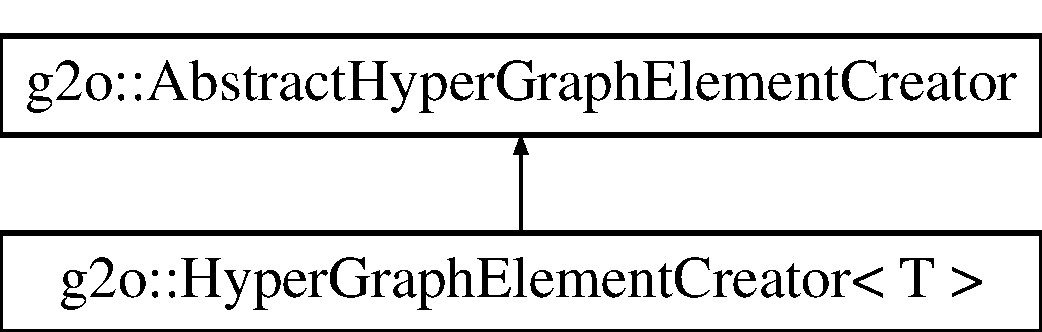
\includegraphics[height=2.000000cm]{classg2o_1_1_abstract_hyper_graph_element_creator}
\end{center}
\end{figure}
\subsection*{Public Member Functions}
\begin{DoxyCompactItemize}
\item 
virtual \mbox{\hyperlink{structg2o_1_1_hyper_graph_1_1_hyper_graph_element}{Hyper\+Graph\+::\+Hyper\+Graph\+Element}} $\ast$ \mbox{\hyperlink{classg2o_1_1_abstract_hyper_graph_element_creator_a0b4722fa4b05465bf89d6e7fdc75b153}{construct}} ()=0
\item 
virtual const std\+::string \& \mbox{\hyperlink{classg2o_1_1_abstract_hyper_graph_element_creator_a238928fbbfd6e473b2c61002112e6f5f}{name}} () const =0
\item 
virtual \mbox{\hyperlink{classg2o_1_1_abstract_hyper_graph_element_creator_a7739f2b8d9e10f71c31d41748cf10835}{$\sim$\+Abstract\+Hyper\+Graph\+Element\+Creator}} ()
\end{DoxyCompactItemize}


\subsection{Detailed Description}
Abstract interface for allocating Hyper\+Graph\+Element. 

\subsection{Constructor \& Destructor Documentation}
\mbox{\Hypertarget{classg2o_1_1_abstract_hyper_graph_element_creator_a7739f2b8d9e10f71c31d41748cf10835}\label{classg2o_1_1_abstract_hyper_graph_element_creator_a7739f2b8d9e10f71c31d41748cf10835}} 
\index{g2o\+::\+Abstract\+Hyper\+Graph\+Element\+Creator@{g2o\+::\+Abstract\+Hyper\+Graph\+Element\+Creator}!````~Abstract\+Hyper\+Graph\+Element\+Creator@{$\sim$\+Abstract\+Hyper\+Graph\+Element\+Creator}}
\index{````~Abstract\+Hyper\+Graph\+Element\+Creator@{$\sim$\+Abstract\+Hyper\+Graph\+Element\+Creator}!g2o\+::\+Abstract\+Hyper\+Graph\+Element\+Creator@{g2o\+::\+Abstract\+Hyper\+Graph\+Element\+Creator}}
\subsubsection{\texorpdfstring{$\sim$\+Abstract\+Hyper\+Graph\+Element\+Creator()}{~AbstractHyperGraphElementCreator()}}
{\footnotesize\ttfamily virtual g2o\+::\+Abstract\+Hyper\+Graph\+Element\+Creator\+::$\sim$\+Abstract\+Hyper\+Graph\+Element\+Creator (\begin{DoxyParamCaption}{ }\end{DoxyParamCaption})\hspace{0.3cm}{\ttfamily [inline]}, {\ttfamily [virtual]}}



\subsection{Member Function Documentation}
\mbox{\Hypertarget{classg2o_1_1_abstract_hyper_graph_element_creator_a0b4722fa4b05465bf89d6e7fdc75b153}\label{classg2o_1_1_abstract_hyper_graph_element_creator_a0b4722fa4b05465bf89d6e7fdc75b153}} 
\index{g2o\+::\+Abstract\+Hyper\+Graph\+Element\+Creator@{g2o\+::\+Abstract\+Hyper\+Graph\+Element\+Creator}!construct@{construct}}
\index{construct@{construct}!g2o\+::\+Abstract\+Hyper\+Graph\+Element\+Creator@{g2o\+::\+Abstract\+Hyper\+Graph\+Element\+Creator}}
\subsubsection{\texorpdfstring{construct()}{construct()}}
{\footnotesize\ttfamily virtual \mbox{\hyperlink{structg2o_1_1_hyper_graph_1_1_hyper_graph_element}{Hyper\+Graph\+::\+Hyper\+Graph\+Element}}$\ast$ g2o\+::\+Abstract\+Hyper\+Graph\+Element\+Creator\+::construct (\begin{DoxyParamCaption}{ }\end{DoxyParamCaption})\hspace{0.3cm}{\ttfamily [pure virtual]}}

create a hyper graph element. Has to implemented in derived class. 

Implemented in \mbox{\hyperlink{classg2o_1_1_hyper_graph_element_creator_af5e58366dd05b49700076e0c4ace31e3}{g2o\+::\+Hyper\+Graph\+Element\+Creator$<$ T $>$}}.

\mbox{\Hypertarget{classg2o_1_1_abstract_hyper_graph_element_creator_a238928fbbfd6e473b2c61002112e6f5f}\label{classg2o_1_1_abstract_hyper_graph_element_creator_a238928fbbfd6e473b2c61002112e6f5f}} 
\index{g2o\+::\+Abstract\+Hyper\+Graph\+Element\+Creator@{g2o\+::\+Abstract\+Hyper\+Graph\+Element\+Creator}!name@{name}}
\index{name@{name}!g2o\+::\+Abstract\+Hyper\+Graph\+Element\+Creator@{g2o\+::\+Abstract\+Hyper\+Graph\+Element\+Creator}}
\subsubsection{\texorpdfstring{name()}{name()}}
{\footnotesize\ttfamily virtual const std\+::string\& g2o\+::\+Abstract\+Hyper\+Graph\+Element\+Creator\+::name (\begin{DoxyParamCaption}{ }\end{DoxyParamCaption}) const\hspace{0.3cm}{\ttfamily [pure virtual]}}

name of the class to be created. Has to implemented in derived class. 

Implemented in \mbox{\hyperlink{classg2o_1_1_hyper_graph_element_creator_a9350df173e72ccb4bb6594d282a2c0e7}{g2o\+::\+Hyper\+Graph\+Element\+Creator$<$ T $>$}}.



The documentation for this class was generated from the following file\+:\begin{DoxyCompactItemize}
\item 
Thirdparty/g2o/g2o/core/\mbox{\hyperlink{creators_8h}{creators.\+h}}\end{DoxyCompactItemize}

\hypertarget{classg2o_1_1_abstract_optimization_algorithm_creator}{}\section{g2o\+:\+:Abstract\+Optimization\+Algorithm\+Creator Class Reference}
\label{classg2o_1_1_abstract_optimization_algorithm_creator}\index{g2o\+::\+Abstract\+Optimization\+Algorithm\+Creator@{g2o\+::\+Abstract\+Optimization\+Algorithm\+Creator}}


base for allocating an optimization algorithm  




{\ttfamily \#include $<$optimization\+\_\+algorithm\+\_\+factory.\+h$>$}

\subsection*{Public Member Functions}
\begin{DoxyCompactItemize}
\item 
\mbox{\hyperlink{classg2o_1_1_abstract_optimization_algorithm_creator_ae9f64a630d2e641043aabc98660495d8}{Abstract\+Optimization\+Algorithm\+Creator}} (const \mbox{\hyperlink{structg2o_1_1_optimization_algorithm_property}{Optimization\+Algorithm\+Property}} \&p)
\item 
virtual \mbox{\hyperlink{classg2o_1_1_abstract_optimization_algorithm_creator_a8832e6083876766797176fb0d93b4554}{$\sim$\+Abstract\+Optimization\+Algorithm\+Creator}} ()
\item 
virtual \mbox{\hyperlink{classg2o_1_1_optimization_algorithm}{Optimization\+Algorithm}} $\ast$ \mbox{\hyperlink{classg2o_1_1_abstract_optimization_algorithm_creator_a96a737bda0f932ac7dd51aa468795353}{construct}} ()=0
\begin{DoxyCompactList}\small\item\em allocate a solver operating on optimizer, re-\/implement for your creator \end{DoxyCompactList}\item 
const \mbox{\hyperlink{structg2o_1_1_optimization_algorithm_property}{Optimization\+Algorithm\+Property}} \& \mbox{\hyperlink{classg2o_1_1_abstract_optimization_algorithm_creator_ab074710276ea3496d5bff118e48c6030}{property}} () const
\begin{DoxyCompactList}\small\item\em return the properties of the solver \end{DoxyCompactList}\end{DoxyCompactItemize}
\subsection*{Protected Attributes}
\begin{DoxyCompactItemize}
\item 
\mbox{\hyperlink{structg2o_1_1_optimization_algorithm_property}{Optimization\+Algorithm\+Property}} \mbox{\hyperlink{classg2o_1_1_abstract_optimization_algorithm_creator_acf2663d0d6dec71049e4853a9825eafb}{\+\_\+property}}
\end{DoxyCompactItemize}


\subsection{Detailed Description}
base for allocating an optimization algorithm 

Allocating a solver for a given optimizer. The method \mbox{\hyperlink{classg2o_1_1_abstract_optimization_algorithm_creator_a96a737bda0f932ac7dd51aa468795353}{construct()}} has to be implemented in your derived class to allocate the desired solver. 

\subsection{Constructor \& Destructor Documentation}
\mbox{\Hypertarget{classg2o_1_1_abstract_optimization_algorithm_creator_ae9f64a630d2e641043aabc98660495d8}\label{classg2o_1_1_abstract_optimization_algorithm_creator_ae9f64a630d2e641043aabc98660495d8}} 
\index{g2o\+::\+Abstract\+Optimization\+Algorithm\+Creator@{g2o\+::\+Abstract\+Optimization\+Algorithm\+Creator}!Abstract\+Optimization\+Algorithm\+Creator@{Abstract\+Optimization\+Algorithm\+Creator}}
\index{Abstract\+Optimization\+Algorithm\+Creator@{Abstract\+Optimization\+Algorithm\+Creator}!g2o\+::\+Abstract\+Optimization\+Algorithm\+Creator@{g2o\+::\+Abstract\+Optimization\+Algorithm\+Creator}}
\subsubsection{\texorpdfstring{Abstract\+Optimization\+Algorithm\+Creator()}{AbstractOptimizationAlgorithmCreator()}}
{\footnotesize\ttfamily g2o\+::\+Abstract\+Optimization\+Algorithm\+Creator\+::\+Abstract\+Optimization\+Algorithm\+Creator (\begin{DoxyParamCaption}\item[{const \mbox{\hyperlink{structg2o_1_1_optimization_algorithm_property}{Optimization\+Algorithm\+Property}} \&}]{p }\end{DoxyParamCaption})}

\mbox{\Hypertarget{classg2o_1_1_abstract_optimization_algorithm_creator_a8832e6083876766797176fb0d93b4554}\label{classg2o_1_1_abstract_optimization_algorithm_creator_a8832e6083876766797176fb0d93b4554}} 
\index{g2o\+::\+Abstract\+Optimization\+Algorithm\+Creator@{g2o\+::\+Abstract\+Optimization\+Algorithm\+Creator}!````~Abstract\+Optimization\+Algorithm\+Creator@{$\sim$\+Abstract\+Optimization\+Algorithm\+Creator}}
\index{````~Abstract\+Optimization\+Algorithm\+Creator@{$\sim$\+Abstract\+Optimization\+Algorithm\+Creator}!g2o\+::\+Abstract\+Optimization\+Algorithm\+Creator@{g2o\+::\+Abstract\+Optimization\+Algorithm\+Creator}}
\subsubsection{\texorpdfstring{$\sim$\+Abstract\+Optimization\+Algorithm\+Creator()}{~AbstractOptimizationAlgorithmCreator()}}
{\footnotesize\ttfamily virtual g2o\+::\+Abstract\+Optimization\+Algorithm\+Creator\+::$\sim$\+Abstract\+Optimization\+Algorithm\+Creator (\begin{DoxyParamCaption}{ }\end{DoxyParamCaption})\hspace{0.3cm}{\ttfamily [inline]}, {\ttfamily [virtual]}}



\subsection{Member Function Documentation}
\mbox{\Hypertarget{classg2o_1_1_abstract_optimization_algorithm_creator_a96a737bda0f932ac7dd51aa468795353}\label{classg2o_1_1_abstract_optimization_algorithm_creator_a96a737bda0f932ac7dd51aa468795353}} 
\index{g2o\+::\+Abstract\+Optimization\+Algorithm\+Creator@{g2o\+::\+Abstract\+Optimization\+Algorithm\+Creator}!construct@{construct}}
\index{construct@{construct}!g2o\+::\+Abstract\+Optimization\+Algorithm\+Creator@{g2o\+::\+Abstract\+Optimization\+Algorithm\+Creator}}
\subsubsection{\texorpdfstring{construct()}{construct()}}
{\footnotesize\ttfamily virtual \mbox{\hyperlink{classg2o_1_1_optimization_algorithm}{Optimization\+Algorithm}}$\ast$ g2o\+::\+Abstract\+Optimization\+Algorithm\+Creator\+::construct (\begin{DoxyParamCaption}{ }\end{DoxyParamCaption})\hspace{0.3cm}{\ttfamily [pure virtual]}}



allocate a solver operating on optimizer, re-\/implement for your creator 

\mbox{\Hypertarget{classg2o_1_1_abstract_optimization_algorithm_creator_ab074710276ea3496d5bff118e48c6030}\label{classg2o_1_1_abstract_optimization_algorithm_creator_ab074710276ea3496d5bff118e48c6030}} 
\index{g2o\+::\+Abstract\+Optimization\+Algorithm\+Creator@{g2o\+::\+Abstract\+Optimization\+Algorithm\+Creator}!property@{property}}
\index{property@{property}!g2o\+::\+Abstract\+Optimization\+Algorithm\+Creator@{g2o\+::\+Abstract\+Optimization\+Algorithm\+Creator}}
\subsubsection{\texorpdfstring{property()}{property()}}
{\footnotesize\ttfamily const \mbox{\hyperlink{structg2o_1_1_optimization_algorithm_property}{Optimization\+Algorithm\+Property}}\& g2o\+::\+Abstract\+Optimization\+Algorithm\+Creator\+::property (\begin{DoxyParamCaption}{ }\end{DoxyParamCaption}) const\hspace{0.3cm}{\ttfamily [inline]}}



return the properties of the solver 



\subsection{Member Data Documentation}
\mbox{\Hypertarget{classg2o_1_1_abstract_optimization_algorithm_creator_acf2663d0d6dec71049e4853a9825eafb}\label{classg2o_1_1_abstract_optimization_algorithm_creator_acf2663d0d6dec71049e4853a9825eafb}} 
\index{g2o\+::\+Abstract\+Optimization\+Algorithm\+Creator@{g2o\+::\+Abstract\+Optimization\+Algorithm\+Creator}!\+\_\+property@{\+\_\+property}}
\index{\+\_\+property@{\+\_\+property}!g2o\+::\+Abstract\+Optimization\+Algorithm\+Creator@{g2o\+::\+Abstract\+Optimization\+Algorithm\+Creator}}
\subsubsection{\texorpdfstring{\+\_\+property}{\_property}}
{\footnotesize\ttfamily \mbox{\hyperlink{structg2o_1_1_optimization_algorithm_property}{Optimization\+Algorithm\+Property}} g2o\+::\+Abstract\+Optimization\+Algorithm\+Creator\+::\+\_\+property\hspace{0.3cm}{\ttfamily [protected]}}



The documentation for this class was generated from the following files\+:\begin{DoxyCompactItemize}
\item 
Thirdparty/g2o/g2o/core/\mbox{\hyperlink{optimization__algorithm__factory_8h}{optimization\+\_\+algorithm\+\_\+factory.\+h}}\item 
Thirdparty/g2o/g2o/core/\mbox{\hyperlink{optimization__algorithm__factory_8cpp}{optimization\+\_\+algorithm\+\_\+factory.\+cpp}}\end{DoxyCompactItemize}

\hypertarget{classg2o_1_1_abstract_robust_kernel_creator}{}\section{g2o\+:\+:Abstract\+Robust\+Kernel\+Creator Class Reference}
\label{classg2o_1_1_abstract_robust_kernel_creator}\index{g2o\+::\+Abstract\+Robust\+Kernel\+Creator@{g2o\+::\+Abstract\+Robust\+Kernel\+Creator}}


Abstract interface for allocating a robust kernel.  




{\ttfamily \#include $<$robust\+\_\+kernel\+\_\+factory.\+h$>$}

Inheritance diagram for g2o\+:\+:Abstract\+Robust\+Kernel\+Creator\+:\begin{figure}[H]
\begin{center}
\leavevmode
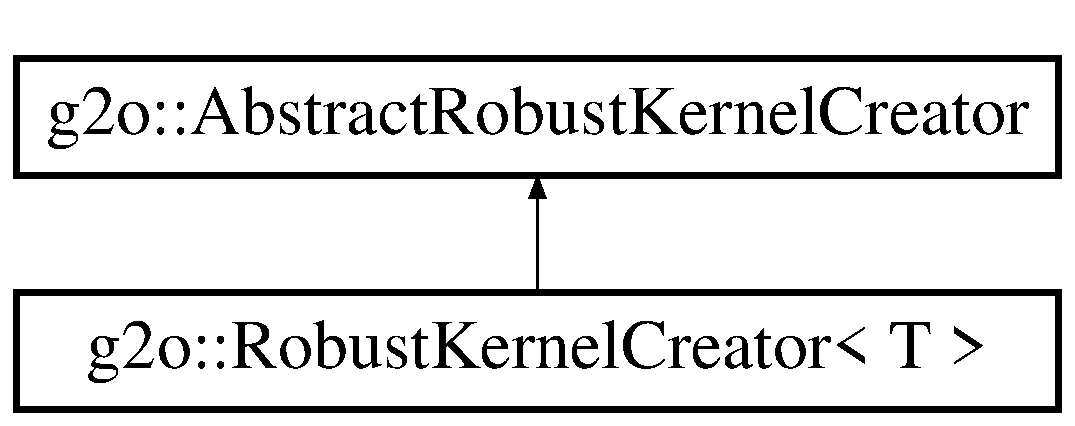
\includegraphics[height=2.000000cm]{classg2o_1_1_abstract_robust_kernel_creator}
\end{center}
\end{figure}
\subsection*{Public Member Functions}
\begin{DoxyCompactItemize}
\item 
virtual \mbox{\hyperlink{classg2o_1_1_robust_kernel}{Robust\+Kernel}} $\ast$ \mbox{\hyperlink{classg2o_1_1_abstract_robust_kernel_creator_a3022ab9279e52151d37f8cb4d1524d47}{construct}} ()=0
\item 
virtual \mbox{\hyperlink{classg2o_1_1_abstract_robust_kernel_creator_af62964a80bc9f76d837df0913057f8f7}{$\sim$\+Abstract\+Robust\+Kernel\+Creator}} ()
\end{DoxyCompactItemize}


\subsection{Detailed Description}
Abstract interface for allocating a robust kernel. 

\subsection{Constructor \& Destructor Documentation}
\mbox{\Hypertarget{classg2o_1_1_abstract_robust_kernel_creator_af62964a80bc9f76d837df0913057f8f7}\label{classg2o_1_1_abstract_robust_kernel_creator_af62964a80bc9f76d837df0913057f8f7}} 
\index{g2o\+::\+Abstract\+Robust\+Kernel\+Creator@{g2o\+::\+Abstract\+Robust\+Kernel\+Creator}!````~Abstract\+Robust\+Kernel\+Creator@{$\sim$\+Abstract\+Robust\+Kernel\+Creator}}
\index{````~Abstract\+Robust\+Kernel\+Creator@{$\sim$\+Abstract\+Robust\+Kernel\+Creator}!g2o\+::\+Abstract\+Robust\+Kernel\+Creator@{g2o\+::\+Abstract\+Robust\+Kernel\+Creator}}
\subsubsection{\texorpdfstring{$\sim$\+Abstract\+Robust\+Kernel\+Creator()}{~AbstractRobustKernelCreator()}}
{\footnotesize\ttfamily virtual g2o\+::\+Abstract\+Robust\+Kernel\+Creator\+::$\sim$\+Abstract\+Robust\+Kernel\+Creator (\begin{DoxyParamCaption}{ }\end{DoxyParamCaption})\hspace{0.3cm}{\ttfamily [inline]}, {\ttfamily [virtual]}}



\subsection{Member Function Documentation}
\mbox{\Hypertarget{classg2o_1_1_abstract_robust_kernel_creator_a3022ab9279e52151d37f8cb4d1524d47}\label{classg2o_1_1_abstract_robust_kernel_creator_a3022ab9279e52151d37f8cb4d1524d47}} 
\index{g2o\+::\+Abstract\+Robust\+Kernel\+Creator@{g2o\+::\+Abstract\+Robust\+Kernel\+Creator}!construct@{construct}}
\index{construct@{construct}!g2o\+::\+Abstract\+Robust\+Kernel\+Creator@{g2o\+::\+Abstract\+Robust\+Kernel\+Creator}}
\subsubsection{\texorpdfstring{construct()}{construct()}}
{\footnotesize\ttfamily virtual \mbox{\hyperlink{classg2o_1_1_robust_kernel}{Robust\+Kernel}}$\ast$ g2o\+::\+Abstract\+Robust\+Kernel\+Creator\+::construct (\begin{DoxyParamCaption}{ }\end{DoxyParamCaption})\hspace{0.3cm}{\ttfamily [pure virtual]}}

create a hyper graph element. Has to implemented in derived class. 

Implemented in \mbox{\hyperlink{classg2o_1_1_robust_kernel_creator_a6ab30adc017675641bd55502d7da0085}{g2o\+::\+Robust\+Kernel\+Creator$<$ T $>$}}.



The documentation for this class was generated from the following file\+:\begin{DoxyCompactItemize}
\item 
Thirdparty/g2o/g2o/core/\mbox{\hyperlink{robust__kernel__factory_8h}{robust\+\_\+kernel\+\_\+factory.\+h}}\end{DoxyCompactItemize}

\hypertarget{classg2o_1_1_estimate_propagator_1_1_adjacency_map_entry}{}\section{g2o\+:\+:Estimate\+Propagator\+:\+:Adjacency\+Map\+Entry Class Reference}
\label{classg2o_1_1_estimate_propagator_1_1_adjacency_map_entry}\index{g2o\+::\+Estimate\+Propagator\+::\+Adjacency\+Map\+Entry@{g2o\+::\+Estimate\+Propagator\+::\+Adjacency\+Map\+Entry}}


data structure for loopuk during Dijkstra  




{\ttfamily \#include $<$estimate\+\_\+propagator.\+h$>$}

\subsection*{Public Member Functions}
\begin{DoxyCompactItemize}
\item 
\mbox{\hyperlink{classg2o_1_1_estimate_propagator_1_1_adjacency_map_entry_a5fe6ab271c62be13c363ea3807e6d357}{Adjacency\+Map\+Entry}} ()
\item 
void \mbox{\hyperlink{classg2o_1_1_estimate_propagator_1_1_adjacency_map_entry_a6d2f95439aa6ee608f2e2d110de553e8}{reset}} ()
\item 
\mbox{\hyperlink{classg2o_1_1_optimizable_graph_1_1_vertex}{Optimizable\+Graph\+::\+Vertex}} $\ast$ \mbox{\hyperlink{classg2o_1_1_estimate_propagator_1_1_adjacency_map_entry_a4e31105d4e88c399ec95aa6c184b649e}{child}} () const
\item 
const \mbox{\hyperlink{classg2o_1_1_hyper_graph_a703938cdb4bb636860eed55a2489d70c}{Optimizable\+Graph\+::\+Vertex\+Set}} \& \mbox{\hyperlink{classg2o_1_1_estimate_propagator_1_1_adjacency_map_entry_afdc412171a1828e9d588f587ba27f7aa}{parent}} () const
\item 
\mbox{\hyperlink{classg2o_1_1_optimizable_graph_1_1_edge}{Optimizable\+Graph\+::\+Edge}} $\ast$ \mbox{\hyperlink{classg2o_1_1_estimate_propagator_1_1_adjacency_map_entry_a7082664efdadcd6031ab441830cb7ac4}{edge}} () const
\item 
double \mbox{\hyperlink{classg2o_1_1_estimate_propagator_1_1_adjacency_map_entry_a6a7bbf0ae959ece486cea3549dec5c0a}{distance}} () const
\item 
int \mbox{\hyperlink{classg2o_1_1_estimate_propagator_1_1_adjacency_map_entry_a291b75bdb7c37467a6d4e7e7d839e0fc}{frontier\+Level}} () const
\end{DoxyCompactItemize}
\subsection*{Protected Attributes}
\begin{DoxyCompactItemize}
\item 
\mbox{\hyperlink{classg2o_1_1_optimizable_graph_1_1_vertex}{Optimizable\+Graph\+::\+Vertex}} $\ast$ \mbox{\hyperlink{classg2o_1_1_estimate_propagator_1_1_adjacency_map_entry_ab6f716e85cc15e6d9c570132fe889fd6}{\+\_\+child}}
\item 
\mbox{\hyperlink{classg2o_1_1_hyper_graph_a703938cdb4bb636860eed55a2489d70c}{Optimizable\+Graph\+::\+Vertex\+Set}} \mbox{\hyperlink{classg2o_1_1_estimate_propagator_1_1_adjacency_map_entry_a72384502361d60e1f3ae1644de1e7379}{\+\_\+parent}}
\item 
\mbox{\hyperlink{classg2o_1_1_optimizable_graph_1_1_edge}{Optimizable\+Graph\+::\+Edge}} $\ast$ \mbox{\hyperlink{classg2o_1_1_estimate_propagator_1_1_adjacency_map_entry_a738795d0b3989374ba51821354629d64}{\+\_\+edge}}
\item 
double \mbox{\hyperlink{classg2o_1_1_estimate_propagator_1_1_adjacency_map_entry_a3558503af9d9f56088ff1593398f86d4}{\+\_\+distance}}
\item 
int \mbox{\hyperlink{classg2o_1_1_estimate_propagator_1_1_adjacency_map_entry_a56bfab4074fa692f03378526007758f7}{\+\_\+frontier\+Level}}
\end{DoxyCompactItemize}
\subsection*{Private Attributes}
\begin{DoxyCompactItemize}
\item 
bool \mbox{\hyperlink{classg2o_1_1_estimate_propagator_1_1_adjacency_map_entry_a6697b7728a51b80663f843daba54e2d8}{in\+Queue}}
\item 
Priority\+Queue\+::iterator \mbox{\hyperlink{classg2o_1_1_estimate_propagator_1_1_adjacency_map_entry_a40828826b865378855fdc26fae46af11}{queue\+It}}
\end{DoxyCompactItemize}
\subsection*{Friends}
\begin{DoxyCompactItemize}
\item 
class \mbox{\hyperlink{classg2o_1_1_estimate_propagator_1_1_adjacency_map_entry_a84fd16bbb058a331370b1b9983896264}{Estimate\+Propagator}}
\item 
class \mbox{\hyperlink{classg2o_1_1_estimate_propagator_1_1_adjacency_map_entry_afde21c6f1b41de5a73362b2fcfec056b}{Priority\+Queue}}
\end{DoxyCompactItemize}


\subsection{Detailed Description}
data structure for loopuk during Dijkstra 

\subsection{Constructor \& Destructor Documentation}
\mbox{\Hypertarget{classg2o_1_1_estimate_propagator_1_1_adjacency_map_entry_a5fe6ab271c62be13c363ea3807e6d357}\label{classg2o_1_1_estimate_propagator_1_1_adjacency_map_entry_a5fe6ab271c62be13c363ea3807e6d357}} 
\index{g2o\+::\+Estimate\+Propagator\+::\+Adjacency\+Map\+Entry@{g2o\+::\+Estimate\+Propagator\+::\+Adjacency\+Map\+Entry}!Adjacency\+Map\+Entry@{Adjacency\+Map\+Entry}}
\index{Adjacency\+Map\+Entry@{Adjacency\+Map\+Entry}!g2o\+::\+Estimate\+Propagator\+::\+Adjacency\+Map\+Entry@{g2o\+::\+Estimate\+Propagator\+::\+Adjacency\+Map\+Entry}}
\subsubsection{\texorpdfstring{Adjacency\+Map\+Entry()}{AdjacencyMapEntry()}}
{\footnotesize\ttfamily g2o\+::\+Estimate\+Propagator\+::\+Adjacency\+Map\+Entry\+::\+Adjacency\+Map\+Entry (\begin{DoxyParamCaption}{ }\end{DoxyParamCaption})}



\subsection{Member Function Documentation}
\mbox{\Hypertarget{classg2o_1_1_estimate_propagator_1_1_adjacency_map_entry_a4e31105d4e88c399ec95aa6c184b649e}\label{classg2o_1_1_estimate_propagator_1_1_adjacency_map_entry_a4e31105d4e88c399ec95aa6c184b649e}} 
\index{g2o\+::\+Estimate\+Propagator\+::\+Adjacency\+Map\+Entry@{g2o\+::\+Estimate\+Propagator\+::\+Adjacency\+Map\+Entry}!child@{child}}
\index{child@{child}!g2o\+::\+Estimate\+Propagator\+::\+Adjacency\+Map\+Entry@{g2o\+::\+Estimate\+Propagator\+::\+Adjacency\+Map\+Entry}}
\subsubsection{\texorpdfstring{child()}{child()}}
{\footnotesize\ttfamily \mbox{\hyperlink{classg2o_1_1_optimizable_graph_1_1_vertex}{Optimizable\+Graph\+::\+Vertex}}$\ast$ g2o\+::\+Estimate\+Propagator\+::\+Adjacency\+Map\+Entry\+::child (\begin{DoxyParamCaption}{ }\end{DoxyParamCaption}) const\hspace{0.3cm}{\ttfamily [inline]}}

\mbox{\Hypertarget{classg2o_1_1_estimate_propagator_1_1_adjacency_map_entry_a6a7bbf0ae959ece486cea3549dec5c0a}\label{classg2o_1_1_estimate_propagator_1_1_adjacency_map_entry_a6a7bbf0ae959ece486cea3549dec5c0a}} 
\index{g2o\+::\+Estimate\+Propagator\+::\+Adjacency\+Map\+Entry@{g2o\+::\+Estimate\+Propagator\+::\+Adjacency\+Map\+Entry}!distance@{distance}}
\index{distance@{distance}!g2o\+::\+Estimate\+Propagator\+::\+Adjacency\+Map\+Entry@{g2o\+::\+Estimate\+Propagator\+::\+Adjacency\+Map\+Entry}}
\subsubsection{\texorpdfstring{distance()}{distance()}}
{\footnotesize\ttfamily double g2o\+::\+Estimate\+Propagator\+::\+Adjacency\+Map\+Entry\+::distance (\begin{DoxyParamCaption}{ }\end{DoxyParamCaption}) const\hspace{0.3cm}{\ttfamily [inline]}}

\mbox{\Hypertarget{classg2o_1_1_estimate_propagator_1_1_adjacency_map_entry_a7082664efdadcd6031ab441830cb7ac4}\label{classg2o_1_1_estimate_propagator_1_1_adjacency_map_entry_a7082664efdadcd6031ab441830cb7ac4}} 
\index{g2o\+::\+Estimate\+Propagator\+::\+Adjacency\+Map\+Entry@{g2o\+::\+Estimate\+Propagator\+::\+Adjacency\+Map\+Entry}!edge@{edge}}
\index{edge@{edge}!g2o\+::\+Estimate\+Propagator\+::\+Adjacency\+Map\+Entry@{g2o\+::\+Estimate\+Propagator\+::\+Adjacency\+Map\+Entry}}
\subsubsection{\texorpdfstring{edge()}{edge()}}
{\footnotesize\ttfamily \mbox{\hyperlink{classg2o_1_1_optimizable_graph_1_1_edge}{Optimizable\+Graph\+::\+Edge}}$\ast$ g2o\+::\+Estimate\+Propagator\+::\+Adjacency\+Map\+Entry\+::edge (\begin{DoxyParamCaption}{ }\end{DoxyParamCaption}) const\hspace{0.3cm}{\ttfamily [inline]}}

\mbox{\Hypertarget{classg2o_1_1_estimate_propagator_1_1_adjacency_map_entry_a291b75bdb7c37467a6d4e7e7d839e0fc}\label{classg2o_1_1_estimate_propagator_1_1_adjacency_map_entry_a291b75bdb7c37467a6d4e7e7d839e0fc}} 
\index{g2o\+::\+Estimate\+Propagator\+::\+Adjacency\+Map\+Entry@{g2o\+::\+Estimate\+Propagator\+::\+Adjacency\+Map\+Entry}!frontier\+Level@{frontier\+Level}}
\index{frontier\+Level@{frontier\+Level}!g2o\+::\+Estimate\+Propagator\+::\+Adjacency\+Map\+Entry@{g2o\+::\+Estimate\+Propagator\+::\+Adjacency\+Map\+Entry}}
\subsubsection{\texorpdfstring{frontier\+Level()}{frontierLevel()}}
{\footnotesize\ttfamily int g2o\+::\+Estimate\+Propagator\+::\+Adjacency\+Map\+Entry\+::frontier\+Level (\begin{DoxyParamCaption}{ }\end{DoxyParamCaption}) const\hspace{0.3cm}{\ttfamily [inline]}}

\mbox{\Hypertarget{classg2o_1_1_estimate_propagator_1_1_adjacency_map_entry_afdc412171a1828e9d588f587ba27f7aa}\label{classg2o_1_1_estimate_propagator_1_1_adjacency_map_entry_afdc412171a1828e9d588f587ba27f7aa}} 
\index{g2o\+::\+Estimate\+Propagator\+::\+Adjacency\+Map\+Entry@{g2o\+::\+Estimate\+Propagator\+::\+Adjacency\+Map\+Entry}!parent@{parent}}
\index{parent@{parent}!g2o\+::\+Estimate\+Propagator\+::\+Adjacency\+Map\+Entry@{g2o\+::\+Estimate\+Propagator\+::\+Adjacency\+Map\+Entry}}
\subsubsection{\texorpdfstring{parent()}{parent()}}
{\footnotesize\ttfamily const \mbox{\hyperlink{classg2o_1_1_hyper_graph_a703938cdb4bb636860eed55a2489d70c}{Optimizable\+Graph\+::\+Vertex\+Set}}\& g2o\+::\+Estimate\+Propagator\+::\+Adjacency\+Map\+Entry\+::parent (\begin{DoxyParamCaption}{ }\end{DoxyParamCaption}) const\hspace{0.3cm}{\ttfamily [inline]}}

\mbox{\Hypertarget{classg2o_1_1_estimate_propagator_1_1_adjacency_map_entry_a6d2f95439aa6ee608f2e2d110de553e8}\label{classg2o_1_1_estimate_propagator_1_1_adjacency_map_entry_a6d2f95439aa6ee608f2e2d110de553e8}} 
\index{g2o\+::\+Estimate\+Propagator\+::\+Adjacency\+Map\+Entry@{g2o\+::\+Estimate\+Propagator\+::\+Adjacency\+Map\+Entry}!reset@{reset}}
\index{reset@{reset}!g2o\+::\+Estimate\+Propagator\+::\+Adjacency\+Map\+Entry@{g2o\+::\+Estimate\+Propagator\+::\+Adjacency\+Map\+Entry}}
\subsubsection{\texorpdfstring{reset()}{reset()}}
{\footnotesize\ttfamily void g2o\+::\+Estimate\+Propagator\+::\+Adjacency\+Map\+Entry\+::reset (\begin{DoxyParamCaption}{ }\end{DoxyParamCaption})}



\subsection{Friends And Related Function Documentation}
\mbox{\Hypertarget{classg2o_1_1_estimate_propagator_1_1_adjacency_map_entry_a84fd16bbb058a331370b1b9983896264}\label{classg2o_1_1_estimate_propagator_1_1_adjacency_map_entry_a84fd16bbb058a331370b1b9983896264}} 
\index{g2o\+::\+Estimate\+Propagator\+::\+Adjacency\+Map\+Entry@{g2o\+::\+Estimate\+Propagator\+::\+Adjacency\+Map\+Entry}!Estimate\+Propagator@{Estimate\+Propagator}}
\index{Estimate\+Propagator@{Estimate\+Propagator}!g2o\+::\+Estimate\+Propagator\+::\+Adjacency\+Map\+Entry@{g2o\+::\+Estimate\+Propagator\+::\+Adjacency\+Map\+Entry}}
\subsubsection{\texorpdfstring{Estimate\+Propagator}{EstimatePropagator}}
{\footnotesize\ttfamily friend class \mbox{\hyperlink{classg2o_1_1_estimate_propagator}{Estimate\+Propagator}}\hspace{0.3cm}{\ttfamily [friend]}}

\mbox{\Hypertarget{classg2o_1_1_estimate_propagator_1_1_adjacency_map_entry_afde21c6f1b41de5a73362b2fcfec056b}\label{classg2o_1_1_estimate_propagator_1_1_adjacency_map_entry_afde21c6f1b41de5a73362b2fcfec056b}} 
\index{g2o\+::\+Estimate\+Propagator\+::\+Adjacency\+Map\+Entry@{g2o\+::\+Estimate\+Propagator\+::\+Adjacency\+Map\+Entry}!Priority\+Queue@{Priority\+Queue}}
\index{Priority\+Queue@{Priority\+Queue}!g2o\+::\+Estimate\+Propagator\+::\+Adjacency\+Map\+Entry@{g2o\+::\+Estimate\+Propagator\+::\+Adjacency\+Map\+Entry}}
\subsubsection{\texorpdfstring{Priority\+Queue}{PriorityQueue}}
{\footnotesize\ttfamily friend class \mbox{\hyperlink{classg2o_1_1_estimate_propagator_1_1_priority_queue}{Priority\+Queue}}\hspace{0.3cm}{\ttfamily [friend]}}



\subsection{Member Data Documentation}
\mbox{\Hypertarget{classg2o_1_1_estimate_propagator_1_1_adjacency_map_entry_ab6f716e85cc15e6d9c570132fe889fd6}\label{classg2o_1_1_estimate_propagator_1_1_adjacency_map_entry_ab6f716e85cc15e6d9c570132fe889fd6}} 
\index{g2o\+::\+Estimate\+Propagator\+::\+Adjacency\+Map\+Entry@{g2o\+::\+Estimate\+Propagator\+::\+Adjacency\+Map\+Entry}!\+\_\+child@{\+\_\+child}}
\index{\+\_\+child@{\+\_\+child}!g2o\+::\+Estimate\+Propagator\+::\+Adjacency\+Map\+Entry@{g2o\+::\+Estimate\+Propagator\+::\+Adjacency\+Map\+Entry}}
\subsubsection{\texorpdfstring{\+\_\+child}{\_child}}
{\footnotesize\ttfamily \mbox{\hyperlink{classg2o_1_1_optimizable_graph_1_1_vertex}{Optimizable\+Graph\+::\+Vertex}}$\ast$ g2o\+::\+Estimate\+Propagator\+::\+Adjacency\+Map\+Entry\+::\+\_\+child\hspace{0.3cm}{\ttfamily [protected]}}

\mbox{\Hypertarget{classg2o_1_1_estimate_propagator_1_1_adjacency_map_entry_a3558503af9d9f56088ff1593398f86d4}\label{classg2o_1_1_estimate_propagator_1_1_adjacency_map_entry_a3558503af9d9f56088ff1593398f86d4}} 
\index{g2o\+::\+Estimate\+Propagator\+::\+Adjacency\+Map\+Entry@{g2o\+::\+Estimate\+Propagator\+::\+Adjacency\+Map\+Entry}!\+\_\+distance@{\+\_\+distance}}
\index{\+\_\+distance@{\+\_\+distance}!g2o\+::\+Estimate\+Propagator\+::\+Adjacency\+Map\+Entry@{g2o\+::\+Estimate\+Propagator\+::\+Adjacency\+Map\+Entry}}
\subsubsection{\texorpdfstring{\+\_\+distance}{\_distance}}
{\footnotesize\ttfamily double g2o\+::\+Estimate\+Propagator\+::\+Adjacency\+Map\+Entry\+::\+\_\+distance\hspace{0.3cm}{\ttfamily [protected]}}

\mbox{\Hypertarget{classg2o_1_1_estimate_propagator_1_1_adjacency_map_entry_a738795d0b3989374ba51821354629d64}\label{classg2o_1_1_estimate_propagator_1_1_adjacency_map_entry_a738795d0b3989374ba51821354629d64}} 
\index{g2o\+::\+Estimate\+Propagator\+::\+Adjacency\+Map\+Entry@{g2o\+::\+Estimate\+Propagator\+::\+Adjacency\+Map\+Entry}!\+\_\+edge@{\+\_\+edge}}
\index{\+\_\+edge@{\+\_\+edge}!g2o\+::\+Estimate\+Propagator\+::\+Adjacency\+Map\+Entry@{g2o\+::\+Estimate\+Propagator\+::\+Adjacency\+Map\+Entry}}
\subsubsection{\texorpdfstring{\+\_\+edge}{\_edge}}
{\footnotesize\ttfamily \mbox{\hyperlink{classg2o_1_1_optimizable_graph_1_1_edge}{Optimizable\+Graph\+::\+Edge}}$\ast$ g2o\+::\+Estimate\+Propagator\+::\+Adjacency\+Map\+Entry\+::\+\_\+edge\hspace{0.3cm}{\ttfamily [protected]}}

\mbox{\Hypertarget{classg2o_1_1_estimate_propagator_1_1_adjacency_map_entry_a56bfab4074fa692f03378526007758f7}\label{classg2o_1_1_estimate_propagator_1_1_adjacency_map_entry_a56bfab4074fa692f03378526007758f7}} 
\index{g2o\+::\+Estimate\+Propagator\+::\+Adjacency\+Map\+Entry@{g2o\+::\+Estimate\+Propagator\+::\+Adjacency\+Map\+Entry}!\+\_\+frontier\+Level@{\+\_\+frontier\+Level}}
\index{\+\_\+frontier\+Level@{\+\_\+frontier\+Level}!g2o\+::\+Estimate\+Propagator\+::\+Adjacency\+Map\+Entry@{g2o\+::\+Estimate\+Propagator\+::\+Adjacency\+Map\+Entry}}
\subsubsection{\texorpdfstring{\+\_\+frontier\+Level}{\_frontierLevel}}
{\footnotesize\ttfamily int g2o\+::\+Estimate\+Propagator\+::\+Adjacency\+Map\+Entry\+::\+\_\+frontier\+Level\hspace{0.3cm}{\ttfamily [protected]}}

\mbox{\Hypertarget{classg2o_1_1_estimate_propagator_1_1_adjacency_map_entry_a72384502361d60e1f3ae1644de1e7379}\label{classg2o_1_1_estimate_propagator_1_1_adjacency_map_entry_a72384502361d60e1f3ae1644de1e7379}} 
\index{g2o\+::\+Estimate\+Propagator\+::\+Adjacency\+Map\+Entry@{g2o\+::\+Estimate\+Propagator\+::\+Adjacency\+Map\+Entry}!\+\_\+parent@{\+\_\+parent}}
\index{\+\_\+parent@{\+\_\+parent}!g2o\+::\+Estimate\+Propagator\+::\+Adjacency\+Map\+Entry@{g2o\+::\+Estimate\+Propagator\+::\+Adjacency\+Map\+Entry}}
\subsubsection{\texorpdfstring{\+\_\+parent}{\_parent}}
{\footnotesize\ttfamily \mbox{\hyperlink{classg2o_1_1_hyper_graph_a703938cdb4bb636860eed55a2489d70c}{Optimizable\+Graph\+::\+Vertex\+Set}} g2o\+::\+Estimate\+Propagator\+::\+Adjacency\+Map\+Entry\+::\+\_\+parent\hspace{0.3cm}{\ttfamily [protected]}}

\mbox{\Hypertarget{classg2o_1_1_estimate_propagator_1_1_adjacency_map_entry_a6697b7728a51b80663f843daba54e2d8}\label{classg2o_1_1_estimate_propagator_1_1_adjacency_map_entry_a6697b7728a51b80663f843daba54e2d8}} 
\index{g2o\+::\+Estimate\+Propagator\+::\+Adjacency\+Map\+Entry@{g2o\+::\+Estimate\+Propagator\+::\+Adjacency\+Map\+Entry}!in\+Queue@{in\+Queue}}
\index{in\+Queue@{in\+Queue}!g2o\+::\+Estimate\+Propagator\+::\+Adjacency\+Map\+Entry@{g2o\+::\+Estimate\+Propagator\+::\+Adjacency\+Map\+Entry}}
\subsubsection{\texorpdfstring{in\+Queue}{inQueue}}
{\footnotesize\ttfamily bool g2o\+::\+Estimate\+Propagator\+::\+Adjacency\+Map\+Entry\+::in\+Queue\hspace{0.3cm}{\ttfamily [private]}}

\mbox{\Hypertarget{classg2o_1_1_estimate_propagator_1_1_adjacency_map_entry_a40828826b865378855fdc26fae46af11}\label{classg2o_1_1_estimate_propagator_1_1_adjacency_map_entry_a40828826b865378855fdc26fae46af11}} 
\index{g2o\+::\+Estimate\+Propagator\+::\+Adjacency\+Map\+Entry@{g2o\+::\+Estimate\+Propagator\+::\+Adjacency\+Map\+Entry}!queue\+It@{queue\+It}}
\index{queue\+It@{queue\+It}!g2o\+::\+Estimate\+Propagator\+::\+Adjacency\+Map\+Entry@{g2o\+::\+Estimate\+Propagator\+::\+Adjacency\+Map\+Entry}}
\subsubsection{\texorpdfstring{queue\+It}{queueIt}}
{\footnotesize\ttfamily Priority\+Queue\+::iterator g2o\+::\+Estimate\+Propagator\+::\+Adjacency\+Map\+Entry\+::queue\+It\hspace{0.3cm}{\ttfamily [private]}}



The documentation for this class was generated from the following files\+:\begin{DoxyCompactItemize}
\item 
D\+:/github/\+V\+S\+L\+A\+M/\+O\+R\+B\+S\+L\+A\+M2/\+O\+R\+B-\/\+S\+L\+A\+M2-\/master/\+Thirdparty/g2o/g2o/core/\mbox{\hyperlink{estimate__propagator_8h}{estimate\+\_\+propagator.\+h}}\item 
D\+:/github/\+V\+S\+L\+A\+M/\+O\+R\+B\+S\+L\+A\+M2/\+O\+R\+B-\/\+S\+L\+A\+M2-\/master/\+Thirdparty/g2o/g2o/core/\mbox{\hyperlink{estimate__propagator_8cpp}{estimate\+\_\+propagator.\+cpp}}\end{DoxyCompactItemize}

\hypertarget{structg2o_1_1_hyper_dijkstra_1_1_adjacency_map_entry}{}\section{g2o\+:\+:Hyper\+Dijkstra\+:\+:Adjacency\+Map\+Entry Struct Reference}
\label{structg2o_1_1_hyper_dijkstra_1_1_adjacency_map_entry}\index{g2o\+::\+Hyper\+Dijkstra\+::\+Adjacency\+Map\+Entry@{g2o\+::\+Hyper\+Dijkstra\+::\+Adjacency\+Map\+Entry}}


{\ttfamily \#include $<$hyper\+\_\+dijkstra.\+h$>$}

\subsection*{Public Member Functions}
\begin{DoxyCompactItemize}
\item 
\mbox{\hyperlink{structg2o_1_1_hyper_dijkstra_1_1_adjacency_map_entry_a160f87d80b7c2137abcce561fbc5feed}{Adjacency\+Map\+Entry}} (\mbox{\hyperlink{classg2o_1_1_hyper_graph_1_1_vertex}{Hyper\+Graph\+::\+Vertex}} $\ast$\mbox{\hyperlink{structg2o_1_1_hyper_dijkstra_1_1_adjacency_map_entry_a7ccdf917414efa537c3942d360ca127a}{\+\_\+child}}=0, \mbox{\hyperlink{classg2o_1_1_hyper_graph_1_1_vertex}{Hyper\+Graph\+::\+Vertex}} $\ast$\mbox{\hyperlink{structg2o_1_1_hyper_dijkstra_1_1_adjacency_map_entry_a3490ab9668c98d3e0cb14c54b9d41747}{\+\_\+parent}}=0, \mbox{\hyperlink{classg2o_1_1_hyper_graph_1_1_edge}{Hyper\+Graph\+::\+Edge}} $\ast$\mbox{\hyperlink{structg2o_1_1_hyper_dijkstra_1_1_adjacency_map_entry_adc56c13a328aac02456474a9e7c72415}{\+\_\+edge}}=0, double \mbox{\hyperlink{structg2o_1_1_hyper_dijkstra_1_1_adjacency_map_entry_a95b3db28f32badcdce2edf1bae83b78d}{\+\_\+distance}}=std\+::numeric\+\_\+limits$<$ double $>$\+::max())
\item 
\mbox{\hyperlink{classg2o_1_1_hyper_graph_1_1_vertex}{Hyper\+Graph\+::\+Vertex}} $\ast$ \mbox{\hyperlink{structg2o_1_1_hyper_dijkstra_1_1_adjacency_map_entry_a2db2f9eaa364a04f07c81c70784f2193}{child}} () const
\item 
\mbox{\hyperlink{classg2o_1_1_hyper_graph_1_1_vertex}{Hyper\+Graph\+::\+Vertex}} $\ast$ \mbox{\hyperlink{structg2o_1_1_hyper_dijkstra_1_1_adjacency_map_entry_a9ead453f5102583ef68f190b60249fdb}{parent}} () const
\item 
\mbox{\hyperlink{classg2o_1_1_hyper_graph_1_1_edge}{Hyper\+Graph\+::\+Edge}} $\ast$ \mbox{\hyperlink{structg2o_1_1_hyper_dijkstra_1_1_adjacency_map_entry_a4531caf2e8ceb2d86ba7dbadbc82341c}{edge}} () const
\item 
double \mbox{\hyperlink{structg2o_1_1_hyper_dijkstra_1_1_adjacency_map_entry_ac7bf36d934980f655f2f8fd04402456b}{distance}} () const
\item 
\mbox{\hyperlink{classg2o_1_1_hyper_graph_a703938cdb4bb636860eed55a2489d70c}{Hyper\+Graph\+::\+Vertex\+Set}} \& \mbox{\hyperlink{structg2o_1_1_hyper_dijkstra_1_1_adjacency_map_entry_aa1a11048612968381db6a0ad525f7e0d}{children}} ()
\item 
const \mbox{\hyperlink{classg2o_1_1_hyper_graph_a703938cdb4bb636860eed55a2489d70c}{Hyper\+Graph\+::\+Vertex\+Set}} \& \mbox{\hyperlink{structg2o_1_1_hyper_dijkstra_1_1_adjacency_map_entry_a1c3f82778c613d6164a5c5013c6e70c7}{children}} () const
\end{DoxyCompactItemize}
\subsection*{Protected Attributes}
\begin{DoxyCompactItemize}
\item 
\mbox{\hyperlink{classg2o_1_1_hyper_graph_1_1_vertex}{Hyper\+Graph\+::\+Vertex}} $\ast$ \mbox{\hyperlink{structg2o_1_1_hyper_dijkstra_1_1_adjacency_map_entry_a7ccdf917414efa537c3942d360ca127a}{\+\_\+child}}
\item 
\mbox{\hyperlink{classg2o_1_1_hyper_graph_1_1_vertex}{Hyper\+Graph\+::\+Vertex}} $\ast$ \mbox{\hyperlink{structg2o_1_1_hyper_dijkstra_1_1_adjacency_map_entry_a3490ab9668c98d3e0cb14c54b9d41747}{\+\_\+parent}}
\item 
\mbox{\hyperlink{classg2o_1_1_hyper_graph_1_1_edge}{Hyper\+Graph\+::\+Edge}} $\ast$ \mbox{\hyperlink{structg2o_1_1_hyper_dijkstra_1_1_adjacency_map_entry_adc56c13a328aac02456474a9e7c72415}{\+\_\+edge}}
\item 
double \mbox{\hyperlink{structg2o_1_1_hyper_dijkstra_1_1_adjacency_map_entry_a95b3db28f32badcdce2edf1bae83b78d}{\+\_\+distance}}
\item 
\mbox{\hyperlink{classg2o_1_1_hyper_graph_a703938cdb4bb636860eed55a2489d70c}{Hyper\+Graph\+::\+Vertex\+Set}} \mbox{\hyperlink{structg2o_1_1_hyper_dijkstra_1_1_adjacency_map_entry_a5b69ff3769d50a3229e2df80cac3f093}{\+\_\+children}}
\end{DoxyCompactItemize}
\subsection*{Friends}
\begin{DoxyCompactItemize}
\item 
struct \mbox{\hyperlink{structg2o_1_1_hyper_dijkstra_1_1_adjacency_map_entry_a358d802df25b35f34e715710d1fa380c}{Hyper\+Dijkstra}}
\end{DoxyCompactItemize}


\subsection{Constructor \& Destructor Documentation}
\mbox{\Hypertarget{structg2o_1_1_hyper_dijkstra_1_1_adjacency_map_entry_a160f87d80b7c2137abcce561fbc5feed}\label{structg2o_1_1_hyper_dijkstra_1_1_adjacency_map_entry_a160f87d80b7c2137abcce561fbc5feed}} 
\index{g2o\+::\+Hyper\+Dijkstra\+::\+Adjacency\+Map\+Entry@{g2o\+::\+Hyper\+Dijkstra\+::\+Adjacency\+Map\+Entry}!Adjacency\+Map\+Entry@{Adjacency\+Map\+Entry}}
\index{Adjacency\+Map\+Entry@{Adjacency\+Map\+Entry}!g2o\+::\+Hyper\+Dijkstra\+::\+Adjacency\+Map\+Entry@{g2o\+::\+Hyper\+Dijkstra\+::\+Adjacency\+Map\+Entry}}
\subsubsection{\texorpdfstring{Adjacency\+Map\+Entry()}{AdjacencyMapEntry()}}
{\footnotesize\ttfamily g2o\+::\+Hyper\+Dijkstra\+::\+Adjacency\+Map\+Entry\+::\+Adjacency\+Map\+Entry (\begin{DoxyParamCaption}\item[{\mbox{\hyperlink{classg2o_1_1_hyper_graph_1_1_vertex}{Hyper\+Graph\+::\+Vertex}} $\ast$}]{\+\_\+child = {\ttfamily 0},  }\item[{\mbox{\hyperlink{classg2o_1_1_hyper_graph_1_1_vertex}{Hyper\+Graph\+::\+Vertex}} $\ast$}]{\+\_\+parent = {\ttfamily 0},  }\item[{\mbox{\hyperlink{classg2o_1_1_hyper_graph_1_1_edge}{Hyper\+Graph\+::\+Edge}} $\ast$}]{\+\_\+edge = {\ttfamily 0},  }\item[{double}]{\+\_\+distance = {\ttfamily std\+:\+:numeric\+\_\+limits$<$double$>$\+:\+:max()} }\end{DoxyParamCaption})}



\subsection{Member Function Documentation}
\mbox{\Hypertarget{structg2o_1_1_hyper_dijkstra_1_1_adjacency_map_entry_a2db2f9eaa364a04f07c81c70784f2193}\label{structg2o_1_1_hyper_dijkstra_1_1_adjacency_map_entry_a2db2f9eaa364a04f07c81c70784f2193}} 
\index{g2o\+::\+Hyper\+Dijkstra\+::\+Adjacency\+Map\+Entry@{g2o\+::\+Hyper\+Dijkstra\+::\+Adjacency\+Map\+Entry}!child@{child}}
\index{child@{child}!g2o\+::\+Hyper\+Dijkstra\+::\+Adjacency\+Map\+Entry@{g2o\+::\+Hyper\+Dijkstra\+::\+Adjacency\+Map\+Entry}}
\subsubsection{\texorpdfstring{child()}{child()}}
{\footnotesize\ttfamily \mbox{\hyperlink{classg2o_1_1_hyper_graph_1_1_vertex}{Hyper\+Graph\+::\+Vertex}}$\ast$ g2o\+::\+Hyper\+Dijkstra\+::\+Adjacency\+Map\+Entry\+::child (\begin{DoxyParamCaption}{ }\end{DoxyParamCaption}) const\hspace{0.3cm}{\ttfamily [inline]}}

\mbox{\Hypertarget{structg2o_1_1_hyper_dijkstra_1_1_adjacency_map_entry_aa1a11048612968381db6a0ad525f7e0d}\label{structg2o_1_1_hyper_dijkstra_1_1_adjacency_map_entry_aa1a11048612968381db6a0ad525f7e0d}} 
\index{g2o\+::\+Hyper\+Dijkstra\+::\+Adjacency\+Map\+Entry@{g2o\+::\+Hyper\+Dijkstra\+::\+Adjacency\+Map\+Entry}!children@{children}}
\index{children@{children}!g2o\+::\+Hyper\+Dijkstra\+::\+Adjacency\+Map\+Entry@{g2o\+::\+Hyper\+Dijkstra\+::\+Adjacency\+Map\+Entry}}
\subsubsection{\texorpdfstring{children()}{children()}\hspace{0.1cm}{\footnotesize\ttfamily [1/2]}}
{\footnotesize\ttfamily \mbox{\hyperlink{classg2o_1_1_hyper_graph_a703938cdb4bb636860eed55a2489d70c}{Hyper\+Graph\+::\+Vertex\+Set}}\& g2o\+::\+Hyper\+Dijkstra\+::\+Adjacency\+Map\+Entry\+::children (\begin{DoxyParamCaption}{ }\end{DoxyParamCaption})\hspace{0.3cm}{\ttfamily [inline]}}

\mbox{\Hypertarget{structg2o_1_1_hyper_dijkstra_1_1_adjacency_map_entry_a1c3f82778c613d6164a5c5013c6e70c7}\label{structg2o_1_1_hyper_dijkstra_1_1_adjacency_map_entry_a1c3f82778c613d6164a5c5013c6e70c7}} 
\index{g2o\+::\+Hyper\+Dijkstra\+::\+Adjacency\+Map\+Entry@{g2o\+::\+Hyper\+Dijkstra\+::\+Adjacency\+Map\+Entry}!children@{children}}
\index{children@{children}!g2o\+::\+Hyper\+Dijkstra\+::\+Adjacency\+Map\+Entry@{g2o\+::\+Hyper\+Dijkstra\+::\+Adjacency\+Map\+Entry}}
\subsubsection{\texorpdfstring{children()}{children()}\hspace{0.1cm}{\footnotesize\ttfamily [2/2]}}
{\footnotesize\ttfamily const \mbox{\hyperlink{classg2o_1_1_hyper_graph_a703938cdb4bb636860eed55a2489d70c}{Hyper\+Graph\+::\+Vertex\+Set}}\& g2o\+::\+Hyper\+Dijkstra\+::\+Adjacency\+Map\+Entry\+::children (\begin{DoxyParamCaption}{ }\end{DoxyParamCaption}) const\hspace{0.3cm}{\ttfamily [inline]}}

\mbox{\Hypertarget{structg2o_1_1_hyper_dijkstra_1_1_adjacency_map_entry_ac7bf36d934980f655f2f8fd04402456b}\label{structg2o_1_1_hyper_dijkstra_1_1_adjacency_map_entry_ac7bf36d934980f655f2f8fd04402456b}} 
\index{g2o\+::\+Hyper\+Dijkstra\+::\+Adjacency\+Map\+Entry@{g2o\+::\+Hyper\+Dijkstra\+::\+Adjacency\+Map\+Entry}!distance@{distance}}
\index{distance@{distance}!g2o\+::\+Hyper\+Dijkstra\+::\+Adjacency\+Map\+Entry@{g2o\+::\+Hyper\+Dijkstra\+::\+Adjacency\+Map\+Entry}}
\subsubsection{\texorpdfstring{distance()}{distance()}}
{\footnotesize\ttfamily double g2o\+::\+Hyper\+Dijkstra\+::\+Adjacency\+Map\+Entry\+::distance (\begin{DoxyParamCaption}{ }\end{DoxyParamCaption}) const\hspace{0.3cm}{\ttfamily [inline]}}

\mbox{\Hypertarget{structg2o_1_1_hyper_dijkstra_1_1_adjacency_map_entry_a4531caf2e8ceb2d86ba7dbadbc82341c}\label{structg2o_1_1_hyper_dijkstra_1_1_adjacency_map_entry_a4531caf2e8ceb2d86ba7dbadbc82341c}} 
\index{g2o\+::\+Hyper\+Dijkstra\+::\+Adjacency\+Map\+Entry@{g2o\+::\+Hyper\+Dijkstra\+::\+Adjacency\+Map\+Entry}!edge@{edge}}
\index{edge@{edge}!g2o\+::\+Hyper\+Dijkstra\+::\+Adjacency\+Map\+Entry@{g2o\+::\+Hyper\+Dijkstra\+::\+Adjacency\+Map\+Entry}}
\subsubsection{\texorpdfstring{edge()}{edge()}}
{\footnotesize\ttfamily \mbox{\hyperlink{classg2o_1_1_hyper_graph_1_1_edge}{Hyper\+Graph\+::\+Edge}}$\ast$ g2o\+::\+Hyper\+Dijkstra\+::\+Adjacency\+Map\+Entry\+::edge (\begin{DoxyParamCaption}{ }\end{DoxyParamCaption}) const\hspace{0.3cm}{\ttfamily [inline]}}

\mbox{\Hypertarget{structg2o_1_1_hyper_dijkstra_1_1_adjacency_map_entry_a9ead453f5102583ef68f190b60249fdb}\label{structg2o_1_1_hyper_dijkstra_1_1_adjacency_map_entry_a9ead453f5102583ef68f190b60249fdb}} 
\index{g2o\+::\+Hyper\+Dijkstra\+::\+Adjacency\+Map\+Entry@{g2o\+::\+Hyper\+Dijkstra\+::\+Adjacency\+Map\+Entry}!parent@{parent}}
\index{parent@{parent}!g2o\+::\+Hyper\+Dijkstra\+::\+Adjacency\+Map\+Entry@{g2o\+::\+Hyper\+Dijkstra\+::\+Adjacency\+Map\+Entry}}
\subsubsection{\texorpdfstring{parent()}{parent()}}
{\footnotesize\ttfamily \mbox{\hyperlink{classg2o_1_1_hyper_graph_1_1_vertex}{Hyper\+Graph\+::\+Vertex}}$\ast$ g2o\+::\+Hyper\+Dijkstra\+::\+Adjacency\+Map\+Entry\+::parent (\begin{DoxyParamCaption}{ }\end{DoxyParamCaption}) const\hspace{0.3cm}{\ttfamily [inline]}}



\subsection{Friends And Related Function Documentation}
\mbox{\Hypertarget{structg2o_1_1_hyper_dijkstra_1_1_adjacency_map_entry_a358d802df25b35f34e715710d1fa380c}\label{structg2o_1_1_hyper_dijkstra_1_1_adjacency_map_entry_a358d802df25b35f34e715710d1fa380c}} 
\index{g2o\+::\+Hyper\+Dijkstra\+::\+Adjacency\+Map\+Entry@{g2o\+::\+Hyper\+Dijkstra\+::\+Adjacency\+Map\+Entry}!Hyper\+Dijkstra@{Hyper\+Dijkstra}}
\index{Hyper\+Dijkstra@{Hyper\+Dijkstra}!g2o\+::\+Hyper\+Dijkstra\+::\+Adjacency\+Map\+Entry@{g2o\+::\+Hyper\+Dijkstra\+::\+Adjacency\+Map\+Entry}}
\subsubsection{\texorpdfstring{Hyper\+Dijkstra}{HyperDijkstra}}
{\footnotesize\ttfamily friend struct \mbox{\hyperlink{structg2o_1_1_hyper_dijkstra}{Hyper\+Dijkstra}}\hspace{0.3cm}{\ttfamily [friend]}}



\subsection{Member Data Documentation}
\mbox{\Hypertarget{structg2o_1_1_hyper_dijkstra_1_1_adjacency_map_entry_a7ccdf917414efa537c3942d360ca127a}\label{structg2o_1_1_hyper_dijkstra_1_1_adjacency_map_entry_a7ccdf917414efa537c3942d360ca127a}} 
\index{g2o\+::\+Hyper\+Dijkstra\+::\+Adjacency\+Map\+Entry@{g2o\+::\+Hyper\+Dijkstra\+::\+Adjacency\+Map\+Entry}!\+\_\+child@{\+\_\+child}}
\index{\+\_\+child@{\+\_\+child}!g2o\+::\+Hyper\+Dijkstra\+::\+Adjacency\+Map\+Entry@{g2o\+::\+Hyper\+Dijkstra\+::\+Adjacency\+Map\+Entry}}
\subsubsection{\texorpdfstring{\+\_\+child}{\_child}}
{\footnotesize\ttfamily \mbox{\hyperlink{classg2o_1_1_hyper_graph_1_1_vertex}{Hyper\+Graph\+::\+Vertex}}$\ast$ g2o\+::\+Hyper\+Dijkstra\+::\+Adjacency\+Map\+Entry\+::\+\_\+child\hspace{0.3cm}{\ttfamily [protected]}}

\mbox{\Hypertarget{structg2o_1_1_hyper_dijkstra_1_1_adjacency_map_entry_a5b69ff3769d50a3229e2df80cac3f093}\label{structg2o_1_1_hyper_dijkstra_1_1_adjacency_map_entry_a5b69ff3769d50a3229e2df80cac3f093}} 
\index{g2o\+::\+Hyper\+Dijkstra\+::\+Adjacency\+Map\+Entry@{g2o\+::\+Hyper\+Dijkstra\+::\+Adjacency\+Map\+Entry}!\+\_\+children@{\+\_\+children}}
\index{\+\_\+children@{\+\_\+children}!g2o\+::\+Hyper\+Dijkstra\+::\+Adjacency\+Map\+Entry@{g2o\+::\+Hyper\+Dijkstra\+::\+Adjacency\+Map\+Entry}}
\subsubsection{\texorpdfstring{\+\_\+children}{\_children}}
{\footnotesize\ttfamily \mbox{\hyperlink{classg2o_1_1_hyper_graph_a703938cdb4bb636860eed55a2489d70c}{Hyper\+Graph\+::\+Vertex\+Set}} g2o\+::\+Hyper\+Dijkstra\+::\+Adjacency\+Map\+Entry\+::\+\_\+children\hspace{0.3cm}{\ttfamily [protected]}}

\mbox{\Hypertarget{structg2o_1_1_hyper_dijkstra_1_1_adjacency_map_entry_a95b3db28f32badcdce2edf1bae83b78d}\label{structg2o_1_1_hyper_dijkstra_1_1_adjacency_map_entry_a95b3db28f32badcdce2edf1bae83b78d}} 
\index{g2o\+::\+Hyper\+Dijkstra\+::\+Adjacency\+Map\+Entry@{g2o\+::\+Hyper\+Dijkstra\+::\+Adjacency\+Map\+Entry}!\+\_\+distance@{\+\_\+distance}}
\index{\+\_\+distance@{\+\_\+distance}!g2o\+::\+Hyper\+Dijkstra\+::\+Adjacency\+Map\+Entry@{g2o\+::\+Hyper\+Dijkstra\+::\+Adjacency\+Map\+Entry}}
\subsubsection{\texorpdfstring{\+\_\+distance}{\_distance}}
{\footnotesize\ttfamily double g2o\+::\+Hyper\+Dijkstra\+::\+Adjacency\+Map\+Entry\+::\+\_\+distance\hspace{0.3cm}{\ttfamily [protected]}}

\mbox{\Hypertarget{structg2o_1_1_hyper_dijkstra_1_1_adjacency_map_entry_adc56c13a328aac02456474a9e7c72415}\label{structg2o_1_1_hyper_dijkstra_1_1_adjacency_map_entry_adc56c13a328aac02456474a9e7c72415}} 
\index{g2o\+::\+Hyper\+Dijkstra\+::\+Adjacency\+Map\+Entry@{g2o\+::\+Hyper\+Dijkstra\+::\+Adjacency\+Map\+Entry}!\+\_\+edge@{\+\_\+edge}}
\index{\+\_\+edge@{\+\_\+edge}!g2o\+::\+Hyper\+Dijkstra\+::\+Adjacency\+Map\+Entry@{g2o\+::\+Hyper\+Dijkstra\+::\+Adjacency\+Map\+Entry}}
\subsubsection{\texorpdfstring{\+\_\+edge}{\_edge}}
{\footnotesize\ttfamily \mbox{\hyperlink{classg2o_1_1_hyper_graph_1_1_edge}{Hyper\+Graph\+::\+Edge}}$\ast$ g2o\+::\+Hyper\+Dijkstra\+::\+Adjacency\+Map\+Entry\+::\+\_\+edge\hspace{0.3cm}{\ttfamily [protected]}}

\mbox{\Hypertarget{structg2o_1_1_hyper_dijkstra_1_1_adjacency_map_entry_a3490ab9668c98d3e0cb14c54b9d41747}\label{structg2o_1_1_hyper_dijkstra_1_1_adjacency_map_entry_a3490ab9668c98d3e0cb14c54b9d41747}} 
\index{g2o\+::\+Hyper\+Dijkstra\+::\+Adjacency\+Map\+Entry@{g2o\+::\+Hyper\+Dijkstra\+::\+Adjacency\+Map\+Entry}!\+\_\+parent@{\+\_\+parent}}
\index{\+\_\+parent@{\+\_\+parent}!g2o\+::\+Hyper\+Dijkstra\+::\+Adjacency\+Map\+Entry@{g2o\+::\+Hyper\+Dijkstra\+::\+Adjacency\+Map\+Entry}}
\subsubsection{\texorpdfstring{\+\_\+parent}{\_parent}}
{\footnotesize\ttfamily \mbox{\hyperlink{classg2o_1_1_hyper_graph_1_1_vertex}{Hyper\+Graph\+::\+Vertex}}$\ast$ g2o\+::\+Hyper\+Dijkstra\+::\+Adjacency\+Map\+Entry\+::\+\_\+parent\hspace{0.3cm}{\ttfamily [protected]}}



The documentation for this struct was generated from the following files\+:\begin{DoxyCompactItemize}
\item 
Thirdparty/g2o/g2o/core/\mbox{\hyperlink{hyper__dijkstra_8h}{hyper\+\_\+dijkstra.\+h}}\item 
Thirdparty/g2o/g2o/core/\mbox{\hyperlink{hyper__dijkstra_8cpp}{hyper\+\_\+dijkstra.\+cpp}}\end{DoxyCompactItemize}

\hypertarget{classg2o_1_1_base_binary_edge}{}\section{g2o\+:\+:Base\+Binary\+Edge$<$ D, E, Vertex\+Xi, Vertex\+Xj $>$ Class Template Reference}
\label{classg2o_1_1_base_binary_edge}\index{g2o\+::\+Base\+Binary\+Edge$<$ D, E, Vertex\+Xi, Vertex\+Xj $>$@{g2o\+::\+Base\+Binary\+Edge$<$ D, E, Vertex\+Xi, Vertex\+Xj $>$}}


{\ttfamily \#include $<$base\+\_\+binary\+\_\+edge.\+h$>$}

Inheritance diagram for g2o\+:\+:Base\+Binary\+Edge$<$ D, E, Vertex\+Xi, Vertex\+Xj $>$\+:\begin{figure}[H]
\begin{center}
\leavevmode
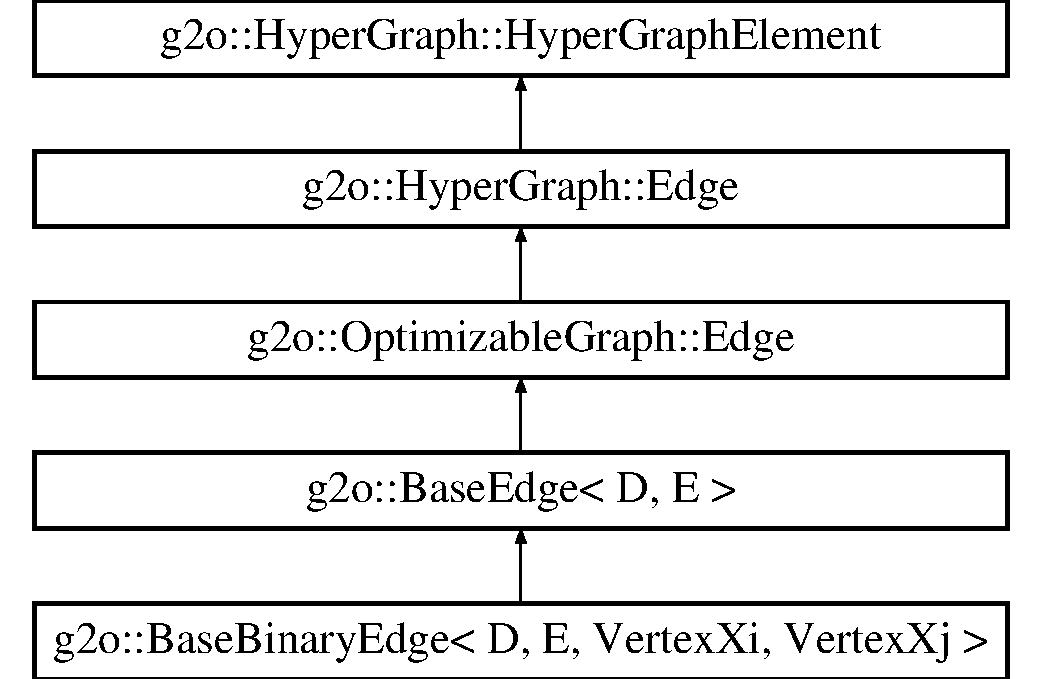
\includegraphics[height=5.000000cm]{classg2o_1_1_base_binary_edge}
\end{center}
\end{figure}
\subsection*{Public Types}
\begin{DoxyCompactItemize}
\item 
typedef Vertex\+Xi \mbox{\hyperlink{classg2o_1_1_base_binary_edge_aa8e2b04b2c0c90adc48384d6d41063cc}{Vertex\+Xi\+Type}}
\item 
typedef Vertex\+Xj \mbox{\hyperlink{classg2o_1_1_base_binary_edge_aa489ae37680c37d7b2c3c1a197f90de9}{Vertex\+Xj\+Type}}
\item 
typedef \mbox{\hyperlink{classg2o_1_1_base_edge}{Base\+Edge}}$<$ D, E $>$\+::\mbox{\hyperlink{classg2o_1_1_base_binary_edge_ac1e9249e9906747a6669a9c90013944b}{Measurement}} \mbox{\hyperlink{classg2o_1_1_base_binary_edge_ac1e9249e9906747a6669a9c90013944b}{Measurement}}
\item 
typedef Matrix$<$ double, D, \mbox{\hyperlink{classg2o_1_1_base_binary_edge_abfe232196405a7204bc299a747c1cc8b}{Di}} $>$\+::Aligned\+Map\+Type \mbox{\hyperlink{classg2o_1_1_base_binary_edge_ab1cde84224b129603bcd95db027e0167}{Jacobian\+Xi\+Oplus\+Type}}
\item 
typedef Matrix$<$ double, D, \mbox{\hyperlink{classg2o_1_1_base_binary_edge_ab718b94950a34d589371fe6f5583b259}{Dj}} $>$\+::Aligned\+Map\+Type \mbox{\hyperlink{classg2o_1_1_base_binary_edge_a83e5dec2135b33e86255c87be3b5d062}{Jacobian\+Xj\+Oplus\+Type}}
\item 
typedef \mbox{\hyperlink{classg2o_1_1_base_edge}{Base\+Edge}}$<$ D, E $>$\+::\mbox{\hyperlink{classg2o_1_1_base_binary_edge_ae1cccf6068b2446ece316b6a69a46acf}{Error\+Vector}} \mbox{\hyperlink{classg2o_1_1_base_binary_edge_ae1cccf6068b2446ece316b6a69a46acf}{Error\+Vector}}
\item 
typedef \mbox{\hyperlink{classg2o_1_1_base_edge}{Base\+Edge}}$<$ D, E $>$\+::\mbox{\hyperlink{classg2o_1_1_base_binary_edge_a4530ef6462aadaf2ab826d440d3b3318}{Information\+Type}} \mbox{\hyperlink{classg2o_1_1_base_binary_edge_a4530ef6462aadaf2ab826d440d3b3318}{Information\+Type}}
\item 
typedef Eigen\+::\+Map$<$ Matrix$<$ double, \mbox{\hyperlink{classg2o_1_1_base_binary_edge_abfe232196405a7204bc299a747c1cc8b}{Di}}, \mbox{\hyperlink{classg2o_1_1_base_binary_edge_ab718b94950a34d589371fe6f5583b259}{Dj}} $>$, Matrix$<$ double, \mbox{\hyperlink{classg2o_1_1_base_binary_edge_abfe232196405a7204bc299a747c1cc8b}{Di}}, \mbox{\hyperlink{classg2o_1_1_base_binary_edge_ab718b94950a34d589371fe6f5583b259}{Dj}} $>$\+::Flags \&Aligned\+Bit ? Aligned \+:Unaligned $>$ \mbox{\hyperlink{classg2o_1_1_base_binary_edge_a7eadbbe6abffe4d2ebdf6231272789a5}{Hessian\+Block\+Type}}
\item 
typedef Eigen\+::\+Map$<$ Matrix$<$ double, \mbox{\hyperlink{classg2o_1_1_base_binary_edge_ab718b94950a34d589371fe6f5583b259}{Dj}}, \mbox{\hyperlink{classg2o_1_1_base_binary_edge_abfe232196405a7204bc299a747c1cc8b}{Di}} $>$, Matrix$<$ double, \mbox{\hyperlink{classg2o_1_1_base_binary_edge_ab718b94950a34d589371fe6f5583b259}{Dj}}, \mbox{\hyperlink{classg2o_1_1_base_binary_edge_abfe232196405a7204bc299a747c1cc8b}{Di}} $>$\+::Flags \&Aligned\+Bit ? Aligned \+:Unaligned $>$ \mbox{\hyperlink{classg2o_1_1_base_binary_edge_aec0d5b1819f702b7658574fcd6324b49}{Hessian\+Block\+Transposed\+Type}}
\end{DoxyCompactItemize}
\subsection*{Public Member Functions}
\begin{DoxyCompactItemize}
\item 
\mbox{\hyperlink{classg2o_1_1_base_binary_edge_aacfc6e1d439f2f0fb09c6b069f478cf4}{Base\+Binary\+Edge}} ()
\item 
virtual \mbox{\hyperlink{classg2o_1_1_optimizable_graph_1_1_vertex}{Optimizable\+Graph\+::\+Vertex}} $\ast$ \mbox{\hyperlink{classg2o_1_1_base_binary_edge_a32bfc93b6dede619c7d99db2fb60f80d}{create\+From}} ()
\item 
virtual \mbox{\hyperlink{classg2o_1_1_optimizable_graph_1_1_vertex}{Optimizable\+Graph\+::\+Vertex}} $\ast$ \mbox{\hyperlink{classg2o_1_1_base_binary_edge_ac7cce17e3229445e5a33c3cb8a569320}{create\+To}} ()
\item 
virtual void \mbox{\hyperlink{classg2o_1_1_base_binary_edge_a06e64067fa5fff4a5e2d058249b55478}{resize}} (size\+\_\+t size)
\item 
virtual bool \mbox{\hyperlink{classg2o_1_1_base_binary_edge_adc9ce883a63aa7bdba86e552d72e1de9}{all\+Vertices\+Fixed}} () const
\item 
virtual void \mbox{\hyperlink{classg2o_1_1_base_binary_edge_afc3b6470e7679f027c2614484b394925}{linearize\+Oplus}} (\mbox{\hyperlink{classg2o_1_1_jacobian_workspace}{Jacobian\+Workspace}} \&jacobian\+Workspace)
\item 
virtual void \mbox{\hyperlink{classg2o_1_1_base_binary_edge_af0fb8a693c8c7996fa65566e7263fbc4}{linearize\+Oplus}} ()
\item 
const \mbox{\hyperlink{classg2o_1_1_base_binary_edge_ab1cde84224b129603bcd95db027e0167}{Jacobian\+Xi\+Oplus\+Type}} \& \mbox{\hyperlink{classg2o_1_1_base_binary_edge_a5232f0a5f116e7106b7968ab3bff036c}{jacobian\+Oplus\+Xi}} () const
\begin{DoxyCompactList}\small\item\em returns the result of the linearization in the manifold space for the node xi \end{DoxyCompactList}\item 
const \mbox{\hyperlink{classg2o_1_1_base_binary_edge_a83e5dec2135b33e86255c87be3b5d062}{Jacobian\+Xj\+Oplus\+Type}} \& \mbox{\hyperlink{classg2o_1_1_base_binary_edge_a71c1a583816399cf7db1a91ebe5dbf18}{jacobian\+Oplus\+Xj}} () const
\begin{DoxyCompactList}\small\item\em returns the result of the linearization in the manifold space for the node xj \end{DoxyCompactList}\item 
virtual void \mbox{\hyperlink{classg2o_1_1_base_binary_edge_a06a18745d95017c6d3c841f838a65364}{construct\+Quadratic\+Form}} ()
\item 
virtual void \mbox{\hyperlink{classg2o_1_1_base_binary_edge_ada358930854d386a4e8c32f64078e052}{map\+Hessian\+Memory}} (double $\ast$d, int i, int j, bool row\+Major)
\end{DoxyCompactItemize}
\subsection*{Static Public Attributes}
\begin{DoxyCompactItemize}
\item 
static const int \mbox{\hyperlink{classg2o_1_1_base_binary_edge_abfe232196405a7204bc299a747c1cc8b}{Di}} = Vertex\+Xi\+Type\+::\+Dimension
\item 
static const int \mbox{\hyperlink{classg2o_1_1_base_binary_edge_ab718b94950a34d589371fe6f5583b259}{Dj}} = Vertex\+Xj\+Type\+::\+Dimension
\item 
static const int \mbox{\hyperlink{classg2o_1_1_base_binary_edge_af3c134948e48c446762fa4e427d1cca5}{Dimension}} = \mbox{\hyperlink{classg2o_1_1_base_edge}{Base\+Edge}}$<$D, E$>$\+::Dimension
\end{DoxyCompactItemize}
\subsection*{Protected Attributes}
\begin{DoxyCompactItemize}
\item 
bool \mbox{\hyperlink{classg2o_1_1_base_binary_edge_aeb5c1f09a4433a6bd76ce4ab67bd9a64}{\+\_\+hessian\+Row\+Major}}
\item 
\mbox{\hyperlink{classg2o_1_1_base_binary_edge_a7eadbbe6abffe4d2ebdf6231272789a5}{Hessian\+Block\+Type}} \mbox{\hyperlink{classg2o_1_1_base_binary_edge_a5036f75e3b20c79cb014fcc929d8eef9}{\+\_\+hessian}}
\item 
\mbox{\hyperlink{classg2o_1_1_base_binary_edge_aec0d5b1819f702b7658574fcd6324b49}{Hessian\+Block\+Transposed\+Type}} \mbox{\hyperlink{classg2o_1_1_base_binary_edge_aa61657904b00fcfa19df382094386f11}{\+\_\+hessian\+Transposed}}
\item 
\mbox{\hyperlink{classg2o_1_1_base_binary_edge_ab1cde84224b129603bcd95db027e0167}{Jacobian\+Xi\+Oplus\+Type}} \mbox{\hyperlink{classg2o_1_1_base_binary_edge_aa21b9d84924ec93192374761ee0adfa7}{\+\_\+jacobian\+Oplus\+Xi}}
\item 
\mbox{\hyperlink{classg2o_1_1_base_binary_edge_a83e5dec2135b33e86255c87be3b5d062}{Jacobian\+Xj\+Oplus\+Type}} \mbox{\hyperlink{classg2o_1_1_base_binary_edge_ad448518247044496cb99c9d70bd1a363}{\+\_\+jacobian\+Oplus\+Xj}}
\end{DoxyCompactItemize}
\subsection*{Additional Inherited Members}


\subsection{Member Typedef Documentation}
\mbox{\Hypertarget{classg2o_1_1_base_binary_edge_ae1cccf6068b2446ece316b6a69a46acf}\label{classg2o_1_1_base_binary_edge_ae1cccf6068b2446ece316b6a69a46acf}} 
\index{g2o\+::\+Base\+Binary\+Edge@{g2o\+::\+Base\+Binary\+Edge}!Error\+Vector@{Error\+Vector}}
\index{Error\+Vector@{Error\+Vector}!g2o\+::\+Base\+Binary\+Edge@{g2o\+::\+Base\+Binary\+Edge}}
\subsubsection{\texorpdfstring{Error\+Vector}{ErrorVector}}
{\footnotesize\ttfamily template$<$int D, typename E, typename Vertex\+Xi, typename Vertex\+Xj$>$ \\
typedef \mbox{\hyperlink{classg2o_1_1_base_edge}{Base\+Edge}}$<$D,E$>$\+::\mbox{\hyperlink{classg2o_1_1_base_binary_edge_ae1cccf6068b2446ece316b6a69a46acf}{Error\+Vector}} \mbox{\hyperlink{classg2o_1_1_base_binary_edge}{g2o\+::\+Base\+Binary\+Edge}}$<$ D, E, Vertex\+Xi, Vertex\+Xj $>$\+::\mbox{\hyperlink{classg2o_1_1_base_binary_edge_ae1cccf6068b2446ece316b6a69a46acf}{Error\+Vector}}}

\mbox{\Hypertarget{classg2o_1_1_base_binary_edge_aec0d5b1819f702b7658574fcd6324b49}\label{classg2o_1_1_base_binary_edge_aec0d5b1819f702b7658574fcd6324b49}} 
\index{g2o\+::\+Base\+Binary\+Edge@{g2o\+::\+Base\+Binary\+Edge}!Hessian\+Block\+Transposed\+Type@{Hessian\+Block\+Transposed\+Type}}
\index{Hessian\+Block\+Transposed\+Type@{Hessian\+Block\+Transposed\+Type}!g2o\+::\+Base\+Binary\+Edge@{g2o\+::\+Base\+Binary\+Edge}}
\subsubsection{\texorpdfstring{Hessian\+Block\+Transposed\+Type}{HessianBlockTransposedType}}
{\footnotesize\ttfamily template$<$int D, typename E, typename Vertex\+Xi, typename Vertex\+Xj$>$ \\
typedef Eigen\+::\+Map$<$Matrix$<$double, \mbox{\hyperlink{classg2o_1_1_base_binary_edge_ab718b94950a34d589371fe6f5583b259}{Dj}}, \mbox{\hyperlink{classg2o_1_1_base_binary_edge_abfe232196405a7204bc299a747c1cc8b}{Di}}$>$, Matrix$<$double, \mbox{\hyperlink{classg2o_1_1_base_binary_edge_ab718b94950a34d589371fe6f5583b259}{Dj}}, \mbox{\hyperlink{classg2o_1_1_base_binary_edge_abfe232196405a7204bc299a747c1cc8b}{Di}}$>$\+::Flags \& Aligned\+Bit ? Aligned \+: Unaligned $>$ \mbox{\hyperlink{classg2o_1_1_base_binary_edge}{g2o\+::\+Base\+Binary\+Edge}}$<$ D, E, Vertex\+Xi, Vertex\+Xj $>$\+::\mbox{\hyperlink{classg2o_1_1_base_binary_edge_aec0d5b1819f702b7658574fcd6324b49}{Hessian\+Block\+Transposed\+Type}}}

\mbox{\Hypertarget{classg2o_1_1_base_binary_edge_a7eadbbe6abffe4d2ebdf6231272789a5}\label{classg2o_1_1_base_binary_edge_a7eadbbe6abffe4d2ebdf6231272789a5}} 
\index{g2o\+::\+Base\+Binary\+Edge@{g2o\+::\+Base\+Binary\+Edge}!Hessian\+Block\+Type@{Hessian\+Block\+Type}}
\index{Hessian\+Block\+Type@{Hessian\+Block\+Type}!g2o\+::\+Base\+Binary\+Edge@{g2o\+::\+Base\+Binary\+Edge}}
\subsubsection{\texorpdfstring{Hessian\+Block\+Type}{HessianBlockType}}
{\footnotesize\ttfamily template$<$int D, typename E, typename Vertex\+Xi, typename Vertex\+Xj$>$ \\
typedef Eigen\+::\+Map$<$Matrix$<$double, \mbox{\hyperlink{classg2o_1_1_base_binary_edge_abfe232196405a7204bc299a747c1cc8b}{Di}}, \mbox{\hyperlink{classg2o_1_1_base_binary_edge_ab718b94950a34d589371fe6f5583b259}{Dj}}$>$, Matrix$<$double, \mbox{\hyperlink{classg2o_1_1_base_binary_edge_abfe232196405a7204bc299a747c1cc8b}{Di}}, \mbox{\hyperlink{classg2o_1_1_base_binary_edge_ab718b94950a34d589371fe6f5583b259}{Dj}}$>$\+::Flags \& Aligned\+Bit ? Aligned \+: Unaligned $>$ \mbox{\hyperlink{classg2o_1_1_base_binary_edge}{g2o\+::\+Base\+Binary\+Edge}}$<$ D, E, Vertex\+Xi, Vertex\+Xj $>$\+::\mbox{\hyperlink{classg2o_1_1_base_binary_edge_a7eadbbe6abffe4d2ebdf6231272789a5}{Hessian\+Block\+Type}}}

\mbox{\Hypertarget{classg2o_1_1_base_binary_edge_a4530ef6462aadaf2ab826d440d3b3318}\label{classg2o_1_1_base_binary_edge_a4530ef6462aadaf2ab826d440d3b3318}} 
\index{g2o\+::\+Base\+Binary\+Edge@{g2o\+::\+Base\+Binary\+Edge}!Information\+Type@{Information\+Type}}
\index{Information\+Type@{Information\+Type}!g2o\+::\+Base\+Binary\+Edge@{g2o\+::\+Base\+Binary\+Edge}}
\subsubsection{\texorpdfstring{Information\+Type}{InformationType}}
{\footnotesize\ttfamily template$<$int D, typename E, typename Vertex\+Xi, typename Vertex\+Xj$>$ \\
typedef \mbox{\hyperlink{classg2o_1_1_base_edge}{Base\+Edge}}$<$D,E$>$\+::\mbox{\hyperlink{classg2o_1_1_base_binary_edge_a4530ef6462aadaf2ab826d440d3b3318}{Information\+Type}} \mbox{\hyperlink{classg2o_1_1_base_binary_edge}{g2o\+::\+Base\+Binary\+Edge}}$<$ D, E, Vertex\+Xi, Vertex\+Xj $>$\+::\mbox{\hyperlink{classg2o_1_1_base_binary_edge_a4530ef6462aadaf2ab826d440d3b3318}{Information\+Type}}}

\mbox{\Hypertarget{classg2o_1_1_base_binary_edge_ab1cde84224b129603bcd95db027e0167}\label{classg2o_1_1_base_binary_edge_ab1cde84224b129603bcd95db027e0167}} 
\index{g2o\+::\+Base\+Binary\+Edge@{g2o\+::\+Base\+Binary\+Edge}!Jacobian\+Xi\+Oplus\+Type@{Jacobian\+Xi\+Oplus\+Type}}
\index{Jacobian\+Xi\+Oplus\+Type@{Jacobian\+Xi\+Oplus\+Type}!g2o\+::\+Base\+Binary\+Edge@{g2o\+::\+Base\+Binary\+Edge}}
\subsubsection{\texorpdfstring{Jacobian\+Xi\+Oplus\+Type}{JacobianXiOplusType}}
{\footnotesize\ttfamily template$<$int D, typename E, typename Vertex\+Xi, typename Vertex\+Xj$>$ \\
typedef Matrix$<$double, D, \mbox{\hyperlink{classg2o_1_1_base_binary_edge_abfe232196405a7204bc299a747c1cc8b}{Di}}$>$\+::Aligned\+Map\+Type \mbox{\hyperlink{classg2o_1_1_base_binary_edge}{g2o\+::\+Base\+Binary\+Edge}}$<$ D, E, Vertex\+Xi, Vertex\+Xj $>$\+::\mbox{\hyperlink{classg2o_1_1_base_binary_edge_ab1cde84224b129603bcd95db027e0167}{Jacobian\+Xi\+Oplus\+Type}}}

\mbox{\Hypertarget{classg2o_1_1_base_binary_edge_a83e5dec2135b33e86255c87be3b5d062}\label{classg2o_1_1_base_binary_edge_a83e5dec2135b33e86255c87be3b5d062}} 
\index{g2o\+::\+Base\+Binary\+Edge@{g2o\+::\+Base\+Binary\+Edge}!Jacobian\+Xj\+Oplus\+Type@{Jacobian\+Xj\+Oplus\+Type}}
\index{Jacobian\+Xj\+Oplus\+Type@{Jacobian\+Xj\+Oplus\+Type}!g2o\+::\+Base\+Binary\+Edge@{g2o\+::\+Base\+Binary\+Edge}}
\subsubsection{\texorpdfstring{Jacobian\+Xj\+Oplus\+Type}{JacobianXjOplusType}}
{\footnotesize\ttfamily template$<$int D, typename E, typename Vertex\+Xi, typename Vertex\+Xj$>$ \\
typedef Matrix$<$double, D, \mbox{\hyperlink{classg2o_1_1_base_binary_edge_ab718b94950a34d589371fe6f5583b259}{Dj}}$>$\+::Aligned\+Map\+Type \mbox{\hyperlink{classg2o_1_1_base_binary_edge}{g2o\+::\+Base\+Binary\+Edge}}$<$ D, E, Vertex\+Xi, Vertex\+Xj $>$\+::\mbox{\hyperlink{classg2o_1_1_base_binary_edge_a83e5dec2135b33e86255c87be3b5d062}{Jacobian\+Xj\+Oplus\+Type}}}

\mbox{\Hypertarget{classg2o_1_1_base_binary_edge_ac1e9249e9906747a6669a9c90013944b}\label{classg2o_1_1_base_binary_edge_ac1e9249e9906747a6669a9c90013944b}} 
\index{g2o\+::\+Base\+Binary\+Edge@{g2o\+::\+Base\+Binary\+Edge}!Measurement@{Measurement}}
\index{Measurement@{Measurement}!g2o\+::\+Base\+Binary\+Edge@{g2o\+::\+Base\+Binary\+Edge}}
\subsubsection{\texorpdfstring{Measurement}{Measurement}}
{\footnotesize\ttfamily template$<$int D, typename E, typename Vertex\+Xi, typename Vertex\+Xj$>$ \\
typedef \mbox{\hyperlink{classg2o_1_1_base_edge}{Base\+Edge}}$<$D,E$>$\+::\mbox{\hyperlink{classg2o_1_1_base_binary_edge_ac1e9249e9906747a6669a9c90013944b}{Measurement}} \mbox{\hyperlink{classg2o_1_1_base_binary_edge}{g2o\+::\+Base\+Binary\+Edge}}$<$ D, E, Vertex\+Xi, Vertex\+Xj $>$\+::\mbox{\hyperlink{classg2o_1_1_base_binary_edge_ac1e9249e9906747a6669a9c90013944b}{Measurement}}}

\mbox{\Hypertarget{classg2o_1_1_base_binary_edge_aa8e2b04b2c0c90adc48384d6d41063cc}\label{classg2o_1_1_base_binary_edge_aa8e2b04b2c0c90adc48384d6d41063cc}} 
\index{g2o\+::\+Base\+Binary\+Edge@{g2o\+::\+Base\+Binary\+Edge}!Vertex\+Xi\+Type@{Vertex\+Xi\+Type}}
\index{Vertex\+Xi\+Type@{Vertex\+Xi\+Type}!g2o\+::\+Base\+Binary\+Edge@{g2o\+::\+Base\+Binary\+Edge}}
\subsubsection{\texorpdfstring{Vertex\+Xi\+Type}{VertexXiType}}
{\footnotesize\ttfamily template$<$int D, typename E, typename Vertex\+Xi, typename Vertex\+Xj$>$ \\
typedef Vertex\+Xi \mbox{\hyperlink{classg2o_1_1_base_binary_edge}{g2o\+::\+Base\+Binary\+Edge}}$<$ D, E, Vertex\+Xi, Vertex\+Xj $>$\+::\mbox{\hyperlink{classg2o_1_1_base_binary_edge_aa8e2b04b2c0c90adc48384d6d41063cc}{Vertex\+Xi\+Type}}}

\mbox{\Hypertarget{classg2o_1_1_base_binary_edge_aa489ae37680c37d7b2c3c1a197f90de9}\label{classg2o_1_1_base_binary_edge_aa489ae37680c37d7b2c3c1a197f90de9}} 
\index{g2o\+::\+Base\+Binary\+Edge@{g2o\+::\+Base\+Binary\+Edge}!Vertex\+Xj\+Type@{Vertex\+Xj\+Type}}
\index{Vertex\+Xj\+Type@{Vertex\+Xj\+Type}!g2o\+::\+Base\+Binary\+Edge@{g2o\+::\+Base\+Binary\+Edge}}
\subsubsection{\texorpdfstring{Vertex\+Xj\+Type}{VertexXjType}}
{\footnotesize\ttfamily template$<$int D, typename E, typename Vertex\+Xi, typename Vertex\+Xj$>$ \\
typedef Vertex\+Xj \mbox{\hyperlink{classg2o_1_1_base_binary_edge}{g2o\+::\+Base\+Binary\+Edge}}$<$ D, E, Vertex\+Xi, Vertex\+Xj $>$\+::\mbox{\hyperlink{classg2o_1_1_base_binary_edge_aa489ae37680c37d7b2c3c1a197f90de9}{Vertex\+Xj\+Type}}}



\subsection{Constructor \& Destructor Documentation}
\mbox{\Hypertarget{classg2o_1_1_base_binary_edge_aacfc6e1d439f2f0fb09c6b069f478cf4}\label{classg2o_1_1_base_binary_edge_aacfc6e1d439f2f0fb09c6b069f478cf4}} 
\index{g2o\+::\+Base\+Binary\+Edge@{g2o\+::\+Base\+Binary\+Edge}!Base\+Binary\+Edge@{Base\+Binary\+Edge}}
\index{Base\+Binary\+Edge@{Base\+Binary\+Edge}!g2o\+::\+Base\+Binary\+Edge@{g2o\+::\+Base\+Binary\+Edge}}
\subsubsection{\texorpdfstring{Base\+Binary\+Edge()}{BaseBinaryEdge()}}
{\footnotesize\ttfamily template$<$int D, typename E, typename Vertex\+Xi, typename Vertex\+Xj$>$ \\
\mbox{\hyperlink{classg2o_1_1_base_binary_edge}{g2o\+::\+Base\+Binary\+Edge}}$<$ D, E, Vertex\+Xi, Vertex\+Xj $>$\+::\mbox{\hyperlink{classg2o_1_1_base_binary_edge}{Base\+Binary\+Edge}} (\begin{DoxyParamCaption}{ }\end{DoxyParamCaption})\hspace{0.3cm}{\ttfamily [inline]}}



\subsection{Member Function Documentation}
\mbox{\Hypertarget{classg2o_1_1_base_binary_edge_adc9ce883a63aa7bdba86e552d72e1de9}\label{classg2o_1_1_base_binary_edge_adc9ce883a63aa7bdba86e552d72e1de9}} 
\index{g2o\+::\+Base\+Binary\+Edge@{g2o\+::\+Base\+Binary\+Edge}!all\+Vertices\+Fixed@{all\+Vertices\+Fixed}}
\index{all\+Vertices\+Fixed@{all\+Vertices\+Fixed}!g2o\+::\+Base\+Binary\+Edge@{g2o\+::\+Base\+Binary\+Edge}}
\subsubsection{\texorpdfstring{all\+Vertices\+Fixed()}{allVerticesFixed()}}
{\footnotesize\ttfamily template$<$int D, typename E , typename Vertex\+Xi\+Type , typename Vertex\+Xj\+Type $>$ \\
bool Base\+Binary\+Edge\+::all\+Vertices\+Fixed (\begin{DoxyParamCaption}{ }\end{DoxyParamCaption}) const\hspace{0.3cm}{\ttfamily [virtual]}}



Implements \mbox{\hyperlink{classg2o_1_1_optimizable_graph_1_1_edge_a414c69ca1617a4d3b620e39f2ffbcea7}{g2o\+::\+Optimizable\+Graph\+::\+Edge}}.

\mbox{\Hypertarget{classg2o_1_1_base_binary_edge_a06a18745d95017c6d3c841f838a65364}\label{classg2o_1_1_base_binary_edge_a06a18745d95017c6d3c841f838a65364}} 
\index{g2o\+::\+Base\+Binary\+Edge@{g2o\+::\+Base\+Binary\+Edge}!construct\+Quadratic\+Form@{construct\+Quadratic\+Form}}
\index{construct\+Quadratic\+Form@{construct\+Quadratic\+Form}!g2o\+::\+Base\+Binary\+Edge@{g2o\+::\+Base\+Binary\+Edge}}
\subsubsection{\texorpdfstring{construct\+Quadratic\+Form()}{constructQuadraticForm()}}
{\footnotesize\ttfamily template$<$int D, typename E , typename Vertex\+Xi\+Type , typename Vertex\+Xj\+Type $>$ \\
void Base\+Binary\+Edge\+::construct\+Quadratic\+Form (\begin{DoxyParamCaption}{ }\end{DoxyParamCaption})\hspace{0.3cm}{\ttfamily [virtual]}}

Linearizes the constraint in the edge. Makes side effect on the vertices of the graph by changing the parameter vector b and the hessian blocks ii and jj. The off diagoinal block is accesed via \+\_\+hessian. 

Implements \mbox{\hyperlink{classg2o_1_1_optimizable_graph_1_1_edge_a56fbf3430ddf591e3c619bdd1b7e4499}{g2o\+::\+Optimizable\+Graph\+::\+Edge}}.

\mbox{\Hypertarget{classg2o_1_1_base_binary_edge_a32bfc93b6dede619c7d99db2fb60f80d}\label{classg2o_1_1_base_binary_edge_a32bfc93b6dede619c7d99db2fb60f80d}} 
\index{g2o\+::\+Base\+Binary\+Edge@{g2o\+::\+Base\+Binary\+Edge}!create\+From@{create\+From}}
\index{create\+From@{create\+From}!g2o\+::\+Base\+Binary\+Edge@{g2o\+::\+Base\+Binary\+Edge}}
\subsubsection{\texorpdfstring{create\+From()}{createFrom()}}
{\footnotesize\ttfamily template$<$int D, typename E , typename Vertex\+Xi\+Type , typename Vertex\+Xj\+Type $>$ \\
\mbox{\hyperlink{classg2o_1_1_optimizable_graph_1_1_vertex}{Optimizable\+Graph\+::\+Vertex}} $\ast$ Base\+Binary\+Edge\+::create\+From (\begin{DoxyParamCaption}{ }\end{DoxyParamCaption})\hspace{0.3cm}{\ttfamily [virtual]}}



Reimplemented from \mbox{\hyperlink{classg2o_1_1_optimizable_graph_1_1_edge_abd98d7a174df25bcc82cfdacba682fec}{g2o\+::\+Optimizable\+Graph\+::\+Edge}}.

\mbox{\Hypertarget{classg2o_1_1_base_binary_edge_ac7cce17e3229445e5a33c3cb8a569320}\label{classg2o_1_1_base_binary_edge_ac7cce17e3229445e5a33c3cb8a569320}} 
\index{g2o\+::\+Base\+Binary\+Edge@{g2o\+::\+Base\+Binary\+Edge}!create\+To@{create\+To}}
\index{create\+To@{create\+To}!g2o\+::\+Base\+Binary\+Edge@{g2o\+::\+Base\+Binary\+Edge}}
\subsubsection{\texorpdfstring{create\+To()}{createTo()}}
{\footnotesize\ttfamily template$<$int D, typename E , typename Vertex\+Xi\+Type , typename Vertex\+Xj\+Type $>$ \\
\mbox{\hyperlink{classg2o_1_1_optimizable_graph_1_1_vertex}{Optimizable\+Graph\+::\+Vertex}} $\ast$ Base\+Binary\+Edge\+::create\+To (\begin{DoxyParamCaption}{ }\end{DoxyParamCaption})\hspace{0.3cm}{\ttfamily [virtual]}}



Reimplemented from \mbox{\hyperlink{classg2o_1_1_optimizable_graph_1_1_edge_a39c22b396ab312059ea8fa4c2776be2e}{g2o\+::\+Optimizable\+Graph\+::\+Edge}}.

\mbox{\Hypertarget{classg2o_1_1_base_binary_edge_a5232f0a5f116e7106b7968ab3bff036c}\label{classg2o_1_1_base_binary_edge_a5232f0a5f116e7106b7968ab3bff036c}} 
\index{g2o\+::\+Base\+Binary\+Edge@{g2o\+::\+Base\+Binary\+Edge}!jacobian\+Oplus\+Xi@{jacobian\+Oplus\+Xi}}
\index{jacobian\+Oplus\+Xi@{jacobian\+Oplus\+Xi}!g2o\+::\+Base\+Binary\+Edge@{g2o\+::\+Base\+Binary\+Edge}}
\subsubsection{\texorpdfstring{jacobian\+Oplus\+Xi()}{jacobianOplusXi()}}
{\footnotesize\ttfamily template$<$int D, typename E, typename Vertex\+Xi, typename Vertex\+Xj$>$ \\
const \mbox{\hyperlink{classg2o_1_1_base_binary_edge_ab1cde84224b129603bcd95db027e0167}{Jacobian\+Xi\+Oplus\+Type}}\& \mbox{\hyperlink{classg2o_1_1_base_binary_edge}{g2o\+::\+Base\+Binary\+Edge}}$<$ D, E, Vertex\+Xi, Vertex\+Xj $>$\+::jacobian\+Oplus\+Xi (\begin{DoxyParamCaption}{ }\end{DoxyParamCaption}) const\hspace{0.3cm}{\ttfamily [inline]}}



returns the result of the linearization in the manifold space for the node xi 

\mbox{\Hypertarget{classg2o_1_1_base_binary_edge_a71c1a583816399cf7db1a91ebe5dbf18}\label{classg2o_1_1_base_binary_edge_a71c1a583816399cf7db1a91ebe5dbf18}} 
\index{g2o\+::\+Base\+Binary\+Edge@{g2o\+::\+Base\+Binary\+Edge}!jacobian\+Oplus\+Xj@{jacobian\+Oplus\+Xj}}
\index{jacobian\+Oplus\+Xj@{jacobian\+Oplus\+Xj}!g2o\+::\+Base\+Binary\+Edge@{g2o\+::\+Base\+Binary\+Edge}}
\subsubsection{\texorpdfstring{jacobian\+Oplus\+Xj()}{jacobianOplusXj()}}
{\footnotesize\ttfamily template$<$int D, typename E, typename Vertex\+Xi, typename Vertex\+Xj$>$ \\
const \mbox{\hyperlink{classg2o_1_1_base_binary_edge_a83e5dec2135b33e86255c87be3b5d062}{Jacobian\+Xj\+Oplus\+Type}}\& \mbox{\hyperlink{classg2o_1_1_base_binary_edge}{g2o\+::\+Base\+Binary\+Edge}}$<$ D, E, Vertex\+Xi, Vertex\+Xj $>$\+::jacobian\+Oplus\+Xj (\begin{DoxyParamCaption}{ }\end{DoxyParamCaption}) const\hspace{0.3cm}{\ttfamily [inline]}}



returns the result of the linearization in the manifold space for the node xj 

\mbox{\Hypertarget{classg2o_1_1_base_binary_edge_afc3b6470e7679f027c2614484b394925}\label{classg2o_1_1_base_binary_edge_afc3b6470e7679f027c2614484b394925}} 
\index{g2o\+::\+Base\+Binary\+Edge@{g2o\+::\+Base\+Binary\+Edge}!linearize\+Oplus@{linearize\+Oplus}}
\index{linearize\+Oplus@{linearize\+Oplus}!g2o\+::\+Base\+Binary\+Edge@{g2o\+::\+Base\+Binary\+Edge}}
\subsubsection{\texorpdfstring{linearize\+Oplus()}{linearizeOplus()}\hspace{0.1cm}{\footnotesize\ttfamily [1/2]}}
{\footnotesize\ttfamily template$<$int D, typename E , typename Vertex\+Xi\+Type , typename Vertex\+Xj\+Type $>$ \\
void Base\+Binary\+Edge\+::linearize\+Oplus (\begin{DoxyParamCaption}\item[{\mbox{\hyperlink{classg2o_1_1_jacobian_workspace}{Jacobian\+Workspace}} \&}]{jacobian\+Workspace }\end{DoxyParamCaption})\hspace{0.3cm}{\ttfamily [virtual]}}

Linearizes the constraint in the edge in the manifold space, and store the result in the given workspace 

Implements \mbox{\hyperlink{classg2o_1_1_optimizable_graph_1_1_edge_a0fdad5ebfb4efec9f893b57f67e0fbe1}{g2o\+::\+Optimizable\+Graph\+::\+Edge}}.

\mbox{\Hypertarget{classg2o_1_1_base_binary_edge_af0fb8a693c8c7996fa65566e7263fbc4}\label{classg2o_1_1_base_binary_edge_af0fb8a693c8c7996fa65566e7263fbc4}} 
\index{g2o\+::\+Base\+Binary\+Edge@{g2o\+::\+Base\+Binary\+Edge}!linearize\+Oplus@{linearize\+Oplus}}
\index{linearize\+Oplus@{linearize\+Oplus}!g2o\+::\+Base\+Binary\+Edge@{g2o\+::\+Base\+Binary\+Edge}}
\subsubsection{\texorpdfstring{linearize\+Oplus()}{linearizeOplus()}\hspace{0.1cm}{\footnotesize\ttfamily [2/2]}}
{\footnotesize\ttfamily template$<$int D, typename E , typename Vertex\+Xi\+Type , typename Vertex\+Xj\+Type $>$ \\
void Base\+Binary\+Edge\+::linearize\+Oplus (\begin{DoxyParamCaption}{ }\end{DoxyParamCaption})\hspace{0.3cm}{\ttfamily [virtual]}}

Linearizes the oplus operator in the vertex, and stores the result in temporary variables \+\_\+jacobian\+Oplus\+Xi and \+\_\+jacobian\+Oplus\+Xj 

Reimplemented in \mbox{\hyperlink{classg2o_1_1_edge_stereo_s_e3_project_x_y_z_aea04d86a304c6cb4e2a3f34b35166f30}{g2o\+::\+Edge\+Stereo\+S\+E3\+Project\+X\+YZ}}, and \mbox{\hyperlink{classg2o_1_1_edge_s_e3_project_x_y_z_a7454e89740635d782c9e4efaef35ec44}{g2o\+::\+Edge\+S\+E3\+Project\+X\+YZ}}.

\mbox{\Hypertarget{classg2o_1_1_base_binary_edge_ada358930854d386a4e8c32f64078e052}\label{classg2o_1_1_base_binary_edge_ada358930854d386a4e8c32f64078e052}} 
\index{g2o\+::\+Base\+Binary\+Edge@{g2o\+::\+Base\+Binary\+Edge}!map\+Hessian\+Memory@{map\+Hessian\+Memory}}
\index{map\+Hessian\+Memory@{map\+Hessian\+Memory}!g2o\+::\+Base\+Binary\+Edge@{g2o\+::\+Base\+Binary\+Edge}}
\subsubsection{\texorpdfstring{map\+Hessian\+Memory()}{mapHessianMemory()}}
{\footnotesize\ttfamily template$<$int D, typename E , typename Vertex\+Xi\+Type , typename Vertex\+Xj\+Type $>$ \\
void Base\+Binary\+Edge\+::map\+Hessian\+Memory (\begin{DoxyParamCaption}\item[{double $\ast$}]{d,  }\item[{int}]{i,  }\item[{int}]{j,  }\item[{bool}]{row\+Major }\end{DoxyParamCaption})\hspace{0.3cm}{\ttfamily [virtual]}}

maps the internal matrix to some external memory location, you need to provide the memory before calling construct\+Quadratic\+Form 
\begin{DoxyParams}{Parameters}
{\em d} & the memory location to which we map \\
\hline
{\em i} & index of the vertex i \\
\hline
{\em j} & index of the vertex j (j $>$ i, upper triangular fashion) \\
\hline
{\em row\+Major} & if true, will write in row\+Major order to the block. Since E\+I\+G\+EN is column\+Major by default, this results in writing the transposed \\
\hline
\end{DoxyParams}


Implements \mbox{\hyperlink{classg2o_1_1_optimizable_graph_1_1_edge_a3bd233fd552daa166039acf47b69a5a7}{g2o\+::\+Optimizable\+Graph\+::\+Edge}}.

\mbox{\Hypertarget{classg2o_1_1_base_binary_edge_a06e64067fa5fff4a5e2d058249b55478}\label{classg2o_1_1_base_binary_edge_a06e64067fa5fff4a5e2d058249b55478}} 
\index{g2o\+::\+Base\+Binary\+Edge@{g2o\+::\+Base\+Binary\+Edge}!resize@{resize}}
\index{resize@{resize}!g2o\+::\+Base\+Binary\+Edge@{g2o\+::\+Base\+Binary\+Edge}}
\subsubsection{\texorpdfstring{resize()}{resize()}}
{\footnotesize\ttfamily template$<$int D, typename E , typename Vertex\+Xi\+Type , typename Vertex\+Xj\+Type $>$ \\
void Base\+Binary\+Edge\+::resize (\begin{DoxyParamCaption}\item[{size\+\_\+t}]{size }\end{DoxyParamCaption})\hspace{0.3cm}{\ttfamily [virtual]}}

resizes the number of vertices connected by this edge 

Reimplemented from \mbox{\hyperlink{classg2o_1_1_hyper_graph_1_1_edge_ad8913f1149a0fd5bb628f0f1c8a91a55}{g2o\+::\+Hyper\+Graph\+::\+Edge}}.



\subsection{Member Data Documentation}
\mbox{\Hypertarget{classg2o_1_1_base_binary_edge_a5036f75e3b20c79cb014fcc929d8eef9}\label{classg2o_1_1_base_binary_edge_a5036f75e3b20c79cb014fcc929d8eef9}} 
\index{g2o\+::\+Base\+Binary\+Edge@{g2o\+::\+Base\+Binary\+Edge}!\+\_\+hessian@{\+\_\+hessian}}
\index{\+\_\+hessian@{\+\_\+hessian}!g2o\+::\+Base\+Binary\+Edge@{g2o\+::\+Base\+Binary\+Edge}}
\subsubsection{\texorpdfstring{\+\_\+hessian}{\_hessian}}
{\footnotesize\ttfamily template$<$int D, typename E, typename Vertex\+Xi, typename Vertex\+Xj$>$ \\
\mbox{\hyperlink{classg2o_1_1_base_binary_edge_a7eadbbe6abffe4d2ebdf6231272789a5}{Hessian\+Block\+Type}} \mbox{\hyperlink{classg2o_1_1_base_binary_edge}{g2o\+::\+Base\+Binary\+Edge}}$<$ D, E, Vertex\+Xi, Vertex\+Xj $>$\+::\+\_\+hessian\hspace{0.3cm}{\ttfamily [protected]}}

\mbox{\Hypertarget{classg2o_1_1_base_binary_edge_aeb5c1f09a4433a6bd76ce4ab67bd9a64}\label{classg2o_1_1_base_binary_edge_aeb5c1f09a4433a6bd76ce4ab67bd9a64}} 
\index{g2o\+::\+Base\+Binary\+Edge@{g2o\+::\+Base\+Binary\+Edge}!\+\_\+hessian\+Row\+Major@{\+\_\+hessian\+Row\+Major}}
\index{\+\_\+hessian\+Row\+Major@{\+\_\+hessian\+Row\+Major}!g2o\+::\+Base\+Binary\+Edge@{g2o\+::\+Base\+Binary\+Edge}}
\subsubsection{\texorpdfstring{\+\_\+hessian\+Row\+Major}{\_hessianRowMajor}}
{\footnotesize\ttfamily template$<$int D, typename E, typename Vertex\+Xi, typename Vertex\+Xj$>$ \\
bool \mbox{\hyperlink{classg2o_1_1_base_binary_edge}{g2o\+::\+Base\+Binary\+Edge}}$<$ D, E, Vertex\+Xi, Vertex\+Xj $>$\+::\+\_\+hessian\+Row\+Major\hspace{0.3cm}{\ttfamily [protected]}}

\mbox{\Hypertarget{classg2o_1_1_base_binary_edge_aa61657904b00fcfa19df382094386f11}\label{classg2o_1_1_base_binary_edge_aa61657904b00fcfa19df382094386f11}} 
\index{g2o\+::\+Base\+Binary\+Edge@{g2o\+::\+Base\+Binary\+Edge}!\+\_\+hessian\+Transposed@{\+\_\+hessian\+Transposed}}
\index{\+\_\+hessian\+Transposed@{\+\_\+hessian\+Transposed}!g2o\+::\+Base\+Binary\+Edge@{g2o\+::\+Base\+Binary\+Edge}}
\subsubsection{\texorpdfstring{\+\_\+hessian\+Transposed}{\_hessianTransposed}}
{\footnotesize\ttfamily template$<$int D, typename E, typename Vertex\+Xi, typename Vertex\+Xj$>$ \\
\mbox{\hyperlink{classg2o_1_1_base_binary_edge_aec0d5b1819f702b7658574fcd6324b49}{Hessian\+Block\+Transposed\+Type}} \mbox{\hyperlink{classg2o_1_1_base_binary_edge}{g2o\+::\+Base\+Binary\+Edge}}$<$ D, E, Vertex\+Xi, Vertex\+Xj $>$\+::\+\_\+hessian\+Transposed\hspace{0.3cm}{\ttfamily [protected]}}

\mbox{\Hypertarget{classg2o_1_1_base_binary_edge_aa21b9d84924ec93192374761ee0adfa7}\label{classg2o_1_1_base_binary_edge_aa21b9d84924ec93192374761ee0adfa7}} 
\index{g2o\+::\+Base\+Binary\+Edge@{g2o\+::\+Base\+Binary\+Edge}!\+\_\+jacobian\+Oplus\+Xi@{\+\_\+jacobian\+Oplus\+Xi}}
\index{\+\_\+jacobian\+Oplus\+Xi@{\+\_\+jacobian\+Oplus\+Xi}!g2o\+::\+Base\+Binary\+Edge@{g2o\+::\+Base\+Binary\+Edge}}
\subsubsection{\texorpdfstring{\+\_\+jacobian\+Oplus\+Xi}{\_jacobianOplusXi}}
{\footnotesize\ttfamily template$<$int D, typename E, typename Vertex\+Xi, typename Vertex\+Xj$>$ \\
\mbox{\hyperlink{classg2o_1_1_base_binary_edge_ab1cde84224b129603bcd95db027e0167}{Jacobian\+Xi\+Oplus\+Type}} \mbox{\hyperlink{classg2o_1_1_base_binary_edge}{g2o\+::\+Base\+Binary\+Edge}}$<$ D, E, Vertex\+Xi, Vertex\+Xj $>$\+::\+\_\+jacobian\+Oplus\+Xi\hspace{0.3cm}{\ttfamily [protected]}}

\mbox{\Hypertarget{classg2o_1_1_base_binary_edge_ad448518247044496cb99c9d70bd1a363}\label{classg2o_1_1_base_binary_edge_ad448518247044496cb99c9d70bd1a363}} 
\index{g2o\+::\+Base\+Binary\+Edge@{g2o\+::\+Base\+Binary\+Edge}!\+\_\+jacobian\+Oplus\+Xj@{\+\_\+jacobian\+Oplus\+Xj}}
\index{\+\_\+jacobian\+Oplus\+Xj@{\+\_\+jacobian\+Oplus\+Xj}!g2o\+::\+Base\+Binary\+Edge@{g2o\+::\+Base\+Binary\+Edge}}
\subsubsection{\texorpdfstring{\+\_\+jacobian\+Oplus\+Xj}{\_jacobianOplusXj}}
{\footnotesize\ttfamily template$<$int D, typename E, typename Vertex\+Xi, typename Vertex\+Xj$>$ \\
\mbox{\hyperlink{classg2o_1_1_base_binary_edge_a83e5dec2135b33e86255c87be3b5d062}{Jacobian\+Xj\+Oplus\+Type}} \mbox{\hyperlink{classg2o_1_1_base_binary_edge}{g2o\+::\+Base\+Binary\+Edge}}$<$ D, E, Vertex\+Xi, Vertex\+Xj $>$\+::\+\_\+jacobian\+Oplus\+Xj\hspace{0.3cm}{\ttfamily [protected]}}

\mbox{\Hypertarget{classg2o_1_1_base_binary_edge_abfe232196405a7204bc299a747c1cc8b}\label{classg2o_1_1_base_binary_edge_abfe232196405a7204bc299a747c1cc8b}} 
\index{g2o\+::\+Base\+Binary\+Edge@{g2o\+::\+Base\+Binary\+Edge}!Di@{Di}}
\index{Di@{Di}!g2o\+::\+Base\+Binary\+Edge@{g2o\+::\+Base\+Binary\+Edge}}
\subsubsection{\texorpdfstring{Di}{Di}}
{\footnotesize\ttfamily template$<$int D, typename E, typename Vertex\+Xi, typename Vertex\+Xj$>$ \\
const int \mbox{\hyperlink{classg2o_1_1_base_binary_edge}{g2o\+::\+Base\+Binary\+Edge}}$<$ D, E, Vertex\+Xi, Vertex\+Xj $>$\+::Di = Vertex\+Xi\+Type\+::\+Dimension\hspace{0.3cm}{\ttfamily [static]}}

\mbox{\Hypertarget{classg2o_1_1_base_binary_edge_af3c134948e48c446762fa4e427d1cca5}\label{classg2o_1_1_base_binary_edge_af3c134948e48c446762fa4e427d1cca5}} 
\index{g2o\+::\+Base\+Binary\+Edge@{g2o\+::\+Base\+Binary\+Edge}!Dimension@{Dimension}}
\index{Dimension@{Dimension}!g2o\+::\+Base\+Binary\+Edge@{g2o\+::\+Base\+Binary\+Edge}}
\subsubsection{\texorpdfstring{Dimension}{Dimension}}
{\footnotesize\ttfamily template$<$int D, typename E, typename Vertex\+Xi, typename Vertex\+Xj$>$ \\
const int \mbox{\hyperlink{classg2o_1_1_base_binary_edge}{g2o\+::\+Base\+Binary\+Edge}}$<$ D, E, Vertex\+Xi, Vertex\+Xj $>$\+::Dimension = \mbox{\hyperlink{classg2o_1_1_base_edge}{Base\+Edge}}$<$D, E$>$\+::Dimension\hspace{0.3cm}{\ttfamily [static]}}

\mbox{\Hypertarget{classg2o_1_1_base_binary_edge_ab718b94950a34d589371fe6f5583b259}\label{classg2o_1_1_base_binary_edge_ab718b94950a34d589371fe6f5583b259}} 
\index{g2o\+::\+Base\+Binary\+Edge@{g2o\+::\+Base\+Binary\+Edge}!Dj@{Dj}}
\index{Dj@{Dj}!g2o\+::\+Base\+Binary\+Edge@{g2o\+::\+Base\+Binary\+Edge}}
\subsubsection{\texorpdfstring{Dj}{Dj}}
{\footnotesize\ttfamily template$<$int D, typename E, typename Vertex\+Xi, typename Vertex\+Xj$>$ \\
const int \mbox{\hyperlink{classg2o_1_1_base_binary_edge}{g2o\+::\+Base\+Binary\+Edge}}$<$ D, E, Vertex\+Xi, Vertex\+Xj $>$\+::Dj = Vertex\+Xj\+Type\+::\+Dimension\hspace{0.3cm}{\ttfamily [static]}}



The documentation for this class was generated from the following files\+:\begin{DoxyCompactItemize}
\item 
D\+:/github/\+V\+S\+L\+A\+M/\+O\+R\+B\+S\+L\+A\+M2/\+O\+R\+B-\/\+S\+L\+A\+M2-\/master/\+Thirdparty/g2o/g2o/core/\mbox{\hyperlink{base__binary__edge_8h}{base\+\_\+binary\+\_\+edge.\+h}}\item 
D\+:/github/\+V\+S\+L\+A\+M/\+O\+R\+B\+S\+L\+A\+M2/\+O\+R\+B-\/\+S\+L\+A\+M2-\/master/\+Thirdparty/g2o/g2o/core/\mbox{\hyperlink{base__binary__edge_8hpp}{base\+\_\+binary\+\_\+edge.\+hpp}}\end{DoxyCompactItemize}

\hypertarget{classg2o_1_1_base_edge}{}\section{g2o\+:\+:Base\+Edge$<$ D, E $>$ Class Template Reference}
\label{classg2o_1_1_base_edge}\index{g2o\+::\+Base\+Edge$<$ D, E $>$@{g2o\+::\+Base\+Edge$<$ D, E $>$}}


{\ttfamily \#include $<$base\+\_\+edge.\+h$>$}

Inheritance diagram for g2o\+:\+:Base\+Edge$<$ D, E $>$\+:\begin{figure}[H]
\begin{center}
\leavevmode
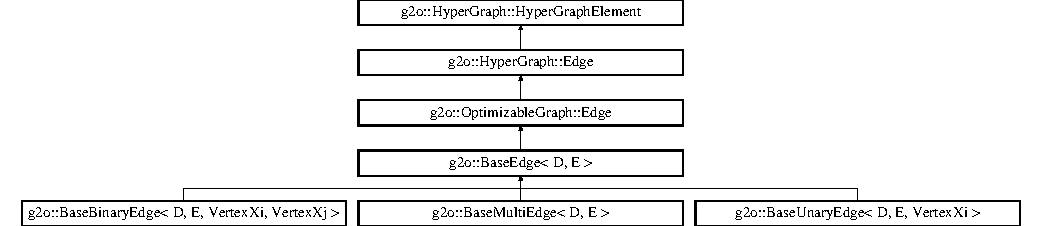
\includegraphics[height=3.040174cm]{classg2o_1_1_base_edge}
\end{center}
\end{figure}
\subsection*{Public Types}
\begin{DoxyCompactItemize}
\item 
typedef E \mbox{\hyperlink{classg2o_1_1_base_edge_a2c148abba650a20b8c7eed75d3e2211e}{Measurement}}
\item 
typedef Matrix$<$ double, D, 1 $>$ \mbox{\hyperlink{classg2o_1_1_base_edge_af5b558dd24e4be2e437563cae4b3550d}{Error\+Vector}}
\item 
typedef Matrix$<$ double, D, D $>$ \mbox{\hyperlink{classg2o_1_1_base_edge_a2e5a33343ac3f189d8a7d5ee4d8b73fc}{Information\+Type}}
\end{DoxyCompactItemize}
\subsection*{Public Member Functions}
\begin{DoxyCompactItemize}
\item 
\mbox{\hyperlink{classg2o_1_1_base_edge_a5efd0eb7e76a7f1ad723e7a5896a54d5}{Base\+Edge}} ()
\item 
virtual \mbox{\hyperlink{classg2o_1_1_base_edge_a92a5cba950b867f9ff10b8154291087c}{$\sim$\+Base\+Edge}} ()
\item 
virtual double \mbox{\hyperlink{classg2o_1_1_base_edge_a8316137ded4396a2dbf7529d83888400}{chi2}} () const
\begin{DoxyCompactList}\small\item\em computes the chi2 based on the cached error value, only valid after compute\+Error has been called. \end{DoxyCompactList}\item 
virtual const double $\ast$ \mbox{\hyperlink{classg2o_1_1_base_edge_ad99fce6bad0207979b6211ac0d589015}{error\+Data}} () const
\begin{DoxyCompactList}\small\item\em returns the error vector cached after calling the compute\+Error; \end{DoxyCompactList}\item 
virtual double $\ast$ \mbox{\hyperlink{classg2o_1_1_base_edge_ab80452c1134036928a2af6303412a3c4}{error\+Data}} ()
\item 
const \mbox{\hyperlink{classg2o_1_1_base_edge_af5b558dd24e4be2e437563cae4b3550d}{Error\+Vector}} \& \mbox{\hyperlink{classg2o_1_1_base_edge_ab5a17b29aa9be942157e089bb363a46c}{error}} () const
\item 
\mbox{\hyperlink{classg2o_1_1_base_edge_af5b558dd24e4be2e437563cae4b3550d}{Error\+Vector}} \& \mbox{\hyperlink{classg2o_1_1_base_edge_ad0a9e3b6d5490c8f4af794c77742faae}{error}} ()
\item 
const \mbox{\hyperlink{classg2o_1_1_base_edge_a2e5a33343ac3f189d8a7d5ee4d8b73fc}{Information\+Type}} \& \mbox{\hyperlink{classg2o_1_1_base_edge_a405f8d52738e557a0860b52ac67a005b}{information}} () const
\begin{DoxyCompactList}\small\item\em information matrix of the constraint \end{DoxyCompactList}\item 
\mbox{\hyperlink{classg2o_1_1_base_edge_a2e5a33343ac3f189d8a7d5ee4d8b73fc}{Information\+Type}} \& \mbox{\hyperlink{classg2o_1_1_base_edge_addff9120320d63504e07bfe17f1d04a7}{information}} ()
\item 
void \mbox{\hyperlink{classg2o_1_1_base_edge_a9bb871a94d2413ec3113a147417f2dc4}{set\+Information}} (const \mbox{\hyperlink{classg2o_1_1_base_edge_a2e5a33343ac3f189d8a7d5ee4d8b73fc}{Information\+Type}} \&\mbox{\hyperlink{classg2o_1_1_base_edge_a405f8d52738e557a0860b52ac67a005b}{information}})
\item 
virtual const double $\ast$ \mbox{\hyperlink{classg2o_1_1_base_edge_acf02f0d69998b75b207bc102f079d5b8}{information\+Data}} () const
\begin{DoxyCompactList}\small\item\em returns the memory of the information matrix, usable for example with a Eigen\+::\+Map$<$\+Matrix\+Xd$>$ \end{DoxyCompactList}\item 
virtual double $\ast$ \mbox{\hyperlink{classg2o_1_1_base_edge_a72ae9d215d6abc892f735e3d3ab81a88}{information\+Data}} ()
\item 
const \mbox{\hyperlink{classg2o_1_1_base_edge_a2c148abba650a20b8c7eed75d3e2211e}{Measurement}} \& \mbox{\hyperlink{classg2o_1_1_base_edge_a8e890d43f491afdd035713ff176ddd5c}{measurement}} () const
\begin{DoxyCompactList}\small\item\em accessor functions for the measurement represented by the edge \end{DoxyCompactList}\item 
virtual void \mbox{\hyperlink{classg2o_1_1_base_edge_a24aae7b4fc35d311158f104cfdd95aeb}{set\+Measurement}} (const \mbox{\hyperlink{classg2o_1_1_base_edge_a2c148abba650a20b8c7eed75d3e2211e}{Measurement}} \&m)
\item 
virtual int \mbox{\hyperlink{classg2o_1_1_base_edge_a6776919120a8eaca8e4b9d0e6b8a421d}{rank}} () const
\item 
virtual void \mbox{\hyperlink{classg2o_1_1_base_edge_a0c3d9763f1dc504627df75e0f381ca70}{initial\+Estimate}} (const \mbox{\hyperlink{classg2o_1_1_hyper_graph_a703938cdb4bb636860eed55a2489d70c}{Optimizable\+Graph\+::\+Vertex\+Set}} \&, \mbox{\hyperlink{classg2o_1_1_optimizable_graph_1_1_vertex}{Optimizable\+Graph\+::\+Vertex}} $\ast$)
\end{DoxyCompactItemize}
\subsection*{Static Public Attributes}
\begin{DoxyCompactItemize}
\item 
static const int \mbox{\hyperlink{classg2o_1_1_base_edge_ab4812acb21e0b9de80dc6d676e71cb70}{Dimension}} = D
\end{DoxyCompactItemize}
\subsection*{Protected Member Functions}
\begin{DoxyCompactItemize}
\item 
\mbox{\hyperlink{classg2o_1_1_base_edge_a2e5a33343ac3f189d8a7d5ee4d8b73fc}{Information\+Type}} \mbox{\hyperlink{classg2o_1_1_base_edge_a069937ed6fadf557368cd0fce7ab2f59}{robust\+Information}} (const Eigen\+::\+Vector3d \&rho)
\end{DoxyCompactItemize}
\subsection*{Protected Attributes}
\begin{DoxyCompactItemize}
\item 
\mbox{\hyperlink{classg2o_1_1_base_edge_a2c148abba650a20b8c7eed75d3e2211e}{Measurement}} \mbox{\hyperlink{classg2o_1_1_base_edge_af2a6ab1df6e91601b4cab23e0e99e034}{\+\_\+measurement}}
\item 
\mbox{\hyperlink{classg2o_1_1_base_edge_a2e5a33343ac3f189d8a7d5ee4d8b73fc}{Information\+Type}} \mbox{\hyperlink{classg2o_1_1_base_edge_a49f11e3d1eaa8e666e1d4d3607279377}{\+\_\+information}}
\item 
\mbox{\hyperlink{classg2o_1_1_base_edge_af5b558dd24e4be2e437563cae4b3550d}{Error\+Vector}} \mbox{\hyperlink{classg2o_1_1_base_edge_af31f4b0a67bb12b4de4a32dc42467836}{\+\_\+error}}
\end{DoxyCompactItemize}


\subsection{Member Typedef Documentation}
\mbox{\Hypertarget{classg2o_1_1_base_edge_af5b558dd24e4be2e437563cae4b3550d}\label{classg2o_1_1_base_edge_af5b558dd24e4be2e437563cae4b3550d}} 
\index{g2o\+::\+Base\+Edge@{g2o\+::\+Base\+Edge}!Error\+Vector@{Error\+Vector}}
\index{Error\+Vector@{Error\+Vector}!g2o\+::\+Base\+Edge@{g2o\+::\+Base\+Edge}}
\subsubsection{\texorpdfstring{Error\+Vector}{ErrorVector}}
{\footnotesize\ttfamily template$<$int D, typename E$>$ \\
typedef Matrix$<$double, D, 1$>$ \mbox{\hyperlink{classg2o_1_1_base_edge}{g2o\+::\+Base\+Edge}}$<$ D, E $>$\+::\mbox{\hyperlink{classg2o_1_1_base_edge_af5b558dd24e4be2e437563cae4b3550d}{Error\+Vector}}}

\mbox{\Hypertarget{classg2o_1_1_base_edge_a2e5a33343ac3f189d8a7d5ee4d8b73fc}\label{classg2o_1_1_base_edge_a2e5a33343ac3f189d8a7d5ee4d8b73fc}} 
\index{g2o\+::\+Base\+Edge@{g2o\+::\+Base\+Edge}!Information\+Type@{Information\+Type}}
\index{Information\+Type@{Information\+Type}!g2o\+::\+Base\+Edge@{g2o\+::\+Base\+Edge}}
\subsubsection{\texorpdfstring{Information\+Type}{InformationType}}
{\footnotesize\ttfamily template$<$int D, typename E$>$ \\
typedef Matrix$<$double, D, D$>$ \mbox{\hyperlink{classg2o_1_1_base_edge}{g2o\+::\+Base\+Edge}}$<$ D, E $>$\+::\mbox{\hyperlink{classg2o_1_1_base_edge_a2e5a33343ac3f189d8a7d5ee4d8b73fc}{Information\+Type}}}

\mbox{\Hypertarget{classg2o_1_1_base_edge_a2c148abba650a20b8c7eed75d3e2211e}\label{classg2o_1_1_base_edge_a2c148abba650a20b8c7eed75d3e2211e}} 
\index{g2o\+::\+Base\+Edge@{g2o\+::\+Base\+Edge}!Measurement@{Measurement}}
\index{Measurement@{Measurement}!g2o\+::\+Base\+Edge@{g2o\+::\+Base\+Edge}}
\subsubsection{\texorpdfstring{Measurement}{Measurement}}
{\footnotesize\ttfamily template$<$int D, typename E$>$ \\
typedef E \mbox{\hyperlink{classg2o_1_1_base_edge}{g2o\+::\+Base\+Edge}}$<$ D, E $>$\+::\mbox{\hyperlink{classg2o_1_1_base_edge_a2c148abba650a20b8c7eed75d3e2211e}{Measurement}}}



\subsection{Constructor \& Destructor Documentation}
\mbox{\Hypertarget{classg2o_1_1_base_edge_a5efd0eb7e76a7f1ad723e7a5896a54d5}\label{classg2o_1_1_base_edge_a5efd0eb7e76a7f1ad723e7a5896a54d5}} 
\index{g2o\+::\+Base\+Edge@{g2o\+::\+Base\+Edge}!Base\+Edge@{Base\+Edge}}
\index{Base\+Edge@{Base\+Edge}!g2o\+::\+Base\+Edge@{g2o\+::\+Base\+Edge}}
\subsubsection{\texorpdfstring{Base\+Edge()}{BaseEdge()}}
{\footnotesize\ttfamily template$<$int D, typename E$>$ \\
\mbox{\hyperlink{classg2o_1_1_base_edge}{g2o\+::\+Base\+Edge}}$<$ D, E $>$\+::\mbox{\hyperlink{classg2o_1_1_base_edge}{Base\+Edge}} (\begin{DoxyParamCaption}{ }\end{DoxyParamCaption})\hspace{0.3cm}{\ttfamily [inline]}}

\mbox{\Hypertarget{classg2o_1_1_base_edge_a92a5cba950b867f9ff10b8154291087c}\label{classg2o_1_1_base_edge_a92a5cba950b867f9ff10b8154291087c}} 
\index{g2o\+::\+Base\+Edge@{g2o\+::\+Base\+Edge}!````~Base\+Edge@{$\sim$\+Base\+Edge}}
\index{````~Base\+Edge@{$\sim$\+Base\+Edge}!g2o\+::\+Base\+Edge@{g2o\+::\+Base\+Edge}}
\subsubsection{\texorpdfstring{$\sim$\+Base\+Edge()}{~BaseEdge()}}
{\footnotesize\ttfamily template$<$int D, typename E$>$ \\
virtual \mbox{\hyperlink{classg2o_1_1_base_edge}{g2o\+::\+Base\+Edge}}$<$ D, E $>$\+::$\sim$\mbox{\hyperlink{classg2o_1_1_base_edge}{Base\+Edge}} (\begin{DoxyParamCaption}{ }\end{DoxyParamCaption})\hspace{0.3cm}{\ttfamily [inline]}, {\ttfamily [virtual]}}



\subsection{Member Function Documentation}
\mbox{\Hypertarget{classg2o_1_1_base_edge_a8316137ded4396a2dbf7529d83888400}\label{classg2o_1_1_base_edge_a8316137ded4396a2dbf7529d83888400}} 
\index{g2o\+::\+Base\+Edge@{g2o\+::\+Base\+Edge}!chi2@{chi2}}
\index{chi2@{chi2}!g2o\+::\+Base\+Edge@{g2o\+::\+Base\+Edge}}
\subsubsection{\texorpdfstring{chi2()}{chi2()}}
{\footnotesize\ttfamily template$<$int D, typename E$>$ \\
virtual double \mbox{\hyperlink{classg2o_1_1_base_edge}{g2o\+::\+Base\+Edge}}$<$ D, E $>$\+::chi2 (\begin{DoxyParamCaption}{ }\end{DoxyParamCaption}) const\hspace{0.3cm}{\ttfamily [inline]}, {\ttfamily [virtual]}}



computes the chi2 based on the cached error value, only valid after compute\+Error has been called. 



Implements \mbox{\hyperlink{classg2o_1_1_optimizable_graph_1_1_edge_a182bd2c109d50283c638d9b295f2f3d7}{g2o\+::\+Optimizable\+Graph\+::\+Edge}}.

\mbox{\Hypertarget{classg2o_1_1_base_edge_ab5a17b29aa9be942157e089bb363a46c}\label{classg2o_1_1_base_edge_ab5a17b29aa9be942157e089bb363a46c}} 
\index{g2o\+::\+Base\+Edge@{g2o\+::\+Base\+Edge}!error@{error}}
\index{error@{error}!g2o\+::\+Base\+Edge@{g2o\+::\+Base\+Edge}}
\subsubsection{\texorpdfstring{error()}{error()}\hspace{0.1cm}{\footnotesize\ttfamily [1/2]}}
{\footnotesize\ttfamily template$<$int D, typename E$>$ \\
const \mbox{\hyperlink{classg2o_1_1_base_edge_af5b558dd24e4be2e437563cae4b3550d}{Error\+Vector}}\& \mbox{\hyperlink{classg2o_1_1_base_edge}{g2o\+::\+Base\+Edge}}$<$ D, E $>$\+::error (\begin{DoxyParamCaption}{ }\end{DoxyParamCaption}) const\hspace{0.3cm}{\ttfamily [inline]}}

\mbox{\Hypertarget{classg2o_1_1_base_edge_ad0a9e3b6d5490c8f4af794c77742faae}\label{classg2o_1_1_base_edge_ad0a9e3b6d5490c8f4af794c77742faae}} 
\index{g2o\+::\+Base\+Edge@{g2o\+::\+Base\+Edge}!error@{error}}
\index{error@{error}!g2o\+::\+Base\+Edge@{g2o\+::\+Base\+Edge}}
\subsubsection{\texorpdfstring{error()}{error()}\hspace{0.1cm}{\footnotesize\ttfamily [2/2]}}
{\footnotesize\ttfamily template$<$int D, typename E$>$ \\
\mbox{\hyperlink{classg2o_1_1_base_edge_af5b558dd24e4be2e437563cae4b3550d}{Error\+Vector}}\& \mbox{\hyperlink{classg2o_1_1_base_edge}{g2o\+::\+Base\+Edge}}$<$ D, E $>$\+::error (\begin{DoxyParamCaption}{ }\end{DoxyParamCaption})\hspace{0.3cm}{\ttfamily [inline]}}

\mbox{\Hypertarget{classg2o_1_1_base_edge_ad99fce6bad0207979b6211ac0d589015}\label{classg2o_1_1_base_edge_ad99fce6bad0207979b6211ac0d589015}} 
\index{g2o\+::\+Base\+Edge@{g2o\+::\+Base\+Edge}!error\+Data@{error\+Data}}
\index{error\+Data@{error\+Data}!g2o\+::\+Base\+Edge@{g2o\+::\+Base\+Edge}}
\subsubsection{\texorpdfstring{error\+Data()}{errorData()}\hspace{0.1cm}{\footnotesize\ttfamily [1/2]}}
{\footnotesize\ttfamily template$<$int D, typename E$>$ \\
virtual const double$\ast$ \mbox{\hyperlink{classg2o_1_1_base_edge}{g2o\+::\+Base\+Edge}}$<$ D, E $>$\+::error\+Data (\begin{DoxyParamCaption}{ }\end{DoxyParamCaption}) const\hspace{0.3cm}{\ttfamily [inline]}, {\ttfamily [virtual]}}



returns the error vector cached after calling the compute\+Error; 



Implements \mbox{\hyperlink{classg2o_1_1_optimizable_graph_1_1_edge_a5f2a4b6efa2d0ae600f94a28a6ba58cf}{g2o\+::\+Optimizable\+Graph\+::\+Edge}}.

\mbox{\Hypertarget{classg2o_1_1_base_edge_ab80452c1134036928a2af6303412a3c4}\label{classg2o_1_1_base_edge_ab80452c1134036928a2af6303412a3c4}} 
\index{g2o\+::\+Base\+Edge@{g2o\+::\+Base\+Edge}!error\+Data@{error\+Data}}
\index{error\+Data@{error\+Data}!g2o\+::\+Base\+Edge@{g2o\+::\+Base\+Edge}}
\subsubsection{\texorpdfstring{error\+Data()}{errorData()}\hspace{0.1cm}{\footnotesize\ttfamily [2/2]}}
{\footnotesize\ttfamily template$<$int D, typename E$>$ \\
virtual double$\ast$ \mbox{\hyperlink{classg2o_1_1_base_edge}{g2o\+::\+Base\+Edge}}$<$ D, E $>$\+::error\+Data (\begin{DoxyParamCaption}{ }\end{DoxyParamCaption})\hspace{0.3cm}{\ttfamily [inline]}, {\ttfamily [virtual]}}



Implements \mbox{\hyperlink{classg2o_1_1_optimizable_graph_1_1_edge_a460a0cb0256b0a91edb131e25181f57b}{g2o\+::\+Optimizable\+Graph\+::\+Edge}}.

\mbox{\Hypertarget{classg2o_1_1_base_edge_a405f8d52738e557a0860b52ac67a005b}\label{classg2o_1_1_base_edge_a405f8d52738e557a0860b52ac67a005b}} 
\index{g2o\+::\+Base\+Edge@{g2o\+::\+Base\+Edge}!information@{information}}
\index{information@{information}!g2o\+::\+Base\+Edge@{g2o\+::\+Base\+Edge}}
\subsubsection{\texorpdfstring{information()}{information()}\hspace{0.1cm}{\footnotesize\ttfamily [1/2]}}
{\footnotesize\ttfamily template$<$int D, typename E$>$ \\
const \mbox{\hyperlink{classg2o_1_1_base_edge_a2e5a33343ac3f189d8a7d5ee4d8b73fc}{Information\+Type}}\& \mbox{\hyperlink{classg2o_1_1_base_edge}{g2o\+::\+Base\+Edge}}$<$ D, E $>$\+::information (\begin{DoxyParamCaption}{ }\end{DoxyParamCaption}) const\hspace{0.3cm}{\ttfamily [inline]}}



information matrix of the constraint 

\mbox{\Hypertarget{classg2o_1_1_base_edge_addff9120320d63504e07bfe17f1d04a7}\label{classg2o_1_1_base_edge_addff9120320d63504e07bfe17f1d04a7}} 
\index{g2o\+::\+Base\+Edge@{g2o\+::\+Base\+Edge}!information@{information}}
\index{information@{information}!g2o\+::\+Base\+Edge@{g2o\+::\+Base\+Edge}}
\subsubsection{\texorpdfstring{information()}{information()}\hspace{0.1cm}{\footnotesize\ttfamily [2/2]}}
{\footnotesize\ttfamily template$<$int D, typename E$>$ \\
\mbox{\hyperlink{classg2o_1_1_base_edge_a2e5a33343ac3f189d8a7d5ee4d8b73fc}{Information\+Type}}\& \mbox{\hyperlink{classg2o_1_1_base_edge}{g2o\+::\+Base\+Edge}}$<$ D, E $>$\+::information (\begin{DoxyParamCaption}{ }\end{DoxyParamCaption})\hspace{0.3cm}{\ttfamily [inline]}}

\mbox{\Hypertarget{classg2o_1_1_base_edge_acf02f0d69998b75b207bc102f079d5b8}\label{classg2o_1_1_base_edge_acf02f0d69998b75b207bc102f079d5b8}} 
\index{g2o\+::\+Base\+Edge@{g2o\+::\+Base\+Edge}!information\+Data@{information\+Data}}
\index{information\+Data@{information\+Data}!g2o\+::\+Base\+Edge@{g2o\+::\+Base\+Edge}}
\subsubsection{\texorpdfstring{information\+Data()}{informationData()}\hspace{0.1cm}{\footnotesize\ttfamily [1/2]}}
{\footnotesize\ttfamily template$<$int D, typename E$>$ \\
virtual const double$\ast$ \mbox{\hyperlink{classg2o_1_1_base_edge}{g2o\+::\+Base\+Edge}}$<$ D, E $>$\+::information\+Data (\begin{DoxyParamCaption}{ }\end{DoxyParamCaption}) const\hspace{0.3cm}{\ttfamily [inline]}, {\ttfamily [virtual]}}



returns the memory of the information matrix, usable for example with a Eigen\+::\+Map$<$\+Matrix\+Xd$>$ 



Implements \mbox{\hyperlink{classg2o_1_1_optimizable_graph_1_1_edge_ab5b315b3e0a6c4e29074b2c924460417}{g2o\+::\+Optimizable\+Graph\+::\+Edge}}.

\mbox{\Hypertarget{classg2o_1_1_base_edge_a72ae9d215d6abc892f735e3d3ab81a88}\label{classg2o_1_1_base_edge_a72ae9d215d6abc892f735e3d3ab81a88}} 
\index{g2o\+::\+Base\+Edge@{g2o\+::\+Base\+Edge}!information\+Data@{information\+Data}}
\index{information\+Data@{information\+Data}!g2o\+::\+Base\+Edge@{g2o\+::\+Base\+Edge}}
\subsubsection{\texorpdfstring{information\+Data()}{informationData()}\hspace{0.1cm}{\footnotesize\ttfamily [2/2]}}
{\footnotesize\ttfamily template$<$int D, typename E$>$ \\
virtual double$\ast$ \mbox{\hyperlink{classg2o_1_1_base_edge}{g2o\+::\+Base\+Edge}}$<$ D, E $>$\+::information\+Data (\begin{DoxyParamCaption}{ }\end{DoxyParamCaption})\hspace{0.3cm}{\ttfamily [inline]}, {\ttfamily [virtual]}}



Implements \mbox{\hyperlink{classg2o_1_1_optimizable_graph_1_1_edge_a99de4bbb57e3c5e7321f150a45d1cb12}{g2o\+::\+Optimizable\+Graph\+::\+Edge}}.

\mbox{\Hypertarget{classg2o_1_1_base_edge_a0c3d9763f1dc504627df75e0f381ca70}\label{classg2o_1_1_base_edge_a0c3d9763f1dc504627df75e0f381ca70}} 
\index{g2o\+::\+Base\+Edge@{g2o\+::\+Base\+Edge}!initial\+Estimate@{initial\+Estimate}}
\index{initial\+Estimate@{initial\+Estimate}!g2o\+::\+Base\+Edge@{g2o\+::\+Base\+Edge}}
\subsubsection{\texorpdfstring{initial\+Estimate()}{initialEstimate()}}
{\footnotesize\ttfamily template$<$int D, typename E$>$ \\
virtual void \mbox{\hyperlink{classg2o_1_1_base_edge}{g2o\+::\+Base\+Edge}}$<$ D, E $>$\+::initial\+Estimate (\begin{DoxyParamCaption}\item[{const \mbox{\hyperlink{classg2o_1_1_hyper_graph_a703938cdb4bb636860eed55a2489d70c}{Optimizable\+Graph\+::\+Vertex\+Set}} \&}]{from,  }\item[{\mbox{\hyperlink{classg2o_1_1_optimizable_graph_1_1_vertex}{Optimizable\+Graph\+::\+Vertex}} $\ast$}]{to }\end{DoxyParamCaption})\hspace{0.3cm}{\ttfamily [inline]}, {\ttfamily [virtual]}}

set the estimate of the to vertex, based on the estimate of the from vertices in the edge. 

Implements \mbox{\hyperlink{classg2o_1_1_optimizable_graph_1_1_edge_a9519f8892e97f03daacb44ea50ac7f4e}{g2o\+::\+Optimizable\+Graph\+::\+Edge}}.



Reimplemented in \mbox{\hyperlink{classg2o_1_1_edge_sim3_afac4cc093af6f54adb278c142f33dcca}{g2o\+::\+Edge\+Sim3}}, \mbox{\hyperlink{classg2o_1_1_base_unary_edge_a3d3311901116092cf817b094f6a0b44b}{g2o\+::\+Base\+Unary\+Edge$<$ D, E, Vertex\+Xi $>$}}, \mbox{\hyperlink{classg2o_1_1_base_unary_edge_a3d3311901116092cf817b094f6a0b44b}{g2o\+::\+Base\+Unary\+Edge$<$ 2, Vector2d, Vertex\+S\+E3\+Expmap $>$}}, and \mbox{\hyperlink{classg2o_1_1_base_unary_edge_a3d3311901116092cf817b094f6a0b44b}{g2o\+::\+Base\+Unary\+Edge$<$ 3, Vector3d, Vertex\+S\+E3\+Expmap $>$}}.

\mbox{\Hypertarget{classg2o_1_1_base_edge_a8e890d43f491afdd035713ff176ddd5c}\label{classg2o_1_1_base_edge_a8e890d43f491afdd035713ff176ddd5c}} 
\index{g2o\+::\+Base\+Edge@{g2o\+::\+Base\+Edge}!measurement@{measurement}}
\index{measurement@{measurement}!g2o\+::\+Base\+Edge@{g2o\+::\+Base\+Edge}}
\subsubsection{\texorpdfstring{measurement()}{measurement()}}
{\footnotesize\ttfamily template$<$int D, typename E$>$ \\
const \mbox{\hyperlink{classg2o_1_1_base_edge_a2c148abba650a20b8c7eed75d3e2211e}{Measurement}}\& \mbox{\hyperlink{classg2o_1_1_base_edge}{g2o\+::\+Base\+Edge}}$<$ D, E $>$\+::measurement (\begin{DoxyParamCaption}{ }\end{DoxyParamCaption}) const\hspace{0.3cm}{\ttfamily [inline]}}



accessor functions for the measurement represented by the edge 

\mbox{\Hypertarget{classg2o_1_1_base_edge_a6776919120a8eaca8e4b9d0e6b8a421d}\label{classg2o_1_1_base_edge_a6776919120a8eaca8e4b9d0e6b8a421d}} 
\index{g2o\+::\+Base\+Edge@{g2o\+::\+Base\+Edge}!rank@{rank}}
\index{rank@{rank}!g2o\+::\+Base\+Edge@{g2o\+::\+Base\+Edge}}
\subsubsection{\texorpdfstring{rank()}{rank()}}
{\footnotesize\ttfamily template$<$int D, typename E$>$ \\
virtual int \mbox{\hyperlink{classg2o_1_1_base_edge}{g2o\+::\+Base\+Edge}}$<$ D, E $>$\+::rank (\begin{DoxyParamCaption}{ }\end{DoxyParamCaption}) const\hspace{0.3cm}{\ttfamily [inline]}, {\ttfamily [virtual]}}

\mbox{\Hypertarget{classg2o_1_1_base_edge_a069937ed6fadf557368cd0fce7ab2f59}\label{classg2o_1_1_base_edge_a069937ed6fadf557368cd0fce7ab2f59}} 
\index{g2o\+::\+Base\+Edge@{g2o\+::\+Base\+Edge}!robust\+Information@{robust\+Information}}
\index{robust\+Information@{robust\+Information}!g2o\+::\+Base\+Edge@{g2o\+::\+Base\+Edge}}
\subsubsection{\texorpdfstring{robust\+Information()}{robustInformation()}}
{\footnotesize\ttfamily template$<$int D, typename E$>$ \\
\mbox{\hyperlink{classg2o_1_1_base_edge_a2e5a33343ac3f189d8a7d5ee4d8b73fc}{Information\+Type}} \mbox{\hyperlink{classg2o_1_1_base_edge}{g2o\+::\+Base\+Edge}}$<$ D, E $>$\+::robust\+Information (\begin{DoxyParamCaption}\item[{const Eigen\+::\+Vector3d \&}]{rho }\end{DoxyParamCaption})\hspace{0.3cm}{\ttfamily [inline]}, {\ttfamily [protected]}}

calculate the robust information matrix by updating the information matrix of the error \mbox{\Hypertarget{classg2o_1_1_base_edge_a9bb871a94d2413ec3113a147417f2dc4}\label{classg2o_1_1_base_edge_a9bb871a94d2413ec3113a147417f2dc4}} 
\index{g2o\+::\+Base\+Edge@{g2o\+::\+Base\+Edge}!set\+Information@{set\+Information}}
\index{set\+Information@{set\+Information}!g2o\+::\+Base\+Edge@{g2o\+::\+Base\+Edge}}
\subsubsection{\texorpdfstring{set\+Information()}{setInformation()}}
{\footnotesize\ttfamily template$<$int D, typename E$>$ \\
void \mbox{\hyperlink{classg2o_1_1_base_edge}{g2o\+::\+Base\+Edge}}$<$ D, E $>$\+::set\+Information (\begin{DoxyParamCaption}\item[{const \mbox{\hyperlink{classg2o_1_1_base_edge_a2e5a33343ac3f189d8a7d5ee4d8b73fc}{Information\+Type}} \&}]{information }\end{DoxyParamCaption})\hspace{0.3cm}{\ttfamily [inline]}}

\mbox{\Hypertarget{classg2o_1_1_base_edge_a24aae7b4fc35d311158f104cfdd95aeb}\label{classg2o_1_1_base_edge_a24aae7b4fc35d311158f104cfdd95aeb}} 
\index{g2o\+::\+Base\+Edge@{g2o\+::\+Base\+Edge}!set\+Measurement@{set\+Measurement}}
\index{set\+Measurement@{set\+Measurement}!g2o\+::\+Base\+Edge@{g2o\+::\+Base\+Edge}}
\subsubsection{\texorpdfstring{set\+Measurement()}{setMeasurement()}}
{\footnotesize\ttfamily template$<$int D, typename E$>$ \\
virtual void \mbox{\hyperlink{classg2o_1_1_base_edge}{g2o\+::\+Base\+Edge}}$<$ D, E $>$\+::set\+Measurement (\begin{DoxyParamCaption}\item[{const \mbox{\hyperlink{classg2o_1_1_base_edge_a2c148abba650a20b8c7eed75d3e2211e}{Measurement}} \&}]{m }\end{DoxyParamCaption})\hspace{0.3cm}{\ttfamily [inline]}, {\ttfamily [virtual]}}



\subsection{Member Data Documentation}
\mbox{\Hypertarget{classg2o_1_1_base_edge_af31f4b0a67bb12b4de4a32dc42467836}\label{classg2o_1_1_base_edge_af31f4b0a67bb12b4de4a32dc42467836}} 
\index{g2o\+::\+Base\+Edge@{g2o\+::\+Base\+Edge}!\+\_\+error@{\+\_\+error}}
\index{\+\_\+error@{\+\_\+error}!g2o\+::\+Base\+Edge@{g2o\+::\+Base\+Edge}}
\subsubsection{\texorpdfstring{\+\_\+error}{\_error}}
{\footnotesize\ttfamily template$<$int D, typename E$>$ \\
\mbox{\hyperlink{classg2o_1_1_base_edge_af5b558dd24e4be2e437563cae4b3550d}{Error\+Vector}} \mbox{\hyperlink{classg2o_1_1_base_edge}{g2o\+::\+Base\+Edge}}$<$ D, E $>$\+::\+\_\+error\hspace{0.3cm}{\ttfamily [protected]}}

\mbox{\Hypertarget{classg2o_1_1_base_edge_a49f11e3d1eaa8e666e1d4d3607279377}\label{classg2o_1_1_base_edge_a49f11e3d1eaa8e666e1d4d3607279377}} 
\index{g2o\+::\+Base\+Edge@{g2o\+::\+Base\+Edge}!\+\_\+information@{\+\_\+information}}
\index{\+\_\+information@{\+\_\+information}!g2o\+::\+Base\+Edge@{g2o\+::\+Base\+Edge}}
\subsubsection{\texorpdfstring{\+\_\+information}{\_information}}
{\footnotesize\ttfamily template$<$int D, typename E$>$ \\
\mbox{\hyperlink{classg2o_1_1_base_edge_a2e5a33343ac3f189d8a7d5ee4d8b73fc}{Information\+Type}} \mbox{\hyperlink{classg2o_1_1_base_edge}{g2o\+::\+Base\+Edge}}$<$ D, E $>$\+::\+\_\+information\hspace{0.3cm}{\ttfamily [protected]}}

\mbox{\Hypertarget{classg2o_1_1_base_edge_af2a6ab1df6e91601b4cab23e0e99e034}\label{classg2o_1_1_base_edge_af2a6ab1df6e91601b4cab23e0e99e034}} 
\index{g2o\+::\+Base\+Edge@{g2o\+::\+Base\+Edge}!\+\_\+measurement@{\+\_\+measurement}}
\index{\+\_\+measurement@{\+\_\+measurement}!g2o\+::\+Base\+Edge@{g2o\+::\+Base\+Edge}}
\subsubsection{\texorpdfstring{\+\_\+measurement}{\_measurement}}
{\footnotesize\ttfamily template$<$int D, typename E$>$ \\
\mbox{\hyperlink{classg2o_1_1_base_edge_a2c148abba650a20b8c7eed75d3e2211e}{Measurement}} \mbox{\hyperlink{classg2o_1_1_base_edge}{g2o\+::\+Base\+Edge}}$<$ D, E $>$\+::\+\_\+measurement\hspace{0.3cm}{\ttfamily [protected]}}

\mbox{\Hypertarget{classg2o_1_1_base_edge_ab4812acb21e0b9de80dc6d676e71cb70}\label{classg2o_1_1_base_edge_ab4812acb21e0b9de80dc6d676e71cb70}} 
\index{g2o\+::\+Base\+Edge@{g2o\+::\+Base\+Edge}!Dimension@{Dimension}}
\index{Dimension@{Dimension}!g2o\+::\+Base\+Edge@{g2o\+::\+Base\+Edge}}
\subsubsection{\texorpdfstring{Dimension}{Dimension}}
{\footnotesize\ttfamily template$<$int D, typename E$>$ \\
const int \mbox{\hyperlink{classg2o_1_1_base_edge}{g2o\+::\+Base\+Edge}}$<$ D, E $>$\+::Dimension = D\hspace{0.3cm}{\ttfamily [static]}}



The documentation for this class was generated from the following file\+:\begin{DoxyCompactItemize}
\item 
Thirdparty/g2o/g2o/core/\mbox{\hyperlink{base__edge_8h}{base\+\_\+edge.\+h}}\end{DoxyCompactItemize}

\hypertarget{classg2o_1_1_base_multi_edge}{}\section{g2o\+:\+:Base\+Multi\+Edge$<$ D, E $>$ Class Template Reference}
\label{classg2o_1_1_base_multi_edge}\index{g2o\+::\+Base\+Multi\+Edge$<$ D, E $>$@{g2o\+::\+Base\+Multi\+Edge$<$ D, E $>$}}


base class to represent an edge connecting an arbitrary number of nodes  




{\ttfamily \#include $<$base\+\_\+multi\+\_\+edge.\+h$>$}

Inheritance diagram for g2o\+:\+:Base\+Multi\+Edge$<$ D, E $>$\+:\begin{figure}[H]
\begin{center}
\leavevmode
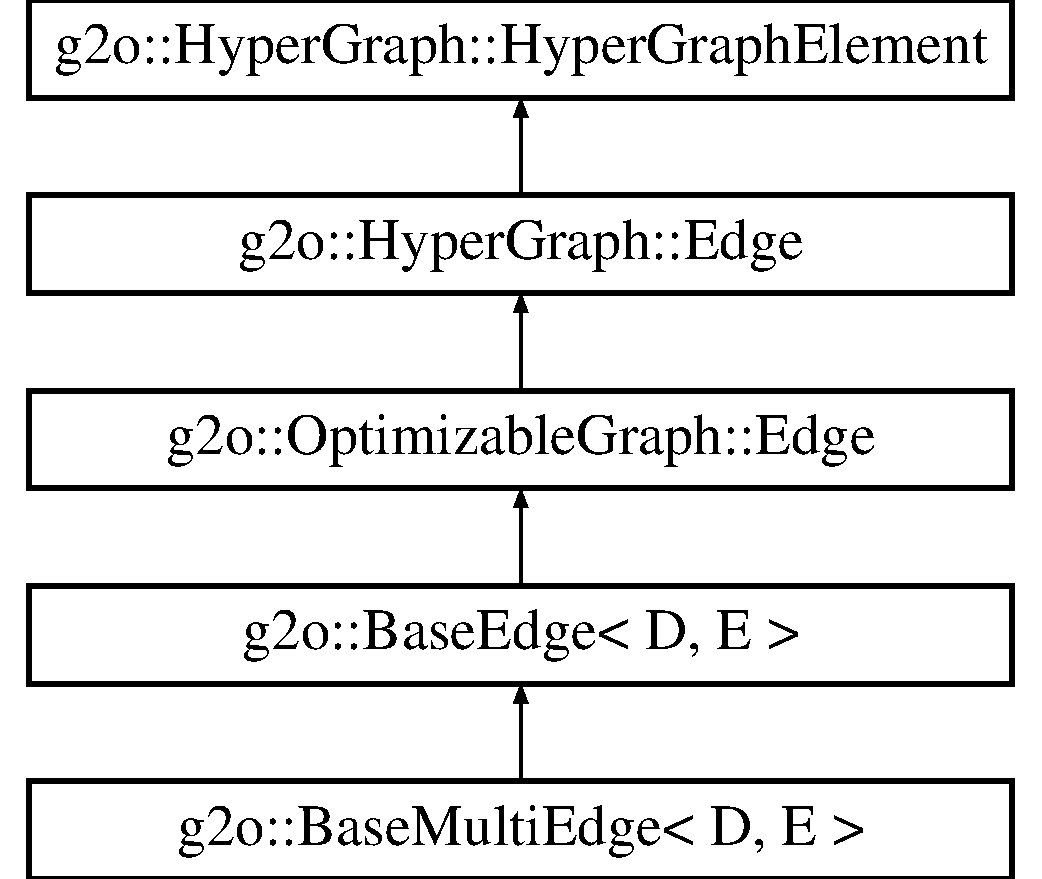
\includegraphics[height=5.000000cm]{classg2o_1_1_base_multi_edge}
\end{center}
\end{figure}
\subsection*{Classes}
\begin{DoxyCompactItemize}
\item 
struct \mbox{\hyperlink{structg2o_1_1_base_multi_edge_1_1_hessian_helper}{Hessian\+Helper}}
\begin{DoxyCompactList}\small\item\em helper for mapping the Hessian memory of the upper triangular block \end{DoxyCompactList}\end{DoxyCompactItemize}
\subsection*{Public Types}
\begin{DoxyCompactItemize}
\item 
typedef \mbox{\hyperlink{classg2o_1_1_base_edge}{Base\+Edge}}$<$ D, E $>$\+::\mbox{\hyperlink{classg2o_1_1_base_edge_a2c148abba650a20b8c7eed75d3e2211e}{Measurement}} \mbox{\hyperlink{classg2o_1_1_base_multi_edge_acbaff4c018fb314db5c7852054ffb89d}{Measurement}}
\item 
typedef Matrix\+Xd\+::\+Map\+Type \mbox{\hyperlink{classg2o_1_1_base_multi_edge_a43dfdf5b27df296a32ee5a11f0653d55}{Jacobian\+Type}}
\item 
typedef \mbox{\hyperlink{classg2o_1_1_base_edge}{Base\+Edge}}$<$ D, E $>$\+::\mbox{\hyperlink{classg2o_1_1_base_edge_af5b558dd24e4be2e437563cae4b3550d}{Error\+Vector}} \mbox{\hyperlink{classg2o_1_1_base_multi_edge_ae17c6b5747bfed295214942207a6eb74}{Error\+Vector}}
\item 
typedef \mbox{\hyperlink{classg2o_1_1_base_edge}{Base\+Edge}}$<$ D, E $>$\+::\mbox{\hyperlink{classg2o_1_1_base_edge_a2e5a33343ac3f189d8a7d5ee4d8b73fc}{Information\+Type}} \mbox{\hyperlink{classg2o_1_1_base_multi_edge_a368ab136a2cee049549cb479fb4c88fa}{Information\+Type}}
\item 
typedef Eigen\+::\+Map$<$ Matrix\+Xd, Matrix\+Xd\+::\+Flags \&Aligned\+Bit ? Aligned \+:Unaligned $>$ \mbox{\hyperlink{classg2o_1_1_base_multi_edge_af299cc8f77d917c1ad4a7d8004aec3a1}{Hessian\+Block\+Type}}
\end{DoxyCompactItemize}
\subsection*{Public Member Functions}
\begin{DoxyCompactItemize}
\item 
\mbox{\hyperlink{classg2o_1_1_base_multi_edge_a761d6a3623ed2c4ce6c6535f78dac08d}{Base\+Multi\+Edge}} ()
\item 
virtual void \mbox{\hyperlink{classg2o_1_1_base_multi_edge_a72176776797987b8ae79ea2e33971e9e}{linearize\+Oplus}} (\mbox{\hyperlink{classg2o_1_1_jacobian_workspace}{Jacobian\+Workspace}} \&jacobian\+Workspace)
\item 
virtual void \mbox{\hyperlink{classg2o_1_1_base_multi_edge_a6196a4cd1ddc2ef27c1474252bb60e9f}{linearize\+Oplus}} ()
\item 
virtual void \mbox{\hyperlink{classg2o_1_1_base_multi_edge_ae07ec9359cd515d0abc2100ee8aae93f}{resize}} (size\+\_\+t size)
\item 
virtual bool \mbox{\hyperlink{classg2o_1_1_base_multi_edge_a6e665877bd472839872077f5cc1ff2ec}{all\+Vertices\+Fixed}} () const
\item 
virtual void \mbox{\hyperlink{classg2o_1_1_base_multi_edge_ae44ba0385d4dda4bc038d81e50cadd8c}{construct\+Quadratic\+Form}} ()
\item 
virtual void \mbox{\hyperlink{classg2o_1_1_base_multi_edge_aecded66022b967fab0deb1c6a2d76445}{map\+Hessian\+Memory}} (double $\ast$d, int i, int j, bool row\+Major)
\end{DoxyCompactItemize}
\subsection*{Static Public Attributes}
\begin{DoxyCompactItemize}
\item 
static const int \mbox{\hyperlink{classg2o_1_1_base_multi_edge_a3c713fe8d1cd161f777625d8e2d5695d}{Dimension}} = \mbox{\hyperlink{classg2o_1_1_base_edge}{Base\+Edge}}$<$D,E$>$\+::Dimension
\end{DoxyCompactItemize}
\subsection*{Protected Member Functions}
\begin{DoxyCompactItemize}
\item 
void \mbox{\hyperlink{classg2o_1_1_base_multi_edge_ac260b65c12f6594165af680f815ac291}{compute\+Quadratic\+Form}} (const \mbox{\hyperlink{classg2o_1_1_base_edge_a2e5a33343ac3f189d8a7d5ee4d8b73fc}{Information\+Type}} \&omega, const \mbox{\hyperlink{classg2o_1_1_base_edge_af5b558dd24e4be2e437563cae4b3550d}{Error\+Vector}} \&weighted\+Error)
\end{DoxyCompactItemize}
\subsection*{Protected Attributes}
\begin{DoxyCompactItemize}
\item 
std\+::vector$<$ \mbox{\hyperlink{structg2o_1_1_base_multi_edge_1_1_hessian_helper}{Hessian\+Helper}} $>$ \mbox{\hyperlink{classg2o_1_1_base_multi_edge_af927d6f41bf73fc3b928cae2d6219d9e}{\+\_\+hessian}}
\item 
std\+::vector$<$ \mbox{\hyperlink{classg2o_1_1_base_multi_edge_a43dfdf5b27df296a32ee5a11f0653d55}{Jacobian\+Type}}, aligned\+\_\+allocator$<$ \mbox{\hyperlink{classg2o_1_1_base_multi_edge_a43dfdf5b27df296a32ee5a11f0653d55}{Jacobian\+Type}} $>$ $>$ \mbox{\hyperlink{classg2o_1_1_base_multi_edge_a00f8130e287bc945a8436375c4d07a02}{\+\_\+jacobian\+Oplus}}
\begin{DoxyCompactList}\small\item\em jacobians of the edge (w.\+r.\+t. oplus) \end{DoxyCompactList}\end{DoxyCompactItemize}


\subsection{Detailed Description}
\subsubsection*{template$<$int D, typename E$>$\newline
class g2o\+::\+Base\+Multi\+Edge$<$ D, E $>$}

base class to represent an edge connecting an arbitrary number of nodes 

D -\/ Dimension of the measurement E -\/ type to represent the measurement 

\subsection{Member Typedef Documentation}
\mbox{\Hypertarget{classg2o_1_1_base_multi_edge_ae17c6b5747bfed295214942207a6eb74}\label{classg2o_1_1_base_multi_edge_ae17c6b5747bfed295214942207a6eb74}} 
\index{g2o\+::\+Base\+Multi\+Edge@{g2o\+::\+Base\+Multi\+Edge}!Error\+Vector@{Error\+Vector}}
\index{Error\+Vector@{Error\+Vector}!g2o\+::\+Base\+Multi\+Edge@{g2o\+::\+Base\+Multi\+Edge}}
\subsubsection{\texorpdfstring{Error\+Vector}{ErrorVector}}
{\footnotesize\ttfamily template$<$int D, typename E $>$ \\
typedef \mbox{\hyperlink{classg2o_1_1_base_edge}{Base\+Edge}}$<$D,E$>$\+::\mbox{\hyperlink{classg2o_1_1_base_edge_af5b558dd24e4be2e437563cae4b3550d}{Error\+Vector}} \mbox{\hyperlink{classg2o_1_1_base_multi_edge}{g2o\+::\+Base\+Multi\+Edge}}$<$ D, E $>$\+::\mbox{\hyperlink{classg2o_1_1_base_edge_af5b558dd24e4be2e437563cae4b3550d}{Error\+Vector}}}

\mbox{\Hypertarget{classg2o_1_1_base_multi_edge_af299cc8f77d917c1ad4a7d8004aec3a1}\label{classg2o_1_1_base_multi_edge_af299cc8f77d917c1ad4a7d8004aec3a1}} 
\index{g2o\+::\+Base\+Multi\+Edge@{g2o\+::\+Base\+Multi\+Edge}!Hessian\+Block\+Type@{Hessian\+Block\+Type}}
\index{Hessian\+Block\+Type@{Hessian\+Block\+Type}!g2o\+::\+Base\+Multi\+Edge@{g2o\+::\+Base\+Multi\+Edge}}
\subsubsection{\texorpdfstring{Hessian\+Block\+Type}{HessianBlockType}}
{\footnotesize\ttfamily template$<$int D, typename E $>$ \\
typedef Eigen\+::\+Map$<$Matrix\+Xd, Matrix\+Xd\+::\+Flags \& Aligned\+Bit ? Aligned \+: Unaligned $>$ \mbox{\hyperlink{classg2o_1_1_base_multi_edge}{g2o\+::\+Base\+Multi\+Edge}}$<$ D, E $>$\+::\mbox{\hyperlink{classg2o_1_1_base_multi_edge_af299cc8f77d917c1ad4a7d8004aec3a1}{Hessian\+Block\+Type}}}

\mbox{\Hypertarget{classg2o_1_1_base_multi_edge_a368ab136a2cee049549cb479fb4c88fa}\label{classg2o_1_1_base_multi_edge_a368ab136a2cee049549cb479fb4c88fa}} 
\index{g2o\+::\+Base\+Multi\+Edge@{g2o\+::\+Base\+Multi\+Edge}!Information\+Type@{Information\+Type}}
\index{Information\+Type@{Information\+Type}!g2o\+::\+Base\+Multi\+Edge@{g2o\+::\+Base\+Multi\+Edge}}
\subsubsection{\texorpdfstring{Information\+Type}{InformationType}}
{\footnotesize\ttfamily template$<$int D, typename E $>$ \\
typedef \mbox{\hyperlink{classg2o_1_1_base_edge}{Base\+Edge}}$<$D,E$>$\+::\mbox{\hyperlink{classg2o_1_1_base_edge_a2e5a33343ac3f189d8a7d5ee4d8b73fc}{Information\+Type}} \mbox{\hyperlink{classg2o_1_1_base_multi_edge}{g2o\+::\+Base\+Multi\+Edge}}$<$ D, E $>$\+::\mbox{\hyperlink{classg2o_1_1_base_edge_a2e5a33343ac3f189d8a7d5ee4d8b73fc}{Information\+Type}}}

\mbox{\Hypertarget{classg2o_1_1_base_multi_edge_a43dfdf5b27df296a32ee5a11f0653d55}\label{classg2o_1_1_base_multi_edge_a43dfdf5b27df296a32ee5a11f0653d55}} 
\index{g2o\+::\+Base\+Multi\+Edge@{g2o\+::\+Base\+Multi\+Edge}!Jacobian\+Type@{Jacobian\+Type}}
\index{Jacobian\+Type@{Jacobian\+Type}!g2o\+::\+Base\+Multi\+Edge@{g2o\+::\+Base\+Multi\+Edge}}
\subsubsection{\texorpdfstring{Jacobian\+Type}{JacobianType}}
{\footnotesize\ttfamily template$<$int D, typename E $>$ \\
typedef Matrix\+Xd\+::\+Map\+Type \mbox{\hyperlink{classg2o_1_1_base_multi_edge}{g2o\+::\+Base\+Multi\+Edge}}$<$ D, E $>$\+::\mbox{\hyperlink{classg2o_1_1_base_multi_edge_a43dfdf5b27df296a32ee5a11f0653d55}{Jacobian\+Type}}}

\mbox{\Hypertarget{classg2o_1_1_base_multi_edge_acbaff4c018fb314db5c7852054ffb89d}\label{classg2o_1_1_base_multi_edge_acbaff4c018fb314db5c7852054ffb89d}} 
\index{g2o\+::\+Base\+Multi\+Edge@{g2o\+::\+Base\+Multi\+Edge}!Measurement@{Measurement}}
\index{Measurement@{Measurement}!g2o\+::\+Base\+Multi\+Edge@{g2o\+::\+Base\+Multi\+Edge}}
\subsubsection{\texorpdfstring{Measurement}{Measurement}}
{\footnotesize\ttfamily template$<$int D, typename E $>$ \\
typedef \mbox{\hyperlink{classg2o_1_1_base_edge}{Base\+Edge}}$<$D,E$>$\+::\mbox{\hyperlink{classg2o_1_1_base_edge_a2c148abba650a20b8c7eed75d3e2211e}{Measurement}} \mbox{\hyperlink{classg2o_1_1_base_multi_edge}{g2o\+::\+Base\+Multi\+Edge}}$<$ D, E $>$\+::\mbox{\hyperlink{classg2o_1_1_base_edge_a2c148abba650a20b8c7eed75d3e2211e}{Measurement}}}



\subsection{Constructor \& Destructor Documentation}
\mbox{\Hypertarget{classg2o_1_1_base_multi_edge_a761d6a3623ed2c4ce6c6535f78dac08d}\label{classg2o_1_1_base_multi_edge_a761d6a3623ed2c4ce6c6535f78dac08d}} 
\index{g2o\+::\+Base\+Multi\+Edge@{g2o\+::\+Base\+Multi\+Edge}!Base\+Multi\+Edge@{Base\+Multi\+Edge}}
\index{Base\+Multi\+Edge@{Base\+Multi\+Edge}!g2o\+::\+Base\+Multi\+Edge@{g2o\+::\+Base\+Multi\+Edge}}
\subsubsection{\texorpdfstring{Base\+Multi\+Edge()}{BaseMultiEdge()}}
{\footnotesize\ttfamily template$<$int D, typename E $>$ \\
\mbox{\hyperlink{classg2o_1_1_base_multi_edge}{g2o\+::\+Base\+Multi\+Edge}}$<$ D, E $>$\+::\mbox{\hyperlink{classg2o_1_1_base_multi_edge}{Base\+Multi\+Edge}} (\begin{DoxyParamCaption}{ }\end{DoxyParamCaption})\hspace{0.3cm}{\ttfamily [inline]}}



\subsection{Member Function Documentation}
\mbox{\Hypertarget{classg2o_1_1_base_multi_edge_a6e665877bd472839872077f5cc1ff2ec}\label{classg2o_1_1_base_multi_edge_a6e665877bd472839872077f5cc1ff2ec}} 
\index{g2o\+::\+Base\+Multi\+Edge@{g2o\+::\+Base\+Multi\+Edge}!all\+Vertices\+Fixed@{all\+Vertices\+Fixed}}
\index{all\+Vertices\+Fixed@{all\+Vertices\+Fixed}!g2o\+::\+Base\+Multi\+Edge@{g2o\+::\+Base\+Multi\+Edge}}
\subsubsection{\texorpdfstring{all\+Vertices\+Fixed()}{allVerticesFixed()}}
{\footnotesize\ttfamily template$<$int D, typename E $>$ \\
bool Base\+Multi\+Edge\+::all\+Vertices\+Fixed (\begin{DoxyParamCaption}{ }\end{DoxyParamCaption}) const\hspace{0.3cm}{\ttfamily [virtual]}}



Implements \mbox{\hyperlink{classg2o_1_1_optimizable_graph_1_1_edge_a414c69ca1617a4d3b620e39f2ffbcea7}{g2o\+::\+Optimizable\+Graph\+::\+Edge}}.

\mbox{\Hypertarget{classg2o_1_1_base_multi_edge_ac260b65c12f6594165af680f815ac291}\label{classg2o_1_1_base_multi_edge_ac260b65c12f6594165af680f815ac291}} 
\index{g2o\+::\+Base\+Multi\+Edge@{g2o\+::\+Base\+Multi\+Edge}!compute\+Quadratic\+Form@{compute\+Quadratic\+Form}}
\index{compute\+Quadratic\+Form@{compute\+Quadratic\+Form}!g2o\+::\+Base\+Multi\+Edge@{g2o\+::\+Base\+Multi\+Edge}}
\subsubsection{\texorpdfstring{compute\+Quadratic\+Form()}{computeQuadraticForm()}}
{\footnotesize\ttfamily template$<$int D, typename E $>$ \\
void Base\+Multi\+Edge\+::compute\+Quadratic\+Form (\begin{DoxyParamCaption}\item[{const \mbox{\hyperlink{classg2o_1_1_base_edge_a2e5a33343ac3f189d8a7d5ee4d8b73fc}{Information\+Type}} \&}]{omega,  }\item[{const \mbox{\hyperlink{classg2o_1_1_base_edge_af5b558dd24e4be2e437563cae4b3550d}{Error\+Vector}} \&}]{weighted\+Error }\end{DoxyParamCaption})\hspace{0.3cm}{\ttfamily [protected]}}

\mbox{\Hypertarget{classg2o_1_1_base_multi_edge_ae44ba0385d4dda4bc038d81e50cadd8c}\label{classg2o_1_1_base_multi_edge_ae44ba0385d4dda4bc038d81e50cadd8c}} 
\index{g2o\+::\+Base\+Multi\+Edge@{g2o\+::\+Base\+Multi\+Edge}!construct\+Quadratic\+Form@{construct\+Quadratic\+Form}}
\index{construct\+Quadratic\+Form@{construct\+Quadratic\+Form}!g2o\+::\+Base\+Multi\+Edge@{g2o\+::\+Base\+Multi\+Edge}}
\subsubsection{\texorpdfstring{construct\+Quadratic\+Form()}{constructQuadraticForm()}}
{\footnotesize\ttfamily template$<$int D, typename E $>$ \\
void Base\+Multi\+Edge\+::construct\+Quadratic\+Form (\begin{DoxyParamCaption}{ }\end{DoxyParamCaption})\hspace{0.3cm}{\ttfamily [virtual]}}

Linearizes the constraint in the edge. Makes side effect on the vertices of the graph by changing the parameter vector b and the hessian blocks ii and jj. The off diagoinal block is accesed via \+\_\+hessian. 

Implements \mbox{\hyperlink{classg2o_1_1_optimizable_graph_1_1_edge_a56fbf3430ddf591e3c619bdd1b7e4499}{g2o\+::\+Optimizable\+Graph\+::\+Edge}}.

\mbox{\Hypertarget{classg2o_1_1_base_multi_edge_a72176776797987b8ae79ea2e33971e9e}\label{classg2o_1_1_base_multi_edge_a72176776797987b8ae79ea2e33971e9e}} 
\index{g2o\+::\+Base\+Multi\+Edge@{g2o\+::\+Base\+Multi\+Edge}!linearize\+Oplus@{linearize\+Oplus}}
\index{linearize\+Oplus@{linearize\+Oplus}!g2o\+::\+Base\+Multi\+Edge@{g2o\+::\+Base\+Multi\+Edge}}
\subsubsection{\texorpdfstring{linearize\+Oplus()}{linearizeOplus()}\hspace{0.1cm}{\footnotesize\ttfamily [1/2]}}
{\footnotesize\ttfamily template$<$int D, typename E $>$ \\
void Base\+Multi\+Edge\+::linearize\+Oplus (\begin{DoxyParamCaption}\item[{\mbox{\hyperlink{classg2o_1_1_jacobian_workspace}{Jacobian\+Workspace}} \&}]{jacobian\+Workspace }\end{DoxyParamCaption})\hspace{0.3cm}{\ttfamily [virtual]}}

Linearizes the constraint in the edge in the manifold space, and store the result in the given workspace 

Implements \mbox{\hyperlink{classg2o_1_1_optimizable_graph_1_1_edge_a0fdad5ebfb4efec9f893b57f67e0fbe1}{g2o\+::\+Optimizable\+Graph\+::\+Edge}}.

\mbox{\Hypertarget{classg2o_1_1_base_multi_edge_a6196a4cd1ddc2ef27c1474252bb60e9f}\label{classg2o_1_1_base_multi_edge_a6196a4cd1ddc2ef27c1474252bb60e9f}} 
\index{g2o\+::\+Base\+Multi\+Edge@{g2o\+::\+Base\+Multi\+Edge}!linearize\+Oplus@{linearize\+Oplus}}
\index{linearize\+Oplus@{linearize\+Oplus}!g2o\+::\+Base\+Multi\+Edge@{g2o\+::\+Base\+Multi\+Edge}}
\subsubsection{\texorpdfstring{linearize\+Oplus()}{linearizeOplus()}\hspace{0.1cm}{\footnotesize\ttfamily [2/2]}}
{\footnotesize\ttfamily template$<$int D, typename E $>$ \\
void Base\+Multi\+Edge\+::linearize\+Oplus (\begin{DoxyParamCaption}{ }\end{DoxyParamCaption})\hspace{0.3cm}{\ttfamily [virtual]}}

Linearizes the oplus operator in the vertex, and stores the result in temporary variable vector \+\_\+jacobian\+Oplus \mbox{\Hypertarget{classg2o_1_1_base_multi_edge_aecded66022b967fab0deb1c6a2d76445}\label{classg2o_1_1_base_multi_edge_aecded66022b967fab0deb1c6a2d76445}} 
\index{g2o\+::\+Base\+Multi\+Edge@{g2o\+::\+Base\+Multi\+Edge}!map\+Hessian\+Memory@{map\+Hessian\+Memory}}
\index{map\+Hessian\+Memory@{map\+Hessian\+Memory}!g2o\+::\+Base\+Multi\+Edge@{g2o\+::\+Base\+Multi\+Edge}}
\subsubsection{\texorpdfstring{map\+Hessian\+Memory()}{mapHessianMemory()}}
{\footnotesize\ttfamily template$<$int D, typename E $>$ \\
void Base\+Multi\+Edge\+::map\+Hessian\+Memory (\begin{DoxyParamCaption}\item[{double $\ast$}]{d,  }\item[{int}]{i,  }\item[{int}]{j,  }\item[{bool}]{row\+Major }\end{DoxyParamCaption})\hspace{0.3cm}{\ttfamily [virtual]}}

maps the internal matrix to some external memory location, you need to provide the memory before calling construct\+Quadratic\+Form 
\begin{DoxyParams}{Parameters}
{\em d} & the memory location to which we map \\
\hline
{\em i} & index of the vertex i \\
\hline
{\em j} & index of the vertex j (j $>$ i, upper triangular fashion) \\
\hline
{\em row\+Major} & if true, will write in row\+Major order to the block. Since E\+I\+G\+EN is column\+Major by default, this results in writing the transposed \\
\hline
\end{DoxyParams}


Implements \mbox{\hyperlink{classg2o_1_1_optimizable_graph_1_1_edge_a3bd233fd552daa166039acf47b69a5a7}{g2o\+::\+Optimizable\+Graph\+::\+Edge}}.

\mbox{\Hypertarget{classg2o_1_1_base_multi_edge_ae07ec9359cd515d0abc2100ee8aae93f}\label{classg2o_1_1_base_multi_edge_ae07ec9359cd515d0abc2100ee8aae93f}} 
\index{g2o\+::\+Base\+Multi\+Edge@{g2o\+::\+Base\+Multi\+Edge}!resize@{resize}}
\index{resize@{resize}!g2o\+::\+Base\+Multi\+Edge@{g2o\+::\+Base\+Multi\+Edge}}
\subsubsection{\texorpdfstring{resize()}{resize()}}
{\footnotesize\ttfamily template$<$int D, typename E $>$ \\
void Base\+Multi\+Edge\+::resize (\begin{DoxyParamCaption}\item[{size\+\_\+t}]{size }\end{DoxyParamCaption})\hspace{0.3cm}{\ttfamily [virtual]}}

resizes the number of vertices connected by this edge 

Reimplemented from \mbox{\hyperlink{classg2o_1_1_hyper_graph_1_1_edge_ad8913f1149a0fd5bb628f0f1c8a91a55}{g2o\+::\+Hyper\+Graph\+::\+Edge}}.



\subsection{Member Data Documentation}
\mbox{\Hypertarget{classg2o_1_1_base_multi_edge_af927d6f41bf73fc3b928cae2d6219d9e}\label{classg2o_1_1_base_multi_edge_af927d6f41bf73fc3b928cae2d6219d9e}} 
\index{g2o\+::\+Base\+Multi\+Edge@{g2o\+::\+Base\+Multi\+Edge}!\+\_\+hessian@{\+\_\+hessian}}
\index{\+\_\+hessian@{\+\_\+hessian}!g2o\+::\+Base\+Multi\+Edge@{g2o\+::\+Base\+Multi\+Edge}}
\subsubsection{\texorpdfstring{\+\_\+hessian}{\_hessian}}
{\footnotesize\ttfamily template$<$int D, typename E $>$ \\
std\+::vector$<$\mbox{\hyperlink{structg2o_1_1_base_multi_edge_1_1_hessian_helper}{Hessian\+Helper}}$>$ \mbox{\hyperlink{classg2o_1_1_base_multi_edge}{g2o\+::\+Base\+Multi\+Edge}}$<$ D, E $>$\+::\+\_\+hessian\hspace{0.3cm}{\ttfamily [protected]}}

\mbox{\Hypertarget{classg2o_1_1_base_multi_edge_a00f8130e287bc945a8436375c4d07a02}\label{classg2o_1_1_base_multi_edge_a00f8130e287bc945a8436375c4d07a02}} 
\index{g2o\+::\+Base\+Multi\+Edge@{g2o\+::\+Base\+Multi\+Edge}!\+\_\+jacobian\+Oplus@{\+\_\+jacobian\+Oplus}}
\index{\+\_\+jacobian\+Oplus@{\+\_\+jacobian\+Oplus}!g2o\+::\+Base\+Multi\+Edge@{g2o\+::\+Base\+Multi\+Edge}}
\subsubsection{\texorpdfstring{\+\_\+jacobian\+Oplus}{\_jacobianOplus}}
{\footnotesize\ttfamily template$<$int D, typename E $>$ \\
std\+::vector$<$\mbox{\hyperlink{classg2o_1_1_base_multi_edge_a43dfdf5b27df296a32ee5a11f0653d55}{Jacobian\+Type}}, aligned\+\_\+allocator$<$\mbox{\hyperlink{classg2o_1_1_base_multi_edge_a43dfdf5b27df296a32ee5a11f0653d55}{Jacobian\+Type}}$>$ $>$ \mbox{\hyperlink{classg2o_1_1_base_multi_edge}{g2o\+::\+Base\+Multi\+Edge}}$<$ D, E $>$\+::\+\_\+jacobian\+Oplus\hspace{0.3cm}{\ttfamily [protected]}}



jacobians of the edge (w.\+r.\+t. oplus) 

\mbox{\Hypertarget{classg2o_1_1_base_multi_edge_a3c713fe8d1cd161f777625d8e2d5695d}\label{classg2o_1_1_base_multi_edge_a3c713fe8d1cd161f777625d8e2d5695d}} 
\index{g2o\+::\+Base\+Multi\+Edge@{g2o\+::\+Base\+Multi\+Edge}!Dimension@{Dimension}}
\index{Dimension@{Dimension}!g2o\+::\+Base\+Multi\+Edge@{g2o\+::\+Base\+Multi\+Edge}}
\subsubsection{\texorpdfstring{Dimension}{Dimension}}
{\footnotesize\ttfamily template$<$int D, typename E $>$ \\
const int \mbox{\hyperlink{classg2o_1_1_base_multi_edge}{g2o\+::\+Base\+Multi\+Edge}}$<$ D, E $>$\+::Dimension = \mbox{\hyperlink{classg2o_1_1_base_edge}{Base\+Edge}}$<$D,E$>$\+::Dimension\hspace{0.3cm}{\ttfamily [static]}}



The documentation for this class was generated from the following files\+:\begin{DoxyCompactItemize}
\item 
Thirdparty/g2o/g2o/core/\mbox{\hyperlink{base__multi__edge_8h}{base\+\_\+multi\+\_\+edge.\+h}}\item 
Thirdparty/g2o/g2o/core/\mbox{\hyperlink{base__multi__edge_8hpp}{base\+\_\+multi\+\_\+edge.\+hpp}}\end{DoxyCompactItemize}

\hypertarget{classg2o_1_1_base_property}{}\section{g2o\+:\+:Base\+Property Class Reference}
\label{classg2o_1_1_base_property}\index{g2o\+::\+Base\+Property@{g2o\+::\+Base\+Property}}


{\ttfamily \#include $<$property.\+h$>$}

Inheritance diagram for g2o\+:\+:Base\+Property\+:\begin{figure}[H]
\begin{center}
\leavevmode
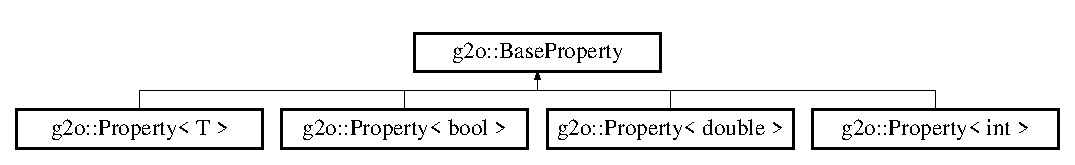
\includegraphics[height=1.772152cm]{classg2o_1_1_base_property}
\end{center}
\end{figure}
\subsection*{Public Member Functions}
\begin{DoxyCompactItemize}
\item 
\mbox{\hyperlink{classg2o_1_1_base_property_a00444ab7926d86beb9e66550e40e5d97}{Base\+Property}} (const std\+::string name\+\_\+)
\item 
virtual \mbox{\hyperlink{classg2o_1_1_base_property_acf2a5de9ce5781187fbf6be447918f39}{$\sim$\+Base\+Property}} ()
\item 
const std\+::string \& \mbox{\hyperlink{classg2o_1_1_base_property_aae91313b0eb376dd9460cd712ecbb86d}{name}} ()
\item 
virtual std\+::string \mbox{\hyperlink{classg2o_1_1_base_property_a7a4191088468c2f03dab52107d130833}{to\+String}} () const =0
\item 
virtual bool \mbox{\hyperlink{classg2o_1_1_base_property_aeabc313d9f66a403738aece884c85e1d}{from\+String}} (const std\+::string \&s)=0
\end{DoxyCompactItemize}
\subsection*{Protected Attributes}
\begin{DoxyCompactItemize}
\item 
std\+::string \mbox{\hyperlink{classg2o_1_1_base_property_a74e4bbf35ddf26022cb39be2ea7abd2b}{\+\_\+name}}
\end{DoxyCompactItemize}


\subsection{Constructor \& Destructor Documentation}
\mbox{\Hypertarget{classg2o_1_1_base_property_a00444ab7926d86beb9e66550e40e5d97}\label{classg2o_1_1_base_property_a00444ab7926d86beb9e66550e40e5d97}} 
\index{g2o\+::\+Base\+Property@{g2o\+::\+Base\+Property}!Base\+Property@{Base\+Property}}
\index{Base\+Property@{Base\+Property}!g2o\+::\+Base\+Property@{g2o\+::\+Base\+Property}}
\subsubsection{\texorpdfstring{Base\+Property()}{BaseProperty()}}
{\footnotesize\ttfamily g2o\+::\+Base\+Property\+::\+Base\+Property (\begin{DoxyParamCaption}\item[{const std\+::string}]{name\+\_\+ }\end{DoxyParamCaption})}

\mbox{\Hypertarget{classg2o_1_1_base_property_acf2a5de9ce5781187fbf6be447918f39}\label{classg2o_1_1_base_property_acf2a5de9ce5781187fbf6be447918f39}} 
\index{g2o\+::\+Base\+Property@{g2o\+::\+Base\+Property}!````~Base\+Property@{$\sim$\+Base\+Property}}
\index{````~Base\+Property@{$\sim$\+Base\+Property}!g2o\+::\+Base\+Property@{g2o\+::\+Base\+Property}}
\subsubsection{\texorpdfstring{$\sim$\+Base\+Property()}{~BaseProperty()}}
{\footnotesize\ttfamily g2o\+::\+Base\+Property\+::$\sim$\+Base\+Property (\begin{DoxyParamCaption}{ }\end{DoxyParamCaption})\hspace{0.3cm}{\ttfamily [virtual]}}



\subsection{Member Function Documentation}
\mbox{\Hypertarget{classg2o_1_1_base_property_aeabc313d9f66a403738aece884c85e1d}\label{classg2o_1_1_base_property_aeabc313d9f66a403738aece884c85e1d}} 
\index{g2o\+::\+Base\+Property@{g2o\+::\+Base\+Property}!from\+String@{from\+String}}
\index{from\+String@{from\+String}!g2o\+::\+Base\+Property@{g2o\+::\+Base\+Property}}
\subsubsection{\texorpdfstring{from\+String()}{fromString()}}
{\footnotesize\ttfamily virtual bool g2o\+::\+Base\+Property\+::from\+String (\begin{DoxyParamCaption}\item[{const std\+::string \&}]{s }\end{DoxyParamCaption})\hspace{0.3cm}{\ttfamily [pure virtual]}}



Implemented in \mbox{\hyperlink{classg2o_1_1_property_a5c0a6eacc67e98d4f0b3fd9fe856dbbe}{g2o\+::\+Property$<$ T $>$}}, \mbox{\hyperlink{classg2o_1_1_property_a5c0a6eacc67e98d4f0b3fd9fe856dbbe}{g2o\+::\+Property$<$ double $>$}}, \mbox{\hyperlink{classg2o_1_1_property_a5c0a6eacc67e98d4f0b3fd9fe856dbbe}{g2o\+::\+Property$<$ int $>$}}, and \mbox{\hyperlink{classg2o_1_1_property_a5c0a6eacc67e98d4f0b3fd9fe856dbbe}{g2o\+::\+Property$<$ bool $>$}}.

\mbox{\Hypertarget{classg2o_1_1_base_property_aae91313b0eb376dd9460cd712ecbb86d}\label{classg2o_1_1_base_property_aae91313b0eb376dd9460cd712ecbb86d}} 
\index{g2o\+::\+Base\+Property@{g2o\+::\+Base\+Property}!name@{name}}
\index{name@{name}!g2o\+::\+Base\+Property@{g2o\+::\+Base\+Property}}
\subsubsection{\texorpdfstring{name()}{name()}}
{\footnotesize\ttfamily const std\+::string\& g2o\+::\+Base\+Property\+::name (\begin{DoxyParamCaption}{ }\end{DoxyParamCaption})\hspace{0.3cm}{\ttfamily [inline]}}

\mbox{\Hypertarget{classg2o_1_1_base_property_a7a4191088468c2f03dab52107d130833}\label{classg2o_1_1_base_property_a7a4191088468c2f03dab52107d130833}} 
\index{g2o\+::\+Base\+Property@{g2o\+::\+Base\+Property}!to\+String@{to\+String}}
\index{to\+String@{to\+String}!g2o\+::\+Base\+Property@{g2o\+::\+Base\+Property}}
\subsubsection{\texorpdfstring{to\+String()}{toString()}}
{\footnotesize\ttfamily virtual std\+::string g2o\+::\+Base\+Property\+::to\+String (\begin{DoxyParamCaption}{ }\end{DoxyParamCaption}) const\hspace{0.3cm}{\ttfamily [pure virtual]}}



Implemented in \mbox{\hyperlink{classg2o_1_1_property_a8e3d3f2f79d274384588a1a5b9198cf5}{g2o\+::\+Property$<$ T $>$}}, \mbox{\hyperlink{classg2o_1_1_property_a8e3d3f2f79d274384588a1a5b9198cf5}{g2o\+::\+Property$<$ double $>$}}, \mbox{\hyperlink{classg2o_1_1_property_a8e3d3f2f79d274384588a1a5b9198cf5}{g2o\+::\+Property$<$ int $>$}}, and \mbox{\hyperlink{classg2o_1_1_property_a8e3d3f2f79d274384588a1a5b9198cf5}{g2o\+::\+Property$<$ bool $>$}}.



\subsection{Member Data Documentation}
\mbox{\Hypertarget{classg2o_1_1_base_property_a74e4bbf35ddf26022cb39be2ea7abd2b}\label{classg2o_1_1_base_property_a74e4bbf35ddf26022cb39be2ea7abd2b}} 
\index{g2o\+::\+Base\+Property@{g2o\+::\+Base\+Property}!\+\_\+name@{\+\_\+name}}
\index{\+\_\+name@{\+\_\+name}!g2o\+::\+Base\+Property@{g2o\+::\+Base\+Property}}
\subsubsection{\texorpdfstring{\+\_\+name}{\_name}}
{\footnotesize\ttfamily std\+::string g2o\+::\+Base\+Property\+::\+\_\+name\hspace{0.3cm}{\ttfamily [protected]}}



The documentation for this class was generated from the following files\+:\begin{DoxyCompactItemize}
\item 
Thirdparty/g2o/g2o/stuff/\mbox{\hyperlink{property_8h}{property.\+h}}\item 
Thirdparty/g2o/g2o/stuff/\mbox{\hyperlink{property_8cpp}{property.\+cpp}}\end{DoxyCompactItemize}

\hypertarget{classg2o_1_1_base_unary_edge}{}\section{g2o\+:\+:Base\+Unary\+Edge$<$ D, E, Vertex\+Xi $>$ Class Template Reference}
\label{classg2o_1_1_base_unary_edge}\index{g2o\+::\+Base\+Unary\+Edge$<$ D, E, Vertex\+Xi $>$@{g2o\+::\+Base\+Unary\+Edge$<$ D, E, Vertex\+Xi $>$}}


{\ttfamily \#include $<$base\+\_\+unary\+\_\+edge.\+h$>$}

Inheritance diagram for g2o\+:\+:Base\+Unary\+Edge$<$ D, E, Vertex\+Xi $>$\+:\begin{figure}[H]
\begin{center}
\leavevmode
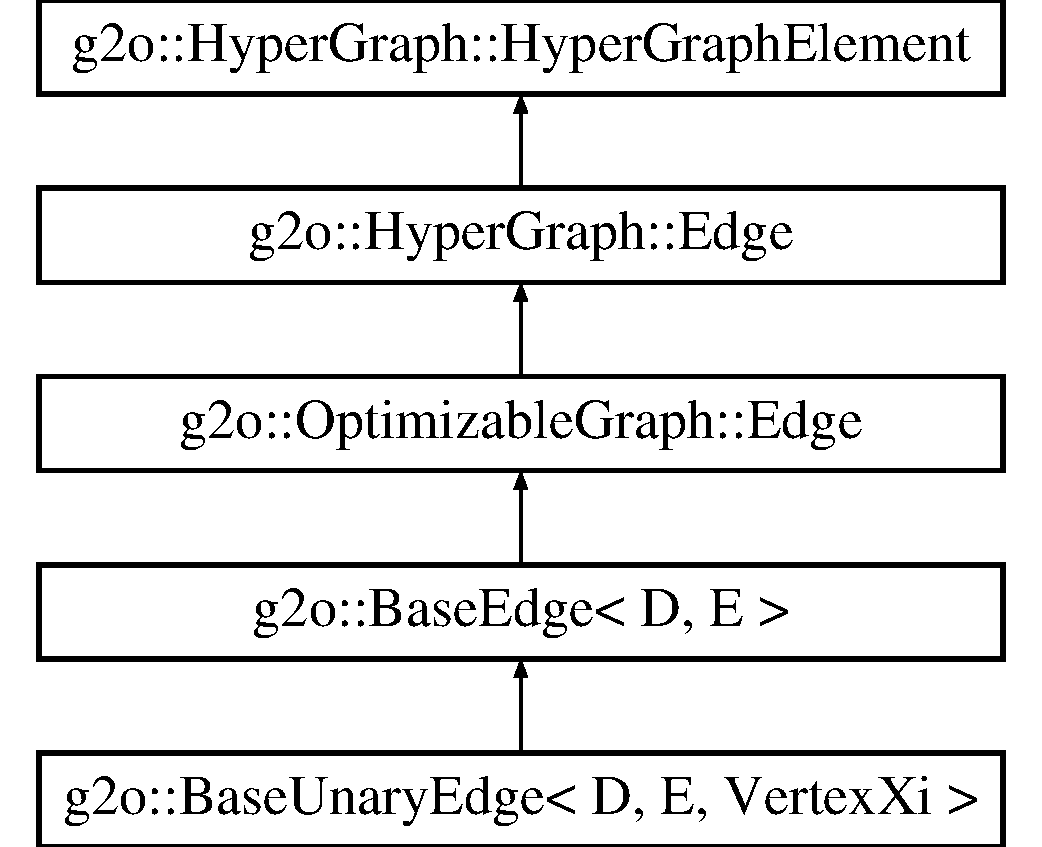
\includegraphics[height=5.000000cm]{classg2o_1_1_base_unary_edge}
\end{center}
\end{figure}
\subsection*{Public Types}
\begin{DoxyCompactItemize}
\item 
typedef \mbox{\hyperlink{classg2o_1_1_base_edge}{Base\+Edge}}$<$ D, E $>$\+::\mbox{\hyperlink{classg2o_1_1_base_edge_a2c148abba650a20b8c7eed75d3e2211e}{Measurement}} \mbox{\hyperlink{classg2o_1_1_base_unary_edge_ab953b076b4c35fcf99de02bd0bfcc1ae}{Measurement}}
\item 
typedef Vertex\+Xi \mbox{\hyperlink{classg2o_1_1_base_unary_edge_a503e62e74775172c008135650850d511}{Vertex\+Xi\+Type}}
\item 
typedef Matrix$<$ double, D, Vertex\+Xi\+Type\+::\+Dimension $>$\+::Aligned\+Map\+Type \mbox{\hyperlink{classg2o_1_1_base_unary_edge_a24bcabd661223e15b7337f2835310f5e}{Jacobian\+Xi\+Oplus\+Type}}
\item 
typedef \mbox{\hyperlink{classg2o_1_1_base_edge}{Base\+Edge}}$<$ D, E $>$\+::\mbox{\hyperlink{classg2o_1_1_base_edge_af5b558dd24e4be2e437563cae4b3550d}{Error\+Vector}} \mbox{\hyperlink{classg2o_1_1_base_unary_edge_abc04cfacb65fc72825156f1b3346dd48}{Error\+Vector}}
\item 
typedef \mbox{\hyperlink{classg2o_1_1_base_edge}{Base\+Edge}}$<$ D, E $>$\+::\mbox{\hyperlink{classg2o_1_1_base_edge_a2e5a33343ac3f189d8a7d5ee4d8b73fc}{Information\+Type}} \mbox{\hyperlink{classg2o_1_1_base_unary_edge_a6753caa95c30fa5bb3887e2a30892ff3}{Information\+Type}}
\end{DoxyCompactItemize}
\subsection*{Public Member Functions}
\begin{DoxyCompactItemize}
\item 
\mbox{\hyperlink{classg2o_1_1_base_unary_edge_a7375d1ebfb57ba0308f863739b817b15}{Base\+Unary\+Edge}} ()
\item 
virtual void \mbox{\hyperlink{classg2o_1_1_base_unary_edge_a01fcdfd2d3ed0325655bb99db95c0b10}{resize}} (size\+\_\+t size)
\item 
virtual bool \mbox{\hyperlink{classg2o_1_1_base_unary_edge_a4c5ec31144a266fb059b73b2387456c1}{all\+Vertices\+Fixed}} () const
\item 
virtual void \mbox{\hyperlink{classg2o_1_1_base_unary_edge_a8b396647b5b438d30a04758023baa595}{linearize\+Oplus}} (\mbox{\hyperlink{classg2o_1_1_jacobian_workspace}{Jacobian\+Workspace}} \&jacobian\+Workspace)
\item 
virtual void \mbox{\hyperlink{classg2o_1_1_base_unary_edge_a367f19b903938faf6e89dd1b0e4e722b}{linearize\+Oplus}} ()
\item 
const \mbox{\hyperlink{classg2o_1_1_base_unary_edge_a24bcabd661223e15b7337f2835310f5e}{Jacobian\+Xi\+Oplus\+Type}} \& \mbox{\hyperlink{classg2o_1_1_base_unary_edge_a396fbab83bfc9ce2e2080b16ccc357f4}{jacobian\+Oplus\+Xi}} () const
\begin{DoxyCompactList}\small\item\em returns the result of the linearization in the manifold space for the node xi \end{DoxyCompactList}\item 
virtual void \mbox{\hyperlink{classg2o_1_1_base_unary_edge_ad7e6dc44c571be159f066bdb961ade2b}{construct\+Quadratic\+Form}} ()
\item 
virtual void \mbox{\hyperlink{classg2o_1_1_base_unary_edge_a3d3311901116092cf817b094f6a0b44b}{initial\+Estimate}} (const \mbox{\hyperlink{classg2o_1_1_hyper_graph_a703938cdb4bb636860eed55a2489d70c}{Optimizable\+Graph\+::\+Vertex\+Set}} \&from, \mbox{\hyperlink{classg2o_1_1_optimizable_graph_1_1_vertex}{Optimizable\+Graph\+::\+Vertex}} $\ast$to)
\item 
virtual void \mbox{\hyperlink{classg2o_1_1_base_unary_edge_a919dcb89130f6e7082e807530facdd78}{map\+Hessian\+Memory}} (double $\ast$, int, int, bool)
\end{DoxyCompactItemize}
\subsection*{Static Public Attributes}
\begin{DoxyCompactItemize}
\item 
static const int \mbox{\hyperlink{classg2o_1_1_base_unary_edge_a4e584cf552998a34948d8d5b484f7fd3}{Dimension}} = \mbox{\hyperlink{classg2o_1_1_base_edge}{Base\+Edge}}$<$D, E$>$\+::Dimension
\end{DoxyCompactItemize}
\subsection*{Protected Attributes}
\begin{DoxyCompactItemize}
\item 
\mbox{\hyperlink{classg2o_1_1_base_unary_edge_a24bcabd661223e15b7337f2835310f5e}{Jacobian\+Xi\+Oplus\+Type}} \mbox{\hyperlink{classg2o_1_1_base_unary_edge_af7d022a6c6c9c29dfd9147fce0dc13d8}{\+\_\+jacobian\+Oplus\+Xi}}
\end{DoxyCompactItemize}
\subsection*{Additional Inherited Members}


\subsection{Member Typedef Documentation}
\mbox{\Hypertarget{classg2o_1_1_base_unary_edge_abc04cfacb65fc72825156f1b3346dd48}\label{classg2o_1_1_base_unary_edge_abc04cfacb65fc72825156f1b3346dd48}} 
\index{g2o\+::\+Base\+Unary\+Edge@{g2o\+::\+Base\+Unary\+Edge}!Error\+Vector@{Error\+Vector}}
\index{Error\+Vector@{Error\+Vector}!g2o\+::\+Base\+Unary\+Edge@{g2o\+::\+Base\+Unary\+Edge}}
\subsubsection{\texorpdfstring{Error\+Vector}{ErrorVector}}
{\footnotesize\ttfamily template$<$int D, typename E, typename Vertex\+Xi$>$ \\
typedef \mbox{\hyperlink{classg2o_1_1_base_edge}{Base\+Edge}}$<$D,E$>$\+::\mbox{\hyperlink{classg2o_1_1_base_edge_af5b558dd24e4be2e437563cae4b3550d}{Error\+Vector}} \mbox{\hyperlink{classg2o_1_1_base_unary_edge}{g2o\+::\+Base\+Unary\+Edge}}$<$ D, E, Vertex\+Xi $>$\+::\mbox{\hyperlink{classg2o_1_1_base_edge_af5b558dd24e4be2e437563cae4b3550d}{Error\+Vector}}}

\mbox{\Hypertarget{classg2o_1_1_base_unary_edge_a6753caa95c30fa5bb3887e2a30892ff3}\label{classg2o_1_1_base_unary_edge_a6753caa95c30fa5bb3887e2a30892ff3}} 
\index{g2o\+::\+Base\+Unary\+Edge@{g2o\+::\+Base\+Unary\+Edge}!Information\+Type@{Information\+Type}}
\index{Information\+Type@{Information\+Type}!g2o\+::\+Base\+Unary\+Edge@{g2o\+::\+Base\+Unary\+Edge}}
\subsubsection{\texorpdfstring{Information\+Type}{InformationType}}
{\footnotesize\ttfamily template$<$int D, typename E, typename Vertex\+Xi$>$ \\
typedef \mbox{\hyperlink{classg2o_1_1_base_edge}{Base\+Edge}}$<$D,E$>$\+::\mbox{\hyperlink{classg2o_1_1_base_edge_a2e5a33343ac3f189d8a7d5ee4d8b73fc}{Information\+Type}} \mbox{\hyperlink{classg2o_1_1_base_unary_edge}{g2o\+::\+Base\+Unary\+Edge}}$<$ D, E, Vertex\+Xi $>$\+::\mbox{\hyperlink{classg2o_1_1_base_edge_a2e5a33343ac3f189d8a7d5ee4d8b73fc}{Information\+Type}}}

\mbox{\Hypertarget{classg2o_1_1_base_unary_edge_a24bcabd661223e15b7337f2835310f5e}\label{classg2o_1_1_base_unary_edge_a24bcabd661223e15b7337f2835310f5e}} 
\index{g2o\+::\+Base\+Unary\+Edge@{g2o\+::\+Base\+Unary\+Edge}!Jacobian\+Xi\+Oplus\+Type@{Jacobian\+Xi\+Oplus\+Type}}
\index{Jacobian\+Xi\+Oplus\+Type@{Jacobian\+Xi\+Oplus\+Type}!g2o\+::\+Base\+Unary\+Edge@{g2o\+::\+Base\+Unary\+Edge}}
\subsubsection{\texorpdfstring{Jacobian\+Xi\+Oplus\+Type}{JacobianXiOplusType}}
{\footnotesize\ttfamily template$<$int D, typename E, typename Vertex\+Xi$>$ \\
typedef Matrix$<$double, D, Vertex\+Xi\+Type\+::\+Dimension$>$\+::Aligned\+Map\+Type \mbox{\hyperlink{classg2o_1_1_base_unary_edge}{g2o\+::\+Base\+Unary\+Edge}}$<$ D, E, Vertex\+Xi $>$\+::\mbox{\hyperlink{classg2o_1_1_base_unary_edge_a24bcabd661223e15b7337f2835310f5e}{Jacobian\+Xi\+Oplus\+Type}}}

\mbox{\Hypertarget{classg2o_1_1_base_unary_edge_ab953b076b4c35fcf99de02bd0bfcc1ae}\label{classg2o_1_1_base_unary_edge_ab953b076b4c35fcf99de02bd0bfcc1ae}} 
\index{g2o\+::\+Base\+Unary\+Edge@{g2o\+::\+Base\+Unary\+Edge}!Measurement@{Measurement}}
\index{Measurement@{Measurement}!g2o\+::\+Base\+Unary\+Edge@{g2o\+::\+Base\+Unary\+Edge}}
\subsubsection{\texorpdfstring{Measurement}{Measurement}}
{\footnotesize\ttfamily template$<$int D, typename E, typename Vertex\+Xi$>$ \\
typedef \mbox{\hyperlink{classg2o_1_1_base_edge}{Base\+Edge}}$<$D,E$>$\+::\mbox{\hyperlink{classg2o_1_1_base_edge_a2c148abba650a20b8c7eed75d3e2211e}{Measurement}} \mbox{\hyperlink{classg2o_1_1_base_unary_edge}{g2o\+::\+Base\+Unary\+Edge}}$<$ D, E, Vertex\+Xi $>$\+::\mbox{\hyperlink{classg2o_1_1_base_edge_a2c148abba650a20b8c7eed75d3e2211e}{Measurement}}}

\mbox{\Hypertarget{classg2o_1_1_base_unary_edge_a503e62e74775172c008135650850d511}\label{classg2o_1_1_base_unary_edge_a503e62e74775172c008135650850d511}} 
\index{g2o\+::\+Base\+Unary\+Edge@{g2o\+::\+Base\+Unary\+Edge}!Vertex\+Xi\+Type@{Vertex\+Xi\+Type}}
\index{Vertex\+Xi\+Type@{Vertex\+Xi\+Type}!g2o\+::\+Base\+Unary\+Edge@{g2o\+::\+Base\+Unary\+Edge}}
\subsubsection{\texorpdfstring{Vertex\+Xi\+Type}{VertexXiType}}
{\footnotesize\ttfamily template$<$int D, typename E, typename Vertex\+Xi$>$ \\
typedef Vertex\+Xi \mbox{\hyperlink{classg2o_1_1_base_unary_edge}{g2o\+::\+Base\+Unary\+Edge}}$<$ D, E, Vertex\+Xi $>$\+::\mbox{\hyperlink{classg2o_1_1_base_unary_edge_a503e62e74775172c008135650850d511}{Vertex\+Xi\+Type}}}



\subsection{Constructor \& Destructor Documentation}
\mbox{\Hypertarget{classg2o_1_1_base_unary_edge_a7375d1ebfb57ba0308f863739b817b15}\label{classg2o_1_1_base_unary_edge_a7375d1ebfb57ba0308f863739b817b15}} 
\index{g2o\+::\+Base\+Unary\+Edge@{g2o\+::\+Base\+Unary\+Edge}!Base\+Unary\+Edge@{Base\+Unary\+Edge}}
\index{Base\+Unary\+Edge@{Base\+Unary\+Edge}!g2o\+::\+Base\+Unary\+Edge@{g2o\+::\+Base\+Unary\+Edge}}
\subsubsection{\texorpdfstring{Base\+Unary\+Edge()}{BaseUnaryEdge()}}
{\footnotesize\ttfamily template$<$int D, typename E, typename Vertex\+Xi$>$ \\
\mbox{\hyperlink{classg2o_1_1_base_unary_edge}{g2o\+::\+Base\+Unary\+Edge}}$<$ D, E, Vertex\+Xi $>$\+::\mbox{\hyperlink{classg2o_1_1_base_unary_edge}{Base\+Unary\+Edge}} (\begin{DoxyParamCaption}{ }\end{DoxyParamCaption})\hspace{0.3cm}{\ttfamily [inline]}}



\subsection{Member Function Documentation}
\mbox{\Hypertarget{classg2o_1_1_base_unary_edge_a4c5ec31144a266fb059b73b2387456c1}\label{classg2o_1_1_base_unary_edge_a4c5ec31144a266fb059b73b2387456c1}} 
\index{g2o\+::\+Base\+Unary\+Edge@{g2o\+::\+Base\+Unary\+Edge}!all\+Vertices\+Fixed@{all\+Vertices\+Fixed}}
\index{all\+Vertices\+Fixed@{all\+Vertices\+Fixed}!g2o\+::\+Base\+Unary\+Edge@{g2o\+::\+Base\+Unary\+Edge}}
\subsubsection{\texorpdfstring{all\+Vertices\+Fixed()}{allVerticesFixed()}}
{\footnotesize\ttfamily template$<$int D, typename E , typename Vertex\+Xi\+Type $>$ \\
bool Base\+Unary\+Edge\+::all\+Vertices\+Fixed (\begin{DoxyParamCaption}{ }\end{DoxyParamCaption}) const\hspace{0.3cm}{\ttfamily [virtual]}}



Implements \mbox{\hyperlink{classg2o_1_1_optimizable_graph_1_1_edge_a414c69ca1617a4d3b620e39f2ffbcea7}{g2o\+::\+Optimizable\+Graph\+::\+Edge}}.

\mbox{\Hypertarget{classg2o_1_1_base_unary_edge_ad7e6dc44c571be159f066bdb961ade2b}\label{classg2o_1_1_base_unary_edge_ad7e6dc44c571be159f066bdb961ade2b}} 
\index{g2o\+::\+Base\+Unary\+Edge@{g2o\+::\+Base\+Unary\+Edge}!construct\+Quadratic\+Form@{construct\+Quadratic\+Form}}
\index{construct\+Quadratic\+Form@{construct\+Quadratic\+Form}!g2o\+::\+Base\+Unary\+Edge@{g2o\+::\+Base\+Unary\+Edge}}
\subsubsection{\texorpdfstring{construct\+Quadratic\+Form()}{constructQuadraticForm()}}
{\footnotesize\ttfamily template$<$int D, typename E , typename Vertex\+Xi\+Type $>$ \\
void Base\+Unary\+Edge\+::construct\+Quadratic\+Form (\begin{DoxyParamCaption}{ }\end{DoxyParamCaption})\hspace{0.3cm}{\ttfamily [virtual]}}

Linearizes the constraint in the edge. Makes side effect on the vertices of the graph by changing the parameter vector b and the hessian blocks ii and jj. The off diagoinal block is accesed via \+\_\+hessian. 

Implements \mbox{\hyperlink{classg2o_1_1_optimizable_graph_1_1_edge_a56fbf3430ddf591e3c619bdd1b7e4499}{g2o\+::\+Optimizable\+Graph\+::\+Edge}}.

\mbox{\Hypertarget{classg2o_1_1_base_unary_edge_a3d3311901116092cf817b094f6a0b44b}\label{classg2o_1_1_base_unary_edge_a3d3311901116092cf817b094f6a0b44b}} 
\index{g2o\+::\+Base\+Unary\+Edge@{g2o\+::\+Base\+Unary\+Edge}!initial\+Estimate@{initial\+Estimate}}
\index{initial\+Estimate@{initial\+Estimate}!g2o\+::\+Base\+Unary\+Edge@{g2o\+::\+Base\+Unary\+Edge}}
\subsubsection{\texorpdfstring{initial\+Estimate()}{initialEstimate()}}
{\footnotesize\ttfamily template$<$int D, typename E , typename Vertex\+Xi\+Type $>$ \\
void Base\+Unary\+Edge\+::initial\+Estimate (\begin{DoxyParamCaption}\item[{const \mbox{\hyperlink{classg2o_1_1_hyper_graph_a703938cdb4bb636860eed55a2489d70c}{Optimizable\+Graph\+::\+Vertex\+Set}} \&}]{from,  }\item[{\mbox{\hyperlink{classg2o_1_1_optimizable_graph_1_1_vertex}{Optimizable\+Graph\+::\+Vertex}} $\ast$}]{to }\end{DoxyParamCaption})\hspace{0.3cm}{\ttfamily [virtual]}}

set the estimate of the to vertex, based on the estimate of the from vertices in the edge. 

Reimplemented from \mbox{\hyperlink{classg2o_1_1_base_edge_a0c3d9763f1dc504627df75e0f381ca70}{g2o\+::\+Base\+Edge$<$ D, E $>$}}.

\mbox{\Hypertarget{classg2o_1_1_base_unary_edge_a396fbab83bfc9ce2e2080b16ccc357f4}\label{classg2o_1_1_base_unary_edge_a396fbab83bfc9ce2e2080b16ccc357f4}} 
\index{g2o\+::\+Base\+Unary\+Edge@{g2o\+::\+Base\+Unary\+Edge}!jacobian\+Oplus\+Xi@{jacobian\+Oplus\+Xi}}
\index{jacobian\+Oplus\+Xi@{jacobian\+Oplus\+Xi}!g2o\+::\+Base\+Unary\+Edge@{g2o\+::\+Base\+Unary\+Edge}}
\subsubsection{\texorpdfstring{jacobian\+Oplus\+Xi()}{jacobianOplusXi()}}
{\footnotesize\ttfamily template$<$int D, typename E, typename Vertex\+Xi$>$ \\
const \mbox{\hyperlink{classg2o_1_1_base_unary_edge_a24bcabd661223e15b7337f2835310f5e}{Jacobian\+Xi\+Oplus\+Type}}\& \mbox{\hyperlink{classg2o_1_1_base_unary_edge}{g2o\+::\+Base\+Unary\+Edge}}$<$ D, E, Vertex\+Xi $>$\+::jacobian\+Oplus\+Xi (\begin{DoxyParamCaption}{ }\end{DoxyParamCaption}) const\hspace{0.3cm}{\ttfamily [inline]}}



returns the result of the linearization in the manifold space for the node xi 

\mbox{\Hypertarget{classg2o_1_1_base_unary_edge_a8b396647b5b438d30a04758023baa595}\label{classg2o_1_1_base_unary_edge_a8b396647b5b438d30a04758023baa595}} 
\index{g2o\+::\+Base\+Unary\+Edge@{g2o\+::\+Base\+Unary\+Edge}!linearize\+Oplus@{linearize\+Oplus}}
\index{linearize\+Oplus@{linearize\+Oplus}!g2o\+::\+Base\+Unary\+Edge@{g2o\+::\+Base\+Unary\+Edge}}
\subsubsection{\texorpdfstring{linearize\+Oplus()}{linearizeOplus()}\hspace{0.1cm}{\footnotesize\ttfamily [1/2]}}
{\footnotesize\ttfamily template$<$int D, typename E , typename Vertex\+Xi\+Type $>$ \\
void Base\+Unary\+Edge\+::linearize\+Oplus (\begin{DoxyParamCaption}\item[{\mbox{\hyperlink{classg2o_1_1_jacobian_workspace}{Jacobian\+Workspace}} \&}]{jacobian\+Workspace }\end{DoxyParamCaption})\hspace{0.3cm}{\ttfamily [virtual]}}

Linearizes the constraint in the edge in the manifold space, and store the result in the given workspace 

Implements \mbox{\hyperlink{classg2o_1_1_optimizable_graph_1_1_edge_a0fdad5ebfb4efec9f893b57f67e0fbe1}{g2o\+::\+Optimizable\+Graph\+::\+Edge}}.

\mbox{\Hypertarget{classg2o_1_1_base_unary_edge_a367f19b903938faf6e89dd1b0e4e722b}\label{classg2o_1_1_base_unary_edge_a367f19b903938faf6e89dd1b0e4e722b}} 
\index{g2o\+::\+Base\+Unary\+Edge@{g2o\+::\+Base\+Unary\+Edge}!linearize\+Oplus@{linearize\+Oplus}}
\index{linearize\+Oplus@{linearize\+Oplus}!g2o\+::\+Base\+Unary\+Edge@{g2o\+::\+Base\+Unary\+Edge}}
\subsubsection{\texorpdfstring{linearize\+Oplus()}{linearizeOplus()}\hspace{0.1cm}{\footnotesize\ttfamily [2/2]}}
{\footnotesize\ttfamily template$<$int D, typename E , typename Vertex\+Xi\+Type $>$ \\
void Base\+Unary\+Edge\+::linearize\+Oplus (\begin{DoxyParamCaption}{ }\end{DoxyParamCaption})\hspace{0.3cm}{\ttfamily [virtual]}}

Linearizes the oplus operator in the vertex, and stores the result in temporary variables \+\_\+jacobian\+Oplus\+Xi and \+\_\+jacobian\+Oplus\+Xj 

Reimplemented in \mbox{\hyperlink{classg2o_1_1_edge_stereo_s_e3_project_x_y_z_only_pose_a0b2b815e8ae331276f33be374dcc1897}{g2o\+::\+Edge\+Stereo\+S\+E3\+Project\+X\+Y\+Z\+Only\+Pose}}, and \mbox{\hyperlink{classg2o_1_1_edge_s_e3_project_x_y_z_only_pose_abe6d775aade1277786274c328aa2c38b}{g2o\+::\+Edge\+S\+E3\+Project\+X\+Y\+Z\+Only\+Pose}}.

\mbox{\Hypertarget{classg2o_1_1_base_unary_edge_a919dcb89130f6e7082e807530facdd78}\label{classg2o_1_1_base_unary_edge_a919dcb89130f6e7082e807530facdd78}} 
\index{g2o\+::\+Base\+Unary\+Edge@{g2o\+::\+Base\+Unary\+Edge}!map\+Hessian\+Memory@{map\+Hessian\+Memory}}
\index{map\+Hessian\+Memory@{map\+Hessian\+Memory}!g2o\+::\+Base\+Unary\+Edge@{g2o\+::\+Base\+Unary\+Edge}}
\subsubsection{\texorpdfstring{map\+Hessian\+Memory()}{mapHessianMemory()}}
{\footnotesize\ttfamily template$<$int D, typename E, typename Vertex\+Xi$>$ \\
virtual void \mbox{\hyperlink{classg2o_1_1_base_unary_edge}{g2o\+::\+Base\+Unary\+Edge}}$<$ D, E, Vertex\+Xi $>$\+::map\+Hessian\+Memory (\begin{DoxyParamCaption}\item[{double $\ast$}]{d,  }\item[{int}]{i,  }\item[{int}]{j,  }\item[{bool}]{row\+Major }\end{DoxyParamCaption})\hspace{0.3cm}{\ttfamily [inline]}, {\ttfamily [virtual]}}

maps the internal matrix to some external memory location, you need to provide the memory before calling construct\+Quadratic\+Form 
\begin{DoxyParams}{Parameters}
{\em d} & the memory location to which we map \\
\hline
{\em i} & index of the vertex i \\
\hline
{\em j} & index of the vertex j (j $>$ i, upper triangular fashion) \\
\hline
{\em row\+Major} & if true, will write in row\+Major order to the block. Since E\+I\+G\+EN is column\+Major by default, this results in writing the transposed \\
\hline
\end{DoxyParams}


Implements \mbox{\hyperlink{classg2o_1_1_optimizable_graph_1_1_edge_a3bd233fd552daa166039acf47b69a5a7}{g2o\+::\+Optimizable\+Graph\+::\+Edge}}.

\mbox{\Hypertarget{classg2o_1_1_base_unary_edge_a01fcdfd2d3ed0325655bb99db95c0b10}\label{classg2o_1_1_base_unary_edge_a01fcdfd2d3ed0325655bb99db95c0b10}} 
\index{g2o\+::\+Base\+Unary\+Edge@{g2o\+::\+Base\+Unary\+Edge}!resize@{resize}}
\index{resize@{resize}!g2o\+::\+Base\+Unary\+Edge@{g2o\+::\+Base\+Unary\+Edge}}
\subsubsection{\texorpdfstring{resize()}{resize()}}
{\footnotesize\ttfamily template$<$int D, typename E , typename Vertex\+Xi\+Type $>$ \\
void Base\+Unary\+Edge\+::resize (\begin{DoxyParamCaption}\item[{size\+\_\+t}]{size }\end{DoxyParamCaption})\hspace{0.3cm}{\ttfamily [virtual]}}

resizes the number of vertices connected by this edge 

Reimplemented from \mbox{\hyperlink{classg2o_1_1_hyper_graph_1_1_edge_ad8913f1149a0fd5bb628f0f1c8a91a55}{g2o\+::\+Hyper\+Graph\+::\+Edge}}.



\subsection{Member Data Documentation}
\mbox{\Hypertarget{classg2o_1_1_base_unary_edge_af7d022a6c6c9c29dfd9147fce0dc13d8}\label{classg2o_1_1_base_unary_edge_af7d022a6c6c9c29dfd9147fce0dc13d8}} 
\index{g2o\+::\+Base\+Unary\+Edge@{g2o\+::\+Base\+Unary\+Edge}!\+\_\+jacobian\+Oplus\+Xi@{\+\_\+jacobian\+Oplus\+Xi}}
\index{\+\_\+jacobian\+Oplus\+Xi@{\+\_\+jacobian\+Oplus\+Xi}!g2o\+::\+Base\+Unary\+Edge@{g2o\+::\+Base\+Unary\+Edge}}
\subsubsection{\texorpdfstring{\+\_\+jacobian\+Oplus\+Xi}{\_jacobianOplusXi}}
{\footnotesize\ttfamily template$<$int D, typename E, typename Vertex\+Xi$>$ \\
\mbox{\hyperlink{classg2o_1_1_base_unary_edge_a24bcabd661223e15b7337f2835310f5e}{Jacobian\+Xi\+Oplus\+Type}} \mbox{\hyperlink{classg2o_1_1_base_unary_edge}{g2o\+::\+Base\+Unary\+Edge}}$<$ D, E, Vertex\+Xi $>$\+::\+\_\+jacobian\+Oplus\+Xi\hspace{0.3cm}{\ttfamily [protected]}}

\mbox{\Hypertarget{classg2o_1_1_base_unary_edge_a4e584cf552998a34948d8d5b484f7fd3}\label{classg2o_1_1_base_unary_edge_a4e584cf552998a34948d8d5b484f7fd3}} 
\index{g2o\+::\+Base\+Unary\+Edge@{g2o\+::\+Base\+Unary\+Edge}!Dimension@{Dimension}}
\index{Dimension@{Dimension}!g2o\+::\+Base\+Unary\+Edge@{g2o\+::\+Base\+Unary\+Edge}}
\subsubsection{\texorpdfstring{Dimension}{Dimension}}
{\footnotesize\ttfamily template$<$int D, typename E, typename Vertex\+Xi$>$ \\
const int \mbox{\hyperlink{classg2o_1_1_base_unary_edge}{g2o\+::\+Base\+Unary\+Edge}}$<$ D, E, Vertex\+Xi $>$\+::Dimension = \mbox{\hyperlink{classg2o_1_1_base_edge}{Base\+Edge}}$<$D, E$>$\+::Dimension\hspace{0.3cm}{\ttfamily [static]}}



The documentation for this class was generated from the following files\+:\begin{DoxyCompactItemize}
\item 
Thirdparty/g2o/g2o/core/\mbox{\hyperlink{base__unary__edge_8h}{base\+\_\+unary\+\_\+edge.\+h}}\item 
Thirdparty/g2o/g2o/core/\mbox{\hyperlink{base__unary__edge_8hpp}{base\+\_\+unary\+\_\+edge.\+hpp}}\end{DoxyCompactItemize}

\hypertarget{classg2o_1_1_base_vertex}{}\section{g2o\+:\+:Base\+Vertex$<$ D, T $>$ Class Template Reference}
\label{classg2o_1_1_base_vertex}\index{g2o\+::\+Base\+Vertex$<$ D, T $>$@{g2o\+::\+Base\+Vertex$<$ D, T $>$}}


Templatized \mbox{\hyperlink{classg2o_1_1_base_vertex}{Base\+Vertex}}.  




{\ttfamily \#include $<$base\+\_\+vertex.\+h$>$}

Inheritance diagram for g2o\+:\+:Base\+Vertex$<$ D, T $>$\+:\begin{figure}[H]
\begin{center}
\leavevmode
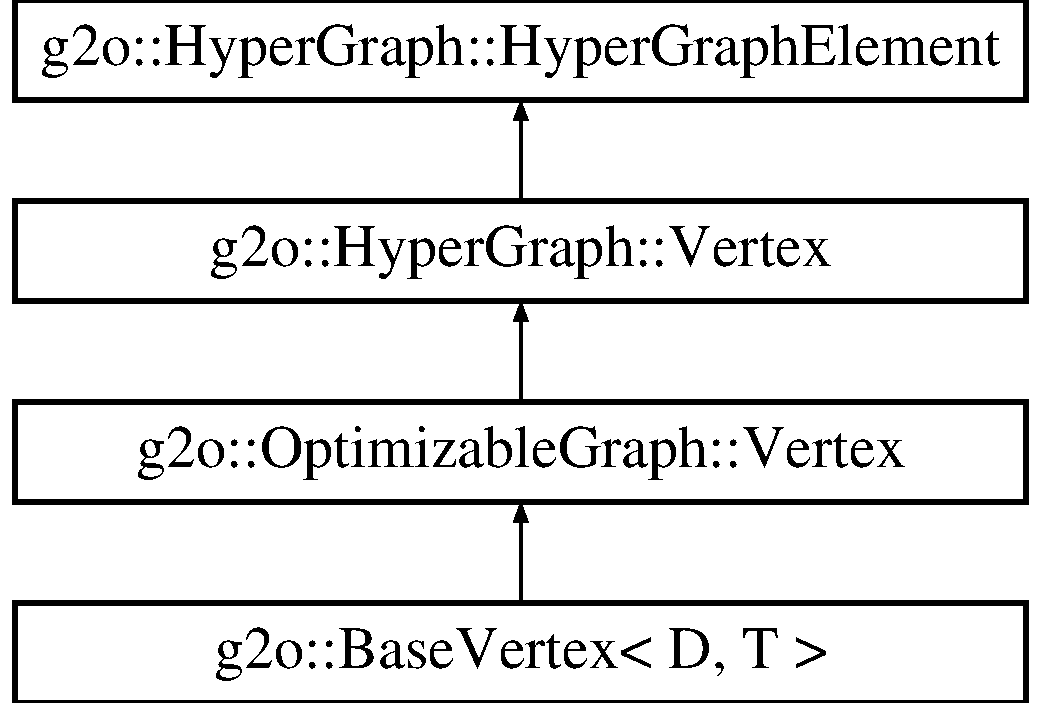
\includegraphics[height=4.000000cm]{classg2o_1_1_base_vertex}
\end{center}
\end{figure}
\subsection*{Public Types}
\begin{DoxyCompactItemize}
\item 
typedef T \mbox{\hyperlink{classg2o_1_1_base_vertex_aaffb179a0d591da4769ec7c3fc7f7daa}{Estimate\+Type}}
\item 
typedef std\+::stack$<$ \mbox{\hyperlink{classg2o_1_1_base_vertex_aaffb179a0d591da4769ec7c3fc7f7daa}{Estimate\+Type}}, std\+::vector$<$ \mbox{\hyperlink{classg2o_1_1_base_vertex_aaffb179a0d591da4769ec7c3fc7f7daa}{Estimate\+Type}}, Eigen\+::aligned\+\_\+allocator$<$ \mbox{\hyperlink{classg2o_1_1_base_vertex_aaffb179a0d591da4769ec7c3fc7f7daa}{Estimate\+Type}} $>$ $>$ $>$ \mbox{\hyperlink{classg2o_1_1_base_vertex_ae6632291d46b458196bdb021a6c8cba1}{Backup\+Stack\+Type}}
\item 
typedef Eigen\+::\+Map$<$ Matrix$<$ double, D, D $>$, Matrix$<$ double, D, D $>$\+::Flags \&Aligned\+Bit ? Aligned \+:Unaligned $>$ \mbox{\hyperlink{classg2o_1_1_base_vertex_a887928bc60710e0ec9acb269ee7411db}{Hessian\+Block\+Type}}
\end{DoxyCompactItemize}
\subsection*{Public Member Functions}
\begin{DoxyCompactItemize}
\item 
\mbox{\hyperlink{classg2o_1_1_base_vertex_a40fcd78e21bb4aedf7e299922c650937}{Base\+Vertex}} ()
\item 
virtual const double \& \mbox{\hyperlink{classg2o_1_1_base_vertex_ac35e0c8c62a59e947ac7710ed85fcd7a}{hessian}} (int i, int j) const
\begin{DoxyCompactList}\small\item\em get the element from the hessian matrix \end{DoxyCompactList}\item 
virtual double \& \mbox{\hyperlink{classg2o_1_1_base_vertex_a6ab2212fdb00dec460299fdbabe09cb9}{hessian}} (int i, int j)
\item 
virtual double \mbox{\hyperlink{classg2o_1_1_base_vertex_a1217e0fe47e7259f039d468397cddb15}{hessian\+Determinant}} () const
\item 
virtual double $\ast$ \mbox{\hyperlink{classg2o_1_1_base_vertex_aedf92fbb5c2c86185422a955be02a3a6}{hessian\+Data}} ()
\item 
virtual void \mbox{\hyperlink{classg2o_1_1_base_vertex_a54227ac315e6bc75c63ed117a2c75668}{map\+Hessian\+Memory}} (double $\ast$d)
\item 
virtual int \mbox{\hyperlink{classg2o_1_1_base_vertex_a3629d3b15da425476e15867fb03b781b}{copyB}} (double $\ast$b\+\_\+) const
\item 
virtual const double \& \mbox{\hyperlink{classg2o_1_1_base_vertex_a837ef1047343d927edb48ad8d510fe90}{b}} (int i) const
\begin{DoxyCompactList}\small\item\em get the b vector element \end{DoxyCompactList}\item 
virtual double \& \mbox{\hyperlink{classg2o_1_1_base_vertex_a5c235369ef3fb58de65b90c8cc37d611}{b}} (int i)
\item 
virtual double $\ast$ \mbox{\hyperlink{classg2o_1_1_base_vertex_ac8edea7073e5850c90b0ba37092b8f84}{b\+Data}} ()
\begin{DoxyCompactList}\small\item\em return a pointer to the b vector associated with this vertex \end{DoxyCompactList}\item 
virtual void \mbox{\hyperlink{classg2o_1_1_base_vertex_a144f99c7aa36a100dea65b30793e6d76}{clear\+Quadratic\+Form}} ()
\item 
virtual double \mbox{\hyperlink{classg2o_1_1_base_vertex_a0bbd9551b7e03f7e422169e396e8ec9b}{solve\+Direct}} (double lambda=0)
\item 
Matrix$<$ double, D, 1 $>$ \& \mbox{\hyperlink{classg2o_1_1_base_vertex_af7a70ede844ad023ba32edde16c8c745}{b}} ()
\begin{DoxyCompactList}\small\item\em return right hand side b of the constructed linear system \end{DoxyCompactList}\item 
const Matrix$<$ double, D, 1 $>$ \& \mbox{\hyperlink{classg2o_1_1_base_vertex_a6b0bf63c79b2b36186680b2a73ec70bf}{b}} () const
\item 
\mbox{\hyperlink{classg2o_1_1_base_vertex_a887928bc60710e0ec9acb269ee7411db}{Hessian\+Block\+Type}} \& \mbox{\hyperlink{classg2o_1_1_base_vertex_a43bcf2bb3420a0b2cb80bfd297b464a6}{A}} ()
\begin{DoxyCompactList}\small\item\em return the hessian block associated with the vertex \end{DoxyCompactList}\item 
const \mbox{\hyperlink{classg2o_1_1_base_vertex_a887928bc60710e0ec9acb269ee7411db}{Hessian\+Block\+Type}} \& \mbox{\hyperlink{classg2o_1_1_base_vertex_a3efca26127cda4f9b77a06352f1267bb}{A}} () const
\item 
virtual void \mbox{\hyperlink{classg2o_1_1_base_vertex_ae6edf93fe07aa27579a9352faa83098c}{push}} ()
\begin{DoxyCompactList}\small\item\em backup the position of the vertex to a stack \end{DoxyCompactList}\item 
virtual void \mbox{\hyperlink{classg2o_1_1_base_vertex_a502bf3db2ee32061a2c8257ef81a1552}{pop}} ()
\begin{DoxyCompactList}\small\item\em restore the position of the vertex by retrieving the position from the stack \end{DoxyCompactList}\item 
virtual void \mbox{\hyperlink{classg2o_1_1_base_vertex_a71729c4d91044bde9bfea4c859b0c02d}{discard\+Top}} ()
\begin{DoxyCompactList}\small\item\em pop the last element from the stack, without restoring the current estimate \end{DoxyCompactList}\item 
virtual int \mbox{\hyperlink{classg2o_1_1_base_vertex_a7d82f4b9669dd123ac7d38c7f4345d8c}{stack\+Size}} () const
\begin{DoxyCompactList}\small\item\em return the stack size \end{DoxyCompactList}\item 
const \mbox{\hyperlink{classg2o_1_1_base_vertex_aaffb179a0d591da4769ec7c3fc7f7daa}{Estimate\+Type}} \& \mbox{\hyperlink{classg2o_1_1_base_vertex_afea20bbcf50eb2a7d9d598b3eae49172}{estimate}} () const
\begin{DoxyCompactList}\small\item\em return the current estimate of the vertex \end{DoxyCompactList}\item 
void \mbox{\hyperlink{classg2o_1_1_base_vertex_acb6e8e8f39caa04f62dd93a3dd400e06}{set\+Estimate}} (const \mbox{\hyperlink{classg2o_1_1_base_vertex_aaffb179a0d591da4769ec7c3fc7f7daa}{Estimate\+Type}} \&et)
\begin{DoxyCompactList}\small\item\em set the estimate for the vertex also calls \mbox{\hyperlink{classg2o_1_1_optimizable_graph_1_1_vertex_ab5972c8ba6834c4dcb8a2319e9bf3070}{update\+Cache()}} \end{DoxyCompactList}\end{DoxyCompactItemize}
\subsection*{Static Public Attributes}
\begin{DoxyCompactItemize}
\item 
static const int \mbox{\hyperlink{classg2o_1_1_base_vertex_a9a831bfdf84cfe625d8f942bc4f1c2d1}{Dimension}} = D
\begin{DoxyCompactList}\small\item\em dimension of the estimate (minimal) in the manifold space \end{DoxyCompactList}\end{DoxyCompactItemize}
\subsection*{Protected Attributes}
\begin{DoxyCompactItemize}
\item 
\mbox{\hyperlink{classg2o_1_1_base_vertex_a887928bc60710e0ec9acb269ee7411db}{Hessian\+Block\+Type}} \mbox{\hyperlink{classg2o_1_1_base_vertex_afaf73b0e874db76655d90bdb2f156c00}{\+\_\+hessian}}
\item 
Matrix$<$ double, D, 1 $>$ \mbox{\hyperlink{classg2o_1_1_base_vertex_a70c672f2997275927efa49c1f5b18ac3}{\+\_\+b}}
\item 
\mbox{\hyperlink{classg2o_1_1_base_vertex_aaffb179a0d591da4769ec7c3fc7f7daa}{Estimate\+Type}} \mbox{\hyperlink{classg2o_1_1_base_vertex_ab188c92c3e906c6e06507ae624c0e7ac}{\+\_\+estimate}}
\item 
\mbox{\hyperlink{classg2o_1_1_base_vertex_ae6632291d46b458196bdb021a6c8cba1}{Backup\+Stack\+Type}} \mbox{\hyperlink{classg2o_1_1_base_vertex_a936082916993857a77c8318bc3e59d23}{\+\_\+backup}}
\end{DoxyCompactItemize}
\subsection*{Additional Inherited Members}


\subsection{Detailed Description}
\subsubsection*{template$<$int D, typename T$>$\newline
class g2o\+::\+Base\+Vertex$<$ D, T $>$}

Templatized \mbox{\hyperlink{classg2o_1_1_base_vertex}{Base\+Vertex}}. 

Templatized \mbox{\hyperlink{classg2o_1_1_base_vertex}{Base\+Vertex}} D \+: minimal dimension of the vertex, e.\+g., 3 for rotation in 3D T \+: internal type to represent the estimate, e.\+g., Quaternion for rotation in 3D 

\subsection{Member Typedef Documentation}
\mbox{\Hypertarget{classg2o_1_1_base_vertex_ae6632291d46b458196bdb021a6c8cba1}\label{classg2o_1_1_base_vertex_ae6632291d46b458196bdb021a6c8cba1}} 
\index{g2o\+::\+Base\+Vertex@{g2o\+::\+Base\+Vertex}!Backup\+Stack\+Type@{Backup\+Stack\+Type}}
\index{Backup\+Stack\+Type@{Backup\+Stack\+Type}!g2o\+::\+Base\+Vertex@{g2o\+::\+Base\+Vertex}}
\subsubsection{\texorpdfstring{Backup\+Stack\+Type}{BackupStackType}}
{\footnotesize\ttfamily template$<$int D, typename T$>$ \\
typedef std\+::stack$<$\mbox{\hyperlink{classg2o_1_1_base_vertex_aaffb179a0d591da4769ec7c3fc7f7daa}{Estimate\+Type}}, std\+::vector$<$\mbox{\hyperlink{classg2o_1_1_base_vertex_aaffb179a0d591da4769ec7c3fc7f7daa}{Estimate\+Type}}, Eigen\+::aligned\+\_\+allocator$<$\mbox{\hyperlink{classg2o_1_1_base_vertex_aaffb179a0d591da4769ec7c3fc7f7daa}{Estimate\+Type}}$>$ $>$ $>$ \mbox{\hyperlink{classg2o_1_1_base_vertex}{g2o\+::\+Base\+Vertex}}$<$ D, T $>$\+::\mbox{\hyperlink{classg2o_1_1_base_vertex_ae6632291d46b458196bdb021a6c8cba1}{Backup\+Stack\+Type}}}

\mbox{\Hypertarget{classg2o_1_1_base_vertex_aaffb179a0d591da4769ec7c3fc7f7daa}\label{classg2o_1_1_base_vertex_aaffb179a0d591da4769ec7c3fc7f7daa}} 
\index{g2o\+::\+Base\+Vertex@{g2o\+::\+Base\+Vertex}!Estimate\+Type@{Estimate\+Type}}
\index{Estimate\+Type@{Estimate\+Type}!g2o\+::\+Base\+Vertex@{g2o\+::\+Base\+Vertex}}
\subsubsection{\texorpdfstring{Estimate\+Type}{EstimateType}}
{\footnotesize\ttfamily template$<$int D, typename T$>$ \\
typedef T \mbox{\hyperlink{classg2o_1_1_base_vertex}{g2o\+::\+Base\+Vertex}}$<$ D, T $>$\+::\mbox{\hyperlink{classg2o_1_1_base_vertex_aaffb179a0d591da4769ec7c3fc7f7daa}{Estimate\+Type}}}

\mbox{\Hypertarget{classg2o_1_1_base_vertex_a887928bc60710e0ec9acb269ee7411db}\label{classg2o_1_1_base_vertex_a887928bc60710e0ec9acb269ee7411db}} 
\index{g2o\+::\+Base\+Vertex@{g2o\+::\+Base\+Vertex}!Hessian\+Block\+Type@{Hessian\+Block\+Type}}
\index{Hessian\+Block\+Type@{Hessian\+Block\+Type}!g2o\+::\+Base\+Vertex@{g2o\+::\+Base\+Vertex}}
\subsubsection{\texorpdfstring{Hessian\+Block\+Type}{HessianBlockType}}
{\footnotesize\ttfamily template$<$int D, typename T$>$ \\
typedef Eigen\+::\+Map$<$Matrix$<$double, D, D$>$, Matrix$<$double,D,D$>$\+::Flags \& Aligned\+Bit ? Aligned \+: Unaligned $>$ \mbox{\hyperlink{classg2o_1_1_base_vertex}{g2o\+::\+Base\+Vertex}}$<$ D, T $>$\+::\mbox{\hyperlink{classg2o_1_1_base_vertex_a887928bc60710e0ec9acb269ee7411db}{Hessian\+Block\+Type}}}



\subsection{Constructor \& Destructor Documentation}
\mbox{\Hypertarget{classg2o_1_1_base_vertex_a40fcd78e21bb4aedf7e299922c650937}\label{classg2o_1_1_base_vertex_a40fcd78e21bb4aedf7e299922c650937}} 
\index{g2o\+::\+Base\+Vertex@{g2o\+::\+Base\+Vertex}!Base\+Vertex@{Base\+Vertex}}
\index{Base\+Vertex@{Base\+Vertex}!g2o\+::\+Base\+Vertex@{g2o\+::\+Base\+Vertex}}
\subsubsection{\texorpdfstring{Base\+Vertex()}{BaseVertex()}}
{\footnotesize\ttfamily template$<$int D, typename T $>$ \\
Base\+Vertex\+::\+Base\+Vertex (\begin{DoxyParamCaption}{ }\end{DoxyParamCaption})}



\subsection{Member Function Documentation}
\mbox{\Hypertarget{classg2o_1_1_base_vertex_a43bcf2bb3420a0b2cb80bfd297b464a6}\label{classg2o_1_1_base_vertex_a43bcf2bb3420a0b2cb80bfd297b464a6}} 
\index{g2o\+::\+Base\+Vertex@{g2o\+::\+Base\+Vertex}!A@{A}}
\index{A@{A}!g2o\+::\+Base\+Vertex@{g2o\+::\+Base\+Vertex}}
\subsubsection{\texorpdfstring{A()}{A()}\hspace{0.1cm}{\footnotesize\ttfamily [1/2]}}
{\footnotesize\ttfamily template$<$int D, typename T$>$ \\
\mbox{\hyperlink{classg2o_1_1_base_vertex_a887928bc60710e0ec9acb269ee7411db}{Hessian\+Block\+Type}}\& \mbox{\hyperlink{classg2o_1_1_base_vertex}{g2o\+::\+Base\+Vertex}}$<$ D, T $>$\+::A (\begin{DoxyParamCaption}{ }\end{DoxyParamCaption})\hspace{0.3cm}{\ttfamily [inline]}}



return the hessian block associated with the vertex 

\mbox{\Hypertarget{classg2o_1_1_base_vertex_a3efca26127cda4f9b77a06352f1267bb}\label{classg2o_1_1_base_vertex_a3efca26127cda4f9b77a06352f1267bb}} 
\index{g2o\+::\+Base\+Vertex@{g2o\+::\+Base\+Vertex}!A@{A}}
\index{A@{A}!g2o\+::\+Base\+Vertex@{g2o\+::\+Base\+Vertex}}
\subsubsection{\texorpdfstring{A()}{A()}\hspace{0.1cm}{\footnotesize\ttfamily [2/2]}}
{\footnotesize\ttfamily template$<$int D, typename T$>$ \\
const \mbox{\hyperlink{classg2o_1_1_base_vertex_a887928bc60710e0ec9acb269ee7411db}{Hessian\+Block\+Type}}\& \mbox{\hyperlink{classg2o_1_1_base_vertex}{g2o\+::\+Base\+Vertex}}$<$ D, T $>$\+::A (\begin{DoxyParamCaption}{ }\end{DoxyParamCaption}) const\hspace{0.3cm}{\ttfamily [inline]}}

\mbox{\Hypertarget{classg2o_1_1_base_vertex_a837ef1047343d927edb48ad8d510fe90}\label{classg2o_1_1_base_vertex_a837ef1047343d927edb48ad8d510fe90}} 
\index{g2o\+::\+Base\+Vertex@{g2o\+::\+Base\+Vertex}!b@{b}}
\index{b@{b}!g2o\+::\+Base\+Vertex@{g2o\+::\+Base\+Vertex}}
\subsubsection{\texorpdfstring{b()}{b()}\hspace{0.1cm}{\footnotesize\ttfamily [1/4]}}
{\footnotesize\ttfamily template$<$int D, typename T$>$ \\
virtual const double\& \mbox{\hyperlink{classg2o_1_1_base_vertex}{g2o\+::\+Base\+Vertex}}$<$ D, T $>$\+::b (\begin{DoxyParamCaption}\item[{int}]{i }\end{DoxyParamCaption}) const\hspace{0.3cm}{\ttfamily [inline]}, {\ttfamily [virtual]}}



get the b vector element 



Implements \mbox{\hyperlink{classg2o_1_1_optimizable_graph_1_1_vertex_a79afa60eb11928eeeb1b97f2d2a30732}{g2o\+::\+Optimizable\+Graph\+::\+Vertex}}.

\mbox{\Hypertarget{classg2o_1_1_base_vertex_a5c235369ef3fb58de65b90c8cc37d611}\label{classg2o_1_1_base_vertex_a5c235369ef3fb58de65b90c8cc37d611}} 
\index{g2o\+::\+Base\+Vertex@{g2o\+::\+Base\+Vertex}!b@{b}}
\index{b@{b}!g2o\+::\+Base\+Vertex@{g2o\+::\+Base\+Vertex}}
\subsubsection{\texorpdfstring{b()}{b()}\hspace{0.1cm}{\footnotesize\ttfamily [2/4]}}
{\footnotesize\ttfamily template$<$int D, typename T$>$ \\
virtual double\& \mbox{\hyperlink{classg2o_1_1_base_vertex}{g2o\+::\+Base\+Vertex}}$<$ D, T $>$\+::b (\begin{DoxyParamCaption}\item[{int}]{i }\end{DoxyParamCaption})\hspace{0.3cm}{\ttfamily [inline]}, {\ttfamily [virtual]}}



Implements \mbox{\hyperlink{classg2o_1_1_optimizable_graph_1_1_vertex_af2d92761ad2732b6e9b19bd52fa2a19b}{g2o\+::\+Optimizable\+Graph\+::\+Vertex}}.

\mbox{\Hypertarget{classg2o_1_1_base_vertex_af7a70ede844ad023ba32edde16c8c745}\label{classg2o_1_1_base_vertex_af7a70ede844ad023ba32edde16c8c745}} 
\index{g2o\+::\+Base\+Vertex@{g2o\+::\+Base\+Vertex}!b@{b}}
\index{b@{b}!g2o\+::\+Base\+Vertex@{g2o\+::\+Base\+Vertex}}
\subsubsection{\texorpdfstring{b()}{b()}\hspace{0.1cm}{\footnotesize\ttfamily [3/4]}}
{\footnotesize\ttfamily template$<$int D, typename T$>$ \\
Matrix$<$double, D, 1$>$\& \mbox{\hyperlink{classg2o_1_1_base_vertex}{g2o\+::\+Base\+Vertex}}$<$ D, T $>$\+::b (\begin{DoxyParamCaption}{ }\end{DoxyParamCaption})\hspace{0.3cm}{\ttfamily [inline]}}



return right hand side b of the constructed linear system 

\mbox{\Hypertarget{classg2o_1_1_base_vertex_a6b0bf63c79b2b36186680b2a73ec70bf}\label{classg2o_1_1_base_vertex_a6b0bf63c79b2b36186680b2a73ec70bf}} 
\index{g2o\+::\+Base\+Vertex@{g2o\+::\+Base\+Vertex}!b@{b}}
\index{b@{b}!g2o\+::\+Base\+Vertex@{g2o\+::\+Base\+Vertex}}
\subsubsection{\texorpdfstring{b()}{b()}\hspace{0.1cm}{\footnotesize\ttfamily [4/4]}}
{\footnotesize\ttfamily template$<$int D, typename T$>$ \\
const Matrix$<$double, D, 1$>$\& \mbox{\hyperlink{classg2o_1_1_base_vertex}{g2o\+::\+Base\+Vertex}}$<$ D, T $>$\+::b (\begin{DoxyParamCaption}{ }\end{DoxyParamCaption}) const\hspace{0.3cm}{\ttfamily [inline]}}

\mbox{\Hypertarget{classg2o_1_1_base_vertex_ac8edea7073e5850c90b0ba37092b8f84}\label{classg2o_1_1_base_vertex_ac8edea7073e5850c90b0ba37092b8f84}} 
\index{g2o\+::\+Base\+Vertex@{g2o\+::\+Base\+Vertex}!b\+Data@{b\+Data}}
\index{b\+Data@{b\+Data}!g2o\+::\+Base\+Vertex@{g2o\+::\+Base\+Vertex}}
\subsubsection{\texorpdfstring{b\+Data()}{bData()}}
{\footnotesize\ttfamily template$<$int D, typename T$>$ \\
virtual double$\ast$ \mbox{\hyperlink{classg2o_1_1_base_vertex}{g2o\+::\+Base\+Vertex}}$<$ D, T $>$\+::b\+Data (\begin{DoxyParamCaption}{ }\end{DoxyParamCaption})\hspace{0.3cm}{\ttfamily [inline]}, {\ttfamily [virtual]}}



return a pointer to the b vector associated with this vertex 



Implements \mbox{\hyperlink{classg2o_1_1_optimizable_graph_1_1_vertex_a84465a61c6d322f7d64833129cc7d55a}{g2o\+::\+Optimizable\+Graph\+::\+Vertex}}.

\mbox{\Hypertarget{classg2o_1_1_base_vertex_a144f99c7aa36a100dea65b30793e6d76}\label{classg2o_1_1_base_vertex_a144f99c7aa36a100dea65b30793e6d76}} 
\index{g2o\+::\+Base\+Vertex@{g2o\+::\+Base\+Vertex}!clear\+Quadratic\+Form@{clear\+Quadratic\+Form}}
\index{clear\+Quadratic\+Form@{clear\+Quadratic\+Form}!g2o\+::\+Base\+Vertex@{g2o\+::\+Base\+Vertex}}
\subsubsection{\texorpdfstring{clear\+Quadratic\+Form()}{clearQuadraticForm()}}
{\footnotesize\ttfamily template$<$int D, typename T $>$ \\
void Base\+Vertex\+::clear\+Quadratic\+Form (\begin{DoxyParamCaption}{ }\end{DoxyParamCaption})\hspace{0.3cm}{\ttfamily [virtual]}}

set the b vector part of this vertex to zero 

Implements \mbox{\hyperlink{classg2o_1_1_optimizable_graph_1_1_vertex_a803897f6bae25dece4d7e23330f0f9da}{g2o\+::\+Optimizable\+Graph\+::\+Vertex}}.

\mbox{\Hypertarget{classg2o_1_1_base_vertex_a3629d3b15da425476e15867fb03b781b}\label{classg2o_1_1_base_vertex_a3629d3b15da425476e15867fb03b781b}} 
\index{g2o\+::\+Base\+Vertex@{g2o\+::\+Base\+Vertex}!copyB@{copyB}}
\index{copyB@{copyB}!g2o\+::\+Base\+Vertex@{g2o\+::\+Base\+Vertex}}
\subsubsection{\texorpdfstring{copy\+B()}{copyB()}}
{\footnotesize\ttfamily template$<$int D, typename T$>$ \\
virtual int \mbox{\hyperlink{classg2o_1_1_base_vertex}{g2o\+::\+Base\+Vertex}}$<$ D, T $>$\+::copyB (\begin{DoxyParamCaption}\item[{double $\ast$}]{b\+\_\+ }\end{DoxyParamCaption}) const\hspace{0.3cm}{\ttfamily [inline]}, {\ttfamily [virtual]}}

copies the b vector in the array b\+\_\+ \begin{DoxyReturn}{Returns}
the number of elements copied 
\end{DoxyReturn}


Implements \mbox{\hyperlink{classg2o_1_1_optimizable_graph_1_1_vertex_af544f0050ea6e05950fd6e53931bdf61}{g2o\+::\+Optimizable\+Graph\+::\+Vertex}}.

\mbox{\Hypertarget{classg2o_1_1_base_vertex_a71729c4d91044bde9bfea4c859b0c02d}\label{classg2o_1_1_base_vertex_a71729c4d91044bde9bfea4c859b0c02d}} 
\index{g2o\+::\+Base\+Vertex@{g2o\+::\+Base\+Vertex}!discard\+Top@{discard\+Top}}
\index{discard\+Top@{discard\+Top}!g2o\+::\+Base\+Vertex@{g2o\+::\+Base\+Vertex}}
\subsubsection{\texorpdfstring{discard\+Top()}{discardTop()}}
{\footnotesize\ttfamily template$<$int D, typename T$>$ \\
virtual void \mbox{\hyperlink{classg2o_1_1_base_vertex}{g2o\+::\+Base\+Vertex}}$<$ D, T $>$\+::discard\+Top (\begin{DoxyParamCaption}{ }\end{DoxyParamCaption})\hspace{0.3cm}{\ttfamily [inline]}, {\ttfamily [virtual]}}



pop the last element from the stack, without restoring the current estimate 



Implements \mbox{\hyperlink{classg2o_1_1_optimizable_graph_1_1_vertex_a9509fb5c333988911312fc3d9187a9c3}{g2o\+::\+Optimizable\+Graph\+::\+Vertex}}.

\mbox{\Hypertarget{classg2o_1_1_base_vertex_afea20bbcf50eb2a7d9d598b3eae49172}\label{classg2o_1_1_base_vertex_afea20bbcf50eb2a7d9d598b3eae49172}} 
\index{g2o\+::\+Base\+Vertex@{g2o\+::\+Base\+Vertex}!estimate@{estimate}}
\index{estimate@{estimate}!g2o\+::\+Base\+Vertex@{g2o\+::\+Base\+Vertex}}
\subsubsection{\texorpdfstring{estimate()}{estimate()}}
{\footnotesize\ttfamily template$<$int D, typename T$>$ \\
const \mbox{\hyperlink{classg2o_1_1_base_vertex_aaffb179a0d591da4769ec7c3fc7f7daa}{Estimate\+Type}}\& \mbox{\hyperlink{classg2o_1_1_base_vertex}{g2o\+::\+Base\+Vertex}}$<$ D, T $>$\+::estimate (\begin{DoxyParamCaption}{ }\end{DoxyParamCaption}) const\hspace{0.3cm}{\ttfamily [inline]}}



return the current estimate of the vertex 

\mbox{\Hypertarget{classg2o_1_1_base_vertex_ac35e0c8c62a59e947ac7710ed85fcd7a}\label{classg2o_1_1_base_vertex_ac35e0c8c62a59e947ac7710ed85fcd7a}} 
\index{g2o\+::\+Base\+Vertex@{g2o\+::\+Base\+Vertex}!hessian@{hessian}}
\index{hessian@{hessian}!g2o\+::\+Base\+Vertex@{g2o\+::\+Base\+Vertex}}
\subsubsection{\texorpdfstring{hessian()}{hessian()}\hspace{0.1cm}{\footnotesize\ttfamily [1/2]}}
{\footnotesize\ttfamily template$<$int D, typename T$>$ \\
virtual const double\& \mbox{\hyperlink{classg2o_1_1_base_vertex}{g2o\+::\+Base\+Vertex}}$<$ D, T $>$\+::hessian (\begin{DoxyParamCaption}\item[{int}]{i,  }\item[{int}]{j }\end{DoxyParamCaption}) const\hspace{0.3cm}{\ttfamily [inline]}, {\ttfamily [virtual]}}



get the element from the hessian matrix 



Implements \mbox{\hyperlink{classg2o_1_1_optimizable_graph_1_1_vertex_af46fa4f0baa4c87e29b137f24e713acb}{g2o\+::\+Optimizable\+Graph\+::\+Vertex}}.

\mbox{\Hypertarget{classg2o_1_1_base_vertex_a6ab2212fdb00dec460299fdbabe09cb9}\label{classg2o_1_1_base_vertex_a6ab2212fdb00dec460299fdbabe09cb9}} 
\index{g2o\+::\+Base\+Vertex@{g2o\+::\+Base\+Vertex}!hessian@{hessian}}
\index{hessian@{hessian}!g2o\+::\+Base\+Vertex@{g2o\+::\+Base\+Vertex}}
\subsubsection{\texorpdfstring{hessian()}{hessian()}\hspace{0.1cm}{\footnotesize\ttfamily [2/2]}}
{\footnotesize\ttfamily template$<$int D, typename T$>$ \\
virtual double\& \mbox{\hyperlink{classg2o_1_1_base_vertex}{g2o\+::\+Base\+Vertex}}$<$ D, T $>$\+::hessian (\begin{DoxyParamCaption}\item[{int}]{i,  }\item[{int}]{j }\end{DoxyParamCaption})\hspace{0.3cm}{\ttfamily [inline]}, {\ttfamily [virtual]}}



Implements \mbox{\hyperlink{classg2o_1_1_optimizable_graph_1_1_vertex_ade95d46370bb9a86f64c4e591726ad62}{g2o\+::\+Optimizable\+Graph\+::\+Vertex}}.

\mbox{\Hypertarget{classg2o_1_1_base_vertex_aedf92fbb5c2c86185422a955be02a3a6}\label{classg2o_1_1_base_vertex_aedf92fbb5c2c86185422a955be02a3a6}} 
\index{g2o\+::\+Base\+Vertex@{g2o\+::\+Base\+Vertex}!hessian\+Data@{hessian\+Data}}
\index{hessian\+Data@{hessian\+Data}!g2o\+::\+Base\+Vertex@{g2o\+::\+Base\+Vertex}}
\subsubsection{\texorpdfstring{hessian\+Data()}{hessianData()}}
{\footnotesize\ttfamily template$<$int D, typename T$>$ \\
virtual double$\ast$ \mbox{\hyperlink{classg2o_1_1_base_vertex}{g2o\+::\+Base\+Vertex}}$<$ D, T $>$\+::hessian\+Data (\begin{DoxyParamCaption}{ }\end{DoxyParamCaption})\hspace{0.3cm}{\ttfamily [inline]}, {\ttfamily [virtual]}}



Implements \mbox{\hyperlink{classg2o_1_1_optimizable_graph_1_1_vertex_a4ec536d8c82d839e507d89c7a7e368ae}{g2o\+::\+Optimizable\+Graph\+::\+Vertex}}.

\mbox{\Hypertarget{classg2o_1_1_base_vertex_a1217e0fe47e7259f039d468397cddb15}\label{classg2o_1_1_base_vertex_a1217e0fe47e7259f039d468397cddb15}} 
\index{g2o\+::\+Base\+Vertex@{g2o\+::\+Base\+Vertex}!hessian\+Determinant@{hessian\+Determinant}}
\index{hessian\+Determinant@{hessian\+Determinant}!g2o\+::\+Base\+Vertex@{g2o\+::\+Base\+Vertex}}
\subsubsection{\texorpdfstring{hessian\+Determinant()}{hessianDeterminant()}}
{\footnotesize\ttfamily template$<$int D, typename T$>$ \\
virtual double \mbox{\hyperlink{classg2o_1_1_base_vertex}{g2o\+::\+Base\+Vertex}}$<$ D, T $>$\+::hessian\+Determinant (\begin{DoxyParamCaption}{ }\end{DoxyParamCaption}) const\hspace{0.3cm}{\ttfamily [inline]}, {\ttfamily [virtual]}}



Implements \mbox{\hyperlink{classg2o_1_1_optimizable_graph_1_1_vertex_adaed502500d9ddc9f1721aba635da4d6}{g2o\+::\+Optimizable\+Graph\+::\+Vertex}}.

\mbox{\Hypertarget{classg2o_1_1_base_vertex_a54227ac315e6bc75c63ed117a2c75668}\label{classg2o_1_1_base_vertex_a54227ac315e6bc75c63ed117a2c75668}} 
\index{g2o\+::\+Base\+Vertex@{g2o\+::\+Base\+Vertex}!map\+Hessian\+Memory@{map\+Hessian\+Memory}}
\index{map\+Hessian\+Memory@{map\+Hessian\+Memory}!g2o\+::\+Base\+Vertex@{g2o\+::\+Base\+Vertex}}
\subsubsection{\texorpdfstring{map\+Hessian\+Memory()}{mapHessianMemory()}}
{\footnotesize\ttfamily template$<$int D, typename T $>$ \\
void Base\+Vertex\+::map\+Hessian\+Memory (\begin{DoxyParamCaption}\item[{double $\ast$}]{d }\end{DoxyParamCaption})\hspace{0.3cm}{\ttfamily [virtual]}}

maps the internal matrix to some external memory location 

Implements \mbox{\hyperlink{classg2o_1_1_optimizable_graph_1_1_vertex_a1008c0f7981a9fb11be3e3df5c4a9758}{g2o\+::\+Optimizable\+Graph\+::\+Vertex}}.

\mbox{\Hypertarget{classg2o_1_1_base_vertex_a502bf3db2ee32061a2c8257ef81a1552}\label{classg2o_1_1_base_vertex_a502bf3db2ee32061a2c8257ef81a1552}} 
\index{g2o\+::\+Base\+Vertex@{g2o\+::\+Base\+Vertex}!pop@{pop}}
\index{pop@{pop}!g2o\+::\+Base\+Vertex@{g2o\+::\+Base\+Vertex}}
\subsubsection{\texorpdfstring{pop()}{pop()}}
{\footnotesize\ttfamily template$<$int D, typename T$>$ \\
virtual void \mbox{\hyperlink{classg2o_1_1_base_vertex}{g2o\+::\+Base\+Vertex}}$<$ D, T $>$\+::pop (\begin{DoxyParamCaption}{ }\end{DoxyParamCaption})\hspace{0.3cm}{\ttfamily [inline]}, {\ttfamily [virtual]}}



restore the position of the vertex by retrieving the position from the stack 



Implements \mbox{\hyperlink{classg2o_1_1_optimizable_graph_1_1_vertex_a3e36d925dbda1c574a285826ade5909a}{g2o\+::\+Optimizable\+Graph\+::\+Vertex}}.

\mbox{\Hypertarget{classg2o_1_1_base_vertex_ae6edf93fe07aa27579a9352faa83098c}\label{classg2o_1_1_base_vertex_ae6edf93fe07aa27579a9352faa83098c}} 
\index{g2o\+::\+Base\+Vertex@{g2o\+::\+Base\+Vertex}!push@{push}}
\index{push@{push}!g2o\+::\+Base\+Vertex@{g2o\+::\+Base\+Vertex}}
\subsubsection{\texorpdfstring{push()}{push()}}
{\footnotesize\ttfamily template$<$int D, typename T$>$ \\
virtual void \mbox{\hyperlink{classg2o_1_1_base_vertex}{g2o\+::\+Base\+Vertex}}$<$ D, T $>$\+::push (\begin{DoxyParamCaption}{ }\end{DoxyParamCaption})\hspace{0.3cm}{\ttfamily [inline]}, {\ttfamily [virtual]}}



backup the position of the vertex to a stack 



Implements \mbox{\hyperlink{classg2o_1_1_optimizable_graph_1_1_vertex_aa477ed33d30a01ed468f33bb2a2f2d9d}{g2o\+::\+Optimizable\+Graph\+::\+Vertex}}.

\mbox{\Hypertarget{classg2o_1_1_base_vertex_acb6e8e8f39caa04f62dd93a3dd400e06}\label{classg2o_1_1_base_vertex_acb6e8e8f39caa04f62dd93a3dd400e06}} 
\index{g2o\+::\+Base\+Vertex@{g2o\+::\+Base\+Vertex}!set\+Estimate@{set\+Estimate}}
\index{set\+Estimate@{set\+Estimate}!g2o\+::\+Base\+Vertex@{g2o\+::\+Base\+Vertex}}
\subsubsection{\texorpdfstring{set\+Estimate()}{setEstimate()}}
{\footnotesize\ttfamily template$<$int D, typename T$>$ \\
void \mbox{\hyperlink{classg2o_1_1_base_vertex}{g2o\+::\+Base\+Vertex}}$<$ D, T $>$\+::set\+Estimate (\begin{DoxyParamCaption}\item[{const \mbox{\hyperlink{classg2o_1_1_base_vertex_aaffb179a0d591da4769ec7c3fc7f7daa}{Estimate\+Type}} \&}]{et }\end{DoxyParamCaption})\hspace{0.3cm}{\ttfamily [inline]}}



set the estimate for the vertex also calls \mbox{\hyperlink{classg2o_1_1_optimizable_graph_1_1_vertex_ab5972c8ba6834c4dcb8a2319e9bf3070}{update\+Cache()}} 

\mbox{\Hypertarget{classg2o_1_1_base_vertex_a0bbd9551b7e03f7e422169e396e8ec9b}\label{classg2o_1_1_base_vertex_a0bbd9551b7e03f7e422169e396e8ec9b}} 
\index{g2o\+::\+Base\+Vertex@{g2o\+::\+Base\+Vertex}!solve\+Direct@{solve\+Direct}}
\index{solve\+Direct@{solve\+Direct}!g2o\+::\+Base\+Vertex@{g2o\+::\+Base\+Vertex}}
\subsubsection{\texorpdfstring{solve\+Direct()}{solveDirect()}}
{\footnotesize\ttfamily template$<$int D, typename T $>$ \\
double Base\+Vertex\+::solve\+Direct (\begin{DoxyParamCaption}\item[{double}]{lambda = {\ttfamily 0} }\end{DoxyParamCaption})\hspace{0.3cm}{\ttfamily [virtual]}}

updates the current vertex with the direct solution x += H\+\_\+ii \begin{DoxyReturn}{Returns}
the determinant of the inverted hessian 
\end{DoxyReturn}


Implements \mbox{\hyperlink{classg2o_1_1_optimizable_graph_1_1_vertex_a61c4e7b7a7a61e1f287069a8cb01004f}{g2o\+::\+Optimizable\+Graph\+::\+Vertex}}.

\mbox{\Hypertarget{classg2o_1_1_base_vertex_a7d82f4b9669dd123ac7d38c7f4345d8c}\label{classg2o_1_1_base_vertex_a7d82f4b9669dd123ac7d38c7f4345d8c}} 
\index{g2o\+::\+Base\+Vertex@{g2o\+::\+Base\+Vertex}!stack\+Size@{stack\+Size}}
\index{stack\+Size@{stack\+Size}!g2o\+::\+Base\+Vertex@{g2o\+::\+Base\+Vertex}}
\subsubsection{\texorpdfstring{stack\+Size()}{stackSize()}}
{\footnotesize\ttfamily template$<$int D, typename T$>$ \\
virtual int \mbox{\hyperlink{classg2o_1_1_base_vertex}{g2o\+::\+Base\+Vertex}}$<$ D, T $>$\+::stack\+Size (\begin{DoxyParamCaption}{ }\end{DoxyParamCaption}) const\hspace{0.3cm}{\ttfamily [inline]}, {\ttfamily [virtual]}}



return the stack size 



Implements \mbox{\hyperlink{classg2o_1_1_optimizable_graph_1_1_vertex_a0a4ecc894d008d9c3806a3660e7dfe6f}{g2o\+::\+Optimizable\+Graph\+::\+Vertex}}.



\subsection{Member Data Documentation}
\mbox{\Hypertarget{classg2o_1_1_base_vertex_a70c672f2997275927efa49c1f5b18ac3}\label{classg2o_1_1_base_vertex_a70c672f2997275927efa49c1f5b18ac3}} 
\index{g2o\+::\+Base\+Vertex@{g2o\+::\+Base\+Vertex}!\+\_\+b@{\+\_\+b}}
\index{\+\_\+b@{\+\_\+b}!g2o\+::\+Base\+Vertex@{g2o\+::\+Base\+Vertex}}
\subsubsection{\texorpdfstring{\+\_\+b}{\_b}}
{\footnotesize\ttfamily template$<$int D, typename T$>$ \\
Matrix$<$double, D, 1$>$ \mbox{\hyperlink{classg2o_1_1_base_vertex}{g2o\+::\+Base\+Vertex}}$<$ D, T $>$\+::\+\_\+b\hspace{0.3cm}{\ttfamily [protected]}}

\mbox{\Hypertarget{classg2o_1_1_base_vertex_a936082916993857a77c8318bc3e59d23}\label{classg2o_1_1_base_vertex_a936082916993857a77c8318bc3e59d23}} 
\index{g2o\+::\+Base\+Vertex@{g2o\+::\+Base\+Vertex}!\+\_\+backup@{\+\_\+backup}}
\index{\+\_\+backup@{\+\_\+backup}!g2o\+::\+Base\+Vertex@{g2o\+::\+Base\+Vertex}}
\subsubsection{\texorpdfstring{\+\_\+backup}{\_backup}}
{\footnotesize\ttfamily template$<$int D, typename T$>$ \\
\mbox{\hyperlink{classg2o_1_1_base_vertex_ae6632291d46b458196bdb021a6c8cba1}{Backup\+Stack\+Type}} \mbox{\hyperlink{classg2o_1_1_base_vertex}{g2o\+::\+Base\+Vertex}}$<$ D, T $>$\+::\+\_\+backup\hspace{0.3cm}{\ttfamily [protected]}}

\mbox{\Hypertarget{classg2o_1_1_base_vertex_ab188c92c3e906c6e06507ae624c0e7ac}\label{classg2o_1_1_base_vertex_ab188c92c3e906c6e06507ae624c0e7ac}} 
\index{g2o\+::\+Base\+Vertex@{g2o\+::\+Base\+Vertex}!\+\_\+estimate@{\+\_\+estimate}}
\index{\+\_\+estimate@{\+\_\+estimate}!g2o\+::\+Base\+Vertex@{g2o\+::\+Base\+Vertex}}
\subsubsection{\texorpdfstring{\+\_\+estimate}{\_estimate}}
{\footnotesize\ttfamily template$<$int D, typename T$>$ \\
\mbox{\hyperlink{classg2o_1_1_base_vertex_aaffb179a0d591da4769ec7c3fc7f7daa}{Estimate\+Type}} \mbox{\hyperlink{classg2o_1_1_base_vertex}{g2o\+::\+Base\+Vertex}}$<$ D, T $>$\+::\+\_\+estimate\hspace{0.3cm}{\ttfamily [protected]}}

\mbox{\Hypertarget{classg2o_1_1_base_vertex_afaf73b0e874db76655d90bdb2f156c00}\label{classg2o_1_1_base_vertex_afaf73b0e874db76655d90bdb2f156c00}} 
\index{g2o\+::\+Base\+Vertex@{g2o\+::\+Base\+Vertex}!\+\_\+hessian@{\+\_\+hessian}}
\index{\+\_\+hessian@{\+\_\+hessian}!g2o\+::\+Base\+Vertex@{g2o\+::\+Base\+Vertex}}
\subsubsection{\texorpdfstring{\+\_\+hessian}{\_hessian}}
{\footnotesize\ttfamily template$<$int D, typename T$>$ \\
\mbox{\hyperlink{classg2o_1_1_base_vertex_a887928bc60710e0ec9acb269ee7411db}{Hessian\+Block\+Type}} \mbox{\hyperlink{classg2o_1_1_base_vertex}{g2o\+::\+Base\+Vertex}}$<$ D, T $>$\+::\+\_\+hessian\hspace{0.3cm}{\ttfamily [protected]}}

\mbox{\Hypertarget{classg2o_1_1_base_vertex_a9a831bfdf84cfe625d8f942bc4f1c2d1}\label{classg2o_1_1_base_vertex_a9a831bfdf84cfe625d8f942bc4f1c2d1}} 
\index{g2o\+::\+Base\+Vertex@{g2o\+::\+Base\+Vertex}!Dimension@{Dimension}}
\index{Dimension@{Dimension}!g2o\+::\+Base\+Vertex@{g2o\+::\+Base\+Vertex}}
\subsubsection{\texorpdfstring{Dimension}{Dimension}}
{\footnotesize\ttfamily template$<$int D, typename T$>$ \\
const int \mbox{\hyperlink{classg2o_1_1_base_vertex}{g2o\+::\+Base\+Vertex}}$<$ D, T $>$\+::Dimension = D\hspace{0.3cm}{\ttfamily [static]}}



dimension of the estimate (minimal) in the manifold space 



The documentation for this class was generated from the following files\+:\begin{DoxyCompactItemize}
\item 
Thirdparty/g2o/g2o/core/\mbox{\hyperlink{base__vertex_8h}{base\+\_\+vertex.\+h}}\item 
Thirdparty/g2o/g2o/core/\mbox{\hyperlink{base__vertex_8hpp}{base\+\_\+vertex.\+hpp}}\end{DoxyCompactItemize}

\hypertarget{classg2o_1_1_block_solver}{}\section{g2o\+:\+:Block\+Solver$<$ Traits $>$ Class Template Reference}
\label{classg2o_1_1_block_solver}\index{g2o\+::\+Block\+Solver$<$ Traits $>$@{g2o\+::\+Block\+Solver$<$ Traits $>$}}


Implementation of a solver operating on the blocks of the Hessian.  




{\ttfamily \#include $<$block\+\_\+solver.\+h$>$}

Inheritance diagram for g2o\+:\+:Block\+Solver$<$ Traits $>$\+:\begin{figure}[H]
\begin{center}
\leavevmode
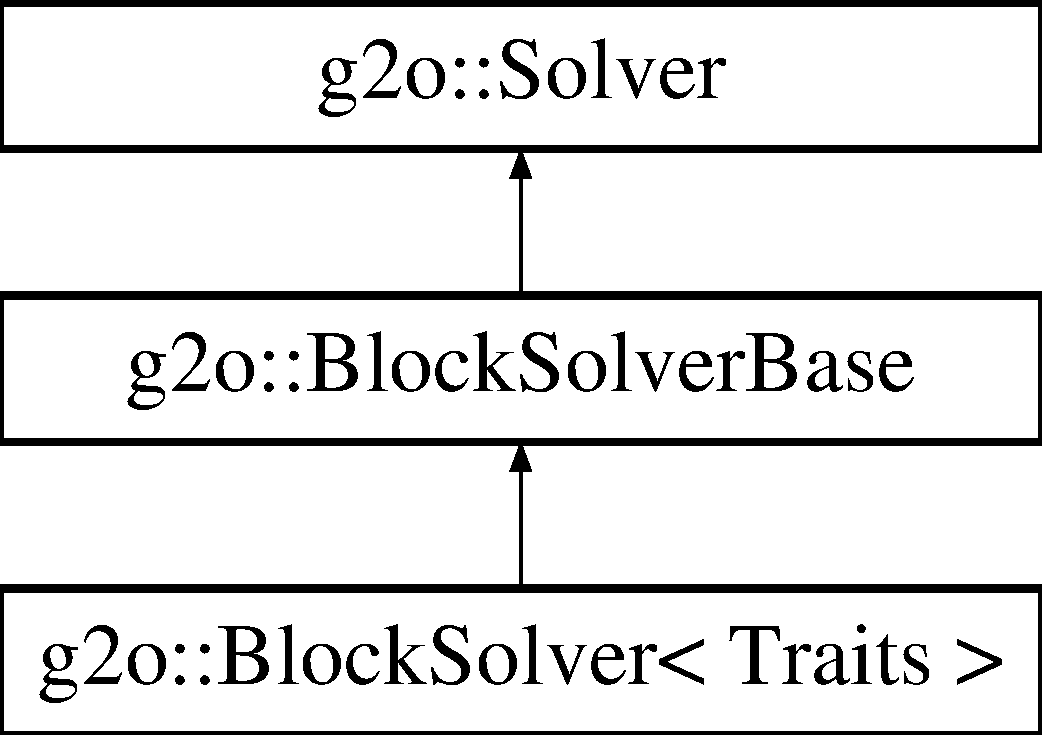
\includegraphics[height=3.000000cm]{classg2o_1_1_block_solver}
\end{center}
\end{figure}
\subsection*{Public Types}
\begin{DoxyCompactItemize}
\item 
typedef Traits\+::\+Pose\+Matrix\+Type \mbox{\hyperlink{classg2o_1_1_block_solver_a8c7c43d361bd31e3e0353889ba703bc0}{Pose\+Matrix\+Type}}
\item 
typedef Traits\+::\+Landmark\+Matrix\+Type \mbox{\hyperlink{classg2o_1_1_block_solver_afd898a666343291129d37a979e23ded6}{Landmark\+Matrix\+Type}}
\item 
typedef Traits\+::\+Pose\+Landmark\+Matrix\+Type \mbox{\hyperlink{classg2o_1_1_block_solver_a96bf60b923f816086cd2f24de38736ec}{Pose\+Landmark\+Matrix\+Type}}
\item 
typedef Traits\+::\+Pose\+Vector\+Type \mbox{\hyperlink{classg2o_1_1_block_solver_a65d51b9281e2e2597df05eb00801ee76}{Pose\+Vector\+Type}}
\item 
typedef Traits\+::\+Landmark\+Vector\+Type \mbox{\hyperlink{classg2o_1_1_block_solver_a19ade5e432f32e46557192ae75074304}{Landmark\+Vector\+Type}}
\item 
typedef Traits\+::\+Pose\+Hessian\+Type \mbox{\hyperlink{classg2o_1_1_block_solver_a0e7f862860a1e3391cec3cfaf69c48be}{Pose\+Hessian\+Type}}
\item 
typedef Traits\+::\+Landmark\+Hessian\+Type \mbox{\hyperlink{classg2o_1_1_block_solver_a465b1252905d90fd69b4243716620c45}{Landmark\+Hessian\+Type}}
\item 
typedef Traits\+::\+Pose\+Landmark\+Hessian\+Type \mbox{\hyperlink{classg2o_1_1_block_solver_aed8b44e394d2f19ca03c87adf90cc97c}{Pose\+Landmark\+Hessian\+Type}}
\item 
typedef Traits\+::\+Linear\+Solver\+Type \mbox{\hyperlink{classg2o_1_1_block_solver_a717fa8cb1dd5a212e41d8ebef67955e6}{Linear\+Solver\+Type}}
\end{DoxyCompactItemize}
\subsection*{Public Member Functions}
\begin{DoxyCompactItemize}
\item 
\mbox{\hyperlink{classg2o_1_1_block_solver_a04701a223a14708c9c84ce4d7e7af3f6}{Block\+Solver}} (\mbox{\hyperlink{classg2o_1_1_block_solver_a717fa8cb1dd5a212e41d8ebef67955e6}{Linear\+Solver\+Type}} $\ast$\mbox{\hyperlink{classg2o_1_1_block_solver_af71279eea2391daa4d7528da28107f1c}{linear\+Solver}})
\item 
\mbox{\hyperlink{classg2o_1_1_block_solver_a7587b13ec3494c00ad95a3d0ce7fd9a9}{$\sim$\+Block\+Solver}} ()
\item 
virtual bool \mbox{\hyperlink{classg2o_1_1_block_solver_a8bf01018abc3bfddfa3b29a380a1d6cb}{init}} (\mbox{\hyperlink{classg2o_1_1_sparse_optimizer}{Sparse\+Optimizer}} $\ast$optmizer, bool online=false)
\item 
virtual bool \mbox{\hyperlink{classg2o_1_1_block_solver_a17e4392d3cca9a9d7cf38bb46d073b86}{build\+Structure}} (bool zero\+Blocks=false)
\item 
virtual bool \mbox{\hyperlink{classg2o_1_1_block_solver_a662473598270cdf89075607f87440759}{update\+Structure}} (const std\+::vector$<$ \mbox{\hyperlink{classg2o_1_1_hyper_graph_1_1_vertex}{Hyper\+Graph\+::\+Vertex}} $\ast$$>$ \&vset, const \mbox{\hyperlink{classg2o_1_1_hyper_graph_a5e2970e236c0dcb4eff7c205d7b6b4ae}{Hyper\+Graph\+::\+Edge\+Set}} \&edges)
\item 
virtual bool \mbox{\hyperlink{classg2o_1_1_block_solver_a2654a8d52f38e5ce23720a8de302e2e7}{build\+System}} ()
\item 
virtual bool \mbox{\hyperlink{classg2o_1_1_block_solver_a589a75a131cce100c1945ad2786214d7}{solve}} ()
\item 
virtual bool \mbox{\hyperlink{classg2o_1_1_block_solver_ac21cd7e2c9b8a1414f7a2dccb0d30a0e}{compute\+Marginals}} (\mbox{\hyperlink{classg2o_1_1_sparse_block_matrix}{Sparse\+Block\+Matrix}}$<$ Matrix\+Xd $>$ \&spinv, const std\+::vector$<$ std\+::pair$<$ int, int $>$ $>$ \&block\+Indices)
\item 
virtual bool \mbox{\hyperlink{classg2o_1_1_block_solver_acc63a23e5b35e4f72d46dc22719aa56f}{set\+Lambda}} (double lambda, bool backup=false)
\item 
virtual void \mbox{\hyperlink{classg2o_1_1_block_solver_a2136931d7aa2f54df5207556c4685809}{restore\+Diagonal}} ()
\item 
virtual bool \mbox{\hyperlink{classg2o_1_1_block_solver_a68dc822ce48e80ceacce69c7bd029674}{supports\+Schur}} ()
\item 
virtual bool \mbox{\hyperlink{classg2o_1_1_block_solver_a382173946f1dd929a625e3708c959883}{schur}} ()
\begin{DoxyCompactList}\small\item\em should the solver perform the schur complement or not \end{DoxyCompactList}\item 
virtual void \mbox{\hyperlink{classg2o_1_1_block_solver_a6dd8e7e7a099410005cb96ff874d8866}{set\+Schur}} (bool s)
\item 
\mbox{\hyperlink{classg2o_1_1_linear_solver}{Linear\+Solver}}$<$ \mbox{\hyperlink{classg2o_1_1_block_solver_a8c7c43d361bd31e3e0353889ba703bc0}{Pose\+Matrix\+Type}} $>$ $\ast$ \mbox{\hyperlink{classg2o_1_1_block_solver_af71279eea2391daa4d7528da28107f1c}{linear\+Solver}} () const
\item 
virtual void \mbox{\hyperlink{classg2o_1_1_block_solver_a1bff5dc13e3408fa76c019347104acd0}{set\+Write\+Debug}} (bool \mbox{\hyperlink{classg2o_1_1_block_solver_aab81798b80dcb6c4182fa1d510914234}{write\+Debug}})
\item 
virtual bool \mbox{\hyperlink{classg2o_1_1_block_solver_aab81798b80dcb6c4182fa1d510914234}{write\+Debug}} () const
\item 
virtual bool \mbox{\hyperlink{classg2o_1_1_block_solver_a51563178d31f3eae6ec61993ea069a77}{save\+Hessian}} (const std\+::string \&file\+Name) const
\begin{DoxyCompactList}\small\item\em write the hessian to disk using the specified file name \end{DoxyCompactList}\item 
virtual void \mbox{\hyperlink{classg2o_1_1_block_solver_a6eb8f0729e8bcd760e629421cfa7202c}{multiply\+Hessian}} (double $\ast$dest, const double $\ast$src) const
\end{DoxyCompactItemize}
\subsection*{Static Public Attributes}
\begin{DoxyCompactItemize}
\item 
static const int \mbox{\hyperlink{classg2o_1_1_block_solver_a9a68f557c8e04cd76565fc45e1747e45}{Pose\+Dim}} = Traits\+::\+Pose\+Dim
\item 
static const int \mbox{\hyperlink{classg2o_1_1_block_solver_a2d5e499f65a71985a8256e98c1608dd9}{Landmark\+Dim}} = Traits\+::\+Landmark\+Dim
\end{DoxyCompactItemize}
\subsection*{Protected Member Functions}
\begin{DoxyCompactItemize}
\item 
void \mbox{\hyperlink{classg2o_1_1_block_solver_a0075af2df18364cf99fd80f813b8ce4b}{resize}} (int $\ast$block\+Pose\+Indices, int num\+Pose\+Blocks, int $\ast$block\+Landmark\+Indices, int num\+Landmark\+Blocks, int total\+Dim)
\item 
void \mbox{\hyperlink{classg2o_1_1_block_solver_a1877467844b7b9ab51bd6600e3a93eb0}{deallocate}} ()
\end{DoxyCompactItemize}
\subsection*{Protected Attributes}
\begin{DoxyCompactItemize}
\item 
\mbox{\hyperlink{classg2o_1_1_sparse_block_matrix}{Sparse\+Block\+Matrix}}$<$ \mbox{\hyperlink{classg2o_1_1_block_solver_a8c7c43d361bd31e3e0353889ba703bc0}{Pose\+Matrix\+Type}} $>$ $\ast$ \mbox{\hyperlink{classg2o_1_1_block_solver_ac222d4342825ed8632a87b4f5be94618}{\+\_\+\+Hpp}}
\item 
\mbox{\hyperlink{classg2o_1_1_sparse_block_matrix}{Sparse\+Block\+Matrix}}$<$ \mbox{\hyperlink{classg2o_1_1_block_solver_afd898a666343291129d37a979e23ded6}{Landmark\+Matrix\+Type}} $>$ $\ast$ \mbox{\hyperlink{classg2o_1_1_block_solver_a88d4c24df24a8fb72be1a4e4cff03d71}{\+\_\+\+Hll}}
\item 
\mbox{\hyperlink{classg2o_1_1_sparse_block_matrix}{Sparse\+Block\+Matrix}}$<$ \mbox{\hyperlink{classg2o_1_1_block_solver_a96bf60b923f816086cd2f24de38736ec}{Pose\+Landmark\+Matrix\+Type}} $>$ $\ast$ \mbox{\hyperlink{classg2o_1_1_block_solver_a0f6051339990e95aa587145a8a6f4f5f}{\+\_\+\+Hpl}}
\item 
\mbox{\hyperlink{classg2o_1_1_sparse_block_matrix}{Sparse\+Block\+Matrix}}$<$ \mbox{\hyperlink{classg2o_1_1_block_solver_a8c7c43d361bd31e3e0353889ba703bc0}{Pose\+Matrix\+Type}} $>$ $\ast$ \mbox{\hyperlink{classg2o_1_1_block_solver_a46977934a3e4fb0cd36bc4181ed3ec0e}{\+\_\+\+Hschur}}
\item 
\mbox{\hyperlink{classg2o_1_1_sparse_block_matrix_diagonal}{Sparse\+Block\+Matrix\+Diagonal}}$<$ \mbox{\hyperlink{classg2o_1_1_block_solver_afd898a666343291129d37a979e23ded6}{Landmark\+Matrix\+Type}} $>$ $\ast$ \mbox{\hyperlink{classg2o_1_1_block_solver_ad6a1a8f17c8fb854962a8204c79bc981}{\+\_\+\+D\+Inv\+Schur}}
\item 
\mbox{\hyperlink{classg2o_1_1_sparse_block_matrix_c_c_s}{Sparse\+Block\+Matrix\+C\+CS}}$<$ \mbox{\hyperlink{classg2o_1_1_block_solver_a96bf60b923f816086cd2f24de38736ec}{Pose\+Landmark\+Matrix\+Type}} $>$ $\ast$ \mbox{\hyperlink{classg2o_1_1_block_solver_ab54eb7bb13f8b3a8a5f135a98f2050ec}{\+\_\+\+Hpl\+C\+CS}}
\item 
\mbox{\hyperlink{classg2o_1_1_sparse_block_matrix_c_c_s}{Sparse\+Block\+Matrix\+C\+CS}}$<$ \mbox{\hyperlink{classg2o_1_1_block_solver_a8c7c43d361bd31e3e0353889ba703bc0}{Pose\+Matrix\+Type}} $>$ $\ast$ \mbox{\hyperlink{classg2o_1_1_block_solver_acea4b8ea8db5a29b63bea4bc568b0b26}{\+\_\+\+Hschur\+Transposed\+C\+CS}}
\item 
\mbox{\hyperlink{classg2o_1_1_linear_solver}{Linear\+Solver}}$<$ \mbox{\hyperlink{classg2o_1_1_block_solver_a8c7c43d361bd31e3e0353889ba703bc0}{Pose\+Matrix\+Type}} $>$ $\ast$ \mbox{\hyperlink{classg2o_1_1_block_solver_a676a4ef473ccaecb23050284e19659af}{\+\_\+linear\+Solver}}
\item 
std\+::vector$<$ \mbox{\hyperlink{classg2o_1_1_block_solver_a65d51b9281e2e2597df05eb00801ee76}{Pose\+Vector\+Type}}, Eigen\+::aligned\+\_\+allocator$<$ \mbox{\hyperlink{classg2o_1_1_block_solver_a65d51b9281e2e2597df05eb00801ee76}{Pose\+Vector\+Type}} $>$ $>$ \mbox{\hyperlink{classg2o_1_1_block_solver_a3cb6f86c522c2ea26478ad44b7c32f76}{\+\_\+diagonal\+Backup\+Pose}}
\item 
std\+::vector$<$ \mbox{\hyperlink{classg2o_1_1_block_solver_a19ade5e432f32e46557192ae75074304}{Landmark\+Vector\+Type}}, Eigen\+::aligned\+\_\+allocator$<$ \mbox{\hyperlink{classg2o_1_1_block_solver_a19ade5e432f32e46557192ae75074304}{Landmark\+Vector\+Type}} $>$ $>$ \mbox{\hyperlink{classg2o_1_1_block_solver_a3bc5b19faa2c45e2c04a6743b3a083de}{\+\_\+diagonal\+Backup\+Landmark}}
\item 
bool \mbox{\hyperlink{classg2o_1_1_block_solver_ab375a5fac964182442f38288bd8a103a}{\+\_\+do\+Schur}}
\item 
double $\ast$ \mbox{\hyperlink{classg2o_1_1_block_solver_a416f480d4b27d7f8962ae7ae363f2e32}{\+\_\+coefficients}}
\item 
double $\ast$ \mbox{\hyperlink{classg2o_1_1_block_solver_aafddeb1d0a4218fc9c3c77169e20f81a}{\+\_\+bschur}}
\item 
int \mbox{\hyperlink{classg2o_1_1_block_solver_a709259fc290d746f4174d25410b7458a}{\+\_\+num\+Poses}}
\item 
int \mbox{\hyperlink{classg2o_1_1_block_solver_ab98231b7ca8e6d7f138c33d26c6f4326}{\+\_\+num\+Landmarks}}
\item 
int \mbox{\hyperlink{classg2o_1_1_block_solver_a39ec000379885ce09cdd8c23ab6d4567}{\+\_\+size\+Poses}}
\item 
int \mbox{\hyperlink{classg2o_1_1_block_solver_a13a49b5aac8ae3b12ed0c349fc0788e7}{\+\_\+size\+Landmarks}}
\end{DoxyCompactItemize}


\subsection{Detailed Description}
\subsubsection*{template$<$typename Traits$>$\newline
class g2o\+::\+Block\+Solver$<$ Traits $>$}

Implementation of a solver operating on the blocks of the Hessian. 

\subsection{Member Typedef Documentation}
\mbox{\Hypertarget{classg2o_1_1_block_solver_a465b1252905d90fd69b4243716620c45}\label{classg2o_1_1_block_solver_a465b1252905d90fd69b4243716620c45}} 
\index{g2o\+::\+Block\+Solver@{g2o\+::\+Block\+Solver}!Landmark\+Hessian\+Type@{Landmark\+Hessian\+Type}}
\index{Landmark\+Hessian\+Type@{Landmark\+Hessian\+Type}!g2o\+::\+Block\+Solver@{g2o\+::\+Block\+Solver}}
\subsubsection{\texorpdfstring{Landmark\+Hessian\+Type}{LandmarkHessianType}}
{\footnotesize\ttfamily template$<$typename Traits $>$ \\
typedef Traits\+::\+Landmark\+Hessian\+Type \mbox{\hyperlink{classg2o_1_1_block_solver}{g2o\+::\+Block\+Solver}}$<$ Traits $>$\+::\mbox{\hyperlink{classg2o_1_1_block_solver_a465b1252905d90fd69b4243716620c45}{Landmark\+Hessian\+Type}}}

\mbox{\Hypertarget{classg2o_1_1_block_solver_afd898a666343291129d37a979e23ded6}\label{classg2o_1_1_block_solver_afd898a666343291129d37a979e23ded6}} 
\index{g2o\+::\+Block\+Solver@{g2o\+::\+Block\+Solver}!Landmark\+Matrix\+Type@{Landmark\+Matrix\+Type}}
\index{Landmark\+Matrix\+Type@{Landmark\+Matrix\+Type}!g2o\+::\+Block\+Solver@{g2o\+::\+Block\+Solver}}
\subsubsection{\texorpdfstring{Landmark\+Matrix\+Type}{LandmarkMatrixType}}
{\footnotesize\ttfamily template$<$typename Traits $>$ \\
typedef Traits\+::\+Landmark\+Matrix\+Type \mbox{\hyperlink{classg2o_1_1_block_solver}{g2o\+::\+Block\+Solver}}$<$ Traits $>$\+::\mbox{\hyperlink{classg2o_1_1_block_solver_afd898a666343291129d37a979e23ded6}{Landmark\+Matrix\+Type}}}

\mbox{\Hypertarget{classg2o_1_1_block_solver_a19ade5e432f32e46557192ae75074304}\label{classg2o_1_1_block_solver_a19ade5e432f32e46557192ae75074304}} 
\index{g2o\+::\+Block\+Solver@{g2o\+::\+Block\+Solver}!Landmark\+Vector\+Type@{Landmark\+Vector\+Type}}
\index{Landmark\+Vector\+Type@{Landmark\+Vector\+Type}!g2o\+::\+Block\+Solver@{g2o\+::\+Block\+Solver}}
\subsubsection{\texorpdfstring{Landmark\+Vector\+Type}{LandmarkVectorType}}
{\footnotesize\ttfamily template$<$typename Traits $>$ \\
typedef Traits\+::\+Landmark\+Vector\+Type \mbox{\hyperlink{classg2o_1_1_block_solver}{g2o\+::\+Block\+Solver}}$<$ Traits $>$\+::\mbox{\hyperlink{classg2o_1_1_block_solver_a19ade5e432f32e46557192ae75074304}{Landmark\+Vector\+Type}}}

\mbox{\Hypertarget{classg2o_1_1_block_solver_a717fa8cb1dd5a212e41d8ebef67955e6}\label{classg2o_1_1_block_solver_a717fa8cb1dd5a212e41d8ebef67955e6}} 
\index{g2o\+::\+Block\+Solver@{g2o\+::\+Block\+Solver}!Linear\+Solver\+Type@{Linear\+Solver\+Type}}
\index{Linear\+Solver\+Type@{Linear\+Solver\+Type}!g2o\+::\+Block\+Solver@{g2o\+::\+Block\+Solver}}
\subsubsection{\texorpdfstring{Linear\+Solver\+Type}{LinearSolverType}}
{\footnotesize\ttfamily template$<$typename Traits $>$ \\
typedef Traits\+::\+Linear\+Solver\+Type \mbox{\hyperlink{classg2o_1_1_block_solver}{g2o\+::\+Block\+Solver}}$<$ Traits $>$\+::\mbox{\hyperlink{classg2o_1_1_block_solver_a717fa8cb1dd5a212e41d8ebef67955e6}{Linear\+Solver\+Type}}}

\mbox{\Hypertarget{classg2o_1_1_block_solver_a0e7f862860a1e3391cec3cfaf69c48be}\label{classg2o_1_1_block_solver_a0e7f862860a1e3391cec3cfaf69c48be}} 
\index{g2o\+::\+Block\+Solver@{g2o\+::\+Block\+Solver}!Pose\+Hessian\+Type@{Pose\+Hessian\+Type}}
\index{Pose\+Hessian\+Type@{Pose\+Hessian\+Type}!g2o\+::\+Block\+Solver@{g2o\+::\+Block\+Solver}}
\subsubsection{\texorpdfstring{Pose\+Hessian\+Type}{PoseHessianType}}
{\footnotesize\ttfamily template$<$typename Traits $>$ \\
typedef Traits\+::\+Pose\+Hessian\+Type \mbox{\hyperlink{classg2o_1_1_block_solver}{g2o\+::\+Block\+Solver}}$<$ Traits $>$\+::\mbox{\hyperlink{classg2o_1_1_block_solver_a0e7f862860a1e3391cec3cfaf69c48be}{Pose\+Hessian\+Type}}}

\mbox{\Hypertarget{classg2o_1_1_block_solver_aed8b44e394d2f19ca03c87adf90cc97c}\label{classg2o_1_1_block_solver_aed8b44e394d2f19ca03c87adf90cc97c}} 
\index{g2o\+::\+Block\+Solver@{g2o\+::\+Block\+Solver}!Pose\+Landmark\+Hessian\+Type@{Pose\+Landmark\+Hessian\+Type}}
\index{Pose\+Landmark\+Hessian\+Type@{Pose\+Landmark\+Hessian\+Type}!g2o\+::\+Block\+Solver@{g2o\+::\+Block\+Solver}}
\subsubsection{\texorpdfstring{Pose\+Landmark\+Hessian\+Type}{PoseLandmarkHessianType}}
{\footnotesize\ttfamily template$<$typename Traits $>$ \\
typedef Traits\+::\+Pose\+Landmark\+Hessian\+Type \mbox{\hyperlink{classg2o_1_1_block_solver}{g2o\+::\+Block\+Solver}}$<$ Traits $>$\+::\mbox{\hyperlink{classg2o_1_1_block_solver_aed8b44e394d2f19ca03c87adf90cc97c}{Pose\+Landmark\+Hessian\+Type}}}

\mbox{\Hypertarget{classg2o_1_1_block_solver_a96bf60b923f816086cd2f24de38736ec}\label{classg2o_1_1_block_solver_a96bf60b923f816086cd2f24de38736ec}} 
\index{g2o\+::\+Block\+Solver@{g2o\+::\+Block\+Solver}!Pose\+Landmark\+Matrix\+Type@{Pose\+Landmark\+Matrix\+Type}}
\index{Pose\+Landmark\+Matrix\+Type@{Pose\+Landmark\+Matrix\+Type}!g2o\+::\+Block\+Solver@{g2o\+::\+Block\+Solver}}
\subsubsection{\texorpdfstring{Pose\+Landmark\+Matrix\+Type}{PoseLandmarkMatrixType}}
{\footnotesize\ttfamily template$<$typename Traits $>$ \\
typedef Traits\+::\+Pose\+Landmark\+Matrix\+Type \mbox{\hyperlink{classg2o_1_1_block_solver}{g2o\+::\+Block\+Solver}}$<$ Traits $>$\+::\mbox{\hyperlink{classg2o_1_1_block_solver_a96bf60b923f816086cd2f24de38736ec}{Pose\+Landmark\+Matrix\+Type}}}

\mbox{\Hypertarget{classg2o_1_1_block_solver_a8c7c43d361bd31e3e0353889ba703bc0}\label{classg2o_1_1_block_solver_a8c7c43d361bd31e3e0353889ba703bc0}} 
\index{g2o\+::\+Block\+Solver@{g2o\+::\+Block\+Solver}!Pose\+Matrix\+Type@{Pose\+Matrix\+Type}}
\index{Pose\+Matrix\+Type@{Pose\+Matrix\+Type}!g2o\+::\+Block\+Solver@{g2o\+::\+Block\+Solver}}
\subsubsection{\texorpdfstring{Pose\+Matrix\+Type}{PoseMatrixType}}
{\footnotesize\ttfamily template$<$typename Traits $>$ \\
typedef Traits\+::\+Pose\+Matrix\+Type \mbox{\hyperlink{classg2o_1_1_block_solver}{g2o\+::\+Block\+Solver}}$<$ Traits $>$\+::\mbox{\hyperlink{classg2o_1_1_block_solver_a8c7c43d361bd31e3e0353889ba703bc0}{Pose\+Matrix\+Type}}}

\mbox{\Hypertarget{classg2o_1_1_block_solver_a65d51b9281e2e2597df05eb00801ee76}\label{classg2o_1_1_block_solver_a65d51b9281e2e2597df05eb00801ee76}} 
\index{g2o\+::\+Block\+Solver@{g2o\+::\+Block\+Solver}!Pose\+Vector\+Type@{Pose\+Vector\+Type}}
\index{Pose\+Vector\+Type@{Pose\+Vector\+Type}!g2o\+::\+Block\+Solver@{g2o\+::\+Block\+Solver}}
\subsubsection{\texorpdfstring{Pose\+Vector\+Type}{PoseVectorType}}
{\footnotesize\ttfamily template$<$typename Traits $>$ \\
typedef Traits\+::\+Pose\+Vector\+Type \mbox{\hyperlink{classg2o_1_1_block_solver}{g2o\+::\+Block\+Solver}}$<$ Traits $>$\+::\mbox{\hyperlink{classg2o_1_1_block_solver_a65d51b9281e2e2597df05eb00801ee76}{Pose\+Vector\+Type}}}



\subsection{Constructor \& Destructor Documentation}
\mbox{\Hypertarget{classg2o_1_1_block_solver_a04701a223a14708c9c84ce4d7e7af3f6}\label{classg2o_1_1_block_solver_a04701a223a14708c9c84ce4d7e7af3f6}} 
\index{g2o\+::\+Block\+Solver@{g2o\+::\+Block\+Solver}!Block\+Solver@{Block\+Solver}}
\index{Block\+Solver@{Block\+Solver}!g2o\+::\+Block\+Solver@{g2o\+::\+Block\+Solver}}
\subsubsection{\texorpdfstring{Block\+Solver()}{BlockSolver()}}
{\footnotesize\ttfamily template$<$typename Traits $>$ \\
\mbox{\hyperlink{classg2o_1_1_block_solver}{g2o\+::\+Block\+Solver}}$<$ Traits $>$\+::\mbox{\hyperlink{classg2o_1_1_block_solver}{Block\+Solver}} (\begin{DoxyParamCaption}\item[{\mbox{\hyperlink{classg2o_1_1_block_solver_a717fa8cb1dd5a212e41d8ebef67955e6}{Linear\+Solver\+Type}} $\ast$}]{linear\+Solver }\end{DoxyParamCaption})}

allocate a block solver ontop of the underlying linear solver. N\+O\+TE\+: The \mbox{\hyperlink{classg2o_1_1_block_solver}{Block\+Solver}} assumes exclusive access to the linear solver and will therefore free the pointer in its destructor. \mbox{\Hypertarget{classg2o_1_1_block_solver_a7587b13ec3494c00ad95a3d0ce7fd9a9}\label{classg2o_1_1_block_solver_a7587b13ec3494c00ad95a3d0ce7fd9a9}} 
\index{g2o\+::\+Block\+Solver@{g2o\+::\+Block\+Solver}!````~Block\+Solver@{$\sim$\+Block\+Solver}}
\index{````~Block\+Solver@{$\sim$\+Block\+Solver}!g2o\+::\+Block\+Solver@{g2o\+::\+Block\+Solver}}
\subsubsection{\texorpdfstring{$\sim$\+Block\+Solver()}{~BlockSolver()}}
{\footnotesize\ttfamily template$<$typename Traits $>$ \\
\mbox{\hyperlink{classg2o_1_1_block_solver}{g2o\+::\+Block\+Solver}}$<$ Traits $>$\+::$\sim$\mbox{\hyperlink{classg2o_1_1_block_solver}{Block\+Solver}} (\begin{DoxyParamCaption}{ }\end{DoxyParamCaption})}



\subsection{Member Function Documentation}
\mbox{\Hypertarget{classg2o_1_1_block_solver_a17e4392d3cca9a9d7cf38bb46d073b86}\label{classg2o_1_1_block_solver_a17e4392d3cca9a9d7cf38bb46d073b86}} 
\index{g2o\+::\+Block\+Solver@{g2o\+::\+Block\+Solver}!build\+Structure@{build\+Structure}}
\index{build\+Structure@{build\+Structure}!g2o\+::\+Block\+Solver@{g2o\+::\+Block\+Solver}}
\subsubsection{\texorpdfstring{build\+Structure()}{buildStructure()}}
{\footnotesize\ttfamily template$<$typename Traits $>$ \\
bool \mbox{\hyperlink{classg2o_1_1_block_solver}{g2o\+::\+Block\+Solver}}$<$ Traits $>$\+::build\+Structure (\begin{DoxyParamCaption}\item[{bool}]{zero\+Blocks = {\ttfamily false} }\end{DoxyParamCaption})\hspace{0.3cm}{\ttfamily [virtual]}}

build the structure of the system 

Implements \mbox{\hyperlink{classg2o_1_1_solver_a6c93ac0f528ffe05867d33150c54f46f}{g2o\+::\+Solver}}.

\mbox{\Hypertarget{classg2o_1_1_block_solver_a2654a8d52f38e5ce23720a8de302e2e7}\label{classg2o_1_1_block_solver_a2654a8d52f38e5ce23720a8de302e2e7}} 
\index{g2o\+::\+Block\+Solver@{g2o\+::\+Block\+Solver}!build\+System@{build\+System}}
\index{build\+System@{build\+System}!g2o\+::\+Block\+Solver@{g2o\+::\+Block\+Solver}}
\subsubsection{\texorpdfstring{build\+System()}{buildSystem()}}
{\footnotesize\ttfamily template$<$typename Traits $>$ \\
bool \mbox{\hyperlink{classg2o_1_1_block_solver}{g2o\+::\+Block\+Solver}}$<$ Traits $>$\+::build\+System (\begin{DoxyParamCaption}{ }\end{DoxyParamCaption})\hspace{0.3cm}{\ttfamily [virtual]}}

build the current system 

Implements \mbox{\hyperlink{classg2o_1_1_solver_ac1565e85d5ca68a87ad7f06f8164a8c0}{g2o\+::\+Solver}}.

\mbox{\Hypertarget{classg2o_1_1_block_solver_ac21cd7e2c9b8a1414f7a2dccb0d30a0e}\label{classg2o_1_1_block_solver_ac21cd7e2c9b8a1414f7a2dccb0d30a0e}} 
\index{g2o\+::\+Block\+Solver@{g2o\+::\+Block\+Solver}!compute\+Marginals@{compute\+Marginals}}
\index{compute\+Marginals@{compute\+Marginals}!g2o\+::\+Block\+Solver@{g2o\+::\+Block\+Solver}}
\subsubsection{\texorpdfstring{compute\+Marginals()}{computeMarginals()}}
{\footnotesize\ttfamily template$<$typename Traits $>$ \\
bool \mbox{\hyperlink{classg2o_1_1_block_solver}{g2o\+::\+Block\+Solver}}$<$ Traits $>$\+::compute\+Marginals (\begin{DoxyParamCaption}\item[{\mbox{\hyperlink{classg2o_1_1_sparse_block_matrix}{Sparse\+Block\+Matrix}}$<$ Matrix\+Xd $>$ \&}]{spinv,  }\item[{const std\+::vector$<$ std\+::pair$<$ int, int $>$ $>$ \&}]{block\+Indices }\end{DoxyParamCaption})\hspace{0.3cm}{\ttfamily [virtual]}}

computes the block diagonal elements of the pattern specified in the input and stores them in given \mbox{\hyperlink{classg2o_1_1_sparse_block_matrix}{Sparse\+Block\+Matrix}} 

Implements \mbox{\hyperlink{classg2o_1_1_solver_afc33768e6c024e11d9e3c9d938b59b7f}{g2o\+::\+Solver}}.

\mbox{\Hypertarget{classg2o_1_1_block_solver_a1877467844b7b9ab51bd6600e3a93eb0}\label{classg2o_1_1_block_solver_a1877467844b7b9ab51bd6600e3a93eb0}} 
\index{g2o\+::\+Block\+Solver@{g2o\+::\+Block\+Solver}!deallocate@{deallocate}}
\index{deallocate@{deallocate}!g2o\+::\+Block\+Solver@{g2o\+::\+Block\+Solver}}
\subsubsection{\texorpdfstring{deallocate()}{deallocate()}}
{\footnotesize\ttfamily template$<$typename Traits $>$ \\
void \mbox{\hyperlink{classg2o_1_1_block_solver}{g2o\+::\+Block\+Solver}}$<$ Traits $>$\+::deallocate (\begin{DoxyParamCaption}{ }\end{DoxyParamCaption})\hspace{0.3cm}{\ttfamily [protected]}}

\mbox{\Hypertarget{classg2o_1_1_block_solver_a8bf01018abc3bfddfa3b29a380a1d6cb}\label{classg2o_1_1_block_solver_a8bf01018abc3bfddfa3b29a380a1d6cb}} 
\index{g2o\+::\+Block\+Solver@{g2o\+::\+Block\+Solver}!init@{init}}
\index{init@{init}!g2o\+::\+Block\+Solver@{g2o\+::\+Block\+Solver}}
\subsubsection{\texorpdfstring{init()}{init()}}
{\footnotesize\ttfamily template$<$typename Traits $>$ \\
bool \mbox{\hyperlink{classg2o_1_1_block_solver}{g2o\+::\+Block\+Solver}}$<$ Traits $>$\+::init (\begin{DoxyParamCaption}\item[{\mbox{\hyperlink{classg2o_1_1_sparse_optimizer}{Sparse\+Optimizer}} $\ast$}]{optimizer,  }\item[{bool}]{online = {\ttfamily false} }\end{DoxyParamCaption})\hspace{0.3cm}{\ttfamily [virtual]}}

initialize the solver, called once before the first iteration 

Implements \mbox{\hyperlink{classg2o_1_1_solver_a532174e1ee53642880d2d59c128b037b}{g2o\+::\+Solver}}.

\mbox{\Hypertarget{classg2o_1_1_block_solver_af71279eea2391daa4d7528da28107f1c}\label{classg2o_1_1_block_solver_af71279eea2391daa4d7528da28107f1c}} 
\index{g2o\+::\+Block\+Solver@{g2o\+::\+Block\+Solver}!linear\+Solver@{linear\+Solver}}
\index{linear\+Solver@{linear\+Solver}!g2o\+::\+Block\+Solver@{g2o\+::\+Block\+Solver}}
\subsubsection{\texorpdfstring{linear\+Solver()}{linearSolver()}}
{\footnotesize\ttfamily template$<$typename Traits $>$ \\
\mbox{\hyperlink{classg2o_1_1_linear_solver}{Linear\+Solver}}$<$\mbox{\hyperlink{classg2o_1_1_block_solver_a8c7c43d361bd31e3e0353889ba703bc0}{Pose\+Matrix\+Type}}$>$$\ast$ \mbox{\hyperlink{classg2o_1_1_block_solver}{g2o\+::\+Block\+Solver}}$<$ Traits $>$\+::linear\+Solver (\begin{DoxyParamCaption}{ }\end{DoxyParamCaption}) const\hspace{0.3cm}{\ttfamily [inline]}}

\mbox{\Hypertarget{classg2o_1_1_block_solver_a6eb8f0729e8bcd760e629421cfa7202c}\label{classg2o_1_1_block_solver_a6eb8f0729e8bcd760e629421cfa7202c}} 
\index{g2o\+::\+Block\+Solver@{g2o\+::\+Block\+Solver}!multiply\+Hessian@{multiply\+Hessian}}
\index{multiply\+Hessian@{multiply\+Hessian}!g2o\+::\+Block\+Solver@{g2o\+::\+Block\+Solver}}
\subsubsection{\texorpdfstring{multiply\+Hessian()}{multiplyHessian()}}
{\footnotesize\ttfamily template$<$typename Traits $>$ \\
virtual void \mbox{\hyperlink{classg2o_1_1_block_solver}{g2o\+::\+Block\+Solver}}$<$ Traits $>$\+::multiply\+Hessian (\begin{DoxyParamCaption}\item[{double $\ast$}]{dest,  }\item[{const double $\ast$}]{src }\end{DoxyParamCaption}) const\hspace{0.3cm}{\ttfamily [inline]}, {\ttfamily [virtual]}}

compute dest = H $\ast$ src 

Implements \mbox{\hyperlink{classg2o_1_1_block_solver_base_a4ff7072751bfa1b7fcf91f8219e18e13}{g2o\+::\+Block\+Solver\+Base}}.

\mbox{\Hypertarget{classg2o_1_1_block_solver_a0075af2df18364cf99fd80f813b8ce4b}\label{classg2o_1_1_block_solver_a0075af2df18364cf99fd80f813b8ce4b}} 
\index{g2o\+::\+Block\+Solver@{g2o\+::\+Block\+Solver}!resize@{resize}}
\index{resize@{resize}!g2o\+::\+Block\+Solver@{g2o\+::\+Block\+Solver}}
\subsubsection{\texorpdfstring{resize()}{resize()}}
{\footnotesize\ttfamily template$<$typename Traits $>$ \\
void \mbox{\hyperlink{classg2o_1_1_block_solver}{g2o\+::\+Block\+Solver}}$<$ Traits $>$\+::resize (\begin{DoxyParamCaption}\item[{int $\ast$}]{block\+Pose\+Indices,  }\item[{int}]{num\+Pose\+Blocks,  }\item[{int $\ast$}]{block\+Landmark\+Indices,  }\item[{int}]{num\+Landmark\+Blocks,  }\item[{int}]{total\+Dim }\end{DoxyParamCaption})\hspace{0.3cm}{\ttfamily [protected]}}

\mbox{\Hypertarget{classg2o_1_1_block_solver_a2136931d7aa2f54df5207556c4685809}\label{classg2o_1_1_block_solver_a2136931d7aa2f54df5207556c4685809}} 
\index{g2o\+::\+Block\+Solver@{g2o\+::\+Block\+Solver}!restore\+Diagonal@{restore\+Diagonal}}
\index{restore\+Diagonal@{restore\+Diagonal}!g2o\+::\+Block\+Solver@{g2o\+::\+Block\+Solver}}
\subsubsection{\texorpdfstring{restore\+Diagonal()}{restoreDiagonal()}}
{\footnotesize\ttfamily template$<$typename Traits $>$ \\
void \mbox{\hyperlink{classg2o_1_1_block_solver}{g2o\+::\+Block\+Solver}}$<$ Traits $>$\+::restore\+Diagonal (\begin{DoxyParamCaption}{ }\end{DoxyParamCaption})\hspace{0.3cm}{\ttfamily [virtual]}}

restore a previosly made backup of the diagonal 

Implements \mbox{\hyperlink{classg2o_1_1_solver_a3c40dae9b999c4d18e57b02fd0e0ade2}{g2o\+::\+Solver}}.

\mbox{\Hypertarget{classg2o_1_1_block_solver_a51563178d31f3eae6ec61993ea069a77}\label{classg2o_1_1_block_solver_a51563178d31f3eae6ec61993ea069a77}} 
\index{g2o\+::\+Block\+Solver@{g2o\+::\+Block\+Solver}!save\+Hessian@{save\+Hessian}}
\index{save\+Hessian@{save\+Hessian}!g2o\+::\+Block\+Solver@{g2o\+::\+Block\+Solver}}
\subsubsection{\texorpdfstring{save\+Hessian()}{saveHessian()}}
{\footnotesize\ttfamily template$<$typename Traits $>$ \\
bool \mbox{\hyperlink{classg2o_1_1_block_solver}{g2o\+::\+Block\+Solver}}$<$ Traits $>$\+::save\+Hessian (\begin{DoxyParamCaption}\item[{const std\+::string \&}]{ }\end{DoxyParamCaption}) const\hspace{0.3cm}{\ttfamily [virtual]}}



write the hessian to disk using the specified file name 



Implements \mbox{\hyperlink{classg2o_1_1_solver_a14852543c4dc3f3e7088efe03aa135eb}{g2o\+::\+Solver}}.

\mbox{\Hypertarget{classg2o_1_1_block_solver_a382173946f1dd929a625e3708c959883}\label{classg2o_1_1_block_solver_a382173946f1dd929a625e3708c959883}} 
\index{g2o\+::\+Block\+Solver@{g2o\+::\+Block\+Solver}!schur@{schur}}
\index{schur@{schur}!g2o\+::\+Block\+Solver@{g2o\+::\+Block\+Solver}}
\subsubsection{\texorpdfstring{schur()}{schur()}}
{\footnotesize\ttfamily template$<$typename Traits $>$ \\
virtual bool \mbox{\hyperlink{classg2o_1_1_block_solver}{g2o\+::\+Block\+Solver}}$<$ Traits $>$\+::schur (\begin{DoxyParamCaption}{ }\end{DoxyParamCaption})\hspace{0.3cm}{\ttfamily [inline]}, {\ttfamily [virtual]}}



should the solver perform the schur complement or not 



Implements \mbox{\hyperlink{classg2o_1_1_solver_acc8d6a8ae7847a157d4a2f44aea14c74}{g2o\+::\+Solver}}.

\mbox{\Hypertarget{classg2o_1_1_block_solver_acc63a23e5b35e4f72d46dc22719aa56f}\label{classg2o_1_1_block_solver_acc63a23e5b35e4f72d46dc22719aa56f}} 
\index{g2o\+::\+Block\+Solver@{g2o\+::\+Block\+Solver}!set\+Lambda@{set\+Lambda}}
\index{set\+Lambda@{set\+Lambda}!g2o\+::\+Block\+Solver@{g2o\+::\+Block\+Solver}}
\subsubsection{\texorpdfstring{set\+Lambda()}{setLambda()}}
{\footnotesize\ttfamily template$<$typename Traits $>$ \\
bool \mbox{\hyperlink{classg2o_1_1_block_solver}{g2o\+::\+Block\+Solver}}$<$ Traits $>$\+::set\+Lambda (\begin{DoxyParamCaption}\item[{double}]{lambda,  }\item[{bool}]{backup = {\ttfamily false} }\end{DoxyParamCaption})\hspace{0.3cm}{\ttfamily [virtual]}}

update the system while performing Levenberg, i.\+e., modifying the diagonal components of A by doing += lambda along the main diagonal of the Matrix. Note that this function may be called with a positive and a negative lambda. The latter is used to undo a former modification. If backup is true, then the solver should store a backup of the diagonal, which can be restored by \mbox{\hyperlink{classg2o_1_1_block_solver_a2136931d7aa2f54df5207556c4685809}{restore\+Diagonal()}} 

Implements \mbox{\hyperlink{classg2o_1_1_solver_a94a0d5196c7859c6c37fc2368ac56be3}{g2o\+::\+Solver}}.

\mbox{\Hypertarget{classg2o_1_1_block_solver_a6dd8e7e7a099410005cb96ff874d8866}\label{classg2o_1_1_block_solver_a6dd8e7e7a099410005cb96ff874d8866}} 
\index{g2o\+::\+Block\+Solver@{g2o\+::\+Block\+Solver}!set\+Schur@{set\+Schur}}
\index{set\+Schur@{set\+Schur}!g2o\+::\+Block\+Solver@{g2o\+::\+Block\+Solver}}
\subsubsection{\texorpdfstring{set\+Schur()}{setSchur()}}
{\footnotesize\ttfamily template$<$typename Traits $>$ \\
virtual void \mbox{\hyperlink{classg2o_1_1_block_solver}{g2o\+::\+Block\+Solver}}$<$ Traits $>$\+::set\+Schur (\begin{DoxyParamCaption}\item[{bool}]{s }\end{DoxyParamCaption})\hspace{0.3cm}{\ttfamily [inline]}, {\ttfamily [virtual]}}



Implements \mbox{\hyperlink{classg2o_1_1_solver_a30134c828054375b1cc16ede2a879761}{g2o\+::\+Solver}}.

\mbox{\Hypertarget{classg2o_1_1_block_solver_a1bff5dc13e3408fa76c019347104acd0}\label{classg2o_1_1_block_solver_a1bff5dc13e3408fa76c019347104acd0}} 
\index{g2o\+::\+Block\+Solver@{g2o\+::\+Block\+Solver}!set\+Write\+Debug@{set\+Write\+Debug}}
\index{set\+Write\+Debug@{set\+Write\+Debug}!g2o\+::\+Block\+Solver@{g2o\+::\+Block\+Solver}}
\subsubsection{\texorpdfstring{set\+Write\+Debug()}{setWriteDebug()}}
{\footnotesize\ttfamily template$<$typename Traits $>$ \\
void \mbox{\hyperlink{classg2o_1_1_block_solver}{g2o\+::\+Block\+Solver}}$<$ Traits $>$\+::set\+Write\+Debug (\begin{DoxyParamCaption}\item[{bool}]{ }\end{DoxyParamCaption})\hspace{0.3cm}{\ttfamily [virtual]}}

write debug output of the Hessian if system is not positive definite 

Implements \mbox{\hyperlink{classg2o_1_1_solver_ad3ef2a487d991363ba86af2840b0d7cd}{g2o\+::\+Solver}}.

\mbox{\Hypertarget{classg2o_1_1_block_solver_a589a75a131cce100c1945ad2786214d7}\label{classg2o_1_1_block_solver_a589a75a131cce100c1945ad2786214d7}} 
\index{g2o\+::\+Block\+Solver@{g2o\+::\+Block\+Solver}!solve@{solve}}
\index{solve@{solve}!g2o\+::\+Block\+Solver@{g2o\+::\+Block\+Solver}}
\subsubsection{\texorpdfstring{solve()}{solve()}}
{\footnotesize\ttfamily template$<$typename Traits $>$ \\
bool \mbox{\hyperlink{classg2o_1_1_block_solver}{g2o\+::\+Block\+Solver}}$<$ Traits $>$\+::solve (\begin{DoxyParamCaption}{ }\end{DoxyParamCaption})\hspace{0.3cm}{\ttfamily [virtual]}}

solve Ax = b 

Implements \mbox{\hyperlink{classg2o_1_1_solver_a9c359a886db57f2f81e54a2113f3bd38}{g2o\+::\+Solver}}.

\mbox{\Hypertarget{classg2o_1_1_block_solver_a68dc822ce48e80ceacce69c7bd029674}\label{classg2o_1_1_block_solver_a68dc822ce48e80ceacce69c7bd029674}} 
\index{g2o\+::\+Block\+Solver@{g2o\+::\+Block\+Solver}!supports\+Schur@{supports\+Schur}}
\index{supports\+Schur@{supports\+Schur}!g2o\+::\+Block\+Solver@{g2o\+::\+Block\+Solver}}
\subsubsection{\texorpdfstring{supports\+Schur()}{supportsSchur()}}
{\footnotesize\ttfamily template$<$typename Traits $>$ \\
virtual bool \mbox{\hyperlink{classg2o_1_1_block_solver}{g2o\+::\+Block\+Solver}}$<$ Traits $>$\+::supports\+Schur (\begin{DoxyParamCaption}{ }\end{DoxyParamCaption})\hspace{0.3cm}{\ttfamily [inline]}, {\ttfamily [virtual]}}

does this solver support the Schur complement for solving a system consisting of poses and landmarks. Re-\/implemement in a derived solver, if your solver supports it. 

Reimplemented from \mbox{\hyperlink{classg2o_1_1_solver_a36c68f7bc0b8864ee7722bc3c06de554}{g2o\+::\+Solver}}.

\mbox{\Hypertarget{classg2o_1_1_block_solver_a662473598270cdf89075607f87440759}\label{classg2o_1_1_block_solver_a662473598270cdf89075607f87440759}} 
\index{g2o\+::\+Block\+Solver@{g2o\+::\+Block\+Solver}!update\+Structure@{update\+Structure}}
\index{update\+Structure@{update\+Structure}!g2o\+::\+Block\+Solver@{g2o\+::\+Block\+Solver}}
\subsubsection{\texorpdfstring{update\+Structure()}{updateStructure()}}
{\footnotesize\ttfamily template$<$typename Traits $>$ \\
bool \mbox{\hyperlink{classg2o_1_1_block_solver}{g2o\+::\+Block\+Solver}}$<$ Traits $>$\+::update\+Structure (\begin{DoxyParamCaption}\item[{const std\+::vector$<$ \mbox{\hyperlink{classg2o_1_1_hyper_graph_1_1_vertex}{Hyper\+Graph\+::\+Vertex}} $\ast$$>$ \&}]{vset,  }\item[{const \mbox{\hyperlink{classg2o_1_1_hyper_graph_a5e2970e236c0dcb4eff7c205d7b6b4ae}{Hyper\+Graph\+::\+Edge\+Set}} \&}]{edges }\end{DoxyParamCaption})\hspace{0.3cm}{\ttfamily [virtual]}}

update the structures for online processing 

Implements \mbox{\hyperlink{classg2o_1_1_solver_aeca71878e37081b6138f90ac60ec1f89}{g2o\+::\+Solver}}.

\mbox{\Hypertarget{classg2o_1_1_block_solver_aab81798b80dcb6c4182fa1d510914234}\label{classg2o_1_1_block_solver_aab81798b80dcb6c4182fa1d510914234}} 
\index{g2o\+::\+Block\+Solver@{g2o\+::\+Block\+Solver}!write\+Debug@{write\+Debug}}
\index{write\+Debug@{write\+Debug}!g2o\+::\+Block\+Solver@{g2o\+::\+Block\+Solver}}
\subsubsection{\texorpdfstring{write\+Debug()}{writeDebug()}}
{\footnotesize\ttfamily template$<$typename Traits $>$ \\
virtual bool \mbox{\hyperlink{classg2o_1_1_block_solver}{g2o\+::\+Block\+Solver}}$<$ Traits $>$\+::write\+Debug (\begin{DoxyParamCaption}{ }\end{DoxyParamCaption}) const\hspace{0.3cm}{\ttfamily [inline]}, {\ttfamily [virtual]}}



Implements \mbox{\hyperlink{classg2o_1_1_solver_a0f6f14940eccea0f9bf9e2ea144c9b4d}{g2o\+::\+Solver}}.



\subsection{Member Data Documentation}
\mbox{\Hypertarget{classg2o_1_1_block_solver_aafddeb1d0a4218fc9c3c77169e20f81a}\label{classg2o_1_1_block_solver_aafddeb1d0a4218fc9c3c77169e20f81a}} 
\index{g2o\+::\+Block\+Solver@{g2o\+::\+Block\+Solver}!\+\_\+bschur@{\+\_\+bschur}}
\index{\+\_\+bschur@{\+\_\+bschur}!g2o\+::\+Block\+Solver@{g2o\+::\+Block\+Solver}}
\subsubsection{\texorpdfstring{\+\_\+bschur}{\_bschur}}
{\footnotesize\ttfamily template$<$typename Traits $>$ \\
double$\ast$ \mbox{\hyperlink{classg2o_1_1_block_solver}{g2o\+::\+Block\+Solver}}$<$ Traits $>$\+::\+\_\+bschur\hspace{0.3cm}{\ttfamily [protected]}}

\mbox{\Hypertarget{classg2o_1_1_block_solver_a416f480d4b27d7f8962ae7ae363f2e32}\label{classg2o_1_1_block_solver_a416f480d4b27d7f8962ae7ae363f2e32}} 
\index{g2o\+::\+Block\+Solver@{g2o\+::\+Block\+Solver}!\+\_\+coefficients@{\+\_\+coefficients}}
\index{\+\_\+coefficients@{\+\_\+coefficients}!g2o\+::\+Block\+Solver@{g2o\+::\+Block\+Solver}}
\subsubsection{\texorpdfstring{\+\_\+coefficients}{\_coefficients}}
{\footnotesize\ttfamily template$<$typename Traits $>$ \\
double$\ast$ \mbox{\hyperlink{classg2o_1_1_block_solver}{g2o\+::\+Block\+Solver}}$<$ Traits $>$\+::\+\_\+coefficients\hspace{0.3cm}{\ttfamily [protected]}}

\mbox{\Hypertarget{classg2o_1_1_block_solver_a3bc5b19faa2c45e2c04a6743b3a083de}\label{classg2o_1_1_block_solver_a3bc5b19faa2c45e2c04a6743b3a083de}} 
\index{g2o\+::\+Block\+Solver@{g2o\+::\+Block\+Solver}!\+\_\+diagonal\+Backup\+Landmark@{\+\_\+diagonal\+Backup\+Landmark}}
\index{\+\_\+diagonal\+Backup\+Landmark@{\+\_\+diagonal\+Backup\+Landmark}!g2o\+::\+Block\+Solver@{g2o\+::\+Block\+Solver}}
\subsubsection{\texorpdfstring{\+\_\+diagonal\+Backup\+Landmark}{\_diagonalBackupLandmark}}
{\footnotesize\ttfamily template$<$typename Traits $>$ \\
std\+::vector$<$\mbox{\hyperlink{classg2o_1_1_block_solver_a19ade5e432f32e46557192ae75074304}{Landmark\+Vector\+Type}}, Eigen\+::aligned\+\_\+allocator$<$\mbox{\hyperlink{classg2o_1_1_block_solver_a19ade5e432f32e46557192ae75074304}{Landmark\+Vector\+Type}}$>$ $>$ \mbox{\hyperlink{classg2o_1_1_block_solver}{g2o\+::\+Block\+Solver}}$<$ Traits $>$\+::\+\_\+diagonal\+Backup\+Landmark\hspace{0.3cm}{\ttfamily [protected]}}

\mbox{\Hypertarget{classg2o_1_1_block_solver_a3cb6f86c522c2ea26478ad44b7c32f76}\label{classg2o_1_1_block_solver_a3cb6f86c522c2ea26478ad44b7c32f76}} 
\index{g2o\+::\+Block\+Solver@{g2o\+::\+Block\+Solver}!\+\_\+diagonal\+Backup\+Pose@{\+\_\+diagonal\+Backup\+Pose}}
\index{\+\_\+diagonal\+Backup\+Pose@{\+\_\+diagonal\+Backup\+Pose}!g2o\+::\+Block\+Solver@{g2o\+::\+Block\+Solver}}
\subsubsection{\texorpdfstring{\+\_\+diagonal\+Backup\+Pose}{\_diagonalBackupPose}}
{\footnotesize\ttfamily template$<$typename Traits $>$ \\
std\+::vector$<$\mbox{\hyperlink{classg2o_1_1_block_solver_a65d51b9281e2e2597df05eb00801ee76}{Pose\+Vector\+Type}}, Eigen\+::aligned\+\_\+allocator$<$\mbox{\hyperlink{classg2o_1_1_block_solver_a65d51b9281e2e2597df05eb00801ee76}{Pose\+Vector\+Type}}$>$ $>$ \mbox{\hyperlink{classg2o_1_1_block_solver}{g2o\+::\+Block\+Solver}}$<$ Traits $>$\+::\+\_\+diagonal\+Backup\+Pose\hspace{0.3cm}{\ttfamily [protected]}}

\mbox{\Hypertarget{classg2o_1_1_block_solver_ad6a1a8f17c8fb854962a8204c79bc981}\label{classg2o_1_1_block_solver_ad6a1a8f17c8fb854962a8204c79bc981}} 
\index{g2o\+::\+Block\+Solver@{g2o\+::\+Block\+Solver}!\+\_\+\+D\+Inv\+Schur@{\+\_\+\+D\+Inv\+Schur}}
\index{\+\_\+\+D\+Inv\+Schur@{\+\_\+\+D\+Inv\+Schur}!g2o\+::\+Block\+Solver@{g2o\+::\+Block\+Solver}}
\subsubsection{\texorpdfstring{\+\_\+\+D\+Inv\+Schur}{\_DInvSchur}}
{\footnotesize\ttfamily template$<$typename Traits $>$ \\
\mbox{\hyperlink{classg2o_1_1_sparse_block_matrix_diagonal}{Sparse\+Block\+Matrix\+Diagonal}}$<$\mbox{\hyperlink{classg2o_1_1_block_solver_afd898a666343291129d37a979e23ded6}{Landmark\+Matrix\+Type}}$>$$\ast$ \mbox{\hyperlink{classg2o_1_1_block_solver}{g2o\+::\+Block\+Solver}}$<$ Traits $>$\+::\+\_\+\+D\+Inv\+Schur\hspace{0.3cm}{\ttfamily [protected]}}

\mbox{\Hypertarget{classg2o_1_1_block_solver_ab375a5fac964182442f38288bd8a103a}\label{classg2o_1_1_block_solver_ab375a5fac964182442f38288bd8a103a}} 
\index{g2o\+::\+Block\+Solver@{g2o\+::\+Block\+Solver}!\+\_\+do\+Schur@{\+\_\+do\+Schur}}
\index{\+\_\+do\+Schur@{\+\_\+do\+Schur}!g2o\+::\+Block\+Solver@{g2o\+::\+Block\+Solver}}
\subsubsection{\texorpdfstring{\+\_\+do\+Schur}{\_doSchur}}
{\footnotesize\ttfamily template$<$typename Traits $>$ \\
bool \mbox{\hyperlink{classg2o_1_1_block_solver}{g2o\+::\+Block\+Solver}}$<$ Traits $>$\+::\+\_\+do\+Schur\hspace{0.3cm}{\ttfamily [protected]}}

\mbox{\Hypertarget{classg2o_1_1_block_solver_a88d4c24df24a8fb72be1a4e4cff03d71}\label{classg2o_1_1_block_solver_a88d4c24df24a8fb72be1a4e4cff03d71}} 
\index{g2o\+::\+Block\+Solver@{g2o\+::\+Block\+Solver}!\+\_\+\+Hll@{\+\_\+\+Hll}}
\index{\+\_\+\+Hll@{\+\_\+\+Hll}!g2o\+::\+Block\+Solver@{g2o\+::\+Block\+Solver}}
\subsubsection{\texorpdfstring{\+\_\+\+Hll}{\_Hll}}
{\footnotesize\ttfamily template$<$typename Traits $>$ \\
\mbox{\hyperlink{classg2o_1_1_sparse_block_matrix}{Sparse\+Block\+Matrix}}$<$\mbox{\hyperlink{classg2o_1_1_block_solver_afd898a666343291129d37a979e23ded6}{Landmark\+Matrix\+Type}}$>$$\ast$ \mbox{\hyperlink{classg2o_1_1_block_solver}{g2o\+::\+Block\+Solver}}$<$ Traits $>$\+::\+\_\+\+Hll\hspace{0.3cm}{\ttfamily [protected]}}

\mbox{\Hypertarget{classg2o_1_1_block_solver_a0f6051339990e95aa587145a8a6f4f5f}\label{classg2o_1_1_block_solver_a0f6051339990e95aa587145a8a6f4f5f}} 
\index{g2o\+::\+Block\+Solver@{g2o\+::\+Block\+Solver}!\+\_\+\+Hpl@{\+\_\+\+Hpl}}
\index{\+\_\+\+Hpl@{\+\_\+\+Hpl}!g2o\+::\+Block\+Solver@{g2o\+::\+Block\+Solver}}
\subsubsection{\texorpdfstring{\+\_\+\+Hpl}{\_Hpl}}
{\footnotesize\ttfamily template$<$typename Traits $>$ \\
\mbox{\hyperlink{classg2o_1_1_sparse_block_matrix}{Sparse\+Block\+Matrix}}$<$\mbox{\hyperlink{classg2o_1_1_block_solver_a96bf60b923f816086cd2f24de38736ec}{Pose\+Landmark\+Matrix\+Type}}$>$$\ast$ \mbox{\hyperlink{classg2o_1_1_block_solver}{g2o\+::\+Block\+Solver}}$<$ Traits $>$\+::\+\_\+\+Hpl\hspace{0.3cm}{\ttfamily [protected]}}

\mbox{\Hypertarget{classg2o_1_1_block_solver_ab54eb7bb13f8b3a8a5f135a98f2050ec}\label{classg2o_1_1_block_solver_ab54eb7bb13f8b3a8a5f135a98f2050ec}} 
\index{g2o\+::\+Block\+Solver@{g2o\+::\+Block\+Solver}!\+\_\+\+Hpl\+C\+CS@{\+\_\+\+Hpl\+C\+CS}}
\index{\+\_\+\+Hpl\+C\+CS@{\+\_\+\+Hpl\+C\+CS}!g2o\+::\+Block\+Solver@{g2o\+::\+Block\+Solver}}
\subsubsection{\texorpdfstring{\+\_\+\+Hpl\+C\+CS}{\_HplCCS}}
{\footnotesize\ttfamily template$<$typename Traits $>$ \\
\mbox{\hyperlink{classg2o_1_1_sparse_block_matrix_c_c_s}{Sparse\+Block\+Matrix\+C\+CS}}$<$\mbox{\hyperlink{classg2o_1_1_block_solver_a96bf60b923f816086cd2f24de38736ec}{Pose\+Landmark\+Matrix\+Type}}$>$$\ast$ \mbox{\hyperlink{classg2o_1_1_block_solver}{g2o\+::\+Block\+Solver}}$<$ Traits $>$\+::\+\_\+\+Hpl\+C\+CS\hspace{0.3cm}{\ttfamily [protected]}}

\mbox{\Hypertarget{classg2o_1_1_block_solver_ac222d4342825ed8632a87b4f5be94618}\label{classg2o_1_1_block_solver_ac222d4342825ed8632a87b4f5be94618}} 
\index{g2o\+::\+Block\+Solver@{g2o\+::\+Block\+Solver}!\+\_\+\+Hpp@{\+\_\+\+Hpp}}
\index{\+\_\+\+Hpp@{\+\_\+\+Hpp}!g2o\+::\+Block\+Solver@{g2o\+::\+Block\+Solver}}
\subsubsection{\texorpdfstring{\+\_\+\+Hpp}{\_Hpp}}
{\footnotesize\ttfamily template$<$typename Traits $>$ \\
\mbox{\hyperlink{classg2o_1_1_sparse_block_matrix}{Sparse\+Block\+Matrix}}$<$\mbox{\hyperlink{classg2o_1_1_block_solver_a8c7c43d361bd31e3e0353889ba703bc0}{Pose\+Matrix\+Type}}$>$$\ast$ \mbox{\hyperlink{classg2o_1_1_block_solver}{g2o\+::\+Block\+Solver}}$<$ Traits $>$\+::\+\_\+\+Hpp\hspace{0.3cm}{\ttfamily [protected]}}

\mbox{\Hypertarget{classg2o_1_1_block_solver_a46977934a3e4fb0cd36bc4181ed3ec0e}\label{classg2o_1_1_block_solver_a46977934a3e4fb0cd36bc4181ed3ec0e}} 
\index{g2o\+::\+Block\+Solver@{g2o\+::\+Block\+Solver}!\+\_\+\+Hschur@{\+\_\+\+Hschur}}
\index{\+\_\+\+Hschur@{\+\_\+\+Hschur}!g2o\+::\+Block\+Solver@{g2o\+::\+Block\+Solver}}
\subsubsection{\texorpdfstring{\+\_\+\+Hschur}{\_Hschur}}
{\footnotesize\ttfamily template$<$typename Traits $>$ \\
\mbox{\hyperlink{classg2o_1_1_sparse_block_matrix}{Sparse\+Block\+Matrix}}$<$\mbox{\hyperlink{classg2o_1_1_block_solver_a8c7c43d361bd31e3e0353889ba703bc0}{Pose\+Matrix\+Type}}$>$$\ast$ \mbox{\hyperlink{classg2o_1_1_block_solver}{g2o\+::\+Block\+Solver}}$<$ Traits $>$\+::\+\_\+\+Hschur\hspace{0.3cm}{\ttfamily [protected]}}

\mbox{\Hypertarget{classg2o_1_1_block_solver_acea4b8ea8db5a29b63bea4bc568b0b26}\label{classg2o_1_1_block_solver_acea4b8ea8db5a29b63bea4bc568b0b26}} 
\index{g2o\+::\+Block\+Solver@{g2o\+::\+Block\+Solver}!\+\_\+\+Hschur\+Transposed\+C\+CS@{\+\_\+\+Hschur\+Transposed\+C\+CS}}
\index{\+\_\+\+Hschur\+Transposed\+C\+CS@{\+\_\+\+Hschur\+Transposed\+C\+CS}!g2o\+::\+Block\+Solver@{g2o\+::\+Block\+Solver}}
\subsubsection{\texorpdfstring{\+\_\+\+Hschur\+Transposed\+C\+CS}{\_HschurTransposedCCS}}
{\footnotesize\ttfamily template$<$typename Traits $>$ \\
\mbox{\hyperlink{classg2o_1_1_sparse_block_matrix_c_c_s}{Sparse\+Block\+Matrix\+C\+CS}}$<$\mbox{\hyperlink{classg2o_1_1_block_solver_a8c7c43d361bd31e3e0353889ba703bc0}{Pose\+Matrix\+Type}}$>$$\ast$ \mbox{\hyperlink{classg2o_1_1_block_solver}{g2o\+::\+Block\+Solver}}$<$ Traits $>$\+::\+\_\+\+Hschur\+Transposed\+C\+CS\hspace{0.3cm}{\ttfamily [protected]}}

\mbox{\Hypertarget{classg2o_1_1_block_solver_a676a4ef473ccaecb23050284e19659af}\label{classg2o_1_1_block_solver_a676a4ef473ccaecb23050284e19659af}} 
\index{g2o\+::\+Block\+Solver@{g2o\+::\+Block\+Solver}!\+\_\+linear\+Solver@{\+\_\+linear\+Solver}}
\index{\+\_\+linear\+Solver@{\+\_\+linear\+Solver}!g2o\+::\+Block\+Solver@{g2o\+::\+Block\+Solver}}
\subsubsection{\texorpdfstring{\+\_\+linear\+Solver}{\_linearSolver}}
{\footnotesize\ttfamily template$<$typename Traits $>$ \\
\mbox{\hyperlink{classg2o_1_1_linear_solver}{Linear\+Solver}}$<$\mbox{\hyperlink{classg2o_1_1_block_solver_a8c7c43d361bd31e3e0353889ba703bc0}{Pose\+Matrix\+Type}}$>$$\ast$ \mbox{\hyperlink{classg2o_1_1_block_solver}{g2o\+::\+Block\+Solver}}$<$ Traits $>$\+::\+\_\+linear\+Solver\hspace{0.3cm}{\ttfamily [protected]}}

\mbox{\Hypertarget{classg2o_1_1_block_solver_ab98231b7ca8e6d7f138c33d26c6f4326}\label{classg2o_1_1_block_solver_ab98231b7ca8e6d7f138c33d26c6f4326}} 
\index{g2o\+::\+Block\+Solver@{g2o\+::\+Block\+Solver}!\+\_\+num\+Landmarks@{\+\_\+num\+Landmarks}}
\index{\+\_\+num\+Landmarks@{\+\_\+num\+Landmarks}!g2o\+::\+Block\+Solver@{g2o\+::\+Block\+Solver}}
\subsubsection{\texorpdfstring{\+\_\+num\+Landmarks}{\_numLandmarks}}
{\footnotesize\ttfamily template$<$typename Traits $>$ \\
int \mbox{\hyperlink{classg2o_1_1_block_solver}{g2o\+::\+Block\+Solver}}$<$ Traits $>$\+::\+\_\+num\+Landmarks\hspace{0.3cm}{\ttfamily [protected]}}

\mbox{\Hypertarget{classg2o_1_1_block_solver_a709259fc290d746f4174d25410b7458a}\label{classg2o_1_1_block_solver_a709259fc290d746f4174d25410b7458a}} 
\index{g2o\+::\+Block\+Solver@{g2o\+::\+Block\+Solver}!\+\_\+num\+Poses@{\+\_\+num\+Poses}}
\index{\+\_\+num\+Poses@{\+\_\+num\+Poses}!g2o\+::\+Block\+Solver@{g2o\+::\+Block\+Solver}}
\subsubsection{\texorpdfstring{\+\_\+num\+Poses}{\_numPoses}}
{\footnotesize\ttfamily template$<$typename Traits $>$ \\
int \mbox{\hyperlink{classg2o_1_1_block_solver}{g2o\+::\+Block\+Solver}}$<$ Traits $>$\+::\+\_\+num\+Poses\hspace{0.3cm}{\ttfamily [protected]}}

\mbox{\Hypertarget{classg2o_1_1_block_solver_a13a49b5aac8ae3b12ed0c349fc0788e7}\label{classg2o_1_1_block_solver_a13a49b5aac8ae3b12ed0c349fc0788e7}} 
\index{g2o\+::\+Block\+Solver@{g2o\+::\+Block\+Solver}!\+\_\+size\+Landmarks@{\+\_\+size\+Landmarks}}
\index{\+\_\+size\+Landmarks@{\+\_\+size\+Landmarks}!g2o\+::\+Block\+Solver@{g2o\+::\+Block\+Solver}}
\subsubsection{\texorpdfstring{\+\_\+size\+Landmarks}{\_sizeLandmarks}}
{\footnotesize\ttfamily template$<$typename Traits $>$ \\
int \mbox{\hyperlink{classg2o_1_1_block_solver}{g2o\+::\+Block\+Solver}}$<$ Traits $>$\+::\+\_\+size\+Landmarks\hspace{0.3cm}{\ttfamily [protected]}}

\mbox{\Hypertarget{classg2o_1_1_block_solver_a39ec000379885ce09cdd8c23ab6d4567}\label{classg2o_1_1_block_solver_a39ec000379885ce09cdd8c23ab6d4567}} 
\index{g2o\+::\+Block\+Solver@{g2o\+::\+Block\+Solver}!\+\_\+size\+Poses@{\+\_\+size\+Poses}}
\index{\+\_\+size\+Poses@{\+\_\+size\+Poses}!g2o\+::\+Block\+Solver@{g2o\+::\+Block\+Solver}}
\subsubsection{\texorpdfstring{\+\_\+size\+Poses}{\_sizePoses}}
{\footnotesize\ttfamily template$<$typename Traits $>$ \\
int \mbox{\hyperlink{classg2o_1_1_block_solver}{g2o\+::\+Block\+Solver}}$<$ Traits $>$\+::\+\_\+size\+Poses\hspace{0.3cm}{\ttfamily [protected]}}

\mbox{\Hypertarget{classg2o_1_1_block_solver_a2d5e499f65a71985a8256e98c1608dd9}\label{classg2o_1_1_block_solver_a2d5e499f65a71985a8256e98c1608dd9}} 
\index{g2o\+::\+Block\+Solver@{g2o\+::\+Block\+Solver}!Landmark\+Dim@{Landmark\+Dim}}
\index{Landmark\+Dim@{Landmark\+Dim}!g2o\+::\+Block\+Solver@{g2o\+::\+Block\+Solver}}
\subsubsection{\texorpdfstring{Landmark\+Dim}{LandmarkDim}}
{\footnotesize\ttfamily template$<$typename Traits $>$ \\
const int \mbox{\hyperlink{classg2o_1_1_block_solver}{g2o\+::\+Block\+Solver}}$<$ Traits $>$\+::Landmark\+Dim = Traits\+::\+Landmark\+Dim\hspace{0.3cm}{\ttfamily [static]}}

\mbox{\Hypertarget{classg2o_1_1_block_solver_a9a68f557c8e04cd76565fc45e1747e45}\label{classg2o_1_1_block_solver_a9a68f557c8e04cd76565fc45e1747e45}} 
\index{g2o\+::\+Block\+Solver@{g2o\+::\+Block\+Solver}!Pose\+Dim@{Pose\+Dim}}
\index{Pose\+Dim@{Pose\+Dim}!g2o\+::\+Block\+Solver@{g2o\+::\+Block\+Solver}}
\subsubsection{\texorpdfstring{Pose\+Dim}{PoseDim}}
{\footnotesize\ttfamily template$<$typename Traits $>$ \\
const int \mbox{\hyperlink{classg2o_1_1_block_solver}{g2o\+::\+Block\+Solver}}$<$ Traits $>$\+::Pose\+Dim = Traits\+::\+Pose\+Dim\hspace{0.3cm}{\ttfamily [static]}}



The documentation for this class was generated from the following files\+:\begin{DoxyCompactItemize}
\item 
Thirdparty/g2o/g2o/core/\mbox{\hyperlink{block__solver_8h}{block\+\_\+solver.\+h}}\item 
Thirdparty/g2o/g2o/core/\mbox{\hyperlink{block__solver_8hpp}{block\+\_\+solver.\+hpp}}\end{DoxyCompactItemize}

\hypertarget{classg2o_1_1_block_solver_base}{}\section{g2o\+:\+:Block\+Solver\+Base Class Reference}
\label{classg2o_1_1_block_solver_base}\index{g2o\+::\+Block\+Solver\+Base@{g2o\+::\+Block\+Solver\+Base}}


base for the block solvers with some basic function interfaces  




{\ttfamily \#include $<$block\+\_\+solver.\+h$>$}

Inheritance diagram for g2o\+:\+:Block\+Solver\+Base\+:\begin{figure}[H]
\begin{center}
\leavevmode
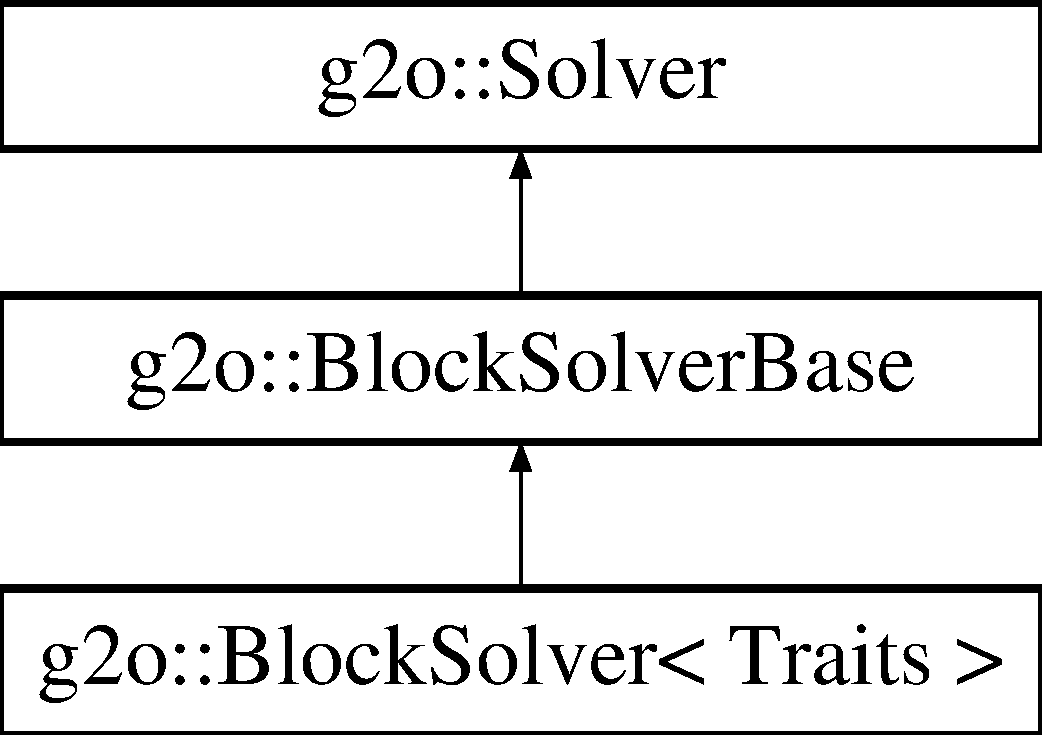
\includegraphics[height=3.000000cm]{classg2o_1_1_block_solver_base}
\end{center}
\end{figure}
\subsection*{Public Member Functions}
\begin{DoxyCompactItemize}
\item 
virtual \mbox{\hyperlink{classg2o_1_1_block_solver_base_a59aabc7d24599a7f7b251cc0040bcb0a}{$\sim$\+Block\+Solver\+Base}} ()
\item 
virtual void \mbox{\hyperlink{classg2o_1_1_block_solver_base_a4ff7072751bfa1b7fcf91f8219e18e13}{multiply\+Hessian}} (double $\ast$dest, const double $\ast$src) const =0
\end{DoxyCompactItemize}
\subsection*{Additional Inherited Members}


\subsection{Detailed Description}
base for the block solvers with some basic function interfaces 

\subsection{Constructor \& Destructor Documentation}
\mbox{\Hypertarget{classg2o_1_1_block_solver_base_a59aabc7d24599a7f7b251cc0040bcb0a}\label{classg2o_1_1_block_solver_base_a59aabc7d24599a7f7b251cc0040bcb0a}} 
\index{g2o\+::\+Block\+Solver\+Base@{g2o\+::\+Block\+Solver\+Base}!````~Block\+Solver\+Base@{$\sim$\+Block\+Solver\+Base}}
\index{````~Block\+Solver\+Base@{$\sim$\+Block\+Solver\+Base}!g2o\+::\+Block\+Solver\+Base@{g2o\+::\+Block\+Solver\+Base}}
\subsubsection{\texorpdfstring{$\sim$\+Block\+Solver\+Base()}{~BlockSolverBase()}}
{\footnotesize\ttfamily virtual g2o\+::\+Block\+Solver\+Base\+::$\sim$\+Block\+Solver\+Base (\begin{DoxyParamCaption}{ }\end{DoxyParamCaption})\hspace{0.3cm}{\ttfamily [inline]}, {\ttfamily [virtual]}}



\subsection{Member Function Documentation}
\mbox{\Hypertarget{classg2o_1_1_block_solver_base_a4ff7072751bfa1b7fcf91f8219e18e13}\label{classg2o_1_1_block_solver_base_a4ff7072751bfa1b7fcf91f8219e18e13}} 
\index{g2o\+::\+Block\+Solver\+Base@{g2o\+::\+Block\+Solver\+Base}!multiply\+Hessian@{multiply\+Hessian}}
\index{multiply\+Hessian@{multiply\+Hessian}!g2o\+::\+Block\+Solver\+Base@{g2o\+::\+Block\+Solver\+Base}}
\subsubsection{\texorpdfstring{multiply\+Hessian()}{multiplyHessian()}}
{\footnotesize\ttfamily virtual void g2o\+::\+Block\+Solver\+Base\+::multiply\+Hessian (\begin{DoxyParamCaption}\item[{double $\ast$}]{dest,  }\item[{const double $\ast$}]{src }\end{DoxyParamCaption}) const\hspace{0.3cm}{\ttfamily [pure virtual]}}

compute dest = H $\ast$ src 

Implemented in \mbox{\hyperlink{classg2o_1_1_block_solver_a6eb8f0729e8bcd760e629421cfa7202c}{g2o\+::\+Block\+Solver$<$ Traits $>$}}.



The documentation for this class was generated from the following file\+:\begin{DoxyCompactItemize}
\item 
D\+:/github/\+V\+S\+L\+A\+M/\+O\+R\+B\+S\+L\+A\+M2/\+O\+R\+B-\/\+S\+L\+A\+M2-\/master/\+Thirdparty/g2o/g2o/core/\mbox{\hyperlink{block__solver_8h}{block\+\_\+solver.\+h}}\end{DoxyCompactItemize}

\hypertarget{structg2o_1_1_block_solver_traits}{}\section{g2o\+:\+:Block\+Solver\+Traits$<$ \+\_\+\+Pose\+Dim, \+\_\+\+Landmark\+Dim $>$ Struct Template Reference}
\label{structg2o_1_1_block_solver_traits}\index{g2o\+::\+Block\+Solver\+Traits$<$ \+\_\+\+Pose\+Dim, \+\_\+\+Landmark\+Dim $>$@{g2o\+::\+Block\+Solver\+Traits$<$ \+\_\+\+Pose\+Dim, \+\_\+\+Landmark\+Dim $>$}}


traits to summarize the properties of the fixed size optimization problem  




{\ttfamily \#include $<$block\+\_\+solver.\+h$>$}

\subsection*{Public Types}
\begin{DoxyCompactItemize}
\item 
typedef Matrix$<$ double, \mbox{\hyperlink{structg2o_1_1_block_solver_traits_a90a03bcfc60b629da5601f6df9514297}{Pose\+Dim}}, \mbox{\hyperlink{structg2o_1_1_block_solver_traits_a90a03bcfc60b629da5601f6df9514297}{Pose\+Dim}} $>$ \mbox{\hyperlink{structg2o_1_1_block_solver_traits_a35e6e4bad138dcfcaa3b1339e168bf30}{Pose\+Matrix\+Type}}
\item 
typedef Matrix$<$ double, \mbox{\hyperlink{structg2o_1_1_block_solver_traits_a7e6e33971e5243e020a9f41cd3182218}{Landmark\+Dim}}, \mbox{\hyperlink{structg2o_1_1_block_solver_traits_a7e6e33971e5243e020a9f41cd3182218}{Landmark\+Dim}} $>$ \mbox{\hyperlink{structg2o_1_1_block_solver_traits_add9b9fbfef352b7654d41914d5eaa58c}{Landmark\+Matrix\+Type}}
\item 
typedef Matrix$<$ double, \mbox{\hyperlink{structg2o_1_1_block_solver_traits_a90a03bcfc60b629da5601f6df9514297}{Pose\+Dim}}, \mbox{\hyperlink{structg2o_1_1_block_solver_traits_a7e6e33971e5243e020a9f41cd3182218}{Landmark\+Dim}} $>$ \mbox{\hyperlink{structg2o_1_1_block_solver_traits_a91e6510ad42179701d22c3ac312237cd}{Pose\+Landmark\+Matrix\+Type}}
\item 
typedef Matrix$<$ double, \mbox{\hyperlink{structg2o_1_1_block_solver_traits_a90a03bcfc60b629da5601f6df9514297}{Pose\+Dim}}, 1 $>$ \mbox{\hyperlink{structg2o_1_1_block_solver_traits_a032ed57e9bc44c36093f97b32e1506f6}{Pose\+Vector\+Type}}
\item 
typedef Matrix$<$ double, \mbox{\hyperlink{structg2o_1_1_block_solver_traits_a7e6e33971e5243e020a9f41cd3182218}{Landmark\+Dim}}, 1 $>$ \mbox{\hyperlink{structg2o_1_1_block_solver_traits_af5154a15abb566ff5bffc0adb9f0458d}{Landmark\+Vector\+Type}}
\item 
typedef \mbox{\hyperlink{classg2o_1_1_sparse_block_matrix}{Sparse\+Block\+Matrix}}$<$ \mbox{\hyperlink{structg2o_1_1_block_solver_traits_a35e6e4bad138dcfcaa3b1339e168bf30}{Pose\+Matrix\+Type}} $>$ \mbox{\hyperlink{structg2o_1_1_block_solver_traits_a03351362339d8e6609c577123350bb2a}{Pose\+Hessian\+Type}}
\item 
typedef \mbox{\hyperlink{classg2o_1_1_sparse_block_matrix}{Sparse\+Block\+Matrix}}$<$ \mbox{\hyperlink{structg2o_1_1_block_solver_traits_add9b9fbfef352b7654d41914d5eaa58c}{Landmark\+Matrix\+Type}} $>$ \mbox{\hyperlink{structg2o_1_1_block_solver_traits_ae761bb32d5267e4d74e5d9c2c7e7ad2f}{Landmark\+Hessian\+Type}}
\item 
typedef \mbox{\hyperlink{classg2o_1_1_sparse_block_matrix}{Sparse\+Block\+Matrix}}$<$ \mbox{\hyperlink{structg2o_1_1_block_solver_traits_a91e6510ad42179701d22c3ac312237cd}{Pose\+Landmark\+Matrix\+Type}} $>$ \mbox{\hyperlink{structg2o_1_1_block_solver_traits_af8ef27915a056caae3b12a9ca609eba6}{Pose\+Landmark\+Hessian\+Type}}
\item 
typedef \mbox{\hyperlink{classg2o_1_1_linear_solver}{Linear\+Solver}}$<$ \mbox{\hyperlink{structg2o_1_1_block_solver_traits_a35e6e4bad138dcfcaa3b1339e168bf30}{Pose\+Matrix\+Type}} $>$ \mbox{\hyperlink{structg2o_1_1_block_solver_traits_add6edae08cb0665c2b1e7c641cdb4dc4}{Linear\+Solver\+Type}}
\end{DoxyCompactItemize}
\subsection*{Static Public Attributes}
\begin{DoxyCompactItemize}
\item 
static const int \mbox{\hyperlink{structg2o_1_1_block_solver_traits_a90a03bcfc60b629da5601f6df9514297}{Pose\+Dim}} = \+\_\+\+Pose\+Dim
\item 
static const int \mbox{\hyperlink{structg2o_1_1_block_solver_traits_a7e6e33971e5243e020a9f41cd3182218}{Landmark\+Dim}} = \+\_\+\+Landmark\+Dim
\end{DoxyCompactItemize}


\subsection{Detailed Description}
\subsubsection*{template$<$int \+\_\+\+Pose\+Dim, int \+\_\+\+Landmark\+Dim$>$\newline
struct g2o\+::\+Block\+Solver\+Traits$<$ \+\_\+\+Pose\+Dim, \+\_\+\+Landmark\+Dim $>$}

traits to summarize the properties of the fixed size optimization problem 

\subsection{Member Typedef Documentation}
\mbox{\Hypertarget{structg2o_1_1_block_solver_traits_ae761bb32d5267e4d74e5d9c2c7e7ad2f}\label{structg2o_1_1_block_solver_traits_ae761bb32d5267e4d74e5d9c2c7e7ad2f}} 
\index{g2o\+::\+Block\+Solver\+Traits@{g2o\+::\+Block\+Solver\+Traits}!Landmark\+Hessian\+Type@{Landmark\+Hessian\+Type}}
\index{Landmark\+Hessian\+Type@{Landmark\+Hessian\+Type}!g2o\+::\+Block\+Solver\+Traits@{g2o\+::\+Block\+Solver\+Traits}}
\subsubsection{\texorpdfstring{Landmark\+Hessian\+Type}{LandmarkHessianType}}
{\footnotesize\ttfamily template$<$int \+\_\+\+Pose\+Dim, int \+\_\+\+Landmark\+Dim$>$ \\
typedef \mbox{\hyperlink{classg2o_1_1_sparse_block_matrix}{Sparse\+Block\+Matrix}}$<$\mbox{\hyperlink{structg2o_1_1_block_solver_traits_add9b9fbfef352b7654d41914d5eaa58c}{Landmark\+Matrix\+Type}}$>$ \mbox{\hyperlink{structg2o_1_1_block_solver_traits}{g2o\+::\+Block\+Solver\+Traits}}$<$ \+\_\+\+Pose\+Dim, \+\_\+\+Landmark\+Dim $>$\+::\mbox{\hyperlink{structg2o_1_1_block_solver_traits_ae761bb32d5267e4d74e5d9c2c7e7ad2f}{Landmark\+Hessian\+Type}}}

\mbox{\Hypertarget{structg2o_1_1_block_solver_traits_add9b9fbfef352b7654d41914d5eaa58c}\label{structg2o_1_1_block_solver_traits_add9b9fbfef352b7654d41914d5eaa58c}} 
\index{g2o\+::\+Block\+Solver\+Traits@{g2o\+::\+Block\+Solver\+Traits}!Landmark\+Matrix\+Type@{Landmark\+Matrix\+Type}}
\index{Landmark\+Matrix\+Type@{Landmark\+Matrix\+Type}!g2o\+::\+Block\+Solver\+Traits@{g2o\+::\+Block\+Solver\+Traits}}
\subsubsection{\texorpdfstring{Landmark\+Matrix\+Type}{LandmarkMatrixType}}
{\footnotesize\ttfamily template$<$int \+\_\+\+Pose\+Dim, int \+\_\+\+Landmark\+Dim$>$ \\
typedef Matrix$<$double, \mbox{\hyperlink{structg2o_1_1_block_solver_traits_a7e6e33971e5243e020a9f41cd3182218}{Landmark\+Dim}}, \mbox{\hyperlink{structg2o_1_1_block_solver_traits_a7e6e33971e5243e020a9f41cd3182218}{Landmark\+Dim}}$>$ \mbox{\hyperlink{structg2o_1_1_block_solver_traits}{g2o\+::\+Block\+Solver\+Traits}}$<$ \+\_\+\+Pose\+Dim, \+\_\+\+Landmark\+Dim $>$\+::\mbox{\hyperlink{structg2o_1_1_block_solver_traits_add9b9fbfef352b7654d41914d5eaa58c}{Landmark\+Matrix\+Type}}}

\mbox{\Hypertarget{structg2o_1_1_block_solver_traits_af5154a15abb566ff5bffc0adb9f0458d}\label{structg2o_1_1_block_solver_traits_af5154a15abb566ff5bffc0adb9f0458d}} 
\index{g2o\+::\+Block\+Solver\+Traits@{g2o\+::\+Block\+Solver\+Traits}!Landmark\+Vector\+Type@{Landmark\+Vector\+Type}}
\index{Landmark\+Vector\+Type@{Landmark\+Vector\+Type}!g2o\+::\+Block\+Solver\+Traits@{g2o\+::\+Block\+Solver\+Traits}}
\subsubsection{\texorpdfstring{Landmark\+Vector\+Type}{LandmarkVectorType}}
{\footnotesize\ttfamily template$<$int \+\_\+\+Pose\+Dim, int \+\_\+\+Landmark\+Dim$>$ \\
typedef Matrix$<$double, \mbox{\hyperlink{structg2o_1_1_block_solver_traits_a7e6e33971e5243e020a9f41cd3182218}{Landmark\+Dim}}, 1$>$ \mbox{\hyperlink{structg2o_1_1_block_solver_traits}{g2o\+::\+Block\+Solver\+Traits}}$<$ \+\_\+\+Pose\+Dim, \+\_\+\+Landmark\+Dim $>$\+::\mbox{\hyperlink{structg2o_1_1_block_solver_traits_af5154a15abb566ff5bffc0adb9f0458d}{Landmark\+Vector\+Type}}}

\mbox{\Hypertarget{structg2o_1_1_block_solver_traits_add6edae08cb0665c2b1e7c641cdb4dc4}\label{structg2o_1_1_block_solver_traits_add6edae08cb0665c2b1e7c641cdb4dc4}} 
\index{g2o\+::\+Block\+Solver\+Traits@{g2o\+::\+Block\+Solver\+Traits}!Linear\+Solver\+Type@{Linear\+Solver\+Type}}
\index{Linear\+Solver\+Type@{Linear\+Solver\+Type}!g2o\+::\+Block\+Solver\+Traits@{g2o\+::\+Block\+Solver\+Traits}}
\subsubsection{\texorpdfstring{Linear\+Solver\+Type}{LinearSolverType}}
{\footnotesize\ttfamily template$<$int \+\_\+\+Pose\+Dim, int \+\_\+\+Landmark\+Dim$>$ \\
typedef \mbox{\hyperlink{classg2o_1_1_linear_solver}{Linear\+Solver}}$<$\mbox{\hyperlink{structg2o_1_1_block_solver_traits_a35e6e4bad138dcfcaa3b1339e168bf30}{Pose\+Matrix\+Type}}$>$ \mbox{\hyperlink{structg2o_1_1_block_solver_traits}{g2o\+::\+Block\+Solver\+Traits}}$<$ \+\_\+\+Pose\+Dim, \+\_\+\+Landmark\+Dim $>$\+::\mbox{\hyperlink{structg2o_1_1_block_solver_traits_add6edae08cb0665c2b1e7c641cdb4dc4}{Linear\+Solver\+Type}}}

\mbox{\Hypertarget{structg2o_1_1_block_solver_traits_a03351362339d8e6609c577123350bb2a}\label{structg2o_1_1_block_solver_traits_a03351362339d8e6609c577123350bb2a}} 
\index{g2o\+::\+Block\+Solver\+Traits@{g2o\+::\+Block\+Solver\+Traits}!Pose\+Hessian\+Type@{Pose\+Hessian\+Type}}
\index{Pose\+Hessian\+Type@{Pose\+Hessian\+Type}!g2o\+::\+Block\+Solver\+Traits@{g2o\+::\+Block\+Solver\+Traits}}
\subsubsection{\texorpdfstring{Pose\+Hessian\+Type}{PoseHessianType}}
{\footnotesize\ttfamily template$<$int \+\_\+\+Pose\+Dim, int \+\_\+\+Landmark\+Dim$>$ \\
typedef \mbox{\hyperlink{classg2o_1_1_sparse_block_matrix}{Sparse\+Block\+Matrix}}$<$\mbox{\hyperlink{structg2o_1_1_block_solver_traits_a35e6e4bad138dcfcaa3b1339e168bf30}{Pose\+Matrix\+Type}}$>$ \mbox{\hyperlink{structg2o_1_1_block_solver_traits}{g2o\+::\+Block\+Solver\+Traits}}$<$ \+\_\+\+Pose\+Dim, \+\_\+\+Landmark\+Dim $>$\+::\mbox{\hyperlink{structg2o_1_1_block_solver_traits_a03351362339d8e6609c577123350bb2a}{Pose\+Hessian\+Type}}}

\mbox{\Hypertarget{structg2o_1_1_block_solver_traits_af8ef27915a056caae3b12a9ca609eba6}\label{structg2o_1_1_block_solver_traits_af8ef27915a056caae3b12a9ca609eba6}} 
\index{g2o\+::\+Block\+Solver\+Traits@{g2o\+::\+Block\+Solver\+Traits}!Pose\+Landmark\+Hessian\+Type@{Pose\+Landmark\+Hessian\+Type}}
\index{Pose\+Landmark\+Hessian\+Type@{Pose\+Landmark\+Hessian\+Type}!g2o\+::\+Block\+Solver\+Traits@{g2o\+::\+Block\+Solver\+Traits}}
\subsubsection{\texorpdfstring{Pose\+Landmark\+Hessian\+Type}{PoseLandmarkHessianType}}
{\footnotesize\ttfamily template$<$int \+\_\+\+Pose\+Dim, int \+\_\+\+Landmark\+Dim$>$ \\
typedef \mbox{\hyperlink{classg2o_1_1_sparse_block_matrix}{Sparse\+Block\+Matrix}}$<$\mbox{\hyperlink{structg2o_1_1_block_solver_traits_a91e6510ad42179701d22c3ac312237cd}{Pose\+Landmark\+Matrix\+Type}}$>$ \mbox{\hyperlink{structg2o_1_1_block_solver_traits}{g2o\+::\+Block\+Solver\+Traits}}$<$ \+\_\+\+Pose\+Dim, \+\_\+\+Landmark\+Dim $>$\+::\mbox{\hyperlink{structg2o_1_1_block_solver_traits_af8ef27915a056caae3b12a9ca609eba6}{Pose\+Landmark\+Hessian\+Type}}}

\mbox{\Hypertarget{structg2o_1_1_block_solver_traits_a91e6510ad42179701d22c3ac312237cd}\label{structg2o_1_1_block_solver_traits_a91e6510ad42179701d22c3ac312237cd}} 
\index{g2o\+::\+Block\+Solver\+Traits@{g2o\+::\+Block\+Solver\+Traits}!Pose\+Landmark\+Matrix\+Type@{Pose\+Landmark\+Matrix\+Type}}
\index{Pose\+Landmark\+Matrix\+Type@{Pose\+Landmark\+Matrix\+Type}!g2o\+::\+Block\+Solver\+Traits@{g2o\+::\+Block\+Solver\+Traits}}
\subsubsection{\texorpdfstring{Pose\+Landmark\+Matrix\+Type}{PoseLandmarkMatrixType}}
{\footnotesize\ttfamily template$<$int \+\_\+\+Pose\+Dim, int \+\_\+\+Landmark\+Dim$>$ \\
typedef Matrix$<$double, \mbox{\hyperlink{structg2o_1_1_block_solver_traits_a90a03bcfc60b629da5601f6df9514297}{Pose\+Dim}}, \mbox{\hyperlink{structg2o_1_1_block_solver_traits_a7e6e33971e5243e020a9f41cd3182218}{Landmark\+Dim}}$>$ \mbox{\hyperlink{structg2o_1_1_block_solver_traits}{g2o\+::\+Block\+Solver\+Traits}}$<$ \+\_\+\+Pose\+Dim, \+\_\+\+Landmark\+Dim $>$\+::\mbox{\hyperlink{structg2o_1_1_block_solver_traits_a91e6510ad42179701d22c3ac312237cd}{Pose\+Landmark\+Matrix\+Type}}}

\mbox{\Hypertarget{structg2o_1_1_block_solver_traits_a35e6e4bad138dcfcaa3b1339e168bf30}\label{structg2o_1_1_block_solver_traits_a35e6e4bad138dcfcaa3b1339e168bf30}} 
\index{g2o\+::\+Block\+Solver\+Traits@{g2o\+::\+Block\+Solver\+Traits}!Pose\+Matrix\+Type@{Pose\+Matrix\+Type}}
\index{Pose\+Matrix\+Type@{Pose\+Matrix\+Type}!g2o\+::\+Block\+Solver\+Traits@{g2o\+::\+Block\+Solver\+Traits}}
\subsubsection{\texorpdfstring{Pose\+Matrix\+Type}{PoseMatrixType}}
{\footnotesize\ttfamily template$<$int \+\_\+\+Pose\+Dim, int \+\_\+\+Landmark\+Dim$>$ \\
typedef Matrix$<$double, \mbox{\hyperlink{structg2o_1_1_block_solver_traits_a90a03bcfc60b629da5601f6df9514297}{Pose\+Dim}}, \mbox{\hyperlink{structg2o_1_1_block_solver_traits_a90a03bcfc60b629da5601f6df9514297}{Pose\+Dim}}$>$ \mbox{\hyperlink{structg2o_1_1_block_solver_traits}{g2o\+::\+Block\+Solver\+Traits}}$<$ \+\_\+\+Pose\+Dim, \+\_\+\+Landmark\+Dim $>$\+::\mbox{\hyperlink{structg2o_1_1_block_solver_traits_a35e6e4bad138dcfcaa3b1339e168bf30}{Pose\+Matrix\+Type}}}

\mbox{\Hypertarget{structg2o_1_1_block_solver_traits_a032ed57e9bc44c36093f97b32e1506f6}\label{structg2o_1_1_block_solver_traits_a032ed57e9bc44c36093f97b32e1506f6}} 
\index{g2o\+::\+Block\+Solver\+Traits@{g2o\+::\+Block\+Solver\+Traits}!Pose\+Vector\+Type@{Pose\+Vector\+Type}}
\index{Pose\+Vector\+Type@{Pose\+Vector\+Type}!g2o\+::\+Block\+Solver\+Traits@{g2o\+::\+Block\+Solver\+Traits}}
\subsubsection{\texorpdfstring{Pose\+Vector\+Type}{PoseVectorType}}
{\footnotesize\ttfamily template$<$int \+\_\+\+Pose\+Dim, int \+\_\+\+Landmark\+Dim$>$ \\
typedef Matrix$<$double, \mbox{\hyperlink{structg2o_1_1_block_solver_traits_a90a03bcfc60b629da5601f6df9514297}{Pose\+Dim}}, 1$>$ \mbox{\hyperlink{structg2o_1_1_block_solver_traits}{g2o\+::\+Block\+Solver\+Traits}}$<$ \+\_\+\+Pose\+Dim, \+\_\+\+Landmark\+Dim $>$\+::\mbox{\hyperlink{structg2o_1_1_block_solver_traits_a032ed57e9bc44c36093f97b32e1506f6}{Pose\+Vector\+Type}}}



\subsection{Member Data Documentation}
\mbox{\Hypertarget{structg2o_1_1_block_solver_traits_a7e6e33971e5243e020a9f41cd3182218}\label{structg2o_1_1_block_solver_traits_a7e6e33971e5243e020a9f41cd3182218}} 
\index{g2o\+::\+Block\+Solver\+Traits@{g2o\+::\+Block\+Solver\+Traits}!Landmark\+Dim@{Landmark\+Dim}}
\index{Landmark\+Dim@{Landmark\+Dim}!g2o\+::\+Block\+Solver\+Traits@{g2o\+::\+Block\+Solver\+Traits}}
\subsubsection{\texorpdfstring{Landmark\+Dim}{LandmarkDim}}
{\footnotesize\ttfamily template$<$int \+\_\+\+Pose\+Dim, int \+\_\+\+Landmark\+Dim$>$ \\
const int \mbox{\hyperlink{structg2o_1_1_block_solver_traits}{g2o\+::\+Block\+Solver\+Traits}}$<$ \+\_\+\+Pose\+Dim, \+\_\+\+Landmark\+Dim $>$\+::Landmark\+Dim = \+\_\+\+Landmark\+Dim\hspace{0.3cm}{\ttfamily [static]}}

\mbox{\Hypertarget{structg2o_1_1_block_solver_traits_a90a03bcfc60b629da5601f6df9514297}\label{structg2o_1_1_block_solver_traits_a90a03bcfc60b629da5601f6df9514297}} 
\index{g2o\+::\+Block\+Solver\+Traits@{g2o\+::\+Block\+Solver\+Traits}!Pose\+Dim@{Pose\+Dim}}
\index{Pose\+Dim@{Pose\+Dim}!g2o\+::\+Block\+Solver\+Traits@{g2o\+::\+Block\+Solver\+Traits}}
\subsubsection{\texorpdfstring{Pose\+Dim}{PoseDim}}
{\footnotesize\ttfamily template$<$int \+\_\+\+Pose\+Dim, int \+\_\+\+Landmark\+Dim$>$ \\
const int \mbox{\hyperlink{structg2o_1_1_block_solver_traits}{g2o\+::\+Block\+Solver\+Traits}}$<$ \+\_\+\+Pose\+Dim, \+\_\+\+Landmark\+Dim $>$\+::Pose\+Dim = \+\_\+\+Pose\+Dim\hspace{0.3cm}{\ttfamily [static]}}



The documentation for this struct was generated from the following file\+:\begin{DoxyCompactItemize}
\item 
Thirdparty/g2o/g2o/core/\mbox{\hyperlink{block__solver_8h}{block\+\_\+solver.\+h}}\end{DoxyCompactItemize}

\hypertarget{structg2o_1_1_block_solver_traits_3_01_eigen_1_1_dynamic_00_01_eigen_1_1_dynamic_01_4}{}\section{g2o\+:\+:Block\+Solver\+Traits$<$ Eigen\+:\+:Dynamic, Eigen\+:\+:Dynamic $>$ Struct Template Reference}
\label{structg2o_1_1_block_solver_traits_3_01_eigen_1_1_dynamic_00_01_eigen_1_1_dynamic_01_4}\index{g2o\+::\+Block\+Solver\+Traits$<$ Eigen\+::\+Dynamic, Eigen\+::\+Dynamic $>$@{g2o\+::\+Block\+Solver\+Traits$<$ Eigen\+::\+Dynamic, Eigen\+::\+Dynamic $>$}}


traits to summarize the properties of the dynamic size optimization problem  




{\ttfamily \#include $<$block\+\_\+solver.\+h$>$}

\subsection*{Public Types}
\begin{DoxyCompactItemize}
\item 
typedef Matrix\+Xd \mbox{\hyperlink{structg2o_1_1_block_solver_traits_3_01_eigen_1_1_dynamic_00_01_eigen_1_1_dynamic_01_4_a11131d4b2d25cea90eef0d3687eb6dc1}{Pose\+Matrix\+Type}}
\item 
typedef Matrix\+Xd \mbox{\hyperlink{structg2o_1_1_block_solver_traits_3_01_eigen_1_1_dynamic_00_01_eigen_1_1_dynamic_01_4_a4409de5074b3458f33ba2015e2fa6891}{Landmark\+Matrix\+Type}}
\item 
typedef Matrix\+Xd \mbox{\hyperlink{structg2o_1_1_block_solver_traits_3_01_eigen_1_1_dynamic_00_01_eigen_1_1_dynamic_01_4_ab81ac9673971ec5c896f4b431ae30f0b}{Pose\+Landmark\+Matrix\+Type}}
\item 
typedef Vector\+Xd \mbox{\hyperlink{structg2o_1_1_block_solver_traits_3_01_eigen_1_1_dynamic_00_01_eigen_1_1_dynamic_01_4_ae8ae50131f5aeaf97c844e20960ebaf3}{Pose\+Vector\+Type}}
\item 
typedef Vector\+Xd \mbox{\hyperlink{structg2o_1_1_block_solver_traits_3_01_eigen_1_1_dynamic_00_01_eigen_1_1_dynamic_01_4_aaff14917064b8670c918e571fcdc4666}{Landmark\+Vector\+Type}}
\item 
typedef \mbox{\hyperlink{classg2o_1_1_sparse_block_matrix}{Sparse\+Block\+Matrix}}$<$ \mbox{\hyperlink{structg2o_1_1_block_solver_traits_3_01_eigen_1_1_dynamic_00_01_eigen_1_1_dynamic_01_4_a11131d4b2d25cea90eef0d3687eb6dc1}{Pose\+Matrix\+Type}} $>$ \mbox{\hyperlink{structg2o_1_1_block_solver_traits_3_01_eigen_1_1_dynamic_00_01_eigen_1_1_dynamic_01_4_a380bde2a88f9b257142dd3419422e5a3}{Pose\+Hessian\+Type}}
\item 
typedef \mbox{\hyperlink{classg2o_1_1_sparse_block_matrix}{Sparse\+Block\+Matrix}}$<$ \mbox{\hyperlink{structg2o_1_1_block_solver_traits_3_01_eigen_1_1_dynamic_00_01_eigen_1_1_dynamic_01_4_a4409de5074b3458f33ba2015e2fa6891}{Landmark\+Matrix\+Type}} $>$ \mbox{\hyperlink{structg2o_1_1_block_solver_traits_3_01_eigen_1_1_dynamic_00_01_eigen_1_1_dynamic_01_4_a73a81a0aeabd1216ae3a8f5700666ac4}{Landmark\+Hessian\+Type}}
\item 
typedef \mbox{\hyperlink{classg2o_1_1_sparse_block_matrix}{Sparse\+Block\+Matrix}}$<$ \mbox{\hyperlink{structg2o_1_1_block_solver_traits_3_01_eigen_1_1_dynamic_00_01_eigen_1_1_dynamic_01_4_ab81ac9673971ec5c896f4b431ae30f0b}{Pose\+Landmark\+Matrix\+Type}} $>$ \mbox{\hyperlink{structg2o_1_1_block_solver_traits_3_01_eigen_1_1_dynamic_00_01_eigen_1_1_dynamic_01_4_aa6f67fd6ba29156f6d1069db0c3b5d11}{Pose\+Landmark\+Hessian\+Type}}
\item 
typedef \mbox{\hyperlink{classg2o_1_1_linear_solver}{Linear\+Solver}}$<$ \mbox{\hyperlink{structg2o_1_1_block_solver_traits_3_01_eigen_1_1_dynamic_00_01_eigen_1_1_dynamic_01_4_a11131d4b2d25cea90eef0d3687eb6dc1}{Pose\+Matrix\+Type}} $>$ \mbox{\hyperlink{structg2o_1_1_block_solver_traits_3_01_eigen_1_1_dynamic_00_01_eigen_1_1_dynamic_01_4_ad062ca3c21bf3a3e08d5350174d93d6d}{Linear\+Solver\+Type}}
\end{DoxyCompactItemize}
\subsection*{Static Public Attributes}
\begin{DoxyCompactItemize}
\item 
static const int \mbox{\hyperlink{structg2o_1_1_block_solver_traits_3_01_eigen_1_1_dynamic_00_01_eigen_1_1_dynamic_01_4_a04a2cc2de80563b4b21f815150c3b0ec}{Pose\+Dim}} = Eigen\+::\+Dynamic
\item 
static const int \mbox{\hyperlink{structg2o_1_1_block_solver_traits_3_01_eigen_1_1_dynamic_00_01_eigen_1_1_dynamic_01_4_aa8f7b7c3fc1ce4a7d61e925e3067e196}{Landmark\+Dim}} = Eigen\+::\+Dynamic
\end{DoxyCompactItemize}


\subsection{Detailed Description}
\subsubsection*{template$<$$>$\newline
struct g2o\+::\+Block\+Solver\+Traits$<$ Eigen\+::\+Dynamic, Eigen\+::\+Dynamic $>$}

traits to summarize the properties of the dynamic size optimization problem 

\subsection{Member Typedef Documentation}
\mbox{\Hypertarget{structg2o_1_1_block_solver_traits_3_01_eigen_1_1_dynamic_00_01_eigen_1_1_dynamic_01_4_a73a81a0aeabd1216ae3a8f5700666ac4}\label{structg2o_1_1_block_solver_traits_3_01_eigen_1_1_dynamic_00_01_eigen_1_1_dynamic_01_4_a73a81a0aeabd1216ae3a8f5700666ac4}} 
\index{g2o\+::\+Block\+Solver\+Traits$<$ Eigen\+::\+Dynamic, Eigen\+::\+Dynamic $>$@{g2o\+::\+Block\+Solver\+Traits$<$ Eigen\+::\+Dynamic, Eigen\+::\+Dynamic $>$}!Landmark\+Hessian\+Type@{Landmark\+Hessian\+Type}}
\index{Landmark\+Hessian\+Type@{Landmark\+Hessian\+Type}!g2o\+::\+Block\+Solver\+Traits$<$ Eigen\+::\+Dynamic, Eigen\+::\+Dynamic $>$@{g2o\+::\+Block\+Solver\+Traits$<$ Eigen\+::\+Dynamic, Eigen\+::\+Dynamic $>$}}
\subsubsection{\texorpdfstring{Landmark\+Hessian\+Type}{LandmarkHessianType}}
{\footnotesize\ttfamily typedef \mbox{\hyperlink{classg2o_1_1_sparse_block_matrix}{Sparse\+Block\+Matrix}}$<$\mbox{\hyperlink{structg2o_1_1_block_solver_traits_3_01_eigen_1_1_dynamic_00_01_eigen_1_1_dynamic_01_4_a4409de5074b3458f33ba2015e2fa6891}{Landmark\+Matrix\+Type}}$>$ \mbox{\hyperlink{structg2o_1_1_block_solver_traits}{g2o\+::\+Block\+Solver\+Traits}}$<$ Eigen\+::\+Dynamic, Eigen\+::\+Dynamic $>$\+::\mbox{\hyperlink{structg2o_1_1_block_solver_traits_3_01_eigen_1_1_dynamic_00_01_eigen_1_1_dynamic_01_4_a73a81a0aeabd1216ae3a8f5700666ac4}{Landmark\+Hessian\+Type}}}

\mbox{\Hypertarget{structg2o_1_1_block_solver_traits_3_01_eigen_1_1_dynamic_00_01_eigen_1_1_dynamic_01_4_a4409de5074b3458f33ba2015e2fa6891}\label{structg2o_1_1_block_solver_traits_3_01_eigen_1_1_dynamic_00_01_eigen_1_1_dynamic_01_4_a4409de5074b3458f33ba2015e2fa6891}} 
\index{g2o\+::\+Block\+Solver\+Traits$<$ Eigen\+::\+Dynamic, Eigen\+::\+Dynamic $>$@{g2o\+::\+Block\+Solver\+Traits$<$ Eigen\+::\+Dynamic, Eigen\+::\+Dynamic $>$}!Landmark\+Matrix\+Type@{Landmark\+Matrix\+Type}}
\index{Landmark\+Matrix\+Type@{Landmark\+Matrix\+Type}!g2o\+::\+Block\+Solver\+Traits$<$ Eigen\+::\+Dynamic, Eigen\+::\+Dynamic $>$@{g2o\+::\+Block\+Solver\+Traits$<$ Eigen\+::\+Dynamic, Eigen\+::\+Dynamic $>$}}
\subsubsection{\texorpdfstring{Landmark\+Matrix\+Type}{LandmarkMatrixType}}
{\footnotesize\ttfamily typedef Matrix\+Xd \mbox{\hyperlink{structg2o_1_1_block_solver_traits}{g2o\+::\+Block\+Solver\+Traits}}$<$ Eigen\+::\+Dynamic, Eigen\+::\+Dynamic $>$\+::\mbox{\hyperlink{structg2o_1_1_block_solver_traits_3_01_eigen_1_1_dynamic_00_01_eigen_1_1_dynamic_01_4_a4409de5074b3458f33ba2015e2fa6891}{Landmark\+Matrix\+Type}}}

\mbox{\Hypertarget{structg2o_1_1_block_solver_traits_3_01_eigen_1_1_dynamic_00_01_eigen_1_1_dynamic_01_4_aaff14917064b8670c918e571fcdc4666}\label{structg2o_1_1_block_solver_traits_3_01_eigen_1_1_dynamic_00_01_eigen_1_1_dynamic_01_4_aaff14917064b8670c918e571fcdc4666}} 
\index{g2o\+::\+Block\+Solver\+Traits$<$ Eigen\+::\+Dynamic, Eigen\+::\+Dynamic $>$@{g2o\+::\+Block\+Solver\+Traits$<$ Eigen\+::\+Dynamic, Eigen\+::\+Dynamic $>$}!Landmark\+Vector\+Type@{Landmark\+Vector\+Type}}
\index{Landmark\+Vector\+Type@{Landmark\+Vector\+Type}!g2o\+::\+Block\+Solver\+Traits$<$ Eigen\+::\+Dynamic, Eigen\+::\+Dynamic $>$@{g2o\+::\+Block\+Solver\+Traits$<$ Eigen\+::\+Dynamic, Eigen\+::\+Dynamic $>$}}
\subsubsection{\texorpdfstring{Landmark\+Vector\+Type}{LandmarkVectorType}}
{\footnotesize\ttfamily typedef Vector\+Xd \mbox{\hyperlink{structg2o_1_1_block_solver_traits}{g2o\+::\+Block\+Solver\+Traits}}$<$ Eigen\+::\+Dynamic, Eigen\+::\+Dynamic $>$\+::\mbox{\hyperlink{structg2o_1_1_block_solver_traits_3_01_eigen_1_1_dynamic_00_01_eigen_1_1_dynamic_01_4_aaff14917064b8670c918e571fcdc4666}{Landmark\+Vector\+Type}}}

\mbox{\Hypertarget{structg2o_1_1_block_solver_traits_3_01_eigen_1_1_dynamic_00_01_eigen_1_1_dynamic_01_4_ad062ca3c21bf3a3e08d5350174d93d6d}\label{structg2o_1_1_block_solver_traits_3_01_eigen_1_1_dynamic_00_01_eigen_1_1_dynamic_01_4_ad062ca3c21bf3a3e08d5350174d93d6d}} 
\index{g2o\+::\+Block\+Solver\+Traits$<$ Eigen\+::\+Dynamic, Eigen\+::\+Dynamic $>$@{g2o\+::\+Block\+Solver\+Traits$<$ Eigen\+::\+Dynamic, Eigen\+::\+Dynamic $>$}!Linear\+Solver\+Type@{Linear\+Solver\+Type}}
\index{Linear\+Solver\+Type@{Linear\+Solver\+Type}!g2o\+::\+Block\+Solver\+Traits$<$ Eigen\+::\+Dynamic, Eigen\+::\+Dynamic $>$@{g2o\+::\+Block\+Solver\+Traits$<$ Eigen\+::\+Dynamic, Eigen\+::\+Dynamic $>$}}
\subsubsection{\texorpdfstring{Linear\+Solver\+Type}{LinearSolverType}}
{\footnotesize\ttfamily typedef \mbox{\hyperlink{classg2o_1_1_linear_solver}{Linear\+Solver}}$<$\mbox{\hyperlink{structg2o_1_1_block_solver_traits_3_01_eigen_1_1_dynamic_00_01_eigen_1_1_dynamic_01_4_a11131d4b2d25cea90eef0d3687eb6dc1}{Pose\+Matrix\+Type}}$>$ \mbox{\hyperlink{structg2o_1_1_block_solver_traits}{g2o\+::\+Block\+Solver\+Traits}}$<$ Eigen\+::\+Dynamic, Eigen\+::\+Dynamic $>$\+::\mbox{\hyperlink{structg2o_1_1_block_solver_traits_3_01_eigen_1_1_dynamic_00_01_eigen_1_1_dynamic_01_4_ad062ca3c21bf3a3e08d5350174d93d6d}{Linear\+Solver\+Type}}}

\mbox{\Hypertarget{structg2o_1_1_block_solver_traits_3_01_eigen_1_1_dynamic_00_01_eigen_1_1_dynamic_01_4_a380bde2a88f9b257142dd3419422e5a3}\label{structg2o_1_1_block_solver_traits_3_01_eigen_1_1_dynamic_00_01_eigen_1_1_dynamic_01_4_a380bde2a88f9b257142dd3419422e5a3}} 
\index{g2o\+::\+Block\+Solver\+Traits$<$ Eigen\+::\+Dynamic, Eigen\+::\+Dynamic $>$@{g2o\+::\+Block\+Solver\+Traits$<$ Eigen\+::\+Dynamic, Eigen\+::\+Dynamic $>$}!Pose\+Hessian\+Type@{Pose\+Hessian\+Type}}
\index{Pose\+Hessian\+Type@{Pose\+Hessian\+Type}!g2o\+::\+Block\+Solver\+Traits$<$ Eigen\+::\+Dynamic, Eigen\+::\+Dynamic $>$@{g2o\+::\+Block\+Solver\+Traits$<$ Eigen\+::\+Dynamic, Eigen\+::\+Dynamic $>$}}
\subsubsection{\texorpdfstring{Pose\+Hessian\+Type}{PoseHessianType}}
{\footnotesize\ttfamily typedef \mbox{\hyperlink{classg2o_1_1_sparse_block_matrix}{Sparse\+Block\+Matrix}}$<$\mbox{\hyperlink{structg2o_1_1_block_solver_traits_3_01_eigen_1_1_dynamic_00_01_eigen_1_1_dynamic_01_4_a11131d4b2d25cea90eef0d3687eb6dc1}{Pose\+Matrix\+Type}}$>$ \mbox{\hyperlink{structg2o_1_1_block_solver_traits}{g2o\+::\+Block\+Solver\+Traits}}$<$ Eigen\+::\+Dynamic, Eigen\+::\+Dynamic $>$\+::\mbox{\hyperlink{structg2o_1_1_block_solver_traits_3_01_eigen_1_1_dynamic_00_01_eigen_1_1_dynamic_01_4_a380bde2a88f9b257142dd3419422e5a3}{Pose\+Hessian\+Type}}}

\mbox{\Hypertarget{structg2o_1_1_block_solver_traits_3_01_eigen_1_1_dynamic_00_01_eigen_1_1_dynamic_01_4_aa6f67fd6ba29156f6d1069db0c3b5d11}\label{structg2o_1_1_block_solver_traits_3_01_eigen_1_1_dynamic_00_01_eigen_1_1_dynamic_01_4_aa6f67fd6ba29156f6d1069db0c3b5d11}} 
\index{g2o\+::\+Block\+Solver\+Traits$<$ Eigen\+::\+Dynamic, Eigen\+::\+Dynamic $>$@{g2o\+::\+Block\+Solver\+Traits$<$ Eigen\+::\+Dynamic, Eigen\+::\+Dynamic $>$}!Pose\+Landmark\+Hessian\+Type@{Pose\+Landmark\+Hessian\+Type}}
\index{Pose\+Landmark\+Hessian\+Type@{Pose\+Landmark\+Hessian\+Type}!g2o\+::\+Block\+Solver\+Traits$<$ Eigen\+::\+Dynamic, Eigen\+::\+Dynamic $>$@{g2o\+::\+Block\+Solver\+Traits$<$ Eigen\+::\+Dynamic, Eigen\+::\+Dynamic $>$}}
\subsubsection{\texorpdfstring{Pose\+Landmark\+Hessian\+Type}{PoseLandmarkHessianType}}
{\footnotesize\ttfamily typedef \mbox{\hyperlink{classg2o_1_1_sparse_block_matrix}{Sparse\+Block\+Matrix}}$<$\mbox{\hyperlink{structg2o_1_1_block_solver_traits_3_01_eigen_1_1_dynamic_00_01_eigen_1_1_dynamic_01_4_ab81ac9673971ec5c896f4b431ae30f0b}{Pose\+Landmark\+Matrix\+Type}}$>$ \mbox{\hyperlink{structg2o_1_1_block_solver_traits}{g2o\+::\+Block\+Solver\+Traits}}$<$ Eigen\+::\+Dynamic, Eigen\+::\+Dynamic $>$\+::\mbox{\hyperlink{structg2o_1_1_block_solver_traits_3_01_eigen_1_1_dynamic_00_01_eigen_1_1_dynamic_01_4_aa6f67fd6ba29156f6d1069db0c3b5d11}{Pose\+Landmark\+Hessian\+Type}}}

\mbox{\Hypertarget{structg2o_1_1_block_solver_traits_3_01_eigen_1_1_dynamic_00_01_eigen_1_1_dynamic_01_4_ab81ac9673971ec5c896f4b431ae30f0b}\label{structg2o_1_1_block_solver_traits_3_01_eigen_1_1_dynamic_00_01_eigen_1_1_dynamic_01_4_ab81ac9673971ec5c896f4b431ae30f0b}} 
\index{g2o\+::\+Block\+Solver\+Traits$<$ Eigen\+::\+Dynamic, Eigen\+::\+Dynamic $>$@{g2o\+::\+Block\+Solver\+Traits$<$ Eigen\+::\+Dynamic, Eigen\+::\+Dynamic $>$}!Pose\+Landmark\+Matrix\+Type@{Pose\+Landmark\+Matrix\+Type}}
\index{Pose\+Landmark\+Matrix\+Type@{Pose\+Landmark\+Matrix\+Type}!g2o\+::\+Block\+Solver\+Traits$<$ Eigen\+::\+Dynamic, Eigen\+::\+Dynamic $>$@{g2o\+::\+Block\+Solver\+Traits$<$ Eigen\+::\+Dynamic, Eigen\+::\+Dynamic $>$}}
\subsubsection{\texorpdfstring{Pose\+Landmark\+Matrix\+Type}{PoseLandmarkMatrixType}}
{\footnotesize\ttfamily typedef Matrix\+Xd \mbox{\hyperlink{structg2o_1_1_block_solver_traits}{g2o\+::\+Block\+Solver\+Traits}}$<$ Eigen\+::\+Dynamic, Eigen\+::\+Dynamic $>$\+::\mbox{\hyperlink{structg2o_1_1_block_solver_traits_3_01_eigen_1_1_dynamic_00_01_eigen_1_1_dynamic_01_4_ab81ac9673971ec5c896f4b431ae30f0b}{Pose\+Landmark\+Matrix\+Type}}}

\mbox{\Hypertarget{structg2o_1_1_block_solver_traits_3_01_eigen_1_1_dynamic_00_01_eigen_1_1_dynamic_01_4_a11131d4b2d25cea90eef0d3687eb6dc1}\label{structg2o_1_1_block_solver_traits_3_01_eigen_1_1_dynamic_00_01_eigen_1_1_dynamic_01_4_a11131d4b2d25cea90eef0d3687eb6dc1}} 
\index{g2o\+::\+Block\+Solver\+Traits$<$ Eigen\+::\+Dynamic, Eigen\+::\+Dynamic $>$@{g2o\+::\+Block\+Solver\+Traits$<$ Eigen\+::\+Dynamic, Eigen\+::\+Dynamic $>$}!Pose\+Matrix\+Type@{Pose\+Matrix\+Type}}
\index{Pose\+Matrix\+Type@{Pose\+Matrix\+Type}!g2o\+::\+Block\+Solver\+Traits$<$ Eigen\+::\+Dynamic, Eigen\+::\+Dynamic $>$@{g2o\+::\+Block\+Solver\+Traits$<$ Eigen\+::\+Dynamic, Eigen\+::\+Dynamic $>$}}
\subsubsection{\texorpdfstring{Pose\+Matrix\+Type}{PoseMatrixType}}
{\footnotesize\ttfamily typedef Matrix\+Xd \mbox{\hyperlink{structg2o_1_1_block_solver_traits}{g2o\+::\+Block\+Solver\+Traits}}$<$ Eigen\+::\+Dynamic, Eigen\+::\+Dynamic $>$\+::\mbox{\hyperlink{structg2o_1_1_block_solver_traits_3_01_eigen_1_1_dynamic_00_01_eigen_1_1_dynamic_01_4_a11131d4b2d25cea90eef0d3687eb6dc1}{Pose\+Matrix\+Type}}}

\mbox{\Hypertarget{structg2o_1_1_block_solver_traits_3_01_eigen_1_1_dynamic_00_01_eigen_1_1_dynamic_01_4_ae8ae50131f5aeaf97c844e20960ebaf3}\label{structg2o_1_1_block_solver_traits_3_01_eigen_1_1_dynamic_00_01_eigen_1_1_dynamic_01_4_ae8ae50131f5aeaf97c844e20960ebaf3}} 
\index{g2o\+::\+Block\+Solver\+Traits$<$ Eigen\+::\+Dynamic, Eigen\+::\+Dynamic $>$@{g2o\+::\+Block\+Solver\+Traits$<$ Eigen\+::\+Dynamic, Eigen\+::\+Dynamic $>$}!Pose\+Vector\+Type@{Pose\+Vector\+Type}}
\index{Pose\+Vector\+Type@{Pose\+Vector\+Type}!g2o\+::\+Block\+Solver\+Traits$<$ Eigen\+::\+Dynamic, Eigen\+::\+Dynamic $>$@{g2o\+::\+Block\+Solver\+Traits$<$ Eigen\+::\+Dynamic, Eigen\+::\+Dynamic $>$}}
\subsubsection{\texorpdfstring{Pose\+Vector\+Type}{PoseVectorType}}
{\footnotesize\ttfamily typedef Vector\+Xd \mbox{\hyperlink{structg2o_1_1_block_solver_traits}{g2o\+::\+Block\+Solver\+Traits}}$<$ Eigen\+::\+Dynamic, Eigen\+::\+Dynamic $>$\+::\mbox{\hyperlink{structg2o_1_1_block_solver_traits_3_01_eigen_1_1_dynamic_00_01_eigen_1_1_dynamic_01_4_ae8ae50131f5aeaf97c844e20960ebaf3}{Pose\+Vector\+Type}}}



\subsection{Member Data Documentation}
\mbox{\Hypertarget{structg2o_1_1_block_solver_traits_3_01_eigen_1_1_dynamic_00_01_eigen_1_1_dynamic_01_4_aa8f7b7c3fc1ce4a7d61e925e3067e196}\label{structg2o_1_1_block_solver_traits_3_01_eigen_1_1_dynamic_00_01_eigen_1_1_dynamic_01_4_aa8f7b7c3fc1ce4a7d61e925e3067e196}} 
\index{g2o\+::\+Block\+Solver\+Traits$<$ Eigen\+::\+Dynamic, Eigen\+::\+Dynamic $>$@{g2o\+::\+Block\+Solver\+Traits$<$ Eigen\+::\+Dynamic, Eigen\+::\+Dynamic $>$}!Landmark\+Dim@{Landmark\+Dim}}
\index{Landmark\+Dim@{Landmark\+Dim}!g2o\+::\+Block\+Solver\+Traits$<$ Eigen\+::\+Dynamic, Eigen\+::\+Dynamic $>$@{g2o\+::\+Block\+Solver\+Traits$<$ Eigen\+::\+Dynamic, Eigen\+::\+Dynamic $>$}}
\subsubsection{\texorpdfstring{Landmark\+Dim}{LandmarkDim}}
{\footnotesize\ttfamily const int \mbox{\hyperlink{structg2o_1_1_block_solver_traits}{g2o\+::\+Block\+Solver\+Traits}}$<$ Eigen\+::\+Dynamic, Eigen\+::\+Dynamic $>$\+::Landmark\+Dim = Eigen\+::\+Dynamic\hspace{0.3cm}{\ttfamily [static]}}

\mbox{\Hypertarget{structg2o_1_1_block_solver_traits_3_01_eigen_1_1_dynamic_00_01_eigen_1_1_dynamic_01_4_a04a2cc2de80563b4b21f815150c3b0ec}\label{structg2o_1_1_block_solver_traits_3_01_eigen_1_1_dynamic_00_01_eigen_1_1_dynamic_01_4_a04a2cc2de80563b4b21f815150c3b0ec}} 
\index{g2o\+::\+Block\+Solver\+Traits$<$ Eigen\+::\+Dynamic, Eigen\+::\+Dynamic $>$@{g2o\+::\+Block\+Solver\+Traits$<$ Eigen\+::\+Dynamic, Eigen\+::\+Dynamic $>$}!Pose\+Dim@{Pose\+Dim}}
\index{Pose\+Dim@{Pose\+Dim}!g2o\+::\+Block\+Solver\+Traits$<$ Eigen\+::\+Dynamic, Eigen\+::\+Dynamic $>$@{g2o\+::\+Block\+Solver\+Traits$<$ Eigen\+::\+Dynamic, Eigen\+::\+Dynamic $>$}}
\subsubsection{\texorpdfstring{Pose\+Dim}{PoseDim}}
{\footnotesize\ttfamily const int \mbox{\hyperlink{structg2o_1_1_block_solver_traits}{g2o\+::\+Block\+Solver\+Traits}}$<$ Eigen\+::\+Dynamic, Eigen\+::\+Dynamic $>$\+::Pose\+Dim = Eigen\+::\+Dynamic\hspace{0.3cm}{\ttfamily [static]}}



The documentation for this struct was generated from the following file\+:\begin{DoxyCompactItemize}
\item 
Thirdparty/g2o/g2o/core/\mbox{\hyperlink{block__solver_8h}{block\+\_\+solver.\+h}}\end{DoxyCompactItemize}

\hypertarget{class_d_bo_w2_1_1_bow_vector}{}\section{D\+Bo\+W2\+:\+:Bow\+Vector Class Reference}
\label{class_d_bo_w2_1_1_bow_vector}\index{D\+Bo\+W2\+::\+Bow\+Vector@{D\+Bo\+W2\+::\+Bow\+Vector}}


{\ttfamily \#include $<$Bow\+Vector.\+h$>$}

Inheritance diagram for D\+Bo\+W2\+:\+:Bow\+Vector\+:\begin{figure}[H]
\begin{center}
\leavevmode
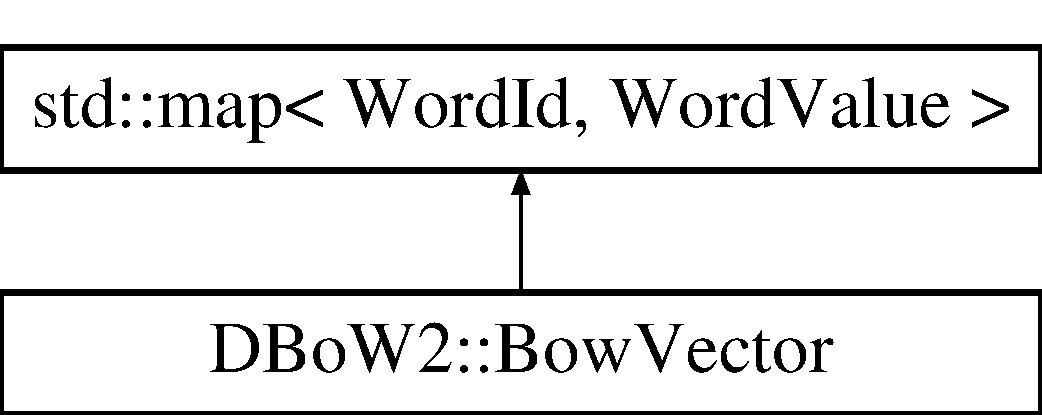
\includegraphics[height=2.000000cm]{class_d_bo_w2_1_1_bow_vector}
\end{center}
\end{figure}
\subsection*{Public Member Functions}
\begin{DoxyCompactItemize}
\item 
\mbox{\hyperlink{class_d_bo_w2_1_1_bow_vector_ac4da23e700adc4ee083d66b23ce86e90}{Bow\+Vector}} (void)
\item 
\mbox{\hyperlink{class_d_bo_w2_1_1_bow_vector_a7210cac6ce006c7232f4d097faa338d0}{$\sim$\+Bow\+Vector}} (void)
\item 
void \mbox{\hyperlink{class_d_bo_w2_1_1_bow_vector_a3ac92a805b252c93dc6535240d02df47}{add\+Weight}} (\mbox{\hyperlink{namespace_d_bo_w2_ab1a0d3283b2d4690a383372ed20bfeb5}{Word\+Id}} id, \mbox{\hyperlink{namespace_d_bo_w2_a55fcd7333e591a38e96b91f41bc182f6}{Word\+Value}} v)
\item 
void \mbox{\hyperlink{class_d_bo_w2_1_1_bow_vector_a5ddf10e444d10425e5bd3568dc7ffe5e}{add\+If\+Not\+Exist}} (\mbox{\hyperlink{namespace_d_bo_w2_ab1a0d3283b2d4690a383372ed20bfeb5}{Word\+Id}} id, \mbox{\hyperlink{namespace_d_bo_w2_a55fcd7333e591a38e96b91f41bc182f6}{Word\+Value}} v)
\item 
void \mbox{\hyperlink{class_d_bo_w2_1_1_bow_vector_acd2dd34023e3053a4cc75d70c8b6ac13}{normalize}} (\mbox{\hyperlink{namespace_d_bo_w2_a53e9e0bcfc25c861815e413a7cf3fa51}{L\+Norm}} norm\+\_\+type)
\item 
void \mbox{\hyperlink{class_d_bo_w2_1_1_bow_vector_a0611e948f987574161c121231341537b}{saveM}} (const std\+::string \&filename, size\+\_\+t W) const
\end{DoxyCompactItemize}
\subsection*{Friends}
\begin{DoxyCompactItemize}
\item 
std\+::ostream \& \mbox{\hyperlink{class_d_bo_w2_1_1_bow_vector_a1a7d9ac0f9128538859adfea38453ae1}{operator$<$$<$}} (std\+::ostream \&out, const \mbox{\hyperlink{class_d_bo_w2_1_1_bow_vector}{Bow\+Vector}} \&v)
\end{DoxyCompactItemize}


\subsection{Detailed Description}
Vector of words to represent images stl的map结构,key为word\+Id,value为tfidf中的tf 

\subsection{Constructor \& Destructor Documentation}
\mbox{\Hypertarget{class_d_bo_w2_1_1_bow_vector_ac4da23e700adc4ee083d66b23ce86e90}\label{class_d_bo_w2_1_1_bow_vector_ac4da23e700adc4ee083d66b23ce86e90}} 
\index{D\+Bo\+W2\+::\+Bow\+Vector@{D\+Bo\+W2\+::\+Bow\+Vector}!Bow\+Vector@{Bow\+Vector}}
\index{Bow\+Vector@{Bow\+Vector}!D\+Bo\+W2\+::\+Bow\+Vector@{D\+Bo\+W2\+::\+Bow\+Vector}}
\subsubsection{\texorpdfstring{Bow\+Vector()}{BowVector()}}
{\footnotesize\ttfamily D\+Bo\+W2\+::\+Bow\+Vector\+::\+Bow\+Vector (\begin{DoxyParamCaption}\item[{void}]{ }\end{DoxyParamCaption})}

Constructor \mbox{\Hypertarget{class_d_bo_w2_1_1_bow_vector_a7210cac6ce006c7232f4d097faa338d0}\label{class_d_bo_w2_1_1_bow_vector_a7210cac6ce006c7232f4d097faa338d0}} 
\index{D\+Bo\+W2\+::\+Bow\+Vector@{D\+Bo\+W2\+::\+Bow\+Vector}!````~Bow\+Vector@{$\sim$\+Bow\+Vector}}
\index{````~Bow\+Vector@{$\sim$\+Bow\+Vector}!D\+Bo\+W2\+::\+Bow\+Vector@{D\+Bo\+W2\+::\+Bow\+Vector}}
\subsubsection{\texorpdfstring{$\sim$\+Bow\+Vector()}{~BowVector()}}
{\footnotesize\ttfamily D\+Bo\+W2\+::\+Bow\+Vector\+::$\sim$\+Bow\+Vector (\begin{DoxyParamCaption}\item[{void}]{ }\end{DoxyParamCaption})}

Destructor 

\subsection{Member Function Documentation}
\mbox{\Hypertarget{class_d_bo_w2_1_1_bow_vector_a5ddf10e444d10425e5bd3568dc7ffe5e}\label{class_d_bo_w2_1_1_bow_vector_a5ddf10e444d10425e5bd3568dc7ffe5e}} 
\index{D\+Bo\+W2\+::\+Bow\+Vector@{D\+Bo\+W2\+::\+Bow\+Vector}!add\+If\+Not\+Exist@{add\+If\+Not\+Exist}}
\index{add\+If\+Not\+Exist@{add\+If\+Not\+Exist}!D\+Bo\+W2\+::\+Bow\+Vector@{D\+Bo\+W2\+::\+Bow\+Vector}}
\subsubsection{\texorpdfstring{add\+If\+Not\+Exist()}{addIfNotExist()}}
{\footnotesize\ttfamily void D\+Bo\+W2\+::\+Bow\+Vector\+::add\+If\+Not\+Exist (\begin{DoxyParamCaption}\item[{\mbox{\hyperlink{namespace_d_bo_w2_ab1a0d3283b2d4690a383372ed20bfeb5}{Word\+Id}}}]{id,  }\item[{\mbox{\hyperlink{namespace_d_bo_w2_a55fcd7333e591a38e96b91f41bc182f6}{Word\+Value}}}]{v }\end{DoxyParamCaption})}

Adds a word with a value to the vector only if this does not exist yet 
\begin{DoxyParams}{Parameters}
{\em id} & word id to look for \\
\hline
{\em v} & value to give to the word if this does not exist \\
\hline
\end{DoxyParams}
\mbox{\Hypertarget{class_d_bo_w2_1_1_bow_vector_a3ac92a805b252c93dc6535240d02df47}\label{class_d_bo_w2_1_1_bow_vector_a3ac92a805b252c93dc6535240d02df47}} 
\index{D\+Bo\+W2\+::\+Bow\+Vector@{D\+Bo\+W2\+::\+Bow\+Vector}!add\+Weight@{add\+Weight}}
\index{add\+Weight@{add\+Weight}!D\+Bo\+W2\+::\+Bow\+Vector@{D\+Bo\+W2\+::\+Bow\+Vector}}
\subsubsection{\texorpdfstring{add\+Weight()}{addWeight()}}
{\footnotesize\ttfamily void D\+Bo\+W2\+::\+Bow\+Vector\+::add\+Weight (\begin{DoxyParamCaption}\item[{\mbox{\hyperlink{namespace_d_bo_w2_ab1a0d3283b2d4690a383372ed20bfeb5}{Word\+Id}}}]{id,  }\item[{\mbox{\hyperlink{namespace_d_bo_w2_a55fcd7333e591a38e96b91f41bc182f6}{Word\+Value}}}]{v }\end{DoxyParamCaption})}

Adds a value to a word value existing in the vector, or creates a new word with the given value 
\begin{DoxyParams}{Parameters}
{\em id} & word id to look for \\
\hline
{\em v} & value to create the word with, or to add to existing word \\
\hline
\end{DoxyParams}
\mbox{\Hypertarget{class_d_bo_w2_1_1_bow_vector_acd2dd34023e3053a4cc75d70c8b6ac13}\label{class_d_bo_w2_1_1_bow_vector_acd2dd34023e3053a4cc75d70c8b6ac13}} 
\index{D\+Bo\+W2\+::\+Bow\+Vector@{D\+Bo\+W2\+::\+Bow\+Vector}!normalize@{normalize}}
\index{normalize@{normalize}!D\+Bo\+W2\+::\+Bow\+Vector@{D\+Bo\+W2\+::\+Bow\+Vector}}
\subsubsection{\texorpdfstring{normalize()}{normalize()}}
{\footnotesize\ttfamily void D\+Bo\+W2\+::\+Bow\+Vector\+::normalize (\begin{DoxyParamCaption}\item[{\mbox{\hyperlink{namespace_d_bo_w2_a53e9e0bcfc25c861815e413a7cf3fa51}{L\+Norm}}}]{norm\+\_\+type }\end{DoxyParamCaption})}

L1-\/\+Normalizes the values in the vector 
\begin{DoxyParams}{Parameters}
{\em norm\+\_\+type} & norm used \\
\hline
\end{DoxyParams}
\mbox{\Hypertarget{class_d_bo_w2_1_1_bow_vector_a0611e948f987574161c121231341537b}\label{class_d_bo_w2_1_1_bow_vector_a0611e948f987574161c121231341537b}} 
\index{D\+Bo\+W2\+::\+Bow\+Vector@{D\+Bo\+W2\+::\+Bow\+Vector}!saveM@{saveM}}
\index{saveM@{saveM}!D\+Bo\+W2\+::\+Bow\+Vector@{D\+Bo\+W2\+::\+Bow\+Vector}}
\subsubsection{\texorpdfstring{save\+M()}{saveM()}}
{\footnotesize\ttfamily void D\+Bo\+W2\+::\+Bow\+Vector\+::saveM (\begin{DoxyParamCaption}\item[{const std\+::string \&}]{filename,  }\item[{size\+\_\+t}]{W }\end{DoxyParamCaption}) const}

Saves the bow vector as a vector in a matlab file 
\begin{DoxyParams}{Parameters}
{\em filename} & \\
\hline
{\em W} & number of words in the vocabulary \\
\hline
\end{DoxyParams}


\subsection{Friends And Related Function Documentation}
\mbox{\Hypertarget{class_d_bo_w2_1_1_bow_vector_a1a7d9ac0f9128538859adfea38453ae1}\label{class_d_bo_w2_1_1_bow_vector_a1a7d9ac0f9128538859adfea38453ae1}} 
\index{D\+Bo\+W2\+::\+Bow\+Vector@{D\+Bo\+W2\+::\+Bow\+Vector}!operator$<$$<$@{operator$<$$<$}}
\index{operator$<$$<$@{operator$<$$<$}!D\+Bo\+W2\+::\+Bow\+Vector@{D\+Bo\+W2\+::\+Bow\+Vector}}
\subsubsection{\texorpdfstring{operator$<$$<$}{operator<<}}
{\footnotesize\ttfamily std\+::ostream\& operator$<$$<$ (\begin{DoxyParamCaption}\item[{std\+::ostream \&}]{out,  }\item[{const \mbox{\hyperlink{class_d_bo_w2_1_1_bow_vector}{Bow\+Vector}} \&}]{v }\end{DoxyParamCaption})\hspace{0.3cm}{\ttfamily [friend]}}

Prints the content of the bow vector 
\begin{DoxyParams}{Parameters}
{\em out} & stream \\
\hline
{\em v} & \\
\hline
\end{DoxyParams}


The documentation for this class was generated from the following files\+:\begin{DoxyCompactItemize}
\item 
D\+:/github/\+V\+S\+L\+A\+M/\+O\+R\+B\+S\+L\+A\+M2/\+O\+R\+B-\/\+S\+L\+A\+M2-\/master/\+Thirdparty/\+D\+Bo\+W2/\+D\+Bo\+W2/\mbox{\hyperlink{_bow_vector_8h}{Bow\+Vector.\+h}}\item 
D\+:/github/\+V\+S\+L\+A\+M/\+O\+R\+B\+S\+L\+A\+M2/\+O\+R\+B-\/\+S\+L\+A\+M2-\/master/\+Thirdparty/\+D\+Bo\+W2/\+D\+Bo\+W2/\mbox{\hyperlink{_bow_vector_8cpp}{Bow\+Vector.\+cpp}}\end{DoxyCompactItemize}

\hypertarget{classg2o_1_1_cache}{}\section{g2o\+:\+:Cache Class Reference}
\label{classg2o_1_1_cache}\index{g2o\+::\+Cache@{g2o\+::\+Cache}}


{\ttfamily \#include $<$cache.\+h$>$}

Inheritance diagram for g2o\+:\+:Cache\+:\begin{figure}[H]
\begin{center}
\leavevmode
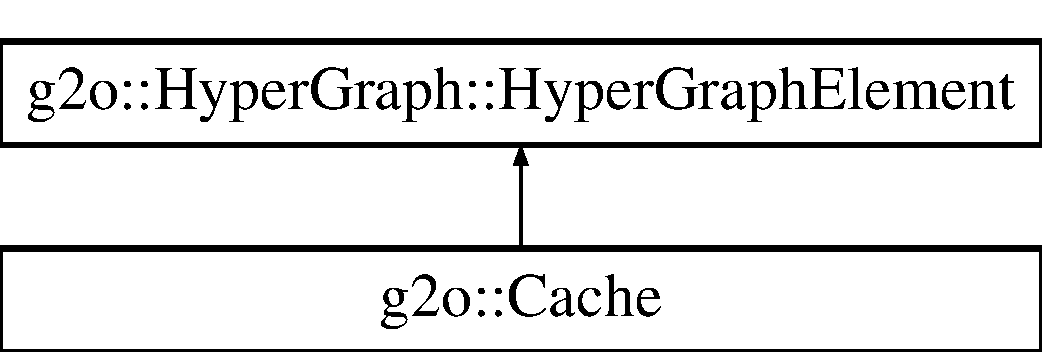
\includegraphics[height=2.000000cm]{classg2o_1_1_cache}
\end{center}
\end{figure}
\subsection*{Classes}
\begin{DoxyCompactItemize}
\item 
class \mbox{\hyperlink{classg2o_1_1_cache_1_1_cache_key}{Cache\+Key}}
\end{DoxyCompactItemize}
\subsection*{Public Member Functions}
\begin{DoxyCompactItemize}
\item 
\mbox{\hyperlink{classg2o_1_1_cache_adb5e57e9f06505511fdedb247a977cc3}{Cache}} (\mbox{\hyperlink{classg2o_1_1_cache_container}{Cache\+Container}} $\ast$container\+\_\+=0, const \mbox{\hyperlink{namespaceg2o_a85cc8f2c7db8cab47b2b269a7acd6785}{Parameter\+Vector}} \&parameters\+\_\+=\mbox{\hyperlink{namespaceg2o_a85cc8f2c7db8cab47b2b269a7acd6785}{Parameter\+Vector}}())
\item 
\mbox{\hyperlink{classg2o_1_1_cache_1_1_cache_key}{Cache\+Key}} \mbox{\hyperlink{classg2o_1_1_cache_a2e0a0de318ff4a0f50c263869a87908b}{key}} () const
\item 
\mbox{\hyperlink{classg2o_1_1_optimizable_graph_1_1_vertex}{Optimizable\+Graph\+::\+Vertex}} $\ast$ \mbox{\hyperlink{classg2o_1_1_cache_ab94788e39d7e81201d14bc8ac58325c7}{vertex}} ()
\item 
\mbox{\hyperlink{structg2o_1_1_optimizable_graph}{Optimizable\+Graph}} $\ast$ \mbox{\hyperlink{classg2o_1_1_cache_a1a4480a445469d2d02b8db449e6cb57c}{graph}} ()
\item 
\mbox{\hyperlink{classg2o_1_1_cache_container}{Cache\+Container}} $\ast$ \mbox{\hyperlink{classg2o_1_1_cache_a249ffa5c8ac120b3123bd151200082c9}{container}} ()
\item 
\mbox{\hyperlink{namespaceg2o_a85cc8f2c7db8cab47b2b269a7acd6785}{Parameter\+Vector}} \& \mbox{\hyperlink{classg2o_1_1_cache_a16e471be92f9fe24a3abdf11a0c546d2}{parameters}} ()
\item 
void \mbox{\hyperlink{classg2o_1_1_cache_aaea446a5eb59569acc67c94793975a0b}{update}} ()
\item 
virtual Hyper\+Graph\+::\+Hyper\+Graph\+Element\+Type \mbox{\hyperlink{classg2o_1_1_cache_ace402a9e59f3fe28ae7e44854cbc5e97}{element\+Type}} () const
\end{DoxyCompactItemize}
\subsection*{Protected Member Functions}
\begin{DoxyCompactItemize}
\item 
virtual void \mbox{\hyperlink{classg2o_1_1_cache_ae46e4a4e37c034925edd6bbfdfaa1cb2}{update\+Impl}} ()=0
\begin{DoxyCompactList}\small\item\em redefine this to do the update \end{DoxyCompactList}\item 
\mbox{\hyperlink{classg2o_1_1_cache}{Cache}} $\ast$ \mbox{\hyperlink{classg2o_1_1_cache_a776574fb98726ff61bc1280ea624c6e5}{install\+Dependency}} (const std\+::string \&type\+\_\+, const std\+::vector$<$ int $>$ \&parameter\+Indices)
\item 
virtual bool \mbox{\hyperlink{classg2o_1_1_cache_a0c26f0baa33a5902002f1ca2d5f57ece}{resolve\+Dependancies}} ()
\end{DoxyCompactItemize}
\subsection*{Protected Attributes}
\begin{DoxyCompactItemize}
\item 
bool \mbox{\hyperlink{classg2o_1_1_cache_a28d0ad45da71d9b7bc6de4cf1fb0f9e4}{\+\_\+update\+Needed}}
\item 
\mbox{\hyperlink{namespaceg2o_a85cc8f2c7db8cab47b2b269a7acd6785}{Parameter\+Vector}} \mbox{\hyperlink{classg2o_1_1_cache_ad596a1a7591adece4664a43fc87b881d}{\+\_\+parameters}}
\item 
std\+::vector$<$ \mbox{\hyperlink{classg2o_1_1_cache}{Cache}} $\ast$ $>$ \mbox{\hyperlink{classg2o_1_1_cache_a0b38f0c773c02903acf8964f73c3aa26}{\+\_\+parent\+Caches}}
\item 
\mbox{\hyperlink{classg2o_1_1_cache_container}{Cache\+Container}} $\ast$ \mbox{\hyperlink{classg2o_1_1_cache_a098aeecd7f0daa19a58f710ae7cb27c3}{\+\_\+container}}
\end{DoxyCompactItemize}
\subsection*{Friends}
\begin{DoxyCompactItemize}
\item 
class \mbox{\hyperlink{classg2o_1_1_cache_a86dec1e0424aa4ae4e6867c69efd7868}{Cache\+Container}}
\end{DoxyCompactItemize}


\subsection{Constructor \& Destructor Documentation}
\mbox{\Hypertarget{classg2o_1_1_cache_adb5e57e9f06505511fdedb247a977cc3}\label{classg2o_1_1_cache_adb5e57e9f06505511fdedb247a977cc3}} 
\index{g2o\+::\+Cache@{g2o\+::\+Cache}!Cache@{Cache}}
\index{Cache@{Cache}!g2o\+::\+Cache@{g2o\+::\+Cache}}
\subsubsection{\texorpdfstring{Cache()}{Cache()}}
{\footnotesize\ttfamily g2o\+::\+Cache\+::\+Cache (\begin{DoxyParamCaption}\item[{\mbox{\hyperlink{classg2o_1_1_cache_container}{Cache\+Container}} $\ast$}]{container\+\_\+ = {\ttfamily 0},  }\item[{const \mbox{\hyperlink{namespaceg2o_a85cc8f2c7db8cab47b2b269a7acd6785}{Parameter\+Vector}} \&}]{parameters\+\_\+ = {\ttfamily \mbox{\hyperlink{namespaceg2o_a85cc8f2c7db8cab47b2b269a7acd6785}{Parameter\+Vector}}()} }\end{DoxyParamCaption})}



\subsection{Member Function Documentation}
\mbox{\Hypertarget{classg2o_1_1_cache_a249ffa5c8ac120b3123bd151200082c9}\label{classg2o_1_1_cache_a249ffa5c8ac120b3123bd151200082c9}} 
\index{g2o\+::\+Cache@{g2o\+::\+Cache}!container@{container}}
\index{container@{container}!g2o\+::\+Cache@{g2o\+::\+Cache}}
\subsubsection{\texorpdfstring{container()}{container()}}
{\footnotesize\ttfamily \mbox{\hyperlink{classg2o_1_1_cache_container}{Cache\+Container}} $\ast$ g2o\+::\+Cache\+::container (\begin{DoxyParamCaption}{ }\end{DoxyParamCaption})}

\mbox{\Hypertarget{classg2o_1_1_cache_ace402a9e59f3fe28ae7e44854cbc5e97}\label{classg2o_1_1_cache_ace402a9e59f3fe28ae7e44854cbc5e97}} 
\index{g2o\+::\+Cache@{g2o\+::\+Cache}!element\+Type@{element\+Type}}
\index{element\+Type@{element\+Type}!g2o\+::\+Cache@{g2o\+::\+Cache}}
\subsubsection{\texorpdfstring{element\+Type()}{elementType()}}
{\footnotesize\ttfamily virtual Hyper\+Graph\+::\+Hyper\+Graph\+Element\+Type g2o\+::\+Cache\+::element\+Type (\begin{DoxyParamCaption}{ }\end{DoxyParamCaption}) const\hspace{0.3cm}{\ttfamily [inline]}, {\ttfamily [virtual]}}

returns the type of the graph element, see Hyper\+Graph\+Element\+Type 

Implements \mbox{\hyperlink{structg2o_1_1_hyper_graph_1_1_hyper_graph_element_a1a9d7b748698c09d202373e06e413ef2}{g2o\+::\+Hyper\+Graph\+::\+Hyper\+Graph\+Element}}.

\mbox{\Hypertarget{classg2o_1_1_cache_a1a4480a445469d2d02b8db449e6cb57c}\label{classg2o_1_1_cache_a1a4480a445469d2d02b8db449e6cb57c}} 
\index{g2o\+::\+Cache@{g2o\+::\+Cache}!graph@{graph}}
\index{graph@{graph}!g2o\+::\+Cache@{g2o\+::\+Cache}}
\subsubsection{\texorpdfstring{graph()}{graph()}}
{\footnotesize\ttfamily \mbox{\hyperlink{structg2o_1_1_optimizable_graph}{Optimizable\+Graph}} $\ast$ g2o\+::\+Cache\+::graph (\begin{DoxyParamCaption}{ }\end{DoxyParamCaption})}

\mbox{\Hypertarget{classg2o_1_1_cache_a776574fb98726ff61bc1280ea624c6e5}\label{classg2o_1_1_cache_a776574fb98726ff61bc1280ea624c6e5}} 
\index{g2o\+::\+Cache@{g2o\+::\+Cache}!install\+Dependency@{install\+Dependency}}
\index{install\+Dependency@{install\+Dependency}!g2o\+::\+Cache@{g2o\+::\+Cache}}
\subsubsection{\texorpdfstring{install\+Dependency()}{installDependency()}}
{\footnotesize\ttfamily \mbox{\hyperlink{classg2o_1_1_cache}{Cache}} $\ast$ g2o\+::\+Cache\+::install\+Dependency (\begin{DoxyParamCaption}\item[{const std\+::string \&}]{type\+\_\+,  }\item[{const std\+::vector$<$ int $>$ \&}]{parameter\+Indices }\end{DoxyParamCaption})\hspace{0.3cm}{\ttfamily [protected]}}

this function installs and satisfies a cache 
\begin{DoxyParams}{Parameters}
{\em type\+\_\+} & the typename of the dependency \\
\hline
{\em parameter\+Indices} & a vector containing the indices if the parameters in \+\_\+parameters that will be used to assemble the Key of the cache being created For example if I have a cache of type C2, having parameters \char`\"{}\+A, B, and C\char`\"{}, and it depends on a cache of type C1 that depends on the parameters A and C, the parameter\+Indices should contain \char`\"{}0, 2\char`\"{}, since they are the positions in the parameter vector of C2 of the parameters needed to construct C1. \\
\hline
\end{DoxyParams}
\begin{DoxyReturn}{Returns}
the newly created cache 
\end{DoxyReturn}
\mbox{\Hypertarget{classg2o_1_1_cache_a2e0a0de318ff4a0f50c263869a87908b}\label{classg2o_1_1_cache_a2e0a0de318ff4a0f50c263869a87908b}} 
\index{g2o\+::\+Cache@{g2o\+::\+Cache}!key@{key}}
\index{key@{key}!g2o\+::\+Cache@{g2o\+::\+Cache}}
\subsubsection{\texorpdfstring{key()}{key()}}
{\footnotesize\ttfamily \mbox{\hyperlink{classg2o_1_1_cache_1_1_cache_key}{Cache\+::\+Cache\+Key}} g2o\+::\+Cache\+::key (\begin{DoxyParamCaption}{ }\end{DoxyParamCaption}) const}

\mbox{\Hypertarget{classg2o_1_1_cache_a16e471be92f9fe24a3abdf11a0c546d2}\label{classg2o_1_1_cache_a16e471be92f9fe24a3abdf11a0c546d2}} 
\index{g2o\+::\+Cache@{g2o\+::\+Cache}!parameters@{parameters}}
\index{parameters@{parameters}!g2o\+::\+Cache@{g2o\+::\+Cache}}
\subsubsection{\texorpdfstring{parameters()}{parameters()}}
{\footnotesize\ttfamily \mbox{\hyperlink{namespaceg2o_a85cc8f2c7db8cab47b2b269a7acd6785}{Parameter\+Vector}} \& g2o\+::\+Cache\+::parameters (\begin{DoxyParamCaption}{ }\end{DoxyParamCaption})}

\mbox{\Hypertarget{classg2o_1_1_cache_a0c26f0baa33a5902002f1ca2d5f57ece}\label{classg2o_1_1_cache_a0c26f0baa33a5902002f1ca2d5f57ece}} 
\index{g2o\+::\+Cache@{g2o\+::\+Cache}!resolve\+Dependancies@{resolve\+Dependancies}}
\index{resolve\+Dependancies@{resolve\+Dependancies}!g2o\+::\+Cache@{g2o\+::\+Cache}}
\subsubsection{\texorpdfstring{resolve\+Dependancies()}{resolveDependancies()}}
{\footnotesize\ttfamily bool g2o\+::\+Cache\+::resolve\+Dependancies (\begin{DoxyParamCaption}{ }\end{DoxyParamCaption})\hspace{0.3cm}{\ttfamily [protected]}, {\ttfamily [virtual]}}

Function to be called from a cache that has dependencies. It just invokes a sequence of \mbox{\hyperlink{classg2o_1_1_cache_a776574fb98726ff61bc1280ea624c6e5}{install\+Dependency()}}. Although the caches returned are stored in the \+\_\+parent\+Cache vector, it is better that you redefine your own cache member variables, for better readability \mbox{\Hypertarget{classg2o_1_1_cache_aaea446a5eb59569acc67c94793975a0b}\label{classg2o_1_1_cache_aaea446a5eb59569acc67c94793975a0b}} 
\index{g2o\+::\+Cache@{g2o\+::\+Cache}!update@{update}}
\index{update@{update}!g2o\+::\+Cache@{g2o\+::\+Cache}}
\subsubsection{\texorpdfstring{update()}{update()}}
{\footnotesize\ttfamily void g2o\+::\+Cache\+::update (\begin{DoxyParamCaption}{ }\end{DoxyParamCaption})}

\mbox{\Hypertarget{classg2o_1_1_cache_ae46e4a4e37c034925edd6bbfdfaa1cb2}\label{classg2o_1_1_cache_ae46e4a4e37c034925edd6bbfdfaa1cb2}} 
\index{g2o\+::\+Cache@{g2o\+::\+Cache}!update\+Impl@{update\+Impl}}
\index{update\+Impl@{update\+Impl}!g2o\+::\+Cache@{g2o\+::\+Cache}}
\subsubsection{\texorpdfstring{update\+Impl()}{updateImpl()}}
{\footnotesize\ttfamily virtual void g2o\+::\+Cache\+::update\+Impl (\begin{DoxyParamCaption}{ }\end{DoxyParamCaption})\hspace{0.3cm}{\ttfamily [protected]}, {\ttfamily [pure virtual]}}



redefine this to do the update 

\mbox{\Hypertarget{classg2o_1_1_cache_ab94788e39d7e81201d14bc8ac58325c7}\label{classg2o_1_1_cache_ab94788e39d7e81201d14bc8ac58325c7}} 
\index{g2o\+::\+Cache@{g2o\+::\+Cache}!vertex@{vertex}}
\index{vertex@{vertex}!g2o\+::\+Cache@{g2o\+::\+Cache}}
\subsubsection{\texorpdfstring{vertex()}{vertex()}}
{\footnotesize\ttfamily \mbox{\hyperlink{classg2o_1_1_optimizable_graph_1_1_vertex}{Optimizable\+Graph\+::\+Vertex}} $\ast$ g2o\+::\+Cache\+::vertex (\begin{DoxyParamCaption}{ }\end{DoxyParamCaption})}



\subsection{Friends And Related Function Documentation}
\mbox{\Hypertarget{classg2o_1_1_cache_a86dec1e0424aa4ae4e6867c69efd7868}\label{classg2o_1_1_cache_a86dec1e0424aa4ae4e6867c69efd7868}} 
\index{g2o\+::\+Cache@{g2o\+::\+Cache}!Cache\+Container@{Cache\+Container}}
\index{Cache\+Container@{Cache\+Container}!g2o\+::\+Cache@{g2o\+::\+Cache}}
\subsubsection{\texorpdfstring{Cache\+Container}{CacheContainer}}
{\footnotesize\ttfamily friend class \mbox{\hyperlink{classg2o_1_1_cache_container}{Cache\+Container}}\hspace{0.3cm}{\ttfamily [friend]}}



\subsection{Member Data Documentation}
\mbox{\Hypertarget{classg2o_1_1_cache_a098aeecd7f0daa19a58f710ae7cb27c3}\label{classg2o_1_1_cache_a098aeecd7f0daa19a58f710ae7cb27c3}} 
\index{g2o\+::\+Cache@{g2o\+::\+Cache}!\+\_\+container@{\+\_\+container}}
\index{\+\_\+container@{\+\_\+container}!g2o\+::\+Cache@{g2o\+::\+Cache}}
\subsubsection{\texorpdfstring{\+\_\+container}{\_container}}
{\footnotesize\ttfamily \mbox{\hyperlink{classg2o_1_1_cache_container}{Cache\+Container}}$\ast$ g2o\+::\+Cache\+::\+\_\+container\hspace{0.3cm}{\ttfamily [protected]}}

\mbox{\Hypertarget{classg2o_1_1_cache_ad596a1a7591adece4664a43fc87b881d}\label{classg2o_1_1_cache_ad596a1a7591adece4664a43fc87b881d}} 
\index{g2o\+::\+Cache@{g2o\+::\+Cache}!\+\_\+parameters@{\+\_\+parameters}}
\index{\+\_\+parameters@{\+\_\+parameters}!g2o\+::\+Cache@{g2o\+::\+Cache}}
\subsubsection{\texorpdfstring{\+\_\+parameters}{\_parameters}}
{\footnotesize\ttfamily \mbox{\hyperlink{namespaceg2o_a85cc8f2c7db8cab47b2b269a7acd6785}{Parameter\+Vector}} g2o\+::\+Cache\+::\+\_\+parameters\hspace{0.3cm}{\ttfamily [protected]}}

\mbox{\Hypertarget{classg2o_1_1_cache_a0b38f0c773c02903acf8964f73c3aa26}\label{classg2o_1_1_cache_a0b38f0c773c02903acf8964f73c3aa26}} 
\index{g2o\+::\+Cache@{g2o\+::\+Cache}!\+\_\+parent\+Caches@{\+\_\+parent\+Caches}}
\index{\+\_\+parent\+Caches@{\+\_\+parent\+Caches}!g2o\+::\+Cache@{g2o\+::\+Cache}}
\subsubsection{\texorpdfstring{\+\_\+parent\+Caches}{\_parentCaches}}
{\footnotesize\ttfamily std\+::vector$<$\mbox{\hyperlink{classg2o_1_1_cache}{Cache}}$\ast$$>$ g2o\+::\+Cache\+::\+\_\+parent\+Caches\hspace{0.3cm}{\ttfamily [protected]}}

\mbox{\Hypertarget{classg2o_1_1_cache_a28d0ad45da71d9b7bc6de4cf1fb0f9e4}\label{classg2o_1_1_cache_a28d0ad45da71d9b7bc6de4cf1fb0f9e4}} 
\index{g2o\+::\+Cache@{g2o\+::\+Cache}!\+\_\+update\+Needed@{\+\_\+update\+Needed}}
\index{\+\_\+update\+Needed@{\+\_\+update\+Needed}!g2o\+::\+Cache@{g2o\+::\+Cache}}
\subsubsection{\texorpdfstring{\+\_\+update\+Needed}{\_updateNeeded}}
{\footnotesize\ttfamily bool g2o\+::\+Cache\+::\+\_\+update\+Needed\hspace{0.3cm}{\ttfamily [protected]}}



The documentation for this class was generated from the following files\+:\begin{DoxyCompactItemize}
\item 
D\+:/github/\+V\+S\+L\+A\+M/\+O\+R\+B\+S\+L\+A\+M2/\+O\+R\+B-\/\+S\+L\+A\+M2-\/master/\+Thirdparty/g2o/g2o/core/\mbox{\hyperlink{cache_8h}{cache.\+h}}\item 
D\+:/github/\+V\+S\+L\+A\+M/\+O\+R\+B\+S\+L\+A\+M2/\+O\+R\+B-\/\+S\+L\+A\+M2-\/master/\+Thirdparty/g2o/g2o/core/\mbox{\hyperlink{cache_8cpp}{cache.\+cpp}}\end{DoxyCompactItemize}

\hypertarget{classg2o_1_1_cache_container}{}\section{g2o\+:\+:Cache\+Container Class Reference}
\label{classg2o_1_1_cache_container}\index{g2o\+::\+Cache\+Container@{g2o\+::\+Cache\+Container}}


{\ttfamily \#include $<$cache.\+h$>$}

Inheritance diagram for g2o\+:\+:Cache\+Container\+:\begin{figure}[H]
\begin{center}
\leavevmode
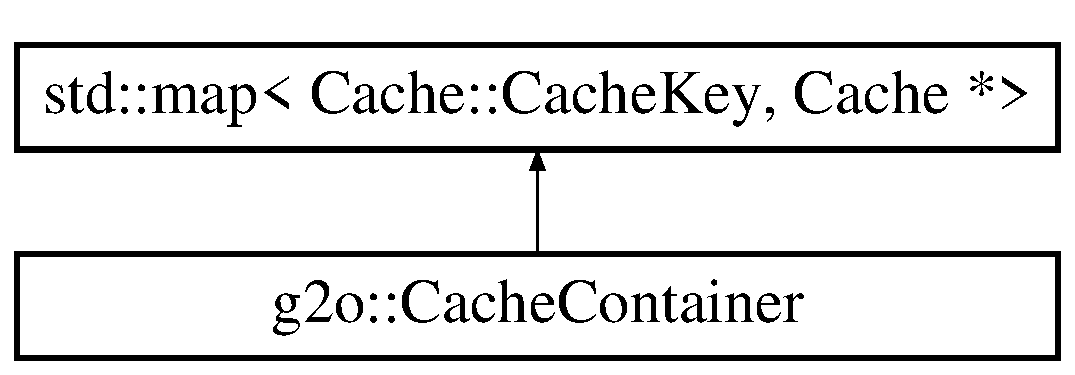
\includegraphics[height=2.000000cm]{classg2o_1_1_cache_container}
\end{center}
\end{figure}
\subsection*{Public Member Functions}
\begin{DoxyCompactItemize}
\item 
\mbox{\hyperlink{classg2o_1_1_cache_container_aed510932f7e499f2fd3c1fdea7809052}{Cache\+Container}} (\mbox{\hyperlink{classg2o_1_1_optimizable_graph_1_1_vertex}{Optimizable\+Graph\+::\+Vertex}} $\ast$vertex\+\_\+)
\item 
virtual \mbox{\hyperlink{classg2o_1_1_cache_container_a2eb9f659371a1af2c119fce3e2972e52}{$\sim$\+Cache\+Container}} ()
\item 
\mbox{\hyperlink{classg2o_1_1_optimizable_graph_1_1_vertex}{Optimizable\+Graph\+::\+Vertex}} $\ast$ \mbox{\hyperlink{classg2o_1_1_cache_container_ada4f7f82992a85dbc742c1ab24c39c08}{vertex}} ()
\item 
\mbox{\hyperlink{structg2o_1_1_optimizable_graph}{Optimizable\+Graph}} $\ast$ \mbox{\hyperlink{classg2o_1_1_cache_container_a4bf79d27bb9ae377446dfa7fd048b06d}{graph}} ()
\item 
\mbox{\hyperlink{classg2o_1_1_cache}{Cache}} $\ast$ \mbox{\hyperlink{classg2o_1_1_cache_container_a2a0230117e0e71210f3d10a9e7143d0f}{find\+Cache}} (const \mbox{\hyperlink{classg2o_1_1_cache_1_1_cache_key}{Cache\+::\+Cache\+Key}} \&key)
\item 
\mbox{\hyperlink{classg2o_1_1_cache}{Cache}} $\ast$ \mbox{\hyperlink{classg2o_1_1_cache_container_a08902c228901e06c4e08c5b594683a6c}{create\+Cache}} (const \mbox{\hyperlink{classg2o_1_1_cache_1_1_cache_key}{Cache\+::\+Cache\+Key}} \&key)
\item 
void \mbox{\hyperlink{classg2o_1_1_cache_container_a2241f992e90c1078447553d0833ccf14}{set\+Update\+Needed}} (bool need\+Update=true)
\item 
void \mbox{\hyperlink{classg2o_1_1_cache_container_acc9a6d1fbc828f55b1a6af1c29f003df}{update}} ()
\end{DoxyCompactItemize}
\subsection*{Protected Attributes}
\begin{DoxyCompactItemize}
\item 
\mbox{\hyperlink{classg2o_1_1_optimizable_graph_1_1_vertex}{Optimizable\+Graph\+::\+Vertex}} $\ast$ \mbox{\hyperlink{classg2o_1_1_cache_container_a899b5f4d01859463cedf663b68f78391}{\+\_\+vertex}}
\item 
bool \mbox{\hyperlink{classg2o_1_1_cache_container_a5fd5257863e41c3fc38336aaa7779b3e}{\+\_\+update\+Needed}}
\end{DoxyCompactItemize}


\subsection{Constructor \& Destructor Documentation}
\mbox{\Hypertarget{classg2o_1_1_cache_container_aed510932f7e499f2fd3c1fdea7809052}\label{classg2o_1_1_cache_container_aed510932f7e499f2fd3c1fdea7809052}} 
\index{g2o\+::\+Cache\+Container@{g2o\+::\+Cache\+Container}!Cache\+Container@{Cache\+Container}}
\index{Cache\+Container@{Cache\+Container}!g2o\+::\+Cache\+Container@{g2o\+::\+Cache\+Container}}
\subsubsection{\texorpdfstring{Cache\+Container()}{CacheContainer()}}
{\footnotesize\ttfamily g2o\+::\+Cache\+Container\+::\+Cache\+Container (\begin{DoxyParamCaption}\item[{\mbox{\hyperlink{classg2o_1_1_optimizable_graph_1_1_vertex}{Optimizable\+Graph\+::\+Vertex}} $\ast$}]{vertex\+\_\+ }\end{DoxyParamCaption})}

\mbox{\Hypertarget{classg2o_1_1_cache_container_a2eb9f659371a1af2c119fce3e2972e52}\label{classg2o_1_1_cache_container_a2eb9f659371a1af2c119fce3e2972e52}} 
\index{g2o\+::\+Cache\+Container@{g2o\+::\+Cache\+Container}!````~Cache\+Container@{$\sim$\+Cache\+Container}}
\index{````~Cache\+Container@{$\sim$\+Cache\+Container}!g2o\+::\+Cache\+Container@{g2o\+::\+Cache\+Container}}
\subsubsection{\texorpdfstring{$\sim$\+Cache\+Container()}{~CacheContainer()}}
{\footnotesize\ttfamily g2o\+::\+Cache\+Container\+::$\sim$\+Cache\+Container (\begin{DoxyParamCaption}{ }\end{DoxyParamCaption})\hspace{0.3cm}{\ttfamily [virtual]}}



\subsection{Member Function Documentation}
\mbox{\Hypertarget{classg2o_1_1_cache_container_a08902c228901e06c4e08c5b594683a6c}\label{classg2o_1_1_cache_container_a08902c228901e06c4e08c5b594683a6c}} 
\index{g2o\+::\+Cache\+Container@{g2o\+::\+Cache\+Container}!create\+Cache@{create\+Cache}}
\index{create\+Cache@{create\+Cache}!g2o\+::\+Cache\+Container@{g2o\+::\+Cache\+Container}}
\subsubsection{\texorpdfstring{create\+Cache()}{createCache()}}
{\footnotesize\ttfamily \mbox{\hyperlink{classg2o_1_1_cache}{Cache}} $\ast$ g2o\+::\+Cache\+Container\+::create\+Cache (\begin{DoxyParamCaption}\item[{const \mbox{\hyperlink{classg2o_1_1_cache_1_1_cache_key}{Cache\+::\+Cache\+Key}} \&}]{key }\end{DoxyParamCaption})}

\mbox{\Hypertarget{classg2o_1_1_cache_container_a2a0230117e0e71210f3d10a9e7143d0f}\label{classg2o_1_1_cache_container_a2a0230117e0e71210f3d10a9e7143d0f}} 
\index{g2o\+::\+Cache\+Container@{g2o\+::\+Cache\+Container}!find\+Cache@{find\+Cache}}
\index{find\+Cache@{find\+Cache}!g2o\+::\+Cache\+Container@{g2o\+::\+Cache\+Container}}
\subsubsection{\texorpdfstring{find\+Cache()}{findCache()}}
{\footnotesize\ttfamily \mbox{\hyperlink{classg2o_1_1_cache}{Cache}} $\ast$ g2o\+::\+Cache\+Container\+::find\+Cache (\begin{DoxyParamCaption}\item[{const \mbox{\hyperlink{classg2o_1_1_cache_1_1_cache_key}{Cache\+::\+Cache\+Key}} \&}]{key }\end{DoxyParamCaption})}

\mbox{\Hypertarget{classg2o_1_1_cache_container_a4bf79d27bb9ae377446dfa7fd048b06d}\label{classg2o_1_1_cache_container_a4bf79d27bb9ae377446dfa7fd048b06d}} 
\index{g2o\+::\+Cache\+Container@{g2o\+::\+Cache\+Container}!graph@{graph}}
\index{graph@{graph}!g2o\+::\+Cache\+Container@{g2o\+::\+Cache\+Container}}
\subsubsection{\texorpdfstring{graph()}{graph()}}
{\footnotesize\ttfamily \mbox{\hyperlink{structg2o_1_1_optimizable_graph}{Optimizable\+Graph}} $\ast$ g2o\+::\+Cache\+Container\+::graph (\begin{DoxyParamCaption}{ }\end{DoxyParamCaption})}

\mbox{\Hypertarget{classg2o_1_1_cache_container_a2241f992e90c1078447553d0833ccf14}\label{classg2o_1_1_cache_container_a2241f992e90c1078447553d0833ccf14}} 
\index{g2o\+::\+Cache\+Container@{g2o\+::\+Cache\+Container}!set\+Update\+Needed@{set\+Update\+Needed}}
\index{set\+Update\+Needed@{set\+Update\+Needed}!g2o\+::\+Cache\+Container@{g2o\+::\+Cache\+Container}}
\subsubsection{\texorpdfstring{set\+Update\+Needed()}{setUpdateNeeded()}}
{\footnotesize\ttfamily void g2o\+::\+Cache\+Container\+::set\+Update\+Needed (\begin{DoxyParamCaption}\item[{bool}]{need\+Update = {\ttfamily true} }\end{DoxyParamCaption})}

\mbox{\Hypertarget{classg2o_1_1_cache_container_acc9a6d1fbc828f55b1a6af1c29f003df}\label{classg2o_1_1_cache_container_acc9a6d1fbc828f55b1a6af1c29f003df}} 
\index{g2o\+::\+Cache\+Container@{g2o\+::\+Cache\+Container}!update@{update}}
\index{update@{update}!g2o\+::\+Cache\+Container@{g2o\+::\+Cache\+Container}}
\subsubsection{\texorpdfstring{update()}{update()}}
{\footnotesize\ttfamily void g2o\+::\+Cache\+Container\+::update (\begin{DoxyParamCaption}{ }\end{DoxyParamCaption})}

\mbox{\Hypertarget{classg2o_1_1_cache_container_ada4f7f82992a85dbc742c1ab24c39c08}\label{classg2o_1_1_cache_container_ada4f7f82992a85dbc742c1ab24c39c08}} 
\index{g2o\+::\+Cache\+Container@{g2o\+::\+Cache\+Container}!vertex@{vertex}}
\index{vertex@{vertex}!g2o\+::\+Cache\+Container@{g2o\+::\+Cache\+Container}}
\subsubsection{\texorpdfstring{vertex()}{vertex()}}
{\footnotesize\ttfamily \mbox{\hyperlink{classg2o_1_1_optimizable_graph_1_1_vertex}{Optimizable\+Graph\+::\+Vertex}} $\ast$ g2o\+::\+Cache\+Container\+::vertex (\begin{DoxyParamCaption}{ }\end{DoxyParamCaption})}



\subsection{Member Data Documentation}
\mbox{\Hypertarget{classg2o_1_1_cache_container_a5fd5257863e41c3fc38336aaa7779b3e}\label{classg2o_1_1_cache_container_a5fd5257863e41c3fc38336aaa7779b3e}} 
\index{g2o\+::\+Cache\+Container@{g2o\+::\+Cache\+Container}!\+\_\+update\+Needed@{\+\_\+update\+Needed}}
\index{\+\_\+update\+Needed@{\+\_\+update\+Needed}!g2o\+::\+Cache\+Container@{g2o\+::\+Cache\+Container}}
\subsubsection{\texorpdfstring{\+\_\+update\+Needed}{\_updateNeeded}}
{\footnotesize\ttfamily bool g2o\+::\+Cache\+Container\+::\+\_\+update\+Needed\hspace{0.3cm}{\ttfamily [protected]}}

\mbox{\Hypertarget{classg2o_1_1_cache_container_a899b5f4d01859463cedf663b68f78391}\label{classg2o_1_1_cache_container_a899b5f4d01859463cedf663b68f78391}} 
\index{g2o\+::\+Cache\+Container@{g2o\+::\+Cache\+Container}!\+\_\+vertex@{\+\_\+vertex}}
\index{\+\_\+vertex@{\+\_\+vertex}!g2o\+::\+Cache\+Container@{g2o\+::\+Cache\+Container}}
\subsubsection{\texorpdfstring{\+\_\+vertex}{\_vertex}}
{\footnotesize\ttfamily \mbox{\hyperlink{classg2o_1_1_optimizable_graph_1_1_vertex}{Optimizable\+Graph\+::\+Vertex}}$\ast$ g2o\+::\+Cache\+Container\+::\+\_\+vertex\hspace{0.3cm}{\ttfamily [protected]}}



The documentation for this class was generated from the following files\+:\begin{DoxyCompactItemize}
\item 
Thirdparty/g2o/g2o/core/\mbox{\hyperlink{cache_8h}{cache.\+h}}\item 
Thirdparty/g2o/g2o/core/\mbox{\hyperlink{cache_8cpp}{cache.\+cpp}}\end{DoxyCompactItemize}

\hypertarget{classg2o_1_1_cache_1_1_cache_key}{}\section{g2o\+:\+:Cache\+:\+:Cache\+Key Class Reference}
\label{classg2o_1_1_cache_1_1_cache_key}\index{g2o\+::\+Cache\+::\+Cache\+Key@{g2o\+::\+Cache\+::\+Cache\+Key}}


{\ttfamily \#include $<$cache.\+h$>$}

\subsection*{Public Member Functions}
\begin{DoxyCompactItemize}
\item 
\mbox{\hyperlink{classg2o_1_1_cache_1_1_cache_key_a44405e660e962a9d39cfaf97f103b139}{Cache\+Key}} ()
\item 
\mbox{\hyperlink{classg2o_1_1_cache_1_1_cache_key_a363ba06fe3b3f17acd664b0706ba3270}{Cache\+Key}} (const std\+::string \&type\+\_\+, const \mbox{\hyperlink{namespaceg2o_a85cc8f2c7db8cab47b2b269a7acd6785}{Parameter\+Vector}} \&parameters\+\_\+)
\item 
bool \mbox{\hyperlink{classg2o_1_1_cache_1_1_cache_key_a37ebfaa23730d98c642191fc5e360901}{operator$<$}} (const \mbox{\hyperlink{classg2o_1_1_cache_1_1_cache_key}{Cache\+Key}} \&c) const
\item 
const std\+::string \& \mbox{\hyperlink{classg2o_1_1_cache_1_1_cache_key_a426acdbf2c72f48f7923dcd7e2137aef}{type}} () const
\item 
const \mbox{\hyperlink{namespaceg2o_a85cc8f2c7db8cab47b2b269a7acd6785}{Parameter\+Vector}} \& \mbox{\hyperlink{classg2o_1_1_cache_1_1_cache_key_a06153e97f21620b5b74f6d3566171853}{parameters}} () const
\end{DoxyCompactItemize}
\subsection*{Protected Attributes}
\begin{DoxyCompactItemize}
\item 
std\+::string \mbox{\hyperlink{classg2o_1_1_cache_1_1_cache_key_a886ec6cf583561cb791cbaff902c673d}{\+\_\+type}}
\item 
\mbox{\hyperlink{namespaceg2o_a85cc8f2c7db8cab47b2b269a7acd6785}{Parameter\+Vector}} \mbox{\hyperlink{classg2o_1_1_cache_1_1_cache_key_a3f8dc2307bd1d174a30bdc8443a8d152}{\+\_\+parameters}}
\end{DoxyCompactItemize}
\subsection*{Friends}
\begin{DoxyCompactItemize}
\item 
class \mbox{\hyperlink{classg2o_1_1_cache_1_1_cache_key_a86dec1e0424aa4ae4e6867c69efd7868}{Cache\+Container}}
\end{DoxyCompactItemize}


\subsection{Constructor \& Destructor Documentation}
\mbox{\Hypertarget{classg2o_1_1_cache_1_1_cache_key_a44405e660e962a9d39cfaf97f103b139}\label{classg2o_1_1_cache_1_1_cache_key_a44405e660e962a9d39cfaf97f103b139}} 
\index{g2o\+::\+Cache\+::\+Cache\+Key@{g2o\+::\+Cache\+::\+Cache\+Key}!Cache\+Key@{Cache\+Key}}
\index{Cache\+Key@{Cache\+Key}!g2o\+::\+Cache\+::\+Cache\+Key@{g2o\+::\+Cache\+::\+Cache\+Key}}
\subsubsection{\texorpdfstring{Cache\+Key()}{CacheKey()}\hspace{0.1cm}{\footnotesize\ttfamily [1/2]}}
{\footnotesize\ttfamily g2o\+::\+Cache\+::\+Cache\+Key\+::\+Cache\+Key (\begin{DoxyParamCaption}{ }\end{DoxyParamCaption})}

\mbox{\Hypertarget{classg2o_1_1_cache_1_1_cache_key_a363ba06fe3b3f17acd664b0706ba3270}\label{classg2o_1_1_cache_1_1_cache_key_a363ba06fe3b3f17acd664b0706ba3270}} 
\index{g2o\+::\+Cache\+::\+Cache\+Key@{g2o\+::\+Cache\+::\+Cache\+Key}!Cache\+Key@{Cache\+Key}}
\index{Cache\+Key@{Cache\+Key}!g2o\+::\+Cache\+::\+Cache\+Key@{g2o\+::\+Cache\+::\+Cache\+Key}}
\subsubsection{\texorpdfstring{Cache\+Key()}{CacheKey()}\hspace{0.1cm}{\footnotesize\ttfamily [2/2]}}
{\footnotesize\ttfamily g2o\+::\+Cache\+::\+Cache\+Key\+::\+Cache\+Key (\begin{DoxyParamCaption}\item[{const std\+::string \&}]{type\+\_\+,  }\item[{const \mbox{\hyperlink{namespaceg2o_a85cc8f2c7db8cab47b2b269a7acd6785}{Parameter\+Vector}} \&}]{parameters\+\_\+ }\end{DoxyParamCaption})}



\subsection{Member Function Documentation}
\mbox{\Hypertarget{classg2o_1_1_cache_1_1_cache_key_a37ebfaa23730d98c642191fc5e360901}\label{classg2o_1_1_cache_1_1_cache_key_a37ebfaa23730d98c642191fc5e360901}} 
\index{g2o\+::\+Cache\+::\+Cache\+Key@{g2o\+::\+Cache\+::\+Cache\+Key}!operator$<$@{operator$<$}}
\index{operator$<$@{operator$<$}!g2o\+::\+Cache\+::\+Cache\+Key@{g2o\+::\+Cache\+::\+Cache\+Key}}
\subsubsection{\texorpdfstring{operator$<$()}{operator<()}}
{\footnotesize\ttfamily bool g2o\+::\+Cache\+::\+Cache\+Key\+::operator$<$ (\begin{DoxyParamCaption}\item[{const \mbox{\hyperlink{classg2o_1_1_cache_1_1_cache_key}{Cache\+Key}} \&}]{c }\end{DoxyParamCaption}) const}

\mbox{\Hypertarget{classg2o_1_1_cache_1_1_cache_key_a06153e97f21620b5b74f6d3566171853}\label{classg2o_1_1_cache_1_1_cache_key_a06153e97f21620b5b74f6d3566171853}} 
\index{g2o\+::\+Cache\+::\+Cache\+Key@{g2o\+::\+Cache\+::\+Cache\+Key}!parameters@{parameters}}
\index{parameters@{parameters}!g2o\+::\+Cache\+::\+Cache\+Key@{g2o\+::\+Cache\+::\+Cache\+Key}}
\subsubsection{\texorpdfstring{parameters()}{parameters()}}
{\footnotesize\ttfamily const \mbox{\hyperlink{namespaceg2o_a85cc8f2c7db8cab47b2b269a7acd6785}{Parameter\+Vector}}\& g2o\+::\+Cache\+::\+Cache\+Key\+::parameters (\begin{DoxyParamCaption}{ }\end{DoxyParamCaption}) const\hspace{0.3cm}{\ttfamily [inline]}}

\mbox{\Hypertarget{classg2o_1_1_cache_1_1_cache_key_a426acdbf2c72f48f7923dcd7e2137aef}\label{classg2o_1_1_cache_1_1_cache_key_a426acdbf2c72f48f7923dcd7e2137aef}} 
\index{g2o\+::\+Cache\+::\+Cache\+Key@{g2o\+::\+Cache\+::\+Cache\+Key}!type@{type}}
\index{type@{type}!g2o\+::\+Cache\+::\+Cache\+Key@{g2o\+::\+Cache\+::\+Cache\+Key}}
\subsubsection{\texorpdfstring{type()}{type()}}
{\footnotesize\ttfamily const std\+::string\& g2o\+::\+Cache\+::\+Cache\+Key\+::type (\begin{DoxyParamCaption}{ }\end{DoxyParamCaption}) const\hspace{0.3cm}{\ttfamily [inline]}}



\subsection{Friends And Related Function Documentation}
\mbox{\Hypertarget{classg2o_1_1_cache_1_1_cache_key_a86dec1e0424aa4ae4e6867c69efd7868}\label{classg2o_1_1_cache_1_1_cache_key_a86dec1e0424aa4ae4e6867c69efd7868}} 
\index{g2o\+::\+Cache\+::\+Cache\+Key@{g2o\+::\+Cache\+::\+Cache\+Key}!Cache\+Container@{Cache\+Container}}
\index{Cache\+Container@{Cache\+Container}!g2o\+::\+Cache\+::\+Cache\+Key@{g2o\+::\+Cache\+::\+Cache\+Key}}
\subsubsection{\texorpdfstring{Cache\+Container}{CacheContainer}}
{\footnotesize\ttfamily friend class \mbox{\hyperlink{classg2o_1_1_cache_container}{Cache\+Container}}\hspace{0.3cm}{\ttfamily [friend]}}



\subsection{Member Data Documentation}
\mbox{\Hypertarget{classg2o_1_1_cache_1_1_cache_key_a3f8dc2307bd1d174a30bdc8443a8d152}\label{classg2o_1_1_cache_1_1_cache_key_a3f8dc2307bd1d174a30bdc8443a8d152}} 
\index{g2o\+::\+Cache\+::\+Cache\+Key@{g2o\+::\+Cache\+::\+Cache\+Key}!\+\_\+parameters@{\+\_\+parameters}}
\index{\+\_\+parameters@{\+\_\+parameters}!g2o\+::\+Cache\+::\+Cache\+Key@{g2o\+::\+Cache\+::\+Cache\+Key}}
\subsubsection{\texorpdfstring{\+\_\+parameters}{\_parameters}}
{\footnotesize\ttfamily \mbox{\hyperlink{namespaceg2o_a85cc8f2c7db8cab47b2b269a7acd6785}{Parameter\+Vector}} g2o\+::\+Cache\+::\+Cache\+Key\+::\+\_\+parameters\hspace{0.3cm}{\ttfamily [protected]}}

\mbox{\Hypertarget{classg2o_1_1_cache_1_1_cache_key_a886ec6cf583561cb791cbaff902c673d}\label{classg2o_1_1_cache_1_1_cache_key_a886ec6cf583561cb791cbaff902c673d}} 
\index{g2o\+::\+Cache\+::\+Cache\+Key@{g2o\+::\+Cache\+::\+Cache\+Key}!\+\_\+type@{\+\_\+type}}
\index{\+\_\+type@{\+\_\+type}!g2o\+::\+Cache\+::\+Cache\+Key@{g2o\+::\+Cache\+::\+Cache\+Key}}
\subsubsection{\texorpdfstring{\+\_\+type}{\_type}}
{\footnotesize\ttfamily std\+::string g2o\+::\+Cache\+::\+Cache\+Key\+::\+\_\+type\hspace{0.3cm}{\ttfamily [protected]}}



The documentation for this class was generated from the following files\+:\begin{DoxyCompactItemize}
\item 
Thirdparty/g2o/g2o/core/\mbox{\hyperlink{cache_8h}{cache.\+h}}\item 
Thirdparty/g2o/g2o/core/\mbox{\hyperlink{cache_8cpp}{cache.\+cpp}}\end{DoxyCompactItemize}

\hypertarget{classg2o_1_1_linear_solver_eigen_1_1_cholesky_decomposition}{}\section{g2o\+:\+:Linear\+Solver\+Eigen$<$ Matrix\+Type $>$\+:\+:Cholesky\+Decomposition Class Reference}
\label{classg2o_1_1_linear_solver_eigen_1_1_cholesky_decomposition}\index{g2o\+::\+Linear\+Solver\+Eigen$<$ Matrix\+Type $>$\+::\+Cholesky\+Decomposition@{g2o\+::\+Linear\+Solver\+Eigen$<$ Matrix\+Type $>$\+::\+Cholesky\+Decomposition}}


Sub-\/classing Eigen\textquotesingle{}s Simplicial\+L\+D\+LT to perform ordering with a given ordering.  




{\ttfamily \#include $<$linear\+\_\+solver\+\_\+eigen.\+h$>$}

Inheritance diagram for g2o\+:\+:Linear\+Solver\+Eigen$<$ Matrix\+Type $>$\+:\+:Cholesky\+Decomposition\+:\begin{figure}[H]
\begin{center}
\leavevmode
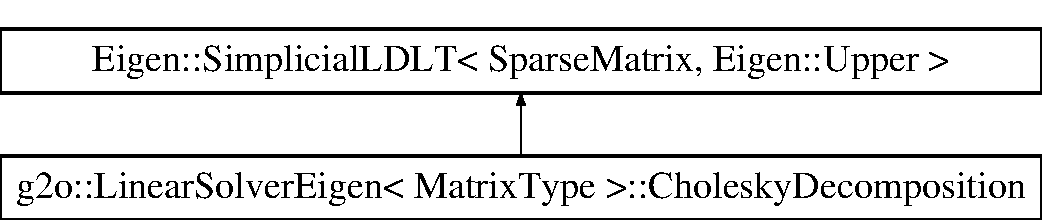
\includegraphics[height=2.000000cm]{classg2o_1_1_linear_solver_eigen_1_1_cholesky_decomposition}
\end{center}
\end{figure}
\subsection*{Public Member Functions}
\begin{DoxyCompactItemize}
\item 
\mbox{\hyperlink{classg2o_1_1_linear_solver_eigen_1_1_cholesky_decomposition_a4c82911542773cdcd66b470edb21831e}{Cholesky\+Decomposition}} ()
\item 
void \mbox{\hyperlink{classg2o_1_1_linear_solver_eigen_1_1_cholesky_decomposition_a3aa432f9aec0b7230c733df9a4d80558}{analyze\+Pattern\+With\+Permutation}} (\mbox{\hyperlink{classg2o_1_1_linear_solver_eigen_aeb7e2400bed3a249b5f29ce7cc00cd33}{Sparse\+Matrix}} \&a, const \mbox{\hyperlink{classg2o_1_1_linear_solver_eigen_acd9dd4e15dfbbad2720f1b83519333e8}{Permutation\+Matrix}} \&permutation)
\end{DoxyCompactItemize}


\subsection{Detailed Description}
\subsubsection*{template$<$typename Matrix\+Type$>$\newline
class g2o\+::\+Linear\+Solver\+Eigen$<$ Matrix\+Type $>$\+::\+Cholesky\+Decomposition}

Sub-\/classing Eigen\textquotesingle{}s Simplicial\+L\+D\+LT to perform ordering with a given ordering. 

\subsection{Constructor \& Destructor Documentation}
\mbox{\Hypertarget{classg2o_1_1_linear_solver_eigen_1_1_cholesky_decomposition_a4c82911542773cdcd66b470edb21831e}\label{classg2o_1_1_linear_solver_eigen_1_1_cholesky_decomposition_a4c82911542773cdcd66b470edb21831e}} 
\index{g2o\+::\+Linear\+Solver\+Eigen\+::\+Cholesky\+Decomposition@{g2o\+::\+Linear\+Solver\+Eigen\+::\+Cholesky\+Decomposition}!Cholesky\+Decomposition@{Cholesky\+Decomposition}}
\index{Cholesky\+Decomposition@{Cholesky\+Decomposition}!g2o\+::\+Linear\+Solver\+Eigen\+::\+Cholesky\+Decomposition@{g2o\+::\+Linear\+Solver\+Eigen\+::\+Cholesky\+Decomposition}}
\subsubsection{\texorpdfstring{Cholesky\+Decomposition()}{CholeskyDecomposition()}}
{\footnotesize\ttfamily template$<$typename Matrix\+Type$>$ \\
\mbox{\hyperlink{classg2o_1_1_linear_solver_eigen}{g2o\+::\+Linear\+Solver\+Eigen}}$<$ Matrix\+Type $>$\+::Cholesky\+Decomposition\+::\+Cholesky\+Decomposition (\begin{DoxyParamCaption}{ }\end{DoxyParamCaption})\hspace{0.3cm}{\ttfamily [inline]}}



\subsection{Member Function Documentation}
\mbox{\Hypertarget{classg2o_1_1_linear_solver_eigen_1_1_cholesky_decomposition_a3aa432f9aec0b7230c733df9a4d80558}\label{classg2o_1_1_linear_solver_eigen_1_1_cholesky_decomposition_a3aa432f9aec0b7230c733df9a4d80558}} 
\index{g2o\+::\+Linear\+Solver\+Eigen\+::\+Cholesky\+Decomposition@{g2o\+::\+Linear\+Solver\+Eigen\+::\+Cholesky\+Decomposition}!analyze\+Pattern\+With\+Permutation@{analyze\+Pattern\+With\+Permutation}}
\index{analyze\+Pattern\+With\+Permutation@{analyze\+Pattern\+With\+Permutation}!g2o\+::\+Linear\+Solver\+Eigen\+::\+Cholesky\+Decomposition@{g2o\+::\+Linear\+Solver\+Eigen\+::\+Cholesky\+Decomposition}}
\subsubsection{\texorpdfstring{analyze\+Pattern\+With\+Permutation()}{analyzePatternWithPermutation()}}
{\footnotesize\ttfamily template$<$typename Matrix\+Type$>$ \\
void \mbox{\hyperlink{classg2o_1_1_linear_solver_eigen}{g2o\+::\+Linear\+Solver\+Eigen}}$<$ Matrix\+Type $>$\+::Cholesky\+Decomposition\+::analyze\+Pattern\+With\+Permutation (\begin{DoxyParamCaption}\item[{\mbox{\hyperlink{classg2o_1_1_linear_solver_eigen_aeb7e2400bed3a249b5f29ce7cc00cd33}{Sparse\+Matrix}} \&}]{a,  }\item[{const \mbox{\hyperlink{classg2o_1_1_linear_solver_eigen_acd9dd4e15dfbbad2720f1b83519333e8}{Permutation\+Matrix}} \&}]{permutation }\end{DoxyParamCaption})\hspace{0.3cm}{\ttfamily [inline]}}



The documentation for this class was generated from the following file\+:\begin{DoxyCompactItemize}
\item 
D\+:/github/\+V\+S\+L\+A\+M/\+O\+R\+B\+S\+L\+A\+M2/\+O\+R\+B-\/\+S\+L\+A\+M2-\/master/\+Thirdparty/g2o/g2o/solvers/\mbox{\hyperlink{linear__solver__eigen_8h}{linear\+\_\+solver\+\_\+eigen.\+h}}\end{DoxyCompactItemize}

\hypertarget{structg2o_1_1_col_sort}{}\section{g2o\+:\+:Col\+Sort Struct Reference}
\label{structg2o_1_1_col_sort}\index{g2o\+::\+Col\+Sort@{g2o\+::\+Col\+Sort}}
\subsection*{Public Member Functions}
\begin{DoxyCompactItemize}
\item 
bool \mbox{\hyperlink{structg2o_1_1_col_sort_a47d0b6b7473c362d20f10becf55919dc}{operator()}} (const pair$<$ int, int $>$ \&e1, const pair$<$ int, int $>$ \&e2) const
\end{DoxyCompactItemize}


\subsection{Member Function Documentation}
\mbox{\Hypertarget{structg2o_1_1_col_sort_a47d0b6b7473c362d20f10becf55919dc}\label{structg2o_1_1_col_sort_a47d0b6b7473c362d20f10becf55919dc}} 
\index{g2o\+::\+Col\+Sort@{g2o\+::\+Col\+Sort}!operator()@{operator()}}
\index{operator()@{operator()}!g2o\+::\+Col\+Sort@{g2o\+::\+Col\+Sort}}
\subsubsection{\texorpdfstring{operator()()}{operator()()}}
{\footnotesize\ttfamily bool g2o\+::\+Col\+Sort\+::operator() (\begin{DoxyParamCaption}\item[{const pair$<$ int, int $>$ \&}]{e1,  }\item[{const pair$<$ int, int $>$ \&}]{e2 }\end{DoxyParamCaption}) const\hspace{0.3cm}{\ttfamily [inline]}}



The documentation for this struct was generated from the following file\+:\begin{DoxyCompactItemize}
\item 
Thirdparty/g2o/g2o/core/\mbox{\hyperlink{matrix__structure_8cpp}{matrix\+\_\+structure.\+cpp}}\end{DoxyCompactItemize}

\hypertarget{class_o_r_b___s_l_a_m2_1_1_converter}{}\section{O\+R\+B\+\_\+\+S\+L\+A\+M2\+:\+:Converter Class Reference}
\label{class_o_r_b___s_l_a_m2_1_1_converter}\index{O\+R\+B\+\_\+\+S\+L\+A\+M2\+::\+Converter@{O\+R\+B\+\_\+\+S\+L\+A\+M2\+::\+Converter}}


提供了一些常见的转换  




{\ttfamily \#include $<$Converter.\+h$>$}

\subsection*{Static Public Member Functions}
\begin{DoxyCompactItemize}
\item 
static std\+::vector$<$ cv\+::\+Mat $>$ \mbox{\hyperlink{class_o_r_b___s_l_a_m2_1_1_converter_abef47701eefdbc74c2c1625c140963fd}{to\+Descriptor\+Vector}} (const cv\+::\+Mat \&Descriptors)
\begin{DoxyCompactList}\small\item\em 一个描述子矩阵到一串单行的描述子向量 \end{DoxyCompactList}\end{DoxyCompactItemize}
\begin{Indent}\textbf{ to\+S\+E3\+Quat}\par
\begin{DoxyCompactItemize}
\item 
static \mbox{\hyperlink{classg2o_1_1_s_e3_quat}{g2o\+::\+S\+E3\+Quat}} \mbox{\hyperlink{class_o_r_b___s_l_a_m2_1_1_converter_a0b73791a3e2d90b4de41aed0ece2d0a2}{to\+S\+E3\+Quat}} (const cv\+::\+Mat \&cvT)
\item 
static \mbox{\hyperlink{classg2o_1_1_s_e3_quat}{g2o\+::\+S\+E3\+Quat}} \mbox{\hyperlink{class_o_r_b___s_l_a_m2_1_1_converter_ac76ddd3b4d9a7e364e5cc72cfe483247}{to\+S\+E3\+Quat}} (const \mbox{\hyperlink{structg2o_1_1_sim3}{g2o\+::\+Sim3}} \&g\+Sim3)
\end{DoxyCompactItemize}
\end{Indent}
\begin{Indent}\textbf{ to\+Cv\+Mat}\par
\begin{DoxyCompactItemize}
\item 
static cv\+::\+Mat \mbox{\hyperlink{class_o_r_b___s_l_a_m2_1_1_converter_ac9d5a9ea7de26d34047aa0afddaa2091}{to\+Cv\+Mat}} (const \mbox{\hyperlink{classg2o_1_1_s_e3_quat}{g2o\+::\+S\+E3\+Quat}} \&S\+E3)
\item 
static cv\+::\+Mat \mbox{\hyperlink{class_o_r_b___s_l_a_m2_1_1_converter_a4bc1702afbd33a5d90d39f1940157e08}{to\+Cv\+Mat}} (const \mbox{\hyperlink{structg2o_1_1_sim3}{g2o\+::\+Sim3}} \&Sim3)
\item 
static cv\+::\+Mat \mbox{\hyperlink{class_o_r_b___s_l_a_m2_1_1_converter_a93055164116a8f35ecc5a9a5dcad1ca0}{to\+Cv\+Mat}} (const Eigen\+::\+Matrix$<$ double, 4, 4 $>$ \&m)
\item 
static cv\+::\+Mat \mbox{\hyperlink{class_o_r_b___s_l_a_m2_1_1_converter_a7558c9fde7b818582bee8b4a4ff00793}{to\+Cv\+Mat}} (const Eigen\+::\+Matrix3d \&m)
\item 
static cv\+::\+Mat \mbox{\hyperlink{class_o_r_b___s_l_a_m2_1_1_converter_a6748f1ecb782efc7741c1d2f6fbbed22}{to\+Cv\+Mat}} (const Eigen\+::\+Matrix$<$ double, 3, 1 $>$ \&m)
\item 
static cv\+::\+Mat \mbox{\hyperlink{class_o_r_b___s_l_a_m2_1_1_converter_a0972ca8f56ea15c1814f51be3804978f}{to\+Cv\+S\+E3}} (const Eigen\+::\+Matrix$<$ double, 3, 3 $>$ \&R, const Eigen\+::\+Matrix$<$ double, 3, 1 $>$ \&t)
\end{DoxyCompactItemize}
\end{Indent}
\begin{Indent}\textbf{ to\+Eigen}\par
\begin{DoxyCompactItemize}
\item 
static Eigen\+::\+Matrix$<$ double, 3, 1 $>$ \mbox{\hyperlink{class_o_r_b___s_l_a_m2_1_1_converter_a65fccab585e29d1acbf4c23e5ce69bdc}{to\+Vector3d}} (const cv\+::\+Mat \&cv\+Vector)
\item 
static Eigen\+::\+Matrix$<$ double, 3, 1 $>$ \mbox{\hyperlink{class_o_r_b___s_l_a_m2_1_1_converter_af7b71b64b74fd45b39b9a7f47ee80145}{to\+Vector3d}} (const cv\+::\+Point3f \&cv\+Point)
\item 
static Eigen\+::\+Matrix$<$ double, 3, 3 $>$ \mbox{\hyperlink{class_o_r_b___s_l_a_m2_1_1_converter_a000a7971e46afdc95d6692a70006182b}{to\+Matrix3d}} (const cv\+::\+Mat \&cv\+Mat3)
\item 
static std\+::vector$<$ float $>$ \mbox{\hyperlink{class_o_r_b___s_l_a_m2_1_1_converter_a16b54bd921d9cdc83d289cfd1598fb3c}{to\+Quaternion}} (const cv\+::\+Mat \&M)
\end{DoxyCompactItemize}
\end{Indent}


\subsection{Detailed Description}
提供了一些常见的转换 

orb中以cv\+::\+Mat为基本存储结构,到g2o和\+Eigen需要一个转换 这些转换都很简单,整个文件可以单独从orbslam里抽出来而不影响其他功能 

\subsection{Member Function Documentation}
\mbox{\Hypertarget{class_o_r_b___s_l_a_m2_1_1_converter_ac9d5a9ea7de26d34047aa0afddaa2091}\label{class_o_r_b___s_l_a_m2_1_1_converter_ac9d5a9ea7de26d34047aa0afddaa2091}} 
\index{O\+R\+B\+\_\+\+S\+L\+A\+M2\+::\+Converter@{O\+R\+B\+\_\+\+S\+L\+A\+M2\+::\+Converter}!to\+Cv\+Mat@{to\+Cv\+Mat}}
\index{to\+Cv\+Mat@{to\+Cv\+Mat}!O\+R\+B\+\_\+\+S\+L\+A\+M2\+::\+Converter@{O\+R\+B\+\_\+\+S\+L\+A\+M2\+::\+Converter}}
\subsubsection{\texorpdfstring{to\+Cv\+Mat()}{toCvMat()}\hspace{0.1cm}{\footnotesize\ttfamily [1/5]}}
{\footnotesize\ttfamily cv\+::\+Mat O\+R\+B\+\_\+\+S\+L\+A\+M2\+::\+Converter\+::to\+Cv\+Mat (\begin{DoxyParamCaption}\item[{const \mbox{\hyperlink{classg2o_1_1_s_e3_quat}{g2o\+::\+S\+E3\+Quat}} \&}]{S\+E3 }\end{DoxyParamCaption})\hspace{0.3cm}{\ttfamily [static]}}

\mbox{\Hypertarget{class_o_r_b___s_l_a_m2_1_1_converter_a4bc1702afbd33a5d90d39f1940157e08}\label{class_o_r_b___s_l_a_m2_1_1_converter_a4bc1702afbd33a5d90d39f1940157e08}} 
\index{O\+R\+B\+\_\+\+S\+L\+A\+M2\+::\+Converter@{O\+R\+B\+\_\+\+S\+L\+A\+M2\+::\+Converter}!to\+Cv\+Mat@{to\+Cv\+Mat}}
\index{to\+Cv\+Mat@{to\+Cv\+Mat}!O\+R\+B\+\_\+\+S\+L\+A\+M2\+::\+Converter@{O\+R\+B\+\_\+\+S\+L\+A\+M2\+::\+Converter}}
\subsubsection{\texorpdfstring{to\+Cv\+Mat()}{toCvMat()}\hspace{0.1cm}{\footnotesize\ttfamily [2/5]}}
{\footnotesize\ttfamily cv\+::\+Mat O\+R\+B\+\_\+\+S\+L\+A\+M2\+::\+Converter\+::to\+Cv\+Mat (\begin{DoxyParamCaption}\item[{const \mbox{\hyperlink{structg2o_1_1_sim3}{g2o\+::\+Sim3}} \&}]{Sim3 }\end{DoxyParamCaption})\hspace{0.3cm}{\ttfamily [static]}}

\mbox{\Hypertarget{class_o_r_b___s_l_a_m2_1_1_converter_a93055164116a8f35ecc5a9a5dcad1ca0}\label{class_o_r_b___s_l_a_m2_1_1_converter_a93055164116a8f35ecc5a9a5dcad1ca0}} 
\index{O\+R\+B\+\_\+\+S\+L\+A\+M2\+::\+Converter@{O\+R\+B\+\_\+\+S\+L\+A\+M2\+::\+Converter}!to\+Cv\+Mat@{to\+Cv\+Mat}}
\index{to\+Cv\+Mat@{to\+Cv\+Mat}!O\+R\+B\+\_\+\+S\+L\+A\+M2\+::\+Converter@{O\+R\+B\+\_\+\+S\+L\+A\+M2\+::\+Converter}}
\subsubsection{\texorpdfstring{to\+Cv\+Mat()}{toCvMat()}\hspace{0.1cm}{\footnotesize\ttfamily [3/5]}}
{\footnotesize\ttfamily cv\+::\+Mat O\+R\+B\+\_\+\+S\+L\+A\+M2\+::\+Converter\+::to\+Cv\+Mat (\begin{DoxyParamCaption}\item[{const Eigen\+::\+Matrix$<$ double, 4, 4 $>$ \&}]{m }\end{DoxyParamCaption})\hspace{0.3cm}{\ttfamily [static]}}

\mbox{\Hypertarget{class_o_r_b___s_l_a_m2_1_1_converter_a7558c9fde7b818582bee8b4a4ff00793}\label{class_o_r_b___s_l_a_m2_1_1_converter_a7558c9fde7b818582bee8b4a4ff00793}} 
\index{O\+R\+B\+\_\+\+S\+L\+A\+M2\+::\+Converter@{O\+R\+B\+\_\+\+S\+L\+A\+M2\+::\+Converter}!to\+Cv\+Mat@{to\+Cv\+Mat}}
\index{to\+Cv\+Mat@{to\+Cv\+Mat}!O\+R\+B\+\_\+\+S\+L\+A\+M2\+::\+Converter@{O\+R\+B\+\_\+\+S\+L\+A\+M2\+::\+Converter}}
\subsubsection{\texorpdfstring{to\+Cv\+Mat()}{toCvMat()}\hspace{0.1cm}{\footnotesize\ttfamily [4/5]}}
{\footnotesize\ttfamily cv\+::\+Mat O\+R\+B\+\_\+\+S\+L\+A\+M2\+::\+Converter\+::to\+Cv\+Mat (\begin{DoxyParamCaption}\item[{const Eigen\+::\+Matrix3d \&}]{m }\end{DoxyParamCaption})\hspace{0.3cm}{\ttfamily [static]}}

\mbox{\Hypertarget{class_o_r_b___s_l_a_m2_1_1_converter_a6748f1ecb782efc7741c1d2f6fbbed22}\label{class_o_r_b___s_l_a_m2_1_1_converter_a6748f1ecb782efc7741c1d2f6fbbed22}} 
\index{O\+R\+B\+\_\+\+S\+L\+A\+M2\+::\+Converter@{O\+R\+B\+\_\+\+S\+L\+A\+M2\+::\+Converter}!to\+Cv\+Mat@{to\+Cv\+Mat}}
\index{to\+Cv\+Mat@{to\+Cv\+Mat}!O\+R\+B\+\_\+\+S\+L\+A\+M2\+::\+Converter@{O\+R\+B\+\_\+\+S\+L\+A\+M2\+::\+Converter}}
\subsubsection{\texorpdfstring{to\+Cv\+Mat()}{toCvMat()}\hspace{0.1cm}{\footnotesize\ttfamily [5/5]}}
{\footnotesize\ttfamily cv\+::\+Mat O\+R\+B\+\_\+\+S\+L\+A\+M2\+::\+Converter\+::to\+Cv\+Mat (\begin{DoxyParamCaption}\item[{const Eigen\+::\+Matrix$<$ double, 3, 1 $>$ \&}]{m }\end{DoxyParamCaption})\hspace{0.3cm}{\ttfamily [static]}}

\mbox{\Hypertarget{class_o_r_b___s_l_a_m2_1_1_converter_a0972ca8f56ea15c1814f51be3804978f}\label{class_o_r_b___s_l_a_m2_1_1_converter_a0972ca8f56ea15c1814f51be3804978f}} 
\index{O\+R\+B\+\_\+\+S\+L\+A\+M2\+::\+Converter@{O\+R\+B\+\_\+\+S\+L\+A\+M2\+::\+Converter}!to\+Cv\+S\+E3@{to\+Cv\+S\+E3}}
\index{to\+Cv\+S\+E3@{to\+Cv\+S\+E3}!O\+R\+B\+\_\+\+S\+L\+A\+M2\+::\+Converter@{O\+R\+B\+\_\+\+S\+L\+A\+M2\+::\+Converter}}
\subsubsection{\texorpdfstring{to\+Cv\+S\+E3()}{toCvSE3()}}
{\footnotesize\ttfamily cv\+::\+Mat O\+R\+B\+\_\+\+S\+L\+A\+M2\+::\+Converter\+::to\+Cv\+S\+E3 (\begin{DoxyParamCaption}\item[{const Eigen\+::\+Matrix$<$ double, 3, 3 $>$ \&}]{R,  }\item[{const Eigen\+::\+Matrix$<$ double, 3, 1 $>$ \&}]{t }\end{DoxyParamCaption})\hspace{0.3cm}{\ttfamily [static]}}

\mbox{\Hypertarget{class_o_r_b___s_l_a_m2_1_1_converter_abef47701eefdbc74c2c1625c140963fd}\label{class_o_r_b___s_l_a_m2_1_1_converter_abef47701eefdbc74c2c1625c140963fd}} 
\index{O\+R\+B\+\_\+\+S\+L\+A\+M2\+::\+Converter@{O\+R\+B\+\_\+\+S\+L\+A\+M2\+::\+Converter}!to\+Descriptor\+Vector@{to\+Descriptor\+Vector}}
\index{to\+Descriptor\+Vector@{to\+Descriptor\+Vector}!O\+R\+B\+\_\+\+S\+L\+A\+M2\+::\+Converter@{O\+R\+B\+\_\+\+S\+L\+A\+M2\+::\+Converter}}
\subsubsection{\texorpdfstring{to\+Descriptor\+Vector()}{toDescriptorVector()}}
{\footnotesize\ttfamily std\+::vector$<$ cv\+::\+Mat $>$ O\+R\+B\+\_\+\+S\+L\+A\+M2\+::\+Converter\+::to\+Descriptor\+Vector (\begin{DoxyParamCaption}\item[{const cv\+::\+Mat \&}]{Descriptors }\end{DoxyParamCaption})\hspace{0.3cm}{\ttfamily [static]}}



一个描述子矩阵到一串单行的描述子向量 

\mbox{\Hypertarget{class_o_r_b___s_l_a_m2_1_1_converter_a000a7971e46afdc95d6692a70006182b}\label{class_o_r_b___s_l_a_m2_1_1_converter_a000a7971e46afdc95d6692a70006182b}} 
\index{O\+R\+B\+\_\+\+S\+L\+A\+M2\+::\+Converter@{O\+R\+B\+\_\+\+S\+L\+A\+M2\+::\+Converter}!to\+Matrix3d@{to\+Matrix3d}}
\index{to\+Matrix3d@{to\+Matrix3d}!O\+R\+B\+\_\+\+S\+L\+A\+M2\+::\+Converter@{O\+R\+B\+\_\+\+S\+L\+A\+M2\+::\+Converter}}
\subsubsection{\texorpdfstring{to\+Matrix3d()}{toMatrix3d()}}
{\footnotesize\ttfamily Eigen\+::\+Matrix$<$ double, 3, 3 $>$ O\+R\+B\+\_\+\+S\+L\+A\+M2\+::\+Converter\+::to\+Matrix3d (\begin{DoxyParamCaption}\item[{const cv\+::\+Mat \&}]{cv\+Mat3 }\end{DoxyParamCaption})\hspace{0.3cm}{\ttfamily [static]}}

\mbox{\Hypertarget{class_o_r_b___s_l_a_m2_1_1_converter_a16b54bd921d9cdc83d289cfd1598fb3c}\label{class_o_r_b___s_l_a_m2_1_1_converter_a16b54bd921d9cdc83d289cfd1598fb3c}} 
\index{O\+R\+B\+\_\+\+S\+L\+A\+M2\+::\+Converter@{O\+R\+B\+\_\+\+S\+L\+A\+M2\+::\+Converter}!to\+Quaternion@{to\+Quaternion}}
\index{to\+Quaternion@{to\+Quaternion}!O\+R\+B\+\_\+\+S\+L\+A\+M2\+::\+Converter@{O\+R\+B\+\_\+\+S\+L\+A\+M2\+::\+Converter}}
\subsubsection{\texorpdfstring{to\+Quaternion()}{toQuaternion()}}
{\footnotesize\ttfamily std\+::vector$<$ float $>$ O\+R\+B\+\_\+\+S\+L\+A\+M2\+::\+Converter\+::to\+Quaternion (\begin{DoxyParamCaption}\item[{const cv\+::\+Mat \&}]{M }\end{DoxyParamCaption})\hspace{0.3cm}{\ttfamily [static]}}

\mbox{\Hypertarget{class_o_r_b___s_l_a_m2_1_1_converter_a0b73791a3e2d90b4de41aed0ece2d0a2}\label{class_o_r_b___s_l_a_m2_1_1_converter_a0b73791a3e2d90b4de41aed0ece2d0a2}} 
\index{O\+R\+B\+\_\+\+S\+L\+A\+M2\+::\+Converter@{O\+R\+B\+\_\+\+S\+L\+A\+M2\+::\+Converter}!to\+S\+E3\+Quat@{to\+S\+E3\+Quat}}
\index{to\+S\+E3\+Quat@{to\+S\+E3\+Quat}!O\+R\+B\+\_\+\+S\+L\+A\+M2\+::\+Converter@{O\+R\+B\+\_\+\+S\+L\+A\+M2\+::\+Converter}}
\subsubsection{\texorpdfstring{to\+S\+E3\+Quat()}{toSE3Quat()}\hspace{0.1cm}{\footnotesize\ttfamily [1/2]}}
{\footnotesize\ttfamily \mbox{\hyperlink{classg2o_1_1_s_e3_quat}{g2o\+::\+S\+E3\+Quat}} O\+R\+B\+\_\+\+S\+L\+A\+M2\+::\+Converter\+::to\+S\+E3\+Quat (\begin{DoxyParamCaption}\item[{const cv\+::\+Mat \&}]{cvT }\end{DoxyParamCaption})\hspace{0.3cm}{\ttfamily [static]}}

cv\+::\+Mat to \mbox{\hyperlink{classg2o_1_1_s_e3_quat}{g2o\+::\+S\+E3\+Quat}} \mbox{\Hypertarget{class_o_r_b___s_l_a_m2_1_1_converter_ac76ddd3b4d9a7e364e5cc72cfe483247}\label{class_o_r_b___s_l_a_m2_1_1_converter_ac76ddd3b4d9a7e364e5cc72cfe483247}} 
\index{O\+R\+B\+\_\+\+S\+L\+A\+M2\+::\+Converter@{O\+R\+B\+\_\+\+S\+L\+A\+M2\+::\+Converter}!to\+S\+E3\+Quat@{to\+S\+E3\+Quat}}
\index{to\+S\+E3\+Quat@{to\+S\+E3\+Quat}!O\+R\+B\+\_\+\+S\+L\+A\+M2\+::\+Converter@{O\+R\+B\+\_\+\+S\+L\+A\+M2\+::\+Converter}}
\subsubsection{\texorpdfstring{to\+S\+E3\+Quat()}{toSE3Quat()}\hspace{0.1cm}{\footnotesize\ttfamily [2/2]}}
{\footnotesize\ttfamily static \mbox{\hyperlink{classg2o_1_1_s_e3_quat}{g2o\+::\+S\+E3\+Quat}} O\+R\+B\+\_\+\+S\+L\+A\+M2\+::\+Converter\+::to\+S\+E3\+Quat (\begin{DoxyParamCaption}\item[{const \mbox{\hyperlink{structg2o_1_1_sim3}{g2o\+::\+Sim3}} \&}]{g\+Sim3 }\end{DoxyParamCaption})\hspace{0.3cm}{\ttfamily [static]}}

unimplemented \mbox{\Hypertarget{class_o_r_b___s_l_a_m2_1_1_converter_a65fccab585e29d1acbf4c23e5ce69bdc}\label{class_o_r_b___s_l_a_m2_1_1_converter_a65fccab585e29d1acbf4c23e5ce69bdc}} 
\index{O\+R\+B\+\_\+\+S\+L\+A\+M2\+::\+Converter@{O\+R\+B\+\_\+\+S\+L\+A\+M2\+::\+Converter}!to\+Vector3d@{to\+Vector3d}}
\index{to\+Vector3d@{to\+Vector3d}!O\+R\+B\+\_\+\+S\+L\+A\+M2\+::\+Converter@{O\+R\+B\+\_\+\+S\+L\+A\+M2\+::\+Converter}}
\subsubsection{\texorpdfstring{to\+Vector3d()}{toVector3d()}\hspace{0.1cm}{\footnotesize\ttfamily [1/2]}}
{\footnotesize\ttfamily Eigen\+::\+Matrix$<$ double, 3, 1 $>$ O\+R\+B\+\_\+\+S\+L\+A\+M2\+::\+Converter\+::to\+Vector3d (\begin{DoxyParamCaption}\item[{const cv\+::\+Mat \&}]{cv\+Vector }\end{DoxyParamCaption})\hspace{0.3cm}{\ttfamily [static]}}

\mbox{\Hypertarget{class_o_r_b___s_l_a_m2_1_1_converter_af7b71b64b74fd45b39b9a7f47ee80145}\label{class_o_r_b___s_l_a_m2_1_1_converter_af7b71b64b74fd45b39b9a7f47ee80145}} 
\index{O\+R\+B\+\_\+\+S\+L\+A\+M2\+::\+Converter@{O\+R\+B\+\_\+\+S\+L\+A\+M2\+::\+Converter}!to\+Vector3d@{to\+Vector3d}}
\index{to\+Vector3d@{to\+Vector3d}!O\+R\+B\+\_\+\+S\+L\+A\+M2\+::\+Converter@{O\+R\+B\+\_\+\+S\+L\+A\+M2\+::\+Converter}}
\subsubsection{\texorpdfstring{to\+Vector3d()}{toVector3d()}\hspace{0.1cm}{\footnotesize\ttfamily [2/2]}}
{\footnotesize\ttfamily Eigen\+::\+Matrix$<$ double, 3, 1 $>$ O\+R\+B\+\_\+\+S\+L\+A\+M2\+::\+Converter\+::to\+Vector3d (\begin{DoxyParamCaption}\item[{const cv\+::\+Point3f \&}]{cv\+Point }\end{DoxyParamCaption})\hspace{0.3cm}{\ttfamily [static]}}



The documentation for this class was generated from the following files\+:\begin{DoxyCompactItemize}
\item 
D\+:/github/\+V\+S\+L\+A\+M/\+O\+R\+B\+S\+L\+A\+M2/\+O\+R\+B-\/\+S\+L\+A\+M2-\/master/include/\mbox{\hyperlink{_converter_8h}{Converter.\+h}}\item 
D\+:/github/\+V\+S\+L\+A\+M/\+O\+R\+B\+S\+L\+A\+M2/\+O\+R\+B-\/\+S\+L\+A\+M2-\/master/src/\mbox{\hyperlink{_converter_8cpp}{Converter.\+cpp}}\end{DoxyCompactItemize}

\hypertarget{structg2o_1_1_hyper_dijkstra_1_1_cost_function}{}\section{g2o\+:\+:Hyper\+Dijkstra\+:\+:Cost\+Function Struct Reference}
\label{structg2o_1_1_hyper_dijkstra_1_1_cost_function}\index{g2o\+::\+Hyper\+Dijkstra\+::\+Cost\+Function@{g2o\+::\+Hyper\+Dijkstra\+::\+Cost\+Function}}


{\ttfamily \#include $<$hyper\+\_\+dijkstra.\+h$>$}

Inheritance diagram for g2o\+:\+:Hyper\+Dijkstra\+:\+:Cost\+Function\+:\begin{figure}[H]
\begin{center}
\leavevmode
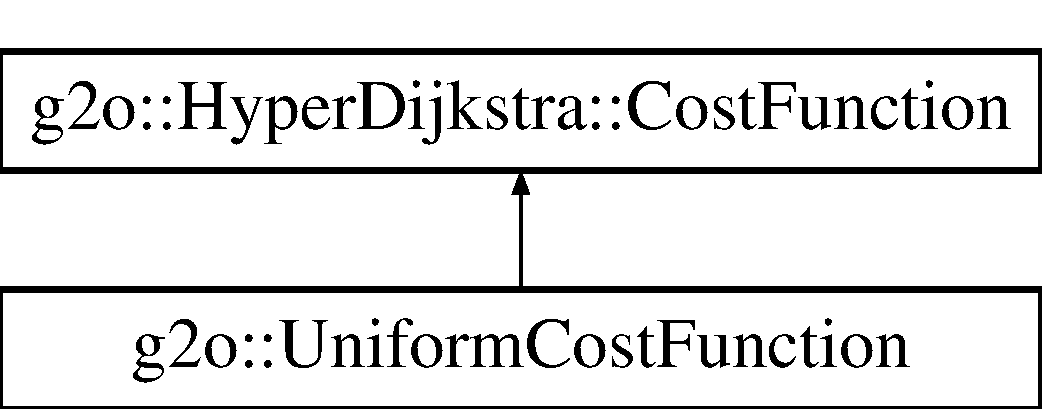
\includegraphics[height=2.000000cm]{structg2o_1_1_hyper_dijkstra_1_1_cost_function}
\end{center}
\end{figure}
\subsection*{Public Member Functions}
\begin{DoxyCompactItemize}
\item 
virtual double \mbox{\hyperlink{structg2o_1_1_hyper_dijkstra_1_1_cost_function_a6d30ca80400c75941851ae079cfd42fd}{operator()}} (\mbox{\hyperlink{classg2o_1_1_hyper_graph_1_1_edge}{Hyper\+Graph\+::\+Edge}} $\ast$e, \mbox{\hyperlink{classg2o_1_1_hyper_graph_1_1_vertex}{Hyper\+Graph\+::\+Vertex}} $\ast$from, \mbox{\hyperlink{classg2o_1_1_hyper_graph_1_1_vertex}{Hyper\+Graph\+::\+Vertex}} $\ast$to)=0
\item 
virtual \mbox{\hyperlink{structg2o_1_1_hyper_dijkstra_1_1_cost_function_aabfa53ac04d3934478fe419695474bcf}{$\sim$\+Cost\+Function}} ()
\end{DoxyCompactItemize}


\subsection{Constructor \& Destructor Documentation}
\mbox{\Hypertarget{structg2o_1_1_hyper_dijkstra_1_1_cost_function_aabfa53ac04d3934478fe419695474bcf}\label{structg2o_1_1_hyper_dijkstra_1_1_cost_function_aabfa53ac04d3934478fe419695474bcf}} 
\index{g2o\+::\+Hyper\+Dijkstra\+::\+Cost\+Function@{g2o\+::\+Hyper\+Dijkstra\+::\+Cost\+Function}!````~Cost\+Function@{$\sim$\+Cost\+Function}}
\index{````~Cost\+Function@{$\sim$\+Cost\+Function}!g2o\+::\+Hyper\+Dijkstra\+::\+Cost\+Function@{g2o\+::\+Hyper\+Dijkstra\+::\+Cost\+Function}}
\subsubsection{\texorpdfstring{$\sim$\+Cost\+Function()}{~CostFunction()}}
{\footnotesize\ttfamily virtual g2o\+::\+Hyper\+Dijkstra\+::\+Cost\+Function\+::$\sim$\+Cost\+Function (\begin{DoxyParamCaption}{ }\end{DoxyParamCaption})\hspace{0.3cm}{\ttfamily [inline]}, {\ttfamily [virtual]}}



\subsection{Member Function Documentation}
\mbox{\Hypertarget{structg2o_1_1_hyper_dijkstra_1_1_cost_function_a6d30ca80400c75941851ae079cfd42fd}\label{structg2o_1_1_hyper_dijkstra_1_1_cost_function_a6d30ca80400c75941851ae079cfd42fd}} 
\index{g2o\+::\+Hyper\+Dijkstra\+::\+Cost\+Function@{g2o\+::\+Hyper\+Dijkstra\+::\+Cost\+Function}!operator()@{operator()}}
\index{operator()@{operator()}!g2o\+::\+Hyper\+Dijkstra\+::\+Cost\+Function@{g2o\+::\+Hyper\+Dijkstra\+::\+Cost\+Function}}
\subsubsection{\texorpdfstring{operator()()}{operator()()}}
{\footnotesize\ttfamily virtual double g2o\+::\+Hyper\+Dijkstra\+::\+Cost\+Function\+::operator() (\begin{DoxyParamCaption}\item[{\mbox{\hyperlink{classg2o_1_1_hyper_graph_1_1_edge}{Hyper\+Graph\+::\+Edge}} $\ast$}]{e,  }\item[{\mbox{\hyperlink{classg2o_1_1_hyper_graph_1_1_vertex}{Hyper\+Graph\+::\+Vertex}} $\ast$}]{from,  }\item[{\mbox{\hyperlink{classg2o_1_1_hyper_graph_1_1_vertex}{Hyper\+Graph\+::\+Vertex}} $\ast$}]{to }\end{DoxyParamCaption})\hspace{0.3cm}{\ttfamily [pure virtual]}}



Implemented in \mbox{\hyperlink{structg2o_1_1_uniform_cost_function_a44e15e4af4310890d4c7965cb6c7aaad}{g2o\+::\+Uniform\+Cost\+Function}}.



The documentation for this struct was generated from the following file\+:\begin{DoxyCompactItemize}
\item 
D\+:/github/\+V\+S\+L\+A\+M/\+O\+R\+B\+S\+L\+A\+M2/\+O\+R\+B-\/\+S\+L\+A\+M2-\/master/\+Thirdparty/g2o/g2o/core/\mbox{\hyperlink{hyper__dijkstra_8h}{hyper\+\_\+dijkstra.\+h}}\end{DoxyCompactItemize}

\hypertarget{classg2o_1_1_factory_1_1_creator_information}{}\section{g2o\+:\+:Factory\+:\+:Creator\+Information Class Reference}
\label{classg2o_1_1_factory_1_1_creator_information}\index{g2o\+::\+Factory\+::\+Creator\+Information@{g2o\+::\+Factory\+::\+Creator\+Information}}


{\ttfamily \#include $<$factory.\+h$>$}

\subsection*{Public Member Functions}
\begin{DoxyCompactItemize}
\item 
\mbox{\hyperlink{classg2o_1_1_factory_1_1_creator_information_a8f4353b17f6548b0c935a4062231d968}{Creator\+Information}} ()
\item 
\mbox{\hyperlink{classg2o_1_1_factory_1_1_creator_information_a5f29790696c1143395a4e11f4bb372c1}{$\sim$\+Creator\+Information}} ()
\end{DoxyCompactItemize}
\subsection*{Public Attributes}
\begin{DoxyCompactItemize}
\item 
\mbox{\hyperlink{classg2o_1_1_abstract_hyper_graph_element_creator}{Abstract\+Hyper\+Graph\+Element\+Creator}} $\ast$ \mbox{\hyperlink{classg2o_1_1_factory_1_1_creator_information_a9fd5a1087992c17f869f1d59bc519c23}{creator}}
\item 
int \mbox{\hyperlink{classg2o_1_1_factory_1_1_creator_information_ab9fa4c8aec27d204f5ae6a7510c4e339}{element\+Type\+Bit}}
\end{DoxyCompactItemize}


\subsection{Constructor \& Destructor Documentation}
\mbox{\Hypertarget{classg2o_1_1_factory_1_1_creator_information_a8f4353b17f6548b0c935a4062231d968}\label{classg2o_1_1_factory_1_1_creator_information_a8f4353b17f6548b0c935a4062231d968}} 
\index{g2o\+::\+Factory\+::\+Creator\+Information@{g2o\+::\+Factory\+::\+Creator\+Information}!Creator\+Information@{Creator\+Information}}
\index{Creator\+Information@{Creator\+Information}!g2o\+::\+Factory\+::\+Creator\+Information@{g2o\+::\+Factory\+::\+Creator\+Information}}
\subsubsection{\texorpdfstring{Creator\+Information()}{CreatorInformation()}}
{\footnotesize\ttfamily g2o\+::\+Factory\+::\+Creator\+Information\+::\+Creator\+Information (\begin{DoxyParamCaption}{ }\end{DoxyParamCaption})\hspace{0.3cm}{\ttfamily [inline]}}

\mbox{\Hypertarget{classg2o_1_1_factory_1_1_creator_information_a5f29790696c1143395a4e11f4bb372c1}\label{classg2o_1_1_factory_1_1_creator_information_a5f29790696c1143395a4e11f4bb372c1}} 
\index{g2o\+::\+Factory\+::\+Creator\+Information@{g2o\+::\+Factory\+::\+Creator\+Information}!````~Creator\+Information@{$\sim$\+Creator\+Information}}
\index{````~Creator\+Information@{$\sim$\+Creator\+Information}!g2o\+::\+Factory\+::\+Creator\+Information@{g2o\+::\+Factory\+::\+Creator\+Information}}
\subsubsection{\texorpdfstring{$\sim$\+Creator\+Information()}{~CreatorInformation()}}
{\footnotesize\ttfamily g2o\+::\+Factory\+::\+Creator\+Information\+::$\sim$\+Creator\+Information (\begin{DoxyParamCaption}{ }\end{DoxyParamCaption})\hspace{0.3cm}{\ttfamily [inline]}}



\subsection{Member Data Documentation}
\mbox{\Hypertarget{classg2o_1_1_factory_1_1_creator_information_a9fd5a1087992c17f869f1d59bc519c23}\label{classg2o_1_1_factory_1_1_creator_information_a9fd5a1087992c17f869f1d59bc519c23}} 
\index{g2o\+::\+Factory\+::\+Creator\+Information@{g2o\+::\+Factory\+::\+Creator\+Information}!creator@{creator}}
\index{creator@{creator}!g2o\+::\+Factory\+::\+Creator\+Information@{g2o\+::\+Factory\+::\+Creator\+Information}}
\subsubsection{\texorpdfstring{creator}{creator}}
{\footnotesize\ttfamily \mbox{\hyperlink{classg2o_1_1_abstract_hyper_graph_element_creator}{Abstract\+Hyper\+Graph\+Element\+Creator}}$\ast$ g2o\+::\+Factory\+::\+Creator\+Information\+::creator}

\mbox{\Hypertarget{classg2o_1_1_factory_1_1_creator_information_ab9fa4c8aec27d204f5ae6a7510c4e339}\label{classg2o_1_1_factory_1_1_creator_information_ab9fa4c8aec27d204f5ae6a7510c4e339}} 
\index{g2o\+::\+Factory\+::\+Creator\+Information@{g2o\+::\+Factory\+::\+Creator\+Information}!element\+Type\+Bit@{element\+Type\+Bit}}
\index{element\+Type\+Bit@{element\+Type\+Bit}!g2o\+::\+Factory\+::\+Creator\+Information@{g2o\+::\+Factory\+::\+Creator\+Information}}
\subsubsection{\texorpdfstring{element\+Type\+Bit}{elementTypeBit}}
{\footnotesize\ttfamily int g2o\+::\+Factory\+::\+Creator\+Information\+::element\+Type\+Bit}



The documentation for this class was generated from the following file\+:\begin{DoxyCompactItemize}
\item 
Thirdparty/g2o/g2o/core/\mbox{\hyperlink{factory_8h}{factory.\+h}}\end{DoxyCompactItemize}

\hypertarget{classg2o_1_1_optimizable_graph_1_1_data}{}\section{g2o\+:\+:Optimizable\+Graph\+:\+:Data Class Reference}
\label{classg2o_1_1_optimizable_graph_1_1_data}\index{g2o\+::\+Optimizable\+Graph\+::\+Data@{g2o\+::\+Optimizable\+Graph\+::\+Data}}


data packet for a vertex. Extend this class to store in the vertices the potential additional information you need (e.\+g. images, laser scans, ...).  




{\ttfamily \#include $<$optimizable\+\_\+graph.\+h$>$}

Inheritance diagram for g2o\+:\+:Optimizable\+Graph\+:\+:Data\+:\begin{figure}[H]
\begin{center}
\leavevmode
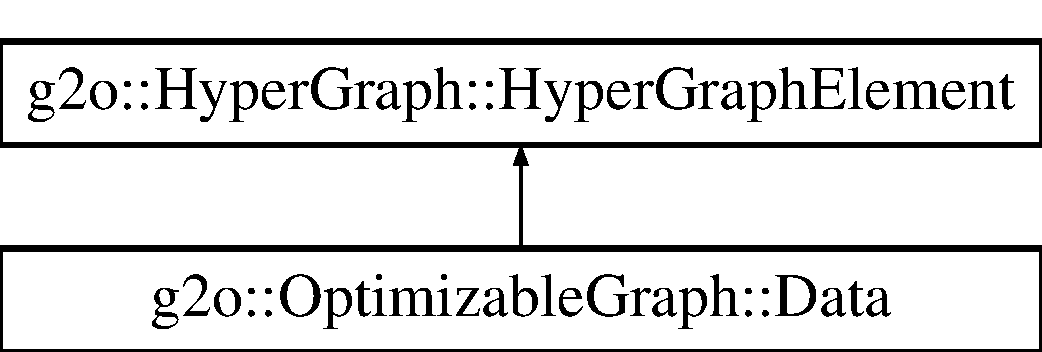
\includegraphics[height=2.000000cm]{classg2o_1_1_optimizable_graph_1_1_data}
\end{center}
\end{figure}
\subsection*{Public Member Functions}
\begin{DoxyCompactItemize}
\item 
virtual \mbox{\hyperlink{classg2o_1_1_optimizable_graph_1_1_data_aa81fb1975f34e3aaf4c5110f7778a54e}{$\sim$\+Data}} ()
\item 
\mbox{\hyperlink{classg2o_1_1_optimizable_graph_1_1_data_a647b9fcb65aa8309f7103635135ea513}{Data}} ()
\item 
virtual bool \mbox{\hyperlink{classg2o_1_1_optimizable_graph_1_1_data_a4a206c86daba1b47425199befd2e1ed4}{read}} (std\+::istream \&is)=0
\begin{DoxyCompactList}\small\item\em read the data from a stream \end{DoxyCompactList}\item 
virtual bool \mbox{\hyperlink{classg2o_1_1_optimizable_graph_1_1_data_ad80cd8ea8013c54c766684ec0ef3daa3}{write}} (std\+::ostream \&os) const =0
\begin{DoxyCompactList}\small\item\em write the data to a stream \end{DoxyCompactList}\item 
virtual Hyper\+Graph\+::\+Hyper\+Graph\+Element\+Type \mbox{\hyperlink{classg2o_1_1_optimizable_graph_1_1_data_aa98d48f62d4c620cb62fbaeb1775389b}{element\+Type}} () const
\item 
const \mbox{\hyperlink{classg2o_1_1_optimizable_graph_1_1_data}{Data}} $\ast$ \mbox{\hyperlink{classg2o_1_1_optimizable_graph_1_1_data_a1e36ab8bfbbd4df1639338330bbaaf3c}{next}} () const
\item 
\mbox{\hyperlink{classg2o_1_1_optimizable_graph_1_1_data}{Data}} $\ast$ \mbox{\hyperlink{classg2o_1_1_optimizable_graph_1_1_data_af9c0427357f1e81f9008c3173fddf34c}{next}} ()
\item 
void \mbox{\hyperlink{classg2o_1_1_optimizable_graph_1_1_data_a5811aac3f8eab3c19207663e946b343b}{set\+Next}} (\mbox{\hyperlink{classg2o_1_1_optimizable_graph_1_1_data}{Data}} $\ast$next\+\_\+)
\end{DoxyCompactItemize}
\subsection*{Protected Attributes}
\begin{DoxyCompactItemize}
\item 
\mbox{\hyperlink{classg2o_1_1_optimizable_graph_1_1_data}{Data}} $\ast$ \mbox{\hyperlink{classg2o_1_1_optimizable_graph_1_1_data_a8e0569f2b8cb8400d3eada1bd13c0ccb}{\+\_\+next}}
\end{DoxyCompactItemize}
\subsection*{Friends}
\begin{DoxyCompactItemize}
\item 
struct \mbox{\hyperlink{classg2o_1_1_optimizable_graph_1_1_data_a45d35331ee3deca38c26d1efb6b961ae}{Optimizable\+Graph}}
\end{DoxyCompactItemize}


\subsection{Detailed Description}
data packet for a vertex. Extend this class to store in the vertices the potential additional information you need (e.\+g. images, laser scans, ...). 

\subsection{Constructor \& Destructor Documentation}
\mbox{\Hypertarget{classg2o_1_1_optimizable_graph_1_1_data_aa81fb1975f34e3aaf4c5110f7778a54e}\label{classg2o_1_1_optimizable_graph_1_1_data_aa81fb1975f34e3aaf4c5110f7778a54e}} 
\index{g2o\+::\+Optimizable\+Graph\+::\+Data@{g2o\+::\+Optimizable\+Graph\+::\+Data}!````~Data@{$\sim$\+Data}}
\index{````~Data@{$\sim$\+Data}!g2o\+::\+Optimizable\+Graph\+::\+Data@{g2o\+::\+Optimizable\+Graph\+::\+Data}}
\subsubsection{\texorpdfstring{$\sim$\+Data()}{~Data()}}
{\footnotesize\ttfamily g2o\+::\+Optimizable\+Graph\+::\+Data\+::$\sim$\+Data (\begin{DoxyParamCaption}{ }\end{DoxyParamCaption})\hspace{0.3cm}{\ttfamily [virtual]}}

\mbox{\Hypertarget{classg2o_1_1_optimizable_graph_1_1_data_a647b9fcb65aa8309f7103635135ea513}\label{classg2o_1_1_optimizable_graph_1_1_data_a647b9fcb65aa8309f7103635135ea513}} 
\index{g2o\+::\+Optimizable\+Graph\+::\+Data@{g2o\+::\+Optimizable\+Graph\+::\+Data}!Data@{Data}}
\index{Data@{Data}!g2o\+::\+Optimizable\+Graph\+::\+Data@{g2o\+::\+Optimizable\+Graph\+::\+Data}}
\subsubsection{\texorpdfstring{Data()}{Data()}}
{\footnotesize\ttfamily g2o\+::\+Optimizable\+Graph\+::\+Data\+::\+Data (\begin{DoxyParamCaption}{ }\end{DoxyParamCaption})}



\subsection{Member Function Documentation}
\mbox{\Hypertarget{classg2o_1_1_optimizable_graph_1_1_data_aa98d48f62d4c620cb62fbaeb1775389b}\label{classg2o_1_1_optimizable_graph_1_1_data_aa98d48f62d4c620cb62fbaeb1775389b}} 
\index{g2o\+::\+Optimizable\+Graph\+::\+Data@{g2o\+::\+Optimizable\+Graph\+::\+Data}!element\+Type@{element\+Type}}
\index{element\+Type@{element\+Type}!g2o\+::\+Optimizable\+Graph\+::\+Data@{g2o\+::\+Optimizable\+Graph\+::\+Data}}
\subsubsection{\texorpdfstring{element\+Type()}{elementType()}}
{\footnotesize\ttfamily virtual Hyper\+Graph\+::\+Hyper\+Graph\+Element\+Type g2o\+::\+Optimizable\+Graph\+::\+Data\+::element\+Type (\begin{DoxyParamCaption}{ }\end{DoxyParamCaption}) const\hspace{0.3cm}{\ttfamily [inline]}, {\ttfamily [virtual]}}

returns the type of the graph element, see Hyper\+Graph\+Element\+Type 

Implements \mbox{\hyperlink{structg2o_1_1_hyper_graph_1_1_hyper_graph_element_a1a9d7b748698c09d202373e06e413ef2}{g2o\+::\+Hyper\+Graph\+::\+Hyper\+Graph\+Element}}.

\mbox{\Hypertarget{classg2o_1_1_optimizable_graph_1_1_data_a1e36ab8bfbbd4df1639338330bbaaf3c}\label{classg2o_1_1_optimizable_graph_1_1_data_a1e36ab8bfbbd4df1639338330bbaaf3c}} 
\index{g2o\+::\+Optimizable\+Graph\+::\+Data@{g2o\+::\+Optimizable\+Graph\+::\+Data}!next@{next}}
\index{next@{next}!g2o\+::\+Optimizable\+Graph\+::\+Data@{g2o\+::\+Optimizable\+Graph\+::\+Data}}
\subsubsection{\texorpdfstring{next()}{next()}\hspace{0.1cm}{\footnotesize\ttfamily [1/2]}}
{\footnotesize\ttfamily const \mbox{\hyperlink{classg2o_1_1_optimizable_graph_1_1_data}{Data}}$\ast$ g2o\+::\+Optimizable\+Graph\+::\+Data\+::next (\begin{DoxyParamCaption}{ }\end{DoxyParamCaption}) const\hspace{0.3cm}{\ttfamily [inline]}}

\mbox{\Hypertarget{classg2o_1_1_optimizable_graph_1_1_data_af9c0427357f1e81f9008c3173fddf34c}\label{classg2o_1_1_optimizable_graph_1_1_data_af9c0427357f1e81f9008c3173fddf34c}} 
\index{g2o\+::\+Optimizable\+Graph\+::\+Data@{g2o\+::\+Optimizable\+Graph\+::\+Data}!next@{next}}
\index{next@{next}!g2o\+::\+Optimizable\+Graph\+::\+Data@{g2o\+::\+Optimizable\+Graph\+::\+Data}}
\subsubsection{\texorpdfstring{next()}{next()}\hspace{0.1cm}{\footnotesize\ttfamily [2/2]}}
{\footnotesize\ttfamily \mbox{\hyperlink{classg2o_1_1_optimizable_graph_1_1_data}{Data}}$\ast$ g2o\+::\+Optimizable\+Graph\+::\+Data\+::next (\begin{DoxyParamCaption}{ }\end{DoxyParamCaption})\hspace{0.3cm}{\ttfamily [inline]}}

\mbox{\Hypertarget{classg2o_1_1_optimizable_graph_1_1_data_a4a206c86daba1b47425199befd2e1ed4}\label{classg2o_1_1_optimizable_graph_1_1_data_a4a206c86daba1b47425199befd2e1ed4}} 
\index{g2o\+::\+Optimizable\+Graph\+::\+Data@{g2o\+::\+Optimizable\+Graph\+::\+Data}!read@{read}}
\index{read@{read}!g2o\+::\+Optimizable\+Graph\+::\+Data@{g2o\+::\+Optimizable\+Graph\+::\+Data}}
\subsubsection{\texorpdfstring{read()}{read()}}
{\footnotesize\ttfamily virtual bool g2o\+::\+Optimizable\+Graph\+::\+Data\+::read (\begin{DoxyParamCaption}\item[{std\+::istream \&}]{is }\end{DoxyParamCaption})\hspace{0.3cm}{\ttfamily [pure virtual]}}



read the data from a stream 

\mbox{\Hypertarget{classg2o_1_1_optimizable_graph_1_1_data_a5811aac3f8eab3c19207663e946b343b}\label{classg2o_1_1_optimizable_graph_1_1_data_a5811aac3f8eab3c19207663e946b343b}} 
\index{g2o\+::\+Optimizable\+Graph\+::\+Data@{g2o\+::\+Optimizable\+Graph\+::\+Data}!set\+Next@{set\+Next}}
\index{set\+Next@{set\+Next}!g2o\+::\+Optimizable\+Graph\+::\+Data@{g2o\+::\+Optimizable\+Graph\+::\+Data}}
\subsubsection{\texorpdfstring{set\+Next()}{setNext()}}
{\footnotesize\ttfamily void g2o\+::\+Optimizable\+Graph\+::\+Data\+::set\+Next (\begin{DoxyParamCaption}\item[{\mbox{\hyperlink{classg2o_1_1_optimizable_graph_1_1_data}{Data}} $\ast$}]{next\+\_\+ }\end{DoxyParamCaption})\hspace{0.3cm}{\ttfamily [inline]}}

\mbox{\Hypertarget{classg2o_1_1_optimizable_graph_1_1_data_ad80cd8ea8013c54c766684ec0ef3daa3}\label{classg2o_1_1_optimizable_graph_1_1_data_ad80cd8ea8013c54c766684ec0ef3daa3}} 
\index{g2o\+::\+Optimizable\+Graph\+::\+Data@{g2o\+::\+Optimizable\+Graph\+::\+Data}!write@{write}}
\index{write@{write}!g2o\+::\+Optimizable\+Graph\+::\+Data@{g2o\+::\+Optimizable\+Graph\+::\+Data}}
\subsubsection{\texorpdfstring{write()}{write()}}
{\footnotesize\ttfamily virtual bool g2o\+::\+Optimizable\+Graph\+::\+Data\+::write (\begin{DoxyParamCaption}\item[{std\+::ostream \&}]{os }\end{DoxyParamCaption}) const\hspace{0.3cm}{\ttfamily [pure virtual]}}



write the data to a stream 



\subsection{Friends And Related Function Documentation}
\mbox{\Hypertarget{classg2o_1_1_optimizable_graph_1_1_data_a45d35331ee3deca38c26d1efb6b961ae}\label{classg2o_1_1_optimizable_graph_1_1_data_a45d35331ee3deca38c26d1efb6b961ae}} 
\index{g2o\+::\+Optimizable\+Graph\+::\+Data@{g2o\+::\+Optimizable\+Graph\+::\+Data}!Optimizable\+Graph@{Optimizable\+Graph}}
\index{Optimizable\+Graph@{Optimizable\+Graph}!g2o\+::\+Optimizable\+Graph\+::\+Data@{g2o\+::\+Optimizable\+Graph\+::\+Data}}
\subsubsection{\texorpdfstring{Optimizable\+Graph}{OptimizableGraph}}
{\footnotesize\ttfamily friend struct \mbox{\hyperlink{structg2o_1_1_optimizable_graph}{Optimizable\+Graph}}\hspace{0.3cm}{\ttfamily [friend]}}



\subsection{Member Data Documentation}
\mbox{\Hypertarget{classg2o_1_1_optimizable_graph_1_1_data_a8e0569f2b8cb8400d3eada1bd13c0ccb}\label{classg2o_1_1_optimizable_graph_1_1_data_a8e0569f2b8cb8400d3eada1bd13c0ccb}} 
\index{g2o\+::\+Optimizable\+Graph\+::\+Data@{g2o\+::\+Optimizable\+Graph\+::\+Data}!\+\_\+next@{\+\_\+next}}
\index{\+\_\+next@{\+\_\+next}!g2o\+::\+Optimizable\+Graph\+::\+Data@{g2o\+::\+Optimizable\+Graph\+::\+Data}}
\subsubsection{\texorpdfstring{\+\_\+next}{\_next}}
{\footnotesize\ttfamily \mbox{\hyperlink{classg2o_1_1_optimizable_graph_1_1_data}{Data}}$\ast$ g2o\+::\+Optimizable\+Graph\+::\+Data\+::\+\_\+next\hspace{0.3cm}{\ttfamily [protected]}}



The documentation for this class was generated from the following files\+:\begin{DoxyCompactItemize}
\item 
D\+:/github/\+V\+S\+L\+A\+M/\+O\+R\+B\+S\+L\+A\+M2/\+O\+R\+B-\/\+S\+L\+A\+M2-\/master/\+Thirdparty/g2o/g2o/core/\mbox{\hyperlink{optimizable__graph_8h}{optimizable\+\_\+graph.\+h}}\item 
D\+:/github/\+V\+S\+L\+A\+M/\+O\+R\+B\+S\+L\+A\+M2/\+O\+R\+B-\/\+S\+L\+A\+M2-\/master/\+Thirdparty/g2o/g2o/core/\mbox{\hyperlink{optimizable__graph_8cpp}{optimizable\+\_\+graph.\+cpp}}\end{DoxyCompactItemize}

\hypertarget{classg2o_1_1_draw_action}{}\section{g2o\+:\+:Draw\+Action Class Reference}
\label{classg2o_1_1_draw_action}\index{g2o\+::\+Draw\+Action@{g2o\+::\+Draw\+Action}}


draw actions  




{\ttfamily \#include $<$hyper\+\_\+graph\+\_\+action.\+h$>$}

Inheritance diagram for g2o\+:\+:Draw\+Action\+:\begin{figure}[H]
\begin{center}
\leavevmode
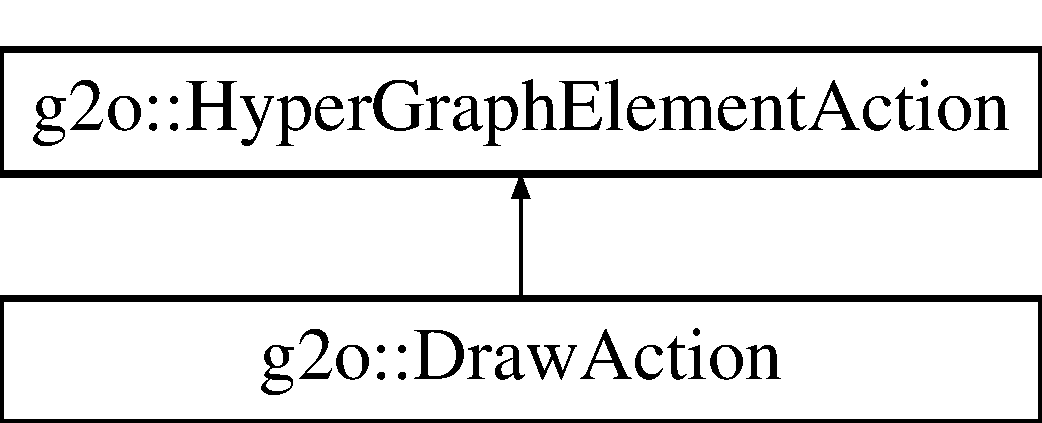
\includegraphics[height=2.000000cm]{classg2o_1_1_draw_action}
\end{center}
\end{figure}
\subsection*{Classes}
\begin{DoxyCompactItemize}
\item 
class \mbox{\hyperlink{classg2o_1_1_draw_action_1_1_parameters}{Parameters}}
\end{DoxyCompactItemize}
\subsection*{Public Member Functions}
\begin{DoxyCompactItemize}
\item 
\mbox{\hyperlink{classg2o_1_1_draw_action_a6b876d6a30fa564176dc6a3caefa572e}{Draw\+Action}} (const std\+::string \&type\+Name\+\_\+)
\end{DoxyCompactItemize}
\subsection*{Protected Member Functions}
\begin{DoxyCompactItemize}
\item 
virtual bool \mbox{\hyperlink{classg2o_1_1_draw_action_a9556cd6f8d1f842d45e046e1770699b0}{refresh\+Property\+Ptrs}} (\mbox{\hyperlink{structg2o_1_1_hyper_graph_element_action_1_1_parameters}{Hyper\+Graph\+Element\+Action\+::\+Parameters}} $\ast$params\+\_\+)
\end{DoxyCompactItemize}
\subsection*{Protected Attributes}
\begin{DoxyCompactItemize}
\item 
\mbox{\hyperlink{classg2o_1_1_draw_action_1_1_parameters}{Parameters}} $\ast$ \mbox{\hyperlink{classg2o_1_1_draw_action_af598eb77ea4e27a1c0a27533c971639d}{\+\_\+previous\+Params}}
\item 
\mbox{\hyperlink{namespaceg2o_a28e624fedcafeb2b049be2930421071f}{Bool\+Property}} $\ast$ \mbox{\hyperlink{classg2o_1_1_draw_action_a1ec3a46473daeb8ac65e6a523a9248b6}{\+\_\+show}}
\item 
\mbox{\hyperlink{namespaceg2o_a28e624fedcafeb2b049be2930421071f}{Bool\+Property}} $\ast$ \mbox{\hyperlink{classg2o_1_1_draw_action_ab5f870bf2a931e64bc994c87c4212ad3}{\+\_\+show\+Id}}
\end{DoxyCompactItemize}
\subsection*{Additional Inherited Members}


\subsection{Detailed Description}
draw actions 

\subsection{Constructor \& Destructor Documentation}
\mbox{\Hypertarget{classg2o_1_1_draw_action_a6b876d6a30fa564176dc6a3caefa572e}\label{classg2o_1_1_draw_action_a6b876d6a30fa564176dc6a3caefa572e}} 
\index{g2o\+::\+Draw\+Action@{g2o\+::\+Draw\+Action}!Draw\+Action@{Draw\+Action}}
\index{Draw\+Action@{Draw\+Action}!g2o\+::\+Draw\+Action@{g2o\+::\+Draw\+Action}}
\subsubsection{\texorpdfstring{Draw\+Action()}{DrawAction()}}
{\footnotesize\ttfamily g2o\+::\+Draw\+Action\+::\+Draw\+Action (\begin{DoxyParamCaption}\item[{const std\+::string \&}]{type\+Name\+\_\+ }\end{DoxyParamCaption})}



\subsection{Member Function Documentation}
\mbox{\Hypertarget{classg2o_1_1_draw_action_a9556cd6f8d1f842d45e046e1770699b0}\label{classg2o_1_1_draw_action_a9556cd6f8d1f842d45e046e1770699b0}} 
\index{g2o\+::\+Draw\+Action@{g2o\+::\+Draw\+Action}!refresh\+Property\+Ptrs@{refresh\+Property\+Ptrs}}
\index{refresh\+Property\+Ptrs@{refresh\+Property\+Ptrs}!g2o\+::\+Draw\+Action@{g2o\+::\+Draw\+Action}}
\subsubsection{\texorpdfstring{refresh\+Property\+Ptrs()}{refreshPropertyPtrs()}}
{\footnotesize\ttfamily bool g2o\+::\+Draw\+Action\+::refresh\+Property\+Ptrs (\begin{DoxyParamCaption}\item[{\mbox{\hyperlink{structg2o_1_1_hyper_graph_element_action_1_1_parameters}{Hyper\+Graph\+Element\+Action\+::\+Parameters}} $\ast$}]{params\+\_\+ }\end{DoxyParamCaption})\hspace{0.3cm}{\ttfamily [protected]}, {\ttfamily [virtual]}}



\subsection{Member Data Documentation}
\mbox{\Hypertarget{classg2o_1_1_draw_action_af598eb77ea4e27a1c0a27533c971639d}\label{classg2o_1_1_draw_action_af598eb77ea4e27a1c0a27533c971639d}} 
\index{g2o\+::\+Draw\+Action@{g2o\+::\+Draw\+Action}!\+\_\+previous\+Params@{\+\_\+previous\+Params}}
\index{\+\_\+previous\+Params@{\+\_\+previous\+Params}!g2o\+::\+Draw\+Action@{g2o\+::\+Draw\+Action}}
\subsubsection{\texorpdfstring{\+\_\+previous\+Params}{\_previousParams}}
{\footnotesize\ttfamily \mbox{\hyperlink{classg2o_1_1_draw_action_1_1_parameters}{Parameters}}$\ast$ g2o\+::\+Draw\+Action\+::\+\_\+previous\+Params\hspace{0.3cm}{\ttfamily [protected]}}

\mbox{\Hypertarget{classg2o_1_1_draw_action_a1ec3a46473daeb8ac65e6a523a9248b6}\label{classg2o_1_1_draw_action_a1ec3a46473daeb8ac65e6a523a9248b6}} 
\index{g2o\+::\+Draw\+Action@{g2o\+::\+Draw\+Action}!\+\_\+show@{\+\_\+show}}
\index{\+\_\+show@{\+\_\+show}!g2o\+::\+Draw\+Action@{g2o\+::\+Draw\+Action}}
\subsubsection{\texorpdfstring{\+\_\+show}{\_show}}
{\footnotesize\ttfamily \mbox{\hyperlink{namespaceg2o_a28e624fedcafeb2b049be2930421071f}{Bool\+Property}}$\ast$ g2o\+::\+Draw\+Action\+::\+\_\+show\hspace{0.3cm}{\ttfamily [protected]}}

\mbox{\Hypertarget{classg2o_1_1_draw_action_ab5f870bf2a931e64bc994c87c4212ad3}\label{classg2o_1_1_draw_action_ab5f870bf2a931e64bc994c87c4212ad3}} 
\index{g2o\+::\+Draw\+Action@{g2o\+::\+Draw\+Action}!\+\_\+show\+Id@{\+\_\+show\+Id}}
\index{\+\_\+show\+Id@{\+\_\+show\+Id}!g2o\+::\+Draw\+Action@{g2o\+::\+Draw\+Action}}
\subsubsection{\texorpdfstring{\+\_\+show\+Id}{\_showId}}
{\footnotesize\ttfamily \mbox{\hyperlink{namespaceg2o_a28e624fedcafeb2b049be2930421071f}{Bool\+Property}}$\ast$ g2o\+::\+Draw\+Action\+::\+\_\+show\+Id\hspace{0.3cm}{\ttfamily [protected]}}



The documentation for this class was generated from the following files\+:\begin{DoxyCompactItemize}
\item 
Thirdparty/g2o/g2o/core/\mbox{\hyperlink{hyper__graph__action_8h}{hyper\+\_\+graph\+\_\+action.\+h}}\item 
Thirdparty/g2o/g2o/core/\mbox{\hyperlink{hyper__graph__action_8cpp}{hyper\+\_\+graph\+\_\+action.\+cpp}}\end{DoxyCompactItemize}

\hypertarget{classg2o_1_1_hyper_graph_1_1_edge}{}\section{g2o\+:\+:Hyper\+Graph\+:\+:Edge Class Reference}
\label{classg2o_1_1_hyper_graph_1_1_edge}\index{g2o\+::\+Hyper\+Graph\+::\+Edge@{g2o\+::\+Hyper\+Graph\+::\+Edge}}


{\ttfamily \#include $<$hyper\+\_\+graph.\+h$>$}

Inheritance diagram for g2o\+:\+:Hyper\+Graph\+:\+:Edge\+:\begin{figure}[H]
\begin{center}
\leavevmode
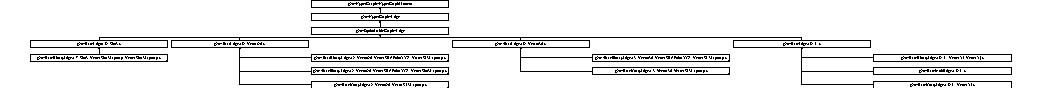
\includegraphics[height=1.176471cm]{classg2o_1_1_hyper_graph_1_1_edge}
\end{center}
\end{figure}
\subsection*{Public Member Functions}
\begin{DoxyCompactItemize}
\item 
\mbox{\hyperlink{classg2o_1_1_hyper_graph_1_1_edge_a891618b34652837ef0bee7084db81f2e}{Edge}} (int \mbox{\hyperlink{classg2o_1_1_hyper_graph_1_1_edge_a93f47febcbd6c654fc3344d4643a087f}{id}}=-\/1)
\begin{DoxyCompactList}\small\item\em creates and empty edge with no vertices \end{DoxyCompactList}\item 
virtual \mbox{\hyperlink{classg2o_1_1_hyper_graph_1_1_edge_a202cb31558caef5a7bf18a49281173a3}{$\sim$\+Edge}} ()
\item 
virtual void \mbox{\hyperlink{classg2o_1_1_hyper_graph_1_1_edge_ad8913f1149a0fd5bb628f0f1c8a91a55}{resize}} (size\+\_\+t size)
\item 
const \mbox{\hyperlink{classg2o_1_1_hyper_graph_a9339534c99300a0ddac87ba976ef188c}{Vertex\+Container}} \& \mbox{\hyperlink{classg2o_1_1_hyper_graph_1_1_edge_aba1717ff01f972bd39ba992c0d9d9e04}{vertices}} () const
\item 
\mbox{\hyperlink{classg2o_1_1_hyper_graph_a9339534c99300a0ddac87ba976ef188c}{Vertex\+Container}} \& \mbox{\hyperlink{classg2o_1_1_hyper_graph_1_1_edge_a67d1c5cb557deab9e9e361c63359fe60}{vertices}} ()
\item 
const \mbox{\hyperlink{classg2o_1_1_hyper_graph_1_1_vertex}{Vertex}} $\ast$ \mbox{\hyperlink{classg2o_1_1_hyper_graph_1_1_edge_ab644c1c4e38a0112db1435fbc0233f25}{vertex}} (size\+\_\+t i) const
\item 
\mbox{\hyperlink{classg2o_1_1_hyper_graph_1_1_vertex}{Vertex}} $\ast$ \mbox{\hyperlink{classg2o_1_1_hyper_graph_1_1_edge_af544d5d17d900c5aa2b5c9219d8e716f}{vertex}} (size\+\_\+t i)
\item 
void \mbox{\hyperlink{classg2o_1_1_hyper_graph_1_1_edge_a5e957658d6e65c49b81197d052a7f16f}{set\+Vertex}} (size\+\_\+t i, \mbox{\hyperlink{classg2o_1_1_hyper_graph_1_1_vertex}{Vertex}} $\ast$v)
\item 
int \mbox{\hyperlink{classg2o_1_1_hyper_graph_1_1_edge_a93f47febcbd6c654fc3344d4643a087f}{id}} () const
\item 
void \mbox{\hyperlink{classg2o_1_1_hyper_graph_1_1_edge_a1270ed91efa5f7a0fc42229356cc23e1}{set\+Id}} (int \mbox{\hyperlink{classg2o_1_1_hyper_graph_1_1_edge_a93f47febcbd6c654fc3344d4643a087f}{id}})
\item 
virtual Hyper\+Graph\+Element\+Type \mbox{\hyperlink{classg2o_1_1_hyper_graph_1_1_edge_a04f1b4d408aebdf14ac3f0cfd247b776}{element\+Type}} () const
\end{DoxyCompactItemize}
\subsection*{Protected Attributes}
\begin{DoxyCompactItemize}
\item 
\mbox{\hyperlink{classg2o_1_1_hyper_graph_a9339534c99300a0ddac87ba976ef188c}{Vertex\+Container}} \mbox{\hyperlink{classg2o_1_1_hyper_graph_1_1_edge_aabb036d331fc7f2524ec8611b638de92}{\+\_\+vertices}}
\item 
int \mbox{\hyperlink{classg2o_1_1_hyper_graph_1_1_edge_aa1b6978624f7c165a4e0461cb5ff18fa}{\+\_\+id}}
\begin{DoxyCompactList}\small\item\em unique id \end{DoxyCompactList}\end{DoxyCompactItemize}


\subsection{Detailed Description}
Abstract \mbox{\hyperlink{classg2o_1_1_hyper_graph_1_1_edge}{Edge}} class. Your nice edge classes should inherit from that one. An hyper-\/edge has pointers to the vertices it connects and stores them in a vector. 

\subsection{Constructor \& Destructor Documentation}
\mbox{\Hypertarget{classg2o_1_1_hyper_graph_1_1_edge_a891618b34652837ef0bee7084db81f2e}\label{classg2o_1_1_hyper_graph_1_1_edge_a891618b34652837ef0bee7084db81f2e}} 
\index{g2o\+::\+Hyper\+Graph\+::\+Edge@{g2o\+::\+Hyper\+Graph\+::\+Edge}!Edge@{Edge}}
\index{Edge@{Edge}!g2o\+::\+Hyper\+Graph\+::\+Edge@{g2o\+::\+Hyper\+Graph\+::\+Edge}}
\subsubsection{\texorpdfstring{Edge()}{Edge()}}
{\footnotesize\ttfamily g2o\+::\+Hyper\+Graph\+::\+Edge\+::\+Edge (\begin{DoxyParamCaption}\item[{int}]{id = {\ttfamily -\/1} }\end{DoxyParamCaption})\hspace{0.3cm}{\ttfamily [explicit]}}



creates and empty edge with no vertices 

\mbox{\Hypertarget{classg2o_1_1_hyper_graph_1_1_edge_a202cb31558caef5a7bf18a49281173a3}\label{classg2o_1_1_hyper_graph_1_1_edge_a202cb31558caef5a7bf18a49281173a3}} 
\index{g2o\+::\+Hyper\+Graph\+::\+Edge@{g2o\+::\+Hyper\+Graph\+::\+Edge}!````~Edge@{$\sim$\+Edge}}
\index{````~Edge@{$\sim$\+Edge}!g2o\+::\+Hyper\+Graph\+::\+Edge@{g2o\+::\+Hyper\+Graph\+::\+Edge}}
\subsubsection{\texorpdfstring{$\sim$\+Edge()}{~Edge()}}
{\footnotesize\ttfamily g2o\+::\+Hyper\+Graph\+::\+Edge\+::$\sim$\+Edge (\begin{DoxyParamCaption}{ }\end{DoxyParamCaption})\hspace{0.3cm}{\ttfamily [virtual]}}



Reimplemented in \mbox{\hyperlink{classg2o_1_1_optimizable_graph_1_1_edge_a62de61a43d47cf223fe39265dac13ca5}{g2o\+::\+Optimizable\+Graph\+::\+Edge}}.



\subsection{Member Function Documentation}
\mbox{\Hypertarget{classg2o_1_1_hyper_graph_1_1_edge_a04f1b4d408aebdf14ac3f0cfd247b776}\label{classg2o_1_1_hyper_graph_1_1_edge_a04f1b4d408aebdf14ac3f0cfd247b776}} 
\index{g2o\+::\+Hyper\+Graph\+::\+Edge@{g2o\+::\+Hyper\+Graph\+::\+Edge}!element\+Type@{element\+Type}}
\index{element\+Type@{element\+Type}!g2o\+::\+Hyper\+Graph\+::\+Edge@{g2o\+::\+Hyper\+Graph\+::\+Edge}}
\subsubsection{\texorpdfstring{element\+Type()}{elementType()}}
{\footnotesize\ttfamily virtual Hyper\+Graph\+Element\+Type g2o\+::\+Hyper\+Graph\+::\+Edge\+::element\+Type (\begin{DoxyParamCaption}{ }\end{DoxyParamCaption}) const\hspace{0.3cm}{\ttfamily [inline]}, {\ttfamily [virtual]}}

returns the type of the graph element, see Hyper\+Graph\+Element\+Type 

Implements \mbox{\hyperlink{structg2o_1_1_hyper_graph_1_1_hyper_graph_element_a1a9d7b748698c09d202373e06e413ef2}{g2o\+::\+Hyper\+Graph\+::\+Hyper\+Graph\+Element}}.

\mbox{\Hypertarget{classg2o_1_1_hyper_graph_1_1_edge_a93f47febcbd6c654fc3344d4643a087f}\label{classg2o_1_1_hyper_graph_1_1_edge_a93f47febcbd6c654fc3344d4643a087f}} 
\index{g2o\+::\+Hyper\+Graph\+::\+Edge@{g2o\+::\+Hyper\+Graph\+::\+Edge}!id@{id}}
\index{id@{id}!g2o\+::\+Hyper\+Graph\+::\+Edge@{g2o\+::\+Hyper\+Graph\+::\+Edge}}
\subsubsection{\texorpdfstring{id()}{id()}}
{\footnotesize\ttfamily int g2o\+::\+Hyper\+Graph\+::\+Edge\+::id (\begin{DoxyParamCaption}{ }\end{DoxyParamCaption}) const\hspace{0.3cm}{\ttfamily [inline]}}

\mbox{\Hypertarget{classg2o_1_1_hyper_graph_1_1_edge_ad8913f1149a0fd5bb628f0f1c8a91a55}\label{classg2o_1_1_hyper_graph_1_1_edge_ad8913f1149a0fd5bb628f0f1c8a91a55}} 
\index{g2o\+::\+Hyper\+Graph\+::\+Edge@{g2o\+::\+Hyper\+Graph\+::\+Edge}!resize@{resize}}
\index{resize@{resize}!g2o\+::\+Hyper\+Graph\+::\+Edge@{g2o\+::\+Hyper\+Graph\+::\+Edge}}
\subsubsection{\texorpdfstring{resize()}{resize()}}
{\footnotesize\ttfamily void g2o\+::\+Hyper\+Graph\+::\+Edge\+::resize (\begin{DoxyParamCaption}\item[{size\+\_\+t}]{size }\end{DoxyParamCaption})\hspace{0.3cm}{\ttfamily [virtual]}}

resizes the number of vertices connected by this edge 

Reimplemented in \mbox{\hyperlink{classg2o_1_1_base_multi_edge_ae07ec9359cd515d0abc2100ee8aae93f}{g2o\+::\+Base\+Multi\+Edge$<$ D, E $>$}}, \mbox{\hyperlink{classg2o_1_1_base_binary_edge_a06e64067fa5fff4a5e2d058249b55478}{g2o\+::\+Base\+Binary\+Edge$<$ D, E, Vertex\+Xi, Vertex\+Xj $>$}}, \mbox{\hyperlink{classg2o_1_1_base_binary_edge_a06e64067fa5fff4a5e2d058249b55478}{g2o\+::\+Base\+Binary\+Edge$<$ 2, Vector2d, Vertex\+S\+B\+A\+Point\+X\+Y\+Z, Vertex\+Sim3\+Expmap $>$}}, \mbox{\hyperlink{classg2o_1_1_base_binary_edge_a06e64067fa5fff4a5e2d058249b55478}{g2o\+::\+Base\+Binary\+Edge$<$ 7, Sim3, Vertex\+Sim3\+Expmap, Vertex\+Sim3\+Expmap $>$}}, \mbox{\hyperlink{classg2o_1_1_base_binary_edge_a06e64067fa5fff4a5e2d058249b55478}{g2o\+::\+Base\+Binary\+Edge$<$ 2, Vector2d, Vertex\+S\+B\+A\+Point\+X\+Y\+Z, Vertex\+S\+E3\+Expmap $>$}}, \mbox{\hyperlink{classg2o_1_1_base_binary_edge_a06e64067fa5fff4a5e2d058249b55478}{g2o\+::\+Base\+Binary\+Edge$<$ 3, Vector3d, Vertex\+S\+B\+A\+Point\+X\+Y\+Z, Vertex\+S\+E3\+Expmap $>$}}, \mbox{\hyperlink{classg2o_1_1_base_unary_edge_a01fcdfd2d3ed0325655bb99db95c0b10}{g2o\+::\+Base\+Unary\+Edge$<$ D, E, Vertex\+Xi $>$}}, \mbox{\hyperlink{classg2o_1_1_base_unary_edge_a01fcdfd2d3ed0325655bb99db95c0b10}{g2o\+::\+Base\+Unary\+Edge$<$ 2, Vector2d, Vertex\+S\+E3\+Expmap $>$}}, and \mbox{\hyperlink{classg2o_1_1_base_unary_edge_a01fcdfd2d3ed0325655bb99db95c0b10}{g2o\+::\+Base\+Unary\+Edge$<$ 3, Vector3d, Vertex\+S\+E3\+Expmap $>$}}.

\mbox{\Hypertarget{classg2o_1_1_hyper_graph_1_1_edge_a1270ed91efa5f7a0fc42229356cc23e1}\label{classg2o_1_1_hyper_graph_1_1_edge_a1270ed91efa5f7a0fc42229356cc23e1}} 
\index{g2o\+::\+Hyper\+Graph\+::\+Edge@{g2o\+::\+Hyper\+Graph\+::\+Edge}!set\+Id@{set\+Id}}
\index{set\+Id@{set\+Id}!g2o\+::\+Hyper\+Graph\+::\+Edge@{g2o\+::\+Hyper\+Graph\+::\+Edge}}
\subsubsection{\texorpdfstring{set\+Id()}{setId()}}
{\footnotesize\ttfamily void g2o\+::\+Hyper\+Graph\+::\+Edge\+::set\+Id (\begin{DoxyParamCaption}\item[{int}]{id }\end{DoxyParamCaption})}

\mbox{\Hypertarget{classg2o_1_1_hyper_graph_1_1_edge_a5e957658d6e65c49b81197d052a7f16f}\label{classg2o_1_1_hyper_graph_1_1_edge_a5e957658d6e65c49b81197d052a7f16f}} 
\index{g2o\+::\+Hyper\+Graph\+::\+Edge@{g2o\+::\+Hyper\+Graph\+::\+Edge}!set\+Vertex@{set\+Vertex}}
\index{set\+Vertex@{set\+Vertex}!g2o\+::\+Hyper\+Graph\+::\+Edge@{g2o\+::\+Hyper\+Graph\+::\+Edge}}
\subsubsection{\texorpdfstring{set\+Vertex()}{setVertex()}}
{\footnotesize\ttfamily void g2o\+::\+Hyper\+Graph\+::\+Edge\+::set\+Vertex (\begin{DoxyParamCaption}\item[{size\+\_\+t}]{i,  }\item[{\mbox{\hyperlink{classg2o_1_1_hyper_graph_1_1_vertex}{Vertex}} $\ast$}]{v }\end{DoxyParamCaption})\hspace{0.3cm}{\ttfamily [inline]}}

set the ith vertex on the hyper-\/edge to the pointer supplied \mbox{\Hypertarget{classg2o_1_1_hyper_graph_1_1_edge_ab644c1c4e38a0112db1435fbc0233f25}\label{classg2o_1_1_hyper_graph_1_1_edge_ab644c1c4e38a0112db1435fbc0233f25}} 
\index{g2o\+::\+Hyper\+Graph\+::\+Edge@{g2o\+::\+Hyper\+Graph\+::\+Edge}!vertex@{vertex}}
\index{vertex@{vertex}!g2o\+::\+Hyper\+Graph\+::\+Edge@{g2o\+::\+Hyper\+Graph\+::\+Edge}}
\subsubsection{\texorpdfstring{vertex()}{vertex()}\hspace{0.1cm}{\footnotesize\ttfamily [1/2]}}
{\footnotesize\ttfamily const \mbox{\hyperlink{classg2o_1_1_hyper_graph_1_1_vertex}{Vertex}}$\ast$ g2o\+::\+Hyper\+Graph\+::\+Edge\+::vertex (\begin{DoxyParamCaption}\item[{size\+\_\+t}]{i }\end{DoxyParamCaption}) const\hspace{0.3cm}{\ttfamily [inline]}}

returns the pointer to the ith vertex connected to the hyper-\/edge. \mbox{\Hypertarget{classg2o_1_1_hyper_graph_1_1_edge_af544d5d17d900c5aa2b5c9219d8e716f}\label{classg2o_1_1_hyper_graph_1_1_edge_af544d5d17d900c5aa2b5c9219d8e716f}} 
\index{g2o\+::\+Hyper\+Graph\+::\+Edge@{g2o\+::\+Hyper\+Graph\+::\+Edge}!vertex@{vertex}}
\index{vertex@{vertex}!g2o\+::\+Hyper\+Graph\+::\+Edge@{g2o\+::\+Hyper\+Graph\+::\+Edge}}
\subsubsection{\texorpdfstring{vertex()}{vertex()}\hspace{0.1cm}{\footnotesize\ttfamily [2/2]}}
{\footnotesize\ttfamily \mbox{\hyperlink{classg2o_1_1_hyper_graph_1_1_vertex}{Vertex}}$\ast$ g2o\+::\+Hyper\+Graph\+::\+Edge\+::vertex (\begin{DoxyParamCaption}\item[{size\+\_\+t}]{i }\end{DoxyParamCaption})\hspace{0.3cm}{\ttfamily [inline]}}

returns the pointer to the ith vertex connected to the hyper-\/edge. \mbox{\Hypertarget{classg2o_1_1_hyper_graph_1_1_edge_aba1717ff01f972bd39ba992c0d9d9e04}\label{classg2o_1_1_hyper_graph_1_1_edge_aba1717ff01f972bd39ba992c0d9d9e04}} 
\index{g2o\+::\+Hyper\+Graph\+::\+Edge@{g2o\+::\+Hyper\+Graph\+::\+Edge}!vertices@{vertices}}
\index{vertices@{vertices}!g2o\+::\+Hyper\+Graph\+::\+Edge@{g2o\+::\+Hyper\+Graph\+::\+Edge}}
\subsubsection{\texorpdfstring{vertices()}{vertices()}\hspace{0.1cm}{\footnotesize\ttfamily [1/2]}}
{\footnotesize\ttfamily const \mbox{\hyperlink{classg2o_1_1_hyper_graph_a9339534c99300a0ddac87ba976ef188c}{Vertex\+Container}}\& g2o\+::\+Hyper\+Graph\+::\+Edge\+::vertices (\begin{DoxyParamCaption}{ }\end{DoxyParamCaption}) const\hspace{0.3cm}{\ttfamily [inline]}}

returns the vector of pointers to the vertices connected by the hyper-\/edge. \mbox{\Hypertarget{classg2o_1_1_hyper_graph_1_1_edge_a67d1c5cb557deab9e9e361c63359fe60}\label{classg2o_1_1_hyper_graph_1_1_edge_a67d1c5cb557deab9e9e361c63359fe60}} 
\index{g2o\+::\+Hyper\+Graph\+::\+Edge@{g2o\+::\+Hyper\+Graph\+::\+Edge}!vertices@{vertices}}
\index{vertices@{vertices}!g2o\+::\+Hyper\+Graph\+::\+Edge@{g2o\+::\+Hyper\+Graph\+::\+Edge}}
\subsubsection{\texorpdfstring{vertices()}{vertices()}\hspace{0.1cm}{\footnotesize\ttfamily [2/2]}}
{\footnotesize\ttfamily \mbox{\hyperlink{classg2o_1_1_hyper_graph_a9339534c99300a0ddac87ba976ef188c}{Vertex\+Container}}\& g2o\+::\+Hyper\+Graph\+::\+Edge\+::vertices (\begin{DoxyParamCaption}{ }\end{DoxyParamCaption})\hspace{0.3cm}{\ttfamily [inline]}}

returns the vector of pointers to the vertices connected by the hyper-\/edge. 

\subsection{Member Data Documentation}
\mbox{\Hypertarget{classg2o_1_1_hyper_graph_1_1_edge_aa1b6978624f7c165a4e0461cb5ff18fa}\label{classg2o_1_1_hyper_graph_1_1_edge_aa1b6978624f7c165a4e0461cb5ff18fa}} 
\index{g2o\+::\+Hyper\+Graph\+::\+Edge@{g2o\+::\+Hyper\+Graph\+::\+Edge}!\+\_\+id@{\+\_\+id}}
\index{\+\_\+id@{\+\_\+id}!g2o\+::\+Hyper\+Graph\+::\+Edge@{g2o\+::\+Hyper\+Graph\+::\+Edge}}
\subsubsection{\texorpdfstring{\+\_\+id}{\_id}}
{\footnotesize\ttfamily int g2o\+::\+Hyper\+Graph\+::\+Edge\+::\+\_\+id\hspace{0.3cm}{\ttfamily [protected]}}



unique id 

\mbox{\Hypertarget{classg2o_1_1_hyper_graph_1_1_edge_aabb036d331fc7f2524ec8611b638de92}\label{classg2o_1_1_hyper_graph_1_1_edge_aabb036d331fc7f2524ec8611b638de92}} 
\index{g2o\+::\+Hyper\+Graph\+::\+Edge@{g2o\+::\+Hyper\+Graph\+::\+Edge}!\+\_\+vertices@{\+\_\+vertices}}
\index{\+\_\+vertices@{\+\_\+vertices}!g2o\+::\+Hyper\+Graph\+::\+Edge@{g2o\+::\+Hyper\+Graph\+::\+Edge}}
\subsubsection{\texorpdfstring{\+\_\+vertices}{\_vertices}}
{\footnotesize\ttfamily \mbox{\hyperlink{classg2o_1_1_hyper_graph_a9339534c99300a0ddac87ba976ef188c}{Vertex\+Container}} g2o\+::\+Hyper\+Graph\+::\+Edge\+::\+\_\+vertices\hspace{0.3cm}{\ttfamily [protected]}}



The documentation for this class was generated from the following files\+:\begin{DoxyCompactItemize}
\item 
D\+:/github/\+V\+S\+L\+A\+M/\+O\+R\+B\+S\+L\+A\+M2/\+O\+R\+B-\/\+S\+L\+A\+M2-\/master/\+Thirdparty/g2o/g2o/core/\mbox{\hyperlink{hyper__graph_8h}{hyper\+\_\+graph.\+h}}\item 
D\+:/github/\+V\+S\+L\+A\+M/\+O\+R\+B\+S\+L\+A\+M2/\+O\+R\+B-\/\+S\+L\+A\+M2-\/master/\+Thirdparty/g2o/g2o/core/\mbox{\hyperlink{hyper__graph_8cpp}{hyper\+\_\+graph.\+cpp}}\end{DoxyCompactItemize}

\hypertarget{classg2o_1_1_optimizable_graph_1_1_edge}{}\section{g2o\+:\+:Optimizable\+Graph\+:\+:Edge Class Reference}
\label{classg2o_1_1_optimizable_graph_1_1_edge}\index{g2o\+::\+Optimizable\+Graph\+::\+Edge@{g2o\+::\+Optimizable\+Graph\+::\+Edge}}


{\ttfamily \#include $<$optimizable\+\_\+graph.\+h$>$}

Inheritance diagram for g2o\+:\+:Optimizable\+Graph\+:\+:Edge\+:\begin{figure}[H]
\begin{center}
\leavevmode
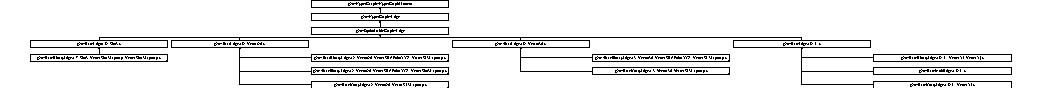
\includegraphics[height=1.176471cm]{classg2o_1_1_optimizable_graph_1_1_edge}
\end{center}
\end{figure}
\subsection*{Public Member Functions}
\begin{DoxyCompactItemize}
\item 
\mbox{\hyperlink{classg2o_1_1_optimizable_graph_1_1_edge_a6568eb7f3b3e4299473ec3230199aa70}{Edge}} ()
\item 
virtual \mbox{\hyperlink{classg2o_1_1_optimizable_graph_1_1_edge_a62de61a43d47cf223fe39265dac13ca5}{$\sim$\+Edge}} ()
\item 
virtual \mbox{\hyperlink{classg2o_1_1_optimizable_graph_1_1_edge}{Edge}} $\ast$ \mbox{\hyperlink{classg2o_1_1_optimizable_graph_1_1_edge_a1a238c63bc8a799ada3ac5712e13315e}{clone}} () const
\item 
virtual bool \mbox{\hyperlink{classg2o_1_1_optimizable_graph_1_1_edge_a414c69ca1617a4d3b620e39f2ffbcea7}{all\+Vertices\+Fixed}} () const =0
\item 
virtual void \mbox{\hyperlink{classg2o_1_1_optimizable_graph_1_1_edge_a1e6d9f4128866982de5e11e03edd7775}{compute\+Error}} ()=0
\item 
virtual bool \mbox{\hyperlink{classg2o_1_1_optimizable_graph_1_1_edge_ae8d99a85921057eba87a2346ba9c6e0a}{set\+Measurement\+Data}} (const double $\ast$m)
\item 
virtual bool \mbox{\hyperlink{classg2o_1_1_optimizable_graph_1_1_edge_abe22d8f67447fc93c49b5aa730eaba83}{get\+Measurement\+Data}} (double $\ast$m) const
\item 
virtual int \mbox{\hyperlink{classg2o_1_1_optimizable_graph_1_1_edge_a3441f5e149c30c50ce8557574ac7d1a8}{measurement\+Dimension}} () const
\item 
virtual bool \mbox{\hyperlink{classg2o_1_1_optimizable_graph_1_1_edge_a2f0b6465d6cd8b459ebc6494892c44f4}{set\+Measurement\+From\+State}} ()
\item 
\mbox{\hyperlink{classg2o_1_1_robust_kernel}{Robust\+Kernel}} $\ast$ \mbox{\hyperlink{classg2o_1_1_optimizable_graph_1_1_edge_a4fe9c69dc5275ca661e793aca6e2d93c}{robust\+Kernel}} () const
\begin{DoxyCompactList}\small\item\em if N\+OT N\+U\+LL, error of this edge will be robustifed with the kernel \end{DoxyCompactList}\item 
void \mbox{\hyperlink{classg2o_1_1_optimizable_graph_1_1_edge_a42955172c19f16e2cfbb30d611d1bd87}{set\+Robust\+Kernel}} (\mbox{\hyperlink{classg2o_1_1_robust_kernel}{Robust\+Kernel}} $\ast$ptr)
\item 
virtual const double $\ast$ \mbox{\hyperlink{classg2o_1_1_optimizable_graph_1_1_edge_a5f2a4b6efa2d0ae600f94a28a6ba58cf}{error\+Data}} () const =0
\begin{DoxyCompactList}\small\item\em returns the error vector cached after calling the compute\+Error; \end{DoxyCompactList}\item 
virtual double $\ast$ \mbox{\hyperlink{classg2o_1_1_optimizable_graph_1_1_edge_a460a0cb0256b0a91edb131e25181f57b}{error\+Data}} ()=0
\item 
virtual const double $\ast$ \mbox{\hyperlink{classg2o_1_1_optimizable_graph_1_1_edge_ab5b315b3e0a6c4e29074b2c924460417}{information\+Data}} () const =0
\begin{DoxyCompactList}\small\item\em returns the memory of the information matrix, usable for example with a Eigen\+::\+Map$<$\+Matrix\+Xd$>$ \end{DoxyCompactList}\item 
virtual double $\ast$ \mbox{\hyperlink{classg2o_1_1_optimizable_graph_1_1_edge_a99de4bbb57e3c5e7321f150a45d1cb12}{information\+Data}} ()=0
\item 
virtual double \mbox{\hyperlink{classg2o_1_1_optimizable_graph_1_1_edge_a182bd2c109d50283c638d9b295f2f3d7}{chi2}} () const =0
\begin{DoxyCompactList}\small\item\em computes the chi2 based on the cached error value, only valid after compute\+Error has been called. \end{DoxyCompactList}\item 
virtual void \mbox{\hyperlink{classg2o_1_1_optimizable_graph_1_1_edge_a56fbf3430ddf591e3c619bdd1b7e4499}{construct\+Quadratic\+Form}} ()=0
\item 
virtual void \mbox{\hyperlink{classg2o_1_1_optimizable_graph_1_1_edge_a3bd233fd552daa166039acf47b69a5a7}{map\+Hessian\+Memory}} (double $\ast$d, int i, int j, bool row\+Major)=0
\item 
virtual void \mbox{\hyperlink{classg2o_1_1_optimizable_graph_1_1_edge_a0fdad5ebfb4efec9f893b57f67e0fbe1}{linearize\+Oplus}} (\mbox{\hyperlink{classg2o_1_1_jacobian_workspace}{Jacobian\+Workspace}} \&\mbox{\hyperlink{structg2o_1_1_optimizable_graph_aa669dbd1d6e34e49fecda711ff1b78c6}{jacobian\+Workspace}})=0
\item 
virtual void \mbox{\hyperlink{classg2o_1_1_optimizable_graph_1_1_edge_a9519f8892e97f03daacb44ea50ac7f4e}{initial\+Estimate}} (const \mbox{\hyperlink{classg2o_1_1_hyper_graph_a703938cdb4bb636860eed55a2489d70c}{Optimizable\+Graph\+::\+Vertex\+Set}} \&from, \mbox{\hyperlink{classg2o_1_1_optimizable_graph_1_1_vertex}{Optimizable\+Graph\+::\+Vertex}} $\ast$to)=0
\item 
virtual double \mbox{\hyperlink{classg2o_1_1_optimizable_graph_1_1_edge_a1cef6ffa0f82f1ad3dd3d7a9f04425ee}{initial\+Estimate\+Possible}} (const \mbox{\hyperlink{classg2o_1_1_hyper_graph_a703938cdb4bb636860eed55a2489d70c}{Optimizable\+Graph\+::\+Vertex\+Set}} \&from, \mbox{\hyperlink{classg2o_1_1_optimizable_graph_1_1_vertex}{Optimizable\+Graph\+::\+Vertex}} $\ast$to)
\item 
int \mbox{\hyperlink{classg2o_1_1_optimizable_graph_1_1_edge_a25c2b618815622ab79705c497390d22f}{level}} () const
\begin{DoxyCompactList}\small\item\em returns the level of the edge \end{DoxyCompactList}\item 
void \mbox{\hyperlink{classg2o_1_1_optimizable_graph_1_1_edge_ab3e4290bc51d03ba294f36254048b15a}{set\+Level}} (int l)
\begin{DoxyCompactList}\small\item\em sets the level of the edge \end{DoxyCompactList}\item 
int \mbox{\hyperlink{classg2o_1_1_optimizable_graph_1_1_edge_a0eb19697e201bd195c45ca78d55fd041}{dimension}} () const
\begin{DoxyCompactList}\small\item\em returns the dimensions of the error function \end{DoxyCompactList}\item 
virtual \mbox{\hyperlink{classg2o_1_1_optimizable_graph_1_1_vertex}{Vertex}} $\ast$ \mbox{\hyperlink{classg2o_1_1_optimizable_graph_1_1_edge_abd98d7a174df25bcc82cfdacba682fec}{create\+From}} ()
\item 
virtual \mbox{\hyperlink{classg2o_1_1_optimizable_graph_1_1_vertex}{Vertex}} $\ast$ \mbox{\hyperlink{classg2o_1_1_optimizable_graph_1_1_edge_a39c22b396ab312059ea8fa4c2776be2e}{create\+To}} ()
\item 
virtual bool \mbox{\hyperlink{classg2o_1_1_optimizable_graph_1_1_edge_a30cf69b762a06aa35e796d8af71632b0}{read}} (std\+::istream \&is)=0
\begin{DoxyCompactList}\small\item\em read the vertex from a stream, i.\+e., the internal state of the vertex \end{DoxyCompactList}\item 
virtual bool \mbox{\hyperlink{classg2o_1_1_optimizable_graph_1_1_edge_a804b9a2178249b9297c55b8fbbeda56e}{write}} (std\+::ostream \&os) const =0
\begin{DoxyCompactList}\small\item\em write the vertex to a stream \end{DoxyCompactList}\item 
long long \mbox{\hyperlink{classg2o_1_1_optimizable_graph_1_1_edge_a3c6e31c64d98db332e83166bfbd1d7ff}{internal\+Id}} () const
\begin{DoxyCompactList}\small\item\em the internal ID of the edge \end{DoxyCompactList}\item 
\mbox{\hyperlink{structg2o_1_1_optimizable_graph}{Optimizable\+Graph}} $\ast$ \mbox{\hyperlink{classg2o_1_1_optimizable_graph_1_1_edge_a3684190bf8e99f39f58ffadd0dfa6b05}{graph}} ()
\item 
const \mbox{\hyperlink{structg2o_1_1_optimizable_graph}{Optimizable\+Graph}} $\ast$ \mbox{\hyperlink{classg2o_1_1_optimizable_graph_1_1_edge_a06fdc51c984cf0050df376ca30c881e3}{graph}} () const
\item 
bool \mbox{\hyperlink{classg2o_1_1_optimizable_graph_1_1_edge_ae535735e71365a547fd1a11fae5378f6}{set\+Parameter\+Id}} (int arg\+Num, int param\+Id)
\item 
const \mbox{\hyperlink{classg2o_1_1_parameter}{Parameter}} $\ast$ \mbox{\hyperlink{classg2o_1_1_optimizable_graph_1_1_edge_a4a224a1d0d0bc5ef70765f57ae685d09}{parameter}} (int arg\+No) const
\item 
size\+\_\+t \mbox{\hyperlink{classg2o_1_1_optimizable_graph_1_1_edge_ae7da26fd36246411bc53ca008bc24fcf}{num\+Parameters}} () const
\item 
void \mbox{\hyperlink{classg2o_1_1_optimizable_graph_1_1_edge_ac978364c99e36c7fced59ecb383ba171}{resize\+Parameters}} (size\+\_\+t new\+Size)
\end{DoxyCompactItemize}
\subsection*{Protected Member Functions}
\begin{DoxyCompactItemize}
\item 
{\footnotesize template$<$typename Parameter\+Type $>$ }\\bool \mbox{\hyperlink{classg2o_1_1_optimizable_graph_1_1_edge_a237bea2f2fb7cc6a9cf4ee5ee6fe4d88}{install\+Parameter}} (Parameter\+Type $\ast$\&p, size\+\_\+t arg\+No, int param\+Id=-\/1)
\item 
{\footnotesize template$<$typename Cache\+Type $>$ }\\void \mbox{\hyperlink{classg2o_1_1_optimizable_graph_1_1_edge_ad95f2883af693de56e46a2b272dc1cdc}{resolve\+Cache}} (Cache\+Type $\ast$\&cache, \mbox{\hyperlink{classg2o_1_1_optimizable_graph_1_1_vertex}{Optimizable\+Graph\+::\+Vertex}} $\ast$, const std\+::string \&\+\_\+type, const \mbox{\hyperlink{namespaceg2o_a85cc8f2c7db8cab47b2b269a7acd6785}{Parameter\+Vector}} \&parameters)
\item 
bool \mbox{\hyperlink{classg2o_1_1_optimizable_graph_1_1_edge_addadf494f3a1c8bf467a74454d771d0d}{resolve\+Parameters}} ()
\item 
virtual bool \mbox{\hyperlink{classg2o_1_1_optimizable_graph_1_1_edge_aa93e3a4f976b467994f4eb7679a04bf3}{resolve\+Caches}} ()
\end{DoxyCompactItemize}
\subsection*{Protected Attributes}
\begin{DoxyCompactItemize}
\item 
int \mbox{\hyperlink{classg2o_1_1_optimizable_graph_1_1_edge_a4e651628f7657c81d0e4c1b26caaa6aa}{\+\_\+dimension}}
\item 
int \mbox{\hyperlink{classg2o_1_1_optimizable_graph_1_1_edge_a57132078028dd0455aef141e62e07db9}{\+\_\+level}}
\item 
\mbox{\hyperlink{classg2o_1_1_robust_kernel}{Robust\+Kernel}} $\ast$ \mbox{\hyperlink{classg2o_1_1_optimizable_graph_1_1_edge_a6b942321f9e4e82051d529efb255af35}{\+\_\+robust\+Kernel}}
\item 
long long \mbox{\hyperlink{classg2o_1_1_optimizable_graph_1_1_edge_abdfc449ed57479d90d2e57a8bc0bea12}{\+\_\+internal\+Id}}
\item 
std\+::vector$<$ int $>$ \mbox{\hyperlink{classg2o_1_1_optimizable_graph_1_1_edge_a56bddaadd70570dbd96e8deed3d4b34c}{\+\_\+cache\+Ids}}
\item 
std\+::vector$<$ std\+::string $>$ \mbox{\hyperlink{classg2o_1_1_optimizable_graph_1_1_edge_a08666609850240956c64c95ae5ae0f2c}{\+\_\+parameter\+Types}}
\item 
std\+::vector$<$ \mbox{\hyperlink{classg2o_1_1_parameter}{Parameter}} $\ast$$\ast$ $>$ \mbox{\hyperlink{classg2o_1_1_optimizable_graph_1_1_edge_a41c4d6a404d0b057d37fac43edec40ed}{\+\_\+parameters}}
\item 
std\+::vector$<$ int $>$ \mbox{\hyperlink{classg2o_1_1_optimizable_graph_1_1_edge_a33a35663ba5b096cb6e6078014bd6f17}{\+\_\+parameter\+Ids}}
\end{DoxyCompactItemize}
\subsection*{Friends}
\begin{DoxyCompactItemize}
\item 
struct \mbox{\hyperlink{classg2o_1_1_optimizable_graph_1_1_edge_a45d35331ee3deca38c26d1efb6b961ae}{Optimizable\+Graph}}
\end{DoxyCompactItemize}


\subsection{Constructor \& Destructor Documentation}
\mbox{\Hypertarget{classg2o_1_1_optimizable_graph_1_1_edge_a6568eb7f3b3e4299473ec3230199aa70}\label{classg2o_1_1_optimizable_graph_1_1_edge_a6568eb7f3b3e4299473ec3230199aa70}} 
\index{g2o\+::\+Optimizable\+Graph\+::\+Edge@{g2o\+::\+Optimizable\+Graph\+::\+Edge}!Edge@{Edge}}
\index{Edge@{Edge}!g2o\+::\+Optimizable\+Graph\+::\+Edge@{g2o\+::\+Optimizable\+Graph\+::\+Edge}}
\subsubsection{\texorpdfstring{Edge()}{Edge()}}
{\footnotesize\ttfamily g2o\+::\+Optimizable\+Graph\+::\+Edge\+::\+Edge (\begin{DoxyParamCaption}{ }\end{DoxyParamCaption})}

\mbox{\Hypertarget{classg2o_1_1_optimizable_graph_1_1_edge_a62de61a43d47cf223fe39265dac13ca5}\label{classg2o_1_1_optimizable_graph_1_1_edge_a62de61a43d47cf223fe39265dac13ca5}} 
\index{g2o\+::\+Optimizable\+Graph\+::\+Edge@{g2o\+::\+Optimizable\+Graph\+::\+Edge}!````~Edge@{$\sim$\+Edge}}
\index{````~Edge@{$\sim$\+Edge}!g2o\+::\+Optimizable\+Graph\+::\+Edge@{g2o\+::\+Optimizable\+Graph\+::\+Edge}}
\subsubsection{\texorpdfstring{$\sim$\+Edge()}{~Edge()}}
{\footnotesize\ttfamily g2o\+::\+Optimizable\+Graph\+::\+Edge\+::$\sim$\+Edge (\begin{DoxyParamCaption}{ }\end{DoxyParamCaption})\hspace{0.3cm}{\ttfamily [virtual]}}



Reimplemented from \mbox{\hyperlink{classg2o_1_1_hyper_graph_1_1_edge_a202cb31558caef5a7bf18a49281173a3}{g2o\+::\+Hyper\+Graph\+::\+Edge}}.



\subsection{Member Function Documentation}
\mbox{\Hypertarget{classg2o_1_1_optimizable_graph_1_1_edge_a414c69ca1617a4d3b620e39f2ffbcea7}\label{classg2o_1_1_optimizable_graph_1_1_edge_a414c69ca1617a4d3b620e39f2ffbcea7}} 
\index{g2o\+::\+Optimizable\+Graph\+::\+Edge@{g2o\+::\+Optimizable\+Graph\+::\+Edge}!all\+Vertices\+Fixed@{all\+Vertices\+Fixed}}
\index{all\+Vertices\+Fixed@{all\+Vertices\+Fixed}!g2o\+::\+Optimizable\+Graph\+::\+Edge@{g2o\+::\+Optimizable\+Graph\+::\+Edge}}
\subsubsection{\texorpdfstring{all\+Vertices\+Fixed()}{allVerticesFixed()}}
{\footnotesize\ttfamily virtual bool g2o\+::\+Optimizable\+Graph\+::\+Edge\+::all\+Vertices\+Fixed (\begin{DoxyParamCaption}{ }\end{DoxyParamCaption}) const\hspace{0.3cm}{\ttfamily [pure virtual]}}



Implemented in \mbox{\hyperlink{classg2o_1_1_base_multi_edge_a6e665877bd472839872077f5cc1ff2ec}{g2o\+::\+Base\+Multi\+Edge$<$ D, E $>$}}, \mbox{\hyperlink{classg2o_1_1_base_binary_edge_adc9ce883a63aa7bdba86e552d72e1de9}{g2o\+::\+Base\+Binary\+Edge$<$ D, E, Vertex\+Xi, Vertex\+Xj $>$}}, \mbox{\hyperlink{classg2o_1_1_base_binary_edge_adc9ce883a63aa7bdba86e552d72e1de9}{g2o\+::\+Base\+Binary\+Edge$<$ 2, Vector2d, Vertex\+S\+B\+A\+Point\+X\+Y\+Z, Vertex\+Sim3\+Expmap $>$}}, \mbox{\hyperlink{classg2o_1_1_base_binary_edge_adc9ce883a63aa7bdba86e552d72e1de9}{g2o\+::\+Base\+Binary\+Edge$<$ 7, Sim3, Vertex\+Sim3\+Expmap, Vertex\+Sim3\+Expmap $>$}}, \mbox{\hyperlink{classg2o_1_1_base_binary_edge_adc9ce883a63aa7bdba86e552d72e1de9}{g2o\+::\+Base\+Binary\+Edge$<$ 2, Vector2d, Vertex\+S\+B\+A\+Point\+X\+Y\+Z, Vertex\+S\+E3\+Expmap $>$}}, \mbox{\hyperlink{classg2o_1_1_base_binary_edge_adc9ce883a63aa7bdba86e552d72e1de9}{g2o\+::\+Base\+Binary\+Edge$<$ 3, Vector3d, Vertex\+S\+B\+A\+Point\+X\+Y\+Z, Vertex\+S\+E3\+Expmap $>$}}, \mbox{\hyperlink{classg2o_1_1_base_unary_edge_a4c5ec31144a266fb059b73b2387456c1}{g2o\+::\+Base\+Unary\+Edge$<$ D, E, Vertex\+Xi $>$}}, \mbox{\hyperlink{classg2o_1_1_base_unary_edge_a4c5ec31144a266fb059b73b2387456c1}{g2o\+::\+Base\+Unary\+Edge$<$ 2, Vector2d, Vertex\+S\+E3\+Expmap $>$}}, and \mbox{\hyperlink{classg2o_1_1_base_unary_edge_a4c5ec31144a266fb059b73b2387456c1}{g2o\+::\+Base\+Unary\+Edge$<$ 3, Vector3d, Vertex\+S\+E3\+Expmap $>$}}.

\mbox{\Hypertarget{classg2o_1_1_optimizable_graph_1_1_edge_a182bd2c109d50283c638d9b295f2f3d7}\label{classg2o_1_1_optimizable_graph_1_1_edge_a182bd2c109d50283c638d9b295f2f3d7}} 
\index{g2o\+::\+Optimizable\+Graph\+::\+Edge@{g2o\+::\+Optimizable\+Graph\+::\+Edge}!chi2@{chi2}}
\index{chi2@{chi2}!g2o\+::\+Optimizable\+Graph\+::\+Edge@{g2o\+::\+Optimizable\+Graph\+::\+Edge}}
\subsubsection{\texorpdfstring{chi2()}{chi2()}}
{\footnotesize\ttfamily virtual double g2o\+::\+Optimizable\+Graph\+::\+Edge\+::chi2 (\begin{DoxyParamCaption}{ }\end{DoxyParamCaption}) const\hspace{0.3cm}{\ttfamily [pure virtual]}}



computes the chi2 based on the cached error value, only valid after compute\+Error has been called. 



Implemented in \mbox{\hyperlink{classg2o_1_1_base_edge_a8316137ded4396a2dbf7529d83888400}{g2o\+::\+Base\+Edge$<$ D, E $>$}}, \mbox{\hyperlink{classg2o_1_1_base_edge_a8316137ded4396a2dbf7529d83888400}{g2o\+::\+Base\+Edge$<$ D, Vector2d $>$}}, \mbox{\hyperlink{classg2o_1_1_base_edge_a8316137ded4396a2dbf7529d83888400}{g2o\+::\+Base\+Edge$<$ D, Vector3d $>$}}, and \mbox{\hyperlink{classg2o_1_1_base_edge_a8316137ded4396a2dbf7529d83888400}{g2o\+::\+Base\+Edge$<$ D, Sim3 $>$}}.

\mbox{\Hypertarget{classg2o_1_1_optimizable_graph_1_1_edge_a1a238c63bc8a799ada3ac5712e13315e}\label{classg2o_1_1_optimizable_graph_1_1_edge_a1a238c63bc8a799ada3ac5712e13315e}} 
\index{g2o\+::\+Optimizable\+Graph\+::\+Edge@{g2o\+::\+Optimizable\+Graph\+::\+Edge}!clone@{clone}}
\index{clone@{clone}!g2o\+::\+Optimizable\+Graph\+::\+Edge@{g2o\+::\+Optimizable\+Graph\+::\+Edge}}
\subsubsection{\texorpdfstring{clone()}{clone()}}
{\footnotesize\ttfamily \mbox{\hyperlink{classg2o_1_1_optimizable_graph_1_1_edge}{Optimizable\+Graph\+::\+Edge}} $\ast$ g2o\+::\+Optimizable\+Graph\+::\+Edge\+::clone (\begin{DoxyParamCaption}{ }\end{DoxyParamCaption}) const\hspace{0.3cm}{\ttfamily [virtual]}}

\mbox{\Hypertarget{classg2o_1_1_optimizable_graph_1_1_edge_a1e6d9f4128866982de5e11e03edd7775}\label{classg2o_1_1_optimizable_graph_1_1_edge_a1e6d9f4128866982de5e11e03edd7775}} 
\index{g2o\+::\+Optimizable\+Graph\+::\+Edge@{g2o\+::\+Optimizable\+Graph\+::\+Edge}!compute\+Error@{compute\+Error}}
\index{compute\+Error@{compute\+Error}!g2o\+::\+Optimizable\+Graph\+::\+Edge@{g2o\+::\+Optimizable\+Graph\+::\+Edge}}
\subsubsection{\texorpdfstring{compute\+Error()}{computeError()}}
{\footnotesize\ttfamily virtual void g2o\+::\+Optimizable\+Graph\+::\+Edge\+::compute\+Error (\begin{DoxyParamCaption}{ }\end{DoxyParamCaption})\hspace{0.3cm}{\ttfamily [pure virtual]}}



Implemented in \mbox{\hyperlink{classg2o_1_1_edge_stereo_s_e3_project_x_y_z_only_pose_af6fd2fdbdc9b4a6bcf21303ff3b8ea83}{g2o\+::\+Edge\+Stereo\+S\+E3\+Project\+X\+Y\+Z\+Only\+Pose}}, \mbox{\hyperlink{classg2o_1_1_edge_s_e3_project_x_y_z_only_pose_a6752098d3322d30e43a6a3a668a3b009}{g2o\+::\+Edge\+S\+E3\+Project\+X\+Y\+Z\+Only\+Pose}}, \mbox{\hyperlink{classg2o_1_1_edge_inverse_sim3_project_x_y_z_a8fa376524e861ae8c4f1a360d217f02d}{g2o\+::\+Edge\+Inverse\+Sim3\+Project\+X\+YZ}}, \mbox{\hyperlink{classg2o_1_1_edge_stereo_s_e3_project_x_y_z_ab60521439da10eabb13f23fe21fbe651}{g2o\+::\+Edge\+Stereo\+S\+E3\+Project\+X\+YZ}}, \mbox{\hyperlink{classg2o_1_1_edge_sim3_project_x_y_z_ae821156265db463d49b9ac2166186274}{g2o\+::\+Edge\+Sim3\+Project\+X\+YZ}}, \mbox{\hyperlink{classg2o_1_1_edge_sim3_a68f55d11f6b8b210318f167d04722a8b}{g2o\+::\+Edge\+Sim3}}, and \mbox{\hyperlink{classg2o_1_1_edge_s_e3_project_x_y_z_a79a763e1d42fe9eb5732abe59c7723d9}{g2o\+::\+Edge\+S\+E3\+Project\+X\+YZ}}.

\mbox{\Hypertarget{classg2o_1_1_optimizable_graph_1_1_edge_a56fbf3430ddf591e3c619bdd1b7e4499}\label{classg2o_1_1_optimizable_graph_1_1_edge_a56fbf3430ddf591e3c619bdd1b7e4499}} 
\index{g2o\+::\+Optimizable\+Graph\+::\+Edge@{g2o\+::\+Optimizable\+Graph\+::\+Edge}!construct\+Quadratic\+Form@{construct\+Quadratic\+Form}}
\index{construct\+Quadratic\+Form@{construct\+Quadratic\+Form}!g2o\+::\+Optimizable\+Graph\+::\+Edge@{g2o\+::\+Optimizable\+Graph\+::\+Edge}}
\subsubsection{\texorpdfstring{construct\+Quadratic\+Form()}{constructQuadraticForm()}}
{\footnotesize\ttfamily virtual void g2o\+::\+Optimizable\+Graph\+::\+Edge\+::construct\+Quadratic\+Form (\begin{DoxyParamCaption}{ }\end{DoxyParamCaption})\hspace{0.3cm}{\ttfamily [pure virtual]}}

Linearizes the constraint in the edge. Makes side effect on the vertices of the graph by changing the parameter vector b and the hessian blocks ii and jj. The off diagoinal block is accesed via \+\_\+hessian. 

Implemented in \mbox{\hyperlink{classg2o_1_1_base_binary_edge_a06a18745d95017c6d3c841f838a65364}{g2o\+::\+Base\+Binary\+Edge$<$ D, E, Vertex\+Xi, Vertex\+Xj $>$}}, \mbox{\hyperlink{classg2o_1_1_base_binary_edge_a06a18745d95017c6d3c841f838a65364}{g2o\+::\+Base\+Binary\+Edge$<$ 2, Vector2d, Vertex\+S\+B\+A\+Point\+X\+Y\+Z, Vertex\+Sim3\+Expmap $>$}}, \mbox{\hyperlink{classg2o_1_1_base_binary_edge_a06a18745d95017c6d3c841f838a65364}{g2o\+::\+Base\+Binary\+Edge$<$ 7, Sim3, Vertex\+Sim3\+Expmap, Vertex\+Sim3\+Expmap $>$}}, \mbox{\hyperlink{classg2o_1_1_base_binary_edge_a06a18745d95017c6d3c841f838a65364}{g2o\+::\+Base\+Binary\+Edge$<$ 2, Vector2d, Vertex\+S\+B\+A\+Point\+X\+Y\+Z, Vertex\+S\+E3\+Expmap $>$}}, \mbox{\hyperlink{classg2o_1_1_base_binary_edge_a06a18745d95017c6d3c841f838a65364}{g2o\+::\+Base\+Binary\+Edge$<$ 3, Vector3d, Vertex\+S\+B\+A\+Point\+X\+Y\+Z, Vertex\+S\+E3\+Expmap $>$}}, \mbox{\hyperlink{classg2o_1_1_base_multi_edge_ae44ba0385d4dda4bc038d81e50cadd8c}{g2o\+::\+Base\+Multi\+Edge$<$ D, E $>$}}, \mbox{\hyperlink{classg2o_1_1_base_unary_edge_ad7e6dc44c571be159f066bdb961ade2b}{g2o\+::\+Base\+Unary\+Edge$<$ D, E, Vertex\+Xi $>$}}, \mbox{\hyperlink{classg2o_1_1_base_unary_edge_ad7e6dc44c571be159f066bdb961ade2b}{g2o\+::\+Base\+Unary\+Edge$<$ 2, Vector2d, Vertex\+S\+E3\+Expmap $>$}}, and \mbox{\hyperlink{classg2o_1_1_base_unary_edge_ad7e6dc44c571be159f066bdb961ade2b}{g2o\+::\+Base\+Unary\+Edge$<$ 3, Vector3d, Vertex\+S\+E3\+Expmap $>$}}.

\mbox{\Hypertarget{classg2o_1_1_optimizable_graph_1_1_edge_abd98d7a174df25bcc82cfdacba682fec}\label{classg2o_1_1_optimizable_graph_1_1_edge_abd98d7a174df25bcc82cfdacba682fec}} 
\index{g2o\+::\+Optimizable\+Graph\+::\+Edge@{g2o\+::\+Optimizable\+Graph\+::\+Edge}!create\+From@{create\+From}}
\index{create\+From@{create\+From}!g2o\+::\+Optimizable\+Graph\+::\+Edge@{g2o\+::\+Optimizable\+Graph\+::\+Edge}}
\subsubsection{\texorpdfstring{create\+From()}{createFrom()}}
{\footnotesize\ttfamily virtual \mbox{\hyperlink{classg2o_1_1_optimizable_graph_1_1_vertex}{Vertex}}$\ast$ g2o\+::\+Optimizable\+Graph\+::\+Edge\+::create\+From (\begin{DoxyParamCaption}{ }\end{DoxyParamCaption})\hspace{0.3cm}{\ttfamily [inline]}, {\ttfamily [virtual]}}



Reimplemented in \mbox{\hyperlink{classg2o_1_1_base_binary_edge_a32bfc93b6dede619c7d99db2fb60f80d}{g2o\+::\+Base\+Binary\+Edge$<$ D, E, Vertex\+Xi, Vertex\+Xj $>$}}, \mbox{\hyperlink{classg2o_1_1_base_binary_edge_a32bfc93b6dede619c7d99db2fb60f80d}{g2o\+::\+Base\+Binary\+Edge$<$ 2, Vector2d, Vertex\+S\+B\+A\+Point\+X\+Y\+Z, Vertex\+Sim3\+Expmap $>$}}, \mbox{\hyperlink{classg2o_1_1_base_binary_edge_a32bfc93b6dede619c7d99db2fb60f80d}{g2o\+::\+Base\+Binary\+Edge$<$ 7, Sim3, Vertex\+Sim3\+Expmap, Vertex\+Sim3\+Expmap $>$}}, \mbox{\hyperlink{classg2o_1_1_base_binary_edge_a32bfc93b6dede619c7d99db2fb60f80d}{g2o\+::\+Base\+Binary\+Edge$<$ 2, Vector2d, Vertex\+S\+B\+A\+Point\+X\+Y\+Z, Vertex\+S\+E3\+Expmap $>$}}, and \mbox{\hyperlink{classg2o_1_1_base_binary_edge_a32bfc93b6dede619c7d99db2fb60f80d}{g2o\+::\+Base\+Binary\+Edge$<$ 3, Vector3d, Vertex\+S\+B\+A\+Point\+X\+Y\+Z, Vertex\+S\+E3\+Expmap $>$}}.

\mbox{\Hypertarget{classg2o_1_1_optimizable_graph_1_1_edge_a39c22b396ab312059ea8fa4c2776be2e}\label{classg2o_1_1_optimizable_graph_1_1_edge_a39c22b396ab312059ea8fa4c2776be2e}} 
\index{g2o\+::\+Optimizable\+Graph\+::\+Edge@{g2o\+::\+Optimizable\+Graph\+::\+Edge}!create\+To@{create\+To}}
\index{create\+To@{create\+To}!g2o\+::\+Optimizable\+Graph\+::\+Edge@{g2o\+::\+Optimizable\+Graph\+::\+Edge}}
\subsubsection{\texorpdfstring{create\+To()}{createTo()}}
{\footnotesize\ttfamily virtual \mbox{\hyperlink{classg2o_1_1_optimizable_graph_1_1_vertex}{Vertex}}$\ast$ g2o\+::\+Optimizable\+Graph\+::\+Edge\+::create\+To (\begin{DoxyParamCaption}{ }\end{DoxyParamCaption})\hspace{0.3cm}{\ttfamily [inline]}, {\ttfamily [virtual]}}



Reimplemented in \mbox{\hyperlink{classg2o_1_1_base_binary_edge_ac7cce17e3229445e5a33c3cb8a569320}{g2o\+::\+Base\+Binary\+Edge$<$ D, E, Vertex\+Xi, Vertex\+Xj $>$}}, \mbox{\hyperlink{classg2o_1_1_base_binary_edge_ac7cce17e3229445e5a33c3cb8a569320}{g2o\+::\+Base\+Binary\+Edge$<$ 2, Vector2d, Vertex\+S\+B\+A\+Point\+X\+Y\+Z, Vertex\+Sim3\+Expmap $>$}}, \mbox{\hyperlink{classg2o_1_1_base_binary_edge_ac7cce17e3229445e5a33c3cb8a569320}{g2o\+::\+Base\+Binary\+Edge$<$ 7, Sim3, Vertex\+Sim3\+Expmap, Vertex\+Sim3\+Expmap $>$}}, \mbox{\hyperlink{classg2o_1_1_base_binary_edge_ac7cce17e3229445e5a33c3cb8a569320}{g2o\+::\+Base\+Binary\+Edge$<$ 2, Vector2d, Vertex\+S\+B\+A\+Point\+X\+Y\+Z, Vertex\+S\+E3\+Expmap $>$}}, and \mbox{\hyperlink{classg2o_1_1_base_binary_edge_ac7cce17e3229445e5a33c3cb8a569320}{g2o\+::\+Base\+Binary\+Edge$<$ 3, Vector3d, Vertex\+S\+B\+A\+Point\+X\+Y\+Z, Vertex\+S\+E3\+Expmap $>$}}.

\mbox{\Hypertarget{classg2o_1_1_optimizable_graph_1_1_edge_a0eb19697e201bd195c45ca78d55fd041}\label{classg2o_1_1_optimizable_graph_1_1_edge_a0eb19697e201bd195c45ca78d55fd041}} 
\index{g2o\+::\+Optimizable\+Graph\+::\+Edge@{g2o\+::\+Optimizable\+Graph\+::\+Edge}!dimension@{dimension}}
\index{dimension@{dimension}!g2o\+::\+Optimizable\+Graph\+::\+Edge@{g2o\+::\+Optimizable\+Graph\+::\+Edge}}
\subsubsection{\texorpdfstring{dimension()}{dimension()}}
{\footnotesize\ttfamily int g2o\+::\+Optimizable\+Graph\+::\+Edge\+::dimension (\begin{DoxyParamCaption}{ }\end{DoxyParamCaption}) const\hspace{0.3cm}{\ttfamily [inline]}}



returns the dimensions of the error function 

\mbox{\Hypertarget{classg2o_1_1_optimizable_graph_1_1_edge_a5f2a4b6efa2d0ae600f94a28a6ba58cf}\label{classg2o_1_1_optimizable_graph_1_1_edge_a5f2a4b6efa2d0ae600f94a28a6ba58cf}} 
\index{g2o\+::\+Optimizable\+Graph\+::\+Edge@{g2o\+::\+Optimizable\+Graph\+::\+Edge}!error\+Data@{error\+Data}}
\index{error\+Data@{error\+Data}!g2o\+::\+Optimizable\+Graph\+::\+Edge@{g2o\+::\+Optimizable\+Graph\+::\+Edge}}
\subsubsection{\texorpdfstring{error\+Data()}{errorData()}\hspace{0.1cm}{\footnotesize\ttfamily [1/2]}}
{\footnotesize\ttfamily virtual const double$\ast$ g2o\+::\+Optimizable\+Graph\+::\+Edge\+::error\+Data (\begin{DoxyParamCaption}{ }\end{DoxyParamCaption}) const\hspace{0.3cm}{\ttfamily [pure virtual]}}



returns the error vector cached after calling the compute\+Error; 



Implemented in \mbox{\hyperlink{classg2o_1_1_base_edge_ad99fce6bad0207979b6211ac0d589015}{g2o\+::\+Base\+Edge$<$ D, E $>$}}, \mbox{\hyperlink{classg2o_1_1_base_edge_ad99fce6bad0207979b6211ac0d589015}{g2o\+::\+Base\+Edge$<$ D, Vector2d $>$}}, \mbox{\hyperlink{classg2o_1_1_base_edge_ad99fce6bad0207979b6211ac0d589015}{g2o\+::\+Base\+Edge$<$ D, Vector3d $>$}}, and \mbox{\hyperlink{classg2o_1_1_base_edge_ad99fce6bad0207979b6211ac0d589015}{g2o\+::\+Base\+Edge$<$ D, Sim3 $>$}}.

\mbox{\Hypertarget{classg2o_1_1_optimizable_graph_1_1_edge_a460a0cb0256b0a91edb131e25181f57b}\label{classg2o_1_1_optimizable_graph_1_1_edge_a460a0cb0256b0a91edb131e25181f57b}} 
\index{g2o\+::\+Optimizable\+Graph\+::\+Edge@{g2o\+::\+Optimizable\+Graph\+::\+Edge}!error\+Data@{error\+Data}}
\index{error\+Data@{error\+Data}!g2o\+::\+Optimizable\+Graph\+::\+Edge@{g2o\+::\+Optimizable\+Graph\+::\+Edge}}
\subsubsection{\texorpdfstring{error\+Data()}{errorData()}\hspace{0.1cm}{\footnotesize\ttfamily [2/2]}}
{\footnotesize\ttfamily virtual double$\ast$ g2o\+::\+Optimizable\+Graph\+::\+Edge\+::error\+Data (\begin{DoxyParamCaption}{ }\end{DoxyParamCaption})\hspace{0.3cm}{\ttfamily [pure virtual]}}



Implemented in \mbox{\hyperlink{classg2o_1_1_base_edge_ab80452c1134036928a2af6303412a3c4}{g2o\+::\+Base\+Edge$<$ D, E $>$}}, \mbox{\hyperlink{classg2o_1_1_base_edge_ab80452c1134036928a2af6303412a3c4}{g2o\+::\+Base\+Edge$<$ D, Vector2d $>$}}, \mbox{\hyperlink{classg2o_1_1_base_edge_ab80452c1134036928a2af6303412a3c4}{g2o\+::\+Base\+Edge$<$ D, Vector3d $>$}}, and \mbox{\hyperlink{classg2o_1_1_base_edge_ab80452c1134036928a2af6303412a3c4}{g2o\+::\+Base\+Edge$<$ D, Sim3 $>$}}.

\mbox{\Hypertarget{classg2o_1_1_optimizable_graph_1_1_edge_abe22d8f67447fc93c49b5aa730eaba83}\label{classg2o_1_1_optimizable_graph_1_1_edge_abe22d8f67447fc93c49b5aa730eaba83}} 
\index{g2o\+::\+Optimizable\+Graph\+::\+Edge@{g2o\+::\+Optimizable\+Graph\+::\+Edge}!get\+Measurement\+Data@{get\+Measurement\+Data}}
\index{get\+Measurement\+Data@{get\+Measurement\+Data}!g2o\+::\+Optimizable\+Graph\+::\+Edge@{g2o\+::\+Optimizable\+Graph\+::\+Edge}}
\subsubsection{\texorpdfstring{get\+Measurement\+Data()}{getMeasurementData()}}
{\footnotesize\ttfamily bool g2o\+::\+Optimizable\+Graph\+::\+Edge\+::get\+Measurement\+Data (\begin{DoxyParamCaption}\item[{double $\ast$}]{m }\end{DoxyParamCaption}) const\hspace{0.3cm}{\ttfamily [virtual]}}

writes the measurement to an array of double \begin{DoxyReturn}{Returns}
true on success 
\end{DoxyReturn}
\mbox{\Hypertarget{classg2o_1_1_optimizable_graph_1_1_edge_a3684190bf8e99f39f58ffadd0dfa6b05}\label{classg2o_1_1_optimizable_graph_1_1_edge_a3684190bf8e99f39f58ffadd0dfa6b05}} 
\index{g2o\+::\+Optimizable\+Graph\+::\+Edge@{g2o\+::\+Optimizable\+Graph\+::\+Edge}!graph@{graph}}
\index{graph@{graph}!g2o\+::\+Optimizable\+Graph\+::\+Edge@{g2o\+::\+Optimizable\+Graph\+::\+Edge}}
\subsubsection{\texorpdfstring{graph()}{graph()}\hspace{0.1cm}{\footnotesize\ttfamily [1/2]}}
{\footnotesize\ttfamily \mbox{\hyperlink{structg2o_1_1_optimizable_graph}{Optimizable\+Graph}} $\ast$ g2o\+::\+Optimizable\+Graph\+::\+Edge\+::graph (\begin{DoxyParamCaption}{ }\end{DoxyParamCaption})}

\mbox{\Hypertarget{classg2o_1_1_optimizable_graph_1_1_edge_a06fdc51c984cf0050df376ca30c881e3}\label{classg2o_1_1_optimizable_graph_1_1_edge_a06fdc51c984cf0050df376ca30c881e3}} 
\index{g2o\+::\+Optimizable\+Graph\+::\+Edge@{g2o\+::\+Optimizable\+Graph\+::\+Edge}!graph@{graph}}
\index{graph@{graph}!g2o\+::\+Optimizable\+Graph\+::\+Edge@{g2o\+::\+Optimizable\+Graph\+::\+Edge}}
\subsubsection{\texorpdfstring{graph()}{graph()}\hspace{0.1cm}{\footnotesize\ttfamily [2/2]}}
{\footnotesize\ttfamily const \mbox{\hyperlink{structg2o_1_1_optimizable_graph}{Optimizable\+Graph}} $\ast$ g2o\+::\+Optimizable\+Graph\+::\+Edge\+::graph (\begin{DoxyParamCaption}{ }\end{DoxyParamCaption}) const}

\mbox{\Hypertarget{classg2o_1_1_optimizable_graph_1_1_edge_ab5b315b3e0a6c4e29074b2c924460417}\label{classg2o_1_1_optimizable_graph_1_1_edge_ab5b315b3e0a6c4e29074b2c924460417}} 
\index{g2o\+::\+Optimizable\+Graph\+::\+Edge@{g2o\+::\+Optimizable\+Graph\+::\+Edge}!information\+Data@{information\+Data}}
\index{information\+Data@{information\+Data}!g2o\+::\+Optimizable\+Graph\+::\+Edge@{g2o\+::\+Optimizable\+Graph\+::\+Edge}}
\subsubsection{\texorpdfstring{information\+Data()}{informationData()}\hspace{0.1cm}{\footnotesize\ttfamily [1/2]}}
{\footnotesize\ttfamily virtual const double$\ast$ g2o\+::\+Optimizable\+Graph\+::\+Edge\+::information\+Data (\begin{DoxyParamCaption}{ }\end{DoxyParamCaption}) const\hspace{0.3cm}{\ttfamily [pure virtual]}}



returns the memory of the information matrix, usable for example with a Eigen\+::\+Map$<$\+Matrix\+Xd$>$ 



Implemented in \mbox{\hyperlink{classg2o_1_1_base_edge_acf02f0d69998b75b207bc102f079d5b8}{g2o\+::\+Base\+Edge$<$ D, E $>$}}, \mbox{\hyperlink{classg2o_1_1_base_edge_acf02f0d69998b75b207bc102f079d5b8}{g2o\+::\+Base\+Edge$<$ D, Vector2d $>$}}, \mbox{\hyperlink{classg2o_1_1_base_edge_acf02f0d69998b75b207bc102f079d5b8}{g2o\+::\+Base\+Edge$<$ D, Vector3d $>$}}, and \mbox{\hyperlink{classg2o_1_1_base_edge_acf02f0d69998b75b207bc102f079d5b8}{g2o\+::\+Base\+Edge$<$ D, Sim3 $>$}}.

\mbox{\Hypertarget{classg2o_1_1_optimizable_graph_1_1_edge_a99de4bbb57e3c5e7321f150a45d1cb12}\label{classg2o_1_1_optimizable_graph_1_1_edge_a99de4bbb57e3c5e7321f150a45d1cb12}} 
\index{g2o\+::\+Optimizable\+Graph\+::\+Edge@{g2o\+::\+Optimizable\+Graph\+::\+Edge}!information\+Data@{information\+Data}}
\index{information\+Data@{information\+Data}!g2o\+::\+Optimizable\+Graph\+::\+Edge@{g2o\+::\+Optimizable\+Graph\+::\+Edge}}
\subsubsection{\texorpdfstring{information\+Data()}{informationData()}\hspace{0.1cm}{\footnotesize\ttfamily [2/2]}}
{\footnotesize\ttfamily virtual double$\ast$ g2o\+::\+Optimizable\+Graph\+::\+Edge\+::information\+Data (\begin{DoxyParamCaption}{ }\end{DoxyParamCaption})\hspace{0.3cm}{\ttfamily [pure virtual]}}



Implemented in \mbox{\hyperlink{classg2o_1_1_base_edge_a72ae9d215d6abc892f735e3d3ab81a88}{g2o\+::\+Base\+Edge$<$ D, E $>$}}, \mbox{\hyperlink{classg2o_1_1_base_edge_a72ae9d215d6abc892f735e3d3ab81a88}{g2o\+::\+Base\+Edge$<$ D, Vector2d $>$}}, \mbox{\hyperlink{classg2o_1_1_base_edge_a72ae9d215d6abc892f735e3d3ab81a88}{g2o\+::\+Base\+Edge$<$ D, Vector3d $>$}}, and \mbox{\hyperlink{classg2o_1_1_base_edge_a72ae9d215d6abc892f735e3d3ab81a88}{g2o\+::\+Base\+Edge$<$ D, Sim3 $>$}}.

\mbox{\Hypertarget{classg2o_1_1_optimizable_graph_1_1_edge_a9519f8892e97f03daacb44ea50ac7f4e}\label{classg2o_1_1_optimizable_graph_1_1_edge_a9519f8892e97f03daacb44ea50ac7f4e}} 
\index{g2o\+::\+Optimizable\+Graph\+::\+Edge@{g2o\+::\+Optimizable\+Graph\+::\+Edge}!initial\+Estimate@{initial\+Estimate}}
\index{initial\+Estimate@{initial\+Estimate}!g2o\+::\+Optimizable\+Graph\+::\+Edge@{g2o\+::\+Optimizable\+Graph\+::\+Edge}}
\subsubsection{\texorpdfstring{initial\+Estimate()}{initialEstimate()}}
{\footnotesize\ttfamily virtual void g2o\+::\+Optimizable\+Graph\+::\+Edge\+::initial\+Estimate (\begin{DoxyParamCaption}\item[{const \mbox{\hyperlink{classg2o_1_1_hyper_graph_a703938cdb4bb636860eed55a2489d70c}{Optimizable\+Graph\+::\+Vertex\+Set}} \&}]{from,  }\item[{\mbox{\hyperlink{classg2o_1_1_optimizable_graph_1_1_vertex}{Optimizable\+Graph\+::\+Vertex}} $\ast$}]{to }\end{DoxyParamCaption})\hspace{0.3cm}{\ttfamily [pure virtual]}}

set the estimate of the to vertex, based on the estimate of the from vertices in the edge. 

Implemented in \mbox{\hyperlink{classg2o_1_1_edge_sim3_afac4cc093af6f54adb278c142f33dcca}{g2o\+::\+Edge\+Sim3}}, \mbox{\hyperlink{classg2o_1_1_base_edge_a0c3d9763f1dc504627df75e0f381ca70}{g2o\+::\+Base\+Edge$<$ D, E $>$}}, \mbox{\hyperlink{classg2o_1_1_base_edge_a0c3d9763f1dc504627df75e0f381ca70}{g2o\+::\+Base\+Edge$<$ D, Vector2d $>$}}, \mbox{\hyperlink{classg2o_1_1_base_edge_a0c3d9763f1dc504627df75e0f381ca70}{g2o\+::\+Base\+Edge$<$ D, Vector3d $>$}}, \mbox{\hyperlink{classg2o_1_1_base_edge_a0c3d9763f1dc504627df75e0f381ca70}{g2o\+::\+Base\+Edge$<$ D, Sim3 $>$}}, \mbox{\hyperlink{classg2o_1_1_base_unary_edge_a3d3311901116092cf817b094f6a0b44b}{g2o\+::\+Base\+Unary\+Edge$<$ D, E, Vertex\+Xi $>$}}, \mbox{\hyperlink{classg2o_1_1_base_unary_edge_a3d3311901116092cf817b094f6a0b44b}{g2o\+::\+Base\+Unary\+Edge$<$ 2, Vector2d, Vertex\+S\+E3\+Expmap $>$}}, and \mbox{\hyperlink{classg2o_1_1_base_unary_edge_a3d3311901116092cf817b094f6a0b44b}{g2o\+::\+Base\+Unary\+Edge$<$ 3, Vector3d, Vertex\+S\+E3\+Expmap $>$}}.

\mbox{\Hypertarget{classg2o_1_1_optimizable_graph_1_1_edge_a1cef6ffa0f82f1ad3dd3d7a9f04425ee}\label{classg2o_1_1_optimizable_graph_1_1_edge_a1cef6ffa0f82f1ad3dd3d7a9f04425ee}} 
\index{g2o\+::\+Optimizable\+Graph\+::\+Edge@{g2o\+::\+Optimizable\+Graph\+::\+Edge}!initial\+Estimate\+Possible@{initial\+Estimate\+Possible}}
\index{initial\+Estimate\+Possible@{initial\+Estimate\+Possible}!g2o\+::\+Optimizable\+Graph\+::\+Edge@{g2o\+::\+Optimizable\+Graph\+::\+Edge}}
\subsubsection{\texorpdfstring{initial\+Estimate\+Possible()}{initialEstimatePossible()}}
{\footnotesize\ttfamily virtual double g2o\+::\+Optimizable\+Graph\+::\+Edge\+::initial\+Estimate\+Possible (\begin{DoxyParamCaption}\item[{const \mbox{\hyperlink{classg2o_1_1_hyper_graph_a703938cdb4bb636860eed55a2489d70c}{Optimizable\+Graph\+::\+Vertex\+Set}} \&}]{from,  }\item[{\mbox{\hyperlink{classg2o_1_1_optimizable_graph_1_1_vertex}{Optimizable\+Graph\+::\+Vertex}} $\ast$}]{to }\end{DoxyParamCaption})\hspace{0.3cm}{\ttfamily [inline]}, {\ttfamily [virtual]}}

override in your class if it\textquotesingle{}s possible to initialize the vertices in certain combinations. The return value may correspond to the cost for initiliaizng the vertex but should be positive if the initialization is possible and negative if not possible. 

Reimplemented in \mbox{\hyperlink{classg2o_1_1_edge_sim3_a0fd73623327838b46abdf292582da6ae}{g2o\+::\+Edge\+Sim3}}.

\mbox{\Hypertarget{classg2o_1_1_optimizable_graph_1_1_edge_a237bea2f2fb7cc6a9cf4ee5ee6fe4d88}\label{classg2o_1_1_optimizable_graph_1_1_edge_a237bea2f2fb7cc6a9cf4ee5ee6fe4d88}} 
\index{g2o\+::\+Optimizable\+Graph\+::\+Edge@{g2o\+::\+Optimizable\+Graph\+::\+Edge}!install\+Parameter@{install\+Parameter}}
\index{install\+Parameter@{install\+Parameter}!g2o\+::\+Optimizable\+Graph\+::\+Edge@{g2o\+::\+Optimizable\+Graph\+::\+Edge}}
\subsubsection{\texorpdfstring{install\+Parameter()}{installParameter()}}
{\footnotesize\ttfamily template$<$typename Parameter\+Type $>$ \\
bool g2o\+::\+Optimizable\+Graph\+::\+Edge\+::install\+Parameter (\begin{DoxyParamCaption}\item[{Parameter\+Type $\ast$\&}]{p,  }\item[{size\+\_\+t}]{arg\+No,  }\item[{int}]{param\+Id = {\ttfamily -\/1} }\end{DoxyParamCaption})\hspace{0.3cm}{\ttfamily [inline]}, {\ttfamily [protected]}}

\mbox{\Hypertarget{classg2o_1_1_optimizable_graph_1_1_edge_a3c6e31c64d98db332e83166bfbd1d7ff}\label{classg2o_1_1_optimizable_graph_1_1_edge_a3c6e31c64d98db332e83166bfbd1d7ff}} 
\index{g2o\+::\+Optimizable\+Graph\+::\+Edge@{g2o\+::\+Optimizable\+Graph\+::\+Edge}!internal\+Id@{internal\+Id}}
\index{internal\+Id@{internal\+Id}!g2o\+::\+Optimizable\+Graph\+::\+Edge@{g2o\+::\+Optimizable\+Graph\+::\+Edge}}
\subsubsection{\texorpdfstring{internal\+Id()}{internalId()}}
{\footnotesize\ttfamily long long g2o\+::\+Optimizable\+Graph\+::\+Edge\+::internal\+Id (\begin{DoxyParamCaption}{ }\end{DoxyParamCaption}) const\hspace{0.3cm}{\ttfamily [inline]}}



the internal ID of the edge 

\mbox{\Hypertarget{classg2o_1_1_optimizable_graph_1_1_edge_a25c2b618815622ab79705c497390d22f}\label{classg2o_1_1_optimizable_graph_1_1_edge_a25c2b618815622ab79705c497390d22f}} 
\index{g2o\+::\+Optimizable\+Graph\+::\+Edge@{g2o\+::\+Optimizable\+Graph\+::\+Edge}!level@{level}}
\index{level@{level}!g2o\+::\+Optimizable\+Graph\+::\+Edge@{g2o\+::\+Optimizable\+Graph\+::\+Edge}}
\subsubsection{\texorpdfstring{level()}{level()}}
{\footnotesize\ttfamily int g2o\+::\+Optimizable\+Graph\+::\+Edge\+::level (\begin{DoxyParamCaption}{ }\end{DoxyParamCaption}) const\hspace{0.3cm}{\ttfamily [inline]}}



returns the level of the edge 

\mbox{\Hypertarget{classg2o_1_1_optimizable_graph_1_1_edge_a0fdad5ebfb4efec9f893b57f67e0fbe1}\label{classg2o_1_1_optimizable_graph_1_1_edge_a0fdad5ebfb4efec9f893b57f67e0fbe1}} 
\index{g2o\+::\+Optimizable\+Graph\+::\+Edge@{g2o\+::\+Optimizable\+Graph\+::\+Edge}!linearize\+Oplus@{linearize\+Oplus}}
\index{linearize\+Oplus@{linearize\+Oplus}!g2o\+::\+Optimizable\+Graph\+::\+Edge@{g2o\+::\+Optimizable\+Graph\+::\+Edge}}
\subsubsection{\texorpdfstring{linearize\+Oplus()}{linearizeOplus()}}
{\footnotesize\ttfamily virtual void g2o\+::\+Optimizable\+Graph\+::\+Edge\+::linearize\+Oplus (\begin{DoxyParamCaption}\item[{\mbox{\hyperlink{classg2o_1_1_jacobian_workspace}{Jacobian\+Workspace}} \&}]{jacobian\+Workspace }\end{DoxyParamCaption})\hspace{0.3cm}{\ttfamily [pure virtual]}}

Linearizes the constraint in the edge in the manifold space, and store the result in the given workspace 

Implemented in \mbox{\hyperlink{classg2o_1_1_base_binary_edge_afc3b6470e7679f027c2614484b394925}{g2o\+::\+Base\+Binary\+Edge$<$ D, E, Vertex\+Xi, Vertex\+Xj $>$}}, \mbox{\hyperlink{classg2o_1_1_base_binary_edge_afc3b6470e7679f027c2614484b394925}{g2o\+::\+Base\+Binary\+Edge$<$ 2, Vector2d, Vertex\+S\+B\+A\+Point\+X\+Y\+Z, Vertex\+Sim3\+Expmap $>$}}, \mbox{\hyperlink{classg2o_1_1_base_binary_edge_afc3b6470e7679f027c2614484b394925}{g2o\+::\+Base\+Binary\+Edge$<$ 7, Sim3, Vertex\+Sim3\+Expmap, Vertex\+Sim3\+Expmap $>$}}, \mbox{\hyperlink{classg2o_1_1_base_binary_edge_afc3b6470e7679f027c2614484b394925}{g2o\+::\+Base\+Binary\+Edge$<$ 2, Vector2d, Vertex\+S\+B\+A\+Point\+X\+Y\+Z, Vertex\+S\+E3\+Expmap $>$}}, \mbox{\hyperlink{classg2o_1_1_base_binary_edge_afc3b6470e7679f027c2614484b394925}{g2o\+::\+Base\+Binary\+Edge$<$ 3, Vector3d, Vertex\+S\+B\+A\+Point\+X\+Y\+Z, Vertex\+S\+E3\+Expmap $>$}}, \mbox{\hyperlink{classg2o_1_1_base_multi_edge_a72176776797987b8ae79ea2e33971e9e}{g2o\+::\+Base\+Multi\+Edge$<$ D, E $>$}}, \mbox{\hyperlink{classg2o_1_1_base_unary_edge_a8b396647b5b438d30a04758023baa595}{g2o\+::\+Base\+Unary\+Edge$<$ D, E, Vertex\+Xi $>$}}, \mbox{\hyperlink{classg2o_1_1_base_unary_edge_a8b396647b5b438d30a04758023baa595}{g2o\+::\+Base\+Unary\+Edge$<$ 2, Vector2d, Vertex\+S\+E3\+Expmap $>$}}, and \mbox{\hyperlink{classg2o_1_1_base_unary_edge_a8b396647b5b438d30a04758023baa595}{g2o\+::\+Base\+Unary\+Edge$<$ 3, Vector3d, Vertex\+S\+E3\+Expmap $>$}}.

\mbox{\Hypertarget{classg2o_1_1_optimizable_graph_1_1_edge_a3bd233fd552daa166039acf47b69a5a7}\label{classg2o_1_1_optimizable_graph_1_1_edge_a3bd233fd552daa166039acf47b69a5a7}} 
\index{g2o\+::\+Optimizable\+Graph\+::\+Edge@{g2o\+::\+Optimizable\+Graph\+::\+Edge}!map\+Hessian\+Memory@{map\+Hessian\+Memory}}
\index{map\+Hessian\+Memory@{map\+Hessian\+Memory}!g2o\+::\+Optimizable\+Graph\+::\+Edge@{g2o\+::\+Optimizable\+Graph\+::\+Edge}}
\subsubsection{\texorpdfstring{map\+Hessian\+Memory()}{mapHessianMemory()}}
{\footnotesize\ttfamily virtual void g2o\+::\+Optimizable\+Graph\+::\+Edge\+::map\+Hessian\+Memory (\begin{DoxyParamCaption}\item[{double $\ast$}]{d,  }\item[{int}]{i,  }\item[{int}]{j,  }\item[{bool}]{row\+Major }\end{DoxyParamCaption})\hspace{0.3cm}{\ttfamily [pure virtual]}}

maps the internal matrix to some external memory location, you need to provide the memory before calling construct\+Quadratic\+Form 
\begin{DoxyParams}{Parameters}
{\em d} & the memory location to which we map \\
\hline
{\em i} & index of the vertex i \\
\hline
{\em j} & index of the vertex j (j $>$ i, upper triangular fashion) \\
\hline
{\em row\+Major} & if true, will write in row\+Major order to the block. Since E\+I\+G\+EN is column\+Major by default, this results in writing the transposed \\
\hline
\end{DoxyParams}


Implemented in \mbox{\hyperlink{classg2o_1_1_base_binary_edge_ada358930854d386a4e8c32f64078e052}{g2o\+::\+Base\+Binary\+Edge$<$ D, E, Vertex\+Xi, Vertex\+Xj $>$}}, \mbox{\hyperlink{classg2o_1_1_base_binary_edge_ada358930854d386a4e8c32f64078e052}{g2o\+::\+Base\+Binary\+Edge$<$ 2, Vector2d, Vertex\+S\+B\+A\+Point\+X\+Y\+Z, Vertex\+Sim3\+Expmap $>$}}, \mbox{\hyperlink{classg2o_1_1_base_binary_edge_ada358930854d386a4e8c32f64078e052}{g2o\+::\+Base\+Binary\+Edge$<$ 7, Sim3, Vertex\+Sim3\+Expmap, Vertex\+Sim3\+Expmap $>$}}, \mbox{\hyperlink{classg2o_1_1_base_binary_edge_ada358930854d386a4e8c32f64078e052}{g2o\+::\+Base\+Binary\+Edge$<$ 2, Vector2d, Vertex\+S\+B\+A\+Point\+X\+Y\+Z, Vertex\+S\+E3\+Expmap $>$}}, \mbox{\hyperlink{classg2o_1_1_base_binary_edge_ada358930854d386a4e8c32f64078e052}{g2o\+::\+Base\+Binary\+Edge$<$ 3, Vector3d, Vertex\+S\+B\+A\+Point\+X\+Y\+Z, Vertex\+S\+E3\+Expmap $>$}}, \mbox{\hyperlink{classg2o_1_1_base_multi_edge_aecded66022b967fab0deb1c6a2d76445}{g2o\+::\+Base\+Multi\+Edge$<$ D, E $>$}}, \mbox{\hyperlink{classg2o_1_1_base_unary_edge_a919dcb89130f6e7082e807530facdd78}{g2o\+::\+Base\+Unary\+Edge$<$ D, E, Vertex\+Xi $>$}}, \mbox{\hyperlink{classg2o_1_1_base_unary_edge_a919dcb89130f6e7082e807530facdd78}{g2o\+::\+Base\+Unary\+Edge$<$ 2, Vector2d, Vertex\+S\+E3\+Expmap $>$}}, and \mbox{\hyperlink{classg2o_1_1_base_unary_edge_a919dcb89130f6e7082e807530facdd78}{g2o\+::\+Base\+Unary\+Edge$<$ 3, Vector3d, Vertex\+S\+E3\+Expmap $>$}}.

\mbox{\Hypertarget{classg2o_1_1_optimizable_graph_1_1_edge_a3441f5e149c30c50ce8557574ac7d1a8}\label{classg2o_1_1_optimizable_graph_1_1_edge_a3441f5e149c30c50ce8557574ac7d1a8}} 
\index{g2o\+::\+Optimizable\+Graph\+::\+Edge@{g2o\+::\+Optimizable\+Graph\+::\+Edge}!measurement\+Dimension@{measurement\+Dimension}}
\index{measurement\+Dimension@{measurement\+Dimension}!g2o\+::\+Optimizable\+Graph\+::\+Edge@{g2o\+::\+Optimizable\+Graph\+::\+Edge}}
\subsubsection{\texorpdfstring{measurement\+Dimension()}{measurementDimension()}}
{\footnotesize\ttfamily int g2o\+::\+Optimizable\+Graph\+::\+Edge\+::measurement\+Dimension (\begin{DoxyParamCaption}{ }\end{DoxyParamCaption}) const\hspace{0.3cm}{\ttfamily [virtual]}}

returns the dimension of the measurement in the extended representation which is used by get/set\+Measurement; \mbox{\Hypertarget{classg2o_1_1_optimizable_graph_1_1_edge_ae7da26fd36246411bc53ca008bc24fcf}\label{classg2o_1_1_optimizable_graph_1_1_edge_ae7da26fd36246411bc53ca008bc24fcf}} 
\index{g2o\+::\+Optimizable\+Graph\+::\+Edge@{g2o\+::\+Optimizable\+Graph\+::\+Edge}!num\+Parameters@{num\+Parameters}}
\index{num\+Parameters@{num\+Parameters}!g2o\+::\+Optimizable\+Graph\+::\+Edge@{g2o\+::\+Optimizable\+Graph\+::\+Edge}}
\subsubsection{\texorpdfstring{num\+Parameters()}{numParameters()}}
{\footnotesize\ttfamily size\+\_\+t g2o\+::\+Optimizable\+Graph\+::\+Edge\+::num\+Parameters (\begin{DoxyParamCaption}{ }\end{DoxyParamCaption}) const\hspace{0.3cm}{\ttfamily [inline]}}

\mbox{\Hypertarget{classg2o_1_1_optimizable_graph_1_1_edge_a4a224a1d0d0bc5ef70765f57ae685d09}\label{classg2o_1_1_optimizable_graph_1_1_edge_a4a224a1d0d0bc5ef70765f57ae685d09}} 
\index{g2o\+::\+Optimizable\+Graph\+::\+Edge@{g2o\+::\+Optimizable\+Graph\+::\+Edge}!parameter@{parameter}}
\index{parameter@{parameter}!g2o\+::\+Optimizable\+Graph\+::\+Edge@{g2o\+::\+Optimizable\+Graph\+::\+Edge}}
\subsubsection{\texorpdfstring{parameter()}{parameter()}}
{\footnotesize\ttfamily const \mbox{\hyperlink{classg2o_1_1_parameter}{Parameter}}$\ast$ g2o\+::\+Optimizable\+Graph\+::\+Edge\+::parameter (\begin{DoxyParamCaption}\item[{int}]{arg\+No }\end{DoxyParamCaption}) const\hspace{0.3cm}{\ttfamily [inline]}}

\mbox{\Hypertarget{classg2o_1_1_optimizable_graph_1_1_edge_a30cf69b762a06aa35e796d8af71632b0}\label{classg2o_1_1_optimizable_graph_1_1_edge_a30cf69b762a06aa35e796d8af71632b0}} 
\index{g2o\+::\+Optimizable\+Graph\+::\+Edge@{g2o\+::\+Optimizable\+Graph\+::\+Edge}!read@{read}}
\index{read@{read}!g2o\+::\+Optimizable\+Graph\+::\+Edge@{g2o\+::\+Optimizable\+Graph\+::\+Edge}}
\subsubsection{\texorpdfstring{read()}{read()}}
{\footnotesize\ttfamily virtual bool g2o\+::\+Optimizable\+Graph\+::\+Edge\+::read (\begin{DoxyParamCaption}\item[{std\+::istream \&}]{is }\end{DoxyParamCaption})\hspace{0.3cm}{\ttfamily [pure virtual]}}



read the vertex from a stream, i.\+e., the internal state of the vertex 



Implemented in \mbox{\hyperlink{classg2o_1_1_edge_stereo_s_e3_project_x_y_z_only_pose_ae199c5428259a7d50e9897029ae9fd70}{g2o\+::\+Edge\+Stereo\+S\+E3\+Project\+X\+Y\+Z\+Only\+Pose}}, \mbox{\hyperlink{classg2o_1_1_edge_s_e3_project_x_y_z_only_pose_a28994ddf2cab7b61566ce55ad4b43388}{g2o\+::\+Edge\+S\+E3\+Project\+X\+Y\+Z\+Only\+Pose}}, \mbox{\hyperlink{classg2o_1_1_edge_inverse_sim3_project_x_y_z_ac229f31599a4f08eebe8f9b239d883f6}{g2o\+::\+Edge\+Inverse\+Sim3\+Project\+X\+YZ}}, \mbox{\hyperlink{classg2o_1_1_edge_stereo_s_e3_project_x_y_z_a59cdc820a694379a73a26d51d948db0e}{g2o\+::\+Edge\+Stereo\+S\+E3\+Project\+X\+YZ}}, \mbox{\hyperlink{classg2o_1_1_edge_sim3_project_x_y_z_aaf72b3f12f99f131e6c3395baf796fe9}{g2o\+::\+Edge\+Sim3\+Project\+X\+YZ}}, \mbox{\hyperlink{classg2o_1_1_edge_sim3_a6c7ad669fa04265475cbfdba3452fcbd}{g2o\+::\+Edge\+Sim3}}, and \mbox{\hyperlink{classg2o_1_1_edge_s_e3_project_x_y_z_a04200f3d6b7fbd47961df696f1ee34ed}{g2o\+::\+Edge\+S\+E3\+Project\+X\+YZ}}.

\mbox{\Hypertarget{classg2o_1_1_optimizable_graph_1_1_edge_ac978364c99e36c7fced59ecb383ba171}\label{classg2o_1_1_optimizable_graph_1_1_edge_ac978364c99e36c7fced59ecb383ba171}} 
\index{g2o\+::\+Optimizable\+Graph\+::\+Edge@{g2o\+::\+Optimizable\+Graph\+::\+Edge}!resize\+Parameters@{resize\+Parameters}}
\index{resize\+Parameters@{resize\+Parameters}!g2o\+::\+Optimizable\+Graph\+::\+Edge@{g2o\+::\+Optimizable\+Graph\+::\+Edge}}
\subsubsection{\texorpdfstring{resize\+Parameters()}{resizeParameters()}}
{\footnotesize\ttfamily void g2o\+::\+Optimizable\+Graph\+::\+Edge\+::resize\+Parameters (\begin{DoxyParamCaption}\item[{size\+\_\+t}]{new\+Size }\end{DoxyParamCaption})\hspace{0.3cm}{\ttfamily [inline]}}

\mbox{\Hypertarget{classg2o_1_1_optimizable_graph_1_1_edge_ad95f2883af693de56e46a2b272dc1cdc}\label{classg2o_1_1_optimizable_graph_1_1_edge_ad95f2883af693de56e46a2b272dc1cdc}} 
\index{g2o\+::\+Optimizable\+Graph\+::\+Edge@{g2o\+::\+Optimizable\+Graph\+::\+Edge}!resolve\+Cache@{resolve\+Cache}}
\index{resolve\+Cache@{resolve\+Cache}!g2o\+::\+Optimizable\+Graph\+::\+Edge@{g2o\+::\+Optimizable\+Graph\+::\+Edge}}
\subsubsection{\texorpdfstring{resolve\+Cache()}{resolveCache()}}
{\footnotesize\ttfamily template$<$typename Cache\+Type $>$ \\
void g2o\+::\+Optimizable\+Graph\+::\+Edge\+::resolve\+Cache (\begin{DoxyParamCaption}\item[{Cache\+Type $\ast$\&}]{cache,  }\item[{\mbox{\hyperlink{classg2o_1_1_optimizable_graph_1_1_vertex}{Optimizable\+Graph\+::\+Vertex}} $\ast$}]{v,  }\item[{const std\+::string \&}]{\+\_\+type,  }\item[{const \mbox{\hyperlink{namespaceg2o_a85cc8f2c7db8cab47b2b269a7acd6785}{Parameter\+Vector}} \&}]{parameters }\end{DoxyParamCaption})\hspace{0.3cm}{\ttfamily [protected]}}

\mbox{\Hypertarget{classg2o_1_1_optimizable_graph_1_1_edge_aa93e3a4f976b467994f4eb7679a04bf3}\label{classg2o_1_1_optimizable_graph_1_1_edge_aa93e3a4f976b467994f4eb7679a04bf3}} 
\index{g2o\+::\+Optimizable\+Graph\+::\+Edge@{g2o\+::\+Optimizable\+Graph\+::\+Edge}!resolve\+Caches@{resolve\+Caches}}
\index{resolve\+Caches@{resolve\+Caches}!g2o\+::\+Optimizable\+Graph\+::\+Edge@{g2o\+::\+Optimizable\+Graph\+::\+Edge}}
\subsubsection{\texorpdfstring{resolve\+Caches()}{resolveCaches()}}
{\footnotesize\ttfamily bool g2o\+::\+Optimizable\+Graph\+::\+Edge\+::resolve\+Caches (\begin{DoxyParamCaption}{ }\end{DoxyParamCaption})\hspace{0.3cm}{\ttfamily [protected]}, {\ttfamily [virtual]}}

\mbox{\Hypertarget{classg2o_1_1_optimizable_graph_1_1_edge_addadf494f3a1c8bf467a74454d771d0d}\label{classg2o_1_1_optimizable_graph_1_1_edge_addadf494f3a1c8bf467a74454d771d0d}} 
\index{g2o\+::\+Optimizable\+Graph\+::\+Edge@{g2o\+::\+Optimizable\+Graph\+::\+Edge}!resolve\+Parameters@{resolve\+Parameters}}
\index{resolve\+Parameters@{resolve\+Parameters}!g2o\+::\+Optimizable\+Graph\+::\+Edge@{g2o\+::\+Optimizable\+Graph\+::\+Edge}}
\subsubsection{\texorpdfstring{resolve\+Parameters()}{resolveParameters()}}
{\footnotesize\ttfamily bool g2o\+::\+Optimizable\+Graph\+::\+Edge\+::resolve\+Parameters (\begin{DoxyParamCaption}{ }\end{DoxyParamCaption})\hspace{0.3cm}{\ttfamily [protected]}}

\mbox{\Hypertarget{classg2o_1_1_optimizable_graph_1_1_edge_a4fe9c69dc5275ca661e793aca6e2d93c}\label{classg2o_1_1_optimizable_graph_1_1_edge_a4fe9c69dc5275ca661e793aca6e2d93c}} 
\index{g2o\+::\+Optimizable\+Graph\+::\+Edge@{g2o\+::\+Optimizable\+Graph\+::\+Edge}!robust\+Kernel@{robust\+Kernel}}
\index{robust\+Kernel@{robust\+Kernel}!g2o\+::\+Optimizable\+Graph\+::\+Edge@{g2o\+::\+Optimizable\+Graph\+::\+Edge}}
\subsubsection{\texorpdfstring{robust\+Kernel()}{robustKernel()}}
{\footnotesize\ttfamily \mbox{\hyperlink{classg2o_1_1_robust_kernel}{Robust\+Kernel}}$\ast$ g2o\+::\+Optimizable\+Graph\+::\+Edge\+::robust\+Kernel (\begin{DoxyParamCaption}{ }\end{DoxyParamCaption}) const\hspace{0.3cm}{\ttfamily [inline]}}



if N\+OT N\+U\+LL, error of this edge will be robustifed with the kernel 

\mbox{\Hypertarget{classg2o_1_1_optimizable_graph_1_1_edge_ab3e4290bc51d03ba294f36254048b15a}\label{classg2o_1_1_optimizable_graph_1_1_edge_ab3e4290bc51d03ba294f36254048b15a}} 
\index{g2o\+::\+Optimizable\+Graph\+::\+Edge@{g2o\+::\+Optimizable\+Graph\+::\+Edge}!set\+Level@{set\+Level}}
\index{set\+Level@{set\+Level}!g2o\+::\+Optimizable\+Graph\+::\+Edge@{g2o\+::\+Optimizable\+Graph\+::\+Edge}}
\subsubsection{\texorpdfstring{set\+Level()}{setLevel()}}
{\footnotesize\ttfamily void g2o\+::\+Optimizable\+Graph\+::\+Edge\+::set\+Level (\begin{DoxyParamCaption}\item[{int}]{l }\end{DoxyParamCaption})\hspace{0.3cm}{\ttfamily [inline]}}



sets the level of the edge 

\mbox{\Hypertarget{classg2o_1_1_optimizable_graph_1_1_edge_ae8d99a85921057eba87a2346ba9c6e0a}\label{classg2o_1_1_optimizable_graph_1_1_edge_ae8d99a85921057eba87a2346ba9c6e0a}} 
\index{g2o\+::\+Optimizable\+Graph\+::\+Edge@{g2o\+::\+Optimizable\+Graph\+::\+Edge}!set\+Measurement\+Data@{set\+Measurement\+Data}}
\index{set\+Measurement\+Data@{set\+Measurement\+Data}!g2o\+::\+Optimizable\+Graph\+::\+Edge@{g2o\+::\+Optimizable\+Graph\+::\+Edge}}
\subsubsection{\texorpdfstring{set\+Measurement\+Data()}{setMeasurementData()}}
{\footnotesize\ttfamily bool g2o\+::\+Optimizable\+Graph\+::\+Edge\+::set\+Measurement\+Data (\begin{DoxyParamCaption}\item[{const double $\ast$}]{m }\end{DoxyParamCaption})\hspace{0.3cm}{\ttfamily [virtual]}}

sets the measurement from an array of double \begin{DoxyReturn}{Returns}
true on success 
\end{DoxyReturn}
\mbox{\Hypertarget{classg2o_1_1_optimizable_graph_1_1_edge_a2f0b6465d6cd8b459ebc6494892c44f4}\label{classg2o_1_1_optimizable_graph_1_1_edge_a2f0b6465d6cd8b459ebc6494892c44f4}} 
\index{g2o\+::\+Optimizable\+Graph\+::\+Edge@{g2o\+::\+Optimizable\+Graph\+::\+Edge}!set\+Measurement\+From\+State@{set\+Measurement\+From\+State}}
\index{set\+Measurement\+From\+State@{set\+Measurement\+From\+State}!g2o\+::\+Optimizable\+Graph\+::\+Edge@{g2o\+::\+Optimizable\+Graph\+::\+Edge}}
\subsubsection{\texorpdfstring{set\+Measurement\+From\+State()}{setMeasurementFromState()}}
{\footnotesize\ttfamily bool g2o\+::\+Optimizable\+Graph\+::\+Edge\+::set\+Measurement\+From\+State (\begin{DoxyParamCaption}{ }\end{DoxyParamCaption})\hspace{0.3cm}{\ttfamily [virtual]}}

sets the estimate to have a zero error, based on the current value of the state variables returns false if not supported. \mbox{\Hypertarget{classg2o_1_1_optimizable_graph_1_1_edge_ae535735e71365a547fd1a11fae5378f6}\label{classg2o_1_1_optimizable_graph_1_1_edge_ae535735e71365a547fd1a11fae5378f6}} 
\index{g2o\+::\+Optimizable\+Graph\+::\+Edge@{g2o\+::\+Optimizable\+Graph\+::\+Edge}!set\+Parameter\+Id@{set\+Parameter\+Id}}
\index{set\+Parameter\+Id@{set\+Parameter\+Id}!g2o\+::\+Optimizable\+Graph\+::\+Edge@{g2o\+::\+Optimizable\+Graph\+::\+Edge}}
\subsubsection{\texorpdfstring{set\+Parameter\+Id()}{setParameterId()}}
{\footnotesize\ttfamily bool g2o\+::\+Optimizable\+Graph\+::\+Edge\+::set\+Parameter\+Id (\begin{DoxyParamCaption}\item[{int}]{arg\+Num,  }\item[{int}]{param\+Id }\end{DoxyParamCaption})}

\mbox{\Hypertarget{classg2o_1_1_optimizable_graph_1_1_edge_a42955172c19f16e2cfbb30d611d1bd87}\label{classg2o_1_1_optimizable_graph_1_1_edge_a42955172c19f16e2cfbb30d611d1bd87}} 
\index{g2o\+::\+Optimizable\+Graph\+::\+Edge@{g2o\+::\+Optimizable\+Graph\+::\+Edge}!set\+Robust\+Kernel@{set\+Robust\+Kernel}}
\index{set\+Robust\+Kernel@{set\+Robust\+Kernel}!g2o\+::\+Optimizable\+Graph\+::\+Edge@{g2o\+::\+Optimizable\+Graph\+::\+Edge}}
\subsubsection{\texorpdfstring{set\+Robust\+Kernel()}{setRobustKernel()}}
{\footnotesize\ttfamily void g2o\+::\+Optimizable\+Graph\+::\+Edge\+::set\+Robust\+Kernel (\begin{DoxyParamCaption}\item[{\mbox{\hyperlink{classg2o_1_1_robust_kernel}{Robust\+Kernel}} $\ast$}]{ptr }\end{DoxyParamCaption})}

specify the robust kernel to be used in this edge \mbox{\Hypertarget{classg2o_1_1_optimizable_graph_1_1_edge_a804b9a2178249b9297c55b8fbbeda56e}\label{classg2o_1_1_optimizable_graph_1_1_edge_a804b9a2178249b9297c55b8fbbeda56e}} 
\index{g2o\+::\+Optimizable\+Graph\+::\+Edge@{g2o\+::\+Optimizable\+Graph\+::\+Edge}!write@{write}}
\index{write@{write}!g2o\+::\+Optimizable\+Graph\+::\+Edge@{g2o\+::\+Optimizable\+Graph\+::\+Edge}}
\subsubsection{\texorpdfstring{write()}{write()}}
{\footnotesize\ttfamily virtual bool g2o\+::\+Optimizable\+Graph\+::\+Edge\+::write (\begin{DoxyParamCaption}\item[{std\+::ostream \&}]{os }\end{DoxyParamCaption}) const\hspace{0.3cm}{\ttfamily [pure virtual]}}



write the vertex to a stream 



Implemented in \mbox{\hyperlink{classg2o_1_1_edge_stereo_s_e3_project_x_y_z_only_pose_a8e7cb830d9d0d9675733294b692bd3d8}{g2o\+::\+Edge\+Stereo\+S\+E3\+Project\+X\+Y\+Z\+Only\+Pose}}, \mbox{\hyperlink{classg2o_1_1_edge_s_e3_project_x_y_z_only_pose_ac0132c975af1a49cdf490a6dbe8f450c}{g2o\+::\+Edge\+S\+E3\+Project\+X\+Y\+Z\+Only\+Pose}}, \mbox{\hyperlink{classg2o_1_1_edge_inverse_sim3_project_x_y_z_a71ce5fa6b21a59c0cfffdc2b7e8a2024}{g2o\+::\+Edge\+Inverse\+Sim3\+Project\+X\+YZ}}, \mbox{\hyperlink{classg2o_1_1_edge_stereo_s_e3_project_x_y_z_ad6d441e7c5858b4efa8392f9ed96b2bf}{g2o\+::\+Edge\+Stereo\+S\+E3\+Project\+X\+YZ}}, \mbox{\hyperlink{classg2o_1_1_edge_sim3_project_x_y_z_a9fe2dd1cff33b5c7d50d871b8e92bcc2}{g2o\+::\+Edge\+Sim3\+Project\+X\+YZ}}, \mbox{\hyperlink{classg2o_1_1_edge_sim3_ae1f72205352bf73156b70080ecfa235b}{g2o\+::\+Edge\+Sim3}}, and \mbox{\hyperlink{classg2o_1_1_edge_s_e3_project_x_y_z_ad2c5fe36901961700eaa9f38cc4b21ca}{g2o\+::\+Edge\+S\+E3\+Project\+X\+YZ}}.



\subsection{Friends And Related Function Documentation}
\mbox{\Hypertarget{classg2o_1_1_optimizable_graph_1_1_edge_a45d35331ee3deca38c26d1efb6b961ae}\label{classg2o_1_1_optimizable_graph_1_1_edge_a45d35331ee3deca38c26d1efb6b961ae}} 
\index{g2o\+::\+Optimizable\+Graph\+::\+Edge@{g2o\+::\+Optimizable\+Graph\+::\+Edge}!Optimizable\+Graph@{Optimizable\+Graph}}
\index{Optimizable\+Graph@{Optimizable\+Graph}!g2o\+::\+Optimizable\+Graph\+::\+Edge@{g2o\+::\+Optimizable\+Graph\+::\+Edge}}
\subsubsection{\texorpdfstring{Optimizable\+Graph}{OptimizableGraph}}
{\footnotesize\ttfamily friend struct \mbox{\hyperlink{structg2o_1_1_optimizable_graph}{Optimizable\+Graph}}\hspace{0.3cm}{\ttfamily [friend]}}



\subsection{Member Data Documentation}
\mbox{\Hypertarget{classg2o_1_1_optimizable_graph_1_1_edge_a56bddaadd70570dbd96e8deed3d4b34c}\label{classg2o_1_1_optimizable_graph_1_1_edge_a56bddaadd70570dbd96e8deed3d4b34c}} 
\index{g2o\+::\+Optimizable\+Graph\+::\+Edge@{g2o\+::\+Optimizable\+Graph\+::\+Edge}!\+\_\+cache\+Ids@{\+\_\+cache\+Ids}}
\index{\+\_\+cache\+Ids@{\+\_\+cache\+Ids}!g2o\+::\+Optimizable\+Graph\+::\+Edge@{g2o\+::\+Optimizable\+Graph\+::\+Edge}}
\subsubsection{\texorpdfstring{\+\_\+cache\+Ids}{\_cacheIds}}
{\footnotesize\ttfamily std\+::vector$<$int$>$ g2o\+::\+Optimizable\+Graph\+::\+Edge\+::\+\_\+cache\+Ids\hspace{0.3cm}{\ttfamily [protected]}}

\mbox{\Hypertarget{classg2o_1_1_optimizable_graph_1_1_edge_a4e651628f7657c81d0e4c1b26caaa6aa}\label{classg2o_1_1_optimizable_graph_1_1_edge_a4e651628f7657c81d0e4c1b26caaa6aa}} 
\index{g2o\+::\+Optimizable\+Graph\+::\+Edge@{g2o\+::\+Optimizable\+Graph\+::\+Edge}!\+\_\+dimension@{\+\_\+dimension}}
\index{\+\_\+dimension@{\+\_\+dimension}!g2o\+::\+Optimizable\+Graph\+::\+Edge@{g2o\+::\+Optimizable\+Graph\+::\+Edge}}
\subsubsection{\texorpdfstring{\+\_\+dimension}{\_dimension}}
{\footnotesize\ttfamily int g2o\+::\+Optimizable\+Graph\+::\+Edge\+::\+\_\+dimension\hspace{0.3cm}{\ttfamily [protected]}}

\mbox{\Hypertarget{classg2o_1_1_optimizable_graph_1_1_edge_abdfc449ed57479d90d2e57a8bc0bea12}\label{classg2o_1_1_optimizable_graph_1_1_edge_abdfc449ed57479d90d2e57a8bc0bea12}} 
\index{g2o\+::\+Optimizable\+Graph\+::\+Edge@{g2o\+::\+Optimizable\+Graph\+::\+Edge}!\+\_\+internal\+Id@{\+\_\+internal\+Id}}
\index{\+\_\+internal\+Id@{\+\_\+internal\+Id}!g2o\+::\+Optimizable\+Graph\+::\+Edge@{g2o\+::\+Optimizable\+Graph\+::\+Edge}}
\subsubsection{\texorpdfstring{\+\_\+internal\+Id}{\_internalId}}
{\footnotesize\ttfamily long long g2o\+::\+Optimizable\+Graph\+::\+Edge\+::\+\_\+internal\+Id\hspace{0.3cm}{\ttfamily [protected]}}

\mbox{\Hypertarget{classg2o_1_1_optimizable_graph_1_1_edge_a57132078028dd0455aef141e62e07db9}\label{classg2o_1_1_optimizable_graph_1_1_edge_a57132078028dd0455aef141e62e07db9}} 
\index{g2o\+::\+Optimizable\+Graph\+::\+Edge@{g2o\+::\+Optimizable\+Graph\+::\+Edge}!\+\_\+level@{\+\_\+level}}
\index{\+\_\+level@{\+\_\+level}!g2o\+::\+Optimizable\+Graph\+::\+Edge@{g2o\+::\+Optimizable\+Graph\+::\+Edge}}
\subsubsection{\texorpdfstring{\+\_\+level}{\_level}}
{\footnotesize\ttfamily int g2o\+::\+Optimizable\+Graph\+::\+Edge\+::\+\_\+level\hspace{0.3cm}{\ttfamily [protected]}}

\mbox{\Hypertarget{classg2o_1_1_optimizable_graph_1_1_edge_a33a35663ba5b096cb6e6078014bd6f17}\label{classg2o_1_1_optimizable_graph_1_1_edge_a33a35663ba5b096cb6e6078014bd6f17}} 
\index{g2o\+::\+Optimizable\+Graph\+::\+Edge@{g2o\+::\+Optimizable\+Graph\+::\+Edge}!\+\_\+parameter\+Ids@{\+\_\+parameter\+Ids}}
\index{\+\_\+parameter\+Ids@{\+\_\+parameter\+Ids}!g2o\+::\+Optimizable\+Graph\+::\+Edge@{g2o\+::\+Optimizable\+Graph\+::\+Edge}}
\subsubsection{\texorpdfstring{\+\_\+parameter\+Ids}{\_parameterIds}}
{\footnotesize\ttfamily std\+::vector$<$int$>$ g2o\+::\+Optimizable\+Graph\+::\+Edge\+::\+\_\+parameter\+Ids\hspace{0.3cm}{\ttfamily [protected]}}

\mbox{\Hypertarget{classg2o_1_1_optimizable_graph_1_1_edge_a41c4d6a404d0b057d37fac43edec40ed}\label{classg2o_1_1_optimizable_graph_1_1_edge_a41c4d6a404d0b057d37fac43edec40ed}} 
\index{g2o\+::\+Optimizable\+Graph\+::\+Edge@{g2o\+::\+Optimizable\+Graph\+::\+Edge}!\+\_\+parameters@{\+\_\+parameters}}
\index{\+\_\+parameters@{\+\_\+parameters}!g2o\+::\+Optimizable\+Graph\+::\+Edge@{g2o\+::\+Optimizable\+Graph\+::\+Edge}}
\subsubsection{\texorpdfstring{\+\_\+parameters}{\_parameters}}
{\footnotesize\ttfamily std\+::vector$<$\mbox{\hyperlink{classg2o_1_1_parameter}{Parameter}}$\ast$$\ast$$>$ g2o\+::\+Optimizable\+Graph\+::\+Edge\+::\+\_\+parameters\hspace{0.3cm}{\ttfamily [protected]}}

\mbox{\Hypertarget{classg2o_1_1_optimizable_graph_1_1_edge_a08666609850240956c64c95ae5ae0f2c}\label{classg2o_1_1_optimizable_graph_1_1_edge_a08666609850240956c64c95ae5ae0f2c}} 
\index{g2o\+::\+Optimizable\+Graph\+::\+Edge@{g2o\+::\+Optimizable\+Graph\+::\+Edge}!\+\_\+parameter\+Types@{\+\_\+parameter\+Types}}
\index{\+\_\+parameter\+Types@{\+\_\+parameter\+Types}!g2o\+::\+Optimizable\+Graph\+::\+Edge@{g2o\+::\+Optimizable\+Graph\+::\+Edge}}
\subsubsection{\texorpdfstring{\+\_\+parameter\+Types}{\_parameterTypes}}
{\footnotesize\ttfamily std\+::vector$<$std\+::string$>$ g2o\+::\+Optimizable\+Graph\+::\+Edge\+::\+\_\+parameter\+Types\hspace{0.3cm}{\ttfamily [protected]}}

\mbox{\Hypertarget{classg2o_1_1_optimizable_graph_1_1_edge_a6b942321f9e4e82051d529efb255af35}\label{classg2o_1_1_optimizable_graph_1_1_edge_a6b942321f9e4e82051d529efb255af35}} 
\index{g2o\+::\+Optimizable\+Graph\+::\+Edge@{g2o\+::\+Optimizable\+Graph\+::\+Edge}!\+\_\+robust\+Kernel@{\+\_\+robust\+Kernel}}
\index{\+\_\+robust\+Kernel@{\+\_\+robust\+Kernel}!g2o\+::\+Optimizable\+Graph\+::\+Edge@{g2o\+::\+Optimizable\+Graph\+::\+Edge}}
\subsubsection{\texorpdfstring{\+\_\+robust\+Kernel}{\_robustKernel}}
{\footnotesize\ttfamily \mbox{\hyperlink{classg2o_1_1_robust_kernel}{Robust\+Kernel}}$\ast$ g2o\+::\+Optimizable\+Graph\+::\+Edge\+::\+\_\+robust\+Kernel\hspace{0.3cm}{\ttfamily [protected]}}



The documentation for this class was generated from the following files\+:\begin{DoxyCompactItemize}
\item 
Thirdparty/g2o/g2o/core/\mbox{\hyperlink{optimizable__graph_8h}{optimizable\+\_\+graph.\+h}}\item 
Thirdparty/g2o/g2o/core/\mbox{\hyperlink{cache_8h}{cache.\+h}}\item 
Thirdparty/g2o/g2o/core/\mbox{\hyperlink{optimizable__graph_8cpp}{optimizable\+\_\+graph.\+cpp}}\end{DoxyCompactItemize}

\hypertarget{structg2o_1_1_optimizable_graph_1_1_edge_i_d_compare}{}\section{g2o\+:\+:Optimizable\+Graph\+:\+:Edge\+I\+D\+Compare Struct Reference}
\label{structg2o_1_1_optimizable_graph_1_1_edge_i_d_compare}\index{g2o\+::\+Optimizable\+Graph\+::\+Edge\+I\+D\+Compare@{g2o\+::\+Optimizable\+Graph\+::\+Edge\+I\+D\+Compare}}


order edges based on the internal ID, which is assigned to the edge in \mbox{\hyperlink{structg2o_1_1_optimizable_graph_a6831ed69fce3dba691f53302a2813070}{add\+Edge()}}  




{\ttfamily \#include $<$optimizable\+\_\+graph.\+h$>$}

\subsection*{Public Member Functions}
\begin{DoxyCompactItemize}
\item 
bool \mbox{\hyperlink{structg2o_1_1_optimizable_graph_1_1_edge_i_d_compare_acce61a97e66e611d79fcc1b758fc7336}{operator()}} (const \mbox{\hyperlink{classg2o_1_1_optimizable_graph_1_1_edge}{Edge}} $\ast$e1, const \mbox{\hyperlink{classg2o_1_1_optimizable_graph_1_1_edge}{Edge}} $\ast$e2) const
\end{DoxyCompactItemize}


\subsection{Detailed Description}
order edges based on the internal ID, which is assigned to the edge in \mbox{\hyperlink{structg2o_1_1_optimizable_graph_a6831ed69fce3dba691f53302a2813070}{add\+Edge()}} 

\subsection{Member Function Documentation}
\mbox{\Hypertarget{structg2o_1_1_optimizable_graph_1_1_edge_i_d_compare_acce61a97e66e611d79fcc1b758fc7336}\label{structg2o_1_1_optimizable_graph_1_1_edge_i_d_compare_acce61a97e66e611d79fcc1b758fc7336}} 
\index{g2o\+::\+Optimizable\+Graph\+::\+Edge\+I\+D\+Compare@{g2o\+::\+Optimizable\+Graph\+::\+Edge\+I\+D\+Compare}!operator()@{operator()}}
\index{operator()@{operator()}!g2o\+::\+Optimizable\+Graph\+::\+Edge\+I\+D\+Compare@{g2o\+::\+Optimizable\+Graph\+::\+Edge\+I\+D\+Compare}}
\subsubsection{\texorpdfstring{operator()()}{operator()()}}
{\footnotesize\ttfamily bool g2o\+::\+Optimizable\+Graph\+::\+Edge\+I\+D\+Compare\+::operator() (\begin{DoxyParamCaption}\item[{const \mbox{\hyperlink{classg2o_1_1_optimizable_graph_1_1_edge}{Edge}} $\ast$}]{e1,  }\item[{const \mbox{\hyperlink{classg2o_1_1_optimizable_graph_1_1_edge}{Edge}} $\ast$}]{e2 }\end{DoxyParamCaption}) const\hspace{0.3cm}{\ttfamily [inline]}}



The documentation for this struct was generated from the following file\+:\begin{DoxyCompactItemize}
\item 
D\+:/github/\+V\+S\+L\+A\+M/\+O\+R\+B\+S\+L\+A\+M2/\+O\+R\+B-\/\+S\+L\+A\+M2-\/master/\+Thirdparty/g2o/g2o/core/\mbox{\hyperlink{optimizable__graph_8h}{optimizable\+\_\+graph.\+h}}\end{DoxyCompactItemize}

\hypertarget{classg2o_1_1_edge_inverse_sim3_project_x_y_z}{}\section{g2o\+:\+:Edge\+Inverse\+Sim3\+Project\+X\+YZ Class Reference}
\label{classg2o_1_1_edge_inverse_sim3_project_x_y_z}\index{g2o\+::\+Edge\+Inverse\+Sim3\+Project\+X\+YZ@{g2o\+::\+Edge\+Inverse\+Sim3\+Project\+X\+YZ}}


{\ttfamily \#include $<$types\+\_\+seven\+\_\+dof\+\_\+expmap.\+h$>$}

Inheritance diagram for g2o\+:\+:Edge\+Inverse\+Sim3\+Project\+X\+YZ\+:\begin{figure}[H]
\begin{center}
\leavevmode
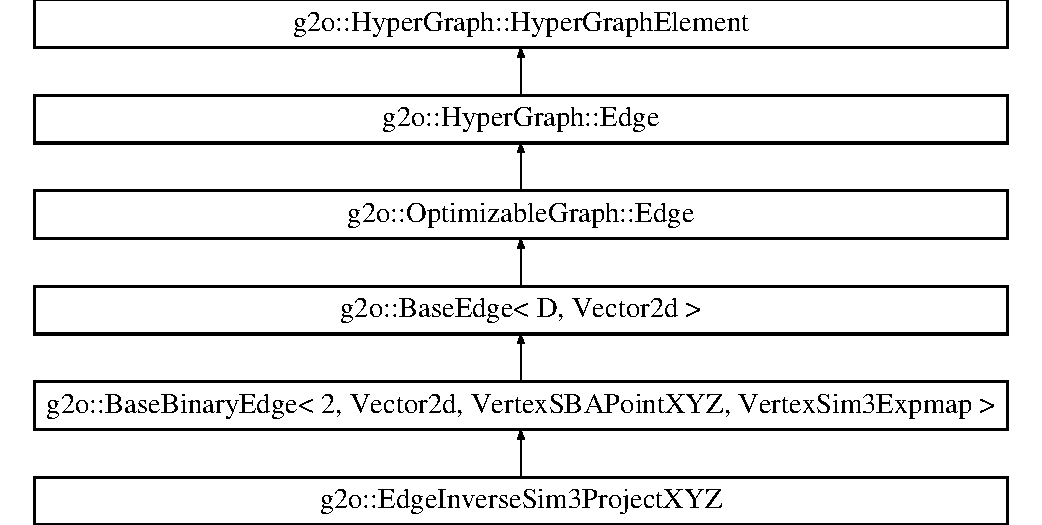
\includegraphics[height=6.000000cm]{classg2o_1_1_edge_inverse_sim3_project_x_y_z}
\end{center}
\end{figure}
\subsection*{Public Member Functions}
\begin{DoxyCompactItemize}
\item 
E\+I\+G\+E\+N\+\_\+\+M\+A\+K\+E\+\_\+\+A\+L\+I\+G\+N\+E\+D\+\_\+\+O\+P\+E\+R\+A\+T\+O\+R\+\_\+\+N\+EW \mbox{\hyperlink{classg2o_1_1_edge_inverse_sim3_project_x_y_z_af4e344ee9f610b41eea60b5914a776bd}{Edge\+Inverse\+Sim3\+Project\+X\+YZ}} ()
\item 
virtual bool \mbox{\hyperlink{classg2o_1_1_edge_inverse_sim3_project_x_y_z_ac229f31599a4f08eebe8f9b239d883f6}{read}} (std\+::istream \&is)
\begin{DoxyCompactList}\small\item\em read the vertex from a stream, i.\+e., the internal state of the vertex \end{DoxyCompactList}\item 
virtual bool \mbox{\hyperlink{classg2o_1_1_edge_inverse_sim3_project_x_y_z_a71ce5fa6b21a59c0cfffdc2b7e8a2024}{write}} (std\+::ostream \&os) const
\begin{DoxyCompactList}\small\item\em write the vertex to a stream \end{DoxyCompactList}\item 
void \mbox{\hyperlink{classg2o_1_1_edge_inverse_sim3_project_x_y_z_a8fa376524e861ae8c4f1a360d217f02d}{compute\+Error}} ()
\end{DoxyCompactItemize}
\subsection*{Additional Inherited Members}


\subsection{Constructor \& Destructor Documentation}
\mbox{\Hypertarget{classg2o_1_1_edge_inverse_sim3_project_x_y_z_af4e344ee9f610b41eea60b5914a776bd}\label{classg2o_1_1_edge_inverse_sim3_project_x_y_z_af4e344ee9f610b41eea60b5914a776bd}} 
\index{g2o\+::\+Edge\+Inverse\+Sim3\+Project\+X\+YZ@{g2o\+::\+Edge\+Inverse\+Sim3\+Project\+X\+YZ}!Edge\+Inverse\+Sim3\+Project\+X\+YZ@{Edge\+Inverse\+Sim3\+Project\+X\+YZ}}
\index{Edge\+Inverse\+Sim3\+Project\+X\+YZ@{Edge\+Inverse\+Sim3\+Project\+X\+YZ}!g2o\+::\+Edge\+Inverse\+Sim3\+Project\+X\+YZ@{g2o\+::\+Edge\+Inverse\+Sim3\+Project\+X\+YZ}}
\subsubsection{\texorpdfstring{Edge\+Inverse\+Sim3\+Project\+X\+Y\+Z()}{EdgeInverseSim3ProjectXYZ()}}
{\footnotesize\ttfamily g2o\+::\+Edge\+Inverse\+Sim3\+Project\+X\+Y\+Z\+::\+Edge\+Inverse\+Sim3\+Project\+X\+YZ (\begin{DoxyParamCaption}{ }\end{DoxyParamCaption})}

Inverse\+Sim3\+Project\+X\+YZ 

\subsection{Member Function Documentation}
\mbox{\Hypertarget{classg2o_1_1_edge_inverse_sim3_project_x_y_z_a8fa376524e861ae8c4f1a360d217f02d}\label{classg2o_1_1_edge_inverse_sim3_project_x_y_z_a8fa376524e861ae8c4f1a360d217f02d}} 
\index{g2o\+::\+Edge\+Inverse\+Sim3\+Project\+X\+YZ@{g2o\+::\+Edge\+Inverse\+Sim3\+Project\+X\+YZ}!compute\+Error@{compute\+Error}}
\index{compute\+Error@{compute\+Error}!g2o\+::\+Edge\+Inverse\+Sim3\+Project\+X\+YZ@{g2o\+::\+Edge\+Inverse\+Sim3\+Project\+X\+YZ}}
\subsubsection{\texorpdfstring{compute\+Error()}{computeError()}}
{\footnotesize\ttfamily void g2o\+::\+Edge\+Inverse\+Sim3\+Project\+X\+Y\+Z\+::compute\+Error (\begin{DoxyParamCaption}{ }\end{DoxyParamCaption})\hspace{0.3cm}{\ttfamily [inline]}, {\ttfamily [virtual]}}



Implements \mbox{\hyperlink{classg2o_1_1_optimizable_graph_1_1_edge_a1e6d9f4128866982de5e11e03edd7775}{g2o\+::\+Optimizable\+Graph\+::\+Edge}}.

\mbox{\Hypertarget{classg2o_1_1_edge_inverse_sim3_project_x_y_z_ac229f31599a4f08eebe8f9b239d883f6}\label{classg2o_1_1_edge_inverse_sim3_project_x_y_z_ac229f31599a4f08eebe8f9b239d883f6}} 
\index{g2o\+::\+Edge\+Inverse\+Sim3\+Project\+X\+YZ@{g2o\+::\+Edge\+Inverse\+Sim3\+Project\+X\+YZ}!read@{read}}
\index{read@{read}!g2o\+::\+Edge\+Inverse\+Sim3\+Project\+X\+YZ@{g2o\+::\+Edge\+Inverse\+Sim3\+Project\+X\+YZ}}
\subsubsection{\texorpdfstring{read()}{read()}}
{\footnotesize\ttfamily bool g2o\+::\+Edge\+Inverse\+Sim3\+Project\+X\+Y\+Z\+::read (\begin{DoxyParamCaption}\item[{std\+::istream \&}]{is }\end{DoxyParamCaption})\hspace{0.3cm}{\ttfamily [virtual]}}



read the vertex from a stream, i.\+e., the internal state of the vertex 



Implements \mbox{\hyperlink{classg2o_1_1_optimizable_graph_1_1_edge_a30cf69b762a06aa35e796d8af71632b0}{g2o\+::\+Optimizable\+Graph\+::\+Edge}}.

\mbox{\Hypertarget{classg2o_1_1_edge_inverse_sim3_project_x_y_z_a71ce5fa6b21a59c0cfffdc2b7e8a2024}\label{classg2o_1_1_edge_inverse_sim3_project_x_y_z_a71ce5fa6b21a59c0cfffdc2b7e8a2024}} 
\index{g2o\+::\+Edge\+Inverse\+Sim3\+Project\+X\+YZ@{g2o\+::\+Edge\+Inverse\+Sim3\+Project\+X\+YZ}!write@{write}}
\index{write@{write}!g2o\+::\+Edge\+Inverse\+Sim3\+Project\+X\+YZ@{g2o\+::\+Edge\+Inverse\+Sim3\+Project\+X\+YZ}}
\subsubsection{\texorpdfstring{write()}{write()}}
{\footnotesize\ttfamily bool g2o\+::\+Edge\+Inverse\+Sim3\+Project\+X\+Y\+Z\+::write (\begin{DoxyParamCaption}\item[{std\+::ostream \&}]{os }\end{DoxyParamCaption}) const\hspace{0.3cm}{\ttfamily [virtual]}}



write the vertex to a stream 



Implements \mbox{\hyperlink{classg2o_1_1_optimizable_graph_1_1_edge_a804b9a2178249b9297c55b8fbbeda56e}{g2o\+::\+Optimizable\+Graph\+::\+Edge}}.



The documentation for this class was generated from the following files\+:\begin{DoxyCompactItemize}
\item 
Thirdparty/g2o/g2o/types/\mbox{\hyperlink{types__seven__dof__expmap_8h}{types\+\_\+seven\+\_\+dof\+\_\+expmap.\+h}}\item 
Thirdparty/g2o/g2o/types/\mbox{\hyperlink{types__seven__dof__expmap_8cpp}{types\+\_\+seven\+\_\+dof\+\_\+expmap.\+cpp}}\end{DoxyCompactItemize}

\hypertarget{classg2o_1_1_edge_s_e3_project_x_y_z}{}\section{g2o\+:\+:Edge\+S\+E3\+Project\+X\+YZ Class Reference}
\label{classg2o_1_1_edge_s_e3_project_x_y_z}\index{g2o\+::\+Edge\+S\+E3\+Project\+X\+YZ@{g2o\+::\+Edge\+S\+E3\+Project\+X\+YZ}}


N\+O\+TE uesd in Optimizer\+::\+Bundle\+Adjustment(), Optimizer\+::\+Local\+Bundle\+Adjustment()  




{\ttfamily \#include $<$types\+\_\+six\+\_\+dof\+\_\+expmap.\+h$>$}

Inheritance diagram for g2o\+:\+:Edge\+S\+E3\+Project\+X\+YZ\+:\begin{figure}[H]
\begin{center}
\leavevmode
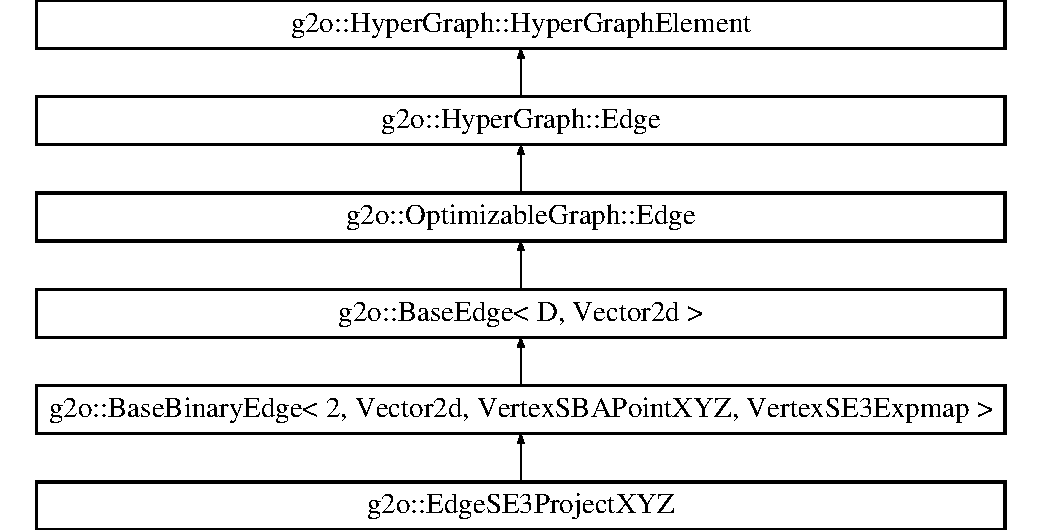
\includegraphics[height=6.000000cm]{classg2o_1_1_edge_s_e3_project_x_y_z}
\end{center}
\end{figure}
\subsection*{Public Member Functions}
\begin{DoxyCompactItemize}
\item 
E\+I\+G\+E\+N\+\_\+\+M\+A\+K\+E\+\_\+\+A\+L\+I\+G\+N\+E\+D\+\_\+\+O\+P\+E\+R\+A\+T\+O\+R\+\_\+\+N\+EW \mbox{\hyperlink{classg2o_1_1_edge_s_e3_project_x_y_z_acdf6cb451767e46e7bbd6a180782feb8}{Edge\+S\+E3\+Project\+X\+YZ}} ()
\item 
bool \mbox{\hyperlink{classg2o_1_1_edge_s_e3_project_x_y_z_a04200f3d6b7fbd47961df696f1ee34ed}{read}} (std\+::istream \&is)
\begin{DoxyCompactList}\small\item\em read the vertex from a stream, i.\+e., the internal state of the vertex \end{DoxyCompactList}\item 
bool \mbox{\hyperlink{classg2o_1_1_edge_s_e3_project_x_y_z_ad2c5fe36901961700eaa9f38cc4b21ca}{write}} (std\+::ostream \&os) const
\begin{DoxyCompactList}\small\item\em write the vertex to a stream \end{DoxyCompactList}\item 
void \mbox{\hyperlink{classg2o_1_1_edge_s_e3_project_x_y_z_a79a763e1d42fe9eb5732abe59c7723d9}{compute\+Error}} ()
\item 
bool \mbox{\hyperlink{classg2o_1_1_edge_s_e3_project_x_y_z_a603cc0018b5b05fd193e84e032a66d07}{is\+Depth\+Positive}} ()
\item 
virtual void \mbox{\hyperlink{classg2o_1_1_edge_s_e3_project_x_y_z_a7454e89740635d782c9e4efaef35ec44}{linearize\+Oplus}} ()
\begin{DoxyCompactList}\small\item\em Linearization. \end{DoxyCompactList}\item 
Vector2d \mbox{\hyperlink{classg2o_1_1_edge_s_e3_project_x_y_z_ab6d57a3a8bbeafb3405ea39c98dca768}{cam\+\_\+project}} (const Vector3d \&trans\+\_\+xyz) const
\end{DoxyCompactItemize}
\subsection*{Public Attributes}
\begin{DoxyCompactItemize}
\item 
double \mbox{\hyperlink{classg2o_1_1_edge_s_e3_project_x_y_z_a6af0a48bd4e21d060585d7ee9c1ca1ef}{fx}}
\item 
double \mbox{\hyperlink{classg2o_1_1_edge_s_e3_project_x_y_z_af5f931cd13ef318a3f42f54aa57b9466}{fy}}
\item 
double \mbox{\hyperlink{classg2o_1_1_edge_s_e3_project_x_y_z_ace052104b07ec272eb5f254254ead5e5}{cx}}
\item 
double \mbox{\hyperlink{classg2o_1_1_edge_s_e3_project_x_y_z_af590c37d535ce7e71be5ce4ae368e9c1}{cy}}
\end{DoxyCompactItemize}
\subsection*{Additional Inherited Members}


\subsection{Detailed Description}
N\+O\+TE uesd in Optimizer\+::\+Bundle\+Adjustment(), Optimizer\+::\+Local\+Bundle\+Adjustment() 

\subsection{Constructor \& Destructor Documentation}
\mbox{\Hypertarget{classg2o_1_1_edge_s_e3_project_x_y_z_acdf6cb451767e46e7bbd6a180782feb8}\label{classg2o_1_1_edge_s_e3_project_x_y_z_acdf6cb451767e46e7bbd6a180782feb8}} 
\index{g2o\+::\+Edge\+S\+E3\+Project\+X\+YZ@{g2o\+::\+Edge\+S\+E3\+Project\+X\+YZ}!Edge\+S\+E3\+Project\+X\+YZ@{Edge\+S\+E3\+Project\+X\+YZ}}
\index{Edge\+S\+E3\+Project\+X\+YZ@{Edge\+S\+E3\+Project\+X\+YZ}!g2o\+::\+Edge\+S\+E3\+Project\+X\+YZ@{g2o\+::\+Edge\+S\+E3\+Project\+X\+YZ}}
\subsubsection{\texorpdfstring{Edge\+S\+E3\+Project\+X\+Y\+Z()}{EdgeSE3ProjectXYZ()}}
{\footnotesize\ttfamily g2o\+::\+Edge\+S\+E3\+Project\+X\+Y\+Z\+::\+Edge\+S\+E3\+Project\+X\+YZ (\begin{DoxyParamCaption}{ }\end{DoxyParamCaption})}



\subsection{Member Function Documentation}
\mbox{\Hypertarget{classg2o_1_1_edge_s_e3_project_x_y_z_ab6d57a3a8bbeafb3405ea39c98dca768}\label{classg2o_1_1_edge_s_e3_project_x_y_z_ab6d57a3a8bbeafb3405ea39c98dca768}} 
\index{g2o\+::\+Edge\+S\+E3\+Project\+X\+YZ@{g2o\+::\+Edge\+S\+E3\+Project\+X\+YZ}!cam\+\_\+project@{cam\+\_\+project}}
\index{cam\+\_\+project@{cam\+\_\+project}!g2o\+::\+Edge\+S\+E3\+Project\+X\+YZ@{g2o\+::\+Edge\+S\+E3\+Project\+X\+YZ}}
\subsubsection{\texorpdfstring{cam\+\_\+project()}{cam\_project()}}
{\footnotesize\ttfamily Vector2d g2o\+::\+Edge\+S\+E3\+Project\+X\+Y\+Z\+::cam\+\_\+project (\begin{DoxyParamCaption}\item[{const Vector3d \&}]{trans\+\_\+xyz }\end{DoxyParamCaption}) const}

将\+Xw投影到cam的图像坐标系 ~\newline
 $ u = \frac{f_x X}{Z} + c_x $ ~\newline
 $ v = \frac{f_y Y}{Z} + c_v $ ~\newline

\begin{DoxyParams}{Parameters}
{\em trans\+\_\+xyz} & \mbox{[}X Y Z\mbox{]} \\
\hline
\end{DoxyParams}
\begin{DoxyReturn}{Returns}
\mbox{[}u v\mbox{]} 
\end{DoxyReturn}
\mbox{\Hypertarget{classg2o_1_1_edge_s_e3_project_x_y_z_a79a763e1d42fe9eb5732abe59c7723d9}\label{classg2o_1_1_edge_s_e3_project_x_y_z_a79a763e1d42fe9eb5732abe59c7723d9}} 
\index{g2o\+::\+Edge\+S\+E3\+Project\+X\+YZ@{g2o\+::\+Edge\+S\+E3\+Project\+X\+YZ}!compute\+Error@{compute\+Error}}
\index{compute\+Error@{compute\+Error}!g2o\+::\+Edge\+S\+E3\+Project\+X\+YZ@{g2o\+::\+Edge\+S\+E3\+Project\+X\+YZ}}
\subsubsection{\texorpdfstring{compute\+Error()}{computeError()}}
{\footnotesize\ttfamily void g2o\+::\+Edge\+S\+E3\+Project\+X\+Y\+Z\+::compute\+Error (\begin{DoxyParamCaption}{ }\end{DoxyParamCaption})\hspace{0.3cm}{\ttfamily [inline]}, {\ttfamily [virtual]}}

重投影误差 

Implements \mbox{\hyperlink{classg2o_1_1_optimizable_graph_1_1_edge_a1e6d9f4128866982de5e11e03edd7775}{g2o\+::\+Optimizable\+Graph\+::\+Edge}}.

\mbox{\Hypertarget{classg2o_1_1_edge_s_e3_project_x_y_z_a603cc0018b5b05fd193e84e032a66d07}\label{classg2o_1_1_edge_s_e3_project_x_y_z_a603cc0018b5b05fd193e84e032a66d07}} 
\index{g2o\+::\+Edge\+S\+E3\+Project\+X\+YZ@{g2o\+::\+Edge\+S\+E3\+Project\+X\+YZ}!is\+Depth\+Positive@{is\+Depth\+Positive}}
\index{is\+Depth\+Positive@{is\+Depth\+Positive}!g2o\+::\+Edge\+S\+E3\+Project\+X\+YZ@{g2o\+::\+Edge\+S\+E3\+Project\+X\+YZ}}
\subsubsection{\texorpdfstring{is\+Depth\+Positive()}{isDepthPositive()}}
{\footnotesize\ttfamily bool g2o\+::\+Edge\+S\+E3\+Project\+X\+Y\+Z\+::is\+Depth\+Positive (\begin{DoxyParamCaption}{ }\end{DoxyParamCaption})\hspace{0.3cm}{\ttfamily [inline]}}

检验 $ TX_w $的\+Z是否大于0 \begin{DoxyReturn}{Returns}
true if the depth is Positive 
\end{DoxyReturn}
\mbox{\Hypertarget{classg2o_1_1_edge_s_e3_project_x_y_z_a7454e89740635d782c9e4efaef35ec44}\label{classg2o_1_1_edge_s_e3_project_x_y_z_a7454e89740635d782c9e4efaef35ec44}} 
\index{g2o\+::\+Edge\+S\+E3\+Project\+X\+YZ@{g2o\+::\+Edge\+S\+E3\+Project\+X\+YZ}!linearize\+Oplus@{linearize\+Oplus}}
\index{linearize\+Oplus@{linearize\+Oplus}!g2o\+::\+Edge\+S\+E3\+Project\+X\+YZ@{g2o\+::\+Edge\+S\+E3\+Project\+X\+YZ}}
\subsubsection{\texorpdfstring{linearize\+Oplus()}{linearizeOplus()}}
{\footnotesize\ttfamily void g2o\+::\+Edge\+S\+E3\+Project\+X\+Y\+Z\+::linearize\+Oplus (\begin{DoxyParamCaption}{ }\end{DoxyParamCaption})\hspace{0.3cm}{\ttfamily [virtual]}}



Linearization. 

误差函数对\mbox{[}X Y Z\mbox{]}和增量\mbox{[}w1 w2 w3 v1 v2 v3\mbox{]}求雅克比矩阵 ~\newline
 $Ji_{2\times3} = \frac{\partial [obs - \Pi(exp(\hat{\xi}) T X_w)]}{\partial X_w} $ ~\newline
 $Jj_{2\times6} = \frac{\partial [obs - \Pi(exp(\hat{\xi}) T X_w)]}{\partial \xi} $ ~\newline
\begin{DoxyNote}{Note}
\+\_\+jacobian\+Oplus\+Xi,\+\_\+jacobian\+Oplus\+Xj 
\end{DoxyNote}
\begin{DoxySeeAlso}{See also}
采用链式法则求解, 参考(注意以下参考的增量定义为\mbox{[}v1 v2 v3 w1 w2 w3\mbox{]})
\begin{DoxyItemize}
\item jlblanco2010geometry3d\+\_\+techrep.\+pdf p56 (A.\+2) 推荐
\item strasdat\+\_\+thesis\+\_\+2012.\+pdf p194 (B.\+4)
\end{DoxyItemize}
\end{DoxySeeAlso}
线性化, 即同时对重投影误差分别关于位姿vj和路标vi求雅克比矩阵.

\+\_\+jacobian\+Oplus\+Xj是重投影误差关于位姿vj的导数 \+\_\+jacobian\+Oplus\+Xi是重投影误差关于路标vi的导数 xyz即路标在世界坐标系下的三维坐标, xyz\+\_\+trans是路标在相机坐标系下的三维坐标. map()函数就是通过位姿T=\mbox{[}R$\vert$t\mbox{]}进行坐标系映射. 

Reimplemented from \mbox{\hyperlink{classg2o_1_1_base_binary_edge_af0fb8a693c8c7996fa65566e7263fbc4}{g2o\+::\+Base\+Binary\+Edge$<$ 2, Vector2d, Vertex\+S\+B\+A\+Point\+X\+Y\+Z, Vertex\+S\+E3\+Expmap $>$}}.

\mbox{\Hypertarget{classg2o_1_1_edge_s_e3_project_x_y_z_a04200f3d6b7fbd47961df696f1ee34ed}\label{classg2o_1_1_edge_s_e3_project_x_y_z_a04200f3d6b7fbd47961df696f1ee34ed}} 
\index{g2o\+::\+Edge\+S\+E3\+Project\+X\+YZ@{g2o\+::\+Edge\+S\+E3\+Project\+X\+YZ}!read@{read}}
\index{read@{read}!g2o\+::\+Edge\+S\+E3\+Project\+X\+YZ@{g2o\+::\+Edge\+S\+E3\+Project\+X\+YZ}}
\subsubsection{\texorpdfstring{read()}{read()}}
{\footnotesize\ttfamily bool g2o\+::\+Edge\+S\+E3\+Project\+X\+Y\+Z\+::read (\begin{DoxyParamCaption}\item[{std\+::istream \&}]{is }\end{DoxyParamCaption})\hspace{0.3cm}{\ttfamily [virtual]}}



read the vertex from a stream, i.\+e., the internal state of the vertex 



Implements \mbox{\hyperlink{classg2o_1_1_optimizable_graph_1_1_edge_a30cf69b762a06aa35e796d8af71632b0}{g2o\+::\+Optimizable\+Graph\+::\+Edge}}.

\mbox{\Hypertarget{classg2o_1_1_edge_s_e3_project_x_y_z_ad2c5fe36901961700eaa9f38cc4b21ca}\label{classg2o_1_1_edge_s_e3_project_x_y_z_ad2c5fe36901961700eaa9f38cc4b21ca}} 
\index{g2o\+::\+Edge\+S\+E3\+Project\+X\+YZ@{g2o\+::\+Edge\+S\+E3\+Project\+X\+YZ}!write@{write}}
\index{write@{write}!g2o\+::\+Edge\+S\+E3\+Project\+X\+YZ@{g2o\+::\+Edge\+S\+E3\+Project\+X\+YZ}}
\subsubsection{\texorpdfstring{write()}{write()}}
{\footnotesize\ttfamily bool g2o\+::\+Edge\+S\+E3\+Project\+X\+Y\+Z\+::write (\begin{DoxyParamCaption}\item[{std\+::ostream \&}]{os }\end{DoxyParamCaption}) const\hspace{0.3cm}{\ttfamily [virtual]}}



write the vertex to a stream 



Implements \mbox{\hyperlink{classg2o_1_1_optimizable_graph_1_1_edge_a804b9a2178249b9297c55b8fbbeda56e}{g2o\+::\+Optimizable\+Graph\+::\+Edge}}.



\subsection{Member Data Documentation}
\mbox{\Hypertarget{classg2o_1_1_edge_s_e3_project_x_y_z_ace052104b07ec272eb5f254254ead5e5}\label{classg2o_1_1_edge_s_e3_project_x_y_z_ace052104b07ec272eb5f254254ead5e5}} 
\index{g2o\+::\+Edge\+S\+E3\+Project\+X\+YZ@{g2o\+::\+Edge\+S\+E3\+Project\+X\+YZ}!cx@{cx}}
\index{cx@{cx}!g2o\+::\+Edge\+S\+E3\+Project\+X\+YZ@{g2o\+::\+Edge\+S\+E3\+Project\+X\+YZ}}
\subsubsection{\texorpdfstring{cx}{cx}}
{\footnotesize\ttfamily double g2o\+::\+Edge\+S\+E3\+Project\+X\+Y\+Z\+::cx}

\mbox{\Hypertarget{classg2o_1_1_edge_s_e3_project_x_y_z_af590c37d535ce7e71be5ce4ae368e9c1}\label{classg2o_1_1_edge_s_e3_project_x_y_z_af590c37d535ce7e71be5ce4ae368e9c1}} 
\index{g2o\+::\+Edge\+S\+E3\+Project\+X\+YZ@{g2o\+::\+Edge\+S\+E3\+Project\+X\+YZ}!cy@{cy}}
\index{cy@{cy}!g2o\+::\+Edge\+S\+E3\+Project\+X\+YZ@{g2o\+::\+Edge\+S\+E3\+Project\+X\+YZ}}
\subsubsection{\texorpdfstring{cy}{cy}}
{\footnotesize\ttfamily double g2o\+::\+Edge\+S\+E3\+Project\+X\+Y\+Z\+::cy}

\mbox{\Hypertarget{classg2o_1_1_edge_s_e3_project_x_y_z_a6af0a48bd4e21d060585d7ee9c1ca1ef}\label{classg2o_1_1_edge_s_e3_project_x_y_z_a6af0a48bd4e21d060585d7ee9c1ca1ef}} 
\index{g2o\+::\+Edge\+S\+E3\+Project\+X\+YZ@{g2o\+::\+Edge\+S\+E3\+Project\+X\+YZ}!fx@{fx}}
\index{fx@{fx}!g2o\+::\+Edge\+S\+E3\+Project\+X\+YZ@{g2o\+::\+Edge\+S\+E3\+Project\+X\+YZ}}
\subsubsection{\texorpdfstring{fx}{fx}}
{\footnotesize\ttfamily double g2o\+::\+Edge\+S\+E3\+Project\+X\+Y\+Z\+::fx}

\mbox{\Hypertarget{classg2o_1_1_edge_s_e3_project_x_y_z_af5f931cd13ef318a3f42f54aa57b9466}\label{classg2o_1_1_edge_s_e3_project_x_y_z_af5f931cd13ef318a3f42f54aa57b9466}} 
\index{g2o\+::\+Edge\+S\+E3\+Project\+X\+YZ@{g2o\+::\+Edge\+S\+E3\+Project\+X\+YZ}!fy@{fy}}
\index{fy@{fy}!g2o\+::\+Edge\+S\+E3\+Project\+X\+YZ@{g2o\+::\+Edge\+S\+E3\+Project\+X\+YZ}}
\subsubsection{\texorpdfstring{fy}{fy}}
{\footnotesize\ttfamily double g2o\+::\+Edge\+S\+E3\+Project\+X\+Y\+Z\+::fy}



The documentation for this class was generated from the following files\+:\begin{DoxyCompactItemize}
\item 
Thirdparty/g2o/g2o/types/\mbox{\hyperlink{types__six__dof__expmap_8h}{types\+\_\+six\+\_\+dof\+\_\+expmap.\+h}}\item 
Thirdparty/g2o/g2o/types/\mbox{\hyperlink{types__six__dof__expmap_8cpp}{types\+\_\+six\+\_\+dof\+\_\+expmap.\+cpp}}\end{DoxyCompactItemize}

\hypertarget{classg2o_1_1_edge_s_e3_project_x_y_z_only_pose}{}\section{g2o\+:\+:Edge\+S\+E3\+Project\+X\+Y\+Z\+Only\+Pose Class Reference}
\label{classg2o_1_1_edge_s_e3_project_x_y_z_only_pose}\index{g2o\+::\+Edge\+S\+E3\+Project\+X\+Y\+Z\+Only\+Pose@{g2o\+::\+Edge\+S\+E3\+Project\+X\+Y\+Z\+Only\+Pose}}


N\+O\+TE uesd in Optimizer\+::\+Pose\+Optimization()  




{\ttfamily \#include $<$types\+\_\+six\+\_\+dof\+\_\+expmap.\+h$>$}

Inheritance diagram for g2o\+:\+:Edge\+S\+E3\+Project\+X\+Y\+Z\+Only\+Pose\+:\begin{figure}[H]
\begin{center}
\leavevmode
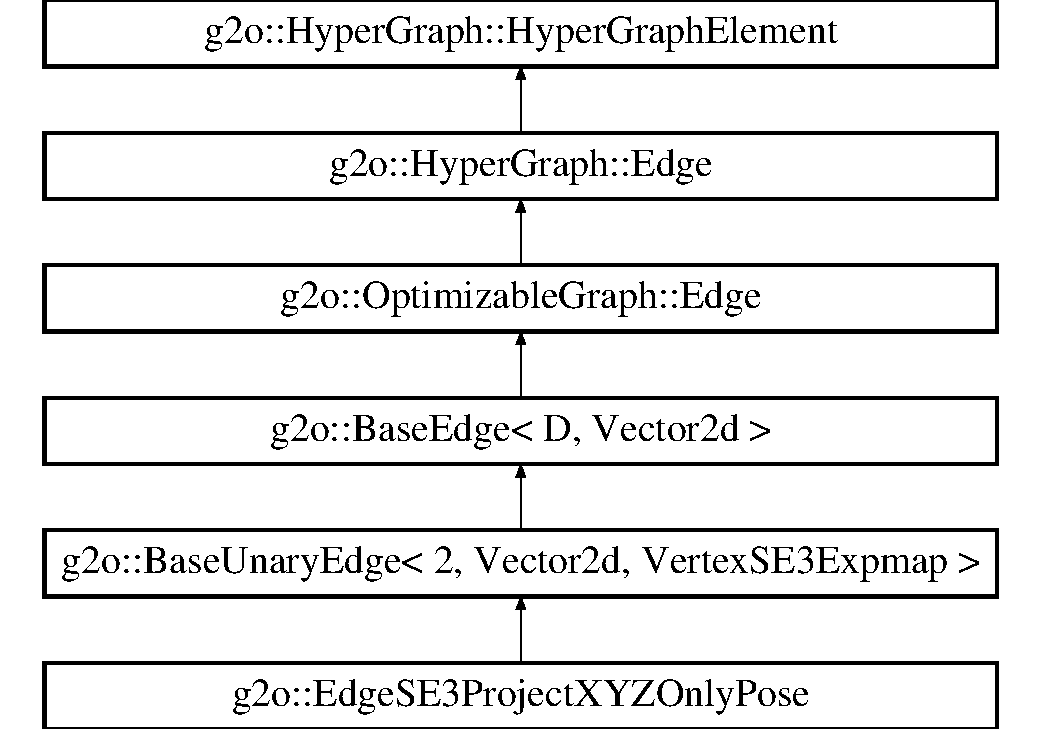
\includegraphics[height=6.000000cm]{classg2o_1_1_edge_s_e3_project_x_y_z_only_pose}
\end{center}
\end{figure}
\subsection*{Public Member Functions}
\begin{DoxyCompactItemize}
\item 
E\+I\+G\+E\+N\+\_\+\+M\+A\+K\+E\+\_\+\+A\+L\+I\+G\+N\+E\+D\+\_\+\+O\+P\+E\+R\+A\+T\+O\+R\+\_\+\+N\+EW \mbox{\hyperlink{classg2o_1_1_edge_s_e3_project_x_y_z_only_pose_a617972556497ab31cc745f6d3eb59c58}{Edge\+S\+E3\+Project\+X\+Y\+Z\+Only\+Pose}} ()
\item 
bool \mbox{\hyperlink{classg2o_1_1_edge_s_e3_project_x_y_z_only_pose_a28994ddf2cab7b61566ce55ad4b43388}{read}} (std\+::istream \&is)
\begin{DoxyCompactList}\small\item\em read the vertex from a stream, i.\+e., the internal state of the vertex \end{DoxyCompactList}\item 
bool \mbox{\hyperlink{classg2o_1_1_edge_s_e3_project_x_y_z_only_pose_ac0132c975af1a49cdf490a6dbe8f450c}{write}} (std\+::ostream \&os) const
\begin{DoxyCompactList}\small\item\em write the vertex to a stream \end{DoxyCompactList}\item 
void \mbox{\hyperlink{classg2o_1_1_edge_s_e3_project_x_y_z_only_pose_a6752098d3322d30e43a6a3a668a3b009}{compute\+Error}} ()
\item 
bool \mbox{\hyperlink{classg2o_1_1_edge_s_e3_project_x_y_z_only_pose_abd6f619de5af8855c8ee21fcfad51c9e}{is\+Depth\+Positive}} ()
\item 
virtual void \mbox{\hyperlink{classg2o_1_1_edge_s_e3_project_x_y_z_only_pose_abe6d775aade1277786274c328aa2c38b}{linearize\+Oplus}} ()
\begin{DoxyCompactList}\small\item\em Linearization. \end{DoxyCompactList}\item 
Vector2d \mbox{\hyperlink{classg2o_1_1_edge_s_e3_project_x_y_z_only_pose_ad557e880209ef1a49c4b54a60872fe68}{cam\+\_\+project}} (const Vector3d \&trans\+\_\+xyz) const
\end{DoxyCompactItemize}
\subsection*{Public Attributes}
\begin{DoxyCompactItemize}
\item 
Vector3d \mbox{\hyperlink{classg2o_1_1_edge_s_e3_project_x_y_z_only_pose_a66318605e8e9c2276b100cf73e718ea8}{Xw}}
\begin{DoxyCompactList}\small\item\em Map\+Point在世界坐标系的位置 \end{DoxyCompactList}\item 
double \mbox{\hyperlink{classg2o_1_1_edge_s_e3_project_x_y_z_only_pose_a413ca1179697e29d5476f582d2b29ff6}{fx}}
\item 
double \mbox{\hyperlink{classg2o_1_1_edge_s_e3_project_x_y_z_only_pose_a2f645f770962dc9d8c4862c0c6dbb497}{fy}}
\item 
double \mbox{\hyperlink{classg2o_1_1_edge_s_e3_project_x_y_z_only_pose_ab4d7078a2d9a628afd6022c983843904}{cx}}
\item 
double \mbox{\hyperlink{classg2o_1_1_edge_s_e3_project_x_y_z_only_pose_aa6f6f24382d0f9b03d6ae47747e6d95d}{cy}}
\begin{DoxyCompactList}\small\item\em 内参数 \end{DoxyCompactList}\end{DoxyCompactItemize}
\subsection*{Additional Inherited Members}


\subsection{Detailed Description}
N\+O\+TE uesd in Optimizer\+::\+Pose\+Optimization() 

\subsection{Constructor \& Destructor Documentation}
\mbox{\Hypertarget{classg2o_1_1_edge_s_e3_project_x_y_z_only_pose_a617972556497ab31cc745f6d3eb59c58}\label{classg2o_1_1_edge_s_e3_project_x_y_z_only_pose_a617972556497ab31cc745f6d3eb59c58}} 
\index{g2o\+::\+Edge\+S\+E3\+Project\+X\+Y\+Z\+Only\+Pose@{g2o\+::\+Edge\+S\+E3\+Project\+X\+Y\+Z\+Only\+Pose}!Edge\+S\+E3\+Project\+X\+Y\+Z\+Only\+Pose@{Edge\+S\+E3\+Project\+X\+Y\+Z\+Only\+Pose}}
\index{Edge\+S\+E3\+Project\+X\+Y\+Z\+Only\+Pose@{Edge\+S\+E3\+Project\+X\+Y\+Z\+Only\+Pose}!g2o\+::\+Edge\+S\+E3\+Project\+X\+Y\+Z\+Only\+Pose@{g2o\+::\+Edge\+S\+E3\+Project\+X\+Y\+Z\+Only\+Pose}}
\subsubsection{\texorpdfstring{Edge\+S\+E3\+Project\+X\+Y\+Z\+Only\+Pose()}{EdgeSE3ProjectXYZOnlyPose()}}
{\footnotesize\ttfamily E\+I\+G\+E\+N\+\_\+\+M\+A\+K\+E\+\_\+\+A\+L\+I\+G\+N\+E\+D\+\_\+\+O\+P\+E\+R\+A\+T\+O\+R\+\_\+\+N\+EW g2o\+::\+Edge\+S\+E3\+Project\+X\+Y\+Z\+Only\+Pose\+::\+Edge\+S\+E3\+Project\+X\+Y\+Z\+Only\+Pose (\begin{DoxyParamCaption}{ }\end{DoxyParamCaption})\hspace{0.3cm}{\ttfamily [inline]}}



\subsection{Member Function Documentation}
\mbox{\Hypertarget{classg2o_1_1_edge_s_e3_project_x_y_z_only_pose_ad557e880209ef1a49c4b54a60872fe68}\label{classg2o_1_1_edge_s_e3_project_x_y_z_only_pose_ad557e880209ef1a49c4b54a60872fe68}} 
\index{g2o\+::\+Edge\+S\+E3\+Project\+X\+Y\+Z\+Only\+Pose@{g2o\+::\+Edge\+S\+E3\+Project\+X\+Y\+Z\+Only\+Pose}!cam\+\_\+project@{cam\+\_\+project}}
\index{cam\+\_\+project@{cam\+\_\+project}!g2o\+::\+Edge\+S\+E3\+Project\+X\+Y\+Z\+Only\+Pose@{g2o\+::\+Edge\+S\+E3\+Project\+X\+Y\+Z\+Only\+Pose}}
\subsubsection{\texorpdfstring{cam\+\_\+project()}{cam\_project()}}
{\footnotesize\ttfamily Vector2d g2o\+::\+Edge\+S\+E3\+Project\+X\+Y\+Z\+Only\+Pose\+::cam\+\_\+project (\begin{DoxyParamCaption}\item[{const Vector3d \&}]{trans\+\_\+xyz }\end{DoxyParamCaption}) const}

将\+Xw投影到cam的图像坐标系 ~\newline
 $ u = \frac{f_x X}{Z} + c_x $ ~\newline
 $ v = \frac{f_y Y}{Z} + c_v $ ~\newline

\begin{DoxyParams}{Parameters}
{\em trans\+\_\+xyz} & \mbox{[}X Y Z\mbox{]} \\
\hline
\end{DoxyParams}
\begin{DoxyReturn}{Returns}
\mbox{[}u v\mbox{]} 
\end{DoxyReturn}
\mbox{\Hypertarget{classg2o_1_1_edge_s_e3_project_x_y_z_only_pose_a6752098d3322d30e43a6a3a668a3b009}\label{classg2o_1_1_edge_s_e3_project_x_y_z_only_pose_a6752098d3322d30e43a6a3a668a3b009}} 
\index{g2o\+::\+Edge\+S\+E3\+Project\+X\+Y\+Z\+Only\+Pose@{g2o\+::\+Edge\+S\+E3\+Project\+X\+Y\+Z\+Only\+Pose}!compute\+Error@{compute\+Error}}
\index{compute\+Error@{compute\+Error}!g2o\+::\+Edge\+S\+E3\+Project\+X\+Y\+Z\+Only\+Pose@{g2o\+::\+Edge\+S\+E3\+Project\+X\+Y\+Z\+Only\+Pose}}
\subsubsection{\texorpdfstring{compute\+Error()}{computeError()}}
{\footnotesize\ttfamily void g2o\+::\+Edge\+S\+E3\+Project\+X\+Y\+Z\+Only\+Pose\+::compute\+Error (\begin{DoxyParamCaption}{ }\end{DoxyParamCaption})\hspace{0.3cm}{\ttfamily [inline]}, {\ttfamily [virtual]}}

重投影误差 

Implements \mbox{\hyperlink{classg2o_1_1_optimizable_graph_1_1_edge_a1e6d9f4128866982de5e11e03edd7775}{g2o\+::\+Optimizable\+Graph\+::\+Edge}}.

\mbox{\Hypertarget{classg2o_1_1_edge_s_e3_project_x_y_z_only_pose_abd6f619de5af8855c8ee21fcfad51c9e}\label{classg2o_1_1_edge_s_e3_project_x_y_z_only_pose_abd6f619de5af8855c8ee21fcfad51c9e}} 
\index{g2o\+::\+Edge\+S\+E3\+Project\+X\+Y\+Z\+Only\+Pose@{g2o\+::\+Edge\+S\+E3\+Project\+X\+Y\+Z\+Only\+Pose}!is\+Depth\+Positive@{is\+Depth\+Positive}}
\index{is\+Depth\+Positive@{is\+Depth\+Positive}!g2o\+::\+Edge\+S\+E3\+Project\+X\+Y\+Z\+Only\+Pose@{g2o\+::\+Edge\+S\+E3\+Project\+X\+Y\+Z\+Only\+Pose}}
\subsubsection{\texorpdfstring{is\+Depth\+Positive()}{isDepthPositive()}}
{\footnotesize\ttfamily bool g2o\+::\+Edge\+S\+E3\+Project\+X\+Y\+Z\+Only\+Pose\+::is\+Depth\+Positive (\begin{DoxyParamCaption}{ }\end{DoxyParamCaption})\hspace{0.3cm}{\ttfamily [inline]}}

检验 $ TX_w $的\+Z是否大于0 \begin{DoxyReturn}{Returns}
true if the depth is Positive 
\end{DoxyReturn}
\mbox{\Hypertarget{classg2o_1_1_edge_s_e3_project_x_y_z_only_pose_abe6d775aade1277786274c328aa2c38b}\label{classg2o_1_1_edge_s_e3_project_x_y_z_only_pose_abe6d775aade1277786274c328aa2c38b}} 
\index{g2o\+::\+Edge\+S\+E3\+Project\+X\+Y\+Z\+Only\+Pose@{g2o\+::\+Edge\+S\+E3\+Project\+X\+Y\+Z\+Only\+Pose}!linearize\+Oplus@{linearize\+Oplus}}
\index{linearize\+Oplus@{linearize\+Oplus}!g2o\+::\+Edge\+S\+E3\+Project\+X\+Y\+Z\+Only\+Pose@{g2o\+::\+Edge\+S\+E3\+Project\+X\+Y\+Z\+Only\+Pose}}
\subsubsection{\texorpdfstring{linearize\+Oplus()}{linearizeOplus()}}
{\footnotesize\ttfamily void g2o\+::\+Edge\+S\+E3\+Project\+X\+Y\+Z\+Only\+Pose\+::linearize\+Oplus (\begin{DoxyParamCaption}{ }\end{DoxyParamCaption})\hspace{0.3cm}{\ttfamily [virtual]}}



Linearization. 

误差函数对增量\mbox{[}w1 w2 w3 v1 v2 v3\mbox{]}求雅克比矩阵 $J_{2\times6}$ $ = \frac{\partial [obs - \Pi(exp(\hat{\xi}) T X_w)]}{\partial \xi} $ \begin{DoxyNote}{Note}
\+\_\+jacobian\+Oplus\+Xi,雅可比矩阵的正负号没有关系 
\end{DoxyNote}
\begin{DoxySeeAlso}{See also}
采用链式法则求解, 参考(注意以下参考的增量定义为\mbox{[}v1 v2 v3 w1 w2 w3\mbox{]})
\begin{DoxyItemize}
\item jlblanco2010geometry3d\+\_\+techrep.\+pdf p56 (A.\+2) 推荐
\item strasdat\+\_\+thesis\+\_\+2012.\+pdf p194 (B.\+4)
\end{DoxyItemize}
\end{DoxySeeAlso}
线性化, 只对位姿vi求导

\+\_\+jacobian\+Oplus\+Xi是重投影误差关于位姿vj的导数 xyz\+\_\+trans是路标在新一帧相机坐标系下的估计位置(3\+D),优化时用逆深度. 

Reimplemented from \mbox{\hyperlink{classg2o_1_1_base_unary_edge_a367f19b903938faf6e89dd1b0e4e722b}{g2o\+::\+Base\+Unary\+Edge$<$ 2, Vector2d, Vertex\+S\+E3\+Expmap $>$}}.

\mbox{\Hypertarget{classg2o_1_1_edge_s_e3_project_x_y_z_only_pose_a28994ddf2cab7b61566ce55ad4b43388}\label{classg2o_1_1_edge_s_e3_project_x_y_z_only_pose_a28994ddf2cab7b61566ce55ad4b43388}} 
\index{g2o\+::\+Edge\+S\+E3\+Project\+X\+Y\+Z\+Only\+Pose@{g2o\+::\+Edge\+S\+E3\+Project\+X\+Y\+Z\+Only\+Pose}!read@{read}}
\index{read@{read}!g2o\+::\+Edge\+S\+E3\+Project\+X\+Y\+Z\+Only\+Pose@{g2o\+::\+Edge\+S\+E3\+Project\+X\+Y\+Z\+Only\+Pose}}
\subsubsection{\texorpdfstring{read()}{read()}}
{\footnotesize\ttfamily bool g2o\+::\+Edge\+S\+E3\+Project\+X\+Y\+Z\+Only\+Pose\+::read (\begin{DoxyParamCaption}\item[{std\+::istream \&}]{is }\end{DoxyParamCaption})\hspace{0.3cm}{\ttfamily [virtual]}}



read the vertex from a stream, i.\+e., the internal state of the vertex 



Implements \mbox{\hyperlink{classg2o_1_1_optimizable_graph_1_1_edge_a30cf69b762a06aa35e796d8af71632b0}{g2o\+::\+Optimizable\+Graph\+::\+Edge}}.

\mbox{\Hypertarget{classg2o_1_1_edge_s_e3_project_x_y_z_only_pose_ac0132c975af1a49cdf490a6dbe8f450c}\label{classg2o_1_1_edge_s_e3_project_x_y_z_only_pose_ac0132c975af1a49cdf490a6dbe8f450c}} 
\index{g2o\+::\+Edge\+S\+E3\+Project\+X\+Y\+Z\+Only\+Pose@{g2o\+::\+Edge\+S\+E3\+Project\+X\+Y\+Z\+Only\+Pose}!write@{write}}
\index{write@{write}!g2o\+::\+Edge\+S\+E3\+Project\+X\+Y\+Z\+Only\+Pose@{g2o\+::\+Edge\+S\+E3\+Project\+X\+Y\+Z\+Only\+Pose}}
\subsubsection{\texorpdfstring{write()}{write()}}
{\footnotesize\ttfamily bool g2o\+::\+Edge\+S\+E3\+Project\+X\+Y\+Z\+Only\+Pose\+::write (\begin{DoxyParamCaption}\item[{std\+::ostream \&}]{os }\end{DoxyParamCaption}) const\hspace{0.3cm}{\ttfamily [virtual]}}



write the vertex to a stream 



Implements \mbox{\hyperlink{classg2o_1_1_optimizable_graph_1_1_edge_a804b9a2178249b9297c55b8fbbeda56e}{g2o\+::\+Optimizable\+Graph\+::\+Edge}}.



\subsection{Member Data Documentation}
\mbox{\Hypertarget{classg2o_1_1_edge_s_e3_project_x_y_z_only_pose_ab4d7078a2d9a628afd6022c983843904}\label{classg2o_1_1_edge_s_e3_project_x_y_z_only_pose_ab4d7078a2d9a628afd6022c983843904}} 
\index{g2o\+::\+Edge\+S\+E3\+Project\+X\+Y\+Z\+Only\+Pose@{g2o\+::\+Edge\+S\+E3\+Project\+X\+Y\+Z\+Only\+Pose}!cx@{cx}}
\index{cx@{cx}!g2o\+::\+Edge\+S\+E3\+Project\+X\+Y\+Z\+Only\+Pose@{g2o\+::\+Edge\+S\+E3\+Project\+X\+Y\+Z\+Only\+Pose}}
\subsubsection{\texorpdfstring{cx}{cx}}
{\footnotesize\ttfamily double g2o\+::\+Edge\+S\+E3\+Project\+X\+Y\+Z\+Only\+Pose\+::cx}

\mbox{\Hypertarget{classg2o_1_1_edge_s_e3_project_x_y_z_only_pose_aa6f6f24382d0f9b03d6ae47747e6d95d}\label{classg2o_1_1_edge_s_e3_project_x_y_z_only_pose_aa6f6f24382d0f9b03d6ae47747e6d95d}} 
\index{g2o\+::\+Edge\+S\+E3\+Project\+X\+Y\+Z\+Only\+Pose@{g2o\+::\+Edge\+S\+E3\+Project\+X\+Y\+Z\+Only\+Pose}!cy@{cy}}
\index{cy@{cy}!g2o\+::\+Edge\+S\+E3\+Project\+X\+Y\+Z\+Only\+Pose@{g2o\+::\+Edge\+S\+E3\+Project\+X\+Y\+Z\+Only\+Pose}}
\subsubsection{\texorpdfstring{cy}{cy}}
{\footnotesize\ttfamily double g2o\+::\+Edge\+S\+E3\+Project\+X\+Y\+Z\+Only\+Pose\+::cy}



内参数 

\mbox{\Hypertarget{classg2o_1_1_edge_s_e3_project_x_y_z_only_pose_a413ca1179697e29d5476f582d2b29ff6}\label{classg2o_1_1_edge_s_e3_project_x_y_z_only_pose_a413ca1179697e29d5476f582d2b29ff6}} 
\index{g2o\+::\+Edge\+S\+E3\+Project\+X\+Y\+Z\+Only\+Pose@{g2o\+::\+Edge\+S\+E3\+Project\+X\+Y\+Z\+Only\+Pose}!fx@{fx}}
\index{fx@{fx}!g2o\+::\+Edge\+S\+E3\+Project\+X\+Y\+Z\+Only\+Pose@{g2o\+::\+Edge\+S\+E3\+Project\+X\+Y\+Z\+Only\+Pose}}
\subsubsection{\texorpdfstring{fx}{fx}}
{\footnotesize\ttfamily double g2o\+::\+Edge\+S\+E3\+Project\+X\+Y\+Z\+Only\+Pose\+::fx}

\mbox{\Hypertarget{classg2o_1_1_edge_s_e3_project_x_y_z_only_pose_a2f645f770962dc9d8c4862c0c6dbb497}\label{classg2o_1_1_edge_s_e3_project_x_y_z_only_pose_a2f645f770962dc9d8c4862c0c6dbb497}} 
\index{g2o\+::\+Edge\+S\+E3\+Project\+X\+Y\+Z\+Only\+Pose@{g2o\+::\+Edge\+S\+E3\+Project\+X\+Y\+Z\+Only\+Pose}!fy@{fy}}
\index{fy@{fy}!g2o\+::\+Edge\+S\+E3\+Project\+X\+Y\+Z\+Only\+Pose@{g2o\+::\+Edge\+S\+E3\+Project\+X\+Y\+Z\+Only\+Pose}}
\subsubsection{\texorpdfstring{fy}{fy}}
{\footnotesize\ttfamily double g2o\+::\+Edge\+S\+E3\+Project\+X\+Y\+Z\+Only\+Pose\+::fy}

\mbox{\Hypertarget{classg2o_1_1_edge_s_e3_project_x_y_z_only_pose_a66318605e8e9c2276b100cf73e718ea8}\label{classg2o_1_1_edge_s_e3_project_x_y_z_only_pose_a66318605e8e9c2276b100cf73e718ea8}} 
\index{g2o\+::\+Edge\+S\+E3\+Project\+X\+Y\+Z\+Only\+Pose@{g2o\+::\+Edge\+S\+E3\+Project\+X\+Y\+Z\+Only\+Pose}!Xw@{Xw}}
\index{Xw@{Xw}!g2o\+::\+Edge\+S\+E3\+Project\+X\+Y\+Z\+Only\+Pose@{g2o\+::\+Edge\+S\+E3\+Project\+X\+Y\+Z\+Only\+Pose}}
\subsubsection{\texorpdfstring{Xw}{Xw}}
{\footnotesize\ttfamily Vector3d g2o\+::\+Edge\+S\+E3\+Project\+X\+Y\+Z\+Only\+Pose\+::\+Xw}



Map\+Point在世界坐标系的位置 



The documentation for this class was generated from the following files\+:\begin{DoxyCompactItemize}
\item 
Thirdparty/g2o/g2o/types/\mbox{\hyperlink{types__six__dof__expmap_8h}{types\+\_\+six\+\_\+dof\+\_\+expmap.\+h}}\item 
Thirdparty/g2o/g2o/types/\mbox{\hyperlink{types__six__dof__expmap_8cpp}{types\+\_\+six\+\_\+dof\+\_\+expmap.\+cpp}}\end{DoxyCompactItemize}

\hypertarget{classg2o_1_1_edge_sim3}{}\section{g2o\+:\+:Edge\+Sim3 Class Reference}
\label{classg2o_1_1_edge_sim3}\index{g2o\+::\+Edge\+Sim3@{g2o\+::\+Edge\+Sim3}}


7D edge between two Vertex7  




{\ttfamily \#include $<$types\+\_\+seven\+\_\+dof\+\_\+expmap.\+h$>$}

Inheritance diagram for g2o\+:\+:Edge\+Sim3\+:\begin{figure}[H]
\begin{center}
\leavevmode
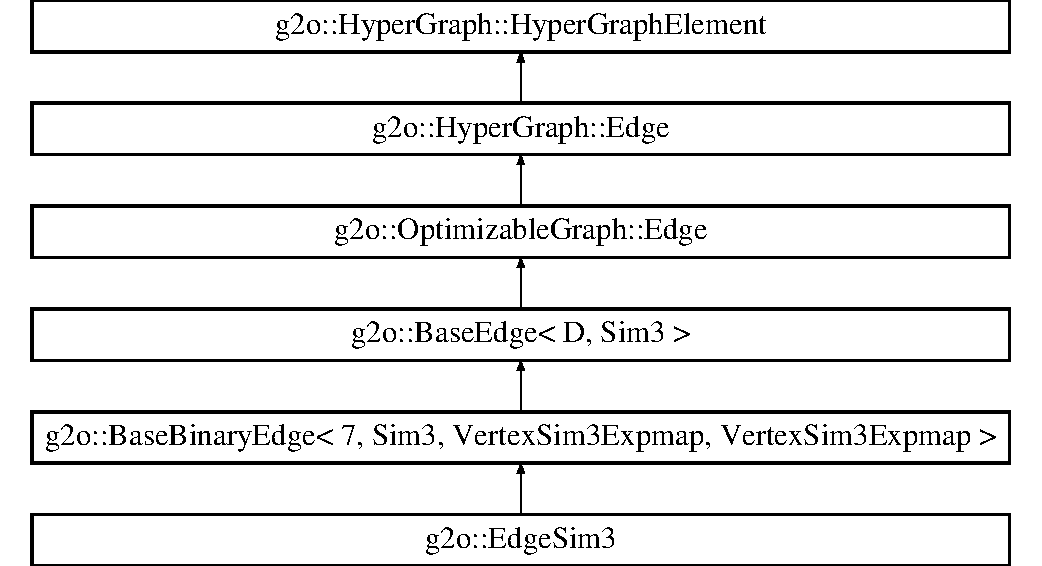
\includegraphics[height=6.000000cm]{classg2o_1_1_edge_sim3}
\end{center}
\end{figure}
\subsection*{Public Member Functions}
\begin{DoxyCompactItemize}
\item 
E\+I\+G\+E\+N\+\_\+\+M\+A\+K\+E\+\_\+\+A\+L\+I\+G\+N\+E\+D\+\_\+\+O\+P\+E\+R\+A\+T\+O\+R\+\_\+\+N\+EW \mbox{\hyperlink{classg2o_1_1_edge_sim3_a5a558abf78a1213044e60993f8c8c6d3}{Edge\+Sim3}} ()
\item 
virtual bool \mbox{\hyperlink{classg2o_1_1_edge_sim3_a6c7ad669fa04265475cbfdba3452fcbd}{read}} (std\+::istream \&is)
\begin{DoxyCompactList}\small\item\em read the vertex from a stream, i.\+e., the internal state of the vertex \end{DoxyCompactList}\item 
virtual bool \mbox{\hyperlink{classg2o_1_1_edge_sim3_ae1f72205352bf73156b70080ecfa235b}{write}} (std\+::ostream \&os) const
\begin{DoxyCompactList}\small\item\em write the vertex to a stream \end{DoxyCompactList}\item 
void \mbox{\hyperlink{classg2o_1_1_edge_sim3_a68f55d11f6b8b210318f167d04722a8b}{compute\+Error}} ()
\item 
virtual double \mbox{\hyperlink{classg2o_1_1_edge_sim3_a0fd73623327838b46abdf292582da6ae}{initial\+Estimate\+Possible}} (const \mbox{\hyperlink{classg2o_1_1_hyper_graph_a703938cdb4bb636860eed55a2489d70c}{Optimizable\+Graph\+::\+Vertex\+Set}} \&, \mbox{\hyperlink{classg2o_1_1_optimizable_graph_1_1_vertex}{Optimizable\+Graph\+::\+Vertex}} $\ast$)
\item 
virtual void \mbox{\hyperlink{classg2o_1_1_edge_sim3_afac4cc093af6f54adb278c142f33dcca}{initial\+Estimate}} (const \mbox{\hyperlink{classg2o_1_1_hyper_graph_a703938cdb4bb636860eed55a2489d70c}{Optimizable\+Graph\+::\+Vertex\+Set}} \&from, \mbox{\hyperlink{classg2o_1_1_optimizable_graph_1_1_vertex}{Optimizable\+Graph\+::\+Vertex}} $\ast$)
\end{DoxyCompactItemize}
\subsection*{Additional Inherited Members}


\subsection{Detailed Description}
7D edge between two Vertex7 

\subsection{Constructor \& Destructor Documentation}
\mbox{\Hypertarget{classg2o_1_1_edge_sim3_a5a558abf78a1213044e60993f8c8c6d3}\label{classg2o_1_1_edge_sim3_a5a558abf78a1213044e60993f8c8c6d3}} 
\index{g2o\+::\+Edge\+Sim3@{g2o\+::\+Edge\+Sim3}!Edge\+Sim3@{Edge\+Sim3}}
\index{Edge\+Sim3@{Edge\+Sim3}!g2o\+::\+Edge\+Sim3@{g2o\+::\+Edge\+Sim3}}
\subsubsection{\texorpdfstring{Edge\+Sim3()}{EdgeSim3()}}
{\footnotesize\ttfamily g2o\+::\+Edge\+Sim3\+::\+Edge\+Sim3 (\begin{DoxyParamCaption}{ }\end{DoxyParamCaption})}



\subsection{Member Function Documentation}
\mbox{\Hypertarget{classg2o_1_1_edge_sim3_a68f55d11f6b8b210318f167d04722a8b}\label{classg2o_1_1_edge_sim3_a68f55d11f6b8b210318f167d04722a8b}} 
\index{g2o\+::\+Edge\+Sim3@{g2o\+::\+Edge\+Sim3}!compute\+Error@{compute\+Error}}
\index{compute\+Error@{compute\+Error}!g2o\+::\+Edge\+Sim3@{g2o\+::\+Edge\+Sim3}}
\subsubsection{\texorpdfstring{compute\+Error()}{computeError()}}
{\footnotesize\ttfamily void g2o\+::\+Edge\+Sim3\+::compute\+Error (\begin{DoxyParamCaption}{ }\end{DoxyParamCaption})\hspace{0.3cm}{\ttfamily [inline]}, {\ttfamily [virtual]}}



Implements \mbox{\hyperlink{classg2o_1_1_optimizable_graph_1_1_edge_a1e6d9f4128866982de5e11e03edd7775}{g2o\+::\+Optimizable\+Graph\+::\+Edge}}.

\mbox{\Hypertarget{classg2o_1_1_edge_sim3_afac4cc093af6f54adb278c142f33dcca}\label{classg2o_1_1_edge_sim3_afac4cc093af6f54adb278c142f33dcca}} 
\index{g2o\+::\+Edge\+Sim3@{g2o\+::\+Edge\+Sim3}!initial\+Estimate@{initial\+Estimate}}
\index{initial\+Estimate@{initial\+Estimate}!g2o\+::\+Edge\+Sim3@{g2o\+::\+Edge\+Sim3}}
\subsubsection{\texorpdfstring{initial\+Estimate()}{initialEstimate()}}
{\footnotesize\ttfamily virtual void g2o\+::\+Edge\+Sim3\+::initial\+Estimate (\begin{DoxyParamCaption}\item[{const \mbox{\hyperlink{classg2o_1_1_hyper_graph_a703938cdb4bb636860eed55a2489d70c}{Optimizable\+Graph\+::\+Vertex\+Set}} \&}]{,  }\item[{\mbox{\hyperlink{classg2o_1_1_optimizable_graph_1_1_vertex}{Optimizable\+Graph\+::\+Vertex}} $\ast$}]{ }\end{DoxyParamCaption})\hspace{0.3cm}{\ttfamily [inline]}, {\ttfamily [virtual]}}

set the estimate of the to vertex, based on the estimate of the from vertices in the edge. 

Reimplemented from \mbox{\hyperlink{classg2o_1_1_base_edge_a0c3d9763f1dc504627df75e0f381ca70}{g2o\+::\+Base\+Edge$<$ D, Sim3 $>$}}.

\mbox{\Hypertarget{classg2o_1_1_edge_sim3_a0fd73623327838b46abdf292582da6ae}\label{classg2o_1_1_edge_sim3_a0fd73623327838b46abdf292582da6ae}} 
\index{g2o\+::\+Edge\+Sim3@{g2o\+::\+Edge\+Sim3}!initial\+Estimate\+Possible@{initial\+Estimate\+Possible}}
\index{initial\+Estimate\+Possible@{initial\+Estimate\+Possible}!g2o\+::\+Edge\+Sim3@{g2o\+::\+Edge\+Sim3}}
\subsubsection{\texorpdfstring{initial\+Estimate\+Possible()}{initialEstimatePossible()}}
{\footnotesize\ttfamily virtual double g2o\+::\+Edge\+Sim3\+::initial\+Estimate\+Possible (\begin{DoxyParamCaption}\item[{const \mbox{\hyperlink{classg2o_1_1_hyper_graph_a703938cdb4bb636860eed55a2489d70c}{Optimizable\+Graph\+::\+Vertex\+Set}} \&}]{from,  }\item[{\mbox{\hyperlink{classg2o_1_1_optimizable_graph_1_1_vertex}{Optimizable\+Graph\+::\+Vertex}} $\ast$}]{to }\end{DoxyParamCaption})\hspace{0.3cm}{\ttfamily [inline]}, {\ttfamily [virtual]}}

override in your class if it\textquotesingle{}s possible to initialize the vertices in certain combinations. The return value may correspond to the cost for initiliaizng the vertex but should be positive if the initialization is possible and negative if not possible. 

Reimplemented from \mbox{\hyperlink{classg2o_1_1_optimizable_graph_1_1_edge_a1cef6ffa0f82f1ad3dd3d7a9f04425ee}{g2o\+::\+Optimizable\+Graph\+::\+Edge}}.

\mbox{\Hypertarget{classg2o_1_1_edge_sim3_a6c7ad669fa04265475cbfdba3452fcbd}\label{classg2o_1_1_edge_sim3_a6c7ad669fa04265475cbfdba3452fcbd}} 
\index{g2o\+::\+Edge\+Sim3@{g2o\+::\+Edge\+Sim3}!read@{read}}
\index{read@{read}!g2o\+::\+Edge\+Sim3@{g2o\+::\+Edge\+Sim3}}
\subsubsection{\texorpdfstring{read()}{read()}}
{\footnotesize\ttfamily bool g2o\+::\+Edge\+Sim3\+::read (\begin{DoxyParamCaption}\item[{std\+::istream \&}]{is }\end{DoxyParamCaption})\hspace{0.3cm}{\ttfamily [virtual]}}



read the vertex from a stream, i.\+e., the internal state of the vertex 



Implements \mbox{\hyperlink{classg2o_1_1_optimizable_graph_1_1_edge_a30cf69b762a06aa35e796d8af71632b0}{g2o\+::\+Optimizable\+Graph\+::\+Edge}}.

\mbox{\Hypertarget{classg2o_1_1_edge_sim3_ae1f72205352bf73156b70080ecfa235b}\label{classg2o_1_1_edge_sim3_ae1f72205352bf73156b70080ecfa235b}} 
\index{g2o\+::\+Edge\+Sim3@{g2o\+::\+Edge\+Sim3}!write@{write}}
\index{write@{write}!g2o\+::\+Edge\+Sim3@{g2o\+::\+Edge\+Sim3}}
\subsubsection{\texorpdfstring{write()}{write()}}
{\footnotesize\ttfamily bool g2o\+::\+Edge\+Sim3\+::write (\begin{DoxyParamCaption}\item[{std\+::ostream \&}]{os }\end{DoxyParamCaption}) const\hspace{0.3cm}{\ttfamily [virtual]}}



write the vertex to a stream 



Implements \mbox{\hyperlink{classg2o_1_1_optimizable_graph_1_1_edge_a804b9a2178249b9297c55b8fbbeda56e}{g2o\+::\+Optimizable\+Graph\+::\+Edge}}.



The documentation for this class was generated from the following files\+:\begin{DoxyCompactItemize}
\item 
Thirdparty/g2o/g2o/types/\mbox{\hyperlink{types__seven__dof__expmap_8h}{types\+\_\+seven\+\_\+dof\+\_\+expmap.\+h}}\item 
Thirdparty/g2o/g2o/types/\mbox{\hyperlink{types__seven__dof__expmap_8cpp}{types\+\_\+seven\+\_\+dof\+\_\+expmap.\+cpp}}\end{DoxyCompactItemize}

\hypertarget{classg2o_1_1_edge_sim3_project_x_y_z}{}\section{g2o\+:\+:Edge\+Sim3\+Project\+X\+YZ Class Reference}
\label{classg2o_1_1_edge_sim3_project_x_y_z}\index{g2o\+::\+Edge\+Sim3\+Project\+X\+YZ@{g2o\+::\+Edge\+Sim3\+Project\+X\+YZ}}


{\ttfamily \#include $<$types\+\_\+seven\+\_\+dof\+\_\+expmap.\+h$>$}

Inheritance diagram for g2o\+:\+:Edge\+Sim3\+Project\+X\+YZ\+:\begin{figure}[H]
\begin{center}
\leavevmode
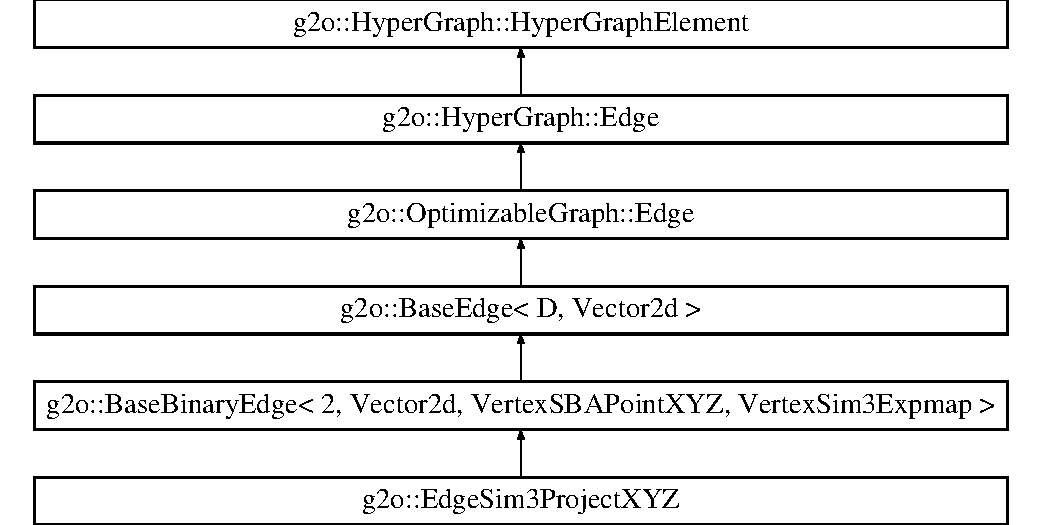
\includegraphics[height=6.000000cm]{classg2o_1_1_edge_sim3_project_x_y_z}
\end{center}
\end{figure}
\subsection*{Public Member Functions}
\begin{DoxyCompactItemize}
\item 
E\+I\+G\+E\+N\+\_\+\+M\+A\+K\+E\+\_\+\+A\+L\+I\+G\+N\+E\+D\+\_\+\+O\+P\+E\+R\+A\+T\+O\+R\+\_\+\+N\+EW \mbox{\hyperlink{classg2o_1_1_edge_sim3_project_x_y_z_a97beb2afff3d5b8bb6d19dccd032da14}{Edge\+Sim3\+Project\+X\+YZ}} ()
\item 
virtual bool \mbox{\hyperlink{classg2o_1_1_edge_sim3_project_x_y_z_aaf72b3f12f99f131e6c3395baf796fe9}{read}} (std\+::istream \&is)
\begin{DoxyCompactList}\small\item\em read the vertex from a stream, i.\+e., the internal state of the vertex \end{DoxyCompactList}\item 
virtual bool \mbox{\hyperlink{classg2o_1_1_edge_sim3_project_x_y_z_a9fe2dd1cff33b5c7d50d871b8e92bcc2}{write}} (std\+::ostream \&os) const
\begin{DoxyCompactList}\small\item\em write the vertex to a stream \end{DoxyCompactList}\item 
void \mbox{\hyperlink{classg2o_1_1_edge_sim3_project_x_y_z_ae821156265db463d49b9ac2166186274}{compute\+Error}} ()
\end{DoxyCompactItemize}
\subsection*{Additional Inherited Members}


\subsection{Constructor \& Destructor Documentation}
\mbox{\Hypertarget{classg2o_1_1_edge_sim3_project_x_y_z_a97beb2afff3d5b8bb6d19dccd032da14}\label{classg2o_1_1_edge_sim3_project_x_y_z_a97beb2afff3d5b8bb6d19dccd032da14}} 
\index{g2o\+::\+Edge\+Sim3\+Project\+X\+YZ@{g2o\+::\+Edge\+Sim3\+Project\+X\+YZ}!Edge\+Sim3\+Project\+X\+YZ@{Edge\+Sim3\+Project\+X\+YZ}}
\index{Edge\+Sim3\+Project\+X\+YZ@{Edge\+Sim3\+Project\+X\+YZ}!g2o\+::\+Edge\+Sim3\+Project\+X\+YZ@{g2o\+::\+Edge\+Sim3\+Project\+X\+YZ}}
\subsubsection{\texorpdfstring{Edge\+Sim3\+Project\+X\+Y\+Z()}{EdgeSim3ProjectXYZ()}}
{\footnotesize\ttfamily g2o\+::\+Edge\+Sim3\+Project\+X\+Y\+Z\+::\+Edge\+Sim3\+Project\+X\+YZ (\begin{DoxyParamCaption}{ }\end{DoxyParamCaption})}

Sim3\+Project\+X\+YZ 

\subsection{Member Function Documentation}
\mbox{\Hypertarget{classg2o_1_1_edge_sim3_project_x_y_z_ae821156265db463d49b9ac2166186274}\label{classg2o_1_1_edge_sim3_project_x_y_z_ae821156265db463d49b9ac2166186274}} 
\index{g2o\+::\+Edge\+Sim3\+Project\+X\+YZ@{g2o\+::\+Edge\+Sim3\+Project\+X\+YZ}!compute\+Error@{compute\+Error}}
\index{compute\+Error@{compute\+Error}!g2o\+::\+Edge\+Sim3\+Project\+X\+YZ@{g2o\+::\+Edge\+Sim3\+Project\+X\+YZ}}
\subsubsection{\texorpdfstring{compute\+Error()}{computeError()}}
{\footnotesize\ttfamily void g2o\+::\+Edge\+Sim3\+Project\+X\+Y\+Z\+::compute\+Error (\begin{DoxyParamCaption}{ }\end{DoxyParamCaption})\hspace{0.3cm}{\ttfamily [inline]}, {\ttfamily [virtual]}}



Implements \mbox{\hyperlink{classg2o_1_1_optimizable_graph_1_1_edge_a1e6d9f4128866982de5e11e03edd7775}{g2o\+::\+Optimizable\+Graph\+::\+Edge}}.

\mbox{\Hypertarget{classg2o_1_1_edge_sim3_project_x_y_z_aaf72b3f12f99f131e6c3395baf796fe9}\label{classg2o_1_1_edge_sim3_project_x_y_z_aaf72b3f12f99f131e6c3395baf796fe9}} 
\index{g2o\+::\+Edge\+Sim3\+Project\+X\+YZ@{g2o\+::\+Edge\+Sim3\+Project\+X\+YZ}!read@{read}}
\index{read@{read}!g2o\+::\+Edge\+Sim3\+Project\+X\+YZ@{g2o\+::\+Edge\+Sim3\+Project\+X\+YZ}}
\subsubsection{\texorpdfstring{read()}{read()}}
{\footnotesize\ttfamily bool g2o\+::\+Edge\+Sim3\+Project\+X\+Y\+Z\+::read (\begin{DoxyParamCaption}\item[{std\+::istream \&}]{is }\end{DoxyParamCaption})\hspace{0.3cm}{\ttfamily [virtual]}}



read the vertex from a stream, i.\+e., the internal state of the vertex 



Implements \mbox{\hyperlink{classg2o_1_1_optimizable_graph_1_1_edge_a30cf69b762a06aa35e796d8af71632b0}{g2o\+::\+Optimizable\+Graph\+::\+Edge}}.

\mbox{\Hypertarget{classg2o_1_1_edge_sim3_project_x_y_z_a9fe2dd1cff33b5c7d50d871b8e92bcc2}\label{classg2o_1_1_edge_sim3_project_x_y_z_a9fe2dd1cff33b5c7d50d871b8e92bcc2}} 
\index{g2o\+::\+Edge\+Sim3\+Project\+X\+YZ@{g2o\+::\+Edge\+Sim3\+Project\+X\+YZ}!write@{write}}
\index{write@{write}!g2o\+::\+Edge\+Sim3\+Project\+X\+YZ@{g2o\+::\+Edge\+Sim3\+Project\+X\+YZ}}
\subsubsection{\texorpdfstring{write()}{write()}}
{\footnotesize\ttfamily bool g2o\+::\+Edge\+Sim3\+Project\+X\+Y\+Z\+::write (\begin{DoxyParamCaption}\item[{std\+::ostream \&}]{os }\end{DoxyParamCaption}) const\hspace{0.3cm}{\ttfamily [virtual]}}



write the vertex to a stream 



Implements \mbox{\hyperlink{classg2o_1_1_optimizable_graph_1_1_edge_a804b9a2178249b9297c55b8fbbeda56e}{g2o\+::\+Optimizable\+Graph\+::\+Edge}}.



The documentation for this class was generated from the following files\+:\begin{DoxyCompactItemize}
\item 
D\+:/github/\+V\+S\+L\+A\+M/\+O\+R\+B\+S\+L\+A\+M2/\+O\+R\+B-\/\+S\+L\+A\+M2-\/master/\+Thirdparty/g2o/g2o/types/\mbox{\hyperlink{types__seven__dof__expmap_8h}{types\+\_\+seven\+\_\+dof\+\_\+expmap.\+h}}\item 
D\+:/github/\+V\+S\+L\+A\+M/\+O\+R\+B\+S\+L\+A\+M2/\+O\+R\+B-\/\+S\+L\+A\+M2-\/master/\+Thirdparty/g2o/g2o/types/\mbox{\hyperlink{types__seven__dof__expmap_8cpp}{types\+\_\+seven\+\_\+dof\+\_\+expmap.\+cpp}}\end{DoxyCompactItemize}

\hypertarget{classg2o_1_1_edge_stereo_s_e3_project_x_y_z}{}\section{g2o\+:\+:Edge\+Stereo\+S\+E3\+Project\+X\+YZ Class Reference}
\label{classg2o_1_1_edge_stereo_s_e3_project_x_y_z}\index{g2o\+::\+Edge\+Stereo\+S\+E3\+Project\+X\+YZ@{g2o\+::\+Edge\+Stereo\+S\+E3\+Project\+X\+YZ}}


N\+O\+TE uesd in Optimizer\+::\+Bundle\+Adjustment(), Optimizer\+::\+Local\+Bundle\+Adjustment()  




{\ttfamily \#include $<$types\+\_\+six\+\_\+dof\+\_\+expmap.\+h$>$}

Inheritance diagram for g2o\+:\+:Edge\+Stereo\+S\+E3\+Project\+X\+YZ\+:\begin{figure}[H]
\begin{center}
\leavevmode
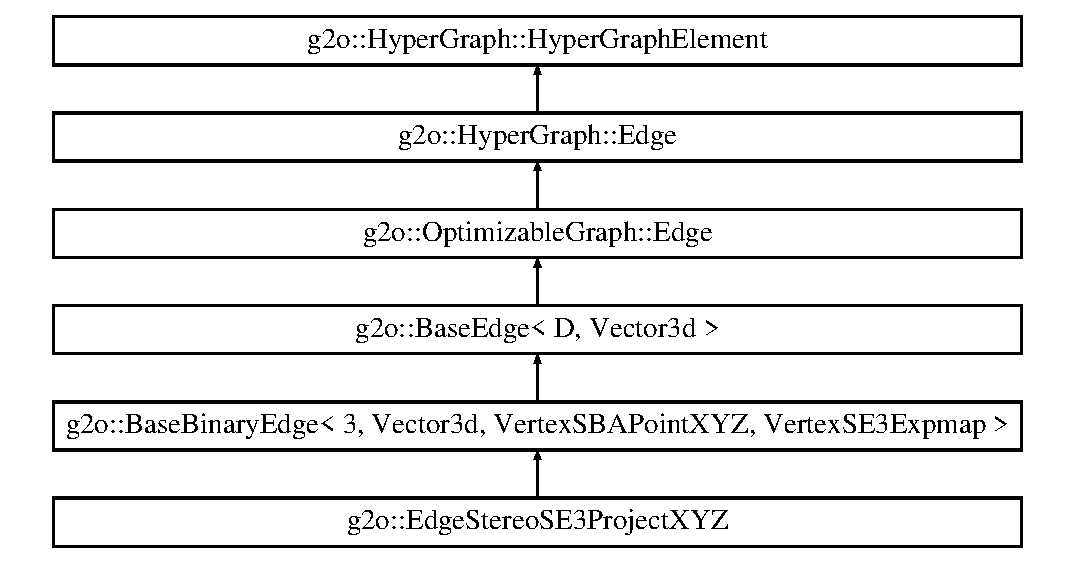
\includegraphics[height=6.000000cm]{classg2o_1_1_edge_stereo_s_e3_project_x_y_z}
\end{center}
\end{figure}
\subsection*{Public Member Functions}
\begin{DoxyCompactItemize}
\item 
E\+I\+G\+E\+N\+\_\+\+M\+A\+K\+E\+\_\+\+A\+L\+I\+G\+N\+E\+D\+\_\+\+O\+P\+E\+R\+A\+T\+O\+R\+\_\+\+N\+EW \mbox{\hyperlink{classg2o_1_1_edge_stereo_s_e3_project_x_y_z_a3a9c1b7c0b165f8c1c0690373481fea5}{Edge\+Stereo\+S\+E3\+Project\+X\+YZ}} ()
\item 
bool \mbox{\hyperlink{classg2o_1_1_edge_stereo_s_e3_project_x_y_z_a59cdc820a694379a73a26d51d948db0e}{read}} (std\+::istream \&is)
\begin{DoxyCompactList}\small\item\em read the vertex from a stream, i.\+e., the internal state of the vertex \end{DoxyCompactList}\item 
bool \mbox{\hyperlink{classg2o_1_1_edge_stereo_s_e3_project_x_y_z_ad6d441e7c5858b4efa8392f9ed96b2bf}{write}} (std\+::ostream \&os) const
\begin{DoxyCompactList}\small\item\em write the vertex to a stream \end{DoxyCompactList}\item 
void \mbox{\hyperlink{classg2o_1_1_edge_stereo_s_e3_project_x_y_z_ab60521439da10eabb13f23fe21fbe651}{compute\+Error}} ()
\item 
bool \mbox{\hyperlink{classg2o_1_1_edge_stereo_s_e3_project_x_y_z_ac176aff8aa08a73f52d7a0f5c3080d4d}{is\+Depth\+Positive}} ()
\item 
virtual void \mbox{\hyperlink{classg2o_1_1_edge_stereo_s_e3_project_x_y_z_aea04d86a304c6cb4e2a3f34b35166f30}{linearize\+Oplus}} ()
\item 
Vector3d \mbox{\hyperlink{classg2o_1_1_edge_stereo_s_e3_project_x_y_z_a5e1d2a6a247a6f9a95ccb7a59e3c543e}{cam\+\_\+project}} (const Vector3d \&trans\+\_\+xyz, const float \&\mbox{\hyperlink{classg2o_1_1_edge_stereo_s_e3_project_x_y_z_afc94291834aa40d18205e61ac802cbfc}{bf}}) const
\end{DoxyCompactItemize}
\subsection*{Public Attributes}
\begin{DoxyCompactItemize}
\item 
double \mbox{\hyperlink{classg2o_1_1_edge_stereo_s_e3_project_x_y_z_a4fe9f6810d2cc1b4489f84853445e85f}{fx}}
\item 
double \mbox{\hyperlink{classg2o_1_1_edge_stereo_s_e3_project_x_y_z_a4e5b984e84437680b1f589822b4c0700}{fy}}
\item 
double \mbox{\hyperlink{classg2o_1_1_edge_stereo_s_e3_project_x_y_z_a0d786d2f349f8d4991be5303ad2b3c5d}{cx}}
\item 
double \mbox{\hyperlink{classg2o_1_1_edge_stereo_s_e3_project_x_y_z_a220dd625eb7479cc1dabb92a96a6664c}{cy}}
\item 
double \mbox{\hyperlink{classg2o_1_1_edge_stereo_s_e3_project_x_y_z_afc94291834aa40d18205e61ac802cbfc}{bf}}
\begin{DoxyCompactList}\small\item\em 内参数,bf = b$\ast$f \end{DoxyCompactList}\end{DoxyCompactItemize}
\subsection*{Additional Inherited Members}


\subsection{Detailed Description}
N\+O\+TE uesd in Optimizer\+::\+Bundle\+Adjustment(), Optimizer\+::\+Local\+Bundle\+Adjustment() 

\subsection{Constructor \& Destructor Documentation}
\mbox{\Hypertarget{classg2o_1_1_edge_stereo_s_e3_project_x_y_z_a3a9c1b7c0b165f8c1c0690373481fea5}\label{classg2o_1_1_edge_stereo_s_e3_project_x_y_z_a3a9c1b7c0b165f8c1c0690373481fea5}} 
\index{g2o\+::\+Edge\+Stereo\+S\+E3\+Project\+X\+YZ@{g2o\+::\+Edge\+Stereo\+S\+E3\+Project\+X\+YZ}!Edge\+Stereo\+S\+E3\+Project\+X\+YZ@{Edge\+Stereo\+S\+E3\+Project\+X\+YZ}}
\index{Edge\+Stereo\+S\+E3\+Project\+X\+YZ@{Edge\+Stereo\+S\+E3\+Project\+X\+YZ}!g2o\+::\+Edge\+Stereo\+S\+E3\+Project\+X\+YZ@{g2o\+::\+Edge\+Stereo\+S\+E3\+Project\+X\+YZ}}
\subsubsection{\texorpdfstring{Edge\+Stereo\+S\+E3\+Project\+X\+Y\+Z()}{EdgeStereoSE3ProjectXYZ()}}
{\footnotesize\ttfamily g2o\+::\+Edge\+Stereo\+S\+E3\+Project\+X\+Y\+Z\+::\+Edge\+Stereo\+S\+E3\+Project\+X\+YZ (\begin{DoxyParamCaption}{ }\end{DoxyParamCaption})}



\subsection{Member Function Documentation}
\mbox{\Hypertarget{classg2o_1_1_edge_stereo_s_e3_project_x_y_z_a5e1d2a6a247a6f9a95ccb7a59e3c543e}\label{classg2o_1_1_edge_stereo_s_e3_project_x_y_z_a5e1d2a6a247a6f9a95ccb7a59e3c543e}} 
\index{g2o\+::\+Edge\+Stereo\+S\+E3\+Project\+X\+YZ@{g2o\+::\+Edge\+Stereo\+S\+E3\+Project\+X\+YZ}!cam\+\_\+project@{cam\+\_\+project}}
\index{cam\+\_\+project@{cam\+\_\+project}!g2o\+::\+Edge\+Stereo\+S\+E3\+Project\+X\+YZ@{g2o\+::\+Edge\+Stereo\+S\+E3\+Project\+X\+YZ}}
\subsubsection{\texorpdfstring{cam\+\_\+project()}{cam\_project()}}
{\footnotesize\ttfamily Vector3d g2o\+::\+Edge\+Stereo\+S\+E3\+Project\+X\+Y\+Z\+::cam\+\_\+project (\begin{DoxyParamCaption}\item[{const Vector3d \&}]{trans\+\_\+xyz,  }\item[{const float \&}]{bf }\end{DoxyParamCaption}) const}

将\+Xw投影到cam的图像坐标系 ~\newline
 $ ul = \frac{f_x X}{Z} + c_x $ ~\newline
 $ vl = \frac{f_y Y}{Z} + c_v $ ~\newline
 $ ur = \frac{f_x (X-b)}{Z} + c_x $ ~\newline

\begin{DoxyParams}{Parameters}
{\em trans\+\_\+xyz} & \mbox{[}X Y Z\mbox{]} \\
\hline
{\em bf} & bf = b$\ast$f \\
\hline
\end{DoxyParams}
\begin{DoxyReturn}{Returns}
\mbox{[}ul vl ur\mbox{]} 
\end{DoxyReturn}
\mbox{\Hypertarget{classg2o_1_1_edge_stereo_s_e3_project_x_y_z_ab60521439da10eabb13f23fe21fbe651}\label{classg2o_1_1_edge_stereo_s_e3_project_x_y_z_ab60521439da10eabb13f23fe21fbe651}} 
\index{g2o\+::\+Edge\+Stereo\+S\+E3\+Project\+X\+YZ@{g2o\+::\+Edge\+Stereo\+S\+E3\+Project\+X\+YZ}!compute\+Error@{compute\+Error}}
\index{compute\+Error@{compute\+Error}!g2o\+::\+Edge\+Stereo\+S\+E3\+Project\+X\+YZ@{g2o\+::\+Edge\+Stereo\+S\+E3\+Project\+X\+YZ}}
\subsubsection{\texorpdfstring{compute\+Error()}{computeError()}}
{\footnotesize\ttfamily void g2o\+::\+Edge\+Stereo\+S\+E3\+Project\+X\+Y\+Z\+::compute\+Error (\begin{DoxyParamCaption}{ }\end{DoxyParamCaption})\hspace{0.3cm}{\ttfamily [inline]}, {\ttfamily [virtual]}}

重投影误差 

Implements \mbox{\hyperlink{classg2o_1_1_optimizable_graph_1_1_edge_a1e6d9f4128866982de5e11e03edd7775}{g2o\+::\+Optimizable\+Graph\+::\+Edge}}.

\mbox{\Hypertarget{classg2o_1_1_edge_stereo_s_e3_project_x_y_z_ac176aff8aa08a73f52d7a0f5c3080d4d}\label{classg2o_1_1_edge_stereo_s_e3_project_x_y_z_ac176aff8aa08a73f52d7a0f5c3080d4d}} 
\index{g2o\+::\+Edge\+Stereo\+S\+E3\+Project\+X\+YZ@{g2o\+::\+Edge\+Stereo\+S\+E3\+Project\+X\+YZ}!is\+Depth\+Positive@{is\+Depth\+Positive}}
\index{is\+Depth\+Positive@{is\+Depth\+Positive}!g2o\+::\+Edge\+Stereo\+S\+E3\+Project\+X\+YZ@{g2o\+::\+Edge\+Stereo\+S\+E3\+Project\+X\+YZ}}
\subsubsection{\texorpdfstring{is\+Depth\+Positive()}{isDepthPositive()}}
{\footnotesize\ttfamily bool g2o\+::\+Edge\+Stereo\+S\+E3\+Project\+X\+Y\+Z\+::is\+Depth\+Positive (\begin{DoxyParamCaption}{ }\end{DoxyParamCaption})\hspace{0.3cm}{\ttfamily [inline]}}

检验 $ TX_w $的\+Z是否大于0 \begin{DoxyReturn}{Returns}
true if the depth is Positive 
\end{DoxyReturn}
\mbox{\Hypertarget{classg2o_1_1_edge_stereo_s_e3_project_x_y_z_aea04d86a304c6cb4e2a3f34b35166f30}\label{classg2o_1_1_edge_stereo_s_e3_project_x_y_z_aea04d86a304c6cb4e2a3f34b35166f30}} 
\index{g2o\+::\+Edge\+Stereo\+S\+E3\+Project\+X\+YZ@{g2o\+::\+Edge\+Stereo\+S\+E3\+Project\+X\+YZ}!linearize\+Oplus@{linearize\+Oplus}}
\index{linearize\+Oplus@{linearize\+Oplus}!g2o\+::\+Edge\+Stereo\+S\+E3\+Project\+X\+YZ@{g2o\+::\+Edge\+Stereo\+S\+E3\+Project\+X\+YZ}}
\subsubsection{\texorpdfstring{linearize\+Oplus()}{linearizeOplus()}}
{\footnotesize\ttfamily void g2o\+::\+Edge\+Stereo\+S\+E3\+Project\+X\+Y\+Z\+::linearize\+Oplus (\begin{DoxyParamCaption}{ }\end{DoxyParamCaption})\hspace{0.3cm}{\ttfamily [virtual]}}

误差函数对\mbox{[}X Y Z\mbox{]}和增量\mbox{[}w1 w2 w3 v1 v2 v3\mbox{]}求雅克比矩阵 ~\newline
 $Ji_{3\times3} = \frac{\partial [obs - \Pi(exp(\hat{\xi}) T X_w)]}{\partial X_w} $ ~\newline
 $Jj_{3\times6} = \frac{\partial [obs - \Pi(exp(\hat{\xi}) T X_w)]}{\partial \xi} $ ~\newline
\begin{DoxyNote}{Note}
\+\_\+jacobian\+Oplus\+Xi,\+\_\+jacobian\+Oplus\+Xj 
\end{DoxyNote}
\begin{DoxySeeAlso}{See also}
采用链式法则求解, 参考(注意以下参考的增量定义为\mbox{[}v1 v2 v3 w1 w2 w3\mbox{]})
\begin{DoxyItemize}
\item jlblanco2010geometry3d\+\_\+techrep.\+pdf p56 (A.\+2) 推荐
\item strasdat\+\_\+thesis\+\_\+2012.\+pdf p194 (B.\+4) 
\end{DoxyItemize}
\end{DoxySeeAlso}


Reimplemented from \mbox{\hyperlink{classg2o_1_1_base_binary_edge_af0fb8a693c8c7996fa65566e7263fbc4}{g2o\+::\+Base\+Binary\+Edge$<$ 3, Vector3d, Vertex\+S\+B\+A\+Point\+X\+Y\+Z, Vertex\+S\+E3\+Expmap $>$}}.

\mbox{\Hypertarget{classg2o_1_1_edge_stereo_s_e3_project_x_y_z_a59cdc820a694379a73a26d51d948db0e}\label{classg2o_1_1_edge_stereo_s_e3_project_x_y_z_a59cdc820a694379a73a26d51d948db0e}} 
\index{g2o\+::\+Edge\+Stereo\+S\+E3\+Project\+X\+YZ@{g2o\+::\+Edge\+Stereo\+S\+E3\+Project\+X\+YZ}!read@{read}}
\index{read@{read}!g2o\+::\+Edge\+Stereo\+S\+E3\+Project\+X\+YZ@{g2o\+::\+Edge\+Stereo\+S\+E3\+Project\+X\+YZ}}
\subsubsection{\texorpdfstring{read()}{read()}}
{\footnotesize\ttfamily bool g2o\+::\+Edge\+Stereo\+S\+E3\+Project\+X\+Y\+Z\+::read (\begin{DoxyParamCaption}\item[{std\+::istream \&}]{is }\end{DoxyParamCaption})\hspace{0.3cm}{\ttfamily [virtual]}}



read the vertex from a stream, i.\+e., the internal state of the vertex 



Implements \mbox{\hyperlink{classg2o_1_1_optimizable_graph_1_1_edge_a30cf69b762a06aa35e796d8af71632b0}{g2o\+::\+Optimizable\+Graph\+::\+Edge}}.

\mbox{\Hypertarget{classg2o_1_1_edge_stereo_s_e3_project_x_y_z_ad6d441e7c5858b4efa8392f9ed96b2bf}\label{classg2o_1_1_edge_stereo_s_e3_project_x_y_z_ad6d441e7c5858b4efa8392f9ed96b2bf}} 
\index{g2o\+::\+Edge\+Stereo\+S\+E3\+Project\+X\+YZ@{g2o\+::\+Edge\+Stereo\+S\+E3\+Project\+X\+YZ}!write@{write}}
\index{write@{write}!g2o\+::\+Edge\+Stereo\+S\+E3\+Project\+X\+YZ@{g2o\+::\+Edge\+Stereo\+S\+E3\+Project\+X\+YZ}}
\subsubsection{\texorpdfstring{write()}{write()}}
{\footnotesize\ttfamily bool g2o\+::\+Edge\+Stereo\+S\+E3\+Project\+X\+Y\+Z\+::write (\begin{DoxyParamCaption}\item[{std\+::ostream \&}]{os }\end{DoxyParamCaption}) const\hspace{0.3cm}{\ttfamily [virtual]}}



write the vertex to a stream 



Implements \mbox{\hyperlink{classg2o_1_1_optimizable_graph_1_1_edge_a804b9a2178249b9297c55b8fbbeda56e}{g2o\+::\+Optimizable\+Graph\+::\+Edge}}.



\subsection{Member Data Documentation}
\mbox{\Hypertarget{classg2o_1_1_edge_stereo_s_e3_project_x_y_z_afc94291834aa40d18205e61ac802cbfc}\label{classg2o_1_1_edge_stereo_s_e3_project_x_y_z_afc94291834aa40d18205e61ac802cbfc}} 
\index{g2o\+::\+Edge\+Stereo\+S\+E3\+Project\+X\+YZ@{g2o\+::\+Edge\+Stereo\+S\+E3\+Project\+X\+YZ}!bf@{bf}}
\index{bf@{bf}!g2o\+::\+Edge\+Stereo\+S\+E3\+Project\+X\+YZ@{g2o\+::\+Edge\+Stereo\+S\+E3\+Project\+X\+YZ}}
\subsubsection{\texorpdfstring{bf}{bf}}
{\footnotesize\ttfamily double g2o\+::\+Edge\+Stereo\+S\+E3\+Project\+X\+Y\+Z\+::bf}



内参数,bf = b$\ast$f 

\mbox{\Hypertarget{classg2o_1_1_edge_stereo_s_e3_project_x_y_z_a0d786d2f349f8d4991be5303ad2b3c5d}\label{classg2o_1_1_edge_stereo_s_e3_project_x_y_z_a0d786d2f349f8d4991be5303ad2b3c5d}} 
\index{g2o\+::\+Edge\+Stereo\+S\+E3\+Project\+X\+YZ@{g2o\+::\+Edge\+Stereo\+S\+E3\+Project\+X\+YZ}!cx@{cx}}
\index{cx@{cx}!g2o\+::\+Edge\+Stereo\+S\+E3\+Project\+X\+YZ@{g2o\+::\+Edge\+Stereo\+S\+E3\+Project\+X\+YZ}}
\subsubsection{\texorpdfstring{cx}{cx}}
{\footnotesize\ttfamily double g2o\+::\+Edge\+Stereo\+S\+E3\+Project\+X\+Y\+Z\+::cx}

\mbox{\Hypertarget{classg2o_1_1_edge_stereo_s_e3_project_x_y_z_a220dd625eb7479cc1dabb92a96a6664c}\label{classg2o_1_1_edge_stereo_s_e3_project_x_y_z_a220dd625eb7479cc1dabb92a96a6664c}} 
\index{g2o\+::\+Edge\+Stereo\+S\+E3\+Project\+X\+YZ@{g2o\+::\+Edge\+Stereo\+S\+E3\+Project\+X\+YZ}!cy@{cy}}
\index{cy@{cy}!g2o\+::\+Edge\+Stereo\+S\+E3\+Project\+X\+YZ@{g2o\+::\+Edge\+Stereo\+S\+E3\+Project\+X\+YZ}}
\subsubsection{\texorpdfstring{cy}{cy}}
{\footnotesize\ttfamily double g2o\+::\+Edge\+Stereo\+S\+E3\+Project\+X\+Y\+Z\+::cy}

\mbox{\Hypertarget{classg2o_1_1_edge_stereo_s_e3_project_x_y_z_a4fe9f6810d2cc1b4489f84853445e85f}\label{classg2o_1_1_edge_stereo_s_e3_project_x_y_z_a4fe9f6810d2cc1b4489f84853445e85f}} 
\index{g2o\+::\+Edge\+Stereo\+S\+E3\+Project\+X\+YZ@{g2o\+::\+Edge\+Stereo\+S\+E3\+Project\+X\+YZ}!fx@{fx}}
\index{fx@{fx}!g2o\+::\+Edge\+Stereo\+S\+E3\+Project\+X\+YZ@{g2o\+::\+Edge\+Stereo\+S\+E3\+Project\+X\+YZ}}
\subsubsection{\texorpdfstring{fx}{fx}}
{\footnotesize\ttfamily double g2o\+::\+Edge\+Stereo\+S\+E3\+Project\+X\+Y\+Z\+::fx}

\mbox{\Hypertarget{classg2o_1_1_edge_stereo_s_e3_project_x_y_z_a4e5b984e84437680b1f589822b4c0700}\label{classg2o_1_1_edge_stereo_s_e3_project_x_y_z_a4e5b984e84437680b1f589822b4c0700}} 
\index{g2o\+::\+Edge\+Stereo\+S\+E3\+Project\+X\+YZ@{g2o\+::\+Edge\+Stereo\+S\+E3\+Project\+X\+YZ}!fy@{fy}}
\index{fy@{fy}!g2o\+::\+Edge\+Stereo\+S\+E3\+Project\+X\+YZ@{g2o\+::\+Edge\+Stereo\+S\+E3\+Project\+X\+YZ}}
\subsubsection{\texorpdfstring{fy}{fy}}
{\footnotesize\ttfamily double g2o\+::\+Edge\+Stereo\+S\+E3\+Project\+X\+Y\+Z\+::fy}



The documentation for this class was generated from the following files\+:\begin{DoxyCompactItemize}
\item 
D\+:/github/\+V\+S\+L\+A\+M/\+O\+R\+B\+S\+L\+A\+M2/\+O\+R\+B-\/\+S\+L\+A\+M2-\/master/\+Thirdparty/g2o/g2o/types/\mbox{\hyperlink{types__six__dof__expmap_8h}{types\+\_\+six\+\_\+dof\+\_\+expmap.\+h}}\item 
D\+:/github/\+V\+S\+L\+A\+M/\+O\+R\+B\+S\+L\+A\+M2/\+O\+R\+B-\/\+S\+L\+A\+M2-\/master/\+Thirdparty/g2o/g2o/types/\mbox{\hyperlink{types__six__dof__expmap_8cpp}{types\+\_\+six\+\_\+dof\+\_\+expmap.\+cpp}}\end{DoxyCompactItemize}

\hypertarget{classg2o_1_1_edge_stereo_s_e3_project_x_y_z_only_pose}{}\section{g2o\+:\+:Edge\+Stereo\+S\+E3\+Project\+X\+Y\+Z\+Only\+Pose Class Reference}
\label{classg2o_1_1_edge_stereo_s_e3_project_x_y_z_only_pose}\index{g2o\+::\+Edge\+Stereo\+S\+E3\+Project\+X\+Y\+Z\+Only\+Pose@{g2o\+::\+Edge\+Stereo\+S\+E3\+Project\+X\+Y\+Z\+Only\+Pose}}


N\+O\+TE uesd in Optimizer\+::\+Pose\+Optimization()  




{\ttfamily \#include $<$types\+\_\+six\+\_\+dof\+\_\+expmap.\+h$>$}

Inheritance diagram for g2o\+:\+:Edge\+Stereo\+S\+E3\+Project\+X\+Y\+Z\+Only\+Pose\+:\begin{figure}[H]
\begin{center}
\leavevmode
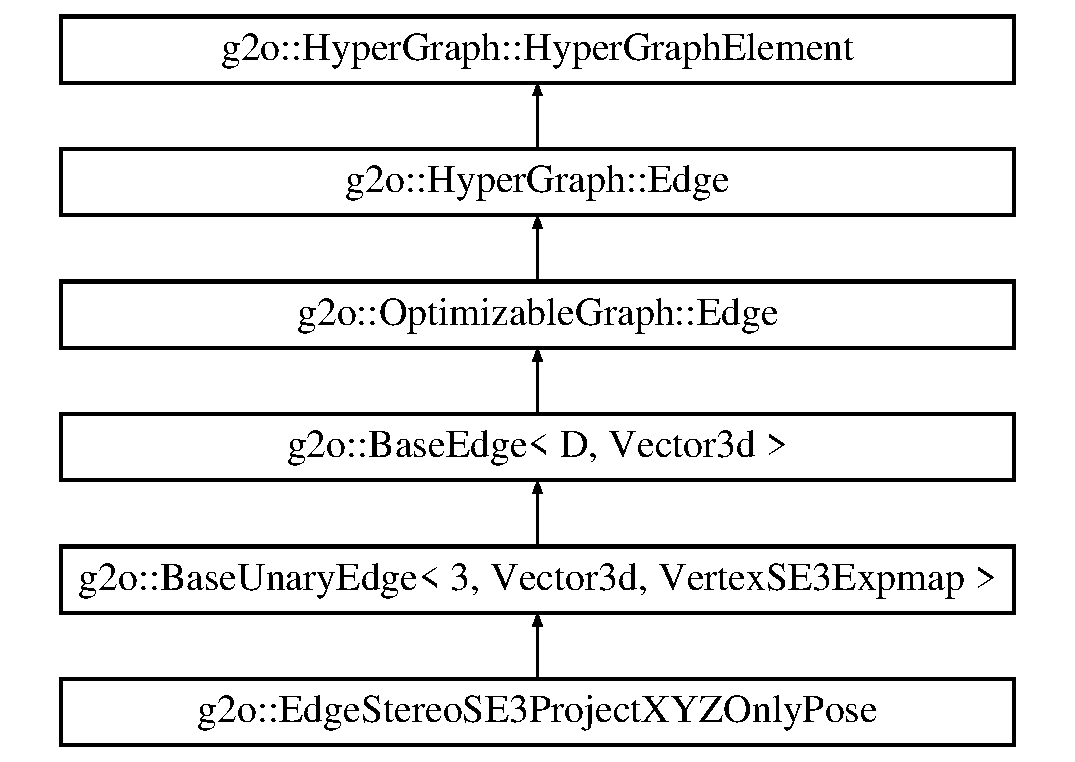
\includegraphics[height=6.000000cm]{classg2o_1_1_edge_stereo_s_e3_project_x_y_z_only_pose}
\end{center}
\end{figure}
\subsection*{Public Member Functions}
\begin{DoxyCompactItemize}
\item 
E\+I\+G\+E\+N\+\_\+\+M\+A\+K\+E\+\_\+\+A\+L\+I\+G\+N\+E\+D\+\_\+\+O\+P\+E\+R\+A\+T\+O\+R\+\_\+\+N\+EW \mbox{\hyperlink{classg2o_1_1_edge_stereo_s_e3_project_x_y_z_only_pose_a083a4f79a0ac5ff0deab0c9e8e9c9907}{Edge\+Stereo\+S\+E3\+Project\+X\+Y\+Z\+Only\+Pose}} ()
\item 
bool \mbox{\hyperlink{classg2o_1_1_edge_stereo_s_e3_project_x_y_z_only_pose_ae199c5428259a7d50e9897029ae9fd70}{read}} (std\+::istream \&is)
\begin{DoxyCompactList}\small\item\em read the vertex from a stream, i.\+e., the internal state of the vertex \end{DoxyCompactList}\item 
bool \mbox{\hyperlink{classg2o_1_1_edge_stereo_s_e3_project_x_y_z_only_pose_a8e7cb830d9d0d9675733294b692bd3d8}{write}} (std\+::ostream \&os) const
\begin{DoxyCompactList}\small\item\em write the vertex to a stream \end{DoxyCompactList}\item 
void \mbox{\hyperlink{classg2o_1_1_edge_stereo_s_e3_project_x_y_z_only_pose_af6fd2fdbdc9b4a6bcf21303ff3b8ea83}{compute\+Error}} ()
\item 
bool \mbox{\hyperlink{classg2o_1_1_edge_stereo_s_e3_project_x_y_z_only_pose_a5155075418c27ce8a1387d739ccbdf26}{is\+Depth\+Positive}} ()
\item 
virtual void \mbox{\hyperlink{classg2o_1_1_edge_stereo_s_e3_project_x_y_z_only_pose_a0b2b815e8ae331276f33be374dcc1897}{linearize\+Oplus}} ()
\item 
Vector3d \mbox{\hyperlink{classg2o_1_1_edge_stereo_s_e3_project_x_y_z_only_pose_a6545d86fffb69bb1aa71350fe6d70846}{cam\+\_\+project}} (const Vector3d \&trans\+\_\+xyz) const
\end{DoxyCompactItemize}
\subsection*{Public Attributes}
\begin{DoxyCompactItemize}
\item 
Vector3d \mbox{\hyperlink{classg2o_1_1_edge_stereo_s_e3_project_x_y_z_only_pose_aa7c861f93edd02d3ef763c0e706cf496}{Xw}}
\begin{DoxyCompactList}\small\item\em Map\+Point在世界坐标系的位置 \end{DoxyCompactList}\item 
double \mbox{\hyperlink{classg2o_1_1_edge_stereo_s_e3_project_x_y_z_only_pose_aebf839be304521edf2f3cb445b3bf618}{fx}}
\item 
double \mbox{\hyperlink{classg2o_1_1_edge_stereo_s_e3_project_x_y_z_only_pose_a7f779153148f1eb403ab6f2984b47eec}{fy}}
\item 
double \mbox{\hyperlink{classg2o_1_1_edge_stereo_s_e3_project_x_y_z_only_pose_a7b0f52c3f2931706838373ca7d4513a7}{cx}}
\item 
double \mbox{\hyperlink{classg2o_1_1_edge_stereo_s_e3_project_x_y_z_only_pose_a95e79aa1ef43455cd6de7ccced2fc1e8}{cy}}
\item 
double \mbox{\hyperlink{classg2o_1_1_edge_stereo_s_e3_project_x_y_z_only_pose_a831d3e73bf61102622a7ac6af0475e7b}{bf}}
\begin{DoxyCompactList}\small\item\em 内参数,bf = b$\ast$f \end{DoxyCompactList}\end{DoxyCompactItemize}
\subsection*{Additional Inherited Members}


\subsection{Detailed Description}
N\+O\+TE uesd in Optimizer\+::\+Pose\+Optimization() 

\subsection{Constructor \& Destructor Documentation}
\mbox{\Hypertarget{classg2o_1_1_edge_stereo_s_e3_project_x_y_z_only_pose_a083a4f79a0ac5ff0deab0c9e8e9c9907}\label{classg2o_1_1_edge_stereo_s_e3_project_x_y_z_only_pose_a083a4f79a0ac5ff0deab0c9e8e9c9907}} 
\index{g2o\+::\+Edge\+Stereo\+S\+E3\+Project\+X\+Y\+Z\+Only\+Pose@{g2o\+::\+Edge\+Stereo\+S\+E3\+Project\+X\+Y\+Z\+Only\+Pose}!Edge\+Stereo\+S\+E3\+Project\+X\+Y\+Z\+Only\+Pose@{Edge\+Stereo\+S\+E3\+Project\+X\+Y\+Z\+Only\+Pose}}
\index{Edge\+Stereo\+S\+E3\+Project\+X\+Y\+Z\+Only\+Pose@{Edge\+Stereo\+S\+E3\+Project\+X\+Y\+Z\+Only\+Pose}!g2o\+::\+Edge\+Stereo\+S\+E3\+Project\+X\+Y\+Z\+Only\+Pose@{g2o\+::\+Edge\+Stereo\+S\+E3\+Project\+X\+Y\+Z\+Only\+Pose}}
\subsubsection{\texorpdfstring{Edge\+Stereo\+S\+E3\+Project\+X\+Y\+Z\+Only\+Pose()}{EdgeStereoSE3ProjectXYZOnlyPose()}}
{\footnotesize\ttfamily E\+I\+G\+E\+N\+\_\+\+M\+A\+K\+E\+\_\+\+A\+L\+I\+G\+N\+E\+D\+\_\+\+O\+P\+E\+R\+A\+T\+O\+R\+\_\+\+N\+EW g2o\+::\+Edge\+Stereo\+S\+E3\+Project\+X\+Y\+Z\+Only\+Pose\+::\+Edge\+Stereo\+S\+E3\+Project\+X\+Y\+Z\+Only\+Pose (\begin{DoxyParamCaption}{ }\end{DoxyParamCaption})\hspace{0.3cm}{\ttfamily [inline]}}



\subsection{Member Function Documentation}
\mbox{\Hypertarget{classg2o_1_1_edge_stereo_s_e3_project_x_y_z_only_pose_a6545d86fffb69bb1aa71350fe6d70846}\label{classg2o_1_1_edge_stereo_s_e3_project_x_y_z_only_pose_a6545d86fffb69bb1aa71350fe6d70846}} 
\index{g2o\+::\+Edge\+Stereo\+S\+E3\+Project\+X\+Y\+Z\+Only\+Pose@{g2o\+::\+Edge\+Stereo\+S\+E3\+Project\+X\+Y\+Z\+Only\+Pose}!cam\+\_\+project@{cam\+\_\+project}}
\index{cam\+\_\+project@{cam\+\_\+project}!g2o\+::\+Edge\+Stereo\+S\+E3\+Project\+X\+Y\+Z\+Only\+Pose@{g2o\+::\+Edge\+Stereo\+S\+E3\+Project\+X\+Y\+Z\+Only\+Pose}}
\subsubsection{\texorpdfstring{cam\+\_\+project()}{cam\_project()}}
{\footnotesize\ttfamily Vector3d g2o\+::\+Edge\+Stereo\+S\+E3\+Project\+X\+Y\+Z\+Only\+Pose\+::cam\+\_\+project (\begin{DoxyParamCaption}\item[{const Vector3d \&}]{trans\+\_\+xyz }\end{DoxyParamCaption}) const}

将\+Xw投影到cam的图像坐标系 ~\newline
 $ ul = \frac{f_x X}{Z} + c_x $ ~\newline
 $ vl = \frac{f_y Y}{Z} + c_v $ ~\newline
 $ ur = \frac{f_x (X-b)}{Z} + c_x $ ~\newline

\begin{DoxyParams}{Parameters}
{\em trans\+\_\+xyz} & \mbox{[}X Y Z\mbox{]} \\
\hline
\end{DoxyParams}
\begin{DoxyReturn}{Returns}
\mbox{[}ul vl ur\mbox{]} 
\end{DoxyReturn}
\mbox{\Hypertarget{classg2o_1_1_edge_stereo_s_e3_project_x_y_z_only_pose_af6fd2fdbdc9b4a6bcf21303ff3b8ea83}\label{classg2o_1_1_edge_stereo_s_e3_project_x_y_z_only_pose_af6fd2fdbdc9b4a6bcf21303ff3b8ea83}} 
\index{g2o\+::\+Edge\+Stereo\+S\+E3\+Project\+X\+Y\+Z\+Only\+Pose@{g2o\+::\+Edge\+Stereo\+S\+E3\+Project\+X\+Y\+Z\+Only\+Pose}!compute\+Error@{compute\+Error}}
\index{compute\+Error@{compute\+Error}!g2o\+::\+Edge\+Stereo\+S\+E3\+Project\+X\+Y\+Z\+Only\+Pose@{g2o\+::\+Edge\+Stereo\+S\+E3\+Project\+X\+Y\+Z\+Only\+Pose}}
\subsubsection{\texorpdfstring{compute\+Error()}{computeError()}}
{\footnotesize\ttfamily void g2o\+::\+Edge\+Stereo\+S\+E3\+Project\+X\+Y\+Z\+Only\+Pose\+::compute\+Error (\begin{DoxyParamCaption}{ }\end{DoxyParamCaption})\hspace{0.3cm}{\ttfamily [inline]}, {\ttfamily [virtual]}}

重投影误差 

Implements \mbox{\hyperlink{classg2o_1_1_optimizable_graph_1_1_edge_a1e6d9f4128866982de5e11e03edd7775}{g2o\+::\+Optimizable\+Graph\+::\+Edge}}.

\mbox{\Hypertarget{classg2o_1_1_edge_stereo_s_e3_project_x_y_z_only_pose_a5155075418c27ce8a1387d739ccbdf26}\label{classg2o_1_1_edge_stereo_s_e3_project_x_y_z_only_pose_a5155075418c27ce8a1387d739ccbdf26}} 
\index{g2o\+::\+Edge\+Stereo\+S\+E3\+Project\+X\+Y\+Z\+Only\+Pose@{g2o\+::\+Edge\+Stereo\+S\+E3\+Project\+X\+Y\+Z\+Only\+Pose}!is\+Depth\+Positive@{is\+Depth\+Positive}}
\index{is\+Depth\+Positive@{is\+Depth\+Positive}!g2o\+::\+Edge\+Stereo\+S\+E3\+Project\+X\+Y\+Z\+Only\+Pose@{g2o\+::\+Edge\+Stereo\+S\+E3\+Project\+X\+Y\+Z\+Only\+Pose}}
\subsubsection{\texorpdfstring{is\+Depth\+Positive()}{isDepthPositive()}}
{\footnotesize\ttfamily bool g2o\+::\+Edge\+Stereo\+S\+E3\+Project\+X\+Y\+Z\+Only\+Pose\+::is\+Depth\+Positive (\begin{DoxyParamCaption}{ }\end{DoxyParamCaption})\hspace{0.3cm}{\ttfamily [inline]}}

检验 $ TX_w $的\+Z是否大于0 \begin{DoxyReturn}{Returns}
true if the depth is Positive 
\end{DoxyReturn}
\mbox{\Hypertarget{classg2o_1_1_edge_stereo_s_e3_project_x_y_z_only_pose_a0b2b815e8ae331276f33be374dcc1897}\label{classg2o_1_1_edge_stereo_s_e3_project_x_y_z_only_pose_a0b2b815e8ae331276f33be374dcc1897}} 
\index{g2o\+::\+Edge\+Stereo\+S\+E3\+Project\+X\+Y\+Z\+Only\+Pose@{g2o\+::\+Edge\+Stereo\+S\+E3\+Project\+X\+Y\+Z\+Only\+Pose}!linearize\+Oplus@{linearize\+Oplus}}
\index{linearize\+Oplus@{linearize\+Oplus}!g2o\+::\+Edge\+Stereo\+S\+E3\+Project\+X\+Y\+Z\+Only\+Pose@{g2o\+::\+Edge\+Stereo\+S\+E3\+Project\+X\+Y\+Z\+Only\+Pose}}
\subsubsection{\texorpdfstring{linearize\+Oplus()}{linearizeOplus()}}
{\footnotesize\ttfamily void g2o\+::\+Edge\+Stereo\+S\+E3\+Project\+X\+Y\+Z\+Only\+Pose\+::linearize\+Oplus (\begin{DoxyParamCaption}{ }\end{DoxyParamCaption})\hspace{0.3cm}{\ttfamily [virtual]}}

误差函数对增量\mbox{[}w1 w2 w3 v1 v2 v3\mbox{]}求雅克比矩阵 $J_{3\times6}$ $ = \frac{\partial [obs - \Pi(exp(\hat{\xi}) T X_w)]}{\partial \xi} $ \begin{DoxyNote}{Note}
\+\_\+jacobian\+Oplus\+Xi,雅可比矩阵的正负号没有关系 
\end{DoxyNote}
\begin{DoxySeeAlso}{See also}
采用链式法则求解, 参考(注意以下参考的增量定义为\mbox{[}v1 v2 v3 w1 w2 w3\mbox{]})
\begin{DoxyItemize}
\item jlblanco2010geometry3d\+\_\+techrep.\+pdf p56 (A.\+2) 推荐
\item strasdat\+\_\+thesis\+\_\+2012.\+pdf p194 (B.\+4) 
\end{DoxyItemize}
\end{DoxySeeAlso}


Reimplemented from \mbox{\hyperlink{classg2o_1_1_base_unary_edge_a367f19b903938faf6e89dd1b0e4e722b}{g2o\+::\+Base\+Unary\+Edge$<$ 3, Vector3d, Vertex\+S\+E3\+Expmap $>$}}.

\mbox{\Hypertarget{classg2o_1_1_edge_stereo_s_e3_project_x_y_z_only_pose_ae199c5428259a7d50e9897029ae9fd70}\label{classg2o_1_1_edge_stereo_s_e3_project_x_y_z_only_pose_ae199c5428259a7d50e9897029ae9fd70}} 
\index{g2o\+::\+Edge\+Stereo\+S\+E3\+Project\+X\+Y\+Z\+Only\+Pose@{g2o\+::\+Edge\+Stereo\+S\+E3\+Project\+X\+Y\+Z\+Only\+Pose}!read@{read}}
\index{read@{read}!g2o\+::\+Edge\+Stereo\+S\+E3\+Project\+X\+Y\+Z\+Only\+Pose@{g2o\+::\+Edge\+Stereo\+S\+E3\+Project\+X\+Y\+Z\+Only\+Pose}}
\subsubsection{\texorpdfstring{read()}{read()}}
{\footnotesize\ttfamily bool g2o\+::\+Edge\+Stereo\+S\+E3\+Project\+X\+Y\+Z\+Only\+Pose\+::read (\begin{DoxyParamCaption}\item[{std\+::istream \&}]{is }\end{DoxyParamCaption})\hspace{0.3cm}{\ttfamily [virtual]}}



read the vertex from a stream, i.\+e., the internal state of the vertex 



Implements \mbox{\hyperlink{classg2o_1_1_optimizable_graph_1_1_edge_a30cf69b762a06aa35e796d8af71632b0}{g2o\+::\+Optimizable\+Graph\+::\+Edge}}.

\mbox{\Hypertarget{classg2o_1_1_edge_stereo_s_e3_project_x_y_z_only_pose_a8e7cb830d9d0d9675733294b692bd3d8}\label{classg2o_1_1_edge_stereo_s_e3_project_x_y_z_only_pose_a8e7cb830d9d0d9675733294b692bd3d8}} 
\index{g2o\+::\+Edge\+Stereo\+S\+E3\+Project\+X\+Y\+Z\+Only\+Pose@{g2o\+::\+Edge\+Stereo\+S\+E3\+Project\+X\+Y\+Z\+Only\+Pose}!write@{write}}
\index{write@{write}!g2o\+::\+Edge\+Stereo\+S\+E3\+Project\+X\+Y\+Z\+Only\+Pose@{g2o\+::\+Edge\+Stereo\+S\+E3\+Project\+X\+Y\+Z\+Only\+Pose}}
\subsubsection{\texorpdfstring{write()}{write()}}
{\footnotesize\ttfamily bool g2o\+::\+Edge\+Stereo\+S\+E3\+Project\+X\+Y\+Z\+Only\+Pose\+::write (\begin{DoxyParamCaption}\item[{std\+::ostream \&}]{os }\end{DoxyParamCaption}) const\hspace{0.3cm}{\ttfamily [virtual]}}



write the vertex to a stream 



Implements \mbox{\hyperlink{classg2o_1_1_optimizable_graph_1_1_edge_a804b9a2178249b9297c55b8fbbeda56e}{g2o\+::\+Optimizable\+Graph\+::\+Edge}}.



\subsection{Member Data Documentation}
\mbox{\Hypertarget{classg2o_1_1_edge_stereo_s_e3_project_x_y_z_only_pose_a831d3e73bf61102622a7ac6af0475e7b}\label{classg2o_1_1_edge_stereo_s_e3_project_x_y_z_only_pose_a831d3e73bf61102622a7ac6af0475e7b}} 
\index{g2o\+::\+Edge\+Stereo\+S\+E3\+Project\+X\+Y\+Z\+Only\+Pose@{g2o\+::\+Edge\+Stereo\+S\+E3\+Project\+X\+Y\+Z\+Only\+Pose}!bf@{bf}}
\index{bf@{bf}!g2o\+::\+Edge\+Stereo\+S\+E3\+Project\+X\+Y\+Z\+Only\+Pose@{g2o\+::\+Edge\+Stereo\+S\+E3\+Project\+X\+Y\+Z\+Only\+Pose}}
\subsubsection{\texorpdfstring{bf}{bf}}
{\footnotesize\ttfamily double g2o\+::\+Edge\+Stereo\+S\+E3\+Project\+X\+Y\+Z\+Only\+Pose\+::bf}



内参数,bf = b$\ast$f 

\mbox{\Hypertarget{classg2o_1_1_edge_stereo_s_e3_project_x_y_z_only_pose_a7b0f52c3f2931706838373ca7d4513a7}\label{classg2o_1_1_edge_stereo_s_e3_project_x_y_z_only_pose_a7b0f52c3f2931706838373ca7d4513a7}} 
\index{g2o\+::\+Edge\+Stereo\+S\+E3\+Project\+X\+Y\+Z\+Only\+Pose@{g2o\+::\+Edge\+Stereo\+S\+E3\+Project\+X\+Y\+Z\+Only\+Pose}!cx@{cx}}
\index{cx@{cx}!g2o\+::\+Edge\+Stereo\+S\+E3\+Project\+X\+Y\+Z\+Only\+Pose@{g2o\+::\+Edge\+Stereo\+S\+E3\+Project\+X\+Y\+Z\+Only\+Pose}}
\subsubsection{\texorpdfstring{cx}{cx}}
{\footnotesize\ttfamily double g2o\+::\+Edge\+Stereo\+S\+E3\+Project\+X\+Y\+Z\+Only\+Pose\+::cx}

\mbox{\Hypertarget{classg2o_1_1_edge_stereo_s_e3_project_x_y_z_only_pose_a95e79aa1ef43455cd6de7ccced2fc1e8}\label{classg2o_1_1_edge_stereo_s_e3_project_x_y_z_only_pose_a95e79aa1ef43455cd6de7ccced2fc1e8}} 
\index{g2o\+::\+Edge\+Stereo\+S\+E3\+Project\+X\+Y\+Z\+Only\+Pose@{g2o\+::\+Edge\+Stereo\+S\+E3\+Project\+X\+Y\+Z\+Only\+Pose}!cy@{cy}}
\index{cy@{cy}!g2o\+::\+Edge\+Stereo\+S\+E3\+Project\+X\+Y\+Z\+Only\+Pose@{g2o\+::\+Edge\+Stereo\+S\+E3\+Project\+X\+Y\+Z\+Only\+Pose}}
\subsubsection{\texorpdfstring{cy}{cy}}
{\footnotesize\ttfamily double g2o\+::\+Edge\+Stereo\+S\+E3\+Project\+X\+Y\+Z\+Only\+Pose\+::cy}

\mbox{\Hypertarget{classg2o_1_1_edge_stereo_s_e3_project_x_y_z_only_pose_aebf839be304521edf2f3cb445b3bf618}\label{classg2o_1_1_edge_stereo_s_e3_project_x_y_z_only_pose_aebf839be304521edf2f3cb445b3bf618}} 
\index{g2o\+::\+Edge\+Stereo\+S\+E3\+Project\+X\+Y\+Z\+Only\+Pose@{g2o\+::\+Edge\+Stereo\+S\+E3\+Project\+X\+Y\+Z\+Only\+Pose}!fx@{fx}}
\index{fx@{fx}!g2o\+::\+Edge\+Stereo\+S\+E3\+Project\+X\+Y\+Z\+Only\+Pose@{g2o\+::\+Edge\+Stereo\+S\+E3\+Project\+X\+Y\+Z\+Only\+Pose}}
\subsubsection{\texorpdfstring{fx}{fx}}
{\footnotesize\ttfamily double g2o\+::\+Edge\+Stereo\+S\+E3\+Project\+X\+Y\+Z\+Only\+Pose\+::fx}

\mbox{\Hypertarget{classg2o_1_1_edge_stereo_s_e3_project_x_y_z_only_pose_a7f779153148f1eb403ab6f2984b47eec}\label{classg2o_1_1_edge_stereo_s_e3_project_x_y_z_only_pose_a7f779153148f1eb403ab6f2984b47eec}} 
\index{g2o\+::\+Edge\+Stereo\+S\+E3\+Project\+X\+Y\+Z\+Only\+Pose@{g2o\+::\+Edge\+Stereo\+S\+E3\+Project\+X\+Y\+Z\+Only\+Pose}!fy@{fy}}
\index{fy@{fy}!g2o\+::\+Edge\+Stereo\+S\+E3\+Project\+X\+Y\+Z\+Only\+Pose@{g2o\+::\+Edge\+Stereo\+S\+E3\+Project\+X\+Y\+Z\+Only\+Pose}}
\subsubsection{\texorpdfstring{fy}{fy}}
{\footnotesize\ttfamily double g2o\+::\+Edge\+Stereo\+S\+E3\+Project\+X\+Y\+Z\+Only\+Pose\+::fy}

\mbox{\Hypertarget{classg2o_1_1_edge_stereo_s_e3_project_x_y_z_only_pose_aa7c861f93edd02d3ef763c0e706cf496}\label{classg2o_1_1_edge_stereo_s_e3_project_x_y_z_only_pose_aa7c861f93edd02d3ef763c0e706cf496}} 
\index{g2o\+::\+Edge\+Stereo\+S\+E3\+Project\+X\+Y\+Z\+Only\+Pose@{g2o\+::\+Edge\+Stereo\+S\+E3\+Project\+X\+Y\+Z\+Only\+Pose}!Xw@{Xw}}
\index{Xw@{Xw}!g2o\+::\+Edge\+Stereo\+S\+E3\+Project\+X\+Y\+Z\+Only\+Pose@{g2o\+::\+Edge\+Stereo\+S\+E3\+Project\+X\+Y\+Z\+Only\+Pose}}
\subsubsection{\texorpdfstring{Xw}{Xw}}
{\footnotesize\ttfamily Vector3d g2o\+::\+Edge\+Stereo\+S\+E3\+Project\+X\+Y\+Z\+Only\+Pose\+::\+Xw}



Map\+Point在世界坐标系的位置 



The documentation for this class was generated from the following files\+:\begin{DoxyCompactItemize}
\item 
D\+:/github/\+V\+S\+L\+A\+M/\+O\+R\+B\+S\+L\+A\+M2/\+O\+R\+B-\/\+S\+L\+A\+M2-\/master/\+Thirdparty/g2o/g2o/types/\mbox{\hyperlink{types__six__dof__expmap_8h}{types\+\_\+six\+\_\+dof\+\_\+expmap.\+h}}\item 
D\+:/github/\+V\+S\+L\+A\+M/\+O\+R\+B\+S\+L\+A\+M2/\+O\+R\+B-\/\+S\+L\+A\+M2-\/master/\+Thirdparty/g2o/g2o/types/\mbox{\hyperlink{types__six__dof__expmap_8cpp}{types\+\_\+six\+\_\+dof\+\_\+expmap.\+cpp}}\end{DoxyCompactItemize}

\hypertarget{classg2o_1_1_estimate_propagator}{}\section{g2o\+:\+:Estimate\+Propagator Class Reference}
\label{classg2o_1_1_estimate_propagator}\index{g2o\+::\+Estimate\+Propagator@{g2o\+::\+Estimate\+Propagator}}


propagation of an initial guess  




{\ttfamily \#include $<$estimate\+\_\+propagator.\+h$>$}

\subsection*{Classes}
\begin{DoxyCompactItemize}
\item 
class \mbox{\hyperlink{classg2o_1_1_estimate_propagator_1_1_adjacency_map_entry}{Adjacency\+Map\+Entry}}
\begin{DoxyCompactList}\small\item\em data structure for loopuk during Dijkstra \end{DoxyCompactList}\item 
class \mbox{\hyperlink{classg2o_1_1_estimate_propagator_1_1_priority_queue}{Priority\+Queue}}
\begin{DoxyCompactList}\small\item\em priority queue for \mbox{\hyperlink{classg2o_1_1_estimate_propagator_1_1_adjacency_map_entry}{Adjacency\+Map\+Entry}} \end{DoxyCompactList}\item 
struct \mbox{\hyperlink{structg2o_1_1_estimate_propagator_1_1_propagate_action}{Propagate\+Action}}
\begin{DoxyCompactList}\small\item\em Applying the action for propagating. \end{DoxyCompactList}\item 
class \mbox{\hyperlink{classg2o_1_1_estimate_propagator_1_1_vertex_i_d_hash_function}{Vertex\+I\+D\+Hash\+Function}}
\begin{DoxyCompactList}\small\item\em hash function for a vertex \end{DoxyCompactList}\end{DoxyCompactItemize}
\subsection*{Public Types}
\begin{DoxyCompactItemize}
\item 
typedef \mbox{\hyperlink{classg2o_1_1_estimate_propagator_cost}{Estimate\+Propagator\+Cost}} \mbox{\hyperlink{classg2o_1_1_estimate_propagator_a67a42f9c6d5f92562ac4ea12f81c8d9c}{Propagate\+Cost}}
\item 
typedef std\+::tr1\+::unordered\+\_\+map$<$ \mbox{\hyperlink{classg2o_1_1_optimizable_graph_1_1_vertex}{Optimizable\+Graph\+::\+Vertex}} $\ast$, \mbox{\hyperlink{classg2o_1_1_estimate_propagator_1_1_adjacency_map_entry}{Adjacency\+Map\+Entry}}, \mbox{\hyperlink{classg2o_1_1_estimate_propagator_1_1_vertex_i_d_hash_function}{Vertex\+I\+D\+Hash\+Function}} $>$ \mbox{\hyperlink{classg2o_1_1_estimate_propagator_aa450038ec206c089ecf023cb88cb2847}{Adjacency\+Map}}
\end{DoxyCompactItemize}
\subsection*{Public Member Functions}
\begin{DoxyCompactItemize}
\item 
\mbox{\hyperlink{classg2o_1_1_estimate_propagator_af245037ba41bfb02d531c11f5de4f7e8}{Estimate\+Propagator}} (\mbox{\hyperlink{structg2o_1_1_optimizable_graph}{Optimizable\+Graph}} $\ast$g)
\item 
\mbox{\hyperlink{classg2o_1_1_hyper_graph_a703938cdb4bb636860eed55a2489d70c}{Optimizable\+Graph\+::\+Vertex\+Set}} \& \mbox{\hyperlink{classg2o_1_1_estimate_propagator_a2d346a2411d969caa81817c15052cd58}{visited}} ()
\item 
\mbox{\hyperlink{classg2o_1_1_estimate_propagator_aa450038ec206c089ecf023cb88cb2847}{Adjacency\+Map}} \& \mbox{\hyperlink{classg2o_1_1_estimate_propagator_ad6dc3d18c4057915af4cc4986b568855}{adjacency\+Map}} ()
\item 
\mbox{\hyperlink{structg2o_1_1_optimizable_graph}{Optimizable\+Graph}} $\ast$ \mbox{\hyperlink{classg2o_1_1_estimate_propagator_a97064a86789b496b590f4848fdb59bc8}{graph}} ()
\item 
void \mbox{\hyperlink{classg2o_1_1_estimate_propagator_a3b1df65f9b89d81dff33cb140d4f75d4}{propagate}} (\mbox{\hyperlink{classg2o_1_1_optimizable_graph_1_1_vertex}{Optimizable\+Graph\+::\+Vertex}} $\ast$v, const \mbox{\hyperlink{classg2o_1_1_estimate_propagator_a67a42f9c6d5f92562ac4ea12f81c8d9c}{Estimate\+Propagator\+::\+Propagate\+Cost}} \&cost, const \mbox{\hyperlink{structg2o_1_1_estimate_propagator_1_1_propagate_action}{Estimate\+Propagator\+::\+Propagate\+Action}} \&action=\mbox{\hyperlink{structg2o_1_1_estimate_propagator_1_1_propagate_action}{Propagate\+Action}}(), double max\+Distance=std\+::numeric\+\_\+limits$<$ double $>$\+::max(), double max\+Edge\+Cost=std\+::numeric\+\_\+limits$<$ double $>$\+::max())
\item 
void \mbox{\hyperlink{classg2o_1_1_estimate_propagator_ae24b104ec3e8162bc75a70db9941f342}{propagate}} (\mbox{\hyperlink{classg2o_1_1_hyper_graph_a703938cdb4bb636860eed55a2489d70c}{Optimizable\+Graph\+::\+Vertex\+Set}} \&vset, const \mbox{\hyperlink{classg2o_1_1_estimate_propagator_a67a42f9c6d5f92562ac4ea12f81c8d9c}{Estimate\+Propagator\+::\+Propagate\+Cost}} \&cost, const \mbox{\hyperlink{structg2o_1_1_estimate_propagator_1_1_propagate_action}{Estimate\+Propagator\+::\+Propagate\+Action}} \&action=\mbox{\hyperlink{structg2o_1_1_estimate_propagator_1_1_propagate_action}{Propagate\+Action}}(), double max\+Distance=std\+::numeric\+\_\+limits$<$ double $>$\+::max(), double max\+Edge\+Cost=std\+::numeric\+\_\+limits$<$ double $>$\+::max())
\end{DoxyCompactItemize}
\subsection*{Protected Member Functions}
\begin{DoxyCompactItemize}
\item 
void \mbox{\hyperlink{classg2o_1_1_estimate_propagator_a8319099eda0552b9ef62a0bb40bb0785}{reset}} ()
\end{DoxyCompactItemize}
\subsection*{Protected Attributes}
\begin{DoxyCompactItemize}
\item 
\mbox{\hyperlink{classg2o_1_1_estimate_propagator_aa450038ec206c089ecf023cb88cb2847}{Adjacency\+Map}} \mbox{\hyperlink{classg2o_1_1_estimate_propagator_ac3f6429938db62696444fd7ee765439a}{\+\_\+adjacency\+Map}}
\item 
\mbox{\hyperlink{classg2o_1_1_hyper_graph_a703938cdb4bb636860eed55a2489d70c}{Optimizable\+Graph\+::\+Vertex\+Set}} \mbox{\hyperlink{classg2o_1_1_estimate_propagator_a1256927d6d1832ee300daa53d1c845a2}{\+\_\+visited}}
\item 
\mbox{\hyperlink{structg2o_1_1_optimizable_graph}{Optimizable\+Graph}} $\ast$ \mbox{\hyperlink{classg2o_1_1_estimate_propagator_ac2dcd3169696692ce3f0679235933e8a}{\+\_\+graph}}
\end{DoxyCompactItemize}


\subsection{Detailed Description}
propagation of an initial guess 

\subsection{Member Typedef Documentation}
\mbox{\Hypertarget{classg2o_1_1_estimate_propagator_aa450038ec206c089ecf023cb88cb2847}\label{classg2o_1_1_estimate_propagator_aa450038ec206c089ecf023cb88cb2847}} 
\index{g2o\+::\+Estimate\+Propagator@{g2o\+::\+Estimate\+Propagator}!Adjacency\+Map@{Adjacency\+Map}}
\index{Adjacency\+Map@{Adjacency\+Map}!g2o\+::\+Estimate\+Propagator@{g2o\+::\+Estimate\+Propagator}}
\subsubsection{\texorpdfstring{Adjacency\+Map}{AdjacencyMap}}
{\footnotesize\ttfamily typedef std\+::tr1\+::unordered\+\_\+map$<$\mbox{\hyperlink{classg2o_1_1_optimizable_graph_1_1_vertex}{Optimizable\+Graph\+::\+Vertex}}$\ast$, \mbox{\hyperlink{classg2o_1_1_estimate_propagator_1_1_adjacency_map_entry}{Adjacency\+Map\+Entry}}, \mbox{\hyperlink{classg2o_1_1_estimate_propagator_1_1_vertex_i_d_hash_function}{Vertex\+I\+D\+Hash\+Function}}$>$ \mbox{\hyperlink{classg2o_1_1_estimate_propagator_aa450038ec206c089ecf023cb88cb2847}{g2o\+::\+Estimate\+Propagator\+::\+Adjacency\+Map}}}

\mbox{\Hypertarget{classg2o_1_1_estimate_propagator_a67a42f9c6d5f92562ac4ea12f81c8d9c}\label{classg2o_1_1_estimate_propagator_a67a42f9c6d5f92562ac4ea12f81c8d9c}} 
\index{g2o\+::\+Estimate\+Propagator@{g2o\+::\+Estimate\+Propagator}!Propagate\+Cost@{Propagate\+Cost}}
\index{Propagate\+Cost@{Propagate\+Cost}!g2o\+::\+Estimate\+Propagator@{g2o\+::\+Estimate\+Propagator}}
\subsubsection{\texorpdfstring{Propagate\+Cost}{PropagateCost}}
{\footnotesize\ttfamily typedef \mbox{\hyperlink{classg2o_1_1_estimate_propagator_cost}{Estimate\+Propagator\+Cost}} \mbox{\hyperlink{classg2o_1_1_estimate_propagator_a67a42f9c6d5f92562ac4ea12f81c8d9c}{g2o\+::\+Estimate\+Propagator\+::\+Propagate\+Cost}}}



\subsection{Constructor \& Destructor Documentation}
\mbox{\Hypertarget{classg2o_1_1_estimate_propagator_af245037ba41bfb02d531c11f5de4f7e8}\label{classg2o_1_1_estimate_propagator_af245037ba41bfb02d531c11f5de4f7e8}} 
\index{g2o\+::\+Estimate\+Propagator@{g2o\+::\+Estimate\+Propagator}!Estimate\+Propagator@{Estimate\+Propagator}}
\index{Estimate\+Propagator@{Estimate\+Propagator}!g2o\+::\+Estimate\+Propagator@{g2o\+::\+Estimate\+Propagator}}
\subsubsection{\texorpdfstring{Estimate\+Propagator()}{EstimatePropagator()}}
{\footnotesize\ttfamily g2o\+::\+Estimate\+Propagator\+::\+Estimate\+Propagator (\begin{DoxyParamCaption}\item[{\mbox{\hyperlink{structg2o_1_1_optimizable_graph}{Optimizable\+Graph}} $\ast$}]{g }\end{DoxyParamCaption})}



\subsection{Member Function Documentation}
\mbox{\Hypertarget{classg2o_1_1_estimate_propagator_ad6dc3d18c4057915af4cc4986b568855}\label{classg2o_1_1_estimate_propagator_ad6dc3d18c4057915af4cc4986b568855}} 
\index{g2o\+::\+Estimate\+Propagator@{g2o\+::\+Estimate\+Propagator}!adjacency\+Map@{adjacency\+Map}}
\index{adjacency\+Map@{adjacency\+Map}!g2o\+::\+Estimate\+Propagator@{g2o\+::\+Estimate\+Propagator}}
\subsubsection{\texorpdfstring{adjacency\+Map()}{adjacencyMap()}}
{\footnotesize\ttfamily \mbox{\hyperlink{classg2o_1_1_estimate_propagator_aa450038ec206c089ecf023cb88cb2847}{Adjacency\+Map}}\& g2o\+::\+Estimate\+Propagator\+::adjacency\+Map (\begin{DoxyParamCaption}{ }\end{DoxyParamCaption})\hspace{0.3cm}{\ttfamily [inline]}}

\mbox{\Hypertarget{classg2o_1_1_estimate_propagator_a97064a86789b496b590f4848fdb59bc8}\label{classg2o_1_1_estimate_propagator_a97064a86789b496b590f4848fdb59bc8}} 
\index{g2o\+::\+Estimate\+Propagator@{g2o\+::\+Estimate\+Propagator}!graph@{graph}}
\index{graph@{graph}!g2o\+::\+Estimate\+Propagator@{g2o\+::\+Estimate\+Propagator}}
\subsubsection{\texorpdfstring{graph()}{graph()}}
{\footnotesize\ttfamily \mbox{\hyperlink{structg2o_1_1_optimizable_graph}{Optimizable\+Graph}}$\ast$ g2o\+::\+Estimate\+Propagator\+::graph (\begin{DoxyParamCaption}{ }\end{DoxyParamCaption})\hspace{0.3cm}{\ttfamily [inline]}}

\mbox{\Hypertarget{classg2o_1_1_estimate_propagator_a3b1df65f9b89d81dff33cb140d4f75d4}\label{classg2o_1_1_estimate_propagator_a3b1df65f9b89d81dff33cb140d4f75d4}} 
\index{g2o\+::\+Estimate\+Propagator@{g2o\+::\+Estimate\+Propagator}!propagate@{propagate}}
\index{propagate@{propagate}!g2o\+::\+Estimate\+Propagator@{g2o\+::\+Estimate\+Propagator}}
\subsubsection{\texorpdfstring{propagate()}{propagate()}\hspace{0.1cm}{\footnotesize\ttfamily [1/2]}}
{\footnotesize\ttfamily void g2o\+::\+Estimate\+Propagator\+::propagate (\begin{DoxyParamCaption}\item[{\mbox{\hyperlink{classg2o_1_1_optimizable_graph_1_1_vertex}{Optimizable\+Graph\+::\+Vertex}} $\ast$}]{v,  }\item[{const \mbox{\hyperlink{classg2o_1_1_estimate_propagator_a67a42f9c6d5f92562ac4ea12f81c8d9c}{Estimate\+Propagator\+::\+Propagate\+Cost}} \&}]{cost,  }\item[{const \mbox{\hyperlink{structg2o_1_1_estimate_propagator_1_1_propagate_action}{Estimate\+Propagator\+::\+Propagate\+Action}} \&}]{action = {\ttfamily \mbox{\hyperlink{structg2o_1_1_estimate_propagator_1_1_propagate_action}{Propagate\+Action}}()},  }\item[{double}]{max\+Distance = {\ttfamily std\+:\+:numeric\+\_\+limits$<$double$>$\+:\+:max()},  }\item[{double}]{max\+Edge\+Cost = {\ttfamily std\+:\+:numeric\+\_\+limits$<$double$>$\+:\+:max()} }\end{DoxyParamCaption})}

propagate an initial guess starting from v. The function computes a spanning tree whereas the cost for each edge is determined by calling cost() and the action applied to each vertex is action(). \mbox{\Hypertarget{classg2o_1_1_estimate_propagator_ae24b104ec3e8162bc75a70db9941f342}\label{classg2o_1_1_estimate_propagator_ae24b104ec3e8162bc75a70db9941f342}} 
\index{g2o\+::\+Estimate\+Propagator@{g2o\+::\+Estimate\+Propagator}!propagate@{propagate}}
\index{propagate@{propagate}!g2o\+::\+Estimate\+Propagator@{g2o\+::\+Estimate\+Propagator}}
\subsubsection{\texorpdfstring{propagate()}{propagate()}\hspace{0.1cm}{\footnotesize\ttfamily [2/2]}}
{\footnotesize\ttfamily void g2o\+::\+Estimate\+Propagator\+::propagate (\begin{DoxyParamCaption}\item[{\mbox{\hyperlink{classg2o_1_1_hyper_graph_a703938cdb4bb636860eed55a2489d70c}{Optimizable\+Graph\+::\+Vertex\+Set}} \&}]{vset,  }\item[{const \mbox{\hyperlink{classg2o_1_1_estimate_propagator_a67a42f9c6d5f92562ac4ea12f81c8d9c}{Estimate\+Propagator\+::\+Propagate\+Cost}} \&}]{cost,  }\item[{const \mbox{\hyperlink{structg2o_1_1_estimate_propagator_1_1_propagate_action}{Estimate\+Propagator\+::\+Propagate\+Action}} \&}]{action = {\ttfamily \mbox{\hyperlink{structg2o_1_1_estimate_propagator_1_1_propagate_action}{Propagate\+Action}}()},  }\item[{double}]{max\+Distance = {\ttfamily std\+:\+:numeric\+\_\+limits$<$double$>$\+:\+:max()},  }\item[{double}]{max\+Edge\+Cost = {\ttfamily std\+:\+:numeric\+\_\+limits$<$double$>$\+:\+:max()} }\end{DoxyParamCaption})}

same as above but starting to propagate from a set of vertices instead of just a single one. \mbox{\Hypertarget{classg2o_1_1_estimate_propagator_a8319099eda0552b9ef62a0bb40bb0785}\label{classg2o_1_1_estimate_propagator_a8319099eda0552b9ef62a0bb40bb0785}} 
\index{g2o\+::\+Estimate\+Propagator@{g2o\+::\+Estimate\+Propagator}!reset@{reset}}
\index{reset@{reset}!g2o\+::\+Estimate\+Propagator@{g2o\+::\+Estimate\+Propagator}}
\subsubsection{\texorpdfstring{reset()}{reset()}}
{\footnotesize\ttfamily void g2o\+::\+Estimate\+Propagator\+::reset (\begin{DoxyParamCaption}{ }\end{DoxyParamCaption})\hspace{0.3cm}{\ttfamily [protected]}}

\mbox{\Hypertarget{classg2o_1_1_estimate_propagator_a2d346a2411d969caa81817c15052cd58}\label{classg2o_1_1_estimate_propagator_a2d346a2411d969caa81817c15052cd58}} 
\index{g2o\+::\+Estimate\+Propagator@{g2o\+::\+Estimate\+Propagator}!visited@{visited}}
\index{visited@{visited}!g2o\+::\+Estimate\+Propagator@{g2o\+::\+Estimate\+Propagator}}
\subsubsection{\texorpdfstring{visited()}{visited()}}
{\footnotesize\ttfamily \mbox{\hyperlink{classg2o_1_1_hyper_graph_a703938cdb4bb636860eed55a2489d70c}{Optimizable\+Graph\+::\+Vertex\+Set}}\& g2o\+::\+Estimate\+Propagator\+::visited (\begin{DoxyParamCaption}{ }\end{DoxyParamCaption})\hspace{0.3cm}{\ttfamily [inline]}}



\subsection{Member Data Documentation}
\mbox{\Hypertarget{classg2o_1_1_estimate_propagator_ac3f6429938db62696444fd7ee765439a}\label{classg2o_1_1_estimate_propagator_ac3f6429938db62696444fd7ee765439a}} 
\index{g2o\+::\+Estimate\+Propagator@{g2o\+::\+Estimate\+Propagator}!\+\_\+adjacency\+Map@{\+\_\+adjacency\+Map}}
\index{\+\_\+adjacency\+Map@{\+\_\+adjacency\+Map}!g2o\+::\+Estimate\+Propagator@{g2o\+::\+Estimate\+Propagator}}
\subsubsection{\texorpdfstring{\+\_\+adjacency\+Map}{\_adjacencyMap}}
{\footnotesize\ttfamily \mbox{\hyperlink{classg2o_1_1_estimate_propagator_aa450038ec206c089ecf023cb88cb2847}{Adjacency\+Map}} g2o\+::\+Estimate\+Propagator\+::\+\_\+adjacency\+Map\hspace{0.3cm}{\ttfamily [protected]}}

\mbox{\Hypertarget{classg2o_1_1_estimate_propagator_ac2dcd3169696692ce3f0679235933e8a}\label{classg2o_1_1_estimate_propagator_ac2dcd3169696692ce3f0679235933e8a}} 
\index{g2o\+::\+Estimate\+Propagator@{g2o\+::\+Estimate\+Propagator}!\+\_\+graph@{\+\_\+graph}}
\index{\+\_\+graph@{\+\_\+graph}!g2o\+::\+Estimate\+Propagator@{g2o\+::\+Estimate\+Propagator}}
\subsubsection{\texorpdfstring{\+\_\+graph}{\_graph}}
{\footnotesize\ttfamily \mbox{\hyperlink{structg2o_1_1_optimizable_graph}{Optimizable\+Graph}}$\ast$ g2o\+::\+Estimate\+Propagator\+::\+\_\+graph\hspace{0.3cm}{\ttfamily [protected]}}

\mbox{\Hypertarget{classg2o_1_1_estimate_propagator_a1256927d6d1832ee300daa53d1c845a2}\label{classg2o_1_1_estimate_propagator_a1256927d6d1832ee300daa53d1c845a2}} 
\index{g2o\+::\+Estimate\+Propagator@{g2o\+::\+Estimate\+Propagator}!\+\_\+visited@{\+\_\+visited}}
\index{\+\_\+visited@{\+\_\+visited}!g2o\+::\+Estimate\+Propagator@{g2o\+::\+Estimate\+Propagator}}
\subsubsection{\texorpdfstring{\+\_\+visited}{\_visited}}
{\footnotesize\ttfamily \mbox{\hyperlink{classg2o_1_1_hyper_graph_a703938cdb4bb636860eed55a2489d70c}{Optimizable\+Graph\+::\+Vertex\+Set}} g2o\+::\+Estimate\+Propagator\+::\+\_\+visited\hspace{0.3cm}{\ttfamily [protected]}}



The documentation for this class was generated from the following files\+:\begin{DoxyCompactItemize}
\item 
Thirdparty/g2o/g2o/core/\mbox{\hyperlink{estimate__propagator_8h}{estimate\+\_\+propagator.\+h}}\item 
Thirdparty/g2o/g2o/core/\mbox{\hyperlink{estimate__propagator_8cpp}{estimate\+\_\+propagator.\+cpp}}\end{DoxyCompactItemize}

\hypertarget{classg2o_1_1_estimate_propagator_cost}{}\section{g2o\+:\+:Estimate\+Propagator\+Cost Class Reference}
\label{classg2o_1_1_estimate_propagator_cost}\index{g2o\+::\+Estimate\+Propagator\+Cost@{g2o\+::\+Estimate\+Propagator\+Cost}}


cost for traversing along active edges in the optimizer  




{\ttfamily \#include $<$estimate\+\_\+propagator.\+h$>$}

Inheritance diagram for g2o\+:\+:Estimate\+Propagator\+Cost\+:\begin{figure}[H]
\begin{center}
\leavevmode
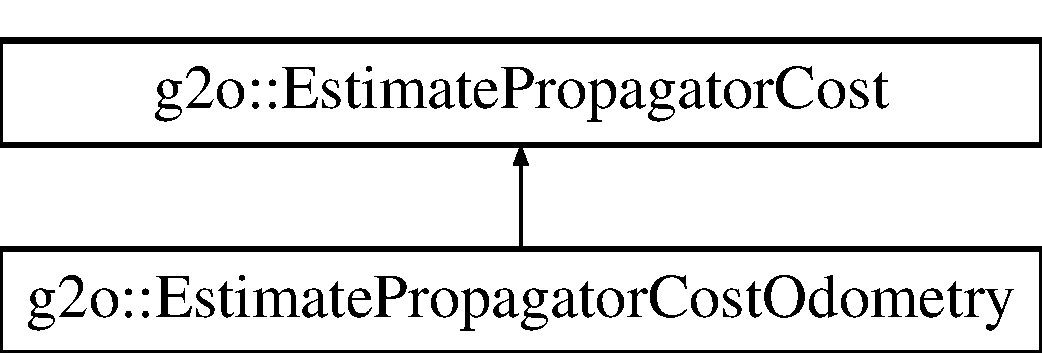
\includegraphics[height=2.000000cm]{classg2o_1_1_estimate_propagator_cost}
\end{center}
\end{figure}
\subsection*{Public Member Functions}
\begin{DoxyCompactItemize}
\item 
\mbox{\hyperlink{classg2o_1_1_estimate_propagator_cost_aebd56e3597a99b225bc3799ec8145bc9}{Estimate\+Propagator\+Cost}} (\mbox{\hyperlink{classg2o_1_1_sparse_optimizer}{Sparse\+Optimizer}} $\ast$graph)
\item 
virtual double \mbox{\hyperlink{classg2o_1_1_estimate_propagator_cost_a1234b3b82be9b8448cc62b18625adfa6}{operator()}} (\mbox{\hyperlink{classg2o_1_1_optimizable_graph_1_1_edge}{Optimizable\+Graph\+::\+Edge}} $\ast$edge, const \mbox{\hyperlink{classg2o_1_1_hyper_graph_a703938cdb4bb636860eed55a2489d70c}{Optimizable\+Graph\+::\+Vertex\+Set}} \&from, \mbox{\hyperlink{classg2o_1_1_optimizable_graph_1_1_vertex}{Optimizable\+Graph\+::\+Vertex}} $\ast$to\+\_\+) const
\item 
virtual const char $\ast$ \mbox{\hyperlink{classg2o_1_1_estimate_propagator_cost_a49846dd23f5d49df6e1fc5c2ff854fca}{name}} () const
\end{DoxyCompactItemize}
\subsection*{Protected Attributes}
\begin{DoxyCompactItemize}
\item 
\mbox{\hyperlink{classg2o_1_1_sparse_optimizer}{Sparse\+Optimizer}} $\ast$ \mbox{\hyperlink{classg2o_1_1_estimate_propagator_cost_adf778ed8de5b54eb934e88107fe77980}{\+\_\+graph}}
\end{DoxyCompactItemize}


\subsection{Detailed Description}
cost for traversing along active edges in the optimizer 

You may derive an own one, if necessary. The default is to return initial\+Estimate\+Possible(from, to) for the edge. 

\subsection{Constructor \& Destructor Documentation}
\mbox{\Hypertarget{classg2o_1_1_estimate_propagator_cost_aebd56e3597a99b225bc3799ec8145bc9}\label{classg2o_1_1_estimate_propagator_cost_aebd56e3597a99b225bc3799ec8145bc9}} 
\index{g2o\+::\+Estimate\+Propagator\+Cost@{g2o\+::\+Estimate\+Propagator\+Cost}!Estimate\+Propagator\+Cost@{Estimate\+Propagator\+Cost}}
\index{Estimate\+Propagator\+Cost@{Estimate\+Propagator\+Cost}!g2o\+::\+Estimate\+Propagator\+Cost@{g2o\+::\+Estimate\+Propagator\+Cost}}
\subsubsection{\texorpdfstring{Estimate\+Propagator\+Cost()}{EstimatePropagatorCost()}}
{\footnotesize\ttfamily g2o\+::\+Estimate\+Propagator\+Cost\+::\+Estimate\+Propagator\+Cost (\begin{DoxyParamCaption}\item[{\mbox{\hyperlink{classg2o_1_1_sparse_optimizer}{Sparse\+Optimizer}} $\ast$}]{graph }\end{DoxyParamCaption})}



\subsection{Member Function Documentation}
\mbox{\Hypertarget{classg2o_1_1_estimate_propagator_cost_a49846dd23f5d49df6e1fc5c2ff854fca}\label{classg2o_1_1_estimate_propagator_cost_a49846dd23f5d49df6e1fc5c2ff854fca}} 
\index{g2o\+::\+Estimate\+Propagator\+Cost@{g2o\+::\+Estimate\+Propagator\+Cost}!name@{name}}
\index{name@{name}!g2o\+::\+Estimate\+Propagator\+Cost@{g2o\+::\+Estimate\+Propagator\+Cost}}
\subsubsection{\texorpdfstring{name()}{name()}}
{\footnotesize\ttfamily virtual const char$\ast$ g2o\+::\+Estimate\+Propagator\+Cost\+::name (\begin{DoxyParamCaption}{ }\end{DoxyParamCaption}) const\hspace{0.3cm}{\ttfamily [inline]}, {\ttfamily [virtual]}}



Reimplemented in \mbox{\hyperlink{classg2o_1_1_estimate_propagator_cost_odometry_a6e610e7413e8973453943c5b4b9423aa}{g2o\+::\+Estimate\+Propagator\+Cost\+Odometry}}.

\mbox{\Hypertarget{classg2o_1_1_estimate_propagator_cost_a1234b3b82be9b8448cc62b18625adfa6}\label{classg2o_1_1_estimate_propagator_cost_a1234b3b82be9b8448cc62b18625adfa6}} 
\index{g2o\+::\+Estimate\+Propagator\+Cost@{g2o\+::\+Estimate\+Propagator\+Cost}!operator()@{operator()}}
\index{operator()@{operator()}!g2o\+::\+Estimate\+Propagator\+Cost@{g2o\+::\+Estimate\+Propagator\+Cost}}
\subsubsection{\texorpdfstring{operator()()}{operator()()}}
{\footnotesize\ttfamily double g2o\+::\+Estimate\+Propagator\+Cost\+::operator() (\begin{DoxyParamCaption}\item[{\mbox{\hyperlink{classg2o_1_1_optimizable_graph_1_1_edge}{Optimizable\+Graph\+::\+Edge}} $\ast$}]{edge,  }\item[{const \mbox{\hyperlink{classg2o_1_1_hyper_graph_a703938cdb4bb636860eed55a2489d70c}{Optimizable\+Graph\+::\+Vertex\+Set}} \&}]{from,  }\item[{\mbox{\hyperlink{classg2o_1_1_optimizable_graph_1_1_vertex}{Optimizable\+Graph\+::\+Vertex}} $\ast$}]{to\+\_\+ }\end{DoxyParamCaption}) const\hspace{0.3cm}{\ttfamily [virtual]}}



Reimplemented in \mbox{\hyperlink{classg2o_1_1_estimate_propagator_cost_odometry_a3da1f1d67f717d0dbc0077db1c571146}{g2o\+::\+Estimate\+Propagator\+Cost\+Odometry}}.



\subsection{Member Data Documentation}
\mbox{\Hypertarget{classg2o_1_1_estimate_propagator_cost_adf778ed8de5b54eb934e88107fe77980}\label{classg2o_1_1_estimate_propagator_cost_adf778ed8de5b54eb934e88107fe77980}} 
\index{g2o\+::\+Estimate\+Propagator\+Cost@{g2o\+::\+Estimate\+Propagator\+Cost}!\+\_\+graph@{\+\_\+graph}}
\index{\+\_\+graph@{\+\_\+graph}!g2o\+::\+Estimate\+Propagator\+Cost@{g2o\+::\+Estimate\+Propagator\+Cost}}
\subsubsection{\texorpdfstring{\+\_\+graph}{\_graph}}
{\footnotesize\ttfamily \mbox{\hyperlink{classg2o_1_1_sparse_optimizer}{Sparse\+Optimizer}}$\ast$ g2o\+::\+Estimate\+Propagator\+Cost\+::\+\_\+graph\hspace{0.3cm}{\ttfamily [protected]}}



The documentation for this class was generated from the following files\+:\begin{DoxyCompactItemize}
\item 
Thirdparty/g2o/g2o/core/\mbox{\hyperlink{estimate__propagator_8h}{estimate\+\_\+propagator.\+h}}\item 
Thirdparty/g2o/g2o/core/\mbox{\hyperlink{estimate__propagator_8cpp}{estimate\+\_\+propagator.\+cpp}}\end{DoxyCompactItemize}

\hypertarget{classg2o_1_1_estimate_propagator_cost_odometry}{}\section{g2o\+:\+:Estimate\+Propagator\+Cost\+Odometry Class Reference}
\label{classg2o_1_1_estimate_propagator_cost_odometry}\index{g2o\+::\+Estimate\+Propagator\+Cost\+Odometry@{g2o\+::\+Estimate\+Propagator\+Cost\+Odometry}}


cost for traversing only odometry edges.  




{\ttfamily \#include $<$estimate\+\_\+propagator.\+h$>$}

Inheritance diagram for g2o\+:\+:Estimate\+Propagator\+Cost\+Odometry\+:\begin{figure}[H]
\begin{center}
\leavevmode
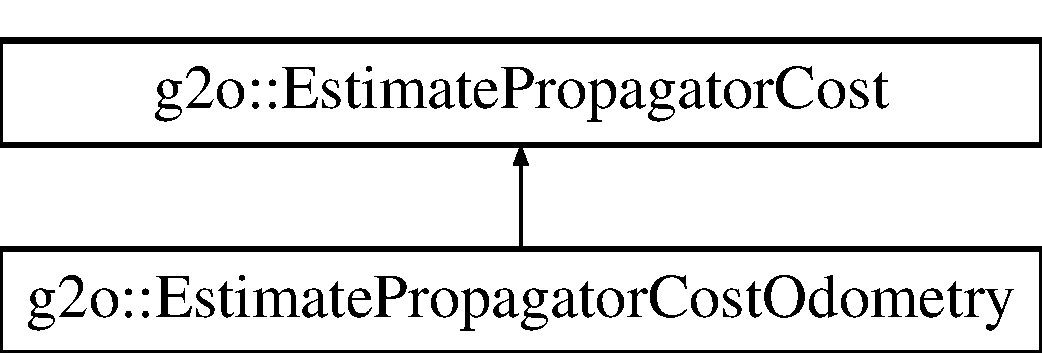
\includegraphics[height=2.000000cm]{classg2o_1_1_estimate_propagator_cost_odometry}
\end{center}
\end{figure}
\subsection*{Public Member Functions}
\begin{DoxyCompactItemize}
\item 
\mbox{\hyperlink{classg2o_1_1_estimate_propagator_cost_odometry_a426a53e3cce07b71a129cc53754e9f1a}{Estimate\+Propagator\+Cost\+Odometry}} (\mbox{\hyperlink{classg2o_1_1_sparse_optimizer}{Sparse\+Optimizer}} $\ast$graph)
\item 
virtual double \mbox{\hyperlink{classg2o_1_1_estimate_propagator_cost_odometry_a3da1f1d67f717d0dbc0077db1c571146}{operator()}} (\mbox{\hyperlink{classg2o_1_1_optimizable_graph_1_1_edge}{Optimizable\+Graph\+::\+Edge}} $\ast$edge, const \mbox{\hyperlink{classg2o_1_1_hyper_graph_a703938cdb4bb636860eed55a2489d70c}{Optimizable\+Graph\+::\+Vertex\+Set}} \&from\+\_\+, \mbox{\hyperlink{classg2o_1_1_optimizable_graph_1_1_vertex}{Optimizable\+Graph\+::\+Vertex}} $\ast$to\+\_\+) const
\item 
virtual const char $\ast$ \mbox{\hyperlink{classg2o_1_1_estimate_propagator_cost_odometry_a6e610e7413e8973453943c5b4b9423aa}{name}} () const
\end{DoxyCompactItemize}
\subsection*{Additional Inherited Members}


\subsection{Detailed Description}
cost for traversing only odometry edges. 

Initialize your graph along odometry edges. An odometry edge is assumed to connect vertices whose I\+Ds only differs by one. 

\subsection{Constructor \& Destructor Documentation}
\mbox{\Hypertarget{classg2o_1_1_estimate_propagator_cost_odometry_a426a53e3cce07b71a129cc53754e9f1a}\label{classg2o_1_1_estimate_propagator_cost_odometry_a426a53e3cce07b71a129cc53754e9f1a}} 
\index{g2o\+::\+Estimate\+Propagator\+Cost\+Odometry@{g2o\+::\+Estimate\+Propagator\+Cost\+Odometry}!Estimate\+Propagator\+Cost\+Odometry@{Estimate\+Propagator\+Cost\+Odometry}}
\index{Estimate\+Propagator\+Cost\+Odometry@{Estimate\+Propagator\+Cost\+Odometry}!g2o\+::\+Estimate\+Propagator\+Cost\+Odometry@{g2o\+::\+Estimate\+Propagator\+Cost\+Odometry}}
\subsubsection{\texorpdfstring{Estimate\+Propagator\+Cost\+Odometry()}{EstimatePropagatorCostOdometry()}}
{\footnotesize\ttfamily g2o\+::\+Estimate\+Propagator\+Cost\+Odometry\+::\+Estimate\+Propagator\+Cost\+Odometry (\begin{DoxyParamCaption}\item[{\mbox{\hyperlink{classg2o_1_1_sparse_optimizer}{Sparse\+Optimizer}} $\ast$}]{graph }\end{DoxyParamCaption})}



\subsection{Member Function Documentation}
\mbox{\Hypertarget{classg2o_1_1_estimate_propagator_cost_odometry_a6e610e7413e8973453943c5b4b9423aa}\label{classg2o_1_1_estimate_propagator_cost_odometry_a6e610e7413e8973453943c5b4b9423aa}} 
\index{g2o\+::\+Estimate\+Propagator\+Cost\+Odometry@{g2o\+::\+Estimate\+Propagator\+Cost\+Odometry}!name@{name}}
\index{name@{name}!g2o\+::\+Estimate\+Propagator\+Cost\+Odometry@{g2o\+::\+Estimate\+Propagator\+Cost\+Odometry}}
\subsubsection{\texorpdfstring{name()}{name()}}
{\footnotesize\ttfamily virtual const char$\ast$ g2o\+::\+Estimate\+Propagator\+Cost\+Odometry\+::name (\begin{DoxyParamCaption}{ }\end{DoxyParamCaption}) const\hspace{0.3cm}{\ttfamily [inline]}, {\ttfamily [virtual]}}



Reimplemented from \mbox{\hyperlink{classg2o_1_1_estimate_propagator_cost_a49846dd23f5d49df6e1fc5c2ff854fca}{g2o\+::\+Estimate\+Propagator\+Cost}}.

\mbox{\Hypertarget{classg2o_1_1_estimate_propagator_cost_odometry_a3da1f1d67f717d0dbc0077db1c571146}\label{classg2o_1_1_estimate_propagator_cost_odometry_a3da1f1d67f717d0dbc0077db1c571146}} 
\index{g2o\+::\+Estimate\+Propagator\+Cost\+Odometry@{g2o\+::\+Estimate\+Propagator\+Cost\+Odometry}!operator()@{operator()}}
\index{operator()@{operator()}!g2o\+::\+Estimate\+Propagator\+Cost\+Odometry@{g2o\+::\+Estimate\+Propagator\+Cost\+Odometry}}
\subsubsection{\texorpdfstring{operator()()}{operator()()}}
{\footnotesize\ttfamily double g2o\+::\+Estimate\+Propagator\+Cost\+Odometry\+::operator() (\begin{DoxyParamCaption}\item[{\mbox{\hyperlink{classg2o_1_1_optimizable_graph_1_1_edge}{Optimizable\+Graph\+::\+Edge}} $\ast$}]{edge,  }\item[{const \mbox{\hyperlink{classg2o_1_1_hyper_graph_a703938cdb4bb636860eed55a2489d70c}{Optimizable\+Graph\+::\+Vertex\+Set}} \&}]{from\+\_\+,  }\item[{\mbox{\hyperlink{classg2o_1_1_optimizable_graph_1_1_vertex}{Optimizable\+Graph\+::\+Vertex}} $\ast$}]{to\+\_\+ }\end{DoxyParamCaption}) const\hspace{0.3cm}{\ttfamily [virtual]}}



Reimplemented from \mbox{\hyperlink{classg2o_1_1_estimate_propagator_cost_a1234b3b82be9b8448cc62b18625adfa6}{g2o\+::\+Estimate\+Propagator\+Cost}}.



The documentation for this class was generated from the following files\+:\begin{DoxyCompactItemize}
\item 
Thirdparty/g2o/g2o/core/\mbox{\hyperlink{estimate__propagator_8h}{estimate\+\_\+propagator.\+h}}\item 
Thirdparty/g2o/g2o/core/\mbox{\hyperlink{estimate__propagator_8cpp}{estimate\+\_\+propagator.\+cpp}}\end{DoxyCompactItemize}

\hypertarget{class_o_r_b___s_l_a_m2_1_1_extractor_node}{}\section{O\+R\+B\+\_\+\+S\+L\+A\+M2\+:\+:Extractor\+Node Class Reference}
\label{class_o_r_b___s_l_a_m2_1_1_extractor_node}\index{O\+R\+B\+\_\+\+S\+L\+A\+M2\+::\+Extractor\+Node@{O\+R\+B\+\_\+\+S\+L\+A\+M2\+::\+Extractor\+Node}}


提取一幅图像的特征点和描述子  




{\ttfamily \#include $<$O\+R\+Bextractor.\+h$>$}

\subsection*{Public Member Functions}
\begin{DoxyCompactItemize}
\item 
\mbox{\hyperlink{class_o_r_b___s_l_a_m2_1_1_extractor_node_af1920a7d5f8166debdd4a7fe4a15a8e9}{Extractor\+Node}} ()
\item 
void \mbox{\hyperlink{class_o_r_b___s_l_a_m2_1_1_extractor_node_ad560af26a7bab99551eab2e5c08f6535}{Divide\+Node}} (\mbox{\hyperlink{class_o_r_b___s_l_a_m2_1_1_extractor_node}{Extractor\+Node}} \&n1, \mbox{\hyperlink{class_o_r_b___s_l_a_m2_1_1_extractor_node}{Extractor\+Node}} \&n2, \mbox{\hyperlink{class_o_r_b___s_l_a_m2_1_1_extractor_node}{Extractor\+Node}} \&n3, \mbox{\hyperlink{class_o_r_b___s_l_a_m2_1_1_extractor_node}{Extractor\+Node}} \&n4)
\end{DoxyCompactItemize}
\subsection*{Public Attributes}
\begin{DoxyCompactItemize}
\item 
std\+::vector$<$ cv\+::\+Key\+Point $>$ \mbox{\hyperlink{class_o_r_b___s_l_a_m2_1_1_extractor_node_a34dda34415caa0e996148e53f8b174ce}{v\+Keys}}
\item 
cv\+::\+Point2i \mbox{\hyperlink{class_o_r_b___s_l_a_m2_1_1_extractor_node_a3f3ae5685a8a2b2cd42fbd08e7563c3d}{UL}}
\item 
cv\+::\+Point2i \mbox{\hyperlink{class_o_r_b___s_l_a_m2_1_1_extractor_node_a73ec9b10c8a3f98ed70a117086bae12a}{UR}}
\item 
cv\+::\+Point2i \mbox{\hyperlink{class_o_r_b___s_l_a_m2_1_1_extractor_node_ab31adc0d00b85307ba98b2ff434c30fc}{BL}}
\item 
cv\+::\+Point2i \mbox{\hyperlink{class_o_r_b___s_l_a_m2_1_1_extractor_node_a8530a1f5934122f24382859c156a441d}{BR}}
\item 
std\+::list$<$ \mbox{\hyperlink{class_o_r_b___s_l_a_m2_1_1_extractor_node}{Extractor\+Node}} $>$\+::iterator \mbox{\hyperlink{class_o_r_b___s_l_a_m2_1_1_extractor_node_a5301b76ea0e33bb066a46776810d742c}{lit}}
\item 
bool \mbox{\hyperlink{class_o_r_b___s_l_a_m2_1_1_extractor_node_ada60a6ca3a5874204dcb3245ac7d2d97}{b\+No\+More}}
\end{DoxyCompactItemize}


\subsection{Detailed Description}
提取一幅图像的特征点和描述子 

\subsection{Constructor \& Destructor Documentation}
\mbox{\Hypertarget{class_o_r_b___s_l_a_m2_1_1_extractor_node_af1920a7d5f8166debdd4a7fe4a15a8e9}\label{class_o_r_b___s_l_a_m2_1_1_extractor_node_af1920a7d5f8166debdd4a7fe4a15a8e9}} 
\index{O\+R\+B\+\_\+\+S\+L\+A\+M2\+::\+Extractor\+Node@{O\+R\+B\+\_\+\+S\+L\+A\+M2\+::\+Extractor\+Node}!Extractor\+Node@{Extractor\+Node}}
\index{Extractor\+Node@{Extractor\+Node}!O\+R\+B\+\_\+\+S\+L\+A\+M2\+::\+Extractor\+Node@{O\+R\+B\+\_\+\+S\+L\+A\+M2\+::\+Extractor\+Node}}
\subsubsection{\texorpdfstring{Extractor\+Node()}{ExtractorNode()}}
{\footnotesize\ttfamily O\+R\+B\+\_\+\+S\+L\+A\+M2\+::\+Extractor\+Node\+::\+Extractor\+Node (\begin{DoxyParamCaption}{ }\end{DoxyParamCaption})\hspace{0.3cm}{\ttfamily [inline]}}



\subsection{Member Function Documentation}
\mbox{\Hypertarget{class_o_r_b___s_l_a_m2_1_1_extractor_node_ad560af26a7bab99551eab2e5c08f6535}\label{class_o_r_b___s_l_a_m2_1_1_extractor_node_ad560af26a7bab99551eab2e5c08f6535}} 
\index{O\+R\+B\+\_\+\+S\+L\+A\+M2\+::\+Extractor\+Node@{O\+R\+B\+\_\+\+S\+L\+A\+M2\+::\+Extractor\+Node}!Divide\+Node@{Divide\+Node}}
\index{Divide\+Node@{Divide\+Node}!O\+R\+B\+\_\+\+S\+L\+A\+M2\+::\+Extractor\+Node@{O\+R\+B\+\_\+\+S\+L\+A\+M2\+::\+Extractor\+Node}}
\subsubsection{\texorpdfstring{Divide\+Node()}{DivideNode()}}
{\footnotesize\ttfamily void O\+R\+B\+\_\+\+S\+L\+A\+M2\+::\+Extractor\+Node\+::\+Divide\+Node (\begin{DoxyParamCaption}\item[{\mbox{\hyperlink{class_o_r_b___s_l_a_m2_1_1_extractor_node}{Extractor\+Node}} \&}]{n1,  }\item[{\mbox{\hyperlink{class_o_r_b___s_l_a_m2_1_1_extractor_node}{Extractor\+Node}} \&}]{n2,  }\item[{\mbox{\hyperlink{class_o_r_b___s_l_a_m2_1_1_extractor_node}{Extractor\+Node}} \&}]{n3,  }\item[{\mbox{\hyperlink{class_o_r_b___s_l_a_m2_1_1_extractor_node}{Extractor\+Node}} \&}]{n4 }\end{DoxyParamCaption})}



\subsection{Member Data Documentation}
\mbox{\Hypertarget{class_o_r_b___s_l_a_m2_1_1_extractor_node_ab31adc0d00b85307ba98b2ff434c30fc}\label{class_o_r_b___s_l_a_m2_1_1_extractor_node_ab31adc0d00b85307ba98b2ff434c30fc}} 
\index{O\+R\+B\+\_\+\+S\+L\+A\+M2\+::\+Extractor\+Node@{O\+R\+B\+\_\+\+S\+L\+A\+M2\+::\+Extractor\+Node}!BL@{BL}}
\index{BL@{BL}!O\+R\+B\+\_\+\+S\+L\+A\+M2\+::\+Extractor\+Node@{O\+R\+B\+\_\+\+S\+L\+A\+M2\+::\+Extractor\+Node}}
\subsubsection{\texorpdfstring{BL}{BL}}
{\footnotesize\ttfamily cv\+::\+Point2i O\+R\+B\+\_\+\+S\+L\+A\+M2\+::\+Extractor\+Node\+::\+BL}

\mbox{\Hypertarget{class_o_r_b___s_l_a_m2_1_1_extractor_node_ada60a6ca3a5874204dcb3245ac7d2d97}\label{class_o_r_b___s_l_a_m2_1_1_extractor_node_ada60a6ca3a5874204dcb3245ac7d2d97}} 
\index{O\+R\+B\+\_\+\+S\+L\+A\+M2\+::\+Extractor\+Node@{O\+R\+B\+\_\+\+S\+L\+A\+M2\+::\+Extractor\+Node}!b\+No\+More@{b\+No\+More}}
\index{b\+No\+More@{b\+No\+More}!O\+R\+B\+\_\+\+S\+L\+A\+M2\+::\+Extractor\+Node@{O\+R\+B\+\_\+\+S\+L\+A\+M2\+::\+Extractor\+Node}}
\subsubsection{\texorpdfstring{b\+No\+More}{bNoMore}}
{\footnotesize\ttfamily bool O\+R\+B\+\_\+\+S\+L\+A\+M2\+::\+Extractor\+Node\+::b\+No\+More}

\mbox{\Hypertarget{class_o_r_b___s_l_a_m2_1_1_extractor_node_a8530a1f5934122f24382859c156a441d}\label{class_o_r_b___s_l_a_m2_1_1_extractor_node_a8530a1f5934122f24382859c156a441d}} 
\index{O\+R\+B\+\_\+\+S\+L\+A\+M2\+::\+Extractor\+Node@{O\+R\+B\+\_\+\+S\+L\+A\+M2\+::\+Extractor\+Node}!BR@{BR}}
\index{BR@{BR}!O\+R\+B\+\_\+\+S\+L\+A\+M2\+::\+Extractor\+Node@{O\+R\+B\+\_\+\+S\+L\+A\+M2\+::\+Extractor\+Node}}
\subsubsection{\texorpdfstring{BR}{BR}}
{\footnotesize\ttfamily cv\+::\+Point2i O\+R\+B\+\_\+\+S\+L\+A\+M2\+::\+Extractor\+Node\+::\+BR}

\mbox{\Hypertarget{class_o_r_b___s_l_a_m2_1_1_extractor_node_a5301b76ea0e33bb066a46776810d742c}\label{class_o_r_b___s_l_a_m2_1_1_extractor_node_a5301b76ea0e33bb066a46776810d742c}} 
\index{O\+R\+B\+\_\+\+S\+L\+A\+M2\+::\+Extractor\+Node@{O\+R\+B\+\_\+\+S\+L\+A\+M2\+::\+Extractor\+Node}!lit@{lit}}
\index{lit@{lit}!O\+R\+B\+\_\+\+S\+L\+A\+M2\+::\+Extractor\+Node@{O\+R\+B\+\_\+\+S\+L\+A\+M2\+::\+Extractor\+Node}}
\subsubsection{\texorpdfstring{lit}{lit}}
{\footnotesize\ttfamily std\+::list$<$\mbox{\hyperlink{class_o_r_b___s_l_a_m2_1_1_extractor_node}{Extractor\+Node}}$>$\+::iterator O\+R\+B\+\_\+\+S\+L\+A\+M2\+::\+Extractor\+Node\+::lit}

\mbox{\Hypertarget{class_o_r_b___s_l_a_m2_1_1_extractor_node_a3f3ae5685a8a2b2cd42fbd08e7563c3d}\label{class_o_r_b___s_l_a_m2_1_1_extractor_node_a3f3ae5685a8a2b2cd42fbd08e7563c3d}} 
\index{O\+R\+B\+\_\+\+S\+L\+A\+M2\+::\+Extractor\+Node@{O\+R\+B\+\_\+\+S\+L\+A\+M2\+::\+Extractor\+Node}!UL@{UL}}
\index{UL@{UL}!O\+R\+B\+\_\+\+S\+L\+A\+M2\+::\+Extractor\+Node@{O\+R\+B\+\_\+\+S\+L\+A\+M2\+::\+Extractor\+Node}}
\subsubsection{\texorpdfstring{UL}{UL}}
{\footnotesize\ttfamily cv\+::\+Point2i O\+R\+B\+\_\+\+S\+L\+A\+M2\+::\+Extractor\+Node\+::\+UL}

\mbox{\Hypertarget{class_o_r_b___s_l_a_m2_1_1_extractor_node_a73ec9b10c8a3f98ed70a117086bae12a}\label{class_o_r_b___s_l_a_m2_1_1_extractor_node_a73ec9b10c8a3f98ed70a117086bae12a}} 
\index{O\+R\+B\+\_\+\+S\+L\+A\+M2\+::\+Extractor\+Node@{O\+R\+B\+\_\+\+S\+L\+A\+M2\+::\+Extractor\+Node}!UR@{UR}}
\index{UR@{UR}!O\+R\+B\+\_\+\+S\+L\+A\+M2\+::\+Extractor\+Node@{O\+R\+B\+\_\+\+S\+L\+A\+M2\+::\+Extractor\+Node}}
\subsubsection{\texorpdfstring{UR}{UR}}
{\footnotesize\ttfamily cv\+::\+Point2i O\+R\+B\+\_\+\+S\+L\+A\+M2\+::\+Extractor\+Node\+::\+UR}

\mbox{\Hypertarget{class_o_r_b___s_l_a_m2_1_1_extractor_node_a34dda34415caa0e996148e53f8b174ce}\label{class_o_r_b___s_l_a_m2_1_1_extractor_node_a34dda34415caa0e996148e53f8b174ce}} 
\index{O\+R\+B\+\_\+\+S\+L\+A\+M2\+::\+Extractor\+Node@{O\+R\+B\+\_\+\+S\+L\+A\+M2\+::\+Extractor\+Node}!v\+Keys@{v\+Keys}}
\index{v\+Keys@{v\+Keys}!O\+R\+B\+\_\+\+S\+L\+A\+M2\+::\+Extractor\+Node@{O\+R\+B\+\_\+\+S\+L\+A\+M2\+::\+Extractor\+Node}}
\subsubsection{\texorpdfstring{v\+Keys}{vKeys}}
{\footnotesize\ttfamily std\+::vector$<$cv\+::\+Key\+Point$>$ O\+R\+B\+\_\+\+S\+L\+A\+M2\+::\+Extractor\+Node\+::v\+Keys}



The documentation for this class was generated from the following files\+:\begin{DoxyCompactItemize}
\item 
D\+:/github/\+V\+S\+L\+A\+M/\+O\+R\+B\+S\+L\+A\+M2/\+O\+R\+B-\/\+S\+L\+A\+M2-\/master/include/\mbox{\hyperlink{_o_r_bextractor_8h}{O\+R\+Bextractor.\+h}}\item 
D\+:/github/\+V\+S\+L\+A\+M/\+O\+R\+B\+S\+L\+A\+M2/\+O\+R\+B-\/\+S\+L\+A\+M2-\/master/src/\mbox{\hyperlink{_o_r_bextractor_8cpp}{O\+R\+Bextractor.\+cpp}}\end{DoxyCompactItemize}

\hypertarget{classg2o_1_1_factory}{}\section{g2o\+:\+:Factory Class Reference}
\label{classg2o_1_1_factory}\index{g2o\+::\+Factory@{g2o\+::\+Factory}}


create vertices and edges based on T\+A\+Gs in, for example, a file  




{\ttfamily \#include $<$factory.\+h$>$}

\subsection*{Classes}
\begin{DoxyCompactItemize}
\item 
class \mbox{\hyperlink{classg2o_1_1_factory_1_1_creator_information}{Creator\+Information}}
\end{DoxyCompactItemize}
\subsection*{Public Member Functions}
\begin{DoxyCompactItemize}
\item 
void \mbox{\hyperlink{classg2o_1_1_factory_aba2f2e40635fd1b996981cefdb65c346}{register\+Type}} (const std\+::string \&\mbox{\hyperlink{classg2o_1_1_factory_ae6b0fb89dc45ea1e506401d349c869f0}{tag}}, \mbox{\hyperlink{classg2o_1_1_abstract_hyper_graph_element_creator}{Abstract\+Hyper\+Graph\+Element\+Creator}} $\ast$c)
\item 
void \mbox{\hyperlink{classg2o_1_1_factory_a01b16c7d5a49ddab5ccd5980f76900b7}{unregister\+Type}} (const std\+::string \&\mbox{\hyperlink{classg2o_1_1_factory_ae6b0fb89dc45ea1e506401d349c869f0}{tag}})
\item 
\mbox{\hyperlink{structg2o_1_1_hyper_graph_1_1_hyper_graph_element}{Hyper\+Graph\+::\+Hyper\+Graph\+Element}} $\ast$ \mbox{\hyperlink{classg2o_1_1_factory_aa61fcb8861afb1dd4c4af5d9cc03d3ec}{construct}} (const std\+::string \&\mbox{\hyperlink{classg2o_1_1_factory_ae6b0fb89dc45ea1e506401d349c869f0}{tag}}) const
\item 
\mbox{\hyperlink{structg2o_1_1_hyper_graph_1_1_hyper_graph_element}{Hyper\+Graph\+::\+Hyper\+Graph\+Element}} $\ast$ \mbox{\hyperlink{classg2o_1_1_factory_a8c3800dfa57718d2ceb4f6150611540d}{construct}} (const std\+::string \&\mbox{\hyperlink{classg2o_1_1_factory_ae6b0fb89dc45ea1e506401d349c869f0}{tag}}, const \mbox{\hyperlink{classg2o_1_1_hyper_graph_a7b8fda20e1b03e92aeceeac6e8218b73}{Hyper\+Graph\+::\+Graph\+Elem\+Bitset}} \&elems\+To\+Construct) const
\item 
bool \mbox{\hyperlink{classg2o_1_1_factory_a20292a9c8417303fec92057826ba2430}{knows\+Tag}} (const std\+::string \&\mbox{\hyperlink{classg2o_1_1_factory_ae6b0fb89dc45ea1e506401d349c869f0}{tag}}, int $\ast$element\+Type=0) const
\item 
const std\+::string \& \mbox{\hyperlink{classg2o_1_1_factory_ae6b0fb89dc45ea1e506401d349c869f0}{tag}} (const \mbox{\hyperlink{structg2o_1_1_hyper_graph_1_1_hyper_graph_element}{Hyper\+Graph\+::\+Hyper\+Graph\+Element}} $\ast$v) const
\begin{DoxyCompactList}\small\item\em return the T\+AG given a vertex \end{DoxyCompactList}\item 
void \mbox{\hyperlink{classg2o_1_1_factory_af31924e76d04bcfd77a53cec8f1b778c}{fill\+Known\+Types}} (std\+::vector$<$ std\+::string $>$ \&types) const
\item 
void \mbox{\hyperlink{classg2o_1_1_factory_a564b37b3ccbdd559a386b40ca16d219b}{print\+Registered\+Types}} (std\+::ostream \&os, bool comment=false) const
\end{DoxyCompactItemize}
\subsection*{Static Public Member Functions}
\begin{DoxyCompactItemize}
\item 
static \mbox{\hyperlink{classg2o_1_1_factory}{Factory}} $\ast$ \mbox{\hyperlink{classg2o_1_1_factory_a8a1f33e017c5ad59399cef48972578ae}{instance}} ()
\begin{DoxyCompactList}\small\item\em return the instance \end{DoxyCompactList}\item 
static void \mbox{\hyperlink{classg2o_1_1_factory_ab40f0aa18dabb91a35de7186ede9355a}{destroy}} ()
\begin{DoxyCompactList}\small\item\em free the instance \end{DoxyCompactList}\end{DoxyCompactItemize}
\subsection*{Protected Types}
\begin{DoxyCompactItemize}
\item 
typedef std\+::map$<$ std\+::string, \mbox{\hyperlink{classg2o_1_1_factory_1_1_creator_information}{Creator\+Information}} $\ast$ $>$ \mbox{\hyperlink{classg2o_1_1_factory_a639c8d850892dddc20098e9aa97ef9e8}{Creator\+Map}}
\item 
typedef std\+::map$<$ std\+::string, std\+::string $>$ \mbox{\hyperlink{classg2o_1_1_factory_aba274179c053b3b71dcef6a20c898496}{Tag\+Lookup}}
\end{DoxyCompactItemize}
\subsection*{Protected Member Functions}
\begin{DoxyCompactItemize}
\item 
\mbox{\hyperlink{classg2o_1_1_factory_af8b5afc514363e6f00c61e8acd67b495}{Factory}} ()
\item 
\mbox{\hyperlink{classg2o_1_1_factory_a4b7c6970f55045ee632e6276387d0223}{$\sim$\+Factory}} ()
\end{DoxyCompactItemize}
\subsection*{Protected Attributes}
\begin{DoxyCompactItemize}
\item 
\mbox{\hyperlink{classg2o_1_1_factory_a639c8d850892dddc20098e9aa97ef9e8}{Creator\+Map}} \mbox{\hyperlink{classg2o_1_1_factory_a38e27fb1014dfb8691f4df045ebb5130}{\+\_\+creator}}
\begin{DoxyCompactList}\small\item\em look-\/up map for the existing creators \end{DoxyCompactList}\item 
\mbox{\hyperlink{classg2o_1_1_factory_aba274179c053b3b71dcef6a20c898496}{Tag\+Lookup}} \mbox{\hyperlink{classg2o_1_1_factory_a93fbd79ea000ed88101c1f23b19e6e2a}{\+\_\+tag\+Lookup}}
\begin{DoxyCompactList}\small\item\em reverse look-\/up, class name to tag \end{DoxyCompactList}\end{DoxyCompactItemize}
\subsection*{Static Private Attributes}
\begin{DoxyCompactItemize}
\item 
static \mbox{\hyperlink{classg2o_1_1_factory}{Factory}} $\ast$ \mbox{\hyperlink{classg2o_1_1_factory_a4eab3a865dee18a71bb73246dc3e9f4b}{factory\+Instance}} = 0
\end{DoxyCompactItemize}


\subsection{Detailed Description}
create vertices and edges based on T\+A\+Gs in, for example, a file 

\subsection{Member Typedef Documentation}
\mbox{\Hypertarget{classg2o_1_1_factory_a639c8d850892dddc20098e9aa97ef9e8}\label{classg2o_1_1_factory_a639c8d850892dddc20098e9aa97ef9e8}} 
\index{g2o\+::\+Factory@{g2o\+::\+Factory}!Creator\+Map@{Creator\+Map}}
\index{Creator\+Map@{Creator\+Map}!g2o\+::\+Factory@{g2o\+::\+Factory}}
\subsubsection{\texorpdfstring{Creator\+Map}{CreatorMap}}
{\footnotesize\ttfamily typedef std\+::map$<$std\+::string, \mbox{\hyperlink{classg2o_1_1_factory_1_1_creator_information}{Creator\+Information}}$\ast$$>$ \mbox{\hyperlink{classg2o_1_1_factory_a639c8d850892dddc20098e9aa97ef9e8}{g2o\+::\+Factory\+::\+Creator\+Map}}\hspace{0.3cm}{\ttfamily [protected]}}

\mbox{\Hypertarget{classg2o_1_1_factory_aba274179c053b3b71dcef6a20c898496}\label{classg2o_1_1_factory_aba274179c053b3b71dcef6a20c898496}} 
\index{g2o\+::\+Factory@{g2o\+::\+Factory}!Tag\+Lookup@{Tag\+Lookup}}
\index{Tag\+Lookup@{Tag\+Lookup}!g2o\+::\+Factory@{g2o\+::\+Factory}}
\subsubsection{\texorpdfstring{Tag\+Lookup}{TagLookup}}
{\footnotesize\ttfamily typedef std\+::map$<$std\+::string, std\+::string$>$ \mbox{\hyperlink{classg2o_1_1_factory_aba274179c053b3b71dcef6a20c898496}{g2o\+::\+Factory\+::\+Tag\+Lookup}}\hspace{0.3cm}{\ttfamily [protected]}}



\subsection{Constructor \& Destructor Documentation}
\mbox{\Hypertarget{classg2o_1_1_factory_af8b5afc514363e6f00c61e8acd67b495}\label{classg2o_1_1_factory_af8b5afc514363e6f00c61e8acd67b495}} 
\index{g2o\+::\+Factory@{g2o\+::\+Factory}!Factory@{Factory}}
\index{Factory@{Factory}!g2o\+::\+Factory@{g2o\+::\+Factory}}
\subsubsection{\texorpdfstring{Factory()}{Factory()}}
{\footnotesize\ttfamily g2o\+::\+Factory\+::\+Factory (\begin{DoxyParamCaption}{ }\end{DoxyParamCaption})\hspace{0.3cm}{\ttfamily [protected]}}

\mbox{\Hypertarget{classg2o_1_1_factory_a4b7c6970f55045ee632e6276387d0223}\label{classg2o_1_1_factory_a4b7c6970f55045ee632e6276387d0223}} 
\index{g2o\+::\+Factory@{g2o\+::\+Factory}!````~Factory@{$\sim$\+Factory}}
\index{````~Factory@{$\sim$\+Factory}!g2o\+::\+Factory@{g2o\+::\+Factory}}
\subsubsection{\texorpdfstring{$\sim$\+Factory()}{~Factory()}}
{\footnotesize\ttfamily g2o\+::\+Factory\+::$\sim$\+Factory (\begin{DoxyParamCaption}{ }\end{DoxyParamCaption})\hspace{0.3cm}{\ttfamily [protected]}}



\subsection{Member Function Documentation}
\mbox{\Hypertarget{classg2o_1_1_factory_aa61fcb8861afb1dd4c4af5d9cc03d3ec}\label{classg2o_1_1_factory_aa61fcb8861afb1dd4c4af5d9cc03d3ec}} 
\index{g2o\+::\+Factory@{g2o\+::\+Factory}!construct@{construct}}
\index{construct@{construct}!g2o\+::\+Factory@{g2o\+::\+Factory}}
\subsubsection{\texorpdfstring{construct()}{construct()}\hspace{0.1cm}{\footnotesize\ttfamily [1/2]}}
{\footnotesize\ttfamily \mbox{\hyperlink{structg2o_1_1_hyper_graph_1_1_hyper_graph_element}{Hyper\+Graph\+::\+Hyper\+Graph\+Element}} $\ast$ g2o\+::\+Factory\+::construct (\begin{DoxyParamCaption}\item[{const std\+::string \&}]{tag }\end{DoxyParamCaption}) const}

construct a graph element based on its tag \mbox{\Hypertarget{classg2o_1_1_factory_a8c3800dfa57718d2ceb4f6150611540d}\label{classg2o_1_1_factory_a8c3800dfa57718d2ceb4f6150611540d}} 
\index{g2o\+::\+Factory@{g2o\+::\+Factory}!construct@{construct}}
\index{construct@{construct}!g2o\+::\+Factory@{g2o\+::\+Factory}}
\subsubsection{\texorpdfstring{construct()}{construct()}\hspace{0.1cm}{\footnotesize\ttfamily [2/2]}}
{\footnotesize\ttfamily \mbox{\hyperlink{structg2o_1_1_hyper_graph_1_1_hyper_graph_element}{Hyper\+Graph\+::\+Hyper\+Graph\+Element}} $\ast$ g2o\+::\+Factory\+::construct (\begin{DoxyParamCaption}\item[{const std\+::string \&}]{tag,  }\item[{const \mbox{\hyperlink{classg2o_1_1_hyper_graph_a7b8fda20e1b03e92aeceeac6e8218b73}{Hyper\+Graph\+::\+Graph\+Elem\+Bitset}} \&}]{elems\+To\+Construct }\end{DoxyParamCaption}) const}

construct a graph element based on its tag, but only if it\textquotesingle{}s type (a bitmask) matches. A bitmask without any bit set will construct any item. Otherwise a bit has to be set to allow construction of a graph element. \mbox{\Hypertarget{classg2o_1_1_factory_ab40f0aa18dabb91a35de7186ede9355a}\label{classg2o_1_1_factory_ab40f0aa18dabb91a35de7186ede9355a}} 
\index{g2o\+::\+Factory@{g2o\+::\+Factory}!destroy@{destroy}}
\index{destroy@{destroy}!g2o\+::\+Factory@{g2o\+::\+Factory}}
\subsubsection{\texorpdfstring{destroy()}{destroy()}}
{\footnotesize\ttfamily void g2o\+::\+Factory\+::destroy (\begin{DoxyParamCaption}{ }\end{DoxyParamCaption})\hspace{0.3cm}{\ttfamily [static]}}



free the instance 

\mbox{\Hypertarget{classg2o_1_1_factory_af31924e76d04bcfd77a53cec8f1b778c}\label{classg2o_1_1_factory_af31924e76d04bcfd77a53cec8f1b778c}} 
\index{g2o\+::\+Factory@{g2o\+::\+Factory}!fill\+Known\+Types@{fill\+Known\+Types}}
\index{fill\+Known\+Types@{fill\+Known\+Types}!g2o\+::\+Factory@{g2o\+::\+Factory}}
\subsubsection{\texorpdfstring{fill\+Known\+Types()}{fillKnownTypes()}}
{\footnotesize\ttfamily void g2o\+::\+Factory\+::fill\+Known\+Types (\begin{DoxyParamCaption}\item[{std\+::vector$<$ std\+::string $>$ \&}]{types }\end{DoxyParamCaption}) const}

get a list of all known types \mbox{\Hypertarget{classg2o_1_1_factory_a8a1f33e017c5ad59399cef48972578ae}\label{classg2o_1_1_factory_a8a1f33e017c5ad59399cef48972578ae}} 
\index{g2o\+::\+Factory@{g2o\+::\+Factory}!instance@{instance}}
\index{instance@{instance}!g2o\+::\+Factory@{g2o\+::\+Factory}}
\subsubsection{\texorpdfstring{instance()}{instance()}}
{\footnotesize\ttfamily \mbox{\hyperlink{classg2o_1_1_factory}{Factory}} $\ast$ g2o\+::\+Factory\+::instance (\begin{DoxyParamCaption}{ }\end{DoxyParamCaption})\hspace{0.3cm}{\ttfamily [static]}}



return the instance 

\mbox{\Hypertarget{classg2o_1_1_factory_a20292a9c8417303fec92057826ba2430}\label{classg2o_1_1_factory_a20292a9c8417303fec92057826ba2430}} 
\index{g2o\+::\+Factory@{g2o\+::\+Factory}!knows\+Tag@{knows\+Tag}}
\index{knows\+Tag@{knows\+Tag}!g2o\+::\+Factory@{g2o\+::\+Factory}}
\subsubsection{\texorpdfstring{knows\+Tag()}{knowsTag()}}
{\footnotesize\ttfamily bool g2o\+::\+Factory\+::knows\+Tag (\begin{DoxyParamCaption}\item[{const std\+::string \&}]{tag,  }\item[{int $\ast$}]{element\+Type = {\ttfamily 0} }\end{DoxyParamCaption}) const}

return whether the factory knows this tag or not \mbox{\Hypertarget{classg2o_1_1_factory_a564b37b3ccbdd559a386b40ca16d219b}\label{classg2o_1_1_factory_a564b37b3ccbdd559a386b40ca16d219b}} 
\index{g2o\+::\+Factory@{g2o\+::\+Factory}!print\+Registered\+Types@{print\+Registered\+Types}}
\index{print\+Registered\+Types@{print\+Registered\+Types}!g2o\+::\+Factory@{g2o\+::\+Factory}}
\subsubsection{\texorpdfstring{print\+Registered\+Types()}{printRegisteredTypes()}}
{\footnotesize\ttfamily void g2o\+::\+Factory\+::print\+Registered\+Types (\begin{DoxyParamCaption}\item[{std\+::ostream \&}]{os,  }\item[{bool}]{comment = {\ttfamily false} }\end{DoxyParamCaption}) const}

print a list of the known registered types to the given stream \mbox{\Hypertarget{classg2o_1_1_factory_aba2f2e40635fd1b996981cefdb65c346}\label{classg2o_1_1_factory_aba2f2e40635fd1b996981cefdb65c346}} 
\index{g2o\+::\+Factory@{g2o\+::\+Factory}!register\+Type@{register\+Type}}
\index{register\+Type@{register\+Type}!g2o\+::\+Factory@{g2o\+::\+Factory}}
\subsubsection{\texorpdfstring{register\+Type()}{registerType()}}
{\footnotesize\ttfamily void g2o\+::\+Factory\+::register\+Type (\begin{DoxyParamCaption}\item[{const std\+::string \&}]{tag,  }\item[{\mbox{\hyperlink{classg2o_1_1_abstract_hyper_graph_element_creator}{Abstract\+Hyper\+Graph\+Element\+Creator}} $\ast$}]{c }\end{DoxyParamCaption})}

register a tag for a specific creator \mbox{\Hypertarget{classg2o_1_1_factory_ae6b0fb89dc45ea1e506401d349c869f0}\label{classg2o_1_1_factory_ae6b0fb89dc45ea1e506401d349c869f0}} 
\index{g2o\+::\+Factory@{g2o\+::\+Factory}!tag@{tag}}
\index{tag@{tag}!g2o\+::\+Factory@{g2o\+::\+Factory}}
\subsubsection{\texorpdfstring{tag()}{tag()}}
{\footnotesize\ttfamily const std\+::string \& g2o\+::\+Factory\+::tag (\begin{DoxyParamCaption}\item[{const \mbox{\hyperlink{structg2o_1_1_hyper_graph_1_1_hyper_graph_element}{Hyper\+Graph\+::\+Hyper\+Graph\+Element}} $\ast$}]{v }\end{DoxyParamCaption}) const}



return the T\+AG given a vertex 

\mbox{\Hypertarget{classg2o_1_1_factory_a01b16c7d5a49ddab5ccd5980f76900b7}\label{classg2o_1_1_factory_a01b16c7d5a49ddab5ccd5980f76900b7}} 
\index{g2o\+::\+Factory@{g2o\+::\+Factory}!unregister\+Type@{unregister\+Type}}
\index{unregister\+Type@{unregister\+Type}!g2o\+::\+Factory@{g2o\+::\+Factory}}
\subsubsection{\texorpdfstring{unregister\+Type()}{unregisterType()}}
{\footnotesize\ttfamily void g2o\+::\+Factory\+::unregister\+Type (\begin{DoxyParamCaption}\item[{const std\+::string \&}]{tag }\end{DoxyParamCaption})}

unregister a tag for a specific creator 

\subsection{Member Data Documentation}
\mbox{\Hypertarget{classg2o_1_1_factory_a38e27fb1014dfb8691f4df045ebb5130}\label{classg2o_1_1_factory_a38e27fb1014dfb8691f4df045ebb5130}} 
\index{g2o\+::\+Factory@{g2o\+::\+Factory}!\+\_\+creator@{\+\_\+creator}}
\index{\+\_\+creator@{\+\_\+creator}!g2o\+::\+Factory@{g2o\+::\+Factory}}
\subsubsection{\texorpdfstring{\+\_\+creator}{\_creator}}
{\footnotesize\ttfamily \mbox{\hyperlink{classg2o_1_1_factory_a639c8d850892dddc20098e9aa97ef9e8}{Creator\+Map}} g2o\+::\+Factory\+::\+\_\+creator\hspace{0.3cm}{\ttfamily [protected]}}



look-\/up map for the existing creators 

\mbox{\Hypertarget{classg2o_1_1_factory_a93fbd79ea000ed88101c1f23b19e6e2a}\label{classg2o_1_1_factory_a93fbd79ea000ed88101c1f23b19e6e2a}} 
\index{g2o\+::\+Factory@{g2o\+::\+Factory}!\+\_\+tag\+Lookup@{\+\_\+tag\+Lookup}}
\index{\+\_\+tag\+Lookup@{\+\_\+tag\+Lookup}!g2o\+::\+Factory@{g2o\+::\+Factory}}
\subsubsection{\texorpdfstring{\+\_\+tag\+Lookup}{\_tagLookup}}
{\footnotesize\ttfamily \mbox{\hyperlink{classg2o_1_1_factory_aba274179c053b3b71dcef6a20c898496}{Tag\+Lookup}} g2o\+::\+Factory\+::\+\_\+tag\+Lookup\hspace{0.3cm}{\ttfamily [protected]}}



reverse look-\/up, class name to tag 

\mbox{\Hypertarget{classg2o_1_1_factory_a4eab3a865dee18a71bb73246dc3e9f4b}\label{classg2o_1_1_factory_a4eab3a865dee18a71bb73246dc3e9f4b}} 
\index{g2o\+::\+Factory@{g2o\+::\+Factory}!factory\+Instance@{factory\+Instance}}
\index{factory\+Instance@{factory\+Instance}!g2o\+::\+Factory@{g2o\+::\+Factory}}
\subsubsection{\texorpdfstring{factory\+Instance}{factoryInstance}}
{\footnotesize\ttfamily \mbox{\hyperlink{classg2o_1_1_factory}{Factory}} $\ast$ g2o\+::\+Factory\+::factory\+Instance = 0\hspace{0.3cm}{\ttfamily [static]}, {\ttfamily [private]}}



The documentation for this class was generated from the following files\+:\begin{DoxyCompactItemize}
\item 
D\+:/github/\+V\+S\+L\+A\+M/\+O\+R\+B\+S\+L\+A\+M2/\+O\+R\+B-\/\+S\+L\+A\+M2-\/master/\+Thirdparty/g2o/g2o/core/\mbox{\hyperlink{factory_8h}{factory.\+h}}\item 
D\+:/github/\+V\+S\+L\+A\+M/\+O\+R\+B\+S\+L\+A\+M2/\+O\+R\+B-\/\+S\+L\+A\+M2-\/master/\+Thirdparty/g2o/g2o/core/\mbox{\hyperlink{factory_8cpp}{factory.\+cpp}}\end{DoxyCompactItemize}

\hypertarget{class_d_bo_w2_1_1_f_class}{}\section{D\+Bo\+W2\+:\+:F\+Class Class Reference}
\label{class_d_bo_w2_1_1_f_class}\index{D\+Bo\+W2\+::\+F\+Class@{D\+Bo\+W2\+::\+F\+Class}}


Generic class to encapsulate functions to manage descriptors.  




{\ttfamily \#include $<$F\+Class.\+h$>$}

Inheritance diagram for D\+Bo\+W2\+:\+:F\+Class\+:\begin{figure}[H]
\begin{center}
\leavevmode
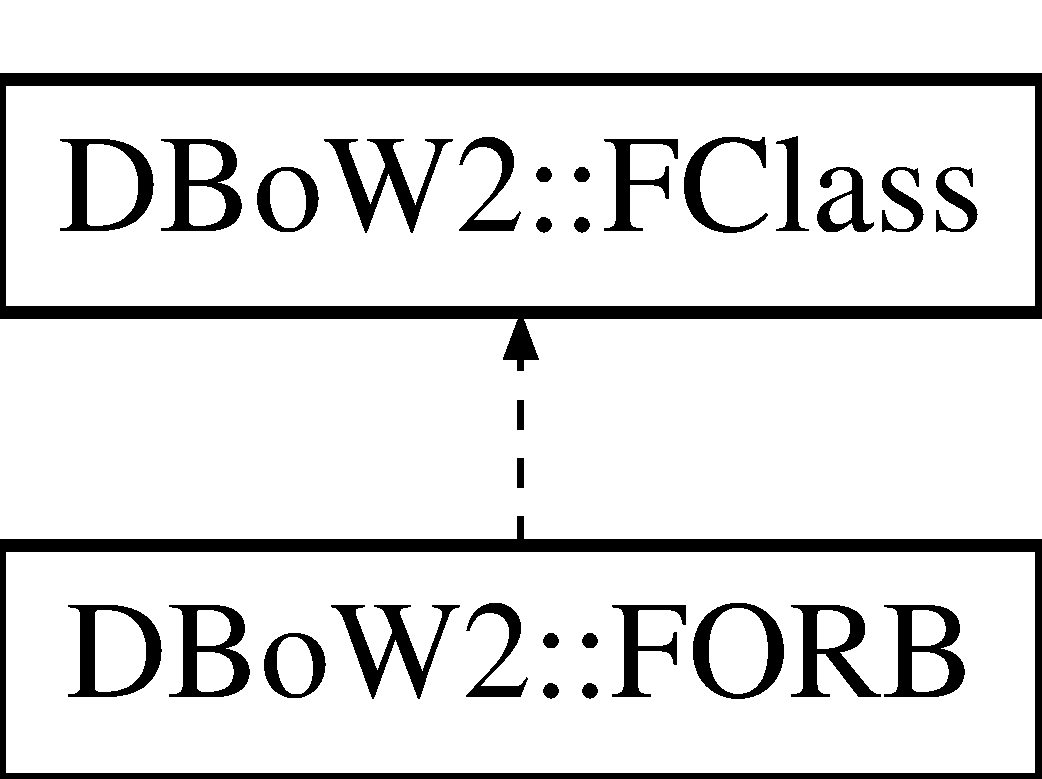
\includegraphics[height=2.000000cm]{class_d_bo_w2_1_1_f_class}
\end{center}
\end{figure}


\subsection{Detailed Description}
Generic class to encapsulate functions to manage descriptors. 

This class must be inherited. Derived classes can be used as the parameter F when creating Templated structures (\mbox{\hyperlink{class_d_bo_w2_1_1_templated_vocabulary}{Templated\+Vocabulary}}, Templated\+Database, ...) 

The documentation for this class was generated from the following file\+:\begin{DoxyCompactItemize}
\item 
Thirdparty/\+D\+Bo\+W2/\+D\+Bo\+W2/\mbox{\hyperlink{_f_class_8h}{F\+Class.\+h}}\end{DoxyCompactItemize}

\hypertarget{class_d_bo_w2_1_1_feature_vector}{}\section{D\+Bo\+W2\+:\+:Feature\+Vector Class Reference}
\label{class_d_bo_w2_1_1_feature_vector}\index{D\+Bo\+W2\+::\+Feature\+Vector@{D\+Bo\+W2\+::\+Feature\+Vector}}


Vector of nodes with indexes of local features.  




{\ttfamily \#include $<$Feature\+Vector.\+h$>$}

Inheritance diagram for D\+Bo\+W2\+:\+:Feature\+Vector\+:\begin{figure}[H]
\begin{center}
\leavevmode
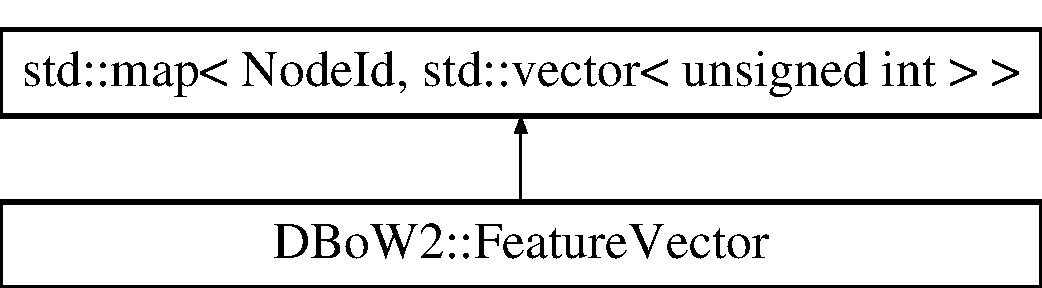
\includegraphics[height=2.000000cm]{class_d_bo_w2_1_1_feature_vector}
\end{center}
\end{figure}
\subsection*{Public Member Functions}
\begin{DoxyCompactItemize}
\item 
\mbox{\hyperlink{class_d_bo_w2_1_1_feature_vector_a66c069d269c8c98dcf3ae39cbc6f861b}{Feature\+Vector}} (void)
\item 
\mbox{\hyperlink{class_d_bo_w2_1_1_feature_vector_a44514a020719b7e5ac552332a9922bd9}{$\sim$\+Feature\+Vector}} (void)
\item 
void \mbox{\hyperlink{class_d_bo_w2_1_1_feature_vector_ae9554bfcbebc85439616de08f47f2238}{add\+Feature}} (\mbox{\hyperlink{namespace_d_bo_w2_a3a0fa9c50c0df508759362d6204566f2}{Node\+Id}} id, unsigned int i\+\_\+feature)
\end{DoxyCompactItemize}
\subsection*{Friends}
\begin{DoxyCompactItemize}
\item 
std\+::ostream \& \mbox{\hyperlink{class_d_bo_w2_1_1_feature_vector_a34aa65c93dc5f6be269610e3f238d9b1}{operator$<$$<$}} (std\+::ostream \&out, const \mbox{\hyperlink{class_d_bo_w2_1_1_feature_vector}{Feature\+Vector}} \&v)
\end{DoxyCompactItemize}


\subsection{Detailed Description}
Vector of nodes with indexes of local features. 

\subsection{Constructor \& Destructor Documentation}
\mbox{\Hypertarget{class_d_bo_w2_1_1_feature_vector_a66c069d269c8c98dcf3ae39cbc6f861b}\label{class_d_bo_w2_1_1_feature_vector_a66c069d269c8c98dcf3ae39cbc6f861b}} 
\index{D\+Bo\+W2\+::\+Feature\+Vector@{D\+Bo\+W2\+::\+Feature\+Vector}!Feature\+Vector@{Feature\+Vector}}
\index{Feature\+Vector@{Feature\+Vector}!D\+Bo\+W2\+::\+Feature\+Vector@{D\+Bo\+W2\+::\+Feature\+Vector}}
\subsubsection{\texorpdfstring{Feature\+Vector()}{FeatureVector()}}
{\footnotesize\ttfamily D\+Bo\+W2\+::\+Feature\+Vector\+::\+Feature\+Vector (\begin{DoxyParamCaption}\item[{void}]{ }\end{DoxyParamCaption})}

Constructor \mbox{\Hypertarget{class_d_bo_w2_1_1_feature_vector_a44514a020719b7e5ac552332a9922bd9}\label{class_d_bo_w2_1_1_feature_vector_a44514a020719b7e5ac552332a9922bd9}} 
\index{D\+Bo\+W2\+::\+Feature\+Vector@{D\+Bo\+W2\+::\+Feature\+Vector}!````~Feature\+Vector@{$\sim$\+Feature\+Vector}}
\index{````~Feature\+Vector@{$\sim$\+Feature\+Vector}!D\+Bo\+W2\+::\+Feature\+Vector@{D\+Bo\+W2\+::\+Feature\+Vector}}
\subsubsection{\texorpdfstring{$\sim$\+Feature\+Vector()}{~FeatureVector()}}
{\footnotesize\ttfamily D\+Bo\+W2\+::\+Feature\+Vector\+::$\sim$\+Feature\+Vector (\begin{DoxyParamCaption}\item[{void}]{ }\end{DoxyParamCaption})}

Destructor 

\subsection{Member Function Documentation}
\mbox{\Hypertarget{class_d_bo_w2_1_1_feature_vector_ae9554bfcbebc85439616de08f47f2238}\label{class_d_bo_w2_1_1_feature_vector_ae9554bfcbebc85439616de08f47f2238}} 
\index{D\+Bo\+W2\+::\+Feature\+Vector@{D\+Bo\+W2\+::\+Feature\+Vector}!add\+Feature@{add\+Feature}}
\index{add\+Feature@{add\+Feature}!D\+Bo\+W2\+::\+Feature\+Vector@{D\+Bo\+W2\+::\+Feature\+Vector}}
\subsubsection{\texorpdfstring{add\+Feature()}{addFeature()}}
{\footnotesize\ttfamily void D\+Bo\+W2\+::\+Feature\+Vector\+::add\+Feature (\begin{DoxyParamCaption}\item[{\mbox{\hyperlink{namespace_d_bo_w2_a3a0fa9c50c0df508759362d6204566f2}{Node\+Id}}}]{id,  }\item[{unsigned int}]{i\+\_\+feature }\end{DoxyParamCaption})}

Adds a feature to an existing node, or adds a new node with an initial feature 
\begin{DoxyParams}{Parameters}
{\em id} & node id to add or to modify \\
\hline
{\em i\+\_\+feature} & index of feature to add to the given node \\
\hline
\end{DoxyParams}


\subsection{Friends And Related Function Documentation}
\mbox{\Hypertarget{class_d_bo_w2_1_1_feature_vector_a34aa65c93dc5f6be269610e3f238d9b1}\label{class_d_bo_w2_1_1_feature_vector_a34aa65c93dc5f6be269610e3f238d9b1}} 
\index{D\+Bo\+W2\+::\+Feature\+Vector@{D\+Bo\+W2\+::\+Feature\+Vector}!operator$<$$<$@{operator$<$$<$}}
\index{operator$<$$<$@{operator$<$$<$}!D\+Bo\+W2\+::\+Feature\+Vector@{D\+Bo\+W2\+::\+Feature\+Vector}}
\subsubsection{\texorpdfstring{operator$<$$<$}{operator<<}}
{\footnotesize\ttfamily std\+::ostream\& operator$<$$<$ (\begin{DoxyParamCaption}\item[{std\+::ostream \&}]{out,  }\item[{const \mbox{\hyperlink{class_d_bo_w2_1_1_feature_vector}{Feature\+Vector}} \&}]{v }\end{DoxyParamCaption})\hspace{0.3cm}{\ttfamily [friend]}}

Sends a string versions of the feature vector through the stream 
\begin{DoxyParams}{Parameters}
{\em out} & stream \\
\hline
{\em v} & feature vector \\
\hline
\end{DoxyParams}


The documentation for this class was generated from the following files\+:\begin{DoxyCompactItemize}
\item 
D\+:/github/\+V\+S\+L\+A\+M/\+O\+R\+B\+S\+L\+A\+M2/\+O\+R\+B-\/\+S\+L\+A\+M2-\/master/\+Thirdparty/\+D\+Bo\+W2/\+D\+Bo\+W2/\mbox{\hyperlink{_feature_vector_8h}{Feature\+Vector.\+h}}\item 
D\+:/github/\+V\+S\+L\+A\+M/\+O\+R\+B\+S\+L\+A\+M2/\+O\+R\+B-\/\+S\+L\+A\+M2-\/master/\+Thirdparty/\+D\+Bo\+W2/\+D\+Bo\+W2/\mbox{\hyperlink{_feature_vector_8cpp}{Feature\+Vector.\+cpp}}\end{DoxyCompactItemize}

\hypertarget{class_d_bo_w2_1_1_f_o_r_b}{}\section{D\+Bo\+W2\+:\+:F\+O\+RB Class Reference}
\label{class_d_bo_w2_1_1_f_o_r_b}\index{D\+Bo\+W2\+::\+F\+O\+RB@{D\+Bo\+W2\+::\+F\+O\+RB}}


Functions to manipulate O\+RB descriptors.  




{\ttfamily \#include $<$F\+O\+R\+B.\+h$>$}

Inheritance diagram for D\+Bo\+W2\+:\+:F\+O\+RB\+:\begin{figure}[H]
\begin{center}
\leavevmode
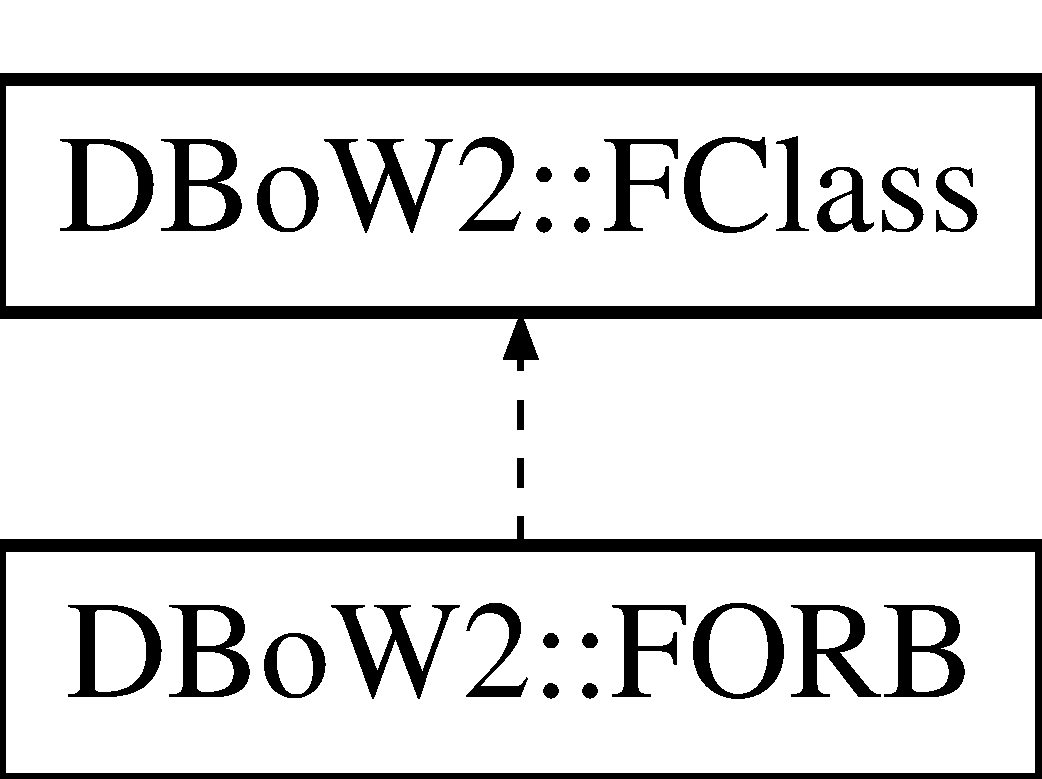
\includegraphics[height=2.000000cm]{class_d_bo_w2_1_1_f_o_r_b}
\end{center}
\end{figure}
\subsection*{Public Types}
\begin{DoxyCompactItemize}
\item 
typedef cv\+::\+Mat \mbox{\hyperlink{class_d_bo_w2_1_1_f_o_r_b_aef9b966d0293836fab9f55f1799ce0ed}{T\+Descriptor}}
\begin{DoxyCompactList}\small\item\em Descriptor type. \end{DoxyCompactList}\item 
typedef const \mbox{\hyperlink{class_d_bo_w2_1_1_f_o_r_b_aef9b966d0293836fab9f55f1799ce0ed}{T\+Descriptor}} $\ast$ \mbox{\hyperlink{class_d_bo_w2_1_1_f_o_r_b_ab52a6568044027cf30c8ac1514fed1a6}{p\+Descriptor}}
\begin{DoxyCompactList}\small\item\em Pointer to a single descriptor. \end{DoxyCompactList}\end{DoxyCompactItemize}
\subsection*{Static Public Member Functions}
\begin{DoxyCompactItemize}
\item 
static void \mbox{\hyperlink{class_d_bo_w2_1_1_f_o_r_b_a9d78adf3c5c6fe8f2e8668e247acf5cc}{mean\+Value}} (const std\+::vector$<$ \mbox{\hyperlink{class_d_bo_w2_1_1_f_class_a9c94e662003f61413fd542d67b45c3a9}{p\+Descriptor}} $>$ \&descriptors, \mbox{\hyperlink{class_d_bo_w2_1_1_f_o_r_b_aef9b966d0293836fab9f55f1799ce0ed}{T\+Descriptor}} \&mean)
\item 
static int \mbox{\hyperlink{class_d_bo_w2_1_1_f_o_r_b_ac166ab6808abc7c385dbaabfacfed38c}{distance}} (const \mbox{\hyperlink{class_d_bo_w2_1_1_f_o_r_b_aef9b966d0293836fab9f55f1799ce0ed}{T\+Descriptor}} \&a, const \mbox{\hyperlink{class_d_bo_w2_1_1_f_o_r_b_aef9b966d0293836fab9f55f1799ce0ed}{T\+Descriptor}} \&b)
\item 
static std\+::string \mbox{\hyperlink{class_d_bo_w2_1_1_f_o_r_b_a3c0ce0fd04ecd52b25b97d253fb922ea}{to\+String}} (const \mbox{\hyperlink{class_d_bo_w2_1_1_f_o_r_b_aef9b966d0293836fab9f55f1799ce0ed}{T\+Descriptor}} \&a)
\item 
static void \mbox{\hyperlink{class_d_bo_w2_1_1_f_o_r_b_a4023e7775d0691b44f6708f865b6b8d7}{from\+String}} (\mbox{\hyperlink{class_d_bo_w2_1_1_f_o_r_b_aef9b966d0293836fab9f55f1799ce0ed}{T\+Descriptor}} \&a, const std\+::string \&s)
\item 
static void \mbox{\hyperlink{class_d_bo_w2_1_1_f_o_r_b_a67b90eaed01dd54e380237c78886635f}{to\+Mat32F}} (const std\+::vector$<$ \mbox{\hyperlink{class_d_bo_w2_1_1_f_o_r_b_aef9b966d0293836fab9f55f1799ce0ed}{T\+Descriptor}} $>$ \&descriptors, cv\+::\+Mat \&mat)
\item 
static void \mbox{\hyperlink{class_d_bo_w2_1_1_f_o_r_b_af0a9e2ea44336f2975a7f3324777330c}{to\+Mat8U}} (const std\+::vector$<$ \mbox{\hyperlink{class_d_bo_w2_1_1_f_o_r_b_aef9b966d0293836fab9f55f1799ce0ed}{T\+Descriptor}} $>$ \&descriptors, cv\+::\+Mat \&mat)
\end{DoxyCompactItemize}
\subsection*{Static Public Attributes}
\begin{DoxyCompactItemize}
\item 
static const int \mbox{\hyperlink{class_d_bo_w2_1_1_f_o_r_b_ad6ed07af4e042effc3c0b169aa5bdd1a}{L}} = 32
\begin{DoxyCompactList}\small\item\em Descriptor length (in bytes) \end{DoxyCompactList}\end{DoxyCompactItemize}


\subsection{Detailed Description}
Functions to manipulate O\+RB descriptors. 

\subsection{Member Typedef Documentation}
\mbox{\Hypertarget{class_d_bo_w2_1_1_f_o_r_b_ab52a6568044027cf30c8ac1514fed1a6}\label{class_d_bo_w2_1_1_f_o_r_b_ab52a6568044027cf30c8ac1514fed1a6}} 
\index{D\+Bo\+W2\+::\+F\+O\+RB@{D\+Bo\+W2\+::\+F\+O\+RB}!p\+Descriptor@{p\+Descriptor}}
\index{p\+Descriptor@{p\+Descriptor}!D\+Bo\+W2\+::\+F\+O\+RB@{D\+Bo\+W2\+::\+F\+O\+RB}}
\subsubsection{\texorpdfstring{p\+Descriptor}{pDescriptor}}
{\footnotesize\ttfamily typedef const \mbox{\hyperlink{class_d_bo_w2_1_1_f_o_r_b_aef9b966d0293836fab9f55f1799ce0ed}{T\+Descriptor}}$\ast$ \mbox{\hyperlink{class_d_bo_w2_1_1_f_o_r_b_ab52a6568044027cf30c8ac1514fed1a6}{D\+Bo\+W2\+::\+F\+O\+R\+B\+::p\+Descriptor}}}



Pointer to a single descriptor. 

\mbox{\Hypertarget{class_d_bo_w2_1_1_f_o_r_b_aef9b966d0293836fab9f55f1799ce0ed}\label{class_d_bo_w2_1_1_f_o_r_b_aef9b966d0293836fab9f55f1799ce0ed}} 
\index{D\+Bo\+W2\+::\+F\+O\+RB@{D\+Bo\+W2\+::\+F\+O\+RB}!T\+Descriptor@{T\+Descriptor}}
\index{T\+Descriptor@{T\+Descriptor}!D\+Bo\+W2\+::\+F\+O\+RB@{D\+Bo\+W2\+::\+F\+O\+RB}}
\subsubsection{\texorpdfstring{T\+Descriptor}{TDescriptor}}
{\footnotesize\ttfamily typedef cv\+::\+Mat \mbox{\hyperlink{class_d_bo_w2_1_1_f_o_r_b_aef9b966d0293836fab9f55f1799ce0ed}{D\+Bo\+W2\+::\+F\+O\+R\+B\+::\+T\+Descriptor}}}



Descriptor type. 



\subsection{Member Function Documentation}
\mbox{\Hypertarget{class_d_bo_w2_1_1_f_o_r_b_ac166ab6808abc7c385dbaabfacfed38c}\label{class_d_bo_w2_1_1_f_o_r_b_ac166ab6808abc7c385dbaabfacfed38c}} 
\index{D\+Bo\+W2\+::\+F\+O\+RB@{D\+Bo\+W2\+::\+F\+O\+RB}!distance@{distance}}
\index{distance@{distance}!D\+Bo\+W2\+::\+F\+O\+RB@{D\+Bo\+W2\+::\+F\+O\+RB}}
\subsubsection{\texorpdfstring{distance()}{distance()}}
{\footnotesize\ttfamily int D\+Bo\+W2\+::\+F\+O\+R\+B\+::distance (\begin{DoxyParamCaption}\item[{const \mbox{\hyperlink{class_d_bo_w2_1_1_f_o_r_b_aef9b966d0293836fab9f55f1799ce0ed}{T\+Descriptor}} \&}]{a,  }\item[{const \mbox{\hyperlink{class_d_bo_w2_1_1_f_o_r_b_aef9b966d0293836fab9f55f1799ce0ed}{T\+Descriptor}} \&}]{b }\end{DoxyParamCaption})\hspace{0.3cm}{\ttfamily [static]}}

Calculates the distance between two descriptors 
\begin{DoxyParams}{Parameters}
{\em a} & \\
\hline
{\em b} & \\
\hline
\end{DoxyParams}
\begin{DoxyReturn}{Returns}
distance 
\end{DoxyReturn}
\mbox{\Hypertarget{class_d_bo_w2_1_1_f_o_r_b_a4023e7775d0691b44f6708f865b6b8d7}\label{class_d_bo_w2_1_1_f_o_r_b_a4023e7775d0691b44f6708f865b6b8d7}} 
\index{D\+Bo\+W2\+::\+F\+O\+RB@{D\+Bo\+W2\+::\+F\+O\+RB}!from\+String@{from\+String}}
\index{from\+String@{from\+String}!D\+Bo\+W2\+::\+F\+O\+RB@{D\+Bo\+W2\+::\+F\+O\+RB}}
\subsubsection{\texorpdfstring{from\+String()}{fromString()}}
{\footnotesize\ttfamily void D\+Bo\+W2\+::\+F\+O\+R\+B\+::from\+String (\begin{DoxyParamCaption}\item[{\mbox{\hyperlink{class_d_bo_w2_1_1_f_o_r_b_aef9b966d0293836fab9f55f1799ce0ed}{F\+O\+R\+B\+::\+T\+Descriptor}} \&}]{a,  }\item[{const std\+::string \&}]{s }\end{DoxyParamCaption})\hspace{0.3cm}{\ttfamily [static]}}

Returns a descriptor from a string 
\begin{DoxyParams}{Parameters}
{\em a} & descriptor \\
\hline
{\em s} & string version \\
\hline
\end{DoxyParams}
\mbox{\Hypertarget{class_d_bo_w2_1_1_f_o_r_b_a9d78adf3c5c6fe8f2e8668e247acf5cc}\label{class_d_bo_w2_1_1_f_o_r_b_a9d78adf3c5c6fe8f2e8668e247acf5cc}} 
\index{D\+Bo\+W2\+::\+F\+O\+RB@{D\+Bo\+W2\+::\+F\+O\+RB}!mean\+Value@{mean\+Value}}
\index{mean\+Value@{mean\+Value}!D\+Bo\+W2\+::\+F\+O\+RB@{D\+Bo\+W2\+::\+F\+O\+RB}}
\subsubsection{\texorpdfstring{mean\+Value()}{meanValue()}}
{\footnotesize\ttfamily void D\+Bo\+W2\+::\+F\+O\+R\+B\+::mean\+Value (\begin{DoxyParamCaption}\item[{const std\+::vector$<$ \mbox{\hyperlink{class_d_bo_w2_1_1_f_class_a9c94e662003f61413fd542d67b45c3a9}{p\+Descriptor}} $>$ \&}]{descriptors,  }\item[{\mbox{\hyperlink{class_d_bo_w2_1_1_f_o_r_b_aef9b966d0293836fab9f55f1799ce0ed}{T\+Descriptor}} \&}]{mean }\end{DoxyParamCaption})\hspace{0.3cm}{\ttfamily [static]}}

Calculates the mean value of a set of descriptors 
\begin{DoxyParams}{Parameters}
{\em descriptors} & \\
\hline
{\em mean} & mean descriptor \\
\hline
\end{DoxyParams}
\mbox{\Hypertarget{class_d_bo_w2_1_1_f_o_r_b_a67b90eaed01dd54e380237c78886635f}\label{class_d_bo_w2_1_1_f_o_r_b_a67b90eaed01dd54e380237c78886635f}} 
\index{D\+Bo\+W2\+::\+F\+O\+RB@{D\+Bo\+W2\+::\+F\+O\+RB}!to\+Mat32F@{to\+Mat32F}}
\index{to\+Mat32F@{to\+Mat32F}!D\+Bo\+W2\+::\+F\+O\+RB@{D\+Bo\+W2\+::\+F\+O\+RB}}
\subsubsection{\texorpdfstring{to\+Mat32\+F()}{toMat32F()}}
{\footnotesize\ttfamily void D\+Bo\+W2\+::\+F\+O\+R\+B\+::to\+Mat32F (\begin{DoxyParamCaption}\item[{const std\+::vector$<$ \mbox{\hyperlink{class_d_bo_w2_1_1_f_o_r_b_aef9b966d0293836fab9f55f1799ce0ed}{T\+Descriptor}} $>$ \&}]{descriptors,  }\item[{cv\+::\+Mat \&}]{mat }\end{DoxyParamCaption})\hspace{0.3cm}{\ttfamily [static]}}

Returns a mat with the descriptors in float format 
\begin{DoxyParams}{Parameters}
{\em descriptors} & \\
\hline
{\em mat} & (out) NxL 32F matrix \\
\hline
\end{DoxyParams}
\mbox{\Hypertarget{class_d_bo_w2_1_1_f_o_r_b_af0a9e2ea44336f2975a7f3324777330c}\label{class_d_bo_w2_1_1_f_o_r_b_af0a9e2ea44336f2975a7f3324777330c}} 
\index{D\+Bo\+W2\+::\+F\+O\+RB@{D\+Bo\+W2\+::\+F\+O\+RB}!to\+Mat8U@{to\+Mat8U}}
\index{to\+Mat8U@{to\+Mat8U}!D\+Bo\+W2\+::\+F\+O\+RB@{D\+Bo\+W2\+::\+F\+O\+RB}}
\subsubsection{\texorpdfstring{to\+Mat8\+U()}{toMat8U()}}
{\footnotesize\ttfamily void D\+Bo\+W2\+::\+F\+O\+R\+B\+::to\+Mat8U (\begin{DoxyParamCaption}\item[{const std\+::vector$<$ \mbox{\hyperlink{class_d_bo_w2_1_1_f_o_r_b_aef9b966d0293836fab9f55f1799ce0ed}{T\+Descriptor}} $>$ \&}]{descriptors,  }\item[{cv\+::\+Mat \&}]{mat }\end{DoxyParamCaption})\hspace{0.3cm}{\ttfamily [static]}}

\mbox{\Hypertarget{class_d_bo_w2_1_1_f_o_r_b_a3c0ce0fd04ecd52b25b97d253fb922ea}\label{class_d_bo_w2_1_1_f_o_r_b_a3c0ce0fd04ecd52b25b97d253fb922ea}} 
\index{D\+Bo\+W2\+::\+F\+O\+RB@{D\+Bo\+W2\+::\+F\+O\+RB}!to\+String@{to\+String}}
\index{to\+String@{to\+String}!D\+Bo\+W2\+::\+F\+O\+RB@{D\+Bo\+W2\+::\+F\+O\+RB}}
\subsubsection{\texorpdfstring{to\+String()}{toString()}}
{\footnotesize\ttfamily std\+::string D\+Bo\+W2\+::\+F\+O\+R\+B\+::to\+String (\begin{DoxyParamCaption}\item[{const \mbox{\hyperlink{class_d_bo_w2_1_1_f_o_r_b_aef9b966d0293836fab9f55f1799ce0ed}{T\+Descriptor}} \&}]{a }\end{DoxyParamCaption})\hspace{0.3cm}{\ttfamily [static]}}

Returns a string version of the descriptor 
\begin{DoxyParams}{Parameters}
{\em a} & descriptor \\
\hline
\end{DoxyParams}
\begin{DoxyReturn}{Returns}
string version 
\end{DoxyReturn}


\subsection{Member Data Documentation}
\mbox{\Hypertarget{class_d_bo_w2_1_1_f_o_r_b_ad6ed07af4e042effc3c0b169aa5bdd1a}\label{class_d_bo_w2_1_1_f_o_r_b_ad6ed07af4e042effc3c0b169aa5bdd1a}} 
\index{D\+Bo\+W2\+::\+F\+O\+RB@{D\+Bo\+W2\+::\+F\+O\+RB}!L@{L}}
\index{L@{L}!D\+Bo\+W2\+::\+F\+O\+RB@{D\+Bo\+W2\+::\+F\+O\+RB}}
\subsubsection{\texorpdfstring{L}{L}}
{\footnotesize\ttfamily const int D\+Bo\+W2\+::\+F\+O\+R\+B\+::L = 32\hspace{0.3cm}{\ttfamily [static]}}



Descriptor length (in bytes) 



The documentation for this class was generated from the following files\+:\begin{DoxyCompactItemize}
\item 
D\+:/github/\+V\+S\+L\+A\+M/\+O\+R\+B\+S\+L\+A\+M2/\+O\+R\+B-\/\+S\+L\+A\+M2-\/master/\+Thirdparty/\+D\+Bo\+W2/\+D\+Bo\+W2/\mbox{\hyperlink{_f_o_r_b_8h}{F\+O\+R\+B.\+h}}\item 
D\+:/github/\+V\+S\+L\+A\+M/\+O\+R\+B\+S\+L\+A\+M2/\+O\+R\+B-\/\+S\+L\+A\+M2-\/master/\+Thirdparty/\+D\+Bo\+W2/\+D\+Bo\+W2/\mbox{\hyperlink{_f_o_r_b_8cpp}{F\+O\+R\+B.\+cpp}}\end{DoxyCompactItemize}

\hypertarget{structg2o_1_1_force_linker}{}\section{g2o\+:\+:Force\+Linker Struct Reference}
\label{structg2o_1_1_force_linker}\index{g2o\+::\+Force\+Linker@{g2o\+::\+Force\+Linker}}


{\ttfamily \#include $<$misc.\+h$>$}

\subsection*{Public Member Functions}
\begin{DoxyCompactItemize}
\item 
\mbox{\hyperlink{structg2o_1_1_force_linker_ae5489ea8966a1d1f62471075f1dd2524}{Force\+Linker}} (\mbox{\hyperlink{namespaceg2o_a3be76fea59d320255e89425439f18f48}{Force\+Link\+Function}} function)
\end{DoxyCompactItemize}


\subsection{Constructor \& Destructor Documentation}
\mbox{\Hypertarget{structg2o_1_1_force_linker_ae5489ea8966a1d1f62471075f1dd2524}\label{structg2o_1_1_force_linker_ae5489ea8966a1d1f62471075f1dd2524}} 
\index{g2o\+::\+Force\+Linker@{g2o\+::\+Force\+Linker}!Force\+Linker@{Force\+Linker}}
\index{Force\+Linker@{Force\+Linker}!g2o\+::\+Force\+Linker@{g2o\+::\+Force\+Linker}}
\subsubsection{\texorpdfstring{Force\+Linker()}{ForceLinker()}}
{\footnotesize\ttfamily g2o\+::\+Force\+Linker\+::\+Force\+Linker (\begin{DoxyParamCaption}\item[{\mbox{\hyperlink{namespaceg2o_a3be76fea59d320255e89425439f18f48}{Force\+Link\+Function}}}]{function }\end{DoxyParamCaption})\hspace{0.3cm}{\ttfamily [inline]}}



The documentation for this struct was generated from the following file\+:\begin{DoxyCompactItemize}
\item 
D\+:/github/\+V\+S\+L\+A\+M/\+O\+R\+B\+S\+L\+A\+M2/\+O\+R\+B-\/\+S\+L\+A\+M2-\/master/\+Thirdparty/g2o/g2o/stuff/\mbox{\hyperlink{misc_8h}{misc.\+h}}\end{DoxyCompactItemize}

\hypertarget{class_o_r_b___s_l_a_m2_1_1_frame}{}\section{O\+R\+B\+\_\+\+S\+L\+A\+M2\+:\+:Frame Class Reference}
\label{class_o_r_b___s_l_a_m2_1_1_frame}\index{O\+R\+B\+\_\+\+S\+L\+A\+M2\+::\+Frame@{O\+R\+B\+\_\+\+S\+L\+A\+M2\+::\+Frame}}


对一帧图像进行描述  




{\ttfamily \#include $<$Frame.\+h$>$}

\subsection*{Public Member Functions}
\begin{DoxyCompactItemize}
\item 
\mbox{\hyperlink{class_o_r_b___s_l_a_m2_1_1_frame_aa43d601e841ddb7a9f100b0b9afd3b10}{Frame}} ()
\item 
\mbox{\hyperlink{class_o_r_b___s_l_a_m2_1_1_frame_ac7e6ed9973b81ec85e91228e3d4ecf22}{Frame}} (const \mbox{\hyperlink{class_o_r_b___s_l_a_m2_1_1_frame}{Frame}} \&frame)
\begin{DoxyCompactList}\small\item\em Copy constructor. \end{DoxyCompactList}\item 
\mbox{\hyperlink{class_o_r_b___s_l_a_m2_1_1_frame_a24d3c1a1a811fa0f9d44e717a044b2a4}{Frame}} (const cv\+::\+Mat \&im\+Left, const cv\+::\+Mat \&im\+Right, const double \&time\+Stamp, \mbox{\hyperlink{class_o_r_b___s_l_a_m2_1_1_o_r_bextractor}{O\+R\+Bextractor}} $\ast$extractor\+Left, \mbox{\hyperlink{class_o_r_b___s_l_a_m2_1_1_o_r_bextractor}{O\+R\+Bextractor}} $\ast$extractor\+Right, \mbox{\hyperlink{namespace_o_r_b___s_l_a_m2_a2fafba714858cab1bb18d438e2e83c5d}{O\+R\+B\+Vocabulary}} $\ast$voc, cv\+::\+Mat \&K, cv\+::\+Mat \&dist\+Coef, const float \&bf, const float \&th\+Depth)
\item 
\mbox{\hyperlink{class_o_r_b___s_l_a_m2_1_1_frame_ac205fd2081c647e4841369828902f8fe}{Frame}} (const cv\+::\+Mat \&im\+Gray, const cv\+::\+Mat \&im\+Depth, const double \&time\+Stamp, \mbox{\hyperlink{class_o_r_b___s_l_a_m2_1_1_o_r_bextractor}{O\+R\+Bextractor}} $\ast$extractor, \mbox{\hyperlink{namespace_o_r_b___s_l_a_m2_a2fafba714858cab1bb18d438e2e83c5d}{O\+R\+B\+Vocabulary}} $\ast$voc, cv\+::\+Mat \&K, cv\+::\+Mat \&dist\+Coef, const float \&bf, const float \&th\+Depth)
\item 
\mbox{\hyperlink{class_o_r_b___s_l_a_m2_1_1_frame_a39a57316938495a9ca8a053edd74b414}{Frame}} (const cv\+::\+Mat \&im\+Gray, const double \&time\+Stamp, \mbox{\hyperlink{class_o_r_b___s_l_a_m2_1_1_o_r_bextractor}{O\+R\+Bextractor}} $\ast$extractor, \mbox{\hyperlink{namespace_o_r_b___s_l_a_m2_a2fafba714858cab1bb18d438e2e83c5d}{O\+R\+B\+Vocabulary}} $\ast$voc, cv\+::\+Mat \&K, cv\+::\+Mat \&dist\+Coef, const float \&bf, const float \&th\+Depth)
\item 
void \mbox{\hyperlink{class_o_r_b___s_l_a_m2_1_1_frame_a626aef981e9fd9caff63bf93f1abf47f}{Extract\+O\+RB}} (int flag, const cv\+::\+Mat \&im)
\item 
void \mbox{\hyperlink{class_o_r_b___s_l_a_m2_1_1_frame_ac748d2318f9a409406dba4910ff5ef8e}{Compute\+BoW}} ()
\begin{DoxyCompactList}\small\item\em Bag of Words Representation. \end{DoxyCompactList}\item 
void \mbox{\hyperlink{class_o_r_b___s_l_a_m2_1_1_frame_a95cf2ea68735ef3e8c2d820eada11bf4}{Set\+Pose}} (cv\+::\+Mat Tcw)
\begin{DoxyCompactList}\small\item\em Set the camera pose. \end{DoxyCompactList}\item 
void \mbox{\hyperlink{class_o_r_b___s_l_a_m2_1_1_frame_a0a18d3024a23f6fa2cab9c7d987598c2}{Update\+Pose\+Matrices}} ()
\begin{DoxyCompactList}\small\item\em Computes rotation, translation and camera center matrices from the camera pose. \end{DoxyCompactList}\item 
cv\+::\+Mat \mbox{\hyperlink{class_o_r_b___s_l_a_m2_1_1_frame_a48c8983df3a521ed7439d9654b28e390}{Get\+Camera\+Center}} ()
\item 
cv\+::\+Mat \mbox{\hyperlink{class_o_r_b___s_l_a_m2_1_1_frame_a96ec2c272f2ecea3f94b8472add80478}{Get\+Rotation\+Inverse}} ()
\item 
bool \mbox{\hyperlink{class_o_r_b___s_l_a_m2_1_1_frame_a0929e100e3380dba1baba12dfa8904c4}{is\+In\+Frustum}} (\mbox{\hyperlink{class_o_r_b___s_l_a_m2_1_1_map_point}{Map\+Point}} $\ast$p\+MP, float viewing\+Cos\+Limit)
\begin{DoxyCompactList}\small\item\em 判断一个点是否在视野内 \end{DoxyCompactList}\item 
bool \mbox{\hyperlink{class_o_r_b___s_l_a_m2_1_1_frame_ae2bc4b1482d2010511da5423d298c9bd}{Pos\+In\+Grid}} (const cv\+::\+Key\+Point \&kp, int \&posX, int \&posY)
\item 
vector$<$ size\+\_\+t $>$ \mbox{\hyperlink{class_o_r_b___s_l_a_m2_1_1_frame_a922a340f438ed0ddd2d7d2a9f95872b6}{Get\+Features\+In\+Area}} (const float \&x, const float \&y, const float \&r, const int min\+Level=-\/1, const int max\+Level=-\/1) const
\begin{DoxyCompactList}\small\item\em 找到在 以x,y为中心,边长为2r的方形内且在\mbox{[}min\+Level, max\+Level\mbox{]}的特征点 \end{DoxyCompactList}\item 
void \mbox{\hyperlink{class_o_r_b___s_l_a_m2_1_1_frame_a77a570d7851bad90ca31c4d55a5105e7}{Compute\+Stereo\+Matches}} ()
\begin{DoxyCompactList}\small\item\em 双目匹配 \end{DoxyCompactList}\item 
void \mbox{\hyperlink{class_o_r_b___s_l_a_m2_1_1_frame_a2818781adf6aec30b8bd8783ba228dce}{Compute\+Stereo\+From\+R\+G\+BD}} (const cv\+::\+Mat \&im\+Depth)
\item 
cv\+::\+Mat \mbox{\hyperlink{class_o_r_b___s_l_a_m2_1_1_frame_a46084d187e1fc60181e1c72f77c733ca}{Unproject\+Stereo}} (const int \&i)
\begin{DoxyCompactList}\small\item\em Backprojects a keypoint (if stereo/depth info available) into 3D world coordinates. \end{DoxyCompactList}\end{DoxyCompactItemize}
\subsection*{Public Attributes}
\begin{DoxyCompactItemize}
\item 
\mbox{\hyperlink{namespace_o_r_b___s_l_a_m2_a2fafba714858cab1bb18d438e2e83c5d}{O\+R\+B\+Vocabulary}} $\ast$ \mbox{\hyperlink{class_o_r_b___s_l_a_m2_1_1_frame_a4c54c9963da838cd6fa83a65930bd1b7}{mp\+O\+R\+Bvocabulary}}
\item 
\mbox{\hyperlink{class_o_r_b___s_l_a_m2_1_1_o_r_bextractor}{O\+R\+Bextractor}} $\ast$ \mbox{\hyperlink{class_o_r_b___s_l_a_m2_1_1_frame_a5c4f28562114c30c6276f2e42aac6607}{mp\+O\+R\+Bextractor\+Left}}
\item 
\mbox{\hyperlink{class_o_r_b___s_l_a_m2_1_1_o_r_bextractor}{O\+R\+Bextractor}} $\ast$ \mbox{\hyperlink{class_o_r_b___s_l_a_m2_1_1_frame_a53cd56c00a153e8b54be49ea73b64672}{mp\+O\+R\+Bextractor\+Right}}
\item 
double \mbox{\hyperlink{class_o_r_b___s_l_a_m2_1_1_frame_a7987de59d3b4bf655614e19db0c90278}{m\+Time\+Stamp}}
\item 
cv\+::\+Mat \mbox{\hyperlink{class_o_r_b___s_l_a_m2_1_1_frame_a6508d43259538370dcb77911122dc85b}{mK}}
\item 
cv\+::\+Mat \mbox{\hyperlink{class_o_r_b___s_l_a_m2_1_1_frame_aef15cff1b0d7572f49975d3200ffd140}{m\+Dist\+Coef}}
\item 
float \mbox{\hyperlink{class_o_r_b___s_l_a_m2_1_1_frame_afb4090340565194b372b2ce0d95f16fb}{mbf}}
\item 
float \mbox{\hyperlink{class_o_r_b___s_l_a_m2_1_1_frame_a950131e5ed7fca2a73fc5a50e6d9b2de}{mb}}
\item 
float \mbox{\hyperlink{class_o_r_b___s_l_a_m2_1_1_frame_a15e0251e1e18b84f385ad817f0e8ba1a}{m\+Th\+Depth}}
\item 
int \mbox{\hyperlink{class_o_r_b___s_l_a_m2_1_1_frame_a0035828f1744f1bdd4ae8681e7cbbd32}{N}}
\begin{DoxyCompactList}\small\item\em Key\+Points数量 \end{DoxyCompactList}\item 
std\+::vector$<$ cv\+::\+Key\+Point $>$ \mbox{\hyperlink{class_o_r_b___s_l_a_m2_1_1_frame_a86563de6facec0433e31f726723057e4}{mv\+Keys}}
\item 
std\+::vector$<$ cv\+::\+Key\+Point $>$ \mbox{\hyperlink{class_o_r_b___s_l_a_m2_1_1_frame_a15b04baf8fc5282883ccc002eb703a8e}{mv\+Keys\+Right}}
\item 
std\+::vector$<$ cv\+::\+Key\+Point $>$ \mbox{\hyperlink{class_o_r_b___s_l_a_m2_1_1_frame_a13737fa65f0ce693275f1919240bac35}{mv\+Keys\+Un}}
\item 
std\+::vector$<$ float $>$ \mbox{\hyperlink{class_o_r_b___s_l_a_m2_1_1_frame_a09a1957b966542e640ecabc41ec76c16}{mvu\+Right}}
\item 
std\+::vector$<$ float $>$ \mbox{\hyperlink{class_o_r_b___s_l_a_m2_1_1_frame_a4232b92ebf890728291ef2a66e7d39bb}{mv\+Depth}}
\item 
\mbox{\hyperlink{class_d_bo_w2_1_1_bow_vector}{D\+Bo\+W2\+::\+Bow\+Vector}} \mbox{\hyperlink{class_o_r_b___s_l_a_m2_1_1_frame_a68bbc187861a8e5c0ed9d92b5308c2cb}{m\+Bow\+Vec}}
\item 
\mbox{\hyperlink{class_d_bo_w2_1_1_feature_vector}{D\+Bo\+W2\+::\+Feature\+Vector}} \mbox{\hyperlink{class_o_r_b___s_l_a_m2_1_1_frame_a8153622c07ed98421bd7c7b2b7451b03}{m\+Feat\+Vec}}
\item 
cv\+::\+Mat \mbox{\hyperlink{class_o_r_b___s_l_a_m2_1_1_frame_a0dfc1a363215ad0a09303e612a1ffbe7}{m\+Descriptors}}
\item 
cv\+::\+Mat \mbox{\hyperlink{class_o_r_b___s_l_a_m2_1_1_frame_afe3cee153dda7e06d5004fd959fcd88e}{m\+Descriptors\+Right}}
\item 
std\+::vector$<$ \mbox{\hyperlink{class_o_r_b___s_l_a_m2_1_1_map_point}{Map\+Point}} $\ast$ $>$ \mbox{\hyperlink{class_o_r_b___s_l_a_m2_1_1_frame_a48e791ae28b483211dad6b3474027935}{mvp\+Map\+Points}}
\item 
std\+::vector$<$ bool $>$ \mbox{\hyperlink{class_o_r_b___s_l_a_m2_1_1_frame_aa05cc57f36b5b04a2e1690e576c93fc8}{mvb\+Outlier}}
\item 
std\+::vector$<$ std\+::size\+\_\+t $>$ \mbox{\hyperlink{class_o_r_b___s_l_a_m2_1_1_frame_a194dca06186458639d46234d828afeed}{m\+Grid}} \mbox{[}\mbox{\hyperlink{_frame_8h_a3ef79fa8924a9c5df3cddac58a52ab0c}{F\+R\+A\+M\+E\+\_\+\+G\+R\+I\+D\+\_\+\+C\+O\+LS}}\mbox{]}\mbox{[}\mbox{\hyperlink{_frame_8h_a9550f0488f3dac9a5c56f0d3c07c01c1}{F\+R\+A\+M\+E\+\_\+\+G\+R\+I\+D\+\_\+\+R\+O\+WS}}\mbox{]}
\item 
cv\+::\+Mat \mbox{\hyperlink{class_o_r_b___s_l_a_m2_1_1_frame_a3be6708cfd359fae30307f9408abd6f9}{m\+Tcw}}
\begin{DoxyCompactList}\small\item\em 相机姿态 世界坐标系到相机坐标坐标系的变换矩阵 \end{DoxyCompactList}\item 
long unsigned int \mbox{\hyperlink{class_o_r_b___s_l_a_m2_1_1_frame_acd59686475a89bfdfcae316dfa6b6069}{mn\+Id}}
\begin{DoxyCompactList}\small\item\em Current \mbox{\hyperlink{class_o_r_b___s_l_a_m2_1_1_frame}{Frame}} id. \end{DoxyCompactList}\item 
\mbox{\hyperlink{class_o_r_b___s_l_a_m2_1_1_key_frame}{Key\+Frame}} $\ast$ \mbox{\hyperlink{class_o_r_b___s_l_a_m2_1_1_frame_a4f5187c3a75ef493687fa0582fed0aa8}{mp\+Reference\+KF}}
\item 
int \mbox{\hyperlink{class_o_r_b___s_l_a_m2_1_1_frame_a4c4b02f27be28aec6cb8bb1bab3f622f}{mn\+Scale\+Levels}}
\item 
float \mbox{\hyperlink{class_o_r_b___s_l_a_m2_1_1_frame_aab180286bac29f4e030ce850c51c435c}{mf\+Scale\+Factor}}
\item 
float \mbox{\hyperlink{class_o_r_b___s_l_a_m2_1_1_frame_ad3ddefb0665fb5128391a7e59a236e9a}{mf\+Log\+Scale\+Factor}}
\item 
vector$<$ float $>$ \mbox{\hyperlink{class_o_r_b___s_l_a_m2_1_1_frame_a55d7bd3fa5d3fa8d2ecf18609e91f98e}{mv\+Scale\+Factors}}
\item 
vector$<$ float $>$ \mbox{\hyperlink{class_o_r_b___s_l_a_m2_1_1_frame_a4c7ed1316a886b9a7c3f02ee13219b8c}{mv\+Inv\+Scale\+Factors}}
\item 
vector$<$ float $>$ \mbox{\hyperlink{class_o_r_b___s_l_a_m2_1_1_frame_afba8ed34e98d14761be2c1922863cd65}{mv\+Level\+Sigma2}}
\item 
vector$<$ float $>$ \mbox{\hyperlink{class_o_r_b___s_l_a_m2_1_1_frame_a1979f999e1d3a858bf7db733791a477e}{mv\+Inv\+Level\+Sigma2}}
\end{DoxyCompactItemize}
\subsection*{Static Public Attributes}
\begin{DoxyCompactItemize}
\item 
static float \mbox{\hyperlink{class_o_r_b___s_l_a_m2_1_1_frame_ab505e3f86afa1c3d16b98fda89ec394c}{fx}}
\item 
static float \mbox{\hyperlink{class_o_r_b___s_l_a_m2_1_1_frame_a226a0adc90bc7a09502fc4db00ee20d7}{fy}}
\item 
static float \mbox{\hyperlink{class_o_r_b___s_l_a_m2_1_1_frame_a5f2803f215bc30016bd0833d8c7d5942}{cx}}
\item 
static float \mbox{\hyperlink{class_o_r_b___s_l_a_m2_1_1_frame_abf6a631b787270da2d5b3c0f53615b62}{cy}}
\item 
static float \mbox{\hyperlink{class_o_r_b___s_l_a_m2_1_1_frame_a617c29a929afd74d599c9e41fc71abea}{invfx}}
\item 
static float \mbox{\hyperlink{class_o_r_b___s_l_a_m2_1_1_frame_ad1dfdeb6378b11477c1b94233f881345}{invfy}}
\item 
static float \mbox{\hyperlink{class_o_r_b___s_l_a_m2_1_1_frame_afc2f7799428918dbbf46f7dfc4ccd59d}{mf\+Grid\+Element\+Width\+Inv}}
\item 
static float \mbox{\hyperlink{class_o_r_b___s_l_a_m2_1_1_frame_a010327bee872485894b5905d17462086}{mf\+Grid\+Element\+Height\+Inv}}
\item 
static long unsigned int \mbox{\hyperlink{class_o_r_b___s_l_a_m2_1_1_frame_a1ea8a00151931d155747283850467733}{n\+Next\+Id}} =0
\begin{DoxyCompactList}\small\item\em Next \mbox{\hyperlink{class_o_r_b___s_l_a_m2_1_1_frame}{Frame}} id. \end{DoxyCompactList}\item 
static float \mbox{\hyperlink{class_o_r_b___s_l_a_m2_1_1_frame_ac119d458dd562196240e72b7dbb54f3d}{mn\+MinX}}
\item 
static float \mbox{\hyperlink{class_o_r_b___s_l_a_m2_1_1_frame_ade32bf37203ae9578e4bd9a02cc0f7c1}{mn\+MaxX}}
\item 
static float \mbox{\hyperlink{class_o_r_b___s_l_a_m2_1_1_frame_a38d30251e5bf5e44411e83b688dfac97}{mn\+MinY}}
\item 
static float \mbox{\hyperlink{class_o_r_b___s_l_a_m2_1_1_frame_ac63dd82413eba002462109e625207ab4}{mn\+MaxY}}
\item 
static bool \mbox{\hyperlink{class_o_r_b___s_l_a_m2_1_1_frame_a9f57238f88850695d8cf032b5af0dad6}{mb\+Initial\+Computations}} =true
\end{DoxyCompactItemize}
\subsection*{Private Member Functions}
\begin{DoxyCompactItemize}
\item 
void \mbox{\hyperlink{class_o_r_b___s_l_a_m2_1_1_frame_a2a97fc690d8c1cd5e975d19440a31657}{Undistort\+Key\+Points}} ()
\item 
void \mbox{\hyperlink{class_o_r_b___s_l_a_m2_1_1_frame_a420f0369833f856df1973410ea39b335}{Compute\+Image\+Bounds}} (const cv\+::\+Mat \&im\+Left)
\item 
void \mbox{\hyperlink{class_o_r_b___s_l_a_m2_1_1_frame_aa3ba21cd44638b322db024cba2b9c19e}{Assign\+Features\+To\+Grid}} ()
\end{DoxyCompactItemize}
\subsection*{Private Attributes}
\begin{DoxyCompactItemize}
\item 
cv\+::\+Mat \mbox{\hyperlink{class_o_r_b___s_l_a_m2_1_1_frame_a3923c4b0fc83ab5fdba34ddd823621c6}{m\+Rcw}}
\begin{DoxyCompactList}\small\item\em Rotation from world to camera. \end{DoxyCompactList}\item 
cv\+::\+Mat \mbox{\hyperlink{class_o_r_b___s_l_a_m2_1_1_frame_a31b2fa3a66f2855ec0c71c9ba34cfa8f}{mtcw}}
\begin{DoxyCompactList}\small\item\em Translation from world to camera. \end{DoxyCompactList}\item 
cv\+::\+Mat \mbox{\hyperlink{class_o_r_b___s_l_a_m2_1_1_frame_afda03a992077579e0ed3c20240eef276}{m\+Rwc}}
\begin{DoxyCompactList}\small\item\em Rotation from camera to world. \end{DoxyCompactList}\item 
cv\+::\+Mat \mbox{\hyperlink{class_o_r_b___s_l_a_m2_1_1_frame_a4315630bb510b424d8b089975135199a}{m\+Ow}}
\begin{DoxyCompactList}\small\item\em mtwc,Translation from camera to world \end{DoxyCompactList}\end{DoxyCompactItemize}


\subsection{Detailed Description}
对一帧图像进行描述 

\subsection{Constructor \& Destructor Documentation}
\mbox{\Hypertarget{class_o_r_b___s_l_a_m2_1_1_frame_aa43d601e841ddb7a9f100b0b9afd3b10}\label{class_o_r_b___s_l_a_m2_1_1_frame_aa43d601e841ddb7a9f100b0b9afd3b10}} 
\index{O\+R\+B\+\_\+\+S\+L\+A\+M2\+::\+Frame@{O\+R\+B\+\_\+\+S\+L\+A\+M2\+::\+Frame}!Frame@{Frame}}
\index{Frame@{Frame}!O\+R\+B\+\_\+\+S\+L\+A\+M2\+::\+Frame@{O\+R\+B\+\_\+\+S\+L\+A\+M2\+::\+Frame}}
\subsubsection{\texorpdfstring{Frame()}{Frame()}\hspace{0.1cm}{\footnotesize\ttfamily [1/5]}}
{\footnotesize\ttfamily O\+R\+B\+\_\+\+S\+L\+A\+M2\+::\+Frame\+::\+Frame (\begin{DoxyParamCaption}{ }\end{DoxyParamCaption})}

\mbox{\Hypertarget{class_o_r_b___s_l_a_m2_1_1_frame_ac7e6ed9973b81ec85e91228e3d4ecf22}\label{class_o_r_b___s_l_a_m2_1_1_frame_ac7e6ed9973b81ec85e91228e3d4ecf22}} 
\index{O\+R\+B\+\_\+\+S\+L\+A\+M2\+::\+Frame@{O\+R\+B\+\_\+\+S\+L\+A\+M2\+::\+Frame}!Frame@{Frame}}
\index{Frame@{Frame}!O\+R\+B\+\_\+\+S\+L\+A\+M2\+::\+Frame@{O\+R\+B\+\_\+\+S\+L\+A\+M2\+::\+Frame}}
\subsubsection{\texorpdfstring{Frame()}{Frame()}\hspace{0.1cm}{\footnotesize\ttfamily [2/5]}}
{\footnotesize\ttfamily O\+R\+B\+\_\+\+S\+L\+A\+M2\+::\+Frame\+::\+Frame (\begin{DoxyParamCaption}\item[{const \mbox{\hyperlink{class_o_r_b___s_l_a_m2_1_1_frame}{Frame}} \&}]{frame }\end{DoxyParamCaption})}



Copy constructor. 

复制构造函数, m\+Last\+Frame = Frame(m\+Current\+Frame) \mbox{\Hypertarget{class_o_r_b___s_l_a_m2_1_1_frame_a24d3c1a1a811fa0f9d44e717a044b2a4}\label{class_o_r_b___s_l_a_m2_1_1_frame_a24d3c1a1a811fa0f9d44e717a044b2a4}} 
\index{O\+R\+B\+\_\+\+S\+L\+A\+M2\+::\+Frame@{O\+R\+B\+\_\+\+S\+L\+A\+M2\+::\+Frame}!Frame@{Frame}}
\index{Frame@{Frame}!O\+R\+B\+\_\+\+S\+L\+A\+M2\+::\+Frame@{O\+R\+B\+\_\+\+S\+L\+A\+M2\+::\+Frame}}
\subsubsection{\texorpdfstring{Frame()}{Frame()}\hspace{0.1cm}{\footnotesize\ttfamily [3/5]}}
{\footnotesize\ttfamily O\+R\+B\+\_\+\+S\+L\+A\+M2\+::\+Frame\+::\+Frame (\begin{DoxyParamCaption}\item[{const cv\+::\+Mat \&}]{im\+Left,  }\item[{const cv\+::\+Mat \&}]{im\+Right,  }\item[{const double \&}]{time\+Stamp,  }\item[{\mbox{\hyperlink{class_o_r_b___s_l_a_m2_1_1_o_r_bextractor}{O\+R\+Bextractor}} $\ast$}]{extractor\+Left,  }\item[{\mbox{\hyperlink{class_o_r_b___s_l_a_m2_1_1_o_r_bextractor}{O\+R\+Bextractor}} $\ast$}]{extractor\+Right,  }\item[{\mbox{\hyperlink{namespace_o_r_b___s_l_a_m2_a2fafba714858cab1bb18d438e2e83c5d}{O\+R\+B\+Vocabulary}} $\ast$}]{voc,  }\item[{cv\+::\+Mat \&}]{K,  }\item[{cv\+::\+Mat \&}]{dist\+Coef,  }\item[{const float \&}]{bf,  }\item[{const float \&}]{th\+Depth }\end{DoxyParamCaption})}

\mbox{\Hypertarget{class_o_r_b___s_l_a_m2_1_1_frame_ac205fd2081c647e4841369828902f8fe}\label{class_o_r_b___s_l_a_m2_1_1_frame_ac205fd2081c647e4841369828902f8fe}} 
\index{O\+R\+B\+\_\+\+S\+L\+A\+M2\+::\+Frame@{O\+R\+B\+\_\+\+S\+L\+A\+M2\+::\+Frame}!Frame@{Frame}}
\index{Frame@{Frame}!O\+R\+B\+\_\+\+S\+L\+A\+M2\+::\+Frame@{O\+R\+B\+\_\+\+S\+L\+A\+M2\+::\+Frame}}
\subsubsection{\texorpdfstring{Frame()}{Frame()}\hspace{0.1cm}{\footnotesize\ttfamily [4/5]}}
{\footnotesize\ttfamily O\+R\+B\+\_\+\+S\+L\+A\+M2\+::\+Frame\+::\+Frame (\begin{DoxyParamCaption}\item[{const cv\+::\+Mat \&}]{im\+Gray,  }\item[{const cv\+::\+Mat \&}]{im\+Depth,  }\item[{const double \&}]{time\+Stamp,  }\item[{\mbox{\hyperlink{class_o_r_b___s_l_a_m2_1_1_o_r_bextractor}{O\+R\+Bextractor}} $\ast$}]{extractor,  }\item[{\mbox{\hyperlink{namespace_o_r_b___s_l_a_m2_a2fafba714858cab1bb18d438e2e83c5d}{O\+R\+B\+Vocabulary}} $\ast$}]{voc,  }\item[{cv\+::\+Mat \&}]{K,  }\item[{cv\+::\+Mat \&}]{dist\+Coef,  }\item[{const float \&}]{bf,  }\item[{const float \&}]{th\+Depth }\end{DoxyParamCaption})}

\mbox{\Hypertarget{class_o_r_b___s_l_a_m2_1_1_frame_a39a57316938495a9ca8a053edd74b414}\label{class_o_r_b___s_l_a_m2_1_1_frame_a39a57316938495a9ca8a053edd74b414}} 
\index{O\+R\+B\+\_\+\+S\+L\+A\+M2\+::\+Frame@{O\+R\+B\+\_\+\+S\+L\+A\+M2\+::\+Frame}!Frame@{Frame}}
\index{Frame@{Frame}!O\+R\+B\+\_\+\+S\+L\+A\+M2\+::\+Frame@{O\+R\+B\+\_\+\+S\+L\+A\+M2\+::\+Frame}}
\subsubsection{\texorpdfstring{Frame()}{Frame()}\hspace{0.1cm}{\footnotesize\ttfamily [5/5]}}
{\footnotesize\ttfamily O\+R\+B\+\_\+\+S\+L\+A\+M2\+::\+Frame\+::\+Frame (\begin{DoxyParamCaption}\item[{const cv\+::\+Mat \&}]{im\+Gray,  }\item[{const double \&}]{time\+Stamp,  }\item[{\mbox{\hyperlink{class_o_r_b___s_l_a_m2_1_1_o_r_bextractor}{O\+R\+Bextractor}} $\ast$}]{extractor,  }\item[{\mbox{\hyperlink{namespace_o_r_b___s_l_a_m2_a2fafba714858cab1bb18d438e2e83c5d}{O\+R\+B\+Vocabulary}} $\ast$}]{voc,  }\item[{cv\+::\+Mat \&}]{K,  }\item[{cv\+::\+Mat \&}]{dist\+Coef,  }\item[{const float \&}]{bf,  }\item[{const float \&}]{th\+Depth }\end{DoxyParamCaption})}



\subsection{Member Function Documentation}
\mbox{\Hypertarget{class_o_r_b___s_l_a_m2_1_1_frame_aa3ba21cd44638b322db024cba2b9c19e}\label{class_o_r_b___s_l_a_m2_1_1_frame_aa3ba21cd44638b322db024cba2b9c19e}} 
\index{O\+R\+B\+\_\+\+S\+L\+A\+M2\+::\+Frame@{O\+R\+B\+\_\+\+S\+L\+A\+M2\+::\+Frame}!Assign\+Features\+To\+Grid@{Assign\+Features\+To\+Grid}}
\index{Assign\+Features\+To\+Grid@{Assign\+Features\+To\+Grid}!O\+R\+B\+\_\+\+S\+L\+A\+M2\+::\+Frame@{O\+R\+B\+\_\+\+S\+L\+A\+M2\+::\+Frame}}
\subsubsection{\texorpdfstring{Assign\+Features\+To\+Grid()}{AssignFeaturesToGrid()}}
{\footnotesize\ttfamily void O\+R\+B\+\_\+\+S\+L\+A\+M2\+::\+Frame\+::\+Assign\+Features\+To\+Grid (\begin{DoxyParamCaption}{ }\end{DoxyParamCaption})\hspace{0.3cm}{\ttfamily [private]}}

\mbox{\Hypertarget{class_o_r_b___s_l_a_m2_1_1_frame_ac748d2318f9a409406dba4910ff5ef8e}\label{class_o_r_b___s_l_a_m2_1_1_frame_ac748d2318f9a409406dba4910ff5ef8e}} 
\index{O\+R\+B\+\_\+\+S\+L\+A\+M2\+::\+Frame@{O\+R\+B\+\_\+\+S\+L\+A\+M2\+::\+Frame}!Compute\+BoW@{Compute\+BoW}}
\index{Compute\+BoW@{Compute\+BoW}!O\+R\+B\+\_\+\+S\+L\+A\+M2\+::\+Frame@{O\+R\+B\+\_\+\+S\+L\+A\+M2\+::\+Frame}}
\subsubsection{\texorpdfstring{Compute\+Bo\+W()}{ComputeBoW()}}
{\footnotesize\ttfamily void O\+R\+B\+\_\+\+S\+L\+A\+M2\+::\+Frame\+::\+Compute\+BoW (\begin{DoxyParamCaption}{ }\end{DoxyParamCaption})}



Bag of Words Representation. 

计算词包m\+Bow\+Vec和m\+Feat\+Vec,其中m\+Feat\+Vec记录了属于第i个node(在第4层)的ni个描述子 \begin{DoxySeeAlso}{See also}
Create\+Initial\+Map\+Monocular() Track\+Reference\+Key\+Frame() Relocalization() 
\end{DoxySeeAlso}
\mbox{\Hypertarget{class_o_r_b___s_l_a_m2_1_1_frame_a420f0369833f856df1973410ea39b335}\label{class_o_r_b___s_l_a_m2_1_1_frame_a420f0369833f856df1973410ea39b335}} 
\index{O\+R\+B\+\_\+\+S\+L\+A\+M2\+::\+Frame@{O\+R\+B\+\_\+\+S\+L\+A\+M2\+::\+Frame}!Compute\+Image\+Bounds@{Compute\+Image\+Bounds}}
\index{Compute\+Image\+Bounds@{Compute\+Image\+Bounds}!O\+R\+B\+\_\+\+S\+L\+A\+M2\+::\+Frame@{O\+R\+B\+\_\+\+S\+L\+A\+M2\+::\+Frame}}
\subsubsection{\texorpdfstring{Compute\+Image\+Bounds()}{ComputeImageBounds()}}
{\footnotesize\ttfamily void O\+R\+B\+\_\+\+S\+L\+A\+M2\+::\+Frame\+::\+Compute\+Image\+Bounds (\begin{DoxyParamCaption}\item[{const cv\+::\+Mat \&}]{im\+Left }\end{DoxyParamCaption})\hspace{0.3cm}{\ttfamily [private]}}

\mbox{\Hypertarget{class_o_r_b___s_l_a_m2_1_1_frame_a2818781adf6aec30b8bd8783ba228dce}\label{class_o_r_b___s_l_a_m2_1_1_frame_a2818781adf6aec30b8bd8783ba228dce}} 
\index{O\+R\+B\+\_\+\+S\+L\+A\+M2\+::\+Frame@{O\+R\+B\+\_\+\+S\+L\+A\+M2\+::\+Frame}!Compute\+Stereo\+From\+R\+G\+BD@{Compute\+Stereo\+From\+R\+G\+BD}}
\index{Compute\+Stereo\+From\+R\+G\+BD@{Compute\+Stereo\+From\+R\+G\+BD}!O\+R\+B\+\_\+\+S\+L\+A\+M2\+::\+Frame@{O\+R\+B\+\_\+\+S\+L\+A\+M2\+::\+Frame}}
\subsubsection{\texorpdfstring{Compute\+Stereo\+From\+R\+G\+B\+D()}{ComputeStereoFromRGBD()}}
{\footnotesize\ttfamily void O\+R\+B\+\_\+\+S\+L\+A\+M2\+::\+Frame\+::\+Compute\+Stereo\+From\+R\+G\+BD (\begin{DoxyParamCaption}\item[{const cv\+::\+Mat \&}]{im\+Depth }\end{DoxyParamCaption})}

\mbox{\Hypertarget{class_o_r_b___s_l_a_m2_1_1_frame_a77a570d7851bad90ca31c4d55a5105e7}\label{class_o_r_b___s_l_a_m2_1_1_frame_a77a570d7851bad90ca31c4d55a5105e7}} 
\index{O\+R\+B\+\_\+\+S\+L\+A\+M2\+::\+Frame@{O\+R\+B\+\_\+\+S\+L\+A\+M2\+::\+Frame}!Compute\+Stereo\+Matches@{Compute\+Stereo\+Matches}}
\index{Compute\+Stereo\+Matches@{Compute\+Stereo\+Matches}!O\+R\+B\+\_\+\+S\+L\+A\+M2\+::\+Frame@{O\+R\+B\+\_\+\+S\+L\+A\+M2\+::\+Frame}}
\subsubsection{\texorpdfstring{Compute\+Stereo\+Matches()}{ComputeStereoMatches()}}
{\footnotesize\ttfamily void O\+R\+B\+\_\+\+S\+L\+A\+M2\+::\+Frame\+::\+Compute\+Stereo\+Matches (\begin{DoxyParamCaption}{ }\end{DoxyParamCaption})}



双目匹配 

为左图的每一个特征点在右图中找到匹配点 ~\newline
根据基线(有冗余范围)上描述子距离找到匹配, 再进行\+S\+A\+D精确定位 ~\newline
最后对所有\+S\+A\+D的值进行排序, 剔除\+S\+A\+D值较大的匹配对,然后利用抛物线拟合得到亚像素精度的匹配 ~\newline
匹配成功后会更新 mvu\+Right(ur) 和 mv\+Depth(\+Z) \mbox{\Hypertarget{class_o_r_b___s_l_a_m2_1_1_frame_a626aef981e9fd9caff63bf93f1abf47f}\label{class_o_r_b___s_l_a_m2_1_1_frame_a626aef981e9fd9caff63bf93f1abf47f}} 
\index{O\+R\+B\+\_\+\+S\+L\+A\+M2\+::\+Frame@{O\+R\+B\+\_\+\+S\+L\+A\+M2\+::\+Frame}!Extract\+O\+RB@{Extract\+O\+RB}}
\index{Extract\+O\+RB@{Extract\+O\+RB}!O\+R\+B\+\_\+\+S\+L\+A\+M2\+::\+Frame@{O\+R\+B\+\_\+\+S\+L\+A\+M2\+::\+Frame}}
\subsubsection{\texorpdfstring{Extract\+O\+R\+B()}{ExtractORB()}}
{\footnotesize\ttfamily void O\+R\+B\+\_\+\+S\+L\+A\+M2\+::\+Frame\+::\+Extract\+O\+RB (\begin{DoxyParamCaption}\item[{int}]{flag,  }\item[{const cv\+::\+Mat \&}]{im }\end{DoxyParamCaption})}

\mbox{\Hypertarget{class_o_r_b___s_l_a_m2_1_1_frame_a48c8983df3a521ed7439d9654b28e390}\label{class_o_r_b___s_l_a_m2_1_1_frame_a48c8983df3a521ed7439d9654b28e390}} 
\index{O\+R\+B\+\_\+\+S\+L\+A\+M2\+::\+Frame@{O\+R\+B\+\_\+\+S\+L\+A\+M2\+::\+Frame}!Get\+Camera\+Center@{Get\+Camera\+Center}}
\index{Get\+Camera\+Center@{Get\+Camera\+Center}!O\+R\+B\+\_\+\+S\+L\+A\+M2\+::\+Frame@{O\+R\+B\+\_\+\+S\+L\+A\+M2\+::\+Frame}}
\subsubsection{\texorpdfstring{Get\+Camera\+Center()}{GetCameraCenter()}}
{\footnotesize\ttfamily cv\+::\+Mat O\+R\+B\+\_\+\+S\+L\+A\+M2\+::\+Frame\+::\+Get\+Camera\+Center (\begin{DoxyParamCaption}{ }\end{DoxyParamCaption})\hspace{0.3cm}{\ttfamily [inline]}}

\mbox{\Hypertarget{class_o_r_b___s_l_a_m2_1_1_frame_a922a340f438ed0ddd2d7d2a9f95872b6}\label{class_o_r_b___s_l_a_m2_1_1_frame_a922a340f438ed0ddd2d7d2a9f95872b6}} 
\index{O\+R\+B\+\_\+\+S\+L\+A\+M2\+::\+Frame@{O\+R\+B\+\_\+\+S\+L\+A\+M2\+::\+Frame}!Get\+Features\+In\+Area@{Get\+Features\+In\+Area}}
\index{Get\+Features\+In\+Area@{Get\+Features\+In\+Area}!O\+R\+B\+\_\+\+S\+L\+A\+M2\+::\+Frame@{O\+R\+B\+\_\+\+S\+L\+A\+M2\+::\+Frame}}
\subsubsection{\texorpdfstring{Get\+Features\+In\+Area()}{GetFeaturesInArea()}}
{\footnotesize\ttfamily vector$<$ size\+\_\+t $>$ O\+R\+B\+\_\+\+S\+L\+A\+M2\+::\+Frame\+::\+Get\+Features\+In\+Area (\begin{DoxyParamCaption}\item[{const float \&}]{x,  }\item[{const float \&}]{y,  }\item[{const float \&}]{r,  }\item[{const int}]{min\+Level = {\ttfamily -\/1},  }\item[{const int}]{max\+Level = {\ttfamily -\/1} }\end{DoxyParamCaption}) const}



找到在 以x,y为中心,边长为2r的方形内且在\mbox{[}min\+Level, max\+Level\mbox{]}的特征点 


\begin{DoxyParams}{Parameters}
{\em x} & 图像坐标u \\
\hline
{\em y} & 图像坐标v \\
\hline
{\em r} & 边长 \\
\hline
{\em min\+Level} & 最小尺度 \\
\hline
{\em max\+Level} & 最大尺度 \\
\hline
\end{DoxyParams}
\begin{DoxyReturn}{Returns}
满足条件的特征点的序号 
\end{DoxyReturn}
\mbox{\Hypertarget{class_o_r_b___s_l_a_m2_1_1_frame_a96ec2c272f2ecea3f94b8472add80478}\label{class_o_r_b___s_l_a_m2_1_1_frame_a96ec2c272f2ecea3f94b8472add80478}} 
\index{O\+R\+B\+\_\+\+S\+L\+A\+M2\+::\+Frame@{O\+R\+B\+\_\+\+S\+L\+A\+M2\+::\+Frame}!Get\+Rotation\+Inverse@{Get\+Rotation\+Inverse}}
\index{Get\+Rotation\+Inverse@{Get\+Rotation\+Inverse}!O\+R\+B\+\_\+\+S\+L\+A\+M2\+::\+Frame@{O\+R\+B\+\_\+\+S\+L\+A\+M2\+::\+Frame}}
\subsubsection{\texorpdfstring{Get\+Rotation\+Inverse()}{GetRotationInverse()}}
{\footnotesize\ttfamily cv\+::\+Mat O\+R\+B\+\_\+\+S\+L\+A\+M2\+::\+Frame\+::\+Get\+Rotation\+Inverse (\begin{DoxyParamCaption}{ }\end{DoxyParamCaption})\hspace{0.3cm}{\ttfamily [inline]}}

\mbox{\Hypertarget{class_o_r_b___s_l_a_m2_1_1_frame_a0929e100e3380dba1baba12dfa8904c4}\label{class_o_r_b___s_l_a_m2_1_1_frame_a0929e100e3380dba1baba12dfa8904c4}} 
\index{O\+R\+B\+\_\+\+S\+L\+A\+M2\+::\+Frame@{O\+R\+B\+\_\+\+S\+L\+A\+M2\+::\+Frame}!is\+In\+Frustum@{is\+In\+Frustum}}
\index{is\+In\+Frustum@{is\+In\+Frustum}!O\+R\+B\+\_\+\+S\+L\+A\+M2\+::\+Frame@{O\+R\+B\+\_\+\+S\+L\+A\+M2\+::\+Frame}}
\subsubsection{\texorpdfstring{is\+In\+Frustum()}{isInFrustum()}}
{\footnotesize\ttfamily bool O\+R\+B\+\_\+\+S\+L\+A\+M2\+::\+Frame\+::is\+In\+Frustum (\begin{DoxyParamCaption}\item[{\mbox{\hyperlink{class_o_r_b___s_l_a_m2_1_1_map_point}{Map\+Point}} $\ast$}]{p\+MP,  }\item[{float}]{viewing\+Cos\+Limit }\end{DoxyParamCaption})}



判断一个点是否在视野内 

计算了重投影坐标,观测方向夹角,预测在当前帧的尺度 
\begin{DoxyParams}{Parameters}
{\em p\+MP} & \mbox{\hyperlink{class_o_r_b___s_l_a_m2_1_1_map_point}{Map\+Point}} \\
\hline
{\em viewing\+Cos\+Limit} & 视角和平均视角的方向阈值 \\
\hline
\end{DoxyParams}
\begin{DoxyReturn}{Returns}
true if is in view 
\end{DoxyReturn}
\begin{DoxySeeAlso}{See also}
Search\+Local\+Points() 
\end{DoxySeeAlso}
\mbox{\Hypertarget{class_o_r_b___s_l_a_m2_1_1_frame_ae2bc4b1482d2010511da5423d298c9bd}\label{class_o_r_b___s_l_a_m2_1_1_frame_ae2bc4b1482d2010511da5423d298c9bd}} 
\index{O\+R\+B\+\_\+\+S\+L\+A\+M2\+::\+Frame@{O\+R\+B\+\_\+\+S\+L\+A\+M2\+::\+Frame}!Pos\+In\+Grid@{Pos\+In\+Grid}}
\index{Pos\+In\+Grid@{Pos\+In\+Grid}!O\+R\+B\+\_\+\+S\+L\+A\+M2\+::\+Frame@{O\+R\+B\+\_\+\+S\+L\+A\+M2\+::\+Frame}}
\subsubsection{\texorpdfstring{Pos\+In\+Grid()}{PosInGrid()}}
{\footnotesize\ttfamily bool O\+R\+B\+\_\+\+S\+L\+A\+M2\+::\+Frame\+::\+Pos\+In\+Grid (\begin{DoxyParamCaption}\item[{const cv\+::\+Key\+Point \&}]{kp,  }\item[{int \&}]{posX,  }\item[{int \&}]{posY }\end{DoxyParamCaption})}

\mbox{\Hypertarget{class_o_r_b___s_l_a_m2_1_1_frame_a95cf2ea68735ef3e8c2d820eada11bf4}\label{class_o_r_b___s_l_a_m2_1_1_frame_a95cf2ea68735ef3e8c2d820eada11bf4}} 
\index{O\+R\+B\+\_\+\+S\+L\+A\+M2\+::\+Frame@{O\+R\+B\+\_\+\+S\+L\+A\+M2\+::\+Frame}!Set\+Pose@{Set\+Pose}}
\index{Set\+Pose@{Set\+Pose}!O\+R\+B\+\_\+\+S\+L\+A\+M2\+::\+Frame@{O\+R\+B\+\_\+\+S\+L\+A\+M2\+::\+Frame}}
\subsubsection{\texorpdfstring{Set\+Pose()}{SetPose()}}
{\footnotesize\ttfamily void O\+R\+B\+\_\+\+S\+L\+A\+M2\+::\+Frame\+::\+Set\+Pose (\begin{DoxyParamCaption}\item[{cv\+::\+Mat}]{Tcw }\end{DoxyParamCaption})}



Set the camera pose. 

设置相机姿态,随后会调用 \mbox{\hyperlink{class_o_r_b___s_l_a_m2_1_1_frame_a0a18d3024a23f6fa2cab9c7d987598c2}{Update\+Pose\+Matrices()}} 来改变m\+Rcw,m\+Rwc等变量的值 
\begin{DoxyParams}{Parameters}
{\em Tcw} & Transformation from world to camera \\
\hline
\end{DoxyParams}
\mbox{\Hypertarget{class_o_r_b___s_l_a_m2_1_1_frame_a2a97fc690d8c1cd5e975d19440a31657}\label{class_o_r_b___s_l_a_m2_1_1_frame_a2a97fc690d8c1cd5e975d19440a31657}} 
\index{O\+R\+B\+\_\+\+S\+L\+A\+M2\+::\+Frame@{O\+R\+B\+\_\+\+S\+L\+A\+M2\+::\+Frame}!Undistort\+Key\+Points@{Undistort\+Key\+Points}}
\index{Undistort\+Key\+Points@{Undistort\+Key\+Points}!O\+R\+B\+\_\+\+S\+L\+A\+M2\+::\+Frame@{O\+R\+B\+\_\+\+S\+L\+A\+M2\+::\+Frame}}
\subsubsection{\texorpdfstring{Undistort\+Key\+Points()}{UndistortKeyPoints()}}
{\footnotesize\ttfamily void O\+R\+B\+\_\+\+S\+L\+A\+M2\+::\+Frame\+::\+Undistort\+Key\+Points (\begin{DoxyParamCaption}{ }\end{DoxyParamCaption})\hspace{0.3cm}{\ttfamily [private]}}

\mbox{\Hypertarget{class_o_r_b___s_l_a_m2_1_1_frame_a46084d187e1fc60181e1c72f77c733ca}\label{class_o_r_b___s_l_a_m2_1_1_frame_a46084d187e1fc60181e1c72f77c733ca}} 
\index{O\+R\+B\+\_\+\+S\+L\+A\+M2\+::\+Frame@{O\+R\+B\+\_\+\+S\+L\+A\+M2\+::\+Frame}!Unproject\+Stereo@{Unproject\+Stereo}}
\index{Unproject\+Stereo@{Unproject\+Stereo}!O\+R\+B\+\_\+\+S\+L\+A\+M2\+::\+Frame@{O\+R\+B\+\_\+\+S\+L\+A\+M2\+::\+Frame}}
\subsubsection{\texorpdfstring{Unproject\+Stereo()}{UnprojectStereo()}}
{\footnotesize\ttfamily cv\+::\+Mat O\+R\+B\+\_\+\+S\+L\+A\+M2\+::\+Frame\+::\+Unproject\+Stereo (\begin{DoxyParamCaption}\item[{const int \&}]{i }\end{DoxyParamCaption})}



Backprojects a keypoint (if stereo/depth info available) into 3D world coordinates. 


\begin{DoxyParams}{Parameters}
{\em i} & 第i个keypoint \\
\hline
\end{DoxyParams}
\begin{DoxyReturn}{Returns}
3\+D点(相对于世界坐标系) 
\end{DoxyReturn}
\mbox{\Hypertarget{class_o_r_b___s_l_a_m2_1_1_frame_a0a18d3024a23f6fa2cab9c7d987598c2}\label{class_o_r_b___s_l_a_m2_1_1_frame_a0a18d3024a23f6fa2cab9c7d987598c2}} 
\index{O\+R\+B\+\_\+\+S\+L\+A\+M2\+::\+Frame@{O\+R\+B\+\_\+\+S\+L\+A\+M2\+::\+Frame}!Update\+Pose\+Matrices@{Update\+Pose\+Matrices}}
\index{Update\+Pose\+Matrices@{Update\+Pose\+Matrices}!O\+R\+B\+\_\+\+S\+L\+A\+M2\+::\+Frame@{O\+R\+B\+\_\+\+S\+L\+A\+M2\+::\+Frame}}
\subsubsection{\texorpdfstring{Update\+Pose\+Matrices()}{UpdatePoseMatrices()}}
{\footnotesize\ttfamily void O\+R\+B\+\_\+\+S\+L\+A\+M2\+::\+Frame\+::\+Update\+Pose\+Matrices (\begin{DoxyParamCaption}{ }\end{DoxyParamCaption})}



Computes rotation, translation and camera center matrices from the camera pose. 

根据\+Tcw计算m\+Rcw、mtcw和m\+Rwc、m\+Ow 

\subsection{Member Data Documentation}
\mbox{\Hypertarget{class_o_r_b___s_l_a_m2_1_1_frame_a5f2803f215bc30016bd0833d8c7d5942}\label{class_o_r_b___s_l_a_m2_1_1_frame_a5f2803f215bc30016bd0833d8c7d5942}} 
\index{O\+R\+B\+\_\+\+S\+L\+A\+M2\+::\+Frame@{O\+R\+B\+\_\+\+S\+L\+A\+M2\+::\+Frame}!cx@{cx}}
\index{cx@{cx}!O\+R\+B\+\_\+\+S\+L\+A\+M2\+::\+Frame@{O\+R\+B\+\_\+\+S\+L\+A\+M2\+::\+Frame}}
\subsubsection{\texorpdfstring{cx}{cx}}
{\footnotesize\ttfamily float O\+R\+B\+\_\+\+S\+L\+A\+M2\+::\+Frame\+::cx\hspace{0.3cm}{\ttfamily [static]}}

\mbox{\Hypertarget{class_o_r_b___s_l_a_m2_1_1_frame_abf6a631b787270da2d5b3c0f53615b62}\label{class_o_r_b___s_l_a_m2_1_1_frame_abf6a631b787270da2d5b3c0f53615b62}} 
\index{O\+R\+B\+\_\+\+S\+L\+A\+M2\+::\+Frame@{O\+R\+B\+\_\+\+S\+L\+A\+M2\+::\+Frame}!cy@{cy}}
\index{cy@{cy}!O\+R\+B\+\_\+\+S\+L\+A\+M2\+::\+Frame@{O\+R\+B\+\_\+\+S\+L\+A\+M2\+::\+Frame}}
\subsubsection{\texorpdfstring{cy}{cy}}
{\footnotesize\ttfamily float O\+R\+B\+\_\+\+S\+L\+A\+M2\+::\+Frame\+::cy\hspace{0.3cm}{\ttfamily [static]}}

\mbox{\Hypertarget{class_o_r_b___s_l_a_m2_1_1_frame_ab505e3f86afa1c3d16b98fda89ec394c}\label{class_o_r_b___s_l_a_m2_1_1_frame_ab505e3f86afa1c3d16b98fda89ec394c}} 
\index{O\+R\+B\+\_\+\+S\+L\+A\+M2\+::\+Frame@{O\+R\+B\+\_\+\+S\+L\+A\+M2\+::\+Frame}!fx@{fx}}
\index{fx@{fx}!O\+R\+B\+\_\+\+S\+L\+A\+M2\+::\+Frame@{O\+R\+B\+\_\+\+S\+L\+A\+M2\+::\+Frame}}
\subsubsection{\texorpdfstring{fx}{fx}}
{\footnotesize\ttfamily float O\+R\+B\+\_\+\+S\+L\+A\+M2\+::\+Frame\+::fx\hspace{0.3cm}{\ttfamily [static]}}

\mbox{\Hypertarget{class_o_r_b___s_l_a_m2_1_1_frame_a226a0adc90bc7a09502fc4db00ee20d7}\label{class_o_r_b___s_l_a_m2_1_1_frame_a226a0adc90bc7a09502fc4db00ee20d7}} 
\index{O\+R\+B\+\_\+\+S\+L\+A\+M2\+::\+Frame@{O\+R\+B\+\_\+\+S\+L\+A\+M2\+::\+Frame}!fy@{fy}}
\index{fy@{fy}!O\+R\+B\+\_\+\+S\+L\+A\+M2\+::\+Frame@{O\+R\+B\+\_\+\+S\+L\+A\+M2\+::\+Frame}}
\subsubsection{\texorpdfstring{fy}{fy}}
{\footnotesize\ttfamily float O\+R\+B\+\_\+\+S\+L\+A\+M2\+::\+Frame\+::fy\hspace{0.3cm}{\ttfamily [static]}}

\mbox{\Hypertarget{class_o_r_b___s_l_a_m2_1_1_frame_a617c29a929afd74d599c9e41fc71abea}\label{class_o_r_b___s_l_a_m2_1_1_frame_a617c29a929afd74d599c9e41fc71abea}} 
\index{O\+R\+B\+\_\+\+S\+L\+A\+M2\+::\+Frame@{O\+R\+B\+\_\+\+S\+L\+A\+M2\+::\+Frame}!invfx@{invfx}}
\index{invfx@{invfx}!O\+R\+B\+\_\+\+S\+L\+A\+M2\+::\+Frame@{O\+R\+B\+\_\+\+S\+L\+A\+M2\+::\+Frame}}
\subsubsection{\texorpdfstring{invfx}{invfx}}
{\footnotesize\ttfamily float O\+R\+B\+\_\+\+S\+L\+A\+M2\+::\+Frame\+::invfx\hspace{0.3cm}{\ttfamily [static]}}

\mbox{\Hypertarget{class_o_r_b___s_l_a_m2_1_1_frame_ad1dfdeb6378b11477c1b94233f881345}\label{class_o_r_b___s_l_a_m2_1_1_frame_ad1dfdeb6378b11477c1b94233f881345}} 
\index{O\+R\+B\+\_\+\+S\+L\+A\+M2\+::\+Frame@{O\+R\+B\+\_\+\+S\+L\+A\+M2\+::\+Frame}!invfy@{invfy}}
\index{invfy@{invfy}!O\+R\+B\+\_\+\+S\+L\+A\+M2\+::\+Frame@{O\+R\+B\+\_\+\+S\+L\+A\+M2\+::\+Frame}}
\subsubsection{\texorpdfstring{invfy}{invfy}}
{\footnotesize\ttfamily float O\+R\+B\+\_\+\+S\+L\+A\+M2\+::\+Frame\+::invfy\hspace{0.3cm}{\ttfamily [static]}}

\mbox{\Hypertarget{class_o_r_b___s_l_a_m2_1_1_frame_a950131e5ed7fca2a73fc5a50e6d9b2de}\label{class_o_r_b___s_l_a_m2_1_1_frame_a950131e5ed7fca2a73fc5a50e6d9b2de}} 
\index{O\+R\+B\+\_\+\+S\+L\+A\+M2\+::\+Frame@{O\+R\+B\+\_\+\+S\+L\+A\+M2\+::\+Frame}!mb@{mb}}
\index{mb@{mb}!O\+R\+B\+\_\+\+S\+L\+A\+M2\+::\+Frame@{O\+R\+B\+\_\+\+S\+L\+A\+M2\+::\+Frame}}
\subsubsection{\texorpdfstring{mb}{mb}}
{\footnotesize\ttfamily float O\+R\+B\+\_\+\+S\+L\+A\+M2\+::\+Frame\+::mb}

\mbox{\Hypertarget{class_o_r_b___s_l_a_m2_1_1_frame_afb4090340565194b372b2ce0d95f16fb}\label{class_o_r_b___s_l_a_m2_1_1_frame_afb4090340565194b372b2ce0d95f16fb}} 
\index{O\+R\+B\+\_\+\+S\+L\+A\+M2\+::\+Frame@{O\+R\+B\+\_\+\+S\+L\+A\+M2\+::\+Frame}!mbf@{mbf}}
\index{mbf@{mbf}!O\+R\+B\+\_\+\+S\+L\+A\+M2\+::\+Frame@{O\+R\+B\+\_\+\+S\+L\+A\+M2\+::\+Frame}}
\subsubsection{\texorpdfstring{mbf}{mbf}}
{\footnotesize\ttfamily float O\+R\+B\+\_\+\+S\+L\+A\+M2\+::\+Frame\+::mbf}

\mbox{\Hypertarget{class_o_r_b___s_l_a_m2_1_1_frame_a9f57238f88850695d8cf032b5af0dad6}\label{class_o_r_b___s_l_a_m2_1_1_frame_a9f57238f88850695d8cf032b5af0dad6}} 
\index{O\+R\+B\+\_\+\+S\+L\+A\+M2\+::\+Frame@{O\+R\+B\+\_\+\+S\+L\+A\+M2\+::\+Frame}!mb\+Initial\+Computations@{mb\+Initial\+Computations}}
\index{mb\+Initial\+Computations@{mb\+Initial\+Computations}!O\+R\+B\+\_\+\+S\+L\+A\+M2\+::\+Frame@{O\+R\+B\+\_\+\+S\+L\+A\+M2\+::\+Frame}}
\subsubsection{\texorpdfstring{mb\+Initial\+Computations}{mbInitialComputations}}
{\footnotesize\ttfamily bool O\+R\+B\+\_\+\+S\+L\+A\+M2\+::\+Frame\+::mb\+Initial\+Computations =true\hspace{0.3cm}{\ttfamily [static]}}

\mbox{\Hypertarget{class_o_r_b___s_l_a_m2_1_1_frame_a68bbc187861a8e5c0ed9d92b5308c2cb}\label{class_o_r_b___s_l_a_m2_1_1_frame_a68bbc187861a8e5c0ed9d92b5308c2cb}} 
\index{O\+R\+B\+\_\+\+S\+L\+A\+M2\+::\+Frame@{O\+R\+B\+\_\+\+S\+L\+A\+M2\+::\+Frame}!m\+Bow\+Vec@{m\+Bow\+Vec}}
\index{m\+Bow\+Vec@{m\+Bow\+Vec}!O\+R\+B\+\_\+\+S\+L\+A\+M2\+::\+Frame@{O\+R\+B\+\_\+\+S\+L\+A\+M2\+::\+Frame}}
\subsubsection{\texorpdfstring{m\+Bow\+Vec}{mBowVec}}
{\footnotesize\ttfamily \mbox{\hyperlink{class_d_bo_w2_1_1_bow_vector}{D\+Bo\+W2\+::\+Bow\+Vector}} O\+R\+B\+\_\+\+S\+L\+A\+M2\+::\+Frame\+::m\+Bow\+Vec}

\mbox{\Hypertarget{class_o_r_b___s_l_a_m2_1_1_frame_a0dfc1a363215ad0a09303e612a1ffbe7}\label{class_o_r_b___s_l_a_m2_1_1_frame_a0dfc1a363215ad0a09303e612a1ffbe7}} 
\index{O\+R\+B\+\_\+\+S\+L\+A\+M2\+::\+Frame@{O\+R\+B\+\_\+\+S\+L\+A\+M2\+::\+Frame}!m\+Descriptors@{m\+Descriptors}}
\index{m\+Descriptors@{m\+Descriptors}!O\+R\+B\+\_\+\+S\+L\+A\+M2\+::\+Frame@{O\+R\+B\+\_\+\+S\+L\+A\+M2\+::\+Frame}}
\subsubsection{\texorpdfstring{m\+Descriptors}{mDescriptors}}
{\footnotesize\ttfamily cv\+::\+Mat O\+R\+B\+\_\+\+S\+L\+A\+M2\+::\+Frame\+::m\+Descriptors}

\mbox{\Hypertarget{class_o_r_b___s_l_a_m2_1_1_frame_afe3cee153dda7e06d5004fd959fcd88e}\label{class_o_r_b___s_l_a_m2_1_1_frame_afe3cee153dda7e06d5004fd959fcd88e}} 
\index{O\+R\+B\+\_\+\+S\+L\+A\+M2\+::\+Frame@{O\+R\+B\+\_\+\+S\+L\+A\+M2\+::\+Frame}!m\+Descriptors\+Right@{m\+Descriptors\+Right}}
\index{m\+Descriptors\+Right@{m\+Descriptors\+Right}!O\+R\+B\+\_\+\+S\+L\+A\+M2\+::\+Frame@{O\+R\+B\+\_\+\+S\+L\+A\+M2\+::\+Frame}}
\subsubsection{\texorpdfstring{m\+Descriptors\+Right}{mDescriptorsRight}}
{\footnotesize\ttfamily cv\+::\+Mat O\+R\+B\+\_\+\+S\+L\+A\+M2\+::\+Frame\+::m\+Descriptors\+Right}

\mbox{\Hypertarget{class_o_r_b___s_l_a_m2_1_1_frame_aef15cff1b0d7572f49975d3200ffd140}\label{class_o_r_b___s_l_a_m2_1_1_frame_aef15cff1b0d7572f49975d3200ffd140}} 
\index{O\+R\+B\+\_\+\+S\+L\+A\+M2\+::\+Frame@{O\+R\+B\+\_\+\+S\+L\+A\+M2\+::\+Frame}!m\+Dist\+Coef@{m\+Dist\+Coef}}
\index{m\+Dist\+Coef@{m\+Dist\+Coef}!O\+R\+B\+\_\+\+S\+L\+A\+M2\+::\+Frame@{O\+R\+B\+\_\+\+S\+L\+A\+M2\+::\+Frame}}
\subsubsection{\texorpdfstring{m\+Dist\+Coef}{mDistCoef}}
{\footnotesize\ttfamily cv\+::\+Mat O\+R\+B\+\_\+\+S\+L\+A\+M2\+::\+Frame\+::m\+Dist\+Coef}

\mbox{\Hypertarget{class_o_r_b___s_l_a_m2_1_1_frame_a8153622c07ed98421bd7c7b2b7451b03}\label{class_o_r_b___s_l_a_m2_1_1_frame_a8153622c07ed98421bd7c7b2b7451b03}} 
\index{O\+R\+B\+\_\+\+S\+L\+A\+M2\+::\+Frame@{O\+R\+B\+\_\+\+S\+L\+A\+M2\+::\+Frame}!m\+Feat\+Vec@{m\+Feat\+Vec}}
\index{m\+Feat\+Vec@{m\+Feat\+Vec}!O\+R\+B\+\_\+\+S\+L\+A\+M2\+::\+Frame@{O\+R\+B\+\_\+\+S\+L\+A\+M2\+::\+Frame}}
\subsubsection{\texorpdfstring{m\+Feat\+Vec}{mFeatVec}}
{\footnotesize\ttfamily \mbox{\hyperlink{class_d_bo_w2_1_1_feature_vector}{D\+Bo\+W2\+::\+Feature\+Vector}} O\+R\+B\+\_\+\+S\+L\+A\+M2\+::\+Frame\+::m\+Feat\+Vec}

\mbox{\Hypertarget{class_o_r_b___s_l_a_m2_1_1_frame_a010327bee872485894b5905d17462086}\label{class_o_r_b___s_l_a_m2_1_1_frame_a010327bee872485894b5905d17462086}} 
\index{O\+R\+B\+\_\+\+S\+L\+A\+M2\+::\+Frame@{O\+R\+B\+\_\+\+S\+L\+A\+M2\+::\+Frame}!mf\+Grid\+Element\+Height\+Inv@{mf\+Grid\+Element\+Height\+Inv}}
\index{mf\+Grid\+Element\+Height\+Inv@{mf\+Grid\+Element\+Height\+Inv}!O\+R\+B\+\_\+\+S\+L\+A\+M2\+::\+Frame@{O\+R\+B\+\_\+\+S\+L\+A\+M2\+::\+Frame}}
\subsubsection{\texorpdfstring{mf\+Grid\+Element\+Height\+Inv}{mfGridElementHeightInv}}
{\footnotesize\ttfamily float O\+R\+B\+\_\+\+S\+L\+A\+M2\+::\+Frame\+::mf\+Grid\+Element\+Height\+Inv\hspace{0.3cm}{\ttfamily [static]}}

\mbox{\Hypertarget{class_o_r_b___s_l_a_m2_1_1_frame_afc2f7799428918dbbf46f7dfc4ccd59d}\label{class_o_r_b___s_l_a_m2_1_1_frame_afc2f7799428918dbbf46f7dfc4ccd59d}} 
\index{O\+R\+B\+\_\+\+S\+L\+A\+M2\+::\+Frame@{O\+R\+B\+\_\+\+S\+L\+A\+M2\+::\+Frame}!mf\+Grid\+Element\+Width\+Inv@{mf\+Grid\+Element\+Width\+Inv}}
\index{mf\+Grid\+Element\+Width\+Inv@{mf\+Grid\+Element\+Width\+Inv}!O\+R\+B\+\_\+\+S\+L\+A\+M2\+::\+Frame@{O\+R\+B\+\_\+\+S\+L\+A\+M2\+::\+Frame}}
\subsubsection{\texorpdfstring{mf\+Grid\+Element\+Width\+Inv}{mfGridElementWidthInv}}
{\footnotesize\ttfamily float O\+R\+B\+\_\+\+S\+L\+A\+M2\+::\+Frame\+::mf\+Grid\+Element\+Width\+Inv\hspace{0.3cm}{\ttfamily [static]}}

\mbox{\Hypertarget{class_o_r_b___s_l_a_m2_1_1_frame_ad3ddefb0665fb5128391a7e59a236e9a}\label{class_o_r_b___s_l_a_m2_1_1_frame_ad3ddefb0665fb5128391a7e59a236e9a}} 
\index{O\+R\+B\+\_\+\+S\+L\+A\+M2\+::\+Frame@{O\+R\+B\+\_\+\+S\+L\+A\+M2\+::\+Frame}!mf\+Log\+Scale\+Factor@{mf\+Log\+Scale\+Factor}}
\index{mf\+Log\+Scale\+Factor@{mf\+Log\+Scale\+Factor}!O\+R\+B\+\_\+\+S\+L\+A\+M2\+::\+Frame@{O\+R\+B\+\_\+\+S\+L\+A\+M2\+::\+Frame}}
\subsubsection{\texorpdfstring{mf\+Log\+Scale\+Factor}{mfLogScaleFactor}}
{\footnotesize\ttfamily float O\+R\+B\+\_\+\+S\+L\+A\+M2\+::\+Frame\+::mf\+Log\+Scale\+Factor}

\mbox{\Hypertarget{class_o_r_b___s_l_a_m2_1_1_frame_aab180286bac29f4e030ce850c51c435c}\label{class_o_r_b___s_l_a_m2_1_1_frame_aab180286bac29f4e030ce850c51c435c}} 
\index{O\+R\+B\+\_\+\+S\+L\+A\+M2\+::\+Frame@{O\+R\+B\+\_\+\+S\+L\+A\+M2\+::\+Frame}!mf\+Scale\+Factor@{mf\+Scale\+Factor}}
\index{mf\+Scale\+Factor@{mf\+Scale\+Factor}!O\+R\+B\+\_\+\+S\+L\+A\+M2\+::\+Frame@{O\+R\+B\+\_\+\+S\+L\+A\+M2\+::\+Frame}}
\subsubsection{\texorpdfstring{mf\+Scale\+Factor}{mfScaleFactor}}
{\footnotesize\ttfamily float O\+R\+B\+\_\+\+S\+L\+A\+M2\+::\+Frame\+::mf\+Scale\+Factor}

\mbox{\Hypertarget{class_o_r_b___s_l_a_m2_1_1_frame_a194dca06186458639d46234d828afeed}\label{class_o_r_b___s_l_a_m2_1_1_frame_a194dca06186458639d46234d828afeed}} 
\index{O\+R\+B\+\_\+\+S\+L\+A\+M2\+::\+Frame@{O\+R\+B\+\_\+\+S\+L\+A\+M2\+::\+Frame}!m\+Grid@{m\+Grid}}
\index{m\+Grid@{m\+Grid}!O\+R\+B\+\_\+\+S\+L\+A\+M2\+::\+Frame@{O\+R\+B\+\_\+\+S\+L\+A\+M2\+::\+Frame}}
\subsubsection{\texorpdfstring{m\+Grid}{mGrid}}
{\footnotesize\ttfamily std\+::vector$<$std\+::size\+\_\+t$>$ O\+R\+B\+\_\+\+S\+L\+A\+M2\+::\+Frame\+::m\+Grid\mbox{[}\mbox{\hyperlink{_frame_8h_a3ef79fa8924a9c5df3cddac58a52ab0c}{F\+R\+A\+M\+E\+\_\+\+G\+R\+I\+D\+\_\+\+C\+O\+LS}}\mbox{]}\mbox{[}\mbox{\hyperlink{_frame_8h_a9550f0488f3dac9a5c56f0d3c07c01c1}{F\+R\+A\+M\+E\+\_\+\+G\+R\+I\+D\+\_\+\+R\+O\+WS}}\mbox{]}}

\mbox{\Hypertarget{class_o_r_b___s_l_a_m2_1_1_frame_a6508d43259538370dcb77911122dc85b}\label{class_o_r_b___s_l_a_m2_1_1_frame_a6508d43259538370dcb77911122dc85b}} 
\index{O\+R\+B\+\_\+\+S\+L\+A\+M2\+::\+Frame@{O\+R\+B\+\_\+\+S\+L\+A\+M2\+::\+Frame}!mK@{mK}}
\index{mK@{mK}!O\+R\+B\+\_\+\+S\+L\+A\+M2\+::\+Frame@{O\+R\+B\+\_\+\+S\+L\+A\+M2\+::\+Frame}}
\subsubsection{\texorpdfstring{mK}{mK}}
{\footnotesize\ttfamily cv\+::\+Mat O\+R\+B\+\_\+\+S\+L\+A\+M2\+::\+Frame\+::mK}

\mbox{\Hypertarget{class_o_r_b___s_l_a_m2_1_1_frame_acd59686475a89bfdfcae316dfa6b6069}\label{class_o_r_b___s_l_a_m2_1_1_frame_acd59686475a89bfdfcae316dfa6b6069}} 
\index{O\+R\+B\+\_\+\+S\+L\+A\+M2\+::\+Frame@{O\+R\+B\+\_\+\+S\+L\+A\+M2\+::\+Frame}!mn\+Id@{mn\+Id}}
\index{mn\+Id@{mn\+Id}!O\+R\+B\+\_\+\+S\+L\+A\+M2\+::\+Frame@{O\+R\+B\+\_\+\+S\+L\+A\+M2\+::\+Frame}}
\subsubsection{\texorpdfstring{mn\+Id}{mnId}}
{\footnotesize\ttfamily long unsigned int O\+R\+B\+\_\+\+S\+L\+A\+M2\+::\+Frame\+::mn\+Id}



Current \mbox{\hyperlink{class_o_r_b___s_l_a_m2_1_1_frame}{Frame}} id. 

\mbox{\Hypertarget{class_o_r_b___s_l_a_m2_1_1_frame_ade32bf37203ae9578e4bd9a02cc0f7c1}\label{class_o_r_b___s_l_a_m2_1_1_frame_ade32bf37203ae9578e4bd9a02cc0f7c1}} 
\index{O\+R\+B\+\_\+\+S\+L\+A\+M2\+::\+Frame@{O\+R\+B\+\_\+\+S\+L\+A\+M2\+::\+Frame}!mn\+MaxX@{mn\+MaxX}}
\index{mn\+MaxX@{mn\+MaxX}!O\+R\+B\+\_\+\+S\+L\+A\+M2\+::\+Frame@{O\+R\+B\+\_\+\+S\+L\+A\+M2\+::\+Frame}}
\subsubsection{\texorpdfstring{mn\+MaxX}{mnMaxX}}
{\footnotesize\ttfamily float O\+R\+B\+\_\+\+S\+L\+A\+M2\+::\+Frame\+::mn\+MaxX\hspace{0.3cm}{\ttfamily [static]}}

\mbox{\Hypertarget{class_o_r_b___s_l_a_m2_1_1_frame_ac63dd82413eba002462109e625207ab4}\label{class_o_r_b___s_l_a_m2_1_1_frame_ac63dd82413eba002462109e625207ab4}} 
\index{O\+R\+B\+\_\+\+S\+L\+A\+M2\+::\+Frame@{O\+R\+B\+\_\+\+S\+L\+A\+M2\+::\+Frame}!mn\+MaxY@{mn\+MaxY}}
\index{mn\+MaxY@{mn\+MaxY}!O\+R\+B\+\_\+\+S\+L\+A\+M2\+::\+Frame@{O\+R\+B\+\_\+\+S\+L\+A\+M2\+::\+Frame}}
\subsubsection{\texorpdfstring{mn\+MaxY}{mnMaxY}}
{\footnotesize\ttfamily float O\+R\+B\+\_\+\+S\+L\+A\+M2\+::\+Frame\+::mn\+MaxY\hspace{0.3cm}{\ttfamily [static]}}

\mbox{\Hypertarget{class_o_r_b___s_l_a_m2_1_1_frame_ac119d458dd562196240e72b7dbb54f3d}\label{class_o_r_b___s_l_a_m2_1_1_frame_ac119d458dd562196240e72b7dbb54f3d}} 
\index{O\+R\+B\+\_\+\+S\+L\+A\+M2\+::\+Frame@{O\+R\+B\+\_\+\+S\+L\+A\+M2\+::\+Frame}!mn\+MinX@{mn\+MinX}}
\index{mn\+MinX@{mn\+MinX}!O\+R\+B\+\_\+\+S\+L\+A\+M2\+::\+Frame@{O\+R\+B\+\_\+\+S\+L\+A\+M2\+::\+Frame}}
\subsubsection{\texorpdfstring{mn\+MinX}{mnMinX}}
{\footnotesize\ttfamily float O\+R\+B\+\_\+\+S\+L\+A\+M2\+::\+Frame\+::mn\+MinX\hspace{0.3cm}{\ttfamily [static]}}

\mbox{\Hypertarget{class_o_r_b___s_l_a_m2_1_1_frame_a38d30251e5bf5e44411e83b688dfac97}\label{class_o_r_b___s_l_a_m2_1_1_frame_a38d30251e5bf5e44411e83b688dfac97}} 
\index{O\+R\+B\+\_\+\+S\+L\+A\+M2\+::\+Frame@{O\+R\+B\+\_\+\+S\+L\+A\+M2\+::\+Frame}!mn\+MinY@{mn\+MinY}}
\index{mn\+MinY@{mn\+MinY}!O\+R\+B\+\_\+\+S\+L\+A\+M2\+::\+Frame@{O\+R\+B\+\_\+\+S\+L\+A\+M2\+::\+Frame}}
\subsubsection{\texorpdfstring{mn\+MinY}{mnMinY}}
{\footnotesize\ttfamily float O\+R\+B\+\_\+\+S\+L\+A\+M2\+::\+Frame\+::mn\+MinY\hspace{0.3cm}{\ttfamily [static]}}

\mbox{\Hypertarget{class_o_r_b___s_l_a_m2_1_1_frame_a4c4b02f27be28aec6cb8bb1bab3f622f}\label{class_o_r_b___s_l_a_m2_1_1_frame_a4c4b02f27be28aec6cb8bb1bab3f622f}} 
\index{O\+R\+B\+\_\+\+S\+L\+A\+M2\+::\+Frame@{O\+R\+B\+\_\+\+S\+L\+A\+M2\+::\+Frame}!mn\+Scale\+Levels@{mn\+Scale\+Levels}}
\index{mn\+Scale\+Levels@{mn\+Scale\+Levels}!O\+R\+B\+\_\+\+S\+L\+A\+M2\+::\+Frame@{O\+R\+B\+\_\+\+S\+L\+A\+M2\+::\+Frame}}
\subsubsection{\texorpdfstring{mn\+Scale\+Levels}{mnScaleLevels}}
{\footnotesize\ttfamily int O\+R\+B\+\_\+\+S\+L\+A\+M2\+::\+Frame\+::mn\+Scale\+Levels}

\mbox{\Hypertarget{class_o_r_b___s_l_a_m2_1_1_frame_a4315630bb510b424d8b089975135199a}\label{class_o_r_b___s_l_a_m2_1_1_frame_a4315630bb510b424d8b089975135199a}} 
\index{O\+R\+B\+\_\+\+S\+L\+A\+M2\+::\+Frame@{O\+R\+B\+\_\+\+S\+L\+A\+M2\+::\+Frame}!m\+Ow@{m\+Ow}}
\index{m\+Ow@{m\+Ow}!O\+R\+B\+\_\+\+S\+L\+A\+M2\+::\+Frame@{O\+R\+B\+\_\+\+S\+L\+A\+M2\+::\+Frame}}
\subsubsection{\texorpdfstring{m\+Ow}{mOw}}
{\footnotesize\ttfamily cv\+::\+Mat O\+R\+B\+\_\+\+S\+L\+A\+M2\+::\+Frame\+::m\+Ow\hspace{0.3cm}{\ttfamily [private]}}



mtwc,Translation from camera to world 

\mbox{\Hypertarget{class_o_r_b___s_l_a_m2_1_1_frame_a5c4f28562114c30c6276f2e42aac6607}\label{class_o_r_b___s_l_a_m2_1_1_frame_a5c4f28562114c30c6276f2e42aac6607}} 
\index{O\+R\+B\+\_\+\+S\+L\+A\+M2\+::\+Frame@{O\+R\+B\+\_\+\+S\+L\+A\+M2\+::\+Frame}!mp\+O\+R\+Bextractor\+Left@{mp\+O\+R\+Bextractor\+Left}}
\index{mp\+O\+R\+Bextractor\+Left@{mp\+O\+R\+Bextractor\+Left}!O\+R\+B\+\_\+\+S\+L\+A\+M2\+::\+Frame@{O\+R\+B\+\_\+\+S\+L\+A\+M2\+::\+Frame}}
\subsubsection{\texorpdfstring{mp\+O\+R\+Bextractor\+Left}{mpORBextractorLeft}}
{\footnotesize\ttfamily \mbox{\hyperlink{class_o_r_b___s_l_a_m2_1_1_o_r_bextractor}{O\+R\+Bextractor}}$\ast$ O\+R\+B\+\_\+\+S\+L\+A\+M2\+::\+Frame\+::mp\+O\+R\+Bextractor\+Left}

\mbox{\Hypertarget{class_o_r_b___s_l_a_m2_1_1_frame_a53cd56c00a153e8b54be49ea73b64672}\label{class_o_r_b___s_l_a_m2_1_1_frame_a53cd56c00a153e8b54be49ea73b64672}} 
\index{O\+R\+B\+\_\+\+S\+L\+A\+M2\+::\+Frame@{O\+R\+B\+\_\+\+S\+L\+A\+M2\+::\+Frame}!mp\+O\+R\+Bextractor\+Right@{mp\+O\+R\+Bextractor\+Right}}
\index{mp\+O\+R\+Bextractor\+Right@{mp\+O\+R\+Bextractor\+Right}!O\+R\+B\+\_\+\+S\+L\+A\+M2\+::\+Frame@{O\+R\+B\+\_\+\+S\+L\+A\+M2\+::\+Frame}}
\subsubsection{\texorpdfstring{mp\+O\+R\+Bextractor\+Right}{mpORBextractorRight}}
{\footnotesize\ttfamily \mbox{\hyperlink{class_o_r_b___s_l_a_m2_1_1_o_r_bextractor}{O\+R\+Bextractor}} $\ast$ O\+R\+B\+\_\+\+S\+L\+A\+M2\+::\+Frame\+::mp\+O\+R\+Bextractor\+Right}

\mbox{\Hypertarget{class_o_r_b___s_l_a_m2_1_1_frame_a4c54c9963da838cd6fa83a65930bd1b7}\label{class_o_r_b___s_l_a_m2_1_1_frame_a4c54c9963da838cd6fa83a65930bd1b7}} 
\index{O\+R\+B\+\_\+\+S\+L\+A\+M2\+::\+Frame@{O\+R\+B\+\_\+\+S\+L\+A\+M2\+::\+Frame}!mp\+O\+R\+Bvocabulary@{mp\+O\+R\+Bvocabulary}}
\index{mp\+O\+R\+Bvocabulary@{mp\+O\+R\+Bvocabulary}!O\+R\+B\+\_\+\+S\+L\+A\+M2\+::\+Frame@{O\+R\+B\+\_\+\+S\+L\+A\+M2\+::\+Frame}}
\subsubsection{\texorpdfstring{mp\+O\+R\+Bvocabulary}{mpORBvocabulary}}
{\footnotesize\ttfamily \mbox{\hyperlink{namespace_o_r_b___s_l_a_m2_a2fafba714858cab1bb18d438e2e83c5d}{O\+R\+B\+Vocabulary}}$\ast$ O\+R\+B\+\_\+\+S\+L\+A\+M2\+::\+Frame\+::mp\+O\+R\+Bvocabulary}

\mbox{\Hypertarget{class_o_r_b___s_l_a_m2_1_1_frame_a4f5187c3a75ef493687fa0582fed0aa8}\label{class_o_r_b___s_l_a_m2_1_1_frame_a4f5187c3a75ef493687fa0582fed0aa8}} 
\index{O\+R\+B\+\_\+\+S\+L\+A\+M2\+::\+Frame@{O\+R\+B\+\_\+\+S\+L\+A\+M2\+::\+Frame}!mp\+Reference\+KF@{mp\+Reference\+KF}}
\index{mp\+Reference\+KF@{mp\+Reference\+KF}!O\+R\+B\+\_\+\+S\+L\+A\+M2\+::\+Frame@{O\+R\+B\+\_\+\+S\+L\+A\+M2\+::\+Frame}}
\subsubsection{\texorpdfstring{mp\+Reference\+KF}{mpReferenceKF}}
{\footnotesize\ttfamily \mbox{\hyperlink{class_o_r_b___s_l_a_m2_1_1_key_frame}{Key\+Frame}}$\ast$ O\+R\+B\+\_\+\+S\+L\+A\+M2\+::\+Frame\+::mp\+Reference\+KF}

\mbox{\Hypertarget{class_o_r_b___s_l_a_m2_1_1_frame_a3923c4b0fc83ab5fdba34ddd823621c6}\label{class_o_r_b___s_l_a_m2_1_1_frame_a3923c4b0fc83ab5fdba34ddd823621c6}} 
\index{O\+R\+B\+\_\+\+S\+L\+A\+M2\+::\+Frame@{O\+R\+B\+\_\+\+S\+L\+A\+M2\+::\+Frame}!m\+Rcw@{m\+Rcw}}
\index{m\+Rcw@{m\+Rcw}!O\+R\+B\+\_\+\+S\+L\+A\+M2\+::\+Frame@{O\+R\+B\+\_\+\+S\+L\+A\+M2\+::\+Frame}}
\subsubsection{\texorpdfstring{m\+Rcw}{mRcw}}
{\footnotesize\ttfamily cv\+::\+Mat O\+R\+B\+\_\+\+S\+L\+A\+M2\+::\+Frame\+::m\+Rcw\hspace{0.3cm}{\ttfamily [private]}}



Rotation from world to camera. 

\mbox{\Hypertarget{class_o_r_b___s_l_a_m2_1_1_frame_afda03a992077579e0ed3c20240eef276}\label{class_o_r_b___s_l_a_m2_1_1_frame_afda03a992077579e0ed3c20240eef276}} 
\index{O\+R\+B\+\_\+\+S\+L\+A\+M2\+::\+Frame@{O\+R\+B\+\_\+\+S\+L\+A\+M2\+::\+Frame}!m\+Rwc@{m\+Rwc}}
\index{m\+Rwc@{m\+Rwc}!O\+R\+B\+\_\+\+S\+L\+A\+M2\+::\+Frame@{O\+R\+B\+\_\+\+S\+L\+A\+M2\+::\+Frame}}
\subsubsection{\texorpdfstring{m\+Rwc}{mRwc}}
{\footnotesize\ttfamily cv\+::\+Mat O\+R\+B\+\_\+\+S\+L\+A\+M2\+::\+Frame\+::m\+Rwc\hspace{0.3cm}{\ttfamily [private]}}



Rotation from camera to world. 

\mbox{\Hypertarget{class_o_r_b___s_l_a_m2_1_1_frame_a3be6708cfd359fae30307f9408abd6f9}\label{class_o_r_b___s_l_a_m2_1_1_frame_a3be6708cfd359fae30307f9408abd6f9}} 
\index{O\+R\+B\+\_\+\+S\+L\+A\+M2\+::\+Frame@{O\+R\+B\+\_\+\+S\+L\+A\+M2\+::\+Frame}!m\+Tcw@{m\+Tcw}}
\index{m\+Tcw@{m\+Tcw}!O\+R\+B\+\_\+\+S\+L\+A\+M2\+::\+Frame@{O\+R\+B\+\_\+\+S\+L\+A\+M2\+::\+Frame}}
\subsubsection{\texorpdfstring{m\+Tcw}{mTcw}}
{\footnotesize\ttfamily cv\+::\+Mat O\+R\+B\+\_\+\+S\+L\+A\+M2\+::\+Frame\+::m\+Tcw}



相机姿态 世界坐标系到相机坐标坐标系的变换矩阵 

\mbox{\Hypertarget{class_o_r_b___s_l_a_m2_1_1_frame_a31b2fa3a66f2855ec0c71c9ba34cfa8f}\label{class_o_r_b___s_l_a_m2_1_1_frame_a31b2fa3a66f2855ec0c71c9ba34cfa8f}} 
\index{O\+R\+B\+\_\+\+S\+L\+A\+M2\+::\+Frame@{O\+R\+B\+\_\+\+S\+L\+A\+M2\+::\+Frame}!mtcw@{mtcw}}
\index{mtcw@{mtcw}!O\+R\+B\+\_\+\+S\+L\+A\+M2\+::\+Frame@{O\+R\+B\+\_\+\+S\+L\+A\+M2\+::\+Frame}}
\subsubsection{\texorpdfstring{mtcw}{mtcw}}
{\footnotesize\ttfamily cv\+::\+Mat O\+R\+B\+\_\+\+S\+L\+A\+M2\+::\+Frame\+::mtcw\hspace{0.3cm}{\ttfamily [private]}}



Translation from world to camera. 

\mbox{\Hypertarget{class_o_r_b___s_l_a_m2_1_1_frame_a15e0251e1e18b84f385ad817f0e8ba1a}\label{class_o_r_b___s_l_a_m2_1_1_frame_a15e0251e1e18b84f385ad817f0e8ba1a}} 
\index{O\+R\+B\+\_\+\+S\+L\+A\+M2\+::\+Frame@{O\+R\+B\+\_\+\+S\+L\+A\+M2\+::\+Frame}!m\+Th\+Depth@{m\+Th\+Depth}}
\index{m\+Th\+Depth@{m\+Th\+Depth}!O\+R\+B\+\_\+\+S\+L\+A\+M2\+::\+Frame@{O\+R\+B\+\_\+\+S\+L\+A\+M2\+::\+Frame}}
\subsubsection{\texorpdfstring{m\+Th\+Depth}{mThDepth}}
{\footnotesize\ttfamily float O\+R\+B\+\_\+\+S\+L\+A\+M2\+::\+Frame\+::m\+Th\+Depth}

\mbox{\Hypertarget{class_o_r_b___s_l_a_m2_1_1_frame_a7987de59d3b4bf655614e19db0c90278}\label{class_o_r_b___s_l_a_m2_1_1_frame_a7987de59d3b4bf655614e19db0c90278}} 
\index{O\+R\+B\+\_\+\+S\+L\+A\+M2\+::\+Frame@{O\+R\+B\+\_\+\+S\+L\+A\+M2\+::\+Frame}!m\+Time\+Stamp@{m\+Time\+Stamp}}
\index{m\+Time\+Stamp@{m\+Time\+Stamp}!O\+R\+B\+\_\+\+S\+L\+A\+M2\+::\+Frame@{O\+R\+B\+\_\+\+S\+L\+A\+M2\+::\+Frame}}
\subsubsection{\texorpdfstring{m\+Time\+Stamp}{mTimeStamp}}
{\footnotesize\ttfamily double O\+R\+B\+\_\+\+S\+L\+A\+M2\+::\+Frame\+::m\+Time\+Stamp}

\mbox{\Hypertarget{class_o_r_b___s_l_a_m2_1_1_frame_aa05cc57f36b5b04a2e1690e576c93fc8}\label{class_o_r_b___s_l_a_m2_1_1_frame_aa05cc57f36b5b04a2e1690e576c93fc8}} 
\index{O\+R\+B\+\_\+\+S\+L\+A\+M2\+::\+Frame@{O\+R\+B\+\_\+\+S\+L\+A\+M2\+::\+Frame}!mvb\+Outlier@{mvb\+Outlier}}
\index{mvb\+Outlier@{mvb\+Outlier}!O\+R\+B\+\_\+\+S\+L\+A\+M2\+::\+Frame@{O\+R\+B\+\_\+\+S\+L\+A\+M2\+::\+Frame}}
\subsubsection{\texorpdfstring{mvb\+Outlier}{mvbOutlier}}
{\footnotesize\ttfamily std\+::vector$<$bool$>$ O\+R\+B\+\_\+\+S\+L\+A\+M2\+::\+Frame\+::mvb\+Outlier}

\mbox{\Hypertarget{class_o_r_b___s_l_a_m2_1_1_frame_a4232b92ebf890728291ef2a66e7d39bb}\label{class_o_r_b___s_l_a_m2_1_1_frame_a4232b92ebf890728291ef2a66e7d39bb}} 
\index{O\+R\+B\+\_\+\+S\+L\+A\+M2\+::\+Frame@{O\+R\+B\+\_\+\+S\+L\+A\+M2\+::\+Frame}!mv\+Depth@{mv\+Depth}}
\index{mv\+Depth@{mv\+Depth}!O\+R\+B\+\_\+\+S\+L\+A\+M2\+::\+Frame@{O\+R\+B\+\_\+\+S\+L\+A\+M2\+::\+Frame}}
\subsubsection{\texorpdfstring{mv\+Depth}{mvDepth}}
{\footnotesize\ttfamily std\+::vector$<$float$>$ O\+R\+B\+\_\+\+S\+L\+A\+M2\+::\+Frame\+::mv\+Depth}

\mbox{\Hypertarget{class_o_r_b___s_l_a_m2_1_1_frame_a1979f999e1d3a858bf7db733791a477e}\label{class_o_r_b___s_l_a_m2_1_1_frame_a1979f999e1d3a858bf7db733791a477e}} 
\index{O\+R\+B\+\_\+\+S\+L\+A\+M2\+::\+Frame@{O\+R\+B\+\_\+\+S\+L\+A\+M2\+::\+Frame}!mv\+Inv\+Level\+Sigma2@{mv\+Inv\+Level\+Sigma2}}
\index{mv\+Inv\+Level\+Sigma2@{mv\+Inv\+Level\+Sigma2}!O\+R\+B\+\_\+\+S\+L\+A\+M2\+::\+Frame@{O\+R\+B\+\_\+\+S\+L\+A\+M2\+::\+Frame}}
\subsubsection{\texorpdfstring{mv\+Inv\+Level\+Sigma2}{mvInvLevelSigma2}}
{\footnotesize\ttfamily vector$<$float$>$ O\+R\+B\+\_\+\+S\+L\+A\+M2\+::\+Frame\+::mv\+Inv\+Level\+Sigma2}

\mbox{\Hypertarget{class_o_r_b___s_l_a_m2_1_1_frame_a4c7ed1316a886b9a7c3f02ee13219b8c}\label{class_o_r_b___s_l_a_m2_1_1_frame_a4c7ed1316a886b9a7c3f02ee13219b8c}} 
\index{O\+R\+B\+\_\+\+S\+L\+A\+M2\+::\+Frame@{O\+R\+B\+\_\+\+S\+L\+A\+M2\+::\+Frame}!mv\+Inv\+Scale\+Factors@{mv\+Inv\+Scale\+Factors}}
\index{mv\+Inv\+Scale\+Factors@{mv\+Inv\+Scale\+Factors}!O\+R\+B\+\_\+\+S\+L\+A\+M2\+::\+Frame@{O\+R\+B\+\_\+\+S\+L\+A\+M2\+::\+Frame}}
\subsubsection{\texorpdfstring{mv\+Inv\+Scale\+Factors}{mvInvScaleFactors}}
{\footnotesize\ttfamily vector$<$float$>$ O\+R\+B\+\_\+\+S\+L\+A\+M2\+::\+Frame\+::mv\+Inv\+Scale\+Factors}

\mbox{\Hypertarget{class_o_r_b___s_l_a_m2_1_1_frame_a86563de6facec0433e31f726723057e4}\label{class_o_r_b___s_l_a_m2_1_1_frame_a86563de6facec0433e31f726723057e4}} 
\index{O\+R\+B\+\_\+\+S\+L\+A\+M2\+::\+Frame@{O\+R\+B\+\_\+\+S\+L\+A\+M2\+::\+Frame}!mv\+Keys@{mv\+Keys}}
\index{mv\+Keys@{mv\+Keys}!O\+R\+B\+\_\+\+S\+L\+A\+M2\+::\+Frame@{O\+R\+B\+\_\+\+S\+L\+A\+M2\+::\+Frame}}
\subsubsection{\texorpdfstring{mv\+Keys}{mvKeys}}
{\footnotesize\ttfamily std\+::vector$<$cv\+::\+Key\+Point$>$ O\+R\+B\+\_\+\+S\+L\+A\+M2\+::\+Frame\+::mv\+Keys}

\mbox{\Hypertarget{class_o_r_b___s_l_a_m2_1_1_frame_a15b04baf8fc5282883ccc002eb703a8e}\label{class_o_r_b___s_l_a_m2_1_1_frame_a15b04baf8fc5282883ccc002eb703a8e}} 
\index{O\+R\+B\+\_\+\+S\+L\+A\+M2\+::\+Frame@{O\+R\+B\+\_\+\+S\+L\+A\+M2\+::\+Frame}!mv\+Keys\+Right@{mv\+Keys\+Right}}
\index{mv\+Keys\+Right@{mv\+Keys\+Right}!O\+R\+B\+\_\+\+S\+L\+A\+M2\+::\+Frame@{O\+R\+B\+\_\+\+S\+L\+A\+M2\+::\+Frame}}
\subsubsection{\texorpdfstring{mv\+Keys\+Right}{mvKeysRight}}
{\footnotesize\ttfamily std\+::vector$<$cv\+::\+Key\+Point$>$ O\+R\+B\+\_\+\+S\+L\+A\+M2\+::\+Frame\+::mv\+Keys\+Right}

\mbox{\Hypertarget{class_o_r_b___s_l_a_m2_1_1_frame_a13737fa65f0ce693275f1919240bac35}\label{class_o_r_b___s_l_a_m2_1_1_frame_a13737fa65f0ce693275f1919240bac35}} 
\index{O\+R\+B\+\_\+\+S\+L\+A\+M2\+::\+Frame@{O\+R\+B\+\_\+\+S\+L\+A\+M2\+::\+Frame}!mv\+Keys\+Un@{mv\+Keys\+Un}}
\index{mv\+Keys\+Un@{mv\+Keys\+Un}!O\+R\+B\+\_\+\+S\+L\+A\+M2\+::\+Frame@{O\+R\+B\+\_\+\+S\+L\+A\+M2\+::\+Frame}}
\subsubsection{\texorpdfstring{mv\+Keys\+Un}{mvKeysUn}}
{\footnotesize\ttfamily std\+::vector$<$cv\+::\+Key\+Point$>$ O\+R\+B\+\_\+\+S\+L\+A\+M2\+::\+Frame\+::mv\+Keys\+Un}

\mbox{\Hypertarget{class_o_r_b___s_l_a_m2_1_1_frame_afba8ed34e98d14761be2c1922863cd65}\label{class_o_r_b___s_l_a_m2_1_1_frame_afba8ed34e98d14761be2c1922863cd65}} 
\index{O\+R\+B\+\_\+\+S\+L\+A\+M2\+::\+Frame@{O\+R\+B\+\_\+\+S\+L\+A\+M2\+::\+Frame}!mv\+Level\+Sigma2@{mv\+Level\+Sigma2}}
\index{mv\+Level\+Sigma2@{mv\+Level\+Sigma2}!O\+R\+B\+\_\+\+S\+L\+A\+M2\+::\+Frame@{O\+R\+B\+\_\+\+S\+L\+A\+M2\+::\+Frame}}
\subsubsection{\texorpdfstring{mv\+Level\+Sigma2}{mvLevelSigma2}}
{\footnotesize\ttfamily vector$<$float$>$ O\+R\+B\+\_\+\+S\+L\+A\+M2\+::\+Frame\+::mv\+Level\+Sigma2}

\mbox{\Hypertarget{class_o_r_b___s_l_a_m2_1_1_frame_a48e791ae28b483211dad6b3474027935}\label{class_o_r_b___s_l_a_m2_1_1_frame_a48e791ae28b483211dad6b3474027935}} 
\index{O\+R\+B\+\_\+\+S\+L\+A\+M2\+::\+Frame@{O\+R\+B\+\_\+\+S\+L\+A\+M2\+::\+Frame}!mvp\+Map\+Points@{mvp\+Map\+Points}}
\index{mvp\+Map\+Points@{mvp\+Map\+Points}!O\+R\+B\+\_\+\+S\+L\+A\+M2\+::\+Frame@{O\+R\+B\+\_\+\+S\+L\+A\+M2\+::\+Frame}}
\subsubsection{\texorpdfstring{mvp\+Map\+Points}{mvpMapPoints}}
{\footnotesize\ttfamily std\+::vector$<$\mbox{\hyperlink{class_o_r_b___s_l_a_m2_1_1_map_point}{Map\+Point}}$\ast$$>$ O\+R\+B\+\_\+\+S\+L\+A\+M2\+::\+Frame\+::mvp\+Map\+Points}

\mbox{\Hypertarget{class_o_r_b___s_l_a_m2_1_1_frame_a55d7bd3fa5d3fa8d2ecf18609e91f98e}\label{class_o_r_b___s_l_a_m2_1_1_frame_a55d7bd3fa5d3fa8d2ecf18609e91f98e}} 
\index{O\+R\+B\+\_\+\+S\+L\+A\+M2\+::\+Frame@{O\+R\+B\+\_\+\+S\+L\+A\+M2\+::\+Frame}!mv\+Scale\+Factors@{mv\+Scale\+Factors}}
\index{mv\+Scale\+Factors@{mv\+Scale\+Factors}!O\+R\+B\+\_\+\+S\+L\+A\+M2\+::\+Frame@{O\+R\+B\+\_\+\+S\+L\+A\+M2\+::\+Frame}}
\subsubsection{\texorpdfstring{mv\+Scale\+Factors}{mvScaleFactors}}
{\footnotesize\ttfamily vector$<$float$>$ O\+R\+B\+\_\+\+S\+L\+A\+M2\+::\+Frame\+::mv\+Scale\+Factors}

\mbox{\Hypertarget{class_o_r_b___s_l_a_m2_1_1_frame_a09a1957b966542e640ecabc41ec76c16}\label{class_o_r_b___s_l_a_m2_1_1_frame_a09a1957b966542e640ecabc41ec76c16}} 
\index{O\+R\+B\+\_\+\+S\+L\+A\+M2\+::\+Frame@{O\+R\+B\+\_\+\+S\+L\+A\+M2\+::\+Frame}!mvu\+Right@{mvu\+Right}}
\index{mvu\+Right@{mvu\+Right}!O\+R\+B\+\_\+\+S\+L\+A\+M2\+::\+Frame@{O\+R\+B\+\_\+\+S\+L\+A\+M2\+::\+Frame}}
\subsubsection{\texorpdfstring{mvu\+Right}{mvuRight}}
{\footnotesize\ttfamily std\+::vector$<$float$>$ O\+R\+B\+\_\+\+S\+L\+A\+M2\+::\+Frame\+::mvu\+Right}

\mbox{\Hypertarget{class_o_r_b___s_l_a_m2_1_1_frame_a0035828f1744f1bdd4ae8681e7cbbd32}\label{class_o_r_b___s_l_a_m2_1_1_frame_a0035828f1744f1bdd4ae8681e7cbbd32}} 
\index{O\+R\+B\+\_\+\+S\+L\+A\+M2\+::\+Frame@{O\+R\+B\+\_\+\+S\+L\+A\+M2\+::\+Frame}!N@{N}}
\index{N@{N}!O\+R\+B\+\_\+\+S\+L\+A\+M2\+::\+Frame@{O\+R\+B\+\_\+\+S\+L\+A\+M2\+::\+Frame}}
\subsubsection{\texorpdfstring{N}{N}}
{\footnotesize\ttfamily int O\+R\+B\+\_\+\+S\+L\+A\+M2\+::\+Frame\+::N}



Key\+Points数量 

\mbox{\Hypertarget{class_o_r_b___s_l_a_m2_1_1_frame_a1ea8a00151931d155747283850467733}\label{class_o_r_b___s_l_a_m2_1_1_frame_a1ea8a00151931d155747283850467733}} 
\index{O\+R\+B\+\_\+\+S\+L\+A\+M2\+::\+Frame@{O\+R\+B\+\_\+\+S\+L\+A\+M2\+::\+Frame}!n\+Next\+Id@{n\+Next\+Id}}
\index{n\+Next\+Id@{n\+Next\+Id}!O\+R\+B\+\_\+\+S\+L\+A\+M2\+::\+Frame@{O\+R\+B\+\_\+\+S\+L\+A\+M2\+::\+Frame}}
\subsubsection{\texorpdfstring{n\+Next\+Id}{nNextId}}
{\footnotesize\ttfamily long unsigned int O\+R\+B\+\_\+\+S\+L\+A\+M2\+::\+Frame\+::n\+Next\+Id =0\hspace{0.3cm}{\ttfamily [static]}}



Next \mbox{\hyperlink{class_o_r_b___s_l_a_m2_1_1_frame}{Frame}} id. 



The documentation for this class was generated from the following files\+:\begin{DoxyCompactItemize}
\item 
D\+:/github/\+V\+S\+L\+A\+M/\+O\+R\+B\+S\+L\+A\+M2/\+O\+R\+B-\/\+S\+L\+A\+M2-\/master/include/\mbox{\hyperlink{_frame_8h}{Frame.\+h}}\item 
D\+:/github/\+V\+S\+L\+A\+M/\+O\+R\+B\+S\+L\+A\+M2/\+O\+R\+B-\/\+S\+L\+A\+M2-\/master/src/\mbox{\hyperlink{_frame_8cpp}{Frame.\+cpp}}\end{DoxyCompactItemize}

\hypertarget{class_o_r_b___s_l_a_m2_1_1_frame_drawer}{}\section{O\+R\+B\+\_\+\+S\+L\+A\+M2\+:\+:Frame\+Drawer Class Reference}
\label{class_o_r_b___s_l_a_m2_1_1_frame_drawer}\index{O\+R\+B\+\_\+\+S\+L\+A\+M2\+::\+Frame\+Drawer@{O\+R\+B\+\_\+\+S\+L\+A\+M2\+::\+Frame\+Drawer}}


{\ttfamily \#include $<$Frame\+Drawer.\+h$>$}

\subsection*{Public Member Functions}
\begin{DoxyCompactItemize}
\item 
\mbox{\hyperlink{class_o_r_b___s_l_a_m2_1_1_frame_drawer_add0e1c3734c200a959d8ed9f225223db}{Frame\+Drawer}} (\mbox{\hyperlink{class_o_r_b___s_l_a_m2_1_1_map}{Map}} $\ast$p\+Map)
\item 
void \mbox{\hyperlink{class_o_r_b___s_l_a_m2_1_1_frame_drawer_ad1bba97371be98ccab373bab862cf964}{Update}} (\mbox{\hyperlink{class_o_r_b___s_l_a_m2_1_1_tracking}{Tracking}} $\ast$p\+Tracker)
\item 
cv\+::\+Mat \mbox{\hyperlink{class_o_r_b___s_l_a_m2_1_1_frame_drawer_a7d2b0099c169f6944cadc2cd574a06de}{Draw\+Frame}} ()
\end{DoxyCompactItemize}
\subsection*{Protected Member Functions}
\begin{DoxyCompactItemize}
\item 
void \mbox{\hyperlink{class_o_r_b___s_l_a_m2_1_1_frame_drawer_a059f66cfb0702264c788a79313ec3630}{Draw\+Text\+Info}} (cv\+::\+Mat \&im, int n\+State, cv\+::\+Mat \&im\+Text)
\end{DoxyCompactItemize}
\subsection*{Protected Attributes}
\begin{DoxyCompactItemize}
\item 
cv\+::\+Mat \mbox{\hyperlink{class_o_r_b___s_l_a_m2_1_1_frame_drawer_a2b405554be1a48ade50055af97c2c2c9}{m\+Im}}
\item 
int \mbox{\hyperlink{class_o_r_b___s_l_a_m2_1_1_frame_drawer_adbc9489192f5485ece966b0d6d589e47}{N}}
\item 
vector$<$ cv\+::\+Key\+Point $>$ \mbox{\hyperlink{class_o_r_b___s_l_a_m2_1_1_frame_drawer_a35ec8c5aea5cffee69ac5cec6abb5871}{mv\+Current\+Keys}}
\item 
vector$<$ bool $>$ \mbox{\hyperlink{class_o_r_b___s_l_a_m2_1_1_frame_drawer_aa7d745757f0a81f8460236036b837b0e}{mvb\+Map}}
\item 
vector$<$ bool $>$ \mbox{\hyperlink{class_o_r_b___s_l_a_m2_1_1_frame_drawer_ab47bccbb2ddfa65221a968736a6bd092}{mvb\+VO}}
\item 
bool \mbox{\hyperlink{class_o_r_b___s_l_a_m2_1_1_frame_drawer_ad7087ccda3d514be5e0132f889c3e949}{mb\+Only\+Tracking}}
\item 
int \mbox{\hyperlink{class_o_r_b___s_l_a_m2_1_1_frame_drawer_ae111426e790338d9f5f4556434716919}{mn\+Tracked}}
\item 
int \mbox{\hyperlink{class_o_r_b___s_l_a_m2_1_1_frame_drawer_ab1cbcb7a1443ceaaafaaf5537927f184}{mn\+Tracked\+VO}}
\item 
vector$<$ cv\+::\+Key\+Point $>$ \mbox{\hyperlink{class_o_r_b___s_l_a_m2_1_1_frame_drawer_a890a8bd44745b16024e1d7e82ac1d3f0}{mv\+Ini\+Keys}}
\item 
vector$<$ int $>$ \mbox{\hyperlink{class_o_r_b___s_l_a_m2_1_1_frame_drawer_a158a3ca6cab99c6bb691a7537212764b}{mv\+Ini\+Matches}}
\item 
int \mbox{\hyperlink{class_o_r_b___s_l_a_m2_1_1_frame_drawer_a00cc5f188d53b4d8f767f339515cc8e3}{m\+State}}
\item 
\mbox{\hyperlink{class_o_r_b___s_l_a_m2_1_1_map}{Map}} $\ast$ \mbox{\hyperlink{class_o_r_b___s_l_a_m2_1_1_frame_drawer_a48374a37e72786b2e64c15c0ec13ce7b}{mp\+Map}}
\item 
std\+::mutex \mbox{\hyperlink{class_o_r_b___s_l_a_m2_1_1_frame_drawer_a1425b923def88314bb43eddf3eee4ddb}{m\+Mutex}}
\end{DoxyCompactItemize}


\subsection{Constructor \& Destructor Documentation}
\mbox{\Hypertarget{class_o_r_b___s_l_a_m2_1_1_frame_drawer_add0e1c3734c200a959d8ed9f225223db}\label{class_o_r_b___s_l_a_m2_1_1_frame_drawer_add0e1c3734c200a959d8ed9f225223db}} 
\index{O\+R\+B\+\_\+\+S\+L\+A\+M2\+::\+Frame\+Drawer@{O\+R\+B\+\_\+\+S\+L\+A\+M2\+::\+Frame\+Drawer}!Frame\+Drawer@{Frame\+Drawer}}
\index{Frame\+Drawer@{Frame\+Drawer}!O\+R\+B\+\_\+\+S\+L\+A\+M2\+::\+Frame\+Drawer@{O\+R\+B\+\_\+\+S\+L\+A\+M2\+::\+Frame\+Drawer}}
\subsubsection{\texorpdfstring{Frame\+Drawer()}{FrameDrawer()}}
{\footnotesize\ttfamily O\+R\+B\+\_\+\+S\+L\+A\+M2\+::\+Frame\+Drawer\+::\+Frame\+Drawer (\begin{DoxyParamCaption}\item[{\mbox{\hyperlink{class_o_r_b___s_l_a_m2_1_1_map}{Map}} $\ast$}]{p\+Map }\end{DoxyParamCaption})}



\subsection{Member Function Documentation}
\mbox{\Hypertarget{class_o_r_b___s_l_a_m2_1_1_frame_drawer_a7d2b0099c169f6944cadc2cd574a06de}\label{class_o_r_b___s_l_a_m2_1_1_frame_drawer_a7d2b0099c169f6944cadc2cd574a06de}} 
\index{O\+R\+B\+\_\+\+S\+L\+A\+M2\+::\+Frame\+Drawer@{O\+R\+B\+\_\+\+S\+L\+A\+M2\+::\+Frame\+Drawer}!Draw\+Frame@{Draw\+Frame}}
\index{Draw\+Frame@{Draw\+Frame}!O\+R\+B\+\_\+\+S\+L\+A\+M2\+::\+Frame\+Drawer@{O\+R\+B\+\_\+\+S\+L\+A\+M2\+::\+Frame\+Drawer}}
\subsubsection{\texorpdfstring{Draw\+Frame()}{DrawFrame()}}
{\footnotesize\ttfamily cv\+::\+Mat O\+R\+B\+\_\+\+S\+L\+A\+M2\+::\+Frame\+Drawer\+::\+Draw\+Frame (\begin{DoxyParamCaption}{ }\end{DoxyParamCaption})}

\mbox{\Hypertarget{class_o_r_b___s_l_a_m2_1_1_frame_drawer_a059f66cfb0702264c788a79313ec3630}\label{class_o_r_b___s_l_a_m2_1_1_frame_drawer_a059f66cfb0702264c788a79313ec3630}} 
\index{O\+R\+B\+\_\+\+S\+L\+A\+M2\+::\+Frame\+Drawer@{O\+R\+B\+\_\+\+S\+L\+A\+M2\+::\+Frame\+Drawer}!Draw\+Text\+Info@{Draw\+Text\+Info}}
\index{Draw\+Text\+Info@{Draw\+Text\+Info}!O\+R\+B\+\_\+\+S\+L\+A\+M2\+::\+Frame\+Drawer@{O\+R\+B\+\_\+\+S\+L\+A\+M2\+::\+Frame\+Drawer}}
\subsubsection{\texorpdfstring{Draw\+Text\+Info()}{DrawTextInfo()}}
{\footnotesize\ttfamily void O\+R\+B\+\_\+\+S\+L\+A\+M2\+::\+Frame\+Drawer\+::\+Draw\+Text\+Info (\begin{DoxyParamCaption}\item[{cv\+::\+Mat \&}]{im,  }\item[{int}]{n\+State,  }\item[{cv\+::\+Mat \&}]{im\+Text }\end{DoxyParamCaption})\hspace{0.3cm}{\ttfamily [protected]}}

\mbox{\Hypertarget{class_o_r_b___s_l_a_m2_1_1_frame_drawer_ad1bba97371be98ccab373bab862cf964}\label{class_o_r_b___s_l_a_m2_1_1_frame_drawer_ad1bba97371be98ccab373bab862cf964}} 
\index{O\+R\+B\+\_\+\+S\+L\+A\+M2\+::\+Frame\+Drawer@{O\+R\+B\+\_\+\+S\+L\+A\+M2\+::\+Frame\+Drawer}!Update@{Update}}
\index{Update@{Update}!O\+R\+B\+\_\+\+S\+L\+A\+M2\+::\+Frame\+Drawer@{O\+R\+B\+\_\+\+S\+L\+A\+M2\+::\+Frame\+Drawer}}
\subsubsection{\texorpdfstring{Update()}{Update()}}
{\footnotesize\ttfamily void O\+R\+B\+\_\+\+S\+L\+A\+M2\+::\+Frame\+Drawer\+::\+Update (\begin{DoxyParamCaption}\item[{\mbox{\hyperlink{class_o_r_b___s_l_a_m2_1_1_tracking}{Tracking}} $\ast$}]{p\+Tracker }\end{DoxyParamCaption})}



\subsection{Member Data Documentation}
\mbox{\Hypertarget{class_o_r_b___s_l_a_m2_1_1_frame_drawer_ad7087ccda3d514be5e0132f889c3e949}\label{class_o_r_b___s_l_a_m2_1_1_frame_drawer_ad7087ccda3d514be5e0132f889c3e949}} 
\index{O\+R\+B\+\_\+\+S\+L\+A\+M2\+::\+Frame\+Drawer@{O\+R\+B\+\_\+\+S\+L\+A\+M2\+::\+Frame\+Drawer}!mb\+Only\+Tracking@{mb\+Only\+Tracking}}
\index{mb\+Only\+Tracking@{mb\+Only\+Tracking}!O\+R\+B\+\_\+\+S\+L\+A\+M2\+::\+Frame\+Drawer@{O\+R\+B\+\_\+\+S\+L\+A\+M2\+::\+Frame\+Drawer}}
\subsubsection{\texorpdfstring{mb\+Only\+Tracking}{mbOnlyTracking}}
{\footnotesize\ttfamily bool O\+R\+B\+\_\+\+S\+L\+A\+M2\+::\+Frame\+Drawer\+::mb\+Only\+Tracking\hspace{0.3cm}{\ttfamily [protected]}}

\mbox{\Hypertarget{class_o_r_b___s_l_a_m2_1_1_frame_drawer_a2b405554be1a48ade50055af97c2c2c9}\label{class_o_r_b___s_l_a_m2_1_1_frame_drawer_a2b405554be1a48ade50055af97c2c2c9}} 
\index{O\+R\+B\+\_\+\+S\+L\+A\+M2\+::\+Frame\+Drawer@{O\+R\+B\+\_\+\+S\+L\+A\+M2\+::\+Frame\+Drawer}!m\+Im@{m\+Im}}
\index{m\+Im@{m\+Im}!O\+R\+B\+\_\+\+S\+L\+A\+M2\+::\+Frame\+Drawer@{O\+R\+B\+\_\+\+S\+L\+A\+M2\+::\+Frame\+Drawer}}
\subsubsection{\texorpdfstring{m\+Im}{mIm}}
{\footnotesize\ttfamily cv\+::\+Mat O\+R\+B\+\_\+\+S\+L\+A\+M2\+::\+Frame\+Drawer\+::m\+Im\hspace{0.3cm}{\ttfamily [protected]}}

\mbox{\Hypertarget{class_o_r_b___s_l_a_m2_1_1_frame_drawer_a1425b923def88314bb43eddf3eee4ddb}\label{class_o_r_b___s_l_a_m2_1_1_frame_drawer_a1425b923def88314bb43eddf3eee4ddb}} 
\index{O\+R\+B\+\_\+\+S\+L\+A\+M2\+::\+Frame\+Drawer@{O\+R\+B\+\_\+\+S\+L\+A\+M2\+::\+Frame\+Drawer}!m\+Mutex@{m\+Mutex}}
\index{m\+Mutex@{m\+Mutex}!O\+R\+B\+\_\+\+S\+L\+A\+M2\+::\+Frame\+Drawer@{O\+R\+B\+\_\+\+S\+L\+A\+M2\+::\+Frame\+Drawer}}
\subsubsection{\texorpdfstring{m\+Mutex}{mMutex}}
{\footnotesize\ttfamily std\+::mutex O\+R\+B\+\_\+\+S\+L\+A\+M2\+::\+Frame\+Drawer\+::m\+Mutex\hspace{0.3cm}{\ttfamily [protected]}}

\mbox{\Hypertarget{class_o_r_b___s_l_a_m2_1_1_frame_drawer_ae111426e790338d9f5f4556434716919}\label{class_o_r_b___s_l_a_m2_1_1_frame_drawer_ae111426e790338d9f5f4556434716919}} 
\index{O\+R\+B\+\_\+\+S\+L\+A\+M2\+::\+Frame\+Drawer@{O\+R\+B\+\_\+\+S\+L\+A\+M2\+::\+Frame\+Drawer}!mn\+Tracked@{mn\+Tracked}}
\index{mn\+Tracked@{mn\+Tracked}!O\+R\+B\+\_\+\+S\+L\+A\+M2\+::\+Frame\+Drawer@{O\+R\+B\+\_\+\+S\+L\+A\+M2\+::\+Frame\+Drawer}}
\subsubsection{\texorpdfstring{mn\+Tracked}{mnTracked}}
{\footnotesize\ttfamily int O\+R\+B\+\_\+\+S\+L\+A\+M2\+::\+Frame\+Drawer\+::mn\+Tracked\hspace{0.3cm}{\ttfamily [protected]}}

\mbox{\Hypertarget{class_o_r_b___s_l_a_m2_1_1_frame_drawer_ab1cbcb7a1443ceaaafaaf5537927f184}\label{class_o_r_b___s_l_a_m2_1_1_frame_drawer_ab1cbcb7a1443ceaaafaaf5537927f184}} 
\index{O\+R\+B\+\_\+\+S\+L\+A\+M2\+::\+Frame\+Drawer@{O\+R\+B\+\_\+\+S\+L\+A\+M2\+::\+Frame\+Drawer}!mn\+Tracked\+VO@{mn\+Tracked\+VO}}
\index{mn\+Tracked\+VO@{mn\+Tracked\+VO}!O\+R\+B\+\_\+\+S\+L\+A\+M2\+::\+Frame\+Drawer@{O\+R\+B\+\_\+\+S\+L\+A\+M2\+::\+Frame\+Drawer}}
\subsubsection{\texorpdfstring{mn\+Tracked\+VO}{mnTrackedVO}}
{\footnotesize\ttfamily int O\+R\+B\+\_\+\+S\+L\+A\+M2\+::\+Frame\+Drawer\+::mn\+Tracked\+VO\hspace{0.3cm}{\ttfamily [protected]}}

\mbox{\Hypertarget{class_o_r_b___s_l_a_m2_1_1_frame_drawer_a48374a37e72786b2e64c15c0ec13ce7b}\label{class_o_r_b___s_l_a_m2_1_1_frame_drawer_a48374a37e72786b2e64c15c0ec13ce7b}} 
\index{O\+R\+B\+\_\+\+S\+L\+A\+M2\+::\+Frame\+Drawer@{O\+R\+B\+\_\+\+S\+L\+A\+M2\+::\+Frame\+Drawer}!mp\+Map@{mp\+Map}}
\index{mp\+Map@{mp\+Map}!O\+R\+B\+\_\+\+S\+L\+A\+M2\+::\+Frame\+Drawer@{O\+R\+B\+\_\+\+S\+L\+A\+M2\+::\+Frame\+Drawer}}
\subsubsection{\texorpdfstring{mp\+Map}{mpMap}}
{\footnotesize\ttfamily \mbox{\hyperlink{class_o_r_b___s_l_a_m2_1_1_map}{Map}}$\ast$ O\+R\+B\+\_\+\+S\+L\+A\+M2\+::\+Frame\+Drawer\+::mp\+Map\hspace{0.3cm}{\ttfamily [protected]}}

\mbox{\Hypertarget{class_o_r_b___s_l_a_m2_1_1_frame_drawer_a00cc5f188d53b4d8f767f339515cc8e3}\label{class_o_r_b___s_l_a_m2_1_1_frame_drawer_a00cc5f188d53b4d8f767f339515cc8e3}} 
\index{O\+R\+B\+\_\+\+S\+L\+A\+M2\+::\+Frame\+Drawer@{O\+R\+B\+\_\+\+S\+L\+A\+M2\+::\+Frame\+Drawer}!m\+State@{m\+State}}
\index{m\+State@{m\+State}!O\+R\+B\+\_\+\+S\+L\+A\+M2\+::\+Frame\+Drawer@{O\+R\+B\+\_\+\+S\+L\+A\+M2\+::\+Frame\+Drawer}}
\subsubsection{\texorpdfstring{m\+State}{mState}}
{\footnotesize\ttfamily int O\+R\+B\+\_\+\+S\+L\+A\+M2\+::\+Frame\+Drawer\+::m\+State\hspace{0.3cm}{\ttfamily [protected]}}

\mbox{\Hypertarget{class_o_r_b___s_l_a_m2_1_1_frame_drawer_aa7d745757f0a81f8460236036b837b0e}\label{class_o_r_b___s_l_a_m2_1_1_frame_drawer_aa7d745757f0a81f8460236036b837b0e}} 
\index{O\+R\+B\+\_\+\+S\+L\+A\+M2\+::\+Frame\+Drawer@{O\+R\+B\+\_\+\+S\+L\+A\+M2\+::\+Frame\+Drawer}!mvb\+Map@{mvb\+Map}}
\index{mvb\+Map@{mvb\+Map}!O\+R\+B\+\_\+\+S\+L\+A\+M2\+::\+Frame\+Drawer@{O\+R\+B\+\_\+\+S\+L\+A\+M2\+::\+Frame\+Drawer}}
\subsubsection{\texorpdfstring{mvb\+Map}{mvbMap}}
{\footnotesize\ttfamily vector$<$bool$>$ O\+R\+B\+\_\+\+S\+L\+A\+M2\+::\+Frame\+Drawer\+::mvb\+Map\hspace{0.3cm}{\ttfamily [protected]}}

\mbox{\Hypertarget{class_o_r_b___s_l_a_m2_1_1_frame_drawer_ab47bccbb2ddfa65221a968736a6bd092}\label{class_o_r_b___s_l_a_m2_1_1_frame_drawer_ab47bccbb2ddfa65221a968736a6bd092}} 
\index{O\+R\+B\+\_\+\+S\+L\+A\+M2\+::\+Frame\+Drawer@{O\+R\+B\+\_\+\+S\+L\+A\+M2\+::\+Frame\+Drawer}!mvb\+VO@{mvb\+VO}}
\index{mvb\+VO@{mvb\+VO}!O\+R\+B\+\_\+\+S\+L\+A\+M2\+::\+Frame\+Drawer@{O\+R\+B\+\_\+\+S\+L\+A\+M2\+::\+Frame\+Drawer}}
\subsubsection{\texorpdfstring{mvb\+VO}{mvbVO}}
{\footnotesize\ttfamily vector$<$bool$>$ O\+R\+B\+\_\+\+S\+L\+A\+M2\+::\+Frame\+Drawer\+::mvb\+VO\hspace{0.3cm}{\ttfamily [protected]}}

\mbox{\Hypertarget{class_o_r_b___s_l_a_m2_1_1_frame_drawer_a35ec8c5aea5cffee69ac5cec6abb5871}\label{class_o_r_b___s_l_a_m2_1_1_frame_drawer_a35ec8c5aea5cffee69ac5cec6abb5871}} 
\index{O\+R\+B\+\_\+\+S\+L\+A\+M2\+::\+Frame\+Drawer@{O\+R\+B\+\_\+\+S\+L\+A\+M2\+::\+Frame\+Drawer}!mv\+Current\+Keys@{mv\+Current\+Keys}}
\index{mv\+Current\+Keys@{mv\+Current\+Keys}!O\+R\+B\+\_\+\+S\+L\+A\+M2\+::\+Frame\+Drawer@{O\+R\+B\+\_\+\+S\+L\+A\+M2\+::\+Frame\+Drawer}}
\subsubsection{\texorpdfstring{mv\+Current\+Keys}{mvCurrentKeys}}
{\footnotesize\ttfamily vector$<$cv\+::\+Key\+Point$>$ O\+R\+B\+\_\+\+S\+L\+A\+M2\+::\+Frame\+Drawer\+::mv\+Current\+Keys\hspace{0.3cm}{\ttfamily [protected]}}

\mbox{\Hypertarget{class_o_r_b___s_l_a_m2_1_1_frame_drawer_a890a8bd44745b16024e1d7e82ac1d3f0}\label{class_o_r_b___s_l_a_m2_1_1_frame_drawer_a890a8bd44745b16024e1d7e82ac1d3f0}} 
\index{O\+R\+B\+\_\+\+S\+L\+A\+M2\+::\+Frame\+Drawer@{O\+R\+B\+\_\+\+S\+L\+A\+M2\+::\+Frame\+Drawer}!mv\+Ini\+Keys@{mv\+Ini\+Keys}}
\index{mv\+Ini\+Keys@{mv\+Ini\+Keys}!O\+R\+B\+\_\+\+S\+L\+A\+M2\+::\+Frame\+Drawer@{O\+R\+B\+\_\+\+S\+L\+A\+M2\+::\+Frame\+Drawer}}
\subsubsection{\texorpdfstring{mv\+Ini\+Keys}{mvIniKeys}}
{\footnotesize\ttfamily vector$<$cv\+::\+Key\+Point$>$ O\+R\+B\+\_\+\+S\+L\+A\+M2\+::\+Frame\+Drawer\+::mv\+Ini\+Keys\hspace{0.3cm}{\ttfamily [protected]}}

\mbox{\Hypertarget{class_o_r_b___s_l_a_m2_1_1_frame_drawer_a158a3ca6cab99c6bb691a7537212764b}\label{class_o_r_b___s_l_a_m2_1_1_frame_drawer_a158a3ca6cab99c6bb691a7537212764b}} 
\index{O\+R\+B\+\_\+\+S\+L\+A\+M2\+::\+Frame\+Drawer@{O\+R\+B\+\_\+\+S\+L\+A\+M2\+::\+Frame\+Drawer}!mv\+Ini\+Matches@{mv\+Ini\+Matches}}
\index{mv\+Ini\+Matches@{mv\+Ini\+Matches}!O\+R\+B\+\_\+\+S\+L\+A\+M2\+::\+Frame\+Drawer@{O\+R\+B\+\_\+\+S\+L\+A\+M2\+::\+Frame\+Drawer}}
\subsubsection{\texorpdfstring{mv\+Ini\+Matches}{mvIniMatches}}
{\footnotesize\ttfamily vector$<$int$>$ O\+R\+B\+\_\+\+S\+L\+A\+M2\+::\+Frame\+Drawer\+::mv\+Ini\+Matches\hspace{0.3cm}{\ttfamily [protected]}}

\mbox{\Hypertarget{class_o_r_b___s_l_a_m2_1_1_frame_drawer_adbc9489192f5485ece966b0d6d589e47}\label{class_o_r_b___s_l_a_m2_1_1_frame_drawer_adbc9489192f5485ece966b0d6d589e47}} 
\index{O\+R\+B\+\_\+\+S\+L\+A\+M2\+::\+Frame\+Drawer@{O\+R\+B\+\_\+\+S\+L\+A\+M2\+::\+Frame\+Drawer}!N@{N}}
\index{N@{N}!O\+R\+B\+\_\+\+S\+L\+A\+M2\+::\+Frame\+Drawer@{O\+R\+B\+\_\+\+S\+L\+A\+M2\+::\+Frame\+Drawer}}
\subsubsection{\texorpdfstring{N}{N}}
{\footnotesize\ttfamily int O\+R\+B\+\_\+\+S\+L\+A\+M2\+::\+Frame\+Drawer\+::N\hspace{0.3cm}{\ttfamily [protected]}}



The documentation for this class was generated from the following files\+:\begin{DoxyCompactItemize}
\item 
include/\mbox{\hyperlink{_frame_drawer_8h}{Frame\+Drawer.\+h}}\item 
src/\mbox{\hyperlink{_frame_drawer_8cpp}{Frame\+Drawer.\+cpp}}\end{DoxyCompactItemize}

\hypertarget{structg2o_1_1_g2_o_batch_statistics}{}\section{g2o\+:\+:G2\+O\+Batch\+Statistics Struct Reference}
\label{structg2o_1_1_g2_o_batch_statistics}\index{g2o\+::\+G2\+O\+Batch\+Statistics@{g2o\+::\+G2\+O\+Batch\+Statistics}}


statistics about the optimization  




{\ttfamily \#include $<$batch\+\_\+stats.\+h$>$}

\subsection*{Public Member Functions}
\begin{DoxyCompactItemize}
\item 
\mbox{\hyperlink{structg2o_1_1_g2_o_batch_statistics_a99b348cf1d6a913ab6683c44b36a8c55}{G2\+O\+Batch\+Statistics}} ()
\end{DoxyCompactItemize}
\subsection*{Static Public Member Functions}
\begin{DoxyCompactItemize}
\item 
static \mbox{\hyperlink{g2o__core__api_8h_a7a8d7648d6f1e26632566f335751d064}{G2\+O\+\_\+\+C\+O\+R\+E\+\_\+\+A\+PI}} \mbox{\hyperlink{structg2o_1_1_g2_o_batch_statistics}{G2\+O\+Batch\+Statistics}} $\ast$ \mbox{\hyperlink{structg2o_1_1_g2_o_batch_statistics_a85d57b829bde666635a26d52e17f20b5}{global\+Stats}} ()
\item 
static \mbox{\hyperlink{g2o__core__api_8h_a7a8d7648d6f1e26632566f335751d064}{G2\+O\+\_\+\+C\+O\+R\+E\+\_\+\+A\+PI}} void \mbox{\hyperlink{structg2o_1_1_g2_o_batch_statistics_a8c56e85d25e346ba87718621407247fc}{set\+Global\+Stats}} (\mbox{\hyperlink{structg2o_1_1_g2_o_batch_statistics}{G2\+O\+Batch\+Statistics}} $\ast$b)
\end{DoxyCompactItemize}
\subsection*{Public Attributes}
\begin{DoxyCompactItemize}
\item 
int \mbox{\hyperlink{structg2o_1_1_g2_o_batch_statistics_a63e30077b9dad65c321b322a2a6f0aea}{iteration}}
\begin{DoxyCompactList}\small\item\em which iteration \end{DoxyCompactList}\item 
int \mbox{\hyperlink{structg2o_1_1_g2_o_batch_statistics_a2a3ecd684cb9e60c34afeee0d8f35d23}{num\+Vertices}}
\begin{DoxyCompactList}\small\item\em how many vertices are involved \end{DoxyCompactList}\item 
int \mbox{\hyperlink{structg2o_1_1_g2_o_batch_statistics_ae8924cd0e0e7fee183cba73b706eb5a5}{num\+Edges}}
\begin{DoxyCompactList}\small\item\em how many edges \end{DoxyCompactList}\item 
double \mbox{\hyperlink{structg2o_1_1_g2_o_batch_statistics_a719152d550dd4fe3300d06558fe0a6d5}{chi2}}
\begin{DoxyCompactList}\small\item\em total chi2 \end{DoxyCompactList}\item 
double \mbox{\hyperlink{structg2o_1_1_g2_o_batch_statistics_a1815f0fb0a84cd1977d72c83cefdb76b}{time\+Residuals}}
\begin{DoxyCompactList}\small\item\em residuals \end{DoxyCompactList}\item 
double \mbox{\hyperlink{structg2o_1_1_g2_o_batch_statistics_ac288190f875b8777b3c24c860a3741d7}{time\+Linearize}}
\begin{DoxyCompactList}\small\item\em jacobians \end{DoxyCompactList}\item 
double \mbox{\hyperlink{structg2o_1_1_g2_o_batch_statistics_af949afd7e25ceef08379220ed242aa36}{time\+Quadratic\+Form}}
\begin{DoxyCompactList}\small\item\em construct the quadratic form in the graph \end{DoxyCompactList}\item 
int \mbox{\hyperlink{structg2o_1_1_g2_o_batch_statistics_acd6b82e7401ec8c04e00b14bf76892a9}{levenberg\+Iterations}}
\begin{DoxyCompactList}\small\item\em number of iterations performed by LM \end{DoxyCompactList}\item 
double \mbox{\hyperlink{structg2o_1_1_g2_o_batch_statistics_a79d8935c9af46d716ef2b85b777fabe1}{time\+Schur\+Complement}}
\begin{DoxyCompactList}\small\item\em compute schur complement (0 if not done) \end{DoxyCompactList}\item 
double \mbox{\hyperlink{structg2o_1_1_g2_o_batch_statistics_a456a521ccb1e4c69940475a92a1f5d29}{time\+Symbolic\+Decomposition}}
\begin{DoxyCompactList}\small\item\em symbolic decomposition (0 if not done) \end{DoxyCompactList}\item 
double \mbox{\hyperlink{structg2o_1_1_g2_o_batch_statistics_a31f4a361dba1f3eb8dba2ca2aa326905}{time\+Numeric\+Decomposition}}
\begin{DoxyCompactList}\small\item\em numeric decomposition (0 if not done) \end{DoxyCompactList}\item 
double \mbox{\hyperlink{structg2o_1_1_g2_o_batch_statistics_a01fea9876aab94b1e69a6a03c20fd98f}{time\+Linear\+Solution}}
\begin{DoxyCompactList}\small\item\em total time for solving Ax=b (including detup for schur) \end{DoxyCompactList}\item 
double \mbox{\hyperlink{structg2o_1_1_g2_o_batch_statistics_adb423c3dac9262b7f4a315bbb108464a}{time\+Linear\+Solver}}
\begin{DoxyCompactList}\small\item\em time for solving, excluding Schur setup \end{DoxyCompactList}\item 
int \mbox{\hyperlink{structg2o_1_1_g2_o_batch_statistics_a0ef94423b56f6d842e33a7c277c930a0}{iterations\+Linear\+Solver}}
\begin{DoxyCompactList}\small\item\em iterations of P\+CG, (0 if not used, i.\+e., Cholesky) \end{DoxyCompactList}\item 
double \mbox{\hyperlink{structg2o_1_1_g2_o_batch_statistics_a510e287e5a3e1f608219147b53e6dc69}{time\+Update}}
\begin{DoxyCompactList}\small\item\em time to apply the update \end{DoxyCompactList}\item 
double \mbox{\hyperlink{structg2o_1_1_g2_o_batch_statistics_a60fbec94ce0b7f26ed99d3f6d2080e47}{time\+Iteration}}
\begin{DoxyCompactList}\small\item\em total time; \end{DoxyCompactList}\item 
double \mbox{\hyperlink{structg2o_1_1_g2_o_batch_statistics_a58e5d0960dc35e682424dce2b50e4fa9}{time\+Marginals}}
\begin{DoxyCompactList}\small\item\em computing the inverse elements (solve blocks) and thus the marginal covariances \end{DoxyCompactList}\item 
size\+\_\+t \mbox{\hyperlink{structg2o_1_1_g2_o_batch_statistics_a618a15ba153da1a99b19a2d779cf3764}{hessian\+Dimension}}
\begin{DoxyCompactList}\small\item\em rows / cols of the Hessian \end{DoxyCompactList}\item 
size\+\_\+t \mbox{\hyperlink{structg2o_1_1_g2_o_batch_statistics_ae2af64720e3f99557924b9cf92ab6f20}{hessian\+Pose\+Dimension}}
\begin{DoxyCompactList}\small\item\em dimension of the pose matrix in Schur \end{DoxyCompactList}\item 
size\+\_\+t \mbox{\hyperlink{structg2o_1_1_g2_o_batch_statistics_a0cfa7018402074f47defb9cd5d9d4b64}{hessian\+Landmark\+Dimension}}
\begin{DoxyCompactList}\small\item\em dimension of the landmark matrix in Schur \end{DoxyCompactList}\item 
size\+\_\+t \mbox{\hyperlink{structg2o_1_1_g2_o_batch_statistics_a5996c5ba000bdfcbcf5c0375a3c62643}{cholesky\+N\+NZ}}
\begin{DoxyCompactList}\small\item\em number of non-\/zeros in the cholesky factor \end{DoxyCompactList}\end{DoxyCompactItemize}
\subsection*{Static Protected Attributes}
\begin{DoxyCompactItemize}
\item 
static \mbox{\hyperlink{g2o__core__api_8h_a7a8d7648d6f1e26632566f335751d064}{G2\+O\+\_\+\+C\+O\+R\+E\+\_\+\+A\+PI}} \mbox{\hyperlink{structg2o_1_1_g2_o_batch_statistics}{G2\+O\+Batch\+Statistics}} $\ast$ \mbox{\hyperlink{structg2o_1_1_g2_o_batch_statistics_ab2afc355eadf0e686507ff621f60d3eb}{\+\_\+global\+Stats}} =0
\end{DoxyCompactItemize}


\subsection{Detailed Description}
statistics about the optimization 

\subsection{Constructor \& Destructor Documentation}
\mbox{\Hypertarget{structg2o_1_1_g2_o_batch_statistics_a99b348cf1d6a913ab6683c44b36a8c55}\label{structg2o_1_1_g2_o_batch_statistics_a99b348cf1d6a913ab6683c44b36a8c55}} 
\index{g2o\+::\+G2\+O\+Batch\+Statistics@{g2o\+::\+G2\+O\+Batch\+Statistics}!G2\+O\+Batch\+Statistics@{G2\+O\+Batch\+Statistics}}
\index{G2\+O\+Batch\+Statistics@{G2\+O\+Batch\+Statistics}!g2o\+::\+G2\+O\+Batch\+Statistics@{g2o\+::\+G2\+O\+Batch\+Statistics}}
\subsubsection{\texorpdfstring{G2\+O\+Batch\+Statistics()}{G2OBatchStatistics()}}
{\footnotesize\ttfamily g2o\+::\+G2\+O\+Batch\+Statistics\+::\+G2\+O\+Batch\+Statistics (\begin{DoxyParamCaption}{ }\end{DoxyParamCaption})}



\subsection{Member Function Documentation}
\mbox{\Hypertarget{structg2o_1_1_g2_o_batch_statistics_a85d57b829bde666635a26d52e17f20b5}\label{structg2o_1_1_g2_o_batch_statistics_a85d57b829bde666635a26d52e17f20b5}} 
\index{g2o\+::\+G2\+O\+Batch\+Statistics@{g2o\+::\+G2\+O\+Batch\+Statistics}!global\+Stats@{global\+Stats}}
\index{global\+Stats@{global\+Stats}!g2o\+::\+G2\+O\+Batch\+Statistics@{g2o\+::\+G2\+O\+Batch\+Statistics}}
\subsubsection{\texorpdfstring{global\+Stats()}{globalStats()}}
{\footnotesize\ttfamily static \mbox{\hyperlink{g2o__core__api_8h_a7a8d7648d6f1e26632566f335751d064}{G2\+O\+\_\+\+C\+O\+R\+E\+\_\+\+A\+PI}} \mbox{\hyperlink{structg2o_1_1_g2_o_batch_statistics}{G2\+O\+Batch\+Statistics}}$\ast$ g2o\+::\+G2\+O\+Batch\+Statistics\+::global\+Stats (\begin{DoxyParamCaption}{ }\end{DoxyParamCaption})\hspace{0.3cm}{\ttfamily [inline]}, {\ttfamily [static]}}

\mbox{\Hypertarget{structg2o_1_1_g2_o_batch_statistics_a8c56e85d25e346ba87718621407247fc}\label{structg2o_1_1_g2_o_batch_statistics_a8c56e85d25e346ba87718621407247fc}} 
\index{g2o\+::\+G2\+O\+Batch\+Statistics@{g2o\+::\+G2\+O\+Batch\+Statistics}!set\+Global\+Stats@{set\+Global\+Stats}}
\index{set\+Global\+Stats@{set\+Global\+Stats}!g2o\+::\+G2\+O\+Batch\+Statistics@{g2o\+::\+G2\+O\+Batch\+Statistics}}
\subsubsection{\texorpdfstring{set\+Global\+Stats()}{setGlobalStats()}}
{\footnotesize\ttfamily void g2o\+::\+G2\+O\+Batch\+Statistics\+::set\+Global\+Stats (\begin{DoxyParamCaption}\item[{\mbox{\hyperlink{structg2o_1_1_g2_o_batch_statistics}{G2\+O\+Batch\+Statistics}} $\ast$}]{b }\end{DoxyParamCaption})\hspace{0.3cm}{\ttfamily [static]}}



\subsection{Member Data Documentation}
\mbox{\Hypertarget{structg2o_1_1_g2_o_batch_statistics_ab2afc355eadf0e686507ff621f60d3eb}\label{structg2o_1_1_g2_o_batch_statistics_ab2afc355eadf0e686507ff621f60d3eb}} 
\index{g2o\+::\+G2\+O\+Batch\+Statistics@{g2o\+::\+G2\+O\+Batch\+Statistics}!\+\_\+global\+Stats@{\+\_\+global\+Stats}}
\index{\+\_\+global\+Stats@{\+\_\+global\+Stats}!g2o\+::\+G2\+O\+Batch\+Statistics@{g2o\+::\+G2\+O\+Batch\+Statistics}}
\subsubsection{\texorpdfstring{\+\_\+global\+Stats}{\_globalStats}}
{\footnotesize\ttfamily \mbox{\hyperlink{structg2o_1_1_g2_o_batch_statistics}{G2\+O\+Batch\+Statistics}} $\ast$ g2o\+::\+G2\+O\+Batch\+Statistics\+::\+\_\+global\+Stats =0\hspace{0.3cm}{\ttfamily [static]}, {\ttfamily [protected]}}

\mbox{\Hypertarget{structg2o_1_1_g2_o_batch_statistics_a719152d550dd4fe3300d06558fe0a6d5}\label{structg2o_1_1_g2_o_batch_statistics_a719152d550dd4fe3300d06558fe0a6d5}} 
\index{g2o\+::\+G2\+O\+Batch\+Statistics@{g2o\+::\+G2\+O\+Batch\+Statistics}!chi2@{chi2}}
\index{chi2@{chi2}!g2o\+::\+G2\+O\+Batch\+Statistics@{g2o\+::\+G2\+O\+Batch\+Statistics}}
\subsubsection{\texorpdfstring{chi2}{chi2}}
{\footnotesize\ttfamily double g2o\+::\+G2\+O\+Batch\+Statistics\+::chi2}



total chi2 

\mbox{\Hypertarget{structg2o_1_1_g2_o_batch_statistics_a5996c5ba000bdfcbcf5c0375a3c62643}\label{structg2o_1_1_g2_o_batch_statistics_a5996c5ba000bdfcbcf5c0375a3c62643}} 
\index{g2o\+::\+G2\+O\+Batch\+Statistics@{g2o\+::\+G2\+O\+Batch\+Statistics}!cholesky\+N\+NZ@{cholesky\+N\+NZ}}
\index{cholesky\+N\+NZ@{cholesky\+N\+NZ}!g2o\+::\+G2\+O\+Batch\+Statistics@{g2o\+::\+G2\+O\+Batch\+Statistics}}
\subsubsection{\texorpdfstring{cholesky\+N\+NZ}{choleskyNNZ}}
{\footnotesize\ttfamily size\+\_\+t g2o\+::\+G2\+O\+Batch\+Statistics\+::cholesky\+N\+NZ}



number of non-\/zeros in the cholesky factor 

\mbox{\Hypertarget{structg2o_1_1_g2_o_batch_statistics_a618a15ba153da1a99b19a2d779cf3764}\label{structg2o_1_1_g2_o_batch_statistics_a618a15ba153da1a99b19a2d779cf3764}} 
\index{g2o\+::\+G2\+O\+Batch\+Statistics@{g2o\+::\+G2\+O\+Batch\+Statistics}!hessian\+Dimension@{hessian\+Dimension}}
\index{hessian\+Dimension@{hessian\+Dimension}!g2o\+::\+G2\+O\+Batch\+Statistics@{g2o\+::\+G2\+O\+Batch\+Statistics}}
\subsubsection{\texorpdfstring{hessian\+Dimension}{hessianDimension}}
{\footnotesize\ttfamily size\+\_\+t g2o\+::\+G2\+O\+Batch\+Statistics\+::hessian\+Dimension}



rows / cols of the Hessian 

\mbox{\Hypertarget{structg2o_1_1_g2_o_batch_statistics_a0cfa7018402074f47defb9cd5d9d4b64}\label{structg2o_1_1_g2_o_batch_statistics_a0cfa7018402074f47defb9cd5d9d4b64}} 
\index{g2o\+::\+G2\+O\+Batch\+Statistics@{g2o\+::\+G2\+O\+Batch\+Statistics}!hessian\+Landmark\+Dimension@{hessian\+Landmark\+Dimension}}
\index{hessian\+Landmark\+Dimension@{hessian\+Landmark\+Dimension}!g2o\+::\+G2\+O\+Batch\+Statistics@{g2o\+::\+G2\+O\+Batch\+Statistics}}
\subsubsection{\texorpdfstring{hessian\+Landmark\+Dimension}{hessianLandmarkDimension}}
{\footnotesize\ttfamily size\+\_\+t g2o\+::\+G2\+O\+Batch\+Statistics\+::hessian\+Landmark\+Dimension}



dimension of the landmark matrix in Schur 

\mbox{\Hypertarget{structg2o_1_1_g2_o_batch_statistics_ae2af64720e3f99557924b9cf92ab6f20}\label{structg2o_1_1_g2_o_batch_statistics_ae2af64720e3f99557924b9cf92ab6f20}} 
\index{g2o\+::\+G2\+O\+Batch\+Statistics@{g2o\+::\+G2\+O\+Batch\+Statistics}!hessian\+Pose\+Dimension@{hessian\+Pose\+Dimension}}
\index{hessian\+Pose\+Dimension@{hessian\+Pose\+Dimension}!g2o\+::\+G2\+O\+Batch\+Statistics@{g2o\+::\+G2\+O\+Batch\+Statistics}}
\subsubsection{\texorpdfstring{hessian\+Pose\+Dimension}{hessianPoseDimension}}
{\footnotesize\ttfamily size\+\_\+t g2o\+::\+G2\+O\+Batch\+Statistics\+::hessian\+Pose\+Dimension}



dimension of the pose matrix in Schur 

\mbox{\Hypertarget{structg2o_1_1_g2_o_batch_statistics_a63e30077b9dad65c321b322a2a6f0aea}\label{structg2o_1_1_g2_o_batch_statistics_a63e30077b9dad65c321b322a2a6f0aea}} 
\index{g2o\+::\+G2\+O\+Batch\+Statistics@{g2o\+::\+G2\+O\+Batch\+Statistics}!iteration@{iteration}}
\index{iteration@{iteration}!g2o\+::\+G2\+O\+Batch\+Statistics@{g2o\+::\+G2\+O\+Batch\+Statistics}}
\subsubsection{\texorpdfstring{iteration}{iteration}}
{\footnotesize\ttfamily int g2o\+::\+G2\+O\+Batch\+Statistics\+::iteration}



which iteration 

\mbox{\Hypertarget{structg2o_1_1_g2_o_batch_statistics_a0ef94423b56f6d842e33a7c277c930a0}\label{structg2o_1_1_g2_o_batch_statistics_a0ef94423b56f6d842e33a7c277c930a0}} 
\index{g2o\+::\+G2\+O\+Batch\+Statistics@{g2o\+::\+G2\+O\+Batch\+Statistics}!iterations\+Linear\+Solver@{iterations\+Linear\+Solver}}
\index{iterations\+Linear\+Solver@{iterations\+Linear\+Solver}!g2o\+::\+G2\+O\+Batch\+Statistics@{g2o\+::\+G2\+O\+Batch\+Statistics}}
\subsubsection{\texorpdfstring{iterations\+Linear\+Solver}{iterationsLinearSolver}}
{\footnotesize\ttfamily int g2o\+::\+G2\+O\+Batch\+Statistics\+::iterations\+Linear\+Solver}



iterations of P\+CG, (0 if not used, i.\+e., Cholesky) 

\mbox{\Hypertarget{structg2o_1_1_g2_o_batch_statistics_acd6b82e7401ec8c04e00b14bf76892a9}\label{structg2o_1_1_g2_o_batch_statistics_acd6b82e7401ec8c04e00b14bf76892a9}} 
\index{g2o\+::\+G2\+O\+Batch\+Statistics@{g2o\+::\+G2\+O\+Batch\+Statistics}!levenberg\+Iterations@{levenberg\+Iterations}}
\index{levenberg\+Iterations@{levenberg\+Iterations}!g2o\+::\+G2\+O\+Batch\+Statistics@{g2o\+::\+G2\+O\+Batch\+Statistics}}
\subsubsection{\texorpdfstring{levenberg\+Iterations}{levenbergIterations}}
{\footnotesize\ttfamily int g2o\+::\+G2\+O\+Batch\+Statistics\+::levenberg\+Iterations}



number of iterations performed by LM 

\mbox{\Hypertarget{structg2o_1_1_g2_o_batch_statistics_ae8924cd0e0e7fee183cba73b706eb5a5}\label{structg2o_1_1_g2_o_batch_statistics_ae8924cd0e0e7fee183cba73b706eb5a5}} 
\index{g2o\+::\+G2\+O\+Batch\+Statistics@{g2o\+::\+G2\+O\+Batch\+Statistics}!num\+Edges@{num\+Edges}}
\index{num\+Edges@{num\+Edges}!g2o\+::\+G2\+O\+Batch\+Statistics@{g2o\+::\+G2\+O\+Batch\+Statistics}}
\subsubsection{\texorpdfstring{num\+Edges}{numEdges}}
{\footnotesize\ttfamily int g2o\+::\+G2\+O\+Batch\+Statistics\+::num\+Edges}



how many edges 

\mbox{\Hypertarget{structg2o_1_1_g2_o_batch_statistics_a2a3ecd684cb9e60c34afeee0d8f35d23}\label{structg2o_1_1_g2_o_batch_statistics_a2a3ecd684cb9e60c34afeee0d8f35d23}} 
\index{g2o\+::\+G2\+O\+Batch\+Statistics@{g2o\+::\+G2\+O\+Batch\+Statistics}!num\+Vertices@{num\+Vertices}}
\index{num\+Vertices@{num\+Vertices}!g2o\+::\+G2\+O\+Batch\+Statistics@{g2o\+::\+G2\+O\+Batch\+Statistics}}
\subsubsection{\texorpdfstring{num\+Vertices}{numVertices}}
{\footnotesize\ttfamily int g2o\+::\+G2\+O\+Batch\+Statistics\+::num\+Vertices}



how many vertices are involved 

\mbox{\Hypertarget{structg2o_1_1_g2_o_batch_statistics_a60fbec94ce0b7f26ed99d3f6d2080e47}\label{structg2o_1_1_g2_o_batch_statistics_a60fbec94ce0b7f26ed99d3f6d2080e47}} 
\index{g2o\+::\+G2\+O\+Batch\+Statistics@{g2o\+::\+G2\+O\+Batch\+Statistics}!time\+Iteration@{time\+Iteration}}
\index{time\+Iteration@{time\+Iteration}!g2o\+::\+G2\+O\+Batch\+Statistics@{g2o\+::\+G2\+O\+Batch\+Statistics}}
\subsubsection{\texorpdfstring{time\+Iteration}{timeIteration}}
{\footnotesize\ttfamily double g2o\+::\+G2\+O\+Batch\+Statistics\+::time\+Iteration}



total time; 

\mbox{\Hypertarget{structg2o_1_1_g2_o_batch_statistics_ac288190f875b8777b3c24c860a3741d7}\label{structg2o_1_1_g2_o_batch_statistics_ac288190f875b8777b3c24c860a3741d7}} 
\index{g2o\+::\+G2\+O\+Batch\+Statistics@{g2o\+::\+G2\+O\+Batch\+Statistics}!time\+Linearize@{time\+Linearize}}
\index{time\+Linearize@{time\+Linearize}!g2o\+::\+G2\+O\+Batch\+Statistics@{g2o\+::\+G2\+O\+Batch\+Statistics}}
\subsubsection{\texorpdfstring{time\+Linearize}{timeLinearize}}
{\footnotesize\ttfamily double g2o\+::\+G2\+O\+Batch\+Statistics\+::time\+Linearize}



jacobians 

\mbox{\Hypertarget{structg2o_1_1_g2_o_batch_statistics_a01fea9876aab94b1e69a6a03c20fd98f}\label{structg2o_1_1_g2_o_batch_statistics_a01fea9876aab94b1e69a6a03c20fd98f}} 
\index{g2o\+::\+G2\+O\+Batch\+Statistics@{g2o\+::\+G2\+O\+Batch\+Statistics}!time\+Linear\+Solution@{time\+Linear\+Solution}}
\index{time\+Linear\+Solution@{time\+Linear\+Solution}!g2o\+::\+G2\+O\+Batch\+Statistics@{g2o\+::\+G2\+O\+Batch\+Statistics}}
\subsubsection{\texorpdfstring{time\+Linear\+Solution}{timeLinearSolution}}
{\footnotesize\ttfamily double g2o\+::\+G2\+O\+Batch\+Statistics\+::time\+Linear\+Solution}



total time for solving Ax=b (including detup for schur) 

\mbox{\Hypertarget{structg2o_1_1_g2_o_batch_statistics_adb423c3dac9262b7f4a315bbb108464a}\label{structg2o_1_1_g2_o_batch_statistics_adb423c3dac9262b7f4a315bbb108464a}} 
\index{g2o\+::\+G2\+O\+Batch\+Statistics@{g2o\+::\+G2\+O\+Batch\+Statistics}!time\+Linear\+Solver@{time\+Linear\+Solver}}
\index{time\+Linear\+Solver@{time\+Linear\+Solver}!g2o\+::\+G2\+O\+Batch\+Statistics@{g2o\+::\+G2\+O\+Batch\+Statistics}}
\subsubsection{\texorpdfstring{time\+Linear\+Solver}{timeLinearSolver}}
{\footnotesize\ttfamily double g2o\+::\+G2\+O\+Batch\+Statistics\+::time\+Linear\+Solver}



time for solving, excluding Schur setup 

\mbox{\Hypertarget{structg2o_1_1_g2_o_batch_statistics_a58e5d0960dc35e682424dce2b50e4fa9}\label{structg2o_1_1_g2_o_batch_statistics_a58e5d0960dc35e682424dce2b50e4fa9}} 
\index{g2o\+::\+G2\+O\+Batch\+Statistics@{g2o\+::\+G2\+O\+Batch\+Statistics}!time\+Marginals@{time\+Marginals}}
\index{time\+Marginals@{time\+Marginals}!g2o\+::\+G2\+O\+Batch\+Statistics@{g2o\+::\+G2\+O\+Batch\+Statistics}}
\subsubsection{\texorpdfstring{time\+Marginals}{timeMarginals}}
{\footnotesize\ttfamily double g2o\+::\+G2\+O\+Batch\+Statistics\+::time\+Marginals}



computing the inverse elements (solve blocks) and thus the marginal covariances 

\mbox{\Hypertarget{structg2o_1_1_g2_o_batch_statistics_a31f4a361dba1f3eb8dba2ca2aa326905}\label{structg2o_1_1_g2_o_batch_statistics_a31f4a361dba1f3eb8dba2ca2aa326905}} 
\index{g2o\+::\+G2\+O\+Batch\+Statistics@{g2o\+::\+G2\+O\+Batch\+Statistics}!time\+Numeric\+Decomposition@{time\+Numeric\+Decomposition}}
\index{time\+Numeric\+Decomposition@{time\+Numeric\+Decomposition}!g2o\+::\+G2\+O\+Batch\+Statistics@{g2o\+::\+G2\+O\+Batch\+Statistics}}
\subsubsection{\texorpdfstring{time\+Numeric\+Decomposition}{timeNumericDecomposition}}
{\footnotesize\ttfamily double g2o\+::\+G2\+O\+Batch\+Statistics\+::time\+Numeric\+Decomposition}



numeric decomposition (0 if not done) 

\mbox{\Hypertarget{structg2o_1_1_g2_o_batch_statistics_af949afd7e25ceef08379220ed242aa36}\label{structg2o_1_1_g2_o_batch_statistics_af949afd7e25ceef08379220ed242aa36}} 
\index{g2o\+::\+G2\+O\+Batch\+Statistics@{g2o\+::\+G2\+O\+Batch\+Statistics}!time\+Quadratic\+Form@{time\+Quadratic\+Form}}
\index{time\+Quadratic\+Form@{time\+Quadratic\+Form}!g2o\+::\+G2\+O\+Batch\+Statistics@{g2o\+::\+G2\+O\+Batch\+Statistics}}
\subsubsection{\texorpdfstring{time\+Quadratic\+Form}{timeQuadraticForm}}
{\footnotesize\ttfamily double g2o\+::\+G2\+O\+Batch\+Statistics\+::time\+Quadratic\+Form}



construct the quadratic form in the graph 

\mbox{\Hypertarget{structg2o_1_1_g2_o_batch_statistics_a1815f0fb0a84cd1977d72c83cefdb76b}\label{structg2o_1_1_g2_o_batch_statistics_a1815f0fb0a84cd1977d72c83cefdb76b}} 
\index{g2o\+::\+G2\+O\+Batch\+Statistics@{g2o\+::\+G2\+O\+Batch\+Statistics}!time\+Residuals@{time\+Residuals}}
\index{time\+Residuals@{time\+Residuals}!g2o\+::\+G2\+O\+Batch\+Statistics@{g2o\+::\+G2\+O\+Batch\+Statistics}}
\subsubsection{\texorpdfstring{time\+Residuals}{timeResiduals}}
{\footnotesize\ttfamily double g2o\+::\+G2\+O\+Batch\+Statistics\+::time\+Residuals}



residuals 

timings \mbox{\Hypertarget{structg2o_1_1_g2_o_batch_statistics_a79d8935c9af46d716ef2b85b777fabe1}\label{structg2o_1_1_g2_o_batch_statistics_a79d8935c9af46d716ef2b85b777fabe1}} 
\index{g2o\+::\+G2\+O\+Batch\+Statistics@{g2o\+::\+G2\+O\+Batch\+Statistics}!time\+Schur\+Complement@{time\+Schur\+Complement}}
\index{time\+Schur\+Complement@{time\+Schur\+Complement}!g2o\+::\+G2\+O\+Batch\+Statistics@{g2o\+::\+G2\+O\+Batch\+Statistics}}
\subsubsection{\texorpdfstring{time\+Schur\+Complement}{timeSchurComplement}}
{\footnotesize\ttfamily double g2o\+::\+G2\+O\+Batch\+Statistics\+::time\+Schur\+Complement}



compute schur complement (0 if not done) 

\mbox{\Hypertarget{structg2o_1_1_g2_o_batch_statistics_a456a521ccb1e4c69940475a92a1f5d29}\label{structg2o_1_1_g2_o_batch_statistics_a456a521ccb1e4c69940475a92a1f5d29}} 
\index{g2o\+::\+G2\+O\+Batch\+Statistics@{g2o\+::\+G2\+O\+Batch\+Statistics}!time\+Symbolic\+Decomposition@{time\+Symbolic\+Decomposition}}
\index{time\+Symbolic\+Decomposition@{time\+Symbolic\+Decomposition}!g2o\+::\+G2\+O\+Batch\+Statistics@{g2o\+::\+G2\+O\+Batch\+Statistics}}
\subsubsection{\texorpdfstring{time\+Symbolic\+Decomposition}{timeSymbolicDecomposition}}
{\footnotesize\ttfamily double g2o\+::\+G2\+O\+Batch\+Statistics\+::time\+Symbolic\+Decomposition}



symbolic decomposition (0 if not done) 

\mbox{\Hypertarget{structg2o_1_1_g2_o_batch_statistics_a510e287e5a3e1f608219147b53e6dc69}\label{structg2o_1_1_g2_o_batch_statistics_a510e287e5a3e1f608219147b53e6dc69}} 
\index{g2o\+::\+G2\+O\+Batch\+Statistics@{g2o\+::\+G2\+O\+Batch\+Statistics}!time\+Update@{time\+Update}}
\index{time\+Update@{time\+Update}!g2o\+::\+G2\+O\+Batch\+Statistics@{g2o\+::\+G2\+O\+Batch\+Statistics}}
\subsubsection{\texorpdfstring{time\+Update}{timeUpdate}}
{\footnotesize\ttfamily double g2o\+::\+G2\+O\+Batch\+Statistics\+::time\+Update}



time to apply the update 



The documentation for this struct was generated from the following files\+:\begin{DoxyCompactItemize}
\item 
Thirdparty/g2o/g2o/core/\mbox{\hyperlink{batch__stats_8h}{batch\+\_\+stats.\+h}}\item 
Thirdparty/g2o/g2o/core/\mbox{\hyperlink{batch__stats_8cpp}{batch\+\_\+stats.\+cpp}}\end{DoxyCompactItemize}

\hypertarget{class_d_bo_w2_1_1_general_scoring}{}\section{D\+Bo\+W2\+:\+:General\+Scoring Class Reference}
\label{class_d_bo_w2_1_1_general_scoring}\index{D\+Bo\+W2\+::\+General\+Scoring@{D\+Bo\+W2\+::\+General\+Scoring}}


Base class of scoring functions.  




{\ttfamily \#include $<$Scoring\+Object.\+h$>$}

\subsection*{Public Member Functions}
\begin{DoxyCompactItemize}
\item 
virtual double \mbox{\hyperlink{class_d_bo_w2_1_1_general_scoring_a43b3f5fedb19e6a19e17b9813efd17e8}{score}} (const \mbox{\hyperlink{class_d_bo_w2_1_1_bow_vector}{Bow\+Vector}} \&v, const \mbox{\hyperlink{class_d_bo_w2_1_1_bow_vector}{Bow\+Vector}} \&w) const =0
\item 
virtual bool \mbox{\hyperlink{class_d_bo_w2_1_1_general_scoring_ab0cadafd50b0f2f559f6325a6944f72f}{must\+Normalize}} (\mbox{\hyperlink{namespace_d_bo_w2_a53e9e0bcfc25c861815e413a7cf3fa51}{L\+Norm}} \&norm) const =0
\item 
virtual \mbox{\hyperlink{class_d_bo_w2_1_1_general_scoring_a1796812280a5188e06d8137baa977776}{$\sim$\+General\+Scoring}} ()
\begin{DoxyCompactList}\small\item\em Required for virtual base classes. \end{DoxyCompactList}\end{DoxyCompactItemize}
\subsection*{Static Public Attributes}
\begin{DoxyCompactItemize}
\item 
static const double \mbox{\hyperlink{class_d_bo_w2_1_1_general_scoring_af470bccf750689525622f216f07d6f3c}{L\+O\+G\+\_\+\+E\+PS}} = log(D\+B\+L\+\_\+\+E\+P\+S\+I\+L\+ON)
\begin{DoxyCompactList}\small\item\em Log of epsilon. \end{DoxyCompactList}\end{DoxyCompactItemize}


\subsection{Detailed Description}
Base class of scoring functions. 

\subsection{Constructor \& Destructor Documentation}
\mbox{\Hypertarget{class_d_bo_w2_1_1_general_scoring_a1796812280a5188e06d8137baa977776}\label{class_d_bo_w2_1_1_general_scoring_a1796812280a5188e06d8137baa977776}} 
\index{D\+Bo\+W2\+::\+General\+Scoring@{D\+Bo\+W2\+::\+General\+Scoring}!````~General\+Scoring@{$\sim$\+General\+Scoring}}
\index{````~General\+Scoring@{$\sim$\+General\+Scoring}!D\+Bo\+W2\+::\+General\+Scoring@{D\+Bo\+W2\+::\+General\+Scoring}}
\subsubsection{\texorpdfstring{$\sim$\+General\+Scoring()}{~GeneralScoring()}}
{\footnotesize\ttfamily virtual D\+Bo\+W2\+::\+General\+Scoring\+::$\sim$\+General\+Scoring (\begin{DoxyParamCaption}{ }\end{DoxyParamCaption})\hspace{0.3cm}{\ttfamily [inline]}, {\ttfamily [virtual]}}



Required for virtual base classes. 



\subsection{Member Function Documentation}
\mbox{\Hypertarget{class_d_bo_w2_1_1_general_scoring_ab0cadafd50b0f2f559f6325a6944f72f}\label{class_d_bo_w2_1_1_general_scoring_ab0cadafd50b0f2f559f6325a6944f72f}} 
\index{D\+Bo\+W2\+::\+General\+Scoring@{D\+Bo\+W2\+::\+General\+Scoring}!must\+Normalize@{must\+Normalize}}
\index{must\+Normalize@{must\+Normalize}!D\+Bo\+W2\+::\+General\+Scoring@{D\+Bo\+W2\+::\+General\+Scoring}}
\subsubsection{\texorpdfstring{must\+Normalize()}{mustNormalize()}}
{\footnotesize\ttfamily virtual bool D\+Bo\+W2\+::\+General\+Scoring\+::must\+Normalize (\begin{DoxyParamCaption}\item[{\mbox{\hyperlink{namespace_d_bo_w2_a53e9e0bcfc25c861815e413a7cf3fa51}{L\+Norm}} \&}]{norm }\end{DoxyParamCaption}) const\hspace{0.3cm}{\ttfamily [pure virtual]}}

Returns whether a vector must be normalized before scoring according to the scoring scheme 
\begin{DoxyParams}{Parameters}
{\em norm} & norm to use \\
\hline
\end{DoxyParams}
\begin{DoxyReturn}{Returns}
true iff must normalize 
\end{DoxyReturn}
\mbox{\Hypertarget{class_d_bo_w2_1_1_general_scoring_a43b3f5fedb19e6a19e17b9813efd17e8}\label{class_d_bo_w2_1_1_general_scoring_a43b3f5fedb19e6a19e17b9813efd17e8}} 
\index{D\+Bo\+W2\+::\+General\+Scoring@{D\+Bo\+W2\+::\+General\+Scoring}!score@{score}}
\index{score@{score}!D\+Bo\+W2\+::\+General\+Scoring@{D\+Bo\+W2\+::\+General\+Scoring}}
\subsubsection{\texorpdfstring{score()}{score()}}
{\footnotesize\ttfamily virtual double D\+Bo\+W2\+::\+General\+Scoring\+::score (\begin{DoxyParamCaption}\item[{const \mbox{\hyperlink{class_d_bo_w2_1_1_bow_vector}{Bow\+Vector}} \&}]{v,  }\item[{const \mbox{\hyperlink{class_d_bo_w2_1_1_bow_vector}{Bow\+Vector}} \&}]{w }\end{DoxyParamCaption}) const\hspace{0.3cm}{\ttfamily [pure virtual]}}

Computes the score between two vectors. Vectors must be sorted and normalized if necessary 
\begin{DoxyParams}{Parameters}
{\em v} & (in/out) \\
\hline
{\em w} & (in/out) \\
\hline
\end{DoxyParams}
\begin{DoxyReturn}{Returns}
score 
\end{DoxyReturn}


\subsection{Member Data Documentation}
\mbox{\Hypertarget{class_d_bo_w2_1_1_general_scoring_af470bccf750689525622f216f07d6f3c}\label{class_d_bo_w2_1_1_general_scoring_af470bccf750689525622f216f07d6f3c}} 
\index{D\+Bo\+W2\+::\+General\+Scoring@{D\+Bo\+W2\+::\+General\+Scoring}!L\+O\+G\+\_\+\+E\+PS@{L\+O\+G\+\_\+\+E\+PS}}
\index{L\+O\+G\+\_\+\+E\+PS@{L\+O\+G\+\_\+\+E\+PS}!D\+Bo\+W2\+::\+General\+Scoring@{D\+Bo\+W2\+::\+General\+Scoring}}
\subsubsection{\texorpdfstring{L\+O\+G\+\_\+\+E\+PS}{LOG\_EPS}}
{\footnotesize\ttfamily const double General\+Scoring\+::\+L\+O\+G\+\_\+\+E\+PS = log(D\+B\+L\+\_\+\+E\+P\+S\+I\+L\+ON)\hspace{0.3cm}{\ttfamily [static]}}



Log of epsilon. 



The documentation for this class was generated from the following files\+:\begin{DoxyCompactItemize}
\item 
D\+:/github/\+V\+S\+L\+A\+M/\+O\+R\+B\+S\+L\+A\+M2/\+O\+R\+B-\/\+S\+L\+A\+M2-\/master/\+Thirdparty/\+D\+Bo\+W2/\+D\+Bo\+W2/\mbox{\hyperlink{_scoring_object_8h}{Scoring\+Object.\+h}}\item 
D\+:/github/\+V\+S\+L\+A\+M/\+O\+R\+B\+S\+L\+A\+M2/\+O\+R\+B-\/\+S\+L\+A\+M2-\/master/\+Thirdparty/\+D\+Bo\+W2/\+D\+Bo\+W2/\mbox{\hyperlink{_scoring_object_8cpp}{Scoring\+Object.\+cpp}}\end{DoxyCompactItemize}

\hypertarget{structg2o_1_1_base_multi_edge_1_1_hessian_helper}{}\section{g2o\+:\+:Base\+Multi\+Edge$<$ D, E $>$\+:\+:Hessian\+Helper Struct Reference}
\label{structg2o_1_1_base_multi_edge_1_1_hessian_helper}\index{g2o\+::\+Base\+Multi\+Edge$<$ D, E $>$\+::\+Hessian\+Helper@{g2o\+::\+Base\+Multi\+Edge$<$ D, E $>$\+::\+Hessian\+Helper}}


helper for mapping the Hessian memory of the upper triangular block  




{\ttfamily \#include $<$base\+\_\+multi\+\_\+edge.\+h$>$}

\subsection*{Public Member Functions}
\begin{DoxyCompactItemize}
\item 
\mbox{\hyperlink{structg2o_1_1_base_multi_edge_1_1_hessian_helper_a5a76a58b21ca39ea6ca1e274b588fad0}{Hessian\+Helper}} ()
\end{DoxyCompactItemize}
\subsection*{Public Attributes}
\begin{DoxyCompactItemize}
\item 
Eigen\+::\+Map$<$ Matrix\+Xd $>$ \mbox{\hyperlink{structg2o_1_1_base_multi_edge_1_1_hessian_helper_ab9eab8a9c5bf6e7814173d1955d7a01c}{matrix}}
\begin{DoxyCompactList}\small\item\em the mapped memory \end{DoxyCompactList}\item 
bool \mbox{\hyperlink{structg2o_1_1_base_multi_edge_1_1_hessian_helper_aeaff0227a982c30364d97ef9f0d9d60c}{transposed}}
\begin{DoxyCompactList}\small\item\em the block has to be transposed \end{DoxyCompactList}\end{DoxyCompactItemize}


\subsection{Detailed Description}
\subsubsection*{template$<$int D, typename E$>$\newline
struct g2o\+::\+Base\+Multi\+Edge$<$ D, E $>$\+::\+Hessian\+Helper}

helper for mapping the Hessian memory of the upper triangular block 

\subsection{Constructor \& Destructor Documentation}
\mbox{\Hypertarget{structg2o_1_1_base_multi_edge_1_1_hessian_helper_a5a76a58b21ca39ea6ca1e274b588fad0}\label{structg2o_1_1_base_multi_edge_1_1_hessian_helper_a5a76a58b21ca39ea6ca1e274b588fad0}} 
\index{g2o\+::\+Base\+Multi\+Edge\+::\+Hessian\+Helper@{g2o\+::\+Base\+Multi\+Edge\+::\+Hessian\+Helper}!Hessian\+Helper@{Hessian\+Helper}}
\index{Hessian\+Helper@{Hessian\+Helper}!g2o\+::\+Base\+Multi\+Edge\+::\+Hessian\+Helper@{g2o\+::\+Base\+Multi\+Edge\+::\+Hessian\+Helper}}
\subsubsection{\texorpdfstring{Hessian\+Helper()}{HessianHelper()}}
{\footnotesize\ttfamily template$<$int D, typename E $>$ \\
\mbox{\hyperlink{classg2o_1_1_base_multi_edge}{g2o\+::\+Base\+Multi\+Edge}}$<$ D, E $>$\+::Hessian\+Helper\+::\+Hessian\+Helper (\begin{DoxyParamCaption}{ }\end{DoxyParamCaption})\hspace{0.3cm}{\ttfamily [inline]}}



\subsection{Member Data Documentation}
\mbox{\Hypertarget{structg2o_1_1_base_multi_edge_1_1_hessian_helper_ab9eab8a9c5bf6e7814173d1955d7a01c}\label{structg2o_1_1_base_multi_edge_1_1_hessian_helper_ab9eab8a9c5bf6e7814173d1955d7a01c}} 
\index{g2o\+::\+Base\+Multi\+Edge\+::\+Hessian\+Helper@{g2o\+::\+Base\+Multi\+Edge\+::\+Hessian\+Helper}!matrix@{matrix}}
\index{matrix@{matrix}!g2o\+::\+Base\+Multi\+Edge\+::\+Hessian\+Helper@{g2o\+::\+Base\+Multi\+Edge\+::\+Hessian\+Helper}}
\subsubsection{\texorpdfstring{matrix}{matrix}}
{\footnotesize\ttfamily template$<$int D, typename E $>$ \\
Eigen\+::\+Map$<$Matrix\+Xd$>$ \mbox{\hyperlink{classg2o_1_1_base_multi_edge}{g2o\+::\+Base\+Multi\+Edge}}$<$ D, E $>$\+::Hessian\+Helper\+::matrix}



the mapped memory 

\mbox{\Hypertarget{structg2o_1_1_base_multi_edge_1_1_hessian_helper_aeaff0227a982c30364d97ef9f0d9d60c}\label{structg2o_1_1_base_multi_edge_1_1_hessian_helper_aeaff0227a982c30364d97ef9f0d9d60c}} 
\index{g2o\+::\+Base\+Multi\+Edge\+::\+Hessian\+Helper@{g2o\+::\+Base\+Multi\+Edge\+::\+Hessian\+Helper}!transposed@{transposed}}
\index{transposed@{transposed}!g2o\+::\+Base\+Multi\+Edge\+::\+Hessian\+Helper@{g2o\+::\+Base\+Multi\+Edge\+::\+Hessian\+Helper}}
\subsubsection{\texorpdfstring{transposed}{transposed}}
{\footnotesize\ttfamily template$<$int D, typename E $>$ \\
bool \mbox{\hyperlink{classg2o_1_1_base_multi_edge}{g2o\+::\+Base\+Multi\+Edge}}$<$ D, E $>$\+::Hessian\+Helper\+::transposed}



the block has to be transposed 



The documentation for this struct was generated from the following file\+:\begin{DoxyCompactItemize}
\item 
D\+:/github/\+V\+S\+L\+A\+M/\+O\+R\+B\+S\+L\+A\+M2/\+O\+R\+B-\/\+S\+L\+A\+M2-\/master/\+Thirdparty/g2o/g2o/core/\mbox{\hyperlink{base__multi__edge_8h}{base\+\_\+multi\+\_\+edge.\+h}}\end{DoxyCompactItemize}

\hypertarget{structg2o_1_1_hyper_dijkstra}{}\section{g2o\+:\+:Hyper\+Dijkstra Struct Reference}
\label{structg2o_1_1_hyper_dijkstra}\index{g2o\+::\+Hyper\+Dijkstra@{g2o\+::\+Hyper\+Dijkstra}}


{\ttfamily \#include $<$hyper\+\_\+dijkstra.\+h$>$}

\subsection*{Classes}
\begin{DoxyCompactItemize}
\item 
struct \mbox{\hyperlink{structg2o_1_1_hyper_dijkstra_1_1_adjacency_map_entry}{Adjacency\+Map\+Entry}}
\item 
struct \mbox{\hyperlink{structg2o_1_1_hyper_dijkstra_1_1_cost_function}{Cost\+Function}}
\item 
struct \mbox{\hyperlink{structg2o_1_1_hyper_dijkstra_1_1_tree_action}{Tree\+Action}}
\end{DoxyCompactItemize}
\subsection*{Public Types}
\begin{DoxyCompactItemize}
\item 
typedef std\+::map$<$ \mbox{\hyperlink{classg2o_1_1_hyper_graph_1_1_vertex}{Hyper\+Graph\+::\+Vertex}} $\ast$, \mbox{\hyperlink{structg2o_1_1_hyper_dijkstra_1_1_adjacency_map_entry}{Adjacency\+Map\+Entry}} $>$ \mbox{\hyperlink{structg2o_1_1_hyper_dijkstra_af12ff8eef95094815a3fa1da0514bda2}{Adjacency\+Map}}
\end{DoxyCompactItemize}
\subsection*{Public Member Functions}
\begin{DoxyCompactItemize}
\item 
\mbox{\hyperlink{structg2o_1_1_hyper_dijkstra_a55e844f4b596290cb36a0d9fe4140966}{Hyper\+Dijkstra}} (\mbox{\hyperlink{classg2o_1_1_hyper_graph}{Hyper\+Graph}} $\ast$g)
\item 
\mbox{\hyperlink{classg2o_1_1_hyper_graph_a703938cdb4bb636860eed55a2489d70c}{Hyper\+Graph\+::\+Vertex\+Set}} \& \mbox{\hyperlink{structg2o_1_1_hyper_dijkstra_a2cb453ed6f1bf6069186bd269a6464da}{visited}} ()
\item 
\mbox{\hyperlink{structg2o_1_1_hyper_dijkstra_af12ff8eef95094815a3fa1da0514bda2}{Adjacency\+Map}} \& \mbox{\hyperlink{structg2o_1_1_hyper_dijkstra_ace002e09514a2eeb76a7b569f9e30f6c}{adjacency\+Map}} ()
\item 
\mbox{\hyperlink{classg2o_1_1_hyper_graph}{Hyper\+Graph}} $\ast$ \mbox{\hyperlink{structg2o_1_1_hyper_dijkstra_a578a9eb1874d9802dbd37a2f1681c196}{graph}} ()
\item 
void \mbox{\hyperlink{structg2o_1_1_hyper_dijkstra_ad88b79c73c8eaa5f1afbe27b778b542e}{shortest\+Paths}} (\mbox{\hyperlink{classg2o_1_1_hyper_graph_1_1_vertex}{Hyper\+Graph\+::\+Vertex}} $\ast$v, \mbox{\hyperlink{structg2o_1_1_hyper_dijkstra_1_1_cost_function}{Hyper\+Dijkstra\+::\+Cost\+Function}} $\ast$cost, double max\+Distance=std\+::numeric\+\_\+limits$<$ double $>$\+::max(), double comparison\+Conditioner=1e-\/3, bool directed=false, double max\+Edge\+Cost=std\+::numeric\+\_\+limits$<$ double $>$\+::max())
\item 
void \mbox{\hyperlink{structg2o_1_1_hyper_dijkstra_a00d978615ff1bbb9917351e9cba0b4ba}{shortest\+Paths}} (\mbox{\hyperlink{classg2o_1_1_hyper_graph_a703938cdb4bb636860eed55a2489d70c}{Hyper\+Graph\+::\+Vertex\+Set}} \&vset, \mbox{\hyperlink{structg2o_1_1_hyper_dijkstra_1_1_cost_function}{Hyper\+Dijkstra\+::\+Cost\+Function}} $\ast$cost, double max\+Distance=std\+::numeric\+\_\+limits$<$ double $>$\+::max(), double comparison\+Conditioner=1e-\/3, bool directed=false, double max\+Edge\+Cost=std\+::numeric\+\_\+limits$<$ double $>$\+::max())
\end{DoxyCompactItemize}
\subsection*{Static Public Member Functions}
\begin{DoxyCompactItemize}
\item 
static void \mbox{\hyperlink{structg2o_1_1_hyper_dijkstra_a84a1d7288e1d76369442f89604c5d6de}{compute\+Tree}} (\mbox{\hyperlink{structg2o_1_1_hyper_dijkstra_af12ff8eef95094815a3fa1da0514bda2}{Adjacency\+Map}} \&amap)
\item 
static void \mbox{\hyperlink{structg2o_1_1_hyper_dijkstra_aa73ae495f10f81823b16f26715f32c58}{visit\+Adjacency\+Map}} (\mbox{\hyperlink{structg2o_1_1_hyper_dijkstra_af12ff8eef95094815a3fa1da0514bda2}{Adjacency\+Map}} \&amap, \mbox{\hyperlink{structg2o_1_1_hyper_dijkstra_1_1_tree_action}{Tree\+Action}} $\ast$action, bool use\+Distance=false)
\item 
static void \mbox{\hyperlink{structg2o_1_1_hyper_dijkstra_a846232e98c8175ec2fff784fc3271ad7}{connected\+Subset}} (\mbox{\hyperlink{classg2o_1_1_hyper_graph_a703938cdb4bb636860eed55a2489d70c}{Hyper\+Graph\+::\+Vertex\+Set}} \&connected, \mbox{\hyperlink{classg2o_1_1_hyper_graph_a703938cdb4bb636860eed55a2489d70c}{Hyper\+Graph\+::\+Vertex\+Set}} \&\mbox{\hyperlink{structg2o_1_1_hyper_dijkstra_a2cb453ed6f1bf6069186bd269a6464da}{visited}}, \mbox{\hyperlink{classg2o_1_1_hyper_graph_a703938cdb4bb636860eed55a2489d70c}{Hyper\+Graph\+::\+Vertex\+Set}} \&starting\+Set, \mbox{\hyperlink{classg2o_1_1_hyper_graph}{Hyper\+Graph}} $\ast$g, \mbox{\hyperlink{classg2o_1_1_hyper_graph_1_1_vertex}{Hyper\+Graph\+::\+Vertex}} $\ast$v, \mbox{\hyperlink{structg2o_1_1_hyper_dijkstra_1_1_cost_function}{Hyper\+Dijkstra\+::\+Cost\+Function}} $\ast$cost, double distance, double comparison\+Conditioner, double max\+Edge\+Cost=std\+::numeric\+\_\+limits$<$ double $>$\+::max())
\end{DoxyCompactItemize}
\subsection*{Protected Member Functions}
\begin{DoxyCompactItemize}
\item 
void \mbox{\hyperlink{structg2o_1_1_hyper_dijkstra_ad9c39fd01a0740f2beff98c927aaebbd}{reset}} ()
\end{DoxyCompactItemize}
\subsection*{Protected Attributes}
\begin{DoxyCompactItemize}
\item 
\mbox{\hyperlink{structg2o_1_1_hyper_dijkstra_af12ff8eef95094815a3fa1da0514bda2}{Adjacency\+Map}} \mbox{\hyperlink{structg2o_1_1_hyper_dijkstra_ae306dd26e901b88fe6c54f02a45c3e7f}{\+\_\+adjacency\+Map}}
\item 
\mbox{\hyperlink{classg2o_1_1_hyper_graph_a703938cdb4bb636860eed55a2489d70c}{Hyper\+Graph\+::\+Vertex\+Set}} \mbox{\hyperlink{structg2o_1_1_hyper_dijkstra_ad43cae6d9e1df2cf7db839f504ba6cc5}{\+\_\+visited}}
\item 
\mbox{\hyperlink{classg2o_1_1_hyper_graph}{Hyper\+Graph}} $\ast$ \mbox{\hyperlink{structg2o_1_1_hyper_dijkstra_a1bf21d65ddd6e0feeb6a76f58d7f2c6e}{\+\_\+graph}}
\end{DoxyCompactItemize}


\subsection{Member Typedef Documentation}
\mbox{\Hypertarget{structg2o_1_1_hyper_dijkstra_af12ff8eef95094815a3fa1da0514bda2}\label{structg2o_1_1_hyper_dijkstra_af12ff8eef95094815a3fa1da0514bda2}} 
\index{g2o\+::\+Hyper\+Dijkstra@{g2o\+::\+Hyper\+Dijkstra}!Adjacency\+Map@{Adjacency\+Map}}
\index{Adjacency\+Map@{Adjacency\+Map}!g2o\+::\+Hyper\+Dijkstra@{g2o\+::\+Hyper\+Dijkstra}}
\subsubsection{\texorpdfstring{Adjacency\+Map}{AdjacencyMap}}
{\footnotesize\ttfamily typedef std\+::map$<$\mbox{\hyperlink{classg2o_1_1_hyper_graph_1_1_vertex}{Hyper\+Graph\+::\+Vertex}}$\ast$, \mbox{\hyperlink{structg2o_1_1_hyper_dijkstra_1_1_adjacency_map_entry}{Adjacency\+Map\+Entry}}$>$ \mbox{\hyperlink{structg2o_1_1_hyper_dijkstra_af12ff8eef95094815a3fa1da0514bda2}{g2o\+::\+Hyper\+Dijkstra\+::\+Adjacency\+Map}}}



\subsection{Constructor \& Destructor Documentation}
\mbox{\Hypertarget{structg2o_1_1_hyper_dijkstra_a55e844f4b596290cb36a0d9fe4140966}\label{structg2o_1_1_hyper_dijkstra_a55e844f4b596290cb36a0d9fe4140966}} 
\index{g2o\+::\+Hyper\+Dijkstra@{g2o\+::\+Hyper\+Dijkstra}!Hyper\+Dijkstra@{Hyper\+Dijkstra}}
\index{Hyper\+Dijkstra@{Hyper\+Dijkstra}!g2o\+::\+Hyper\+Dijkstra@{g2o\+::\+Hyper\+Dijkstra}}
\subsubsection{\texorpdfstring{Hyper\+Dijkstra()}{HyperDijkstra()}}
{\footnotesize\ttfamily g2o\+::\+Hyper\+Dijkstra\+::\+Hyper\+Dijkstra (\begin{DoxyParamCaption}\item[{\mbox{\hyperlink{classg2o_1_1_hyper_graph}{Hyper\+Graph}} $\ast$}]{g }\end{DoxyParamCaption})}



\subsection{Member Function Documentation}
\mbox{\Hypertarget{structg2o_1_1_hyper_dijkstra_ace002e09514a2eeb76a7b569f9e30f6c}\label{structg2o_1_1_hyper_dijkstra_ace002e09514a2eeb76a7b569f9e30f6c}} 
\index{g2o\+::\+Hyper\+Dijkstra@{g2o\+::\+Hyper\+Dijkstra}!adjacency\+Map@{adjacency\+Map}}
\index{adjacency\+Map@{adjacency\+Map}!g2o\+::\+Hyper\+Dijkstra@{g2o\+::\+Hyper\+Dijkstra}}
\subsubsection{\texorpdfstring{adjacency\+Map()}{adjacencyMap()}}
{\footnotesize\ttfamily \mbox{\hyperlink{structg2o_1_1_hyper_dijkstra_af12ff8eef95094815a3fa1da0514bda2}{Adjacency\+Map}}\& g2o\+::\+Hyper\+Dijkstra\+::adjacency\+Map (\begin{DoxyParamCaption}{ }\end{DoxyParamCaption})\hspace{0.3cm}{\ttfamily [inline]}}

\mbox{\Hypertarget{structg2o_1_1_hyper_dijkstra_a84a1d7288e1d76369442f89604c5d6de}\label{structg2o_1_1_hyper_dijkstra_a84a1d7288e1d76369442f89604c5d6de}} 
\index{g2o\+::\+Hyper\+Dijkstra@{g2o\+::\+Hyper\+Dijkstra}!compute\+Tree@{compute\+Tree}}
\index{compute\+Tree@{compute\+Tree}!g2o\+::\+Hyper\+Dijkstra@{g2o\+::\+Hyper\+Dijkstra}}
\subsubsection{\texorpdfstring{compute\+Tree()}{computeTree()}}
{\footnotesize\ttfamily void g2o\+::\+Hyper\+Dijkstra\+::compute\+Tree (\begin{DoxyParamCaption}\item[{\mbox{\hyperlink{structg2o_1_1_hyper_dijkstra_af12ff8eef95094815a3fa1da0514bda2}{Adjacency\+Map}} \&}]{amap }\end{DoxyParamCaption})\hspace{0.3cm}{\ttfamily [static]}}

\mbox{\Hypertarget{structg2o_1_1_hyper_dijkstra_a846232e98c8175ec2fff784fc3271ad7}\label{structg2o_1_1_hyper_dijkstra_a846232e98c8175ec2fff784fc3271ad7}} 
\index{g2o\+::\+Hyper\+Dijkstra@{g2o\+::\+Hyper\+Dijkstra}!connected\+Subset@{connected\+Subset}}
\index{connected\+Subset@{connected\+Subset}!g2o\+::\+Hyper\+Dijkstra@{g2o\+::\+Hyper\+Dijkstra}}
\subsubsection{\texorpdfstring{connected\+Subset()}{connectedSubset()}}
{\footnotesize\ttfamily void g2o\+::\+Hyper\+Dijkstra\+::connected\+Subset (\begin{DoxyParamCaption}\item[{\mbox{\hyperlink{classg2o_1_1_hyper_graph_a703938cdb4bb636860eed55a2489d70c}{Hyper\+Graph\+::\+Vertex\+Set}} \&}]{connected,  }\item[{\mbox{\hyperlink{classg2o_1_1_hyper_graph_a703938cdb4bb636860eed55a2489d70c}{Hyper\+Graph\+::\+Vertex\+Set}} \&}]{visited,  }\item[{\mbox{\hyperlink{classg2o_1_1_hyper_graph_a703938cdb4bb636860eed55a2489d70c}{Hyper\+Graph\+::\+Vertex\+Set}} \&}]{starting\+Set,  }\item[{\mbox{\hyperlink{classg2o_1_1_hyper_graph}{Hyper\+Graph}} $\ast$}]{g,  }\item[{\mbox{\hyperlink{classg2o_1_1_hyper_graph_1_1_vertex}{Hyper\+Graph\+::\+Vertex}} $\ast$}]{v,  }\item[{\mbox{\hyperlink{structg2o_1_1_hyper_dijkstra_1_1_cost_function}{Hyper\+Dijkstra\+::\+Cost\+Function}} $\ast$}]{cost,  }\item[{double}]{distance,  }\item[{double}]{comparison\+Conditioner,  }\item[{double}]{max\+Edge\+Cost = {\ttfamily std\+:\+:numeric\+\_\+limits$<$~double~$>$\+:\+:max()} }\end{DoxyParamCaption})\hspace{0.3cm}{\ttfamily [static]}}

\mbox{\Hypertarget{structg2o_1_1_hyper_dijkstra_a578a9eb1874d9802dbd37a2f1681c196}\label{structg2o_1_1_hyper_dijkstra_a578a9eb1874d9802dbd37a2f1681c196}} 
\index{g2o\+::\+Hyper\+Dijkstra@{g2o\+::\+Hyper\+Dijkstra}!graph@{graph}}
\index{graph@{graph}!g2o\+::\+Hyper\+Dijkstra@{g2o\+::\+Hyper\+Dijkstra}}
\subsubsection{\texorpdfstring{graph()}{graph()}}
{\footnotesize\ttfamily \mbox{\hyperlink{classg2o_1_1_hyper_graph}{Hyper\+Graph}}$\ast$ g2o\+::\+Hyper\+Dijkstra\+::graph (\begin{DoxyParamCaption}{ }\end{DoxyParamCaption})\hspace{0.3cm}{\ttfamily [inline]}}

\mbox{\Hypertarget{structg2o_1_1_hyper_dijkstra_ad9c39fd01a0740f2beff98c927aaebbd}\label{structg2o_1_1_hyper_dijkstra_ad9c39fd01a0740f2beff98c927aaebbd}} 
\index{g2o\+::\+Hyper\+Dijkstra@{g2o\+::\+Hyper\+Dijkstra}!reset@{reset}}
\index{reset@{reset}!g2o\+::\+Hyper\+Dijkstra@{g2o\+::\+Hyper\+Dijkstra}}
\subsubsection{\texorpdfstring{reset()}{reset()}}
{\footnotesize\ttfamily void g2o\+::\+Hyper\+Dijkstra\+::reset (\begin{DoxyParamCaption}{ }\end{DoxyParamCaption})\hspace{0.3cm}{\ttfamily [protected]}}

\mbox{\Hypertarget{structg2o_1_1_hyper_dijkstra_ad88b79c73c8eaa5f1afbe27b778b542e}\label{structg2o_1_1_hyper_dijkstra_ad88b79c73c8eaa5f1afbe27b778b542e}} 
\index{g2o\+::\+Hyper\+Dijkstra@{g2o\+::\+Hyper\+Dijkstra}!shortest\+Paths@{shortest\+Paths}}
\index{shortest\+Paths@{shortest\+Paths}!g2o\+::\+Hyper\+Dijkstra@{g2o\+::\+Hyper\+Dijkstra}}
\subsubsection{\texorpdfstring{shortest\+Paths()}{shortestPaths()}\hspace{0.1cm}{\footnotesize\ttfamily [1/2]}}
{\footnotesize\ttfamily void g2o\+::\+Hyper\+Dijkstra\+::shortest\+Paths (\begin{DoxyParamCaption}\item[{\mbox{\hyperlink{classg2o_1_1_hyper_graph_1_1_vertex}{Hyper\+Graph\+::\+Vertex}} $\ast$}]{v,  }\item[{\mbox{\hyperlink{structg2o_1_1_hyper_dijkstra_1_1_cost_function}{Hyper\+Dijkstra\+::\+Cost\+Function}} $\ast$}]{cost,  }\item[{double}]{max\+Distance = {\ttfamily std\+:\+:numeric\+\_\+limits$<$~double~$>$\+:\+:max()},  }\item[{double}]{comparison\+Conditioner = {\ttfamily 1e-\/3},  }\item[{bool}]{directed = {\ttfamily false},  }\item[{double}]{max\+Edge\+Cost = {\ttfamily std\+:\+:numeric\+\_\+limits$<$~double~$>$\+:\+:max()} }\end{DoxyParamCaption})}

\mbox{\Hypertarget{structg2o_1_1_hyper_dijkstra_a00d978615ff1bbb9917351e9cba0b4ba}\label{structg2o_1_1_hyper_dijkstra_a00d978615ff1bbb9917351e9cba0b4ba}} 
\index{g2o\+::\+Hyper\+Dijkstra@{g2o\+::\+Hyper\+Dijkstra}!shortest\+Paths@{shortest\+Paths}}
\index{shortest\+Paths@{shortest\+Paths}!g2o\+::\+Hyper\+Dijkstra@{g2o\+::\+Hyper\+Dijkstra}}
\subsubsection{\texorpdfstring{shortest\+Paths()}{shortestPaths()}\hspace{0.1cm}{\footnotesize\ttfamily [2/2]}}
{\footnotesize\ttfamily void g2o\+::\+Hyper\+Dijkstra\+::shortest\+Paths (\begin{DoxyParamCaption}\item[{\mbox{\hyperlink{classg2o_1_1_hyper_graph_a703938cdb4bb636860eed55a2489d70c}{Hyper\+Graph\+::\+Vertex\+Set}} \&}]{vset,  }\item[{\mbox{\hyperlink{structg2o_1_1_hyper_dijkstra_1_1_cost_function}{Hyper\+Dijkstra\+::\+Cost\+Function}} $\ast$}]{cost,  }\item[{double}]{max\+Distance = {\ttfamily std\+:\+:numeric\+\_\+limits$<$~double~$>$\+:\+:max()},  }\item[{double}]{comparison\+Conditioner = {\ttfamily 1e-\/3},  }\item[{bool}]{directed = {\ttfamily false},  }\item[{double}]{max\+Edge\+Cost = {\ttfamily std\+:\+:numeric\+\_\+limits$<$~double~$>$\+:\+:max()} }\end{DoxyParamCaption})}

\mbox{\Hypertarget{structg2o_1_1_hyper_dijkstra_aa73ae495f10f81823b16f26715f32c58}\label{structg2o_1_1_hyper_dijkstra_aa73ae495f10f81823b16f26715f32c58}} 
\index{g2o\+::\+Hyper\+Dijkstra@{g2o\+::\+Hyper\+Dijkstra}!visit\+Adjacency\+Map@{visit\+Adjacency\+Map}}
\index{visit\+Adjacency\+Map@{visit\+Adjacency\+Map}!g2o\+::\+Hyper\+Dijkstra@{g2o\+::\+Hyper\+Dijkstra}}
\subsubsection{\texorpdfstring{visit\+Adjacency\+Map()}{visitAdjacencyMap()}}
{\footnotesize\ttfamily void g2o\+::\+Hyper\+Dijkstra\+::visit\+Adjacency\+Map (\begin{DoxyParamCaption}\item[{\mbox{\hyperlink{structg2o_1_1_hyper_dijkstra_af12ff8eef95094815a3fa1da0514bda2}{Adjacency\+Map}} \&}]{amap,  }\item[{\mbox{\hyperlink{structg2o_1_1_hyper_dijkstra_1_1_tree_action}{Tree\+Action}} $\ast$}]{action,  }\item[{bool}]{use\+Distance = {\ttfamily false} }\end{DoxyParamCaption})\hspace{0.3cm}{\ttfamily [static]}}

\mbox{\Hypertarget{structg2o_1_1_hyper_dijkstra_a2cb453ed6f1bf6069186bd269a6464da}\label{structg2o_1_1_hyper_dijkstra_a2cb453ed6f1bf6069186bd269a6464da}} 
\index{g2o\+::\+Hyper\+Dijkstra@{g2o\+::\+Hyper\+Dijkstra}!visited@{visited}}
\index{visited@{visited}!g2o\+::\+Hyper\+Dijkstra@{g2o\+::\+Hyper\+Dijkstra}}
\subsubsection{\texorpdfstring{visited()}{visited()}}
{\footnotesize\ttfamily \mbox{\hyperlink{classg2o_1_1_hyper_graph_a703938cdb4bb636860eed55a2489d70c}{Hyper\+Graph\+::\+Vertex\+Set}}\& g2o\+::\+Hyper\+Dijkstra\+::visited (\begin{DoxyParamCaption}{ }\end{DoxyParamCaption})\hspace{0.3cm}{\ttfamily [inline]}}



\subsection{Member Data Documentation}
\mbox{\Hypertarget{structg2o_1_1_hyper_dijkstra_ae306dd26e901b88fe6c54f02a45c3e7f}\label{structg2o_1_1_hyper_dijkstra_ae306dd26e901b88fe6c54f02a45c3e7f}} 
\index{g2o\+::\+Hyper\+Dijkstra@{g2o\+::\+Hyper\+Dijkstra}!\+\_\+adjacency\+Map@{\+\_\+adjacency\+Map}}
\index{\+\_\+adjacency\+Map@{\+\_\+adjacency\+Map}!g2o\+::\+Hyper\+Dijkstra@{g2o\+::\+Hyper\+Dijkstra}}
\subsubsection{\texorpdfstring{\+\_\+adjacency\+Map}{\_adjacencyMap}}
{\footnotesize\ttfamily \mbox{\hyperlink{structg2o_1_1_hyper_dijkstra_af12ff8eef95094815a3fa1da0514bda2}{Adjacency\+Map}} g2o\+::\+Hyper\+Dijkstra\+::\+\_\+adjacency\+Map\hspace{0.3cm}{\ttfamily [protected]}}

\mbox{\Hypertarget{structg2o_1_1_hyper_dijkstra_a1bf21d65ddd6e0feeb6a76f58d7f2c6e}\label{structg2o_1_1_hyper_dijkstra_a1bf21d65ddd6e0feeb6a76f58d7f2c6e}} 
\index{g2o\+::\+Hyper\+Dijkstra@{g2o\+::\+Hyper\+Dijkstra}!\+\_\+graph@{\+\_\+graph}}
\index{\+\_\+graph@{\+\_\+graph}!g2o\+::\+Hyper\+Dijkstra@{g2o\+::\+Hyper\+Dijkstra}}
\subsubsection{\texorpdfstring{\+\_\+graph}{\_graph}}
{\footnotesize\ttfamily \mbox{\hyperlink{classg2o_1_1_hyper_graph}{Hyper\+Graph}}$\ast$ g2o\+::\+Hyper\+Dijkstra\+::\+\_\+graph\hspace{0.3cm}{\ttfamily [protected]}}

\mbox{\Hypertarget{structg2o_1_1_hyper_dijkstra_ad43cae6d9e1df2cf7db839f504ba6cc5}\label{structg2o_1_1_hyper_dijkstra_ad43cae6d9e1df2cf7db839f504ba6cc5}} 
\index{g2o\+::\+Hyper\+Dijkstra@{g2o\+::\+Hyper\+Dijkstra}!\+\_\+visited@{\+\_\+visited}}
\index{\+\_\+visited@{\+\_\+visited}!g2o\+::\+Hyper\+Dijkstra@{g2o\+::\+Hyper\+Dijkstra}}
\subsubsection{\texorpdfstring{\+\_\+visited}{\_visited}}
{\footnotesize\ttfamily \mbox{\hyperlink{classg2o_1_1_hyper_graph_a703938cdb4bb636860eed55a2489d70c}{Hyper\+Graph\+::\+Vertex\+Set}} g2o\+::\+Hyper\+Dijkstra\+::\+\_\+visited\hspace{0.3cm}{\ttfamily [protected]}}



The documentation for this struct was generated from the following files\+:\begin{DoxyCompactItemize}
\item 
D\+:/github/\+V\+S\+L\+A\+M/\+O\+R\+B\+S\+L\+A\+M2/\+O\+R\+B-\/\+S\+L\+A\+M2-\/master/\+Thirdparty/g2o/g2o/core/\mbox{\hyperlink{hyper__dijkstra_8h}{hyper\+\_\+dijkstra.\+h}}\item 
D\+:/github/\+V\+S\+L\+A\+M/\+O\+R\+B\+S\+L\+A\+M2/\+O\+R\+B-\/\+S\+L\+A\+M2-\/master/\+Thirdparty/g2o/g2o/core/\mbox{\hyperlink{hyper__dijkstra_8cpp}{hyper\+\_\+dijkstra.\+cpp}}\end{DoxyCompactItemize}

\hypertarget{classg2o_1_1_hyper_graph}{}\section{g2o\+:\+:Hyper\+Graph Class Reference}
\label{classg2o_1_1_hyper_graph}\index{g2o\+::\+Hyper\+Graph@{g2o\+::\+Hyper\+Graph}}


{\ttfamily \#include $<$hyper\+\_\+graph.\+h$>$}

Inheritance diagram for g2o\+:\+:Hyper\+Graph\+:\begin{figure}[H]
\begin{center}
\leavevmode
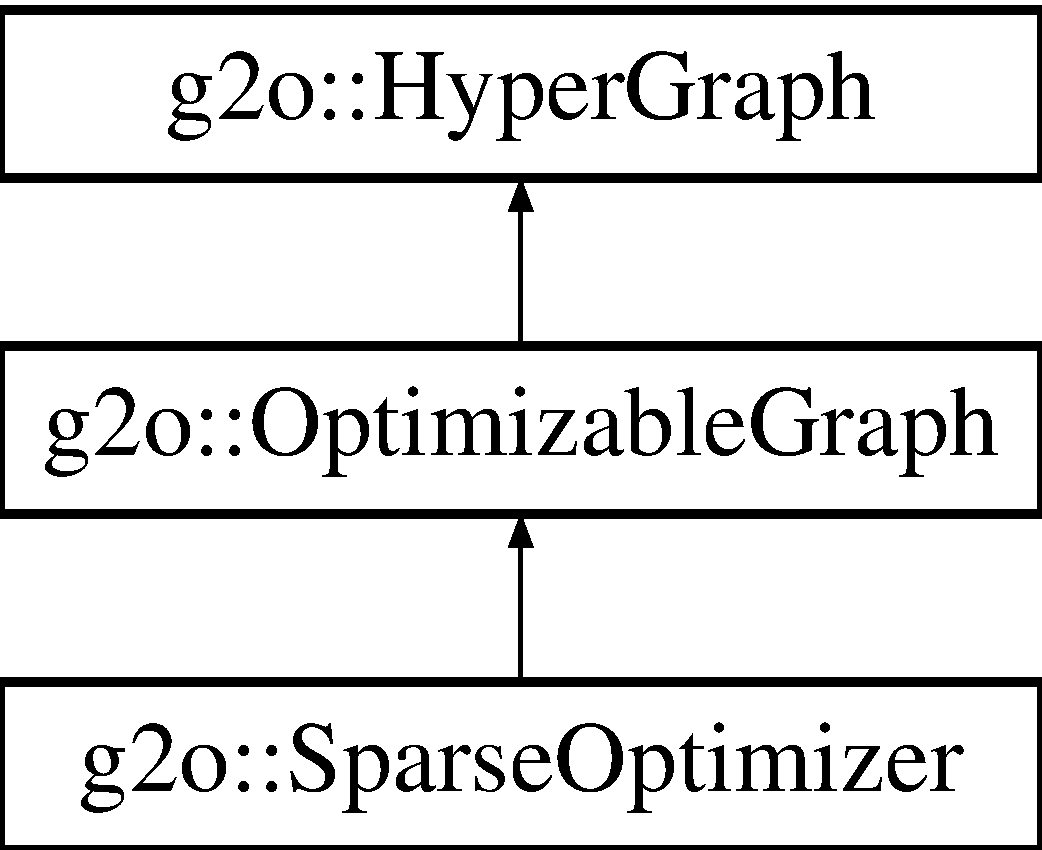
\includegraphics[height=3.000000cm]{classg2o_1_1_hyper_graph}
\end{center}
\end{figure}
\subsection*{Classes}
\begin{DoxyCompactItemize}
\item 
class \mbox{\hyperlink{classg2o_1_1_hyper_graph_1_1_edge}{Edge}}
\item 
struct \mbox{\hyperlink{structg2o_1_1_hyper_graph_1_1_hyper_graph_element}{Hyper\+Graph\+Element}}
\item 
class \mbox{\hyperlink{classg2o_1_1_hyper_graph_1_1_vertex}{Vertex}}
\begin{DoxyCompactList}\small\item\em abstract \mbox{\hyperlink{classg2o_1_1_hyper_graph_1_1_vertex}{Vertex}}, your types must derive from that one \end{DoxyCompactList}\end{DoxyCompactItemize}
\subsection*{Public Types}
\begin{DoxyCompactItemize}
\item 
typedef std\+::bitset$<$ Hyper\+Graph\+::\+H\+G\+E\+T\+\_\+\+N\+U\+M\+\_\+\+E\+L\+E\+MS $>$ \mbox{\hyperlink{classg2o_1_1_hyper_graph_a7b8fda20e1b03e92aeceeac6e8218b73}{Graph\+Elem\+Bitset}}
\item 
typedef std\+::set$<$ \mbox{\hyperlink{classg2o_1_1_hyper_graph_1_1_edge}{Edge}} $\ast$ $>$ \mbox{\hyperlink{classg2o_1_1_hyper_graph_a5e2970e236c0dcb4eff7c205d7b6b4ae}{Edge\+Set}}
\item 
typedef std\+::set$<$ \mbox{\hyperlink{classg2o_1_1_hyper_graph_1_1_vertex}{Vertex}} $\ast$ $>$ \mbox{\hyperlink{classg2o_1_1_hyper_graph_a703938cdb4bb636860eed55a2489d70c}{Vertex\+Set}}
\item 
typedef std\+::tr1\+::unordered\+\_\+map$<$ int, \mbox{\hyperlink{classg2o_1_1_hyper_graph_1_1_vertex}{Vertex}} $\ast$ $>$ \mbox{\hyperlink{classg2o_1_1_hyper_graph_a97307eac064ebf4b3e2cfbf0718035b5}{Vertex\+I\+D\+Map}}
\item 
typedef std\+::vector$<$ \mbox{\hyperlink{classg2o_1_1_hyper_graph_1_1_vertex}{Vertex}} $\ast$ $>$ \mbox{\hyperlink{classg2o_1_1_hyper_graph_a9339534c99300a0ddac87ba976ef188c}{Vertex\+Container}}
\end{DoxyCompactItemize}
\subsection*{Public Member Functions}
\begin{DoxyCompactItemize}
\item 
\mbox{\hyperlink{classg2o_1_1_hyper_graph_a833632b111cfc7cf08b842ae3cb43d41}{Hyper\+Graph}} ()
\begin{DoxyCompactList}\small\item\em constructs an empty hyper graph \end{DoxyCompactList}\item 
virtual \mbox{\hyperlink{classg2o_1_1_hyper_graph_a0ef6e1d65e0f9171a518bce3fc559693}{$\sim$\+Hyper\+Graph}} ()
\begin{DoxyCompactList}\small\item\em destroys the hyper-\/graph and all the vertices of the graph \end{DoxyCompactList}\item 
\mbox{\hyperlink{classg2o_1_1_hyper_graph_1_1_vertex}{Vertex}} $\ast$ \mbox{\hyperlink{classg2o_1_1_hyper_graph_ab07fe8bd9982a66ba34e83dff8317ea2}{vertex}} (int id)
\begin{DoxyCompactList}\small\item\em returns a vertex {\itshape id} in the hyper-\/graph, or 0 if the vertex id is not present \end{DoxyCompactList}\item 
const \mbox{\hyperlink{classg2o_1_1_hyper_graph_1_1_vertex}{Vertex}} $\ast$ \mbox{\hyperlink{classg2o_1_1_hyper_graph_ac117806d17a7e7ad7f8db42f2864cac9}{vertex}} (int id) const
\begin{DoxyCompactList}\small\item\em returns a vertex {\itshape id} in the hyper-\/graph, or 0 if the vertex id is not present \end{DoxyCompactList}\item 
virtual bool \mbox{\hyperlink{classg2o_1_1_hyper_graph_a97ab8302aa027d513253387bba9e0dd5}{remove\+Vertex}} (\mbox{\hyperlink{classg2o_1_1_hyper_graph_1_1_vertex}{Vertex}} $\ast$v)
\begin{DoxyCompactList}\small\item\em removes a vertex from the graph. Returns true on success (vertex was present) \end{DoxyCompactList}\item 
virtual bool \mbox{\hyperlink{classg2o_1_1_hyper_graph_a33e5a60705ce673d647aa1613da9d99b}{remove\+Edge}} (\mbox{\hyperlink{classg2o_1_1_hyper_graph_1_1_edge}{Edge}} $\ast$e)
\begin{DoxyCompactList}\small\item\em removes a vertex from the graph. Returns true on success (edge was present) \end{DoxyCompactList}\item 
virtual void \mbox{\hyperlink{classg2o_1_1_hyper_graph_a6b629dff2928dbd704ca81f24858e72f}{clear}} ()
\begin{DoxyCompactList}\small\item\em clears the graph and empties all structures. \end{DoxyCompactList}\item 
const \mbox{\hyperlink{classg2o_1_1_hyper_graph_a97307eac064ebf4b3e2cfbf0718035b5}{Vertex\+I\+D\+Map}} \& \mbox{\hyperlink{classg2o_1_1_hyper_graph_a95fcf7cd9d89562b2c26d99ede3548ed}{vertices}} () const
\item 
\mbox{\hyperlink{classg2o_1_1_hyper_graph_a97307eac064ebf4b3e2cfbf0718035b5}{Vertex\+I\+D\+Map}} \& \mbox{\hyperlink{classg2o_1_1_hyper_graph_a650107c875ef6f43d438d7d3e2ddf797}{vertices}} ()
\item 
const \mbox{\hyperlink{classg2o_1_1_hyper_graph_a5e2970e236c0dcb4eff7c205d7b6b4ae}{Edge\+Set}} \& \mbox{\hyperlink{classg2o_1_1_hyper_graph_a4edfd2ef4bf235cf78031c505cfd2fcc}{edges}} () const
\item 
\mbox{\hyperlink{classg2o_1_1_hyper_graph_a5e2970e236c0dcb4eff7c205d7b6b4ae}{Edge\+Set}} \& \mbox{\hyperlink{classg2o_1_1_hyper_graph_a2f9f023fe2fb491ef9af873b9e683006}{edges}} ()
\item 
virtual bool \mbox{\hyperlink{classg2o_1_1_hyper_graph_a7ef87ba3479827b24c6fc29c5fc3aa21}{add\+Vertex}} (\mbox{\hyperlink{classg2o_1_1_hyper_graph_1_1_vertex}{Vertex}} $\ast$v)
\item 
virtual bool \mbox{\hyperlink{classg2o_1_1_hyper_graph_a0f1d35009a2879b238c8148c33485c89}{add\+Edge}} (\mbox{\hyperlink{classg2o_1_1_hyper_graph_1_1_edge}{Edge}} $\ast$e)
\item 
virtual bool \mbox{\hyperlink{classg2o_1_1_hyper_graph_a74f0d7392e67762a85799db72a58a94c}{change\+Id}} (\mbox{\hyperlink{classg2o_1_1_hyper_graph_1_1_vertex}{Vertex}} $\ast$v, int new\+Id)
\end{DoxyCompactItemize}
\subsection*{Public Attributes}
\begin{DoxyCompactItemize}
\item 
class \mbox{\hyperlink{g2o__core__api_8h_a7a8d7648d6f1e26632566f335751d064}{G2\+O\+\_\+\+C\+O\+R\+E\+\_\+\+A\+PI}} \mbox{\hyperlink{classg2o_1_1_hyper_graph_a2aca385a3acb87b4f4365765afd10093}{Vertex}}
\item 
class \mbox{\hyperlink{g2o__core__api_8h_a7a8d7648d6f1e26632566f335751d064}{G2\+O\+\_\+\+C\+O\+R\+E\+\_\+\+A\+PI}} \mbox{\hyperlink{classg2o_1_1_hyper_graph_a59ab1fe84b0728a65a0ba15fce9b9cf7}{Edge}}
\end{DoxyCompactItemize}
\subsection*{Protected Attributes}
\begin{DoxyCompactItemize}
\item 
\mbox{\hyperlink{classg2o_1_1_hyper_graph_a97307eac064ebf4b3e2cfbf0718035b5}{Vertex\+I\+D\+Map}} \mbox{\hyperlink{classg2o_1_1_hyper_graph_a83132c77c8d0896581d168cbc72f673a}{\+\_\+vertices}}
\item 
\mbox{\hyperlink{classg2o_1_1_hyper_graph_a5e2970e236c0dcb4eff7c205d7b6b4ae}{Edge\+Set}} \mbox{\hyperlink{classg2o_1_1_hyper_graph_afe4ae6e9ef05c8bded2b1b30e1886b36}{\+\_\+edges}}
\end{DoxyCompactItemize}
\subsection*{Private Member Functions}
\begin{DoxyCompactItemize}
\item 
\mbox{\hyperlink{classg2o_1_1_hyper_graph_ab19a6e0681e2b30d48740cebf553c7eb}{Hyper\+Graph}} (const \mbox{\hyperlink{classg2o_1_1_hyper_graph}{Hyper\+Graph}} \&)
\item 
\mbox{\hyperlink{classg2o_1_1_hyper_graph}{Hyper\+Graph}} \& \mbox{\hyperlink{classg2o_1_1_hyper_graph_aace0adc6b03e56bf6b554368d49dcf88}{operator=}} (const \mbox{\hyperlink{classg2o_1_1_hyper_graph}{Hyper\+Graph}} \&)
\end{DoxyCompactItemize}


\subsection{Detailed Description}
Class that models a directed Hyper-\/\+Graph. An hyper graph is a graph where an edge can connect one or more nodes. Both Vertices and Edges of an hyoper graph derive from the same class \mbox{\hyperlink{structg2o_1_1_hyper_graph_1_1_hyper_graph_element}{Hyper\+Graph\+Element}}, thus one can implement generic algorithms that operate transparently on edges or vertices (see \mbox{\hyperlink{classg2o_1_1_hyper_graph_action}{Hyper\+Graph\+Action}}).

The vertices are uniquely identified by an int id, while the edges are identfied by their pointers. 

\subsection{Member Typedef Documentation}
\mbox{\Hypertarget{classg2o_1_1_hyper_graph_a5e2970e236c0dcb4eff7c205d7b6b4ae}\label{classg2o_1_1_hyper_graph_a5e2970e236c0dcb4eff7c205d7b6b4ae}} 
\index{g2o\+::\+Hyper\+Graph@{g2o\+::\+Hyper\+Graph}!Edge\+Set@{Edge\+Set}}
\index{Edge\+Set@{Edge\+Set}!g2o\+::\+Hyper\+Graph@{g2o\+::\+Hyper\+Graph}}
\subsubsection{\texorpdfstring{Edge\+Set}{EdgeSet}}
{\footnotesize\ttfamily typedef std\+::set$<$\mbox{\hyperlink{classg2o_1_1_hyper_graph_1_1_edge}{Edge}}$\ast$$>$ \mbox{\hyperlink{classg2o_1_1_hyper_graph_a5e2970e236c0dcb4eff7c205d7b6b4ae}{g2o\+::\+Hyper\+Graph\+::\+Edge\+Set}}}

\mbox{\Hypertarget{classg2o_1_1_hyper_graph_a7b8fda20e1b03e92aeceeac6e8218b73}\label{classg2o_1_1_hyper_graph_a7b8fda20e1b03e92aeceeac6e8218b73}} 
\index{g2o\+::\+Hyper\+Graph@{g2o\+::\+Hyper\+Graph}!Graph\+Elem\+Bitset@{Graph\+Elem\+Bitset}}
\index{Graph\+Elem\+Bitset@{Graph\+Elem\+Bitset}!g2o\+::\+Hyper\+Graph@{g2o\+::\+Hyper\+Graph}}
\subsubsection{\texorpdfstring{Graph\+Elem\+Bitset}{GraphElemBitset}}
{\footnotesize\ttfamily typedef std\+::bitset$<$Hyper\+Graph\+::\+H\+G\+E\+T\+\_\+\+N\+U\+M\+\_\+\+E\+L\+E\+MS$>$ \mbox{\hyperlink{classg2o_1_1_hyper_graph_a7b8fda20e1b03e92aeceeac6e8218b73}{g2o\+::\+Hyper\+Graph\+::\+Graph\+Elem\+Bitset}}}

\mbox{\Hypertarget{classg2o_1_1_hyper_graph_a9339534c99300a0ddac87ba976ef188c}\label{classg2o_1_1_hyper_graph_a9339534c99300a0ddac87ba976ef188c}} 
\index{g2o\+::\+Hyper\+Graph@{g2o\+::\+Hyper\+Graph}!Vertex\+Container@{Vertex\+Container}}
\index{Vertex\+Container@{Vertex\+Container}!g2o\+::\+Hyper\+Graph@{g2o\+::\+Hyper\+Graph}}
\subsubsection{\texorpdfstring{Vertex\+Container}{VertexContainer}}
{\footnotesize\ttfamily typedef std\+::vector$<$\mbox{\hyperlink{classg2o_1_1_hyper_graph_1_1_vertex}{Vertex}}$\ast$$>$ \mbox{\hyperlink{classg2o_1_1_hyper_graph_a9339534c99300a0ddac87ba976ef188c}{g2o\+::\+Hyper\+Graph\+::\+Vertex\+Container}}}

\mbox{\Hypertarget{classg2o_1_1_hyper_graph_a97307eac064ebf4b3e2cfbf0718035b5}\label{classg2o_1_1_hyper_graph_a97307eac064ebf4b3e2cfbf0718035b5}} 
\index{g2o\+::\+Hyper\+Graph@{g2o\+::\+Hyper\+Graph}!Vertex\+I\+D\+Map@{Vertex\+I\+D\+Map}}
\index{Vertex\+I\+D\+Map@{Vertex\+I\+D\+Map}!g2o\+::\+Hyper\+Graph@{g2o\+::\+Hyper\+Graph}}
\subsubsection{\texorpdfstring{Vertex\+I\+D\+Map}{VertexIDMap}}
{\footnotesize\ttfamily typedef std\+::tr1\+::unordered\+\_\+map$<$int, \mbox{\hyperlink{classg2o_1_1_hyper_graph_1_1_vertex}{Vertex}}$\ast$$>$ \mbox{\hyperlink{classg2o_1_1_hyper_graph_a97307eac064ebf4b3e2cfbf0718035b5}{g2o\+::\+Hyper\+Graph\+::\+Vertex\+I\+D\+Map}}}

\mbox{\Hypertarget{classg2o_1_1_hyper_graph_a703938cdb4bb636860eed55a2489d70c}\label{classg2o_1_1_hyper_graph_a703938cdb4bb636860eed55a2489d70c}} 
\index{g2o\+::\+Hyper\+Graph@{g2o\+::\+Hyper\+Graph}!Vertex\+Set@{Vertex\+Set}}
\index{Vertex\+Set@{Vertex\+Set}!g2o\+::\+Hyper\+Graph@{g2o\+::\+Hyper\+Graph}}
\subsubsection{\texorpdfstring{Vertex\+Set}{VertexSet}}
{\footnotesize\ttfamily typedef std\+::set$<$\mbox{\hyperlink{classg2o_1_1_hyper_graph_1_1_vertex}{Vertex}}$\ast$$>$ \mbox{\hyperlink{classg2o_1_1_hyper_graph_a703938cdb4bb636860eed55a2489d70c}{g2o\+::\+Hyper\+Graph\+::\+Vertex\+Set}}}



\subsection{Constructor \& Destructor Documentation}
\mbox{\Hypertarget{classg2o_1_1_hyper_graph_a833632b111cfc7cf08b842ae3cb43d41}\label{classg2o_1_1_hyper_graph_a833632b111cfc7cf08b842ae3cb43d41}} 
\index{g2o\+::\+Hyper\+Graph@{g2o\+::\+Hyper\+Graph}!Hyper\+Graph@{Hyper\+Graph}}
\index{Hyper\+Graph@{Hyper\+Graph}!g2o\+::\+Hyper\+Graph@{g2o\+::\+Hyper\+Graph}}
\subsubsection{\texorpdfstring{Hyper\+Graph()}{HyperGraph()}\hspace{0.1cm}{\footnotesize\ttfamily [1/2]}}
{\footnotesize\ttfamily g2o\+::\+Hyper\+Graph\+::\+Hyper\+Graph (\begin{DoxyParamCaption}{ }\end{DoxyParamCaption})}



constructs an empty hyper graph 

\mbox{\Hypertarget{classg2o_1_1_hyper_graph_a0ef6e1d65e0f9171a518bce3fc559693}\label{classg2o_1_1_hyper_graph_a0ef6e1d65e0f9171a518bce3fc559693}} 
\index{g2o\+::\+Hyper\+Graph@{g2o\+::\+Hyper\+Graph}!````~Hyper\+Graph@{$\sim$\+Hyper\+Graph}}
\index{````~Hyper\+Graph@{$\sim$\+Hyper\+Graph}!g2o\+::\+Hyper\+Graph@{g2o\+::\+Hyper\+Graph}}
\subsubsection{\texorpdfstring{$\sim$\+Hyper\+Graph()}{~HyperGraph()}}
{\footnotesize\ttfamily g2o\+::\+Hyper\+Graph\+::$\sim$\+Hyper\+Graph (\begin{DoxyParamCaption}{ }\end{DoxyParamCaption})\hspace{0.3cm}{\ttfamily [virtual]}}



destroys the hyper-\/graph and all the vertices of the graph 

\mbox{\Hypertarget{classg2o_1_1_hyper_graph_ab19a6e0681e2b30d48740cebf553c7eb}\label{classg2o_1_1_hyper_graph_ab19a6e0681e2b30d48740cebf553c7eb}} 
\index{g2o\+::\+Hyper\+Graph@{g2o\+::\+Hyper\+Graph}!Hyper\+Graph@{Hyper\+Graph}}
\index{Hyper\+Graph@{Hyper\+Graph}!g2o\+::\+Hyper\+Graph@{g2o\+::\+Hyper\+Graph}}
\subsubsection{\texorpdfstring{Hyper\+Graph()}{HyperGraph()}\hspace{0.1cm}{\footnotesize\ttfamily [2/2]}}
{\footnotesize\ttfamily g2o\+::\+Hyper\+Graph\+::\+Hyper\+Graph (\begin{DoxyParamCaption}\item[{const \mbox{\hyperlink{classg2o_1_1_hyper_graph}{Hyper\+Graph}} \&}]{ }\end{DoxyParamCaption})\hspace{0.3cm}{\ttfamily [inline]}, {\ttfamily [private]}}



\subsection{Member Function Documentation}
\mbox{\Hypertarget{classg2o_1_1_hyper_graph_a0f1d35009a2879b238c8148c33485c89}\label{classg2o_1_1_hyper_graph_a0f1d35009a2879b238c8148c33485c89}} 
\index{g2o\+::\+Hyper\+Graph@{g2o\+::\+Hyper\+Graph}!add\+Edge@{add\+Edge}}
\index{add\+Edge@{add\+Edge}!g2o\+::\+Hyper\+Graph@{g2o\+::\+Hyper\+Graph}}
\subsubsection{\texorpdfstring{add\+Edge()}{addEdge()}}
{\footnotesize\ttfamily bool g2o\+::\+Hyper\+Graph\+::add\+Edge (\begin{DoxyParamCaption}\item[{\mbox{\hyperlink{classg2o_1_1_hyper_graph_1_1_edge}{Edge}} $\ast$}]{e }\end{DoxyParamCaption})\hspace{0.3cm}{\ttfamily [virtual]}}

Adds an edge to the graph. If the edge is already in the graph, it does nothing and returns false. Otherwise it returns true. 

Reimplemented in \mbox{\hyperlink{structg2o_1_1_optimizable_graph_a6831ed69fce3dba691f53302a2813070}{g2o\+::\+Optimizable\+Graph}}.

\mbox{\Hypertarget{classg2o_1_1_hyper_graph_a7ef87ba3479827b24c6fc29c5fc3aa21}\label{classg2o_1_1_hyper_graph_a7ef87ba3479827b24c6fc29c5fc3aa21}} 
\index{g2o\+::\+Hyper\+Graph@{g2o\+::\+Hyper\+Graph}!add\+Vertex@{add\+Vertex}}
\index{add\+Vertex@{add\+Vertex}!g2o\+::\+Hyper\+Graph@{g2o\+::\+Hyper\+Graph}}
\subsubsection{\texorpdfstring{add\+Vertex()}{addVertex()}}
{\footnotesize\ttfamily bool g2o\+::\+Hyper\+Graph\+::add\+Vertex (\begin{DoxyParamCaption}\item[{\mbox{\hyperlink{classg2o_1_1_hyper_graph_1_1_vertex}{Vertex}} $\ast$}]{v }\end{DoxyParamCaption})\hspace{0.3cm}{\ttfamily [virtual]}}

adds a vertex to the graph. The id of the vertex should be set before invoking this function. the function fails if another vertex with the same id is already in the graph. returns true, on success, or false on failure. 

Reimplemented in \mbox{\hyperlink{structg2o_1_1_optimizable_graph_ac6f41f49fe6148fbe17133d10bf29b4c}{g2o\+::\+Optimizable\+Graph}}.

\mbox{\Hypertarget{classg2o_1_1_hyper_graph_a74f0d7392e67762a85799db72a58a94c}\label{classg2o_1_1_hyper_graph_a74f0d7392e67762a85799db72a58a94c}} 
\index{g2o\+::\+Hyper\+Graph@{g2o\+::\+Hyper\+Graph}!change\+Id@{change\+Id}}
\index{change\+Id@{change\+Id}!g2o\+::\+Hyper\+Graph@{g2o\+::\+Hyper\+Graph}}
\subsubsection{\texorpdfstring{change\+Id()}{changeId()}}
{\footnotesize\ttfamily bool g2o\+::\+Hyper\+Graph\+::change\+Id (\begin{DoxyParamCaption}\item[{\mbox{\hyperlink{classg2o_1_1_hyper_graph_1_1_vertex}{Vertex}} $\ast$}]{v,  }\item[{int}]{new\+Id }\end{DoxyParamCaption})\hspace{0.3cm}{\ttfamily [virtual]}}

changes the id of a vertex already in the graph, and updates the bookkeeping @ returns false if the vertex is not in the graph; \mbox{\Hypertarget{classg2o_1_1_hyper_graph_a6b629dff2928dbd704ca81f24858e72f}\label{classg2o_1_1_hyper_graph_a6b629dff2928dbd704ca81f24858e72f}} 
\index{g2o\+::\+Hyper\+Graph@{g2o\+::\+Hyper\+Graph}!clear@{clear}}
\index{clear@{clear}!g2o\+::\+Hyper\+Graph@{g2o\+::\+Hyper\+Graph}}
\subsubsection{\texorpdfstring{clear()}{clear()}}
{\footnotesize\ttfamily void g2o\+::\+Hyper\+Graph\+::clear (\begin{DoxyParamCaption}{ }\end{DoxyParamCaption})\hspace{0.3cm}{\ttfamily [virtual]}}



clears the graph and empties all structures. 



Reimplemented in \mbox{\hyperlink{classg2o_1_1_sparse_optimizer_a4881e4ac9ba9a58d4e249dc03ef9683d}{g2o\+::\+Sparse\+Optimizer}}.

\mbox{\Hypertarget{classg2o_1_1_hyper_graph_a4edfd2ef4bf235cf78031c505cfd2fcc}\label{classg2o_1_1_hyper_graph_a4edfd2ef4bf235cf78031c505cfd2fcc}} 
\index{g2o\+::\+Hyper\+Graph@{g2o\+::\+Hyper\+Graph}!edges@{edges}}
\index{edges@{edges}!g2o\+::\+Hyper\+Graph@{g2o\+::\+Hyper\+Graph}}
\subsubsection{\texorpdfstring{edges()}{edges()}\hspace{0.1cm}{\footnotesize\ttfamily [1/2]}}
{\footnotesize\ttfamily const \mbox{\hyperlink{classg2o_1_1_hyper_graph_a5e2970e236c0dcb4eff7c205d7b6b4ae}{Edge\+Set}}\& g2o\+::\+Hyper\+Graph\+::edges (\begin{DoxyParamCaption}{ }\end{DoxyParamCaption}) const\hspace{0.3cm}{\ttfamily [inline]}}

\begin{DoxyReturn}{Returns}
the set of edges of the hyper graph 
\end{DoxyReturn}
\mbox{\Hypertarget{classg2o_1_1_hyper_graph_a2f9f023fe2fb491ef9af873b9e683006}\label{classg2o_1_1_hyper_graph_a2f9f023fe2fb491ef9af873b9e683006}} 
\index{g2o\+::\+Hyper\+Graph@{g2o\+::\+Hyper\+Graph}!edges@{edges}}
\index{edges@{edges}!g2o\+::\+Hyper\+Graph@{g2o\+::\+Hyper\+Graph}}
\subsubsection{\texorpdfstring{edges()}{edges()}\hspace{0.1cm}{\footnotesize\ttfamily [2/2]}}
{\footnotesize\ttfamily \mbox{\hyperlink{classg2o_1_1_hyper_graph_a5e2970e236c0dcb4eff7c205d7b6b4ae}{Edge\+Set}}\& g2o\+::\+Hyper\+Graph\+::edges (\begin{DoxyParamCaption}{ }\end{DoxyParamCaption})\hspace{0.3cm}{\ttfamily [inline]}}

\begin{DoxyReturn}{Returns}
the set of edges of the hyper graph 
\end{DoxyReturn}
\mbox{\Hypertarget{classg2o_1_1_hyper_graph_aace0adc6b03e56bf6b554368d49dcf88}\label{classg2o_1_1_hyper_graph_aace0adc6b03e56bf6b554368d49dcf88}} 
\index{g2o\+::\+Hyper\+Graph@{g2o\+::\+Hyper\+Graph}!operator=@{operator=}}
\index{operator=@{operator=}!g2o\+::\+Hyper\+Graph@{g2o\+::\+Hyper\+Graph}}
\subsubsection{\texorpdfstring{operator=()}{operator=()}}
{\footnotesize\ttfamily \mbox{\hyperlink{classg2o_1_1_hyper_graph}{Hyper\+Graph}}\& g2o\+::\+Hyper\+Graph\+::operator= (\begin{DoxyParamCaption}\item[{const \mbox{\hyperlink{classg2o_1_1_hyper_graph}{Hyper\+Graph}} \&}]{ }\end{DoxyParamCaption})\hspace{0.3cm}{\ttfamily [inline]}, {\ttfamily [private]}}

\mbox{\Hypertarget{classg2o_1_1_hyper_graph_a33e5a60705ce673d647aa1613da9d99b}\label{classg2o_1_1_hyper_graph_a33e5a60705ce673d647aa1613da9d99b}} 
\index{g2o\+::\+Hyper\+Graph@{g2o\+::\+Hyper\+Graph}!remove\+Edge@{remove\+Edge}}
\index{remove\+Edge@{remove\+Edge}!g2o\+::\+Hyper\+Graph@{g2o\+::\+Hyper\+Graph}}
\subsubsection{\texorpdfstring{remove\+Edge()}{removeEdge()}}
{\footnotesize\ttfamily bool g2o\+::\+Hyper\+Graph\+::remove\+Edge (\begin{DoxyParamCaption}\item[{\mbox{\hyperlink{classg2o_1_1_hyper_graph_1_1_edge}{Edge}} $\ast$}]{e }\end{DoxyParamCaption})\hspace{0.3cm}{\ttfamily [virtual]}}



removes a vertex from the graph. Returns true on success (edge was present) 

\mbox{\Hypertarget{classg2o_1_1_hyper_graph_a97ab8302aa027d513253387bba9e0dd5}\label{classg2o_1_1_hyper_graph_a97ab8302aa027d513253387bba9e0dd5}} 
\index{g2o\+::\+Hyper\+Graph@{g2o\+::\+Hyper\+Graph}!remove\+Vertex@{remove\+Vertex}}
\index{remove\+Vertex@{remove\+Vertex}!g2o\+::\+Hyper\+Graph@{g2o\+::\+Hyper\+Graph}}
\subsubsection{\texorpdfstring{remove\+Vertex()}{removeVertex()}}
{\footnotesize\ttfamily bool g2o\+::\+Hyper\+Graph\+::remove\+Vertex (\begin{DoxyParamCaption}\item[{\mbox{\hyperlink{classg2o_1_1_hyper_graph_1_1_vertex}{Vertex}} $\ast$}]{v }\end{DoxyParamCaption})\hspace{0.3cm}{\ttfamily [virtual]}}



removes a vertex from the graph. Returns true on success (vertex was present) 



Reimplemented in \mbox{\hyperlink{classg2o_1_1_sparse_optimizer_a0fb2a5e2b250bf2530a600f6dcaad03f}{g2o\+::\+Sparse\+Optimizer}}.

\mbox{\Hypertarget{classg2o_1_1_hyper_graph_ab07fe8bd9982a66ba34e83dff8317ea2}\label{classg2o_1_1_hyper_graph_ab07fe8bd9982a66ba34e83dff8317ea2}} 
\index{g2o\+::\+Hyper\+Graph@{g2o\+::\+Hyper\+Graph}!vertex@{vertex}}
\index{vertex@{vertex}!g2o\+::\+Hyper\+Graph@{g2o\+::\+Hyper\+Graph}}
\subsubsection{\texorpdfstring{vertex()}{vertex()}\hspace{0.1cm}{\footnotesize\ttfamily [1/2]}}
{\footnotesize\ttfamily \mbox{\hyperlink{classg2o_1_1_hyper_graph_1_1_vertex}{Hyper\+Graph\+::\+Vertex}} $\ast$ g2o\+::\+Hyper\+Graph\+::vertex (\begin{DoxyParamCaption}\item[{int}]{id }\end{DoxyParamCaption})}



returns a vertex {\itshape id} in the hyper-\/graph, or 0 if the vertex id is not present 

\mbox{\Hypertarget{classg2o_1_1_hyper_graph_ac117806d17a7e7ad7f8db42f2864cac9}\label{classg2o_1_1_hyper_graph_ac117806d17a7e7ad7f8db42f2864cac9}} 
\index{g2o\+::\+Hyper\+Graph@{g2o\+::\+Hyper\+Graph}!vertex@{vertex}}
\index{vertex@{vertex}!g2o\+::\+Hyper\+Graph@{g2o\+::\+Hyper\+Graph}}
\subsubsection{\texorpdfstring{vertex()}{vertex()}\hspace{0.1cm}{\footnotesize\ttfamily [2/2]}}
{\footnotesize\ttfamily const \mbox{\hyperlink{classg2o_1_1_hyper_graph_1_1_vertex}{Hyper\+Graph\+::\+Vertex}} $\ast$ g2o\+::\+Hyper\+Graph\+::vertex (\begin{DoxyParamCaption}\item[{int}]{id }\end{DoxyParamCaption}) const}



returns a vertex {\itshape id} in the hyper-\/graph, or 0 if the vertex id is not present 

\mbox{\Hypertarget{classg2o_1_1_hyper_graph_a95fcf7cd9d89562b2c26d99ede3548ed}\label{classg2o_1_1_hyper_graph_a95fcf7cd9d89562b2c26d99ede3548ed}} 
\index{g2o\+::\+Hyper\+Graph@{g2o\+::\+Hyper\+Graph}!vertices@{vertices}}
\index{vertices@{vertices}!g2o\+::\+Hyper\+Graph@{g2o\+::\+Hyper\+Graph}}
\subsubsection{\texorpdfstring{vertices()}{vertices()}\hspace{0.1cm}{\footnotesize\ttfamily [1/2]}}
{\footnotesize\ttfamily const \mbox{\hyperlink{classg2o_1_1_hyper_graph_a97307eac064ebf4b3e2cfbf0718035b5}{Vertex\+I\+D\+Map}}\& g2o\+::\+Hyper\+Graph\+::vertices (\begin{DoxyParamCaption}{ }\end{DoxyParamCaption}) const\hspace{0.3cm}{\ttfamily [inline]}}

\begin{DoxyReturn}{Returns}
the map {\itshape id -\/$>$ vertex} where the vertices are stored 
\end{DoxyReturn}
\mbox{\Hypertarget{classg2o_1_1_hyper_graph_a650107c875ef6f43d438d7d3e2ddf797}\label{classg2o_1_1_hyper_graph_a650107c875ef6f43d438d7d3e2ddf797}} 
\index{g2o\+::\+Hyper\+Graph@{g2o\+::\+Hyper\+Graph}!vertices@{vertices}}
\index{vertices@{vertices}!g2o\+::\+Hyper\+Graph@{g2o\+::\+Hyper\+Graph}}
\subsubsection{\texorpdfstring{vertices()}{vertices()}\hspace{0.1cm}{\footnotesize\ttfamily [2/2]}}
{\footnotesize\ttfamily \mbox{\hyperlink{classg2o_1_1_hyper_graph_a97307eac064ebf4b3e2cfbf0718035b5}{Vertex\+I\+D\+Map}}\& g2o\+::\+Hyper\+Graph\+::vertices (\begin{DoxyParamCaption}{ }\end{DoxyParamCaption})\hspace{0.3cm}{\ttfamily [inline]}}

\begin{DoxyReturn}{Returns}
the map {\itshape id -\/$>$ vertex} where the vertices are stored 
\end{DoxyReturn}


\subsection{Member Data Documentation}
\mbox{\Hypertarget{classg2o_1_1_hyper_graph_afe4ae6e9ef05c8bded2b1b30e1886b36}\label{classg2o_1_1_hyper_graph_afe4ae6e9ef05c8bded2b1b30e1886b36}} 
\index{g2o\+::\+Hyper\+Graph@{g2o\+::\+Hyper\+Graph}!\+\_\+edges@{\+\_\+edges}}
\index{\+\_\+edges@{\+\_\+edges}!g2o\+::\+Hyper\+Graph@{g2o\+::\+Hyper\+Graph}}
\subsubsection{\texorpdfstring{\+\_\+edges}{\_edges}}
{\footnotesize\ttfamily \mbox{\hyperlink{classg2o_1_1_hyper_graph_a5e2970e236c0dcb4eff7c205d7b6b4ae}{Edge\+Set}} g2o\+::\+Hyper\+Graph\+::\+\_\+edges\hspace{0.3cm}{\ttfamily [protected]}}

\mbox{\Hypertarget{classg2o_1_1_hyper_graph_a83132c77c8d0896581d168cbc72f673a}\label{classg2o_1_1_hyper_graph_a83132c77c8d0896581d168cbc72f673a}} 
\index{g2o\+::\+Hyper\+Graph@{g2o\+::\+Hyper\+Graph}!\+\_\+vertices@{\+\_\+vertices}}
\index{\+\_\+vertices@{\+\_\+vertices}!g2o\+::\+Hyper\+Graph@{g2o\+::\+Hyper\+Graph}}
\subsubsection{\texorpdfstring{\+\_\+vertices}{\_vertices}}
{\footnotesize\ttfamily \mbox{\hyperlink{classg2o_1_1_hyper_graph_a97307eac064ebf4b3e2cfbf0718035b5}{Vertex\+I\+D\+Map}} g2o\+::\+Hyper\+Graph\+::\+\_\+vertices\hspace{0.3cm}{\ttfamily [protected]}}

\mbox{\Hypertarget{classg2o_1_1_hyper_graph_a59ab1fe84b0728a65a0ba15fce9b9cf7}\label{classg2o_1_1_hyper_graph_a59ab1fe84b0728a65a0ba15fce9b9cf7}} 
\index{g2o\+::\+Hyper\+Graph@{g2o\+::\+Hyper\+Graph}!Edge@{Edge}}
\index{Edge@{Edge}!g2o\+::\+Hyper\+Graph@{g2o\+::\+Hyper\+Graph}}
\subsubsection{\texorpdfstring{Edge}{Edge}}
{\footnotesize\ttfamily class \mbox{\hyperlink{g2o__core__api_8h_a7a8d7648d6f1e26632566f335751d064}{G2\+O\+\_\+\+C\+O\+R\+E\+\_\+\+A\+PI}} \mbox{\hyperlink{classg2o_1_1_hyper_graph_1_1_edge}{g2o\+::\+Hyper\+Graph\+::\+Edge}}}

\mbox{\Hypertarget{classg2o_1_1_hyper_graph_a2aca385a3acb87b4f4365765afd10093}\label{classg2o_1_1_hyper_graph_a2aca385a3acb87b4f4365765afd10093}} 
\index{g2o\+::\+Hyper\+Graph@{g2o\+::\+Hyper\+Graph}!Vertex@{Vertex}}
\index{Vertex@{Vertex}!g2o\+::\+Hyper\+Graph@{g2o\+::\+Hyper\+Graph}}
\subsubsection{\texorpdfstring{Vertex}{Vertex}}
{\footnotesize\ttfamily class \mbox{\hyperlink{g2o__core__api_8h_a7a8d7648d6f1e26632566f335751d064}{G2\+O\+\_\+\+C\+O\+R\+E\+\_\+\+A\+PI}} \mbox{\hyperlink{classg2o_1_1_hyper_graph_1_1_vertex}{g2o\+::\+Hyper\+Graph\+::\+Vertex}}}



The documentation for this class was generated from the following files\+:\begin{DoxyCompactItemize}
\item 
D\+:/github/\+V\+S\+L\+A\+M/\+O\+R\+B\+S\+L\+A\+M2/\+O\+R\+B-\/\+S\+L\+A\+M2-\/master/\+Thirdparty/g2o/g2o/core/\mbox{\hyperlink{hyper__graph_8h}{hyper\+\_\+graph.\+h}}\item 
D\+:/github/\+V\+S\+L\+A\+M/\+O\+R\+B\+S\+L\+A\+M2/\+O\+R\+B-\/\+S\+L\+A\+M2-\/master/\+Thirdparty/g2o/g2o/core/\mbox{\hyperlink{hyper__graph_8cpp}{hyper\+\_\+graph.\+cpp}}\end{DoxyCompactItemize}

\hypertarget{classg2o_1_1_hyper_graph_action}{}\section{g2o\+:\+:Hyper\+Graph\+Action Class Reference}
\label{classg2o_1_1_hyper_graph_action}\index{g2o\+::\+Hyper\+Graph\+Action@{g2o\+::\+Hyper\+Graph\+Action}}


Abstract action that operates on an entire graph.  




{\ttfamily \#include $<$hyper\+\_\+graph\+\_\+action.\+h$>$}

\subsection*{Classes}
\begin{DoxyCompactItemize}
\item 
class \mbox{\hyperlink{classg2o_1_1_hyper_graph_action_1_1_parameters}{Parameters}}
\item 
class \mbox{\hyperlink{classg2o_1_1_hyper_graph_action_1_1_parameters_iteration}{Parameters\+Iteration}}
\end{DoxyCompactItemize}
\subsection*{Public Member Functions}
\begin{DoxyCompactItemize}
\item 
virtual \mbox{\hyperlink{classg2o_1_1_hyper_graph_action_a49de9295ace027074f459714ca257b15}{$\sim$\+Hyper\+Graph\+Action}} ()
\item 
virtual \mbox{\hyperlink{classg2o_1_1_hyper_graph_action}{Hyper\+Graph\+Action}} $\ast$ \mbox{\hyperlink{classg2o_1_1_hyper_graph_action_aea392eafa65ab432a3c4d1dabde9bdbe}{operator()}} (const \mbox{\hyperlink{classg2o_1_1_hyper_graph}{Hyper\+Graph}} $\ast$graph, \mbox{\hyperlink{classg2o_1_1_hyper_graph_action_1_1_parameters}{Parameters}} $\ast$parameters=0)
\end{DoxyCompactItemize}


\subsection{Detailed Description}
Abstract action that operates on an entire graph. 

\subsection{Constructor \& Destructor Documentation}
\mbox{\Hypertarget{classg2o_1_1_hyper_graph_action_a49de9295ace027074f459714ca257b15}\label{classg2o_1_1_hyper_graph_action_a49de9295ace027074f459714ca257b15}} 
\index{g2o\+::\+Hyper\+Graph\+Action@{g2o\+::\+Hyper\+Graph\+Action}!````~Hyper\+Graph\+Action@{$\sim$\+Hyper\+Graph\+Action}}
\index{````~Hyper\+Graph\+Action@{$\sim$\+Hyper\+Graph\+Action}!g2o\+::\+Hyper\+Graph\+Action@{g2o\+::\+Hyper\+Graph\+Action}}
\subsubsection{\texorpdfstring{$\sim$\+Hyper\+Graph\+Action()}{~HyperGraphAction()}}
{\footnotesize\ttfamily g2o\+::\+Hyper\+Graph\+Action\+::$\sim$\+Hyper\+Graph\+Action (\begin{DoxyParamCaption}{ }\end{DoxyParamCaption})\hspace{0.3cm}{\ttfamily [virtual]}}



\subsection{Member Function Documentation}
\mbox{\Hypertarget{classg2o_1_1_hyper_graph_action_aea392eafa65ab432a3c4d1dabde9bdbe}\label{classg2o_1_1_hyper_graph_action_aea392eafa65ab432a3c4d1dabde9bdbe}} 
\index{g2o\+::\+Hyper\+Graph\+Action@{g2o\+::\+Hyper\+Graph\+Action}!operator()@{operator()}}
\index{operator()@{operator()}!g2o\+::\+Hyper\+Graph\+Action@{g2o\+::\+Hyper\+Graph\+Action}}
\subsubsection{\texorpdfstring{operator()()}{operator()()}}
{\footnotesize\ttfamily \mbox{\hyperlink{classg2o_1_1_hyper_graph_action}{Hyper\+Graph\+Action}} $\ast$ g2o\+::\+Hyper\+Graph\+Action\+::operator() (\begin{DoxyParamCaption}\item[{const \mbox{\hyperlink{classg2o_1_1_hyper_graph}{Hyper\+Graph}} $\ast$}]{graph,  }\item[{\mbox{\hyperlink{classg2o_1_1_hyper_graph_action_1_1_parameters}{Parameters}} $\ast$}]{parameters = {\ttfamily 0} }\end{DoxyParamCaption})\hspace{0.3cm}{\ttfamily [virtual]}}

re-\/implement to carry out an action given the graph 

The documentation for this class was generated from the following files\+:\begin{DoxyCompactItemize}
\item 
Thirdparty/g2o/g2o/core/\mbox{\hyperlink{hyper__graph__action_8h}{hyper\+\_\+graph\+\_\+action.\+h}}\item 
Thirdparty/g2o/g2o/core/\mbox{\hyperlink{hyper__graph__action_8cpp}{hyper\+\_\+graph\+\_\+action.\+cpp}}\end{DoxyCompactItemize}

\hypertarget{classg2o_1_1_hyper_graph_action_library}{}\section{g2o\+:\+:Hyper\+Graph\+Action\+Library Class Reference}
\label{classg2o_1_1_hyper_graph_action_library}\index{g2o\+::\+Hyper\+Graph\+Action\+Library@{g2o\+::\+Hyper\+Graph\+Action\+Library}}


library of actions, indexed by the action name;  




{\ttfamily \#include $<$hyper\+\_\+graph\+\_\+action.\+h$>$}

\subsection*{Public Member Functions}
\begin{DoxyCompactItemize}
\item 
\mbox{\hyperlink{classg2o_1_1_hyper_graph_element_action}{Hyper\+Graph\+Element\+Action}} $\ast$ \mbox{\hyperlink{classg2o_1_1_hyper_graph_action_library_abef8ce416dd53f2d4e8d8566abf4a00f}{action\+By\+Name}} (const std\+::string \&name)
\item 
bool \mbox{\hyperlink{classg2o_1_1_hyper_graph_action_library_a8ff09559af9efdf636ad14a011ef73ae}{register\+Action}} (\mbox{\hyperlink{classg2o_1_1_hyper_graph_element_action}{Hyper\+Graph\+Element\+Action}} $\ast$action)
\item 
bool \mbox{\hyperlink{classg2o_1_1_hyper_graph_action_library_abe4c076e6734ffa79f6d2bff07f9fad5}{unregister\+Action}} (\mbox{\hyperlink{classg2o_1_1_hyper_graph_element_action}{Hyper\+Graph\+Element\+Action}} $\ast$action)
\item 
\mbox{\hyperlink{classg2o_1_1_hyper_graph_element_action_abc889fc90ae1bbb63d90c7993777417a}{Hyper\+Graph\+Element\+Action\+::\+Action\+Map}} \& \mbox{\hyperlink{classg2o_1_1_hyper_graph_action_library_a99d123d19dda08f30ab0088d361fc640}{action\+Map}} ()
\end{DoxyCompactItemize}
\subsection*{Static Public Member Functions}
\begin{DoxyCompactItemize}
\item 
static \mbox{\hyperlink{classg2o_1_1_hyper_graph_action_library}{Hyper\+Graph\+Action\+Library}} $\ast$ \mbox{\hyperlink{classg2o_1_1_hyper_graph_action_library_a12074e3f4d9bcb3da20a4fe23d18b745}{instance}} ()
\begin{DoxyCompactList}\small\item\em return the single instance of the \mbox{\hyperlink{classg2o_1_1_hyper_graph_action_library}{Hyper\+Graph\+Action\+Library}} \end{DoxyCompactList}\item 
static void \mbox{\hyperlink{classg2o_1_1_hyper_graph_action_library_aa235ae7c242c522518b07d019dbf8a51}{destroy}} ()
\begin{DoxyCompactList}\small\item\em free the instance \end{DoxyCompactList}\end{DoxyCompactItemize}
\subsection*{Protected Member Functions}
\begin{DoxyCompactItemize}
\item 
\mbox{\hyperlink{classg2o_1_1_hyper_graph_action_library_a68fe0eee5bdda62e6929c3ee2b4b38f1}{Hyper\+Graph\+Action\+Library}} ()
\item 
\mbox{\hyperlink{classg2o_1_1_hyper_graph_action_library_af0d04ecf012d498c09d68725aaf939e5}{$\sim$\+Hyper\+Graph\+Action\+Library}} ()
\end{DoxyCompactItemize}
\subsection*{Protected Attributes}
\begin{DoxyCompactItemize}
\item 
\mbox{\hyperlink{classg2o_1_1_hyper_graph_element_action_abc889fc90ae1bbb63d90c7993777417a}{Hyper\+Graph\+Element\+Action\+::\+Action\+Map}} \mbox{\hyperlink{classg2o_1_1_hyper_graph_action_library_afc9e9b39a743700dcfc896b50d176b3b}{\+\_\+action\+Map}}
\end{DoxyCompactItemize}


\subsection{Detailed Description}
library of actions, indexed by the action name; 

library of actions, indexed by the action name; one can use ti to register a collection of actions 

\subsection{Constructor \& Destructor Documentation}
\mbox{\Hypertarget{classg2o_1_1_hyper_graph_action_library_a68fe0eee5bdda62e6929c3ee2b4b38f1}\label{classg2o_1_1_hyper_graph_action_library_a68fe0eee5bdda62e6929c3ee2b4b38f1}} 
\index{g2o\+::\+Hyper\+Graph\+Action\+Library@{g2o\+::\+Hyper\+Graph\+Action\+Library}!Hyper\+Graph\+Action\+Library@{Hyper\+Graph\+Action\+Library}}
\index{Hyper\+Graph\+Action\+Library@{Hyper\+Graph\+Action\+Library}!g2o\+::\+Hyper\+Graph\+Action\+Library@{g2o\+::\+Hyper\+Graph\+Action\+Library}}
\subsubsection{\texorpdfstring{Hyper\+Graph\+Action\+Library()}{HyperGraphActionLibrary()}}
{\footnotesize\ttfamily g2o\+::\+Hyper\+Graph\+Action\+Library\+::\+Hyper\+Graph\+Action\+Library (\begin{DoxyParamCaption}{ }\end{DoxyParamCaption})\hspace{0.3cm}{\ttfamily [protected]}}

\mbox{\Hypertarget{classg2o_1_1_hyper_graph_action_library_af0d04ecf012d498c09d68725aaf939e5}\label{classg2o_1_1_hyper_graph_action_library_af0d04ecf012d498c09d68725aaf939e5}} 
\index{g2o\+::\+Hyper\+Graph\+Action\+Library@{g2o\+::\+Hyper\+Graph\+Action\+Library}!````~Hyper\+Graph\+Action\+Library@{$\sim$\+Hyper\+Graph\+Action\+Library}}
\index{````~Hyper\+Graph\+Action\+Library@{$\sim$\+Hyper\+Graph\+Action\+Library}!g2o\+::\+Hyper\+Graph\+Action\+Library@{g2o\+::\+Hyper\+Graph\+Action\+Library}}
\subsubsection{\texorpdfstring{$\sim$\+Hyper\+Graph\+Action\+Library()}{~HyperGraphActionLibrary()}}
{\footnotesize\ttfamily g2o\+::\+Hyper\+Graph\+Action\+Library\+::$\sim$\+Hyper\+Graph\+Action\+Library (\begin{DoxyParamCaption}{ }\end{DoxyParamCaption})\hspace{0.3cm}{\ttfamily [protected]}}



\subsection{Member Function Documentation}
\mbox{\Hypertarget{classg2o_1_1_hyper_graph_action_library_abef8ce416dd53f2d4e8d8566abf4a00f}\label{classg2o_1_1_hyper_graph_action_library_abef8ce416dd53f2d4e8d8566abf4a00f}} 
\index{g2o\+::\+Hyper\+Graph\+Action\+Library@{g2o\+::\+Hyper\+Graph\+Action\+Library}!action\+By\+Name@{action\+By\+Name}}
\index{action\+By\+Name@{action\+By\+Name}!g2o\+::\+Hyper\+Graph\+Action\+Library@{g2o\+::\+Hyper\+Graph\+Action\+Library}}
\subsubsection{\texorpdfstring{action\+By\+Name()}{actionByName()}}
{\footnotesize\ttfamily \mbox{\hyperlink{classg2o_1_1_hyper_graph_element_action}{Hyper\+Graph\+Element\+Action}} $\ast$ g2o\+::\+Hyper\+Graph\+Action\+Library\+::action\+By\+Name (\begin{DoxyParamCaption}\item[{const std\+::string \&}]{name }\end{DoxyParamCaption})}

\mbox{\Hypertarget{classg2o_1_1_hyper_graph_action_library_a99d123d19dda08f30ab0088d361fc640}\label{classg2o_1_1_hyper_graph_action_library_a99d123d19dda08f30ab0088d361fc640}} 
\index{g2o\+::\+Hyper\+Graph\+Action\+Library@{g2o\+::\+Hyper\+Graph\+Action\+Library}!action\+Map@{action\+Map}}
\index{action\+Map@{action\+Map}!g2o\+::\+Hyper\+Graph\+Action\+Library@{g2o\+::\+Hyper\+Graph\+Action\+Library}}
\subsubsection{\texorpdfstring{action\+Map()}{actionMap()}}
{\footnotesize\ttfamily \mbox{\hyperlink{classg2o_1_1_hyper_graph_element_action_abc889fc90ae1bbb63d90c7993777417a}{Hyper\+Graph\+Element\+Action\+::\+Action\+Map}}\& g2o\+::\+Hyper\+Graph\+Action\+Library\+::action\+Map (\begin{DoxyParamCaption}{ }\end{DoxyParamCaption})\hspace{0.3cm}{\ttfamily [inline]}}

\mbox{\Hypertarget{classg2o_1_1_hyper_graph_action_library_aa235ae7c242c522518b07d019dbf8a51}\label{classg2o_1_1_hyper_graph_action_library_aa235ae7c242c522518b07d019dbf8a51}} 
\index{g2o\+::\+Hyper\+Graph\+Action\+Library@{g2o\+::\+Hyper\+Graph\+Action\+Library}!destroy@{destroy}}
\index{destroy@{destroy}!g2o\+::\+Hyper\+Graph\+Action\+Library@{g2o\+::\+Hyper\+Graph\+Action\+Library}}
\subsubsection{\texorpdfstring{destroy()}{destroy()}}
{\footnotesize\ttfamily void g2o\+::\+Hyper\+Graph\+Action\+Library\+::destroy (\begin{DoxyParamCaption}{ }\end{DoxyParamCaption})\hspace{0.3cm}{\ttfamily [static]}}



free the instance 

\mbox{\Hypertarget{classg2o_1_1_hyper_graph_action_library_a12074e3f4d9bcb3da20a4fe23d18b745}\label{classg2o_1_1_hyper_graph_action_library_a12074e3f4d9bcb3da20a4fe23d18b745}} 
\index{g2o\+::\+Hyper\+Graph\+Action\+Library@{g2o\+::\+Hyper\+Graph\+Action\+Library}!instance@{instance}}
\index{instance@{instance}!g2o\+::\+Hyper\+Graph\+Action\+Library@{g2o\+::\+Hyper\+Graph\+Action\+Library}}
\subsubsection{\texorpdfstring{instance()}{instance()}}
{\footnotesize\ttfamily \mbox{\hyperlink{classg2o_1_1_hyper_graph_action_library}{Hyper\+Graph\+Action\+Library}} $\ast$ g2o\+::\+Hyper\+Graph\+Action\+Library\+::instance (\begin{DoxyParamCaption}{ }\end{DoxyParamCaption})\hspace{0.3cm}{\ttfamily [static]}}



return the single instance of the \mbox{\hyperlink{classg2o_1_1_hyper_graph_action_library}{Hyper\+Graph\+Action\+Library}} 

\mbox{\Hypertarget{classg2o_1_1_hyper_graph_action_library_a8ff09559af9efdf636ad14a011ef73ae}\label{classg2o_1_1_hyper_graph_action_library_a8ff09559af9efdf636ad14a011ef73ae}} 
\index{g2o\+::\+Hyper\+Graph\+Action\+Library@{g2o\+::\+Hyper\+Graph\+Action\+Library}!register\+Action@{register\+Action}}
\index{register\+Action@{register\+Action}!g2o\+::\+Hyper\+Graph\+Action\+Library@{g2o\+::\+Hyper\+Graph\+Action\+Library}}
\subsubsection{\texorpdfstring{register\+Action()}{registerAction()}}
{\footnotesize\ttfamily bool g2o\+::\+Hyper\+Graph\+Action\+Library\+::register\+Action (\begin{DoxyParamCaption}\item[{\mbox{\hyperlink{classg2o_1_1_hyper_graph_element_action}{Hyper\+Graph\+Element\+Action}} $\ast$}]{action }\end{DoxyParamCaption})}

\mbox{\Hypertarget{classg2o_1_1_hyper_graph_action_library_abe4c076e6734ffa79f6d2bff07f9fad5}\label{classg2o_1_1_hyper_graph_action_library_abe4c076e6734ffa79f6d2bff07f9fad5}} 
\index{g2o\+::\+Hyper\+Graph\+Action\+Library@{g2o\+::\+Hyper\+Graph\+Action\+Library}!unregister\+Action@{unregister\+Action}}
\index{unregister\+Action@{unregister\+Action}!g2o\+::\+Hyper\+Graph\+Action\+Library@{g2o\+::\+Hyper\+Graph\+Action\+Library}}
\subsubsection{\texorpdfstring{unregister\+Action()}{unregisterAction()}}
{\footnotesize\ttfamily bool g2o\+::\+Hyper\+Graph\+Action\+Library\+::unregister\+Action (\begin{DoxyParamCaption}\item[{\mbox{\hyperlink{classg2o_1_1_hyper_graph_element_action}{Hyper\+Graph\+Element\+Action}} $\ast$}]{action }\end{DoxyParamCaption})}



\subsection{Member Data Documentation}
\mbox{\Hypertarget{classg2o_1_1_hyper_graph_action_library_afc9e9b39a743700dcfc896b50d176b3b}\label{classg2o_1_1_hyper_graph_action_library_afc9e9b39a743700dcfc896b50d176b3b}} 
\index{g2o\+::\+Hyper\+Graph\+Action\+Library@{g2o\+::\+Hyper\+Graph\+Action\+Library}!\+\_\+action\+Map@{\+\_\+action\+Map}}
\index{\+\_\+action\+Map@{\+\_\+action\+Map}!g2o\+::\+Hyper\+Graph\+Action\+Library@{g2o\+::\+Hyper\+Graph\+Action\+Library}}
\subsubsection{\texorpdfstring{\+\_\+action\+Map}{\_actionMap}}
{\footnotesize\ttfamily \mbox{\hyperlink{classg2o_1_1_hyper_graph_element_action_abc889fc90ae1bbb63d90c7993777417a}{Hyper\+Graph\+Element\+Action\+::\+Action\+Map}} g2o\+::\+Hyper\+Graph\+Action\+Library\+::\+\_\+action\+Map\hspace{0.3cm}{\ttfamily [protected]}}



The documentation for this class was generated from the following files\+:\begin{DoxyCompactItemize}
\item 
Thirdparty/g2o/g2o/core/\mbox{\hyperlink{hyper__graph__action_8h}{hyper\+\_\+graph\+\_\+action.\+h}}\item 
Thirdparty/g2o/g2o/core/\mbox{\hyperlink{hyper__graph__action_8cpp}{hyper\+\_\+graph\+\_\+action.\+cpp}}\end{DoxyCompactItemize}

\hypertarget{structg2o_1_1_hyper_graph_1_1_hyper_graph_element}{}\section{g2o\+:\+:Hyper\+Graph\+:\+:Hyper\+Graph\+Element Struct Reference}
\label{structg2o_1_1_hyper_graph_1_1_hyper_graph_element}\index{g2o\+::\+Hyper\+Graph\+::\+Hyper\+Graph\+Element@{g2o\+::\+Hyper\+Graph\+::\+Hyper\+Graph\+Element}}


{\ttfamily \#include $<$hyper\+\_\+graph.\+h$>$}

Inheritance diagram for g2o\+:\+:Hyper\+Graph\+:\+:Hyper\+Graph\+Element\+:\begin{figure}[H]
\begin{center}
\leavevmode
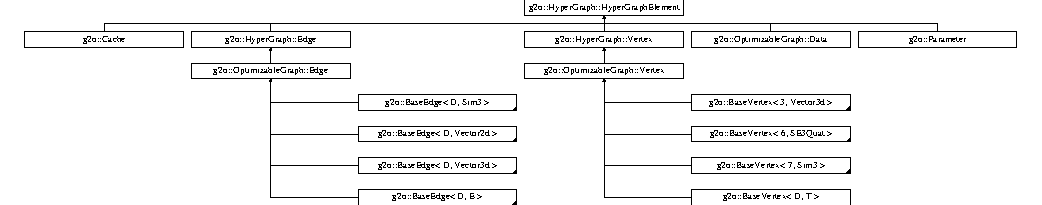
\includegraphics[height=2.756681cm]{structg2o_1_1_hyper_graph_1_1_hyper_graph_element}
\end{center}
\end{figure}
\subsection*{Public Member Functions}
\begin{DoxyCompactItemize}
\item 
virtual \mbox{\hyperlink{structg2o_1_1_hyper_graph_1_1_hyper_graph_element_ab02c385ff2bd544037e2bef795761b2e}{$\sim$\+Hyper\+Graph\+Element}} ()
\item 
virtual Hyper\+Graph\+Element\+Type \mbox{\hyperlink{structg2o_1_1_hyper_graph_1_1_hyper_graph_element_a1a9d7b748698c09d202373e06e413ef2}{element\+Type}} () const =0
\end{DoxyCompactItemize}


\subsection{Detailed Description}
base hyper graph element, specialized in vertex and edge 

\subsection{Constructor \& Destructor Documentation}
\mbox{\Hypertarget{structg2o_1_1_hyper_graph_1_1_hyper_graph_element_ab02c385ff2bd544037e2bef795761b2e}\label{structg2o_1_1_hyper_graph_1_1_hyper_graph_element_ab02c385ff2bd544037e2bef795761b2e}} 
\index{g2o\+::\+Hyper\+Graph\+::\+Hyper\+Graph\+Element@{g2o\+::\+Hyper\+Graph\+::\+Hyper\+Graph\+Element}!````~Hyper\+Graph\+Element@{$\sim$\+Hyper\+Graph\+Element}}
\index{````~Hyper\+Graph\+Element@{$\sim$\+Hyper\+Graph\+Element}!g2o\+::\+Hyper\+Graph\+::\+Hyper\+Graph\+Element@{g2o\+::\+Hyper\+Graph\+::\+Hyper\+Graph\+Element}}
\subsubsection{\texorpdfstring{$\sim$\+Hyper\+Graph\+Element()}{~HyperGraphElement()}}
{\footnotesize\ttfamily virtual g2o\+::\+Hyper\+Graph\+::\+Hyper\+Graph\+Element\+::$\sim$\+Hyper\+Graph\+Element (\begin{DoxyParamCaption}{ }\end{DoxyParamCaption})\hspace{0.3cm}{\ttfamily [inline]}, {\ttfamily [virtual]}}



\subsection{Member Function Documentation}
\mbox{\Hypertarget{structg2o_1_1_hyper_graph_1_1_hyper_graph_element_a1a9d7b748698c09d202373e06e413ef2}\label{structg2o_1_1_hyper_graph_1_1_hyper_graph_element_a1a9d7b748698c09d202373e06e413ef2}} 
\index{g2o\+::\+Hyper\+Graph\+::\+Hyper\+Graph\+Element@{g2o\+::\+Hyper\+Graph\+::\+Hyper\+Graph\+Element}!element\+Type@{element\+Type}}
\index{element\+Type@{element\+Type}!g2o\+::\+Hyper\+Graph\+::\+Hyper\+Graph\+Element@{g2o\+::\+Hyper\+Graph\+::\+Hyper\+Graph\+Element}}
\subsubsection{\texorpdfstring{element\+Type()}{elementType()}}
{\footnotesize\ttfamily virtual Hyper\+Graph\+Element\+Type g2o\+::\+Hyper\+Graph\+::\+Hyper\+Graph\+Element\+::element\+Type (\begin{DoxyParamCaption}{ }\end{DoxyParamCaption}) const\hspace{0.3cm}{\ttfamily [pure virtual]}}

returns the type of the graph element, see Hyper\+Graph\+Element\+Type 

Implemented in \mbox{\hyperlink{classg2o_1_1_hyper_graph_1_1_edge_a04f1b4d408aebdf14ac3f0cfd247b776}{g2o\+::\+Hyper\+Graph\+::\+Edge}}, \mbox{\hyperlink{classg2o_1_1_hyper_graph_1_1_vertex_a8f214b9065b88a3aafff7442380476ab}{g2o\+::\+Hyper\+Graph\+::\+Vertex}}, \mbox{\hyperlink{classg2o_1_1_optimizable_graph_1_1_data_aa98d48f62d4c620cb62fbaeb1775389b}{g2o\+::\+Optimizable\+Graph\+::\+Data}}, \mbox{\hyperlink{classg2o_1_1_cache_ace402a9e59f3fe28ae7e44854cbc5e97}{g2o\+::\+Cache}}, and \mbox{\hyperlink{classg2o_1_1_parameter_a44ace751794dcde7a5fd52d16e2f4f21}{g2o\+::\+Parameter}}.



The documentation for this struct was generated from the following file\+:\begin{DoxyCompactItemize}
\item 
Thirdparty/g2o/g2o/core/\mbox{\hyperlink{hyper__graph_8h}{hyper\+\_\+graph.\+h}}\end{DoxyCompactItemize}

\hypertarget{classg2o_1_1_hyper_graph_element_action}{}\section{g2o\+:\+:Hyper\+Graph\+Element\+Action Class Reference}
\label{classg2o_1_1_hyper_graph_element_action}\index{g2o\+::\+Hyper\+Graph\+Element\+Action@{g2o\+::\+Hyper\+Graph\+Element\+Action}}


Abstract action that operates on a graph entity.  




{\ttfamily \#include $<$hyper\+\_\+graph\+\_\+action.\+h$>$}

Inheritance diagram for g2o\+:\+:Hyper\+Graph\+Element\+Action\+:\begin{figure}[H]
\begin{center}
\leavevmode
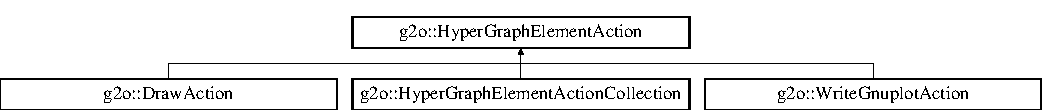
\includegraphics[height=1.475626cm]{classg2o_1_1_hyper_graph_element_action}
\end{center}
\end{figure}
\subsection*{Classes}
\begin{DoxyCompactItemize}
\item 
struct \mbox{\hyperlink{structg2o_1_1_hyper_graph_element_action_1_1_parameters}{Parameters}}
\end{DoxyCompactItemize}
\subsection*{Public Types}
\begin{DoxyCompactItemize}
\item 
typedef std\+::map$<$ std\+::string, \mbox{\hyperlink{classg2o_1_1_hyper_graph_element_action}{Hyper\+Graph\+Element\+Action}} $\ast$ $>$ \mbox{\hyperlink{classg2o_1_1_hyper_graph_element_action_abc889fc90ae1bbb63d90c7993777417a}{Action\+Map}}
\end{DoxyCompactItemize}
\subsection*{Public Member Functions}
\begin{DoxyCompactItemize}
\item 
\mbox{\hyperlink{classg2o_1_1_hyper_graph_element_action_a1230bdd21f7c2b2c71e7206b59d81fd5}{Hyper\+Graph\+Element\+Action}} (const std\+::string \&type\+Name\+\_\+=\char`\"{}\char`\"{})
\item 
virtual \mbox{\hyperlink{classg2o_1_1_hyper_graph_element_action}{Hyper\+Graph\+Element\+Action}} $\ast$ \mbox{\hyperlink{classg2o_1_1_hyper_graph_element_action_a2faab4a1cdaf5fc010cb9c8627b7d361}{operator()}} (\mbox{\hyperlink{structg2o_1_1_hyper_graph_1_1_hyper_graph_element}{Hyper\+Graph\+::\+Hyper\+Graph\+Element}} $\ast$element, \mbox{\hyperlink{structg2o_1_1_hyper_graph_element_action_1_1_parameters}{Parameters}} $\ast$parameters)
\begin{DoxyCompactList}\small\item\em redefine this to do the action stuff. If successful, the action returns a pointer to itself \end{DoxyCompactList}\item 
virtual \mbox{\hyperlink{classg2o_1_1_hyper_graph_element_action}{Hyper\+Graph\+Element\+Action}} $\ast$ \mbox{\hyperlink{classg2o_1_1_hyper_graph_element_action_a0dc2ff77e22791e32810d2c43b7154ad}{operator()}} (const \mbox{\hyperlink{structg2o_1_1_hyper_graph_1_1_hyper_graph_element}{Hyper\+Graph\+::\+Hyper\+Graph\+Element}} $\ast$element, \mbox{\hyperlink{structg2o_1_1_hyper_graph_element_action_1_1_parameters}{Parameters}} $\ast$parameters)
\begin{DoxyCompactList}\small\item\em redefine this to do the action stuff. If successful, the action returns a pointer to itself \end{DoxyCompactList}\item 
virtual \mbox{\hyperlink{classg2o_1_1_hyper_graph_element_action_a01f7f7f2fb00018f2d0163a611f2f5da}{$\sim$\+Hyper\+Graph\+Element\+Action}} ()
\begin{DoxyCompactList}\small\item\em destroyed actions release the memory \end{DoxyCompactList}\item 
const std\+::string \& \mbox{\hyperlink{classg2o_1_1_hyper_graph_element_action_ae8c48d4b811320516bd5b0ef663190e3}{type\+Name}} () const
\begin{DoxyCompactList}\small\item\em returns the typeid name of the action \end{DoxyCompactList}\item 
const std\+::string \& \mbox{\hyperlink{classg2o_1_1_hyper_graph_element_action_aee0238f29b377b432c61e842ba6327ac}{name}} () const
\begin{DoxyCompactList}\small\item\em returns the name of an action, e.\+g \char`\"{}draw\char`\"{} \end{DoxyCompactList}\item 
void \mbox{\hyperlink{classg2o_1_1_hyper_graph_element_action_ae7ed5834d50fb0ff0fef8ec45caaaa3f}{set\+Type\+Name}} (const std\+::string \&type\+Name\+\_\+)
\begin{DoxyCompactList}\small\item\em sets the type on which an action has to operate \end{DoxyCompactList}\end{DoxyCompactItemize}
\subsection*{Protected Attributes}
\begin{DoxyCompactItemize}
\item 
std\+::string \mbox{\hyperlink{classg2o_1_1_hyper_graph_element_action_ae05082e218d213f8db5de7a79769f97c}{\+\_\+type\+Name}}
\item 
std\+::string \mbox{\hyperlink{classg2o_1_1_hyper_graph_element_action_a31245b0a79dfb357e3b345ff57b7b491}{\+\_\+name}}
\end{DoxyCompactItemize}


\subsection{Detailed Description}
Abstract action that operates on a graph entity. 

\subsection{Member Typedef Documentation}
\mbox{\Hypertarget{classg2o_1_1_hyper_graph_element_action_abc889fc90ae1bbb63d90c7993777417a}\label{classg2o_1_1_hyper_graph_element_action_abc889fc90ae1bbb63d90c7993777417a}} 
\index{g2o\+::\+Hyper\+Graph\+Element\+Action@{g2o\+::\+Hyper\+Graph\+Element\+Action}!Action\+Map@{Action\+Map}}
\index{Action\+Map@{Action\+Map}!g2o\+::\+Hyper\+Graph\+Element\+Action@{g2o\+::\+Hyper\+Graph\+Element\+Action}}
\subsubsection{\texorpdfstring{Action\+Map}{ActionMap}}
{\footnotesize\ttfamily typedef std\+::map$<$std\+::string, \mbox{\hyperlink{classg2o_1_1_hyper_graph_element_action}{Hyper\+Graph\+Element\+Action}}$\ast$$>$ \mbox{\hyperlink{classg2o_1_1_hyper_graph_element_action_abc889fc90ae1bbb63d90c7993777417a}{g2o\+::\+Hyper\+Graph\+Element\+Action\+::\+Action\+Map}}}



\subsection{Constructor \& Destructor Documentation}
\mbox{\Hypertarget{classg2o_1_1_hyper_graph_element_action_a1230bdd21f7c2b2c71e7206b59d81fd5}\label{classg2o_1_1_hyper_graph_element_action_a1230bdd21f7c2b2c71e7206b59d81fd5}} 
\index{g2o\+::\+Hyper\+Graph\+Element\+Action@{g2o\+::\+Hyper\+Graph\+Element\+Action}!Hyper\+Graph\+Element\+Action@{Hyper\+Graph\+Element\+Action}}
\index{Hyper\+Graph\+Element\+Action@{Hyper\+Graph\+Element\+Action}!g2o\+::\+Hyper\+Graph\+Element\+Action@{g2o\+::\+Hyper\+Graph\+Element\+Action}}
\subsubsection{\texorpdfstring{Hyper\+Graph\+Element\+Action()}{HyperGraphElementAction()}}
{\footnotesize\ttfamily g2o\+::\+Hyper\+Graph\+Element\+Action\+::\+Hyper\+Graph\+Element\+Action (\begin{DoxyParamCaption}\item[{const std\+::string \&}]{type\+Name\+\_\+ = {\ttfamily \char`\"{}\char`\"{}} }\end{DoxyParamCaption})}

an action should be instantiated with the typeid.\+name of the graph element on which it operates \mbox{\Hypertarget{classg2o_1_1_hyper_graph_element_action_a01f7f7f2fb00018f2d0163a611f2f5da}\label{classg2o_1_1_hyper_graph_element_action_a01f7f7f2fb00018f2d0163a611f2f5da}} 
\index{g2o\+::\+Hyper\+Graph\+Element\+Action@{g2o\+::\+Hyper\+Graph\+Element\+Action}!````~Hyper\+Graph\+Element\+Action@{$\sim$\+Hyper\+Graph\+Element\+Action}}
\index{````~Hyper\+Graph\+Element\+Action@{$\sim$\+Hyper\+Graph\+Element\+Action}!g2o\+::\+Hyper\+Graph\+Element\+Action@{g2o\+::\+Hyper\+Graph\+Element\+Action}}
\subsubsection{\texorpdfstring{$\sim$\+Hyper\+Graph\+Element\+Action()}{~HyperGraphElementAction()}}
{\footnotesize\ttfamily g2o\+::\+Hyper\+Graph\+Element\+Action\+::$\sim$\+Hyper\+Graph\+Element\+Action (\begin{DoxyParamCaption}{ }\end{DoxyParamCaption})\hspace{0.3cm}{\ttfamily [virtual]}}



destroyed actions release the memory 



\subsection{Member Function Documentation}
\mbox{\Hypertarget{classg2o_1_1_hyper_graph_element_action_aee0238f29b377b432c61e842ba6327ac}\label{classg2o_1_1_hyper_graph_element_action_aee0238f29b377b432c61e842ba6327ac}} 
\index{g2o\+::\+Hyper\+Graph\+Element\+Action@{g2o\+::\+Hyper\+Graph\+Element\+Action}!name@{name}}
\index{name@{name}!g2o\+::\+Hyper\+Graph\+Element\+Action@{g2o\+::\+Hyper\+Graph\+Element\+Action}}
\subsubsection{\texorpdfstring{name()}{name()}}
{\footnotesize\ttfamily const std\+::string\& g2o\+::\+Hyper\+Graph\+Element\+Action\+::name (\begin{DoxyParamCaption}{ }\end{DoxyParamCaption}) const\hspace{0.3cm}{\ttfamily [inline]}}



returns the name of an action, e.\+g \char`\"{}draw\char`\"{} 

\mbox{\Hypertarget{classg2o_1_1_hyper_graph_element_action_a2faab4a1cdaf5fc010cb9c8627b7d361}\label{classg2o_1_1_hyper_graph_element_action_a2faab4a1cdaf5fc010cb9c8627b7d361}} 
\index{g2o\+::\+Hyper\+Graph\+Element\+Action@{g2o\+::\+Hyper\+Graph\+Element\+Action}!operator()@{operator()}}
\index{operator()@{operator()}!g2o\+::\+Hyper\+Graph\+Element\+Action@{g2o\+::\+Hyper\+Graph\+Element\+Action}}
\subsubsection{\texorpdfstring{operator()()}{operator()()}\hspace{0.1cm}{\footnotesize\ttfamily [1/2]}}
{\footnotesize\ttfamily \mbox{\hyperlink{classg2o_1_1_hyper_graph_element_action}{Hyper\+Graph\+Element\+Action}} $\ast$ g2o\+::\+Hyper\+Graph\+Element\+Action\+::operator() (\begin{DoxyParamCaption}\item[{\mbox{\hyperlink{structg2o_1_1_hyper_graph_1_1_hyper_graph_element}{Hyper\+Graph\+::\+Hyper\+Graph\+Element}} $\ast$}]{element,  }\item[{\mbox{\hyperlink{structg2o_1_1_hyper_graph_element_action_1_1_parameters}{Hyper\+Graph\+Element\+Action\+::\+Parameters}} $\ast$}]{parameters }\end{DoxyParamCaption})\hspace{0.3cm}{\ttfamily [virtual]}}



redefine this to do the action stuff. If successful, the action returns a pointer to itself 



Reimplemented in \mbox{\hyperlink{classg2o_1_1_hyper_graph_element_action_collection_a1388f0d6629501c1b80035f80c56efbe}{g2o\+::\+Hyper\+Graph\+Element\+Action\+Collection}}.

\mbox{\Hypertarget{classg2o_1_1_hyper_graph_element_action_a0dc2ff77e22791e32810d2c43b7154ad}\label{classg2o_1_1_hyper_graph_element_action_a0dc2ff77e22791e32810d2c43b7154ad}} 
\index{g2o\+::\+Hyper\+Graph\+Element\+Action@{g2o\+::\+Hyper\+Graph\+Element\+Action}!operator()@{operator()}}
\index{operator()@{operator()}!g2o\+::\+Hyper\+Graph\+Element\+Action@{g2o\+::\+Hyper\+Graph\+Element\+Action}}
\subsubsection{\texorpdfstring{operator()()}{operator()()}\hspace{0.1cm}{\footnotesize\ttfamily [2/2]}}
{\footnotesize\ttfamily \mbox{\hyperlink{classg2o_1_1_hyper_graph_element_action}{Hyper\+Graph\+Element\+Action}} $\ast$ g2o\+::\+Hyper\+Graph\+Element\+Action\+::operator() (\begin{DoxyParamCaption}\item[{const \mbox{\hyperlink{structg2o_1_1_hyper_graph_1_1_hyper_graph_element}{Hyper\+Graph\+::\+Hyper\+Graph\+Element}} $\ast$}]{element,  }\item[{\mbox{\hyperlink{structg2o_1_1_hyper_graph_element_action_1_1_parameters}{Hyper\+Graph\+Element\+Action\+::\+Parameters}} $\ast$}]{parameters }\end{DoxyParamCaption})\hspace{0.3cm}{\ttfamily [virtual]}}



redefine this to do the action stuff. If successful, the action returns a pointer to itself 



Reimplemented in \mbox{\hyperlink{classg2o_1_1_hyper_graph_element_action_collection_a4cb9b20a8b1aac8eb018ef6fc4ec0dfc}{g2o\+::\+Hyper\+Graph\+Element\+Action\+Collection}}.

\mbox{\Hypertarget{classg2o_1_1_hyper_graph_element_action_ae7ed5834d50fb0ff0fef8ec45caaaa3f}\label{classg2o_1_1_hyper_graph_element_action_ae7ed5834d50fb0ff0fef8ec45caaaa3f}} 
\index{g2o\+::\+Hyper\+Graph\+Element\+Action@{g2o\+::\+Hyper\+Graph\+Element\+Action}!set\+Type\+Name@{set\+Type\+Name}}
\index{set\+Type\+Name@{set\+Type\+Name}!g2o\+::\+Hyper\+Graph\+Element\+Action@{g2o\+::\+Hyper\+Graph\+Element\+Action}}
\subsubsection{\texorpdfstring{set\+Type\+Name()}{setTypeName()}}
{\footnotesize\ttfamily void g2o\+::\+Hyper\+Graph\+Element\+Action\+::set\+Type\+Name (\begin{DoxyParamCaption}\item[{const std\+::string \&}]{type\+Name\+\_\+ }\end{DoxyParamCaption})}



sets the type on which an action has to operate 

\mbox{\Hypertarget{classg2o_1_1_hyper_graph_element_action_ae8c48d4b811320516bd5b0ef663190e3}\label{classg2o_1_1_hyper_graph_element_action_ae8c48d4b811320516bd5b0ef663190e3}} 
\index{g2o\+::\+Hyper\+Graph\+Element\+Action@{g2o\+::\+Hyper\+Graph\+Element\+Action}!type\+Name@{type\+Name}}
\index{type\+Name@{type\+Name}!g2o\+::\+Hyper\+Graph\+Element\+Action@{g2o\+::\+Hyper\+Graph\+Element\+Action}}
\subsubsection{\texorpdfstring{type\+Name()}{typeName()}}
{\footnotesize\ttfamily const std\+::string\& g2o\+::\+Hyper\+Graph\+Element\+Action\+::type\+Name (\begin{DoxyParamCaption}{ }\end{DoxyParamCaption}) const\hspace{0.3cm}{\ttfamily [inline]}}



returns the typeid name of the action 



\subsection{Member Data Documentation}
\mbox{\Hypertarget{classg2o_1_1_hyper_graph_element_action_a31245b0a79dfb357e3b345ff57b7b491}\label{classg2o_1_1_hyper_graph_element_action_a31245b0a79dfb357e3b345ff57b7b491}} 
\index{g2o\+::\+Hyper\+Graph\+Element\+Action@{g2o\+::\+Hyper\+Graph\+Element\+Action}!\+\_\+name@{\+\_\+name}}
\index{\+\_\+name@{\+\_\+name}!g2o\+::\+Hyper\+Graph\+Element\+Action@{g2o\+::\+Hyper\+Graph\+Element\+Action}}
\subsubsection{\texorpdfstring{\+\_\+name}{\_name}}
{\footnotesize\ttfamily std\+::string g2o\+::\+Hyper\+Graph\+Element\+Action\+::\+\_\+name\hspace{0.3cm}{\ttfamily [protected]}}

\mbox{\Hypertarget{classg2o_1_1_hyper_graph_element_action_ae05082e218d213f8db5de7a79769f97c}\label{classg2o_1_1_hyper_graph_element_action_ae05082e218d213f8db5de7a79769f97c}} 
\index{g2o\+::\+Hyper\+Graph\+Element\+Action@{g2o\+::\+Hyper\+Graph\+Element\+Action}!\+\_\+type\+Name@{\+\_\+type\+Name}}
\index{\+\_\+type\+Name@{\+\_\+type\+Name}!g2o\+::\+Hyper\+Graph\+Element\+Action@{g2o\+::\+Hyper\+Graph\+Element\+Action}}
\subsubsection{\texorpdfstring{\+\_\+type\+Name}{\_typeName}}
{\footnotesize\ttfamily std\+::string g2o\+::\+Hyper\+Graph\+Element\+Action\+::\+\_\+type\+Name\hspace{0.3cm}{\ttfamily [protected]}}



The documentation for this class was generated from the following files\+:\begin{DoxyCompactItemize}
\item 
D\+:/github/\+V\+S\+L\+A\+M/\+O\+R\+B\+S\+L\+A\+M2/\+O\+R\+B-\/\+S\+L\+A\+M2-\/master/\+Thirdparty/g2o/g2o/core/\mbox{\hyperlink{hyper__graph__action_8h}{hyper\+\_\+graph\+\_\+action.\+h}}\item 
D\+:/github/\+V\+S\+L\+A\+M/\+O\+R\+B\+S\+L\+A\+M2/\+O\+R\+B-\/\+S\+L\+A\+M2-\/master/\+Thirdparty/g2o/g2o/core/\mbox{\hyperlink{hyper__graph__action_8cpp}{hyper\+\_\+graph\+\_\+action.\+cpp}}\end{DoxyCompactItemize}

\hypertarget{classg2o_1_1_hyper_graph_element_action_collection}{}\section{g2o\+:\+:Hyper\+Graph\+Element\+Action\+Collection Class Reference}
\label{classg2o_1_1_hyper_graph_element_action_collection}\index{g2o\+::\+Hyper\+Graph\+Element\+Action\+Collection@{g2o\+::\+Hyper\+Graph\+Element\+Action\+Collection}}


collection of actions  




{\ttfamily \#include $<$hyper\+\_\+graph\+\_\+action.\+h$>$}

Inheritance diagram for g2o\+:\+:Hyper\+Graph\+Element\+Action\+Collection\+:\begin{figure}[H]
\begin{center}
\leavevmode
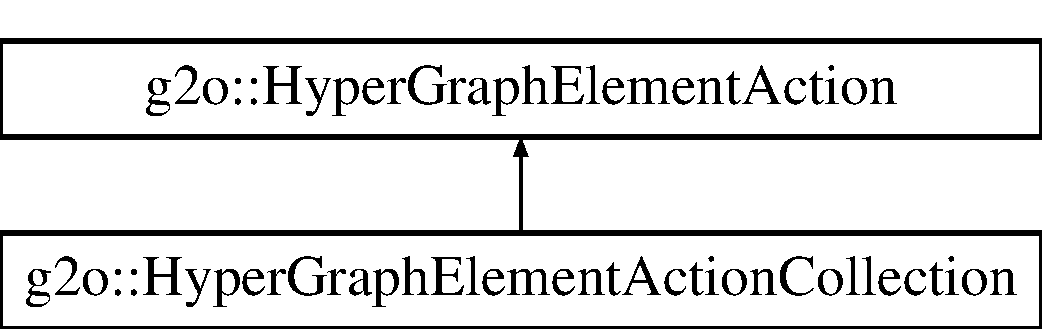
\includegraphics[height=2.000000cm]{classg2o_1_1_hyper_graph_element_action_collection}
\end{center}
\end{figure}
\subsection*{Public Member Functions}
\begin{DoxyCompactItemize}
\item 
\mbox{\hyperlink{classg2o_1_1_hyper_graph_element_action_collection_a6af1ca2dfcdc0894eb594c68135dd614}{Hyper\+Graph\+Element\+Action\+Collection}} (const std\+::string \&name\+\_\+)
\begin{DoxyCompactList}\small\item\em constructor. name\+\_\+ is the name of the action e.\+g.\+draw). \end{DoxyCompactList}\item 
virtual \mbox{\hyperlink{classg2o_1_1_hyper_graph_element_action_collection_ad55fc899922f91c1446d9d69f343c7ab}{$\sim$\+Hyper\+Graph\+Element\+Action\+Collection}} ()
\begin{DoxyCompactList}\small\item\em destructor\+: it deletes all actions in the pool. \end{DoxyCompactList}\item 
virtual \mbox{\hyperlink{classg2o_1_1_hyper_graph_element_action}{Hyper\+Graph\+Element\+Action}} $\ast$ \mbox{\hyperlink{classg2o_1_1_hyper_graph_element_action_collection_a1388f0d6629501c1b80035f80c56efbe}{operator()}} (\mbox{\hyperlink{structg2o_1_1_hyper_graph_1_1_hyper_graph_element}{Hyper\+Graph\+::\+Hyper\+Graph\+Element}} $\ast$element, \mbox{\hyperlink{structg2o_1_1_hyper_graph_element_action_1_1_parameters}{Parameters}} $\ast$parameters)
\item 
virtual \mbox{\hyperlink{classg2o_1_1_hyper_graph_element_action}{Hyper\+Graph\+Element\+Action}} $\ast$ \mbox{\hyperlink{classg2o_1_1_hyper_graph_element_action_collection_a4cb9b20a8b1aac8eb018ef6fc4ec0dfc}{operator()}} (const \mbox{\hyperlink{structg2o_1_1_hyper_graph_1_1_hyper_graph_element}{Hyper\+Graph\+::\+Hyper\+Graph\+Element}} $\ast$element, \mbox{\hyperlink{structg2o_1_1_hyper_graph_element_action_1_1_parameters}{Parameters}} $\ast$parameters)
\begin{DoxyCompactList}\small\item\em redefine this to do the action stuff. If successful, the action returns a pointer to itself \end{DoxyCompactList}\item 
\mbox{\hyperlink{classg2o_1_1_hyper_graph_element_action_abc889fc90ae1bbb63d90c7993777417a}{Action\+Map}} \& \mbox{\hyperlink{classg2o_1_1_hyper_graph_element_action_collection_a26d57ddd0079ed7181fbb322c9a8106c}{action\+Map}} ()
\item 
bool \mbox{\hyperlink{classg2o_1_1_hyper_graph_element_action_collection_a9eb641e9c9bb22f3540dc98c2c750ea9}{register\+Action}} (\mbox{\hyperlink{classg2o_1_1_hyper_graph_element_action}{Hyper\+Graph\+Element\+Action}} $\ast$action)
\item 
bool \mbox{\hyperlink{classg2o_1_1_hyper_graph_element_action_collection_a6dc646c0dd8fbf9b54fb8161348af5e6}{unregister\+Action}} (\mbox{\hyperlink{classg2o_1_1_hyper_graph_element_action}{Hyper\+Graph\+Element\+Action}} $\ast$action)
\end{DoxyCompactItemize}
\subsection*{Protected Attributes}
\begin{DoxyCompactItemize}
\item 
\mbox{\hyperlink{classg2o_1_1_hyper_graph_element_action_abc889fc90ae1bbb63d90c7993777417a}{Action\+Map}} \mbox{\hyperlink{classg2o_1_1_hyper_graph_element_action_collection_a637c13fca95eacab38ee82eedd3669e4}{\+\_\+action\+Map}}
\end{DoxyCompactItemize}
\subsection*{Additional Inherited Members}


\subsection{Detailed Description}
collection of actions 

collection of actions calls contains homogeneous actions operating on different types all collected actions have the same name and should have the same functionality 

\subsection{Constructor \& Destructor Documentation}
\mbox{\Hypertarget{classg2o_1_1_hyper_graph_element_action_collection_a6af1ca2dfcdc0894eb594c68135dd614}\label{classg2o_1_1_hyper_graph_element_action_collection_a6af1ca2dfcdc0894eb594c68135dd614}} 
\index{g2o\+::\+Hyper\+Graph\+Element\+Action\+Collection@{g2o\+::\+Hyper\+Graph\+Element\+Action\+Collection}!Hyper\+Graph\+Element\+Action\+Collection@{Hyper\+Graph\+Element\+Action\+Collection}}
\index{Hyper\+Graph\+Element\+Action\+Collection@{Hyper\+Graph\+Element\+Action\+Collection}!g2o\+::\+Hyper\+Graph\+Element\+Action\+Collection@{g2o\+::\+Hyper\+Graph\+Element\+Action\+Collection}}
\subsubsection{\texorpdfstring{Hyper\+Graph\+Element\+Action\+Collection()}{HyperGraphElementActionCollection()}}
{\footnotesize\ttfamily g2o\+::\+Hyper\+Graph\+Element\+Action\+Collection\+::\+Hyper\+Graph\+Element\+Action\+Collection (\begin{DoxyParamCaption}\item[{const std\+::string \&}]{name\+\_\+ }\end{DoxyParamCaption})}



constructor. name\+\_\+ is the name of the action e.\+g.\+draw). 

\mbox{\Hypertarget{classg2o_1_1_hyper_graph_element_action_collection_ad55fc899922f91c1446d9d69f343c7ab}\label{classg2o_1_1_hyper_graph_element_action_collection_ad55fc899922f91c1446d9d69f343c7ab}} 
\index{g2o\+::\+Hyper\+Graph\+Element\+Action\+Collection@{g2o\+::\+Hyper\+Graph\+Element\+Action\+Collection}!````~Hyper\+Graph\+Element\+Action\+Collection@{$\sim$\+Hyper\+Graph\+Element\+Action\+Collection}}
\index{````~Hyper\+Graph\+Element\+Action\+Collection@{$\sim$\+Hyper\+Graph\+Element\+Action\+Collection}!g2o\+::\+Hyper\+Graph\+Element\+Action\+Collection@{g2o\+::\+Hyper\+Graph\+Element\+Action\+Collection}}
\subsubsection{\texorpdfstring{$\sim$\+Hyper\+Graph\+Element\+Action\+Collection()}{~HyperGraphElementActionCollection()}}
{\footnotesize\ttfamily g2o\+::\+Hyper\+Graph\+Element\+Action\+Collection\+::$\sim$\+Hyper\+Graph\+Element\+Action\+Collection (\begin{DoxyParamCaption}{ }\end{DoxyParamCaption})\hspace{0.3cm}{\ttfamily [virtual]}}



destructor\+: it deletes all actions in the pool. 



\subsection{Member Function Documentation}
\mbox{\Hypertarget{classg2o_1_1_hyper_graph_element_action_collection_a26d57ddd0079ed7181fbb322c9a8106c}\label{classg2o_1_1_hyper_graph_element_action_collection_a26d57ddd0079ed7181fbb322c9a8106c}} 
\index{g2o\+::\+Hyper\+Graph\+Element\+Action\+Collection@{g2o\+::\+Hyper\+Graph\+Element\+Action\+Collection}!action\+Map@{action\+Map}}
\index{action\+Map@{action\+Map}!g2o\+::\+Hyper\+Graph\+Element\+Action\+Collection@{g2o\+::\+Hyper\+Graph\+Element\+Action\+Collection}}
\subsubsection{\texorpdfstring{action\+Map()}{actionMap()}}
{\footnotesize\ttfamily \mbox{\hyperlink{classg2o_1_1_hyper_graph_element_action_abc889fc90ae1bbb63d90c7993777417a}{Action\+Map}}\& g2o\+::\+Hyper\+Graph\+Element\+Action\+Collection\+::action\+Map (\begin{DoxyParamCaption}{ }\end{DoxyParamCaption})\hspace{0.3cm}{\ttfamily [inline]}}

\mbox{\Hypertarget{classg2o_1_1_hyper_graph_element_action_collection_a1388f0d6629501c1b80035f80c56efbe}\label{classg2o_1_1_hyper_graph_element_action_collection_a1388f0d6629501c1b80035f80c56efbe}} 
\index{g2o\+::\+Hyper\+Graph\+Element\+Action\+Collection@{g2o\+::\+Hyper\+Graph\+Element\+Action\+Collection}!operator()@{operator()}}
\index{operator()@{operator()}!g2o\+::\+Hyper\+Graph\+Element\+Action\+Collection@{g2o\+::\+Hyper\+Graph\+Element\+Action\+Collection}}
\subsubsection{\texorpdfstring{operator()()}{operator()()}\hspace{0.1cm}{\footnotesize\ttfamily [1/2]}}
{\footnotesize\ttfamily \mbox{\hyperlink{classg2o_1_1_hyper_graph_element_action}{Hyper\+Graph\+Element\+Action}} $\ast$ g2o\+::\+Hyper\+Graph\+Element\+Action\+Collection\+::operator() (\begin{DoxyParamCaption}\item[{\mbox{\hyperlink{structg2o_1_1_hyper_graph_1_1_hyper_graph_element}{Hyper\+Graph\+::\+Hyper\+Graph\+Element}} $\ast$}]{element,  }\item[{\mbox{\hyperlink{structg2o_1_1_hyper_graph_element_action_1_1_parameters}{Hyper\+Graph\+Element\+Action\+::\+Parameters}} $\ast$}]{params }\end{DoxyParamCaption})\hspace{0.3cm}{\ttfamily [virtual]}}

calling functions, they return a pointer to the instance of action in action\+Map that was active on element 

Reimplemented from \mbox{\hyperlink{classg2o_1_1_hyper_graph_element_action_a2faab4a1cdaf5fc010cb9c8627b7d361}{g2o\+::\+Hyper\+Graph\+Element\+Action}}.

\mbox{\Hypertarget{classg2o_1_1_hyper_graph_element_action_collection_a4cb9b20a8b1aac8eb018ef6fc4ec0dfc}\label{classg2o_1_1_hyper_graph_element_action_collection_a4cb9b20a8b1aac8eb018ef6fc4ec0dfc}} 
\index{g2o\+::\+Hyper\+Graph\+Element\+Action\+Collection@{g2o\+::\+Hyper\+Graph\+Element\+Action\+Collection}!operator()@{operator()}}
\index{operator()@{operator()}!g2o\+::\+Hyper\+Graph\+Element\+Action\+Collection@{g2o\+::\+Hyper\+Graph\+Element\+Action\+Collection}}
\subsubsection{\texorpdfstring{operator()()}{operator()()}\hspace{0.1cm}{\footnotesize\ttfamily [2/2]}}
{\footnotesize\ttfamily \mbox{\hyperlink{classg2o_1_1_hyper_graph_element_action}{Hyper\+Graph\+Element\+Action}} $\ast$ g2o\+::\+Hyper\+Graph\+Element\+Action\+Collection\+::operator() (\begin{DoxyParamCaption}\item[{const \mbox{\hyperlink{structg2o_1_1_hyper_graph_1_1_hyper_graph_element}{Hyper\+Graph\+::\+Hyper\+Graph\+Element}} $\ast$}]{element,  }\item[{\mbox{\hyperlink{structg2o_1_1_hyper_graph_element_action_1_1_parameters}{Hyper\+Graph\+Element\+Action\+::\+Parameters}} $\ast$}]{parameters }\end{DoxyParamCaption})\hspace{0.3cm}{\ttfamily [virtual]}}



redefine this to do the action stuff. If successful, the action returns a pointer to itself 



Reimplemented from \mbox{\hyperlink{classg2o_1_1_hyper_graph_element_action_a0dc2ff77e22791e32810d2c43b7154ad}{g2o\+::\+Hyper\+Graph\+Element\+Action}}.

\mbox{\Hypertarget{classg2o_1_1_hyper_graph_element_action_collection_a9eb641e9c9bb22f3540dc98c2c750ea9}\label{classg2o_1_1_hyper_graph_element_action_collection_a9eb641e9c9bb22f3540dc98c2c750ea9}} 
\index{g2o\+::\+Hyper\+Graph\+Element\+Action\+Collection@{g2o\+::\+Hyper\+Graph\+Element\+Action\+Collection}!register\+Action@{register\+Action}}
\index{register\+Action@{register\+Action}!g2o\+::\+Hyper\+Graph\+Element\+Action\+Collection@{g2o\+::\+Hyper\+Graph\+Element\+Action\+Collection}}
\subsubsection{\texorpdfstring{register\+Action()}{registerAction()}}
{\footnotesize\ttfamily bool g2o\+::\+Hyper\+Graph\+Element\+Action\+Collection\+::register\+Action (\begin{DoxyParamCaption}\item[{\mbox{\hyperlink{classg2o_1_1_hyper_graph_element_action}{Hyper\+Graph\+Element\+Action}} $\ast$}]{action }\end{DoxyParamCaption})}

inserts an action in the pool. The action should have the same name of the container. returns false on failure (the container has a different name than the action); \mbox{\Hypertarget{classg2o_1_1_hyper_graph_element_action_collection_a6dc646c0dd8fbf9b54fb8161348af5e6}\label{classg2o_1_1_hyper_graph_element_action_collection_a6dc646c0dd8fbf9b54fb8161348af5e6}} 
\index{g2o\+::\+Hyper\+Graph\+Element\+Action\+Collection@{g2o\+::\+Hyper\+Graph\+Element\+Action\+Collection}!unregister\+Action@{unregister\+Action}}
\index{unregister\+Action@{unregister\+Action}!g2o\+::\+Hyper\+Graph\+Element\+Action\+Collection@{g2o\+::\+Hyper\+Graph\+Element\+Action\+Collection}}
\subsubsection{\texorpdfstring{unregister\+Action()}{unregisterAction()}}
{\footnotesize\ttfamily bool g2o\+::\+Hyper\+Graph\+Element\+Action\+Collection\+::unregister\+Action (\begin{DoxyParamCaption}\item[{\mbox{\hyperlink{classg2o_1_1_hyper_graph_element_action}{Hyper\+Graph\+Element\+Action}} $\ast$}]{action }\end{DoxyParamCaption})}



\subsection{Member Data Documentation}
\mbox{\Hypertarget{classg2o_1_1_hyper_graph_element_action_collection_a637c13fca95eacab38ee82eedd3669e4}\label{classg2o_1_1_hyper_graph_element_action_collection_a637c13fca95eacab38ee82eedd3669e4}} 
\index{g2o\+::\+Hyper\+Graph\+Element\+Action\+Collection@{g2o\+::\+Hyper\+Graph\+Element\+Action\+Collection}!\+\_\+action\+Map@{\+\_\+action\+Map}}
\index{\+\_\+action\+Map@{\+\_\+action\+Map}!g2o\+::\+Hyper\+Graph\+Element\+Action\+Collection@{g2o\+::\+Hyper\+Graph\+Element\+Action\+Collection}}
\subsubsection{\texorpdfstring{\+\_\+action\+Map}{\_actionMap}}
{\footnotesize\ttfamily \mbox{\hyperlink{classg2o_1_1_hyper_graph_element_action_abc889fc90ae1bbb63d90c7993777417a}{Action\+Map}} g2o\+::\+Hyper\+Graph\+Element\+Action\+Collection\+::\+\_\+action\+Map\hspace{0.3cm}{\ttfamily [protected]}}



The documentation for this class was generated from the following files\+:\begin{DoxyCompactItemize}
\item 
D\+:/github/\+V\+S\+L\+A\+M/\+O\+R\+B\+S\+L\+A\+M2/\+O\+R\+B-\/\+S\+L\+A\+M2-\/master/\+Thirdparty/g2o/g2o/core/\mbox{\hyperlink{hyper__graph__action_8h}{hyper\+\_\+graph\+\_\+action.\+h}}\item 
D\+:/github/\+V\+S\+L\+A\+M/\+O\+R\+B\+S\+L\+A\+M2/\+O\+R\+B-\/\+S\+L\+A\+M2-\/master/\+Thirdparty/g2o/g2o/core/\mbox{\hyperlink{hyper__graph__action_8cpp}{hyper\+\_\+graph\+\_\+action.\+cpp}}\end{DoxyCompactItemize}

\hypertarget{classg2o_1_1_hyper_graph_element_creator}{}\section{g2o\+:\+:Hyper\+Graph\+Element\+Creator$<$ T $>$ Class Template Reference}
\label{classg2o_1_1_hyper_graph_element_creator}\index{g2o\+::\+Hyper\+Graph\+Element\+Creator$<$ T $>$@{g2o\+::\+Hyper\+Graph\+Element\+Creator$<$ T $>$}}


templatized creator class which creates graph elements  




{\ttfamily \#include $<$creators.\+h$>$}

Inheritance diagram for g2o\+:\+:Hyper\+Graph\+Element\+Creator$<$ T $>$\+:\begin{figure}[H]
\begin{center}
\leavevmode
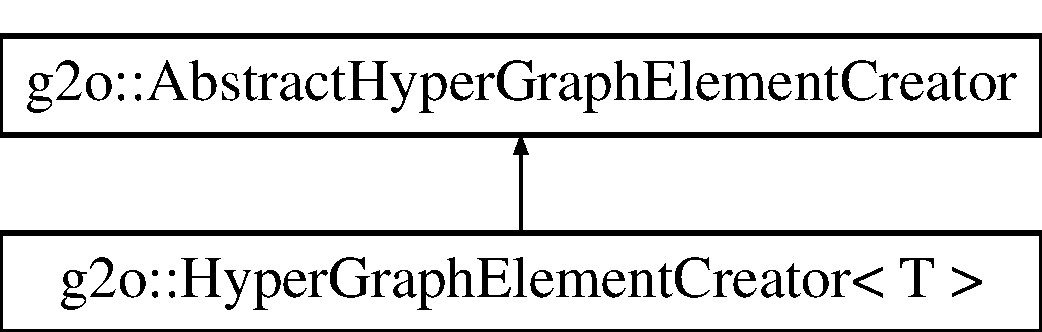
\includegraphics[height=2.000000cm]{classg2o_1_1_hyper_graph_element_creator}
\end{center}
\end{figure}
\subsection*{Public Member Functions}
\begin{DoxyCompactItemize}
\item 
\mbox{\hyperlink{classg2o_1_1_hyper_graph_element_creator_aacaa6cfc040649e5802bfe07240f242f}{Hyper\+Graph\+Element\+Creator}} ()
\item 
\mbox{\hyperlink{structg2o_1_1_hyper_graph_1_1_hyper_graph_element}{Hyper\+Graph\+::\+Hyper\+Graph\+Element}} $\ast$ \mbox{\hyperlink{classg2o_1_1_hyper_graph_element_creator_af5e58366dd05b49700076e0c4ace31e3}{construct}} ()
\item 
virtual const std\+::string \& \mbox{\hyperlink{classg2o_1_1_hyper_graph_element_creator_a9350df173e72ccb4bb6594d282a2c0e7}{name}} () const
\end{DoxyCompactItemize}
\subsection*{Protected Attributes}
\begin{DoxyCompactItemize}
\item 
std\+::string \mbox{\hyperlink{classg2o_1_1_hyper_graph_element_creator_abbcc42de74a57d80b586dd843255ebae}{\+\_\+name}}
\end{DoxyCompactItemize}


\subsection{Detailed Description}
\subsubsection*{template$<$typename T$>$\newline
class g2o\+::\+Hyper\+Graph\+Element\+Creator$<$ T $>$}

templatized creator class which creates graph elements 

\subsection{Constructor \& Destructor Documentation}
\mbox{\Hypertarget{classg2o_1_1_hyper_graph_element_creator_aacaa6cfc040649e5802bfe07240f242f}\label{classg2o_1_1_hyper_graph_element_creator_aacaa6cfc040649e5802bfe07240f242f}} 
\index{g2o\+::\+Hyper\+Graph\+Element\+Creator@{g2o\+::\+Hyper\+Graph\+Element\+Creator}!Hyper\+Graph\+Element\+Creator@{Hyper\+Graph\+Element\+Creator}}
\index{Hyper\+Graph\+Element\+Creator@{Hyper\+Graph\+Element\+Creator}!g2o\+::\+Hyper\+Graph\+Element\+Creator@{g2o\+::\+Hyper\+Graph\+Element\+Creator}}
\subsubsection{\texorpdfstring{Hyper\+Graph\+Element\+Creator()}{HyperGraphElementCreator()}}
{\footnotesize\ttfamily template$<$typename T $>$ \\
\mbox{\hyperlink{classg2o_1_1_hyper_graph_element_creator}{g2o\+::\+Hyper\+Graph\+Element\+Creator}}$<$ T $>$\+::\mbox{\hyperlink{classg2o_1_1_hyper_graph_element_creator}{Hyper\+Graph\+Element\+Creator}} (\begin{DoxyParamCaption}{ }\end{DoxyParamCaption})\hspace{0.3cm}{\ttfamily [inline]}}



\subsection{Member Function Documentation}
\mbox{\Hypertarget{classg2o_1_1_hyper_graph_element_creator_af5e58366dd05b49700076e0c4ace31e3}\label{classg2o_1_1_hyper_graph_element_creator_af5e58366dd05b49700076e0c4ace31e3}} 
\index{g2o\+::\+Hyper\+Graph\+Element\+Creator@{g2o\+::\+Hyper\+Graph\+Element\+Creator}!construct@{construct}}
\index{construct@{construct}!g2o\+::\+Hyper\+Graph\+Element\+Creator@{g2o\+::\+Hyper\+Graph\+Element\+Creator}}
\subsubsection{\texorpdfstring{construct()}{construct()}}
{\footnotesize\ttfamily template$<$typename T $>$ \\
\mbox{\hyperlink{structg2o_1_1_hyper_graph_1_1_hyper_graph_element}{Hyper\+Graph\+::\+Hyper\+Graph\+Element}}$\ast$ \mbox{\hyperlink{classg2o_1_1_hyper_graph_element_creator}{g2o\+::\+Hyper\+Graph\+Element\+Creator}}$<$ T $>$\+::construct (\begin{DoxyParamCaption}{ }\end{DoxyParamCaption})\hspace{0.3cm}{\ttfamily [inline]}, {\ttfamily [virtual]}}

create a hyper graph element. Has to implemented in derived class. 

Implements \mbox{\hyperlink{classg2o_1_1_abstract_hyper_graph_element_creator_a0b4722fa4b05465bf89d6e7fdc75b153}{g2o\+::\+Abstract\+Hyper\+Graph\+Element\+Creator}}.

\mbox{\Hypertarget{classg2o_1_1_hyper_graph_element_creator_a9350df173e72ccb4bb6594d282a2c0e7}\label{classg2o_1_1_hyper_graph_element_creator_a9350df173e72ccb4bb6594d282a2c0e7}} 
\index{g2o\+::\+Hyper\+Graph\+Element\+Creator@{g2o\+::\+Hyper\+Graph\+Element\+Creator}!name@{name}}
\index{name@{name}!g2o\+::\+Hyper\+Graph\+Element\+Creator@{g2o\+::\+Hyper\+Graph\+Element\+Creator}}
\subsubsection{\texorpdfstring{name()}{name()}}
{\footnotesize\ttfamily template$<$typename T $>$ \\
virtual const std\+::string\& \mbox{\hyperlink{classg2o_1_1_hyper_graph_element_creator}{g2o\+::\+Hyper\+Graph\+Element\+Creator}}$<$ T $>$\+::name (\begin{DoxyParamCaption}{ }\end{DoxyParamCaption}) const\hspace{0.3cm}{\ttfamily [inline]}, {\ttfamily [virtual]}}

name of the class to be created. Has to implemented in derived class. 

Implements \mbox{\hyperlink{classg2o_1_1_abstract_hyper_graph_element_creator_a238928fbbfd6e473b2c61002112e6f5f}{g2o\+::\+Abstract\+Hyper\+Graph\+Element\+Creator}}.



\subsection{Member Data Documentation}
\mbox{\Hypertarget{classg2o_1_1_hyper_graph_element_creator_abbcc42de74a57d80b586dd843255ebae}\label{classg2o_1_1_hyper_graph_element_creator_abbcc42de74a57d80b586dd843255ebae}} 
\index{g2o\+::\+Hyper\+Graph\+Element\+Creator@{g2o\+::\+Hyper\+Graph\+Element\+Creator}!\+\_\+name@{\+\_\+name}}
\index{\+\_\+name@{\+\_\+name}!g2o\+::\+Hyper\+Graph\+Element\+Creator@{g2o\+::\+Hyper\+Graph\+Element\+Creator}}
\subsubsection{\texorpdfstring{\+\_\+name}{\_name}}
{\footnotesize\ttfamily template$<$typename T $>$ \\
std\+::string \mbox{\hyperlink{classg2o_1_1_hyper_graph_element_creator}{g2o\+::\+Hyper\+Graph\+Element\+Creator}}$<$ T $>$\+::\+\_\+name\hspace{0.3cm}{\ttfamily [protected]}}



The documentation for this class was generated from the following file\+:\begin{DoxyCompactItemize}
\item 
D\+:/github/\+V\+S\+L\+A\+M/\+O\+R\+B\+S\+L\+A\+M2/\+O\+R\+B-\/\+S\+L\+A\+M2-\/master/\+Thirdparty/g2o/g2o/core/\mbox{\hyperlink{creators_8h}{creators.\+h}}\end{DoxyCompactItemize}

\hypertarget{class_image_grabber}{}\section{Image\+Grabber Class Reference}
\label{class_image_grabber}\index{Image\+Grabber@{Image\+Grabber}}
\subsection*{Public Member Functions}
\begin{DoxyCompactItemize}
\item 
\mbox{\hyperlink{class_image_grabber_aa7692b812eafa9a76e82b96794999239}{Image\+Grabber}} (\mbox{\hyperlink{class_o_r_b___s_l_a_m2_1_1_system}{O\+R\+B\+\_\+\+S\+L\+A\+M2\+::\+System}} $\ast$p\+S\+L\+AM)
\item 
void \mbox{\hyperlink{class_image_grabber_a66758ed685acbf1a7e77b3325001e47c}{Grab\+Image}} (const sensor\+\_\+msgs\+::\+Image\+Const\+Ptr \&msg)
\item 
\mbox{\hyperlink{class_image_grabber_aa7692b812eafa9a76e82b96794999239}{Image\+Grabber}} (\mbox{\hyperlink{class_o_r_b___s_l_a_m2_1_1_system}{O\+R\+B\+\_\+\+S\+L\+A\+M2\+::\+System}} $\ast$p\+S\+L\+AM)
\item 
void \mbox{\hyperlink{class_image_grabber_ab6df23b898365aa3df99628e4c925aee}{Grab\+R\+G\+BD}} (const sensor\+\_\+msgs\+::\+Image\+Const\+Ptr \&msg\+R\+GB, const sensor\+\_\+msgs\+::\+Image\+Const\+Ptr \&msgD)
\item 
\mbox{\hyperlink{class_image_grabber_aa7692b812eafa9a76e82b96794999239}{Image\+Grabber}} (\mbox{\hyperlink{class_o_r_b___s_l_a_m2_1_1_system}{O\+R\+B\+\_\+\+S\+L\+A\+M2\+::\+System}} $\ast$p\+S\+L\+AM)
\item 
void \mbox{\hyperlink{class_image_grabber_a640450feb6e5df2cb0b2aae7574367c2}{Grab\+Stereo}} (const sensor\+\_\+msgs\+::\+Image\+Const\+Ptr \&msg\+Left, const sensor\+\_\+msgs\+::\+Image\+Const\+Ptr \&msg\+Right)
\end{DoxyCompactItemize}
\subsection*{Public Attributes}
\begin{DoxyCompactItemize}
\item 
\mbox{\hyperlink{class_o_r_b___s_l_a_m2_1_1_system}{O\+R\+B\+\_\+\+S\+L\+A\+M2\+::\+System}} $\ast$ \mbox{\hyperlink{class_image_grabber_a09543ab679feffd1969ad9bca851652f}{mp\+S\+L\+AM}}
\item 
bool \mbox{\hyperlink{class_image_grabber_a773e5d7e773fd5e2cf695e9b7de418b0}{do\+\_\+rectify}}
\item 
cv\+::\+Mat \mbox{\hyperlink{class_image_grabber_a6074a577631bc9ca7cb1e9a53d384175}{M1l}}
\item 
cv\+::\+Mat \mbox{\hyperlink{class_image_grabber_ac85158e1dfb61d91c16271649d9a0354}{M2l}}
\item 
cv\+::\+Mat \mbox{\hyperlink{class_image_grabber_a1b32be412baa2e1a606863375ba8ff83}{M1r}}
\item 
cv\+::\+Mat \mbox{\hyperlink{class_image_grabber_aaf139de883a63055e03d4c82e953bb88}{M2r}}
\end{DoxyCompactItemize}


\subsection{Constructor \& Destructor Documentation}
\mbox{\Hypertarget{class_image_grabber_aa7692b812eafa9a76e82b96794999239}\label{class_image_grabber_aa7692b812eafa9a76e82b96794999239}} 
\index{Image\+Grabber@{Image\+Grabber}!Image\+Grabber@{Image\+Grabber}}
\index{Image\+Grabber@{Image\+Grabber}!Image\+Grabber@{Image\+Grabber}}
\subsubsection{\texorpdfstring{Image\+Grabber()}{ImageGrabber()}\hspace{0.1cm}{\footnotesize\ttfamily [1/3]}}
{\footnotesize\ttfamily Image\+Grabber\+::\+Image\+Grabber (\begin{DoxyParamCaption}\item[{\mbox{\hyperlink{class_o_r_b___s_l_a_m2_1_1_system}{O\+R\+B\+\_\+\+S\+L\+A\+M2\+::\+System}} $\ast$}]{p\+S\+L\+AM }\end{DoxyParamCaption})\hspace{0.3cm}{\ttfamily [inline]}}

\mbox{\Hypertarget{class_image_grabber_aa7692b812eafa9a76e82b96794999239}\label{class_image_grabber_aa7692b812eafa9a76e82b96794999239}} 
\index{Image\+Grabber@{Image\+Grabber}!Image\+Grabber@{Image\+Grabber}}
\index{Image\+Grabber@{Image\+Grabber}!Image\+Grabber@{Image\+Grabber}}
\subsubsection{\texorpdfstring{Image\+Grabber()}{ImageGrabber()}\hspace{0.1cm}{\footnotesize\ttfamily [2/3]}}
{\footnotesize\ttfamily Image\+Grabber\+::\+Image\+Grabber (\begin{DoxyParamCaption}\item[{\mbox{\hyperlink{class_o_r_b___s_l_a_m2_1_1_system}{O\+R\+B\+\_\+\+S\+L\+A\+M2\+::\+System}} $\ast$}]{p\+S\+L\+AM }\end{DoxyParamCaption})\hspace{0.3cm}{\ttfamily [inline]}}

\mbox{\Hypertarget{class_image_grabber_aa7692b812eafa9a76e82b96794999239}\label{class_image_grabber_aa7692b812eafa9a76e82b96794999239}} 
\index{Image\+Grabber@{Image\+Grabber}!Image\+Grabber@{Image\+Grabber}}
\index{Image\+Grabber@{Image\+Grabber}!Image\+Grabber@{Image\+Grabber}}
\subsubsection{\texorpdfstring{Image\+Grabber()}{ImageGrabber()}\hspace{0.1cm}{\footnotesize\ttfamily [3/3]}}
{\footnotesize\ttfamily Image\+Grabber\+::\+Image\+Grabber (\begin{DoxyParamCaption}\item[{\mbox{\hyperlink{class_o_r_b___s_l_a_m2_1_1_system}{O\+R\+B\+\_\+\+S\+L\+A\+M2\+::\+System}} $\ast$}]{p\+S\+L\+AM }\end{DoxyParamCaption})\hspace{0.3cm}{\ttfamily [inline]}}



\subsection{Member Function Documentation}
\mbox{\Hypertarget{class_image_grabber_a66758ed685acbf1a7e77b3325001e47c}\label{class_image_grabber_a66758ed685acbf1a7e77b3325001e47c}} 
\index{Image\+Grabber@{Image\+Grabber}!Grab\+Image@{Grab\+Image}}
\index{Grab\+Image@{Grab\+Image}!Image\+Grabber@{Image\+Grabber}}
\subsubsection{\texorpdfstring{Grab\+Image()}{GrabImage()}}
{\footnotesize\ttfamily void Image\+Grabber\+::\+Grab\+Image (\begin{DoxyParamCaption}\item[{const sensor\+\_\+msgs\+::\+Image\+Const\+Ptr \&}]{msg }\end{DoxyParamCaption})}

\mbox{\Hypertarget{class_image_grabber_ab6df23b898365aa3df99628e4c925aee}\label{class_image_grabber_ab6df23b898365aa3df99628e4c925aee}} 
\index{Image\+Grabber@{Image\+Grabber}!Grab\+R\+G\+BD@{Grab\+R\+G\+BD}}
\index{Grab\+R\+G\+BD@{Grab\+R\+G\+BD}!Image\+Grabber@{Image\+Grabber}}
\subsubsection{\texorpdfstring{Grab\+R\+G\+B\+D()}{GrabRGBD()}}
{\footnotesize\ttfamily void Image\+Grabber\+::\+Grab\+R\+G\+BD (\begin{DoxyParamCaption}\item[{const sensor\+\_\+msgs\+::\+Image\+Const\+Ptr \&}]{msg\+R\+GB,  }\item[{const sensor\+\_\+msgs\+::\+Image\+Const\+Ptr \&}]{msgD }\end{DoxyParamCaption})}

\mbox{\Hypertarget{class_image_grabber_a640450feb6e5df2cb0b2aae7574367c2}\label{class_image_grabber_a640450feb6e5df2cb0b2aae7574367c2}} 
\index{Image\+Grabber@{Image\+Grabber}!Grab\+Stereo@{Grab\+Stereo}}
\index{Grab\+Stereo@{Grab\+Stereo}!Image\+Grabber@{Image\+Grabber}}
\subsubsection{\texorpdfstring{Grab\+Stereo()}{GrabStereo()}}
{\footnotesize\ttfamily void Image\+Grabber\+::\+Grab\+Stereo (\begin{DoxyParamCaption}\item[{const sensor\+\_\+msgs\+::\+Image\+Const\+Ptr \&}]{msg\+Left,  }\item[{const sensor\+\_\+msgs\+::\+Image\+Const\+Ptr \&}]{msg\+Right }\end{DoxyParamCaption})}



\subsection{Member Data Documentation}
\mbox{\Hypertarget{class_image_grabber_a773e5d7e773fd5e2cf695e9b7de418b0}\label{class_image_grabber_a773e5d7e773fd5e2cf695e9b7de418b0}} 
\index{Image\+Grabber@{Image\+Grabber}!do\+\_\+rectify@{do\+\_\+rectify}}
\index{do\+\_\+rectify@{do\+\_\+rectify}!Image\+Grabber@{Image\+Grabber}}
\subsubsection{\texorpdfstring{do\+\_\+rectify}{do\_rectify}}
{\footnotesize\ttfamily bool Image\+Grabber\+::do\+\_\+rectify}

\mbox{\Hypertarget{class_image_grabber_a6074a577631bc9ca7cb1e9a53d384175}\label{class_image_grabber_a6074a577631bc9ca7cb1e9a53d384175}} 
\index{Image\+Grabber@{Image\+Grabber}!M1l@{M1l}}
\index{M1l@{M1l}!Image\+Grabber@{Image\+Grabber}}
\subsubsection{\texorpdfstring{M1l}{M1l}}
{\footnotesize\ttfamily cv\+::\+Mat Image\+Grabber\+::\+M1l}

\mbox{\Hypertarget{class_image_grabber_a1b32be412baa2e1a606863375ba8ff83}\label{class_image_grabber_a1b32be412baa2e1a606863375ba8ff83}} 
\index{Image\+Grabber@{Image\+Grabber}!M1r@{M1r}}
\index{M1r@{M1r}!Image\+Grabber@{Image\+Grabber}}
\subsubsection{\texorpdfstring{M1r}{M1r}}
{\footnotesize\ttfamily cv\+::\+Mat Image\+Grabber\+::\+M1r}

\mbox{\Hypertarget{class_image_grabber_ac85158e1dfb61d91c16271649d9a0354}\label{class_image_grabber_ac85158e1dfb61d91c16271649d9a0354}} 
\index{Image\+Grabber@{Image\+Grabber}!M2l@{M2l}}
\index{M2l@{M2l}!Image\+Grabber@{Image\+Grabber}}
\subsubsection{\texorpdfstring{M2l}{M2l}}
{\footnotesize\ttfamily cv\+::\+Mat Image\+Grabber\+::\+M2l}

\mbox{\Hypertarget{class_image_grabber_aaf139de883a63055e03d4c82e953bb88}\label{class_image_grabber_aaf139de883a63055e03d4c82e953bb88}} 
\index{Image\+Grabber@{Image\+Grabber}!M2r@{M2r}}
\index{M2r@{M2r}!Image\+Grabber@{Image\+Grabber}}
\subsubsection{\texorpdfstring{M2r}{M2r}}
{\footnotesize\ttfamily cv\+::\+Mat Image\+Grabber\+::\+M2r}

\mbox{\Hypertarget{class_image_grabber_a09543ab679feffd1969ad9bca851652f}\label{class_image_grabber_a09543ab679feffd1969ad9bca851652f}} 
\index{Image\+Grabber@{Image\+Grabber}!mp\+S\+L\+AM@{mp\+S\+L\+AM}}
\index{mp\+S\+L\+AM@{mp\+S\+L\+AM}!Image\+Grabber@{Image\+Grabber}}
\subsubsection{\texorpdfstring{mp\+S\+L\+AM}{mpSLAM}}
{\footnotesize\ttfamily \mbox{\hyperlink{class_o_r_b___s_l_a_m2_1_1_system}{O\+R\+B\+\_\+\+S\+L\+A\+M2\+::\+System}} $\ast$ Image\+Grabber\+::mp\+S\+L\+AM}



The documentation for this class was generated from the following files\+:\begin{DoxyCompactItemize}
\item 
Examples/\+R\+O\+S/\+O\+R\+B\+\_\+\+S\+L\+A\+M2/src/\mbox{\hyperlink{ros__mono_8cc}{ros\+\_\+mono.\+cc}}\item 
Examples/\+R\+O\+S/\+O\+R\+B\+\_\+\+S\+L\+A\+M2/src/\mbox{\hyperlink{ros__rgbd_8cc}{ros\+\_\+rgbd.\+cc}}\item 
Examples/\+R\+O\+S/\+O\+R\+B\+\_\+\+S\+L\+A\+M2/src/\mbox{\hyperlink{ros__stereo_8cc}{ros\+\_\+stereo.\+cc}}\end{DoxyCompactItemize}

\hypertarget{class_o_r_b___s_l_a_m2_1_1_initializer}{}\section{O\+R\+B\+\_\+\+S\+L\+A\+M2\+:\+:Initializer Class Reference}
\label{class_o_r_b___s_l_a_m2_1_1_initializer}\index{O\+R\+B\+\_\+\+S\+L\+A\+M2\+::\+Initializer@{O\+R\+B\+\_\+\+S\+L\+A\+M2\+::\+Initializer}}


单目\+S\+L\+A\+M初始化相关,双目和\+R\+G\+B\+D不会使用这个类  




{\ttfamily \#include $<$Initializer.\+h$>$}

\subsection*{Public Member Functions}
\begin{DoxyCompactItemize}
\item 
\mbox{\hyperlink{class_o_r_b___s_l_a_m2_1_1_initializer_ac492345a970665cd8a1b1d8cf41d44af}{Initializer}} (const \mbox{\hyperlink{class_o_r_b___s_l_a_m2_1_1_frame}{Frame}} \&Reference\+Frame, float sigma=1.\+0, int iterations=200)
\begin{DoxyCompactList}\small\item\em 给定参考帧构造\+Initializer \end{DoxyCompactList}\item 
bool \mbox{\hyperlink{class_o_r_b___s_l_a_m2_1_1_initializer_a40d41840e2bdb7199ab024871d028c2c}{Initialize}} (const \mbox{\hyperlink{class_o_r_b___s_l_a_m2_1_1_frame}{Frame}} \&Current\+Frame, const vector$<$ int $>$ \&v\+Matches12, cv\+::\+Mat \&R21, cv\+::\+Mat \&t21, vector$<$ cv\+::\+Point3f $>$ \&v\+P3D, vector$<$ bool $>$ \&vb\+Triangulated)
\begin{DoxyCompactList}\small\item\em 并行地计算基础矩阵和单应性矩阵,选取其中一个模型,恢复出最开始两帧之间的相对姿态以及点云 \end{DoxyCompactList}\end{DoxyCompactItemize}


\subsection{Detailed Description}
单目\+S\+L\+A\+M初始化相关,双目和\+R\+G\+B\+D不会使用这个类 

\subsection{Constructor \& Destructor Documentation}
\mbox{\Hypertarget{class_o_r_b___s_l_a_m2_1_1_initializer_ac492345a970665cd8a1b1d8cf41d44af}\label{class_o_r_b___s_l_a_m2_1_1_initializer_ac492345a970665cd8a1b1d8cf41d44af}} 
\index{O\+R\+B\+\_\+\+S\+L\+A\+M2\+::\+Initializer@{O\+R\+B\+\_\+\+S\+L\+A\+M2\+::\+Initializer}!Initializer@{Initializer}}
\index{Initializer@{Initializer}!O\+R\+B\+\_\+\+S\+L\+A\+M2\+::\+Initializer@{O\+R\+B\+\_\+\+S\+L\+A\+M2\+::\+Initializer}}
\subsubsection{\texorpdfstring{Initializer()}{Initializer()}}
{\footnotesize\ttfamily O\+R\+B\+\_\+\+S\+L\+A\+M2\+::\+Initializer\+::\+Initializer (\begin{DoxyParamCaption}\item[{const \mbox{\hyperlink{class_o_r_b___s_l_a_m2_1_1_frame}{Frame}} \&}]{Reference\+Frame,  }\item[{float}]{sigma = {\ttfamily 1.0},  }\item[{int}]{iterations = {\ttfamily 200} }\end{DoxyParamCaption})}



给定参考帧构造\+Initializer 

用reference frame来初始化,这个reference frame就是\+S\+L\+A\+M正式开始的第一帧 
\begin{DoxyParams}{Parameters}
{\em Reference\+Frame} & 参考帧 \\
\hline
{\em sigma} & 测量误差 \\
\hline
{\em iterations} & R\+A\+N\+S\+A\+C迭代次数 \\
\hline
\end{DoxyParams}


\subsection{Member Function Documentation}
\mbox{\Hypertarget{class_o_r_b___s_l_a_m2_1_1_initializer_a40d41840e2bdb7199ab024871d028c2c}\label{class_o_r_b___s_l_a_m2_1_1_initializer_a40d41840e2bdb7199ab024871d028c2c}} 
\index{O\+R\+B\+\_\+\+S\+L\+A\+M2\+::\+Initializer@{O\+R\+B\+\_\+\+S\+L\+A\+M2\+::\+Initializer}!Initialize@{Initialize}}
\index{Initialize@{Initialize}!O\+R\+B\+\_\+\+S\+L\+A\+M2\+::\+Initializer@{O\+R\+B\+\_\+\+S\+L\+A\+M2\+::\+Initializer}}
\subsubsection{\texorpdfstring{Initialize()}{Initialize()}}
{\footnotesize\ttfamily bool O\+R\+B\+\_\+\+S\+L\+A\+M2\+::\+Initializer\+::\+Initialize (\begin{DoxyParamCaption}\item[{const \mbox{\hyperlink{class_o_r_b___s_l_a_m2_1_1_frame}{Frame}} \&}]{Current\+Frame,  }\item[{const vector$<$ int $>$ \&}]{v\+Matches12,  }\item[{cv\+::\+Mat \&}]{R21,  }\item[{cv\+::\+Mat \&}]{t21,  }\item[{vector$<$ cv\+::\+Point3f $>$ \&}]{v\+P3D,  }\item[{vector$<$ bool $>$ \&}]{vb\+Triangulated }\end{DoxyParamCaption})}



并行地计算基础矩阵和单应性矩阵,选取其中一个模型,恢复出最开始两帧之间的相对姿态以及点云 



The documentation for this class was generated from the following files\+:\begin{DoxyCompactItemize}
\item 
include/\mbox{\hyperlink{_initializer_8h}{Initializer.\+h}}\item 
src/\mbox{\hyperlink{_initializer_8cpp}{Initializer.\+cpp}}\end{DoxyCompactItemize}

\hypertarget{classg2o_1_1_jacobian_workspace}{}\section{g2o\+:\+:Jacobian\+Workspace Class Reference}
\label{classg2o_1_1_jacobian_workspace}\index{g2o\+::\+Jacobian\+Workspace@{g2o\+::\+Jacobian\+Workspace}}


provide memory workspace for computing the Jacobians  




{\ttfamily \#include $<$jacobian\+\_\+workspace.\+h$>$}

\subsection*{Public Types}
\begin{DoxyCompactItemize}
\item 
typedef std\+::vector$<$ Eigen\+::\+Vector\+Xd, Eigen\+::aligned\+\_\+allocator$<$ Eigen\+::\+Vector\+Xd $>$ $>$ \mbox{\hyperlink{classg2o_1_1_jacobian_workspace_aee9d767fa1208772a3de83732646e182}{Workspace\+Vector}}
\end{DoxyCompactItemize}
\subsection*{Public Member Functions}
\begin{DoxyCompactItemize}
\item 
\mbox{\hyperlink{classg2o_1_1_jacobian_workspace_a6c20de27401a40e620ee065c80d24b9e}{Jacobian\+Workspace}} ()
\item 
\mbox{\hyperlink{classg2o_1_1_jacobian_workspace_a0d00e42f6e048268ff5005b8e3f578dd}{$\sim$\+Jacobian\+Workspace}} ()
\item 
bool \mbox{\hyperlink{classg2o_1_1_jacobian_workspace_a8e1d23ced91b721fdb5bd68c8c4e9fc3}{allocate}} ()
\item 
void \mbox{\hyperlink{classg2o_1_1_jacobian_workspace_a2d16ad6db1a51aa93c806cc9c06e223f}{update\+Size}} (const \mbox{\hyperlink{classg2o_1_1_hyper_graph_1_1_edge}{Hyper\+Graph\+::\+Edge}} $\ast$e)
\item 
void \mbox{\hyperlink{classg2o_1_1_jacobian_workspace_ae3d715bd25e196d8db81661ef0fbd09b}{update\+Size}} (const \mbox{\hyperlink{structg2o_1_1_optimizable_graph}{Optimizable\+Graph}} \&graph)
\item 
void \mbox{\hyperlink{classg2o_1_1_jacobian_workspace_aa15a007fee3037116ea0e857855080d2}{update\+Size}} (int num\+Vertices, int dimension)
\item 
double $\ast$ \mbox{\hyperlink{classg2o_1_1_jacobian_workspace_ad68c37d7779d3a034bc1b864cd98690b}{workspace\+For\+Vertex}} (int vertex\+Index)
\end{DoxyCompactItemize}
\subsection*{Protected Attributes}
\begin{DoxyCompactItemize}
\item 
\mbox{\hyperlink{classg2o_1_1_jacobian_workspace_aee9d767fa1208772a3de83732646e182}{Workspace\+Vector}} \mbox{\hyperlink{classg2o_1_1_jacobian_workspace_af7dbaa3a651808e1bf3f876896bd1bfc}{\+\_\+workspace}}
\begin{DoxyCompactList}\small\item\em the memory pre-\/allocated for computing the Jacobians \end{DoxyCompactList}\item 
int \mbox{\hyperlink{classg2o_1_1_jacobian_workspace_a640c84c19a739ce3116fc02c3a66b096}{\+\_\+max\+Num\+Vertices}}
\begin{DoxyCompactList}\small\item\em the maximum number of vertices connected by a hyper-\/edge \end{DoxyCompactList}\item 
int \mbox{\hyperlink{classg2o_1_1_jacobian_workspace_aa6cd4fb8bc1bb4fe9ada55d9feefc817}{\+\_\+max\+Dimension}}
\begin{DoxyCompactList}\small\item\em the maximum dimension (number of elements) for a Jacobian \end{DoxyCompactList}\end{DoxyCompactItemize}


\subsection{Detailed Description}
provide memory workspace for computing the Jacobians 

The workspace is used by an \mbox{\hyperlink{structg2o_1_1_optimizable_graph}{Optimizable\+Graph}} to provide temporary memory for computing the Jacobian of the error functions. Before calling linearize\+Oplus on an edge, the workspace needs to be allocated by calling \mbox{\hyperlink{classg2o_1_1_jacobian_workspace_a8e1d23ced91b721fdb5bd68c8c4e9fc3}{allocate()}}. 

\subsection{Member Typedef Documentation}
\mbox{\Hypertarget{classg2o_1_1_jacobian_workspace_aee9d767fa1208772a3de83732646e182}\label{classg2o_1_1_jacobian_workspace_aee9d767fa1208772a3de83732646e182}} 
\index{g2o\+::\+Jacobian\+Workspace@{g2o\+::\+Jacobian\+Workspace}!Workspace\+Vector@{Workspace\+Vector}}
\index{Workspace\+Vector@{Workspace\+Vector}!g2o\+::\+Jacobian\+Workspace@{g2o\+::\+Jacobian\+Workspace}}
\subsubsection{\texorpdfstring{Workspace\+Vector}{WorkspaceVector}}
{\footnotesize\ttfamily typedef std\+::vector$<$Eigen\+::\+Vector\+Xd, Eigen\+::aligned\+\_\+allocator$<$Eigen\+::\+Vector\+Xd$>$ $>$ \mbox{\hyperlink{classg2o_1_1_jacobian_workspace_aee9d767fa1208772a3de83732646e182}{g2o\+::\+Jacobian\+Workspace\+::\+Workspace\+Vector}}}



\subsection{Constructor \& Destructor Documentation}
\mbox{\Hypertarget{classg2o_1_1_jacobian_workspace_a6c20de27401a40e620ee065c80d24b9e}\label{classg2o_1_1_jacobian_workspace_a6c20de27401a40e620ee065c80d24b9e}} 
\index{g2o\+::\+Jacobian\+Workspace@{g2o\+::\+Jacobian\+Workspace}!Jacobian\+Workspace@{Jacobian\+Workspace}}
\index{Jacobian\+Workspace@{Jacobian\+Workspace}!g2o\+::\+Jacobian\+Workspace@{g2o\+::\+Jacobian\+Workspace}}
\subsubsection{\texorpdfstring{Jacobian\+Workspace()}{JacobianWorkspace()}}
{\footnotesize\ttfamily g2o\+::\+Jacobian\+Workspace\+::\+Jacobian\+Workspace (\begin{DoxyParamCaption}{ }\end{DoxyParamCaption})}

\mbox{\Hypertarget{classg2o_1_1_jacobian_workspace_a0d00e42f6e048268ff5005b8e3f578dd}\label{classg2o_1_1_jacobian_workspace_a0d00e42f6e048268ff5005b8e3f578dd}} 
\index{g2o\+::\+Jacobian\+Workspace@{g2o\+::\+Jacobian\+Workspace}!````~Jacobian\+Workspace@{$\sim$\+Jacobian\+Workspace}}
\index{````~Jacobian\+Workspace@{$\sim$\+Jacobian\+Workspace}!g2o\+::\+Jacobian\+Workspace@{g2o\+::\+Jacobian\+Workspace}}
\subsubsection{\texorpdfstring{$\sim$\+Jacobian\+Workspace()}{~JacobianWorkspace()}}
{\footnotesize\ttfamily g2o\+::\+Jacobian\+Workspace\+::$\sim$\+Jacobian\+Workspace (\begin{DoxyParamCaption}{ }\end{DoxyParamCaption})}



\subsection{Member Function Documentation}
\mbox{\Hypertarget{classg2o_1_1_jacobian_workspace_a8e1d23ced91b721fdb5bd68c8c4e9fc3}\label{classg2o_1_1_jacobian_workspace_a8e1d23ced91b721fdb5bd68c8c4e9fc3}} 
\index{g2o\+::\+Jacobian\+Workspace@{g2o\+::\+Jacobian\+Workspace}!allocate@{allocate}}
\index{allocate@{allocate}!g2o\+::\+Jacobian\+Workspace@{g2o\+::\+Jacobian\+Workspace}}
\subsubsection{\texorpdfstring{allocate()}{allocate()}}
{\footnotesize\ttfamily bool g2o\+::\+Jacobian\+Workspace\+::allocate (\begin{DoxyParamCaption}{ }\end{DoxyParamCaption})}

allocate the workspace \mbox{\Hypertarget{classg2o_1_1_jacobian_workspace_a2d16ad6db1a51aa93c806cc9c06e223f}\label{classg2o_1_1_jacobian_workspace_a2d16ad6db1a51aa93c806cc9c06e223f}} 
\index{g2o\+::\+Jacobian\+Workspace@{g2o\+::\+Jacobian\+Workspace}!update\+Size@{update\+Size}}
\index{update\+Size@{update\+Size}!g2o\+::\+Jacobian\+Workspace@{g2o\+::\+Jacobian\+Workspace}}
\subsubsection{\texorpdfstring{update\+Size()}{updateSize()}\hspace{0.1cm}{\footnotesize\ttfamily [1/3]}}
{\footnotesize\ttfamily void g2o\+::\+Jacobian\+Workspace\+::update\+Size (\begin{DoxyParamCaption}\item[{const \mbox{\hyperlink{classg2o_1_1_hyper_graph_1_1_edge}{Hyper\+Graph\+::\+Edge}} $\ast$}]{e }\end{DoxyParamCaption})}

update the maximum required workspace needed by taking into account this edge \mbox{\Hypertarget{classg2o_1_1_jacobian_workspace_ae3d715bd25e196d8db81661ef0fbd09b}\label{classg2o_1_1_jacobian_workspace_ae3d715bd25e196d8db81661ef0fbd09b}} 
\index{g2o\+::\+Jacobian\+Workspace@{g2o\+::\+Jacobian\+Workspace}!update\+Size@{update\+Size}}
\index{update\+Size@{update\+Size}!g2o\+::\+Jacobian\+Workspace@{g2o\+::\+Jacobian\+Workspace}}
\subsubsection{\texorpdfstring{update\+Size()}{updateSize()}\hspace{0.1cm}{\footnotesize\ttfamily [2/3]}}
{\footnotesize\ttfamily void g2o\+::\+Jacobian\+Workspace\+::update\+Size (\begin{DoxyParamCaption}\item[{const \mbox{\hyperlink{structg2o_1_1_optimizable_graph}{Optimizable\+Graph}} \&}]{graph }\end{DoxyParamCaption})}

update the required workspace by looking at a full graph \mbox{\Hypertarget{classg2o_1_1_jacobian_workspace_aa15a007fee3037116ea0e857855080d2}\label{classg2o_1_1_jacobian_workspace_aa15a007fee3037116ea0e857855080d2}} 
\index{g2o\+::\+Jacobian\+Workspace@{g2o\+::\+Jacobian\+Workspace}!update\+Size@{update\+Size}}
\index{update\+Size@{update\+Size}!g2o\+::\+Jacobian\+Workspace@{g2o\+::\+Jacobian\+Workspace}}
\subsubsection{\texorpdfstring{update\+Size()}{updateSize()}\hspace{0.1cm}{\footnotesize\ttfamily [3/3]}}
{\footnotesize\ttfamily void g2o\+::\+Jacobian\+Workspace\+::update\+Size (\begin{DoxyParamCaption}\item[{int}]{num\+Vertices,  }\item[{int}]{dimension }\end{DoxyParamCaption})}

manually update with the given parameters \mbox{\Hypertarget{classg2o_1_1_jacobian_workspace_ad68c37d7779d3a034bc1b864cd98690b}\label{classg2o_1_1_jacobian_workspace_ad68c37d7779d3a034bc1b864cd98690b}} 
\index{g2o\+::\+Jacobian\+Workspace@{g2o\+::\+Jacobian\+Workspace}!workspace\+For\+Vertex@{workspace\+For\+Vertex}}
\index{workspace\+For\+Vertex@{workspace\+For\+Vertex}!g2o\+::\+Jacobian\+Workspace@{g2o\+::\+Jacobian\+Workspace}}
\subsubsection{\texorpdfstring{workspace\+For\+Vertex()}{workspaceForVertex()}}
{\footnotesize\ttfamily double$\ast$ g2o\+::\+Jacobian\+Workspace\+::workspace\+For\+Vertex (\begin{DoxyParamCaption}\item[{int}]{vertex\+Index }\end{DoxyParamCaption})\hspace{0.3cm}{\ttfamily [inline]}}

return the workspace for a vertex in an edge 

\subsection{Member Data Documentation}
\mbox{\Hypertarget{classg2o_1_1_jacobian_workspace_aa6cd4fb8bc1bb4fe9ada55d9feefc817}\label{classg2o_1_1_jacobian_workspace_aa6cd4fb8bc1bb4fe9ada55d9feefc817}} 
\index{g2o\+::\+Jacobian\+Workspace@{g2o\+::\+Jacobian\+Workspace}!\+\_\+max\+Dimension@{\+\_\+max\+Dimension}}
\index{\+\_\+max\+Dimension@{\+\_\+max\+Dimension}!g2o\+::\+Jacobian\+Workspace@{g2o\+::\+Jacobian\+Workspace}}
\subsubsection{\texorpdfstring{\+\_\+max\+Dimension}{\_maxDimension}}
{\footnotesize\ttfamily int g2o\+::\+Jacobian\+Workspace\+::\+\_\+max\+Dimension\hspace{0.3cm}{\ttfamily [protected]}}



the maximum dimension (number of elements) for a Jacobian 

\mbox{\Hypertarget{classg2o_1_1_jacobian_workspace_a640c84c19a739ce3116fc02c3a66b096}\label{classg2o_1_1_jacobian_workspace_a640c84c19a739ce3116fc02c3a66b096}} 
\index{g2o\+::\+Jacobian\+Workspace@{g2o\+::\+Jacobian\+Workspace}!\+\_\+max\+Num\+Vertices@{\+\_\+max\+Num\+Vertices}}
\index{\+\_\+max\+Num\+Vertices@{\+\_\+max\+Num\+Vertices}!g2o\+::\+Jacobian\+Workspace@{g2o\+::\+Jacobian\+Workspace}}
\subsubsection{\texorpdfstring{\+\_\+max\+Num\+Vertices}{\_maxNumVertices}}
{\footnotesize\ttfamily int g2o\+::\+Jacobian\+Workspace\+::\+\_\+max\+Num\+Vertices\hspace{0.3cm}{\ttfamily [protected]}}



the maximum number of vertices connected by a hyper-\/edge 

\mbox{\Hypertarget{classg2o_1_1_jacobian_workspace_af7dbaa3a651808e1bf3f876896bd1bfc}\label{classg2o_1_1_jacobian_workspace_af7dbaa3a651808e1bf3f876896bd1bfc}} 
\index{g2o\+::\+Jacobian\+Workspace@{g2o\+::\+Jacobian\+Workspace}!\+\_\+workspace@{\+\_\+workspace}}
\index{\+\_\+workspace@{\+\_\+workspace}!g2o\+::\+Jacobian\+Workspace@{g2o\+::\+Jacobian\+Workspace}}
\subsubsection{\texorpdfstring{\+\_\+workspace}{\_workspace}}
{\footnotesize\ttfamily \mbox{\hyperlink{classg2o_1_1_jacobian_workspace_aee9d767fa1208772a3de83732646e182}{Workspace\+Vector}} g2o\+::\+Jacobian\+Workspace\+::\+\_\+workspace\hspace{0.3cm}{\ttfamily [protected]}}



the memory pre-\/allocated for computing the Jacobians 



The documentation for this class was generated from the following files\+:\begin{DoxyCompactItemize}
\item 
Thirdparty/g2o/g2o/core/\mbox{\hyperlink{jacobian__workspace_8h}{jacobian\+\_\+workspace.\+h}}\item 
Thirdparty/g2o/g2o/core/\mbox{\hyperlink{jacobian__workspace_8cpp}{jacobian\+\_\+workspace.\+cpp}}\end{DoxyCompactItemize}

\hypertarget{class_o_r_b___s_l_a_m2_1_1_key_frame}{}\section{O\+R\+B\+\_\+\+S\+L\+A\+M2\+:\+:Key\+Frame Class Reference}
\label{class_o_r_b___s_l_a_m2_1_1_key_frame}\index{O\+R\+B\+\_\+\+S\+L\+A\+M2\+::\+Key\+Frame@{O\+R\+B\+\_\+\+S\+L\+A\+M2\+::\+Key\+Frame}}


{\ttfamily \#include $<$Key\+Frame.\+h$>$}

\subsection*{Public Member Functions}
\begin{DoxyCompactItemize}
\item 
\mbox{\hyperlink{class_o_r_b___s_l_a_m2_1_1_key_frame_a6b2fd06ed5e4a8f9546c515db554bcb6}{Key\+Frame}} (\mbox{\hyperlink{class_o_r_b___s_l_a_m2_1_1_frame}{Frame}} \&F, \mbox{\hyperlink{class_o_r_b___s_l_a_m2_1_1_map}{Map}} $\ast$p\+Map, \mbox{\hyperlink{class_o_r_b___s_l_a_m2_1_1_key_frame_database}{Key\+Frame\+Database}} $\ast$p\+K\+F\+DB)
\item 
void \mbox{\hyperlink{class_o_r_b___s_l_a_m2_1_1_key_frame_aa799150fa33f3b9a404226454b96c95a}{Set\+Pose}} (const cv\+::\+Mat \&\mbox{\hyperlink{class_o_r_b___s_l_a_m2_1_1_key_frame_a8dc31ef9a08d34ecb196f3e58a2c09b9}{Tcw}})
\item 
cv\+::\+Mat \mbox{\hyperlink{class_o_r_b___s_l_a_m2_1_1_key_frame_a49b5e212c1335cf585eaf6bbc4fed85c}{Get\+Pose}} ()
\item 
cv\+::\+Mat \mbox{\hyperlink{class_o_r_b___s_l_a_m2_1_1_key_frame_a03be061f5dac65d360d65c6e8a63532f}{Get\+Pose\+Inverse}} ()
\item 
cv\+::\+Mat \mbox{\hyperlink{class_o_r_b___s_l_a_m2_1_1_key_frame_a535f0f7db34aca7c55ddadc2ad9f4a5f}{Get\+Camera\+Center}} ()
\item 
cv\+::\+Mat \mbox{\hyperlink{class_o_r_b___s_l_a_m2_1_1_key_frame_aac7e26797d9b3e7ef4acd656056ff4ce}{Get\+Stereo\+Center}} ()
\item 
cv\+::\+Mat \mbox{\hyperlink{class_o_r_b___s_l_a_m2_1_1_key_frame_a43cdfc1cebc87d949ae6e9a0202b0f1b}{Get\+Rotation}} ()
\item 
cv\+::\+Mat \mbox{\hyperlink{class_o_r_b___s_l_a_m2_1_1_key_frame_a6f1426dc5447170df37c31db40edef14}{Get\+Translation}} ()
\item 
void \mbox{\hyperlink{class_o_r_b___s_l_a_m2_1_1_key_frame_ac376017c23823c05a6bb851ffb2fdd8f}{Compute\+BoW}} ()
\begin{DoxyCompactList}\small\item\em Bag of Words Representation. \end{DoxyCompactList}\item 
void \mbox{\hyperlink{class_o_r_b___s_l_a_m2_1_1_key_frame_a8d21a23485b7c104a73d6ad3cccf4e93}{Add\+Connection}} (\mbox{\hyperlink{class_o_r_b___s_l_a_m2_1_1_key_frame}{Key\+Frame}} $\ast$p\+KF, const int \&weight)
\begin{DoxyCompactList}\small\item\em 为关键帧之间添加连接 \end{DoxyCompactList}\item 
void \mbox{\hyperlink{class_o_r_b___s_l_a_m2_1_1_key_frame_a0a2e676f5e594cf9330e197a2c7df378}{Erase\+Connection}} (\mbox{\hyperlink{class_o_r_b___s_l_a_m2_1_1_key_frame}{Key\+Frame}} $\ast$p\+KF)
\item 
void \mbox{\hyperlink{class_o_r_b___s_l_a_m2_1_1_key_frame_afe7026956c91d4e0a01812be9dc7e8d5}{Update\+Connections}} ()
\begin{DoxyCompactList}\small\item\em 更新图的连接 \end{DoxyCompactList}\item 
void \mbox{\hyperlink{class_o_r_b___s_l_a_m2_1_1_key_frame_a09cb8502509c136536bf8d45793f8872}{Update\+Best\+Covisibles}} ()
\begin{DoxyCompactList}\small\item\em 按照权重对连接的关键帧进行排序 \end{DoxyCompactList}\item 
std\+::set$<$ \mbox{\hyperlink{class_o_r_b___s_l_a_m2_1_1_key_frame}{Key\+Frame}} $\ast$ $>$ \mbox{\hyperlink{class_o_r_b___s_l_a_m2_1_1_key_frame_af4ffdf4441477a36c42d6605c573f1cf}{Get\+Connected\+Key\+Frames}} ()
\begin{DoxyCompactList}\small\item\em 得到与该关键帧连接的关键帧 \end{DoxyCompactList}\item 
std\+::vector$<$ \mbox{\hyperlink{class_o_r_b___s_l_a_m2_1_1_key_frame}{Key\+Frame}} $\ast$$>$ \mbox{\hyperlink{class_o_r_b___s_l_a_m2_1_1_key_frame_a9315d396634f6637f70f716336777b8d}{Get\+Vector\+Covisible\+Key\+Frames}} ()
\begin{DoxyCompactList}\small\item\em 得到与该关键帧连接的关键帧(已按权值排序) \end{DoxyCompactList}\item 
std\+::vector$<$ \mbox{\hyperlink{class_o_r_b___s_l_a_m2_1_1_key_frame}{Key\+Frame}} $\ast$ $>$ \mbox{\hyperlink{class_o_r_b___s_l_a_m2_1_1_key_frame_a2ecb2df01af804fb727c93948a28475f}{Get\+Best\+Covisibility\+Key\+Frames}} (const int \&\mbox{\hyperlink{class_o_r_b___s_l_a_m2_1_1_key_frame_ac9b6948404d0ade2779335708cd443b9}{N}})
\begin{DoxyCompactList}\small\item\em 得到与该关键帧连接的前\+N个关键帧(已按权值排序) \end{DoxyCompactList}\item 
std\+::vector$<$ \mbox{\hyperlink{class_o_r_b___s_l_a_m2_1_1_key_frame}{Key\+Frame}} $\ast$ $>$ \mbox{\hyperlink{class_o_r_b___s_l_a_m2_1_1_key_frame_a7047bffbf130b00dd0270df99874f8a1}{Get\+Covisibles\+By\+Weight}} (const int \&w)
\begin{DoxyCompactList}\small\item\em 得到与该关键帧连接的权重大于等于w的关键帧 \end{DoxyCompactList}\item 
int \mbox{\hyperlink{class_o_r_b___s_l_a_m2_1_1_key_frame_ab10fd3aab6431face352a930961ff713}{Get\+Weight}} (\mbox{\hyperlink{class_o_r_b___s_l_a_m2_1_1_key_frame}{Key\+Frame}} $\ast$p\+KF)
\begin{DoxyCompactList}\small\item\em 得到该关键帧与p\+K\+F的权重 \end{DoxyCompactList}\item 
void \mbox{\hyperlink{class_o_r_b___s_l_a_m2_1_1_key_frame_a2394adfb627d9cf87ed8da78f6b0d709}{Add\+Child}} (\mbox{\hyperlink{class_o_r_b___s_l_a_m2_1_1_key_frame}{Key\+Frame}} $\ast$p\+KF)
\item 
void \mbox{\hyperlink{class_o_r_b___s_l_a_m2_1_1_key_frame_aefdd69627fd6a204a6ef4539303b81f6}{Erase\+Child}} (\mbox{\hyperlink{class_o_r_b___s_l_a_m2_1_1_key_frame}{Key\+Frame}} $\ast$p\+KF)
\item 
void \mbox{\hyperlink{class_o_r_b___s_l_a_m2_1_1_key_frame_a3232df2495062749da1344db3e5a487f}{Change\+Parent}} (\mbox{\hyperlink{class_o_r_b___s_l_a_m2_1_1_key_frame}{Key\+Frame}} $\ast$p\+KF)
\item 
std\+::set$<$ \mbox{\hyperlink{class_o_r_b___s_l_a_m2_1_1_key_frame}{Key\+Frame}} $\ast$ $>$ \mbox{\hyperlink{class_o_r_b___s_l_a_m2_1_1_key_frame_a618ddd51eab47bf1d84a21d2e818a787}{Get\+Childs}} ()
\item 
\mbox{\hyperlink{class_o_r_b___s_l_a_m2_1_1_key_frame}{Key\+Frame}} $\ast$ \mbox{\hyperlink{class_o_r_b___s_l_a_m2_1_1_key_frame_a660cfc9a6ccf87e5497356d0d98ef06f}{Get\+Parent}} ()
\item 
bool \mbox{\hyperlink{class_o_r_b___s_l_a_m2_1_1_key_frame_a2276fdbae634194e790878adebba7861}{has\+Child}} (\mbox{\hyperlink{class_o_r_b___s_l_a_m2_1_1_key_frame}{Key\+Frame}} $\ast$p\+KF)
\item 
void \mbox{\hyperlink{class_o_r_b___s_l_a_m2_1_1_key_frame_aca519e7486b0e6f1fd6c98d7ced920b8}{Add\+Loop\+Edge}} (\mbox{\hyperlink{class_o_r_b___s_l_a_m2_1_1_key_frame}{Key\+Frame}} $\ast$p\+KF)
\item 
std\+::set$<$ \mbox{\hyperlink{class_o_r_b___s_l_a_m2_1_1_key_frame}{Key\+Frame}} $\ast$ $>$ \mbox{\hyperlink{class_o_r_b___s_l_a_m2_1_1_key_frame_ab3109e85b0ab224efdc23e51b5d2c3fa}{Get\+Loop\+Edges}} ()
\item 
void \mbox{\hyperlink{class_o_r_b___s_l_a_m2_1_1_key_frame_a16ea4f0cfa1ca411bb3382107fe69d2d}{Add\+Map\+Point}} (\mbox{\hyperlink{class_o_r_b___s_l_a_m2_1_1_map_point}{Map\+Point}} $\ast$p\+MP, const size\+\_\+t \&idx)
\begin{DoxyCompactList}\small\item\em Add \mbox{\hyperlink{class_o_r_b___s_l_a_m2_1_1_map_point}{Map\+Point}} to \mbox{\hyperlink{class_o_r_b___s_l_a_m2_1_1_key_frame}{Key\+Frame}}. \end{DoxyCompactList}\item 
void \mbox{\hyperlink{class_o_r_b___s_l_a_m2_1_1_key_frame_a2fd38a2bca9f5ced2f1f7501b8046195}{Erase\+Map\+Point\+Match}} (const size\+\_\+t \&idx)
\item 
void \mbox{\hyperlink{class_o_r_b___s_l_a_m2_1_1_key_frame_ab3a775e959978e6d449386882e45b8a2}{Erase\+Map\+Point\+Match}} (\mbox{\hyperlink{class_o_r_b___s_l_a_m2_1_1_map_point}{Map\+Point}} $\ast$p\+MP)
\item 
void \mbox{\hyperlink{class_o_r_b___s_l_a_m2_1_1_key_frame_a35779a4eb4f5cec346780bbbdf377298}{Replace\+Map\+Point\+Match}} (const size\+\_\+t \&idx, \mbox{\hyperlink{class_o_r_b___s_l_a_m2_1_1_map_point}{Map\+Point}} $\ast$p\+MP)
\item 
std\+::set$<$ \mbox{\hyperlink{class_o_r_b___s_l_a_m2_1_1_map_point}{Map\+Point}} $\ast$ $>$ \mbox{\hyperlink{class_o_r_b___s_l_a_m2_1_1_key_frame_a09cb77a8377be3fa8c85c7b5ee45e913}{Get\+Map\+Points}} ()
\item 
std\+::vector$<$ \mbox{\hyperlink{class_o_r_b___s_l_a_m2_1_1_map_point}{Map\+Point}} $\ast$ $>$ \mbox{\hyperlink{class_o_r_b___s_l_a_m2_1_1_key_frame_aabc5f6491c32999d9f546669737547bf}{Get\+Map\+Point\+Matches}} ()
\begin{DoxyCompactList}\small\item\em Get \mbox{\hyperlink{class_o_r_b___s_l_a_m2_1_1_map_point}{Map\+Point}} Matches. \end{DoxyCompactList}\item 
int \mbox{\hyperlink{class_o_r_b___s_l_a_m2_1_1_key_frame_a729cbf2c84db5cbfdda98a9612f8cd0b}{Tracked\+Map\+Points}} (const int \&min\+Obs)
\begin{DoxyCompactList}\small\item\em 关键帧中,大于等于min\+Obs的\+Map\+Points的数量 min\+Obs就是一个阈值,大于min\+Obs就表示该\+Map\+Point是一个高质量的\+Map\+Point 一个高质量的\+Map\+Point会被多个\+Key\+Frame观测到, \end{DoxyCompactList}\item 
\mbox{\hyperlink{class_o_r_b___s_l_a_m2_1_1_map_point}{Map\+Point}} $\ast$ \mbox{\hyperlink{class_o_r_b___s_l_a_m2_1_1_key_frame_ab85915f3e647334634d8a4d489c63ffd}{Get\+Map\+Point}} (const size\+\_\+t \&idx)
\item 
std\+::vector$<$ size\+\_\+t $>$ \mbox{\hyperlink{class_o_r_b___s_l_a_m2_1_1_key_frame_aa057f2902cc7910343c5d452d33cb39f}{Get\+Features\+In\+Area}} (const float \&x, const float \&y, const float \&r) const
\item 
cv\+::\+Mat \mbox{\hyperlink{class_o_r_b___s_l_a_m2_1_1_key_frame_a0d2dc03ca0d62fc5585773e43d503e79}{Unproject\+Stereo}} (int i)
\begin{DoxyCompactList}\small\item\em Backprojects a keypoint (if stereo/depth info available) into 3D world coordinates. \end{DoxyCompactList}\item 
bool \mbox{\hyperlink{class_o_r_b___s_l_a_m2_1_1_key_frame_ab3be661e9ce7fb1809bb39a5e6fde7fd}{Is\+In\+Image}} (const float \&x, const float \&y) const
\item 
void \mbox{\hyperlink{class_o_r_b___s_l_a_m2_1_1_key_frame_aa64c7adb5f80f260cb7e997f68881b09}{Set\+Not\+Erase}} ()
\item 
void \mbox{\hyperlink{class_o_r_b___s_l_a_m2_1_1_key_frame_a9424cf54c979bc87df12b48e3827e834}{Set\+Erase}} ()
\item 
void \mbox{\hyperlink{class_o_r_b___s_l_a_m2_1_1_key_frame_a365ec4d06acbbcd668aa5a069c69fdaa}{Set\+Bad\+Flag}} ()
\item 
bool \mbox{\hyperlink{class_o_r_b___s_l_a_m2_1_1_key_frame_a95c437e42b4894a4acc9f05af61e9963}{is\+Bad}} ()
\item 
float \mbox{\hyperlink{class_o_r_b___s_l_a_m2_1_1_key_frame_aa4c5f9ea38d377cfa70d441e184803ae}{Compute\+Scene\+Median\+Depth}} (const int q)
\begin{DoxyCompactList}\small\item\em 评估当前关键帧场景深度,q=2表示中值 \end{DoxyCompactList}\end{DoxyCompactItemize}
\subsection*{Static Public Member Functions}
\begin{DoxyCompactItemize}
\item 
static bool \mbox{\hyperlink{class_o_r_b___s_l_a_m2_1_1_key_frame_ad2d0287d1ca4a91cd9d684754c84a08b}{weight\+Comp}} (int a, int b)
\item 
static bool \mbox{\hyperlink{class_o_r_b___s_l_a_m2_1_1_key_frame_a921334deb73b3103f5a78322eab9bc99}{l\+Id}} (\mbox{\hyperlink{class_o_r_b___s_l_a_m2_1_1_key_frame}{Key\+Frame}} $\ast$p\+K\+F1, \mbox{\hyperlink{class_o_r_b___s_l_a_m2_1_1_key_frame}{Key\+Frame}} $\ast$p\+K\+F2)
\end{DoxyCompactItemize}
\subsection*{Public Attributes}
\begin{DoxyCompactItemize}
\item 
long unsigned int \mbox{\hyperlink{class_o_r_b___s_l_a_m2_1_1_key_frame_a1e3d56caca4e4cc372c36a3270d490c7}{mn\+Id}}
\item 
const long unsigned int \mbox{\hyperlink{class_o_r_b___s_l_a_m2_1_1_key_frame_a75ad29c06d8c969a341d9f633b43569e}{mn\+Frame\+Id}}
\item 
const double \mbox{\hyperlink{class_o_r_b___s_l_a_m2_1_1_key_frame_ab4fa3d61a524547cfe2be2523d199833}{m\+Time\+Stamp}}
\item 
const int \mbox{\hyperlink{class_o_r_b___s_l_a_m2_1_1_key_frame_a7fe0d03aabb1643abb8f4eef33fdf95a}{mn\+Grid\+Cols}}
\item 
const int \mbox{\hyperlink{class_o_r_b___s_l_a_m2_1_1_key_frame_afb859eb91a2365180b006a185aa36ba6}{mn\+Grid\+Rows}}
\item 
const float \mbox{\hyperlink{class_o_r_b___s_l_a_m2_1_1_key_frame_a7ad664a3275b80e901f3fa290ad7804e}{mf\+Grid\+Element\+Width\+Inv}}
\item 
const float \mbox{\hyperlink{class_o_r_b___s_l_a_m2_1_1_key_frame_a89412cd7a6d467c262a7c3a584c81990}{mf\+Grid\+Element\+Height\+Inv}}
\item 
long unsigned int \mbox{\hyperlink{class_o_r_b___s_l_a_m2_1_1_key_frame_a1c775159303dc3435fc05e73f30f2865}{mn\+Track\+Reference\+For\+Frame}}
\item 
long unsigned int \mbox{\hyperlink{class_o_r_b___s_l_a_m2_1_1_key_frame_a2bad332e7057e8f59d630e78c7994129}{mn\+Fuse\+Target\+For\+KF}}
\item 
long unsigned int \mbox{\hyperlink{class_o_r_b___s_l_a_m2_1_1_key_frame_a75767b3e2e5f8eb4b4b73cba161b097b}{mn\+B\+A\+Local\+For\+KF}}
\item 
long unsigned int \mbox{\hyperlink{class_o_r_b___s_l_a_m2_1_1_key_frame_a484457e131f76713de4dc4e0bc9b5fed}{mn\+B\+A\+Fixed\+For\+KF}}
\item 
long unsigned int \mbox{\hyperlink{class_o_r_b___s_l_a_m2_1_1_key_frame_ae3446f5fd861f1e51faf9191c1eb75ab}{mn\+Loop\+Query}}
\item 
int \mbox{\hyperlink{class_o_r_b___s_l_a_m2_1_1_key_frame_a36d7ead1b29c188be610208f11625d24}{mn\+Loop\+Words}}
\item 
float \mbox{\hyperlink{class_o_r_b___s_l_a_m2_1_1_key_frame_a40712f54ab899a6dbd795405a4984ab5}{m\+Loop\+Score}}
\item 
long unsigned int \mbox{\hyperlink{class_o_r_b___s_l_a_m2_1_1_key_frame_a028c2a2f0f737ec09719712c84339748}{mn\+Reloc\+Query}}
\item 
int \mbox{\hyperlink{class_o_r_b___s_l_a_m2_1_1_key_frame_a0b1f8023efe8ddf58ac5d1d2cf41c0cf}{mn\+Reloc\+Words}}
\item 
float \mbox{\hyperlink{class_o_r_b___s_l_a_m2_1_1_key_frame_a78f768a3601ac95f99dff3fd511f2a6e}{m\+Reloc\+Score}}
\item 
cv\+::\+Mat \mbox{\hyperlink{class_o_r_b___s_l_a_m2_1_1_key_frame_ac9bdd885bb078b5e1910c2317e9aa112}{m\+Tcw\+G\+BA}}
\item 
cv\+::\+Mat \mbox{\hyperlink{class_o_r_b___s_l_a_m2_1_1_key_frame_a4a6fb84afa3701dcc6b1e3e76ccb36fa}{m\+Tcw\+Bef\+G\+BA}}
\item 
long unsigned int \mbox{\hyperlink{class_o_r_b___s_l_a_m2_1_1_key_frame_a31b686c81674d0248b5f7dabdfd58ecb}{mn\+B\+A\+Global\+For\+KF}}
\item 
const float \mbox{\hyperlink{class_o_r_b___s_l_a_m2_1_1_key_frame_a951e9ac5670b8543a7386dee5714da0c}{fx}}
\item 
const float \mbox{\hyperlink{class_o_r_b___s_l_a_m2_1_1_key_frame_ab1acd1b8dad098299d350f67dc4517c0}{fy}}
\item 
const float \mbox{\hyperlink{class_o_r_b___s_l_a_m2_1_1_key_frame_a70011d4f3a151dd374c684e258aab4a8}{cx}}
\item 
const float \mbox{\hyperlink{class_o_r_b___s_l_a_m2_1_1_key_frame_ae78735c57b92b2d5960ed21c97dfe6a8}{cy}}
\item 
const float \mbox{\hyperlink{class_o_r_b___s_l_a_m2_1_1_key_frame_a00ce06c4d206f7ddb1daeeb7c43eb074}{invfx}}
\item 
const float \mbox{\hyperlink{class_o_r_b___s_l_a_m2_1_1_key_frame_a7b96f772fad3b9b816dae9f8a719a15d}{invfy}}
\item 
const float \mbox{\hyperlink{class_o_r_b___s_l_a_m2_1_1_key_frame_a5653a9c7ccbb7703a131e0bff11c1f60}{mbf}}
\item 
const float \mbox{\hyperlink{class_o_r_b___s_l_a_m2_1_1_key_frame_a9ad155ef1d46eacccd088a55760926cf}{mb}}
\item 
const float \mbox{\hyperlink{class_o_r_b___s_l_a_m2_1_1_key_frame_a16a3c245370ba4efb5b473059c7f4362}{m\+Th\+Depth}}
\item 
const int \mbox{\hyperlink{class_o_r_b___s_l_a_m2_1_1_key_frame_ac9b6948404d0ade2779335708cd443b9}{N}}
\item 
const std\+::vector$<$ cv\+::\+Key\+Point $>$ \mbox{\hyperlink{class_o_r_b___s_l_a_m2_1_1_key_frame_aa1bcd5810e62ec163a3f38ccb806d04a}{mv\+Keys}}
\item 
const std\+::vector$<$ cv\+::\+Key\+Point $>$ \mbox{\hyperlink{class_o_r_b___s_l_a_m2_1_1_key_frame_aaf6c65fc098f41ff418a65934f514ce3}{mv\+Keys\+Un}}
\item 
const std\+::vector$<$ float $>$ \mbox{\hyperlink{class_o_r_b___s_l_a_m2_1_1_key_frame_a3e11913b55821be56c9f447ab6437dd5}{mvu\+Right}}
\item 
const std\+::vector$<$ float $>$ \mbox{\hyperlink{class_o_r_b___s_l_a_m2_1_1_key_frame_a01da66d3e5e482b239ec22d2487a6085}{mv\+Depth}}
\item 
const cv\+::\+Mat \mbox{\hyperlink{class_o_r_b___s_l_a_m2_1_1_key_frame_ae08ac0ce59e2c003c182f946de3b3bc0}{m\+Descriptors}}
\item 
\mbox{\hyperlink{class_d_bo_w2_1_1_bow_vector}{D\+Bo\+W2\+::\+Bow\+Vector}} \mbox{\hyperlink{class_o_r_b___s_l_a_m2_1_1_key_frame_a70cb0dee48e804c5b1f30afd0ce99787}{m\+Bow\+Vec}}
\begin{DoxyCompactList}\small\item\em Vector of words to represent images. \end{DoxyCompactList}\item 
\mbox{\hyperlink{class_d_bo_w2_1_1_feature_vector}{D\+Bo\+W2\+::\+Feature\+Vector}} \mbox{\hyperlink{class_o_r_b___s_l_a_m2_1_1_key_frame_a3588bf0a927e8ab838c614565ee7de20}{m\+Feat\+Vec}}
\begin{DoxyCompactList}\small\item\em Vector of nodes with indexes of local features. \end{DoxyCompactList}\item 
cv\+::\+Mat \mbox{\hyperlink{class_o_r_b___s_l_a_m2_1_1_key_frame_aab9c8e2e4aa4757ad0be28b2f49a3cf7}{m\+Tcp}}
\item 
const int \mbox{\hyperlink{class_o_r_b___s_l_a_m2_1_1_key_frame_abd3b2544330774672483656955e0ca03}{mn\+Scale\+Levels}}
\item 
const float \mbox{\hyperlink{class_o_r_b___s_l_a_m2_1_1_key_frame_a18fbd1aa1da7c7cd68cb05d8e5b78a08}{mf\+Scale\+Factor}}
\item 
const float \mbox{\hyperlink{class_o_r_b___s_l_a_m2_1_1_key_frame_ae7ca053915d4aaba66c1fd5962182d14}{mf\+Log\+Scale\+Factor}}
\item 
const std\+::vector$<$ float $>$ \mbox{\hyperlink{class_o_r_b___s_l_a_m2_1_1_key_frame_a8cdc02a7bccd3b75e61351a1f14f9c04}{mv\+Scale\+Factors}}
\item 
const std\+::vector$<$ float $>$ \mbox{\hyperlink{class_o_r_b___s_l_a_m2_1_1_key_frame_aa4a9029bf7ea62953ac38644756fcd3b}{mv\+Level\+Sigma2}}
\item 
const std\+::vector$<$ float $>$ \mbox{\hyperlink{class_o_r_b___s_l_a_m2_1_1_key_frame_a320d543b9585072c264b4e6f7e334bad}{mv\+Inv\+Level\+Sigma2}}
\item 
const int \mbox{\hyperlink{class_o_r_b___s_l_a_m2_1_1_key_frame_a02b00239e47ff44e5578c2eeaf3d3cc8}{mn\+MinX}}
\item 
const int \mbox{\hyperlink{class_o_r_b___s_l_a_m2_1_1_key_frame_ab96accf480c4bbc3212efb47278db8c5}{mn\+MinY}}
\item 
const int \mbox{\hyperlink{class_o_r_b___s_l_a_m2_1_1_key_frame_a677fd210bec35232bda003b543d0acfc}{mn\+MaxX}}
\item 
const int \mbox{\hyperlink{class_o_r_b___s_l_a_m2_1_1_key_frame_ababbbd404314965b13a51e6414dce6ad}{mn\+MaxY}}
\item 
const cv\+::\+Mat \mbox{\hyperlink{class_o_r_b___s_l_a_m2_1_1_key_frame_afcb8246d60511b756ba241de680e96ac}{mK}}
\end{DoxyCompactItemize}
\subsection*{Static Public Attributes}
\begin{DoxyCompactItemize}
\item 
static long unsigned int \mbox{\hyperlink{class_o_r_b___s_l_a_m2_1_1_key_frame_acb0d220936541a8afc020a65aa675559}{n\+Next\+Id}} =0
\end{DoxyCompactItemize}
\subsection*{Protected Attributes}
\begin{DoxyCompactItemize}
\item 
cv\+::\+Mat \mbox{\hyperlink{class_o_r_b___s_l_a_m2_1_1_key_frame_a8dc31ef9a08d34ecb196f3e58a2c09b9}{Tcw}}
\item 
cv\+::\+Mat \mbox{\hyperlink{class_o_r_b___s_l_a_m2_1_1_key_frame_a769de03e37e9531ab43625250287ff8c}{Twc}}
\item 
cv\+::\+Mat \mbox{\hyperlink{class_o_r_b___s_l_a_m2_1_1_key_frame_a3044f098f2b7d25b33b180b20c5a5fa6}{Ow}}
\item 
cv\+::\+Mat \mbox{\hyperlink{class_o_r_b___s_l_a_m2_1_1_key_frame_a4666bde848e4fbabf327e5ec0804e80e}{Cw}}
\item 
std\+::vector$<$ \mbox{\hyperlink{class_o_r_b___s_l_a_m2_1_1_map_point}{Map\+Point}} $\ast$ $>$ \mbox{\hyperlink{class_o_r_b___s_l_a_m2_1_1_key_frame_a777aab9cb7c1fd8e83f143e77a9f1b03}{mvp\+Map\+Points}}
\item 
\mbox{\hyperlink{class_o_r_b___s_l_a_m2_1_1_key_frame_database}{Key\+Frame\+Database}} $\ast$ \mbox{\hyperlink{class_o_r_b___s_l_a_m2_1_1_key_frame_a0d0f82c40703deb82fbc593d9e17ea1a}{mp\+Key\+Frame\+DB}}
\item 
\mbox{\hyperlink{namespace_o_r_b___s_l_a_m2_a2fafba714858cab1bb18d438e2e83c5d}{O\+R\+B\+Vocabulary}} $\ast$ \mbox{\hyperlink{class_o_r_b___s_l_a_m2_1_1_key_frame_ab268c7bd221fb11554a9f21f56a5550a}{mp\+O\+R\+Bvocabulary}}
\item 
std\+::vector$<$ std\+::vector$<$ std\+::vector$<$ size\+\_\+t $>$ $>$ $>$ \mbox{\hyperlink{class_o_r_b___s_l_a_m2_1_1_key_frame_aa01e44ecc9b907b3f85094d84de08cb8}{m\+Grid}}
\item 
std\+::map$<$ \mbox{\hyperlink{class_o_r_b___s_l_a_m2_1_1_key_frame}{Key\+Frame}} $\ast$, int $>$ \mbox{\hyperlink{class_o_r_b___s_l_a_m2_1_1_key_frame_a6a057195e3e9e7d3f08b97b6366e9f81}{m\+Connected\+Key\+Frame\+Weights}}
\begin{DoxyCompactList}\small\item\em 与该关键帧连接的关键帧与权重 \end{DoxyCompactList}\item 
std\+::vector$<$ \mbox{\hyperlink{class_o_r_b___s_l_a_m2_1_1_key_frame}{Key\+Frame}} $\ast$ $>$ \mbox{\hyperlink{class_o_r_b___s_l_a_m2_1_1_key_frame_af4a83f5b32cf53c0ad87702226b9dff8}{mvp\+Ordered\+Connected\+Key\+Frames}}
\begin{DoxyCompactList}\small\item\em 排序后的关键帧 \end{DoxyCompactList}\item 
std\+::vector$<$ int $>$ \mbox{\hyperlink{class_o_r_b___s_l_a_m2_1_1_key_frame_aeac0492454556dc98bb6bd895acfec9b}{mv\+Ordered\+Weights}}
\begin{DoxyCompactList}\small\item\em 排序后的权重(从大到小) \end{DoxyCompactList}\item 
bool \mbox{\hyperlink{class_o_r_b___s_l_a_m2_1_1_key_frame_a9ad3ef1653d6cfa622994bd2c1bd67c1}{mb\+First\+Connection}}
\item 
\mbox{\hyperlink{class_o_r_b___s_l_a_m2_1_1_key_frame}{Key\+Frame}} $\ast$ \mbox{\hyperlink{class_o_r_b___s_l_a_m2_1_1_key_frame_a94bbb0261caf3f1ed0c434c9fca1e886}{mp\+Parent}}
\item 
std\+::set$<$ \mbox{\hyperlink{class_o_r_b___s_l_a_m2_1_1_key_frame}{Key\+Frame}} $\ast$ $>$ \mbox{\hyperlink{class_o_r_b___s_l_a_m2_1_1_key_frame_ac647a33b4a6d158b640c5482ed57bbfe}{msp\+Childrens}}
\item 
std\+::set$<$ \mbox{\hyperlink{class_o_r_b___s_l_a_m2_1_1_key_frame}{Key\+Frame}} $\ast$ $>$ \mbox{\hyperlink{class_o_r_b___s_l_a_m2_1_1_key_frame_a64c0b63cb66f5ca99639c6c54aa67e1b}{msp\+Loop\+Edges}}
\item 
bool \mbox{\hyperlink{class_o_r_b___s_l_a_m2_1_1_key_frame_aecf677dc6fdd14e6122d0f5e09c01850}{mb\+Not\+Erase}}
\item 
bool \mbox{\hyperlink{class_o_r_b___s_l_a_m2_1_1_key_frame_ae282bb579271984c9ee0d55bac7f5dee}{mb\+To\+Be\+Erased}}
\item 
bool \mbox{\hyperlink{class_o_r_b___s_l_a_m2_1_1_key_frame_a9ed66ca840fb2288ee6b700bb4fc6858}{mb\+Bad}}
\item 
float \mbox{\hyperlink{class_o_r_b___s_l_a_m2_1_1_key_frame_a7a2a61ea9a420938b61b3843dcc8761b}{m\+Half\+Baseline}}
\item 
\mbox{\hyperlink{class_o_r_b___s_l_a_m2_1_1_map}{Map}} $\ast$ \mbox{\hyperlink{class_o_r_b___s_l_a_m2_1_1_key_frame_ab1fd59a0e3f3c32cf90c03a087ffd31b}{mp\+Map}}
\item 
std\+::mutex \mbox{\hyperlink{class_o_r_b___s_l_a_m2_1_1_key_frame_a7ca0141e2657237c4b7847512585cb49}{m\+Mutex\+Pose}}
\item 
std\+::mutex \mbox{\hyperlink{class_o_r_b___s_l_a_m2_1_1_key_frame_a30315bba6d290ec12227cf9c0aed5df1}{m\+Mutex\+Connections}}
\item 
std\+::mutex \mbox{\hyperlink{class_o_r_b___s_l_a_m2_1_1_key_frame_acb19a0cf32ad590df9794f77585e9ce8}{m\+Mutex\+Features}}
\end{DoxyCompactItemize}


\subsection{Constructor \& Destructor Documentation}
\mbox{\Hypertarget{class_o_r_b___s_l_a_m2_1_1_key_frame_a6b2fd06ed5e4a8f9546c515db554bcb6}\label{class_o_r_b___s_l_a_m2_1_1_key_frame_a6b2fd06ed5e4a8f9546c515db554bcb6}} 
\index{O\+R\+B\+\_\+\+S\+L\+A\+M2\+::\+Key\+Frame@{O\+R\+B\+\_\+\+S\+L\+A\+M2\+::\+Key\+Frame}!Key\+Frame@{Key\+Frame}}
\index{Key\+Frame@{Key\+Frame}!O\+R\+B\+\_\+\+S\+L\+A\+M2\+::\+Key\+Frame@{O\+R\+B\+\_\+\+S\+L\+A\+M2\+::\+Key\+Frame}}
\subsubsection{\texorpdfstring{Key\+Frame()}{KeyFrame()}}
{\footnotesize\ttfamily O\+R\+B\+\_\+\+S\+L\+A\+M2\+::\+Key\+Frame\+::\+Key\+Frame (\begin{DoxyParamCaption}\item[{\mbox{\hyperlink{class_o_r_b___s_l_a_m2_1_1_frame}{Frame}} \&}]{F,  }\item[{\mbox{\hyperlink{class_o_r_b___s_l_a_m2_1_1_map}{Map}} $\ast$}]{p\+Map,  }\item[{\mbox{\hyperlink{class_o_r_b___s_l_a_m2_1_1_key_frame_database}{Key\+Frame\+Database}} $\ast$}]{p\+K\+F\+DB }\end{DoxyParamCaption})}



\subsection{Member Function Documentation}
\mbox{\Hypertarget{class_o_r_b___s_l_a_m2_1_1_key_frame_a2394adfb627d9cf87ed8da78f6b0d709}\label{class_o_r_b___s_l_a_m2_1_1_key_frame_a2394adfb627d9cf87ed8da78f6b0d709}} 
\index{O\+R\+B\+\_\+\+S\+L\+A\+M2\+::\+Key\+Frame@{O\+R\+B\+\_\+\+S\+L\+A\+M2\+::\+Key\+Frame}!Add\+Child@{Add\+Child}}
\index{Add\+Child@{Add\+Child}!O\+R\+B\+\_\+\+S\+L\+A\+M2\+::\+Key\+Frame@{O\+R\+B\+\_\+\+S\+L\+A\+M2\+::\+Key\+Frame}}
\subsubsection{\texorpdfstring{Add\+Child()}{AddChild()}}
{\footnotesize\ttfamily void O\+R\+B\+\_\+\+S\+L\+A\+M2\+::\+Key\+Frame\+::\+Add\+Child (\begin{DoxyParamCaption}\item[{\mbox{\hyperlink{class_o_r_b___s_l_a_m2_1_1_key_frame}{Key\+Frame}} $\ast$}]{p\+KF }\end{DoxyParamCaption})}

\mbox{\Hypertarget{class_o_r_b___s_l_a_m2_1_1_key_frame_a8d21a23485b7c104a73d6ad3cccf4e93}\label{class_o_r_b___s_l_a_m2_1_1_key_frame_a8d21a23485b7c104a73d6ad3cccf4e93}} 
\index{O\+R\+B\+\_\+\+S\+L\+A\+M2\+::\+Key\+Frame@{O\+R\+B\+\_\+\+S\+L\+A\+M2\+::\+Key\+Frame}!Add\+Connection@{Add\+Connection}}
\index{Add\+Connection@{Add\+Connection}!O\+R\+B\+\_\+\+S\+L\+A\+M2\+::\+Key\+Frame@{O\+R\+B\+\_\+\+S\+L\+A\+M2\+::\+Key\+Frame}}
\subsubsection{\texorpdfstring{Add\+Connection()}{AddConnection()}}
{\footnotesize\ttfamily void O\+R\+B\+\_\+\+S\+L\+A\+M2\+::\+Key\+Frame\+::\+Add\+Connection (\begin{DoxyParamCaption}\item[{\mbox{\hyperlink{class_o_r_b___s_l_a_m2_1_1_key_frame}{Key\+Frame}} $\ast$}]{p\+KF,  }\item[{const int \&}]{weight }\end{DoxyParamCaption})}



为关键帧之间添加连接 

更新了m\+Connected\+Key\+Frame\+Weights 
\begin{DoxyParams}{Parameters}
{\em p\+KF} & 关键帧 \\
\hline
{\em weight} & 权重,该关键帧与p\+K\+F共同观测到的3d点数量 \\
\hline
\end{DoxyParams}
\mbox{\Hypertarget{class_o_r_b___s_l_a_m2_1_1_key_frame_aca519e7486b0e6f1fd6c98d7ced920b8}\label{class_o_r_b___s_l_a_m2_1_1_key_frame_aca519e7486b0e6f1fd6c98d7ced920b8}} 
\index{O\+R\+B\+\_\+\+S\+L\+A\+M2\+::\+Key\+Frame@{O\+R\+B\+\_\+\+S\+L\+A\+M2\+::\+Key\+Frame}!Add\+Loop\+Edge@{Add\+Loop\+Edge}}
\index{Add\+Loop\+Edge@{Add\+Loop\+Edge}!O\+R\+B\+\_\+\+S\+L\+A\+M2\+::\+Key\+Frame@{O\+R\+B\+\_\+\+S\+L\+A\+M2\+::\+Key\+Frame}}
\subsubsection{\texorpdfstring{Add\+Loop\+Edge()}{AddLoopEdge()}}
{\footnotesize\ttfamily void O\+R\+B\+\_\+\+S\+L\+A\+M2\+::\+Key\+Frame\+::\+Add\+Loop\+Edge (\begin{DoxyParamCaption}\item[{\mbox{\hyperlink{class_o_r_b___s_l_a_m2_1_1_key_frame}{Key\+Frame}} $\ast$}]{p\+KF }\end{DoxyParamCaption})}

\mbox{\Hypertarget{class_o_r_b___s_l_a_m2_1_1_key_frame_a16ea4f0cfa1ca411bb3382107fe69d2d}\label{class_o_r_b___s_l_a_m2_1_1_key_frame_a16ea4f0cfa1ca411bb3382107fe69d2d}} 
\index{O\+R\+B\+\_\+\+S\+L\+A\+M2\+::\+Key\+Frame@{O\+R\+B\+\_\+\+S\+L\+A\+M2\+::\+Key\+Frame}!Add\+Map\+Point@{Add\+Map\+Point}}
\index{Add\+Map\+Point@{Add\+Map\+Point}!O\+R\+B\+\_\+\+S\+L\+A\+M2\+::\+Key\+Frame@{O\+R\+B\+\_\+\+S\+L\+A\+M2\+::\+Key\+Frame}}
\subsubsection{\texorpdfstring{Add\+Map\+Point()}{AddMapPoint()}}
{\footnotesize\ttfamily void O\+R\+B\+\_\+\+S\+L\+A\+M2\+::\+Key\+Frame\+::\+Add\+Map\+Point (\begin{DoxyParamCaption}\item[{\mbox{\hyperlink{class_o_r_b___s_l_a_m2_1_1_map_point}{Map\+Point}} $\ast$}]{p\+MP,  }\item[{const size\+\_\+t \&}]{idx }\end{DoxyParamCaption})}



Add \mbox{\hyperlink{class_o_r_b___s_l_a_m2_1_1_map_point}{Map\+Point}} to \mbox{\hyperlink{class_o_r_b___s_l_a_m2_1_1_key_frame}{Key\+Frame}}. 


\begin{DoxyParams}{Parameters}
{\em p\+MP} & \mbox{\hyperlink{class_o_r_b___s_l_a_m2_1_1_map_point}{Map\+Point}} \\
\hline
{\em idx} & Map\+Point在\+Key\+Frame中的索引 \\
\hline
\end{DoxyParams}
\mbox{\Hypertarget{class_o_r_b___s_l_a_m2_1_1_key_frame_a3232df2495062749da1344db3e5a487f}\label{class_o_r_b___s_l_a_m2_1_1_key_frame_a3232df2495062749da1344db3e5a487f}} 
\index{O\+R\+B\+\_\+\+S\+L\+A\+M2\+::\+Key\+Frame@{O\+R\+B\+\_\+\+S\+L\+A\+M2\+::\+Key\+Frame}!Change\+Parent@{Change\+Parent}}
\index{Change\+Parent@{Change\+Parent}!O\+R\+B\+\_\+\+S\+L\+A\+M2\+::\+Key\+Frame@{O\+R\+B\+\_\+\+S\+L\+A\+M2\+::\+Key\+Frame}}
\subsubsection{\texorpdfstring{Change\+Parent()}{ChangeParent()}}
{\footnotesize\ttfamily void O\+R\+B\+\_\+\+S\+L\+A\+M2\+::\+Key\+Frame\+::\+Change\+Parent (\begin{DoxyParamCaption}\item[{\mbox{\hyperlink{class_o_r_b___s_l_a_m2_1_1_key_frame}{Key\+Frame}} $\ast$}]{p\+KF }\end{DoxyParamCaption})}

\mbox{\Hypertarget{class_o_r_b___s_l_a_m2_1_1_key_frame_ac376017c23823c05a6bb851ffb2fdd8f}\label{class_o_r_b___s_l_a_m2_1_1_key_frame_ac376017c23823c05a6bb851ffb2fdd8f}} 
\index{O\+R\+B\+\_\+\+S\+L\+A\+M2\+::\+Key\+Frame@{O\+R\+B\+\_\+\+S\+L\+A\+M2\+::\+Key\+Frame}!Compute\+BoW@{Compute\+BoW}}
\index{Compute\+BoW@{Compute\+BoW}!O\+R\+B\+\_\+\+S\+L\+A\+M2\+::\+Key\+Frame@{O\+R\+B\+\_\+\+S\+L\+A\+M2\+::\+Key\+Frame}}
\subsubsection{\texorpdfstring{Compute\+Bo\+W()}{ComputeBoW()}}
{\footnotesize\ttfamily void O\+R\+B\+\_\+\+S\+L\+A\+M2\+::\+Key\+Frame\+::\+Compute\+BoW (\begin{DoxyParamCaption}{ }\end{DoxyParamCaption})}



Bag of Words Representation. 

计算m\+Bow\+Vec,并且将描述子分散在第4层上,即m\+Feat\+Vec记录了属于第i个node的ni个描述子 \begin{DoxySeeAlso}{See also}
Process\+New\+Key\+Frame() 
\end{DoxySeeAlso}
\mbox{\Hypertarget{class_o_r_b___s_l_a_m2_1_1_key_frame_aa4c5f9ea38d377cfa70d441e184803ae}\label{class_o_r_b___s_l_a_m2_1_1_key_frame_aa4c5f9ea38d377cfa70d441e184803ae}} 
\index{O\+R\+B\+\_\+\+S\+L\+A\+M2\+::\+Key\+Frame@{O\+R\+B\+\_\+\+S\+L\+A\+M2\+::\+Key\+Frame}!Compute\+Scene\+Median\+Depth@{Compute\+Scene\+Median\+Depth}}
\index{Compute\+Scene\+Median\+Depth@{Compute\+Scene\+Median\+Depth}!O\+R\+B\+\_\+\+S\+L\+A\+M2\+::\+Key\+Frame@{O\+R\+B\+\_\+\+S\+L\+A\+M2\+::\+Key\+Frame}}
\subsubsection{\texorpdfstring{Compute\+Scene\+Median\+Depth()}{ComputeSceneMedianDepth()}}
{\footnotesize\ttfamily float O\+R\+B\+\_\+\+S\+L\+A\+M2\+::\+Key\+Frame\+::\+Compute\+Scene\+Median\+Depth (\begin{DoxyParamCaption}\item[{const int}]{q }\end{DoxyParamCaption})}



评估当前关键帧场景深度,q=2表示中值 


\begin{DoxyParams}{Parameters}
{\em q} & q=2 \\
\hline
\end{DoxyParams}
\begin{DoxyReturn}{Returns}
Median Depth 
\end{DoxyReturn}
\mbox{\Hypertarget{class_o_r_b___s_l_a_m2_1_1_key_frame_aefdd69627fd6a204a6ef4539303b81f6}\label{class_o_r_b___s_l_a_m2_1_1_key_frame_aefdd69627fd6a204a6ef4539303b81f6}} 
\index{O\+R\+B\+\_\+\+S\+L\+A\+M2\+::\+Key\+Frame@{O\+R\+B\+\_\+\+S\+L\+A\+M2\+::\+Key\+Frame}!Erase\+Child@{Erase\+Child}}
\index{Erase\+Child@{Erase\+Child}!O\+R\+B\+\_\+\+S\+L\+A\+M2\+::\+Key\+Frame@{O\+R\+B\+\_\+\+S\+L\+A\+M2\+::\+Key\+Frame}}
\subsubsection{\texorpdfstring{Erase\+Child()}{EraseChild()}}
{\footnotesize\ttfamily void O\+R\+B\+\_\+\+S\+L\+A\+M2\+::\+Key\+Frame\+::\+Erase\+Child (\begin{DoxyParamCaption}\item[{\mbox{\hyperlink{class_o_r_b___s_l_a_m2_1_1_key_frame}{Key\+Frame}} $\ast$}]{p\+KF }\end{DoxyParamCaption})}

\mbox{\Hypertarget{class_o_r_b___s_l_a_m2_1_1_key_frame_a0a2e676f5e594cf9330e197a2c7df378}\label{class_o_r_b___s_l_a_m2_1_1_key_frame_a0a2e676f5e594cf9330e197a2c7df378}} 
\index{O\+R\+B\+\_\+\+S\+L\+A\+M2\+::\+Key\+Frame@{O\+R\+B\+\_\+\+S\+L\+A\+M2\+::\+Key\+Frame}!Erase\+Connection@{Erase\+Connection}}
\index{Erase\+Connection@{Erase\+Connection}!O\+R\+B\+\_\+\+S\+L\+A\+M2\+::\+Key\+Frame@{O\+R\+B\+\_\+\+S\+L\+A\+M2\+::\+Key\+Frame}}
\subsubsection{\texorpdfstring{Erase\+Connection()}{EraseConnection()}}
{\footnotesize\ttfamily void O\+R\+B\+\_\+\+S\+L\+A\+M2\+::\+Key\+Frame\+::\+Erase\+Connection (\begin{DoxyParamCaption}\item[{\mbox{\hyperlink{class_o_r_b___s_l_a_m2_1_1_key_frame}{Key\+Frame}} $\ast$}]{p\+KF }\end{DoxyParamCaption})}

\mbox{\Hypertarget{class_o_r_b___s_l_a_m2_1_1_key_frame_a2fd38a2bca9f5ced2f1f7501b8046195}\label{class_o_r_b___s_l_a_m2_1_1_key_frame_a2fd38a2bca9f5ced2f1f7501b8046195}} 
\index{O\+R\+B\+\_\+\+S\+L\+A\+M2\+::\+Key\+Frame@{O\+R\+B\+\_\+\+S\+L\+A\+M2\+::\+Key\+Frame}!Erase\+Map\+Point\+Match@{Erase\+Map\+Point\+Match}}
\index{Erase\+Map\+Point\+Match@{Erase\+Map\+Point\+Match}!O\+R\+B\+\_\+\+S\+L\+A\+M2\+::\+Key\+Frame@{O\+R\+B\+\_\+\+S\+L\+A\+M2\+::\+Key\+Frame}}
\subsubsection{\texorpdfstring{Erase\+Map\+Point\+Match()}{EraseMapPointMatch()}\hspace{0.1cm}{\footnotesize\ttfamily [1/2]}}
{\footnotesize\ttfamily void O\+R\+B\+\_\+\+S\+L\+A\+M2\+::\+Key\+Frame\+::\+Erase\+Map\+Point\+Match (\begin{DoxyParamCaption}\item[{const size\+\_\+t \&}]{idx }\end{DoxyParamCaption})}

\mbox{\Hypertarget{class_o_r_b___s_l_a_m2_1_1_key_frame_ab3a775e959978e6d449386882e45b8a2}\label{class_o_r_b___s_l_a_m2_1_1_key_frame_ab3a775e959978e6d449386882e45b8a2}} 
\index{O\+R\+B\+\_\+\+S\+L\+A\+M2\+::\+Key\+Frame@{O\+R\+B\+\_\+\+S\+L\+A\+M2\+::\+Key\+Frame}!Erase\+Map\+Point\+Match@{Erase\+Map\+Point\+Match}}
\index{Erase\+Map\+Point\+Match@{Erase\+Map\+Point\+Match}!O\+R\+B\+\_\+\+S\+L\+A\+M2\+::\+Key\+Frame@{O\+R\+B\+\_\+\+S\+L\+A\+M2\+::\+Key\+Frame}}
\subsubsection{\texorpdfstring{Erase\+Map\+Point\+Match()}{EraseMapPointMatch()}\hspace{0.1cm}{\footnotesize\ttfamily [2/2]}}
{\footnotesize\ttfamily void O\+R\+B\+\_\+\+S\+L\+A\+M2\+::\+Key\+Frame\+::\+Erase\+Map\+Point\+Match (\begin{DoxyParamCaption}\item[{\mbox{\hyperlink{class_o_r_b___s_l_a_m2_1_1_map_point}{Map\+Point}} $\ast$}]{p\+MP }\end{DoxyParamCaption})}

\mbox{\Hypertarget{class_o_r_b___s_l_a_m2_1_1_key_frame_a2ecb2df01af804fb727c93948a28475f}\label{class_o_r_b___s_l_a_m2_1_1_key_frame_a2ecb2df01af804fb727c93948a28475f}} 
\index{O\+R\+B\+\_\+\+S\+L\+A\+M2\+::\+Key\+Frame@{O\+R\+B\+\_\+\+S\+L\+A\+M2\+::\+Key\+Frame}!Get\+Best\+Covisibility\+Key\+Frames@{Get\+Best\+Covisibility\+Key\+Frames}}
\index{Get\+Best\+Covisibility\+Key\+Frames@{Get\+Best\+Covisibility\+Key\+Frames}!O\+R\+B\+\_\+\+S\+L\+A\+M2\+::\+Key\+Frame@{O\+R\+B\+\_\+\+S\+L\+A\+M2\+::\+Key\+Frame}}
\subsubsection{\texorpdfstring{Get\+Best\+Covisibility\+Key\+Frames()}{GetBestCovisibilityKeyFrames()}}
{\footnotesize\ttfamily vector$<$ \mbox{\hyperlink{class_o_r_b___s_l_a_m2_1_1_key_frame}{Key\+Frame}} $\ast$ $>$ O\+R\+B\+\_\+\+S\+L\+A\+M2\+::\+Key\+Frame\+::\+Get\+Best\+Covisibility\+Key\+Frames (\begin{DoxyParamCaption}\item[{const int \&}]{N }\end{DoxyParamCaption})}



得到与该关键帧连接的前\+N个关键帧(已按权值排序) 

如果连接的关键帧少于\+N,则返回所有连接的关键帧 
\begin{DoxyParams}{Parameters}
{\em N} & 前\+N个 \\
\hline
\end{DoxyParams}
\begin{DoxyReturn}{Returns}
连接的关键帧 
\end{DoxyReturn}
\mbox{\Hypertarget{class_o_r_b___s_l_a_m2_1_1_key_frame_a535f0f7db34aca7c55ddadc2ad9f4a5f}\label{class_o_r_b___s_l_a_m2_1_1_key_frame_a535f0f7db34aca7c55ddadc2ad9f4a5f}} 
\index{O\+R\+B\+\_\+\+S\+L\+A\+M2\+::\+Key\+Frame@{O\+R\+B\+\_\+\+S\+L\+A\+M2\+::\+Key\+Frame}!Get\+Camera\+Center@{Get\+Camera\+Center}}
\index{Get\+Camera\+Center@{Get\+Camera\+Center}!O\+R\+B\+\_\+\+S\+L\+A\+M2\+::\+Key\+Frame@{O\+R\+B\+\_\+\+S\+L\+A\+M2\+::\+Key\+Frame}}
\subsubsection{\texorpdfstring{Get\+Camera\+Center()}{GetCameraCenter()}}
{\footnotesize\ttfamily cv\+::\+Mat O\+R\+B\+\_\+\+S\+L\+A\+M2\+::\+Key\+Frame\+::\+Get\+Camera\+Center (\begin{DoxyParamCaption}{ }\end{DoxyParamCaption})}

\mbox{\Hypertarget{class_o_r_b___s_l_a_m2_1_1_key_frame_a618ddd51eab47bf1d84a21d2e818a787}\label{class_o_r_b___s_l_a_m2_1_1_key_frame_a618ddd51eab47bf1d84a21d2e818a787}} 
\index{O\+R\+B\+\_\+\+S\+L\+A\+M2\+::\+Key\+Frame@{O\+R\+B\+\_\+\+S\+L\+A\+M2\+::\+Key\+Frame}!Get\+Childs@{Get\+Childs}}
\index{Get\+Childs@{Get\+Childs}!O\+R\+B\+\_\+\+S\+L\+A\+M2\+::\+Key\+Frame@{O\+R\+B\+\_\+\+S\+L\+A\+M2\+::\+Key\+Frame}}
\subsubsection{\texorpdfstring{Get\+Childs()}{GetChilds()}}
{\footnotesize\ttfamily set$<$ \mbox{\hyperlink{class_o_r_b___s_l_a_m2_1_1_key_frame}{Key\+Frame}} $\ast$ $>$ O\+R\+B\+\_\+\+S\+L\+A\+M2\+::\+Key\+Frame\+::\+Get\+Childs (\begin{DoxyParamCaption}{ }\end{DoxyParamCaption})}

\mbox{\Hypertarget{class_o_r_b___s_l_a_m2_1_1_key_frame_af4ffdf4441477a36c42d6605c573f1cf}\label{class_o_r_b___s_l_a_m2_1_1_key_frame_af4ffdf4441477a36c42d6605c573f1cf}} 
\index{O\+R\+B\+\_\+\+S\+L\+A\+M2\+::\+Key\+Frame@{O\+R\+B\+\_\+\+S\+L\+A\+M2\+::\+Key\+Frame}!Get\+Connected\+Key\+Frames@{Get\+Connected\+Key\+Frames}}
\index{Get\+Connected\+Key\+Frames@{Get\+Connected\+Key\+Frames}!O\+R\+B\+\_\+\+S\+L\+A\+M2\+::\+Key\+Frame@{O\+R\+B\+\_\+\+S\+L\+A\+M2\+::\+Key\+Frame}}
\subsubsection{\texorpdfstring{Get\+Connected\+Key\+Frames()}{GetConnectedKeyFrames()}}
{\footnotesize\ttfamily set$<$ \mbox{\hyperlink{class_o_r_b___s_l_a_m2_1_1_key_frame}{Key\+Frame}} $\ast$ $>$ O\+R\+B\+\_\+\+S\+L\+A\+M2\+::\+Key\+Frame\+::\+Get\+Connected\+Key\+Frames (\begin{DoxyParamCaption}{ }\end{DoxyParamCaption})}



得到与该关键帧连接的关键帧 

\begin{DoxyReturn}{Returns}
连接的关键帧 
\end{DoxyReturn}
\mbox{\Hypertarget{class_o_r_b___s_l_a_m2_1_1_key_frame_a7047bffbf130b00dd0270df99874f8a1}\label{class_o_r_b___s_l_a_m2_1_1_key_frame_a7047bffbf130b00dd0270df99874f8a1}} 
\index{O\+R\+B\+\_\+\+S\+L\+A\+M2\+::\+Key\+Frame@{O\+R\+B\+\_\+\+S\+L\+A\+M2\+::\+Key\+Frame}!Get\+Covisibles\+By\+Weight@{Get\+Covisibles\+By\+Weight}}
\index{Get\+Covisibles\+By\+Weight@{Get\+Covisibles\+By\+Weight}!O\+R\+B\+\_\+\+S\+L\+A\+M2\+::\+Key\+Frame@{O\+R\+B\+\_\+\+S\+L\+A\+M2\+::\+Key\+Frame}}
\subsubsection{\texorpdfstring{Get\+Covisibles\+By\+Weight()}{GetCovisiblesByWeight()}}
{\footnotesize\ttfamily vector$<$ \mbox{\hyperlink{class_o_r_b___s_l_a_m2_1_1_key_frame}{Key\+Frame}} $\ast$ $>$ O\+R\+B\+\_\+\+S\+L\+A\+M2\+::\+Key\+Frame\+::\+Get\+Covisibles\+By\+Weight (\begin{DoxyParamCaption}\item[{const int \&}]{w }\end{DoxyParamCaption})}



得到与该关键帧连接的权重大于等于w的关键帧 


\begin{DoxyParams}{Parameters}
{\em w} & 权重 \\
\hline
\end{DoxyParams}
\begin{DoxyReturn}{Returns}
连接的关键帧 
\end{DoxyReturn}
\mbox{\Hypertarget{class_o_r_b___s_l_a_m2_1_1_key_frame_aa057f2902cc7910343c5d452d33cb39f}\label{class_o_r_b___s_l_a_m2_1_1_key_frame_aa057f2902cc7910343c5d452d33cb39f}} 
\index{O\+R\+B\+\_\+\+S\+L\+A\+M2\+::\+Key\+Frame@{O\+R\+B\+\_\+\+S\+L\+A\+M2\+::\+Key\+Frame}!Get\+Features\+In\+Area@{Get\+Features\+In\+Area}}
\index{Get\+Features\+In\+Area@{Get\+Features\+In\+Area}!O\+R\+B\+\_\+\+S\+L\+A\+M2\+::\+Key\+Frame@{O\+R\+B\+\_\+\+S\+L\+A\+M2\+::\+Key\+Frame}}
\subsubsection{\texorpdfstring{Get\+Features\+In\+Area()}{GetFeaturesInArea()}}
{\footnotesize\ttfamily vector$<$ size\+\_\+t $>$ O\+R\+B\+\_\+\+S\+L\+A\+M2\+::\+Key\+Frame\+::\+Get\+Features\+In\+Area (\begin{DoxyParamCaption}\item[{const float \&}]{x,  }\item[{const float \&}]{y,  }\item[{const float \&}]{r }\end{DoxyParamCaption}) const}

\mbox{\Hypertarget{class_o_r_b___s_l_a_m2_1_1_key_frame_ab3109e85b0ab224efdc23e51b5d2c3fa}\label{class_o_r_b___s_l_a_m2_1_1_key_frame_ab3109e85b0ab224efdc23e51b5d2c3fa}} 
\index{O\+R\+B\+\_\+\+S\+L\+A\+M2\+::\+Key\+Frame@{O\+R\+B\+\_\+\+S\+L\+A\+M2\+::\+Key\+Frame}!Get\+Loop\+Edges@{Get\+Loop\+Edges}}
\index{Get\+Loop\+Edges@{Get\+Loop\+Edges}!O\+R\+B\+\_\+\+S\+L\+A\+M2\+::\+Key\+Frame@{O\+R\+B\+\_\+\+S\+L\+A\+M2\+::\+Key\+Frame}}
\subsubsection{\texorpdfstring{Get\+Loop\+Edges()}{GetLoopEdges()}}
{\footnotesize\ttfamily set$<$ \mbox{\hyperlink{class_o_r_b___s_l_a_m2_1_1_key_frame}{Key\+Frame}} $\ast$ $>$ O\+R\+B\+\_\+\+S\+L\+A\+M2\+::\+Key\+Frame\+::\+Get\+Loop\+Edges (\begin{DoxyParamCaption}{ }\end{DoxyParamCaption})}

\mbox{\Hypertarget{class_o_r_b___s_l_a_m2_1_1_key_frame_ab85915f3e647334634d8a4d489c63ffd}\label{class_o_r_b___s_l_a_m2_1_1_key_frame_ab85915f3e647334634d8a4d489c63ffd}} 
\index{O\+R\+B\+\_\+\+S\+L\+A\+M2\+::\+Key\+Frame@{O\+R\+B\+\_\+\+S\+L\+A\+M2\+::\+Key\+Frame}!Get\+Map\+Point@{Get\+Map\+Point}}
\index{Get\+Map\+Point@{Get\+Map\+Point}!O\+R\+B\+\_\+\+S\+L\+A\+M2\+::\+Key\+Frame@{O\+R\+B\+\_\+\+S\+L\+A\+M2\+::\+Key\+Frame}}
\subsubsection{\texorpdfstring{Get\+Map\+Point()}{GetMapPoint()}}
{\footnotesize\ttfamily \mbox{\hyperlink{class_o_r_b___s_l_a_m2_1_1_map_point}{Map\+Point}} $\ast$ O\+R\+B\+\_\+\+S\+L\+A\+M2\+::\+Key\+Frame\+::\+Get\+Map\+Point (\begin{DoxyParamCaption}\item[{const size\+\_\+t \&}]{idx }\end{DoxyParamCaption})}

\mbox{\Hypertarget{class_o_r_b___s_l_a_m2_1_1_key_frame_aabc5f6491c32999d9f546669737547bf}\label{class_o_r_b___s_l_a_m2_1_1_key_frame_aabc5f6491c32999d9f546669737547bf}} 
\index{O\+R\+B\+\_\+\+S\+L\+A\+M2\+::\+Key\+Frame@{O\+R\+B\+\_\+\+S\+L\+A\+M2\+::\+Key\+Frame}!Get\+Map\+Point\+Matches@{Get\+Map\+Point\+Matches}}
\index{Get\+Map\+Point\+Matches@{Get\+Map\+Point\+Matches}!O\+R\+B\+\_\+\+S\+L\+A\+M2\+::\+Key\+Frame@{O\+R\+B\+\_\+\+S\+L\+A\+M2\+::\+Key\+Frame}}
\subsubsection{\texorpdfstring{Get\+Map\+Point\+Matches()}{GetMapPointMatches()}}
{\footnotesize\ttfamily vector$<$ \mbox{\hyperlink{class_o_r_b___s_l_a_m2_1_1_map_point}{Map\+Point}} $\ast$ $>$ O\+R\+B\+\_\+\+S\+L\+A\+M2\+::\+Key\+Frame\+::\+Get\+Map\+Point\+Matches (\begin{DoxyParamCaption}{ }\end{DoxyParamCaption})}



Get \mbox{\hyperlink{class_o_r_b___s_l_a_m2_1_1_map_point}{Map\+Point}} Matches. 

获取该关键帧的\+Map\+Points \mbox{\Hypertarget{class_o_r_b___s_l_a_m2_1_1_key_frame_a09cb77a8377be3fa8c85c7b5ee45e913}\label{class_o_r_b___s_l_a_m2_1_1_key_frame_a09cb77a8377be3fa8c85c7b5ee45e913}} 
\index{O\+R\+B\+\_\+\+S\+L\+A\+M2\+::\+Key\+Frame@{O\+R\+B\+\_\+\+S\+L\+A\+M2\+::\+Key\+Frame}!Get\+Map\+Points@{Get\+Map\+Points}}
\index{Get\+Map\+Points@{Get\+Map\+Points}!O\+R\+B\+\_\+\+S\+L\+A\+M2\+::\+Key\+Frame@{O\+R\+B\+\_\+\+S\+L\+A\+M2\+::\+Key\+Frame}}
\subsubsection{\texorpdfstring{Get\+Map\+Points()}{GetMapPoints()}}
{\footnotesize\ttfamily set$<$ \mbox{\hyperlink{class_o_r_b___s_l_a_m2_1_1_map_point}{Map\+Point}} $\ast$ $>$ O\+R\+B\+\_\+\+S\+L\+A\+M2\+::\+Key\+Frame\+::\+Get\+Map\+Points (\begin{DoxyParamCaption}{ }\end{DoxyParamCaption})}

\mbox{\Hypertarget{class_o_r_b___s_l_a_m2_1_1_key_frame_a660cfc9a6ccf87e5497356d0d98ef06f}\label{class_o_r_b___s_l_a_m2_1_1_key_frame_a660cfc9a6ccf87e5497356d0d98ef06f}} 
\index{O\+R\+B\+\_\+\+S\+L\+A\+M2\+::\+Key\+Frame@{O\+R\+B\+\_\+\+S\+L\+A\+M2\+::\+Key\+Frame}!Get\+Parent@{Get\+Parent}}
\index{Get\+Parent@{Get\+Parent}!O\+R\+B\+\_\+\+S\+L\+A\+M2\+::\+Key\+Frame@{O\+R\+B\+\_\+\+S\+L\+A\+M2\+::\+Key\+Frame}}
\subsubsection{\texorpdfstring{Get\+Parent()}{GetParent()}}
{\footnotesize\ttfamily \mbox{\hyperlink{class_o_r_b___s_l_a_m2_1_1_key_frame}{Key\+Frame}} $\ast$ O\+R\+B\+\_\+\+S\+L\+A\+M2\+::\+Key\+Frame\+::\+Get\+Parent (\begin{DoxyParamCaption}{ }\end{DoxyParamCaption})}

\mbox{\Hypertarget{class_o_r_b___s_l_a_m2_1_1_key_frame_a49b5e212c1335cf585eaf6bbc4fed85c}\label{class_o_r_b___s_l_a_m2_1_1_key_frame_a49b5e212c1335cf585eaf6bbc4fed85c}} 
\index{O\+R\+B\+\_\+\+S\+L\+A\+M2\+::\+Key\+Frame@{O\+R\+B\+\_\+\+S\+L\+A\+M2\+::\+Key\+Frame}!Get\+Pose@{Get\+Pose}}
\index{Get\+Pose@{Get\+Pose}!O\+R\+B\+\_\+\+S\+L\+A\+M2\+::\+Key\+Frame@{O\+R\+B\+\_\+\+S\+L\+A\+M2\+::\+Key\+Frame}}
\subsubsection{\texorpdfstring{Get\+Pose()}{GetPose()}}
{\footnotesize\ttfamily cv\+::\+Mat O\+R\+B\+\_\+\+S\+L\+A\+M2\+::\+Key\+Frame\+::\+Get\+Pose (\begin{DoxyParamCaption}{ }\end{DoxyParamCaption})}

\mbox{\Hypertarget{class_o_r_b___s_l_a_m2_1_1_key_frame_a03be061f5dac65d360d65c6e8a63532f}\label{class_o_r_b___s_l_a_m2_1_1_key_frame_a03be061f5dac65d360d65c6e8a63532f}} 
\index{O\+R\+B\+\_\+\+S\+L\+A\+M2\+::\+Key\+Frame@{O\+R\+B\+\_\+\+S\+L\+A\+M2\+::\+Key\+Frame}!Get\+Pose\+Inverse@{Get\+Pose\+Inverse}}
\index{Get\+Pose\+Inverse@{Get\+Pose\+Inverse}!O\+R\+B\+\_\+\+S\+L\+A\+M2\+::\+Key\+Frame@{O\+R\+B\+\_\+\+S\+L\+A\+M2\+::\+Key\+Frame}}
\subsubsection{\texorpdfstring{Get\+Pose\+Inverse()}{GetPoseInverse()}}
{\footnotesize\ttfamily cv\+::\+Mat O\+R\+B\+\_\+\+S\+L\+A\+M2\+::\+Key\+Frame\+::\+Get\+Pose\+Inverse (\begin{DoxyParamCaption}{ }\end{DoxyParamCaption})}

\mbox{\Hypertarget{class_o_r_b___s_l_a_m2_1_1_key_frame_a43cdfc1cebc87d949ae6e9a0202b0f1b}\label{class_o_r_b___s_l_a_m2_1_1_key_frame_a43cdfc1cebc87d949ae6e9a0202b0f1b}} 
\index{O\+R\+B\+\_\+\+S\+L\+A\+M2\+::\+Key\+Frame@{O\+R\+B\+\_\+\+S\+L\+A\+M2\+::\+Key\+Frame}!Get\+Rotation@{Get\+Rotation}}
\index{Get\+Rotation@{Get\+Rotation}!O\+R\+B\+\_\+\+S\+L\+A\+M2\+::\+Key\+Frame@{O\+R\+B\+\_\+\+S\+L\+A\+M2\+::\+Key\+Frame}}
\subsubsection{\texorpdfstring{Get\+Rotation()}{GetRotation()}}
{\footnotesize\ttfamily cv\+::\+Mat O\+R\+B\+\_\+\+S\+L\+A\+M2\+::\+Key\+Frame\+::\+Get\+Rotation (\begin{DoxyParamCaption}{ }\end{DoxyParamCaption})}

\mbox{\Hypertarget{class_o_r_b___s_l_a_m2_1_1_key_frame_aac7e26797d9b3e7ef4acd656056ff4ce}\label{class_o_r_b___s_l_a_m2_1_1_key_frame_aac7e26797d9b3e7ef4acd656056ff4ce}} 
\index{O\+R\+B\+\_\+\+S\+L\+A\+M2\+::\+Key\+Frame@{O\+R\+B\+\_\+\+S\+L\+A\+M2\+::\+Key\+Frame}!Get\+Stereo\+Center@{Get\+Stereo\+Center}}
\index{Get\+Stereo\+Center@{Get\+Stereo\+Center}!O\+R\+B\+\_\+\+S\+L\+A\+M2\+::\+Key\+Frame@{O\+R\+B\+\_\+\+S\+L\+A\+M2\+::\+Key\+Frame}}
\subsubsection{\texorpdfstring{Get\+Stereo\+Center()}{GetStereoCenter()}}
{\footnotesize\ttfamily cv\+::\+Mat O\+R\+B\+\_\+\+S\+L\+A\+M2\+::\+Key\+Frame\+::\+Get\+Stereo\+Center (\begin{DoxyParamCaption}{ }\end{DoxyParamCaption})}

\mbox{\Hypertarget{class_o_r_b___s_l_a_m2_1_1_key_frame_a6f1426dc5447170df37c31db40edef14}\label{class_o_r_b___s_l_a_m2_1_1_key_frame_a6f1426dc5447170df37c31db40edef14}} 
\index{O\+R\+B\+\_\+\+S\+L\+A\+M2\+::\+Key\+Frame@{O\+R\+B\+\_\+\+S\+L\+A\+M2\+::\+Key\+Frame}!Get\+Translation@{Get\+Translation}}
\index{Get\+Translation@{Get\+Translation}!O\+R\+B\+\_\+\+S\+L\+A\+M2\+::\+Key\+Frame@{O\+R\+B\+\_\+\+S\+L\+A\+M2\+::\+Key\+Frame}}
\subsubsection{\texorpdfstring{Get\+Translation()}{GetTranslation()}}
{\footnotesize\ttfamily cv\+::\+Mat O\+R\+B\+\_\+\+S\+L\+A\+M2\+::\+Key\+Frame\+::\+Get\+Translation (\begin{DoxyParamCaption}{ }\end{DoxyParamCaption})}

\mbox{\Hypertarget{class_o_r_b___s_l_a_m2_1_1_key_frame_a9315d396634f6637f70f716336777b8d}\label{class_o_r_b___s_l_a_m2_1_1_key_frame_a9315d396634f6637f70f716336777b8d}} 
\index{O\+R\+B\+\_\+\+S\+L\+A\+M2\+::\+Key\+Frame@{O\+R\+B\+\_\+\+S\+L\+A\+M2\+::\+Key\+Frame}!Get\+Vector\+Covisible\+Key\+Frames@{Get\+Vector\+Covisible\+Key\+Frames}}
\index{Get\+Vector\+Covisible\+Key\+Frames@{Get\+Vector\+Covisible\+Key\+Frames}!O\+R\+B\+\_\+\+S\+L\+A\+M2\+::\+Key\+Frame@{O\+R\+B\+\_\+\+S\+L\+A\+M2\+::\+Key\+Frame}}
\subsubsection{\texorpdfstring{Get\+Vector\+Covisible\+Key\+Frames()}{GetVectorCovisibleKeyFrames()}}
{\footnotesize\ttfamily vector$<$ \mbox{\hyperlink{class_o_r_b___s_l_a_m2_1_1_key_frame}{Key\+Frame}} $\ast$ $>$ O\+R\+B\+\_\+\+S\+L\+A\+M2\+::\+Key\+Frame\+::\+Get\+Vector\+Covisible\+Key\+Frames (\begin{DoxyParamCaption}{ }\end{DoxyParamCaption})}



得到与该关键帧连接的关键帧(已按权值排序) 

\begin{DoxyReturn}{Returns}
连接的关键帧 
\end{DoxyReturn}
\mbox{\Hypertarget{class_o_r_b___s_l_a_m2_1_1_key_frame_ab10fd3aab6431face352a930961ff713}\label{class_o_r_b___s_l_a_m2_1_1_key_frame_ab10fd3aab6431face352a930961ff713}} 
\index{O\+R\+B\+\_\+\+S\+L\+A\+M2\+::\+Key\+Frame@{O\+R\+B\+\_\+\+S\+L\+A\+M2\+::\+Key\+Frame}!Get\+Weight@{Get\+Weight}}
\index{Get\+Weight@{Get\+Weight}!O\+R\+B\+\_\+\+S\+L\+A\+M2\+::\+Key\+Frame@{O\+R\+B\+\_\+\+S\+L\+A\+M2\+::\+Key\+Frame}}
\subsubsection{\texorpdfstring{Get\+Weight()}{GetWeight()}}
{\footnotesize\ttfamily int O\+R\+B\+\_\+\+S\+L\+A\+M2\+::\+Key\+Frame\+::\+Get\+Weight (\begin{DoxyParamCaption}\item[{\mbox{\hyperlink{class_o_r_b___s_l_a_m2_1_1_key_frame}{Key\+Frame}} $\ast$}]{p\+KF }\end{DoxyParamCaption})}



得到该关键帧与p\+K\+F的权重 


\begin{DoxyParams}{Parameters}
{\em p\+KF} & 关键帧 \\
\hline
\end{DoxyParams}
\begin{DoxyReturn}{Returns}
权重 
\end{DoxyReturn}
\mbox{\Hypertarget{class_o_r_b___s_l_a_m2_1_1_key_frame_a2276fdbae634194e790878adebba7861}\label{class_o_r_b___s_l_a_m2_1_1_key_frame_a2276fdbae634194e790878adebba7861}} 
\index{O\+R\+B\+\_\+\+S\+L\+A\+M2\+::\+Key\+Frame@{O\+R\+B\+\_\+\+S\+L\+A\+M2\+::\+Key\+Frame}!has\+Child@{has\+Child}}
\index{has\+Child@{has\+Child}!O\+R\+B\+\_\+\+S\+L\+A\+M2\+::\+Key\+Frame@{O\+R\+B\+\_\+\+S\+L\+A\+M2\+::\+Key\+Frame}}
\subsubsection{\texorpdfstring{has\+Child()}{hasChild()}}
{\footnotesize\ttfamily bool O\+R\+B\+\_\+\+S\+L\+A\+M2\+::\+Key\+Frame\+::has\+Child (\begin{DoxyParamCaption}\item[{\mbox{\hyperlink{class_o_r_b___s_l_a_m2_1_1_key_frame}{Key\+Frame}} $\ast$}]{p\+KF }\end{DoxyParamCaption})}

\mbox{\Hypertarget{class_o_r_b___s_l_a_m2_1_1_key_frame_a95c437e42b4894a4acc9f05af61e9963}\label{class_o_r_b___s_l_a_m2_1_1_key_frame_a95c437e42b4894a4acc9f05af61e9963}} 
\index{O\+R\+B\+\_\+\+S\+L\+A\+M2\+::\+Key\+Frame@{O\+R\+B\+\_\+\+S\+L\+A\+M2\+::\+Key\+Frame}!is\+Bad@{is\+Bad}}
\index{is\+Bad@{is\+Bad}!O\+R\+B\+\_\+\+S\+L\+A\+M2\+::\+Key\+Frame@{O\+R\+B\+\_\+\+S\+L\+A\+M2\+::\+Key\+Frame}}
\subsubsection{\texorpdfstring{is\+Bad()}{isBad()}}
{\footnotesize\ttfamily bool O\+R\+B\+\_\+\+S\+L\+A\+M2\+::\+Key\+Frame\+::is\+Bad (\begin{DoxyParamCaption}{ }\end{DoxyParamCaption})}

\mbox{\Hypertarget{class_o_r_b___s_l_a_m2_1_1_key_frame_ab3be661e9ce7fb1809bb39a5e6fde7fd}\label{class_o_r_b___s_l_a_m2_1_1_key_frame_ab3be661e9ce7fb1809bb39a5e6fde7fd}} 
\index{O\+R\+B\+\_\+\+S\+L\+A\+M2\+::\+Key\+Frame@{O\+R\+B\+\_\+\+S\+L\+A\+M2\+::\+Key\+Frame}!Is\+In\+Image@{Is\+In\+Image}}
\index{Is\+In\+Image@{Is\+In\+Image}!O\+R\+B\+\_\+\+S\+L\+A\+M2\+::\+Key\+Frame@{O\+R\+B\+\_\+\+S\+L\+A\+M2\+::\+Key\+Frame}}
\subsubsection{\texorpdfstring{Is\+In\+Image()}{IsInImage()}}
{\footnotesize\ttfamily bool O\+R\+B\+\_\+\+S\+L\+A\+M2\+::\+Key\+Frame\+::\+Is\+In\+Image (\begin{DoxyParamCaption}\item[{const float \&}]{x,  }\item[{const float \&}]{y }\end{DoxyParamCaption}) const}

\mbox{\Hypertarget{class_o_r_b___s_l_a_m2_1_1_key_frame_a921334deb73b3103f5a78322eab9bc99}\label{class_o_r_b___s_l_a_m2_1_1_key_frame_a921334deb73b3103f5a78322eab9bc99}} 
\index{O\+R\+B\+\_\+\+S\+L\+A\+M2\+::\+Key\+Frame@{O\+R\+B\+\_\+\+S\+L\+A\+M2\+::\+Key\+Frame}!l\+Id@{l\+Id}}
\index{l\+Id@{l\+Id}!O\+R\+B\+\_\+\+S\+L\+A\+M2\+::\+Key\+Frame@{O\+R\+B\+\_\+\+S\+L\+A\+M2\+::\+Key\+Frame}}
\subsubsection{\texorpdfstring{l\+Id()}{lId()}}
{\footnotesize\ttfamily static bool O\+R\+B\+\_\+\+S\+L\+A\+M2\+::\+Key\+Frame\+::l\+Id (\begin{DoxyParamCaption}\item[{\mbox{\hyperlink{class_o_r_b___s_l_a_m2_1_1_key_frame}{Key\+Frame}} $\ast$}]{p\+K\+F1,  }\item[{\mbox{\hyperlink{class_o_r_b___s_l_a_m2_1_1_key_frame}{Key\+Frame}} $\ast$}]{p\+K\+F2 }\end{DoxyParamCaption})\hspace{0.3cm}{\ttfamily [inline]}, {\ttfamily [static]}}

\mbox{\Hypertarget{class_o_r_b___s_l_a_m2_1_1_key_frame_a35779a4eb4f5cec346780bbbdf377298}\label{class_o_r_b___s_l_a_m2_1_1_key_frame_a35779a4eb4f5cec346780bbbdf377298}} 
\index{O\+R\+B\+\_\+\+S\+L\+A\+M2\+::\+Key\+Frame@{O\+R\+B\+\_\+\+S\+L\+A\+M2\+::\+Key\+Frame}!Replace\+Map\+Point\+Match@{Replace\+Map\+Point\+Match}}
\index{Replace\+Map\+Point\+Match@{Replace\+Map\+Point\+Match}!O\+R\+B\+\_\+\+S\+L\+A\+M2\+::\+Key\+Frame@{O\+R\+B\+\_\+\+S\+L\+A\+M2\+::\+Key\+Frame}}
\subsubsection{\texorpdfstring{Replace\+Map\+Point\+Match()}{ReplaceMapPointMatch()}}
{\footnotesize\ttfamily void O\+R\+B\+\_\+\+S\+L\+A\+M2\+::\+Key\+Frame\+::\+Replace\+Map\+Point\+Match (\begin{DoxyParamCaption}\item[{const size\+\_\+t \&}]{idx,  }\item[{\mbox{\hyperlink{class_o_r_b___s_l_a_m2_1_1_map_point}{Map\+Point}} $\ast$}]{p\+MP }\end{DoxyParamCaption})}

\mbox{\Hypertarget{class_o_r_b___s_l_a_m2_1_1_key_frame_a365ec4d06acbbcd668aa5a069c69fdaa}\label{class_o_r_b___s_l_a_m2_1_1_key_frame_a365ec4d06acbbcd668aa5a069c69fdaa}} 
\index{O\+R\+B\+\_\+\+S\+L\+A\+M2\+::\+Key\+Frame@{O\+R\+B\+\_\+\+S\+L\+A\+M2\+::\+Key\+Frame}!Set\+Bad\+Flag@{Set\+Bad\+Flag}}
\index{Set\+Bad\+Flag@{Set\+Bad\+Flag}!O\+R\+B\+\_\+\+S\+L\+A\+M2\+::\+Key\+Frame@{O\+R\+B\+\_\+\+S\+L\+A\+M2\+::\+Key\+Frame}}
\subsubsection{\texorpdfstring{Set\+Bad\+Flag()}{SetBadFlag()}}
{\footnotesize\ttfamily void O\+R\+B\+\_\+\+S\+L\+A\+M2\+::\+Key\+Frame\+::\+Set\+Bad\+Flag (\begin{DoxyParamCaption}{ }\end{DoxyParamCaption})}

\mbox{\Hypertarget{class_o_r_b___s_l_a_m2_1_1_key_frame_a9424cf54c979bc87df12b48e3827e834}\label{class_o_r_b___s_l_a_m2_1_1_key_frame_a9424cf54c979bc87df12b48e3827e834}} 
\index{O\+R\+B\+\_\+\+S\+L\+A\+M2\+::\+Key\+Frame@{O\+R\+B\+\_\+\+S\+L\+A\+M2\+::\+Key\+Frame}!Set\+Erase@{Set\+Erase}}
\index{Set\+Erase@{Set\+Erase}!O\+R\+B\+\_\+\+S\+L\+A\+M2\+::\+Key\+Frame@{O\+R\+B\+\_\+\+S\+L\+A\+M2\+::\+Key\+Frame}}
\subsubsection{\texorpdfstring{Set\+Erase()}{SetErase()}}
{\footnotesize\ttfamily void O\+R\+B\+\_\+\+S\+L\+A\+M2\+::\+Key\+Frame\+::\+Set\+Erase (\begin{DoxyParamCaption}{ }\end{DoxyParamCaption})}

\mbox{\Hypertarget{class_o_r_b___s_l_a_m2_1_1_key_frame_aa64c7adb5f80f260cb7e997f68881b09}\label{class_o_r_b___s_l_a_m2_1_1_key_frame_aa64c7adb5f80f260cb7e997f68881b09}} 
\index{O\+R\+B\+\_\+\+S\+L\+A\+M2\+::\+Key\+Frame@{O\+R\+B\+\_\+\+S\+L\+A\+M2\+::\+Key\+Frame}!Set\+Not\+Erase@{Set\+Not\+Erase}}
\index{Set\+Not\+Erase@{Set\+Not\+Erase}!O\+R\+B\+\_\+\+S\+L\+A\+M2\+::\+Key\+Frame@{O\+R\+B\+\_\+\+S\+L\+A\+M2\+::\+Key\+Frame}}
\subsubsection{\texorpdfstring{Set\+Not\+Erase()}{SetNotErase()}}
{\footnotesize\ttfamily void O\+R\+B\+\_\+\+S\+L\+A\+M2\+::\+Key\+Frame\+::\+Set\+Not\+Erase (\begin{DoxyParamCaption}{ }\end{DoxyParamCaption})}

\mbox{\Hypertarget{class_o_r_b___s_l_a_m2_1_1_key_frame_aa799150fa33f3b9a404226454b96c95a}\label{class_o_r_b___s_l_a_m2_1_1_key_frame_aa799150fa33f3b9a404226454b96c95a}} 
\index{O\+R\+B\+\_\+\+S\+L\+A\+M2\+::\+Key\+Frame@{O\+R\+B\+\_\+\+S\+L\+A\+M2\+::\+Key\+Frame}!Set\+Pose@{Set\+Pose}}
\index{Set\+Pose@{Set\+Pose}!O\+R\+B\+\_\+\+S\+L\+A\+M2\+::\+Key\+Frame@{O\+R\+B\+\_\+\+S\+L\+A\+M2\+::\+Key\+Frame}}
\subsubsection{\texorpdfstring{Set\+Pose()}{SetPose()}}
{\footnotesize\ttfamily void O\+R\+B\+\_\+\+S\+L\+A\+M2\+::\+Key\+Frame\+::\+Set\+Pose (\begin{DoxyParamCaption}\item[{const cv\+::\+Mat \&}]{Tcw }\end{DoxyParamCaption})}

\mbox{\Hypertarget{class_o_r_b___s_l_a_m2_1_1_key_frame_a729cbf2c84db5cbfdda98a9612f8cd0b}\label{class_o_r_b___s_l_a_m2_1_1_key_frame_a729cbf2c84db5cbfdda98a9612f8cd0b}} 
\index{O\+R\+B\+\_\+\+S\+L\+A\+M2\+::\+Key\+Frame@{O\+R\+B\+\_\+\+S\+L\+A\+M2\+::\+Key\+Frame}!Tracked\+Map\+Points@{Tracked\+Map\+Points}}
\index{Tracked\+Map\+Points@{Tracked\+Map\+Points}!O\+R\+B\+\_\+\+S\+L\+A\+M2\+::\+Key\+Frame@{O\+R\+B\+\_\+\+S\+L\+A\+M2\+::\+Key\+Frame}}
\subsubsection{\texorpdfstring{Tracked\+Map\+Points()}{TrackedMapPoints()}}
{\footnotesize\ttfamily int O\+R\+B\+\_\+\+S\+L\+A\+M2\+::\+Key\+Frame\+::\+Tracked\+Map\+Points (\begin{DoxyParamCaption}\item[{const int \&}]{min\+Obs }\end{DoxyParamCaption})}



关键帧中,大于等于min\+Obs的\+Map\+Points的数量 min\+Obs就是一个阈值,大于min\+Obs就表示该\+Map\+Point是一个高质量的\+Map\+Point 一个高质量的\+Map\+Point会被多个\+Key\+Frame观测到, 


\begin{DoxyParams}{Parameters}
{\em min\+Obs} & 最小观测 \\
\hline
\end{DoxyParams}
\mbox{\Hypertarget{class_o_r_b___s_l_a_m2_1_1_key_frame_a0d2dc03ca0d62fc5585773e43d503e79}\label{class_o_r_b___s_l_a_m2_1_1_key_frame_a0d2dc03ca0d62fc5585773e43d503e79}} 
\index{O\+R\+B\+\_\+\+S\+L\+A\+M2\+::\+Key\+Frame@{O\+R\+B\+\_\+\+S\+L\+A\+M2\+::\+Key\+Frame}!Unproject\+Stereo@{Unproject\+Stereo}}
\index{Unproject\+Stereo@{Unproject\+Stereo}!O\+R\+B\+\_\+\+S\+L\+A\+M2\+::\+Key\+Frame@{O\+R\+B\+\_\+\+S\+L\+A\+M2\+::\+Key\+Frame}}
\subsubsection{\texorpdfstring{Unproject\+Stereo()}{UnprojectStereo()}}
{\footnotesize\ttfamily cv\+::\+Mat O\+R\+B\+\_\+\+S\+L\+A\+M2\+::\+Key\+Frame\+::\+Unproject\+Stereo (\begin{DoxyParamCaption}\item[{int}]{i }\end{DoxyParamCaption})}



Backprojects a keypoint (if stereo/depth info available) into 3D world coordinates. 


\begin{DoxyParams}{Parameters}
{\em i} & 第i个keypoint \\
\hline
\end{DoxyParams}
\begin{DoxyReturn}{Returns}
3\+D点(相对于世界坐标系) 
\end{DoxyReturn}
\mbox{\Hypertarget{class_o_r_b___s_l_a_m2_1_1_key_frame_a09cb8502509c136536bf8d45793f8872}\label{class_o_r_b___s_l_a_m2_1_1_key_frame_a09cb8502509c136536bf8d45793f8872}} 
\index{O\+R\+B\+\_\+\+S\+L\+A\+M2\+::\+Key\+Frame@{O\+R\+B\+\_\+\+S\+L\+A\+M2\+::\+Key\+Frame}!Update\+Best\+Covisibles@{Update\+Best\+Covisibles}}
\index{Update\+Best\+Covisibles@{Update\+Best\+Covisibles}!O\+R\+B\+\_\+\+S\+L\+A\+M2\+::\+Key\+Frame@{O\+R\+B\+\_\+\+S\+L\+A\+M2\+::\+Key\+Frame}}
\subsubsection{\texorpdfstring{Update\+Best\+Covisibles()}{UpdateBestCovisibles()}}
{\footnotesize\ttfamily void O\+R\+B\+\_\+\+S\+L\+A\+M2\+::\+Key\+Frame\+::\+Update\+Best\+Covisibles (\begin{DoxyParamCaption}{ }\end{DoxyParamCaption})}



按照权重对连接的关键帧进行排序 

更新后的变量存储在mvp\+Ordered\+Connected\+Key\+Frames和mv\+Ordered\+Weights中 \mbox{\Hypertarget{class_o_r_b___s_l_a_m2_1_1_key_frame_afe7026956c91d4e0a01812be9dc7e8d5}\label{class_o_r_b___s_l_a_m2_1_1_key_frame_afe7026956c91d4e0a01812be9dc7e8d5}} 
\index{O\+R\+B\+\_\+\+S\+L\+A\+M2\+::\+Key\+Frame@{O\+R\+B\+\_\+\+S\+L\+A\+M2\+::\+Key\+Frame}!Update\+Connections@{Update\+Connections}}
\index{Update\+Connections@{Update\+Connections}!O\+R\+B\+\_\+\+S\+L\+A\+M2\+::\+Key\+Frame@{O\+R\+B\+\_\+\+S\+L\+A\+M2\+::\+Key\+Frame}}
\subsubsection{\texorpdfstring{Update\+Connections()}{UpdateConnections()}}
{\footnotesize\ttfamily void O\+R\+B\+\_\+\+S\+L\+A\+M2\+::\+Key\+Frame\+::\+Update\+Connections (\begin{DoxyParamCaption}{ }\end{DoxyParamCaption})}



更新图的连接 


\begin{DoxyEnumerate}
\item 首先获得该关键帧的所有\+Map\+Point点,统计观测到这些3d点的每个关键与其它所有关键帧之间的共视程度 对每一个找到的关键帧,建立一条边,边的权重是该关键帧与当前关键帧公共3d点的个数。
\item 并且该权重必须大于一个阈值,如果没有超过该阈值的权重,那么就只保留权重最大的边(与其它关键帧的共视程度比较高)
\item 对这些连接按照权重从大到小进行排序,以方便将来的处理 更新完covisibility图之后,如果没有初始化过,则初始化为连接权重最大的边(与其它关键帧共视程度最高的那个关键帧),类似于最大生成树 
\end{DoxyEnumerate}\mbox{\Hypertarget{class_o_r_b___s_l_a_m2_1_1_key_frame_ad2d0287d1ca4a91cd9d684754c84a08b}\label{class_o_r_b___s_l_a_m2_1_1_key_frame_ad2d0287d1ca4a91cd9d684754c84a08b}} 
\index{O\+R\+B\+\_\+\+S\+L\+A\+M2\+::\+Key\+Frame@{O\+R\+B\+\_\+\+S\+L\+A\+M2\+::\+Key\+Frame}!weight\+Comp@{weight\+Comp}}
\index{weight\+Comp@{weight\+Comp}!O\+R\+B\+\_\+\+S\+L\+A\+M2\+::\+Key\+Frame@{O\+R\+B\+\_\+\+S\+L\+A\+M2\+::\+Key\+Frame}}
\subsubsection{\texorpdfstring{weight\+Comp()}{weightComp()}}
{\footnotesize\ttfamily static bool O\+R\+B\+\_\+\+S\+L\+A\+M2\+::\+Key\+Frame\+::weight\+Comp (\begin{DoxyParamCaption}\item[{int}]{a,  }\item[{int}]{b }\end{DoxyParamCaption})\hspace{0.3cm}{\ttfamily [inline]}, {\ttfamily [static]}}



\subsection{Member Data Documentation}
\mbox{\Hypertarget{class_o_r_b___s_l_a_m2_1_1_key_frame_a4666bde848e4fbabf327e5ec0804e80e}\label{class_o_r_b___s_l_a_m2_1_1_key_frame_a4666bde848e4fbabf327e5ec0804e80e}} 
\index{O\+R\+B\+\_\+\+S\+L\+A\+M2\+::\+Key\+Frame@{O\+R\+B\+\_\+\+S\+L\+A\+M2\+::\+Key\+Frame}!Cw@{Cw}}
\index{Cw@{Cw}!O\+R\+B\+\_\+\+S\+L\+A\+M2\+::\+Key\+Frame@{O\+R\+B\+\_\+\+S\+L\+A\+M2\+::\+Key\+Frame}}
\subsubsection{\texorpdfstring{Cw}{Cw}}
{\footnotesize\ttfamily cv\+::\+Mat O\+R\+B\+\_\+\+S\+L\+A\+M2\+::\+Key\+Frame\+::\+Cw\hspace{0.3cm}{\ttfamily [protected]}}

\mbox{\Hypertarget{class_o_r_b___s_l_a_m2_1_1_key_frame_a70011d4f3a151dd374c684e258aab4a8}\label{class_o_r_b___s_l_a_m2_1_1_key_frame_a70011d4f3a151dd374c684e258aab4a8}} 
\index{O\+R\+B\+\_\+\+S\+L\+A\+M2\+::\+Key\+Frame@{O\+R\+B\+\_\+\+S\+L\+A\+M2\+::\+Key\+Frame}!cx@{cx}}
\index{cx@{cx}!O\+R\+B\+\_\+\+S\+L\+A\+M2\+::\+Key\+Frame@{O\+R\+B\+\_\+\+S\+L\+A\+M2\+::\+Key\+Frame}}
\subsubsection{\texorpdfstring{cx}{cx}}
{\footnotesize\ttfamily const float O\+R\+B\+\_\+\+S\+L\+A\+M2\+::\+Key\+Frame\+::cx}

\mbox{\Hypertarget{class_o_r_b___s_l_a_m2_1_1_key_frame_ae78735c57b92b2d5960ed21c97dfe6a8}\label{class_o_r_b___s_l_a_m2_1_1_key_frame_ae78735c57b92b2d5960ed21c97dfe6a8}} 
\index{O\+R\+B\+\_\+\+S\+L\+A\+M2\+::\+Key\+Frame@{O\+R\+B\+\_\+\+S\+L\+A\+M2\+::\+Key\+Frame}!cy@{cy}}
\index{cy@{cy}!O\+R\+B\+\_\+\+S\+L\+A\+M2\+::\+Key\+Frame@{O\+R\+B\+\_\+\+S\+L\+A\+M2\+::\+Key\+Frame}}
\subsubsection{\texorpdfstring{cy}{cy}}
{\footnotesize\ttfamily const float O\+R\+B\+\_\+\+S\+L\+A\+M2\+::\+Key\+Frame\+::cy}

\mbox{\Hypertarget{class_o_r_b___s_l_a_m2_1_1_key_frame_a951e9ac5670b8543a7386dee5714da0c}\label{class_o_r_b___s_l_a_m2_1_1_key_frame_a951e9ac5670b8543a7386dee5714da0c}} 
\index{O\+R\+B\+\_\+\+S\+L\+A\+M2\+::\+Key\+Frame@{O\+R\+B\+\_\+\+S\+L\+A\+M2\+::\+Key\+Frame}!fx@{fx}}
\index{fx@{fx}!O\+R\+B\+\_\+\+S\+L\+A\+M2\+::\+Key\+Frame@{O\+R\+B\+\_\+\+S\+L\+A\+M2\+::\+Key\+Frame}}
\subsubsection{\texorpdfstring{fx}{fx}}
{\footnotesize\ttfamily const float O\+R\+B\+\_\+\+S\+L\+A\+M2\+::\+Key\+Frame\+::fx}

\mbox{\Hypertarget{class_o_r_b___s_l_a_m2_1_1_key_frame_ab1acd1b8dad098299d350f67dc4517c0}\label{class_o_r_b___s_l_a_m2_1_1_key_frame_ab1acd1b8dad098299d350f67dc4517c0}} 
\index{O\+R\+B\+\_\+\+S\+L\+A\+M2\+::\+Key\+Frame@{O\+R\+B\+\_\+\+S\+L\+A\+M2\+::\+Key\+Frame}!fy@{fy}}
\index{fy@{fy}!O\+R\+B\+\_\+\+S\+L\+A\+M2\+::\+Key\+Frame@{O\+R\+B\+\_\+\+S\+L\+A\+M2\+::\+Key\+Frame}}
\subsubsection{\texorpdfstring{fy}{fy}}
{\footnotesize\ttfamily const float O\+R\+B\+\_\+\+S\+L\+A\+M2\+::\+Key\+Frame\+::fy}

\mbox{\Hypertarget{class_o_r_b___s_l_a_m2_1_1_key_frame_a00ce06c4d206f7ddb1daeeb7c43eb074}\label{class_o_r_b___s_l_a_m2_1_1_key_frame_a00ce06c4d206f7ddb1daeeb7c43eb074}} 
\index{O\+R\+B\+\_\+\+S\+L\+A\+M2\+::\+Key\+Frame@{O\+R\+B\+\_\+\+S\+L\+A\+M2\+::\+Key\+Frame}!invfx@{invfx}}
\index{invfx@{invfx}!O\+R\+B\+\_\+\+S\+L\+A\+M2\+::\+Key\+Frame@{O\+R\+B\+\_\+\+S\+L\+A\+M2\+::\+Key\+Frame}}
\subsubsection{\texorpdfstring{invfx}{invfx}}
{\footnotesize\ttfamily const float O\+R\+B\+\_\+\+S\+L\+A\+M2\+::\+Key\+Frame\+::invfx}

\mbox{\Hypertarget{class_o_r_b___s_l_a_m2_1_1_key_frame_a7b96f772fad3b9b816dae9f8a719a15d}\label{class_o_r_b___s_l_a_m2_1_1_key_frame_a7b96f772fad3b9b816dae9f8a719a15d}} 
\index{O\+R\+B\+\_\+\+S\+L\+A\+M2\+::\+Key\+Frame@{O\+R\+B\+\_\+\+S\+L\+A\+M2\+::\+Key\+Frame}!invfy@{invfy}}
\index{invfy@{invfy}!O\+R\+B\+\_\+\+S\+L\+A\+M2\+::\+Key\+Frame@{O\+R\+B\+\_\+\+S\+L\+A\+M2\+::\+Key\+Frame}}
\subsubsection{\texorpdfstring{invfy}{invfy}}
{\footnotesize\ttfamily const float O\+R\+B\+\_\+\+S\+L\+A\+M2\+::\+Key\+Frame\+::invfy}

\mbox{\Hypertarget{class_o_r_b___s_l_a_m2_1_1_key_frame_a9ad155ef1d46eacccd088a55760926cf}\label{class_o_r_b___s_l_a_m2_1_1_key_frame_a9ad155ef1d46eacccd088a55760926cf}} 
\index{O\+R\+B\+\_\+\+S\+L\+A\+M2\+::\+Key\+Frame@{O\+R\+B\+\_\+\+S\+L\+A\+M2\+::\+Key\+Frame}!mb@{mb}}
\index{mb@{mb}!O\+R\+B\+\_\+\+S\+L\+A\+M2\+::\+Key\+Frame@{O\+R\+B\+\_\+\+S\+L\+A\+M2\+::\+Key\+Frame}}
\subsubsection{\texorpdfstring{mb}{mb}}
{\footnotesize\ttfamily const float O\+R\+B\+\_\+\+S\+L\+A\+M2\+::\+Key\+Frame\+::mb}

\mbox{\Hypertarget{class_o_r_b___s_l_a_m2_1_1_key_frame_a9ed66ca840fb2288ee6b700bb4fc6858}\label{class_o_r_b___s_l_a_m2_1_1_key_frame_a9ed66ca840fb2288ee6b700bb4fc6858}} 
\index{O\+R\+B\+\_\+\+S\+L\+A\+M2\+::\+Key\+Frame@{O\+R\+B\+\_\+\+S\+L\+A\+M2\+::\+Key\+Frame}!mb\+Bad@{mb\+Bad}}
\index{mb\+Bad@{mb\+Bad}!O\+R\+B\+\_\+\+S\+L\+A\+M2\+::\+Key\+Frame@{O\+R\+B\+\_\+\+S\+L\+A\+M2\+::\+Key\+Frame}}
\subsubsection{\texorpdfstring{mb\+Bad}{mbBad}}
{\footnotesize\ttfamily bool O\+R\+B\+\_\+\+S\+L\+A\+M2\+::\+Key\+Frame\+::mb\+Bad\hspace{0.3cm}{\ttfamily [protected]}}

\mbox{\Hypertarget{class_o_r_b___s_l_a_m2_1_1_key_frame_a5653a9c7ccbb7703a131e0bff11c1f60}\label{class_o_r_b___s_l_a_m2_1_1_key_frame_a5653a9c7ccbb7703a131e0bff11c1f60}} 
\index{O\+R\+B\+\_\+\+S\+L\+A\+M2\+::\+Key\+Frame@{O\+R\+B\+\_\+\+S\+L\+A\+M2\+::\+Key\+Frame}!mbf@{mbf}}
\index{mbf@{mbf}!O\+R\+B\+\_\+\+S\+L\+A\+M2\+::\+Key\+Frame@{O\+R\+B\+\_\+\+S\+L\+A\+M2\+::\+Key\+Frame}}
\subsubsection{\texorpdfstring{mbf}{mbf}}
{\footnotesize\ttfamily const float O\+R\+B\+\_\+\+S\+L\+A\+M2\+::\+Key\+Frame\+::mbf}

\mbox{\Hypertarget{class_o_r_b___s_l_a_m2_1_1_key_frame_a9ad3ef1653d6cfa622994bd2c1bd67c1}\label{class_o_r_b___s_l_a_m2_1_1_key_frame_a9ad3ef1653d6cfa622994bd2c1bd67c1}} 
\index{O\+R\+B\+\_\+\+S\+L\+A\+M2\+::\+Key\+Frame@{O\+R\+B\+\_\+\+S\+L\+A\+M2\+::\+Key\+Frame}!mb\+First\+Connection@{mb\+First\+Connection}}
\index{mb\+First\+Connection@{mb\+First\+Connection}!O\+R\+B\+\_\+\+S\+L\+A\+M2\+::\+Key\+Frame@{O\+R\+B\+\_\+\+S\+L\+A\+M2\+::\+Key\+Frame}}
\subsubsection{\texorpdfstring{mb\+First\+Connection}{mbFirstConnection}}
{\footnotesize\ttfamily bool O\+R\+B\+\_\+\+S\+L\+A\+M2\+::\+Key\+Frame\+::mb\+First\+Connection\hspace{0.3cm}{\ttfamily [protected]}}

\mbox{\Hypertarget{class_o_r_b___s_l_a_m2_1_1_key_frame_aecf677dc6fdd14e6122d0f5e09c01850}\label{class_o_r_b___s_l_a_m2_1_1_key_frame_aecf677dc6fdd14e6122d0f5e09c01850}} 
\index{O\+R\+B\+\_\+\+S\+L\+A\+M2\+::\+Key\+Frame@{O\+R\+B\+\_\+\+S\+L\+A\+M2\+::\+Key\+Frame}!mb\+Not\+Erase@{mb\+Not\+Erase}}
\index{mb\+Not\+Erase@{mb\+Not\+Erase}!O\+R\+B\+\_\+\+S\+L\+A\+M2\+::\+Key\+Frame@{O\+R\+B\+\_\+\+S\+L\+A\+M2\+::\+Key\+Frame}}
\subsubsection{\texorpdfstring{mb\+Not\+Erase}{mbNotErase}}
{\footnotesize\ttfamily bool O\+R\+B\+\_\+\+S\+L\+A\+M2\+::\+Key\+Frame\+::mb\+Not\+Erase\hspace{0.3cm}{\ttfamily [protected]}}

\mbox{\Hypertarget{class_o_r_b___s_l_a_m2_1_1_key_frame_a70cb0dee48e804c5b1f30afd0ce99787}\label{class_o_r_b___s_l_a_m2_1_1_key_frame_a70cb0dee48e804c5b1f30afd0ce99787}} 
\index{O\+R\+B\+\_\+\+S\+L\+A\+M2\+::\+Key\+Frame@{O\+R\+B\+\_\+\+S\+L\+A\+M2\+::\+Key\+Frame}!m\+Bow\+Vec@{m\+Bow\+Vec}}
\index{m\+Bow\+Vec@{m\+Bow\+Vec}!O\+R\+B\+\_\+\+S\+L\+A\+M2\+::\+Key\+Frame@{O\+R\+B\+\_\+\+S\+L\+A\+M2\+::\+Key\+Frame}}
\subsubsection{\texorpdfstring{m\+Bow\+Vec}{mBowVec}}
{\footnotesize\ttfamily \mbox{\hyperlink{class_d_bo_w2_1_1_bow_vector}{D\+Bo\+W2\+::\+Bow\+Vector}} O\+R\+B\+\_\+\+S\+L\+A\+M2\+::\+Key\+Frame\+::m\+Bow\+Vec}



Vector of words to represent images. 

\mbox{\Hypertarget{class_o_r_b___s_l_a_m2_1_1_key_frame_ae282bb579271984c9ee0d55bac7f5dee}\label{class_o_r_b___s_l_a_m2_1_1_key_frame_ae282bb579271984c9ee0d55bac7f5dee}} 
\index{O\+R\+B\+\_\+\+S\+L\+A\+M2\+::\+Key\+Frame@{O\+R\+B\+\_\+\+S\+L\+A\+M2\+::\+Key\+Frame}!mb\+To\+Be\+Erased@{mb\+To\+Be\+Erased}}
\index{mb\+To\+Be\+Erased@{mb\+To\+Be\+Erased}!O\+R\+B\+\_\+\+S\+L\+A\+M2\+::\+Key\+Frame@{O\+R\+B\+\_\+\+S\+L\+A\+M2\+::\+Key\+Frame}}
\subsubsection{\texorpdfstring{mb\+To\+Be\+Erased}{mbToBeErased}}
{\footnotesize\ttfamily bool O\+R\+B\+\_\+\+S\+L\+A\+M2\+::\+Key\+Frame\+::mb\+To\+Be\+Erased\hspace{0.3cm}{\ttfamily [protected]}}

\mbox{\Hypertarget{class_o_r_b___s_l_a_m2_1_1_key_frame_a6a057195e3e9e7d3f08b97b6366e9f81}\label{class_o_r_b___s_l_a_m2_1_1_key_frame_a6a057195e3e9e7d3f08b97b6366e9f81}} 
\index{O\+R\+B\+\_\+\+S\+L\+A\+M2\+::\+Key\+Frame@{O\+R\+B\+\_\+\+S\+L\+A\+M2\+::\+Key\+Frame}!m\+Connected\+Key\+Frame\+Weights@{m\+Connected\+Key\+Frame\+Weights}}
\index{m\+Connected\+Key\+Frame\+Weights@{m\+Connected\+Key\+Frame\+Weights}!O\+R\+B\+\_\+\+S\+L\+A\+M2\+::\+Key\+Frame@{O\+R\+B\+\_\+\+S\+L\+A\+M2\+::\+Key\+Frame}}
\subsubsection{\texorpdfstring{m\+Connected\+Key\+Frame\+Weights}{mConnectedKeyFrameWeights}}
{\footnotesize\ttfamily std\+::map$<$\mbox{\hyperlink{class_o_r_b___s_l_a_m2_1_1_key_frame}{Key\+Frame}}$\ast$,int$>$ O\+R\+B\+\_\+\+S\+L\+A\+M2\+::\+Key\+Frame\+::m\+Connected\+Key\+Frame\+Weights\hspace{0.3cm}{\ttfamily [protected]}}



与该关键帧连接的关键帧与权重 

\mbox{\Hypertarget{class_o_r_b___s_l_a_m2_1_1_key_frame_ae08ac0ce59e2c003c182f946de3b3bc0}\label{class_o_r_b___s_l_a_m2_1_1_key_frame_ae08ac0ce59e2c003c182f946de3b3bc0}} 
\index{O\+R\+B\+\_\+\+S\+L\+A\+M2\+::\+Key\+Frame@{O\+R\+B\+\_\+\+S\+L\+A\+M2\+::\+Key\+Frame}!m\+Descriptors@{m\+Descriptors}}
\index{m\+Descriptors@{m\+Descriptors}!O\+R\+B\+\_\+\+S\+L\+A\+M2\+::\+Key\+Frame@{O\+R\+B\+\_\+\+S\+L\+A\+M2\+::\+Key\+Frame}}
\subsubsection{\texorpdfstring{m\+Descriptors}{mDescriptors}}
{\footnotesize\ttfamily const cv\+::\+Mat O\+R\+B\+\_\+\+S\+L\+A\+M2\+::\+Key\+Frame\+::m\+Descriptors}

\mbox{\Hypertarget{class_o_r_b___s_l_a_m2_1_1_key_frame_a3588bf0a927e8ab838c614565ee7de20}\label{class_o_r_b___s_l_a_m2_1_1_key_frame_a3588bf0a927e8ab838c614565ee7de20}} 
\index{O\+R\+B\+\_\+\+S\+L\+A\+M2\+::\+Key\+Frame@{O\+R\+B\+\_\+\+S\+L\+A\+M2\+::\+Key\+Frame}!m\+Feat\+Vec@{m\+Feat\+Vec}}
\index{m\+Feat\+Vec@{m\+Feat\+Vec}!O\+R\+B\+\_\+\+S\+L\+A\+M2\+::\+Key\+Frame@{O\+R\+B\+\_\+\+S\+L\+A\+M2\+::\+Key\+Frame}}
\subsubsection{\texorpdfstring{m\+Feat\+Vec}{mFeatVec}}
{\footnotesize\ttfamily \mbox{\hyperlink{class_d_bo_w2_1_1_feature_vector}{D\+Bo\+W2\+::\+Feature\+Vector}} O\+R\+B\+\_\+\+S\+L\+A\+M2\+::\+Key\+Frame\+::m\+Feat\+Vec}



Vector of nodes with indexes of local features. 

\mbox{\Hypertarget{class_o_r_b___s_l_a_m2_1_1_key_frame_a89412cd7a6d467c262a7c3a584c81990}\label{class_o_r_b___s_l_a_m2_1_1_key_frame_a89412cd7a6d467c262a7c3a584c81990}} 
\index{O\+R\+B\+\_\+\+S\+L\+A\+M2\+::\+Key\+Frame@{O\+R\+B\+\_\+\+S\+L\+A\+M2\+::\+Key\+Frame}!mf\+Grid\+Element\+Height\+Inv@{mf\+Grid\+Element\+Height\+Inv}}
\index{mf\+Grid\+Element\+Height\+Inv@{mf\+Grid\+Element\+Height\+Inv}!O\+R\+B\+\_\+\+S\+L\+A\+M2\+::\+Key\+Frame@{O\+R\+B\+\_\+\+S\+L\+A\+M2\+::\+Key\+Frame}}
\subsubsection{\texorpdfstring{mf\+Grid\+Element\+Height\+Inv}{mfGridElementHeightInv}}
{\footnotesize\ttfamily const float O\+R\+B\+\_\+\+S\+L\+A\+M2\+::\+Key\+Frame\+::mf\+Grid\+Element\+Height\+Inv}

\mbox{\Hypertarget{class_o_r_b___s_l_a_m2_1_1_key_frame_a7ad664a3275b80e901f3fa290ad7804e}\label{class_o_r_b___s_l_a_m2_1_1_key_frame_a7ad664a3275b80e901f3fa290ad7804e}} 
\index{O\+R\+B\+\_\+\+S\+L\+A\+M2\+::\+Key\+Frame@{O\+R\+B\+\_\+\+S\+L\+A\+M2\+::\+Key\+Frame}!mf\+Grid\+Element\+Width\+Inv@{mf\+Grid\+Element\+Width\+Inv}}
\index{mf\+Grid\+Element\+Width\+Inv@{mf\+Grid\+Element\+Width\+Inv}!O\+R\+B\+\_\+\+S\+L\+A\+M2\+::\+Key\+Frame@{O\+R\+B\+\_\+\+S\+L\+A\+M2\+::\+Key\+Frame}}
\subsubsection{\texorpdfstring{mf\+Grid\+Element\+Width\+Inv}{mfGridElementWidthInv}}
{\footnotesize\ttfamily const float O\+R\+B\+\_\+\+S\+L\+A\+M2\+::\+Key\+Frame\+::mf\+Grid\+Element\+Width\+Inv}

\mbox{\Hypertarget{class_o_r_b___s_l_a_m2_1_1_key_frame_ae7ca053915d4aaba66c1fd5962182d14}\label{class_o_r_b___s_l_a_m2_1_1_key_frame_ae7ca053915d4aaba66c1fd5962182d14}} 
\index{O\+R\+B\+\_\+\+S\+L\+A\+M2\+::\+Key\+Frame@{O\+R\+B\+\_\+\+S\+L\+A\+M2\+::\+Key\+Frame}!mf\+Log\+Scale\+Factor@{mf\+Log\+Scale\+Factor}}
\index{mf\+Log\+Scale\+Factor@{mf\+Log\+Scale\+Factor}!O\+R\+B\+\_\+\+S\+L\+A\+M2\+::\+Key\+Frame@{O\+R\+B\+\_\+\+S\+L\+A\+M2\+::\+Key\+Frame}}
\subsubsection{\texorpdfstring{mf\+Log\+Scale\+Factor}{mfLogScaleFactor}}
{\footnotesize\ttfamily const float O\+R\+B\+\_\+\+S\+L\+A\+M2\+::\+Key\+Frame\+::mf\+Log\+Scale\+Factor}

\mbox{\Hypertarget{class_o_r_b___s_l_a_m2_1_1_key_frame_a18fbd1aa1da7c7cd68cb05d8e5b78a08}\label{class_o_r_b___s_l_a_m2_1_1_key_frame_a18fbd1aa1da7c7cd68cb05d8e5b78a08}} 
\index{O\+R\+B\+\_\+\+S\+L\+A\+M2\+::\+Key\+Frame@{O\+R\+B\+\_\+\+S\+L\+A\+M2\+::\+Key\+Frame}!mf\+Scale\+Factor@{mf\+Scale\+Factor}}
\index{mf\+Scale\+Factor@{mf\+Scale\+Factor}!O\+R\+B\+\_\+\+S\+L\+A\+M2\+::\+Key\+Frame@{O\+R\+B\+\_\+\+S\+L\+A\+M2\+::\+Key\+Frame}}
\subsubsection{\texorpdfstring{mf\+Scale\+Factor}{mfScaleFactor}}
{\footnotesize\ttfamily const float O\+R\+B\+\_\+\+S\+L\+A\+M2\+::\+Key\+Frame\+::mf\+Scale\+Factor}

\mbox{\Hypertarget{class_o_r_b___s_l_a_m2_1_1_key_frame_aa01e44ecc9b907b3f85094d84de08cb8}\label{class_o_r_b___s_l_a_m2_1_1_key_frame_aa01e44ecc9b907b3f85094d84de08cb8}} 
\index{O\+R\+B\+\_\+\+S\+L\+A\+M2\+::\+Key\+Frame@{O\+R\+B\+\_\+\+S\+L\+A\+M2\+::\+Key\+Frame}!m\+Grid@{m\+Grid}}
\index{m\+Grid@{m\+Grid}!O\+R\+B\+\_\+\+S\+L\+A\+M2\+::\+Key\+Frame@{O\+R\+B\+\_\+\+S\+L\+A\+M2\+::\+Key\+Frame}}
\subsubsection{\texorpdfstring{m\+Grid}{mGrid}}
{\footnotesize\ttfamily std\+::vector$<$ std\+::vector $<$std\+::vector$<$size\+\_\+t$>$ $>$ $>$ O\+R\+B\+\_\+\+S\+L\+A\+M2\+::\+Key\+Frame\+::m\+Grid\hspace{0.3cm}{\ttfamily [protected]}}

\mbox{\Hypertarget{class_o_r_b___s_l_a_m2_1_1_key_frame_a7a2a61ea9a420938b61b3843dcc8761b}\label{class_o_r_b___s_l_a_m2_1_1_key_frame_a7a2a61ea9a420938b61b3843dcc8761b}} 
\index{O\+R\+B\+\_\+\+S\+L\+A\+M2\+::\+Key\+Frame@{O\+R\+B\+\_\+\+S\+L\+A\+M2\+::\+Key\+Frame}!m\+Half\+Baseline@{m\+Half\+Baseline}}
\index{m\+Half\+Baseline@{m\+Half\+Baseline}!O\+R\+B\+\_\+\+S\+L\+A\+M2\+::\+Key\+Frame@{O\+R\+B\+\_\+\+S\+L\+A\+M2\+::\+Key\+Frame}}
\subsubsection{\texorpdfstring{m\+Half\+Baseline}{mHalfBaseline}}
{\footnotesize\ttfamily float O\+R\+B\+\_\+\+S\+L\+A\+M2\+::\+Key\+Frame\+::m\+Half\+Baseline\hspace{0.3cm}{\ttfamily [protected]}}

\mbox{\Hypertarget{class_o_r_b___s_l_a_m2_1_1_key_frame_afcb8246d60511b756ba241de680e96ac}\label{class_o_r_b___s_l_a_m2_1_1_key_frame_afcb8246d60511b756ba241de680e96ac}} 
\index{O\+R\+B\+\_\+\+S\+L\+A\+M2\+::\+Key\+Frame@{O\+R\+B\+\_\+\+S\+L\+A\+M2\+::\+Key\+Frame}!mK@{mK}}
\index{mK@{mK}!O\+R\+B\+\_\+\+S\+L\+A\+M2\+::\+Key\+Frame@{O\+R\+B\+\_\+\+S\+L\+A\+M2\+::\+Key\+Frame}}
\subsubsection{\texorpdfstring{mK}{mK}}
{\footnotesize\ttfamily const cv\+::\+Mat O\+R\+B\+\_\+\+S\+L\+A\+M2\+::\+Key\+Frame\+::mK}

\mbox{\Hypertarget{class_o_r_b___s_l_a_m2_1_1_key_frame_a40712f54ab899a6dbd795405a4984ab5}\label{class_o_r_b___s_l_a_m2_1_1_key_frame_a40712f54ab899a6dbd795405a4984ab5}} 
\index{O\+R\+B\+\_\+\+S\+L\+A\+M2\+::\+Key\+Frame@{O\+R\+B\+\_\+\+S\+L\+A\+M2\+::\+Key\+Frame}!m\+Loop\+Score@{m\+Loop\+Score}}
\index{m\+Loop\+Score@{m\+Loop\+Score}!O\+R\+B\+\_\+\+S\+L\+A\+M2\+::\+Key\+Frame@{O\+R\+B\+\_\+\+S\+L\+A\+M2\+::\+Key\+Frame}}
\subsubsection{\texorpdfstring{m\+Loop\+Score}{mLoopScore}}
{\footnotesize\ttfamily float O\+R\+B\+\_\+\+S\+L\+A\+M2\+::\+Key\+Frame\+::m\+Loop\+Score}

\mbox{\Hypertarget{class_o_r_b___s_l_a_m2_1_1_key_frame_a30315bba6d290ec12227cf9c0aed5df1}\label{class_o_r_b___s_l_a_m2_1_1_key_frame_a30315bba6d290ec12227cf9c0aed5df1}} 
\index{O\+R\+B\+\_\+\+S\+L\+A\+M2\+::\+Key\+Frame@{O\+R\+B\+\_\+\+S\+L\+A\+M2\+::\+Key\+Frame}!m\+Mutex\+Connections@{m\+Mutex\+Connections}}
\index{m\+Mutex\+Connections@{m\+Mutex\+Connections}!O\+R\+B\+\_\+\+S\+L\+A\+M2\+::\+Key\+Frame@{O\+R\+B\+\_\+\+S\+L\+A\+M2\+::\+Key\+Frame}}
\subsubsection{\texorpdfstring{m\+Mutex\+Connections}{mMutexConnections}}
{\footnotesize\ttfamily std\+::mutex O\+R\+B\+\_\+\+S\+L\+A\+M2\+::\+Key\+Frame\+::m\+Mutex\+Connections\hspace{0.3cm}{\ttfamily [protected]}}

\mbox{\Hypertarget{class_o_r_b___s_l_a_m2_1_1_key_frame_acb19a0cf32ad590df9794f77585e9ce8}\label{class_o_r_b___s_l_a_m2_1_1_key_frame_acb19a0cf32ad590df9794f77585e9ce8}} 
\index{O\+R\+B\+\_\+\+S\+L\+A\+M2\+::\+Key\+Frame@{O\+R\+B\+\_\+\+S\+L\+A\+M2\+::\+Key\+Frame}!m\+Mutex\+Features@{m\+Mutex\+Features}}
\index{m\+Mutex\+Features@{m\+Mutex\+Features}!O\+R\+B\+\_\+\+S\+L\+A\+M2\+::\+Key\+Frame@{O\+R\+B\+\_\+\+S\+L\+A\+M2\+::\+Key\+Frame}}
\subsubsection{\texorpdfstring{m\+Mutex\+Features}{mMutexFeatures}}
{\footnotesize\ttfamily std\+::mutex O\+R\+B\+\_\+\+S\+L\+A\+M2\+::\+Key\+Frame\+::m\+Mutex\+Features\hspace{0.3cm}{\ttfamily [protected]}}

\mbox{\Hypertarget{class_o_r_b___s_l_a_m2_1_1_key_frame_a7ca0141e2657237c4b7847512585cb49}\label{class_o_r_b___s_l_a_m2_1_1_key_frame_a7ca0141e2657237c4b7847512585cb49}} 
\index{O\+R\+B\+\_\+\+S\+L\+A\+M2\+::\+Key\+Frame@{O\+R\+B\+\_\+\+S\+L\+A\+M2\+::\+Key\+Frame}!m\+Mutex\+Pose@{m\+Mutex\+Pose}}
\index{m\+Mutex\+Pose@{m\+Mutex\+Pose}!O\+R\+B\+\_\+\+S\+L\+A\+M2\+::\+Key\+Frame@{O\+R\+B\+\_\+\+S\+L\+A\+M2\+::\+Key\+Frame}}
\subsubsection{\texorpdfstring{m\+Mutex\+Pose}{mMutexPose}}
{\footnotesize\ttfamily std\+::mutex O\+R\+B\+\_\+\+S\+L\+A\+M2\+::\+Key\+Frame\+::m\+Mutex\+Pose\hspace{0.3cm}{\ttfamily [protected]}}

\mbox{\Hypertarget{class_o_r_b___s_l_a_m2_1_1_key_frame_a484457e131f76713de4dc4e0bc9b5fed}\label{class_o_r_b___s_l_a_m2_1_1_key_frame_a484457e131f76713de4dc4e0bc9b5fed}} 
\index{O\+R\+B\+\_\+\+S\+L\+A\+M2\+::\+Key\+Frame@{O\+R\+B\+\_\+\+S\+L\+A\+M2\+::\+Key\+Frame}!mn\+B\+A\+Fixed\+For\+KF@{mn\+B\+A\+Fixed\+For\+KF}}
\index{mn\+B\+A\+Fixed\+For\+KF@{mn\+B\+A\+Fixed\+For\+KF}!O\+R\+B\+\_\+\+S\+L\+A\+M2\+::\+Key\+Frame@{O\+R\+B\+\_\+\+S\+L\+A\+M2\+::\+Key\+Frame}}
\subsubsection{\texorpdfstring{mn\+B\+A\+Fixed\+For\+KF}{mnBAFixedForKF}}
{\footnotesize\ttfamily long unsigned int O\+R\+B\+\_\+\+S\+L\+A\+M2\+::\+Key\+Frame\+::mn\+B\+A\+Fixed\+For\+KF}

\mbox{\Hypertarget{class_o_r_b___s_l_a_m2_1_1_key_frame_a31b686c81674d0248b5f7dabdfd58ecb}\label{class_o_r_b___s_l_a_m2_1_1_key_frame_a31b686c81674d0248b5f7dabdfd58ecb}} 
\index{O\+R\+B\+\_\+\+S\+L\+A\+M2\+::\+Key\+Frame@{O\+R\+B\+\_\+\+S\+L\+A\+M2\+::\+Key\+Frame}!mn\+B\+A\+Global\+For\+KF@{mn\+B\+A\+Global\+For\+KF}}
\index{mn\+B\+A\+Global\+For\+KF@{mn\+B\+A\+Global\+For\+KF}!O\+R\+B\+\_\+\+S\+L\+A\+M2\+::\+Key\+Frame@{O\+R\+B\+\_\+\+S\+L\+A\+M2\+::\+Key\+Frame}}
\subsubsection{\texorpdfstring{mn\+B\+A\+Global\+For\+KF}{mnBAGlobalForKF}}
{\footnotesize\ttfamily long unsigned int O\+R\+B\+\_\+\+S\+L\+A\+M2\+::\+Key\+Frame\+::mn\+B\+A\+Global\+For\+KF}

\mbox{\Hypertarget{class_o_r_b___s_l_a_m2_1_1_key_frame_a75767b3e2e5f8eb4b4b73cba161b097b}\label{class_o_r_b___s_l_a_m2_1_1_key_frame_a75767b3e2e5f8eb4b4b73cba161b097b}} 
\index{O\+R\+B\+\_\+\+S\+L\+A\+M2\+::\+Key\+Frame@{O\+R\+B\+\_\+\+S\+L\+A\+M2\+::\+Key\+Frame}!mn\+B\+A\+Local\+For\+KF@{mn\+B\+A\+Local\+For\+KF}}
\index{mn\+B\+A\+Local\+For\+KF@{mn\+B\+A\+Local\+For\+KF}!O\+R\+B\+\_\+\+S\+L\+A\+M2\+::\+Key\+Frame@{O\+R\+B\+\_\+\+S\+L\+A\+M2\+::\+Key\+Frame}}
\subsubsection{\texorpdfstring{mn\+B\+A\+Local\+For\+KF}{mnBALocalForKF}}
{\footnotesize\ttfamily long unsigned int O\+R\+B\+\_\+\+S\+L\+A\+M2\+::\+Key\+Frame\+::mn\+B\+A\+Local\+For\+KF}

\mbox{\Hypertarget{class_o_r_b___s_l_a_m2_1_1_key_frame_a75ad29c06d8c969a341d9f633b43569e}\label{class_o_r_b___s_l_a_m2_1_1_key_frame_a75ad29c06d8c969a341d9f633b43569e}} 
\index{O\+R\+B\+\_\+\+S\+L\+A\+M2\+::\+Key\+Frame@{O\+R\+B\+\_\+\+S\+L\+A\+M2\+::\+Key\+Frame}!mn\+Frame\+Id@{mn\+Frame\+Id}}
\index{mn\+Frame\+Id@{mn\+Frame\+Id}!O\+R\+B\+\_\+\+S\+L\+A\+M2\+::\+Key\+Frame@{O\+R\+B\+\_\+\+S\+L\+A\+M2\+::\+Key\+Frame}}
\subsubsection{\texorpdfstring{mn\+Frame\+Id}{mnFrameId}}
{\footnotesize\ttfamily const long unsigned int O\+R\+B\+\_\+\+S\+L\+A\+M2\+::\+Key\+Frame\+::mn\+Frame\+Id}

\mbox{\Hypertarget{class_o_r_b___s_l_a_m2_1_1_key_frame_a2bad332e7057e8f59d630e78c7994129}\label{class_o_r_b___s_l_a_m2_1_1_key_frame_a2bad332e7057e8f59d630e78c7994129}} 
\index{O\+R\+B\+\_\+\+S\+L\+A\+M2\+::\+Key\+Frame@{O\+R\+B\+\_\+\+S\+L\+A\+M2\+::\+Key\+Frame}!mn\+Fuse\+Target\+For\+KF@{mn\+Fuse\+Target\+For\+KF}}
\index{mn\+Fuse\+Target\+For\+KF@{mn\+Fuse\+Target\+For\+KF}!O\+R\+B\+\_\+\+S\+L\+A\+M2\+::\+Key\+Frame@{O\+R\+B\+\_\+\+S\+L\+A\+M2\+::\+Key\+Frame}}
\subsubsection{\texorpdfstring{mn\+Fuse\+Target\+For\+KF}{mnFuseTargetForKF}}
{\footnotesize\ttfamily long unsigned int O\+R\+B\+\_\+\+S\+L\+A\+M2\+::\+Key\+Frame\+::mn\+Fuse\+Target\+For\+KF}

\mbox{\Hypertarget{class_o_r_b___s_l_a_m2_1_1_key_frame_a7fe0d03aabb1643abb8f4eef33fdf95a}\label{class_o_r_b___s_l_a_m2_1_1_key_frame_a7fe0d03aabb1643abb8f4eef33fdf95a}} 
\index{O\+R\+B\+\_\+\+S\+L\+A\+M2\+::\+Key\+Frame@{O\+R\+B\+\_\+\+S\+L\+A\+M2\+::\+Key\+Frame}!mn\+Grid\+Cols@{mn\+Grid\+Cols}}
\index{mn\+Grid\+Cols@{mn\+Grid\+Cols}!O\+R\+B\+\_\+\+S\+L\+A\+M2\+::\+Key\+Frame@{O\+R\+B\+\_\+\+S\+L\+A\+M2\+::\+Key\+Frame}}
\subsubsection{\texorpdfstring{mn\+Grid\+Cols}{mnGridCols}}
{\footnotesize\ttfamily const int O\+R\+B\+\_\+\+S\+L\+A\+M2\+::\+Key\+Frame\+::mn\+Grid\+Cols}

\mbox{\Hypertarget{class_o_r_b___s_l_a_m2_1_1_key_frame_afb859eb91a2365180b006a185aa36ba6}\label{class_o_r_b___s_l_a_m2_1_1_key_frame_afb859eb91a2365180b006a185aa36ba6}} 
\index{O\+R\+B\+\_\+\+S\+L\+A\+M2\+::\+Key\+Frame@{O\+R\+B\+\_\+\+S\+L\+A\+M2\+::\+Key\+Frame}!mn\+Grid\+Rows@{mn\+Grid\+Rows}}
\index{mn\+Grid\+Rows@{mn\+Grid\+Rows}!O\+R\+B\+\_\+\+S\+L\+A\+M2\+::\+Key\+Frame@{O\+R\+B\+\_\+\+S\+L\+A\+M2\+::\+Key\+Frame}}
\subsubsection{\texorpdfstring{mn\+Grid\+Rows}{mnGridRows}}
{\footnotesize\ttfamily const int O\+R\+B\+\_\+\+S\+L\+A\+M2\+::\+Key\+Frame\+::mn\+Grid\+Rows}

\mbox{\Hypertarget{class_o_r_b___s_l_a_m2_1_1_key_frame_a1e3d56caca4e4cc372c36a3270d490c7}\label{class_o_r_b___s_l_a_m2_1_1_key_frame_a1e3d56caca4e4cc372c36a3270d490c7}} 
\index{O\+R\+B\+\_\+\+S\+L\+A\+M2\+::\+Key\+Frame@{O\+R\+B\+\_\+\+S\+L\+A\+M2\+::\+Key\+Frame}!mn\+Id@{mn\+Id}}
\index{mn\+Id@{mn\+Id}!O\+R\+B\+\_\+\+S\+L\+A\+M2\+::\+Key\+Frame@{O\+R\+B\+\_\+\+S\+L\+A\+M2\+::\+Key\+Frame}}
\subsubsection{\texorpdfstring{mn\+Id}{mnId}}
{\footnotesize\ttfamily long unsigned int O\+R\+B\+\_\+\+S\+L\+A\+M2\+::\+Key\+Frame\+::mn\+Id}

\mbox{\Hypertarget{class_o_r_b___s_l_a_m2_1_1_key_frame_ae3446f5fd861f1e51faf9191c1eb75ab}\label{class_o_r_b___s_l_a_m2_1_1_key_frame_ae3446f5fd861f1e51faf9191c1eb75ab}} 
\index{O\+R\+B\+\_\+\+S\+L\+A\+M2\+::\+Key\+Frame@{O\+R\+B\+\_\+\+S\+L\+A\+M2\+::\+Key\+Frame}!mn\+Loop\+Query@{mn\+Loop\+Query}}
\index{mn\+Loop\+Query@{mn\+Loop\+Query}!O\+R\+B\+\_\+\+S\+L\+A\+M2\+::\+Key\+Frame@{O\+R\+B\+\_\+\+S\+L\+A\+M2\+::\+Key\+Frame}}
\subsubsection{\texorpdfstring{mn\+Loop\+Query}{mnLoopQuery}}
{\footnotesize\ttfamily long unsigned int O\+R\+B\+\_\+\+S\+L\+A\+M2\+::\+Key\+Frame\+::mn\+Loop\+Query}

\mbox{\Hypertarget{class_o_r_b___s_l_a_m2_1_1_key_frame_a36d7ead1b29c188be610208f11625d24}\label{class_o_r_b___s_l_a_m2_1_1_key_frame_a36d7ead1b29c188be610208f11625d24}} 
\index{O\+R\+B\+\_\+\+S\+L\+A\+M2\+::\+Key\+Frame@{O\+R\+B\+\_\+\+S\+L\+A\+M2\+::\+Key\+Frame}!mn\+Loop\+Words@{mn\+Loop\+Words}}
\index{mn\+Loop\+Words@{mn\+Loop\+Words}!O\+R\+B\+\_\+\+S\+L\+A\+M2\+::\+Key\+Frame@{O\+R\+B\+\_\+\+S\+L\+A\+M2\+::\+Key\+Frame}}
\subsubsection{\texorpdfstring{mn\+Loop\+Words}{mnLoopWords}}
{\footnotesize\ttfamily int O\+R\+B\+\_\+\+S\+L\+A\+M2\+::\+Key\+Frame\+::mn\+Loop\+Words}

\mbox{\Hypertarget{class_o_r_b___s_l_a_m2_1_1_key_frame_a677fd210bec35232bda003b543d0acfc}\label{class_o_r_b___s_l_a_m2_1_1_key_frame_a677fd210bec35232bda003b543d0acfc}} 
\index{O\+R\+B\+\_\+\+S\+L\+A\+M2\+::\+Key\+Frame@{O\+R\+B\+\_\+\+S\+L\+A\+M2\+::\+Key\+Frame}!mn\+MaxX@{mn\+MaxX}}
\index{mn\+MaxX@{mn\+MaxX}!O\+R\+B\+\_\+\+S\+L\+A\+M2\+::\+Key\+Frame@{O\+R\+B\+\_\+\+S\+L\+A\+M2\+::\+Key\+Frame}}
\subsubsection{\texorpdfstring{mn\+MaxX}{mnMaxX}}
{\footnotesize\ttfamily const int O\+R\+B\+\_\+\+S\+L\+A\+M2\+::\+Key\+Frame\+::mn\+MaxX}

\mbox{\Hypertarget{class_o_r_b___s_l_a_m2_1_1_key_frame_ababbbd404314965b13a51e6414dce6ad}\label{class_o_r_b___s_l_a_m2_1_1_key_frame_ababbbd404314965b13a51e6414dce6ad}} 
\index{O\+R\+B\+\_\+\+S\+L\+A\+M2\+::\+Key\+Frame@{O\+R\+B\+\_\+\+S\+L\+A\+M2\+::\+Key\+Frame}!mn\+MaxY@{mn\+MaxY}}
\index{mn\+MaxY@{mn\+MaxY}!O\+R\+B\+\_\+\+S\+L\+A\+M2\+::\+Key\+Frame@{O\+R\+B\+\_\+\+S\+L\+A\+M2\+::\+Key\+Frame}}
\subsubsection{\texorpdfstring{mn\+MaxY}{mnMaxY}}
{\footnotesize\ttfamily const int O\+R\+B\+\_\+\+S\+L\+A\+M2\+::\+Key\+Frame\+::mn\+MaxY}

\mbox{\Hypertarget{class_o_r_b___s_l_a_m2_1_1_key_frame_a02b00239e47ff44e5578c2eeaf3d3cc8}\label{class_o_r_b___s_l_a_m2_1_1_key_frame_a02b00239e47ff44e5578c2eeaf3d3cc8}} 
\index{O\+R\+B\+\_\+\+S\+L\+A\+M2\+::\+Key\+Frame@{O\+R\+B\+\_\+\+S\+L\+A\+M2\+::\+Key\+Frame}!mn\+MinX@{mn\+MinX}}
\index{mn\+MinX@{mn\+MinX}!O\+R\+B\+\_\+\+S\+L\+A\+M2\+::\+Key\+Frame@{O\+R\+B\+\_\+\+S\+L\+A\+M2\+::\+Key\+Frame}}
\subsubsection{\texorpdfstring{mn\+MinX}{mnMinX}}
{\footnotesize\ttfamily const int O\+R\+B\+\_\+\+S\+L\+A\+M2\+::\+Key\+Frame\+::mn\+MinX}

\mbox{\Hypertarget{class_o_r_b___s_l_a_m2_1_1_key_frame_ab96accf480c4bbc3212efb47278db8c5}\label{class_o_r_b___s_l_a_m2_1_1_key_frame_ab96accf480c4bbc3212efb47278db8c5}} 
\index{O\+R\+B\+\_\+\+S\+L\+A\+M2\+::\+Key\+Frame@{O\+R\+B\+\_\+\+S\+L\+A\+M2\+::\+Key\+Frame}!mn\+MinY@{mn\+MinY}}
\index{mn\+MinY@{mn\+MinY}!O\+R\+B\+\_\+\+S\+L\+A\+M2\+::\+Key\+Frame@{O\+R\+B\+\_\+\+S\+L\+A\+M2\+::\+Key\+Frame}}
\subsubsection{\texorpdfstring{mn\+MinY}{mnMinY}}
{\footnotesize\ttfamily const int O\+R\+B\+\_\+\+S\+L\+A\+M2\+::\+Key\+Frame\+::mn\+MinY}

\mbox{\Hypertarget{class_o_r_b___s_l_a_m2_1_1_key_frame_a028c2a2f0f737ec09719712c84339748}\label{class_o_r_b___s_l_a_m2_1_1_key_frame_a028c2a2f0f737ec09719712c84339748}} 
\index{O\+R\+B\+\_\+\+S\+L\+A\+M2\+::\+Key\+Frame@{O\+R\+B\+\_\+\+S\+L\+A\+M2\+::\+Key\+Frame}!mn\+Reloc\+Query@{mn\+Reloc\+Query}}
\index{mn\+Reloc\+Query@{mn\+Reloc\+Query}!O\+R\+B\+\_\+\+S\+L\+A\+M2\+::\+Key\+Frame@{O\+R\+B\+\_\+\+S\+L\+A\+M2\+::\+Key\+Frame}}
\subsubsection{\texorpdfstring{mn\+Reloc\+Query}{mnRelocQuery}}
{\footnotesize\ttfamily long unsigned int O\+R\+B\+\_\+\+S\+L\+A\+M2\+::\+Key\+Frame\+::mn\+Reloc\+Query}

\mbox{\Hypertarget{class_o_r_b___s_l_a_m2_1_1_key_frame_a0b1f8023efe8ddf58ac5d1d2cf41c0cf}\label{class_o_r_b___s_l_a_m2_1_1_key_frame_a0b1f8023efe8ddf58ac5d1d2cf41c0cf}} 
\index{O\+R\+B\+\_\+\+S\+L\+A\+M2\+::\+Key\+Frame@{O\+R\+B\+\_\+\+S\+L\+A\+M2\+::\+Key\+Frame}!mn\+Reloc\+Words@{mn\+Reloc\+Words}}
\index{mn\+Reloc\+Words@{mn\+Reloc\+Words}!O\+R\+B\+\_\+\+S\+L\+A\+M2\+::\+Key\+Frame@{O\+R\+B\+\_\+\+S\+L\+A\+M2\+::\+Key\+Frame}}
\subsubsection{\texorpdfstring{mn\+Reloc\+Words}{mnRelocWords}}
{\footnotesize\ttfamily int O\+R\+B\+\_\+\+S\+L\+A\+M2\+::\+Key\+Frame\+::mn\+Reloc\+Words}

\mbox{\Hypertarget{class_o_r_b___s_l_a_m2_1_1_key_frame_abd3b2544330774672483656955e0ca03}\label{class_o_r_b___s_l_a_m2_1_1_key_frame_abd3b2544330774672483656955e0ca03}} 
\index{O\+R\+B\+\_\+\+S\+L\+A\+M2\+::\+Key\+Frame@{O\+R\+B\+\_\+\+S\+L\+A\+M2\+::\+Key\+Frame}!mn\+Scale\+Levels@{mn\+Scale\+Levels}}
\index{mn\+Scale\+Levels@{mn\+Scale\+Levels}!O\+R\+B\+\_\+\+S\+L\+A\+M2\+::\+Key\+Frame@{O\+R\+B\+\_\+\+S\+L\+A\+M2\+::\+Key\+Frame}}
\subsubsection{\texorpdfstring{mn\+Scale\+Levels}{mnScaleLevels}}
{\footnotesize\ttfamily const int O\+R\+B\+\_\+\+S\+L\+A\+M2\+::\+Key\+Frame\+::mn\+Scale\+Levels}

\mbox{\Hypertarget{class_o_r_b___s_l_a_m2_1_1_key_frame_a1c775159303dc3435fc05e73f30f2865}\label{class_o_r_b___s_l_a_m2_1_1_key_frame_a1c775159303dc3435fc05e73f30f2865}} 
\index{O\+R\+B\+\_\+\+S\+L\+A\+M2\+::\+Key\+Frame@{O\+R\+B\+\_\+\+S\+L\+A\+M2\+::\+Key\+Frame}!mn\+Track\+Reference\+For\+Frame@{mn\+Track\+Reference\+For\+Frame}}
\index{mn\+Track\+Reference\+For\+Frame@{mn\+Track\+Reference\+For\+Frame}!O\+R\+B\+\_\+\+S\+L\+A\+M2\+::\+Key\+Frame@{O\+R\+B\+\_\+\+S\+L\+A\+M2\+::\+Key\+Frame}}
\subsubsection{\texorpdfstring{mn\+Track\+Reference\+For\+Frame}{mnTrackReferenceForFrame}}
{\footnotesize\ttfamily long unsigned int O\+R\+B\+\_\+\+S\+L\+A\+M2\+::\+Key\+Frame\+::mn\+Track\+Reference\+For\+Frame}

\mbox{\Hypertarget{class_o_r_b___s_l_a_m2_1_1_key_frame_a0d0f82c40703deb82fbc593d9e17ea1a}\label{class_o_r_b___s_l_a_m2_1_1_key_frame_a0d0f82c40703deb82fbc593d9e17ea1a}} 
\index{O\+R\+B\+\_\+\+S\+L\+A\+M2\+::\+Key\+Frame@{O\+R\+B\+\_\+\+S\+L\+A\+M2\+::\+Key\+Frame}!mp\+Key\+Frame\+DB@{mp\+Key\+Frame\+DB}}
\index{mp\+Key\+Frame\+DB@{mp\+Key\+Frame\+DB}!O\+R\+B\+\_\+\+S\+L\+A\+M2\+::\+Key\+Frame@{O\+R\+B\+\_\+\+S\+L\+A\+M2\+::\+Key\+Frame}}
\subsubsection{\texorpdfstring{mp\+Key\+Frame\+DB}{mpKeyFrameDB}}
{\footnotesize\ttfamily \mbox{\hyperlink{class_o_r_b___s_l_a_m2_1_1_key_frame_database}{Key\+Frame\+Database}}$\ast$ O\+R\+B\+\_\+\+S\+L\+A\+M2\+::\+Key\+Frame\+::mp\+Key\+Frame\+DB\hspace{0.3cm}{\ttfamily [protected]}}

\mbox{\Hypertarget{class_o_r_b___s_l_a_m2_1_1_key_frame_ab1fd59a0e3f3c32cf90c03a087ffd31b}\label{class_o_r_b___s_l_a_m2_1_1_key_frame_ab1fd59a0e3f3c32cf90c03a087ffd31b}} 
\index{O\+R\+B\+\_\+\+S\+L\+A\+M2\+::\+Key\+Frame@{O\+R\+B\+\_\+\+S\+L\+A\+M2\+::\+Key\+Frame}!mp\+Map@{mp\+Map}}
\index{mp\+Map@{mp\+Map}!O\+R\+B\+\_\+\+S\+L\+A\+M2\+::\+Key\+Frame@{O\+R\+B\+\_\+\+S\+L\+A\+M2\+::\+Key\+Frame}}
\subsubsection{\texorpdfstring{mp\+Map}{mpMap}}
{\footnotesize\ttfamily \mbox{\hyperlink{class_o_r_b___s_l_a_m2_1_1_map}{Map}}$\ast$ O\+R\+B\+\_\+\+S\+L\+A\+M2\+::\+Key\+Frame\+::mp\+Map\hspace{0.3cm}{\ttfamily [protected]}}

\mbox{\Hypertarget{class_o_r_b___s_l_a_m2_1_1_key_frame_ab268c7bd221fb11554a9f21f56a5550a}\label{class_o_r_b___s_l_a_m2_1_1_key_frame_ab268c7bd221fb11554a9f21f56a5550a}} 
\index{O\+R\+B\+\_\+\+S\+L\+A\+M2\+::\+Key\+Frame@{O\+R\+B\+\_\+\+S\+L\+A\+M2\+::\+Key\+Frame}!mp\+O\+R\+Bvocabulary@{mp\+O\+R\+Bvocabulary}}
\index{mp\+O\+R\+Bvocabulary@{mp\+O\+R\+Bvocabulary}!O\+R\+B\+\_\+\+S\+L\+A\+M2\+::\+Key\+Frame@{O\+R\+B\+\_\+\+S\+L\+A\+M2\+::\+Key\+Frame}}
\subsubsection{\texorpdfstring{mp\+O\+R\+Bvocabulary}{mpORBvocabulary}}
{\footnotesize\ttfamily \mbox{\hyperlink{namespace_o_r_b___s_l_a_m2_a2fafba714858cab1bb18d438e2e83c5d}{O\+R\+B\+Vocabulary}}$\ast$ O\+R\+B\+\_\+\+S\+L\+A\+M2\+::\+Key\+Frame\+::mp\+O\+R\+Bvocabulary\hspace{0.3cm}{\ttfamily [protected]}}

\mbox{\Hypertarget{class_o_r_b___s_l_a_m2_1_1_key_frame_a94bbb0261caf3f1ed0c434c9fca1e886}\label{class_o_r_b___s_l_a_m2_1_1_key_frame_a94bbb0261caf3f1ed0c434c9fca1e886}} 
\index{O\+R\+B\+\_\+\+S\+L\+A\+M2\+::\+Key\+Frame@{O\+R\+B\+\_\+\+S\+L\+A\+M2\+::\+Key\+Frame}!mp\+Parent@{mp\+Parent}}
\index{mp\+Parent@{mp\+Parent}!O\+R\+B\+\_\+\+S\+L\+A\+M2\+::\+Key\+Frame@{O\+R\+B\+\_\+\+S\+L\+A\+M2\+::\+Key\+Frame}}
\subsubsection{\texorpdfstring{mp\+Parent}{mpParent}}
{\footnotesize\ttfamily \mbox{\hyperlink{class_o_r_b___s_l_a_m2_1_1_key_frame}{Key\+Frame}}$\ast$ O\+R\+B\+\_\+\+S\+L\+A\+M2\+::\+Key\+Frame\+::mp\+Parent\hspace{0.3cm}{\ttfamily [protected]}}

\mbox{\Hypertarget{class_o_r_b___s_l_a_m2_1_1_key_frame_a78f768a3601ac95f99dff3fd511f2a6e}\label{class_o_r_b___s_l_a_m2_1_1_key_frame_a78f768a3601ac95f99dff3fd511f2a6e}} 
\index{O\+R\+B\+\_\+\+S\+L\+A\+M2\+::\+Key\+Frame@{O\+R\+B\+\_\+\+S\+L\+A\+M2\+::\+Key\+Frame}!m\+Reloc\+Score@{m\+Reloc\+Score}}
\index{m\+Reloc\+Score@{m\+Reloc\+Score}!O\+R\+B\+\_\+\+S\+L\+A\+M2\+::\+Key\+Frame@{O\+R\+B\+\_\+\+S\+L\+A\+M2\+::\+Key\+Frame}}
\subsubsection{\texorpdfstring{m\+Reloc\+Score}{mRelocScore}}
{\footnotesize\ttfamily float O\+R\+B\+\_\+\+S\+L\+A\+M2\+::\+Key\+Frame\+::m\+Reloc\+Score}

\mbox{\Hypertarget{class_o_r_b___s_l_a_m2_1_1_key_frame_ac647a33b4a6d158b640c5482ed57bbfe}\label{class_o_r_b___s_l_a_m2_1_1_key_frame_ac647a33b4a6d158b640c5482ed57bbfe}} 
\index{O\+R\+B\+\_\+\+S\+L\+A\+M2\+::\+Key\+Frame@{O\+R\+B\+\_\+\+S\+L\+A\+M2\+::\+Key\+Frame}!msp\+Childrens@{msp\+Childrens}}
\index{msp\+Childrens@{msp\+Childrens}!O\+R\+B\+\_\+\+S\+L\+A\+M2\+::\+Key\+Frame@{O\+R\+B\+\_\+\+S\+L\+A\+M2\+::\+Key\+Frame}}
\subsubsection{\texorpdfstring{msp\+Childrens}{mspChildrens}}
{\footnotesize\ttfamily std\+::set$<$\mbox{\hyperlink{class_o_r_b___s_l_a_m2_1_1_key_frame}{Key\+Frame}}$\ast$$>$ O\+R\+B\+\_\+\+S\+L\+A\+M2\+::\+Key\+Frame\+::msp\+Childrens\hspace{0.3cm}{\ttfamily [protected]}}

\mbox{\Hypertarget{class_o_r_b___s_l_a_m2_1_1_key_frame_a64c0b63cb66f5ca99639c6c54aa67e1b}\label{class_o_r_b___s_l_a_m2_1_1_key_frame_a64c0b63cb66f5ca99639c6c54aa67e1b}} 
\index{O\+R\+B\+\_\+\+S\+L\+A\+M2\+::\+Key\+Frame@{O\+R\+B\+\_\+\+S\+L\+A\+M2\+::\+Key\+Frame}!msp\+Loop\+Edges@{msp\+Loop\+Edges}}
\index{msp\+Loop\+Edges@{msp\+Loop\+Edges}!O\+R\+B\+\_\+\+S\+L\+A\+M2\+::\+Key\+Frame@{O\+R\+B\+\_\+\+S\+L\+A\+M2\+::\+Key\+Frame}}
\subsubsection{\texorpdfstring{msp\+Loop\+Edges}{mspLoopEdges}}
{\footnotesize\ttfamily std\+::set$<$\mbox{\hyperlink{class_o_r_b___s_l_a_m2_1_1_key_frame}{Key\+Frame}}$\ast$$>$ O\+R\+B\+\_\+\+S\+L\+A\+M2\+::\+Key\+Frame\+::msp\+Loop\+Edges\hspace{0.3cm}{\ttfamily [protected]}}

\mbox{\Hypertarget{class_o_r_b___s_l_a_m2_1_1_key_frame_aab9c8e2e4aa4757ad0be28b2f49a3cf7}\label{class_o_r_b___s_l_a_m2_1_1_key_frame_aab9c8e2e4aa4757ad0be28b2f49a3cf7}} 
\index{O\+R\+B\+\_\+\+S\+L\+A\+M2\+::\+Key\+Frame@{O\+R\+B\+\_\+\+S\+L\+A\+M2\+::\+Key\+Frame}!m\+Tcp@{m\+Tcp}}
\index{m\+Tcp@{m\+Tcp}!O\+R\+B\+\_\+\+S\+L\+A\+M2\+::\+Key\+Frame@{O\+R\+B\+\_\+\+S\+L\+A\+M2\+::\+Key\+Frame}}
\subsubsection{\texorpdfstring{m\+Tcp}{mTcp}}
{\footnotesize\ttfamily cv\+::\+Mat O\+R\+B\+\_\+\+S\+L\+A\+M2\+::\+Key\+Frame\+::m\+Tcp}

\mbox{\Hypertarget{class_o_r_b___s_l_a_m2_1_1_key_frame_a4a6fb84afa3701dcc6b1e3e76ccb36fa}\label{class_o_r_b___s_l_a_m2_1_1_key_frame_a4a6fb84afa3701dcc6b1e3e76ccb36fa}} 
\index{O\+R\+B\+\_\+\+S\+L\+A\+M2\+::\+Key\+Frame@{O\+R\+B\+\_\+\+S\+L\+A\+M2\+::\+Key\+Frame}!m\+Tcw\+Bef\+G\+BA@{m\+Tcw\+Bef\+G\+BA}}
\index{m\+Tcw\+Bef\+G\+BA@{m\+Tcw\+Bef\+G\+BA}!O\+R\+B\+\_\+\+S\+L\+A\+M2\+::\+Key\+Frame@{O\+R\+B\+\_\+\+S\+L\+A\+M2\+::\+Key\+Frame}}
\subsubsection{\texorpdfstring{m\+Tcw\+Bef\+G\+BA}{mTcwBefGBA}}
{\footnotesize\ttfamily cv\+::\+Mat O\+R\+B\+\_\+\+S\+L\+A\+M2\+::\+Key\+Frame\+::m\+Tcw\+Bef\+G\+BA}

\mbox{\Hypertarget{class_o_r_b___s_l_a_m2_1_1_key_frame_ac9bdd885bb078b5e1910c2317e9aa112}\label{class_o_r_b___s_l_a_m2_1_1_key_frame_ac9bdd885bb078b5e1910c2317e9aa112}} 
\index{O\+R\+B\+\_\+\+S\+L\+A\+M2\+::\+Key\+Frame@{O\+R\+B\+\_\+\+S\+L\+A\+M2\+::\+Key\+Frame}!m\+Tcw\+G\+BA@{m\+Tcw\+G\+BA}}
\index{m\+Tcw\+G\+BA@{m\+Tcw\+G\+BA}!O\+R\+B\+\_\+\+S\+L\+A\+M2\+::\+Key\+Frame@{O\+R\+B\+\_\+\+S\+L\+A\+M2\+::\+Key\+Frame}}
\subsubsection{\texorpdfstring{m\+Tcw\+G\+BA}{mTcwGBA}}
{\footnotesize\ttfamily cv\+::\+Mat O\+R\+B\+\_\+\+S\+L\+A\+M2\+::\+Key\+Frame\+::m\+Tcw\+G\+BA}

\mbox{\Hypertarget{class_o_r_b___s_l_a_m2_1_1_key_frame_a16a3c245370ba4efb5b473059c7f4362}\label{class_o_r_b___s_l_a_m2_1_1_key_frame_a16a3c245370ba4efb5b473059c7f4362}} 
\index{O\+R\+B\+\_\+\+S\+L\+A\+M2\+::\+Key\+Frame@{O\+R\+B\+\_\+\+S\+L\+A\+M2\+::\+Key\+Frame}!m\+Th\+Depth@{m\+Th\+Depth}}
\index{m\+Th\+Depth@{m\+Th\+Depth}!O\+R\+B\+\_\+\+S\+L\+A\+M2\+::\+Key\+Frame@{O\+R\+B\+\_\+\+S\+L\+A\+M2\+::\+Key\+Frame}}
\subsubsection{\texorpdfstring{m\+Th\+Depth}{mThDepth}}
{\footnotesize\ttfamily const float O\+R\+B\+\_\+\+S\+L\+A\+M2\+::\+Key\+Frame\+::m\+Th\+Depth}

\mbox{\Hypertarget{class_o_r_b___s_l_a_m2_1_1_key_frame_ab4fa3d61a524547cfe2be2523d199833}\label{class_o_r_b___s_l_a_m2_1_1_key_frame_ab4fa3d61a524547cfe2be2523d199833}} 
\index{O\+R\+B\+\_\+\+S\+L\+A\+M2\+::\+Key\+Frame@{O\+R\+B\+\_\+\+S\+L\+A\+M2\+::\+Key\+Frame}!m\+Time\+Stamp@{m\+Time\+Stamp}}
\index{m\+Time\+Stamp@{m\+Time\+Stamp}!O\+R\+B\+\_\+\+S\+L\+A\+M2\+::\+Key\+Frame@{O\+R\+B\+\_\+\+S\+L\+A\+M2\+::\+Key\+Frame}}
\subsubsection{\texorpdfstring{m\+Time\+Stamp}{mTimeStamp}}
{\footnotesize\ttfamily const double O\+R\+B\+\_\+\+S\+L\+A\+M2\+::\+Key\+Frame\+::m\+Time\+Stamp}

\mbox{\Hypertarget{class_o_r_b___s_l_a_m2_1_1_key_frame_a01da66d3e5e482b239ec22d2487a6085}\label{class_o_r_b___s_l_a_m2_1_1_key_frame_a01da66d3e5e482b239ec22d2487a6085}} 
\index{O\+R\+B\+\_\+\+S\+L\+A\+M2\+::\+Key\+Frame@{O\+R\+B\+\_\+\+S\+L\+A\+M2\+::\+Key\+Frame}!mv\+Depth@{mv\+Depth}}
\index{mv\+Depth@{mv\+Depth}!O\+R\+B\+\_\+\+S\+L\+A\+M2\+::\+Key\+Frame@{O\+R\+B\+\_\+\+S\+L\+A\+M2\+::\+Key\+Frame}}
\subsubsection{\texorpdfstring{mv\+Depth}{mvDepth}}
{\footnotesize\ttfamily const std\+::vector$<$float$>$ O\+R\+B\+\_\+\+S\+L\+A\+M2\+::\+Key\+Frame\+::mv\+Depth}

\mbox{\Hypertarget{class_o_r_b___s_l_a_m2_1_1_key_frame_a320d543b9585072c264b4e6f7e334bad}\label{class_o_r_b___s_l_a_m2_1_1_key_frame_a320d543b9585072c264b4e6f7e334bad}} 
\index{O\+R\+B\+\_\+\+S\+L\+A\+M2\+::\+Key\+Frame@{O\+R\+B\+\_\+\+S\+L\+A\+M2\+::\+Key\+Frame}!mv\+Inv\+Level\+Sigma2@{mv\+Inv\+Level\+Sigma2}}
\index{mv\+Inv\+Level\+Sigma2@{mv\+Inv\+Level\+Sigma2}!O\+R\+B\+\_\+\+S\+L\+A\+M2\+::\+Key\+Frame@{O\+R\+B\+\_\+\+S\+L\+A\+M2\+::\+Key\+Frame}}
\subsubsection{\texorpdfstring{mv\+Inv\+Level\+Sigma2}{mvInvLevelSigma2}}
{\footnotesize\ttfamily const std\+::vector$<$float$>$ O\+R\+B\+\_\+\+S\+L\+A\+M2\+::\+Key\+Frame\+::mv\+Inv\+Level\+Sigma2}

\mbox{\Hypertarget{class_o_r_b___s_l_a_m2_1_1_key_frame_aa1bcd5810e62ec163a3f38ccb806d04a}\label{class_o_r_b___s_l_a_m2_1_1_key_frame_aa1bcd5810e62ec163a3f38ccb806d04a}} 
\index{O\+R\+B\+\_\+\+S\+L\+A\+M2\+::\+Key\+Frame@{O\+R\+B\+\_\+\+S\+L\+A\+M2\+::\+Key\+Frame}!mv\+Keys@{mv\+Keys}}
\index{mv\+Keys@{mv\+Keys}!O\+R\+B\+\_\+\+S\+L\+A\+M2\+::\+Key\+Frame@{O\+R\+B\+\_\+\+S\+L\+A\+M2\+::\+Key\+Frame}}
\subsubsection{\texorpdfstring{mv\+Keys}{mvKeys}}
{\footnotesize\ttfamily const std\+::vector$<$cv\+::\+Key\+Point$>$ O\+R\+B\+\_\+\+S\+L\+A\+M2\+::\+Key\+Frame\+::mv\+Keys}

\mbox{\Hypertarget{class_o_r_b___s_l_a_m2_1_1_key_frame_aaf6c65fc098f41ff418a65934f514ce3}\label{class_o_r_b___s_l_a_m2_1_1_key_frame_aaf6c65fc098f41ff418a65934f514ce3}} 
\index{O\+R\+B\+\_\+\+S\+L\+A\+M2\+::\+Key\+Frame@{O\+R\+B\+\_\+\+S\+L\+A\+M2\+::\+Key\+Frame}!mv\+Keys\+Un@{mv\+Keys\+Un}}
\index{mv\+Keys\+Un@{mv\+Keys\+Un}!O\+R\+B\+\_\+\+S\+L\+A\+M2\+::\+Key\+Frame@{O\+R\+B\+\_\+\+S\+L\+A\+M2\+::\+Key\+Frame}}
\subsubsection{\texorpdfstring{mv\+Keys\+Un}{mvKeysUn}}
{\footnotesize\ttfamily const std\+::vector$<$cv\+::\+Key\+Point$>$ O\+R\+B\+\_\+\+S\+L\+A\+M2\+::\+Key\+Frame\+::mv\+Keys\+Un}

\mbox{\Hypertarget{class_o_r_b___s_l_a_m2_1_1_key_frame_aa4a9029bf7ea62953ac38644756fcd3b}\label{class_o_r_b___s_l_a_m2_1_1_key_frame_aa4a9029bf7ea62953ac38644756fcd3b}} 
\index{O\+R\+B\+\_\+\+S\+L\+A\+M2\+::\+Key\+Frame@{O\+R\+B\+\_\+\+S\+L\+A\+M2\+::\+Key\+Frame}!mv\+Level\+Sigma2@{mv\+Level\+Sigma2}}
\index{mv\+Level\+Sigma2@{mv\+Level\+Sigma2}!O\+R\+B\+\_\+\+S\+L\+A\+M2\+::\+Key\+Frame@{O\+R\+B\+\_\+\+S\+L\+A\+M2\+::\+Key\+Frame}}
\subsubsection{\texorpdfstring{mv\+Level\+Sigma2}{mvLevelSigma2}}
{\footnotesize\ttfamily const std\+::vector$<$float$>$ O\+R\+B\+\_\+\+S\+L\+A\+M2\+::\+Key\+Frame\+::mv\+Level\+Sigma2}

\mbox{\Hypertarget{class_o_r_b___s_l_a_m2_1_1_key_frame_aeac0492454556dc98bb6bd895acfec9b}\label{class_o_r_b___s_l_a_m2_1_1_key_frame_aeac0492454556dc98bb6bd895acfec9b}} 
\index{O\+R\+B\+\_\+\+S\+L\+A\+M2\+::\+Key\+Frame@{O\+R\+B\+\_\+\+S\+L\+A\+M2\+::\+Key\+Frame}!mv\+Ordered\+Weights@{mv\+Ordered\+Weights}}
\index{mv\+Ordered\+Weights@{mv\+Ordered\+Weights}!O\+R\+B\+\_\+\+S\+L\+A\+M2\+::\+Key\+Frame@{O\+R\+B\+\_\+\+S\+L\+A\+M2\+::\+Key\+Frame}}
\subsubsection{\texorpdfstring{mv\+Ordered\+Weights}{mvOrderedWeights}}
{\footnotesize\ttfamily std\+::vector$<$int$>$ O\+R\+B\+\_\+\+S\+L\+A\+M2\+::\+Key\+Frame\+::mv\+Ordered\+Weights\hspace{0.3cm}{\ttfamily [protected]}}



排序后的权重(从大到小) 

\mbox{\Hypertarget{class_o_r_b___s_l_a_m2_1_1_key_frame_a777aab9cb7c1fd8e83f143e77a9f1b03}\label{class_o_r_b___s_l_a_m2_1_1_key_frame_a777aab9cb7c1fd8e83f143e77a9f1b03}} 
\index{O\+R\+B\+\_\+\+S\+L\+A\+M2\+::\+Key\+Frame@{O\+R\+B\+\_\+\+S\+L\+A\+M2\+::\+Key\+Frame}!mvp\+Map\+Points@{mvp\+Map\+Points}}
\index{mvp\+Map\+Points@{mvp\+Map\+Points}!O\+R\+B\+\_\+\+S\+L\+A\+M2\+::\+Key\+Frame@{O\+R\+B\+\_\+\+S\+L\+A\+M2\+::\+Key\+Frame}}
\subsubsection{\texorpdfstring{mvp\+Map\+Points}{mvpMapPoints}}
{\footnotesize\ttfamily std\+::vector$<$\mbox{\hyperlink{class_o_r_b___s_l_a_m2_1_1_map_point}{Map\+Point}}$\ast$$>$ O\+R\+B\+\_\+\+S\+L\+A\+M2\+::\+Key\+Frame\+::mvp\+Map\+Points\hspace{0.3cm}{\ttfamily [protected]}}

\mbox{\Hypertarget{class_o_r_b___s_l_a_m2_1_1_key_frame_af4a83f5b32cf53c0ad87702226b9dff8}\label{class_o_r_b___s_l_a_m2_1_1_key_frame_af4a83f5b32cf53c0ad87702226b9dff8}} 
\index{O\+R\+B\+\_\+\+S\+L\+A\+M2\+::\+Key\+Frame@{O\+R\+B\+\_\+\+S\+L\+A\+M2\+::\+Key\+Frame}!mvp\+Ordered\+Connected\+Key\+Frames@{mvp\+Ordered\+Connected\+Key\+Frames}}
\index{mvp\+Ordered\+Connected\+Key\+Frames@{mvp\+Ordered\+Connected\+Key\+Frames}!O\+R\+B\+\_\+\+S\+L\+A\+M2\+::\+Key\+Frame@{O\+R\+B\+\_\+\+S\+L\+A\+M2\+::\+Key\+Frame}}
\subsubsection{\texorpdfstring{mvp\+Ordered\+Connected\+Key\+Frames}{mvpOrderedConnectedKeyFrames}}
{\footnotesize\ttfamily std\+::vector$<$\mbox{\hyperlink{class_o_r_b___s_l_a_m2_1_1_key_frame}{Key\+Frame}}$\ast$$>$ O\+R\+B\+\_\+\+S\+L\+A\+M2\+::\+Key\+Frame\+::mvp\+Ordered\+Connected\+Key\+Frames\hspace{0.3cm}{\ttfamily [protected]}}



排序后的关键帧 

\mbox{\Hypertarget{class_o_r_b___s_l_a_m2_1_1_key_frame_a8cdc02a7bccd3b75e61351a1f14f9c04}\label{class_o_r_b___s_l_a_m2_1_1_key_frame_a8cdc02a7bccd3b75e61351a1f14f9c04}} 
\index{O\+R\+B\+\_\+\+S\+L\+A\+M2\+::\+Key\+Frame@{O\+R\+B\+\_\+\+S\+L\+A\+M2\+::\+Key\+Frame}!mv\+Scale\+Factors@{mv\+Scale\+Factors}}
\index{mv\+Scale\+Factors@{mv\+Scale\+Factors}!O\+R\+B\+\_\+\+S\+L\+A\+M2\+::\+Key\+Frame@{O\+R\+B\+\_\+\+S\+L\+A\+M2\+::\+Key\+Frame}}
\subsubsection{\texorpdfstring{mv\+Scale\+Factors}{mvScaleFactors}}
{\footnotesize\ttfamily const std\+::vector$<$float$>$ O\+R\+B\+\_\+\+S\+L\+A\+M2\+::\+Key\+Frame\+::mv\+Scale\+Factors}

\mbox{\Hypertarget{class_o_r_b___s_l_a_m2_1_1_key_frame_a3e11913b55821be56c9f447ab6437dd5}\label{class_o_r_b___s_l_a_m2_1_1_key_frame_a3e11913b55821be56c9f447ab6437dd5}} 
\index{O\+R\+B\+\_\+\+S\+L\+A\+M2\+::\+Key\+Frame@{O\+R\+B\+\_\+\+S\+L\+A\+M2\+::\+Key\+Frame}!mvu\+Right@{mvu\+Right}}
\index{mvu\+Right@{mvu\+Right}!O\+R\+B\+\_\+\+S\+L\+A\+M2\+::\+Key\+Frame@{O\+R\+B\+\_\+\+S\+L\+A\+M2\+::\+Key\+Frame}}
\subsubsection{\texorpdfstring{mvu\+Right}{mvuRight}}
{\footnotesize\ttfamily const std\+::vector$<$float$>$ O\+R\+B\+\_\+\+S\+L\+A\+M2\+::\+Key\+Frame\+::mvu\+Right}

\mbox{\Hypertarget{class_o_r_b___s_l_a_m2_1_1_key_frame_ac9b6948404d0ade2779335708cd443b9}\label{class_o_r_b___s_l_a_m2_1_1_key_frame_ac9b6948404d0ade2779335708cd443b9}} 
\index{O\+R\+B\+\_\+\+S\+L\+A\+M2\+::\+Key\+Frame@{O\+R\+B\+\_\+\+S\+L\+A\+M2\+::\+Key\+Frame}!N@{N}}
\index{N@{N}!O\+R\+B\+\_\+\+S\+L\+A\+M2\+::\+Key\+Frame@{O\+R\+B\+\_\+\+S\+L\+A\+M2\+::\+Key\+Frame}}
\subsubsection{\texorpdfstring{N}{N}}
{\footnotesize\ttfamily const int O\+R\+B\+\_\+\+S\+L\+A\+M2\+::\+Key\+Frame\+::N}

\mbox{\Hypertarget{class_o_r_b___s_l_a_m2_1_1_key_frame_acb0d220936541a8afc020a65aa675559}\label{class_o_r_b___s_l_a_m2_1_1_key_frame_acb0d220936541a8afc020a65aa675559}} 
\index{O\+R\+B\+\_\+\+S\+L\+A\+M2\+::\+Key\+Frame@{O\+R\+B\+\_\+\+S\+L\+A\+M2\+::\+Key\+Frame}!n\+Next\+Id@{n\+Next\+Id}}
\index{n\+Next\+Id@{n\+Next\+Id}!O\+R\+B\+\_\+\+S\+L\+A\+M2\+::\+Key\+Frame@{O\+R\+B\+\_\+\+S\+L\+A\+M2\+::\+Key\+Frame}}
\subsubsection{\texorpdfstring{n\+Next\+Id}{nNextId}}
{\footnotesize\ttfamily long unsigned int O\+R\+B\+\_\+\+S\+L\+A\+M2\+::\+Key\+Frame\+::n\+Next\+Id =0\hspace{0.3cm}{\ttfamily [static]}}

\mbox{\Hypertarget{class_o_r_b___s_l_a_m2_1_1_key_frame_a3044f098f2b7d25b33b180b20c5a5fa6}\label{class_o_r_b___s_l_a_m2_1_1_key_frame_a3044f098f2b7d25b33b180b20c5a5fa6}} 
\index{O\+R\+B\+\_\+\+S\+L\+A\+M2\+::\+Key\+Frame@{O\+R\+B\+\_\+\+S\+L\+A\+M2\+::\+Key\+Frame}!Ow@{Ow}}
\index{Ow@{Ow}!O\+R\+B\+\_\+\+S\+L\+A\+M2\+::\+Key\+Frame@{O\+R\+B\+\_\+\+S\+L\+A\+M2\+::\+Key\+Frame}}
\subsubsection{\texorpdfstring{Ow}{Ow}}
{\footnotesize\ttfamily cv\+::\+Mat O\+R\+B\+\_\+\+S\+L\+A\+M2\+::\+Key\+Frame\+::\+Ow\hspace{0.3cm}{\ttfamily [protected]}}

\mbox{\Hypertarget{class_o_r_b___s_l_a_m2_1_1_key_frame_a8dc31ef9a08d34ecb196f3e58a2c09b9}\label{class_o_r_b___s_l_a_m2_1_1_key_frame_a8dc31ef9a08d34ecb196f3e58a2c09b9}} 
\index{O\+R\+B\+\_\+\+S\+L\+A\+M2\+::\+Key\+Frame@{O\+R\+B\+\_\+\+S\+L\+A\+M2\+::\+Key\+Frame}!Tcw@{Tcw}}
\index{Tcw@{Tcw}!O\+R\+B\+\_\+\+S\+L\+A\+M2\+::\+Key\+Frame@{O\+R\+B\+\_\+\+S\+L\+A\+M2\+::\+Key\+Frame}}
\subsubsection{\texorpdfstring{Tcw}{Tcw}}
{\footnotesize\ttfamily cv\+::\+Mat O\+R\+B\+\_\+\+S\+L\+A\+M2\+::\+Key\+Frame\+::\+Tcw\hspace{0.3cm}{\ttfamily [protected]}}

\mbox{\Hypertarget{class_o_r_b___s_l_a_m2_1_1_key_frame_a769de03e37e9531ab43625250287ff8c}\label{class_o_r_b___s_l_a_m2_1_1_key_frame_a769de03e37e9531ab43625250287ff8c}} 
\index{O\+R\+B\+\_\+\+S\+L\+A\+M2\+::\+Key\+Frame@{O\+R\+B\+\_\+\+S\+L\+A\+M2\+::\+Key\+Frame}!Twc@{Twc}}
\index{Twc@{Twc}!O\+R\+B\+\_\+\+S\+L\+A\+M2\+::\+Key\+Frame@{O\+R\+B\+\_\+\+S\+L\+A\+M2\+::\+Key\+Frame}}
\subsubsection{\texorpdfstring{Twc}{Twc}}
{\footnotesize\ttfamily cv\+::\+Mat O\+R\+B\+\_\+\+S\+L\+A\+M2\+::\+Key\+Frame\+::\+Twc\hspace{0.3cm}{\ttfamily [protected]}}



The documentation for this class was generated from the following files\+:\begin{DoxyCompactItemize}
\item 
include/\mbox{\hyperlink{_key_frame_8h}{Key\+Frame.\+h}}\item 
src/\mbox{\hyperlink{_key_frame_8cpp}{Key\+Frame.\+cpp}}\end{DoxyCompactItemize}

\hypertarget{class_o_r_b___s_l_a_m2_1_1_key_frame_database}{}\section{O\+R\+B\+\_\+\+S\+L\+A\+M2\+:\+:Key\+Frame\+Database Class Reference}
\label{class_o_r_b___s_l_a_m2_1_1_key_frame_database}\index{O\+R\+B\+\_\+\+S\+L\+A\+M2\+::\+Key\+Frame\+Database@{O\+R\+B\+\_\+\+S\+L\+A\+M2\+::\+Key\+Frame\+Database}}


{\ttfamily \#include $<$Key\+Frame\+Database.\+h$>$}

\subsection*{Public Member Functions}
\begin{DoxyCompactItemize}
\item 
\mbox{\hyperlink{class_o_r_b___s_l_a_m2_1_1_key_frame_database_a83495a11d1fb3cd98e82fa1e2efb6920}{Key\+Frame\+Database}} (const \mbox{\hyperlink{namespace_o_r_b___s_l_a_m2_a2fafba714858cab1bb18d438e2e83c5d}{O\+R\+B\+Vocabulary}} \&voc)
\item 
void \mbox{\hyperlink{class_o_r_b___s_l_a_m2_1_1_key_frame_database_a1b3a362116e3ecf2cd7e151be2ca3fcb}{add}} (\mbox{\hyperlink{class_o_r_b___s_l_a_m2_1_1_key_frame}{Key\+Frame}} $\ast$p\+KF)
\begin{DoxyCompactList}\small\item\em 根据关键帧的词包,更新数据库的倒排索引 \end{DoxyCompactList}\item 
void \mbox{\hyperlink{class_o_r_b___s_l_a_m2_1_1_key_frame_database_aa5b56ae1d1cb827fb4602abd61d77a06}{erase}} (\mbox{\hyperlink{class_o_r_b___s_l_a_m2_1_1_key_frame}{Key\+Frame}} $\ast$p\+KF)
\begin{DoxyCompactList}\small\item\em 关键帧被删除后,更新数据库的倒排索引 \end{DoxyCompactList}\item 
void \mbox{\hyperlink{class_o_r_b___s_l_a_m2_1_1_key_frame_database_a3eccf99ba2e387d0273f919fd0574ea2}{clear}} ()
\item 
std\+::vector$<$ \mbox{\hyperlink{class_o_r_b___s_l_a_m2_1_1_key_frame}{Key\+Frame}} $\ast$ $>$ \mbox{\hyperlink{class_o_r_b___s_l_a_m2_1_1_key_frame_database_a2d396aae02c4318ea8c7e7eff8059c69}{Detect\+Loop\+Candidates}} (\mbox{\hyperlink{class_o_r_b___s_l_a_m2_1_1_key_frame}{Key\+Frame}} $\ast$p\+KF, float min\+Score)
\begin{DoxyCompactList}\small\item\em 在闭环检测中找到与该关键帧可能闭环的关键帧 \end{DoxyCompactList}\item 
std\+::vector$<$ \mbox{\hyperlink{class_o_r_b___s_l_a_m2_1_1_key_frame}{Key\+Frame}} $\ast$ $>$ \mbox{\hyperlink{class_o_r_b___s_l_a_m2_1_1_key_frame_database_a008586e4d07ece0d948d0f1633447a2b}{Detect\+Relocalization\+Candidates}} (\mbox{\hyperlink{class_o_r_b___s_l_a_m2_1_1_frame}{Frame}} $\ast$F)
\begin{DoxyCompactList}\small\item\em 在重定位中找到与该帧相似的关键帧 \end{DoxyCompactList}\end{DoxyCompactItemize}
\subsection*{Protected Attributes}
\begin{DoxyCompactItemize}
\item 
const \mbox{\hyperlink{namespace_o_r_b___s_l_a_m2_a2fafba714858cab1bb18d438e2e83c5d}{O\+R\+B\+Vocabulary}} $\ast$ \mbox{\hyperlink{class_o_r_b___s_l_a_m2_1_1_key_frame_database_ad11a653313a5f0ef6f6fbc4880df0b7d}{mp\+Voc}}
\begin{DoxyCompactList}\small\item\em 预先训练好的词典 \end{DoxyCompactList}\item 
std\+::vector$<$ list$<$ \mbox{\hyperlink{class_o_r_b___s_l_a_m2_1_1_key_frame}{Key\+Frame}} $\ast$ $>$ $>$ \mbox{\hyperlink{class_o_r_b___s_l_a_m2_1_1_key_frame_database_a3b6d73823fcd1b96f3ba5a66be0b2227}{mv\+Inverted\+File}}
\begin{DoxyCompactList}\small\item\em 倒排索引,mv\+Inverted\+File\mbox{[}i\mbox{]}表示包含了第i个word id的所有关键帧 \end{DoxyCompactList}\item 
std\+::mutex \mbox{\hyperlink{class_o_r_b___s_l_a_m2_1_1_key_frame_database_a31fc30f1474b8c97d81c96135e6912a1}{m\+Mutex}}
\end{DoxyCompactItemize}


\subsection{Constructor \& Destructor Documentation}
\mbox{\Hypertarget{class_o_r_b___s_l_a_m2_1_1_key_frame_database_a83495a11d1fb3cd98e82fa1e2efb6920}\label{class_o_r_b___s_l_a_m2_1_1_key_frame_database_a83495a11d1fb3cd98e82fa1e2efb6920}} 
\index{O\+R\+B\+\_\+\+S\+L\+A\+M2\+::\+Key\+Frame\+Database@{O\+R\+B\+\_\+\+S\+L\+A\+M2\+::\+Key\+Frame\+Database}!Key\+Frame\+Database@{Key\+Frame\+Database}}
\index{Key\+Frame\+Database@{Key\+Frame\+Database}!O\+R\+B\+\_\+\+S\+L\+A\+M2\+::\+Key\+Frame\+Database@{O\+R\+B\+\_\+\+S\+L\+A\+M2\+::\+Key\+Frame\+Database}}
\subsubsection{\texorpdfstring{Key\+Frame\+Database()}{KeyFrameDatabase()}}
{\footnotesize\ttfamily O\+R\+B\+\_\+\+S\+L\+A\+M2\+::\+Key\+Frame\+Database\+::\+Key\+Frame\+Database (\begin{DoxyParamCaption}\item[{const \mbox{\hyperlink{namespace_o_r_b___s_l_a_m2_a2fafba714858cab1bb18d438e2e83c5d}{O\+R\+B\+Vocabulary}} \&}]{voc }\end{DoxyParamCaption})}



\subsection{Member Function Documentation}
\mbox{\Hypertarget{class_o_r_b___s_l_a_m2_1_1_key_frame_database_a1b3a362116e3ecf2cd7e151be2ca3fcb}\label{class_o_r_b___s_l_a_m2_1_1_key_frame_database_a1b3a362116e3ecf2cd7e151be2ca3fcb}} 
\index{O\+R\+B\+\_\+\+S\+L\+A\+M2\+::\+Key\+Frame\+Database@{O\+R\+B\+\_\+\+S\+L\+A\+M2\+::\+Key\+Frame\+Database}!add@{add}}
\index{add@{add}!O\+R\+B\+\_\+\+S\+L\+A\+M2\+::\+Key\+Frame\+Database@{O\+R\+B\+\_\+\+S\+L\+A\+M2\+::\+Key\+Frame\+Database}}
\subsubsection{\texorpdfstring{add()}{add()}}
{\footnotesize\ttfamily void O\+R\+B\+\_\+\+S\+L\+A\+M2\+::\+Key\+Frame\+Database\+::add (\begin{DoxyParamCaption}\item[{\mbox{\hyperlink{class_o_r_b___s_l_a_m2_1_1_key_frame}{Key\+Frame}} $\ast$}]{p\+KF }\end{DoxyParamCaption})}



根据关键帧的词包,更新数据库的倒排索引 


\begin{DoxyParams}{Parameters}
{\em p\+KF} & 关键帧 \\
\hline
\end{DoxyParams}
\mbox{\Hypertarget{class_o_r_b___s_l_a_m2_1_1_key_frame_database_a3eccf99ba2e387d0273f919fd0574ea2}\label{class_o_r_b___s_l_a_m2_1_1_key_frame_database_a3eccf99ba2e387d0273f919fd0574ea2}} 
\index{O\+R\+B\+\_\+\+S\+L\+A\+M2\+::\+Key\+Frame\+Database@{O\+R\+B\+\_\+\+S\+L\+A\+M2\+::\+Key\+Frame\+Database}!clear@{clear}}
\index{clear@{clear}!O\+R\+B\+\_\+\+S\+L\+A\+M2\+::\+Key\+Frame\+Database@{O\+R\+B\+\_\+\+S\+L\+A\+M2\+::\+Key\+Frame\+Database}}
\subsubsection{\texorpdfstring{clear()}{clear()}}
{\footnotesize\ttfamily void O\+R\+B\+\_\+\+S\+L\+A\+M2\+::\+Key\+Frame\+Database\+::clear (\begin{DoxyParamCaption}{ }\end{DoxyParamCaption})}

\mbox{\Hypertarget{class_o_r_b___s_l_a_m2_1_1_key_frame_database_a2d396aae02c4318ea8c7e7eff8059c69}\label{class_o_r_b___s_l_a_m2_1_1_key_frame_database_a2d396aae02c4318ea8c7e7eff8059c69}} 
\index{O\+R\+B\+\_\+\+S\+L\+A\+M2\+::\+Key\+Frame\+Database@{O\+R\+B\+\_\+\+S\+L\+A\+M2\+::\+Key\+Frame\+Database}!Detect\+Loop\+Candidates@{Detect\+Loop\+Candidates}}
\index{Detect\+Loop\+Candidates@{Detect\+Loop\+Candidates}!O\+R\+B\+\_\+\+S\+L\+A\+M2\+::\+Key\+Frame\+Database@{O\+R\+B\+\_\+\+S\+L\+A\+M2\+::\+Key\+Frame\+Database}}
\subsubsection{\texorpdfstring{Detect\+Loop\+Candidates()}{DetectLoopCandidates()}}
{\footnotesize\ttfamily vector$<$ \mbox{\hyperlink{class_o_r_b___s_l_a_m2_1_1_key_frame}{Key\+Frame}} $\ast$ $>$ O\+R\+B\+\_\+\+S\+L\+A\+M2\+::\+Key\+Frame\+Database\+::\+Detect\+Loop\+Candidates (\begin{DoxyParamCaption}\item[{\mbox{\hyperlink{class_o_r_b___s_l_a_m2_1_1_key_frame}{Key\+Frame}} $\ast$}]{p\+KF,  }\item[{float}]{min\+Score }\end{DoxyParamCaption})}



在闭环检测中找到与该关键帧可能闭环的关键帧 


\begin{DoxyEnumerate}
\item 找出和当前帧具有公共单词的所有关键帧(不包括与当前帧相连的关键帧)
\item 只和具有共同单词较多的关键帧进行相似度计算
\item 将与关键帧相连(权值最高)的前十个关键帧归为一组,计算累计得分
\item 只返回累计得分较高的组中分数最高的关键帧 
\begin{DoxyParams}{Parameters}
{\em p\+KF} & 需要闭环的关键帧 \\
\hline
{\em min\+Score} & 相似性分数最低要求 \\
\hline
\end{DoxyParams}
\begin{DoxyReturn}{Returns}
可能闭环的关键帧 
\end{DoxyReturn}
\begin{DoxySeeAlso}{See also}
I\+I\+I-\/E Bags of Words Place Recognition 
\end{DoxySeeAlso}

\end{DoxyEnumerate}\mbox{\Hypertarget{class_o_r_b___s_l_a_m2_1_1_key_frame_database_a008586e4d07ece0d948d0f1633447a2b}\label{class_o_r_b___s_l_a_m2_1_1_key_frame_database_a008586e4d07ece0d948d0f1633447a2b}} 
\index{O\+R\+B\+\_\+\+S\+L\+A\+M2\+::\+Key\+Frame\+Database@{O\+R\+B\+\_\+\+S\+L\+A\+M2\+::\+Key\+Frame\+Database}!Detect\+Relocalization\+Candidates@{Detect\+Relocalization\+Candidates}}
\index{Detect\+Relocalization\+Candidates@{Detect\+Relocalization\+Candidates}!O\+R\+B\+\_\+\+S\+L\+A\+M2\+::\+Key\+Frame\+Database@{O\+R\+B\+\_\+\+S\+L\+A\+M2\+::\+Key\+Frame\+Database}}
\subsubsection{\texorpdfstring{Detect\+Relocalization\+Candidates()}{DetectRelocalizationCandidates()}}
{\footnotesize\ttfamily vector$<$ \mbox{\hyperlink{class_o_r_b___s_l_a_m2_1_1_key_frame}{Key\+Frame}} $\ast$ $>$ O\+R\+B\+\_\+\+S\+L\+A\+M2\+::\+Key\+Frame\+Database\+::\+Detect\+Relocalization\+Candidates (\begin{DoxyParamCaption}\item[{\mbox{\hyperlink{class_o_r_b___s_l_a_m2_1_1_frame}{Frame}} $\ast$}]{F }\end{DoxyParamCaption})}



在重定位中找到与该帧相似的关键帧 


\begin{DoxyEnumerate}
\item 找出和当前帧具有公共单词的所有关键帧
\item 只和具有共同单词较多的关键帧进行相似度计算
\item 将与关键帧相连(权值最高)的前十个关键帧归为一组,计算累计得分
\item 只返回累计得分较高的组中分数最高的关键帧 
\begin{DoxyParams}{Parameters}
{\em F} & 需要重定位的帧 \\
\hline
\end{DoxyParams}
\begin{DoxyReturn}{Returns}
相似的关键帧 
\end{DoxyReturn}
\begin{DoxySeeAlso}{See also}
I\+I\+I-\/E Bags of Words Place Recognition 
\end{DoxySeeAlso}

\end{DoxyEnumerate}\mbox{\Hypertarget{class_o_r_b___s_l_a_m2_1_1_key_frame_database_aa5b56ae1d1cb827fb4602abd61d77a06}\label{class_o_r_b___s_l_a_m2_1_1_key_frame_database_aa5b56ae1d1cb827fb4602abd61d77a06}} 
\index{O\+R\+B\+\_\+\+S\+L\+A\+M2\+::\+Key\+Frame\+Database@{O\+R\+B\+\_\+\+S\+L\+A\+M2\+::\+Key\+Frame\+Database}!erase@{erase}}
\index{erase@{erase}!O\+R\+B\+\_\+\+S\+L\+A\+M2\+::\+Key\+Frame\+Database@{O\+R\+B\+\_\+\+S\+L\+A\+M2\+::\+Key\+Frame\+Database}}
\subsubsection{\texorpdfstring{erase()}{erase()}}
{\footnotesize\ttfamily void O\+R\+B\+\_\+\+S\+L\+A\+M2\+::\+Key\+Frame\+Database\+::erase (\begin{DoxyParamCaption}\item[{\mbox{\hyperlink{class_o_r_b___s_l_a_m2_1_1_key_frame}{Key\+Frame}} $\ast$}]{p\+KF }\end{DoxyParamCaption})}



关键帧被删除后,更新数据库的倒排索引 


\begin{DoxyParams}{Parameters}
{\em p\+KF} & 关键帧 \\
\hline
\end{DoxyParams}


\subsection{Member Data Documentation}
\mbox{\Hypertarget{class_o_r_b___s_l_a_m2_1_1_key_frame_database_a31fc30f1474b8c97d81c96135e6912a1}\label{class_o_r_b___s_l_a_m2_1_1_key_frame_database_a31fc30f1474b8c97d81c96135e6912a1}} 
\index{O\+R\+B\+\_\+\+S\+L\+A\+M2\+::\+Key\+Frame\+Database@{O\+R\+B\+\_\+\+S\+L\+A\+M2\+::\+Key\+Frame\+Database}!m\+Mutex@{m\+Mutex}}
\index{m\+Mutex@{m\+Mutex}!O\+R\+B\+\_\+\+S\+L\+A\+M2\+::\+Key\+Frame\+Database@{O\+R\+B\+\_\+\+S\+L\+A\+M2\+::\+Key\+Frame\+Database}}
\subsubsection{\texorpdfstring{m\+Mutex}{mMutex}}
{\footnotesize\ttfamily std\+::mutex O\+R\+B\+\_\+\+S\+L\+A\+M2\+::\+Key\+Frame\+Database\+::m\+Mutex\hspace{0.3cm}{\ttfamily [protected]}}

\mbox{\Hypertarget{class_o_r_b___s_l_a_m2_1_1_key_frame_database_ad11a653313a5f0ef6f6fbc4880df0b7d}\label{class_o_r_b___s_l_a_m2_1_1_key_frame_database_ad11a653313a5f0ef6f6fbc4880df0b7d}} 
\index{O\+R\+B\+\_\+\+S\+L\+A\+M2\+::\+Key\+Frame\+Database@{O\+R\+B\+\_\+\+S\+L\+A\+M2\+::\+Key\+Frame\+Database}!mp\+Voc@{mp\+Voc}}
\index{mp\+Voc@{mp\+Voc}!O\+R\+B\+\_\+\+S\+L\+A\+M2\+::\+Key\+Frame\+Database@{O\+R\+B\+\_\+\+S\+L\+A\+M2\+::\+Key\+Frame\+Database}}
\subsubsection{\texorpdfstring{mp\+Voc}{mpVoc}}
{\footnotesize\ttfamily const \mbox{\hyperlink{namespace_o_r_b___s_l_a_m2_a2fafba714858cab1bb18d438e2e83c5d}{O\+R\+B\+Vocabulary}}$\ast$ O\+R\+B\+\_\+\+S\+L\+A\+M2\+::\+Key\+Frame\+Database\+::mp\+Voc\hspace{0.3cm}{\ttfamily [protected]}}



预先训练好的词典 

\mbox{\Hypertarget{class_o_r_b___s_l_a_m2_1_1_key_frame_database_a3b6d73823fcd1b96f3ba5a66be0b2227}\label{class_o_r_b___s_l_a_m2_1_1_key_frame_database_a3b6d73823fcd1b96f3ba5a66be0b2227}} 
\index{O\+R\+B\+\_\+\+S\+L\+A\+M2\+::\+Key\+Frame\+Database@{O\+R\+B\+\_\+\+S\+L\+A\+M2\+::\+Key\+Frame\+Database}!mv\+Inverted\+File@{mv\+Inverted\+File}}
\index{mv\+Inverted\+File@{mv\+Inverted\+File}!O\+R\+B\+\_\+\+S\+L\+A\+M2\+::\+Key\+Frame\+Database@{O\+R\+B\+\_\+\+S\+L\+A\+M2\+::\+Key\+Frame\+Database}}
\subsubsection{\texorpdfstring{mv\+Inverted\+File}{mvInvertedFile}}
{\footnotesize\ttfamily std\+::vector$<$list$<$\mbox{\hyperlink{class_o_r_b___s_l_a_m2_1_1_key_frame}{Key\+Frame}}$\ast$$>$ $>$ O\+R\+B\+\_\+\+S\+L\+A\+M2\+::\+Key\+Frame\+Database\+::mv\+Inverted\+File\hspace{0.3cm}{\ttfamily [protected]}}



倒排索引,mv\+Inverted\+File\mbox{[}i\mbox{]}表示包含了第i个word id的所有关键帧 



The documentation for this class was generated from the following files\+:\begin{DoxyCompactItemize}
\item 
include/\mbox{\hyperlink{_key_frame_database_8h}{Key\+Frame\+Database.\+h}}\item 
src/\mbox{\hyperlink{_key_frame_database_8cpp}{Key\+Frame\+Database.\+cpp}}\end{DoxyCompactItemize}

\hypertarget{classg2o_1_1_linear_solver}{}\section{g2o\+:\+:Linear\+Solver$<$ Matrix\+Type $>$ Class Template Reference}
\label{classg2o_1_1_linear_solver}\index{g2o\+::\+Linear\+Solver$<$ Matrix\+Type $>$@{g2o\+::\+Linear\+Solver$<$ Matrix\+Type $>$}}


basic solver for Ax = b  




{\ttfamily \#include $<$linear\+\_\+solver.\+h$>$}

Inheritance diagram for g2o\+:\+:Linear\+Solver$<$ Matrix\+Type $>$\+:\begin{figure}[H]
\begin{center}
\leavevmode
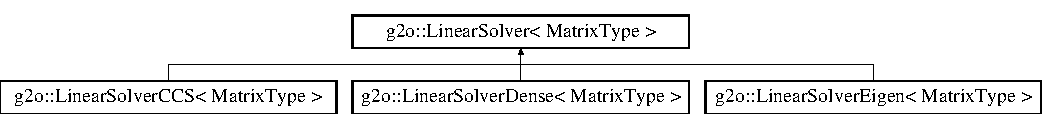
\includegraphics[height=1.536351cm]{classg2o_1_1_linear_solver}
\end{center}
\end{figure}
\subsection*{Public Member Functions}
\begin{DoxyCompactItemize}
\item 
\mbox{\hyperlink{classg2o_1_1_linear_solver_a741928aa64f4b6416c9990892e3ede7a}{Linear\+Solver}} ()
\item 
virtual \mbox{\hyperlink{classg2o_1_1_linear_solver_a5157e1221534fae13989c8443adab1ec}{$\sim$\+Linear\+Solver}} ()
\item 
virtual bool \mbox{\hyperlink{classg2o_1_1_linear_solver_aebd961a94ef6de1bc66d2ca41dd2b17b}{init}} ()=0
\item 
virtual bool \mbox{\hyperlink{classg2o_1_1_linear_solver_aa44b40826d50203c8ce2ff258c34e030}{solve}} (const \mbox{\hyperlink{classg2o_1_1_sparse_block_matrix}{Sparse\+Block\+Matrix}}$<$ Matrix\+Type $>$ \&A, double $\ast$x, double $\ast$b)=0
\item 
virtual bool \mbox{\hyperlink{classg2o_1_1_linear_solver_a252e3658b3ba0c3577c33f846c514535}{solve\+Blocks}} (double $\ast$$\ast$\&blocks, const \mbox{\hyperlink{classg2o_1_1_sparse_block_matrix}{Sparse\+Block\+Matrix}}$<$ Matrix\+Type $>$ \&A)
\item 
virtual bool \mbox{\hyperlink{classg2o_1_1_linear_solver_adc74484f72bbe373622581fd597c1be3}{solve\+Pattern}} (\mbox{\hyperlink{classg2o_1_1_sparse_block_matrix}{Sparse\+Block\+Matrix}}$<$ Matrix\+Xd $>$ \&spinv, const std\+::vector$<$ std\+::pair$<$ int, int $>$ $>$ \&block\+Indices, const \mbox{\hyperlink{classg2o_1_1_sparse_block_matrix}{Sparse\+Block\+Matrix}}$<$ Matrix\+Type $>$ \&A)
\item 
virtual bool \mbox{\hyperlink{classg2o_1_1_linear_solver_ac4b23c56cf69759a692906fc8816cf8f}{write\+Debug}} () const
\begin{DoxyCompactList}\small\item\em write a debug dump of the system matrix if it is not P\+SD in solve \end{DoxyCompactList}\item 
virtual void \mbox{\hyperlink{classg2o_1_1_linear_solver_a969c406ccacc38705b2a88f5ed23cb9a}{set\+Write\+Debug}} (bool)
\end{DoxyCompactItemize}


\subsection{Detailed Description}
\subsubsection*{template$<$typename Matrix\+Type$>$\newline
class g2o\+::\+Linear\+Solver$<$ Matrix\+Type $>$}

basic solver for Ax = b 

basic solver for Ax = b which has to reimplemented for different linear algebra libraries. A is assumed to be symmetric (only upper triangular block is stored) and positive-\/semi-\/definit. 

\subsection{Constructor \& Destructor Documentation}
\mbox{\Hypertarget{classg2o_1_1_linear_solver_a741928aa64f4b6416c9990892e3ede7a}\label{classg2o_1_1_linear_solver_a741928aa64f4b6416c9990892e3ede7a}} 
\index{g2o\+::\+Linear\+Solver@{g2o\+::\+Linear\+Solver}!Linear\+Solver@{Linear\+Solver}}
\index{Linear\+Solver@{Linear\+Solver}!g2o\+::\+Linear\+Solver@{g2o\+::\+Linear\+Solver}}
\subsubsection{\texorpdfstring{Linear\+Solver()}{LinearSolver()}}
{\footnotesize\ttfamily template$<$typename Matrix\+Type$>$ \\
\mbox{\hyperlink{classg2o_1_1_linear_solver}{g2o\+::\+Linear\+Solver}}$<$ Matrix\+Type $>$\+::\mbox{\hyperlink{classg2o_1_1_linear_solver}{Linear\+Solver}} (\begin{DoxyParamCaption}{ }\end{DoxyParamCaption})\hspace{0.3cm}{\ttfamily [inline]}}

\mbox{\Hypertarget{classg2o_1_1_linear_solver_a5157e1221534fae13989c8443adab1ec}\label{classg2o_1_1_linear_solver_a5157e1221534fae13989c8443adab1ec}} 
\index{g2o\+::\+Linear\+Solver@{g2o\+::\+Linear\+Solver}!````~Linear\+Solver@{$\sim$\+Linear\+Solver}}
\index{````~Linear\+Solver@{$\sim$\+Linear\+Solver}!g2o\+::\+Linear\+Solver@{g2o\+::\+Linear\+Solver}}
\subsubsection{\texorpdfstring{$\sim$\+Linear\+Solver()}{~LinearSolver()}}
{\footnotesize\ttfamily template$<$typename Matrix\+Type$>$ \\
virtual \mbox{\hyperlink{classg2o_1_1_linear_solver}{g2o\+::\+Linear\+Solver}}$<$ Matrix\+Type $>$\+::$\sim$\mbox{\hyperlink{classg2o_1_1_linear_solver}{Linear\+Solver}} (\begin{DoxyParamCaption}{ }\end{DoxyParamCaption})\hspace{0.3cm}{\ttfamily [inline]}, {\ttfamily [virtual]}}



\subsection{Member Function Documentation}
\mbox{\Hypertarget{classg2o_1_1_linear_solver_aebd961a94ef6de1bc66d2ca41dd2b17b}\label{classg2o_1_1_linear_solver_aebd961a94ef6de1bc66d2ca41dd2b17b}} 
\index{g2o\+::\+Linear\+Solver@{g2o\+::\+Linear\+Solver}!init@{init}}
\index{init@{init}!g2o\+::\+Linear\+Solver@{g2o\+::\+Linear\+Solver}}
\subsubsection{\texorpdfstring{init()}{init()}}
{\footnotesize\ttfamily template$<$typename Matrix\+Type$>$ \\
virtual bool \mbox{\hyperlink{classg2o_1_1_linear_solver}{g2o\+::\+Linear\+Solver}}$<$ Matrix\+Type $>$\+::init (\begin{DoxyParamCaption}{ }\end{DoxyParamCaption})\hspace{0.3cm}{\ttfamily [pure virtual]}}

init for operating on matrices with a different non-\/zero pattern like before 

Implemented in \mbox{\hyperlink{classg2o_1_1_linear_solver_eigen_a8fca4bb987dcbeb94a366b1532dee139}{g2o\+::\+Linear\+Solver\+Eigen$<$ Matrix\+Type $>$}}, and \mbox{\hyperlink{classg2o_1_1_linear_solver_dense_a24f68ecd4b022269dbfc4d990eb5c57b}{g2o\+::\+Linear\+Solver\+Dense$<$ Matrix\+Type $>$}}.

\mbox{\Hypertarget{classg2o_1_1_linear_solver_a969c406ccacc38705b2a88f5ed23cb9a}\label{classg2o_1_1_linear_solver_a969c406ccacc38705b2a88f5ed23cb9a}} 
\index{g2o\+::\+Linear\+Solver@{g2o\+::\+Linear\+Solver}!set\+Write\+Debug@{set\+Write\+Debug}}
\index{set\+Write\+Debug@{set\+Write\+Debug}!g2o\+::\+Linear\+Solver@{g2o\+::\+Linear\+Solver}}
\subsubsection{\texorpdfstring{set\+Write\+Debug()}{setWriteDebug()}}
{\footnotesize\ttfamily template$<$typename Matrix\+Type$>$ \\
virtual void \mbox{\hyperlink{classg2o_1_1_linear_solver}{g2o\+::\+Linear\+Solver}}$<$ Matrix\+Type $>$\+::set\+Write\+Debug (\begin{DoxyParamCaption}\item[{bool}]{ }\end{DoxyParamCaption})\hspace{0.3cm}{\ttfamily [inline]}, {\ttfamily [virtual]}}



Reimplemented in \mbox{\hyperlink{classg2o_1_1_linear_solver_eigen_a5ceaab3ba944d327b21f7329c7e19c8c}{g2o\+::\+Linear\+Solver\+Eigen$<$ Matrix\+Type $>$}}.

\mbox{\Hypertarget{classg2o_1_1_linear_solver_aa44b40826d50203c8ce2ff258c34e030}\label{classg2o_1_1_linear_solver_aa44b40826d50203c8ce2ff258c34e030}} 
\index{g2o\+::\+Linear\+Solver@{g2o\+::\+Linear\+Solver}!solve@{solve}}
\index{solve@{solve}!g2o\+::\+Linear\+Solver@{g2o\+::\+Linear\+Solver}}
\subsubsection{\texorpdfstring{solve()}{solve()}}
{\footnotesize\ttfamily template$<$typename Matrix\+Type$>$ \\
virtual bool \mbox{\hyperlink{classg2o_1_1_linear_solver}{g2o\+::\+Linear\+Solver}}$<$ Matrix\+Type $>$\+::solve (\begin{DoxyParamCaption}\item[{const \mbox{\hyperlink{classg2o_1_1_sparse_block_matrix}{Sparse\+Block\+Matrix}}$<$ Matrix\+Type $>$ \&}]{A,  }\item[{double $\ast$}]{x,  }\item[{double $\ast$}]{b }\end{DoxyParamCaption})\hspace{0.3cm}{\ttfamily [pure virtual]}}

Assumes that A is the same matrix for several calls. Among other assumptions, the non-\/zero pattern does not change! If the matrix changes call \mbox{\hyperlink{classg2o_1_1_linear_solver_aebd961a94ef6de1bc66d2ca41dd2b17b}{init()}} before. solve system Ax = b, x and b have to allocated beforehand!! 

Implemented in \mbox{\hyperlink{classg2o_1_1_linear_solver_eigen_ae4ac566af324a238a31145c1e50b52e1}{g2o\+::\+Linear\+Solver\+Eigen$<$ Matrix\+Type $>$}}, and \mbox{\hyperlink{classg2o_1_1_linear_solver_dense_a8b6eafa6e53b9f705a4e8eb436eeb403}{g2o\+::\+Linear\+Solver\+Dense$<$ Matrix\+Type $>$}}.

\mbox{\Hypertarget{classg2o_1_1_linear_solver_a252e3658b3ba0c3577c33f846c514535}\label{classg2o_1_1_linear_solver_a252e3658b3ba0c3577c33f846c514535}} 
\index{g2o\+::\+Linear\+Solver@{g2o\+::\+Linear\+Solver}!solve\+Blocks@{solve\+Blocks}}
\index{solve\+Blocks@{solve\+Blocks}!g2o\+::\+Linear\+Solver@{g2o\+::\+Linear\+Solver}}
\subsubsection{\texorpdfstring{solve\+Blocks()}{solveBlocks()}}
{\footnotesize\ttfamily template$<$typename Matrix\+Type$>$ \\
virtual bool \mbox{\hyperlink{classg2o_1_1_linear_solver}{g2o\+::\+Linear\+Solver}}$<$ Matrix\+Type $>$\+::solve\+Blocks (\begin{DoxyParamCaption}\item[{double $\ast$$\ast$\&}]{blocks,  }\item[{const \mbox{\hyperlink{classg2o_1_1_sparse_block_matrix}{Sparse\+Block\+Matrix}}$<$ Matrix\+Type $>$ \&}]{A }\end{DoxyParamCaption})\hspace{0.3cm}{\ttfamily [inline]}, {\ttfamily [virtual]}}

Inverts the diagonal blocks of A \begin{DoxyReturn}{Returns}
false if not defined. 
\end{DoxyReturn}
\mbox{\Hypertarget{classg2o_1_1_linear_solver_adc74484f72bbe373622581fd597c1be3}\label{classg2o_1_1_linear_solver_adc74484f72bbe373622581fd597c1be3}} 
\index{g2o\+::\+Linear\+Solver@{g2o\+::\+Linear\+Solver}!solve\+Pattern@{solve\+Pattern}}
\index{solve\+Pattern@{solve\+Pattern}!g2o\+::\+Linear\+Solver@{g2o\+::\+Linear\+Solver}}
\subsubsection{\texorpdfstring{solve\+Pattern()}{solvePattern()}}
{\footnotesize\ttfamily template$<$typename Matrix\+Type$>$ \\
virtual bool \mbox{\hyperlink{classg2o_1_1_linear_solver}{g2o\+::\+Linear\+Solver}}$<$ Matrix\+Type $>$\+::solve\+Pattern (\begin{DoxyParamCaption}\item[{\mbox{\hyperlink{classg2o_1_1_sparse_block_matrix}{Sparse\+Block\+Matrix}}$<$ Matrix\+Xd $>$ \&}]{spinv,  }\item[{const std\+::vector$<$ std\+::pair$<$ int, int $>$ $>$ \&}]{block\+Indices,  }\item[{const \mbox{\hyperlink{classg2o_1_1_sparse_block_matrix}{Sparse\+Block\+Matrix}}$<$ Matrix\+Type $>$ \&}]{A }\end{DoxyParamCaption})\hspace{0.3cm}{\ttfamily [inline]}, {\ttfamily [virtual]}}

Inverts the a block pattern of A in spinv \begin{DoxyReturn}{Returns}
false if not defined. 
\end{DoxyReturn}
\mbox{\Hypertarget{classg2o_1_1_linear_solver_ac4b23c56cf69759a692906fc8816cf8f}\label{classg2o_1_1_linear_solver_ac4b23c56cf69759a692906fc8816cf8f}} 
\index{g2o\+::\+Linear\+Solver@{g2o\+::\+Linear\+Solver}!write\+Debug@{write\+Debug}}
\index{write\+Debug@{write\+Debug}!g2o\+::\+Linear\+Solver@{g2o\+::\+Linear\+Solver}}
\subsubsection{\texorpdfstring{write\+Debug()}{writeDebug()}}
{\footnotesize\ttfamily template$<$typename Matrix\+Type$>$ \\
virtual bool \mbox{\hyperlink{classg2o_1_1_linear_solver}{g2o\+::\+Linear\+Solver}}$<$ Matrix\+Type $>$\+::write\+Debug (\begin{DoxyParamCaption}{ }\end{DoxyParamCaption}) const\hspace{0.3cm}{\ttfamily [inline]}, {\ttfamily [virtual]}}



write a debug dump of the system matrix if it is not P\+SD in solve 



Reimplemented in \mbox{\hyperlink{classg2o_1_1_linear_solver_eigen_ad9bccc1b4bcd3cc5e107ac09ac93cf4b}{g2o\+::\+Linear\+Solver\+Eigen$<$ Matrix\+Type $>$}}.



The documentation for this class was generated from the following file\+:\begin{DoxyCompactItemize}
\item 
Thirdparty/g2o/g2o/core/\mbox{\hyperlink{linear__solver_8h}{linear\+\_\+solver.\+h}}\end{DoxyCompactItemize}

\hypertarget{classg2o_1_1_linear_solver_c_c_s}{}\section{g2o\+:\+:Linear\+Solver\+C\+CS$<$ Matrix\+Type $>$ Class Template Reference}
\label{classg2o_1_1_linear_solver_c_c_s}\index{g2o\+::\+Linear\+Solver\+C\+C\+S$<$ Matrix\+Type $>$@{g2o\+::\+Linear\+Solver\+C\+C\+S$<$ Matrix\+Type $>$}}


\mbox{\hyperlink{classg2o_1_1_solver}{Solver}} with faster iterating structure for the linear matrix.  




{\ttfamily \#include $<$linear\+\_\+solver.\+h$>$}

Inheritance diagram for g2o\+:\+:Linear\+Solver\+C\+CS$<$ Matrix\+Type $>$\+:\begin{figure}[H]
\begin{center}
\leavevmode
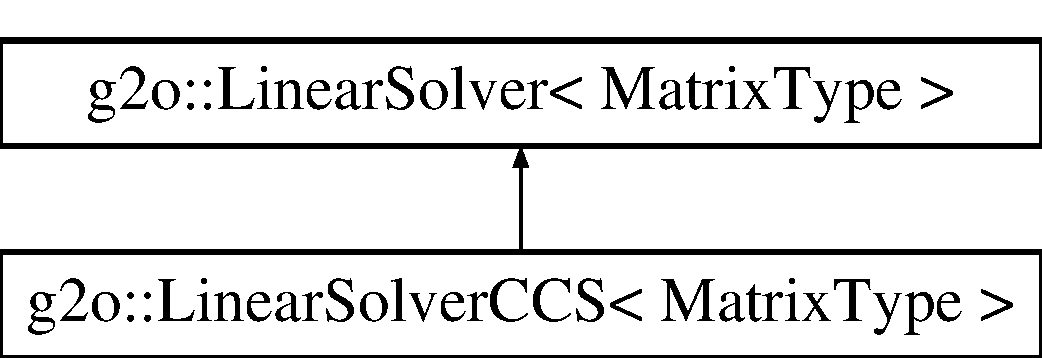
\includegraphics[height=2.000000cm]{classg2o_1_1_linear_solver_c_c_s}
\end{center}
\end{figure}
\subsection*{Public Member Functions}
\begin{DoxyCompactItemize}
\item 
\mbox{\hyperlink{classg2o_1_1_linear_solver_c_c_s_aa4a8b0612a60769481c40d2d1a6b03ce}{Linear\+Solver\+C\+CS}} ()
\item 
\mbox{\hyperlink{classg2o_1_1_linear_solver_c_c_s_aa131fa8ea836eafdc1313fdf3a4217f9}{$\sim$\+Linear\+Solver\+C\+CS}} ()
\end{DoxyCompactItemize}
\subsection*{Protected Member Functions}
\begin{DoxyCompactItemize}
\item 
void \mbox{\hyperlink{classg2o_1_1_linear_solver_c_c_s_a070138d7e2a68a576e015f5073a4a464}{init\+Matrix\+Structure}} (const \mbox{\hyperlink{classg2o_1_1_sparse_block_matrix}{Sparse\+Block\+Matrix}}$<$ Matrix\+Type $>$ \&A)
\end{DoxyCompactItemize}
\subsection*{Protected Attributes}
\begin{DoxyCompactItemize}
\item 
\mbox{\hyperlink{classg2o_1_1_sparse_block_matrix_c_c_s}{Sparse\+Block\+Matrix\+C\+CS}}$<$ Matrix\+Type $>$ $\ast$ \mbox{\hyperlink{classg2o_1_1_linear_solver_c_c_s_a07f0df9a6012d567e26a89063c53aa12}{\+\_\+ccs\+Matrix}}
\end{DoxyCompactItemize}


\subsection{Detailed Description}
\subsubsection*{template$<$typename Matrix\+Type$>$\newline
class g2o\+::\+Linear\+Solver\+C\+C\+S$<$ Matrix\+Type $>$}

\mbox{\hyperlink{classg2o_1_1_solver}{Solver}} with faster iterating structure for the linear matrix. 

\subsection{Constructor \& Destructor Documentation}
\mbox{\Hypertarget{classg2o_1_1_linear_solver_c_c_s_aa4a8b0612a60769481c40d2d1a6b03ce}\label{classg2o_1_1_linear_solver_c_c_s_aa4a8b0612a60769481c40d2d1a6b03ce}} 
\index{g2o\+::\+Linear\+Solver\+C\+CS@{g2o\+::\+Linear\+Solver\+C\+CS}!Linear\+Solver\+C\+CS@{Linear\+Solver\+C\+CS}}
\index{Linear\+Solver\+C\+CS@{Linear\+Solver\+C\+CS}!g2o\+::\+Linear\+Solver\+C\+CS@{g2o\+::\+Linear\+Solver\+C\+CS}}
\subsubsection{\texorpdfstring{Linear\+Solver\+C\+C\+S()}{LinearSolverCCS()}}
{\footnotesize\ttfamily template$<$typename Matrix\+Type $>$ \\
\mbox{\hyperlink{classg2o_1_1_linear_solver_c_c_s}{g2o\+::\+Linear\+Solver\+C\+CS}}$<$ Matrix\+Type $>$\+::\mbox{\hyperlink{classg2o_1_1_linear_solver_c_c_s}{Linear\+Solver\+C\+CS}} (\begin{DoxyParamCaption}{ }\end{DoxyParamCaption})\hspace{0.3cm}{\ttfamily [inline]}}

\mbox{\Hypertarget{classg2o_1_1_linear_solver_c_c_s_aa131fa8ea836eafdc1313fdf3a4217f9}\label{classg2o_1_1_linear_solver_c_c_s_aa131fa8ea836eafdc1313fdf3a4217f9}} 
\index{g2o\+::\+Linear\+Solver\+C\+CS@{g2o\+::\+Linear\+Solver\+C\+CS}!````~Linear\+Solver\+C\+CS@{$\sim$\+Linear\+Solver\+C\+CS}}
\index{````~Linear\+Solver\+C\+CS@{$\sim$\+Linear\+Solver\+C\+CS}!g2o\+::\+Linear\+Solver\+C\+CS@{g2o\+::\+Linear\+Solver\+C\+CS}}
\subsubsection{\texorpdfstring{$\sim$\+Linear\+Solver\+C\+C\+S()}{~LinearSolverCCS()}}
{\footnotesize\ttfamily template$<$typename Matrix\+Type $>$ \\
\mbox{\hyperlink{classg2o_1_1_linear_solver_c_c_s}{g2o\+::\+Linear\+Solver\+C\+CS}}$<$ Matrix\+Type $>$\+::$\sim$\mbox{\hyperlink{classg2o_1_1_linear_solver_c_c_s}{Linear\+Solver\+C\+CS}} (\begin{DoxyParamCaption}{ }\end{DoxyParamCaption})\hspace{0.3cm}{\ttfamily [inline]}}



\subsection{Member Function Documentation}
\mbox{\Hypertarget{classg2o_1_1_linear_solver_c_c_s_a070138d7e2a68a576e015f5073a4a464}\label{classg2o_1_1_linear_solver_c_c_s_a070138d7e2a68a576e015f5073a4a464}} 
\index{g2o\+::\+Linear\+Solver\+C\+CS@{g2o\+::\+Linear\+Solver\+C\+CS}!init\+Matrix\+Structure@{init\+Matrix\+Structure}}
\index{init\+Matrix\+Structure@{init\+Matrix\+Structure}!g2o\+::\+Linear\+Solver\+C\+CS@{g2o\+::\+Linear\+Solver\+C\+CS}}
\subsubsection{\texorpdfstring{init\+Matrix\+Structure()}{initMatrixStructure()}}
{\footnotesize\ttfamily template$<$typename Matrix\+Type $>$ \\
void \mbox{\hyperlink{classg2o_1_1_linear_solver_c_c_s}{g2o\+::\+Linear\+Solver\+C\+CS}}$<$ Matrix\+Type $>$\+::init\+Matrix\+Structure (\begin{DoxyParamCaption}\item[{const \mbox{\hyperlink{classg2o_1_1_sparse_block_matrix}{Sparse\+Block\+Matrix}}$<$ Matrix\+Type $>$ \&}]{A }\end{DoxyParamCaption})\hspace{0.3cm}{\ttfamily [inline]}, {\ttfamily [protected]}}



\subsection{Member Data Documentation}
\mbox{\Hypertarget{classg2o_1_1_linear_solver_c_c_s_a07f0df9a6012d567e26a89063c53aa12}\label{classg2o_1_1_linear_solver_c_c_s_a07f0df9a6012d567e26a89063c53aa12}} 
\index{g2o\+::\+Linear\+Solver\+C\+CS@{g2o\+::\+Linear\+Solver\+C\+CS}!\+\_\+ccs\+Matrix@{\+\_\+ccs\+Matrix}}
\index{\+\_\+ccs\+Matrix@{\+\_\+ccs\+Matrix}!g2o\+::\+Linear\+Solver\+C\+CS@{g2o\+::\+Linear\+Solver\+C\+CS}}
\subsubsection{\texorpdfstring{\+\_\+ccs\+Matrix}{\_ccsMatrix}}
{\footnotesize\ttfamily template$<$typename Matrix\+Type $>$ \\
\mbox{\hyperlink{classg2o_1_1_sparse_block_matrix_c_c_s}{Sparse\+Block\+Matrix\+C\+CS}}$<$Matrix\+Type$>$$\ast$ \mbox{\hyperlink{classg2o_1_1_linear_solver_c_c_s}{g2o\+::\+Linear\+Solver\+C\+CS}}$<$ Matrix\+Type $>$\+::\+\_\+ccs\+Matrix\hspace{0.3cm}{\ttfamily [protected]}}



The documentation for this class was generated from the following file\+:\begin{DoxyCompactItemize}
\item 
D\+:/github/\+V\+S\+L\+A\+M/\+O\+R\+B\+S\+L\+A\+M2/\+O\+R\+B-\/\+S\+L\+A\+M2-\/master/\+Thirdparty/g2o/g2o/core/\mbox{\hyperlink{linear__solver_8h}{linear\+\_\+solver.\+h}}\end{DoxyCompactItemize}

\hypertarget{classg2o_1_1_linear_solver_dense}{}\section{g2o\+:\+:Linear\+Solver\+Dense$<$ Matrix\+Type $>$ Class Template Reference}
\label{classg2o_1_1_linear_solver_dense}\index{g2o\+::\+Linear\+Solver\+Dense$<$ Matrix\+Type $>$@{g2o\+::\+Linear\+Solver\+Dense$<$ Matrix\+Type $>$}}


linear solver using dense cholesky decomposition  




{\ttfamily \#include $<$linear\+\_\+solver\+\_\+dense.\+h$>$}

Inheritance diagram for g2o\+:\+:Linear\+Solver\+Dense$<$ Matrix\+Type $>$\+:\begin{figure}[H]
\begin{center}
\leavevmode
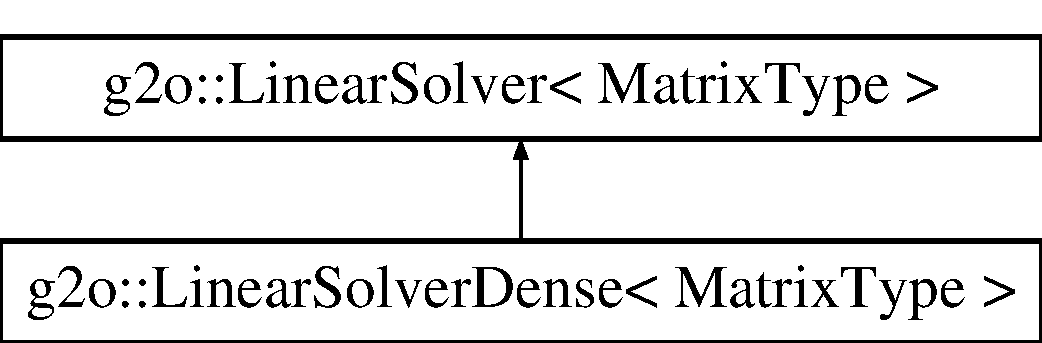
\includegraphics[height=2.000000cm]{classg2o_1_1_linear_solver_dense}
\end{center}
\end{figure}
\subsection*{Public Member Functions}
\begin{DoxyCompactItemize}
\item 
\mbox{\hyperlink{classg2o_1_1_linear_solver_dense_a25d8767ad60e944d8518348a136830da}{Linear\+Solver\+Dense}} ()
\item 
virtual \mbox{\hyperlink{classg2o_1_1_linear_solver_dense_a2b3cbb77fa958bf322b98e38ec3e29c2}{$\sim$\+Linear\+Solver\+Dense}} ()
\item 
virtual bool \mbox{\hyperlink{classg2o_1_1_linear_solver_dense_a24f68ecd4b022269dbfc4d990eb5c57b}{init}} ()
\item 
bool \mbox{\hyperlink{classg2o_1_1_linear_solver_dense_a8b6eafa6e53b9f705a4e8eb436eeb403}{solve}} (const \mbox{\hyperlink{classg2o_1_1_sparse_block_matrix}{Sparse\+Block\+Matrix}}$<$ Matrix\+Type $>$ \&A, double $\ast$x, double $\ast$b)
\end{DoxyCompactItemize}
\subsection*{Protected Attributes}
\begin{DoxyCompactItemize}
\item 
bool \mbox{\hyperlink{classg2o_1_1_linear_solver_dense_a2d82ac52c9c24501cccee3ef3cb575fe}{\+\_\+reset}}
\item 
Eigen\+::\+Matrix\+Xd \mbox{\hyperlink{classg2o_1_1_linear_solver_dense_a5ca6a1f2358ce0620dbdbae3fdc9fc99}{\+\_\+H}}
\item 
Eigen\+::\+L\+D\+LT$<$ Eigen\+::\+Matrix\+Xd $>$ \mbox{\hyperlink{classg2o_1_1_linear_solver_dense_a20fc35e2f25107a6e36211861034aae0}{\+\_\+cholesky}}
\end{DoxyCompactItemize}


\subsection{Detailed Description}
\subsubsection*{template$<$typename Matrix\+Type$>$\newline
class g2o\+::\+Linear\+Solver\+Dense$<$ Matrix\+Type $>$}

linear solver using dense cholesky decomposition 

\subsection{Constructor \& Destructor Documentation}
\mbox{\Hypertarget{classg2o_1_1_linear_solver_dense_a25d8767ad60e944d8518348a136830da}\label{classg2o_1_1_linear_solver_dense_a25d8767ad60e944d8518348a136830da}} 
\index{g2o\+::\+Linear\+Solver\+Dense@{g2o\+::\+Linear\+Solver\+Dense}!Linear\+Solver\+Dense@{Linear\+Solver\+Dense}}
\index{Linear\+Solver\+Dense@{Linear\+Solver\+Dense}!g2o\+::\+Linear\+Solver\+Dense@{g2o\+::\+Linear\+Solver\+Dense}}
\subsubsection{\texorpdfstring{Linear\+Solver\+Dense()}{LinearSolverDense()}}
{\footnotesize\ttfamily template$<$typename Matrix\+Type $>$ \\
\mbox{\hyperlink{classg2o_1_1_linear_solver_dense}{g2o\+::\+Linear\+Solver\+Dense}}$<$ Matrix\+Type $>$\+::\mbox{\hyperlink{classg2o_1_1_linear_solver_dense}{Linear\+Solver\+Dense}} (\begin{DoxyParamCaption}{ }\end{DoxyParamCaption})\hspace{0.3cm}{\ttfamily [inline]}}

\mbox{\Hypertarget{classg2o_1_1_linear_solver_dense_a2b3cbb77fa958bf322b98e38ec3e29c2}\label{classg2o_1_1_linear_solver_dense_a2b3cbb77fa958bf322b98e38ec3e29c2}} 
\index{g2o\+::\+Linear\+Solver\+Dense@{g2o\+::\+Linear\+Solver\+Dense}!````~Linear\+Solver\+Dense@{$\sim$\+Linear\+Solver\+Dense}}
\index{````~Linear\+Solver\+Dense@{$\sim$\+Linear\+Solver\+Dense}!g2o\+::\+Linear\+Solver\+Dense@{g2o\+::\+Linear\+Solver\+Dense}}
\subsubsection{\texorpdfstring{$\sim$\+Linear\+Solver\+Dense()}{~LinearSolverDense()}}
{\footnotesize\ttfamily template$<$typename Matrix\+Type $>$ \\
virtual \mbox{\hyperlink{classg2o_1_1_linear_solver_dense}{g2o\+::\+Linear\+Solver\+Dense}}$<$ Matrix\+Type $>$\+::$\sim$\mbox{\hyperlink{classg2o_1_1_linear_solver_dense}{Linear\+Solver\+Dense}} (\begin{DoxyParamCaption}{ }\end{DoxyParamCaption})\hspace{0.3cm}{\ttfamily [inline]}, {\ttfamily [virtual]}}



\subsection{Member Function Documentation}
\mbox{\Hypertarget{classg2o_1_1_linear_solver_dense_a24f68ecd4b022269dbfc4d990eb5c57b}\label{classg2o_1_1_linear_solver_dense_a24f68ecd4b022269dbfc4d990eb5c57b}} 
\index{g2o\+::\+Linear\+Solver\+Dense@{g2o\+::\+Linear\+Solver\+Dense}!init@{init}}
\index{init@{init}!g2o\+::\+Linear\+Solver\+Dense@{g2o\+::\+Linear\+Solver\+Dense}}
\subsubsection{\texorpdfstring{init()}{init()}}
{\footnotesize\ttfamily template$<$typename Matrix\+Type $>$ \\
virtual bool \mbox{\hyperlink{classg2o_1_1_linear_solver_dense}{g2o\+::\+Linear\+Solver\+Dense}}$<$ Matrix\+Type $>$\+::init (\begin{DoxyParamCaption}{ }\end{DoxyParamCaption})\hspace{0.3cm}{\ttfamily [inline]}, {\ttfamily [virtual]}}

init for operating on matrices with a different non-\/zero pattern like before 

Implements \mbox{\hyperlink{classg2o_1_1_linear_solver_aebd961a94ef6de1bc66d2ca41dd2b17b}{g2o\+::\+Linear\+Solver$<$ Matrix\+Type $>$}}.

\mbox{\Hypertarget{classg2o_1_1_linear_solver_dense_a8b6eafa6e53b9f705a4e8eb436eeb403}\label{classg2o_1_1_linear_solver_dense_a8b6eafa6e53b9f705a4e8eb436eeb403}} 
\index{g2o\+::\+Linear\+Solver\+Dense@{g2o\+::\+Linear\+Solver\+Dense}!solve@{solve}}
\index{solve@{solve}!g2o\+::\+Linear\+Solver\+Dense@{g2o\+::\+Linear\+Solver\+Dense}}
\subsubsection{\texorpdfstring{solve()}{solve()}}
{\footnotesize\ttfamily template$<$typename Matrix\+Type $>$ \\
bool \mbox{\hyperlink{classg2o_1_1_linear_solver_dense}{g2o\+::\+Linear\+Solver\+Dense}}$<$ Matrix\+Type $>$\+::solve (\begin{DoxyParamCaption}\item[{const \mbox{\hyperlink{classg2o_1_1_sparse_block_matrix}{Sparse\+Block\+Matrix}}$<$ Matrix\+Type $>$ \&}]{A,  }\item[{double $\ast$}]{x,  }\item[{double $\ast$}]{b }\end{DoxyParamCaption})\hspace{0.3cm}{\ttfamily [inline]}, {\ttfamily [virtual]}}

Assumes that A is the same matrix for several calls. Among other assumptions, the non-\/zero pattern does not change! If the matrix changes call \mbox{\hyperlink{classg2o_1_1_linear_solver_dense_a24f68ecd4b022269dbfc4d990eb5c57b}{init()}} before. solve system Ax = b, x and b have to allocated beforehand!! 

Implements \mbox{\hyperlink{classg2o_1_1_linear_solver_aa44b40826d50203c8ce2ff258c34e030}{g2o\+::\+Linear\+Solver$<$ Matrix\+Type $>$}}.



\subsection{Member Data Documentation}
\mbox{\Hypertarget{classg2o_1_1_linear_solver_dense_a20fc35e2f25107a6e36211861034aae0}\label{classg2o_1_1_linear_solver_dense_a20fc35e2f25107a6e36211861034aae0}} 
\index{g2o\+::\+Linear\+Solver\+Dense@{g2o\+::\+Linear\+Solver\+Dense}!\+\_\+cholesky@{\+\_\+cholesky}}
\index{\+\_\+cholesky@{\+\_\+cholesky}!g2o\+::\+Linear\+Solver\+Dense@{g2o\+::\+Linear\+Solver\+Dense}}
\subsubsection{\texorpdfstring{\+\_\+cholesky}{\_cholesky}}
{\footnotesize\ttfamily template$<$typename Matrix\+Type $>$ \\
Eigen\+::\+L\+D\+LT$<$Eigen\+::\+Matrix\+Xd$>$ \mbox{\hyperlink{classg2o_1_1_linear_solver_dense}{g2o\+::\+Linear\+Solver\+Dense}}$<$ Matrix\+Type $>$\+::\+\_\+cholesky\hspace{0.3cm}{\ttfamily [protected]}}

\mbox{\Hypertarget{classg2o_1_1_linear_solver_dense_a5ca6a1f2358ce0620dbdbae3fdc9fc99}\label{classg2o_1_1_linear_solver_dense_a5ca6a1f2358ce0620dbdbae3fdc9fc99}} 
\index{g2o\+::\+Linear\+Solver\+Dense@{g2o\+::\+Linear\+Solver\+Dense}!\+\_\+H@{\+\_\+H}}
\index{\+\_\+H@{\+\_\+H}!g2o\+::\+Linear\+Solver\+Dense@{g2o\+::\+Linear\+Solver\+Dense}}
\subsubsection{\texorpdfstring{\+\_\+H}{\_H}}
{\footnotesize\ttfamily template$<$typename Matrix\+Type $>$ \\
Eigen\+::\+Matrix\+Xd \mbox{\hyperlink{classg2o_1_1_linear_solver_dense}{g2o\+::\+Linear\+Solver\+Dense}}$<$ Matrix\+Type $>$\+::\+\_\+H\hspace{0.3cm}{\ttfamily [protected]}}

\mbox{\Hypertarget{classg2o_1_1_linear_solver_dense_a2d82ac52c9c24501cccee3ef3cb575fe}\label{classg2o_1_1_linear_solver_dense_a2d82ac52c9c24501cccee3ef3cb575fe}} 
\index{g2o\+::\+Linear\+Solver\+Dense@{g2o\+::\+Linear\+Solver\+Dense}!\+\_\+reset@{\+\_\+reset}}
\index{\+\_\+reset@{\+\_\+reset}!g2o\+::\+Linear\+Solver\+Dense@{g2o\+::\+Linear\+Solver\+Dense}}
\subsubsection{\texorpdfstring{\+\_\+reset}{\_reset}}
{\footnotesize\ttfamily template$<$typename Matrix\+Type $>$ \\
bool \mbox{\hyperlink{classg2o_1_1_linear_solver_dense}{g2o\+::\+Linear\+Solver\+Dense}}$<$ Matrix\+Type $>$\+::\+\_\+reset\hspace{0.3cm}{\ttfamily [protected]}}



The documentation for this class was generated from the following file\+:\begin{DoxyCompactItemize}
\item 
Thirdparty/g2o/g2o/solvers/\mbox{\hyperlink{linear__solver__dense_8h}{linear\+\_\+solver\+\_\+dense.\+h}}\end{DoxyCompactItemize}

\hypertarget{classg2o_1_1_linear_solver_eigen}{}\section{g2o\+:\+:Linear\+Solver\+Eigen$<$ Matrix\+Type $>$ Class Template Reference}
\label{classg2o_1_1_linear_solver_eigen}\index{g2o\+::\+Linear\+Solver\+Eigen$<$ Matrix\+Type $>$@{g2o\+::\+Linear\+Solver\+Eigen$<$ Matrix\+Type $>$}}


linear solver which uses the sparse Cholesky solver from Eigen  




{\ttfamily \#include $<$linear\+\_\+solver\+\_\+eigen.\+h$>$}

Inheritance diagram for g2o\+:\+:Linear\+Solver\+Eigen$<$ Matrix\+Type $>$\+:\begin{figure}[H]
\begin{center}
\leavevmode
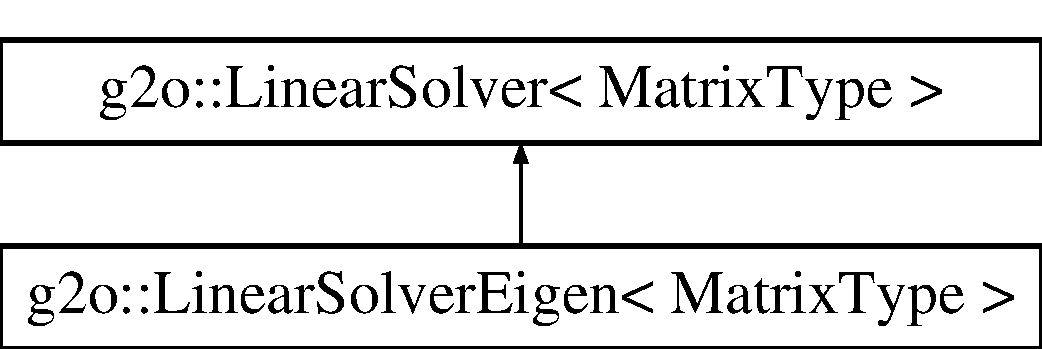
\includegraphics[height=2.000000cm]{classg2o_1_1_linear_solver_eigen}
\end{center}
\end{figure}
\subsection*{Classes}
\begin{DoxyCompactItemize}
\item 
class \mbox{\hyperlink{classg2o_1_1_linear_solver_eigen_1_1_cholesky_decomposition}{Cholesky\+Decomposition}}
\begin{DoxyCompactList}\small\item\em Sub-\/classing Eigen\textquotesingle{}s Simplicial\+L\+D\+LT to perform ordering with a given ordering. \end{DoxyCompactList}\end{DoxyCompactItemize}
\subsection*{Public Types}
\begin{DoxyCompactItemize}
\item 
typedef Eigen\+::\+Sparse\+Matrix$<$ double, Eigen\+::\+Col\+Major $>$ \mbox{\hyperlink{classg2o_1_1_linear_solver_eigen_aeb7e2400bed3a249b5f29ce7cc00cd33}{Sparse\+Matrix}}
\item 
typedef Eigen\+::\+Triplet$<$ double $>$ \mbox{\hyperlink{classg2o_1_1_linear_solver_eigen_a602c24e05d2f46022aa1827fdbc45638}{Triplet}}
\item 
typedef Eigen\+::\+Permutation\+Matrix$<$ Eigen\+::\+Dynamic, Eigen\+::\+Dynamic, Sparse\+Matrix\+::\+Index $>$ \mbox{\hyperlink{classg2o_1_1_linear_solver_eigen_acd9dd4e15dfbbad2720f1b83519333e8}{Permutation\+Matrix}}
\end{DoxyCompactItemize}
\subsection*{Public Member Functions}
\begin{DoxyCompactItemize}
\item 
\mbox{\hyperlink{classg2o_1_1_linear_solver_eigen_ac9e7b64d4a559e6972a8b3798f490bd8}{Linear\+Solver\+Eigen}} ()
\item 
virtual \mbox{\hyperlink{classg2o_1_1_linear_solver_eigen_afd2eeb1d54a420e110b9b8cdf74b1cff}{$\sim$\+Linear\+Solver\+Eigen}} ()
\item 
virtual bool \mbox{\hyperlink{classg2o_1_1_linear_solver_eigen_a8fca4bb987dcbeb94a366b1532dee139}{init}} ()
\item 
bool \mbox{\hyperlink{classg2o_1_1_linear_solver_eigen_ae4ac566af324a238a31145c1e50b52e1}{solve}} (const \mbox{\hyperlink{classg2o_1_1_sparse_block_matrix}{Sparse\+Block\+Matrix}}$<$ Matrix\+Type $>$ \&A, double $\ast$x, double $\ast$b)
\item 
bool \mbox{\hyperlink{classg2o_1_1_linear_solver_eigen_a062a4808d98b01686817b4565fd149cf}{block\+Ordering}} () const
\begin{DoxyCompactList}\small\item\em do the A\+MD ordering on the blocks or on the scalar matrix \end{DoxyCompactList}\item 
void \mbox{\hyperlink{classg2o_1_1_linear_solver_eigen_a33a924364fc517e69c5ade5aeacd8ee3}{set\+Block\+Ordering}} (bool \mbox{\hyperlink{classg2o_1_1_linear_solver_eigen_a062a4808d98b01686817b4565fd149cf}{block\+Ordering}})
\item 
virtual bool \mbox{\hyperlink{classg2o_1_1_linear_solver_eigen_ad9bccc1b4bcd3cc5e107ac09ac93cf4b}{write\+Debug}} () const
\begin{DoxyCompactList}\small\item\em write a debug dump of the system matrix if it is not S\+PD in solve \end{DoxyCompactList}\item 
virtual void \mbox{\hyperlink{classg2o_1_1_linear_solver_eigen_a5ceaab3ba944d327b21f7329c7e19c8c}{set\+Write\+Debug}} (bool b)
\end{DoxyCompactItemize}
\subsection*{Protected Member Functions}
\begin{DoxyCompactItemize}
\item 
void \mbox{\hyperlink{classg2o_1_1_linear_solver_eigen_a12307526d419d194620e982d8c683767}{compute\+Symbolic\+Decomposition}} (const \mbox{\hyperlink{classg2o_1_1_sparse_block_matrix}{Sparse\+Block\+Matrix}}$<$ Matrix\+Type $>$ \&A)
\item 
void \mbox{\hyperlink{classg2o_1_1_linear_solver_eigen_a8ab862dc1eebb6ec5815f3970e9073f3}{fill\+Sparse\+Matrix}} (const \mbox{\hyperlink{classg2o_1_1_sparse_block_matrix}{Sparse\+Block\+Matrix}}$<$ Matrix\+Type $>$ \&A, bool only\+Values)
\end{DoxyCompactItemize}
\subsection*{Protected Attributes}
\begin{DoxyCompactItemize}
\item 
bool \mbox{\hyperlink{classg2o_1_1_linear_solver_eigen_a52c02e9b24e4f6ade190e6adb29b05b4}{\+\_\+init}}
\item 
bool \mbox{\hyperlink{classg2o_1_1_linear_solver_eigen_a041970f37a5a6e63778f0c40e7c6e948}{\+\_\+block\+Ordering}}
\item 
bool \mbox{\hyperlink{classg2o_1_1_linear_solver_eigen_a2d331575853451fc94ca6f6420f0bdcb}{\+\_\+write\+Debug}}
\item 
\mbox{\hyperlink{classg2o_1_1_linear_solver_eigen_aeb7e2400bed3a249b5f29ce7cc00cd33}{Sparse\+Matrix}} \mbox{\hyperlink{classg2o_1_1_linear_solver_eigen_a39682995a9cf32dc79848281c6d4d9b9}{\+\_\+sparse\+Matrix}}
\item 
\mbox{\hyperlink{classg2o_1_1_linear_solver_eigen_1_1_cholesky_decomposition}{Cholesky\+Decomposition}} \mbox{\hyperlink{classg2o_1_1_linear_solver_eigen_ab7205de4c6820b3ecd7ed7f39bbdf573}{\+\_\+cholesky}}
\end{DoxyCompactItemize}


\subsection{Detailed Description}
\subsubsection*{template$<$typename Matrix\+Type$>$\newline
class g2o\+::\+Linear\+Solver\+Eigen$<$ Matrix\+Type $>$}

linear solver which uses the sparse Cholesky solver from Eigen 

Has no dependencies except Eigen. Hence, should compile almost everywhere without to much issues. Performance should be similar to C\+Sparse, I guess. 

\subsection{Member Typedef Documentation}
\mbox{\Hypertarget{classg2o_1_1_linear_solver_eigen_acd9dd4e15dfbbad2720f1b83519333e8}\label{classg2o_1_1_linear_solver_eigen_acd9dd4e15dfbbad2720f1b83519333e8}} 
\index{g2o\+::\+Linear\+Solver\+Eigen@{g2o\+::\+Linear\+Solver\+Eigen}!Permutation\+Matrix@{Permutation\+Matrix}}
\index{Permutation\+Matrix@{Permutation\+Matrix}!g2o\+::\+Linear\+Solver\+Eigen@{g2o\+::\+Linear\+Solver\+Eigen}}
\subsubsection{\texorpdfstring{Permutation\+Matrix}{PermutationMatrix}}
{\footnotesize\ttfamily template$<$typename Matrix\+Type$>$ \\
typedef Eigen\+::\+Permutation\+Matrix$<$Eigen\+::\+Dynamic, Eigen\+::\+Dynamic, Sparse\+Matrix\+::\+Index$>$ \mbox{\hyperlink{classg2o_1_1_linear_solver_eigen}{g2o\+::\+Linear\+Solver\+Eigen}}$<$ Matrix\+Type $>$\+::\mbox{\hyperlink{classg2o_1_1_linear_solver_eigen_acd9dd4e15dfbbad2720f1b83519333e8}{Permutation\+Matrix}}}

\mbox{\Hypertarget{classg2o_1_1_linear_solver_eigen_aeb7e2400bed3a249b5f29ce7cc00cd33}\label{classg2o_1_1_linear_solver_eigen_aeb7e2400bed3a249b5f29ce7cc00cd33}} 
\index{g2o\+::\+Linear\+Solver\+Eigen@{g2o\+::\+Linear\+Solver\+Eigen}!Sparse\+Matrix@{Sparse\+Matrix}}
\index{Sparse\+Matrix@{Sparse\+Matrix}!g2o\+::\+Linear\+Solver\+Eigen@{g2o\+::\+Linear\+Solver\+Eigen}}
\subsubsection{\texorpdfstring{Sparse\+Matrix}{SparseMatrix}}
{\footnotesize\ttfamily template$<$typename Matrix\+Type$>$ \\
typedef Eigen\+::\+Sparse\+Matrix$<$double, Eigen\+::\+Col\+Major$>$ \mbox{\hyperlink{classg2o_1_1_linear_solver_eigen}{g2o\+::\+Linear\+Solver\+Eigen}}$<$ Matrix\+Type $>$\+::\mbox{\hyperlink{classg2o_1_1_linear_solver_eigen_aeb7e2400bed3a249b5f29ce7cc00cd33}{Sparse\+Matrix}}}

\mbox{\Hypertarget{classg2o_1_1_linear_solver_eigen_a602c24e05d2f46022aa1827fdbc45638}\label{classg2o_1_1_linear_solver_eigen_a602c24e05d2f46022aa1827fdbc45638}} 
\index{g2o\+::\+Linear\+Solver\+Eigen@{g2o\+::\+Linear\+Solver\+Eigen}!Triplet@{Triplet}}
\index{Triplet@{Triplet}!g2o\+::\+Linear\+Solver\+Eigen@{g2o\+::\+Linear\+Solver\+Eigen}}
\subsubsection{\texorpdfstring{Triplet}{Triplet}}
{\footnotesize\ttfamily template$<$typename Matrix\+Type$>$ \\
typedef Eigen\+::\+Triplet$<$double$>$ \mbox{\hyperlink{classg2o_1_1_linear_solver_eigen}{g2o\+::\+Linear\+Solver\+Eigen}}$<$ Matrix\+Type $>$\+::\mbox{\hyperlink{classg2o_1_1_linear_solver_eigen_a602c24e05d2f46022aa1827fdbc45638}{Triplet}}}



\subsection{Constructor \& Destructor Documentation}
\mbox{\Hypertarget{classg2o_1_1_linear_solver_eigen_ac9e7b64d4a559e6972a8b3798f490bd8}\label{classg2o_1_1_linear_solver_eigen_ac9e7b64d4a559e6972a8b3798f490bd8}} 
\index{g2o\+::\+Linear\+Solver\+Eigen@{g2o\+::\+Linear\+Solver\+Eigen}!Linear\+Solver\+Eigen@{Linear\+Solver\+Eigen}}
\index{Linear\+Solver\+Eigen@{Linear\+Solver\+Eigen}!g2o\+::\+Linear\+Solver\+Eigen@{g2o\+::\+Linear\+Solver\+Eigen}}
\subsubsection{\texorpdfstring{Linear\+Solver\+Eigen()}{LinearSolverEigen()}}
{\footnotesize\ttfamily template$<$typename Matrix\+Type$>$ \\
\mbox{\hyperlink{classg2o_1_1_linear_solver_eigen}{g2o\+::\+Linear\+Solver\+Eigen}}$<$ Matrix\+Type $>$\+::\mbox{\hyperlink{classg2o_1_1_linear_solver_eigen}{Linear\+Solver\+Eigen}} (\begin{DoxyParamCaption}{ }\end{DoxyParamCaption})\hspace{0.3cm}{\ttfamily [inline]}}

\mbox{\Hypertarget{classg2o_1_1_linear_solver_eigen_afd2eeb1d54a420e110b9b8cdf74b1cff}\label{classg2o_1_1_linear_solver_eigen_afd2eeb1d54a420e110b9b8cdf74b1cff}} 
\index{g2o\+::\+Linear\+Solver\+Eigen@{g2o\+::\+Linear\+Solver\+Eigen}!````~Linear\+Solver\+Eigen@{$\sim$\+Linear\+Solver\+Eigen}}
\index{````~Linear\+Solver\+Eigen@{$\sim$\+Linear\+Solver\+Eigen}!g2o\+::\+Linear\+Solver\+Eigen@{g2o\+::\+Linear\+Solver\+Eigen}}
\subsubsection{\texorpdfstring{$\sim$\+Linear\+Solver\+Eigen()}{~LinearSolverEigen()}}
{\footnotesize\ttfamily template$<$typename Matrix\+Type$>$ \\
virtual \mbox{\hyperlink{classg2o_1_1_linear_solver_eigen}{g2o\+::\+Linear\+Solver\+Eigen}}$<$ Matrix\+Type $>$\+::$\sim$\mbox{\hyperlink{classg2o_1_1_linear_solver_eigen}{Linear\+Solver\+Eigen}} (\begin{DoxyParamCaption}{ }\end{DoxyParamCaption})\hspace{0.3cm}{\ttfamily [inline]}, {\ttfamily [virtual]}}



\subsection{Member Function Documentation}
\mbox{\Hypertarget{classg2o_1_1_linear_solver_eigen_a062a4808d98b01686817b4565fd149cf}\label{classg2o_1_1_linear_solver_eigen_a062a4808d98b01686817b4565fd149cf}} 
\index{g2o\+::\+Linear\+Solver\+Eigen@{g2o\+::\+Linear\+Solver\+Eigen}!block\+Ordering@{block\+Ordering}}
\index{block\+Ordering@{block\+Ordering}!g2o\+::\+Linear\+Solver\+Eigen@{g2o\+::\+Linear\+Solver\+Eigen}}
\subsubsection{\texorpdfstring{block\+Ordering()}{blockOrdering()}}
{\footnotesize\ttfamily template$<$typename Matrix\+Type$>$ \\
bool \mbox{\hyperlink{classg2o_1_1_linear_solver_eigen}{g2o\+::\+Linear\+Solver\+Eigen}}$<$ Matrix\+Type $>$\+::block\+Ordering (\begin{DoxyParamCaption}{ }\end{DoxyParamCaption}) const\hspace{0.3cm}{\ttfamily [inline]}}



do the A\+MD ordering on the blocks or on the scalar matrix 

\mbox{\Hypertarget{classg2o_1_1_linear_solver_eigen_a12307526d419d194620e982d8c683767}\label{classg2o_1_1_linear_solver_eigen_a12307526d419d194620e982d8c683767}} 
\index{g2o\+::\+Linear\+Solver\+Eigen@{g2o\+::\+Linear\+Solver\+Eigen}!compute\+Symbolic\+Decomposition@{compute\+Symbolic\+Decomposition}}
\index{compute\+Symbolic\+Decomposition@{compute\+Symbolic\+Decomposition}!g2o\+::\+Linear\+Solver\+Eigen@{g2o\+::\+Linear\+Solver\+Eigen}}
\subsubsection{\texorpdfstring{compute\+Symbolic\+Decomposition()}{computeSymbolicDecomposition()}}
{\footnotesize\ttfamily template$<$typename Matrix\+Type$>$ \\
void \mbox{\hyperlink{classg2o_1_1_linear_solver_eigen}{g2o\+::\+Linear\+Solver\+Eigen}}$<$ Matrix\+Type $>$\+::compute\+Symbolic\+Decomposition (\begin{DoxyParamCaption}\item[{const \mbox{\hyperlink{classg2o_1_1_sparse_block_matrix}{Sparse\+Block\+Matrix}}$<$ Matrix\+Type $>$ \&}]{A }\end{DoxyParamCaption})\hspace{0.3cm}{\ttfamily [inline]}, {\ttfamily [protected]}}

compute the symbolic decompostion of the matrix only once. Since A has the same pattern in all the iterations, we only compute the fill-\/in reducing ordering once and re-\/use for all the following iterations. \mbox{\Hypertarget{classg2o_1_1_linear_solver_eigen_a8ab862dc1eebb6ec5815f3970e9073f3}\label{classg2o_1_1_linear_solver_eigen_a8ab862dc1eebb6ec5815f3970e9073f3}} 
\index{g2o\+::\+Linear\+Solver\+Eigen@{g2o\+::\+Linear\+Solver\+Eigen}!fill\+Sparse\+Matrix@{fill\+Sparse\+Matrix}}
\index{fill\+Sparse\+Matrix@{fill\+Sparse\+Matrix}!g2o\+::\+Linear\+Solver\+Eigen@{g2o\+::\+Linear\+Solver\+Eigen}}
\subsubsection{\texorpdfstring{fill\+Sparse\+Matrix()}{fillSparseMatrix()}}
{\footnotesize\ttfamily template$<$typename Matrix\+Type$>$ \\
void \mbox{\hyperlink{classg2o_1_1_linear_solver_eigen}{g2o\+::\+Linear\+Solver\+Eigen}}$<$ Matrix\+Type $>$\+::fill\+Sparse\+Matrix (\begin{DoxyParamCaption}\item[{const \mbox{\hyperlink{classg2o_1_1_sparse_block_matrix}{Sparse\+Block\+Matrix}}$<$ Matrix\+Type $>$ \&}]{A,  }\item[{bool}]{only\+Values }\end{DoxyParamCaption})\hspace{0.3cm}{\ttfamily [inline]}, {\ttfamily [protected]}}

\mbox{\Hypertarget{classg2o_1_1_linear_solver_eigen_a8fca4bb987dcbeb94a366b1532dee139}\label{classg2o_1_1_linear_solver_eigen_a8fca4bb987dcbeb94a366b1532dee139}} 
\index{g2o\+::\+Linear\+Solver\+Eigen@{g2o\+::\+Linear\+Solver\+Eigen}!init@{init}}
\index{init@{init}!g2o\+::\+Linear\+Solver\+Eigen@{g2o\+::\+Linear\+Solver\+Eigen}}
\subsubsection{\texorpdfstring{init()}{init()}}
{\footnotesize\ttfamily template$<$typename Matrix\+Type$>$ \\
virtual bool \mbox{\hyperlink{classg2o_1_1_linear_solver_eigen}{g2o\+::\+Linear\+Solver\+Eigen}}$<$ Matrix\+Type $>$\+::init (\begin{DoxyParamCaption}{ }\end{DoxyParamCaption})\hspace{0.3cm}{\ttfamily [inline]}, {\ttfamily [virtual]}}

init for operating on matrices with a different non-\/zero pattern like before 

Implements \mbox{\hyperlink{classg2o_1_1_linear_solver_aebd961a94ef6de1bc66d2ca41dd2b17b}{g2o\+::\+Linear\+Solver$<$ Matrix\+Type $>$}}.

\mbox{\Hypertarget{classg2o_1_1_linear_solver_eigen_a33a924364fc517e69c5ade5aeacd8ee3}\label{classg2o_1_1_linear_solver_eigen_a33a924364fc517e69c5ade5aeacd8ee3}} 
\index{g2o\+::\+Linear\+Solver\+Eigen@{g2o\+::\+Linear\+Solver\+Eigen}!set\+Block\+Ordering@{set\+Block\+Ordering}}
\index{set\+Block\+Ordering@{set\+Block\+Ordering}!g2o\+::\+Linear\+Solver\+Eigen@{g2o\+::\+Linear\+Solver\+Eigen}}
\subsubsection{\texorpdfstring{set\+Block\+Ordering()}{setBlockOrdering()}}
{\footnotesize\ttfamily template$<$typename Matrix\+Type$>$ \\
void \mbox{\hyperlink{classg2o_1_1_linear_solver_eigen}{g2o\+::\+Linear\+Solver\+Eigen}}$<$ Matrix\+Type $>$\+::set\+Block\+Ordering (\begin{DoxyParamCaption}\item[{bool}]{block\+Ordering }\end{DoxyParamCaption})\hspace{0.3cm}{\ttfamily [inline]}}

\mbox{\Hypertarget{classg2o_1_1_linear_solver_eigen_a5ceaab3ba944d327b21f7329c7e19c8c}\label{classg2o_1_1_linear_solver_eigen_a5ceaab3ba944d327b21f7329c7e19c8c}} 
\index{g2o\+::\+Linear\+Solver\+Eigen@{g2o\+::\+Linear\+Solver\+Eigen}!set\+Write\+Debug@{set\+Write\+Debug}}
\index{set\+Write\+Debug@{set\+Write\+Debug}!g2o\+::\+Linear\+Solver\+Eigen@{g2o\+::\+Linear\+Solver\+Eigen}}
\subsubsection{\texorpdfstring{set\+Write\+Debug()}{setWriteDebug()}}
{\footnotesize\ttfamily template$<$typename Matrix\+Type$>$ \\
virtual void \mbox{\hyperlink{classg2o_1_1_linear_solver_eigen}{g2o\+::\+Linear\+Solver\+Eigen}}$<$ Matrix\+Type $>$\+::set\+Write\+Debug (\begin{DoxyParamCaption}\item[{bool}]{b }\end{DoxyParamCaption})\hspace{0.3cm}{\ttfamily [inline]}, {\ttfamily [virtual]}}



Reimplemented from \mbox{\hyperlink{classg2o_1_1_linear_solver_a969c406ccacc38705b2a88f5ed23cb9a}{g2o\+::\+Linear\+Solver$<$ Matrix\+Type $>$}}.

\mbox{\Hypertarget{classg2o_1_1_linear_solver_eigen_ae4ac566af324a238a31145c1e50b52e1}\label{classg2o_1_1_linear_solver_eigen_ae4ac566af324a238a31145c1e50b52e1}} 
\index{g2o\+::\+Linear\+Solver\+Eigen@{g2o\+::\+Linear\+Solver\+Eigen}!solve@{solve}}
\index{solve@{solve}!g2o\+::\+Linear\+Solver\+Eigen@{g2o\+::\+Linear\+Solver\+Eigen}}
\subsubsection{\texorpdfstring{solve()}{solve()}}
{\footnotesize\ttfamily template$<$typename Matrix\+Type$>$ \\
bool \mbox{\hyperlink{classg2o_1_1_linear_solver_eigen}{g2o\+::\+Linear\+Solver\+Eigen}}$<$ Matrix\+Type $>$\+::solve (\begin{DoxyParamCaption}\item[{const \mbox{\hyperlink{classg2o_1_1_sparse_block_matrix}{Sparse\+Block\+Matrix}}$<$ Matrix\+Type $>$ \&}]{A,  }\item[{double $\ast$}]{x,  }\item[{double $\ast$}]{b }\end{DoxyParamCaption})\hspace{0.3cm}{\ttfamily [inline]}, {\ttfamily [virtual]}}

Assumes that A is the same matrix for several calls. Among other assumptions, the non-\/zero pattern does not change! If the matrix changes call \mbox{\hyperlink{classg2o_1_1_linear_solver_eigen_a8fca4bb987dcbeb94a366b1532dee139}{init()}} before. solve system Ax = b, x and b have to allocated beforehand!! 

Implements \mbox{\hyperlink{classg2o_1_1_linear_solver_aa44b40826d50203c8ce2ff258c34e030}{g2o\+::\+Linear\+Solver$<$ Matrix\+Type $>$}}.

\mbox{\Hypertarget{classg2o_1_1_linear_solver_eigen_ad9bccc1b4bcd3cc5e107ac09ac93cf4b}\label{classg2o_1_1_linear_solver_eigen_ad9bccc1b4bcd3cc5e107ac09ac93cf4b}} 
\index{g2o\+::\+Linear\+Solver\+Eigen@{g2o\+::\+Linear\+Solver\+Eigen}!write\+Debug@{write\+Debug}}
\index{write\+Debug@{write\+Debug}!g2o\+::\+Linear\+Solver\+Eigen@{g2o\+::\+Linear\+Solver\+Eigen}}
\subsubsection{\texorpdfstring{write\+Debug()}{writeDebug()}}
{\footnotesize\ttfamily template$<$typename Matrix\+Type$>$ \\
virtual bool \mbox{\hyperlink{classg2o_1_1_linear_solver_eigen}{g2o\+::\+Linear\+Solver\+Eigen}}$<$ Matrix\+Type $>$\+::write\+Debug (\begin{DoxyParamCaption}{ }\end{DoxyParamCaption}) const\hspace{0.3cm}{\ttfamily [inline]}, {\ttfamily [virtual]}}



write a debug dump of the system matrix if it is not S\+PD in solve 



Reimplemented from \mbox{\hyperlink{classg2o_1_1_linear_solver_ac4b23c56cf69759a692906fc8816cf8f}{g2o\+::\+Linear\+Solver$<$ Matrix\+Type $>$}}.



\subsection{Member Data Documentation}
\mbox{\Hypertarget{classg2o_1_1_linear_solver_eigen_a041970f37a5a6e63778f0c40e7c6e948}\label{classg2o_1_1_linear_solver_eigen_a041970f37a5a6e63778f0c40e7c6e948}} 
\index{g2o\+::\+Linear\+Solver\+Eigen@{g2o\+::\+Linear\+Solver\+Eigen}!\+\_\+block\+Ordering@{\+\_\+block\+Ordering}}
\index{\+\_\+block\+Ordering@{\+\_\+block\+Ordering}!g2o\+::\+Linear\+Solver\+Eigen@{g2o\+::\+Linear\+Solver\+Eigen}}
\subsubsection{\texorpdfstring{\+\_\+block\+Ordering}{\_blockOrdering}}
{\footnotesize\ttfamily template$<$typename Matrix\+Type$>$ \\
bool \mbox{\hyperlink{classg2o_1_1_linear_solver_eigen}{g2o\+::\+Linear\+Solver\+Eigen}}$<$ Matrix\+Type $>$\+::\+\_\+block\+Ordering\hspace{0.3cm}{\ttfamily [protected]}}

\mbox{\Hypertarget{classg2o_1_1_linear_solver_eigen_ab7205de4c6820b3ecd7ed7f39bbdf573}\label{classg2o_1_1_linear_solver_eigen_ab7205de4c6820b3ecd7ed7f39bbdf573}} 
\index{g2o\+::\+Linear\+Solver\+Eigen@{g2o\+::\+Linear\+Solver\+Eigen}!\+\_\+cholesky@{\+\_\+cholesky}}
\index{\+\_\+cholesky@{\+\_\+cholesky}!g2o\+::\+Linear\+Solver\+Eigen@{g2o\+::\+Linear\+Solver\+Eigen}}
\subsubsection{\texorpdfstring{\+\_\+cholesky}{\_cholesky}}
{\footnotesize\ttfamily template$<$typename Matrix\+Type$>$ \\
\mbox{\hyperlink{classg2o_1_1_linear_solver_eigen_1_1_cholesky_decomposition}{Cholesky\+Decomposition}} \mbox{\hyperlink{classg2o_1_1_linear_solver_eigen}{g2o\+::\+Linear\+Solver\+Eigen}}$<$ Matrix\+Type $>$\+::\+\_\+cholesky\hspace{0.3cm}{\ttfamily [protected]}}

\mbox{\Hypertarget{classg2o_1_1_linear_solver_eigen_a52c02e9b24e4f6ade190e6adb29b05b4}\label{classg2o_1_1_linear_solver_eigen_a52c02e9b24e4f6ade190e6adb29b05b4}} 
\index{g2o\+::\+Linear\+Solver\+Eigen@{g2o\+::\+Linear\+Solver\+Eigen}!\+\_\+init@{\+\_\+init}}
\index{\+\_\+init@{\+\_\+init}!g2o\+::\+Linear\+Solver\+Eigen@{g2o\+::\+Linear\+Solver\+Eigen}}
\subsubsection{\texorpdfstring{\+\_\+init}{\_init}}
{\footnotesize\ttfamily template$<$typename Matrix\+Type$>$ \\
bool \mbox{\hyperlink{classg2o_1_1_linear_solver_eigen}{g2o\+::\+Linear\+Solver\+Eigen}}$<$ Matrix\+Type $>$\+::\+\_\+init\hspace{0.3cm}{\ttfamily [protected]}}

\mbox{\Hypertarget{classg2o_1_1_linear_solver_eigen_a39682995a9cf32dc79848281c6d4d9b9}\label{classg2o_1_1_linear_solver_eigen_a39682995a9cf32dc79848281c6d4d9b9}} 
\index{g2o\+::\+Linear\+Solver\+Eigen@{g2o\+::\+Linear\+Solver\+Eigen}!\+\_\+sparse\+Matrix@{\+\_\+sparse\+Matrix}}
\index{\+\_\+sparse\+Matrix@{\+\_\+sparse\+Matrix}!g2o\+::\+Linear\+Solver\+Eigen@{g2o\+::\+Linear\+Solver\+Eigen}}
\subsubsection{\texorpdfstring{\+\_\+sparse\+Matrix}{\_sparseMatrix}}
{\footnotesize\ttfamily template$<$typename Matrix\+Type$>$ \\
\mbox{\hyperlink{classg2o_1_1_linear_solver_eigen_aeb7e2400bed3a249b5f29ce7cc00cd33}{Sparse\+Matrix}} \mbox{\hyperlink{classg2o_1_1_linear_solver_eigen}{g2o\+::\+Linear\+Solver\+Eigen}}$<$ Matrix\+Type $>$\+::\+\_\+sparse\+Matrix\hspace{0.3cm}{\ttfamily [protected]}}

\mbox{\Hypertarget{classg2o_1_1_linear_solver_eigen_a2d331575853451fc94ca6f6420f0bdcb}\label{classg2o_1_1_linear_solver_eigen_a2d331575853451fc94ca6f6420f0bdcb}} 
\index{g2o\+::\+Linear\+Solver\+Eigen@{g2o\+::\+Linear\+Solver\+Eigen}!\+\_\+write\+Debug@{\+\_\+write\+Debug}}
\index{\+\_\+write\+Debug@{\+\_\+write\+Debug}!g2o\+::\+Linear\+Solver\+Eigen@{g2o\+::\+Linear\+Solver\+Eigen}}
\subsubsection{\texorpdfstring{\+\_\+write\+Debug}{\_writeDebug}}
{\footnotesize\ttfamily template$<$typename Matrix\+Type$>$ \\
bool \mbox{\hyperlink{classg2o_1_1_linear_solver_eigen}{g2o\+::\+Linear\+Solver\+Eigen}}$<$ Matrix\+Type $>$\+::\+\_\+write\+Debug\hspace{0.3cm}{\ttfamily [protected]}}



The documentation for this class was generated from the following file\+:\begin{DoxyCompactItemize}
\item 
D\+:/github/\+V\+S\+L\+A\+M/\+O\+R\+B\+S\+L\+A\+M2/\+O\+R\+B-\/\+S\+L\+A\+M2-\/master/\+Thirdparty/g2o/g2o/solvers/\mbox{\hyperlink{linear__solver__eigen_8h}{linear\+\_\+solver\+\_\+eigen.\+h}}\end{DoxyCompactItemize}

\hypertarget{class_o_r_b___s_l_a_m2_1_1_local_mapping}{}\section{O\+R\+B\+\_\+\+S\+L\+A\+M2\+:\+:Local\+Mapping Class Reference}
\label{class_o_r_b___s_l_a_m2_1_1_local_mapping}\index{O\+R\+B\+\_\+\+S\+L\+A\+M2\+::\+Local\+Mapping@{O\+R\+B\+\_\+\+S\+L\+A\+M2\+::\+Local\+Mapping}}


{\ttfamily \#include $<$Local\+Mapping.\+h$>$}

\subsection*{Public Member Functions}
\begin{DoxyCompactItemize}
\item 
\mbox{\hyperlink{class_o_r_b___s_l_a_m2_1_1_local_mapping_aa87b27706cc45e36cbb8c7a21c90ed23}{Local\+Mapping}} (\mbox{\hyperlink{class_o_r_b___s_l_a_m2_1_1_map}{Map}} $\ast$p\+Map, const float b\+Monocular)
\item 
void \mbox{\hyperlink{class_o_r_b___s_l_a_m2_1_1_local_mapping_af64985dda85b4f0775ef2ef7fc9b5942}{Set\+Loop\+Closer}} (\mbox{\hyperlink{class_o_r_b___s_l_a_m2_1_1_loop_closing}{Loop\+Closing}} $\ast$p\+Loop\+Closer)
\item 
void \mbox{\hyperlink{class_o_r_b___s_l_a_m2_1_1_local_mapping_a164b3d0a2a75daba006469ea8aca8a63}{Set\+Tracker}} (\mbox{\hyperlink{class_o_r_b___s_l_a_m2_1_1_tracking}{Tracking}} $\ast$p\+Tracker)
\item 
void \mbox{\hyperlink{class_o_r_b___s_l_a_m2_1_1_local_mapping_a0f9fa8a0236f55629b0f485db05deb2c}{Run}} ()
\item 
void \mbox{\hyperlink{class_o_r_b___s_l_a_m2_1_1_local_mapping_af2d70466a1a217fb7e55d874931ce688}{Insert\+Key\+Frame}} (\mbox{\hyperlink{class_o_r_b___s_l_a_m2_1_1_key_frame}{Key\+Frame}} $\ast$p\+KF)
\begin{DoxyCompactList}\small\item\em 插入关键帧 \end{DoxyCompactList}\item 
void \mbox{\hyperlink{class_o_r_b___s_l_a_m2_1_1_local_mapping_a0931d72a1f25f3e012f53f3e693e2a47}{Request\+Stop}} ()
\item 
void \mbox{\hyperlink{class_o_r_b___s_l_a_m2_1_1_local_mapping_a1e2754881977ca4d9dc7b3d0c06b4eb8}{Request\+Reset}} ()
\item 
bool \mbox{\hyperlink{class_o_r_b___s_l_a_m2_1_1_local_mapping_a6acf915f6b65bd4e2341e85a320d4930}{Stop}} ()
\item 
void \mbox{\hyperlink{class_o_r_b___s_l_a_m2_1_1_local_mapping_aec0950308ba2d828d9dc16d5be34e654}{Release}} ()
\item 
bool \mbox{\hyperlink{class_o_r_b___s_l_a_m2_1_1_local_mapping_a964b156d8dfcedf91d61e47aa51e973a}{is\+Stopped}} ()
\item 
bool \mbox{\hyperlink{class_o_r_b___s_l_a_m2_1_1_local_mapping_a0474accda8e5e59048c10b1a71269881}{stop\+Requested}} ()
\item 
bool \mbox{\hyperlink{class_o_r_b___s_l_a_m2_1_1_local_mapping_ab0900c4ceaf6a615f53bc113f682daa6}{Accept\+Key\+Frames}} ()
\item 
void \mbox{\hyperlink{class_o_r_b___s_l_a_m2_1_1_local_mapping_a5b29c603541a13d670c53348e59081bf}{Set\+Accept\+Key\+Frames}} (bool flag)
\item 
bool \mbox{\hyperlink{class_o_r_b___s_l_a_m2_1_1_local_mapping_ae33aa5640d61d5434bd0ad00e27d8e76}{Set\+Not\+Stop}} (bool flag)
\item 
void \mbox{\hyperlink{class_o_r_b___s_l_a_m2_1_1_local_mapping_ad8fcbbdacfaeca558c5aaff32f42a57b}{Interrupt\+BA}} ()
\item 
void \mbox{\hyperlink{class_o_r_b___s_l_a_m2_1_1_local_mapping_ac22bd2b73269435e04c353190eae7c13}{Request\+Finish}} ()
\item 
bool \mbox{\hyperlink{class_o_r_b___s_l_a_m2_1_1_local_mapping_a06ce22a736be265a6856582d31e888d6}{is\+Finished}} ()
\item 
int \mbox{\hyperlink{class_o_r_b___s_l_a_m2_1_1_local_mapping_a8299d3b0c603784de01ac2242f4916be}{Keyframes\+In\+Queue}} ()
\end{DoxyCompactItemize}
\subsection*{Protected Member Functions}
\begin{DoxyCompactItemize}
\item 
bool \mbox{\hyperlink{class_o_r_b___s_l_a_m2_1_1_local_mapping_a27db88f75fe6f2bd43b0bd0769d56462}{Check\+New\+Key\+Frames}} ()
\begin{DoxyCompactList}\small\item\em 查看列表中是否有等待被插入的关键帧 \end{DoxyCompactList}\item 
void \mbox{\hyperlink{class_o_r_b___s_l_a_m2_1_1_local_mapping_a84eea8f268cce9d919a4906ae634dd22}{Process\+New\+Key\+Frame}} ()
\begin{DoxyCompactList}\small\item\em 处理列表中的关键帧 \end{DoxyCompactList}\item 
void \mbox{\hyperlink{class_o_r_b___s_l_a_m2_1_1_local_mapping_ac06b513357429d9eff89e29d2ae58d6c}{Create\+New\+Map\+Points}} ()
\item 
void \mbox{\hyperlink{class_o_r_b___s_l_a_m2_1_1_local_mapping_acbbb8f04b15e3250e0e24070825d19ae}{Map\+Point\+Culling}} ()
\begin{DoxyCompactList}\small\item\em 剔除\+Process\+New\+Key\+Frame和\+Create\+New\+Map\+Points函数中引入的质量不好的\+Map\+Points \end{DoxyCompactList}\item 
void \mbox{\hyperlink{class_o_r_b___s_l_a_m2_1_1_local_mapping_a5d5e0bc6fd15d9a6bf1ca8a258f104f1}{Search\+In\+Neighbors}} ()
\item 
void \mbox{\hyperlink{class_o_r_b___s_l_a_m2_1_1_local_mapping_aca73e5b4bace436b235dfa9c9a522b19}{Key\+Frame\+Culling}} ()
\begin{DoxyCompactList}\small\item\em 关键帧剔除 \end{DoxyCompactList}\item 
cv\+::\+Mat \mbox{\hyperlink{class_o_r_b___s_l_a_m2_1_1_local_mapping_ac72419089ac268253671b8da2ec12c21}{Compute\+F12}} (\mbox{\hyperlink{class_o_r_b___s_l_a_m2_1_1_key_frame}{Key\+Frame}} $\ast$\&p\+K\+F1, \mbox{\hyperlink{class_o_r_b___s_l_a_m2_1_1_key_frame}{Key\+Frame}} $\ast$\&p\+K\+F2)
\item 
cv\+::\+Mat \mbox{\hyperlink{class_o_r_b___s_l_a_m2_1_1_local_mapping_a4c5c0c57b580767a1dd642d77ad8179a}{Skew\+Symmetric\+Matrix}} (const cv\+::\+Mat \&v)
\item 
void \mbox{\hyperlink{class_o_r_b___s_l_a_m2_1_1_local_mapping_a3fe34beadb62eaa9446c96d27a5d12c9}{Reset\+If\+Requested}} ()
\item 
bool \mbox{\hyperlink{class_o_r_b___s_l_a_m2_1_1_local_mapping_a872cbbdab3f88ffc2d9d395ef2cf0e8d}{Check\+Finish}} ()
\item 
void \mbox{\hyperlink{class_o_r_b___s_l_a_m2_1_1_local_mapping_a1a6e5b76640d7584b749567d0328ccdc}{Set\+Finish}} ()
\end{DoxyCompactItemize}
\subsection*{Protected Attributes}
\begin{DoxyCompactItemize}
\item 
bool \mbox{\hyperlink{class_o_r_b___s_l_a_m2_1_1_local_mapping_a809e1936f5670dba26908ae3cd165f13}{mb\+Monocular}}
\item 
bool \mbox{\hyperlink{class_o_r_b___s_l_a_m2_1_1_local_mapping_ab3d831745749531e0bfa92b59e3da66e}{mb\+Reset\+Requested}}
\item 
std\+::mutex \mbox{\hyperlink{class_o_r_b___s_l_a_m2_1_1_local_mapping_acf229cc6cbbc4e50f0494946038a0ce8}{m\+Mutex\+Reset}}
\item 
bool \mbox{\hyperlink{class_o_r_b___s_l_a_m2_1_1_local_mapping_a761d63d4351faa22012420d635829df1}{mb\+Finish\+Requested}}
\item 
bool \mbox{\hyperlink{class_o_r_b___s_l_a_m2_1_1_local_mapping_a3494232f3f8f3b3dc25dd0da44ad4014}{mb\+Finished}}
\item 
std\+::mutex \mbox{\hyperlink{class_o_r_b___s_l_a_m2_1_1_local_mapping_ae067c33c891cb04e9cb8557ab4d7df33}{m\+Mutex\+Finish}}
\item 
\mbox{\hyperlink{class_o_r_b___s_l_a_m2_1_1_map}{Map}} $\ast$ \mbox{\hyperlink{class_o_r_b___s_l_a_m2_1_1_local_mapping_a7ca97c0d4a6064148315589cc96a3302}{mp\+Map}}
\item 
\mbox{\hyperlink{class_o_r_b___s_l_a_m2_1_1_loop_closing}{Loop\+Closing}} $\ast$ \mbox{\hyperlink{class_o_r_b___s_l_a_m2_1_1_local_mapping_ac71702f1061f82c457276c014eebc784}{mp\+Loop\+Closer}}
\item 
\mbox{\hyperlink{class_o_r_b___s_l_a_m2_1_1_tracking}{Tracking}} $\ast$ \mbox{\hyperlink{class_o_r_b___s_l_a_m2_1_1_local_mapping_a6b4d311f49979f38d47ed96290255a2f}{mp\+Tracker}}
\item 
std\+::list$<$ \mbox{\hyperlink{class_o_r_b___s_l_a_m2_1_1_key_frame}{Key\+Frame}} $\ast$ $>$ \mbox{\hyperlink{class_o_r_b___s_l_a_m2_1_1_local_mapping_a4a365466d11db0f8e8fc14d76fc0cd83}{ml\+New\+Key\+Frames}}
\begin{DoxyCompactList}\small\item\em 等待处理的关键帧列表 \end{DoxyCompactList}\item 
\mbox{\hyperlink{class_o_r_b___s_l_a_m2_1_1_key_frame}{Key\+Frame}} $\ast$ \mbox{\hyperlink{class_o_r_b___s_l_a_m2_1_1_local_mapping_a1e4de53f96e97c6b94b794d0a5bc67e3}{mp\+Current\+Key\+Frame}}
\item 
std\+::list$<$ \mbox{\hyperlink{class_o_r_b___s_l_a_m2_1_1_map_point}{Map\+Point}} $\ast$ $>$ \mbox{\hyperlink{class_o_r_b___s_l_a_m2_1_1_local_mapping_afd75991c0499447411a3bd304cc9fa13}{mlp\+Recent\+Added\+Map\+Points}}
\item 
std\+::mutex \mbox{\hyperlink{class_o_r_b___s_l_a_m2_1_1_local_mapping_a970bb666e27d4e801453e9fc26e779a1}{m\+Mutex\+New\+K\+Fs}}
\item 
bool \mbox{\hyperlink{class_o_r_b___s_l_a_m2_1_1_local_mapping_a2d9c44abf1b175880ea418cfc404be87}{mb\+Abort\+BA}}
\item 
bool \mbox{\hyperlink{class_o_r_b___s_l_a_m2_1_1_local_mapping_ada6ab808ccb95293baec4219ac59ca87}{mb\+Stopped}}
\item 
bool \mbox{\hyperlink{class_o_r_b___s_l_a_m2_1_1_local_mapping_af38a9dca4bb96b7ae1711336596a609a}{mb\+Stop\+Requested}}
\item 
bool \mbox{\hyperlink{class_o_r_b___s_l_a_m2_1_1_local_mapping_ad68f6c709f31a5dfca64b24967cc77f2}{mb\+Not\+Stop}}
\item 
std\+::mutex \mbox{\hyperlink{class_o_r_b___s_l_a_m2_1_1_local_mapping_a06f6b4e0e86ca4d311542dec5039d54a}{m\+Mutex\+Stop}}
\item 
bool \mbox{\hyperlink{class_o_r_b___s_l_a_m2_1_1_local_mapping_ade846d251f505560c45d109c348b39e5}{mb\+Accept\+Key\+Frames}}
\item 
std\+::mutex \mbox{\hyperlink{class_o_r_b___s_l_a_m2_1_1_local_mapping_a8668b51cf81fdfde9fd5ee61bd936a19}{m\+Mutex\+Accept}}
\end{DoxyCompactItemize}


\subsection{Constructor \& Destructor Documentation}
\mbox{\Hypertarget{class_o_r_b___s_l_a_m2_1_1_local_mapping_aa87b27706cc45e36cbb8c7a21c90ed23}\label{class_o_r_b___s_l_a_m2_1_1_local_mapping_aa87b27706cc45e36cbb8c7a21c90ed23}} 
\index{O\+R\+B\+\_\+\+S\+L\+A\+M2\+::\+Local\+Mapping@{O\+R\+B\+\_\+\+S\+L\+A\+M2\+::\+Local\+Mapping}!Local\+Mapping@{Local\+Mapping}}
\index{Local\+Mapping@{Local\+Mapping}!O\+R\+B\+\_\+\+S\+L\+A\+M2\+::\+Local\+Mapping@{O\+R\+B\+\_\+\+S\+L\+A\+M2\+::\+Local\+Mapping}}
\subsubsection{\texorpdfstring{Local\+Mapping()}{LocalMapping()}}
{\footnotesize\ttfamily O\+R\+B\+\_\+\+S\+L\+A\+M2\+::\+Local\+Mapping\+::\+Local\+Mapping (\begin{DoxyParamCaption}\item[{\mbox{\hyperlink{class_o_r_b___s_l_a_m2_1_1_map}{Map}} $\ast$}]{p\+Map,  }\item[{const float}]{b\+Monocular }\end{DoxyParamCaption})}



\subsection{Member Function Documentation}
\mbox{\Hypertarget{class_o_r_b___s_l_a_m2_1_1_local_mapping_ab0900c4ceaf6a615f53bc113f682daa6}\label{class_o_r_b___s_l_a_m2_1_1_local_mapping_ab0900c4ceaf6a615f53bc113f682daa6}} 
\index{O\+R\+B\+\_\+\+S\+L\+A\+M2\+::\+Local\+Mapping@{O\+R\+B\+\_\+\+S\+L\+A\+M2\+::\+Local\+Mapping}!Accept\+Key\+Frames@{Accept\+Key\+Frames}}
\index{Accept\+Key\+Frames@{Accept\+Key\+Frames}!O\+R\+B\+\_\+\+S\+L\+A\+M2\+::\+Local\+Mapping@{O\+R\+B\+\_\+\+S\+L\+A\+M2\+::\+Local\+Mapping}}
\subsubsection{\texorpdfstring{Accept\+Key\+Frames()}{AcceptKeyFrames()}}
{\footnotesize\ttfamily bool O\+R\+B\+\_\+\+S\+L\+A\+M2\+::\+Local\+Mapping\+::\+Accept\+Key\+Frames (\begin{DoxyParamCaption}{ }\end{DoxyParamCaption})}

\mbox{\Hypertarget{class_o_r_b___s_l_a_m2_1_1_local_mapping_a872cbbdab3f88ffc2d9d395ef2cf0e8d}\label{class_o_r_b___s_l_a_m2_1_1_local_mapping_a872cbbdab3f88ffc2d9d395ef2cf0e8d}} 
\index{O\+R\+B\+\_\+\+S\+L\+A\+M2\+::\+Local\+Mapping@{O\+R\+B\+\_\+\+S\+L\+A\+M2\+::\+Local\+Mapping}!Check\+Finish@{Check\+Finish}}
\index{Check\+Finish@{Check\+Finish}!O\+R\+B\+\_\+\+S\+L\+A\+M2\+::\+Local\+Mapping@{O\+R\+B\+\_\+\+S\+L\+A\+M2\+::\+Local\+Mapping}}
\subsubsection{\texorpdfstring{Check\+Finish()}{CheckFinish()}}
{\footnotesize\ttfamily bool O\+R\+B\+\_\+\+S\+L\+A\+M2\+::\+Local\+Mapping\+::\+Check\+Finish (\begin{DoxyParamCaption}{ }\end{DoxyParamCaption})\hspace{0.3cm}{\ttfamily [protected]}}

\mbox{\Hypertarget{class_o_r_b___s_l_a_m2_1_1_local_mapping_a27db88f75fe6f2bd43b0bd0769d56462}\label{class_o_r_b___s_l_a_m2_1_1_local_mapping_a27db88f75fe6f2bd43b0bd0769d56462}} 
\index{O\+R\+B\+\_\+\+S\+L\+A\+M2\+::\+Local\+Mapping@{O\+R\+B\+\_\+\+S\+L\+A\+M2\+::\+Local\+Mapping}!Check\+New\+Key\+Frames@{Check\+New\+Key\+Frames}}
\index{Check\+New\+Key\+Frames@{Check\+New\+Key\+Frames}!O\+R\+B\+\_\+\+S\+L\+A\+M2\+::\+Local\+Mapping@{O\+R\+B\+\_\+\+S\+L\+A\+M2\+::\+Local\+Mapping}}
\subsubsection{\texorpdfstring{Check\+New\+Key\+Frames()}{CheckNewKeyFrames()}}
{\footnotesize\ttfamily bool O\+R\+B\+\_\+\+S\+L\+A\+M2\+::\+Local\+Mapping\+::\+Check\+New\+Key\+Frames (\begin{DoxyParamCaption}{ }\end{DoxyParamCaption})\hspace{0.3cm}{\ttfamily [protected]}}



查看列表中是否有等待被插入的关键帧 

\begin{DoxyReturn}{Returns}
如果存在,返回true 
\end{DoxyReturn}
\mbox{\Hypertarget{class_o_r_b___s_l_a_m2_1_1_local_mapping_ac72419089ac268253671b8da2ec12c21}\label{class_o_r_b___s_l_a_m2_1_1_local_mapping_ac72419089ac268253671b8da2ec12c21}} 
\index{O\+R\+B\+\_\+\+S\+L\+A\+M2\+::\+Local\+Mapping@{O\+R\+B\+\_\+\+S\+L\+A\+M2\+::\+Local\+Mapping}!Compute\+F12@{Compute\+F12}}
\index{Compute\+F12@{Compute\+F12}!O\+R\+B\+\_\+\+S\+L\+A\+M2\+::\+Local\+Mapping@{O\+R\+B\+\_\+\+S\+L\+A\+M2\+::\+Local\+Mapping}}
\subsubsection{\texorpdfstring{Compute\+F12()}{ComputeF12()}}
{\footnotesize\ttfamily cv\+::\+Mat O\+R\+B\+\_\+\+S\+L\+A\+M2\+::\+Local\+Mapping\+::\+Compute\+F12 (\begin{DoxyParamCaption}\item[{\mbox{\hyperlink{class_o_r_b___s_l_a_m2_1_1_key_frame}{Key\+Frame}} $\ast$\&}]{p\+K\+F1,  }\item[{\mbox{\hyperlink{class_o_r_b___s_l_a_m2_1_1_key_frame}{Key\+Frame}} $\ast$\&}]{p\+K\+F2 }\end{DoxyParamCaption})\hspace{0.3cm}{\ttfamily [protected]}}

根据两关键帧的姿态计算两个关键帧之间的基本矩阵 
\begin{DoxyParams}{Parameters}
{\em p\+K\+F1} & 关键帧1 \\
\hline
{\em p\+K\+F2} & 关键帧2 \\
\hline
\end{DoxyParams}
\begin{DoxyReturn}{Returns}
基本矩阵 
\end{DoxyReturn}
\mbox{\Hypertarget{class_o_r_b___s_l_a_m2_1_1_local_mapping_ac06b513357429d9eff89e29d2ae58d6c}\label{class_o_r_b___s_l_a_m2_1_1_local_mapping_ac06b513357429d9eff89e29d2ae58d6c}} 
\index{O\+R\+B\+\_\+\+S\+L\+A\+M2\+::\+Local\+Mapping@{O\+R\+B\+\_\+\+S\+L\+A\+M2\+::\+Local\+Mapping}!Create\+New\+Map\+Points@{Create\+New\+Map\+Points}}
\index{Create\+New\+Map\+Points@{Create\+New\+Map\+Points}!O\+R\+B\+\_\+\+S\+L\+A\+M2\+::\+Local\+Mapping@{O\+R\+B\+\_\+\+S\+L\+A\+M2\+::\+Local\+Mapping}}
\subsubsection{\texorpdfstring{Create\+New\+Map\+Points()}{CreateNewMapPoints()}}
{\footnotesize\ttfamily void O\+R\+B\+\_\+\+S\+L\+A\+M2\+::\+Local\+Mapping\+::\+Create\+New\+Map\+Points (\begin{DoxyParamCaption}{ }\end{DoxyParamCaption})\hspace{0.3cm}{\ttfamily [protected]}}

相机运动过程中和共视程度比较高的关键帧通过三角化恢复出一些\+Map\+Points \mbox{\Hypertarget{class_o_r_b___s_l_a_m2_1_1_local_mapping_af2d70466a1a217fb7e55d874931ce688}\label{class_o_r_b___s_l_a_m2_1_1_local_mapping_af2d70466a1a217fb7e55d874931ce688}} 
\index{O\+R\+B\+\_\+\+S\+L\+A\+M2\+::\+Local\+Mapping@{O\+R\+B\+\_\+\+S\+L\+A\+M2\+::\+Local\+Mapping}!Insert\+Key\+Frame@{Insert\+Key\+Frame}}
\index{Insert\+Key\+Frame@{Insert\+Key\+Frame}!O\+R\+B\+\_\+\+S\+L\+A\+M2\+::\+Local\+Mapping@{O\+R\+B\+\_\+\+S\+L\+A\+M2\+::\+Local\+Mapping}}
\subsubsection{\texorpdfstring{Insert\+Key\+Frame()}{InsertKeyFrame()}}
{\footnotesize\ttfamily void O\+R\+B\+\_\+\+S\+L\+A\+M2\+::\+Local\+Mapping\+::\+Insert\+Key\+Frame (\begin{DoxyParamCaption}\item[{\mbox{\hyperlink{class_o_r_b___s_l_a_m2_1_1_key_frame}{Key\+Frame}} $\ast$}]{p\+KF }\end{DoxyParamCaption})}



插入关键帧 

将关键帧插入到地图中,以便将来进行局部地图优化 这里仅仅是将关键帧插入到列表中进行等待 
\begin{DoxyParams}{Parameters}
{\em p\+KF} & \mbox{\hyperlink{class_o_r_b___s_l_a_m2_1_1_key_frame}{Key\+Frame}} \\
\hline
\end{DoxyParams}
\mbox{\Hypertarget{class_o_r_b___s_l_a_m2_1_1_local_mapping_ad8fcbbdacfaeca558c5aaff32f42a57b}\label{class_o_r_b___s_l_a_m2_1_1_local_mapping_ad8fcbbdacfaeca558c5aaff32f42a57b}} 
\index{O\+R\+B\+\_\+\+S\+L\+A\+M2\+::\+Local\+Mapping@{O\+R\+B\+\_\+\+S\+L\+A\+M2\+::\+Local\+Mapping}!Interrupt\+BA@{Interrupt\+BA}}
\index{Interrupt\+BA@{Interrupt\+BA}!O\+R\+B\+\_\+\+S\+L\+A\+M2\+::\+Local\+Mapping@{O\+R\+B\+\_\+\+S\+L\+A\+M2\+::\+Local\+Mapping}}
\subsubsection{\texorpdfstring{Interrupt\+B\+A()}{InterruptBA()}}
{\footnotesize\ttfamily void O\+R\+B\+\_\+\+S\+L\+A\+M2\+::\+Local\+Mapping\+::\+Interrupt\+BA (\begin{DoxyParamCaption}{ }\end{DoxyParamCaption})}

\mbox{\Hypertarget{class_o_r_b___s_l_a_m2_1_1_local_mapping_a06ce22a736be265a6856582d31e888d6}\label{class_o_r_b___s_l_a_m2_1_1_local_mapping_a06ce22a736be265a6856582d31e888d6}} 
\index{O\+R\+B\+\_\+\+S\+L\+A\+M2\+::\+Local\+Mapping@{O\+R\+B\+\_\+\+S\+L\+A\+M2\+::\+Local\+Mapping}!is\+Finished@{is\+Finished}}
\index{is\+Finished@{is\+Finished}!O\+R\+B\+\_\+\+S\+L\+A\+M2\+::\+Local\+Mapping@{O\+R\+B\+\_\+\+S\+L\+A\+M2\+::\+Local\+Mapping}}
\subsubsection{\texorpdfstring{is\+Finished()}{isFinished()}}
{\footnotesize\ttfamily bool O\+R\+B\+\_\+\+S\+L\+A\+M2\+::\+Local\+Mapping\+::is\+Finished (\begin{DoxyParamCaption}{ }\end{DoxyParamCaption})}

\mbox{\Hypertarget{class_o_r_b___s_l_a_m2_1_1_local_mapping_a964b156d8dfcedf91d61e47aa51e973a}\label{class_o_r_b___s_l_a_m2_1_1_local_mapping_a964b156d8dfcedf91d61e47aa51e973a}} 
\index{O\+R\+B\+\_\+\+S\+L\+A\+M2\+::\+Local\+Mapping@{O\+R\+B\+\_\+\+S\+L\+A\+M2\+::\+Local\+Mapping}!is\+Stopped@{is\+Stopped}}
\index{is\+Stopped@{is\+Stopped}!O\+R\+B\+\_\+\+S\+L\+A\+M2\+::\+Local\+Mapping@{O\+R\+B\+\_\+\+S\+L\+A\+M2\+::\+Local\+Mapping}}
\subsubsection{\texorpdfstring{is\+Stopped()}{isStopped()}}
{\footnotesize\ttfamily bool O\+R\+B\+\_\+\+S\+L\+A\+M2\+::\+Local\+Mapping\+::is\+Stopped (\begin{DoxyParamCaption}{ }\end{DoxyParamCaption})}

\mbox{\Hypertarget{class_o_r_b___s_l_a_m2_1_1_local_mapping_aca73e5b4bace436b235dfa9c9a522b19}\label{class_o_r_b___s_l_a_m2_1_1_local_mapping_aca73e5b4bace436b235dfa9c9a522b19}} 
\index{O\+R\+B\+\_\+\+S\+L\+A\+M2\+::\+Local\+Mapping@{O\+R\+B\+\_\+\+S\+L\+A\+M2\+::\+Local\+Mapping}!Key\+Frame\+Culling@{Key\+Frame\+Culling}}
\index{Key\+Frame\+Culling@{Key\+Frame\+Culling}!O\+R\+B\+\_\+\+S\+L\+A\+M2\+::\+Local\+Mapping@{O\+R\+B\+\_\+\+S\+L\+A\+M2\+::\+Local\+Mapping}}
\subsubsection{\texorpdfstring{Key\+Frame\+Culling()}{KeyFrameCulling()}}
{\footnotesize\ttfamily void O\+R\+B\+\_\+\+S\+L\+A\+M2\+::\+Local\+Mapping\+::\+Key\+Frame\+Culling (\begin{DoxyParamCaption}{ }\end{DoxyParamCaption})\hspace{0.3cm}{\ttfamily [protected]}}



关键帧剔除 

在\+Covisibility Graph中的关键帧,其90以上的\+Map\+Points能被其他关键帧(至少3个)观测到,则认为该关键帧为冗余关键帧。 \begin{DoxySeeAlso}{See also}
V\+I-\/E Local Keyframe Culling 
\end{DoxySeeAlso}
\mbox{\Hypertarget{class_o_r_b___s_l_a_m2_1_1_local_mapping_a8299d3b0c603784de01ac2242f4916be}\label{class_o_r_b___s_l_a_m2_1_1_local_mapping_a8299d3b0c603784de01ac2242f4916be}} 
\index{O\+R\+B\+\_\+\+S\+L\+A\+M2\+::\+Local\+Mapping@{O\+R\+B\+\_\+\+S\+L\+A\+M2\+::\+Local\+Mapping}!Keyframes\+In\+Queue@{Keyframes\+In\+Queue}}
\index{Keyframes\+In\+Queue@{Keyframes\+In\+Queue}!O\+R\+B\+\_\+\+S\+L\+A\+M2\+::\+Local\+Mapping@{O\+R\+B\+\_\+\+S\+L\+A\+M2\+::\+Local\+Mapping}}
\subsubsection{\texorpdfstring{Keyframes\+In\+Queue()}{KeyframesInQueue()}}
{\footnotesize\ttfamily int O\+R\+B\+\_\+\+S\+L\+A\+M2\+::\+Local\+Mapping\+::\+Keyframes\+In\+Queue (\begin{DoxyParamCaption}{ }\end{DoxyParamCaption})\hspace{0.3cm}{\ttfamily [inline]}}

\mbox{\Hypertarget{class_o_r_b___s_l_a_m2_1_1_local_mapping_acbbb8f04b15e3250e0e24070825d19ae}\label{class_o_r_b___s_l_a_m2_1_1_local_mapping_acbbb8f04b15e3250e0e24070825d19ae}} 
\index{O\+R\+B\+\_\+\+S\+L\+A\+M2\+::\+Local\+Mapping@{O\+R\+B\+\_\+\+S\+L\+A\+M2\+::\+Local\+Mapping}!Map\+Point\+Culling@{Map\+Point\+Culling}}
\index{Map\+Point\+Culling@{Map\+Point\+Culling}!O\+R\+B\+\_\+\+S\+L\+A\+M2\+::\+Local\+Mapping@{O\+R\+B\+\_\+\+S\+L\+A\+M2\+::\+Local\+Mapping}}
\subsubsection{\texorpdfstring{Map\+Point\+Culling()}{MapPointCulling()}}
{\footnotesize\ttfamily void O\+R\+B\+\_\+\+S\+L\+A\+M2\+::\+Local\+Mapping\+::\+Map\+Point\+Culling (\begin{DoxyParamCaption}{ }\end{DoxyParamCaption})\hspace{0.3cm}{\ttfamily [protected]}}



剔除\+Process\+New\+Key\+Frame和\+Create\+New\+Map\+Points函数中引入的质量不好的\+Map\+Points 

\begin{DoxySeeAlso}{See also}
V\+I-\/B recent map points culling 
\end{DoxySeeAlso}
\mbox{\Hypertarget{class_o_r_b___s_l_a_m2_1_1_local_mapping_a84eea8f268cce9d919a4906ae634dd22}\label{class_o_r_b___s_l_a_m2_1_1_local_mapping_a84eea8f268cce9d919a4906ae634dd22}} 
\index{O\+R\+B\+\_\+\+S\+L\+A\+M2\+::\+Local\+Mapping@{O\+R\+B\+\_\+\+S\+L\+A\+M2\+::\+Local\+Mapping}!Process\+New\+Key\+Frame@{Process\+New\+Key\+Frame}}
\index{Process\+New\+Key\+Frame@{Process\+New\+Key\+Frame}!O\+R\+B\+\_\+\+S\+L\+A\+M2\+::\+Local\+Mapping@{O\+R\+B\+\_\+\+S\+L\+A\+M2\+::\+Local\+Mapping}}
\subsubsection{\texorpdfstring{Process\+New\+Key\+Frame()}{ProcessNewKeyFrame()}}
{\footnotesize\ttfamily void O\+R\+B\+\_\+\+S\+L\+A\+M2\+::\+Local\+Mapping\+::\+Process\+New\+Key\+Frame (\begin{DoxyParamCaption}{ }\end{DoxyParamCaption})\hspace{0.3cm}{\ttfamily [protected]}}



处理列表中的关键帧 


\begin{DoxyItemize}
\item 计算\+Bow,加速三角化新的\+Map\+Points
\item 关联当前关键帧至\+Map\+Points,并更新\+Map\+Points的平均观测方向和观测距离范围
\item 插入关键帧,更新\+Covisibility图和\+Essential图 \begin{DoxySeeAlso}{See also}
V\+I-\/A keyframe insertion 
\end{DoxySeeAlso}

\end{DoxyItemize}\mbox{\Hypertarget{class_o_r_b___s_l_a_m2_1_1_local_mapping_aec0950308ba2d828d9dc16d5be34e654}\label{class_o_r_b___s_l_a_m2_1_1_local_mapping_aec0950308ba2d828d9dc16d5be34e654}} 
\index{O\+R\+B\+\_\+\+S\+L\+A\+M2\+::\+Local\+Mapping@{O\+R\+B\+\_\+\+S\+L\+A\+M2\+::\+Local\+Mapping}!Release@{Release}}
\index{Release@{Release}!O\+R\+B\+\_\+\+S\+L\+A\+M2\+::\+Local\+Mapping@{O\+R\+B\+\_\+\+S\+L\+A\+M2\+::\+Local\+Mapping}}
\subsubsection{\texorpdfstring{Release()}{Release()}}
{\footnotesize\ttfamily void O\+R\+B\+\_\+\+S\+L\+A\+M2\+::\+Local\+Mapping\+::\+Release (\begin{DoxyParamCaption}{ }\end{DoxyParamCaption})}

\mbox{\Hypertarget{class_o_r_b___s_l_a_m2_1_1_local_mapping_ac22bd2b73269435e04c353190eae7c13}\label{class_o_r_b___s_l_a_m2_1_1_local_mapping_ac22bd2b73269435e04c353190eae7c13}} 
\index{O\+R\+B\+\_\+\+S\+L\+A\+M2\+::\+Local\+Mapping@{O\+R\+B\+\_\+\+S\+L\+A\+M2\+::\+Local\+Mapping}!Request\+Finish@{Request\+Finish}}
\index{Request\+Finish@{Request\+Finish}!O\+R\+B\+\_\+\+S\+L\+A\+M2\+::\+Local\+Mapping@{O\+R\+B\+\_\+\+S\+L\+A\+M2\+::\+Local\+Mapping}}
\subsubsection{\texorpdfstring{Request\+Finish()}{RequestFinish()}}
{\footnotesize\ttfamily void O\+R\+B\+\_\+\+S\+L\+A\+M2\+::\+Local\+Mapping\+::\+Request\+Finish (\begin{DoxyParamCaption}{ }\end{DoxyParamCaption})}

\mbox{\Hypertarget{class_o_r_b___s_l_a_m2_1_1_local_mapping_a1e2754881977ca4d9dc7b3d0c06b4eb8}\label{class_o_r_b___s_l_a_m2_1_1_local_mapping_a1e2754881977ca4d9dc7b3d0c06b4eb8}} 
\index{O\+R\+B\+\_\+\+S\+L\+A\+M2\+::\+Local\+Mapping@{O\+R\+B\+\_\+\+S\+L\+A\+M2\+::\+Local\+Mapping}!Request\+Reset@{Request\+Reset}}
\index{Request\+Reset@{Request\+Reset}!O\+R\+B\+\_\+\+S\+L\+A\+M2\+::\+Local\+Mapping@{O\+R\+B\+\_\+\+S\+L\+A\+M2\+::\+Local\+Mapping}}
\subsubsection{\texorpdfstring{Request\+Reset()}{RequestReset()}}
{\footnotesize\ttfamily void O\+R\+B\+\_\+\+S\+L\+A\+M2\+::\+Local\+Mapping\+::\+Request\+Reset (\begin{DoxyParamCaption}{ }\end{DoxyParamCaption})}

\mbox{\Hypertarget{class_o_r_b___s_l_a_m2_1_1_local_mapping_a0931d72a1f25f3e012f53f3e693e2a47}\label{class_o_r_b___s_l_a_m2_1_1_local_mapping_a0931d72a1f25f3e012f53f3e693e2a47}} 
\index{O\+R\+B\+\_\+\+S\+L\+A\+M2\+::\+Local\+Mapping@{O\+R\+B\+\_\+\+S\+L\+A\+M2\+::\+Local\+Mapping}!Request\+Stop@{Request\+Stop}}
\index{Request\+Stop@{Request\+Stop}!O\+R\+B\+\_\+\+S\+L\+A\+M2\+::\+Local\+Mapping@{O\+R\+B\+\_\+\+S\+L\+A\+M2\+::\+Local\+Mapping}}
\subsubsection{\texorpdfstring{Request\+Stop()}{RequestStop()}}
{\footnotesize\ttfamily void O\+R\+B\+\_\+\+S\+L\+A\+M2\+::\+Local\+Mapping\+::\+Request\+Stop (\begin{DoxyParamCaption}{ }\end{DoxyParamCaption})}

\mbox{\Hypertarget{class_o_r_b___s_l_a_m2_1_1_local_mapping_a3fe34beadb62eaa9446c96d27a5d12c9}\label{class_o_r_b___s_l_a_m2_1_1_local_mapping_a3fe34beadb62eaa9446c96d27a5d12c9}} 
\index{O\+R\+B\+\_\+\+S\+L\+A\+M2\+::\+Local\+Mapping@{O\+R\+B\+\_\+\+S\+L\+A\+M2\+::\+Local\+Mapping}!Reset\+If\+Requested@{Reset\+If\+Requested}}
\index{Reset\+If\+Requested@{Reset\+If\+Requested}!O\+R\+B\+\_\+\+S\+L\+A\+M2\+::\+Local\+Mapping@{O\+R\+B\+\_\+\+S\+L\+A\+M2\+::\+Local\+Mapping}}
\subsubsection{\texorpdfstring{Reset\+If\+Requested()}{ResetIfRequested()}}
{\footnotesize\ttfamily void O\+R\+B\+\_\+\+S\+L\+A\+M2\+::\+Local\+Mapping\+::\+Reset\+If\+Requested (\begin{DoxyParamCaption}{ }\end{DoxyParamCaption})\hspace{0.3cm}{\ttfamily [protected]}}

\mbox{\Hypertarget{class_o_r_b___s_l_a_m2_1_1_local_mapping_a0f9fa8a0236f55629b0f485db05deb2c}\label{class_o_r_b___s_l_a_m2_1_1_local_mapping_a0f9fa8a0236f55629b0f485db05deb2c}} 
\index{O\+R\+B\+\_\+\+S\+L\+A\+M2\+::\+Local\+Mapping@{O\+R\+B\+\_\+\+S\+L\+A\+M2\+::\+Local\+Mapping}!Run@{Run}}
\index{Run@{Run}!O\+R\+B\+\_\+\+S\+L\+A\+M2\+::\+Local\+Mapping@{O\+R\+B\+\_\+\+S\+L\+A\+M2\+::\+Local\+Mapping}}
\subsubsection{\texorpdfstring{Run()}{Run()}}
{\footnotesize\ttfamily void O\+R\+B\+\_\+\+S\+L\+A\+M2\+::\+Local\+Mapping\+::\+Run (\begin{DoxyParamCaption}{ }\end{DoxyParamCaption})}

\mbox{\Hypertarget{class_o_r_b___s_l_a_m2_1_1_local_mapping_a5d5e0bc6fd15d9a6bf1ca8a258f104f1}\label{class_o_r_b___s_l_a_m2_1_1_local_mapping_a5d5e0bc6fd15d9a6bf1ca8a258f104f1}} 
\index{O\+R\+B\+\_\+\+S\+L\+A\+M2\+::\+Local\+Mapping@{O\+R\+B\+\_\+\+S\+L\+A\+M2\+::\+Local\+Mapping}!Search\+In\+Neighbors@{Search\+In\+Neighbors}}
\index{Search\+In\+Neighbors@{Search\+In\+Neighbors}!O\+R\+B\+\_\+\+S\+L\+A\+M2\+::\+Local\+Mapping@{O\+R\+B\+\_\+\+S\+L\+A\+M2\+::\+Local\+Mapping}}
\subsubsection{\texorpdfstring{Search\+In\+Neighbors()}{SearchInNeighbors()}}
{\footnotesize\ttfamily void O\+R\+B\+\_\+\+S\+L\+A\+M2\+::\+Local\+Mapping\+::\+Search\+In\+Neighbors (\begin{DoxyParamCaption}{ }\end{DoxyParamCaption})\hspace{0.3cm}{\ttfamily [protected]}}

检查并融合当前关键帧与相邻帧(两级相邻)重复的\+Map\+Points \mbox{\Hypertarget{class_o_r_b___s_l_a_m2_1_1_local_mapping_a5b29c603541a13d670c53348e59081bf}\label{class_o_r_b___s_l_a_m2_1_1_local_mapping_a5b29c603541a13d670c53348e59081bf}} 
\index{O\+R\+B\+\_\+\+S\+L\+A\+M2\+::\+Local\+Mapping@{O\+R\+B\+\_\+\+S\+L\+A\+M2\+::\+Local\+Mapping}!Set\+Accept\+Key\+Frames@{Set\+Accept\+Key\+Frames}}
\index{Set\+Accept\+Key\+Frames@{Set\+Accept\+Key\+Frames}!O\+R\+B\+\_\+\+S\+L\+A\+M2\+::\+Local\+Mapping@{O\+R\+B\+\_\+\+S\+L\+A\+M2\+::\+Local\+Mapping}}
\subsubsection{\texorpdfstring{Set\+Accept\+Key\+Frames()}{SetAcceptKeyFrames()}}
{\footnotesize\ttfamily void O\+R\+B\+\_\+\+S\+L\+A\+M2\+::\+Local\+Mapping\+::\+Set\+Accept\+Key\+Frames (\begin{DoxyParamCaption}\item[{bool}]{flag }\end{DoxyParamCaption})}

\mbox{\Hypertarget{class_o_r_b___s_l_a_m2_1_1_local_mapping_a1a6e5b76640d7584b749567d0328ccdc}\label{class_o_r_b___s_l_a_m2_1_1_local_mapping_a1a6e5b76640d7584b749567d0328ccdc}} 
\index{O\+R\+B\+\_\+\+S\+L\+A\+M2\+::\+Local\+Mapping@{O\+R\+B\+\_\+\+S\+L\+A\+M2\+::\+Local\+Mapping}!Set\+Finish@{Set\+Finish}}
\index{Set\+Finish@{Set\+Finish}!O\+R\+B\+\_\+\+S\+L\+A\+M2\+::\+Local\+Mapping@{O\+R\+B\+\_\+\+S\+L\+A\+M2\+::\+Local\+Mapping}}
\subsubsection{\texorpdfstring{Set\+Finish()}{SetFinish()}}
{\footnotesize\ttfamily void O\+R\+B\+\_\+\+S\+L\+A\+M2\+::\+Local\+Mapping\+::\+Set\+Finish (\begin{DoxyParamCaption}{ }\end{DoxyParamCaption})\hspace{0.3cm}{\ttfamily [protected]}}

\mbox{\Hypertarget{class_o_r_b___s_l_a_m2_1_1_local_mapping_af64985dda85b4f0775ef2ef7fc9b5942}\label{class_o_r_b___s_l_a_m2_1_1_local_mapping_af64985dda85b4f0775ef2ef7fc9b5942}} 
\index{O\+R\+B\+\_\+\+S\+L\+A\+M2\+::\+Local\+Mapping@{O\+R\+B\+\_\+\+S\+L\+A\+M2\+::\+Local\+Mapping}!Set\+Loop\+Closer@{Set\+Loop\+Closer}}
\index{Set\+Loop\+Closer@{Set\+Loop\+Closer}!O\+R\+B\+\_\+\+S\+L\+A\+M2\+::\+Local\+Mapping@{O\+R\+B\+\_\+\+S\+L\+A\+M2\+::\+Local\+Mapping}}
\subsubsection{\texorpdfstring{Set\+Loop\+Closer()}{SetLoopCloser()}}
{\footnotesize\ttfamily void O\+R\+B\+\_\+\+S\+L\+A\+M2\+::\+Local\+Mapping\+::\+Set\+Loop\+Closer (\begin{DoxyParamCaption}\item[{\mbox{\hyperlink{class_o_r_b___s_l_a_m2_1_1_loop_closing}{Loop\+Closing}} $\ast$}]{p\+Loop\+Closer }\end{DoxyParamCaption})}

\mbox{\Hypertarget{class_o_r_b___s_l_a_m2_1_1_local_mapping_ae33aa5640d61d5434bd0ad00e27d8e76}\label{class_o_r_b___s_l_a_m2_1_1_local_mapping_ae33aa5640d61d5434bd0ad00e27d8e76}} 
\index{O\+R\+B\+\_\+\+S\+L\+A\+M2\+::\+Local\+Mapping@{O\+R\+B\+\_\+\+S\+L\+A\+M2\+::\+Local\+Mapping}!Set\+Not\+Stop@{Set\+Not\+Stop}}
\index{Set\+Not\+Stop@{Set\+Not\+Stop}!O\+R\+B\+\_\+\+S\+L\+A\+M2\+::\+Local\+Mapping@{O\+R\+B\+\_\+\+S\+L\+A\+M2\+::\+Local\+Mapping}}
\subsubsection{\texorpdfstring{Set\+Not\+Stop()}{SetNotStop()}}
{\footnotesize\ttfamily bool O\+R\+B\+\_\+\+S\+L\+A\+M2\+::\+Local\+Mapping\+::\+Set\+Not\+Stop (\begin{DoxyParamCaption}\item[{bool}]{flag }\end{DoxyParamCaption})}

\mbox{\Hypertarget{class_o_r_b___s_l_a_m2_1_1_local_mapping_a164b3d0a2a75daba006469ea8aca8a63}\label{class_o_r_b___s_l_a_m2_1_1_local_mapping_a164b3d0a2a75daba006469ea8aca8a63}} 
\index{O\+R\+B\+\_\+\+S\+L\+A\+M2\+::\+Local\+Mapping@{O\+R\+B\+\_\+\+S\+L\+A\+M2\+::\+Local\+Mapping}!Set\+Tracker@{Set\+Tracker}}
\index{Set\+Tracker@{Set\+Tracker}!O\+R\+B\+\_\+\+S\+L\+A\+M2\+::\+Local\+Mapping@{O\+R\+B\+\_\+\+S\+L\+A\+M2\+::\+Local\+Mapping}}
\subsubsection{\texorpdfstring{Set\+Tracker()}{SetTracker()}}
{\footnotesize\ttfamily void O\+R\+B\+\_\+\+S\+L\+A\+M2\+::\+Local\+Mapping\+::\+Set\+Tracker (\begin{DoxyParamCaption}\item[{\mbox{\hyperlink{class_o_r_b___s_l_a_m2_1_1_tracking}{Tracking}} $\ast$}]{p\+Tracker }\end{DoxyParamCaption})}

\mbox{\Hypertarget{class_o_r_b___s_l_a_m2_1_1_local_mapping_a4c5c0c57b580767a1dd642d77ad8179a}\label{class_o_r_b___s_l_a_m2_1_1_local_mapping_a4c5c0c57b580767a1dd642d77ad8179a}} 
\index{O\+R\+B\+\_\+\+S\+L\+A\+M2\+::\+Local\+Mapping@{O\+R\+B\+\_\+\+S\+L\+A\+M2\+::\+Local\+Mapping}!Skew\+Symmetric\+Matrix@{Skew\+Symmetric\+Matrix}}
\index{Skew\+Symmetric\+Matrix@{Skew\+Symmetric\+Matrix}!O\+R\+B\+\_\+\+S\+L\+A\+M2\+::\+Local\+Mapping@{O\+R\+B\+\_\+\+S\+L\+A\+M2\+::\+Local\+Mapping}}
\subsubsection{\texorpdfstring{Skew\+Symmetric\+Matrix()}{SkewSymmetricMatrix()}}
{\footnotesize\ttfamily cv\+::\+Mat O\+R\+B\+\_\+\+S\+L\+A\+M2\+::\+Local\+Mapping\+::\+Skew\+Symmetric\+Matrix (\begin{DoxyParamCaption}\item[{const cv\+::\+Mat \&}]{v }\end{DoxyParamCaption})\hspace{0.3cm}{\ttfamily [protected]}}

\mbox{\Hypertarget{class_o_r_b___s_l_a_m2_1_1_local_mapping_a6acf915f6b65bd4e2341e85a320d4930}\label{class_o_r_b___s_l_a_m2_1_1_local_mapping_a6acf915f6b65bd4e2341e85a320d4930}} 
\index{O\+R\+B\+\_\+\+S\+L\+A\+M2\+::\+Local\+Mapping@{O\+R\+B\+\_\+\+S\+L\+A\+M2\+::\+Local\+Mapping}!Stop@{Stop}}
\index{Stop@{Stop}!O\+R\+B\+\_\+\+S\+L\+A\+M2\+::\+Local\+Mapping@{O\+R\+B\+\_\+\+S\+L\+A\+M2\+::\+Local\+Mapping}}
\subsubsection{\texorpdfstring{Stop()}{Stop()}}
{\footnotesize\ttfamily bool O\+R\+B\+\_\+\+S\+L\+A\+M2\+::\+Local\+Mapping\+::\+Stop (\begin{DoxyParamCaption}{ }\end{DoxyParamCaption})}

\mbox{\Hypertarget{class_o_r_b___s_l_a_m2_1_1_local_mapping_a0474accda8e5e59048c10b1a71269881}\label{class_o_r_b___s_l_a_m2_1_1_local_mapping_a0474accda8e5e59048c10b1a71269881}} 
\index{O\+R\+B\+\_\+\+S\+L\+A\+M2\+::\+Local\+Mapping@{O\+R\+B\+\_\+\+S\+L\+A\+M2\+::\+Local\+Mapping}!stop\+Requested@{stop\+Requested}}
\index{stop\+Requested@{stop\+Requested}!O\+R\+B\+\_\+\+S\+L\+A\+M2\+::\+Local\+Mapping@{O\+R\+B\+\_\+\+S\+L\+A\+M2\+::\+Local\+Mapping}}
\subsubsection{\texorpdfstring{stop\+Requested()}{stopRequested()}}
{\footnotesize\ttfamily bool O\+R\+B\+\_\+\+S\+L\+A\+M2\+::\+Local\+Mapping\+::stop\+Requested (\begin{DoxyParamCaption}{ }\end{DoxyParamCaption})}



\subsection{Member Data Documentation}
\mbox{\Hypertarget{class_o_r_b___s_l_a_m2_1_1_local_mapping_a2d9c44abf1b175880ea418cfc404be87}\label{class_o_r_b___s_l_a_m2_1_1_local_mapping_a2d9c44abf1b175880ea418cfc404be87}} 
\index{O\+R\+B\+\_\+\+S\+L\+A\+M2\+::\+Local\+Mapping@{O\+R\+B\+\_\+\+S\+L\+A\+M2\+::\+Local\+Mapping}!mb\+Abort\+BA@{mb\+Abort\+BA}}
\index{mb\+Abort\+BA@{mb\+Abort\+BA}!O\+R\+B\+\_\+\+S\+L\+A\+M2\+::\+Local\+Mapping@{O\+R\+B\+\_\+\+S\+L\+A\+M2\+::\+Local\+Mapping}}
\subsubsection{\texorpdfstring{mb\+Abort\+BA}{mbAbortBA}}
{\footnotesize\ttfamily bool O\+R\+B\+\_\+\+S\+L\+A\+M2\+::\+Local\+Mapping\+::mb\+Abort\+BA\hspace{0.3cm}{\ttfamily [protected]}}

\mbox{\Hypertarget{class_o_r_b___s_l_a_m2_1_1_local_mapping_ade846d251f505560c45d109c348b39e5}\label{class_o_r_b___s_l_a_m2_1_1_local_mapping_ade846d251f505560c45d109c348b39e5}} 
\index{O\+R\+B\+\_\+\+S\+L\+A\+M2\+::\+Local\+Mapping@{O\+R\+B\+\_\+\+S\+L\+A\+M2\+::\+Local\+Mapping}!mb\+Accept\+Key\+Frames@{mb\+Accept\+Key\+Frames}}
\index{mb\+Accept\+Key\+Frames@{mb\+Accept\+Key\+Frames}!O\+R\+B\+\_\+\+S\+L\+A\+M2\+::\+Local\+Mapping@{O\+R\+B\+\_\+\+S\+L\+A\+M2\+::\+Local\+Mapping}}
\subsubsection{\texorpdfstring{mb\+Accept\+Key\+Frames}{mbAcceptKeyFrames}}
{\footnotesize\ttfamily bool O\+R\+B\+\_\+\+S\+L\+A\+M2\+::\+Local\+Mapping\+::mb\+Accept\+Key\+Frames\hspace{0.3cm}{\ttfamily [protected]}}

\mbox{\Hypertarget{class_o_r_b___s_l_a_m2_1_1_local_mapping_a3494232f3f8f3b3dc25dd0da44ad4014}\label{class_o_r_b___s_l_a_m2_1_1_local_mapping_a3494232f3f8f3b3dc25dd0da44ad4014}} 
\index{O\+R\+B\+\_\+\+S\+L\+A\+M2\+::\+Local\+Mapping@{O\+R\+B\+\_\+\+S\+L\+A\+M2\+::\+Local\+Mapping}!mb\+Finished@{mb\+Finished}}
\index{mb\+Finished@{mb\+Finished}!O\+R\+B\+\_\+\+S\+L\+A\+M2\+::\+Local\+Mapping@{O\+R\+B\+\_\+\+S\+L\+A\+M2\+::\+Local\+Mapping}}
\subsubsection{\texorpdfstring{mb\+Finished}{mbFinished}}
{\footnotesize\ttfamily bool O\+R\+B\+\_\+\+S\+L\+A\+M2\+::\+Local\+Mapping\+::mb\+Finished\hspace{0.3cm}{\ttfamily [protected]}}

\mbox{\Hypertarget{class_o_r_b___s_l_a_m2_1_1_local_mapping_a761d63d4351faa22012420d635829df1}\label{class_o_r_b___s_l_a_m2_1_1_local_mapping_a761d63d4351faa22012420d635829df1}} 
\index{O\+R\+B\+\_\+\+S\+L\+A\+M2\+::\+Local\+Mapping@{O\+R\+B\+\_\+\+S\+L\+A\+M2\+::\+Local\+Mapping}!mb\+Finish\+Requested@{mb\+Finish\+Requested}}
\index{mb\+Finish\+Requested@{mb\+Finish\+Requested}!O\+R\+B\+\_\+\+S\+L\+A\+M2\+::\+Local\+Mapping@{O\+R\+B\+\_\+\+S\+L\+A\+M2\+::\+Local\+Mapping}}
\subsubsection{\texorpdfstring{mb\+Finish\+Requested}{mbFinishRequested}}
{\footnotesize\ttfamily bool O\+R\+B\+\_\+\+S\+L\+A\+M2\+::\+Local\+Mapping\+::mb\+Finish\+Requested\hspace{0.3cm}{\ttfamily [protected]}}

\mbox{\Hypertarget{class_o_r_b___s_l_a_m2_1_1_local_mapping_a809e1936f5670dba26908ae3cd165f13}\label{class_o_r_b___s_l_a_m2_1_1_local_mapping_a809e1936f5670dba26908ae3cd165f13}} 
\index{O\+R\+B\+\_\+\+S\+L\+A\+M2\+::\+Local\+Mapping@{O\+R\+B\+\_\+\+S\+L\+A\+M2\+::\+Local\+Mapping}!mb\+Monocular@{mb\+Monocular}}
\index{mb\+Monocular@{mb\+Monocular}!O\+R\+B\+\_\+\+S\+L\+A\+M2\+::\+Local\+Mapping@{O\+R\+B\+\_\+\+S\+L\+A\+M2\+::\+Local\+Mapping}}
\subsubsection{\texorpdfstring{mb\+Monocular}{mbMonocular}}
{\footnotesize\ttfamily bool O\+R\+B\+\_\+\+S\+L\+A\+M2\+::\+Local\+Mapping\+::mb\+Monocular\hspace{0.3cm}{\ttfamily [protected]}}

\mbox{\Hypertarget{class_o_r_b___s_l_a_m2_1_1_local_mapping_ad68f6c709f31a5dfca64b24967cc77f2}\label{class_o_r_b___s_l_a_m2_1_1_local_mapping_ad68f6c709f31a5dfca64b24967cc77f2}} 
\index{O\+R\+B\+\_\+\+S\+L\+A\+M2\+::\+Local\+Mapping@{O\+R\+B\+\_\+\+S\+L\+A\+M2\+::\+Local\+Mapping}!mb\+Not\+Stop@{mb\+Not\+Stop}}
\index{mb\+Not\+Stop@{mb\+Not\+Stop}!O\+R\+B\+\_\+\+S\+L\+A\+M2\+::\+Local\+Mapping@{O\+R\+B\+\_\+\+S\+L\+A\+M2\+::\+Local\+Mapping}}
\subsubsection{\texorpdfstring{mb\+Not\+Stop}{mbNotStop}}
{\footnotesize\ttfamily bool O\+R\+B\+\_\+\+S\+L\+A\+M2\+::\+Local\+Mapping\+::mb\+Not\+Stop\hspace{0.3cm}{\ttfamily [protected]}}

\mbox{\Hypertarget{class_o_r_b___s_l_a_m2_1_1_local_mapping_ab3d831745749531e0bfa92b59e3da66e}\label{class_o_r_b___s_l_a_m2_1_1_local_mapping_ab3d831745749531e0bfa92b59e3da66e}} 
\index{O\+R\+B\+\_\+\+S\+L\+A\+M2\+::\+Local\+Mapping@{O\+R\+B\+\_\+\+S\+L\+A\+M2\+::\+Local\+Mapping}!mb\+Reset\+Requested@{mb\+Reset\+Requested}}
\index{mb\+Reset\+Requested@{mb\+Reset\+Requested}!O\+R\+B\+\_\+\+S\+L\+A\+M2\+::\+Local\+Mapping@{O\+R\+B\+\_\+\+S\+L\+A\+M2\+::\+Local\+Mapping}}
\subsubsection{\texorpdfstring{mb\+Reset\+Requested}{mbResetRequested}}
{\footnotesize\ttfamily bool O\+R\+B\+\_\+\+S\+L\+A\+M2\+::\+Local\+Mapping\+::mb\+Reset\+Requested\hspace{0.3cm}{\ttfamily [protected]}}

\mbox{\Hypertarget{class_o_r_b___s_l_a_m2_1_1_local_mapping_ada6ab808ccb95293baec4219ac59ca87}\label{class_o_r_b___s_l_a_m2_1_1_local_mapping_ada6ab808ccb95293baec4219ac59ca87}} 
\index{O\+R\+B\+\_\+\+S\+L\+A\+M2\+::\+Local\+Mapping@{O\+R\+B\+\_\+\+S\+L\+A\+M2\+::\+Local\+Mapping}!mb\+Stopped@{mb\+Stopped}}
\index{mb\+Stopped@{mb\+Stopped}!O\+R\+B\+\_\+\+S\+L\+A\+M2\+::\+Local\+Mapping@{O\+R\+B\+\_\+\+S\+L\+A\+M2\+::\+Local\+Mapping}}
\subsubsection{\texorpdfstring{mb\+Stopped}{mbStopped}}
{\footnotesize\ttfamily bool O\+R\+B\+\_\+\+S\+L\+A\+M2\+::\+Local\+Mapping\+::mb\+Stopped\hspace{0.3cm}{\ttfamily [protected]}}

\mbox{\Hypertarget{class_o_r_b___s_l_a_m2_1_1_local_mapping_af38a9dca4bb96b7ae1711336596a609a}\label{class_o_r_b___s_l_a_m2_1_1_local_mapping_af38a9dca4bb96b7ae1711336596a609a}} 
\index{O\+R\+B\+\_\+\+S\+L\+A\+M2\+::\+Local\+Mapping@{O\+R\+B\+\_\+\+S\+L\+A\+M2\+::\+Local\+Mapping}!mb\+Stop\+Requested@{mb\+Stop\+Requested}}
\index{mb\+Stop\+Requested@{mb\+Stop\+Requested}!O\+R\+B\+\_\+\+S\+L\+A\+M2\+::\+Local\+Mapping@{O\+R\+B\+\_\+\+S\+L\+A\+M2\+::\+Local\+Mapping}}
\subsubsection{\texorpdfstring{mb\+Stop\+Requested}{mbStopRequested}}
{\footnotesize\ttfamily bool O\+R\+B\+\_\+\+S\+L\+A\+M2\+::\+Local\+Mapping\+::mb\+Stop\+Requested\hspace{0.3cm}{\ttfamily [protected]}}

\mbox{\Hypertarget{class_o_r_b___s_l_a_m2_1_1_local_mapping_a4a365466d11db0f8e8fc14d76fc0cd83}\label{class_o_r_b___s_l_a_m2_1_1_local_mapping_a4a365466d11db0f8e8fc14d76fc0cd83}} 
\index{O\+R\+B\+\_\+\+S\+L\+A\+M2\+::\+Local\+Mapping@{O\+R\+B\+\_\+\+S\+L\+A\+M2\+::\+Local\+Mapping}!ml\+New\+Key\+Frames@{ml\+New\+Key\+Frames}}
\index{ml\+New\+Key\+Frames@{ml\+New\+Key\+Frames}!O\+R\+B\+\_\+\+S\+L\+A\+M2\+::\+Local\+Mapping@{O\+R\+B\+\_\+\+S\+L\+A\+M2\+::\+Local\+Mapping}}
\subsubsection{\texorpdfstring{ml\+New\+Key\+Frames}{mlNewKeyFrames}}
{\footnotesize\ttfamily std\+::list$<$\mbox{\hyperlink{class_o_r_b___s_l_a_m2_1_1_key_frame}{Key\+Frame}}$\ast$$>$ O\+R\+B\+\_\+\+S\+L\+A\+M2\+::\+Local\+Mapping\+::ml\+New\+Key\+Frames\hspace{0.3cm}{\ttfamily [protected]}}



等待处理的关键帧列表 

\mbox{\Hypertarget{class_o_r_b___s_l_a_m2_1_1_local_mapping_afd75991c0499447411a3bd304cc9fa13}\label{class_o_r_b___s_l_a_m2_1_1_local_mapping_afd75991c0499447411a3bd304cc9fa13}} 
\index{O\+R\+B\+\_\+\+S\+L\+A\+M2\+::\+Local\+Mapping@{O\+R\+B\+\_\+\+S\+L\+A\+M2\+::\+Local\+Mapping}!mlp\+Recent\+Added\+Map\+Points@{mlp\+Recent\+Added\+Map\+Points}}
\index{mlp\+Recent\+Added\+Map\+Points@{mlp\+Recent\+Added\+Map\+Points}!O\+R\+B\+\_\+\+S\+L\+A\+M2\+::\+Local\+Mapping@{O\+R\+B\+\_\+\+S\+L\+A\+M2\+::\+Local\+Mapping}}
\subsubsection{\texorpdfstring{mlp\+Recent\+Added\+Map\+Points}{mlpRecentAddedMapPoints}}
{\footnotesize\ttfamily std\+::list$<$\mbox{\hyperlink{class_o_r_b___s_l_a_m2_1_1_map_point}{Map\+Point}}$\ast$$>$ O\+R\+B\+\_\+\+S\+L\+A\+M2\+::\+Local\+Mapping\+::mlp\+Recent\+Added\+Map\+Points\hspace{0.3cm}{\ttfamily [protected]}}

\mbox{\Hypertarget{class_o_r_b___s_l_a_m2_1_1_local_mapping_a8668b51cf81fdfde9fd5ee61bd936a19}\label{class_o_r_b___s_l_a_m2_1_1_local_mapping_a8668b51cf81fdfde9fd5ee61bd936a19}} 
\index{O\+R\+B\+\_\+\+S\+L\+A\+M2\+::\+Local\+Mapping@{O\+R\+B\+\_\+\+S\+L\+A\+M2\+::\+Local\+Mapping}!m\+Mutex\+Accept@{m\+Mutex\+Accept}}
\index{m\+Mutex\+Accept@{m\+Mutex\+Accept}!O\+R\+B\+\_\+\+S\+L\+A\+M2\+::\+Local\+Mapping@{O\+R\+B\+\_\+\+S\+L\+A\+M2\+::\+Local\+Mapping}}
\subsubsection{\texorpdfstring{m\+Mutex\+Accept}{mMutexAccept}}
{\footnotesize\ttfamily std\+::mutex O\+R\+B\+\_\+\+S\+L\+A\+M2\+::\+Local\+Mapping\+::m\+Mutex\+Accept\hspace{0.3cm}{\ttfamily [protected]}}

\mbox{\Hypertarget{class_o_r_b___s_l_a_m2_1_1_local_mapping_ae067c33c891cb04e9cb8557ab4d7df33}\label{class_o_r_b___s_l_a_m2_1_1_local_mapping_ae067c33c891cb04e9cb8557ab4d7df33}} 
\index{O\+R\+B\+\_\+\+S\+L\+A\+M2\+::\+Local\+Mapping@{O\+R\+B\+\_\+\+S\+L\+A\+M2\+::\+Local\+Mapping}!m\+Mutex\+Finish@{m\+Mutex\+Finish}}
\index{m\+Mutex\+Finish@{m\+Mutex\+Finish}!O\+R\+B\+\_\+\+S\+L\+A\+M2\+::\+Local\+Mapping@{O\+R\+B\+\_\+\+S\+L\+A\+M2\+::\+Local\+Mapping}}
\subsubsection{\texorpdfstring{m\+Mutex\+Finish}{mMutexFinish}}
{\footnotesize\ttfamily std\+::mutex O\+R\+B\+\_\+\+S\+L\+A\+M2\+::\+Local\+Mapping\+::m\+Mutex\+Finish\hspace{0.3cm}{\ttfamily [protected]}}

\mbox{\Hypertarget{class_o_r_b___s_l_a_m2_1_1_local_mapping_a970bb666e27d4e801453e9fc26e779a1}\label{class_o_r_b___s_l_a_m2_1_1_local_mapping_a970bb666e27d4e801453e9fc26e779a1}} 
\index{O\+R\+B\+\_\+\+S\+L\+A\+M2\+::\+Local\+Mapping@{O\+R\+B\+\_\+\+S\+L\+A\+M2\+::\+Local\+Mapping}!m\+Mutex\+New\+K\+Fs@{m\+Mutex\+New\+K\+Fs}}
\index{m\+Mutex\+New\+K\+Fs@{m\+Mutex\+New\+K\+Fs}!O\+R\+B\+\_\+\+S\+L\+A\+M2\+::\+Local\+Mapping@{O\+R\+B\+\_\+\+S\+L\+A\+M2\+::\+Local\+Mapping}}
\subsubsection{\texorpdfstring{m\+Mutex\+New\+K\+Fs}{mMutexNewKFs}}
{\footnotesize\ttfamily std\+::mutex O\+R\+B\+\_\+\+S\+L\+A\+M2\+::\+Local\+Mapping\+::m\+Mutex\+New\+K\+Fs\hspace{0.3cm}{\ttfamily [protected]}}

\mbox{\Hypertarget{class_o_r_b___s_l_a_m2_1_1_local_mapping_acf229cc6cbbc4e50f0494946038a0ce8}\label{class_o_r_b___s_l_a_m2_1_1_local_mapping_acf229cc6cbbc4e50f0494946038a0ce8}} 
\index{O\+R\+B\+\_\+\+S\+L\+A\+M2\+::\+Local\+Mapping@{O\+R\+B\+\_\+\+S\+L\+A\+M2\+::\+Local\+Mapping}!m\+Mutex\+Reset@{m\+Mutex\+Reset}}
\index{m\+Mutex\+Reset@{m\+Mutex\+Reset}!O\+R\+B\+\_\+\+S\+L\+A\+M2\+::\+Local\+Mapping@{O\+R\+B\+\_\+\+S\+L\+A\+M2\+::\+Local\+Mapping}}
\subsubsection{\texorpdfstring{m\+Mutex\+Reset}{mMutexReset}}
{\footnotesize\ttfamily std\+::mutex O\+R\+B\+\_\+\+S\+L\+A\+M2\+::\+Local\+Mapping\+::m\+Mutex\+Reset\hspace{0.3cm}{\ttfamily [protected]}}

\mbox{\Hypertarget{class_o_r_b___s_l_a_m2_1_1_local_mapping_a06f6b4e0e86ca4d311542dec5039d54a}\label{class_o_r_b___s_l_a_m2_1_1_local_mapping_a06f6b4e0e86ca4d311542dec5039d54a}} 
\index{O\+R\+B\+\_\+\+S\+L\+A\+M2\+::\+Local\+Mapping@{O\+R\+B\+\_\+\+S\+L\+A\+M2\+::\+Local\+Mapping}!m\+Mutex\+Stop@{m\+Mutex\+Stop}}
\index{m\+Mutex\+Stop@{m\+Mutex\+Stop}!O\+R\+B\+\_\+\+S\+L\+A\+M2\+::\+Local\+Mapping@{O\+R\+B\+\_\+\+S\+L\+A\+M2\+::\+Local\+Mapping}}
\subsubsection{\texorpdfstring{m\+Mutex\+Stop}{mMutexStop}}
{\footnotesize\ttfamily std\+::mutex O\+R\+B\+\_\+\+S\+L\+A\+M2\+::\+Local\+Mapping\+::m\+Mutex\+Stop\hspace{0.3cm}{\ttfamily [protected]}}

\mbox{\Hypertarget{class_o_r_b___s_l_a_m2_1_1_local_mapping_a1e4de53f96e97c6b94b794d0a5bc67e3}\label{class_o_r_b___s_l_a_m2_1_1_local_mapping_a1e4de53f96e97c6b94b794d0a5bc67e3}} 
\index{O\+R\+B\+\_\+\+S\+L\+A\+M2\+::\+Local\+Mapping@{O\+R\+B\+\_\+\+S\+L\+A\+M2\+::\+Local\+Mapping}!mp\+Current\+Key\+Frame@{mp\+Current\+Key\+Frame}}
\index{mp\+Current\+Key\+Frame@{mp\+Current\+Key\+Frame}!O\+R\+B\+\_\+\+S\+L\+A\+M2\+::\+Local\+Mapping@{O\+R\+B\+\_\+\+S\+L\+A\+M2\+::\+Local\+Mapping}}
\subsubsection{\texorpdfstring{mp\+Current\+Key\+Frame}{mpCurrentKeyFrame}}
{\footnotesize\ttfamily \mbox{\hyperlink{class_o_r_b___s_l_a_m2_1_1_key_frame}{Key\+Frame}}$\ast$ O\+R\+B\+\_\+\+S\+L\+A\+M2\+::\+Local\+Mapping\+::mp\+Current\+Key\+Frame\hspace{0.3cm}{\ttfamily [protected]}}

\mbox{\Hypertarget{class_o_r_b___s_l_a_m2_1_1_local_mapping_ac71702f1061f82c457276c014eebc784}\label{class_o_r_b___s_l_a_m2_1_1_local_mapping_ac71702f1061f82c457276c014eebc784}} 
\index{O\+R\+B\+\_\+\+S\+L\+A\+M2\+::\+Local\+Mapping@{O\+R\+B\+\_\+\+S\+L\+A\+M2\+::\+Local\+Mapping}!mp\+Loop\+Closer@{mp\+Loop\+Closer}}
\index{mp\+Loop\+Closer@{mp\+Loop\+Closer}!O\+R\+B\+\_\+\+S\+L\+A\+M2\+::\+Local\+Mapping@{O\+R\+B\+\_\+\+S\+L\+A\+M2\+::\+Local\+Mapping}}
\subsubsection{\texorpdfstring{mp\+Loop\+Closer}{mpLoopCloser}}
{\footnotesize\ttfamily \mbox{\hyperlink{class_o_r_b___s_l_a_m2_1_1_loop_closing}{Loop\+Closing}}$\ast$ O\+R\+B\+\_\+\+S\+L\+A\+M2\+::\+Local\+Mapping\+::mp\+Loop\+Closer\hspace{0.3cm}{\ttfamily [protected]}}

\mbox{\Hypertarget{class_o_r_b___s_l_a_m2_1_1_local_mapping_a7ca97c0d4a6064148315589cc96a3302}\label{class_o_r_b___s_l_a_m2_1_1_local_mapping_a7ca97c0d4a6064148315589cc96a3302}} 
\index{O\+R\+B\+\_\+\+S\+L\+A\+M2\+::\+Local\+Mapping@{O\+R\+B\+\_\+\+S\+L\+A\+M2\+::\+Local\+Mapping}!mp\+Map@{mp\+Map}}
\index{mp\+Map@{mp\+Map}!O\+R\+B\+\_\+\+S\+L\+A\+M2\+::\+Local\+Mapping@{O\+R\+B\+\_\+\+S\+L\+A\+M2\+::\+Local\+Mapping}}
\subsubsection{\texorpdfstring{mp\+Map}{mpMap}}
{\footnotesize\ttfamily \mbox{\hyperlink{class_o_r_b___s_l_a_m2_1_1_map}{Map}}$\ast$ O\+R\+B\+\_\+\+S\+L\+A\+M2\+::\+Local\+Mapping\+::mp\+Map\hspace{0.3cm}{\ttfamily [protected]}}

\mbox{\Hypertarget{class_o_r_b___s_l_a_m2_1_1_local_mapping_a6b4d311f49979f38d47ed96290255a2f}\label{class_o_r_b___s_l_a_m2_1_1_local_mapping_a6b4d311f49979f38d47ed96290255a2f}} 
\index{O\+R\+B\+\_\+\+S\+L\+A\+M2\+::\+Local\+Mapping@{O\+R\+B\+\_\+\+S\+L\+A\+M2\+::\+Local\+Mapping}!mp\+Tracker@{mp\+Tracker}}
\index{mp\+Tracker@{mp\+Tracker}!O\+R\+B\+\_\+\+S\+L\+A\+M2\+::\+Local\+Mapping@{O\+R\+B\+\_\+\+S\+L\+A\+M2\+::\+Local\+Mapping}}
\subsubsection{\texorpdfstring{mp\+Tracker}{mpTracker}}
{\footnotesize\ttfamily \mbox{\hyperlink{class_o_r_b___s_l_a_m2_1_1_tracking}{Tracking}}$\ast$ O\+R\+B\+\_\+\+S\+L\+A\+M2\+::\+Local\+Mapping\+::mp\+Tracker\hspace{0.3cm}{\ttfamily [protected]}}



The documentation for this class was generated from the following files\+:\begin{DoxyCompactItemize}
\item 
include/\mbox{\hyperlink{_local_mapping_8h}{Local\+Mapping.\+h}}\item 
src/\mbox{\hyperlink{_local_mapping_8cpp}{Local\+Mapping.\+cpp}}\end{DoxyCompactItemize}

\hypertarget{class_o_r_b___s_l_a_m2_1_1_loop_closing}{}\section{O\+R\+B\+\_\+\+S\+L\+A\+M2\+:\+:Loop\+Closing Class Reference}
\label{class_o_r_b___s_l_a_m2_1_1_loop_closing}\index{O\+R\+B\+\_\+\+S\+L\+A\+M2\+::\+Loop\+Closing@{O\+R\+B\+\_\+\+S\+L\+A\+M2\+::\+Loop\+Closing}}


{\ttfamily \#include $<$Loop\+Closing.\+h$>$}

\subsection*{Public Types}
\begin{DoxyCompactItemize}
\item 
typedef pair$<$ set$<$ \mbox{\hyperlink{class_o_r_b___s_l_a_m2_1_1_key_frame}{Key\+Frame}} $\ast$ $>$, int $>$ \mbox{\hyperlink{class_o_r_b___s_l_a_m2_1_1_loop_closing_a8efed418be885643d3c43113ff1d7bb2}{Consistent\+Group}}
\item 
typedef map$<$ \mbox{\hyperlink{class_o_r_b___s_l_a_m2_1_1_key_frame}{Key\+Frame}} $\ast$, \mbox{\hyperlink{structg2o_1_1_sim3}{g2o\+::\+Sim3}}, std\+::less$<$ \mbox{\hyperlink{class_o_r_b___s_l_a_m2_1_1_key_frame}{Key\+Frame}} $\ast$ $>$, Eigen\+::aligned\+\_\+allocator$<$ std\+::pair$<$ const \mbox{\hyperlink{class_o_r_b___s_l_a_m2_1_1_key_frame}{Key\+Frame}} $\ast$, \mbox{\hyperlink{structg2o_1_1_sim3}{g2o\+::\+Sim3}} $>$ $>$ $>$ \mbox{\hyperlink{class_o_r_b___s_l_a_m2_1_1_loop_closing_ae9ada143a8308ce32990a7c7b5d533ab}{Key\+Frame\+And\+Pose}}
\end{DoxyCompactItemize}
\subsection*{Public Member Functions}
\begin{DoxyCompactItemize}
\item 
\mbox{\hyperlink{class_o_r_b___s_l_a_m2_1_1_loop_closing_af5f7b8a43efa8bc771a5227ed2fbf460}{Loop\+Closing}} (\mbox{\hyperlink{class_o_r_b___s_l_a_m2_1_1_map}{Map}} $\ast$p\+Map, \mbox{\hyperlink{class_o_r_b___s_l_a_m2_1_1_key_frame_database}{Key\+Frame\+Database}} $\ast$p\+DB, \mbox{\hyperlink{namespace_o_r_b___s_l_a_m2_a2fafba714858cab1bb18d438e2e83c5d}{O\+R\+B\+Vocabulary}} $\ast$p\+Voc, const bool b\+Fix\+Scale)
\item 
void \mbox{\hyperlink{class_o_r_b___s_l_a_m2_1_1_loop_closing_a20bce54d19c979511043d7c109aa741a}{Set\+Tracker}} (\mbox{\hyperlink{class_o_r_b___s_l_a_m2_1_1_tracking}{Tracking}} $\ast$p\+Tracker)
\item 
void \mbox{\hyperlink{class_o_r_b___s_l_a_m2_1_1_loop_closing_aa27124f61055c2b5f53497e918195269}{Set\+Local\+Mapper}} (\mbox{\hyperlink{class_o_r_b___s_l_a_m2_1_1_local_mapping}{Local\+Mapping}} $\ast$p\+Local\+Mapper)
\item 
void \mbox{\hyperlink{class_o_r_b___s_l_a_m2_1_1_loop_closing_a520014f22059056d6256476bccb04471}{Run}} ()
\item 
void \mbox{\hyperlink{class_o_r_b___s_l_a_m2_1_1_loop_closing_a680d0b255d764754841e622f5af97473}{Insert\+Key\+Frame}} (\mbox{\hyperlink{class_o_r_b___s_l_a_m2_1_1_key_frame}{Key\+Frame}} $\ast$p\+KF)
\item 
void \mbox{\hyperlink{class_o_r_b___s_l_a_m2_1_1_loop_closing_a7dc868b9f4b8381a94aae2c85bfec3c5}{Request\+Reset}} ()
\item 
void \mbox{\hyperlink{class_o_r_b___s_l_a_m2_1_1_loop_closing_a4b10a9c18541818c9490a62447ef7f18}{Run\+Global\+Bundle\+Adjustment}} (unsigned long n\+Loop\+KF)
\item 
bool \mbox{\hyperlink{class_o_r_b___s_l_a_m2_1_1_loop_closing_a4ddc6674aa54db7d38946f73eb9776f2}{is\+Running\+G\+BA}} ()
\item 
bool \mbox{\hyperlink{class_o_r_b___s_l_a_m2_1_1_loop_closing_aa8efb239cd4b488b12e7f1223c308a4e}{is\+Finished\+G\+BA}} ()
\item 
void \mbox{\hyperlink{class_o_r_b___s_l_a_m2_1_1_loop_closing_aa271039dcafe7cc053f72ba541bc499b}{Request\+Finish}} ()
\item 
bool \mbox{\hyperlink{class_o_r_b___s_l_a_m2_1_1_loop_closing_ac242214c60ed66e9432e0457e3fc29ad}{is\+Finished}} ()
\end{DoxyCompactItemize}
\subsection*{Protected Member Functions}
\begin{DoxyCompactItemize}
\item 
bool \mbox{\hyperlink{class_o_r_b___s_l_a_m2_1_1_loop_closing_ac0c81e654509eb9384abe5e769db4f41}{Check\+New\+Key\+Frames}} ()
\item 
bool \mbox{\hyperlink{class_o_r_b___s_l_a_m2_1_1_loop_closing_aa8110ca79cebaf509e378d30e55f1381}{Detect\+Loop}} ()
\item 
bool \mbox{\hyperlink{class_o_r_b___s_l_a_m2_1_1_loop_closing_ab4fcf814eed5b5dd2aec96454561b078}{Compute\+Sim3}} ()
\begin{DoxyCompactList}\small\item\em 计算当前帧与闭环帧的\+Sim3变换等 \end{DoxyCompactList}\item 
void \mbox{\hyperlink{class_o_r_b___s_l_a_m2_1_1_loop_closing_aabe9d9b913f36b607c67b0ed0df42a1d}{Search\+And\+Fuse}} (const \mbox{\hyperlink{class_o_r_b___s_l_a_m2_1_1_loop_closing_ae9ada143a8308ce32990a7c7b5d533ab}{Key\+Frame\+And\+Pose}} \&Corrected\+Poses\+Map)
\item 
void \mbox{\hyperlink{class_o_r_b___s_l_a_m2_1_1_loop_closing_aa007e0678582ec0de5d71280d23af540}{Correct\+Loop}} ()
\begin{DoxyCompactList}\small\item\em 闭环 \end{DoxyCompactList}\item 
void \mbox{\hyperlink{class_o_r_b___s_l_a_m2_1_1_loop_closing_a288545384b48c758f910a4762c873733}{Reset\+If\+Requested}} ()
\item 
bool \mbox{\hyperlink{class_o_r_b___s_l_a_m2_1_1_loop_closing_ac13b01270b4daef9be2a098f82e9f64f}{Check\+Finish}} ()
\item 
void \mbox{\hyperlink{class_o_r_b___s_l_a_m2_1_1_loop_closing_aeea102bfacf8538ef605d76e4192a622}{Set\+Finish}} ()
\end{DoxyCompactItemize}
\subsection*{Protected Attributes}
\begin{DoxyCompactItemize}
\item 
bool \mbox{\hyperlink{class_o_r_b___s_l_a_m2_1_1_loop_closing_ae9bac1131984f7915ab1fdf220912b0b}{mb\+Reset\+Requested}}
\item 
std\+::mutex \mbox{\hyperlink{class_o_r_b___s_l_a_m2_1_1_loop_closing_a979cad182a7f7bb08be165304d93106b}{m\+Mutex\+Reset}}
\item 
bool \mbox{\hyperlink{class_o_r_b___s_l_a_m2_1_1_loop_closing_a9e3dfbee3d1635fe11e600f94b0f60dc}{mb\+Finish\+Requested}}
\item 
bool \mbox{\hyperlink{class_o_r_b___s_l_a_m2_1_1_loop_closing_a6d8de49d49b647c33f3616f4cc95c42c}{mb\+Finished}}
\item 
std\+::mutex \mbox{\hyperlink{class_o_r_b___s_l_a_m2_1_1_loop_closing_a2bdc72e69885435e1c4f39b759c2ec8d}{m\+Mutex\+Finish}}
\item 
\mbox{\hyperlink{class_o_r_b___s_l_a_m2_1_1_map}{Map}} $\ast$ \mbox{\hyperlink{class_o_r_b___s_l_a_m2_1_1_loop_closing_a0b1dabf1326afa9d6a28768fd6f498b4}{mp\+Map}}
\item 
\mbox{\hyperlink{class_o_r_b___s_l_a_m2_1_1_tracking}{Tracking}} $\ast$ \mbox{\hyperlink{class_o_r_b___s_l_a_m2_1_1_loop_closing_ac3bff69250ab812292fb0a0e59cd3076}{mp\+Tracker}}
\item 
\mbox{\hyperlink{class_o_r_b___s_l_a_m2_1_1_key_frame_database}{Key\+Frame\+Database}} $\ast$ \mbox{\hyperlink{class_o_r_b___s_l_a_m2_1_1_loop_closing_a5bc11ebe6d60187d4d1708932bbb52f6}{mp\+Key\+Frame\+DB}}
\item 
\mbox{\hyperlink{namespace_o_r_b___s_l_a_m2_a2fafba714858cab1bb18d438e2e83c5d}{O\+R\+B\+Vocabulary}} $\ast$ \mbox{\hyperlink{class_o_r_b___s_l_a_m2_1_1_loop_closing_ac9d1b37eb70edbc013a431d92a4d86d1}{mp\+O\+R\+B\+Vocabulary}}
\item 
\mbox{\hyperlink{class_o_r_b___s_l_a_m2_1_1_local_mapping}{Local\+Mapping}} $\ast$ \mbox{\hyperlink{class_o_r_b___s_l_a_m2_1_1_loop_closing_a5eaa1b6d507d9bd138ab0f10a308e3c9}{mp\+Local\+Mapper}}
\item 
std\+::list$<$ \mbox{\hyperlink{class_o_r_b___s_l_a_m2_1_1_key_frame}{Key\+Frame}} $\ast$ $>$ \mbox{\hyperlink{class_o_r_b___s_l_a_m2_1_1_loop_closing_a4b5b9bb2ba5e3fe79428e4af9a002025}{mlp\+Loop\+Key\+Frame\+Queue}}
\item 
std\+::mutex \mbox{\hyperlink{class_o_r_b___s_l_a_m2_1_1_loop_closing_a3c28fbf7b84469cd14b12f511d499533}{m\+Mutex\+Loop\+Queue}}
\item 
float \mbox{\hyperlink{class_o_r_b___s_l_a_m2_1_1_loop_closing_a78c93c677c23ca7bf62a2a9652c008ff}{mn\+Covisibility\+Consistency\+Th}}
\item 
\mbox{\hyperlink{class_o_r_b___s_l_a_m2_1_1_key_frame}{Key\+Frame}} $\ast$ \mbox{\hyperlink{class_o_r_b___s_l_a_m2_1_1_loop_closing_a4b6bc1810ef5921462ebdeee32508118}{mp\+Current\+KF}}
\item 
\mbox{\hyperlink{class_o_r_b___s_l_a_m2_1_1_key_frame}{Key\+Frame}} $\ast$ \mbox{\hyperlink{class_o_r_b___s_l_a_m2_1_1_loop_closing_a53d45d3e2f0a8e0c9797079b9ae4ea37}{mp\+Matched\+KF}}
\item 
std\+::vector$<$ \mbox{\hyperlink{class_o_r_b___s_l_a_m2_1_1_loop_closing_a8efed418be885643d3c43113ff1d7bb2}{Consistent\+Group}} $>$ \mbox{\hyperlink{class_o_r_b___s_l_a_m2_1_1_loop_closing_aede54de0cb62136859ccb297e890f573}{mv\+Consistent\+Groups}}
\item 
std\+::vector$<$ \mbox{\hyperlink{class_o_r_b___s_l_a_m2_1_1_key_frame}{Key\+Frame}} $\ast$ $>$ \mbox{\hyperlink{class_o_r_b___s_l_a_m2_1_1_loop_closing_ac545f793bc68348fea584022d1daa609}{mvp\+Enough\+Consistent\+Candidates}}
\item 
std\+::vector$<$ \mbox{\hyperlink{class_o_r_b___s_l_a_m2_1_1_key_frame}{Key\+Frame}} $\ast$ $>$ \mbox{\hyperlink{class_o_r_b___s_l_a_m2_1_1_loop_closing_ad9595220811b5b814d1413451ecbaa4d}{mvp\+Current\+Connected\+K\+Fs}}
\item 
std\+::vector$<$ \mbox{\hyperlink{class_o_r_b___s_l_a_m2_1_1_map_point}{Map\+Point}} $\ast$ $>$ \mbox{\hyperlink{class_o_r_b___s_l_a_m2_1_1_loop_closing_afd07791eb7a84ea2de2ab9d88e32d4dc}{mvp\+Current\+Matched\+Points}}
\item 
std\+::vector$<$ \mbox{\hyperlink{class_o_r_b___s_l_a_m2_1_1_map_point}{Map\+Point}} $\ast$ $>$ \mbox{\hyperlink{class_o_r_b___s_l_a_m2_1_1_loop_closing_a52778b54f944bab5a3580b82233e8c72}{mvp\+Loop\+Map\+Points}}
\item 
cv\+::\+Mat \mbox{\hyperlink{class_o_r_b___s_l_a_m2_1_1_loop_closing_abbb5a5f8a46de211d46aaa6129385ac2}{m\+Scw}}
\item 
\mbox{\hyperlink{structg2o_1_1_sim3}{g2o\+::\+Sim3}} \mbox{\hyperlink{class_o_r_b___s_l_a_m2_1_1_loop_closing_a9ea331d48d572c8e269c90d35c0de1e7}{mg2o\+Scw}}
\item 
long unsigned int \mbox{\hyperlink{class_o_r_b___s_l_a_m2_1_1_loop_closing_a6a6ee027c2c4c45fcd3811819c22953a}{m\+Last\+Loop\+K\+Fid}}
\item 
bool \mbox{\hyperlink{class_o_r_b___s_l_a_m2_1_1_loop_closing_ad04c8ddd2135b81fabfa45891ab66add}{mb\+Running\+G\+BA}}
\item 
bool \mbox{\hyperlink{class_o_r_b___s_l_a_m2_1_1_loop_closing_acdfbeff51644bd4c3d2d54c637d95e6c}{mb\+Finished\+G\+BA}}
\item 
bool \mbox{\hyperlink{class_o_r_b___s_l_a_m2_1_1_loop_closing_a7e24710761d1788f395fafc16a1a8e80}{mb\+Stop\+G\+BA}}
\item 
std\+::mutex \mbox{\hyperlink{class_o_r_b___s_l_a_m2_1_1_loop_closing_a5e6e898fe4e8e5f680f840d746fa5565}{m\+Mutex\+G\+BA}}
\item 
std\+::thread $\ast$ \mbox{\hyperlink{class_o_r_b___s_l_a_m2_1_1_loop_closing_aeb14401ffb2cafdcef9f0a0323db6296}{mp\+Thread\+G\+BA}}
\item 
bool \mbox{\hyperlink{class_o_r_b___s_l_a_m2_1_1_loop_closing_a11865c48bbad102b5177e4350de71bd4}{mb\+Fix\+Scale}}
\item 
bool \mbox{\hyperlink{class_o_r_b___s_l_a_m2_1_1_loop_closing_a52f6cde58a060bee5aa6d4e5b8d53cea}{mn\+Full\+B\+A\+Idx}}
\end{DoxyCompactItemize}


\subsection{Member Typedef Documentation}
\mbox{\Hypertarget{class_o_r_b___s_l_a_m2_1_1_loop_closing_a8efed418be885643d3c43113ff1d7bb2}\label{class_o_r_b___s_l_a_m2_1_1_loop_closing_a8efed418be885643d3c43113ff1d7bb2}} 
\index{O\+R\+B\+\_\+\+S\+L\+A\+M2\+::\+Loop\+Closing@{O\+R\+B\+\_\+\+S\+L\+A\+M2\+::\+Loop\+Closing}!Consistent\+Group@{Consistent\+Group}}
\index{Consistent\+Group@{Consistent\+Group}!O\+R\+B\+\_\+\+S\+L\+A\+M2\+::\+Loop\+Closing@{O\+R\+B\+\_\+\+S\+L\+A\+M2\+::\+Loop\+Closing}}
\subsubsection{\texorpdfstring{Consistent\+Group}{ConsistentGroup}}
{\footnotesize\ttfamily typedef pair$<$set$<$\mbox{\hyperlink{class_o_r_b___s_l_a_m2_1_1_key_frame}{Key\+Frame}}$\ast$$>$,int$>$ \mbox{\hyperlink{class_o_r_b___s_l_a_m2_1_1_loop_closing_a8efed418be885643d3c43113ff1d7bb2}{O\+R\+B\+\_\+\+S\+L\+A\+M2\+::\+Loop\+Closing\+::\+Consistent\+Group}}}

\mbox{\Hypertarget{class_o_r_b___s_l_a_m2_1_1_loop_closing_ae9ada143a8308ce32990a7c7b5d533ab}\label{class_o_r_b___s_l_a_m2_1_1_loop_closing_ae9ada143a8308ce32990a7c7b5d533ab}} 
\index{O\+R\+B\+\_\+\+S\+L\+A\+M2\+::\+Loop\+Closing@{O\+R\+B\+\_\+\+S\+L\+A\+M2\+::\+Loop\+Closing}!Key\+Frame\+And\+Pose@{Key\+Frame\+And\+Pose}}
\index{Key\+Frame\+And\+Pose@{Key\+Frame\+And\+Pose}!O\+R\+B\+\_\+\+S\+L\+A\+M2\+::\+Loop\+Closing@{O\+R\+B\+\_\+\+S\+L\+A\+M2\+::\+Loop\+Closing}}
\subsubsection{\texorpdfstring{Key\+Frame\+And\+Pose}{KeyFrameAndPose}}
{\footnotesize\ttfamily typedef map$<$\mbox{\hyperlink{class_o_r_b___s_l_a_m2_1_1_key_frame}{Key\+Frame}}$\ast$,\mbox{\hyperlink{structg2o_1_1_sim3}{g2o\+::\+Sim3}},std\+::less$<$\mbox{\hyperlink{class_o_r_b___s_l_a_m2_1_1_key_frame}{Key\+Frame}}$\ast$$>$, Eigen\+::aligned\+\_\+allocator$<$std\+::pair$<$const \mbox{\hyperlink{class_o_r_b___s_l_a_m2_1_1_key_frame}{Key\+Frame}}$\ast$, \mbox{\hyperlink{structg2o_1_1_sim3}{g2o\+::\+Sim3}}$>$ $>$ $>$ \mbox{\hyperlink{class_o_r_b___s_l_a_m2_1_1_loop_closing_ae9ada143a8308ce32990a7c7b5d533ab}{O\+R\+B\+\_\+\+S\+L\+A\+M2\+::\+Loop\+Closing\+::\+Key\+Frame\+And\+Pose}}}



\subsection{Constructor \& Destructor Documentation}
\mbox{\Hypertarget{class_o_r_b___s_l_a_m2_1_1_loop_closing_af5f7b8a43efa8bc771a5227ed2fbf460}\label{class_o_r_b___s_l_a_m2_1_1_loop_closing_af5f7b8a43efa8bc771a5227ed2fbf460}} 
\index{O\+R\+B\+\_\+\+S\+L\+A\+M2\+::\+Loop\+Closing@{O\+R\+B\+\_\+\+S\+L\+A\+M2\+::\+Loop\+Closing}!Loop\+Closing@{Loop\+Closing}}
\index{Loop\+Closing@{Loop\+Closing}!O\+R\+B\+\_\+\+S\+L\+A\+M2\+::\+Loop\+Closing@{O\+R\+B\+\_\+\+S\+L\+A\+M2\+::\+Loop\+Closing}}
\subsubsection{\texorpdfstring{Loop\+Closing()}{LoopClosing()}}
{\footnotesize\ttfamily O\+R\+B\+\_\+\+S\+L\+A\+M2\+::\+Loop\+Closing\+::\+Loop\+Closing (\begin{DoxyParamCaption}\item[{\mbox{\hyperlink{class_o_r_b___s_l_a_m2_1_1_map}{Map}} $\ast$}]{p\+Map,  }\item[{\mbox{\hyperlink{class_o_r_b___s_l_a_m2_1_1_key_frame_database}{Key\+Frame\+Database}} $\ast$}]{p\+DB,  }\item[{\mbox{\hyperlink{namespace_o_r_b___s_l_a_m2_a2fafba714858cab1bb18d438e2e83c5d}{O\+R\+B\+Vocabulary}} $\ast$}]{p\+Voc,  }\item[{const bool}]{b\+Fix\+Scale }\end{DoxyParamCaption})}



\subsection{Member Function Documentation}
\mbox{\Hypertarget{class_o_r_b___s_l_a_m2_1_1_loop_closing_ac13b01270b4daef9be2a098f82e9f64f}\label{class_o_r_b___s_l_a_m2_1_1_loop_closing_ac13b01270b4daef9be2a098f82e9f64f}} 
\index{O\+R\+B\+\_\+\+S\+L\+A\+M2\+::\+Loop\+Closing@{O\+R\+B\+\_\+\+S\+L\+A\+M2\+::\+Loop\+Closing}!Check\+Finish@{Check\+Finish}}
\index{Check\+Finish@{Check\+Finish}!O\+R\+B\+\_\+\+S\+L\+A\+M2\+::\+Loop\+Closing@{O\+R\+B\+\_\+\+S\+L\+A\+M2\+::\+Loop\+Closing}}
\subsubsection{\texorpdfstring{Check\+Finish()}{CheckFinish()}}
{\footnotesize\ttfamily bool O\+R\+B\+\_\+\+S\+L\+A\+M2\+::\+Loop\+Closing\+::\+Check\+Finish (\begin{DoxyParamCaption}{ }\end{DoxyParamCaption})\hspace{0.3cm}{\ttfamily [protected]}}

\mbox{\Hypertarget{class_o_r_b___s_l_a_m2_1_1_loop_closing_ac0c81e654509eb9384abe5e769db4f41}\label{class_o_r_b___s_l_a_m2_1_1_loop_closing_ac0c81e654509eb9384abe5e769db4f41}} 
\index{O\+R\+B\+\_\+\+S\+L\+A\+M2\+::\+Loop\+Closing@{O\+R\+B\+\_\+\+S\+L\+A\+M2\+::\+Loop\+Closing}!Check\+New\+Key\+Frames@{Check\+New\+Key\+Frames}}
\index{Check\+New\+Key\+Frames@{Check\+New\+Key\+Frames}!O\+R\+B\+\_\+\+S\+L\+A\+M2\+::\+Loop\+Closing@{O\+R\+B\+\_\+\+S\+L\+A\+M2\+::\+Loop\+Closing}}
\subsubsection{\texorpdfstring{Check\+New\+Key\+Frames()}{CheckNewKeyFrames()}}
{\footnotesize\ttfamily bool O\+R\+B\+\_\+\+S\+L\+A\+M2\+::\+Loop\+Closing\+::\+Check\+New\+Key\+Frames (\begin{DoxyParamCaption}{ }\end{DoxyParamCaption})\hspace{0.3cm}{\ttfamily [protected]}}

查看列表中是否有等待被插入的关键帧 \begin{DoxyReturn}{Returns}
如果存在,返回true 
\end{DoxyReturn}
\mbox{\Hypertarget{class_o_r_b___s_l_a_m2_1_1_loop_closing_ab4fcf814eed5b5dd2aec96454561b078}\label{class_o_r_b___s_l_a_m2_1_1_loop_closing_ab4fcf814eed5b5dd2aec96454561b078}} 
\index{O\+R\+B\+\_\+\+S\+L\+A\+M2\+::\+Loop\+Closing@{O\+R\+B\+\_\+\+S\+L\+A\+M2\+::\+Loop\+Closing}!Compute\+Sim3@{Compute\+Sim3}}
\index{Compute\+Sim3@{Compute\+Sim3}!O\+R\+B\+\_\+\+S\+L\+A\+M2\+::\+Loop\+Closing@{O\+R\+B\+\_\+\+S\+L\+A\+M2\+::\+Loop\+Closing}}
\subsubsection{\texorpdfstring{Compute\+Sim3()}{ComputeSim3()}}
{\footnotesize\ttfamily bool O\+R\+B\+\_\+\+S\+L\+A\+M2\+::\+Loop\+Closing\+::\+Compute\+Sim3 (\begin{DoxyParamCaption}{ }\end{DoxyParamCaption})\hspace{0.3cm}{\ttfamily [protected]}}



计算当前帧与闭环帧的\+Sim3变换等 


\begin{DoxyEnumerate}
\item 通过\+Bow加速描述子的匹配,利用\+R\+A\+N\+S\+A\+C粗略地计算出当前帧与闭环帧的\+Sim3(当前帧---闭环帧)
\item 根据估计的\+Sim3,对3\+D点进行投影找到更多匹配,通过优化的方法计算更精确的\+Sim3(当前帧---闭环帧)
\item 将闭环帧以及闭环帧相连的关键帧的\+Map\+Points与当前帧的点进行匹配(当前帧---闭环帧+相连关键帧)
\end{DoxyEnumerate}

注意以上匹配的结果均都存在成员变量mvp\+Current\+Matched\+Points中, 实际的更新步骤见\+Correct\+Loop()步骤3:\+Start Loop Fusion \mbox{\Hypertarget{class_o_r_b___s_l_a_m2_1_1_loop_closing_aa007e0678582ec0de5d71280d23af540}\label{class_o_r_b___s_l_a_m2_1_1_loop_closing_aa007e0678582ec0de5d71280d23af540}} 
\index{O\+R\+B\+\_\+\+S\+L\+A\+M2\+::\+Loop\+Closing@{O\+R\+B\+\_\+\+S\+L\+A\+M2\+::\+Loop\+Closing}!Correct\+Loop@{Correct\+Loop}}
\index{Correct\+Loop@{Correct\+Loop}!O\+R\+B\+\_\+\+S\+L\+A\+M2\+::\+Loop\+Closing@{O\+R\+B\+\_\+\+S\+L\+A\+M2\+::\+Loop\+Closing}}
\subsubsection{\texorpdfstring{Correct\+Loop()}{CorrectLoop()}}
{\footnotesize\ttfamily void O\+R\+B\+\_\+\+S\+L\+A\+M2\+::\+Loop\+Closing\+::\+Correct\+Loop (\begin{DoxyParamCaption}{ }\end{DoxyParamCaption})\hspace{0.3cm}{\ttfamily [protected]}}



闭环 


\begin{DoxyEnumerate}
\item 通过求解的\+Sim3以及相对姿态关系,调整与当前帧相连的关键帧位姿以及这些关键帧观测到的\+Map\+Points的位置(相连关键帧---当前帧)
\item 将闭环帧以及闭环帧相连的关键帧的\+Map\+Points和与当前帧相连的关键帧的点进行匹配(相连关键帧+当前帧---闭环帧+相连关键帧)
\item 通过\+Map\+Points的匹配关系更新这些帧之间的连接关系,即更新covisibility graph
\item 对\+Essential Graph(\+Pose Graph)进行优化,\+Map\+Points的位置则根据优化后的位姿做相对应的调整
\item 创建线程进行全局\+Bundle Adjustment 
\end{DoxyEnumerate}\mbox{\Hypertarget{class_o_r_b___s_l_a_m2_1_1_loop_closing_aa8110ca79cebaf509e378d30e55f1381}\label{class_o_r_b___s_l_a_m2_1_1_loop_closing_aa8110ca79cebaf509e378d30e55f1381}} 
\index{O\+R\+B\+\_\+\+S\+L\+A\+M2\+::\+Loop\+Closing@{O\+R\+B\+\_\+\+S\+L\+A\+M2\+::\+Loop\+Closing}!Detect\+Loop@{Detect\+Loop}}
\index{Detect\+Loop@{Detect\+Loop}!O\+R\+B\+\_\+\+S\+L\+A\+M2\+::\+Loop\+Closing@{O\+R\+B\+\_\+\+S\+L\+A\+M2\+::\+Loop\+Closing}}
\subsubsection{\texorpdfstring{Detect\+Loop()}{DetectLoop()}}
{\footnotesize\ttfamily bool O\+R\+B\+\_\+\+S\+L\+A\+M2\+::\+Loop\+Closing\+::\+Detect\+Loop (\begin{DoxyParamCaption}{ }\end{DoxyParamCaption})\hspace{0.3cm}{\ttfamily [protected]}}

\mbox{\Hypertarget{class_o_r_b___s_l_a_m2_1_1_loop_closing_a680d0b255d764754841e622f5af97473}\label{class_o_r_b___s_l_a_m2_1_1_loop_closing_a680d0b255d764754841e622f5af97473}} 
\index{O\+R\+B\+\_\+\+S\+L\+A\+M2\+::\+Loop\+Closing@{O\+R\+B\+\_\+\+S\+L\+A\+M2\+::\+Loop\+Closing}!Insert\+Key\+Frame@{Insert\+Key\+Frame}}
\index{Insert\+Key\+Frame@{Insert\+Key\+Frame}!O\+R\+B\+\_\+\+S\+L\+A\+M2\+::\+Loop\+Closing@{O\+R\+B\+\_\+\+S\+L\+A\+M2\+::\+Loop\+Closing}}
\subsubsection{\texorpdfstring{Insert\+Key\+Frame()}{InsertKeyFrame()}}
{\footnotesize\ttfamily void O\+R\+B\+\_\+\+S\+L\+A\+M2\+::\+Loop\+Closing\+::\+Insert\+Key\+Frame (\begin{DoxyParamCaption}\item[{\mbox{\hyperlink{class_o_r_b___s_l_a_m2_1_1_key_frame}{Key\+Frame}} $\ast$}]{p\+KF }\end{DoxyParamCaption})}

\mbox{\Hypertarget{class_o_r_b___s_l_a_m2_1_1_loop_closing_ac242214c60ed66e9432e0457e3fc29ad}\label{class_o_r_b___s_l_a_m2_1_1_loop_closing_ac242214c60ed66e9432e0457e3fc29ad}} 
\index{O\+R\+B\+\_\+\+S\+L\+A\+M2\+::\+Loop\+Closing@{O\+R\+B\+\_\+\+S\+L\+A\+M2\+::\+Loop\+Closing}!is\+Finished@{is\+Finished}}
\index{is\+Finished@{is\+Finished}!O\+R\+B\+\_\+\+S\+L\+A\+M2\+::\+Loop\+Closing@{O\+R\+B\+\_\+\+S\+L\+A\+M2\+::\+Loop\+Closing}}
\subsubsection{\texorpdfstring{is\+Finished()}{isFinished()}}
{\footnotesize\ttfamily bool O\+R\+B\+\_\+\+S\+L\+A\+M2\+::\+Loop\+Closing\+::is\+Finished (\begin{DoxyParamCaption}{ }\end{DoxyParamCaption})}

\mbox{\Hypertarget{class_o_r_b___s_l_a_m2_1_1_loop_closing_aa8efb239cd4b488b12e7f1223c308a4e}\label{class_o_r_b___s_l_a_m2_1_1_loop_closing_aa8efb239cd4b488b12e7f1223c308a4e}} 
\index{O\+R\+B\+\_\+\+S\+L\+A\+M2\+::\+Loop\+Closing@{O\+R\+B\+\_\+\+S\+L\+A\+M2\+::\+Loop\+Closing}!is\+Finished\+G\+BA@{is\+Finished\+G\+BA}}
\index{is\+Finished\+G\+BA@{is\+Finished\+G\+BA}!O\+R\+B\+\_\+\+S\+L\+A\+M2\+::\+Loop\+Closing@{O\+R\+B\+\_\+\+S\+L\+A\+M2\+::\+Loop\+Closing}}
\subsubsection{\texorpdfstring{is\+Finished\+G\+B\+A()}{isFinishedGBA()}}
{\footnotesize\ttfamily bool O\+R\+B\+\_\+\+S\+L\+A\+M2\+::\+Loop\+Closing\+::is\+Finished\+G\+BA (\begin{DoxyParamCaption}{ }\end{DoxyParamCaption})\hspace{0.3cm}{\ttfamily [inline]}}

\mbox{\Hypertarget{class_o_r_b___s_l_a_m2_1_1_loop_closing_a4ddc6674aa54db7d38946f73eb9776f2}\label{class_o_r_b___s_l_a_m2_1_1_loop_closing_a4ddc6674aa54db7d38946f73eb9776f2}} 
\index{O\+R\+B\+\_\+\+S\+L\+A\+M2\+::\+Loop\+Closing@{O\+R\+B\+\_\+\+S\+L\+A\+M2\+::\+Loop\+Closing}!is\+Running\+G\+BA@{is\+Running\+G\+BA}}
\index{is\+Running\+G\+BA@{is\+Running\+G\+BA}!O\+R\+B\+\_\+\+S\+L\+A\+M2\+::\+Loop\+Closing@{O\+R\+B\+\_\+\+S\+L\+A\+M2\+::\+Loop\+Closing}}
\subsubsection{\texorpdfstring{is\+Running\+G\+B\+A()}{isRunningGBA()}}
{\footnotesize\ttfamily bool O\+R\+B\+\_\+\+S\+L\+A\+M2\+::\+Loop\+Closing\+::is\+Running\+G\+BA (\begin{DoxyParamCaption}{ }\end{DoxyParamCaption})\hspace{0.3cm}{\ttfamily [inline]}}

\mbox{\Hypertarget{class_o_r_b___s_l_a_m2_1_1_loop_closing_aa271039dcafe7cc053f72ba541bc499b}\label{class_o_r_b___s_l_a_m2_1_1_loop_closing_aa271039dcafe7cc053f72ba541bc499b}} 
\index{O\+R\+B\+\_\+\+S\+L\+A\+M2\+::\+Loop\+Closing@{O\+R\+B\+\_\+\+S\+L\+A\+M2\+::\+Loop\+Closing}!Request\+Finish@{Request\+Finish}}
\index{Request\+Finish@{Request\+Finish}!O\+R\+B\+\_\+\+S\+L\+A\+M2\+::\+Loop\+Closing@{O\+R\+B\+\_\+\+S\+L\+A\+M2\+::\+Loop\+Closing}}
\subsubsection{\texorpdfstring{Request\+Finish()}{RequestFinish()}}
{\footnotesize\ttfamily void O\+R\+B\+\_\+\+S\+L\+A\+M2\+::\+Loop\+Closing\+::\+Request\+Finish (\begin{DoxyParamCaption}{ }\end{DoxyParamCaption})}

\mbox{\Hypertarget{class_o_r_b___s_l_a_m2_1_1_loop_closing_a7dc868b9f4b8381a94aae2c85bfec3c5}\label{class_o_r_b___s_l_a_m2_1_1_loop_closing_a7dc868b9f4b8381a94aae2c85bfec3c5}} 
\index{O\+R\+B\+\_\+\+S\+L\+A\+M2\+::\+Loop\+Closing@{O\+R\+B\+\_\+\+S\+L\+A\+M2\+::\+Loop\+Closing}!Request\+Reset@{Request\+Reset}}
\index{Request\+Reset@{Request\+Reset}!O\+R\+B\+\_\+\+S\+L\+A\+M2\+::\+Loop\+Closing@{O\+R\+B\+\_\+\+S\+L\+A\+M2\+::\+Loop\+Closing}}
\subsubsection{\texorpdfstring{Request\+Reset()}{RequestReset()}}
{\footnotesize\ttfamily void O\+R\+B\+\_\+\+S\+L\+A\+M2\+::\+Loop\+Closing\+::\+Request\+Reset (\begin{DoxyParamCaption}{ }\end{DoxyParamCaption})}

\mbox{\Hypertarget{class_o_r_b___s_l_a_m2_1_1_loop_closing_a288545384b48c758f910a4762c873733}\label{class_o_r_b___s_l_a_m2_1_1_loop_closing_a288545384b48c758f910a4762c873733}} 
\index{O\+R\+B\+\_\+\+S\+L\+A\+M2\+::\+Loop\+Closing@{O\+R\+B\+\_\+\+S\+L\+A\+M2\+::\+Loop\+Closing}!Reset\+If\+Requested@{Reset\+If\+Requested}}
\index{Reset\+If\+Requested@{Reset\+If\+Requested}!O\+R\+B\+\_\+\+S\+L\+A\+M2\+::\+Loop\+Closing@{O\+R\+B\+\_\+\+S\+L\+A\+M2\+::\+Loop\+Closing}}
\subsubsection{\texorpdfstring{Reset\+If\+Requested()}{ResetIfRequested()}}
{\footnotesize\ttfamily void O\+R\+B\+\_\+\+S\+L\+A\+M2\+::\+Loop\+Closing\+::\+Reset\+If\+Requested (\begin{DoxyParamCaption}{ }\end{DoxyParamCaption})\hspace{0.3cm}{\ttfamily [protected]}}

\mbox{\Hypertarget{class_o_r_b___s_l_a_m2_1_1_loop_closing_a520014f22059056d6256476bccb04471}\label{class_o_r_b___s_l_a_m2_1_1_loop_closing_a520014f22059056d6256476bccb04471}} 
\index{O\+R\+B\+\_\+\+S\+L\+A\+M2\+::\+Loop\+Closing@{O\+R\+B\+\_\+\+S\+L\+A\+M2\+::\+Loop\+Closing}!Run@{Run}}
\index{Run@{Run}!O\+R\+B\+\_\+\+S\+L\+A\+M2\+::\+Loop\+Closing@{O\+R\+B\+\_\+\+S\+L\+A\+M2\+::\+Loop\+Closing}}
\subsubsection{\texorpdfstring{Run()}{Run()}}
{\footnotesize\ttfamily void O\+R\+B\+\_\+\+S\+L\+A\+M2\+::\+Loop\+Closing\+::\+Run (\begin{DoxyParamCaption}{ }\end{DoxyParamCaption})}

\mbox{\Hypertarget{class_o_r_b___s_l_a_m2_1_1_loop_closing_a4b10a9c18541818c9490a62447ef7f18}\label{class_o_r_b___s_l_a_m2_1_1_loop_closing_a4b10a9c18541818c9490a62447ef7f18}} 
\index{O\+R\+B\+\_\+\+S\+L\+A\+M2\+::\+Loop\+Closing@{O\+R\+B\+\_\+\+S\+L\+A\+M2\+::\+Loop\+Closing}!Run\+Global\+Bundle\+Adjustment@{Run\+Global\+Bundle\+Adjustment}}
\index{Run\+Global\+Bundle\+Adjustment@{Run\+Global\+Bundle\+Adjustment}!O\+R\+B\+\_\+\+S\+L\+A\+M2\+::\+Loop\+Closing@{O\+R\+B\+\_\+\+S\+L\+A\+M2\+::\+Loop\+Closing}}
\subsubsection{\texorpdfstring{Run\+Global\+Bundle\+Adjustment()}{RunGlobalBundleAdjustment()}}
{\footnotesize\ttfamily void O\+R\+B\+\_\+\+S\+L\+A\+M2\+::\+Loop\+Closing\+::\+Run\+Global\+Bundle\+Adjustment (\begin{DoxyParamCaption}\item[{unsigned long}]{n\+Loop\+KF }\end{DoxyParamCaption})}

\mbox{\Hypertarget{class_o_r_b___s_l_a_m2_1_1_loop_closing_aabe9d9b913f36b607c67b0ed0df42a1d}\label{class_o_r_b___s_l_a_m2_1_1_loop_closing_aabe9d9b913f36b607c67b0ed0df42a1d}} 
\index{O\+R\+B\+\_\+\+S\+L\+A\+M2\+::\+Loop\+Closing@{O\+R\+B\+\_\+\+S\+L\+A\+M2\+::\+Loop\+Closing}!Search\+And\+Fuse@{Search\+And\+Fuse}}
\index{Search\+And\+Fuse@{Search\+And\+Fuse}!O\+R\+B\+\_\+\+S\+L\+A\+M2\+::\+Loop\+Closing@{O\+R\+B\+\_\+\+S\+L\+A\+M2\+::\+Loop\+Closing}}
\subsubsection{\texorpdfstring{Search\+And\+Fuse()}{SearchAndFuse()}}
{\footnotesize\ttfamily void O\+R\+B\+\_\+\+S\+L\+A\+M2\+::\+Loop\+Closing\+::\+Search\+And\+Fuse (\begin{DoxyParamCaption}\item[{const \mbox{\hyperlink{class_o_r_b___s_l_a_m2_1_1_loop_closing_ae9ada143a8308ce32990a7c7b5d533ab}{Key\+Frame\+And\+Pose}} \&}]{Corrected\+Poses\+Map }\end{DoxyParamCaption})\hspace{0.3cm}{\ttfamily [protected]}}

\mbox{\Hypertarget{class_o_r_b___s_l_a_m2_1_1_loop_closing_aeea102bfacf8538ef605d76e4192a622}\label{class_o_r_b___s_l_a_m2_1_1_loop_closing_aeea102bfacf8538ef605d76e4192a622}} 
\index{O\+R\+B\+\_\+\+S\+L\+A\+M2\+::\+Loop\+Closing@{O\+R\+B\+\_\+\+S\+L\+A\+M2\+::\+Loop\+Closing}!Set\+Finish@{Set\+Finish}}
\index{Set\+Finish@{Set\+Finish}!O\+R\+B\+\_\+\+S\+L\+A\+M2\+::\+Loop\+Closing@{O\+R\+B\+\_\+\+S\+L\+A\+M2\+::\+Loop\+Closing}}
\subsubsection{\texorpdfstring{Set\+Finish()}{SetFinish()}}
{\footnotesize\ttfamily void O\+R\+B\+\_\+\+S\+L\+A\+M2\+::\+Loop\+Closing\+::\+Set\+Finish (\begin{DoxyParamCaption}{ }\end{DoxyParamCaption})\hspace{0.3cm}{\ttfamily [protected]}}

\mbox{\Hypertarget{class_o_r_b___s_l_a_m2_1_1_loop_closing_aa27124f61055c2b5f53497e918195269}\label{class_o_r_b___s_l_a_m2_1_1_loop_closing_aa27124f61055c2b5f53497e918195269}} 
\index{O\+R\+B\+\_\+\+S\+L\+A\+M2\+::\+Loop\+Closing@{O\+R\+B\+\_\+\+S\+L\+A\+M2\+::\+Loop\+Closing}!Set\+Local\+Mapper@{Set\+Local\+Mapper}}
\index{Set\+Local\+Mapper@{Set\+Local\+Mapper}!O\+R\+B\+\_\+\+S\+L\+A\+M2\+::\+Loop\+Closing@{O\+R\+B\+\_\+\+S\+L\+A\+M2\+::\+Loop\+Closing}}
\subsubsection{\texorpdfstring{Set\+Local\+Mapper()}{SetLocalMapper()}}
{\footnotesize\ttfamily void O\+R\+B\+\_\+\+S\+L\+A\+M2\+::\+Loop\+Closing\+::\+Set\+Local\+Mapper (\begin{DoxyParamCaption}\item[{\mbox{\hyperlink{class_o_r_b___s_l_a_m2_1_1_local_mapping}{Local\+Mapping}} $\ast$}]{p\+Local\+Mapper }\end{DoxyParamCaption})}

\mbox{\Hypertarget{class_o_r_b___s_l_a_m2_1_1_loop_closing_a20bce54d19c979511043d7c109aa741a}\label{class_o_r_b___s_l_a_m2_1_1_loop_closing_a20bce54d19c979511043d7c109aa741a}} 
\index{O\+R\+B\+\_\+\+S\+L\+A\+M2\+::\+Loop\+Closing@{O\+R\+B\+\_\+\+S\+L\+A\+M2\+::\+Loop\+Closing}!Set\+Tracker@{Set\+Tracker}}
\index{Set\+Tracker@{Set\+Tracker}!O\+R\+B\+\_\+\+S\+L\+A\+M2\+::\+Loop\+Closing@{O\+R\+B\+\_\+\+S\+L\+A\+M2\+::\+Loop\+Closing}}
\subsubsection{\texorpdfstring{Set\+Tracker()}{SetTracker()}}
{\footnotesize\ttfamily void O\+R\+B\+\_\+\+S\+L\+A\+M2\+::\+Loop\+Closing\+::\+Set\+Tracker (\begin{DoxyParamCaption}\item[{\mbox{\hyperlink{class_o_r_b___s_l_a_m2_1_1_tracking}{Tracking}} $\ast$}]{p\+Tracker }\end{DoxyParamCaption})}



\subsection{Member Data Documentation}
\mbox{\Hypertarget{class_o_r_b___s_l_a_m2_1_1_loop_closing_a6d8de49d49b647c33f3616f4cc95c42c}\label{class_o_r_b___s_l_a_m2_1_1_loop_closing_a6d8de49d49b647c33f3616f4cc95c42c}} 
\index{O\+R\+B\+\_\+\+S\+L\+A\+M2\+::\+Loop\+Closing@{O\+R\+B\+\_\+\+S\+L\+A\+M2\+::\+Loop\+Closing}!mb\+Finished@{mb\+Finished}}
\index{mb\+Finished@{mb\+Finished}!O\+R\+B\+\_\+\+S\+L\+A\+M2\+::\+Loop\+Closing@{O\+R\+B\+\_\+\+S\+L\+A\+M2\+::\+Loop\+Closing}}
\subsubsection{\texorpdfstring{mb\+Finished}{mbFinished}}
{\footnotesize\ttfamily bool O\+R\+B\+\_\+\+S\+L\+A\+M2\+::\+Loop\+Closing\+::mb\+Finished\hspace{0.3cm}{\ttfamily [protected]}}

\mbox{\Hypertarget{class_o_r_b___s_l_a_m2_1_1_loop_closing_acdfbeff51644bd4c3d2d54c637d95e6c}\label{class_o_r_b___s_l_a_m2_1_1_loop_closing_acdfbeff51644bd4c3d2d54c637d95e6c}} 
\index{O\+R\+B\+\_\+\+S\+L\+A\+M2\+::\+Loop\+Closing@{O\+R\+B\+\_\+\+S\+L\+A\+M2\+::\+Loop\+Closing}!mb\+Finished\+G\+BA@{mb\+Finished\+G\+BA}}
\index{mb\+Finished\+G\+BA@{mb\+Finished\+G\+BA}!O\+R\+B\+\_\+\+S\+L\+A\+M2\+::\+Loop\+Closing@{O\+R\+B\+\_\+\+S\+L\+A\+M2\+::\+Loop\+Closing}}
\subsubsection{\texorpdfstring{mb\+Finished\+G\+BA}{mbFinishedGBA}}
{\footnotesize\ttfamily bool O\+R\+B\+\_\+\+S\+L\+A\+M2\+::\+Loop\+Closing\+::mb\+Finished\+G\+BA\hspace{0.3cm}{\ttfamily [protected]}}

\mbox{\Hypertarget{class_o_r_b___s_l_a_m2_1_1_loop_closing_a9e3dfbee3d1635fe11e600f94b0f60dc}\label{class_o_r_b___s_l_a_m2_1_1_loop_closing_a9e3dfbee3d1635fe11e600f94b0f60dc}} 
\index{O\+R\+B\+\_\+\+S\+L\+A\+M2\+::\+Loop\+Closing@{O\+R\+B\+\_\+\+S\+L\+A\+M2\+::\+Loop\+Closing}!mb\+Finish\+Requested@{mb\+Finish\+Requested}}
\index{mb\+Finish\+Requested@{mb\+Finish\+Requested}!O\+R\+B\+\_\+\+S\+L\+A\+M2\+::\+Loop\+Closing@{O\+R\+B\+\_\+\+S\+L\+A\+M2\+::\+Loop\+Closing}}
\subsubsection{\texorpdfstring{mb\+Finish\+Requested}{mbFinishRequested}}
{\footnotesize\ttfamily bool O\+R\+B\+\_\+\+S\+L\+A\+M2\+::\+Loop\+Closing\+::mb\+Finish\+Requested\hspace{0.3cm}{\ttfamily [protected]}}

\mbox{\Hypertarget{class_o_r_b___s_l_a_m2_1_1_loop_closing_a11865c48bbad102b5177e4350de71bd4}\label{class_o_r_b___s_l_a_m2_1_1_loop_closing_a11865c48bbad102b5177e4350de71bd4}} 
\index{O\+R\+B\+\_\+\+S\+L\+A\+M2\+::\+Loop\+Closing@{O\+R\+B\+\_\+\+S\+L\+A\+M2\+::\+Loop\+Closing}!mb\+Fix\+Scale@{mb\+Fix\+Scale}}
\index{mb\+Fix\+Scale@{mb\+Fix\+Scale}!O\+R\+B\+\_\+\+S\+L\+A\+M2\+::\+Loop\+Closing@{O\+R\+B\+\_\+\+S\+L\+A\+M2\+::\+Loop\+Closing}}
\subsubsection{\texorpdfstring{mb\+Fix\+Scale}{mbFixScale}}
{\footnotesize\ttfamily bool O\+R\+B\+\_\+\+S\+L\+A\+M2\+::\+Loop\+Closing\+::mb\+Fix\+Scale\hspace{0.3cm}{\ttfamily [protected]}}

\mbox{\Hypertarget{class_o_r_b___s_l_a_m2_1_1_loop_closing_ae9bac1131984f7915ab1fdf220912b0b}\label{class_o_r_b___s_l_a_m2_1_1_loop_closing_ae9bac1131984f7915ab1fdf220912b0b}} 
\index{O\+R\+B\+\_\+\+S\+L\+A\+M2\+::\+Loop\+Closing@{O\+R\+B\+\_\+\+S\+L\+A\+M2\+::\+Loop\+Closing}!mb\+Reset\+Requested@{mb\+Reset\+Requested}}
\index{mb\+Reset\+Requested@{mb\+Reset\+Requested}!O\+R\+B\+\_\+\+S\+L\+A\+M2\+::\+Loop\+Closing@{O\+R\+B\+\_\+\+S\+L\+A\+M2\+::\+Loop\+Closing}}
\subsubsection{\texorpdfstring{mb\+Reset\+Requested}{mbResetRequested}}
{\footnotesize\ttfamily bool O\+R\+B\+\_\+\+S\+L\+A\+M2\+::\+Loop\+Closing\+::mb\+Reset\+Requested\hspace{0.3cm}{\ttfamily [protected]}}

\mbox{\Hypertarget{class_o_r_b___s_l_a_m2_1_1_loop_closing_ad04c8ddd2135b81fabfa45891ab66add}\label{class_o_r_b___s_l_a_m2_1_1_loop_closing_ad04c8ddd2135b81fabfa45891ab66add}} 
\index{O\+R\+B\+\_\+\+S\+L\+A\+M2\+::\+Loop\+Closing@{O\+R\+B\+\_\+\+S\+L\+A\+M2\+::\+Loop\+Closing}!mb\+Running\+G\+BA@{mb\+Running\+G\+BA}}
\index{mb\+Running\+G\+BA@{mb\+Running\+G\+BA}!O\+R\+B\+\_\+\+S\+L\+A\+M2\+::\+Loop\+Closing@{O\+R\+B\+\_\+\+S\+L\+A\+M2\+::\+Loop\+Closing}}
\subsubsection{\texorpdfstring{mb\+Running\+G\+BA}{mbRunningGBA}}
{\footnotesize\ttfamily bool O\+R\+B\+\_\+\+S\+L\+A\+M2\+::\+Loop\+Closing\+::mb\+Running\+G\+BA\hspace{0.3cm}{\ttfamily [protected]}}

\mbox{\Hypertarget{class_o_r_b___s_l_a_m2_1_1_loop_closing_a7e24710761d1788f395fafc16a1a8e80}\label{class_o_r_b___s_l_a_m2_1_1_loop_closing_a7e24710761d1788f395fafc16a1a8e80}} 
\index{O\+R\+B\+\_\+\+S\+L\+A\+M2\+::\+Loop\+Closing@{O\+R\+B\+\_\+\+S\+L\+A\+M2\+::\+Loop\+Closing}!mb\+Stop\+G\+BA@{mb\+Stop\+G\+BA}}
\index{mb\+Stop\+G\+BA@{mb\+Stop\+G\+BA}!O\+R\+B\+\_\+\+S\+L\+A\+M2\+::\+Loop\+Closing@{O\+R\+B\+\_\+\+S\+L\+A\+M2\+::\+Loop\+Closing}}
\subsubsection{\texorpdfstring{mb\+Stop\+G\+BA}{mbStopGBA}}
{\footnotesize\ttfamily bool O\+R\+B\+\_\+\+S\+L\+A\+M2\+::\+Loop\+Closing\+::mb\+Stop\+G\+BA\hspace{0.3cm}{\ttfamily [protected]}}

\mbox{\Hypertarget{class_o_r_b___s_l_a_m2_1_1_loop_closing_a9ea331d48d572c8e269c90d35c0de1e7}\label{class_o_r_b___s_l_a_m2_1_1_loop_closing_a9ea331d48d572c8e269c90d35c0de1e7}} 
\index{O\+R\+B\+\_\+\+S\+L\+A\+M2\+::\+Loop\+Closing@{O\+R\+B\+\_\+\+S\+L\+A\+M2\+::\+Loop\+Closing}!mg2o\+Scw@{mg2o\+Scw}}
\index{mg2o\+Scw@{mg2o\+Scw}!O\+R\+B\+\_\+\+S\+L\+A\+M2\+::\+Loop\+Closing@{O\+R\+B\+\_\+\+S\+L\+A\+M2\+::\+Loop\+Closing}}
\subsubsection{\texorpdfstring{mg2o\+Scw}{mg2oScw}}
{\footnotesize\ttfamily \mbox{\hyperlink{structg2o_1_1_sim3}{g2o\+::\+Sim3}} O\+R\+B\+\_\+\+S\+L\+A\+M2\+::\+Loop\+Closing\+::mg2o\+Scw\hspace{0.3cm}{\ttfamily [protected]}}

\mbox{\Hypertarget{class_o_r_b___s_l_a_m2_1_1_loop_closing_a6a6ee027c2c4c45fcd3811819c22953a}\label{class_o_r_b___s_l_a_m2_1_1_loop_closing_a6a6ee027c2c4c45fcd3811819c22953a}} 
\index{O\+R\+B\+\_\+\+S\+L\+A\+M2\+::\+Loop\+Closing@{O\+R\+B\+\_\+\+S\+L\+A\+M2\+::\+Loop\+Closing}!m\+Last\+Loop\+K\+Fid@{m\+Last\+Loop\+K\+Fid}}
\index{m\+Last\+Loop\+K\+Fid@{m\+Last\+Loop\+K\+Fid}!O\+R\+B\+\_\+\+S\+L\+A\+M2\+::\+Loop\+Closing@{O\+R\+B\+\_\+\+S\+L\+A\+M2\+::\+Loop\+Closing}}
\subsubsection{\texorpdfstring{m\+Last\+Loop\+K\+Fid}{mLastLoopKFid}}
{\footnotesize\ttfamily long unsigned int O\+R\+B\+\_\+\+S\+L\+A\+M2\+::\+Loop\+Closing\+::m\+Last\+Loop\+K\+Fid\hspace{0.3cm}{\ttfamily [protected]}}

\mbox{\Hypertarget{class_o_r_b___s_l_a_m2_1_1_loop_closing_a4b5b9bb2ba5e3fe79428e4af9a002025}\label{class_o_r_b___s_l_a_m2_1_1_loop_closing_a4b5b9bb2ba5e3fe79428e4af9a002025}} 
\index{O\+R\+B\+\_\+\+S\+L\+A\+M2\+::\+Loop\+Closing@{O\+R\+B\+\_\+\+S\+L\+A\+M2\+::\+Loop\+Closing}!mlp\+Loop\+Key\+Frame\+Queue@{mlp\+Loop\+Key\+Frame\+Queue}}
\index{mlp\+Loop\+Key\+Frame\+Queue@{mlp\+Loop\+Key\+Frame\+Queue}!O\+R\+B\+\_\+\+S\+L\+A\+M2\+::\+Loop\+Closing@{O\+R\+B\+\_\+\+S\+L\+A\+M2\+::\+Loop\+Closing}}
\subsubsection{\texorpdfstring{mlp\+Loop\+Key\+Frame\+Queue}{mlpLoopKeyFrameQueue}}
{\footnotesize\ttfamily std\+::list$<$\mbox{\hyperlink{class_o_r_b___s_l_a_m2_1_1_key_frame}{Key\+Frame}}$\ast$$>$ O\+R\+B\+\_\+\+S\+L\+A\+M2\+::\+Loop\+Closing\+::mlp\+Loop\+Key\+Frame\+Queue\hspace{0.3cm}{\ttfamily [protected]}}

\mbox{\Hypertarget{class_o_r_b___s_l_a_m2_1_1_loop_closing_a2bdc72e69885435e1c4f39b759c2ec8d}\label{class_o_r_b___s_l_a_m2_1_1_loop_closing_a2bdc72e69885435e1c4f39b759c2ec8d}} 
\index{O\+R\+B\+\_\+\+S\+L\+A\+M2\+::\+Loop\+Closing@{O\+R\+B\+\_\+\+S\+L\+A\+M2\+::\+Loop\+Closing}!m\+Mutex\+Finish@{m\+Mutex\+Finish}}
\index{m\+Mutex\+Finish@{m\+Mutex\+Finish}!O\+R\+B\+\_\+\+S\+L\+A\+M2\+::\+Loop\+Closing@{O\+R\+B\+\_\+\+S\+L\+A\+M2\+::\+Loop\+Closing}}
\subsubsection{\texorpdfstring{m\+Mutex\+Finish}{mMutexFinish}}
{\footnotesize\ttfamily std\+::mutex O\+R\+B\+\_\+\+S\+L\+A\+M2\+::\+Loop\+Closing\+::m\+Mutex\+Finish\hspace{0.3cm}{\ttfamily [protected]}}

\mbox{\Hypertarget{class_o_r_b___s_l_a_m2_1_1_loop_closing_a5e6e898fe4e8e5f680f840d746fa5565}\label{class_o_r_b___s_l_a_m2_1_1_loop_closing_a5e6e898fe4e8e5f680f840d746fa5565}} 
\index{O\+R\+B\+\_\+\+S\+L\+A\+M2\+::\+Loop\+Closing@{O\+R\+B\+\_\+\+S\+L\+A\+M2\+::\+Loop\+Closing}!m\+Mutex\+G\+BA@{m\+Mutex\+G\+BA}}
\index{m\+Mutex\+G\+BA@{m\+Mutex\+G\+BA}!O\+R\+B\+\_\+\+S\+L\+A\+M2\+::\+Loop\+Closing@{O\+R\+B\+\_\+\+S\+L\+A\+M2\+::\+Loop\+Closing}}
\subsubsection{\texorpdfstring{m\+Mutex\+G\+BA}{mMutexGBA}}
{\footnotesize\ttfamily std\+::mutex O\+R\+B\+\_\+\+S\+L\+A\+M2\+::\+Loop\+Closing\+::m\+Mutex\+G\+BA\hspace{0.3cm}{\ttfamily [protected]}}

\mbox{\Hypertarget{class_o_r_b___s_l_a_m2_1_1_loop_closing_a3c28fbf7b84469cd14b12f511d499533}\label{class_o_r_b___s_l_a_m2_1_1_loop_closing_a3c28fbf7b84469cd14b12f511d499533}} 
\index{O\+R\+B\+\_\+\+S\+L\+A\+M2\+::\+Loop\+Closing@{O\+R\+B\+\_\+\+S\+L\+A\+M2\+::\+Loop\+Closing}!m\+Mutex\+Loop\+Queue@{m\+Mutex\+Loop\+Queue}}
\index{m\+Mutex\+Loop\+Queue@{m\+Mutex\+Loop\+Queue}!O\+R\+B\+\_\+\+S\+L\+A\+M2\+::\+Loop\+Closing@{O\+R\+B\+\_\+\+S\+L\+A\+M2\+::\+Loop\+Closing}}
\subsubsection{\texorpdfstring{m\+Mutex\+Loop\+Queue}{mMutexLoopQueue}}
{\footnotesize\ttfamily std\+::mutex O\+R\+B\+\_\+\+S\+L\+A\+M2\+::\+Loop\+Closing\+::m\+Mutex\+Loop\+Queue\hspace{0.3cm}{\ttfamily [protected]}}

\mbox{\Hypertarget{class_o_r_b___s_l_a_m2_1_1_loop_closing_a979cad182a7f7bb08be165304d93106b}\label{class_o_r_b___s_l_a_m2_1_1_loop_closing_a979cad182a7f7bb08be165304d93106b}} 
\index{O\+R\+B\+\_\+\+S\+L\+A\+M2\+::\+Loop\+Closing@{O\+R\+B\+\_\+\+S\+L\+A\+M2\+::\+Loop\+Closing}!m\+Mutex\+Reset@{m\+Mutex\+Reset}}
\index{m\+Mutex\+Reset@{m\+Mutex\+Reset}!O\+R\+B\+\_\+\+S\+L\+A\+M2\+::\+Loop\+Closing@{O\+R\+B\+\_\+\+S\+L\+A\+M2\+::\+Loop\+Closing}}
\subsubsection{\texorpdfstring{m\+Mutex\+Reset}{mMutexReset}}
{\footnotesize\ttfamily std\+::mutex O\+R\+B\+\_\+\+S\+L\+A\+M2\+::\+Loop\+Closing\+::m\+Mutex\+Reset\hspace{0.3cm}{\ttfamily [protected]}}

\mbox{\Hypertarget{class_o_r_b___s_l_a_m2_1_1_loop_closing_a78c93c677c23ca7bf62a2a9652c008ff}\label{class_o_r_b___s_l_a_m2_1_1_loop_closing_a78c93c677c23ca7bf62a2a9652c008ff}} 
\index{O\+R\+B\+\_\+\+S\+L\+A\+M2\+::\+Loop\+Closing@{O\+R\+B\+\_\+\+S\+L\+A\+M2\+::\+Loop\+Closing}!mn\+Covisibility\+Consistency\+Th@{mn\+Covisibility\+Consistency\+Th}}
\index{mn\+Covisibility\+Consistency\+Th@{mn\+Covisibility\+Consistency\+Th}!O\+R\+B\+\_\+\+S\+L\+A\+M2\+::\+Loop\+Closing@{O\+R\+B\+\_\+\+S\+L\+A\+M2\+::\+Loop\+Closing}}
\subsubsection{\texorpdfstring{mn\+Covisibility\+Consistency\+Th}{mnCovisibilityConsistencyTh}}
{\footnotesize\ttfamily float O\+R\+B\+\_\+\+S\+L\+A\+M2\+::\+Loop\+Closing\+::mn\+Covisibility\+Consistency\+Th\hspace{0.3cm}{\ttfamily [protected]}}

\mbox{\Hypertarget{class_o_r_b___s_l_a_m2_1_1_loop_closing_a52f6cde58a060bee5aa6d4e5b8d53cea}\label{class_o_r_b___s_l_a_m2_1_1_loop_closing_a52f6cde58a060bee5aa6d4e5b8d53cea}} 
\index{O\+R\+B\+\_\+\+S\+L\+A\+M2\+::\+Loop\+Closing@{O\+R\+B\+\_\+\+S\+L\+A\+M2\+::\+Loop\+Closing}!mn\+Full\+B\+A\+Idx@{mn\+Full\+B\+A\+Idx}}
\index{mn\+Full\+B\+A\+Idx@{mn\+Full\+B\+A\+Idx}!O\+R\+B\+\_\+\+S\+L\+A\+M2\+::\+Loop\+Closing@{O\+R\+B\+\_\+\+S\+L\+A\+M2\+::\+Loop\+Closing}}
\subsubsection{\texorpdfstring{mn\+Full\+B\+A\+Idx}{mnFullBAIdx}}
{\footnotesize\ttfamily bool O\+R\+B\+\_\+\+S\+L\+A\+M2\+::\+Loop\+Closing\+::mn\+Full\+B\+A\+Idx\hspace{0.3cm}{\ttfamily [protected]}}

\mbox{\Hypertarget{class_o_r_b___s_l_a_m2_1_1_loop_closing_a4b6bc1810ef5921462ebdeee32508118}\label{class_o_r_b___s_l_a_m2_1_1_loop_closing_a4b6bc1810ef5921462ebdeee32508118}} 
\index{O\+R\+B\+\_\+\+S\+L\+A\+M2\+::\+Loop\+Closing@{O\+R\+B\+\_\+\+S\+L\+A\+M2\+::\+Loop\+Closing}!mp\+Current\+KF@{mp\+Current\+KF}}
\index{mp\+Current\+KF@{mp\+Current\+KF}!O\+R\+B\+\_\+\+S\+L\+A\+M2\+::\+Loop\+Closing@{O\+R\+B\+\_\+\+S\+L\+A\+M2\+::\+Loop\+Closing}}
\subsubsection{\texorpdfstring{mp\+Current\+KF}{mpCurrentKF}}
{\footnotesize\ttfamily \mbox{\hyperlink{class_o_r_b___s_l_a_m2_1_1_key_frame}{Key\+Frame}}$\ast$ O\+R\+B\+\_\+\+S\+L\+A\+M2\+::\+Loop\+Closing\+::mp\+Current\+KF\hspace{0.3cm}{\ttfamily [protected]}}

\mbox{\Hypertarget{class_o_r_b___s_l_a_m2_1_1_loop_closing_a5bc11ebe6d60187d4d1708932bbb52f6}\label{class_o_r_b___s_l_a_m2_1_1_loop_closing_a5bc11ebe6d60187d4d1708932bbb52f6}} 
\index{O\+R\+B\+\_\+\+S\+L\+A\+M2\+::\+Loop\+Closing@{O\+R\+B\+\_\+\+S\+L\+A\+M2\+::\+Loop\+Closing}!mp\+Key\+Frame\+DB@{mp\+Key\+Frame\+DB}}
\index{mp\+Key\+Frame\+DB@{mp\+Key\+Frame\+DB}!O\+R\+B\+\_\+\+S\+L\+A\+M2\+::\+Loop\+Closing@{O\+R\+B\+\_\+\+S\+L\+A\+M2\+::\+Loop\+Closing}}
\subsubsection{\texorpdfstring{mp\+Key\+Frame\+DB}{mpKeyFrameDB}}
{\footnotesize\ttfamily \mbox{\hyperlink{class_o_r_b___s_l_a_m2_1_1_key_frame_database}{Key\+Frame\+Database}}$\ast$ O\+R\+B\+\_\+\+S\+L\+A\+M2\+::\+Loop\+Closing\+::mp\+Key\+Frame\+DB\hspace{0.3cm}{\ttfamily [protected]}}

\mbox{\Hypertarget{class_o_r_b___s_l_a_m2_1_1_loop_closing_a5eaa1b6d507d9bd138ab0f10a308e3c9}\label{class_o_r_b___s_l_a_m2_1_1_loop_closing_a5eaa1b6d507d9bd138ab0f10a308e3c9}} 
\index{O\+R\+B\+\_\+\+S\+L\+A\+M2\+::\+Loop\+Closing@{O\+R\+B\+\_\+\+S\+L\+A\+M2\+::\+Loop\+Closing}!mp\+Local\+Mapper@{mp\+Local\+Mapper}}
\index{mp\+Local\+Mapper@{mp\+Local\+Mapper}!O\+R\+B\+\_\+\+S\+L\+A\+M2\+::\+Loop\+Closing@{O\+R\+B\+\_\+\+S\+L\+A\+M2\+::\+Loop\+Closing}}
\subsubsection{\texorpdfstring{mp\+Local\+Mapper}{mpLocalMapper}}
{\footnotesize\ttfamily \mbox{\hyperlink{class_o_r_b___s_l_a_m2_1_1_local_mapping}{Local\+Mapping}}$\ast$ O\+R\+B\+\_\+\+S\+L\+A\+M2\+::\+Loop\+Closing\+::mp\+Local\+Mapper\hspace{0.3cm}{\ttfamily [protected]}}

\mbox{\Hypertarget{class_o_r_b___s_l_a_m2_1_1_loop_closing_a0b1dabf1326afa9d6a28768fd6f498b4}\label{class_o_r_b___s_l_a_m2_1_1_loop_closing_a0b1dabf1326afa9d6a28768fd6f498b4}} 
\index{O\+R\+B\+\_\+\+S\+L\+A\+M2\+::\+Loop\+Closing@{O\+R\+B\+\_\+\+S\+L\+A\+M2\+::\+Loop\+Closing}!mp\+Map@{mp\+Map}}
\index{mp\+Map@{mp\+Map}!O\+R\+B\+\_\+\+S\+L\+A\+M2\+::\+Loop\+Closing@{O\+R\+B\+\_\+\+S\+L\+A\+M2\+::\+Loop\+Closing}}
\subsubsection{\texorpdfstring{mp\+Map}{mpMap}}
{\footnotesize\ttfamily \mbox{\hyperlink{class_o_r_b___s_l_a_m2_1_1_map}{Map}}$\ast$ O\+R\+B\+\_\+\+S\+L\+A\+M2\+::\+Loop\+Closing\+::mp\+Map\hspace{0.3cm}{\ttfamily [protected]}}

\mbox{\Hypertarget{class_o_r_b___s_l_a_m2_1_1_loop_closing_a53d45d3e2f0a8e0c9797079b9ae4ea37}\label{class_o_r_b___s_l_a_m2_1_1_loop_closing_a53d45d3e2f0a8e0c9797079b9ae4ea37}} 
\index{O\+R\+B\+\_\+\+S\+L\+A\+M2\+::\+Loop\+Closing@{O\+R\+B\+\_\+\+S\+L\+A\+M2\+::\+Loop\+Closing}!mp\+Matched\+KF@{mp\+Matched\+KF}}
\index{mp\+Matched\+KF@{mp\+Matched\+KF}!O\+R\+B\+\_\+\+S\+L\+A\+M2\+::\+Loop\+Closing@{O\+R\+B\+\_\+\+S\+L\+A\+M2\+::\+Loop\+Closing}}
\subsubsection{\texorpdfstring{mp\+Matched\+KF}{mpMatchedKF}}
{\footnotesize\ttfamily \mbox{\hyperlink{class_o_r_b___s_l_a_m2_1_1_key_frame}{Key\+Frame}}$\ast$ O\+R\+B\+\_\+\+S\+L\+A\+M2\+::\+Loop\+Closing\+::mp\+Matched\+KF\hspace{0.3cm}{\ttfamily [protected]}}

\mbox{\Hypertarget{class_o_r_b___s_l_a_m2_1_1_loop_closing_ac9d1b37eb70edbc013a431d92a4d86d1}\label{class_o_r_b___s_l_a_m2_1_1_loop_closing_ac9d1b37eb70edbc013a431d92a4d86d1}} 
\index{O\+R\+B\+\_\+\+S\+L\+A\+M2\+::\+Loop\+Closing@{O\+R\+B\+\_\+\+S\+L\+A\+M2\+::\+Loop\+Closing}!mp\+O\+R\+B\+Vocabulary@{mp\+O\+R\+B\+Vocabulary}}
\index{mp\+O\+R\+B\+Vocabulary@{mp\+O\+R\+B\+Vocabulary}!O\+R\+B\+\_\+\+S\+L\+A\+M2\+::\+Loop\+Closing@{O\+R\+B\+\_\+\+S\+L\+A\+M2\+::\+Loop\+Closing}}
\subsubsection{\texorpdfstring{mp\+O\+R\+B\+Vocabulary}{mpORBVocabulary}}
{\footnotesize\ttfamily \mbox{\hyperlink{namespace_o_r_b___s_l_a_m2_a2fafba714858cab1bb18d438e2e83c5d}{O\+R\+B\+Vocabulary}}$\ast$ O\+R\+B\+\_\+\+S\+L\+A\+M2\+::\+Loop\+Closing\+::mp\+O\+R\+B\+Vocabulary\hspace{0.3cm}{\ttfamily [protected]}}

\mbox{\Hypertarget{class_o_r_b___s_l_a_m2_1_1_loop_closing_aeb14401ffb2cafdcef9f0a0323db6296}\label{class_o_r_b___s_l_a_m2_1_1_loop_closing_aeb14401ffb2cafdcef9f0a0323db6296}} 
\index{O\+R\+B\+\_\+\+S\+L\+A\+M2\+::\+Loop\+Closing@{O\+R\+B\+\_\+\+S\+L\+A\+M2\+::\+Loop\+Closing}!mp\+Thread\+G\+BA@{mp\+Thread\+G\+BA}}
\index{mp\+Thread\+G\+BA@{mp\+Thread\+G\+BA}!O\+R\+B\+\_\+\+S\+L\+A\+M2\+::\+Loop\+Closing@{O\+R\+B\+\_\+\+S\+L\+A\+M2\+::\+Loop\+Closing}}
\subsubsection{\texorpdfstring{mp\+Thread\+G\+BA}{mpThreadGBA}}
{\footnotesize\ttfamily std\+::thread$\ast$ O\+R\+B\+\_\+\+S\+L\+A\+M2\+::\+Loop\+Closing\+::mp\+Thread\+G\+BA\hspace{0.3cm}{\ttfamily [protected]}}

\mbox{\Hypertarget{class_o_r_b___s_l_a_m2_1_1_loop_closing_ac3bff69250ab812292fb0a0e59cd3076}\label{class_o_r_b___s_l_a_m2_1_1_loop_closing_ac3bff69250ab812292fb0a0e59cd3076}} 
\index{O\+R\+B\+\_\+\+S\+L\+A\+M2\+::\+Loop\+Closing@{O\+R\+B\+\_\+\+S\+L\+A\+M2\+::\+Loop\+Closing}!mp\+Tracker@{mp\+Tracker}}
\index{mp\+Tracker@{mp\+Tracker}!O\+R\+B\+\_\+\+S\+L\+A\+M2\+::\+Loop\+Closing@{O\+R\+B\+\_\+\+S\+L\+A\+M2\+::\+Loop\+Closing}}
\subsubsection{\texorpdfstring{mp\+Tracker}{mpTracker}}
{\footnotesize\ttfamily \mbox{\hyperlink{class_o_r_b___s_l_a_m2_1_1_tracking}{Tracking}}$\ast$ O\+R\+B\+\_\+\+S\+L\+A\+M2\+::\+Loop\+Closing\+::mp\+Tracker\hspace{0.3cm}{\ttfamily [protected]}}

\mbox{\Hypertarget{class_o_r_b___s_l_a_m2_1_1_loop_closing_abbb5a5f8a46de211d46aaa6129385ac2}\label{class_o_r_b___s_l_a_m2_1_1_loop_closing_abbb5a5f8a46de211d46aaa6129385ac2}} 
\index{O\+R\+B\+\_\+\+S\+L\+A\+M2\+::\+Loop\+Closing@{O\+R\+B\+\_\+\+S\+L\+A\+M2\+::\+Loop\+Closing}!m\+Scw@{m\+Scw}}
\index{m\+Scw@{m\+Scw}!O\+R\+B\+\_\+\+S\+L\+A\+M2\+::\+Loop\+Closing@{O\+R\+B\+\_\+\+S\+L\+A\+M2\+::\+Loop\+Closing}}
\subsubsection{\texorpdfstring{m\+Scw}{mScw}}
{\footnotesize\ttfamily cv\+::\+Mat O\+R\+B\+\_\+\+S\+L\+A\+M2\+::\+Loop\+Closing\+::m\+Scw\hspace{0.3cm}{\ttfamily [protected]}}

\mbox{\Hypertarget{class_o_r_b___s_l_a_m2_1_1_loop_closing_aede54de0cb62136859ccb297e890f573}\label{class_o_r_b___s_l_a_m2_1_1_loop_closing_aede54de0cb62136859ccb297e890f573}} 
\index{O\+R\+B\+\_\+\+S\+L\+A\+M2\+::\+Loop\+Closing@{O\+R\+B\+\_\+\+S\+L\+A\+M2\+::\+Loop\+Closing}!mv\+Consistent\+Groups@{mv\+Consistent\+Groups}}
\index{mv\+Consistent\+Groups@{mv\+Consistent\+Groups}!O\+R\+B\+\_\+\+S\+L\+A\+M2\+::\+Loop\+Closing@{O\+R\+B\+\_\+\+S\+L\+A\+M2\+::\+Loop\+Closing}}
\subsubsection{\texorpdfstring{mv\+Consistent\+Groups}{mvConsistentGroups}}
{\footnotesize\ttfamily std\+::vector$<$\mbox{\hyperlink{class_o_r_b___s_l_a_m2_1_1_loop_closing_a8efed418be885643d3c43113ff1d7bb2}{Consistent\+Group}}$>$ O\+R\+B\+\_\+\+S\+L\+A\+M2\+::\+Loop\+Closing\+::mv\+Consistent\+Groups\hspace{0.3cm}{\ttfamily [protected]}}

\mbox{\Hypertarget{class_o_r_b___s_l_a_m2_1_1_loop_closing_ad9595220811b5b814d1413451ecbaa4d}\label{class_o_r_b___s_l_a_m2_1_1_loop_closing_ad9595220811b5b814d1413451ecbaa4d}} 
\index{O\+R\+B\+\_\+\+S\+L\+A\+M2\+::\+Loop\+Closing@{O\+R\+B\+\_\+\+S\+L\+A\+M2\+::\+Loop\+Closing}!mvp\+Current\+Connected\+K\+Fs@{mvp\+Current\+Connected\+K\+Fs}}
\index{mvp\+Current\+Connected\+K\+Fs@{mvp\+Current\+Connected\+K\+Fs}!O\+R\+B\+\_\+\+S\+L\+A\+M2\+::\+Loop\+Closing@{O\+R\+B\+\_\+\+S\+L\+A\+M2\+::\+Loop\+Closing}}
\subsubsection{\texorpdfstring{mvp\+Current\+Connected\+K\+Fs}{mvpCurrentConnectedKFs}}
{\footnotesize\ttfamily std\+::vector$<$\mbox{\hyperlink{class_o_r_b___s_l_a_m2_1_1_key_frame}{Key\+Frame}}$\ast$$>$ O\+R\+B\+\_\+\+S\+L\+A\+M2\+::\+Loop\+Closing\+::mvp\+Current\+Connected\+K\+Fs\hspace{0.3cm}{\ttfamily [protected]}}

\mbox{\Hypertarget{class_o_r_b___s_l_a_m2_1_1_loop_closing_afd07791eb7a84ea2de2ab9d88e32d4dc}\label{class_o_r_b___s_l_a_m2_1_1_loop_closing_afd07791eb7a84ea2de2ab9d88e32d4dc}} 
\index{O\+R\+B\+\_\+\+S\+L\+A\+M2\+::\+Loop\+Closing@{O\+R\+B\+\_\+\+S\+L\+A\+M2\+::\+Loop\+Closing}!mvp\+Current\+Matched\+Points@{mvp\+Current\+Matched\+Points}}
\index{mvp\+Current\+Matched\+Points@{mvp\+Current\+Matched\+Points}!O\+R\+B\+\_\+\+S\+L\+A\+M2\+::\+Loop\+Closing@{O\+R\+B\+\_\+\+S\+L\+A\+M2\+::\+Loop\+Closing}}
\subsubsection{\texorpdfstring{mvp\+Current\+Matched\+Points}{mvpCurrentMatchedPoints}}
{\footnotesize\ttfamily std\+::vector$<$\mbox{\hyperlink{class_o_r_b___s_l_a_m2_1_1_map_point}{Map\+Point}}$\ast$$>$ O\+R\+B\+\_\+\+S\+L\+A\+M2\+::\+Loop\+Closing\+::mvp\+Current\+Matched\+Points\hspace{0.3cm}{\ttfamily [protected]}}

\mbox{\Hypertarget{class_o_r_b___s_l_a_m2_1_1_loop_closing_ac545f793bc68348fea584022d1daa609}\label{class_o_r_b___s_l_a_m2_1_1_loop_closing_ac545f793bc68348fea584022d1daa609}} 
\index{O\+R\+B\+\_\+\+S\+L\+A\+M2\+::\+Loop\+Closing@{O\+R\+B\+\_\+\+S\+L\+A\+M2\+::\+Loop\+Closing}!mvp\+Enough\+Consistent\+Candidates@{mvp\+Enough\+Consistent\+Candidates}}
\index{mvp\+Enough\+Consistent\+Candidates@{mvp\+Enough\+Consistent\+Candidates}!O\+R\+B\+\_\+\+S\+L\+A\+M2\+::\+Loop\+Closing@{O\+R\+B\+\_\+\+S\+L\+A\+M2\+::\+Loop\+Closing}}
\subsubsection{\texorpdfstring{mvp\+Enough\+Consistent\+Candidates}{mvpEnoughConsistentCandidates}}
{\footnotesize\ttfamily std\+::vector$<$\mbox{\hyperlink{class_o_r_b___s_l_a_m2_1_1_key_frame}{Key\+Frame}}$\ast$$>$ O\+R\+B\+\_\+\+S\+L\+A\+M2\+::\+Loop\+Closing\+::mvp\+Enough\+Consistent\+Candidates\hspace{0.3cm}{\ttfamily [protected]}}

\mbox{\Hypertarget{class_o_r_b___s_l_a_m2_1_1_loop_closing_a52778b54f944bab5a3580b82233e8c72}\label{class_o_r_b___s_l_a_m2_1_1_loop_closing_a52778b54f944bab5a3580b82233e8c72}} 
\index{O\+R\+B\+\_\+\+S\+L\+A\+M2\+::\+Loop\+Closing@{O\+R\+B\+\_\+\+S\+L\+A\+M2\+::\+Loop\+Closing}!mvp\+Loop\+Map\+Points@{mvp\+Loop\+Map\+Points}}
\index{mvp\+Loop\+Map\+Points@{mvp\+Loop\+Map\+Points}!O\+R\+B\+\_\+\+S\+L\+A\+M2\+::\+Loop\+Closing@{O\+R\+B\+\_\+\+S\+L\+A\+M2\+::\+Loop\+Closing}}
\subsubsection{\texorpdfstring{mvp\+Loop\+Map\+Points}{mvpLoopMapPoints}}
{\footnotesize\ttfamily std\+::vector$<$\mbox{\hyperlink{class_o_r_b___s_l_a_m2_1_1_map_point}{Map\+Point}}$\ast$$>$ O\+R\+B\+\_\+\+S\+L\+A\+M2\+::\+Loop\+Closing\+::mvp\+Loop\+Map\+Points\hspace{0.3cm}{\ttfamily [protected]}}



The documentation for this class was generated from the following files\+:\begin{DoxyCompactItemize}
\item 
D\+:/github/\+V\+S\+L\+A\+M/\+O\+R\+B\+S\+L\+A\+M2/\+O\+R\+B-\/\+S\+L\+A\+M2-\/master/include/\mbox{\hyperlink{_loop_closing_8h}{Loop\+Closing.\+h}}\item 
D\+:/github/\+V\+S\+L\+A\+M/\+O\+R\+B\+S\+L\+A\+M2/\+O\+R\+B-\/\+S\+L\+A\+M2-\/master/src/\mbox{\hyperlink{_loop_closing_8cpp}{Loop\+Closing.\+cpp}}\end{DoxyCompactItemize}

\hypertarget{class_o_r_b___s_l_a_m2_1_1_map}{}\section{O\+R\+B\+\_\+\+S\+L\+A\+M2\+:\+:Map Class Reference}
\label{class_o_r_b___s_l_a_m2_1_1_map}\index{O\+R\+B\+\_\+\+S\+L\+A\+M2\+::\+Map@{O\+R\+B\+\_\+\+S\+L\+A\+M2\+::\+Map}}


{\ttfamily \#include $<$Map.\+h$>$}

\subsection*{Public Member Functions}
\begin{DoxyCompactItemize}
\item 
\mbox{\hyperlink{class_o_r_b___s_l_a_m2_1_1_map_a1ab4040dee1287a387124b7d52ac8a02}{Map}} ()
\item 
void \mbox{\hyperlink{class_o_r_b___s_l_a_m2_1_1_map_a688de3b072e0176bb288bb70d36cd0e9}{Add\+Key\+Frame}} (\mbox{\hyperlink{class_o_r_b___s_l_a_m2_1_1_key_frame}{Key\+Frame}} $\ast$p\+KF)
\begin{DoxyCompactList}\small\item\em Insert \mbox{\hyperlink{class_o_r_b___s_l_a_m2_1_1_key_frame}{Key\+Frame}} in the map. \end{DoxyCompactList}\item 
void \mbox{\hyperlink{class_o_r_b___s_l_a_m2_1_1_map_a2d8e1b4376778dfe32df90ec00b599e3}{Add\+Map\+Point}} (\mbox{\hyperlink{class_o_r_b___s_l_a_m2_1_1_map_point}{Map\+Point}} $\ast$p\+MP)
\begin{DoxyCompactList}\small\item\em Insert \mbox{\hyperlink{class_o_r_b___s_l_a_m2_1_1_map_point}{Map\+Point}} in the map. \end{DoxyCompactList}\item 
void \mbox{\hyperlink{class_o_r_b___s_l_a_m2_1_1_map_af3c82d5e66815fe66cbfb736784f15b5}{Erase\+Map\+Point}} (\mbox{\hyperlink{class_o_r_b___s_l_a_m2_1_1_map_point}{Map\+Point}} $\ast$p\+MP)
\begin{DoxyCompactList}\small\item\em Erase \mbox{\hyperlink{class_o_r_b___s_l_a_m2_1_1_map_point}{Map\+Point}} from the map. \end{DoxyCompactList}\item 
void \mbox{\hyperlink{class_o_r_b___s_l_a_m2_1_1_map_a082d4a5ec57a48a7591d6769e4778a80}{Erase\+Key\+Frame}} (\mbox{\hyperlink{class_o_r_b___s_l_a_m2_1_1_key_frame}{Key\+Frame}} $\ast$p\+KF)
\begin{DoxyCompactList}\small\item\em Erase \mbox{\hyperlink{class_o_r_b___s_l_a_m2_1_1_key_frame}{Key\+Frame}} from the map. \end{DoxyCompactList}\item 
void \mbox{\hyperlink{class_o_r_b___s_l_a_m2_1_1_map_ac31706152aeb99c94ddb7f6ce452bd77}{Set\+Reference\+Map\+Points}} (const std\+::vector$<$ \mbox{\hyperlink{class_o_r_b___s_l_a_m2_1_1_map_point}{Map\+Point}} $\ast$$>$ \&vp\+M\+Ps)
\begin{DoxyCompactList}\small\item\em 设置参考\+Map\+Points,将用于\+Draw\+Map\+Points函数画图 \end{DoxyCompactList}\item 
std\+::vector$<$ \mbox{\hyperlink{class_o_r_b___s_l_a_m2_1_1_key_frame}{Key\+Frame}} $\ast$ $>$ \mbox{\hyperlink{class_o_r_b___s_l_a_m2_1_1_map_a8cde12cda887a0eb1e24975f4e734592}{Get\+All\+Key\+Frames}} ()
\item 
std\+::vector$<$ \mbox{\hyperlink{class_o_r_b___s_l_a_m2_1_1_map_point}{Map\+Point}} $\ast$ $>$ \mbox{\hyperlink{class_o_r_b___s_l_a_m2_1_1_map_a09f346e647d3d36ec644f96d878b0c9b}{Get\+All\+Map\+Points}} ()
\item 
std\+::vector$<$ \mbox{\hyperlink{class_o_r_b___s_l_a_m2_1_1_map_point}{Map\+Point}} $\ast$ $>$ \mbox{\hyperlink{class_o_r_b___s_l_a_m2_1_1_map_a56e1d96a4e1d669609e2c2a493f133c2}{Get\+Reference\+Map\+Points}} ()
\item 
long unsigned int \mbox{\hyperlink{class_o_r_b___s_l_a_m2_1_1_map_ad2d7846734c8cb0421d67ff3907649ad}{Map\+Points\+In\+Map}} ()
\item 
long unsigned \mbox{\hyperlink{class_o_r_b___s_l_a_m2_1_1_map_a3440f5e9e93ca7231bde3c5138ab5f5c}{Key\+Frames\+In\+Map}} ()
\item 
long unsigned int \mbox{\hyperlink{class_o_r_b___s_l_a_m2_1_1_map_a1c93202df313c1245056e01dbb070dca}{Get\+Max\+K\+Fid}} ()
\item 
void \mbox{\hyperlink{class_o_r_b___s_l_a_m2_1_1_map_abf0d75e6e234d89b06f568c4600d0436}{clear}} ()
\end{DoxyCompactItemize}
\subsection*{Public Attributes}
\begin{DoxyCompactItemize}
\item 
vector$<$ \mbox{\hyperlink{class_o_r_b___s_l_a_m2_1_1_key_frame}{Key\+Frame}} $\ast$ $>$ \mbox{\hyperlink{class_o_r_b___s_l_a_m2_1_1_map_a9617fdf1c8349a1bf88bb13c20acf160}{mvp\+Key\+Frame\+Origins}}
\item 
std\+::mutex \mbox{\hyperlink{class_o_r_b___s_l_a_m2_1_1_map_a05544c09b3227d31163f10609b90b913}{m\+Mutex\+Map\+Update}}
\item 
std\+::mutex \mbox{\hyperlink{class_o_r_b___s_l_a_m2_1_1_map_a968356226057387d8207054d56e5d35c}{m\+Mutex\+Point\+Creation}}
\end{DoxyCompactItemize}
\subsection*{Protected Attributes}
\begin{DoxyCompactItemize}
\item 
std\+::set$<$ \mbox{\hyperlink{class_o_r_b___s_l_a_m2_1_1_map_point}{Map\+Point}} $\ast$ $>$ \mbox{\hyperlink{class_o_r_b___s_l_a_m2_1_1_map_a2864c4d90418f02768c85d0255d1eca7}{msp\+Map\+Points}}
\begin{DoxyCompactList}\small\item\em Map\+Points. \end{DoxyCompactList}\item 
std\+::set$<$ \mbox{\hyperlink{class_o_r_b___s_l_a_m2_1_1_key_frame}{Key\+Frame}} $\ast$ $>$ \mbox{\hyperlink{class_o_r_b___s_l_a_m2_1_1_map_abf1d31c2cb4df61d232bb7fbd7cfb61d}{msp\+Key\+Frames}}
\begin{DoxyCompactList}\small\item\em Keyframs. \end{DoxyCompactList}\item 
std\+::vector$<$ \mbox{\hyperlink{class_o_r_b___s_l_a_m2_1_1_map_point}{Map\+Point}} $\ast$ $>$ \mbox{\hyperlink{class_o_r_b___s_l_a_m2_1_1_map_ad1d98a7e8207b995494afa7c098a7aaf}{mvp\+Reference\+Map\+Points}}
\item 
long unsigned int \mbox{\hyperlink{class_o_r_b___s_l_a_m2_1_1_map_abfafaf7ca3821cb069cb95fb88c91dfc}{mn\+Max\+K\+Fid}}
\item 
std\+::mutex \mbox{\hyperlink{class_o_r_b___s_l_a_m2_1_1_map_a86b9fb9d5c601fb6fd88c46444bd553c}{m\+Mutex\+Map}}
\end{DoxyCompactItemize}


\subsection{Constructor \& Destructor Documentation}
\mbox{\Hypertarget{class_o_r_b___s_l_a_m2_1_1_map_a1ab4040dee1287a387124b7d52ac8a02}\label{class_o_r_b___s_l_a_m2_1_1_map_a1ab4040dee1287a387124b7d52ac8a02}} 
\index{O\+R\+B\+\_\+\+S\+L\+A\+M2\+::\+Map@{O\+R\+B\+\_\+\+S\+L\+A\+M2\+::\+Map}!Map@{Map}}
\index{Map@{Map}!O\+R\+B\+\_\+\+S\+L\+A\+M2\+::\+Map@{O\+R\+B\+\_\+\+S\+L\+A\+M2\+::\+Map}}
\subsubsection{\texorpdfstring{Map()}{Map()}}
{\footnotesize\ttfamily O\+R\+B\+\_\+\+S\+L\+A\+M2\+::\+Map\+::\+Map (\begin{DoxyParamCaption}{ }\end{DoxyParamCaption})}



\subsection{Member Function Documentation}
\mbox{\Hypertarget{class_o_r_b___s_l_a_m2_1_1_map_a688de3b072e0176bb288bb70d36cd0e9}\label{class_o_r_b___s_l_a_m2_1_1_map_a688de3b072e0176bb288bb70d36cd0e9}} 
\index{O\+R\+B\+\_\+\+S\+L\+A\+M2\+::\+Map@{O\+R\+B\+\_\+\+S\+L\+A\+M2\+::\+Map}!Add\+Key\+Frame@{Add\+Key\+Frame}}
\index{Add\+Key\+Frame@{Add\+Key\+Frame}!O\+R\+B\+\_\+\+S\+L\+A\+M2\+::\+Map@{O\+R\+B\+\_\+\+S\+L\+A\+M2\+::\+Map}}
\subsubsection{\texorpdfstring{Add\+Key\+Frame()}{AddKeyFrame()}}
{\footnotesize\ttfamily void O\+R\+B\+\_\+\+S\+L\+A\+M2\+::\+Map\+::\+Add\+Key\+Frame (\begin{DoxyParamCaption}\item[{\mbox{\hyperlink{class_o_r_b___s_l_a_m2_1_1_key_frame}{Key\+Frame}} $\ast$}]{p\+KF }\end{DoxyParamCaption})}



Insert \mbox{\hyperlink{class_o_r_b___s_l_a_m2_1_1_key_frame}{Key\+Frame}} in the map. 


\begin{DoxyParams}{Parameters}
{\em p\+KF} & \mbox{\hyperlink{class_o_r_b___s_l_a_m2_1_1_key_frame}{Key\+Frame}} \\
\hline
\end{DoxyParams}
\mbox{\Hypertarget{class_o_r_b___s_l_a_m2_1_1_map_a2d8e1b4376778dfe32df90ec00b599e3}\label{class_o_r_b___s_l_a_m2_1_1_map_a2d8e1b4376778dfe32df90ec00b599e3}} 
\index{O\+R\+B\+\_\+\+S\+L\+A\+M2\+::\+Map@{O\+R\+B\+\_\+\+S\+L\+A\+M2\+::\+Map}!Add\+Map\+Point@{Add\+Map\+Point}}
\index{Add\+Map\+Point@{Add\+Map\+Point}!O\+R\+B\+\_\+\+S\+L\+A\+M2\+::\+Map@{O\+R\+B\+\_\+\+S\+L\+A\+M2\+::\+Map}}
\subsubsection{\texorpdfstring{Add\+Map\+Point()}{AddMapPoint()}}
{\footnotesize\ttfamily void O\+R\+B\+\_\+\+S\+L\+A\+M2\+::\+Map\+::\+Add\+Map\+Point (\begin{DoxyParamCaption}\item[{\mbox{\hyperlink{class_o_r_b___s_l_a_m2_1_1_map_point}{Map\+Point}} $\ast$}]{p\+MP }\end{DoxyParamCaption})}



Insert \mbox{\hyperlink{class_o_r_b___s_l_a_m2_1_1_map_point}{Map\+Point}} in the map. 


\begin{DoxyParams}{Parameters}
{\em p\+MP} & \mbox{\hyperlink{class_o_r_b___s_l_a_m2_1_1_map_point}{Map\+Point}} \\
\hline
\end{DoxyParams}
\mbox{\Hypertarget{class_o_r_b___s_l_a_m2_1_1_map_abf0d75e6e234d89b06f568c4600d0436}\label{class_o_r_b___s_l_a_m2_1_1_map_abf0d75e6e234d89b06f568c4600d0436}} 
\index{O\+R\+B\+\_\+\+S\+L\+A\+M2\+::\+Map@{O\+R\+B\+\_\+\+S\+L\+A\+M2\+::\+Map}!clear@{clear}}
\index{clear@{clear}!O\+R\+B\+\_\+\+S\+L\+A\+M2\+::\+Map@{O\+R\+B\+\_\+\+S\+L\+A\+M2\+::\+Map}}
\subsubsection{\texorpdfstring{clear()}{clear()}}
{\footnotesize\ttfamily void O\+R\+B\+\_\+\+S\+L\+A\+M2\+::\+Map\+::clear (\begin{DoxyParamCaption}{ }\end{DoxyParamCaption})}

\mbox{\Hypertarget{class_o_r_b___s_l_a_m2_1_1_map_a082d4a5ec57a48a7591d6769e4778a80}\label{class_o_r_b___s_l_a_m2_1_1_map_a082d4a5ec57a48a7591d6769e4778a80}} 
\index{O\+R\+B\+\_\+\+S\+L\+A\+M2\+::\+Map@{O\+R\+B\+\_\+\+S\+L\+A\+M2\+::\+Map}!Erase\+Key\+Frame@{Erase\+Key\+Frame}}
\index{Erase\+Key\+Frame@{Erase\+Key\+Frame}!O\+R\+B\+\_\+\+S\+L\+A\+M2\+::\+Map@{O\+R\+B\+\_\+\+S\+L\+A\+M2\+::\+Map}}
\subsubsection{\texorpdfstring{Erase\+Key\+Frame()}{EraseKeyFrame()}}
{\footnotesize\ttfamily void O\+R\+B\+\_\+\+S\+L\+A\+M2\+::\+Map\+::\+Erase\+Key\+Frame (\begin{DoxyParamCaption}\item[{\mbox{\hyperlink{class_o_r_b___s_l_a_m2_1_1_key_frame}{Key\+Frame}} $\ast$}]{p\+KF }\end{DoxyParamCaption})}



Erase \mbox{\hyperlink{class_o_r_b___s_l_a_m2_1_1_key_frame}{Key\+Frame}} from the map. 


\begin{DoxyParams}{Parameters}
{\em p\+KF} & \mbox{\hyperlink{class_o_r_b___s_l_a_m2_1_1_key_frame}{Key\+Frame}} \\
\hline
\end{DoxyParams}
\mbox{\Hypertarget{class_o_r_b___s_l_a_m2_1_1_map_af3c82d5e66815fe66cbfb736784f15b5}\label{class_o_r_b___s_l_a_m2_1_1_map_af3c82d5e66815fe66cbfb736784f15b5}} 
\index{O\+R\+B\+\_\+\+S\+L\+A\+M2\+::\+Map@{O\+R\+B\+\_\+\+S\+L\+A\+M2\+::\+Map}!Erase\+Map\+Point@{Erase\+Map\+Point}}
\index{Erase\+Map\+Point@{Erase\+Map\+Point}!O\+R\+B\+\_\+\+S\+L\+A\+M2\+::\+Map@{O\+R\+B\+\_\+\+S\+L\+A\+M2\+::\+Map}}
\subsubsection{\texorpdfstring{Erase\+Map\+Point()}{EraseMapPoint()}}
{\footnotesize\ttfamily void O\+R\+B\+\_\+\+S\+L\+A\+M2\+::\+Map\+::\+Erase\+Map\+Point (\begin{DoxyParamCaption}\item[{\mbox{\hyperlink{class_o_r_b___s_l_a_m2_1_1_map_point}{Map\+Point}} $\ast$}]{p\+MP }\end{DoxyParamCaption})}



Erase \mbox{\hyperlink{class_o_r_b___s_l_a_m2_1_1_map_point}{Map\+Point}} from the map. 


\begin{DoxyParams}{Parameters}
{\em p\+MP} & \mbox{\hyperlink{class_o_r_b___s_l_a_m2_1_1_map_point}{Map\+Point}} \\
\hline
\end{DoxyParams}
\mbox{\Hypertarget{class_o_r_b___s_l_a_m2_1_1_map_a8cde12cda887a0eb1e24975f4e734592}\label{class_o_r_b___s_l_a_m2_1_1_map_a8cde12cda887a0eb1e24975f4e734592}} 
\index{O\+R\+B\+\_\+\+S\+L\+A\+M2\+::\+Map@{O\+R\+B\+\_\+\+S\+L\+A\+M2\+::\+Map}!Get\+All\+Key\+Frames@{Get\+All\+Key\+Frames}}
\index{Get\+All\+Key\+Frames@{Get\+All\+Key\+Frames}!O\+R\+B\+\_\+\+S\+L\+A\+M2\+::\+Map@{O\+R\+B\+\_\+\+S\+L\+A\+M2\+::\+Map}}
\subsubsection{\texorpdfstring{Get\+All\+Key\+Frames()}{GetAllKeyFrames()}}
{\footnotesize\ttfamily vector$<$ \mbox{\hyperlink{class_o_r_b___s_l_a_m2_1_1_key_frame}{Key\+Frame}} $\ast$ $>$ O\+R\+B\+\_\+\+S\+L\+A\+M2\+::\+Map\+::\+Get\+All\+Key\+Frames (\begin{DoxyParamCaption}{ }\end{DoxyParamCaption})}

\mbox{\Hypertarget{class_o_r_b___s_l_a_m2_1_1_map_a09f346e647d3d36ec644f96d878b0c9b}\label{class_o_r_b___s_l_a_m2_1_1_map_a09f346e647d3d36ec644f96d878b0c9b}} 
\index{O\+R\+B\+\_\+\+S\+L\+A\+M2\+::\+Map@{O\+R\+B\+\_\+\+S\+L\+A\+M2\+::\+Map}!Get\+All\+Map\+Points@{Get\+All\+Map\+Points}}
\index{Get\+All\+Map\+Points@{Get\+All\+Map\+Points}!O\+R\+B\+\_\+\+S\+L\+A\+M2\+::\+Map@{O\+R\+B\+\_\+\+S\+L\+A\+M2\+::\+Map}}
\subsubsection{\texorpdfstring{Get\+All\+Map\+Points()}{GetAllMapPoints()}}
{\footnotesize\ttfamily vector$<$ \mbox{\hyperlink{class_o_r_b___s_l_a_m2_1_1_map_point}{Map\+Point}} $\ast$ $>$ O\+R\+B\+\_\+\+S\+L\+A\+M2\+::\+Map\+::\+Get\+All\+Map\+Points (\begin{DoxyParamCaption}{ }\end{DoxyParamCaption})}

\mbox{\Hypertarget{class_o_r_b___s_l_a_m2_1_1_map_a1c93202df313c1245056e01dbb070dca}\label{class_o_r_b___s_l_a_m2_1_1_map_a1c93202df313c1245056e01dbb070dca}} 
\index{O\+R\+B\+\_\+\+S\+L\+A\+M2\+::\+Map@{O\+R\+B\+\_\+\+S\+L\+A\+M2\+::\+Map}!Get\+Max\+K\+Fid@{Get\+Max\+K\+Fid}}
\index{Get\+Max\+K\+Fid@{Get\+Max\+K\+Fid}!O\+R\+B\+\_\+\+S\+L\+A\+M2\+::\+Map@{O\+R\+B\+\_\+\+S\+L\+A\+M2\+::\+Map}}
\subsubsection{\texorpdfstring{Get\+Max\+K\+Fid()}{GetMaxKFid()}}
{\footnotesize\ttfamily long unsigned int O\+R\+B\+\_\+\+S\+L\+A\+M2\+::\+Map\+::\+Get\+Max\+K\+Fid (\begin{DoxyParamCaption}{ }\end{DoxyParamCaption})}

\mbox{\Hypertarget{class_o_r_b___s_l_a_m2_1_1_map_a56e1d96a4e1d669609e2c2a493f133c2}\label{class_o_r_b___s_l_a_m2_1_1_map_a56e1d96a4e1d669609e2c2a493f133c2}} 
\index{O\+R\+B\+\_\+\+S\+L\+A\+M2\+::\+Map@{O\+R\+B\+\_\+\+S\+L\+A\+M2\+::\+Map}!Get\+Reference\+Map\+Points@{Get\+Reference\+Map\+Points}}
\index{Get\+Reference\+Map\+Points@{Get\+Reference\+Map\+Points}!O\+R\+B\+\_\+\+S\+L\+A\+M2\+::\+Map@{O\+R\+B\+\_\+\+S\+L\+A\+M2\+::\+Map}}
\subsubsection{\texorpdfstring{Get\+Reference\+Map\+Points()}{GetReferenceMapPoints()}}
{\footnotesize\ttfamily vector$<$ \mbox{\hyperlink{class_o_r_b___s_l_a_m2_1_1_map_point}{Map\+Point}} $\ast$ $>$ O\+R\+B\+\_\+\+S\+L\+A\+M2\+::\+Map\+::\+Get\+Reference\+Map\+Points (\begin{DoxyParamCaption}{ }\end{DoxyParamCaption})}

\mbox{\Hypertarget{class_o_r_b___s_l_a_m2_1_1_map_a3440f5e9e93ca7231bde3c5138ab5f5c}\label{class_o_r_b___s_l_a_m2_1_1_map_a3440f5e9e93ca7231bde3c5138ab5f5c}} 
\index{O\+R\+B\+\_\+\+S\+L\+A\+M2\+::\+Map@{O\+R\+B\+\_\+\+S\+L\+A\+M2\+::\+Map}!Key\+Frames\+In\+Map@{Key\+Frames\+In\+Map}}
\index{Key\+Frames\+In\+Map@{Key\+Frames\+In\+Map}!O\+R\+B\+\_\+\+S\+L\+A\+M2\+::\+Map@{O\+R\+B\+\_\+\+S\+L\+A\+M2\+::\+Map}}
\subsubsection{\texorpdfstring{Key\+Frames\+In\+Map()}{KeyFramesInMap()}}
{\footnotesize\ttfamily long unsigned int O\+R\+B\+\_\+\+S\+L\+A\+M2\+::\+Map\+::\+Key\+Frames\+In\+Map (\begin{DoxyParamCaption}{ }\end{DoxyParamCaption})}

\mbox{\Hypertarget{class_o_r_b___s_l_a_m2_1_1_map_ad2d7846734c8cb0421d67ff3907649ad}\label{class_o_r_b___s_l_a_m2_1_1_map_ad2d7846734c8cb0421d67ff3907649ad}} 
\index{O\+R\+B\+\_\+\+S\+L\+A\+M2\+::\+Map@{O\+R\+B\+\_\+\+S\+L\+A\+M2\+::\+Map}!Map\+Points\+In\+Map@{Map\+Points\+In\+Map}}
\index{Map\+Points\+In\+Map@{Map\+Points\+In\+Map}!O\+R\+B\+\_\+\+S\+L\+A\+M2\+::\+Map@{O\+R\+B\+\_\+\+S\+L\+A\+M2\+::\+Map}}
\subsubsection{\texorpdfstring{Map\+Points\+In\+Map()}{MapPointsInMap()}}
{\footnotesize\ttfamily long unsigned int O\+R\+B\+\_\+\+S\+L\+A\+M2\+::\+Map\+::\+Map\+Points\+In\+Map (\begin{DoxyParamCaption}{ }\end{DoxyParamCaption})}

\mbox{\Hypertarget{class_o_r_b___s_l_a_m2_1_1_map_ac31706152aeb99c94ddb7f6ce452bd77}\label{class_o_r_b___s_l_a_m2_1_1_map_ac31706152aeb99c94ddb7f6ce452bd77}} 
\index{O\+R\+B\+\_\+\+S\+L\+A\+M2\+::\+Map@{O\+R\+B\+\_\+\+S\+L\+A\+M2\+::\+Map}!Set\+Reference\+Map\+Points@{Set\+Reference\+Map\+Points}}
\index{Set\+Reference\+Map\+Points@{Set\+Reference\+Map\+Points}!O\+R\+B\+\_\+\+S\+L\+A\+M2\+::\+Map@{O\+R\+B\+\_\+\+S\+L\+A\+M2\+::\+Map}}
\subsubsection{\texorpdfstring{Set\+Reference\+Map\+Points()}{SetReferenceMapPoints()}}
{\footnotesize\ttfamily void O\+R\+B\+\_\+\+S\+L\+A\+M2\+::\+Map\+::\+Set\+Reference\+Map\+Points (\begin{DoxyParamCaption}\item[{const std\+::vector$<$ \mbox{\hyperlink{class_o_r_b___s_l_a_m2_1_1_map_point}{Map\+Point}} $\ast$$>$ \&}]{vp\+M\+Ps }\end{DoxyParamCaption})}



设置参考\+Map\+Points,将用于\+Draw\+Map\+Points函数画图 


\begin{DoxyParams}{Parameters}
{\em vp\+M\+Ps} & Local Map\+Points \\
\hline
\end{DoxyParams}


\subsection{Member Data Documentation}
\mbox{\Hypertarget{class_o_r_b___s_l_a_m2_1_1_map_a86b9fb9d5c601fb6fd88c46444bd553c}\label{class_o_r_b___s_l_a_m2_1_1_map_a86b9fb9d5c601fb6fd88c46444bd553c}} 
\index{O\+R\+B\+\_\+\+S\+L\+A\+M2\+::\+Map@{O\+R\+B\+\_\+\+S\+L\+A\+M2\+::\+Map}!m\+Mutex\+Map@{m\+Mutex\+Map}}
\index{m\+Mutex\+Map@{m\+Mutex\+Map}!O\+R\+B\+\_\+\+S\+L\+A\+M2\+::\+Map@{O\+R\+B\+\_\+\+S\+L\+A\+M2\+::\+Map}}
\subsubsection{\texorpdfstring{m\+Mutex\+Map}{mMutexMap}}
{\footnotesize\ttfamily std\+::mutex O\+R\+B\+\_\+\+S\+L\+A\+M2\+::\+Map\+::m\+Mutex\+Map\hspace{0.3cm}{\ttfamily [protected]}}

\mbox{\Hypertarget{class_o_r_b___s_l_a_m2_1_1_map_a05544c09b3227d31163f10609b90b913}\label{class_o_r_b___s_l_a_m2_1_1_map_a05544c09b3227d31163f10609b90b913}} 
\index{O\+R\+B\+\_\+\+S\+L\+A\+M2\+::\+Map@{O\+R\+B\+\_\+\+S\+L\+A\+M2\+::\+Map}!m\+Mutex\+Map\+Update@{m\+Mutex\+Map\+Update}}
\index{m\+Mutex\+Map\+Update@{m\+Mutex\+Map\+Update}!O\+R\+B\+\_\+\+S\+L\+A\+M2\+::\+Map@{O\+R\+B\+\_\+\+S\+L\+A\+M2\+::\+Map}}
\subsubsection{\texorpdfstring{m\+Mutex\+Map\+Update}{mMutexMapUpdate}}
{\footnotesize\ttfamily std\+::mutex O\+R\+B\+\_\+\+S\+L\+A\+M2\+::\+Map\+::m\+Mutex\+Map\+Update}

\mbox{\Hypertarget{class_o_r_b___s_l_a_m2_1_1_map_a968356226057387d8207054d56e5d35c}\label{class_o_r_b___s_l_a_m2_1_1_map_a968356226057387d8207054d56e5d35c}} 
\index{O\+R\+B\+\_\+\+S\+L\+A\+M2\+::\+Map@{O\+R\+B\+\_\+\+S\+L\+A\+M2\+::\+Map}!m\+Mutex\+Point\+Creation@{m\+Mutex\+Point\+Creation}}
\index{m\+Mutex\+Point\+Creation@{m\+Mutex\+Point\+Creation}!O\+R\+B\+\_\+\+S\+L\+A\+M2\+::\+Map@{O\+R\+B\+\_\+\+S\+L\+A\+M2\+::\+Map}}
\subsubsection{\texorpdfstring{m\+Mutex\+Point\+Creation}{mMutexPointCreation}}
{\footnotesize\ttfamily std\+::mutex O\+R\+B\+\_\+\+S\+L\+A\+M2\+::\+Map\+::m\+Mutex\+Point\+Creation}

\mbox{\Hypertarget{class_o_r_b___s_l_a_m2_1_1_map_abfafaf7ca3821cb069cb95fb88c91dfc}\label{class_o_r_b___s_l_a_m2_1_1_map_abfafaf7ca3821cb069cb95fb88c91dfc}} 
\index{O\+R\+B\+\_\+\+S\+L\+A\+M2\+::\+Map@{O\+R\+B\+\_\+\+S\+L\+A\+M2\+::\+Map}!mn\+Max\+K\+Fid@{mn\+Max\+K\+Fid}}
\index{mn\+Max\+K\+Fid@{mn\+Max\+K\+Fid}!O\+R\+B\+\_\+\+S\+L\+A\+M2\+::\+Map@{O\+R\+B\+\_\+\+S\+L\+A\+M2\+::\+Map}}
\subsubsection{\texorpdfstring{mn\+Max\+K\+Fid}{mnMaxKFid}}
{\footnotesize\ttfamily long unsigned int O\+R\+B\+\_\+\+S\+L\+A\+M2\+::\+Map\+::mn\+Max\+K\+Fid\hspace{0.3cm}{\ttfamily [protected]}}

\mbox{\Hypertarget{class_o_r_b___s_l_a_m2_1_1_map_abf1d31c2cb4df61d232bb7fbd7cfb61d}\label{class_o_r_b___s_l_a_m2_1_1_map_abf1d31c2cb4df61d232bb7fbd7cfb61d}} 
\index{O\+R\+B\+\_\+\+S\+L\+A\+M2\+::\+Map@{O\+R\+B\+\_\+\+S\+L\+A\+M2\+::\+Map}!msp\+Key\+Frames@{msp\+Key\+Frames}}
\index{msp\+Key\+Frames@{msp\+Key\+Frames}!O\+R\+B\+\_\+\+S\+L\+A\+M2\+::\+Map@{O\+R\+B\+\_\+\+S\+L\+A\+M2\+::\+Map}}
\subsubsection{\texorpdfstring{msp\+Key\+Frames}{mspKeyFrames}}
{\footnotesize\ttfamily std\+::set$<$\mbox{\hyperlink{class_o_r_b___s_l_a_m2_1_1_key_frame}{Key\+Frame}}$\ast$$>$ O\+R\+B\+\_\+\+S\+L\+A\+M2\+::\+Map\+::msp\+Key\+Frames\hspace{0.3cm}{\ttfamily [protected]}}



Keyframs. 

\mbox{\Hypertarget{class_o_r_b___s_l_a_m2_1_1_map_a2864c4d90418f02768c85d0255d1eca7}\label{class_o_r_b___s_l_a_m2_1_1_map_a2864c4d90418f02768c85d0255d1eca7}} 
\index{O\+R\+B\+\_\+\+S\+L\+A\+M2\+::\+Map@{O\+R\+B\+\_\+\+S\+L\+A\+M2\+::\+Map}!msp\+Map\+Points@{msp\+Map\+Points}}
\index{msp\+Map\+Points@{msp\+Map\+Points}!O\+R\+B\+\_\+\+S\+L\+A\+M2\+::\+Map@{O\+R\+B\+\_\+\+S\+L\+A\+M2\+::\+Map}}
\subsubsection{\texorpdfstring{msp\+Map\+Points}{mspMapPoints}}
{\footnotesize\ttfamily std\+::set$<$\mbox{\hyperlink{class_o_r_b___s_l_a_m2_1_1_map_point}{Map\+Point}}$\ast$$>$ O\+R\+B\+\_\+\+S\+L\+A\+M2\+::\+Map\+::msp\+Map\+Points\hspace{0.3cm}{\ttfamily [protected]}}



Map\+Points. 

\mbox{\Hypertarget{class_o_r_b___s_l_a_m2_1_1_map_a9617fdf1c8349a1bf88bb13c20acf160}\label{class_o_r_b___s_l_a_m2_1_1_map_a9617fdf1c8349a1bf88bb13c20acf160}} 
\index{O\+R\+B\+\_\+\+S\+L\+A\+M2\+::\+Map@{O\+R\+B\+\_\+\+S\+L\+A\+M2\+::\+Map}!mvp\+Key\+Frame\+Origins@{mvp\+Key\+Frame\+Origins}}
\index{mvp\+Key\+Frame\+Origins@{mvp\+Key\+Frame\+Origins}!O\+R\+B\+\_\+\+S\+L\+A\+M2\+::\+Map@{O\+R\+B\+\_\+\+S\+L\+A\+M2\+::\+Map}}
\subsubsection{\texorpdfstring{mvp\+Key\+Frame\+Origins}{mvpKeyFrameOrigins}}
{\footnotesize\ttfamily vector$<$\mbox{\hyperlink{class_o_r_b___s_l_a_m2_1_1_key_frame}{Key\+Frame}}$\ast$$>$ O\+R\+B\+\_\+\+S\+L\+A\+M2\+::\+Map\+::mvp\+Key\+Frame\+Origins}

\mbox{\Hypertarget{class_o_r_b___s_l_a_m2_1_1_map_ad1d98a7e8207b995494afa7c098a7aaf}\label{class_o_r_b___s_l_a_m2_1_1_map_ad1d98a7e8207b995494afa7c098a7aaf}} 
\index{O\+R\+B\+\_\+\+S\+L\+A\+M2\+::\+Map@{O\+R\+B\+\_\+\+S\+L\+A\+M2\+::\+Map}!mvp\+Reference\+Map\+Points@{mvp\+Reference\+Map\+Points}}
\index{mvp\+Reference\+Map\+Points@{mvp\+Reference\+Map\+Points}!O\+R\+B\+\_\+\+S\+L\+A\+M2\+::\+Map@{O\+R\+B\+\_\+\+S\+L\+A\+M2\+::\+Map}}
\subsubsection{\texorpdfstring{mvp\+Reference\+Map\+Points}{mvpReferenceMapPoints}}
{\footnotesize\ttfamily std\+::vector$<$\mbox{\hyperlink{class_o_r_b___s_l_a_m2_1_1_map_point}{Map\+Point}}$\ast$$>$ O\+R\+B\+\_\+\+S\+L\+A\+M2\+::\+Map\+::mvp\+Reference\+Map\+Points\hspace{0.3cm}{\ttfamily [protected]}}



The documentation for this class was generated from the following files\+:\begin{DoxyCompactItemize}
\item 
include/\mbox{\hyperlink{_map_8h}{Map.\+h}}\item 
src/\mbox{\hyperlink{_map_8cpp}{Map.\+cpp}}\end{DoxyCompactItemize}

\hypertarget{class_o_r_b___s_l_a_m2_1_1_map_drawer}{}\section{O\+R\+B\+\_\+\+S\+L\+A\+M2\+:\+:Map\+Drawer Class Reference}
\label{class_o_r_b___s_l_a_m2_1_1_map_drawer}\index{O\+R\+B\+\_\+\+S\+L\+A\+M2\+::\+Map\+Drawer@{O\+R\+B\+\_\+\+S\+L\+A\+M2\+::\+Map\+Drawer}}


{\ttfamily \#include $<$Map\+Drawer.\+h$>$}

\subsection*{Public Member Functions}
\begin{DoxyCompactItemize}
\item 
\mbox{\hyperlink{class_o_r_b___s_l_a_m2_1_1_map_drawer_a649a10671736e192e85a6d824d776fc1}{Map\+Drawer}} (\mbox{\hyperlink{class_o_r_b___s_l_a_m2_1_1_map}{Map}} $\ast$p\+Map, const string \&str\+Setting\+Path)
\item 
void \mbox{\hyperlink{class_o_r_b___s_l_a_m2_1_1_map_drawer_a79991cc944076440e4ce4326436da285}{Draw\+Map\+Points}} ()
\item 
void \mbox{\hyperlink{class_o_r_b___s_l_a_m2_1_1_map_drawer_a5e00f408c3c2d1878ca53930903caa5f}{Draw\+Key\+Frames}} (const bool b\+Draw\+KF, const bool b\+Draw\+Graph)
\item 
void \mbox{\hyperlink{class_o_r_b___s_l_a_m2_1_1_map_drawer_af8d3dec705fc048dac229cf682bfceb1}{Draw\+Current\+Camera}} (pangolin\+::\+Open\+Gl\+Matrix \&Twc)
\item 
void \mbox{\hyperlink{class_o_r_b___s_l_a_m2_1_1_map_drawer_ac8c03502b5878303b31816ce5dfd9c0a}{Set\+Current\+Camera\+Pose}} (const cv\+::\+Mat \&Tcw)
\item 
void \mbox{\hyperlink{class_o_r_b___s_l_a_m2_1_1_map_drawer_ac72cc0b3e9e3a92527b38ca12230e79c}{Set\+Reference\+Key\+Frame}} (\mbox{\hyperlink{class_o_r_b___s_l_a_m2_1_1_key_frame}{Key\+Frame}} $\ast$p\+KF)
\item 
void \mbox{\hyperlink{class_o_r_b___s_l_a_m2_1_1_map_drawer_a872b93687086460e398e912191c91aca}{Get\+Current\+Open\+G\+L\+Camera\+Matrix}} (pangolin\+::\+Open\+Gl\+Matrix \&M)
\end{DoxyCompactItemize}
\subsection*{Public Attributes}
\begin{DoxyCompactItemize}
\item 
\mbox{\hyperlink{class_o_r_b___s_l_a_m2_1_1_map}{Map}} $\ast$ \mbox{\hyperlink{class_o_r_b___s_l_a_m2_1_1_map_drawer_aa10e7a80919749c11774eb84219f0a4b}{mp\+Map}}
\end{DoxyCompactItemize}


\subsection{Constructor \& Destructor Documentation}
\mbox{\Hypertarget{class_o_r_b___s_l_a_m2_1_1_map_drawer_a649a10671736e192e85a6d824d776fc1}\label{class_o_r_b___s_l_a_m2_1_1_map_drawer_a649a10671736e192e85a6d824d776fc1}} 
\index{O\+R\+B\+\_\+\+S\+L\+A\+M2\+::\+Map\+Drawer@{O\+R\+B\+\_\+\+S\+L\+A\+M2\+::\+Map\+Drawer}!Map\+Drawer@{Map\+Drawer}}
\index{Map\+Drawer@{Map\+Drawer}!O\+R\+B\+\_\+\+S\+L\+A\+M2\+::\+Map\+Drawer@{O\+R\+B\+\_\+\+S\+L\+A\+M2\+::\+Map\+Drawer}}
\subsubsection{\texorpdfstring{Map\+Drawer()}{MapDrawer()}}
{\footnotesize\ttfamily O\+R\+B\+\_\+\+S\+L\+A\+M2\+::\+Map\+Drawer\+::\+Map\+Drawer (\begin{DoxyParamCaption}\item[{\mbox{\hyperlink{class_o_r_b___s_l_a_m2_1_1_map}{Map}} $\ast$}]{p\+Map,  }\item[{const string \&}]{str\+Setting\+Path }\end{DoxyParamCaption})}



\subsection{Member Function Documentation}
\mbox{\Hypertarget{class_o_r_b___s_l_a_m2_1_1_map_drawer_af8d3dec705fc048dac229cf682bfceb1}\label{class_o_r_b___s_l_a_m2_1_1_map_drawer_af8d3dec705fc048dac229cf682bfceb1}} 
\index{O\+R\+B\+\_\+\+S\+L\+A\+M2\+::\+Map\+Drawer@{O\+R\+B\+\_\+\+S\+L\+A\+M2\+::\+Map\+Drawer}!Draw\+Current\+Camera@{Draw\+Current\+Camera}}
\index{Draw\+Current\+Camera@{Draw\+Current\+Camera}!O\+R\+B\+\_\+\+S\+L\+A\+M2\+::\+Map\+Drawer@{O\+R\+B\+\_\+\+S\+L\+A\+M2\+::\+Map\+Drawer}}
\subsubsection{\texorpdfstring{Draw\+Current\+Camera()}{DrawCurrentCamera()}}
{\footnotesize\ttfamily void O\+R\+B\+\_\+\+S\+L\+A\+M2\+::\+Map\+Drawer\+::\+Draw\+Current\+Camera (\begin{DoxyParamCaption}\item[{pangolin\+::\+Open\+Gl\+Matrix \&}]{Twc }\end{DoxyParamCaption})}

\mbox{\Hypertarget{class_o_r_b___s_l_a_m2_1_1_map_drawer_a5e00f408c3c2d1878ca53930903caa5f}\label{class_o_r_b___s_l_a_m2_1_1_map_drawer_a5e00f408c3c2d1878ca53930903caa5f}} 
\index{O\+R\+B\+\_\+\+S\+L\+A\+M2\+::\+Map\+Drawer@{O\+R\+B\+\_\+\+S\+L\+A\+M2\+::\+Map\+Drawer}!Draw\+Key\+Frames@{Draw\+Key\+Frames}}
\index{Draw\+Key\+Frames@{Draw\+Key\+Frames}!O\+R\+B\+\_\+\+S\+L\+A\+M2\+::\+Map\+Drawer@{O\+R\+B\+\_\+\+S\+L\+A\+M2\+::\+Map\+Drawer}}
\subsubsection{\texorpdfstring{Draw\+Key\+Frames()}{DrawKeyFrames()}}
{\footnotesize\ttfamily void O\+R\+B\+\_\+\+S\+L\+A\+M2\+::\+Map\+Drawer\+::\+Draw\+Key\+Frames (\begin{DoxyParamCaption}\item[{const bool}]{b\+Draw\+KF,  }\item[{const bool}]{b\+Draw\+Graph }\end{DoxyParamCaption})}

\mbox{\Hypertarget{class_o_r_b___s_l_a_m2_1_1_map_drawer_a79991cc944076440e4ce4326436da285}\label{class_o_r_b___s_l_a_m2_1_1_map_drawer_a79991cc944076440e4ce4326436da285}} 
\index{O\+R\+B\+\_\+\+S\+L\+A\+M2\+::\+Map\+Drawer@{O\+R\+B\+\_\+\+S\+L\+A\+M2\+::\+Map\+Drawer}!Draw\+Map\+Points@{Draw\+Map\+Points}}
\index{Draw\+Map\+Points@{Draw\+Map\+Points}!O\+R\+B\+\_\+\+S\+L\+A\+M2\+::\+Map\+Drawer@{O\+R\+B\+\_\+\+S\+L\+A\+M2\+::\+Map\+Drawer}}
\subsubsection{\texorpdfstring{Draw\+Map\+Points()}{DrawMapPoints()}}
{\footnotesize\ttfamily void O\+R\+B\+\_\+\+S\+L\+A\+M2\+::\+Map\+Drawer\+::\+Draw\+Map\+Points (\begin{DoxyParamCaption}{ }\end{DoxyParamCaption})}

\mbox{\Hypertarget{class_o_r_b___s_l_a_m2_1_1_map_drawer_a872b93687086460e398e912191c91aca}\label{class_o_r_b___s_l_a_m2_1_1_map_drawer_a872b93687086460e398e912191c91aca}} 
\index{O\+R\+B\+\_\+\+S\+L\+A\+M2\+::\+Map\+Drawer@{O\+R\+B\+\_\+\+S\+L\+A\+M2\+::\+Map\+Drawer}!Get\+Current\+Open\+G\+L\+Camera\+Matrix@{Get\+Current\+Open\+G\+L\+Camera\+Matrix}}
\index{Get\+Current\+Open\+G\+L\+Camera\+Matrix@{Get\+Current\+Open\+G\+L\+Camera\+Matrix}!O\+R\+B\+\_\+\+S\+L\+A\+M2\+::\+Map\+Drawer@{O\+R\+B\+\_\+\+S\+L\+A\+M2\+::\+Map\+Drawer}}
\subsubsection{\texorpdfstring{Get\+Current\+Open\+G\+L\+Camera\+Matrix()}{GetCurrentOpenGLCameraMatrix()}}
{\footnotesize\ttfamily void O\+R\+B\+\_\+\+S\+L\+A\+M2\+::\+Map\+Drawer\+::\+Get\+Current\+Open\+G\+L\+Camera\+Matrix (\begin{DoxyParamCaption}\item[{pangolin\+::\+Open\+Gl\+Matrix \&}]{M }\end{DoxyParamCaption})}

\mbox{\Hypertarget{class_o_r_b___s_l_a_m2_1_1_map_drawer_ac8c03502b5878303b31816ce5dfd9c0a}\label{class_o_r_b___s_l_a_m2_1_1_map_drawer_ac8c03502b5878303b31816ce5dfd9c0a}} 
\index{O\+R\+B\+\_\+\+S\+L\+A\+M2\+::\+Map\+Drawer@{O\+R\+B\+\_\+\+S\+L\+A\+M2\+::\+Map\+Drawer}!Set\+Current\+Camera\+Pose@{Set\+Current\+Camera\+Pose}}
\index{Set\+Current\+Camera\+Pose@{Set\+Current\+Camera\+Pose}!O\+R\+B\+\_\+\+S\+L\+A\+M2\+::\+Map\+Drawer@{O\+R\+B\+\_\+\+S\+L\+A\+M2\+::\+Map\+Drawer}}
\subsubsection{\texorpdfstring{Set\+Current\+Camera\+Pose()}{SetCurrentCameraPose()}}
{\footnotesize\ttfamily void O\+R\+B\+\_\+\+S\+L\+A\+M2\+::\+Map\+Drawer\+::\+Set\+Current\+Camera\+Pose (\begin{DoxyParamCaption}\item[{const cv\+::\+Mat \&}]{Tcw }\end{DoxyParamCaption})}

\mbox{\Hypertarget{class_o_r_b___s_l_a_m2_1_1_map_drawer_ac72cc0b3e9e3a92527b38ca12230e79c}\label{class_o_r_b___s_l_a_m2_1_1_map_drawer_ac72cc0b3e9e3a92527b38ca12230e79c}} 
\index{O\+R\+B\+\_\+\+S\+L\+A\+M2\+::\+Map\+Drawer@{O\+R\+B\+\_\+\+S\+L\+A\+M2\+::\+Map\+Drawer}!Set\+Reference\+Key\+Frame@{Set\+Reference\+Key\+Frame}}
\index{Set\+Reference\+Key\+Frame@{Set\+Reference\+Key\+Frame}!O\+R\+B\+\_\+\+S\+L\+A\+M2\+::\+Map\+Drawer@{O\+R\+B\+\_\+\+S\+L\+A\+M2\+::\+Map\+Drawer}}
\subsubsection{\texorpdfstring{Set\+Reference\+Key\+Frame()}{SetReferenceKeyFrame()}}
{\footnotesize\ttfamily void O\+R\+B\+\_\+\+S\+L\+A\+M2\+::\+Map\+Drawer\+::\+Set\+Reference\+Key\+Frame (\begin{DoxyParamCaption}\item[{\mbox{\hyperlink{class_o_r_b___s_l_a_m2_1_1_key_frame}{Key\+Frame}} $\ast$}]{p\+KF }\end{DoxyParamCaption})}



\subsection{Member Data Documentation}
\mbox{\Hypertarget{class_o_r_b___s_l_a_m2_1_1_map_drawer_aa10e7a80919749c11774eb84219f0a4b}\label{class_o_r_b___s_l_a_m2_1_1_map_drawer_aa10e7a80919749c11774eb84219f0a4b}} 
\index{O\+R\+B\+\_\+\+S\+L\+A\+M2\+::\+Map\+Drawer@{O\+R\+B\+\_\+\+S\+L\+A\+M2\+::\+Map\+Drawer}!mp\+Map@{mp\+Map}}
\index{mp\+Map@{mp\+Map}!O\+R\+B\+\_\+\+S\+L\+A\+M2\+::\+Map\+Drawer@{O\+R\+B\+\_\+\+S\+L\+A\+M2\+::\+Map\+Drawer}}
\subsubsection{\texorpdfstring{mp\+Map}{mpMap}}
{\footnotesize\ttfamily \mbox{\hyperlink{class_o_r_b___s_l_a_m2_1_1_map}{Map}}$\ast$ O\+R\+B\+\_\+\+S\+L\+A\+M2\+::\+Map\+Drawer\+::mp\+Map}



The documentation for this class was generated from the following files\+:\begin{DoxyCompactItemize}
\item 
include/\mbox{\hyperlink{_map_drawer_8h}{Map\+Drawer.\+h}}\item 
src/\mbox{\hyperlink{_map_drawer_8cpp}{Map\+Drawer.\+cpp}}\end{DoxyCompactItemize}

\hypertarget{class_o_r_b___s_l_a_m2_1_1_map_point}{}\section{O\+R\+B\+\_\+\+S\+L\+A\+M2\+:\+:Map\+Point Class Reference}
\label{class_o_r_b___s_l_a_m2_1_1_map_point}\index{O\+R\+B\+\_\+\+S\+L\+A\+M2\+::\+Map\+Point@{O\+R\+B\+\_\+\+S\+L\+A\+M2\+::\+Map\+Point}}


Map\+Point是一个地图点  




{\ttfamily \#include $<$Map\+Point.\+h$>$}

\subsection*{Public Member Functions}
\begin{DoxyCompactItemize}
\item 
\mbox{\hyperlink{class_o_r_b___s_l_a_m2_1_1_map_point_ae8b6d24a7f79cfd260502859cb5b6901}{Map\+Point}} (const cv\+::\+Mat \&Pos, \mbox{\hyperlink{class_o_r_b___s_l_a_m2_1_1_key_frame}{Key\+Frame}} $\ast$p\+Ref\+KF, \mbox{\hyperlink{class_o_r_b___s_l_a_m2_1_1_map}{Map}} $\ast$p\+Map)
\begin{DoxyCompactList}\small\item\em 给定坐标与keyframe构造\+Map\+Point \end{DoxyCompactList}\item 
\mbox{\hyperlink{class_o_r_b___s_l_a_m2_1_1_map_point_abbb2b679ea956845f315a69773618fa7}{Map\+Point}} (const cv\+::\+Mat \&Pos, \mbox{\hyperlink{class_o_r_b___s_l_a_m2_1_1_map}{Map}} $\ast$p\+Map, \mbox{\hyperlink{class_o_r_b___s_l_a_m2_1_1_frame}{Frame}} $\ast$p\+Frame, const int \&idxF)
\begin{DoxyCompactList}\small\item\em 给定坐标与frame构造\+Map\+Point \end{DoxyCompactList}\item 
void \mbox{\hyperlink{class_o_r_b___s_l_a_m2_1_1_map_point_ad65e6322e9d06314db235ff4d072509f}{Set\+World\+Pos}} (const cv\+::\+Mat \&Pos)
\item 
cv\+::\+Mat \mbox{\hyperlink{class_o_r_b___s_l_a_m2_1_1_map_point_a0e59b21447d5d889b39ad2fcc1b1db49}{Get\+World\+Pos}} ()
\item 
cv\+::\+Mat \mbox{\hyperlink{class_o_r_b___s_l_a_m2_1_1_map_point_af0198d242a96476faa52da0ede3c8f10}{Get\+Normal}} ()
\item 
\mbox{\hyperlink{class_o_r_b___s_l_a_m2_1_1_key_frame}{Key\+Frame}} $\ast$ \mbox{\hyperlink{class_o_r_b___s_l_a_m2_1_1_map_point_a98f595f0421fd95e406d1de6f48e05f3}{Get\+Reference\+Key\+Frame}} ()
\item 
std\+::map$<$ \mbox{\hyperlink{class_o_r_b___s_l_a_m2_1_1_key_frame}{Key\+Frame}} $\ast$, size\+\_\+t $>$ \mbox{\hyperlink{class_o_r_b___s_l_a_m2_1_1_map_point_ae91e056d3b79e08a3fadd976888f6b09}{Get\+Observations}} ()
\item 
int \mbox{\hyperlink{class_o_r_b___s_l_a_m2_1_1_map_point_a7fbc2a95f49eb6facdc5d5fa35de3287}{Observations}} ()
\item 
void \mbox{\hyperlink{class_o_r_b___s_l_a_m2_1_1_map_point_a37277ee3c7d8657976e749ab920bb13f}{Add\+Observation}} (\mbox{\hyperlink{class_o_r_b___s_l_a_m2_1_1_key_frame}{Key\+Frame}} $\ast$p\+KF, size\+\_\+t idx)
\begin{DoxyCompactList}\small\item\em 添加观测 \end{DoxyCompactList}\item 
void \mbox{\hyperlink{class_o_r_b___s_l_a_m2_1_1_map_point_a79e6a93ea0c39329a082f4f69560f1be}{Erase\+Observation}} (\mbox{\hyperlink{class_o_r_b___s_l_a_m2_1_1_key_frame}{Key\+Frame}} $\ast$p\+KF)
\item 
int \mbox{\hyperlink{class_o_r_b___s_l_a_m2_1_1_map_point_afbe3f2cf7f4d5e4596fa9f7ff0d44470}{Get\+Index\+In\+Key\+Frame}} (\mbox{\hyperlink{class_o_r_b___s_l_a_m2_1_1_key_frame}{Key\+Frame}} $\ast$p\+KF)
\item 
bool \mbox{\hyperlink{class_o_r_b___s_l_a_m2_1_1_map_point_a7a8c48a885598ba4da3b188791dfd009}{Is\+In\+Key\+Frame}} (\mbox{\hyperlink{class_o_r_b___s_l_a_m2_1_1_key_frame}{Key\+Frame}} $\ast$p\+KF)
\begin{DoxyCompactList}\small\item\em check \mbox{\hyperlink{class_o_r_b___s_l_a_m2_1_1_map_point}{Map\+Point}} is in keyframe \end{DoxyCompactList}\item 
void \mbox{\hyperlink{class_o_r_b___s_l_a_m2_1_1_map_point_a7ed2a66b528165d6c39cb6f84f684308}{Set\+Bad\+Flag}} ()
\item 
bool \mbox{\hyperlink{class_o_r_b___s_l_a_m2_1_1_map_point_a46bb6b57cd914c9ebad30007f3af469a}{is\+Bad}} ()
\item 
void \mbox{\hyperlink{class_o_r_b___s_l_a_m2_1_1_map_point_a8f2e205afcfae3dc70196bcd29194440}{Replace}} (\mbox{\hyperlink{class_o_r_b___s_l_a_m2_1_1_map_point}{Map\+Point}} $\ast$p\+MP)
\item 
\mbox{\hyperlink{class_o_r_b___s_l_a_m2_1_1_map_point}{Map\+Point}} $\ast$ \mbox{\hyperlink{class_o_r_b___s_l_a_m2_1_1_map_point_ad8814ed8121bd730c640c620ed623baf}{Get\+Replaced}} ()
\item 
void \mbox{\hyperlink{class_o_r_b___s_l_a_m2_1_1_map_point_a0a234f5bd6bc19a9ea55fad0c9e6db5f}{Increase\+Visible}} (int n=1)
\begin{DoxyCompactList}\small\item\em Increase Visible. \end{DoxyCompactList}\item 
void \mbox{\hyperlink{class_o_r_b___s_l_a_m2_1_1_map_point_aa097cd8cf993a54e999f297e05729392}{Increase\+Found}} (int n=1)
\begin{DoxyCompactList}\small\item\em Increase Found. \end{DoxyCompactList}\item 
float \mbox{\hyperlink{class_o_r_b___s_l_a_m2_1_1_map_point_ac1b7c69a2d9f6bd785d465380844ce10}{Get\+Found\+Ratio}} ()
\item 
int \mbox{\hyperlink{class_o_r_b___s_l_a_m2_1_1_map_point_a0d081d56b0f398c52581b3e0eaa1cb15}{Get\+Found}} ()
\item 
void \mbox{\hyperlink{class_o_r_b___s_l_a_m2_1_1_map_point_ab4c3dfd8f5f05a4b1888021f1fac3d84}{Compute\+Distinctive\+Descriptors}} ()
\begin{DoxyCompactList}\small\item\em 计算具有代表的描述子 \end{DoxyCompactList}\item 
cv\+::\+Mat \mbox{\hyperlink{class_o_r_b___s_l_a_m2_1_1_map_point_a8f9faa5b4cc513795485dcfb460ea3d0}{Get\+Descriptor}} ()
\item 
void \mbox{\hyperlink{class_o_r_b___s_l_a_m2_1_1_map_point_ac5b8e4ec6a7737860af57058bdd16124}{Update\+Normal\+And\+Depth}} ()
\begin{DoxyCompactList}\small\item\em 更新平均观测方向以及观测距离范围 \end{DoxyCompactList}\item 
float \mbox{\hyperlink{class_o_r_b___s_l_a_m2_1_1_map_point_aac7224845c1d39016c50dcaacc0ebe40}{Get\+Min\+Distance\+Invariance}} ()
\item 
float \mbox{\hyperlink{class_o_r_b___s_l_a_m2_1_1_map_point_abf921da31ee4d522181bb6b8d9149fff}{Get\+Max\+Distance\+Invariance}} ()
\item 
int \mbox{\hyperlink{class_o_r_b___s_l_a_m2_1_1_map_point_aa0e884ba7dc5b85ddb5ccb64113a8594}{Predict\+Scale}} (const float \&current\+Dist, \mbox{\hyperlink{class_o_r_b___s_l_a_m2_1_1_key_frame}{Key\+Frame}} $\ast$p\+KF)
\item 
int \mbox{\hyperlink{class_o_r_b___s_l_a_m2_1_1_map_point_af083bd50463ee191a1abb540bb40ea3d}{Predict\+Scale}} (const float \&current\+Dist, \mbox{\hyperlink{class_o_r_b___s_l_a_m2_1_1_frame}{Frame}} $\ast$pF)
\end{DoxyCompactItemize}
\subsection*{Public Attributes}
\begin{DoxyCompactItemize}
\item 
long unsigned int \mbox{\hyperlink{class_o_r_b___s_l_a_m2_1_1_map_point_afba2eb4d8400a0c822ee991ba445d9be}{mn\+Id}}
\begin{DoxyCompactList}\small\item\em Global ID for \mbox{\hyperlink{class_o_r_b___s_l_a_m2_1_1_map_point}{Map\+Point}}. \end{DoxyCompactList}\item 
const long int \mbox{\hyperlink{class_o_r_b___s_l_a_m2_1_1_map_point_ad3f9757b633aac7c026a0e5330e4b10c}{mn\+First\+K\+Fid}}
\begin{DoxyCompactList}\small\item\em 创建该\+Map\+Point的关键帧\+ID \end{DoxyCompactList}\item 
const long int \mbox{\hyperlink{class_o_r_b___s_l_a_m2_1_1_map_point_a68929d6ead18e19745ec358f2ef8776d}{mn\+First\+Frame}}
\begin{DoxyCompactList}\small\item\em 创建该\+Map\+Point的帧\+I\+D(即每一关键帧有一个帧\+I\+D) \end{DoxyCompactList}\item 
int \mbox{\hyperlink{class_o_r_b___s_l_a_m2_1_1_map_point_a2653a4c69121627fcc5ae812b1809a28}{n\+Obs}}
\item 
float \mbox{\hyperlink{class_o_r_b___s_l_a_m2_1_1_map_point_a7d735552c42630c00bca4c2094fbbbf3}{m\+Track\+ProjX}}
\item 
float \mbox{\hyperlink{class_o_r_b___s_l_a_m2_1_1_map_point_a5ab59610931a5c2e14f502e8233571e4}{m\+Track\+ProjY}}
\item 
float \mbox{\hyperlink{class_o_r_b___s_l_a_m2_1_1_map_point_a4f0a0671a3587e2aac0708eed07c5170}{m\+Track\+Proj\+XR}}
\item 
int \mbox{\hyperlink{class_o_r_b___s_l_a_m2_1_1_map_point_aac515bf003cea5f99737d13475c46816}{mn\+Track\+Scale\+Level}}
\item 
float \mbox{\hyperlink{class_o_r_b___s_l_a_m2_1_1_map_point_a728107bc670ba47d79bad5ba288256d6}{m\+Track\+View\+Cos}}
\item 
bool \mbox{\hyperlink{class_o_r_b___s_l_a_m2_1_1_map_point_a0187350fa3fddd0bf89ccf354acb4766}{mb\+Track\+In\+View}}
\item 
long unsigned int \mbox{\hyperlink{class_o_r_b___s_l_a_m2_1_1_map_point_a19152183cfddc71b63650175def6aec7}{mn\+Track\+Reference\+For\+Frame}}
\item 
long unsigned int \mbox{\hyperlink{class_o_r_b___s_l_a_m2_1_1_map_point_aea3a63ce27fc39e536a6ceef7c1f3473}{mn\+Last\+Frame\+Seen}}
\item 
long unsigned int \mbox{\hyperlink{class_o_r_b___s_l_a_m2_1_1_map_point_ad4da26d02aa54a3e0be6a09e90fa39ec}{mn\+B\+A\+Local\+For\+KF}}
\item 
long unsigned int \mbox{\hyperlink{class_o_r_b___s_l_a_m2_1_1_map_point_aedba463c6440c2b448e9ec21acd58b9a}{mn\+Fuse\+Candidate\+For\+KF}}
\item 
long unsigned int \mbox{\hyperlink{class_o_r_b___s_l_a_m2_1_1_map_point_a44172716cac5a56004a60d165de8cfa2}{mn\+Loop\+Point\+For\+KF}}
\item 
long unsigned int \mbox{\hyperlink{class_o_r_b___s_l_a_m2_1_1_map_point_a86626462be01ad9a133dca0f5b49e688}{mn\+Corrected\+By\+KF}}
\item 
long unsigned int \mbox{\hyperlink{class_o_r_b___s_l_a_m2_1_1_map_point_ade5858af14ed7924d48dbf191ea5448c}{mn\+Corrected\+Reference}}
\item 
cv\+::\+Mat \mbox{\hyperlink{class_o_r_b___s_l_a_m2_1_1_map_point_a2669d92452bb1347a6a09700e369f049}{m\+Pos\+G\+BA}}
\item 
long unsigned int \mbox{\hyperlink{class_o_r_b___s_l_a_m2_1_1_map_point_abcef580d7b3562ea9025ea1dc2141b92}{mn\+B\+A\+Global\+For\+KF}}
\end{DoxyCompactItemize}
\subsection*{Static Public Attributes}
\begin{DoxyCompactItemize}
\item 
static long unsigned int \mbox{\hyperlink{class_o_r_b___s_l_a_m2_1_1_map_point_aa79702928d566db4fcd7716249bd96a2}{n\+Next\+Id}} =0
\item 
static std\+::mutex \mbox{\hyperlink{class_o_r_b___s_l_a_m2_1_1_map_point_a58d0ed9067593833efa652ea671ebf62}{m\+Global\+Mutex}}
\end{DoxyCompactItemize}
\subsection*{Protected Attributes}
\begin{DoxyCompactItemize}
\item 
cv\+::\+Mat \mbox{\hyperlink{class_o_r_b___s_l_a_m2_1_1_map_point_a39741adada8dcd302afbf45ec2e72af0}{m\+World\+Pos}}
\begin{DoxyCompactList}\small\item\em Map\+Point在世界坐标系下的坐标 \end{DoxyCompactList}\item 
std\+::map$<$ \mbox{\hyperlink{class_o_r_b___s_l_a_m2_1_1_key_frame}{Key\+Frame}} $\ast$, size\+\_\+t $>$ \mbox{\hyperlink{class_o_r_b___s_l_a_m2_1_1_map_point_a189bea541f860af75ceb60300b59d8e3}{m\+Observations}}
\begin{DoxyCompactList}\small\item\em 观测到该\+Map\+Point的\+K\+F和该\+Map\+Point在\+K\+F中的索引 \end{DoxyCompactList}\item 
cv\+::\+Mat \mbox{\hyperlink{class_o_r_b___s_l_a_m2_1_1_map_point_aba0cff72e2182ff72d32edd77dc7832d}{m\+Normal\+Vector}}
\item 
cv\+::\+Mat \mbox{\hyperlink{class_o_r_b___s_l_a_m2_1_1_map_point_ac2a05b8ddc806ecc6939f42d13828876}{m\+Descriptor}}
\begin{DoxyCompactList}\small\item\em 通过 \mbox{\hyperlink{class_o_r_b___s_l_a_m2_1_1_map_point_ab4c3dfd8f5f05a4b1888021f1fac3d84}{Compute\+Distinctive\+Descriptors()}} 得到的最优描述子 \end{DoxyCompactList}\item 
\mbox{\hyperlink{class_o_r_b___s_l_a_m2_1_1_key_frame}{Key\+Frame}} $\ast$ \mbox{\hyperlink{class_o_r_b___s_l_a_m2_1_1_map_point_a27cc4fee44b1ae77b24a8c766c617058}{mp\+Ref\+KF}}
\item 
int \mbox{\hyperlink{class_o_r_b___s_l_a_m2_1_1_map_point_aadb2c83e36dc01e47983f57e831bac7b}{mn\+Visible}}
\item 
int \mbox{\hyperlink{class_o_r_b___s_l_a_m2_1_1_map_point_a1defea85441b8063ef9ebb47c9959289}{mn\+Found}}
\item 
bool \mbox{\hyperlink{class_o_r_b___s_l_a_m2_1_1_map_point_aa8f2fc3c4b67c04e97162a5084e1dada}{mb\+Bad}}
\item 
\mbox{\hyperlink{class_o_r_b___s_l_a_m2_1_1_map_point}{Map\+Point}} $\ast$ \mbox{\hyperlink{class_o_r_b___s_l_a_m2_1_1_map_point_abf1fe1c8a41919e1890b70baa18bd2fb}{mp\+Replaced}}
\item 
float \mbox{\hyperlink{class_o_r_b___s_l_a_m2_1_1_map_point_ac179383327d65067da6febe55cbfc32a}{mf\+Min\+Distance}}
\item 
float \mbox{\hyperlink{class_o_r_b___s_l_a_m2_1_1_map_point_afc04bae1b7819dd158a572de56074f63}{mf\+Max\+Distance}}
\item 
\mbox{\hyperlink{class_o_r_b___s_l_a_m2_1_1_map}{Map}} $\ast$ \mbox{\hyperlink{class_o_r_b___s_l_a_m2_1_1_map_point_aad9ad02a540966d12b75460238290d90}{mp\+Map}}
\item 
std\+::mutex \mbox{\hyperlink{class_o_r_b___s_l_a_m2_1_1_map_point_a592b97bed3453c0a599336fa848a8cef}{m\+Mutex\+Pos}}
\item 
std\+::mutex \mbox{\hyperlink{class_o_r_b___s_l_a_m2_1_1_map_point_a3ab20d400977581ac45a109f5544ffda}{m\+Mutex\+Features}}
\end{DoxyCompactItemize}


\subsection{Detailed Description}
Map\+Point是一个地图点 

\subsection{Constructor \& Destructor Documentation}
\mbox{\Hypertarget{class_o_r_b___s_l_a_m2_1_1_map_point_ae8b6d24a7f79cfd260502859cb5b6901}\label{class_o_r_b___s_l_a_m2_1_1_map_point_ae8b6d24a7f79cfd260502859cb5b6901}} 
\index{O\+R\+B\+\_\+\+S\+L\+A\+M2\+::\+Map\+Point@{O\+R\+B\+\_\+\+S\+L\+A\+M2\+::\+Map\+Point}!Map\+Point@{Map\+Point}}
\index{Map\+Point@{Map\+Point}!O\+R\+B\+\_\+\+S\+L\+A\+M2\+::\+Map\+Point@{O\+R\+B\+\_\+\+S\+L\+A\+M2\+::\+Map\+Point}}
\subsubsection{\texorpdfstring{Map\+Point()}{MapPoint()}\hspace{0.1cm}{\footnotesize\ttfamily [1/2]}}
{\footnotesize\ttfamily O\+R\+B\+\_\+\+S\+L\+A\+M2\+::\+Map\+Point\+::\+Map\+Point (\begin{DoxyParamCaption}\item[{const cv\+::\+Mat \&}]{Pos,  }\item[{\mbox{\hyperlink{class_o_r_b___s_l_a_m2_1_1_key_frame}{Key\+Frame}} $\ast$}]{p\+Ref\+KF,  }\item[{\mbox{\hyperlink{class_o_r_b___s_l_a_m2_1_1_map}{Map}} $\ast$}]{p\+Map }\end{DoxyParamCaption})}



给定坐标与keyframe构造\+Map\+Point 

双目:\+Stereo\+Initialization(),\+Create\+New\+Key\+Frame(),\+Local\+Mapping\+::\+Create\+New\+Map\+Points() 单目:\+Create\+Initial\+Map\+Monocular(),\+Local\+Mapping\+::\+Create\+New\+Map\+Points() 
\begin{DoxyParams}{Parameters}
{\em Pos} & Map\+Point的坐标(wrt世界坐标系) \\
\hline
{\em p\+Ref\+KF} & \mbox{\hyperlink{class_o_r_b___s_l_a_m2_1_1_key_frame}{Key\+Frame}} \\
\hline
{\em p\+Map} & \mbox{\hyperlink{class_o_r_b___s_l_a_m2_1_1_map}{Map}} \\
\hline
\end{DoxyParams}
\mbox{\Hypertarget{class_o_r_b___s_l_a_m2_1_1_map_point_abbb2b679ea956845f315a69773618fa7}\label{class_o_r_b___s_l_a_m2_1_1_map_point_abbb2b679ea956845f315a69773618fa7}} 
\index{O\+R\+B\+\_\+\+S\+L\+A\+M2\+::\+Map\+Point@{O\+R\+B\+\_\+\+S\+L\+A\+M2\+::\+Map\+Point}!Map\+Point@{Map\+Point}}
\index{Map\+Point@{Map\+Point}!O\+R\+B\+\_\+\+S\+L\+A\+M2\+::\+Map\+Point@{O\+R\+B\+\_\+\+S\+L\+A\+M2\+::\+Map\+Point}}
\subsubsection{\texorpdfstring{Map\+Point()}{MapPoint()}\hspace{0.1cm}{\footnotesize\ttfamily [2/2]}}
{\footnotesize\ttfamily O\+R\+B\+\_\+\+S\+L\+A\+M2\+::\+Map\+Point\+::\+Map\+Point (\begin{DoxyParamCaption}\item[{const cv\+::\+Mat \&}]{Pos,  }\item[{\mbox{\hyperlink{class_o_r_b___s_l_a_m2_1_1_map}{Map}} $\ast$}]{p\+Map,  }\item[{\mbox{\hyperlink{class_o_r_b___s_l_a_m2_1_1_frame}{Frame}} $\ast$}]{p\+Frame,  }\item[{const int \&}]{idxF }\end{DoxyParamCaption})}



给定坐标与frame构造\+Map\+Point 

双目:\+Update\+Last\+Frame() 
\begin{DoxyParams}{Parameters}
{\em Pos} & Map\+Point的坐标(wrt世界坐标系) \\
\hline
{\em p\+Map} & \mbox{\hyperlink{class_o_r_b___s_l_a_m2_1_1_map}{Map}} \\
\hline
{\em p\+Frame} & \mbox{\hyperlink{class_o_r_b___s_l_a_m2_1_1_frame}{Frame}} \\
\hline
{\em idxF} & Map\+Point在\+Frame中的索引,即对应的特征点的编号 \\
\hline
\end{DoxyParams}


\subsection{Member Function Documentation}
\mbox{\Hypertarget{class_o_r_b___s_l_a_m2_1_1_map_point_a37277ee3c7d8657976e749ab920bb13f}\label{class_o_r_b___s_l_a_m2_1_1_map_point_a37277ee3c7d8657976e749ab920bb13f}} 
\index{O\+R\+B\+\_\+\+S\+L\+A\+M2\+::\+Map\+Point@{O\+R\+B\+\_\+\+S\+L\+A\+M2\+::\+Map\+Point}!Add\+Observation@{Add\+Observation}}
\index{Add\+Observation@{Add\+Observation}!O\+R\+B\+\_\+\+S\+L\+A\+M2\+::\+Map\+Point@{O\+R\+B\+\_\+\+S\+L\+A\+M2\+::\+Map\+Point}}
\subsubsection{\texorpdfstring{Add\+Observation()}{AddObservation()}}
{\footnotesize\ttfamily void O\+R\+B\+\_\+\+S\+L\+A\+M2\+::\+Map\+Point\+::\+Add\+Observation (\begin{DoxyParamCaption}\item[{\mbox{\hyperlink{class_o_r_b___s_l_a_m2_1_1_key_frame}{Key\+Frame}} $\ast$}]{p\+KF,  }\item[{size\+\_\+t}]{idx }\end{DoxyParamCaption})}



添加观测 

记录哪些\+Key\+Frame的那个特征点能观测到该\+Map\+Point ~\newline
并增加观测的相机数目n\+Obs,单目+1,双目或者grbd+2 这个函数是建立关键帧共视关系的核心函数,能共同观测到某些\+Map\+Points的关键帧是共视关键帧 
\begin{DoxyParams}{Parameters}
{\em p\+KF} & \mbox{\hyperlink{class_o_r_b___s_l_a_m2_1_1_key_frame}{Key\+Frame}} \\
\hline
{\em idx} & Map\+Point在\+Key\+Frame中的索引 \\
\hline
\end{DoxyParams}
\mbox{\Hypertarget{class_o_r_b___s_l_a_m2_1_1_map_point_ab4c3dfd8f5f05a4b1888021f1fac3d84}\label{class_o_r_b___s_l_a_m2_1_1_map_point_ab4c3dfd8f5f05a4b1888021f1fac3d84}} 
\index{O\+R\+B\+\_\+\+S\+L\+A\+M2\+::\+Map\+Point@{O\+R\+B\+\_\+\+S\+L\+A\+M2\+::\+Map\+Point}!Compute\+Distinctive\+Descriptors@{Compute\+Distinctive\+Descriptors}}
\index{Compute\+Distinctive\+Descriptors@{Compute\+Distinctive\+Descriptors}!O\+R\+B\+\_\+\+S\+L\+A\+M2\+::\+Map\+Point@{O\+R\+B\+\_\+\+S\+L\+A\+M2\+::\+Map\+Point}}
\subsubsection{\texorpdfstring{Compute\+Distinctive\+Descriptors()}{ComputeDistinctiveDescriptors()}}
{\footnotesize\ttfamily void O\+R\+B\+\_\+\+S\+L\+A\+M2\+::\+Map\+Point\+::\+Compute\+Distinctive\+Descriptors (\begin{DoxyParamCaption}{ }\end{DoxyParamCaption})}



计算具有代表的描述子 

由于一个\+Map\+Point会被许多相机观测到,因此在插入关键帧后,需要判断是否更新当前点的最适合的描述子 ~\newline
先获得当前点的所有描述子,然后计算描述子之间的两两距离,最好的描述子与其他描述子应该具有最小的距离中值 \begin{DoxySeeAlso}{See also}
I\+II -\/ C3.\+3 
\end{DoxySeeAlso}
\mbox{\Hypertarget{class_o_r_b___s_l_a_m2_1_1_map_point_a79e6a93ea0c39329a082f4f69560f1be}\label{class_o_r_b___s_l_a_m2_1_1_map_point_a79e6a93ea0c39329a082f4f69560f1be}} 
\index{O\+R\+B\+\_\+\+S\+L\+A\+M2\+::\+Map\+Point@{O\+R\+B\+\_\+\+S\+L\+A\+M2\+::\+Map\+Point}!Erase\+Observation@{Erase\+Observation}}
\index{Erase\+Observation@{Erase\+Observation}!O\+R\+B\+\_\+\+S\+L\+A\+M2\+::\+Map\+Point@{O\+R\+B\+\_\+\+S\+L\+A\+M2\+::\+Map\+Point}}
\subsubsection{\texorpdfstring{Erase\+Observation()}{EraseObservation()}}
{\footnotesize\ttfamily void O\+R\+B\+\_\+\+S\+L\+A\+M2\+::\+Map\+Point\+::\+Erase\+Observation (\begin{DoxyParamCaption}\item[{\mbox{\hyperlink{class_o_r_b___s_l_a_m2_1_1_key_frame}{Key\+Frame}} $\ast$}]{p\+KF }\end{DoxyParamCaption})}

\mbox{\Hypertarget{class_o_r_b___s_l_a_m2_1_1_map_point_a8f9faa5b4cc513795485dcfb460ea3d0}\label{class_o_r_b___s_l_a_m2_1_1_map_point_a8f9faa5b4cc513795485dcfb460ea3d0}} 
\index{O\+R\+B\+\_\+\+S\+L\+A\+M2\+::\+Map\+Point@{O\+R\+B\+\_\+\+S\+L\+A\+M2\+::\+Map\+Point}!Get\+Descriptor@{Get\+Descriptor}}
\index{Get\+Descriptor@{Get\+Descriptor}!O\+R\+B\+\_\+\+S\+L\+A\+M2\+::\+Map\+Point@{O\+R\+B\+\_\+\+S\+L\+A\+M2\+::\+Map\+Point}}
\subsubsection{\texorpdfstring{Get\+Descriptor()}{GetDescriptor()}}
{\footnotesize\ttfamily cv\+::\+Mat O\+R\+B\+\_\+\+S\+L\+A\+M2\+::\+Map\+Point\+::\+Get\+Descriptor (\begin{DoxyParamCaption}{ }\end{DoxyParamCaption})}

\mbox{\Hypertarget{class_o_r_b___s_l_a_m2_1_1_map_point_a0d081d56b0f398c52581b3e0eaa1cb15}\label{class_o_r_b___s_l_a_m2_1_1_map_point_a0d081d56b0f398c52581b3e0eaa1cb15}} 
\index{O\+R\+B\+\_\+\+S\+L\+A\+M2\+::\+Map\+Point@{O\+R\+B\+\_\+\+S\+L\+A\+M2\+::\+Map\+Point}!Get\+Found@{Get\+Found}}
\index{Get\+Found@{Get\+Found}!O\+R\+B\+\_\+\+S\+L\+A\+M2\+::\+Map\+Point@{O\+R\+B\+\_\+\+S\+L\+A\+M2\+::\+Map\+Point}}
\subsubsection{\texorpdfstring{Get\+Found()}{GetFound()}}
{\footnotesize\ttfamily int O\+R\+B\+\_\+\+S\+L\+A\+M2\+::\+Map\+Point\+::\+Get\+Found (\begin{DoxyParamCaption}{ }\end{DoxyParamCaption})\hspace{0.3cm}{\ttfamily [inline]}}

\mbox{\Hypertarget{class_o_r_b___s_l_a_m2_1_1_map_point_ac1b7c69a2d9f6bd785d465380844ce10}\label{class_o_r_b___s_l_a_m2_1_1_map_point_ac1b7c69a2d9f6bd785d465380844ce10}} 
\index{O\+R\+B\+\_\+\+S\+L\+A\+M2\+::\+Map\+Point@{O\+R\+B\+\_\+\+S\+L\+A\+M2\+::\+Map\+Point}!Get\+Found\+Ratio@{Get\+Found\+Ratio}}
\index{Get\+Found\+Ratio@{Get\+Found\+Ratio}!O\+R\+B\+\_\+\+S\+L\+A\+M2\+::\+Map\+Point@{O\+R\+B\+\_\+\+S\+L\+A\+M2\+::\+Map\+Point}}
\subsubsection{\texorpdfstring{Get\+Found\+Ratio()}{GetFoundRatio()}}
{\footnotesize\ttfamily float O\+R\+B\+\_\+\+S\+L\+A\+M2\+::\+Map\+Point\+::\+Get\+Found\+Ratio (\begin{DoxyParamCaption}{ }\end{DoxyParamCaption})}

\mbox{\Hypertarget{class_o_r_b___s_l_a_m2_1_1_map_point_afbe3f2cf7f4d5e4596fa9f7ff0d44470}\label{class_o_r_b___s_l_a_m2_1_1_map_point_afbe3f2cf7f4d5e4596fa9f7ff0d44470}} 
\index{O\+R\+B\+\_\+\+S\+L\+A\+M2\+::\+Map\+Point@{O\+R\+B\+\_\+\+S\+L\+A\+M2\+::\+Map\+Point}!Get\+Index\+In\+Key\+Frame@{Get\+Index\+In\+Key\+Frame}}
\index{Get\+Index\+In\+Key\+Frame@{Get\+Index\+In\+Key\+Frame}!O\+R\+B\+\_\+\+S\+L\+A\+M2\+::\+Map\+Point@{O\+R\+B\+\_\+\+S\+L\+A\+M2\+::\+Map\+Point}}
\subsubsection{\texorpdfstring{Get\+Index\+In\+Key\+Frame()}{GetIndexInKeyFrame()}}
{\footnotesize\ttfamily int O\+R\+B\+\_\+\+S\+L\+A\+M2\+::\+Map\+Point\+::\+Get\+Index\+In\+Key\+Frame (\begin{DoxyParamCaption}\item[{\mbox{\hyperlink{class_o_r_b___s_l_a_m2_1_1_key_frame}{Key\+Frame}} $\ast$}]{p\+KF }\end{DoxyParamCaption})}

\mbox{\Hypertarget{class_o_r_b___s_l_a_m2_1_1_map_point_abf921da31ee4d522181bb6b8d9149fff}\label{class_o_r_b___s_l_a_m2_1_1_map_point_abf921da31ee4d522181bb6b8d9149fff}} 
\index{O\+R\+B\+\_\+\+S\+L\+A\+M2\+::\+Map\+Point@{O\+R\+B\+\_\+\+S\+L\+A\+M2\+::\+Map\+Point}!Get\+Max\+Distance\+Invariance@{Get\+Max\+Distance\+Invariance}}
\index{Get\+Max\+Distance\+Invariance@{Get\+Max\+Distance\+Invariance}!O\+R\+B\+\_\+\+S\+L\+A\+M2\+::\+Map\+Point@{O\+R\+B\+\_\+\+S\+L\+A\+M2\+::\+Map\+Point}}
\subsubsection{\texorpdfstring{Get\+Max\+Distance\+Invariance()}{GetMaxDistanceInvariance()}}
{\footnotesize\ttfamily float O\+R\+B\+\_\+\+S\+L\+A\+M2\+::\+Map\+Point\+::\+Get\+Max\+Distance\+Invariance (\begin{DoxyParamCaption}{ }\end{DoxyParamCaption})}

\mbox{\Hypertarget{class_o_r_b___s_l_a_m2_1_1_map_point_aac7224845c1d39016c50dcaacc0ebe40}\label{class_o_r_b___s_l_a_m2_1_1_map_point_aac7224845c1d39016c50dcaacc0ebe40}} 
\index{O\+R\+B\+\_\+\+S\+L\+A\+M2\+::\+Map\+Point@{O\+R\+B\+\_\+\+S\+L\+A\+M2\+::\+Map\+Point}!Get\+Min\+Distance\+Invariance@{Get\+Min\+Distance\+Invariance}}
\index{Get\+Min\+Distance\+Invariance@{Get\+Min\+Distance\+Invariance}!O\+R\+B\+\_\+\+S\+L\+A\+M2\+::\+Map\+Point@{O\+R\+B\+\_\+\+S\+L\+A\+M2\+::\+Map\+Point}}
\subsubsection{\texorpdfstring{Get\+Min\+Distance\+Invariance()}{GetMinDistanceInvariance()}}
{\footnotesize\ttfamily float O\+R\+B\+\_\+\+S\+L\+A\+M2\+::\+Map\+Point\+::\+Get\+Min\+Distance\+Invariance (\begin{DoxyParamCaption}{ }\end{DoxyParamCaption})}

\mbox{\Hypertarget{class_o_r_b___s_l_a_m2_1_1_map_point_af0198d242a96476faa52da0ede3c8f10}\label{class_o_r_b___s_l_a_m2_1_1_map_point_af0198d242a96476faa52da0ede3c8f10}} 
\index{O\+R\+B\+\_\+\+S\+L\+A\+M2\+::\+Map\+Point@{O\+R\+B\+\_\+\+S\+L\+A\+M2\+::\+Map\+Point}!Get\+Normal@{Get\+Normal}}
\index{Get\+Normal@{Get\+Normal}!O\+R\+B\+\_\+\+S\+L\+A\+M2\+::\+Map\+Point@{O\+R\+B\+\_\+\+S\+L\+A\+M2\+::\+Map\+Point}}
\subsubsection{\texorpdfstring{Get\+Normal()}{GetNormal()}}
{\footnotesize\ttfamily cv\+::\+Mat O\+R\+B\+\_\+\+S\+L\+A\+M2\+::\+Map\+Point\+::\+Get\+Normal (\begin{DoxyParamCaption}{ }\end{DoxyParamCaption})}

\mbox{\Hypertarget{class_o_r_b___s_l_a_m2_1_1_map_point_ae91e056d3b79e08a3fadd976888f6b09}\label{class_o_r_b___s_l_a_m2_1_1_map_point_ae91e056d3b79e08a3fadd976888f6b09}} 
\index{O\+R\+B\+\_\+\+S\+L\+A\+M2\+::\+Map\+Point@{O\+R\+B\+\_\+\+S\+L\+A\+M2\+::\+Map\+Point}!Get\+Observations@{Get\+Observations}}
\index{Get\+Observations@{Get\+Observations}!O\+R\+B\+\_\+\+S\+L\+A\+M2\+::\+Map\+Point@{O\+R\+B\+\_\+\+S\+L\+A\+M2\+::\+Map\+Point}}
\subsubsection{\texorpdfstring{Get\+Observations()}{GetObservations()}}
{\footnotesize\ttfamily map$<$ \mbox{\hyperlink{class_o_r_b___s_l_a_m2_1_1_key_frame}{Key\+Frame}} $\ast$, size\+\_\+t $>$ O\+R\+B\+\_\+\+S\+L\+A\+M2\+::\+Map\+Point\+::\+Get\+Observations (\begin{DoxyParamCaption}{ }\end{DoxyParamCaption})}

\mbox{\Hypertarget{class_o_r_b___s_l_a_m2_1_1_map_point_a98f595f0421fd95e406d1de6f48e05f3}\label{class_o_r_b___s_l_a_m2_1_1_map_point_a98f595f0421fd95e406d1de6f48e05f3}} 
\index{O\+R\+B\+\_\+\+S\+L\+A\+M2\+::\+Map\+Point@{O\+R\+B\+\_\+\+S\+L\+A\+M2\+::\+Map\+Point}!Get\+Reference\+Key\+Frame@{Get\+Reference\+Key\+Frame}}
\index{Get\+Reference\+Key\+Frame@{Get\+Reference\+Key\+Frame}!O\+R\+B\+\_\+\+S\+L\+A\+M2\+::\+Map\+Point@{O\+R\+B\+\_\+\+S\+L\+A\+M2\+::\+Map\+Point}}
\subsubsection{\texorpdfstring{Get\+Reference\+Key\+Frame()}{GetReferenceKeyFrame()}}
{\footnotesize\ttfamily \mbox{\hyperlink{class_o_r_b___s_l_a_m2_1_1_key_frame}{Key\+Frame}} $\ast$ O\+R\+B\+\_\+\+S\+L\+A\+M2\+::\+Map\+Point\+::\+Get\+Reference\+Key\+Frame (\begin{DoxyParamCaption}{ }\end{DoxyParamCaption})}

\mbox{\Hypertarget{class_o_r_b___s_l_a_m2_1_1_map_point_ad8814ed8121bd730c640c620ed623baf}\label{class_o_r_b___s_l_a_m2_1_1_map_point_ad8814ed8121bd730c640c620ed623baf}} 
\index{O\+R\+B\+\_\+\+S\+L\+A\+M2\+::\+Map\+Point@{O\+R\+B\+\_\+\+S\+L\+A\+M2\+::\+Map\+Point}!Get\+Replaced@{Get\+Replaced}}
\index{Get\+Replaced@{Get\+Replaced}!O\+R\+B\+\_\+\+S\+L\+A\+M2\+::\+Map\+Point@{O\+R\+B\+\_\+\+S\+L\+A\+M2\+::\+Map\+Point}}
\subsubsection{\texorpdfstring{Get\+Replaced()}{GetReplaced()}}
{\footnotesize\ttfamily \mbox{\hyperlink{class_o_r_b___s_l_a_m2_1_1_map_point}{Map\+Point}} $\ast$ O\+R\+B\+\_\+\+S\+L\+A\+M2\+::\+Map\+Point\+::\+Get\+Replaced (\begin{DoxyParamCaption}{ }\end{DoxyParamCaption})}

\mbox{\Hypertarget{class_o_r_b___s_l_a_m2_1_1_map_point_a0e59b21447d5d889b39ad2fcc1b1db49}\label{class_o_r_b___s_l_a_m2_1_1_map_point_a0e59b21447d5d889b39ad2fcc1b1db49}} 
\index{O\+R\+B\+\_\+\+S\+L\+A\+M2\+::\+Map\+Point@{O\+R\+B\+\_\+\+S\+L\+A\+M2\+::\+Map\+Point}!Get\+World\+Pos@{Get\+World\+Pos}}
\index{Get\+World\+Pos@{Get\+World\+Pos}!O\+R\+B\+\_\+\+S\+L\+A\+M2\+::\+Map\+Point@{O\+R\+B\+\_\+\+S\+L\+A\+M2\+::\+Map\+Point}}
\subsubsection{\texorpdfstring{Get\+World\+Pos()}{GetWorldPos()}}
{\footnotesize\ttfamily cv\+::\+Mat O\+R\+B\+\_\+\+S\+L\+A\+M2\+::\+Map\+Point\+::\+Get\+World\+Pos (\begin{DoxyParamCaption}{ }\end{DoxyParamCaption})}

\mbox{\Hypertarget{class_o_r_b___s_l_a_m2_1_1_map_point_aa097cd8cf993a54e999f297e05729392}\label{class_o_r_b___s_l_a_m2_1_1_map_point_aa097cd8cf993a54e999f297e05729392}} 
\index{O\+R\+B\+\_\+\+S\+L\+A\+M2\+::\+Map\+Point@{O\+R\+B\+\_\+\+S\+L\+A\+M2\+::\+Map\+Point}!Increase\+Found@{Increase\+Found}}
\index{Increase\+Found@{Increase\+Found}!O\+R\+B\+\_\+\+S\+L\+A\+M2\+::\+Map\+Point@{O\+R\+B\+\_\+\+S\+L\+A\+M2\+::\+Map\+Point}}
\subsubsection{\texorpdfstring{Increase\+Found()}{IncreaseFound()}}
{\footnotesize\ttfamily void O\+R\+B\+\_\+\+S\+L\+A\+M2\+::\+Map\+Point\+::\+Increase\+Found (\begin{DoxyParamCaption}\item[{int}]{n = {\ttfamily 1} }\end{DoxyParamCaption})}



Increase Found. 

能找到该点的帧数+n,n默认为1 \begin{DoxySeeAlso}{See also}
\mbox{\hyperlink{class_o_r_b___s_l_a_m2_1_1_tracking_af670c614f4e10d58c9f7aad9865b5c08}{Tracking\+::\+Track\+Local\+Map()}} 
\end{DoxySeeAlso}
\mbox{\Hypertarget{class_o_r_b___s_l_a_m2_1_1_map_point_a0a234f5bd6bc19a9ea55fad0c9e6db5f}\label{class_o_r_b___s_l_a_m2_1_1_map_point_a0a234f5bd6bc19a9ea55fad0c9e6db5f}} 
\index{O\+R\+B\+\_\+\+S\+L\+A\+M2\+::\+Map\+Point@{O\+R\+B\+\_\+\+S\+L\+A\+M2\+::\+Map\+Point}!Increase\+Visible@{Increase\+Visible}}
\index{Increase\+Visible@{Increase\+Visible}!O\+R\+B\+\_\+\+S\+L\+A\+M2\+::\+Map\+Point@{O\+R\+B\+\_\+\+S\+L\+A\+M2\+::\+Map\+Point}}
\subsubsection{\texorpdfstring{Increase\+Visible()}{IncreaseVisible()}}
{\footnotesize\ttfamily void O\+R\+B\+\_\+\+S\+L\+A\+M2\+::\+Map\+Point\+::\+Increase\+Visible (\begin{DoxyParamCaption}\item[{int}]{n = {\ttfamily 1} }\end{DoxyParamCaption})}



Increase Visible. 

Visible表示:
\begin{DoxyEnumerate}
\item 该\+Map\+Point在某些帧的视野范围内,通过\+Frame\+::is\+In\+Frustum()函数判断
\item 该\+Map\+Point被这些帧观测到,但并不一定能和这些帧的特征点匹配上 例如:有一个\+Map\+Point(记为\+M),在某一帧\+F的视野范围内, 但并不表明该点\+M可以和\+F这一帧的某个特征点能匹配上 
\end{DoxyEnumerate}\mbox{\Hypertarget{class_o_r_b___s_l_a_m2_1_1_map_point_a46bb6b57cd914c9ebad30007f3af469a}\label{class_o_r_b___s_l_a_m2_1_1_map_point_a46bb6b57cd914c9ebad30007f3af469a}} 
\index{O\+R\+B\+\_\+\+S\+L\+A\+M2\+::\+Map\+Point@{O\+R\+B\+\_\+\+S\+L\+A\+M2\+::\+Map\+Point}!is\+Bad@{is\+Bad}}
\index{is\+Bad@{is\+Bad}!O\+R\+B\+\_\+\+S\+L\+A\+M2\+::\+Map\+Point@{O\+R\+B\+\_\+\+S\+L\+A\+M2\+::\+Map\+Point}}
\subsubsection{\texorpdfstring{is\+Bad()}{isBad()}}
{\footnotesize\ttfamily bool O\+R\+B\+\_\+\+S\+L\+A\+M2\+::\+Map\+Point\+::is\+Bad (\begin{DoxyParamCaption}{ }\end{DoxyParamCaption})}

\mbox{\Hypertarget{class_o_r_b___s_l_a_m2_1_1_map_point_a7a8c48a885598ba4da3b188791dfd009}\label{class_o_r_b___s_l_a_m2_1_1_map_point_a7a8c48a885598ba4da3b188791dfd009}} 
\index{O\+R\+B\+\_\+\+S\+L\+A\+M2\+::\+Map\+Point@{O\+R\+B\+\_\+\+S\+L\+A\+M2\+::\+Map\+Point}!Is\+In\+Key\+Frame@{Is\+In\+Key\+Frame}}
\index{Is\+In\+Key\+Frame@{Is\+In\+Key\+Frame}!O\+R\+B\+\_\+\+S\+L\+A\+M2\+::\+Map\+Point@{O\+R\+B\+\_\+\+S\+L\+A\+M2\+::\+Map\+Point}}
\subsubsection{\texorpdfstring{Is\+In\+Key\+Frame()}{IsInKeyFrame()}}
{\footnotesize\ttfamily bool O\+R\+B\+\_\+\+S\+L\+A\+M2\+::\+Map\+Point\+::\+Is\+In\+Key\+Frame (\begin{DoxyParamCaption}\item[{\mbox{\hyperlink{class_o_r_b___s_l_a_m2_1_1_key_frame}{Key\+Frame}} $\ast$}]{p\+KF }\end{DoxyParamCaption})}



check \mbox{\hyperlink{class_o_r_b___s_l_a_m2_1_1_map_point}{Map\+Point}} is in keyframe 


\begin{DoxyParams}{Parameters}
{\em p\+KF} & \mbox{\hyperlink{class_o_r_b___s_l_a_m2_1_1_key_frame}{Key\+Frame}} \\
\hline
\end{DoxyParams}
\begin{DoxyReturn}{Returns}
true if in p\+KF 
\end{DoxyReturn}
\mbox{\Hypertarget{class_o_r_b___s_l_a_m2_1_1_map_point_a7fbc2a95f49eb6facdc5d5fa35de3287}\label{class_o_r_b___s_l_a_m2_1_1_map_point_a7fbc2a95f49eb6facdc5d5fa35de3287}} 
\index{O\+R\+B\+\_\+\+S\+L\+A\+M2\+::\+Map\+Point@{O\+R\+B\+\_\+\+S\+L\+A\+M2\+::\+Map\+Point}!Observations@{Observations}}
\index{Observations@{Observations}!O\+R\+B\+\_\+\+S\+L\+A\+M2\+::\+Map\+Point@{O\+R\+B\+\_\+\+S\+L\+A\+M2\+::\+Map\+Point}}
\subsubsection{\texorpdfstring{Observations()}{Observations()}}
{\footnotesize\ttfamily int O\+R\+B\+\_\+\+S\+L\+A\+M2\+::\+Map\+Point\+::\+Observations (\begin{DoxyParamCaption}{ }\end{DoxyParamCaption})}

\mbox{\Hypertarget{class_o_r_b___s_l_a_m2_1_1_map_point_aa0e884ba7dc5b85ddb5ccb64113a8594}\label{class_o_r_b___s_l_a_m2_1_1_map_point_aa0e884ba7dc5b85ddb5ccb64113a8594}} 
\index{O\+R\+B\+\_\+\+S\+L\+A\+M2\+::\+Map\+Point@{O\+R\+B\+\_\+\+S\+L\+A\+M2\+::\+Map\+Point}!Predict\+Scale@{Predict\+Scale}}
\index{Predict\+Scale@{Predict\+Scale}!O\+R\+B\+\_\+\+S\+L\+A\+M2\+::\+Map\+Point@{O\+R\+B\+\_\+\+S\+L\+A\+M2\+::\+Map\+Point}}
\subsubsection{\texorpdfstring{Predict\+Scale()}{PredictScale()}\hspace{0.1cm}{\footnotesize\ttfamily [1/2]}}
{\footnotesize\ttfamily int O\+R\+B\+\_\+\+S\+L\+A\+M2\+::\+Map\+Point\+::\+Predict\+Scale (\begin{DoxyParamCaption}\item[{const float \&}]{current\+Dist,  }\item[{\mbox{\hyperlink{class_o_r_b___s_l_a_m2_1_1_key_frame}{Key\+Frame}} $\ast$}]{p\+KF }\end{DoxyParamCaption})}

\mbox{\Hypertarget{class_o_r_b___s_l_a_m2_1_1_map_point_af083bd50463ee191a1abb540bb40ea3d}\label{class_o_r_b___s_l_a_m2_1_1_map_point_af083bd50463ee191a1abb540bb40ea3d}} 
\index{O\+R\+B\+\_\+\+S\+L\+A\+M2\+::\+Map\+Point@{O\+R\+B\+\_\+\+S\+L\+A\+M2\+::\+Map\+Point}!Predict\+Scale@{Predict\+Scale}}
\index{Predict\+Scale@{Predict\+Scale}!O\+R\+B\+\_\+\+S\+L\+A\+M2\+::\+Map\+Point@{O\+R\+B\+\_\+\+S\+L\+A\+M2\+::\+Map\+Point}}
\subsubsection{\texorpdfstring{Predict\+Scale()}{PredictScale()}\hspace{0.1cm}{\footnotesize\ttfamily [2/2]}}
{\footnotesize\ttfamily int O\+R\+B\+\_\+\+S\+L\+A\+M2\+::\+Map\+Point\+::\+Predict\+Scale (\begin{DoxyParamCaption}\item[{const float \&}]{current\+Dist,  }\item[{\mbox{\hyperlink{class_o_r_b___s_l_a_m2_1_1_frame}{Frame}} $\ast$}]{pF }\end{DoxyParamCaption})}

\mbox{\Hypertarget{class_o_r_b___s_l_a_m2_1_1_map_point_a8f2e205afcfae3dc70196bcd29194440}\label{class_o_r_b___s_l_a_m2_1_1_map_point_a8f2e205afcfae3dc70196bcd29194440}} 
\index{O\+R\+B\+\_\+\+S\+L\+A\+M2\+::\+Map\+Point@{O\+R\+B\+\_\+\+S\+L\+A\+M2\+::\+Map\+Point}!Replace@{Replace}}
\index{Replace@{Replace}!O\+R\+B\+\_\+\+S\+L\+A\+M2\+::\+Map\+Point@{O\+R\+B\+\_\+\+S\+L\+A\+M2\+::\+Map\+Point}}
\subsubsection{\texorpdfstring{Replace()}{Replace()}}
{\footnotesize\ttfamily void O\+R\+B\+\_\+\+S\+L\+A\+M2\+::\+Map\+Point\+::\+Replace (\begin{DoxyParamCaption}\item[{\mbox{\hyperlink{class_o_r_b___s_l_a_m2_1_1_map_point}{Map\+Point}} $\ast$}]{p\+MP }\end{DoxyParamCaption})}

\mbox{\Hypertarget{class_o_r_b___s_l_a_m2_1_1_map_point_a7ed2a66b528165d6c39cb6f84f684308}\label{class_o_r_b___s_l_a_m2_1_1_map_point_a7ed2a66b528165d6c39cb6f84f684308}} 
\index{O\+R\+B\+\_\+\+S\+L\+A\+M2\+::\+Map\+Point@{O\+R\+B\+\_\+\+S\+L\+A\+M2\+::\+Map\+Point}!Set\+Bad\+Flag@{Set\+Bad\+Flag}}
\index{Set\+Bad\+Flag@{Set\+Bad\+Flag}!O\+R\+B\+\_\+\+S\+L\+A\+M2\+::\+Map\+Point@{O\+R\+B\+\_\+\+S\+L\+A\+M2\+::\+Map\+Point}}
\subsubsection{\texorpdfstring{Set\+Bad\+Flag()}{SetBadFlag()}}
{\footnotesize\ttfamily void O\+R\+B\+\_\+\+S\+L\+A\+M2\+::\+Map\+Point\+::\+Set\+Bad\+Flag (\begin{DoxyParamCaption}{ }\end{DoxyParamCaption})}

\mbox{\Hypertarget{class_o_r_b___s_l_a_m2_1_1_map_point_ad65e6322e9d06314db235ff4d072509f}\label{class_o_r_b___s_l_a_m2_1_1_map_point_ad65e6322e9d06314db235ff4d072509f}} 
\index{O\+R\+B\+\_\+\+S\+L\+A\+M2\+::\+Map\+Point@{O\+R\+B\+\_\+\+S\+L\+A\+M2\+::\+Map\+Point}!Set\+World\+Pos@{Set\+World\+Pos}}
\index{Set\+World\+Pos@{Set\+World\+Pos}!O\+R\+B\+\_\+\+S\+L\+A\+M2\+::\+Map\+Point@{O\+R\+B\+\_\+\+S\+L\+A\+M2\+::\+Map\+Point}}
\subsubsection{\texorpdfstring{Set\+World\+Pos()}{SetWorldPos()}}
{\footnotesize\ttfamily void O\+R\+B\+\_\+\+S\+L\+A\+M2\+::\+Map\+Point\+::\+Set\+World\+Pos (\begin{DoxyParamCaption}\item[{const cv\+::\+Mat \&}]{Pos }\end{DoxyParamCaption})}

\mbox{\Hypertarget{class_o_r_b___s_l_a_m2_1_1_map_point_ac5b8e4ec6a7737860af57058bdd16124}\label{class_o_r_b___s_l_a_m2_1_1_map_point_ac5b8e4ec6a7737860af57058bdd16124}} 
\index{O\+R\+B\+\_\+\+S\+L\+A\+M2\+::\+Map\+Point@{O\+R\+B\+\_\+\+S\+L\+A\+M2\+::\+Map\+Point}!Update\+Normal\+And\+Depth@{Update\+Normal\+And\+Depth}}
\index{Update\+Normal\+And\+Depth@{Update\+Normal\+And\+Depth}!O\+R\+B\+\_\+\+S\+L\+A\+M2\+::\+Map\+Point@{O\+R\+B\+\_\+\+S\+L\+A\+M2\+::\+Map\+Point}}
\subsubsection{\texorpdfstring{Update\+Normal\+And\+Depth()}{UpdateNormalAndDepth()}}
{\footnotesize\ttfamily void O\+R\+B\+\_\+\+S\+L\+A\+M2\+::\+Map\+Point\+::\+Update\+Normal\+And\+Depth (\begin{DoxyParamCaption}{ }\end{DoxyParamCaption})}



更新平均观测方向以及观测距离范围 

由于一个\+Map\+Point会被许多相机观测到,因此在插入关键帧后,需要更新相应变量 \begin{DoxySeeAlso}{See also}
I\+II -\/ C2.\+2 c2.\+4 
\end{DoxySeeAlso}


\subsection{Member Data Documentation}
\mbox{\Hypertarget{class_o_r_b___s_l_a_m2_1_1_map_point_aa8f2fc3c4b67c04e97162a5084e1dada}\label{class_o_r_b___s_l_a_m2_1_1_map_point_aa8f2fc3c4b67c04e97162a5084e1dada}} 
\index{O\+R\+B\+\_\+\+S\+L\+A\+M2\+::\+Map\+Point@{O\+R\+B\+\_\+\+S\+L\+A\+M2\+::\+Map\+Point}!mb\+Bad@{mb\+Bad}}
\index{mb\+Bad@{mb\+Bad}!O\+R\+B\+\_\+\+S\+L\+A\+M2\+::\+Map\+Point@{O\+R\+B\+\_\+\+S\+L\+A\+M2\+::\+Map\+Point}}
\subsubsection{\texorpdfstring{mb\+Bad}{mbBad}}
{\footnotesize\ttfamily bool O\+R\+B\+\_\+\+S\+L\+A\+M2\+::\+Map\+Point\+::mb\+Bad\hspace{0.3cm}{\ttfamily [protected]}}

\mbox{\Hypertarget{class_o_r_b___s_l_a_m2_1_1_map_point_a0187350fa3fddd0bf89ccf354acb4766}\label{class_o_r_b___s_l_a_m2_1_1_map_point_a0187350fa3fddd0bf89ccf354acb4766}} 
\index{O\+R\+B\+\_\+\+S\+L\+A\+M2\+::\+Map\+Point@{O\+R\+B\+\_\+\+S\+L\+A\+M2\+::\+Map\+Point}!mb\+Track\+In\+View@{mb\+Track\+In\+View}}
\index{mb\+Track\+In\+View@{mb\+Track\+In\+View}!O\+R\+B\+\_\+\+S\+L\+A\+M2\+::\+Map\+Point@{O\+R\+B\+\_\+\+S\+L\+A\+M2\+::\+Map\+Point}}
\subsubsection{\texorpdfstring{mb\+Track\+In\+View}{mbTrackInView}}
{\footnotesize\ttfamily bool O\+R\+B\+\_\+\+S\+L\+A\+M2\+::\+Map\+Point\+::mb\+Track\+In\+View}

\mbox{\Hypertarget{class_o_r_b___s_l_a_m2_1_1_map_point_ac2a05b8ddc806ecc6939f42d13828876}\label{class_o_r_b___s_l_a_m2_1_1_map_point_ac2a05b8ddc806ecc6939f42d13828876}} 
\index{O\+R\+B\+\_\+\+S\+L\+A\+M2\+::\+Map\+Point@{O\+R\+B\+\_\+\+S\+L\+A\+M2\+::\+Map\+Point}!m\+Descriptor@{m\+Descriptor}}
\index{m\+Descriptor@{m\+Descriptor}!O\+R\+B\+\_\+\+S\+L\+A\+M2\+::\+Map\+Point@{O\+R\+B\+\_\+\+S\+L\+A\+M2\+::\+Map\+Point}}
\subsubsection{\texorpdfstring{m\+Descriptor}{mDescriptor}}
{\footnotesize\ttfamily cv\+::\+Mat O\+R\+B\+\_\+\+S\+L\+A\+M2\+::\+Map\+Point\+::m\+Descriptor\hspace{0.3cm}{\ttfamily [protected]}}



通过 \mbox{\hyperlink{class_o_r_b___s_l_a_m2_1_1_map_point_ab4c3dfd8f5f05a4b1888021f1fac3d84}{Compute\+Distinctive\+Descriptors()}} 得到的最优描述子 

\mbox{\Hypertarget{class_o_r_b___s_l_a_m2_1_1_map_point_afc04bae1b7819dd158a572de56074f63}\label{class_o_r_b___s_l_a_m2_1_1_map_point_afc04bae1b7819dd158a572de56074f63}} 
\index{O\+R\+B\+\_\+\+S\+L\+A\+M2\+::\+Map\+Point@{O\+R\+B\+\_\+\+S\+L\+A\+M2\+::\+Map\+Point}!mf\+Max\+Distance@{mf\+Max\+Distance}}
\index{mf\+Max\+Distance@{mf\+Max\+Distance}!O\+R\+B\+\_\+\+S\+L\+A\+M2\+::\+Map\+Point@{O\+R\+B\+\_\+\+S\+L\+A\+M2\+::\+Map\+Point}}
\subsubsection{\texorpdfstring{mf\+Max\+Distance}{mfMaxDistance}}
{\footnotesize\ttfamily float O\+R\+B\+\_\+\+S\+L\+A\+M2\+::\+Map\+Point\+::mf\+Max\+Distance\hspace{0.3cm}{\ttfamily [protected]}}

\mbox{\Hypertarget{class_o_r_b___s_l_a_m2_1_1_map_point_ac179383327d65067da6febe55cbfc32a}\label{class_o_r_b___s_l_a_m2_1_1_map_point_ac179383327d65067da6febe55cbfc32a}} 
\index{O\+R\+B\+\_\+\+S\+L\+A\+M2\+::\+Map\+Point@{O\+R\+B\+\_\+\+S\+L\+A\+M2\+::\+Map\+Point}!mf\+Min\+Distance@{mf\+Min\+Distance}}
\index{mf\+Min\+Distance@{mf\+Min\+Distance}!O\+R\+B\+\_\+\+S\+L\+A\+M2\+::\+Map\+Point@{O\+R\+B\+\_\+\+S\+L\+A\+M2\+::\+Map\+Point}}
\subsubsection{\texorpdfstring{mf\+Min\+Distance}{mfMinDistance}}
{\footnotesize\ttfamily float O\+R\+B\+\_\+\+S\+L\+A\+M2\+::\+Map\+Point\+::mf\+Min\+Distance\hspace{0.3cm}{\ttfamily [protected]}}

\mbox{\Hypertarget{class_o_r_b___s_l_a_m2_1_1_map_point_a58d0ed9067593833efa652ea671ebf62}\label{class_o_r_b___s_l_a_m2_1_1_map_point_a58d0ed9067593833efa652ea671ebf62}} 
\index{O\+R\+B\+\_\+\+S\+L\+A\+M2\+::\+Map\+Point@{O\+R\+B\+\_\+\+S\+L\+A\+M2\+::\+Map\+Point}!m\+Global\+Mutex@{m\+Global\+Mutex}}
\index{m\+Global\+Mutex@{m\+Global\+Mutex}!O\+R\+B\+\_\+\+S\+L\+A\+M2\+::\+Map\+Point@{O\+R\+B\+\_\+\+S\+L\+A\+M2\+::\+Map\+Point}}
\subsubsection{\texorpdfstring{m\+Global\+Mutex}{mGlobalMutex}}
{\footnotesize\ttfamily mutex O\+R\+B\+\_\+\+S\+L\+A\+M2\+::\+Map\+Point\+::m\+Global\+Mutex\hspace{0.3cm}{\ttfamily [static]}}

\mbox{\Hypertarget{class_o_r_b___s_l_a_m2_1_1_map_point_a3ab20d400977581ac45a109f5544ffda}\label{class_o_r_b___s_l_a_m2_1_1_map_point_a3ab20d400977581ac45a109f5544ffda}} 
\index{O\+R\+B\+\_\+\+S\+L\+A\+M2\+::\+Map\+Point@{O\+R\+B\+\_\+\+S\+L\+A\+M2\+::\+Map\+Point}!m\+Mutex\+Features@{m\+Mutex\+Features}}
\index{m\+Mutex\+Features@{m\+Mutex\+Features}!O\+R\+B\+\_\+\+S\+L\+A\+M2\+::\+Map\+Point@{O\+R\+B\+\_\+\+S\+L\+A\+M2\+::\+Map\+Point}}
\subsubsection{\texorpdfstring{m\+Mutex\+Features}{mMutexFeatures}}
{\footnotesize\ttfamily std\+::mutex O\+R\+B\+\_\+\+S\+L\+A\+M2\+::\+Map\+Point\+::m\+Mutex\+Features\hspace{0.3cm}{\ttfamily [protected]}}

\mbox{\Hypertarget{class_o_r_b___s_l_a_m2_1_1_map_point_a592b97bed3453c0a599336fa848a8cef}\label{class_o_r_b___s_l_a_m2_1_1_map_point_a592b97bed3453c0a599336fa848a8cef}} 
\index{O\+R\+B\+\_\+\+S\+L\+A\+M2\+::\+Map\+Point@{O\+R\+B\+\_\+\+S\+L\+A\+M2\+::\+Map\+Point}!m\+Mutex\+Pos@{m\+Mutex\+Pos}}
\index{m\+Mutex\+Pos@{m\+Mutex\+Pos}!O\+R\+B\+\_\+\+S\+L\+A\+M2\+::\+Map\+Point@{O\+R\+B\+\_\+\+S\+L\+A\+M2\+::\+Map\+Point}}
\subsubsection{\texorpdfstring{m\+Mutex\+Pos}{mMutexPos}}
{\footnotesize\ttfamily std\+::mutex O\+R\+B\+\_\+\+S\+L\+A\+M2\+::\+Map\+Point\+::m\+Mutex\+Pos\hspace{0.3cm}{\ttfamily [protected]}}

\mbox{\Hypertarget{class_o_r_b___s_l_a_m2_1_1_map_point_abcef580d7b3562ea9025ea1dc2141b92}\label{class_o_r_b___s_l_a_m2_1_1_map_point_abcef580d7b3562ea9025ea1dc2141b92}} 
\index{O\+R\+B\+\_\+\+S\+L\+A\+M2\+::\+Map\+Point@{O\+R\+B\+\_\+\+S\+L\+A\+M2\+::\+Map\+Point}!mn\+B\+A\+Global\+For\+KF@{mn\+B\+A\+Global\+For\+KF}}
\index{mn\+B\+A\+Global\+For\+KF@{mn\+B\+A\+Global\+For\+KF}!O\+R\+B\+\_\+\+S\+L\+A\+M2\+::\+Map\+Point@{O\+R\+B\+\_\+\+S\+L\+A\+M2\+::\+Map\+Point}}
\subsubsection{\texorpdfstring{mn\+B\+A\+Global\+For\+KF}{mnBAGlobalForKF}}
{\footnotesize\ttfamily long unsigned int O\+R\+B\+\_\+\+S\+L\+A\+M2\+::\+Map\+Point\+::mn\+B\+A\+Global\+For\+KF}

\mbox{\Hypertarget{class_o_r_b___s_l_a_m2_1_1_map_point_ad4da26d02aa54a3e0be6a09e90fa39ec}\label{class_o_r_b___s_l_a_m2_1_1_map_point_ad4da26d02aa54a3e0be6a09e90fa39ec}} 
\index{O\+R\+B\+\_\+\+S\+L\+A\+M2\+::\+Map\+Point@{O\+R\+B\+\_\+\+S\+L\+A\+M2\+::\+Map\+Point}!mn\+B\+A\+Local\+For\+KF@{mn\+B\+A\+Local\+For\+KF}}
\index{mn\+B\+A\+Local\+For\+KF@{mn\+B\+A\+Local\+For\+KF}!O\+R\+B\+\_\+\+S\+L\+A\+M2\+::\+Map\+Point@{O\+R\+B\+\_\+\+S\+L\+A\+M2\+::\+Map\+Point}}
\subsubsection{\texorpdfstring{mn\+B\+A\+Local\+For\+KF}{mnBALocalForKF}}
{\footnotesize\ttfamily long unsigned int O\+R\+B\+\_\+\+S\+L\+A\+M2\+::\+Map\+Point\+::mn\+B\+A\+Local\+For\+KF}

\mbox{\Hypertarget{class_o_r_b___s_l_a_m2_1_1_map_point_a86626462be01ad9a133dca0f5b49e688}\label{class_o_r_b___s_l_a_m2_1_1_map_point_a86626462be01ad9a133dca0f5b49e688}} 
\index{O\+R\+B\+\_\+\+S\+L\+A\+M2\+::\+Map\+Point@{O\+R\+B\+\_\+\+S\+L\+A\+M2\+::\+Map\+Point}!mn\+Corrected\+By\+KF@{mn\+Corrected\+By\+KF}}
\index{mn\+Corrected\+By\+KF@{mn\+Corrected\+By\+KF}!O\+R\+B\+\_\+\+S\+L\+A\+M2\+::\+Map\+Point@{O\+R\+B\+\_\+\+S\+L\+A\+M2\+::\+Map\+Point}}
\subsubsection{\texorpdfstring{mn\+Corrected\+By\+KF}{mnCorrectedByKF}}
{\footnotesize\ttfamily long unsigned int O\+R\+B\+\_\+\+S\+L\+A\+M2\+::\+Map\+Point\+::mn\+Corrected\+By\+KF}

\mbox{\Hypertarget{class_o_r_b___s_l_a_m2_1_1_map_point_ade5858af14ed7924d48dbf191ea5448c}\label{class_o_r_b___s_l_a_m2_1_1_map_point_ade5858af14ed7924d48dbf191ea5448c}} 
\index{O\+R\+B\+\_\+\+S\+L\+A\+M2\+::\+Map\+Point@{O\+R\+B\+\_\+\+S\+L\+A\+M2\+::\+Map\+Point}!mn\+Corrected\+Reference@{mn\+Corrected\+Reference}}
\index{mn\+Corrected\+Reference@{mn\+Corrected\+Reference}!O\+R\+B\+\_\+\+S\+L\+A\+M2\+::\+Map\+Point@{O\+R\+B\+\_\+\+S\+L\+A\+M2\+::\+Map\+Point}}
\subsubsection{\texorpdfstring{mn\+Corrected\+Reference}{mnCorrectedReference}}
{\footnotesize\ttfamily long unsigned int O\+R\+B\+\_\+\+S\+L\+A\+M2\+::\+Map\+Point\+::mn\+Corrected\+Reference}

\mbox{\Hypertarget{class_o_r_b___s_l_a_m2_1_1_map_point_a68929d6ead18e19745ec358f2ef8776d}\label{class_o_r_b___s_l_a_m2_1_1_map_point_a68929d6ead18e19745ec358f2ef8776d}} 
\index{O\+R\+B\+\_\+\+S\+L\+A\+M2\+::\+Map\+Point@{O\+R\+B\+\_\+\+S\+L\+A\+M2\+::\+Map\+Point}!mn\+First\+Frame@{mn\+First\+Frame}}
\index{mn\+First\+Frame@{mn\+First\+Frame}!O\+R\+B\+\_\+\+S\+L\+A\+M2\+::\+Map\+Point@{O\+R\+B\+\_\+\+S\+L\+A\+M2\+::\+Map\+Point}}
\subsubsection{\texorpdfstring{mn\+First\+Frame}{mnFirstFrame}}
{\footnotesize\ttfamily const long int O\+R\+B\+\_\+\+S\+L\+A\+M2\+::\+Map\+Point\+::mn\+First\+Frame}



创建该\+Map\+Point的帧\+I\+D(即每一关键帧有一个帧\+I\+D) 

\mbox{\Hypertarget{class_o_r_b___s_l_a_m2_1_1_map_point_ad3f9757b633aac7c026a0e5330e4b10c}\label{class_o_r_b___s_l_a_m2_1_1_map_point_ad3f9757b633aac7c026a0e5330e4b10c}} 
\index{O\+R\+B\+\_\+\+S\+L\+A\+M2\+::\+Map\+Point@{O\+R\+B\+\_\+\+S\+L\+A\+M2\+::\+Map\+Point}!mn\+First\+K\+Fid@{mn\+First\+K\+Fid}}
\index{mn\+First\+K\+Fid@{mn\+First\+K\+Fid}!O\+R\+B\+\_\+\+S\+L\+A\+M2\+::\+Map\+Point@{O\+R\+B\+\_\+\+S\+L\+A\+M2\+::\+Map\+Point}}
\subsubsection{\texorpdfstring{mn\+First\+K\+Fid}{mnFirstKFid}}
{\footnotesize\ttfamily const long int O\+R\+B\+\_\+\+S\+L\+A\+M2\+::\+Map\+Point\+::mn\+First\+K\+Fid}



创建该\+Map\+Point的关键帧\+ID 

\mbox{\Hypertarget{class_o_r_b___s_l_a_m2_1_1_map_point_a1defea85441b8063ef9ebb47c9959289}\label{class_o_r_b___s_l_a_m2_1_1_map_point_a1defea85441b8063ef9ebb47c9959289}} 
\index{O\+R\+B\+\_\+\+S\+L\+A\+M2\+::\+Map\+Point@{O\+R\+B\+\_\+\+S\+L\+A\+M2\+::\+Map\+Point}!mn\+Found@{mn\+Found}}
\index{mn\+Found@{mn\+Found}!O\+R\+B\+\_\+\+S\+L\+A\+M2\+::\+Map\+Point@{O\+R\+B\+\_\+\+S\+L\+A\+M2\+::\+Map\+Point}}
\subsubsection{\texorpdfstring{mn\+Found}{mnFound}}
{\footnotesize\ttfamily int O\+R\+B\+\_\+\+S\+L\+A\+M2\+::\+Map\+Point\+::mn\+Found\hspace{0.3cm}{\ttfamily [protected]}}

\mbox{\Hypertarget{class_o_r_b___s_l_a_m2_1_1_map_point_aedba463c6440c2b448e9ec21acd58b9a}\label{class_o_r_b___s_l_a_m2_1_1_map_point_aedba463c6440c2b448e9ec21acd58b9a}} 
\index{O\+R\+B\+\_\+\+S\+L\+A\+M2\+::\+Map\+Point@{O\+R\+B\+\_\+\+S\+L\+A\+M2\+::\+Map\+Point}!mn\+Fuse\+Candidate\+For\+KF@{mn\+Fuse\+Candidate\+For\+KF}}
\index{mn\+Fuse\+Candidate\+For\+KF@{mn\+Fuse\+Candidate\+For\+KF}!O\+R\+B\+\_\+\+S\+L\+A\+M2\+::\+Map\+Point@{O\+R\+B\+\_\+\+S\+L\+A\+M2\+::\+Map\+Point}}
\subsubsection{\texorpdfstring{mn\+Fuse\+Candidate\+For\+KF}{mnFuseCandidateForKF}}
{\footnotesize\ttfamily long unsigned int O\+R\+B\+\_\+\+S\+L\+A\+M2\+::\+Map\+Point\+::mn\+Fuse\+Candidate\+For\+KF}

\mbox{\Hypertarget{class_o_r_b___s_l_a_m2_1_1_map_point_afba2eb4d8400a0c822ee991ba445d9be}\label{class_o_r_b___s_l_a_m2_1_1_map_point_afba2eb4d8400a0c822ee991ba445d9be}} 
\index{O\+R\+B\+\_\+\+S\+L\+A\+M2\+::\+Map\+Point@{O\+R\+B\+\_\+\+S\+L\+A\+M2\+::\+Map\+Point}!mn\+Id@{mn\+Id}}
\index{mn\+Id@{mn\+Id}!O\+R\+B\+\_\+\+S\+L\+A\+M2\+::\+Map\+Point@{O\+R\+B\+\_\+\+S\+L\+A\+M2\+::\+Map\+Point}}
\subsubsection{\texorpdfstring{mn\+Id}{mnId}}
{\footnotesize\ttfamily long unsigned int O\+R\+B\+\_\+\+S\+L\+A\+M2\+::\+Map\+Point\+::mn\+Id}



Global ID for \mbox{\hyperlink{class_o_r_b___s_l_a_m2_1_1_map_point}{Map\+Point}}. 

\mbox{\Hypertarget{class_o_r_b___s_l_a_m2_1_1_map_point_aea3a63ce27fc39e536a6ceef7c1f3473}\label{class_o_r_b___s_l_a_m2_1_1_map_point_aea3a63ce27fc39e536a6ceef7c1f3473}} 
\index{O\+R\+B\+\_\+\+S\+L\+A\+M2\+::\+Map\+Point@{O\+R\+B\+\_\+\+S\+L\+A\+M2\+::\+Map\+Point}!mn\+Last\+Frame\+Seen@{mn\+Last\+Frame\+Seen}}
\index{mn\+Last\+Frame\+Seen@{mn\+Last\+Frame\+Seen}!O\+R\+B\+\_\+\+S\+L\+A\+M2\+::\+Map\+Point@{O\+R\+B\+\_\+\+S\+L\+A\+M2\+::\+Map\+Point}}
\subsubsection{\texorpdfstring{mn\+Last\+Frame\+Seen}{mnLastFrameSeen}}
{\footnotesize\ttfamily long unsigned int O\+R\+B\+\_\+\+S\+L\+A\+M2\+::\+Map\+Point\+::mn\+Last\+Frame\+Seen}

\mbox{\Hypertarget{class_o_r_b___s_l_a_m2_1_1_map_point_a44172716cac5a56004a60d165de8cfa2}\label{class_o_r_b___s_l_a_m2_1_1_map_point_a44172716cac5a56004a60d165de8cfa2}} 
\index{O\+R\+B\+\_\+\+S\+L\+A\+M2\+::\+Map\+Point@{O\+R\+B\+\_\+\+S\+L\+A\+M2\+::\+Map\+Point}!mn\+Loop\+Point\+For\+KF@{mn\+Loop\+Point\+For\+KF}}
\index{mn\+Loop\+Point\+For\+KF@{mn\+Loop\+Point\+For\+KF}!O\+R\+B\+\_\+\+S\+L\+A\+M2\+::\+Map\+Point@{O\+R\+B\+\_\+\+S\+L\+A\+M2\+::\+Map\+Point}}
\subsubsection{\texorpdfstring{mn\+Loop\+Point\+For\+KF}{mnLoopPointForKF}}
{\footnotesize\ttfamily long unsigned int O\+R\+B\+\_\+\+S\+L\+A\+M2\+::\+Map\+Point\+::mn\+Loop\+Point\+For\+KF}

\mbox{\Hypertarget{class_o_r_b___s_l_a_m2_1_1_map_point_aba0cff72e2182ff72d32edd77dc7832d}\label{class_o_r_b___s_l_a_m2_1_1_map_point_aba0cff72e2182ff72d32edd77dc7832d}} 
\index{O\+R\+B\+\_\+\+S\+L\+A\+M2\+::\+Map\+Point@{O\+R\+B\+\_\+\+S\+L\+A\+M2\+::\+Map\+Point}!m\+Normal\+Vector@{m\+Normal\+Vector}}
\index{m\+Normal\+Vector@{m\+Normal\+Vector}!O\+R\+B\+\_\+\+S\+L\+A\+M2\+::\+Map\+Point@{O\+R\+B\+\_\+\+S\+L\+A\+M2\+::\+Map\+Point}}
\subsubsection{\texorpdfstring{m\+Normal\+Vector}{mNormalVector}}
{\footnotesize\ttfamily cv\+::\+Mat O\+R\+B\+\_\+\+S\+L\+A\+M2\+::\+Map\+Point\+::m\+Normal\+Vector\hspace{0.3cm}{\ttfamily [protected]}}

\mbox{\Hypertarget{class_o_r_b___s_l_a_m2_1_1_map_point_a19152183cfddc71b63650175def6aec7}\label{class_o_r_b___s_l_a_m2_1_1_map_point_a19152183cfddc71b63650175def6aec7}} 
\index{O\+R\+B\+\_\+\+S\+L\+A\+M2\+::\+Map\+Point@{O\+R\+B\+\_\+\+S\+L\+A\+M2\+::\+Map\+Point}!mn\+Track\+Reference\+For\+Frame@{mn\+Track\+Reference\+For\+Frame}}
\index{mn\+Track\+Reference\+For\+Frame@{mn\+Track\+Reference\+For\+Frame}!O\+R\+B\+\_\+\+S\+L\+A\+M2\+::\+Map\+Point@{O\+R\+B\+\_\+\+S\+L\+A\+M2\+::\+Map\+Point}}
\subsubsection{\texorpdfstring{mn\+Track\+Reference\+For\+Frame}{mnTrackReferenceForFrame}}
{\footnotesize\ttfamily long unsigned int O\+R\+B\+\_\+\+S\+L\+A\+M2\+::\+Map\+Point\+::mn\+Track\+Reference\+For\+Frame}

\mbox{\Hypertarget{class_o_r_b___s_l_a_m2_1_1_map_point_aac515bf003cea5f99737d13475c46816}\label{class_o_r_b___s_l_a_m2_1_1_map_point_aac515bf003cea5f99737d13475c46816}} 
\index{O\+R\+B\+\_\+\+S\+L\+A\+M2\+::\+Map\+Point@{O\+R\+B\+\_\+\+S\+L\+A\+M2\+::\+Map\+Point}!mn\+Track\+Scale\+Level@{mn\+Track\+Scale\+Level}}
\index{mn\+Track\+Scale\+Level@{mn\+Track\+Scale\+Level}!O\+R\+B\+\_\+\+S\+L\+A\+M2\+::\+Map\+Point@{O\+R\+B\+\_\+\+S\+L\+A\+M2\+::\+Map\+Point}}
\subsubsection{\texorpdfstring{mn\+Track\+Scale\+Level}{mnTrackScaleLevel}}
{\footnotesize\ttfamily int O\+R\+B\+\_\+\+S\+L\+A\+M2\+::\+Map\+Point\+::mn\+Track\+Scale\+Level}

\mbox{\Hypertarget{class_o_r_b___s_l_a_m2_1_1_map_point_aadb2c83e36dc01e47983f57e831bac7b}\label{class_o_r_b___s_l_a_m2_1_1_map_point_aadb2c83e36dc01e47983f57e831bac7b}} 
\index{O\+R\+B\+\_\+\+S\+L\+A\+M2\+::\+Map\+Point@{O\+R\+B\+\_\+\+S\+L\+A\+M2\+::\+Map\+Point}!mn\+Visible@{mn\+Visible}}
\index{mn\+Visible@{mn\+Visible}!O\+R\+B\+\_\+\+S\+L\+A\+M2\+::\+Map\+Point@{O\+R\+B\+\_\+\+S\+L\+A\+M2\+::\+Map\+Point}}
\subsubsection{\texorpdfstring{mn\+Visible}{mnVisible}}
{\footnotesize\ttfamily int O\+R\+B\+\_\+\+S\+L\+A\+M2\+::\+Map\+Point\+::mn\+Visible\hspace{0.3cm}{\ttfamily [protected]}}

\mbox{\Hypertarget{class_o_r_b___s_l_a_m2_1_1_map_point_a189bea541f860af75ceb60300b59d8e3}\label{class_o_r_b___s_l_a_m2_1_1_map_point_a189bea541f860af75ceb60300b59d8e3}} 
\index{O\+R\+B\+\_\+\+S\+L\+A\+M2\+::\+Map\+Point@{O\+R\+B\+\_\+\+S\+L\+A\+M2\+::\+Map\+Point}!m\+Observations@{m\+Observations}}
\index{m\+Observations@{m\+Observations}!O\+R\+B\+\_\+\+S\+L\+A\+M2\+::\+Map\+Point@{O\+R\+B\+\_\+\+S\+L\+A\+M2\+::\+Map\+Point}}
\subsubsection{\texorpdfstring{m\+Observations}{mObservations}}
{\footnotesize\ttfamily std\+::map$<$\mbox{\hyperlink{class_o_r_b___s_l_a_m2_1_1_key_frame}{Key\+Frame}}$\ast$,size\+\_\+t$>$ O\+R\+B\+\_\+\+S\+L\+A\+M2\+::\+Map\+Point\+::m\+Observations\hspace{0.3cm}{\ttfamily [protected]}}



观测到该\+Map\+Point的\+K\+F和该\+Map\+Point在\+K\+F中的索引 

\mbox{\Hypertarget{class_o_r_b___s_l_a_m2_1_1_map_point_aad9ad02a540966d12b75460238290d90}\label{class_o_r_b___s_l_a_m2_1_1_map_point_aad9ad02a540966d12b75460238290d90}} 
\index{O\+R\+B\+\_\+\+S\+L\+A\+M2\+::\+Map\+Point@{O\+R\+B\+\_\+\+S\+L\+A\+M2\+::\+Map\+Point}!mp\+Map@{mp\+Map}}
\index{mp\+Map@{mp\+Map}!O\+R\+B\+\_\+\+S\+L\+A\+M2\+::\+Map\+Point@{O\+R\+B\+\_\+\+S\+L\+A\+M2\+::\+Map\+Point}}
\subsubsection{\texorpdfstring{mp\+Map}{mpMap}}
{\footnotesize\ttfamily \mbox{\hyperlink{class_o_r_b___s_l_a_m2_1_1_map}{Map}}$\ast$ O\+R\+B\+\_\+\+S\+L\+A\+M2\+::\+Map\+Point\+::mp\+Map\hspace{0.3cm}{\ttfamily [protected]}}

\mbox{\Hypertarget{class_o_r_b___s_l_a_m2_1_1_map_point_a2669d92452bb1347a6a09700e369f049}\label{class_o_r_b___s_l_a_m2_1_1_map_point_a2669d92452bb1347a6a09700e369f049}} 
\index{O\+R\+B\+\_\+\+S\+L\+A\+M2\+::\+Map\+Point@{O\+R\+B\+\_\+\+S\+L\+A\+M2\+::\+Map\+Point}!m\+Pos\+G\+BA@{m\+Pos\+G\+BA}}
\index{m\+Pos\+G\+BA@{m\+Pos\+G\+BA}!O\+R\+B\+\_\+\+S\+L\+A\+M2\+::\+Map\+Point@{O\+R\+B\+\_\+\+S\+L\+A\+M2\+::\+Map\+Point}}
\subsubsection{\texorpdfstring{m\+Pos\+G\+BA}{mPosGBA}}
{\footnotesize\ttfamily cv\+::\+Mat O\+R\+B\+\_\+\+S\+L\+A\+M2\+::\+Map\+Point\+::m\+Pos\+G\+BA}

\mbox{\Hypertarget{class_o_r_b___s_l_a_m2_1_1_map_point_a27cc4fee44b1ae77b24a8c766c617058}\label{class_o_r_b___s_l_a_m2_1_1_map_point_a27cc4fee44b1ae77b24a8c766c617058}} 
\index{O\+R\+B\+\_\+\+S\+L\+A\+M2\+::\+Map\+Point@{O\+R\+B\+\_\+\+S\+L\+A\+M2\+::\+Map\+Point}!mp\+Ref\+KF@{mp\+Ref\+KF}}
\index{mp\+Ref\+KF@{mp\+Ref\+KF}!O\+R\+B\+\_\+\+S\+L\+A\+M2\+::\+Map\+Point@{O\+R\+B\+\_\+\+S\+L\+A\+M2\+::\+Map\+Point}}
\subsubsection{\texorpdfstring{mp\+Ref\+KF}{mpRefKF}}
{\footnotesize\ttfamily \mbox{\hyperlink{class_o_r_b___s_l_a_m2_1_1_key_frame}{Key\+Frame}}$\ast$ O\+R\+B\+\_\+\+S\+L\+A\+M2\+::\+Map\+Point\+::mp\+Ref\+KF\hspace{0.3cm}{\ttfamily [protected]}}

\mbox{\Hypertarget{class_o_r_b___s_l_a_m2_1_1_map_point_abf1fe1c8a41919e1890b70baa18bd2fb}\label{class_o_r_b___s_l_a_m2_1_1_map_point_abf1fe1c8a41919e1890b70baa18bd2fb}} 
\index{O\+R\+B\+\_\+\+S\+L\+A\+M2\+::\+Map\+Point@{O\+R\+B\+\_\+\+S\+L\+A\+M2\+::\+Map\+Point}!mp\+Replaced@{mp\+Replaced}}
\index{mp\+Replaced@{mp\+Replaced}!O\+R\+B\+\_\+\+S\+L\+A\+M2\+::\+Map\+Point@{O\+R\+B\+\_\+\+S\+L\+A\+M2\+::\+Map\+Point}}
\subsubsection{\texorpdfstring{mp\+Replaced}{mpReplaced}}
{\footnotesize\ttfamily \mbox{\hyperlink{class_o_r_b___s_l_a_m2_1_1_map_point}{Map\+Point}}$\ast$ O\+R\+B\+\_\+\+S\+L\+A\+M2\+::\+Map\+Point\+::mp\+Replaced\hspace{0.3cm}{\ttfamily [protected]}}

\mbox{\Hypertarget{class_o_r_b___s_l_a_m2_1_1_map_point_a7d735552c42630c00bca4c2094fbbbf3}\label{class_o_r_b___s_l_a_m2_1_1_map_point_a7d735552c42630c00bca4c2094fbbbf3}} 
\index{O\+R\+B\+\_\+\+S\+L\+A\+M2\+::\+Map\+Point@{O\+R\+B\+\_\+\+S\+L\+A\+M2\+::\+Map\+Point}!m\+Track\+ProjX@{m\+Track\+ProjX}}
\index{m\+Track\+ProjX@{m\+Track\+ProjX}!O\+R\+B\+\_\+\+S\+L\+A\+M2\+::\+Map\+Point@{O\+R\+B\+\_\+\+S\+L\+A\+M2\+::\+Map\+Point}}
\subsubsection{\texorpdfstring{m\+Track\+ProjX}{mTrackProjX}}
{\footnotesize\ttfamily float O\+R\+B\+\_\+\+S\+L\+A\+M2\+::\+Map\+Point\+::m\+Track\+ProjX}

\mbox{\Hypertarget{class_o_r_b___s_l_a_m2_1_1_map_point_a4f0a0671a3587e2aac0708eed07c5170}\label{class_o_r_b___s_l_a_m2_1_1_map_point_a4f0a0671a3587e2aac0708eed07c5170}} 
\index{O\+R\+B\+\_\+\+S\+L\+A\+M2\+::\+Map\+Point@{O\+R\+B\+\_\+\+S\+L\+A\+M2\+::\+Map\+Point}!m\+Track\+Proj\+XR@{m\+Track\+Proj\+XR}}
\index{m\+Track\+Proj\+XR@{m\+Track\+Proj\+XR}!O\+R\+B\+\_\+\+S\+L\+A\+M2\+::\+Map\+Point@{O\+R\+B\+\_\+\+S\+L\+A\+M2\+::\+Map\+Point}}
\subsubsection{\texorpdfstring{m\+Track\+Proj\+XR}{mTrackProjXR}}
{\footnotesize\ttfamily float O\+R\+B\+\_\+\+S\+L\+A\+M2\+::\+Map\+Point\+::m\+Track\+Proj\+XR}

\mbox{\Hypertarget{class_o_r_b___s_l_a_m2_1_1_map_point_a5ab59610931a5c2e14f502e8233571e4}\label{class_o_r_b___s_l_a_m2_1_1_map_point_a5ab59610931a5c2e14f502e8233571e4}} 
\index{O\+R\+B\+\_\+\+S\+L\+A\+M2\+::\+Map\+Point@{O\+R\+B\+\_\+\+S\+L\+A\+M2\+::\+Map\+Point}!m\+Track\+ProjY@{m\+Track\+ProjY}}
\index{m\+Track\+ProjY@{m\+Track\+ProjY}!O\+R\+B\+\_\+\+S\+L\+A\+M2\+::\+Map\+Point@{O\+R\+B\+\_\+\+S\+L\+A\+M2\+::\+Map\+Point}}
\subsubsection{\texorpdfstring{m\+Track\+ProjY}{mTrackProjY}}
{\footnotesize\ttfamily float O\+R\+B\+\_\+\+S\+L\+A\+M2\+::\+Map\+Point\+::m\+Track\+ProjY}

\mbox{\Hypertarget{class_o_r_b___s_l_a_m2_1_1_map_point_a728107bc670ba47d79bad5ba288256d6}\label{class_o_r_b___s_l_a_m2_1_1_map_point_a728107bc670ba47d79bad5ba288256d6}} 
\index{O\+R\+B\+\_\+\+S\+L\+A\+M2\+::\+Map\+Point@{O\+R\+B\+\_\+\+S\+L\+A\+M2\+::\+Map\+Point}!m\+Track\+View\+Cos@{m\+Track\+View\+Cos}}
\index{m\+Track\+View\+Cos@{m\+Track\+View\+Cos}!O\+R\+B\+\_\+\+S\+L\+A\+M2\+::\+Map\+Point@{O\+R\+B\+\_\+\+S\+L\+A\+M2\+::\+Map\+Point}}
\subsubsection{\texorpdfstring{m\+Track\+View\+Cos}{mTrackViewCos}}
{\footnotesize\ttfamily float O\+R\+B\+\_\+\+S\+L\+A\+M2\+::\+Map\+Point\+::m\+Track\+View\+Cos}

\mbox{\Hypertarget{class_o_r_b___s_l_a_m2_1_1_map_point_a39741adada8dcd302afbf45ec2e72af0}\label{class_o_r_b___s_l_a_m2_1_1_map_point_a39741adada8dcd302afbf45ec2e72af0}} 
\index{O\+R\+B\+\_\+\+S\+L\+A\+M2\+::\+Map\+Point@{O\+R\+B\+\_\+\+S\+L\+A\+M2\+::\+Map\+Point}!m\+World\+Pos@{m\+World\+Pos}}
\index{m\+World\+Pos@{m\+World\+Pos}!O\+R\+B\+\_\+\+S\+L\+A\+M2\+::\+Map\+Point@{O\+R\+B\+\_\+\+S\+L\+A\+M2\+::\+Map\+Point}}
\subsubsection{\texorpdfstring{m\+World\+Pos}{mWorldPos}}
{\footnotesize\ttfamily cv\+::\+Mat O\+R\+B\+\_\+\+S\+L\+A\+M2\+::\+Map\+Point\+::m\+World\+Pos\hspace{0.3cm}{\ttfamily [protected]}}



Map\+Point在世界坐标系下的坐标 

\mbox{\Hypertarget{class_o_r_b___s_l_a_m2_1_1_map_point_aa79702928d566db4fcd7716249bd96a2}\label{class_o_r_b___s_l_a_m2_1_1_map_point_aa79702928d566db4fcd7716249bd96a2}} 
\index{O\+R\+B\+\_\+\+S\+L\+A\+M2\+::\+Map\+Point@{O\+R\+B\+\_\+\+S\+L\+A\+M2\+::\+Map\+Point}!n\+Next\+Id@{n\+Next\+Id}}
\index{n\+Next\+Id@{n\+Next\+Id}!O\+R\+B\+\_\+\+S\+L\+A\+M2\+::\+Map\+Point@{O\+R\+B\+\_\+\+S\+L\+A\+M2\+::\+Map\+Point}}
\subsubsection{\texorpdfstring{n\+Next\+Id}{nNextId}}
{\footnotesize\ttfamily long unsigned int O\+R\+B\+\_\+\+S\+L\+A\+M2\+::\+Map\+Point\+::n\+Next\+Id =0\hspace{0.3cm}{\ttfamily [static]}}

\mbox{\Hypertarget{class_o_r_b___s_l_a_m2_1_1_map_point_a2653a4c69121627fcc5ae812b1809a28}\label{class_o_r_b___s_l_a_m2_1_1_map_point_a2653a4c69121627fcc5ae812b1809a28}} 
\index{O\+R\+B\+\_\+\+S\+L\+A\+M2\+::\+Map\+Point@{O\+R\+B\+\_\+\+S\+L\+A\+M2\+::\+Map\+Point}!n\+Obs@{n\+Obs}}
\index{n\+Obs@{n\+Obs}!O\+R\+B\+\_\+\+S\+L\+A\+M2\+::\+Map\+Point@{O\+R\+B\+\_\+\+S\+L\+A\+M2\+::\+Map\+Point}}
\subsubsection{\texorpdfstring{n\+Obs}{nObs}}
{\footnotesize\ttfamily int O\+R\+B\+\_\+\+S\+L\+A\+M2\+::\+Map\+Point\+::n\+Obs}



The documentation for this class was generated from the following files\+:\begin{DoxyCompactItemize}
\item 
D\+:/github/\+V\+S\+L\+A\+M/\+O\+R\+B\+S\+L\+A\+M2/\+O\+R\+B-\/\+S\+L\+A\+M2-\/master/include/\mbox{\hyperlink{_map_point_8h}{Map\+Point.\+h}}\item 
D\+:/github/\+V\+S\+L\+A\+M/\+O\+R\+B\+S\+L\+A\+M2/\+O\+R\+B-\/\+S\+L\+A\+M2-\/master/src/\mbox{\hyperlink{_map_point_8cpp}{Map\+Point.\+cpp}}\end{DoxyCompactItemize}

\hypertarget{classg2o_1_1_marginal_covariance_cholesky}{}\section{g2o\+:\+:Marginal\+Covariance\+Cholesky Class Reference}
\label{classg2o_1_1_marginal_covariance_cholesky}\index{g2o\+::\+Marginal\+Covariance\+Cholesky@{g2o\+::\+Marginal\+Covariance\+Cholesky}}


computing the marginal covariance given a cholesky factor (lower triangle of the factor)  




{\ttfamily \#include $<$marginal\+\_\+covariance\+\_\+cholesky.\+h$>$}

\subsection*{Public Member Functions}
\begin{DoxyCompactItemize}
\item 
\mbox{\hyperlink{classg2o_1_1_marginal_covariance_cholesky_a1fab5946726badbb38c2b2aa54a0118c}{Marginal\+Covariance\+Cholesky}} ()
\item 
\mbox{\hyperlink{classg2o_1_1_marginal_covariance_cholesky_aafdc3a753d5b6f3fca95d5bcbca44442}{$\sim$\+Marginal\+Covariance\+Cholesky}} ()
\item 
void \mbox{\hyperlink{classg2o_1_1_marginal_covariance_cholesky_a0ea50dbda0558ca98faacafc8c9f48c9}{compute\+Covariance}} (double $\ast$$\ast$cov\+Blocks, const std\+::vector$<$ int $>$ \&block\+Indices)
\item 
void \mbox{\hyperlink{classg2o_1_1_marginal_covariance_cholesky_a77e7396fb18b334b4d707f41e5e05399}{compute\+Covariance}} (\mbox{\hyperlink{classg2o_1_1_sparse_block_matrix}{Sparse\+Block\+Matrix}}$<$ Matrix\+Xd $>$ \&spinv, const std\+::vector$<$ int $>$ \&row\+Block\+Indices, const std\+::vector$<$ std\+::pair$<$ int, int $>$ $>$ \&block\+Indices)
\item 
void \mbox{\hyperlink{classg2o_1_1_marginal_covariance_cholesky_a53bda8bc29bee2a7fb871c25a58ab191}{set\+Cholesky\+Factor}} (int n, int $\ast$Lp, int $\ast$Li, double $\ast$Lx, int $\ast$perm\+Inv)
\end{DoxyCompactItemize}
\subsection*{Protected Types}
\begin{DoxyCompactItemize}
\item 
typedef std\+::tr1\+::unordered\+\_\+map$<$ int, double $>$ \mbox{\hyperlink{classg2o_1_1_marginal_covariance_cholesky_a9925dd2e45479a7feb783ff71d93fdbc}{Lookup\+Map}}
\end{DoxyCompactItemize}
\subsection*{Protected Member Functions}
\begin{DoxyCompactItemize}
\item 
int \mbox{\hyperlink{classg2o_1_1_marginal_covariance_cholesky_a9b0816374af957f23aa2d6b015e4b9bf}{compute\+Index}} (int r, int c) const
\begin{DoxyCompactList}\small\item\em compute the index used for hashing \end{DoxyCompactList}\item 
double \mbox{\hyperlink{classg2o_1_1_marginal_covariance_cholesky_a556f8da80f0873b74b57c82b587b4f97}{compute\+Entry}} (int r, int c)
\end{DoxyCompactItemize}
\subsection*{Protected Attributes}
\begin{DoxyCompactItemize}
\item 
int \mbox{\hyperlink{classg2o_1_1_marginal_covariance_cholesky_a086c541bde9958af88146788a9ac2611}{\+\_\+n}}
\begin{DoxyCompactList}\small\item\em L is an n X n matrix. \end{DoxyCompactList}\item 
int $\ast$ \mbox{\hyperlink{classg2o_1_1_marginal_covariance_cholesky_a5998463e23c716bb1abb02e9b3e40e0b}{\+\_\+\+Ap}}
\begin{DoxyCompactList}\small\item\em column pointer of the C\+CS storage \end{DoxyCompactList}\item 
int $\ast$ \mbox{\hyperlink{classg2o_1_1_marginal_covariance_cholesky_a516fa45fe98edfa0cc68fc2b0e0d5de4}{\+\_\+\+Ai}}
\begin{DoxyCompactList}\small\item\em row indices of the C\+CS storage \end{DoxyCompactList}\item 
double $\ast$ \mbox{\hyperlink{classg2o_1_1_marginal_covariance_cholesky_a2ac05a8c32b6a2e0cdb0b6a071a7552d}{\+\_\+\+Ax}}
\begin{DoxyCompactList}\small\item\em values of the cholesky factor \end{DoxyCompactList}\item 
int $\ast$ \mbox{\hyperlink{classg2o_1_1_marginal_covariance_cholesky_a404f5d0ce82c2877324bafb8997b96aa}{\+\_\+perm}}
\begin{DoxyCompactList}\small\item\em permutation of the cholesky factor. Variable re-\/ordering for better fill-\/in \end{DoxyCompactList}\item 
\mbox{\hyperlink{classg2o_1_1_marginal_covariance_cholesky_a9925dd2e45479a7feb783ff71d93fdbc}{Lookup\+Map}} \mbox{\hyperlink{classg2o_1_1_marginal_covariance_cholesky_a7a9d21e9ee6654b9e6d69a62e87c201a}{\+\_\+map}}
\begin{DoxyCompactList}\small\item\em hash look up table for the already computed entries \end{DoxyCompactList}\item 
std\+::vector$<$ double $>$ \mbox{\hyperlink{classg2o_1_1_marginal_covariance_cholesky_a6ceee33e0cde1d9a4888abab8b6ad712}{\+\_\+diag}}
\begin{DoxyCompactList}\small\item\em cache 1 / H\+\_\+ii to avoid recalculations \end{DoxyCompactList}\end{DoxyCompactItemize}


\subsection{Detailed Description}
computing the marginal covariance given a cholesky factor (lower triangle of the factor) 

\subsection{Member Typedef Documentation}
\mbox{\Hypertarget{classg2o_1_1_marginal_covariance_cholesky_a9925dd2e45479a7feb783ff71d93fdbc}\label{classg2o_1_1_marginal_covariance_cholesky_a9925dd2e45479a7feb783ff71d93fdbc}} 
\index{g2o\+::\+Marginal\+Covariance\+Cholesky@{g2o\+::\+Marginal\+Covariance\+Cholesky}!Lookup\+Map@{Lookup\+Map}}
\index{Lookup\+Map@{Lookup\+Map}!g2o\+::\+Marginal\+Covariance\+Cholesky@{g2o\+::\+Marginal\+Covariance\+Cholesky}}
\subsubsection{\texorpdfstring{Lookup\+Map}{LookupMap}}
{\footnotesize\ttfamily typedef std\+::tr1\+::unordered\+\_\+map$<$int, double$>$ \mbox{\hyperlink{classg2o_1_1_marginal_covariance_cholesky_a9925dd2e45479a7feb783ff71d93fdbc}{g2o\+::\+Marginal\+Covariance\+Cholesky\+::\+Lookup\+Map}}\hspace{0.3cm}{\ttfamily [protected]}}

hash struct for storing the matrix elements needed to compute the covariance 

\subsection{Constructor \& Destructor Documentation}
\mbox{\Hypertarget{classg2o_1_1_marginal_covariance_cholesky_a1fab5946726badbb38c2b2aa54a0118c}\label{classg2o_1_1_marginal_covariance_cholesky_a1fab5946726badbb38c2b2aa54a0118c}} 
\index{g2o\+::\+Marginal\+Covariance\+Cholesky@{g2o\+::\+Marginal\+Covariance\+Cholesky}!Marginal\+Covariance\+Cholesky@{Marginal\+Covariance\+Cholesky}}
\index{Marginal\+Covariance\+Cholesky@{Marginal\+Covariance\+Cholesky}!g2o\+::\+Marginal\+Covariance\+Cholesky@{g2o\+::\+Marginal\+Covariance\+Cholesky}}
\subsubsection{\texorpdfstring{Marginal\+Covariance\+Cholesky()}{MarginalCovarianceCholesky()}}
{\footnotesize\ttfamily g2o\+::\+Marginal\+Covariance\+Cholesky\+::\+Marginal\+Covariance\+Cholesky (\begin{DoxyParamCaption}{ }\end{DoxyParamCaption})}

\mbox{\Hypertarget{classg2o_1_1_marginal_covariance_cholesky_aafdc3a753d5b6f3fca95d5bcbca44442}\label{classg2o_1_1_marginal_covariance_cholesky_aafdc3a753d5b6f3fca95d5bcbca44442}} 
\index{g2o\+::\+Marginal\+Covariance\+Cholesky@{g2o\+::\+Marginal\+Covariance\+Cholesky}!````~Marginal\+Covariance\+Cholesky@{$\sim$\+Marginal\+Covariance\+Cholesky}}
\index{````~Marginal\+Covariance\+Cholesky@{$\sim$\+Marginal\+Covariance\+Cholesky}!g2o\+::\+Marginal\+Covariance\+Cholesky@{g2o\+::\+Marginal\+Covariance\+Cholesky}}
\subsubsection{\texorpdfstring{$\sim$\+Marginal\+Covariance\+Cholesky()}{~MarginalCovarianceCholesky()}}
{\footnotesize\ttfamily g2o\+::\+Marginal\+Covariance\+Cholesky\+::$\sim$\+Marginal\+Covariance\+Cholesky (\begin{DoxyParamCaption}{ }\end{DoxyParamCaption})}



\subsection{Member Function Documentation}
\mbox{\Hypertarget{classg2o_1_1_marginal_covariance_cholesky_a0ea50dbda0558ca98faacafc8c9f48c9}\label{classg2o_1_1_marginal_covariance_cholesky_a0ea50dbda0558ca98faacafc8c9f48c9}} 
\index{g2o\+::\+Marginal\+Covariance\+Cholesky@{g2o\+::\+Marginal\+Covariance\+Cholesky}!compute\+Covariance@{compute\+Covariance}}
\index{compute\+Covariance@{compute\+Covariance}!g2o\+::\+Marginal\+Covariance\+Cholesky@{g2o\+::\+Marginal\+Covariance\+Cholesky}}
\subsubsection{\texorpdfstring{compute\+Covariance()}{computeCovariance()}\hspace{0.1cm}{\footnotesize\ttfamily [1/2]}}
{\footnotesize\ttfamily void g2o\+::\+Marginal\+Covariance\+Cholesky\+::compute\+Covariance (\begin{DoxyParamCaption}\item[{double $\ast$$\ast$}]{cov\+Blocks,  }\item[{const std\+::vector$<$ int $>$ \&}]{block\+Indices }\end{DoxyParamCaption})}

compute the marginal cov for the given block indices, write the result to the cov\+Blocks memory (which has to be provided by the caller). \mbox{\Hypertarget{classg2o_1_1_marginal_covariance_cholesky_a77e7396fb18b334b4d707f41e5e05399}\label{classg2o_1_1_marginal_covariance_cholesky_a77e7396fb18b334b4d707f41e5e05399}} 
\index{g2o\+::\+Marginal\+Covariance\+Cholesky@{g2o\+::\+Marginal\+Covariance\+Cholesky}!compute\+Covariance@{compute\+Covariance}}
\index{compute\+Covariance@{compute\+Covariance}!g2o\+::\+Marginal\+Covariance\+Cholesky@{g2o\+::\+Marginal\+Covariance\+Cholesky}}
\subsubsection{\texorpdfstring{compute\+Covariance()}{computeCovariance()}\hspace{0.1cm}{\footnotesize\ttfamily [2/2]}}
{\footnotesize\ttfamily void g2o\+::\+Marginal\+Covariance\+Cholesky\+::compute\+Covariance (\begin{DoxyParamCaption}\item[{\mbox{\hyperlink{classg2o_1_1_sparse_block_matrix}{Sparse\+Block\+Matrix}}$<$ Matrix\+Xd $>$ \&}]{spinv,  }\item[{const std\+::vector$<$ int $>$ \&}]{row\+Block\+Indices,  }\item[{const std\+::vector$<$ std\+::pair$<$ int, int $>$ $>$ \&}]{block\+Indices }\end{DoxyParamCaption})}

compute the marginal cov for the given block indices, write the result in spinv). \mbox{\Hypertarget{classg2o_1_1_marginal_covariance_cholesky_a556f8da80f0873b74b57c82b587b4f97}\label{classg2o_1_1_marginal_covariance_cholesky_a556f8da80f0873b74b57c82b587b4f97}} 
\index{g2o\+::\+Marginal\+Covariance\+Cholesky@{g2o\+::\+Marginal\+Covariance\+Cholesky}!compute\+Entry@{compute\+Entry}}
\index{compute\+Entry@{compute\+Entry}!g2o\+::\+Marginal\+Covariance\+Cholesky@{g2o\+::\+Marginal\+Covariance\+Cholesky}}
\subsubsection{\texorpdfstring{compute\+Entry()}{computeEntry()}}
{\footnotesize\ttfamily double g2o\+::\+Marginal\+Covariance\+Cholesky\+::compute\+Entry (\begin{DoxyParamCaption}\item[{int}]{r,  }\item[{int}]{c }\end{DoxyParamCaption})\hspace{0.3cm}{\ttfamily [protected]}}

compute one entry in the covariance, r and c are values after applying the permutation, and upper triangular. May issue recursive calls to itself to compute the missing values. \mbox{\Hypertarget{classg2o_1_1_marginal_covariance_cholesky_a9b0816374af957f23aa2d6b015e4b9bf}\label{classg2o_1_1_marginal_covariance_cholesky_a9b0816374af957f23aa2d6b015e4b9bf}} 
\index{g2o\+::\+Marginal\+Covariance\+Cholesky@{g2o\+::\+Marginal\+Covariance\+Cholesky}!compute\+Index@{compute\+Index}}
\index{compute\+Index@{compute\+Index}!g2o\+::\+Marginal\+Covariance\+Cholesky@{g2o\+::\+Marginal\+Covariance\+Cholesky}}
\subsubsection{\texorpdfstring{compute\+Index()}{computeIndex()}}
{\footnotesize\ttfamily int g2o\+::\+Marginal\+Covariance\+Cholesky\+::compute\+Index (\begin{DoxyParamCaption}\item[{int}]{r,  }\item[{int}]{c }\end{DoxyParamCaption}) const\hspace{0.3cm}{\ttfamily [inline]}, {\ttfamily [protected]}}



compute the index used for hashing 

\mbox{\Hypertarget{classg2o_1_1_marginal_covariance_cholesky_a53bda8bc29bee2a7fb871c25a58ab191}\label{classg2o_1_1_marginal_covariance_cholesky_a53bda8bc29bee2a7fb871c25a58ab191}} 
\index{g2o\+::\+Marginal\+Covariance\+Cholesky@{g2o\+::\+Marginal\+Covariance\+Cholesky}!set\+Cholesky\+Factor@{set\+Cholesky\+Factor}}
\index{set\+Cholesky\+Factor@{set\+Cholesky\+Factor}!g2o\+::\+Marginal\+Covariance\+Cholesky@{g2o\+::\+Marginal\+Covariance\+Cholesky}}
\subsubsection{\texorpdfstring{set\+Cholesky\+Factor()}{setCholeskyFactor()}}
{\footnotesize\ttfamily void g2o\+::\+Marginal\+Covariance\+Cholesky\+::set\+Cholesky\+Factor (\begin{DoxyParamCaption}\item[{int}]{n,  }\item[{int $\ast$}]{Lp,  }\item[{int $\ast$}]{Li,  }\item[{double $\ast$}]{Lx,  }\item[{int $\ast$}]{perm\+Inv }\end{DoxyParamCaption})}

set the C\+CS representation of the cholesky factor along with the inverse permutation used to reduce the fill-\/in. perm\+Inv might be 0, will then not permute the entries.

The pointers provided by the user need to be still valid when calling \mbox{\hyperlink{classg2o_1_1_marginal_covariance_cholesky_a0ea50dbda0558ca98faacafc8c9f48c9}{compute\+Covariance()}}. The pointers are owned by the caller, \mbox{\hyperlink{classg2o_1_1_marginal_covariance_cholesky}{Marginal\+Covariance\+Cholesky}} does not free the pointers. 

\subsection{Member Data Documentation}
\mbox{\Hypertarget{classg2o_1_1_marginal_covariance_cholesky_a516fa45fe98edfa0cc68fc2b0e0d5de4}\label{classg2o_1_1_marginal_covariance_cholesky_a516fa45fe98edfa0cc68fc2b0e0d5de4}} 
\index{g2o\+::\+Marginal\+Covariance\+Cholesky@{g2o\+::\+Marginal\+Covariance\+Cholesky}!\+\_\+\+Ai@{\+\_\+\+Ai}}
\index{\+\_\+\+Ai@{\+\_\+\+Ai}!g2o\+::\+Marginal\+Covariance\+Cholesky@{g2o\+::\+Marginal\+Covariance\+Cholesky}}
\subsubsection{\texorpdfstring{\+\_\+\+Ai}{\_Ai}}
{\footnotesize\ttfamily int$\ast$ g2o\+::\+Marginal\+Covariance\+Cholesky\+::\+\_\+\+Ai\hspace{0.3cm}{\ttfamily [protected]}}



row indices of the C\+CS storage 

\mbox{\Hypertarget{classg2o_1_1_marginal_covariance_cholesky_a5998463e23c716bb1abb02e9b3e40e0b}\label{classg2o_1_1_marginal_covariance_cholesky_a5998463e23c716bb1abb02e9b3e40e0b}} 
\index{g2o\+::\+Marginal\+Covariance\+Cholesky@{g2o\+::\+Marginal\+Covariance\+Cholesky}!\+\_\+\+Ap@{\+\_\+\+Ap}}
\index{\+\_\+\+Ap@{\+\_\+\+Ap}!g2o\+::\+Marginal\+Covariance\+Cholesky@{g2o\+::\+Marginal\+Covariance\+Cholesky}}
\subsubsection{\texorpdfstring{\+\_\+\+Ap}{\_Ap}}
{\footnotesize\ttfamily int$\ast$ g2o\+::\+Marginal\+Covariance\+Cholesky\+::\+\_\+\+Ap\hspace{0.3cm}{\ttfamily [protected]}}



column pointer of the C\+CS storage 

\mbox{\Hypertarget{classg2o_1_1_marginal_covariance_cholesky_a2ac05a8c32b6a2e0cdb0b6a071a7552d}\label{classg2o_1_1_marginal_covariance_cholesky_a2ac05a8c32b6a2e0cdb0b6a071a7552d}} 
\index{g2o\+::\+Marginal\+Covariance\+Cholesky@{g2o\+::\+Marginal\+Covariance\+Cholesky}!\+\_\+\+Ax@{\+\_\+\+Ax}}
\index{\+\_\+\+Ax@{\+\_\+\+Ax}!g2o\+::\+Marginal\+Covariance\+Cholesky@{g2o\+::\+Marginal\+Covariance\+Cholesky}}
\subsubsection{\texorpdfstring{\+\_\+\+Ax}{\_Ax}}
{\footnotesize\ttfamily double$\ast$ g2o\+::\+Marginal\+Covariance\+Cholesky\+::\+\_\+\+Ax\hspace{0.3cm}{\ttfamily [protected]}}



values of the cholesky factor 

\mbox{\Hypertarget{classg2o_1_1_marginal_covariance_cholesky_a6ceee33e0cde1d9a4888abab8b6ad712}\label{classg2o_1_1_marginal_covariance_cholesky_a6ceee33e0cde1d9a4888abab8b6ad712}} 
\index{g2o\+::\+Marginal\+Covariance\+Cholesky@{g2o\+::\+Marginal\+Covariance\+Cholesky}!\+\_\+diag@{\+\_\+diag}}
\index{\+\_\+diag@{\+\_\+diag}!g2o\+::\+Marginal\+Covariance\+Cholesky@{g2o\+::\+Marginal\+Covariance\+Cholesky}}
\subsubsection{\texorpdfstring{\+\_\+diag}{\_diag}}
{\footnotesize\ttfamily std\+::vector$<$double$>$ g2o\+::\+Marginal\+Covariance\+Cholesky\+::\+\_\+diag\hspace{0.3cm}{\ttfamily [protected]}}



cache 1 / H\+\_\+ii to avoid recalculations 

\mbox{\Hypertarget{classg2o_1_1_marginal_covariance_cholesky_a7a9d21e9ee6654b9e6d69a62e87c201a}\label{classg2o_1_1_marginal_covariance_cholesky_a7a9d21e9ee6654b9e6d69a62e87c201a}} 
\index{g2o\+::\+Marginal\+Covariance\+Cholesky@{g2o\+::\+Marginal\+Covariance\+Cholesky}!\+\_\+map@{\+\_\+map}}
\index{\+\_\+map@{\+\_\+map}!g2o\+::\+Marginal\+Covariance\+Cholesky@{g2o\+::\+Marginal\+Covariance\+Cholesky}}
\subsubsection{\texorpdfstring{\+\_\+map}{\_map}}
{\footnotesize\ttfamily \mbox{\hyperlink{classg2o_1_1_marginal_covariance_cholesky_a9925dd2e45479a7feb783ff71d93fdbc}{Lookup\+Map}} g2o\+::\+Marginal\+Covariance\+Cholesky\+::\+\_\+map\hspace{0.3cm}{\ttfamily [protected]}}



hash look up table for the already computed entries 

\mbox{\Hypertarget{classg2o_1_1_marginal_covariance_cholesky_a086c541bde9958af88146788a9ac2611}\label{classg2o_1_1_marginal_covariance_cholesky_a086c541bde9958af88146788a9ac2611}} 
\index{g2o\+::\+Marginal\+Covariance\+Cholesky@{g2o\+::\+Marginal\+Covariance\+Cholesky}!\+\_\+n@{\+\_\+n}}
\index{\+\_\+n@{\+\_\+n}!g2o\+::\+Marginal\+Covariance\+Cholesky@{g2o\+::\+Marginal\+Covariance\+Cholesky}}
\subsubsection{\texorpdfstring{\+\_\+n}{\_n}}
{\footnotesize\ttfamily int g2o\+::\+Marginal\+Covariance\+Cholesky\+::\+\_\+n\hspace{0.3cm}{\ttfamily [protected]}}



L is an n X n matrix. 

\mbox{\Hypertarget{classg2o_1_1_marginal_covariance_cholesky_a404f5d0ce82c2877324bafb8997b96aa}\label{classg2o_1_1_marginal_covariance_cholesky_a404f5d0ce82c2877324bafb8997b96aa}} 
\index{g2o\+::\+Marginal\+Covariance\+Cholesky@{g2o\+::\+Marginal\+Covariance\+Cholesky}!\+\_\+perm@{\+\_\+perm}}
\index{\+\_\+perm@{\+\_\+perm}!g2o\+::\+Marginal\+Covariance\+Cholesky@{g2o\+::\+Marginal\+Covariance\+Cholesky}}
\subsubsection{\texorpdfstring{\+\_\+perm}{\_perm}}
{\footnotesize\ttfamily int$\ast$ g2o\+::\+Marginal\+Covariance\+Cholesky\+::\+\_\+perm\hspace{0.3cm}{\ttfamily [protected]}}



permutation of the cholesky factor. Variable re-\/ordering for better fill-\/in 



The documentation for this class was generated from the following files\+:\begin{DoxyCompactItemize}
\item 
D\+:/github/\+V\+S\+L\+A\+M/\+O\+R\+B\+S\+L\+A\+M2/\+O\+R\+B-\/\+S\+L\+A\+M2-\/master/\+Thirdparty/g2o/g2o/core/\mbox{\hyperlink{marginal__covariance__cholesky_8h}{marginal\+\_\+covariance\+\_\+cholesky.\+h}}\item 
D\+:/github/\+V\+S\+L\+A\+M/\+O\+R\+B\+S\+L\+A\+M2/\+O\+R\+B-\/\+S\+L\+A\+M2-\/master/\+Thirdparty/g2o/g2o/core/\mbox{\hyperlink{marginal__covariance__cholesky_8cpp}{marginal\+\_\+covariance\+\_\+cholesky.\+cpp}}\end{DoxyCompactItemize}

\hypertarget{structg2o_1_1_matrix_elem}{}\section{g2o\+:\+:Matrix\+Elem Struct Reference}
\label{structg2o_1_1_matrix_elem}\index{g2o\+::\+Matrix\+Elem@{g2o\+::\+Matrix\+Elem}}
\subsection*{Public Member Functions}
\begin{DoxyCompactItemize}
\item 
\mbox{\hyperlink{structg2o_1_1_matrix_elem_a023cdda7c4681cd4867b9205e345e0e5}{Matrix\+Elem}} (int r\+\_\+, int c\+\_\+)
\item 
bool \mbox{\hyperlink{structg2o_1_1_matrix_elem_ae66d518ebb04f9ba74a9d2195020ff63}{operator$<$}} (const \mbox{\hyperlink{structg2o_1_1_matrix_elem}{Matrix\+Elem}} \&other) const
\end{DoxyCompactItemize}
\subsection*{Public Attributes}
\begin{DoxyCompactItemize}
\item 
int \mbox{\hyperlink{structg2o_1_1_matrix_elem_a5943163fa13505b2d2d9204f3fe61629}{r}}
\item 
int \mbox{\hyperlink{structg2o_1_1_matrix_elem_a32574586352669720ba955c1b8cafbc4}{c}}
\end{DoxyCompactItemize}


\subsection{Constructor \& Destructor Documentation}
\mbox{\Hypertarget{structg2o_1_1_matrix_elem_a023cdda7c4681cd4867b9205e345e0e5}\label{structg2o_1_1_matrix_elem_a023cdda7c4681cd4867b9205e345e0e5}} 
\index{g2o\+::\+Matrix\+Elem@{g2o\+::\+Matrix\+Elem}!Matrix\+Elem@{Matrix\+Elem}}
\index{Matrix\+Elem@{Matrix\+Elem}!g2o\+::\+Matrix\+Elem@{g2o\+::\+Matrix\+Elem}}
\subsubsection{\texorpdfstring{Matrix\+Elem()}{MatrixElem()}}
{\footnotesize\ttfamily g2o\+::\+Matrix\+Elem\+::\+Matrix\+Elem (\begin{DoxyParamCaption}\item[{int}]{r\+\_\+,  }\item[{int}]{c\+\_\+ }\end{DoxyParamCaption})\hspace{0.3cm}{\ttfamily [inline]}}



\subsection{Member Function Documentation}
\mbox{\Hypertarget{structg2o_1_1_matrix_elem_ae66d518ebb04f9ba74a9d2195020ff63}\label{structg2o_1_1_matrix_elem_ae66d518ebb04f9ba74a9d2195020ff63}} 
\index{g2o\+::\+Matrix\+Elem@{g2o\+::\+Matrix\+Elem}!operator$<$@{operator$<$}}
\index{operator$<$@{operator$<$}!g2o\+::\+Matrix\+Elem@{g2o\+::\+Matrix\+Elem}}
\subsubsection{\texorpdfstring{operator$<$()}{operator<()}}
{\footnotesize\ttfamily bool g2o\+::\+Matrix\+Elem\+::operator$<$ (\begin{DoxyParamCaption}\item[{const \mbox{\hyperlink{structg2o_1_1_matrix_elem}{Matrix\+Elem}} \&}]{other }\end{DoxyParamCaption}) const\hspace{0.3cm}{\ttfamily [inline]}}



\subsection{Member Data Documentation}
\mbox{\Hypertarget{structg2o_1_1_matrix_elem_a32574586352669720ba955c1b8cafbc4}\label{structg2o_1_1_matrix_elem_a32574586352669720ba955c1b8cafbc4}} 
\index{g2o\+::\+Matrix\+Elem@{g2o\+::\+Matrix\+Elem}!c@{c}}
\index{c@{c}!g2o\+::\+Matrix\+Elem@{g2o\+::\+Matrix\+Elem}}
\subsubsection{\texorpdfstring{c}{c}}
{\footnotesize\ttfamily int g2o\+::\+Matrix\+Elem\+::c}

\mbox{\Hypertarget{structg2o_1_1_matrix_elem_a5943163fa13505b2d2d9204f3fe61629}\label{structg2o_1_1_matrix_elem_a5943163fa13505b2d2d9204f3fe61629}} 
\index{g2o\+::\+Matrix\+Elem@{g2o\+::\+Matrix\+Elem}!r@{r}}
\index{r@{r}!g2o\+::\+Matrix\+Elem@{g2o\+::\+Matrix\+Elem}}
\subsubsection{\texorpdfstring{r}{r}}
{\footnotesize\ttfamily int g2o\+::\+Matrix\+Elem\+::r}



The documentation for this struct was generated from the following file\+:\begin{DoxyCompactItemize}
\item 
Thirdparty/g2o/g2o/core/\mbox{\hyperlink{marginal__covariance__cholesky_8cpp}{marginal\+\_\+covariance\+\_\+cholesky.\+cpp}}\end{DoxyCompactItemize}

\hypertarget{classg2o_1_1_matrix_structure}{}\section{g2o\+:\+:Matrix\+Structure Class Reference}
\label{classg2o_1_1_matrix_structure}\index{g2o\+::\+Matrix\+Structure@{g2o\+::\+Matrix\+Structure}}


representing the structure of a matrix in column compressed structure (only the upper triangular part of the matrix)  




{\ttfamily \#include $<$matrix\+\_\+structure.\+h$>$}

\subsection*{Public Member Functions}
\begin{DoxyCompactItemize}
\item 
\mbox{\hyperlink{classg2o_1_1_matrix_structure_aa016529c47ff242c5547301041360b5e}{Matrix\+Structure}} ()
\item 
\mbox{\hyperlink{classg2o_1_1_matrix_structure_a64d784cf6c4415145e012368ec4d42c1}{$\sim$\+Matrix\+Structure}} ()
\item 
void \mbox{\hyperlink{classg2o_1_1_matrix_structure_aeda2f4fd97499545773af331cd2c10f2}{alloc}} (int n\+\_\+, int nz)
\item 
void \mbox{\hyperlink{classg2o_1_1_matrix_structure_a4bc9281fa8ae82dab908506fe0819498}{free}} ()
\item 
bool \mbox{\hyperlink{classg2o_1_1_matrix_structure_a10f96bf6fbe278620b5507fb5b18cfdd}{write}} (const char $\ast$filename) const
\item 
int \mbox{\hyperlink{classg2o_1_1_matrix_structure_ae44849701c44a9327ec5ff736d5eb54b}{nz\+Max}} () const
\begin{DoxyCompactList}\small\item\em max number of non-\/zeros blocks \end{DoxyCompactList}\end{DoxyCompactItemize}
\subsection*{Public Attributes}
\begin{DoxyCompactItemize}
\item 
int \mbox{\hyperlink{classg2o_1_1_matrix_structure_aa91f296406c17ab3a826d03bf75cfea7}{n}}
\begin{DoxyCompactList}\small\item\em A is m-\/by-\/n. n must be $>$= 0. \end{DoxyCompactList}\item 
int \mbox{\hyperlink{classg2o_1_1_matrix_structure_a9cceed2097dcbaa27ed88b7005440616}{m}}
\begin{DoxyCompactList}\small\item\em A is m-\/by-\/n. m must be $>$= 0. \end{DoxyCompactList}\item 
int $\ast$ \mbox{\hyperlink{classg2o_1_1_matrix_structure_aeeff8e78fb766a433aecbfda4a2e3ffc}{Ap}}
\begin{DoxyCompactList}\small\item\em column pointers for A, of size n+1 \end{DoxyCompactList}\item 
int $\ast$ \mbox{\hyperlink{classg2o_1_1_matrix_structure_a7984bf429b8694070ab8db5f5852d8bb}{Aii}}
\begin{DoxyCompactList}\small\item\em row indices of A, of size nz = Ap \mbox{[}n\mbox{]} \end{DoxyCompactList}\end{DoxyCompactItemize}
\subsection*{Protected Attributes}
\begin{DoxyCompactItemize}
\item 
int \mbox{\hyperlink{classg2o_1_1_matrix_structure_a098e58ed3d37bf957307a64f7dc55f32}{maxN}}
\begin{DoxyCompactList}\small\item\em size of the allocated memory \end{DoxyCompactList}\item 
int \mbox{\hyperlink{classg2o_1_1_matrix_structure_a049708086bd4123721351d0580ce5ba1}{max\+Nz}}
\begin{DoxyCompactList}\small\item\em size of the allocated memory \end{DoxyCompactList}\end{DoxyCompactItemize}


\subsection{Detailed Description}
representing the structure of a matrix in column compressed structure (only the upper triangular part of the matrix) 

\subsection{Constructor \& Destructor Documentation}
\mbox{\Hypertarget{classg2o_1_1_matrix_structure_aa016529c47ff242c5547301041360b5e}\label{classg2o_1_1_matrix_structure_aa016529c47ff242c5547301041360b5e}} 
\index{g2o\+::\+Matrix\+Structure@{g2o\+::\+Matrix\+Structure}!Matrix\+Structure@{Matrix\+Structure}}
\index{Matrix\+Structure@{Matrix\+Structure}!g2o\+::\+Matrix\+Structure@{g2o\+::\+Matrix\+Structure}}
\subsubsection{\texorpdfstring{Matrix\+Structure()}{MatrixStructure()}}
{\footnotesize\ttfamily g2o\+::\+Matrix\+Structure\+::\+Matrix\+Structure (\begin{DoxyParamCaption}{ }\end{DoxyParamCaption})}

\mbox{\Hypertarget{classg2o_1_1_matrix_structure_a64d784cf6c4415145e012368ec4d42c1}\label{classg2o_1_1_matrix_structure_a64d784cf6c4415145e012368ec4d42c1}} 
\index{g2o\+::\+Matrix\+Structure@{g2o\+::\+Matrix\+Structure}!````~Matrix\+Structure@{$\sim$\+Matrix\+Structure}}
\index{````~Matrix\+Structure@{$\sim$\+Matrix\+Structure}!g2o\+::\+Matrix\+Structure@{g2o\+::\+Matrix\+Structure}}
\subsubsection{\texorpdfstring{$\sim$\+Matrix\+Structure()}{~MatrixStructure()}}
{\footnotesize\ttfamily g2o\+::\+Matrix\+Structure\+::$\sim$\+Matrix\+Structure (\begin{DoxyParamCaption}{ }\end{DoxyParamCaption})}



\subsection{Member Function Documentation}
\mbox{\Hypertarget{classg2o_1_1_matrix_structure_aeda2f4fd97499545773af331cd2c10f2}\label{classg2o_1_1_matrix_structure_aeda2f4fd97499545773af331cd2c10f2}} 
\index{g2o\+::\+Matrix\+Structure@{g2o\+::\+Matrix\+Structure}!alloc@{alloc}}
\index{alloc@{alloc}!g2o\+::\+Matrix\+Structure@{g2o\+::\+Matrix\+Structure}}
\subsubsection{\texorpdfstring{alloc()}{alloc()}}
{\footnotesize\ttfamily void g2o\+::\+Matrix\+Structure\+::alloc (\begin{DoxyParamCaption}\item[{int}]{n\+\_\+,  }\item[{int}]{nz }\end{DoxyParamCaption})}

allocate space for the Matrix Structure. You may call this on an already allocated struct, it will then reallocate the memory + additional space (double the required space). \mbox{\Hypertarget{classg2o_1_1_matrix_structure_a4bc9281fa8ae82dab908506fe0819498}\label{classg2o_1_1_matrix_structure_a4bc9281fa8ae82dab908506fe0819498}} 
\index{g2o\+::\+Matrix\+Structure@{g2o\+::\+Matrix\+Structure}!free@{free}}
\index{free@{free}!g2o\+::\+Matrix\+Structure@{g2o\+::\+Matrix\+Structure}}
\subsubsection{\texorpdfstring{free()}{free()}}
{\footnotesize\ttfamily void g2o\+::\+Matrix\+Structure\+::free (\begin{DoxyParamCaption}{ }\end{DoxyParamCaption})}

\mbox{\Hypertarget{classg2o_1_1_matrix_structure_ae44849701c44a9327ec5ff736d5eb54b}\label{classg2o_1_1_matrix_structure_ae44849701c44a9327ec5ff736d5eb54b}} 
\index{g2o\+::\+Matrix\+Structure@{g2o\+::\+Matrix\+Structure}!nz\+Max@{nz\+Max}}
\index{nz\+Max@{nz\+Max}!g2o\+::\+Matrix\+Structure@{g2o\+::\+Matrix\+Structure}}
\subsubsection{\texorpdfstring{nz\+Max()}{nzMax()}}
{\footnotesize\ttfamily int g2o\+::\+Matrix\+Structure\+::nz\+Max (\begin{DoxyParamCaption}{ }\end{DoxyParamCaption}) const\hspace{0.3cm}{\ttfamily [inline]}}



max number of non-\/zeros blocks 

\mbox{\Hypertarget{classg2o_1_1_matrix_structure_a10f96bf6fbe278620b5507fb5b18cfdd}\label{classg2o_1_1_matrix_structure_a10f96bf6fbe278620b5507fb5b18cfdd}} 
\index{g2o\+::\+Matrix\+Structure@{g2o\+::\+Matrix\+Structure}!write@{write}}
\index{write@{write}!g2o\+::\+Matrix\+Structure@{g2o\+::\+Matrix\+Structure}}
\subsubsection{\texorpdfstring{write()}{write()}}
{\footnotesize\ttfamily bool g2o\+::\+Matrix\+Structure\+::write (\begin{DoxyParamCaption}\item[{const char $\ast$}]{filename }\end{DoxyParamCaption}) const}

Write the matrix pattern to a file. File is also loadable by octave, e.\+g., then use spy(matrix) 

\subsection{Member Data Documentation}
\mbox{\Hypertarget{classg2o_1_1_matrix_structure_a7984bf429b8694070ab8db5f5852d8bb}\label{classg2o_1_1_matrix_structure_a7984bf429b8694070ab8db5f5852d8bb}} 
\index{g2o\+::\+Matrix\+Structure@{g2o\+::\+Matrix\+Structure}!Aii@{Aii}}
\index{Aii@{Aii}!g2o\+::\+Matrix\+Structure@{g2o\+::\+Matrix\+Structure}}
\subsubsection{\texorpdfstring{Aii}{Aii}}
{\footnotesize\ttfamily int$\ast$ g2o\+::\+Matrix\+Structure\+::\+Aii}



row indices of A, of size nz = Ap \mbox{[}n\mbox{]} 

\mbox{\Hypertarget{classg2o_1_1_matrix_structure_aeeff8e78fb766a433aecbfda4a2e3ffc}\label{classg2o_1_1_matrix_structure_aeeff8e78fb766a433aecbfda4a2e3ffc}} 
\index{g2o\+::\+Matrix\+Structure@{g2o\+::\+Matrix\+Structure}!Ap@{Ap}}
\index{Ap@{Ap}!g2o\+::\+Matrix\+Structure@{g2o\+::\+Matrix\+Structure}}
\subsubsection{\texorpdfstring{Ap}{Ap}}
{\footnotesize\ttfamily int$\ast$ g2o\+::\+Matrix\+Structure\+::\+Ap}



column pointers for A, of size n+1 

\mbox{\Hypertarget{classg2o_1_1_matrix_structure_a9cceed2097dcbaa27ed88b7005440616}\label{classg2o_1_1_matrix_structure_a9cceed2097dcbaa27ed88b7005440616}} 
\index{g2o\+::\+Matrix\+Structure@{g2o\+::\+Matrix\+Structure}!m@{m}}
\index{m@{m}!g2o\+::\+Matrix\+Structure@{g2o\+::\+Matrix\+Structure}}
\subsubsection{\texorpdfstring{m}{m}}
{\footnotesize\ttfamily int g2o\+::\+Matrix\+Structure\+::m}



A is m-\/by-\/n. m must be $>$= 0. 

\mbox{\Hypertarget{classg2o_1_1_matrix_structure_a098e58ed3d37bf957307a64f7dc55f32}\label{classg2o_1_1_matrix_structure_a098e58ed3d37bf957307a64f7dc55f32}} 
\index{g2o\+::\+Matrix\+Structure@{g2o\+::\+Matrix\+Structure}!maxN@{maxN}}
\index{maxN@{maxN}!g2o\+::\+Matrix\+Structure@{g2o\+::\+Matrix\+Structure}}
\subsubsection{\texorpdfstring{maxN}{maxN}}
{\footnotesize\ttfamily int g2o\+::\+Matrix\+Structure\+::maxN\hspace{0.3cm}{\ttfamily [protected]}}



size of the allocated memory 

\mbox{\Hypertarget{classg2o_1_1_matrix_structure_a049708086bd4123721351d0580ce5ba1}\label{classg2o_1_1_matrix_structure_a049708086bd4123721351d0580ce5ba1}} 
\index{g2o\+::\+Matrix\+Structure@{g2o\+::\+Matrix\+Structure}!max\+Nz@{max\+Nz}}
\index{max\+Nz@{max\+Nz}!g2o\+::\+Matrix\+Structure@{g2o\+::\+Matrix\+Structure}}
\subsubsection{\texorpdfstring{max\+Nz}{maxNz}}
{\footnotesize\ttfamily int g2o\+::\+Matrix\+Structure\+::max\+Nz\hspace{0.3cm}{\ttfamily [protected]}}



size of the allocated memory 

\mbox{\Hypertarget{classg2o_1_1_matrix_structure_aa91f296406c17ab3a826d03bf75cfea7}\label{classg2o_1_1_matrix_structure_aa91f296406c17ab3a826d03bf75cfea7}} 
\index{g2o\+::\+Matrix\+Structure@{g2o\+::\+Matrix\+Structure}!n@{n}}
\index{n@{n}!g2o\+::\+Matrix\+Structure@{g2o\+::\+Matrix\+Structure}}
\subsubsection{\texorpdfstring{n}{n}}
{\footnotesize\ttfamily int g2o\+::\+Matrix\+Structure\+::n}



A is m-\/by-\/n. n must be $>$= 0. 



The documentation for this class was generated from the following files\+:\begin{DoxyCompactItemize}
\item 
D\+:/github/\+V\+S\+L\+A\+M/\+O\+R\+B\+S\+L\+A\+M2/\+O\+R\+B-\/\+S\+L\+A\+M2-\/master/\+Thirdparty/g2o/g2o/core/\mbox{\hyperlink{matrix__structure_8h}{matrix\+\_\+structure.\+h}}\item 
D\+:/github/\+V\+S\+L\+A\+M/\+O\+R\+B\+S\+L\+A\+M2/\+O\+R\+B-\/\+S\+L\+A\+M2-\/master/\+Thirdparty/g2o/g2o/core/\mbox{\hyperlink{matrix__structure_8cpp}{matrix\+\_\+structure.\+cpp}}\end{DoxyCompactItemize}

\hypertarget{struct_d_bo_w2_1_1_templated_vocabulary_1_1_node}{}\section{D\+Bo\+W2\+:\+:Templated\+Vocabulary$<$ T\+Descriptor, F $>$\+:\+:Node Struct Reference}
\label{struct_d_bo_w2_1_1_templated_vocabulary_1_1_node}\index{D\+Bo\+W2\+::\+Templated\+Vocabulary$<$ T\+Descriptor, F $>$\+::\+Node@{D\+Bo\+W2\+::\+Templated\+Vocabulary$<$ T\+Descriptor, F $>$\+::\+Node}}


Tree node.  




{\ttfamily \#include $<$Templated\+Vocabulary.\+h$>$}

\subsection*{Public Member Functions}
\begin{DoxyCompactItemize}
\item 
\mbox{\hyperlink{struct_d_bo_w2_1_1_templated_vocabulary_1_1_node_a1339ee00108c4c652cd1ca55a37c3fd3}{Node}} ()
\item 
\mbox{\hyperlink{struct_d_bo_w2_1_1_templated_vocabulary_1_1_node_a9f1fcb620025ba6103a47e5c2b169cd6}{Node}} (\mbox{\hyperlink{namespace_d_bo_w2_a3a0fa9c50c0df508759362d6204566f2}{Node\+Id}} \+\_\+id)
\item 
bool \mbox{\hyperlink{struct_d_bo_w2_1_1_templated_vocabulary_1_1_node_a050a0ee173dd58475dd2ab84e6f215e8}{is\+Leaf}} () const
\end{DoxyCompactItemize}
\subsection*{Public Attributes}
\begin{DoxyCompactItemize}
\item 
\mbox{\hyperlink{namespace_d_bo_w2_a3a0fa9c50c0df508759362d6204566f2}{Node\+Id}} \mbox{\hyperlink{struct_d_bo_w2_1_1_templated_vocabulary_1_1_node_a62fb0c85332741c114110463252c64e9}{id}}
\begin{DoxyCompactList}\small\item\em \mbox{\hyperlink{struct_d_bo_w2_1_1_templated_vocabulary_1_1_node}{Node}} id. \end{DoxyCompactList}\item 
\mbox{\hyperlink{namespace_d_bo_w2_a55fcd7333e591a38e96b91f41bc182f6}{Word\+Value}} \mbox{\hyperlink{struct_d_bo_w2_1_1_templated_vocabulary_1_1_node_ae1e261135cb7af400f1c4c4795cdba41}{weight}}
\begin{DoxyCompactList}\small\item\em Weight if the node is a word. \end{DoxyCompactList}\item 
vector$<$ \mbox{\hyperlink{namespace_d_bo_w2_a3a0fa9c50c0df508759362d6204566f2}{Node\+Id}} $>$ \mbox{\hyperlink{struct_d_bo_w2_1_1_templated_vocabulary_1_1_node_a0305ad0a8964947347da1d38ef0363ed}{children}}
\begin{DoxyCompactList}\small\item\em Children. \end{DoxyCompactList}\item 
\mbox{\hyperlink{namespace_d_bo_w2_a3a0fa9c50c0df508759362d6204566f2}{Node\+Id}} \mbox{\hyperlink{struct_d_bo_w2_1_1_templated_vocabulary_1_1_node_a082fba9dcf272b78354ffd5b1d58f5fa}{parent}}
\begin{DoxyCompactList}\small\item\em Parent node (undefined in case of root) \end{DoxyCompactList}\item 
T\+Descriptor \mbox{\hyperlink{struct_d_bo_w2_1_1_templated_vocabulary_1_1_node_ab785e994eeae8e6c1d67ee45ad4c8450}{descriptor}}
\begin{DoxyCompactList}\small\item\em \mbox{\hyperlink{struct_d_bo_w2_1_1_templated_vocabulary_1_1_node}{Node}} descriptor. \end{DoxyCompactList}\item 
\mbox{\hyperlink{namespace_d_bo_w2_ab1a0d3283b2d4690a383372ed20bfeb5}{Word\+Id}} \mbox{\hyperlink{struct_d_bo_w2_1_1_templated_vocabulary_1_1_node_aa56418d848932be4583fac6b3021c708}{word\+\_\+id}}
\begin{DoxyCompactList}\small\item\em Word id if the node is a word. \end{DoxyCompactList}\end{DoxyCompactItemize}


\subsection{Detailed Description}
\subsubsection*{template$<$class T\+Descriptor, class F$>$\newline
struct D\+Bo\+W2\+::\+Templated\+Vocabulary$<$ T\+Descriptor, F $>$\+::\+Node}

Tree node. 

\subsection{Constructor \& Destructor Documentation}
\mbox{\Hypertarget{struct_d_bo_w2_1_1_templated_vocabulary_1_1_node_a1339ee00108c4c652cd1ca55a37c3fd3}\label{struct_d_bo_w2_1_1_templated_vocabulary_1_1_node_a1339ee00108c4c652cd1ca55a37c3fd3}} 
\index{D\+Bo\+W2\+::\+Templated\+Vocabulary\+::\+Node@{D\+Bo\+W2\+::\+Templated\+Vocabulary\+::\+Node}!Node@{Node}}
\index{Node@{Node}!D\+Bo\+W2\+::\+Templated\+Vocabulary\+::\+Node@{D\+Bo\+W2\+::\+Templated\+Vocabulary\+::\+Node}}
\subsubsection{\texorpdfstring{Node()}{Node()}\hspace{0.1cm}{\footnotesize\ttfamily [1/2]}}
{\footnotesize\ttfamily template$<$class T\+Descriptor, class F$>$ \\
\mbox{\hyperlink{class_d_bo_w2_1_1_templated_vocabulary}{D\+Bo\+W2\+::\+Templated\+Vocabulary}}$<$ T\+Descriptor, F $>$\+::Node\+::\+Node (\begin{DoxyParamCaption}{ }\end{DoxyParamCaption})\hspace{0.3cm}{\ttfamily [inline]}}

Empty constructor \mbox{\Hypertarget{struct_d_bo_w2_1_1_templated_vocabulary_1_1_node_a9f1fcb620025ba6103a47e5c2b169cd6}\label{struct_d_bo_w2_1_1_templated_vocabulary_1_1_node_a9f1fcb620025ba6103a47e5c2b169cd6}} 
\index{D\+Bo\+W2\+::\+Templated\+Vocabulary\+::\+Node@{D\+Bo\+W2\+::\+Templated\+Vocabulary\+::\+Node}!Node@{Node}}
\index{Node@{Node}!D\+Bo\+W2\+::\+Templated\+Vocabulary\+::\+Node@{D\+Bo\+W2\+::\+Templated\+Vocabulary\+::\+Node}}
\subsubsection{\texorpdfstring{Node()}{Node()}\hspace{0.1cm}{\footnotesize\ttfamily [2/2]}}
{\footnotesize\ttfamily template$<$class T\+Descriptor, class F$>$ \\
\mbox{\hyperlink{class_d_bo_w2_1_1_templated_vocabulary}{D\+Bo\+W2\+::\+Templated\+Vocabulary}}$<$ T\+Descriptor, F $>$\+::Node\+::\+Node (\begin{DoxyParamCaption}\item[{\mbox{\hyperlink{namespace_d_bo_w2_a3a0fa9c50c0df508759362d6204566f2}{Node\+Id}}}]{\+\_\+id }\end{DoxyParamCaption})\hspace{0.3cm}{\ttfamily [inline]}}

Constructor 
\begin{DoxyParams}{Parameters}
{\em \+\_\+id} & node id \\
\hline
\end{DoxyParams}


\subsection{Member Function Documentation}
\mbox{\Hypertarget{struct_d_bo_w2_1_1_templated_vocabulary_1_1_node_a050a0ee173dd58475dd2ab84e6f215e8}\label{struct_d_bo_w2_1_1_templated_vocabulary_1_1_node_a050a0ee173dd58475dd2ab84e6f215e8}} 
\index{D\+Bo\+W2\+::\+Templated\+Vocabulary\+::\+Node@{D\+Bo\+W2\+::\+Templated\+Vocabulary\+::\+Node}!is\+Leaf@{is\+Leaf}}
\index{is\+Leaf@{is\+Leaf}!D\+Bo\+W2\+::\+Templated\+Vocabulary\+::\+Node@{D\+Bo\+W2\+::\+Templated\+Vocabulary\+::\+Node}}
\subsubsection{\texorpdfstring{is\+Leaf()}{isLeaf()}}
{\footnotesize\ttfamily template$<$class T\+Descriptor, class F$>$ \\
bool \mbox{\hyperlink{class_d_bo_w2_1_1_templated_vocabulary}{D\+Bo\+W2\+::\+Templated\+Vocabulary}}$<$ T\+Descriptor, F $>$\+::Node\+::is\+Leaf (\begin{DoxyParamCaption}{ }\end{DoxyParamCaption}) const\hspace{0.3cm}{\ttfamily [inline]}}

Returns whether the node is a leaf node \begin{DoxyReturn}{Returns}
true iff the node is a leaf 
\end{DoxyReturn}


\subsection{Member Data Documentation}
\mbox{\Hypertarget{struct_d_bo_w2_1_1_templated_vocabulary_1_1_node_a0305ad0a8964947347da1d38ef0363ed}\label{struct_d_bo_w2_1_1_templated_vocabulary_1_1_node_a0305ad0a8964947347da1d38ef0363ed}} 
\index{D\+Bo\+W2\+::\+Templated\+Vocabulary\+::\+Node@{D\+Bo\+W2\+::\+Templated\+Vocabulary\+::\+Node}!children@{children}}
\index{children@{children}!D\+Bo\+W2\+::\+Templated\+Vocabulary\+::\+Node@{D\+Bo\+W2\+::\+Templated\+Vocabulary\+::\+Node}}
\subsubsection{\texorpdfstring{children}{children}}
{\footnotesize\ttfamily template$<$class T\+Descriptor, class F$>$ \\
vector$<$\mbox{\hyperlink{namespace_d_bo_w2_a3a0fa9c50c0df508759362d6204566f2}{Node\+Id}}$>$ \mbox{\hyperlink{class_d_bo_w2_1_1_templated_vocabulary}{D\+Bo\+W2\+::\+Templated\+Vocabulary}}$<$ T\+Descriptor, F $>$\+::Node\+::children}



Children. 

\mbox{\Hypertarget{struct_d_bo_w2_1_1_templated_vocabulary_1_1_node_ab785e994eeae8e6c1d67ee45ad4c8450}\label{struct_d_bo_w2_1_1_templated_vocabulary_1_1_node_ab785e994eeae8e6c1d67ee45ad4c8450}} 
\index{D\+Bo\+W2\+::\+Templated\+Vocabulary\+::\+Node@{D\+Bo\+W2\+::\+Templated\+Vocabulary\+::\+Node}!descriptor@{descriptor}}
\index{descriptor@{descriptor}!D\+Bo\+W2\+::\+Templated\+Vocabulary\+::\+Node@{D\+Bo\+W2\+::\+Templated\+Vocabulary\+::\+Node}}
\subsubsection{\texorpdfstring{descriptor}{descriptor}}
{\footnotesize\ttfamily template$<$class T\+Descriptor, class F$>$ \\
T\+Descriptor \mbox{\hyperlink{class_d_bo_w2_1_1_templated_vocabulary}{D\+Bo\+W2\+::\+Templated\+Vocabulary}}$<$ T\+Descriptor, F $>$\+::Node\+::descriptor}



\mbox{\hyperlink{struct_d_bo_w2_1_1_templated_vocabulary_1_1_node}{Node}} descriptor. 

\mbox{\Hypertarget{struct_d_bo_w2_1_1_templated_vocabulary_1_1_node_a62fb0c85332741c114110463252c64e9}\label{struct_d_bo_w2_1_1_templated_vocabulary_1_1_node_a62fb0c85332741c114110463252c64e9}} 
\index{D\+Bo\+W2\+::\+Templated\+Vocabulary\+::\+Node@{D\+Bo\+W2\+::\+Templated\+Vocabulary\+::\+Node}!id@{id}}
\index{id@{id}!D\+Bo\+W2\+::\+Templated\+Vocabulary\+::\+Node@{D\+Bo\+W2\+::\+Templated\+Vocabulary\+::\+Node}}
\subsubsection{\texorpdfstring{id}{id}}
{\footnotesize\ttfamily template$<$class T\+Descriptor, class F$>$ \\
\mbox{\hyperlink{namespace_d_bo_w2_a3a0fa9c50c0df508759362d6204566f2}{Node\+Id}} \mbox{\hyperlink{class_d_bo_w2_1_1_templated_vocabulary}{D\+Bo\+W2\+::\+Templated\+Vocabulary}}$<$ T\+Descriptor, F $>$\+::Node\+::id}



\mbox{\hyperlink{struct_d_bo_w2_1_1_templated_vocabulary_1_1_node}{Node}} id. 

\mbox{\Hypertarget{struct_d_bo_w2_1_1_templated_vocabulary_1_1_node_a082fba9dcf272b78354ffd5b1d58f5fa}\label{struct_d_bo_w2_1_1_templated_vocabulary_1_1_node_a082fba9dcf272b78354ffd5b1d58f5fa}} 
\index{D\+Bo\+W2\+::\+Templated\+Vocabulary\+::\+Node@{D\+Bo\+W2\+::\+Templated\+Vocabulary\+::\+Node}!parent@{parent}}
\index{parent@{parent}!D\+Bo\+W2\+::\+Templated\+Vocabulary\+::\+Node@{D\+Bo\+W2\+::\+Templated\+Vocabulary\+::\+Node}}
\subsubsection{\texorpdfstring{parent}{parent}}
{\footnotesize\ttfamily template$<$class T\+Descriptor, class F$>$ \\
\mbox{\hyperlink{namespace_d_bo_w2_a3a0fa9c50c0df508759362d6204566f2}{Node\+Id}} \mbox{\hyperlink{class_d_bo_w2_1_1_templated_vocabulary}{D\+Bo\+W2\+::\+Templated\+Vocabulary}}$<$ T\+Descriptor, F $>$\+::Node\+::parent}



Parent node (undefined in case of root) 

\mbox{\Hypertarget{struct_d_bo_w2_1_1_templated_vocabulary_1_1_node_ae1e261135cb7af400f1c4c4795cdba41}\label{struct_d_bo_w2_1_1_templated_vocabulary_1_1_node_ae1e261135cb7af400f1c4c4795cdba41}} 
\index{D\+Bo\+W2\+::\+Templated\+Vocabulary\+::\+Node@{D\+Bo\+W2\+::\+Templated\+Vocabulary\+::\+Node}!weight@{weight}}
\index{weight@{weight}!D\+Bo\+W2\+::\+Templated\+Vocabulary\+::\+Node@{D\+Bo\+W2\+::\+Templated\+Vocabulary\+::\+Node}}
\subsubsection{\texorpdfstring{weight}{weight}}
{\footnotesize\ttfamily template$<$class T\+Descriptor, class F$>$ \\
\mbox{\hyperlink{namespace_d_bo_w2_a55fcd7333e591a38e96b91f41bc182f6}{Word\+Value}} \mbox{\hyperlink{class_d_bo_w2_1_1_templated_vocabulary}{D\+Bo\+W2\+::\+Templated\+Vocabulary}}$<$ T\+Descriptor, F $>$\+::Node\+::weight}



Weight if the node is a word. 

\mbox{\Hypertarget{struct_d_bo_w2_1_1_templated_vocabulary_1_1_node_aa56418d848932be4583fac6b3021c708}\label{struct_d_bo_w2_1_1_templated_vocabulary_1_1_node_aa56418d848932be4583fac6b3021c708}} 
\index{D\+Bo\+W2\+::\+Templated\+Vocabulary\+::\+Node@{D\+Bo\+W2\+::\+Templated\+Vocabulary\+::\+Node}!word\+\_\+id@{word\+\_\+id}}
\index{word\+\_\+id@{word\+\_\+id}!D\+Bo\+W2\+::\+Templated\+Vocabulary\+::\+Node@{D\+Bo\+W2\+::\+Templated\+Vocabulary\+::\+Node}}
\subsubsection{\texorpdfstring{word\+\_\+id}{word\_id}}
{\footnotesize\ttfamily template$<$class T\+Descriptor, class F$>$ \\
\mbox{\hyperlink{namespace_d_bo_w2_ab1a0d3283b2d4690a383372ed20bfeb5}{Word\+Id}} \mbox{\hyperlink{class_d_bo_w2_1_1_templated_vocabulary}{D\+Bo\+W2\+::\+Templated\+Vocabulary}}$<$ T\+Descriptor, F $>$\+::Node\+::word\+\_\+id}



Word id if the node is a word. 



The documentation for this struct was generated from the following file\+:\begin{DoxyCompactItemize}
\item 
Thirdparty/\+D\+Bo\+W2/\+D\+Bo\+W2/\mbox{\hyperlink{_templated_vocabulary_8h}{Templated\+Vocabulary.\+h}}\end{DoxyCompactItemize}

\hypertarget{classg2o_1_1_open_m_p_mutex}{}\section{g2o\+:\+:Open\+M\+P\+Mutex Class Reference}
\label{classg2o_1_1_open_m_p_mutex}\index{g2o\+::\+Open\+M\+P\+Mutex@{g2o\+::\+Open\+M\+P\+Mutex}}


{\ttfamily \#include $<$openmp\+\_\+mutex.\+h$>$}

\subsection*{Public Member Functions}
\begin{DoxyCompactItemize}
\item 
\mbox{\hyperlink{classg2o_1_1_open_m_p_mutex_a6da42eedf0311e2fea758220a8ec687a}{Open\+M\+P\+Mutex}} ()
\item 
\mbox{\hyperlink{classg2o_1_1_open_m_p_mutex_a9b69c2121719115dd6c70738eccf5c1f}{$\sim$\+Open\+M\+P\+Mutex}} ()
\item 
void \mbox{\hyperlink{classg2o_1_1_open_m_p_mutex_aa79e59ebdd67ba8c2bac379a98dc6855}{lock}} ()
\item 
void \mbox{\hyperlink{classg2o_1_1_open_m_p_mutex_a63ec384d3012af5c42fe379df2e3901a}{unlock}} ()
\end{DoxyCompactItemize}
\subsection*{Protected Attributes}
\begin{DoxyCompactItemize}
\item 
char \mbox{\hyperlink{classg2o_1_1_open_m_p_mutex_a0cb363393694ee0dd15f822fbda7645a}{\+\_\+cnt}}
\end{DoxyCompactItemize}


\subsection{Constructor \& Destructor Documentation}
\mbox{\Hypertarget{classg2o_1_1_open_m_p_mutex_a6da42eedf0311e2fea758220a8ec687a}\label{classg2o_1_1_open_m_p_mutex_a6da42eedf0311e2fea758220a8ec687a}} 
\index{g2o\+::\+Open\+M\+P\+Mutex@{g2o\+::\+Open\+M\+P\+Mutex}!Open\+M\+P\+Mutex@{Open\+M\+P\+Mutex}}
\index{Open\+M\+P\+Mutex@{Open\+M\+P\+Mutex}!g2o\+::\+Open\+M\+P\+Mutex@{g2o\+::\+Open\+M\+P\+Mutex}}
\subsubsection{\texorpdfstring{Open\+M\+P\+Mutex()}{OpenMPMutex()}}
{\footnotesize\ttfamily g2o\+::\+Open\+M\+P\+Mutex\+::\+Open\+M\+P\+Mutex (\begin{DoxyParamCaption}{ }\end{DoxyParamCaption})\hspace{0.3cm}{\ttfamily [inline]}}

\mbox{\Hypertarget{classg2o_1_1_open_m_p_mutex_a9b69c2121719115dd6c70738eccf5c1f}\label{classg2o_1_1_open_m_p_mutex_a9b69c2121719115dd6c70738eccf5c1f}} 
\index{g2o\+::\+Open\+M\+P\+Mutex@{g2o\+::\+Open\+M\+P\+Mutex}!````~Open\+M\+P\+Mutex@{$\sim$\+Open\+M\+P\+Mutex}}
\index{````~Open\+M\+P\+Mutex@{$\sim$\+Open\+M\+P\+Mutex}!g2o\+::\+Open\+M\+P\+Mutex@{g2o\+::\+Open\+M\+P\+Mutex}}
\subsubsection{\texorpdfstring{$\sim$\+Open\+M\+P\+Mutex()}{~OpenMPMutex()}}
{\footnotesize\ttfamily g2o\+::\+Open\+M\+P\+Mutex\+::$\sim$\+Open\+M\+P\+Mutex (\begin{DoxyParamCaption}{ }\end{DoxyParamCaption})\hspace{0.3cm}{\ttfamily [inline]}}



\subsection{Member Function Documentation}
\mbox{\Hypertarget{classg2o_1_1_open_m_p_mutex_aa79e59ebdd67ba8c2bac379a98dc6855}\label{classg2o_1_1_open_m_p_mutex_aa79e59ebdd67ba8c2bac379a98dc6855}} 
\index{g2o\+::\+Open\+M\+P\+Mutex@{g2o\+::\+Open\+M\+P\+Mutex}!lock@{lock}}
\index{lock@{lock}!g2o\+::\+Open\+M\+P\+Mutex@{g2o\+::\+Open\+M\+P\+Mutex}}
\subsubsection{\texorpdfstring{lock()}{lock()}}
{\footnotesize\ttfamily void g2o\+::\+Open\+M\+P\+Mutex\+::lock (\begin{DoxyParamCaption}{ }\end{DoxyParamCaption})\hspace{0.3cm}{\ttfamily [inline]}}

\mbox{\Hypertarget{classg2o_1_1_open_m_p_mutex_a63ec384d3012af5c42fe379df2e3901a}\label{classg2o_1_1_open_m_p_mutex_a63ec384d3012af5c42fe379df2e3901a}} 
\index{g2o\+::\+Open\+M\+P\+Mutex@{g2o\+::\+Open\+M\+P\+Mutex}!unlock@{unlock}}
\index{unlock@{unlock}!g2o\+::\+Open\+M\+P\+Mutex@{g2o\+::\+Open\+M\+P\+Mutex}}
\subsubsection{\texorpdfstring{unlock()}{unlock()}}
{\footnotesize\ttfamily void g2o\+::\+Open\+M\+P\+Mutex\+::unlock (\begin{DoxyParamCaption}{ }\end{DoxyParamCaption})\hspace{0.3cm}{\ttfamily [inline]}}



\subsection{Member Data Documentation}
\mbox{\Hypertarget{classg2o_1_1_open_m_p_mutex_a0cb363393694ee0dd15f822fbda7645a}\label{classg2o_1_1_open_m_p_mutex_a0cb363393694ee0dd15f822fbda7645a}} 
\index{g2o\+::\+Open\+M\+P\+Mutex@{g2o\+::\+Open\+M\+P\+Mutex}!\+\_\+cnt@{\+\_\+cnt}}
\index{\+\_\+cnt@{\+\_\+cnt}!g2o\+::\+Open\+M\+P\+Mutex@{g2o\+::\+Open\+M\+P\+Mutex}}
\subsubsection{\texorpdfstring{\+\_\+cnt}{\_cnt}}
{\footnotesize\ttfamily char g2o\+::\+Open\+M\+P\+Mutex\+::\+\_\+cnt\hspace{0.3cm}{\ttfamily [protected]}}



The documentation for this class was generated from the following file\+:\begin{DoxyCompactItemize}
\item 
Thirdparty/g2o/g2o/core/\mbox{\hyperlink{openmp__mutex_8h}{openmp\+\_\+mutex.\+h}}\end{DoxyCompactItemize}

\hypertarget{structg2o_1_1_optimizable_graph}{}\section{g2o\+:\+:Optimizable\+Graph Struct Reference}
\label{structg2o_1_1_optimizable_graph}\index{g2o\+::\+Optimizable\+Graph@{g2o\+::\+Optimizable\+Graph}}


{\ttfamily \#include $<$optimizable\+\_\+graph.\+h$>$}

Inheritance diagram for g2o\+:\+:Optimizable\+Graph\+:\begin{figure}[H]
\begin{center}
\leavevmode
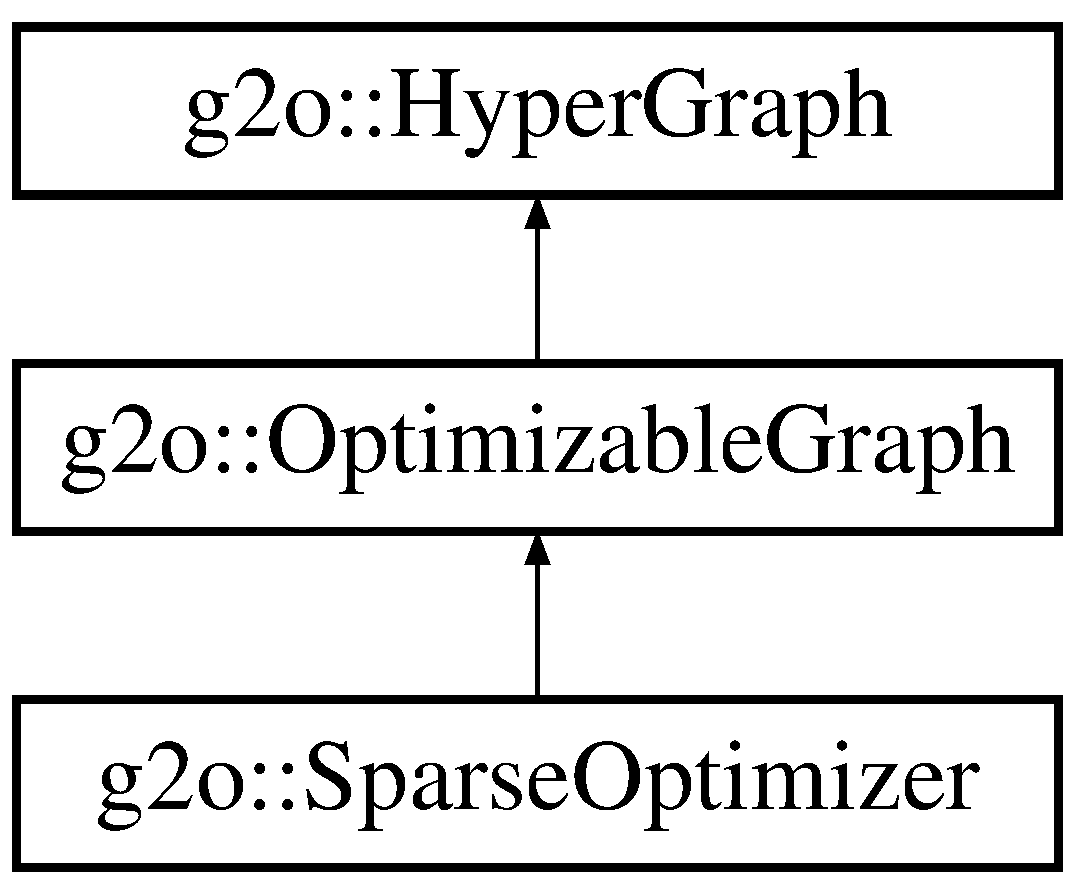
\includegraphics[height=3.000000cm]{structg2o_1_1_optimizable_graph}
\end{center}
\end{figure}
\subsection*{Classes}
\begin{DoxyCompactItemize}
\item 
class \mbox{\hyperlink{classg2o_1_1_optimizable_graph_1_1_data}{Data}}
\begin{DoxyCompactList}\small\item\em data packet for a vertex. Extend this class to store in the vertices the potential additional information you need (e.\+g. images, laser scans, ...). \end{DoxyCompactList}\item 
class \mbox{\hyperlink{classg2o_1_1_optimizable_graph_1_1_edge}{Edge}}
\item 
struct \mbox{\hyperlink{structg2o_1_1_optimizable_graph_1_1_edge_i_d_compare}{Edge\+I\+D\+Compare}}
\begin{DoxyCompactList}\small\item\em order edges based on the internal ID, which is assigned to the edge in \mbox{\hyperlink{structg2o_1_1_optimizable_graph_a6831ed69fce3dba691f53302a2813070}{add\+Edge()}} \end{DoxyCompactList}\item 
class \mbox{\hyperlink{classg2o_1_1_optimizable_graph_1_1_vertex}{Vertex}}
\begin{DoxyCompactList}\small\item\em A general case \mbox{\hyperlink{classg2o_1_1_optimizable_graph_1_1_vertex}{Vertex}} for optimization. \end{DoxyCompactList}\item 
struct \mbox{\hyperlink{structg2o_1_1_optimizable_graph_1_1_vertex_i_d_compare}{Vertex\+I\+D\+Compare}}
\begin{DoxyCompactList}\small\item\em order vertices based on their ID \end{DoxyCompactList}\end{DoxyCompactItemize}
\subsection*{Public Types}
\begin{DoxyCompactItemize}
\item 
enum \mbox{\hyperlink{structg2o_1_1_optimizable_graph_a16d90305c171fe0582c6a8aef40ba89d}{Action\+Type}} \{ \mbox{\hyperlink{structg2o_1_1_optimizable_graph_a16d90305c171fe0582c6a8aef40ba89dad79dc2fea3676bc2e26a83b7aca0cff6}{A\+T\+\_\+\+P\+R\+E\+I\+T\+E\+R\+A\+T\+I\+ON}}, 
\mbox{\hyperlink{structg2o_1_1_optimizable_graph_a16d90305c171fe0582c6a8aef40ba89da6022cb4383dca15d503e600c463c5e5a}{A\+T\+\_\+\+P\+O\+S\+T\+I\+T\+E\+R\+A\+T\+I\+ON}}, 
\mbox{\hyperlink{structg2o_1_1_optimizable_graph_a16d90305c171fe0582c6a8aef40ba89da33b97f5bc80d2e6227c95364573d3651}{A\+T\+\_\+\+N\+U\+M\+\_\+\+E\+L\+E\+M\+E\+N\+TS}}
 \}
\item 
typedef std\+::set$<$ \mbox{\hyperlink{classg2o_1_1_hyper_graph_action}{Hyper\+Graph\+Action}} $\ast$ $>$ \mbox{\hyperlink{structg2o_1_1_optimizable_graph_aa3562ad6794c36ea832095131cfffaac}{Hyper\+Graph\+Action\+Set}}
\item 
typedef std\+::vector$<$ \mbox{\hyperlink{classg2o_1_1_optimizable_graph_1_1_vertex}{Optimizable\+Graph\+::\+Vertex}} $\ast$ $>$ \mbox{\hyperlink{structg2o_1_1_optimizable_graph_a54f01b9b6071e65e6abeebe4afb29dec}{Vertex\+Container}}
\begin{DoxyCompactList}\small\item\em vector container for vertices \end{DoxyCompactList}\item 
typedef std\+::vector$<$ \mbox{\hyperlink{classg2o_1_1_optimizable_graph_1_1_edge}{Optimizable\+Graph\+::\+Edge}} $\ast$ $>$ \mbox{\hyperlink{structg2o_1_1_optimizable_graph_a2b43e807ae6d61ef8749ca1ef7c25f62}{Edge\+Container}}
\begin{DoxyCompactList}\small\item\em vector container for edges \end{DoxyCompactList}\end{DoxyCompactItemize}
\subsection*{Public Member Functions}
\begin{DoxyCompactItemize}
\item 
\mbox{\hyperlink{classg2o_1_1_optimizable_graph_1_1_vertex}{Vertex}} $\ast$ \mbox{\hyperlink{structg2o_1_1_optimizable_graph_a19e014e8ec2e9a6e894da8c3a8f8e50d}{vertex}} (int id)
\begin{DoxyCompactList}\small\item\em returns the vertex number {\itshape id} appropriately casted \end{DoxyCompactList}\item 
const \mbox{\hyperlink{classg2o_1_1_optimizable_graph_1_1_vertex}{Vertex}} $\ast$ \mbox{\hyperlink{structg2o_1_1_optimizable_graph_a0e55fa99a49824af2711c0fcaf02ac1a}{vertex}} (int id) const
\begin{DoxyCompactList}\small\item\em returns the vertex number {\itshape id} appropriately casted \end{DoxyCompactList}\item 
\mbox{\hyperlink{structg2o_1_1_optimizable_graph_acc459c08fd5e743cf2072e740ffc5025}{Optimizable\+Graph}} ()
\begin{DoxyCompactList}\small\item\em empty constructor \end{DoxyCompactList}\item 
virtual \mbox{\hyperlink{structg2o_1_1_optimizable_graph_a98f4399dfc23cac840a64ae2d0d3898f}{$\sim$\+Optimizable\+Graph}} ()
\item 
void \mbox{\hyperlink{structg2o_1_1_optimizable_graph_acea1342d9ab0bf717710c8f78b74ff25}{add\+Graph}} (\mbox{\hyperlink{structg2o_1_1_optimizable_graph}{Optimizable\+Graph}} $\ast$g)
\begin{DoxyCompactList}\small\item\em adds all edges and vertices of the graph {\itshape g} to this graph. \end{DoxyCompactList}\item 
virtual bool \mbox{\hyperlink{structg2o_1_1_optimizable_graph_ae0b93774ce1dfa0dfd501c86ad4f773e}{add\+Vertex}} (\mbox{\hyperlink{classg2o_1_1_hyper_graph_1_1_vertex}{Hyper\+Graph\+::\+Vertex}} $\ast$v, \mbox{\hyperlink{classg2o_1_1_optimizable_graph_1_1_data}{Data}} $\ast$user\+Data)
\item 
virtual bool \mbox{\hyperlink{structg2o_1_1_optimizable_graph_ac6f41f49fe6148fbe17133d10bf29b4c}{add\+Vertex}} (\mbox{\hyperlink{classg2o_1_1_hyper_graph_1_1_vertex}{Hyper\+Graph\+::\+Vertex}} $\ast$v)
\item 
virtual bool \mbox{\hyperlink{structg2o_1_1_optimizable_graph_a6831ed69fce3dba691f53302a2813070}{add\+Edge}} (\mbox{\hyperlink{classg2o_1_1_hyper_graph_1_1_edge}{Hyper\+Graph\+::\+Edge}} $\ast$e)
\item 
double \mbox{\hyperlink{structg2o_1_1_optimizable_graph_af0d53383e22347aba1bf76c1ce492f51}{chi2}} () const
\begin{DoxyCompactList}\small\item\em returns the chi2 of the current configuration \end{DoxyCompactList}\item 
int \mbox{\hyperlink{structg2o_1_1_optimizable_graph_aec95bac1366d39b40703f2aca375f505}{max\+Dimension}} () const
\begin{DoxyCompactList}\small\item\em return the maximum dimension of all vertices in the graph \end{DoxyCompactList}\item 
std\+::set$<$ int $>$ \mbox{\hyperlink{structg2o_1_1_optimizable_graph_a396e552ed234fe625e3b6785efa9c86d}{dimensions}} () const
\item 
virtual int \mbox{\hyperlink{structg2o_1_1_optimizable_graph_ac1b2e36c05680dd3e60ed6f90dddf5d8}{optimize}} (int iterations, bool online=false)
\item 
virtual void \mbox{\hyperlink{structg2o_1_1_optimizable_graph_ad295e7f06651db627b8ebde3d8898bab}{pre\+Iteration}} (int)
\begin{DoxyCompactList}\small\item\em called at the beginning of an iteration (argument is the number of the iteration) \end{DoxyCompactList}\item 
virtual void \mbox{\hyperlink{structg2o_1_1_optimizable_graph_ac8d41dc0830f1ae07e9cb4a8341d3ffb}{post\+Iteration}} (int)
\begin{DoxyCompactList}\small\item\em called at the end of an iteration (argument is the number of the iteration) \end{DoxyCompactList}\item 
bool \mbox{\hyperlink{structg2o_1_1_optimizable_graph_a2ab7899a0ff7bc29177e9447a10d508c}{add\+Pre\+Iteration\+Action}} (\mbox{\hyperlink{classg2o_1_1_hyper_graph_action}{Hyper\+Graph\+Action}} $\ast$action)
\begin{DoxyCompactList}\small\item\em add an action to be executed before each iteration \end{DoxyCompactList}\item 
bool \mbox{\hyperlink{structg2o_1_1_optimizable_graph_a6db1ecbc582a7b79e1633eefc2109b26}{add\+Post\+Iteration\+Action}} (\mbox{\hyperlink{classg2o_1_1_hyper_graph_action}{Hyper\+Graph\+Action}} $\ast$action)
\begin{DoxyCompactList}\small\item\em add an action to be executed after each iteration \end{DoxyCompactList}\item 
bool \mbox{\hyperlink{structg2o_1_1_optimizable_graph_a27f5ee7016b20bc6def24a2726fc824b}{remove\+Pre\+Iteration\+Action}} (\mbox{\hyperlink{classg2o_1_1_hyper_graph_action}{Hyper\+Graph\+Action}} $\ast$action)
\begin{DoxyCompactList}\small\item\em remove an action that should no longer be execured before each iteration \end{DoxyCompactList}\item 
bool \mbox{\hyperlink{structg2o_1_1_optimizable_graph_a172f2f5c8ec5872d5bc34077c6391839}{remove\+Post\+Iteration\+Action}} (\mbox{\hyperlink{classg2o_1_1_hyper_graph_action}{Hyper\+Graph\+Action}} $\ast$action)
\begin{DoxyCompactList}\small\item\em remove an action that should no longer be execured after each iteration \end{DoxyCompactList}\item 
virtual void \mbox{\hyperlink{structg2o_1_1_optimizable_graph_a3db385b25818a5659d1fa8407cb0db45}{push}} ()
\begin{DoxyCompactList}\small\item\em push the estimate of all variables onto a stack \end{DoxyCompactList}\item 
virtual void \mbox{\hyperlink{structg2o_1_1_optimizable_graph_a8487f537b16ac7a2ee416ea294a1e22e}{pop}} ()
\begin{DoxyCompactList}\small\item\em pop (restore) the estimate of all variables from the stack \end{DoxyCompactList}\item 
virtual void \mbox{\hyperlink{structg2o_1_1_optimizable_graph_a368b5f22dbc57abd2f651a20d039f61c}{discard\+Top}} ()
\begin{DoxyCompactList}\small\item\em discard the last backup of the estimate for all variables by removing it from the stack \end{DoxyCompactList}\item 
virtual bool \mbox{\hyperlink{structg2o_1_1_optimizable_graph_a34f4a170d58551ee9efac7a7a78fa833}{load}} (std\+::istream \&is, bool create\+Edges=true)
\begin{DoxyCompactList}\small\item\em load the graph from a stream. Uses the \mbox{\hyperlink{classg2o_1_1_factory}{Factory}} singleton for creating the vertices and edges. \end{DoxyCompactList}\item 
bool \mbox{\hyperlink{structg2o_1_1_optimizable_graph_a305fe91c405fc960df051d9581e524bc}{load}} (const char $\ast$filename, bool create\+Edges=true)
\item 
virtual bool \mbox{\hyperlink{structg2o_1_1_optimizable_graph_abee0b60ade0644904a489564def8ad1d}{save}} (std\+::ostream \&os, int level=0) const
\begin{DoxyCompactList}\small\item\em save the graph to a stream. Again uses the \mbox{\hyperlink{classg2o_1_1_factory}{Factory}} system. \end{DoxyCompactList}\item 
bool \mbox{\hyperlink{structg2o_1_1_optimizable_graph_a29c40a9cb3bf3660e59d55cfad264c71}{save}} (const char $\ast$filename, int level=0) const
\begin{DoxyCompactList}\small\item\em function provided for convenience, see \mbox{\hyperlink{structg2o_1_1_optimizable_graph_abee0b60ade0644904a489564def8ad1d}{save()}} above \end{DoxyCompactList}\item 
bool \mbox{\hyperlink{structg2o_1_1_optimizable_graph_adcf211f9c7bf3ee9dab65b130807402c}{save\+Subset}} (std\+::ostream \&os, \mbox{\hyperlink{classg2o_1_1_hyper_graph_a703938cdb4bb636860eed55a2489d70c}{Hyper\+Graph\+::\+Vertex\+Set}} \&vset, int level=0)
\begin{DoxyCompactList}\small\item\em save a subgraph to a stream. Again uses the \mbox{\hyperlink{classg2o_1_1_factory}{Factory}} system. \end{DoxyCompactList}\item 
bool \mbox{\hyperlink{structg2o_1_1_optimizable_graph_a2a08383ab953d435eaaca6231b64c3b6}{save\+Subset}} (std\+::ostream \&os, \mbox{\hyperlink{classg2o_1_1_hyper_graph_a5e2970e236c0dcb4eff7c205d7b6b4ae}{Hyper\+Graph\+::\+Edge\+Set}} \&eset)
\begin{DoxyCompactList}\small\item\em save a subgraph to a stream. Again uses the \mbox{\hyperlink{classg2o_1_1_factory}{Factory}} system. \end{DoxyCompactList}\item 
virtual void \mbox{\hyperlink{structg2o_1_1_optimizable_graph_a1d65a6854936147a92f7ba664302993e}{push}} (\mbox{\hyperlink{classg2o_1_1_hyper_graph_a703938cdb4bb636860eed55a2489d70c}{Hyper\+Graph\+::\+Vertex\+Set}} \&vset)
\begin{DoxyCompactList}\small\item\em push the estimate of a subset of the variables onto a stack \end{DoxyCompactList}\item 
virtual void \mbox{\hyperlink{structg2o_1_1_optimizable_graph_a83425dbe755d22877ba692e93e04a6af}{pop}} (\mbox{\hyperlink{classg2o_1_1_hyper_graph_a703938cdb4bb636860eed55a2489d70c}{Hyper\+Graph\+::\+Vertex\+Set}} \&vset)
\begin{DoxyCompactList}\small\item\em pop (restore) the estimate a subset of the variables from the stack \end{DoxyCompactList}\item 
virtual void \mbox{\hyperlink{structg2o_1_1_optimizable_graph_a74cbd91a3e05c1f497b4675b0e70113a}{discard\+Top}} (\mbox{\hyperlink{classg2o_1_1_hyper_graph_a703938cdb4bb636860eed55a2489d70c}{Hyper\+Graph\+::\+Vertex\+Set}} \&vset)
\begin{DoxyCompactList}\small\item\em ignore the latest stored element on the stack, remove it from the stack but do not restore the estimate \end{DoxyCompactList}\item 
virtual void \mbox{\hyperlink{structg2o_1_1_optimizable_graph_a07514f6186d19b6d893a771c0bb6abf9}{set\+Fixed}} (\mbox{\hyperlink{classg2o_1_1_hyper_graph_a703938cdb4bb636860eed55a2489d70c}{Hyper\+Graph\+::\+Vertex\+Set}} \&vset, bool fixed)
\begin{DoxyCompactList}\small\item\em fixes/releases a set of vertices \end{DoxyCompactList}\item 
void \mbox{\hyperlink{structg2o_1_1_optimizable_graph_afaa77a4624619237563fe94cfd7b76fd}{set\+Renamed\+Types\+From\+String}} (const std\+::string \&types)
\item 
bool \mbox{\hyperlink{structg2o_1_1_optimizable_graph_a5b957f752c6afe7bc76baf00129f854e}{is\+Solver\+Suitable}} (const \mbox{\hyperlink{structg2o_1_1_optimization_algorithm_property}{Optimization\+Algorithm\+Property}} \&solver\+Property, const std\+::set$<$ int $>$ \&vert\+Dims=std\+::set$<$ int $>$()) const
\item 
virtual void \mbox{\hyperlink{structg2o_1_1_optimizable_graph_a15171b6d335115858e2e86dcf576ba78}{clear\+Parameters}} ()
\item 
bool \mbox{\hyperlink{structg2o_1_1_optimizable_graph_ad4a7c038288097b0b1619c609cf40e90}{add\+Parameter}} (\mbox{\hyperlink{classg2o_1_1_parameter}{Parameter}} $\ast$p)
\item 
\mbox{\hyperlink{classg2o_1_1_parameter}{Parameter}} $\ast$ \mbox{\hyperlink{structg2o_1_1_optimizable_graph_ad9506880a9289353ddd2277fafb76ffd}{parameter}} (int id)
\item 
bool \mbox{\hyperlink{structg2o_1_1_optimizable_graph_a23dbb64bd31deb3952d4149518e663ce}{verify\+Information\+Matrices}} (bool verbose=false) const
\item 
bool \mbox{\hyperlink{structg2o_1_1_optimizable_graph_a221656c91e253b4246553a33e33c3e6b}{save\+Vertex}} (std\+::ostream \&os, \mbox{\hyperlink{classg2o_1_1_optimizable_graph_1_1_vertex}{Vertex}} $\ast$v) const
\item 
bool \mbox{\hyperlink{structg2o_1_1_optimizable_graph_a3852abe611f2fd90a0a05979987615a2}{save\+Edge}} (std\+::ostream \&os, \mbox{\hyperlink{classg2o_1_1_optimizable_graph_1_1_edge}{Edge}} $\ast$e) const
\item 
\mbox{\hyperlink{classg2o_1_1_jacobian_workspace}{Jacobian\+Workspace}} \& \mbox{\hyperlink{structg2o_1_1_optimizable_graph_aa669dbd1d6e34e49fecda711ff1b78c6}{jacobian\+Workspace}} ()
\begin{DoxyCompactList}\small\item\em the workspace for storing the Jacobians of the graph \end{DoxyCompactList}\item 
const \mbox{\hyperlink{classg2o_1_1_jacobian_workspace}{Jacobian\+Workspace}} \& \mbox{\hyperlink{structg2o_1_1_optimizable_graph_a21d73e7a39c731d19e6bb467cad59912}{jacobian\+Workspace}} () const
\end{DoxyCompactItemize}
\subsection*{Static Public Member Functions}
\begin{DoxyCompactItemize}
\item 
static bool \mbox{\hyperlink{structg2o_1_1_optimizable_graph_ab4ee0fc3ecd31852276ded40b62e9c76}{init\+Multi\+Threading}} ()
\end{DoxyCompactItemize}
\subsection*{Public Attributes}
\begin{DoxyCompactItemize}
\item 
class \mbox{\hyperlink{g2o__core__api_8h_a7a8d7648d6f1e26632566f335751d064}{G2\+O\+\_\+\+C\+O\+R\+E\+\_\+\+A\+PI}} \mbox{\hyperlink{structg2o_1_1_optimizable_graph_ae1bdcfc2f7a1b8977ba04a16b16f1eba}{Vertex}}
\item 
class \mbox{\hyperlink{g2o__core__api_8h_a7a8d7648d6f1e26632566f335751d064}{G2\+O\+\_\+\+C\+O\+R\+E\+\_\+\+A\+PI}} \mbox{\hyperlink{structg2o_1_1_optimizable_graph_a59cf44f3f3182a367ee4525412c7940a}{Edge}}
\end{DoxyCompactItemize}
\subsection*{Protected Attributes}
\begin{DoxyCompactItemize}
\item 
std\+::map$<$ std\+::string, std\+::string $>$ \mbox{\hyperlink{structg2o_1_1_optimizable_graph_a726ab6d0b04b12f835b690d54e061731}{\+\_\+renamed\+Types\+Lookup}}
\item 
long long \mbox{\hyperlink{structg2o_1_1_optimizable_graph_a93a7f05b31bca9ccaa214499f042739a}{\+\_\+next\+Edge\+Id}}
\item 
std\+::vector$<$ \mbox{\hyperlink{structg2o_1_1_optimizable_graph_aa3562ad6794c36ea832095131cfffaac}{Hyper\+Graph\+Action\+Set}} $>$ \mbox{\hyperlink{structg2o_1_1_optimizable_graph_a5e6a371ad7709692e52886ecf3e7250c}{\+\_\+graph\+Actions}}
\item 
bool \mbox{\hyperlink{structg2o_1_1_optimizable_graph_a260451b25094e5e929cc2841e31242f4}{\+\_\+edge\+\_\+has\+\_\+id}}
\item 
\mbox{\hyperlink{classg2o_1_1_parameter_container}{Parameter\+Container}} \mbox{\hyperlink{structg2o_1_1_optimizable_graph_a3a7974befcd934f28a36de3999423d21}{\+\_\+parameters}}
\item 
\mbox{\hyperlink{classg2o_1_1_jacobian_workspace}{Jacobian\+Workspace}} \mbox{\hyperlink{structg2o_1_1_optimizable_graph_a161c01a29d09cca22e223ab2048eaba8}{\+\_\+jacobian\+Workspace}}
\end{DoxyCompactItemize}


\subsection{Detailed Description}
This is an abstract class that represents one optimization problem. It specializes the general graph to contain special vertices and edges. The vertices represent parameters that can be optimized, while the edges represent constraints. This class also provides basic functionalities to handle the backup/restore of portions of the vertices. 

\subsection{Member Typedef Documentation}
\mbox{\Hypertarget{structg2o_1_1_optimizable_graph_a2b43e807ae6d61ef8749ca1ef7c25f62}\label{structg2o_1_1_optimizable_graph_a2b43e807ae6d61ef8749ca1ef7c25f62}} 
\index{g2o\+::\+Optimizable\+Graph@{g2o\+::\+Optimizable\+Graph}!Edge\+Container@{Edge\+Container}}
\index{Edge\+Container@{Edge\+Container}!g2o\+::\+Optimizable\+Graph@{g2o\+::\+Optimizable\+Graph}}
\subsubsection{\texorpdfstring{Edge\+Container}{EdgeContainer}}
{\footnotesize\ttfamily typedef std\+::vector$<$\mbox{\hyperlink{classg2o_1_1_optimizable_graph_1_1_edge}{Optimizable\+Graph\+::\+Edge}}$\ast$$>$ \mbox{\hyperlink{structg2o_1_1_optimizable_graph_a2b43e807ae6d61ef8749ca1ef7c25f62}{g2o\+::\+Optimizable\+Graph\+::\+Edge\+Container}}}



vector container for edges 

\mbox{\Hypertarget{structg2o_1_1_optimizable_graph_aa3562ad6794c36ea832095131cfffaac}\label{structg2o_1_1_optimizable_graph_aa3562ad6794c36ea832095131cfffaac}} 
\index{g2o\+::\+Optimizable\+Graph@{g2o\+::\+Optimizable\+Graph}!Hyper\+Graph\+Action\+Set@{Hyper\+Graph\+Action\+Set}}
\index{Hyper\+Graph\+Action\+Set@{Hyper\+Graph\+Action\+Set}!g2o\+::\+Optimizable\+Graph@{g2o\+::\+Optimizable\+Graph}}
\subsubsection{\texorpdfstring{Hyper\+Graph\+Action\+Set}{HyperGraphActionSet}}
{\footnotesize\ttfamily typedef std\+::set$<$\mbox{\hyperlink{classg2o_1_1_hyper_graph_action}{Hyper\+Graph\+Action}}$\ast$$>$ \mbox{\hyperlink{structg2o_1_1_optimizable_graph_aa3562ad6794c36ea832095131cfffaac}{g2o\+::\+Optimizable\+Graph\+::\+Hyper\+Graph\+Action\+Set}}}

\mbox{\Hypertarget{structg2o_1_1_optimizable_graph_a54f01b9b6071e65e6abeebe4afb29dec}\label{structg2o_1_1_optimizable_graph_a54f01b9b6071e65e6abeebe4afb29dec}} 
\index{g2o\+::\+Optimizable\+Graph@{g2o\+::\+Optimizable\+Graph}!Vertex\+Container@{Vertex\+Container}}
\index{Vertex\+Container@{Vertex\+Container}!g2o\+::\+Optimizable\+Graph@{g2o\+::\+Optimizable\+Graph}}
\subsubsection{\texorpdfstring{Vertex\+Container}{VertexContainer}}
{\footnotesize\ttfamily typedef std\+::vector$<$\mbox{\hyperlink{classg2o_1_1_optimizable_graph_1_1_vertex}{Optimizable\+Graph\+::\+Vertex}}$\ast$$>$ \mbox{\hyperlink{structg2o_1_1_optimizable_graph_a54f01b9b6071e65e6abeebe4afb29dec}{g2o\+::\+Optimizable\+Graph\+::\+Vertex\+Container}}}



vector container for vertices 



\subsection{Member Enumeration Documentation}
\mbox{\Hypertarget{structg2o_1_1_optimizable_graph_a16d90305c171fe0582c6a8aef40ba89d}\label{structg2o_1_1_optimizable_graph_a16d90305c171fe0582c6a8aef40ba89d}} 
\index{g2o\+::\+Optimizable\+Graph@{g2o\+::\+Optimizable\+Graph}!Action\+Type@{Action\+Type}}
\index{Action\+Type@{Action\+Type}!g2o\+::\+Optimizable\+Graph@{g2o\+::\+Optimizable\+Graph}}
\subsubsection{\texorpdfstring{Action\+Type}{ActionType}}
{\footnotesize\ttfamily enum \mbox{\hyperlink{structg2o_1_1_optimizable_graph_a16d90305c171fe0582c6a8aef40ba89d}{g2o\+::\+Optimizable\+Graph\+::\+Action\+Type}}}

\begin{DoxyEnumFields}{Enumerator}
\raisebox{\heightof{T}}[0pt][0pt]{\index{A\+T\+\_\+\+P\+R\+E\+I\+T\+E\+R\+A\+T\+I\+ON@{A\+T\+\_\+\+P\+R\+E\+I\+T\+E\+R\+A\+T\+I\+ON}!g2o\+::\+Optimizable\+Graph@{g2o\+::\+Optimizable\+Graph}}\index{g2o\+::\+Optimizable\+Graph@{g2o\+::\+Optimizable\+Graph}!A\+T\+\_\+\+P\+R\+E\+I\+T\+E\+R\+A\+T\+I\+ON@{A\+T\+\_\+\+P\+R\+E\+I\+T\+E\+R\+A\+T\+I\+ON}}}\mbox{\Hypertarget{structg2o_1_1_optimizable_graph_a16d90305c171fe0582c6a8aef40ba89dad79dc2fea3676bc2e26a83b7aca0cff6}\label{structg2o_1_1_optimizable_graph_a16d90305c171fe0582c6a8aef40ba89dad79dc2fea3676bc2e26a83b7aca0cff6}} 
A\+T\+\_\+\+P\+R\+E\+I\+T\+E\+R\+A\+T\+I\+ON&\\
\hline

\raisebox{\heightof{T}}[0pt][0pt]{\index{A\+T\+\_\+\+P\+O\+S\+T\+I\+T\+E\+R\+A\+T\+I\+ON@{A\+T\+\_\+\+P\+O\+S\+T\+I\+T\+E\+R\+A\+T\+I\+ON}!g2o\+::\+Optimizable\+Graph@{g2o\+::\+Optimizable\+Graph}}\index{g2o\+::\+Optimizable\+Graph@{g2o\+::\+Optimizable\+Graph}!A\+T\+\_\+\+P\+O\+S\+T\+I\+T\+E\+R\+A\+T\+I\+ON@{A\+T\+\_\+\+P\+O\+S\+T\+I\+T\+E\+R\+A\+T\+I\+ON}}}\mbox{\Hypertarget{structg2o_1_1_optimizable_graph_a16d90305c171fe0582c6a8aef40ba89da6022cb4383dca15d503e600c463c5e5a}\label{structg2o_1_1_optimizable_graph_a16d90305c171fe0582c6a8aef40ba89da6022cb4383dca15d503e600c463c5e5a}} 
A\+T\+\_\+\+P\+O\+S\+T\+I\+T\+E\+R\+A\+T\+I\+ON&\\
\hline

\raisebox{\heightof{T}}[0pt][0pt]{\index{A\+T\+\_\+\+N\+U\+M\+\_\+\+E\+L\+E\+M\+E\+N\+TS@{A\+T\+\_\+\+N\+U\+M\+\_\+\+E\+L\+E\+M\+E\+N\+TS}!g2o\+::\+Optimizable\+Graph@{g2o\+::\+Optimizable\+Graph}}\index{g2o\+::\+Optimizable\+Graph@{g2o\+::\+Optimizable\+Graph}!A\+T\+\_\+\+N\+U\+M\+\_\+\+E\+L\+E\+M\+E\+N\+TS@{A\+T\+\_\+\+N\+U\+M\+\_\+\+E\+L\+E\+M\+E\+N\+TS}}}\mbox{\Hypertarget{structg2o_1_1_optimizable_graph_a16d90305c171fe0582c6a8aef40ba89da33b97f5bc80d2e6227c95364573d3651}\label{structg2o_1_1_optimizable_graph_a16d90305c171fe0582c6a8aef40ba89da33b97f5bc80d2e6227c95364573d3651}} 
A\+T\+\_\+\+N\+U\+M\+\_\+\+E\+L\+E\+M\+E\+N\+TS&\\
\hline

\end{DoxyEnumFields}


\subsection{Constructor \& Destructor Documentation}
\mbox{\Hypertarget{structg2o_1_1_optimizable_graph_acc459c08fd5e743cf2072e740ffc5025}\label{structg2o_1_1_optimizable_graph_acc459c08fd5e743cf2072e740ffc5025}} 
\index{g2o\+::\+Optimizable\+Graph@{g2o\+::\+Optimizable\+Graph}!Optimizable\+Graph@{Optimizable\+Graph}}
\index{Optimizable\+Graph@{Optimizable\+Graph}!g2o\+::\+Optimizable\+Graph@{g2o\+::\+Optimizable\+Graph}}
\subsubsection{\texorpdfstring{Optimizable\+Graph()}{OptimizableGraph()}}
{\footnotesize\ttfamily g2o\+::\+Optimizable\+Graph\+::\+Optimizable\+Graph (\begin{DoxyParamCaption}{ }\end{DoxyParamCaption})}



empty constructor 

\mbox{\Hypertarget{structg2o_1_1_optimizable_graph_a98f4399dfc23cac840a64ae2d0d3898f}\label{structg2o_1_1_optimizable_graph_a98f4399dfc23cac840a64ae2d0d3898f}} 
\index{g2o\+::\+Optimizable\+Graph@{g2o\+::\+Optimizable\+Graph}!````~Optimizable\+Graph@{$\sim$\+Optimizable\+Graph}}
\index{````~Optimizable\+Graph@{$\sim$\+Optimizable\+Graph}!g2o\+::\+Optimizable\+Graph@{g2o\+::\+Optimizable\+Graph}}
\subsubsection{\texorpdfstring{$\sim$\+Optimizable\+Graph()}{~OptimizableGraph()}}
{\footnotesize\ttfamily g2o\+::\+Optimizable\+Graph\+::$\sim$\+Optimizable\+Graph (\begin{DoxyParamCaption}{ }\end{DoxyParamCaption})\hspace{0.3cm}{\ttfamily [virtual]}}



\subsection{Member Function Documentation}
\mbox{\Hypertarget{structg2o_1_1_optimizable_graph_a6831ed69fce3dba691f53302a2813070}\label{structg2o_1_1_optimizable_graph_a6831ed69fce3dba691f53302a2813070}} 
\index{g2o\+::\+Optimizable\+Graph@{g2o\+::\+Optimizable\+Graph}!add\+Edge@{add\+Edge}}
\index{add\+Edge@{add\+Edge}!g2o\+::\+Optimizable\+Graph@{g2o\+::\+Optimizable\+Graph}}
\subsubsection{\texorpdfstring{add\+Edge()}{addEdge()}}
{\footnotesize\ttfamily bool g2o\+::\+Optimizable\+Graph\+::add\+Edge (\begin{DoxyParamCaption}\item[{\mbox{\hyperlink{classg2o_1_1_hyper_graph_1_1_edge}{Hyper\+Graph\+::\+Edge}} $\ast$}]{e }\end{DoxyParamCaption})\hspace{0.3cm}{\ttfamily [virtual]}}

adds a new edge. The edge should point to the vertices that it is connecting (set\+From/set\+To). \begin{DoxyReturn}{Returns}
false if the insertion does not work (incompatible types of the vertices/missing vertex). true otherwise. 
\end{DoxyReturn}


Reimplemented from \mbox{\hyperlink{classg2o_1_1_hyper_graph_a0f1d35009a2879b238c8148c33485c89}{g2o\+::\+Hyper\+Graph}}.

\mbox{\Hypertarget{structg2o_1_1_optimizable_graph_acea1342d9ab0bf717710c8f78b74ff25}\label{structg2o_1_1_optimizable_graph_acea1342d9ab0bf717710c8f78b74ff25}} 
\index{g2o\+::\+Optimizable\+Graph@{g2o\+::\+Optimizable\+Graph}!add\+Graph@{add\+Graph}}
\index{add\+Graph@{add\+Graph}!g2o\+::\+Optimizable\+Graph@{g2o\+::\+Optimizable\+Graph}}
\subsubsection{\texorpdfstring{add\+Graph()}{addGraph()}}
{\footnotesize\ttfamily void g2o\+::\+Optimizable\+Graph\+::add\+Graph (\begin{DoxyParamCaption}\item[{\mbox{\hyperlink{structg2o_1_1_optimizable_graph}{Optimizable\+Graph}} $\ast$}]{g }\end{DoxyParamCaption})}



adds all edges and vertices of the graph {\itshape g} to this graph. 

\mbox{\Hypertarget{structg2o_1_1_optimizable_graph_ad4a7c038288097b0b1619c609cf40e90}\label{structg2o_1_1_optimizable_graph_ad4a7c038288097b0b1619c609cf40e90}} 
\index{g2o\+::\+Optimizable\+Graph@{g2o\+::\+Optimizable\+Graph}!add\+Parameter@{add\+Parameter}}
\index{add\+Parameter@{add\+Parameter}!g2o\+::\+Optimizable\+Graph@{g2o\+::\+Optimizable\+Graph}}
\subsubsection{\texorpdfstring{add\+Parameter()}{addParameter()}}
{\footnotesize\ttfamily bool g2o\+::\+Optimizable\+Graph\+::add\+Parameter (\begin{DoxyParamCaption}\item[{\mbox{\hyperlink{classg2o_1_1_parameter}{Parameter}} $\ast$}]{p }\end{DoxyParamCaption})\hspace{0.3cm}{\ttfamily [inline]}}

\mbox{\Hypertarget{structg2o_1_1_optimizable_graph_a6db1ecbc582a7b79e1633eefc2109b26}\label{structg2o_1_1_optimizable_graph_a6db1ecbc582a7b79e1633eefc2109b26}} 
\index{g2o\+::\+Optimizable\+Graph@{g2o\+::\+Optimizable\+Graph}!add\+Post\+Iteration\+Action@{add\+Post\+Iteration\+Action}}
\index{add\+Post\+Iteration\+Action@{add\+Post\+Iteration\+Action}!g2o\+::\+Optimizable\+Graph@{g2o\+::\+Optimizable\+Graph}}
\subsubsection{\texorpdfstring{add\+Post\+Iteration\+Action()}{addPostIterationAction()}}
{\footnotesize\ttfamily bool g2o\+::\+Optimizable\+Graph\+::add\+Post\+Iteration\+Action (\begin{DoxyParamCaption}\item[{\mbox{\hyperlink{classg2o_1_1_hyper_graph_action}{Hyper\+Graph\+Action}} $\ast$}]{action }\end{DoxyParamCaption})}



add an action to be executed after each iteration 

\mbox{\Hypertarget{structg2o_1_1_optimizable_graph_a2ab7899a0ff7bc29177e9447a10d508c}\label{structg2o_1_1_optimizable_graph_a2ab7899a0ff7bc29177e9447a10d508c}} 
\index{g2o\+::\+Optimizable\+Graph@{g2o\+::\+Optimizable\+Graph}!add\+Pre\+Iteration\+Action@{add\+Pre\+Iteration\+Action}}
\index{add\+Pre\+Iteration\+Action@{add\+Pre\+Iteration\+Action}!g2o\+::\+Optimizable\+Graph@{g2o\+::\+Optimizable\+Graph}}
\subsubsection{\texorpdfstring{add\+Pre\+Iteration\+Action()}{addPreIterationAction()}}
{\footnotesize\ttfamily bool g2o\+::\+Optimizable\+Graph\+::add\+Pre\+Iteration\+Action (\begin{DoxyParamCaption}\item[{\mbox{\hyperlink{classg2o_1_1_hyper_graph_action}{Hyper\+Graph\+Action}} $\ast$}]{action }\end{DoxyParamCaption})}



add an action to be executed before each iteration 

\mbox{\Hypertarget{structg2o_1_1_optimizable_graph_ae0b93774ce1dfa0dfd501c86ad4f773e}\label{structg2o_1_1_optimizable_graph_ae0b93774ce1dfa0dfd501c86ad4f773e}} 
\index{g2o\+::\+Optimizable\+Graph@{g2o\+::\+Optimizable\+Graph}!add\+Vertex@{add\+Vertex}}
\index{add\+Vertex@{add\+Vertex}!g2o\+::\+Optimizable\+Graph@{g2o\+::\+Optimizable\+Graph}}
\subsubsection{\texorpdfstring{add\+Vertex()}{addVertex()}\hspace{0.1cm}{\footnotesize\ttfamily [1/2]}}
{\footnotesize\ttfamily bool g2o\+::\+Optimizable\+Graph\+::add\+Vertex (\begin{DoxyParamCaption}\item[{\mbox{\hyperlink{classg2o_1_1_hyper_graph_1_1_vertex}{Hyper\+Graph\+::\+Vertex}} $\ast$}]{v,  }\item[{\mbox{\hyperlink{classg2o_1_1_optimizable_graph_1_1_data}{Data}} $\ast$}]{user\+Data }\end{DoxyParamCaption})\hspace{0.3cm}{\ttfamily [virtual]}}

adds a new vertex. The new vertex is then \char`\"{}taken\char`\"{}. \begin{DoxyReturn}{Returns}
false if a vertex with the same id as v is already in the graph, true otherwise. 
\end{DoxyReturn}
\mbox{\Hypertarget{structg2o_1_1_optimizable_graph_ac6f41f49fe6148fbe17133d10bf29b4c}\label{structg2o_1_1_optimizable_graph_ac6f41f49fe6148fbe17133d10bf29b4c}} 
\index{g2o\+::\+Optimizable\+Graph@{g2o\+::\+Optimizable\+Graph}!add\+Vertex@{add\+Vertex}}
\index{add\+Vertex@{add\+Vertex}!g2o\+::\+Optimizable\+Graph@{g2o\+::\+Optimizable\+Graph}}
\subsubsection{\texorpdfstring{add\+Vertex()}{addVertex()}\hspace{0.1cm}{\footnotesize\ttfamily [2/2]}}
{\footnotesize\ttfamily virtual bool g2o\+::\+Optimizable\+Graph\+::add\+Vertex (\begin{DoxyParamCaption}\item[{\mbox{\hyperlink{classg2o_1_1_hyper_graph_1_1_vertex}{Hyper\+Graph\+::\+Vertex}} $\ast$}]{v }\end{DoxyParamCaption})\hspace{0.3cm}{\ttfamily [inline]}, {\ttfamily [virtual]}}

adds a vertex to the graph. The id of the vertex should be set before invoking this function. the function fails if another vertex with the same id is already in the graph. returns true, on success, or false on failure. 

Reimplemented from \mbox{\hyperlink{classg2o_1_1_hyper_graph_a7ef87ba3479827b24c6fc29c5fc3aa21}{g2o\+::\+Hyper\+Graph}}.

\mbox{\Hypertarget{structg2o_1_1_optimizable_graph_af0d53383e22347aba1bf76c1ce492f51}\label{structg2o_1_1_optimizable_graph_af0d53383e22347aba1bf76c1ce492f51}} 
\index{g2o\+::\+Optimizable\+Graph@{g2o\+::\+Optimizable\+Graph}!chi2@{chi2}}
\index{chi2@{chi2}!g2o\+::\+Optimizable\+Graph@{g2o\+::\+Optimizable\+Graph}}
\subsubsection{\texorpdfstring{chi2()}{chi2()}}
{\footnotesize\ttfamily double g2o\+::\+Optimizable\+Graph\+::chi2 (\begin{DoxyParamCaption}{ }\end{DoxyParamCaption}) const}



returns the chi2 of the current configuration 

\mbox{\Hypertarget{structg2o_1_1_optimizable_graph_a15171b6d335115858e2e86dcf576ba78}\label{structg2o_1_1_optimizable_graph_a15171b6d335115858e2e86dcf576ba78}} 
\index{g2o\+::\+Optimizable\+Graph@{g2o\+::\+Optimizable\+Graph}!clear\+Parameters@{clear\+Parameters}}
\index{clear\+Parameters@{clear\+Parameters}!g2o\+::\+Optimizable\+Graph@{g2o\+::\+Optimizable\+Graph}}
\subsubsection{\texorpdfstring{clear\+Parameters()}{clearParameters()}}
{\footnotesize\ttfamily void g2o\+::\+Optimizable\+Graph\+::clear\+Parameters (\begin{DoxyParamCaption}{ }\end{DoxyParamCaption})\hspace{0.3cm}{\ttfamily [virtual]}}

remove the parameters of the graph \mbox{\Hypertarget{structg2o_1_1_optimizable_graph_a396e552ed234fe625e3b6785efa9c86d}\label{structg2o_1_1_optimizable_graph_a396e552ed234fe625e3b6785efa9c86d}} 
\index{g2o\+::\+Optimizable\+Graph@{g2o\+::\+Optimizable\+Graph}!dimensions@{dimensions}}
\index{dimensions@{dimensions}!g2o\+::\+Optimizable\+Graph@{g2o\+::\+Optimizable\+Graph}}
\subsubsection{\texorpdfstring{dimensions()}{dimensions()}}
{\footnotesize\ttfamily std\+::set$<$ int $>$ g2o\+::\+Optimizable\+Graph\+::dimensions (\begin{DoxyParamCaption}{ }\end{DoxyParamCaption}) const}

iterates over all vertices and returns a set of all the vertex dimensions in the graph \mbox{\Hypertarget{structg2o_1_1_optimizable_graph_a368b5f22dbc57abd2f651a20d039f61c}\label{structg2o_1_1_optimizable_graph_a368b5f22dbc57abd2f651a20d039f61c}} 
\index{g2o\+::\+Optimizable\+Graph@{g2o\+::\+Optimizable\+Graph}!discard\+Top@{discard\+Top}}
\index{discard\+Top@{discard\+Top}!g2o\+::\+Optimizable\+Graph@{g2o\+::\+Optimizable\+Graph}}
\subsubsection{\texorpdfstring{discard\+Top()}{discardTop()}\hspace{0.1cm}{\footnotesize\ttfamily [1/2]}}
{\footnotesize\ttfamily void g2o\+::\+Optimizable\+Graph\+::discard\+Top (\begin{DoxyParamCaption}{ }\end{DoxyParamCaption})\hspace{0.3cm}{\ttfamily [virtual]}}



discard the last backup of the estimate for all variables by removing it from the stack 



Reimplemented in \mbox{\hyperlink{classg2o_1_1_sparse_optimizer_a20ed9e9f1201bfb874456a8d30f169fb}{g2o\+::\+Sparse\+Optimizer}}.

\mbox{\Hypertarget{structg2o_1_1_optimizable_graph_a74cbd91a3e05c1f497b4675b0e70113a}\label{structg2o_1_1_optimizable_graph_a74cbd91a3e05c1f497b4675b0e70113a}} 
\index{g2o\+::\+Optimizable\+Graph@{g2o\+::\+Optimizable\+Graph}!discard\+Top@{discard\+Top}}
\index{discard\+Top@{discard\+Top}!g2o\+::\+Optimizable\+Graph@{g2o\+::\+Optimizable\+Graph}}
\subsubsection{\texorpdfstring{discard\+Top()}{discardTop()}\hspace{0.1cm}{\footnotesize\ttfamily [2/2]}}
{\footnotesize\ttfamily void g2o\+::\+Optimizable\+Graph\+::discard\+Top (\begin{DoxyParamCaption}\item[{\mbox{\hyperlink{classg2o_1_1_hyper_graph_a703938cdb4bb636860eed55a2489d70c}{Hyper\+Graph\+::\+Vertex\+Set}} \&}]{vset }\end{DoxyParamCaption})\hspace{0.3cm}{\ttfamily [virtual]}}



ignore the latest stored element on the stack, remove it from the stack but do not restore the estimate 

\mbox{\Hypertarget{structg2o_1_1_optimizable_graph_ab4ee0fc3ecd31852276ded40b62e9c76}\label{structg2o_1_1_optimizable_graph_ab4ee0fc3ecd31852276ded40b62e9c76}} 
\index{g2o\+::\+Optimizable\+Graph@{g2o\+::\+Optimizable\+Graph}!init\+Multi\+Threading@{init\+Multi\+Threading}}
\index{init\+Multi\+Threading@{init\+Multi\+Threading}!g2o\+::\+Optimizable\+Graph@{g2o\+::\+Optimizable\+Graph}}
\subsubsection{\texorpdfstring{init\+Multi\+Threading()}{initMultiThreading()}}
{\footnotesize\ttfamily bool g2o\+::\+Optimizable\+Graph\+::init\+Multi\+Threading (\begin{DoxyParamCaption}{ }\end{DoxyParamCaption})\hspace{0.3cm}{\ttfamily [static]}}

Eigen starting from version 3.\+1 requires that we call an initialize function, if we perform calls to Eigen from several threads. Currently, this function calls Eigen\+::init\+Parallel if \mbox{\hyperlink{namespaceg2o}{g2o}} is compiled with Open\+MP support and Eigen\textquotesingle{}s version is at least 3.\+1 \mbox{\Hypertarget{structg2o_1_1_optimizable_graph_a5b957f752c6afe7bc76baf00129f854e}\label{structg2o_1_1_optimizable_graph_a5b957f752c6afe7bc76baf00129f854e}} 
\index{g2o\+::\+Optimizable\+Graph@{g2o\+::\+Optimizable\+Graph}!is\+Solver\+Suitable@{is\+Solver\+Suitable}}
\index{is\+Solver\+Suitable@{is\+Solver\+Suitable}!g2o\+::\+Optimizable\+Graph@{g2o\+::\+Optimizable\+Graph}}
\subsubsection{\texorpdfstring{is\+Solver\+Suitable()}{isSolverSuitable()}}
{\footnotesize\ttfamily bool g2o\+::\+Optimizable\+Graph\+::is\+Solver\+Suitable (\begin{DoxyParamCaption}\item[{const \mbox{\hyperlink{structg2o_1_1_optimization_algorithm_property}{Optimization\+Algorithm\+Property}} \&}]{solver\+Property,  }\item[{const std\+::set$<$ int $>$ \&}]{vert\+Dims = {\ttfamily std\+:\+:set$<$int$>$()} }\end{DoxyParamCaption}) const}

test whether a solver is suitable for optimizing this graph. 
\begin{DoxyParams}{Parameters}
{\em solver\+Property} & the solver property to evaluate. \\
\hline
{\em vert\+Dims} & should equal to the set returned by \mbox{\hyperlink{structg2o_1_1_optimizable_graph_a396e552ed234fe625e3b6785efa9c86d}{dimensions()}} to avoid re-\/evaluating. \\
\hline
\end{DoxyParams}
\mbox{\Hypertarget{structg2o_1_1_optimizable_graph_aa669dbd1d6e34e49fecda711ff1b78c6}\label{structg2o_1_1_optimizable_graph_aa669dbd1d6e34e49fecda711ff1b78c6}} 
\index{g2o\+::\+Optimizable\+Graph@{g2o\+::\+Optimizable\+Graph}!jacobian\+Workspace@{jacobian\+Workspace}}
\index{jacobian\+Workspace@{jacobian\+Workspace}!g2o\+::\+Optimizable\+Graph@{g2o\+::\+Optimizable\+Graph}}
\subsubsection{\texorpdfstring{jacobian\+Workspace()}{jacobianWorkspace()}\hspace{0.1cm}{\footnotesize\ttfamily [1/2]}}
{\footnotesize\ttfamily \mbox{\hyperlink{classg2o_1_1_jacobian_workspace}{Jacobian\+Workspace}}\& g2o\+::\+Optimizable\+Graph\+::jacobian\+Workspace (\begin{DoxyParamCaption}{ }\end{DoxyParamCaption})\hspace{0.3cm}{\ttfamily [inline]}}



the workspace for storing the Jacobians of the graph 

\mbox{\Hypertarget{structg2o_1_1_optimizable_graph_a21d73e7a39c731d19e6bb467cad59912}\label{structg2o_1_1_optimizable_graph_a21d73e7a39c731d19e6bb467cad59912}} 
\index{g2o\+::\+Optimizable\+Graph@{g2o\+::\+Optimizable\+Graph}!jacobian\+Workspace@{jacobian\+Workspace}}
\index{jacobian\+Workspace@{jacobian\+Workspace}!g2o\+::\+Optimizable\+Graph@{g2o\+::\+Optimizable\+Graph}}
\subsubsection{\texorpdfstring{jacobian\+Workspace()}{jacobianWorkspace()}\hspace{0.1cm}{\footnotesize\ttfamily [2/2]}}
{\footnotesize\ttfamily const \mbox{\hyperlink{classg2o_1_1_jacobian_workspace}{Jacobian\+Workspace}}\& g2o\+::\+Optimizable\+Graph\+::jacobian\+Workspace (\begin{DoxyParamCaption}{ }\end{DoxyParamCaption}) const\hspace{0.3cm}{\ttfamily [inline]}}

\mbox{\Hypertarget{structg2o_1_1_optimizable_graph_a34f4a170d58551ee9efac7a7a78fa833}\label{structg2o_1_1_optimizable_graph_a34f4a170d58551ee9efac7a7a78fa833}} 
\index{g2o\+::\+Optimizable\+Graph@{g2o\+::\+Optimizable\+Graph}!load@{load}}
\index{load@{load}!g2o\+::\+Optimizable\+Graph@{g2o\+::\+Optimizable\+Graph}}
\subsubsection{\texorpdfstring{load()}{load()}\hspace{0.1cm}{\footnotesize\ttfamily [1/2]}}
{\footnotesize\ttfamily virtual bool g2o\+::\+Optimizable\+Graph\+::load (\begin{DoxyParamCaption}\item[{std\+::istream \&}]{is,  }\item[{bool}]{create\+Edges = {\ttfamily true} }\end{DoxyParamCaption})\hspace{0.3cm}{\ttfamily [virtual]}}



load the graph from a stream. Uses the \mbox{\hyperlink{classg2o_1_1_factory}{Factory}} singleton for creating the vertices and edges. 

\mbox{\Hypertarget{structg2o_1_1_optimizable_graph_a305fe91c405fc960df051d9581e524bc}\label{structg2o_1_1_optimizable_graph_a305fe91c405fc960df051d9581e524bc}} 
\index{g2o\+::\+Optimizable\+Graph@{g2o\+::\+Optimizable\+Graph}!load@{load}}
\index{load@{load}!g2o\+::\+Optimizable\+Graph@{g2o\+::\+Optimizable\+Graph}}
\subsubsection{\texorpdfstring{load()}{load()}\hspace{0.1cm}{\footnotesize\ttfamily [2/2]}}
{\footnotesize\ttfamily bool g2o\+::\+Optimizable\+Graph\+::load (\begin{DoxyParamCaption}\item[{const char $\ast$}]{filename,  }\item[{bool}]{create\+Edges = {\ttfamily true} }\end{DoxyParamCaption})}

\mbox{\Hypertarget{structg2o_1_1_optimizable_graph_aec95bac1366d39b40703f2aca375f505}\label{structg2o_1_1_optimizable_graph_aec95bac1366d39b40703f2aca375f505}} 
\index{g2o\+::\+Optimizable\+Graph@{g2o\+::\+Optimizable\+Graph}!max\+Dimension@{max\+Dimension}}
\index{max\+Dimension@{max\+Dimension}!g2o\+::\+Optimizable\+Graph@{g2o\+::\+Optimizable\+Graph}}
\subsubsection{\texorpdfstring{max\+Dimension()}{maxDimension()}}
{\footnotesize\ttfamily int g2o\+::\+Optimizable\+Graph\+::max\+Dimension (\begin{DoxyParamCaption}{ }\end{DoxyParamCaption}) const}



return the maximum dimension of all vertices in the graph 

\mbox{\Hypertarget{structg2o_1_1_optimizable_graph_ac1b2e36c05680dd3e60ed6f90dddf5d8}\label{structg2o_1_1_optimizable_graph_ac1b2e36c05680dd3e60ed6f90dddf5d8}} 
\index{g2o\+::\+Optimizable\+Graph@{g2o\+::\+Optimizable\+Graph}!optimize@{optimize}}
\index{optimize@{optimize}!g2o\+::\+Optimizable\+Graph@{g2o\+::\+Optimizable\+Graph}}
\subsubsection{\texorpdfstring{optimize()}{optimize()}}
{\footnotesize\ttfamily int g2o\+::\+Optimizable\+Graph\+::optimize (\begin{DoxyParamCaption}\item[{int}]{iterations,  }\item[{bool}]{online = {\ttfamily false} }\end{DoxyParamCaption})\hspace{0.3cm}{\ttfamily [virtual]}}

carry out n iterations \begin{DoxyReturn}{Returns}
the number of performed iterations 
\end{DoxyReturn}


Reimplemented in \mbox{\hyperlink{classg2o_1_1_sparse_optimizer_a098257ee6f13dbb79be07075244d9930}{g2o\+::\+Sparse\+Optimizer}}.

\mbox{\Hypertarget{structg2o_1_1_optimizable_graph_ad9506880a9289353ddd2277fafb76ffd}\label{structg2o_1_1_optimizable_graph_ad9506880a9289353ddd2277fafb76ffd}} 
\index{g2o\+::\+Optimizable\+Graph@{g2o\+::\+Optimizable\+Graph}!parameter@{parameter}}
\index{parameter@{parameter}!g2o\+::\+Optimizable\+Graph@{g2o\+::\+Optimizable\+Graph}}
\subsubsection{\texorpdfstring{parameter()}{parameter()}}
{\footnotesize\ttfamily \mbox{\hyperlink{classg2o_1_1_parameter}{Parameter}}$\ast$ g2o\+::\+Optimizable\+Graph\+::parameter (\begin{DoxyParamCaption}\item[{int}]{id }\end{DoxyParamCaption})\hspace{0.3cm}{\ttfamily [inline]}}

\mbox{\Hypertarget{structg2o_1_1_optimizable_graph_a8487f537b16ac7a2ee416ea294a1e22e}\label{structg2o_1_1_optimizable_graph_a8487f537b16ac7a2ee416ea294a1e22e}} 
\index{g2o\+::\+Optimizable\+Graph@{g2o\+::\+Optimizable\+Graph}!pop@{pop}}
\index{pop@{pop}!g2o\+::\+Optimizable\+Graph@{g2o\+::\+Optimizable\+Graph}}
\subsubsection{\texorpdfstring{pop()}{pop()}\hspace{0.1cm}{\footnotesize\ttfamily [1/2]}}
{\footnotesize\ttfamily void g2o\+::\+Optimizable\+Graph\+::pop (\begin{DoxyParamCaption}{ }\end{DoxyParamCaption})\hspace{0.3cm}{\ttfamily [virtual]}}



pop (restore) the estimate of all variables from the stack 



Reimplemented in \mbox{\hyperlink{classg2o_1_1_sparse_optimizer_ad2f7f62ebe17b40e050f0525db64355b}{g2o\+::\+Sparse\+Optimizer}}.

\mbox{\Hypertarget{structg2o_1_1_optimizable_graph_a83425dbe755d22877ba692e93e04a6af}\label{structg2o_1_1_optimizable_graph_a83425dbe755d22877ba692e93e04a6af}} 
\index{g2o\+::\+Optimizable\+Graph@{g2o\+::\+Optimizable\+Graph}!pop@{pop}}
\index{pop@{pop}!g2o\+::\+Optimizable\+Graph@{g2o\+::\+Optimizable\+Graph}}
\subsubsection{\texorpdfstring{pop()}{pop()}\hspace{0.1cm}{\footnotesize\ttfamily [2/2]}}
{\footnotesize\ttfamily void g2o\+::\+Optimizable\+Graph\+::pop (\begin{DoxyParamCaption}\item[{\mbox{\hyperlink{classg2o_1_1_hyper_graph_a703938cdb4bb636860eed55a2489d70c}{Hyper\+Graph\+::\+Vertex\+Set}} \&}]{vset }\end{DoxyParamCaption})\hspace{0.3cm}{\ttfamily [virtual]}}



pop (restore) the estimate a subset of the variables from the stack 



Reimplemented in \mbox{\hyperlink{classg2o_1_1_sparse_optimizer_aa6688f8636bf89ef919d72947692d59c}{g2o\+::\+Sparse\+Optimizer}}.

\mbox{\Hypertarget{structg2o_1_1_optimizable_graph_ac8d41dc0830f1ae07e9cb4a8341d3ffb}\label{structg2o_1_1_optimizable_graph_ac8d41dc0830f1ae07e9cb4a8341d3ffb}} 
\index{g2o\+::\+Optimizable\+Graph@{g2o\+::\+Optimizable\+Graph}!post\+Iteration@{post\+Iteration}}
\index{post\+Iteration@{post\+Iteration}!g2o\+::\+Optimizable\+Graph@{g2o\+::\+Optimizable\+Graph}}
\subsubsection{\texorpdfstring{post\+Iteration()}{postIteration()}}
{\footnotesize\ttfamily void g2o\+::\+Optimizable\+Graph\+::post\+Iteration (\begin{DoxyParamCaption}\item[{int}]{iter }\end{DoxyParamCaption})\hspace{0.3cm}{\ttfamily [virtual]}}



called at the end of an iteration (argument is the number of the iteration) 

\mbox{\Hypertarget{structg2o_1_1_optimizable_graph_ad295e7f06651db627b8ebde3d8898bab}\label{structg2o_1_1_optimizable_graph_ad295e7f06651db627b8ebde3d8898bab}} 
\index{g2o\+::\+Optimizable\+Graph@{g2o\+::\+Optimizable\+Graph}!pre\+Iteration@{pre\+Iteration}}
\index{pre\+Iteration@{pre\+Iteration}!g2o\+::\+Optimizable\+Graph@{g2o\+::\+Optimizable\+Graph}}
\subsubsection{\texorpdfstring{pre\+Iteration()}{preIteration()}}
{\footnotesize\ttfamily void g2o\+::\+Optimizable\+Graph\+::pre\+Iteration (\begin{DoxyParamCaption}\item[{int}]{iter }\end{DoxyParamCaption})\hspace{0.3cm}{\ttfamily [virtual]}}



called at the beginning of an iteration (argument is the number of the iteration) 

\mbox{\Hypertarget{structg2o_1_1_optimizable_graph_a3db385b25818a5659d1fa8407cb0db45}\label{structg2o_1_1_optimizable_graph_a3db385b25818a5659d1fa8407cb0db45}} 
\index{g2o\+::\+Optimizable\+Graph@{g2o\+::\+Optimizable\+Graph}!push@{push}}
\index{push@{push}!g2o\+::\+Optimizable\+Graph@{g2o\+::\+Optimizable\+Graph}}
\subsubsection{\texorpdfstring{push()}{push()}\hspace{0.1cm}{\footnotesize\ttfamily [1/2]}}
{\footnotesize\ttfamily void g2o\+::\+Optimizable\+Graph\+::push (\begin{DoxyParamCaption}{ }\end{DoxyParamCaption})\hspace{0.3cm}{\ttfamily [virtual]}}



push the estimate of all variables onto a stack 



Reimplemented in \mbox{\hyperlink{classg2o_1_1_sparse_optimizer_a4c121d69052291775860d06507aba698}{g2o\+::\+Sparse\+Optimizer}}.

\mbox{\Hypertarget{structg2o_1_1_optimizable_graph_a1d65a6854936147a92f7ba664302993e}\label{structg2o_1_1_optimizable_graph_a1d65a6854936147a92f7ba664302993e}} 
\index{g2o\+::\+Optimizable\+Graph@{g2o\+::\+Optimizable\+Graph}!push@{push}}
\index{push@{push}!g2o\+::\+Optimizable\+Graph@{g2o\+::\+Optimizable\+Graph}}
\subsubsection{\texorpdfstring{push()}{push()}\hspace{0.1cm}{\footnotesize\ttfamily [2/2]}}
{\footnotesize\ttfamily void g2o\+::\+Optimizable\+Graph\+::push (\begin{DoxyParamCaption}\item[{\mbox{\hyperlink{classg2o_1_1_hyper_graph_a703938cdb4bb636860eed55a2489d70c}{Hyper\+Graph\+::\+Vertex\+Set}} \&}]{vset }\end{DoxyParamCaption})\hspace{0.3cm}{\ttfamily [virtual]}}



push the estimate of a subset of the variables onto a stack 



Reimplemented in \mbox{\hyperlink{classg2o_1_1_sparse_optimizer_ac9a5fd64764e61d99e8a90734118a8bf}{g2o\+::\+Sparse\+Optimizer}}.

\mbox{\Hypertarget{structg2o_1_1_optimizable_graph_a172f2f5c8ec5872d5bc34077c6391839}\label{structg2o_1_1_optimizable_graph_a172f2f5c8ec5872d5bc34077c6391839}} 
\index{g2o\+::\+Optimizable\+Graph@{g2o\+::\+Optimizable\+Graph}!remove\+Post\+Iteration\+Action@{remove\+Post\+Iteration\+Action}}
\index{remove\+Post\+Iteration\+Action@{remove\+Post\+Iteration\+Action}!g2o\+::\+Optimizable\+Graph@{g2o\+::\+Optimizable\+Graph}}
\subsubsection{\texorpdfstring{remove\+Post\+Iteration\+Action()}{removePostIterationAction()}}
{\footnotesize\ttfamily bool g2o\+::\+Optimizable\+Graph\+::remove\+Post\+Iteration\+Action (\begin{DoxyParamCaption}\item[{\mbox{\hyperlink{classg2o_1_1_hyper_graph_action}{Hyper\+Graph\+Action}} $\ast$}]{action }\end{DoxyParamCaption})}



remove an action that should no longer be execured after each iteration 

\mbox{\Hypertarget{structg2o_1_1_optimizable_graph_a27f5ee7016b20bc6def24a2726fc824b}\label{structg2o_1_1_optimizable_graph_a27f5ee7016b20bc6def24a2726fc824b}} 
\index{g2o\+::\+Optimizable\+Graph@{g2o\+::\+Optimizable\+Graph}!remove\+Pre\+Iteration\+Action@{remove\+Pre\+Iteration\+Action}}
\index{remove\+Pre\+Iteration\+Action@{remove\+Pre\+Iteration\+Action}!g2o\+::\+Optimizable\+Graph@{g2o\+::\+Optimizable\+Graph}}
\subsubsection{\texorpdfstring{remove\+Pre\+Iteration\+Action()}{removePreIterationAction()}}
{\footnotesize\ttfamily bool g2o\+::\+Optimizable\+Graph\+::remove\+Pre\+Iteration\+Action (\begin{DoxyParamCaption}\item[{\mbox{\hyperlink{classg2o_1_1_hyper_graph_action}{Hyper\+Graph\+Action}} $\ast$}]{action }\end{DoxyParamCaption})}



remove an action that should no longer be execured before each iteration 

\mbox{\Hypertarget{structg2o_1_1_optimizable_graph_abee0b60ade0644904a489564def8ad1d}\label{structg2o_1_1_optimizable_graph_abee0b60ade0644904a489564def8ad1d}} 
\index{g2o\+::\+Optimizable\+Graph@{g2o\+::\+Optimizable\+Graph}!save@{save}}
\index{save@{save}!g2o\+::\+Optimizable\+Graph@{g2o\+::\+Optimizable\+Graph}}
\subsubsection{\texorpdfstring{save()}{save()}\hspace{0.1cm}{\footnotesize\ttfamily [1/2]}}
{\footnotesize\ttfamily virtual bool g2o\+::\+Optimizable\+Graph\+::save (\begin{DoxyParamCaption}\item[{std\+::ostream \&}]{os,  }\item[{int}]{level = {\ttfamily 0} }\end{DoxyParamCaption}) const\hspace{0.3cm}{\ttfamily [virtual]}}



save the graph to a stream. Again uses the \mbox{\hyperlink{classg2o_1_1_factory}{Factory}} system. 

\mbox{\Hypertarget{structg2o_1_1_optimizable_graph_a29c40a9cb3bf3660e59d55cfad264c71}\label{structg2o_1_1_optimizable_graph_a29c40a9cb3bf3660e59d55cfad264c71}} 
\index{g2o\+::\+Optimizable\+Graph@{g2o\+::\+Optimizable\+Graph}!save@{save}}
\index{save@{save}!g2o\+::\+Optimizable\+Graph@{g2o\+::\+Optimizable\+Graph}}
\subsubsection{\texorpdfstring{save()}{save()}\hspace{0.1cm}{\footnotesize\ttfamily [2/2]}}
{\footnotesize\ttfamily bool g2o\+::\+Optimizable\+Graph\+::save (\begin{DoxyParamCaption}\item[{const char $\ast$}]{filename,  }\item[{int}]{level = {\ttfamily 0} }\end{DoxyParamCaption}) const}



function provided for convenience, see \mbox{\hyperlink{structg2o_1_1_optimizable_graph_abee0b60ade0644904a489564def8ad1d}{save()}} above 

\mbox{\Hypertarget{structg2o_1_1_optimizable_graph_a3852abe611f2fd90a0a05979987615a2}\label{structg2o_1_1_optimizable_graph_a3852abe611f2fd90a0a05979987615a2}} 
\index{g2o\+::\+Optimizable\+Graph@{g2o\+::\+Optimizable\+Graph}!save\+Edge@{save\+Edge}}
\index{save\+Edge@{save\+Edge}!g2o\+::\+Optimizable\+Graph@{g2o\+::\+Optimizable\+Graph}}
\subsubsection{\texorpdfstring{save\+Edge()}{saveEdge()}}
{\footnotesize\ttfamily bool g2o\+::\+Optimizable\+Graph\+::save\+Edge (\begin{DoxyParamCaption}\item[{std\+::ostream \&}]{os,  }\item[{\mbox{\hyperlink{classg2o_1_1_optimizable_graph_1_1_edge}{Optimizable\+Graph\+::\+Edge}} $\ast$}]{e }\end{DoxyParamCaption}) const}

\mbox{\Hypertarget{structg2o_1_1_optimizable_graph_adcf211f9c7bf3ee9dab65b130807402c}\label{structg2o_1_1_optimizable_graph_adcf211f9c7bf3ee9dab65b130807402c}} 
\index{g2o\+::\+Optimizable\+Graph@{g2o\+::\+Optimizable\+Graph}!save\+Subset@{save\+Subset}}
\index{save\+Subset@{save\+Subset}!g2o\+::\+Optimizable\+Graph@{g2o\+::\+Optimizable\+Graph}}
\subsubsection{\texorpdfstring{save\+Subset()}{saveSubset()}\hspace{0.1cm}{\footnotesize\ttfamily [1/2]}}
{\footnotesize\ttfamily bool g2o\+::\+Optimizable\+Graph\+::save\+Subset (\begin{DoxyParamCaption}\item[{std\+::ostream \&}]{os,  }\item[{\mbox{\hyperlink{classg2o_1_1_hyper_graph_a703938cdb4bb636860eed55a2489d70c}{Hyper\+Graph\+::\+Vertex\+Set}} \&}]{vset,  }\item[{int}]{level = {\ttfamily 0} }\end{DoxyParamCaption})}



save a subgraph to a stream. Again uses the \mbox{\hyperlink{classg2o_1_1_factory}{Factory}} system. 

\mbox{\Hypertarget{structg2o_1_1_optimizable_graph_a2a08383ab953d435eaaca6231b64c3b6}\label{structg2o_1_1_optimizable_graph_a2a08383ab953d435eaaca6231b64c3b6}} 
\index{g2o\+::\+Optimizable\+Graph@{g2o\+::\+Optimizable\+Graph}!save\+Subset@{save\+Subset}}
\index{save\+Subset@{save\+Subset}!g2o\+::\+Optimizable\+Graph@{g2o\+::\+Optimizable\+Graph}}
\subsubsection{\texorpdfstring{save\+Subset()}{saveSubset()}\hspace{0.1cm}{\footnotesize\ttfamily [2/2]}}
{\footnotesize\ttfamily bool g2o\+::\+Optimizable\+Graph\+::save\+Subset (\begin{DoxyParamCaption}\item[{std\+::ostream \&}]{os,  }\item[{\mbox{\hyperlink{classg2o_1_1_hyper_graph_a5e2970e236c0dcb4eff7c205d7b6b4ae}{Hyper\+Graph\+::\+Edge\+Set}} \&}]{eset }\end{DoxyParamCaption})}



save a subgraph to a stream. Again uses the \mbox{\hyperlink{classg2o_1_1_factory}{Factory}} system. 

\mbox{\Hypertarget{structg2o_1_1_optimizable_graph_a221656c91e253b4246553a33e33c3e6b}\label{structg2o_1_1_optimizable_graph_a221656c91e253b4246553a33e33c3e6b}} 
\index{g2o\+::\+Optimizable\+Graph@{g2o\+::\+Optimizable\+Graph}!save\+Vertex@{save\+Vertex}}
\index{save\+Vertex@{save\+Vertex}!g2o\+::\+Optimizable\+Graph@{g2o\+::\+Optimizable\+Graph}}
\subsubsection{\texorpdfstring{save\+Vertex()}{saveVertex()}}
{\footnotesize\ttfamily bool g2o\+::\+Optimizable\+Graph\+::save\+Vertex (\begin{DoxyParamCaption}\item[{std\+::ostream \&}]{os,  }\item[{\mbox{\hyperlink{classg2o_1_1_optimizable_graph_1_1_vertex}{Optimizable\+Graph\+::\+Vertex}} $\ast$}]{v }\end{DoxyParamCaption}) const}

\mbox{\Hypertarget{structg2o_1_1_optimizable_graph_a07514f6186d19b6d893a771c0bb6abf9}\label{structg2o_1_1_optimizable_graph_a07514f6186d19b6d893a771c0bb6abf9}} 
\index{g2o\+::\+Optimizable\+Graph@{g2o\+::\+Optimizable\+Graph}!set\+Fixed@{set\+Fixed}}
\index{set\+Fixed@{set\+Fixed}!g2o\+::\+Optimizable\+Graph@{g2o\+::\+Optimizable\+Graph}}
\subsubsection{\texorpdfstring{set\+Fixed()}{setFixed()}}
{\footnotesize\ttfamily void g2o\+::\+Optimizable\+Graph\+::set\+Fixed (\begin{DoxyParamCaption}\item[{\mbox{\hyperlink{classg2o_1_1_hyper_graph_a703938cdb4bb636860eed55a2489d70c}{Hyper\+Graph\+::\+Vertex\+Set}} \&}]{vset,  }\item[{bool}]{fixed }\end{DoxyParamCaption})\hspace{0.3cm}{\ttfamily [virtual]}}



fixes/releases a set of vertices 

\mbox{\Hypertarget{structg2o_1_1_optimizable_graph_afaa77a4624619237563fe94cfd7b76fd}\label{structg2o_1_1_optimizable_graph_afaa77a4624619237563fe94cfd7b76fd}} 
\index{g2o\+::\+Optimizable\+Graph@{g2o\+::\+Optimizable\+Graph}!set\+Renamed\+Types\+From\+String@{set\+Renamed\+Types\+From\+String}}
\index{set\+Renamed\+Types\+From\+String@{set\+Renamed\+Types\+From\+String}!g2o\+::\+Optimizable\+Graph@{g2o\+::\+Optimizable\+Graph}}
\subsubsection{\texorpdfstring{set\+Renamed\+Types\+From\+String()}{setRenamedTypesFromString()}}
{\footnotesize\ttfamily void g2o\+::\+Optimizable\+Graph\+::set\+Renamed\+Types\+From\+String (\begin{DoxyParamCaption}\item[{const std\+::string \&}]{types }\end{DoxyParamCaption})}

set the renamed types lookup from a string, format is for example\+: V\+E\+R\+T\+E\+X\+\_\+\+C\+AM=V\+E\+R\+T\+E\+X\+\_\+\+S\+E3\+:E\+X\+P\+M\+AP,E\+D\+G\+E\+\_\+\+P\+R\+O\+J\+E\+C\+T\+\_\+\+P2\+MC=E\+D\+G\+E\+\_\+\+P\+R\+O\+J\+E\+C\+T\+\_\+\+X\+YZ\+:E\+X\+P\+M\+AP This will change the occurance of V\+E\+R\+T\+E\+X\+\_\+\+C\+AM in the file to V\+E\+R\+T\+E\+X\+\_\+\+S\+E3\+:E\+X\+P\+M\+AP \mbox{\Hypertarget{structg2o_1_1_optimizable_graph_a23dbb64bd31deb3952d4149518e663ce}\label{structg2o_1_1_optimizable_graph_a23dbb64bd31deb3952d4149518e663ce}} 
\index{g2o\+::\+Optimizable\+Graph@{g2o\+::\+Optimizable\+Graph}!verify\+Information\+Matrices@{verify\+Information\+Matrices}}
\index{verify\+Information\+Matrices@{verify\+Information\+Matrices}!g2o\+::\+Optimizable\+Graph@{g2o\+::\+Optimizable\+Graph}}
\subsubsection{\texorpdfstring{verify\+Information\+Matrices()}{verifyInformationMatrices()}}
{\footnotesize\ttfamily bool g2o\+::\+Optimizable\+Graph\+::verify\+Information\+Matrices (\begin{DoxyParamCaption}\item[{bool}]{verbose = {\ttfamily false} }\end{DoxyParamCaption}) const}

verify that all the information of the edges are semi positive definite, i.\+e., all Eigenvalues are $>$= 0. 
\begin{DoxyParams}{Parameters}
{\em verbose} & output edges with not P\+SD information matrix on cerr \\
\hline
\end{DoxyParams}
\begin{DoxyReturn}{Returns}
true if all edges have P\+SD information matrix 
\end{DoxyReturn}
\mbox{\Hypertarget{structg2o_1_1_optimizable_graph_a19e014e8ec2e9a6e894da8c3a8f8e50d}\label{structg2o_1_1_optimizable_graph_a19e014e8ec2e9a6e894da8c3a8f8e50d}} 
\index{g2o\+::\+Optimizable\+Graph@{g2o\+::\+Optimizable\+Graph}!vertex@{vertex}}
\index{vertex@{vertex}!g2o\+::\+Optimizable\+Graph@{g2o\+::\+Optimizable\+Graph}}
\subsubsection{\texorpdfstring{vertex()}{vertex()}\hspace{0.1cm}{\footnotesize\ttfamily [1/2]}}
{\footnotesize\ttfamily \mbox{\hyperlink{classg2o_1_1_optimizable_graph_1_1_vertex}{Vertex}}$\ast$ g2o\+::\+Optimizable\+Graph\+::vertex (\begin{DoxyParamCaption}\item[{int}]{id }\end{DoxyParamCaption})\hspace{0.3cm}{\ttfamily [inline]}}



returns the vertex number {\itshape id} appropriately casted 

\mbox{\Hypertarget{structg2o_1_1_optimizable_graph_a0e55fa99a49824af2711c0fcaf02ac1a}\label{structg2o_1_1_optimizable_graph_a0e55fa99a49824af2711c0fcaf02ac1a}} 
\index{g2o\+::\+Optimizable\+Graph@{g2o\+::\+Optimizable\+Graph}!vertex@{vertex}}
\index{vertex@{vertex}!g2o\+::\+Optimizable\+Graph@{g2o\+::\+Optimizable\+Graph}}
\subsubsection{\texorpdfstring{vertex()}{vertex()}\hspace{0.1cm}{\footnotesize\ttfamily [2/2]}}
{\footnotesize\ttfamily const \mbox{\hyperlink{classg2o_1_1_optimizable_graph_1_1_vertex}{Vertex}}$\ast$ g2o\+::\+Optimizable\+Graph\+::vertex (\begin{DoxyParamCaption}\item[{int}]{id }\end{DoxyParamCaption}) const\hspace{0.3cm}{\ttfamily [inline]}}



returns the vertex number {\itshape id} appropriately casted 



\subsection{Member Data Documentation}
\mbox{\Hypertarget{structg2o_1_1_optimizable_graph_a260451b25094e5e929cc2841e31242f4}\label{structg2o_1_1_optimizable_graph_a260451b25094e5e929cc2841e31242f4}} 
\index{g2o\+::\+Optimizable\+Graph@{g2o\+::\+Optimizable\+Graph}!\+\_\+edge\+\_\+has\+\_\+id@{\+\_\+edge\+\_\+has\+\_\+id}}
\index{\+\_\+edge\+\_\+has\+\_\+id@{\+\_\+edge\+\_\+has\+\_\+id}!g2o\+::\+Optimizable\+Graph@{g2o\+::\+Optimizable\+Graph}}
\subsubsection{\texorpdfstring{\+\_\+edge\+\_\+has\+\_\+id}{\_edge\_has\_id}}
{\footnotesize\ttfamily bool g2o\+::\+Optimizable\+Graph\+::\+\_\+edge\+\_\+has\+\_\+id\hspace{0.3cm}{\ttfamily [protected]}}

\mbox{\Hypertarget{structg2o_1_1_optimizable_graph_a5e6a371ad7709692e52886ecf3e7250c}\label{structg2o_1_1_optimizable_graph_a5e6a371ad7709692e52886ecf3e7250c}} 
\index{g2o\+::\+Optimizable\+Graph@{g2o\+::\+Optimizable\+Graph}!\+\_\+graph\+Actions@{\+\_\+graph\+Actions}}
\index{\+\_\+graph\+Actions@{\+\_\+graph\+Actions}!g2o\+::\+Optimizable\+Graph@{g2o\+::\+Optimizable\+Graph}}
\subsubsection{\texorpdfstring{\+\_\+graph\+Actions}{\_graphActions}}
{\footnotesize\ttfamily std\+::vector$<$\mbox{\hyperlink{structg2o_1_1_optimizable_graph_aa3562ad6794c36ea832095131cfffaac}{Hyper\+Graph\+Action\+Set}}$>$ g2o\+::\+Optimizable\+Graph\+::\+\_\+graph\+Actions\hspace{0.3cm}{\ttfamily [protected]}}

\mbox{\Hypertarget{structg2o_1_1_optimizable_graph_a161c01a29d09cca22e223ab2048eaba8}\label{structg2o_1_1_optimizable_graph_a161c01a29d09cca22e223ab2048eaba8}} 
\index{g2o\+::\+Optimizable\+Graph@{g2o\+::\+Optimizable\+Graph}!\+\_\+jacobian\+Workspace@{\+\_\+jacobian\+Workspace}}
\index{\+\_\+jacobian\+Workspace@{\+\_\+jacobian\+Workspace}!g2o\+::\+Optimizable\+Graph@{g2o\+::\+Optimizable\+Graph}}
\subsubsection{\texorpdfstring{\+\_\+jacobian\+Workspace}{\_jacobianWorkspace}}
{\footnotesize\ttfamily \mbox{\hyperlink{classg2o_1_1_jacobian_workspace}{Jacobian\+Workspace}} g2o\+::\+Optimizable\+Graph\+::\+\_\+jacobian\+Workspace\hspace{0.3cm}{\ttfamily [protected]}}

\mbox{\Hypertarget{structg2o_1_1_optimizable_graph_a93a7f05b31bca9ccaa214499f042739a}\label{structg2o_1_1_optimizable_graph_a93a7f05b31bca9ccaa214499f042739a}} 
\index{g2o\+::\+Optimizable\+Graph@{g2o\+::\+Optimizable\+Graph}!\+\_\+next\+Edge\+Id@{\+\_\+next\+Edge\+Id}}
\index{\+\_\+next\+Edge\+Id@{\+\_\+next\+Edge\+Id}!g2o\+::\+Optimizable\+Graph@{g2o\+::\+Optimizable\+Graph}}
\subsubsection{\texorpdfstring{\+\_\+next\+Edge\+Id}{\_nextEdgeId}}
{\footnotesize\ttfamily long long g2o\+::\+Optimizable\+Graph\+::\+\_\+next\+Edge\+Id\hspace{0.3cm}{\ttfamily [protected]}}

\mbox{\Hypertarget{structg2o_1_1_optimizable_graph_a3a7974befcd934f28a36de3999423d21}\label{structg2o_1_1_optimizable_graph_a3a7974befcd934f28a36de3999423d21}} 
\index{g2o\+::\+Optimizable\+Graph@{g2o\+::\+Optimizable\+Graph}!\+\_\+parameters@{\+\_\+parameters}}
\index{\+\_\+parameters@{\+\_\+parameters}!g2o\+::\+Optimizable\+Graph@{g2o\+::\+Optimizable\+Graph}}
\subsubsection{\texorpdfstring{\+\_\+parameters}{\_parameters}}
{\footnotesize\ttfamily \mbox{\hyperlink{classg2o_1_1_parameter_container}{Parameter\+Container}} g2o\+::\+Optimizable\+Graph\+::\+\_\+parameters\hspace{0.3cm}{\ttfamily [protected]}}

\mbox{\Hypertarget{structg2o_1_1_optimizable_graph_a726ab6d0b04b12f835b690d54e061731}\label{structg2o_1_1_optimizable_graph_a726ab6d0b04b12f835b690d54e061731}} 
\index{g2o\+::\+Optimizable\+Graph@{g2o\+::\+Optimizable\+Graph}!\+\_\+renamed\+Types\+Lookup@{\+\_\+renamed\+Types\+Lookup}}
\index{\+\_\+renamed\+Types\+Lookup@{\+\_\+renamed\+Types\+Lookup}!g2o\+::\+Optimizable\+Graph@{g2o\+::\+Optimizable\+Graph}}
\subsubsection{\texorpdfstring{\+\_\+renamed\+Types\+Lookup}{\_renamedTypesLookup}}
{\footnotesize\ttfamily std\+::map$<$std\+::string, std\+::string$>$ g2o\+::\+Optimizable\+Graph\+::\+\_\+renamed\+Types\+Lookup\hspace{0.3cm}{\ttfamily [protected]}}

\mbox{\Hypertarget{structg2o_1_1_optimizable_graph_a59cf44f3f3182a367ee4525412c7940a}\label{structg2o_1_1_optimizable_graph_a59cf44f3f3182a367ee4525412c7940a}} 
\index{g2o\+::\+Optimizable\+Graph@{g2o\+::\+Optimizable\+Graph}!Edge@{Edge}}
\index{Edge@{Edge}!g2o\+::\+Optimizable\+Graph@{g2o\+::\+Optimizable\+Graph}}
\subsubsection{\texorpdfstring{Edge}{Edge}}
{\footnotesize\ttfamily class \mbox{\hyperlink{g2o__core__api_8h_a7a8d7648d6f1e26632566f335751d064}{G2\+O\+\_\+\+C\+O\+R\+E\+\_\+\+A\+PI}} \mbox{\hyperlink{classg2o_1_1_optimizable_graph_1_1_edge}{g2o\+::\+Optimizable\+Graph\+::\+Edge}}}

\mbox{\Hypertarget{structg2o_1_1_optimizable_graph_ae1bdcfc2f7a1b8977ba04a16b16f1eba}\label{structg2o_1_1_optimizable_graph_ae1bdcfc2f7a1b8977ba04a16b16f1eba}} 
\index{g2o\+::\+Optimizable\+Graph@{g2o\+::\+Optimizable\+Graph}!Vertex@{Vertex}}
\index{Vertex@{Vertex}!g2o\+::\+Optimizable\+Graph@{g2o\+::\+Optimizable\+Graph}}
\subsubsection{\texorpdfstring{Vertex}{Vertex}}
{\footnotesize\ttfamily class \mbox{\hyperlink{g2o__core__api_8h_a7a8d7648d6f1e26632566f335751d064}{G2\+O\+\_\+\+C\+O\+R\+E\+\_\+\+A\+PI}} \mbox{\hyperlink{classg2o_1_1_optimizable_graph_1_1_vertex}{g2o\+::\+Optimizable\+Graph\+::\+Vertex}}}



The documentation for this struct was generated from the following files\+:\begin{DoxyCompactItemize}
\item 
Thirdparty/g2o/g2o/core/\mbox{\hyperlink{optimizable__graph_8h}{optimizable\+\_\+graph.\+h}}\item 
Thirdparty/g2o/g2o/core/\mbox{\hyperlink{optimizable__graph_8cpp}{optimizable\+\_\+graph.\+cpp}}\end{DoxyCompactItemize}

\hypertarget{classg2o_1_1_optimization_algorithm}{}\section{g2o\+:\+:Optimization\+Algorithm Class Reference}
\label{classg2o_1_1_optimization_algorithm}\index{g2o\+::\+Optimization\+Algorithm@{g2o\+::\+Optimization\+Algorithm}}


Generic interface for a non-\/linear solver operating on a graph.  




{\ttfamily \#include $<$optimization\+\_\+algorithm.\+h$>$}

Inheritance diagram for g2o\+:\+:Optimization\+Algorithm\+:\begin{figure}[H]
\begin{center}
\leavevmode
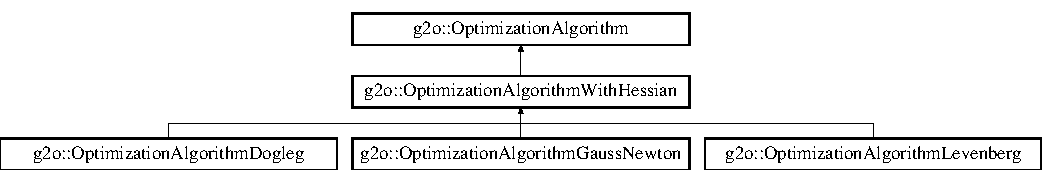
\includegraphics[height=2.285714cm]{classg2o_1_1_optimization_algorithm}
\end{center}
\end{figure}
\subsection*{Public Member Functions}
\begin{DoxyCompactItemize}
\item 
\mbox{\hyperlink{classg2o_1_1_optimization_algorithm_a205013e0425b7bbae01cd16caf500ebb}{Optimization\+Algorithm}} ()
\item 
virtual \mbox{\hyperlink{classg2o_1_1_optimization_algorithm_af2516e3d66596ec9c9dfdd08d48e90f9}{$\sim$\+Optimization\+Algorithm}} ()
\item 
virtual bool \mbox{\hyperlink{classg2o_1_1_optimization_algorithm_af5b54ea6d40a8ab4c16d448ba02a0c80}{init}} (bool online=false)=0
\item 
virtual Solver\+Result \mbox{\hyperlink{classg2o_1_1_optimization_algorithm_ab174deeeb2551ceaf715ea09f0f9c077}{solve}} (int iteration, bool online=false)=0
\item 
virtual bool \mbox{\hyperlink{classg2o_1_1_optimization_algorithm_a67b159f3a83471ba9ebcc0a9162a0e23}{compute\+Marginals}} (\mbox{\hyperlink{classg2o_1_1_sparse_block_matrix}{Sparse\+Block\+Matrix}}$<$ Matrix\+Xd $>$ \&spinv, const std\+::vector$<$ std\+::pair$<$ int, int $>$ $>$ \&block\+Indices)=0
\item 
virtual bool \mbox{\hyperlink{classg2o_1_1_optimization_algorithm_a350d9bb4ee701e40b75e67d26293a4bd}{update\+Structure}} (const std\+::vector$<$ \mbox{\hyperlink{classg2o_1_1_hyper_graph_1_1_vertex}{Hyper\+Graph\+::\+Vertex}} $\ast$$>$ \&vset, const \mbox{\hyperlink{classg2o_1_1_hyper_graph_a5e2970e236c0dcb4eff7c205d7b6b4ae}{Hyper\+Graph\+::\+Edge\+Set}} \&edges)=0
\item 
virtual void \mbox{\hyperlink{classg2o_1_1_optimization_algorithm_a6683d35e67402b50924bc4744b6e282a}{print\+Verbose}} (std\+::ostream \&os) const
\item 
const \mbox{\hyperlink{classg2o_1_1_sparse_optimizer}{Sparse\+Optimizer}} $\ast$ \mbox{\hyperlink{classg2o_1_1_optimization_algorithm_a040b3e3fd814d9928fa73ae6e98cedc5}{optimizer}} () const
\begin{DoxyCompactList}\small\item\em return the optimizer operating on \end{DoxyCompactList}\item 
\mbox{\hyperlink{classg2o_1_1_sparse_optimizer}{Sparse\+Optimizer}} $\ast$ \mbox{\hyperlink{classg2o_1_1_optimization_algorithm_ac6ca7a2adbd25615be78316bc811a315}{optimizer}} ()
\item 
void \mbox{\hyperlink{classg2o_1_1_optimization_algorithm_aff88a3dc8357c98712ff0047e601bd5e}{set\+Optimizer}} (\mbox{\hyperlink{classg2o_1_1_sparse_optimizer}{Sparse\+Optimizer}} $\ast$\mbox{\hyperlink{classg2o_1_1_optimization_algorithm_a040b3e3fd814d9928fa73ae6e98cedc5}{optimizer}})
\item 
const \mbox{\hyperlink{classg2o_1_1_property_map}{Property\+Map}} \& \mbox{\hyperlink{classg2o_1_1_optimization_algorithm_a0901951b7accc6744447c82dd043a07e}{properties}} () const
\begin{DoxyCompactList}\small\item\em return the properties of the solver \end{DoxyCompactList}\item 
bool \mbox{\hyperlink{classg2o_1_1_optimization_algorithm_aa05a6380f936c728a574c7c272bcc524}{update\+Properties\+From\+String}} (const std\+::string \&prop\+String)
\item 
void \mbox{\hyperlink{classg2o_1_1_optimization_algorithm_a830831cbe8357957188440c2f22bed91}{print\+Properties}} (std\+::ostream \&os) const
\end{DoxyCompactItemize}
\subsection*{Protected Attributes}
\begin{DoxyCompactItemize}
\item 
\mbox{\hyperlink{classg2o_1_1_sparse_optimizer}{Sparse\+Optimizer}} $\ast$ \mbox{\hyperlink{classg2o_1_1_optimization_algorithm_a6017c344be0d9f09d6674849849c6b60}{\+\_\+optimizer}}
\begin{DoxyCompactList}\small\item\em the optimizer the solver is working on \end{DoxyCompactList}\item 
\mbox{\hyperlink{classg2o_1_1_property_map}{Property\+Map}} \mbox{\hyperlink{classg2o_1_1_optimization_algorithm_ae37b494f69b483a3fcafa944e987e325}{\+\_\+properties}}
\begin{DoxyCompactList}\small\item\em the properties of your solver, use this to store the parameters of your solver \end{DoxyCompactList}\end{DoxyCompactItemize}
\subsection*{Private Member Functions}
\begin{DoxyCompactItemize}
\item 
\mbox{\hyperlink{classg2o_1_1_optimization_algorithm_af4bf8ed80e63df3f1a066e8b0098eb27}{Optimization\+Algorithm}} (const \mbox{\hyperlink{classg2o_1_1_optimization_algorithm}{Optimization\+Algorithm}} \&)
\item 
\mbox{\hyperlink{classg2o_1_1_optimization_algorithm}{Optimization\+Algorithm}} \& \mbox{\hyperlink{classg2o_1_1_optimization_algorithm_a74d342220fa0b1588e21f61959ff414a}{operator=}} (const \mbox{\hyperlink{classg2o_1_1_optimization_algorithm}{Optimization\+Algorithm}} \&)
\end{DoxyCompactItemize}


\subsection{Detailed Description}
Generic interface for a non-\/linear solver operating on a graph. 

\subsection{Constructor \& Destructor Documentation}
\mbox{\Hypertarget{classg2o_1_1_optimization_algorithm_a205013e0425b7bbae01cd16caf500ebb}\label{classg2o_1_1_optimization_algorithm_a205013e0425b7bbae01cd16caf500ebb}} 
\index{g2o\+::\+Optimization\+Algorithm@{g2o\+::\+Optimization\+Algorithm}!Optimization\+Algorithm@{Optimization\+Algorithm}}
\index{Optimization\+Algorithm@{Optimization\+Algorithm}!g2o\+::\+Optimization\+Algorithm@{g2o\+::\+Optimization\+Algorithm}}
\subsubsection{\texorpdfstring{Optimization\+Algorithm()}{OptimizationAlgorithm()}\hspace{0.1cm}{\footnotesize\ttfamily [1/2]}}
{\footnotesize\ttfamily g2o\+::\+Optimization\+Algorithm\+::\+Optimization\+Algorithm (\begin{DoxyParamCaption}{ }\end{DoxyParamCaption})}

\mbox{\Hypertarget{classg2o_1_1_optimization_algorithm_af2516e3d66596ec9c9dfdd08d48e90f9}\label{classg2o_1_1_optimization_algorithm_af2516e3d66596ec9c9dfdd08d48e90f9}} 
\index{g2o\+::\+Optimization\+Algorithm@{g2o\+::\+Optimization\+Algorithm}!````~Optimization\+Algorithm@{$\sim$\+Optimization\+Algorithm}}
\index{````~Optimization\+Algorithm@{$\sim$\+Optimization\+Algorithm}!g2o\+::\+Optimization\+Algorithm@{g2o\+::\+Optimization\+Algorithm}}
\subsubsection{\texorpdfstring{$\sim$\+Optimization\+Algorithm()}{~OptimizationAlgorithm()}}
{\footnotesize\ttfamily g2o\+::\+Optimization\+Algorithm\+::$\sim$\+Optimization\+Algorithm (\begin{DoxyParamCaption}{ }\end{DoxyParamCaption})\hspace{0.3cm}{\ttfamily [virtual]}}

\mbox{\Hypertarget{classg2o_1_1_optimization_algorithm_af4bf8ed80e63df3f1a066e8b0098eb27}\label{classg2o_1_1_optimization_algorithm_af4bf8ed80e63df3f1a066e8b0098eb27}} 
\index{g2o\+::\+Optimization\+Algorithm@{g2o\+::\+Optimization\+Algorithm}!Optimization\+Algorithm@{Optimization\+Algorithm}}
\index{Optimization\+Algorithm@{Optimization\+Algorithm}!g2o\+::\+Optimization\+Algorithm@{g2o\+::\+Optimization\+Algorithm}}
\subsubsection{\texorpdfstring{Optimization\+Algorithm()}{OptimizationAlgorithm()}\hspace{0.1cm}{\footnotesize\ttfamily [2/2]}}
{\footnotesize\ttfamily g2o\+::\+Optimization\+Algorithm\+::\+Optimization\+Algorithm (\begin{DoxyParamCaption}\item[{const \mbox{\hyperlink{classg2o_1_1_optimization_algorithm}{Optimization\+Algorithm}} \&}]{ }\end{DoxyParamCaption})\hspace{0.3cm}{\ttfamily [inline]}, {\ttfamily [private]}}



\subsection{Member Function Documentation}
\mbox{\Hypertarget{classg2o_1_1_optimization_algorithm_a67b159f3a83471ba9ebcc0a9162a0e23}\label{classg2o_1_1_optimization_algorithm_a67b159f3a83471ba9ebcc0a9162a0e23}} 
\index{g2o\+::\+Optimization\+Algorithm@{g2o\+::\+Optimization\+Algorithm}!compute\+Marginals@{compute\+Marginals}}
\index{compute\+Marginals@{compute\+Marginals}!g2o\+::\+Optimization\+Algorithm@{g2o\+::\+Optimization\+Algorithm}}
\subsubsection{\texorpdfstring{compute\+Marginals()}{computeMarginals()}}
{\footnotesize\ttfamily virtual bool g2o\+::\+Optimization\+Algorithm\+::compute\+Marginals (\begin{DoxyParamCaption}\item[{\mbox{\hyperlink{classg2o_1_1_sparse_block_matrix}{Sparse\+Block\+Matrix}}$<$ Matrix\+Xd $>$ \&}]{spinv,  }\item[{const std\+::vector$<$ std\+::pair$<$ int, int $>$ $>$ \&}]{block\+Indices }\end{DoxyParamCaption})\hspace{0.3cm}{\ttfamily [pure virtual]}}

computes the block diagonal elements of the pattern specified in the input and stores them in given \mbox{\hyperlink{classg2o_1_1_sparse_block_matrix}{Sparse\+Block\+Matrix}}. If your solver does not support computing the marginals, return false. 

Implemented in \mbox{\hyperlink{classg2o_1_1_optimization_algorithm_with_hessian_af1959727df2b7cf233a171cfed246e9a}{g2o\+::\+Optimization\+Algorithm\+With\+Hessian}}.

\mbox{\Hypertarget{classg2o_1_1_optimization_algorithm_af5b54ea6d40a8ab4c16d448ba02a0c80}\label{classg2o_1_1_optimization_algorithm_af5b54ea6d40a8ab4c16d448ba02a0c80}} 
\index{g2o\+::\+Optimization\+Algorithm@{g2o\+::\+Optimization\+Algorithm}!init@{init}}
\index{init@{init}!g2o\+::\+Optimization\+Algorithm@{g2o\+::\+Optimization\+Algorithm}}
\subsubsection{\texorpdfstring{init()}{init()}}
{\footnotesize\ttfamily virtual bool g2o\+::\+Optimization\+Algorithm\+::init (\begin{DoxyParamCaption}\item[{bool}]{online = {\ttfamily false} }\end{DoxyParamCaption})\hspace{0.3cm}{\ttfamily [pure virtual]}}

initialize the solver, called once before the first call to \mbox{\hyperlink{classg2o_1_1_optimization_algorithm_ab174deeeb2551ceaf715ea09f0f9c077}{solve()}} 

Implemented in \mbox{\hyperlink{classg2o_1_1_optimization_algorithm_with_hessian_ae067a9c2961718dc8a37e3b8478b6d01}{g2o\+::\+Optimization\+Algorithm\+With\+Hessian}}.

\mbox{\Hypertarget{classg2o_1_1_optimization_algorithm_a74d342220fa0b1588e21f61959ff414a}\label{classg2o_1_1_optimization_algorithm_a74d342220fa0b1588e21f61959ff414a}} 
\index{g2o\+::\+Optimization\+Algorithm@{g2o\+::\+Optimization\+Algorithm}!operator=@{operator=}}
\index{operator=@{operator=}!g2o\+::\+Optimization\+Algorithm@{g2o\+::\+Optimization\+Algorithm}}
\subsubsection{\texorpdfstring{operator=()}{operator=()}}
{\footnotesize\ttfamily \mbox{\hyperlink{classg2o_1_1_optimization_algorithm}{Optimization\+Algorithm}}\& g2o\+::\+Optimization\+Algorithm\+::operator= (\begin{DoxyParamCaption}\item[{const \mbox{\hyperlink{classg2o_1_1_optimization_algorithm}{Optimization\+Algorithm}} \&}]{ }\end{DoxyParamCaption})\hspace{0.3cm}{\ttfamily [inline]}, {\ttfamily [private]}}

\mbox{\Hypertarget{classg2o_1_1_optimization_algorithm_a040b3e3fd814d9928fa73ae6e98cedc5}\label{classg2o_1_1_optimization_algorithm_a040b3e3fd814d9928fa73ae6e98cedc5}} 
\index{g2o\+::\+Optimization\+Algorithm@{g2o\+::\+Optimization\+Algorithm}!optimizer@{optimizer}}
\index{optimizer@{optimizer}!g2o\+::\+Optimization\+Algorithm@{g2o\+::\+Optimization\+Algorithm}}
\subsubsection{\texorpdfstring{optimizer()}{optimizer()}\hspace{0.1cm}{\footnotesize\ttfamily [1/2]}}
{\footnotesize\ttfamily const \mbox{\hyperlink{classg2o_1_1_sparse_optimizer}{Sparse\+Optimizer}}$\ast$ g2o\+::\+Optimization\+Algorithm\+::optimizer (\begin{DoxyParamCaption}{ }\end{DoxyParamCaption}) const\hspace{0.3cm}{\ttfamily [inline]}}



return the optimizer operating on 

\mbox{\Hypertarget{classg2o_1_1_optimization_algorithm_ac6ca7a2adbd25615be78316bc811a315}\label{classg2o_1_1_optimization_algorithm_ac6ca7a2adbd25615be78316bc811a315}} 
\index{g2o\+::\+Optimization\+Algorithm@{g2o\+::\+Optimization\+Algorithm}!optimizer@{optimizer}}
\index{optimizer@{optimizer}!g2o\+::\+Optimization\+Algorithm@{g2o\+::\+Optimization\+Algorithm}}
\subsubsection{\texorpdfstring{optimizer()}{optimizer()}\hspace{0.1cm}{\footnotesize\ttfamily [2/2]}}
{\footnotesize\ttfamily \mbox{\hyperlink{classg2o_1_1_sparse_optimizer}{Sparse\+Optimizer}}$\ast$ g2o\+::\+Optimization\+Algorithm\+::optimizer (\begin{DoxyParamCaption}{ }\end{DoxyParamCaption})\hspace{0.3cm}{\ttfamily [inline]}}

\mbox{\Hypertarget{classg2o_1_1_optimization_algorithm_a830831cbe8357957188440c2f22bed91}\label{classg2o_1_1_optimization_algorithm_a830831cbe8357957188440c2f22bed91}} 
\index{g2o\+::\+Optimization\+Algorithm@{g2o\+::\+Optimization\+Algorithm}!print\+Properties@{print\+Properties}}
\index{print\+Properties@{print\+Properties}!g2o\+::\+Optimization\+Algorithm@{g2o\+::\+Optimization\+Algorithm}}
\subsubsection{\texorpdfstring{print\+Properties()}{printProperties()}}
{\footnotesize\ttfamily void g2o\+::\+Optimization\+Algorithm\+::print\+Properties (\begin{DoxyParamCaption}\item[{std\+::ostream \&}]{os }\end{DoxyParamCaption}) const}

print the properties to a stream in a human readable fashion \mbox{\Hypertarget{classg2o_1_1_optimization_algorithm_a6683d35e67402b50924bc4744b6e282a}\label{classg2o_1_1_optimization_algorithm_a6683d35e67402b50924bc4744b6e282a}} 
\index{g2o\+::\+Optimization\+Algorithm@{g2o\+::\+Optimization\+Algorithm}!print\+Verbose@{print\+Verbose}}
\index{print\+Verbose@{print\+Verbose}!g2o\+::\+Optimization\+Algorithm@{g2o\+::\+Optimization\+Algorithm}}
\subsubsection{\texorpdfstring{print\+Verbose()}{printVerbose()}}
{\footnotesize\ttfamily virtual void g2o\+::\+Optimization\+Algorithm\+::print\+Verbose (\begin{DoxyParamCaption}\item[{std\+::ostream \&}]{os }\end{DoxyParamCaption}) const\hspace{0.3cm}{\ttfamily [inline]}, {\ttfamily [virtual]}}

called by the optimizer if verbose. re-\/implement, if you want to print something 

Reimplemented in \mbox{\hyperlink{classg2o_1_1_optimization_algorithm_dogleg_a48f424443a7b2b6e8c532204cd7334cd}{g2o\+::\+Optimization\+Algorithm\+Dogleg}}, \mbox{\hyperlink{classg2o_1_1_optimization_algorithm_levenberg_a67308ead9762f478e29385229ea4b138}{g2o\+::\+Optimization\+Algorithm\+Levenberg}}, and \mbox{\hyperlink{classg2o_1_1_optimization_algorithm_gauss_newton_aff4c1b6a9f8a2e5c6777cfef9d4a18ba}{g2o\+::\+Optimization\+Algorithm\+Gauss\+Newton}}.

\mbox{\Hypertarget{classg2o_1_1_optimization_algorithm_a0901951b7accc6744447c82dd043a07e}\label{classg2o_1_1_optimization_algorithm_a0901951b7accc6744447c82dd043a07e}} 
\index{g2o\+::\+Optimization\+Algorithm@{g2o\+::\+Optimization\+Algorithm}!properties@{properties}}
\index{properties@{properties}!g2o\+::\+Optimization\+Algorithm@{g2o\+::\+Optimization\+Algorithm}}
\subsubsection{\texorpdfstring{properties()}{properties()}}
{\footnotesize\ttfamily const \mbox{\hyperlink{classg2o_1_1_property_map}{Property\+Map}}\& g2o\+::\+Optimization\+Algorithm\+::properties (\begin{DoxyParamCaption}{ }\end{DoxyParamCaption}) const\hspace{0.3cm}{\ttfamily [inline]}}



return the properties of the solver 

\mbox{\Hypertarget{classg2o_1_1_optimization_algorithm_aff88a3dc8357c98712ff0047e601bd5e}\label{classg2o_1_1_optimization_algorithm_aff88a3dc8357c98712ff0047e601bd5e}} 
\index{g2o\+::\+Optimization\+Algorithm@{g2o\+::\+Optimization\+Algorithm}!set\+Optimizer@{set\+Optimizer}}
\index{set\+Optimizer@{set\+Optimizer}!g2o\+::\+Optimization\+Algorithm@{g2o\+::\+Optimization\+Algorithm}}
\subsubsection{\texorpdfstring{set\+Optimizer()}{setOptimizer()}}
{\footnotesize\ttfamily void g2o\+::\+Optimization\+Algorithm\+::set\+Optimizer (\begin{DoxyParamCaption}\item[{\mbox{\hyperlink{classg2o_1_1_sparse_optimizer}{Sparse\+Optimizer}} $\ast$}]{optimizer }\end{DoxyParamCaption})}

specify on which optimizer the solver should work on \mbox{\Hypertarget{classg2o_1_1_optimization_algorithm_ab174deeeb2551ceaf715ea09f0f9c077}\label{classg2o_1_1_optimization_algorithm_ab174deeeb2551ceaf715ea09f0f9c077}} 
\index{g2o\+::\+Optimization\+Algorithm@{g2o\+::\+Optimization\+Algorithm}!solve@{solve}}
\index{solve@{solve}!g2o\+::\+Optimization\+Algorithm@{g2o\+::\+Optimization\+Algorithm}}
\subsubsection{\texorpdfstring{solve()}{solve()}}
{\footnotesize\ttfamily virtual Solver\+Result g2o\+::\+Optimization\+Algorithm\+::solve (\begin{DoxyParamCaption}\item[{int}]{iteration,  }\item[{bool}]{online = {\ttfamily false} }\end{DoxyParamCaption})\hspace{0.3cm}{\ttfamily [pure virtual]}}

Solve one iteration. The \mbox{\hyperlink{classg2o_1_1_sparse_optimizer}{Sparse\+Optimizer}} running on-\/top will call this for the given number of iterations. 
\begin{DoxyParams}{Parameters}
{\em iteration} & indicates the current iteration \\
\hline
\end{DoxyParams}


Implemented in \mbox{\hyperlink{classg2o_1_1_optimization_algorithm_dogleg_ace62fd809c18655bd7ff104285748610}{g2o\+::\+Optimization\+Algorithm\+Dogleg}}, \mbox{\hyperlink{classg2o_1_1_optimization_algorithm_levenberg_a7140fa989b54eac4e09ba17829dcada0}{g2o\+::\+Optimization\+Algorithm\+Levenberg}}, and \mbox{\hyperlink{classg2o_1_1_optimization_algorithm_gauss_newton_aba0b67eecaca01c576de7e605e5af5f1}{g2o\+::\+Optimization\+Algorithm\+Gauss\+Newton}}.

\mbox{\Hypertarget{classg2o_1_1_optimization_algorithm_aa05a6380f936c728a574c7c272bcc524}\label{classg2o_1_1_optimization_algorithm_aa05a6380f936c728a574c7c272bcc524}} 
\index{g2o\+::\+Optimization\+Algorithm@{g2o\+::\+Optimization\+Algorithm}!update\+Properties\+From\+String@{update\+Properties\+From\+String}}
\index{update\+Properties\+From\+String@{update\+Properties\+From\+String}!g2o\+::\+Optimization\+Algorithm@{g2o\+::\+Optimization\+Algorithm}}
\subsubsection{\texorpdfstring{update\+Properties\+From\+String()}{updatePropertiesFromString()}}
{\footnotesize\ttfamily bool g2o\+::\+Optimization\+Algorithm\+::update\+Properties\+From\+String (\begin{DoxyParamCaption}\item[{const std\+::string \&}]{prop\+String }\end{DoxyParamCaption})}

update the properties from a string, see \mbox{\hyperlink{classg2o_1_1_property_map_a0407e6a72afafd608f13cfdffc6ffc06}{Property\+Map\+::update\+Map\+From\+String()}} \mbox{\Hypertarget{classg2o_1_1_optimization_algorithm_a350d9bb4ee701e40b75e67d26293a4bd}\label{classg2o_1_1_optimization_algorithm_a350d9bb4ee701e40b75e67d26293a4bd}} 
\index{g2o\+::\+Optimization\+Algorithm@{g2o\+::\+Optimization\+Algorithm}!update\+Structure@{update\+Structure}}
\index{update\+Structure@{update\+Structure}!g2o\+::\+Optimization\+Algorithm@{g2o\+::\+Optimization\+Algorithm}}
\subsubsection{\texorpdfstring{update\+Structure()}{updateStructure()}}
{\footnotesize\ttfamily virtual bool g2o\+::\+Optimization\+Algorithm\+::update\+Structure (\begin{DoxyParamCaption}\item[{const std\+::vector$<$ \mbox{\hyperlink{classg2o_1_1_hyper_graph_1_1_vertex}{Hyper\+Graph\+::\+Vertex}} $\ast$$>$ \&}]{vset,  }\item[{const \mbox{\hyperlink{classg2o_1_1_hyper_graph_a5e2970e236c0dcb4eff7c205d7b6b4ae}{Hyper\+Graph\+::\+Edge\+Set}} \&}]{edges }\end{DoxyParamCaption})\hspace{0.3cm}{\ttfamily [pure virtual]}}

update the structures for online processing 

Implemented in \mbox{\hyperlink{classg2o_1_1_optimization_algorithm_with_hessian_adadb23f135e037ce760f4415a0f26269}{g2o\+::\+Optimization\+Algorithm\+With\+Hessian}}.



\subsection{Member Data Documentation}
\mbox{\Hypertarget{classg2o_1_1_optimization_algorithm_a6017c344be0d9f09d6674849849c6b60}\label{classg2o_1_1_optimization_algorithm_a6017c344be0d9f09d6674849849c6b60}} 
\index{g2o\+::\+Optimization\+Algorithm@{g2o\+::\+Optimization\+Algorithm}!\+\_\+optimizer@{\+\_\+optimizer}}
\index{\+\_\+optimizer@{\+\_\+optimizer}!g2o\+::\+Optimization\+Algorithm@{g2o\+::\+Optimization\+Algorithm}}
\subsubsection{\texorpdfstring{\+\_\+optimizer}{\_optimizer}}
{\footnotesize\ttfamily \mbox{\hyperlink{classg2o_1_1_sparse_optimizer}{Sparse\+Optimizer}}$\ast$ g2o\+::\+Optimization\+Algorithm\+::\+\_\+optimizer\hspace{0.3cm}{\ttfamily [protected]}}



the optimizer the solver is working on 

\mbox{\Hypertarget{classg2o_1_1_optimization_algorithm_ae37b494f69b483a3fcafa944e987e325}\label{classg2o_1_1_optimization_algorithm_ae37b494f69b483a3fcafa944e987e325}} 
\index{g2o\+::\+Optimization\+Algorithm@{g2o\+::\+Optimization\+Algorithm}!\+\_\+properties@{\+\_\+properties}}
\index{\+\_\+properties@{\+\_\+properties}!g2o\+::\+Optimization\+Algorithm@{g2o\+::\+Optimization\+Algorithm}}
\subsubsection{\texorpdfstring{\+\_\+properties}{\_properties}}
{\footnotesize\ttfamily \mbox{\hyperlink{classg2o_1_1_property_map}{Property\+Map}} g2o\+::\+Optimization\+Algorithm\+::\+\_\+properties\hspace{0.3cm}{\ttfamily [protected]}}



the properties of your solver, use this to store the parameters of your solver 



The documentation for this class was generated from the following files\+:\begin{DoxyCompactItemize}
\item 
D\+:/github/\+V\+S\+L\+A\+M/\+O\+R\+B\+S\+L\+A\+M2/\+O\+R\+B-\/\+S\+L\+A\+M2-\/master/\+Thirdparty/g2o/g2o/core/\mbox{\hyperlink{optimization__algorithm_8h}{optimization\+\_\+algorithm.\+h}}\item 
D\+:/github/\+V\+S\+L\+A\+M/\+O\+R\+B\+S\+L\+A\+M2/\+O\+R\+B-\/\+S\+L\+A\+M2-\/master/\+Thirdparty/g2o/g2o/core/\mbox{\hyperlink{optimization__algorithm_8cpp}{optimization\+\_\+algorithm.\+cpp}}\end{DoxyCompactItemize}

\hypertarget{classg2o_1_1_optimization_algorithm_dogleg}{}\section{g2o\+:\+:Optimization\+Algorithm\+Dogleg Class Reference}
\label{classg2o_1_1_optimization_algorithm_dogleg}\index{g2o\+::\+Optimization\+Algorithm\+Dogleg@{g2o\+::\+Optimization\+Algorithm\+Dogleg}}


Implementation of Powell\textquotesingle{}s Dogleg Algorithm.  




{\ttfamily \#include $<$optimization\+\_\+algorithm\+\_\+dogleg.\+h$>$}

Inheritance diagram for g2o\+:\+:Optimization\+Algorithm\+Dogleg\+:\begin{figure}[H]
\begin{center}
\leavevmode
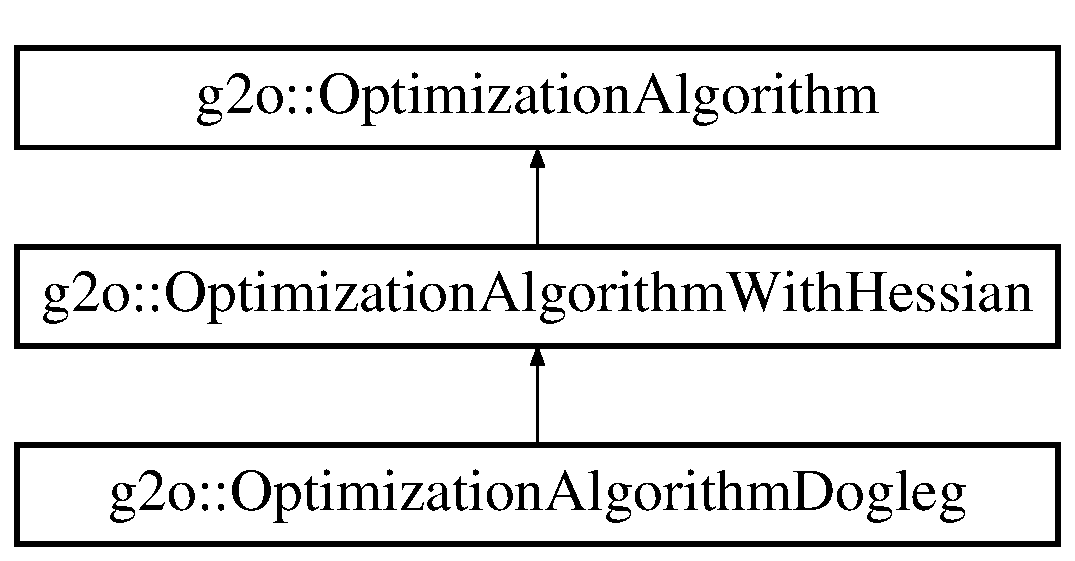
\includegraphics[height=3.000000cm]{classg2o_1_1_optimization_algorithm_dogleg}
\end{center}
\end{figure}
\subsection*{Public Types}
\begin{DoxyCompactItemize}
\item 
enum \{ \mbox{\hyperlink{classg2o_1_1_optimization_algorithm_dogleg_a431b0b88011685955381bdeb68bb5390ae098265840915f1d6877b4e27fbec1d8}{S\+T\+E\+P\+\_\+\+U\+N\+D\+E\+F\+I\+N\+ED}}, 
\mbox{\hyperlink{classg2o_1_1_optimization_algorithm_dogleg_a431b0b88011685955381bdeb68bb5390a02cb99985ea3c35b57591e6c55f5e037}{S\+T\+E\+P\+\_\+\+SD}}, 
\mbox{\hyperlink{classg2o_1_1_optimization_algorithm_dogleg_a431b0b88011685955381bdeb68bb5390a27f521fdfb791c330af5e59dd989507d}{S\+T\+E\+P\+\_\+\+GN}}, 
\mbox{\hyperlink{classg2o_1_1_optimization_algorithm_dogleg_a431b0b88011685955381bdeb68bb5390a1bc0276b59002bc8892ea9fc39348d1d}{S\+T\+E\+P\+\_\+\+DL}}
 \}
\begin{DoxyCompactList}\small\item\em type of the step to take \end{DoxyCompactList}\end{DoxyCompactItemize}
\subsection*{Public Member Functions}
\begin{DoxyCompactItemize}
\item 
\mbox{\hyperlink{classg2o_1_1_optimization_algorithm_dogleg_ab332f8fb049d1a1fecba18105083052a}{Optimization\+Algorithm\+Dogleg}} (\mbox{\hyperlink{classg2o_1_1_block_solver_base}{Block\+Solver\+Base}} $\ast$\mbox{\hyperlink{classg2o_1_1_optimization_algorithm_with_hessian_a85473a4073c76b1a52cf9cf175e31c45}{solver}})
\item 
virtual \mbox{\hyperlink{classg2o_1_1_optimization_algorithm_dogleg_ac5ebd46eeca170f6a923c75556504d2b}{$\sim$\+Optimization\+Algorithm\+Dogleg}} ()
\item 
virtual Solver\+Result \mbox{\hyperlink{classg2o_1_1_optimization_algorithm_dogleg_ace62fd809c18655bd7ff104285748610}{solve}} (int iteration, bool online=false)
\item 
virtual void \mbox{\hyperlink{classg2o_1_1_optimization_algorithm_dogleg_a48f424443a7b2b6e8c532204cd7334cd}{print\+Verbose}} (std\+::ostream \&os) const
\item 
int \mbox{\hyperlink{classg2o_1_1_optimization_algorithm_dogleg_a0ca98964e7bcde0c893eb9d720a26fd1}{last\+Step}} () const
\begin{DoxyCompactList}\small\item\em return the type of the last step taken by the algorithm \end{DoxyCompactList}\item 
double \mbox{\hyperlink{classg2o_1_1_optimization_algorithm_dogleg_a3c6fdb2f8296330fd754d635a67b3696}{trust\+Region}} () const
\begin{DoxyCompactList}\small\item\em return the diameter of the trust region \end{DoxyCompactList}\end{DoxyCompactItemize}
\subsection*{Static Public Member Functions}
\begin{DoxyCompactItemize}
\item 
static const char $\ast$ \mbox{\hyperlink{classg2o_1_1_optimization_algorithm_dogleg_a65f193c6451ffcd2bd6fd8f8d19e2a12}{step\+Type2\+Str}} (int step\+Type)
\begin{DoxyCompactList}\small\item\em convert the type into an integer \end{DoxyCompactList}\end{DoxyCompactItemize}
\subsection*{Protected Attributes}
\begin{DoxyCompactItemize}
\item 
\mbox{\hyperlink{classg2o_1_1_property}{Property}}$<$ int $>$ $\ast$ \mbox{\hyperlink{classg2o_1_1_optimization_algorithm_dogleg_a5993c68e69cd037b1420b4addf9f7e50}{\+\_\+max\+Trials\+After\+Failure}}
\item 
\mbox{\hyperlink{classg2o_1_1_property}{Property}}$<$ double $>$ $\ast$ \mbox{\hyperlink{classg2o_1_1_optimization_algorithm_dogleg_ae77ffaea89872affeb61f122f20efeb9}{\+\_\+user\+Delta\+Init}}
\item 
\mbox{\hyperlink{classg2o_1_1_property}{Property}}$<$ double $>$ $\ast$ \mbox{\hyperlink{classg2o_1_1_optimization_algorithm_dogleg_a3a94c7696f07e3def38ec96a1979babd}{\+\_\+initial\+Lambda}}
\item 
\mbox{\hyperlink{classg2o_1_1_property}{Property}}$<$ double $>$ $\ast$ \mbox{\hyperlink{classg2o_1_1_optimization_algorithm_dogleg_a6855a511dc998efef7eaa0ef99e1b814}{\+\_\+lamdba\+Factor}}
\item 
Eigen\+::\+Vector\+Xd \mbox{\hyperlink{classg2o_1_1_optimization_algorithm_dogleg_a8f4ee408fbf3999063d094cf61e852b7}{\+\_\+hsd}}
\begin{DoxyCompactList}\small\item\em steepest decent step \end{DoxyCompactList}\item 
Eigen\+::\+Vector\+Xd \mbox{\hyperlink{classg2o_1_1_optimization_algorithm_dogleg_aaf433c824153a7bd76b27690eb53113b}{\+\_\+hdl}}
\begin{DoxyCompactList}\small\item\em final dogleg step \end{DoxyCompactList}\item 
Eigen\+::\+Vector\+Xd \mbox{\hyperlink{classg2o_1_1_optimization_algorithm_dogleg_a225092fe67ce75eb64011c1f45d8d936}{\+\_\+aux\+Vector}}
\begin{DoxyCompactList}\small\item\em auxilary vector used to perform multiplications or other stuff \end{DoxyCompactList}\item 
double \mbox{\hyperlink{classg2o_1_1_optimization_algorithm_dogleg_aacc051a6740fc6017dac7c424dc7df3d}{\+\_\+current\+Lambda}}
\begin{DoxyCompactList}\small\item\em the damping factor to force positive definite matrix \end{DoxyCompactList}\item 
double \mbox{\hyperlink{classg2o_1_1_optimization_algorithm_dogleg_a3484b12efddd9fc0051100634effecd6}{\+\_\+delta}}
\begin{DoxyCompactList}\small\item\em trust region \end{DoxyCompactList}\item 
int \mbox{\hyperlink{classg2o_1_1_optimization_algorithm_dogleg_a3bf898af0087c0ed8287d0cd13e4c943}{\+\_\+last\+Step}}
\begin{DoxyCompactList}\small\item\em type of the step taken by the algorithm \end{DoxyCompactList}\item 
bool \mbox{\hyperlink{classg2o_1_1_optimization_algorithm_dogleg_af921ebbebaf059f73e410fc751616ec2}{\+\_\+was\+P\+D\+In\+All\+Iterations}}
\begin{DoxyCompactList}\small\item\em the matrix we solve was positive definite in all iterations -\/$>$ if not apply damping \end{DoxyCompactList}\item 
int \mbox{\hyperlink{classg2o_1_1_optimization_algorithm_dogleg_aeab37f3f587dc8b37b5a42d36fd8217c}{\+\_\+last\+Num\+Tries}}
\end{DoxyCompactItemize}


\subsection{Detailed Description}
Implementation of Powell\textquotesingle{}s Dogleg Algorithm. 

\subsection{Member Enumeration Documentation}
\mbox{\Hypertarget{classg2o_1_1_optimization_algorithm_dogleg_a431b0b88011685955381bdeb68bb5390}\label{classg2o_1_1_optimization_algorithm_dogleg_a431b0b88011685955381bdeb68bb5390}} 
\subsubsection{\texorpdfstring{anonymous enum}{anonymous enum}}
{\footnotesize\ttfamily anonymous enum}



type of the step to take 

\begin{DoxyEnumFields}{Enumerator}
\raisebox{\heightof{T}}[0pt][0pt]{\index{S\+T\+E\+P\+\_\+\+U\+N\+D\+E\+F\+I\+N\+ED@{S\+T\+E\+P\+\_\+\+U\+N\+D\+E\+F\+I\+N\+ED}!g2o\+::\+Optimization\+Algorithm\+Dogleg@{g2o\+::\+Optimization\+Algorithm\+Dogleg}}\index{g2o\+::\+Optimization\+Algorithm\+Dogleg@{g2o\+::\+Optimization\+Algorithm\+Dogleg}!S\+T\+E\+P\+\_\+\+U\+N\+D\+E\+F\+I\+N\+ED@{S\+T\+E\+P\+\_\+\+U\+N\+D\+E\+F\+I\+N\+ED}}}\mbox{\Hypertarget{classg2o_1_1_optimization_algorithm_dogleg_a431b0b88011685955381bdeb68bb5390ae098265840915f1d6877b4e27fbec1d8}\label{classg2o_1_1_optimization_algorithm_dogleg_a431b0b88011685955381bdeb68bb5390ae098265840915f1d6877b4e27fbec1d8}} 
S\+T\+E\+P\+\_\+\+U\+N\+D\+E\+F\+I\+N\+ED&\\
\hline

\raisebox{\heightof{T}}[0pt][0pt]{\index{S\+T\+E\+P\+\_\+\+SD@{S\+T\+E\+P\+\_\+\+SD}!g2o\+::\+Optimization\+Algorithm\+Dogleg@{g2o\+::\+Optimization\+Algorithm\+Dogleg}}\index{g2o\+::\+Optimization\+Algorithm\+Dogleg@{g2o\+::\+Optimization\+Algorithm\+Dogleg}!S\+T\+E\+P\+\_\+\+SD@{S\+T\+E\+P\+\_\+\+SD}}}\mbox{\Hypertarget{classg2o_1_1_optimization_algorithm_dogleg_a431b0b88011685955381bdeb68bb5390a02cb99985ea3c35b57591e6c55f5e037}\label{classg2o_1_1_optimization_algorithm_dogleg_a431b0b88011685955381bdeb68bb5390a02cb99985ea3c35b57591e6c55f5e037}} 
S\+T\+E\+P\+\_\+\+SD&\\
\hline

\raisebox{\heightof{T}}[0pt][0pt]{\index{S\+T\+E\+P\+\_\+\+GN@{S\+T\+E\+P\+\_\+\+GN}!g2o\+::\+Optimization\+Algorithm\+Dogleg@{g2o\+::\+Optimization\+Algorithm\+Dogleg}}\index{g2o\+::\+Optimization\+Algorithm\+Dogleg@{g2o\+::\+Optimization\+Algorithm\+Dogleg}!S\+T\+E\+P\+\_\+\+GN@{S\+T\+E\+P\+\_\+\+GN}}}\mbox{\Hypertarget{classg2o_1_1_optimization_algorithm_dogleg_a431b0b88011685955381bdeb68bb5390a27f521fdfb791c330af5e59dd989507d}\label{classg2o_1_1_optimization_algorithm_dogleg_a431b0b88011685955381bdeb68bb5390a27f521fdfb791c330af5e59dd989507d}} 
S\+T\+E\+P\+\_\+\+GN&\\
\hline

\raisebox{\heightof{T}}[0pt][0pt]{\index{S\+T\+E\+P\+\_\+\+DL@{S\+T\+E\+P\+\_\+\+DL}!g2o\+::\+Optimization\+Algorithm\+Dogleg@{g2o\+::\+Optimization\+Algorithm\+Dogleg}}\index{g2o\+::\+Optimization\+Algorithm\+Dogleg@{g2o\+::\+Optimization\+Algorithm\+Dogleg}!S\+T\+E\+P\+\_\+\+DL@{S\+T\+E\+P\+\_\+\+DL}}}\mbox{\Hypertarget{classg2o_1_1_optimization_algorithm_dogleg_a431b0b88011685955381bdeb68bb5390a1bc0276b59002bc8892ea9fc39348d1d}\label{classg2o_1_1_optimization_algorithm_dogleg_a431b0b88011685955381bdeb68bb5390a1bc0276b59002bc8892ea9fc39348d1d}} 
S\+T\+E\+P\+\_\+\+DL&\\
\hline

\end{DoxyEnumFields}


\subsection{Constructor \& Destructor Documentation}
\mbox{\Hypertarget{classg2o_1_1_optimization_algorithm_dogleg_ab332f8fb049d1a1fecba18105083052a}\label{classg2o_1_1_optimization_algorithm_dogleg_ab332f8fb049d1a1fecba18105083052a}} 
\index{g2o\+::\+Optimization\+Algorithm\+Dogleg@{g2o\+::\+Optimization\+Algorithm\+Dogleg}!Optimization\+Algorithm\+Dogleg@{Optimization\+Algorithm\+Dogleg}}
\index{Optimization\+Algorithm\+Dogleg@{Optimization\+Algorithm\+Dogleg}!g2o\+::\+Optimization\+Algorithm\+Dogleg@{g2o\+::\+Optimization\+Algorithm\+Dogleg}}
\subsubsection{\texorpdfstring{Optimization\+Algorithm\+Dogleg()}{OptimizationAlgorithmDogleg()}}
{\footnotesize\ttfamily g2o\+::\+Optimization\+Algorithm\+Dogleg\+::\+Optimization\+Algorithm\+Dogleg (\begin{DoxyParamCaption}\item[{\mbox{\hyperlink{classg2o_1_1_block_solver_base}{Block\+Solver\+Base}} $\ast$}]{solver }\end{DoxyParamCaption})\hspace{0.3cm}{\ttfamily [explicit]}}

construct the Dogleg algorithm, which will use the given \mbox{\hyperlink{classg2o_1_1_solver}{Solver}} for solving the linearized system. \mbox{\Hypertarget{classg2o_1_1_optimization_algorithm_dogleg_ac5ebd46eeca170f6a923c75556504d2b}\label{classg2o_1_1_optimization_algorithm_dogleg_ac5ebd46eeca170f6a923c75556504d2b}} 
\index{g2o\+::\+Optimization\+Algorithm\+Dogleg@{g2o\+::\+Optimization\+Algorithm\+Dogleg}!````~Optimization\+Algorithm\+Dogleg@{$\sim$\+Optimization\+Algorithm\+Dogleg}}
\index{````~Optimization\+Algorithm\+Dogleg@{$\sim$\+Optimization\+Algorithm\+Dogleg}!g2o\+::\+Optimization\+Algorithm\+Dogleg@{g2o\+::\+Optimization\+Algorithm\+Dogleg}}
\subsubsection{\texorpdfstring{$\sim$\+Optimization\+Algorithm\+Dogleg()}{~OptimizationAlgorithmDogleg()}}
{\footnotesize\ttfamily g2o\+::\+Optimization\+Algorithm\+Dogleg\+::$\sim$\+Optimization\+Algorithm\+Dogleg (\begin{DoxyParamCaption}{ }\end{DoxyParamCaption})\hspace{0.3cm}{\ttfamily [virtual]}}



\subsection{Member Function Documentation}
\mbox{\Hypertarget{classg2o_1_1_optimization_algorithm_dogleg_a0ca98964e7bcde0c893eb9d720a26fd1}\label{classg2o_1_1_optimization_algorithm_dogleg_a0ca98964e7bcde0c893eb9d720a26fd1}} 
\index{g2o\+::\+Optimization\+Algorithm\+Dogleg@{g2o\+::\+Optimization\+Algorithm\+Dogleg}!last\+Step@{last\+Step}}
\index{last\+Step@{last\+Step}!g2o\+::\+Optimization\+Algorithm\+Dogleg@{g2o\+::\+Optimization\+Algorithm\+Dogleg}}
\subsubsection{\texorpdfstring{last\+Step()}{lastStep()}}
{\footnotesize\ttfamily int g2o\+::\+Optimization\+Algorithm\+Dogleg\+::last\+Step (\begin{DoxyParamCaption}{ }\end{DoxyParamCaption}) const\hspace{0.3cm}{\ttfamily [inline]}}



return the type of the last step taken by the algorithm 

\mbox{\Hypertarget{classg2o_1_1_optimization_algorithm_dogleg_a48f424443a7b2b6e8c532204cd7334cd}\label{classg2o_1_1_optimization_algorithm_dogleg_a48f424443a7b2b6e8c532204cd7334cd}} 
\index{g2o\+::\+Optimization\+Algorithm\+Dogleg@{g2o\+::\+Optimization\+Algorithm\+Dogleg}!print\+Verbose@{print\+Verbose}}
\index{print\+Verbose@{print\+Verbose}!g2o\+::\+Optimization\+Algorithm\+Dogleg@{g2o\+::\+Optimization\+Algorithm\+Dogleg}}
\subsubsection{\texorpdfstring{print\+Verbose()}{printVerbose()}}
{\footnotesize\ttfamily void g2o\+::\+Optimization\+Algorithm\+Dogleg\+::print\+Verbose (\begin{DoxyParamCaption}\item[{std\+::ostream \&}]{os }\end{DoxyParamCaption}) const\hspace{0.3cm}{\ttfamily [virtual]}}

called by the optimizer if verbose. re-\/implement, if you want to print something 

Reimplemented from \mbox{\hyperlink{classg2o_1_1_optimization_algorithm_a6683d35e67402b50924bc4744b6e282a}{g2o\+::\+Optimization\+Algorithm}}.

\mbox{\Hypertarget{classg2o_1_1_optimization_algorithm_dogleg_ace62fd809c18655bd7ff104285748610}\label{classg2o_1_1_optimization_algorithm_dogleg_ace62fd809c18655bd7ff104285748610}} 
\index{g2o\+::\+Optimization\+Algorithm\+Dogleg@{g2o\+::\+Optimization\+Algorithm\+Dogleg}!solve@{solve}}
\index{solve@{solve}!g2o\+::\+Optimization\+Algorithm\+Dogleg@{g2o\+::\+Optimization\+Algorithm\+Dogleg}}
\subsubsection{\texorpdfstring{solve()}{solve()}}
{\footnotesize\ttfamily Optimization\+Algorithm\+::\+Solver\+Result g2o\+::\+Optimization\+Algorithm\+Dogleg\+::solve (\begin{DoxyParamCaption}\item[{int}]{iteration,  }\item[{bool}]{online = {\ttfamily false} }\end{DoxyParamCaption})\hspace{0.3cm}{\ttfamily [virtual]}}

Solve one iteration. The \mbox{\hyperlink{classg2o_1_1_sparse_optimizer}{Sparse\+Optimizer}} running on-\/top will call this for the given number of iterations. 
\begin{DoxyParams}{Parameters}
{\em iteration} & indicates the current iteration \\
\hline
\end{DoxyParams}


Implements \mbox{\hyperlink{classg2o_1_1_optimization_algorithm_ab174deeeb2551ceaf715ea09f0f9c077}{g2o\+::\+Optimization\+Algorithm}}.

\mbox{\Hypertarget{classg2o_1_1_optimization_algorithm_dogleg_a65f193c6451ffcd2bd6fd8f8d19e2a12}\label{classg2o_1_1_optimization_algorithm_dogleg_a65f193c6451ffcd2bd6fd8f8d19e2a12}} 
\index{g2o\+::\+Optimization\+Algorithm\+Dogleg@{g2o\+::\+Optimization\+Algorithm\+Dogleg}!step\+Type2\+Str@{step\+Type2\+Str}}
\index{step\+Type2\+Str@{step\+Type2\+Str}!g2o\+::\+Optimization\+Algorithm\+Dogleg@{g2o\+::\+Optimization\+Algorithm\+Dogleg}}
\subsubsection{\texorpdfstring{step\+Type2\+Str()}{stepType2Str()}}
{\footnotesize\ttfamily const char $\ast$ g2o\+::\+Optimization\+Algorithm\+Dogleg\+::step\+Type2\+Str (\begin{DoxyParamCaption}\item[{int}]{step\+Type }\end{DoxyParamCaption})\hspace{0.3cm}{\ttfamily [static]}}



convert the type into an integer 

\mbox{\Hypertarget{classg2o_1_1_optimization_algorithm_dogleg_a3c6fdb2f8296330fd754d635a67b3696}\label{classg2o_1_1_optimization_algorithm_dogleg_a3c6fdb2f8296330fd754d635a67b3696}} 
\index{g2o\+::\+Optimization\+Algorithm\+Dogleg@{g2o\+::\+Optimization\+Algorithm\+Dogleg}!trust\+Region@{trust\+Region}}
\index{trust\+Region@{trust\+Region}!g2o\+::\+Optimization\+Algorithm\+Dogleg@{g2o\+::\+Optimization\+Algorithm\+Dogleg}}
\subsubsection{\texorpdfstring{trust\+Region()}{trustRegion()}}
{\footnotesize\ttfamily double g2o\+::\+Optimization\+Algorithm\+Dogleg\+::trust\+Region (\begin{DoxyParamCaption}{ }\end{DoxyParamCaption}) const\hspace{0.3cm}{\ttfamily [inline]}}



return the diameter of the trust region 



\subsection{Member Data Documentation}
\mbox{\Hypertarget{classg2o_1_1_optimization_algorithm_dogleg_a225092fe67ce75eb64011c1f45d8d936}\label{classg2o_1_1_optimization_algorithm_dogleg_a225092fe67ce75eb64011c1f45d8d936}} 
\index{g2o\+::\+Optimization\+Algorithm\+Dogleg@{g2o\+::\+Optimization\+Algorithm\+Dogleg}!\+\_\+aux\+Vector@{\+\_\+aux\+Vector}}
\index{\+\_\+aux\+Vector@{\+\_\+aux\+Vector}!g2o\+::\+Optimization\+Algorithm\+Dogleg@{g2o\+::\+Optimization\+Algorithm\+Dogleg}}
\subsubsection{\texorpdfstring{\+\_\+aux\+Vector}{\_auxVector}}
{\footnotesize\ttfamily Eigen\+::\+Vector\+Xd g2o\+::\+Optimization\+Algorithm\+Dogleg\+::\+\_\+aux\+Vector\hspace{0.3cm}{\ttfamily [protected]}}



auxilary vector used to perform multiplications or other stuff 

\mbox{\Hypertarget{classg2o_1_1_optimization_algorithm_dogleg_aacc051a6740fc6017dac7c424dc7df3d}\label{classg2o_1_1_optimization_algorithm_dogleg_aacc051a6740fc6017dac7c424dc7df3d}} 
\index{g2o\+::\+Optimization\+Algorithm\+Dogleg@{g2o\+::\+Optimization\+Algorithm\+Dogleg}!\+\_\+current\+Lambda@{\+\_\+current\+Lambda}}
\index{\+\_\+current\+Lambda@{\+\_\+current\+Lambda}!g2o\+::\+Optimization\+Algorithm\+Dogleg@{g2o\+::\+Optimization\+Algorithm\+Dogleg}}
\subsubsection{\texorpdfstring{\+\_\+current\+Lambda}{\_currentLambda}}
{\footnotesize\ttfamily double g2o\+::\+Optimization\+Algorithm\+Dogleg\+::\+\_\+current\+Lambda\hspace{0.3cm}{\ttfamily [protected]}}



the damping factor to force positive definite matrix 

\mbox{\Hypertarget{classg2o_1_1_optimization_algorithm_dogleg_a3484b12efddd9fc0051100634effecd6}\label{classg2o_1_1_optimization_algorithm_dogleg_a3484b12efddd9fc0051100634effecd6}} 
\index{g2o\+::\+Optimization\+Algorithm\+Dogleg@{g2o\+::\+Optimization\+Algorithm\+Dogleg}!\+\_\+delta@{\+\_\+delta}}
\index{\+\_\+delta@{\+\_\+delta}!g2o\+::\+Optimization\+Algorithm\+Dogleg@{g2o\+::\+Optimization\+Algorithm\+Dogleg}}
\subsubsection{\texorpdfstring{\+\_\+delta}{\_delta}}
{\footnotesize\ttfamily double g2o\+::\+Optimization\+Algorithm\+Dogleg\+::\+\_\+delta\hspace{0.3cm}{\ttfamily [protected]}}



trust region 

\mbox{\Hypertarget{classg2o_1_1_optimization_algorithm_dogleg_aaf433c824153a7bd76b27690eb53113b}\label{classg2o_1_1_optimization_algorithm_dogleg_aaf433c824153a7bd76b27690eb53113b}} 
\index{g2o\+::\+Optimization\+Algorithm\+Dogleg@{g2o\+::\+Optimization\+Algorithm\+Dogleg}!\+\_\+hdl@{\+\_\+hdl}}
\index{\+\_\+hdl@{\+\_\+hdl}!g2o\+::\+Optimization\+Algorithm\+Dogleg@{g2o\+::\+Optimization\+Algorithm\+Dogleg}}
\subsubsection{\texorpdfstring{\+\_\+hdl}{\_hdl}}
{\footnotesize\ttfamily Eigen\+::\+Vector\+Xd g2o\+::\+Optimization\+Algorithm\+Dogleg\+::\+\_\+hdl\hspace{0.3cm}{\ttfamily [protected]}}



final dogleg step 

\mbox{\Hypertarget{classg2o_1_1_optimization_algorithm_dogleg_a8f4ee408fbf3999063d094cf61e852b7}\label{classg2o_1_1_optimization_algorithm_dogleg_a8f4ee408fbf3999063d094cf61e852b7}} 
\index{g2o\+::\+Optimization\+Algorithm\+Dogleg@{g2o\+::\+Optimization\+Algorithm\+Dogleg}!\+\_\+hsd@{\+\_\+hsd}}
\index{\+\_\+hsd@{\+\_\+hsd}!g2o\+::\+Optimization\+Algorithm\+Dogleg@{g2o\+::\+Optimization\+Algorithm\+Dogleg}}
\subsubsection{\texorpdfstring{\+\_\+hsd}{\_hsd}}
{\footnotesize\ttfamily Eigen\+::\+Vector\+Xd g2o\+::\+Optimization\+Algorithm\+Dogleg\+::\+\_\+hsd\hspace{0.3cm}{\ttfamily [protected]}}



steepest decent step 

\mbox{\Hypertarget{classg2o_1_1_optimization_algorithm_dogleg_a3a94c7696f07e3def38ec96a1979babd}\label{classg2o_1_1_optimization_algorithm_dogleg_a3a94c7696f07e3def38ec96a1979babd}} 
\index{g2o\+::\+Optimization\+Algorithm\+Dogleg@{g2o\+::\+Optimization\+Algorithm\+Dogleg}!\+\_\+initial\+Lambda@{\+\_\+initial\+Lambda}}
\index{\+\_\+initial\+Lambda@{\+\_\+initial\+Lambda}!g2o\+::\+Optimization\+Algorithm\+Dogleg@{g2o\+::\+Optimization\+Algorithm\+Dogleg}}
\subsubsection{\texorpdfstring{\+\_\+initial\+Lambda}{\_initialLambda}}
{\footnotesize\ttfamily \mbox{\hyperlink{classg2o_1_1_property}{Property}}$<$double$>$$\ast$ g2o\+::\+Optimization\+Algorithm\+Dogleg\+::\+\_\+initial\+Lambda\hspace{0.3cm}{\ttfamily [protected]}}

\mbox{\Hypertarget{classg2o_1_1_optimization_algorithm_dogleg_a6855a511dc998efef7eaa0ef99e1b814}\label{classg2o_1_1_optimization_algorithm_dogleg_a6855a511dc998efef7eaa0ef99e1b814}} 
\index{g2o\+::\+Optimization\+Algorithm\+Dogleg@{g2o\+::\+Optimization\+Algorithm\+Dogleg}!\+\_\+lamdba\+Factor@{\+\_\+lamdba\+Factor}}
\index{\+\_\+lamdba\+Factor@{\+\_\+lamdba\+Factor}!g2o\+::\+Optimization\+Algorithm\+Dogleg@{g2o\+::\+Optimization\+Algorithm\+Dogleg}}
\subsubsection{\texorpdfstring{\+\_\+lamdba\+Factor}{\_lamdbaFactor}}
{\footnotesize\ttfamily \mbox{\hyperlink{classg2o_1_1_property}{Property}}$<$double$>$$\ast$ g2o\+::\+Optimization\+Algorithm\+Dogleg\+::\+\_\+lamdba\+Factor\hspace{0.3cm}{\ttfamily [protected]}}

\mbox{\Hypertarget{classg2o_1_1_optimization_algorithm_dogleg_aeab37f3f587dc8b37b5a42d36fd8217c}\label{classg2o_1_1_optimization_algorithm_dogleg_aeab37f3f587dc8b37b5a42d36fd8217c}} 
\index{g2o\+::\+Optimization\+Algorithm\+Dogleg@{g2o\+::\+Optimization\+Algorithm\+Dogleg}!\+\_\+last\+Num\+Tries@{\+\_\+last\+Num\+Tries}}
\index{\+\_\+last\+Num\+Tries@{\+\_\+last\+Num\+Tries}!g2o\+::\+Optimization\+Algorithm\+Dogleg@{g2o\+::\+Optimization\+Algorithm\+Dogleg}}
\subsubsection{\texorpdfstring{\+\_\+last\+Num\+Tries}{\_lastNumTries}}
{\footnotesize\ttfamily int g2o\+::\+Optimization\+Algorithm\+Dogleg\+::\+\_\+last\+Num\+Tries\hspace{0.3cm}{\ttfamily [protected]}}

\mbox{\Hypertarget{classg2o_1_1_optimization_algorithm_dogleg_a3bf898af0087c0ed8287d0cd13e4c943}\label{classg2o_1_1_optimization_algorithm_dogleg_a3bf898af0087c0ed8287d0cd13e4c943}} 
\index{g2o\+::\+Optimization\+Algorithm\+Dogleg@{g2o\+::\+Optimization\+Algorithm\+Dogleg}!\+\_\+last\+Step@{\+\_\+last\+Step}}
\index{\+\_\+last\+Step@{\+\_\+last\+Step}!g2o\+::\+Optimization\+Algorithm\+Dogleg@{g2o\+::\+Optimization\+Algorithm\+Dogleg}}
\subsubsection{\texorpdfstring{\+\_\+last\+Step}{\_lastStep}}
{\footnotesize\ttfamily int g2o\+::\+Optimization\+Algorithm\+Dogleg\+::\+\_\+last\+Step\hspace{0.3cm}{\ttfamily [protected]}}



type of the step taken by the algorithm 

\mbox{\Hypertarget{classg2o_1_1_optimization_algorithm_dogleg_a5993c68e69cd037b1420b4addf9f7e50}\label{classg2o_1_1_optimization_algorithm_dogleg_a5993c68e69cd037b1420b4addf9f7e50}} 
\index{g2o\+::\+Optimization\+Algorithm\+Dogleg@{g2o\+::\+Optimization\+Algorithm\+Dogleg}!\+\_\+max\+Trials\+After\+Failure@{\+\_\+max\+Trials\+After\+Failure}}
\index{\+\_\+max\+Trials\+After\+Failure@{\+\_\+max\+Trials\+After\+Failure}!g2o\+::\+Optimization\+Algorithm\+Dogleg@{g2o\+::\+Optimization\+Algorithm\+Dogleg}}
\subsubsection{\texorpdfstring{\+\_\+max\+Trials\+After\+Failure}{\_maxTrialsAfterFailure}}
{\footnotesize\ttfamily \mbox{\hyperlink{classg2o_1_1_property}{Property}}$<$int$>$$\ast$ g2o\+::\+Optimization\+Algorithm\+Dogleg\+::\+\_\+max\+Trials\+After\+Failure\hspace{0.3cm}{\ttfamily [protected]}}

\mbox{\Hypertarget{classg2o_1_1_optimization_algorithm_dogleg_ae77ffaea89872affeb61f122f20efeb9}\label{classg2o_1_1_optimization_algorithm_dogleg_ae77ffaea89872affeb61f122f20efeb9}} 
\index{g2o\+::\+Optimization\+Algorithm\+Dogleg@{g2o\+::\+Optimization\+Algorithm\+Dogleg}!\+\_\+user\+Delta\+Init@{\+\_\+user\+Delta\+Init}}
\index{\+\_\+user\+Delta\+Init@{\+\_\+user\+Delta\+Init}!g2o\+::\+Optimization\+Algorithm\+Dogleg@{g2o\+::\+Optimization\+Algorithm\+Dogleg}}
\subsubsection{\texorpdfstring{\+\_\+user\+Delta\+Init}{\_userDeltaInit}}
{\footnotesize\ttfamily \mbox{\hyperlink{classg2o_1_1_property}{Property}}$<$double$>$$\ast$ g2o\+::\+Optimization\+Algorithm\+Dogleg\+::\+\_\+user\+Delta\+Init\hspace{0.3cm}{\ttfamily [protected]}}

\mbox{\Hypertarget{classg2o_1_1_optimization_algorithm_dogleg_af921ebbebaf059f73e410fc751616ec2}\label{classg2o_1_1_optimization_algorithm_dogleg_af921ebbebaf059f73e410fc751616ec2}} 
\index{g2o\+::\+Optimization\+Algorithm\+Dogleg@{g2o\+::\+Optimization\+Algorithm\+Dogleg}!\+\_\+was\+P\+D\+In\+All\+Iterations@{\+\_\+was\+P\+D\+In\+All\+Iterations}}
\index{\+\_\+was\+P\+D\+In\+All\+Iterations@{\+\_\+was\+P\+D\+In\+All\+Iterations}!g2o\+::\+Optimization\+Algorithm\+Dogleg@{g2o\+::\+Optimization\+Algorithm\+Dogleg}}
\subsubsection{\texorpdfstring{\+\_\+was\+P\+D\+In\+All\+Iterations}{\_wasPDInAllIterations}}
{\footnotesize\ttfamily bool g2o\+::\+Optimization\+Algorithm\+Dogleg\+::\+\_\+was\+P\+D\+In\+All\+Iterations\hspace{0.3cm}{\ttfamily [protected]}}



the matrix we solve was positive definite in all iterations -\/$>$ if not apply damping 



The documentation for this class was generated from the following files\+:\begin{DoxyCompactItemize}
\item 
Thirdparty/g2o/g2o/core/\mbox{\hyperlink{optimization__algorithm__dogleg_8h}{optimization\+\_\+algorithm\+\_\+dogleg.\+h}}\item 
Thirdparty/g2o/g2o/core/\mbox{\hyperlink{optimization__algorithm__dogleg_8cpp}{optimization\+\_\+algorithm\+\_\+dogleg.\+cpp}}\end{DoxyCompactItemize}

\hypertarget{classg2o_1_1_optimization_algorithm_factory}{}\section{g2o\+:\+:Optimization\+Algorithm\+Factory Class Reference}
\label{classg2o_1_1_optimization_algorithm_factory}\index{g2o\+::\+Optimization\+Algorithm\+Factory@{g2o\+::\+Optimization\+Algorithm\+Factory}}


create solvers based on their short name  




{\ttfamily \#include $<$optimization\+\_\+algorithm\+\_\+factory.\+h$>$}

\subsection*{Public Types}
\begin{DoxyCompactItemize}
\item 
typedef std\+::list$<$ \mbox{\hyperlink{classg2o_1_1_abstract_optimization_algorithm_creator}{Abstract\+Optimization\+Algorithm\+Creator}} $\ast$ $>$ \mbox{\hyperlink{classg2o_1_1_optimization_algorithm_factory_a3ed210b94bf09b47e30d07da3766b4ec}{Creator\+List}}
\end{DoxyCompactItemize}
\subsection*{Public Member Functions}
\begin{DoxyCompactItemize}
\item 
void \mbox{\hyperlink{classg2o_1_1_optimization_algorithm_factory_a7726ae90dc3d5baf62fa364517e0fed7}{register\+Solver}} (\mbox{\hyperlink{classg2o_1_1_abstract_optimization_algorithm_creator}{Abstract\+Optimization\+Algorithm\+Creator}} $\ast$c)
\item 
void \mbox{\hyperlink{classg2o_1_1_optimization_algorithm_factory_adf79430f6176c9e9309a703ba2dbd14b}{unregister\+Solver}} (\mbox{\hyperlink{classg2o_1_1_abstract_optimization_algorithm_creator}{Abstract\+Optimization\+Algorithm\+Creator}} $\ast$c)
\item 
\mbox{\hyperlink{classg2o_1_1_optimization_algorithm}{Optimization\+Algorithm}} $\ast$ \mbox{\hyperlink{classg2o_1_1_optimization_algorithm_factory_a3d48f9c7c6be0428ae3d222d85f65686}{construct}} (const std\+::string \&tag, \mbox{\hyperlink{structg2o_1_1_optimization_algorithm_property}{Optimization\+Algorithm\+Property}} \&solver\+Property) const
\item 
void \mbox{\hyperlink{classg2o_1_1_optimization_algorithm_factory_a89704fe7093e03eb4f2d568a1969bc45}{list\+Solvers}} (std\+::ostream \&os) const
\begin{DoxyCompactList}\small\item\em list the known solvers into a stream \end{DoxyCompactList}\item 
const \mbox{\hyperlink{classg2o_1_1_optimization_algorithm_factory_a3ed210b94bf09b47e30d07da3766b4ec}{Creator\+List}} \& \mbox{\hyperlink{classg2o_1_1_optimization_algorithm_factory_ae17f0e3d3f60e5cda96651a7ded37b4c}{creator\+List}} () const
\begin{DoxyCompactList}\small\item\em return the underlying list of creators \end{DoxyCompactList}\end{DoxyCompactItemize}
\subsection*{Static Public Member Functions}
\begin{DoxyCompactItemize}
\item 
static \mbox{\hyperlink{classg2o_1_1_optimization_algorithm_factory}{Optimization\+Algorithm\+Factory}} $\ast$ \mbox{\hyperlink{classg2o_1_1_optimization_algorithm_factory_a4fe827a82f01c74ef124e7a9a9c98707}{instance}} ()
\begin{DoxyCompactList}\small\item\em return the instance \end{DoxyCompactList}\item 
static void \mbox{\hyperlink{classg2o_1_1_optimization_algorithm_factory_a80b6a74ac262e6192064ec264f965bd7}{destroy}} ()
\begin{DoxyCompactList}\small\item\em free the instance \end{DoxyCompactList}\end{DoxyCompactItemize}
\subsection*{Protected Member Functions}
\begin{DoxyCompactItemize}
\item 
\mbox{\hyperlink{classg2o_1_1_optimization_algorithm_factory_ac0e56515170544768e4cad9f2fede55c}{Optimization\+Algorithm\+Factory}} ()
\item 
\mbox{\hyperlink{classg2o_1_1_optimization_algorithm_factory_a172879a5ecbbe9ec7c4771c87aef1c57}{$\sim$\+Optimization\+Algorithm\+Factory}} ()
\item 
Creator\+List\+::const\+\_\+iterator \mbox{\hyperlink{classg2o_1_1_optimization_algorithm_factory_a33368953cc13fc69bad64ce440d90a39}{find\+Solver}} (const std\+::string \&name) const
\item 
Creator\+List\+::iterator \mbox{\hyperlink{classg2o_1_1_optimization_algorithm_factory_a75857fd4977318d51412f4ebae20157d}{find\+Solver}} (const std\+::string \&name)
\end{DoxyCompactItemize}
\subsection*{Protected Attributes}
\begin{DoxyCompactItemize}
\item 
\mbox{\hyperlink{classg2o_1_1_optimization_algorithm_factory_a3ed210b94bf09b47e30d07da3766b4ec}{Creator\+List}} \mbox{\hyperlink{classg2o_1_1_optimization_algorithm_factory_a1d7f67d60df0d0b26a7694dcea4879db}{\+\_\+creator}}
\end{DoxyCompactItemize}


\subsection{Detailed Description}
create solvers based on their short name 

\mbox{\hyperlink{classg2o_1_1_factory}{Factory}} to allocate solvers based on their short name. The \mbox{\hyperlink{classg2o_1_1_factory}{Factory}} is implemented as a sigleton and the single instance can be accessed via the \mbox{\hyperlink{classg2o_1_1_optimization_algorithm_factory_a4fe827a82f01c74ef124e7a9a9c98707}{instance()}} function. 

\subsection{Member Typedef Documentation}
\mbox{\Hypertarget{classg2o_1_1_optimization_algorithm_factory_a3ed210b94bf09b47e30d07da3766b4ec}\label{classg2o_1_1_optimization_algorithm_factory_a3ed210b94bf09b47e30d07da3766b4ec}} 
\index{g2o\+::\+Optimization\+Algorithm\+Factory@{g2o\+::\+Optimization\+Algorithm\+Factory}!Creator\+List@{Creator\+List}}
\index{Creator\+List@{Creator\+List}!g2o\+::\+Optimization\+Algorithm\+Factory@{g2o\+::\+Optimization\+Algorithm\+Factory}}
\subsubsection{\texorpdfstring{Creator\+List}{CreatorList}}
{\footnotesize\ttfamily typedef std\+::list$<$\mbox{\hyperlink{classg2o_1_1_abstract_optimization_algorithm_creator}{Abstract\+Optimization\+Algorithm\+Creator}}$\ast$$>$ \mbox{\hyperlink{classg2o_1_1_optimization_algorithm_factory_a3ed210b94bf09b47e30d07da3766b4ec}{g2o\+::\+Optimization\+Algorithm\+Factory\+::\+Creator\+List}}}



\subsection{Constructor \& Destructor Documentation}
\mbox{\Hypertarget{classg2o_1_1_optimization_algorithm_factory_ac0e56515170544768e4cad9f2fede55c}\label{classg2o_1_1_optimization_algorithm_factory_ac0e56515170544768e4cad9f2fede55c}} 
\index{g2o\+::\+Optimization\+Algorithm\+Factory@{g2o\+::\+Optimization\+Algorithm\+Factory}!Optimization\+Algorithm\+Factory@{Optimization\+Algorithm\+Factory}}
\index{Optimization\+Algorithm\+Factory@{Optimization\+Algorithm\+Factory}!g2o\+::\+Optimization\+Algorithm\+Factory@{g2o\+::\+Optimization\+Algorithm\+Factory}}
\subsubsection{\texorpdfstring{Optimization\+Algorithm\+Factory()}{OptimizationAlgorithmFactory()}}
{\footnotesize\ttfamily g2o\+::\+Optimization\+Algorithm\+Factory\+::\+Optimization\+Algorithm\+Factory (\begin{DoxyParamCaption}{ }\end{DoxyParamCaption})\hspace{0.3cm}{\ttfamily [protected]}}

\mbox{\Hypertarget{classg2o_1_1_optimization_algorithm_factory_a172879a5ecbbe9ec7c4771c87aef1c57}\label{classg2o_1_1_optimization_algorithm_factory_a172879a5ecbbe9ec7c4771c87aef1c57}} 
\index{g2o\+::\+Optimization\+Algorithm\+Factory@{g2o\+::\+Optimization\+Algorithm\+Factory}!````~Optimization\+Algorithm\+Factory@{$\sim$\+Optimization\+Algorithm\+Factory}}
\index{````~Optimization\+Algorithm\+Factory@{$\sim$\+Optimization\+Algorithm\+Factory}!g2o\+::\+Optimization\+Algorithm\+Factory@{g2o\+::\+Optimization\+Algorithm\+Factory}}
\subsubsection{\texorpdfstring{$\sim$\+Optimization\+Algorithm\+Factory()}{~OptimizationAlgorithmFactory()}}
{\footnotesize\ttfamily g2o\+::\+Optimization\+Algorithm\+Factory\+::$\sim$\+Optimization\+Algorithm\+Factory (\begin{DoxyParamCaption}{ }\end{DoxyParamCaption})\hspace{0.3cm}{\ttfamily [protected]}}



\subsection{Member Function Documentation}
\mbox{\Hypertarget{classg2o_1_1_optimization_algorithm_factory_a3d48f9c7c6be0428ae3d222d85f65686}\label{classg2o_1_1_optimization_algorithm_factory_a3d48f9c7c6be0428ae3d222d85f65686}} 
\index{g2o\+::\+Optimization\+Algorithm\+Factory@{g2o\+::\+Optimization\+Algorithm\+Factory}!construct@{construct}}
\index{construct@{construct}!g2o\+::\+Optimization\+Algorithm\+Factory@{g2o\+::\+Optimization\+Algorithm\+Factory}}
\subsubsection{\texorpdfstring{construct()}{construct()}}
{\footnotesize\ttfamily \mbox{\hyperlink{classg2o_1_1_optimization_algorithm}{Optimization\+Algorithm}} $\ast$ g2o\+::\+Optimization\+Algorithm\+Factory\+::construct (\begin{DoxyParamCaption}\item[{const std\+::string \&}]{tag,  }\item[{\mbox{\hyperlink{structg2o_1_1_optimization_algorithm_property}{Optimization\+Algorithm\+Property}} \&}]{solver\+Property }\end{DoxyParamCaption}) const}

construct a solver based on its name, e.\+g., var, fix3\+\_\+2\+\_\+cholmod \mbox{\Hypertarget{classg2o_1_1_optimization_algorithm_factory_ae17f0e3d3f60e5cda96651a7ded37b4c}\label{classg2o_1_1_optimization_algorithm_factory_ae17f0e3d3f60e5cda96651a7ded37b4c}} 
\index{g2o\+::\+Optimization\+Algorithm\+Factory@{g2o\+::\+Optimization\+Algorithm\+Factory}!creator\+List@{creator\+List}}
\index{creator\+List@{creator\+List}!g2o\+::\+Optimization\+Algorithm\+Factory@{g2o\+::\+Optimization\+Algorithm\+Factory}}
\subsubsection{\texorpdfstring{creator\+List()}{creatorList()}}
{\footnotesize\ttfamily const \mbox{\hyperlink{classg2o_1_1_optimization_algorithm_factory_a3ed210b94bf09b47e30d07da3766b4ec}{Creator\+List}}\& g2o\+::\+Optimization\+Algorithm\+Factory\+::creator\+List (\begin{DoxyParamCaption}{ }\end{DoxyParamCaption}) const\hspace{0.3cm}{\ttfamily [inline]}}



return the underlying list of creators 

\mbox{\Hypertarget{classg2o_1_1_optimization_algorithm_factory_a80b6a74ac262e6192064ec264f965bd7}\label{classg2o_1_1_optimization_algorithm_factory_a80b6a74ac262e6192064ec264f965bd7}} 
\index{g2o\+::\+Optimization\+Algorithm\+Factory@{g2o\+::\+Optimization\+Algorithm\+Factory}!destroy@{destroy}}
\index{destroy@{destroy}!g2o\+::\+Optimization\+Algorithm\+Factory@{g2o\+::\+Optimization\+Algorithm\+Factory}}
\subsubsection{\texorpdfstring{destroy()}{destroy()}}
{\footnotesize\ttfamily void g2o\+::\+Optimization\+Algorithm\+Factory\+::destroy (\begin{DoxyParamCaption}{ }\end{DoxyParamCaption})\hspace{0.3cm}{\ttfamily [static]}}



free the instance 

\mbox{\Hypertarget{classg2o_1_1_optimization_algorithm_factory_a33368953cc13fc69bad64ce440d90a39}\label{classg2o_1_1_optimization_algorithm_factory_a33368953cc13fc69bad64ce440d90a39}} 
\index{g2o\+::\+Optimization\+Algorithm\+Factory@{g2o\+::\+Optimization\+Algorithm\+Factory}!find\+Solver@{find\+Solver}}
\index{find\+Solver@{find\+Solver}!g2o\+::\+Optimization\+Algorithm\+Factory@{g2o\+::\+Optimization\+Algorithm\+Factory}}
\subsubsection{\texorpdfstring{find\+Solver()}{findSolver()}\hspace{0.1cm}{\footnotesize\ttfamily [1/2]}}
{\footnotesize\ttfamily Optimization\+Algorithm\+Factory\+::\+Creator\+List\+::const\+\_\+iterator g2o\+::\+Optimization\+Algorithm\+Factory\+::find\+Solver (\begin{DoxyParamCaption}\item[{const std\+::string \&}]{name }\end{DoxyParamCaption}) const\hspace{0.3cm}{\ttfamily [protected]}}

\mbox{\Hypertarget{classg2o_1_1_optimization_algorithm_factory_a75857fd4977318d51412f4ebae20157d}\label{classg2o_1_1_optimization_algorithm_factory_a75857fd4977318d51412f4ebae20157d}} 
\index{g2o\+::\+Optimization\+Algorithm\+Factory@{g2o\+::\+Optimization\+Algorithm\+Factory}!find\+Solver@{find\+Solver}}
\index{find\+Solver@{find\+Solver}!g2o\+::\+Optimization\+Algorithm\+Factory@{g2o\+::\+Optimization\+Algorithm\+Factory}}
\subsubsection{\texorpdfstring{find\+Solver()}{findSolver()}\hspace{0.1cm}{\footnotesize\ttfamily [2/2]}}
{\footnotesize\ttfamily Optimization\+Algorithm\+Factory\+::\+Creator\+List\+::iterator g2o\+::\+Optimization\+Algorithm\+Factory\+::find\+Solver (\begin{DoxyParamCaption}\item[{const std\+::string \&}]{name }\end{DoxyParamCaption})\hspace{0.3cm}{\ttfamily [protected]}}

\mbox{\Hypertarget{classg2o_1_1_optimization_algorithm_factory_a4fe827a82f01c74ef124e7a9a9c98707}\label{classg2o_1_1_optimization_algorithm_factory_a4fe827a82f01c74ef124e7a9a9c98707}} 
\index{g2o\+::\+Optimization\+Algorithm\+Factory@{g2o\+::\+Optimization\+Algorithm\+Factory}!instance@{instance}}
\index{instance@{instance}!g2o\+::\+Optimization\+Algorithm\+Factory@{g2o\+::\+Optimization\+Algorithm\+Factory}}
\subsubsection{\texorpdfstring{instance()}{instance()}}
{\footnotesize\ttfamily \mbox{\hyperlink{classg2o_1_1_optimization_algorithm_factory}{Optimization\+Algorithm\+Factory}} $\ast$ g2o\+::\+Optimization\+Algorithm\+Factory\+::instance (\begin{DoxyParamCaption}{ }\end{DoxyParamCaption})\hspace{0.3cm}{\ttfamily [static]}}



return the instance 

\mbox{\Hypertarget{classg2o_1_1_optimization_algorithm_factory_a89704fe7093e03eb4f2d568a1969bc45}\label{classg2o_1_1_optimization_algorithm_factory_a89704fe7093e03eb4f2d568a1969bc45}} 
\index{g2o\+::\+Optimization\+Algorithm\+Factory@{g2o\+::\+Optimization\+Algorithm\+Factory}!list\+Solvers@{list\+Solvers}}
\index{list\+Solvers@{list\+Solvers}!g2o\+::\+Optimization\+Algorithm\+Factory@{g2o\+::\+Optimization\+Algorithm\+Factory}}
\subsubsection{\texorpdfstring{list\+Solvers()}{listSolvers()}}
{\footnotesize\ttfamily void g2o\+::\+Optimization\+Algorithm\+Factory\+::list\+Solvers (\begin{DoxyParamCaption}\item[{std\+::ostream \&}]{os }\end{DoxyParamCaption}) const}



list the known solvers into a stream 

\mbox{\Hypertarget{classg2o_1_1_optimization_algorithm_factory_a7726ae90dc3d5baf62fa364517e0fed7}\label{classg2o_1_1_optimization_algorithm_factory_a7726ae90dc3d5baf62fa364517e0fed7}} 
\index{g2o\+::\+Optimization\+Algorithm\+Factory@{g2o\+::\+Optimization\+Algorithm\+Factory}!register\+Solver@{register\+Solver}}
\index{register\+Solver@{register\+Solver}!g2o\+::\+Optimization\+Algorithm\+Factory@{g2o\+::\+Optimization\+Algorithm\+Factory}}
\subsubsection{\texorpdfstring{register\+Solver()}{registerSolver()}}
{\footnotesize\ttfamily void g2o\+::\+Optimization\+Algorithm\+Factory\+::register\+Solver (\begin{DoxyParamCaption}\item[{\mbox{\hyperlink{classg2o_1_1_abstract_optimization_algorithm_creator}{Abstract\+Optimization\+Algorithm\+Creator}} $\ast$}]{c }\end{DoxyParamCaption})}

register a specific creator for allocating a solver \mbox{\Hypertarget{classg2o_1_1_optimization_algorithm_factory_adf79430f6176c9e9309a703ba2dbd14b}\label{classg2o_1_1_optimization_algorithm_factory_adf79430f6176c9e9309a703ba2dbd14b}} 
\index{g2o\+::\+Optimization\+Algorithm\+Factory@{g2o\+::\+Optimization\+Algorithm\+Factory}!unregister\+Solver@{unregister\+Solver}}
\index{unregister\+Solver@{unregister\+Solver}!g2o\+::\+Optimization\+Algorithm\+Factory@{g2o\+::\+Optimization\+Algorithm\+Factory}}
\subsubsection{\texorpdfstring{unregister\+Solver()}{unregisterSolver()}}
{\footnotesize\ttfamily void g2o\+::\+Optimization\+Algorithm\+Factory\+::unregister\+Solver (\begin{DoxyParamCaption}\item[{\mbox{\hyperlink{classg2o_1_1_abstract_optimization_algorithm_creator}{Abstract\+Optimization\+Algorithm\+Creator}} $\ast$}]{c }\end{DoxyParamCaption})}

unregister a specific creator for allocating a solver 

\subsection{Member Data Documentation}
\mbox{\Hypertarget{classg2o_1_1_optimization_algorithm_factory_a1d7f67d60df0d0b26a7694dcea4879db}\label{classg2o_1_1_optimization_algorithm_factory_a1d7f67d60df0d0b26a7694dcea4879db}} 
\index{g2o\+::\+Optimization\+Algorithm\+Factory@{g2o\+::\+Optimization\+Algorithm\+Factory}!\+\_\+creator@{\+\_\+creator}}
\index{\+\_\+creator@{\+\_\+creator}!g2o\+::\+Optimization\+Algorithm\+Factory@{g2o\+::\+Optimization\+Algorithm\+Factory}}
\subsubsection{\texorpdfstring{\+\_\+creator}{\_creator}}
{\footnotesize\ttfamily \mbox{\hyperlink{classg2o_1_1_optimization_algorithm_factory_a3ed210b94bf09b47e30d07da3766b4ec}{Creator\+List}} g2o\+::\+Optimization\+Algorithm\+Factory\+::\+\_\+creator\hspace{0.3cm}{\ttfamily [protected]}}



The documentation for this class was generated from the following files\+:\begin{DoxyCompactItemize}
\item 
Thirdparty/g2o/g2o/core/\mbox{\hyperlink{optimization__algorithm__factory_8h}{optimization\+\_\+algorithm\+\_\+factory.\+h}}\item 
Thirdparty/g2o/g2o/core/\mbox{\hyperlink{optimization__algorithm__factory_8cpp}{optimization\+\_\+algorithm\+\_\+factory.\+cpp}}\end{DoxyCompactItemize}

\hypertarget{classg2o_1_1_optimization_algorithm_gauss_newton}{}\section{g2o\+:\+:Optimization\+Algorithm\+Gauss\+Newton Class Reference}
\label{classg2o_1_1_optimization_algorithm_gauss_newton}\index{g2o\+::\+Optimization\+Algorithm\+Gauss\+Newton@{g2o\+::\+Optimization\+Algorithm\+Gauss\+Newton}}


Implementation of the Gauss Newton Algorithm.  




{\ttfamily \#include $<$optimization\+\_\+algorithm\+\_\+gauss\+\_\+newton.\+h$>$}

Inheritance diagram for g2o\+:\+:Optimization\+Algorithm\+Gauss\+Newton\+:\begin{figure}[H]
\begin{center}
\leavevmode
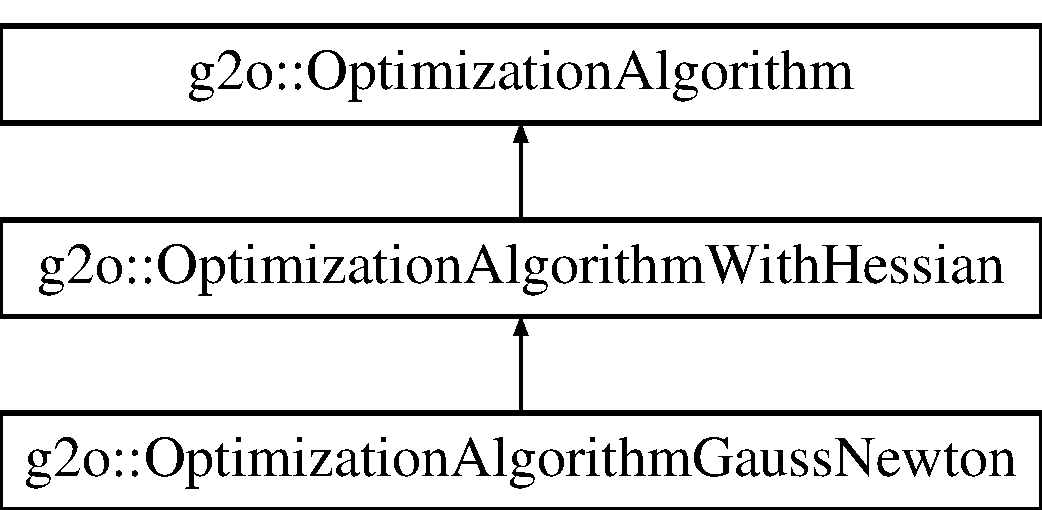
\includegraphics[height=3.000000cm]{classg2o_1_1_optimization_algorithm_gauss_newton}
\end{center}
\end{figure}
\subsection*{Public Member Functions}
\begin{DoxyCompactItemize}
\item 
\mbox{\hyperlink{classg2o_1_1_optimization_algorithm_gauss_newton_aca16df79fa14caf3e77bef0ca9aaedc4}{Optimization\+Algorithm\+Gauss\+Newton}} (\mbox{\hyperlink{classg2o_1_1_solver}{Solver}} $\ast$\mbox{\hyperlink{classg2o_1_1_optimization_algorithm_with_hessian_a85473a4073c76b1a52cf9cf175e31c45}{solver}})
\item 
virtual \mbox{\hyperlink{classg2o_1_1_optimization_algorithm_gauss_newton_ac86bc6829b12453693ee2c3967b11f0b}{$\sim$\+Optimization\+Algorithm\+Gauss\+Newton}} ()
\item 
virtual Solver\+Result \mbox{\hyperlink{classg2o_1_1_optimization_algorithm_gauss_newton_aba0b67eecaca01c576de7e605e5af5f1}{solve}} (int iteration, bool online=false)
\item 
virtual void \mbox{\hyperlink{classg2o_1_1_optimization_algorithm_gauss_newton_aff4c1b6a9f8a2e5c6777cfef9d4a18ba}{print\+Verbose}} (std\+::ostream \&os) const
\end{DoxyCompactItemize}
\subsection*{Additional Inherited Members}


\subsection{Detailed Description}
Implementation of the Gauss Newton Algorithm. 

\subsection{Constructor \& Destructor Documentation}
\mbox{\Hypertarget{classg2o_1_1_optimization_algorithm_gauss_newton_aca16df79fa14caf3e77bef0ca9aaedc4}\label{classg2o_1_1_optimization_algorithm_gauss_newton_aca16df79fa14caf3e77bef0ca9aaedc4}} 
\index{g2o\+::\+Optimization\+Algorithm\+Gauss\+Newton@{g2o\+::\+Optimization\+Algorithm\+Gauss\+Newton}!Optimization\+Algorithm\+Gauss\+Newton@{Optimization\+Algorithm\+Gauss\+Newton}}
\index{Optimization\+Algorithm\+Gauss\+Newton@{Optimization\+Algorithm\+Gauss\+Newton}!g2o\+::\+Optimization\+Algorithm\+Gauss\+Newton@{g2o\+::\+Optimization\+Algorithm\+Gauss\+Newton}}
\subsubsection{\texorpdfstring{Optimization\+Algorithm\+Gauss\+Newton()}{OptimizationAlgorithmGaussNewton()}}
{\footnotesize\ttfamily g2o\+::\+Optimization\+Algorithm\+Gauss\+Newton\+::\+Optimization\+Algorithm\+Gauss\+Newton (\begin{DoxyParamCaption}\item[{\mbox{\hyperlink{classg2o_1_1_solver}{Solver}} $\ast$}]{solver }\end{DoxyParamCaption})\hspace{0.3cm}{\ttfamily [explicit]}}

construct the Gauss Newton algorithm, which use the given \mbox{\hyperlink{classg2o_1_1_solver}{Solver}} for solving the linearized system. \mbox{\Hypertarget{classg2o_1_1_optimization_algorithm_gauss_newton_ac86bc6829b12453693ee2c3967b11f0b}\label{classg2o_1_1_optimization_algorithm_gauss_newton_ac86bc6829b12453693ee2c3967b11f0b}} 
\index{g2o\+::\+Optimization\+Algorithm\+Gauss\+Newton@{g2o\+::\+Optimization\+Algorithm\+Gauss\+Newton}!````~Optimization\+Algorithm\+Gauss\+Newton@{$\sim$\+Optimization\+Algorithm\+Gauss\+Newton}}
\index{````~Optimization\+Algorithm\+Gauss\+Newton@{$\sim$\+Optimization\+Algorithm\+Gauss\+Newton}!g2o\+::\+Optimization\+Algorithm\+Gauss\+Newton@{g2o\+::\+Optimization\+Algorithm\+Gauss\+Newton}}
\subsubsection{\texorpdfstring{$\sim$\+Optimization\+Algorithm\+Gauss\+Newton()}{~OptimizationAlgorithmGaussNewton()}}
{\footnotesize\ttfamily g2o\+::\+Optimization\+Algorithm\+Gauss\+Newton\+::$\sim$\+Optimization\+Algorithm\+Gauss\+Newton (\begin{DoxyParamCaption}{ }\end{DoxyParamCaption})\hspace{0.3cm}{\ttfamily [virtual]}}



\subsection{Member Function Documentation}
\mbox{\Hypertarget{classg2o_1_1_optimization_algorithm_gauss_newton_aff4c1b6a9f8a2e5c6777cfef9d4a18ba}\label{classg2o_1_1_optimization_algorithm_gauss_newton_aff4c1b6a9f8a2e5c6777cfef9d4a18ba}} 
\index{g2o\+::\+Optimization\+Algorithm\+Gauss\+Newton@{g2o\+::\+Optimization\+Algorithm\+Gauss\+Newton}!print\+Verbose@{print\+Verbose}}
\index{print\+Verbose@{print\+Verbose}!g2o\+::\+Optimization\+Algorithm\+Gauss\+Newton@{g2o\+::\+Optimization\+Algorithm\+Gauss\+Newton}}
\subsubsection{\texorpdfstring{print\+Verbose()}{printVerbose()}}
{\footnotesize\ttfamily void g2o\+::\+Optimization\+Algorithm\+Gauss\+Newton\+::print\+Verbose (\begin{DoxyParamCaption}\item[{std\+::ostream \&}]{os }\end{DoxyParamCaption}) const\hspace{0.3cm}{\ttfamily [virtual]}}

called by the optimizer if verbose. re-\/implement, if you want to print something 

Reimplemented from \mbox{\hyperlink{classg2o_1_1_optimization_algorithm_a6683d35e67402b50924bc4744b6e282a}{g2o\+::\+Optimization\+Algorithm}}.

\mbox{\Hypertarget{classg2o_1_1_optimization_algorithm_gauss_newton_aba0b67eecaca01c576de7e605e5af5f1}\label{classg2o_1_1_optimization_algorithm_gauss_newton_aba0b67eecaca01c576de7e605e5af5f1}} 
\index{g2o\+::\+Optimization\+Algorithm\+Gauss\+Newton@{g2o\+::\+Optimization\+Algorithm\+Gauss\+Newton}!solve@{solve}}
\index{solve@{solve}!g2o\+::\+Optimization\+Algorithm\+Gauss\+Newton@{g2o\+::\+Optimization\+Algorithm\+Gauss\+Newton}}
\subsubsection{\texorpdfstring{solve()}{solve()}}
{\footnotesize\ttfamily Optimization\+Algorithm\+::\+Solver\+Result g2o\+::\+Optimization\+Algorithm\+Gauss\+Newton\+::solve (\begin{DoxyParamCaption}\item[{int}]{iteration,  }\item[{bool}]{online = {\ttfamily false} }\end{DoxyParamCaption})\hspace{0.3cm}{\ttfamily [virtual]}}

Solve one iteration. The \mbox{\hyperlink{classg2o_1_1_sparse_optimizer}{Sparse\+Optimizer}} running on-\/top will call this for the given number of iterations. 
\begin{DoxyParams}{Parameters}
{\em iteration} & indicates the current iteration \\
\hline
\end{DoxyParams}


Implements \mbox{\hyperlink{classg2o_1_1_optimization_algorithm_ab174deeeb2551ceaf715ea09f0f9c077}{g2o\+::\+Optimization\+Algorithm}}.



The documentation for this class was generated from the following files\+:\begin{DoxyCompactItemize}
\item 
Thirdparty/g2o/g2o/core/\mbox{\hyperlink{optimization__algorithm__gauss__newton_8h}{optimization\+\_\+algorithm\+\_\+gauss\+\_\+newton.\+h}}\item 
Thirdparty/g2o/g2o/core/\mbox{\hyperlink{optimization__algorithm__gauss__newton_8cpp}{optimization\+\_\+algorithm\+\_\+gauss\+\_\+newton.\+cpp}}\end{DoxyCompactItemize}

\hypertarget{classg2o_1_1_optimization_algorithm_levenberg}{}\section{g2o\+:\+:Optimization\+Algorithm\+Levenberg Class Reference}
\label{classg2o_1_1_optimization_algorithm_levenberg}\index{g2o\+::\+Optimization\+Algorithm\+Levenberg@{g2o\+::\+Optimization\+Algorithm\+Levenberg}}


Implementation of the Levenberg Algorithm.  




{\ttfamily \#include $<$optimization\+\_\+algorithm\+\_\+levenberg.\+h$>$}

Inheritance diagram for g2o\+:\+:Optimization\+Algorithm\+Levenberg\+:\begin{figure}[H]
\begin{center}
\leavevmode
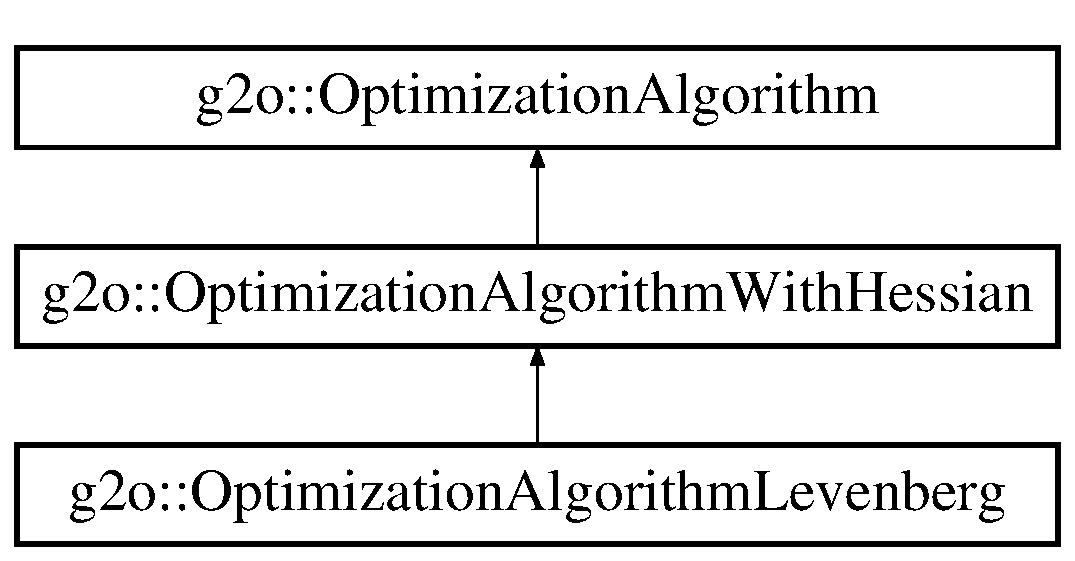
\includegraphics[height=3.000000cm]{classg2o_1_1_optimization_algorithm_levenberg}
\end{center}
\end{figure}
\subsection*{Public Member Functions}
\begin{DoxyCompactItemize}
\item 
\mbox{\hyperlink{classg2o_1_1_optimization_algorithm_levenberg_aecdac695d6406eb2234bbd8a0c4d53a3}{Optimization\+Algorithm\+Levenberg}} (\mbox{\hyperlink{classg2o_1_1_solver}{Solver}} $\ast$\mbox{\hyperlink{classg2o_1_1_optimization_algorithm_with_hessian_a85473a4073c76b1a52cf9cf175e31c45}{solver}})
\item 
virtual \mbox{\hyperlink{classg2o_1_1_optimization_algorithm_levenberg_a926c821217c53b10fec9275b6fa5e548}{$\sim$\+Optimization\+Algorithm\+Levenberg}} ()
\item 
virtual Solver\+Result \mbox{\hyperlink{classg2o_1_1_optimization_algorithm_levenberg_a7140fa989b54eac4e09ba17829dcada0}{solve}} (int iteration, bool online=false)
\item 
virtual void \mbox{\hyperlink{classg2o_1_1_optimization_algorithm_levenberg_a67308ead9762f478e29385229ea4b138}{print\+Verbose}} (std\+::ostream \&os) const
\item 
double \mbox{\hyperlink{classg2o_1_1_optimization_algorithm_levenberg_afa4684ccfb8b87e85d0102cbe412f105}{current\+Lambda}} () const
\begin{DoxyCompactList}\small\item\em return the currently used damping factor \end{DoxyCompactList}\item 
void \mbox{\hyperlink{classg2o_1_1_optimization_algorithm_levenberg_a0fd2212e456428e44ddac693f6d27ac8}{set\+Max\+Trials\+After\+Failure}} (int max\+\_\+trials)
\begin{DoxyCompactList}\small\item\em the number of internal iteration if an update step increases chi$^\wedge$2 within Levenberg-\/\+Marquardt \end{DoxyCompactList}\item 
int \mbox{\hyperlink{classg2o_1_1_optimization_algorithm_levenberg_a5d467a866c6ee90aaed9b4ccaf29e5e5}{max\+Trials\+After\+Failure}} () const
\begin{DoxyCompactList}\small\item\em get the number of inner iterations for Levenberg-\/\+Marquardt \end{DoxyCompactList}\item 
double \mbox{\hyperlink{classg2o_1_1_optimization_algorithm_levenberg_a4a4d18c98361a1288db724136d353596}{user\+Lambda\+Init}} ()
\begin{DoxyCompactList}\small\item\em return the lambda set by the user, if $<$ 0 the \mbox{\hyperlink{classg2o_1_1_sparse_optimizer}{Sparse\+Optimizer}} will compute the initial lambda \end{DoxyCompactList}\item 
void \mbox{\hyperlink{classg2o_1_1_optimization_algorithm_levenberg_a9388e5e7800b18acb0db0a9a7be031a6}{set\+User\+Lambda\+Init}} (double lambda)
\begin{DoxyCompactList}\small\item\em specify the initial lambda used for the first iteraion, if not given the \mbox{\hyperlink{classg2o_1_1_sparse_optimizer}{Sparse\+Optimizer}} tries to compute a suitable value \end{DoxyCompactList}\item 
int \mbox{\hyperlink{classg2o_1_1_optimization_algorithm_levenberg_a6d458d8a89069fab92fab75c1255a523}{levenberg\+Iteration}} ()
\begin{DoxyCompactList}\small\item\em return the number of levenberg iterations performed in the last round \end{DoxyCompactList}\end{DoxyCompactItemize}
\subsection*{Protected Member Functions}
\begin{DoxyCompactItemize}
\item 
double \mbox{\hyperlink{classg2o_1_1_optimization_algorithm_levenberg_a2141aed034c5db8b2943aad5853b0cde}{compute\+Lambda\+Init}} () const
\item 
double \mbox{\hyperlink{classg2o_1_1_optimization_algorithm_levenberg_aa49f788d13c2ab6026ebaf36f887dc9a}{compute\+Scale}} () const
\end{DoxyCompactItemize}
\subsection*{Protected Attributes}
\begin{DoxyCompactItemize}
\item 
\mbox{\hyperlink{classg2o_1_1_property}{Property}}$<$ int $>$ $\ast$ \mbox{\hyperlink{classg2o_1_1_optimization_algorithm_levenberg_a1f3b03bbcb2dbeed686069bed8783b80}{\+\_\+max\+Trials\+After\+Failure}}
\item 
\mbox{\hyperlink{classg2o_1_1_property}{Property}}$<$ double $>$ $\ast$ \mbox{\hyperlink{classg2o_1_1_optimization_algorithm_levenberg_a021c97d3f8205ec2ae7fde147f98b452}{\+\_\+user\+Lambda\+Init}}
\item 
double \mbox{\hyperlink{classg2o_1_1_optimization_algorithm_levenberg_aec7bba815e20361aa7ccc4661f90a034}{\+\_\+current\+Lambda}}
\item 
double \mbox{\hyperlink{classg2o_1_1_optimization_algorithm_levenberg_ac09602f23e52c5dbc6be1bf77e9f9d5f}{\+\_\+tau}}
\item 
double \mbox{\hyperlink{classg2o_1_1_optimization_algorithm_levenberg_a4951bc2e2fcca2c4eae4864690a4c087}{\+\_\+good\+Step\+Lower\+Scale}}
\begin{DoxyCompactList}\small\item\em lower bound for lambda decrease if a good LM step \end{DoxyCompactList}\item 
double \mbox{\hyperlink{classg2o_1_1_optimization_algorithm_levenberg_a16d8b5540cd7ae0c132a565e3f49c021}{\+\_\+good\+Step\+Upper\+Scale}}
\begin{DoxyCompactList}\small\item\em upper bound for lambda decrease if a good LM step \end{DoxyCompactList}\item 
double \mbox{\hyperlink{classg2o_1_1_optimization_algorithm_levenberg_a8bcb1a957056cba788072992c5a8a7a1}{\+\_\+ni}}
\item 
int \mbox{\hyperlink{classg2o_1_1_optimization_algorithm_levenberg_a2319771c8d3ee0f773bdb86d5416bab7}{\+\_\+levenberg\+Iterations}}
\begin{DoxyCompactList}\small\item\em the numer of levenberg iterations performed to accept the last step \end{DoxyCompactList}\item 
int \mbox{\hyperlink{classg2o_1_1_optimization_algorithm_levenberg_a7f0b375c45a9f91f2676548591273c8d}{\+\_\+n\+Bad}}
\end{DoxyCompactItemize}


\subsection{Detailed Description}
Implementation of the Levenberg Algorithm. 

\subsection{Constructor \& Destructor Documentation}
\mbox{\Hypertarget{classg2o_1_1_optimization_algorithm_levenberg_aecdac695d6406eb2234bbd8a0c4d53a3}\label{classg2o_1_1_optimization_algorithm_levenberg_aecdac695d6406eb2234bbd8a0c4d53a3}} 
\index{g2o\+::\+Optimization\+Algorithm\+Levenberg@{g2o\+::\+Optimization\+Algorithm\+Levenberg}!Optimization\+Algorithm\+Levenberg@{Optimization\+Algorithm\+Levenberg}}
\index{Optimization\+Algorithm\+Levenberg@{Optimization\+Algorithm\+Levenberg}!g2o\+::\+Optimization\+Algorithm\+Levenberg@{g2o\+::\+Optimization\+Algorithm\+Levenberg}}
\subsubsection{\texorpdfstring{Optimization\+Algorithm\+Levenberg()}{OptimizationAlgorithmLevenberg()}}
{\footnotesize\ttfamily g2o\+::\+Optimization\+Algorithm\+Levenberg\+::\+Optimization\+Algorithm\+Levenberg (\begin{DoxyParamCaption}\item[{\mbox{\hyperlink{classg2o_1_1_solver}{Solver}} $\ast$}]{solver }\end{DoxyParamCaption})\hspace{0.3cm}{\ttfamily [explicit]}}

construct the Levenberg algorithm, which will use the given \mbox{\hyperlink{classg2o_1_1_solver}{Solver}} for solving the linearized system. \mbox{\Hypertarget{classg2o_1_1_optimization_algorithm_levenberg_a926c821217c53b10fec9275b6fa5e548}\label{classg2o_1_1_optimization_algorithm_levenberg_a926c821217c53b10fec9275b6fa5e548}} 
\index{g2o\+::\+Optimization\+Algorithm\+Levenberg@{g2o\+::\+Optimization\+Algorithm\+Levenberg}!````~Optimization\+Algorithm\+Levenberg@{$\sim$\+Optimization\+Algorithm\+Levenberg}}
\index{````~Optimization\+Algorithm\+Levenberg@{$\sim$\+Optimization\+Algorithm\+Levenberg}!g2o\+::\+Optimization\+Algorithm\+Levenberg@{g2o\+::\+Optimization\+Algorithm\+Levenberg}}
\subsubsection{\texorpdfstring{$\sim$\+Optimization\+Algorithm\+Levenberg()}{~OptimizationAlgorithmLevenberg()}}
{\footnotesize\ttfamily g2o\+::\+Optimization\+Algorithm\+Levenberg\+::$\sim$\+Optimization\+Algorithm\+Levenberg (\begin{DoxyParamCaption}{ }\end{DoxyParamCaption})\hspace{0.3cm}{\ttfamily [virtual]}}



\subsection{Member Function Documentation}
\mbox{\Hypertarget{classg2o_1_1_optimization_algorithm_levenberg_a2141aed034c5db8b2943aad5853b0cde}\label{classg2o_1_1_optimization_algorithm_levenberg_a2141aed034c5db8b2943aad5853b0cde}} 
\index{g2o\+::\+Optimization\+Algorithm\+Levenberg@{g2o\+::\+Optimization\+Algorithm\+Levenberg}!compute\+Lambda\+Init@{compute\+Lambda\+Init}}
\index{compute\+Lambda\+Init@{compute\+Lambda\+Init}!g2o\+::\+Optimization\+Algorithm\+Levenberg@{g2o\+::\+Optimization\+Algorithm\+Levenberg}}
\subsubsection{\texorpdfstring{compute\+Lambda\+Init()}{computeLambdaInit()}}
{\footnotesize\ttfamily double g2o\+::\+Optimization\+Algorithm\+Levenberg\+::compute\+Lambda\+Init (\begin{DoxyParamCaption}{ }\end{DoxyParamCaption}) const\hspace{0.3cm}{\ttfamily [protected]}}

helper for Levenberg, this function computes the initial damping factor, if the user did not specify an own value, see \mbox{\hyperlink{classg2o_1_1_optimization_algorithm_levenberg_a9388e5e7800b18acb0db0a9a7be031a6}{set\+User\+Lambda\+Init()}} \mbox{\Hypertarget{classg2o_1_1_optimization_algorithm_levenberg_aa49f788d13c2ab6026ebaf36f887dc9a}\label{classg2o_1_1_optimization_algorithm_levenberg_aa49f788d13c2ab6026ebaf36f887dc9a}} 
\index{g2o\+::\+Optimization\+Algorithm\+Levenberg@{g2o\+::\+Optimization\+Algorithm\+Levenberg}!compute\+Scale@{compute\+Scale}}
\index{compute\+Scale@{compute\+Scale}!g2o\+::\+Optimization\+Algorithm\+Levenberg@{g2o\+::\+Optimization\+Algorithm\+Levenberg}}
\subsubsection{\texorpdfstring{compute\+Scale()}{computeScale()}}
{\footnotesize\ttfamily double g2o\+::\+Optimization\+Algorithm\+Levenberg\+::compute\+Scale (\begin{DoxyParamCaption}{ }\end{DoxyParamCaption}) const\hspace{0.3cm}{\ttfamily [protected]}}

\mbox{\Hypertarget{classg2o_1_1_optimization_algorithm_levenberg_afa4684ccfb8b87e85d0102cbe412f105}\label{classg2o_1_1_optimization_algorithm_levenberg_afa4684ccfb8b87e85d0102cbe412f105}} 
\index{g2o\+::\+Optimization\+Algorithm\+Levenberg@{g2o\+::\+Optimization\+Algorithm\+Levenberg}!current\+Lambda@{current\+Lambda}}
\index{current\+Lambda@{current\+Lambda}!g2o\+::\+Optimization\+Algorithm\+Levenberg@{g2o\+::\+Optimization\+Algorithm\+Levenberg}}
\subsubsection{\texorpdfstring{current\+Lambda()}{currentLambda()}}
{\footnotesize\ttfamily double g2o\+::\+Optimization\+Algorithm\+Levenberg\+::current\+Lambda (\begin{DoxyParamCaption}{ }\end{DoxyParamCaption}) const\hspace{0.3cm}{\ttfamily [inline]}}



return the currently used damping factor 

\mbox{\Hypertarget{classg2o_1_1_optimization_algorithm_levenberg_a6d458d8a89069fab92fab75c1255a523}\label{classg2o_1_1_optimization_algorithm_levenberg_a6d458d8a89069fab92fab75c1255a523}} 
\index{g2o\+::\+Optimization\+Algorithm\+Levenberg@{g2o\+::\+Optimization\+Algorithm\+Levenberg}!levenberg\+Iteration@{levenberg\+Iteration}}
\index{levenberg\+Iteration@{levenberg\+Iteration}!g2o\+::\+Optimization\+Algorithm\+Levenberg@{g2o\+::\+Optimization\+Algorithm\+Levenberg}}
\subsubsection{\texorpdfstring{levenberg\+Iteration()}{levenbergIteration()}}
{\footnotesize\ttfamily int g2o\+::\+Optimization\+Algorithm\+Levenberg\+::levenberg\+Iteration (\begin{DoxyParamCaption}{ }\end{DoxyParamCaption})\hspace{0.3cm}{\ttfamily [inline]}}



return the number of levenberg iterations performed in the last round 

\mbox{\Hypertarget{classg2o_1_1_optimization_algorithm_levenberg_a5d467a866c6ee90aaed9b4ccaf29e5e5}\label{classg2o_1_1_optimization_algorithm_levenberg_a5d467a866c6ee90aaed9b4ccaf29e5e5}} 
\index{g2o\+::\+Optimization\+Algorithm\+Levenberg@{g2o\+::\+Optimization\+Algorithm\+Levenberg}!max\+Trials\+After\+Failure@{max\+Trials\+After\+Failure}}
\index{max\+Trials\+After\+Failure@{max\+Trials\+After\+Failure}!g2o\+::\+Optimization\+Algorithm\+Levenberg@{g2o\+::\+Optimization\+Algorithm\+Levenberg}}
\subsubsection{\texorpdfstring{max\+Trials\+After\+Failure()}{maxTrialsAfterFailure()}}
{\footnotesize\ttfamily int g2o\+::\+Optimization\+Algorithm\+Levenberg\+::max\+Trials\+After\+Failure (\begin{DoxyParamCaption}{ }\end{DoxyParamCaption}) const\hspace{0.3cm}{\ttfamily [inline]}}



get the number of inner iterations for Levenberg-\/\+Marquardt 

\mbox{\Hypertarget{classg2o_1_1_optimization_algorithm_levenberg_a67308ead9762f478e29385229ea4b138}\label{classg2o_1_1_optimization_algorithm_levenberg_a67308ead9762f478e29385229ea4b138}} 
\index{g2o\+::\+Optimization\+Algorithm\+Levenberg@{g2o\+::\+Optimization\+Algorithm\+Levenberg}!print\+Verbose@{print\+Verbose}}
\index{print\+Verbose@{print\+Verbose}!g2o\+::\+Optimization\+Algorithm\+Levenberg@{g2o\+::\+Optimization\+Algorithm\+Levenberg}}
\subsubsection{\texorpdfstring{print\+Verbose()}{printVerbose()}}
{\footnotesize\ttfamily void g2o\+::\+Optimization\+Algorithm\+Levenberg\+::print\+Verbose (\begin{DoxyParamCaption}\item[{std\+::ostream \&}]{os }\end{DoxyParamCaption}) const\hspace{0.3cm}{\ttfamily [virtual]}}

called by the optimizer if verbose. re-\/implement, if you want to print something 

Reimplemented from \mbox{\hyperlink{classg2o_1_1_optimization_algorithm_a6683d35e67402b50924bc4744b6e282a}{g2o\+::\+Optimization\+Algorithm}}.

\mbox{\Hypertarget{classg2o_1_1_optimization_algorithm_levenberg_a0fd2212e456428e44ddac693f6d27ac8}\label{classg2o_1_1_optimization_algorithm_levenberg_a0fd2212e456428e44ddac693f6d27ac8}} 
\index{g2o\+::\+Optimization\+Algorithm\+Levenberg@{g2o\+::\+Optimization\+Algorithm\+Levenberg}!set\+Max\+Trials\+After\+Failure@{set\+Max\+Trials\+After\+Failure}}
\index{set\+Max\+Trials\+After\+Failure@{set\+Max\+Trials\+After\+Failure}!g2o\+::\+Optimization\+Algorithm\+Levenberg@{g2o\+::\+Optimization\+Algorithm\+Levenberg}}
\subsubsection{\texorpdfstring{set\+Max\+Trials\+After\+Failure()}{setMaxTrialsAfterFailure()}}
{\footnotesize\ttfamily void g2o\+::\+Optimization\+Algorithm\+Levenberg\+::set\+Max\+Trials\+After\+Failure (\begin{DoxyParamCaption}\item[{int}]{max\+\_\+trials }\end{DoxyParamCaption})}



the number of internal iteration if an update step increases chi$^\wedge$2 within Levenberg-\/\+Marquardt 

\mbox{\Hypertarget{classg2o_1_1_optimization_algorithm_levenberg_a9388e5e7800b18acb0db0a9a7be031a6}\label{classg2o_1_1_optimization_algorithm_levenberg_a9388e5e7800b18acb0db0a9a7be031a6}} 
\index{g2o\+::\+Optimization\+Algorithm\+Levenberg@{g2o\+::\+Optimization\+Algorithm\+Levenberg}!set\+User\+Lambda\+Init@{set\+User\+Lambda\+Init}}
\index{set\+User\+Lambda\+Init@{set\+User\+Lambda\+Init}!g2o\+::\+Optimization\+Algorithm\+Levenberg@{g2o\+::\+Optimization\+Algorithm\+Levenberg}}
\subsubsection{\texorpdfstring{set\+User\+Lambda\+Init()}{setUserLambdaInit()}}
{\footnotesize\ttfamily void g2o\+::\+Optimization\+Algorithm\+Levenberg\+::set\+User\+Lambda\+Init (\begin{DoxyParamCaption}\item[{double}]{lambda }\end{DoxyParamCaption})}



specify the initial lambda used for the first iteraion, if not given the \mbox{\hyperlink{classg2o_1_1_sparse_optimizer}{Sparse\+Optimizer}} tries to compute a suitable value 

\mbox{\Hypertarget{classg2o_1_1_optimization_algorithm_levenberg_a7140fa989b54eac4e09ba17829dcada0}\label{classg2o_1_1_optimization_algorithm_levenberg_a7140fa989b54eac4e09ba17829dcada0}} 
\index{g2o\+::\+Optimization\+Algorithm\+Levenberg@{g2o\+::\+Optimization\+Algorithm\+Levenberg}!solve@{solve}}
\index{solve@{solve}!g2o\+::\+Optimization\+Algorithm\+Levenberg@{g2o\+::\+Optimization\+Algorithm\+Levenberg}}
\subsubsection{\texorpdfstring{solve()}{solve()}}
{\footnotesize\ttfamily Optimization\+Algorithm\+::\+Solver\+Result g2o\+::\+Optimization\+Algorithm\+Levenberg\+::solve (\begin{DoxyParamCaption}\item[{int}]{iteration,  }\item[{bool}]{online = {\ttfamily false} }\end{DoxyParamCaption})\hspace{0.3cm}{\ttfamily [virtual]}}

Solve one iteration. The \mbox{\hyperlink{classg2o_1_1_sparse_optimizer}{Sparse\+Optimizer}} running on-\/top will call this for the given number of iterations. 
\begin{DoxyParams}{Parameters}
{\em iteration} & indicates the current iteration \\
\hline
\end{DoxyParams}


Implements \mbox{\hyperlink{classg2o_1_1_optimization_algorithm_ab174deeeb2551ceaf715ea09f0f9c077}{g2o\+::\+Optimization\+Algorithm}}.

\mbox{\Hypertarget{classg2o_1_1_optimization_algorithm_levenberg_a4a4d18c98361a1288db724136d353596}\label{classg2o_1_1_optimization_algorithm_levenberg_a4a4d18c98361a1288db724136d353596}} 
\index{g2o\+::\+Optimization\+Algorithm\+Levenberg@{g2o\+::\+Optimization\+Algorithm\+Levenberg}!user\+Lambda\+Init@{user\+Lambda\+Init}}
\index{user\+Lambda\+Init@{user\+Lambda\+Init}!g2o\+::\+Optimization\+Algorithm\+Levenberg@{g2o\+::\+Optimization\+Algorithm\+Levenberg}}
\subsubsection{\texorpdfstring{user\+Lambda\+Init()}{userLambdaInit()}}
{\footnotesize\ttfamily double g2o\+::\+Optimization\+Algorithm\+Levenberg\+::user\+Lambda\+Init (\begin{DoxyParamCaption}{ }\end{DoxyParamCaption})\hspace{0.3cm}{\ttfamily [inline]}}



return the lambda set by the user, if $<$ 0 the \mbox{\hyperlink{classg2o_1_1_sparse_optimizer}{Sparse\+Optimizer}} will compute the initial lambda 



\subsection{Member Data Documentation}
\mbox{\Hypertarget{classg2o_1_1_optimization_algorithm_levenberg_aec7bba815e20361aa7ccc4661f90a034}\label{classg2o_1_1_optimization_algorithm_levenberg_aec7bba815e20361aa7ccc4661f90a034}} 
\index{g2o\+::\+Optimization\+Algorithm\+Levenberg@{g2o\+::\+Optimization\+Algorithm\+Levenberg}!\+\_\+current\+Lambda@{\+\_\+current\+Lambda}}
\index{\+\_\+current\+Lambda@{\+\_\+current\+Lambda}!g2o\+::\+Optimization\+Algorithm\+Levenberg@{g2o\+::\+Optimization\+Algorithm\+Levenberg}}
\subsubsection{\texorpdfstring{\+\_\+current\+Lambda}{\_currentLambda}}
{\footnotesize\ttfamily double g2o\+::\+Optimization\+Algorithm\+Levenberg\+::\+\_\+current\+Lambda\hspace{0.3cm}{\ttfamily [protected]}}

\mbox{\Hypertarget{classg2o_1_1_optimization_algorithm_levenberg_a4951bc2e2fcca2c4eae4864690a4c087}\label{classg2o_1_1_optimization_algorithm_levenberg_a4951bc2e2fcca2c4eae4864690a4c087}} 
\index{g2o\+::\+Optimization\+Algorithm\+Levenberg@{g2o\+::\+Optimization\+Algorithm\+Levenberg}!\+\_\+good\+Step\+Lower\+Scale@{\+\_\+good\+Step\+Lower\+Scale}}
\index{\+\_\+good\+Step\+Lower\+Scale@{\+\_\+good\+Step\+Lower\+Scale}!g2o\+::\+Optimization\+Algorithm\+Levenberg@{g2o\+::\+Optimization\+Algorithm\+Levenberg}}
\subsubsection{\texorpdfstring{\+\_\+good\+Step\+Lower\+Scale}{\_goodStepLowerScale}}
{\footnotesize\ttfamily double g2o\+::\+Optimization\+Algorithm\+Levenberg\+::\+\_\+good\+Step\+Lower\+Scale\hspace{0.3cm}{\ttfamily [protected]}}



lower bound for lambda decrease if a good LM step 

\mbox{\Hypertarget{classg2o_1_1_optimization_algorithm_levenberg_a16d8b5540cd7ae0c132a565e3f49c021}\label{classg2o_1_1_optimization_algorithm_levenberg_a16d8b5540cd7ae0c132a565e3f49c021}} 
\index{g2o\+::\+Optimization\+Algorithm\+Levenberg@{g2o\+::\+Optimization\+Algorithm\+Levenberg}!\+\_\+good\+Step\+Upper\+Scale@{\+\_\+good\+Step\+Upper\+Scale}}
\index{\+\_\+good\+Step\+Upper\+Scale@{\+\_\+good\+Step\+Upper\+Scale}!g2o\+::\+Optimization\+Algorithm\+Levenberg@{g2o\+::\+Optimization\+Algorithm\+Levenberg}}
\subsubsection{\texorpdfstring{\+\_\+good\+Step\+Upper\+Scale}{\_goodStepUpperScale}}
{\footnotesize\ttfamily double g2o\+::\+Optimization\+Algorithm\+Levenberg\+::\+\_\+good\+Step\+Upper\+Scale\hspace{0.3cm}{\ttfamily [protected]}}



upper bound for lambda decrease if a good LM step 

\mbox{\Hypertarget{classg2o_1_1_optimization_algorithm_levenberg_a2319771c8d3ee0f773bdb86d5416bab7}\label{classg2o_1_1_optimization_algorithm_levenberg_a2319771c8d3ee0f773bdb86d5416bab7}} 
\index{g2o\+::\+Optimization\+Algorithm\+Levenberg@{g2o\+::\+Optimization\+Algorithm\+Levenberg}!\+\_\+levenberg\+Iterations@{\+\_\+levenberg\+Iterations}}
\index{\+\_\+levenberg\+Iterations@{\+\_\+levenberg\+Iterations}!g2o\+::\+Optimization\+Algorithm\+Levenberg@{g2o\+::\+Optimization\+Algorithm\+Levenberg}}
\subsubsection{\texorpdfstring{\+\_\+levenberg\+Iterations}{\_levenbergIterations}}
{\footnotesize\ttfamily int g2o\+::\+Optimization\+Algorithm\+Levenberg\+::\+\_\+levenberg\+Iterations\hspace{0.3cm}{\ttfamily [protected]}}



the numer of levenberg iterations performed to accept the last step 

\mbox{\Hypertarget{classg2o_1_1_optimization_algorithm_levenberg_a1f3b03bbcb2dbeed686069bed8783b80}\label{classg2o_1_1_optimization_algorithm_levenberg_a1f3b03bbcb2dbeed686069bed8783b80}} 
\index{g2o\+::\+Optimization\+Algorithm\+Levenberg@{g2o\+::\+Optimization\+Algorithm\+Levenberg}!\+\_\+max\+Trials\+After\+Failure@{\+\_\+max\+Trials\+After\+Failure}}
\index{\+\_\+max\+Trials\+After\+Failure@{\+\_\+max\+Trials\+After\+Failure}!g2o\+::\+Optimization\+Algorithm\+Levenberg@{g2o\+::\+Optimization\+Algorithm\+Levenberg}}
\subsubsection{\texorpdfstring{\+\_\+max\+Trials\+After\+Failure}{\_maxTrialsAfterFailure}}
{\footnotesize\ttfamily \mbox{\hyperlink{classg2o_1_1_property}{Property}}$<$int$>$$\ast$ g2o\+::\+Optimization\+Algorithm\+Levenberg\+::\+\_\+max\+Trials\+After\+Failure\hspace{0.3cm}{\ttfamily [protected]}}

\mbox{\Hypertarget{classg2o_1_1_optimization_algorithm_levenberg_a7f0b375c45a9f91f2676548591273c8d}\label{classg2o_1_1_optimization_algorithm_levenberg_a7f0b375c45a9f91f2676548591273c8d}} 
\index{g2o\+::\+Optimization\+Algorithm\+Levenberg@{g2o\+::\+Optimization\+Algorithm\+Levenberg}!\+\_\+n\+Bad@{\+\_\+n\+Bad}}
\index{\+\_\+n\+Bad@{\+\_\+n\+Bad}!g2o\+::\+Optimization\+Algorithm\+Levenberg@{g2o\+::\+Optimization\+Algorithm\+Levenberg}}
\subsubsection{\texorpdfstring{\+\_\+n\+Bad}{\_nBad}}
{\footnotesize\ttfamily int g2o\+::\+Optimization\+Algorithm\+Levenberg\+::\+\_\+n\+Bad\hspace{0.3cm}{\ttfamily [protected]}}

\mbox{\Hypertarget{classg2o_1_1_optimization_algorithm_levenberg_a8bcb1a957056cba788072992c5a8a7a1}\label{classg2o_1_1_optimization_algorithm_levenberg_a8bcb1a957056cba788072992c5a8a7a1}} 
\index{g2o\+::\+Optimization\+Algorithm\+Levenberg@{g2o\+::\+Optimization\+Algorithm\+Levenberg}!\+\_\+ni@{\+\_\+ni}}
\index{\+\_\+ni@{\+\_\+ni}!g2o\+::\+Optimization\+Algorithm\+Levenberg@{g2o\+::\+Optimization\+Algorithm\+Levenberg}}
\subsubsection{\texorpdfstring{\+\_\+ni}{\_ni}}
{\footnotesize\ttfamily double g2o\+::\+Optimization\+Algorithm\+Levenberg\+::\+\_\+ni\hspace{0.3cm}{\ttfamily [protected]}}

\mbox{\Hypertarget{classg2o_1_1_optimization_algorithm_levenberg_ac09602f23e52c5dbc6be1bf77e9f9d5f}\label{classg2o_1_1_optimization_algorithm_levenberg_ac09602f23e52c5dbc6be1bf77e9f9d5f}} 
\index{g2o\+::\+Optimization\+Algorithm\+Levenberg@{g2o\+::\+Optimization\+Algorithm\+Levenberg}!\+\_\+tau@{\+\_\+tau}}
\index{\+\_\+tau@{\+\_\+tau}!g2o\+::\+Optimization\+Algorithm\+Levenberg@{g2o\+::\+Optimization\+Algorithm\+Levenberg}}
\subsubsection{\texorpdfstring{\+\_\+tau}{\_tau}}
{\footnotesize\ttfamily double g2o\+::\+Optimization\+Algorithm\+Levenberg\+::\+\_\+tau\hspace{0.3cm}{\ttfamily [protected]}}

\mbox{\Hypertarget{classg2o_1_1_optimization_algorithm_levenberg_a021c97d3f8205ec2ae7fde147f98b452}\label{classg2o_1_1_optimization_algorithm_levenberg_a021c97d3f8205ec2ae7fde147f98b452}} 
\index{g2o\+::\+Optimization\+Algorithm\+Levenberg@{g2o\+::\+Optimization\+Algorithm\+Levenberg}!\+\_\+user\+Lambda\+Init@{\+\_\+user\+Lambda\+Init}}
\index{\+\_\+user\+Lambda\+Init@{\+\_\+user\+Lambda\+Init}!g2o\+::\+Optimization\+Algorithm\+Levenberg@{g2o\+::\+Optimization\+Algorithm\+Levenberg}}
\subsubsection{\texorpdfstring{\+\_\+user\+Lambda\+Init}{\_userLambdaInit}}
{\footnotesize\ttfamily \mbox{\hyperlink{classg2o_1_1_property}{Property}}$<$double$>$$\ast$ g2o\+::\+Optimization\+Algorithm\+Levenberg\+::\+\_\+user\+Lambda\+Init\hspace{0.3cm}{\ttfamily [protected]}}



The documentation for this class was generated from the following files\+:\begin{DoxyCompactItemize}
\item 
D\+:/github/\+V\+S\+L\+A\+M/\+O\+R\+B\+S\+L\+A\+M2/\+O\+R\+B-\/\+S\+L\+A\+M2-\/master/\+Thirdparty/g2o/g2o/core/\mbox{\hyperlink{optimization__algorithm__levenberg_8h}{optimization\+\_\+algorithm\+\_\+levenberg.\+h}}\item 
D\+:/github/\+V\+S\+L\+A\+M/\+O\+R\+B\+S\+L\+A\+M2/\+O\+R\+B-\/\+S\+L\+A\+M2-\/master/\+Thirdparty/g2o/g2o/core/\mbox{\hyperlink{optimization__algorithm__levenberg_8cpp}{optimization\+\_\+algorithm\+\_\+levenberg.\+cpp}}\end{DoxyCompactItemize}

\hypertarget{structg2o_1_1_optimization_algorithm_property}{}\section{g2o\+:\+:Optimization\+Algorithm\+Property Struct Reference}
\label{structg2o_1_1_optimization_algorithm_property}\index{g2o\+::\+Optimization\+Algorithm\+Property@{g2o\+::\+Optimization\+Algorithm\+Property}}


describe the properties of a solver  




{\ttfamily \#include $<$optimization\+\_\+algorithm\+\_\+property.\+h$>$}

\subsection*{Public Member Functions}
\begin{DoxyCompactItemize}
\item 
\mbox{\hyperlink{structg2o_1_1_optimization_algorithm_property_a2d83548ee175988e11738ae43c7a9803}{Optimization\+Algorithm\+Property}} ()
\item 
\mbox{\hyperlink{structg2o_1_1_optimization_algorithm_property_a5633cbd029eda42670f801de508f945b}{Optimization\+Algorithm\+Property}} (const std\+::string \&name\+\_\+, const std\+::string \&desc\+\_\+, const std\+::string \&type\+\_\+, bool requires\+Marginalize\+\_\+, int pose\+Dim\+\_\+, int landmark\+Dim\+\_\+)
\end{DoxyCompactItemize}
\subsection*{Public Attributes}
\begin{DoxyCompactItemize}
\item 
std\+::string \mbox{\hyperlink{structg2o_1_1_optimization_algorithm_property_aedb3c54122d6a75d49e1677e836bac22}{name}}
\begin{DoxyCompactList}\small\item\em name of the solver, e.\+g., var \end{DoxyCompactList}\item 
std\+::string \mbox{\hyperlink{structg2o_1_1_optimization_algorithm_property_a9390204f7ff2f092241f55656d8458b1}{desc}}
\begin{DoxyCompactList}\small\item\em short description of the solver \end{DoxyCompactList}\item 
std\+::string \mbox{\hyperlink{structg2o_1_1_optimization_algorithm_property_a199f33f536f48f6ceda037f6a2ff206d}{type}}
\begin{DoxyCompactList}\small\item\em type of solver, e.\+g., \char`\"{}\+C\+Sparse Cholesky\char`\"{}, \char`\"{}\+P\+C\+G\char`\"{} \end{DoxyCompactList}\item 
bool \mbox{\hyperlink{structg2o_1_1_optimization_algorithm_property_a179837f3866e8786ce3a7f7a34bdda44}{requires\+Marginalize}}
\begin{DoxyCompactList}\small\item\em whether the solver requires marginalization of landmarks \end{DoxyCompactList}\item 
int \mbox{\hyperlink{structg2o_1_1_optimization_algorithm_property_a2c0c87eeaa423e8c944cfa846eb6a553}{pose\+Dim}}
\begin{DoxyCompactList}\small\item\em dimension of the pose vertices (-\/1 if variable) \end{DoxyCompactList}\item 
int \mbox{\hyperlink{structg2o_1_1_optimization_algorithm_property_ad946dec26df70a6fb6d99f2ab76db269}{landmark\+Dim}}
\begin{DoxyCompactList}\small\item\em dimension of the landmar vertices (-\/1 if variable) \end{DoxyCompactList}\end{DoxyCompactItemize}


\subsection{Detailed Description}
describe the properties of a solver 

\subsection{Constructor \& Destructor Documentation}
\mbox{\Hypertarget{structg2o_1_1_optimization_algorithm_property_a2d83548ee175988e11738ae43c7a9803}\label{structg2o_1_1_optimization_algorithm_property_a2d83548ee175988e11738ae43c7a9803}} 
\index{g2o\+::\+Optimization\+Algorithm\+Property@{g2o\+::\+Optimization\+Algorithm\+Property}!Optimization\+Algorithm\+Property@{Optimization\+Algorithm\+Property}}
\index{Optimization\+Algorithm\+Property@{Optimization\+Algorithm\+Property}!g2o\+::\+Optimization\+Algorithm\+Property@{g2o\+::\+Optimization\+Algorithm\+Property}}
\subsubsection{\texorpdfstring{Optimization\+Algorithm\+Property()}{OptimizationAlgorithmProperty()}\hspace{0.1cm}{\footnotesize\ttfamily [1/2]}}
{\footnotesize\ttfamily g2o\+::\+Optimization\+Algorithm\+Property\+::\+Optimization\+Algorithm\+Property (\begin{DoxyParamCaption}{ }\end{DoxyParamCaption})\hspace{0.3cm}{\ttfamily [inline]}}

\mbox{\Hypertarget{structg2o_1_1_optimization_algorithm_property_a5633cbd029eda42670f801de508f945b}\label{structg2o_1_1_optimization_algorithm_property_a5633cbd029eda42670f801de508f945b}} 
\index{g2o\+::\+Optimization\+Algorithm\+Property@{g2o\+::\+Optimization\+Algorithm\+Property}!Optimization\+Algorithm\+Property@{Optimization\+Algorithm\+Property}}
\index{Optimization\+Algorithm\+Property@{Optimization\+Algorithm\+Property}!g2o\+::\+Optimization\+Algorithm\+Property@{g2o\+::\+Optimization\+Algorithm\+Property}}
\subsubsection{\texorpdfstring{Optimization\+Algorithm\+Property()}{OptimizationAlgorithmProperty()}\hspace{0.1cm}{\footnotesize\ttfamily [2/2]}}
{\footnotesize\ttfamily g2o\+::\+Optimization\+Algorithm\+Property\+::\+Optimization\+Algorithm\+Property (\begin{DoxyParamCaption}\item[{const std\+::string \&}]{name\+\_\+,  }\item[{const std\+::string \&}]{desc\+\_\+,  }\item[{const std\+::string \&}]{type\+\_\+,  }\item[{bool}]{requires\+Marginalize\+\_\+,  }\item[{int}]{pose\+Dim\+\_\+,  }\item[{int}]{landmark\+Dim\+\_\+ }\end{DoxyParamCaption})\hspace{0.3cm}{\ttfamily [inline]}}



\subsection{Member Data Documentation}
\mbox{\Hypertarget{structg2o_1_1_optimization_algorithm_property_a9390204f7ff2f092241f55656d8458b1}\label{structg2o_1_1_optimization_algorithm_property_a9390204f7ff2f092241f55656d8458b1}} 
\index{g2o\+::\+Optimization\+Algorithm\+Property@{g2o\+::\+Optimization\+Algorithm\+Property}!desc@{desc}}
\index{desc@{desc}!g2o\+::\+Optimization\+Algorithm\+Property@{g2o\+::\+Optimization\+Algorithm\+Property}}
\subsubsection{\texorpdfstring{desc}{desc}}
{\footnotesize\ttfamily std\+::string g2o\+::\+Optimization\+Algorithm\+Property\+::desc}



short description of the solver 

\mbox{\Hypertarget{structg2o_1_1_optimization_algorithm_property_ad946dec26df70a6fb6d99f2ab76db269}\label{structg2o_1_1_optimization_algorithm_property_ad946dec26df70a6fb6d99f2ab76db269}} 
\index{g2o\+::\+Optimization\+Algorithm\+Property@{g2o\+::\+Optimization\+Algorithm\+Property}!landmark\+Dim@{landmark\+Dim}}
\index{landmark\+Dim@{landmark\+Dim}!g2o\+::\+Optimization\+Algorithm\+Property@{g2o\+::\+Optimization\+Algorithm\+Property}}
\subsubsection{\texorpdfstring{landmark\+Dim}{landmarkDim}}
{\footnotesize\ttfamily int g2o\+::\+Optimization\+Algorithm\+Property\+::landmark\+Dim}



dimension of the landmar vertices (-\/1 if variable) 

\mbox{\Hypertarget{structg2o_1_1_optimization_algorithm_property_aedb3c54122d6a75d49e1677e836bac22}\label{structg2o_1_1_optimization_algorithm_property_aedb3c54122d6a75d49e1677e836bac22}} 
\index{g2o\+::\+Optimization\+Algorithm\+Property@{g2o\+::\+Optimization\+Algorithm\+Property}!name@{name}}
\index{name@{name}!g2o\+::\+Optimization\+Algorithm\+Property@{g2o\+::\+Optimization\+Algorithm\+Property}}
\subsubsection{\texorpdfstring{name}{name}}
{\footnotesize\ttfamily std\+::string g2o\+::\+Optimization\+Algorithm\+Property\+::name}



name of the solver, e.\+g., var 

\mbox{\Hypertarget{structg2o_1_1_optimization_algorithm_property_a2c0c87eeaa423e8c944cfa846eb6a553}\label{structg2o_1_1_optimization_algorithm_property_a2c0c87eeaa423e8c944cfa846eb6a553}} 
\index{g2o\+::\+Optimization\+Algorithm\+Property@{g2o\+::\+Optimization\+Algorithm\+Property}!pose\+Dim@{pose\+Dim}}
\index{pose\+Dim@{pose\+Dim}!g2o\+::\+Optimization\+Algorithm\+Property@{g2o\+::\+Optimization\+Algorithm\+Property}}
\subsubsection{\texorpdfstring{pose\+Dim}{poseDim}}
{\footnotesize\ttfamily int g2o\+::\+Optimization\+Algorithm\+Property\+::pose\+Dim}



dimension of the pose vertices (-\/1 if variable) 

\mbox{\Hypertarget{structg2o_1_1_optimization_algorithm_property_a179837f3866e8786ce3a7f7a34bdda44}\label{structg2o_1_1_optimization_algorithm_property_a179837f3866e8786ce3a7f7a34bdda44}} 
\index{g2o\+::\+Optimization\+Algorithm\+Property@{g2o\+::\+Optimization\+Algorithm\+Property}!requires\+Marginalize@{requires\+Marginalize}}
\index{requires\+Marginalize@{requires\+Marginalize}!g2o\+::\+Optimization\+Algorithm\+Property@{g2o\+::\+Optimization\+Algorithm\+Property}}
\subsubsection{\texorpdfstring{requires\+Marginalize}{requiresMarginalize}}
{\footnotesize\ttfamily bool g2o\+::\+Optimization\+Algorithm\+Property\+::requires\+Marginalize}



whether the solver requires marginalization of landmarks 

\mbox{\Hypertarget{structg2o_1_1_optimization_algorithm_property_a199f33f536f48f6ceda037f6a2ff206d}\label{structg2o_1_1_optimization_algorithm_property_a199f33f536f48f6ceda037f6a2ff206d}} 
\index{g2o\+::\+Optimization\+Algorithm\+Property@{g2o\+::\+Optimization\+Algorithm\+Property}!type@{type}}
\index{type@{type}!g2o\+::\+Optimization\+Algorithm\+Property@{g2o\+::\+Optimization\+Algorithm\+Property}}
\subsubsection{\texorpdfstring{type}{type}}
{\footnotesize\ttfamily std\+::string g2o\+::\+Optimization\+Algorithm\+Property\+::type}



type of solver, e.\+g., \char`\"{}\+C\+Sparse Cholesky\char`\"{}, \char`\"{}\+P\+C\+G\char`\"{} 



The documentation for this struct was generated from the following file\+:\begin{DoxyCompactItemize}
\item 
Thirdparty/g2o/g2o/core/\mbox{\hyperlink{optimization__algorithm__property_8h}{optimization\+\_\+algorithm\+\_\+property.\+h}}\end{DoxyCompactItemize}

\hypertarget{classg2o_1_1_optimization_algorithm_with_hessian}{}\section{g2o\+:\+:Optimization\+Algorithm\+With\+Hessian Class Reference}
\label{classg2o_1_1_optimization_algorithm_with_hessian}\index{g2o\+::\+Optimization\+Algorithm\+With\+Hessian@{g2o\+::\+Optimization\+Algorithm\+With\+Hessian}}


Base for solvers operating on the approximated Hessian, e.\+g., Gauss-\/\+Newton, Levenberg.  




{\ttfamily \#include $<$optimization\+\_\+algorithm\+\_\+with\+\_\+hessian.\+h$>$}

Inheritance diagram for g2o\+:\+:Optimization\+Algorithm\+With\+Hessian\+:\begin{figure}[H]
\begin{center}
\leavevmode
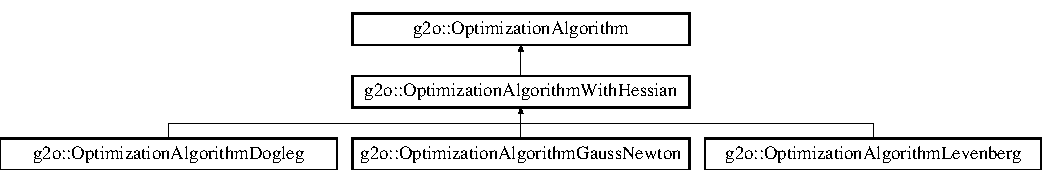
\includegraphics[height=2.285714cm]{classg2o_1_1_optimization_algorithm_with_hessian}
\end{center}
\end{figure}
\subsection*{Public Member Functions}
\begin{DoxyCompactItemize}
\item 
\mbox{\hyperlink{classg2o_1_1_optimization_algorithm_with_hessian_a1358f3500efe8b95a5af4a1b0edecdf0}{Optimization\+Algorithm\+With\+Hessian}} (\mbox{\hyperlink{classg2o_1_1_solver}{Solver}} $\ast$\mbox{\hyperlink{classg2o_1_1_optimization_algorithm_with_hessian_a85473a4073c76b1a52cf9cf175e31c45}{solver}})
\item 
virtual \mbox{\hyperlink{classg2o_1_1_optimization_algorithm_with_hessian_a9cfed4c23f1b09829cf4857cf2213745}{$\sim$\+Optimization\+Algorithm\+With\+Hessian}} ()
\item 
virtual bool \mbox{\hyperlink{classg2o_1_1_optimization_algorithm_with_hessian_ae067a9c2961718dc8a37e3b8478b6d01}{init}} (bool online=false)
\item 
virtual bool \mbox{\hyperlink{classg2o_1_1_optimization_algorithm_with_hessian_af1959727df2b7cf233a171cfed246e9a}{compute\+Marginals}} (\mbox{\hyperlink{classg2o_1_1_sparse_block_matrix}{Sparse\+Block\+Matrix}}$<$ Matrix\+Xd $>$ \&spinv, const std\+::vector$<$ std\+::pair$<$ int, int $>$ $>$ \&block\+Indices)
\item 
virtual bool \mbox{\hyperlink{classg2o_1_1_optimization_algorithm_with_hessian_aa84732c8554039ba0152693837bd1b4a}{build\+Linear\+Structure}} ()
\item 
virtual void \mbox{\hyperlink{classg2o_1_1_optimization_algorithm_with_hessian_a3ceacb3dddb14121b03e0afe7b7cfeaa}{update\+Linear\+System}} ()
\item 
virtual bool \mbox{\hyperlink{classg2o_1_1_optimization_algorithm_with_hessian_adadb23f135e037ce760f4415a0f26269}{update\+Structure}} (const std\+::vector$<$ \mbox{\hyperlink{classg2o_1_1_hyper_graph_1_1_vertex}{Hyper\+Graph\+::\+Vertex}} $\ast$$>$ \&vset, const \mbox{\hyperlink{classg2o_1_1_hyper_graph_a5e2970e236c0dcb4eff7c205d7b6b4ae}{Hyper\+Graph\+::\+Edge\+Set}} \&edges)
\item 
\mbox{\hyperlink{classg2o_1_1_solver}{Solver}} $\ast$ \mbox{\hyperlink{classg2o_1_1_optimization_algorithm_with_hessian_a85473a4073c76b1a52cf9cf175e31c45}{solver}} ()
\begin{DoxyCompactList}\small\item\em return the underlying solver used to solve the linear system \end{DoxyCompactList}\item 
virtual void \mbox{\hyperlink{classg2o_1_1_optimization_algorithm_with_hessian_a655aee24aae72b55f5edafb0a7a15137}{set\+Write\+Debug}} (bool \mbox{\hyperlink{classg2o_1_1_optimization_algorithm_with_hessian_aee8fc3dadc8bfbd50409f2e9940cbebd}{write\+Debug}})
\item 
virtual bool \mbox{\hyperlink{classg2o_1_1_optimization_algorithm_with_hessian_aee8fc3dadc8bfbd50409f2e9940cbebd}{write\+Debug}} () const
\end{DoxyCompactItemize}
\subsection*{Protected Attributes}
\begin{DoxyCompactItemize}
\item 
\mbox{\hyperlink{classg2o_1_1_solver}{Solver}} $\ast$ \mbox{\hyperlink{classg2o_1_1_optimization_algorithm_with_hessian_a88a2d1dccee8f7481ece407f2681a151}{\+\_\+solver}}
\item 
\mbox{\hyperlink{classg2o_1_1_property}{Property}}$<$ bool $>$ $\ast$ \mbox{\hyperlink{classg2o_1_1_optimization_algorithm_with_hessian_a6dd1e4e8dc2d09233c40de02b2c9fe8c}{\+\_\+write\+Debug}}
\end{DoxyCompactItemize}


\subsection{Detailed Description}
Base for solvers operating on the approximated Hessian, e.\+g., Gauss-\/\+Newton, Levenberg. 

\subsection{Constructor \& Destructor Documentation}
\mbox{\Hypertarget{classg2o_1_1_optimization_algorithm_with_hessian_a1358f3500efe8b95a5af4a1b0edecdf0}\label{classg2o_1_1_optimization_algorithm_with_hessian_a1358f3500efe8b95a5af4a1b0edecdf0}} 
\index{g2o\+::\+Optimization\+Algorithm\+With\+Hessian@{g2o\+::\+Optimization\+Algorithm\+With\+Hessian}!Optimization\+Algorithm\+With\+Hessian@{Optimization\+Algorithm\+With\+Hessian}}
\index{Optimization\+Algorithm\+With\+Hessian@{Optimization\+Algorithm\+With\+Hessian}!g2o\+::\+Optimization\+Algorithm\+With\+Hessian@{g2o\+::\+Optimization\+Algorithm\+With\+Hessian}}
\subsubsection{\texorpdfstring{Optimization\+Algorithm\+With\+Hessian()}{OptimizationAlgorithmWithHessian()}}
{\footnotesize\ttfamily g2o\+::\+Optimization\+Algorithm\+With\+Hessian\+::\+Optimization\+Algorithm\+With\+Hessian (\begin{DoxyParamCaption}\item[{\mbox{\hyperlink{classg2o_1_1_solver}{Solver}} $\ast$}]{solver }\end{DoxyParamCaption})\hspace{0.3cm}{\ttfamily [explicit]}}

\mbox{\Hypertarget{classg2o_1_1_optimization_algorithm_with_hessian_a9cfed4c23f1b09829cf4857cf2213745}\label{classg2o_1_1_optimization_algorithm_with_hessian_a9cfed4c23f1b09829cf4857cf2213745}} 
\index{g2o\+::\+Optimization\+Algorithm\+With\+Hessian@{g2o\+::\+Optimization\+Algorithm\+With\+Hessian}!````~Optimization\+Algorithm\+With\+Hessian@{$\sim$\+Optimization\+Algorithm\+With\+Hessian}}
\index{````~Optimization\+Algorithm\+With\+Hessian@{$\sim$\+Optimization\+Algorithm\+With\+Hessian}!g2o\+::\+Optimization\+Algorithm\+With\+Hessian@{g2o\+::\+Optimization\+Algorithm\+With\+Hessian}}
\subsubsection{\texorpdfstring{$\sim$\+Optimization\+Algorithm\+With\+Hessian()}{~OptimizationAlgorithmWithHessian()}}
{\footnotesize\ttfamily g2o\+::\+Optimization\+Algorithm\+With\+Hessian\+::$\sim$\+Optimization\+Algorithm\+With\+Hessian (\begin{DoxyParamCaption}{ }\end{DoxyParamCaption})\hspace{0.3cm}{\ttfamily [virtual]}}



\subsection{Member Function Documentation}
\mbox{\Hypertarget{classg2o_1_1_optimization_algorithm_with_hessian_aa84732c8554039ba0152693837bd1b4a}\label{classg2o_1_1_optimization_algorithm_with_hessian_aa84732c8554039ba0152693837bd1b4a}} 
\index{g2o\+::\+Optimization\+Algorithm\+With\+Hessian@{g2o\+::\+Optimization\+Algorithm\+With\+Hessian}!build\+Linear\+Structure@{build\+Linear\+Structure}}
\index{build\+Linear\+Structure@{build\+Linear\+Structure}!g2o\+::\+Optimization\+Algorithm\+With\+Hessian@{g2o\+::\+Optimization\+Algorithm\+With\+Hessian}}
\subsubsection{\texorpdfstring{build\+Linear\+Structure()}{buildLinearStructure()}}
{\footnotesize\ttfamily bool g2o\+::\+Optimization\+Algorithm\+With\+Hessian\+::build\+Linear\+Structure (\begin{DoxyParamCaption}{ }\end{DoxyParamCaption})\hspace{0.3cm}{\ttfamily [virtual]}}

\mbox{\Hypertarget{classg2o_1_1_optimization_algorithm_with_hessian_af1959727df2b7cf233a171cfed246e9a}\label{classg2o_1_1_optimization_algorithm_with_hessian_af1959727df2b7cf233a171cfed246e9a}} 
\index{g2o\+::\+Optimization\+Algorithm\+With\+Hessian@{g2o\+::\+Optimization\+Algorithm\+With\+Hessian}!compute\+Marginals@{compute\+Marginals}}
\index{compute\+Marginals@{compute\+Marginals}!g2o\+::\+Optimization\+Algorithm\+With\+Hessian@{g2o\+::\+Optimization\+Algorithm\+With\+Hessian}}
\subsubsection{\texorpdfstring{compute\+Marginals()}{computeMarginals()}}
{\footnotesize\ttfamily bool g2o\+::\+Optimization\+Algorithm\+With\+Hessian\+::compute\+Marginals (\begin{DoxyParamCaption}\item[{\mbox{\hyperlink{classg2o_1_1_sparse_block_matrix}{Sparse\+Block\+Matrix}}$<$ Matrix\+Xd $>$ \&}]{spinv,  }\item[{const std\+::vector$<$ std\+::pair$<$ int, int $>$ $>$ \&}]{block\+Indices }\end{DoxyParamCaption})\hspace{0.3cm}{\ttfamily [virtual]}}

computes the block diagonal elements of the pattern specified in the input and stores them in given \mbox{\hyperlink{classg2o_1_1_sparse_block_matrix}{Sparse\+Block\+Matrix}}. If your solver does not support computing the marginals, return false. 

Implements \mbox{\hyperlink{classg2o_1_1_optimization_algorithm_a67b159f3a83471ba9ebcc0a9162a0e23}{g2o\+::\+Optimization\+Algorithm}}.

\mbox{\Hypertarget{classg2o_1_1_optimization_algorithm_with_hessian_ae067a9c2961718dc8a37e3b8478b6d01}\label{classg2o_1_1_optimization_algorithm_with_hessian_ae067a9c2961718dc8a37e3b8478b6d01}} 
\index{g2o\+::\+Optimization\+Algorithm\+With\+Hessian@{g2o\+::\+Optimization\+Algorithm\+With\+Hessian}!init@{init}}
\index{init@{init}!g2o\+::\+Optimization\+Algorithm\+With\+Hessian@{g2o\+::\+Optimization\+Algorithm\+With\+Hessian}}
\subsubsection{\texorpdfstring{init()}{init()}}
{\footnotesize\ttfamily bool g2o\+::\+Optimization\+Algorithm\+With\+Hessian\+::init (\begin{DoxyParamCaption}\item[{bool}]{online = {\ttfamily false} }\end{DoxyParamCaption})\hspace{0.3cm}{\ttfamily [virtual]}}

initialize the solver, called once before the first call to \mbox{\hyperlink{classg2o_1_1_optimization_algorithm_ab174deeeb2551ceaf715ea09f0f9c077}{solve()}} 

Implements \mbox{\hyperlink{classg2o_1_1_optimization_algorithm_af5b54ea6d40a8ab4c16d448ba02a0c80}{g2o\+::\+Optimization\+Algorithm}}.

\mbox{\Hypertarget{classg2o_1_1_optimization_algorithm_with_hessian_a655aee24aae72b55f5edafb0a7a15137}\label{classg2o_1_1_optimization_algorithm_with_hessian_a655aee24aae72b55f5edafb0a7a15137}} 
\index{g2o\+::\+Optimization\+Algorithm\+With\+Hessian@{g2o\+::\+Optimization\+Algorithm\+With\+Hessian}!set\+Write\+Debug@{set\+Write\+Debug}}
\index{set\+Write\+Debug@{set\+Write\+Debug}!g2o\+::\+Optimization\+Algorithm\+With\+Hessian@{g2o\+::\+Optimization\+Algorithm\+With\+Hessian}}
\subsubsection{\texorpdfstring{set\+Write\+Debug()}{setWriteDebug()}}
{\footnotesize\ttfamily void g2o\+::\+Optimization\+Algorithm\+With\+Hessian\+::set\+Write\+Debug (\begin{DoxyParamCaption}\item[{bool}]{write\+Debug }\end{DoxyParamCaption})\hspace{0.3cm}{\ttfamily [virtual]}}

write debug output of the Hessian if system is not positive definite \mbox{\Hypertarget{classg2o_1_1_optimization_algorithm_with_hessian_a85473a4073c76b1a52cf9cf175e31c45}\label{classg2o_1_1_optimization_algorithm_with_hessian_a85473a4073c76b1a52cf9cf175e31c45}} 
\index{g2o\+::\+Optimization\+Algorithm\+With\+Hessian@{g2o\+::\+Optimization\+Algorithm\+With\+Hessian}!solver@{solver}}
\index{solver@{solver}!g2o\+::\+Optimization\+Algorithm\+With\+Hessian@{g2o\+::\+Optimization\+Algorithm\+With\+Hessian}}
\subsubsection{\texorpdfstring{solver()}{solver()}}
{\footnotesize\ttfamily \mbox{\hyperlink{classg2o_1_1_solver}{Solver}}$\ast$ g2o\+::\+Optimization\+Algorithm\+With\+Hessian\+::solver (\begin{DoxyParamCaption}{ }\end{DoxyParamCaption})\hspace{0.3cm}{\ttfamily [inline]}}



return the underlying solver used to solve the linear system 

\mbox{\Hypertarget{classg2o_1_1_optimization_algorithm_with_hessian_a3ceacb3dddb14121b03e0afe7b7cfeaa}\label{classg2o_1_1_optimization_algorithm_with_hessian_a3ceacb3dddb14121b03e0afe7b7cfeaa}} 
\index{g2o\+::\+Optimization\+Algorithm\+With\+Hessian@{g2o\+::\+Optimization\+Algorithm\+With\+Hessian}!update\+Linear\+System@{update\+Linear\+System}}
\index{update\+Linear\+System@{update\+Linear\+System}!g2o\+::\+Optimization\+Algorithm\+With\+Hessian@{g2o\+::\+Optimization\+Algorithm\+With\+Hessian}}
\subsubsection{\texorpdfstring{update\+Linear\+System()}{updateLinearSystem()}}
{\footnotesize\ttfamily void g2o\+::\+Optimization\+Algorithm\+With\+Hessian\+::update\+Linear\+System (\begin{DoxyParamCaption}{ }\end{DoxyParamCaption})\hspace{0.3cm}{\ttfamily [virtual]}}

\mbox{\Hypertarget{classg2o_1_1_optimization_algorithm_with_hessian_adadb23f135e037ce760f4415a0f26269}\label{classg2o_1_1_optimization_algorithm_with_hessian_adadb23f135e037ce760f4415a0f26269}} 
\index{g2o\+::\+Optimization\+Algorithm\+With\+Hessian@{g2o\+::\+Optimization\+Algorithm\+With\+Hessian}!update\+Structure@{update\+Structure}}
\index{update\+Structure@{update\+Structure}!g2o\+::\+Optimization\+Algorithm\+With\+Hessian@{g2o\+::\+Optimization\+Algorithm\+With\+Hessian}}
\subsubsection{\texorpdfstring{update\+Structure()}{updateStructure()}}
{\footnotesize\ttfamily bool g2o\+::\+Optimization\+Algorithm\+With\+Hessian\+::update\+Structure (\begin{DoxyParamCaption}\item[{const std\+::vector$<$ \mbox{\hyperlink{classg2o_1_1_hyper_graph_1_1_vertex}{Hyper\+Graph\+::\+Vertex}} $\ast$$>$ \&}]{vset,  }\item[{const \mbox{\hyperlink{classg2o_1_1_hyper_graph_a5e2970e236c0dcb4eff7c205d7b6b4ae}{Hyper\+Graph\+::\+Edge\+Set}} \&}]{edges }\end{DoxyParamCaption})\hspace{0.3cm}{\ttfamily [virtual]}}

update the structures for online processing 

Implements \mbox{\hyperlink{classg2o_1_1_optimization_algorithm_a350d9bb4ee701e40b75e67d26293a4bd}{g2o\+::\+Optimization\+Algorithm}}.

\mbox{\Hypertarget{classg2o_1_1_optimization_algorithm_with_hessian_aee8fc3dadc8bfbd50409f2e9940cbebd}\label{classg2o_1_1_optimization_algorithm_with_hessian_aee8fc3dadc8bfbd50409f2e9940cbebd}} 
\index{g2o\+::\+Optimization\+Algorithm\+With\+Hessian@{g2o\+::\+Optimization\+Algorithm\+With\+Hessian}!write\+Debug@{write\+Debug}}
\index{write\+Debug@{write\+Debug}!g2o\+::\+Optimization\+Algorithm\+With\+Hessian@{g2o\+::\+Optimization\+Algorithm\+With\+Hessian}}
\subsubsection{\texorpdfstring{write\+Debug()}{writeDebug()}}
{\footnotesize\ttfamily virtual bool g2o\+::\+Optimization\+Algorithm\+With\+Hessian\+::write\+Debug (\begin{DoxyParamCaption}{ }\end{DoxyParamCaption}) const\hspace{0.3cm}{\ttfamily [inline]}, {\ttfamily [virtual]}}



\subsection{Member Data Documentation}
\mbox{\Hypertarget{classg2o_1_1_optimization_algorithm_with_hessian_a88a2d1dccee8f7481ece407f2681a151}\label{classg2o_1_1_optimization_algorithm_with_hessian_a88a2d1dccee8f7481ece407f2681a151}} 
\index{g2o\+::\+Optimization\+Algorithm\+With\+Hessian@{g2o\+::\+Optimization\+Algorithm\+With\+Hessian}!\+\_\+solver@{\+\_\+solver}}
\index{\+\_\+solver@{\+\_\+solver}!g2o\+::\+Optimization\+Algorithm\+With\+Hessian@{g2o\+::\+Optimization\+Algorithm\+With\+Hessian}}
\subsubsection{\texorpdfstring{\+\_\+solver}{\_solver}}
{\footnotesize\ttfamily \mbox{\hyperlink{classg2o_1_1_solver}{Solver}}$\ast$ g2o\+::\+Optimization\+Algorithm\+With\+Hessian\+::\+\_\+solver\hspace{0.3cm}{\ttfamily [protected]}}

\mbox{\Hypertarget{classg2o_1_1_optimization_algorithm_with_hessian_a6dd1e4e8dc2d09233c40de02b2c9fe8c}\label{classg2o_1_1_optimization_algorithm_with_hessian_a6dd1e4e8dc2d09233c40de02b2c9fe8c}} 
\index{g2o\+::\+Optimization\+Algorithm\+With\+Hessian@{g2o\+::\+Optimization\+Algorithm\+With\+Hessian}!\+\_\+write\+Debug@{\+\_\+write\+Debug}}
\index{\+\_\+write\+Debug@{\+\_\+write\+Debug}!g2o\+::\+Optimization\+Algorithm\+With\+Hessian@{g2o\+::\+Optimization\+Algorithm\+With\+Hessian}}
\subsubsection{\texorpdfstring{\+\_\+write\+Debug}{\_writeDebug}}
{\footnotesize\ttfamily \mbox{\hyperlink{classg2o_1_1_property}{Property}}$<$bool$>$$\ast$ g2o\+::\+Optimization\+Algorithm\+With\+Hessian\+::\+\_\+write\+Debug\hspace{0.3cm}{\ttfamily [protected]}}



The documentation for this class was generated from the following files\+:\begin{DoxyCompactItemize}
\item 
D\+:/github/\+V\+S\+L\+A\+M/\+O\+R\+B\+S\+L\+A\+M2/\+O\+R\+B-\/\+S\+L\+A\+M2-\/master/\+Thirdparty/g2o/g2o/core/\mbox{\hyperlink{optimization__algorithm__with__hessian_8h}{optimization\+\_\+algorithm\+\_\+with\+\_\+hessian.\+h}}\item 
D\+:/github/\+V\+S\+L\+A\+M/\+O\+R\+B\+S\+L\+A\+M2/\+O\+R\+B-\/\+S\+L\+A\+M2-\/master/\+Thirdparty/g2o/g2o/core/\mbox{\hyperlink{optimization__algorithm__with__hessian_8cpp}{optimization\+\_\+algorithm\+\_\+with\+\_\+hessian.\+cpp}}\end{DoxyCompactItemize}

\hypertarget{class_o_r_b___s_l_a_m2_1_1_optimizer}{}\section{O\+R\+B\+\_\+\+S\+L\+A\+M2\+:\+:Optimizer Class Reference}
\label{class_o_r_b___s_l_a_m2_1_1_optimizer}\index{O\+R\+B\+\_\+\+S\+L\+A\+M2\+::\+Optimizer@{O\+R\+B\+\_\+\+S\+L\+A\+M2\+::\+Optimizer}}


{\ttfamily \#include $<$Optimizer.\+h$>$}

\subsection*{Static Public Member Functions}
\begin{DoxyCompactItemize}
\item 
static void \mbox{\hyperlink{class_o_r_b___s_l_a_m2_1_1_optimizer_aac6bf926792ed8a013d64897879a89ec}{Bundle\+Adjustment}} (const std\+::vector$<$ \mbox{\hyperlink{class_o_r_b___s_l_a_m2_1_1_key_frame}{Key\+Frame}} $\ast$$>$ \&vp\+KF, const std\+::vector$<$ \mbox{\hyperlink{class_o_r_b___s_l_a_m2_1_1_map_point}{Map\+Point}} $\ast$$>$ \&vp\+MP, int n\+Iterations=5, bool $\ast$pb\+Stop\+Flag=N\+U\+LL, const unsigned long n\+Loop\+KF=0, const bool b\+Robust=true)
\begin{DoxyCompactList}\small\item\em bundle adjustment Optimization \end{DoxyCompactList}\item 
static void \mbox{\hyperlink{class_o_r_b___s_l_a_m2_1_1_optimizer_aaa9b8a4c16296bf2981b0aaf4ee3189c}{Global\+Bundle\+Adjustemnt}} (\mbox{\hyperlink{class_o_r_b___s_l_a_m2_1_1_map}{Map}} $\ast$p\+Map, int n\+Iterations=5, bool $\ast$pb\+Stop\+Flag=N\+U\+LL, const unsigned long n\+Loop\+KF=0, const bool b\+Robust=true)
\item 
static void \mbox{\hyperlink{class_o_r_b___s_l_a_m2_1_1_optimizer_ab70e0b4f366b65a0c1ae8b2def19d339}{Local\+Bundle\+Adjustment}} (\mbox{\hyperlink{class_o_r_b___s_l_a_m2_1_1_key_frame}{Key\+Frame}} $\ast$p\+KF, bool $\ast$pb\+Stop\+Flag, \mbox{\hyperlink{class_o_r_b___s_l_a_m2_1_1_map}{Map}} $\ast$p\+Map)
\begin{DoxyCompactList}\small\item\em Local Bundle Adjustment. \end{DoxyCompactList}\item 
static int \mbox{\hyperlink{class_o_r_b___s_l_a_m2_1_1_optimizer_a7415d78b8a2323b88e108fa1ea3bf2d3}{Pose\+Optimization}} (\mbox{\hyperlink{class_o_r_b___s_l_a_m2_1_1_frame}{Frame}} $\ast$p\+Frame)
\begin{DoxyCompactList}\small\item\em Pose Only Optimization. \end{DoxyCompactList}\item 
static void \mbox{\hyperlink{class_o_r_b___s_l_a_m2_1_1_optimizer_a5a53ab409feed7f92547eb79a2d7f6e9}{Optimize\+Essential\+Graph}} (\mbox{\hyperlink{class_o_r_b___s_l_a_m2_1_1_map}{Map}} $\ast$p\+Map, \mbox{\hyperlink{class_o_r_b___s_l_a_m2_1_1_key_frame}{Key\+Frame}} $\ast$p\+Loop\+KF, \mbox{\hyperlink{class_o_r_b___s_l_a_m2_1_1_key_frame}{Key\+Frame}} $\ast$p\+Cur\+KF, const \mbox{\hyperlink{class_o_r_b___s_l_a_m2_1_1_loop_closing_ae9ada143a8308ce32990a7c7b5d533ab}{Loop\+Closing\+::\+Key\+Frame\+And\+Pose}} \&Non\+Corrected\+Sim3, const \mbox{\hyperlink{class_o_r_b___s_l_a_m2_1_1_loop_closing_ae9ada143a8308ce32990a7c7b5d533ab}{Loop\+Closing\+::\+Key\+Frame\+And\+Pose}} \&Corrected\+Sim3, const map$<$ \mbox{\hyperlink{class_o_r_b___s_l_a_m2_1_1_key_frame}{Key\+Frame}} $\ast$, set$<$ \mbox{\hyperlink{class_o_r_b___s_l_a_m2_1_1_key_frame}{Key\+Frame}} $\ast$$>$ $>$ \&Loop\+Connections, const bool \&b\+Fix\+Scale)
\begin{DoxyCompactList}\small\item\em 闭环检测后,\+Essential\+Graph优化 \end{DoxyCompactList}\item 
static int \mbox{\hyperlink{class_o_r_b___s_l_a_m2_1_1_optimizer_a91fbb960965c99e9802a5de45515813c}{Optimize\+Sim3}} (\mbox{\hyperlink{class_o_r_b___s_l_a_m2_1_1_key_frame}{Key\+Frame}} $\ast$p\+K\+F1, \mbox{\hyperlink{class_o_r_b___s_l_a_m2_1_1_key_frame}{Key\+Frame}} $\ast$p\+K\+F2, std\+::vector$<$ \mbox{\hyperlink{class_o_r_b___s_l_a_m2_1_1_map_point}{Map\+Point}} $\ast$$>$ \&vp\+Matches1, \mbox{\hyperlink{structg2o_1_1_sim3}{g2o\+::\+Sim3}} \&g2o\+S12, const float th2, const bool b\+Fix\+Scale)
\begin{DoxyCompactList}\small\item\em 形成闭环时进行\+Sim3优化 \end{DoxyCompactList}\end{DoxyCompactItemize}


\subsection{Member Function Documentation}
\mbox{\Hypertarget{class_o_r_b___s_l_a_m2_1_1_optimizer_aac6bf926792ed8a013d64897879a89ec}\label{class_o_r_b___s_l_a_m2_1_1_optimizer_aac6bf926792ed8a013d64897879a89ec}} 
\index{O\+R\+B\+\_\+\+S\+L\+A\+M2\+::\+Optimizer@{O\+R\+B\+\_\+\+S\+L\+A\+M2\+::\+Optimizer}!Bundle\+Adjustment@{Bundle\+Adjustment}}
\index{Bundle\+Adjustment@{Bundle\+Adjustment}!O\+R\+B\+\_\+\+S\+L\+A\+M2\+::\+Optimizer@{O\+R\+B\+\_\+\+S\+L\+A\+M2\+::\+Optimizer}}
\subsubsection{\texorpdfstring{Bundle\+Adjustment()}{BundleAdjustment()}}
{\footnotesize\ttfamily void O\+R\+B\+\_\+\+S\+L\+A\+M2\+::\+Optimizer\+::\+Bundle\+Adjustment (\begin{DoxyParamCaption}\item[{const std\+::vector$<$ \mbox{\hyperlink{class_o_r_b___s_l_a_m2_1_1_key_frame}{Key\+Frame}} $\ast$$>$ \&}]{vp\+KF,  }\item[{const std\+::vector$<$ \mbox{\hyperlink{class_o_r_b___s_l_a_m2_1_1_map_point}{Map\+Point}} $\ast$$>$ \&}]{vp\+MP,  }\item[{int}]{n\+Iterations = {\ttfamily 5},  }\item[{bool $\ast$}]{pb\+Stop\+Flag = {\ttfamily NULL},  }\item[{const unsigned long}]{n\+Loop\+KF = {\ttfamily 0},  }\item[{const bool}]{b\+Robust = {\ttfamily true} }\end{DoxyParamCaption})\hspace{0.3cm}{\ttfamily [static]}}



bundle adjustment Optimization 

3\+D-\/2D 最小化重投影误差 e = (u,v) -\/ project(\+Tcw$\ast$\+Pw) ~\newline

\begin{DoxyEnumerate}
\item Vertex\+: \mbox{\hyperlink{classg2o_1_1_vertex_s_e3_expmap}{g2o\+::\+Vertex\+S\+E3\+Expmap()}},即当前帧的\+Tcw \mbox{\hyperlink{classg2o_1_1_vertex_s_b_a_point_x_y_z}{g2o\+::\+Vertex\+S\+B\+A\+Point\+X\+Y\+Z()}},\+Map\+Point的m\+World\+Pos
\item Edge\+:
\begin{DoxyItemize}
\item \mbox{\hyperlink{classg2o_1_1_edge_s_e3_project_x_y_z}{g2o\+::\+Edge\+S\+E3\+Project\+X\+Y\+Z()}},\+Base\+Binary\+Edge
\begin{DoxyItemize}
\item Vertex:待优化当前帧的\+Tcw
\item Vertex:待优化\+Map\+Point的m\+World\+Pos
\item measurement:\+Map\+Point在当前帧中的二维位置(u,v)
\item Info\+Matrix\+: inv\+Sigma2(与特征点所在的尺度有关)
\end{DoxyItemize}
\end{DoxyItemize}
\end{DoxyEnumerate}


\begin{DoxyParams}{Parameters}
{\em vp\+K\+Fs} & 关键帧 vp\+MP Map\+Points n\+Iterations 迭代次数(20次) pb\+Stop\+Flag 是否强制暂停 n\+Loop\+KF 关键帧的个数 b\+Robust 是否使用核函数 \\
\hline
\end{DoxyParams}
\mbox{\Hypertarget{class_o_r_b___s_l_a_m2_1_1_optimizer_aaa9b8a4c16296bf2981b0aaf4ee3189c}\label{class_o_r_b___s_l_a_m2_1_1_optimizer_aaa9b8a4c16296bf2981b0aaf4ee3189c}} 
\index{O\+R\+B\+\_\+\+S\+L\+A\+M2\+::\+Optimizer@{O\+R\+B\+\_\+\+S\+L\+A\+M2\+::\+Optimizer}!Global\+Bundle\+Adjustemnt@{Global\+Bundle\+Adjustemnt}}
\index{Global\+Bundle\+Adjustemnt@{Global\+Bundle\+Adjustemnt}!O\+R\+B\+\_\+\+S\+L\+A\+M2\+::\+Optimizer@{O\+R\+B\+\_\+\+S\+L\+A\+M2\+::\+Optimizer}}
\subsubsection{\texorpdfstring{Global\+Bundle\+Adjustemnt()}{GlobalBundleAdjustemnt()}}
{\footnotesize\ttfamily void O\+R\+B\+\_\+\+S\+L\+A\+M2\+::\+Optimizer\+::\+Global\+Bundle\+Adjustemnt (\begin{DoxyParamCaption}\item[{\mbox{\hyperlink{class_o_r_b___s_l_a_m2_1_1_map}{Map}} $\ast$}]{p\+Map,  }\item[{int}]{n\+Iterations = {\ttfamily 5},  }\item[{bool $\ast$}]{pb\+Stop\+Flag = {\ttfamily NULL},  }\item[{const unsigned long}]{n\+Loop\+KF = {\ttfamily 0},  }\item[{const bool}]{b\+Robust = {\ttfamily true} }\end{DoxyParamCaption})\hspace{0.3cm}{\ttfamily [static]}}

\mbox{\Hypertarget{class_o_r_b___s_l_a_m2_1_1_optimizer_ab70e0b4f366b65a0c1ae8b2def19d339}\label{class_o_r_b___s_l_a_m2_1_1_optimizer_ab70e0b4f366b65a0c1ae8b2def19d339}} 
\index{O\+R\+B\+\_\+\+S\+L\+A\+M2\+::\+Optimizer@{O\+R\+B\+\_\+\+S\+L\+A\+M2\+::\+Optimizer}!Local\+Bundle\+Adjustment@{Local\+Bundle\+Adjustment}}
\index{Local\+Bundle\+Adjustment@{Local\+Bundle\+Adjustment}!O\+R\+B\+\_\+\+S\+L\+A\+M2\+::\+Optimizer@{O\+R\+B\+\_\+\+S\+L\+A\+M2\+::\+Optimizer}}
\subsubsection{\texorpdfstring{Local\+Bundle\+Adjustment()}{LocalBundleAdjustment()}}
{\footnotesize\ttfamily void O\+R\+B\+\_\+\+S\+L\+A\+M2\+::\+Optimizer\+::\+Local\+Bundle\+Adjustment (\begin{DoxyParamCaption}\item[{\mbox{\hyperlink{class_o_r_b___s_l_a_m2_1_1_key_frame}{Key\+Frame}} $\ast$}]{p\+KF,  }\item[{bool $\ast$}]{pb\+Stop\+Flag,  }\item[{\mbox{\hyperlink{class_o_r_b___s_l_a_m2_1_1_map}{Map}} $\ast$}]{p\+Map }\end{DoxyParamCaption})\hspace{0.3cm}{\ttfamily [static]}}



Local Bundle Adjustment. 


\begin{DoxyEnumerate}
\item Vertex\+:
\begin{DoxyItemize}
\item \mbox{\hyperlink{classg2o_1_1_vertex_s_e3_expmap}{g2o\+::\+Vertex\+S\+E3\+Expmap()}},\+Local\+Key\+Frames,即当前关键帧的位姿、与当前关键帧相连的关键帧的位姿
\item \mbox{\hyperlink{classg2o_1_1_vertex_s_e3_expmap}{g2o\+::\+Vertex\+S\+E3\+Expmap()}},\+Fixed\+Cameras,即能观测到\+Local\+Map\+Points的关键帧(并且不属于\+Local\+Key\+Frames)的位姿,在优化中这些关键帧的位姿不变
\item \mbox{\hyperlink{classg2o_1_1_vertex_s_b_a_point_x_y_z}{g2o\+::\+Vertex\+S\+B\+A\+Point\+X\+Y\+Z()}},\+Local\+Map\+Points,即\+Local\+Key\+Frames能观测到的所有\+Map\+Points的位置
\end{DoxyItemize}
\item Edge\+:
\begin{DoxyItemize}
\item \mbox{\hyperlink{classg2o_1_1_edge_s_e3_project_x_y_z}{g2o\+::\+Edge\+S\+E3\+Project\+X\+Y\+Z()}},\+Base\+Binary\+Edge
\begin{DoxyItemize}
\item Vertex:关键帧的\+Tcw,\+Map\+Point的\+Pw
\item measurement:\+Map\+Point在关键帧中的二维位置(u,v)
\item Info\+Matrix\+: inv\+Sigma2(与特征点所在的尺度有关)
\end{DoxyItemize}
\item \mbox{\hyperlink{classg2o_1_1_edge_stereo_s_e3_project_x_y_z}{g2o\+::\+Edge\+Stereo\+S\+E3\+Project\+X\+Y\+Z()}},\+Base\+Binary\+Edge
\begin{DoxyItemize}
\item Vertex:关键帧的\+Tcw,\+Map\+Point的\+Pw
\item measurement:\+Map\+Point在关键帧中的二维位置(ul,v,ur)
\item Info\+Matrix\+: inv\+Sigma2(与特征点所在的尺度有关)
\end{DoxyItemize}
\end{DoxyItemize}
\end{DoxyEnumerate}


\begin{DoxyParams}{Parameters}
{\em p\+KF} & \mbox{\hyperlink{class_o_r_b___s_l_a_m2_1_1_key_frame}{Key\+Frame}} \\
\hline
{\em pb\+Stop\+Flag} & 是否停止优化的标志 \\
\hline
{\em p\+Map} & 在优化后,更新状态时需要用到\+Map的互斥量m\+Mutex\+Map\+Update \\
\hline
\end{DoxyParams}
\mbox{\Hypertarget{class_o_r_b___s_l_a_m2_1_1_optimizer_a5a53ab409feed7f92547eb79a2d7f6e9}\label{class_o_r_b___s_l_a_m2_1_1_optimizer_a5a53ab409feed7f92547eb79a2d7f6e9}} 
\index{O\+R\+B\+\_\+\+S\+L\+A\+M2\+::\+Optimizer@{O\+R\+B\+\_\+\+S\+L\+A\+M2\+::\+Optimizer}!Optimize\+Essential\+Graph@{Optimize\+Essential\+Graph}}
\index{Optimize\+Essential\+Graph@{Optimize\+Essential\+Graph}!O\+R\+B\+\_\+\+S\+L\+A\+M2\+::\+Optimizer@{O\+R\+B\+\_\+\+S\+L\+A\+M2\+::\+Optimizer}}
\subsubsection{\texorpdfstring{Optimize\+Essential\+Graph()}{OptimizeEssentialGraph()}}
{\footnotesize\ttfamily void O\+R\+B\+\_\+\+S\+L\+A\+M2\+::\+Optimizer\+::\+Optimize\+Essential\+Graph (\begin{DoxyParamCaption}\item[{\mbox{\hyperlink{class_o_r_b___s_l_a_m2_1_1_map}{Map}} $\ast$}]{p\+Map,  }\item[{\mbox{\hyperlink{class_o_r_b___s_l_a_m2_1_1_key_frame}{Key\+Frame}} $\ast$}]{p\+Loop\+KF,  }\item[{\mbox{\hyperlink{class_o_r_b___s_l_a_m2_1_1_key_frame}{Key\+Frame}} $\ast$}]{p\+Cur\+KF,  }\item[{const \mbox{\hyperlink{class_o_r_b___s_l_a_m2_1_1_loop_closing_ae9ada143a8308ce32990a7c7b5d533ab}{Loop\+Closing\+::\+Key\+Frame\+And\+Pose}} \&}]{Non\+Corrected\+Sim3,  }\item[{const \mbox{\hyperlink{class_o_r_b___s_l_a_m2_1_1_loop_closing_ae9ada143a8308ce32990a7c7b5d533ab}{Loop\+Closing\+::\+Key\+Frame\+And\+Pose}} \&}]{Corrected\+Sim3,  }\item[{const map$<$ \mbox{\hyperlink{class_o_r_b___s_l_a_m2_1_1_key_frame}{Key\+Frame}} $\ast$, set$<$ \mbox{\hyperlink{class_o_r_b___s_l_a_m2_1_1_key_frame}{Key\+Frame}} $\ast$$>$ $>$ \&}]{Loop\+Connections,  }\item[{const bool \&}]{b\+Fix\+Scale }\end{DoxyParamCaption})\hspace{0.3cm}{\ttfamily [static]}}



闭环检测后,\+Essential\+Graph优化 


\begin{DoxyEnumerate}
\item Vertex\+:
\begin{DoxyItemize}
\item g2o\+::\+Vertex\+Sim3\+Expmap,\+Essential graph中关键帧的位姿
\end{DoxyItemize}
\item Edge\+:
\begin{DoxyItemize}
\item \mbox{\hyperlink{classg2o_1_1_edge_sim3}{g2o\+::\+Edge\+Sim3()}},\+Base\+Binary\+Edge
\begin{DoxyItemize}
\item Vertex:关键帧的\+Tcw,\+Map\+Point的\+Pw
\item measurement:经过\+Correct\+Loop函数步骤2,\+Sim3传播校正后的位姿
\item Info\+Matrix\+: 单位矩阵 ~\newline
 
\begin{DoxyParams}{Parameters}
{\em p\+Map} & 全局地图 \\
\hline
{\em p\+Loop\+KF} & 闭环匹配上的关键帧 \\
\hline
{\em p\+Cur\+KF} & 当前关键帧 \\
\hline
{\em Non\+Corrected\+Sim3} & 未经过\+Sim3传播调整过的关键帧位姿 \\
\hline
{\em Corrected\+Sim3} & 经过\+Sim3传播调整过的关键帧位姿 \\
\hline
{\em Loop\+Connections} & 因闭环时\+Map\+Points调整而新生成的边 \\
\hline
\end{DoxyParams}

\end{DoxyItemize}
\end{DoxyItemize}
\end{DoxyEnumerate}\mbox{\Hypertarget{class_o_r_b___s_l_a_m2_1_1_optimizer_a91fbb960965c99e9802a5de45515813c}\label{class_o_r_b___s_l_a_m2_1_1_optimizer_a91fbb960965c99e9802a5de45515813c}} 
\index{O\+R\+B\+\_\+\+S\+L\+A\+M2\+::\+Optimizer@{O\+R\+B\+\_\+\+S\+L\+A\+M2\+::\+Optimizer}!Optimize\+Sim3@{Optimize\+Sim3}}
\index{Optimize\+Sim3@{Optimize\+Sim3}!O\+R\+B\+\_\+\+S\+L\+A\+M2\+::\+Optimizer@{O\+R\+B\+\_\+\+S\+L\+A\+M2\+::\+Optimizer}}
\subsubsection{\texorpdfstring{Optimize\+Sim3()}{OptimizeSim3()}}
{\footnotesize\ttfamily int O\+R\+B\+\_\+\+S\+L\+A\+M2\+::\+Optimizer\+::\+Optimize\+Sim3 (\begin{DoxyParamCaption}\item[{\mbox{\hyperlink{class_o_r_b___s_l_a_m2_1_1_key_frame}{Key\+Frame}} $\ast$}]{p\+K\+F1,  }\item[{\mbox{\hyperlink{class_o_r_b___s_l_a_m2_1_1_key_frame}{Key\+Frame}} $\ast$}]{p\+K\+F2,  }\item[{std\+::vector$<$ \mbox{\hyperlink{class_o_r_b___s_l_a_m2_1_1_map_point}{Map\+Point}} $\ast$$>$ \&}]{vp\+Matches1,  }\item[{\mbox{\hyperlink{structg2o_1_1_sim3}{g2o\+::\+Sim3}} \&}]{g2o\+S12,  }\item[{const float}]{th2,  }\item[{const bool}]{b\+Fix\+Scale }\end{DoxyParamCaption})\hspace{0.3cm}{\ttfamily [static]}}



形成闭环时进行\+Sim3优化 


\begin{DoxyEnumerate}
\item Vertex\+:
\begin{DoxyItemize}
\item \mbox{\hyperlink{classg2o_1_1_vertex_sim3_expmap}{g2o\+::\+Vertex\+Sim3\+Expmap()}},两个关键帧的位姿
\item \mbox{\hyperlink{classg2o_1_1_vertex_s_b_a_point_x_y_z}{g2o\+::\+Vertex\+S\+B\+A\+Point\+X\+Y\+Z()}},两个关键帧共有的\+Map\+Points
\end{DoxyItemize}
\item Edge\+:
\begin{DoxyItemize}
\item \mbox{\hyperlink{classg2o_1_1_edge_sim3_project_x_y_z}{g2o\+::\+Edge\+Sim3\+Project\+X\+Y\+Z()}},\+Base\+Binary\+Edge
\begin{DoxyItemize}
\item Vertex:关键帧的\+Sim3,\+Map\+Point的\+Pw
\item measurement:\+Map\+Point在关键帧中的二维位置(u,v)
\item Info\+Matrix\+: inv\+Sigma2(与特征点所在的尺度有关)
\end{DoxyItemize}
\item \mbox{\hyperlink{classg2o_1_1_edge_inverse_sim3_project_x_y_z}{g2o\+::\+Edge\+Inverse\+Sim3\+Project\+X\+Y\+Z()}},\+Base\+Binary\+Edge
\begin{DoxyItemize}
\item Vertex:关键帧的\+Sim3,\+Map\+Point的\+Pw
\item measurement:\+Map\+Point在关键帧中的二维位置(u,v)
\item Info\+Matrix\+: inv\+Sigma2(与特征点所在的尺度有关)
\end{DoxyItemize}
\end{DoxyItemize}
\end{DoxyEnumerate}


\begin{DoxyParams}{Parameters}
{\em p\+K\+F1} & \mbox{\hyperlink{class_o_r_b___s_l_a_m2_1_1_key_frame}{Key\+Frame}} \\
\hline
{\em p\+K\+F2} & \mbox{\hyperlink{class_o_r_b___s_l_a_m2_1_1_key_frame}{Key\+Frame}} \\
\hline
{\em vp\+Matches1} & 两个关键帧的匹配关系 \\
\hline
{\em g2o\+S12} & 两个关键帧间的\+Sim3变换 \\
\hline
{\em th2} & 核函数阈值 \\
\hline
{\em b\+Fix\+Scale} & 是否优化尺度,弹目进行尺度优化,双目不进行尺度优化 \\
\hline
\end{DoxyParams}
\mbox{\Hypertarget{class_o_r_b___s_l_a_m2_1_1_optimizer_a7415d78b8a2323b88e108fa1ea3bf2d3}\label{class_o_r_b___s_l_a_m2_1_1_optimizer_a7415d78b8a2323b88e108fa1ea3bf2d3}} 
\index{O\+R\+B\+\_\+\+S\+L\+A\+M2\+::\+Optimizer@{O\+R\+B\+\_\+\+S\+L\+A\+M2\+::\+Optimizer}!Pose\+Optimization@{Pose\+Optimization}}
\index{Pose\+Optimization@{Pose\+Optimization}!O\+R\+B\+\_\+\+S\+L\+A\+M2\+::\+Optimizer@{O\+R\+B\+\_\+\+S\+L\+A\+M2\+::\+Optimizer}}
\subsubsection{\texorpdfstring{Pose\+Optimization()}{PoseOptimization()}}
{\footnotesize\ttfamily int O\+R\+B\+\_\+\+S\+L\+A\+M2\+::\+Optimizer\+::\+Pose\+Optimization (\begin{DoxyParamCaption}\item[{\mbox{\hyperlink{class_o_r_b___s_l_a_m2_1_1_frame}{Frame}} $\ast$}]{p\+Frame }\end{DoxyParamCaption})\hspace{0.3cm}{\ttfamily [static]}}



Pose Only Optimization. 

3\+D-\/2D 最小化重投影误差 e = (u,v) -\/ project(\+Tcw$\ast$\+Pw) ~\newline
只优化\+Frame的\+Tcw,不优化\+Map\+Points的坐标


\begin{DoxyEnumerate}
\item Vertex\+: \mbox{\hyperlink{classg2o_1_1_vertex_s_e3_expmap}{g2o\+::\+Vertex\+S\+E3\+Expmap()}},即当前帧的\+Tcw
\item Edge\+:
\begin{DoxyItemize}
\item \mbox{\hyperlink{classg2o_1_1_edge_s_e3_project_x_y_z_only_pose}{g2o\+::\+Edge\+S\+E3\+Project\+X\+Y\+Z\+Only\+Pose()}},\+Base\+Unary\+Edge
\begin{DoxyItemize}
\item Vertex:待优化当前帧的\+Tcw
\item measurement:\+Map\+Point在当前帧中的二维位置(u,v)
\item Info\+Matrix\+: inv\+Sigma2(与特征点所在的尺度有关)
\end{DoxyItemize}
\item \mbox{\hyperlink{classg2o_1_1_edge_stereo_s_e3_project_x_y_z_only_pose}{g2o\+::\+Edge\+Stereo\+S\+E3\+Project\+X\+Y\+Z\+Only\+Pose()}},\+Base\+Unary\+Edge
\begin{DoxyItemize}
\item Vertex:待优化当前帧的\+Tcw
\item measurement:\+Map\+Point在当前帧中的二维位置(ul,v,ur)
\item Info\+Matrix\+: inv\+Sigma2(与特征点所在的尺度有关)
\end{DoxyItemize}
\end{DoxyItemize}
\end{DoxyEnumerate}


\begin{DoxyParams}{Parameters}
{\em p\+Frame} & \mbox{\hyperlink{class_o_r_b___s_l_a_m2_1_1_frame}{Frame}} \\
\hline
\end{DoxyParams}
\begin{DoxyReturn}{Returns}
inliers数量 
\end{DoxyReturn}


The documentation for this class was generated from the following files\+:\begin{DoxyCompactItemize}
\item 
D\+:/github/\+V\+S\+L\+A\+M/\+O\+R\+B\+S\+L\+A\+M2/\+O\+R\+B-\/\+S\+L\+A\+M2-\/master/include/\mbox{\hyperlink{_optimizer_8h}{Optimizer.\+h}}\item 
D\+:/github/\+V\+S\+L\+A\+M/\+O\+R\+B\+S\+L\+A\+M2/\+O\+R\+B-\/\+S\+L\+A\+M2-\/master/src/\mbox{\hyperlink{_optimizer_8cpp}{Optimizer.\+cpp}}\end{DoxyCompactItemize}

\hypertarget{class_o_r_b___s_l_a_m2_1_1_o_r_bextractor}{}\section{O\+R\+B\+\_\+\+S\+L\+A\+M2\+:\+:O\+R\+Bextractor Class Reference}
\label{class_o_r_b___s_l_a_m2_1_1_o_r_bextractor}\index{O\+R\+B\+\_\+\+S\+L\+A\+M2\+::\+O\+R\+Bextractor@{O\+R\+B\+\_\+\+S\+L\+A\+M2\+::\+O\+R\+Bextractor}}


{\ttfamily \#include $<$O\+R\+Bextractor.\+h$>$}

\subsection*{Public Types}
\begin{DoxyCompactItemize}
\item 
enum \{ \mbox{\hyperlink{class_o_r_b___s_l_a_m2_1_1_o_r_bextractor_a5f326a8b3ba190c121dcdeea1d287f69a0f496d253d29ce9b88ab80575b311b56}{H\+A\+R\+R\+I\+S\+\_\+\+S\+C\+O\+RE}} =0, 
\mbox{\hyperlink{class_o_r_b___s_l_a_m2_1_1_o_r_bextractor_a5f326a8b3ba190c121dcdeea1d287f69a504fff69083dc0081dbb34ac5d9c00b3}{F\+A\+S\+T\+\_\+\+S\+C\+O\+RE}} =1
 \}
\end{DoxyCompactItemize}
\subsection*{Public Member Functions}
\begin{DoxyCompactItemize}
\item 
\mbox{\hyperlink{class_o_r_b___s_l_a_m2_1_1_o_r_bextractor_aaa8e010415e516246e171b9bbb9f84af}{O\+R\+Bextractor}} (int \mbox{\hyperlink{class_o_r_b___s_l_a_m2_1_1_o_r_bextractor_ab74b569810b3d3288c642cc48fd65c4c}{nfeatures}}, float \mbox{\hyperlink{class_o_r_b___s_l_a_m2_1_1_o_r_bextractor_a13b9c3883b3fb19cb756f841cb948908}{scale\+Factor}}, int \mbox{\hyperlink{class_o_r_b___s_l_a_m2_1_1_o_r_bextractor_aaf5c435dfb3fb2220c3847cd5f536e2f}{nlevels}}, int \mbox{\hyperlink{class_o_r_b___s_l_a_m2_1_1_o_r_bextractor_a8997b404b50b563ffd2aea6b8130dd2a}{ini\+Th\+F\+A\+ST}}, int \mbox{\hyperlink{class_o_r_b___s_l_a_m2_1_1_o_r_bextractor_a72fcac0df56c0bfe430475082df56823}{min\+Th\+F\+A\+ST}})
\begin{DoxyCompactList}\small\item\em Construct a new \mbox{\hyperlink{class_o_r_b___s_l_a_m2_1_1_o_r_bextractor_aaa8e010415e516246e171b9bbb9f84af}{O\+R\+Bextractor\+::\+O\+R\+Bextractor}} object. \end{DoxyCompactList}\item 
\mbox{\hyperlink{class_o_r_b___s_l_a_m2_1_1_o_r_bextractor_ab0e5801da8f6dee0261aef5cf19e73b3}{$\sim$\+O\+R\+Bextractor}} ()
\item 
void \mbox{\hyperlink{class_o_r_b___s_l_a_m2_1_1_o_r_bextractor_a05117a839e4261638b0413fff2dc9e1b}{operator()}} (cv\+::\+Input\+Array image, cv\+::\+Input\+Array mask, std\+::vector$<$ cv\+::\+Key\+Point $>$ \&keypoints, cv\+::\+Output\+Array descriptors)
\begin{DoxyCompactList}\small\item\em 计算描述子 \end{DoxyCompactList}\item 
int \mbox{\hyperlink{class_o_r_b___s_l_a_m2_1_1_o_r_bextractor_abaad86a9c65eed8a2f8af9604b1a53ee}{Get\+Levels}} ()
\item 
float \mbox{\hyperlink{class_o_r_b___s_l_a_m2_1_1_o_r_bextractor_a3352294ae4ae250a406140d2ae6f7286}{Get\+Scale\+Factor}} ()
\item 
std\+::vector$<$ float $>$ \mbox{\hyperlink{class_o_r_b___s_l_a_m2_1_1_o_r_bextractor_a977d96ed602e3a6ff036afc2f2f213fd}{Get\+Scale\+Factors}} ()
\item 
std\+::vector$<$ float $>$ \mbox{\hyperlink{class_o_r_b___s_l_a_m2_1_1_o_r_bextractor_aa56b36e338372ec7cba3945c9194da4a}{Get\+Inverse\+Scale\+Factors}} ()
\item 
std\+::vector$<$ float $>$ \mbox{\hyperlink{class_o_r_b___s_l_a_m2_1_1_o_r_bextractor_a8f574b3b1314c5aa645135cb2f3dca3c}{Get\+Scale\+Sigma\+Squares}} ()
\item 
std\+::vector$<$ float $>$ \mbox{\hyperlink{class_o_r_b___s_l_a_m2_1_1_o_r_bextractor_a1ddabdd67709d7df17000cc2966c47c7}{Get\+Inverse\+Scale\+Sigma\+Squares}} ()
\end{DoxyCompactItemize}
\subsection*{Public Attributes}
\begin{DoxyCompactItemize}
\item 
std\+::vector$<$ cv\+::\+Mat $>$ \mbox{\hyperlink{class_o_r_b___s_l_a_m2_1_1_o_r_bextractor_a57f88e0959582dde9ae5bdee1fe3de65}{mv\+Image\+Pyramid}}
\end{DoxyCompactItemize}
\subsection*{Protected Member Functions}
\begin{DoxyCompactItemize}
\item 
void \mbox{\hyperlink{class_o_r_b___s_l_a_m2_1_1_o_r_bextractor_a058f24d80bb0b2c7d6fc0bdd3d9144d1}{Compute\+Pyramid}} (cv\+::\+Mat image)
\begin{DoxyCompactList}\small\item\em 构建图像金字塔 远出看是角点的地方,进出看可能不是角点了,这个问题成为尺度不变性,需要构建图像金字塔解决。 通过在每一层金字塔上检测角点和角点的方向来实现。总层数为nlevels。计算得到每层的图像存到mv\+Image\+Pyramid容器中 图像金字塔的计算通过resize函数实现 \end{DoxyCompactList}\item 
void \mbox{\hyperlink{class_o_r_b___s_l_a_m2_1_1_o_r_bextractor_a9a543d9b2aec1e521058ee9522937adc}{Compute\+Key\+Points\+Oct\+Tree}} (std\+::vector$<$ std\+::vector$<$ cv\+::\+Key\+Point $>$ $>$ \&all\+Keypoints)
\item 
std\+::vector$<$ cv\+::\+Key\+Point $>$ \mbox{\hyperlink{class_o_r_b___s_l_a_m2_1_1_o_r_bextractor_ac6b7b27447324af33fa60d6dc0c8ffa0}{Distribute\+Oct\+Tree}} (const std\+::vector$<$ cv\+::\+Key\+Point $>$ \&v\+To\+Distribute\+Keys, const int \&minX, const int \&maxX, const int \&minY, const int \&maxY, const int \&n\+Features, const int \&level)
\begin{DoxyCompactList}\small\item\em Orb extrator distribute oct\+Tree 计算fast特征点并进行筛选 先用(max\+X-\/minX)/(max\+Y-\/minY)来确定四叉数有几个初始节点,这里有 bug,如果输入的是一张宽高比小于0.5 的图像, n\+Ini 计算得到 0,下一步计算 hX 会报错,例如round(640/480)=1,所以只有一个初始节点,(\+U\+L,\+U\+R,\+B\+L,\+B\+R)就会分布到被裁掉边界后的图像的四个角。 \end{DoxyCompactList}\item 
void \mbox{\hyperlink{class_o_r_b___s_l_a_m2_1_1_o_r_bextractor_a56890a2032077fbfdf48687786985548}{Compute\+Key\+Points\+Old}} (std\+::vector$<$ std\+::vector$<$ cv\+::\+Key\+Point $>$ $>$ \&all\+Keypoints)
\end{DoxyCompactItemize}
\subsection*{Protected Attributes}
\begin{DoxyCompactItemize}
\item 
std\+::vector$<$ cv\+::\+Point $>$ \mbox{\hyperlink{class_o_r_b___s_l_a_m2_1_1_o_r_bextractor_a3a2e4f9495adf52773613987f09ae9d9}{pattern}}
\item 
int \mbox{\hyperlink{class_o_r_b___s_l_a_m2_1_1_o_r_bextractor_ab74b569810b3d3288c642cc48fd65c4c}{nfeatures}}
\item 
double \mbox{\hyperlink{class_o_r_b___s_l_a_m2_1_1_o_r_bextractor_a13b9c3883b3fb19cb756f841cb948908}{scale\+Factor}}
\item 
int \mbox{\hyperlink{class_o_r_b___s_l_a_m2_1_1_o_r_bextractor_aaf5c435dfb3fb2220c3847cd5f536e2f}{nlevels}}
\item 
int \mbox{\hyperlink{class_o_r_b___s_l_a_m2_1_1_o_r_bextractor_a8997b404b50b563ffd2aea6b8130dd2a}{ini\+Th\+F\+A\+ST}}
\item 
int \mbox{\hyperlink{class_o_r_b___s_l_a_m2_1_1_o_r_bextractor_a72fcac0df56c0bfe430475082df56823}{min\+Th\+F\+A\+ST}}
\item 
std\+::vector$<$ int $>$ \mbox{\hyperlink{class_o_r_b___s_l_a_m2_1_1_o_r_bextractor_a2eef0343b411bff8681782115a279e2a}{mn\+Features\+Per\+Level}}
\item 
std\+::vector$<$ int $>$ \mbox{\hyperlink{class_o_r_b___s_l_a_m2_1_1_o_r_bextractor_a8c75fd715b20fbaf61fce11e03729901}{umax}}
\item 
std\+::vector$<$ float $>$ \mbox{\hyperlink{class_o_r_b___s_l_a_m2_1_1_o_r_bextractor_a9432037b97eccc06715383d8c34965e9}{mv\+Scale\+Factor}}
\item 
std\+::vector$<$ float $>$ \mbox{\hyperlink{class_o_r_b___s_l_a_m2_1_1_o_r_bextractor_a7eeb10aded635b28fc49422348dc72d0}{mv\+Inv\+Scale\+Factor}}
\item 
std\+::vector$<$ float $>$ \mbox{\hyperlink{class_o_r_b___s_l_a_m2_1_1_o_r_bextractor_a2f9c99c509a4d1408013e91f452ef953}{mv\+Level\+Sigma2}}
\item 
std\+::vector$<$ float $>$ \mbox{\hyperlink{class_o_r_b___s_l_a_m2_1_1_o_r_bextractor_af99de18a5fa2679ff1199f42b9090bf2}{mv\+Inv\+Level\+Sigma2}}
\end{DoxyCompactItemize}


\subsection{Member Enumeration Documentation}
\mbox{\Hypertarget{class_o_r_b___s_l_a_m2_1_1_o_r_bextractor_a5f326a8b3ba190c121dcdeea1d287f69}\label{class_o_r_b___s_l_a_m2_1_1_o_r_bextractor_a5f326a8b3ba190c121dcdeea1d287f69}} 
\subsubsection{\texorpdfstring{anonymous enum}{anonymous enum}}
{\footnotesize\ttfamily anonymous enum}

\begin{DoxyEnumFields}{Enumerator}
\raisebox{\heightof{T}}[0pt][0pt]{\index{H\+A\+R\+R\+I\+S\+\_\+\+S\+C\+O\+RE@{H\+A\+R\+R\+I\+S\+\_\+\+S\+C\+O\+RE}!O\+R\+B\+\_\+\+S\+L\+A\+M2\+::\+O\+R\+Bextractor@{O\+R\+B\+\_\+\+S\+L\+A\+M2\+::\+O\+R\+Bextractor}}\index{O\+R\+B\+\_\+\+S\+L\+A\+M2\+::\+O\+R\+Bextractor@{O\+R\+B\+\_\+\+S\+L\+A\+M2\+::\+O\+R\+Bextractor}!H\+A\+R\+R\+I\+S\+\_\+\+S\+C\+O\+RE@{H\+A\+R\+R\+I\+S\+\_\+\+S\+C\+O\+RE}}}\mbox{\Hypertarget{class_o_r_b___s_l_a_m2_1_1_o_r_bextractor_a5f326a8b3ba190c121dcdeea1d287f69a0f496d253d29ce9b88ab80575b311b56}\label{class_o_r_b___s_l_a_m2_1_1_o_r_bextractor_a5f326a8b3ba190c121dcdeea1d287f69a0f496d253d29ce9b88ab80575b311b56}} 
H\+A\+R\+R\+I\+S\+\_\+\+S\+C\+O\+RE&\\
\hline

\raisebox{\heightof{T}}[0pt][0pt]{\index{F\+A\+S\+T\+\_\+\+S\+C\+O\+RE@{F\+A\+S\+T\+\_\+\+S\+C\+O\+RE}!O\+R\+B\+\_\+\+S\+L\+A\+M2\+::\+O\+R\+Bextractor@{O\+R\+B\+\_\+\+S\+L\+A\+M2\+::\+O\+R\+Bextractor}}\index{O\+R\+B\+\_\+\+S\+L\+A\+M2\+::\+O\+R\+Bextractor@{O\+R\+B\+\_\+\+S\+L\+A\+M2\+::\+O\+R\+Bextractor}!F\+A\+S\+T\+\_\+\+S\+C\+O\+RE@{F\+A\+S\+T\+\_\+\+S\+C\+O\+RE}}}\mbox{\Hypertarget{class_o_r_b___s_l_a_m2_1_1_o_r_bextractor_a5f326a8b3ba190c121dcdeea1d287f69a504fff69083dc0081dbb34ac5d9c00b3}\label{class_o_r_b___s_l_a_m2_1_1_o_r_bextractor_a5f326a8b3ba190c121dcdeea1d287f69a504fff69083dc0081dbb34ac5d9c00b3}} 
F\+A\+S\+T\+\_\+\+S\+C\+O\+RE&\\
\hline

\end{DoxyEnumFields}


\subsection{Constructor \& Destructor Documentation}
\mbox{\Hypertarget{class_o_r_b___s_l_a_m2_1_1_o_r_bextractor_aaa8e010415e516246e171b9bbb9f84af}\label{class_o_r_b___s_l_a_m2_1_1_o_r_bextractor_aaa8e010415e516246e171b9bbb9f84af}} 
\index{O\+R\+B\+\_\+\+S\+L\+A\+M2\+::\+O\+R\+Bextractor@{O\+R\+B\+\_\+\+S\+L\+A\+M2\+::\+O\+R\+Bextractor}!O\+R\+Bextractor@{O\+R\+Bextractor}}
\index{O\+R\+Bextractor@{O\+R\+Bextractor}!O\+R\+B\+\_\+\+S\+L\+A\+M2\+::\+O\+R\+Bextractor@{O\+R\+B\+\_\+\+S\+L\+A\+M2\+::\+O\+R\+Bextractor}}
\subsubsection{\texorpdfstring{O\+R\+Bextractor()}{ORBextractor()}}
{\footnotesize\ttfamily O\+R\+B\+\_\+\+S\+L\+A\+M2\+::\+O\+R\+Bextractor\+::\+O\+R\+Bextractor (\begin{DoxyParamCaption}\item[{int}]{\+\_\+nfeatures,  }\item[{float}]{\+\_\+scale\+Factor,  }\item[{int}]{\+\_\+nlevels,  }\item[{int}]{\+\_\+ini\+Th\+F\+A\+ST,  }\item[{int}]{\+\_\+min\+Th\+F\+A\+ST }\end{DoxyParamCaption})}



Construct a new \mbox{\hyperlink{class_o_r_b___s_l_a_m2_1_1_o_r_bextractor_aaa8e010415e516246e171b9bbb9f84af}{O\+R\+Bextractor\+::\+O\+R\+Bextractor}} object. 


\begin{DoxyParams}{Parameters}
{\em \+\_\+nfeatures} & \\
\hline
{\em \+\_\+scale\+Factor} & \\
\hline
{\em \+\_\+nlevels} & \\
\hline
{\em \+\_\+ini\+Th\+F\+A\+ST} & \\
\hline
{\em \+\_\+min\+Th\+F\+A\+ST} & \\
\hline
\end{DoxyParams}
\mbox{\Hypertarget{class_o_r_b___s_l_a_m2_1_1_o_r_bextractor_ab0e5801da8f6dee0261aef5cf19e73b3}\label{class_o_r_b___s_l_a_m2_1_1_o_r_bextractor_ab0e5801da8f6dee0261aef5cf19e73b3}} 
\index{O\+R\+B\+\_\+\+S\+L\+A\+M2\+::\+O\+R\+Bextractor@{O\+R\+B\+\_\+\+S\+L\+A\+M2\+::\+O\+R\+Bextractor}!````~O\+R\+Bextractor@{$\sim$\+O\+R\+Bextractor}}
\index{````~O\+R\+Bextractor@{$\sim$\+O\+R\+Bextractor}!O\+R\+B\+\_\+\+S\+L\+A\+M2\+::\+O\+R\+Bextractor@{O\+R\+B\+\_\+\+S\+L\+A\+M2\+::\+O\+R\+Bextractor}}
\subsubsection{\texorpdfstring{$\sim$\+O\+R\+Bextractor()}{~ORBextractor()}}
{\footnotesize\ttfamily O\+R\+B\+\_\+\+S\+L\+A\+M2\+::\+O\+R\+Bextractor\+::$\sim$\+O\+R\+Bextractor (\begin{DoxyParamCaption}{ }\end{DoxyParamCaption})\hspace{0.3cm}{\ttfamily [inline]}}



\subsection{Member Function Documentation}
\mbox{\Hypertarget{class_o_r_b___s_l_a_m2_1_1_o_r_bextractor_a9a543d9b2aec1e521058ee9522937adc}\label{class_o_r_b___s_l_a_m2_1_1_o_r_bextractor_a9a543d9b2aec1e521058ee9522937adc}} 
\index{O\+R\+B\+\_\+\+S\+L\+A\+M2\+::\+O\+R\+Bextractor@{O\+R\+B\+\_\+\+S\+L\+A\+M2\+::\+O\+R\+Bextractor}!Compute\+Key\+Points\+Oct\+Tree@{Compute\+Key\+Points\+Oct\+Tree}}
\index{Compute\+Key\+Points\+Oct\+Tree@{Compute\+Key\+Points\+Oct\+Tree}!O\+R\+B\+\_\+\+S\+L\+A\+M2\+::\+O\+R\+Bextractor@{O\+R\+B\+\_\+\+S\+L\+A\+M2\+::\+O\+R\+Bextractor}}
\subsubsection{\texorpdfstring{Compute\+Key\+Points\+Oct\+Tree()}{ComputeKeyPointsOctTree()}}
{\footnotesize\ttfamily void O\+R\+B\+\_\+\+S\+L\+A\+M2\+::\+O\+R\+Bextractor\+::\+Compute\+Key\+Points\+Oct\+Tree (\begin{DoxyParamCaption}\item[{std\+::vector$<$ std\+::vector$<$ cv\+::\+Key\+Point $>$ $>$ \&}]{all\+Keypoints }\end{DoxyParamCaption})\hspace{0.3cm}{\ttfamily [protected]}}

\mbox{\Hypertarget{class_o_r_b___s_l_a_m2_1_1_o_r_bextractor_a56890a2032077fbfdf48687786985548}\label{class_o_r_b___s_l_a_m2_1_1_o_r_bextractor_a56890a2032077fbfdf48687786985548}} 
\index{O\+R\+B\+\_\+\+S\+L\+A\+M2\+::\+O\+R\+Bextractor@{O\+R\+B\+\_\+\+S\+L\+A\+M2\+::\+O\+R\+Bextractor}!Compute\+Key\+Points\+Old@{Compute\+Key\+Points\+Old}}
\index{Compute\+Key\+Points\+Old@{Compute\+Key\+Points\+Old}!O\+R\+B\+\_\+\+S\+L\+A\+M2\+::\+O\+R\+Bextractor@{O\+R\+B\+\_\+\+S\+L\+A\+M2\+::\+O\+R\+Bextractor}}
\subsubsection{\texorpdfstring{Compute\+Key\+Points\+Old()}{ComputeKeyPointsOld()}}
{\footnotesize\ttfamily void O\+R\+B\+\_\+\+S\+L\+A\+M2\+::\+O\+R\+Bextractor\+::\+Compute\+Key\+Points\+Old (\begin{DoxyParamCaption}\item[{std\+::vector$<$ std\+::vector$<$ cv\+::\+Key\+Point $>$ $>$ \&}]{all\+Keypoints }\end{DoxyParamCaption})\hspace{0.3cm}{\ttfamily [protected]}}

\mbox{\Hypertarget{class_o_r_b___s_l_a_m2_1_1_o_r_bextractor_a058f24d80bb0b2c7d6fc0bdd3d9144d1}\label{class_o_r_b___s_l_a_m2_1_1_o_r_bextractor_a058f24d80bb0b2c7d6fc0bdd3d9144d1}} 
\index{O\+R\+B\+\_\+\+S\+L\+A\+M2\+::\+O\+R\+Bextractor@{O\+R\+B\+\_\+\+S\+L\+A\+M2\+::\+O\+R\+Bextractor}!Compute\+Pyramid@{Compute\+Pyramid}}
\index{Compute\+Pyramid@{Compute\+Pyramid}!O\+R\+B\+\_\+\+S\+L\+A\+M2\+::\+O\+R\+Bextractor@{O\+R\+B\+\_\+\+S\+L\+A\+M2\+::\+O\+R\+Bextractor}}
\subsubsection{\texorpdfstring{Compute\+Pyramid()}{ComputePyramid()}}
{\footnotesize\ttfamily void O\+R\+B\+\_\+\+S\+L\+A\+M2\+::\+O\+R\+Bextractor\+::\+Compute\+Pyramid (\begin{DoxyParamCaption}\item[{cv\+::\+Mat}]{image }\end{DoxyParamCaption})\hspace{0.3cm}{\ttfamily [protected]}}



构建图像金字塔 远出看是角点的地方,进出看可能不是角点了,这个问题成为尺度不变性,需要构建图像金字塔解决。 通过在每一层金字塔上检测角点和角点的方向来实现。总层数为nlevels。计算得到每层的图像存到mv\+Image\+Pyramid容器中 图像金字塔的计算通过resize函数实现 


\begin{DoxyParams}{Parameters}
{\em image} & \\
\hline
\end{DoxyParams}
\mbox{\Hypertarget{class_o_r_b___s_l_a_m2_1_1_o_r_bextractor_ac6b7b27447324af33fa60d6dc0c8ffa0}\label{class_o_r_b___s_l_a_m2_1_1_o_r_bextractor_ac6b7b27447324af33fa60d6dc0c8ffa0}} 
\index{O\+R\+B\+\_\+\+S\+L\+A\+M2\+::\+O\+R\+Bextractor@{O\+R\+B\+\_\+\+S\+L\+A\+M2\+::\+O\+R\+Bextractor}!Distribute\+Oct\+Tree@{Distribute\+Oct\+Tree}}
\index{Distribute\+Oct\+Tree@{Distribute\+Oct\+Tree}!O\+R\+B\+\_\+\+S\+L\+A\+M2\+::\+O\+R\+Bextractor@{O\+R\+B\+\_\+\+S\+L\+A\+M2\+::\+O\+R\+Bextractor}}
\subsubsection{\texorpdfstring{Distribute\+Oct\+Tree()}{DistributeOctTree()}}
{\footnotesize\ttfamily vector$<$ cv\+::\+Key\+Point $>$ O\+R\+B\+\_\+\+S\+L\+A\+M2\+::\+O\+R\+Bextractor\+::\+Distribute\+Oct\+Tree (\begin{DoxyParamCaption}\item[{const std\+::vector$<$ cv\+::\+Key\+Point $>$ \&}]{v\+To\+Distribute\+Keys,  }\item[{const int \&}]{minX,  }\item[{const int \&}]{maxX,  }\item[{const int \&}]{minY,  }\item[{const int \&}]{maxY,  }\item[{const int \&}]{n\+Features,  }\item[{const int \&}]{level }\end{DoxyParamCaption})\hspace{0.3cm}{\ttfamily [protected]}}



Orb extrator distribute oct\+Tree 计算fast特征点并进行筛选 先用(max\+X-\/minX)/(max\+Y-\/minY)来确定四叉数有几个初始节点,这里有 bug,如果输入的是一张宽高比小于0.5 的图像, n\+Ini 计算得到 0,下一步计算 hX 会报错,例如round(640/480)=1,所以只有一个初始节点,(\+U\+L,\+U\+R,\+B\+L,\+B\+R)就会分布到被裁掉边界后的图像的四个角。 


\begin{DoxyParams}{Parameters}
{\em v\+To\+Distribute\+Keys} & \\
\hline
{\em minX} & \\
\hline
{\em maxX} & \\
\hline
{\em minY} & \\
\hline
{\em maxY} & \\
\hline
{\em N} & \\
\hline
{\em level} & \\
\hline
\end{DoxyParams}
\begin{DoxyReturn}{Returns}
vector$<$cv\+::\+Key\+Point$>$ 
\end{DoxyReturn}
\mbox{\Hypertarget{class_o_r_b___s_l_a_m2_1_1_o_r_bextractor_aa56b36e338372ec7cba3945c9194da4a}\label{class_o_r_b___s_l_a_m2_1_1_o_r_bextractor_aa56b36e338372ec7cba3945c9194da4a}} 
\index{O\+R\+B\+\_\+\+S\+L\+A\+M2\+::\+O\+R\+Bextractor@{O\+R\+B\+\_\+\+S\+L\+A\+M2\+::\+O\+R\+Bextractor}!Get\+Inverse\+Scale\+Factors@{Get\+Inverse\+Scale\+Factors}}
\index{Get\+Inverse\+Scale\+Factors@{Get\+Inverse\+Scale\+Factors}!O\+R\+B\+\_\+\+S\+L\+A\+M2\+::\+O\+R\+Bextractor@{O\+R\+B\+\_\+\+S\+L\+A\+M2\+::\+O\+R\+Bextractor}}
\subsubsection{\texorpdfstring{Get\+Inverse\+Scale\+Factors()}{GetInverseScaleFactors()}}
{\footnotesize\ttfamily std\+::vector$<$float$>$ O\+R\+B\+\_\+\+S\+L\+A\+M2\+::\+O\+R\+Bextractor\+::\+Get\+Inverse\+Scale\+Factors (\begin{DoxyParamCaption}{ }\end{DoxyParamCaption})\hspace{0.3cm}{\ttfamily [inline]}}

\mbox{\Hypertarget{class_o_r_b___s_l_a_m2_1_1_o_r_bextractor_a1ddabdd67709d7df17000cc2966c47c7}\label{class_o_r_b___s_l_a_m2_1_1_o_r_bextractor_a1ddabdd67709d7df17000cc2966c47c7}} 
\index{O\+R\+B\+\_\+\+S\+L\+A\+M2\+::\+O\+R\+Bextractor@{O\+R\+B\+\_\+\+S\+L\+A\+M2\+::\+O\+R\+Bextractor}!Get\+Inverse\+Scale\+Sigma\+Squares@{Get\+Inverse\+Scale\+Sigma\+Squares}}
\index{Get\+Inverse\+Scale\+Sigma\+Squares@{Get\+Inverse\+Scale\+Sigma\+Squares}!O\+R\+B\+\_\+\+S\+L\+A\+M2\+::\+O\+R\+Bextractor@{O\+R\+B\+\_\+\+S\+L\+A\+M2\+::\+O\+R\+Bextractor}}
\subsubsection{\texorpdfstring{Get\+Inverse\+Scale\+Sigma\+Squares()}{GetInverseScaleSigmaSquares()}}
{\footnotesize\ttfamily std\+::vector$<$float$>$ O\+R\+B\+\_\+\+S\+L\+A\+M2\+::\+O\+R\+Bextractor\+::\+Get\+Inverse\+Scale\+Sigma\+Squares (\begin{DoxyParamCaption}{ }\end{DoxyParamCaption})\hspace{0.3cm}{\ttfamily [inline]}}

\mbox{\Hypertarget{class_o_r_b___s_l_a_m2_1_1_o_r_bextractor_abaad86a9c65eed8a2f8af9604b1a53ee}\label{class_o_r_b___s_l_a_m2_1_1_o_r_bextractor_abaad86a9c65eed8a2f8af9604b1a53ee}} 
\index{O\+R\+B\+\_\+\+S\+L\+A\+M2\+::\+O\+R\+Bextractor@{O\+R\+B\+\_\+\+S\+L\+A\+M2\+::\+O\+R\+Bextractor}!Get\+Levels@{Get\+Levels}}
\index{Get\+Levels@{Get\+Levels}!O\+R\+B\+\_\+\+S\+L\+A\+M2\+::\+O\+R\+Bextractor@{O\+R\+B\+\_\+\+S\+L\+A\+M2\+::\+O\+R\+Bextractor}}
\subsubsection{\texorpdfstring{Get\+Levels()}{GetLevels()}}
{\footnotesize\ttfamily int O\+R\+B\+\_\+\+S\+L\+A\+M2\+::\+O\+R\+Bextractor\+::\+Get\+Levels (\begin{DoxyParamCaption}{ }\end{DoxyParamCaption})\hspace{0.3cm}{\ttfamily [inline]}}

\mbox{\Hypertarget{class_o_r_b___s_l_a_m2_1_1_o_r_bextractor_a3352294ae4ae250a406140d2ae6f7286}\label{class_o_r_b___s_l_a_m2_1_1_o_r_bextractor_a3352294ae4ae250a406140d2ae6f7286}} 
\index{O\+R\+B\+\_\+\+S\+L\+A\+M2\+::\+O\+R\+Bextractor@{O\+R\+B\+\_\+\+S\+L\+A\+M2\+::\+O\+R\+Bextractor}!Get\+Scale\+Factor@{Get\+Scale\+Factor}}
\index{Get\+Scale\+Factor@{Get\+Scale\+Factor}!O\+R\+B\+\_\+\+S\+L\+A\+M2\+::\+O\+R\+Bextractor@{O\+R\+B\+\_\+\+S\+L\+A\+M2\+::\+O\+R\+Bextractor}}
\subsubsection{\texorpdfstring{Get\+Scale\+Factor()}{GetScaleFactor()}}
{\footnotesize\ttfamily float O\+R\+B\+\_\+\+S\+L\+A\+M2\+::\+O\+R\+Bextractor\+::\+Get\+Scale\+Factor (\begin{DoxyParamCaption}{ }\end{DoxyParamCaption})\hspace{0.3cm}{\ttfamily [inline]}}

\mbox{\Hypertarget{class_o_r_b___s_l_a_m2_1_1_o_r_bextractor_a977d96ed602e3a6ff036afc2f2f213fd}\label{class_o_r_b___s_l_a_m2_1_1_o_r_bextractor_a977d96ed602e3a6ff036afc2f2f213fd}} 
\index{O\+R\+B\+\_\+\+S\+L\+A\+M2\+::\+O\+R\+Bextractor@{O\+R\+B\+\_\+\+S\+L\+A\+M2\+::\+O\+R\+Bextractor}!Get\+Scale\+Factors@{Get\+Scale\+Factors}}
\index{Get\+Scale\+Factors@{Get\+Scale\+Factors}!O\+R\+B\+\_\+\+S\+L\+A\+M2\+::\+O\+R\+Bextractor@{O\+R\+B\+\_\+\+S\+L\+A\+M2\+::\+O\+R\+Bextractor}}
\subsubsection{\texorpdfstring{Get\+Scale\+Factors()}{GetScaleFactors()}}
{\footnotesize\ttfamily std\+::vector$<$float$>$ O\+R\+B\+\_\+\+S\+L\+A\+M2\+::\+O\+R\+Bextractor\+::\+Get\+Scale\+Factors (\begin{DoxyParamCaption}{ }\end{DoxyParamCaption})\hspace{0.3cm}{\ttfamily [inline]}}

\mbox{\Hypertarget{class_o_r_b___s_l_a_m2_1_1_o_r_bextractor_a8f574b3b1314c5aa645135cb2f3dca3c}\label{class_o_r_b___s_l_a_m2_1_1_o_r_bextractor_a8f574b3b1314c5aa645135cb2f3dca3c}} 
\index{O\+R\+B\+\_\+\+S\+L\+A\+M2\+::\+O\+R\+Bextractor@{O\+R\+B\+\_\+\+S\+L\+A\+M2\+::\+O\+R\+Bextractor}!Get\+Scale\+Sigma\+Squares@{Get\+Scale\+Sigma\+Squares}}
\index{Get\+Scale\+Sigma\+Squares@{Get\+Scale\+Sigma\+Squares}!O\+R\+B\+\_\+\+S\+L\+A\+M2\+::\+O\+R\+Bextractor@{O\+R\+B\+\_\+\+S\+L\+A\+M2\+::\+O\+R\+Bextractor}}
\subsubsection{\texorpdfstring{Get\+Scale\+Sigma\+Squares()}{GetScaleSigmaSquares()}}
{\footnotesize\ttfamily std\+::vector$<$float$>$ O\+R\+B\+\_\+\+S\+L\+A\+M2\+::\+O\+R\+Bextractor\+::\+Get\+Scale\+Sigma\+Squares (\begin{DoxyParamCaption}{ }\end{DoxyParamCaption})\hspace{0.3cm}{\ttfamily [inline]}}

\mbox{\Hypertarget{class_o_r_b___s_l_a_m2_1_1_o_r_bextractor_a05117a839e4261638b0413fff2dc9e1b}\label{class_o_r_b___s_l_a_m2_1_1_o_r_bextractor_a05117a839e4261638b0413fff2dc9e1b}} 
\index{O\+R\+B\+\_\+\+S\+L\+A\+M2\+::\+O\+R\+Bextractor@{O\+R\+B\+\_\+\+S\+L\+A\+M2\+::\+O\+R\+Bextractor}!operator()@{operator()}}
\index{operator()@{operator()}!O\+R\+B\+\_\+\+S\+L\+A\+M2\+::\+O\+R\+Bextractor@{O\+R\+B\+\_\+\+S\+L\+A\+M2\+::\+O\+R\+Bextractor}}
\subsubsection{\texorpdfstring{operator()()}{operator()()}}
{\footnotesize\ttfamily void O\+R\+B\+\_\+\+S\+L\+A\+M2\+::\+O\+R\+Bextractor\+::operator() (\begin{DoxyParamCaption}\item[{cv\+::\+Input\+Array}]{image,  }\item[{cv\+::\+Input\+Array}]{mask,  }\item[{std\+::vector$<$ cv\+::\+Key\+Point $>$ \&}]{keypoints,  }\item[{cv\+::\+Output\+Array}]{descriptors }\end{DoxyParamCaption})}



计算描述子 


\begin{DoxyParams}{Parameters}
{\em \+\_\+image} & \\
\hline
{\em \+\_\+mask} & \\
\hline
{\em \+\_\+keypoints} & \\
\hline
{\em \+\_\+descriptors} & \\
\hline
\end{DoxyParams}


\subsection{Member Data Documentation}
\mbox{\Hypertarget{class_o_r_b___s_l_a_m2_1_1_o_r_bextractor_a8997b404b50b563ffd2aea6b8130dd2a}\label{class_o_r_b___s_l_a_m2_1_1_o_r_bextractor_a8997b404b50b563ffd2aea6b8130dd2a}} 
\index{O\+R\+B\+\_\+\+S\+L\+A\+M2\+::\+O\+R\+Bextractor@{O\+R\+B\+\_\+\+S\+L\+A\+M2\+::\+O\+R\+Bextractor}!ini\+Th\+F\+A\+ST@{ini\+Th\+F\+A\+ST}}
\index{ini\+Th\+F\+A\+ST@{ini\+Th\+F\+A\+ST}!O\+R\+B\+\_\+\+S\+L\+A\+M2\+::\+O\+R\+Bextractor@{O\+R\+B\+\_\+\+S\+L\+A\+M2\+::\+O\+R\+Bextractor}}
\subsubsection{\texorpdfstring{ini\+Th\+F\+A\+ST}{iniThFAST}}
{\footnotesize\ttfamily int O\+R\+B\+\_\+\+S\+L\+A\+M2\+::\+O\+R\+Bextractor\+::ini\+Th\+F\+A\+ST\hspace{0.3cm}{\ttfamily [protected]}}

\mbox{\Hypertarget{class_o_r_b___s_l_a_m2_1_1_o_r_bextractor_a72fcac0df56c0bfe430475082df56823}\label{class_o_r_b___s_l_a_m2_1_1_o_r_bextractor_a72fcac0df56c0bfe430475082df56823}} 
\index{O\+R\+B\+\_\+\+S\+L\+A\+M2\+::\+O\+R\+Bextractor@{O\+R\+B\+\_\+\+S\+L\+A\+M2\+::\+O\+R\+Bextractor}!min\+Th\+F\+A\+ST@{min\+Th\+F\+A\+ST}}
\index{min\+Th\+F\+A\+ST@{min\+Th\+F\+A\+ST}!O\+R\+B\+\_\+\+S\+L\+A\+M2\+::\+O\+R\+Bextractor@{O\+R\+B\+\_\+\+S\+L\+A\+M2\+::\+O\+R\+Bextractor}}
\subsubsection{\texorpdfstring{min\+Th\+F\+A\+ST}{minThFAST}}
{\footnotesize\ttfamily int O\+R\+B\+\_\+\+S\+L\+A\+M2\+::\+O\+R\+Bextractor\+::min\+Th\+F\+A\+ST\hspace{0.3cm}{\ttfamily [protected]}}

\mbox{\Hypertarget{class_o_r_b___s_l_a_m2_1_1_o_r_bextractor_a2eef0343b411bff8681782115a279e2a}\label{class_o_r_b___s_l_a_m2_1_1_o_r_bextractor_a2eef0343b411bff8681782115a279e2a}} 
\index{O\+R\+B\+\_\+\+S\+L\+A\+M2\+::\+O\+R\+Bextractor@{O\+R\+B\+\_\+\+S\+L\+A\+M2\+::\+O\+R\+Bextractor}!mn\+Features\+Per\+Level@{mn\+Features\+Per\+Level}}
\index{mn\+Features\+Per\+Level@{mn\+Features\+Per\+Level}!O\+R\+B\+\_\+\+S\+L\+A\+M2\+::\+O\+R\+Bextractor@{O\+R\+B\+\_\+\+S\+L\+A\+M2\+::\+O\+R\+Bextractor}}
\subsubsection{\texorpdfstring{mn\+Features\+Per\+Level}{mnFeaturesPerLevel}}
{\footnotesize\ttfamily std\+::vector$<$int$>$ O\+R\+B\+\_\+\+S\+L\+A\+M2\+::\+O\+R\+Bextractor\+::mn\+Features\+Per\+Level\hspace{0.3cm}{\ttfamily [protected]}}

\mbox{\Hypertarget{class_o_r_b___s_l_a_m2_1_1_o_r_bextractor_a57f88e0959582dde9ae5bdee1fe3de65}\label{class_o_r_b___s_l_a_m2_1_1_o_r_bextractor_a57f88e0959582dde9ae5bdee1fe3de65}} 
\index{O\+R\+B\+\_\+\+S\+L\+A\+M2\+::\+O\+R\+Bextractor@{O\+R\+B\+\_\+\+S\+L\+A\+M2\+::\+O\+R\+Bextractor}!mv\+Image\+Pyramid@{mv\+Image\+Pyramid}}
\index{mv\+Image\+Pyramid@{mv\+Image\+Pyramid}!O\+R\+B\+\_\+\+S\+L\+A\+M2\+::\+O\+R\+Bextractor@{O\+R\+B\+\_\+\+S\+L\+A\+M2\+::\+O\+R\+Bextractor}}
\subsubsection{\texorpdfstring{mv\+Image\+Pyramid}{mvImagePyramid}}
{\footnotesize\ttfamily std\+::vector$<$cv\+::\+Mat$>$ O\+R\+B\+\_\+\+S\+L\+A\+M2\+::\+O\+R\+Bextractor\+::mv\+Image\+Pyramid}

\mbox{\Hypertarget{class_o_r_b___s_l_a_m2_1_1_o_r_bextractor_af99de18a5fa2679ff1199f42b9090bf2}\label{class_o_r_b___s_l_a_m2_1_1_o_r_bextractor_af99de18a5fa2679ff1199f42b9090bf2}} 
\index{O\+R\+B\+\_\+\+S\+L\+A\+M2\+::\+O\+R\+Bextractor@{O\+R\+B\+\_\+\+S\+L\+A\+M2\+::\+O\+R\+Bextractor}!mv\+Inv\+Level\+Sigma2@{mv\+Inv\+Level\+Sigma2}}
\index{mv\+Inv\+Level\+Sigma2@{mv\+Inv\+Level\+Sigma2}!O\+R\+B\+\_\+\+S\+L\+A\+M2\+::\+O\+R\+Bextractor@{O\+R\+B\+\_\+\+S\+L\+A\+M2\+::\+O\+R\+Bextractor}}
\subsubsection{\texorpdfstring{mv\+Inv\+Level\+Sigma2}{mvInvLevelSigma2}}
{\footnotesize\ttfamily std\+::vector$<$float$>$ O\+R\+B\+\_\+\+S\+L\+A\+M2\+::\+O\+R\+Bextractor\+::mv\+Inv\+Level\+Sigma2\hspace{0.3cm}{\ttfamily [protected]}}

\mbox{\Hypertarget{class_o_r_b___s_l_a_m2_1_1_o_r_bextractor_a7eeb10aded635b28fc49422348dc72d0}\label{class_o_r_b___s_l_a_m2_1_1_o_r_bextractor_a7eeb10aded635b28fc49422348dc72d0}} 
\index{O\+R\+B\+\_\+\+S\+L\+A\+M2\+::\+O\+R\+Bextractor@{O\+R\+B\+\_\+\+S\+L\+A\+M2\+::\+O\+R\+Bextractor}!mv\+Inv\+Scale\+Factor@{mv\+Inv\+Scale\+Factor}}
\index{mv\+Inv\+Scale\+Factor@{mv\+Inv\+Scale\+Factor}!O\+R\+B\+\_\+\+S\+L\+A\+M2\+::\+O\+R\+Bextractor@{O\+R\+B\+\_\+\+S\+L\+A\+M2\+::\+O\+R\+Bextractor}}
\subsubsection{\texorpdfstring{mv\+Inv\+Scale\+Factor}{mvInvScaleFactor}}
{\footnotesize\ttfamily std\+::vector$<$float$>$ O\+R\+B\+\_\+\+S\+L\+A\+M2\+::\+O\+R\+Bextractor\+::mv\+Inv\+Scale\+Factor\hspace{0.3cm}{\ttfamily [protected]}}

\mbox{\Hypertarget{class_o_r_b___s_l_a_m2_1_1_o_r_bextractor_a2f9c99c509a4d1408013e91f452ef953}\label{class_o_r_b___s_l_a_m2_1_1_o_r_bextractor_a2f9c99c509a4d1408013e91f452ef953}} 
\index{O\+R\+B\+\_\+\+S\+L\+A\+M2\+::\+O\+R\+Bextractor@{O\+R\+B\+\_\+\+S\+L\+A\+M2\+::\+O\+R\+Bextractor}!mv\+Level\+Sigma2@{mv\+Level\+Sigma2}}
\index{mv\+Level\+Sigma2@{mv\+Level\+Sigma2}!O\+R\+B\+\_\+\+S\+L\+A\+M2\+::\+O\+R\+Bextractor@{O\+R\+B\+\_\+\+S\+L\+A\+M2\+::\+O\+R\+Bextractor}}
\subsubsection{\texorpdfstring{mv\+Level\+Sigma2}{mvLevelSigma2}}
{\footnotesize\ttfamily std\+::vector$<$float$>$ O\+R\+B\+\_\+\+S\+L\+A\+M2\+::\+O\+R\+Bextractor\+::mv\+Level\+Sigma2\hspace{0.3cm}{\ttfamily [protected]}}

\mbox{\Hypertarget{class_o_r_b___s_l_a_m2_1_1_o_r_bextractor_a9432037b97eccc06715383d8c34965e9}\label{class_o_r_b___s_l_a_m2_1_1_o_r_bextractor_a9432037b97eccc06715383d8c34965e9}} 
\index{O\+R\+B\+\_\+\+S\+L\+A\+M2\+::\+O\+R\+Bextractor@{O\+R\+B\+\_\+\+S\+L\+A\+M2\+::\+O\+R\+Bextractor}!mv\+Scale\+Factor@{mv\+Scale\+Factor}}
\index{mv\+Scale\+Factor@{mv\+Scale\+Factor}!O\+R\+B\+\_\+\+S\+L\+A\+M2\+::\+O\+R\+Bextractor@{O\+R\+B\+\_\+\+S\+L\+A\+M2\+::\+O\+R\+Bextractor}}
\subsubsection{\texorpdfstring{mv\+Scale\+Factor}{mvScaleFactor}}
{\footnotesize\ttfamily std\+::vector$<$float$>$ O\+R\+B\+\_\+\+S\+L\+A\+M2\+::\+O\+R\+Bextractor\+::mv\+Scale\+Factor\hspace{0.3cm}{\ttfamily [protected]}}

\mbox{\Hypertarget{class_o_r_b___s_l_a_m2_1_1_o_r_bextractor_ab74b569810b3d3288c642cc48fd65c4c}\label{class_o_r_b___s_l_a_m2_1_1_o_r_bextractor_ab74b569810b3d3288c642cc48fd65c4c}} 
\index{O\+R\+B\+\_\+\+S\+L\+A\+M2\+::\+O\+R\+Bextractor@{O\+R\+B\+\_\+\+S\+L\+A\+M2\+::\+O\+R\+Bextractor}!nfeatures@{nfeatures}}
\index{nfeatures@{nfeatures}!O\+R\+B\+\_\+\+S\+L\+A\+M2\+::\+O\+R\+Bextractor@{O\+R\+B\+\_\+\+S\+L\+A\+M2\+::\+O\+R\+Bextractor}}
\subsubsection{\texorpdfstring{nfeatures}{nfeatures}}
{\footnotesize\ttfamily int O\+R\+B\+\_\+\+S\+L\+A\+M2\+::\+O\+R\+Bextractor\+::nfeatures\hspace{0.3cm}{\ttfamily [protected]}}

\mbox{\Hypertarget{class_o_r_b___s_l_a_m2_1_1_o_r_bextractor_aaf5c435dfb3fb2220c3847cd5f536e2f}\label{class_o_r_b___s_l_a_m2_1_1_o_r_bextractor_aaf5c435dfb3fb2220c3847cd5f536e2f}} 
\index{O\+R\+B\+\_\+\+S\+L\+A\+M2\+::\+O\+R\+Bextractor@{O\+R\+B\+\_\+\+S\+L\+A\+M2\+::\+O\+R\+Bextractor}!nlevels@{nlevels}}
\index{nlevels@{nlevels}!O\+R\+B\+\_\+\+S\+L\+A\+M2\+::\+O\+R\+Bextractor@{O\+R\+B\+\_\+\+S\+L\+A\+M2\+::\+O\+R\+Bextractor}}
\subsubsection{\texorpdfstring{nlevels}{nlevels}}
{\footnotesize\ttfamily int O\+R\+B\+\_\+\+S\+L\+A\+M2\+::\+O\+R\+Bextractor\+::nlevels\hspace{0.3cm}{\ttfamily [protected]}}

\mbox{\Hypertarget{class_o_r_b___s_l_a_m2_1_1_o_r_bextractor_a3a2e4f9495adf52773613987f09ae9d9}\label{class_o_r_b___s_l_a_m2_1_1_o_r_bextractor_a3a2e4f9495adf52773613987f09ae9d9}} 
\index{O\+R\+B\+\_\+\+S\+L\+A\+M2\+::\+O\+R\+Bextractor@{O\+R\+B\+\_\+\+S\+L\+A\+M2\+::\+O\+R\+Bextractor}!pattern@{pattern}}
\index{pattern@{pattern}!O\+R\+B\+\_\+\+S\+L\+A\+M2\+::\+O\+R\+Bextractor@{O\+R\+B\+\_\+\+S\+L\+A\+M2\+::\+O\+R\+Bextractor}}
\subsubsection{\texorpdfstring{pattern}{pattern}}
{\footnotesize\ttfamily std\+::vector$<$cv\+::\+Point$>$ O\+R\+B\+\_\+\+S\+L\+A\+M2\+::\+O\+R\+Bextractor\+::pattern\hspace{0.3cm}{\ttfamily [protected]}}

\mbox{\Hypertarget{class_o_r_b___s_l_a_m2_1_1_o_r_bextractor_a13b9c3883b3fb19cb756f841cb948908}\label{class_o_r_b___s_l_a_m2_1_1_o_r_bextractor_a13b9c3883b3fb19cb756f841cb948908}} 
\index{O\+R\+B\+\_\+\+S\+L\+A\+M2\+::\+O\+R\+Bextractor@{O\+R\+B\+\_\+\+S\+L\+A\+M2\+::\+O\+R\+Bextractor}!scale\+Factor@{scale\+Factor}}
\index{scale\+Factor@{scale\+Factor}!O\+R\+B\+\_\+\+S\+L\+A\+M2\+::\+O\+R\+Bextractor@{O\+R\+B\+\_\+\+S\+L\+A\+M2\+::\+O\+R\+Bextractor}}
\subsubsection{\texorpdfstring{scale\+Factor}{scaleFactor}}
{\footnotesize\ttfamily double O\+R\+B\+\_\+\+S\+L\+A\+M2\+::\+O\+R\+Bextractor\+::scale\+Factor\hspace{0.3cm}{\ttfamily [protected]}}

\mbox{\Hypertarget{class_o_r_b___s_l_a_m2_1_1_o_r_bextractor_a8c75fd715b20fbaf61fce11e03729901}\label{class_o_r_b___s_l_a_m2_1_1_o_r_bextractor_a8c75fd715b20fbaf61fce11e03729901}} 
\index{O\+R\+B\+\_\+\+S\+L\+A\+M2\+::\+O\+R\+Bextractor@{O\+R\+B\+\_\+\+S\+L\+A\+M2\+::\+O\+R\+Bextractor}!umax@{umax}}
\index{umax@{umax}!O\+R\+B\+\_\+\+S\+L\+A\+M2\+::\+O\+R\+Bextractor@{O\+R\+B\+\_\+\+S\+L\+A\+M2\+::\+O\+R\+Bextractor}}
\subsubsection{\texorpdfstring{umax}{umax}}
{\footnotesize\ttfamily std\+::vector$<$int$>$ O\+R\+B\+\_\+\+S\+L\+A\+M2\+::\+O\+R\+Bextractor\+::umax\hspace{0.3cm}{\ttfamily [protected]}}



The documentation for this class was generated from the following files\+:\begin{DoxyCompactItemize}
\item 
D\+:/github/\+V\+S\+L\+A\+M/\+O\+R\+B\+S\+L\+A\+M2/\+O\+R\+B-\/\+S\+L\+A\+M2-\/master/include/\mbox{\hyperlink{_o_r_bextractor_8h}{O\+R\+Bextractor.\+h}}\item 
D\+:/github/\+V\+S\+L\+A\+M/\+O\+R\+B\+S\+L\+A\+M2/\+O\+R\+B-\/\+S\+L\+A\+M2-\/master/src/\mbox{\hyperlink{_o_r_bextractor_8cpp}{O\+R\+Bextractor.\+cpp}}\end{DoxyCompactItemize}

\hypertarget{class_o_r_b___s_l_a_m2_1_1_o_r_bmatcher}{}\section{O\+R\+B\+\_\+\+S\+L\+A\+M2\+:\+:O\+R\+Bmatcher Class Reference}
\label{class_o_r_b___s_l_a_m2_1_1_o_r_bmatcher}\index{O\+R\+B\+\_\+\+S\+L\+A\+M2\+::\+O\+R\+Bmatcher@{O\+R\+B\+\_\+\+S\+L\+A\+M2\+::\+O\+R\+Bmatcher}}


对提取的特征点进行匹配  




{\ttfamily \#include $<$O\+R\+Bmatcher.\+h$>$}

\subsection*{Public Member Functions}
\begin{DoxyCompactItemize}
\item 
\mbox{\hyperlink{class_o_r_b___s_l_a_m2_1_1_o_r_bmatcher_a6ca536b80e44da0f56fcd35ff8c6a833}{O\+R\+Bmatcher}} (float nnratio=0.\+6, bool check\+Ori=true)
\item 
int \mbox{\hyperlink{class_o_r_b___s_l_a_m2_1_1_o_r_bmatcher_ae43d042858a3a3ca4238bb4ca519f196}{Search\+By\+Projection}} (\mbox{\hyperlink{class_o_r_b___s_l_a_m2_1_1_frame}{Frame}} \&F, const std\+::vector$<$ \mbox{\hyperlink{class_o_r_b___s_l_a_m2_1_1_map_point}{Map\+Point}} $\ast$$>$ \&vp\+Map\+Points, const float th=3)
\begin{DoxyCompactList}\small\item\em 通过投影,对\+Local Map\+Point进行跟踪 \end{DoxyCompactList}\item 
int \mbox{\hyperlink{class_o_r_b___s_l_a_m2_1_1_o_r_bmatcher_a0dba0b2bed7d16ca56e27ff4df00f557}{Search\+By\+Projection}} (\mbox{\hyperlink{class_o_r_b___s_l_a_m2_1_1_frame}{Frame}} \&Current\+Frame, const \mbox{\hyperlink{class_o_r_b___s_l_a_m2_1_1_frame}{Frame}} \&Last\+Frame, const float th, const bool b\+Mono)
\begin{DoxyCompactList}\small\item\em 通过投影,对上一帧的特征点进行跟踪 \end{DoxyCompactList}\item 
int \mbox{\hyperlink{class_o_r_b___s_l_a_m2_1_1_o_r_bmatcher_af83a014848a63b5a3b3086386f7a865e}{Search\+By\+Projection}} (\mbox{\hyperlink{class_o_r_b___s_l_a_m2_1_1_frame}{Frame}} \&Current\+Frame, \mbox{\hyperlink{class_o_r_b___s_l_a_m2_1_1_key_frame}{Key\+Frame}} $\ast$p\+KF, const std\+::set$<$ \mbox{\hyperlink{class_o_r_b___s_l_a_m2_1_1_map_point}{Map\+Point}} $\ast$$>$ \&s\+Already\+Found, const float th, const int O\+R\+Bdist)
\item 
int \mbox{\hyperlink{class_o_r_b___s_l_a_m2_1_1_o_r_bmatcher_ac1c0dcdeed922c9a96760aa9a76a2fdb}{Search\+By\+Projection}} (\mbox{\hyperlink{class_o_r_b___s_l_a_m2_1_1_key_frame}{Key\+Frame}} $\ast$p\+KF, cv\+::\+Mat Scw, const std\+::vector$<$ \mbox{\hyperlink{class_o_r_b___s_l_a_m2_1_1_map_point}{Map\+Point}} $\ast$$>$ \&vp\+Points, std\+::vector$<$ \mbox{\hyperlink{class_o_r_b___s_l_a_m2_1_1_map_point}{Map\+Point}} $\ast$$>$ \&vp\+Matched, int th)
\item 
int \mbox{\hyperlink{class_o_r_b___s_l_a_m2_1_1_o_r_bmatcher_a024fe40fa89785df914ef0a59cdf605d}{Search\+By\+BoW}} (\mbox{\hyperlink{class_o_r_b___s_l_a_m2_1_1_key_frame}{Key\+Frame}} $\ast$p\+KF, \mbox{\hyperlink{class_o_r_b___s_l_a_m2_1_1_frame}{Frame}} \&F, std\+::vector$<$ \mbox{\hyperlink{class_o_r_b___s_l_a_m2_1_1_map_point}{Map\+Point}} $\ast$$>$ \&vp\+Map\+Point\+Matches)
\begin{DoxyCompactList}\small\item\em 通过词包,对关键帧的特征点进行跟踪 \end{DoxyCompactList}\item 
int \mbox{\hyperlink{class_o_r_b___s_l_a_m2_1_1_o_r_bmatcher_ad62ee37a7d926719f16ddd17f7e48e10}{Search\+By\+BoW}} (\mbox{\hyperlink{class_o_r_b___s_l_a_m2_1_1_key_frame}{Key\+Frame}} $\ast$p\+K\+F1, \mbox{\hyperlink{class_o_r_b___s_l_a_m2_1_1_key_frame}{Key\+Frame}} $\ast$p\+K\+F2, std\+::vector$<$ \mbox{\hyperlink{class_o_r_b___s_l_a_m2_1_1_map_point}{Map\+Point}} $\ast$$>$ \&vp\+Matches12)
\item 
int \mbox{\hyperlink{class_o_r_b___s_l_a_m2_1_1_o_r_bmatcher_aff9b6dde7878d59e334ed5ad2ddd04eb}{Search\+For\+Initialization}} (\mbox{\hyperlink{class_o_r_b___s_l_a_m2_1_1_frame}{Frame}} \&F1, \mbox{\hyperlink{class_o_r_b___s_l_a_m2_1_1_frame}{Frame}} \&F2, std\+::vector$<$ cv\+::\+Point2f $>$ \&vb\+Prev\+Matched, std\+::vector$<$ int $>$ \&vn\+Matches12, int window\+Size=10)
\item 
int \mbox{\hyperlink{class_o_r_b___s_l_a_m2_1_1_o_r_bmatcher_a0ecb7f018e9184c67c4a48ad8616217d}{Search\+For\+Triangulation}} (\mbox{\hyperlink{class_o_r_b___s_l_a_m2_1_1_key_frame}{Key\+Frame}} $\ast$p\+K\+F1, \mbox{\hyperlink{class_o_r_b___s_l_a_m2_1_1_key_frame}{Key\+Frame}} $\ast$p\+K\+F2, cv\+::\+Mat F12, std\+::vector$<$ pair$<$ size\+\_\+t, size\+\_\+t $>$ $>$ \&v\+Matched\+Pairs, const bool b\+Only\+Stereo)
\begin{DoxyCompactList}\small\item\em 利用基本矩阵\+F12,在两个关键帧之间未匹配的特征点中产生新的3d点 \end{DoxyCompactList}\item 
int \mbox{\hyperlink{class_o_r_b___s_l_a_m2_1_1_o_r_bmatcher_a9b9c641423a8075aa2a6f1d5bab4d211}{Search\+By\+Sim3}} (\mbox{\hyperlink{class_o_r_b___s_l_a_m2_1_1_key_frame}{Key\+Frame}} $\ast$p\+K\+F1, \mbox{\hyperlink{class_o_r_b___s_l_a_m2_1_1_key_frame}{Key\+Frame}} $\ast$p\+K\+F2, std\+::vector$<$ \mbox{\hyperlink{class_o_r_b___s_l_a_m2_1_1_map_point}{Map\+Point}} $\ast$$>$ \&vp\+Matches12, const float \&s12, const cv\+::\+Mat \&R12, const cv\+::\+Mat \&t12, const float th)
\item 
int \mbox{\hyperlink{class_o_r_b___s_l_a_m2_1_1_o_r_bmatcher_add796fcf9f5cae91393d4c0b767e0183}{Fuse}} (\mbox{\hyperlink{class_o_r_b___s_l_a_m2_1_1_key_frame}{Key\+Frame}} $\ast$p\+KF, const vector$<$ \mbox{\hyperlink{class_o_r_b___s_l_a_m2_1_1_map_point}{Map\+Point}} $\ast$$>$ \&vp\+Map\+Points, const float th=3.\+0)
\begin{DoxyCompactList}\small\item\em 将\+Map\+Points投影到关键帧p\+K\+F中,并判断是否有重复的\+Map\+Points 1.如果\+Map\+Point能匹配关键帧的特征点,并且该点有对应的\+Map\+Point,那么将两个\+Map\+Point合并(选择观测数多的) 2.如果\+Map\+Point能匹配关键帧的特征点,并且该点没有对应的\+Map\+Point,那么为该点添加\+Map\+Point \end{DoxyCompactList}\item 
int \mbox{\hyperlink{class_o_r_b___s_l_a_m2_1_1_o_r_bmatcher_a16efd376a838e1edf18c04229b86059d}{Fuse}} (\mbox{\hyperlink{class_o_r_b___s_l_a_m2_1_1_key_frame}{Key\+Frame}} $\ast$p\+KF, cv\+::\+Mat Scw, const std\+::vector$<$ \mbox{\hyperlink{class_o_r_b___s_l_a_m2_1_1_map_point}{Map\+Point}} $\ast$$>$ \&vp\+Points, float th, vector$<$ \mbox{\hyperlink{class_o_r_b___s_l_a_m2_1_1_map_point}{Map\+Point}} $\ast$$>$ \&vp\+Replace\+Point)
\end{DoxyCompactItemize}
\subsection*{Static Public Member Functions}
\begin{DoxyCompactItemize}
\item 
static int \mbox{\hyperlink{class_o_r_b___s_l_a_m2_1_1_o_r_bmatcher_a63ff10561753f23220c2bfcea9b599f3}{Descriptor\+Distance}} (const cv\+::\+Mat \&a, const cv\+::\+Mat \&b)
\end{DoxyCompactItemize}
\subsection*{Static Public Attributes}
\begin{DoxyCompactItemize}
\item 
static const int \mbox{\hyperlink{class_o_r_b___s_l_a_m2_1_1_o_r_bmatcher_a810252607722e100efe4c4e941ae00a6}{T\+H\+\_\+\+L\+OW}} = 50
\item 
static const int \mbox{\hyperlink{class_o_r_b___s_l_a_m2_1_1_o_r_bmatcher_aeb28265794388e19763e9a3dabd51473}{T\+H\+\_\+\+H\+I\+GH}} = 100
\item 
static const int \mbox{\hyperlink{class_o_r_b___s_l_a_m2_1_1_o_r_bmatcher_aa2f2d9094b4f31db4f65c93778f71494}{H\+I\+S\+T\+O\+\_\+\+L\+E\+N\+G\+TH}} = 30
\end{DoxyCompactItemize}
\subsection*{Protected Member Functions}
\begin{DoxyCompactItemize}
\item 
bool \mbox{\hyperlink{class_o_r_b___s_l_a_m2_1_1_o_r_bmatcher_a10df000eeb05466a5bbfd7b40c7db45d}{Check\+Dist\+Epipolar\+Line}} (const cv\+::\+Key\+Point \&kp1, const cv\+::\+Key\+Point \&kp2, const cv\+::\+Mat \&F12, const \mbox{\hyperlink{class_o_r_b___s_l_a_m2_1_1_key_frame}{Key\+Frame}} $\ast$p\+KF)
\item 
float \mbox{\hyperlink{class_o_r_b___s_l_a_m2_1_1_o_r_bmatcher_ae6ae0904b9919f1141ef4a790cd34bfe}{Radius\+By\+Viewing\+Cos}} (const float \&view\+Cos)
\item 
void \mbox{\hyperlink{class_o_r_b___s_l_a_m2_1_1_o_r_bmatcher_ad6613e26706798c507b5266cdd101311}{Compute\+Three\+Maxima}} (std\+::vector$<$ int $>$ $\ast$histo, const int L, int \&ind1, int \&ind2, int \&ind3)
\end{DoxyCompactItemize}
\subsection*{Protected Attributes}
\begin{DoxyCompactItemize}
\item 
float \mbox{\hyperlink{class_o_r_b___s_l_a_m2_1_1_o_r_bmatcher_a08f6ee66568fa5a79600ed5ad8443893}{mf\+N\+Nratio}}
\item 
bool \mbox{\hyperlink{class_o_r_b___s_l_a_m2_1_1_o_r_bmatcher_a996a27217749aa15d2210c6dc6228495}{mb\+Check\+Orientation}}
\end{DoxyCompactItemize}


\subsection{Detailed Description}
对提取的特征点进行匹配 

\subsection{Constructor \& Destructor Documentation}
\mbox{\Hypertarget{class_o_r_b___s_l_a_m2_1_1_o_r_bmatcher_a6ca536b80e44da0f56fcd35ff8c6a833}\label{class_o_r_b___s_l_a_m2_1_1_o_r_bmatcher_a6ca536b80e44da0f56fcd35ff8c6a833}} 
\index{O\+R\+B\+\_\+\+S\+L\+A\+M2\+::\+O\+R\+Bmatcher@{O\+R\+B\+\_\+\+S\+L\+A\+M2\+::\+O\+R\+Bmatcher}!O\+R\+Bmatcher@{O\+R\+Bmatcher}}
\index{O\+R\+Bmatcher@{O\+R\+Bmatcher}!O\+R\+B\+\_\+\+S\+L\+A\+M2\+::\+O\+R\+Bmatcher@{O\+R\+B\+\_\+\+S\+L\+A\+M2\+::\+O\+R\+Bmatcher}}
\subsubsection{\texorpdfstring{O\+R\+Bmatcher()}{ORBmatcher()}}
{\footnotesize\ttfamily O\+R\+B\+\_\+\+S\+L\+A\+M2\+::\+O\+R\+Bmatcher\+::\+O\+R\+Bmatcher (\begin{DoxyParamCaption}\item[{float}]{nnratio = {\ttfamily 0.6},  }\item[{bool}]{check\+Ori = {\ttfamily true} }\end{DoxyParamCaption})}

Constructor 
\begin{DoxyParams}{Parameters}
{\em nnratio} & ratio of the best and the second score \\
\hline
{\em check\+Ori} & check orientation \\
\hline
\end{DoxyParams}


\subsection{Member Function Documentation}
\mbox{\Hypertarget{class_o_r_b___s_l_a_m2_1_1_o_r_bmatcher_a10df000eeb05466a5bbfd7b40c7db45d}\label{class_o_r_b___s_l_a_m2_1_1_o_r_bmatcher_a10df000eeb05466a5bbfd7b40c7db45d}} 
\index{O\+R\+B\+\_\+\+S\+L\+A\+M2\+::\+O\+R\+Bmatcher@{O\+R\+B\+\_\+\+S\+L\+A\+M2\+::\+O\+R\+Bmatcher}!Check\+Dist\+Epipolar\+Line@{Check\+Dist\+Epipolar\+Line}}
\index{Check\+Dist\+Epipolar\+Line@{Check\+Dist\+Epipolar\+Line}!O\+R\+B\+\_\+\+S\+L\+A\+M2\+::\+O\+R\+Bmatcher@{O\+R\+B\+\_\+\+S\+L\+A\+M2\+::\+O\+R\+Bmatcher}}
\subsubsection{\texorpdfstring{Check\+Dist\+Epipolar\+Line()}{CheckDistEpipolarLine()}}
{\footnotesize\ttfamily bool O\+R\+B\+\_\+\+S\+L\+A\+M2\+::\+O\+R\+Bmatcher\+::\+Check\+Dist\+Epipolar\+Line (\begin{DoxyParamCaption}\item[{const cv\+::\+Key\+Point \&}]{kp1,  }\item[{const cv\+::\+Key\+Point \&}]{kp2,  }\item[{const cv\+::\+Mat \&}]{F12,  }\item[{const \mbox{\hyperlink{class_o_r_b___s_l_a_m2_1_1_key_frame}{Key\+Frame}} $\ast$}]{p\+KF }\end{DoxyParamCaption})\hspace{0.3cm}{\ttfamily [protected]}}

\mbox{\Hypertarget{class_o_r_b___s_l_a_m2_1_1_o_r_bmatcher_ad6613e26706798c507b5266cdd101311}\label{class_o_r_b___s_l_a_m2_1_1_o_r_bmatcher_ad6613e26706798c507b5266cdd101311}} 
\index{O\+R\+B\+\_\+\+S\+L\+A\+M2\+::\+O\+R\+Bmatcher@{O\+R\+B\+\_\+\+S\+L\+A\+M2\+::\+O\+R\+Bmatcher}!Compute\+Three\+Maxima@{Compute\+Three\+Maxima}}
\index{Compute\+Three\+Maxima@{Compute\+Three\+Maxima}!O\+R\+B\+\_\+\+S\+L\+A\+M2\+::\+O\+R\+Bmatcher@{O\+R\+B\+\_\+\+S\+L\+A\+M2\+::\+O\+R\+Bmatcher}}
\subsubsection{\texorpdfstring{Compute\+Three\+Maxima()}{ComputeThreeMaxima()}}
{\footnotesize\ttfamily void O\+R\+B\+\_\+\+S\+L\+A\+M2\+::\+O\+R\+Bmatcher\+::\+Compute\+Three\+Maxima (\begin{DoxyParamCaption}\item[{std\+::vector$<$ int $>$ $\ast$}]{histo,  }\item[{const int}]{L,  }\item[{int \&}]{ind1,  }\item[{int \&}]{ind2,  }\item[{int \&}]{ind3 }\end{DoxyParamCaption})\hspace{0.3cm}{\ttfamily [protected]}}

\mbox{\Hypertarget{class_o_r_b___s_l_a_m2_1_1_o_r_bmatcher_a63ff10561753f23220c2bfcea9b599f3}\label{class_o_r_b___s_l_a_m2_1_1_o_r_bmatcher_a63ff10561753f23220c2bfcea9b599f3}} 
\index{O\+R\+B\+\_\+\+S\+L\+A\+M2\+::\+O\+R\+Bmatcher@{O\+R\+B\+\_\+\+S\+L\+A\+M2\+::\+O\+R\+Bmatcher}!Descriptor\+Distance@{Descriptor\+Distance}}
\index{Descriptor\+Distance@{Descriptor\+Distance}!O\+R\+B\+\_\+\+S\+L\+A\+M2\+::\+O\+R\+Bmatcher@{O\+R\+B\+\_\+\+S\+L\+A\+M2\+::\+O\+R\+Bmatcher}}
\subsubsection{\texorpdfstring{Descriptor\+Distance()}{DescriptorDistance()}}
{\footnotesize\ttfamily int O\+R\+B\+\_\+\+S\+L\+A\+M2\+::\+O\+R\+Bmatcher\+::\+Descriptor\+Distance (\begin{DoxyParamCaption}\item[{const cv\+::\+Mat \&}]{a,  }\item[{const cv\+::\+Mat \&}]{b }\end{DoxyParamCaption})\hspace{0.3cm}{\ttfamily [static]}}

\mbox{\Hypertarget{class_o_r_b___s_l_a_m2_1_1_o_r_bmatcher_add796fcf9f5cae91393d4c0b767e0183}\label{class_o_r_b___s_l_a_m2_1_1_o_r_bmatcher_add796fcf9f5cae91393d4c0b767e0183}} 
\index{O\+R\+B\+\_\+\+S\+L\+A\+M2\+::\+O\+R\+Bmatcher@{O\+R\+B\+\_\+\+S\+L\+A\+M2\+::\+O\+R\+Bmatcher}!Fuse@{Fuse}}
\index{Fuse@{Fuse}!O\+R\+B\+\_\+\+S\+L\+A\+M2\+::\+O\+R\+Bmatcher@{O\+R\+B\+\_\+\+S\+L\+A\+M2\+::\+O\+R\+Bmatcher}}
\subsubsection{\texorpdfstring{Fuse()}{Fuse()}\hspace{0.1cm}{\footnotesize\ttfamily [1/2]}}
{\footnotesize\ttfamily int O\+R\+B\+\_\+\+S\+L\+A\+M2\+::\+O\+R\+Bmatcher\+::\+Fuse (\begin{DoxyParamCaption}\item[{\mbox{\hyperlink{class_o_r_b___s_l_a_m2_1_1_key_frame}{Key\+Frame}} $\ast$}]{p\+KF,  }\item[{const vector$<$ \mbox{\hyperlink{class_o_r_b___s_l_a_m2_1_1_map_point}{Map\+Point}} $\ast$$>$ \&}]{vp\+Map\+Points,  }\item[{const float}]{th = {\ttfamily 3.0} }\end{DoxyParamCaption})}



将\+Map\+Points投影到关键帧p\+K\+F中,并判断是否有重复的\+Map\+Points 1.如果\+Map\+Point能匹配关键帧的特征点,并且该点有对应的\+Map\+Point,那么将两个\+Map\+Point合并(选择观测数多的) 2.如果\+Map\+Point能匹配关键帧的特征点,并且该点没有对应的\+Map\+Point,那么为该点添加\+Map\+Point 


\begin{DoxyParams}{Parameters}
{\em p\+KF} & 相邻关键帧 \\
\hline
{\em vp\+Map\+Points} & 当前关键帧的\+Map\+Points \\
\hline
{\em th} & 搜索半径的因子 \\
\hline
\end{DoxyParams}
\begin{DoxyReturn}{Returns}
重复\+Map\+Points的数量 
\end{DoxyReturn}
\mbox{\Hypertarget{class_o_r_b___s_l_a_m2_1_1_o_r_bmatcher_a16efd376a838e1edf18c04229b86059d}\label{class_o_r_b___s_l_a_m2_1_1_o_r_bmatcher_a16efd376a838e1edf18c04229b86059d}} 
\index{O\+R\+B\+\_\+\+S\+L\+A\+M2\+::\+O\+R\+Bmatcher@{O\+R\+B\+\_\+\+S\+L\+A\+M2\+::\+O\+R\+Bmatcher}!Fuse@{Fuse}}
\index{Fuse@{Fuse}!O\+R\+B\+\_\+\+S\+L\+A\+M2\+::\+O\+R\+Bmatcher@{O\+R\+B\+\_\+\+S\+L\+A\+M2\+::\+O\+R\+Bmatcher}}
\subsubsection{\texorpdfstring{Fuse()}{Fuse()}\hspace{0.1cm}{\footnotesize\ttfamily [2/2]}}
{\footnotesize\ttfamily int O\+R\+B\+\_\+\+S\+L\+A\+M2\+::\+O\+R\+Bmatcher\+::\+Fuse (\begin{DoxyParamCaption}\item[{\mbox{\hyperlink{class_o_r_b___s_l_a_m2_1_1_key_frame}{Key\+Frame}} $\ast$}]{p\+KF,  }\item[{cv\+::\+Mat}]{Scw,  }\item[{const std\+::vector$<$ \mbox{\hyperlink{class_o_r_b___s_l_a_m2_1_1_map_point}{Map\+Point}} $\ast$$>$ \&}]{vp\+Points,  }\item[{float}]{th,  }\item[{vector$<$ \mbox{\hyperlink{class_o_r_b___s_l_a_m2_1_1_map_point}{Map\+Point}} $\ast$$>$ \&}]{vp\+Replace\+Point }\end{DoxyParamCaption})}

\mbox{\Hypertarget{class_o_r_b___s_l_a_m2_1_1_o_r_bmatcher_ae6ae0904b9919f1141ef4a790cd34bfe}\label{class_o_r_b___s_l_a_m2_1_1_o_r_bmatcher_ae6ae0904b9919f1141ef4a790cd34bfe}} 
\index{O\+R\+B\+\_\+\+S\+L\+A\+M2\+::\+O\+R\+Bmatcher@{O\+R\+B\+\_\+\+S\+L\+A\+M2\+::\+O\+R\+Bmatcher}!Radius\+By\+Viewing\+Cos@{Radius\+By\+Viewing\+Cos}}
\index{Radius\+By\+Viewing\+Cos@{Radius\+By\+Viewing\+Cos}!O\+R\+B\+\_\+\+S\+L\+A\+M2\+::\+O\+R\+Bmatcher@{O\+R\+B\+\_\+\+S\+L\+A\+M2\+::\+O\+R\+Bmatcher}}
\subsubsection{\texorpdfstring{Radius\+By\+Viewing\+Cos()}{RadiusByViewingCos()}}
{\footnotesize\ttfamily float O\+R\+B\+\_\+\+S\+L\+A\+M2\+::\+O\+R\+Bmatcher\+::\+Radius\+By\+Viewing\+Cos (\begin{DoxyParamCaption}\item[{const float \&}]{view\+Cos }\end{DoxyParamCaption})\hspace{0.3cm}{\ttfamily [protected]}}

\mbox{\Hypertarget{class_o_r_b___s_l_a_m2_1_1_o_r_bmatcher_a024fe40fa89785df914ef0a59cdf605d}\label{class_o_r_b___s_l_a_m2_1_1_o_r_bmatcher_a024fe40fa89785df914ef0a59cdf605d}} 
\index{O\+R\+B\+\_\+\+S\+L\+A\+M2\+::\+O\+R\+Bmatcher@{O\+R\+B\+\_\+\+S\+L\+A\+M2\+::\+O\+R\+Bmatcher}!Search\+By\+BoW@{Search\+By\+BoW}}
\index{Search\+By\+BoW@{Search\+By\+BoW}!O\+R\+B\+\_\+\+S\+L\+A\+M2\+::\+O\+R\+Bmatcher@{O\+R\+B\+\_\+\+S\+L\+A\+M2\+::\+O\+R\+Bmatcher}}
\subsubsection{\texorpdfstring{Search\+By\+Bo\+W()}{SearchByBoW()}\hspace{0.1cm}{\footnotesize\ttfamily [1/2]}}
{\footnotesize\ttfamily int O\+R\+B\+\_\+\+S\+L\+A\+M2\+::\+O\+R\+Bmatcher\+::\+Search\+By\+BoW (\begin{DoxyParamCaption}\item[{\mbox{\hyperlink{class_o_r_b___s_l_a_m2_1_1_key_frame}{Key\+Frame}} $\ast$}]{p\+KF,  }\item[{\mbox{\hyperlink{class_o_r_b___s_l_a_m2_1_1_frame}{Frame}} \&}]{F,  }\item[{std\+::vector$<$ \mbox{\hyperlink{class_o_r_b___s_l_a_m2_1_1_map_point}{Map\+Point}} $\ast$$>$ \&}]{vp\+Map\+Point\+Matches }\end{DoxyParamCaption})}



通过词包,对关键帧的特征点进行跟踪 

Key\+Frame中包含了\+Map\+Points,对这些\+Map\+Points进行tracking ~\newline
由于每一个\+Map\+Point对应有描述子,因此可以通过描述子距离进行跟踪 ~\newline
为了加速匹配过程,将关键帧和当前帧的描述子划分到特定层的nodes中 ~\newline
对属于同一node的描述子计算距离进行匹配 ~\newline
通过距离阈值、比例阈值和角度投票进行剔除误匹配 
\begin{DoxyParams}{Parameters}
{\em p\+KF} & \mbox{\hyperlink{class_o_r_b___s_l_a_m2_1_1_key_frame}{Key\+Frame}} \\
\hline
{\em F} & Current \mbox{\hyperlink{class_o_r_b___s_l_a_m2_1_1_frame}{Frame}} \\
\hline
{\em vp\+Map\+Point\+Matches} & F中\+Map\+Points对应的匹配,\+N\+U\+L\+L表示未匹配 \\
\hline
\end{DoxyParams}
\begin{DoxyReturn}{Returns}
成功匹配的数量 
\end{DoxyReturn}
\mbox{\Hypertarget{class_o_r_b___s_l_a_m2_1_1_o_r_bmatcher_ad62ee37a7d926719f16ddd17f7e48e10}\label{class_o_r_b___s_l_a_m2_1_1_o_r_bmatcher_ad62ee37a7d926719f16ddd17f7e48e10}} 
\index{O\+R\+B\+\_\+\+S\+L\+A\+M2\+::\+O\+R\+Bmatcher@{O\+R\+B\+\_\+\+S\+L\+A\+M2\+::\+O\+R\+Bmatcher}!Search\+By\+BoW@{Search\+By\+BoW}}
\index{Search\+By\+BoW@{Search\+By\+BoW}!O\+R\+B\+\_\+\+S\+L\+A\+M2\+::\+O\+R\+Bmatcher@{O\+R\+B\+\_\+\+S\+L\+A\+M2\+::\+O\+R\+Bmatcher}}
\subsubsection{\texorpdfstring{Search\+By\+Bo\+W()}{SearchByBoW()}\hspace{0.1cm}{\footnotesize\ttfamily [2/2]}}
{\footnotesize\ttfamily int O\+R\+B\+\_\+\+S\+L\+A\+M2\+::\+O\+R\+Bmatcher\+::\+Search\+By\+BoW (\begin{DoxyParamCaption}\item[{\mbox{\hyperlink{class_o_r_b___s_l_a_m2_1_1_key_frame}{Key\+Frame}} $\ast$}]{p\+K\+F1,  }\item[{\mbox{\hyperlink{class_o_r_b___s_l_a_m2_1_1_key_frame}{Key\+Frame}} $\ast$}]{p\+K\+F2,  }\item[{std\+::vector$<$ \mbox{\hyperlink{class_o_r_b___s_l_a_m2_1_1_map_point}{Map\+Point}} $\ast$$>$ \&}]{vp\+Matches12 }\end{DoxyParamCaption})}

\mbox{\Hypertarget{class_o_r_b___s_l_a_m2_1_1_o_r_bmatcher_ae43d042858a3a3ca4238bb4ca519f196}\label{class_o_r_b___s_l_a_m2_1_1_o_r_bmatcher_ae43d042858a3a3ca4238bb4ca519f196}} 
\index{O\+R\+B\+\_\+\+S\+L\+A\+M2\+::\+O\+R\+Bmatcher@{O\+R\+B\+\_\+\+S\+L\+A\+M2\+::\+O\+R\+Bmatcher}!Search\+By\+Projection@{Search\+By\+Projection}}
\index{Search\+By\+Projection@{Search\+By\+Projection}!O\+R\+B\+\_\+\+S\+L\+A\+M2\+::\+O\+R\+Bmatcher@{O\+R\+B\+\_\+\+S\+L\+A\+M2\+::\+O\+R\+Bmatcher}}
\subsubsection{\texorpdfstring{Search\+By\+Projection()}{SearchByProjection()}\hspace{0.1cm}{\footnotesize\ttfamily [1/4]}}
{\footnotesize\ttfamily int O\+R\+B\+\_\+\+S\+L\+A\+M2\+::\+O\+R\+Bmatcher\+::\+Search\+By\+Projection (\begin{DoxyParamCaption}\item[{\mbox{\hyperlink{class_o_r_b___s_l_a_m2_1_1_frame}{Frame}} \&}]{F,  }\item[{const std\+::vector$<$ \mbox{\hyperlink{class_o_r_b___s_l_a_m2_1_1_map_point}{Map\+Point}} $\ast$$>$ \&}]{vp\+Map\+Points,  }\item[{const float}]{th = {\ttfamily 3} }\end{DoxyParamCaption})}



通过投影,对\+Local Map\+Point进行跟踪 

将\+Local Map\+Point投影到当前帧中, 由此增加当前帧的\+Map\+Points ~\newline
在\+Search\+Local\+Points()中已经将\+Local Map\+Points重投影(is\+In\+Frustum())到当前帧 ~\newline
并标记了这些点是否在当前帧的视野中,即mb\+Track\+In\+View ~\newline
对这些\+Map\+Points,在其投影点附近根据描述子距离选取匹配,以及最终的方向投票机制进行剔除 
\begin{DoxyParams}{Parameters}
{\em F} & 当前帧 \\
\hline
{\em vp\+Map\+Points} & Local Map\+Points \\
\hline
{\em th} & 阈值 \\
\hline
\end{DoxyParams}
\begin{DoxyReturn}{Returns}
成功匹配的数量 
\end{DoxyReturn}
\begin{DoxySeeAlso}{See also}
Search\+Local\+Points() is\+In\+Frustum() 
\end{DoxySeeAlso}
\mbox{\Hypertarget{class_o_r_b___s_l_a_m2_1_1_o_r_bmatcher_a0dba0b2bed7d16ca56e27ff4df00f557}\label{class_o_r_b___s_l_a_m2_1_1_o_r_bmatcher_a0dba0b2bed7d16ca56e27ff4df00f557}} 
\index{O\+R\+B\+\_\+\+S\+L\+A\+M2\+::\+O\+R\+Bmatcher@{O\+R\+B\+\_\+\+S\+L\+A\+M2\+::\+O\+R\+Bmatcher}!Search\+By\+Projection@{Search\+By\+Projection}}
\index{Search\+By\+Projection@{Search\+By\+Projection}!O\+R\+B\+\_\+\+S\+L\+A\+M2\+::\+O\+R\+Bmatcher@{O\+R\+B\+\_\+\+S\+L\+A\+M2\+::\+O\+R\+Bmatcher}}
\subsubsection{\texorpdfstring{Search\+By\+Projection()}{SearchByProjection()}\hspace{0.1cm}{\footnotesize\ttfamily [2/4]}}
{\footnotesize\ttfamily int O\+R\+B\+\_\+\+S\+L\+A\+M2\+::\+O\+R\+Bmatcher\+::\+Search\+By\+Projection (\begin{DoxyParamCaption}\item[{\mbox{\hyperlink{class_o_r_b___s_l_a_m2_1_1_frame}{Frame}} \&}]{Current\+Frame,  }\item[{const \mbox{\hyperlink{class_o_r_b___s_l_a_m2_1_1_frame}{Frame}} \&}]{Last\+Frame,  }\item[{const float}]{th,  }\item[{const bool}]{b\+Mono }\end{DoxyParamCaption})}



通过投影,对上一帧的特征点进行跟踪 

上一帧中包含了\+Map\+Points,对这些\+Map\+Points进行tracking,由此增加当前帧的\+Map\+Points ~\newline

\begin{DoxyEnumerate}
\item 将上一帧的\+Map\+Points投影到当前帧(根据速度模型可以估计当前帧的\+Tcw)
\item 在投影点附近根据描述子距离选取匹配,以及最终的方向投票机制进行剔除 
\begin{DoxyParams}{Parameters}
{\em Current\+Frame} & 当前帧 \\
\hline
{\em Last\+Frame} & 上一帧 \\
\hline
{\em th} & 阈值 \\
\hline
{\em b\+Mono} & 是否为单目 \\
\hline
\end{DoxyParams}
\begin{DoxyReturn}{Returns}
成功匹配的数量 
\end{DoxyReturn}
\begin{DoxySeeAlso}{See also}
\mbox{\hyperlink{class_o_r_b___s_l_a_m2_1_1_o_r_bmatcher_a024fe40fa89785df914ef0a59cdf605d}{Search\+By\+Bo\+W()}} 
\end{DoxySeeAlso}

\end{DoxyEnumerate}\mbox{\Hypertarget{class_o_r_b___s_l_a_m2_1_1_o_r_bmatcher_af83a014848a63b5a3b3086386f7a865e}\label{class_o_r_b___s_l_a_m2_1_1_o_r_bmatcher_af83a014848a63b5a3b3086386f7a865e}} 
\index{O\+R\+B\+\_\+\+S\+L\+A\+M2\+::\+O\+R\+Bmatcher@{O\+R\+B\+\_\+\+S\+L\+A\+M2\+::\+O\+R\+Bmatcher}!Search\+By\+Projection@{Search\+By\+Projection}}
\index{Search\+By\+Projection@{Search\+By\+Projection}!O\+R\+B\+\_\+\+S\+L\+A\+M2\+::\+O\+R\+Bmatcher@{O\+R\+B\+\_\+\+S\+L\+A\+M2\+::\+O\+R\+Bmatcher}}
\subsubsection{\texorpdfstring{Search\+By\+Projection()}{SearchByProjection()}\hspace{0.1cm}{\footnotesize\ttfamily [3/4]}}
{\footnotesize\ttfamily int O\+R\+B\+\_\+\+S\+L\+A\+M2\+::\+O\+R\+Bmatcher\+::\+Search\+By\+Projection (\begin{DoxyParamCaption}\item[{\mbox{\hyperlink{class_o_r_b___s_l_a_m2_1_1_frame}{Frame}} \&}]{Current\+Frame,  }\item[{\mbox{\hyperlink{class_o_r_b___s_l_a_m2_1_1_key_frame}{Key\+Frame}} $\ast$}]{p\+KF,  }\item[{const std\+::set$<$ \mbox{\hyperlink{class_o_r_b___s_l_a_m2_1_1_map_point}{Map\+Point}} $\ast$$>$ \&}]{s\+Already\+Found,  }\item[{const float}]{th,  }\item[{const int}]{O\+R\+Bdist }\end{DoxyParamCaption})}

\mbox{\Hypertarget{class_o_r_b___s_l_a_m2_1_1_o_r_bmatcher_ac1c0dcdeed922c9a96760aa9a76a2fdb}\label{class_o_r_b___s_l_a_m2_1_1_o_r_bmatcher_ac1c0dcdeed922c9a96760aa9a76a2fdb}} 
\index{O\+R\+B\+\_\+\+S\+L\+A\+M2\+::\+O\+R\+Bmatcher@{O\+R\+B\+\_\+\+S\+L\+A\+M2\+::\+O\+R\+Bmatcher}!Search\+By\+Projection@{Search\+By\+Projection}}
\index{Search\+By\+Projection@{Search\+By\+Projection}!O\+R\+B\+\_\+\+S\+L\+A\+M2\+::\+O\+R\+Bmatcher@{O\+R\+B\+\_\+\+S\+L\+A\+M2\+::\+O\+R\+Bmatcher}}
\subsubsection{\texorpdfstring{Search\+By\+Projection()}{SearchByProjection()}\hspace{0.1cm}{\footnotesize\ttfamily [4/4]}}
{\footnotesize\ttfamily int O\+R\+B\+\_\+\+S\+L\+A\+M2\+::\+O\+R\+Bmatcher\+::\+Search\+By\+Projection (\begin{DoxyParamCaption}\item[{\mbox{\hyperlink{class_o_r_b___s_l_a_m2_1_1_key_frame}{Key\+Frame}} $\ast$}]{p\+KF,  }\item[{cv\+::\+Mat}]{Scw,  }\item[{const std\+::vector$<$ \mbox{\hyperlink{class_o_r_b___s_l_a_m2_1_1_map_point}{Map\+Point}} $\ast$$>$ \&}]{vp\+Points,  }\item[{std\+::vector$<$ \mbox{\hyperlink{class_o_r_b___s_l_a_m2_1_1_map_point}{Map\+Point}} $\ast$$>$ \&}]{vp\+Matched,  }\item[{int}]{th }\end{DoxyParamCaption})}

\mbox{\Hypertarget{class_o_r_b___s_l_a_m2_1_1_o_r_bmatcher_a9b9c641423a8075aa2a6f1d5bab4d211}\label{class_o_r_b___s_l_a_m2_1_1_o_r_bmatcher_a9b9c641423a8075aa2a6f1d5bab4d211}} 
\index{O\+R\+B\+\_\+\+S\+L\+A\+M2\+::\+O\+R\+Bmatcher@{O\+R\+B\+\_\+\+S\+L\+A\+M2\+::\+O\+R\+Bmatcher}!Search\+By\+Sim3@{Search\+By\+Sim3}}
\index{Search\+By\+Sim3@{Search\+By\+Sim3}!O\+R\+B\+\_\+\+S\+L\+A\+M2\+::\+O\+R\+Bmatcher@{O\+R\+B\+\_\+\+S\+L\+A\+M2\+::\+O\+R\+Bmatcher}}
\subsubsection{\texorpdfstring{Search\+By\+Sim3()}{SearchBySim3()}}
{\footnotesize\ttfamily int O\+R\+B\+\_\+\+S\+L\+A\+M2\+::\+O\+R\+Bmatcher\+::\+Search\+By\+Sim3 (\begin{DoxyParamCaption}\item[{\mbox{\hyperlink{class_o_r_b___s_l_a_m2_1_1_key_frame}{Key\+Frame}} $\ast$}]{p\+K\+F1,  }\item[{\mbox{\hyperlink{class_o_r_b___s_l_a_m2_1_1_key_frame}{Key\+Frame}} $\ast$}]{p\+K\+F2,  }\item[{std\+::vector$<$ \mbox{\hyperlink{class_o_r_b___s_l_a_m2_1_1_map_point}{Map\+Point}} $\ast$$>$ \&}]{vp\+Matches12,  }\item[{const float \&}]{s12,  }\item[{const cv\+::\+Mat \&}]{R12,  }\item[{const cv\+::\+Mat \&}]{t12,  }\item[{const float}]{th }\end{DoxyParamCaption})}

\mbox{\Hypertarget{class_o_r_b___s_l_a_m2_1_1_o_r_bmatcher_aff9b6dde7878d59e334ed5ad2ddd04eb}\label{class_o_r_b___s_l_a_m2_1_1_o_r_bmatcher_aff9b6dde7878d59e334ed5ad2ddd04eb}} 
\index{O\+R\+B\+\_\+\+S\+L\+A\+M2\+::\+O\+R\+Bmatcher@{O\+R\+B\+\_\+\+S\+L\+A\+M2\+::\+O\+R\+Bmatcher}!Search\+For\+Initialization@{Search\+For\+Initialization}}
\index{Search\+For\+Initialization@{Search\+For\+Initialization}!O\+R\+B\+\_\+\+S\+L\+A\+M2\+::\+O\+R\+Bmatcher@{O\+R\+B\+\_\+\+S\+L\+A\+M2\+::\+O\+R\+Bmatcher}}
\subsubsection{\texorpdfstring{Search\+For\+Initialization()}{SearchForInitialization()}}
{\footnotesize\ttfamily int O\+R\+B\+\_\+\+S\+L\+A\+M2\+::\+O\+R\+Bmatcher\+::\+Search\+For\+Initialization (\begin{DoxyParamCaption}\item[{\mbox{\hyperlink{class_o_r_b___s_l_a_m2_1_1_frame}{Frame}} \&}]{F1,  }\item[{\mbox{\hyperlink{class_o_r_b___s_l_a_m2_1_1_frame}{Frame}} \&}]{F2,  }\item[{std\+::vector$<$ cv\+::\+Point2f $>$ \&}]{vb\+Prev\+Matched,  }\item[{std\+::vector$<$ int $>$ \&}]{vn\+Matches12,  }\item[{int}]{window\+Size = {\ttfamily 10} }\end{DoxyParamCaption})}

\mbox{\Hypertarget{class_o_r_b___s_l_a_m2_1_1_o_r_bmatcher_a0ecb7f018e9184c67c4a48ad8616217d}\label{class_o_r_b___s_l_a_m2_1_1_o_r_bmatcher_a0ecb7f018e9184c67c4a48ad8616217d}} 
\index{O\+R\+B\+\_\+\+S\+L\+A\+M2\+::\+O\+R\+Bmatcher@{O\+R\+B\+\_\+\+S\+L\+A\+M2\+::\+O\+R\+Bmatcher}!Search\+For\+Triangulation@{Search\+For\+Triangulation}}
\index{Search\+For\+Triangulation@{Search\+For\+Triangulation}!O\+R\+B\+\_\+\+S\+L\+A\+M2\+::\+O\+R\+Bmatcher@{O\+R\+B\+\_\+\+S\+L\+A\+M2\+::\+O\+R\+Bmatcher}}
\subsubsection{\texorpdfstring{Search\+For\+Triangulation()}{SearchForTriangulation()}}
{\footnotesize\ttfamily int O\+R\+B\+\_\+\+S\+L\+A\+M2\+::\+O\+R\+Bmatcher\+::\+Search\+For\+Triangulation (\begin{DoxyParamCaption}\item[{\mbox{\hyperlink{class_o_r_b___s_l_a_m2_1_1_key_frame}{Key\+Frame}} $\ast$}]{p\+K\+F1,  }\item[{\mbox{\hyperlink{class_o_r_b___s_l_a_m2_1_1_key_frame}{Key\+Frame}} $\ast$}]{p\+K\+F2,  }\item[{cv\+::\+Mat}]{F12,  }\item[{std\+::vector$<$ pair$<$ size\+\_\+t, size\+\_\+t $>$ $>$ \&}]{v\+Matched\+Pairs,  }\item[{const bool}]{b\+Only\+Stereo }\end{DoxyParamCaption})}



利用基本矩阵\+F12,在两个关键帧之间未匹配的特征点中产生新的3d点 


\begin{DoxyParams}{Parameters}
{\em p\+K\+F1} & 关键帧1 \\
\hline
{\em p\+K\+F2} & 关键帧2 \\
\hline
{\em F12} & 基础矩阵 \\
\hline
{\em v\+Matched\+Pairs} & 存储匹配特征点对,特征点用其在关键帧中的索引表示 \\
\hline
{\em b\+Only\+Stereo} & 在双目和rgbd情况下,要求特征点在右图存在匹配 \\
\hline
\end{DoxyParams}
\begin{DoxyReturn}{Returns}
成功匹配的数量 
\end{DoxyReturn}


\subsection{Member Data Documentation}
\mbox{\Hypertarget{class_o_r_b___s_l_a_m2_1_1_o_r_bmatcher_aa2f2d9094b4f31db4f65c93778f71494}\label{class_o_r_b___s_l_a_m2_1_1_o_r_bmatcher_aa2f2d9094b4f31db4f65c93778f71494}} 
\index{O\+R\+B\+\_\+\+S\+L\+A\+M2\+::\+O\+R\+Bmatcher@{O\+R\+B\+\_\+\+S\+L\+A\+M2\+::\+O\+R\+Bmatcher}!H\+I\+S\+T\+O\+\_\+\+L\+E\+N\+G\+TH@{H\+I\+S\+T\+O\+\_\+\+L\+E\+N\+G\+TH}}
\index{H\+I\+S\+T\+O\+\_\+\+L\+E\+N\+G\+TH@{H\+I\+S\+T\+O\+\_\+\+L\+E\+N\+G\+TH}!O\+R\+B\+\_\+\+S\+L\+A\+M2\+::\+O\+R\+Bmatcher@{O\+R\+B\+\_\+\+S\+L\+A\+M2\+::\+O\+R\+Bmatcher}}
\subsubsection{\texorpdfstring{H\+I\+S\+T\+O\+\_\+\+L\+E\+N\+G\+TH}{HISTO\_LENGTH}}
{\footnotesize\ttfamily const int O\+R\+B\+\_\+\+S\+L\+A\+M2\+::\+O\+R\+Bmatcher\+::\+H\+I\+S\+T\+O\+\_\+\+L\+E\+N\+G\+TH = 30\hspace{0.3cm}{\ttfamily [static]}}

\mbox{\Hypertarget{class_o_r_b___s_l_a_m2_1_1_o_r_bmatcher_a996a27217749aa15d2210c6dc6228495}\label{class_o_r_b___s_l_a_m2_1_1_o_r_bmatcher_a996a27217749aa15d2210c6dc6228495}} 
\index{O\+R\+B\+\_\+\+S\+L\+A\+M2\+::\+O\+R\+Bmatcher@{O\+R\+B\+\_\+\+S\+L\+A\+M2\+::\+O\+R\+Bmatcher}!mb\+Check\+Orientation@{mb\+Check\+Orientation}}
\index{mb\+Check\+Orientation@{mb\+Check\+Orientation}!O\+R\+B\+\_\+\+S\+L\+A\+M2\+::\+O\+R\+Bmatcher@{O\+R\+B\+\_\+\+S\+L\+A\+M2\+::\+O\+R\+Bmatcher}}
\subsubsection{\texorpdfstring{mb\+Check\+Orientation}{mbCheckOrientation}}
{\footnotesize\ttfamily bool O\+R\+B\+\_\+\+S\+L\+A\+M2\+::\+O\+R\+Bmatcher\+::mb\+Check\+Orientation\hspace{0.3cm}{\ttfamily [protected]}}

\mbox{\Hypertarget{class_o_r_b___s_l_a_m2_1_1_o_r_bmatcher_a08f6ee66568fa5a79600ed5ad8443893}\label{class_o_r_b___s_l_a_m2_1_1_o_r_bmatcher_a08f6ee66568fa5a79600ed5ad8443893}} 
\index{O\+R\+B\+\_\+\+S\+L\+A\+M2\+::\+O\+R\+Bmatcher@{O\+R\+B\+\_\+\+S\+L\+A\+M2\+::\+O\+R\+Bmatcher}!mf\+N\+Nratio@{mf\+N\+Nratio}}
\index{mf\+N\+Nratio@{mf\+N\+Nratio}!O\+R\+B\+\_\+\+S\+L\+A\+M2\+::\+O\+R\+Bmatcher@{O\+R\+B\+\_\+\+S\+L\+A\+M2\+::\+O\+R\+Bmatcher}}
\subsubsection{\texorpdfstring{mf\+N\+Nratio}{mfNNratio}}
{\footnotesize\ttfamily float O\+R\+B\+\_\+\+S\+L\+A\+M2\+::\+O\+R\+Bmatcher\+::mf\+N\+Nratio\hspace{0.3cm}{\ttfamily [protected]}}

\mbox{\Hypertarget{class_o_r_b___s_l_a_m2_1_1_o_r_bmatcher_aeb28265794388e19763e9a3dabd51473}\label{class_o_r_b___s_l_a_m2_1_1_o_r_bmatcher_aeb28265794388e19763e9a3dabd51473}} 
\index{O\+R\+B\+\_\+\+S\+L\+A\+M2\+::\+O\+R\+Bmatcher@{O\+R\+B\+\_\+\+S\+L\+A\+M2\+::\+O\+R\+Bmatcher}!T\+H\+\_\+\+H\+I\+GH@{T\+H\+\_\+\+H\+I\+GH}}
\index{T\+H\+\_\+\+H\+I\+GH@{T\+H\+\_\+\+H\+I\+GH}!O\+R\+B\+\_\+\+S\+L\+A\+M2\+::\+O\+R\+Bmatcher@{O\+R\+B\+\_\+\+S\+L\+A\+M2\+::\+O\+R\+Bmatcher}}
\subsubsection{\texorpdfstring{T\+H\+\_\+\+H\+I\+GH}{TH\_HIGH}}
{\footnotesize\ttfamily const int O\+R\+B\+\_\+\+S\+L\+A\+M2\+::\+O\+R\+Bmatcher\+::\+T\+H\+\_\+\+H\+I\+GH = 100\hspace{0.3cm}{\ttfamily [static]}}

\mbox{\Hypertarget{class_o_r_b___s_l_a_m2_1_1_o_r_bmatcher_a810252607722e100efe4c4e941ae00a6}\label{class_o_r_b___s_l_a_m2_1_1_o_r_bmatcher_a810252607722e100efe4c4e941ae00a6}} 
\index{O\+R\+B\+\_\+\+S\+L\+A\+M2\+::\+O\+R\+Bmatcher@{O\+R\+B\+\_\+\+S\+L\+A\+M2\+::\+O\+R\+Bmatcher}!T\+H\+\_\+\+L\+OW@{T\+H\+\_\+\+L\+OW}}
\index{T\+H\+\_\+\+L\+OW@{T\+H\+\_\+\+L\+OW}!O\+R\+B\+\_\+\+S\+L\+A\+M2\+::\+O\+R\+Bmatcher@{O\+R\+B\+\_\+\+S\+L\+A\+M2\+::\+O\+R\+Bmatcher}}
\subsubsection{\texorpdfstring{T\+H\+\_\+\+L\+OW}{TH\_LOW}}
{\footnotesize\ttfamily const int O\+R\+B\+\_\+\+S\+L\+A\+M2\+::\+O\+R\+Bmatcher\+::\+T\+H\+\_\+\+L\+OW = 50\hspace{0.3cm}{\ttfamily [static]}}



The documentation for this class was generated from the following files\+:\begin{DoxyCompactItemize}
\item 
D\+:/github/\+V\+S\+L\+A\+M/\+O\+R\+B\+S\+L\+A\+M2/\+O\+R\+B-\/\+S\+L\+A\+M2-\/master/include/\mbox{\hyperlink{_o_r_bmatcher_8h}{O\+R\+Bmatcher.\+h}}\item 
D\+:/github/\+V\+S\+L\+A\+M/\+O\+R\+B\+S\+L\+A\+M2/\+O\+R\+B-\/\+S\+L\+A\+M2-\/master/src/\mbox{\hyperlink{_o_r_bmatcher_8cpp}{O\+R\+Bmatcher.\+cpp}}\end{DoxyCompactItemize}

\hypertarget{classg2o_1_1_parameter}{}\section{g2o\+:\+:Parameter Class Reference}
\label{classg2o_1_1_parameter}\index{g2o\+::\+Parameter@{g2o\+::\+Parameter}}


{\ttfamily \#include $<$parameter.\+h$>$}

Inheritance diagram for g2o\+:\+:Parameter\+:\begin{figure}[H]
\begin{center}
\leavevmode
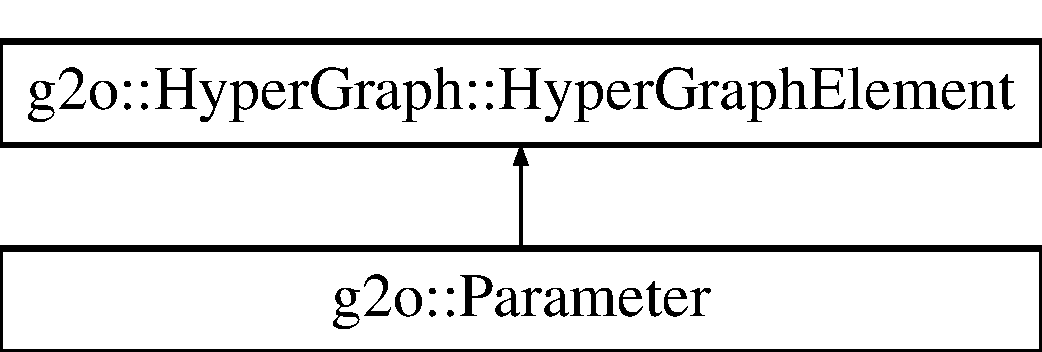
\includegraphics[height=2.000000cm]{classg2o_1_1_parameter}
\end{center}
\end{figure}
\subsection*{Public Member Functions}
\begin{DoxyCompactItemize}
\item 
\mbox{\hyperlink{classg2o_1_1_parameter_a34ef4c50461a0ab0ae9bd26944fac4de}{Parameter}} ()
\item 
virtual \mbox{\hyperlink{classg2o_1_1_parameter_a03a4d78df10d25ddf14a52872f872913}{$\sim$\+Parameter}} ()
\item 
virtual bool \mbox{\hyperlink{classg2o_1_1_parameter_a77d9d88d8bde52198631fcd0fc4c9d0e}{read}} (std\+::istream \&is)=0
\begin{DoxyCompactList}\small\item\em read the data from a stream \end{DoxyCompactList}\item 
virtual bool \mbox{\hyperlink{classg2o_1_1_parameter_a18e66a40cd71a4da2ab9be5ba318abb7}{write}} (std\+::ostream \&os) const =0
\begin{DoxyCompactList}\small\item\em write the data to a stream \end{DoxyCompactList}\item 
int \mbox{\hyperlink{classg2o_1_1_parameter_a1bca491a08b68a7a6b85204a5a8b0f2c}{id}} () const
\item 
void \mbox{\hyperlink{classg2o_1_1_parameter_a2872398ab7d8c95d0a1b5ca5bbfae461}{set\+Id}} (int id\+\_\+)
\item 
virtual Hyper\+Graph\+::\+Hyper\+Graph\+Element\+Type \mbox{\hyperlink{classg2o_1_1_parameter_a44ace751794dcde7a5fd52d16e2f4f21}{element\+Type}} () const
\end{DoxyCompactItemize}
\subsection*{Protected Attributes}
\begin{DoxyCompactItemize}
\item 
int \mbox{\hyperlink{classg2o_1_1_parameter_a602d08079c6a3a5f868e41a102e1db0b}{\+\_\+id}}
\end{DoxyCompactItemize}


\subsection{Constructor \& Destructor Documentation}
\mbox{\Hypertarget{classg2o_1_1_parameter_a34ef4c50461a0ab0ae9bd26944fac4de}\label{classg2o_1_1_parameter_a34ef4c50461a0ab0ae9bd26944fac4de}} 
\index{g2o\+::\+Parameter@{g2o\+::\+Parameter}!Parameter@{Parameter}}
\index{Parameter@{Parameter}!g2o\+::\+Parameter@{g2o\+::\+Parameter}}
\subsubsection{\texorpdfstring{Parameter()}{Parameter()}}
{\footnotesize\ttfamily g2o\+::\+Parameter\+::\+Parameter (\begin{DoxyParamCaption}{ }\end{DoxyParamCaption})}

\mbox{\Hypertarget{classg2o_1_1_parameter_a03a4d78df10d25ddf14a52872f872913}\label{classg2o_1_1_parameter_a03a4d78df10d25ddf14a52872f872913}} 
\index{g2o\+::\+Parameter@{g2o\+::\+Parameter}!````~Parameter@{$\sim$\+Parameter}}
\index{````~Parameter@{$\sim$\+Parameter}!g2o\+::\+Parameter@{g2o\+::\+Parameter}}
\subsubsection{\texorpdfstring{$\sim$\+Parameter()}{~Parameter()}}
{\footnotesize\ttfamily virtual g2o\+::\+Parameter\+::$\sim$\+Parameter (\begin{DoxyParamCaption}{ }\end{DoxyParamCaption})\hspace{0.3cm}{\ttfamily [inline]}, {\ttfamily [virtual]}}



\subsection{Member Function Documentation}
\mbox{\Hypertarget{classg2o_1_1_parameter_a44ace751794dcde7a5fd52d16e2f4f21}\label{classg2o_1_1_parameter_a44ace751794dcde7a5fd52d16e2f4f21}} 
\index{g2o\+::\+Parameter@{g2o\+::\+Parameter}!element\+Type@{element\+Type}}
\index{element\+Type@{element\+Type}!g2o\+::\+Parameter@{g2o\+::\+Parameter}}
\subsubsection{\texorpdfstring{element\+Type()}{elementType()}}
{\footnotesize\ttfamily virtual Hyper\+Graph\+::\+Hyper\+Graph\+Element\+Type g2o\+::\+Parameter\+::element\+Type (\begin{DoxyParamCaption}{ }\end{DoxyParamCaption}) const\hspace{0.3cm}{\ttfamily [inline]}, {\ttfamily [virtual]}}

returns the type of the graph element, see Hyper\+Graph\+Element\+Type 

Implements \mbox{\hyperlink{structg2o_1_1_hyper_graph_1_1_hyper_graph_element_a1a9d7b748698c09d202373e06e413ef2}{g2o\+::\+Hyper\+Graph\+::\+Hyper\+Graph\+Element}}.

\mbox{\Hypertarget{classg2o_1_1_parameter_a1bca491a08b68a7a6b85204a5a8b0f2c}\label{classg2o_1_1_parameter_a1bca491a08b68a7a6b85204a5a8b0f2c}} 
\index{g2o\+::\+Parameter@{g2o\+::\+Parameter}!id@{id}}
\index{id@{id}!g2o\+::\+Parameter@{g2o\+::\+Parameter}}
\subsubsection{\texorpdfstring{id()}{id()}}
{\footnotesize\ttfamily int g2o\+::\+Parameter\+::id (\begin{DoxyParamCaption}{ }\end{DoxyParamCaption}) const\hspace{0.3cm}{\ttfamily [inline]}}

\mbox{\Hypertarget{classg2o_1_1_parameter_a77d9d88d8bde52198631fcd0fc4c9d0e}\label{classg2o_1_1_parameter_a77d9d88d8bde52198631fcd0fc4c9d0e}} 
\index{g2o\+::\+Parameter@{g2o\+::\+Parameter}!read@{read}}
\index{read@{read}!g2o\+::\+Parameter@{g2o\+::\+Parameter}}
\subsubsection{\texorpdfstring{read()}{read()}}
{\footnotesize\ttfamily virtual bool g2o\+::\+Parameter\+::read (\begin{DoxyParamCaption}\item[{std\+::istream \&}]{is }\end{DoxyParamCaption})\hspace{0.3cm}{\ttfamily [pure virtual]}}



read the data from a stream 

\mbox{\Hypertarget{classg2o_1_1_parameter_a2872398ab7d8c95d0a1b5ca5bbfae461}\label{classg2o_1_1_parameter_a2872398ab7d8c95d0a1b5ca5bbfae461}} 
\index{g2o\+::\+Parameter@{g2o\+::\+Parameter}!set\+Id@{set\+Id}}
\index{set\+Id@{set\+Id}!g2o\+::\+Parameter@{g2o\+::\+Parameter}}
\subsubsection{\texorpdfstring{set\+Id()}{setId()}}
{\footnotesize\ttfamily void g2o\+::\+Parameter\+::set\+Id (\begin{DoxyParamCaption}\item[{int}]{id\+\_\+ }\end{DoxyParamCaption})}

\mbox{\Hypertarget{classg2o_1_1_parameter_a18e66a40cd71a4da2ab9be5ba318abb7}\label{classg2o_1_1_parameter_a18e66a40cd71a4da2ab9be5ba318abb7}} 
\index{g2o\+::\+Parameter@{g2o\+::\+Parameter}!write@{write}}
\index{write@{write}!g2o\+::\+Parameter@{g2o\+::\+Parameter}}
\subsubsection{\texorpdfstring{write()}{write()}}
{\footnotesize\ttfamily virtual bool g2o\+::\+Parameter\+::write (\begin{DoxyParamCaption}\item[{std\+::ostream \&}]{os }\end{DoxyParamCaption}) const\hspace{0.3cm}{\ttfamily [pure virtual]}}



write the data to a stream 



\subsection{Member Data Documentation}
\mbox{\Hypertarget{classg2o_1_1_parameter_a602d08079c6a3a5f868e41a102e1db0b}\label{classg2o_1_1_parameter_a602d08079c6a3a5f868e41a102e1db0b}} 
\index{g2o\+::\+Parameter@{g2o\+::\+Parameter}!\+\_\+id@{\+\_\+id}}
\index{\+\_\+id@{\+\_\+id}!g2o\+::\+Parameter@{g2o\+::\+Parameter}}
\subsubsection{\texorpdfstring{\+\_\+id}{\_id}}
{\footnotesize\ttfamily int g2o\+::\+Parameter\+::\+\_\+id\hspace{0.3cm}{\ttfamily [protected]}}



The documentation for this class was generated from the following files\+:\begin{DoxyCompactItemize}
\item 
Thirdparty/g2o/g2o/core/\mbox{\hyperlink{parameter_8h}{parameter.\+h}}\item 
Thirdparty/g2o/g2o/core/\mbox{\hyperlink{parameter_8cpp}{parameter.\+cpp}}\end{DoxyCompactItemize}

\hypertarget{classg2o_1_1_parameter_container}{}\section{g2o\+:\+:Parameter\+Container Class Reference}
\label{classg2o_1_1_parameter_container}\index{g2o\+::\+Parameter\+Container@{g2o\+::\+Parameter\+Container}}


map id to parameters  




{\ttfamily \#include $<$parameter\+\_\+container.\+h$>$}

Inheritance diagram for g2o\+:\+:Parameter\+Container\+:\begin{figure}[H]
\begin{center}
\leavevmode
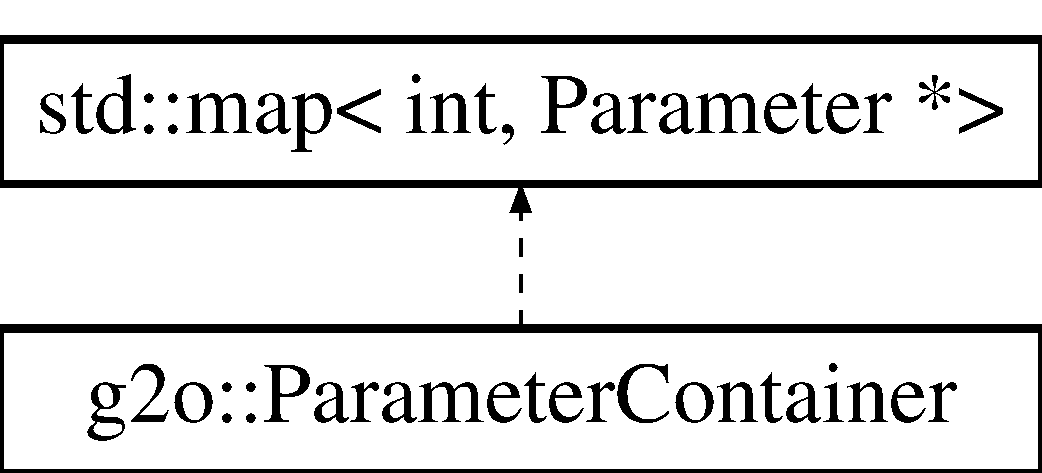
\includegraphics[height=2.000000cm]{classg2o_1_1_parameter_container}
\end{center}
\end{figure}
\subsection*{Public Types}
\begin{DoxyCompactItemize}
\item 
typedef std\+::map$<$ int, \mbox{\hyperlink{classg2o_1_1_parameter}{Parameter}} $\ast$ $>$ \mbox{\hyperlink{classg2o_1_1_parameter_container_a200fdfdce01f7fb5f96e02a8ddf666ac}{Base\+Class}}
\end{DoxyCompactItemize}
\subsection*{Public Member Functions}
\begin{DoxyCompactItemize}
\item 
\mbox{\hyperlink{classg2o_1_1_parameter_container_a6047d0206008b5cbb366be0fe03246b4}{Parameter\+Container}} (bool is\+Main\+Storage\+\_\+=true)
\item 
virtual \mbox{\hyperlink{classg2o_1_1_parameter_container_a186660e1ef0350798a549b247365b295}{$\sim$\+Parameter\+Container}} ()
\item 
bool \mbox{\hyperlink{classg2o_1_1_parameter_container_a9c0b1376e780b177f2d36c4ee4f873d7}{add\+Parameter}} (\mbox{\hyperlink{classg2o_1_1_parameter}{Parameter}} $\ast$p)
\begin{DoxyCompactList}\small\item\em add parameter to the container \end{DoxyCompactList}\item 
\mbox{\hyperlink{classg2o_1_1_parameter}{Parameter}} $\ast$ \mbox{\hyperlink{classg2o_1_1_parameter_container_ad55d9e6d2adaa4680f74be98e2ae3784}{get\+Parameter}} (int id)
\begin{DoxyCompactList}\small\item\em return a parameter based on its ID \end{DoxyCompactList}\item 
\mbox{\hyperlink{classg2o_1_1_parameter}{Parameter}} $\ast$ \mbox{\hyperlink{classg2o_1_1_parameter_container_a6e57cf684d92f0ceeba8b4923fa41864}{detach\+Parameter}} (int id)
\begin{DoxyCompactList}\small\item\em remove a parameter from the container, i.\+e., the user now owns the pointer \end{DoxyCompactList}\item 
virtual bool \mbox{\hyperlink{classg2o_1_1_parameter_container_ae5883ac8e2313cab310cf067b0ba12bf}{read}} (std\+::istream \&is, const std\+::map$<$ std\+::string, std\+::string $>$ $\ast$renamed\+Map=0)
\begin{DoxyCompactList}\small\item\em read parameters from a stream \end{DoxyCompactList}\item 
virtual bool \mbox{\hyperlink{classg2o_1_1_parameter_container_a15c92fab12ad8f3bd51b3f555e95b00e}{write}} (std\+::ostream \&os) const
\begin{DoxyCompactList}\small\item\em write the data to a stream \end{DoxyCompactList}\item 
bool \mbox{\hyperlink{classg2o_1_1_parameter_container_a201d0b120e7b8d54c99d73c8f4d04846}{is\+Main\+Storage}} () const
\item 
void \mbox{\hyperlink{classg2o_1_1_parameter_container_aff4d3792e2ebd022ebd4a1534b88b773}{clear}} ()
\end{DoxyCompactItemize}
\subsection*{Protected Attributes}
\begin{DoxyCompactItemize}
\item 
bool \mbox{\hyperlink{classg2o_1_1_parameter_container_a2ff1e92bc6a486d48043e2191807bd47}{\+\_\+is\+Main\+Storage}}
\end{DoxyCompactItemize}


\subsection{Detailed Description}
map id to parameters 

\subsection{Member Typedef Documentation}
\mbox{\Hypertarget{classg2o_1_1_parameter_container_a200fdfdce01f7fb5f96e02a8ddf666ac}\label{classg2o_1_1_parameter_container_a200fdfdce01f7fb5f96e02a8ddf666ac}} 
\index{g2o\+::\+Parameter\+Container@{g2o\+::\+Parameter\+Container}!Base\+Class@{Base\+Class}}
\index{Base\+Class@{Base\+Class}!g2o\+::\+Parameter\+Container@{g2o\+::\+Parameter\+Container}}
\subsubsection{\texorpdfstring{Base\+Class}{BaseClass}}
{\footnotesize\ttfamily typedef std\+::map$<$int, \mbox{\hyperlink{classg2o_1_1_parameter}{Parameter}}$\ast$$>$ \mbox{\hyperlink{classg2o_1_1_parameter_container_a200fdfdce01f7fb5f96e02a8ddf666ac}{g2o\+::\+Parameter\+Container\+::\+Base\+Class}}}



\subsection{Constructor \& Destructor Documentation}
\mbox{\Hypertarget{classg2o_1_1_parameter_container_a6047d0206008b5cbb366be0fe03246b4}\label{classg2o_1_1_parameter_container_a6047d0206008b5cbb366be0fe03246b4}} 
\index{g2o\+::\+Parameter\+Container@{g2o\+::\+Parameter\+Container}!Parameter\+Container@{Parameter\+Container}}
\index{Parameter\+Container@{Parameter\+Container}!g2o\+::\+Parameter\+Container@{g2o\+::\+Parameter\+Container}}
\subsubsection{\texorpdfstring{Parameter\+Container()}{ParameterContainer()}}
{\footnotesize\ttfamily g2o\+::\+Parameter\+Container\+::\+Parameter\+Container (\begin{DoxyParamCaption}\item[{bool}]{is\+Main\+Storage\+\_\+ = {\ttfamily true} }\end{DoxyParamCaption})}

create a container for the parameters. 
\begin{DoxyParams}{Parameters}
{\em is\+Main\+Storage\+\_\+} & pointers to the parameters are owned by this container, i.\+e., freed in its constructor \\
\hline
\end{DoxyParams}
\mbox{\Hypertarget{classg2o_1_1_parameter_container_a186660e1ef0350798a549b247365b295}\label{classg2o_1_1_parameter_container_a186660e1ef0350798a549b247365b295}} 
\index{g2o\+::\+Parameter\+Container@{g2o\+::\+Parameter\+Container}!````~Parameter\+Container@{$\sim$\+Parameter\+Container}}
\index{````~Parameter\+Container@{$\sim$\+Parameter\+Container}!g2o\+::\+Parameter\+Container@{g2o\+::\+Parameter\+Container}}
\subsubsection{\texorpdfstring{$\sim$\+Parameter\+Container()}{~ParameterContainer()}}
{\footnotesize\ttfamily g2o\+::\+Parameter\+Container\+::$\sim$\+Parameter\+Container (\begin{DoxyParamCaption}{ }\end{DoxyParamCaption})\hspace{0.3cm}{\ttfamily [virtual]}}



\subsection{Member Function Documentation}
\mbox{\Hypertarget{classg2o_1_1_parameter_container_a9c0b1376e780b177f2d36c4ee4f873d7}\label{classg2o_1_1_parameter_container_a9c0b1376e780b177f2d36c4ee4f873d7}} 
\index{g2o\+::\+Parameter\+Container@{g2o\+::\+Parameter\+Container}!add\+Parameter@{add\+Parameter}}
\index{add\+Parameter@{add\+Parameter}!g2o\+::\+Parameter\+Container@{g2o\+::\+Parameter\+Container}}
\subsubsection{\texorpdfstring{add\+Parameter()}{addParameter()}}
{\footnotesize\ttfamily bool g2o\+::\+Parameter\+Container\+::add\+Parameter (\begin{DoxyParamCaption}\item[{\mbox{\hyperlink{classg2o_1_1_parameter}{Parameter}} $\ast$}]{p }\end{DoxyParamCaption})}



add parameter to the container 

\mbox{\Hypertarget{classg2o_1_1_parameter_container_aff4d3792e2ebd022ebd4a1534b88b773}\label{classg2o_1_1_parameter_container_aff4d3792e2ebd022ebd4a1534b88b773}} 
\index{g2o\+::\+Parameter\+Container@{g2o\+::\+Parameter\+Container}!clear@{clear}}
\index{clear@{clear}!g2o\+::\+Parameter\+Container@{g2o\+::\+Parameter\+Container}}
\subsubsection{\texorpdfstring{clear()}{clear()}}
{\footnotesize\ttfamily void g2o\+::\+Parameter\+Container\+::clear (\begin{DoxyParamCaption}{ }\end{DoxyParamCaption})}

\mbox{\Hypertarget{classg2o_1_1_parameter_container_a6e57cf684d92f0ceeba8b4923fa41864}\label{classg2o_1_1_parameter_container_a6e57cf684d92f0ceeba8b4923fa41864}} 
\index{g2o\+::\+Parameter\+Container@{g2o\+::\+Parameter\+Container}!detach\+Parameter@{detach\+Parameter}}
\index{detach\+Parameter@{detach\+Parameter}!g2o\+::\+Parameter\+Container@{g2o\+::\+Parameter\+Container}}
\subsubsection{\texorpdfstring{detach\+Parameter()}{detachParameter()}}
{\footnotesize\ttfamily \mbox{\hyperlink{classg2o_1_1_parameter}{Parameter}} $\ast$ g2o\+::\+Parameter\+Container\+::detach\+Parameter (\begin{DoxyParamCaption}\item[{int}]{id }\end{DoxyParamCaption})}



remove a parameter from the container, i.\+e., the user now owns the pointer 

\mbox{\Hypertarget{classg2o_1_1_parameter_container_ad55d9e6d2adaa4680f74be98e2ae3784}\label{classg2o_1_1_parameter_container_ad55d9e6d2adaa4680f74be98e2ae3784}} 
\index{g2o\+::\+Parameter\+Container@{g2o\+::\+Parameter\+Container}!get\+Parameter@{get\+Parameter}}
\index{get\+Parameter@{get\+Parameter}!g2o\+::\+Parameter\+Container@{g2o\+::\+Parameter\+Container}}
\subsubsection{\texorpdfstring{get\+Parameter()}{getParameter()}}
{\footnotesize\ttfamily \mbox{\hyperlink{classg2o_1_1_parameter}{Parameter}} $\ast$ g2o\+::\+Parameter\+Container\+::get\+Parameter (\begin{DoxyParamCaption}\item[{int}]{id }\end{DoxyParamCaption})}



return a parameter based on its ID 

\mbox{\Hypertarget{classg2o_1_1_parameter_container_a201d0b120e7b8d54c99d73c8f4d04846}\label{classg2o_1_1_parameter_container_a201d0b120e7b8d54c99d73c8f4d04846}} 
\index{g2o\+::\+Parameter\+Container@{g2o\+::\+Parameter\+Container}!is\+Main\+Storage@{is\+Main\+Storage}}
\index{is\+Main\+Storage@{is\+Main\+Storage}!g2o\+::\+Parameter\+Container@{g2o\+::\+Parameter\+Container}}
\subsubsection{\texorpdfstring{is\+Main\+Storage()}{isMainStorage()}}
{\footnotesize\ttfamily bool g2o\+::\+Parameter\+Container\+::is\+Main\+Storage (\begin{DoxyParamCaption}{ }\end{DoxyParamCaption}) const\hspace{0.3cm}{\ttfamily [inline]}}

\mbox{\Hypertarget{classg2o_1_1_parameter_container_ae5883ac8e2313cab310cf067b0ba12bf}\label{classg2o_1_1_parameter_container_ae5883ac8e2313cab310cf067b0ba12bf}} 
\index{g2o\+::\+Parameter\+Container@{g2o\+::\+Parameter\+Container}!read@{read}}
\index{read@{read}!g2o\+::\+Parameter\+Container@{g2o\+::\+Parameter\+Container}}
\subsubsection{\texorpdfstring{read()}{read()}}
{\footnotesize\ttfamily bool g2o\+::\+Parameter\+Container\+::read (\begin{DoxyParamCaption}\item[{std\+::istream \&}]{is,  }\item[{const std\+::map$<$ std\+::string, std\+::string $>$ $\ast$}]{renamed\+Map = {\ttfamily 0} }\end{DoxyParamCaption})\hspace{0.3cm}{\ttfamily [virtual]}}



read parameters from a stream 

\mbox{\Hypertarget{classg2o_1_1_parameter_container_a15c92fab12ad8f3bd51b3f555e95b00e}\label{classg2o_1_1_parameter_container_a15c92fab12ad8f3bd51b3f555e95b00e}} 
\index{g2o\+::\+Parameter\+Container@{g2o\+::\+Parameter\+Container}!write@{write}}
\index{write@{write}!g2o\+::\+Parameter\+Container@{g2o\+::\+Parameter\+Container}}
\subsubsection{\texorpdfstring{write()}{write()}}
{\footnotesize\ttfamily bool g2o\+::\+Parameter\+Container\+::write (\begin{DoxyParamCaption}\item[{std\+::ostream \&}]{os }\end{DoxyParamCaption}) const\hspace{0.3cm}{\ttfamily [virtual]}}



write the data to a stream 



\subsection{Member Data Documentation}
\mbox{\Hypertarget{classg2o_1_1_parameter_container_a2ff1e92bc6a486d48043e2191807bd47}\label{classg2o_1_1_parameter_container_a2ff1e92bc6a486d48043e2191807bd47}} 
\index{g2o\+::\+Parameter\+Container@{g2o\+::\+Parameter\+Container}!\+\_\+is\+Main\+Storage@{\+\_\+is\+Main\+Storage}}
\index{\+\_\+is\+Main\+Storage@{\+\_\+is\+Main\+Storage}!g2o\+::\+Parameter\+Container@{g2o\+::\+Parameter\+Container}}
\subsubsection{\texorpdfstring{\+\_\+is\+Main\+Storage}{\_isMainStorage}}
{\footnotesize\ttfamily bool g2o\+::\+Parameter\+Container\+::\+\_\+is\+Main\+Storage\hspace{0.3cm}{\ttfamily [protected]}}



The documentation for this class was generated from the following files\+:\begin{DoxyCompactItemize}
\item 
D\+:/github/\+V\+S\+L\+A\+M/\+O\+R\+B\+S\+L\+A\+M2/\+O\+R\+B-\/\+S\+L\+A\+M2-\/master/\+Thirdparty/g2o/g2o/core/\mbox{\hyperlink{parameter__container_8h}{parameter\+\_\+container.\+h}}\item 
D\+:/github/\+V\+S\+L\+A\+M/\+O\+R\+B\+S\+L\+A\+M2/\+O\+R\+B-\/\+S\+L\+A\+M2-\/master/\+Thirdparty/g2o/g2o/core/\mbox{\hyperlink{parameter__container_8cpp}{parameter\+\_\+container.\+cpp}}\end{DoxyCompactItemize}

\hypertarget{classg2o_1_1_hyper_graph_action_1_1_parameters}{}\section{g2o\+:\+:Hyper\+Graph\+Action\+:\+:Parameters Class Reference}
\label{classg2o_1_1_hyper_graph_action_1_1_parameters}\index{g2o\+::\+Hyper\+Graph\+Action\+::\+Parameters@{g2o\+::\+Hyper\+Graph\+Action\+::\+Parameters}}


{\ttfamily \#include $<$hyper\+\_\+graph\+\_\+action.\+h$>$}

Inheritance diagram for g2o\+:\+:Hyper\+Graph\+Action\+:\+:Parameters\+:\begin{figure}[H]
\begin{center}
\leavevmode
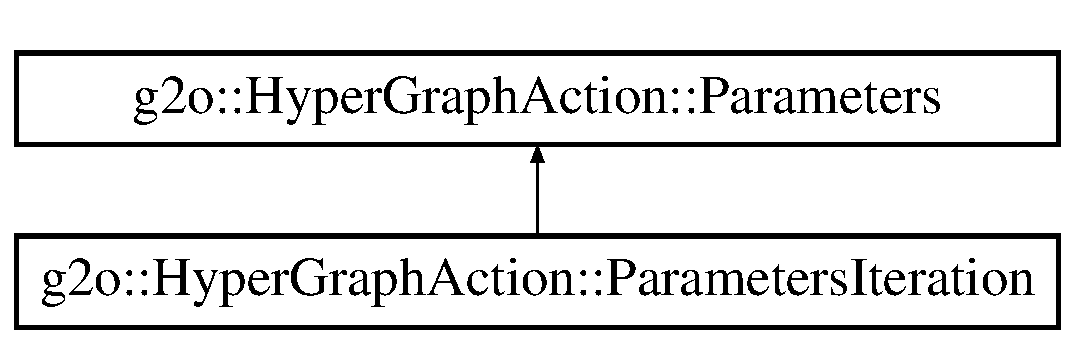
\includegraphics[height=2.000000cm]{classg2o_1_1_hyper_graph_action_1_1_parameters}
\end{center}
\end{figure}
\subsection*{Public Member Functions}
\begin{DoxyCompactItemize}
\item 
virtual \mbox{\hyperlink{classg2o_1_1_hyper_graph_action_1_1_parameters_aecdc1052f4d31297a94d32fade46b2d7}{$\sim$\+Parameters}} ()
\end{DoxyCompactItemize}


\subsection{Constructor \& Destructor Documentation}
\mbox{\Hypertarget{classg2o_1_1_hyper_graph_action_1_1_parameters_aecdc1052f4d31297a94d32fade46b2d7}\label{classg2o_1_1_hyper_graph_action_1_1_parameters_aecdc1052f4d31297a94d32fade46b2d7}} 
\index{g2o\+::\+Hyper\+Graph\+Action\+::\+Parameters@{g2o\+::\+Hyper\+Graph\+Action\+::\+Parameters}!````~Parameters@{$\sim$\+Parameters}}
\index{````~Parameters@{$\sim$\+Parameters}!g2o\+::\+Hyper\+Graph\+Action\+::\+Parameters@{g2o\+::\+Hyper\+Graph\+Action\+::\+Parameters}}
\subsubsection{\texorpdfstring{$\sim$\+Parameters()}{~Parameters()}}
{\footnotesize\ttfamily g2o\+::\+Hyper\+Graph\+Action\+::\+Parameters\+::$\sim$\+Parameters (\begin{DoxyParamCaption}{ }\end{DoxyParamCaption})\hspace{0.3cm}{\ttfamily [virtual]}}



The documentation for this class was generated from the following files\+:\begin{DoxyCompactItemize}
\item 
Thirdparty/g2o/g2o/core/\mbox{\hyperlink{hyper__graph__action_8h}{hyper\+\_\+graph\+\_\+action.\+h}}\item 
Thirdparty/g2o/g2o/core/\mbox{\hyperlink{hyper__graph__action_8cpp}{hyper\+\_\+graph\+\_\+action.\+cpp}}\end{DoxyCompactItemize}

\hypertarget{structg2o_1_1_write_gnuplot_action_1_1_parameters}{}\section{g2o\+:\+:Write\+Gnuplot\+Action\+:\+:Parameters Struct Reference}
\label{structg2o_1_1_write_gnuplot_action_1_1_parameters}\index{g2o\+::\+Write\+Gnuplot\+Action\+::\+Parameters@{g2o\+::\+Write\+Gnuplot\+Action\+::\+Parameters}}


{\ttfamily \#include $<$hyper\+\_\+graph\+\_\+action.\+h$>$}

Inheritance diagram for g2o\+:\+:Write\+Gnuplot\+Action\+:\+:Parameters\+:\begin{figure}[H]
\begin{center}
\leavevmode
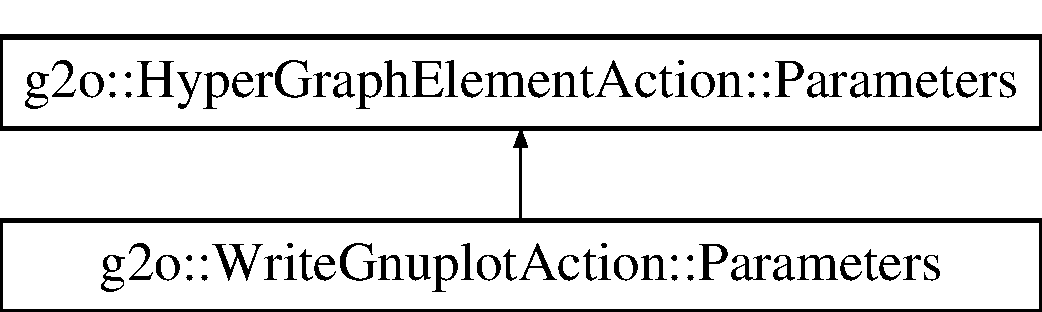
\includegraphics[height=2.000000cm]{structg2o_1_1_write_gnuplot_action_1_1_parameters}
\end{center}
\end{figure}
\subsection*{Public Attributes}
\begin{DoxyCompactItemize}
\item 
std\+::ostream $\ast$ \mbox{\hyperlink{structg2o_1_1_write_gnuplot_action_1_1_parameters_a8e25b8cffdc008929a939cf9080c5902}{os}}
\end{DoxyCompactItemize}
\subsection*{Additional Inherited Members}


\subsection{Member Data Documentation}
\mbox{\Hypertarget{structg2o_1_1_write_gnuplot_action_1_1_parameters_a8e25b8cffdc008929a939cf9080c5902}\label{structg2o_1_1_write_gnuplot_action_1_1_parameters_a8e25b8cffdc008929a939cf9080c5902}} 
\index{g2o\+::\+Write\+Gnuplot\+Action\+::\+Parameters@{g2o\+::\+Write\+Gnuplot\+Action\+::\+Parameters}!os@{os}}
\index{os@{os}!g2o\+::\+Write\+Gnuplot\+Action\+::\+Parameters@{g2o\+::\+Write\+Gnuplot\+Action\+::\+Parameters}}
\subsubsection{\texorpdfstring{os}{os}}
{\footnotesize\ttfamily std\+::ostream$\ast$ g2o\+::\+Write\+Gnuplot\+Action\+::\+Parameters\+::os}



The documentation for this struct was generated from the following file\+:\begin{DoxyCompactItemize}
\item 
Thirdparty/g2o/g2o/core/\mbox{\hyperlink{hyper__graph__action_8h}{hyper\+\_\+graph\+\_\+action.\+h}}\end{DoxyCompactItemize}

\hypertarget{classg2o_1_1_draw_action_1_1_parameters}{}\section{g2o\+:\+:Draw\+Action\+:\+:Parameters Class Reference}
\label{classg2o_1_1_draw_action_1_1_parameters}\index{g2o\+::\+Draw\+Action\+::\+Parameters@{g2o\+::\+Draw\+Action\+::\+Parameters}}


{\ttfamily \#include $<$hyper\+\_\+graph\+\_\+action.\+h$>$}

Inheritance diagram for g2o\+:\+:Draw\+Action\+:\+:Parameters\+:\begin{figure}[H]
\begin{center}
\leavevmode
\includegraphics[height=3.000000cm]{classg2o_1_1_draw_action_1_1_parameters}
\end{center}
\end{figure}
\subsection*{Public Member Functions}
\begin{DoxyCompactItemize}
\item 
\mbox{\hyperlink{classg2o_1_1_draw_action_1_1_parameters_ade816dc0924de9acd14c4a35636f6bd4}{Parameters}} ()
\end{DoxyCompactItemize}
\subsection*{Additional Inherited Members}


\subsection{Constructor \& Destructor Documentation}
\mbox{\Hypertarget{classg2o_1_1_draw_action_1_1_parameters_ade816dc0924de9acd14c4a35636f6bd4}\label{classg2o_1_1_draw_action_1_1_parameters_ade816dc0924de9acd14c4a35636f6bd4}} 
\index{g2o\+::\+Draw\+Action\+::\+Parameters@{g2o\+::\+Draw\+Action\+::\+Parameters}!Parameters@{Parameters}}
\index{Parameters@{Parameters}!g2o\+::\+Draw\+Action\+::\+Parameters@{g2o\+::\+Draw\+Action\+::\+Parameters}}
\subsubsection{\texorpdfstring{Parameters()}{Parameters()}}
{\footnotesize\ttfamily g2o\+::\+Draw\+Action\+::\+Parameters\+::\+Parameters (\begin{DoxyParamCaption}{ }\end{DoxyParamCaption})}



The documentation for this class was generated from the following files\+:\begin{DoxyCompactItemize}
\item 
Thirdparty/g2o/g2o/core/\mbox{\hyperlink{hyper__graph__action_8h}{hyper\+\_\+graph\+\_\+action.\+h}}\item 
Thirdparty/g2o/g2o/core/\mbox{\hyperlink{hyper__graph__action_8cpp}{hyper\+\_\+graph\+\_\+action.\+cpp}}\end{DoxyCompactItemize}

\hypertarget{structg2o_1_1_hyper_graph_element_action_1_1_parameters}{}\section{g2o\+:\+:Hyper\+Graph\+Element\+Action\+:\+:Parameters Struct Reference}
\label{structg2o_1_1_hyper_graph_element_action_1_1_parameters}\index{g2o\+::\+Hyper\+Graph\+Element\+Action\+::\+Parameters@{g2o\+::\+Hyper\+Graph\+Element\+Action\+::\+Parameters}}


{\ttfamily \#include $<$hyper\+\_\+graph\+\_\+action.\+h$>$}

Inheritance diagram for g2o\+:\+:Hyper\+Graph\+Element\+Action\+:\+:Parameters\+:\begin{figure}[H]
\begin{center}
\leavevmode
\includegraphics[height=2.000000cm]{structg2o_1_1_hyper_graph_element_action_1_1_parameters}
\end{center}
\end{figure}
\subsection*{Public Member Functions}
\begin{DoxyCompactItemize}
\item 
virtual \mbox{\hyperlink{structg2o_1_1_hyper_graph_element_action_1_1_parameters_a7ccfab1c7db5a54ac582ac8791cb7f2d}{$\sim$\+Parameters}} ()
\end{DoxyCompactItemize}


\subsection{Constructor \& Destructor Documentation}
\mbox{\Hypertarget{structg2o_1_1_hyper_graph_element_action_1_1_parameters_a7ccfab1c7db5a54ac582ac8791cb7f2d}\label{structg2o_1_1_hyper_graph_element_action_1_1_parameters_a7ccfab1c7db5a54ac582ac8791cb7f2d}} 
\index{g2o\+::\+Hyper\+Graph\+Element\+Action\+::\+Parameters@{g2o\+::\+Hyper\+Graph\+Element\+Action\+::\+Parameters}!````~Parameters@{$\sim$\+Parameters}}
\index{````~Parameters@{$\sim$\+Parameters}!g2o\+::\+Hyper\+Graph\+Element\+Action\+::\+Parameters@{g2o\+::\+Hyper\+Graph\+Element\+Action\+::\+Parameters}}
\subsubsection{\texorpdfstring{$\sim$\+Parameters()}{~Parameters()}}
{\footnotesize\ttfamily g2o\+::\+Hyper\+Graph\+Element\+Action\+::\+Parameters\+::$\sim$\+Parameters (\begin{DoxyParamCaption}{ }\end{DoxyParamCaption})\hspace{0.3cm}{\ttfamily [virtual]}}



The documentation for this struct was generated from the following files\+:\begin{DoxyCompactItemize}
\item 
D\+:/github/\+V\+S\+L\+A\+M/\+O\+R\+B\+S\+L\+A\+M2/\+O\+R\+B-\/\+S\+L\+A\+M2-\/master/\+Thirdparty/g2o/g2o/core/\mbox{\hyperlink{hyper__graph__action_8h}{hyper\+\_\+graph\+\_\+action.\+h}}\item 
D\+:/github/\+V\+S\+L\+A\+M/\+O\+R\+B\+S\+L\+A\+M2/\+O\+R\+B-\/\+S\+L\+A\+M2-\/master/\+Thirdparty/g2o/g2o/core/\mbox{\hyperlink{hyper__graph__action_8cpp}{hyper\+\_\+graph\+\_\+action.\+cpp}}\end{DoxyCompactItemize}

\hypertarget{classg2o_1_1_hyper_graph_action_1_1_parameters_iteration}{}\section{g2o\+:\+:Hyper\+Graph\+Action\+:\+:Parameters\+Iteration Class Reference}
\label{classg2o_1_1_hyper_graph_action_1_1_parameters_iteration}\index{g2o\+::\+Hyper\+Graph\+Action\+::\+Parameters\+Iteration@{g2o\+::\+Hyper\+Graph\+Action\+::\+Parameters\+Iteration}}


{\ttfamily \#include $<$hyper\+\_\+graph\+\_\+action.\+h$>$}

Inheritance diagram for g2o\+:\+:Hyper\+Graph\+Action\+:\+:Parameters\+Iteration\+:\begin{figure}[H]
\begin{center}
\leavevmode
\includegraphics[height=2.000000cm]{classg2o_1_1_hyper_graph_action_1_1_parameters_iteration}
\end{center}
\end{figure}
\subsection*{Public Member Functions}
\begin{DoxyCompactItemize}
\item 
\mbox{\hyperlink{classg2o_1_1_hyper_graph_action_1_1_parameters_iteration_ae6849a5bec7eac20ba0f2b0892212694}{Parameters\+Iteration}} (int iter)
\end{DoxyCompactItemize}
\subsection*{Public Attributes}
\begin{DoxyCompactItemize}
\item 
int \mbox{\hyperlink{classg2o_1_1_hyper_graph_action_1_1_parameters_iteration_a6ec1e8c9333e75e9531bebe055e23ce2}{iteration}}
\end{DoxyCompactItemize}


\subsection{Constructor \& Destructor Documentation}
\mbox{\Hypertarget{classg2o_1_1_hyper_graph_action_1_1_parameters_iteration_ae6849a5bec7eac20ba0f2b0892212694}\label{classg2o_1_1_hyper_graph_action_1_1_parameters_iteration_ae6849a5bec7eac20ba0f2b0892212694}} 
\index{g2o\+::\+Hyper\+Graph\+Action\+::\+Parameters\+Iteration@{g2o\+::\+Hyper\+Graph\+Action\+::\+Parameters\+Iteration}!Parameters\+Iteration@{Parameters\+Iteration}}
\index{Parameters\+Iteration@{Parameters\+Iteration}!g2o\+::\+Hyper\+Graph\+Action\+::\+Parameters\+Iteration@{g2o\+::\+Hyper\+Graph\+Action\+::\+Parameters\+Iteration}}
\subsubsection{\texorpdfstring{Parameters\+Iteration()}{ParametersIteration()}}
{\footnotesize\ttfamily g2o\+::\+Hyper\+Graph\+Action\+::\+Parameters\+Iteration\+::\+Parameters\+Iteration (\begin{DoxyParamCaption}\item[{int}]{iter }\end{DoxyParamCaption})\hspace{0.3cm}{\ttfamily [explicit]}}



\subsection{Member Data Documentation}
\mbox{\Hypertarget{classg2o_1_1_hyper_graph_action_1_1_parameters_iteration_a6ec1e8c9333e75e9531bebe055e23ce2}\label{classg2o_1_1_hyper_graph_action_1_1_parameters_iteration_a6ec1e8c9333e75e9531bebe055e23ce2}} 
\index{g2o\+::\+Hyper\+Graph\+Action\+::\+Parameters\+Iteration@{g2o\+::\+Hyper\+Graph\+Action\+::\+Parameters\+Iteration}!iteration@{iteration}}
\index{iteration@{iteration}!g2o\+::\+Hyper\+Graph\+Action\+::\+Parameters\+Iteration@{g2o\+::\+Hyper\+Graph\+Action\+::\+Parameters\+Iteration}}
\subsubsection{\texorpdfstring{iteration}{iteration}}
{\footnotesize\ttfamily int g2o\+::\+Hyper\+Graph\+Action\+::\+Parameters\+Iteration\+::iteration}



The documentation for this class was generated from the following files\+:\begin{DoxyCompactItemize}
\item 
D\+:/github/\+V\+S\+L\+A\+M/\+O\+R\+B\+S\+L\+A\+M2/\+O\+R\+B-\/\+S\+L\+A\+M2-\/master/\+Thirdparty/g2o/g2o/core/\mbox{\hyperlink{hyper__graph__action_8h}{hyper\+\_\+graph\+\_\+action.\+h}}\item 
D\+:/github/\+V\+S\+L\+A\+M/\+O\+R\+B\+S\+L\+A\+M2/\+O\+R\+B-\/\+S\+L\+A\+M2-\/master/\+Thirdparty/g2o/g2o/core/\mbox{\hyperlink{hyper__graph__action_8cpp}{hyper\+\_\+graph\+\_\+action.\+cpp}}\end{DoxyCompactItemize}

\hypertarget{class_o_r_b___s_l_a_m2_1_1_pn_psolver}{}\section{O\+R\+B\+\_\+\+S\+L\+A\+M2\+:\+:Pn\+Psolver Class Reference}
\label{class_o_r_b___s_l_a_m2_1_1_pn_psolver}\index{O\+R\+B\+\_\+\+S\+L\+A\+M2\+::\+Pn\+Psolver@{O\+R\+B\+\_\+\+S\+L\+A\+M2\+::\+Pn\+Psolver}}


{\ttfamily \#include $<$Pn\+Psolver.\+h$>$}

\subsection*{Public Member Functions}
\begin{DoxyCompactItemize}
\item 
\mbox{\hyperlink{class_o_r_b___s_l_a_m2_1_1_pn_psolver_a7b4cad992a43620e027bfb4bc9ef24f8}{Pn\+Psolver}} (const \mbox{\hyperlink{class_o_r_b___s_l_a_m2_1_1_frame}{Frame}} \&F, const vector$<$ \mbox{\hyperlink{class_o_r_b___s_l_a_m2_1_1_map_point}{Map\+Point}} $\ast$$>$ \&vp\+Map\+Point\+Matches)
\item 
\mbox{\hyperlink{class_o_r_b___s_l_a_m2_1_1_pn_psolver_ad40b921779ed92bfb6b017a76e4d88aa}{$\sim$\+Pn\+Psolver}} ()
\item 
void \mbox{\hyperlink{class_o_r_b___s_l_a_m2_1_1_pn_psolver_adff29377dcc77891a33113080b6b1eb7}{Set\+Ransac\+Parameters}} (double probability=0.\+99, int min\+Inliers=8, int max\+Iterations=300, int min\+Set=4, float epsilon=0.\+4, float th2=5.\+991)
\item 
cv\+::\+Mat \mbox{\hyperlink{class_o_r_b___s_l_a_m2_1_1_pn_psolver_a784429037a79cb53923f4db181a4d115}{find}} (vector$<$ bool $>$ \&vb\+Inliers, int \&n\+Inliers)
\item 
cv\+::\+Mat \mbox{\hyperlink{class_o_r_b___s_l_a_m2_1_1_pn_psolver_abbef2ac776747661112246e85667f452}{iterate}} (int n\+Iterations, bool \&b\+No\+More, vector$<$ bool $>$ \&vb\+Inliers, int \&n\+Inliers)
\end{DoxyCompactItemize}
\subsection*{Private Member Functions}
\begin{DoxyCompactItemize}
\item 
void \mbox{\hyperlink{class_o_r_b___s_l_a_m2_1_1_pn_psolver_abb27b1402d63ce78890d3f1ea42a75a4}{Check\+Inliers}} ()
\item 
bool \mbox{\hyperlink{class_o_r_b___s_l_a_m2_1_1_pn_psolver_a19710728d61dcf1caa32f31d140f3327}{Refine}} ()
\item 
void \mbox{\hyperlink{class_o_r_b___s_l_a_m2_1_1_pn_psolver_aa2747be485a2a87ad5a72f8431edbf77}{set\+\_\+maximum\+\_\+number\+\_\+of\+\_\+correspondences}} (const int n)
\item 
void \mbox{\hyperlink{class_o_r_b___s_l_a_m2_1_1_pn_psolver_a78dcd4d88b5ebae795d8c214932c4089}{reset\+\_\+correspondences}} (void)
\item 
void \mbox{\hyperlink{class_o_r_b___s_l_a_m2_1_1_pn_psolver_acfff5312c244e3e6de7bc16b3a72f34b}{add\+\_\+correspondence}} (const double X, const double Y, const double Z, const double u, const double v)
\item 
double \mbox{\hyperlink{class_o_r_b___s_l_a_m2_1_1_pn_psolver_aa712661f5888f9e1f580fe7f0117e389}{compute\+\_\+pose}} (double R\mbox{[}3\mbox{]}\mbox{[}3\mbox{]}, double T\mbox{[}3\mbox{]})
\item 
void \mbox{\hyperlink{class_o_r_b___s_l_a_m2_1_1_pn_psolver_ab3247415c8c4ff0a5df74096907eac10}{relative\+\_\+error}} (double \&rot\+\_\+err, double \&transl\+\_\+err, const double Rtrue\mbox{[}3\mbox{]}\mbox{[}3\mbox{]}, const double ttrue\mbox{[}3\mbox{]}, const double Rest\mbox{[}3\mbox{]}\mbox{[}3\mbox{]}, const double test\mbox{[}3\mbox{]})
\item 
void \mbox{\hyperlink{class_o_r_b___s_l_a_m2_1_1_pn_psolver_a2be5e2c8a40397fb9a7c7457be95c407}{print\+\_\+pose}} (const double R\mbox{[}3\mbox{]}\mbox{[}3\mbox{]}, const double t\mbox{[}3\mbox{]})
\item 
double \mbox{\hyperlink{class_o_r_b___s_l_a_m2_1_1_pn_psolver_a8d0ecb37dd35686ae16ff2cdb277cd82}{reprojection\+\_\+error}} (const double R\mbox{[}3\mbox{]}\mbox{[}3\mbox{]}, const double t\mbox{[}3\mbox{]})
\item 
void \mbox{\hyperlink{class_o_r_b___s_l_a_m2_1_1_pn_psolver_a42c51e43d16d52747facbaca93fcd583}{choose\+\_\+control\+\_\+points}} (void)
\item 
void \mbox{\hyperlink{class_o_r_b___s_l_a_m2_1_1_pn_psolver_a1e35c1813d1a76d6b2a1664ac7080dcd}{compute\+\_\+barycentric\+\_\+coordinates}} (void)
\item 
void \mbox{\hyperlink{class_o_r_b___s_l_a_m2_1_1_pn_psolver_a8cc37bbb1cc4e575d83fb7503136a542}{fill\+\_\+M}} (Cv\+Mat $\ast$M, const int row, const double $\ast$\mbox{\hyperlink{class_o_r_b___s_l_a_m2_1_1_pn_psolver_a868ef3e00710a5541d50a15af7be2a20}{alphas}}, const double u, const double v)
\item 
void \mbox{\hyperlink{class_o_r_b___s_l_a_m2_1_1_pn_psolver_ac4c58e214a0016e1e58cbc1afd9eb5eb}{compute\+\_\+ccs}} (const double $\ast$betas, const double $\ast$ut)
\item 
void \mbox{\hyperlink{class_o_r_b___s_l_a_m2_1_1_pn_psolver_abeb37c568bb09293bb679d84bb4d2796}{compute\+\_\+pcs}} (void)
\item 
void \mbox{\hyperlink{class_o_r_b___s_l_a_m2_1_1_pn_psolver_af33413cd4dc6f3e963cf49997baa40c2}{solve\+\_\+for\+\_\+sign}} (void)
\item 
void \mbox{\hyperlink{class_o_r_b___s_l_a_m2_1_1_pn_psolver_a6d36f0e15dfca9c0ecfff91149882232}{find\+\_\+betas\+\_\+approx\+\_\+1}} (const Cv\+Mat $\ast$L\+\_\+6x10, const Cv\+Mat $\ast$Rho, double $\ast$betas)
\item 
void \mbox{\hyperlink{class_o_r_b___s_l_a_m2_1_1_pn_psolver_a95d7f0790ebd99fdc012971dd9a78e65}{find\+\_\+betas\+\_\+approx\+\_\+2}} (const Cv\+Mat $\ast$L\+\_\+6x10, const Cv\+Mat $\ast$Rho, double $\ast$betas)
\item 
void \mbox{\hyperlink{class_o_r_b___s_l_a_m2_1_1_pn_psolver_af80a1580251b4368156fb0e0d36a7ac2}{find\+\_\+betas\+\_\+approx\+\_\+3}} (const Cv\+Mat $\ast$L\+\_\+6x10, const Cv\+Mat $\ast$Rho, double $\ast$betas)
\item 
void \mbox{\hyperlink{class_o_r_b___s_l_a_m2_1_1_pn_psolver_ac9290df9524ca70b3127ea3408fb7b0d}{qr\+\_\+solve}} (Cv\+Mat $\ast$A, Cv\+Mat $\ast$b, Cv\+Mat $\ast$X)
\item 
double \mbox{\hyperlink{class_o_r_b___s_l_a_m2_1_1_pn_psolver_afd58911fc21c6255ac5c541b8e4540ac}{dot}} (const double $\ast$v1, const double $\ast$v2)
\item 
double \mbox{\hyperlink{class_o_r_b___s_l_a_m2_1_1_pn_psolver_af117c07b4d7b9b5990f98f33d19482d3}{dist2}} (const double $\ast$p1, const double $\ast$p2)
\item 
void \mbox{\hyperlink{class_o_r_b___s_l_a_m2_1_1_pn_psolver_af2f8ccb85a3c8341efae307892caad37}{compute\+\_\+rho}} (double $\ast$rho)
\item 
void \mbox{\hyperlink{class_o_r_b___s_l_a_m2_1_1_pn_psolver_add2118dab6bee4303e80c0ca109f3b2c}{compute\+\_\+\+L\+\_\+6x10}} (const double $\ast$ut, double $\ast$l\+\_\+6x10)
\item 
void \mbox{\hyperlink{class_o_r_b___s_l_a_m2_1_1_pn_psolver_a4b2b11d8afbf638d8cd48d739b071073}{gauss\+\_\+newton}} (const Cv\+Mat $\ast$L\+\_\+6x10, const Cv\+Mat $\ast$Rho, double current\+\_\+betas\mbox{[}4\mbox{]})
\item 
void \mbox{\hyperlink{class_o_r_b___s_l_a_m2_1_1_pn_psolver_aae07f773bf3dc205377bd31afa24702a}{compute\+\_\+\+A\+\_\+and\+\_\+b\+\_\+gauss\+\_\+newton}} (const double $\ast$l\+\_\+6x10, const double $\ast$rho, double cb\mbox{[}4\mbox{]}, Cv\+Mat $\ast$A, Cv\+Mat $\ast$b)
\item 
double \mbox{\hyperlink{class_o_r_b___s_l_a_m2_1_1_pn_psolver_ab893a05c84790a0344d20df7eab604e0}{compute\+\_\+\+R\+\_\+and\+\_\+t}} (const double $\ast$ut, const double $\ast$betas, double R\mbox{[}3\mbox{]}\mbox{[}3\mbox{]}, double t\mbox{[}3\mbox{]})
\item 
void \mbox{\hyperlink{class_o_r_b___s_l_a_m2_1_1_pn_psolver_abf90f06f1d7218d8200b2682817ed08a}{estimate\+\_\+\+R\+\_\+and\+\_\+t}} (double R\mbox{[}3\mbox{]}\mbox{[}3\mbox{]}, double t\mbox{[}3\mbox{]})
\item 
void \mbox{\hyperlink{class_o_r_b___s_l_a_m2_1_1_pn_psolver_aa71c8d15e2c605918bae4bc53dc99904}{copy\+\_\+\+R\+\_\+and\+\_\+t}} (const double R\+\_\+dst\mbox{[}3\mbox{]}\mbox{[}3\mbox{]}, const double t\+\_\+dst\mbox{[}3\mbox{]}, double R\+\_\+src\mbox{[}3\mbox{]}\mbox{[}3\mbox{]}, double t\+\_\+src\mbox{[}3\mbox{]})
\item 
void \mbox{\hyperlink{class_o_r_b___s_l_a_m2_1_1_pn_psolver_a54b16a3fb045afe5425c004ec7b5fa21}{mat\+\_\+to\+\_\+quat}} (const double R\mbox{[}3\mbox{]}\mbox{[}3\mbox{]}, double q\mbox{[}4\mbox{]})
\end{DoxyCompactItemize}
\subsection*{Private Attributes}
\begin{DoxyCompactItemize}
\item 
double \mbox{\hyperlink{class_o_r_b___s_l_a_m2_1_1_pn_psolver_aed7cb3c5dcf35bb2e6074679ba2a76e3}{uc}}
\item 
double \mbox{\hyperlink{class_o_r_b___s_l_a_m2_1_1_pn_psolver_a8c88482e4f7fb0ca8519a4897c936f4f}{vc}}
\item 
double \mbox{\hyperlink{class_o_r_b___s_l_a_m2_1_1_pn_psolver_af65e2f3506f97dd52f00be073209acd1}{fu}}
\item 
double \mbox{\hyperlink{class_o_r_b___s_l_a_m2_1_1_pn_psolver_a97e47e678a18e47e29a3d9b6842222eb}{fv}}
\item 
double $\ast$ \mbox{\hyperlink{class_o_r_b___s_l_a_m2_1_1_pn_psolver_a053e3eea03b62181aa944c9fc20d5bfa}{pws}}
\item 
double $\ast$ \mbox{\hyperlink{class_o_r_b___s_l_a_m2_1_1_pn_psolver_afc95fe222dcfad864207925e2783e9ce}{us}}
\item 
double $\ast$ \mbox{\hyperlink{class_o_r_b___s_l_a_m2_1_1_pn_psolver_a868ef3e00710a5541d50a15af7be2a20}{alphas}}
\item 
double $\ast$ \mbox{\hyperlink{class_o_r_b___s_l_a_m2_1_1_pn_psolver_ac832e2ede20f3a111a29b4d1c24b0587}{pcs}}
\item 
int \mbox{\hyperlink{class_o_r_b___s_l_a_m2_1_1_pn_psolver_a7c44ad1754b7d0817470a96156d5772a}{maximum\+\_\+number\+\_\+of\+\_\+correspondences}}
\item 
int \mbox{\hyperlink{class_o_r_b___s_l_a_m2_1_1_pn_psolver_a2e762455c896cbc55bd81c77af87941f}{number\+\_\+of\+\_\+correspondences}}
\item 
double \mbox{\hyperlink{class_o_r_b___s_l_a_m2_1_1_pn_psolver_acce97bf95ac136a37e0ddbfced436d44}{cws}} \mbox{[}4\mbox{]}\mbox{[}3\mbox{]}
\item 
double \mbox{\hyperlink{class_o_r_b___s_l_a_m2_1_1_pn_psolver_ada47673e9ff64787eda1412e35056627}{ccs}} \mbox{[}4\mbox{]}\mbox{[}3\mbox{]}
\item 
double \mbox{\hyperlink{class_o_r_b___s_l_a_m2_1_1_pn_psolver_a7aa2e7f95408450609eba8509f0d5571}{cws\+\_\+determinant}}
\item 
vector$<$ \mbox{\hyperlink{class_o_r_b___s_l_a_m2_1_1_map_point}{Map\+Point}} $\ast$ $>$ \mbox{\hyperlink{class_o_r_b___s_l_a_m2_1_1_pn_psolver_a4a53aa206e4d1f799db01b5b2ef622fe}{mvp\+Map\+Point\+Matches}}
\item 
vector$<$ cv\+::\+Point2f $>$ \mbox{\hyperlink{class_o_r_b___s_l_a_m2_1_1_pn_psolver_af3b3ccfff0f500c9e73efcb57d84474a}{mv\+P2D}}
\item 
vector$<$ float $>$ \mbox{\hyperlink{class_o_r_b___s_l_a_m2_1_1_pn_psolver_a7db84340cb13eff1148839ce5e77105b}{mv\+Sigma2}}
\item 
vector$<$ cv\+::\+Point3f $>$ \mbox{\hyperlink{class_o_r_b___s_l_a_m2_1_1_pn_psolver_a8498b32728a10f7e7ec834576ded87cf}{mv\+P3\+Dw}}
\item 
vector$<$ size\+\_\+t $>$ \mbox{\hyperlink{class_o_r_b___s_l_a_m2_1_1_pn_psolver_aa8d7d867978e933e5456c24a6f7433b0}{mv\+Key\+Point\+Indices}}
\item 
double \mbox{\hyperlink{class_o_r_b___s_l_a_m2_1_1_pn_psolver_ab66b8221ddd57480e0cff4fdf305f052}{m\+Ri}} \mbox{[}3\mbox{]}\mbox{[}3\mbox{]}
\item 
double \mbox{\hyperlink{class_o_r_b___s_l_a_m2_1_1_pn_psolver_ad55a5403377e0072fb551472b4698889}{mti}} \mbox{[}3\mbox{]}
\item 
cv\+::\+Mat \mbox{\hyperlink{class_o_r_b___s_l_a_m2_1_1_pn_psolver_a833616003399bd9392a403b789cfac41}{m\+Tcwi}}
\item 
vector$<$ bool $>$ \mbox{\hyperlink{class_o_r_b___s_l_a_m2_1_1_pn_psolver_a99bf8d10dff819b6f243b0b297627729}{mvb\+Inliersi}}
\item 
int \mbox{\hyperlink{class_o_r_b___s_l_a_m2_1_1_pn_psolver_a94dae01b8088d82477c6f18b32d8b7b0}{mn\+Inliersi}}
\item 
int \mbox{\hyperlink{class_o_r_b___s_l_a_m2_1_1_pn_psolver_acd174db02cc77182c187ceef74931f02}{mn\+Iterations}}
\item 
vector$<$ bool $>$ \mbox{\hyperlink{class_o_r_b___s_l_a_m2_1_1_pn_psolver_a9419f0917d2e1db0c1a76fe97cb4c326}{mvb\+Best\+Inliers}}
\item 
int \mbox{\hyperlink{class_o_r_b___s_l_a_m2_1_1_pn_psolver_aaa93341b33e4cb4a03b354e95aaa19e4}{mn\+Best\+Inliers}}
\item 
cv\+::\+Mat \mbox{\hyperlink{class_o_r_b___s_l_a_m2_1_1_pn_psolver_ab8090b33033ca9d0026113f2c1454fc8}{m\+Best\+Tcw}}
\item 
cv\+::\+Mat \mbox{\hyperlink{class_o_r_b___s_l_a_m2_1_1_pn_psolver_af6c081e732bbda232ccfff28ca9fc75e}{m\+Refined\+Tcw}}
\item 
vector$<$ bool $>$ \mbox{\hyperlink{class_o_r_b___s_l_a_m2_1_1_pn_psolver_a6688392be55984a41e6f540fea5f6a49}{mvb\+Refined\+Inliers}}
\item 
int \mbox{\hyperlink{class_o_r_b___s_l_a_m2_1_1_pn_psolver_a4055d308ba46690499985cc082389ea1}{mn\+Refined\+Inliers}}
\item 
int \mbox{\hyperlink{class_o_r_b___s_l_a_m2_1_1_pn_psolver_a130dcfc77d6c98b3f172d1f26d6df37b}{N}}
\item 
vector$<$ size\+\_\+t $>$ \mbox{\hyperlink{class_o_r_b___s_l_a_m2_1_1_pn_psolver_a3470afc96c454059aa0d826b1982570f}{mv\+All\+Indices}}
\item 
double \mbox{\hyperlink{class_o_r_b___s_l_a_m2_1_1_pn_psolver_a9716f832c8f6190e66e0f36d9cac09b8}{m\+Ransac\+Prob}}
\item 
int \mbox{\hyperlink{class_o_r_b___s_l_a_m2_1_1_pn_psolver_a5694fcb7d9f017ebc25cf096c2459923}{m\+Ransac\+Min\+Inliers}}
\item 
int \mbox{\hyperlink{class_o_r_b___s_l_a_m2_1_1_pn_psolver_a6c7c904ed5e57d7672a0884dae5f3252}{m\+Ransac\+Max\+Its}}
\item 
float \mbox{\hyperlink{class_o_r_b___s_l_a_m2_1_1_pn_psolver_aa364e0f3b317e9d0a27c956096c52a03}{m\+Ransac\+Epsilon}}
\item 
float \mbox{\hyperlink{class_o_r_b___s_l_a_m2_1_1_pn_psolver_ae9af481b97b3bfd60f60371af7a534ff}{m\+Ransac\+Th}}
\item 
int \mbox{\hyperlink{class_o_r_b___s_l_a_m2_1_1_pn_psolver_a02709ce4b9dbd8b7537a13365af2a3db}{m\+Ransac\+Min\+Set}}
\item 
vector$<$ float $>$ \mbox{\hyperlink{class_o_r_b___s_l_a_m2_1_1_pn_psolver_a4e20aadb635e38bbc034c8a3ad1917b5}{mv\+Max\+Error}}
\end{DoxyCompactItemize}


\subsection{Constructor \& Destructor Documentation}
\mbox{\Hypertarget{class_o_r_b___s_l_a_m2_1_1_pn_psolver_a7b4cad992a43620e027bfb4bc9ef24f8}\label{class_o_r_b___s_l_a_m2_1_1_pn_psolver_a7b4cad992a43620e027bfb4bc9ef24f8}} 
\index{O\+R\+B\+\_\+\+S\+L\+A\+M2\+::\+Pn\+Psolver@{O\+R\+B\+\_\+\+S\+L\+A\+M2\+::\+Pn\+Psolver}!Pn\+Psolver@{Pn\+Psolver}}
\index{Pn\+Psolver@{Pn\+Psolver}!O\+R\+B\+\_\+\+S\+L\+A\+M2\+::\+Pn\+Psolver@{O\+R\+B\+\_\+\+S\+L\+A\+M2\+::\+Pn\+Psolver}}
\subsubsection{\texorpdfstring{Pn\+Psolver()}{PnPsolver()}}
{\footnotesize\ttfamily O\+R\+B\+\_\+\+S\+L\+A\+M2\+::\+Pn\+Psolver\+::\+Pn\+Psolver (\begin{DoxyParamCaption}\item[{const \mbox{\hyperlink{class_o_r_b___s_l_a_m2_1_1_frame}{Frame}} \&}]{F,  }\item[{const vector$<$ \mbox{\hyperlink{class_o_r_b___s_l_a_m2_1_1_map_point}{Map\+Point}} $\ast$$>$ \&}]{vp\+Map\+Point\+Matches }\end{DoxyParamCaption})}

\mbox{\Hypertarget{class_o_r_b___s_l_a_m2_1_1_pn_psolver_ad40b921779ed92bfb6b017a76e4d88aa}\label{class_o_r_b___s_l_a_m2_1_1_pn_psolver_ad40b921779ed92bfb6b017a76e4d88aa}} 
\index{O\+R\+B\+\_\+\+S\+L\+A\+M2\+::\+Pn\+Psolver@{O\+R\+B\+\_\+\+S\+L\+A\+M2\+::\+Pn\+Psolver}!````~Pn\+Psolver@{$\sim$\+Pn\+Psolver}}
\index{````~Pn\+Psolver@{$\sim$\+Pn\+Psolver}!O\+R\+B\+\_\+\+S\+L\+A\+M2\+::\+Pn\+Psolver@{O\+R\+B\+\_\+\+S\+L\+A\+M2\+::\+Pn\+Psolver}}
\subsubsection{\texorpdfstring{$\sim$\+Pn\+Psolver()}{~PnPsolver()}}
{\footnotesize\ttfamily O\+R\+B\+\_\+\+S\+L\+A\+M2\+::\+Pn\+Psolver\+::$\sim$\+Pn\+Psolver (\begin{DoxyParamCaption}{ }\end{DoxyParamCaption})}



\subsection{Member Function Documentation}
\mbox{\Hypertarget{class_o_r_b___s_l_a_m2_1_1_pn_psolver_acfff5312c244e3e6de7bc16b3a72f34b}\label{class_o_r_b___s_l_a_m2_1_1_pn_psolver_acfff5312c244e3e6de7bc16b3a72f34b}} 
\index{O\+R\+B\+\_\+\+S\+L\+A\+M2\+::\+Pn\+Psolver@{O\+R\+B\+\_\+\+S\+L\+A\+M2\+::\+Pn\+Psolver}!add\+\_\+correspondence@{add\+\_\+correspondence}}
\index{add\+\_\+correspondence@{add\+\_\+correspondence}!O\+R\+B\+\_\+\+S\+L\+A\+M2\+::\+Pn\+Psolver@{O\+R\+B\+\_\+\+S\+L\+A\+M2\+::\+Pn\+Psolver}}
\subsubsection{\texorpdfstring{add\+\_\+correspondence()}{add\_correspondence()}}
{\footnotesize\ttfamily void O\+R\+B\+\_\+\+S\+L\+A\+M2\+::\+Pn\+Psolver\+::add\+\_\+correspondence (\begin{DoxyParamCaption}\item[{const double}]{X,  }\item[{const double}]{Y,  }\item[{const double}]{Z,  }\item[{const double}]{u,  }\item[{const double}]{v }\end{DoxyParamCaption})\hspace{0.3cm}{\ttfamily [private]}}

\mbox{\Hypertarget{class_o_r_b___s_l_a_m2_1_1_pn_psolver_abb27b1402d63ce78890d3f1ea42a75a4}\label{class_o_r_b___s_l_a_m2_1_1_pn_psolver_abb27b1402d63ce78890d3f1ea42a75a4}} 
\index{O\+R\+B\+\_\+\+S\+L\+A\+M2\+::\+Pn\+Psolver@{O\+R\+B\+\_\+\+S\+L\+A\+M2\+::\+Pn\+Psolver}!Check\+Inliers@{Check\+Inliers}}
\index{Check\+Inliers@{Check\+Inliers}!O\+R\+B\+\_\+\+S\+L\+A\+M2\+::\+Pn\+Psolver@{O\+R\+B\+\_\+\+S\+L\+A\+M2\+::\+Pn\+Psolver}}
\subsubsection{\texorpdfstring{Check\+Inliers()}{CheckInliers()}}
{\footnotesize\ttfamily void O\+R\+B\+\_\+\+S\+L\+A\+M2\+::\+Pn\+Psolver\+::\+Check\+Inliers (\begin{DoxyParamCaption}{ }\end{DoxyParamCaption})\hspace{0.3cm}{\ttfamily [private]}}

\mbox{\Hypertarget{class_o_r_b___s_l_a_m2_1_1_pn_psolver_a42c51e43d16d52747facbaca93fcd583}\label{class_o_r_b___s_l_a_m2_1_1_pn_psolver_a42c51e43d16d52747facbaca93fcd583}} 
\index{O\+R\+B\+\_\+\+S\+L\+A\+M2\+::\+Pn\+Psolver@{O\+R\+B\+\_\+\+S\+L\+A\+M2\+::\+Pn\+Psolver}!choose\+\_\+control\+\_\+points@{choose\+\_\+control\+\_\+points}}
\index{choose\+\_\+control\+\_\+points@{choose\+\_\+control\+\_\+points}!O\+R\+B\+\_\+\+S\+L\+A\+M2\+::\+Pn\+Psolver@{O\+R\+B\+\_\+\+S\+L\+A\+M2\+::\+Pn\+Psolver}}
\subsubsection{\texorpdfstring{choose\+\_\+control\+\_\+points()}{choose\_control\_points()}}
{\footnotesize\ttfamily void O\+R\+B\+\_\+\+S\+L\+A\+M2\+::\+Pn\+Psolver\+::choose\+\_\+control\+\_\+points (\begin{DoxyParamCaption}\item[{void}]{ }\end{DoxyParamCaption})\hspace{0.3cm}{\ttfamily [private]}}

\mbox{\Hypertarget{class_o_r_b___s_l_a_m2_1_1_pn_psolver_aae07f773bf3dc205377bd31afa24702a}\label{class_o_r_b___s_l_a_m2_1_1_pn_psolver_aae07f773bf3dc205377bd31afa24702a}} 
\index{O\+R\+B\+\_\+\+S\+L\+A\+M2\+::\+Pn\+Psolver@{O\+R\+B\+\_\+\+S\+L\+A\+M2\+::\+Pn\+Psolver}!compute\+\_\+\+A\+\_\+and\+\_\+b\+\_\+gauss\+\_\+newton@{compute\+\_\+\+A\+\_\+and\+\_\+b\+\_\+gauss\+\_\+newton}}
\index{compute\+\_\+\+A\+\_\+and\+\_\+b\+\_\+gauss\+\_\+newton@{compute\+\_\+\+A\+\_\+and\+\_\+b\+\_\+gauss\+\_\+newton}!O\+R\+B\+\_\+\+S\+L\+A\+M2\+::\+Pn\+Psolver@{O\+R\+B\+\_\+\+S\+L\+A\+M2\+::\+Pn\+Psolver}}
\subsubsection{\texorpdfstring{compute\+\_\+\+A\+\_\+and\+\_\+b\+\_\+gauss\+\_\+newton()}{compute\_A\_and\_b\_gauss\_newton()}}
{\footnotesize\ttfamily void O\+R\+B\+\_\+\+S\+L\+A\+M2\+::\+Pn\+Psolver\+::compute\+\_\+\+A\+\_\+and\+\_\+b\+\_\+gauss\+\_\+newton (\begin{DoxyParamCaption}\item[{const double $\ast$}]{l\+\_\+6x10,  }\item[{const double $\ast$}]{rho,  }\item[{double}]{cb\mbox{[}4\mbox{]},  }\item[{Cv\+Mat $\ast$}]{A,  }\item[{Cv\+Mat $\ast$}]{b }\end{DoxyParamCaption})\hspace{0.3cm}{\ttfamily [private]}}

\mbox{\Hypertarget{class_o_r_b___s_l_a_m2_1_1_pn_psolver_a1e35c1813d1a76d6b2a1664ac7080dcd}\label{class_o_r_b___s_l_a_m2_1_1_pn_psolver_a1e35c1813d1a76d6b2a1664ac7080dcd}} 
\index{O\+R\+B\+\_\+\+S\+L\+A\+M2\+::\+Pn\+Psolver@{O\+R\+B\+\_\+\+S\+L\+A\+M2\+::\+Pn\+Psolver}!compute\+\_\+barycentric\+\_\+coordinates@{compute\+\_\+barycentric\+\_\+coordinates}}
\index{compute\+\_\+barycentric\+\_\+coordinates@{compute\+\_\+barycentric\+\_\+coordinates}!O\+R\+B\+\_\+\+S\+L\+A\+M2\+::\+Pn\+Psolver@{O\+R\+B\+\_\+\+S\+L\+A\+M2\+::\+Pn\+Psolver}}
\subsubsection{\texorpdfstring{compute\+\_\+barycentric\+\_\+coordinates()}{compute\_barycentric\_coordinates()}}
{\footnotesize\ttfamily void O\+R\+B\+\_\+\+S\+L\+A\+M2\+::\+Pn\+Psolver\+::compute\+\_\+barycentric\+\_\+coordinates (\begin{DoxyParamCaption}\item[{void}]{ }\end{DoxyParamCaption})\hspace{0.3cm}{\ttfamily [private]}}

\mbox{\Hypertarget{class_o_r_b___s_l_a_m2_1_1_pn_psolver_ac4c58e214a0016e1e58cbc1afd9eb5eb}\label{class_o_r_b___s_l_a_m2_1_1_pn_psolver_ac4c58e214a0016e1e58cbc1afd9eb5eb}} 
\index{O\+R\+B\+\_\+\+S\+L\+A\+M2\+::\+Pn\+Psolver@{O\+R\+B\+\_\+\+S\+L\+A\+M2\+::\+Pn\+Psolver}!compute\+\_\+ccs@{compute\+\_\+ccs}}
\index{compute\+\_\+ccs@{compute\+\_\+ccs}!O\+R\+B\+\_\+\+S\+L\+A\+M2\+::\+Pn\+Psolver@{O\+R\+B\+\_\+\+S\+L\+A\+M2\+::\+Pn\+Psolver}}
\subsubsection{\texorpdfstring{compute\+\_\+ccs()}{compute\_ccs()}}
{\footnotesize\ttfamily void O\+R\+B\+\_\+\+S\+L\+A\+M2\+::\+Pn\+Psolver\+::compute\+\_\+ccs (\begin{DoxyParamCaption}\item[{const double $\ast$}]{betas,  }\item[{const double $\ast$}]{ut }\end{DoxyParamCaption})\hspace{0.3cm}{\ttfamily [private]}}

\mbox{\Hypertarget{class_o_r_b___s_l_a_m2_1_1_pn_psolver_add2118dab6bee4303e80c0ca109f3b2c}\label{class_o_r_b___s_l_a_m2_1_1_pn_psolver_add2118dab6bee4303e80c0ca109f3b2c}} 
\index{O\+R\+B\+\_\+\+S\+L\+A\+M2\+::\+Pn\+Psolver@{O\+R\+B\+\_\+\+S\+L\+A\+M2\+::\+Pn\+Psolver}!compute\+\_\+\+L\+\_\+6x10@{compute\+\_\+\+L\+\_\+6x10}}
\index{compute\+\_\+\+L\+\_\+6x10@{compute\+\_\+\+L\+\_\+6x10}!O\+R\+B\+\_\+\+S\+L\+A\+M2\+::\+Pn\+Psolver@{O\+R\+B\+\_\+\+S\+L\+A\+M2\+::\+Pn\+Psolver}}
\subsubsection{\texorpdfstring{compute\+\_\+\+L\+\_\+6x10()}{compute\_L\_6x10()}}
{\footnotesize\ttfamily void O\+R\+B\+\_\+\+S\+L\+A\+M2\+::\+Pn\+Psolver\+::compute\+\_\+\+L\+\_\+6x10 (\begin{DoxyParamCaption}\item[{const double $\ast$}]{ut,  }\item[{double $\ast$}]{l\+\_\+6x10 }\end{DoxyParamCaption})\hspace{0.3cm}{\ttfamily [private]}}

\mbox{\Hypertarget{class_o_r_b___s_l_a_m2_1_1_pn_psolver_abeb37c568bb09293bb679d84bb4d2796}\label{class_o_r_b___s_l_a_m2_1_1_pn_psolver_abeb37c568bb09293bb679d84bb4d2796}} 
\index{O\+R\+B\+\_\+\+S\+L\+A\+M2\+::\+Pn\+Psolver@{O\+R\+B\+\_\+\+S\+L\+A\+M2\+::\+Pn\+Psolver}!compute\+\_\+pcs@{compute\+\_\+pcs}}
\index{compute\+\_\+pcs@{compute\+\_\+pcs}!O\+R\+B\+\_\+\+S\+L\+A\+M2\+::\+Pn\+Psolver@{O\+R\+B\+\_\+\+S\+L\+A\+M2\+::\+Pn\+Psolver}}
\subsubsection{\texorpdfstring{compute\+\_\+pcs()}{compute\_pcs()}}
{\footnotesize\ttfamily void O\+R\+B\+\_\+\+S\+L\+A\+M2\+::\+Pn\+Psolver\+::compute\+\_\+pcs (\begin{DoxyParamCaption}\item[{void}]{ }\end{DoxyParamCaption})\hspace{0.3cm}{\ttfamily [private]}}

\mbox{\Hypertarget{class_o_r_b___s_l_a_m2_1_1_pn_psolver_aa712661f5888f9e1f580fe7f0117e389}\label{class_o_r_b___s_l_a_m2_1_1_pn_psolver_aa712661f5888f9e1f580fe7f0117e389}} 
\index{O\+R\+B\+\_\+\+S\+L\+A\+M2\+::\+Pn\+Psolver@{O\+R\+B\+\_\+\+S\+L\+A\+M2\+::\+Pn\+Psolver}!compute\+\_\+pose@{compute\+\_\+pose}}
\index{compute\+\_\+pose@{compute\+\_\+pose}!O\+R\+B\+\_\+\+S\+L\+A\+M2\+::\+Pn\+Psolver@{O\+R\+B\+\_\+\+S\+L\+A\+M2\+::\+Pn\+Psolver}}
\subsubsection{\texorpdfstring{compute\+\_\+pose()}{compute\_pose()}}
{\footnotesize\ttfamily double O\+R\+B\+\_\+\+S\+L\+A\+M2\+::\+Pn\+Psolver\+::compute\+\_\+pose (\begin{DoxyParamCaption}\item[{double}]{R\mbox{[}3\mbox{]}\mbox{[}3\mbox{]},  }\item[{double}]{T\mbox{[}3\mbox{]} }\end{DoxyParamCaption})\hspace{0.3cm}{\ttfamily [private]}}

\mbox{\Hypertarget{class_o_r_b___s_l_a_m2_1_1_pn_psolver_ab893a05c84790a0344d20df7eab604e0}\label{class_o_r_b___s_l_a_m2_1_1_pn_psolver_ab893a05c84790a0344d20df7eab604e0}} 
\index{O\+R\+B\+\_\+\+S\+L\+A\+M2\+::\+Pn\+Psolver@{O\+R\+B\+\_\+\+S\+L\+A\+M2\+::\+Pn\+Psolver}!compute\+\_\+\+R\+\_\+and\+\_\+t@{compute\+\_\+\+R\+\_\+and\+\_\+t}}
\index{compute\+\_\+\+R\+\_\+and\+\_\+t@{compute\+\_\+\+R\+\_\+and\+\_\+t}!O\+R\+B\+\_\+\+S\+L\+A\+M2\+::\+Pn\+Psolver@{O\+R\+B\+\_\+\+S\+L\+A\+M2\+::\+Pn\+Psolver}}
\subsubsection{\texorpdfstring{compute\+\_\+\+R\+\_\+and\+\_\+t()}{compute\_R\_and\_t()}}
{\footnotesize\ttfamily double O\+R\+B\+\_\+\+S\+L\+A\+M2\+::\+Pn\+Psolver\+::compute\+\_\+\+R\+\_\+and\+\_\+t (\begin{DoxyParamCaption}\item[{const double $\ast$}]{ut,  }\item[{const double $\ast$}]{betas,  }\item[{double}]{R\mbox{[}3\mbox{]}\mbox{[}3\mbox{]},  }\item[{double}]{t\mbox{[}3\mbox{]} }\end{DoxyParamCaption})\hspace{0.3cm}{\ttfamily [private]}}

\mbox{\Hypertarget{class_o_r_b___s_l_a_m2_1_1_pn_psolver_af2f8ccb85a3c8341efae307892caad37}\label{class_o_r_b___s_l_a_m2_1_1_pn_psolver_af2f8ccb85a3c8341efae307892caad37}} 
\index{O\+R\+B\+\_\+\+S\+L\+A\+M2\+::\+Pn\+Psolver@{O\+R\+B\+\_\+\+S\+L\+A\+M2\+::\+Pn\+Psolver}!compute\+\_\+rho@{compute\+\_\+rho}}
\index{compute\+\_\+rho@{compute\+\_\+rho}!O\+R\+B\+\_\+\+S\+L\+A\+M2\+::\+Pn\+Psolver@{O\+R\+B\+\_\+\+S\+L\+A\+M2\+::\+Pn\+Psolver}}
\subsubsection{\texorpdfstring{compute\+\_\+rho()}{compute\_rho()}}
{\footnotesize\ttfamily void O\+R\+B\+\_\+\+S\+L\+A\+M2\+::\+Pn\+Psolver\+::compute\+\_\+rho (\begin{DoxyParamCaption}\item[{double $\ast$}]{rho }\end{DoxyParamCaption})\hspace{0.3cm}{\ttfamily [private]}}

\mbox{\Hypertarget{class_o_r_b___s_l_a_m2_1_1_pn_psolver_aa71c8d15e2c605918bae4bc53dc99904}\label{class_o_r_b___s_l_a_m2_1_1_pn_psolver_aa71c8d15e2c605918bae4bc53dc99904}} 
\index{O\+R\+B\+\_\+\+S\+L\+A\+M2\+::\+Pn\+Psolver@{O\+R\+B\+\_\+\+S\+L\+A\+M2\+::\+Pn\+Psolver}!copy\+\_\+\+R\+\_\+and\+\_\+t@{copy\+\_\+\+R\+\_\+and\+\_\+t}}
\index{copy\+\_\+\+R\+\_\+and\+\_\+t@{copy\+\_\+\+R\+\_\+and\+\_\+t}!O\+R\+B\+\_\+\+S\+L\+A\+M2\+::\+Pn\+Psolver@{O\+R\+B\+\_\+\+S\+L\+A\+M2\+::\+Pn\+Psolver}}
\subsubsection{\texorpdfstring{copy\+\_\+\+R\+\_\+and\+\_\+t()}{copy\_R\_and\_t()}}
{\footnotesize\ttfamily void O\+R\+B\+\_\+\+S\+L\+A\+M2\+::\+Pn\+Psolver\+::copy\+\_\+\+R\+\_\+and\+\_\+t (\begin{DoxyParamCaption}\item[{const double}]{R\+\_\+dst\mbox{[}3\mbox{]}\mbox{[}3\mbox{]},  }\item[{const double}]{t\+\_\+dst\mbox{[}3\mbox{]},  }\item[{double}]{R\+\_\+src\mbox{[}3\mbox{]}\mbox{[}3\mbox{]},  }\item[{double}]{t\+\_\+src\mbox{[}3\mbox{]} }\end{DoxyParamCaption})\hspace{0.3cm}{\ttfamily [private]}}

\mbox{\Hypertarget{class_o_r_b___s_l_a_m2_1_1_pn_psolver_af117c07b4d7b9b5990f98f33d19482d3}\label{class_o_r_b___s_l_a_m2_1_1_pn_psolver_af117c07b4d7b9b5990f98f33d19482d3}} 
\index{O\+R\+B\+\_\+\+S\+L\+A\+M2\+::\+Pn\+Psolver@{O\+R\+B\+\_\+\+S\+L\+A\+M2\+::\+Pn\+Psolver}!dist2@{dist2}}
\index{dist2@{dist2}!O\+R\+B\+\_\+\+S\+L\+A\+M2\+::\+Pn\+Psolver@{O\+R\+B\+\_\+\+S\+L\+A\+M2\+::\+Pn\+Psolver}}
\subsubsection{\texorpdfstring{dist2()}{dist2()}}
{\footnotesize\ttfamily double O\+R\+B\+\_\+\+S\+L\+A\+M2\+::\+Pn\+Psolver\+::dist2 (\begin{DoxyParamCaption}\item[{const double $\ast$}]{p1,  }\item[{const double $\ast$}]{p2 }\end{DoxyParamCaption})\hspace{0.3cm}{\ttfamily [private]}}

\mbox{\Hypertarget{class_o_r_b___s_l_a_m2_1_1_pn_psolver_afd58911fc21c6255ac5c541b8e4540ac}\label{class_o_r_b___s_l_a_m2_1_1_pn_psolver_afd58911fc21c6255ac5c541b8e4540ac}} 
\index{O\+R\+B\+\_\+\+S\+L\+A\+M2\+::\+Pn\+Psolver@{O\+R\+B\+\_\+\+S\+L\+A\+M2\+::\+Pn\+Psolver}!dot@{dot}}
\index{dot@{dot}!O\+R\+B\+\_\+\+S\+L\+A\+M2\+::\+Pn\+Psolver@{O\+R\+B\+\_\+\+S\+L\+A\+M2\+::\+Pn\+Psolver}}
\subsubsection{\texorpdfstring{dot()}{dot()}}
{\footnotesize\ttfamily double O\+R\+B\+\_\+\+S\+L\+A\+M2\+::\+Pn\+Psolver\+::dot (\begin{DoxyParamCaption}\item[{const double $\ast$}]{v1,  }\item[{const double $\ast$}]{v2 }\end{DoxyParamCaption})\hspace{0.3cm}{\ttfamily [private]}}

\mbox{\Hypertarget{class_o_r_b___s_l_a_m2_1_1_pn_psolver_abf90f06f1d7218d8200b2682817ed08a}\label{class_o_r_b___s_l_a_m2_1_1_pn_psolver_abf90f06f1d7218d8200b2682817ed08a}} 
\index{O\+R\+B\+\_\+\+S\+L\+A\+M2\+::\+Pn\+Psolver@{O\+R\+B\+\_\+\+S\+L\+A\+M2\+::\+Pn\+Psolver}!estimate\+\_\+\+R\+\_\+and\+\_\+t@{estimate\+\_\+\+R\+\_\+and\+\_\+t}}
\index{estimate\+\_\+\+R\+\_\+and\+\_\+t@{estimate\+\_\+\+R\+\_\+and\+\_\+t}!O\+R\+B\+\_\+\+S\+L\+A\+M2\+::\+Pn\+Psolver@{O\+R\+B\+\_\+\+S\+L\+A\+M2\+::\+Pn\+Psolver}}
\subsubsection{\texorpdfstring{estimate\+\_\+\+R\+\_\+and\+\_\+t()}{estimate\_R\_and\_t()}}
{\footnotesize\ttfamily void O\+R\+B\+\_\+\+S\+L\+A\+M2\+::\+Pn\+Psolver\+::estimate\+\_\+\+R\+\_\+and\+\_\+t (\begin{DoxyParamCaption}\item[{double}]{R\mbox{[}3\mbox{]}\mbox{[}3\mbox{]},  }\item[{double}]{t\mbox{[}3\mbox{]} }\end{DoxyParamCaption})\hspace{0.3cm}{\ttfamily [private]}}

\mbox{\Hypertarget{class_o_r_b___s_l_a_m2_1_1_pn_psolver_a8cc37bbb1cc4e575d83fb7503136a542}\label{class_o_r_b___s_l_a_m2_1_1_pn_psolver_a8cc37bbb1cc4e575d83fb7503136a542}} 
\index{O\+R\+B\+\_\+\+S\+L\+A\+M2\+::\+Pn\+Psolver@{O\+R\+B\+\_\+\+S\+L\+A\+M2\+::\+Pn\+Psolver}!fill\+\_\+M@{fill\+\_\+M}}
\index{fill\+\_\+M@{fill\+\_\+M}!O\+R\+B\+\_\+\+S\+L\+A\+M2\+::\+Pn\+Psolver@{O\+R\+B\+\_\+\+S\+L\+A\+M2\+::\+Pn\+Psolver}}
\subsubsection{\texorpdfstring{fill\+\_\+\+M()}{fill\_M()}}
{\footnotesize\ttfamily void O\+R\+B\+\_\+\+S\+L\+A\+M2\+::\+Pn\+Psolver\+::fill\+\_\+M (\begin{DoxyParamCaption}\item[{Cv\+Mat $\ast$}]{M,  }\item[{const int}]{row,  }\item[{const double $\ast$}]{alphas,  }\item[{const double}]{u,  }\item[{const double}]{v }\end{DoxyParamCaption})\hspace{0.3cm}{\ttfamily [private]}}

\mbox{\Hypertarget{class_o_r_b___s_l_a_m2_1_1_pn_psolver_a784429037a79cb53923f4db181a4d115}\label{class_o_r_b___s_l_a_m2_1_1_pn_psolver_a784429037a79cb53923f4db181a4d115}} 
\index{O\+R\+B\+\_\+\+S\+L\+A\+M2\+::\+Pn\+Psolver@{O\+R\+B\+\_\+\+S\+L\+A\+M2\+::\+Pn\+Psolver}!find@{find}}
\index{find@{find}!O\+R\+B\+\_\+\+S\+L\+A\+M2\+::\+Pn\+Psolver@{O\+R\+B\+\_\+\+S\+L\+A\+M2\+::\+Pn\+Psolver}}
\subsubsection{\texorpdfstring{find()}{find()}}
{\footnotesize\ttfamily cv\+::\+Mat O\+R\+B\+\_\+\+S\+L\+A\+M2\+::\+Pn\+Psolver\+::find (\begin{DoxyParamCaption}\item[{vector$<$ bool $>$ \&}]{vb\+Inliers,  }\item[{int \&}]{n\+Inliers }\end{DoxyParamCaption})}

\mbox{\Hypertarget{class_o_r_b___s_l_a_m2_1_1_pn_psolver_a6d36f0e15dfca9c0ecfff91149882232}\label{class_o_r_b___s_l_a_m2_1_1_pn_psolver_a6d36f0e15dfca9c0ecfff91149882232}} 
\index{O\+R\+B\+\_\+\+S\+L\+A\+M2\+::\+Pn\+Psolver@{O\+R\+B\+\_\+\+S\+L\+A\+M2\+::\+Pn\+Psolver}!find\+\_\+betas\+\_\+approx\+\_\+1@{find\+\_\+betas\+\_\+approx\+\_\+1}}
\index{find\+\_\+betas\+\_\+approx\+\_\+1@{find\+\_\+betas\+\_\+approx\+\_\+1}!O\+R\+B\+\_\+\+S\+L\+A\+M2\+::\+Pn\+Psolver@{O\+R\+B\+\_\+\+S\+L\+A\+M2\+::\+Pn\+Psolver}}
\subsubsection{\texorpdfstring{find\+\_\+betas\+\_\+approx\+\_\+1()}{find\_betas\_approx\_1()}}
{\footnotesize\ttfamily void O\+R\+B\+\_\+\+S\+L\+A\+M2\+::\+Pn\+Psolver\+::find\+\_\+betas\+\_\+approx\+\_\+1 (\begin{DoxyParamCaption}\item[{const Cv\+Mat $\ast$}]{L\+\_\+6x10,  }\item[{const Cv\+Mat $\ast$}]{Rho,  }\item[{double $\ast$}]{betas }\end{DoxyParamCaption})\hspace{0.3cm}{\ttfamily [private]}}

\mbox{\Hypertarget{class_o_r_b___s_l_a_m2_1_1_pn_psolver_a95d7f0790ebd99fdc012971dd9a78e65}\label{class_o_r_b___s_l_a_m2_1_1_pn_psolver_a95d7f0790ebd99fdc012971dd9a78e65}} 
\index{O\+R\+B\+\_\+\+S\+L\+A\+M2\+::\+Pn\+Psolver@{O\+R\+B\+\_\+\+S\+L\+A\+M2\+::\+Pn\+Psolver}!find\+\_\+betas\+\_\+approx\+\_\+2@{find\+\_\+betas\+\_\+approx\+\_\+2}}
\index{find\+\_\+betas\+\_\+approx\+\_\+2@{find\+\_\+betas\+\_\+approx\+\_\+2}!O\+R\+B\+\_\+\+S\+L\+A\+M2\+::\+Pn\+Psolver@{O\+R\+B\+\_\+\+S\+L\+A\+M2\+::\+Pn\+Psolver}}
\subsubsection{\texorpdfstring{find\+\_\+betas\+\_\+approx\+\_\+2()}{find\_betas\_approx\_2()}}
{\footnotesize\ttfamily void O\+R\+B\+\_\+\+S\+L\+A\+M2\+::\+Pn\+Psolver\+::find\+\_\+betas\+\_\+approx\+\_\+2 (\begin{DoxyParamCaption}\item[{const Cv\+Mat $\ast$}]{L\+\_\+6x10,  }\item[{const Cv\+Mat $\ast$}]{Rho,  }\item[{double $\ast$}]{betas }\end{DoxyParamCaption})\hspace{0.3cm}{\ttfamily [private]}}

\mbox{\Hypertarget{class_o_r_b___s_l_a_m2_1_1_pn_psolver_af80a1580251b4368156fb0e0d36a7ac2}\label{class_o_r_b___s_l_a_m2_1_1_pn_psolver_af80a1580251b4368156fb0e0d36a7ac2}} 
\index{O\+R\+B\+\_\+\+S\+L\+A\+M2\+::\+Pn\+Psolver@{O\+R\+B\+\_\+\+S\+L\+A\+M2\+::\+Pn\+Psolver}!find\+\_\+betas\+\_\+approx\+\_\+3@{find\+\_\+betas\+\_\+approx\+\_\+3}}
\index{find\+\_\+betas\+\_\+approx\+\_\+3@{find\+\_\+betas\+\_\+approx\+\_\+3}!O\+R\+B\+\_\+\+S\+L\+A\+M2\+::\+Pn\+Psolver@{O\+R\+B\+\_\+\+S\+L\+A\+M2\+::\+Pn\+Psolver}}
\subsubsection{\texorpdfstring{find\+\_\+betas\+\_\+approx\+\_\+3()}{find\_betas\_approx\_3()}}
{\footnotesize\ttfamily void O\+R\+B\+\_\+\+S\+L\+A\+M2\+::\+Pn\+Psolver\+::find\+\_\+betas\+\_\+approx\+\_\+3 (\begin{DoxyParamCaption}\item[{const Cv\+Mat $\ast$}]{L\+\_\+6x10,  }\item[{const Cv\+Mat $\ast$}]{Rho,  }\item[{double $\ast$}]{betas }\end{DoxyParamCaption})\hspace{0.3cm}{\ttfamily [private]}}

\mbox{\Hypertarget{class_o_r_b___s_l_a_m2_1_1_pn_psolver_a4b2b11d8afbf638d8cd48d739b071073}\label{class_o_r_b___s_l_a_m2_1_1_pn_psolver_a4b2b11d8afbf638d8cd48d739b071073}} 
\index{O\+R\+B\+\_\+\+S\+L\+A\+M2\+::\+Pn\+Psolver@{O\+R\+B\+\_\+\+S\+L\+A\+M2\+::\+Pn\+Psolver}!gauss\+\_\+newton@{gauss\+\_\+newton}}
\index{gauss\+\_\+newton@{gauss\+\_\+newton}!O\+R\+B\+\_\+\+S\+L\+A\+M2\+::\+Pn\+Psolver@{O\+R\+B\+\_\+\+S\+L\+A\+M2\+::\+Pn\+Psolver}}
\subsubsection{\texorpdfstring{gauss\+\_\+newton()}{gauss\_newton()}}
{\footnotesize\ttfamily void O\+R\+B\+\_\+\+S\+L\+A\+M2\+::\+Pn\+Psolver\+::gauss\+\_\+newton (\begin{DoxyParamCaption}\item[{const Cv\+Mat $\ast$}]{L\+\_\+6x10,  }\item[{const Cv\+Mat $\ast$}]{Rho,  }\item[{double}]{current\+\_\+betas\mbox{[}4\mbox{]} }\end{DoxyParamCaption})\hspace{0.3cm}{\ttfamily [private]}}

\mbox{\Hypertarget{class_o_r_b___s_l_a_m2_1_1_pn_psolver_abbef2ac776747661112246e85667f452}\label{class_o_r_b___s_l_a_m2_1_1_pn_psolver_abbef2ac776747661112246e85667f452}} 
\index{O\+R\+B\+\_\+\+S\+L\+A\+M2\+::\+Pn\+Psolver@{O\+R\+B\+\_\+\+S\+L\+A\+M2\+::\+Pn\+Psolver}!iterate@{iterate}}
\index{iterate@{iterate}!O\+R\+B\+\_\+\+S\+L\+A\+M2\+::\+Pn\+Psolver@{O\+R\+B\+\_\+\+S\+L\+A\+M2\+::\+Pn\+Psolver}}
\subsubsection{\texorpdfstring{iterate()}{iterate()}}
{\footnotesize\ttfamily cv\+::\+Mat O\+R\+B\+\_\+\+S\+L\+A\+M2\+::\+Pn\+Psolver\+::iterate (\begin{DoxyParamCaption}\item[{int}]{n\+Iterations,  }\item[{bool \&}]{b\+No\+More,  }\item[{vector$<$ bool $>$ \&}]{vb\+Inliers,  }\item[{int \&}]{n\+Inliers }\end{DoxyParamCaption})}

\mbox{\Hypertarget{class_o_r_b___s_l_a_m2_1_1_pn_psolver_a54b16a3fb045afe5425c004ec7b5fa21}\label{class_o_r_b___s_l_a_m2_1_1_pn_psolver_a54b16a3fb045afe5425c004ec7b5fa21}} 
\index{O\+R\+B\+\_\+\+S\+L\+A\+M2\+::\+Pn\+Psolver@{O\+R\+B\+\_\+\+S\+L\+A\+M2\+::\+Pn\+Psolver}!mat\+\_\+to\+\_\+quat@{mat\+\_\+to\+\_\+quat}}
\index{mat\+\_\+to\+\_\+quat@{mat\+\_\+to\+\_\+quat}!O\+R\+B\+\_\+\+S\+L\+A\+M2\+::\+Pn\+Psolver@{O\+R\+B\+\_\+\+S\+L\+A\+M2\+::\+Pn\+Psolver}}
\subsubsection{\texorpdfstring{mat\+\_\+to\+\_\+quat()}{mat\_to\_quat()}}
{\footnotesize\ttfamily void O\+R\+B\+\_\+\+S\+L\+A\+M2\+::\+Pn\+Psolver\+::mat\+\_\+to\+\_\+quat (\begin{DoxyParamCaption}\item[{const double}]{R\mbox{[}3\mbox{]}\mbox{[}3\mbox{]},  }\item[{double}]{q\mbox{[}4\mbox{]} }\end{DoxyParamCaption})\hspace{0.3cm}{\ttfamily [private]}}

\mbox{\Hypertarget{class_o_r_b___s_l_a_m2_1_1_pn_psolver_a2be5e2c8a40397fb9a7c7457be95c407}\label{class_o_r_b___s_l_a_m2_1_1_pn_psolver_a2be5e2c8a40397fb9a7c7457be95c407}} 
\index{O\+R\+B\+\_\+\+S\+L\+A\+M2\+::\+Pn\+Psolver@{O\+R\+B\+\_\+\+S\+L\+A\+M2\+::\+Pn\+Psolver}!print\+\_\+pose@{print\+\_\+pose}}
\index{print\+\_\+pose@{print\+\_\+pose}!O\+R\+B\+\_\+\+S\+L\+A\+M2\+::\+Pn\+Psolver@{O\+R\+B\+\_\+\+S\+L\+A\+M2\+::\+Pn\+Psolver}}
\subsubsection{\texorpdfstring{print\+\_\+pose()}{print\_pose()}}
{\footnotesize\ttfamily void O\+R\+B\+\_\+\+S\+L\+A\+M2\+::\+Pn\+Psolver\+::print\+\_\+pose (\begin{DoxyParamCaption}\item[{const double}]{R\mbox{[}3\mbox{]}\mbox{[}3\mbox{]},  }\item[{const double}]{t\mbox{[}3\mbox{]} }\end{DoxyParamCaption})\hspace{0.3cm}{\ttfamily [private]}}

\mbox{\Hypertarget{class_o_r_b___s_l_a_m2_1_1_pn_psolver_ac9290df9524ca70b3127ea3408fb7b0d}\label{class_o_r_b___s_l_a_m2_1_1_pn_psolver_ac9290df9524ca70b3127ea3408fb7b0d}} 
\index{O\+R\+B\+\_\+\+S\+L\+A\+M2\+::\+Pn\+Psolver@{O\+R\+B\+\_\+\+S\+L\+A\+M2\+::\+Pn\+Psolver}!qr\+\_\+solve@{qr\+\_\+solve}}
\index{qr\+\_\+solve@{qr\+\_\+solve}!O\+R\+B\+\_\+\+S\+L\+A\+M2\+::\+Pn\+Psolver@{O\+R\+B\+\_\+\+S\+L\+A\+M2\+::\+Pn\+Psolver}}
\subsubsection{\texorpdfstring{qr\+\_\+solve()}{qr\_solve()}}
{\footnotesize\ttfamily void O\+R\+B\+\_\+\+S\+L\+A\+M2\+::\+Pn\+Psolver\+::qr\+\_\+solve (\begin{DoxyParamCaption}\item[{Cv\+Mat $\ast$}]{A,  }\item[{Cv\+Mat $\ast$}]{b,  }\item[{Cv\+Mat $\ast$}]{X }\end{DoxyParamCaption})\hspace{0.3cm}{\ttfamily [private]}}

\mbox{\Hypertarget{class_o_r_b___s_l_a_m2_1_1_pn_psolver_a19710728d61dcf1caa32f31d140f3327}\label{class_o_r_b___s_l_a_m2_1_1_pn_psolver_a19710728d61dcf1caa32f31d140f3327}} 
\index{O\+R\+B\+\_\+\+S\+L\+A\+M2\+::\+Pn\+Psolver@{O\+R\+B\+\_\+\+S\+L\+A\+M2\+::\+Pn\+Psolver}!Refine@{Refine}}
\index{Refine@{Refine}!O\+R\+B\+\_\+\+S\+L\+A\+M2\+::\+Pn\+Psolver@{O\+R\+B\+\_\+\+S\+L\+A\+M2\+::\+Pn\+Psolver}}
\subsubsection{\texorpdfstring{Refine()}{Refine()}}
{\footnotesize\ttfamily bool O\+R\+B\+\_\+\+S\+L\+A\+M2\+::\+Pn\+Psolver\+::\+Refine (\begin{DoxyParamCaption}{ }\end{DoxyParamCaption})\hspace{0.3cm}{\ttfamily [private]}}

\mbox{\Hypertarget{class_o_r_b___s_l_a_m2_1_1_pn_psolver_ab3247415c8c4ff0a5df74096907eac10}\label{class_o_r_b___s_l_a_m2_1_1_pn_psolver_ab3247415c8c4ff0a5df74096907eac10}} 
\index{O\+R\+B\+\_\+\+S\+L\+A\+M2\+::\+Pn\+Psolver@{O\+R\+B\+\_\+\+S\+L\+A\+M2\+::\+Pn\+Psolver}!relative\+\_\+error@{relative\+\_\+error}}
\index{relative\+\_\+error@{relative\+\_\+error}!O\+R\+B\+\_\+\+S\+L\+A\+M2\+::\+Pn\+Psolver@{O\+R\+B\+\_\+\+S\+L\+A\+M2\+::\+Pn\+Psolver}}
\subsubsection{\texorpdfstring{relative\+\_\+error()}{relative\_error()}}
{\footnotesize\ttfamily void O\+R\+B\+\_\+\+S\+L\+A\+M2\+::\+Pn\+Psolver\+::relative\+\_\+error (\begin{DoxyParamCaption}\item[{double \&}]{rot\+\_\+err,  }\item[{double \&}]{transl\+\_\+err,  }\item[{const double}]{Rtrue\mbox{[}3\mbox{]}\mbox{[}3\mbox{]},  }\item[{const double}]{ttrue\mbox{[}3\mbox{]},  }\item[{const double}]{Rest\mbox{[}3\mbox{]}\mbox{[}3\mbox{]},  }\item[{const double}]{test\mbox{[}3\mbox{]} }\end{DoxyParamCaption})\hspace{0.3cm}{\ttfamily [private]}}

\mbox{\Hypertarget{class_o_r_b___s_l_a_m2_1_1_pn_psolver_a8d0ecb37dd35686ae16ff2cdb277cd82}\label{class_o_r_b___s_l_a_m2_1_1_pn_psolver_a8d0ecb37dd35686ae16ff2cdb277cd82}} 
\index{O\+R\+B\+\_\+\+S\+L\+A\+M2\+::\+Pn\+Psolver@{O\+R\+B\+\_\+\+S\+L\+A\+M2\+::\+Pn\+Psolver}!reprojection\+\_\+error@{reprojection\+\_\+error}}
\index{reprojection\+\_\+error@{reprojection\+\_\+error}!O\+R\+B\+\_\+\+S\+L\+A\+M2\+::\+Pn\+Psolver@{O\+R\+B\+\_\+\+S\+L\+A\+M2\+::\+Pn\+Psolver}}
\subsubsection{\texorpdfstring{reprojection\+\_\+error()}{reprojection\_error()}}
{\footnotesize\ttfamily double O\+R\+B\+\_\+\+S\+L\+A\+M2\+::\+Pn\+Psolver\+::reprojection\+\_\+error (\begin{DoxyParamCaption}\item[{const double}]{R\mbox{[}3\mbox{]}\mbox{[}3\mbox{]},  }\item[{const double}]{t\mbox{[}3\mbox{]} }\end{DoxyParamCaption})\hspace{0.3cm}{\ttfamily [private]}}

\mbox{\Hypertarget{class_o_r_b___s_l_a_m2_1_1_pn_psolver_a78dcd4d88b5ebae795d8c214932c4089}\label{class_o_r_b___s_l_a_m2_1_1_pn_psolver_a78dcd4d88b5ebae795d8c214932c4089}} 
\index{O\+R\+B\+\_\+\+S\+L\+A\+M2\+::\+Pn\+Psolver@{O\+R\+B\+\_\+\+S\+L\+A\+M2\+::\+Pn\+Psolver}!reset\+\_\+correspondences@{reset\+\_\+correspondences}}
\index{reset\+\_\+correspondences@{reset\+\_\+correspondences}!O\+R\+B\+\_\+\+S\+L\+A\+M2\+::\+Pn\+Psolver@{O\+R\+B\+\_\+\+S\+L\+A\+M2\+::\+Pn\+Psolver}}
\subsubsection{\texorpdfstring{reset\+\_\+correspondences()}{reset\_correspondences()}}
{\footnotesize\ttfamily void O\+R\+B\+\_\+\+S\+L\+A\+M2\+::\+Pn\+Psolver\+::reset\+\_\+correspondences (\begin{DoxyParamCaption}\item[{void}]{ }\end{DoxyParamCaption})\hspace{0.3cm}{\ttfamily [private]}}

\mbox{\Hypertarget{class_o_r_b___s_l_a_m2_1_1_pn_psolver_aa2747be485a2a87ad5a72f8431edbf77}\label{class_o_r_b___s_l_a_m2_1_1_pn_psolver_aa2747be485a2a87ad5a72f8431edbf77}} 
\index{O\+R\+B\+\_\+\+S\+L\+A\+M2\+::\+Pn\+Psolver@{O\+R\+B\+\_\+\+S\+L\+A\+M2\+::\+Pn\+Psolver}!set\+\_\+maximum\+\_\+number\+\_\+of\+\_\+correspondences@{set\+\_\+maximum\+\_\+number\+\_\+of\+\_\+correspondences}}
\index{set\+\_\+maximum\+\_\+number\+\_\+of\+\_\+correspondences@{set\+\_\+maximum\+\_\+number\+\_\+of\+\_\+correspondences}!O\+R\+B\+\_\+\+S\+L\+A\+M2\+::\+Pn\+Psolver@{O\+R\+B\+\_\+\+S\+L\+A\+M2\+::\+Pn\+Psolver}}
\subsubsection{\texorpdfstring{set\+\_\+maximum\+\_\+number\+\_\+of\+\_\+correspondences()}{set\_maximum\_number\_of\_correspondences()}}
{\footnotesize\ttfamily void O\+R\+B\+\_\+\+S\+L\+A\+M2\+::\+Pn\+Psolver\+::set\+\_\+maximum\+\_\+number\+\_\+of\+\_\+correspondences (\begin{DoxyParamCaption}\item[{const int}]{n }\end{DoxyParamCaption})\hspace{0.3cm}{\ttfamily [private]}}

\mbox{\Hypertarget{class_o_r_b___s_l_a_m2_1_1_pn_psolver_adff29377dcc77891a33113080b6b1eb7}\label{class_o_r_b___s_l_a_m2_1_1_pn_psolver_adff29377dcc77891a33113080b6b1eb7}} 
\index{O\+R\+B\+\_\+\+S\+L\+A\+M2\+::\+Pn\+Psolver@{O\+R\+B\+\_\+\+S\+L\+A\+M2\+::\+Pn\+Psolver}!Set\+Ransac\+Parameters@{Set\+Ransac\+Parameters}}
\index{Set\+Ransac\+Parameters@{Set\+Ransac\+Parameters}!O\+R\+B\+\_\+\+S\+L\+A\+M2\+::\+Pn\+Psolver@{O\+R\+B\+\_\+\+S\+L\+A\+M2\+::\+Pn\+Psolver}}
\subsubsection{\texorpdfstring{Set\+Ransac\+Parameters()}{SetRansacParameters()}}
{\footnotesize\ttfamily void O\+R\+B\+\_\+\+S\+L\+A\+M2\+::\+Pn\+Psolver\+::\+Set\+Ransac\+Parameters (\begin{DoxyParamCaption}\item[{double}]{probability = {\ttfamily 0.99},  }\item[{int}]{min\+Inliers = {\ttfamily 8},  }\item[{int}]{max\+Iterations = {\ttfamily 300},  }\item[{int}]{min\+Set = {\ttfamily 4},  }\item[{float}]{epsilon = {\ttfamily 0.4},  }\item[{float}]{th2 = {\ttfamily 5.991} }\end{DoxyParamCaption})}

\mbox{\Hypertarget{class_o_r_b___s_l_a_m2_1_1_pn_psolver_af33413cd4dc6f3e963cf49997baa40c2}\label{class_o_r_b___s_l_a_m2_1_1_pn_psolver_af33413cd4dc6f3e963cf49997baa40c2}} 
\index{O\+R\+B\+\_\+\+S\+L\+A\+M2\+::\+Pn\+Psolver@{O\+R\+B\+\_\+\+S\+L\+A\+M2\+::\+Pn\+Psolver}!solve\+\_\+for\+\_\+sign@{solve\+\_\+for\+\_\+sign}}
\index{solve\+\_\+for\+\_\+sign@{solve\+\_\+for\+\_\+sign}!O\+R\+B\+\_\+\+S\+L\+A\+M2\+::\+Pn\+Psolver@{O\+R\+B\+\_\+\+S\+L\+A\+M2\+::\+Pn\+Psolver}}
\subsubsection{\texorpdfstring{solve\+\_\+for\+\_\+sign()}{solve\_for\_sign()}}
{\footnotesize\ttfamily void O\+R\+B\+\_\+\+S\+L\+A\+M2\+::\+Pn\+Psolver\+::solve\+\_\+for\+\_\+sign (\begin{DoxyParamCaption}\item[{void}]{ }\end{DoxyParamCaption})\hspace{0.3cm}{\ttfamily [private]}}



\subsection{Member Data Documentation}
\mbox{\Hypertarget{class_o_r_b___s_l_a_m2_1_1_pn_psolver_a868ef3e00710a5541d50a15af7be2a20}\label{class_o_r_b___s_l_a_m2_1_1_pn_psolver_a868ef3e00710a5541d50a15af7be2a20}} 
\index{O\+R\+B\+\_\+\+S\+L\+A\+M2\+::\+Pn\+Psolver@{O\+R\+B\+\_\+\+S\+L\+A\+M2\+::\+Pn\+Psolver}!alphas@{alphas}}
\index{alphas@{alphas}!O\+R\+B\+\_\+\+S\+L\+A\+M2\+::\+Pn\+Psolver@{O\+R\+B\+\_\+\+S\+L\+A\+M2\+::\+Pn\+Psolver}}
\subsubsection{\texorpdfstring{alphas}{alphas}}
{\footnotesize\ttfamily double $\ast$ O\+R\+B\+\_\+\+S\+L\+A\+M2\+::\+Pn\+Psolver\+::alphas\hspace{0.3cm}{\ttfamily [private]}}

\mbox{\Hypertarget{class_o_r_b___s_l_a_m2_1_1_pn_psolver_ada47673e9ff64787eda1412e35056627}\label{class_o_r_b___s_l_a_m2_1_1_pn_psolver_ada47673e9ff64787eda1412e35056627}} 
\index{O\+R\+B\+\_\+\+S\+L\+A\+M2\+::\+Pn\+Psolver@{O\+R\+B\+\_\+\+S\+L\+A\+M2\+::\+Pn\+Psolver}!ccs@{ccs}}
\index{ccs@{ccs}!O\+R\+B\+\_\+\+S\+L\+A\+M2\+::\+Pn\+Psolver@{O\+R\+B\+\_\+\+S\+L\+A\+M2\+::\+Pn\+Psolver}}
\subsubsection{\texorpdfstring{ccs}{ccs}}
{\footnotesize\ttfamily double O\+R\+B\+\_\+\+S\+L\+A\+M2\+::\+Pn\+Psolver\+::ccs\mbox{[}4\mbox{]}\mbox{[}3\mbox{]}\hspace{0.3cm}{\ttfamily [private]}}

\mbox{\Hypertarget{class_o_r_b___s_l_a_m2_1_1_pn_psolver_acce97bf95ac136a37e0ddbfced436d44}\label{class_o_r_b___s_l_a_m2_1_1_pn_psolver_acce97bf95ac136a37e0ddbfced436d44}} 
\index{O\+R\+B\+\_\+\+S\+L\+A\+M2\+::\+Pn\+Psolver@{O\+R\+B\+\_\+\+S\+L\+A\+M2\+::\+Pn\+Psolver}!cws@{cws}}
\index{cws@{cws}!O\+R\+B\+\_\+\+S\+L\+A\+M2\+::\+Pn\+Psolver@{O\+R\+B\+\_\+\+S\+L\+A\+M2\+::\+Pn\+Psolver}}
\subsubsection{\texorpdfstring{cws}{cws}}
{\footnotesize\ttfamily double O\+R\+B\+\_\+\+S\+L\+A\+M2\+::\+Pn\+Psolver\+::cws\mbox{[}4\mbox{]}\mbox{[}3\mbox{]}\hspace{0.3cm}{\ttfamily [private]}}

\mbox{\Hypertarget{class_o_r_b___s_l_a_m2_1_1_pn_psolver_a7aa2e7f95408450609eba8509f0d5571}\label{class_o_r_b___s_l_a_m2_1_1_pn_psolver_a7aa2e7f95408450609eba8509f0d5571}} 
\index{O\+R\+B\+\_\+\+S\+L\+A\+M2\+::\+Pn\+Psolver@{O\+R\+B\+\_\+\+S\+L\+A\+M2\+::\+Pn\+Psolver}!cws\+\_\+determinant@{cws\+\_\+determinant}}
\index{cws\+\_\+determinant@{cws\+\_\+determinant}!O\+R\+B\+\_\+\+S\+L\+A\+M2\+::\+Pn\+Psolver@{O\+R\+B\+\_\+\+S\+L\+A\+M2\+::\+Pn\+Psolver}}
\subsubsection{\texorpdfstring{cws\+\_\+determinant}{cws\_determinant}}
{\footnotesize\ttfamily double O\+R\+B\+\_\+\+S\+L\+A\+M2\+::\+Pn\+Psolver\+::cws\+\_\+determinant\hspace{0.3cm}{\ttfamily [private]}}

\mbox{\Hypertarget{class_o_r_b___s_l_a_m2_1_1_pn_psolver_af65e2f3506f97dd52f00be073209acd1}\label{class_o_r_b___s_l_a_m2_1_1_pn_psolver_af65e2f3506f97dd52f00be073209acd1}} 
\index{O\+R\+B\+\_\+\+S\+L\+A\+M2\+::\+Pn\+Psolver@{O\+R\+B\+\_\+\+S\+L\+A\+M2\+::\+Pn\+Psolver}!fu@{fu}}
\index{fu@{fu}!O\+R\+B\+\_\+\+S\+L\+A\+M2\+::\+Pn\+Psolver@{O\+R\+B\+\_\+\+S\+L\+A\+M2\+::\+Pn\+Psolver}}
\subsubsection{\texorpdfstring{fu}{fu}}
{\footnotesize\ttfamily double O\+R\+B\+\_\+\+S\+L\+A\+M2\+::\+Pn\+Psolver\+::fu\hspace{0.3cm}{\ttfamily [private]}}

\mbox{\Hypertarget{class_o_r_b___s_l_a_m2_1_1_pn_psolver_a97e47e678a18e47e29a3d9b6842222eb}\label{class_o_r_b___s_l_a_m2_1_1_pn_psolver_a97e47e678a18e47e29a3d9b6842222eb}} 
\index{O\+R\+B\+\_\+\+S\+L\+A\+M2\+::\+Pn\+Psolver@{O\+R\+B\+\_\+\+S\+L\+A\+M2\+::\+Pn\+Psolver}!fv@{fv}}
\index{fv@{fv}!O\+R\+B\+\_\+\+S\+L\+A\+M2\+::\+Pn\+Psolver@{O\+R\+B\+\_\+\+S\+L\+A\+M2\+::\+Pn\+Psolver}}
\subsubsection{\texorpdfstring{fv}{fv}}
{\footnotesize\ttfamily double O\+R\+B\+\_\+\+S\+L\+A\+M2\+::\+Pn\+Psolver\+::fv\hspace{0.3cm}{\ttfamily [private]}}

\mbox{\Hypertarget{class_o_r_b___s_l_a_m2_1_1_pn_psolver_a7c44ad1754b7d0817470a96156d5772a}\label{class_o_r_b___s_l_a_m2_1_1_pn_psolver_a7c44ad1754b7d0817470a96156d5772a}} 
\index{O\+R\+B\+\_\+\+S\+L\+A\+M2\+::\+Pn\+Psolver@{O\+R\+B\+\_\+\+S\+L\+A\+M2\+::\+Pn\+Psolver}!maximum\+\_\+number\+\_\+of\+\_\+correspondences@{maximum\+\_\+number\+\_\+of\+\_\+correspondences}}
\index{maximum\+\_\+number\+\_\+of\+\_\+correspondences@{maximum\+\_\+number\+\_\+of\+\_\+correspondences}!O\+R\+B\+\_\+\+S\+L\+A\+M2\+::\+Pn\+Psolver@{O\+R\+B\+\_\+\+S\+L\+A\+M2\+::\+Pn\+Psolver}}
\subsubsection{\texorpdfstring{maximum\+\_\+number\+\_\+of\+\_\+correspondences}{maximum\_number\_of\_correspondences}}
{\footnotesize\ttfamily int O\+R\+B\+\_\+\+S\+L\+A\+M2\+::\+Pn\+Psolver\+::maximum\+\_\+number\+\_\+of\+\_\+correspondences\hspace{0.3cm}{\ttfamily [private]}}

\mbox{\Hypertarget{class_o_r_b___s_l_a_m2_1_1_pn_psolver_ab8090b33033ca9d0026113f2c1454fc8}\label{class_o_r_b___s_l_a_m2_1_1_pn_psolver_ab8090b33033ca9d0026113f2c1454fc8}} 
\index{O\+R\+B\+\_\+\+S\+L\+A\+M2\+::\+Pn\+Psolver@{O\+R\+B\+\_\+\+S\+L\+A\+M2\+::\+Pn\+Psolver}!m\+Best\+Tcw@{m\+Best\+Tcw}}
\index{m\+Best\+Tcw@{m\+Best\+Tcw}!O\+R\+B\+\_\+\+S\+L\+A\+M2\+::\+Pn\+Psolver@{O\+R\+B\+\_\+\+S\+L\+A\+M2\+::\+Pn\+Psolver}}
\subsubsection{\texorpdfstring{m\+Best\+Tcw}{mBestTcw}}
{\footnotesize\ttfamily cv\+::\+Mat O\+R\+B\+\_\+\+S\+L\+A\+M2\+::\+Pn\+Psolver\+::m\+Best\+Tcw\hspace{0.3cm}{\ttfamily [private]}}

\mbox{\Hypertarget{class_o_r_b___s_l_a_m2_1_1_pn_psolver_aaa93341b33e4cb4a03b354e95aaa19e4}\label{class_o_r_b___s_l_a_m2_1_1_pn_psolver_aaa93341b33e4cb4a03b354e95aaa19e4}} 
\index{O\+R\+B\+\_\+\+S\+L\+A\+M2\+::\+Pn\+Psolver@{O\+R\+B\+\_\+\+S\+L\+A\+M2\+::\+Pn\+Psolver}!mn\+Best\+Inliers@{mn\+Best\+Inliers}}
\index{mn\+Best\+Inliers@{mn\+Best\+Inliers}!O\+R\+B\+\_\+\+S\+L\+A\+M2\+::\+Pn\+Psolver@{O\+R\+B\+\_\+\+S\+L\+A\+M2\+::\+Pn\+Psolver}}
\subsubsection{\texorpdfstring{mn\+Best\+Inliers}{mnBestInliers}}
{\footnotesize\ttfamily int O\+R\+B\+\_\+\+S\+L\+A\+M2\+::\+Pn\+Psolver\+::mn\+Best\+Inliers\hspace{0.3cm}{\ttfamily [private]}}

\mbox{\Hypertarget{class_o_r_b___s_l_a_m2_1_1_pn_psolver_a94dae01b8088d82477c6f18b32d8b7b0}\label{class_o_r_b___s_l_a_m2_1_1_pn_psolver_a94dae01b8088d82477c6f18b32d8b7b0}} 
\index{O\+R\+B\+\_\+\+S\+L\+A\+M2\+::\+Pn\+Psolver@{O\+R\+B\+\_\+\+S\+L\+A\+M2\+::\+Pn\+Psolver}!mn\+Inliersi@{mn\+Inliersi}}
\index{mn\+Inliersi@{mn\+Inliersi}!O\+R\+B\+\_\+\+S\+L\+A\+M2\+::\+Pn\+Psolver@{O\+R\+B\+\_\+\+S\+L\+A\+M2\+::\+Pn\+Psolver}}
\subsubsection{\texorpdfstring{mn\+Inliersi}{mnInliersi}}
{\footnotesize\ttfamily int O\+R\+B\+\_\+\+S\+L\+A\+M2\+::\+Pn\+Psolver\+::mn\+Inliersi\hspace{0.3cm}{\ttfamily [private]}}

\mbox{\Hypertarget{class_o_r_b___s_l_a_m2_1_1_pn_psolver_acd174db02cc77182c187ceef74931f02}\label{class_o_r_b___s_l_a_m2_1_1_pn_psolver_acd174db02cc77182c187ceef74931f02}} 
\index{O\+R\+B\+\_\+\+S\+L\+A\+M2\+::\+Pn\+Psolver@{O\+R\+B\+\_\+\+S\+L\+A\+M2\+::\+Pn\+Psolver}!mn\+Iterations@{mn\+Iterations}}
\index{mn\+Iterations@{mn\+Iterations}!O\+R\+B\+\_\+\+S\+L\+A\+M2\+::\+Pn\+Psolver@{O\+R\+B\+\_\+\+S\+L\+A\+M2\+::\+Pn\+Psolver}}
\subsubsection{\texorpdfstring{mn\+Iterations}{mnIterations}}
{\footnotesize\ttfamily int O\+R\+B\+\_\+\+S\+L\+A\+M2\+::\+Pn\+Psolver\+::mn\+Iterations\hspace{0.3cm}{\ttfamily [private]}}

\mbox{\Hypertarget{class_o_r_b___s_l_a_m2_1_1_pn_psolver_a4055d308ba46690499985cc082389ea1}\label{class_o_r_b___s_l_a_m2_1_1_pn_psolver_a4055d308ba46690499985cc082389ea1}} 
\index{O\+R\+B\+\_\+\+S\+L\+A\+M2\+::\+Pn\+Psolver@{O\+R\+B\+\_\+\+S\+L\+A\+M2\+::\+Pn\+Psolver}!mn\+Refined\+Inliers@{mn\+Refined\+Inliers}}
\index{mn\+Refined\+Inliers@{mn\+Refined\+Inliers}!O\+R\+B\+\_\+\+S\+L\+A\+M2\+::\+Pn\+Psolver@{O\+R\+B\+\_\+\+S\+L\+A\+M2\+::\+Pn\+Psolver}}
\subsubsection{\texorpdfstring{mn\+Refined\+Inliers}{mnRefinedInliers}}
{\footnotesize\ttfamily int O\+R\+B\+\_\+\+S\+L\+A\+M2\+::\+Pn\+Psolver\+::mn\+Refined\+Inliers\hspace{0.3cm}{\ttfamily [private]}}

\mbox{\Hypertarget{class_o_r_b___s_l_a_m2_1_1_pn_psolver_aa364e0f3b317e9d0a27c956096c52a03}\label{class_o_r_b___s_l_a_m2_1_1_pn_psolver_aa364e0f3b317e9d0a27c956096c52a03}} 
\index{O\+R\+B\+\_\+\+S\+L\+A\+M2\+::\+Pn\+Psolver@{O\+R\+B\+\_\+\+S\+L\+A\+M2\+::\+Pn\+Psolver}!m\+Ransac\+Epsilon@{m\+Ransac\+Epsilon}}
\index{m\+Ransac\+Epsilon@{m\+Ransac\+Epsilon}!O\+R\+B\+\_\+\+S\+L\+A\+M2\+::\+Pn\+Psolver@{O\+R\+B\+\_\+\+S\+L\+A\+M2\+::\+Pn\+Psolver}}
\subsubsection{\texorpdfstring{m\+Ransac\+Epsilon}{mRansacEpsilon}}
{\footnotesize\ttfamily float O\+R\+B\+\_\+\+S\+L\+A\+M2\+::\+Pn\+Psolver\+::m\+Ransac\+Epsilon\hspace{0.3cm}{\ttfamily [private]}}

\mbox{\Hypertarget{class_o_r_b___s_l_a_m2_1_1_pn_psolver_a6c7c904ed5e57d7672a0884dae5f3252}\label{class_o_r_b___s_l_a_m2_1_1_pn_psolver_a6c7c904ed5e57d7672a0884dae5f3252}} 
\index{O\+R\+B\+\_\+\+S\+L\+A\+M2\+::\+Pn\+Psolver@{O\+R\+B\+\_\+\+S\+L\+A\+M2\+::\+Pn\+Psolver}!m\+Ransac\+Max\+Its@{m\+Ransac\+Max\+Its}}
\index{m\+Ransac\+Max\+Its@{m\+Ransac\+Max\+Its}!O\+R\+B\+\_\+\+S\+L\+A\+M2\+::\+Pn\+Psolver@{O\+R\+B\+\_\+\+S\+L\+A\+M2\+::\+Pn\+Psolver}}
\subsubsection{\texorpdfstring{m\+Ransac\+Max\+Its}{mRansacMaxIts}}
{\footnotesize\ttfamily int O\+R\+B\+\_\+\+S\+L\+A\+M2\+::\+Pn\+Psolver\+::m\+Ransac\+Max\+Its\hspace{0.3cm}{\ttfamily [private]}}

\mbox{\Hypertarget{class_o_r_b___s_l_a_m2_1_1_pn_psolver_a5694fcb7d9f017ebc25cf096c2459923}\label{class_o_r_b___s_l_a_m2_1_1_pn_psolver_a5694fcb7d9f017ebc25cf096c2459923}} 
\index{O\+R\+B\+\_\+\+S\+L\+A\+M2\+::\+Pn\+Psolver@{O\+R\+B\+\_\+\+S\+L\+A\+M2\+::\+Pn\+Psolver}!m\+Ransac\+Min\+Inliers@{m\+Ransac\+Min\+Inliers}}
\index{m\+Ransac\+Min\+Inliers@{m\+Ransac\+Min\+Inliers}!O\+R\+B\+\_\+\+S\+L\+A\+M2\+::\+Pn\+Psolver@{O\+R\+B\+\_\+\+S\+L\+A\+M2\+::\+Pn\+Psolver}}
\subsubsection{\texorpdfstring{m\+Ransac\+Min\+Inliers}{mRansacMinInliers}}
{\footnotesize\ttfamily int O\+R\+B\+\_\+\+S\+L\+A\+M2\+::\+Pn\+Psolver\+::m\+Ransac\+Min\+Inliers\hspace{0.3cm}{\ttfamily [private]}}

\mbox{\Hypertarget{class_o_r_b___s_l_a_m2_1_1_pn_psolver_a02709ce4b9dbd8b7537a13365af2a3db}\label{class_o_r_b___s_l_a_m2_1_1_pn_psolver_a02709ce4b9dbd8b7537a13365af2a3db}} 
\index{O\+R\+B\+\_\+\+S\+L\+A\+M2\+::\+Pn\+Psolver@{O\+R\+B\+\_\+\+S\+L\+A\+M2\+::\+Pn\+Psolver}!m\+Ransac\+Min\+Set@{m\+Ransac\+Min\+Set}}
\index{m\+Ransac\+Min\+Set@{m\+Ransac\+Min\+Set}!O\+R\+B\+\_\+\+S\+L\+A\+M2\+::\+Pn\+Psolver@{O\+R\+B\+\_\+\+S\+L\+A\+M2\+::\+Pn\+Psolver}}
\subsubsection{\texorpdfstring{m\+Ransac\+Min\+Set}{mRansacMinSet}}
{\footnotesize\ttfamily int O\+R\+B\+\_\+\+S\+L\+A\+M2\+::\+Pn\+Psolver\+::m\+Ransac\+Min\+Set\hspace{0.3cm}{\ttfamily [private]}}

\mbox{\Hypertarget{class_o_r_b___s_l_a_m2_1_1_pn_psolver_a9716f832c8f6190e66e0f36d9cac09b8}\label{class_o_r_b___s_l_a_m2_1_1_pn_psolver_a9716f832c8f6190e66e0f36d9cac09b8}} 
\index{O\+R\+B\+\_\+\+S\+L\+A\+M2\+::\+Pn\+Psolver@{O\+R\+B\+\_\+\+S\+L\+A\+M2\+::\+Pn\+Psolver}!m\+Ransac\+Prob@{m\+Ransac\+Prob}}
\index{m\+Ransac\+Prob@{m\+Ransac\+Prob}!O\+R\+B\+\_\+\+S\+L\+A\+M2\+::\+Pn\+Psolver@{O\+R\+B\+\_\+\+S\+L\+A\+M2\+::\+Pn\+Psolver}}
\subsubsection{\texorpdfstring{m\+Ransac\+Prob}{mRansacProb}}
{\footnotesize\ttfamily double O\+R\+B\+\_\+\+S\+L\+A\+M2\+::\+Pn\+Psolver\+::m\+Ransac\+Prob\hspace{0.3cm}{\ttfamily [private]}}

\mbox{\Hypertarget{class_o_r_b___s_l_a_m2_1_1_pn_psolver_ae9af481b97b3bfd60f60371af7a534ff}\label{class_o_r_b___s_l_a_m2_1_1_pn_psolver_ae9af481b97b3bfd60f60371af7a534ff}} 
\index{O\+R\+B\+\_\+\+S\+L\+A\+M2\+::\+Pn\+Psolver@{O\+R\+B\+\_\+\+S\+L\+A\+M2\+::\+Pn\+Psolver}!m\+Ransac\+Th@{m\+Ransac\+Th}}
\index{m\+Ransac\+Th@{m\+Ransac\+Th}!O\+R\+B\+\_\+\+S\+L\+A\+M2\+::\+Pn\+Psolver@{O\+R\+B\+\_\+\+S\+L\+A\+M2\+::\+Pn\+Psolver}}
\subsubsection{\texorpdfstring{m\+Ransac\+Th}{mRansacTh}}
{\footnotesize\ttfamily float O\+R\+B\+\_\+\+S\+L\+A\+M2\+::\+Pn\+Psolver\+::m\+Ransac\+Th\hspace{0.3cm}{\ttfamily [private]}}

\mbox{\Hypertarget{class_o_r_b___s_l_a_m2_1_1_pn_psolver_af6c081e732bbda232ccfff28ca9fc75e}\label{class_o_r_b___s_l_a_m2_1_1_pn_psolver_af6c081e732bbda232ccfff28ca9fc75e}} 
\index{O\+R\+B\+\_\+\+S\+L\+A\+M2\+::\+Pn\+Psolver@{O\+R\+B\+\_\+\+S\+L\+A\+M2\+::\+Pn\+Psolver}!m\+Refined\+Tcw@{m\+Refined\+Tcw}}
\index{m\+Refined\+Tcw@{m\+Refined\+Tcw}!O\+R\+B\+\_\+\+S\+L\+A\+M2\+::\+Pn\+Psolver@{O\+R\+B\+\_\+\+S\+L\+A\+M2\+::\+Pn\+Psolver}}
\subsubsection{\texorpdfstring{m\+Refined\+Tcw}{mRefinedTcw}}
{\footnotesize\ttfamily cv\+::\+Mat O\+R\+B\+\_\+\+S\+L\+A\+M2\+::\+Pn\+Psolver\+::m\+Refined\+Tcw\hspace{0.3cm}{\ttfamily [private]}}

\mbox{\Hypertarget{class_o_r_b___s_l_a_m2_1_1_pn_psolver_ab66b8221ddd57480e0cff4fdf305f052}\label{class_o_r_b___s_l_a_m2_1_1_pn_psolver_ab66b8221ddd57480e0cff4fdf305f052}} 
\index{O\+R\+B\+\_\+\+S\+L\+A\+M2\+::\+Pn\+Psolver@{O\+R\+B\+\_\+\+S\+L\+A\+M2\+::\+Pn\+Psolver}!m\+Ri@{m\+Ri}}
\index{m\+Ri@{m\+Ri}!O\+R\+B\+\_\+\+S\+L\+A\+M2\+::\+Pn\+Psolver@{O\+R\+B\+\_\+\+S\+L\+A\+M2\+::\+Pn\+Psolver}}
\subsubsection{\texorpdfstring{m\+Ri}{mRi}}
{\footnotesize\ttfamily double O\+R\+B\+\_\+\+S\+L\+A\+M2\+::\+Pn\+Psolver\+::m\+Ri\mbox{[}3\mbox{]}\mbox{[}3\mbox{]}\hspace{0.3cm}{\ttfamily [private]}}

\mbox{\Hypertarget{class_o_r_b___s_l_a_m2_1_1_pn_psolver_a833616003399bd9392a403b789cfac41}\label{class_o_r_b___s_l_a_m2_1_1_pn_psolver_a833616003399bd9392a403b789cfac41}} 
\index{O\+R\+B\+\_\+\+S\+L\+A\+M2\+::\+Pn\+Psolver@{O\+R\+B\+\_\+\+S\+L\+A\+M2\+::\+Pn\+Psolver}!m\+Tcwi@{m\+Tcwi}}
\index{m\+Tcwi@{m\+Tcwi}!O\+R\+B\+\_\+\+S\+L\+A\+M2\+::\+Pn\+Psolver@{O\+R\+B\+\_\+\+S\+L\+A\+M2\+::\+Pn\+Psolver}}
\subsubsection{\texorpdfstring{m\+Tcwi}{mTcwi}}
{\footnotesize\ttfamily cv\+::\+Mat O\+R\+B\+\_\+\+S\+L\+A\+M2\+::\+Pn\+Psolver\+::m\+Tcwi\hspace{0.3cm}{\ttfamily [private]}}

\mbox{\Hypertarget{class_o_r_b___s_l_a_m2_1_1_pn_psolver_ad55a5403377e0072fb551472b4698889}\label{class_o_r_b___s_l_a_m2_1_1_pn_psolver_ad55a5403377e0072fb551472b4698889}} 
\index{O\+R\+B\+\_\+\+S\+L\+A\+M2\+::\+Pn\+Psolver@{O\+R\+B\+\_\+\+S\+L\+A\+M2\+::\+Pn\+Psolver}!mti@{mti}}
\index{mti@{mti}!O\+R\+B\+\_\+\+S\+L\+A\+M2\+::\+Pn\+Psolver@{O\+R\+B\+\_\+\+S\+L\+A\+M2\+::\+Pn\+Psolver}}
\subsubsection{\texorpdfstring{mti}{mti}}
{\footnotesize\ttfamily double O\+R\+B\+\_\+\+S\+L\+A\+M2\+::\+Pn\+Psolver\+::mti\mbox{[}3\mbox{]}\hspace{0.3cm}{\ttfamily [private]}}

\mbox{\Hypertarget{class_o_r_b___s_l_a_m2_1_1_pn_psolver_a3470afc96c454059aa0d826b1982570f}\label{class_o_r_b___s_l_a_m2_1_1_pn_psolver_a3470afc96c454059aa0d826b1982570f}} 
\index{O\+R\+B\+\_\+\+S\+L\+A\+M2\+::\+Pn\+Psolver@{O\+R\+B\+\_\+\+S\+L\+A\+M2\+::\+Pn\+Psolver}!mv\+All\+Indices@{mv\+All\+Indices}}
\index{mv\+All\+Indices@{mv\+All\+Indices}!O\+R\+B\+\_\+\+S\+L\+A\+M2\+::\+Pn\+Psolver@{O\+R\+B\+\_\+\+S\+L\+A\+M2\+::\+Pn\+Psolver}}
\subsubsection{\texorpdfstring{mv\+All\+Indices}{mvAllIndices}}
{\footnotesize\ttfamily vector$<$size\+\_\+t$>$ O\+R\+B\+\_\+\+S\+L\+A\+M2\+::\+Pn\+Psolver\+::mv\+All\+Indices\hspace{0.3cm}{\ttfamily [private]}}

\mbox{\Hypertarget{class_o_r_b___s_l_a_m2_1_1_pn_psolver_a9419f0917d2e1db0c1a76fe97cb4c326}\label{class_o_r_b___s_l_a_m2_1_1_pn_psolver_a9419f0917d2e1db0c1a76fe97cb4c326}} 
\index{O\+R\+B\+\_\+\+S\+L\+A\+M2\+::\+Pn\+Psolver@{O\+R\+B\+\_\+\+S\+L\+A\+M2\+::\+Pn\+Psolver}!mvb\+Best\+Inliers@{mvb\+Best\+Inliers}}
\index{mvb\+Best\+Inliers@{mvb\+Best\+Inliers}!O\+R\+B\+\_\+\+S\+L\+A\+M2\+::\+Pn\+Psolver@{O\+R\+B\+\_\+\+S\+L\+A\+M2\+::\+Pn\+Psolver}}
\subsubsection{\texorpdfstring{mvb\+Best\+Inliers}{mvbBestInliers}}
{\footnotesize\ttfamily vector$<$bool$>$ O\+R\+B\+\_\+\+S\+L\+A\+M2\+::\+Pn\+Psolver\+::mvb\+Best\+Inliers\hspace{0.3cm}{\ttfamily [private]}}

\mbox{\Hypertarget{class_o_r_b___s_l_a_m2_1_1_pn_psolver_a99bf8d10dff819b6f243b0b297627729}\label{class_o_r_b___s_l_a_m2_1_1_pn_psolver_a99bf8d10dff819b6f243b0b297627729}} 
\index{O\+R\+B\+\_\+\+S\+L\+A\+M2\+::\+Pn\+Psolver@{O\+R\+B\+\_\+\+S\+L\+A\+M2\+::\+Pn\+Psolver}!mvb\+Inliersi@{mvb\+Inliersi}}
\index{mvb\+Inliersi@{mvb\+Inliersi}!O\+R\+B\+\_\+\+S\+L\+A\+M2\+::\+Pn\+Psolver@{O\+R\+B\+\_\+\+S\+L\+A\+M2\+::\+Pn\+Psolver}}
\subsubsection{\texorpdfstring{mvb\+Inliersi}{mvbInliersi}}
{\footnotesize\ttfamily vector$<$bool$>$ O\+R\+B\+\_\+\+S\+L\+A\+M2\+::\+Pn\+Psolver\+::mvb\+Inliersi\hspace{0.3cm}{\ttfamily [private]}}

\mbox{\Hypertarget{class_o_r_b___s_l_a_m2_1_1_pn_psolver_a6688392be55984a41e6f540fea5f6a49}\label{class_o_r_b___s_l_a_m2_1_1_pn_psolver_a6688392be55984a41e6f540fea5f6a49}} 
\index{O\+R\+B\+\_\+\+S\+L\+A\+M2\+::\+Pn\+Psolver@{O\+R\+B\+\_\+\+S\+L\+A\+M2\+::\+Pn\+Psolver}!mvb\+Refined\+Inliers@{mvb\+Refined\+Inliers}}
\index{mvb\+Refined\+Inliers@{mvb\+Refined\+Inliers}!O\+R\+B\+\_\+\+S\+L\+A\+M2\+::\+Pn\+Psolver@{O\+R\+B\+\_\+\+S\+L\+A\+M2\+::\+Pn\+Psolver}}
\subsubsection{\texorpdfstring{mvb\+Refined\+Inliers}{mvbRefinedInliers}}
{\footnotesize\ttfamily vector$<$bool$>$ O\+R\+B\+\_\+\+S\+L\+A\+M2\+::\+Pn\+Psolver\+::mvb\+Refined\+Inliers\hspace{0.3cm}{\ttfamily [private]}}

\mbox{\Hypertarget{class_o_r_b___s_l_a_m2_1_1_pn_psolver_aa8d7d867978e933e5456c24a6f7433b0}\label{class_o_r_b___s_l_a_m2_1_1_pn_psolver_aa8d7d867978e933e5456c24a6f7433b0}} 
\index{O\+R\+B\+\_\+\+S\+L\+A\+M2\+::\+Pn\+Psolver@{O\+R\+B\+\_\+\+S\+L\+A\+M2\+::\+Pn\+Psolver}!mv\+Key\+Point\+Indices@{mv\+Key\+Point\+Indices}}
\index{mv\+Key\+Point\+Indices@{mv\+Key\+Point\+Indices}!O\+R\+B\+\_\+\+S\+L\+A\+M2\+::\+Pn\+Psolver@{O\+R\+B\+\_\+\+S\+L\+A\+M2\+::\+Pn\+Psolver}}
\subsubsection{\texorpdfstring{mv\+Key\+Point\+Indices}{mvKeyPointIndices}}
{\footnotesize\ttfamily vector$<$size\+\_\+t$>$ O\+R\+B\+\_\+\+S\+L\+A\+M2\+::\+Pn\+Psolver\+::mv\+Key\+Point\+Indices\hspace{0.3cm}{\ttfamily [private]}}

\mbox{\Hypertarget{class_o_r_b___s_l_a_m2_1_1_pn_psolver_a4e20aadb635e38bbc034c8a3ad1917b5}\label{class_o_r_b___s_l_a_m2_1_1_pn_psolver_a4e20aadb635e38bbc034c8a3ad1917b5}} 
\index{O\+R\+B\+\_\+\+S\+L\+A\+M2\+::\+Pn\+Psolver@{O\+R\+B\+\_\+\+S\+L\+A\+M2\+::\+Pn\+Psolver}!mv\+Max\+Error@{mv\+Max\+Error}}
\index{mv\+Max\+Error@{mv\+Max\+Error}!O\+R\+B\+\_\+\+S\+L\+A\+M2\+::\+Pn\+Psolver@{O\+R\+B\+\_\+\+S\+L\+A\+M2\+::\+Pn\+Psolver}}
\subsubsection{\texorpdfstring{mv\+Max\+Error}{mvMaxError}}
{\footnotesize\ttfamily vector$<$float$>$ O\+R\+B\+\_\+\+S\+L\+A\+M2\+::\+Pn\+Psolver\+::mv\+Max\+Error\hspace{0.3cm}{\ttfamily [private]}}

\mbox{\Hypertarget{class_o_r_b___s_l_a_m2_1_1_pn_psolver_af3b3ccfff0f500c9e73efcb57d84474a}\label{class_o_r_b___s_l_a_m2_1_1_pn_psolver_af3b3ccfff0f500c9e73efcb57d84474a}} 
\index{O\+R\+B\+\_\+\+S\+L\+A\+M2\+::\+Pn\+Psolver@{O\+R\+B\+\_\+\+S\+L\+A\+M2\+::\+Pn\+Psolver}!mv\+P2D@{mv\+P2D}}
\index{mv\+P2D@{mv\+P2D}!O\+R\+B\+\_\+\+S\+L\+A\+M2\+::\+Pn\+Psolver@{O\+R\+B\+\_\+\+S\+L\+A\+M2\+::\+Pn\+Psolver}}
\subsubsection{\texorpdfstring{mv\+P2D}{mvP2D}}
{\footnotesize\ttfamily vector$<$cv\+::\+Point2f$>$ O\+R\+B\+\_\+\+S\+L\+A\+M2\+::\+Pn\+Psolver\+::mv\+P2D\hspace{0.3cm}{\ttfamily [private]}}

\mbox{\Hypertarget{class_o_r_b___s_l_a_m2_1_1_pn_psolver_a8498b32728a10f7e7ec834576ded87cf}\label{class_o_r_b___s_l_a_m2_1_1_pn_psolver_a8498b32728a10f7e7ec834576ded87cf}} 
\index{O\+R\+B\+\_\+\+S\+L\+A\+M2\+::\+Pn\+Psolver@{O\+R\+B\+\_\+\+S\+L\+A\+M2\+::\+Pn\+Psolver}!mv\+P3\+Dw@{mv\+P3\+Dw}}
\index{mv\+P3\+Dw@{mv\+P3\+Dw}!O\+R\+B\+\_\+\+S\+L\+A\+M2\+::\+Pn\+Psolver@{O\+R\+B\+\_\+\+S\+L\+A\+M2\+::\+Pn\+Psolver}}
\subsubsection{\texorpdfstring{mv\+P3\+Dw}{mvP3Dw}}
{\footnotesize\ttfamily vector$<$cv\+::\+Point3f$>$ O\+R\+B\+\_\+\+S\+L\+A\+M2\+::\+Pn\+Psolver\+::mv\+P3\+Dw\hspace{0.3cm}{\ttfamily [private]}}

\mbox{\Hypertarget{class_o_r_b___s_l_a_m2_1_1_pn_psolver_a4a53aa206e4d1f799db01b5b2ef622fe}\label{class_o_r_b___s_l_a_m2_1_1_pn_psolver_a4a53aa206e4d1f799db01b5b2ef622fe}} 
\index{O\+R\+B\+\_\+\+S\+L\+A\+M2\+::\+Pn\+Psolver@{O\+R\+B\+\_\+\+S\+L\+A\+M2\+::\+Pn\+Psolver}!mvp\+Map\+Point\+Matches@{mvp\+Map\+Point\+Matches}}
\index{mvp\+Map\+Point\+Matches@{mvp\+Map\+Point\+Matches}!O\+R\+B\+\_\+\+S\+L\+A\+M2\+::\+Pn\+Psolver@{O\+R\+B\+\_\+\+S\+L\+A\+M2\+::\+Pn\+Psolver}}
\subsubsection{\texorpdfstring{mvp\+Map\+Point\+Matches}{mvpMapPointMatches}}
{\footnotesize\ttfamily vector$<$\mbox{\hyperlink{class_o_r_b___s_l_a_m2_1_1_map_point}{Map\+Point}}$\ast$$>$ O\+R\+B\+\_\+\+S\+L\+A\+M2\+::\+Pn\+Psolver\+::mvp\+Map\+Point\+Matches\hspace{0.3cm}{\ttfamily [private]}}

\mbox{\Hypertarget{class_o_r_b___s_l_a_m2_1_1_pn_psolver_a7db84340cb13eff1148839ce5e77105b}\label{class_o_r_b___s_l_a_m2_1_1_pn_psolver_a7db84340cb13eff1148839ce5e77105b}} 
\index{O\+R\+B\+\_\+\+S\+L\+A\+M2\+::\+Pn\+Psolver@{O\+R\+B\+\_\+\+S\+L\+A\+M2\+::\+Pn\+Psolver}!mv\+Sigma2@{mv\+Sigma2}}
\index{mv\+Sigma2@{mv\+Sigma2}!O\+R\+B\+\_\+\+S\+L\+A\+M2\+::\+Pn\+Psolver@{O\+R\+B\+\_\+\+S\+L\+A\+M2\+::\+Pn\+Psolver}}
\subsubsection{\texorpdfstring{mv\+Sigma2}{mvSigma2}}
{\footnotesize\ttfamily vector$<$float$>$ O\+R\+B\+\_\+\+S\+L\+A\+M2\+::\+Pn\+Psolver\+::mv\+Sigma2\hspace{0.3cm}{\ttfamily [private]}}

\mbox{\Hypertarget{class_o_r_b___s_l_a_m2_1_1_pn_psolver_a130dcfc77d6c98b3f172d1f26d6df37b}\label{class_o_r_b___s_l_a_m2_1_1_pn_psolver_a130dcfc77d6c98b3f172d1f26d6df37b}} 
\index{O\+R\+B\+\_\+\+S\+L\+A\+M2\+::\+Pn\+Psolver@{O\+R\+B\+\_\+\+S\+L\+A\+M2\+::\+Pn\+Psolver}!N@{N}}
\index{N@{N}!O\+R\+B\+\_\+\+S\+L\+A\+M2\+::\+Pn\+Psolver@{O\+R\+B\+\_\+\+S\+L\+A\+M2\+::\+Pn\+Psolver}}
\subsubsection{\texorpdfstring{N}{N}}
{\footnotesize\ttfamily int O\+R\+B\+\_\+\+S\+L\+A\+M2\+::\+Pn\+Psolver\+::N\hspace{0.3cm}{\ttfamily [private]}}

\mbox{\Hypertarget{class_o_r_b___s_l_a_m2_1_1_pn_psolver_a2e762455c896cbc55bd81c77af87941f}\label{class_o_r_b___s_l_a_m2_1_1_pn_psolver_a2e762455c896cbc55bd81c77af87941f}} 
\index{O\+R\+B\+\_\+\+S\+L\+A\+M2\+::\+Pn\+Psolver@{O\+R\+B\+\_\+\+S\+L\+A\+M2\+::\+Pn\+Psolver}!number\+\_\+of\+\_\+correspondences@{number\+\_\+of\+\_\+correspondences}}
\index{number\+\_\+of\+\_\+correspondences@{number\+\_\+of\+\_\+correspondences}!O\+R\+B\+\_\+\+S\+L\+A\+M2\+::\+Pn\+Psolver@{O\+R\+B\+\_\+\+S\+L\+A\+M2\+::\+Pn\+Psolver}}
\subsubsection{\texorpdfstring{number\+\_\+of\+\_\+correspondences}{number\_of\_correspondences}}
{\footnotesize\ttfamily int O\+R\+B\+\_\+\+S\+L\+A\+M2\+::\+Pn\+Psolver\+::number\+\_\+of\+\_\+correspondences\hspace{0.3cm}{\ttfamily [private]}}

\mbox{\Hypertarget{class_o_r_b___s_l_a_m2_1_1_pn_psolver_ac832e2ede20f3a111a29b4d1c24b0587}\label{class_o_r_b___s_l_a_m2_1_1_pn_psolver_ac832e2ede20f3a111a29b4d1c24b0587}} 
\index{O\+R\+B\+\_\+\+S\+L\+A\+M2\+::\+Pn\+Psolver@{O\+R\+B\+\_\+\+S\+L\+A\+M2\+::\+Pn\+Psolver}!pcs@{pcs}}
\index{pcs@{pcs}!O\+R\+B\+\_\+\+S\+L\+A\+M2\+::\+Pn\+Psolver@{O\+R\+B\+\_\+\+S\+L\+A\+M2\+::\+Pn\+Psolver}}
\subsubsection{\texorpdfstring{pcs}{pcs}}
{\footnotesize\ttfamily double $\ast$ O\+R\+B\+\_\+\+S\+L\+A\+M2\+::\+Pn\+Psolver\+::pcs\hspace{0.3cm}{\ttfamily [private]}}

\mbox{\Hypertarget{class_o_r_b___s_l_a_m2_1_1_pn_psolver_a053e3eea03b62181aa944c9fc20d5bfa}\label{class_o_r_b___s_l_a_m2_1_1_pn_psolver_a053e3eea03b62181aa944c9fc20d5bfa}} 
\index{O\+R\+B\+\_\+\+S\+L\+A\+M2\+::\+Pn\+Psolver@{O\+R\+B\+\_\+\+S\+L\+A\+M2\+::\+Pn\+Psolver}!pws@{pws}}
\index{pws@{pws}!O\+R\+B\+\_\+\+S\+L\+A\+M2\+::\+Pn\+Psolver@{O\+R\+B\+\_\+\+S\+L\+A\+M2\+::\+Pn\+Psolver}}
\subsubsection{\texorpdfstring{pws}{pws}}
{\footnotesize\ttfamily double$\ast$ O\+R\+B\+\_\+\+S\+L\+A\+M2\+::\+Pn\+Psolver\+::pws\hspace{0.3cm}{\ttfamily [private]}}

\mbox{\Hypertarget{class_o_r_b___s_l_a_m2_1_1_pn_psolver_aed7cb3c5dcf35bb2e6074679ba2a76e3}\label{class_o_r_b___s_l_a_m2_1_1_pn_psolver_aed7cb3c5dcf35bb2e6074679ba2a76e3}} 
\index{O\+R\+B\+\_\+\+S\+L\+A\+M2\+::\+Pn\+Psolver@{O\+R\+B\+\_\+\+S\+L\+A\+M2\+::\+Pn\+Psolver}!uc@{uc}}
\index{uc@{uc}!O\+R\+B\+\_\+\+S\+L\+A\+M2\+::\+Pn\+Psolver@{O\+R\+B\+\_\+\+S\+L\+A\+M2\+::\+Pn\+Psolver}}
\subsubsection{\texorpdfstring{uc}{uc}}
{\footnotesize\ttfamily double O\+R\+B\+\_\+\+S\+L\+A\+M2\+::\+Pn\+Psolver\+::uc\hspace{0.3cm}{\ttfamily [private]}}

\mbox{\Hypertarget{class_o_r_b___s_l_a_m2_1_1_pn_psolver_afc95fe222dcfad864207925e2783e9ce}\label{class_o_r_b___s_l_a_m2_1_1_pn_psolver_afc95fe222dcfad864207925e2783e9ce}} 
\index{O\+R\+B\+\_\+\+S\+L\+A\+M2\+::\+Pn\+Psolver@{O\+R\+B\+\_\+\+S\+L\+A\+M2\+::\+Pn\+Psolver}!us@{us}}
\index{us@{us}!O\+R\+B\+\_\+\+S\+L\+A\+M2\+::\+Pn\+Psolver@{O\+R\+B\+\_\+\+S\+L\+A\+M2\+::\+Pn\+Psolver}}
\subsubsection{\texorpdfstring{us}{us}}
{\footnotesize\ttfamily double $\ast$ O\+R\+B\+\_\+\+S\+L\+A\+M2\+::\+Pn\+Psolver\+::us\hspace{0.3cm}{\ttfamily [private]}}

\mbox{\Hypertarget{class_o_r_b___s_l_a_m2_1_1_pn_psolver_a8c88482e4f7fb0ca8519a4897c936f4f}\label{class_o_r_b___s_l_a_m2_1_1_pn_psolver_a8c88482e4f7fb0ca8519a4897c936f4f}} 
\index{O\+R\+B\+\_\+\+S\+L\+A\+M2\+::\+Pn\+Psolver@{O\+R\+B\+\_\+\+S\+L\+A\+M2\+::\+Pn\+Psolver}!vc@{vc}}
\index{vc@{vc}!O\+R\+B\+\_\+\+S\+L\+A\+M2\+::\+Pn\+Psolver@{O\+R\+B\+\_\+\+S\+L\+A\+M2\+::\+Pn\+Psolver}}
\subsubsection{\texorpdfstring{vc}{vc}}
{\footnotesize\ttfamily double O\+R\+B\+\_\+\+S\+L\+A\+M2\+::\+Pn\+Psolver\+::vc\hspace{0.3cm}{\ttfamily [private]}}



The documentation for this class was generated from the following files\+:\begin{DoxyCompactItemize}
\item 
D\+:/github/\+V\+S\+L\+A\+M/\+O\+R\+B\+S\+L\+A\+M2/\+O\+R\+B-\/\+S\+L\+A\+M2-\/master/include/\mbox{\hyperlink{_pn_psolver_8h}{Pn\+Psolver.\+h}}\item 
D\+:/github/\+V\+S\+L\+A\+M/\+O\+R\+B\+S\+L\+A\+M2/\+O\+R\+B-\/\+S\+L\+A\+M2-\/master/src/\mbox{\hyperlink{_pn_psolver_8cpp}{Pn\+Psolver.\+cpp}}\end{DoxyCompactItemize}

\hypertarget{classg2o_1_1_estimate_propagator_1_1_priority_queue}{}\section{g2o\+:\+:Estimate\+Propagator\+:\+:Priority\+Queue Class Reference}
\label{classg2o_1_1_estimate_propagator_1_1_priority_queue}\index{g2o\+::\+Estimate\+Propagator\+::\+Priority\+Queue@{g2o\+::\+Estimate\+Propagator\+::\+Priority\+Queue}}


priority queue for \mbox{\hyperlink{classg2o_1_1_estimate_propagator_1_1_adjacency_map_entry}{Adjacency\+Map\+Entry}}  




{\ttfamily \#include $<$estimate\+\_\+propagator.\+h$>$}

Inheritance diagram for g2o\+:\+:Estimate\+Propagator\+:\+:Priority\+Queue\+:\begin{figure}[H]
\begin{center}
\leavevmode
\includegraphics[height=2.000000cm]{classg2o_1_1_estimate_propagator_1_1_priority_queue}
\end{center}
\end{figure}
\subsection*{Public Member Functions}
\begin{DoxyCompactItemize}
\item 
void \mbox{\hyperlink{classg2o_1_1_estimate_propagator_1_1_priority_queue_ac89681b92b921412ff432f14028f481e}{push}} (\mbox{\hyperlink{classg2o_1_1_estimate_propagator_1_1_adjacency_map_entry}{Adjacency\+Map\+Entry}} $\ast$entry)
\item 
\mbox{\hyperlink{classg2o_1_1_estimate_propagator_1_1_adjacency_map_entry}{Adjacency\+Map\+Entry}} $\ast$ \mbox{\hyperlink{classg2o_1_1_estimate_propagator_1_1_priority_queue_a82a20f1ebc44dfe305f65ceae7860a85}{pop}} ()
\end{DoxyCompactItemize}


\subsection{Detailed Description}
priority queue for \mbox{\hyperlink{classg2o_1_1_estimate_propagator_1_1_adjacency_map_entry}{Adjacency\+Map\+Entry}} 

\subsection{Member Function Documentation}
\mbox{\Hypertarget{classg2o_1_1_estimate_propagator_1_1_priority_queue_a82a20f1ebc44dfe305f65ceae7860a85}\label{classg2o_1_1_estimate_propagator_1_1_priority_queue_a82a20f1ebc44dfe305f65ceae7860a85}} 
\index{g2o\+::\+Estimate\+Propagator\+::\+Priority\+Queue@{g2o\+::\+Estimate\+Propagator\+::\+Priority\+Queue}!pop@{pop}}
\index{pop@{pop}!g2o\+::\+Estimate\+Propagator\+::\+Priority\+Queue@{g2o\+::\+Estimate\+Propagator\+::\+Priority\+Queue}}
\subsubsection{\texorpdfstring{pop()}{pop()}}
{\footnotesize\ttfamily \mbox{\hyperlink{classg2o_1_1_estimate_propagator_1_1_adjacency_map_entry}{Estimate\+Propagator\+::\+Adjacency\+Map\+Entry}} $\ast$ g2o\+::\+Estimate\+Propagator\+::\+Priority\+Queue\+::pop (\begin{DoxyParamCaption}{ }\end{DoxyParamCaption})}

\mbox{\Hypertarget{classg2o_1_1_estimate_propagator_1_1_priority_queue_ac89681b92b921412ff432f14028f481e}\label{classg2o_1_1_estimate_propagator_1_1_priority_queue_ac89681b92b921412ff432f14028f481e}} 
\index{g2o\+::\+Estimate\+Propagator\+::\+Priority\+Queue@{g2o\+::\+Estimate\+Propagator\+::\+Priority\+Queue}!push@{push}}
\index{push@{push}!g2o\+::\+Estimate\+Propagator\+::\+Priority\+Queue@{g2o\+::\+Estimate\+Propagator\+::\+Priority\+Queue}}
\subsubsection{\texorpdfstring{push()}{push()}}
{\footnotesize\ttfamily void g2o\+::\+Estimate\+Propagator\+::\+Priority\+Queue\+::push (\begin{DoxyParamCaption}\item[{\mbox{\hyperlink{classg2o_1_1_estimate_propagator_1_1_adjacency_map_entry}{Adjacency\+Map\+Entry}} $\ast$}]{entry }\end{DoxyParamCaption})}



The documentation for this class was generated from the following files\+:\begin{DoxyCompactItemize}
\item 
Thirdparty/g2o/g2o/core/\mbox{\hyperlink{estimate__propagator_8h}{estimate\+\_\+propagator.\+h}}\item 
Thirdparty/g2o/g2o/core/\mbox{\hyperlink{estimate__propagator_8cpp}{estimate\+\_\+propagator.\+cpp}}\end{DoxyCompactItemize}

\hypertarget{structg2o_1_1_estimate_propagator_1_1_propagate_action}{}\section{g2o\+:\+:Estimate\+Propagator\+:\+:Propagate\+Action Struct Reference}
\label{structg2o_1_1_estimate_propagator_1_1_propagate_action}\index{g2o\+::\+Estimate\+Propagator\+::\+Propagate\+Action@{g2o\+::\+Estimate\+Propagator\+::\+Propagate\+Action}}


Applying the action for propagating.  




{\ttfamily \#include $<$estimate\+\_\+propagator.\+h$>$}

\subsection*{Public Member Functions}
\begin{DoxyCompactItemize}
\item 
virtual void \mbox{\hyperlink{structg2o_1_1_estimate_propagator_1_1_propagate_action_a4d101e9ee3f96e29d7cd0cd7bca1b656}{operator()}} (\mbox{\hyperlink{classg2o_1_1_optimizable_graph_1_1_edge}{Optimizable\+Graph\+::\+Edge}} $\ast$e, const \mbox{\hyperlink{classg2o_1_1_hyper_graph_a703938cdb4bb636860eed55a2489d70c}{Optimizable\+Graph\+::\+Vertex\+Set}} \&from, \mbox{\hyperlink{classg2o_1_1_optimizable_graph_1_1_vertex}{Optimizable\+Graph\+::\+Vertex}} $\ast$to) const
\end{DoxyCompactItemize}


\subsection{Detailed Description}
Applying the action for propagating. 

You may derive an own one, if necessary. The default is to call initial\+Estimate(from, to) for the edge. 

\subsection{Member Function Documentation}
\mbox{\Hypertarget{structg2o_1_1_estimate_propagator_1_1_propagate_action_a4d101e9ee3f96e29d7cd0cd7bca1b656}\label{structg2o_1_1_estimate_propagator_1_1_propagate_action_a4d101e9ee3f96e29d7cd0cd7bca1b656}} 
\index{g2o\+::\+Estimate\+Propagator\+::\+Propagate\+Action@{g2o\+::\+Estimate\+Propagator\+::\+Propagate\+Action}!operator()@{operator()}}
\index{operator()@{operator()}!g2o\+::\+Estimate\+Propagator\+::\+Propagate\+Action@{g2o\+::\+Estimate\+Propagator\+::\+Propagate\+Action}}
\subsubsection{\texorpdfstring{operator()()}{operator()()}}
{\footnotesize\ttfamily virtual void g2o\+::\+Estimate\+Propagator\+::\+Propagate\+Action\+::operator() (\begin{DoxyParamCaption}\item[{\mbox{\hyperlink{classg2o_1_1_optimizable_graph_1_1_edge}{Optimizable\+Graph\+::\+Edge}} $\ast$}]{e,  }\item[{const \mbox{\hyperlink{classg2o_1_1_hyper_graph_a703938cdb4bb636860eed55a2489d70c}{Optimizable\+Graph\+::\+Vertex\+Set}} \&}]{from,  }\item[{\mbox{\hyperlink{classg2o_1_1_optimizable_graph_1_1_vertex}{Optimizable\+Graph\+::\+Vertex}} $\ast$}]{to }\end{DoxyParamCaption}) const\hspace{0.3cm}{\ttfamily [inline]}, {\ttfamily [virtual]}}



The documentation for this struct was generated from the following file\+:\begin{DoxyCompactItemize}
\item 
D\+:/github/\+V\+S\+L\+A\+M/\+O\+R\+B\+S\+L\+A\+M2/\+O\+R\+B-\/\+S\+L\+A\+M2-\/master/\+Thirdparty/g2o/g2o/core/\mbox{\hyperlink{estimate__propagator_8h}{estimate\+\_\+propagator.\+h}}\end{DoxyCompactItemize}

\hypertarget{classg2o_1_1_property}{}\section{g2o\+:\+:Property$<$ T $>$ Class Template Reference}
\label{classg2o_1_1_property}\index{g2o\+::\+Property$<$ T $>$@{g2o\+::\+Property$<$ T $>$}}


{\ttfamily \#include $<$property.\+h$>$}

Inheritance diagram for g2o\+:\+:Property$<$ T $>$\+:\begin{figure}[H]
\begin{center}
\leavevmode
\includegraphics[height=2.000000cm]{classg2o_1_1_property}
\end{center}
\end{figure}
\subsection*{Public Types}
\begin{DoxyCompactItemize}
\item 
typedef T \mbox{\hyperlink{classg2o_1_1_property_a0387bb74c147b54b8fa4f4cd5629fbf8}{Value\+Type}}
\end{DoxyCompactItemize}
\subsection*{Public Member Functions}
\begin{DoxyCompactItemize}
\item 
\mbox{\hyperlink{classg2o_1_1_property_a15e39f5b08067cff86d2a4f5c838aeee}{Property}} (const std\+::string \&name\+\_\+)
\item 
\mbox{\hyperlink{classg2o_1_1_property_a888c7b06876668a0132e32a2a0e28311}{Property}} (const std\+::string \&name\+\_\+, const T \&v)
\item 
void \mbox{\hyperlink{classg2o_1_1_property_a438d1ca338ce8c3a371654023200068d}{set\+Value}} (const T \&v)
\item 
const T \& \mbox{\hyperlink{classg2o_1_1_property_a76f706f786f6f1ed351f0629b3bbd382}{value}} () const
\item 
virtual std\+::string \mbox{\hyperlink{classg2o_1_1_property_a8e3d3f2f79d274384588a1a5b9198cf5}{to\+String}} () const
\item 
virtual bool \mbox{\hyperlink{classg2o_1_1_property_a5c0a6eacc67e98d4f0b3fd9fe856dbbe}{from\+String}} (const std\+::string \&s)
\end{DoxyCompactItemize}
\subsection*{Protected Attributes}
\begin{DoxyCompactItemize}
\item 
T \mbox{\hyperlink{classg2o_1_1_property_ae51b1fe0e0a1f0d9a2bcbef7ea3afcf7}{\+\_\+value}}
\end{DoxyCompactItemize}


\subsection{Member Typedef Documentation}
\mbox{\Hypertarget{classg2o_1_1_property_a0387bb74c147b54b8fa4f4cd5629fbf8}\label{classg2o_1_1_property_a0387bb74c147b54b8fa4f4cd5629fbf8}} 
\index{g2o\+::\+Property@{g2o\+::\+Property}!Value\+Type@{Value\+Type}}
\index{Value\+Type@{Value\+Type}!g2o\+::\+Property@{g2o\+::\+Property}}
\subsubsection{\texorpdfstring{Value\+Type}{ValueType}}
{\footnotesize\ttfamily template$<$typename T$>$ \\
typedef T \mbox{\hyperlink{classg2o_1_1_property}{g2o\+::\+Property}}$<$ T $>$\+::\mbox{\hyperlink{classg2o_1_1_property_a0387bb74c147b54b8fa4f4cd5629fbf8}{Value\+Type}}}



\subsection{Constructor \& Destructor Documentation}
\mbox{\Hypertarget{classg2o_1_1_property_a15e39f5b08067cff86d2a4f5c838aeee}\label{classg2o_1_1_property_a15e39f5b08067cff86d2a4f5c838aeee}} 
\index{g2o\+::\+Property@{g2o\+::\+Property}!Property@{Property}}
\index{Property@{Property}!g2o\+::\+Property@{g2o\+::\+Property}}
\subsubsection{\texorpdfstring{Property()}{Property()}\hspace{0.1cm}{\footnotesize\ttfamily [1/2]}}
{\footnotesize\ttfamily template$<$typename T$>$ \\
\mbox{\hyperlink{classg2o_1_1_property}{g2o\+::\+Property}}$<$ T $>$\+::\mbox{\hyperlink{classg2o_1_1_property}{Property}} (\begin{DoxyParamCaption}\item[{const std\+::string \&}]{name\+\_\+ }\end{DoxyParamCaption})\hspace{0.3cm}{\ttfamily [inline]}}

\mbox{\Hypertarget{classg2o_1_1_property_a888c7b06876668a0132e32a2a0e28311}\label{classg2o_1_1_property_a888c7b06876668a0132e32a2a0e28311}} 
\index{g2o\+::\+Property@{g2o\+::\+Property}!Property@{Property}}
\index{Property@{Property}!g2o\+::\+Property@{g2o\+::\+Property}}
\subsubsection{\texorpdfstring{Property()}{Property()}\hspace{0.1cm}{\footnotesize\ttfamily [2/2]}}
{\footnotesize\ttfamily template$<$typename T$>$ \\
\mbox{\hyperlink{classg2o_1_1_property}{g2o\+::\+Property}}$<$ T $>$\+::\mbox{\hyperlink{classg2o_1_1_property}{Property}} (\begin{DoxyParamCaption}\item[{const std\+::string \&}]{name\+\_\+,  }\item[{const T \&}]{v }\end{DoxyParamCaption})\hspace{0.3cm}{\ttfamily [inline]}}



\subsection{Member Function Documentation}
\mbox{\Hypertarget{classg2o_1_1_property_a5c0a6eacc67e98d4f0b3fd9fe856dbbe}\label{classg2o_1_1_property_a5c0a6eacc67e98d4f0b3fd9fe856dbbe}} 
\index{g2o\+::\+Property@{g2o\+::\+Property}!from\+String@{from\+String}}
\index{from\+String@{from\+String}!g2o\+::\+Property@{g2o\+::\+Property}}
\subsubsection{\texorpdfstring{from\+String()}{fromString()}}
{\footnotesize\ttfamily template$<$typename T$>$ \\
virtual bool \mbox{\hyperlink{classg2o_1_1_property}{g2o\+::\+Property}}$<$ T $>$\+::from\+String (\begin{DoxyParamCaption}\item[{const std\+::string \&}]{s }\end{DoxyParamCaption})\hspace{0.3cm}{\ttfamily [inline]}, {\ttfamily [virtual]}}



Implements \mbox{\hyperlink{classg2o_1_1_base_property_aeabc313d9f66a403738aece884c85e1d}{g2o\+::\+Base\+Property}}.

\mbox{\Hypertarget{classg2o_1_1_property_a438d1ca338ce8c3a371654023200068d}\label{classg2o_1_1_property_a438d1ca338ce8c3a371654023200068d}} 
\index{g2o\+::\+Property@{g2o\+::\+Property}!set\+Value@{set\+Value}}
\index{set\+Value@{set\+Value}!g2o\+::\+Property@{g2o\+::\+Property}}
\subsubsection{\texorpdfstring{set\+Value()}{setValue()}}
{\footnotesize\ttfamily template$<$typename T$>$ \\
void \mbox{\hyperlink{classg2o_1_1_property}{g2o\+::\+Property}}$<$ T $>$\+::set\+Value (\begin{DoxyParamCaption}\item[{const T \&}]{v }\end{DoxyParamCaption})\hspace{0.3cm}{\ttfamily [inline]}}

\mbox{\Hypertarget{classg2o_1_1_property_a8e3d3f2f79d274384588a1a5b9198cf5}\label{classg2o_1_1_property_a8e3d3f2f79d274384588a1a5b9198cf5}} 
\index{g2o\+::\+Property@{g2o\+::\+Property}!to\+String@{to\+String}}
\index{to\+String@{to\+String}!g2o\+::\+Property@{g2o\+::\+Property}}
\subsubsection{\texorpdfstring{to\+String()}{toString()}}
{\footnotesize\ttfamily template$<$typename T$>$ \\
virtual std\+::string \mbox{\hyperlink{classg2o_1_1_property}{g2o\+::\+Property}}$<$ T $>$\+::to\+String (\begin{DoxyParamCaption}{ }\end{DoxyParamCaption}) const\hspace{0.3cm}{\ttfamily [inline]}, {\ttfamily [virtual]}}



Implements \mbox{\hyperlink{classg2o_1_1_base_property_a7a4191088468c2f03dab52107d130833}{g2o\+::\+Base\+Property}}.

\mbox{\Hypertarget{classg2o_1_1_property_a76f706f786f6f1ed351f0629b3bbd382}\label{classg2o_1_1_property_a76f706f786f6f1ed351f0629b3bbd382}} 
\index{g2o\+::\+Property@{g2o\+::\+Property}!value@{value}}
\index{value@{value}!g2o\+::\+Property@{g2o\+::\+Property}}
\subsubsection{\texorpdfstring{value()}{value()}}
{\footnotesize\ttfamily template$<$typename T$>$ \\
const T\& \mbox{\hyperlink{classg2o_1_1_property}{g2o\+::\+Property}}$<$ T $>$\+::value (\begin{DoxyParamCaption}{ }\end{DoxyParamCaption}) const\hspace{0.3cm}{\ttfamily [inline]}}



\subsection{Member Data Documentation}
\mbox{\Hypertarget{classg2o_1_1_property_ae51b1fe0e0a1f0d9a2bcbef7ea3afcf7}\label{classg2o_1_1_property_ae51b1fe0e0a1f0d9a2bcbef7ea3afcf7}} 
\index{g2o\+::\+Property@{g2o\+::\+Property}!\+\_\+value@{\+\_\+value}}
\index{\+\_\+value@{\+\_\+value}!g2o\+::\+Property@{g2o\+::\+Property}}
\subsubsection{\texorpdfstring{\+\_\+value}{\_value}}
{\footnotesize\ttfamily template$<$typename T$>$ \\
T \mbox{\hyperlink{classg2o_1_1_property}{g2o\+::\+Property}}$<$ T $>$\+::\+\_\+value\hspace{0.3cm}{\ttfamily [protected]}}



The documentation for this class was generated from the following file\+:\begin{DoxyCompactItemize}
\item 
Thirdparty/g2o/g2o/stuff/\mbox{\hyperlink{property_8h}{property.\+h}}\end{DoxyCompactItemize}

\hypertarget{classg2o_1_1_property_map}{}\section{g2o\+:\+:Property\+Map Class Reference}
\label{classg2o_1_1_property_map}\index{g2o\+::\+Property\+Map@{g2o\+::\+Property\+Map}}


a collection of properties mapping from name to the property itself  




{\ttfamily \#include $<$property.\+h$>$}

Inheritance diagram for g2o\+:\+:Property\+Map\+:\begin{figure}[H]
\begin{center}
\leavevmode
\includegraphics[height=3.000000cm]{classg2o_1_1_property_map}
\end{center}
\end{figure}
\subsection*{Public Types}
\begin{DoxyCompactItemize}
\item 
typedef std\+::map$<$ std\+::string, \mbox{\hyperlink{classg2o_1_1_base_property}{Base\+Property}} $\ast$ $>$ \mbox{\hyperlink{classg2o_1_1_property_map_ac57ddbe51d16070e697fe314889fee03}{Base\+Class}}
\item 
typedef Base\+Class\+::iterator \mbox{\hyperlink{classg2o_1_1_property_map_af5dd0defe4a5096f0d5602b38e837a78}{Property\+Map\+Iterator}}
\item 
typedef Base\+Class\+::const\+\_\+iterator \mbox{\hyperlink{classg2o_1_1_property_map_af09ea140ab099b1762e9634b7fdcaf52}{Property\+Map\+Const\+Iterator}}
\end{DoxyCompactItemize}
\subsection*{Public Member Functions}
\begin{DoxyCompactItemize}
\item 
\mbox{\hyperlink{classg2o_1_1_property_map_a0b7213999ad4ea636ffeda176cb92b52}{$\sim$\+Property\+Map}} ()
\item 
bool \mbox{\hyperlink{classg2o_1_1_property_map_a6b90b5cfd16125c174e140af6e40dad9}{add\+Property}} (\mbox{\hyperlink{classg2o_1_1_base_property}{Base\+Property}} $\ast$p)
\item 
bool \mbox{\hyperlink{classg2o_1_1_property_map_a8f96ea923fe711a0ffa6e4c6479945d9}{erase\+Property}} (const std\+::string \&name\+\_\+)
\item 
{\footnotesize template$<$typename P $>$ }\\P $\ast$ \mbox{\hyperlink{classg2o_1_1_property_map_ab3a37fb6f8358f3c63a13678349f1f82}{get\+Property}} (const std\+::string \&name\+\_\+)
\item 
{\footnotesize template$<$typename P $>$ }\\const P $\ast$ \mbox{\hyperlink{classg2o_1_1_property_map_a9b09845c08bdfb682a13516d4eacd452}{get\+Property}} (const std\+::string \&name\+\_\+) const
\item 
{\footnotesize template$<$typename P $>$ }\\P $\ast$ \mbox{\hyperlink{classg2o_1_1_property_map_add6e602dcd651b8883c30c350d23692f}{make\+Property}} (const std\+::string \&name\+\_\+, const typename P\+::\+Value\+Type \&v)
\item 
bool \mbox{\hyperlink{classg2o_1_1_property_map_a43df66ba15f9425abbd0e888a7b67251}{update\+Property\+From\+String}} (const std\+::string \&name, const std\+::string \&value)
\item 
bool \mbox{\hyperlink{classg2o_1_1_property_map_a0407e6a72afafd608f13cfdffc6ffc06}{update\+Map\+From\+String}} (const std\+::string \&values)
\item 
void \mbox{\hyperlink{classg2o_1_1_property_map_aa4ad984887fe56189f7e214f9760f161}{write\+To\+C\+SV}} (std\+::ostream \&os) const
\end{DoxyCompactItemize}


\subsection{Detailed Description}
a collection of properties mapping from name to the property itself 

\subsection{Member Typedef Documentation}
\mbox{\Hypertarget{classg2o_1_1_property_map_ac57ddbe51d16070e697fe314889fee03}\label{classg2o_1_1_property_map_ac57ddbe51d16070e697fe314889fee03}} 
\index{g2o\+::\+Property\+Map@{g2o\+::\+Property\+Map}!Base\+Class@{Base\+Class}}
\index{Base\+Class@{Base\+Class}!g2o\+::\+Property\+Map@{g2o\+::\+Property\+Map}}
\subsubsection{\texorpdfstring{Base\+Class}{BaseClass}}
{\footnotesize\ttfamily typedef std\+::map$<$std\+::string, \mbox{\hyperlink{classg2o_1_1_base_property}{Base\+Property}}$\ast$$>$ \mbox{\hyperlink{classg2o_1_1_property_map_ac57ddbe51d16070e697fe314889fee03}{g2o\+::\+Property\+Map\+::\+Base\+Class}}}

\mbox{\Hypertarget{classg2o_1_1_property_map_af09ea140ab099b1762e9634b7fdcaf52}\label{classg2o_1_1_property_map_af09ea140ab099b1762e9634b7fdcaf52}} 
\index{g2o\+::\+Property\+Map@{g2o\+::\+Property\+Map}!Property\+Map\+Const\+Iterator@{Property\+Map\+Const\+Iterator}}
\index{Property\+Map\+Const\+Iterator@{Property\+Map\+Const\+Iterator}!g2o\+::\+Property\+Map@{g2o\+::\+Property\+Map}}
\subsubsection{\texorpdfstring{Property\+Map\+Const\+Iterator}{PropertyMapConstIterator}}
{\footnotesize\ttfamily typedef Base\+Class\+::const\+\_\+iterator \mbox{\hyperlink{classg2o_1_1_property_map_af09ea140ab099b1762e9634b7fdcaf52}{g2o\+::\+Property\+Map\+::\+Property\+Map\+Const\+Iterator}}}

\mbox{\Hypertarget{classg2o_1_1_property_map_af5dd0defe4a5096f0d5602b38e837a78}\label{classg2o_1_1_property_map_af5dd0defe4a5096f0d5602b38e837a78}} 
\index{g2o\+::\+Property\+Map@{g2o\+::\+Property\+Map}!Property\+Map\+Iterator@{Property\+Map\+Iterator}}
\index{Property\+Map\+Iterator@{Property\+Map\+Iterator}!g2o\+::\+Property\+Map@{g2o\+::\+Property\+Map}}
\subsubsection{\texorpdfstring{Property\+Map\+Iterator}{PropertyMapIterator}}
{\footnotesize\ttfamily typedef Base\+Class\+::iterator \mbox{\hyperlink{classg2o_1_1_property_map_af5dd0defe4a5096f0d5602b38e837a78}{g2o\+::\+Property\+Map\+::\+Property\+Map\+Iterator}}}



\subsection{Constructor \& Destructor Documentation}
\mbox{\Hypertarget{classg2o_1_1_property_map_a0b7213999ad4ea636ffeda176cb92b52}\label{classg2o_1_1_property_map_a0b7213999ad4ea636ffeda176cb92b52}} 
\index{g2o\+::\+Property\+Map@{g2o\+::\+Property\+Map}!````~Property\+Map@{$\sim$\+Property\+Map}}
\index{````~Property\+Map@{$\sim$\+Property\+Map}!g2o\+::\+Property\+Map@{g2o\+::\+Property\+Map}}
\subsubsection{\texorpdfstring{$\sim$\+Property\+Map()}{~PropertyMap()}}
{\footnotesize\ttfamily g2o\+::\+Property\+Map\+::$\sim$\+Property\+Map (\begin{DoxyParamCaption}{ }\end{DoxyParamCaption})}



\subsection{Member Function Documentation}
\mbox{\Hypertarget{classg2o_1_1_property_map_a6b90b5cfd16125c174e140af6e40dad9}\label{classg2o_1_1_property_map_a6b90b5cfd16125c174e140af6e40dad9}} 
\index{g2o\+::\+Property\+Map@{g2o\+::\+Property\+Map}!add\+Property@{add\+Property}}
\index{add\+Property@{add\+Property}!g2o\+::\+Property\+Map@{g2o\+::\+Property\+Map}}
\subsubsection{\texorpdfstring{add\+Property()}{addProperty()}}
{\footnotesize\ttfamily bool g2o\+::\+Property\+Map\+::add\+Property (\begin{DoxyParamCaption}\item[{\mbox{\hyperlink{classg2o_1_1_base_property}{Base\+Property}} $\ast$}]{p }\end{DoxyParamCaption})}

add a property to the map \mbox{\Hypertarget{classg2o_1_1_property_map_a8f96ea923fe711a0ffa6e4c6479945d9}\label{classg2o_1_1_property_map_a8f96ea923fe711a0ffa6e4c6479945d9}} 
\index{g2o\+::\+Property\+Map@{g2o\+::\+Property\+Map}!erase\+Property@{erase\+Property}}
\index{erase\+Property@{erase\+Property}!g2o\+::\+Property\+Map@{g2o\+::\+Property\+Map}}
\subsubsection{\texorpdfstring{erase\+Property()}{eraseProperty()}}
{\footnotesize\ttfamily bool g2o\+::\+Property\+Map\+::erase\+Property (\begin{DoxyParamCaption}\item[{const std\+::string \&}]{name\+\_\+ }\end{DoxyParamCaption})}

remove a property from the map \mbox{\Hypertarget{classg2o_1_1_property_map_ab3a37fb6f8358f3c63a13678349f1f82}\label{classg2o_1_1_property_map_ab3a37fb6f8358f3c63a13678349f1f82}} 
\index{g2o\+::\+Property\+Map@{g2o\+::\+Property\+Map}!get\+Property@{get\+Property}}
\index{get\+Property@{get\+Property}!g2o\+::\+Property\+Map@{g2o\+::\+Property\+Map}}
\subsubsection{\texorpdfstring{get\+Property()}{getProperty()}\hspace{0.1cm}{\footnotesize\ttfamily [1/2]}}
{\footnotesize\ttfamily template$<$typename P $>$ \\
P$\ast$ g2o\+::\+Property\+Map\+::get\+Property (\begin{DoxyParamCaption}\item[{const std\+::string \&}]{name\+\_\+ }\end{DoxyParamCaption})\hspace{0.3cm}{\ttfamily [inline]}}

return a property by its name \mbox{\Hypertarget{classg2o_1_1_property_map_a9b09845c08bdfb682a13516d4eacd452}\label{classg2o_1_1_property_map_a9b09845c08bdfb682a13516d4eacd452}} 
\index{g2o\+::\+Property\+Map@{g2o\+::\+Property\+Map}!get\+Property@{get\+Property}}
\index{get\+Property@{get\+Property}!g2o\+::\+Property\+Map@{g2o\+::\+Property\+Map}}
\subsubsection{\texorpdfstring{get\+Property()}{getProperty()}\hspace{0.1cm}{\footnotesize\ttfamily [2/2]}}
{\footnotesize\ttfamily template$<$typename P $>$ \\
const P$\ast$ g2o\+::\+Property\+Map\+::get\+Property (\begin{DoxyParamCaption}\item[{const std\+::string \&}]{name\+\_\+ }\end{DoxyParamCaption}) const\hspace{0.3cm}{\ttfamily [inline]}}

\mbox{\Hypertarget{classg2o_1_1_property_map_add6e602dcd651b8883c30c350d23692f}\label{classg2o_1_1_property_map_add6e602dcd651b8883c30c350d23692f}} 
\index{g2o\+::\+Property\+Map@{g2o\+::\+Property\+Map}!make\+Property@{make\+Property}}
\index{make\+Property@{make\+Property}!g2o\+::\+Property\+Map@{g2o\+::\+Property\+Map}}
\subsubsection{\texorpdfstring{make\+Property()}{makeProperty()}}
{\footnotesize\ttfamily template$<$typename P $>$ \\
P$\ast$ g2o\+::\+Property\+Map\+::make\+Property (\begin{DoxyParamCaption}\item[{const std\+::string \&}]{name\+\_\+,  }\item[{const typename P\+::\+Value\+Type \&}]{v }\end{DoxyParamCaption})\hspace{0.3cm}{\ttfamily [inline]}}

create a property and insert it \mbox{\Hypertarget{classg2o_1_1_property_map_a0407e6a72afafd608f13cfdffc6ffc06}\label{classg2o_1_1_property_map_a0407e6a72afafd608f13cfdffc6ffc06}} 
\index{g2o\+::\+Property\+Map@{g2o\+::\+Property\+Map}!update\+Map\+From\+String@{update\+Map\+From\+String}}
\index{update\+Map\+From\+String@{update\+Map\+From\+String}!g2o\+::\+Property\+Map@{g2o\+::\+Property\+Map}}
\subsubsection{\texorpdfstring{update\+Map\+From\+String()}{updateMapFromString()}}
{\footnotesize\ttfamily bool g2o\+::\+Property\+Map\+::update\+Map\+From\+String (\begin{DoxyParamCaption}\item[{const std\+::string \&}]{values }\end{DoxyParamCaption})}

update the map based on a name=value string, e.\+g., name1=val1,name2=val2 \begin{DoxyReturn}{Returns}
true, if it was possible to update all parameters 
\end{DoxyReturn}
\mbox{\Hypertarget{classg2o_1_1_property_map_a43df66ba15f9425abbd0e888a7b67251}\label{classg2o_1_1_property_map_a43df66ba15f9425abbd0e888a7b67251}} 
\index{g2o\+::\+Property\+Map@{g2o\+::\+Property\+Map}!update\+Property\+From\+String@{update\+Property\+From\+String}}
\index{update\+Property\+From\+String@{update\+Property\+From\+String}!g2o\+::\+Property\+Map@{g2o\+::\+Property\+Map}}
\subsubsection{\texorpdfstring{update\+Property\+From\+String()}{updatePropertyFromString()}}
{\footnotesize\ttfamily bool g2o\+::\+Property\+Map\+::update\+Property\+From\+String (\begin{DoxyParamCaption}\item[{const std\+::string \&}]{name,  }\item[{const std\+::string \&}]{value }\end{DoxyParamCaption})}

update a specfic property with a new value \begin{DoxyReturn}{Returns}
true if the params is stored and update was carried out 
\end{DoxyReturn}
\mbox{\Hypertarget{classg2o_1_1_property_map_aa4ad984887fe56189f7e214f9760f161}\label{classg2o_1_1_property_map_aa4ad984887fe56189f7e214f9760f161}} 
\index{g2o\+::\+Property\+Map@{g2o\+::\+Property\+Map}!write\+To\+C\+SV@{write\+To\+C\+SV}}
\index{write\+To\+C\+SV@{write\+To\+C\+SV}!g2o\+::\+Property\+Map@{g2o\+::\+Property\+Map}}
\subsubsection{\texorpdfstring{write\+To\+C\+S\+V()}{writeToCSV()}}
{\footnotesize\ttfamily void g2o\+::\+Property\+Map\+::write\+To\+C\+SV (\begin{DoxyParamCaption}\item[{std\+::ostream \&}]{os }\end{DoxyParamCaption}) const}



The documentation for this class was generated from the following files\+:\begin{DoxyCompactItemize}
\item 
Thirdparty/g2o/g2o/stuff/\mbox{\hyperlink{property_8h}{property.\+h}}\item 
Thirdparty/g2o/g2o/stuff/\mbox{\hyperlink{property_8cpp}{property.\+cpp}}\end{DoxyCompactItemize}

\hypertarget{class_d_utils_1_1_random}{}\section{D\+Utils\+:\+:Random Class Reference}
\label{class_d_utils_1_1_random}\index{D\+Utils\+::\+Random@{D\+Utils\+::\+Random}}


Functions to generate pseudo-\/random numbers.  




{\ttfamily \#include $<$Random.\+h$>$}

\subsection*{Classes}
\begin{DoxyCompactItemize}
\item 
class \mbox{\hyperlink{class_d_utils_1_1_random_1_1_unrepeated_randomizer}{Unrepeated\+Randomizer}}
\begin{DoxyCompactList}\small\item\em Provides pseudo-\/random numbers with no repetitions. \end{DoxyCompactList}\end{DoxyCompactItemize}
\subsection*{Static Public Member Functions}
\begin{DoxyCompactItemize}
\item 
static void \mbox{\hyperlink{class_d_utils_1_1_random_a719a6489316343a771e062f0be58050f}{Seed\+Rand}} ()
\item 
static void \mbox{\hyperlink{class_d_utils_1_1_random_a168e77d82ce1e66c6759e97ef27adbbc}{Seed\+Rand\+Once}} ()
\item 
static void \mbox{\hyperlink{class_d_utils_1_1_random_aec19d58856a0cf0b48d783119a497233}{Seed\+Rand}} (int seed)
\item 
static void \mbox{\hyperlink{class_d_utils_1_1_random_ad3652f5d105ca4f6f22696b64f2a4a5d}{Seed\+Rand\+Once}} (int seed)
\item 
{\footnotesize template$<$class T $>$ }\\static T \mbox{\hyperlink{class_d_utils_1_1_random_ac5d2e4d977afdec30071c531a7a96d88}{Random\+Value}} ()
\item 
{\footnotesize template$<$class T $>$ }\\static T \mbox{\hyperlink{class_d_utils_1_1_random_a13760f5d6d4b866fbcc350dbb0d39d02}{Random\+Value}} (T min, T max)
\item 
static int \mbox{\hyperlink{class_d_utils_1_1_random_aa25012101ecbca54025d5430bcf93d86}{Random\+Int}} (int min, int max)
\item 
{\footnotesize template$<$class T $>$ }\\static T \mbox{\hyperlink{class_d_utils_1_1_random_a2c769bcd60a08fc3eba3ef4abf9761d5}{Random\+Gaussian\+Value}} (T mean, T sigma)
\end{DoxyCompactItemize}
\subsection*{Static Private Attributes}
\begin{DoxyCompactItemize}
\item 
static bool \mbox{\hyperlink{class_d_utils_1_1_random_af24ca62703bbf7428a4ea7787144bfb9}{m\+\_\+already\+\_\+seeded}} = false
\begin{DoxyCompactList}\small\item\em If \mbox{\hyperlink{class_d_utils_1_1_random_a168e77d82ce1e66c6759e97ef27adbbc}{Seed\+Rand\+Once()}} or \mbox{\hyperlink{class_d_utils_1_1_random_ad3652f5d105ca4f6f22696b64f2a4a5d}{Seed\+Rand\+Once(int)}} have already been called. \end{DoxyCompactList}\end{DoxyCompactItemize}


\subsection{Detailed Description}
Functions to generate pseudo-\/random numbers. 

\subsection{Member Function Documentation}
\mbox{\Hypertarget{class_d_utils_1_1_random_a2c769bcd60a08fc3eba3ef4abf9761d5}\label{class_d_utils_1_1_random_a2c769bcd60a08fc3eba3ef4abf9761d5}} 
\index{D\+Utils\+::\+Random@{D\+Utils\+::\+Random}!Random\+Gaussian\+Value@{Random\+Gaussian\+Value}}
\index{Random\+Gaussian\+Value@{Random\+Gaussian\+Value}!D\+Utils\+::\+Random@{D\+Utils\+::\+Random}}
\subsubsection{\texorpdfstring{Random\+Gaussian\+Value()}{RandomGaussianValue()}}
{\footnotesize\ttfamily template$<$class T $>$ \\
static T D\+Utils\+::\+Random\+::\+Random\+Gaussian\+Value (\begin{DoxyParamCaption}\item[{T}]{mean,  }\item[{T}]{sigma }\end{DoxyParamCaption})\hspace{0.3cm}{\ttfamily [inline]}, {\ttfamily [static]}}

Returns a random number from a gaussian distribution 
\begin{DoxyParams}{Parameters}
{\em mean} & \\
\hline
{\em sigma} & standard deviation \\
\hline
\end{DoxyParams}
\mbox{\Hypertarget{class_d_utils_1_1_random_aa25012101ecbca54025d5430bcf93d86}\label{class_d_utils_1_1_random_aa25012101ecbca54025d5430bcf93d86}} 
\index{D\+Utils\+::\+Random@{D\+Utils\+::\+Random}!Random\+Int@{Random\+Int}}
\index{Random\+Int@{Random\+Int}!D\+Utils\+::\+Random@{D\+Utils\+::\+Random}}
\subsubsection{\texorpdfstring{Random\+Int()}{RandomInt()}}
{\footnotesize\ttfamily int D\+Utils\+::\+Random\+::\+Random\+Int (\begin{DoxyParamCaption}\item[{int}]{min,  }\item[{int}]{max }\end{DoxyParamCaption})\hspace{0.3cm}{\ttfamily [static]}}

Returns a random int in the range \mbox{[}min..max\mbox{]} 
\begin{DoxyParams}{Parameters}
{\em min} & \\
\hline
{\em max} & \\
\hline
\end{DoxyParams}
\begin{DoxyReturn}{Returns}
random int in \mbox{[}min..max\mbox{]} 
\end{DoxyReturn}
\mbox{\Hypertarget{class_d_utils_1_1_random_ac5d2e4d977afdec30071c531a7a96d88}\label{class_d_utils_1_1_random_ac5d2e4d977afdec30071c531a7a96d88}} 
\index{D\+Utils\+::\+Random@{D\+Utils\+::\+Random}!Random\+Value@{Random\+Value}}
\index{Random\+Value@{Random\+Value}!D\+Utils\+::\+Random@{D\+Utils\+::\+Random}}
\subsubsection{\texorpdfstring{Random\+Value()}{RandomValue()}\hspace{0.1cm}{\footnotesize\ttfamily [1/2]}}
{\footnotesize\ttfamily template$<$class T $>$ \\
static T D\+Utils\+::\+Random\+::\+Random\+Value (\begin{DoxyParamCaption}{ }\end{DoxyParamCaption})\hspace{0.3cm}{\ttfamily [inline]}, {\ttfamily [static]}}

Returns a random number in the range \mbox{[}0..1\mbox{]} \begin{DoxyReturn}{Returns}
random T number in \mbox{[}0..1\mbox{]} 
\end{DoxyReturn}
\mbox{\Hypertarget{class_d_utils_1_1_random_a13760f5d6d4b866fbcc350dbb0d39d02}\label{class_d_utils_1_1_random_a13760f5d6d4b866fbcc350dbb0d39d02}} 
\index{D\+Utils\+::\+Random@{D\+Utils\+::\+Random}!Random\+Value@{Random\+Value}}
\index{Random\+Value@{Random\+Value}!D\+Utils\+::\+Random@{D\+Utils\+::\+Random}}
\subsubsection{\texorpdfstring{Random\+Value()}{RandomValue()}\hspace{0.1cm}{\footnotesize\ttfamily [2/2]}}
{\footnotesize\ttfamily template$<$class T $>$ \\
static T D\+Utils\+::\+Random\+::\+Random\+Value (\begin{DoxyParamCaption}\item[{T}]{min,  }\item[{T}]{max }\end{DoxyParamCaption})\hspace{0.3cm}{\ttfamily [inline]}, {\ttfamily [static]}}

Returns a random number in the range \mbox{[}min..max\mbox{]} 
\begin{DoxyParams}{Parameters}
{\em min} & \\
\hline
{\em max} & \\
\hline
\end{DoxyParams}
\begin{DoxyReturn}{Returns}
random T number in \mbox{[}min..max\mbox{]} 
\end{DoxyReturn}
\mbox{\Hypertarget{class_d_utils_1_1_random_a719a6489316343a771e062f0be58050f}\label{class_d_utils_1_1_random_a719a6489316343a771e062f0be58050f}} 
\index{D\+Utils\+::\+Random@{D\+Utils\+::\+Random}!Seed\+Rand@{Seed\+Rand}}
\index{Seed\+Rand@{Seed\+Rand}!D\+Utils\+::\+Random@{D\+Utils\+::\+Random}}
\subsubsection{\texorpdfstring{Seed\+Rand()}{SeedRand()}\hspace{0.1cm}{\footnotesize\ttfamily [1/2]}}
{\footnotesize\ttfamily void D\+Utils\+::\+Random\+::\+Seed\+Rand (\begin{DoxyParamCaption}{ }\end{DoxyParamCaption})\hspace{0.3cm}{\ttfamily [static]}}

Sets the random number seed to the current time \mbox{\Hypertarget{class_d_utils_1_1_random_aec19d58856a0cf0b48d783119a497233}\label{class_d_utils_1_1_random_aec19d58856a0cf0b48d783119a497233}} 
\index{D\+Utils\+::\+Random@{D\+Utils\+::\+Random}!Seed\+Rand@{Seed\+Rand}}
\index{Seed\+Rand@{Seed\+Rand}!D\+Utils\+::\+Random@{D\+Utils\+::\+Random}}
\subsubsection{\texorpdfstring{Seed\+Rand()}{SeedRand()}\hspace{0.1cm}{\footnotesize\ttfamily [2/2]}}
{\footnotesize\ttfamily void D\+Utils\+::\+Random\+::\+Seed\+Rand (\begin{DoxyParamCaption}\item[{int}]{seed }\end{DoxyParamCaption})\hspace{0.3cm}{\ttfamily [static]}}

Sets the given random number seed 
\begin{DoxyParams}{Parameters}
{\em seed} & \\
\hline
\end{DoxyParams}
\mbox{\Hypertarget{class_d_utils_1_1_random_a168e77d82ce1e66c6759e97ef27adbbc}\label{class_d_utils_1_1_random_a168e77d82ce1e66c6759e97ef27adbbc}} 
\index{D\+Utils\+::\+Random@{D\+Utils\+::\+Random}!Seed\+Rand\+Once@{Seed\+Rand\+Once}}
\index{Seed\+Rand\+Once@{Seed\+Rand\+Once}!D\+Utils\+::\+Random@{D\+Utils\+::\+Random}}
\subsubsection{\texorpdfstring{Seed\+Rand\+Once()}{SeedRandOnce()}\hspace{0.1cm}{\footnotesize\ttfamily [1/2]}}
{\footnotesize\ttfamily void D\+Utils\+::\+Random\+::\+Seed\+Rand\+Once (\begin{DoxyParamCaption}{ }\end{DoxyParamCaption})\hspace{0.3cm}{\ttfamily [static]}}

Sets the random number seed to the current time only the first time this function is called \mbox{\Hypertarget{class_d_utils_1_1_random_ad3652f5d105ca4f6f22696b64f2a4a5d}\label{class_d_utils_1_1_random_ad3652f5d105ca4f6f22696b64f2a4a5d}} 
\index{D\+Utils\+::\+Random@{D\+Utils\+::\+Random}!Seed\+Rand\+Once@{Seed\+Rand\+Once}}
\index{Seed\+Rand\+Once@{Seed\+Rand\+Once}!D\+Utils\+::\+Random@{D\+Utils\+::\+Random}}
\subsubsection{\texorpdfstring{Seed\+Rand\+Once()}{SeedRandOnce()}\hspace{0.1cm}{\footnotesize\ttfamily [2/2]}}
{\footnotesize\ttfamily void D\+Utils\+::\+Random\+::\+Seed\+Rand\+Once (\begin{DoxyParamCaption}\item[{int}]{seed }\end{DoxyParamCaption})\hspace{0.3cm}{\ttfamily [static]}}

Sets the given random number seed only the first time this function is called 
\begin{DoxyParams}{Parameters}
{\em seed} & \\
\hline
\end{DoxyParams}


\subsection{Member Data Documentation}
\mbox{\Hypertarget{class_d_utils_1_1_random_af24ca62703bbf7428a4ea7787144bfb9}\label{class_d_utils_1_1_random_af24ca62703bbf7428a4ea7787144bfb9}} 
\index{D\+Utils\+::\+Random@{D\+Utils\+::\+Random}!m\+\_\+already\+\_\+seeded@{m\+\_\+already\+\_\+seeded}}
\index{m\+\_\+already\+\_\+seeded@{m\+\_\+already\+\_\+seeded}!D\+Utils\+::\+Random@{D\+Utils\+::\+Random}}
\subsubsection{\texorpdfstring{m\+\_\+already\+\_\+seeded}{m\_already\_seeded}}
{\footnotesize\ttfamily bool D\+Utils\+::\+Random\+::m\+\_\+already\+\_\+seeded = false\hspace{0.3cm}{\ttfamily [static]}, {\ttfamily [private]}}



If \mbox{\hyperlink{class_d_utils_1_1_random_a168e77d82ce1e66c6759e97ef27adbbc}{Seed\+Rand\+Once()}} or \mbox{\hyperlink{class_d_utils_1_1_random_ad3652f5d105ca4f6f22696b64f2a4a5d}{Seed\+Rand\+Once(int)}} have already been called. 



The documentation for this class was generated from the following files\+:\begin{DoxyCompactItemize}
\item 
D\+:/github/\+V\+S\+L\+A\+M/\+O\+R\+B\+S\+L\+A\+M2/\+O\+R\+B-\/\+S\+L\+A\+M2-\/master/\+Thirdparty/\+D\+Bo\+W2/\+D\+Utils/\mbox{\hyperlink{_random_8h}{Random.\+h}}\item 
D\+:/github/\+V\+S\+L\+A\+M/\+O\+R\+B\+S\+L\+A\+M2/\+O\+R\+B-\/\+S\+L\+A\+M2-\/master/\+Thirdparty/\+D\+Bo\+W2/\+D\+Utils/\mbox{\hyperlink{_random_8cpp}{Random.\+cpp}}\end{DoxyCompactItemize}

\hypertarget{class_rectify}{}\section{Rectify Class Reference}
\label{class_rectify}\index{Rectify@{Rectify}}
\subsection*{Public Member Functions}
\begin{DoxyCompactItemize}
\item 
\mbox{\hyperlink{class_rectify_af902b42675372fe6d368d7db9f8f4aeb}{Rectify}} (const string \&config)
\item 
void \mbox{\hyperlink{class_rectify_ab13cffcfad378e7fe0e2acc30b34b898}{do\+RectifyL}} (const cv\+::\+Mat \&img\+\_\+src, cv\+::\+Mat \&img\+\_\+rec)
\item 
void \mbox{\hyperlink{class_rectify_a730bcf1354cf3235bc968e6614fac588}{do\+RectifyR}} (const cv\+::\+Mat \&img\+\_\+src, cv\+::\+Mat \&img\+\_\+rec)
\end{DoxyCompactItemize}
\subsection*{Public Attributes}
\begin{DoxyCompactItemize}
\item 
cv\+::\+Mat \mbox{\hyperlink{class_rectify_a2bccf95a2c08fd34ecba598b6ace5f3b}{M1l}}
\item 
cv\+::\+Mat \mbox{\hyperlink{class_rectify_a5b6d2e9cf6d4e5db0ca0f75247fdb120}{M2l}}
\item 
cv\+::\+Mat \mbox{\hyperlink{class_rectify_a38bed768da331d8097e03b4cb9c6c96e}{M1r}}
\item 
cv\+::\+Mat \mbox{\hyperlink{class_rectify_a57ade3e3cb60f17a6fae8095fd79bc6c}{M2r}}
\end{DoxyCompactItemize}


\subsection{Constructor \& Destructor Documentation}
\mbox{\Hypertarget{class_rectify_af902b42675372fe6d368d7db9f8f4aeb}\label{class_rectify_af902b42675372fe6d368d7db9f8f4aeb}} 
\index{Rectify@{Rectify}!Rectify@{Rectify}}
\index{Rectify@{Rectify}!Rectify@{Rectify}}
\subsubsection{\texorpdfstring{Rectify()}{Rectify()}}
{\footnotesize\ttfamily Rectify\+::\+Rectify (\begin{DoxyParamCaption}\item[{const string \&}]{config }\end{DoxyParamCaption})}



\subsection{Member Function Documentation}
\mbox{\Hypertarget{class_rectify_ab13cffcfad378e7fe0e2acc30b34b898}\label{class_rectify_ab13cffcfad378e7fe0e2acc30b34b898}} 
\index{Rectify@{Rectify}!do\+RectifyL@{do\+RectifyL}}
\index{do\+RectifyL@{do\+RectifyL}!Rectify@{Rectify}}
\subsubsection{\texorpdfstring{do\+Rectify\+L()}{doRectifyL()}}
{\footnotesize\ttfamily void Rectify\+::do\+RectifyL (\begin{DoxyParamCaption}\item[{const cv\+::\+Mat \&}]{img\+\_\+src,  }\item[{cv\+::\+Mat \&}]{img\+\_\+rec }\end{DoxyParamCaption})}

\mbox{\Hypertarget{class_rectify_a730bcf1354cf3235bc968e6614fac588}\label{class_rectify_a730bcf1354cf3235bc968e6614fac588}} 
\index{Rectify@{Rectify}!do\+RectifyR@{do\+RectifyR}}
\index{do\+RectifyR@{do\+RectifyR}!Rectify@{Rectify}}
\subsubsection{\texorpdfstring{do\+Rectify\+R()}{doRectifyR()}}
{\footnotesize\ttfamily void Rectify\+::do\+RectifyR (\begin{DoxyParamCaption}\item[{const cv\+::\+Mat \&}]{img\+\_\+src,  }\item[{cv\+::\+Mat \&}]{img\+\_\+rec }\end{DoxyParamCaption})}



\subsection{Member Data Documentation}
\mbox{\Hypertarget{class_rectify_a2bccf95a2c08fd34ecba598b6ace5f3b}\label{class_rectify_a2bccf95a2c08fd34ecba598b6ace5f3b}} 
\index{Rectify@{Rectify}!M1l@{M1l}}
\index{M1l@{M1l}!Rectify@{Rectify}}
\subsubsection{\texorpdfstring{M1l}{M1l}}
{\footnotesize\ttfamily cv\+::\+Mat Rectify\+::\+M1l}

\mbox{\Hypertarget{class_rectify_a38bed768da331d8097e03b4cb9c6c96e}\label{class_rectify_a38bed768da331d8097e03b4cb9c6c96e}} 
\index{Rectify@{Rectify}!M1r@{M1r}}
\index{M1r@{M1r}!Rectify@{Rectify}}
\subsubsection{\texorpdfstring{M1r}{M1r}}
{\footnotesize\ttfamily cv\+::\+Mat Rectify\+::\+M1r}

\mbox{\Hypertarget{class_rectify_a5b6d2e9cf6d4e5db0ca0f75247fdb120}\label{class_rectify_a5b6d2e9cf6d4e5db0ca0f75247fdb120}} 
\index{Rectify@{Rectify}!M2l@{M2l}}
\index{M2l@{M2l}!Rectify@{Rectify}}
\subsubsection{\texorpdfstring{M2l}{M2l}}
{\footnotesize\ttfamily cv\+::\+Mat Rectify\+::\+M2l}

\mbox{\Hypertarget{class_rectify_a57ade3e3cb60f17a6fae8095fd79bc6c}\label{class_rectify_a57ade3e3cb60f17a6fae8095fd79bc6c}} 
\index{Rectify@{Rectify}!M2r@{M2r}}
\index{M2r@{M2r}!Rectify@{Rectify}}
\subsubsection{\texorpdfstring{M2r}{M2r}}
{\footnotesize\ttfamily cv\+::\+Mat Rectify\+::\+M2r}



The documentation for this class was generated from the following file\+:\begin{DoxyCompactItemize}
\item 
Examples/\+Stereo/\mbox{\hyperlink{stereo___eu_ro_c_8cpp}{stereo\+\_\+\+Eu\+Ro\+C.\+cpp}}\end{DoxyCompactItemize}

\hypertarget{classg2o_1_1_register_action_proxy}{}\section{g2o\+:\+:Register\+Action\+Proxy$<$ T $>$ Class Template Reference}
\label{classg2o_1_1_register_action_proxy}\index{g2o\+::\+Register\+Action\+Proxy$<$ T $>$@{g2o\+::\+Register\+Action\+Proxy$<$ T $>$}}


{\ttfamily \#include $<$hyper\+\_\+graph\+\_\+action.\+h$>$}

\subsection*{Public Member Functions}
\begin{DoxyCompactItemize}
\item 
\mbox{\hyperlink{classg2o_1_1_register_action_proxy_a2998e33a5b4627b38b58a493c16d65e6}{Register\+Action\+Proxy}} ()
\item 
\mbox{\hyperlink{classg2o_1_1_register_action_proxy_a73e8eacc965c3e9bb2084570c6b67eed}{$\sim$\+Register\+Action\+Proxy}} ()
\end{DoxyCompactItemize}


\subsection{Constructor \& Destructor Documentation}
\mbox{\Hypertarget{classg2o_1_1_register_action_proxy_a2998e33a5b4627b38b58a493c16d65e6}\label{classg2o_1_1_register_action_proxy_a2998e33a5b4627b38b58a493c16d65e6}} 
\index{g2o\+::\+Register\+Action\+Proxy@{g2o\+::\+Register\+Action\+Proxy}!Register\+Action\+Proxy@{Register\+Action\+Proxy}}
\index{Register\+Action\+Proxy@{Register\+Action\+Proxy}!g2o\+::\+Register\+Action\+Proxy@{g2o\+::\+Register\+Action\+Proxy}}
\subsubsection{\texorpdfstring{Register\+Action\+Proxy()}{RegisterActionProxy()}}
{\footnotesize\ttfamily template$<$typename T $>$ \\
\mbox{\hyperlink{classg2o_1_1_register_action_proxy}{g2o\+::\+Register\+Action\+Proxy}}$<$ T $>$\+::\mbox{\hyperlink{classg2o_1_1_register_action_proxy}{Register\+Action\+Proxy}} (\begin{DoxyParamCaption}{ }\end{DoxyParamCaption})\hspace{0.3cm}{\ttfamily [inline]}}

\mbox{\Hypertarget{classg2o_1_1_register_action_proxy_a73e8eacc965c3e9bb2084570c6b67eed}\label{classg2o_1_1_register_action_proxy_a73e8eacc965c3e9bb2084570c6b67eed}} 
\index{g2o\+::\+Register\+Action\+Proxy@{g2o\+::\+Register\+Action\+Proxy}!````~Register\+Action\+Proxy@{$\sim$\+Register\+Action\+Proxy}}
\index{````~Register\+Action\+Proxy@{$\sim$\+Register\+Action\+Proxy}!g2o\+::\+Register\+Action\+Proxy@{g2o\+::\+Register\+Action\+Proxy}}
\subsubsection{\texorpdfstring{$\sim$\+Register\+Action\+Proxy()}{~RegisterActionProxy()}}
{\footnotesize\ttfamily template$<$typename T $>$ \\
\mbox{\hyperlink{classg2o_1_1_register_action_proxy}{g2o\+::\+Register\+Action\+Proxy}}$<$ T $>$\+::$\sim$\mbox{\hyperlink{classg2o_1_1_register_action_proxy}{Register\+Action\+Proxy}} (\begin{DoxyParamCaption}{ }\end{DoxyParamCaption})\hspace{0.3cm}{\ttfamily [inline]}}



The documentation for this class was generated from the following file\+:\begin{DoxyCompactItemize}
\item 
Thirdparty/g2o/g2o/core/\mbox{\hyperlink{hyper__graph__action_8h}{hyper\+\_\+graph\+\_\+action.\+h}}\end{DoxyCompactItemize}

\hypertarget{classg2o_1_1_register_optimization_algorithm_proxy}{}\section{g2o\+:\+:Register\+Optimization\+Algorithm\+Proxy Class Reference}
\label{classg2o_1_1_register_optimization_algorithm_proxy}\index{g2o\+::\+Register\+Optimization\+Algorithm\+Proxy@{g2o\+::\+Register\+Optimization\+Algorithm\+Proxy}}


{\ttfamily \#include $<$optimization\+\_\+algorithm\+\_\+factory.\+h$>$}

\subsection*{Public Member Functions}
\begin{DoxyCompactItemize}
\item 
\mbox{\hyperlink{classg2o_1_1_register_optimization_algorithm_proxy_acf89c65d6156d53014e0dcafd388258c}{Register\+Optimization\+Algorithm\+Proxy}} (\mbox{\hyperlink{classg2o_1_1_abstract_optimization_algorithm_creator}{Abstract\+Optimization\+Algorithm\+Creator}} $\ast$c)
\item 
\mbox{\hyperlink{classg2o_1_1_register_optimization_algorithm_proxy_a30f84a170a0d140ee60e1bc428d4c65f}{$\sim$\+Register\+Optimization\+Algorithm\+Proxy}} ()
\end{DoxyCompactItemize}
\subsection*{Private Attributes}
\begin{DoxyCompactItemize}
\item 
\mbox{\hyperlink{classg2o_1_1_abstract_optimization_algorithm_creator}{Abstract\+Optimization\+Algorithm\+Creator}} $\ast$ \mbox{\hyperlink{classg2o_1_1_register_optimization_algorithm_proxy_a75e4119a0fdcfe4c4267cd86a90073d6}{\+\_\+creator}}
\end{DoxyCompactItemize}


\subsection{Constructor \& Destructor Documentation}
\mbox{\Hypertarget{classg2o_1_1_register_optimization_algorithm_proxy_acf89c65d6156d53014e0dcafd388258c}\label{classg2o_1_1_register_optimization_algorithm_proxy_acf89c65d6156d53014e0dcafd388258c}} 
\index{g2o\+::\+Register\+Optimization\+Algorithm\+Proxy@{g2o\+::\+Register\+Optimization\+Algorithm\+Proxy}!Register\+Optimization\+Algorithm\+Proxy@{Register\+Optimization\+Algorithm\+Proxy}}
\index{Register\+Optimization\+Algorithm\+Proxy@{Register\+Optimization\+Algorithm\+Proxy}!g2o\+::\+Register\+Optimization\+Algorithm\+Proxy@{g2o\+::\+Register\+Optimization\+Algorithm\+Proxy}}
\subsubsection{\texorpdfstring{Register\+Optimization\+Algorithm\+Proxy()}{RegisterOptimizationAlgorithmProxy()}}
{\footnotesize\ttfamily g2o\+::\+Register\+Optimization\+Algorithm\+Proxy\+::\+Register\+Optimization\+Algorithm\+Proxy (\begin{DoxyParamCaption}\item[{\mbox{\hyperlink{classg2o_1_1_abstract_optimization_algorithm_creator}{Abstract\+Optimization\+Algorithm\+Creator}} $\ast$}]{c }\end{DoxyParamCaption})\hspace{0.3cm}{\ttfamily [inline]}}

\mbox{\Hypertarget{classg2o_1_1_register_optimization_algorithm_proxy_a30f84a170a0d140ee60e1bc428d4c65f}\label{classg2o_1_1_register_optimization_algorithm_proxy_a30f84a170a0d140ee60e1bc428d4c65f}} 
\index{g2o\+::\+Register\+Optimization\+Algorithm\+Proxy@{g2o\+::\+Register\+Optimization\+Algorithm\+Proxy}!````~Register\+Optimization\+Algorithm\+Proxy@{$\sim$\+Register\+Optimization\+Algorithm\+Proxy}}
\index{````~Register\+Optimization\+Algorithm\+Proxy@{$\sim$\+Register\+Optimization\+Algorithm\+Proxy}!g2o\+::\+Register\+Optimization\+Algorithm\+Proxy@{g2o\+::\+Register\+Optimization\+Algorithm\+Proxy}}
\subsubsection{\texorpdfstring{$\sim$\+Register\+Optimization\+Algorithm\+Proxy()}{~RegisterOptimizationAlgorithmProxy()}}
{\footnotesize\ttfamily g2o\+::\+Register\+Optimization\+Algorithm\+Proxy\+::$\sim$\+Register\+Optimization\+Algorithm\+Proxy (\begin{DoxyParamCaption}{ }\end{DoxyParamCaption})\hspace{0.3cm}{\ttfamily [inline]}}



\subsection{Member Data Documentation}
\mbox{\Hypertarget{classg2o_1_1_register_optimization_algorithm_proxy_a75e4119a0fdcfe4c4267cd86a90073d6}\label{classg2o_1_1_register_optimization_algorithm_proxy_a75e4119a0fdcfe4c4267cd86a90073d6}} 
\index{g2o\+::\+Register\+Optimization\+Algorithm\+Proxy@{g2o\+::\+Register\+Optimization\+Algorithm\+Proxy}!\+\_\+creator@{\+\_\+creator}}
\index{\+\_\+creator@{\+\_\+creator}!g2o\+::\+Register\+Optimization\+Algorithm\+Proxy@{g2o\+::\+Register\+Optimization\+Algorithm\+Proxy}}
\subsubsection{\texorpdfstring{\+\_\+creator}{\_creator}}
{\footnotesize\ttfamily \mbox{\hyperlink{classg2o_1_1_abstract_optimization_algorithm_creator}{Abstract\+Optimization\+Algorithm\+Creator}}$\ast$ g2o\+::\+Register\+Optimization\+Algorithm\+Proxy\+::\+\_\+creator\hspace{0.3cm}{\ttfamily [private]}}



The documentation for this class was generated from the following file\+:\begin{DoxyCompactItemize}
\item 
D\+:/github/\+V\+S\+L\+A\+M/\+O\+R\+B\+S\+L\+A\+M2/\+O\+R\+B-\/\+S\+L\+A\+M2-\/master/\+Thirdparty/g2o/g2o/core/\mbox{\hyperlink{optimization__algorithm__factory_8h}{optimization\+\_\+algorithm\+\_\+factory.\+h}}\end{DoxyCompactItemize}

\hypertarget{classg2o_1_1_register_robust_kernel_proxy}{}\section{g2o\+:\+:Register\+Robust\+Kernel\+Proxy$<$ T $>$ Class Template Reference}
\label{classg2o_1_1_register_robust_kernel_proxy}\index{g2o\+::\+Register\+Robust\+Kernel\+Proxy$<$ T $>$@{g2o\+::\+Register\+Robust\+Kernel\+Proxy$<$ T $>$}}


{\ttfamily \#include $<$robust\+\_\+kernel\+\_\+factory.\+h$>$}

\subsection*{Public Member Functions}
\begin{DoxyCompactItemize}
\item 
\mbox{\hyperlink{classg2o_1_1_register_robust_kernel_proxy_a9eb5309c892d96d5cc5b3d7a15670818}{Register\+Robust\+Kernel\+Proxy}} (const std\+::string \&name)
\item 
\mbox{\hyperlink{classg2o_1_1_register_robust_kernel_proxy_a01e3078be667d1faaf2046da6c219eb7}{$\sim$\+Register\+Robust\+Kernel\+Proxy}} ()
\end{DoxyCompactItemize}


\subsection{Constructor \& Destructor Documentation}
\mbox{\Hypertarget{classg2o_1_1_register_robust_kernel_proxy_a9eb5309c892d96d5cc5b3d7a15670818}\label{classg2o_1_1_register_robust_kernel_proxy_a9eb5309c892d96d5cc5b3d7a15670818}} 
\index{g2o\+::\+Register\+Robust\+Kernel\+Proxy@{g2o\+::\+Register\+Robust\+Kernel\+Proxy}!Register\+Robust\+Kernel\+Proxy@{Register\+Robust\+Kernel\+Proxy}}
\index{Register\+Robust\+Kernel\+Proxy@{Register\+Robust\+Kernel\+Proxy}!g2o\+::\+Register\+Robust\+Kernel\+Proxy@{g2o\+::\+Register\+Robust\+Kernel\+Proxy}}
\subsubsection{\texorpdfstring{Register\+Robust\+Kernel\+Proxy()}{RegisterRobustKernelProxy()}}
{\footnotesize\ttfamily template$<$typename T $>$ \\
\mbox{\hyperlink{classg2o_1_1_register_robust_kernel_proxy}{g2o\+::\+Register\+Robust\+Kernel\+Proxy}}$<$ T $>$\+::\mbox{\hyperlink{classg2o_1_1_register_robust_kernel_proxy}{Register\+Robust\+Kernel\+Proxy}} (\begin{DoxyParamCaption}\item[{const std\+::string \&}]{name }\end{DoxyParamCaption})\hspace{0.3cm}{\ttfamily [inline]}}

\mbox{\Hypertarget{classg2o_1_1_register_robust_kernel_proxy_a01e3078be667d1faaf2046da6c219eb7}\label{classg2o_1_1_register_robust_kernel_proxy_a01e3078be667d1faaf2046da6c219eb7}} 
\index{g2o\+::\+Register\+Robust\+Kernel\+Proxy@{g2o\+::\+Register\+Robust\+Kernel\+Proxy}!````~Register\+Robust\+Kernel\+Proxy@{$\sim$\+Register\+Robust\+Kernel\+Proxy}}
\index{````~Register\+Robust\+Kernel\+Proxy@{$\sim$\+Register\+Robust\+Kernel\+Proxy}!g2o\+::\+Register\+Robust\+Kernel\+Proxy@{g2o\+::\+Register\+Robust\+Kernel\+Proxy}}
\subsubsection{\texorpdfstring{$\sim$\+Register\+Robust\+Kernel\+Proxy()}{~RegisterRobustKernelProxy()}}
{\footnotesize\ttfamily template$<$typename T $>$ \\
\mbox{\hyperlink{classg2o_1_1_register_robust_kernel_proxy}{g2o\+::\+Register\+Robust\+Kernel\+Proxy}}$<$ T $>$\+::$\sim$\mbox{\hyperlink{classg2o_1_1_register_robust_kernel_proxy}{Register\+Robust\+Kernel\+Proxy}} (\begin{DoxyParamCaption}{ }\end{DoxyParamCaption})\hspace{0.3cm}{\ttfamily [inline]}}



The documentation for this class was generated from the following file\+:\begin{DoxyCompactItemize}
\item 
Thirdparty/g2o/g2o/core/\mbox{\hyperlink{robust__kernel__factory_8h}{robust\+\_\+kernel\+\_\+factory.\+h}}\end{DoxyCompactItemize}

\hypertarget{classg2o_1_1_register_type_proxy}{}\section{g2o\+:\+:Register\+Type\+Proxy$<$ T $>$ Class Template Reference}
\label{classg2o_1_1_register_type_proxy}\index{g2o\+::\+Register\+Type\+Proxy$<$ T $>$@{g2o\+::\+Register\+Type\+Proxy$<$ T $>$}}


{\ttfamily \#include $<$factory.\+h$>$}

\subsection*{Public Member Functions}
\begin{DoxyCompactItemize}
\item 
\mbox{\hyperlink{classg2o_1_1_register_type_proxy_a179d0d498d8a53f9432d1635019705f5}{Register\+Type\+Proxy}} (const std\+::string \&name)
\item 
\mbox{\hyperlink{classg2o_1_1_register_type_proxy_ab8469d11a8e3548e74b1de4b3a332d4e}{$\sim$\+Register\+Type\+Proxy}} ()
\end{DoxyCompactItemize}
\subsection*{Private Attributes}
\begin{DoxyCompactItemize}
\item 
std\+::string \mbox{\hyperlink{classg2o_1_1_register_type_proxy_a34c9e807a21fc0dbafd8980c17bf77f9}{\+\_\+name}}
\end{DoxyCompactItemize}


\subsection{Constructor \& Destructor Documentation}
\mbox{\Hypertarget{classg2o_1_1_register_type_proxy_a179d0d498d8a53f9432d1635019705f5}\label{classg2o_1_1_register_type_proxy_a179d0d498d8a53f9432d1635019705f5}} 
\index{g2o\+::\+Register\+Type\+Proxy@{g2o\+::\+Register\+Type\+Proxy}!Register\+Type\+Proxy@{Register\+Type\+Proxy}}
\index{Register\+Type\+Proxy@{Register\+Type\+Proxy}!g2o\+::\+Register\+Type\+Proxy@{g2o\+::\+Register\+Type\+Proxy}}
\subsubsection{\texorpdfstring{Register\+Type\+Proxy()}{RegisterTypeProxy()}}
{\footnotesize\ttfamily template$<$typename T $>$ \\
\mbox{\hyperlink{classg2o_1_1_register_type_proxy}{g2o\+::\+Register\+Type\+Proxy}}$<$ T $>$\+::\mbox{\hyperlink{classg2o_1_1_register_type_proxy}{Register\+Type\+Proxy}} (\begin{DoxyParamCaption}\item[{const std\+::string \&}]{name }\end{DoxyParamCaption})\hspace{0.3cm}{\ttfamily [inline]}}

\mbox{\Hypertarget{classg2o_1_1_register_type_proxy_ab8469d11a8e3548e74b1de4b3a332d4e}\label{classg2o_1_1_register_type_proxy_ab8469d11a8e3548e74b1de4b3a332d4e}} 
\index{g2o\+::\+Register\+Type\+Proxy@{g2o\+::\+Register\+Type\+Proxy}!````~Register\+Type\+Proxy@{$\sim$\+Register\+Type\+Proxy}}
\index{````~Register\+Type\+Proxy@{$\sim$\+Register\+Type\+Proxy}!g2o\+::\+Register\+Type\+Proxy@{g2o\+::\+Register\+Type\+Proxy}}
\subsubsection{\texorpdfstring{$\sim$\+Register\+Type\+Proxy()}{~RegisterTypeProxy()}}
{\footnotesize\ttfamily template$<$typename T $>$ \\
\mbox{\hyperlink{classg2o_1_1_register_type_proxy}{g2o\+::\+Register\+Type\+Proxy}}$<$ T $>$\+::$\sim$\mbox{\hyperlink{classg2o_1_1_register_type_proxy}{Register\+Type\+Proxy}} (\begin{DoxyParamCaption}{ }\end{DoxyParamCaption})\hspace{0.3cm}{\ttfamily [inline]}}



\subsection{Member Data Documentation}
\mbox{\Hypertarget{classg2o_1_1_register_type_proxy_a34c9e807a21fc0dbafd8980c17bf77f9}\label{classg2o_1_1_register_type_proxy_a34c9e807a21fc0dbafd8980c17bf77f9}} 
\index{g2o\+::\+Register\+Type\+Proxy@{g2o\+::\+Register\+Type\+Proxy}!\+\_\+name@{\+\_\+name}}
\index{\+\_\+name@{\+\_\+name}!g2o\+::\+Register\+Type\+Proxy@{g2o\+::\+Register\+Type\+Proxy}}
\subsubsection{\texorpdfstring{\+\_\+name}{\_name}}
{\footnotesize\ttfamily template$<$typename T $>$ \\
std\+::string \mbox{\hyperlink{classg2o_1_1_register_type_proxy}{g2o\+::\+Register\+Type\+Proxy}}$<$ T $>$\+::\+\_\+name\hspace{0.3cm}{\ttfamily [private]}}



The documentation for this class was generated from the following file\+:\begin{DoxyCompactItemize}
\item 
D\+:/github/\+V\+S\+L\+A\+M/\+O\+R\+B\+S\+L\+A\+M2/\+O\+R\+B-\/\+S\+L\+A\+M2-\/master/\+Thirdparty/g2o/g2o/core/\mbox{\hyperlink{factory_8h}{factory.\+h}}\end{DoxyCompactItemize}

\hypertarget{classg2o_1_1_robust_kernel}{}\section{g2o\+:\+:Robust\+Kernel Class Reference}
\label{classg2o_1_1_robust_kernel}\index{g2o\+::\+Robust\+Kernel@{g2o\+::\+Robust\+Kernel}}


base for all robust cost functions  




{\ttfamily \#include $<$robust\+\_\+kernel.\+h$>$}

Inheritance diagram for g2o\+:\+:Robust\+Kernel\+:\begin{figure}[H]
\begin{center}
\leavevmode
\includegraphics[height=0.804020cm]{classg2o_1_1_robust_kernel}
\end{center}
\end{figure}
\subsection*{Public Member Functions}
\begin{DoxyCompactItemize}
\item 
\mbox{\hyperlink{classg2o_1_1_robust_kernel_ae4f7b1e9d0c9925f98c0b828f554a8ab}{Robust\+Kernel}} ()
\item 
\mbox{\hyperlink{classg2o_1_1_robust_kernel_aabd6883d9c5e33b567453585a80c7ad8}{Robust\+Kernel}} (double \mbox{\hyperlink{classg2o_1_1_robust_kernel_affb1dacfd8507540281ff3af2ae6eeb8}{delta}})
\item 
virtual \mbox{\hyperlink{classg2o_1_1_robust_kernel_a2d0512646603b993efdfc782df0e6df2}{$\sim$\+Robust\+Kernel}} ()
\item 
virtual void \mbox{\hyperlink{classg2o_1_1_robust_kernel_ab47b071a0cfe466be063f0104bc41d0f}{robustify}} (double squared\+Error, Eigen\+::\+Vector3d \&rho) const =0
\item 
virtual void \mbox{\hyperlink{classg2o_1_1_robust_kernel_a8d85269635c436fca51324d7cb16a798}{set\+Delta}} (double \mbox{\hyperlink{classg2o_1_1_robust_kernel_affb1dacfd8507540281ff3af2ae6eeb8}{delta}})
\item 
double \mbox{\hyperlink{classg2o_1_1_robust_kernel_affb1dacfd8507540281ff3af2ae6eeb8}{delta}} () const
\end{DoxyCompactItemize}
\subsection*{Protected Attributes}
\begin{DoxyCompactItemize}
\item 
double \mbox{\hyperlink{classg2o_1_1_robust_kernel_a4b03953a6e7bfca64efea37fb98548aa}{\+\_\+delta}}
\end{DoxyCompactItemize}


\subsection{Detailed Description}
base for all robust cost functions 

Note in all the implementations for the other cost functions the e in the funtions corresponds to the sqaured errors, i.\+e., the robustification functions gets passed the squared error.

e.\+g. the robustified least squares function is

chi$^\wedge$2 = sum\+\_\+\{e\} rho( e$^\wedge$\+T Omega e ) 

\subsection{Constructor \& Destructor Documentation}
\mbox{\Hypertarget{classg2o_1_1_robust_kernel_ae4f7b1e9d0c9925f98c0b828f554a8ab}\label{classg2o_1_1_robust_kernel_ae4f7b1e9d0c9925f98c0b828f554a8ab}} 
\index{g2o\+::\+Robust\+Kernel@{g2o\+::\+Robust\+Kernel}!Robust\+Kernel@{Robust\+Kernel}}
\index{Robust\+Kernel@{Robust\+Kernel}!g2o\+::\+Robust\+Kernel@{g2o\+::\+Robust\+Kernel}}
\subsubsection{\texorpdfstring{Robust\+Kernel()}{RobustKernel()}\hspace{0.1cm}{\footnotesize\ttfamily [1/2]}}
{\footnotesize\ttfamily g2o\+::\+Robust\+Kernel\+::\+Robust\+Kernel (\begin{DoxyParamCaption}{ }\end{DoxyParamCaption})}

\mbox{\Hypertarget{classg2o_1_1_robust_kernel_aabd6883d9c5e33b567453585a80c7ad8}\label{classg2o_1_1_robust_kernel_aabd6883d9c5e33b567453585a80c7ad8}} 
\index{g2o\+::\+Robust\+Kernel@{g2o\+::\+Robust\+Kernel}!Robust\+Kernel@{Robust\+Kernel}}
\index{Robust\+Kernel@{Robust\+Kernel}!g2o\+::\+Robust\+Kernel@{g2o\+::\+Robust\+Kernel}}
\subsubsection{\texorpdfstring{Robust\+Kernel()}{RobustKernel()}\hspace{0.1cm}{\footnotesize\ttfamily [2/2]}}
{\footnotesize\ttfamily g2o\+::\+Robust\+Kernel\+::\+Robust\+Kernel (\begin{DoxyParamCaption}\item[{double}]{delta }\end{DoxyParamCaption})\hspace{0.3cm}{\ttfamily [explicit]}}

\mbox{\Hypertarget{classg2o_1_1_robust_kernel_a2d0512646603b993efdfc782df0e6df2}\label{classg2o_1_1_robust_kernel_a2d0512646603b993efdfc782df0e6df2}} 
\index{g2o\+::\+Robust\+Kernel@{g2o\+::\+Robust\+Kernel}!````~Robust\+Kernel@{$\sim$\+Robust\+Kernel}}
\index{````~Robust\+Kernel@{$\sim$\+Robust\+Kernel}!g2o\+::\+Robust\+Kernel@{g2o\+::\+Robust\+Kernel}}
\subsubsection{\texorpdfstring{$\sim$\+Robust\+Kernel()}{~RobustKernel()}}
{\footnotesize\ttfamily virtual g2o\+::\+Robust\+Kernel\+::$\sim$\+Robust\+Kernel (\begin{DoxyParamCaption}{ }\end{DoxyParamCaption})\hspace{0.3cm}{\ttfamily [inline]}, {\ttfamily [virtual]}}



\subsection{Member Function Documentation}
\mbox{\Hypertarget{classg2o_1_1_robust_kernel_affb1dacfd8507540281ff3af2ae6eeb8}\label{classg2o_1_1_robust_kernel_affb1dacfd8507540281ff3af2ae6eeb8}} 
\index{g2o\+::\+Robust\+Kernel@{g2o\+::\+Robust\+Kernel}!delta@{delta}}
\index{delta@{delta}!g2o\+::\+Robust\+Kernel@{g2o\+::\+Robust\+Kernel}}
\subsubsection{\texorpdfstring{delta()}{delta()}}
{\footnotesize\ttfamily double g2o\+::\+Robust\+Kernel\+::delta (\begin{DoxyParamCaption}{ }\end{DoxyParamCaption}) const\hspace{0.3cm}{\ttfamily [inline]}}

\mbox{\Hypertarget{classg2o_1_1_robust_kernel_ab47b071a0cfe466be063f0104bc41d0f}\label{classg2o_1_1_robust_kernel_ab47b071a0cfe466be063f0104bc41d0f}} 
\index{g2o\+::\+Robust\+Kernel@{g2o\+::\+Robust\+Kernel}!robustify@{robustify}}
\index{robustify@{robustify}!g2o\+::\+Robust\+Kernel@{g2o\+::\+Robust\+Kernel}}
\subsubsection{\texorpdfstring{robustify()}{robustify()}}
{\footnotesize\ttfamily virtual void g2o\+::\+Robust\+Kernel\+::robustify (\begin{DoxyParamCaption}\item[{double}]{squared\+Error,  }\item[{Eigen\+::\+Vector3d \&}]{rho }\end{DoxyParamCaption}) const\hspace{0.3cm}{\ttfamily [pure virtual]}}

compute the scaling factor for a error\+: The error is e$^\wedge$T Omega e The output rho is rho\mbox{[}0\mbox{]}\+: The actual scaled error value rho\mbox{[}1\mbox{]}\+: First derivative of the scaling function rho\mbox{[}2\mbox{]}\+: Second derivative of the scaling function 

Implemented in \mbox{\hyperlink{classg2o_1_1_robust_kernel_d_c_s_aa469fa37ee76e4483108110b58d5823d}{g2o\+::\+Robust\+Kernel\+D\+CS}}, \mbox{\hyperlink{classg2o_1_1_robust_kernel_saturated_a2f937dd7f393f52b0c947d8a29f0d8aa}{g2o\+::\+Robust\+Kernel\+Saturated}}, \mbox{\hyperlink{classg2o_1_1_robust_kernel_cauchy_abec224380964f491c74ef173e7ae5afd}{g2o\+::\+Robust\+Kernel\+Cauchy}}, \mbox{\hyperlink{classg2o_1_1_robust_kernel_pseudo_huber_a7dab9bbb0e6f204a5f863220d606b0da}{g2o\+::\+Robust\+Kernel\+Pseudo\+Huber}}, \mbox{\hyperlink{classg2o_1_1_robust_kernel_tukey_a415fbc0b4033a8330700e66c60305b13}{g2o\+::\+Robust\+Kernel\+Tukey}}, \mbox{\hyperlink{classg2o_1_1_robust_kernel_huber_aa437e8a62360ba63b56b383aac8e4674}{g2o\+::\+Robust\+Kernel\+Huber}}, and \mbox{\hyperlink{classg2o_1_1_robust_kernel_scale_delta_a97376c3ba35370fa551e899fd5391a2f}{g2o\+::\+Robust\+Kernel\+Scale\+Delta}}.

\mbox{\Hypertarget{classg2o_1_1_robust_kernel_a8d85269635c436fca51324d7cb16a798}\label{classg2o_1_1_robust_kernel_a8d85269635c436fca51324d7cb16a798}} 
\index{g2o\+::\+Robust\+Kernel@{g2o\+::\+Robust\+Kernel}!set\+Delta@{set\+Delta}}
\index{set\+Delta@{set\+Delta}!g2o\+::\+Robust\+Kernel@{g2o\+::\+Robust\+Kernel}}
\subsubsection{\texorpdfstring{set\+Delta()}{setDelta()}}
{\footnotesize\ttfamily void g2o\+::\+Robust\+Kernel\+::set\+Delta (\begin{DoxyParamCaption}\item[{double}]{delta }\end{DoxyParamCaption})\hspace{0.3cm}{\ttfamily [virtual]}}

set the window size of the error. A squared error above delta$^\wedge$2 is considered as outlier in the data. 

Reimplemented in \mbox{\hyperlink{classg2o_1_1_robust_kernel_huber_a7e9ee4bbc9483dcd3d10a4c1f506a4d2}{g2o\+::\+Robust\+Kernel\+Huber}}.



\subsection{Member Data Documentation}
\mbox{\Hypertarget{classg2o_1_1_robust_kernel_a4b03953a6e7bfca64efea37fb98548aa}\label{classg2o_1_1_robust_kernel_a4b03953a6e7bfca64efea37fb98548aa}} 
\index{g2o\+::\+Robust\+Kernel@{g2o\+::\+Robust\+Kernel}!\+\_\+delta@{\+\_\+delta}}
\index{\+\_\+delta@{\+\_\+delta}!g2o\+::\+Robust\+Kernel@{g2o\+::\+Robust\+Kernel}}
\subsubsection{\texorpdfstring{\+\_\+delta}{\_delta}}
{\footnotesize\ttfamily double g2o\+::\+Robust\+Kernel\+::\+\_\+delta\hspace{0.3cm}{\ttfamily [protected]}}



The documentation for this class was generated from the following files\+:\begin{DoxyCompactItemize}
\item 
Thirdparty/g2o/g2o/core/\mbox{\hyperlink{robust__kernel_8h}{robust\+\_\+kernel.\+h}}\item 
Thirdparty/g2o/g2o/core/\mbox{\hyperlink{robust__kernel_8cpp}{robust\+\_\+kernel.\+cpp}}\end{DoxyCompactItemize}

\hypertarget{classg2o_1_1_robust_kernel_cauchy}{}\section{g2o\+:\+:Robust\+Kernel\+Cauchy Class Reference}
\label{classg2o_1_1_robust_kernel_cauchy}\index{g2o\+::\+Robust\+Kernel\+Cauchy@{g2o\+::\+Robust\+Kernel\+Cauchy}}


Cauchy cost function.  




{\ttfamily \#include $<$robust\+\_\+kernel\+\_\+impl.\+h$>$}

Inheritance diagram for g2o\+:\+:Robust\+Kernel\+Cauchy\+:\begin{figure}[H]
\begin{center}
\leavevmode
\includegraphics[height=2.000000cm]{classg2o_1_1_robust_kernel_cauchy}
\end{center}
\end{figure}
\subsection*{Public Member Functions}
\begin{DoxyCompactItemize}
\item 
virtual void \mbox{\hyperlink{classg2o_1_1_robust_kernel_cauchy_abec224380964f491c74ef173e7ae5afd}{robustify}} (double e2, Eigen\+::\+Vector3d \&rho) const
\end{DoxyCompactItemize}
\subsection*{Additional Inherited Members}


\subsection{Detailed Description}
Cauchy cost function. 

2 e d log(-- + 1) 2 d 

\subsection{Member Function Documentation}
\mbox{\Hypertarget{classg2o_1_1_robust_kernel_cauchy_abec224380964f491c74ef173e7ae5afd}\label{classg2o_1_1_robust_kernel_cauchy_abec224380964f491c74ef173e7ae5afd}} 
\index{g2o\+::\+Robust\+Kernel\+Cauchy@{g2o\+::\+Robust\+Kernel\+Cauchy}!robustify@{robustify}}
\index{robustify@{robustify}!g2o\+::\+Robust\+Kernel\+Cauchy@{g2o\+::\+Robust\+Kernel\+Cauchy}}
\subsubsection{\texorpdfstring{robustify()}{robustify()}}
{\footnotesize\ttfamily void g2o\+::\+Robust\+Kernel\+Cauchy\+::robustify (\begin{DoxyParamCaption}\item[{double}]{squared\+Error,  }\item[{Eigen\+::\+Vector3d \&}]{rho }\end{DoxyParamCaption}) const\hspace{0.3cm}{\ttfamily [virtual]}}

compute the scaling factor for a error\+: The error is e$^\wedge$T Omega e The output rho is rho\mbox{[}0\mbox{]}\+: The actual scaled error value rho\mbox{[}1\mbox{]}\+: First derivative of the scaling function rho\mbox{[}2\mbox{]}\+: Second derivative of the scaling function 

Implements \mbox{\hyperlink{classg2o_1_1_robust_kernel_ab47b071a0cfe466be063f0104bc41d0f}{g2o\+::\+Robust\+Kernel}}.



The documentation for this class was generated from the following files\+:\begin{DoxyCompactItemize}
\item 
Thirdparty/g2o/g2o/core/\mbox{\hyperlink{robust__kernel__impl_8h}{robust\+\_\+kernel\+\_\+impl.\+h}}\item 
Thirdparty/g2o/g2o/core/\mbox{\hyperlink{robust__kernel__impl_8cpp}{robust\+\_\+kernel\+\_\+impl.\+cpp}}\end{DoxyCompactItemize}

\hypertarget{classg2o_1_1_robust_kernel_creator}{}\section{g2o\+:\+:Robust\+Kernel\+Creator$<$ T $>$ Class Template Reference}
\label{classg2o_1_1_robust_kernel_creator}\index{g2o\+::\+Robust\+Kernel\+Creator$<$ T $>$@{g2o\+::\+Robust\+Kernel\+Creator$<$ T $>$}}


templatized creator class which creates graph elements  




{\ttfamily \#include $<$robust\+\_\+kernel\+\_\+factory.\+h$>$}

Inheritance diagram for g2o\+:\+:Robust\+Kernel\+Creator$<$ T $>$\+:\begin{figure}[H]
\begin{center}
\leavevmode
\includegraphics[height=2.000000cm]{classg2o_1_1_robust_kernel_creator}
\end{center}
\end{figure}
\subsection*{Public Member Functions}
\begin{DoxyCompactItemize}
\item 
\mbox{\hyperlink{classg2o_1_1_robust_kernel}{Robust\+Kernel}} $\ast$ \mbox{\hyperlink{classg2o_1_1_robust_kernel_creator_a6ab30adc017675641bd55502d7da0085}{construct}} ()
\end{DoxyCompactItemize}


\subsection{Detailed Description}
\subsubsection*{template$<$typename T$>$\newline
class g2o\+::\+Robust\+Kernel\+Creator$<$ T $>$}

templatized creator class which creates graph elements 

\subsection{Member Function Documentation}
\mbox{\Hypertarget{classg2o_1_1_robust_kernel_creator_a6ab30adc017675641bd55502d7da0085}\label{classg2o_1_1_robust_kernel_creator_a6ab30adc017675641bd55502d7da0085}} 
\index{g2o\+::\+Robust\+Kernel\+Creator@{g2o\+::\+Robust\+Kernel\+Creator}!construct@{construct}}
\index{construct@{construct}!g2o\+::\+Robust\+Kernel\+Creator@{g2o\+::\+Robust\+Kernel\+Creator}}
\subsubsection{\texorpdfstring{construct()}{construct()}}
{\footnotesize\ttfamily template$<$typename T $>$ \\
\mbox{\hyperlink{classg2o_1_1_robust_kernel}{Robust\+Kernel}}$\ast$ \mbox{\hyperlink{classg2o_1_1_robust_kernel_creator}{g2o\+::\+Robust\+Kernel\+Creator}}$<$ T $>$\+::construct (\begin{DoxyParamCaption}{ }\end{DoxyParamCaption})\hspace{0.3cm}{\ttfamily [inline]}, {\ttfamily [virtual]}}

create a hyper graph element. Has to implemented in derived class. 

Implements \mbox{\hyperlink{classg2o_1_1_abstract_robust_kernel_creator_a3022ab9279e52151d37f8cb4d1524d47}{g2o\+::\+Abstract\+Robust\+Kernel\+Creator}}.



The documentation for this class was generated from the following file\+:\begin{DoxyCompactItemize}
\item 
D\+:/github/\+V\+S\+L\+A\+M/\+O\+R\+B\+S\+L\+A\+M2/\+O\+R\+B-\/\+S\+L\+A\+M2-\/master/\+Thirdparty/g2o/g2o/core/\mbox{\hyperlink{robust__kernel__factory_8h}{robust\+\_\+kernel\+\_\+factory.\+h}}\end{DoxyCompactItemize}

\hypertarget{classg2o_1_1_robust_kernel_d_c_s}{}\section{g2o\+:\+:Robust\+Kernel\+D\+CS Class Reference}
\label{classg2o_1_1_robust_kernel_d_c_s}\index{g2o\+::\+Robust\+Kernel\+D\+CS@{g2o\+::\+Robust\+Kernel\+D\+CS}}


Dynamic covariance scaling -\/ D\+CS.  




{\ttfamily \#include $<$robust\+\_\+kernel\+\_\+impl.\+h$>$}

Inheritance diagram for g2o\+:\+:Robust\+Kernel\+D\+CS\+:\begin{figure}[H]
\begin{center}
\leavevmode
\includegraphics[height=2.000000cm]{classg2o_1_1_robust_kernel_d_c_s}
\end{center}
\end{figure}
\subsection*{Public Member Functions}
\begin{DoxyCompactItemize}
\item 
virtual void \mbox{\hyperlink{classg2o_1_1_robust_kernel_d_c_s_aa469fa37ee76e4483108110b58d5823d}{robustify}} (double e2, Eigen\+::\+Vector3d \&rho) const
\end{DoxyCompactItemize}
\subsection*{Additional Inherited Members}


\subsection{Detailed Description}
Dynamic covariance scaling -\/ D\+CS. 

See paper Robust Map Optimization from Agarwal et al. I\+C\+RA 2013

delta is used as \$phi\$ 

\subsection{Member Function Documentation}
\mbox{\Hypertarget{classg2o_1_1_robust_kernel_d_c_s_aa469fa37ee76e4483108110b58d5823d}\label{classg2o_1_1_robust_kernel_d_c_s_aa469fa37ee76e4483108110b58d5823d}} 
\index{g2o\+::\+Robust\+Kernel\+D\+CS@{g2o\+::\+Robust\+Kernel\+D\+CS}!robustify@{robustify}}
\index{robustify@{robustify}!g2o\+::\+Robust\+Kernel\+D\+CS@{g2o\+::\+Robust\+Kernel\+D\+CS}}
\subsubsection{\texorpdfstring{robustify()}{robustify()}}
{\footnotesize\ttfamily void g2o\+::\+Robust\+Kernel\+D\+C\+S\+::robustify (\begin{DoxyParamCaption}\item[{double}]{squared\+Error,  }\item[{Eigen\+::\+Vector3d \&}]{rho }\end{DoxyParamCaption}) const\hspace{0.3cm}{\ttfamily [virtual]}}

compute the scaling factor for a error\+: The error is e$^\wedge$T Omega e The output rho is rho\mbox{[}0\mbox{]}\+: The actual scaled error value rho\mbox{[}1\mbox{]}\+: First derivative of the scaling function rho\mbox{[}2\mbox{]}\+: Second derivative of the scaling function 

Implements \mbox{\hyperlink{classg2o_1_1_robust_kernel_ab47b071a0cfe466be063f0104bc41d0f}{g2o\+::\+Robust\+Kernel}}.



The documentation for this class was generated from the following files\+:\begin{DoxyCompactItemize}
\item 
D\+:/github/\+V\+S\+L\+A\+M/\+O\+R\+B\+S\+L\+A\+M2/\+O\+R\+B-\/\+S\+L\+A\+M2-\/master/\+Thirdparty/g2o/g2o/core/\mbox{\hyperlink{robust__kernel__impl_8h}{robust\+\_\+kernel\+\_\+impl.\+h}}\item 
D\+:/github/\+V\+S\+L\+A\+M/\+O\+R\+B\+S\+L\+A\+M2/\+O\+R\+B-\/\+S\+L\+A\+M2-\/master/\+Thirdparty/g2o/g2o/core/\mbox{\hyperlink{robust__kernel__impl_8cpp}{robust\+\_\+kernel\+\_\+impl.\+cpp}}\end{DoxyCompactItemize}

\hypertarget{classg2o_1_1_robust_kernel_factory}{}\section{g2o\+:\+:Robust\+Kernel\+Factory Class Reference}
\label{classg2o_1_1_robust_kernel_factory}\index{g2o\+::\+Robust\+Kernel\+Factory@{g2o\+::\+Robust\+Kernel\+Factory}}


create robust kernels based on their human readable name  




{\ttfamily \#include $<$robust\+\_\+kernel\+\_\+factory.\+h$>$}

\subsection*{Public Member Functions}
\begin{DoxyCompactItemize}
\item 
void \mbox{\hyperlink{classg2o_1_1_robust_kernel_factory_a71de3f228b58ae4a2dd965cc2cd8ff95}{register\+Robust\+Kernel}} (const std\+::string \&tag, \mbox{\hyperlink{classg2o_1_1_abstract_robust_kernel_creator}{Abstract\+Robust\+Kernel\+Creator}} $\ast$c)
\item 
void \mbox{\hyperlink{classg2o_1_1_robust_kernel_factory_af3b0dac653627b5f87c68d4180b87475}{unregister\+Type}} (const std\+::string \&tag)
\item 
\mbox{\hyperlink{classg2o_1_1_robust_kernel}{Robust\+Kernel}} $\ast$ \mbox{\hyperlink{classg2o_1_1_robust_kernel_factory_a031a4fdb890d6191c0bff8aedfb078c6}{construct}} (const std\+::string \&tag) const
\item 
\mbox{\hyperlink{classg2o_1_1_abstract_robust_kernel_creator}{Abstract\+Robust\+Kernel\+Creator}} $\ast$ \mbox{\hyperlink{classg2o_1_1_robust_kernel_factory_a3679a51bd829f6d47e8312d339339a79}{creator}} (const std\+::string \&tag) const
\item 
void \mbox{\hyperlink{classg2o_1_1_robust_kernel_factory_a078e96a0ca100165d18b146f07813765}{fill\+Known\+Kernels}} (std\+::vector$<$ std\+::string $>$ \&types) const
\end{DoxyCompactItemize}
\subsection*{Static Public Member Functions}
\begin{DoxyCompactItemize}
\item 
static \mbox{\hyperlink{classg2o_1_1_robust_kernel_factory}{Robust\+Kernel\+Factory}} $\ast$ \mbox{\hyperlink{classg2o_1_1_robust_kernel_factory_a9cc4361620f8d7269ad9774d3aba2fc0}{instance}} ()
\begin{DoxyCompactList}\small\item\em return the instance \end{DoxyCompactList}\item 
static void \mbox{\hyperlink{classg2o_1_1_robust_kernel_factory_a6c96f77eb4a14e5e8f5b46eb734c0393}{destroy}} ()
\begin{DoxyCompactList}\small\item\em free the instance \end{DoxyCompactList}\end{DoxyCompactItemize}
\subsection*{Protected Types}
\begin{DoxyCompactItemize}
\item 
typedef std\+::map$<$ std\+::string, \mbox{\hyperlink{classg2o_1_1_abstract_robust_kernel_creator}{Abstract\+Robust\+Kernel\+Creator}} $\ast$ $>$ \mbox{\hyperlink{classg2o_1_1_robust_kernel_factory_aa143765542cbf4738e2137d61517b218}{Creator\+Map}}
\end{DoxyCompactItemize}
\subsection*{Protected Member Functions}
\begin{DoxyCompactItemize}
\item 
\mbox{\hyperlink{classg2o_1_1_robust_kernel_factory_af1df5179d6823881c9c3531640029eae}{Robust\+Kernel\+Factory}} ()
\item 
\mbox{\hyperlink{classg2o_1_1_robust_kernel_factory_a4b644b5cbf7f9bec42b8c168e8416011}{$\sim$\+Robust\+Kernel\+Factory}} ()
\end{DoxyCompactItemize}
\subsection*{Protected Attributes}
\begin{DoxyCompactItemize}
\item 
\mbox{\hyperlink{classg2o_1_1_robust_kernel_factory_aa143765542cbf4738e2137d61517b218}{Creator\+Map}} \mbox{\hyperlink{classg2o_1_1_robust_kernel_factory_af5f3cea409d3f18baa40da898d21424b}{\+\_\+creator}}
\begin{DoxyCompactList}\small\item\em look-\/up map for the existing creators \end{DoxyCompactList}\end{DoxyCompactItemize}


\subsection{Detailed Description}
create robust kernels based on their human readable name 

\subsection{Member Typedef Documentation}
\mbox{\Hypertarget{classg2o_1_1_robust_kernel_factory_aa143765542cbf4738e2137d61517b218}\label{classg2o_1_1_robust_kernel_factory_aa143765542cbf4738e2137d61517b218}} 
\index{g2o\+::\+Robust\+Kernel\+Factory@{g2o\+::\+Robust\+Kernel\+Factory}!Creator\+Map@{Creator\+Map}}
\index{Creator\+Map@{Creator\+Map}!g2o\+::\+Robust\+Kernel\+Factory@{g2o\+::\+Robust\+Kernel\+Factory}}
\subsubsection{\texorpdfstring{Creator\+Map}{CreatorMap}}
{\footnotesize\ttfamily typedef std\+::map$<$std\+::string, \mbox{\hyperlink{classg2o_1_1_abstract_robust_kernel_creator}{Abstract\+Robust\+Kernel\+Creator}}$\ast$$>$ \mbox{\hyperlink{classg2o_1_1_robust_kernel_factory_aa143765542cbf4738e2137d61517b218}{g2o\+::\+Robust\+Kernel\+Factory\+::\+Creator\+Map}}\hspace{0.3cm}{\ttfamily [protected]}}



\subsection{Constructor \& Destructor Documentation}
\mbox{\Hypertarget{classg2o_1_1_robust_kernel_factory_af1df5179d6823881c9c3531640029eae}\label{classg2o_1_1_robust_kernel_factory_af1df5179d6823881c9c3531640029eae}} 
\index{g2o\+::\+Robust\+Kernel\+Factory@{g2o\+::\+Robust\+Kernel\+Factory}!Robust\+Kernel\+Factory@{Robust\+Kernel\+Factory}}
\index{Robust\+Kernel\+Factory@{Robust\+Kernel\+Factory}!g2o\+::\+Robust\+Kernel\+Factory@{g2o\+::\+Robust\+Kernel\+Factory}}
\subsubsection{\texorpdfstring{Robust\+Kernel\+Factory()}{RobustKernelFactory()}}
{\footnotesize\ttfamily g2o\+::\+Robust\+Kernel\+Factory\+::\+Robust\+Kernel\+Factory (\begin{DoxyParamCaption}{ }\end{DoxyParamCaption})\hspace{0.3cm}{\ttfamily [protected]}}

\mbox{\Hypertarget{classg2o_1_1_robust_kernel_factory_a4b644b5cbf7f9bec42b8c168e8416011}\label{classg2o_1_1_robust_kernel_factory_a4b644b5cbf7f9bec42b8c168e8416011}} 
\index{g2o\+::\+Robust\+Kernel\+Factory@{g2o\+::\+Robust\+Kernel\+Factory}!````~Robust\+Kernel\+Factory@{$\sim$\+Robust\+Kernel\+Factory}}
\index{````~Robust\+Kernel\+Factory@{$\sim$\+Robust\+Kernel\+Factory}!g2o\+::\+Robust\+Kernel\+Factory@{g2o\+::\+Robust\+Kernel\+Factory}}
\subsubsection{\texorpdfstring{$\sim$\+Robust\+Kernel\+Factory()}{~RobustKernelFactory()}}
{\footnotesize\ttfamily g2o\+::\+Robust\+Kernel\+Factory\+::$\sim$\+Robust\+Kernel\+Factory (\begin{DoxyParamCaption}{ }\end{DoxyParamCaption})\hspace{0.3cm}{\ttfamily [protected]}}



\subsection{Member Function Documentation}
\mbox{\Hypertarget{classg2o_1_1_robust_kernel_factory_a031a4fdb890d6191c0bff8aedfb078c6}\label{classg2o_1_1_robust_kernel_factory_a031a4fdb890d6191c0bff8aedfb078c6}} 
\index{g2o\+::\+Robust\+Kernel\+Factory@{g2o\+::\+Robust\+Kernel\+Factory}!construct@{construct}}
\index{construct@{construct}!g2o\+::\+Robust\+Kernel\+Factory@{g2o\+::\+Robust\+Kernel\+Factory}}
\subsubsection{\texorpdfstring{construct()}{construct()}}
{\footnotesize\ttfamily \mbox{\hyperlink{classg2o_1_1_robust_kernel}{Robust\+Kernel}} $\ast$ g2o\+::\+Robust\+Kernel\+Factory\+::construct (\begin{DoxyParamCaption}\item[{const std\+::string \&}]{tag }\end{DoxyParamCaption}) const}

construct a robust kernel based on its tag \mbox{\Hypertarget{classg2o_1_1_robust_kernel_factory_a3679a51bd829f6d47e8312d339339a79}\label{classg2o_1_1_robust_kernel_factory_a3679a51bd829f6d47e8312d339339a79}} 
\index{g2o\+::\+Robust\+Kernel\+Factory@{g2o\+::\+Robust\+Kernel\+Factory}!creator@{creator}}
\index{creator@{creator}!g2o\+::\+Robust\+Kernel\+Factory@{g2o\+::\+Robust\+Kernel\+Factory}}
\subsubsection{\texorpdfstring{creator()}{creator()}}
{\footnotesize\ttfamily \mbox{\hyperlink{classg2o_1_1_abstract_robust_kernel_creator}{Abstract\+Robust\+Kernel\+Creator}} $\ast$ g2o\+::\+Robust\+Kernel\+Factory\+::creator (\begin{DoxyParamCaption}\item[{const std\+::string \&}]{tag }\end{DoxyParamCaption}) const}

return the creator for a specific tag \mbox{\Hypertarget{classg2o_1_1_robust_kernel_factory_a6c96f77eb4a14e5e8f5b46eb734c0393}\label{classg2o_1_1_robust_kernel_factory_a6c96f77eb4a14e5e8f5b46eb734c0393}} 
\index{g2o\+::\+Robust\+Kernel\+Factory@{g2o\+::\+Robust\+Kernel\+Factory}!destroy@{destroy}}
\index{destroy@{destroy}!g2o\+::\+Robust\+Kernel\+Factory@{g2o\+::\+Robust\+Kernel\+Factory}}
\subsubsection{\texorpdfstring{destroy()}{destroy()}}
{\footnotesize\ttfamily void g2o\+::\+Robust\+Kernel\+Factory\+::destroy (\begin{DoxyParamCaption}{ }\end{DoxyParamCaption})\hspace{0.3cm}{\ttfamily [static]}}



free the instance 

\mbox{\Hypertarget{classg2o_1_1_robust_kernel_factory_a078e96a0ca100165d18b146f07813765}\label{classg2o_1_1_robust_kernel_factory_a078e96a0ca100165d18b146f07813765}} 
\index{g2o\+::\+Robust\+Kernel\+Factory@{g2o\+::\+Robust\+Kernel\+Factory}!fill\+Known\+Kernels@{fill\+Known\+Kernels}}
\index{fill\+Known\+Kernels@{fill\+Known\+Kernels}!g2o\+::\+Robust\+Kernel\+Factory@{g2o\+::\+Robust\+Kernel\+Factory}}
\subsubsection{\texorpdfstring{fill\+Known\+Kernels()}{fillKnownKernels()}}
{\footnotesize\ttfamily void g2o\+::\+Robust\+Kernel\+Factory\+::fill\+Known\+Kernels (\begin{DoxyParamCaption}\item[{std\+::vector$<$ std\+::string $>$ \&}]{types }\end{DoxyParamCaption}) const}

get a list of all known robust kernels \mbox{\Hypertarget{classg2o_1_1_robust_kernel_factory_a9cc4361620f8d7269ad9774d3aba2fc0}\label{classg2o_1_1_robust_kernel_factory_a9cc4361620f8d7269ad9774d3aba2fc0}} 
\index{g2o\+::\+Robust\+Kernel\+Factory@{g2o\+::\+Robust\+Kernel\+Factory}!instance@{instance}}
\index{instance@{instance}!g2o\+::\+Robust\+Kernel\+Factory@{g2o\+::\+Robust\+Kernel\+Factory}}
\subsubsection{\texorpdfstring{instance()}{instance()}}
{\footnotesize\ttfamily \mbox{\hyperlink{classg2o_1_1_robust_kernel_factory}{Robust\+Kernel\+Factory}} $\ast$ g2o\+::\+Robust\+Kernel\+Factory\+::instance (\begin{DoxyParamCaption}{ }\end{DoxyParamCaption})\hspace{0.3cm}{\ttfamily [static]}}



return the instance 

\mbox{\Hypertarget{classg2o_1_1_robust_kernel_factory_a71de3f228b58ae4a2dd965cc2cd8ff95}\label{classg2o_1_1_robust_kernel_factory_a71de3f228b58ae4a2dd965cc2cd8ff95}} 
\index{g2o\+::\+Robust\+Kernel\+Factory@{g2o\+::\+Robust\+Kernel\+Factory}!register\+Robust\+Kernel@{register\+Robust\+Kernel}}
\index{register\+Robust\+Kernel@{register\+Robust\+Kernel}!g2o\+::\+Robust\+Kernel\+Factory@{g2o\+::\+Robust\+Kernel\+Factory}}
\subsubsection{\texorpdfstring{register\+Robust\+Kernel()}{registerRobustKernel()}}
{\footnotesize\ttfamily void g2o\+::\+Robust\+Kernel\+Factory\+::register\+Robust\+Kernel (\begin{DoxyParamCaption}\item[{const std\+::string \&}]{tag,  }\item[{\mbox{\hyperlink{classg2o_1_1_abstract_robust_kernel_creator}{Abstract\+Robust\+Kernel\+Creator}} $\ast$}]{c }\end{DoxyParamCaption})}

register a tag for a specific creator \mbox{\Hypertarget{classg2o_1_1_robust_kernel_factory_af3b0dac653627b5f87c68d4180b87475}\label{classg2o_1_1_robust_kernel_factory_af3b0dac653627b5f87c68d4180b87475}} 
\index{g2o\+::\+Robust\+Kernel\+Factory@{g2o\+::\+Robust\+Kernel\+Factory}!unregister\+Type@{unregister\+Type}}
\index{unregister\+Type@{unregister\+Type}!g2o\+::\+Robust\+Kernel\+Factory@{g2o\+::\+Robust\+Kernel\+Factory}}
\subsubsection{\texorpdfstring{unregister\+Type()}{unregisterType()}}
{\footnotesize\ttfamily void g2o\+::\+Robust\+Kernel\+Factory\+::unregister\+Type (\begin{DoxyParamCaption}\item[{const std\+::string \&}]{tag }\end{DoxyParamCaption})}

unregister a tag for a specific creator 

\subsection{Member Data Documentation}
\mbox{\Hypertarget{classg2o_1_1_robust_kernel_factory_af5f3cea409d3f18baa40da898d21424b}\label{classg2o_1_1_robust_kernel_factory_af5f3cea409d3f18baa40da898d21424b}} 
\index{g2o\+::\+Robust\+Kernel\+Factory@{g2o\+::\+Robust\+Kernel\+Factory}!\+\_\+creator@{\+\_\+creator}}
\index{\+\_\+creator@{\+\_\+creator}!g2o\+::\+Robust\+Kernel\+Factory@{g2o\+::\+Robust\+Kernel\+Factory}}
\subsubsection{\texorpdfstring{\+\_\+creator}{\_creator}}
{\footnotesize\ttfamily \mbox{\hyperlink{classg2o_1_1_robust_kernel_factory_aa143765542cbf4738e2137d61517b218}{Creator\+Map}} g2o\+::\+Robust\+Kernel\+Factory\+::\+\_\+creator\hspace{0.3cm}{\ttfamily [protected]}}



look-\/up map for the existing creators 



The documentation for this class was generated from the following files\+:\begin{DoxyCompactItemize}
\item 
Thirdparty/g2o/g2o/core/\mbox{\hyperlink{robust__kernel__factory_8h}{robust\+\_\+kernel\+\_\+factory.\+h}}\item 
Thirdparty/g2o/g2o/core/\mbox{\hyperlink{robust__kernel__factory_8cpp}{robust\+\_\+kernel\+\_\+factory.\+cpp}}\end{DoxyCompactItemize}

\hypertarget{classg2o_1_1_robust_kernel_huber}{}\section{g2o\+:\+:Robust\+Kernel\+Huber Class Reference}
\label{classg2o_1_1_robust_kernel_huber}\index{g2o\+::\+Robust\+Kernel\+Huber@{g2o\+::\+Robust\+Kernel\+Huber}}


Huber Cost Function.  




{\ttfamily \#include $<$robust\+\_\+kernel\+\_\+impl.\+h$>$}

Inheritance diagram for g2o\+:\+:Robust\+Kernel\+Huber\+:\begin{figure}[H]
\begin{center}
\leavevmode
\includegraphics[height=2.000000cm]{classg2o_1_1_robust_kernel_huber}
\end{center}
\end{figure}
\subsection*{Public Member Functions}
\begin{DoxyCompactItemize}
\item 
virtual void \mbox{\hyperlink{classg2o_1_1_robust_kernel_huber_a7e9ee4bbc9483dcd3d10a4c1f506a4d2}{set\+Delta}} (double \mbox{\hyperlink{classg2o_1_1_robust_kernel_affb1dacfd8507540281ff3af2ae6eeb8}{delta}})
\item 
virtual void \mbox{\hyperlink{classg2o_1_1_robust_kernel_huber_ad243b5888d71a3573e9f9372abead870}{set\+Delta\+Sqr}} (const double \&\mbox{\hyperlink{classg2o_1_1_robust_kernel_affb1dacfd8507540281ff3af2ae6eeb8}{delta}}, const double \&delta\+Sqr)
\item 
virtual void \mbox{\hyperlink{classg2o_1_1_robust_kernel_huber_aa437e8a62360ba63b56b383aac8e4674}{robustify}} (double e2, Eigen\+::\+Vector3d \&rho) const
\end{DoxyCompactItemize}
\subsection*{Private Attributes}
\begin{DoxyCompactItemize}
\item 
float \mbox{\hyperlink{classg2o_1_1_robust_kernel_huber_ada9d48b59d64f72c18b11905de8dca0d}{dsqr}}
\end{DoxyCompactItemize}
\subsection*{Additional Inherited Members}


\subsection{Detailed Description}
Huber Cost Function. 

Loss function as described by Huber See \href{http://en.wikipedia.org/wiki/Huber_loss_function}{\tt http\+://en.\+wikipedia.\+org/wiki/\+Huber\+\_\+loss\+\_\+function}

If e$^\wedge$(1/2) $<$ d rho(e) = e

else \begin{DoxyVerb}          1/2    2
\end{DoxyVerb}
 rho(e) = 2 d e -\/ d 

\subsection{Member Function Documentation}
\mbox{\Hypertarget{classg2o_1_1_robust_kernel_huber_aa437e8a62360ba63b56b383aac8e4674}\label{classg2o_1_1_robust_kernel_huber_aa437e8a62360ba63b56b383aac8e4674}} 
\index{g2o\+::\+Robust\+Kernel\+Huber@{g2o\+::\+Robust\+Kernel\+Huber}!robustify@{robustify}}
\index{robustify@{robustify}!g2o\+::\+Robust\+Kernel\+Huber@{g2o\+::\+Robust\+Kernel\+Huber}}
\subsubsection{\texorpdfstring{robustify()}{robustify()}}
{\footnotesize\ttfamily void g2o\+::\+Robust\+Kernel\+Huber\+::robustify (\begin{DoxyParamCaption}\item[{double}]{squared\+Error,  }\item[{Eigen\+::\+Vector3d \&}]{rho }\end{DoxyParamCaption}) const\hspace{0.3cm}{\ttfamily [virtual]}}

compute the scaling factor for a error\+: The error is e$^\wedge$T Omega e The output rho is rho\mbox{[}0\mbox{]}\+: The actual scaled error value rho\mbox{[}1\mbox{]}\+: First derivative of the scaling function rho\mbox{[}2\mbox{]}\+: Second derivative of the scaling function 

Implements \mbox{\hyperlink{classg2o_1_1_robust_kernel_ab47b071a0cfe466be063f0104bc41d0f}{g2o\+::\+Robust\+Kernel}}.

\mbox{\Hypertarget{classg2o_1_1_robust_kernel_huber_a7e9ee4bbc9483dcd3d10a4c1f506a4d2}\label{classg2o_1_1_robust_kernel_huber_a7e9ee4bbc9483dcd3d10a4c1f506a4d2}} 
\index{g2o\+::\+Robust\+Kernel\+Huber@{g2o\+::\+Robust\+Kernel\+Huber}!set\+Delta@{set\+Delta}}
\index{set\+Delta@{set\+Delta}!g2o\+::\+Robust\+Kernel\+Huber@{g2o\+::\+Robust\+Kernel\+Huber}}
\subsubsection{\texorpdfstring{set\+Delta()}{setDelta()}}
{\footnotesize\ttfamily void g2o\+::\+Robust\+Kernel\+Huber\+::set\+Delta (\begin{DoxyParamCaption}\item[{double}]{delta }\end{DoxyParamCaption})\hspace{0.3cm}{\ttfamily [virtual]}}

set the window size of the error. A squared error above delta$^\wedge$2 is considered as outlier in the data. 

Reimplemented from \mbox{\hyperlink{classg2o_1_1_robust_kernel_a8d85269635c436fca51324d7cb16a798}{g2o\+::\+Robust\+Kernel}}.

\mbox{\Hypertarget{classg2o_1_1_robust_kernel_huber_ad243b5888d71a3573e9f9372abead870}\label{classg2o_1_1_robust_kernel_huber_ad243b5888d71a3573e9f9372abead870}} 
\index{g2o\+::\+Robust\+Kernel\+Huber@{g2o\+::\+Robust\+Kernel\+Huber}!set\+Delta\+Sqr@{set\+Delta\+Sqr}}
\index{set\+Delta\+Sqr@{set\+Delta\+Sqr}!g2o\+::\+Robust\+Kernel\+Huber@{g2o\+::\+Robust\+Kernel\+Huber}}
\subsubsection{\texorpdfstring{set\+Delta\+Sqr()}{setDeltaSqr()}}
{\footnotesize\ttfamily void g2o\+::\+Robust\+Kernel\+Huber\+::set\+Delta\+Sqr (\begin{DoxyParamCaption}\item[{const double \&}]{delta,  }\item[{const double \&}]{delta\+Sqr }\end{DoxyParamCaption})\hspace{0.3cm}{\ttfamily [virtual]}}



\subsection{Member Data Documentation}
\mbox{\Hypertarget{classg2o_1_1_robust_kernel_huber_ada9d48b59d64f72c18b11905de8dca0d}\label{classg2o_1_1_robust_kernel_huber_ada9d48b59d64f72c18b11905de8dca0d}} 
\index{g2o\+::\+Robust\+Kernel\+Huber@{g2o\+::\+Robust\+Kernel\+Huber}!dsqr@{dsqr}}
\index{dsqr@{dsqr}!g2o\+::\+Robust\+Kernel\+Huber@{g2o\+::\+Robust\+Kernel\+Huber}}
\subsubsection{\texorpdfstring{dsqr}{dsqr}}
{\footnotesize\ttfamily float g2o\+::\+Robust\+Kernel\+Huber\+::dsqr\hspace{0.3cm}{\ttfamily [private]}}



The documentation for this class was generated from the following files\+:\begin{DoxyCompactItemize}
\item 
D\+:/github/\+V\+S\+L\+A\+M/\+O\+R\+B\+S\+L\+A\+M2/\+O\+R\+B-\/\+S\+L\+A\+M2-\/master/\+Thirdparty/g2o/g2o/core/\mbox{\hyperlink{robust__kernel__impl_8h}{robust\+\_\+kernel\+\_\+impl.\+h}}\item 
D\+:/github/\+V\+S\+L\+A\+M/\+O\+R\+B\+S\+L\+A\+M2/\+O\+R\+B-\/\+S\+L\+A\+M2-\/master/\+Thirdparty/g2o/g2o/core/\mbox{\hyperlink{robust__kernel__impl_8cpp}{robust\+\_\+kernel\+\_\+impl.\+cpp}}\end{DoxyCompactItemize}

\hypertarget{classg2o_1_1_robust_kernel_pseudo_huber}{}\section{g2o\+:\+:Robust\+Kernel\+Pseudo\+Huber Class Reference}
\label{classg2o_1_1_robust_kernel_pseudo_huber}\index{g2o\+::\+Robust\+Kernel\+Pseudo\+Huber@{g2o\+::\+Robust\+Kernel\+Pseudo\+Huber}}


Pseudo Huber Cost Function.  




{\ttfamily \#include $<$robust\+\_\+kernel\+\_\+impl.\+h$>$}

Inheritance diagram for g2o\+:\+:Robust\+Kernel\+Pseudo\+Huber\+:\begin{figure}[H]
\begin{center}
\leavevmode
\includegraphics[height=2.000000cm]{classg2o_1_1_robust_kernel_pseudo_huber}
\end{center}
\end{figure}
\subsection*{Public Member Functions}
\begin{DoxyCompactItemize}
\item 
virtual void \mbox{\hyperlink{classg2o_1_1_robust_kernel_pseudo_huber_a7dab9bbb0e6f204a5f863220d606b0da}{robustify}} (double e2, Eigen\+::\+Vector3d \&rho) const
\end{DoxyCompactItemize}
\subsection*{Additional Inherited Members}


\subsection{Detailed Description}
Pseudo Huber Cost Function. 

The smooth pseudo huber cost function\+: See \href{http://en.wikipedia.org/wiki/Huber_loss_function}{\tt http\+://en.\+wikipedia.\+org/wiki/\+Huber\+\_\+loss\+\_\+function}

2 e 2 d (sqrt(-- + 1) -\/ 1) 2 d 

\subsection{Member Function Documentation}
\mbox{\Hypertarget{classg2o_1_1_robust_kernel_pseudo_huber_a7dab9bbb0e6f204a5f863220d606b0da}\label{classg2o_1_1_robust_kernel_pseudo_huber_a7dab9bbb0e6f204a5f863220d606b0da}} 
\index{g2o\+::\+Robust\+Kernel\+Pseudo\+Huber@{g2o\+::\+Robust\+Kernel\+Pseudo\+Huber}!robustify@{robustify}}
\index{robustify@{robustify}!g2o\+::\+Robust\+Kernel\+Pseudo\+Huber@{g2o\+::\+Robust\+Kernel\+Pseudo\+Huber}}
\subsubsection{\texorpdfstring{robustify()}{robustify()}}
{\footnotesize\ttfamily void g2o\+::\+Robust\+Kernel\+Pseudo\+Huber\+::robustify (\begin{DoxyParamCaption}\item[{double}]{squared\+Error,  }\item[{Eigen\+::\+Vector3d \&}]{rho }\end{DoxyParamCaption}) const\hspace{0.3cm}{\ttfamily [virtual]}}

compute the scaling factor for a error\+: The error is e$^\wedge$T Omega e The output rho is rho\mbox{[}0\mbox{]}\+: The actual scaled error value rho\mbox{[}1\mbox{]}\+: First derivative of the scaling function rho\mbox{[}2\mbox{]}\+: Second derivative of the scaling function 

Implements \mbox{\hyperlink{classg2o_1_1_robust_kernel_ab47b071a0cfe466be063f0104bc41d0f}{g2o\+::\+Robust\+Kernel}}.



The documentation for this class was generated from the following files\+:\begin{DoxyCompactItemize}
\item 
D\+:/github/\+V\+S\+L\+A\+M/\+O\+R\+B\+S\+L\+A\+M2/\+O\+R\+B-\/\+S\+L\+A\+M2-\/master/\+Thirdparty/g2o/g2o/core/\mbox{\hyperlink{robust__kernel__impl_8h}{robust\+\_\+kernel\+\_\+impl.\+h}}\item 
D\+:/github/\+V\+S\+L\+A\+M/\+O\+R\+B\+S\+L\+A\+M2/\+O\+R\+B-\/\+S\+L\+A\+M2-\/master/\+Thirdparty/g2o/g2o/core/\mbox{\hyperlink{robust__kernel__impl_8cpp}{robust\+\_\+kernel\+\_\+impl.\+cpp}}\end{DoxyCompactItemize}

\hypertarget{classg2o_1_1_robust_kernel_saturated}{}\section{g2o\+:\+:Robust\+Kernel\+Saturated Class Reference}
\label{classg2o_1_1_robust_kernel_saturated}\index{g2o\+::\+Robust\+Kernel\+Saturated@{g2o\+::\+Robust\+Kernel\+Saturated}}


Saturated cost function.  




{\ttfamily \#include $<$robust\+\_\+kernel\+\_\+impl.\+h$>$}

Inheritance diagram for g2o\+:\+:Robust\+Kernel\+Saturated\+:\begin{figure}[H]
\begin{center}
\leavevmode
\includegraphics[height=2.000000cm]{classg2o_1_1_robust_kernel_saturated}
\end{center}
\end{figure}
\subsection*{Public Member Functions}
\begin{DoxyCompactItemize}
\item 
virtual void \mbox{\hyperlink{classg2o_1_1_robust_kernel_saturated_a2f937dd7f393f52b0c947d8a29f0d8aa}{robustify}} (double e2, Eigen\+::\+Vector3d \&rho) const
\end{DoxyCompactItemize}
\subsection*{Additional Inherited Members}


\subsection{Detailed Description}
Saturated cost function. 

The error is at most delta$^\wedge$2 

\subsection{Member Function Documentation}
\mbox{\Hypertarget{classg2o_1_1_robust_kernel_saturated_a2f937dd7f393f52b0c947d8a29f0d8aa}\label{classg2o_1_1_robust_kernel_saturated_a2f937dd7f393f52b0c947d8a29f0d8aa}} 
\index{g2o\+::\+Robust\+Kernel\+Saturated@{g2o\+::\+Robust\+Kernel\+Saturated}!robustify@{robustify}}
\index{robustify@{robustify}!g2o\+::\+Robust\+Kernel\+Saturated@{g2o\+::\+Robust\+Kernel\+Saturated}}
\subsubsection{\texorpdfstring{robustify()}{robustify()}}
{\footnotesize\ttfamily void g2o\+::\+Robust\+Kernel\+Saturated\+::robustify (\begin{DoxyParamCaption}\item[{double}]{squared\+Error,  }\item[{Eigen\+::\+Vector3d \&}]{rho }\end{DoxyParamCaption}) const\hspace{0.3cm}{\ttfamily [virtual]}}

compute the scaling factor for a error\+: The error is e$^\wedge$T Omega e The output rho is rho\mbox{[}0\mbox{]}\+: The actual scaled error value rho\mbox{[}1\mbox{]}\+: First derivative of the scaling function rho\mbox{[}2\mbox{]}\+: Second derivative of the scaling function 

Implements \mbox{\hyperlink{classg2o_1_1_robust_kernel_ab47b071a0cfe466be063f0104bc41d0f}{g2o\+::\+Robust\+Kernel}}.



The documentation for this class was generated from the following files\+:\begin{DoxyCompactItemize}
\item 
Thirdparty/g2o/g2o/core/\mbox{\hyperlink{robust__kernel__impl_8h}{robust\+\_\+kernel\+\_\+impl.\+h}}\item 
Thirdparty/g2o/g2o/core/\mbox{\hyperlink{robust__kernel__impl_8cpp}{robust\+\_\+kernel\+\_\+impl.\+cpp}}\end{DoxyCompactItemize}

\hypertarget{classg2o_1_1_robust_kernel_scale_delta}{}\section{g2o\+:\+:Robust\+Kernel\+Scale\+Delta Class Reference}
\label{classg2o_1_1_robust_kernel_scale_delta}\index{g2o\+::\+Robust\+Kernel\+Scale\+Delta@{g2o\+::\+Robust\+Kernel\+Scale\+Delta}}


scale a robust kernel to another delta (window size)  




{\ttfamily \#include $<$robust\+\_\+kernel\+\_\+impl.\+h$>$}

Inheritance diagram for g2o\+:\+:Robust\+Kernel\+Scale\+Delta\+:\begin{figure}[H]
\begin{center}
\leavevmode
\includegraphics[height=2.000000cm]{classg2o_1_1_robust_kernel_scale_delta}
\end{center}
\end{figure}
\subsection*{Public Member Functions}
\begin{DoxyCompactItemize}
\item 
\mbox{\hyperlink{classg2o_1_1_robust_kernel_scale_delta_acffeae7f685e69018f5b0222155a6eb2}{Robust\+Kernel\+Scale\+Delta}} (const \mbox{\hyperlink{namespaceg2o_a0802a5e01a6b1861ae01013220dec6ac}{Robust\+Kernel\+Ptr}} \&\mbox{\hyperlink{classg2o_1_1_robust_kernel_scale_delta_a0d7d1119654f6e604609bb5b62e79cf2}{kernel}}, double \mbox{\hyperlink{classg2o_1_1_robust_kernel_affb1dacfd8507540281ff3af2ae6eeb8}{delta}}=1.)
\item 
\mbox{\hyperlink{classg2o_1_1_robust_kernel_scale_delta_a537a88b2ff5432fb9e1ad2aaa85f60b9}{Robust\+Kernel\+Scale\+Delta}} (double \mbox{\hyperlink{classg2o_1_1_robust_kernel_affb1dacfd8507540281ff3af2ae6eeb8}{delta}}=1.)
\item 
const \mbox{\hyperlink{namespaceg2o_a0802a5e01a6b1861ae01013220dec6ac}{Robust\+Kernel\+Ptr}} \mbox{\hyperlink{classg2o_1_1_robust_kernel_scale_delta_a0d7d1119654f6e604609bb5b62e79cf2}{kernel}} () const
\begin{DoxyCompactList}\small\item\em return the underlying kernel \end{DoxyCompactList}\item 
void \mbox{\hyperlink{classg2o_1_1_robust_kernel_scale_delta_a3bcc51d0cf3127e8c0431d1cddc1c75b}{set\+Kernel}} (const \mbox{\hyperlink{namespaceg2o_a0802a5e01a6b1861ae01013220dec6ac}{Robust\+Kernel\+Ptr}} \&ptr)
\begin{DoxyCompactList}\small\item\em use another kernel for the underlying operation \end{DoxyCompactList}\item 
void \mbox{\hyperlink{classg2o_1_1_robust_kernel_scale_delta_a97376c3ba35370fa551e899fd5391a2f}{robustify}} (double error, Eigen\+::\+Vector3d \&rho) const
\end{DoxyCompactItemize}
\subsection*{Protected Attributes}
\begin{DoxyCompactItemize}
\item 
\mbox{\hyperlink{namespaceg2o_a0802a5e01a6b1861ae01013220dec6ac}{Robust\+Kernel\+Ptr}} \mbox{\hyperlink{classg2o_1_1_robust_kernel_scale_delta_a4a2976cb5f12553f0e00dfdf239b1231}{\+\_\+kernel}}
\end{DoxyCompactItemize}


\subsection{Detailed Description}
scale a robust kernel to another delta (window size) 

Scales a robust kernel to another window size. Useful, in case if one implements a kernel which only is designed for a fixed window size. 

\subsection{Constructor \& Destructor Documentation}
\mbox{\Hypertarget{classg2o_1_1_robust_kernel_scale_delta_acffeae7f685e69018f5b0222155a6eb2}\label{classg2o_1_1_robust_kernel_scale_delta_acffeae7f685e69018f5b0222155a6eb2}} 
\index{g2o\+::\+Robust\+Kernel\+Scale\+Delta@{g2o\+::\+Robust\+Kernel\+Scale\+Delta}!Robust\+Kernel\+Scale\+Delta@{Robust\+Kernel\+Scale\+Delta}}
\index{Robust\+Kernel\+Scale\+Delta@{Robust\+Kernel\+Scale\+Delta}!g2o\+::\+Robust\+Kernel\+Scale\+Delta@{g2o\+::\+Robust\+Kernel\+Scale\+Delta}}
\subsubsection{\texorpdfstring{Robust\+Kernel\+Scale\+Delta()}{RobustKernelScaleDelta()}\hspace{0.1cm}{\footnotesize\ttfamily [1/2]}}
{\footnotesize\ttfamily g2o\+::\+Robust\+Kernel\+Scale\+Delta\+::\+Robust\+Kernel\+Scale\+Delta (\begin{DoxyParamCaption}\item[{const \mbox{\hyperlink{namespaceg2o_a0802a5e01a6b1861ae01013220dec6ac}{Robust\+Kernel\+Ptr}} \&}]{kernel,  }\item[{double}]{delta = {\ttfamily 1.} }\end{DoxyParamCaption})\hspace{0.3cm}{\ttfamily [explicit]}}

construct the scaled kernel ontop of another kernel which might be shared accross several scaled kernels \mbox{\Hypertarget{classg2o_1_1_robust_kernel_scale_delta_a537a88b2ff5432fb9e1ad2aaa85f60b9}\label{classg2o_1_1_robust_kernel_scale_delta_a537a88b2ff5432fb9e1ad2aaa85f60b9}} 
\index{g2o\+::\+Robust\+Kernel\+Scale\+Delta@{g2o\+::\+Robust\+Kernel\+Scale\+Delta}!Robust\+Kernel\+Scale\+Delta@{Robust\+Kernel\+Scale\+Delta}}
\index{Robust\+Kernel\+Scale\+Delta@{Robust\+Kernel\+Scale\+Delta}!g2o\+::\+Robust\+Kernel\+Scale\+Delta@{g2o\+::\+Robust\+Kernel\+Scale\+Delta}}
\subsubsection{\texorpdfstring{Robust\+Kernel\+Scale\+Delta()}{RobustKernelScaleDelta()}\hspace{0.1cm}{\footnotesize\ttfamily [2/2]}}
{\footnotesize\ttfamily g2o\+::\+Robust\+Kernel\+Scale\+Delta\+::\+Robust\+Kernel\+Scale\+Delta (\begin{DoxyParamCaption}\item[{double}]{delta = {\ttfamily 1.} }\end{DoxyParamCaption})\hspace{0.3cm}{\ttfamily [explicit]}}



\subsection{Member Function Documentation}
\mbox{\Hypertarget{classg2o_1_1_robust_kernel_scale_delta_a0d7d1119654f6e604609bb5b62e79cf2}\label{classg2o_1_1_robust_kernel_scale_delta_a0d7d1119654f6e604609bb5b62e79cf2}} 
\index{g2o\+::\+Robust\+Kernel\+Scale\+Delta@{g2o\+::\+Robust\+Kernel\+Scale\+Delta}!kernel@{kernel}}
\index{kernel@{kernel}!g2o\+::\+Robust\+Kernel\+Scale\+Delta@{g2o\+::\+Robust\+Kernel\+Scale\+Delta}}
\subsubsection{\texorpdfstring{kernel()}{kernel()}}
{\footnotesize\ttfamily const \mbox{\hyperlink{namespaceg2o_a0802a5e01a6b1861ae01013220dec6ac}{Robust\+Kernel\+Ptr}} g2o\+::\+Robust\+Kernel\+Scale\+Delta\+::kernel (\begin{DoxyParamCaption}{ }\end{DoxyParamCaption}) const\hspace{0.3cm}{\ttfamily [inline]}}



return the underlying kernel 

\mbox{\Hypertarget{classg2o_1_1_robust_kernel_scale_delta_a97376c3ba35370fa551e899fd5391a2f}\label{classg2o_1_1_robust_kernel_scale_delta_a97376c3ba35370fa551e899fd5391a2f}} 
\index{g2o\+::\+Robust\+Kernel\+Scale\+Delta@{g2o\+::\+Robust\+Kernel\+Scale\+Delta}!robustify@{robustify}}
\index{robustify@{robustify}!g2o\+::\+Robust\+Kernel\+Scale\+Delta@{g2o\+::\+Robust\+Kernel\+Scale\+Delta}}
\subsubsection{\texorpdfstring{robustify()}{robustify()}}
{\footnotesize\ttfamily void g2o\+::\+Robust\+Kernel\+Scale\+Delta\+::robustify (\begin{DoxyParamCaption}\item[{double}]{squared\+Error,  }\item[{Eigen\+::\+Vector3d \&}]{rho }\end{DoxyParamCaption}) const\hspace{0.3cm}{\ttfamily [virtual]}}

compute the scaling factor for a error\+: The error is e$^\wedge$T Omega e The output rho is rho\mbox{[}0\mbox{]}\+: The actual scaled error value rho\mbox{[}1\mbox{]}\+: First derivative of the scaling function rho\mbox{[}2\mbox{]}\+: Second derivative of the scaling function 

Implements \mbox{\hyperlink{classg2o_1_1_robust_kernel_ab47b071a0cfe466be063f0104bc41d0f}{g2o\+::\+Robust\+Kernel}}.

\mbox{\Hypertarget{classg2o_1_1_robust_kernel_scale_delta_a3bcc51d0cf3127e8c0431d1cddc1c75b}\label{classg2o_1_1_robust_kernel_scale_delta_a3bcc51d0cf3127e8c0431d1cddc1c75b}} 
\index{g2o\+::\+Robust\+Kernel\+Scale\+Delta@{g2o\+::\+Robust\+Kernel\+Scale\+Delta}!set\+Kernel@{set\+Kernel}}
\index{set\+Kernel@{set\+Kernel}!g2o\+::\+Robust\+Kernel\+Scale\+Delta@{g2o\+::\+Robust\+Kernel\+Scale\+Delta}}
\subsubsection{\texorpdfstring{set\+Kernel()}{setKernel()}}
{\footnotesize\ttfamily void g2o\+::\+Robust\+Kernel\+Scale\+Delta\+::set\+Kernel (\begin{DoxyParamCaption}\item[{const \mbox{\hyperlink{namespaceg2o_a0802a5e01a6b1861ae01013220dec6ac}{Robust\+Kernel\+Ptr}} \&}]{ptr }\end{DoxyParamCaption})}



use another kernel for the underlying operation 



\subsection{Member Data Documentation}
\mbox{\Hypertarget{classg2o_1_1_robust_kernel_scale_delta_a4a2976cb5f12553f0e00dfdf239b1231}\label{classg2o_1_1_robust_kernel_scale_delta_a4a2976cb5f12553f0e00dfdf239b1231}} 
\index{g2o\+::\+Robust\+Kernel\+Scale\+Delta@{g2o\+::\+Robust\+Kernel\+Scale\+Delta}!\+\_\+kernel@{\+\_\+kernel}}
\index{\+\_\+kernel@{\+\_\+kernel}!g2o\+::\+Robust\+Kernel\+Scale\+Delta@{g2o\+::\+Robust\+Kernel\+Scale\+Delta}}
\subsubsection{\texorpdfstring{\+\_\+kernel}{\_kernel}}
{\footnotesize\ttfamily \mbox{\hyperlink{namespaceg2o_a0802a5e01a6b1861ae01013220dec6ac}{Robust\+Kernel\+Ptr}} g2o\+::\+Robust\+Kernel\+Scale\+Delta\+::\+\_\+kernel\hspace{0.3cm}{\ttfamily [protected]}}



The documentation for this class was generated from the following files\+:\begin{DoxyCompactItemize}
\item 
D\+:/github/\+V\+S\+L\+A\+M/\+O\+R\+B\+S\+L\+A\+M2/\+O\+R\+B-\/\+S\+L\+A\+M2-\/master/\+Thirdparty/g2o/g2o/core/\mbox{\hyperlink{robust__kernel__impl_8h}{robust\+\_\+kernel\+\_\+impl.\+h}}\item 
D\+:/github/\+V\+S\+L\+A\+M/\+O\+R\+B\+S\+L\+A\+M2/\+O\+R\+B-\/\+S\+L\+A\+M2-\/master/\+Thirdparty/g2o/g2o/core/\mbox{\hyperlink{robust__kernel__impl_8cpp}{robust\+\_\+kernel\+\_\+impl.\+cpp}}\end{DoxyCompactItemize}

\hypertarget{classg2o_1_1_robust_kernel_tukey}{}\section{g2o\+:\+:Robust\+Kernel\+Tukey Class Reference}
\label{classg2o_1_1_robust_kernel_tukey}\index{g2o\+::\+Robust\+Kernel\+Tukey@{g2o\+::\+Robust\+Kernel\+Tukey}}


Tukey Cost Function.  




{\ttfamily \#include $<$robust\+\_\+kernel\+\_\+impl.\+h$>$}

Inheritance diagram for g2o\+:\+:Robust\+Kernel\+Tukey\+:\begin{figure}[H]
\begin{center}
\leavevmode
\includegraphics[height=2.000000cm]{classg2o_1_1_robust_kernel_tukey}
\end{center}
\end{figure}
\subsection*{Public Member Functions}
\begin{DoxyCompactItemize}
\item 
virtual void \mbox{\hyperlink{classg2o_1_1_robust_kernel_tukey_a0602ba130364506d65fb86f3473209aa}{set\+Delta\+Sqr}} (const double \&delta\+Sqr, const double \&inv)
\item 
virtual void \mbox{\hyperlink{classg2o_1_1_robust_kernel_tukey_a415fbc0b4033a8330700e66c60305b13}{robustify}} (double e2, Eigen\+::\+Vector3d \&rho) const
\end{DoxyCompactItemize}
\subsection*{Private Attributes}
\begin{DoxyCompactItemize}
\item 
float \mbox{\hyperlink{classg2o_1_1_robust_kernel_tukey_a3964d90966fa04e5d8002c1c52bda718}{\+\_\+delta\+Sqr}}
\item 
float \mbox{\hyperlink{classg2o_1_1_robust_kernel_tukey_addca0bfe5d4cafbe0a030c645efd2754}{\+\_\+inv\+Delta\+Sqr}}
\end{DoxyCompactItemize}
\subsection*{Additional Inherited Members}


\subsection{Detailed Description}
Tukey Cost Function. 

If e$^\wedge$(1/2) $<$ d rho(e) = delta2(1-\/(1-\/e/delta2)$^\wedge$3)

else

rho(e) = delta2 

\subsection{Member Function Documentation}
\mbox{\Hypertarget{classg2o_1_1_robust_kernel_tukey_a415fbc0b4033a8330700e66c60305b13}\label{classg2o_1_1_robust_kernel_tukey_a415fbc0b4033a8330700e66c60305b13}} 
\index{g2o\+::\+Robust\+Kernel\+Tukey@{g2o\+::\+Robust\+Kernel\+Tukey}!robustify@{robustify}}
\index{robustify@{robustify}!g2o\+::\+Robust\+Kernel\+Tukey@{g2o\+::\+Robust\+Kernel\+Tukey}}
\subsubsection{\texorpdfstring{robustify()}{robustify()}}
{\footnotesize\ttfamily void g2o\+::\+Robust\+Kernel\+Tukey\+::robustify (\begin{DoxyParamCaption}\item[{double}]{squared\+Error,  }\item[{Eigen\+::\+Vector3d \&}]{rho }\end{DoxyParamCaption}) const\hspace{0.3cm}{\ttfamily [virtual]}}

compute the scaling factor for a error\+: The error is e$^\wedge$T Omega e The output rho is rho\mbox{[}0\mbox{]}\+: The actual scaled error value rho\mbox{[}1\mbox{]}\+: First derivative of the scaling function rho\mbox{[}2\mbox{]}\+: Second derivative of the scaling function 

Implements \mbox{\hyperlink{classg2o_1_1_robust_kernel_ab47b071a0cfe466be063f0104bc41d0f}{g2o\+::\+Robust\+Kernel}}.

\mbox{\Hypertarget{classg2o_1_1_robust_kernel_tukey_a0602ba130364506d65fb86f3473209aa}\label{classg2o_1_1_robust_kernel_tukey_a0602ba130364506d65fb86f3473209aa}} 
\index{g2o\+::\+Robust\+Kernel\+Tukey@{g2o\+::\+Robust\+Kernel\+Tukey}!set\+Delta\+Sqr@{set\+Delta\+Sqr}}
\index{set\+Delta\+Sqr@{set\+Delta\+Sqr}!g2o\+::\+Robust\+Kernel\+Tukey@{g2o\+::\+Robust\+Kernel\+Tukey}}
\subsubsection{\texorpdfstring{set\+Delta\+Sqr()}{setDeltaSqr()}}
{\footnotesize\ttfamily void g2o\+::\+Robust\+Kernel\+Tukey\+::set\+Delta\+Sqr (\begin{DoxyParamCaption}\item[{const double \&}]{delta\+Sqr,  }\item[{const double \&}]{inv }\end{DoxyParamCaption})\hspace{0.3cm}{\ttfamily [virtual]}}



\subsection{Member Data Documentation}
\mbox{\Hypertarget{classg2o_1_1_robust_kernel_tukey_a3964d90966fa04e5d8002c1c52bda718}\label{classg2o_1_1_robust_kernel_tukey_a3964d90966fa04e5d8002c1c52bda718}} 
\index{g2o\+::\+Robust\+Kernel\+Tukey@{g2o\+::\+Robust\+Kernel\+Tukey}!\+\_\+delta\+Sqr@{\+\_\+delta\+Sqr}}
\index{\+\_\+delta\+Sqr@{\+\_\+delta\+Sqr}!g2o\+::\+Robust\+Kernel\+Tukey@{g2o\+::\+Robust\+Kernel\+Tukey}}
\subsubsection{\texorpdfstring{\+\_\+delta\+Sqr}{\_deltaSqr}}
{\footnotesize\ttfamily float g2o\+::\+Robust\+Kernel\+Tukey\+::\+\_\+delta\+Sqr\hspace{0.3cm}{\ttfamily [private]}}

\mbox{\Hypertarget{classg2o_1_1_robust_kernel_tukey_addca0bfe5d4cafbe0a030c645efd2754}\label{classg2o_1_1_robust_kernel_tukey_addca0bfe5d4cafbe0a030c645efd2754}} 
\index{g2o\+::\+Robust\+Kernel\+Tukey@{g2o\+::\+Robust\+Kernel\+Tukey}!\+\_\+inv\+Delta\+Sqr@{\+\_\+inv\+Delta\+Sqr}}
\index{\+\_\+inv\+Delta\+Sqr@{\+\_\+inv\+Delta\+Sqr}!g2o\+::\+Robust\+Kernel\+Tukey@{g2o\+::\+Robust\+Kernel\+Tukey}}
\subsubsection{\texorpdfstring{\+\_\+inv\+Delta\+Sqr}{\_invDeltaSqr}}
{\footnotesize\ttfamily float g2o\+::\+Robust\+Kernel\+Tukey\+::\+\_\+inv\+Delta\+Sqr\hspace{0.3cm}{\ttfamily [private]}}



The documentation for this class was generated from the following files\+:\begin{DoxyCompactItemize}
\item 
D\+:/github/\+V\+S\+L\+A\+M/\+O\+R\+B\+S\+L\+A\+M2/\+O\+R\+B-\/\+S\+L\+A\+M2-\/master/\+Thirdparty/g2o/g2o/core/\mbox{\hyperlink{robust__kernel__impl_8h}{robust\+\_\+kernel\+\_\+impl.\+h}}\item 
D\+:/github/\+V\+S\+L\+A\+M/\+O\+R\+B\+S\+L\+A\+M2/\+O\+R\+B-\/\+S\+L\+A\+M2-\/master/\+Thirdparty/g2o/g2o/core/\mbox{\hyperlink{robust__kernel__impl_8cpp}{robust\+\_\+kernel\+\_\+impl.\+cpp}}\end{DoxyCompactItemize}

\hypertarget{structg2o_1_1_sparse_block_matrix_c_c_s_1_1_row_block}{}\section{g2o\+:\+:Sparse\+Block\+Matrix\+C\+CS$<$ Matrix\+Type $>$\+:\+:Row\+Block Struct Reference}
\label{structg2o_1_1_sparse_block_matrix_c_c_s_1_1_row_block}\index{g2o\+::\+Sparse\+Block\+Matrix\+C\+C\+S$<$ Matrix\+Type $>$\+::\+Row\+Block@{g2o\+::\+Sparse\+Block\+Matrix\+C\+C\+S$<$ Matrix\+Type $>$\+::\+Row\+Block}}


A block within a column.  




{\ttfamily \#include $<$sparse\+\_\+block\+\_\+matrix\+\_\+ccs.\+h$>$}

\subsection*{Public Member Functions}
\begin{DoxyCompactItemize}
\item 
\mbox{\hyperlink{structg2o_1_1_sparse_block_matrix_c_c_s_1_1_row_block_a0c9f288219a7fd8ad58c1dd2214734f5}{Row\+Block}} ()
\item 
\mbox{\hyperlink{structg2o_1_1_sparse_block_matrix_c_c_s_1_1_row_block_a78e2ec549fa14a225280b94022d05cea}{Row\+Block}} (int r, Matrix\+Type $\ast$b)
\item 
bool \mbox{\hyperlink{structg2o_1_1_sparse_block_matrix_c_c_s_1_1_row_block_aba437a681bd37d7320fc74e860ce2acf}{operator$<$}} (const \mbox{\hyperlink{structg2o_1_1_sparse_block_matrix_c_c_s_1_1_row_block}{Row\+Block}} \&other) const
\end{DoxyCompactItemize}
\subsection*{Public Attributes}
\begin{DoxyCompactItemize}
\item 
int \mbox{\hyperlink{structg2o_1_1_sparse_block_matrix_c_c_s_1_1_row_block_af414f235d5aa28ca1508cfa0860c4949}{row}}
\begin{DoxyCompactList}\small\item\em row of the block \end{DoxyCompactList}\item 
Matrix\+Type $\ast$ \mbox{\hyperlink{structg2o_1_1_sparse_block_matrix_c_c_s_1_1_row_block_a88ab75d0e29496d3ca023105256a2926}{block}}
\begin{DoxyCompactList}\small\item\em matrix pointer for the block \end{DoxyCompactList}\end{DoxyCompactItemize}


\subsection{Detailed Description}
\subsubsection*{template$<$class Matrix\+Type$>$\newline
struct g2o\+::\+Sparse\+Block\+Matrix\+C\+C\+S$<$ Matrix\+Type $>$\+::\+Row\+Block}

A block within a column. 

\subsection{Constructor \& Destructor Documentation}
\mbox{\Hypertarget{structg2o_1_1_sparse_block_matrix_c_c_s_1_1_row_block_a0c9f288219a7fd8ad58c1dd2214734f5}\label{structg2o_1_1_sparse_block_matrix_c_c_s_1_1_row_block_a0c9f288219a7fd8ad58c1dd2214734f5}} 
\index{g2o\+::\+Sparse\+Block\+Matrix\+C\+C\+S\+::\+Row\+Block@{g2o\+::\+Sparse\+Block\+Matrix\+C\+C\+S\+::\+Row\+Block}!Row\+Block@{Row\+Block}}
\index{Row\+Block@{Row\+Block}!g2o\+::\+Sparse\+Block\+Matrix\+C\+C\+S\+::\+Row\+Block@{g2o\+::\+Sparse\+Block\+Matrix\+C\+C\+S\+::\+Row\+Block}}
\subsubsection{\texorpdfstring{Row\+Block()}{RowBlock()}\hspace{0.1cm}{\footnotesize\ttfamily [1/2]}}
{\footnotesize\ttfamily template$<$class Matrix\+Type$>$ \\
\mbox{\hyperlink{classg2o_1_1_sparse_block_matrix_c_c_s}{g2o\+::\+Sparse\+Block\+Matrix\+C\+CS}}$<$ Matrix\+Type $>$\+::Row\+Block\+::\+Row\+Block (\begin{DoxyParamCaption}{ }\end{DoxyParamCaption})\hspace{0.3cm}{\ttfamily [inline]}}

\mbox{\Hypertarget{structg2o_1_1_sparse_block_matrix_c_c_s_1_1_row_block_a78e2ec549fa14a225280b94022d05cea}\label{structg2o_1_1_sparse_block_matrix_c_c_s_1_1_row_block_a78e2ec549fa14a225280b94022d05cea}} 
\index{g2o\+::\+Sparse\+Block\+Matrix\+C\+C\+S\+::\+Row\+Block@{g2o\+::\+Sparse\+Block\+Matrix\+C\+C\+S\+::\+Row\+Block}!Row\+Block@{Row\+Block}}
\index{Row\+Block@{Row\+Block}!g2o\+::\+Sparse\+Block\+Matrix\+C\+C\+S\+::\+Row\+Block@{g2o\+::\+Sparse\+Block\+Matrix\+C\+C\+S\+::\+Row\+Block}}
\subsubsection{\texorpdfstring{Row\+Block()}{RowBlock()}\hspace{0.1cm}{\footnotesize\ttfamily [2/2]}}
{\footnotesize\ttfamily template$<$class Matrix\+Type$>$ \\
\mbox{\hyperlink{classg2o_1_1_sparse_block_matrix_c_c_s}{g2o\+::\+Sparse\+Block\+Matrix\+C\+CS}}$<$ Matrix\+Type $>$\+::Row\+Block\+::\+Row\+Block (\begin{DoxyParamCaption}\item[{int}]{r,  }\item[{Matrix\+Type $\ast$}]{b }\end{DoxyParamCaption})\hspace{0.3cm}{\ttfamily [inline]}}



\subsection{Member Function Documentation}
\mbox{\Hypertarget{structg2o_1_1_sparse_block_matrix_c_c_s_1_1_row_block_aba437a681bd37d7320fc74e860ce2acf}\label{structg2o_1_1_sparse_block_matrix_c_c_s_1_1_row_block_aba437a681bd37d7320fc74e860ce2acf}} 
\index{g2o\+::\+Sparse\+Block\+Matrix\+C\+C\+S\+::\+Row\+Block@{g2o\+::\+Sparse\+Block\+Matrix\+C\+C\+S\+::\+Row\+Block}!operator$<$@{operator$<$}}
\index{operator$<$@{operator$<$}!g2o\+::\+Sparse\+Block\+Matrix\+C\+C\+S\+::\+Row\+Block@{g2o\+::\+Sparse\+Block\+Matrix\+C\+C\+S\+::\+Row\+Block}}
\subsubsection{\texorpdfstring{operator$<$()}{operator<()}}
{\footnotesize\ttfamily template$<$class Matrix\+Type$>$ \\
bool \mbox{\hyperlink{classg2o_1_1_sparse_block_matrix_c_c_s}{g2o\+::\+Sparse\+Block\+Matrix\+C\+CS}}$<$ Matrix\+Type $>$\+::Row\+Block\+::operator$<$ (\begin{DoxyParamCaption}\item[{const \mbox{\hyperlink{structg2o_1_1_sparse_block_matrix_c_c_s_1_1_row_block}{Row\+Block}} \&}]{other }\end{DoxyParamCaption}) const\hspace{0.3cm}{\ttfamily [inline]}}



\subsection{Member Data Documentation}
\mbox{\Hypertarget{structg2o_1_1_sparse_block_matrix_c_c_s_1_1_row_block_a88ab75d0e29496d3ca023105256a2926}\label{structg2o_1_1_sparse_block_matrix_c_c_s_1_1_row_block_a88ab75d0e29496d3ca023105256a2926}} 
\index{g2o\+::\+Sparse\+Block\+Matrix\+C\+C\+S\+::\+Row\+Block@{g2o\+::\+Sparse\+Block\+Matrix\+C\+C\+S\+::\+Row\+Block}!block@{block}}
\index{block@{block}!g2o\+::\+Sparse\+Block\+Matrix\+C\+C\+S\+::\+Row\+Block@{g2o\+::\+Sparse\+Block\+Matrix\+C\+C\+S\+::\+Row\+Block}}
\subsubsection{\texorpdfstring{block}{block}}
{\footnotesize\ttfamily template$<$class Matrix\+Type$>$ \\
Matrix\+Type$\ast$ \mbox{\hyperlink{classg2o_1_1_sparse_block_matrix_c_c_s}{g2o\+::\+Sparse\+Block\+Matrix\+C\+CS}}$<$ Matrix\+Type $>$\+::Row\+Block\+::block}



matrix pointer for the block 

\mbox{\Hypertarget{structg2o_1_1_sparse_block_matrix_c_c_s_1_1_row_block_af414f235d5aa28ca1508cfa0860c4949}\label{structg2o_1_1_sparse_block_matrix_c_c_s_1_1_row_block_af414f235d5aa28ca1508cfa0860c4949}} 
\index{g2o\+::\+Sparse\+Block\+Matrix\+C\+C\+S\+::\+Row\+Block@{g2o\+::\+Sparse\+Block\+Matrix\+C\+C\+S\+::\+Row\+Block}!row@{row}}
\index{row@{row}!g2o\+::\+Sparse\+Block\+Matrix\+C\+C\+S\+::\+Row\+Block@{g2o\+::\+Sparse\+Block\+Matrix\+C\+C\+S\+::\+Row\+Block}}
\subsubsection{\texorpdfstring{row}{row}}
{\footnotesize\ttfamily template$<$class Matrix\+Type$>$ \\
int \mbox{\hyperlink{classg2o_1_1_sparse_block_matrix_c_c_s}{g2o\+::\+Sparse\+Block\+Matrix\+C\+CS}}$<$ Matrix\+Type $>$\+::Row\+Block\+::row}



row of the block 



The documentation for this struct was generated from the following file\+:\begin{DoxyCompactItemize}
\item 
D\+:/github/\+V\+S\+L\+A\+M/\+O\+R\+B\+S\+L\+A\+M2/\+O\+R\+B-\/\+S\+L\+A\+M2-\/master/\+Thirdparty/g2o/g2o/core/\mbox{\hyperlink{sparse__block__matrix__ccs_8h}{sparse\+\_\+block\+\_\+matrix\+\_\+ccs.\+h}}\end{DoxyCompactItemize}

\hypertarget{classg2o_1_1_scoped_open_m_p_mutex}{}\section{g2o\+:\+:Scoped\+Open\+M\+P\+Mutex Class Reference}
\label{classg2o_1_1_scoped_open_m_p_mutex}\index{g2o\+::\+Scoped\+Open\+M\+P\+Mutex@{g2o\+::\+Scoped\+Open\+M\+P\+Mutex}}


lock a mutex within a scope  




{\ttfamily \#include $<$openmp\+\_\+mutex.\+h$>$}

\subsection*{Public Member Functions}
\begin{DoxyCompactItemize}
\item 
\mbox{\hyperlink{classg2o_1_1_scoped_open_m_p_mutex_abb18bffae04b138447870b58ab158f56}{Scoped\+Open\+M\+P\+Mutex}} (\mbox{\hyperlink{classg2o_1_1_open_m_p_mutex}{Open\+M\+P\+Mutex}} $\ast$mutex)
\item 
\mbox{\hyperlink{classg2o_1_1_scoped_open_m_p_mutex_af3c190c5fba832ce48db9edf6ea10552}{$\sim$\+Scoped\+Open\+M\+P\+Mutex}} ()
\end{DoxyCompactItemize}
\subsection*{Private Member Functions}
\begin{DoxyCompactItemize}
\item 
\mbox{\hyperlink{classg2o_1_1_scoped_open_m_p_mutex_ab293e6a549bb2a546e53ebd9a1b7c2aa}{Scoped\+Open\+M\+P\+Mutex}} (const \mbox{\hyperlink{classg2o_1_1_scoped_open_m_p_mutex}{Scoped\+Open\+M\+P\+Mutex}} \&)
\item 
void \mbox{\hyperlink{classg2o_1_1_scoped_open_m_p_mutex_a9c41c4feafc825eae71097d2e6896fb5}{operator=}} (const \mbox{\hyperlink{classg2o_1_1_scoped_open_m_p_mutex}{Scoped\+Open\+M\+P\+Mutex}} \&)
\end{DoxyCompactItemize}
\subsection*{Private Attributes}
\begin{DoxyCompactItemize}
\item 
\mbox{\hyperlink{classg2o_1_1_open_m_p_mutex}{Open\+M\+P\+Mutex}} $\ast$const \mbox{\hyperlink{classg2o_1_1_scoped_open_m_p_mutex_a6fc0c5ebf1c40a7de6821f9ba78ea68f}{\+\_\+mutex}}
\end{DoxyCompactItemize}


\subsection{Detailed Description}
lock a mutex within a scope 

\subsection{Constructor \& Destructor Documentation}
\mbox{\Hypertarget{classg2o_1_1_scoped_open_m_p_mutex_abb18bffae04b138447870b58ab158f56}\label{classg2o_1_1_scoped_open_m_p_mutex_abb18bffae04b138447870b58ab158f56}} 
\index{g2o\+::\+Scoped\+Open\+M\+P\+Mutex@{g2o\+::\+Scoped\+Open\+M\+P\+Mutex}!Scoped\+Open\+M\+P\+Mutex@{Scoped\+Open\+M\+P\+Mutex}}
\index{Scoped\+Open\+M\+P\+Mutex@{Scoped\+Open\+M\+P\+Mutex}!g2o\+::\+Scoped\+Open\+M\+P\+Mutex@{g2o\+::\+Scoped\+Open\+M\+P\+Mutex}}
\subsubsection{\texorpdfstring{Scoped\+Open\+M\+P\+Mutex()}{ScopedOpenMPMutex()}\hspace{0.1cm}{\footnotesize\ttfamily [1/2]}}
{\footnotesize\ttfamily g2o\+::\+Scoped\+Open\+M\+P\+Mutex\+::\+Scoped\+Open\+M\+P\+Mutex (\begin{DoxyParamCaption}\item[{\mbox{\hyperlink{classg2o_1_1_open_m_p_mutex}{Open\+M\+P\+Mutex}} $\ast$}]{mutex }\end{DoxyParamCaption})\hspace{0.3cm}{\ttfamily [inline]}, {\ttfamily [explicit]}}

\mbox{\Hypertarget{classg2o_1_1_scoped_open_m_p_mutex_af3c190c5fba832ce48db9edf6ea10552}\label{classg2o_1_1_scoped_open_m_p_mutex_af3c190c5fba832ce48db9edf6ea10552}} 
\index{g2o\+::\+Scoped\+Open\+M\+P\+Mutex@{g2o\+::\+Scoped\+Open\+M\+P\+Mutex}!````~Scoped\+Open\+M\+P\+Mutex@{$\sim$\+Scoped\+Open\+M\+P\+Mutex}}
\index{````~Scoped\+Open\+M\+P\+Mutex@{$\sim$\+Scoped\+Open\+M\+P\+Mutex}!g2o\+::\+Scoped\+Open\+M\+P\+Mutex@{g2o\+::\+Scoped\+Open\+M\+P\+Mutex}}
\subsubsection{\texorpdfstring{$\sim$\+Scoped\+Open\+M\+P\+Mutex()}{~ScopedOpenMPMutex()}}
{\footnotesize\ttfamily g2o\+::\+Scoped\+Open\+M\+P\+Mutex\+::$\sim$\+Scoped\+Open\+M\+P\+Mutex (\begin{DoxyParamCaption}{ }\end{DoxyParamCaption})\hspace{0.3cm}{\ttfamily [inline]}}

\mbox{\Hypertarget{classg2o_1_1_scoped_open_m_p_mutex_ab293e6a549bb2a546e53ebd9a1b7c2aa}\label{classg2o_1_1_scoped_open_m_p_mutex_ab293e6a549bb2a546e53ebd9a1b7c2aa}} 
\index{g2o\+::\+Scoped\+Open\+M\+P\+Mutex@{g2o\+::\+Scoped\+Open\+M\+P\+Mutex}!Scoped\+Open\+M\+P\+Mutex@{Scoped\+Open\+M\+P\+Mutex}}
\index{Scoped\+Open\+M\+P\+Mutex@{Scoped\+Open\+M\+P\+Mutex}!g2o\+::\+Scoped\+Open\+M\+P\+Mutex@{g2o\+::\+Scoped\+Open\+M\+P\+Mutex}}
\subsubsection{\texorpdfstring{Scoped\+Open\+M\+P\+Mutex()}{ScopedOpenMPMutex()}\hspace{0.1cm}{\footnotesize\ttfamily [2/2]}}
{\footnotesize\ttfamily g2o\+::\+Scoped\+Open\+M\+P\+Mutex\+::\+Scoped\+Open\+M\+P\+Mutex (\begin{DoxyParamCaption}\item[{const \mbox{\hyperlink{classg2o_1_1_scoped_open_m_p_mutex}{Scoped\+Open\+M\+P\+Mutex}} \&}]{ }\end{DoxyParamCaption})\hspace{0.3cm}{\ttfamily [private]}}



\subsection{Member Function Documentation}
\mbox{\Hypertarget{classg2o_1_1_scoped_open_m_p_mutex_a9c41c4feafc825eae71097d2e6896fb5}\label{classg2o_1_1_scoped_open_m_p_mutex_a9c41c4feafc825eae71097d2e6896fb5}} 
\index{g2o\+::\+Scoped\+Open\+M\+P\+Mutex@{g2o\+::\+Scoped\+Open\+M\+P\+Mutex}!operator=@{operator=}}
\index{operator=@{operator=}!g2o\+::\+Scoped\+Open\+M\+P\+Mutex@{g2o\+::\+Scoped\+Open\+M\+P\+Mutex}}
\subsubsection{\texorpdfstring{operator=()}{operator=()}}
{\footnotesize\ttfamily void g2o\+::\+Scoped\+Open\+M\+P\+Mutex\+::operator= (\begin{DoxyParamCaption}\item[{const \mbox{\hyperlink{classg2o_1_1_scoped_open_m_p_mutex}{Scoped\+Open\+M\+P\+Mutex}} \&}]{ }\end{DoxyParamCaption})\hspace{0.3cm}{\ttfamily [private]}}



\subsection{Member Data Documentation}
\mbox{\Hypertarget{classg2o_1_1_scoped_open_m_p_mutex_a6fc0c5ebf1c40a7de6821f9ba78ea68f}\label{classg2o_1_1_scoped_open_m_p_mutex_a6fc0c5ebf1c40a7de6821f9ba78ea68f}} 
\index{g2o\+::\+Scoped\+Open\+M\+P\+Mutex@{g2o\+::\+Scoped\+Open\+M\+P\+Mutex}!\+\_\+mutex@{\+\_\+mutex}}
\index{\+\_\+mutex@{\+\_\+mutex}!g2o\+::\+Scoped\+Open\+M\+P\+Mutex@{g2o\+::\+Scoped\+Open\+M\+P\+Mutex}}
\subsubsection{\texorpdfstring{\+\_\+mutex}{\_mutex}}
{\footnotesize\ttfamily \mbox{\hyperlink{classg2o_1_1_open_m_p_mutex}{Open\+M\+P\+Mutex}}$\ast$ const g2o\+::\+Scoped\+Open\+M\+P\+Mutex\+::\+\_\+mutex\hspace{0.3cm}{\ttfamily [private]}}



The documentation for this class was generated from the following file\+:\begin{DoxyCompactItemize}
\item 
D\+:/github/\+V\+S\+L\+A\+M/\+O\+R\+B\+S\+L\+A\+M2/\+O\+R\+B-\/\+S\+L\+A\+M2-\/master/\+Thirdparty/g2o/g2o/core/\mbox{\hyperlink{openmp__mutex_8h}{openmp\+\_\+mutex.\+h}}\end{DoxyCompactItemize}

\hypertarget{classg2o_1_1_scope_time}{}\section{g2o\+:\+:Scope\+Time Class Reference}
\label{classg2o_1_1_scope_time}\index{g2o\+::\+Scope\+Time@{g2o\+::\+Scope\+Time}}


Class to measure the time spent in a scope.  




{\ttfamily \#include $<$timeutil.\+h$>$}

\subsection*{Public Member Functions}
\begin{DoxyCompactItemize}
\item 
\mbox{\hyperlink{classg2o_1_1_scope_time_ae9178f069977b767d21e314aab0c3bf2}{Scope\+Time}} (const char $\ast$title)
\item 
\mbox{\hyperlink{classg2o_1_1_scope_time_afec269ec984e05313a28dda5eed02abc}{$\sim$\+Scope\+Time}} ()
\end{DoxyCompactItemize}
\subsection*{Private Attributes}
\begin{DoxyCompactItemize}
\item 
std\+::string \mbox{\hyperlink{classg2o_1_1_scope_time_a6ee3cc8fa420b9963ad5198212c4a8b9}{\+\_\+title}}
\item 
double \mbox{\hyperlink{classg2o_1_1_scope_time_ac9bcaa9a2dfbe09b98de1e7dd664433f}{\+\_\+start\+Time}}
\end{DoxyCompactItemize}


\subsection{Detailed Description}
Class to measure the time spent in a scope. 

To use this class, e.\+g. to measure the time spent in a function, just create and instance at the beginning of the function. 

\subsection{Constructor \& Destructor Documentation}
\mbox{\Hypertarget{classg2o_1_1_scope_time_ae9178f069977b767d21e314aab0c3bf2}\label{classg2o_1_1_scope_time_ae9178f069977b767d21e314aab0c3bf2}} 
\index{g2o\+::\+Scope\+Time@{g2o\+::\+Scope\+Time}!Scope\+Time@{Scope\+Time}}
\index{Scope\+Time@{Scope\+Time}!g2o\+::\+Scope\+Time@{g2o\+::\+Scope\+Time}}
\subsubsection{\texorpdfstring{Scope\+Time()}{ScopeTime()}}
{\footnotesize\ttfamily g2o\+::\+Scope\+Time\+::\+Scope\+Time (\begin{DoxyParamCaption}\item[{const char $\ast$}]{title }\end{DoxyParamCaption})}

\mbox{\Hypertarget{classg2o_1_1_scope_time_afec269ec984e05313a28dda5eed02abc}\label{classg2o_1_1_scope_time_afec269ec984e05313a28dda5eed02abc}} 
\index{g2o\+::\+Scope\+Time@{g2o\+::\+Scope\+Time}!````~Scope\+Time@{$\sim$\+Scope\+Time}}
\index{````~Scope\+Time@{$\sim$\+Scope\+Time}!g2o\+::\+Scope\+Time@{g2o\+::\+Scope\+Time}}
\subsubsection{\texorpdfstring{$\sim$\+Scope\+Time()}{~ScopeTime()}}
{\footnotesize\ttfamily g2o\+::\+Scope\+Time\+::$\sim$\+Scope\+Time (\begin{DoxyParamCaption}{ }\end{DoxyParamCaption})}



\subsection{Member Data Documentation}
\mbox{\Hypertarget{classg2o_1_1_scope_time_ac9bcaa9a2dfbe09b98de1e7dd664433f}\label{classg2o_1_1_scope_time_ac9bcaa9a2dfbe09b98de1e7dd664433f}} 
\index{g2o\+::\+Scope\+Time@{g2o\+::\+Scope\+Time}!\+\_\+start\+Time@{\+\_\+start\+Time}}
\index{\+\_\+start\+Time@{\+\_\+start\+Time}!g2o\+::\+Scope\+Time@{g2o\+::\+Scope\+Time}}
\subsubsection{\texorpdfstring{\+\_\+start\+Time}{\_startTime}}
{\footnotesize\ttfamily double g2o\+::\+Scope\+Time\+::\+\_\+start\+Time\hspace{0.3cm}{\ttfamily [private]}}

\mbox{\Hypertarget{classg2o_1_1_scope_time_a6ee3cc8fa420b9963ad5198212c4a8b9}\label{classg2o_1_1_scope_time_a6ee3cc8fa420b9963ad5198212c4a8b9}} 
\index{g2o\+::\+Scope\+Time@{g2o\+::\+Scope\+Time}!\+\_\+title@{\+\_\+title}}
\index{\+\_\+title@{\+\_\+title}!g2o\+::\+Scope\+Time@{g2o\+::\+Scope\+Time}}
\subsubsection{\texorpdfstring{\+\_\+title}{\_title}}
{\footnotesize\ttfamily std\+::string g2o\+::\+Scope\+Time\+::\+\_\+title\hspace{0.3cm}{\ttfamily [private]}}



The documentation for this class was generated from the following files\+:\begin{DoxyCompactItemize}
\item 
D\+:/github/\+V\+S\+L\+A\+M/\+O\+R\+B\+S\+L\+A\+M2/\+O\+R\+B-\/\+S\+L\+A\+M2-\/master/\+Thirdparty/g2o/g2o/stuff/\mbox{\hyperlink{timeutil_8h}{timeutil.\+h}}\item 
D\+:/github/\+V\+S\+L\+A\+M/\+O\+R\+B\+S\+L\+A\+M2/\+O\+R\+B-\/\+S\+L\+A\+M2-\/master/\+Thirdparty/g2o/g2o/stuff/\mbox{\hyperlink{timeutil_8cpp}{timeutil.\+cpp}}\end{DoxyCompactItemize}

\hypertarget{classg2o_1_1_s_e3_quat}{}\section{g2o\+:\+:S\+E3\+Quat Class Reference}
\label{classg2o_1_1_s_e3_quat}\index{g2o\+::\+S\+E3\+Quat@{g2o\+::\+S\+E3\+Quat}}


{\ttfamily \#include $<$se3quat.\+h$>$}

\subsection*{Public Member Functions}
\begin{DoxyCompactItemize}
\item 
\mbox{\hyperlink{classg2o_1_1_s_e3_quat_a685de01e417e01f84d5b8389e5f5f333}{S\+E3\+Quat}} ()
\item 
\mbox{\hyperlink{classg2o_1_1_s_e3_quat_abb3e9184aa02bf6ced3f6d4cd0825f33}{S\+E3\+Quat}} (const Matrix3d \&R, const Vector3d \&t)
\item 
\mbox{\hyperlink{classg2o_1_1_s_e3_quat_ab22b3fde9b7e0a833b74b3453041c040}{S\+E3\+Quat}} (const Quaterniond \&q, const Vector3d \&t)
\item 
{\footnotesize template$<$typename Derived $>$ }\\\mbox{\hyperlink{classg2o_1_1_s_e3_quat_ada36ff00a7a238cef3fe958ff9f7f9cd}{S\+E3\+Quat}} (const Matrix\+Base$<$ Derived $>$ \&v)
\item 
const Vector3d \& \mbox{\hyperlink{classg2o_1_1_s_e3_quat_a3f36961ad875394c3d305883bebb26bc}{translation}} () const
\item 
void \mbox{\hyperlink{classg2o_1_1_s_e3_quat_aaf12f03b09b2a3a4c9185edcc8b141cb}{set\+Translation}} (const Vector3d \&t\+\_\+)
\item 
const Quaterniond \& \mbox{\hyperlink{classg2o_1_1_s_e3_quat_a7345da50450b60ae725083fbdb85eb7d}{rotation}} () const
\item 
void \mbox{\hyperlink{classg2o_1_1_s_e3_quat_a1f55879ec2e4801d5de4b12b301ff59c}{set\+Rotation}} (const Quaterniond \&r\+\_\+)
\item 
\mbox{\hyperlink{classg2o_1_1_s_e3_quat}{S\+E3\+Quat}} \mbox{\hyperlink{classg2o_1_1_s_e3_quat_a1258baef15096f3176a3454258a132c9}{operator$\ast$}} (const \mbox{\hyperlink{classg2o_1_1_s_e3_quat}{S\+E3\+Quat}} \&tr2) const
\item 
\mbox{\hyperlink{classg2o_1_1_s_e3_quat}{S\+E3\+Quat}} \& \mbox{\hyperlink{classg2o_1_1_s_e3_quat_a0b0c9d2ff23d7e1501bc79a32e958239}{operator$\ast$=}} (const \mbox{\hyperlink{classg2o_1_1_s_e3_quat}{S\+E3\+Quat}} \&tr2)
\item 
Vector3d \mbox{\hyperlink{classg2o_1_1_s_e3_quat_a7cc4e945656a75d927bd584c1bb4cb76}{operator$\ast$}} (const Vector3d \&v) const
\item 
\mbox{\hyperlink{classg2o_1_1_s_e3_quat}{S\+E3\+Quat}} \mbox{\hyperlink{classg2o_1_1_s_e3_quat_a894d361da0f27b25472b3a274deefed3}{inverse}} () const
\item 
double \mbox{\hyperlink{classg2o_1_1_s_e3_quat_ac5588c5ae47bbe881f8e3e2782539e66}{operator\mbox{[}$\,$\mbox{]}}} (int i) const
\item 
\mbox{\hyperlink{namespaceg2o_a4740ec41130f2ecc628c81f71261c8de}{Vector7d}} \mbox{\hyperlink{classg2o_1_1_s_e3_quat_a59ecabba8306c7ab111d1cc483561f61}{to\+Vector}} () const
\item 
void \mbox{\hyperlink{classg2o_1_1_s_e3_quat_a59aa7dffe9320761ee65bcdfa2bc61fd}{from\+Vector}} (const \mbox{\hyperlink{namespaceg2o_a4740ec41130f2ecc628c81f71261c8de}{Vector7d}} \&v)
\item 
\mbox{\hyperlink{namespaceg2o_a3bc8a4fbac86f158d548be81af2f929b}{Vector6d}} \mbox{\hyperlink{classg2o_1_1_s_e3_quat_a2b5a5177c2d5e6e637019253e9630a08}{to\+Minimal\+Vector}} () const
\item 
void \mbox{\hyperlink{classg2o_1_1_s_e3_quat_a65714851482e99558401d4ea66edb183}{from\+Minimal\+Vector}} (const \mbox{\hyperlink{namespaceg2o_a3bc8a4fbac86f158d548be81af2f929b}{Vector6d}} \&v)
\item 
\mbox{\hyperlink{namespaceg2o_a3bc8a4fbac86f158d548be81af2f929b}{Vector6d}} \mbox{\hyperlink{classg2o_1_1_s_e3_quat_ab19dfa20f3d0ed68f07a81ea90bcfc76}{log}} () const
\item 
Vector3d \mbox{\hyperlink{classg2o_1_1_s_e3_quat_a6b2c679d255e1adc8e734215703cf01c}{map}} (const Vector3d \&xyz) const
\item 
Matrix$<$ double, 6, 6 $>$ \mbox{\hyperlink{classg2o_1_1_s_e3_quat_a5540394ac7f1a61c5e04ceed9c96617a}{adj}} () const
\item 
Matrix$<$ double, 4, 4 $>$ \mbox{\hyperlink{classg2o_1_1_s_e3_quat_a88de9de9db852e2a0414bcd2afdc0fda}{to\+\_\+homogeneous\+\_\+matrix}} () const
\item 
void \mbox{\hyperlink{classg2o_1_1_s_e3_quat_a0e2c54c6dfdaa71b677556a9d8e4e88a}{normalize\+Rotation}} ()
\item 
\mbox{\hyperlink{classg2o_1_1_s_e3_quat_ae7aa654ff10b9f4e2fa0b5583526f026}{operator Eigen\+::\+Isometry3d}} () const
\end{DoxyCompactItemize}
\subsection*{Static Public Member Functions}
\begin{DoxyCompactItemize}
\item 
static \mbox{\hyperlink{classg2o_1_1_s_e3_quat}{S\+E3\+Quat}} \mbox{\hyperlink{classg2o_1_1_s_e3_quat_a374a05b202889d09d5a3a25e0fb6c103}{exp}} (const \mbox{\hyperlink{namespaceg2o_a3bc8a4fbac86f158d548be81af2f929b}{Vector6d}} \&update)
\end{DoxyCompactItemize}
\subsection*{Public Attributes}
\begin{DoxyCompactItemize}
\item 
\mbox{\hyperlink{classg2o_1_1_s_e3_quat_a5bcd64993957b1a87a113d9a282d4fcb}{E\+I\+G\+E\+N\+\_\+\+M\+A\+K\+E\+\_\+\+A\+L\+I\+G\+N\+E\+D\+\_\+\+O\+P\+E\+R\+A\+T\+O\+R\+\_\+\+N\+EW}}
\end{DoxyCompactItemize}
\subsection*{Protected Attributes}
\begin{DoxyCompactItemize}
\item 
Quaterniond \mbox{\hyperlink{classg2o_1_1_s_e3_quat_a420255bcfca499dc2669b27fd373f665}{\+\_\+r}}
\item 
Vector3d \mbox{\hyperlink{classg2o_1_1_s_e3_quat_a7f0078e2750e8f821926f2d51202a809}{\+\_\+t}}
\end{DoxyCompactItemize}


\subsection{Constructor \& Destructor Documentation}
\mbox{\Hypertarget{classg2o_1_1_s_e3_quat_a685de01e417e01f84d5b8389e5f5f333}\label{classg2o_1_1_s_e3_quat_a685de01e417e01f84d5b8389e5f5f333}} 
\index{g2o\+::\+S\+E3\+Quat@{g2o\+::\+S\+E3\+Quat}!S\+E3\+Quat@{S\+E3\+Quat}}
\index{S\+E3\+Quat@{S\+E3\+Quat}!g2o\+::\+S\+E3\+Quat@{g2o\+::\+S\+E3\+Quat}}
\subsubsection{\texorpdfstring{S\+E3\+Quat()}{SE3Quat()}\hspace{0.1cm}{\footnotesize\ttfamily [1/4]}}
{\footnotesize\ttfamily g2o\+::\+S\+E3\+Quat\+::\+S\+E3\+Quat (\begin{DoxyParamCaption}{ }\end{DoxyParamCaption})\hspace{0.3cm}{\ttfamily [inline]}}

\mbox{\Hypertarget{classg2o_1_1_s_e3_quat_abb3e9184aa02bf6ced3f6d4cd0825f33}\label{classg2o_1_1_s_e3_quat_abb3e9184aa02bf6ced3f6d4cd0825f33}} 
\index{g2o\+::\+S\+E3\+Quat@{g2o\+::\+S\+E3\+Quat}!S\+E3\+Quat@{S\+E3\+Quat}}
\index{S\+E3\+Quat@{S\+E3\+Quat}!g2o\+::\+S\+E3\+Quat@{g2o\+::\+S\+E3\+Quat}}
\subsubsection{\texorpdfstring{S\+E3\+Quat()}{SE3Quat()}\hspace{0.1cm}{\footnotesize\ttfamily [2/4]}}
{\footnotesize\ttfamily g2o\+::\+S\+E3\+Quat\+::\+S\+E3\+Quat (\begin{DoxyParamCaption}\item[{const Matrix3d \&}]{R,  }\item[{const Vector3d \&}]{t }\end{DoxyParamCaption})\hspace{0.3cm}{\ttfamily [inline]}}

\mbox{\Hypertarget{classg2o_1_1_s_e3_quat_ab22b3fde9b7e0a833b74b3453041c040}\label{classg2o_1_1_s_e3_quat_ab22b3fde9b7e0a833b74b3453041c040}} 
\index{g2o\+::\+S\+E3\+Quat@{g2o\+::\+S\+E3\+Quat}!S\+E3\+Quat@{S\+E3\+Quat}}
\index{S\+E3\+Quat@{S\+E3\+Quat}!g2o\+::\+S\+E3\+Quat@{g2o\+::\+S\+E3\+Quat}}
\subsubsection{\texorpdfstring{S\+E3\+Quat()}{SE3Quat()}\hspace{0.1cm}{\footnotesize\ttfamily [3/4]}}
{\footnotesize\ttfamily g2o\+::\+S\+E3\+Quat\+::\+S\+E3\+Quat (\begin{DoxyParamCaption}\item[{const Quaterniond \&}]{q,  }\item[{const Vector3d \&}]{t }\end{DoxyParamCaption})\hspace{0.3cm}{\ttfamily [inline]}}

\mbox{\Hypertarget{classg2o_1_1_s_e3_quat_ada36ff00a7a238cef3fe958ff9f7f9cd}\label{classg2o_1_1_s_e3_quat_ada36ff00a7a238cef3fe958ff9f7f9cd}} 
\index{g2o\+::\+S\+E3\+Quat@{g2o\+::\+S\+E3\+Quat}!S\+E3\+Quat@{S\+E3\+Quat}}
\index{S\+E3\+Quat@{S\+E3\+Quat}!g2o\+::\+S\+E3\+Quat@{g2o\+::\+S\+E3\+Quat}}
\subsubsection{\texorpdfstring{S\+E3\+Quat()}{SE3Quat()}\hspace{0.1cm}{\footnotesize\ttfamily [4/4]}}
{\footnotesize\ttfamily template$<$typename Derived $>$ \\
g2o\+::\+S\+E3\+Quat\+::\+S\+E3\+Quat (\begin{DoxyParamCaption}\item[{const Matrix\+Base$<$ Derived $>$ \&}]{v }\end{DoxyParamCaption})\hspace{0.3cm}{\ttfamily [inline]}, {\ttfamily [explicit]}}

templaized constructor which allows v to be an arbitrary Eigen Vector type, e.\+g., Vector6d or Map$<$\+Vector6d$>$ 

\subsection{Member Function Documentation}
\mbox{\Hypertarget{classg2o_1_1_s_e3_quat_a5540394ac7f1a61c5e04ceed9c96617a}\label{classg2o_1_1_s_e3_quat_a5540394ac7f1a61c5e04ceed9c96617a}} 
\index{g2o\+::\+S\+E3\+Quat@{g2o\+::\+S\+E3\+Quat}!adj@{adj}}
\index{adj@{adj}!g2o\+::\+S\+E3\+Quat@{g2o\+::\+S\+E3\+Quat}}
\subsubsection{\texorpdfstring{adj()}{adj()}}
{\footnotesize\ttfamily Matrix$<$double, 6, 6$>$ g2o\+::\+S\+E3\+Quat\+::adj (\begin{DoxyParamCaption}{ }\end{DoxyParamCaption}) const\hspace{0.3cm}{\ttfamily [inline]}}

\mbox{\Hypertarget{classg2o_1_1_s_e3_quat_a374a05b202889d09d5a3a25e0fb6c103}\label{classg2o_1_1_s_e3_quat_a374a05b202889d09d5a3a25e0fb6c103}} 
\index{g2o\+::\+S\+E3\+Quat@{g2o\+::\+S\+E3\+Quat}!exp@{exp}}
\index{exp@{exp}!g2o\+::\+S\+E3\+Quat@{g2o\+::\+S\+E3\+Quat}}
\subsubsection{\texorpdfstring{exp()}{exp()}}
{\footnotesize\ttfamily static \mbox{\hyperlink{classg2o_1_1_s_e3_quat}{S\+E3\+Quat}} g2o\+::\+S\+E3\+Quat\+::exp (\begin{DoxyParamCaption}\item[{const \mbox{\hyperlink{namespaceg2o_a3bc8a4fbac86f158d548be81af2f929b}{Vector6d}} \&}]{update }\end{DoxyParamCaption})\hspace{0.3cm}{\ttfamily [inline]}, {\ttfamily [static]}}

\mbox{\Hypertarget{classg2o_1_1_s_e3_quat_a65714851482e99558401d4ea66edb183}\label{classg2o_1_1_s_e3_quat_a65714851482e99558401d4ea66edb183}} 
\index{g2o\+::\+S\+E3\+Quat@{g2o\+::\+S\+E3\+Quat}!from\+Minimal\+Vector@{from\+Minimal\+Vector}}
\index{from\+Minimal\+Vector@{from\+Minimal\+Vector}!g2o\+::\+S\+E3\+Quat@{g2o\+::\+S\+E3\+Quat}}
\subsubsection{\texorpdfstring{from\+Minimal\+Vector()}{fromMinimalVector()}}
{\footnotesize\ttfamily void g2o\+::\+S\+E3\+Quat\+::from\+Minimal\+Vector (\begin{DoxyParamCaption}\item[{const \mbox{\hyperlink{namespaceg2o_a3bc8a4fbac86f158d548be81af2f929b}{Vector6d}} \&}]{v }\end{DoxyParamCaption})\hspace{0.3cm}{\ttfamily [inline]}}

\mbox{\Hypertarget{classg2o_1_1_s_e3_quat_a59aa7dffe9320761ee65bcdfa2bc61fd}\label{classg2o_1_1_s_e3_quat_a59aa7dffe9320761ee65bcdfa2bc61fd}} 
\index{g2o\+::\+S\+E3\+Quat@{g2o\+::\+S\+E3\+Quat}!from\+Vector@{from\+Vector}}
\index{from\+Vector@{from\+Vector}!g2o\+::\+S\+E3\+Quat@{g2o\+::\+S\+E3\+Quat}}
\subsubsection{\texorpdfstring{from\+Vector()}{fromVector()}}
{\footnotesize\ttfamily void g2o\+::\+S\+E3\+Quat\+::from\+Vector (\begin{DoxyParamCaption}\item[{const \mbox{\hyperlink{namespaceg2o_a4740ec41130f2ecc628c81f71261c8de}{Vector7d}} \&}]{v }\end{DoxyParamCaption})\hspace{0.3cm}{\ttfamily [inline]}}

\mbox{\Hypertarget{classg2o_1_1_s_e3_quat_a894d361da0f27b25472b3a274deefed3}\label{classg2o_1_1_s_e3_quat_a894d361da0f27b25472b3a274deefed3}} 
\index{g2o\+::\+S\+E3\+Quat@{g2o\+::\+S\+E3\+Quat}!inverse@{inverse}}
\index{inverse@{inverse}!g2o\+::\+S\+E3\+Quat@{g2o\+::\+S\+E3\+Quat}}
\subsubsection{\texorpdfstring{inverse()}{inverse()}}
{\footnotesize\ttfamily \mbox{\hyperlink{classg2o_1_1_s_e3_quat}{S\+E3\+Quat}} g2o\+::\+S\+E3\+Quat\+::inverse (\begin{DoxyParamCaption}{ }\end{DoxyParamCaption}) const\hspace{0.3cm}{\ttfamily [inline]}}

\mbox{\Hypertarget{classg2o_1_1_s_e3_quat_ab19dfa20f3d0ed68f07a81ea90bcfc76}\label{classg2o_1_1_s_e3_quat_ab19dfa20f3d0ed68f07a81ea90bcfc76}} 
\index{g2o\+::\+S\+E3\+Quat@{g2o\+::\+S\+E3\+Quat}!log@{log}}
\index{log@{log}!g2o\+::\+S\+E3\+Quat@{g2o\+::\+S\+E3\+Quat}}
\subsubsection{\texorpdfstring{log()}{log()}}
{\footnotesize\ttfamily \mbox{\hyperlink{namespaceg2o_a3bc8a4fbac86f158d548be81af2f929b}{Vector6d}} g2o\+::\+S\+E3\+Quat\+::log (\begin{DoxyParamCaption}{ }\end{DoxyParamCaption}) const\hspace{0.3cm}{\ttfamily [inline]}}

\mbox{\Hypertarget{classg2o_1_1_s_e3_quat_a6b2c679d255e1adc8e734215703cf01c}\label{classg2o_1_1_s_e3_quat_a6b2c679d255e1adc8e734215703cf01c}} 
\index{g2o\+::\+S\+E3\+Quat@{g2o\+::\+S\+E3\+Quat}!map@{map}}
\index{map@{map}!g2o\+::\+S\+E3\+Quat@{g2o\+::\+S\+E3\+Quat}}
\subsubsection{\texorpdfstring{map()}{map()}}
{\footnotesize\ttfamily Vector3d g2o\+::\+S\+E3\+Quat\+::map (\begin{DoxyParamCaption}\item[{const Vector3d \&}]{xyz }\end{DoxyParamCaption}) const\hspace{0.3cm}{\ttfamily [inline]}}

\mbox{\Hypertarget{classg2o_1_1_s_e3_quat_a0e2c54c6dfdaa71b677556a9d8e4e88a}\label{classg2o_1_1_s_e3_quat_a0e2c54c6dfdaa71b677556a9d8e4e88a}} 
\index{g2o\+::\+S\+E3\+Quat@{g2o\+::\+S\+E3\+Quat}!normalize\+Rotation@{normalize\+Rotation}}
\index{normalize\+Rotation@{normalize\+Rotation}!g2o\+::\+S\+E3\+Quat@{g2o\+::\+S\+E3\+Quat}}
\subsubsection{\texorpdfstring{normalize\+Rotation()}{normalizeRotation()}}
{\footnotesize\ttfamily void g2o\+::\+S\+E3\+Quat\+::normalize\+Rotation (\begin{DoxyParamCaption}{ }\end{DoxyParamCaption})\hspace{0.3cm}{\ttfamily [inline]}}

\mbox{\Hypertarget{classg2o_1_1_s_e3_quat_ae7aa654ff10b9f4e2fa0b5583526f026}\label{classg2o_1_1_s_e3_quat_ae7aa654ff10b9f4e2fa0b5583526f026}} 
\index{g2o\+::\+S\+E3\+Quat@{g2o\+::\+S\+E3\+Quat}!operator Eigen\+::\+Isometry3d@{operator Eigen\+::\+Isometry3d}}
\index{operator Eigen\+::\+Isometry3d@{operator Eigen\+::\+Isometry3d}!g2o\+::\+S\+E3\+Quat@{g2o\+::\+S\+E3\+Quat}}
\subsubsection{\texorpdfstring{operator Eigen\+::\+Isometry3d()}{operator Eigen::Isometry3d()}}
{\footnotesize\ttfamily g2o\+::\+S\+E3\+Quat\+::operator Eigen\+::\+Isometry3d (\begin{DoxyParamCaption}{ }\end{DoxyParamCaption}) const\hspace{0.3cm}{\ttfamily [inline]}}

cast \mbox{\hyperlink{classg2o_1_1_s_e3_quat}{S\+E3\+Quat}} into an Eigen\+::\+Isometry3d \mbox{\Hypertarget{classg2o_1_1_s_e3_quat_a1258baef15096f3176a3454258a132c9}\label{classg2o_1_1_s_e3_quat_a1258baef15096f3176a3454258a132c9}} 
\index{g2o\+::\+S\+E3\+Quat@{g2o\+::\+S\+E3\+Quat}!operator$\ast$@{operator$\ast$}}
\index{operator$\ast$@{operator$\ast$}!g2o\+::\+S\+E3\+Quat@{g2o\+::\+S\+E3\+Quat}}
\subsubsection{\texorpdfstring{operator$\ast$()}{operator*()}\hspace{0.1cm}{\footnotesize\ttfamily [1/2]}}
{\footnotesize\ttfamily \mbox{\hyperlink{classg2o_1_1_s_e3_quat}{S\+E3\+Quat}} g2o\+::\+S\+E3\+Quat\+::operator$\ast$ (\begin{DoxyParamCaption}\item[{const \mbox{\hyperlink{classg2o_1_1_s_e3_quat}{S\+E3\+Quat}} \&}]{tr2 }\end{DoxyParamCaption}) const\hspace{0.3cm}{\ttfamily [inline]}}

\mbox{\Hypertarget{classg2o_1_1_s_e3_quat_a7cc4e945656a75d927bd584c1bb4cb76}\label{classg2o_1_1_s_e3_quat_a7cc4e945656a75d927bd584c1bb4cb76}} 
\index{g2o\+::\+S\+E3\+Quat@{g2o\+::\+S\+E3\+Quat}!operator$\ast$@{operator$\ast$}}
\index{operator$\ast$@{operator$\ast$}!g2o\+::\+S\+E3\+Quat@{g2o\+::\+S\+E3\+Quat}}
\subsubsection{\texorpdfstring{operator$\ast$()}{operator*()}\hspace{0.1cm}{\footnotesize\ttfamily [2/2]}}
{\footnotesize\ttfamily Vector3d g2o\+::\+S\+E3\+Quat\+::operator$\ast$ (\begin{DoxyParamCaption}\item[{const Vector3d \&}]{v }\end{DoxyParamCaption}) const\hspace{0.3cm}{\ttfamily [inline]}}

\mbox{\Hypertarget{classg2o_1_1_s_e3_quat_a0b0c9d2ff23d7e1501bc79a32e958239}\label{classg2o_1_1_s_e3_quat_a0b0c9d2ff23d7e1501bc79a32e958239}} 
\index{g2o\+::\+S\+E3\+Quat@{g2o\+::\+S\+E3\+Quat}!operator$\ast$=@{operator$\ast$=}}
\index{operator$\ast$=@{operator$\ast$=}!g2o\+::\+S\+E3\+Quat@{g2o\+::\+S\+E3\+Quat}}
\subsubsection{\texorpdfstring{operator$\ast$=()}{operator*=()}}
{\footnotesize\ttfamily \mbox{\hyperlink{classg2o_1_1_s_e3_quat}{S\+E3\+Quat}}\& g2o\+::\+S\+E3\+Quat\+::operator$\ast$= (\begin{DoxyParamCaption}\item[{const \mbox{\hyperlink{classg2o_1_1_s_e3_quat}{S\+E3\+Quat}} \&}]{tr2 }\end{DoxyParamCaption})\hspace{0.3cm}{\ttfamily [inline]}}

\mbox{\Hypertarget{classg2o_1_1_s_e3_quat_ac5588c5ae47bbe881f8e3e2782539e66}\label{classg2o_1_1_s_e3_quat_ac5588c5ae47bbe881f8e3e2782539e66}} 
\index{g2o\+::\+S\+E3\+Quat@{g2o\+::\+S\+E3\+Quat}!operator\mbox{[}\mbox{]}@{operator[]}}
\index{operator\mbox{[}\mbox{]}@{operator[]}!g2o\+::\+S\+E3\+Quat@{g2o\+::\+S\+E3\+Quat}}
\subsubsection{\texorpdfstring{operator[]()}{operator[]()}}
{\footnotesize\ttfamily double g2o\+::\+S\+E3\+Quat\+::operator\mbox{[}$\,$\mbox{]} (\begin{DoxyParamCaption}\item[{int}]{i }\end{DoxyParamCaption}) const\hspace{0.3cm}{\ttfamily [inline]}}

\mbox{\Hypertarget{classg2o_1_1_s_e3_quat_a7345da50450b60ae725083fbdb85eb7d}\label{classg2o_1_1_s_e3_quat_a7345da50450b60ae725083fbdb85eb7d}} 
\index{g2o\+::\+S\+E3\+Quat@{g2o\+::\+S\+E3\+Quat}!rotation@{rotation}}
\index{rotation@{rotation}!g2o\+::\+S\+E3\+Quat@{g2o\+::\+S\+E3\+Quat}}
\subsubsection{\texorpdfstring{rotation()}{rotation()}}
{\footnotesize\ttfamily const Quaterniond\& g2o\+::\+S\+E3\+Quat\+::rotation (\begin{DoxyParamCaption}{ }\end{DoxyParamCaption}) const\hspace{0.3cm}{\ttfamily [inline]}}

\mbox{\Hypertarget{classg2o_1_1_s_e3_quat_a1f55879ec2e4801d5de4b12b301ff59c}\label{classg2o_1_1_s_e3_quat_a1f55879ec2e4801d5de4b12b301ff59c}} 
\index{g2o\+::\+S\+E3\+Quat@{g2o\+::\+S\+E3\+Quat}!set\+Rotation@{set\+Rotation}}
\index{set\+Rotation@{set\+Rotation}!g2o\+::\+S\+E3\+Quat@{g2o\+::\+S\+E3\+Quat}}
\subsubsection{\texorpdfstring{set\+Rotation()}{setRotation()}}
{\footnotesize\ttfamily void g2o\+::\+S\+E3\+Quat\+::set\+Rotation (\begin{DoxyParamCaption}\item[{const Quaterniond \&}]{r\+\_\+ }\end{DoxyParamCaption})\hspace{0.3cm}{\ttfamily [inline]}}

\mbox{\Hypertarget{classg2o_1_1_s_e3_quat_aaf12f03b09b2a3a4c9185edcc8b141cb}\label{classg2o_1_1_s_e3_quat_aaf12f03b09b2a3a4c9185edcc8b141cb}} 
\index{g2o\+::\+S\+E3\+Quat@{g2o\+::\+S\+E3\+Quat}!set\+Translation@{set\+Translation}}
\index{set\+Translation@{set\+Translation}!g2o\+::\+S\+E3\+Quat@{g2o\+::\+S\+E3\+Quat}}
\subsubsection{\texorpdfstring{set\+Translation()}{setTranslation()}}
{\footnotesize\ttfamily void g2o\+::\+S\+E3\+Quat\+::set\+Translation (\begin{DoxyParamCaption}\item[{const Vector3d \&}]{t\+\_\+ }\end{DoxyParamCaption})\hspace{0.3cm}{\ttfamily [inline]}}

\mbox{\Hypertarget{classg2o_1_1_s_e3_quat_a88de9de9db852e2a0414bcd2afdc0fda}\label{classg2o_1_1_s_e3_quat_a88de9de9db852e2a0414bcd2afdc0fda}} 
\index{g2o\+::\+S\+E3\+Quat@{g2o\+::\+S\+E3\+Quat}!to\+\_\+homogeneous\+\_\+matrix@{to\+\_\+homogeneous\+\_\+matrix}}
\index{to\+\_\+homogeneous\+\_\+matrix@{to\+\_\+homogeneous\+\_\+matrix}!g2o\+::\+S\+E3\+Quat@{g2o\+::\+S\+E3\+Quat}}
\subsubsection{\texorpdfstring{to\+\_\+homogeneous\+\_\+matrix()}{to\_homogeneous\_matrix()}}
{\footnotesize\ttfamily Matrix$<$double,4,4$>$ g2o\+::\+S\+E3\+Quat\+::to\+\_\+homogeneous\+\_\+matrix (\begin{DoxyParamCaption}{ }\end{DoxyParamCaption}) const\hspace{0.3cm}{\ttfamily [inline]}}

\mbox{\Hypertarget{classg2o_1_1_s_e3_quat_a2b5a5177c2d5e6e637019253e9630a08}\label{classg2o_1_1_s_e3_quat_a2b5a5177c2d5e6e637019253e9630a08}} 
\index{g2o\+::\+S\+E3\+Quat@{g2o\+::\+S\+E3\+Quat}!to\+Minimal\+Vector@{to\+Minimal\+Vector}}
\index{to\+Minimal\+Vector@{to\+Minimal\+Vector}!g2o\+::\+S\+E3\+Quat@{g2o\+::\+S\+E3\+Quat}}
\subsubsection{\texorpdfstring{to\+Minimal\+Vector()}{toMinimalVector()}}
{\footnotesize\ttfamily \mbox{\hyperlink{namespaceg2o_a3bc8a4fbac86f158d548be81af2f929b}{Vector6d}} g2o\+::\+S\+E3\+Quat\+::to\+Minimal\+Vector (\begin{DoxyParamCaption}{ }\end{DoxyParamCaption}) const\hspace{0.3cm}{\ttfamily [inline]}}

\mbox{\Hypertarget{classg2o_1_1_s_e3_quat_a59ecabba8306c7ab111d1cc483561f61}\label{classg2o_1_1_s_e3_quat_a59ecabba8306c7ab111d1cc483561f61}} 
\index{g2o\+::\+S\+E3\+Quat@{g2o\+::\+S\+E3\+Quat}!to\+Vector@{to\+Vector}}
\index{to\+Vector@{to\+Vector}!g2o\+::\+S\+E3\+Quat@{g2o\+::\+S\+E3\+Quat}}
\subsubsection{\texorpdfstring{to\+Vector()}{toVector()}}
{\footnotesize\ttfamily \mbox{\hyperlink{namespaceg2o_a4740ec41130f2ecc628c81f71261c8de}{Vector7d}} g2o\+::\+S\+E3\+Quat\+::to\+Vector (\begin{DoxyParamCaption}{ }\end{DoxyParamCaption}) const\hspace{0.3cm}{\ttfamily [inline]}}

\mbox{\Hypertarget{classg2o_1_1_s_e3_quat_a3f36961ad875394c3d305883bebb26bc}\label{classg2o_1_1_s_e3_quat_a3f36961ad875394c3d305883bebb26bc}} 
\index{g2o\+::\+S\+E3\+Quat@{g2o\+::\+S\+E3\+Quat}!translation@{translation}}
\index{translation@{translation}!g2o\+::\+S\+E3\+Quat@{g2o\+::\+S\+E3\+Quat}}
\subsubsection{\texorpdfstring{translation()}{translation()}}
{\footnotesize\ttfamily const Vector3d\& g2o\+::\+S\+E3\+Quat\+::translation (\begin{DoxyParamCaption}{ }\end{DoxyParamCaption}) const\hspace{0.3cm}{\ttfamily [inline]}}



\subsection{Member Data Documentation}
\mbox{\Hypertarget{classg2o_1_1_s_e3_quat_a420255bcfca499dc2669b27fd373f665}\label{classg2o_1_1_s_e3_quat_a420255bcfca499dc2669b27fd373f665}} 
\index{g2o\+::\+S\+E3\+Quat@{g2o\+::\+S\+E3\+Quat}!\+\_\+r@{\+\_\+r}}
\index{\+\_\+r@{\+\_\+r}!g2o\+::\+S\+E3\+Quat@{g2o\+::\+S\+E3\+Quat}}
\subsubsection{\texorpdfstring{\+\_\+r}{\_r}}
{\footnotesize\ttfamily Quaterniond g2o\+::\+S\+E3\+Quat\+::\+\_\+r\hspace{0.3cm}{\ttfamily [protected]}}

\mbox{\Hypertarget{classg2o_1_1_s_e3_quat_a7f0078e2750e8f821926f2d51202a809}\label{classg2o_1_1_s_e3_quat_a7f0078e2750e8f821926f2d51202a809}} 
\index{g2o\+::\+S\+E3\+Quat@{g2o\+::\+S\+E3\+Quat}!\+\_\+t@{\+\_\+t}}
\index{\+\_\+t@{\+\_\+t}!g2o\+::\+S\+E3\+Quat@{g2o\+::\+S\+E3\+Quat}}
\subsubsection{\texorpdfstring{\+\_\+t}{\_t}}
{\footnotesize\ttfamily Vector3d g2o\+::\+S\+E3\+Quat\+::\+\_\+t\hspace{0.3cm}{\ttfamily [protected]}}

\mbox{\Hypertarget{classg2o_1_1_s_e3_quat_a5bcd64993957b1a87a113d9a282d4fcb}\label{classg2o_1_1_s_e3_quat_a5bcd64993957b1a87a113d9a282d4fcb}} 
\index{g2o\+::\+S\+E3\+Quat@{g2o\+::\+S\+E3\+Quat}!E\+I\+G\+E\+N\+\_\+\+M\+A\+K\+E\+\_\+\+A\+L\+I\+G\+N\+E\+D\+\_\+\+O\+P\+E\+R\+A\+T\+O\+R\+\_\+\+N\+EW@{E\+I\+G\+E\+N\+\_\+\+M\+A\+K\+E\+\_\+\+A\+L\+I\+G\+N\+E\+D\+\_\+\+O\+P\+E\+R\+A\+T\+O\+R\+\_\+\+N\+EW}}
\index{E\+I\+G\+E\+N\+\_\+\+M\+A\+K\+E\+\_\+\+A\+L\+I\+G\+N\+E\+D\+\_\+\+O\+P\+E\+R\+A\+T\+O\+R\+\_\+\+N\+EW@{E\+I\+G\+E\+N\+\_\+\+M\+A\+K\+E\+\_\+\+A\+L\+I\+G\+N\+E\+D\+\_\+\+O\+P\+E\+R\+A\+T\+O\+R\+\_\+\+N\+EW}!g2o\+::\+S\+E3\+Quat@{g2o\+::\+S\+E3\+Quat}}
\subsubsection{\texorpdfstring{E\+I\+G\+E\+N\+\_\+\+M\+A\+K\+E\+\_\+\+A\+L\+I\+G\+N\+E\+D\+\_\+\+O\+P\+E\+R\+A\+T\+O\+R\+\_\+\+N\+EW}{EIGEN\_MAKE\_ALIGNED\_OPERATOR\_NEW}}
{\footnotesize\ttfamily g2o\+::\+S\+E3\+Quat\+::\+E\+I\+G\+E\+N\+\_\+\+M\+A\+K\+E\+\_\+\+A\+L\+I\+G\+N\+E\+D\+\_\+\+O\+P\+E\+R\+A\+T\+O\+R\+\_\+\+N\+EW}



The documentation for this class was generated from the following file\+:\begin{DoxyCompactItemize}
\item 
D\+:/github/\+V\+S\+L\+A\+M/\+O\+R\+B\+S\+L\+A\+M2/\+O\+R\+B-\/\+S\+L\+A\+M2-\/master/\+Thirdparty/g2o/g2o/types/\mbox{\hyperlink{se3quat_8h}{se3quat.\+h}}\end{DoxyCompactItemize}

\hypertarget{structg2o_1_1_sim3}{}\section{g2o\+:\+:Sim3 Struct Reference}
\label{structg2o_1_1_sim3}\index{g2o\+::\+Sim3@{g2o\+::\+Sim3}}


{\ttfamily \#include $<$sim3.\+h$>$}

\subsection*{Public Member Functions}
\begin{DoxyCompactItemize}
\item 
\mbox{\hyperlink{structg2o_1_1_sim3_adf1277575fc039d1ae643ae018e464fe}{Sim3}} ()
\item 
\mbox{\hyperlink{structg2o_1_1_sim3_a3f7bc6953078a87865575192221def7e}{Sim3}} (const Quaterniond \&\mbox{\hyperlink{structg2o_1_1_sim3_a55dbe5c6ffe22526f20e05f0c23aa832}{r}}, const Vector3d \&\mbox{\hyperlink{structg2o_1_1_sim3_a3ef879fb13b88732428bd2f2a558d11c}{t}}, double \mbox{\hyperlink{structg2o_1_1_sim3_a2cad7c49340494d4bdd28a497e4cb486}{s}})
\item 
\mbox{\hyperlink{structg2o_1_1_sim3_a8163b7b417a91a758b10593929bae6c5}{Sim3}} (const Matrix3d \&R, const Vector3d \&\mbox{\hyperlink{structg2o_1_1_sim3_a3ef879fb13b88732428bd2f2a558d11c}{t}}, double \mbox{\hyperlink{structg2o_1_1_sim3_a2cad7c49340494d4bdd28a497e4cb486}{s}})
\item 
\mbox{\hyperlink{structg2o_1_1_sim3_a252f62d72e8449ecc929a6ca0320fcbc}{Sim3}} (const \mbox{\hyperlink{namespaceg2o_a4740ec41130f2ecc628c81f71261c8de}{Vector7d}} \&update)
\item 
Vector3d \mbox{\hyperlink{structg2o_1_1_sim3_a577ba985864cab536688123df6063b39}{map}} (const Vector3d \&xyz) const
\item 
\mbox{\hyperlink{namespaceg2o_a4740ec41130f2ecc628c81f71261c8de}{Vector7d}} \mbox{\hyperlink{structg2o_1_1_sim3_a63fedc1606012b8ce197554f6489080b}{log}} () const
\item 
\mbox{\hyperlink{structg2o_1_1_sim3}{Sim3}} \mbox{\hyperlink{structg2o_1_1_sim3_aad881b9ea79640adac90d8ae58b4a5f0}{inverse}} () const
\item 
double \mbox{\hyperlink{structg2o_1_1_sim3_a39eb382deb0f9c006d18b9e5241ac076}{operator\mbox{[}$\,$\mbox{]}}} (int i) const
\item 
double \& \mbox{\hyperlink{structg2o_1_1_sim3_ac48ebd09209c2484896f2dfe8bc673bf}{operator\mbox{[}$\,$\mbox{]}}} (int i)
\item 
\mbox{\hyperlink{structg2o_1_1_sim3}{Sim3}} \mbox{\hyperlink{structg2o_1_1_sim3_a6bf3dee27d6c5e634c7c07974bf59d39}{operator$\ast$}} (const \mbox{\hyperlink{structg2o_1_1_sim3}{Sim3}} \&other) const
\item 
\mbox{\hyperlink{structg2o_1_1_sim3}{Sim3}} \& \mbox{\hyperlink{structg2o_1_1_sim3_aaad597f4a82aef284896be4c6a79aeb9}{operator$\ast$=}} (const \mbox{\hyperlink{structg2o_1_1_sim3}{Sim3}} \&other)
\item 
const Vector3d \& \mbox{\hyperlink{structg2o_1_1_sim3_a835afb1f821f19ad4ef3c7c2408c8660}{translation}} () const
\item 
Vector3d \& \mbox{\hyperlink{structg2o_1_1_sim3_a1429af2d97c44cd364d748ef07998593}{translation}} ()
\item 
const Quaterniond \& \mbox{\hyperlink{structg2o_1_1_sim3_a617d35def39dbe374432980982bb9073}{rotation}} () const
\item 
Quaterniond \& \mbox{\hyperlink{structg2o_1_1_sim3_a4528a501c958cd71fcc6fdef74db99cc}{rotation}} ()
\item 
const double \& \mbox{\hyperlink{structg2o_1_1_sim3_a1eede88e7b9485c1de90a0c79cb095a3}{scale}} () const
\item 
double \& \mbox{\hyperlink{structg2o_1_1_sim3_a062649c3de81c514518e1095c0e49eeb}{scale}} ()
\end{DoxyCompactItemize}
\subsection*{Protected Attributes}
\begin{DoxyCompactItemize}
\item 
Quaterniond \mbox{\hyperlink{structg2o_1_1_sim3_a55dbe5c6ffe22526f20e05f0c23aa832}{r}}
\item 
Vector3d \mbox{\hyperlink{structg2o_1_1_sim3_a3ef879fb13b88732428bd2f2a558d11c}{t}}
\item 
double \mbox{\hyperlink{structg2o_1_1_sim3_a2cad7c49340494d4bdd28a497e4cb486}{s}}
\end{DoxyCompactItemize}


\subsection{Constructor \& Destructor Documentation}
\mbox{\Hypertarget{structg2o_1_1_sim3_adf1277575fc039d1ae643ae018e464fe}\label{structg2o_1_1_sim3_adf1277575fc039d1ae643ae018e464fe}} 
\index{g2o\+::\+Sim3@{g2o\+::\+Sim3}!Sim3@{Sim3}}
\index{Sim3@{Sim3}!g2o\+::\+Sim3@{g2o\+::\+Sim3}}
\subsubsection{\texorpdfstring{Sim3()}{Sim3()}\hspace{0.1cm}{\footnotesize\ttfamily [1/4]}}
{\footnotesize\ttfamily g2o\+::\+Sim3\+::\+Sim3 (\begin{DoxyParamCaption}{ }\end{DoxyParamCaption})\hspace{0.3cm}{\ttfamily [inline]}}

\mbox{\Hypertarget{structg2o_1_1_sim3_a3f7bc6953078a87865575192221def7e}\label{structg2o_1_1_sim3_a3f7bc6953078a87865575192221def7e}} 
\index{g2o\+::\+Sim3@{g2o\+::\+Sim3}!Sim3@{Sim3}}
\index{Sim3@{Sim3}!g2o\+::\+Sim3@{g2o\+::\+Sim3}}
\subsubsection{\texorpdfstring{Sim3()}{Sim3()}\hspace{0.1cm}{\footnotesize\ttfamily [2/4]}}
{\footnotesize\ttfamily g2o\+::\+Sim3\+::\+Sim3 (\begin{DoxyParamCaption}\item[{const Quaterniond \&}]{r,  }\item[{const Vector3d \&}]{t,  }\item[{double}]{s }\end{DoxyParamCaption})\hspace{0.3cm}{\ttfamily [inline]}}

\mbox{\Hypertarget{structg2o_1_1_sim3_a8163b7b417a91a758b10593929bae6c5}\label{structg2o_1_1_sim3_a8163b7b417a91a758b10593929bae6c5}} 
\index{g2o\+::\+Sim3@{g2o\+::\+Sim3}!Sim3@{Sim3}}
\index{Sim3@{Sim3}!g2o\+::\+Sim3@{g2o\+::\+Sim3}}
\subsubsection{\texorpdfstring{Sim3()}{Sim3()}\hspace{0.1cm}{\footnotesize\ttfamily [3/4]}}
{\footnotesize\ttfamily g2o\+::\+Sim3\+::\+Sim3 (\begin{DoxyParamCaption}\item[{const Matrix3d \&}]{R,  }\item[{const Vector3d \&}]{t,  }\item[{double}]{s }\end{DoxyParamCaption})\hspace{0.3cm}{\ttfamily [inline]}}

\mbox{\Hypertarget{structg2o_1_1_sim3_a252f62d72e8449ecc929a6ca0320fcbc}\label{structg2o_1_1_sim3_a252f62d72e8449ecc929a6ca0320fcbc}} 
\index{g2o\+::\+Sim3@{g2o\+::\+Sim3}!Sim3@{Sim3}}
\index{Sim3@{Sim3}!g2o\+::\+Sim3@{g2o\+::\+Sim3}}
\subsubsection{\texorpdfstring{Sim3()}{Sim3()}\hspace{0.1cm}{\footnotesize\ttfamily [4/4]}}
{\footnotesize\ttfamily g2o\+::\+Sim3\+::\+Sim3 (\begin{DoxyParamCaption}\item[{const \mbox{\hyperlink{namespaceg2o_a4740ec41130f2ecc628c81f71261c8de}{Vector7d}} \&}]{update }\end{DoxyParamCaption})\hspace{0.3cm}{\ttfamily [inline]}}



\subsection{Member Function Documentation}
\mbox{\Hypertarget{structg2o_1_1_sim3_aad881b9ea79640adac90d8ae58b4a5f0}\label{structg2o_1_1_sim3_aad881b9ea79640adac90d8ae58b4a5f0}} 
\index{g2o\+::\+Sim3@{g2o\+::\+Sim3}!inverse@{inverse}}
\index{inverse@{inverse}!g2o\+::\+Sim3@{g2o\+::\+Sim3}}
\subsubsection{\texorpdfstring{inverse()}{inverse()}}
{\footnotesize\ttfamily \mbox{\hyperlink{structg2o_1_1_sim3}{Sim3}} g2o\+::\+Sim3\+::inverse (\begin{DoxyParamCaption}{ }\end{DoxyParamCaption}) const\hspace{0.3cm}{\ttfamily [inline]}}

\mbox{\Hypertarget{structg2o_1_1_sim3_a63fedc1606012b8ce197554f6489080b}\label{structg2o_1_1_sim3_a63fedc1606012b8ce197554f6489080b}} 
\index{g2o\+::\+Sim3@{g2o\+::\+Sim3}!log@{log}}
\index{log@{log}!g2o\+::\+Sim3@{g2o\+::\+Sim3}}
\subsubsection{\texorpdfstring{log()}{log()}}
{\footnotesize\ttfamily \mbox{\hyperlink{namespaceg2o_a4740ec41130f2ecc628c81f71261c8de}{Vector7d}} g2o\+::\+Sim3\+::log (\begin{DoxyParamCaption}{ }\end{DoxyParamCaption}) const\hspace{0.3cm}{\ttfamily [inline]}}

\mbox{\Hypertarget{structg2o_1_1_sim3_a577ba985864cab536688123df6063b39}\label{structg2o_1_1_sim3_a577ba985864cab536688123df6063b39}} 
\index{g2o\+::\+Sim3@{g2o\+::\+Sim3}!map@{map}}
\index{map@{map}!g2o\+::\+Sim3@{g2o\+::\+Sim3}}
\subsubsection{\texorpdfstring{map()}{map()}}
{\footnotesize\ttfamily Vector3d g2o\+::\+Sim3\+::map (\begin{DoxyParamCaption}\item[{const Vector3d \&}]{xyz }\end{DoxyParamCaption}) const\hspace{0.3cm}{\ttfamily [inline]}}

\mbox{\Hypertarget{structg2o_1_1_sim3_a6bf3dee27d6c5e634c7c07974bf59d39}\label{structg2o_1_1_sim3_a6bf3dee27d6c5e634c7c07974bf59d39}} 
\index{g2o\+::\+Sim3@{g2o\+::\+Sim3}!operator$\ast$@{operator$\ast$}}
\index{operator$\ast$@{operator$\ast$}!g2o\+::\+Sim3@{g2o\+::\+Sim3}}
\subsubsection{\texorpdfstring{operator$\ast$()}{operator*()}}
{\footnotesize\ttfamily \mbox{\hyperlink{structg2o_1_1_sim3}{Sim3}} g2o\+::\+Sim3\+::operator$\ast$ (\begin{DoxyParamCaption}\item[{const \mbox{\hyperlink{structg2o_1_1_sim3}{Sim3}} \&}]{other }\end{DoxyParamCaption}) const\hspace{0.3cm}{\ttfamily [inline]}}

\mbox{\Hypertarget{structg2o_1_1_sim3_aaad597f4a82aef284896be4c6a79aeb9}\label{structg2o_1_1_sim3_aaad597f4a82aef284896be4c6a79aeb9}} 
\index{g2o\+::\+Sim3@{g2o\+::\+Sim3}!operator$\ast$=@{operator$\ast$=}}
\index{operator$\ast$=@{operator$\ast$=}!g2o\+::\+Sim3@{g2o\+::\+Sim3}}
\subsubsection{\texorpdfstring{operator$\ast$=()}{operator*=()}}
{\footnotesize\ttfamily \mbox{\hyperlink{structg2o_1_1_sim3}{Sim3}}\& g2o\+::\+Sim3\+::operator$\ast$= (\begin{DoxyParamCaption}\item[{const \mbox{\hyperlink{structg2o_1_1_sim3}{Sim3}} \&}]{other }\end{DoxyParamCaption})\hspace{0.3cm}{\ttfamily [inline]}}

\mbox{\Hypertarget{structg2o_1_1_sim3_a39eb382deb0f9c006d18b9e5241ac076}\label{structg2o_1_1_sim3_a39eb382deb0f9c006d18b9e5241ac076}} 
\index{g2o\+::\+Sim3@{g2o\+::\+Sim3}!operator\mbox{[}\mbox{]}@{operator[]}}
\index{operator\mbox{[}\mbox{]}@{operator[]}!g2o\+::\+Sim3@{g2o\+::\+Sim3}}
\subsubsection{\texorpdfstring{operator[]()}{operator[]()}\hspace{0.1cm}{\footnotesize\ttfamily [1/2]}}
{\footnotesize\ttfamily double g2o\+::\+Sim3\+::operator\mbox{[}$\,$\mbox{]} (\begin{DoxyParamCaption}\item[{int}]{i }\end{DoxyParamCaption}) const\hspace{0.3cm}{\ttfamily [inline]}}

\mbox{\Hypertarget{structg2o_1_1_sim3_ac48ebd09209c2484896f2dfe8bc673bf}\label{structg2o_1_1_sim3_ac48ebd09209c2484896f2dfe8bc673bf}} 
\index{g2o\+::\+Sim3@{g2o\+::\+Sim3}!operator\mbox{[}\mbox{]}@{operator[]}}
\index{operator\mbox{[}\mbox{]}@{operator[]}!g2o\+::\+Sim3@{g2o\+::\+Sim3}}
\subsubsection{\texorpdfstring{operator[]()}{operator[]()}\hspace{0.1cm}{\footnotesize\ttfamily [2/2]}}
{\footnotesize\ttfamily double\& g2o\+::\+Sim3\+::operator\mbox{[}$\,$\mbox{]} (\begin{DoxyParamCaption}\item[{int}]{i }\end{DoxyParamCaption})\hspace{0.3cm}{\ttfamily [inline]}}

\mbox{\Hypertarget{structg2o_1_1_sim3_a617d35def39dbe374432980982bb9073}\label{structg2o_1_1_sim3_a617d35def39dbe374432980982bb9073}} 
\index{g2o\+::\+Sim3@{g2o\+::\+Sim3}!rotation@{rotation}}
\index{rotation@{rotation}!g2o\+::\+Sim3@{g2o\+::\+Sim3}}
\subsubsection{\texorpdfstring{rotation()}{rotation()}\hspace{0.1cm}{\footnotesize\ttfamily [1/2]}}
{\footnotesize\ttfamily const Quaterniond\& g2o\+::\+Sim3\+::rotation (\begin{DoxyParamCaption}{ }\end{DoxyParamCaption}) const\hspace{0.3cm}{\ttfamily [inline]}}

\mbox{\Hypertarget{structg2o_1_1_sim3_a4528a501c958cd71fcc6fdef74db99cc}\label{structg2o_1_1_sim3_a4528a501c958cd71fcc6fdef74db99cc}} 
\index{g2o\+::\+Sim3@{g2o\+::\+Sim3}!rotation@{rotation}}
\index{rotation@{rotation}!g2o\+::\+Sim3@{g2o\+::\+Sim3}}
\subsubsection{\texorpdfstring{rotation()}{rotation()}\hspace{0.1cm}{\footnotesize\ttfamily [2/2]}}
{\footnotesize\ttfamily Quaterniond\& g2o\+::\+Sim3\+::rotation (\begin{DoxyParamCaption}{ }\end{DoxyParamCaption})\hspace{0.3cm}{\ttfamily [inline]}}

\mbox{\Hypertarget{structg2o_1_1_sim3_a1eede88e7b9485c1de90a0c79cb095a3}\label{structg2o_1_1_sim3_a1eede88e7b9485c1de90a0c79cb095a3}} 
\index{g2o\+::\+Sim3@{g2o\+::\+Sim3}!scale@{scale}}
\index{scale@{scale}!g2o\+::\+Sim3@{g2o\+::\+Sim3}}
\subsubsection{\texorpdfstring{scale()}{scale()}\hspace{0.1cm}{\footnotesize\ttfamily [1/2]}}
{\footnotesize\ttfamily const double\& g2o\+::\+Sim3\+::scale (\begin{DoxyParamCaption}{ }\end{DoxyParamCaption}) const\hspace{0.3cm}{\ttfamily [inline]}}

\mbox{\Hypertarget{structg2o_1_1_sim3_a062649c3de81c514518e1095c0e49eeb}\label{structg2o_1_1_sim3_a062649c3de81c514518e1095c0e49eeb}} 
\index{g2o\+::\+Sim3@{g2o\+::\+Sim3}!scale@{scale}}
\index{scale@{scale}!g2o\+::\+Sim3@{g2o\+::\+Sim3}}
\subsubsection{\texorpdfstring{scale()}{scale()}\hspace{0.1cm}{\footnotesize\ttfamily [2/2]}}
{\footnotesize\ttfamily double\& g2o\+::\+Sim3\+::scale (\begin{DoxyParamCaption}{ }\end{DoxyParamCaption})\hspace{0.3cm}{\ttfamily [inline]}}

\mbox{\Hypertarget{structg2o_1_1_sim3_a835afb1f821f19ad4ef3c7c2408c8660}\label{structg2o_1_1_sim3_a835afb1f821f19ad4ef3c7c2408c8660}} 
\index{g2o\+::\+Sim3@{g2o\+::\+Sim3}!translation@{translation}}
\index{translation@{translation}!g2o\+::\+Sim3@{g2o\+::\+Sim3}}
\subsubsection{\texorpdfstring{translation()}{translation()}\hspace{0.1cm}{\footnotesize\ttfamily [1/2]}}
{\footnotesize\ttfamily const Vector3d\& g2o\+::\+Sim3\+::translation (\begin{DoxyParamCaption}{ }\end{DoxyParamCaption}) const\hspace{0.3cm}{\ttfamily [inline]}}

\mbox{\Hypertarget{structg2o_1_1_sim3_a1429af2d97c44cd364d748ef07998593}\label{structg2o_1_1_sim3_a1429af2d97c44cd364d748ef07998593}} 
\index{g2o\+::\+Sim3@{g2o\+::\+Sim3}!translation@{translation}}
\index{translation@{translation}!g2o\+::\+Sim3@{g2o\+::\+Sim3}}
\subsubsection{\texorpdfstring{translation()}{translation()}\hspace{0.1cm}{\footnotesize\ttfamily [2/2]}}
{\footnotesize\ttfamily Vector3d\& g2o\+::\+Sim3\+::translation (\begin{DoxyParamCaption}{ }\end{DoxyParamCaption})\hspace{0.3cm}{\ttfamily [inline]}}



\subsection{Member Data Documentation}
\mbox{\Hypertarget{structg2o_1_1_sim3_a55dbe5c6ffe22526f20e05f0c23aa832}\label{structg2o_1_1_sim3_a55dbe5c6ffe22526f20e05f0c23aa832}} 
\index{g2o\+::\+Sim3@{g2o\+::\+Sim3}!r@{r}}
\index{r@{r}!g2o\+::\+Sim3@{g2o\+::\+Sim3}}
\subsubsection{\texorpdfstring{r}{r}}
{\footnotesize\ttfamily Quaterniond g2o\+::\+Sim3\+::r\hspace{0.3cm}{\ttfamily [protected]}}

\mbox{\Hypertarget{structg2o_1_1_sim3_a2cad7c49340494d4bdd28a497e4cb486}\label{structg2o_1_1_sim3_a2cad7c49340494d4bdd28a497e4cb486}} 
\index{g2o\+::\+Sim3@{g2o\+::\+Sim3}!s@{s}}
\index{s@{s}!g2o\+::\+Sim3@{g2o\+::\+Sim3}}
\subsubsection{\texorpdfstring{s}{s}}
{\footnotesize\ttfamily double g2o\+::\+Sim3\+::s\hspace{0.3cm}{\ttfamily [protected]}}

\mbox{\Hypertarget{structg2o_1_1_sim3_a3ef879fb13b88732428bd2f2a558d11c}\label{structg2o_1_1_sim3_a3ef879fb13b88732428bd2f2a558d11c}} 
\index{g2o\+::\+Sim3@{g2o\+::\+Sim3}!t@{t}}
\index{t@{t}!g2o\+::\+Sim3@{g2o\+::\+Sim3}}
\subsubsection{\texorpdfstring{t}{t}}
{\footnotesize\ttfamily Vector3d g2o\+::\+Sim3\+::t\hspace{0.3cm}{\ttfamily [protected]}}



The documentation for this struct was generated from the following file\+:\begin{DoxyCompactItemize}
\item 
D\+:/github/\+V\+S\+L\+A\+M/\+O\+R\+B\+S\+L\+A\+M2/\+O\+R\+B-\/\+S\+L\+A\+M2-\/master/\+Thirdparty/g2o/g2o/types/\mbox{\hyperlink{sim3_8h}{sim3.\+h}}\end{DoxyCompactItemize}

\hypertarget{class_o_r_b___s_l_a_m2_1_1_sim3_solver}{}\section{O\+R\+B\+\_\+\+S\+L\+A\+M2\+:\+:Sim3\+Solver Class Reference}
\label{class_o_r_b___s_l_a_m2_1_1_sim3_solver}\index{O\+R\+B\+\_\+\+S\+L\+A\+M2\+::\+Sim3\+Solver@{O\+R\+B\+\_\+\+S\+L\+A\+M2\+::\+Sim3\+Solver}}


{\ttfamily \#include $<$Sim3\+Solver.\+h$>$}

\subsection*{Public Member Functions}
\begin{DoxyCompactItemize}
\item 
\mbox{\hyperlink{class_o_r_b___s_l_a_m2_1_1_sim3_solver_ac4825895bc1a5a74fc71cd4fbfd4f2a6}{Sim3\+Solver}} (\mbox{\hyperlink{class_o_r_b___s_l_a_m2_1_1_key_frame}{Key\+Frame}} $\ast$p\+K\+F1, \mbox{\hyperlink{class_o_r_b___s_l_a_m2_1_1_key_frame}{Key\+Frame}} $\ast$p\+K\+F2, const std\+::vector$<$ \mbox{\hyperlink{class_o_r_b___s_l_a_m2_1_1_map_point}{Map\+Point}} $\ast$$>$ \&vp\+Matched12, const bool b\+Fix\+Scale=true)
\item 
void \mbox{\hyperlink{class_o_r_b___s_l_a_m2_1_1_sim3_solver_ab90d591f1b9eac3d846efd35c2c04920}{Set\+Ransac\+Parameters}} (double probability=0.\+99, int min\+Inliers=6, int max\+Iterations=300)
\item 
cv\+::\+Mat \mbox{\hyperlink{class_o_r_b___s_l_a_m2_1_1_sim3_solver_a34ba62d5d8033ab12a811c241f30544b}{find}} (std\+::vector$<$ bool $>$ \&vb\+Inliers12, int \&n\+Inliers)
\item 
cv\+::\+Mat \mbox{\hyperlink{class_o_r_b___s_l_a_m2_1_1_sim3_solver_ae07cddad85e41611bd454f8026de31a6}{iterate}} (int n\+Iterations, bool \&b\+No\+More, std\+::vector$<$ bool $>$ \&vb\+Inliers, int \&n\+Inliers)
\item 
cv\+::\+Mat \mbox{\hyperlink{class_o_r_b___s_l_a_m2_1_1_sim3_solver_a9cf5646f2530a074e30320ae5cf1cb4b}{Get\+Estimated\+Rotation}} ()
\item 
cv\+::\+Mat \mbox{\hyperlink{class_o_r_b___s_l_a_m2_1_1_sim3_solver_a27f28d7708a7215279751e592a17d0d5}{Get\+Estimated\+Translation}} ()
\item 
float \mbox{\hyperlink{class_o_r_b___s_l_a_m2_1_1_sim3_solver_a3942b204d02957269bad6a00c03a1e4b}{Get\+Estimated\+Scale}} ()
\end{DoxyCompactItemize}
\subsection*{Protected Member Functions}
\begin{DoxyCompactItemize}
\item 
void \mbox{\hyperlink{class_o_r_b___s_l_a_m2_1_1_sim3_solver_aad8da5d1d78fcd8d6511ad29d9cb6db5}{Compute\+Centroid}} (cv\+::\+Mat \&P, cv\+::\+Mat \&Pr, cv\+::\+Mat \&C)
\item 
void \mbox{\hyperlink{class_o_r_b___s_l_a_m2_1_1_sim3_solver_a87ee2729feee5729397c650b26927a8f}{Compute\+Sim3}} (cv\+::\+Mat \&P1, cv\+::\+Mat \&P2)
\item 
void \mbox{\hyperlink{class_o_r_b___s_l_a_m2_1_1_sim3_solver_a7abb9ede799e916a5c5954c2c8da09c7}{Check\+Inliers}} ()
\item 
void \mbox{\hyperlink{class_o_r_b___s_l_a_m2_1_1_sim3_solver_af44c59a21d53b04ec7f867b8291dcf25}{Project}} (const std\+::vector$<$ cv\+::\+Mat $>$ \&v\+P3\+Dw, std\+::vector$<$ cv\+::\+Mat $>$ \&v\+P2D, cv\+::\+Mat Tcw, cv\+::\+Mat K)
\item 
void \mbox{\hyperlink{class_o_r_b___s_l_a_m2_1_1_sim3_solver_afbe734fae65ebb9b1c9a38ebd3bacbc3}{From\+Camera\+To\+Image}} (const std\+::vector$<$ cv\+::\+Mat $>$ \&v\+P3\+Dc, std\+::vector$<$ cv\+::\+Mat $>$ \&v\+P2D, cv\+::\+Mat K)
\end{DoxyCompactItemize}
\subsection*{Protected Attributes}
\begin{DoxyCompactItemize}
\item 
\mbox{\hyperlink{class_o_r_b___s_l_a_m2_1_1_key_frame}{Key\+Frame}} $\ast$ \mbox{\hyperlink{class_o_r_b___s_l_a_m2_1_1_sim3_solver_a719501a8d39a83a81a67d7334704f42c}{mp\+K\+F1}}
\item 
\mbox{\hyperlink{class_o_r_b___s_l_a_m2_1_1_key_frame}{Key\+Frame}} $\ast$ \mbox{\hyperlink{class_o_r_b___s_l_a_m2_1_1_sim3_solver_abc8fbea249fc4397c901694b7ecbe2bf}{mp\+K\+F2}}
\item 
std\+::vector$<$ cv\+::\+Mat $>$ \mbox{\hyperlink{class_o_r_b___s_l_a_m2_1_1_sim3_solver_a9674b6ca24874c387ebd38b9f1a4560a}{mv\+X3\+Dc1}}
\item 
std\+::vector$<$ cv\+::\+Mat $>$ \mbox{\hyperlink{class_o_r_b___s_l_a_m2_1_1_sim3_solver_afa91dd6da039c45e15d7713eae0c60b7}{mv\+X3\+Dc2}}
\item 
std\+::vector$<$ \mbox{\hyperlink{class_o_r_b___s_l_a_m2_1_1_map_point}{Map\+Point}} $\ast$ $>$ \mbox{\hyperlink{class_o_r_b___s_l_a_m2_1_1_sim3_solver_af4ea0c3fb99c1db31b40d4f0f0bcc749}{mvp\+Map\+Points1}}
\item 
std\+::vector$<$ \mbox{\hyperlink{class_o_r_b___s_l_a_m2_1_1_map_point}{Map\+Point}} $\ast$ $>$ \mbox{\hyperlink{class_o_r_b___s_l_a_m2_1_1_sim3_solver_a752181b1c6efe5cc79b0204af7edf44b}{mvp\+Map\+Points2}}
\item 
std\+::vector$<$ \mbox{\hyperlink{class_o_r_b___s_l_a_m2_1_1_map_point}{Map\+Point}} $\ast$ $>$ \mbox{\hyperlink{class_o_r_b___s_l_a_m2_1_1_sim3_solver_aa86f37922ef6499404aadc3b0a2526c7}{mvp\+Matches12}}
\item 
std\+::vector$<$ size\+\_\+t $>$ \mbox{\hyperlink{class_o_r_b___s_l_a_m2_1_1_sim3_solver_a81ad716802ccd2a3761882a796a0205d}{mvn\+Indices1}}
\item 
std\+::vector$<$ size\+\_\+t $>$ \mbox{\hyperlink{class_o_r_b___s_l_a_m2_1_1_sim3_solver_af44092ee71f95ec084db6b0144bbfc40}{mv\+Sigma\+Square1}}
\item 
std\+::vector$<$ size\+\_\+t $>$ \mbox{\hyperlink{class_o_r_b___s_l_a_m2_1_1_sim3_solver_afd96d2f2d32f1cda0e709c5b704f1f7b}{mv\+Sigma\+Square2}}
\item 
std\+::vector$<$ size\+\_\+t $>$ \mbox{\hyperlink{class_o_r_b___s_l_a_m2_1_1_sim3_solver_a5f739ba98d0da8c39c04e9396a697443}{mvn\+Max\+Error1}}
\item 
std\+::vector$<$ size\+\_\+t $>$ \mbox{\hyperlink{class_o_r_b___s_l_a_m2_1_1_sim3_solver_a26ca815b24366cf32e9ce065be4ab8a7}{mvn\+Max\+Error2}}
\item 
int \mbox{\hyperlink{class_o_r_b___s_l_a_m2_1_1_sim3_solver_a8081f9438c71d5cdf9fc2aacf985136c}{N}}
\item 
int \mbox{\hyperlink{class_o_r_b___s_l_a_m2_1_1_sim3_solver_a366db3149066adadf76fa4f4ecb39d50}{m\+N1}}
\item 
cv\+::\+Mat \mbox{\hyperlink{class_o_r_b___s_l_a_m2_1_1_sim3_solver_afc5eba1e475226a4ab7f0d0de8fc6e48}{m\+R12i}}
\item 
cv\+::\+Mat \mbox{\hyperlink{class_o_r_b___s_l_a_m2_1_1_sim3_solver_a7747196dceb3ef3d2dc341e7aff798aa}{mt12i}}
\item 
float \mbox{\hyperlink{class_o_r_b___s_l_a_m2_1_1_sim3_solver_a6ba87aac963290a1b18172573890a50a}{ms12i}}
\item 
cv\+::\+Mat \mbox{\hyperlink{class_o_r_b___s_l_a_m2_1_1_sim3_solver_a299a04a059df22bd4b7938a4ade791c3}{m\+T12i}}
\item 
cv\+::\+Mat \mbox{\hyperlink{class_o_r_b___s_l_a_m2_1_1_sim3_solver_add3bff26c47ec9d454ea3efe92630e77}{m\+T21i}}
\item 
std\+::vector$<$ bool $>$ \mbox{\hyperlink{class_o_r_b___s_l_a_m2_1_1_sim3_solver_a0c909819990b1b62edc9aba6c7e7d94f}{mvb\+Inliersi}}
\item 
int \mbox{\hyperlink{class_o_r_b___s_l_a_m2_1_1_sim3_solver_abc2d59150f4f6f446032cdb6bb77ee43}{mn\+Inliersi}}
\item 
int \mbox{\hyperlink{class_o_r_b___s_l_a_m2_1_1_sim3_solver_a2fc877cd37c96ad164bbf36f2a6cd5e9}{mn\+Iterations}}
\item 
std\+::vector$<$ bool $>$ \mbox{\hyperlink{class_o_r_b___s_l_a_m2_1_1_sim3_solver_ac2f1c6a9abd3fef76f18ab0e9665e2ea}{mvb\+Best\+Inliers}}
\item 
int \mbox{\hyperlink{class_o_r_b___s_l_a_m2_1_1_sim3_solver_af19a65050bd50bcf65f7cf48683c8045}{mn\+Best\+Inliers}}
\item 
cv\+::\+Mat \mbox{\hyperlink{class_o_r_b___s_l_a_m2_1_1_sim3_solver_adb1eeb9e1774d656c4e8c77f5fc57539}{m\+Best\+T12}}
\item 
cv\+::\+Mat \mbox{\hyperlink{class_o_r_b___s_l_a_m2_1_1_sim3_solver_a69cf052880d6e926e11b74e1b59a05e0}{m\+Best\+Rotation}}
\item 
cv\+::\+Mat \mbox{\hyperlink{class_o_r_b___s_l_a_m2_1_1_sim3_solver_a9aca06ce2678d686a318266fe3262a0b}{m\+Best\+Translation}}
\item 
float \mbox{\hyperlink{class_o_r_b___s_l_a_m2_1_1_sim3_solver_ab10aee88f18c5a5b80aabb5c21a6489c}{m\+Best\+Scale}}
\item 
bool \mbox{\hyperlink{class_o_r_b___s_l_a_m2_1_1_sim3_solver_a39aa9674bb73b257e0d834cbec52acce}{mb\+Fix\+Scale}}
\item 
std\+::vector$<$ size\+\_\+t $>$ \mbox{\hyperlink{class_o_r_b___s_l_a_m2_1_1_sim3_solver_abcc39b417f6d09e436d39712fb2a2b11}{mv\+All\+Indices}}
\item 
std\+::vector$<$ cv\+::\+Mat $>$ \mbox{\hyperlink{class_o_r_b___s_l_a_m2_1_1_sim3_solver_af39b00b7b87b0d240503884a927e5f5b}{mv\+P1im1}}
\item 
std\+::vector$<$ cv\+::\+Mat $>$ \mbox{\hyperlink{class_o_r_b___s_l_a_m2_1_1_sim3_solver_a8e6a6be273522fdeeecd9fd7d3c07b9c}{mv\+P2im2}}
\item 
double \mbox{\hyperlink{class_o_r_b___s_l_a_m2_1_1_sim3_solver_aba7cc52c8995b747eda6fbdb02e719b9}{m\+Ransac\+Prob}}
\item 
int \mbox{\hyperlink{class_o_r_b___s_l_a_m2_1_1_sim3_solver_a67cd1b0b3d88691f85776f85aed0c496}{m\+Ransac\+Min\+Inliers}}
\item 
int \mbox{\hyperlink{class_o_r_b___s_l_a_m2_1_1_sim3_solver_a98e30ee1a61e81e3f864b41e56eed0f6}{m\+Ransac\+Max\+Its}}
\item 
float \mbox{\hyperlink{class_o_r_b___s_l_a_m2_1_1_sim3_solver_ad3d4d9b7d09902e156178987d5898625}{m\+Th}}
\item 
float \mbox{\hyperlink{class_o_r_b___s_l_a_m2_1_1_sim3_solver_a9ea7da2fe7cb33526dc3fd60b556cde8}{m\+Sigma2}}
\item 
cv\+::\+Mat \mbox{\hyperlink{class_o_r_b___s_l_a_m2_1_1_sim3_solver_af802b30069d1bf8d7c6236a695525a10}{m\+K1}}
\item 
cv\+::\+Mat \mbox{\hyperlink{class_o_r_b___s_l_a_m2_1_1_sim3_solver_ae647640668c16a2716db73a43c812e7a}{m\+K2}}
\end{DoxyCompactItemize}


\subsection{Constructor \& Destructor Documentation}
\mbox{\Hypertarget{class_o_r_b___s_l_a_m2_1_1_sim3_solver_ac4825895bc1a5a74fc71cd4fbfd4f2a6}\label{class_o_r_b___s_l_a_m2_1_1_sim3_solver_ac4825895bc1a5a74fc71cd4fbfd4f2a6}} 
\index{O\+R\+B\+\_\+\+S\+L\+A\+M2\+::\+Sim3\+Solver@{O\+R\+B\+\_\+\+S\+L\+A\+M2\+::\+Sim3\+Solver}!Sim3\+Solver@{Sim3\+Solver}}
\index{Sim3\+Solver@{Sim3\+Solver}!O\+R\+B\+\_\+\+S\+L\+A\+M2\+::\+Sim3\+Solver@{O\+R\+B\+\_\+\+S\+L\+A\+M2\+::\+Sim3\+Solver}}
\subsubsection{\texorpdfstring{Sim3\+Solver()}{Sim3Solver()}}
{\footnotesize\ttfamily O\+R\+B\+\_\+\+S\+L\+A\+M2\+::\+Sim3\+Solver\+::\+Sim3\+Solver (\begin{DoxyParamCaption}\item[{\mbox{\hyperlink{class_o_r_b___s_l_a_m2_1_1_key_frame}{Key\+Frame}} $\ast$}]{p\+K\+F1,  }\item[{\mbox{\hyperlink{class_o_r_b___s_l_a_m2_1_1_key_frame}{Key\+Frame}} $\ast$}]{p\+K\+F2,  }\item[{const std\+::vector$<$ \mbox{\hyperlink{class_o_r_b___s_l_a_m2_1_1_map_point}{Map\+Point}} $\ast$$>$ \&}]{vp\+Matched12,  }\item[{const bool}]{b\+Fix\+Scale = {\ttfamily true} }\end{DoxyParamCaption})}



\subsection{Member Function Documentation}
\mbox{\Hypertarget{class_o_r_b___s_l_a_m2_1_1_sim3_solver_a7abb9ede799e916a5c5954c2c8da09c7}\label{class_o_r_b___s_l_a_m2_1_1_sim3_solver_a7abb9ede799e916a5c5954c2c8da09c7}} 
\index{O\+R\+B\+\_\+\+S\+L\+A\+M2\+::\+Sim3\+Solver@{O\+R\+B\+\_\+\+S\+L\+A\+M2\+::\+Sim3\+Solver}!Check\+Inliers@{Check\+Inliers}}
\index{Check\+Inliers@{Check\+Inliers}!O\+R\+B\+\_\+\+S\+L\+A\+M2\+::\+Sim3\+Solver@{O\+R\+B\+\_\+\+S\+L\+A\+M2\+::\+Sim3\+Solver}}
\subsubsection{\texorpdfstring{Check\+Inliers()}{CheckInliers()}}
{\footnotesize\ttfamily void O\+R\+B\+\_\+\+S\+L\+A\+M2\+::\+Sim3\+Solver\+::\+Check\+Inliers (\begin{DoxyParamCaption}{ }\end{DoxyParamCaption})\hspace{0.3cm}{\ttfamily [protected]}}

\mbox{\Hypertarget{class_o_r_b___s_l_a_m2_1_1_sim3_solver_aad8da5d1d78fcd8d6511ad29d9cb6db5}\label{class_o_r_b___s_l_a_m2_1_1_sim3_solver_aad8da5d1d78fcd8d6511ad29d9cb6db5}} 
\index{O\+R\+B\+\_\+\+S\+L\+A\+M2\+::\+Sim3\+Solver@{O\+R\+B\+\_\+\+S\+L\+A\+M2\+::\+Sim3\+Solver}!Compute\+Centroid@{Compute\+Centroid}}
\index{Compute\+Centroid@{Compute\+Centroid}!O\+R\+B\+\_\+\+S\+L\+A\+M2\+::\+Sim3\+Solver@{O\+R\+B\+\_\+\+S\+L\+A\+M2\+::\+Sim3\+Solver}}
\subsubsection{\texorpdfstring{Compute\+Centroid()}{ComputeCentroid()}}
{\footnotesize\ttfamily void O\+R\+B\+\_\+\+S\+L\+A\+M2\+::\+Sim3\+Solver\+::\+Compute\+Centroid (\begin{DoxyParamCaption}\item[{cv\+::\+Mat \&}]{P,  }\item[{cv\+::\+Mat \&}]{Pr,  }\item[{cv\+::\+Mat \&}]{C }\end{DoxyParamCaption})\hspace{0.3cm}{\ttfamily [protected]}}

\mbox{\Hypertarget{class_o_r_b___s_l_a_m2_1_1_sim3_solver_a87ee2729feee5729397c650b26927a8f}\label{class_o_r_b___s_l_a_m2_1_1_sim3_solver_a87ee2729feee5729397c650b26927a8f}} 
\index{O\+R\+B\+\_\+\+S\+L\+A\+M2\+::\+Sim3\+Solver@{O\+R\+B\+\_\+\+S\+L\+A\+M2\+::\+Sim3\+Solver}!Compute\+Sim3@{Compute\+Sim3}}
\index{Compute\+Sim3@{Compute\+Sim3}!O\+R\+B\+\_\+\+S\+L\+A\+M2\+::\+Sim3\+Solver@{O\+R\+B\+\_\+\+S\+L\+A\+M2\+::\+Sim3\+Solver}}
\subsubsection{\texorpdfstring{Compute\+Sim3()}{ComputeSim3()}}
{\footnotesize\ttfamily void O\+R\+B\+\_\+\+S\+L\+A\+M2\+::\+Sim3\+Solver\+::\+Compute\+Sim3 (\begin{DoxyParamCaption}\item[{cv\+::\+Mat \&}]{P1,  }\item[{cv\+::\+Mat \&}]{P2 }\end{DoxyParamCaption})\hspace{0.3cm}{\ttfamily [protected]}}

\mbox{\Hypertarget{class_o_r_b___s_l_a_m2_1_1_sim3_solver_a34ba62d5d8033ab12a811c241f30544b}\label{class_o_r_b___s_l_a_m2_1_1_sim3_solver_a34ba62d5d8033ab12a811c241f30544b}} 
\index{O\+R\+B\+\_\+\+S\+L\+A\+M2\+::\+Sim3\+Solver@{O\+R\+B\+\_\+\+S\+L\+A\+M2\+::\+Sim3\+Solver}!find@{find}}
\index{find@{find}!O\+R\+B\+\_\+\+S\+L\+A\+M2\+::\+Sim3\+Solver@{O\+R\+B\+\_\+\+S\+L\+A\+M2\+::\+Sim3\+Solver}}
\subsubsection{\texorpdfstring{find()}{find()}}
{\footnotesize\ttfamily cv\+::\+Mat O\+R\+B\+\_\+\+S\+L\+A\+M2\+::\+Sim3\+Solver\+::find (\begin{DoxyParamCaption}\item[{std\+::vector$<$ bool $>$ \&}]{vb\+Inliers12,  }\item[{int \&}]{n\+Inliers }\end{DoxyParamCaption})}

\mbox{\Hypertarget{class_o_r_b___s_l_a_m2_1_1_sim3_solver_afbe734fae65ebb9b1c9a38ebd3bacbc3}\label{class_o_r_b___s_l_a_m2_1_1_sim3_solver_afbe734fae65ebb9b1c9a38ebd3bacbc3}} 
\index{O\+R\+B\+\_\+\+S\+L\+A\+M2\+::\+Sim3\+Solver@{O\+R\+B\+\_\+\+S\+L\+A\+M2\+::\+Sim3\+Solver}!From\+Camera\+To\+Image@{From\+Camera\+To\+Image}}
\index{From\+Camera\+To\+Image@{From\+Camera\+To\+Image}!O\+R\+B\+\_\+\+S\+L\+A\+M2\+::\+Sim3\+Solver@{O\+R\+B\+\_\+\+S\+L\+A\+M2\+::\+Sim3\+Solver}}
\subsubsection{\texorpdfstring{From\+Camera\+To\+Image()}{FromCameraToImage()}}
{\footnotesize\ttfamily void O\+R\+B\+\_\+\+S\+L\+A\+M2\+::\+Sim3\+Solver\+::\+From\+Camera\+To\+Image (\begin{DoxyParamCaption}\item[{const std\+::vector$<$ cv\+::\+Mat $>$ \&}]{v\+P3\+Dc,  }\item[{std\+::vector$<$ cv\+::\+Mat $>$ \&}]{v\+P2D,  }\item[{cv\+::\+Mat}]{K }\end{DoxyParamCaption})\hspace{0.3cm}{\ttfamily [protected]}}

\mbox{\Hypertarget{class_o_r_b___s_l_a_m2_1_1_sim3_solver_a9cf5646f2530a074e30320ae5cf1cb4b}\label{class_o_r_b___s_l_a_m2_1_1_sim3_solver_a9cf5646f2530a074e30320ae5cf1cb4b}} 
\index{O\+R\+B\+\_\+\+S\+L\+A\+M2\+::\+Sim3\+Solver@{O\+R\+B\+\_\+\+S\+L\+A\+M2\+::\+Sim3\+Solver}!Get\+Estimated\+Rotation@{Get\+Estimated\+Rotation}}
\index{Get\+Estimated\+Rotation@{Get\+Estimated\+Rotation}!O\+R\+B\+\_\+\+S\+L\+A\+M2\+::\+Sim3\+Solver@{O\+R\+B\+\_\+\+S\+L\+A\+M2\+::\+Sim3\+Solver}}
\subsubsection{\texorpdfstring{Get\+Estimated\+Rotation()}{GetEstimatedRotation()}}
{\footnotesize\ttfamily cv\+::\+Mat O\+R\+B\+\_\+\+S\+L\+A\+M2\+::\+Sim3\+Solver\+::\+Get\+Estimated\+Rotation (\begin{DoxyParamCaption}{ }\end{DoxyParamCaption})}

\mbox{\Hypertarget{class_o_r_b___s_l_a_m2_1_1_sim3_solver_a3942b204d02957269bad6a00c03a1e4b}\label{class_o_r_b___s_l_a_m2_1_1_sim3_solver_a3942b204d02957269bad6a00c03a1e4b}} 
\index{O\+R\+B\+\_\+\+S\+L\+A\+M2\+::\+Sim3\+Solver@{O\+R\+B\+\_\+\+S\+L\+A\+M2\+::\+Sim3\+Solver}!Get\+Estimated\+Scale@{Get\+Estimated\+Scale}}
\index{Get\+Estimated\+Scale@{Get\+Estimated\+Scale}!O\+R\+B\+\_\+\+S\+L\+A\+M2\+::\+Sim3\+Solver@{O\+R\+B\+\_\+\+S\+L\+A\+M2\+::\+Sim3\+Solver}}
\subsubsection{\texorpdfstring{Get\+Estimated\+Scale()}{GetEstimatedScale()}}
{\footnotesize\ttfamily float O\+R\+B\+\_\+\+S\+L\+A\+M2\+::\+Sim3\+Solver\+::\+Get\+Estimated\+Scale (\begin{DoxyParamCaption}{ }\end{DoxyParamCaption})}

\mbox{\Hypertarget{class_o_r_b___s_l_a_m2_1_1_sim3_solver_a27f28d7708a7215279751e592a17d0d5}\label{class_o_r_b___s_l_a_m2_1_1_sim3_solver_a27f28d7708a7215279751e592a17d0d5}} 
\index{O\+R\+B\+\_\+\+S\+L\+A\+M2\+::\+Sim3\+Solver@{O\+R\+B\+\_\+\+S\+L\+A\+M2\+::\+Sim3\+Solver}!Get\+Estimated\+Translation@{Get\+Estimated\+Translation}}
\index{Get\+Estimated\+Translation@{Get\+Estimated\+Translation}!O\+R\+B\+\_\+\+S\+L\+A\+M2\+::\+Sim3\+Solver@{O\+R\+B\+\_\+\+S\+L\+A\+M2\+::\+Sim3\+Solver}}
\subsubsection{\texorpdfstring{Get\+Estimated\+Translation()}{GetEstimatedTranslation()}}
{\footnotesize\ttfamily cv\+::\+Mat O\+R\+B\+\_\+\+S\+L\+A\+M2\+::\+Sim3\+Solver\+::\+Get\+Estimated\+Translation (\begin{DoxyParamCaption}{ }\end{DoxyParamCaption})}

\mbox{\Hypertarget{class_o_r_b___s_l_a_m2_1_1_sim3_solver_ae07cddad85e41611bd454f8026de31a6}\label{class_o_r_b___s_l_a_m2_1_1_sim3_solver_ae07cddad85e41611bd454f8026de31a6}} 
\index{O\+R\+B\+\_\+\+S\+L\+A\+M2\+::\+Sim3\+Solver@{O\+R\+B\+\_\+\+S\+L\+A\+M2\+::\+Sim3\+Solver}!iterate@{iterate}}
\index{iterate@{iterate}!O\+R\+B\+\_\+\+S\+L\+A\+M2\+::\+Sim3\+Solver@{O\+R\+B\+\_\+\+S\+L\+A\+M2\+::\+Sim3\+Solver}}
\subsubsection{\texorpdfstring{iterate()}{iterate()}}
{\footnotesize\ttfamily cv\+::\+Mat O\+R\+B\+\_\+\+S\+L\+A\+M2\+::\+Sim3\+Solver\+::iterate (\begin{DoxyParamCaption}\item[{int}]{n\+Iterations,  }\item[{bool \&}]{b\+No\+More,  }\item[{std\+::vector$<$ bool $>$ \&}]{vb\+Inliers,  }\item[{int \&}]{n\+Inliers }\end{DoxyParamCaption})}

\mbox{\Hypertarget{class_o_r_b___s_l_a_m2_1_1_sim3_solver_af44c59a21d53b04ec7f867b8291dcf25}\label{class_o_r_b___s_l_a_m2_1_1_sim3_solver_af44c59a21d53b04ec7f867b8291dcf25}} 
\index{O\+R\+B\+\_\+\+S\+L\+A\+M2\+::\+Sim3\+Solver@{O\+R\+B\+\_\+\+S\+L\+A\+M2\+::\+Sim3\+Solver}!Project@{Project}}
\index{Project@{Project}!O\+R\+B\+\_\+\+S\+L\+A\+M2\+::\+Sim3\+Solver@{O\+R\+B\+\_\+\+S\+L\+A\+M2\+::\+Sim3\+Solver}}
\subsubsection{\texorpdfstring{Project()}{Project()}}
{\footnotesize\ttfamily void O\+R\+B\+\_\+\+S\+L\+A\+M2\+::\+Sim3\+Solver\+::\+Project (\begin{DoxyParamCaption}\item[{const std\+::vector$<$ cv\+::\+Mat $>$ \&}]{v\+P3\+Dw,  }\item[{std\+::vector$<$ cv\+::\+Mat $>$ \&}]{v\+P2D,  }\item[{cv\+::\+Mat}]{Tcw,  }\item[{cv\+::\+Mat}]{K }\end{DoxyParamCaption})\hspace{0.3cm}{\ttfamily [protected]}}

\mbox{\Hypertarget{class_o_r_b___s_l_a_m2_1_1_sim3_solver_ab90d591f1b9eac3d846efd35c2c04920}\label{class_o_r_b___s_l_a_m2_1_1_sim3_solver_ab90d591f1b9eac3d846efd35c2c04920}} 
\index{O\+R\+B\+\_\+\+S\+L\+A\+M2\+::\+Sim3\+Solver@{O\+R\+B\+\_\+\+S\+L\+A\+M2\+::\+Sim3\+Solver}!Set\+Ransac\+Parameters@{Set\+Ransac\+Parameters}}
\index{Set\+Ransac\+Parameters@{Set\+Ransac\+Parameters}!O\+R\+B\+\_\+\+S\+L\+A\+M2\+::\+Sim3\+Solver@{O\+R\+B\+\_\+\+S\+L\+A\+M2\+::\+Sim3\+Solver}}
\subsubsection{\texorpdfstring{Set\+Ransac\+Parameters()}{SetRansacParameters()}}
{\footnotesize\ttfamily void O\+R\+B\+\_\+\+S\+L\+A\+M2\+::\+Sim3\+Solver\+::\+Set\+Ransac\+Parameters (\begin{DoxyParamCaption}\item[{double}]{probability = {\ttfamily 0.99},  }\item[{int}]{min\+Inliers = {\ttfamily 6},  }\item[{int}]{max\+Iterations = {\ttfamily 300} }\end{DoxyParamCaption})}



\subsection{Member Data Documentation}
\mbox{\Hypertarget{class_o_r_b___s_l_a_m2_1_1_sim3_solver_a69cf052880d6e926e11b74e1b59a05e0}\label{class_o_r_b___s_l_a_m2_1_1_sim3_solver_a69cf052880d6e926e11b74e1b59a05e0}} 
\index{O\+R\+B\+\_\+\+S\+L\+A\+M2\+::\+Sim3\+Solver@{O\+R\+B\+\_\+\+S\+L\+A\+M2\+::\+Sim3\+Solver}!m\+Best\+Rotation@{m\+Best\+Rotation}}
\index{m\+Best\+Rotation@{m\+Best\+Rotation}!O\+R\+B\+\_\+\+S\+L\+A\+M2\+::\+Sim3\+Solver@{O\+R\+B\+\_\+\+S\+L\+A\+M2\+::\+Sim3\+Solver}}
\subsubsection{\texorpdfstring{m\+Best\+Rotation}{mBestRotation}}
{\footnotesize\ttfamily cv\+::\+Mat O\+R\+B\+\_\+\+S\+L\+A\+M2\+::\+Sim3\+Solver\+::m\+Best\+Rotation\hspace{0.3cm}{\ttfamily [protected]}}

\mbox{\Hypertarget{class_o_r_b___s_l_a_m2_1_1_sim3_solver_ab10aee88f18c5a5b80aabb5c21a6489c}\label{class_o_r_b___s_l_a_m2_1_1_sim3_solver_ab10aee88f18c5a5b80aabb5c21a6489c}} 
\index{O\+R\+B\+\_\+\+S\+L\+A\+M2\+::\+Sim3\+Solver@{O\+R\+B\+\_\+\+S\+L\+A\+M2\+::\+Sim3\+Solver}!m\+Best\+Scale@{m\+Best\+Scale}}
\index{m\+Best\+Scale@{m\+Best\+Scale}!O\+R\+B\+\_\+\+S\+L\+A\+M2\+::\+Sim3\+Solver@{O\+R\+B\+\_\+\+S\+L\+A\+M2\+::\+Sim3\+Solver}}
\subsubsection{\texorpdfstring{m\+Best\+Scale}{mBestScale}}
{\footnotesize\ttfamily float O\+R\+B\+\_\+\+S\+L\+A\+M2\+::\+Sim3\+Solver\+::m\+Best\+Scale\hspace{0.3cm}{\ttfamily [protected]}}

\mbox{\Hypertarget{class_o_r_b___s_l_a_m2_1_1_sim3_solver_adb1eeb9e1774d656c4e8c77f5fc57539}\label{class_o_r_b___s_l_a_m2_1_1_sim3_solver_adb1eeb9e1774d656c4e8c77f5fc57539}} 
\index{O\+R\+B\+\_\+\+S\+L\+A\+M2\+::\+Sim3\+Solver@{O\+R\+B\+\_\+\+S\+L\+A\+M2\+::\+Sim3\+Solver}!m\+Best\+T12@{m\+Best\+T12}}
\index{m\+Best\+T12@{m\+Best\+T12}!O\+R\+B\+\_\+\+S\+L\+A\+M2\+::\+Sim3\+Solver@{O\+R\+B\+\_\+\+S\+L\+A\+M2\+::\+Sim3\+Solver}}
\subsubsection{\texorpdfstring{m\+Best\+T12}{mBestT12}}
{\footnotesize\ttfamily cv\+::\+Mat O\+R\+B\+\_\+\+S\+L\+A\+M2\+::\+Sim3\+Solver\+::m\+Best\+T12\hspace{0.3cm}{\ttfamily [protected]}}

\mbox{\Hypertarget{class_o_r_b___s_l_a_m2_1_1_sim3_solver_a9aca06ce2678d686a318266fe3262a0b}\label{class_o_r_b___s_l_a_m2_1_1_sim3_solver_a9aca06ce2678d686a318266fe3262a0b}} 
\index{O\+R\+B\+\_\+\+S\+L\+A\+M2\+::\+Sim3\+Solver@{O\+R\+B\+\_\+\+S\+L\+A\+M2\+::\+Sim3\+Solver}!m\+Best\+Translation@{m\+Best\+Translation}}
\index{m\+Best\+Translation@{m\+Best\+Translation}!O\+R\+B\+\_\+\+S\+L\+A\+M2\+::\+Sim3\+Solver@{O\+R\+B\+\_\+\+S\+L\+A\+M2\+::\+Sim3\+Solver}}
\subsubsection{\texorpdfstring{m\+Best\+Translation}{mBestTranslation}}
{\footnotesize\ttfamily cv\+::\+Mat O\+R\+B\+\_\+\+S\+L\+A\+M2\+::\+Sim3\+Solver\+::m\+Best\+Translation\hspace{0.3cm}{\ttfamily [protected]}}

\mbox{\Hypertarget{class_o_r_b___s_l_a_m2_1_1_sim3_solver_a39aa9674bb73b257e0d834cbec52acce}\label{class_o_r_b___s_l_a_m2_1_1_sim3_solver_a39aa9674bb73b257e0d834cbec52acce}} 
\index{O\+R\+B\+\_\+\+S\+L\+A\+M2\+::\+Sim3\+Solver@{O\+R\+B\+\_\+\+S\+L\+A\+M2\+::\+Sim3\+Solver}!mb\+Fix\+Scale@{mb\+Fix\+Scale}}
\index{mb\+Fix\+Scale@{mb\+Fix\+Scale}!O\+R\+B\+\_\+\+S\+L\+A\+M2\+::\+Sim3\+Solver@{O\+R\+B\+\_\+\+S\+L\+A\+M2\+::\+Sim3\+Solver}}
\subsubsection{\texorpdfstring{mb\+Fix\+Scale}{mbFixScale}}
{\footnotesize\ttfamily bool O\+R\+B\+\_\+\+S\+L\+A\+M2\+::\+Sim3\+Solver\+::mb\+Fix\+Scale\hspace{0.3cm}{\ttfamily [protected]}}

\mbox{\Hypertarget{class_o_r_b___s_l_a_m2_1_1_sim3_solver_af802b30069d1bf8d7c6236a695525a10}\label{class_o_r_b___s_l_a_m2_1_1_sim3_solver_af802b30069d1bf8d7c6236a695525a10}} 
\index{O\+R\+B\+\_\+\+S\+L\+A\+M2\+::\+Sim3\+Solver@{O\+R\+B\+\_\+\+S\+L\+A\+M2\+::\+Sim3\+Solver}!m\+K1@{m\+K1}}
\index{m\+K1@{m\+K1}!O\+R\+B\+\_\+\+S\+L\+A\+M2\+::\+Sim3\+Solver@{O\+R\+B\+\_\+\+S\+L\+A\+M2\+::\+Sim3\+Solver}}
\subsubsection{\texorpdfstring{m\+K1}{mK1}}
{\footnotesize\ttfamily cv\+::\+Mat O\+R\+B\+\_\+\+S\+L\+A\+M2\+::\+Sim3\+Solver\+::m\+K1\hspace{0.3cm}{\ttfamily [protected]}}

\mbox{\Hypertarget{class_o_r_b___s_l_a_m2_1_1_sim3_solver_ae647640668c16a2716db73a43c812e7a}\label{class_o_r_b___s_l_a_m2_1_1_sim3_solver_ae647640668c16a2716db73a43c812e7a}} 
\index{O\+R\+B\+\_\+\+S\+L\+A\+M2\+::\+Sim3\+Solver@{O\+R\+B\+\_\+\+S\+L\+A\+M2\+::\+Sim3\+Solver}!m\+K2@{m\+K2}}
\index{m\+K2@{m\+K2}!O\+R\+B\+\_\+\+S\+L\+A\+M2\+::\+Sim3\+Solver@{O\+R\+B\+\_\+\+S\+L\+A\+M2\+::\+Sim3\+Solver}}
\subsubsection{\texorpdfstring{m\+K2}{mK2}}
{\footnotesize\ttfamily cv\+::\+Mat O\+R\+B\+\_\+\+S\+L\+A\+M2\+::\+Sim3\+Solver\+::m\+K2\hspace{0.3cm}{\ttfamily [protected]}}

\mbox{\Hypertarget{class_o_r_b___s_l_a_m2_1_1_sim3_solver_a366db3149066adadf76fa4f4ecb39d50}\label{class_o_r_b___s_l_a_m2_1_1_sim3_solver_a366db3149066adadf76fa4f4ecb39d50}} 
\index{O\+R\+B\+\_\+\+S\+L\+A\+M2\+::\+Sim3\+Solver@{O\+R\+B\+\_\+\+S\+L\+A\+M2\+::\+Sim3\+Solver}!m\+N1@{m\+N1}}
\index{m\+N1@{m\+N1}!O\+R\+B\+\_\+\+S\+L\+A\+M2\+::\+Sim3\+Solver@{O\+R\+B\+\_\+\+S\+L\+A\+M2\+::\+Sim3\+Solver}}
\subsubsection{\texorpdfstring{m\+N1}{mN1}}
{\footnotesize\ttfamily int O\+R\+B\+\_\+\+S\+L\+A\+M2\+::\+Sim3\+Solver\+::m\+N1\hspace{0.3cm}{\ttfamily [protected]}}

\mbox{\Hypertarget{class_o_r_b___s_l_a_m2_1_1_sim3_solver_af19a65050bd50bcf65f7cf48683c8045}\label{class_o_r_b___s_l_a_m2_1_1_sim3_solver_af19a65050bd50bcf65f7cf48683c8045}} 
\index{O\+R\+B\+\_\+\+S\+L\+A\+M2\+::\+Sim3\+Solver@{O\+R\+B\+\_\+\+S\+L\+A\+M2\+::\+Sim3\+Solver}!mn\+Best\+Inliers@{mn\+Best\+Inliers}}
\index{mn\+Best\+Inliers@{mn\+Best\+Inliers}!O\+R\+B\+\_\+\+S\+L\+A\+M2\+::\+Sim3\+Solver@{O\+R\+B\+\_\+\+S\+L\+A\+M2\+::\+Sim3\+Solver}}
\subsubsection{\texorpdfstring{mn\+Best\+Inliers}{mnBestInliers}}
{\footnotesize\ttfamily int O\+R\+B\+\_\+\+S\+L\+A\+M2\+::\+Sim3\+Solver\+::mn\+Best\+Inliers\hspace{0.3cm}{\ttfamily [protected]}}

\mbox{\Hypertarget{class_o_r_b___s_l_a_m2_1_1_sim3_solver_abc2d59150f4f6f446032cdb6bb77ee43}\label{class_o_r_b___s_l_a_m2_1_1_sim3_solver_abc2d59150f4f6f446032cdb6bb77ee43}} 
\index{O\+R\+B\+\_\+\+S\+L\+A\+M2\+::\+Sim3\+Solver@{O\+R\+B\+\_\+\+S\+L\+A\+M2\+::\+Sim3\+Solver}!mn\+Inliersi@{mn\+Inliersi}}
\index{mn\+Inliersi@{mn\+Inliersi}!O\+R\+B\+\_\+\+S\+L\+A\+M2\+::\+Sim3\+Solver@{O\+R\+B\+\_\+\+S\+L\+A\+M2\+::\+Sim3\+Solver}}
\subsubsection{\texorpdfstring{mn\+Inliersi}{mnInliersi}}
{\footnotesize\ttfamily int O\+R\+B\+\_\+\+S\+L\+A\+M2\+::\+Sim3\+Solver\+::mn\+Inliersi\hspace{0.3cm}{\ttfamily [protected]}}

\mbox{\Hypertarget{class_o_r_b___s_l_a_m2_1_1_sim3_solver_a2fc877cd37c96ad164bbf36f2a6cd5e9}\label{class_o_r_b___s_l_a_m2_1_1_sim3_solver_a2fc877cd37c96ad164bbf36f2a6cd5e9}} 
\index{O\+R\+B\+\_\+\+S\+L\+A\+M2\+::\+Sim3\+Solver@{O\+R\+B\+\_\+\+S\+L\+A\+M2\+::\+Sim3\+Solver}!mn\+Iterations@{mn\+Iterations}}
\index{mn\+Iterations@{mn\+Iterations}!O\+R\+B\+\_\+\+S\+L\+A\+M2\+::\+Sim3\+Solver@{O\+R\+B\+\_\+\+S\+L\+A\+M2\+::\+Sim3\+Solver}}
\subsubsection{\texorpdfstring{mn\+Iterations}{mnIterations}}
{\footnotesize\ttfamily int O\+R\+B\+\_\+\+S\+L\+A\+M2\+::\+Sim3\+Solver\+::mn\+Iterations\hspace{0.3cm}{\ttfamily [protected]}}

\mbox{\Hypertarget{class_o_r_b___s_l_a_m2_1_1_sim3_solver_a719501a8d39a83a81a67d7334704f42c}\label{class_o_r_b___s_l_a_m2_1_1_sim3_solver_a719501a8d39a83a81a67d7334704f42c}} 
\index{O\+R\+B\+\_\+\+S\+L\+A\+M2\+::\+Sim3\+Solver@{O\+R\+B\+\_\+\+S\+L\+A\+M2\+::\+Sim3\+Solver}!mp\+K\+F1@{mp\+K\+F1}}
\index{mp\+K\+F1@{mp\+K\+F1}!O\+R\+B\+\_\+\+S\+L\+A\+M2\+::\+Sim3\+Solver@{O\+R\+B\+\_\+\+S\+L\+A\+M2\+::\+Sim3\+Solver}}
\subsubsection{\texorpdfstring{mp\+K\+F1}{mpKF1}}
{\footnotesize\ttfamily \mbox{\hyperlink{class_o_r_b___s_l_a_m2_1_1_key_frame}{Key\+Frame}}$\ast$ O\+R\+B\+\_\+\+S\+L\+A\+M2\+::\+Sim3\+Solver\+::mp\+K\+F1\hspace{0.3cm}{\ttfamily [protected]}}

\mbox{\Hypertarget{class_o_r_b___s_l_a_m2_1_1_sim3_solver_abc8fbea249fc4397c901694b7ecbe2bf}\label{class_o_r_b___s_l_a_m2_1_1_sim3_solver_abc8fbea249fc4397c901694b7ecbe2bf}} 
\index{O\+R\+B\+\_\+\+S\+L\+A\+M2\+::\+Sim3\+Solver@{O\+R\+B\+\_\+\+S\+L\+A\+M2\+::\+Sim3\+Solver}!mp\+K\+F2@{mp\+K\+F2}}
\index{mp\+K\+F2@{mp\+K\+F2}!O\+R\+B\+\_\+\+S\+L\+A\+M2\+::\+Sim3\+Solver@{O\+R\+B\+\_\+\+S\+L\+A\+M2\+::\+Sim3\+Solver}}
\subsubsection{\texorpdfstring{mp\+K\+F2}{mpKF2}}
{\footnotesize\ttfamily \mbox{\hyperlink{class_o_r_b___s_l_a_m2_1_1_key_frame}{Key\+Frame}}$\ast$ O\+R\+B\+\_\+\+S\+L\+A\+M2\+::\+Sim3\+Solver\+::mp\+K\+F2\hspace{0.3cm}{\ttfamily [protected]}}

\mbox{\Hypertarget{class_o_r_b___s_l_a_m2_1_1_sim3_solver_afc5eba1e475226a4ab7f0d0de8fc6e48}\label{class_o_r_b___s_l_a_m2_1_1_sim3_solver_afc5eba1e475226a4ab7f0d0de8fc6e48}} 
\index{O\+R\+B\+\_\+\+S\+L\+A\+M2\+::\+Sim3\+Solver@{O\+R\+B\+\_\+\+S\+L\+A\+M2\+::\+Sim3\+Solver}!m\+R12i@{m\+R12i}}
\index{m\+R12i@{m\+R12i}!O\+R\+B\+\_\+\+S\+L\+A\+M2\+::\+Sim3\+Solver@{O\+R\+B\+\_\+\+S\+L\+A\+M2\+::\+Sim3\+Solver}}
\subsubsection{\texorpdfstring{m\+R12i}{mR12i}}
{\footnotesize\ttfamily cv\+::\+Mat O\+R\+B\+\_\+\+S\+L\+A\+M2\+::\+Sim3\+Solver\+::m\+R12i\hspace{0.3cm}{\ttfamily [protected]}}

\mbox{\Hypertarget{class_o_r_b___s_l_a_m2_1_1_sim3_solver_a98e30ee1a61e81e3f864b41e56eed0f6}\label{class_o_r_b___s_l_a_m2_1_1_sim3_solver_a98e30ee1a61e81e3f864b41e56eed0f6}} 
\index{O\+R\+B\+\_\+\+S\+L\+A\+M2\+::\+Sim3\+Solver@{O\+R\+B\+\_\+\+S\+L\+A\+M2\+::\+Sim3\+Solver}!m\+Ransac\+Max\+Its@{m\+Ransac\+Max\+Its}}
\index{m\+Ransac\+Max\+Its@{m\+Ransac\+Max\+Its}!O\+R\+B\+\_\+\+S\+L\+A\+M2\+::\+Sim3\+Solver@{O\+R\+B\+\_\+\+S\+L\+A\+M2\+::\+Sim3\+Solver}}
\subsubsection{\texorpdfstring{m\+Ransac\+Max\+Its}{mRansacMaxIts}}
{\footnotesize\ttfamily int O\+R\+B\+\_\+\+S\+L\+A\+M2\+::\+Sim3\+Solver\+::m\+Ransac\+Max\+Its\hspace{0.3cm}{\ttfamily [protected]}}

\mbox{\Hypertarget{class_o_r_b___s_l_a_m2_1_1_sim3_solver_a67cd1b0b3d88691f85776f85aed0c496}\label{class_o_r_b___s_l_a_m2_1_1_sim3_solver_a67cd1b0b3d88691f85776f85aed0c496}} 
\index{O\+R\+B\+\_\+\+S\+L\+A\+M2\+::\+Sim3\+Solver@{O\+R\+B\+\_\+\+S\+L\+A\+M2\+::\+Sim3\+Solver}!m\+Ransac\+Min\+Inliers@{m\+Ransac\+Min\+Inliers}}
\index{m\+Ransac\+Min\+Inliers@{m\+Ransac\+Min\+Inliers}!O\+R\+B\+\_\+\+S\+L\+A\+M2\+::\+Sim3\+Solver@{O\+R\+B\+\_\+\+S\+L\+A\+M2\+::\+Sim3\+Solver}}
\subsubsection{\texorpdfstring{m\+Ransac\+Min\+Inliers}{mRansacMinInliers}}
{\footnotesize\ttfamily int O\+R\+B\+\_\+\+S\+L\+A\+M2\+::\+Sim3\+Solver\+::m\+Ransac\+Min\+Inliers\hspace{0.3cm}{\ttfamily [protected]}}

\mbox{\Hypertarget{class_o_r_b___s_l_a_m2_1_1_sim3_solver_aba7cc52c8995b747eda6fbdb02e719b9}\label{class_o_r_b___s_l_a_m2_1_1_sim3_solver_aba7cc52c8995b747eda6fbdb02e719b9}} 
\index{O\+R\+B\+\_\+\+S\+L\+A\+M2\+::\+Sim3\+Solver@{O\+R\+B\+\_\+\+S\+L\+A\+M2\+::\+Sim3\+Solver}!m\+Ransac\+Prob@{m\+Ransac\+Prob}}
\index{m\+Ransac\+Prob@{m\+Ransac\+Prob}!O\+R\+B\+\_\+\+S\+L\+A\+M2\+::\+Sim3\+Solver@{O\+R\+B\+\_\+\+S\+L\+A\+M2\+::\+Sim3\+Solver}}
\subsubsection{\texorpdfstring{m\+Ransac\+Prob}{mRansacProb}}
{\footnotesize\ttfamily double O\+R\+B\+\_\+\+S\+L\+A\+M2\+::\+Sim3\+Solver\+::m\+Ransac\+Prob\hspace{0.3cm}{\ttfamily [protected]}}

\mbox{\Hypertarget{class_o_r_b___s_l_a_m2_1_1_sim3_solver_a6ba87aac963290a1b18172573890a50a}\label{class_o_r_b___s_l_a_m2_1_1_sim3_solver_a6ba87aac963290a1b18172573890a50a}} 
\index{O\+R\+B\+\_\+\+S\+L\+A\+M2\+::\+Sim3\+Solver@{O\+R\+B\+\_\+\+S\+L\+A\+M2\+::\+Sim3\+Solver}!ms12i@{ms12i}}
\index{ms12i@{ms12i}!O\+R\+B\+\_\+\+S\+L\+A\+M2\+::\+Sim3\+Solver@{O\+R\+B\+\_\+\+S\+L\+A\+M2\+::\+Sim3\+Solver}}
\subsubsection{\texorpdfstring{ms12i}{ms12i}}
{\footnotesize\ttfamily float O\+R\+B\+\_\+\+S\+L\+A\+M2\+::\+Sim3\+Solver\+::ms12i\hspace{0.3cm}{\ttfamily [protected]}}

\mbox{\Hypertarget{class_o_r_b___s_l_a_m2_1_1_sim3_solver_a9ea7da2fe7cb33526dc3fd60b556cde8}\label{class_o_r_b___s_l_a_m2_1_1_sim3_solver_a9ea7da2fe7cb33526dc3fd60b556cde8}} 
\index{O\+R\+B\+\_\+\+S\+L\+A\+M2\+::\+Sim3\+Solver@{O\+R\+B\+\_\+\+S\+L\+A\+M2\+::\+Sim3\+Solver}!m\+Sigma2@{m\+Sigma2}}
\index{m\+Sigma2@{m\+Sigma2}!O\+R\+B\+\_\+\+S\+L\+A\+M2\+::\+Sim3\+Solver@{O\+R\+B\+\_\+\+S\+L\+A\+M2\+::\+Sim3\+Solver}}
\subsubsection{\texorpdfstring{m\+Sigma2}{mSigma2}}
{\footnotesize\ttfamily float O\+R\+B\+\_\+\+S\+L\+A\+M2\+::\+Sim3\+Solver\+::m\+Sigma2\hspace{0.3cm}{\ttfamily [protected]}}

\mbox{\Hypertarget{class_o_r_b___s_l_a_m2_1_1_sim3_solver_a7747196dceb3ef3d2dc341e7aff798aa}\label{class_o_r_b___s_l_a_m2_1_1_sim3_solver_a7747196dceb3ef3d2dc341e7aff798aa}} 
\index{O\+R\+B\+\_\+\+S\+L\+A\+M2\+::\+Sim3\+Solver@{O\+R\+B\+\_\+\+S\+L\+A\+M2\+::\+Sim3\+Solver}!mt12i@{mt12i}}
\index{mt12i@{mt12i}!O\+R\+B\+\_\+\+S\+L\+A\+M2\+::\+Sim3\+Solver@{O\+R\+B\+\_\+\+S\+L\+A\+M2\+::\+Sim3\+Solver}}
\subsubsection{\texorpdfstring{mt12i}{mt12i}}
{\footnotesize\ttfamily cv\+::\+Mat O\+R\+B\+\_\+\+S\+L\+A\+M2\+::\+Sim3\+Solver\+::mt12i\hspace{0.3cm}{\ttfamily [protected]}}

\mbox{\Hypertarget{class_o_r_b___s_l_a_m2_1_1_sim3_solver_a299a04a059df22bd4b7938a4ade791c3}\label{class_o_r_b___s_l_a_m2_1_1_sim3_solver_a299a04a059df22bd4b7938a4ade791c3}} 
\index{O\+R\+B\+\_\+\+S\+L\+A\+M2\+::\+Sim3\+Solver@{O\+R\+B\+\_\+\+S\+L\+A\+M2\+::\+Sim3\+Solver}!m\+T12i@{m\+T12i}}
\index{m\+T12i@{m\+T12i}!O\+R\+B\+\_\+\+S\+L\+A\+M2\+::\+Sim3\+Solver@{O\+R\+B\+\_\+\+S\+L\+A\+M2\+::\+Sim3\+Solver}}
\subsubsection{\texorpdfstring{m\+T12i}{mT12i}}
{\footnotesize\ttfamily cv\+::\+Mat O\+R\+B\+\_\+\+S\+L\+A\+M2\+::\+Sim3\+Solver\+::m\+T12i\hspace{0.3cm}{\ttfamily [protected]}}

\mbox{\Hypertarget{class_o_r_b___s_l_a_m2_1_1_sim3_solver_add3bff26c47ec9d454ea3efe92630e77}\label{class_o_r_b___s_l_a_m2_1_1_sim3_solver_add3bff26c47ec9d454ea3efe92630e77}} 
\index{O\+R\+B\+\_\+\+S\+L\+A\+M2\+::\+Sim3\+Solver@{O\+R\+B\+\_\+\+S\+L\+A\+M2\+::\+Sim3\+Solver}!m\+T21i@{m\+T21i}}
\index{m\+T21i@{m\+T21i}!O\+R\+B\+\_\+\+S\+L\+A\+M2\+::\+Sim3\+Solver@{O\+R\+B\+\_\+\+S\+L\+A\+M2\+::\+Sim3\+Solver}}
\subsubsection{\texorpdfstring{m\+T21i}{mT21i}}
{\footnotesize\ttfamily cv\+::\+Mat O\+R\+B\+\_\+\+S\+L\+A\+M2\+::\+Sim3\+Solver\+::m\+T21i\hspace{0.3cm}{\ttfamily [protected]}}

\mbox{\Hypertarget{class_o_r_b___s_l_a_m2_1_1_sim3_solver_ad3d4d9b7d09902e156178987d5898625}\label{class_o_r_b___s_l_a_m2_1_1_sim3_solver_ad3d4d9b7d09902e156178987d5898625}} 
\index{O\+R\+B\+\_\+\+S\+L\+A\+M2\+::\+Sim3\+Solver@{O\+R\+B\+\_\+\+S\+L\+A\+M2\+::\+Sim3\+Solver}!m\+Th@{m\+Th}}
\index{m\+Th@{m\+Th}!O\+R\+B\+\_\+\+S\+L\+A\+M2\+::\+Sim3\+Solver@{O\+R\+B\+\_\+\+S\+L\+A\+M2\+::\+Sim3\+Solver}}
\subsubsection{\texorpdfstring{m\+Th}{mTh}}
{\footnotesize\ttfamily float O\+R\+B\+\_\+\+S\+L\+A\+M2\+::\+Sim3\+Solver\+::m\+Th\hspace{0.3cm}{\ttfamily [protected]}}

\mbox{\Hypertarget{class_o_r_b___s_l_a_m2_1_1_sim3_solver_abcc39b417f6d09e436d39712fb2a2b11}\label{class_o_r_b___s_l_a_m2_1_1_sim3_solver_abcc39b417f6d09e436d39712fb2a2b11}} 
\index{O\+R\+B\+\_\+\+S\+L\+A\+M2\+::\+Sim3\+Solver@{O\+R\+B\+\_\+\+S\+L\+A\+M2\+::\+Sim3\+Solver}!mv\+All\+Indices@{mv\+All\+Indices}}
\index{mv\+All\+Indices@{mv\+All\+Indices}!O\+R\+B\+\_\+\+S\+L\+A\+M2\+::\+Sim3\+Solver@{O\+R\+B\+\_\+\+S\+L\+A\+M2\+::\+Sim3\+Solver}}
\subsubsection{\texorpdfstring{mv\+All\+Indices}{mvAllIndices}}
{\footnotesize\ttfamily std\+::vector$<$size\+\_\+t$>$ O\+R\+B\+\_\+\+S\+L\+A\+M2\+::\+Sim3\+Solver\+::mv\+All\+Indices\hspace{0.3cm}{\ttfamily [protected]}}

\mbox{\Hypertarget{class_o_r_b___s_l_a_m2_1_1_sim3_solver_ac2f1c6a9abd3fef76f18ab0e9665e2ea}\label{class_o_r_b___s_l_a_m2_1_1_sim3_solver_ac2f1c6a9abd3fef76f18ab0e9665e2ea}} 
\index{O\+R\+B\+\_\+\+S\+L\+A\+M2\+::\+Sim3\+Solver@{O\+R\+B\+\_\+\+S\+L\+A\+M2\+::\+Sim3\+Solver}!mvb\+Best\+Inliers@{mvb\+Best\+Inliers}}
\index{mvb\+Best\+Inliers@{mvb\+Best\+Inliers}!O\+R\+B\+\_\+\+S\+L\+A\+M2\+::\+Sim3\+Solver@{O\+R\+B\+\_\+\+S\+L\+A\+M2\+::\+Sim3\+Solver}}
\subsubsection{\texorpdfstring{mvb\+Best\+Inliers}{mvbBestInliers}}
{\footnotesize\ttfamily std\+::vector$<$bool$>$ O\+R\+B\+\_\+\+S\+L\+A\+M2\+::\+Sim3\+Solver\+::mvb\+Best\+Inliers\hspace{0.3cm}{\ttfamily [protected]}}

\mbox{\Hypertarget{class_o_r_b___s_l_a_m2_1_1_sim3_solver_a0c909819990b1b62edc9aba6c7e7d94f}\label{class_o_r_b___s_l_a_m2_1_1_sim3_solver_a0c909819990b1b62edc9aba6c7e7d94f}} 
\index{O\+R\+B\+\_\+\+S\+L\+A\+M2\+::\+Sim3\+Solver@{O\+R\+B\+\_\+\+S\+L\+A\+M2\+::\+Sim3\+Solver}!mvb\+Inliersi@{mvb\+Inliersi}}
\index{mvb\+Inliersi@{mvb\+Inliersi}!O\+R\+B\+\_\+\+S\+L\+A\+M2\+::\+Sim3\+Solver@{O\+R\+B\+\_\+\+S\+L\+A\+M2\+::\+Sim3\+Solver}}
\subsubsection{\texorpdfstring{mvb\+Inliersi}{mvbInliersi}}
{\footnotesize\ttfamily std\+::vector$<$bool$>$ O\+R\+B\+\_\+\+S\+L\+A\+M2\+::\+Sim3\+Solver\+::mvb\+Inliersi\hspace{0.3cm}{\ttfamily [protected]}}

\mbox{\Hypertarget{class_o_r_b___s_l_a_m2_1_1_sim3_solver_a81ad716802ccd2a3761882a796a0205d}\label{class_o_r_b___s_l_a_m2_1_1_sim3_solver_a81ad716802ccd2a3761882a796a0205d}} 
\index{O\+R\+B\+\_\+\+S\+L\+A\+M2\+::\+Sim3\+Solver@{O\+R\+B\+\_\+\+S\+L\+A\+M2\+::\+Sim3\+Solver}!mvn\+Indices1@{mvn\+Indices1}}
\index{mvn\+Indices1@{mvn\+Indices1}!O\+R\+B\+\_\+\+S\+L\+A\+M2\+::\+Sim3\+Solver@{O\+R\+B\+\_\+\+S\+L\+A\+M2\+::\+Sim3\+Solver}}
\subsubsection{\texorpdfstring{mvn\+Indices1}{mvnIndices1}}
{\footnotesize\ttfamily std\+::vector$<$size\+\_\+t$>$ O\+R\+B\+\_\+\+S\+L\+A\+M2\+::\+Sim3\+Solver\+::mvn\+Indices1\hspace{0.3cm}{\ttfamily [protected]}}

\mbox{\Hypertarget{class_o_r_b___s_l_a_m2_1_1_sim3_solver_a5f739ba98d0da8c39c04e9396a697443}\label{class_o_r_b___s_l_a_m2_1_1_sim3_solver_a5f739ba98d0da8c39c04e9396a697443}} 
\index{O\+R\+B\+\_\+\+S\+L\+A\+M2\+::\+Sim3\+Solver@{O\+R\+B\+\_\+\+S\+L\+A\+M2\+::\+Sim3\+Solver}!mvn\+Max\+Error1@{mvn\+Max\+Error1}}
\index{mvn\+Max\+Error1@{mvn\+Max\+Error1}!O\+R\+B\+\_\+\+S\+L\+A\+M2\+::\+Sim3\+Solver@{O\+R\+B\+\_\+\+S\+L\+A\+M2\+::\+Sim3\+Solver}}
\subsubsection{\texorpdfstring{mvn\+Max\+Error1}{mvnMaxError1}}
{\footnotesize\ttfamily std\+::vector$<$size\+\_\+t$>$ O\+R\+B\+\_\+\+S\+L\+A\+M2\+::\+Sim3\+Solver\+::mvn\+Max\+Error1\hspace{0.3cm}{\ttfamily [protected]}}

\mbox{\Hypertarget{class_o_r_b___s_l_a_m2_1_1_sim3_solver_a26ca815b24366cf32e9ce065be4ab8a7}\label{class_o_r_b___s_l_a_m2_1_1_sim3_solver_a26ca815b24366cf32e9ce065be4ab8a7}} 
\index{O\+R\+B\+\_\+\+S\+L\+A\+M2\+::\+Sim3\+Solver@{O\+R\+B\+\_\+\+S\+L\+A\+M2\+::\+Sim3\+Solver}!mvn\+Max\+Error2@{mvn\+Max\+Error2}}
\index{mvn\+Max\+Error2@{mvn\+Max\+Error2}!O\+R\+B\+\_\+\+S\+L\+A\+M2\+::\+Sim3\+Solver@{O\+R\+B\+\_\+\+S\+L\+A\+M2\+::\+Sim3\+Solver}}
\subsubsection{\texorpdfstring{mvn\+Max\+Error2}{mvnMaxError2}}
{\footnotesize\ttfamily std\+::vector$<$size\+\_\+t$>$ O\+R\+B\+\_\+\+S\+L\+A\+M2\+::\+Sim3\+Solver\+::mvn\+Max\+Error2\hspace{0.3cm}{\ttfamily [protected]}}

\mbox{\Hypertarget{class_o_r_b___s_l_a_m2_1_1_sim3_solver_af39b00b7b87b0d240503884a927e5f5b}\label{class_o_r_b___s_l_a_m2_1_1_sim3_solver_af39b00b7b87b0d240503884a927e5f5b}} 
\index{O\+R\+B\+\_\+\+S\+L\+A\+M2\+::\+Sim3\+Solver@{O\+R\+B\+\_\+\+S\+L\+A\+M2\+::\+Sim3\+Solver}!mv\+P1im1@{mv\+P1im1}}
\index{mv\+P1im1@{mv\+P1im1}!O\+R\+B\+\_\+\+S\+L\+A\+M2\+::\+Sim3\+Solver@{O\+R\+B\+\_\+\+S\+L\+A\+M2\+::\+Sim3\+Solver}}
\subsubsection{\texorpdfstring{mv\+P1im1}{mvP1im1}}
{\footnotesize\ttfamily std\+::vector$<$cv\+::\+Mat$>$ O\+R\+B\+\_\+\+S\+L\+A\+M2\+::\+Sim3\+Solver\+::mv\+P1im1\hspace{0.3cm}{\ttfamily [protected]}}

\mbox{\Hypertarget{class_o_r_b___s_l_a_m2_1_1_sim3_solver_a8e6a6be273522fdeeecd9fd7d3c07b9c}\label{class_o_r_b___s_l_a_m2_1_1_sim3_solver_a8e6a6be273522fdeeecd9fd7d3c07b9c}} 
\index{O\+R\+B\+\_\+\+S\+L\+A\+M2\+::\+Sim3\+Solver@{O\+R\+B\+\_\+\+S\+L\+A\+M2\+::\+Sim3\+Solver}!mv\+P2im2@{mv\+P2im2}}
\index{mv\+P2im2@{mv\+P2im2}!O\+R\+B\+\_\+\+S\+L\+A\+M2\+::\+Sim3\+Solver@{O\+R\+B\+\_\+\+S\+L\+A\+M2\+::\+Sim3\+Solver}}
\subsubsection{\texorpdfstring{mv\+P2im2}{mvP2im2}}
{\footnotesize\ttfamily std\+::vector$<$cv\+::\+Mat$>$ O\+R\+B\+\_\+\+S\+L\+A\+M2\+::\+Sim3\+Solver\+::mv\+P2im2\hspace{0.3cm}{\ttfamily [protected]}}

\mbox{\Hypertarget{class_o_r_b___s_l_a_m2_1_1_sim3_solver_af4ea0c3fb99c1db31b40d4f0f0bcc749}\label{class_o_r_b___s_l_a_m2_1_1_sim3_solver_af4ea0c3fb99c1db31b40d4f0f0bcc749}} 
\index{O\+R\+B\+\_\+\+S\+L\+A\+M2\+::\+Sim3\+Solver@{O\+R\+B\+\_\+\+S\+L\+A\+M2\+::\+Sim3\+Solver}!mvp\+Map\+Points1@{mvp\+Map\+Points1}}
\index{mvp\+Map\+Points1@{mvp\+Map\+Points1}!O\+R\+B\+\_\+\+S\+L\+A\+M2\+::\+Sim3\+Solver@{O\+R\+B\+\_\+\+S\+L\+A\+M2\+::\+Sim3\+Solver}}
\subsubsection{\texorpdfstring{mvp\+Map\+Points1}{mvpMapPoints1}}
{\footnotesize\ttfamily std\+::vector$<$\mbox{\hyperlink{class_o_r_b___s_l_a_m2_1_1_map_point}{Map\+Point}}$\ast$$>$ O\+R\+B\+\_\+\+S\+L\+A\+M2\+::\+Sim3\+Solver\+::mvp\+Map\+Points1\hspace{0.3cm}{\ttfamily [protected]}}

\mbox{\Hypertarget{class_o_r_b___s_l_a_m2_1_1_sim3_solver_a752181b1c6efe5cc79b0204af7edf44b}\label{class_o_r_b___s_l_a_m2_1_1_sim3_solver_a752181b1c6efe5cc79b0204af7edf44b}} 
\index{O\+R\+B\+\_\+\+S\+L\+A\+M2\+::\+Sim3\+Solver@{O\+R\+B\+\_\+\+S\+L\+A\+M2\+::\+Sim3\+Solver}!mvp\+Map\+Points2@{mvp\+Map\+Points2}}
\index{mvp\+Map\+Points2@{mvp\+Map\+Points2}!O\+R\+B\+\_\+\+S\+L\+A\+M2\+::\+Sim3\+Solver@{O\+R\+B\+\_\+\+S\+L\+A\+M2\+::\+Sim3\+Solver}}
\subsubsection{\texorpdfstring{mvp\+Map\+Points2}{mvpMapPoints2}}
{\footnotesize\ttfamily std\+::vector$<$\mbox{\hyperlink{class_o_r_b___s_l_a_m2_1_1_map_point}{Map\+Point}}$\ast$$>$ O\+R\+B\+\_\+\+S\+L\+A\+M2\+::\+Sim3\+Solver\+::mvp\+Map\+Points2\hspace{0.3cm}{\ttfamily [protected]}}

\mbox{\Hypertarget{class_o_r_b___s_l_a_m2_1_1_sim3_solver_aa86f37922ef6499404aadc3b0a2526c7}\label{class_o_r_b___s_l_a_m2_1_1_sim3_solver_aa86f37922ef6499404aadc3b0a2526c7}} 
\index{O\+R\+B\+\_\+\+S\+L\+A\+M2\+::\+Sim3\+Solver@{O\+R\+B\+\_\+\+S\+L\+A\+M2\+::\+Sim3\+Solver}!mvp\+Matches12@{mvp\+Matches12}}
\index{mvp\+Matches12@{mvp\+Matches12}!O\+R\+B\+\_\+\+S\+L\+A\+M2\+::\+Sim3\+Solver@{O\+R\+B\+\_\+\+S\+L\+A\+M2\+::\+Sim3\+Solver}}
\subsubsection{\texorpdfstring{mvp\+Matches12}{mvpMatches12}}
{\footnotesize\ttfamily std\+::vector$<$\mbox{\hyperlink{class_o_r_b___s_l_a_m2_1_1_map_point}{Map\+Point}}$\ast$$>$ O\+R\+B\+\_\+\+S\+L\+A\+M2\+::\+Sim3\+Solver\+::mvp\+Matches12\hspace{0.3cm}{\ttfamily [protected]}}

\mbox{\Hypertarget{class_o_r_b___s_l_a_m2_1_1_sim3_solver_af44092ee71f95ec084db6b0144bbfc40}\label{class_o_r_b___s_l_a_m2_1_1_sim3_solver_af44092ee71f95ec084db6b0144bbfc40}} 
\index{O\+R\+B\+\_\+\+S\+L\+A\+M2\+::\+Sim3\+Solver@{O\+R\+B\+\_\+\+S\+L\+A\+M2\+::\+Sim3\+Solver}!mv\+Sigma\+Square1@{mv\+Sigma\+Square1}}
\index{mv\+Sigma\+Square1@{mv\+Sigma\+Square1}!O\+R\+B\+\_\+\+S\+L\+A\+M2\+::\+Sim3\+Solver@{O\+R\+B\+\_\+\+S\+L\+A\+M2\+::\+Sim3\+Solver}}
\subsubsection{\texorpdfstring{mv\+Sigma\+Square1}{mvSigmaSquare1}}
{\footnotesize\ttfamily std\+::vector$<$size\+\_\+t$>$ O\+R\+B\+\_\+\+S\+L\+A\+M2\+::\+Sim3\+Solver\+::mv\+Sigma\+Square1\hspace{0.3cm}{\ttfamily [protected]}}

\mbox{\Hypertarget{class_o_r_b___s_l_a_m2_1_1_sim3_solver_afd96d2f2d32f1cda0e709c5b704f1f7b}\label{class_o_r_b___s_l_a_m2_1_1_sim3_solver_afd96d2f2d32f1cda0e709c5b704f1f7b}} 
\index{O\+R\+B\+\_\+\+S\+L\+A\+M2\+::\+Sim3\+Solver@{O\+R\+B\+\_\+\+S\+L\+A\+M2\+::\+Sim3\+Solver}!mv\+Sigma\+Square2@{mv\+Sigma\+Square2}}
\index{mv\+Sigma\+Square2@{mv\+Sigma\+Square2}!O\+R\+B\+\_\+\+S\+L\+A\+M2\+::\+Sim3\+Solver@{O\+R\+B\+\_\+\+S\+L\+A\+M2\+::\+Sim3\+Solver}}
\subsubsection{\texorpdfstring{mv\+Sigma\+Square2}{mvSigmaSquare2}}
{\footnotesize\ttfamily std\+::vector$<$size\+\_\+t$>$ O\+R\+B\+\_\+\+S\+L\+A\+M2\+::\+Sim3\+Solver\+::mv\+Sigma\+Square2\hspace{0.3cm}{\ttfamily [protected]}}

\mbox{\Hypertarget{class_o_r_b___s_l_a_m2_1_1_sim3_solver_a9674b6ca24874c387ebd38b9f1a4560a}\label{class_o_r_b___s_l_a_m2_1_1_sim3_solver_a9674b6ca24874c387ebd38b9f1a4560a}} 
\index{O\+R\+B\+\_\+\+S\+L\+A\+M2\+::\+Sim3\+Solver@{O\+R\+B\+\_\+\+S\+L\+A\+M2\+::\+Sim3\+Solver}!mv\+X3\+Dc1@{mv\+X3\+Dc1}}
\index{mv\+X3\+Dc1@{mv\+X3\+Dc1}!O\+R\+B\+\_\+\+S\+L\+A\+M2\+::\+Sim3\+Solver@{O\+R\+B\+\_\+\+S\+L\+A\+M2\+::\+Sim3\+Solver}}
\subsubsection{\texorpdfstring{mv\+X3\+Dc1}{mvX3Dc1}}
{\footnotesize\ttfamily std\+::vector$<$cv\+::\+Mat$>$ O\+R\+B\+\_\+\+S\+L\+A\+M2\+::\+Sim3\+Solver\+::mv\+X3\+Dc1\hspace{0.3cm}{\ttfamily [protected]}}

\mbox{\Hypertarget{class_o_r_b___s_l_a_m2_1_1_sim3_solver_afa91dd6da039c45e15d7713eae0c60b7}\label{class_o_r_b___s_l_a_m2_1_1_sim3_solver_afa91dd6da039c45e15d7713eae0c60b7}} 
\index{O\+R\+B\+\_\+\+S\+L\+A\+M2\+::\+Sim3\+Solver@{O\+R\+B\+\_\+\+S\+L\+A\+M2\+::\+Sim3\+Solver}!mv\+X3\+Dc2@{mv\+X3\+Dc2}}
\index{mv\+X3\+Dc2@{mv\+X3\+Dc2}!O\+R\+B\+\_\+\+S\+L\+A\+M2\+::\+Sim3\+Solver@{O\+R\+B\+\_\+\+S\+L\+A\+M2\+::\+Sim3\+Solver}}
\subsubsection{\texorpdfstring{mv\+X3\+Dc2}{mvX3Dc2}}
{\footnotesize\ttfamily std\+::vector$<$cv\+::\+Mat$>$ O\+R\+B\+\_\+\+S\+L\+A\+M2\+::\+Sim3\+Solver\+::mv\+X3\+Dc2\hspace{0.3cm}{\ttfamily [protected]}}

\mbox{\Hypertarget{class_o_r_b___s_l_a_m2_1_1_sim3_solver_a8081f9438c71d5cdf9fc2aacf985136c}\label{class_o_r_b___s_l_a_m2_1_1_sim3_solver_a8081f9438c71d5cdf9fc2aacf985136c}} 
\index{O\+R\+B\+\_\+\+S\+L\+A\+M2\+::\+Sim3\+Solver@{O\+R\+B\+\_\+\+S\+L\+A\+M2\+::\+Sim3\+Solver}!N@{N}}
\index{N@{N}!O\+R\+B\+\_\+\+S\+L\+A\+M2\+::\+Sim3\+Solver@{O\+R\+B\+\_\+\+S\+L\+A\+M2\+::\+Sim3\+Solver}}
\subsubsection{\texorpdfstring{N}{N}}
{\footnotesize\ttfamily int O\+R\+B\+\_\+\+S\+L\+A\+M2\+::\+Sim3\+Solver\+::N\hspace{0.3cm}{\ttfamily [protected]}}



The documentation for this class was generated from the following files\+:\begin{DoxyCompactItemize}
\item 
D\+:/github/\+V\+S\+L\+A\+M/\+O\+R\+B\+S\+L\+A\+M2/\+O\+R\+B-\/\+S\+L\+A\+M2-\/master/include/\mbox{\hyperlink{_sim3_solver_8h}{Sim3\+Solver.\+h}}\item 
D\+:/github/\+V\+S\+L\+A\+M/\+O\+R\+B\+S\+L\+A\+M2/\+O\+R\+B-\/\+S\+L\+A\+M2-\/master/src/\mbox{\hyperlink{_sim3_solver_8cpp}{Sim3\+Solver.\+cpp}}\end{DoxyCompactItemize}

\hypertarget{classg2o_1_1_solver}{}\section{g2o\+:\+:Solver Class Reference}
\label{classg2o_1_1_solver}\index{g2o\+::\+Solver@{g2o\+::\+Solver}}


Generic interface for a sparse solver operating on a graph which solves one iteration of the linearized objective function.  




{\ttfamily \#include $<$solver.\+h$>$}

Inheritance diagram for g2o\+:\+:Solver\+:\begin{figure}[H]
\begin{center}
\leavevmode
\includegraphics[height=3.000000cm]{classg2o_1_1_solver}
\end{center}
\end{figure}
\subsection*{Public Member Functions}
\begin{DoxyCompactItemize}
\item 
\mbox{\hyperlink{classg2o_1_1_solver_af097bdf5c8dc4bb017a2cec4038d5a56}{Solver}} ()
\item 
virtual \mbox{\hyperlink{classg2o_1_1_solver_a3b4a7c818ea0904772bc8bea6f1bbe86}{$\sim$\+Solver}} ()
\item 
virtual bool \mbox{\hyperlink{classg2o_1_1_solver_a532174e1ee53642880d2d59c128b037b}{init}} (\mbox{\hyperlink{classg2o_1_1_sparse_optimizer}{Sparse\+Optimizer}} $\ast$\mbox{\hyperlink{classg2o_1_1_solver_a266bc31d289e824de6166522579ed385}{optimizer}}, bool online=false)=0
\item 
virtual bool \mbox{\hyperlink{classg2o_1_1_solver_a6c93ac0f528ffe05867d33150c54f46f}{build\+Structure}} (bool zero\+Blocks=false)=0
\item 
virtual bool \mbox{\hyperlink{classg2o_1_1_solver_aeca71878e37081b6138f90ac60ec1f89}{update\+Structure}} (const std\+::vector$<$ \mbox{\hyperlink{classg2o_1_1_hyper_graph_1_1_vertex}{Hyper\+Graph\+::\+Vertex}} $\ast$$>$ \&vset, const \mbox{\hyperlink{classg2o_1_1_hyper_graph_a5e2970e236c0dcb4eff7c205d7b6b4ae}{Hyper\+Graph\+::\+Edge\+Set}} \&edges)=0
\item 
virtual bool \mbox{\hyperlink{classg2o_1_1_solver_ac1565e85d5ca68a87ad7f06f8164a8c0}{build\+System}} ()=0
\item 
virtual bool \mbox{\hyperlink{classg2o_1_1_solver_a9c359a886db57f2f81e54a2113f3bd38}{solve}} ()=0
\item 
virtual bool \mbox{\hyperlink{classg2o_1_1_solver_afc33768e6c024e11d9e3c9d938b59b7f}{compute\+Marginals}} (\mbox{\hyperlink{classg2o_1_1_sparse_block_matrix}{Sparse\+Block\+Matrix}}$<$ Matrix\+Xd $>$ \&spinv, const std\+::vector$<$ std\+::pair$<$ int, int $>$ $>$ \&block\+Indices)=0
\item 
virtual bool \mbox{\hyperlink{classg2o_1_1_solver_a94a0d5196c7859c6c37fc2368ac56be3}{set\+Lambda}} (double lambda, bool backup=false)=0
\item 
virtual void \mbox{\hyperlink{classg2o_1_1_solver_a3c40dae9b999c4d18e57b02fd0e0ade2}{restore\+Diagonal}} ()=0
\item 
double $\ast$ \mbox{\hyperlink{classg2o_1_1_solver_acb097d8568624a1f3af4dba808e5593b}{x}} ()
\begin{DoxyCompactList}\small\item\em return x, the solution vector \end{DoxyCompactList}\item 
const double $\ast$ \mbox{\hyperlink{classg2o_1_1_solver_ad3c537aa5890e1694766c8aee46912a0}{x}} () const
\item 
double $\ast$ \mbox{\hyperlink{classg2o_1_1_solver_a3212ad9d80f8f5ad15b72c2b55000095}{b}} ()
\begin{DoxyCompactList}\small\item\em return b, the right hand side of the system \end{DoxyCompactList}\item 
const double $\ast$ \mbox{\hyperlink{classg2o_1_1_solver_a812d5cad59fed145c3f47bcf99419a97}{b}} () const
\item 
size\+\_\+t \mbox{\hyperlink{classg2o_1_1_solver_a7a5907ca706eef77acce4ab534857c96}{vector\+Size}} () const
\begin{DoxyCompactList}\small\item\em return the size of the solution vector (x) and b \end{DoxyCompactList}\item 
\mbox{\hyperlink{classg2o_1_1_sparse_optimizer}{Sparse\+Optimizer}} $\ast$ \mbox{\hyperlink{classg2o_1_1_solver_a266bc31d289e824de6166522579ed385}{optimizer}} () const
\begin{DoxyCompactList}\small\item\em the optimizer (graph) on which the solver works \end{DoxyCompactList}\item 
void \mbox{\hyperlink{classg2o_1_1_solver_af27b647cdc19d99ea5378b443e118bb0}{set\+Optimizer}} (\mbox{\hyperlink{classg2o_1_1_sparse_optimizer}{Sparse\+Optimizer}} $\ast$\mbox{\hyperlink{classg2o_1_1_solver_a266bc31d289e824de6166522579ed385}{optimizer}})
\item 
bool \mbox{\hyperlink{classg2o_1_1_solver_ab472c69fa089382242a75be76e8f883e}{levenberg}} () const
\begin{DoxyCompactList}\small\item\em the system is Levenberg-\/\+Marquardt \end{DoxyCompactList}\item 
void \mbox{\hyperlink{classg2o_1_1_solver_a01e21c08d7ec8c8051de565b5c314fa1}{set\+Levenberg}} (bool \mbox{\hyperlink{classg2o_1_1_solver_ab472c69fa089382242a75be76e8f883e}{levenberg}})
\item 
virtual bool \mbox{\hyperlink{classg2o_1_1_solver_a36c68f7bc0b8864ee7722bc3c06de554}{supports\+Schur}} ()
\item 
virtual bool \mbox{\hyperlink{classg2o_1_1_solver_acc8d6a8ae7847a157d4a2f44aea14c74}{schur}} ()=0
\begin{DoxyCompactList}\small\item\em should the solver perform the schur complement or not \end{DoxyCompactList}\item 
virtual void \mbox{\hyperlink{classg2o_1_1_solver_a30134c828054375b1cc16ede2a879761}{set\+Schur}} (bool s)=0
\item 
size\+\_\+t \mbox{\hyperlink{classg2o_1_1_solver_ac32a7e75275f6595a66d948a0fc2984a}{additional\+Vector\+Space}} () const
\item 
void \mbox{\hyperlink{classg2o_1_1_solver_ad35b33cee11586c8adea12cd6949f74a}{set\+Additional\+Vector\+Space}} (size\+\_\+t s)
\item 
virtual void \mbox{\hyperlink{classg2o_1_1_solver_ad3ef2a487d991363ba86af2840b0d7cd}{set\+Write\+Debug}} (bool)=0
\item 
virtual bool \mbox{\hyperlink{classg2o_1_1_solver_a0f6f14940eccea0f9bf9e2ea144c9b4d}{write\+Debug}} () const =0
\item 
virtual bool \mbox{\hyperlink{classg2o_1_1_solver_a14852543c4dc3f3e7088efe03aa135eb}{save\+Hessian}} (const std\+::string \&) const =0
\begin{DoxyCompactList}\small\item\em write the hessian to disk using the specified file name \end{DoxyCompactList}\end{DoxyCompactItemize}
\subsection*{Protected Member Functions}
\begin{DoxyCompactItemize}
\item 
void \mbox{\hyperlink{classg2o_1_1_solver_ad1f85839e85f3e2c49112fb7e2b843ad}{resize\+Vector}} (size\+\_\+t sx)
\end{DoxyCompactItemize}
\subsection*{Protected Attributes}
\begin{DoxyCompactItemize}
\item 
\mbox{\hyperlink{classg2o_1_1_sparse_optimizer}{Sparse\+Optimizer}} $\ast$ \mbox{\hyperlink{classg2o_1_1_solver_aff3275985d996329df15070348c21292}{\+\_\+optimizer}}
\item 
double $\ast$ \mbox{\hyperlink{classg2o_1_1_solver_a94ee5e303a754f4ff338a7b032c214ae}{\+\_\+x}}
\item 
double $\ast$ \mbox{\hyperlink{classg2o_1_1_solver_a52c92c9bf5db0da3322da3a02dbeb245}{\+\_\+b}}
\item 
size\+\_\+t \mbox{\hyperlink{classg2o_1_1_solver_abcf7731347f14915bd9ba963021ea830}{\+\_\+x\+Size}}
\item 
size\+\_\+t \mbox{\hyperlink{classg2o_1_1_solver_a263003f9053537f92d5d019ce5c53771}{\+\_\+max\+X\+Size}}
\item 
bool \mbox{\hyperlink{classg2o_1_1_solver_a8b7f6d4e00e3734f5ed9bd3dfac201a6}{\+\_\+is\+Levenberg}}
\begin{DoxyCompactList}\small\item\em the system we gonna solve is a Levenberg-\/\+Marquardt system \end{DoxyCompactList}\item 
size\+\_\+t \mbox{\hyperlink{classg2o_1_1_solver_a6a1492959487c279747a8f3097a5f04e}{\+\_\+additional\+Vector\+Space}}
\end{DoxyCompactItemize}
\subsection*{Private Member Functions}
\begin{DoxyCompactItemize}
\item 
\mbox{\hyperlink{classg2o_1_1_solver_a040c384f90e39504853a29648a71bc25}{Solver}} (const \mbox{\hyperlink{classg2o_1_1_solver}{Solver}} \&)
\item 
\mbox{\hyperlink{classg2o_1_1_solver}{Solver}} \& \mbox{\hyperlink{classg2o_1_1_solver_a19a6b5b126e7bef1c99dff89567f2eff}{operator=}} (const \mbox{\hyperlink{classg2o_1_1_solver}{Solver}} \&)
\end{DoxyCompactItemize}


\subsection{Detailed Description}
Generic interface for a sparse solver operating on a graph which solves one iteration of the linearized objective function. 

\subsection{Constructor \& Destructor Documentation}
\mbox{\Hypertarget{classg2o_1_1_solver_af097bdf5c8dc4bb017a2cec4038d5a56}\label{classg2o_1_1_solver_af097bdf5c8dc4bb017a2cec4038d5a56}} 
\index{g2o\+::\+Solver@{g2o\+::\+Solver}!Solver@{Solver}}
\index{Solver@{Solver}!g2o\+::\+Solver@{g2o\+::\+Solver}}
\subsubsection{\texorpdfstring{Solver()}{Solver()}\hspace{0.1cm}{\footnotesize\ttfamily [1/2]}}
{\footnotesize\ttfamily g2o\+::\+Solver\+::\+Solver (\begin{DoxyParamCaption}{ }\end{DoxyParamCaption})}

\mbox{\Hypertarget{classg2o_1_1_solver_a3b4a7c818ea0904772bc8bea6f1bbe86}\label{classg2o_1_1_solver_a3b4a7c818ea0904772bc8bea6f1bbe86}} 
\index{g2o\+::\+Solver@{g2o\+::\+Solver}!````~Solver@{$\sim$\+Solver}}
\index{````~Solver@{$\sim$\+Solver}!g2o\+::\+Solver@{g2o\+::\+Solver}}
\subsubsection{\texorpdfstring{$\sim$\+Solver()}{~Solver()}}
{\footnotesize\ttfamily g2o\+::\+Solver\+::$\sim$\+Solver (\begin{DoxyParamCaption}{ }\end{DoxyParamCaption})\hspace{0.3cm}{\ttfamily [virtual]}}

\mbox{\Hypertarget{classg2o_1_1_solver_a040c384f90e39504853a29648a71bc25}\label{classg2o_1_1_solver_a040c384f90e39504853a29648a71bc25}} 
\index{g2o\+::\+Solver@{g2o\+::\+Solver}!Solver@{Solver}}
\index{Solver@{Solver}!g2o\+::\+Solver@{g2o\+::\+Solver}}
\subsubsection{\texorpdfstring{Solver()}{Solver()}\hspace{0.1cm}{\footnotesize\ttfamily [2/2]}}
{\footnotesize\ttfamily g2o\+::\+Solver\+::\+Solver (\begin{DoxyParamCaption}\item[{const \mbox{\hyperlink{classg2o_1_1_solver}{Solver}} \&}]{ }\end{DoxyParamCaption})\hspace{0.3cm}{\ttfamily [inline]}, {\ttfamily [private]}}



\subsection{Member Function Documentation}
\mbox{\Hypertarget{classg2o_1_1_solver_ac32a7e75275f6595a66d948a0fc2984a}\label{classg2o_1_1_solver_ac32a7e75275f6595a66d948a0fc2984a}} 
\index{g2o\+::\+Solver@{g2o\+::\+Solver}!additional\+Vector\+Space@{additional\+Vector\+Space}}
\index{additional\+Vector\+Space@{additional\+Vector\+Space}!g2o\+::\+Solver@{g2o\+::\+Solver}}
\subsubsection{\texorpdfstring{additional\+Vector\+Space()}{additionalVectorSpace()}}
{\footnotesize\ttfamily size\+\_\+t g2o\+::\+Solver\+::additional\+Vector\+Space (\begin{DoxyParamCaption}{ }\end{DoxyParamCaption}) const\hspace{0.3cm}{\ttfamily [inline]}}

\mbox{\Hypertarget{classg2o_1_1_solver_a3212ad9d80f8f5ad15b72c2b55000095}\label{classg2o_1_1_solver_a3212ad9d80f8f5ad15b72c2b55000095}} 
\index{g2o\+::\+Solver@{g2o\+::\+Solver}!b@{b}}
\index{b@{b}!g2o\+::\+Solver@{g2o\+::\+Solver}}
\subsubsection{\texorpdfstring{b()}{b()}\hspace{0.1cm}{\footnotesize\ttfamily [1/2]}}
{\footnotesize\ttfamily double$\ast$ g2o\+::\+Solver\+::b (\begin{DoxyParamCaption}{ }\end{DoxyParamCaption})\hspace{0.3cm}{\ttfamily [inline]}}



return b, the right hand side of the system 

\mbox{\Hypertarget{classg2o_1_1_solver_a812d5cad59fed145c3f47bcf99419a97}\label{classg2o_1_1_solver_a812d5cad59fed145c3f47bcf99419a97}} 
\index{g2o\+::\+Solver@{g2o\+::\+Solver}!b@{b}}
\index{b@{b}!g2o\+::\+Solver@{g2o\+::\+Solver}}
\subsubsection{\texorpdfstring{b()}{b()}\hspace{0.1cm}{\footnotesize\ttfamily [2/2]}}
{\footnotesize\ttfamily const double$\ast$ g2o\+::\+Solver\+::b (\begin{DoxyParamCaption}{ }\end{DoxyParamCaption}) const\hspace{0.3cm}{\ttfamily [inline]}}

\mbox{\Hypertarget{classg2o_1_1_solver_a6c93ac0f528ffe05867d33150c54f46f}\label{classg2o_1_1_solver_a6c93ac0f528ffe05867d33150c54f46f}} 
\index{g2o\+::\+Solver@{g2o\+::\+Solver}!build\+Structure@{build\+Structure}}
\index{build\+Structure@{build\+Structure}!g2o\+::\+Solver@{g2o\+::\+Solver}}
\subsubsection{\texorpdfstring{build\+Structure()}{buildStructure()}}
{\footnotesize\ttfamily virtual bool g2o\+::\+Solver\+::build\+Structure (\begin{DoxyParamCaption}\item[{bool}]{zero\+Blocks = {\ttfamily false} }\end{DoxyParamCaption})\hspace{0.3cm}{\ttfamily [pure virtual]}}

build the structure of the system 

Implemented in \mbox{\hyperlink{classg2o_1_1_block_solver_a17e4392d3cca9a9d7cf38bb46d073b86}{g2o\+::\+Block\+Solver$<$ Traits $>$}}.

\mbox{\Hypertarget{classg2o_1_1_solver_ac1565e85d5ca68a87ad7f06f8164a8c0}\label{classg2o_1_1_solver_ac1565e85d5ca68a87ad7f06f8164a8c0}} 
\index{g2o\+::\+Solver@{g2o\+::\+Solver}!build\+System@{build\+System}}
\index{build\+System@{build\+System}!g2o\+::\+Solver@{g2o\+::\+Solver}}
\subsubsection{\texorpdfstring{build\+System()}{buildSystem()}}
{\footnotesize\ttfamily virtual bool g2o\+::\+Solver\+::build\+System (\begin{DoxyParamCaption}{ }\end{DoxyParamCaption})\hspace{0.3cm}{\ttfamily [pure virtual]}}

build the current system 

Implemented in \mbox{\hyperlink{classg2o_1_1_block_solver_a2654a8d52f38e5ce23720a8de302e2e7}{g2o\+::\+Block\+Solver$<$ Traits $>$}}.

\mbox{\Hypertarget{classg2o_1_1_solver_afc33768e6c024e11d9e3c9d938b59b7f}\label{classg2o_1_1_solver_afc33768e6c024e11d9e3c9d938b59b7f}} 
\index{g2o\+::\+Solver@{g2o\+::\+Solver}!compute\+Marginals@{compute\+Marginals}}
\index{compute\+Marginals@{compute\+Marginals}!g2o\+::\+Solver@{g2o\+::\+Solver}}
\subsubsection{\texorpdfstring{compute\+Marginals()}{computeMarginals()}}
{\footnotesize\ttfamily virtual bool g2o\+::\+Solver\+::compute\+Marginals (\begin{DoxyParamCaption}\item[{\mbox{\hyperlink{classg2o_1_1_sparse_block_matrix}{Sparse\+Block\+Matrix}}$<$ Matrix\+Xd $>$ \&}]{spinv,  }\item[{const std\+::vector$<$ std\+::pair$<$ int, int $>$ $>$ \&}]{block\+Indices }\end{DoxyParamCaption})\hspace{0.3cm}{\ttfamily [pure virtual]}}

computes the block diagonal elements of the pattern specified in the input and stores them in given \mbox{\hyperlink{classg2o_1_1_sparse_block_matrix}{Sparse\+Block\+Matrix}} 

Implemented in \mbox{\hyperlink{classg2o_1_1_block_solver_ac21cd7e2c9b8a1414f7a2dccb0d30a0e}{g2o\+::\+Block\+Solver$<$ Traits $>$}}.

\mbox{\Hypertarget{classg2o_1_1_solver_a532174e1ee53642880d2d59c128b037b}\label{classg2o_1_1_solver_a532174e1ee53642880d2d59c128b037b}} 
\index{g2o\+::\+Solver@{g2o\+::\+Solver}!init@{init}}
\index{init@{init}!g2o\+::\+Solver@{g2o\+::\+Solver}}
\subsubsection{\texorpdfstring{init()}{init()}}
{\footnotesize\ttfamily virtual bool g2o\+::\+Solver\+::init (\begin{DoxyParamCaption}\item[{\mbox{\hyperlink{classg2o_1_1_sparse_optimizer}{Sparse\+Optimizer}} $\ast$}]{optimizer,  }\item[{bool}]{online = {\ttfamily false} }\end{DoxyParamCaption})\hspace{0.3cm}{\ttfamily [pure virtual]}}

initialize the solver, called once before the first iteration 

Implemented in \mbox{\hyperlink{classg2o_1_1_block_solver_a8bf01018abc3bfddfa3b29a380a1d6cb}{g2o\+::\+Block\+Solver$<$ Traits $>$}}.

\mbox{\Hypertarget{classg2o_1_1_solver_ab472c69fa089382242a75be76e8f883e}\label{classg2o_1_1_solver_ab472c69fa089382242a75be76e8f883e}} 
\index{g2o\+::\+Solver@{g2o\+::\+Solver}!levenberg@{levenberg}}
\index{levenberg@{levenberg}!g2o\+::\+Solver@{g2o\+::\+Solver}}
\subsubsection{\texorpdfstring{levenberg()}{levenberg()}}
{\footnotesize\ttfamily bool g2o\+::\+Solver\+::levenberg (\begin{DoxyParamCaption}{ }\end{DoxyParamCaption}) const\hspace{0.3cm}{\ttfamily [inline]}}



the system is Levenberg-\/\+Marquardt 

\mbox{\Hypertarget{classg2o_1_1_solver_a19a6b5b126e7bef1c99dff89567f2eff}\label{classg2o_1_1_solver_a19a6b5b126e7bef1c99dff89567f2eff}} 
\index{g2o\+::\+Solver@{g2o\+::\+Solver}!operator=@{operator=}}
\index{operator=@{operator=}!g2o\+::\+Solver@{g2o\+::\+Solver}}
\subsubsection{\texorpdfstring{operator=()}{operator=()}}
{\footnotesize\ttfamily \mbox{\hyperlink{classg2o_1_1_solver}{Solver}}\& g2o\+::\+Solver\+::operator= (\begin{DoxyParamCaption}\item[{const \mbox{\hyperlink{classg2o_1_1_solver}{Solver}} \&}]{ }\end{DoxyParamCaption})\hspace{0.3cm}{\ttfamily [inline]}, {\ttfamily [private]}}

\mbox{\Hypertarget{classg2o_1_1_solver_a266bc31d289e824de6166522579ed385}\label{classg2o_1_1_solver_a266bc31d289e824de6166522579ed385}} 
\index{g2o\+::\+Solver@{g2o\+::\+Solver}!optimizer@{optimizer}}
\index{optimizer@{optimizer}!g2o\+::\+Solver@{g2o\+::\+Solver}}
\subsubsection{\texorpdfstring{optimizer()}{optimizer()}}
{\footnotesize\ttfamily \mbox{\hyperlink{classg2o_1_1_sparse_optimizer}{Sparse\+Optimizer}}$\ast$ g2o\+::\+Solver\+::optimizer (\begin{DoxyParamCaption}{ }\end{DoxyParamCaption}) const\hspace{0.3cm}{\ttfamily [inline]}}



the optimizer (graph) on which the solver works 

\mbox{\Hypertarget{classg2o_1_1_solver_ad1f85839e85f3e2c49112fb7e2b843ad}\label{classg2o_1_1_solver_ad1f85839e85f3e2c49112fb7e2b843ad}} 
\index{g2o\+::\+Solver@{g2o\+::\+Solver}!resize\+Vector@{resize\+Vector}}
\index{resize\+Vector@{resize\+Vector}!g2o\+::\+Solver@{g2o\+::\+Solver}}
\subsubsection{\texorpdfstring{resize\+Vector()}{resizeVector()}}
{\footnotesize\ttfamily void g2o\+::\+Solver\+::resize\+Vector (\begin{DoxyParamCaption}\item[{size\+\_\+t}]{sx }\end{DoxyParamCaption})\hspace{0.3cm}{\ttfamily [protected]}}

\mbox{\Hypertarget{classg2o_1_1_solver_a3c40dae9b999c4d18e57b02fd0e0ade2}\label{classg2o_1_1_solver_a3c40dae9b999c4d18e57b02fd0e0ade2}} 
\index{g2o\+::\+Solver@{g2o\+::\+Solver}!restore\+Diagonal@{restore\+Diagonal}}
\index{restore\+Diagonal@{restore\+Diagonal}!g2o\+::\+Solver@{g2o\+::\+Solver}}
\subsubsection{\texorpdfstring{restore\+Diagonal()}{restoreDiagonal()}}
{\footnotesize\ttfamily virtual void g2o\+::\+Solver\+::restore\+Diagonal (\begin{DoxyParamCaption}{ }\end{DoxyParamCaption})\hspace{0.3cm}{\ttfamily [pure virtual]}}

restore a previosly made backup of the diagonal 

Implemented in \mbox{\hyperlink{classg2o_1_1_block_solver_a2136931d7aa2f54df5207556c4685809}{g2o\+::\+Block\+Solver$<$ Traits $>$}}.

\mbox{\Hypertarget{classg2o_1_1_solver_a14852543c4dc3f3e7088efe03aa135eb}\label{classg2o_1_1_solver_a14852543c4dc3f3e7088efe03aa135eb}} 
\index{g2o\+::\+Solver@{g2o\+::\+Solver}!save\+Hessian@{save\+Hessian}}
\index{save\+Hessian@{save\+Hessian}!g2o\+::\+Solver@{g2o\+::\+Solver}}
\subsubsection{\texorpdfstring{save\+Hessian()}{saveHessian()}}
{\footnotesize\ttfamily virtual bool g2o\+::\+Solver\+::save\+Hessian (\begin{DoxyParamCaption}\item[{const std\+::string \&}]{ }\end{DoxyParamCaption}) const\hspace{0.3cm}{\ttfamily [pure virtual]}}



write the hessian to disk using the specified file name 



Implemented in \mbox{\hyperlink{classg2o_1_1_block_solver_a51563178d31f3eae6ec61993ea069a77}{g2o\+::\+Block\+Solver$<$ Traits $>$}}.

\mbox{\Hypertarget{classg2o_1_1_solver_acc8d6a8ae7847a157d4a2f44aea14c74}\label{classg2o_1_1_solver_acc8d6a8ae7847a157d4a2f44aea14c74}} 
\index{g2o\+::\+Solver@{g2o\+::\+Solver}!schur@{schur}}
\index{schur@{schur}!g2o\+::\+Solver@{g2o\+::\+Solver}}
\subsubsection{\texorpdfstring{schur()}{schur()}}
{\footnotesize\ttfamily virtual bool g2o\+::\+Solver\+::schur (\begin{DoxyParamCaption}{ }\end{DoxyParamCaption})\hspace{0.3cm}{\ttfamily [pure virtual]}}



should the solver perform the schur complement or not 



Implemented in \mbox{\hyperlink{classg2o_1_1_block_solver_a382173946f1dd929a625e3708c959883}{g2o\+::\+Block\+Solver$<$ Traits $>$}}.

\mbox{\Hypertarget{classg2o_1_1_solver_ad35b33cee11586c8adea12cd6949f74a}\label{classg2o_1_1_solver_ad35b33cee11586c8adea12cd6949f74a}} 
\index{g2o\+::\+Solver@{g2o\+::\+Solver}!set\+Additional\+Vector\+Space@{set\+Additional\+Vector\+Space}}
\index{set\+Additional\+Vector\+Space@{set\+Additional\+Vector\+Space}!g2o\+::\+Solver@{g2o\+::\+Solver}}
\subsubsection{\texorpdfstring{set\+Additional\+Vector\+Space()}{setAdditionalVectorSpace()}}
{\footnotesize\ttfamily void g2o\+::\+Solver\+::set\+Additional\+Vector\+Space (\begin{DoxyParamCaption}\item[{size\+\_\+t}]{s }\end{DoxyParamCaption})}

\mbox{\Hypertarget{classg2o_1_1_solver_a94a0d5196c7859c6c37fc2368ac56be3}\label{classg2o_1_1_solver_a94a0d5196c7859c6c37fc2368ac56be3}} 
\index{g2o\+::\+Solver@{g2o\+::\+Solver}!set\+Lambda@{set\+Lambda}}
\index{set\+Lambda@{set\+Lambda}!g2o\+::\+Solver@{g2o\+::\+Solver}}
\subsubsection{\texorpdfstring{set\+Lambda()}{setLambda()}}
{\footnotesize\ttfamily virtual bool g2o\+::\+Solver\+::set\+Lambda (\begin{DoxyParamCaption}\item[{double}]{lambda,  }\item[{bool}]{backup = {\ttfamily false} }\end{DoxyParamCaption})\hspace{0.3cm}{\ttfamily [pure virtual]}}

update the system while performing Levenberg, i.\+e., modifying the diagonal components of A by doing += lambda along the main diagonal of the Matrix. Note that this function may be called with a positive and a negative lambda. The latter is used to undo a former modification. If backup is true, then the solver should store a backup of the diagonal, which can be restored by \mbox{\hyperlink{classg2o_1_1_solver_a3c40dae9b999c4d18e57b02fd0e0ade2}{restore\+Diagonal()}} 

Implemented in \mbox{\hyperlink{classg2o_1_1_block_solver_acc63a23e5b35e4f72d46dc22719aa56f}{g2o\+::\+Block\+Solver$<$ Traits $>$}}.

\mbox{\Hypertarget{classg2o_1_1_solver_a01e21c08d7ec8c8051de565b5c314fa1}\label{classg2o_1_1_solver_a01e21c08d7ec8c8051de565b5c314fa1}} 
\index{g2o\+::\+Solver@{g2o\+::\+Solver}!set\+Levenberg@{set\+Levenberg}}
\index{set\+Levenberg@{set\+Levenberg}!g2o\+::\+Solver@{g2o\+::\+Solver}}
\subsubsection{\texorpdfstring{set\+Levenberg()}{setLevenberg()}}
{\footnotesize\ttfamily void g2o\+::\+Solver\+::set\+Levenberg (\begin{DoxyParamCaption}\item[{bool}]{levenberg }\end{DoxyParamCaption})}

\mbox{\Hypertarget{classg2o_1_1_solver_af27b647cdc19d99ea5378b443e118bb0}\label{classg2o_1_1_solver_af27b647cdc19d99ea5378b443e118bb0}} 
\index{g2o\+::\+Solver@{g2o\+::\+Solver}!set\+Optimizer@{set\+Optimizer}}
\index{set\+Optimizer@{set\+Optimizer}!g2o\+::\+Solver@{g2o\+::\+Solver}}
\subsubsection{\texorpdfstring{set\+Optimizer()}{setOptimizer()}}
{\footnotesize\ttfamily void g2o\+::\+Solver\+::set\+Optimizer (\begin{DoxyParamCaption}\item[{\mbox{\hyperlink{classg2o_1_1_sparse_optimizer}{Sparse\+Optimizer}} $\ast$}]{optimizer }\end{DoxyParamCaption})}

\mbox{\Hypertarget{classg2o_1_1_solver_a30134c828054375b1cc16ede2a879761}\label{classg2o_1_1_solver_a30134c828054375b1cc16ede2a879761}} 
\index{g2o\+::\+Solver@{g2o\+::\+Solver}!set\+Schur@{set\+Schur}}
\index{set\+Schur@{set\+Schur}!g2o\+::\+Solver@{g2o\+::\+Solver}}
\subsubsection{\texorpdfstring{set\+Schur()}{setSchur()}}
{\footnotesize\ttfamily virtual void g2o\+::\+Solver\+::set\+Schur (\begin{DoxyParamCaption}\item[{bool}]{s }\end{DoxyParamCaption})\hspace{0.3cm}{\ttfamily [pure virtual]}}



Implemented in \mbox{\hyperlink{classg2o_1_1_block_solver_a6dd8e7e7a099410005cb96ff874d8866}{g2o\+::\+Block\+Solver$<$ Traits $>$}}.

\mbox{\Hypertarget{classg2o_1_1_solver_ad3ef2a487d991363ba86af2840b0d7cd}\label{classg2o_1_1_solver_ad3ef2a487d991363ba86af2840b0d7cd}} 
\index{g2o\+::\+Solver@{g2o\+::\+Solver}!set\+Write\+Debug@{set\+Write\+Debug}}
\index{set\+Write\+Debug@{set\+Write\+Debug}!g2o\+::\+Solver@{g2o\+::\+Solver}}
\subsubsection{\texorpdfstring{set\+Write\+Debug()}{setWriteDebug()}}
{\footnotesize\ttfamily virtual void g2o\+::\+Solver\+::set\+Write\+Debug (\begin{DoxyParamCaption}\item[{bool}]{ }\end{DoxyParamCaption})\hspace{0.3cm}{\ttfamily [pure virtual]}}

write debug output of the Hessian if system is not positive definite 

Implemented in \mbox{\hyperlink{classg2o_1_1_block_solver_a1bff5dc13e3408fa76c019347104acd0}{g2o\+::\+Block\+Solver$<$ Traits $>$}}.

\mbox{\Hypertarget{classg2o_1_1_solver_a9c359a886db57f2f81e54a2113f3bd38}\label{classg2o_1_1_solver_a9c359a886db57f2f81e54a2113f3bd38}} 
\index{g2o\+::\+Solver@{g2o\+::\+Solver}!solve@{solve}}
\index{solve@{solve}!g2o\+::\+Solver@{g2o\+::\+Solver}}
\subsubsection{\texorpdfstring{solve()}{solve()}}
{\footnotesize\ttfamily virtual bool g2o\+::\+Solver\+::solve (\begin{DoxyParamCaption}{ }\end{DoxyParamCaption})\hspace{0.3cm}{\ttfamily [pure virtual]}}

solve Ax = b 

Implemented in \mbox{\hyperlink{classg2o_1_1_block_solver_a589a75a131cce100c1945ad2786214d7}{g2o\+::\+Block\+Solver$<$ Traits $>$}}.

\mbox{\Hypertarget{classg2o_1_1_solver_a36c68f7bc0b8864ee7722bc3c06de554}\label{classg2o_1_1_solver_a36c68f7bc0b8864ee7722bc3c06de554}} 
\index{g2o\+::\+Solver@{g2o\+::\+Solver}!supports\+Schur@{supports\+Schur}}
\index{supports\+Schur@{supports\+Schur}!g2o\+::\+Solver@{g2o\+::\+Solver}}
\subsubsection{\texorpdfstring{supports\+Schur()}{supportsSchur()}}
{\footnotesize\ttfamily virtual bool g2o\+::\+Solver\+::supports\+Schur (\begin{DoxyParamCaption}{ }\end{DoxyParamCaption})\hspace{0.3cm}{\ttfamily [inline]}, {\ttfamily [virtual]}}

does this solver support the Schur complement for solving a system consisting of poses and landmarks. Re-\/implemement in a derived solver, if your solver supports it. 

Reimplemented in \mbox{\hyperlink{classg2o_1_1_block_solver_a68dc822ce48e80ceacce69c7bd029674}{g2o\+::\+Block\+Solver$<$ Traits $>$}}.

\mbox{\Hypertarget{classg2o_1_1_solver_aeca71878e37081b6138f90ac60ec1f89}\label{classg2o_1_1_solver_aeca71878e37081b6138f90ac60ec1f89}} 
\index{g2o\+::\+Solver@{g2o\+::\+Solver}!update\+Structure@{update\+Structure}}
\index{update\+Structure@{update\+Structure}!g2o\+::\+Solver@{g2o\+::\+Solver}}
\subsubsection{\texorpdfstring{update\+Structure()}{updateStructure()}}
{\footnotesize\ttfamily virtual bool g2o\+::\+Solver\+::update\+Structure (\begin{DoxyParamCaption}\item[{const std\+::vector$<$ \mbox{\hyperlink{classg2o_1_1_hyper_graph_1_1_vertex}{Hyper\+Graph\+::\+Vertex}} $\ast$$>$ \&}]{vset,  }\item[{const \mbox{\hyperlink{classg2o_1_1_hyper_graph_a5e2970e236c0dcb4eff7c205d7b6b4ae}{Hyper\+Graph\+::\+Edge\+Set}} \&}]{edges }\end{DoxyParamCaption})\hspace{0.3cm}{\ttfamily [pure virtual]}}

update the structures for online processing 

Implemented in \mbox{\hyperlink{classg2o_1_1_block_solver_a662473598270cdf89075607f87440759}{g2o\+::\+Block\+Solver$<$ Traits $>$}}.

\mbox{\Hypertarget{classg2o_1_1_solver_a7a5907ca706eef77acce4ab534857c96}\label{classg2o_1_1_solver_a7a5907ca706eef77acce4ab534857c96}} 
\index{g2o\+::\+Solver@{g2o\+::\+Solver}!vector\+Size@{vector\+Size}}
\index{vector\+Size@{vector\+Size}!g2o\+::\+Solver@{g2o\+::\+Solver}}
\subsubsection{\texorpdfstring{vector\+Size()}{vectorSize()}}
{\footnotesize\ttfamily size\+\_\+t g2o\+::\+Solver\+::vector\+Size (\begin{DoxyParamCaption}{ }\end{DoxyParamCaption}) const\hspace{0.3cm}{\ttfamily [inline]}}



return the size of the solution vector (x) and b 

\mbox{\Hypertarget{classg2o_1_1_solver_a0f6f14940eccea0f9bf9e2ea144c9b4d}\label{classg2o_1_1_solver_a0f6f14940eccea0f9bf9e2ea144c9b4d}} 
\index{g2o\+::\+Solver@{g2o\+::\+Solver}!write\+Debug@{write\+Debug}}
\index{write\+Debug@{write\+Debug}!g2o\+::\+Solver@{g2o\+::\+Solver}}
\subsubsection{\texorpdfstring{write\+Debug()}{writeDebug()}}
{\footnotesize\ttfamily virtual bool g2o\+::\+Solver\+::write\+Debug (\begin{DoxyParamCaption}{ }\end{DoxyParamCaption}) const\hspace{0.3cm}{\ttfamily [pure virtual]}}



Implemented in \mbox{\hyperlink{classg2o_1_1_block_solver_aab81798b80dcb6c4182fa1d510914234}{g2o\+::\+Block\+Solver$<$ Traits $>$}}.

\mbox{\Hypertarget{classg2o_1_1_solver_acb097d8568624a1f3af4dba808e5593b}\label{classg2o_1_1_solver_acb097d8568624a1f3af4dba808e5593b}} 
\index{g2o\+::\+Solver@{g2o\+::\+Solver}!x@{x}}
\index{x@{x}!g2o\+::\+Solver@{g2o\+::\+Solver}}
\subsubsection{\texorpdfstring{x()}{x()}\hspace{0.1cm}{\footnotesize\ttfamily [1/2]}}
{\footnotesize\ttfamily double$\ast$ g2o\+::\+Solver\+::x (\begin{DoxyParamCaption}{ }\end{DoxyParamCaption})\hspace{0.3cm}{\ttfamily [inline]}}



return x, the solution vector 

\mbox{\Hypertarget{classg2o_1_1_solver_ad3c537aa5890e1694766c8aee46912a0}\label{classg2o_1_1_solver_ad3c537aa5890e1694766c8aee46912a0}} 
\index{g2o\+::\+Solver@{g2o\+::\+Solver}!x@{x}}
\index{x@{x}!g2o\+::\+Solver@{g2o\+::\+Solver}}
\subsubsection{\texorpdfstring{x()}{x()}\hspace{0.1cm}{\footnotesize\ttfamily [2/2]}}
{\footnotesize\ttfamily const double$\ast$ g2o\+::\+Solver\+::x (\begin{DoxyParamCaption}{ }\end{DoxyParamCaption}) const\hspace{0.3cm}{\ttfamily [inline]}}



\subsection{Member Data Documentation}
\mbox{\Hypertarget{classg2o_1_1_solver_a6a1492959487c279747a8f3097a5f04e}\label{classg2o_1_1_solver_a6a1492959487c279747a8f3097a5f04e}} 
\index{g2o\+::\+Solver@{g2o\+::\+Solver}!\+\_\+additional\+Vector\+Space@{\+\_\+additional\+Vector\+Space}}
\index{\+\_\+additional\+Vector\+Space@{\+\_\+additional\+Vector\+Space}!g2o\+::\+Solver@{g2o\+::\+Solver}}
\subsubsection{\texorpdfstring{\+\_\+additional\+Vector\+Space}{\_additionalVectorSpace}}
{\footnotesize\ttfamily size\+\_\+t g2o\+::\+Solver\+::\+\_\+additional\+Vector\+Space\hspace{0.3cm}{\ttfamily [protected]}}

\mbox{\Hypertarget{classg2o_1_1_solver_a52c92c9bf5db0da3322da3a02dbeb245}\label{classg2o_1_1_solver_a52c92c9bf5db0da3322da3a02dbeb245}} 
\index{g2o\+::\+Solver@{g2o\+::\+Solver}!\+\_\+b@{\+\_\+b}}
\index{\+\_\+b@{\+\_\+b}!g2o\+::\+Solver@{g2o\+::\+Solver}}
\subsubsection{\texorpdfstring{\+\_\+b}{\_b}}
{\footnotesize\ttfamily double$\ast$ g2o\+::\+Solver\+::\+\_\+b\hspace{0.3cm}{\ttfamily [protected]}}

\mbox{\Hypertarget{classg2o_1_1_solver_a8b7f6d4e00e3734f5ed9bd3dfac201a6}\label{classg2o_1_1_solver_a8b7f6d4e00e3734f5ed9bd3dfac201a6}} 
\index{g2o\+::\+Solver@{g2o\+::\+Solver}!\+\_\+is\+Levenberg@{\+\_\+is\+Levenberg}}
\index{\+\_\+is\+Levenberg@{\+\_\+is\+Levenberg}!g2o\+::\+Solver@{g2o\+::\+Solver}}
\subsubsection{\texorpdfstring{\+\_\+is\+Levenberg}{\_isLevenberg}}
{\footnotesize\ttfamily bool g2o\+::\+Solver\+::\+\_\+is\+Levenberg\hspace{0.3cm}{\ttfamily [protected]}}



the system we gonna solve is a Levenberg-\/\+Marquardt system 

\mbox{\Hypertarget{classg2o_1_1_solver_a263003f9053537f92d5d019ce5c53771}\label{classg2o_1_1_solver_a263003f9053537f92d5d019ce5c53771}} 
\index{g2o\+::\+Solver@{g2o\+::\+Solver}!\+\_\+max\+X\+Size@{\+\_\+max\+X\+Size}}
\index{\+\_\+max\+X\+Size@{\+\_\+max\+X\+Size}!g2o\+::\+Solver@{g2o\+::\+Solver}}
\subsubsection{\texorpdfstring{\+\_\+max\+X\+Size}{\_maxXSize}}
{\footnotesize\ttfamily size\+\_\+t g2o\+::\+Solver\+::\+\_\+max\+X\+Size\hspace{0.3cm}{\ttfamily [protected]}}

\mbox{\Hypertarget{classg2o_1_1_solver_aff3275985d996329df15070348c21292}\label{classg2o_1_1_solver_aff3275985d996329df15070348c21292}} 
\index{g2o\+::\+Solver@{g2o\+::\+Solver}!\+\_\+optimizer@{\+\_\+optimizer}}
\index{\+\_\+optimizer@{\+\_\+optimizer}!g2o\+::\+Solver@{g2o\+::\+Solver}}
\subsubsection{\texorpdfstring{\+\_\+optimizer}{\_optimizer}}
{\footnotesize\ttfamily \mbox{\hyperlink{classg2o_1_1_sparse_optimizer}{Sparse\+Optimizer}}$\ast$ g2o\+::\+Solver\+::\+\_\+optimizer\hspace{0.3cm}{\ttfamily [protected]}}

\mbox{\Hypertarget{classg2o_1_1_solver_a94ee5e303a754f4ff338a7b032c214ae}\label{classg2o_1_1_solver_a94ee5e303a754f4ff338a7b032c214ae}} 
\index{g2o\+::\+Solver@{g2o\+::\+Solver}!\+\_\+x@{\+\_\+x}}
\index{\+\_\+x@{\+\_\+x}!g2o\+::\+Solver@{g2o\+::\+Solver}}
\subsubsection{\texorpdfstring{\+\_\+x}{\_x}}
{\footnotesize\ttfamily double$\ast$ g2o\+::\+Solver\+::\+\_\+x\hspace{0.3cm}{\ttfamily [protected]}}

\mbox{\Hypertarget{classg2o_1_1_solver_abcf7731347f14915bd9ba963021ea830}\label{classg2o_1_1_solver_abcf7731347f14915bd9ba963021ea830}} 
\index{g2o\+::\+Solver@{g2o\+::\+Solver}!\+\_\+x\+Size@{\+\_\+x\+Size}}
\index{\+\_\+x\+Size@{\+\_\+x\+Size}!g2o\+::\+Solver@{g2o\+::\+Solver}}
\subsubsection{\texorpdfstring{\+\_\+x\+Size}{\_xSize}}
{\footnotesize\ttfamily size\+\_\+t g2o\+::\+Solver\+::\+\_\+x\+Size\hspace{0.3cm}{\ttfamily [protected]}}



The documentation for this class was generated from the following files\+:\begin{DoxyCompactItemize}
\item 
D\+:/github/\+V\+S\+L\+A\+M/\+O\+R\+B\+S\+L\+A\+M2/\+O\+R\+B-\/\+S\+L\+A\+M2-\/master/\+Thirdparty/g2o/g2o/core/\mbox{\hyperlink{solver_8h}{solver.\+h}}\item 
D\+:/github/\+V\+S\+L\+A\+M/\+O\+R\+B\+S\+L\+A\+M2/\+O\+R\+B-\/\+S\+L\+A\+M2-\/master/\+Thirdparty/g2o/g2o/core/\mbox{\hyperlink{solver_8cpp}{solver.\+cpp}}\end{DoxyCompactItemize}

\hypertarget{classg2o_1_1_sparse_block_matrix}{}\section{g2o\+:\+:Sparse\+Block\+Matrix$<$ Matrix\+Type $>$ Class Template Reference}
\label{classg2o_1_1_sparse_block_matrix}\index{g2o\+::\+Sparse\+Block\+Matrix$<$ Matrix\+Type $>$@{g2o\+::\+Sparse\+Block\+Matrix$<$ Matrix\+Type $>$}}


Sparse matrix which uses blocks.  




{\ttfamily \#include $<$sparse\+\_\+block\+\_\+matrix.\+h$>$}

\subsection*{Public Types}
\begin{DoxyCompactItemize}
\item 
typedef Matrix\+Type \mbox{\hyperlink{classg2o_1_1_sparse_block_matrix_ab2f7376cbf055803fda6527dcc43e3be}{Sparse\+Matrix\+Block}}
\begin{DoxyCompactList}\small\item\em this is the type of the elementary block, it is an Eigen\+::\+Matrix. \end{DoxyCompactList}\item 
typedef std\+::map$<$ int, \mbox{\hyperlink{classg2o_1_1_sparse_block_matrix_ab2f7376cbf055803fda6527dcc43e3be}{Sparse\+Matrix\+Block}} $\ast$ $>$ \mbox{\hyperlink{classg2o_1_1_sparse_block_matrix_aaa6ca1ae454ed70f62992b6401645f4e}{Int\+Block\+Map}}
\end{DoxyCompactItemize}
\subsection*{Public Member Functions}
\begin{DoxyCompactItemize}
\item 
int \mbox{\hyperlink{classg2o_1_1_sparse_block_matrix_ac9dfcc991976a6c21dcbed961f06282d}{cols}} () const
\begin{DoxyCompactList}\small\item\em columns of the matrix \end{DoxyCompactList}\item 
int \mbox{\hyperlink{classg2o_1_1_sparse_block_matrix_aaad7b1558369203795419345ee014852}{rows}} () const
\begin{DoxyCompactList}\small\item\em rows of the matrix \end{DoxyCompactList}\item 
\mbox{\hyperlink{classg2o_1_1_sparse_block_matrix_a0407f26837522322d7b7fd7a5259ee3c}{Sparse\+Block\+Matrix}} (const int $\ast$rbi, const int $\ast$cbi, int rb, int cb, bool has\+Storage=true)
\item 
\mbox{\hyperlink{classg2o_1_1_sparse_block_matrix_af9b8a9cb09a88bc444775a9974db8760}{Sparse\+Block\+Matrix}} ()
\item 
\mbox{\hyperlink{classg2o_1_1_sparse_block_matrix_a70d18ec0265a69e1291083e20a5bc95e}{$\sim$\+Sparse\+Block\+Matrix}} ()
\item 
void \mbox{\hyperlink{classg2o_1_1_sparse_block_matrix_af14b7aaa588b339f2c06793fcc0d4e09}{clear}} (bool dealloc=false)
\begin{DoxyCompactList}\small\item\em this zeroes all the blocks. If dealloc=true the blocks are removed from memory \end{DoxyCompactList}\item 
\mbox{\hyperlink{classg2o_1_1_sparse_block_matrix_ab2f7376cbf055803fda6527dcc43e3be}{Sparse\+Matrix\+Block}} $\ast$ \mbox{\hyperlink{classg2o_1_1_sparse_block_matrix_aaca7b38d2e9a18eebf9e6f5957af0cf7}{block}} (int r, int c, bool alloc=false)
\begin{DoxyCompactList}\small\item\em returns the block at location r,c. if alloc=true he block is created if it does not exist \end{DoxyCompactList}\item 
const \mbox{\hyperlink{classg2o_1_1_sparse_block_matrix_ab2f7376cbf055803fda6527dcc43e3be}{Sparse\+Matrix\+Block}} $\ast$ \mbox{\hyperlink{classg2o_1_1_sparse_block_matrix_aa8268815dbc660a4aa04c4360e3e9e2c}{block}} (int r, int c) const
\begin{DoxyCompactList}\small\item\em returns the block at location r,c \end{DoxyCompactList}\item 
int \mbox{\hyperlink{classg2o_1_1_sparse_block_matrix_a637d4a6d2d6f444be55a158497c8a07c}{rows\+Of\+Block}} (int r) const
\begin{DoxyCompactList}\small\item\em how many rows does the block at block-\/row r has? \end{DoxyCompactList}\item 
int \mbox{\hyperlink{classg2o_1_1_sparse_block_matrix_afe3ef87aecd7a76eab27e91131dbe0c1}{cols\+Of\+Block}} (int c) const
\begin{DoxyCompactList}\small\item\em how many cols does the block at block-\/col c has? \end{DoxyCompactList}\item 
int \mbox{\hyperlink{classg2o_1_1_sparse_block_matrix_af718590d044a1b44e4079136c29efcd1}{row\+Base\+Of\+Block}} (int r) const
\begin{DoxyCompactList}\small\item\em where does the row at block-\/row r starts? \end{DoxyCompactList}\item 
int \mbox{\hyperlink{classg2o_1_1_sparse_block_matrix_a502857f0a792ad37055964705a983590}{col\+Base\+Of\+Block}} (int c) const
\begin{DoxyCompactList}\small\item\em where does the col at block-\/col r starts? \end{DoxyCompactList}\item 
size\+\_\+t \mbox{\hyperlink{classg2o_1_1_sparse_block_matrix_a06dc97167a923119bdf99818033104d8}{non\+Zeros}} () const
\begin{DoxyCompactList}\small\item\em number of non-\/zero elements \end{DoxyCompactList}\item 
size\+\_\+t \mbox{\hyperlink{classg2o_1_1_sparse_block_matrix_a3f9e289e4039e668d33ad565a637e39a}{non\+Zero\+Blocks}} () const
\begin{DoxyCompactList}\small\item\em number of allocated blocks \end{DoxyCompactList}\item 
\mbox{\hyperlink{classg2o_1_1_sparse_block_matrix}{Sparse\+Block\+Matrix}} $\ast$ \mbox{\hyperlink{classg2o_1_1_sparse_block_matrix_aacf3c757056cfb81e510e3005a07278e}{clone}} () const
\begin{DoxyCompactList}\small\item\em deep copy of a sparse-\/block-\/matrix; \end{DoxyCompactList}\item 
\mbox{\hyperlink{classg2o_1_1_sparse_block_matrix}{Sparse\+Block\+Matrix}} $\ast$ \mbox{\hyperlink{classg2o_1_1_sparse_block_matrix_a7ccb3f90afe0d190fbc94df5f0313763}{slice}} (int rmin, int rmax, int cmin, int cmax, bool alloc=true) const
\item 
{\footnotesize template$<$class Matrix\+Transposed\+Type $>$ }\\bool \mbox{\hyperlink{classg2o_1_1_sparse_block_matrix_a2d449bb4054991867a9b50b6c0d978eb}{transpose}} (\mbox{\hyperlink{classg2o_1_1_sparse_block_matrix}{Sparse\+Block\+Matrix}}$<$ Matrix\+Transposed\+Type $>$ $\ast$\&dest) const
\begin{DoxyCompactList}\small\item\em transposes a block matrix, The transposed type should match the argument false on failure \end{DoxyCompactList}\item 
bool \mbox{\hyperlink{classg2o_1_1_sparse_block_matrix_ae873eb42e1b3fbbe44d3cee48959c09a}{add}} (\mbox{\hyperlink{classg2o_1_1_sparse_block_matrix}{Sparse\+Block\+Matrix}}$<$ Matrix\+Type $>$ $\ast$\&dest) const
\begin{DoxyCompactList}\small\item\em adds the current matrix to the destination \end{DoxyCompactList}\item 
{\footnotesize template$<$class Matrix\+Result\+Type , class Matrix\+Factor\+Type $>$ }\\bool \mbox{\hyperlink{classg2o_1_1_sparse_block_matrix_abd1aa3a3ed3278b82945151b02223e1c}{multiply}} (\mbox{\hyperlink{classg2o_1_1_sparse_block_matrix}{Sparse\+Block\+Matrix}}$<$ Matrix\+Result\+Type $>$ $\ast$\&dest, const \mbox{\hyperlink{classg2o_1_1_sparse_block_matrix}{Sparse\+Block\+Matrix}}$<$ Matrix\+Factor\+Type $>$ $\ast$M) const
\begin{DoxyCompactList}\small\item\em dest = ($\ast$this) $\ast$ M \end{DoxyCompactList}\item 
void \mbox{\hyperlink{classg2o_1_1_sparse_block_matrix_ae71075d1c8e421389316712d12ba1598}{multiply}} (double $\ast$\&dest, const double $\ast$src) const
\begin{DoxyCompactList}\small\item\em dest = ($\ast$this) $\ast$ src \end{DoxyCompactList}\item 
void \mbox{\hyperlink{classg2o_1_1_sparse_block_matrix_a87a57d96e63668c7131dee642c25ac5f}{multiply\+Symmetric\+Upper\+Triangle}} (double $\ast$\&dest, const double $\ast$src) const
\item 
void \mbox{\hyperlink{classg2o_1_1_sparse_block_matrix_a7efaf2e4ea855f6faf500f9feacf3d3e}{right\+Multiply}} (double $\ast$\&dest, const double $\ast$src) const
\begin{DoxyCompactList}\small\item\em dest = M $\ast$ ($\ast$this) \end{DoxyCompactList}\item 
void \mbox{\hyperlink{classg2o_1_1_sparse_block_matrix_afbccb3c0404beeba566e21429089e288}{scale}} (double a)
\begin{DoxyCompactList}\small\item\em $\ast$this $\ast$= a \end{DoxyCompactList}\item 
bool \mbox{\hyperlink{classg2o_1_1_sparse_block_matrix_a0dcf826fe329e922eae1ea92c73c7b23}{symm\+Permutation}} (\mbox{\hyperlink{classg2o_1_1_sparse_block_matrix}{Sparse\+Block\+Matrix}}$<$ Matrix\+Type $>$ $\ast$\&dest, const int $\ast$pinv, bool only\+Upper=false) const
\item 
int \mbox{\hyperlink{classg2o_1_1_sparse_block_matrix_a54b93e3ed8ccb6c30e694d417f7c336f}{fill\+C\+CS}} (int $\ast$Cp, int $\ast$Ci, double $\ast$Cx, bool upper\+Triangle=false) const
\item 
int \mbox{\hyperlink{classg2o_1_1_sparse_block_matrix_ac01f380ada64511737cb97631d39a9e8}{fill\+C\+CS}} (double $\ast$Cx, bool upper\+Triangle=false) const
\item 
void \mbox{\hyperlink{classg2o_1_1_sparse_block_matrix_add5e7a5c95f2a6be69ededec4a043a94}{fill\+Block\+Structure}} (\mbox{\hyperlink{classg2o_1_1_matrix_structure}{Matrix\+Structure}} \&ms) const
\begin{DoxyCompactList}\small\item\em exports the non zero blocks in the structure matrix ms \end{DoxyCompactList}\item 
const std\+::vector$<$ \mbox{\hyperlink{classg2o_1_1_sparse_block_matrix_aaa6ca1ae454ed70f62992b6401645f4e}{Int\+Block\+Map}} $>$ \& \mbox{\hyperlink{classg2o_1_1_sparse_block_matrix_ab818f8923b845d08a38e8de1145fbb65}{block\+Cols}} () const
\begin{DoxyCompactList}\small\item\em the block matrices per block-\/column \end{DoxyCompactList}\item 
std\+::vector$<$ \mbox{\hyperlink{classg2o_1_1_sparse_block_matrix_aaa6ca1ae454ed70f62992b6401645f4e}{Int\+Block\+Map}} $>$ \& \mbox{\hyperlink{classg2o_1_1_sparse_block_matrix_a31236f3e11cb7af4979d68fdba3d5e33}{block\+Cols}} ()
\item 
const std\+::vector$<$ int $>$ \& \mbox{\hyperlink{classg2o_1_1_sparse_block_matrix_a4fff500693b46e4f62a2f828934d198c}{row\+Block\+Indices}} () const
\begin{DoxyCompactList}\small\item\em indices of the row blocks \end{DoxyCompactList}\item 
std\+::vector$<$ int $>$ \& \mbox{\hyperlink{classg2o_1_1_sparse_block_matrix_a03a2cfdb856c2dac4875889d55ecda84}{row\+Block\+Indices}} ()
\item 
const std\+::vector$<$ int $>$ \& \mbox{\hyperlink{classg2o_1_1_sparse_block_matrix_a1dc1115273da4863f4625b1dc9569d89}{col\+Block\+Indices}} () const
\begin{DoxyCompactList}\small\item\em indices of the column blocks \end{DoxyCompactList}\item 
std\+::vector$<$ int $>$ \& \mbox{\hyperlink{classg2o_1_1_sparse_block_matrix_aba255bdbb8e0a0d2802ae27e6d4f7cc7}{col\+Block\+Indices}} ()
\item 
bool \mbox{\hyperlink{classg2o_1_1_sparse_block_matrix_a21725f29b3f1bbc4e4ba77ee3f960ddc}{write\+Octave}} (const char $\ast$filename, bool upper\+Triangle=true) const
\item 
int \mbox{\hyperlink{classg2o_1_1_sparse_block_matrix_a783a9c976391f0c698866e34eeef43f5}{fill\+Sparse\+Block\+Matrix\+C\+CS}} (\mbox{\hyperlink{classg2o_1_1_sparse_block_matrix_c_c_s}{Sparse\+Block\+Matrix\+C\+CS}}$<$ Matrix\+Type $>$ \&block\+C\+CS) const
\item 
int \mbox{\hyperlink{classg2o_1_1_sparse_block_matrix_a3808d27b1def55e9dd6e26b678d8f728}{fill\+Sparse\+Block\+Matrix\+C\+C\+S\+Transposed}} (\mbox{\hyperlink{classg2o_1_1_sparse_block_matrix_c_c_s}{Sparse\+Block\+Matrix\+C\+CS}}$<$ Matrix\+Type $>$ \&block\+C\+CS) const
\item 
void \mbox{\hyperlink{classg2o_1_1_sparse_block_matrix_a0b1e9dc3a24b0ab41d7002396a61c833}{take\+Pattern\+From\+Hash}} (\mbox{\hyperlink{classg2o_1_1_sparse_block_matrix_hash_map}{Sparse\+Block\+Matrix\+Hash\+Map}}$<$ Matrix\+Type $>$ \&hash\+Matrix)
\end{DoxyCompactItemize}
\subsection*{Protected Attributes}
\begin{DoxyCompactItemize}
\item 
std\+::vector$<$ int $>$ \mbox{\hyperlink{classg2o_1_1_sparse_block_matrix_ab0bd9c6d5b7b8704af1bc679032382e3}{\+\_\+row\+Block\+Indices}}
\begin{DoxyCompactList}\small\item\em vector of the indices of the blocks along the rows. \end{DoxyCompactList}\item 
std\+::vector$<$ int $>$ \mbox{\hyperlink{classg2o_1_1_sparse_block_matrix_aca008740c37d2d00b90f696ab19abb59}{\+\_\+col\+Block\+Indices}}
\item 
std\+::vector$<$ \mbox{\hyperlink{classg2o_1_1_sparse_block_matrix_aaa6ca1ae454ed70f62992b6401645f4e}{Int\+Block\+Map}} $>$ \mbox{\hyperlink{classg2o_1_1_sparse_block_matrix_ae236d56a01ba4d292450a518621b41f8}{\+\_\+block\+Cols}}
\item 
bool \mbox{\hyperlink{classg2o_1_1_sparse_block_matrix_ae3f063a5efc2708b41806ac361fd3ca6}{\+\_\+has\+Storage}}
\end{DoxyCompactItemize}


\subsection{Detailed Description}
\subsubsection*{template$<$class Matrix\+Type = Matrix\+Xd$>$\newline
class g2o\+::\+Sparse\+Block\+Matrix$<$ Matrix\+Type $>$}

Sparse matrix which uses blocks. 

Template class that specifies a sparse block matrix. A block matrix is a sparse matrix made of dense blocks. These blocks cannot have a random pattern, but follow a (variable) grid structure. This structure is specified by a partition of the rows and the columns of the matrix. The blocks are represented by the Eigen\+::\+Matrix structure, thus they can be statically or dynamically allocated. For efficiency reasons it is convenient to allocate them statically, when possible. A static block matrix has all blocks of the same size, and the size of the block is specified by the template argument. If this is not the case, and you have different block sizes than you have to use a dynamic-\/block matrix (default template argument). 

\subsection{Member Typedef Documentation}
\mbox{\Hypertarget{classg2o_1_1_sparse_block_matrix_aaa6ca1ae454ed70f62992b6401645f4e}\label{classg2o_1_1_sparse_block_matrix_aaa6ca1ae454ed70f62992b6401645f4e}} 
\index{g2o\+::\+Sparse\+Block\+Matrix@{g2o\+::\+Sparse\+Block\+Matrix}!Int\+Block\+Map@{Int\+Block\+Map}}
\index{Int\+Block\+Map@{Int\+Block\+Map}!g2o\+::\+Sparse\+Block\+Matrix@{g2o\+::\+Sparse\+Block\+Matrix}}
\subsubsection{\texorpdfstring{Int\+Block\+Map}{IntBlockMap}}
{\footnotesize\ttfamily template$<$class Matrix\+Type = Matrix\+Xd$>$ \\
typedef std\+::map$<$int, \mbox{\hyperlink{classg2o_1_1_sparse_block_matrix_ab2f7376cbf055803fda6527dcc43e3be}{Sparse\+Matrix\+Block}}$\ast$$>$ \mbox{\hyperlink{classg2o_1_1_sparse_block_matrix}{g2o\+::\+Sparse\+Block\+Matrix}}$<$ Matrix\+Type $>$\+::\mbox{\hyperlink{classg2o_1_1_sparse_block_matrix_aaa6ca1ae454ed70f62992b6401645f4e}{Int\+Block\+Map}}}

\mbox{\Hypertarget{classg2o_1_1_sparse_block_matrix_ab2f7376cbf055803fda6527dcc43e3be}\label{classg2o_1_1_sparse_block_matrix_ab2f7376cbf055803fda6527dcc43e3be}} 
\index{g2o\+::\+Sparse\+Block\+Matrix@{g2o\+::\+Sparse\+Block\+Matrix}!Sparse\+Matrix\+Block@{Sparse\+Matrix\+Block}}
\index{Sparse\+Matrix\+Block@{Sparse\+Matrix\+Block}!g2o\+::\+Sparse\+Block\+Matrix@{g2o\+::\+Sparse\+Block\+Matrix}}
\subsubsection{\texorpdfstring{Sparse\+Matrix\+Block}{SparseMatrixBlock}}
{\footnotesize\ttfamily template$<$class Matrix\+Type = Matrix\+Xd$>$ \\
typedef Matrix\+Type \mbox{\hyperlink{classg2o_1_1_sparse_block_matrix}{g2o\+::\+Sparse\+Block\+Matrix}}$<$ Matrix\+Type $>$\+::\mbox{\hyperlink{classg2o_1_1_sparse_block_matrix_ab2f7376cbf055803fda6527dcc43e3be}{Sparse\+Matrix\+Block}}}



this is the type of the elementary block, it is an Eigen\+::\+Matrix. 



\subsection{Constructor \& Destructor Documentation}
\mbox{\Hypertarget{classg2o_1_1_sparse_block_matrix_a0407f26837522322d7b7fd7a5259ee3c}\label{classg2o_1_1_sparse_block_matrix_a0407f26837522322d7b7fd7a5259ee3c}} 
\index{g2o\+::\+Sparse\+Block\+Matrix@{g2o\+::\+Sparse\+Block\+Matrix}!Sparse\+Block\+Matrix@{Sparse\+Block\+Matrix}}
\index{Sparse\+Block\+Matrix@{Sparse\+Block\+Matrix}!g2o\+::\+Sparse\+Block\+Matrix@{g2o\+::\+Sparse\+Block\+Matrix}}
\subsubsection{\texorpdfstring{Sparse\+Block\+Matrix()}{SparseBlockMatrix()}\hspace{0.1cm}{\footnotesize\ttfamily [1/2]}}
{\footnotesize\ttfamily template$<$class Matrix\+Type $>$ \\
\mbox{\hyperlink{classg2o_1_1_sparse_block_matrix}{g2o\+::\+Sparse\+Block\+Matrix}}$<$ Matrix\+Type $>$\+::\mbox{\hyperlink{classg2o_1_1_sparse_block_matrix}{Sparse\+Block\+Matrix}} (\begin{DoxyParamCaption}\item[{const int $\ast$}]{rbi,  }\item[{const int $\ast$}]{cbi,  }\item[{int}]{rb,  }\item[{int}]{cb,  }\item[{bool}]{has\+Storage = {\ttfamily true} }\end{DoxyParamCaption})}

constructs a sparse block matrix having a specific layout 
\begin{DoxyParams}{Parameters}
{\em rbi} & array of int containing the row layout of the blocks. the component i of the array should contain the index of the first row of the block i+1. \\
\hline
{\em rbi} & array of int containing the column layout of the blocks. the component i of the array should contain the index of the first col of the block i+1. \\
\hline
{\em rb} & number of row blocks \\
\hline
{\em cb} & number of col blocks \\
\hline
{\em has\+Storage} & set it to true if the matrix \char`\"{}owns\char`\"{} the blocks, thus it deletes it on destruction. if false the matrix is only a \char`\"{}view\char`\"{} over an existing structure. \\
\hline
\end{DoxyParams}
\mbox{\Hypertarget{classg2o_1_1_sparse_block_matrix_af9b8a9cb09a88bc444775a9974db8760}\label{classg2o_1_1_sparse_block_matrix_af9b8a9cb09a88bc444775a9974db8760}} 
\index{g2o\+::\+Sparse\+Block\+Matrix@{g2o\+::\+Sparse\+Block\+Matrix}!Sparse\+Block\+Matrix@{Sparse\+Block\+Matrix}}
\index{Sparse\+Block\+Matrix@{Sparse\+Block\+Matrix}!g2o\+::\+Sparse\+Block\+Matrix@{g2o\+::\+Sparse\+Block\+Matrix}}
\subsubsection{\texorpdfstring{Sparse\+Block\+Matrix()}{SparseBlockMatrix()}\hspace{0.1cm}{\footnotesize\ttfamily [2/2]}}
{\footnotesize\ttfamily template$<$class Matrix\+Type $>$ \\
\mbox{\hyperlink{classg2o_1_1_sparse_block_matrix}{g2o\+::\+Sparse\+Block\+Matrix}}$<$ Matrix\+Type $>$\+::\mbox{\hyperlink{classg2o_1_1_sparse_block_matrix}{Sparse\+Block\+Matrix}} (\begin{DoxyParamCaption}{ }\end{DoxyParamCaption})}

\mbox{\Hypertarget{classg2o_1_1_sparse_block_matrix_a70d18ec0265a69e1291083e20a5bc95e}\label{classg2o_1_1_sparse_block_matrix_a70d18ec0265a69e1291083e20a5bc95e}} 
\index{g2o\+::\+Sparse\+Block\+Matrix@{g2o\+::\+Sparse\+Block\+Matrix}!````~Sparse\+Block\+Matrix@{$\sim$\+Sparse\+Block\+Matrix}}
\index{````~Sparse\+Block\+Matrix@{$\sim$\+Sparse\+Block\+Matrix}!g2o\+::\+Sparse\+Block\+Matrix@{g2o\+::\+Sparse\+Block\+Matrix}}
\subsubsection{\texorpdfstring{$\sim$\+Sparse\+Block\+Matrix()}{~SparseBlockMatrix()}}
{\footnotesize\ttfamily template$<$class Matrix\+Type $>$ \\
\mbox{\hyperlink{classg2o_1_1_sparse_block_matrix}{g2o\+::\+Sparse\+Block\+Matrix}}$<$ Matrix\+Type $>$\+::$\sim$\mbox{\hyperlink{classg2o_1_1_sparse_block_matrix}{Sparse\+Block\+Matrix}} (\begin{DoxyParamCaption}{ }\end{DoxyParamCaption})}



\subsection{Member Function Documentation}
\mbox{\Hypertarget{classg2o_1_1_sparse_block_matrix_ae873eb42e1b3fbbe44d3cee48959c09a}\label{classg2o_1_1_sparse_block_matrix_ae873eb42e1b3fbbe44d3cee48959c09a}} 
\index{g2o\+::\+Sparse\+Block\+Matrix@{g2o\+::\+Sparse\+Block\+Matrix}!add@{add}}
\index{add@{add}!g2o\+::\+Sparse\+Block\+Matrix@{g2o\+::\+Sparse\+Block\+Matrix}}
\subsubsection{\texorpdfstring{add()}{add()}}
{\footnotesize\ttfamily template$<$class Matrix\+Type$>$ \\
bool \mbox{\hyperlink{classg2o_1_1_sparse_block_matrix}{g2o\+::\+Sparse\+Block\+Matrix}}$<$ Matrix\+Type $>$\+::add (\begin{DoxyParamCaption}\item[{\mbox{\hyperlink{classg2o_1_1_sparse_block_matrix}{Sparse\+Block\+Matrix}}$<$ Matrix\+Type $>$ $\ast$\&}]{dest }\end{DoxyParamCaption}) const}



adds the current matrix to the destination 

\mbox{\Hypertarget{classg2o_1_1_sparse_block_matrix_aaca7b38d2e9a18eebf9e6f5957af0cf7}\label{classg2o_1_1_sparse_block_matrix_aaca7b38d2e9a18eebf9e6f5957af0cf7}} 
\index{g2o\+::\+Sparse\+Block\+Matrix@{g2o\+::\+Sparse\+Block\+Matrix}!block@{block}}
\index{block@{block}!g2o\+::\+Sparse\+Block\+Matrix@{g2o\+::\+Sparse\+Block\+Matrix}}
\subsubsection{\texorpdfstring{block()}{block()}\hspace{0.1cm}{\footnotesize\ttfamily [1/2]}}
{\footnotesize\ttfamily template$<$class Matrix\+Type $>$ \\
\mbox{\hyperlink{classg2o_1_1_sparse_block_matrix}{Sparse\+Block\+Matrix}}$<$ Matrix\+Type $>$\+::\mbox{\hyperlink{classg2o_1_1_sparse_block_matrix_ab2f7376cbf055803fda6527dcc43e3be}{Sparse\+Matrix\+Block}} $\ast$ \mbox{\hyperlink{classg2o_1_1_sparse_block_matrix}{g2o\+::\+Sparse\+Block\+Matrix}}$<$ Matrix\+Type $>$\+::block (\begin{DoxyParamCaption}\item[{int}]{r,  }\item[{int}]{c,  }\item[{bool}]{alloc = {\ttfamily false} }\end{DoxyParamCaption})}



returns the block at location r,c. if alloc=true he block is created if it does not exist 

\mbox{\Hypertarget{classg2o_1_1_sparse_block_matrix_aa8268815dbc660a4aa04c4360e3e9e2c}\label{classg2o_1_1_sparse_block_matrix_aa8268815dbc660a4aa04c4360e3e9e2c}} 
\index{g2o\+::\+Sparse\+Block\+Matrix@{g2o\+::\+Sparse\+Block\+Matrix}!block@{block}}
\index{block@{block}!g2o\+::\+Sparse\+Block\+Matrix@{g2o\+::\+Sparse\+Block\+Matrix}}
\subsubsection{\texorpdfstring{block()}{block()}\hspace{0.1cm}{\footnotesize\ttfamily [2/2]}}
{\footnotesize\ttfamily template$<$class Matrix\+Type $>$ \\
const \mbox{\hyperlink{classg2o_1_1_sparse_block_matrix}{Sparse\+Block\+Matrix}}$<$ Matrix\+Type $>$\+::\mbox{\hyperlink{classg2o_1_1_sparse_block_matrix_ab2f7376cbf055803fda6527dcc43e3be}{Sparse\+Matrix\+Block}} $\ast$ \mbox{\hyperlink{classg2o_1_1_sparse_block_matrix}{g2o\+::\+Sparse\+Block\+Matrix}}$<$ Matrix\+Type $>$\+::block (\begin{DoxyParamCaption}\item[{int}]{r,  }\item[{int}]{c }\end{DoxyParamCaption}) const}



returns the block at location r,c 

\mbox{\Hypertarget{classg2o_1_1_sparse_block_matrix_ab818f8923b845d08a38e8de1145fbb65}\label{classg2o_1_1_sparse_block_matrix_ab818f8923b845d08a38e8de1145fbb65}} 
\index{g2o\+::\+Sparse\+Block\+Matrix@{g2o\+::\+Sparse\+Block\+Matrix}!block\+Cols@{block\+Cols}}
\index{block\+Cols@{block\+Cols}!g2o\+::\+Sparse\+Block\+Matrix@{g2o\+::\+Sparse\+Block\+Matrix}}
\subsubsection{\texorpdfstring{block\+Cols()}{blockCols()}\hspace{0.1cm}{\footnotesize\ttfamily [1/2]}}
{\footnotesize\ttfamily template$<$class Matrix\+Type = Matrix\+Xd$>$ \\
const std\+::vector$<$\mbox{\hyperlink{classg2o_1_1_sparse_block_matrix_aaa6ca1ae454ed70f62992b6401645f4e}{Int\+Block\+Map}}$>$\& \mbox{\hyperlink{classg2o_1_1_sparse_block_matrix}{g2o\+::\+Sparse\+Block\+Matrix}}$<$ Matrix\+Type $>$\+::block\+Cols (\begin{DoxyParamCaption}{ }\end{DoxyParamCaption}) const\hspace{0.3cm}{\ttfamily [inline]}}



the block matrices per block-\/column 

\mbox{\Hypertarget{classg2o_1_1_sparse_block_matrix_a31236f3e11cb7af4979d68fdba3d5e33}\label{classg2o_1_1_sparse_block_matrix_a31236f3e11cb7af4979d68fdba3d5e33}} 
\index{g2o\+::\+Sparse\+Block\+Matrix@{g2o\+::\+Sparse\+Block\+Matrix}!block\+Cols@{block\+Cols}}
\index{block\+Cols@{block\+Cols}!g2o\+::\+Sparse\+Block\+Matrix@{g2o\+::\+Sparse\+Block\+Matrix}}
\subsubsection{\texorpdfstring{block\+Cols()}{blockCols()}\hspace{0.1cm}{\footnotesize\ttfamily [2/2]}}
{\footnotesize\ttfamily template$<$class Matrix\+Type = Matrix\+Xd$>$ \\
std\+::vector$<$\mbox{\hyperlink{classg2o_1_1_sparse_block_matrix_aaa6ca1ae454ed70f62992b6401645f4e}{Int\+Block\+Map}}$>$\& \mbox{\hyperlink{classg2o_1_1_sparse_block_matrix}{g2o\+::\+Sparse\+Block\+Matrix}}$<$ Matrix\+Type $>$\+::block\+Cols (\begin{DoxyParamCaption}{ }\end{DoxyParamCaption})\hspace{0.3cm}{\ttfamily [inline]}}

\mbox{\Hypertarget{classg2o_1_1_sparse_block_matrix_af14b7aaa588b339f2c06793fcc0d4e09}\label{classg2o_1_1_sparse_block_matrix_af14b7aaa588b339f2c06793fcc0d4e09}} 
\index{g2o\+::\+Sparse\+Block\+Matrix@{g2o\+::\+Sparse\+Block\+Matrix}!clear@{clear}}
\index{clear@{clear}!g2o\+::\+Sparse\+Block\+Matrix@{g2o\+::\+Sparse\+Block\+Matrix}}
\subsubsection{\texorpdfstring{clear()}{clear()}}
{\footnotesize\ttfamily template$<$class Matrix\+Type $>$ \\
void \mbox{\hyperlink{classg2o_1_1_sparse_block_matrix}{g2o\+::\+Sparse\+Block\+Matrix}}$<$ Matrix\+Type $>$\+::clear (\begin{DoxyParamCaption}\item[{bool}]{dealloc = {\ttfamily false} }\end{DoxyParamCaption})}



this zeroes all the blocks. If dealloc=true the blocks are removed from memory 

\mbox{\Hypertarget{classg2o_1_1_sparse_block_matrix_aacf3c757056cfb81e510e3005a07278e}\label{classg2o_1_1_sparse_block_matrix_aacf3c757056cfb81e510e3005a07278e}} 
\index{g2o\+::\+Sparse\+Block\+Matrix@{g2o\+::\+Sparse\+Block\+Matrix}!clone@{clone}}
\index{clone@{clone}!g2o\+::\+Sparse\+Block\+Matrix@{g2o\+::\+Sparse\+Block\+Matrix}}
\subsubsection{\texorpdfstring{clone()}{clone()}}
{\footnotesize\ttfamily template$<$class Matrix\+Type $>$ \\
\mbox{\hyperlink{classg2o_1_1_sparse_block_matrix}{Sparse\+Block\+Matrix}}$<$ Matrix\+Type $>$ $\ast$ \mbox{\hyperlink{classg2o_1_1_sparse_block_matrix}{g2o\+::\+Sparse\+Block\+Matrix}}$<$ Matrix\+Type $>$\+::clone (\begin{DoxyParamCaption}{ }\end{DoxyParamCaption}) const}



deep copy of a sparse-\/block-\/matrix; 

\mbox{\Hypertarget{classg2o_1_1_sparse_block_matrix_a502857f0a792ad37055964705a983590}\label{classg2o_1_1_sparse_block_matrix_a502857f0a792ad37055964705a983590}} 
\index{g2o\+::\+Sparse\+Block\+Matrix@{g2o\+::\+Sparse\+Block\+Matrix}!col\+Base\+Of\+Block@{col\+Base\+Of\+Block}}
\index{col\+Base\+Of\+Block@{col\+Base\+Of\+Block}!g2o\+::\+Sparse\+Block\+Matrix@{g2o\+::\+Sparse\+Block\+Matrix}}
\subsubsection{\texorpdfstring{col\+Base\+Of\+Block()}{colBaseOfBlock()}}
{\footnotesize\ttfamily template$<$class Matrix\+Type = Matrix\+Xd$>$ \\
int \mbox{\hyperlink{classg2o_1_1_sparse_block_matrix}{g2o\+::\+Sparse\+Block\+Matrix}}$<$ Matrix\+Type $>$\+::col\+Base\+Of\+Block (\begin{DoxyParamCaption}\item[{int}]{c }\end{DoxyParamCaption}) const\hspace{0.3cm}{\ttfamily [inline]}}



where does the col at block-\/col r starts? 

\mbox{\Hypertarget{classg2o_1_1_sparse_block_matrix_a1dc1115273da4863f4625b1dc9569d89}\label{classg2o_1_1_sparse_block_matrix_a1dc1115273da4863f4625b1dc9569d89}} 
\index{g2o\+::\+Sparse\+Block\+Matrix@{g2o\+::\+Sparse\+Block\+Matrix}!col\+Block\+Indices@{col\+Block\+Indices}}
\index{col\+Block\+Indices@{col\+Block\+Indices}!g2o\+::\+Sparse\+Block\+Matrix@{g2o\+::\+Sparse\+Block\+Matrix}}
\subsubsection{\texorpdfstring{col\+Block\+Indices()}{colBlockIndices()}\hspace{0.1cm}{\footnotesize\ttfamily [1/2]}}
{\footnotesize\ttfamily template$<$class Matrix\+Type = Matrix\+Xd$>$ \\
const std\+::vector$<$int$>$\& \mbox{\hyperlink{classg2o_1_1_sparse_block_matrix}{g2o\+::\+Sparse\+Block\+Matrix}}$<$ Matrix\+Type $>$\+::col\+Block\+Indices (\begin{DoxyParamCaption}{ }\end{DoxyParamCaption}) const\hspace{0.3cm}{\ttfamily [inline]}}



indices of the column blocks 

\mbox{\Hypertarget{classg2o_1_1_sparse_block_matrix_aba255bdbb8e0a0d2802ae27e6d4f7cc7}\label{classg2o_1_1_sparse_block_matrix_aba255bdbb8e0a0d2802ae27e6d4f7cc7}} 
\index{g2o\+::\+Sparse\+Block\+Matrix@{g2o\+::\+Sparse\+Block\+Matrix}!col\+Block\+Indices@{col\+Block\+Indices}}
\index{col\+Block\+Indices@{col\+Block\+Indices}!g2o\+::\+Sparse\+Block\+Matrix@{g2o\+::\+Sparse\+Block\+Matrix}}
\subsubsection{\texorpdfstring{col\+Block\+Indices()}{colBlockIndices()}\hspace{0.1cm}{\footnotesize\ttfamily [2/2]}}
{\footnotesize\ttfamily template$<$class Matrix\+Type = Matrix\+Xd$>$ \\
std\+::vector$<$int$>$\& \mbox{\hyperlink{classg2o_1_1_sparse_block_matrix}{g2o\+::\+Sparse\+Block\+Matrix}}$<$ Matrix\+Type $>$\+::col\+Block\+Indices (\begin{DoxyParamCaption}{ }\end{DoxyParamCaption})\hspace{0.3cm}{\ttfamily [inline]}}

\mbox{\Hypertarget{classg2o_1_1_sparse_block_matrix_ac9dfcc991976a6c21dcbed961f06282d}\label{classg2o_1_1_sparse_block_matrix_ac9dfcc991976a6c21dcbed961f06282d}} 
\index{g2o\+::\+Sparse\+Block\+Matrix@{g2o\+::\+Sparse\+Block\+Matrix}!cols@{cols}}
\index{cols@{cols}!g2o\+::\+Sparse\+Block\+Matrix@{g2o\+::\+Sparse\+Block\+Matrix}}
\subsubsection{\texorpdfstring{cols()}{cols()}}
{\footnotesize\ttfamily template$<$class Matrix\+Type = Matrix\+Xd$>$ \\
int \mbox{\hyperlink{classg2o_1_1_sparse_block_matrix}{g2o\+::\+Sparse\+Block\+Matrix}}$<$ Matrix\+Type $>$\+::cols (\begin{DoxyParamCaption}{ }\end{DoxyParamCaption}) const\hspace{0.3cm}{\ttfamily [inline]}}



columns of the matrix 

\mbox{\Hypertarget{classg2o_1_1_sparse_block_matrix_afe3ef87aecd7a76eab27e91131dbe0c1}\label{classg2o_1_1_sparse_block_matrix_afe3ef87aecd7a76eab27e91131dbe0c1}} 
\index{g2o\+::\+Sparse\+Block\+Matrix@{g2o\+::\+Sparse\+Block\+Matrix}!cols\+Of\+Block@{cols\+Of\+Block}}
\index{cols\+Of\+Block@{cols\+Of\+Block}!g2o\+::\+Sparse\+Block\+Matrix@{g2o\+::\+Sparse\+Block\+Matrix}}
\subsubsection{\texorpdfstring{cols\+Of\+Block()}{colsOfBlock()}}
{\footnotesize\ttfamily template$<$class Matrix\+Type = Matrix\+Xd$>$ \\
int \mbox{\hyperlink{classg2o_1_1_sparse_block_matrix}{g2o\+::\+Sparse\+Block\+Matrix}}$<$ Matrix\+Type $>$\+::cols\+Of\+Block (\begin{DoxyParamCaption}\item[{int}]{c }\end{DoxyParamCaption}) const\hspace{0.3cm}{\ttfamily [inline]}}



how many cols does the block at block-\/col c has? 

\mbox{\Hypertarget{classg2o_1_1_sparse_block_matrix_add5e7a5c95f2a6be69ededec4a043a94}\label{classg2o_1_1_sparse_block_matrix_add5e7a5c95f2a6be69ededec4a043a94}} 
\index{g2o\+::\+Sparse\+Block\+Matrix@{g2o\+::\+Sparse\+Block\+Matrix}!fill\+Block\+Structure@{fill\+Block\+Structure}}
\index{fill\+Block\+Structure@{fill\+Block\+Structure}!g2o\+::\+Sparse\+Block\+Matrix@{g2o\+::\+Sparse\+Block\+Matrix}}
\subsubsection{\texorpdfstring{fill\+Block\+Structure()}{fillBlockStructure()}}
{\footnotesize\ttfamily template$<$class Matrix\+Type $>$ \\
void \mbox{\hyperlink{classg2o_1_1_sparse_block_matrix}{g2o\+::\+Sparse\+Block\+Matrix}}$<$ Matrix\+Type $>$\+::fill\+Block\+Structure (\begin{DoxyParamCaption}\item[{\mbox{\hyperlink{classg2o_1_1_matrix_structure}{Matrix\+Structure}} \&}]{ms }\end{DoxyParamCaption}) const}



exports the non zero blocks in the structure matrix ms 

\mbox{\Hypertarget{classg2o_1_1_sparse_block_matrix_a54b93e3ed8ccb6c30e694d417f7c336f}\label{classg2o_1_1_sparse_block_matrix_a54b93e3ed8ccb6c30e694d417f7c336f}} 
\index{g2o\+::\+Sparse\+Block\+Matrix@{g2o\+::\+Sparse\+Block\+Matrix}!fill\+C\+CS@{fill\+C\+CS}}
\index{fill\+C\+CS@{fill\+C\+CS}!g2o\+::\+Sparse\+Block\+Matrix@{g2o\+::\+Sparse\+Block\+Matrix}}
\subsubsection{\texorpdfstring{fill\+C\+C\+S()}{fillCCS()}\hspace{0.1cm}{\footnotesize\ttfamily [1/2]}}
{\footnotesize\ttfamily template$<$class Matrix\+Type $>$ \\
int \mbox{\hyperlink{classg2o_1_1_sparse_block_matrix}{g2o\+::\+Sparse\+Block\+Matrix}}$<$ Matrix\+Type $>$\+::fill\+C\+CS (\begin{DoxyParamCaption}\item[{int $\ast$}]{Cp,  }\item[{int $\ast$}]{Ci,  }\item[{double $\ast$}]{Cx,  }\item[{bool}]{upper\+Triangle = {\ttfamily false} }\end{DoxyParamCaption}) const}

fill the C\+CS arrays of a matrix, arrays have to be allocated beforehand \mbox{\Hypertarget{classg2o_1_1_sparse_block_matrix_ac01f380ada64511737cb97631d39a9e8}\label{classg2o_1_1_sparse_block_matrix_ac01f380ada64511737cb97631d39a9e8}} 
\index{g2o\+::\+Sparse\+Block\+Matrix@{g2o\+::\+Sparse\+Block\+Matrix}!fill\+C\+CS@{fill\+C\+CS}}
\index{fill\+C\+CS@{fill\+C\+CS}!g2o\+::\+Sparse\+Block\+Matrix@{g2o\+::\+Sparse\+Block\+Matrix}}
\subsubsection{\texorpdfstring{fill\+C\+C\+S()}{fillCCS()}\hspace{0.1cm}{\footnotesize\ttfamily [2/2]}}
{\footnotesize\ttfamily template$<$class Matrix\+Type $>$ \\
int \mbox{\hyperlink{classg2o_1_1_sparse_block_matrix}{g2o\+::\+Sparse\+Block\+Matrix}}$<$ Matrix\+Type $>$\+::fill\+C\+CS (\begin{DoxyParamCaption}\item[{double $\ast$}]{Cx,  }\item[{bool}]{upper\+Triangle = {\ttfamily false} }\end{DoxyParamCaption}) const}

fill the C\+CS arrays of a matrix, arrays have to be allocated beforehand. This function only writes the values and assumes that column and row structures have already been written. \mbox{\Hypertarget{classg2o_1_1_sparse_block_matrix_a783a9c976391f0c698866e34eeef43f5}\label{classg2o_1_1_sparse_block_matrix_a783a9c976391f0c698866e34eeef43f5}} 
\index{g2o\+::\+Sparse\+Block\+Matrix@{g2o\+::\+Sparse\+Block\+Matrix}!fill\+Sparse\+Block\+Matrix\+C\+CS@{fill\+Sparse\+Block\+Matrix\+C\+CS}}
\index{fill\+Sparse\+Block\+Matrix\+C\+CS@{fill\+Sparse\+Block\+Matrix\+C\+CS}!g2o\+::\+Sparse\+Block\+Matrix@{g2o\+::\+Sparse\+Block\+Matrix}}
\subsubsection{\texorpdfstring{fill\+Sparse\+Block\+Matrix\+C\+C\+S()}{fillSparseBlockMatrixCCS()}}
{\footnotesize\ttfamily template$<$class Matrix\+Type$>$ \\
int \mbox{\hyperlink{classg2o_1_1_sparse_block_matrix}{g2o\+::\+Sparse\+Block\+Matrix}}$<$ Matrix\+Type $>$\+::fill\+Sparse\+Block\+Matrix\+C\+CS (\begin{DoxyParamCaption}\item[{\mbox{\hyperlink{classg2o_1_1_sparse_block_matrix_c_c_s}{Sparse\+Block\+Matrix\+C\+CS}}$<$ Matrix\+Type $>$ \&}]{block\+C\+CS }\end{DoxyParamCaption}) const}

copy into C\+CS structure \begin{DoxyReturn}{Returns}
number of processed blocks, -\/1 on error 
\end{DoxyReturn}
\mbox{\Hypertarget{classg2o_1_1_sparse_block_matrix_a3808d27b1def55e9dd6e26b678d8f728}\label{classg2o_1_1_sparse_block_matrix_a3808d27b1def55e9dd6e26b678d8f728}} 
\index{g2o\+::\+Sparse\+Block\+Matrix@{g2o\+::\+Sparse\+Block\+Matrix}!fill\+Sparse\+Block\+Matrix\+C\+C\+S\+Transposed@{fill\+Sparse\+Block\+Matrix\+C\+C\+S\+Transposed}}
\index{fill\+Sparse\+Block\+Matrix\+C\+C\+S\+Transposed@{fill\+Sparse\+Block\+Matrix\+C\+C\+S\+Transposed}!g2o\+::\+Sparse\+Block\+Matrix@{g2o\+::\+Sparse\+Block\+Matrix}}
\subsubsection{\texorpdfstring{fill\+Sparse\+Block\+Matrix\+C\+C\+S\+Transposed()}{fillSparseBlockMatrixCCSTransposed()}}
{\footnotesize\ttfamily template$<$class Matrix\+Type$>$ \\
int \mbox{\hyperlink{classg2o_1_1_sparse_block_matrix}{g2o\+::\+Sparse\+Block\+Matrix}}$<$ Matrix\+Type $>$\+::fill\+Sparse\+Block\+Matrix\+C\+C\+S\+Transposed (\begin{DoxyParamCaption}\item[{\mbox{\hyperlink{classg2o_1_1_sparse_block_matrix_c_c_s}{Sparse\+Block\+Matrix\+C\+CS}}$<$ Matrix\+Type $>$ \&}]{block\+C\+CS }\end{DoxyParamCaption}) const}

copy as transposed into a C\+CS structure \begin{DoxyReturn}{Returns}
number of processed blocks, -\/1 on error 
\end{DoxyReturn}
\mbox{\Hypertarget{classg2o_1_1_sparse_block_matrix_abd1aa3a3ed3278b82945151b02223e1c}\label{classg2o_1_1_sparse_block_matrix_abd1aa3a3ed3278b82945151b02223e1c}} 
\index{g2o\+::\+Sparse\+Block\+Matrix@{g2o\+::\+Sparse\+Block\+Matrix}!multiply@{multiply}}
\index{multiply@{multiply}!g2o\+::\+Sparse\+Block\+Matrix@{g2o\+::\+Sparse\+Block\+Matrix}}
\subsubsection{\texorpdfstring{multiply()}{multiply()}\hspace{0.1cm}{\footnotesize\ttfamily [1/2]}}
{\footnotesize\ttfamily template$<$class Matrix\+Type $>$ \\
template$<$class Matrix\+Result\+Type , class Matrix\+Factor\+Type $>$ \\
bool \mbox{\hyperlink{classg2o_1_1_sparse_block_matrix}{g2o\+::\+Sparse\+Block\+Matrix}}$<$ Matrix\+Type $>$\+::multiply (\begin{DoxyParamCaption}\item[{\mbox{\hyperlink{classg2o_1_1_sparse_block_matrix}{Sparse\+Block\+Matrix}}$<$ Matrix\+Result\+Type $>$ $\ast$\&}]{dest,  }\item[{const \mbox{\hyperlink{classg2o_1_1_sparse_block_matrix}{Sparse\+Block\+Matrix}}$<$ Matrix\+Factor\+Type $>$ $\ast$}]{M }\end{DoxyParamCaption}) const}



dest = ($\ast$this) $\ast$ M 

\mbox{\Hypertarget{classg2o_1_1_sparse_block_matrix_ae71075d1c8e421389316712d12ba1598}\label{classg2o_1_1_sparse_block_matrix_ae71075d1c8e421389316712d12ba1598}} 
\index{g2o\+::\+Sparse\+Block\+Matrix@{g2o\+::\+Sparse\+Block\+Matrix}!multiply@{multiply}}
\index{multiply@{multiply}!g2o\+::\+Sparse\+Block\+Matrix@{g2o\+::\+Sparse\+Block\+Matrix}}
\subsubsection{\texorpdfstring{multiply()}{multiply()}\hspace{0.1cm}{\footnotesize\ttfamily [2/2]}}
{\footnotesize\ttfamily template$<$class Matrix\+Type $>$ \\
void \mbox{\hyperlink{classg2o_1_1_sparse_block_matrix}{g2o\+::\+Sparse\+Block\+Matrix}}$<$ Matrix\+Type $>$\+::multiply (\begin{DoxyParamCaption}\item[{double $\ast$\&}]{dest,  }\item[{const double $\ast$}]{src }\end{DoxyParamCaption}) const}



dest = ($\ast$this) $\ast$ src 

\mbox{\Hypertarget{classg2o_1_1_sparse_block_matrix_a87a57d96e63668c7131dee642c25ac5f}\label{classg2o_1_1_sparse_block_matrix_a87a57d96e63668c7131dee642c25ac5f}} 
\index{g2o\+::\+Sparse\+Block\+Matrix@{g2o\+::\+Sparse\+Block\+Matrix}!multiply\+Symmetric\+Upper\+Triangle@{multiply\+Symmetric\+Upper\+Triangle}}
\index{multiply\+Symmetric\+Upper\+Triangle@{multiply\+Symmetric\+Upper\+Triangle}!g2o\+::\+Sparse\+Block\+Matrix@{g2o\+::\+Sparse\+Block\+Matrix}}
\subsubsection{\texorpdfstring{multiply\+Symmetric\+Upper\+Triangle()}{multiplySymmetricUpperTriangle()}}
{\footnotesize\ttfamily template$<$class Matrix\+Type $>$ \\
void \mbox{\hyperlink{classg2o_1_1_sparse_block_matrix}{g2o\+::\+Sparse\+Block\+Matrix}}$<$ Matrix\+Type $>$\+::multiply\+Symmetric\+Upper\+Triangle (\begin{DoxyParamCaption}\item[{double $\ast$\&}]{dest,  }\item[{const double $\ast$}]{src }\end{DoxyParamCaption}) const}

compute dest = ($\ast$this) $\ast$ src However, assuming that this is a symmetric matrix where only the upper triangle is stored \mbox{\Hypertarget{classg2o_1_1_sparse_block_matrix_a3f9e289e4039e668d33ad565a637e39a}\label{classg2o_1_1_sparse_block_matrix_a3f9e289e4039e668d33ad565a637e39a}} 
\index{g2o\+::\+Sparse\+Block\+Matrix@{g2o\+::\+Sparse\+Block\+Matrix}!non\+Zero\+Blocks@{non\+Zero\+Blocks}}
\index{non\+Zero\+Blocks@{non\+Zero\+Blocks}!g2o\+::\+Sparse\+Block\+Matrix@{g2o\+::\+Sparse\+Block\+Matrix}}
\subsubsection{\texorpdfstring{non\+Zero\+Blocks()}{nonZeroBlocks()}}
{\footnotesize\ttfamily template$<$class Matrix\+Type $>$ \\
size\+\_\+t \mbox{\hyperlink{classg2o_1_1_sparse_block_matrix}{g2o\+::\+Sparse\+Block\+Matrix}}$<$ Matrix\+Type $>$\+::non\+Zero\+Blocks (\begin{DoxyParamCaption}{ }\end{DoxyParamCaption}) const}



number of allocated blocks 

\mbox{\Hypertarget{classg2o_1_1_sparse_block_matrix_a06dc97167a923119bdf99818033104d8}\label{classg2o_1_1_sparse_block_matrix_a06dc97167a923119bdf99818033104d8}} 
\index{g2o\+::\+Sparse\+Block\+Matrix@{g2o\+::\+Sparse\+Block\+Matrix}!non\+Zeros@{non\+Zeros}}
\index{non\+Zeros@{non\+Zeros}!g2o\+::\+Sparse\+Block\+Matrix@{g2o\+::\+Sparse\+Block\+Matrix}}
\subsubsection{\texorpdfstring{non\+Zeros()}{nonZeros()}}
{\footnotesize\ttfamily template$<$class Matrix\+Type $>$ \\
size\+\_\+t \mbox{\hyperlink{classg2o_1_1_sparse_block_matrix}{g2o\+::\+Sparse\+Block\+Matrix}}$<$ Matrix\+Type $>$\+::non\+Zeros (\begin{DoxyParamCaption}{ }\end{DoxyParamCaption}) const}



number of non-\/zero elements 

\mbox{\Hypertarget{classg2o_1_1_sparse_block_matrix_a7efaf2e4ea855f6faf500f9feacf3d3e}\label{classg2o_1_1_sparse_block_matrix_a7efaf2e4ea855f6faf500f9feacf3d3e}} 
\index{g2o\+::\+Sparse\+Block\+Matrix@{g2o\+::\+Sparse\+Block\+Matrix}!right\+Multiply@{right\+Multiply}}
\index{right\+Multiply@{right\+Multiply}!g2o\+::\+Sparse\+Block\+Matrix@{g2o\+::\+Sparse\+Block\+Matrix}}
\subsubsection{\texorpdfstring{right\+Multiply()}{rightMultiply()}}
{\footnotesize\ttfamily template$<$class Matrix\+Type $>$ \\
void \mbox{\hyperlink{classg2o_1_1_sparse_block_matrix}{g2o\+::\+Sparse\+Block\+Matrix}}$<$ Matrix\+Type $>$\+::right\+Multiply (\begin{DoxyParamCaption}\item[{double $\ast$\&}]{dest,  }\item[{const double $\ast$}]{src }\end{DoxyParamCaption}) const}



dest = M $\ast$ ($\ast$this) 

\mbox{\Hypertarget{classg2o_1_1_sparse_block_matrix_af718590d044a1b44e4079136c29efcd1}\label{classg2o_1_1_sparse_block_matrix_af718590d044a1b44e4079136c29efcd1}} 
\index{g2o\+::\+Sparse\+Block\+Matrix@{g2o\+::\+Sparse\+Block\+Matrix}!row\+Base\+Of\+Block@{row\+Base\+Of\+Block}}
\index{row\+Base\+Of\+Block@{row\+Base\+Of\+Block}!g2o\+::\+Sparse\+Block\+Matrix@{g2o\+::\+Sparse\+Block\+Matrix}}
\subsubsection{\texorpdfstring{row\+Base\+Of\+Block()}{rowBaseOfBlock()}}
{\footnotesize\ttfamily template$<$class Matrix\+Type = Matrix\+Xd$>$ \\
int \mbox{\hyperlink{classg2o_1_1_sparse_block_matrix}{g2o\+::\+Sparse\+Block\+Matrix}}$<$ Matrix\+Type $>$\+::row\+Base\+Of\+Block (\begin{DoxyParamCaption}\item[{int}]{r }\end{DoxyParamCaption}) const\hspace{0.3cm}{\ttfamily [inline]}}



where does the row at block-\/row r starts? 

\mbox{\Hypertarget{classg2o_1_1_sparse_block_matrix_a4fff500693b46e4f62a2f828934d198c}\label{classg2o_1_1_sparse_block_matrix_a4fff500693b46e4f62a2f828934d198c}} 
\index{g2o\+::\+Sparse\+Block\+Matrix@{g2o\+::\+Sparse\+Block\+Matrix}!row\+Block\+Indices@{row\+Block\+Indices}}
\index{row\+Block\+Indices@{row\+Block\+Indices}!g2o\+::\+Sparse\+Block\+Matrix@{g2o\+::\+Sparse\+Block\+Matrix}}
\subsubsection{\texorpdfstring{row\+Block\+Indices()}{rowBlockIndices()}\hspace{0.1cm}{\footnotesize\ttfamily [1/2]}}
{\footnotesize\ttfamily template$<$class Matrix\+Type = Matrix\+Xd$>$ \\
const std\+::vector$<$int$>$\& \mbox{\hyperlink{classg2o_1_1_sparse_block_matrix}{g2o\+::\+Sparse\+Block\+Matrix}}$<$ Matrix\+Type $>$\+::row\+Block\+Indices (\begin{DoxyParamCaption}{ }\end{DoxyParamCaption}) const\hspace{0.3cm}{\ttfamily [inline]}}



indices of the row blocks 

\mbox{\Hypertarget{classg2o_1_1_sparse_block_matrix_a03a2cfdb856c2dac4875889d55ecda84}\label{classg2o_1_1_sparse_block_matrix_a03a2cfdb856c2dac4875889d55ecda84}} 
\index{g2o\+::\+Sparse\+Block\+Matrix@{g2o\+::\+Sparse\+Block\+Matrix}!row\+Block\+Indices@{row\+Block\+Indices}}
\index{row\+Block\+Indices@{row\+Block\+Indices}!g2o\+::\+Sparse\+Block\+Matrix@{g2o\+::\+Sparse\+Block\+Matrix}}
\subsubsection{\texorpdfstring{row\+Block\+Indices()}{rowBlockIndices()}\hspace{0.1cm}{\footnotesize\ttfamily [2/2]}}
{\footnotesize\ttfamily template$<$class Matrix\+Type = Matrix\+Xd$>$ \\
std\+::vector$<$int$>$\& \mbox{\hyperlink{classg2o_1_1_sparse_block_matrix}{g2o\+::\+Sparse\+Block\+Matrix}}$<$ Matrix\+Type $>$\+::row\+Block\+Indices (\begin{DoxyParamCaption}{ }\end{DoxyParamCaption})\hspace{0.3cm}{\ttfamily [inline]}}

\mbox{\Hypertarget{classg2o_1_1_sparse_block_matrix_aaad7b1558369203795419345ee014852}\label{classg2o_1_1_sparse_block_matrix_aaad7b1558369203795419345ee014852}} 
\index{g2o\+::\+Sparse\+Block\+Matrix@{g2o\+::\+Sparse\+Block\+Matrix}!rows@{rows}}
\index{rows@{rows}!g2o\+::\+Sparse\+Block\+Matrix@{g2o\+::\+Sparse\+Block\+Matrix}}
\subsubsection{\texorpdfstring{rows()}{rows()}}
{\footnotesize\ttfamily template$<$class Matrix\+Type = Matrix\+Xd$>$ \\
int \mbox{\hyperlink{classg2o_1_1_sparse_block_matrix}{g2o\+::\+Sparse\+Block\+Matrix}}$<$ Matrix\+Type $>$\+::rows (\begin{DoxyParamCaption}{ }\end{DoxyParamCaption}) const\hspace{0.3cm}{\ttfamily [inline]}}



rows of the matrix 

\mbox{\Hypertarget{classg2o_1_1_sparse_block_matrix_a637d4a6d2d6f444be55a158497c8a07c}\label{classg2o_1_1_sparse_block_matrix_a637d4a6d2d6f444be55a158497c8a07c}} 
\index{g2o\+::\+Sparse\+Block\+Matrix@{g2o\+::\+Sparse\+Block\+Matrix}!rows\+Of\+Block@{rows\+Of\+Block}}
\index{rows\+Of\+Block@{rows\+Of\+Block}!g2o\+::\+Sparse\+Block\+Matrix@{g2o\+::\+Sparse\+Block\+Matrix}}
\subsubsection{\texorpdfstring{rows\+Of\+Block()}{rowsOfBlock()}}
{\footnotesize\ttfamily template$<$class Matrix\+Type = Matrix\+Xd$>$ \\
int \mbox{\hyperlink{classg2o_1_1_sparse_block_matrix}{g2o\+::\+Sparse\+Block\+Matrix}}$<$ Matrix\+Type $>$\+::rows\+Of\+Block (\begin{DoxyParamCaption}\item[{int}]{r }\end{DoxyParamCaption}) const\hspace{0.3cm}{\ttfamily [inline]}}



how many rows does the block at block-\/row r has? 

\mbox{\Hypertarget{classg2o_1_1_sparse_block_matrix_afbccb3c0404beeba566e21429089e288}\label{classg2o_1_1_sparse_block_matrix_afbccb3c0404beeba566e21429089e288}} 
\index{g2o\+::\+Sparse\+Block\+Matrix@{g2o\+::\+Sparse\+Block\+Matrix}!scale@{scale}}
\index{scale@{scale}!g2o\+::\+Sparse\+Block\+Matrix@{g2o\+::\+Sparse\+Block\+Matrix}}
\subsubsection{\texorpdfstring{scale()}{scale()}}
{\footnotesize\ttfamily template$<$class Matrix\+Type $>$ \\
void \mbox{\hyperlink{classg2o_1_1_sparse_block_matrix}{g2o\+::\+Sparse\+Block\+Matrix}}$<$ Matrix\+Type $>$\+::scale (\begin{DoxyParamCaption}\item[{double}]{a }\end{DoxyParamCaption})}



$\ast$this $\ast$= a 

\mbox{\Hypertarget{classg2o_1_1_sparse_block_matrix_a7ccb3f90afe0d190fbc94df5f0313763}\label{classg2o_1_1_sparse_block_matrix_a7ccb3f90afe0d190fbc94df5f0313763}} 
\index{g2o\+::\+Sparse\+Block\+Matrix@{g2o\+::\+Sparse\+Block\+Matrix}!slice@{slice}}
\index{slice@{slice}!g2o\+::\+Sparse\+Block\+Matrix@{g2o\+::\+Sparse\+Block\+Matrix}}
\subsubsection{\texorpdfstring{slice()}{slice()}}
{\footnotesize\ttfamily template$<$class Matrix\+Type $>$ \\
\mbox{\hyperlink{classg2o_1_1_sparse_block_matrix}{Sparse\+Block\+Matrix}}$<$ Matrix\+Type $>$ $\ast$ \mbox{\hyperlink{classg2o_1_1_sparse_block_matrix}{g2o\+::\+Sparse\+Block\+Matrix}}$<$ Matrix\+Type $>$\+::slice (\begin{DoxyParamCaption}\item[{int}]{rmin,  }\item[{int}]{rmax,  }\item[{int}]{cmin,  }\item[{int}]{cmax,  }\item[{bool}]{alloc = {\ttfamily true} }\end{DoxyParamCaption}) const}

returns a view or a copy of the block matrix 
\begin{DoxyParams}{Parameters}
{\em rmin} & starting block row \\
\hline
{\em rmax} & ending block row \\
\hline
{\em cmin} & starting block col \\
\hline
{\em cmax} & ending block col \\
\hline
{\em alloc} & if true it makes a deep copy, if false it creates a view. \\
\hline
\end{DoxyParams}
\mbox{\Hypertarget{classg2o_1_1_sparse_block_matrix_a0dcf826fe329e922eae1ea92c73c7b23}\label{classg2o_1_1_sparse_block_matrix_a0dcf826fe329e922eae1ea92c73c7b23}} 
\index{g2o\+::\+Sparse\+Block\+Matrix@{g2o\+::\+Sparse\+Block\+Matrix}!symm\+Permutation@{symm\+Permutation}}
\index{symm\+Permutation@{symm\+Permutation}!g2o\+::\+Sparse\+Block\+Matrix@{g2o\+::\+Sparse\+Block\+Matrix}}
\subsubsection{\texorpdfstring{symm\+Permutation()}{symmPermutation()}}
{\footnotesize\ttfamily template$<$class Matrix\+Type$>$ \\
bool \mbox{\hyperlink{classg2o_1_1_sparse_block_matrix}{g2o\+::\+Sparse\+Block\+Matrix}}$<$ Matrix\+Type $>$\+::symm\+Permutation (\begin{DoxyParamCaption}\item[{\mbox{\hyperlink{classg2o_1_1_sparse_block_matrix}{Sparse\+Block\+Matrix}}$<$ Matrix\+Type $>$ $\ast$\&}]{dest,  }\item[{const int $\ast$}]{pinv,  }\item[{bool}]{only\+Upper = {\ttfamily false} }\end{DoxyParamCaption}) const}

writes in dest a block permutaton specified by pinv. 
\begin{DoxyParams}{Parameters}
{\em pinv} & array such that new\+\_\+block\mbox{[}i\mbox{]} = old\+\_\+block\mbox{[}pinv\mbox{[}i\mbox{]}\mbox{]} \\
\hline
\end{DoxyParams}
\mbox{\Hypertarget{classg2o_1_1_sparse_block_matrix_a0b1e9dc3a24b0ab41d7002396a61c833}\label{classg2o_1_1_sparse_block_matrix_a0b1e9dc3a24b0ab41d7002396a61c833}} 
\index{g2o\+::\+Sparse\+Block\+Matrix@{g2o\+::\+Sparse\+Block\+Matrix}!take\+Pattern\+From\+Hash@{take\+Pattern\+From\+Hash}}
\index{take\+Pattern\+From\+Hash@{take\+Pattern\+From\+Hash}!g2o\+::\+Sparse\+Block\+Matrix@{g2o\+::\+Sparse\+Block\+Matrix}}
\subsubsection{\texorpdfstring{take\+Pattern\+From\+Hash()}{takePatternFromHash()}}
{\footnotesize\ttfamily template$<$class Matrix\+Type$>$ \\
void \mbox{\hyperlink{classg2o_1_1_sparse_block_matrix}{g2o\+::\+Sparse\+Block\+Matrix}}$<$ Matrix\+Type $>$\+::take\+Pattern\+From\+Hash (\begin{DoxyParamCaption}\item[{\mbox{\hyperlink{classg2o_1_1_sparse_block_matrix_hash_map}{Sparse\+Block\+Matrix\+Hash\+Map}}$<$ Matrix\+Type $>$ \&}]{hash\+Matrix }\end{DoxyParamCaption})}

take over the memory and matrix pattern from a hash matrix. The structure of the hash matrix will be cleared. \mbox{\Hypertarget{classg2o_1_1_sparse_block_matrix_a2d449bb4054991867a9b50b6c0d978eb}\label{classg2o_1_1_sparse_block_matrix_a2d449bb4054991867a9b50b6c0d978eb}} 
\index{g2o\+::\+Sparse\+Block\+Matrix@{g2o\+::\+Sparse\+Block\+Matrix}!transpose@{transpose}}
\index{transpose@{transpose}!g2o\+::\+Sparse\+Block\+Matrix@{g2o\+::\+Sparse\+Block\+Matrix}}
\subsubsection{\texorpdfstring{transpose()}{transpose()}}
{\footnotesize\ttfamily template$<$class Matrix\+Type $>$ \\
template$<$class Matrix\+Transposed\+Type $>$ \\
bool \mbox{\hyperlink{classg2o_1_1_sparse_block_matrix}{g2o\+::\+Sparse\+Block\+Matrix}}$<$ Matrix\+Type $>$\+::transpose (\begin{DoxyParamCaption}\item[{\mbox{\hyperlink{classg2o_1_1_sparse_block_matrix}{Sparse\+Block\+Matrix}}$<$ Matrix\+Transposed\+Type $>$ $\ast$\&}]{dest }\end{DoxyParamCaption}) const}



transposes a block matrix, The transposed type should match the argument false on failure 

\mbox{\Hypertarget{classg2o_1_1_sparse_block_matrix_a21725f29b3f1bbc4e4ba77ee3f960ddc}\label{classg2o_1_1_sparse_block_matrix_a21725f29b3f1bbc4e4ba77ee3f960ddc}} 
\index{g2o\+::\+Sparse\+Block\+Matrix@{g2o\+::\+Sparse\+Block\+Matrix}!write\+Octave@{write\+Octave}}
\index{write\+Octave@{write\+Octave}!g2o\+::\+Sparse\+Block\+Matrix@{g2o\+::\+Sparse\+Block\+Matrix}}
\subsubsection{\texorpdfstring{write\+Octave()}{writeOctave()}}
{\footnotesize\ttfamily template$<$class Matrix\+Type $>$ \\
bool \mbox{\hyperlink{classg2o_1_1_sparse_block_matrix}{g2o\+::\+Sparse\+Block\+Matrix}}$<$ Matrix\+Type $>$\+::write\+Octave (\begin{DoxyParamCaption}\item[{const char $\ast$}]{filename,  }\item[{bool}]{upper\+Triangle = {\ttfamily true} }\end{DoxyParamCaption}) const}

write the content of this matrix to a stream loadable by Octave 
\begin{DoxyParams}{Parameters}
{\em upper\+Triangle} & does this matrix store only the upper triangular blocks \\
\hline
\end{DoxyParams}


\subsection{Member Data Documentation}
\mbox{\Hypertarget{classg2o_1_1_sparse_block_matrix_ae236d56a01ba4d292450a518621b41f8}\label{classg2o_1_1_sparse_block_matrix_ae236d56a01ba4d292450a518621b41f8}} 
\index{g2o\+::\+Sparse\+Block\+Matrix@{g2o\+::\+Sparse\+Block\+Matrix}!\+\_\+block\+Cols@{\+\_\+block\+Cols}}
\index{\+\_\+block\+Cols@{\+\_\+block\+Cols}!g2o\+::\+Sparse\+Block\+Matrix@{g2o\+::\+Sparse\+Block\+Matrix}}
\subsubsection{\texorpdfstring{\+\_\+block\+Cols}{\_blockCols}}
{\footnotesize\ttfamily template$<$class Matrix\+Type = Matrix\+Xd$>$ \\
std\+::vector$<$\mbox{\hyperlink{classg2o_1_1_sparse_block_matrix_aaa6ca1ae454ed70f62992b6401645f4e}{Int\+Block\+Map}}$>$ \mbox{\hyperlink{classg2o_1_1_sparse_block_matrix}{g2o\+::\+Sparse\+Block\+Matrix}}$<$ Matrix\+Type $>$\+::\+\_\+block\+Cols\hspace{0.3cm}{\ttfamily [protected]}}

array of maps of blocks. The index of the array represent a block column of the matrix and the block column is stored as a map row\+\_\+block -\/$>$ matrix\+\_\+block\+\_\+ptr. \mbox{\Hypertarget{classg2o_1_1_sparse_block_matrix_aca008740c37d2d00b90f696ab19abb59}\label{classg2o_1_1_sparse_block_matrix_aca008740c37d2d00b90f696ab19abb59}} 
\index{g2o\+::\+Sparse\+Block\+Matrix@{g2o\+::\+Sparse\+Block\+Matrix}!\+\_\+col\+Block\+Indices@{\+\_\+col\+Block\+Indices}}
\index{\+\_\+col\+Block\+Indices@{\+\_\+col\+Block\+Indices}!g2o\+::\+Sparse\+Block\+Matrix@{g2o\+::\+Sparse\+Block\+Matrix}}
\subsubsection{\texorpdfstring{\+\_\+col\+Block\+Indices}{\_colBlockIndices}}
{\footnotesize\ttfamily template$<$class Matrix\+Type = Matrix\+Xd$>$ \\
std\+::vector$<$int$>$ \mbox{\hyperlink{classg2o_1_1_sparse_block_matrix}{g2o\+::\+Sparse\+Block\+Matrix}}$<$ Matrix\+Type $>$\+::\+\_\+col\+Block\+Indices\hspace{0.3cm}{\ttfamily [protected]}}

vector of the indices of the blocks along the cols \mbox{\Hypertarget{classg2o_1_1_sparse_block_matrix_ae3f063a5efc2708b41806ac361fd3ca6}\label{classg2o_1_1_sparse_block_matrix_ae3f063a5efc2708b41806ac361fd3ca6}} 
\index{g2o\+::\+Sparse\+Block\+Matrix@{g2o\+::\+Sparse\+Block\+Matrix}!\+\_\+has\+Storage@{\+\_\+has\+Storage}}
\index{\+\_\+has\+Storage@{\+\_\+has\+Storage}!g2o\+::\+Sparse\+Block\+Matrix@{g2o\+::\+Sparse\+Block\+Matrix}}
\subsubsection{\texorpdfstring{\+\_\+has\+Storage}{\_hasStorage}}
{\footnotesize\ttfamily template$<$class Matrix\+Type = Matrix\+Xd$>$ \\
bool \mbox{\hyperlink{classg2o_1_1_sparse_block_matrix}{g2o\+::\+Sparse\+Block\+Matrix}}$<$ Matrix\+Type $>$\+::\+\_\+has\+Storage\hspace{0.3cm}{\ttfamily [protected]}}

\mbox{\Hypertarget{classg2o_1_1_sparse_block_matrix_ab0bd9c6d5b7b8704af1bc679032382e3}\label{classg2o_1_1_sparse_block_matrix_ab0bd9c6d5b7b8704af1bc679032382e3}} 
\index{g2o\+::\+Sparse\+Block\+Matrix@{g2o\+::\+Sparse\+Block\+Matrix}!\+\_\+row\+Block\+Indices@{\+\_\+row\+Block\+Indices}}
\index{\+\_\+row\+Block\+Indices@{\+\_\+row\+Block\+Indices}!g2o\+::\+Sparse\+Block\+Matrix@{g2o\+::\+Sparse\+Block\+Matrix}}
\subsubsection{\texorpdfstring{\+\_\+row\+Block\+Indices}{\_rowBlockIndices}}
{\footnotesize\ttfamily template$<$class Matrix\+Type = Matrix\+Xd$>$ \\
std\+::vector$<$int$>$ \mbox{\hyperlink{classg2o_1_1_sparse_block_matrix}{g2o\+::\+Sparse\+Block\+Matrix}}$<$ Matrix\+Type $>$\+::\+\_\+row\+Block\+Indices\hspace{0.3cm}{\ttfamily [protected]}}



vector of the indices of the blocks along the rows. 



The documentation for this class was generated from the following files\+:\begin{DoxyCompactItemize}
\item 
D\+:/github/\+V\+S\+L\+A\+M/\+O\+R\+B\+S\+L\+A\+M2/\+O\+R\+B-\/\+S\+L\+A\+M2-\/master/\+Thirdparty/g2o/g2o/core/\mbox{\hyperlink{sparse__block__matrix_8h}{sparse\+\_\+block\+\_\+matrix.\+h}}\item 
D\+:/github/\+V\+S\+L\+A\+M/\+O\+R\+B\+S\+L\+A\+M2/\+O\+R\+B-\/\+S\+L\+A\+M2-\/master/\+Thirdparty/g2o/g2o/core/\mbox{\hyperlink{sparse__block__matrix_8hpp}{sparse\+\_\+block\+\_\+matrix.\+hpp}}\end{DoxyCompactItemize}

\hypertarget{classg2o_1_1_sparse_block_matrix_c_c_s}{}\section{g2o\+:\+:Sparse\+Block\+Matrix\+C\+CS$<$ Matrix\+Type $>$ Class Template Reference}
\label{classg2o_1_1_sparse_block_matrix_c_c_s}\index{g2o\+::\+Sparse\+Block\+Matrix\+C\+C\+S$<$ Matrix\+Type $>$@{g2o\+::\+Sparse\+Block\+Matrix\+C\+C\+S$<$ Matrix\+Type $>$}}


Sparse matrix which uses blocks.  




{\ttfamily \#include $<$sparse\+\_\+block\+\_\+matrix\+\_\+ccs.\+h$>$}

\subsection*{Classes}
\begin{DoxyCompactItemize}
\item 
struct \mbox{\hyperlink{structg2o_1_1_sparse_block_matrix_c_c_s_1_1_row_block}{Row\+Block}}
\begin{DoxyCompactList}\small\item\em A block within a column. \end{DoxyCompactList}\end{DoxyCompactItemize}
\subsection*{Public Types}
\begin{DoxyCompactItemize}
\item 
typedef Matrix\+Type \mbox{\hyperlink{classg2o_1_1_sparse_block_matrix_c_c_s_a41ea1c8c9d94a25544903ae8345c0354}{Sparse\+Matrix\+Block}}
\begin{DoxyCompactList}\small\item\em this is the type of the elementary block, it is an Eigen\+::\+Matrix. \end{DoxyCompactList}\item 
typedef std\+::vector$<$ \mbox{\hyperlink{structg2o_1_1_sparse_block_matrix_c_c_s_1_1_row_block}{Row\+Block}} $>$ \mbox{\hyperlink{classg2o_1_1_sparse_block_matrix_c_c_s_a4fc5dfe0a9ff9bd62065ca4b17f25bc1}{Sparse\+Column}}
\end{DoxyCompactItemize}
\subsection*{Public Member Functions}
\begin{DoxyCompactItemize}
\item 
int \mbox{\hyperlink{classg2o_1_1_sparse_block_matrix_c_c_s_a52c6a8fec1da43ee12f74b4704ee470f}{cols}} () const
\begin{DoxyCompactList}\small\item\em columns of the matrix \end{DoxyCompactList}\item 
int \mbox{\hyperlink{classg2o_1_1_sparse_block_matrix_c_c_s_ad98ce4c84411c9982b06a025ad94ce57}{rows}} () const
\begin{DoxyCompactList}\small\item\em rows of the matrix \end{DoxyCompactList}\item 
\mbox{\hyperlink{classg2o_1_1_sparse_block_matrix_c_c_s_abaeeb7ad0ba28f37dba85601882806f1}{Sparse\+Block\+Matrix\+C\+CS}} (const std\+::vector$<$ int $>$ \&row\+Indices, const std\+::vector$<$ int $>$ \&col\+Indices)
\item 
int \mbox{\hyperlink{classg2o_1_1_sparse_block_matrix_c_c_s_a02af79eca0a8b405087947a733b0140c}{rows\+Of\+Block}} (int r) const
\begin{DoxyCompactList}\small\item\em how many rows does the block at block-\/row r has? \end{DoxyCompactList}\item 
int \mbox{\hyperlink{classg2o_1_1_sparse_block_matrix_c_c_s_a3c466f15cdac837586e156c0f2655471}{cols\+Of\+Block}} (int c) const
\begin{DoxyCompactList}\small\item\em how many cols does the block at block-\/col c has? \end{DoxyCompactList}\item 
int \mbox{\hyperlink{classg2o_1_1_sparse_block_matrix_c_c_s_aa687d275090226a00f2685d66d134fcd}{row\+Base\+Of\+Block}} (int r) const
\begin{DoxyCompactList}\small\item\em where does the row at block-\/row r start? \end{DoxyCompactList}\item 
int \mbox{\hyperlink{classg2o_1_1_sparse_block_matrix_c_c_s_a6b25e7158b6d546920161db15d279d67}{col\+Base\+Of\+Block}} (int c) const
\begin{DoxyCompactList}\small\item\em where does the col at block-\/col r start? \end{DoxyCompactList}\item 
const std\+::vector$<$ \mbox{\hyperlink{classg2o_1_1_sparse_block_matrix_c_c_s_a4fc5dfe0a9ff9bd62065ca4b17f25bc1}{Sparse\+Column}} $>$ \& \mbox{\hyperlink{classg2o_1_1_sparse_block_matrix_c_c_s_a30586863195a37c6ac87d7fb17376ee7}{block\+Cols}} () const
\begin{DoxyCompactList}\small\item\em the block matrices per block-\/column \end{DoxyCompactList}\item 
std\+::vector$<$ \mbox{\hyperlink{classg2o_1_1_sparse_block_matrix_c_c_s_a4fc5dfe0a9ff9bd62065ca4b17f25bc1}{Sparse\+Column}} $>$ \& \mbox{\hyperlink{classg2o_1_1_sparse_block_matrix_c_c_s_a5a9ef3cd8399a335edec8b7e934192b8}{block\+Cols}} ()
\item 
const std\+::vector$<$ int $>$ \& \mbox{\hyperlink{classg2o_1_1_sparse_block_matrix_c_c_s_aafbd3a59409bcf2d518cda71d8a33229}{row\+Block\+Indices}} () const
\begin{DoxyCompactList}\small\item\em indices of the row blocks \end{DoxyCompactList}\item 
const std\+::vector$<$ int $>$ \& \mbox{\hyperlink{classg2o_1_1_sparse_block_matrix_c_c_s_adfc832a66dc5437ebb2d820b0a1104b9}{col\+Block\+Indices}} () const
\begin{DoxyCompactList}\small\item\em indices of the column blocks \end{DoxyCompactList}\item 
void \mbox{\hyperlink{classg2o_1_1_sparse_block_matrix_c_c_s_ade50ae61556e057549a64962b55ec194}{right\+Multiply}} (double $\ast$\&dest, const double $\ast$src) const
\item 
void \mbox{\hyperlink{classg2o_1_1_sparse_block_matrix_c_c_s_a6500e67cc29b3fe51bc40930d97d0ac5}{sort\+Columns}} ()
\item 
int \mbox{\hyperlink{classg2o_1_1_sparse_block_matrix_c_c_s_a1751f9966ed8ab54d5a2942388407261}{fill\+C\+CS}} (int $\ast$Cp, int $\ast$Ci, double $\ast$Cx, bool upper\+Triangle=false) const
\item 
int \mbox{\hyperlink{classg2o_1_1_sparse_block_matrix_c_c_s_a6bb0a7087552ec2d777c64de43d955f1}{fill\+C\+CS}} (double $\ast$Cx, bool upper\+Triangle=false) const
\end{DoxyCompactItemize}
\subsection*{Protected Attributes}
\begin{DoxyCompactItemize}
\item 
const std\+::vector$<$ int $>$ \& \mbox{\hyperlink{classg2o_1_1_sparse_block_matrix_c_c_s_afabda9a2efe5ea9efb5a1e5312f6e307}{\+\_\+row\+Block\+Indices}}
\begin{DoxyCompactList}\small\item\em vector of the indices of the blocks along the rows. \end{DoxyCompactList}\item 
const std\+::vector$<$ int $>$ \& \mbox{\hyperlink{classg2o_1_1_sparse_block_matrix_c_c_s_ae31426bfb6b31bd0fd72de2e18dd5a35}{\+\_\+col\+Block\+Indices}}
\begin{DoxyCompactList}\small\item\em vector of the indices of the blocks along the cols \end{DoxyCompactList}\item 
std\+::vector$<$ \mbox{\hyperlink{classg2o_1_1_sparse_block_matrix_c_c_s_a4fc5dfe0a9ff9bd62065ca4b17f25bc1}{Sparse\+Column}} $>$ \mbox{\hyperlink{classg2o_1_1_sparse_block_matrix_c_c_s_ab6b173607380a367cc1cd67442c1c3e2}{\+\_\+block\+Cols}}
\begin{DoxyCompactList}\small\item\em the matrices stored in C\+CS order \end{DoxyCompactList}\end{DoxyCompactItemize}


\subsection{Detailed Description}
\subsubsection*{template$<$class Matrix\+Type$>$\newline
class g2o\+::\+Sparse\+Block\+Matrix\+C\+C\+S$<$ Matrix\+Type $>$}

Sparse matrix which uses blocks. 

This class is used as a const view on a \mbox{\hyperlink{classg2o_1_1_sparse_block_matrix}{Sparse\+Block\+Matrix}} which allows a faster iteration over the elements of the matrix. 

\subsection{Member Typedef Documentation}
\mbox{\Hypertarget{classg2o_1_1_sparse_block_matrix_c_c_s_a4fc5dfe0a9ff9bd62065ca4b17f25bc1}\label{classg2o_1_1_sparse_block_matrix_c_c_s_a4fc5dfe0a9ff9bd62065ca4b17f25bc1}} 
\index{g2o\+::\+Sparse\+Block\+Matrix\+C\+CS@{g2o\+::\+Sparse\+Block\+Matrix\+C\+CS}!Sparse\+Column@{Sparse\+Column}}
\index{Sparse\+Column@{Sparse\+Column}!g2o\+::\+Sparse\+Block\+Matrix\+C\+CS@{g2o\+::\+Sparse\+Block\+Matrix\+C\+CS}}
\subsubsection{\texorpdfstring{Sparse\+Column}{SparseColumn}}
{\footnotesize\ttfamily template$<$class Matrix\+Type$>$ \\
typedef std\+::vector$<$\mbox{\hyperlink{structg2o_1_1_sparse_block_matrix_c_c_s_1_1_row_block}{Row\+Block}}$>$ \mbox{\hyperlink{classg2o_1_1_sparse_block_matrix_c_c_s}{g2o\+::\+Sparse\+Block\+Matrix\+C\+CS}}$<$ Matrix\+Type $>$\+::\mbox{\hyperlink{classg2o_1_1_sparse_block_matrix_c_c_s_a4fc5dfe0a9ff9bd62065ca4b17f25bc1}{Sparse\+Column}}}

\mbox{\Hypertarget{classg2o_1_1_sparse_block_matrix_c_c_s_a41ea1c8c9d94a25544903ae8345c0354}\label{classg2o_1_1_sparse_block_matrix_c_c_s_a41ea1c8c9d94a25544903ae8345c0354}} 
\index{g2o\+::\+Sparse\+Block\+Matrix\+C\+CS@{g2o\+::\+Sparse\+Block\+Matrix\+C\+CS}!Sparse\+Matrix\+Block@{Sparse\+Matrix\+Block}}
\index{Sparse\+Matrix\+Block@{Sparse\+Matrix\+Block}!g2o\+::\+Sparse\+Block\+Matrix\+C\+CS@{g2o\+::\+Sparse\+Block\+Matrix\+C\+CS}}
\subsubsection{\texorpdfstring{Sparse\+Matrix\+Block}{SparseMatrixBlock}}
{\footnotesize\ttfamily template$<$class Matrix\+Type$>$ \\
typedef Matrix\+Type \mbox{\hyperlink{classg2o_1_1_sparse_block_matrix_c_c_s}{g2o\+::\+Sparse\+Block\+Matrix\+C\+CS}}$<$ Matrix\+Type $>$\+::\mbox{\hyperlink{classg2o_1_1_sparse_block_matrix_c_c_s_a41ea1c8c9d94a25544903ae8345c0354}{Sparse\+Matrix\+Block}}}



this is the type of the elementary block, it is an Eigen\+::\+Matrix. 



\subsection{Constructor \& Destructor Documentation}
\mbox{\Hypertarget{classg2o_1_1_sparse_block_matrix_c_c_s_abaeeb7ad0ba28f37dba85601882806f1}\label{classg2o_1_1_sparse_block_matrix_c_c_s_abaeeb7ad0ba28f37dba85601882806f1}} 
\index{g2o\+::\+Sparse\+Block\+Matrix\+C\+CS@{g2o\+::\+Sparse\+Block\+Matrix\+C\+CS}!Sparse\+Block\+Matrix\+C\+CS@{Sparse\+Block\+Matrix\+C\+CS}}
\index{Sparse\+Block\+Matrix\+C\+CS@{Sparse\+Block\+Matrix\+C\+CS}!g2o\+::\+Sparse\+Block\+Matrix\+C\+CS@{g2o\+::\+Sparse\+Block\+Matrix\+C\+CS}}
\subsubsection{\texorpdfstring{Sparse\+Block\+Matrix\+C\+C\+S()}{SparseBlockMatrixCCS()}}
{\footnotesize\ttfamily template$<$class Matrix\+Type$>$ \\
\mbox{\hyperlink{classg2o_1_1_sparse_block_matrix_c_c_s}{g2o\+::\+Sparse\+Block\+Matrix\+C\+CS}}$<$ Matrix\+Type $>$\+::\mbox{\hyperlink{classg2o_1_1_sparse_block_matrix_c_c_s}{Sparse\+Block\+Matrix\+C\+CS}} (\begin{DoxyParamCaption}\item[{const std\+::vector$<$ int $>$ \&}]{row\+Indices,  }\item[{const std\+::vector$<$ int $>$ \&}]{col\+Indices }\end{DoxyParamCaption})\hspace{0.3cm}{\ttfamily [inline]}}



\subsection{Member Function Documentation}
\mbox{\Hypertarget{classg2o_1_1_sparse_block_matrix_c_c_s_a30586863195a37c6ac87d7fb17376ee7}\label{classg2o_1_1_sparse_block_matrix_c_c_s_a30586863195a37c6ac87d7fb17376ee7}} 
\index{g2o\+::\+Sparse\+Block\+Matrix\+C\+CS@{g2o\+::\+Sparse\+Block\+Matrix\+C\+CS}!block\+Cols@{block\+Cols}}
\index{block\+Cols@{block\+Cols}!g2o\+::\+Sparse\+Block\+Matrix\+C\+CS@{g2o\+::\+Sparse\+Block\+Matrix\+C\+CS}}
\subsubsection{\texorpdfstring{block\+Cols()}{blockCols()}\hspace{0.1cm}{\footnotesize\ttfamily [1/2]}}
{\footnotesize\ttfamily template$<$class Matrix\+Type$>$ \\
const std\+::vector$<$\mbox{\hyperlink{classg2o_1_1_sparse_block_matrix_c_c_s_a4fc5dfe0a9ff9bd62065ca4b17f25bc1}{Sparse\+Column}}$>$\& \mbox{\hyperlink{classg2o_1_1_sparse_block_matrix_c_c_s}{g2o\+::\+Sparse\+Block\+Matrix\+C\+CS}}$<$ Matrix\+Type $>$\+::block\+Cols (\begin{DoxyParamCaption}{ }\end{DoxyParamCaption}) const\hspace{0.3cm}{\ttfamily [inline]}}



the block matrices per block-\/column 

\mbox{\Hypertarget{classg2o_1_1_sparse_block_matrix_c_c_s_a5a9ef3cd8399a335edec8b7e934192b8}\label{classg2o_1_1_sparse_block_matrix_c_c_s_a5a9ef3cd8399a335edec8b7e934192b8}} 
\index{g2o\+::\+Sparse\+Block\+Matrix\+C\+CS@{g2o\+::\+Sparse\+Block\+Matrix\+C\+CS}!block\+Cols@{block\+Cols}}
\index{block\+Cols@{block\+Cols}!g2o\+::\+Sparse\+Block\+Matrix\+C\+CS@{g2o\+::\+Sparse\+Block\+Matrix\+C\+CS}}
\subsubsection{\texorpdfstring{block\+Cols()}{blockCols()}\hspace{0.1cm}{\footnotesize\ttfamily [2/2]}}
{\footnotesize\ttfamily template$<$class Matrix\+Type$>$ \\
std\+::vector$<$\mbox{\hyperlink{classg2o_1_1_sparse_block_matrix_c_c_s_a4fc5dfe0a9ff9bd62065ca4b17f25bc1}{Sparse\+Column}}$>$\& \mbox{\hyperlink{classg2o_1_1_sparse_block_matrix_c_c_s}{g2o\+::\+Sparse\+Block\+Matrix\+C\+CS}}$<$ Matrix\+Type $>$\+::block\+Cols (\begin{DoxyParamCaption}{ }\end{DoxyParamCaption})\hspace{0.3cm}{\ttfamily [inline]}}

\mbox{\Hypertarget{classg2o_1_1_sparse_block_matrix_c_c_s_a6b25e7158b6d546920161db15d279d67}\label{classg2o_1_1_sparse_block_matrix_c_c_s_a6b25e7158b6d546920161db15d279d67}} 
\index{g2o\+::\+Sparse\+Block\+Matrix\+C\+CS@{g2o\+::\+Sparse\+Block\+Matrix\+C\+CS}!col\+Base\+Of\+Block@{col\+Base\+Of\+Block}}
\index{col\+Base\+Of\+Block@{col\+Base\+Of\+Block}!g2o\+::\+Sparse\+Block\+Matrix\+C\+CS@{g2o\+::\+Sparse\+Block\+Matrix\+C\+CS}}
\subsubsection{\texorpdfstring{col\+Base\+Of\+Block()}{colBaseOfBlock()}}
{\footnotesize\ttfamily template$<$class Matrix\+Type$>$ \\
int \mbox{\hyperlink{classg2o_1_1_sparse_block_matrix_c_c_s}{g2o\+::\+Sparse\+Block\+Matrix\+C\+CS}}$<$ Matrix\+Type $>$\+::col\+Base\+Of\+Block (\begin{DoxyParamCaption}\item[{int}]{c }\end{DoxyParamCaption}) const\hspace{0.3cm}{\ttfamily [inline]}}



where does the col at block-\/col r start? 

\mbox{\Hypertarget{classg2o_1_1_sparse_block_matrix_c_c_s_adfc832a66dc5437ebb2d820b0a1104b9}\label{classg2o_1_1_sparse_block_matrix_c_c_s_adfc832a66dc5437ebb2d820b0a1104b9}} 
\index{g2o\+::\+Sparse\+Block\+Matrix\+C\+CS@{g2o\+::\+Sparse\+Block\+Matrix\+C\+CS}!col\+Block\+Indices@{col\+Block\+Indices}}
\index{col\+Block\+Indices@{col\+Block\+Indices}!g2o\+::\+Sparse\+Block\+Matrix\+C\+CS@{g2o\+::\+Sparse\+Block\+Matrix\+C\+CS}}
\subsubsection{\texorpdfstring{col\+Block\+Indices()}{colBlockIndices()}}
{\footnotesize\ttfamily template$<$class Matrix\+Type$>$ \\
const std\+::vector$<$int$>$\& \mbox{\hyperlink{classg2o_1_1_sparse_block_matrix_c_c_s}{g2o\+::\+Sparse\+Block\+Matrix\+C\+CS}}$<$ Matrix\+Type $>$\+::col\+Block\+Indices (\begin{DoxyParamCaption}{ }\end{DoxyParamCaption}) const\hspace{0.3cm}{\ttfamily [inline]}}



indices of the column blocks 

\mbox{\Hypertarget{classg2o_1_1_sparse_block_matrix_c_c_s_a52c6a8fec1da43ee12f74b4704ee470f}\label{classg2o_1_1_sparse_block_matrix_c_c_s_a52c6a8fec1da43ee12f74b4704ee470f}} 
\index{g2o\+::\+Sparse\+Block\+Matrix\+C\+CS@{g2o\+::\+Sparse\+Block\+Matrix\+C\+CS}!cols@{cols}}
\index{cols@{cols}!g2o\+::\+Sparse\+Block\+Matrix\+C\+CS@{g2o\+::\+Sparse\+Block\+Matrix\+C\+CS}}
\subsubsection{\texorpdfstring{cols()}{cols()}}
{\footnotesize\ttfamily template$<$class Matrix\+Type$>$ \\
int \mbox{\hyperlink{classg2o_1_1_sparse_block_matrix_c_c_s}{g2o\+::\+Sparse\+Block\+Matrix\+C\+CS}}$<$ Matrix\+Type $>$\+::cols (\begin{DoxyParamCaption}{ }\end{DoxyParamCaption}) const\hspace{0.3cm}{\ttfamily [inline]}}



columns of the matrix 

\mbox{\Hypertarget{classg2o_1_1_sparse_block_matrix_c_c_s_a3c466f15cdac837586e156c0f2655471}\label{classg2o_1_1_sparse_block_matrix_c_c_s_a3c466f15cdac837586e156c0f2655471}} 
\index{g2o\+::\+Sparse\+Block\+Matrix\+C\+CS@{g2o\+::\+Sparse\+Block\+Matrix\+C\+CS}!cols\+Of\+Block@{cols\+Of\+Block}}
\index{cols\+Of\+Block@{cols\+Of\+Block}!g2o\+::\+Sparse\+Block\+Matrix\+C\+CS@{g2o\+::\+Sparse\+Block\+Matrix\+C\+CS}}
\subsubsection{\texorpdfstring{cols\+Of\+Block()}{colsOfBlock()}}
{\footnotesize\ttfamily template$<$class Matrix\+Type$>$ \\
int \mbox{\hyperlink{classg2o_1_1_sparse_block_matrix_c_c_s}{g2o\+::\+Sparse\+Block\+Matrix\+C\+CS}}$<$ Matrix\+Type $>$\+::cols\+Of\+Block (\begin{DoxyParamCaption}\item[{int}]{c }\end{DoxyParamCaption}) const\hspace{0.3cm}{\ttfamily [inline]}}



how many cols does the block at block-\/col c has? 

\mbox{\Hypertarget{classg2o_1_1_sparse_block_matrix_c_c_s_a1751f9966ed8ab54d5a2942388407261}\label{classg2o_1_1_sparse_block_matrix_c_c_s_a1751f9966ed8ab54d5a2942388407261}} 
\index{g2o\+::\+Sparse\+Block\+Matrix\+C\+CS@{g2o\+::\+Sparse\+Block\+Matrix\+C\+CS}!fill\+C\+CS@{fill\+C\+CS}}
\index{fill\+C\+CS@{fill\+C\+CS}!g2o\+::\+Sparse\+Block\+Matrix\+C\+CS@{g2o\+::\+Sparse\+Block\+Matrix\+C\+CS}}
\subsubsection{\texorpdfstring{fill\+C\+C\+S()}{fillCCS()}\hspace{0.1cm}{\footnotesize\ttfamily [1/2]}}
{\footnotesize\ttfamily template$<$class Matrix\+Type$>$ \\
int \mbox{\hyperlink{classg2o_1_1_sparse_block_matrix_c_c_s}{g2o\+::\+Sparse\+Block\+Matrix\+C\+CS}}$<$ Matrix\+Type $>$\+::fill\+C\+CS (\begin{DoxyParamCaption}\item[{int $\ast$}]{Cp,  }\item[{int $\ast$}]{Ci,  }\item[{double $\ast$}]{Cx,  }\item[{bool}]{upper\+Triangle = {\ttfamily false} }\end{DoxyParamCaption}) const\hspace{0.3cm}{\ttfamily [inline]}}

fill the C\+CS arrays of a matrix, arrays have to be allocated beforehand \mbox{\Hypertarget{classg2o_1_1_sparse_block_matrix_c_c_s_a6bb0a7087552ec2d777c64de43d955f1}\label{classg2o_1_1_sparse_block_matrix_c_c_s_a6bb0a7087552ec2d777c64de43d955f1}} 
\index{g2o\+::\+Sparse\+Block\+Matrix\+C\+CS@{g2o\+::\+Sparse\+Block\+Matrix\+C\+CS}!fill\+C\+CS@{fill\+C\+CS}}
\index{fill\+C\+CS@{fill\+C\+CS}!g2o\+::\+Sparse\+Block\+Matrix\+C\+CS@{g2o\+::\+Sparse\+Block\+Matrix\+C\+CS}}
\subsubsection{\texorpdfstring{fill\+C\+C\+S()}{fillCCS()}\hspace{0.1cm}{\footnotesize\ttfamily [2/2]}}
{\footnotesize\ttfamily template$<$class Matrix\+Type$>$ \\
int \mbox{\hyperlink{classg2o_1_1_sparse_block_matrix_c_c_s}{g2o\+::\+Sparse\+Block\+Matrix\+C\+CS}}$<$ Matrix\+Type $>$\+::fill\+C\+CS (\begin{DoxyParamCaption}\item[{double $\ast$}]{Cx,  }\item[{bool}]{upper\+Triangle = {\ttfamily false} }\end{DoxyParamCaption}) const\hspace{0.3cm}{\ttfamily [inline]}}

fill the C\+CS arrays of a matrix, arrays have to be allocated beforehand. This function only writes the values and assumes that column and row structures have already been written. \mbox{\Hypertarget{classg2o_1_1_sparse_block_matrix_c_c_s_ade50ae61556e057549a64962b55ec194}\label{classg2o_1_1_sparse_block_matrix_c_c_s_ade50ae61556e057549a64962b55ec194}} 
\index{g2o\+::\+Sparse\+Block\+Matrix\+C\+CS@{g2o\+::\+Sparse\+Block\+Matrix\+C\+CS}!right\+Multiply@{right\+Multiply}}
\index{right\+Multiply@{right\+Multiply}!g2o\+::\+Sparse\+Block\+Matrix\+C\+CS@{g2o\+::\+Sparse\+Block\+Matrix\+C\+CS}}
\subsubsection{\texorpdfstring{right\+Multiply()}{rightMultiply()}}
{\footnotesize\ttfamily template$<$class Matrix\+Type$>$ \\
void \mbox{\hyperlink{classg2o_1_1_sparse_block_matrix_c_c_s}{g2o\+::\+Sparse\+Block\+Matrix\+C\+CS}}$<$ Matrix\+Type $>$\+::right\+Multiply (\begin{DoxyParamCaption}\item[{double $\ast$\&}]{dest,  }\item[{const double $\ast$}]{src }\end{DoxyParamCaption}) const\hspace{0.3cm}{\ttfamily [inline]}}

\mbox{\Hypertarget{classg2o_1_1_sparse_block_matrix_c_c_s_aa687d275090226a00f2685d66d134fcd}\label{classg2o_1_1_sparse_block_matrix_c_c_s_aa687d275090226a00f2685d66d134fcd}} 
\index{g2o\+::\+Sparse\+Block\+Matrix\+C\+CS@{g2o\+::\+Sparse\+Block\+Matrix\+C\+CS}!row\+Base\+Of\+Block@{row\+Base\+Of\+Block}}
\index{row\+Base\+Of\+Block@{row\+Base\+Of\+Block}!g2o\+::\+Sparse\+Block\+Matrix\+C\+CS@{g2o\+::\+Sparse\+Block\+Matrix\+C\+CS}}
\subsubsection{\texorpdfstring{row\+Base\+Of\+Block()}{rowBaseOfBlock()}}
{\footnotesize\ttfamily template$<$class Matrix\+Type$>$ \\
int \mbox{\hyperlink{classg2o_1_1_sparse_block_matrix_c_c_s}{g2o\+::\+Sparse\+Block\+Matrix\+C\+CS}}$<$ Matrix\+Type $>$\+::row\+Base\+Of\+Block (\begin{DoxyParamCaption}\item[{int}]{r }\end{DoxyParamCaption}) const\hspace{0.3cm}{\ttfamily [inline]}}



where does the row at block-\/row r start? 

\mbox{\Hypertarget{classg2o_1_1_sparse_block_matrix_c_c_s_aafbd3a59409bcf2d518cda71d8a33229}\label{classg2o_1_1_sparse_block_matrix_c_c_s_aafbd3a59409bcf2d518cda71d8a33229}} 
\index{g2o\+::\+Sparse\+Block\+Matrix\+C\+CS@{g2o\+::\+Sparse\+Block\+Matrix\+C\+CS}!row\+Block\+Indices@{row\+Block\+Indices}}
\index{row\+Block\+Indices@{row\+Block\+Indices}!g2o\+::\+Sparse\+Block\+Matrix\+C\+CS@{g2o\+::\+Sparse\+Block\+Matrix\+C\+CS}}
\subsubsection{\texorpdfstring{row\+Block\+Indices()}{rowBlockIndices()}}
{\footnotesize\ttfamily template$<$class Matrix\+Type$>$ \\
const std\+::vector$<$int$>$\& \mbox{\hyperlink{classg2o_1_1_sparse_block_matrix_c_c_s}{g2o\+::\+Sparse\+Block\+Matrix\+C\+CS}}$<$ Matrix\+Type $>$\+::row\+Block\+Indices (\begin{DoxyParamCaption}{ }\end{DoxyParamCaption}) const\hspace{0.3cm}{\ttfamily [inline]}}



indices of the row blocks 

\mbox{\Hypertarget{classg2o_1_1_sparse_block_matrix_c_c_s_ad98ce4c84411c9982b06a025ad94ce57}\label{classg2o_1_1_sparse_block_matrix_c_c_s_ad98ce4c84411c9982b06a025ad94ce57}} 
\index{g2o\+::\+Sparse\+Block\+Matrix\+C\+CS@{g2o\+::\+Sparse\+Block\+Matrix\+C\+CS}!rows@{rows}}
\index{rows@{rows}!g2o\+::\+Sparse\+Block\+Matrix\+C\+CS@{g2o\+::\+Sparse\+Block\+Matrix\+C\+CS}}
\subsubsection{\texorpdfstring{rows()}{rows()}}
{\footnotesize\ttfamily template$<$class Matrix\+Type$>$ \\
int \mbox{\hyperlink{classg2o_1_1_sparse_block_matrix_c_c_s}{g2o\+::\+Sparse\+Block\+Matrix\+C\+CS}}$<$ Matrix\+Type $>$\+::rows (\begin{DoxyParamCaption}{ }\end{DoxyParamCaption}) const\hspace{0.3cm}{\ttfamily [inline]}}



rows of the matrix 

\mbox{\Hypertarget{classg2o_1_1_sparse_block_matrix_c_c_s_a02af79eca0a8b405087947a733b0140c}\label{classg2o_1_1_sparse_block_matrix_c_c_s_a02af79eca0a8b405087947a733b0140c}} 
\index{g2o\+::\+Sparse\+Block\+Matrix\+C\+CS@{g2o\+::\+Sparse\+Block\+Matrix\+C\+CS}!rows\+Of\+Block@{rows\+Of\+Block}}
\index{rows\+Of\+Block@{rows\+Of\+Block}!g2o\+::\+Sparse\+Block\+Matrix\+C\+CS@{g2o\+::\+Sparse\+Block\+Matrix\+C\+CS}}
\subsubsection{\texorpdfstring{rows\+Of\+Block()}{rowsOfBlock()}}
{\footnotesize\ttfamily template$<$class Matrix\+Type$>$ \\
int \mbox{\hyperlink{classg2o_1_1_sparse_block_matrix_c_c_s}{g2o\+::\+Sparse\+Block\+Matrix\+C\+CS}}$<$ Matrix\+Type $>$\+::rows\+Of\+Block (\begin{DoxyParamCaption}\item[{int}]{r }\end{DoxyParamCaption}) const\hspace{0.3cm}{\ttfamily [inline]}}



how many rows does the block at block-\/row r has? 

\mbox{\Hypertarget{classg2o_1_1_sparse_block_matrix_c_c_s_a6500e67cc29b3fe51bc40930d97d0ac5}\label{classg2o_1_1_sparse_block_matrix_c_c_s_a6500e67cc29b3fe51bc40930d97d0ac5}} 
\index{g2o\+::\+Sparse\+Block\+Matrix\+C\+CS@{g2o\+::\+Sparse\+Block\+Matrix\+C\+CS}!sort\+Columns@{sort\+Columns}}
\index{sort\+Columns@{sort\+Columns}!g2o\+::\+Sparse\+Block\+Matrix\+C\+CS@{g2o\+::\+Sparse\+Block\+Matrix\+C\+CS}}
\subsubsection{\texorpdfstring{sort\+Columns()}{sortColumns()}}
{\footnotesize\ttfamily template$<$class Matrix\+Type$>$ \\
void \mbox{\hyperlink{classg2o_1_1_sparse_block_matrix_c_c_s}{g2o\+::\+Sparse\+Block\+Matrix\+C\+CS}}$<$ Matrix\+Type $>$\+::sort\+Columns (\begin{DoxyParamCaption}{ }\end{DoxyParamCaption})\hspace{0.3cm}{\ttfamily [inline]}}

sort the blocks in each column 

\subsection{Member Data Documentation}
\mbox{\Hypertarget{classg2o_1_1_sparse_block_matrix_c_c_s_ab6b173607380a367cc1cd67442c1c3e2}\label{classg2o_1_1_sparse_block_matrix_c_c_s_ab6b173607380a367cc1cd67442c1c3e2}} 
\index{g2o\+::\+Sparse\+Block\+Matrix\+C\+CS@{g2o\+::\+Sparse\+Block\+Matrix\+C\+CS}!\+\_\+block\+Cols@{\+\_\+block\+Cols}}
\index{\+\_\+block\+Cols@{\+\_\+block\+Cols}!g2o\+::\+Sparse\+Block\+Matrix\+C\+CS@{g2o\+::\+Sparse\+Block\+Matrix\+C\+CS}}
\subsubsection{\texorpdfstring{\+\_\+block\+Cols}{\_blockCols}}
{\footnotesize\ttfamily template$<$class Matrix\+Type$>$ \\
std\+::vector$<$\mbox{\hyperlink{classg2o_1_1_sparse_block_matrix_c_c_s_a4fc5dfe0a9ff9bd62065ca4b17f25bc1}{Sparse\+Column}}$>$ \mbox{\hyperlink{classg2o_1_1_sparse_block_matrix_c_c_s}{g2o\+::\+Sparse\+Block\+Matrix\+C\+CS}}$<$ Matrix\+Type $>$\+::\+\_\+block\+Cols\hspace{0.3cm}{\ttfamily [protected]}}



the matrices stored in C\+CS order 

\mbox{\Hypertarget{classg2o_1_1_sparse_block_matrix_c_c_s_ae31426bfb6b31bd0fd72de2e18dd5a35}\label{classg2o_1_1_sparse_block_matrix_c_c_s_ae31426bfb6b31bd0fd72de2e18dd5a35}} 
\index{g2o\+::\+Sparse\+Block\+Matrix\+C\+CS@{g2o\+::\+Sparse\+Block\+Matrix\+C\+CS}!\+\_\+col\+Block\+Indices@{\+\_\+col\+Block\+Indices}}
\index{\+\_\+col\+Block\+Indices@{\+\_\+col\+Block\+Indices}!g2o\+::\+Sparse\+Block\+Matrix\+C\+CS@{g2o\+::\+Sparse\+Block\+Matrix\+C\+CS}}
\subsubsection{\texorpdfstring{\+\_\+col\+Block\+Indices}{\_colBlockIndices}}
{\footnotesize\ttfamily template$<$class Matrix\+Type$>$ \\
const std\+::vector$<$int$>$\& \mbox{\hyperlink{classg2o_1_1_sparse_block_matrix_c_c_s}{g2o\+::\+Sparse\+Block\+Matrix\+C\+CS}}$<$ Matrix\+Type $>$\+::\+\_\+col\+Block\+Indices\hspace{0.3cm}{\ttfamily [protected]}}



vector of the indices of the blocks along the cols 

\mbox{\Hypertarget{classg2o_1_1_sparse_block_matrix_c_c_s_afabda9a2efe5ea9efb5a1e5312f6e307}\label{classg2o_1_1_sparse_block_matrix_c_c_s_afabda9a2efe5ea9efb5a1e5312f6e307}} 
\index{g2o\+::\+Sparse\+Block\+Matrix\+C\+CS@{g2o\+::\+Sparse\+Block\+Matrix\+C\+CS}!\+\_\+row\+Block\+Indices@{\+\_\+row\+Block\+Indices}}
\index{\+\_\+row\+Block\+Indices@{\+\_\+row\+Block\+Indices}!g2o\+::\+Sparse\+Block\+Matrix\+C\+CS@{g2o\+::\+Sparse\+Block\+Matrix\+C\+CS}}
\subsubsection{\texorpdfstring{\+\_\+row\+Block\+Indices}{\_rowBlockIndices}}
{\footnotesize\ttfamily template$<$class Matrix\+Type$>$ \\
const std\+::vector$<$int$>$\& \mbox{\hyperlink{classg2o_1_1_sparse_block_matrix_c_c_s}{g2o\+::\+Sparse\+Block\+Matrix\+C\+CS}}$<$ Matrix\+Type $>$\+::\+\_\+row\+Block\+Indices\hspace{0.3cm}{\ttfamily [protected]}}



vector of the indices of the blocks along the rows. 



The documentation for this class was generated from the following file\+:\begin{DoxyCompactItemize}
\item 
Thirdparty/g2o/g2o/core/\mbox{\hyperlink{sparse__block__matrix__ccs_8h}{sparse\+\_\+block\+\_\+matrix\+\_\+ccs.\+h}}\end{DoxyCompactItemize}

\hypertarget{classg2o_1_1_sparse_block_matrix_diagonal}{}\section{g2o\+:\+:Sparse\+Block\+Matrix\+Diagonal$<$ Matrix\+Type $>$ Class Template Reference}
\label{classg2o_1_1_sparse_block_matrix_diagonal}\index{g2o\+::\+Sparse\+Block\+Matrix\+Diagonal$<$ Matrix\+Type $>$@{g2o\+::\+Sparse\+Block\+Matrix\+Diagonal$<$ Matrix\+Type $>$}}


Sparse matrix which uses blocks on the diagonal.  




{\ttfamily \#include $<$sparse\+\_\+block\+\_\+matrix\+\_\+diagonal.\+h$>$}

\subsection*{Public Types}
\begin{DoxyCompactItemize}
\item 
typedef Matrix\+Type \mbox{\hyperlink{classg2o_1_1_sparse_block_matrix_diagonal_a93a57bc93d5b099fcd424ba1fc1a0585}{Sparse\+Matrix\+Block}}
\begin{DoxyCompactList}\small\item\em this is the type of the elementary block, it is an Eigen\+::\+Matrix. \end{DoxyCompactList}\item 
typedef std\+::vector$<$ Matrix\+Type, Eigen\+::aligned\+\_\+allocator$<$ Matrix\+Type $>$ $>$ \mbox{\hyperlink{classg2o_1_1_sparse_block_matrix_diagonal_a2eb7fc4130fac5c499b57f3bec855812}{Diagonal\+Vector}}
\end{DoxyCompactItemize}
\subsection*{Public Member Functions}
\begin{DoxyCompactItemize}
\item 
int \mbox{\hyperlink{classg2o_1_1_sparse_block_matrix_diagonal_a625a8a22392617f6007520c28fdf9eb7}{cols}} () const
\begin{DoxyCompactList}\small\item\em columns of the matrix \end{DoxyCompactList}\item 
int \mbox{\hyperlink{classg2o_1_1_sparse_block_matrix_diagonal_af87f005cff6800ef0ce640d23fb651f8}{rows}} () const
\begin{DoxyCompactList}\small\item\em rows of the matrix \end{DoxyCompactList}\item 
\mbox{\hyperlink{classg2o_1_1_sparse_block_matrix_diagonal_a0e01566c4ff881af058f366672291b27}{Sparse\+Block\+Matrix\+Diagonal}} (const std\+::vector$<$ int $>$ \&\mbox{\hyperlink{classg2o_1_1_sparse_block_matrix_diagonal_aa900034ca8db34a7e2d2d51973cfceff}{block\+Indices}})
\item 
int \mbox{\hyperlink{classg2o_1_1_sparse_block_matrix_diagonal_a04163c0b9be5658ef9e8be4ccc949e5f}{dim\+Of\+Block}} (int r) const
\begin{DoxyCompactList}\small\item\em how many rows/cols does the block at block-\/row / block-\/column r has? \end{DoxyCompactList}\item 
int \mbox{\hyperlink{classg2o_1_1_sparse_block_matrix_diagonal_a4cc17dfc19f065595dd2b09de0440df5}{base\+Of\+Block}} (int r) const
\begin{DoxyCompactList}\small\item\em where does the row /col at block-\/row / block-\/column r starts? \end{DoxyCompactList}\item 
const \mbox{\hyperlink{classg2o_1_1_sparse_block_matrix_diagonal_a2eb7fc4130fac5c499b57f3bec855812}{Diagonal\+Vector}} \& \mbox{\hyperlink{classg2o_1_1_sparse_block_matrix_diagonal_a9da10533727d4bd9312a591d2e1d9361}{diagonal}} () const
\begin{DoxyCompactList}\small\item\em the block matrices per block-\/column \end{DoxyCompactList}\item 
\mbox{\hyperlink{classg2o_1_1_sparse_block_matrix_diagonal_a2eb7fc4130fac5c499b57f3bec855812}{Diagonal\+Vector}} \& \mbox{\hyperlink{classg2o_1_1_sparse_block_matrix_diagonal_af75593896065195f7dc2342132c565cc}{diagonal}} ()
\item 
const std\+::vector$<$ int $>$ \& \mbox{\hyperlink{classg2o_1_1_sparse_block_matrix_diagonal_aa900034ca8db34a7e2d2d51973cfceff}{block\+Indices}} () const
\begin{DoxyCompactList}\small\item\em indices of the row blocks \end{DoxyCompactList}\item 
void \mbox{\hyperlink{classg2o_1_1_sparse_block_matrix_diagonal_ae7d969c12506cdcd1b7d54128f3b6985}{multiply}} (double $\ast$\&dest, const double $\ast$src) const
\end{DoxyCompactItemize}
\subsection*{Protected Attributes}
\begin{DoxyCompactItemize}
\item 
const std\+::vector$<$ int $>$ \& \mbox{\hyperlink{classg2o_1_1_sparse_block_matrix_diagonal_a12ca3362997c3ca21c8b2a203177485e}{\+\_\+block\+Indices}}
\begin{DoxyCompactList}\small\item\em vector of the indices of the blocks along the diagonal \end{DoxyCompactList}\item 
\mbox{\hyperlink{classg2o_1_1_sparse_block_matrix_diagonal_a2eb7fc4130fac5c499b57f3bec855812}{Diagonal\+Vector}} \mbox{\hyperlink{classg2o_1_1_sparse_block_matrix_diagonal_a0679df785f9e7b79a1e9dfe623af5341}{\+\_\+diagonal}}
\end{DoxyCompactItemize}


\subsection{Detailed Description}
\subsubsection*{template$<$class Matrix\+Type$>$\newline
class g2o\+::\+Sparse\+Block\+Matrix\+Diagonal$<$ Matrix\+Type $>$}

Sparse matrix which uses blocks on the diagonal. 

This class is used as a const view on a \mbox{\hyperlink{classg2o_1_1_sparse_block_matrix}{Sparse\+Block\+Matrix}} which allows a faster iteration over the elements of the matrix. 

\subsection{Member Typedef Documentation}
\mbox{\Hypertarget{classg2o_1_1_sparse_block_matrix_diagonal_a2eb7fc4130fac5c499b57f3bec855812}\label{classg2o_1_1_sparse_block_matrix_diagonal_a2eb7fc4130fac5c499b57f3bec855812}} 
\index{g2o\+::\+Sparse\+Block\+Matrix\+Diagonal@{g2o\+::\+Sparse\+Block\+Matrix\+Diagonal}!Diagonal\+Vector@{Diagonal\+Vector}}
\index{Diagonal\+Vector@{Diagonal\+Vector}!g2o\+::\+Sparse\+Block\+Matrix\+Diagonal@{g2o\+::\+Sparse\+Block\+Matrix\+Diagonal}}
\subsubsection{\texorpdfstring{Diagonal\+Vector}{DiagonalVector}}
{\footnotesize\ttfamily template$<$class Matrix\+Type$>$ \\
typedef std\+::vector$<$Matrix\+Type, Eigen\+::aligned\+\_\+allocator$<$Matrix\+Type$>$ $>$ \mbox{\hyperlink{classg2o_1_1_sparse_block_matrix_diagonal}{g2o\+::\+Sparse\+Block\+Matrix\+Diagonal}}$<$ Matrix\+Type $>$\+::\mbox{\hyperlink{classg2o_1_1_sparse_block_matrix_diagonal_a2eb7fc4130fac5c499b57f3bec855812}{Diagonal\+Vector}}}

\mbox{\Hypertarget{classg2o_1_1_sparse_block_matrix_diagonal_a93a57bc93d5b099fcd424ba1fc1a0585}\label{classg2o_1_1_sparse_block_matrix_diagonal_a93a57bc93d5b099fcd424ba1fc1a0585}} 
\index{g2o\+::\+Sparse\+Block\+Matrix\+Diagonal@{g2o\+::\+Sparse\+Block\+Matrix\+Diagonal}!Sparse\+Matrix\+Block@{Sparse\+Matrix\+Block}}
\index{Sparse\+Matrix\+Block@{Sparse\+Matrix\+Block}!g2o\+::\+Sparse\+Block\+Matrix\+Diagonal@{g2o\+::\+Sparse\+Block\+Matrix\+Diagonal}}
\subsubsection{\texorpdfstring{Sparse\+Matrix\+Block}{SparseMatrixBlock}}
{\footnotesize\ttfamily template$<$class Matrix\+Type$>$ \\
typedef Matrix\+Type \mbox{\hyperlink{classg2o_1_1_sparse_block_matrix_diagonal}{g2o\+::\+Sparse\+Block\+Matrix\+Diagonal}}$<$ Matrix\+Type $>$\+::\mbox{\hyperlink{classg2o_1_1_sparse_block_matrix_diagonal_a93a57bc93d5b099fcd424ba1fc1a0585}{Sparse\+Matrix\+Block}}}



this is the type of the elementary block, it is an Eigen\+::\+Matrix. 



\subsection{Constructor \& Destructor Documentation}
\mbox{\Hypertarget{classg2o_1_1_sparse_block_matrix_diagonal_a0e01566c4ff881af058f366672291b27}\label{classg2o_1_1_sparse_block_matrix_diagonal_a0e01566c4ff881af058f366672291b27}} 
\index{g2o\+::\+Sparse\+Block\+Matrix\+Diagonal@{g2o\+::\+Sparse\+Block\+Matrix\+Diagonal}!Sparse\+Block\+Matrix\+Diagonal@{Sparse\+Block\+Matrix\+Diagonal}}
\index{Sparse\+Block\+Matrix\+Diagonal@{Sparse\+Block\+Matrix\+Diagonal}!g2o\+::\+Sparse\+Block\+Matrix\+Diagonal@{g2o\+::\+Sparse\+Block\+Matrix\+Diagonal}}
\subsubsection{\texorpdfstring{Sparse\+Block\+Matrix\+Diagonal()}{SparseBlockMatrixDiagonal()}}
{\footnotesize\ttfamily template$<$class Matrix\+Type$>$ \\
\mbox{\hyperlink{classg2o_1_1_sparse_block_matrix_diagonal}{g2o\+::\+Sparse\+Block\+Matrix\+Diagonal}}$<$ Matrix\+Type $>$\+::\mbox{\hyperlink{classg2o_1_1_sparse_block_matrix_diagonal}{Sparse\+Block\+Matrix\+Diagonal}} (\begin{DoxyParamCaption}\item[{const std\+::vector$<$ int $>$ \&}]{block\+Indices }\end{DoxyParamCaption})\hspace{0.3cm}{\ttfamily [inline]}}



\subsection{Member Function Documentation}
\mbox{\Hypertarget{classg2o_1_1_sparse_block_matrix_diagonal_a4cc17dfc19f065595dd2b09de0440df5}\label{classg2o_1_1_sparse_block_matrix_diagonal_a4cc17dfc19f065595dd2b09de0440df5}} 
\index{g2o\+::\+Sparse\+Block\+Matrix\+Diagonal@{g2o\+::\+Sparse\+Block\+Matrix\+Diagonal}!base\+Of\+Block@{base\+Of\+Block}}
\index{base\+Of\+Block@{base\+Of\+Block}!g2o\+::\+Sparse\+Block\+Matrix\+Diagonal@{g2o\+::\+Sparse\+Block\+Matrix\+Diagonal}}
\subsubsection{\texorpdfstring{base\+Of\+Block()}{baseOfBlock()}}
{\footnotesize\ttfamily template$<$class Matrix\+Type$>$ \\
int \mbox{\hyperlink{classg2o_1_1_sparse_block_matrix_diagonal}{g2o\+::\+Sparse\+Block\+Matrix\+Diagonal}}$<$ Matrix\+Type $>$\+::base\+Of\+Block (\begin{DoxyParamCaption}\item[{int}]{r }\end{DoxyParamCaption}) const\hspace{0.3cm}{\ttfamily [inline]}}



where does the row /col at block-\/row / block-\/column r starts? 

\mbox{\Hypertarget{classg2o_1_1_sparse_block_matrix_diagonal_aa900034ca8db34a7e2d2d51973cfceff}\label{classg2o_1_1_sparse_block_matrix_diagonal_aa900034ca8db34a7e2d2d51973cfceff}} 
\index{g2o\+::\+Sparse\+Block\+Matrix\+Diagonal@{g2o\+::\+Sparse\+Block\+Matrix\+Diagonal}!block\+Indices@{block\+Indices}}
\index{block\+Indices@{block\+Indices}!g2o\+::\+Sparse\+Block\+Matrix\+Diagonal@{g2o\+::\+Sparse\+Block\+Matrix\+Diagonal}}
\subsubsection{\texorpdfstring{block\+Indices()}{blockIndices()}}
{\footnotesize\ttfamily template$<$class Matrix\+Type$>$ \\
const std\+::vector$<$int$>$\& \mbox{\hyperlink{classg2o_1_1_sparse_block_matrix_diagonal}{g2o\+::\+Sparse\+Block\+Matrix\+Diagonal}}$<$ Matrix\+Type $>$\+::block\+Indices (\begin{DoxyParamCaption}{ }\end{DoxyParamCaption}) const\hspace{0.3cm}{\ttfamily [inline]}}



indices of the row blocks 

\mbox{\Hypertarget{classg2o_1_1_sparse_block_matrix_diagonal_a625a8a22392617f6007520c28fdf9eb7}\label{classg2o_1_1_sparse_block_matrix_diagonal_a625a8a22392617f6007520c28fdf9eb7}} 
\index{g2o\+::\+Sparse\+Block\+Matrix\+Diagonal@{g2o\+::\+Sparse\+Block\+Matrix\+Diagonal}!cols@{cols}}
\index{cols@{cols}!g2o\+::\+Sparse\+Block\+Matrix\+Diagonal@{g2o\+::\+Sparse\+Block\+Matrix\+Diagonal}}
\subsubsection{\texorpdfstring{cols()}{cols()}}
{\footnotesize\ttfamily template$<$class Matrix\+Type$>$ \\
int \mbox{\hyperlink{classg2o_1_1_sparse_block_matrix_diagonal}{g2o\+::\+Sparse\+Block\+Matrix\+Diagonal}}$<$ Matrix\+Type $>$\+::cols (\begin{DoxyParamCaption}{ }\end{DoxyParamCaption}) const\hspace{0.3cm}{\ttfamily [inline]}}



columns of the matrix 

\mbox{\Hypertarget{classg2o_1_1_sparse_block_matrix_diagonal_a9da10533727d4bd9312a591d2e1d9361}\label{classg2o_1_1_sparse_block_matrix_diagonal_a9da10533727d4bd9312a591d2e1d9361}} 
\index{g2o\+::\+Sparse\+Block\+Matrix\+Diagonal@{g2o\+::\+Sparse\+Block\+Matrix\+Diagonal}!diagonal@{diagonal}}
\index{diagonal@{diagonal}!g2o\+::\+Sparse\+Block\+Matrix\+Diagonal@{g2o\+::\+Sparse\+Block\+Matrix\+Diagonal}}
\subsubsection{\texorpdfstring{diagonal()}{diagonal()}\hspace{0.1cm}{\footnotesize\ttfamily [1/2]}}
{\footnotesize\ttfamily template$<$class Matrix\+Type$>$ \\
const \mbox{\hyperlink{classg2o_1_1_sparse_block_matrix_diagonal_a2eb7fc4130fac5c499b57f3bec855812}{Diagonal\+Vector}}\& \mbox{\hyperlink{classg2o_1_1_sparse_block_matrix_diagonal}{g2o\+::\+Sparse\+Block\+Matrix\+Diagonal}}$<$ Matrix\+Type $>$\+::diagonal (\begin{DoxyParamCaption}{ }\end{DoxyParamCaption}) const\hspace{0.3cm}{\ttfamily [inline]}}



the block matrices per block-\/column 

\mbox{\Hypertarget{classg2o_1_1_sparse_block_matrix_diagonal_af75593896065195f7dc2342132c565cc}\label{classg2o_1_1_sparse_block_matrix_diagonal_af75593896065195f7dc2342132c565cc}} 
\index{g2o\+::\+Sparse\+Block\+Matrix\+Diagonal@{g2o\+::\+Sparse\+Block\+Matrix\+Diagonal}!diagonal@{diagonal}}
\index{diagonal@{diagonal}!g2o\+::\+Sparse\+Block\+Matrix\+Diagonal@{g2o\+::\+Sparse\+Block\+Matrix\+Diagonal}}
\subsubsection{\texorpdfstring{diagonal()}{diagonal()}\hspace{0.1cm}{\footnotesize\ttfamily [2/2]}}
{\footnotesize\ttfamily template$<$class Matrix\+Type$>$ \\
\mbox{\hyperlink{classg2o_1_1_sparse_block_matrix_diagonal_a2eb7fc4130fac5c499b57f3bec855812}{Diagonal\+Vector}}\& \mbox{\hyperlink{classg2o_1_1_sparse_block_matrix_diagonal}{g2o\+::\+Sparse\+Block\+Matrix\+Diagonal}}$<$ Matrix\+Type $>$\+::diagonal (\begin{DoxyParamCaption}{ }\end{DoxyParamCaption})\hspace{0.3cm}{\ttfamily [inline]}}

\mbox{\Hypertarget{classg2o_1_1_sparse_block_matrix_diagonal_a04163c0b9be5658ef9e8be4ccc949e5f}\label{classg2o_1_1_sparse_block_matrix_diagonal_a04163c0b9be5658ef9e8be4ccc949e5f}} 
\index{g2o\+::\+Sparse\+Block\+Matrix\+Diagonal@{g2o\+::\+Sparse\+Block\+Matrix\+Diagonal}!dim\+Of\+Block@{dim\+Of\+Block}}
\index{dim\+Of\+Block@{dim\+Of\+Block}!g2o\+::\+Sparse\+Block\+Matrix\+Diagonal@{g2o\+::\+Sparse\+Block\+Matrix\+Diagonal}}
\subsubsection{\texorpdfstring{dim\+Of\+Block()}{dimOfBlock()}}
{\footnotesize\ttfamily template$<$class Matrix\+Type$>$ \\
int \mbox{\hyperlink{classg2o_1_1_sparse_block_matrix_diagonal}{g2o\+::\+Sparse\+Block\+Matrix\+Diagonal}}$<$ Matrix\+Type $>$\+::dim\+Of\+Block (\begin{DoxyParamCaption}\item[{int}]{r }\end{DoxyParamCaption}) const\hspace{0.3cm}{\ttfamily [inline]}}



how many rows/cols does the block at block-\/row / block-\/column r has? 

\mbox{\Hypertarget{classg2o_1_1_sparse_block_matrix_diagonal_ae7d969c12506cdcd1b7d54128f3b6985}\label{classg2o_1_1_sparse_block_matrix_diagonal_ae7d969c12506cdcd1b7d54128f3b6985}} 
\index{g2o\+::\+Sparse\+Block\+Matrix\+Diagonal@{g2o\+::\+Sparse\+Block\+Matrix\+Diagonal}!multiply@{multiply}}
\index{multiply@{multiply}!g2o\+::\+Sparse\+Block\+Matrix\+Diagonal@{g2o\+::\+Sparse\+Block\+Matrix\+Diagonal}}
\subsubsection{\texorpdfstring{multiply()}{multiply()}}
{\footnotesize\ttfamily template$<$class Matrix\+Type$>$ \\
void \mbox{\hyperlink{classg2o_1_1_sparse_block_matrix_diagonal}{g2o\+::\+Sparse\+Block\+Matrix\+Diagonal}}$<$ Matrix\+Type $>$\+::multiply (\begin{DoxyParamCaption}\item[{double $\ast$\&}]{dest,  }\item[{const double $\ast$}]{src }\end{DoxyParamCaption}) const\hspace{0.3cm}{\ttfamily [inline]}}

\mbox{\Hypertarget{classg2o_1_1_sparse_block_matrix_diagonal_af87f005cff6800ef0ce640d23fb651f8}\label{classg2o_1_1_sparse_block_matrix_diagonal_af87f005cff6800ef0ce640d23fb651f8}} 
\index{g2o\+::\+Sparse\+Block\+Matrix\+Diagonal@{g2o\+::\+Sparse\+Block\+Matrix\+Diagonal}!rows@{rows}}
\index{rows@{rows}!g2o\+::\+Sparse\+Block\+Matrix\+Diagonal@{g2o\+::\+Sparse\+Block\+Matrix\+Diagonal}}
\subsubsection{\texorpdfstring{rows()}{rows()}}
{\footnotesize\ttfamily template$<$class Matrix\+Type$>$ \\
int \mbox{\hyperlink{classg2o_1_1_sparse_block_matrix_diagonal}{g2o\+::\+Sparse\+Block\+Matrix\+Diagonal}}$<$ Matrix\+Type $>$\+::rows (\begin{DoxyParamCaption}{ }\end{DoxyParamCaption}) const\hspace{0.3cm}{\ttfamily [inline]}}



rows of the matrix 



\subsection{Member Data Documentation}
\mbox{\Hypertarget{classg2o_1_1_sparse_block_matrix_diagonal_a12ca3362997c3ca21c8b2a203177485e}\label{classg2o_1_1_sparse_block_matrix_diagonal_a12ca3362997c3ca21c8b2a203177485e}} 
\index{g2o\+::\+Sparse\+Block\+Matrix\+Diagonal@{g2o\+::\+Sparse\+Block\+Matrix\+Diagonal}!\+\_\+block\+Indices@{\+\_\+block\+Indices}}
\index{\+\_\+block\+Indices@{\+\_\+block\+Indices}!g2o\+::\+Sparse\+Block\+Matrix\+Diagonal@{g2o\+::\+Sparse\+Block\+Matrix\+Diagonal}}
\subsubsection{\texorpdfstring{\+\_\+block\+Indices}{\_blockIndices}}
{\footnotesize\ttfamily template$<$class Matrix\+Type$>$ \\
const std\+::vector$<$int$>$\& \mbox{\hyperlink{classg2o_1_1_sparse_block_matrix_diagonal}{g2o\+::\+Sparse\+Block\+Matrix\+Diagonal}}$<$ Matrix\+Type $>$\+::\+\_\+block\+Indices\hspace{0.3cm}{\ttfamily [protected]}}



vector of the indices of the blocks along the diagonal 

\mbox{\Hypertarget{classg2o_1_1_sparse_block_matrix_diagonal_a0679df785f9e7b79a1e9dfe623af5341}\label{classg2o_1_1_sparse_block_matrix_diagonal_a0679df785f9e7b79a1e9dfe623af5341}} 
\index{g2o\+::\+Sparse\+Block\+Matrix\+Diagonal@{g2o\+::\+Sparse\+Block\+Matrix\+Diagonal}!\+\_\+diagonal@{\+\_\+diagonal}}
\index{\+\_\+diagonal@{\+\_\+diagonal}!g2o\+::\+Sparse\+Block\+Matrix\+Diagonal@{g2o\+::\+Sparse\+Block\+Matrix\+Diagonal}}
\subsubsection{\texorpdfstring{\+\_\+diagonal}{\_diagonal}}
{\footnotesize\ttfamily template$<$class Matrix\+Type$>$ \\
\mbox{\hyperlink{classg2o_1_1_sparse_block_matrix_diagonal_a2eb7fc4130fac5c499b57f3bec855812}{Diagonal\+Vector}} \mbox{\hyperlink{classg2o_1_1_sparse_block_matrix_diagonal}{g2o\+::\+Sparse\+Block\+Matrix\+Diagonal}}$<$ Matrix\+Type $>$\+::\+\_\+diagonal\hspace{0.3cm}{\ttfamily [protected]}}



The documentation for this class was generated from the following file\+:\begin{DoxyCompactItemize}
\item 
Thirdparty/g2o/g2o/core/\mbox{\hyperlink{sparse__block__matrix__diagonal_8h}{sparse\+\_\+block\+\_\+matrix\+\_\+diagonal.\+h}}\end{DoxyCompactItemize}

\hypertarget{classg2o_1_1_sparse_block_matrix_hash_map}{}\section{g2o\+:\+:Sparse\+Block\+Matrix\+Hash\+Map$<$ Matrix\+Type $>$ Class Template Reference}
\label{classg2o_1_1_sparse_block_matrix_hash_map}\index{g2o\+::\+Sparse\+Block\+Matrix\+Hash\+Map$<$ Matrix\+Type $>$@{g2o\+::\+Sparse\+Block\+Matrix\+Hash\+Map$<$ Matrix\+Type $>$}}


Sparse matrix which uses blocks based on hash structures.  




{\ttfamily \#include $<$sparse\+\_\+block\+\_\+matrix\+\_\+ccs.\+h$>$}

\subsection*{Public Types}
\begin{DoxyCompactItemize}
\item 
typedef Matrix\+Type \mbox{\hyperlink{classg2o_1_1_sparse_block_matrix_hash_map_a03d422844dbf0b10f4fcf7e69fdb0bca}{Sparse\+Matrix\+Block}}
\begin{DoxyCompactList}\small\item\em this is the type of the elementary block, it is an Eigen\+::\+Matrix. \end{DoxyCompactList}\item 
typedef std\+::tr1\+::unordered\+\_\+map$<$ int, Matrix\+Type $\ast$ $>$ \mbox{\hyperlink{classg2o_1_1_sparse_block_matrix_hash_map_ae364a722296b90e32dd6c3a8fbeb49ae}{Sparse\+Column}}
\end{DoxyCompactItemize}
\subsection*{Public Member Functions}
\begin{DoxyCompactItemize}
\item 
int \mbox{\hyperlink{classg2o_1_1_sparse_block_matrix_hash_map_a8bd11b2428897c5c086f0d903affcbec}{cols}} () const
\begin{DoxyCompactList}\small\item\em columns of the matrix \end{DoxyCompactList}\item 
int \mbox{\hyperlink{classg2o_1_1_sparse_block_matrix_hash_map_ae2749be9e20ee0f2ca85df29b74ecb25}{rows}} () const
\begin{DoxyCompactList}\small\item\em rows of the matrix \end{DoxyCompactList}\item 
\mbox{\hyperlink{classg2o_1_1_sparse_block_matrix_hash_map_abe4b64edb59d95b632d7f655445157df}{Sparse\+Block\+Matrix\+Hash\+Map}} (const std\+::vector$<$ int $>$ \&row\+Indices, const std\+::vector$<$ int $>$ \&col\+Indices)
\item 
int \mbox{\hyperlink{classg2o_1_1_sparse_block_matrix_hash_map_afd5e53b51549fbe1c71d96f986120b65}{rows\+Of\+Block}} (int r) const
\begin{DoxyCompactList}\small\item\em how many rows does the block at block-\/row r has? \end{DoxyCompactList}\item 
int \mbox{\hyperlink{classg2o_1_1_sparse_block_matrix_hash_map_a7f9538beeea7bed6300e864dbefccff5}{cols\+Of\+Block}} (int c) const
\begin{DoxyCompactList}\small\item\em how many cols does the block at block-\/col c has? \end{DoxyCompactList}\item 
int \mbox{\hyperlink{classg2o_1_1_sparse_block_matrix_hash_map_a9a22f09766c630673066c4ae71be7772}{row\+Base\+Of\+Block}} (int r) const
\begin{DoxyCompactList}\small\item\em where does the row at block-\/row r start? \end{DoxyCompactList}\item 
int \mbox{\hyperlink{classg2o_1_1_sparse_block_matrix_hash_map_acb3612df298b2c482db36f6c40fc44c0}{col\+Base\+Of\+Block}} (int c) const
\begin{DoxyCompactList}\small\item\em where does the col at block-\/col r start? \end{DoxyCompactList}\item 
const std\+::vector$<$ \mbox{\hyperlink{classg2o_1_1_sparse_block_matrix_hash_map_ae364a722296b90e32dd6c3a8fbeb49ae}{Sparse\+Column}} $>$ \& \mbox{\hyperlink{classg2o_1_1_sparse_block_matrix_hash_map_a07d4746ccda502bd815a09aefe42eac6}{block\+Cols}} () const
\begin{DoxyCompactList}\small\item\em the block matrices per block-\/column \end{DoxyCompactList}\item 
std\+::vector$<$ \mbox{\hyperlink{classg2o_1_1_sparse_block_matrix_hash_map_ae364a722296b90e32dd6c3a8fbeb49ae}{Sparse\+Column}} $>$ \& \mbox{\hyperlink{classg2o_1_1_sparse_block_matrix_hash_map_a2879ea0d9b530e7c522c912dff279b5d}{block\+Cols}} ()
\item 
const std\+::vector$<$ int $>$ \& \mbox{\hyperlink{classg2o_1_1_sparse_block_matrix_hash_map_a0175c628d15ff70edbcfc843639b66ae}{row\+Block\+Indices}} () const
\begin{DoxyCompactList}\small\item\em indices of the row blocks \end{DoxyCompactList}\item 
const std\+::vector$<$ int $>$ \& \mbox{\hyperlink{classg2o_1_1_sparse_block_matrix_hash_map_af52ca00195dd79b48ba066f6adcbc17e}{col\+Block\+Indices}} () const
\begin{DoxyCompactList}\small\item\em indices of the column blocks \end{DoxyCompactList}\item 
Matrix\+Type $\ast$ \mbox{\hyperlink{classg2o_1_1_sparse_block_matrix_hash_map_a08330c47b1b60bbe008e3c4ee2f5150f}{add\+Block}} (int r, int c, bool zero\+Block=false)
\end{DoxyCompactItemize}
\subsection*{Protected Attributes}
\begin{DoxyCompactItemize}
\item 
const std\+::vector$<$ int $>$ \& \mbox{\hyperlink{classg2o_1_1_sparse_block_matrix_hash_map_ab002c32872fbce7d3485a5032eaee0de}{\+\_\+row\+Block\+Indices}}
\begin{DoxyCompactList}\small\item\em vector of the indices of the blocks along the rows. \end{DoxyCompactList}\item 
const std\+::vector$<$ int $>$ \& \mbox{\hyperlink{classg2o_1_1_sparse_block_matrix_hash_map_a1def3b2ef5c5ee646d831cda7b1954be}{\+\_\+col\+Block\+Indices}}
\begin{DoxyCompactList}\small\item\em vector of the indices of the blocks along the cols \end{DoxyCompactList}\item 
std\+::vector$<$ \mbox{\hyperlink{classg2o_1_1_sparse_block_matrix_hash_map_ae364a722296b90e32dd6c3a8fbeb49ae}{Sparse\+Column}} $>$ \mbox{\hyperlink{classg2o_1_1_sparse_block_matrix_hash_map_ae54514ce47f9cf1e54455d1f0adceb23}{\+\_\+block\+Cols}}
\begin{DoxyCompactList}\small\item\em the matrices stored in C\+CS order \end{DoxyCompactList}\end{DoxyCompactItemize}


\subsection{Detailed Description}
\subsubsection*{template$<$class Matrix\+Type$>$\newline
class g2o\+::\+Sparse\+Block\+Matrix\+Hash\+Map$<$ Matrix\+Type $>$}

Sparse matrix which uses blocks based on hash structures. 

This class is used to construct the pattern of a sparse block matrix 

\subsection{Member Typedef Documentation}
\mbox{\Hypertarget{classg2o_1_1_sparse_block_matrix_hash_map_ae364a722296b90e32dd6c3a8fbeb49ae}\label{classg2o_1_1_sparse_block_matrix_hash_map_ae364a722296b90e32dd6c3a8fbeb49ae}} 
\index{g2o\+::\+Sparse\+Block\+Matrix\+Hash\+Map@{g2o\+::\+Sparse\+Block\+Matrix\+Hash\+Map}!Sparse\+Column@{Sparse\+Column}}
\index{Sparse\+Column@{Sparse\+Column}!g2o\+::\+Sparse\+Block\+Matrix\+Hash\+Map@{g2o\+::\+Sparse\+Block\+Matrix\+Hash\+Map}}
\subsubsection{\texorpdfstring{Sparse\+Column}{SparseColumn}}
{\footnotesize\ttfamily template$<$class Matrix\+Type$>$ \\
typedef std\+::tr1\+::unordered\+\_\+map$<$int, Matrix\+Type$\ast$$>$ \mbox{\hyperlink{classg2o_1_1_sparse_block_matrix_hash_map}{g2o\+::\+Sparse\+Block\+Matrix\+Hash\+Map}}$<$ Matrix\+Type $>$\+::\mbox{\hyperlink{classg2o_1_1_sparse_block_matrix_hash_map_ae364a722296b90e32dd6c3a8fbeb49ae}{Sparse\+Column}}}

\mbox{\Hypertarget{classg2o_1_1_sparse_block_matrix_hash_map_a03d422844dbf0b10f4fcf7e69fdb0bca}\label{classg2o_1_1_sparse_block_matrix_hash_map_a03d422844dbf0b10f4fcf7e69fdb0bca}} 
\index{g2o\+::\+Sparse\+Block\+Matrix\+Hash\+Map@{g2o\+::\+Sparse\+Block\+Matrix\+Hash\+Map}!Sparse\+Matrix\+Block@{Sparse\+Matrix\+Block}}
\index{Sparse\+Matrix\+Block@{Sparse\+Matrix\+Block}!g2o\+::\+Sparse\+Block\+Matrix\+Hash\+Map@{g2o\+::\+Sparse\+Block\+Matrix\+Hash\+Map}}
\subsubsection{\texorpdfstring{Sparse\+Matrix\+Block}{SparseMatrixBlock}}
{\footnotesize\ttfamily template$<$class Matrix\+Type$>$ \\
typedef Matrix\+Type \mbox{\hyperlink{classg2o_1_1_sparse_block_matrix_hash_map}{g2o\+::\+Sparse\+Block\+Matrix\+Hash\+Map}}$<$ Matrix\+Type $>$\+::\mbox{\hyperlink{classg2o_1_1_sparse_block_matrix_hash_map_a03d422844dbf0b10f4fcf7e69fdb0bca}{Sparse\+Matrix\+Block}}}



this is the type of the elementary block, it is an Eigen\+::\+Matrix. 



\subsection{Constructor \& Destructor Documentation}
\mbox{\Hypertarget{classg2o_1_1_sparse_block_matrix_hash_map_abe4b64edb59d95b632d7f655445157df}\label{classg2o_1_1_sparse_block_matrix_hash_map_abe4b64edb59d95b632d7f655445157df}} 
\index{g2o\+::\+Sparse\+Block\+Matrix\+Hash\+Map@{g2o\+::\+Sparse\+Block\+Matrix\+Hash\+Map}!Sparse\+Block\+Matrix\+Hash\+Map@{Sparse\+Block\+Matrix\+Hash\+Map}}
\index{Sparse\+Block\+Matrix\+Hash\+Map@{Sparse\+Block\+Matrix\+Hash\+Map}!g2o\+::\+Sparse\+Block\+Matrix\+Hash\+Map@{g2o\+::\+Sparse\+Block\+Matrix\+Hash\+Map}}
\subsubsection{\texorpdfstring{Sparse\+Block\+Matrix\+Hash\+Map()}{SparseBlockMatrixHashMap()}}
{\footnotesize\ttfamily template$<$class Matrix\+Type$>$ \\
\mbox{\hyperlink{classg2o_1_1_sparse_block_matrix_hash_map}{g2o\+::\+Sparse\+Block\+Matrix\+Hash\+Map}}$<$ Matrix\+Type $>$\+::\mbox{\hyperlink{classg2o_1_1_sparse_block_matrix_hash_map}{Sparse\+Block\+Matrix\+Hash\+Map}} (\begin{DoxyParamCaption}\item[{const std\+::vector$<$ int $>$ \&}]{row\+Indices,  }\item[{const std\+::vector$<$ int $>$ \&}]{col\+Indices }\end{DoxyParamCaption})\hspace{0.3cm}{\ttfamily [inline]}}



\subsection{Member Function Documentation}
\mbox{\Hypertarget{classg2o_1_1_sparse_block_matrix_hash_map_a08330c47b1b60bbe008e3c4ee2f5150f}\label{classg2o_1_1_sparse_block_matrix_hash_map_a08330c47b1b60bbe008e3c4ee2f5150f}} 
\index{g2o\+::\+Sparse\+Block\+Matrix\+Hash\+Map@{g2o\+::\+Sparse\+Block\+Matrix\+Hash\+Map}!add\+Block@{add\+Block}}
\index{add\+Block@{add\+Block}!g2o\+::\+Sparse\+Block\+Matrix\+Hash\+Map@{g2o\+::\+Sparse\+Block\+Matrix\+Hash\+Map}}
\subsubsection{\texorpdfstring{add\+Block()}{addBlock()}}
{\footnotesize\ttfamily template$<$class Matrix\+Type$>$ \\
Matrix\+Type$\ast$ \mbox{\hyperlink{classg2o_1_1_sparse_block_matrix_hash_map}{g2o\+::\+Sparse\+Block\+Matrix\+Hash\+Map}}$<$ Matrix\+Type $>$\+::add\+Block (\begin{DoxyParamCaption}\item[{int}]{r,  }\item[{int}]{c,  }\item[{bool}]{zero\+Block = {\ttfamily false} }\end{DoxyParamCaption})\hspace{0.3cm}{\ttfamily [inline]}}

add a block to the pattern, return a pointer to the added block \mbox{\Hypertarget{classg2o_1_1_sparse_block_matrix_hash_map_a07d4746ccda502bd815a09aefe42eac6}\label{classg2o_1_1_sparse_block_matrix_hash_map_a07d4746ccda502bd815a09aefe42eac6}} 
\index{g2o\+::\+Sparse\+Block\+Matrix\+Hash\+Map@{g2o\+::\+Sparse\+Block\+Matrix\+Hash\+Map}!block\+Cols@{block\+Cols}}
\index{block\+Cols@{block\+Cols}!g2o\+::\+Sparse\+Block\+Matrix\+Hash\+Map@{g2o\+::\+Sparse\+Block\+Matrix\+Hash\+Map}}
\subsubsection{\texorpdfstring{block\+Cols()}{blockCols()}\hspace{0.1cm}{\footnotesize\ttfamily [1/2]}}
{\footnotesize\ttfamily template$<$class Matrix\+Type$>$ \\
const std\+::vector$<$\mbox{\hyperlink{classg2o_1_1_sparse_block_matrix_hash_map_ae364a722296b90e32dd6c3a8fbeb49ae}{Sparse\+Column}}$>$\& \mbox{\hyperlink{classg2o_1_1_sparse_block_matrix_hash_map}{g2o\+::\+Sparse\+Block\+Matrix\+Hash\+Map}}$<$ Matrix\+Type $>$\+::block\+Cols (\begin{DoxyParamCaption}{ }\end{DoxyParamCaption}) const\hspace{0.3cm}{\ttfamily [inline]}}



the block matrices per block-\/column 

\mbox{\Hypertarget{classg2o_1_1_sparse_block_matrix_hash_map_a2879ea0d9b530e7c522c912dff279b5d}\label{classg2o_1_1_sparse_block_matrix_hash_map_a2879ea0d9b530e7c522c912dff279b5d}} 
\index{g2o\+::\+Sparse\+Block\+Matrix\+Hash\+Map@{g2o\+::\+Sparse\+Block\+Matrix\+Hash\+Map}!block\+Cols@{block\+Cols}}
\index{block\+Cols@{block\+Cols}!g2o\+::\+Sparse\+Block\+Matrix\+Hash\+Map@{g2o\+::\+Sparse\+Block\+Matrix\+Hash\+Map}}
\subsubsection{\texorpdfstring{block\+Cols()}{blockCols()}\hspace{0.1cm}{\footnotesize\ttfamily [2/2]}}
{\footnotesize\ttfamily template$<$class Matrix\+Type$>$ \\
std\+::vector$<$\mbox{\hyperlink{classg2o_1_1_sparse_block_matrix_hash_map_ae364a722296b90e32dd6c3a8fbeb49ae}{Sparse\+Column}}$>$\& \mbox{\hyperlink{classg2o_1_1_sparse_block_matrix_hash_map}{g2o\+::\+Sparse\+Block\+Matrix\+Hash\+Map}}$<$ Matrix\+Type $>$\+::block\+Cols (\begin{DoxyParamCaption}{ }\end{DoxyParamCaption})\hspace{0.3cm}{\ttfamily [inline]}}

\mbox{\Hypertarget{classg2o_1_1_sparse_block_matrix_hash_map_acb3612df298b2c482db36f6c40fc44c0}\label{classg2o_1_1_sparse_block_matrix_hash_map_acb3612df298b2c482db36f6c40fc44c0}} 
\index{g2o\+::\+Sparse\+Block\+Matrix\+Hash\+Map@{g2o\+::\+Sparse\+Block\+Matrix\+Hash\+Map}!col\+Base\+Of\+Block@{col\+Base\+Of\+Block}}
\index{col\+Base\+Of\+Block@{col\+Base\+Of\+Block}!g2o\+::\+Sparse\+Block\+Matrix\+Hash\+Map@{g2o\+::\+Sparse\+Block\+Matrix\+Hash\+Map}}
\subsubsection{\texorpdfstring{col\+Base\+Of\+Block()}{colBaseOfBlock()}}
{\footnotesize\ttfamily template$<$class Matrix\+Type$>$ \\
int \mbox{\hyperlink{classg2o_1_1_sparse_block_matrix_hash_map}{g2o\+::\+Sparse\+Block\+Matrix\+Hash\+Map}}$<$ Matrix\+Type $>$\+::col\+Base\+Of\+Block (\begin{DoxyParamCaption}\item[{int}]{c }\end{DoxyParamCaption}) const\hspace{0.3cm}{\ttfamily [inline]}}



where does the col at block-\/col r start? 

\mbox{\Hypertarget{classg2o_1_1_sparse_block_matrix_hash_map_af52ca00195dd79b48ba066f6adcbc17e}\label{classg2o_1_1_sparse_block_matrix_hash_map_af52ca00195dd79b48ba066f6adcbc17e}} 
\index{g2o\+::\+Sparse\+Block\+Matrix\+Hash\+Map@{g2o\+::\+Sparse\+Block\+Matrix\+Hash\+Map}!col\+Block\+Indices@{col\+Block\+Indices}}
\index{col\+Block\+Indices@{col\+Block\+Indices}!g2o\+::\+Sparse\+Block\+Matrix\+Hash\+Map@{g2o\+::\+Sparse\+Block\+Matrix\+Hash\+Map}}
\subsubsection{\texorpdfstring{col\+Block\+Indices()}{colBlockIndices()}}
{\footnotesize\ttfamily template$<$class Matrix\+Type$>$ \\
const std\+::vector$<$int$>$\& \mbox{\hyperlink{classg2o_1_1_sparse_block_matrix_hash_map}{g2o\+::\+Sparse\+Block\+Matrix\+Hash\+Map}}$<$ Matrix\+Type $>$\+::col\+Block\+Indices (\begin{DoxyParamCaption}{ }\end{DoxyParamCaption}) const\hspace{0.3cm}{\ttfamily [inline]}}



indices of the column blocks 

\mbox{\Hypertarget{classg2o_1_1_sparse_block_matrix_hash_map_a8bd11b2428897c5c086f0d903affcbec}\label{classg2o_1_1_sparse_block_matrix_hash_map_a8bd11b2428897c5c086f0d903affcbec}} 
\index{g2o\+::\+Sparse\+Block\+Matrix\+Hash\+Map@{g2o\+::\+Sparse\+Block\+Matrix\+Hash\+Map}!cols@{cols}}
\index{cols@{cols}!g2o\+::\+Sparse\+Block\+Matrix\+Hash\+Map@{g2o\+::\+Sparse\+Block\+Matrix\+Hash\+Map}}
\subsubsection{\texorpdfstring{cols()}{cols()}}
{\footnotesize\ttfamily template$<$class Matrix\+Type$>$ \\
int \mbox{\hyperlink{classg2o_1_1_sparse_block_matrix_hash_map}{g2o\+::\+Sparse\+Block\+Matrix\+Hash\+Map}}$<$ Matrix\+Type $>$\+::cols (\begin{DoxyParamCaption}{ }\end{DoxyParamCaption}) const\hspace{0.3cm}{\ttfamily [inline]}}



columns of the matrix 

\mbox{\Hypertarget{classg2o_1_1_sparse_block_matrix_hash_map_a7f9538beeea7bed6300e864dbefccff5}\label{classg2o_1_1_sparse_block_matrix_hash_map_a7f9538beeea7bed6300e864dbefccff5}} 
\index{g2o\+::\+Sparse\+Block\+Matrix\+Hash\+Map@{g2o\+::\+Sparse\+Block\+Matrix\+Hash\+Map}!cols\+Of\+Block@{cols\+Of\+Block}}
\index{cols\+Of\+Block@{cols\+Of\+Block}!g2o\+::\+Sparse\+Block\+Matrix\+Hash\+Map@{g2o\+::\+Sparse\+Block\+Matrix\+Hash\+Map}}
\subsubsection{\texorpdfstring{cols\+Of\+Block()}{colsOfBlock()}}
{\footnotesize\ttfamily template$<$class Matrix\+Type$>$ \\
int \mbox{\hyperlink{classg2o_1_1_sparse_block_matrix_hash_map}{g2o\+::\+Sparse\+Block\+Matrix\+Hash\+Map}}$<$ Matrix\+Type $>$\+::cols\+Of\+Block (\begin{DoxyParamCaption}\item[{int}]{c }\end{DoxyParamCaption}) const\hspace{0.3cm}{\ttfamily [inline]}}



how many cols does the block at block-\/col c has? 

\mbox{\Hypertarget{classg2o_1_1_sparse_block_matrix_hash_map_a9a22f09766c630673066c4ae71be7772}\label{classg2o_1_1_sparse_block_matrix_hash_map_a9a22f09766c630673066c4ae71be7772}} 
\index{g2o\+::\+Sparse\+Block\+Matrix\+Hash\+Map@{g2o\+::\+Sparse\+Block\+Matrix\+Hash\+Map}!row\+Base\+Of\+Block@{row\+Base\+Of\+Block}}
\index{row\+Base\+Of\+Block@{row\+Base\+Of\+Block}!g2o\+::\+Sparse\+Block\+Matrix\+Hash\+Map@{g2o\+::\+Sparse\+Block\+Matrix\+Hash\+Map}}
\subsubsection{\texorpdfstring{row\+Base\+Of\+Block()}{rowBaseOfBlock()}}
{\footnotesize\ttfamily template$<$class Matrix\+Type$>$ \\
int \mbox{\hyperlink{classg2o_1_1_sparse_block_matrix_hash_map}{g2o\+::\+Sparse\+Block\+Matrix\+Hash\+Map}}$<$ Matrix\+Type $>$\+::row\+Base\+Of\+Block (\begin{DoxyParamCaption}\item[{int}]{r }\end{DoxyParamCaption}) const\hspace{0.3cm}{\ttfamily [inline]}}



where does the row at block-\/row r start? 

\mbox{\Hypertarget{classg2o_1_1_sparse_block_matrix_hash_map_a0175c628d15ff70edbcfc843639b66ae}\label{classg2o_1_1_sparse_block_matrix_hash_map_a0175c628d15ff70edbcfc843639b66ae}} 
\index{g2o\+::\+Sparse\+Block\+Matrix\+Hash\+Map@{g2o\+::\+Sparse\+Block\+Matrix\+Hash\+Map}!row\+Block\+Indices@{row\+Block\+Indices}}
\index{row\+Block\+Indices@{row\+Block\+Indices}!g2o\+::\+Sparse\+Block\+Matrix\+Hash\+Map@{g2o\+::\+Sparse\+Block\+Matrix\+Hash\+Map}}
\subsubsection{\texorpdfstring{row\+Block\+Indices()}{rowBlockIndices()}}
{\footnotesize\ttfamily template$<$class Matrix\+Type$>$ \\
const std\+::vector$<$int$>$\& \mbox{\hyperlink{classg2o_1_1_sparse_block_matrix_hash_map}{g2o\+::\+Sparse\+Block\+Matrix\+Hash\+Map}}$<$ Matrix\+Type $>$\+::row\+Block\+Indices (\begin{DoxyParamCaption}{ }\end{DoxyParamCaption}) const\hspace{0.3cm}{\ttfamily [inline]}}



indices of the row blocks 

\mbox{\Hypertarget{classg2o_1_1_sparse_block_matrix_hash_map_ae2749be9e20ee0f2ca85df29b74ecb25}\label{classg2o_1_1_sparse_block_matrix_hash_map_ae2749be9e20ee0f2ca85df29b74ecb25}} 
\index{g2o\+::\+Sparse\+Block\+Matrix\+Hash\+Map@{g2o\+::\+Sparse\+Block\+Matrix\+Hash\+Map}!rows@{rows}}
\index{rows@{rows}!g2o\+::\+Sparse\+Block\+Matrix\+Hash\+Map@{g2o\+::\+Sparse\+Block\+Matrix\+Hash\+Map}}
\subsubsection{\texorpdfstring{rows()}{rows()}}
{\footnotesize\ttfamily template$<$class Matrix\+Type$>$ \\
int \mbox{\hyperlink{classg2o_1_1_sparse_block_matrix_hash_map}{g2o\+::\+Sparse\+Block\+Matrix\+Hash\+Map}}$<$ Matrix\+Type $>$\+::rows (\begin{DoxyParamCaption}{ }\end{DoxyParamCaption}) const\hspace{0.3cm}{\ttfamily [inline]}}



rows of the matrix 

\mbox{\Hypertarget{classg2o_1_1_sparse_block_matrix_hash_map_afd5e53b51549fbe1c71d96f986120b65}\label{classg2o_1_1_sparse_block_matrix_hash_map_afd5e53b51549fbe1c71d96f986120b65}} 
\index{g2o\+::\+Sparse\+Block\+Matrix\+Hash\+Map@{g2o\+::\+Sparse\+Block\+Matrix\+Hash\+Map}!rows\+Of\+Block@{rows\+Of\+Block}}
\index{rows\+Of\+Block@{rows\+Of\+Block}!g2o\+::\+Sparse\+Block\+Matrix\+Hash\+Map@{g2o\+::\+Sparse\+Block\+Matrix\+Hash\+Map}}
\subsubsection{\texorpdfstring{rows\+Of\+Block()}{rowsOfBlock()}}
{\footnotesize\ttfamily template$<$class Matrix\+Type$>$ \\
int \mbox{\hyperlink{classg2o_1_1_sparse_block_matrix_hash_map}{g2o\+::\+Sparse\+Block\+Matrix\+Hash\+Map}}$<$ Matrix\+Type $>$\+::rows\+Of\+Block (\begin{DoxyParamCaption}\item[{int}]{r }\end{DoxyParamCaption}) const\hspace{0.3cm}{\ttfamily [inline]}}



how many rows does the block at block-\/row r has? 



\subsection{Member Data Documentation}
\mbox{\Hypertarget{classg2o_1_1_sparse_block_matrix_hash_map_ae54514ce47f9cf1e54455d1f0adceb23}\label{classg2o_1_1_sparse_block_matrix_hash_map_ae54514ce47f9cf1e54455d1f0adceb23}} 
\index{g2o\+::\+Sparse\+Block\+Matrix\+Hash\+Map@{g2o\+::\+Sparse\+Block\+Matrix\+Hash\+Map}!\+\_\+block\+Cols@{\+\_\+block\+Cols}}
\index{\+\_\+block\+Cols@{\+\_\+block\+Cols}!g2o\+::\+Sparse\+Block\+Matrix\+Hash\+Map@{g2o\+::\+Sparse\+Block\+Matrix\+Hash\+Map}}
\subsubsection{\texorpdfstring{\+\_\+block\+Cols}{\_blockCols}}
{\footnotesize\ttfamily template$<$class Matrix\+Type$>$ \\
std\+::vector$<$\mbox{\hyperlink{classg2o_1_1_sparse_block_matrix_hash_map_ae364a722296b90e32dd6c3a8fbeb49ae}{Sparse\+Column}}$>$ \mbox{\hyperlink{classg2o_1_1_sparse_block_matrix_hash_map}{g2o\+::\+Sparse\+Block\+Matrix\+Hash\+Map}}$<$ Matrix\+Type $>$\+::\+\_\+block\+Cols\hspace{0.3cm}{\ttfamily [protected]}}



the matrices stored in C\+CS order 

\mbox{\Hypertarget{classg2o_1_1_sparse_block_matrix_hash_map_a1def3b2ef5c5ee646d831cda7b1954be}\label{classg2o_1_1_sparse_block_matrix_hash_map_a1def3b2ef5c5ee646d831cda7b1954be}} 
\index{g2o\+::\+Sparse\+Block\+Matrix\+Hash\+Map@{g2o\+::\+Sparse\+Block\+Matrix\+Hash\+Map}!\+\_\+col\+Block\+Indices@{\+\_\+col\+Block\+Indices}}
\index{\+\_\+col\+Block\+Indices@{\+\_\+col\+Block\+Indices}!g2o\+::\+Sparse\+Block\+Matrix\+Hash\+Map@{g2o\+::\+Sparse\+Block\+Matrix\+Hash\+Map}}
\subsubsection{\texorpdfstring{\+\_\+col\+Block\+Indices}{\_colBlockIndices}}
{\footnotesize\ttfamily template$<$class Matrix\+Type$>$ \\
const std\+::vector$<$int$>$\& \mbox{\hyperlink{classg2o_1_1_sparse_block_matrix_hash_map}{g2o\+::\+Sparse\+Block\+Matrix\+Hash\+Map}}$<$ Matrix\+Type $>$\+::\+\_\+col\+Block\+Indices\hspace{0.3cm}{\ttfamily [protected]}}



vector of the indices of the blocks along the cols 

\mbox{\Hypertarget{classg2o_1_1_sparse_block_matrix_hash_map_ab002c32872fbce7d3485a5032eaee0de}\label{classg2o_1_1_sparse_block_matrix_hash_map_ab002c32872fbce7d3485a5032eaee0de}} 
\index{g2o\+::\+Sparse\+Block\+Matrix\+Hash\+Map@{g2o\+::\+Sparse\+Block\+Matrix\+Hash\+Map}!\+\_\+row\+Block\+Indices@{\+\_\+row\+Block\+Indices}}
\index{\+\_\+row\+Block\+Indices@{\+\_\+row\+Block\+Indices}!g2o\+::\+Sparse\+Block\+Matrix\+Hash\+Map@{g2o\+::\+Sparse\+Block\+Matrix\+Hash\+Map}}
\subsubsection{\texorpdfstring{\+\_\+row\+Block\+Indices}{\_rowBlockIndices}}
{\footnotesize\ttfamily template$<$class Matrix\+Type$>$ \\
const std\+::vector$<$int$>$\& \mbox{\hyperlink{classg2o_1_1_sparse_block_matrix_hash_map}{g2o\+::\+Sparse\+Block\+Matrix\+Hash\+Map}}$<$ Matrix\+Type $>$\+::\+\_\+row\+Block\+Indices\hspace{0.3cm}{\ttfamily [protected]}}



vector of the indices of the blocks along the rows. 



The documentation for this class was generated from the following file\+:\begin{DoxyCompactItemize}
\item 
Thirdparty/g2o/g2o/core/\mbox{\hyperlink{sparse__block__matrix__ccs_8h}{sparse\+\_\+block\+\_\+matrix\+\_\+ccs.\+h}}\end{DoxyCompactItemize}

\hypertarget{classg2o_1_1_sparse_optimizer}{}\section{g2o\+:\+:Sparse\+Optimizer Class Reference}
\label{classg2o_1_1_sparse_optimizer}\index{g2o\+::\+Sparse\+Optimizer@{g2o\+::\+Sparse\+Optimizer}}


{\ttfamily \#include $<$sparse\+\_\+optimizer.\+h$>$}

Inheritance diagram for g2o\+:\+:Sparse\+Optimizer\+:\begin{figure}[H]
\begin{center}
\leavevmode
\includegraphics[height=3.000000cm]{classg2o_1_1_sparse_optimizer}
\end{center}
\end{figure}
\subsection*{Public Types}
\begin{DoxyCompactItemize}
\item 
enum \{ \mbox{\hyperlink{classg2o_1_1_sparse_optimizer_a085529b092eb7fe4970e0cd6c3bd18bfa040ef6eacdbc7ede37bc5280dc5a2814}{A\+T\+\_\+\+C\+O\+M\+P\+U\+T\+E\+A\+C\+T\+I\+V\+E\+R\+R\+OR}} = Optimizable\+Graph\+:\+:A\+T\+\_\+\+N\+U\+M\+\_\+\+E\+L\+E\+M\+E\+N\+TS, 
\mbox{\hyperlink{classg2o_1_1_sparse_optimizer_a085529b092eb7fe4970e0cd6c3bd18bfa9e4fe5403aed6a2ac8b31651c9379098}{A\+T\+\_\+\+N\+U\+M\+\_\+\+E\+L\+E\+M\+E\+N\+TS}}
 \}
\end{DoxyCompactItemize}
\subsection*{Public Member Functions}
\begin{DoxyCompactItemize}
\item 
\mbox{\hyperlink{classg2o_1_1_sparse_optimizer_a00492515b99393555aec477ab486195b}{Sparse\+Optimizer}} ()
\item 
virtual \mbox{\hyperlink{classg2o_1_1_sparse_optimizer_a3c3602d865a05486a94ce48c6839bbd6}{$\sim$\+Sparse\+Optimizer}} ()
\item 
virtual bool \mbox{\hyperlink{classg2o_1_1_sparse_optimizer_a56c0c13954ac7204cfb031c141ece9ae}{initialize\+Optimization}} (\mbox{\hyperlink{classg2o_1_1_hyper_graph_a5e2970e236c0dcb4eff7c205d7b6b4ae}{Hyper\+Graph\+::\+Edge\+Set}} \&eset)
\item 
virtual bool \mbox{\hyperlink{classg2o_1_1_sparse_optimizer_ab16dd36e32577ba5856239ce721ec70b}{initialize\+Optimization}} (\mbox{\hyperlink{classg2o_1_1_hyper_graph_a703938cdb4bb636860eed55a2489d70c}{Hyper\+Graph\+::\+Vertex\+Set}} \&vset, int level=0)
\item 
virtual bool \mbox{\hyperlink{classg2o_1_1_sparse_optimizer_ace3994bf5f403c7fa0305635aa598473}{initialize\+Optimization}} (int level=0)
\item 
virtual bool \mbox{\hyperlink{classg2o_1_1_sparse_optimizer_ae971d068585055973798f93ac2363d94}{update\+Initialization}} (\mbox{\hyperlink{classg2o_1_1_hyper_graph_a703938cdb4bb636860eed55a2489d70c}{Hyper\+Graph\+::\+Vertex\+Set}} \&vset, \mbox{\hyperlink{classg2o_1_1_hyper_graph_a5e2970e236c0dcb4eff7c205d7b6b4ae}{Hyper\+Graph\+::\+Edge\+Set}} \&eset)
\item 
virtual void \mbox{\hyperlink{classg2o_1_1_sparse_optimizer_a59db9f16934d3b9f7a52511f0be1bb07}{compute\+Initial\+Guess}} ()
\item 
virtual void \mbox{\hyperlink{classg2o_1_1_sparse_optimizer_a2fba11c8572fce4a8c1bcca4fa3e43fb}{compute\+Initial\+Guess}} (\mbox{\hyperlink{classg2o_1_1_estimate_propagator_cost}{Estimate\+Propagator\+Cost}} \&propagator)
\item 
virtual void \mbox{\hyperlink{classg2o_1_1_sparse_optimizer_ab8af902464774ec3d3910a3674791714}{set\+To\+Origin}} ()
\item 
int \mbox{\hyperlink{classg2o_1_1_sparse_optimizer_a098257ee6f13dbb79be07075244d9930}{optimize}} (int iterations, bool online=false)
\item 
bool \mbox{\hyperlink{classg2o_1_1_sparse_optimizer_a656be8b8244a48dc1207f29eec77af5a}{compute\+Marginals}} (\mbox{\hyperlink{classg2o_1_1_sparse_block_matrix}{Sparse\+Block\+Matrix}}$<$ Matrix\+Xd $>$ \&spinv, const std\+::vector$<$ std\+::pair$<$ int, int $>$ $>$ \&block\+Indices)
\item 
bool \mbox{\hyperlink{classg2o_1_1_sparse_optimizer_ad9f7ba03f7f37114f757f34f67dd48e5}{compute\+Marginals}} (\mbox{\hyperlink{classg2o_1_1_sparse_block_matrix}{Sparse\+Block\+Matrix}}$<$ Matrix\+Xd $>$ \&spinv, const \mbox{\hyperlink{classg2o_1_1_hyper_graph_1_1_vertex}{Vertex}} $\ast$\mbox{\hyperlink{structg2o_1_1_optimizable_graph_a19e014e8ec2e9a6e894da8c3a8f8e50d}{vertex}})
\item 
bool \mbox{\hyperlink{classg2o_1_1_sparse_optimizer_a06bd3e9f1576dafeae317d2697c6f532}{compute\+Marginals}} (\mbox{\hyperlink{classg2o_1_1_sparse_block_matrix}{Sparse\+Block\+Matrix}}$<$ Matrix\+Xd $>$ \&spinv, const \mbox{\hyperlink{structg2o_1_1_optimizable_graph_a54f01b9b6071e65e6abeebe4afb29dec}{Vertex\+Container}} \&\mbox{\hyperlink{classg2o_1_1_hyper_graph_a95fcf7cd9d89562b2c26d99ede3548ed}{vertices}})
\item 
virtual \mbox{\hyperlink{classg2o_1_1_hyper_graph_1_1_vertex}{Vertex}} $\ast$ \mbox{\hyperlink{classg2o_1_1_sparse_optimizer_aad77b73bf7d192fcebf1daf9ae103036}{find\+Gauge}} ()
\begin{DoxyCompactList}\small\item\em finds a gauge in the graph to remove the undefined dof. \end{DoxyCompactList}\item 
bool \mbox{\hyperlink{classg2o_1_1_sparse_optimizer_ac99e785f4822dd540b389ea179ce4f06}{gauge\+Freedom}} ()
\item 
double \mbox{\hyperlink{classg2o_1_1_sparse_optimizer_ab64abc4e84ba0fd8f55dbd12477ef76d}{active\+Chi2}} () const
\item 
double \mbox{\hyperlink{classg2o_1_1_sparse_optimizer_a9a8950d87cbbfe991b5f6381db19593c}{active\+Robust\+Chi2}} () const
\item 
bool \mbox{\hyperlink{classg2o_1_1_sparse_optimizer_a8f0a83518efcba45f769b8b221885b54}{verbose}} () const
\begin{DoxyCompactList}\small\item\em verbose information during optimization \end{DoxyCompactList}\item 
void \mbox{\hyperlink{classg2o_1_1_sparse_optimizer_a422f4c5c78a0c475f4998e24ee173cc7}{set\+Verbose}} (bool \mbox{\hyperlink{classg2o_1_1_sparse_optimizer_a8f0a83518efcba45f769b8b221885b54}{verbose}})
\item 
void \mbox{\hyperlink{classg2o_1_1_sparse_optimizer_a32afd0ab949f170297b4a59f0d9eab81}{set\+Force\+Stop\+Flag}} (bool $\ast$flag)
\item 
bool $\ast$ \mbox{\hyperlink{classg2o_1_1_sparse_optimizer_aa3e5ee5263cd424aa763330d3a8a77c8}{force\+Stop\+Flag}} () const
\item 
bool \mbox{\hyperlink{classg2o_1_1_sparse_optimizer_ae592f525151d0cfb5bde3e7213f7ab11}{terminate}} ()
\begin{DoxyCompactList}\small\item\em if external stop flag is given, return its state. False otherwise \end{DoxyCompactList}\item 
const \mbox{\hyperlink{structg2o_1_1_optimizable_graph_a54f01b9b6071e65e6abeebe4afb29dec}{Vertex\+Container}} \& \mbox{\hyperlink{classg2o_1_1_sparse_optimizer_a93e11150d513979a6367518ecaf26e02}{index\+Mapping}} () const
\begin{DoxyCompactList}\small\item\em the index mapping of the vertices \end{DoxyCompactList}\item 
const \mbox{\hyperlink{structg2o_1_1_optimizable_graph_a54f01b9b6071e65e6abeebe4afb29dec}{Vertex\+Container}} \& \mbox{\hyperlink{classg2o_1_1_sparse_optimizer_a9843e19ec85c9f6598e52d7223e54e75}{active\+Vertices}} () const
\begin{DoxyCompactList}\small\item\em the vertices active in the current optimization \end{DoxyCompactList}\item 
const \mbox{\hyperlink{structg2o_1_1_optimizable_graph_a2b43e807ae6d61ef8749ca1ef7c25f62}{Edge\+Container}} \& \mbox{\hyperlink{classg2o_1_1_sparse_optimizer_a44edae09e8d4b2b1f7ed5b9d791f9459}{active\+Edges}} () const
\begin{DoxyCompactList}\small\item\em the edges active in the current optimization \end{DoxyCompactList}\item 
virtual bool \mbox{\hyperlink{classg2o_1_1_sparse_optimizer_a0fb2a5e2b250bf2530a600f6dcaad03f}{remove\+Vertex}} (\mbox{\hyperlink{classg2o_1_1_hyper_graph_1_1_vertex}{Hyper\+Graph\+::\+Vertex}} $\ast$v)
\item 
Vertex\+Container\+::const\+\_\+iterator \mbox{\hyperlink{classg2o_1_1_sparse_optimizer_a801bd46818f64a45aea124789d6d9511}{find\+Active\+Vertex}} (const \mbox{\hyperlink{classg2o_1_1_optimizable_graph_1_1_vertex}{Optimizable\+Graph\+::\+Vertex}} $\ast$v) const
\item 
Edge\+Container\+::const\+\_\+iterator \mbox{\hyperlink{classg2o_1_1_sparse_optimizer_a3b8397148c3b75539043df83412829bd}{find\+Active\+Edge}} (const \mbox{\hyperlink{classg2o_1_1_optimizable_graph_1_1_edge}{Optimizable\+Graph\+::\+Edge}} $\ast$e) const
\item 
const \mbox{\hyperlink{classg2o_1_1_optimization_algorithm}{Optimization\+Algorithm}} $\ast$ \mbox{\hyperlink{classg2o_1_1_sparse_optimizer_aa08ce344e31a461426289a638b33332a}{algorithm}} () const
\begin{DoxyCompactList}\small\item\em the solver used by the optimizer \end{DoxyCompactList}\item 
\mbox{\hyperlink{classg2o_1_1_optimization_algorithm}{Optimization\+Algorithm}} $\ast$ \mbox{\hyperlink{classg2o_1_1_sparse_optimizer_aaa505e19f70caa4f0a8fe8eccdbcd768}{solver}} ()
\item 
void \mbox{\hyperlink{classg2o_1_1_sparse_optimizer_a5ed7404ef361b479c75a0baf34e0a2bd}{set\+Algorithm}} (\mbox{\hyperlink{classg2o_1_1_optimization_algorithm}{Optimization\+Algorithm}} $\ast$\mbox{\hyperlink{classg2o_1_1_sparse_optimizer_aa08ce344e31a461426289a638b33332a}{algorithm}})
\item 
void \mbox{\hyperlink{classg2o_1_1_sparse_optimizer_a08833d6f9ae487f5608f6113f3635b6b}{push}} (\mbox{\hyperlink{classg2o_1_1_hyper_graph_a9339534c99300a0ddac87ba976ef188c}{Sparse\+Optimizer\+::\+Vertex\+Container}} \&vlist)
\begin{DoxyCompactList}\small\item\em push the estimate of a subset of the variables onto a stack \end{DoxyCompactList}\item 
void \mbox{\hyperlink{classg2o_1_1_sparse_optimizer_ac9a5fd64764e61d99e8a90734118a8bf}{push}} (\mbox{\hyperlink{classg2o_1_1_hyper_graph_a703938cdb4bb636860eed55a2489d70c}{Hyper\+Graph\+::\+Vertex\+Set}} \&vlist)
\begin{DoxyCompactList}\small\item\em push the estimate of a subset of the variables onto a stack \end{DoxyCompactList}\item 
void \mbox{\hyperlink{classg2o_1_1_sparse_optimizer_a4c121d69052291775860d06507aba698}{push}} ()
\begin{DoxyCompactList}\small\item\em push all the active vertices onto a stack \end{DoxyCompactList}\item 
void \mbox{\hyperlink{classg2o_1_1_sparse_optimizer_a57dbbb584122c6cfa292bb79d8fcd7ad}{pop}} (\mbox{\hyperlink{classg2o_1_1_hyper_graph_a9339534c99300a0ddac87ba976ef188c}{Sparse\+Optimizer\+::\+Vertex\+Container}} \&vlist)
\begin{DoxyCompactList}\small\item\em pop (restore) the estimate a subset of the variables from the stack \end{DoxyCompactList}\item 
void \mbox{\hyperlink{classg2o_1_1_sparse_optimizer_aa6688f8636bf89ef919d72947692d59c}{pop}} (\mbox{\hyperlink{classg2o_1_1_hyper_graph_a703938cdb4bb636860eed55a2489d70c}{Hyper\+Graph\+::\+Vertex\+Set}} \&vlist)
\begin{DoxyCompactList}\small\item\em pop (restore) the estimate a subset of the variables from the stack \end{DoxyCompactList}\item 
void \mbox{\hyperlink{classg2o_1_1_sparse_optimizer_ad2f7f62ebe17b40e050f0525db64355b}{pop}} ()
\begin{DoxyCompactList}\small\item\em pop (restore) the estimate of the active vertices from the stack \end{DoxyCompactList}\item 
void \mbox{\hyperlink{classg2o_1_1_sparse_optimizer_ac6344493dc9f66d5443759ff9f2abf6c}{discard\+Top}} (\mbox{\hyperlink{classg2o_1_1_hyper_graph_a9339534c99300a0ddac87ba976ef188c}{Sparse\+Optimizer\+::\+Vertex\+Container}} \&vlist)
\begin{DoxyCompactList}\small\item\em ignore the latest stored element on the stack, remove it from the stack but do not restore the estimate \end{DoxyCompactList}\item 
void \mbox{\hyperlink{classg2o_1_1_sparse_optimizer_a20ed9e9f1201bfb874456a8d30f169fb}{discard\+Top}} ()
\begin{DoxyCompactList}\small\item\em same as above, but for the active vertices \end{DoxyCompactList}\item 
virtual void \mbox{\hyperlink{classg2o_1_1_sparse_optimizer_a4881e4ac9ba9a58d4e249dc03ef9683d}{clear}} ()
\item 
void \mbox{\hyperlink{classg2o_1_1_sparse_optimizer_a09572668aa85b75a5bebf7b66401ce8f}{compute\+Active\+Errors}} ()
\item 
const \mbox{\hyperlink{namespaceg2o_a526b32fde21f83173acb2bb29db68275}{Batch\+Statistics\+Container}} \& \mbox{\hyperlink{classg2o_1_1_sparse_optimizer_a7eede0614bcccf8707480c53071da8f8}{batch\+Statistics}} () const
\item 
\mbox{\hyperlink{namespaceg2o_a526b32fde21f83173acb2bb29db68275}{Batch\+Statistics\+Container}} \& \mbox{\hyperlink{classg2o_1_1_sparse_optimizer_aa93ecf8d3b99e2eef3709a5c70cc8632}{batch\+Statistics}} ()
\item 
void \mbox{\hyperlink{classg2o_1_1_sparse_optimizer_a775fe12d7df941acbbd86bcf838f0f3c}{set\+Compute\+Batch\+Statistics}} (bool \mbox{\hyperlink{classg2o_1_1_sparse_optimizer_ad8dfc896595b27ea0315862acb54f5f2}{compute\+Batch\+Statistics}})
\item 
bool \mbox{\hyperlink{classg2o_1_1_sparse_optimizer_ad8dfc896595b27ea0315862acb54f5f2}{compute\+Batch\+Statistics}} () const
\item 
bool \mbox{\hyperlink{classg2o_1_1_sparse_optimizer_a43517d9f9f23ba6041061c57dddd916d}{add\+Compute\+Error\+Action}} (\mbox{\hyperlink{classg2o_1_1_hyper_graph_action}{Hyper\+Graph\+Action}} $\ast$action)
\begin{DoxyCompactList}\small\item\em add an action to be executed before the error vectors are computed \end{DoxyCompactList}\item 
bool \mbox{\hyperlink{classg2o_1_1_sparse_optimizer_aaeb1bffea0c80d98b6650cbf51be2b80}{remove\+Compute\+Error\+Action}} (\mbox{\hyperlink{classg2o_1_1_hyper_graph_action}{Hyper\+Graph\+Action}} $\ast$action)
\begin{DoxyCompactList}\small\item\em remove an action that should no longer be execured before computing the error vectors \end{DoxyCompactList}\item 
virtual void \mbox{\hyperlink{classg2o_1_1_sparse_optimizer_a368b5f22dbc57abd2f651a20d039f61c}{discard\+Top}} ()
\begin{DoxyCompactList}\small\item\em discard the last backup of the estimate for all variables by removing it from the stack \end{DoxyCompactList}\item 
virtual void \mbox{\hyperlink{classg2o_1_1_sparse_optimizer_a74cbd91a3e05c1f497b4675b0e70113a}{discard\+Top}} (\mbox{\hyperlink{classg2o_1_1_hyper_graph_a703938cdb4bb636860eed55a2489d70c}{Hyper\+Graph\+::\+Vertex\+Set}} \&vset)
\begin{DoxyCompactList}\small\item\em ignore the latest stored element on the stack, remove it from the stack but do not restore the estimate \end{DoxyCompactList}\end{DoxyCompactItemize}
\subsection*{Protected Member Functions}
\begin{DoxyCompactItemize}
\item 
void \mbox{\hyperlink{classg2o_1_1_sparse_optimizer_a8a8c6f08bc9b8a4e520aa73198268991}{sort\+Vector\+Containers}} ()
\item 
bool \mbox{\hyperlink{classg2o_1_1_sparse_optimizer_a8c6af9785e85153ade1490beacad73ce}{build\+Index\+Mapping}} (\mbox{\hyperlink{classg2o_1_1_hyper_graph_a9339534c99300a0ddac87ba976ef188c}{Sparse\+Optimizer\+::\+Vertex\+Container}} \&vlist)
\item 
void \mbox{\hyperlink{classg2o_1_1_sparse_optimizer_ab6f1f4ad2b1fd50b8019c6abb89ac6a8}{clear\+Index\+Mapping}} ()
\end{DoxyCompactItemize}
\subsection*{Protected Attributes}
\begin{DoxyCompactItemize}
\item 
bool $\ast$ \mbox{\hyperlink{classg2o_1_1_sparse_optimizer_aac4a9f9b7d875ee40cae55f98d3437ab}{\+\_\+force\+Stop\+Flag}}
\item 
bool \mbox{\hyperlink{classg2o_1_1_sparse_optimizer_a41b3803182a4db6c0ff8c8d4352dd149}{\+\_\+verbose}}
\item 
\mbox{\hyperlink{structg2o_1_1_optimizable_graph_a54f01b9b6071e65e6abeebe4afb29dec}{Vertex\+Container}} \mbox{\hyperlink{classg2o_1_1_sparse_optimizer_a488b95a90a61454c787e9c13458e510b}{\+\_\+iv\+Map}}
\item 
\mbox{\hyperlink{structg2o_1_1_optimizable_graph_a54f01b9b6071e65e6abeebe4afb29dec}{Vertex\+Container}} \mbox{\hyperlink{classg2o_1_1_sparse_optimizer_a805e1db97802980fa4dfef95cfa5e63e}{\+\_\+active\+Vertices}}
\begin{DoxyCompactList}\small\item\em sorted according to Vertex\+I\+D\+Compare \end{DoxyCompactList}\item 
\mbox{\hyperlink{structg2o_1_1_optimizable_graph_a2b43e807ae6d61ef8749ca1ef7c25f62}{Edge\+Container}} \mbox{\hyperlink{classg2o_1_1_sparse_optimizer_a3207df163943bc1672fc7872964a6d6c}{\+\_\+active\+Edges}}
\begin{DoxyCompactList}\small\item\em sorted according to Edge\+I\+D\+Compare \end{DoxyCompactList}\item 
\mbox{\hyperlink{classg2o_1_1_optimization_algorithm}{Optimization\+Algorithm}} $\ast$ \mbox{\hyperlink{classg2o_1_1_sparse_optimizer_a665d4ba54db76a1174bfc85a6dbc5127}{\+\_\+algorithm}}
\item 
\mbox{\hyperlink{namespaceg2o_a526b32fde21f83173acb2bb29db68275}{Batch\+Statistics\+Container}} \mbox{\hyperlink{classg2o_1_1_sparse_optimizer_a21215378d9e8de28aee8d55b4d25ff89}{\+\_\+batch\+Statistics}}
\begin{DoxyCompactList}\small\item\em global statistics of the optimizer, e.\+g., timing, num-\/non-\/zeros \end{DoxyCompactList}\item 
bool \mbox{\hyperlink{classg2o_1_1_sparse_optimizer_a3bd44c498c4d983c092f23673de14d5d}{\+\_\+compute\+Batch\+Statistics}}
\end{DoxyCompactItemize}
\subsection*{Friends}
\begin{DoxyCompactItemize}
\item 
class \mbox{\hyperlink{classg2o_1_1_sparse_optimizer_af974cb94744550cc732d61f7fd7d63ed}{Active\+Path\+Cost\+Function}}
\end{DoxyCompactItemize}
\subsection*{Additional Inherited Members}


\subsection{Member Enumeration Documentation}
\mbox{\Hypertarget{classg2o_1_1_sparse_optimizer_a085529b092eb7fe4970e0cd6c3bd18bf}\label{classg2o_1_1_sparse_optimizer_a085529b092eb7fe4970e0cd6c3bd18bf}} 
\subsubsection{\texorpdfstring{anonymous enum}{anonymous enum}}
{\footnotesize\ttfamily anonymous enum}

\begin{DoxyEnumFields}{Enumerator}
\raisebox{\heightof{T}}[0pt][0pt]{\index{A\+T\+\_\+\+C\+O\+M\+P\+U\+T\+E\+A\+C\+T\+I\+V\+E\+R\+R\+OR@{A\+T\+\_\+\+C\+O\+M\+P\+U\+T\+E\+A\+C\+T\+I\+V\+E\+R\+R\+OR}!g2o\+::\+Sparse\+Optimizer@{g2o\+::\+Sparse\+Optimizer}}\index{g2o\+::\+Sparse\+Optimizer@{g2o\+::\+Sparse\+Optimizer}!A\+T\+\_\+\+C\+O\+M\+P\+U\+T\+E\+A\+C\+T\+I\+V\+E\+R\+R\+OR@{A\+T\+\_\+\+C\+O\+M\+P\+U\+T\+E\+A\+C\+T\+I\+V\+E\+R\+R\+OR}}}\mbox{\Hypertarget{classg2o_1_1_sparse_optimizer_a085529b092eb7fe4970e0cd6c3bd18bfa040ef6eacdbc7ede37bc5280dc5a2814}\label{classg2o_1_1_sparse_optimizer_a085529b092eb7fe4970e0cd6c3bd18bfa040ef6eacdbc7ede37bc5280dc5a2814}} 
A\+T\+\_\+\+C\+O\+M\+P\+U\+T\+E\+A\+C\+T\+I\+V\+E\+R\+R\+OR&\\
\hline

\raisebox{\heightof{T}}[0pt][0pt]{\index{A\+T\+\_\+\+N\+U\+M\+\_\+\+E\+L\+E\+M\+E\+N\+TS@{A\+T\+\_\+\+N\+U\+M\+\_\+\+E\+L\+E\+M\+E\+N\+TS}!g2o\+::\+Sparse\+Optimizer@{g2o\+::\+Sparse\+Optimizer}}\index{g2o\+::\+Sparse\+Optimizer@{g2o\+::\+Sparse\+Optimizer}!A\+T\+\_\+\+N\+U\+M\+\_\+\+E\+L\+E\+M\+E\+N\+TS@{A\+T\+\_\+\+N\+U\+M\+\_\+\+E\+L\+E\+M\+E\+N\+TS}}}\mbox{\Hypertarget{classg2o_1_1_sparse_optimizer_a085529b092eb7fe4970e0cd6c3bd18bfa9e4fe5403aed6a2ac8b31651c9379098}\label{classg2o_1_1_sparse_optimizer_a085529b092eb7fe4970e0cd6c3bd18bfa9e4fe5403aed6a2ac8b31651c9379098}} 
A\+T\+\_\+\+N\+U\+M\+\_\+\+E\+L\+E\+M\+E\+N\+TS&\\
\hline

\end{DoxyEnumFields}


\subsection{Constructor \& Destructor Documentation}
\mbox{\Hypertarget{classg2o_1_1_sparse_optimizer_a00492515b99393555aec477ab486195b}\label{classg2o_1_1_sparse_optimizer_a00492515b99393555aec477ab486195b}} 
\index{g2o\+::\+Sparse\+Optimizer@{g2o\+::\+Sparse\+Optimizer}!Sparse\+Optimizer@{Sparse\+Optimizer}}
\index{Sparse\+Optimizer@{Sparse\+Optimizer}!g2o\+::\+Sparse\+Optimizer@{g2o\+::\+Sparse\+Optimizer}}
\subsubsection{\texorpdfstring{Sparse\+Optimizer()}{SparseOptimizer()}}
{\footnotesize\ttfamily g2o\+::\+Sparse\+Optimizer\+::\+Sparse\+Optimizer (\begin{DoxyParamCaption}{ }\end{DoxyParamCaption})}

\mbox{\Hypertarget{classg2o_1_1_sparse_optimizer_a3c3602d865a05486a94ce48c6839bbd6}\label{classg2o_1_1_sparse_optimizer_a3c3602d865a05486a94ce48c6839bbd6}} 
\index{g2o\+::\+Sparse\+Optimizer@{g2o\+::\+Sparse\+Optimizer}!````~Sparse\+Optimizer@{$\sim$\+Sparse\+Optimizer}}
\index{````~Sparse\+Optimizer@{$\sim$\+Sparse\+Optimizer}!g2o\+::\+Sparse\+Optimizer@{g2o\+::\+Sparse\+Optimizer}}
\subsubsection{\texorpdfstring{$\sim$\+Sparse\+Optimizer()}{~SparseOptimizer()}}
{\footnotesize\ttfamily g2o\+::\+Sparse\+Optimizer\+::$\sim$\+Sparse\+Optimizer (\begin{DoxyParamCaption}{ }\end{DoxyParamCaption})\hspace{0.3cm}{\ttfamily [virtual]}}



\subsection{Member Function Documentation}
\mbox{\Hypertarget{classg2o_1_1_sparse_optimizer_ab64abc4e84ba0fd8f55dbd12477ef76d}\label{classg2o_1_1_sparse_optimizer_ab64abc4e84ba0fd8f55dbd12477ef76d}} 
\index{g2o\+::\+Sparse\+Optimizer@{g2o\+::\+Sparse\+Optimizer}!active\+Chi2@{active\+Chi2}}
\index{active\+Chi2@{active\+Chi2}!g2o\+::\+Sparse\+Optimizer@{g2o\+::\+Sparse\+Optimizer}}
\subsubsection{\texorpdfstring{active\+Chi2()}{activeChi2()}}
{\footnotesize\ttfamily double g2o\+::\+Sparse\+Optimizer\+::active\+Chi2 (\begin{DoxyParamCaption}{ }\end{DoxyParamCaption}) const}

returns the cached chi2 of the active portion of the graph \mbox{\Hypertarget{classg2o_1_1_sparse_optimizer_a44edae09e8d4b2b1f7ed5b9d791f9459}\label{classg2o_1_1_sparse_optimizer_a44edae09e8d4b2b1f7ed5b9d791f9459}} 
\index{g2o\+::\+Sparse\+Optimizer@{g2o\+::\+Sparse\+Optimizer}!active\+Edges@{active\+Edges}}
\index{active\+Edges@{active\+Edges}!g2o\+::\+Sparse\+Optimizer@{g2o\+::\+Sparse\+Optimizer}}
\subsubsection{\texorpdfstring{active\+Edges()}{activeEdges()}}
{\footnotesize\ttfamily const \mbox{\hyperlink{structg2o_1_1_optimizable_graph_a2b43e807ae6d61ef8749ca1ef7c25f62}{Edge\+Container}}\& g2o\+::\+Sparse\+Optimizer\+::active\+Edges (\begin{DoxyParamCaption}{ }\end{DoxyParamCaption}) const\hspace{0.3cm}{\ttfamily [inline]}}



the edges active in the current optimization 

\mbox{\Hypertarget{classg2o_1_1_sparse_optimizer_a9a8950d87cbbfe991b5f6381db19593c}\label{classg2o_1_1_sparse_optimizer_a9a8950d87cbbfe991b5f6381db19593c}} 
\index{g2o\+::\+Sparse\+Optimizer@{g2o\+::\+Sparse\+Optimizer}!active\+Robust\+Chi2@{active\+Robust\+Chi2}}
\index{active\+Robust\+Chi2@{active\+Robust\+Chi2}!g2o\+::\+Sparse\+Optimizer@{g2o\+::\+Sparse\+Optimizer}}
\subsubsection{\texorpdfstring{active\+Robust\+Chi2()}{activeRobustChi2()}}
{\footnotesize\ttfamily double g2o\+::\+Sparse\+Optimizer\+::active\+Robust\+Chi2 (\begin{DoxyParamCaption}{ }\end{DoxyParamCaption}) const}

returns the cached chi2 of the active portion of the graph. In contrast to \mbox{\hyperlink{classg2o_1_1_sparse_optimizer_ab64abc4e84ba0fd8f55dbd12477ef76d}{active\+Chi2()}} this functions considers the weighting of the error according to the robustification of the error functions. \mbox{\Hypertarget{classg2o_1_1_sparse_optimizer_a9843e19ec85c9f6598e52d7223e54e75}\label{classg2o_1_1_sparse_optimizer_a9843e19ec85c9f6598e52d7223e54e75}} 
\index{g2o\+::\+Sparse\+Optimizer@{g2o\+::\+Sparse\+Optimizer}!active\+Vertices@{active\+Vertices}}
\index{active\+Vertices@{active\+Vertices}!g2o\+::\+Sparse\+Optimizer@{g2o\+::\+Sparse\+Optimizer}}
\subsubsection{\texorpdfstring{active\+Vertices()}{activeVertices()}}
{\footnotesize\ttfamily const \mbox{\hyperlink{structg2o_1_1_optimizable_graph_a54f01b9b6071e65e6abeebe4afb29dec}{Vertex\+Container}}\& g2o\+::\+Sparse\+Optimizer\+::active\+Vertices (\begin{DoxyParamCaption}{ }\end{DoxyParamCaption}) const\hspace{0.3cm}{\ttfamily [inline]}}



the vertices active in the current optimization 

\mbox{\Hypertarget{classg2o_1_1_sparse_optimizer_a43517d9f9f23ba6041061c57dddd916d}\label{classg2o_1_1_sparse_optimizer_a43517d9f9f23ba6041061c57dddd916d}} 
\index{g2o\+::\+Sparse\+Optimizer@{g2o\+::\+Sparse\+Optimizer}!add\+Compute\+Error\+Action@{add\+Compute\+Error\+Action}}
\index{add\+Compute\+Error\+Action@{add\+Compute\+Error\+Action}!g2o\+::\+Sparse\+Optimizer@{g2o\+::\+Sparse\+Optimizer}}
\subsubsection{\texorpdfstring{add\+Compute\+Error\+Action()}{addComputeErrorAction()}}
{\footnotesize\ttfamily bool g2o\+::\+Sparse\+Optimizer\+::add\+Compute\+Error\+Action (\begin{DoxyParamCaption}\item[{\mbox{\hyperlink{classg2o_1_1_hyper_graph_action}{Hyper\+Graph\+Action}} $\ast$}]{action }\end{DoxyParamCaption})}



add an action to be executed before the error vectors are computed 

\mbox{\Hypertarget{classg2o_1_1_sparse_optimizer_aa08ce344e31a461426289a638b33332a}\label{classg2o_1_1_sparse_optimizer_aa08ce344e31a461426289a638b33332a}} 
\index{g2o\+::\+Sparse\+Optimizer@{g2o\+::\+Sparse\+Optimizer}!algorithm@{algorithm}}
\index{algorithm@{algorithm}!g2o\+::\+Sparse\+Optimizer@{g2o\+::\+Sparse\+Optimizer}}
\subsubsection{\texorpdfstring{algorithm()}{algorithm()}}
{\footnotesize\ttfamily const \mbox{\hyperlink{classg2o_1_1_optimization_algorithm}{Optimization\+Algorithm}}$\ast$ g2o\+::\+Sparse\+Optimizer\+::algorithm (\begin{DoxyParamCaption}{ }\end{DoxyParamCaption}) const\hspace{0.3cm}{\ttfamily [inline]}}



the solver used by the optimizer 

\mbox{\Hypertarget{classg2o_1_1_sparse_optimizer_a7eede0614bcccf8707480c53071da8f8}\label{classg2o_1_1_sparse_optimizer_a7eede0614bcccf8707480c53071da8f8}} 
\index{g2o\+::\+Sparse\+Optimizer@{g2o\+::\+Sparse\+Optimizer}!batch\+Statistics@{batch\+Statistics}}
\index{batch\+Statistics@{batch\+Statistics}!g2o\+::\+Sparse\+Optimizer@{g2o\+::\+Sparse\+Optimizer}}
\subsubsection{\texorpdfstring{batch\+Statistics()}{batchStatistics()}\hspace{0.1cm}{\footnotesize\ttfamily [1/2]}}
{\footnotesize\ttfamily const \mbox{\hyperlink{namespaceg2o_a526b32fde21f83173acb2bb29db68275}{Batch\+Statistics\+Container}}\& g2o\+::\+Sparse\+Optimizer\+::batch\+Statistics (\begin{DoxyParamCaption}{ }\end{DoxyParamCaption}) const\hspace{0.3cm}{\ttfamily [inline]}}

Linearizes the system by computing the Jacobians for the nodes and edges in the graph returns the set of batch statistics about the optimisation \mbox{\Hypertarget{classg2o_1_1_sparse_optimizer_aa93ecf8d3b99e2eef3709a5c70cc8632}\label{classg2o_1_1_sparse_optimizer_aa93ecf8d3b99e2eef3709a5c70cc8632}} 
\index{g2o\+::\+Sparse\+Optimizer@{g2o\+::\+Sparse\+Optimizer}!batch\+Statistics@{batch\+Statistics}}
\index{batch\+Statistics@{batch\+Statistics}!g2o\+::\+Sparse\+Optimizer@{g2o\+::\+Sparse\+Optimizer}}
\subsubsection{\texorpdfstring{batch\+Statistics()}{batchStatistics()}\hspace{0.1cm}{\footnotesize\ttfamily [2/2]}}
{\footnotesize\ttfamily \mbox{\hyperlink{namespaceg2o_a526b32fde21f83173acb2bb29db68275}{Batch\+Statistics\+Container}}\& g2o\+::\+Sparse\+Optimizer\+::batch\+Statistics (\begin{DoxyParamCaption}{ }\end{DoxyParamCaption})\hspace{0.3cm}{\ttfamily [inline]}}

returns the set of batch statistics about the optimisation \mbox{\Hypertarget{classg2o_1_1_sparse_optimizer_a8c6af9785e85153ade1490beacad73ce}\label{classg2o_1_1_sparse_optimizer_a8c6af9785e85153ade1490beacad73ce}} 
\index{g2o\+::\+Sparse\+Optimizer@{g2o\+::\+Sparse\+Optimizer}!build\+Index\+Mapping@{build\+Index\+Mapping}}
\index{build\+Index\+Mapping@{build\+Index\+Mapping}!g2o\+::\+Sparse\+Optimizer@{g2o\+::\+Sparse\+Optimizer}}
\subsubsection{\texorpdfstring{build\+Index\+Mapping()}{buildIndexMapping()}}
{\footnotesize\ttfamily bool g2o\+::\+Sparse\+Optimizer\+::build\+Index\+Mapping (\begin{DoxyParamCaption}\item[{\mbox{\hyperlink{classg2o_1_1_hyper_graph_a9339534c99300a0ddac87ba976ef188c}{Sparse\+Optimizer\+::\+Vertex\+Container}} \&}]{vlist }\end{DoxyParamCaption})\hspace{0.3cm}{\ttfamily [protected]}}

builds the mapping of the active vertices to the (block) row / column in the Hessian \mbox{\Hypertarget{classg2o_1_1_sparse_optimizer_a4881e4ac9ba9a58d4e249dc03ef9683d}\label{classg2o_1_1_sparse_optimizer_a4881e4ac9ba9a58d4e249dc03ef9683d}} 
\index{g2o\+::\+Sparse\+Optimizer@{g2o\+::\+Sparse\+Optimizer}!clear@{clear}}
\index{clear@{clear}!g2o\+::\+Sparse\+Optimizer@{g2o\+::\+Sparse\+Optimizer}}
\subsubsection{\texorpdfstring{clear()}{clear()}}
{\footnotesize\ttfamily void g2o\+::\+Sparse\+Optimizer\+::clear (\begin{DoxyParamCaption}{ }\end{DoxyParamCaption})\hspace{0.3cm}{\ttfamily [virtual]}}

clears the graph, and polishes some intermediate structures Note that this only removes nodes / edges. Parameters can be removed with \mbox{\hyperlink{structg2o_1_1_optimizable_graph_a15171b6d335115858e2e86dcf576ba78}{clear\+Parameters()}}. 

Reimplemented from \mbox{\hyperlink{classg2o_1_1_hyper_graph_a6b629dff2928dbd704ca81f24858e72f}{g2o\+::\+Hyper\+Graph}}.

\mbox{\Hypertarget{classg2o_1_1_sparse_optimizer_ab6f1f4ad2b1fd50b8019c6abb89ac6a8}\label{classg2o_1_1_sparse_optimizer_ab6f1f4ad2b1fd50b8019c6abb89ac6a8}} 
\index{g2o\+::\+Sparse\+Optimizer@{g2o\+::\+Sparse\+Optimizer}!clear\+Index\+Mapping@{clear\+Index\+Mapping}}
\index{clear\+Index\+Mapping@{clear\+Index\+Mapping}!g2o\+::\+Sparse\+Optimizer@{g2o\+::\+Sparse\+Optimizer}}
\subsubsection{\texorpdfstring{clear\+Index\+Mapping()}{clearIndexMapping()}}
{\footnotesize\ttfamily void g2o\+::\+Sparse\+Optimizer\+::clear\+Index\+Mapping (\begin{DoxyParamCaption}{ }\end{DoxyParamCaption})\hspace{0.3cm}{\ttfamily [protected]}}

\mbox{\Hypertarget{classg2o_1_1_sparse_optimizer_a09572668aa85b75a5bebf7b66401ce8f}\label{classg2o_1_1_sparse_optimizer_a09572668aa85b75a5bebf7b66401ce8f}} 
\index{g2o\+::\+Sparse\+Optimizer@{g2o\+::\+Sparse\+Optimizer}!compute\+Active\+Errors@{compute\+Active\+Errors}}
\index{compute\+Active\+Errors@{compute\+Active\+Errors}!g2o\+::\+Sparse\+Optimizer@{g2o\+::\+Sparse\+Optimizer}}
\subsubsection{\texorpdfstring{compute\+Active\+Errors()}{computeActiveErrors()}}
{\footnotesize\ttfamily void g2o\+::\+Sparse\+Optimizer\+::compute\+Active\+Errors (\begin{DoxyParamCaption}{ }\end{DoxyParamCaption})}

computes the error vectors of all edges in the active\+Set, and caches them \mbox{\Hypertarget{classg2o_1_1_sparse_optimizer_ad8dfc896595b27ea0315862acb54f5f2}\label{classg2o_1_1_sparse_optimizer_ad8dfc896595b27ea0315862acb54f5f2}} 
\index{g2o\+::\+Sparse\+Optimizer@{g2o\+::\+Sparse\+Optimizer}!compute\+Batch\+Statistics@{compute\+Batch\+Statistics}}
\index{compute\+Batch\+Statistics@{compute\+Batch\+Statistics}!g2o\+::\+Sparse\+Optimizer@{g2o\+::\+Sparse\+Optimizer}}
\subsubsection{\texorpdfstring{compute\+Batch\+Statistics()}{computeBatchStatistics()}}
{\footnotesize\ttfamily bool g2o\+::\+Sparse\+Optimizer\+::compute\+Batch\+Statistics (\begin{DoxyParamCaption}{ }\end{DoxyParamCaption}) const\hspace{0.3cm}{\ttfamily [inline]}}

\mbox{\Hypertarget{classg2o_1_1_sparse_optimizer_a59db9f16934d3b9f7a52511f0be1bb07}\label{classg2o_1_1_sparse_optimizer_a59db9f16934d3b9f7a52511f0be1bb07}} 
\index{g2o\+::\+Sparse\+Optimizer@{g2o\+::\+Sparse\+Optimizer}!compute\+Initial\+Guess@{compute\+Initial\+Guess}}
\index{compute\+Initial\+Guess@{compute\+Initial\+Guess}!g2o\+::\+Sparse\+Optimizer@{g2o\+::\+Sparse\+Optimizer}}
\subsubsection{\texorpdfstring{compute\+Initial\+Guess()}{computeInitialGuess()}\hspace{0.1cm}{\footnotesize\ttfamily [1/2]}}
{\footnotesize\ttfamily void g2o\+::\+Sparse\+Optimizer\+::compute\+Initial\+Guess (\begin{DoxyParamCaption}{ }\end{DoxyParamCaption})\hspace{0.3cm}{\ttfamily [virtual]}}

Propagates an initial guess from the vertex specified as origin. It should be called after initialize\+Optimization(...), as it relies on the \+\_\+active\+Vertices/\+\_\+edges structures. It constructs a set of trees starting from the nodes in the graph which are fixed and eligible for preforming optimization. The trees are constructed by utlizing a cost-\/function specified. 
\begin{DoxyParams}{Parameters}
{\em cost\+Function} & the cost function used  max\+Distance\+: the distance where to stop the search \\
\hline
\end{DoxyParams}
\mbox{\Hypertarget{classg2o_1_1_sparse_optimizer_a2fba11c8572fce4a8c1bcca4fa3e43fb}\label{classg2o_1_1_sparse_optimizer_a2fba11c8572fce4a8c1bcca4fa3e43fb}} 
\index{g2o\+::\+Sparse\+Optimizer@{g2o\+::\+Sparse\+Optimizer}!compute\+Initial\+Guess@{compute\+Initial\+Guess}}
\index{compute\+Initial\+Guess@{compute\+Initial\+Guess}!g2o\+::\+Sparse\+Optimizer@{g2o\+::\+Sparse\+Optimizer}}
\subsubsection{\texorpdfstring{compute\+Initial\+Guess()}{computeInitialGuess()}\hspace{0.1cm}{\footnotesize\ttfamily [2/2]}}
{\footnotesize\ttfamily void g2o\+::\+Sparse\+Optimizer\+::compute\+Initial\+Guess (\begin{DoxyParamCaption}\item[{\mbox{\hyperlink{classg2o_1_1_estimate_propagator_cost}{Estimate\+Propagator\+Cost}} \&}]{propagator }\end{DoxyParamCaption})\hspace{0.3cm}{\ttfamily [virtual]}}

Same as above but using a specific propagator \mbox{\Hypertarget{classg2o_1_1_sparse_optimizer_a656be8b8244a48dc1207f29eec77af5a}\label{classg2o_1_1_sparse_optimizer_a656be8b8244a48dc1207f29eec77af5a}} 
\index{g2o\+::\+Sparse\+Optimizer@{g2o\+::\+Sparse\+Optimizer}!compute\+Marginals@{compute\+Marginals}}
\index{compute\+Marginals@{compute\+Marginals}!g2o\+::\+Sparse\+Optimizer@{g2o\+::\+Sparse\+Optimizer}}
\subsubsection{\texorpdfstring{compute\+Marginals()}{computeMarginals()}\hspace{0.1cm}{\footnotesize\ttfamily [1/3]}}
{\footnotesize\ttfamily bool g2o\+::\+Sparse\+Optimizer\+::compute\+Marginals (\begin{DoxyParamCaption}\item[{\mbox{\hyperlink{classg2o_1_1_sparse_block_matrix}{Sparse\+Block\+Matrix}}$<$ Matrix\+Xd $>$ \&}]{spinv,  }\item[{const std\+::vector$<$ std\+::pair$<$ int, int $>$ $>$ \&}]{block\+Indices }\end{DoxyParamCaption})}

computes the blocks of the inverse of the specified pattern. the pattern is given via pairs $<$row, col$>$ of the blocks in the hessian 
\begin{DoxyParams}{Parameters}
{\em block\+Indices} & the pattern \\
\hline
{\em spinv} & the sparse block matrix with the result \\
\hline
\end{DoxyParams}
\begin{DoxyReturn}{Returns}
false if the operation is not supported by the solver 
\end{DoxyReturn}
\mbox{\Hypertarget{classg2o_1_1_sparse_optimizer_ad9f7ba03f7f37114f757f34f67dd48e5}\label{classg2o_1_1_sparse_optimizer_ad9f7ba03f7f37114f757f34f67dd48e5}} 
\index{g2o\+::\+Sparse\+Optimizer@{g2o\+::\+Sparse\+Optimizer}!compute\+Marginals@{compute\+Marginals}}
\index{compute\+Marginals@{compute\+Marginals}!g2o\+::\+Sparse\+Optimizer@{g2o\+::\+Sparse\+Optimizer}}
\subsubsection{\texorpdfstring{compute\+Marginals()}{computeMarginals()}\hspace{0.1cm}{\footnotesize\ttfamily [2/3]}}
{\footnotesize\ttfamily bool g2o\+::\+Sparse\+Optimizer\+::compute\+Marginals (\begin{DoxyParamCaption}\item[{\mbox{\hyperlink{classg2o_1_1_sparse_block_matrix}{Sparse\+Block\+Matrix}}$<$ Matrix\+Xd $>$ \&}]{spinv,  }\item[{const \mbox{\hyperlink{classg2o_1_1_hyper_graph_1_1_vertex}{Vertex}} $\ast$}]{vertex }\end{DoxyParamCaption})\hspace{0.3cm}{\ttfamily [inline]}}

computes the inverse of the specified vertex. 
\begin{DoxyParams}{Parameters}
{\em vertex} & the vertex whose state is to be marginalised \\
\hline
{\em spinv} & the sparse block matrix with the result \\
\hline
\end{DoxyParams}
\begin{DoxyReturn}{Returns}
false if the operation is not supported by the solver 
\end{DoxyReturn}
\mbox{\Hypertarget{classg2o_1_1_sparse_optimizer_a06bd3e9f1576dafeae317d2697c6f532}\label{classg2o_1_1_sparse_optimizer_a06bd3e9f1576dafeae317d2697c6f532}} 
\index{g2o\+::\+Sparse\+Optimizer@{g2o\+::\+Sparse\+Optimizer}!compute\+Marginals@{compute\+Marginals}}
\index{compute\+Marginals@{compute\+Marginals}!g2o\+::\+Sparse\+Optimizer@{g2o\+::\+Sparse\+Optimizer}}
\subsubsection{\texorpdfstring{compute\+Marginals()}{computeMarginals()}\hspace{0.1cm}{\footnotesize\ttfamily [3/3]}}
{\footnotesize\ttfamily bool g2o\+::\+Sparse\+Optimizer\+::compute\+Marginals (\begin{DoxyParamCaption}\item[{\mbox{\hyperlink{classg2o_1_1_sparse_block_matrix}{Sparse\+Block\+Matrix}}$<$ Matrix\+Xd $>$ \&}]{spinv,  }\item[{const \mbox{\hyperlink{structg2o_1_1_optimizable_graph_a54f01b9b6071e65e6abeebe4afb29dec}{Vertex\+Container}} \&}]{vertices }\end{DoxyParamCaption})\hspace{0.3cm}{\ttfamily [inline]}}

computes the inverse of the set specified vertices, assembled into a single covariance matrix. 
\begin{DoxyParams}{Parameters}
{\em vertex} & the pattern \\
\hline
{\em spinv} & the sparse block matrix with the result \\
\hline
\end{DoxyParams}
\begin{DoxyReturn}{Returns}
false if the operation is not supported by the solver 
\end{DoxyReturn}
\mbox{\Hypertarget{classg2o_1_1_sparse_optimizer_ac6344493dc9f66d5443759ff9f2abf6c}\label{classg2o_1_1_sparse_optimizer_ac6344493dc9f66d5443759ff9f2abf6c}} 
\index{g2o\+::\+Sparse\+Optimizer@{g2o\+::\+Sparse\+Optimizer}!discard\+Top@{discard\+Top}}
\index{discard\+Top@{discard\+Top}!g2o\+::\+Sparse\+Optimizer@{g2o\+::\+Sparse\+Optimizer}}
\subsubsection{\texorpdfstring{discard\+Top()}{discardTop()}\hspace{0.1cm}{\footnotesize\ttfamily [1/4]}}
{\footnotesize\ttfamily void g2o\+::\+Sparse\+Optimizer\+::discard\+Top (\begin{DoxyParamCaption}\item[{\mbox{\hyperlink{classg2o_1_1_hyper_graph_a9339534c99300a0ddac87ba976ef188c}{Sparse\+Optimizer\+::\+Vertex\+Container}} \&}]{vlist }\end{DoxyParamCaption})}



ignore the latest stored element on the stack, remove it from the stack but do not restore the estimate 

\mbox{\Hypertarget{classg2o_1_1_sparse_optimizer_a20ed9e9f1201bfb874456a8d30f169fb}\label{classg2o_1_1_sparse_optimizer_a20ed9e9f1201bfb874456a8d30f169fb}} 
\index{g2o\+::\+Sparse\+Optimizer@{g2o\+::\+Sparse\+Optimizer}!discard\+Top@{discard\+Top}}
\index{discard\+Top@{discard\+Top}!g2o\+::\+Sparse\+Optimizer@{g2o\+::\+Sparse\+Optimizer}}
\subsubsection{\texorpdfstring{discard\+Top()}{discardTop()}\hspace{0.1cm}{\footnotesize\ttfamily [2/4]}}
{\footnotesize\ttfamily void g2o\+::\+Sparse\+Optimizer\+::discard\+Top (\begin{DoxyParamCaption}{ }\end{DoxyParamCaption})\hspace{0.3cm}{\ttfamily [virtual]}}



same as above, but for the active vertices 



Reimplemented from \mbox{\hyperlink{structg2o_1_1_optimizable_graph_a368b5f22dbc57abd2f651a20d039f61c}{g2o\+::\+Optimizable\+Graph}}.

\mbox{\Hypertarget{classg2o_1_1_sparse_optimizer_a368b5f22dbc57abd2f651a20d039f61c}\label{classg2o_1_1_sparse_optimizer_a368b5f22dbc57abd2f651a20d039f61c}} 
\index{g2o\+::\+Sparse\+Optimizer@{g2o\+::\+Sparse\+Optimizer}!discard\+Top@{discard\+Top}}
\index{discard\+Top@{discard\+Top}!g2o\+::\+Sparse\+Optimizer@{g2o\+::\+Sparse\+Optimizer}}
\subsubsection{\texorpdfstring{discard\+Top()}{discardTop()}\hspace{0.1cm}{\footnotesize\ttfamily [3/4]}}
{\footnotesize\ttfamily void g2o\+::\+Optimizable\+Graph\+::discard\+Top}



discard the last backup of the estimate for all variables by removing it from the stack 

\mbox{\Hypertarget{classg2o_1_1_sparse_optimizer_a74cbd91a3e05c1f497b4675b0e70113a}\label{classg2o_1_1_sparse_optimizer_a74cbd91a3e05c1f497b4675b0e70113a}} 
\index{g2o\+::\+Sparse\+Optimizer@{g2o\+::\+Sparse\+Optimizer}!discard\+Top@{discard\+Top}}
\index{discard\+Top@{discard\+Top}!g2o\+::\+Sparse\+Optimizer@{g2o\+::\+Sparse\+Optimizer}}
\subsubsection{\texorpdfstring{discard\+Top()}{discardTop()}\hspace{0.1cm}{\footnotesize\ttfamily [4/4]}}
{\footnotesize\ttfamily void g2o\+::\+Optimizable\+Graph\+::discard\+Top}



ignore the latest stored element on the stack, remove it from the stack but do not restore the estimate 

\mbox{\Hypertarget{classg2o_1_1_sparse_optimizer_a3b8397148c3b75539043df83412829bd}\label{classg2o_1_1_sparse_optimizer_a3b8397148c3b75539043df83412829bd}} 
\index{g2o\+::\+Sparse\+Optimizer@{g2o\+::\+Sparse\+Optimizer}!find\+Active\+Edge@{find\+Active\+Edge}}
\index{find\+Active\+Edge@{find\+Active\+Edge}!g2o\+::\+Sparse\+Optimizer@{g2o\+::\+Sparse\+Optimizer}}
\subsubsection{\texorpdfstring{find\+Active\+Edge()}{findActiveEdge()}}
{\footnotesize\ttfamily Sparse\+Optimizer\+::\+Edge\+Container\+::const\+\_\+iterator g2o\+::\+Sparse\+Optimizer\+::find\+Active\+Edge (\begin{DoxyParamCaption}\item[{const \mbox{\hyperlink{classg2o_1_1_optimizable_graph_1_1_edge}{Optimizable\+Graph\+::\+Edge}} $\ast$}]{e }\end{DoxyParamCaption}) const}

search for an edge in \+\_\+active\+Edges and return the iterator pointing to it get\+Active\+Edges().end() if not found \mbox{\Hypertarget{classg2o_1_1_sparse_optimizer_a801bd46818f64a45aea124789d6d9511}\label{classg2o_1_1_sparse_optimizer_a801bd46818f64a45aea124789d6d9511}} 
\index{g2o\+::\+Sparse\+Optimizer@{g2o\+::\+Sparse\+Optimizer}!find\+Active\+Vertex@{find\+Active\+Vertex}}
\index{find\+Active\+Vertex@{find\+Active\+Vertex}!g2o\+::\+Sparse\+Optimizer@{g2o\+::\+Sparse\+Optimizer}}
\subsubsection{\texorpdfstring{find\+Active\+Vertex()}{findActiveVertex()}}
{\footnotesize\ttfamily Sparse\+Optimizer\+::\+Vertex\+Container\+::const\+\_\+iterator g2o\+::\+Sparse\+Optimizer\+::find\+Active\+Vertex (\begin{DoxyParamCaption}\item[{const \mbox{\hyperlink{classg2o_1_1_optimizable_graph_1_1_vertex}{Optimizable\+Graph\+::\+Vertex}} $\ast$}]{v }\end{DoxyParamCaption}) const}

search for an edge in \+\_\+active\+Vertices and return the iterator pointing to it get\+Active\+Vertices().end() if not found \mbox{\Hypertarget{classg2o_1_1_sparse_optimizer_aad77b73bf7d192fcebf1daf9ae103036}\label{classg2o_1_1_sparse_optimizer_aad77b73bf7d192fcebf1daf9ae103036}} 
\index{g2o\+::\+Sparse\+Optimizer@{g2o\+::\+Sparse\+Optimizer}!find\+Gauge@{find\+Gauge}}
\index{find\+Gauge@{find\+Gauge}!g2o\+::\+Sparse\+Optimizer@{g2o\+::\+Sparse\+Optimizer}}
\subsubsection{\texorpdfstring{find\+Gauge()}{findGauge()}}
{\footnotesize\ttfamily \mbox{\hyperlink{classg2o_1_1_optimizable_graph_1_1_vertex}{Optimizable\+Graph\+::\+Vertex}} $\ast$ g2o\+::\+Sparse\+Optimizer\+::find\+Gauge (\begin{DoxyParamCaption}{ }\end{DoxyParamCaption})\hspace{0.3cm}{\ttfamily [virtual]}}



finds a gauge in the graph to remove the undefined dof. 

\mbox{\Hypertarget{classg2o_1_1_sparse_optimizer_aa3e5ee5263cd424aa763330d3a8a77c8}\label{classg2o_1_1_sparse_optimizer_aa3e5ee5263cd424aa763330d3a8a77c8}} 
\index{g2o\+::\+Sparse\+Optimizer@{g2o\+::\+Sparse\+Optimizer}!force\+Stop\+Flag@{force\+Stop\+Flag}}
\index{force\+Stop\+Flag@{force\+Stop\+Flag}!g2o\+::\+Sparse\+Optimizer@{g2o\+::\+Sparse\+Optimizer}}
\subsubsection{\texorpdfstring{force\+Stop\+Flag()}{forceStopFlag()}}
{\footnotesize\ttfamily bool$\ast$ g2o\+::\+Sparse\+Optimizer\+::force\+Stop\+Flag (\begin{DoxyParamCaption}{ }\end{DoxyParamCaption}) const\hspace{0.3cm}{\ttfamily [inline]}}

\mbox{\Hypertarget{classg2o_1_1_sparse_optimizer_ac99e785f4822dd540b389ea179ce4f06}\label{classg2o_1_1_sparse_optimizer_ac99e785f4822dd540b389ea179ce4f06}} 
\index{g2o\+::\+Sparse\+Optimizer@{g2o\+::\+Sparse\+Optimizer}!gauge\+Freedom@{gauge\+Freedom}}
\index{gauge\+Freedom@{gauge\+Freedom}!g2o\+::\+Sparse\+Optimizer@{g2o\+::\+Sparse\+Optimizer}}
\subsubsection{\texorpdfstring{gauge\+Freedom()}{gaugeFreedom()}}
{\footnotesize\ttfamily bool g2o\+::\+Sparse\+Optimizer\+::gauge\+Freedom (\begin{DoxyParamCaption}{ }\end{DoxyParamCaption})}

\mbox{\Hypertarget{classg2o_1_1_sparse_optimizer_a93e11150d513979a6367518ecaf26e02}\label{classg2o_1_1_sparse_optimizer_a93e11150d513979a6367518ecaf26e02}} 
\index{g2o\+::\+Sparse\+Optimizer@{g2o\+::\+Sparse\+Optimizer}!index\+Mapping@{index\+Mapping}}
\index{index\+Mapping@{index\+Mapping}!g2o\+::\+Sparse\+Optimizer@{g2o\+::\+Sparse\+Optimizer}}
\subsubsection{\texorpdfstring{index\+Mapping()}{indexMapping()}}
{\footnotesize\ttfamily const \mbox{\hyperlink{structg2o_1_1_optimizable_graph_a54f01b9b6071e65e6abeebe4afb29dec}{Vertex\+Container}}\& g2o\+::\+Sparse\+Optimizer\+::index\+Mapping (\begin{DoxyParamCaption}{ }\end{DoxyParamCaption}) const\hspace{0.3cm}{\ttfamily [inline]}}



the index mapping of the vertices 

\mbox{\Hypertarget{classg2o_1_1_sparse_optimizer_a56c0c13954ac7204cfb031c141ece9ae}\label{classg2o_1_1_sparse_optimizer_a56c0c13954ac7204cfb031c141ece9ae}} 
\index{g2o\+::\+Sparse\+Optimizer@{g2o\+::\+Sparse\+Optimizer}!initialize\+Optimization@{initialize\+Optimization}}
\index{initialize\+Optimization@{initialize\+Optimization}!g2o\+::\+Sparse\+Optimizer@{g2o\+::\+Sparse\+Optimizer}}
\subsubsection{\texorpdfstring{initialize\+Optimization()}{initializeOptimization()}\hspace{0.1cm}{\footnotesize\ttfamily [1/3]}}
{\footnotesize\ttfamily bool g2o\+::\+Sparse\+Optimizer\+::initialize\+Optimization (\begin{DoxyParamCaption}\item[{\mbox{\hyperlink{classg2o_1_1_hyper_graph_a5e2970e236c0dcb4eff7c205d7b6b4ae}{Hyper\+Graph\+::\+Edge\+Set}} \&}]{eset }\end{DoxyParamCaption})\hspace{0.3cm}{\ttfamily [virtual]}}

Initializes the structures for optimizing a portion of the graph specified by a subset of edges. Before calling it be sure to invoke marginalized() and fixed() to the vertices you want to include in the schur complement or to set as fixed during the optimization. 
\begin{DoxyParams}{Parameters}
{\em eset} & the subgraph to be optimized. \\
\hline
\end{DoxyParams}
\begin{DoxyReturn}{Returns}
false if somethings goes wrong 
\end{DoxyReturn}
\mbox{\Hypertarget{classg2o_1_1_sparse_optimizer_ab16dd36e32577ba5856239ce721ec70b}\label{classg2o_1_1_sparse_optimizer_ab16dd36e32577ba5856239ce721ec70b}} 
\index{g2o\+::\+Sparse\+Optimizer@{g2o\+::\+Sparse\+Optimizer}!initialize\+Optimization@{initialize\+Optimization}}
\index{initialize\+Optimization@{initialize\+Optimization}!g2o\+::\+Sparse\+Optimizer@{g2o\+::\+Sparse\+Optimizer}}
\subsubsection{\texorpdfstring{initialize\+Optimization()}{initializeOptimization()}\hspace{0.1cm}{\footnotesize\ttfamily [2/3]}}
{\footnotesize\ttfamily bool g2o\+::\+Sparse\+Optimizer\+::initialize\+Optimization (\begin{DoxyParamCaption}\item[{\mbox{\hyperlink{classg2o_1_1_hyper_graph_a703938cdb4bb636860eed55a2489d70c}{Hyper\+Graph\+::\+Vertex\+Set}} \&}]{vset,  }\item[{int}]{level = {\ttfamily 0} }\end{DoxyParamCaption})\hspace{0.3cm}{\ttfamily [virtual]}}

Initializes the structures for optimizing a portion of the graph specified by a subset of vertices. Before calling it be sure to invoke marginalized() and fixed() to the vertices you want to include in the schur complement or to set as fixed during the optimization. 
\begin{DoxyParams}{Parameters}
{\em vset} & the subgraph to be optimized. \\
\hline
{\em level} & is the level (in multilevel optimization) \\
\hline
\end{DoxyParams}
\begin{DoxyReturn}{Returns}
false if somethings goes wrong 
\end{DoxyReturn}
\mbox{\Hypertarget{classg2o_1_1_sparse_optimizer_ace3994bf5f403c7fa0305635aa598473}\label{classg2o_1_1_sparse_optimizer_ace3994bf5f403c7fa0305635aa598473}} 
\index{g2o\+::\+Sparse\+Optimizer@{g2o\+::\+Sparse\+Optimizer}!initialize\+Optimization@{initialize\+Optimization}}
\index{initialize\+Optimization@{initialize\+Optimization}!g2o\+::\+Sparse\+Optimizer@{g2o\+::\+Sparse\+Optimizer}}
\subsubsection{\texorpdfstring{initialize\+Optimization()}{initializeOptimization()}\hspace{0.1cm}{\footnotesize\ttfamily [3/3]}}
{\footnotesize\ttfamily bool g2o\+::\+Sparse\+Optimizer\+::initialize\+Optimization (\begin{DoxyParamCaption}\item[{int}]{level = {\ttfamily 0} }\end{DoxyParamCaption})\hspace{0.3cm}{\ttfamily [virtual]}}

Initializes the structures for optimizing the whole graph. Before calling it be sure to invoke marginalized() and fixed() to the vertices you want to include in the schur complement or to set as fixed during the optimization. 
\begin{DoxyParams}{Parameters}
{\em level} & is the level (in multilevel optimization) \\
\hline
\end{DoxyParams}
\begin{DoxyReturn}{Returns}
false if somethings goes wrong 
\end{DoxyReturn}
\mbox{\Hypertarget{classg2o_1_1_sparse_optimizer_a098257ee6f13dbb79be07075244d9930}\label{classg2o_1_1_sparse_optimizer_a098257ee6f13dbb79be07075244d9930}} 
\index{g2o\+::\+Sparse\+Optimizer@{g2o\+::\+Sparse\+Optimizer}!optimize@{optimize}}
\index{optimize@{optimize}!g2o\+::\+Sparse\+Optimizer@{g2o\+::\+Sparse\+Optimizer}}
\subsubsection{\texorpdfstring{optimize()}{optimize()}}
{\footnotesize\ttfamily int g2o\+::\+Sparse\+Optimizer\+::optimize (\begin{DoxyParamCaption}\item[{int}]{iterations,  }\item[{bool}]{online = {\ttfamily false} }\end{DoxyParamCaption})\hspace{0.3cm}{\ttfamily [virtual]}}

starts one optimization run given the current configuration of the graph, and the current settings stored in the class instance. It can be called only after initialize\+Optimization 

Reimplemented from \mbox{\hyperlink{structg2o_1_1_optimizable_graph_ac1b2e36c05680dd3e60ed6f90dddf5d8}{g2o\+::\+Optimizable\+Graph}}.

\mbox{\Hypertarget{classg2o_1_1_sparse_optimizer_a57dbbb584122c6cfa292bb79d8fcd7ad}\label{classg2o_1_1_sparse_optimizer_a57dbbb584122c6cfa292bb79d8fcd7ad}} 
\index{g2o\+::\+Sparse\+Optimizer@{g2o\+::\+Sparse\+Optimizer}!pop@{pop}}
\index{pop@{pop}!g2o\+::\+Sparse\+Optimizer@{g2o\+::\+Sparse\+Optimizer}}
\subsubsection{\texorpdfstring{pop()}{pop()}\hspace{0.1cm}{\footnotesize\ttfamily [1/3]}}
{\footnotesize\ttfamily void g2o\+::\+Sparse\+Optimizer\+::pop (\begin{DoxyParamCaption}\item[{\mbox{\hyperlink{classg2o_1_1_hyper_graph_a9339534c99300a0ddac87ba976ef188c}{Sparse\+Optimizer\+::\+Vertex\+Container}} \&}]{vlist }\end{DoxyParamCaption})}



pop (restore) the estimate a subset of the variables from the stack 

\mbox{\Hypertarget{classg2o_1_1_sparse_optimizer_aa6688f8636bf89ef919d72947692d59c}\label{classg2o_1_1_sparse_optimizer_aa6688f8636bf89ef919d72947692d59c}} 
\index{g2o\+::\+Sparse\+Optimizer@{g2o\+::\+Sparse\+Optimizer}!pop@{pop}}
\index{pop@{pop}!g2o\+::\+Sparse\+Optimizer@{g2o\+::\+Sparse\+Optimizer}}
\subsubsection{\texorpdfstring{pop()}{pop()}\hspace{0.1cm}{\footnotesize\ttfamily [2/3]}}
{\footnotesize\ttfamily void g2o\+::\+Sparse\+Optimizer\+::pop (\begin{DoxyParamCaption}\item[{\mbox{\hyperlink{classg2o_1_1_hyper_graph_a703938cdb4bb636860eed55a2489d70c}{Hyper\+Graph\+::\+Vertex\+Set}} \&}]{vlist }\end{DoxyParamCaption})\hspace{0.3cm}{\ttfamily [virtual]}}



pop (restore) the estimate a subset of the variables from the stack 



Reimplemented from \mbox{\hyperlink{structg2o_1_1_optimizable_graph_a83425dbe755d22877ba692e93e04a6af}{g2o\+::\+Optimizable\+Graph}}.

\mbox{\Hypertarget{classg2o_1_1_sparse_optimizer_ad2f7f62ebe17b40e050f0525db64355b}\label{classg2o_1_1_sparse_optimizer_ad2f7f62ebe17b40e050f0525db64355b}} 
\index{g2o\+::\+Sparse\+Optimizer@{g2o\+::\+Sparse\+Optimizer}!pop@{pop}}
\index{pop@{pop}!g2o\+::\+Sparse\+Optimizer@{g2o\+::\+Sparse\+Optimizer}}
\subsubsection{\texorpdfstring{pop()}{pop()}\hspace{0.1cm}{\footnotesize\ttfamily [3/3]}}
{\footnotesize\ttfamily void g2o\+::\+Sparse\+Optimizer\+::pop (\begin{DoxyParamCaption}{ }\end{DoxyParamCaption})\hspace{0.3cm}{\ttfamily [virtual]}}



pop (restore) the estimate of the active vertices from the stack 



Reimplemented from \mbox{\hyperlink{structg2o_1_1_optimizable_graph_a8487f537b16ac7a2ee416ea294a1e22e}{g2o\+::\+Optimizable\+Graph}}.

\mbox{\Hypertarget{classg2o_1_1_sparse_optimizer_a08833d6f9ae487f5608f6113f3635b6b}\label{classg2o_1_1_sparse_optimizer_a08833d6f9ae487f5608f6113f3635b6b}} 
\index{g2o\+::\+Sparse\+Optimizer@{g2o\+::\+Sparse\+Optimizer}!push@{push}}
\index{push@{push}!g2o\+::\+Sparse\+Optimizer@{g2o\+::\+Sparse\+Optimizer}}
\subsubsection{\texorpdfstring{push()}{push()}\hspace{0.1cm}{\footnotesize\ttfamily [1/3]}}
{\footnotesize\ttfamily void g2o\+::\+Sparse\+Optimizer\+::push (\begin{DoxyParamCaption}\item[{\mbox{\hyperlink{classg2o_1_1_hyper_graph_a9339534c99300a0ddac87ba976ef188c}{Sparse\+Optimizer\+::\+Vertex\+Container}} \&}]{vlist }\end{DoxyParamCaption})}



push the estimate of a subset of the variables onto a stack 

\mbox{\Hypertarget{classg2o_1_1_sparse_optimizer_ac9a5fd64764e61d99e8a90734118a8bf}\label{classg2o_1_1_sparse_optimizer_ac9a5fd64764e61d99e8a90734118a8bf}} 
\index{g2o\+::\+Sparse\+Optimizer@{g2o\+::\+Sparse\+Optimizer}!push@{push}}
\index{push@{push}!g2o\+::\+Sparse\+Optimizer@{g2o\+::\+Sparse\+Optimizer}}
\subsubsection{\texorpdfstring{push()}{push()}\hspace{0.1cm}{\footnotesize\ttfamily [2/3]}}
{\footnotesize\ttfamily void g2o\+::\+Sparse\+Optimizer\+::push (\begin{DoxyParamCaption}\item[{\mbox{\hyperlink{classg2o_1_1_hyper_graph_a703938cdb4bb636860eed55a2489d70c}{Hyper\+Graph\+::\+Vertex\+Set}} \&}]{vlist }\end{DoxyParamCaption})\hspace{0.3cm}{\ttfamily [virtual]}}



push the estimate of a subset of the variables onto a stack 



Reimplemented from \mbox{\hyperlink{structg2o_1_1_optimizable_graph_a1d65a6854936147a92f7ba664302993e}{g2o\+::\+Optimizable\+Graph}}.

\mbox{\Hypertarget{classg2o_1_1_sparse_optimizer_a4c121d69052291775860d06507aba698}\label{classg2o_1_1_sparse_optimizer_a4c121d69052291775860d06507aba698}} 
\index{g2o\+::\+Sparse\+Optimizer@{g2o\+::\+Sparse\+Optimizer}!push@{push}}
\index{push@{push}!g2o\+::\+Sparse\+Optimizer@{g2o\+::\+Sparse\+Optimizer}}
\subsubsection{\texorpdfstring{push()}{push()}\hspace{0.1cm}{\footnotesize\ttfamily [3/3]}}
{\footnotesize\ttfamily void g2o\+::\+Sparse\+Optimizer\+::push (\begin{DoxyParamCaption}{ }\end{DoxyParamCaption})\hspace{0.3cm}{\ttfamily [virtual]}}



push all the active vertices onto a stack 



Reimplemented from \mbox{\hyperlink{structg2o_1_1_optimizable_graph_a3db385b25818a5659d1fa8407cb0db45}{g2o\+::\+Optimizable\+Graph}}.

\mbox{\Hypertarget{classg2o_1_1_sparse_optimizer_aaeb1bffea0c80d98b6650cbf51be2b80}\label{classg2o_1_1_sparse_optimizer_aaeb1bffea0c80d98b6650cbf51be2b80}} 
\index{g2o\+::\+Sparse\+Optimizer@{g2o\+::\+Sparse\+Optimizer}!remove\+Compute\+Error\+Action@{remove\+Compute\+Error\+Action}}
\index{remove\+Compute\+Error\+Action@{remove\+Compute\+Error\+Action}!g2o\+::\+Sparse\+Optimizer@{g2o\+::\+Sparse\+Optimizer}}
\subsubsection{\texorpdfstring{remove\+Compute\+Error\+Action()}{removeComputeErrorAction()}}
{\footnotesize\ttfamily bool g2o\+::\+Sparse\+Optimizer\+::remove\+Compute\+Error\+Action (\begin{DoxyParamCaption}\item[{\mbox{\hyperlink{classg2o_1_1_hyper_graph_action}{Hyper\+Graph\+Action}} $\ast$}]{action }\end{DoxyParamCaption})}



remove an action that should no longer be execured before computing the error vectors 

\mbox{\Hypertarget{classg2o_1_1_sparse_optimizer_a0fb2a5e2b250bf2530a600f6dcaad03f}\label{classg2o_1_1_sparse_optimizer_a0fb2a5e2b250bf2530a600f6dcaad03f}} 
\index{g2o\+::\+Sparse\+Optimizer@{g2o\+::\+Sparse\+Optimizer}!remove\+Vertex@{remove\+Vertex}}
\index{remove\+Vertex@{remove\+Vertex}!g2o\+::\+Sparse\+Optimizer@{g2o\+::\+Sparse\+Optimizer}}
\subsubsection{\texorpdfstring{remove\+Vertex()}{removeVertex()}}
{\footnotesize\ttfamily bool g2o\+::\+Sparse\+Optimizer\+::remove\+Vertex (\begin{DoxyParamCaption}\item[{\mbox{\hyperlink{classg2o_1_1_hyper_graph_1_1_vertex}{Hyper\+Graph\+::\+Vertex}} $\ast$}]{v }\end{DoxyParamCaption})\hspace{0.3cm}{\ttfamily [virtual]}}

Remove a vertex. If the vertex is contained in the currently active set of vertices, then the internal temporary structures are cleaned, e.\+g., the index mapping is erased. In case you need the index mapping for manipulating the graph, you have to store it in your own copy. 

Reimplemented from \mbox{\hyperlink{classg2o_1_1_hyper_graph_a97ab8302aa027d513253387bba9e0dd5}{g2o\+::\+Hyper\+Graph}}.

\mbox{\Hypertarget{classg2o_1_1_sparse_optimizer_a5ed7404ef361b479c75a0baf34e0a2bd}\label{classg2o_1_1_sparse_optimizer_a5ed7404ef361b479c75a0baf34e0a2bd}} 
\index{g2o\+::\+Sparse\+Optimizer@{g2o\+::\+Sparse\+Optimizer}!set\+Algorithm@{set\+Algorithm}}
\index{set\+Algorithm@{set\+Algorithm}!g2o\+::\+Sparse\+Optimizer@{g2o\+::\+Sparse\+Optimizer}}
\subsubsection{\texorpdfstring{set\+Algorithm()}{setAlgorithm()}}
{\footnotesize\ttfamily void g2o\+::\+Sparse\+Optimizer\+::set\+Algorithm (\begin{DoxyParamCaption}\item[{\mbox{\hyperlink{classg2o_1_1_optimization_algorithm}{Optimization\+Algorithm}} $\ast$}]{algorithm }\end{DoxyParamCaption})}

\mbox{\Hypertarget{classg2o_1_1_sparse_optimizer_a775fe12d7df941acbbd86bcf838f0f3c}\label{classg2o_1_1_sparse_optimizer_a775fe12d7df941acbbd86bcf838f0f3c}} 
\index{g2o\+::\+Sparse\+Optimizer@{g2o\+::\+Sparse\+Optimizer}!set\+Compute\+Batch\+Statistics@{set\+Compute\+Batch\+Statistics}}
\index{set\+Compute\+Batch\+Statistics@{set\+Compute\+Batch\+Statistics}!g2o\+::\+Sparse\+Optimizer@{g2o\+::\+Sparse\+Optimizer}}
\subsubsection{\texorpdfstring{set\+Compute\+Batch\+Statistics()}{setComputeBatchStatistics()}}
{\footnotesize\ttfamily void g2o\+::\+Sparse\+Optimizer\+::set\+Compute\+Batch\+Statistics (\begin{DoxyParamCaption}\item[{bool}]{compute\+Batch\+Statistics }\end{DoxyParamCaption})}

\mbox{\Hypertarget{classg2o_1_1_sparse_optimizer_a32afd0ab949f170297b4a59f0d9eab81}\label{classg2o_1_1_sparse_optimizer_a32afd0ab949f170297b4a59f0d9eab81}} 
\index{g2o\+::\+Sparse\+Optimizer@{g2o\+::\+Sparse\+Optimizer}!set\+Force\+Stop\+Flag@{set\+Force\+Stop\+Flag}}
\index{set\+Force\+Stop\+Flag@{set\+Force\+Stop\+Flag}!g2o\+::\+Sparse\+Optimizer@{g2o\+::\+Sparse\+Optimizer}}
\subsubsection{\texorpdfstring{set\+Force\+Stop\+Flag()}{setForceStopFlag()}}
{\footnotesize\ttfamily void g2o\+::\+Sparse\+Optimizer\+::set\+Force\+Stop\+Flag (\begin{DoxyParamCaption}\item[{bool $\ast$}]{flag }\end{DoxyParamCaption})}

sets a variable checked at every iteration to force a user stop. The iteration exits when the variable is true; \mbox{\Hypertarget{classg2o_1_1_sparse_optimizer_ab8af902464774ec3d3910a3674791714}\label{classg2o_1_1_sparse_optimizer_ab8af902464774ec3d3910a3674791714}} 
\index{g2o\+::\+Sparse\+Optimizer@{g2o\+::\+Sparse\+Optimizer}!set\+To\+Origin@{set\+To\+Origin}}
\index{set\+To\+Origin@{set\+To\+Origin}!g2o\+::\+Sparse\+Optimizer@{g2o\+::\+Sparse\+Optimizer}}
\subsubsection{\texorpdfstring{set\+To\+Origin()}{setToOrigin()}}
{\footnotesize\ttfamily void g2o\+::\+Sparse\+Optimizer\+::set\+To\+Origin (\begin{DoxyParamCaption}{ }\end{DoxyParamCaption})\hspace{0.3cm}{\ttfamily [virtual]}}

sets all vertices to their origin. \mbox{\Hypertarget{classg2o_1_1_sparse_optimizer_a422f4c5c78a0c475f4998e24ee173cc7}\label{classg2o_1_1_sparse_optimizer_a422f4c5c78a0c475f4998e24ee173cc7}} 
\index{g2o\+::\+Sparse\+Optimizer@{g2o\+::\+Sparse\+Optimizer}!set\+Verbose@{set\+Verbose}}
\index{set\+Verbose@{set\+Verbose}!g2o\+::\+Sparse\+Optimizer@{g2o\+::\+Sparse\+Optimizer}}
\subsubsection{\texorpdfstring{set\+Verbose()}{setVerbose()}}
{\footnotesize\ttfamily void g2o\+::\+Sparse\+Optimizer\+::set\+Verbose (\begin{DoxyParamCaption}\item[{bool}]{verbose }\end{DoxyParamCaption})}

\mbox{\Hypertarget{classg2o_1_1_sparse_optimizer_aaa505e19f70caa4f0a8fe8eccdbcd768}\label{classg2o_1_1_sparse_optimizer_aaa505e19f70caa4f0a8fe8eccdbcd768}} 
\index{g2o\+::\+Sparse\+Optimizer@{g2o\+::\+Sparse\+Optimizer}!solver@{solver}}
\index{solver@{solver}!g2o\+::\+Sparse\+Optimizer@{g2o\+::\+Sparse\+Optimizer}}
\subsubsection{\texorpdfstring{solver()}{solver()}}
{\footnotesize\ttfamily \mbox{\hyperlink{classg2o_1_1_optimization_algorithm}{Optimization\+Algorithm}}$\ast$ g2o\+::\+Sparse\+Optimizer\+::solver (\begin{DoxyParamCaption}{ }\end{DoxyParamCaption})\hspace{0.3cm}{\ttfamily [inline]}}

\mbox{\Hypertarget{classg2o_1_1_sparse_optimizer_a8a8c6f08bc9b8a4e520aa73198268991}\label{classg2o_1_1_sparse_optimizer_a8a8c6f08bc9b8a4e520aa73198268991}} 
\index{g2o\+::\+Sparse\+Optimizer@{g2o\+::\+Sparse\+Optimizer}!sort\+Vector\+Containers@{sort\+Vector\+Containers}}
\index{sort\+Vector\+Containers@{sort\+Vector\+Containers}!g2o\+::\+Sparse\+Optimizer@{g2o\+::\+Sparse\+Optimizer}}
\subsubsection{\texorpdfstring{sort\+Vector\+Containers()}{sortVectorContainers()}}
{\footnotesize\ttfamily void g2o\+::\+Sparse\+Optimizer\+::sort\+Vector\+Containers (\begin{DoxyParamCaption}{ }\end{DoxyParamCaption})\hspace{0.3cm}{\ttfamily [protected]}}

\mbox{\Hypertarget{classg2o_1_1_sparse_optimizer_ae592f525151d0cfb5bde3e7213f7ab11}\label{classg2o_1_1_sparse_optimizer_ae592f525151d0cfb5bde3e7213f7ab11}} 
\index{g2o\+::\+Sparse\+Optimizer@{g2o\+::\+Sparse\+Optimizer}!terminate@{terminate}}
\index{terminate@{terminate}!g2o\+::\+Sparse\+Optimizer@{g2o\+::\+Sparse\+Optimizer}}
\subsubsection{\texorpdfstring{terminate()}{terminate()}}
{\footnotesize\ttfamily bool g2o\+::\+Sparse\+Optimizer\+::terminate (\begin{DoxyParamCaption}{ }\end{DoxyParamCaption})\hspace{0.3cm}{\ttfamily [inline]}}



if external stop flag is given, return its state. False otherwise 

\mbox{\Hypertarget{classg2o_1_1_sparse_optimizer_ae971d068585055973798f93ac2363d94}\label{classg2o_1_1_sparse_optimizer_ae971d068585055973798f93ac2363d94}} 
\index{g2o\+::\+Sparse\+Optimizer@{g2o\+::\+Sparse\+Optimizer}!update\+Initialization@{update\+Initialization}}
\index{update\+Initialization@{update\+Initialization}!g2o\+::\+Sparse\+Optimizer@{g2o\+::\+Sparse\+Optimizer}}
\subsubsection{\texorpdfstring{update\+Initialization()}{updateInitialization()}}
{\footnotesize\ttfamily bool g2o\+::\+Sparse\+Optimizer\+::update\+Initialization (\begin{DoxyParamCaption}\item[{\mbox{\hyperlink{classg2o_1_1_hyper_graph_a703938cdb4bb636860eed55a2489d70c}{Hyper\+Graph\+::\+Vertex\+Set}} \&}]{vset,  }\item[{\mbox{\hyperlink{classg2o_1_1_hyper_graph_a5e2970e236c0dcb4eff7c205d7b6b4ae}{Hyper\+Graph\+::\+Edge\+Set}} \&}]{eset }\end{DoxyParamCaption})\hspace{0.3cm}{\ttfamily [virtual]}}

H\+A\+CK updating the internal structures for online processing \mbox{\Hypertarget{classg2o_1_1_sparse_optimizer_a8f0a83518efcba45f769b8b221885b54}\label{classg2o_1_1_sparse_optimizer_a8f0a83518efcba45f769b8b221885b54}} 
\index{g2o\+::\+Sparse\+Optimizer@{g2o\+::\+Sparse\+Optimizer}!verbose@{verbose}}
\index{verbose@{verbose}!g2o\+::\+Sparse\+Optimizer@{g2o\+::\+Sparse\+Optimizer}}
\subsubsection{\texorpdfstring{verbose()}{verbose()}}
{\footnotesize\ttfamily bool g2o\+::\+Sparse\+Optimizer\+::verbose (\begin{DoxyParamCaption}{ }\end{DoxyParamCaption}) const\hspace{0.3cm}{\ttfamily [inline]}}



verbose information during optimization 



\subsection{Friends And Related Function Documentation}
\mbox{\Hypertarget{classg2o_1_1_sparse_optimizer_af974cb94744550cc732d61f7fd7d63ed}\label{classg2o_1_1_sparse_optimizer_af974cb94744550cc732d61f7fd7d63ed}} 
\index{g2o\+::\+Sparse\+Optimizer@{g2o\+::\+Sparse\+Optimizer}!Active\+Path\+Cost\+Function@{Active\+Path\+Cost\+Function}}
\index{Active\+Path\+Cost\+Function@{Active\+Path\+Cost\+Function}!g2o\+::\+Sparse\+Optimizer@{g2o\+::\+Sparse\+Optimizer}}
\subsubsection{\texorpdfstring{Active\+Path\+Cost\+Function}{ActivePathCostFunction}}
{\footnotesize\ttfamily friend class Active\+Path\+Cost\+Function\hspace{0.3cm}{\ttfamily [friend]}}



\subsection{Member Data Documentation}
\mbox{\Hypertarget{classg2o_1_1_sparse_optimizer_a3207df163943bc1672fc7872964a6d6c}\label{classg2o_1_1_sparse_optimizer_a3207df163943bc1672fc7872964a6d6c}} 
\index{g2o\+::\+Sparse\+Optimizer@{g2o\+::\+Sparse\+Optimizer}!\+\_\+active\+Edges@{\+\_\+active\+Edges}}
\index{\+\_\+active\+Edges@{\+\_\+active\+Edges}!g2o\+::\+Sparse\+Optimizer@{g2o\+::\+Sparse\+Optimizer}}
\subsubsection{\texorpdfstring{\+\_\+active\+Edges}{\_activeEdges}}
{\footnotesize\ttfamily \mbox{\hyperlink{structg2o_1_1_optimizable_graph_a2b43e807ae6d61ef8749ca1ef7c25f62}{Edge\+Container}} g2o\+::\+Sparse\+Optimizer\+::\+\_\+active\+Edges\hspace{0.3cm}{\ttfamily [protected]}}



sorted according to Edge\+I\+D\+Compare 

\mbox{\Hypertarget{classg2o_1_1_sparse_optimizer_a805e1db97802980fa4dfef95cfa5e63e}\label{classg2o_1_1_sparse_optimizer_a805e1db97802980fa4dfef95cfa5e63e}} 
\index{g2o\+::\+Sparse\+Optimizer@{g2o\+::\+Sparse\+Optimizer}!\+\_\+active\+Vertices@{\+\_\+active\+Vertices}}
\index{\+\_\+active\+Vertices@{\+\_\+active\+Vertices}!g2o\+::\+Sparse\+Optimizer@{g2o\+::\+Sparse\+Optimizer}}
\subsubsection{\texorpdfstring{\+\_\+active\+Vertices}{\_activeVertices}}
{\footnotesize\ttfamily \mbox{\hyperlink{structg2o_1_1_optimizable_graph_a54f01b9b6071e65e6abeebe4afb29dec}{Vertex\+Container}} g2o\+::\+Sparse\+Optimizer\+::\+\_\+active\+Vertices\hspace{0.3cm}{\ttfamily [protected]}}



sorted according to Vertex\+I\+D\+Compare 

\mbox{\Hypertarget{classg2o_1_1_sparse_optimizer_a665d4ba54db76a1174bfc85a6dbc5127}\label{classg2o_1_1_sparse_optimizer_a665d4ba54db76a1174bfc85a6dbc5127}} 
\index{g2o\+::\+Sparse\+Optimizer@{g2o\+::\+Sparse\+Optimizer}!\+\_\+algorithm@{\+\_\+algorithm}}
\index{\+\_\+algorithm@{\+\_\+algorithm}!g2o\+::\+Sparse\+Optimizer@{g2o\+::\+Sparse\+Optimizer}}
\subsubsection{\texorpdfstring{\+\_\+algorithm}{\_algorithm}}
{\footnotesize\ttfamily \mbox{\hyperlink{classg2o_1_1_optimization_algorithm}{Optimization\+Algorithm}}$\ast$ g2o\+::\+Sparse\+Optimizer\+::\+\_\+algorithm\hspace{0.3cm}{\ttfamily [protected]}}

\mbox{\Hypertarget{classg2o_1_1_sparse_optimizer_a21215378d9e8de28aee8d55b4d25ff89}\label{classg2o_1_1_sparse_optimizer_a21215378d9e8de28aee8d55b4d25ff89}} 
\index{g2o\+::\+Sparse\+Optimizer@{g2o\+::\+Sparse\+Optimizer}!\+\_\+batch\+Statistics@{\+\_\+batch\+Statistics}}
\index{\+\_\+batch\+Statistics@{\+\_\+batch\+Statistics}!g2o\+::\+Sparse\+Optimizer@{g2o\+::\+Sparse\+Optimizer}}
\subsubsection{\texorpdfstring{\+\_\+batch\+Statistics}{\_batchStatistics}}
{\footnotesize\ttfamily \mbox{\hyperlink{namespaceg2o_a526b32fde21f83173acb2bb29db68275}{Batch\+Statistics\+Container}} g2o\+::\+Sparse\+Optimizer\+::\+\_\+batch\+Statistics\hspace{0.3cm}{\ttfamily [protected]}}



global statistics of the optimizer, e.\+g., timing, num-\/non-\/zeros 

\mbox{\Hypertarget{classg2o_1_1_sparse_optimizer_a3bd44c498c4d983c092f23673de14d5d}\label{classg2o_1_1_sparse_optimizer_a3bd44c498c4d983c092f23673de14d5d}} 
\index{g2o\+::\+Sparse\+Optimizer@{g2o\+::\+Sparse\+Optimizer}!\+\_\+compute\+Batch\+Statistics@{\+\_\+compute\+Batch\+Statistics}}
\index{\+\_\+compute\+Batch\+Statistics@{\+\_\+compute\+Batch\+Statistics}!g2o\+::\+Sparse\+Optimizer@{g2o\+::\+Sparse\+Optimizer}}
\subsubsection{\texorpdfstring{\+\_\+compute\+Batch\+Statistics}{\_computeBatchStatistics}}
{\footnotesize\ttfamily bool g2o\+::\+Sparse\+Optimizer\+::\+\_\+compute\+Batch\+Statistics\hspace{0.3cm}{\ttfamily [protected]}}

\mbox{\Hypertarget{classg2o_1_1_sparse_optimizer_aac4a9f9b7d875ee40cae55f98d3437ab}\label{classg2o_1_1_sparse_optimizer_aac4a9f9b7d875ee40cae55f98d3437ab}} 
\index{g2o\+::\+Sparse\+Optimizer@{g2o\+::\+Sparse\+Optimizer}!\+\_\+force\+Stop\+Flag@{\+\_\+force\+Stop\+Flag}}
\index{\+\_\+force\+Stop\+Flag@{\+\_\+force\+Stop\+Flag}!g2o\+::\+Sparse\+Optimizer@{g2o\+::\+Sparse\+Optimizer}}
\subsubsection{\texorpdfstring{\+\_\+force\+Stop\+Flag}{\_forceStopFlag}}
{\footnotesize\ttfamily bool$\ast$ g2o\+::\+Sparse\+Optimizer\+::\+\_\+force\+Stop\+Flag\hspace{0.3cm}{\ttfamily [protected]}}

\mbox{\Hypertarget{classg2o_1_1_sparse_optimizer_a488b95a90a61454c787e9c13458e510b}\label{classg2o_1_1_sparse_optimizer_a488b95a90a61454c787e9c13458e510b}} 
\index{g2o\+::\+Sparse\+Optimizer@{g2o\+::\+Sparse\+Optimizer}!\+\_\+iv\+Map@{\+\_\+iv\+Map}}
\index{\+\_\+iv\+Map@{\+\_\+iv\+Map}!g2o\+::\+Sparse\+Optimizer@{g2o\+::\+Sparse\+Optimizer}}
\subsubsection{\texorpdfstring{\+\_\+iv\+Map}{\_ivMap}}
{\footnotesize\ttfamily \mbox{\hyperlink{structg2o_1_1_optimizable_graph_a54f01b9b6071e65e6abeebe4afb29dec}{Vertex\+Container}} g2o\+::\+Sparse\+Optimizer\+::\+\_\+iv\+Map\hspace{0.3cm}{\ttfamily [protected]}}

\mbox{\Hypertarget{classg2o_1_1_sparse_optimizer_a41b3803182a4db6c0ff8c8d4352dd149}\label{classg2o_1_1_sparse_optimizer_a41b3803182a4db6c0ff8c8d4352dd149}} 
\index{g2o\+::\+Sparse\+Optimizer@{g2o\+::\+Sparse\+Optimizer}!\+\_\+verbose@{\+\_\+verbose}}
\index{\+\_\+verbose@{\+\_\+verbose}!g2o\+::\+Sparse\+Optimizer@{g2o\+::\+Sparse\+Optimizer}}
\subsubsection{\texorpdfstring{\+\_\+verbose}{\_verbose}}
{\footnotesize\ttfamily bool g2o\+::\+Sparse\+Optimizer\+::\+\_\+verbose\hspace{0.3cm}{\ttfamily [protected]}}



The documentation for this class was generated from the following files\+:\begin{DoxyCompactItemize}
\item 
Thirdparty/g2o/g2o/core/\mbox{\hyperlink{sparse__optimizer_8h}{sparse\+\_\+optimizer.\+h}}\item 
Thirdparty/g2o/g2o/core/\mbox{\hyperlink{sparse__optimizer_8cpp}{sparse\+\_\+optimizer.\+cpp}}\end{DoxyCompactItemize}

\hypertarget{class_o_r_b___s_l_a_m2_1_1_system}{}\section{O\+R\+B\+\_\+\+S\+L\+A\+M2\+:\+:System Class Reference}
\label{class_o_r_b___s_l_a_m2_1_1_system}\index{O\+R\+B\+\_\+\+S\+L\+A\+M2\+::\+System@{O\+R\+B\+\_\+\+S\+L\+A\+M2\+::\+System}}


{\ttfamily \#include $<$System.\+h$>$}

\subsection*{Public Types}
\begin{DoxyCompactItemize}
\item 
enum \mbox{\hyperlink{class_o_r_b___s_l_a_m2_1_1_system_a3f14b84bb9663e1129e649e592bd14cf}{e\+Sensor}} \{ \mbox{\hyperlink{class_o_r_b___s_l_a_m2_1_1_system_a3f14b84bb9663e1129e649e592bd14cfad1e5840d6aeaa77d25724ea0b27437cd}{M\+O\+N\+O\+C\+U\+L\+AR}} =0, 
\mbox{\hyperlink{class_o_r_b___s_l_a_m2_1_1_system_a3f14b84bb9663e1129e649e592bd14cfa6d4fa33f59566841b81a92625419c177}{S\+T\+E\+R\+EO}} =1, 
\mbox{\hyperlink{class_o_r_b___s_l_a_m2_1_1_system_a3f14b84bb9663e1129e649e592bd14cfa1c8a78c1a9b7ac931a73f230687b2c7c}{R\+G\+BD}} =2
 \}
\end{DoxyCompactItemize}
\subsection*{Public Member Functions}
\begin{DoxyCompactItemize}
\item 
\mbox{\hyperlink{class_o_r_b___s_l_a_m2_1_1_system_a687bbabebe054f6d40b44b1ba64bc57a}{System}} (const string \&str\+Voc\+File, const string \&str\+Settings\+File, const \mbox{\hyperlink{class_o_r_b___s_l_a_m2_1_1_system_a3f14b84bb9663e1129e649e592bd14cf}{e\+Sensor}} sensor, const bool b\+Use\+Viewer=true)
\item 
cv\+::\+Mat \mbox{\hyperlink{class_o_r_b___s_l_a_m2_1_1_system_a61226615f8d33afee19bb4ca188cc021}{Track\+Stereo}} (const cv\+::\+Mat \&im\+Left, const cv\+::\+Mat \&im\+Right, const double \&timestamp)
\item 
cv\+::\+Mat \mbox{\hyperlink{class_o_r_b___s_l_a_m2_1_1_system_a3b5be10e71c3484c11171bca16cdcd8e}{Track\+R\+G\+BD}} (const cv\+::\+Mat \&im, const cv\+::\+Mat \&depthmap, const double \&timestamp)
\item 
cv\+::\+Mat \mbox{\hyperlink{class_o_r_b___s_l_a_m2_1_1_system_a0408659bafa31c4d0722ccd032fb9430}{Track\+Monocular}} (const cv\+::\+Mat \&im, const double \&timestamp)
\item 
void \mbox{\hyperlink{class_o_r_b___s_l_a_m2_1_1_system_a6cd39ec31a23d7ba5ebe1a6e4f4a0f89}{Activate\+Localization\+Mode}} ()
\item 
void \mbox{\hyperlink{class_o_r_b___s_l_a_m2_1_1_system_a3bb91bfb9547b01596dac3e9fdd4adfd}{Deactivate\+Localization\+Mode}} ()
\item 
void \mbox{\hyperlink{class_o_r_b___s_l_a_m2_1_1_system_a33f5eb6f33d14cdda2a889fe06d6619e}{Reset}} ()
\item 
void \mbox{\hyperlink{class_o_r_b___s_l_a_m2_1_1_system_aa934876a230dfa99e123f62b4b54d0cb}{Shutdown}} ()
\item 
void \mbox{\hyperlink{class_o_r_b___s_l_a_m2_1_1_system_a118df14a34bac039f9880c886ee3678f}{Save\+Trajectory\+T\+UM}} (const string \&filename)
\item 
void \mbox{\hyperlink{class_o_r_b___s_l_a_m2_1_1_system_a6435a029f66a34103c434aa16e80eae3}{Save\+Key\+Frame\+Trajectory\+T\+UM}} (const string \&filename)
\item 
void \mbox{\hyperlink{class_o_r_b___s_l_a_m2_1_1_system_a3a28b57ac7267d5c51d3b8492d2f5d5c}{Save\+Trajectory\+K\+I\+T\+TI}} (const string \&filename)
\end{DoxyCompactItemize}


\subsection{Member Enumeration Documentation}
\mbox{\Hypertarget{class_o_r_b___s_l_a_m2_1_1_system_a3f14b84bb9663e1129e649e592bd14cf}\label{class_o_r_b___s_l_a_m2_1_1_system_a3f14b84bb9663e1129e649e592bd14cf}} 
\index{O\+R\+B\+\_\+\+S\+L\+A\+M2\+::\+System@{O\+R\+B\+\_\+\+S\+L\+A\+M2\+::\+System}!e\+Sensor@{e\+Sensor}}
\index{e\+Sensor@{e\+Sensor}!O\+R\+B\+\_\+\+S\+L\+A\+M2\+::\+System@{O\+R\+B\+\_\+\+S\+L\+A\+M2\+::\+System}}
\subsubsection{\texorpdfstring{e\+Sensor}{eSensor}}
{\footnotesize\ttfamily enum \mbox{\hyperlink{class_o_r_b___s_l_a_m2_1_1_system_a3f14b84bb9663e1129e649e592bd14cf}{O\+R\+B\+\_\+\+S\+L\+A\+M2\+::\+System\+::e\+Sensor}}}

\begin{DoxyEnumFields}{Enumerator}
\raisebox{\heightof{T}}[0pt][0pt]{\index{M\+O\+N\+O\+C\+U\+L\+AR@{M\+O\+N\+O\+C\+U\+L\+AR}!O\+R\+B\+\_\+\+S\+L\+A\+M2\+::\+System@{O\+R\+B\+\_\+\+S\+L\+A\+M2\+::\+System}}\index{O\+R\+B\+\_\+\+S\+L\+A\+M2\+::\+System@{O\+R\+B\+\_\+\+S\+L\+A\+M2\+::\+System}!M\+O\+N\+O\+C\+U\+L\+AR@{M\+O\+N\+O\+C\+U\+L\+AR}}}\mbox{\Hypertarget{class_o_r_b___s_l_a_m2_1_1_system_a3f14b84bb9663e1129e649e592bd14cfad1e5840d6aeaa77d25724ea0b27437cd}\label{class_o_r_b___s_l_a_m2_1_1_system_a3f14b84bb9663e1129e649e592bd14cfad1e5840d6aeaa77d25724ea0b27437cd}} 
M\+O\+N\+O\+C\+U\+L\+AR&\\
\hline

\raisebox{\heightof{T}}[0pt][0pt]{\index{S\+T\+E\+R\+EO@{S\+T\+E\+R\+EO}!O\+R\+B\+\_\+\+S\+L\+A\+M2\+::\+System@{O\+R\+B\+\_\+\+S\+L\+A\+M2\+::\+System}}\index{O\+R\+B\+\_\+\+S\+L\+A\+M2\+::\+System@{O\+R\+B\+\_\+\+S\+L\+A\+M2\+::\+System}!S\+T\+E\+R\+EO@{S\+T\+E\+R\+EO}}}\mbox{\Hypertarget{class_o_r_b___s_l_a_m2_1_1_system_a3f14b84bb9663e1129e649e592bd14cfa6d4fa33f59566841b81a92625419c177}\label{class_o_r_b___s_l_a_m2_1_1_system_a3f14b84bb9663e1129e649e592bd14cfa6d4fa33f59566841b81a92625419c177}} 
S\+T\+E\+R\+EO&\\
\hline

\raisebox{\heightof{T}}[0pt][0pt]{\index{R\+G\+BD@{R\+G\+BD}!O\+R\+B\+\_\+\+S\+L\+A\+M2\+::\+System@{O\+R\+B\+\_\+\+S\+L\+A\+M2\+::\+System}}\index{O\+R\+B\+\_\+\+S\+L\+A\+M2\+::\+System@{O\+R\+B\+\_\+\+S\+L\+A\+M2\+::\+System}!R\+G\+BD@{R\+G\+BD}}}\mbox{\Hypertarget{class_o_r_b___s_l_a_m2_1_1_system_a3f14b84bb9663e1129e649e592bd14cfa1c8a78c1a9b7ac931a73f230687b2c7c}\label{class_o_r_b___s_l_a_m2_1_1_system_a3f14b84bb9663e1129e649e592bd14cfa1c8a78c1a9b7ac931a73f230687b2c7c}} 
R\+G\+BD&\\
\hline

\end{DoxyEnumFields}


\subsection{Constructor \& Destructor Documentation}
\mbox{\Hypertarget{class_o_r_b___s_l_a_m2_1_1_system_a687bbabebe054f6d40b44b1ba64bc57a}\label{class_o_r_b___s_l_a_m2_1_1_system_a687bbabebe054f6d40b44b1ba64bc57a}} 
\index{O\+R\+B\+\_\+\+S\+L\+A\+M2\+::\+System@{O\+R\+B\+\_\+\+S\+L\+A\+M2\+::\+System}!System@{System}}
\index{System@{System}!O\+R\+B\+\_\+\+S\+L\+A\+M2\+::\+System@{O\+R\+B\+\_\+\+S\+L\+A\+M2\+::\+System}}
\subsubsection{\texorpdfstring{System()}{System()}}
{\footnotesize\ttfamily O\+R\+B\+\_\+\+S\+L\+A\+M2\+::\+System\+::\+System (\begin{DoxyParamCaption}\item[{const string \&}]{str\+Voc\+File,  }\item[{const string \&}]{str\+Settings\+File,  }\item[{const \mbox{\hyperlink{class_o_r_b___s_l_a_m2_1_1_system_a3f14b84bb9663e1129e649e592bd14cf}{e\+Sensor}}}]{sensor,  }\item[{const bool}]{b\+Use\+Viewer = {\ttfamily true} }\end{DoxyParamCaption})}



\subsection{Member Function Documentation}
\mbox{\Hypertarget{class_o_r_b___s_l_a_m2_1_1_system_a6cd39ec31a23d7ba5ebe1a6e4f4a0f89}\label{class_o_r_b___s_l_a_m2_1_1_system_a6cd39ec31a23d7ba5ebe1a6e4f4a0f89}} 
\index{O\+R\+B\+\_\+\+S\+L\+A\+M2\+::\+System@{O\+R\+B\+\_\+\+S\+L\+A\+M2\+::\+System}!Activate\+Localization\+Mode@{Activate\+Localization\+Mode}}
\index{Activate\+Localization\+Mode@{Activate\+Localization\+Mode}!O\+R\+B\+\_\+\+S\+L\+A\+M2\+::\+System@{O\+R\+B\+\_\+\+S\+L\+A\+M2\+::\+System}}
\subsubsection{\texorpdfstring{Activate\+Localization\+Mode()}{ActivateLocalizationMode()}}
{\footnotesize\ttfamily void O\+R\+B\+\_\+\+S\+L\+A\+M2\+::\+System\+::\+Activate\+Localization\+Mode (\begin{DoxyParamCaption}{ }\end{DoxyParamCaption})}

\mbox{\Hypertarget{class_o_r_b___s_l_a_m2_1_1_system_a3bb91bfb9547b01596dac3e9fdd4adfd}\label{class_o_r_b___s_l_a_m2_1_1_system_a3bb91bfb9547b01596dac3e9fdd4adfd}} 
\index{O\+R\+B\+\_\+\+S\+L\+A\+M2\+::\+System@{O\+R\+B\+\_\+\+S\+L\+A\+M2\+::\+System}!Deactivate\+Localization\+Mode@{Deactivate\+Localization\+Mode}}
\index{Deactivate\+Localization\+Mode@{Deactivate\+Localization\+Mode}!O\+R\+B\+\_\+\+S\+L\+A\+M2\+::\+System@{O\+R\+B\+\_\+\+S\+L\+A\+M2\+::\+System}}
\subsubsection{\texorpdfstring{Deactivate\+Localization\+Mode()}{DeactivateLocalizationMode()}}
{\footnotesize\ttfamily void O\+R\+B\+\_\+\+S\+L\+A\+M2\+::\+System\+::\+Deactivate\+Localization\+Mode (\begin{DoxyParamCaption}{ }\end{DoxyParamCaption})}

\mbox{\Hypertarget{class_o_r_b___s_l_a_m2_1_1_system_a33f5eb6f33d14cdda2a889fe06d6619e}\label{class_o_r_b___s_l_a_m2_1_1_system_a33f5eb6f33d14cdda2a889fe06d6619e}} 
\index{O\+R\+B\+\_\+\+S\+L\+A\+M2\+::\+System@{O\+R\+B\+\_\+\+S\+L\+A\+M2\+::\+System}!Reset@{Reset}}
\index{Reset@{Reset}!O\+R\+B\+\_\+\+S\+L\+A\+M2\+::\+System@{O\+R\+B\+\_\+\+S\+L\+A\+M2\+::\+System}}
\subsubsection{\texorpdfstring{Reset()}{Reset()}}
{\footnotesize\ttfamily void O\+R\+B\+\_\+\+S\+L\+A\+M2\+::\+System\+::\+Reset (\begin{DoxyParamCaption}{ }\end{DoxyParamCaption})}

\mbox{\Hypertarget{class_o_r_b___s_l_a_m2_1_1_system_a6435a029f66a34103c434aa16e80eae3}\label{class_o_r_b___s_l_a_m2_1_1_system_a6435a029f66a34103c434aa16e80eae3}} 
\index{O\+R\+B\+\_\+\+S\+L\+A\+M2\+::\+System@{O\+R\+B\+\_\+\+S\+L\+A\+M2\+::\+System}!Save\+Key\+Frame\+Trajectory\+T\+UM@{Save\+Key\+Frame\+Trajectory\+T\+UM}}
\index{Save\+Key\+Frame\+Trajectory\+T\+UM@{Save\+Key\+Frame\+Trajectory\+T\+UM}!O\+R\+B\+\_\+\+S\+L\+A\+M2\+::\+System@{O\+R\+B\+\_\+\+S\+L\+A\+M2\+::\+System}}
\subsubsection{\texorpdfstring{Save\+Key\+Frame\+Trajectory\+T\+U\+M()}{SaveKeyFrameTrajectoryTUM()}}
{\footnotesize\ttfamily void O\+R\+B\+\_\+\+S\+L\+A\+M2\+::\+System\+::\+Save\+Key\+Frame\+Trajectory\+T\+UM (\begin{DoxyParamCaption}\item[{const string \&}]{filename }\end{DoxyParamCaption})}

\mbox{\Hypertarget{class_o_r_b___s_l_a_m2_1_1_system_a3a28b57ac7267d5c51d3b8492d2f5d5c}\label{class_o_r_b___s_l_a_m2_1_1_system_a3a28b57ac7267d5c51d3b8492d2f5d5c}} 
\index{O\+R\+B\+\_\+\+S\+L\+A\+M2\+::\+System@{O\+R\+B\+\_\+\+S\+L\+A\+M2\+::\+System}!Save\+Trajectory\+K\+I\+T\+TI@{Save\+Trajectory\+K\+I\+T\+TI}}
\index{Save\+Trajectory\+K\+I\+T\+TI@{Save\+Trajectory\+K\+I\+T\+TI}!O\+R\+B\+\_\+\+S\+L\+A\+M2\+::\+System@{O\+R\+B\+\_\+\+S\+L\+A\+M2\+::\+System}}
\subsubsection{\texorpdfstring{Save\+Trajectory\+K\+I\+T\+T\+I()}{SaveTrajectoryKITTI()}}
{\footnotesize\ttfamily void O\+R\+B\+\_\+\+S\+L\+A\+M2\+::\+System\+::\+Save\+Trajectory\+K\+I\+T\+TI (\begin{DoxyParamCaption}\item[{const string \&}]{filename }\end{DoxyParamCaption})}

\mbox{\Hypertarget{class_o_r_b___s_l_a_m2_1_1_system_a118df14a34bac039f9880c886ee3678f}\label{class_o_r_b___s_l_a_m2_1_1_system_a118df14a34bac039f9880c886ee3678f}} 
\index{O\+R\+B\+\_\+\+S\+L\+A\+M2\+::\+System@{O\+R\+B\+\_\+\+S\+L\+A\+M2\+::\+System}!Save\+Trajectory\+T\+UM@{Save\+Trajectory\+T\+UM}}
\index{Save\+Trajectory\+T\+UM@{Save\+Trajectory\+T\+UM}!O\+R\+B\+\_\+\+S\+L\+A\+M2\+::\+System@{O\+R\+B\+\_\+\+S\+L\+A\+M2\+::\+System}}
\subsubsection{\texorpdfstring{Save\+Trajectory\+T\+U\+M()}{SaveTrajectoryTUM()}}
{\footnotesize\ttfamily void O\+R\+B\+\_\+\+S\+L\+A\+M2\+::\+System\+::\+Save\+Trajectory\+T\+UM (\begin{DoxyParamCaption}\item[{const string \&}]{filename }\end{DoxyParamCaption})}

\mbox{\Hypertarget{class_o_r_b___s_l_a_m2_1_1_system_aa934876a230dfa99e123f62b4b54d0cb}\label{class_o_r_b___s_l_a_m2_1_1_system_aa934876a230dfa99e123f62b4b54d0cb}} 
\index{O\+R\+B\+\_\+\+S\+L\+A\+M2\+::\+System@{O\+R\+B\+\_\+\+S\+L\+A\+M2\+::\+System}!Shutdown@{Shutdown}}
\index{Shutdown@{Shutdown}!O\+R\+B\+\_\+\+S\+L\+A\+M2\+::\+System@{O\+R\+B\+\_\+\+S\+L\+A\+M2\+::\+System}}
\subsubsection{\texorpdfstring{Shutdown()}{Shutdown()}}
{\footnotesize\ttfamily void O\+R\+B\+\_\+\+S\+L\+A\+M2\+::\+System\+::\+Shutdown (\begin{DoxyParamCaption}{ }\end{DoxyParamCaption})}

\mbox{\Hypertarget{class_o_r_b___s_l_a_m2_1_1_system_a0408659bafa31c4d0722ccd032fb9430}\label{class_o_r_b___s_l_a_m2_1_1_system_a0408659bafa31c4d0722ccd032fb9430}} 
\index{O\+R\+B\+\_\+\+S\+L\+A\+M2\+::\+System@{O\+R\+B\+\_\+\+S\+L\+A\+M2\+::\+System}!Track\+Monocular@{Track\+Monocular}}
\index{Track\+Monocular@{Track\+Monocular}!O\+R\+B\+\_\+\+S\+L\+A\+M2\+::\+System@{O\+R\+B\+\_\+\+S\+L\+A\+M2\+::\+System}}
\subsubsection{\texorpdfstring{Track\+Monocular()}{TrackMonocular()}}
{\footnotesize\ttfamily cv\+::\+Mat O\+R\+B\+\_\+\+S\+L\+A\+M2\+::\+System\+::\+Track\+Monocular (\begin{DoxyParamCaption}\item[{const cv\+::\+Mat \&}]{im,  }\item[{const double \&}]{timestamp }\end{DoxyParamCaption})}

\mbox{\Hypertarget{class_o_r_b___s_l_a_m2_1_1_system_a3b5be10e71c3484c11171bca16cdcd8e}\label{class_o_r_b___s_l_a_m2_1_1_system_a3b5be10e71c3484c11171bca16cdcd8e}} 
\index{O\+R\+B\+\_\+\+S\+L\+A\+M2\+::\+System@{O\+R\+B\+\_\+\+S\+L\+A\+M2\+::\+System}!Track\+R\+G\+BD@{Track\+R\+G\+BD}}
\index{Track\+R\+G\+BD@{Track\+R\+G\+BD}!O\+R\+B\+\_\+\+S\+L\+A\+M2\+::\+System@{O\+R\+B\+\_\+\+S\+L\+A\+M2\+::\+System}}
\subsubsection{\texorpdfstring{Track\+R\+G\+B\+D()}{TrackRGBD()}}
{\footnotesize\ttfamily cv\+::\+Mat O\+R\+B\+\_\+\+S\+L\+A\+M2\+::\+System\+::\+Track\+R\+G\+BD (\begin{DoxyParamCaption}\item[{const cv\+::\+Mat \&}]{im,  }\item[{const cv\+::\+Mat \&}]{depthmap,  }\item[{const double \&}]{timestamp }\end{DoxyParamCaption})}

\mbox{\Hypertarget{class_o_r_b___s_l_a_m2_1_1_system_a61226615f8d33afee19bb4ca188cc021}\label{class_o_r_b___s_l_a_m2_1_1_system_a61226615f8d33afee19bb4ca188cc021}} 
\index{O\+R\+B\+\_\+\+S\+L\+A\+M2\+::\+System@{O\+R\+B\+\_\+\+S\+L\+A\+M2\+::\+System}!Track\+Stereo@{Track\+Stereo}}
\index{Track\+Stereo@{Track\+Stereo}!O\+R\+B\+\_\+\+S\+L\+A\+M2\+::\+System@{O\+R\+B\+\_\+\+S\+L\+A\+M2\+::\+System}}
\subsubsection{\texorpdfstring{Track\+Stereo()}{TrackStereo()}}
{\footnotesize\ttfamily cv\+::\+Mat O\+R\+B\+\_\+\+S\+L\+A\+M2\+::\+System\+::\+Track\+Stereo (\begin{DoxyParamCaption}\item[{const cv\+::\+Mat \&}]{im\+Left,  }\item[{const cv\+::\+Mat \&}]{im\+Right,  }\item[{const double \&}]{timestamp }\end{DoxyParamCaption})}



The documentation for this class was generated from the following files\+:\begin{DoxyCompactItemize}
\item 
include/\mbox{\hyperlink{_system_8h}{System.\+h}}\item 
src/\mbox{\hyperlink{_system_8cpp}{System.\+cpp}}\end{DoxyCompactItemize}

\hypertarget{class_d_bo_w2_1_1_templated_vocabulary}{}\section{D\+Bo\+W2\+:\+:Templated\+Vocabulary$<$ T\+Descriptor, F $>$ Class Template Reference}
\label{class_d_bo_w2_1_1_templated_vocabulary}\index{D\+Bo\+W2\+::\+Templated\+Vocabulary$<$ T\+Descriptor, F $>$@{D\+Bo\+W2\+::\+Templated\+Vocabulary$<$ T\+Descriptor, F $>$}}


Generic Vocabulary.  




{\ttfamily \#include $<$Templated\+Vocabulary.\+h$>$}

\subsection*{Classes}
\begin{DoxyCompactItemize}
\item 
struct \mbox{\hyperlink{struct_d_bo_w2_1_1_templated_vocabulary_1_1_node}{Node}}
\begin{DoxyCompactList}\small\item\em Tree node. \end{DoxyCompactList}\end{DoxyCompactItemize}
\subsection*{Public Member Functions}
\begin{DoxyCompactItemize}
\item 
\mbox{\hyperlink{class_d_bo_w2_1_1_templated_vocabulary_a0dbbcb6bf766b09f08d945a2af0dbea8}{Templated\+Vocabulary}} (int k=10, int L=5, \mbox{\hyperlink{namespace_d_bo_w2_a5de5c8a307aca9a84ffefda2a9bc467a}{Weighting\+Type}} weighting=\mbox{\hyperlink{namespace_d_bo_w2_a5de5c8a307aca9a84ffefda2a9bc467aaa3425e88466862008dff6883e07e205d}{T\+F\+\_\+\+I\+DF}}, \mbox{\hyperlink{namespace_d_bo_w2_aa252a592dd607c6e60dede06ceef2722}{Scoring\+Type}} scoring=\mbox{\hyperlink{namespace_d_bo_w2_aa252a592dd607c6e60dede06ceef2722a2df432e58efd2a13d4950ee96aa6a20f}{L1\+\_\+\+N\+O\+RM}})
\item 
\mbox{\hyperlink{class_d_bo_w2_1_1_templated_vocabulary_a72fc6a164a5174003d19bd3c54615de6}{Templated\+Vocabulary}} (const std\+::string \&filename)
\item 
\mbox{\hyperlink{class_d_bo_w2_1_1_templated_vocabulary_a255d68e7b4235487f8d2d8ea0cbaf43a}{Templated\+Vocabulary}} (const char $\ast$filename)
\item 
\mbox{\hyperlink{class_d_bo_w2_1_1_templated_vocabulary_aac48ee5331b5d88a4db1a3c93cb0f6a5}{Templated\+Vocabulary}} (const \mbox{\hyperlink{class_d_bo_w2_1_1_templated_vocabulary}{Templated\+Vocabulary}}$<$ T\+Descriptor, F $>$ \&voc)
\item 
virtual \mbox{\hyperlink{class_d_bo_w2_1_1_templated_vocabulary_a9d15f985a0c3badc1518be0fbe663099}{$\sim$\+Templated\+Vocabulary}} ()
\item 
\mbox{\hyperlink{class_d_bo_w2_1_1_templated_vocabulary}{Templated\+Vocabulary}}$<$ T\+Descriptor, F $>$ \& \mbox{\hyperlink{class_d_bo_w2_1_1_templated_vocabulary_a5355c25b6f37c11acffe48996e19323f}{operator=}} (const \mbox{\hyperlink{class_d_bo_w2_1_1_templated_vocabulary}{Templated\+Vocabulary}}$<$ T\+Descriptor, F $>$ \&voc)
\item 
virtual void \mbox{\hyperlink{class_d_bo_w2_1_1_templated_vocabulary_a3679b5a8f2043021a4faab99ccfe4ebe}{create}} (const std\+::vector$<$ std\+::vector$<$ T\+Descriptor $>$ $>$ \&training\+\_\+features)
\item 
virtual void \mbox{\hyperlink{class_d_bo_w2_1_1_templated_vocabulary_a94d48231b043a1102af4c35e256f2054}{create}} (const std\+::vector$<$ std\+::vector$<$ T\+Descriptor $>$ $>$ \&training\+\_\+features, int k, int L)
\item 
virtual void \mbox{\hyperlink{class_d_bo_w2_1_1_templated_vocabulary_a1e4a3e90f4aa1e6b6ea4d7491c223fd4}{create}} (const std\+::vector$<$ std\+::vector$<$ T\+Descriptor $>$ $>$ \&training\+\_\+features, int k, int L, \mbox{\hyperlink{namespace_d_bo_w2_a5de5c8a307aca9a84ffefda2a9bc467a}{Weighting\+Type}} weighting, \mbox{\hyperlink{namespace_d_bo_w2_aa252a592dd607c6e60dede06ceef2722}{Scoring\+Type}} scoring)
\item 
virtual unsigned int \mbox{\hyperlink{class_d_bo_w2_1_1_templated_vocabulary_a8baad280d6daf74ee43d7cd911363137}{size}} () const
\item 
virtual bool \mbox{\hyperlink{class_d_bo_w2_1_1_templated_vocabulary_ad7bbb3cf53f8f9f3610b9b67c551ba8e}{empty}} () const
\item 
virtual void \mbox{\hyperlink{class_d_bo_w2_1_1_templated_vocabulary_a01de3bebec37624439c7d3baf6651ff0}{transform}} (const std\+::vector$<$ T\+Descriptor $>$ \&features, \mbox{\hyperlink{class_d_bo_w2_1_1_bow_vector}{Bow\+Vector}} \&v) const
\item 
virtual void \mbox{\hyperlink{class_d_bo_w2_1_1_templated_vocabulary_af3815440ed610974afc5a2836f54fe07}{transform}} (const std\+::vector$<$ T\+Descriptor $>$ \&features, \mbox{\hyperlink{class_d_bo_w2_1_1_bow_vector}{Bow\+Vector}} \&v, \mbox{\hyperlink{class_d_bo_w2_1_1_feature_vector}{Feature\+Vector}} \&fv, int levelsup) const
\item 
virtual \mbox{\hyperlink{namespace_d_bo_w2_ab1a0d3283b2d4690a383372ed20bfeb5}{Word\+Id}} \mbox{\hyperlink{class_d_bo_w2_1_1_templated_vocabulary_aa5003af19aacb6a322f7fdc0535eb149}{transform}} (const T\+Descriptor \&feature) const
\item 
double \mbox{\hyperlink{class_d_bo_w2_1_1_templated_vocabulary_aedde9cc3255e41fd0441055eeb640346}{score}} (const \mbox{\hyperlink{class_d_bo_w2_1_1_bow_vector}{Bow\+Vector}} \&a, const \mbox{\hyperlink{class_d_bo_w2_1_1_bow_vector}{Bow\+Vector}} \&b) const
\item 
virtual \mbox{\hyperlink{namespace_d_bo_w2_a3a0fa9c50c0df508759362d6204566f2}{Node\+Id}} \mbox{\hyperlink{class_d_bo_w2_1_1_templated_vocabulary_a03912634600711fbf70355ed32b07f2c}{get\+Parent\+Node}} (\mbox{\hyperlink{namespace_d_bo_w2_ab1a0d3283b2d4690a383372ed20bfeb5}{Word\+Id}} wid, int levelsup) const
\item 
void \mbox{\hyperlink{class_d_bo_w2_1_1_templated_vocabulary_a809f881020a2b953664b1f528828551e}{get\+Words\+From\+Node}} (\mbox{\hyperlink{namespace_d_bo_w2_a3a0fa9c50c0df508759362d6204566f2}{Node\+Id}} nid, std\+::vector$<$ \mbox{\hyperlink{namespace_d_bo_w2_ab1a0d3283b2d4690a383372ed20bfeb5}{Word\+Id}} $>$ \&words) const
\item 
int \mbox{\hyperlink{class_d_bo_w2_1_1_templated_vocabulary_a027d367760c39de816bee5ff0d969837}{get\+Branching\+Factor}} () const
\item 
int \mbox{\hyperlink{class_d_bo_w2_1_1_templated_vocabulary_a5a7d1b3ad0c705705d516a9a144e3f38}{get\+Depth\+Levels}} () const
\item 
float \mbox{\hyperlink{class_d_bo_w2_1_1_templated_vocabulary_ae67da4c7b30c15ed4faba2ad6ed4549e}{get\+Effective\+Levels}} () const
\item 
virtual T\+Descriptor \mbox{\hyperlink{class_d_bo_w2_1_1_templated_vocabulary_a3f0d8b15b4f673bf9888ff23489430b4}{get\+Word}} (\mbox{\hyperlink{namespace_d_bo_w2_ab1a0d3283b2d4690a383372ed20bfeb5}{Word\+Id}} wid) const
\item 
virtual \mbox{\hyperlink{namespace_d_bo_w2_a55fcd7333e591a38e96b91f41bc182f6}{Word\+Value}} \mbox{\hyperlink{class_d_bo_w2_1_1_templated_vocabulary_ace5645b42739bea1e3da05c6cff60bad}{get\+Word\+Weight}} (\mbox{\hyperlink{namespace_d_bo_w2_ab1a0d3283b2d4690a383372ed20bfeb5}{Word\+Id}} wid) const
\item 
\mbox{\hyperlink{namespace_d_bo_w2_a5de5c8a307aca9a84ffefda2a9bc467a}{Weighting\+Type}} \mbox{\hyperlink{class_d_bo_w2_1_1_templated_vocabulary_aadb9343da87e0f00ed3da401c59132b2}{get\+Weighting\+Type}} () const
\item 
\mbox{\hyperlink{namespace_d_bo_w2_aa252a592dd607c6e60dede06ceef2722}{Scoring\+Type}} \mbox{\hyperlink{class_d_bo_w2_1_1_templated_vocabulary_ad830e1e3e547e5d9d45971662afca3d5}{get\+Scoring\+Type}} () const
\item 
void \mbox{\hyperlink{class_d_bo_w2_1_1_templated_vocabulary_aa8f63a3379debd40214899d996cfc733}{set\+Weighting\+Type}} (\mbox{\hyperlink{namespace_d_bo_w2_a5de5c8a307aca9a84ffefda2a9bc467a}{Weighting\+Type}} type)
\item 
void \mbox{\hyperlink{class_d_bo_w2_1_1_templated_vocabulary_a05a6c2f46184618c9ea8368f53e6980c}{set\+Scoring\+Type}} (\mbox{\hyperlink{namespace_d_bo_w2_aa252a592dd607c6e60dede06ceef2722}{Scoring\+Type}} type)
\item 
bool \mbox{\hyperlink{class_d_bo_w2_1_1_templated_vocabulary_a5447d0744100254c4da88ea039fb3414}{load\+From\+Text\+File}} (const std\+::string \&filename)
\item 
void \mbox{\hyperlink{class_d_bo_w2_1_1_templated_vocabulary_a1338b014b856d0a17e71010f6488548e}{save\+To\+Text\+File}} (const std\+::string \&filename) const
\item 
bool \mbox{\hyperlink{class_d_bo_w2_1_1_templated_vocabulary_aa8c05732a3c2a063b0a8c1cbc418597a}{load\+From\+Binary\+File}} (const std\+::string \&filename)
\item 
void \mbox{\hyperlink{class_d_bo_w2_1_1_templated_vocabulary_a256d9aaeb91b2ca9e626e3bc76359579}{save\+To\+Binary\+File}} (const std\+::string \&filename) const
\item 
void \mbox{\hyperlink{class_d_bo_w2_1_1_templated_vocabulary_a92ca49bd6600bddbad145fb6e0543fa1}{save}} (const std\+::string \&filename) const
\item 
void \mbox{\hyperlink{class_d_bo_w2_1_1_templated_vocabulary_afdec2031c98b9109451b1454f73348b0}{load}} (const std\+::string \&filename)
\item 
virtual void \mbox{\hyperlink{class_d_bo_w2_1_1_templated_vocabulary_a3039529c46f02b795450f4fba2207339}{save}} (cv\+::\+File\+Storage \&fs, const std\+::string \&name=\char`\"{}vocabulary\char`\"{}) const
\item 
virtual void \mbox{\hyperlink{class_d_bo_w2_1_1_templated_vocabulary_a037ba240314ff30f3620fb4de6845c66}{load}} (const cv\+::\+File\+Storage \&fs, const std\+::string \&name=\char`\"{}vocabulary\char`\"{})
\item 
virtual int \mbox{\hyperlink{class_d_bo_w2_1_1_templated_vocabulary_a0b6721fde54bd8cd008f6a120398741e}{stop\+Words}} (double min\+Weight)
\end{DoxyCompactItemize}
\subsection*{Protected Types}
\begin{DoxyCompactItemize}
\item 
typedef const T\+Descriptor $\ast$ \mbox{\hyperlink{class_d_bo_w2_1_1_templated_vocabulary_a40913d67e369e6993c2eab80a968f829}{p\+Descriptor}}
\begin{DoxyCompactList}\small\item\em Pointer to descriptor. \end{DoxyCompactList}\end{DoxyCompactItemize}
\subsection*{Protected Member Functions}
\begin{DoxyCompactItemize}
\item 
void \mbox{\hyperlink{class_d_bo_w2_1_1_templated_vocabulary_a3244d5a3d0f75ba9c9ae905c5365335d}{create\+Scoring\+Object}} ()
\item 
void \mbox{\hyperlink{class_d_bo_w2_1_1_templated_vocabulary_ace8155a70fa5163d117dc6a2ef923205}{get\+Features}} (const vector$<$ vector$<$ T\+Descriptor $>$ $>$ \&training\+\_\+features, vector$<$ \mbox{\hyperlink{class_d_bo_w2_1_1_templated_vocabulary_a40913d67e369e6993c2eab80a968f829}{p\+Descriptor}} $>$ \&features) const
\item 
virtual void \mbox{\hyperlink{class_d_bo_w2_1_1_templated_vocabulary_a5af7e18ab438c3fbbb51bd9930c43444}{transform}} (const T\+Descriptor \&feature, \mbox{\hyperlink{namespace_d_bo_w2_ab1a0d3283b2d4690a383372ed20bfeb5}{Word\+Id}} \&id, \mbox{\hyperlink{namespace_d_bo_w2_a55fcd7333e591a38e96b91f41bc182f6}{Word\+Value}} \&weight, \mbox{\hyperlink{namespace_d_bo_w2_a3a0fa9c50c0df508759362d6204566f2}{Node\+Id}} $\ast$nid=N\+U\+LL, int levelsup=0) const
\item 
virtual void \mbox{\hyperlink{class_d_bo_w2_1_1_templated_vocabulary_a48a53ffe060c205e44ddd2e173eb96c4}{transform}} (const T\+Descriptor \&feature, \mbox{\hyperlink{namespace_d_bo_w2_ab1a0d3283b2d4690a383372ed20bfeb5}{Word\+Id}} \&id) const
\item 
void \mbox{\hyperlink{class_d_bo_w2_1_1_templated_vocabulary_ab79623d30a8550414e1f4bf916869f05}{H\+Kmeans\+Step}} (\mbox{\hyperlink{namespace_d_bo_w2_a3a0fa9c50c0df508759362d6204566f2}{Node\+Id}} parent\+\_\+id, const vector$<$ \mbox{\hyperlink{class_d_bo_w2_1_1_templated_vocabulary_a40913d67e369e6993c2eab80a968f829}{p\+Descriptor}} $>$ \&descriptors, int current\+\_\+level)
\item 
virtual void \mbox{\hyperlink{class_d_bo_w2_1_1_templated_vocabulary_a3915e44667d32130e17791147730b7da}{initiate\+Clusters}} (const vector$<$ \mbox{\hyperlink{class_d_bo_w2_1_1_templated_vocabulary_a40913d67e369e6993c2eab80a968f829}{p\+Descriptor}} $>$ \&descriptors, vector$<$ T\+Descriptor $>$ \&clusters) const
\item 
void \mbox{\hyperlink{class_d_bo_w2_1_1_templated_vocabulary_aa4c94955c7e03ec39fc0d9b9ce60009f}{initiate\+Clusters\+K\+Mpp}} (const vector$<$ \mbox{\hyperlink{class_d_bo_w2_1_1_templated_vocabulary_a40913d67e369e6993c2eab80a968f829}{p\+Descriptor}} $>$ \&descriptors, vector$<$ T\+Descriptor $>$ \&clusters) const
\item 
void \mbox{\hyperlink{class_d_bo_w2_1_1_templated_vocabulary_a9b74d107b7dc6142cbed4e6ef44a8519}{create\+Words}} ()
\item 
void \mbox{\hyperlink{class_d_bo_w2_1_1_templated_vocabulary_af7bf0ecd2d1ecc7d31ddca3aa7d1ddc8}{set\+Node\+Weights}} (const vector$<$ vector$<$ T\+Descriptor $>$ $>$ \&features)
\end{DoxyCompactItemize}
\subsection*{Protected Attributes}
\begin{DoxyCompactItemize}
\item 
int \mbox{\hyperlink{class_d_bo_w2_1_1_templated_vocabulary_aa5f7f829033a49833fe4fb5652b99337}{m\+\_\+k}}
\begin{DoxyCompactList}\small\item\em Branching factor. \end{DoxyCompactList}\item 
int \mbox{\hyperlink{class_d_bo_w2_1_1_templated_vocabulary_a16735d9e2c8b901f01d541faea67971e}{m\+\_\+L}}
\begin{DoxyCompactList}\small\item\em Depth levels. \end{DoxyCompactList}\item 
\mbox{\hyperlink{namespace_d_bo_w2_a5de5c8a307aca9a84ffefda2a9bc467a}{Weighting\+Type}} \mbox{\hyperlink{class_d_bo_w2_1_1_templated_vocabulary_abf03c6430d630674ddca5bab9c120c51}{m\+\_\+weighting}}
\begin{DoxyCompactList}\small\item\em Weighting method. \end{DoxyCompactList}\item 
\mbox{\hyperlink{namespace_d_bo_w2_aa252a592dd607c6e60dede06ceef2722}{Scoring\+Type}} \mbox{\hyperlink{class_d_bo_w2_1_1_templated_vocabulary_a89d8aa037f2b5c3c5cc953734bb5cb9f}{m\+\_\+scoring}}
\begin{DoxyCompactList}\small\item\em Scoring method. \end{DoxyCompactList}\item 
\mbox{\hyperlink{class_d_bo_w2_1_1_general_scoring}{General\+Scoring}} $\ast$ \mbox{\hyperlink{class_d_bo_w2_1_1_templated_vocabulary_a34144d0e2056d6ed8b925a2937b67418}{m\+\_\+scoring\+\_\+object}}
\begin{DoxyCompactList}\small\item\em Object for computing scores. \end{DoxyCompactList}\item 
std\+::vector$<$ \mbox{\hyperlink{struct_d_bo_w2_1_1_templated_vocabulary_1_1_node}{Node}} $>$ \mbox{\hyperlink{class_d_bo_w2_1_1_templated_vocabulary_a82be6d310eae6f4f57a72d340489320b}{m\+\_\+nodes}}
\begin{DoxyCompactList}\small\item\em Tree nodes. \end{DoxyCompactList}\item 
std\+::vector$<$ \mbox{\hyperlink{struct_d_bo_w2_1_1_templated_vocabulary_1_1_node}{Node}} $\ast$ $>$ \mbox{\hyperlink{class_d_bo_w2_1_1_templated_vocabulary_a1665546b54f954d2d54d59a6982df3ca}{m\+\_\+words}}
\end{DoxyCompactItemize}


\subsection{Detailed Description}
\subsubsection*{template$<$class T\+Descriptor, class F$>$\newline
class D\+Bo\+W2\+::\+Templated\+Vocabulary$<$ T\+Descriptor, F $>$}

Generic Vocabulary. 


\begin{DoxyParams}{Parameters}
{\em T\+Descriptor} & class of descriptor \\
\hline
{\em F} & class of descriptor functions \\
\hline
\end{DoxyParams}


\subsection{Member Typedef Documentation}
\mbox{\Hypertarget{class_d_bo_w2_1_1_templated_vocabulary_a40913d67e369e6993c2eab80a968f829}\label{class_d_bo_w2_1_1_templated_vocabulary_a40913d67e369e6993c2eab80a968f829}} 
\index{D\+Bo\+W2\+::\+Templated\+Vocabulary@{D\+Bo\+W2\+::\+Templated\+Vocabulary}!p\+Descriptor@{p\+Descriptor}}
\index{p\+Descriptor@{p\+Descriptor}!D\+Bo\+W2\+::\+Templated\+Vocabulary@{D\+Bo\+W2\+::\+Templated\+Vocabulary}}
\subsubsection{\texorpdfstring{p\+Descriptor}{pDescriptor}}
{\footnotesize\ttfamily template$<$class T\+Descriptor, class F$>$ \\
typedef const T\+Descriptor$\ast$ \mbox{\hyperlink{class_d_bo_w2_1_1_templated_vocabulary}{D\+Bo\+W2\+::\+Templated\+Vocabulary}}$<$ T\+Descriptor, F $>$\+::\mbox{\hyperlink{class_d_bo_w2_1_1_templated_vocabulary_a40913d67e369e6993c2eab80a968f829}{p\+Descriptor}}\hspace{0.3cm}{\ttfamily [protected]}}



Pointer to descriptor. 



\subsection{Constructor \& Destructor Documentation}
\mbox{\Hypertarget{class_d_bo_w2_1_1_templated_vocabulary_a0dbbcb6bf766b09f08d945a2af0dbea8}\label{class_d_bo_w2_1_1_templated_vocabulary_a0dbbcb6bf766b09f08d945a2af0dbea8}} 
\index{D\+Bo\+W2\+::\+Templated\+Vocabulary@{D\+Bo\+W2\+::\+Templated\+Vocabulary}!Templated\+Vocabulary@{Templated\+Vocabulary}}
\index{Templated\+Vocabulary@{Templated\+Vocabulary}!D\+Bo\+W2\+::\+Templated\+Vocabulary@{D\+Bo\+W2\+::\+Templated\+Vocabulary}}
\subsubsection{\texorpdfstring{Templated\+Vocabulary()}{TemplatedVocabulary()}\hspace{0.1cm}{\footnotesize\ttfamily [1/4]}}
{\footnotesize\ttfamily template$<$class T\+Descriptor , class F $>$ \\
\mbox{\hyperlink{class_d_bo_w2_1_1_templated_vocabulary}{D\+Bo\+W2\+::\+Templated\+Vocabulary}}$<$ T\+Descriptor, F $>$\+::\mbox{\hyperlink{class_d_bo_w2_1_1_templated_vocabulary}{Templated\+Vocabulary}} (\begin{DoxyParamCaption}\item[{int}]{k = {\ttfamily 10},  }\item[{int}]{L = {\ttfamily 5},  }\item[{\mbox{\hyperlink{namespace_d_bo_w2_a5de5c8a307aca9a84ffefda2a9bc467a}{Weighting\+Type}}}]{weighting = {\ttfamily \mbox{\hyperlink{namespace_d_bo_w2_a5de5c8a307aca9a84ffefda2a9bc467aaa3425e88466862008dff6883e07e205d}{T\+F\+\_\+\+I\+DF}}},  }\item[{\mbox{\hyperlink{namespace_d_bo_w2_aa252a592dd607c6e60dede06ceef2722}{Scoring\+Type}}}]{scoring = {\ttfamily \mbox{\hyperlink{namespace_d_bo_w2_aa252a592dd607c6e60dede06ceef2722a2df432e58efd2a13d4950ee96aa6a20f}{L1\+\_\+\+N\+O\+RM}}} }\end{DoxyParamCaption})}

Initiates an empty vocabulary 
\begin{DoxyParams}{Parameters}
{\em k} & branching factor \\
\hline
{\em L} & depth levels \\
\hline
{\em weighting} & weighting type \\
\hline
{\em scoring} & scoring type \\
\hline
\end{DoxyParams}
\mbox{\Hypertarget{class_d_bo_w2_1_1_templated_vocabulary_a72fc6a164a5174003d19bd3c54615de6}\label{class_d_bo_w2_1_1_templated_vocabulary_a72fc6a164a5174003d19bd3c54615de6}} 
\index{D\+Bo\+W2\+::\+Templated\+Vocabulary@{D\+Bo\+W2\+::\+Templated\+Vocabulary}!Templated\+Vocabulary@{Templated\+Vocabulary}}
\index{Templated\+Vocabulary@{Templated\+Vocabulary}!D\+Bo\+W2\+::\+Templated\+Vocabulary@{D\+Bo\+W2\+::\+Templated\+Vocabulary}}
\subsubsection{\texorpdfstring{Templated\+Vocabulary()}{TemplatedVocabulary()}\hspace{0.1cm}{\footnotesize\ttfamily [2/4]}}
{\footnotesize\ttfamily template$<$class T\+Descriptor , class F $>$ \\
\mbox{\hyperlink{class_d_bo_w2_1_1_templated_vocabulary}{D\+Bo\+W2\+::\+Templated\+Vocabulary}}$<$ T\+Descriptor, F $>$\+::\mbox{\hyperlink{class_d_bo_w2_1_1_templated_vocabulary}{Templated\+Vocabulary}} (\begin{DoxyParamCaption}\item[{const std\+::string \&}]{filename }\end{DoxyParamCaption})}

Creates the vocabulary by loading a file 
\begin{DoxyParams}{Parameters}
{\em filename} & \\
\hline
\end{DoxyParams}
\mbox{\Hypertarget{class_d_bo_w2_1_1_templated_vocabulary_a255d68e7b4235487f8d2d8ea0cbaf43a}\label{class_d_bo_w2_1_1_templated_vocabulary_a255d68e7b4235487f8d2d8ea0cbaf43a}} 
\index{D\+Bo\+W2\+::\+Templated\+Vocabulary@{D\+Bo\+W2\+::\+Templated\+Vocabulary}!Templated\+Vocabulary@{Templated\+Vocabulary}}
\index{Templated\+Vocabulary@{Templated\+Vocabulary}!D\+Bo\+W2\+::\+Templated\+Vocabulary@{D\+Bo\+W2\+::\+Templated\+Vocabulary}}
\subsubsection{\texorpdfstring{Templated\+Vocabulary()}{TemplatedVocabulary()}\hspace{0.1cm}{\footnotesize\ttfamily [3/4]}}
{\footnotesize\ttfamily template$<$class T\+Descriptor , class F $>$ \\
\mbox{\hyperlink{class_d_bo_w2_1_1_templated_vocabulary}{D\+Bo\+W2\+::\+Templated\+Vocabulary}}$<$ T\+Descriptor, F $>$\+::\mbox{\hyperlink{class_d_bo_w2_1_1_templated_vocabulary}{Templated\+Vocabulary}} (\begin{DoxyParamCaption}\item[{const char $\ast$}]{filename }\end{DoxyParamCaption})}

Creates the vocabulary by loading a file 
\begin{DoxyParams}{Parameters}
{\em filename} & \\
\hline
\end{DoxyParams}
\mbox{\Hypertarget{class_d_bo_w2_1_1_templated_vocabulary_aac48ee5331b5d88a4db1a3c93cb0f6a5}\label{class_d_bo_w2_1_1_templated_vocabulary_aac48ee5331b5d88a4db1a3c93cb0f6a5}} 
\index{D\+Bo\+W2\+::\+Templated\+Vocabulary@{D\+Bo\+W2\+::\+Templated\+Vocabulary}!Templated\+Vocabulary@{Templated\+Vocabulary}}
\index{Templated\+Vocabulary@{Templated\+Vocabulary}!D\+Bo\+W2\+::\+Templated\+Vocabulary@{D\+Bo\+W2\+::\+Templated\+Vocabulary}}
\subsubsection{\texorpdfstring{Templated\+Vocabulary()}{TemplatedVocabulary()}\hspace{0.1cm}{\footnotesize\ttfamily [4/4]}}
{\footnotesize\ttfamily template$<$class T\+Descriptor , class F $>$ \\
\mbox{\hyperlink{class_d_bo_w2_1_1_templated_vocabulary}{D\+Bo\+W2\+::\+Templated\+Vocabulary}}$<$ T\+Descriptor, F $>$\+::\mbox{\hyperlink{class_d_bo_w2_1_1_templated_vocabulary}{Templated\+Vocabulary}} (\begin{DoxyParamCaption}\item[{const \mbox{\hyperlink{class_d_bo_w2_1_1_templated_vocabulary}{Templated\+Vocabulary}}$<$ T\+Descriptor, F $>$ \&}]{voc }\end{DoxyParamCaption})}

Copy constructor 
\begin{DoxyParams}{Parameters}
{\em voc} & \\
\hline
\end{DoxyParams}
\mbox{\Hypertarget{class_d_bo_w2_1_1_templated_vocabulary_a9d15f985a0c3badc1518be0fbe663099}\label{class_d_bo_w2_1_1_templated_vocabulary_a9d15f985a0c3badc1518be0fbe663099}} 
\index{D\+Bo\+W2\+::\+Templated\+Vocabulary@{D\+Bo\+W2\+::\+Templated\+Vocabulary}!````~Templated\+Vocabulary@{$\sim$\+Templated\+Vocabulary}}
\index{````~Templated\+Vocabulary@{$\sim$\+Templated\+Vocabulary}!D\+Bo\+W2\+::\+Templated\+Vocabulary@{D\+Bo\+W2\+::\+Templated\+Vocabulary}}
\subsubsection{\texorpdfstring{$\sim$\+Templated\+Vocabulary()}{~TemplatedVocabulary()}}
{\footnotesize\ttfamily template$<$class T\+Descriptor , class F $>$ \\
\mbox{\hyperlink{class_d_bo_w2_1_1_templated_vocabulary}{D\+Bo\+W2\+::\+Templated\+Vocabulary}}$<$ T\+Descriptor, F $>$\+::$\sim$\mbox{\hyperlink{class_d_bo_w2_1_1_templated_vocabulary}{Templated\+Vocabulary}} (\begin{DoxyParamCaption}{ }\end{DoxyParamCaption})\hspace{0.3cm}{\ttfamily [virtual]}}

Destructor 

\subsection{Member Function Documentation}
\mbox{\Hypertarget{class_d_bo_w2_1_1_templated_vocabulary_a3679b5a8f2043021a4faab99ccfe4ebe}\label{class_d_bo_w2_1_1_templated_vocabulary_a3679b5a8f2043021a4faab99ccfe4ebe}} 
\index{D\+Bo\+W2\+::\+Templated\+Vocabulary@{D\+Bo\+W2\+::\+Templated\+Vocabulary}!create@{create}}
\index{create@{create}!D\+Bo\+W2\+::\+Templated\+Vocabulary@{D\+Bo\+W2\+::\+Templated\+Vocabulary}}
\subsubsection{\texorpdfstring{create()}{create()}\hspace{0.1cm}{\footnotesize\ttfamily [1/3]}}
{\footnotesize\ttfamily template$<$class T\+Descriptor , class F $>$ \\
void \mbox{\hyperlink{class_d_bo_w2_1_1_templated_vocabulary}{D\+Bo\+W2\+::\+Templated\+Vocabulary}}$<$ T\+Descriptor, F $>$\+::create (\begin{DoxyParamCaption}\item[{const std\+::vector$<$ std\+::vector$<$ T\+Descriptor $>$ $>$ \&}]{training\+\_\+features }\end{DoxyParamCaption})\hspace{0.3cm}{\ttfamily [virtual]}}

Creates a vocabulary from the training features with the already defined parameters 
\begin{DoxyParams}{Parameters}
{\em training\+\_\+features} & \\
\hline
\end{DoxyParams}
\mbox{\Hypertarget{class_d_bo_w2_1_1_templated_vocabulary_a94d48231b043a1102af4c35e256f2054}\label{class_d_bo_w2_1_1_templated_vocabulary_a94d48231b043a1102af4c35e256f2054}} 
\index{D\+Bo\+W2\+::\+Templated\+Vocabulary@{D\+Bo\+W2\+::\+Templated\+Vocabulary}!create@{create}}
\index{create@{create}!D\+Bo\+W2\+::\+Templated\+Vocabulary@{D\+Bo\+W2\+::\+Templated\+Vocabulary}}
\subsubsection{\texorpdfstring{create()}{create()}\hspace{0.1cm}{\footnotesize\ttfamily [2/3]}}
{\footnotesize\ttfamily template$<$class T\+Descriptor , class F $>$ \\
void \mbox{\hyperlink{class_d_bo_w2_1_1_templated_vocabulary}{D\+Bo\+W2\+::\+Templated\+Vocabulary}}$<$ T\+Descriptor, F $>$\+::create (\begin{DoxyParamCaption}\item[{const std\+::vector$<$ std\+::vector$<$ T\+Descriptor $>$ $>$ \&}]{training\+\_\+features,  }\item[{int}]{k,  }\item[{int}]{L }\end{DoxyParamCaption})\hspace{0.3cm}{\ttfamily [virtual]}}

Creates a vocabulary from the training features, setting the branching factor and the depth levels of the tree 
\begin{DoxyParams}{Parameters}
{\em training\+\_\+features} & \\
\hline
{\em k} & branching factor \\
\hline
{\em L} & depth levels \\
\hline
\end{DoxyParams}
\mbox{\Hypertarget{class_d_bo_w2_1_1_templated_vocabulary_a1e4a3e90f4aa1e6b6ea4d7491c223fd4}\label{class_d_bo_w2_1_1_templated_vocabulary_a1e4a3e90f4aa1e6b6ea4d7491c223fd4}} 
\index{D\+Bo\+W2\+::\+Templated\+Vocabulary@{D\+Bo\+W2\+::\+Templated\+Vocabulary}!create@{create}}
\index{create@{create}!D\+Bo\+W2\+::\+Templated\+Vocabulary@{D\+Bo\+W2\+::\+Templated\+Vocabulary}}
\subsubsection{\texorpdfstring{create()}{create()}\hspace{0.1cm}{\footnotesize\ttfamily [3/3]}}
{\footnotesize\ttfamily template$<$class T\+Descriptor , class F $>$ \\
void \mbox{\hyperlink{class_d_bo_w2_1_1_templated_vocabulary}{D\+Bo\+W2\+::\+Templated\+Vocabulary}}$<$ T\+Descriptor, F $>$\+::create (\begin{DoxyParamCaption}\item[{const std\+::vector$<$ std\+::vector$<$ T\+Descriptor $>$ $>$ \&}]{training\+\_\+features,  }\item[{int}]{k,  }\item[{int}]{L,  }\item[{\mbox{\hyperlink{namespace_d_bo_w2_a5de5c8a307aca9a84ffefda2a9bc467a}{Weighting\+Type}}}]{weighting,  }\item[{\mbox{\hyperlink{namespace_d_bo_w2_aa252a592dd607c6e60dede06ceef2722}{Scoring\+Type}}}]{scoring }\end{DoxyParamCaption})\hspace{0.3cm}{\ttfamily [virtual]}}

Creates a vocabulary from the training features, setting the branching factor nad the depth levels of the tree, and the weighting and scoring schemes \mbox{\Hypertarget{class_d_bo_w2_1_1_templated_vocabulary_a3244d5a3d0f75ba9c9ae905c5365335d}\label{class_d_bo_w2_1_1_templated_vocabulary_a3244d5a3d0f75ba9c9ae905c5365335d}} 
\index{D\+Bo\+W2\+::\+Templated\+Vocabulary@{D\+Bo\+W2\+::\+Templated\+Vocabulary}!create\+Scoring\+Object@{create\+Scoring\+Object}}
\index{create\+Scoring\+Object@{create\+Scoring\+Object}!D\+Bo\+W2\+::\+Templated\+Vocabulary@{D\+Bo\+W2\+::\+Templated\+Vocabulary}}
\subsubsection{\texorpdfstring{create\+Scoring\+Object()}{createScoringObject()}}
{\footnotesize\ttfamily template$<$class T\+Descriptor , class F $>$ \\
void \mbox{\hyperlink{class_d_bo_w2_1_1_templated_vocabulary}{D\+Bo\+W2\+::\+Templated\+Vocabulary}}$<$ T\+Descriptor, F $>$\+::create\+Scoring\+Object (\begin{DoxyParamCaption}{ }\end{DoxyParamCaption})\hspace{0.3cm}{\ttfamily [protected]}}

Creates an instance of the scoring object accoring to m\+\_\+scoring \mbox{\Hypertarget{class_d_bo_w2_1_1_templated_vocabulary_a9b74d107b7dc6142cbed4e6ef44a8519}\label{class_d_bo_w2_1_1_templated_vocabulary_a9b74d107b7dc6142cbed4e6ef44a8519}} 
\index{D\+Bo\+W2\+::\+Templated\+Vocabulary@{D\+Bo\+W2\+::\+Templated\+Vocabulary}!create\+Words@{create\+Words}}
\index{create\+Words@{create\+Words}!D\+Bo\+W2\+::\+Templated\+Vocabulary@{D\+Bo\+W2\+::\+Templated\+Vocabulary}}
\subsubsection{\texorpdfstring{create\+Words()}{createWords()}}
{\footnotesize\ttfamily template$<$class T\+Descriptor , class F $>$ \\
void \mbox{\hyperlink{class_d_bo_w2_1_1_templated_vocabulary}{D\+Bo\+W2\+::\+Templated\+Vocabulary}}$<$ T\+Descriptor, F $>$\+::create\+Words (\begin{DoxyParamCaption}{ }\end{DoxyParamCaption})\hspace{0.3cm}{\ttfamily [protected]}}

Create the words of the vocabulary once the tree has been built \mbox{\Hypertarget{class_d_bo_w2_1_1_templated_vocabulary_ad7bbb3cf53f8f9f3610b9b67c551ba8e}\label{class_d_bo_w2_1_1_templated_vocabulary_ad7bbb3cf53f8f9f3610b9b67c551ba8e}} 
\index{D\+Bo\+W2\+::\+Templated\+Vocabulary@{D\+Bo\+W2\+::\+Templated\+Vocabulary}!empty@{empty}}
\index{empty@{empty}!D\+Bo\+W2\+::\+Templated\+Vocabulary@{D\+Bo\+W2\+::\+Templated\+Vocabulary}}
\subsubsection{\texorpdfstring{empty()}{empty()}}
{\footnotesize\ttfamily template$<$class T\+Descriptor , class F $>$ \\
bool \mbox{\hyperlink{class_d_bo_w2_1_1_templated_vocabulary}{D\+Bo\+W2\+::\+Templated\+Vocabulary}}$<$ T\+Descriptor, F $>$\+::empty (\begin{DoxyParamCaption}{ }\end{DoxyParamCaption}) const\hspace{0.3cm}{\ttfamily [inline]}, {\ttfamily [virtual]}}

Returns whether the vocabulary is empty (i.\+e. it has not been trained) \begin{DoxyReturn}{Returns}
true iff the vocabulary is empty 
\end{DoxyReturn}
\mbox{\Hypertarget{class_d_bo_w2_1_1_templated_vocabulary_a027d367760c39de816bee5ff0d969837}\label{class_d_bo_w2_1_1_templated_vocabulary_a027d367760c39de816bee5ff0d969837}} 
\index{D\+Bo\+W2\+::\+Templated\+Vocabulary@{D\+Bo\+W2\+::\+Templated\+Vocabulary}!get\+Branching\+Factor@{get\+Branching\+Factor}}
\index{get\+Branching\+Factor@{get\+Branching\+Factor}!D\+Bo\+W2\+::\+Templated\+Vocabulary@{D\+Bo\+W2\+::\+Templated\+Vocabulary}}
\subsubsection{\texorpdfstring{get\+Branching\+Factor()}{getBranchingFactor()}}
{\footnotesize\ttfamily template$<$class T\+Descriptor, class F$>$ \\
int \mbox{\hyperlink{class_d_bo_w2_1_1_templated_vocabulary}{D\+Bo\+W2\+::\+Templated\+Vocabulary}}$<$ T\+Descriptor, F $>$\+::get\+Branching\+Factor (\begin{DoxyParamCaption}{ }\end{DoxyParamCaption}) const\hspace{0.3cm}{\ttfamily [inline]}}

Returns the branching factor of the tree (k) \begin{DoxyReturn}{Returns}
k 
\end{DoxyReturn}
\mbox{\Hypertarget{class_d_bo_w2_1_1_templated_vocabulary_a5a7d1b3ad0c705705d516a9a144e3f38}\label{class_d_bo_w2_1_1_templated_vocabulary_a5a7d1b3ad0c705705d516a9a144e3f38}} 
\index{D\+Bo\+W2\+::\+Templated\+Vocabulary@{D\+Bo\+W2\+::\+Templated\+Vocabulary}!get\+Depth\+Levels@{get\+Depth\+Levels}}
\index{get\+Depth\+Levels@{get\+Depth\+Levels}!D\+Bo\+W2\+::\+Templated\+Vocabulary@{D\+Bo\+W2\+::\+Templated\+Vocabulary}}
\subsubsection{\texorpdfstring{get\+Depth\+Levels()}{getDepthLevels()}}
{\footnotesize\ttfamily template$<$class T\+Descriptor, class F$>$ \\
int \mbox{\hyperlink{class_d_bo_w2_1_1_templated_vocabulary}{D\+Bo\+W2\+::\+Templated\+Vocabulary}}$<$ T\+Descriptor, F $>$\+::get\+Depth\+Levels (\begin{DoxyParamCaption}{ }\end{DoxyParamCaption}) const\hspace{0.3cm}{\ttfamily [inline]}}

Returns the depth levels of the tree (L) \begin{DoxyReturn}{Returns}
L 
\end{DoxyReturn}
\mbox{\Hypertarget{class_d_bo_w2_1_1_templated_vocabulary_ae67da4c7b30c15ed4faba2ad6ed4549e}\label{class_d_bo_w2_1_1_templated_vocabulary_ae67da4c7b30c15ed4faba2ad6ed4549e}} 
\index{D\+Bo\+W2\+::\+Templated\+Vocabulary@{D\+Bo\+W2\+::\+Templated\+Vocabulary}!get\+Effective\+Levels@{get\+Effective\+Levels}}
\index{get\+Effective\+Levels@{get\+Effective\+Levels}!D\+Bo\+W2\+::\+Templated\+Vocabulary@{D\+Bo\+W2\+::\+Templated\+Vocabulary}}
\subsubsection{\texorpdfstring{get\+Effective\+Levels()}{getEffectiveLevels()}}
{\footnotesize\ttfamily template$<$class T\+Descriptor , class F $>$ \\
float \mbox{\hyperlink{class_d_bo_w2_1_1_templated_vocabulary}{D\+Bo\+W2\+::\+Templated\+Vocabulary}}$<$ T\+Descriptor, F $>$\+::get\+Effective\+Levels (\begin{DoxyParamCaption}{ }\end{DoxyParamCaption}) const}

Returns the real depth levels of the tree on average \begin{DoxyReturn}{Returns}
average of depth levels of leaves 
\end{DoxyReturn}
\mbox{\Hypertarget{class_d_bo_w2_1_1_templated_vocabulary_ace8155a70fa5163d117dc6a2ef923205}\label{class_d_bo_w2_1_1_templated_vocabulary_ace8155a70fa5163d117dc6a2ef923205}} 
\index{D\+Bo\+W2\+::\+Templated\+Vocabulary@{D\+Bo\+W2\+::\+Templated\+Vocabulary}!get\+Features@{get\+Features}}
\index{get\+Features@{get\+Features}!D\+Bo\+W2\+::\+Templated\+Vocabulary@{D\+Bo\+W2\+::\+Templated\+Vocabulary}}
\subsubsection{\texorpdfstring{get\+Features()}{getFeatures()}}
{\footnotesize\ttfamily template$<$class T\+Descriptor , class F $>$ \\
void \mbox{\hyperlink{class_d_bo_w2_1_1_templated_vocabulary}{D\+Bo\+W2\+::\+Templated\+Vocabulary}}$<$ T\+Descriptor, F $>$\+::get\+Features (\begin{DoxyParamCaption}\item[{const vector$<$ vector$<$ T\+Descriptor $>$ $>$ \&}]{training\+\_\+features,  }\item[{vector$<$ \mbox{\hyperlink{class_d_bo_w2_1_1_templated_vocabulary_a40913d67e369e6993c2eab80a968f829}{p\+Descriptor}} $>$ \&}]{features }\end{DoxyParamCaption}) const\hspace{0.3cm}{\ttfamily [protected]}}

Returns a set of pointers to descriptores 
\begin{DoxyParams}{Parameters}
{\em training\+\_\+features} & all the features \\
\hline
{\em features} & (out) pointers to the training features \\
\hline
\end{DoxyParams}
\mbox{\Hypertarget{class_d_bo_w2_1_1_templated_vocabulary_a03912634600711fbf70355ed32b07f2c}\label{class_d_bo_w2_1_1_templated_vocabulary_a03912634600711fbf70355ed32b07f2c}} 
\index{D\+Bo\+W2\+::\+Templated\+Vocabulary@{D\+Bo\+W2\+::\+Templated\+Vocabulary}!get\+Parent\+Node@{get\+Parent\+Node}}
\index{get\+Parent\+Node@{get\+Parent\+Node}!D\+Bo\+W2\+::\+Templated\+Vocabulary@{D\+Bo\+W2\+::\+Templated\+Vocabulary}}
\subsubsection{\texorpdfstring{get\+Parent\+Node()}{getParentNode()}}
{\footnotesize\ttfamily template$<$class T\+Descriptor , class F $>$ \\
\mbox{\hyperlink{namespace_d_bo_w2_a3a0fa9c50c0df508759362d6204566f2}{Node\+Id}} \mbox{\hyperlink{class_d_bo_w2_1_1_templated_vocabulary}{D\+Bo\+W2\+::\+Templated\+Vocabulary}}$<$ T\+Descriptor, F $>$\+::get\+Parent\+Node (\begin{DoxyParamCaption}\item[{\mbox{\hyperlink{namespace_d_bo_w2_ab1a0d3283b2d4690a383372ed20bfeb5}{Word\+Id}}}]{wid,  }\item[{int}]{levelsup }\end{DoxyParamCaption}) const\hspace{0.3cm}{\ttfamily [virtual]}}

Returns the id of the node that is \char`\"{}levelsup\char`\"{} levels from the word given 
\begin{DoxyParams}{Parameters}
{\em wid} & word id \\
\hline
{\em levelsup} & 0..L \\
\hline
\end{DoxyParams}
\begin{DoxyReturn}{Returns}
node id. if levelsup is 0, returns the node id associated to the word id 
\end{DoxyReturn}
\mbox{\Hypertarget{class_d_bo_w2_1_1_templated_vocabulary_ad830e1e3e547e5d9d45971662afca3d5}\label{class_d_bo_w2_1_1_templated_vocabulary_ad830e1e3e547e5d9d45971662afca3d5}} 
\index{D\+Bo\+W2\+::\+Templated\+Vocabulary@{D\+Bo\+W2\+::\+Templated\+Vocabulary}!get\+Scoring\+Type@{get\+Scoring\+Type}}
\index{get\+Scoring\+Type@{get\+Scoring\+Type}!D\+Bo\+W2\+::\+Templated\+Vocabulary@{D\+Bo\+W2\+::\+Templated\+Vocabulary}}
\subsubsection{\texorpdfstring{get\+Scoring\+Type()}{getScoringType()}}
{\footnotesize\ttfamily template$<$class T\+Descriptor, class F$>$ \\
\mbox{\hyperlink{namespace_d_bo_w2_aa252a592dd607c6e60dede06ceef2722}{Scoring\+Type}} \mbox{\hyperlink{class_d_bo_w2_1_1_templated_vocabulary}{D\+Bo\+W2\+::\+Templated\+Vocabulary}}$<$ T\+Descriptor, F $>$\+::get\+Scoring\+Type (\begin{DoxyParamCaption}{ }\end{DoxyParamCaption}) const\hspace{0.3cm}{\ttfamily [inline]}}

Returns the scoring method \begin{DoxyReturn}{Returns}
scoring method 
\end{DoxyReturn}
\mbox{\Hypertarget{class_d_bo_w2_1_1_templated_vocabulary_aadb9343da87e0f00ed3da401c59132b2}\label{class_d_bo_w2_1_1_templated_vocabulary_aadb9343da87e0f00ed3da401c59132b2}} 
\index{D\+Bo\+W2\+::\+Templated\+Vocabulary@{D\+Bo\+W2\+::\+Templated\+Vocabulary}!get\+Weighting\+Type@{get\+Weighting\+Type}}
\index{get\+Weighting\+Type@{get\+Weighting\+Type}!D\+Bo\+W2\+::\+Templated\+Vocabulary@{D\+Bo\+W2\+::\+Templated\+Vocabulary}}
\subsubsection{\texorpdfstring{get\+Weighting\+Type()}{getWeightingType()}}
{\footnotesize\ttfamily template$<$class T\+Descriptor, class F$>$ \\
\mbox{\hyperlink{namespace_d_bo_w2_a5de5c8a307aca9a84ffefda2a9bc467a}{Weighting\+Type}} \mbox{\hyperlink{class_d_bo_w2_1_1_templated_vocabulary}{D\+Bo\+W2\+::\+Templated\+Vocabulary}}$<$ T\+Descriptor, F $>$\+::get\+Weighting\+Type (\begin{DoxyParamCaption}{ }\end{DoxyParamCaption}) const\hspace{0.3cm}{\ttfamily [inline]}}

Returns the weighting method \begin{DoxyReturn}{Returns}
weighting method 
\end{DoxyReturn}
\mbox{\Hypertarget{class_d_bo_w2_1_1_templated_vocabulary_a3f0d8b15b4f673bf9888ff23489430b4}\label{class_d_bo_w2_1_1_templated_vocabulary_a3f0d8b15b4f673bf9888ff23489430b4}} 
\index{D\+Bo\+W2\+::\+Templated\+Vocabulary@{D\+Bo\+W2\+::\+Templated\+Vocabulary}!get\+Word@{get\+Word}}
\index{get\+Word@{get\+Word}!D\+Bo\+W2\+::\+Templated\+Vocabulary@{D\+Bo\+W2\+::\+Templated\+Vocabulary}}
\subsubsection{\texorpdfstring{get\+Word()}{getWord()}}
{\footnotesize\ttfamily template$<$class T\+Descriptor , class F $>$ \\
T\+Descriptor \mbox{\hyperlink{class_d_bo_w2_1_1_templated_vocabulary}{D\+Bo\+W2\+::\+Templated\+Vocabulary}}$<$ T\+Descriptor, F $>$\+::get\+Word (\begin{DoxyParamCaption}\item[{\mbox{\hyperlink{namespace_d_bo_w2_ab1a0d3283b2d4690a383372ed20bfeb5}{Word\+Id}}}]{wid }\end{DoxyParamCaption}) const\hspace{0.3cm}{\ttfamily [inline]}, {\ttfamily [virtual]}}

Returns the descriptor of a word 
\begin{DoxyParams}{Parameters}
{\em wid} & word id \\
\hline
\end{DoxyParams}
\begin{DoxyReturn}{Returns}
descriptor 
\end{DoxyReturn}
\mbox{\Hypertarget{class_d_bo_w2_1_1_templated_vocabulary_a809f881020a2b953664b1f528828551e}\label{class_d_bo_w2_1_1_templated_vocabulary_a809f881020a2b953664b1f528828551e}} 
\index{D\+Bo\+W2\+::\+Templated\+Vocabulary@{D\+Bo\+W2\+::\+Templated\+Vocabulary}!get\+Words\+From\+Node@{get\+Words\+From\+Node}}
\index{get\+Words\+From\+Node@{get\+Words\+From\+Node}!D\+Bo\+W2\+::\+Templated\+Vocabulary@{D\+Bo\+W2\+::\+Templated\+Vocabulary}}
\subsubsection{\texorpdfstring{get\+Words\+From\+Node()}{getWordsFromNode()}}
{\footnotesize\ttfamily template$<$class T\+Descriptor , class F $>$ \\
void \mbox{\hyperlink{class_d_bo_w2_1_1_templated_vocabulary}{D\+Bo\+W2\+::\+Templated\+Vocabulary}}$<$ T\+Descriptor, F $>$\+::get\+Words\+From\+Node (\begin{DoxyParamCaption}\item[{\mbox{\hyperlink{namespace_d_bo_w2_a3a0fa9c50c0df508759362d6204566f2}{Node\+Id}}}]{nid,  }\item[{std\+::vector$<$ \mbox{\hyperlink{namespace_d_bo_w2_ab1a0d3283b2d4690a383372ed20bfeb5}{Word\+Id}} $>$ \&}]{words }\end{DoxyParamCaption}) const}

Returns the ids of all the words that are under the given node id, by traversing any of the branches that goes down from the node 
\begin{DoxyParams}{Parameters}
{\em nid} & starting node id \\
\hline
{\em words} & ids of words \\
\hline
\end{DoxyParams}
\mbox{\Hypertarget{class_d_bo_w2_1_1_templated_vocabulary_ace5645b42739bea1e3da05c6cff60bad}\label{class_d_bo_w2_1_1_templated_vocabulary_ace5645b42739bea1e3da05c6cff60bad}} 
\index{D\+Bo\+W2\+::\+Templated\+Vocabulary@{D\+Bo\+W2\+::\+Templated\+Vocabulary}!get\+Word\+Weight@{get\+Word\+Weight}}
\index{get\+Word\+Weight@{get\+Word\+Weight}!D\+Bo\+W2\+::\+Templated\+Vocabulary@{D\+Bo\+W2\+::\+Templated\+Vocabulary}}
\subsubsection{\texorpdfstring{get\+Word\+Weight()}{getWordWeight()}}
{\footnotesize\ttfamily template$<$class T\+Descriptor , class F $>$ \\
\mbox{\hyperlink{namespace_d_bo_w2_a55fcd7333e591a38e96b91f41bc182f6}{Word\+Value}} \mbox{\hyperlink{class_d_bo_w2_1_1_templated_vocabulary}{D\+Bo\+W2\+::\+Templated\+Vocabulary}}$<$ T\+Descriptor, F $>$\+::get\+Word\+Weight (\begin{DoxyParamCaption}\item[{\mbox{\hyperlink{namespace_d_bo_w2_ab1a0d3283b2d4690a383372ed20bfeb5}{Word\+Id}}}]{wid }\end{DoxyParamCaption}) const\hspace{0.3cm}{\ttfamily [inline]}, {\ttfamily [virtual]}}

Returns the weight of a word 
\begin{DoxyParams}{Parameters}
{\em wid} & word id \\
\hline
\end{DoxyParams}
\begin{DoxyReturn}{Returns}
weight 
\end{DoxyReturn}
\mbox{\Hypertarget{class_d_bo_w2_1_1_templated_vocabulary_ab79623d30a8550414e1f4bf916869f05}\label{class_d_bo_w2_1_1_templated_vocabulary_ab79623d30a8550414e1f4bf916869f05}} 
\index{D\+Bo\+W2\+::\+Templated\+Vocabulary@{D\+Bo\+W2\+::\+Templated\+Vocabulary}!H\+Kmeans\+Step@{H\+Kmeans\+Step}}
\index{H\+Kmeans\+Step@{H\+Kmeans\+Step}!D\+Bo\+W2\+::\+Templated\+Vocabulary@{D\+Bo\+W2\+::\+Templated\+Vocabulary}}
\subsubsection{\texorpdfstring{H\+Kmeans\+Step()}{HKmeansStep()}}
{\footnotesize\ttfamily template$<$class T\+Descriptor , class F $>$ \\
void \mbox{\hyperlink{class_d_bo_w2_1_1_templated_vocabulary}{D\+Bo\+W2\+::\+Templated\+Vocabulary}}$<$ T\+Descriptor, F $>$\+::H\+Kmeans\+Step (\begin{DoxyParamCaption}\item[{\mbox{\hyperlink{namespace_d_bo_w2_a3a0fa9c50c0df508759362d6204566f2}{Node\+Id}}}]{parent\+\_\+id,  }\item[{const vector$<$ \mbox{\hyperlink{class_d_bo_w2_1_1_templated_vocabulary_a40913d67e369e6993c2eab80a968f829}{p\+Descriptor}} $>$ \&}]{descriptors,  }\item[{int}]{current\+\_\+level }\end{DoxyParamCaption})\hspace{0.3cm}{\ttfamily [protected]}}

Creates a level in the tree, under the parent, by running kmeans with a descriptor set, and recursively creates the subsequent levels too 
\begin{DoxyParams}{Parameters}
{\em parent\+\_\+id} & id of parent node \\
\hline
{\em descriptors} & descriptors to run the kmeans on \\
\hline
{\em current\+\_\+level} & current level in the tree \\
\hline
\end{DoxyParams}
\mbox{\Hypertarget{class_d_bo_w2_1_1_templated_vocabulary_a3915e44667d32130e17791147730b7da}\label{class_d_bo_w2_1_1_templated_vocabulary_a3915e44667d32130e17791147730b7da}} 
\index{D\+Bo\+W2\+::\+Templated\+Vocabulary@{D\+Bo\+W2\+::\+Templated\+Vocabulary}!initiate\+Clusters@{initiate\+Clusters}}
\index{initiate\+Clusters@{initiate\+Clusters}!D\+Bo\+W2\+::\+Templated\+Vocabulary@{D\+Bo\+W2\+::\+Templated\+Vocabulary}}
\subsubsection{\texorpdfstring{initiate\+Clusters()}{initiateClusters()}}
{\footnotesize\ttfamily template$<$class T\+Descriptor , class F $>$ \\
void \mbox{\hyperlink{class_d_bo_w2_1_1_templated_vocabulary}{D\+Bo\+W2\+::\+Templated\+Vocabulary}}$<$ T\+Descriptor, F $>$\+::initiate\+Clusters (\begin{DoxyParamCaption}\item[{const vector$<$ \mbox{\hyperlink{class_d_bo_w2_1_1_templated_vocabulary_a40913d67e369e6993c2eab80a968f829}{p\+Descriptor}} $>$ \&}]{descriptors,  }\item[{vector$<$ T\+Descriptor $>$ \&}]{clusters }\end{DoxyParamCaption}) const\hspace{0.3cm}{\ttfamily [protected]}, {\ttfamily [virtual]}}

Creates k clusters from the given descriptors with some seeding algorithm. \begin{DoxyNote}{Note}
In this class, kmeans++ is used, but this function should be overriden by inherited classes. 
\end{DoxyNote}
\mbox{\Hypertarget{class_d_bo_w2_1_1_templated_vocabulary_aa4c94955c7e03ec39fc0d9b9ce60009f}\label{class_d_bo_w2_1_1_templated_vocabulary_aa4c94955c7e03ec39fc0d9b9ce60009f}} 
\index{D\+Bo\+W2\+::\+Templated\+Vocabulary@{D\+Bo\+W2\+::\+Templated\+Vocabulary}!initiate\+Clusters\+K\+Mpp@{initiate\+Clusters\+K\+Mpp}}
\index{initiate\+Clusters\+K\+Mpp@{initiate\+Clusters\+K\+Mpp}!D\+Bo\+W2\+::\+Templated\+Vocabulary@{D\+Bo\+W2\+::\+Templated\+Vocabulary}}
\subsubsection{\texorpdfstring{initiate\+Clusters\+K\+Mpp()}{initiateClustersKMpp()}}
{\footnotesize\ttfamily template$<$class T\+Descriptor , class F $>$ \\
void \mbox{\hyperlink{class_d_bo_w2_1_1_templated_vocabulary}{D\+Bo\+W2\+::\+Templated\+Vocabulary}}$<$ T\+Descriptor, F $>$\+::initiate\+Clusters\+K\+Mpp (\begin{DoxyParamCaption}\item[{const vector$<$ \mbox{\hyperlink{class_d_bo_w2_1_1_templated_vocabulary_a40913d67e369e6993c2eab80a968f829}{p\+Descriptor}} $>$ \&}]{descriptors,  }\item[{vector$<$ T\+Descriptor $>$ \&}]{clusters }\end{DoxyParamCaption}) const\hspace{0.3cm}{\ttfamily [protected]}}

Creates k clusters from the given descriptor sets by running the initial step of kmeans++ 
\begin{DoxyParams}{Parameters}
{\em descriptors} & \\
\hline
{\em clusters} & resulting clusters \\
\hline
\end{DoxyParams}
\mbox{\Hypertarget{class_d_bo_w2_1_1_templated_vocabulary_afdec2031c98b9109451b1454f73348b0}\label{class_d_bo_w2_1_1_templated_vocabulary_afdec2031c98b9109451b1454f73348b0}} 
\index{D\+Bo\+W2\+::\+Templated\+Vocabulary@{D\+Bo\+W2\+::\+Templated\+Vocabulary}!load@{load}}
\index{load@{load}!D\+Bo\+W2\+::\+Templated\+Vocabulary@{D\+Bo\+W2\+::\+Templated\+Vocabulary}}
\subsubsection{\texorpdfstring{load()}{load()}\hspace{0.1cm}{\footnotesize\ttfamily [1/2]}}
{\footnotesize\ttfamily template$<$class T\+Descriptor , class F $>$ \\
void \mbox{\hyperlink{class_d_bo_w2_1_1_templated_vocabulary}{D\+Bo\+W2\+::\+Templated\+Vocabulary}}$<$ T\+Descriptor, F $>$\+::load (\begin{DoxyParamCaption}\item[{const std\+::string \&}]{filename }\end{DoxyParamCaption})}

Loads the vocabulary from a file 
\begin{DoxyParams}{Parameters}
{\em filename} & \\
\hline
\end{DoxyParams}
\mbox{\Hypertarget{class_d_bo_w2_1_1_templated_vocabulary_a037ba240314ff30f3620fb4de6845c66}\label{class_d_bo_w2_1_1_templated_vocabulary_a037ba240314ff30f3620fb4de6845c66}} 
\index{D\+Bo\+W2\+::\+Templated\+Vocabulary@{D\+Bo\+W2\+::\+Templated\+Vocabulary}!load@{load}}
\index{load@{load}!D\+Bo\+W2\+::\+Templated\+Vocabulary@{D\+Bo\+W2\+::\+Templated\+Vocabulary}}
\subsubsection{\texorpdfstring{load()}{load()}\hspace{0.1cm}{\footnotesize\ttfamily [2/2]}}
{\footnotesize\ttfamily template$<$class T\+Descriptor , class F $>$ \\
void \mbox{\hyperlink{class_d_bo_w2_1_1_templated_vocabulary}{D\+Bo\+W2\+::\+Templated\+Vocabulary}}$<$ T\+Descriptor, F $>$\+::load (\begin{DoxyParamCaption}\item[{const cv\+::\+File\+Storage \&}]{fs,  }\item[{const std\+::string \&}]{name = {\ttfamily \char`\"{}vocabulary\char`\"{}} }\end{DoxyParamCaption})\hspace{0.3cm}{\ttfamily [virtual]}}

Loads the vocabulary from a file storage node 
\begin{DoxyParams}{Parameters}
{\em fn} & first node \\
\hline
{\em subname} & name of the child node of fn where the tree is stored. If not given, the fn node is used instead \\
\hline
\end{DoxyParams}
\mbox{\Hypertarget{class_d_bo_w2_1_1_templated_vocabulary_aa8c05732a3c2a063b0a8c1cbc418597a}\label{class_d_bo_w2_1_1_templated_vocabulary_aa8c05732a3c2a063b0a8c1cbc418597a}} 
\index{D\+Bo\+W2\+::\+Templated\+Vocabulary@{D\+Bo\+W2\+::\+Templated\+Vocabulary}!load\+From\+Binary\+File@{load\+From\+Binary\+File}}
\index{load\+From\+Binary\+File@{load\+From\+Binary\+File}!D\+Bo\+W2\+::\+Templated\+Vocabulary@{D\+Bo\+W2\+::\+Templated\+Vocabulary}}
\subsubsection{\texorpdfstring{load\+From\+Binary\+File()}{loadFromBinaryFile()}}
{\footnotesize\ttfamily template$<$class T\+Descriptor , class F $>$ \\
bool \mbox{\hyperlink{class_d_bo_w2_1_1_templated_vocabulary}{D\+Bo\+W2\+::\+Templated\+Vocabulary}}$<$ T\+Descriptor, F $>$\+::load\+From\+Binary\+File (\begin{DoxyParamCaption}\item[{const std\+::string \&}]{filename }\end{DoxyParamCaption})}

Loads the vocabulary from a binary file 
\begin{DoxyParams}{Parameters}
{\em filename} & \\
\hline
\end{DoxyParams}
\mbox{\Hypertarget{class_d_bo_w2_1_1_templated_vocabulary_a5447d0744100254c4da88ea039fb3414}\label{class_d_bo_w2_1_1_templated_vocabulary_a5447d0744100254c4da88ea039fb3414}} 
\index{D\+Bo\+W2\+::\+Templated\+Vocabulary@{D\+Bo\+W2\+::\+Templated\+Vocabulary}!load\+From\+Text\+File@{load\+From\+Text\+File}}
\index{load\+From\+Text\+File@{load\+From\+Text\+File}!D\+Bo\+W2\+::\+Templated\+Vocabulary@{D\+Bo\+W2\+::\+Templated\+Vocabulary}}
\subsubsection{\texorpdfstring{load\+From\+Text\+File()}{loadFromTextFile()}}
{\footnotesize\ttfamily template$<$class T\+Descriptor , class F $>$ \\
bool \mbox{\hyperlink{class_d_bo_w2_1_1_templated_vocabulary}{D\+Bo\+W2\+::\+Templated\+Vocabulary}}$<$ T\+Descriptor, F $>$\+::load\+From\+Text\+File (\begin{DoxyParamCaption}\item[{const std\+::string \&}]{filename }\end{DoxyParamCaption})}

Loads the vocabulary from a text file 
\begin{DoxyParams}{Parameters}
{\em filename} & \\
\hline
\end{DoxyParams}
\mbox{\Hypertarget{class_d_bo_w2_1_1_templated_vocabulary_a5355c25b6f37c11acffe48996e19323f}\label{class_d_bo_w2_1_1_templated_vocabulary_a5355c25b6f37c11acffe48996e19323f}} 
\index{D\+Bo\+W2\+::\+Templated\+Vocabulary@{D\+Bo\+W2\+::\+Templated\+Vocabulary}!operator=@{operator=}}
\index{operator=@{operator=}!D\+Bo\+W2\+::\+Templated\+Vocabulary@{D\+Bo\+W2\+::\+Templated\+Vocabulary}}
\subsubsection{\texorpdfstring{operator=()}{operator=()}}
{\footnotesize\ttfamily template$<$class T\+Descriptor , class F $>$ \\
\mbox{\hyperlink{class_d_bo_w2_1_1_templated_vocabulary}{Templated\+Vocabulary}}$<$ T\+Descriptor, F $>$ \& \mbox{\hyperlink{class_d_bo_w2_1_1_templated_vocabulary}{D\+Bo\+W2\+::\+Templated\+Vocabulary}}$<$ T\+Descriptor, F $>$\+::operator= (\begin{DoxyParamCaption}\item[{const \mbox{\hyperlink{class_d_bo_w2_1_1_templated_vocabulary}{Templated\+Vocabulary}}$<$ T\+Descriptor, F $>$ \&}]{voc }\end{DoxyParamCaption})}

Assigns the given vocabulary to this by copying its data and removing all the data contained by this vocabulary before 
\begin{DoxyParams}{Parameters}
{\em voc} & \\
\hline
\end{DoxyParams}
\begin{DoxyReturn}{Returns}
reference to this vocabulary 
\end{DoxyReturn}
\mbox{\Hypertarget{class_d_bo_w2_1_1_templated_vocabulary_a92ca49bd6600bddbad145fb6e0543fa1}\label{class_d_bo_w2_1_1_templated_vocabulary_a92ca49bd6600bddbad145fb6e0543fa1}} 
\index{D\+Bo\+W2\+::\+Templated\+Vocabulary@{D\+Bo\+W2\+::\+Templated\+Vocabulary}!save@{save}}
\index{save@{save}!D\+Bo\+W2\+::\+Templated\+Vocabulary@{D\+Bo\+W2\+::\+Templated\+Vocabulary}}
\subsubsection{\texorpdfstring{save()}{save()}\hspace{0.1cm}{\footnotesize\ttfamily [1/2]}}
{\footnotesize\ttfamily template$<$class T\+Descriptor , class F $>$ \\
void \mbox{\hyperlink{class_d_bo_w2_1_1_templated_vocabulary}{D\+Bo\+W2\+::\+Templated\+Vocabulary}}$<$ T\+Descriptor, F $>$\+::save (\begin{DoxyParamCaption}\item[{const std\+::string \&}]{filename }\end{DoxyParamCaption}) const}

Saves the vocabulary into a file 
\begin{DoxyParams}{Parameters}
{\em filename} & \\
\hline
\end{DoxyParams}
\mbox{\Hypertarget{class_d_bo_w2_1_1_templated_vocabulary_a3039529c46f02b795450f4fba2207339}\label{class_d_bo_w2_1_1_templated_vocabulary_a3039529c46f02b795450f4fba2207339}} 
\index{D\+Bo\+W2\+::\+Templated\+Vocabulary@{D\+Bo\+W2\+::\+Templated\+Vocabulary}!save@{save}}
\index{save@{save}!D\+Bo\+W2\+::\+Templated\+Vocabulary@{D\+Bo\+W2\+::\+Templated\+Vocabulary}}
\subsubsection{\texorpdfstring{save()}{save()}\hspace{0.1cm}{\footnotesize\ttfamily [2/2]}}
{\footnotesize\ttfamily template$<$class T\+Descriptor , class F $>$ \\
void \mbox{\hyperlink{class_d_bo_w2_1_1_templated_vocabulary}{D\+Bo\+W2\+::\+Templated\+Vocabulary}}$<$ T\+Descriptor, F $>$\+::save (\begin{DoxyParamCaption}\item[{cv\+::\+File\+Storage \&}]{fs,  }\item[{const std\+::string \&}]{name = {\ttfamily \char`\"{}vocabulary\char`\"{}} }\end{DoxyParamCaption}) const\hspace{0.3cm}{\ttfamily [virtual]}}

Saves the vocabulary to a file storage structure 
\begin{DoxyParams}{Parameters}
{\em fn} & node in file storage \\
\hline
\end{DoxyParams}
\mbox{\Hypertarget{class_d_bo_w2_1_1_templated_vocabulary_a256d9aaeb91b2ca9e626e3bc76359579}\label{class_d_bo_w2_1_1_templated_vocabulary_a256d9aaeb91b2ca9e626e3bc76359579}} 
\index{D\+Bo\+W2\+::\+Templated\+Vocabulary@{D\+Bo\+W2\+::\+Templated\+Vocabulary}!save\+To\+Binary\+File@{save\+To\+Binary\+File}}
\index{save\+To\+Binary\+File@{save\+To\+Binary\+File}!D\+Bo\+W2\+::\+Templated\+Vocabulary@{D\+Bo\+W2\+::\+Templated\+Vocabulary}}
\subsubsection{\texorpdfstring{save\+To\+Binary\+File()}{saveToBinaryFile()}}
{\footnotesize\ttfamily template$<$class T\+Descriptor , class F $>$ \\
void \mbox{\hyperlink{class_d_bo_w2_1_1_templated_vocabulary}{D\+Bo\+W2\+::\+Templated\+Vocabulary}}$<$ T\+Descriptor, F $>$\+::save\+To\+Binary\+File (\begin{DoxyParamCaption}\item[{const std\+::string \&}]{filename }\end{DoxyParamCaption}) const}

Saves the vocabulary into a binary file 
\begin{DoxyParams}{Parameters}
{\em filename} & \\
\hline
\end{DoxyParams}
\mbox{\Hypertarget{class_d_bo_w2_1_1_templated_vocabulary_a1338b014b856d0a17e71010f6488548e}\label{class_d_bo_w2_1_1_templated_vocabulary_a1338b014b856d0a17e71010f6488548e}} 
\index{D\+Bo\+W2\+::\+Templated\+Vocabulary@{D\+Bo\+W2\+::\+Templated\+Vocabulary}!save\+To\+Text\+File@{save\+To\+Text\+File}}
\index{save\+To\+Text\+File@{save\+To\+Text\+File}!D\+Bo\+W2\+::\+Templated\+Vocabulary@{D\+Bo\+W2\+::\+Templated\+Vocabulary}}
\subsubsection{\texorpdfstring{save\+To\+Text\+File()}{saveToTextFile()}}
{\footnotesize\ttfamily template$<$class T\+Descriptor , class F $>$ \\
void \mbox{\hyperlink{class_d_bo_w2_1_1_templated_vocabulary}{D\+Bo\+W2\+::\+Templated\+Vocabulary}}$<$ T\+Descriptor, F $>$\+::save\+To\+Text\+File (\begin{DoxyParamCaption}\item[{const std\+::string \&}]{filename }\end{DoxyParamCaption}) const}

Saves the vocabulary into a text file 
\begin{DoxyParams}{Parameters}
{\em filename} & \\
\hline
\end{DoxyParams}
\mbox{\Hypertarget{class_d_bo_w2_1_1_templated_vocabulary_aedde9cc3255e41fd0441055eeb640346}\label{class_d_bo_w2_1_1_templated_vocabulary_aedde9cc3255e41fd0441055eeb640346}} 
\index{D\+Bo\+W2\+::\+Templated\+Vocabulary@{D\+Bo\+W2\+::\+Templated\+Vocabulary}!score@{score}}
\index{score@{score}!D\+Bo\+W2\+::\+Templated\+Vocabulary@{D\+Bo\+W2\+::\+Templated\+Vocabulary}}
\subsubsection{\texorpdfstring{score()}{score()}}
{\footnotesize\ttfamily template$<$class T\+Descriptor , class F $>$ \\
double \mbox{\hyperlink{class_d_bo_w2_1_1_templated_vocabulary}{D\+Bo\+W2\+::\+Templated\+Vocabulary}}$<$ T\+Descriptor, F $>$\+::score (\begin{DoxyParamCaption}\item[{const \mbox{\hyperlink{class_d_bo_w2_1_1_bow_vector}{Bow\+Vector}} \&}]{a,  }\item[{const \mbox{\hyperlink{class_d_bo_w2_1_1_bow_vector}{Bow\+Vector}} \&}]{b }\end{DoxyParamCaption}) const\hspace{0.3cm}{\ttfamily [inline]}}

Returns the score of two vectors 
\begin{DoxyParams}{Parameters}
{\em a} & vector \\
\hline
{\em b} & vector \\
\hline
\end{DoxyParams}
\begin{DoxyReturn}{Returns}
score between vectors 
\end{DoxyReturn}
\begin{DoxyNote}{Note}
the vectors must be already sorted and normalized if necessary 
\end{DoxyNote}
\mbox{\Hypertarget{class_d_bo_w2_1_1_templated_vocabulary_af7bf0ecd2d1ecc7d31ddca3aa7d1ddc8}\label{class_d_bo_w2_1_1_templated_vocabulary_af7bf0ecd2d1ecc7d31ddca3aa7d1ddc8}} 
\index{D\+Bo\+W2\+::\+Templated\+Vocabulary@{D\+Bo\+W2\+::\+Templated\+Vocabulary}!set\+Node\+Weights@{set\+Node\+Weights}}
\index{set\+Node\+Weights@{set\+Node\+Weights}!D\+Bo\+W2\+::\+Templated\+Vocabulary@{D\+Bo\+W2\+::\+Templated\+Vocabulary}}
\subsubsection{\texorpdfstring{set\+Node\+Weights()}{setNodeWeights()}}
{\footnotesize\ttfamily template$<$class T\+Descriptor , class F $>$ \\
void \mbox{\hyperlink{class_d_bo_w2_1_1_templated_vocabulary}{D\+Bo\+W2\+::\+Templated\+Vocabulary}}$<$ T\+Descriptor, F $>$\+::set\+Node\+Weights (\begin{DoxyParamCaption}\item[{const vector$<$ vector$<$ T\+Descriptor $>$ $>$ \&}]{features }\end{DoxyParamCaption})\hspace{0.3cm}{\ttfamily [protected]}}

Sets the weights of the nodes of tree according to the given features. Before calling this function, the nodes and the words must be already created (by calling H\+Kmeans\+Step and create\+Words) 
\begin{DoxyParams}{Parameters}
{\em features} & \\
\hline
\end{DoxyParams}
\mbox{\Hypertarget{class_d_bo_w2_1_1_templated_vocabulary_a05a6c2f46184618c9ea8368f53e6980c}\label{class_d_bo_w2_1_1_templated_vocabulary_a05a6c2f46184618c9ea8368f53e6980c}} 
\index{D\+Bo\+W2\+::\+Templated\+Vocabulary@{D\+Bo\+W2\+::\+Templated\+Vocabulary}!set\+Scoring\+Type@{set\+Scoring\+Type}}
\index{set\+Scoring\+Type@{set\+Scoring\+Type}!D\+Bo\+W2\+::\+Templated\+Vocabulary@{D\+Bo\+W2\+::\+Templated\+Vocabulary}}
\subsubsection{\texorpdfstring{set\+Scoring\+Type()}{setScoringType()}}
{\footnotesize\ttfamily template$<$class T\+Descriptor , class F $>$ \\
void \mbox{\hyperlink{class_d_bo_w2_1_1_templated_vocabulary}{D\+Bo\+W2\+::\+Templated\+Vocabulary}}$<$ T\+Descriptor, F $>$\+::set\+Scoring\+Type (\begin{DoxyParamCaption}\item[{\mbox{\hyperlink{namespace_d_bo_w2_aa252a592dd607c6e60dede06ceef2722}{Scoring\+Type}}}]{type }\end{DoxyParamCaption})}

Changes the scoring method 
\begin{DoxyParams}{Parameters}
{\em type} & new scoring type \\
\hline
\end{DoxyParams}
\mbox{\Hypertarget{class_d_bo_w2_1_1_templated_vocabulary_aa8f63a3379debd40214899d996cfc733}\label{class_d_bo_w2_1_1_templated_vocabulary_aa8f63a3379debd40214899d996cfc733}} 
\index{D\+Bo\+W2\+::\+Templated\+Vocabulary@{D\+Bo\+W2\+::\+Templated\+Vocabulary}!set\+Weighting\+Type@{set\+Weighting\+Type}}
\index{set\+Weighting\+Type@{set\+Weighting\+Type}!D\+Bo\+W2\+::\+Templated\+Vocabulary@{D\+Bo\+W2\+::\+Templated\+Vocabulary}}
\subsubsection{\texorpdfstring{set\+Weighting\+Type()}{setWeightingType()}}
{\footnotesize\ttfamily template$<$class T\+Descriptor , class F $>$ \\
void \mbox{\hyperlink{class_d_bo_w2_1_1_templated_vocabulary}{D\+Bo\+W2\+::\+Templated\+Vocabulary}}$<$ T\+Descriptor, F $>$\+::set\+Weighting\+Type (\begin{DoxyParamCaption}\item[{\mbox{\hyperlink{namespace_d_bo_w2_a5de5c8a307aca9a84ffefda2a9bc467a}{Weighting\+Type}}}]{type }\end{DoxyParamCaption})\hspace{0.3cm}{\ttfamily [inline]}}

Changes the weighting method 
\begin{DoxyParams}{Parameters}
{\em type} & new weighting type \\
\hline
\end{DoxyParams}
\mbox{\Hypertarget{class_d_bo_w2_1_1_templated_vocabulary_a8baad280d6daf74ee43d7cd911363137}\label{class_d_bo_w2_1_1_templated_vocabulary_a8baad280d6daf74ee43d7cd911363137}} 
\index{D\+Bo\+W2\+::\+Templated\+Vocabulary@{D\+Bo\+W2\+::\+Templated\+Vocabulary}!size@{size}}
\index{size@{size}!D\+Bo\+W2\+::\+Templated\+Vocabulary@{D\+Bo\+W2\+::\+Templated\+Vocabulary}}
\subsubsection{\texorpdfstring{size()}{size()}}
{\footnotesize\ttfamily template$<$class T\+Descriptor , class F $>$ \\
unsigned int \mbox{\hyperlink{class_d_bo_w2_1_1_templated_vocabulary}{D\+Bo\+W2\+::\+Templated\+Vocabulary}}$<$ T\+Descriptor, F $>$\+::size (\begin{DoxyParamCaption}{ }\end{DoxyParamCaption}) const\hspace{0.3cm}{\ttfamily [inline]}, {\ttfamily [virtual]}}

Returns the number of words in the vocabulary \begin{DoxyReturn}{Returns}
number of words 
\end{DoxyReturn}
\mbox{\Hypertarget{class_d_bo_w2_1_1_templated_vocabulary_a0b6721fde54bd8cd008f6a120398741e}\label{class_d_bo_w2_1_1_templated_vocabulary_a0b6721fde54bd8cd008f6a120398741e}} 
\index{D\+Bo\+W2\+::\+Templated\+Vocabulary@{D\+Bo\+W2\+::\+Templated\+Vocabulary}!stop\+Words@{stop\+Words}}
\index{stop\+Words@{stop\+Words}!D\+Bo\+W2\+::\+Templated\+Vocabulary@{D\+Bo\+W2\+::\+Templated\+Vocabulary}}
\subsubsection{\texorpdfstring{stop\+Words()}{stopWords()}}
{\footnotesize\ttfamily template$<$class T\+Descriptor , class F $>$ \\
int \mbox{\hyperlink{class_d_bo_w2_1_1_templated_vocabulary}{D\+Bo\+W2\+::\+Templated\+Vocabulary}}$<$ T\+Descriptor, F $>$\+::stop\+Words (\begin{DoxyParamCaption}\item[{double}]{min\+Weight }\end{DoxyParamCaption})\hspace{0.3cm}{\ttfamily [virtual]}}

Stops those words whose weight is below min\+Weight. Words are stopped by setting their weight to 0. There are not returned later when transforming image features into vectors. Note that when using I\+DF or T\+F\+\_\+\+I\+DF, the weight is the idf part, which is equivalent to -\/log(f), where f is the frequency of the word (f = Ni/N, Ni\+: number of training images where the word is present, N\+: number of training images). Note that the old weight is forgotten, and subsequent calls to this function with a lower min\+Weight have no effect. \begin{DoxyReturn}{Returns}
number of words stopped now 
\end{DoxyReturn}
\mbox{\Hypertarget{class_d_bo_w2_1_1_templated_vocabulary_a01de3bebec37624439c7d3baf6651ff0}\label{class_d_bo_w2_1_1_templated_vocabulary_a01de3bebec37624439c7d3baf6651ff0}} 
\index{D\+Bo\+W2\+::\+Templated\+Vocabulary@{D\+Bo\+W2\+::\+Templated\+Vocabulary}!transform@{transform}}
\index{transform@{transform}!D\+Bo\+W2\+::\+Templated\+Vocabulary@{D\+Bo\+W2\+::\+Templated\+Vocabulary}}
\subsubsection{\texorpdfstring{transform()}{transform()}\hspace{0.1cm}{\footnotesize\ttfamily [1/5]}}
{\footnotesize\ttfamily template$<$class T\+Descriptor , class F $>$ \\
void \mbox{\hyperlink{class_d_bo_w2_1_1_templated_vocabulary}{D\+Bo\+W2\+::\+Templated\+Vocabulary}}$<$ T\+Descriptor, F $>$\+::transform (\begin{DoxyParamCaption}\item[{const std\+::vector$<$ T\+Descriptor $>$ \&}]{features,  }\item[{\mbox{\hyperlink{class_d_bo_w2_1_1_bow_vector}{Bow\+Vector}} \&}]{v }\end{DoxyParamCaption}) const\hspace{0.3cm}{\ttfamily [virtual]}}

Transforms a set of descriptores into a bow vector 
\begin{DoxyParams}{Parameters}
{\em features} & \\
\hline
{\em v} & (out) bow vector of weighted words \\
\hline
\end{DoxyParams}
\mbox{\Hypertarget{class_d_bo_w2_1_1_templated_vocabulary_af3815440ed610974afc5a2836f54fe07}\label{class_d_bo_w2_1_1_templated_vocabulary_af3815440ed610974afc5a2836f54fe07}} 
\index{D\+Bo\+W2\+::\+Templated\+Vocabulary@{D\+Bo\+W2\+::\+Templated\+Vocabulary}!transform@{transform}}
\index{transform@{transform}!D\+Bo\+W2\+::\+Templated\+Vocabulary@{D\+Bo\+W2\+::\+Templated\+Vocabulary}}
\subsubsection{\texorpdfstring{transform()}{transform()}\hspace{0.1cm}{\footnotesize\ttfamily [2/5]}}
{\footnotesize\ttfamily template$<$class T\+Descriptor , class F $>$ \\
void \mbox{\hyperlink{class_d_bo_w2_1_1_templated_vocabulary}{D\+Bo\+W2\+::\+Templated\+Vocabulary}}$<$ T\+Descriptor, F $>$\+::transform (\begin{DoxyParamCaption}\item[{const std\+::vector$<$ T\+Descriptor $>$ \&}]{features,  }\item[{\mbox{\hyperlink{class_d_bo_w2_1_1_bow_vector}{Bow\+Vector}} \&}]{v,  }\item[{\mbox{\hyperlink{class_d_bo_w2_1_1_feature_vector}{Feature\+Vector}} \&}]{fv,  }\item[{int}]{levelsup }\end{DoxyParamCaption}) const\hspace{0.3cm}{\ttfamily [virtual]}}

Transform a set of descriptors into a bow vector and a feature vector 
\begin{DoxyParams}{Parameters}
{\em features} & \\
\hline
{\em v} & (out) bow vector \\
\hline
{\em fv} & (out) feature vector of nodes and feature indexes \\
\hline
{\em levelsup} & levels to go up the vocabulary tree to get the node index \\
\hline
\end{DoxyParams}
\mbox{\Hypertarget{class_d_bo_w2_1_1_templated_vocabulary_aa5003af19aacb6a322f7fdc0535eb149}\label{class_d_bo_w2_1_1_templated_vocabulary_aa5003af19aacb6a322f7fdc0535eb149}} 
\index{D\+Bo\+W2\+::\+Templated\+Vocabulary@{D\+Bo\+W2\+::\+Templated\+Vocabulary}!transform@{transform}}
\index{transform@{transform}!D\+Bo\+W2\+::\+Templated\+Vocabulary@{D\+Bo\+W2\+::\+Templated\+Vocabulary}}
\subsubsection{\texorpdfstring{transform()}{transform()}\hspace{0.1cm}{\footnotesize\ttfamily [3/5]}}
{\footnotesize\ttfamily template$<$class T\+Descriptor , class F $>$ \\
\mbox{\hyperlink{namespace_d_bo_w2_ab1a0d3283b2d4690a383372ed20bfeb5}{Word\+Id}} \mbox{\hyperlink{class_d_bo_w2_1_1_templated_vocabulary}{D\+Bo\+W2\+::\+Templated\+Vocabulary}}$<$ T\+Descriptor, F $>$\+::transform (\begin{DoxyParamCaption}\item[{const T\+Descriptor \&}]{feature }\end{DoxyParamCaption}) const\hspace{0.3cm}{\ttfamily [virtual]}}

Transforms a single feature into a word (without weight) 
\begin{DoxyParams}{Parameters}
{\em feature} & \\
\hline
\end{DoxyParams}
\begin{DoxyReturn}{Returns}
word id 
\end{DoxyReturn}
\mbox{\Hypertarget{class_d_bo_w2_1_1_templated_vocabulary_a5af7e18ab438c3fbbb51bd9930c43444}\label{class_d_bo_w2_1_1_templated_vocabulary_a5af7e18ab438c3fbbb51bd9930c43444}} 
\index{D\+Bo\+W2\+::\+Templated\+Vocabulary@{D\+Bo\+W2\+::\+Templated\+Vocabulary}!transform@{transform}}
\index{transform@{transform}!D\+Bo\+W2\+::\+Templated\+Vocabulary@{D\+Bo\+W2\+::\+Templated\+Vocabulary}}
\subsubsection{\texorpdfstring{transform()}{transform()}\hspace{0.1cm}{\footnotesize\ttfamily [4/5]}}
{\footnotesize\ttfamily template$<$class T\+Descriptor , class F $>$ \\
void \mbox{\hyperlink{class_d_bo_w2_1_1_templated_vocabulary}{D\+Bo\+W2\+::\+Templated\+Vocabulary}}$<$ T\+Descriptor, F $>$\+::transform (\begin{DoxyParamCaption}\item[{const T\+Descriptor \&}]{feature,  }\item[{\mbox{\hyperlink{namespace_d_bo_w2_ab1a0d3283b2d4690a383372ed20bfeb5}{Word\+Id}} \&}]{id,  }\item[{\mbox{\hyperlink{namespace_d_bo_w2_a55fcd7333e591a38e96b91f41bc182f6}{Word\+Value}} \&}]{weight,  }\item[{\mbox{\hyperlink{namespace_d_bo_w2_a3a0fa9c50c0df508759362d6204566f2}{Node\+Id}} $\ast$}]{nid = {\ttfamily NULL},  }\item[{int}]{levelsup = {\ttfamily 0} }\end{DoxyParamCaption}) const\hspace{0.3cm}{\ttfamily [protected]}, {\ttfamily [virtual]}}

Returns the word id associated to a feature 
\begin{DoxyParams}{Parameters}
{\em feature} & \\
\hline
{\em id} & (out) word id \\
\hline
{\em weight} & (out) word weight \\
\hline
{\em nid} & (out) if given, id of the node \char`\"{}levelsup\char`\"{} levels up \\
\hline
{\em levelsup} & \\
\hline
\end{DoxyParams}
\mbox{\Hypertarget{class_d_bo_w2_1_1_templated_vocabulary_a48a53ffe060c205e44ddd2e173eb96c4}\label{class_d_bo_w2_1_1_templated_vocabulary_a48a53ffe060c205e44ddd2e173eb96c4}} 
\index{D\+Bo\+W2\+::\+Templated\+Vocabulary@{D\+Bo\+W2\+::\+Templated\+Vocabulary}!transform@{transform}}
\index{transform@{transform}!D\+Bo\+W2\+::\+Templated\+Vocabulary@{D\+Bo\+W2\+::\+Templated\+Vocabulary}}
\subsubsection{\texorpdfstring{transform()}{transform()}\hspace{0.1cm}{\footnotesize\ttfamily [5/5]}}
{\footnotesize\ttfamily template$<$class T\+Descriptor , class F $>$ \\
void \mbox{\hyperlink{class_d_bo_w2_1_1_templated_vocabulary}{D\+Bo\+W2\+::\+Templated\+Vocabulary}}$<$ T\+Descriptor, F $>$\+::transform (\begin{DoxyParamCaption}\item[{const T\+Descriptor \&}]{feature,  }\item[{\mbox{\hyperlink{namespace_d_bo_w2_ab1a0d3283b2d4690a383372ed20bfeb5}{Word\+Id}} \&}]{id }\end{DoxyParamCaption}) const\hspace{0.3cm}{\ttfamily [protected]}, {\ttfamily [virtual]}}

Returns the word id associated to a feature 
\begin{DoxyParams}{Parameters}
{\em feature} & \\
\hline
{\em id} & (out) word id \\
\hline
\end{DoxyParams}


\subsection{Member Data Documentation}
\mbox{\Hypertarget{class_d_bo_w2_1_1_templated_vocabulary_aa5f7f829033a49833fe4fb5652b99337}\label{class_d_bo_w2_1_1_templated_vocabulary_aa5f7f829033a49833fe4fb5652b99337}} 
\index{D\+Bo\+W2\+::\+Templated\+Vocabulary@{D\+Bo\+W2\+::\+Templated\+Vocabulary}!m\+\_\+k@{m\+\_\+k}}
\index{m\+\_\+k@{m\+\_\+k}!D\+Bo\+W2\+::\+Templated\+Vocabulary@{D\+Bo\+W2\+::\+Templated\+Vocabulary}}
\subsubsection{\texorpdfstring{m\+\_\+k}{m\_k}}
{\footnotesize\ttfamily template$<$class T\+Descriptor, class F$>$ \\
int \mbox{\hyperlink{class_d_bo_w2_1_1_templated_vocabulary}{D\+Bo\+W2\+::\+Templated\+Vocabulary}}$<$ T\+Descriptor, F $>$\+::m\+\_\+k\hspace{0.3cm}{\ttfamily [protected]}}



Branching factor. 

\mbox{\Hypertarget{class_d_bo_w2_1_1_templated_vocabulary_a16735d9e2c8b901f01d541faea67971e}\label{class_d_bo_w2_1_1_templated_vocabulary_a16735d9e2c8b901f01d541faea67971e}} 
\index{D\+Bo\+W2\+::\+Templated\+Vocabulary@{D\+Bo\+W2\+::\+Templated\+Vocabulary}!m\+\_\+L@{m\+\_\+L}}
\index{m\+\_\+L@{m\+\_\+L}!D\+Bo\+W2\+::\+Templated\+Vocabulary@{D\+Bo\+W2\+::\+Templated\+Vocabulary}}
\subsubsection{\texorpdfstring{m\+\_\+L}{m\_L}}
{\footnotesize\ttfamily template$<$class T\+Descriptor, class F$>$ \\
int \mbox{\hyperlink{class_d_bo_w2_1_1_templated_vocabulary}{D\+Bo\+W2\+::\+Templated\+Vocabulary}}$<$ T\+Descriptor, F $>$\+::m\+\_\+L\hspace{0.3cm}{\ttfamily [protected]}}



Depth levels. 

\mbox{\Hypertarget{class_d_bo_w2_1_1_templated_vocabulary_a82be6d310eae6f4f57a72d340489320b}\label{class_d_bo_w2_1_1_templated_vocabulary_a82be6d310eae6f4f57a72d340489320b}} 
\index{D\+Bo\+W2\+::\+Templated\+Vocabulary@{D\+Bo\+W2\+::\+Templated\+Vocabulary}!m\+\_\+nodes@{m\+\_\+nodes}}
\index{m\+\_\+nodes@{m\+\_\+nodes}!D\+Bo\+W2\+::\+Templated\+Vocabulary@{D\+Bo\+W2\+::\+Templated\+Vocabulary}}
\subsubsection{\texorpdfstring{m\+\_\+nodes}{m\_nodes}}
{\footnotesize\ttfamily template$<$class T\+Descriptor, class F$>$ \\
std\+::vector$<$\mbox{\hyperlink{struct_d_bo_w2_1_1_templated_vocabulary_1_1_node}{Node}}$>$ \mbox{\hyperlink{class_d_bo_w2_1_1_templated_vocabulary}{D\+Bo\+W2\+::\+Templated\+Vocabulary}}$<$ T\+Descriptor, F $>$\+::m\+\_\+nodes\hspace{0.3cm}{\ttfamily [protected]}}



Tree nodes. 

\mbox{\Hypertarget{class_d_bo_w2_1_1_templated_vocabulary_a89d8aa037f2b5c3c5cc953734bb5cb9f}\label{class_d_bo_w2_1_1_templated_vocabulary_a89d8aa037f2b5c3c5cc953734bb5cb9f}} 
\index{D\+Bo\+W2\+::\+Templated\+Vocabulary@{D\+Bo\+W2\+::\+Templated\+Vocabulary}!m\+\_\+scoring@{m\+\_\+scoring}}
\index{m\+\_\+scoring@{m\+\_\+scoring}!D\+Bo\+W2\+::\+Templated\+Vocabulary@{D\+Bo\+W2\+::\+Templated\+Vocabulary}}
\subsubsection{\texorpdfstring{m\+\_\+scoring}{m\_scoring}}
{\footnotesize\ttfamily template$<$class T\+Descriptor, class F$>$ \\
\mbox{\hyperlink{namespace_d_bo_w2_aa252a592dd607c6e60dede06ceef2722}{Scoring\+Type}} \mbox{\hyperlink{class_d_bo_w2_1_1_templated_vocabulary}{D\+Bo\+W2\+::\+Templated\+Vocabulary}}$<$ T\+Descriptor, F $>$\+::m\+\_\+scoring\hspace{0.3cm}{\ttfamily [protected]}}



Scoring method. 

\mbox{\Hypertarget{class_d_bo_w2_1_1_templated_vocabulary_a34144d0e2056d6ed8b925a2937b67418}\label{class_d_bo_w2_1_1_templated_vocabulary_a34144d0e2056d6ed8b925a2937b67418}} 
\index{D\+Bo\+W2\+::\+Templated\+Vocabulary@{D\+Bo\+W2\+::\+Templated\+Vocabulary}!m\+\_\+scoring\+\_\+object@{m\+\_\+scoring\+\_\+object}}
\index{m\+\_\+scoring\+\_\+object@{m\+\_\+scoring\+\_\+object}!D\+Bo\+W2\+::\+Templated\+Vocabulary@{D\+Bo\+W2\+::\+Templated\+Vocabulary}}
\subsubsection{\texorpdfstring{m\+\_\+scoring\+\_\+object}{m\_scoring\_object}}
{\footnotesize\ttfamily template$<$class T\+Descriptor, class F$>$ \\
\mbox{\hyperlink{class_d_bo_w2_1_1_general_scoring}{General\+Scoring}}$\ast$ \mbox{\hyperlink{class_d_bo_w2_1_1_templated_vocabulary}{D\+Bo\+W2\+::\+Templated\+Vocabulary}}$<$ T\+Descriptor, F $>$\+::m\+\_\+scoring\+\_\+object\hspace{0.3cm}{\ttfamily [protected]}}



Object for computing scores. 

\mbox{\Hypertarget{class_d_bo_w2_1_1_templated_vocabulary_abf03c6430d630674ddca5bab9c120c51}\label{class_d_bo_w2_1_1_templated_vocabulary_abf03c6430d630674ddca5bab9c120c51}} 
\index{D\+Bo\+W2\+::\+Templated\+Vocabulary@{D\+Bo\+W2\+::\+Templated\+Vocabulary}!m\+\_\+weighting@{m\+\_\+weighting}}
\index{m\+\_\+weighting@{m\+\_\+weighting}!D\+Bo\+W2\+::\+Templated\+Vocabulary@{D\+Bo\+W2\+::\+Templated\+Vocabulary}}
\subsubsection{\texorpdfstring{m\+\_\+weighting}{m\_weighting}}
{\footnotesize\ttfamily template$<$class T\+Descriptor, class F$>$ \\
\mbox{\hyperlink{namespace_d_bo_w2_a5de5c8a307aca9a84ffefda2a9bc467a}{Weighting\+Type}} \mbox{\hyperlink{class_d_bo_w2_1_1_templated_vocabulary}{D\+Bo\+W2\+::\+Templated\+Vocabulary}}$<$ T\+Descriptor, F $>$\+::m\+\_\+weighting\hspace{0.3cm}{\ttfamily [protected]}}



Weighting method. 

\mbox{\Hypertarget{class_d_bo_w2_1_1_templated_vocabulary_a1665546b54f954d2d54d59a6982df3ca}\label{class_d_bo_w2_1_1_templated_vocabulary_a1665546b54f954d2d54d59a6982df3ca}} 
\index{D\+Bo\+W2\+::\+Templated\+Vocabulary@{D\+Bo\+W2\+::\+Templated\+Vocabulary}!m\+\_\+words@{m\+\_\+words}}
\index{m\+\_\+words@{m\+\_\+words}!D\+Bo\+W2\+::\+Templated\+Vocabulary@{D\+Bo\+W2\+::\+Templated\+Vocabulary}}
\subsubsection{\texorpdfstring{m\+\_\+words}{m\_words}}
{\footnotesize\ttfamily template$<$class T\+Descriptor, class F$>$ \\
std\+::vector$<$\mbox{\hyperlink{struct_d_bo_w2_1_1_templated_vocabulary_1_1_node}{Node}}$\ast$$>$ \mbox{\hyperlink{class_d_bo_w2_1_1_templated_vocabulary}{D\+Bo\+W2\+::\+Templated\+Vocabulary}}$<$ T\+Descriptor, F $>$\+::m\+\_\+words\hspace{0.3cm}{\ttfamily [protected]}}

Words of the vocabulary (tree leaves) this condition holds\+: m\+\_\+words\mbox{[}wid\mbox{]}-\/$>$word\+\_\+id == wid 

The documentation for this class was generated from the following file\+:\begin{DoxyCompactItemize}
\item 
D\+:/github/\+V\+S\+L\+A\+M/\+O\+R\+B\+S\+L\+A\+M2/\+O\+R\+B-\/\+S\+L\+A\+M2-\/master/\+Thirdparty/\+D\+Bo\+W2/\+D\+Bo\+W2/\mbox{\hyperlink{_templated_vocabulary_8h}{Templated\+Vocabulary.\+h}}\end{DoxyCompactItemize}

\hypertarget{class_d_utils_1_1_timestamp}{}\section{D\+Utils\+:\+:Timestamp Class Reference}
\label{class_d_utils_1_1_timestamp}\index{D\+Utils\+::\+Timestamp@{D\+Utils\+::\+Timestamp}}


\mbox{\hyperlink{class_d_utils_1_1_timestamp}{Timestamp}}.  




{\ttfamily \#include $<$Timestamp.\+h$>$}

\subsection*{Public Types}
\begin{DoxyCompactItemize}
\item 
enum \mbox{\hyperlink{class_d_utils_1_1_timestamp_a5a8a3cb7f9e0f73bf11fce42688b06c8}{t\+Options}} \{ \mbox{\hyperlink{class_d_utils_1_1_timestamp_a5a8a3cb7f9e0f73bf11fce42688b06c8a786d448832975701b79c18f24f1d52c9}{N\+O\+NE}} = 0, 
\mbox{\hyperlink{class_d_utils_1_1_timestamp_a5a8a3cb7f9e0f73bf11fce42688b06c8a2b8a10e2984fac4c048daa8af7ceee5e}{C\+U\+R\+R\+E\+N\+T\+\_\+\+T\+I\+ME}} = 0x1, 
\mbox{\hyperlink{class_d_utils_1_1_timestamp_a5a8a3cb7f9e0f73bf11fce42688b06c8a8bb8c1ae23bdd2bbfb578fc27db83d80}{Z\+E\+RO}} = 0x2
 \}
\begin{DoxyCompactList}\small\item\em Options to initiate a timestamp. \end{DoxyCompactList}\end{DoxyCompactItemize}
\subsection*{Public Member Functions}
\begin{DoxyCompactItemize}
\item 
\mbox{\hyperlink{class_d_utils_1_1_timestamp_a7edd67789d60b27acbee7f591ed3e2da}{Timestamp}} (\mbox{\hyperlink{class_d_utils_1_1_timestamp_a5a8a3cb7f9e0f73bf11fce42688b06c8}{Timestamp\+::t\+Options}} option=\mbox{\hyperlink{class_d_utils_1_1_timestamp_a5a8a3cb7f9e0f73bf11fce42688b06c8a786d448832975701b79c18f24f1d52c9}{N\+O\+NE}})
\item 
virtual \mbox{\hyperlink{class_d_utils_1_1_timestamp_a06ea20fe67d9e7177818ba219ea3137f}{$\sim$\+Timestamp}} (void)
\item 
bool \mbox{\hyperlink{class_d_utils_1_1_timestamp_a0aaa878aee63c543dea866892c003a62}{empty}} () const
\item 
void \mbox{\hyperlink{class_d_utils_1_1_timestamp_ae27c920f3833c104096213c6fb17f4d8}{set\+To\+Current\+Time}} ()
\item 
void \mbox{\hyperlink{class_d_utils_1_1_timestamp_a439bcff577f3ae30e8918897ecb33e76}{set\+Time}} (unsigned long secs, unsigned long usecs)
\item 
void \mbox{\hyperlink{class_d_utils_1_1_timestamp_a15e5c1a751a3faef596437a69d4c3d88}{get\+Time}} (unsigned long \&secs, unsigned long \&usecs) const
\item 
void \mbox{\hyperlink{class_d_utils_1_1_timestamp_ac35ad9d35e9ce5ff6fea159e9b060bf0}{set\+Time}} (const string \&stime)
\item 
void \mbox{\hyperlink{class_d_utils_1_1_timestamp_a797856da2823ee26814151ea97aea5e1}{set\+Time}} (double s)
\item 
double \mbox{\hyperlink{class_d_utils_1_1_timestamp_a360ea9b3a339c315f1a1eb2416787088}{get\+Float\+Time}} () const
\item 
string \mbox{\hyperlink{class_d_utils_1_1_timestamp_af1db3a964b6a7b88e73f7bd3110efd79}{get\+String\+Time}} () const
\item 
double \mbox{\hyperlink{class_d_utils_1_1_timestamp_ac7f07414867eaa6bea6acd7b41e9f60c}{operator-\/}} (const \mbox{\hyperlink{class_d_utils_1_1_timestamp}{Timestamp}} \&t) const
\item 
\mbox{\hyperlink{class_d_utils_1_1_timestamp}{Timestamp}} \mbox{\hyperlink{class_d_utils_1_1_timestamp_aaee4b5b30d2130e622636350c1332fcf}{plus}} (unsigned long s, unsigned long us) const
\item 
\mbox{\hyperlink{class_d_utils_1_1_timestamp}{Timestamp}} \mbox{\hyperlink{class_d_utils_1_1_timestamp_a5777e11b3f04827e2c310c0ab147e5bf}{minus}} (unsigned long s, unsigned long us) const
\item 
\mbox{\hyperlink{class_d_utils_1_1_timestamp}{Timestamp}} \& \mbox{\hyperlink{class_d_utils_1_1_timestamp_a609bb289c3833fd6c26c9ee831074a11}{operator+=}} (double s)
\item 
\mbox{\hyperlink{class_d_utils_1_1_timestamp}{Timestamp}} \& \mbox{\hyperlink{class_d_utils_1_1_timestamp_a775ece4a7fab156430da57da985a8965}{operator-\/=}} (double s)
\item 
\mbox{\hyperlink{class_d_utils_1_1_timestamp}{Timestamp}} \mbox{\hyperlink{class_d_utils_1_1_timestamp_a12ecf62650e5582707cf9fb30f1b2d87}{operator+}} (double s) const
\item 
\mbox{\hyperlink{class_d_utils_1_1_timestamp}{Timestamp}} \mbox{\hyperlink{class_d_utils_1_1_timestamp_adfccd22d119468b931e7144ceb9d08da}{operator-\/}} (double s) const
\item 
bool \mbox{\hyperlink{class_d_utils_1_1_timestamp_ad77ef43cab29f8f588bd47d74c1a8cce}{operator$>$}} (const \mbox{\hyperlink{class_d_utils_1_1_timestamp}{Timestamp}} \&t) const
\item 
bool \mbox{\hyperlink{class_d_utils_1_1_timestamp_ade494d1dad26c52bf93c189342a1a69a}{operator$>$=}} (const \mbox{\hyperlink{class_d_utils_1_1_timestamp}{Timestamp}} \&t) const
\item 
bool \mbox{\hyperlink{class_d_utils_1_1_timestamp_a42280e1193a6af2ac41362cf18a1185c}{operator==}} (const \mbox{\hyperlink{class_d_utils_1_1_timestamp}{Timestamp}} \&t) const
\item 
bool \mbox{\hyperlink{class_d_utils_1_1_timestamp_a5ec33cb0b7230946e02e4afa050c445c}{operator$<$}} (const \mbox{\hyperlink{class_d_utils_1_1_timestamp}{Timestamp}} \&t) const
\item 
bool \mbox{\hyperlink{class_d_utils_1_1_timestamp_a4fe0620f1df3aaa4d30ce9a8ba989f77}{operator$<$=}} (const \mbox{\hyperlink{class_d_utils_1_1_timestamp}{Timestamp}} \&t) const
\item 
string \mbox{\hyperlink{class_d_utils_1_1_timestamp_ad2ce60eeec43f9fa86379ed8b269ab64}{Format}} (bool machine\+\_\+friendly=false) const
\end{DoxyCompactItemize}
\subsection*{Static Public Member Functions}
\begin{DoxyCompactItemize}
\item 
static string \mbox{\hyperlink{class_d_utils_1_1_timestamp_abd63d0a2abc2209f9300296ee3e85265}{Format}} (double s)
\end{DoxyCompactItemize}
\subsection*{Protected Attributes}
\begin{DoxyCompactItemize}
\item 
unsigned long \mbox{\hyperlink{class_d_utils_1_1_timestamp_a88b8dff916bb011ef4142ca5cc655425}{m\+\_\+secs}}
\begin{DoxyCompactList}\small\item\em Seconds. \end{DoxyCompactList}\item 
unsigned long \mbox{\hyperlink{class_d_utils_1_1_timestamp_afb8947a2cf3b04919f782f4490ca0935}{m\+\_\+usecs}}
\begin{DoxyCompactList}\small\item\em Microseconds. \end{DoxyCompactList}\end{DoxyCompactItemize}


\subsection{Detailed Description}
\mbox{\hyperlink{class_d_utils_1_1_timestamp}{Timestamp}}. 

\subsection{Member Enumeration Documentation}
\mbox{\Hypertarget{class_d_utils_1_1_timestamp_a5a8a3cb7f9e0f73bf11fce42688b06c8}\label{class_d_utils_1_1_timestamp_a5a8a3cb7f9e0f73bf11fce42688b06c8}} 
\index{D\+Utils\+::\+Timestamp@{D\+Utils\+::\+Timestamp}!t\+Options@{t\+Options}}
\index{t\+Options@{t\+Options}!D\+Utils\+::\+Timestamp@{D\+Utils\+::\+Timestamp}}
\subsubsection{\texorpdfstring{t\+Options}{tOptions}}
{\footnotesize\ttfamily enum \mbox{\hyperlink{class_d_utils_1_1_timestamp_a5a8a3cb7f9e0f73bf11fce42688b06c8}{D\+Utils\+::\+Timestamp\+::t\+Options}}}



Options to initiate a timestamp. 

\begin{DoxyEnumFields}{Enumerator}
\raisebox{\heightof{T}}[0pt][0pt]{\index{N\+O\+NE@{N\+O\+NE}!D\+Utils\+::\+Timestamp@{D\+Utils\+::\+Timestamp}}\index{D\+Utils\+::\+Timestamp@{D\+Utils\+::\+Timestamp}!N\+O\+NE@{N\+O\+NE}}}\mbox{\Hypertarget{class_d_utils_1_1_timestamp_a5a8a3cb7f9e0f73bf11fce42688b06c8a786d448832975701b79c18f24f1d52c9}\label{class_d_utils_1_1_timestamp_a5a8a3cb7f9e0f73bf11fce42688b06c8a786d448832975701b79c18f24f1d52c9}} 
N\+O\+NE&\\
\hline

\raisebox{\heightof{T}}[0pt][0pt]{\index{C\+U\+R\+R\+E\+N\+T\+\_\+\+T\+I\+ME@{C\+U\+R\+R\+E\+N\+T\+\_\+\+T\+I\+ME}!D\+Utils\+::\+Timestamp@{D\+Utils\+::\+Timestamp}}\index{D\+Utils\+::\+Timestamp@{D\+Utils\+::\+Timestamp}!C\+U\+R\+R\+E\+N\+T\+\_\+\+T\+I\+ME@{C\+U\+R\+R\+E\+N\+T\+\_\+\+T\+I\+ME}}}\mbox{\Hypertarget{class_d_utils_1_1_timestamp_a5a8a3cb7f9e0f73bf11fce42688b06c8a2b8a10e2984fac4c048daa8af7ceee5e}\label{class_d_utils_1_1_timestamp_a5a8a3cb7f9e0f73bf11fce42688b06c8a2b8a10e2984fac4c048daa8af7ceee5e}} 
C\+U\+R\+R\+E\+N\+T\+\_\+\+T\+I\+ME&\\
\hline

\raisebox{\heightof{T}}[0pt][0pt]{\index{Z\+E\+RO@{Z\+E\+RO}!D\+Utils\+::\+Timestamp@{D\+Utils\+::\+Timestamp}}\index{D\+Utils\+::\+Timestamp@{D\+Utils\+::\+Timestamp}!Z\+E\+RO@{Z\+E\+RO}}}\mbox{\Hypertarget{class_d_utils_1_1_timestamp_a5a8a3cb7f9e0f73bf11fce42688b06c8a8bb8c1ae23bdd2bbfb578fc27db83d80}\label{class_d_utils_1_1_timestamp_a5a8a3cb7f9e0f73bf11fce42688b06c8a8bb8c1ae23bdd2bbfb578fc27db83d80}} 
Z\+E\+RO&\\
\hline

\end{DoxyEnumFields}


\subsection{Constructor \& Destructor Documentation}
\mbox{\Hypertarget{class_d_utils_1_1_timestamp_a7edd67789d60b27acbee7f591ed3e2da}\label{class_d_utils_1_1_timestamp_a7edd67789d60b27acbee7f591ed3e2da}} 
\index{D\+Utils\+::\+Timestamp@{D\+Utils\+::\+Timestamp}!Timestamp@{Timestamp}}
\index{Timestamp@{Timestamp}!D\+Utils\+::\+Timestamp@{D\+Utils\+::\+Timestamp}}
\subsubsection{\texorpdfstring{Timestamp()}{Timestamp()}}
{\footnotesize\ttfamily Timestamp\+::\+Timestamp (\begin{DoxyParamCaption}\item[{\mbox{\hyperlink{class_d_utils_1_1_timestamp_a5a8a3cb7f9e0f73bf11fce42688b06c8}{Timestamp\+::t\+Options}}}]{option = {\ttfamily \mbox{\hyperlink{class_d_utils_1_1_timestamp_a5a8a3cb7f9e0f73bf11fce42688b06c8a786d448832975701b79c18f24f1d52c9}{N\+O\+NE}}} }\end{DoxyParamCaption})}

Creates a timestamp 
\begin{DoxyParams}{Parameters}
{\em option} & option to set the initial time stamp \\
\hline
\end{DoxyParams}
\mbox{\Hypertarget{class_d_utils_1_1_timestamp_a06ea20fe67d9e7177818ba219ea3137f}\label{class_d_utils_1_1_timestamp_a06ea20fe67d9e7177818ba219ea3137f}} 
\index{D\+Utils\+::\+Timestamp@{D\+Utils\+::\+Timestamp}!````~Timestamp@{$\sim$\+Timestamp}}
\index{````~Timestamp@{$\sim$\+Timestamp}!D\+Utils\+::\+Timestamp@{D\+Utils\+::\+Timestamp}}
\subsubsection{\texorpdfstring{$\sim$\+Timestamp()}{~Timestamp()}}
{\footnotesize\ttfamily Timestamp\+::$\sim$\+Timestamp (\begin{DoxyParamCaption}\item[{void}]{ }\end{DoxyParamCaption})\hspace{0.3cm}{\ttfamily [virtual]}}

Destructor 

\subsection{Member Function Documentation}
\mbox{\Hypertarget{class_d_utils_1_1_timestamp_a0aaa878aee63c543dea866892c003a62}\label{class_d_utils_1_1_timestamp_a0aaa878aee63c543dea866892c003a62}} 
\index{D\+Utils\+::\+Timestamp@{D\+Utils\+::\+Timestamp}!empty@{empty}}
\index{empty@{empty}!D\+Utils\+::\+Timestamp@{D\+Utils\+::\+Timestamp}}
\subsubsection{\texorpdfstring{empty()}{empty()}}
{\footnotesize\ttfamily bool Timestamp\+::empty (\begin{DoxyParamCaption}{ }\end{DoxyParamCaption}) const}

Says if the timestamp is \char`\"{}empty\char`\"{}\+: seconds and usecs are both 0, as when initiated with the Z\+E\+RO flag \begin{DoxyReturn}{Returns}
true iif secs == usecs == 0 
\end{DoxyReturn}
\mbox{\Hypertarget{class_d_utils_1_1_timestamp_ad2ce60eeec43f9fa86379ed8b269ab64}\label{class_d_utils_1_1_timestamp_ad2ce60eeec43f9fa86379ed8b269ab64}} 
\index{D\+Utils\+::\+Timestamp@{D\+Utils\+::\+Timestamp}!Format@{Format}}
\index{Format@{Format}!D\+Utils\+::\+Timestamp@{D\+Utils\+::\+Timestamp}}
\subsubsection{\texorpdfstring{Format()}{Format()}\hspace{0.1cm}{\footnotesize\ttfamily [1/2]}}
{\footnotesize\ttfamily string Timestamp\+::\+Format (\begin{DoxyParamCaption}\item[{bool}]{machine\+\_\+friendly = {\ttfamily false} }\end{DoxyParamCaption}) const}

Returns the timestamp in a human-\/readable string 
\begin{DoxyParams}{Parameters}
{\em machine\+\_\+friendly} & if true, the returned string is formatted to yyyymmdd\+\_\+hhmmss, without weekday or spaces \\
\hline
\end{DoxyParams}
\begin{DoxyNote}{Note}
This has not been tested under Windows 

The timestamp is truncated to seconds 
\end{DoxyNote}
\mbox{\Hypertarget{class_d_utils_1_1_timestamp_abd63d0a2abc2209f9300296ee3e85265}\label{class_d_utils_1_1_timestamp_abd63d0a2abc2209f9300296ee3e85265}} 
\index{D\+Utils\+::\+Timestamp@{D\+Utils\+::\+Timestamp}!Format@{Format}}
\index{Format@{Format}!D\+Utils\+::\+Timestamp@{D\+Utils\+::\+Timestamp}}
\subsubsection{\texorpdfstring{Format()}{Format()}\hspace{0.1cm}{\footnotesize\ttfamily [2/2]}}
{\footnotesize\ttfamily string Timestamp\+::\+Format (\begin{DoxyParamCaption}\item[{double}]{s }\end{DoxyParamCaption})\hspace{0.3cm}{\ttfamily [static]}}

Returns a string version of the elapsed time in seconds, with the format xd hh\+:mm\+:ss, hh\+:mm\+:ss, mm\+:ss or s.\+us 
\begin{DoxyParams}{Parameters}
{\em s} & elapsed seconds (given by get\+Float\+Time) to format \\
\hline
\end{DoxyParams}
\mbox{\Hypertarget{class_d_utils_1_1_timestamp_a360ea9b3a339c315f1a1eb2416787088}\label{class_d_utils_1_1_timestamp_a360ea9b3a339c315f1a1eb2416787088}} 
\index{D\+Utils\+::\+Timestamp@{D\+Utils\+::\+Timestamp}!get\+Float\+Time@{get\+Float\+Time}}
\index{get\+Float\+Time@{get\+Float\+Time}!D\+Utils\+::\+Timestamp@{D\+Utils\+::\+Timestamp}}
\subsubsection{\texorpdfstring{get\+Float\+Time()}{getFloatTime()}}
{\footnotesize\ttfamily double Timestamp\+::get\+Float\+Time (\begin{DoxyParamCaption}{ }\end{DoxyParamCaption}) const}

Returns this timestamp as the number of seconds in (long) float format \mbox{\Hypertarget{class_d_utils_1_1_timestamp_af1db3a964b6a7b88e73f7bd3110efd79}\label{class_d_utils_1_1_timestamp_af1db3a964b6a7b88e73f7bd3110efd79}} 
\index{D\+Utils\+::\+Timestamp@{D\+Utils\+::\+Timestamp}!get\+String\+Time@{get\+String\+Time}}
\index{get\+String\+Time@{get\+String\+Time}!D\+Utils\+::\+Timestamp@{D\+Utils\+::\+Timestamp}}
\subsubsection{\texorpdfstring{get\+String\+Time()}{getStringTime()}}
{\footnotesize\ttfamily string Timestamp\+::get\+String\+Time (\begin{DoxyParamCaption}{ }\end{DoxyParamCaption}) const}

Returns this timestamp as the number of seconds in fixed length string format \mbox{\Hypertarget{class_d_utils_1_1_timestamp_a15e5c1a751a3faef596437a69d4c3d88}\label{class_d_utils_1_1_timestamp_a15e5c1a751a3faef596437a69d4c3d88}} 
\index{D\+Utils\+::\+Timestamp@{D\+Utils\+::\+Timestamp}!get\+Time@{get\+Time}}
\index{get\+Time@{get\+Time}!D\+Utils\+::\+Timestamp@{D\+Utils\+::\+Timestamp}}
\subsubsection{\texorpdfstring{get\+Time()}{getTime()}}
{\footnotesize\ttfamily void D\+Utils\+::\+Timestamp\+::get\+Time (\begin{DoxyParamCaption}\item[{unsigned long \&}]{secs,  }\item[{unsigned long \&}]{usecs }\end{DoxyParamCaption}) const\hspace{0.3cm}{\ttfamily [inline]}}

Returns the timestamp in seconds and microseconds 
\begin{DoxyParams}{Parameters}
{\em secs} & seconds \\
\hline
{\em usecs} & microseconds \\
\hline
\end{DoxyParams}
\mbox{\Hypertarget{class_d_utils_1_1_timestamp_a5777e11b3f04827e2c310c0ab147e5bf}\label{class_d_utils_1_1_timestamp_a5777e11b3f04827e2c310c0ab147e5bf}} 
\index{D\+Utils\+::\+Timestamp@{D\+Utils\+::\+Timestamp}!minus@{minus}}
\index{minus@{minus}!D\+Utils\+::\+Timestamp@{D\+Utils\+::\+Timestamp}}
\subsubsection{\texorpdfstring{minus()}{minus()}}
{\footnotesize\ttfamily \mbox{\hyperlink{class_d_utils_1_1_timestamp}{Timestamp}} Timestamp\+::minus (\begin{DoxyParamCaption}\item[{unsigned long}]{s,  }\item[{unsigned long}]{us }\end{DoxyParamCaption}) const}

Returns a copy of this timestamp -\/ s seconds -\/ us microseconds 
\begin{DoxyParams}{Parameters}
{\em s} & seconds \\
\hline
{\em us} & microseconds \\
\hline
\end{DoxyParams}
\mbox{\Hypertarget{class_d_utils_1_1_timestamp_a12ecf62650e5582707cf9fb30f1b2d87}\label{class_d_utils_1_1_timestamp_a12ecf62650e5582707cf9fb30f1b2d87}} 
\index{D\+Utils\+::\+Timestamp@{D\+Utils\+::\+Timestamp}!operator+@{operator+}}
\index{operator+@{operator+}!D\+Utils\+::\+Timestamp@{D\+Utils\+::\+Timestamp}}
\subsubsection{\texorpdfstring{operator+()}{operator+()}}
{\footnotesize\ttfamily \mbox{\hyperlink{class_d_utils_1_1_timestamp}{Timestamp}} Timestamp\+::operator+ (\begin{DoxyParamCaption}\item[{double}]{s }\end{DoxyParamCaption}) const}

Returns a copy of this timestamp + s seconds 
\begin{DoxyParams}{Parameters}
{\em s} & seconds \\
\hline
\end{DoxyParams}
\mbox{\Hypertarget{class_d_utils_1_1_timestamp_a609bb289c3833fd6c26c9ee831074a11}\label{class_d_utils_1_1_timestamp_a609bb289c3833fd6c26c9ee831074a11}} 
\index{D\+Utils\+::\+Timestamp@{D\+Utils\+::\+Timestamp}!operator+=@{operator+=}}
\index{operator+=@{operator+=}!D\+Utils\+::\+Timestamp@{D\+Utils\+::\+Timestamp}}
\subsubsection{\texorpdfstring{operator+=()}{operator+=()}}
{\footnotesize\ttfamily \mbox{\hyperlink{class_d_utils_1_1_timestamp}{Timestamp}} \& Timestamp\+::operator+= (\begin{DoxyParamCaption}\item[{double}]{s }\end{DoxyParamCaption})}

Adds s seconds to this timestamp and returns a reference to itself 
\begin{DoxyParams}{Parameters}
{\em s} & seconds \\
\hline
\end{DoxyParams}
\begin{DoxyReturn}{Returns}
reference to this timestamp 
\end{DoxyReturn}
\mbox{\Hypertarget{class_d_utils_1_1_timestamp_ac7f07414867eaa6bea6acd7b41e9f60c}\label{class_d_utils_1_1_timestamp_ac7f07414867eaa6bea6acd7b41e9f60c}} 
\index{D\+Utils\+::\+Timestamp@{D\+Utils\+::\+Timestamp}!operator-\/@{operator-\/}}
\index{operator-\/@{operator-\/}!D\+Utils\+::\+Timestamp@{D\+Utils\+::\+Timestamp}}
\subsubsection{\texorpdfstring{operator-\/()}{operator-()}\hspace{0.1cm}{\footnotesize\ttfamily [1/2]}}
{\footnotesize\ttfamily double Timestamp\+::operator-\/ (\begin{DoxyParamCaption}\item[{const \mbox{\hyperlink{class_d_utils_1_1_timestamp}{Timestamp}} \&}]{t }\end{DoxyParamCaption}) const}

Returns the difference in seconds between this timestamp (greater) and t (smaller) If the order is swapped, a negative number is returned 
\begin{DoxyParams}{Parameters}
{\em t} & timestamp to subtract from this timestamp \\
\hline
\end{DoxyParams}
\begin{DoxyReturn}{Returns}
difference in seconds 
\end{DoxyReturn}
\mbox{\Hypertarget{class_d_utils_1_1_timestamp_adfccd22d119468b931e7144ceb9d08da}\label{class_d_utils_1_1_timestamp_adfccd22d119468b931e7144ceb9d08da}} 
\index{D\+Utils\+::\+Timestamp@{D\+Utils\+::\+Timestamp}!operator-\/@{operator-\/}}
\index{operator-\/@{operator-\/}!D\+Utils\+::\+Timestamp@{D\+Utils\+::\+Timestamp}}
\subsubsection{\texorpdfstring{operator-\/()}{operator-()}\hspace{0.1cm}{\footnotesize\ttfamily [2/2]}}
{\footnotesize\ttfamily \mbox{\hyperlink{class_d_utils_1_1_timestamp}{Timestamp}} Timestamp\+::operator-\/ (\begin{DoxyParamCaption}\item[{double}]{s }\end{DoxyParamCaption}) const}

Returns a copy of this timestamp -\/ s seconds 
\begin{DoxyParams}{Parameters}
{\em s} & seconds \\
\hline
\end{DoxyParams}
\mbox{\Hypertarget{class_d_utils_1_1_timestamp_a775ece4a7fab156430da57da985a8965}\label{class_d_utils_1_1_timestamp_a775ece4a7fab156430da57da985a8965}} 
\index{D\+Utils\+::\+Timestamp@{D\+Utils\+::\+Timestamp}!operator-\/=@{operator-\/=}}
\index{operator-\/=@{operator-\/=}!D\+Utils\+::\+Timestamp@{D\+Utils\+::\+Timestamp}}
\subsubsection{\texorpdfstring{operator-\/=()}{operator-=()}}
{\footnotesize\ttfamily \mbox{\hyperlink{class_d_utils_1_1_timestamp}{Timestamp}} \& Timestamp\+::operator-\/= (\begin{DoxyParamCaption}\item[{double}]{s }\end{DoxyParamCaption})}

Substracts s seconds to this timestamp and returns a reference to itself 
\begin{DoxyParams}{Parameters}
{\em s} & seconds \\
\hline
\end{DoxyParams}
\begin{DoxyReturn}{Returns}
reference to this timestamp 
\end{DoxyReturn}
\mbox{\Hypertarget{class_d_utils_1_1_timestamp_a5ec33cb0b7230946e02e4afa050c445c}\label{class_d_utils_1_1_timestamp_a5ec33cb0b7230946e02e4afa050c445c}} 
\index{D\+Utils\+::\+Timestamp@{D\+Utils\+::\+Timestamp}!operator$<$@{operator$<$}}
\index{operator$<$@{operator$<$}!D\+Utils\+::\+Timestamp@{D\+Utils\+::\+Timestamp}}
\subsubsection{\texorpdfstring{operator$<$()}{operator<()}}
{\footnotesize\ttfamily bool Timestamp\+::operator$<$ (\begin{DoxyParamCaption}\item[{const \mbox{\hyperlink{class_d_utils_1_1_timestamp}{Timestamp}} \&}]{t }\end{DoxyParamCaption}) const}

Returns whether this timestamp is at the past of t 
\begin{DoxyParams}{Parameters}
{\em t} & \\
\hline
\end{DoxyParams}
\mbox{\Hypertarget{class_d_utils_1_1_timestamp_a4fe0620f1df3aaa4d30ce9a8ba989f77}\label{class_d_utils_1_1_timestamp_a4fe0620f1df3aaa4d30ce9a8ba989f77}} 
\index{D\+Utils\+::\+Timestamp@{D\+Utils\+::\+Timestamp}!operator$<$=@{operator$<$=}}
\index{operator$<$=@{operator$<$=}!D\+Utils\+::\+Timestamp@{D\+Utils\+::\+Timestamp}}
\subsubsection{\texorpdfstring{operator$<$=()}{operator<=()}}
{\footnotesize\ttfamily bool Timestamp\+::operator$<$= (\begin{DoxyParamCaption}\item[{const \mbox{\hyperlink{class_d_utils_1_1_timestamp}{Timestamp}} \&}]{t }\end{DoxyParamCaption}) const}

Returns whether this timestamp is at the past of (or is the same as) t 
\begin{DoxyParams}{Parameters}
{\em t} & \\
\hline
\end{DoxyParams}
\mbox{\Hypertarget{class_d_utils_1_1_timestamp_a42280e1193a6af2ac41362cf18a1185c}\label{class_d_utils_1_1_timestamp_a42280e1193a6af2ac41362cf18a1185c}} 
\index{D\+Utils\+::\+Timestamp@{D\+Utils\+::\+Timestamp}!operator==@{operator==}}
\index{operator==@{operator==}!D\+Utils\+::\+Timestamp@{D\+Utils\+::\+Timestamp}}
\subsubsection{\texorpdfstring{operator==()}{operator==()}}
{\footnotesize\ttfamily bool Timestamp\+::operator== (\begin{DoxyParamCaption}\item[{const \mbox{\hyperlink{class_d_utils_1_1_timestamp}{Timestamp}} \&}]{t }\end{DoxyParamCaption}) const}

Returns whether this timestamp and t represent the same instant 
\begin{DoxyParams}{Parameters}
{\em t} & \\
\hline
\end{DoxyParams}
\mbox{\Hypertarget{class_d_utils_1_1_timestamp_ad77ef43cab29f8f588bd47d74c1a8cce}\label{class_d_utils_1_1_timestamp_ad77ef43cab29f8f588bd47d74c1a8cce}} 
\index{D\+Utils\+::\+Timestamp@{D\+Utils\+::\+Timestamp}!operator$>$@{operator$>$}}
\index{operator$>$@{operator$>$}!D\+Utils\+::\+Timestamp@{D\+Utils\+::\+Timestamp}}
\subsubsection{\texorpdfstring{operator$>$()}{operator>()}}
{\footnotesize\ttfamily bool Timestamp\+::operator$>$ (\begin{DoxyParamCaption}\item[{const \mbox{\hyperlink{class_d_utils_1_1_timestamp}{Timestamp}} \&}]{t }\end{DoxyParamCaption}) const}

Returns whether this timestamp is at the future of t 
\begin{DoxyParams}{Parameters}
{\em t} & \\
\hline
\end{DoxyParams}
\mbox{\Hypertarget{class_d_utils_1_1_timestamp_ade494d1dad26c52bf93c189342a1a69a}\label{class_d_utils_1_1_timestamp_ade494d1dad26c52bf93c189342a1a69a}} 
\index{D\+Utils\+::\+Timestamp@{D\+Utils\+::\+Timestamp}!operator$>$=@{operator$>$=}}
\index{operator$>$=@{operator$>$=}!D\+Utils\+::\+Timestamp@{D\+Utils\+::\+Timestamp}}
\subsubsection{\texorpdfstring{operator$>$=()}{operator>=()}}
{\footnotesize\ttfamily bool Timestamp\+::operator$>$= (\begin{DoxyParamCaption}\item[{const \mbox{\hyperlink{class_d_utils_1_1_timestamp}{Timestamp}} \&}]{t }\end{DoxyParamCaption}) const}

Returns whether this timestamp is at the future of (or is the same as) t 
\begin{DoxyParams}{Parameters}
{\em t} & \\
\hline
\end{DoxyParams}
\mbox{\Hypertarget{class_d_utils_1_1_timestamp_aaee4b5b30d2130e622636350c1332fcf}\label{class_d_utils_1_1_timestamp_aaee4b5b30d2130e622636350c1332fcf}} 
\index{D\+Utils\+::\+Timestamp@{D\+Utils\+::\+Timestamp}!plus@{plus}}
\index{plus@{plus}!D\+Utils\+::\+Timestamp@{D\+Utils\+::\+Timestamp}}
\subsubsection{\texorpdfstring{plus()}{plus()}}
{\footnotesize\ttfamily \mbox{\hyperlink{class_d_utils_1_1_timestamp}{Timestamp}} Timestamp\+::plus (\begin{DoxyParamCaption}\item[{unsigned long}]{s,  }\item[{unsigned long}]{us }\end{DoxyParamCaption}) const}

Returns a copy of this timestamp + s seconds + us microseconds 
\begin{DoxyParams}{Parameters}
{\em s} & seconds \\
\hline
{\em us} & microseconds \\
\hline
\end{DoxyParams}
\mbox{\Hypertarget{class_d_utils_1_1_timestamp_a439bcff577f3ae30e8918897ecb33e76}\label{class_d_utils_1_1_timestamp_a439bcff577f3ae30e8918897ecb33e76}} 
\index{D\+Utils\+::\+Timestamp@{D\+Utils\+::\+Timestamp}!set\+Time@{set\+Time}}
\index{set\+Time@{set\+Time}!D\+Utils\+::\+Timestamp@{D\+Utils\+::\+Timestamp}}
\subsubsection{\texorpdfstring{set\+Time()}{setTime()}\hspace{0.1cm}{\footnotesize\ttfamily [1/3]}}
{\footnotesize\ttfamily void D\+Utils\+::\+Timestamp\+::set\+Time (\begin{DoxyParamCaption}\item[{unsigned long}]{secs,  }\item[{unsigned long}]{usecs }\end{DoxyParamCaption})\hspace{0.3cm}{\ttfamily [inline]}}

Sets the timestamp from seconds and microseconds 
\begin{DoxyParams}{Parameters}
{\em secs} & seconds \\
\hline
{\em usecs} & microseconds \\
\hline
\end{DoxyParams}
\mbox{\Hypertarget{class_d_utils_1_1_timestamp_ac35ad9d35e9ce5ff6fea159e9b060bf0}\label{class_d_utils_1_1_timestamp_ac35ad9d35e9ce5ff6fea159e9b060bf0}} 
\index{D\+Utils\+::\+Timestamp@{D\+Utils\+::\+Timestamp}!set\+Time@{set\+Time}}
\index{set\+Time@{set\+Time}!D\+Utils\+::\+Timestamp@{D\+Utils\+::\+Timestamp}}
\subsubsection{\texorpdfstring{set\+Time()}{setTime()}\hspace{0.1cm}{\footnotesize\ttfamily [2/3]}}
{\footnotesize\ttfamily void Timestamp\+::set\+Time (\begin{DoxyParamCaption}\item[{const string \&}]{stime }\end{DoxyParamCaption})}

Sets the timestamp from a string with the time in seconds 
\begin{DoxyParams}{Parameters}
{\em stime} & string such as \char`\"{}1235603336.\+036609\char`\"{} \\
\hline
\end{DoxyParams}
\mbox{\Hypertarget{class_d_utils_1_1_timestamp_a797856da2823ee26814151ea97aea5e1}\label{class_d_utils_1_1_timestamp_a797856da2823ee26814151ea97aea5e1}} 
\index{D\+Utils\+::\+Timestamp@{D\+Utils\+::\+Timestamp}!set\+Time@{set\+Time}}
\index{set\+Time@{set\+Time}!D\+Utils\+::\+Timestamp@{D\+Utils\+::\+Timestamp}}
\subsubsection{\texorpdfstring{set\+Time()}{setTime()}\hspace{0.1cm}{\footnotesize\ttfamily [3/3]}}
{\footnotesize\ttfamily void Timestamp\+::set\+Time (\begin{DoxyParamCaption}\item[{double}]{s }\end{DoxyParamCaption})}

Sets the timestamp from a number of seconds from the epoch 
\begin{DoxyParams}{Parameters}
{\em s} & seconds from the epoch \\
\hline
\end{DoxyParams}
\mbox{\Hypertarget{class_d_utils_1_1_timestamp_ae27c920f3833c104096213c6fb17f4d8}\label{class_d_utils_1_1_timestamp_ae27c920f3833c104096213c6fb17f4d8}} 
\index{D\+Utils\+::\+Timestamp@{D\+Utils\+::\+Timestamp}!set\+To\+Current\+Time@{set\+To\+Current\+Time}}
\index{set\+To\+Current\+Time@{set\+To\+Current\+Time}!D\+Utils\+::\+Timestamp@{D\+Utils\+::\+Timestamp}}
\subsubsection{\texorpdfstring{set\+To\+Current\+Time()}{setToCurrentTime()}}
{\footnotesize\ttfamily void Timestamp\+::set\+To\+Current\+Time (\begin{DoxyParamCaption}{ }\end{DoxyParamCaption})}

Sets this instance to the current time 

\subsection{Member Data Documentation}
\mbox{\Hypertarget{class_d_utils_1_1_timestamp_a88b8dff916bb011ef4142ca5cc655425}\label{class_d_utils_1_1_timestamp_a88b8dff916bb011ef4142ca5cc655425}} 
\index{D\+Utils\+::\+Timestamp@{D\+Utils\+::\+Timestamp}!m\+\_\+secs@{m\+\_\+secs}}
\index{m\+\_\+secs@{m\+\_\+secs}!D\+Utils\+::\+Timestamp@{D\+Utils\+::\+Timestamp}}
\subsubsection{\texorpdfstring{m\+\_\+secs}{m\_secs}}
{\footnotesize\ttfamily unsigned long D\+Utils\+::\+Timestamp\+::m\+\_\+secs\hspace{0.3cm}{\ttfamily [protected]}}



Seconds. 

\mbox{\Hypertarget{class_d_utils_1_1_timestamp_afb8947a2cf3b04919f782f4490ca0935}\label{class_d_utils_1_1_timestamp_afb8947a2cf3b04919f782f4490ca0935}} 
\index{D\+Utils\+::\+Timestamp@{D\+Utils\+::\+Timestamp}!m\+\_\+usecs@{m\+\_\+usecs}}
\index{m\+\_\+usecs@{m\+\_\+usecs}!D\+Utils\+::\+Timestamp@{D\+Utils\+::\+Timestamp}}
\subsubsection{\texorpdfstring{m\+\_\+usecs}{m\_usecs}}
{\footnotesize\ttfamily unsigned long D\+Utils\+::\+Timestamp\+::m\+\_\+usecs\hspace{0.3cm}{\ttfamily [protected]}}



Microseconds. 



The documentation for this class was generated from the following files\+:\begin{DoxyCompactItemize}
\item 
D\+:/github/\+V\+S\+L\+A\+M/\+O\+R\+B\+S\+L\+A\+M2/\+O\+R\+B-\/\+S\+L\+A\+M2-\/master/\+Thirdparty/\+D\+Bo\+W2/\+D\+Utils/\mbox{\hyperlink{_timestamp_8h}{Timestamp.\+h}}\item 
D\+:/github/\+V\+S\+L\+A\+M/\+O\+R\+B\+S\+L\+A\+M2/\+O\+R\+B-\/\+S\+L\+A\+M2-\/master/\+Thirdparty/\+D\+Bo\+W2/\+D\+Utils/\mbox{\hyperlink{_timestamp_8cpp}{Timestamp.\+cpp}}\end{DoxyCompactItemize}

\hypertarget{class_o_r_b___s_l_a_m2_1_1_tracking}{}\section{O\+R\+B\+\_\+\+S\+L\+A\+M2\+:\+:Tracking Class Reference}
\label{class_o_r_b___s_l_a_m2_1_1_tracking}\index{O\+R\+B\+\_\+\+S\+L\+A\+M2\+::\+Tracking@{O\+R\+B\+\_\+\+S\+L\+A\+M2\+::\+Tracking}}


{\ttfamily \#include $<$Tracking.\+h$>$}

\subsection*{Public Types}
\begin{DoxyCompactItemize}
\item 
enum \mbox{\hyperlink{class_o_r_b___s_l_a_m2_1_1_tracking_a3995b5e23b910c6ee30b7fe21732fe36}{e\+Tracking\+State}} \{ \newline
\mbox{\hyperlink{class_o_r_b___s_l_a_m2_1_1_tracking_a3995b5e23b910c6ee30b7fe21732fe36a95b60cb653a85df000eb93e0c3f00ea0}{S\+Y\+S\+T\+E\+M\+\_\+\+N\+O\+T\+\_\+\+R\+E\+A\+DY}} =-\/1, 
\mbox{\hyperlink{class_o_r_b___s_l_a_m2_1_1_tracking_a3995b5e23b910c6ee30b7fe21732fe36a3a0bc2ff9eb062e5f00e8f0bac6f9783}{N\+O\+\_\+\+I\+M\+A\+G\+E\+S\+\_\+\+Y\+ET}} =0, 
\mbox{\hyperlink{class_o_r_b___s_l_a_m2_1_1_tracking_a3995b5e23b910c6ee30b7fe21732fe36a063250df8b0588a484883bc986defef7}{N\+O\+T\+\_\+\+I\+N\+I\+T\+I\+A\+L\+I\+Z\+ED}} =1, 
\mbox{\hyperlink{class_o_r_b___s_l_a_m2_1_1_tracking_a3995b5e23b910c6ee30b7fe21732fe36af16e000dbb1927cf7f48e97b5e8e78dd}{OK}} =2, 
\newline
\mbox{\hyperlink{class_o_r_b___s_l_a_m2_1_1_tracking_a3995b5e23b910c6ee30b7fe21732fe36affaf8b66b0b767f1eb2b0214b3f37fb2}{L\+O\+ST}} =3
 \}
\end{DoxyCompactItemize}
\subsection*{Public Member Functions}
\begin{DoxyCompactItemize}
\item 
\mbox{\hyperlink{class_o_r_b___s_l_a_m2_1_1_tracking_a2e5ff2f26f1518166a028911b830c5b1}{Tracking}} (\mbox{\hyperlink{class_o_r_b___s_l_a_m2_1_1_system}{System}} $\ast$p\+Sys, \mbox{\hyperlink{namespace_o_r_b___s_l_a_m2_a2fafba714858cab1bb18d438e2e83c5d}{O\+R\+B\+Vocabulary}} $\ast$p\+Voc, \mbox{\hyperlink{class_o_r_b___s_l_a_m2_1_1_frame_drawer}{Frame\+Drawer}} $\ast$p\+Frame\+Drawer, \mbox{\hyperlink{class_o_r_b___s_l_a_m2_1_1_map_drawer}{Map\+Drawer}} $\ast$p\+Map\+Drawer, \mbox{\hyperlink{class_o_r_b___s_l_a_m2_1_1_map}{Map}} $\ast$p\+Map, \mbox{\hyperlink{class_o_r_b___s_l_a_m2_1_1_key_frame_database}{Key\+Frame\+Database}} $\ast$p\+K\+F\+DB, const string \&str\+Setting\+Path, const int sensor)
\item 
cv\+::\+Mat \mbox{\hyperlink{class_o_r_b___s_l_a_m2_1_1_tracking_a7cba47a41978fc1c83f47547813aff2c}{Grab\+Image\+Stereo}} (const cv\+::\+Mat \&im\+Rect\+Left, const cv\+::\+Mat \&im\+Rect\+Right, const double \&timestamp)
\item 
cv\+::\+Mat \mbox{\hyperlink{class_o_r_b___s_l_a_m2_1_1_tracking_a99cf542c9a7cc551745877cc11ce8ef9}{Grab\+Image\+R\+G\+BD}} (const cv\+::\+Mat \&im\+R\+GB, const cv\+::\+Mat \&imD, const double \&timestamp)
\item 
cv\+::\+Mat \mbox{\hyperlink{class_o_r_b___s_l_a_m2_1_1_tracking_ad3de28bf6f7638c4da2248c9d595f394}{Grab\+Image\+Monocular}} (const cv\+::\+Mat \&im, const double \&timestamp)
\item 
void \mbox{\hyperlink{class_o_r_b___s_l_a_m2_1_1_tracking_a95061551f3756408221df3b1a996b777}{Set\+Local\+Mapper}} (\mbox{\hyperlink{class_o_r_b___s_l_a_m2_1_1_local_mapping}{Local\+Mapping}} $\ast$p\+Local\+Mapper)
\item 
void \mbox{\hyperlink{class_o_r_b___s_l_a_m2_1_1_tracking_a92b878e0559740646f8b1c635ac068dc}{Set\+Loop\+Closing}} (\mbox{\hyperlink{class_o_r_b___s_l_a_m2_1_1_loop_closing}{Loop\+Closing}} $\ast$p\+Loop\+Closing)
\item 
void \mbox{\hyperlink{class_o_r_b___s_l_a_m2_1_1_tracking_ac86c2461ac6cf3bec906759f4fbea15c}{Set\+Viewer}} (\mbox{\hyperlink{class_o_r_b___s_l_a_m2_1_1_viewer}{Viewer}} $\ast$p\+Viewer)
\item 
void \mbox{\hyperlink{class_o_r_b___s_l_a_m2_1_1_tracking_a7be9bebf51fda1413d253224cdacf7cd}{Change\+Calibration}} (const string \&str\+Setting\+Path)
\item 
void \mbox{\hyperlink{class_o_r_b___s_l_a_m2_1_1_tracking_abb047099ca3376f7aabc9a90c74aecfc}{Inform\+Only\+Tracking}} (const bool \&flag)
\item 
void \mbox{\hyperlink{class_o_r_b___s_l_a_m2_1_1_tracking_a899967ca49b1c3446854ecce3873323c}{Reset}} ()
\end{DoxyCompactItemize}
\subsection*{Public Attributes}
\begin{DoxyCompactItemize}
\item 
\mbox{\hyperlink{class_o_r_b___s_l_a_m2_1_1_tracking_a3995b5e23b910c6ee30b7fe21732fe36}{e\+Tracking\+State}} \mbox{\hyperlink{class_o_r_b___s_l_a_m2_1_1_tracking_a37cadc53a335fd802fed2fd9b24e93e1}{m\+State}}
\item 
\mbox{\hyperlink{class_o_r_b___s_l_a_m2_1_1_tracking_a3995b5e23b910c6ee30b7fe21732fe36}{e\+Tracking\+State}} \mbox{\hyperlink{class_o_r_b___s_l_a_m2_1_1_tracking_a98be1e579a7e9271449d079c4f3c8769}{m\+Last\+Processed\+State}}
\item 
int \mbox{\hyperlink{class_o_r_b___s_l_a_m2_1_1_tracking_a18bffeb950dd18e5d74807cd9741c013}{m\+Sensor}}
\item 
\mbox{\hyperlink{class_o_r_b___s_l_a_m2_1_1_frame}{Frame}} \mbox{\hyperlink{class_o_r_b___s_l_a_m2_1_1_tracking_ad21299ab1995c8fb7115bda57773d307}{m\+Current\+Frame}}
\item 
cv\+::\+Mat \mbox{\hyperlink{class_o_r_b___s_l_a_m2_1_1_tracking_af7ef78c9eed81f0701a1d12b3f377875}{m\+Im\+Gray}}
\item 
std\+::vector$<$ int $>$ \mbox{\hyperlink{class_o_r_b___s_l_a_m2_1_1_tracking_ace08a986d9cbe3fe578c189242b94489}{mv\+Ini\+Last\+Matches}}
\item 
std\+::vector$<$ int $>$ \mbox{\hyperlink{class_o_r_b___s_l_a_m2_1_1_tracking_a1c89fa1b3512238f15283857ed94c79a}{mv\+Ini\+Matches}}
\item 
std\+::vector$<$ cv\+::\+Point2f $>$ \mbox{\hyperlink{class_o_r_b___s_l_a_m2_1_1_tracking_a9ee7c26c1db845fef73c55ee0bb5c9f2}{mvb\+Prev\+Matched}}
\item 
std\+::vector$<$ cv\+::\+Point3f $>$ \mbox{\hyperlink{class_o_r_b___s_l_a_m2_1_1_tracking_adced44c2c047c18f3db6c7bfd7b289f0}{mv\+Ini\+P3D}}
\item 
\mbox{\hyperlink{class_o_r_b___s_l_a_m2_1_1_frame}{Frame}} \mbox{\hyperlink{class_o_r_b___s_l_a_m2_1_1_tracking_a691ba65eb45f76829c8a2622f42ba446}{m\+Initial\+Frame}}
\item 
list$<$ cv\+::\+Mat $>$ \mbox{\hyperlink{class_o_r_b___s_l_a_m2_1_1_tracking_a5e0bb2d9fe720c4f4dc9eef57ad1f168}{ml\+Relative\+Frame\+Poses}}
\item 
list$<$ \mbox{\hyperlink{class_o_r_b___s_l_a_m2_1_1_key_frame}{Key\+Frame}} $\ast$ $>$ \mbox{\hyperlink{class_o_r_b___s_l_a_m2_1_1_tracking_ad214f6515a2cf4996d0c7765d9de73a8}{mlp\+References}}
\item 
list$<$ double $>$ \mbox{\hyperlink{class_o_r_b___s_l_a_m2_1_1_tracking_ae867f703e70c18b7ff0798191807cb4d}{ml\+Frame\+Times}}
\item 
list$<$ bool $>$ \mbox{\hyperlink{class_o_r_b___s_l_a_m2_1_1_tracking_aca83e100e47cfcc0cba1bcfac72764cc}{mlb\+Lost}}
\item 
bool \mbox{\hyperlink{class_o_r_b___s_l_a_m2_1_1_tracking_ae8c6db8ff320af10acacd5078a0801f6}{mb\+Only\+Tracking}}
\end{DoxyCompactItemize}
\subsection*{Protected Member Functions}
\begin{DoxyCompactItemize}
\item 
void \mbox{\hyperlink{class_o_r_b___s_l_a_m2_1_1_tracking_af1f2c9c533642d8c33854540e90d1918}{Track}} ()
\begin{DoxyCompactList}\small\item\em Main tracking function. It is independent of the input sensor. \end{DoxyCompactList}\item 
void \mbox{\hyperlink{class_o_r_b___s_l_a_m2_1_1_tracking_ad3da849e4204d766e5db4ac47b52132c}{Stereo\+Initialization}} ()
\begin{DoxyCompactList}\small\item\em 双目和rgbd的地图初始化 \end{DoxyCompactList}\item 
void \mbox{\hyperlink{class_o_r_b___s_l_a_m2_1_1_tracking_a7e81c68bb6ced27fcbfa2edec38ef6e0}{Monocular\+Initialization}} ()
\begin{DoxyCompactList}\small\item\em 单目的地图初始化 \end{DoxyCompactList}\item 
void \mbox{\hyperlink{class_o_r_b___s_l_a_m2_1_1_tracking_afeb077c81cd700d779348b80698086e8}{Create\+Initial\+Map\+Monocular}} ()
\begin{DoxyCompactList}\small\item\em Create\+Initial\+Map\+Monocular. \end{DoxyCompactList}\item 
void \mbox{\hyperlink{class_o_r_b___s_l_a_m2_1_1_tracking_a2ca003d3234b2e8444f70dcd2132126f}{Check\+Replaced\+In\+Last\+Frame}} ()
\begin{DoxyCompactList}\small\item\em 检查上一帧中的\+Map\+Points是否被替换 \end{DoxyCompactList}\item 
bool \mbox{\hyperlink{class_o_r_b___s_l_a_m2_1_1_tracking_a737c5409c93844353561a0fe724ed1c2}{Track\+Reference\+Key\+Frame}} ()
\begin{DoxyCompactList}\small\item\em 对参考关键帧的\+Map\+Points进行跟踪 \end{DoxyCompactList}\item 
void \mbox{\hyperlink{class_o_r_b___s_l_a_m2_1_1_tracking_aa84a20277d5bd022b527d79a58830bc5}{Update\+Last\+Frame}} ()
\begin{DoxyCompactList}\small\item\em 双目或rgbd摄像头根据深度值为上一帧产生新的\+Map\+Points \end{DoxyCompactList}\item 
bool \mbox{\hyperlink{class_o_r_b___s_l_a_m2_1_1_tracking_aca19f1d69b30a6c6e49281d422ac8298}{Track\+With\+Motion\+Model}} ()
\begin{DoxyCompactList}\small\item\em 根据匀速度模型对上一帧的\+Map\+Points进行跟踪 \end{DoxyCompactList}\item 
bool \mbox{\hyperlink{class_o_r_b___s_l_a_m2_1_1_tracking_acd4ea9e7097bed16428a4b78fe4b6a67}{Relocalization}} ()
\item 
void \mbox{\hyperlink{class_o_r_b___s_l_a_m2_1_1_tracking_a22723e9972c18a888dd51a82eec27b0a}{Update\+Local\+Map}} ()
\begin{DoxyCompactList}\small\item\em 更新\+Local\+Map \end{DoxyCompactList}\item 
void \mbox{\hyperlink{class_o_r_b___s_l_a_m2_1_1_tracking_a25843575116bf18c065d6cc7645f5b26}{Update\+Local\+Points}} ()
\begin{DoxyCompactList}\small\item\em 更新局部关键点,called by \mbox{\hyperlink{class_o_r_b___s_l_a_m2_1_1_tracking_a22723e9972c18a888dd51a82eec27b0a}{Update\+Local\+Map()}} \end{DoxyCompactList}\item 
void \mbox{\hyperlink{class_o_r_b___s_l_a_m2_1_1_tracking_a42bed56bbbe8282eb77733e7168d8599}{Update\+Local\+Key\+Frames}} ()
\begin{DoxyCompactList}\small\item\em 更新局部关键帧,called by \mbox{\hyperlink{class_o_r_b___s_l_a_m2_1_1_tracking_a22723e9972c18a888dd51a82eec27b0a}{Update\+Local\+Map()}} \end{DoxyCompactList}\item 
bool \mbox{\hyperlink{class_o_r_b___s_l_a_m2_1_1_tracking_af670c614f4e10d58c9f7aad9865b5c08}{Track\+Local\+Map}} ()
\begin{DoxyCompactList}\small\item\em 对\+Local Map的\+Map\+Points进行跟踪 \end{DoxyCompactList}\item 
void \mbox{\hyperlink{class_o_r_b___s_l_a_m2_1_1_tracking_a451c0e5372c24645c7634fcebc8fa847}{Search\+Local\+Points}} ()
\begin{DoxyCompactList}\small\item\em 对\+Local Map\+Points进行跟踪 \end{DoxyCompactList}\item 
bool \mbox{\hyperlink{class_o_r_b___s_l_a_m2_1_1_tracking_afc013c5a20bc6beb772b96a875b19216}{Need\+New\+Key\+Frame}} ()
\begin{DoxyCompactList}\small\item\em 断当前帧是否为关键帧 \end{DoxyCompactList}\item 
void \mbox{\hyperlink{class_o_r_b___s_l_a_m2_1_1_tracking_a8c7fb6c4b1f952524512023df690bf4d}{Create\+New\+Key\+Frame}} ()
\begin{DoxyCompactList}\small\item\em 创建新的关键帧 \end{DoxyCompactList}\end{DoxyCompactItemize}
\subsection*{Protected Attributes}
\begin{DoxyCompactItemize}
\item 
bool \mbox{\hyperlink{class_o_r_b___s_l_a_m2_1_1_tracking_a44ad79261b565797bdf53d503f6defca}{mb\+VO}}
\item 
\mbox{\hyperlink{class_o_r_b___s_l_a_m2_1_1_local_mapping}{Local\+Mapping}} $\ast$ \mbox{\hyperlink{class_o_r_b___s_l_a_m2_1_1_tracking_a83692a6e9626c3c11b329d3b0a35c2f1}{mp\+Local\+Mapper}}
\item 
\mbox{\hyperlink{class_o_r_b___s_l_a_m2_1_1_loop_closing}{Loop\+Closing}} $\ast$ \mbox{\hyperlink{class_o_r_b___s_l_a_m2_1_1_tracking_aed45d56071fcbba3db0552726c897e0d}{mp\+Loop\+Closing}}
\item 
\mbox{\hyperlink{class_o_r_b___s_l_a_m2_1_1_o_r_bextractor}{O\+R\+Bextractor}} $\ast$ \mbox{\hyperlink{class_o_r_b___s_l_a_m2_1_1_tracking_abd41b4020d02e8ca272263964ae400b2}{mp\+O\+R\+Bextractor\+Left}}
\item 
\mbox{\hyperlink{class_o_r_b___s_l_a_m2_1_1_o_r_bextractor}{O\+R\+Bextractor}} $\ast$ \mbox{\hyperlink{class_o_r_b___s_l_a_m2_1_1_tracking_a6eaa5950f4ed2503392ecf240914ddac}{mp\+O\+R\+Bextractor\+Right}}
\item 
\mbox{\hyperlink{class_o_r_b___s_l_a_m2_1_1_o_r_bextractor}{O\+R\+Bextractor}} $\ast$ \mbox{\hyperlink{class_o_r_b___s_l_a_m2_1_1_tracking_a8d25e231894baf85a6a48ab57ce0ddb3}{mp\+Ini\+O\+R\+Bextractor}}
\item 
\mbox{\hyperlink{namespace_o_r_b___s_l_a_m2_a2fafba714858cab1bb18d438e2e83c5d}{O\+R\+B\+Vocabulary}} $\ast$ \mbox{\hyperlink{class_o_r_b___s_l_a_m2_1_1_tracking_a79358a4f15c71538e37e874a5646f43e}{mp\+O\+R\+B\+Vocabulary}}
\item 
\mbox{\hyperlink{class_o_r_b___s_l_a_m2_1_1_key_frame_database}{Key\+Frame\+Database}} $\ast$ \mbox{\hyperlink{class_o_r_b___s_l_a_m2_1_1_tracking_a0ee7e13527e3bb18adb24bc511fd5800}{mp\+Key\+Frame\+DB}}
\item 
\mbox{\hyperlink{class_o_r_b___s_l_a_m2_1_1_initializer}{Initializer}} $\ast$ \mbox{\hyperlink{class_o_r_b___s_l_a_m2_1_1_tracking_a9194420033fe0d556053685844a534be}{mp\+Initializer}}
\item 
\mbox{\hyperlink{class_o_r_b___s_l_a_m2_1_1_key_frame}{Key\+Frame}} $\ast$ \mbox{\hyperlink{class_o_r_b___s_l_a_m2_1_1_tracking_ade9676c7c26eb653beddaa05b37ecc08}{mp\+Reference\+KF}}
\item 
std\+::vector$<$ \mbox{\hyperlink{class_o_r_b___s_l_a_m2_1_1_key_frame}{Key\+Frame}} $\ast$ $>$ \mbox{\hyperlink{class_o_r_b___s_l_a_m2_1_1_tracking_a46ade9f7ec2c89544ae77f2906000b3a}{mvp\+Local\+Key\+Frames}}
\item 
std\+::vector$<$ \mbox{\hyperlink{class_o_r_b___s_l_a_m2_1_1_map_point}{Map\+Point}} $\ast$ $>$ \mbox{\hyperlink{class_o_r_b___s_l_a_m2_1_1_tracking_a89074acc520094ba0d0fc7f4c0f8cf09}{mvp\+Local\+Map\+Points}}
\item 
\mbox{\hyperlink{class_o_r_b___s_l_a_m2_1_1_system}{System}} $\ast$ \mbox{\hyperlink{class_o_r_b___s_l_a_m2_1_1_tracking_a1ab3d15e53005d5147620b0ee37c33ed}{mp\+System}}
\item 
\mbox{\hyperlink{class_o_r_b___s_l_a_m2_1_1_viewer}{Viewer}} $\ast$ \mbox{\hyperlink{class_o_r_b___s_l_a_m2_1_1_tracking_a4952ab24b73effdbba6266e2fb26548e}{mp\+Viewer}}
\item 
\mbox{\hyperlink{class_o_r_b___s_l_a_m2_1_1_frame_drawer}{Frame\+Drawer}} $\ast$ \mbox{\hyperlink{class_o_r_b___s_l_a_m2_1_1_tracking_afc0759bfbd1d8d83e86c9d677a35429b}{mp\+Frame\+Drawer}}
\item 
\mbox{\hyperlink{class_o_r_b___s_l_a_m2_1_1_map_drawer}{Map\+Drawer}} $\ast$ \mbox{\hyperlink{class_o_r_b___s_l_a_m2_1_1_tracking_a3fb103211ff7b984910943f0975d5ceb}{mp\+Map\+Drawer}}
\item 
\mbox{\hyperlink{class_o_r_b___s_l_a_m2_1_1_map}{Map}} $\ast$ \mbox{\hyperlink{class_o_r_b___s_l_a_m2_1_1_tracking_acc0b5ae59012946da8238d84a331d72c}{mp\+Map}}
\item 
cv\+::\+Mat \mbox{\hyperlink{class_o_r_b___s_l_a_m2_1_1_tracking_a6926ae3c49c09bf9f402d13900740405}{mK}}
\item 
cv\+::\+Mat \mbox{\hyperlink{class_o_r_b___s_l_a_m2_1_1_tracking_a7df0851817d1a1345324c196b6a79c3a}{m\+Dist\+Coef}}
\item 
float \mbox{\hyperlink{class_o_r_b___s_l_a_m2_1_1_tracking_a8de5f87734670485f6b6097b14dd1fcb}{mbf}}
\item 
int \mbox{\hyperlink{class_o_r_b___s_l_a_m2_1_1_tracking_a53369ce9ebf152a1a76e93445821e395}{m\+Min\+Frames}}
\item 
int \mbox{\hyperlink{class_o_r_b___s_l_a_m2_1_1_tracking_a8a96fe16c7ed5c29d8714c1af036f1da}{m\+Max\+Frames}}
\item 
float \mbox{\hyperlink{class_o_r_b___s_l_a_m2_1_1_tracking_aded3124bdf36aba88411327024a7c2d3}{m\+Th\+Depth}}
\item 
float \mbox{\hyperlink{class_o_r_b___s_l_a_m2_1_1_tracking_abbe2cb26c58f023bab9c95b251778208}{m\+Depth\+Map\+Factor}}
\item 
int \mbox{\hyperlink{class_o_r_b___s_l_a_m2_1_1_tracking_ad58b66226a6345581227560aae2ea72f}{mn\+Matches\+Inliers}}
\item 
\mbox{\hyperlink{class_o_r_b___s_l_a_m2_1_1_key_frame}{Key\+Frame}} $\ast$ \mbox{\hyperlink{class_o_r_b___s_l_a_m2_1_1_tracking_aa833de1f76843c64dbcc1631c12de7fd}{mp\+Last\+Key\+Frame}}
\item 
\mbox{\hyperlink{class_o_r_b___s_l_a_m2_1_1_frame}{Frame}} \mbox{\hyperlink{class_o_r_b___s_l_a_m2_1_1_tracking_a4f0a80cfb3ddadcb43d7745d15ac9f35}{m\+Last\+Frame}}
\item 
unsigned int \mbox{\hyperlink{class_o_r_b___s_l_a_m2_1_1_tracking_abe5270bc94032722923f43efe7a7bac6}{mn\+Last\+Key\+Frame\+Id}}
\item 
unsigned int \mbox{\hyperlink{class_o_r_b___s_l_a_m2_1_1_tracking_af95975f569dcc3e378c556b8199604b2}{mn\+Last\+Reloc\+Frame\+Id}}
\item 
cv\+::\+Mat \mbox{\hyperlink{class_o_r_b___s_l_a_m2_1_1_tracking_ac2283c13ccf08207c90a6a163d8dbe3c}{m\+Velocity}}
\item 
bool \mbox{\hyperlink{class_o_r_b___s_l_a_m2_1_1_tracking_a01522faf940cc80402f0750b0d90ecf2}{mb\+R\+GB}}
\item 
list$<$ \mbox{\hyperlink{class_o_r_b___s_l_a_m2_1_1_map_point}{Map\+Point}} $\ast$ $>$ \mbox{\hyperlink{class_o_r_b___s_l_a_m2_1_1_tracking_aadc2690944688adbebeef4a60bdf3cad}{mlp\+Temporal\+Points}}
\end{DoxyCompactItemize}


\subsection{Member Enumeration Documentation}
\mbox{\Hypertarget{class_o_r_b___s_l_a_m2_1_1_tracking_a3995b5e23b910c6ee30b7fe21732fe36}\label{class_o_r_b___s_l_a_m2_1_1_tracking_a3995b5e23b910c6ee30b7fe21732fe36}} 
\index{O\+R\+B\+\_\+\+S\+L\+A\+M2\+::\+Tracking@{O\+R\+B\+\_\+\+S\+L\+A\+M2\+::\+Tracking}!e\+Tracking\+State@{e\+Tracking\+State}}
\index{e\+Tracking\+State@{e\+Tracking\+State}!O\+R\+B\+\_\+\+S\+L\+A\+M2\+::\+Tracking@{O\+R\+B\+\_\+\+S\+L\+A\+M2\+::\+Tracking}}
\subsubsection{\texorpdfstring{e\+Tracking\+State}{eTrackingState}}
{\footnotesize\ttfamily enum \mbox{\hyperlink{class_o_r_b___s_l_a_m2_1_1_tracking_a3995b5e23b910c6ee30b7fe21732fe36}{O\+R\+B\+\_\+\+S\+L\+A\+M2\+::\+Tracking\+::e\+Tracking\+State}}}

\begin{DoxyEnumFields}{Enumerator}
\raisebox{\heightof{T}}[0pt][0pt]{\index{S\+Y\+S\+T\+E\+M\+\_\+\+N\+O\+T\+\_\+\+R\+E\+A\+DY@{S\+Y\+S\+T\+E\+M\+\_\+\+N\+O\+T\+\_\+\+R\+E\+A\+DY}!O\+R\+B\+\_\+\+S\+L\+A\+M2\+::\+Tracking@{O\+R\+B\+\_\+\+S\+L\+A\+M2\+::\+Tracking}}\index{O\+R\+B\+\_\+\+S\+L\+A\+M2\+::\+Tracking@{O\+R\+B\+\_\+\+S\+L\+A\+M2\+::\+Tracking}!S\+Y\+S\+T\+E\+M\+\_\+\+N\+O\+T\+\_\+\+R\+E\+A\+DY@{S\+Y\+S\+T\+E\+M\+\_\+\+N\+O\+T\+\_\+\+R\+E\+A\+DY}}}\mbox{\Hypertarget{class_o_r_b___s_l_a_m2_1_1_tracking_a3995b5e23b910c6ee30b7fe21732fe36a95b60cb653a85df000eb93e0c3f00ea0}\label{class_o_r_b___s_l_a_m2_1_1_tracking_a3995b5e23b910c6ee30b7fe21732fe36a95b60cb653a85df000eb93e0c3f00ea0}} 
S\+Y\+S\+T\+E\+M\+\_\+\+N\+O\+T\+\_\+\+R\+E\+A\+DY&\\
\hline

\raisebox{\heightof{T}}[0pt][0pt]{\index{N\+O\+\_\+\+I\+M\+A\+G\+E\+S\+\_\+\+Y\+ET@{N\+O\+\_\+\+I\+M\+A\+G\+E\+S\+\_\+\+Y\+ET}!O\+R\+B\+\_\+\+S\+L\+A\+M2\+::\+Tracking@{O\+R\+B\+\_\+\+S\+L\+A\+M2\+::\+Tracking}}\index{O\+R\+B\+\_\+\+S\+L\+A\+M2\+::\+Tracking@{O\+R\+B\+\_\+\+S\+L\+A\+M2\+::\+Tracking}!N\+O\+\_\+\+I\+M\+A\+G\+E\+S\+\_\+\+Y\+ET@{N\+O\+\_\+\+I\+M\+A\+G\+E\+S\+\_\+\+Y\+ET}}}\mbox{\Hypertarget{class_o_r_b___s_l_a_m2_1_1_tracking_a3995b5e23b910c6ee30b7fe21732fe36a3a0bc2ff9eb062e5f00e8f0bac6f9783}\label{class_o_r_b___s_l_a_m2_1_1_tracking_a3995b5e23b910c6ee30b7fe21732fe36a3a0bc2ff9eb062e5f00e8f0bac6f9783}} 
N\+O\+\_\+\+I\+M\+A\+G\+E\+S\+\_\+\+Y\+ET&\\
\hline

\raisebox{\heightof{T}}[0pt][0pt]{\index{N\+O\+T\+\_\+\+I\+N\+I\+T\+I\+A\+L\+I\+Z\+ED@{N\+O\+T\+\_\+\+I\+N\+I\+T\+I\+A\+L\+I\+Z\+ED}!O\+R\+B\+\_\+\+S\+L\+A\+M2\+::\+Tracking@{O\+R\+B\+\_\+\+S\+L\+A\+M2\+::\+Tracking}}\index{O\+R\+B\+\_\+\+S\+L\+A\+M2\+::\+Tracking@{O\+R\+B\+\_\+\+S\+L\+A\+M2\+::\+Tracking}!N\+O\+T\+\_\+\+I\+N\+I\+T\+I\+A\+L\+I\+Z\+ED@{N\+O\+T\+\_\+\+I\+N\+I\+T\+I\+A\+L\+I\+Z\+ED}}}\mbox{\Hypertarget{class_o_r_b___s_l_a_m2_1_1_tracking_a3995b5e23b910c6ee30b7fe21732fe36a063250df8b0588a484883bc986defef7}\label{class_o_r_b___s_l_a_m2_1_1_tracking_a3995b5e23b910c6ee30b7fe21732fe36a063250df8b0588a484883bc986defef7}} 
N\+O\+T\+\_\+\+I\+N\+I\+T\+I\+A\+L\+I\+Z\+ED&\\
\hline

\raisebox{\heightof{T}}[0pt][0pt]{\index{OK@{OK}!O\+R\+B\+\_\+\+S\+L\+A\+M2\+::\+Tracking@{O\+R\+B\+\_\+\+S\+L\+A\+M2\+::\+Tracking}}\index{O\+R\+B\+\_\+\+S\+L\+A\+M2\+::\+Tracking@{O\+R\+B\+\_\+\+S\+L\+A\+M2\+::\+Tracking}!OK@{OK}}}\mbox{\Hypertarget{class_o_r_b___s_l_a_m2_1_1_tracking_a3995b5e23b910c6ee30b7fe21732fe36af16e000dbb1927cf7f48e97b5e8e78dd}\label{class_o_r_b___s_l_a_m2_1_1_tracking_a3995b5e23b910c6ee30b7fe21732fe36af16e000dbb1927cf7f48e97b5e8e78dd}} 
OK&\\
\hline

\raisebox{\heightof{T}}[0pt][0pt]{\index{L\+O\+ST@{L\+O\+ST}!O\+R\+B\+\_\+\+S\+L\+A\+M2\+::\+Tracking@{O\+R\+B\+\_\+\+S\+L\+A\+M2\+::\+Tracking}}\index{O\+R\+B\+\_\+\+S\+L\+A\+M2\+::\+Tracking@{O\+R\+B\+\_\+\+S\+L\+A\+M2\+::\+Tracking}!L\+O\+ST@{L\+O\+ST}}}\mbox{\Hypertarget{class_o_r_b___s_l_a_m2_1_1_tracking_a3995b5e23b910c6ee30b7fe21732fe36affaf8b66b0b767f1eb2b0214b3f37fb2}\label{class_o_r_b___s_l_a_m2_1_1_tracking_a3995b5e23b910c6ee30b7fe21732fe36affaf8b66b0b767f1eb2b0214b3f37fb2}} 
L\+O\+ST&\\
\hline

\end{DoxyEnumFields}


\subsection{Constructor \& Destructor Documentation}
\mbox{\Hypertarget{class_o_r_b___s_l_a_m2_1_1_tracking_a2e5ff2f26f1518166a028911b830c5b1}\label{class_o_r_b___s_l_a_m2_1_1_tracking_a2e5ff2f26f1518166a028911b830c5b1}} 
\index{O\+R\+B\+\_\+\+S\+L\+A\+M2\+::\+Tracking@{O\+R\+B\+\_\+\+S\+L\+A\+M2\+::\+Tracking}!Tracking@{Tracking}}
\index{Tracking@{Tracking}!O\+R\+B\+\_\+\+S\+L\+A\+M2\+::\+Tracking@{O\+R\+B\+\_\+\+S\+L\+A\+M2\+::\+Tracking}}
\subsubsection{\texorpdfstring{Tracking()}{Tracking()}}
{\footnotesize\ttfamily O\+R\+B\+\_\+\+S\+L\+A\+M2\+::\+Tracking\+::\+Tracking (\begin{DoxyParamCaption}\item[{\mbox{\hyperlink{class_o_r_b___s_l_a_m2_1_1_system}{System}} $\ast$}]{p\+Sys,  }\item[{\mbox{\hyperlink{namespace_o_r_b___s_l_a_m2_a2fafba714858cab1bb18d438e2e83c5d}{O\+R\+B\+Vocabulary}} $\ast$}]{p\+Voc,  }\item[{\mbox{\hyperlink{class_o_r_b___s_l_a_m2_1_1_frame_drawer}{Frame\+Drawer}} $\ast$}]{p\+Frame\+Drawer,  }\item[{\mbox{\hyperlink{class_o_r_b___s_l_a_m2_1_1_map_drawer}{Map\+Drawer}} $\ast$}]{p\+Map\+Drawer,  }\item[{\mbox{\hyperlink{class_o_r_b___s_l_a_m2_1_1_map}{Map}} $\ast$}]{p\+Map,  }\item[{\mbox{\hyperlink{class_o_r_b___s_l_a_m2_1_1_key_frame_database}{Key\+Frame\+Database}} $\ast$}]{p\+K\+F\+DB,  }\item[{const string \&}]{str\+Setting\+Path,  }\item[{const int}]{sensor }\end{DoxyParamCaption})}



\subsection{Member Function Documentation}
\mbox{\Hypertarget{class_o_r_b___s_l_a_m2_1_1_tracking_a7be9bebf51fda1413d253224cdacf7cd}\label{class_o_r_b___s_l_a_m2_1_1_tracking_a7be9bebf51fda1413d253224cdacf7cd}} 
\index{O\+R\+B\+\_\+\+S\+L\+A\+M2\+::\+Tracking@{O\+R\+B\+\_\+\+S\+L\+A\+M2\+::\+Tracking}!Change\+Calibration@{Change\+Calibration}}
\index{Change\+Calibration@{Change\+Calibration}!O\+R\+B\+\_\+\+S\+L\+A\+M2\+::\+Tracking@{O\+R\+B\+\_\+\+S\+L\+A\+M2\+::\+Tracking}}
\subsubsection{\texorpdfstring{Change\+Calibration()}{ChangeCalibration()}}
{\footnotesize\ttfamily void O\+R\+B\+\_\+\+S\+L\+A\+M2\+::\+Tracking\+::\+Change\+Calibration (\begin{DoxyParamCaption}\item[{const string \&}]{str\+Setting\+Path }\end{DoxyParamCaption})}

\mbox{\Hypertarget{class_o_r_b___s_l_a_m2_1_1_tracking_a2ca003d3234b2e8444f70dcd2132126f}\label{class_o_r_b___s_l_a_m2_1_1_tracking_a2ca003d3234b2e8444f70dcd2132126f}} 
\index{O\+R\+B\+\_\+\+S\+L\+A\+M2\+::\+Tracking@{O\+R\+B\+\_\+\+S\+L\+A\+M2\+::\+Tracking}!Check\+Replaced\+In\+Last\+Frame@{Check\+Replaced\+In\+Last\+Frame}}
\index{Check\+Replaced\+In\+Last\+Frame@{Check\+Replaced\+In\+Last\+Frame}!O\+R\+B\+\_\+\+S\+L\+A\+M2\+::\+Tracking@{O\+R\+B\+\_\+\+S\+L\+A\+M2\+::\+Tracking}}
\subsubsection{\texorpdfstring{Check\+Replaced\+In\+Last\+Frame()}{CheckReplacedInLastFrame()}}
{\footnotesize\ttfamily void O\+R\+B\+\_\+\+S\+L\+A\+M2\+::\+Tracking\+::\+Check\+Replaced\+In\+Last\+Frame (\begin{DoxyParamCaption}{ }\end{DoxyParamCaption})\hspace{0.3cm}{\ttfamily [protected]}}



检查上一帧中的\+Map\+Points是否被替换 

Local Mapping线程可能会将关键帧中某些\+Map\+Points进行替换,由于tracking中需要用到m\+Last\+Frame,这里检查并更新上一帧中被替换的\+Map\+Points \begin{DoxySeeAlso}{See also}
\mbox{\hyperlink{class_o_r_b___s_l_a_m2_1_1_local_mapping_a5d5e0bc6fd15d9a6bf1ca8a258f104f1}{Local\+Mapping\+::\+Search\+In\+Neighbors()}} 
\end{DoxySeeAlso}
\mbox{\Hypertarget{class_o_r_b___s_l_a_m2_1_1_tracking_afeb077c81cd700d779348b80698086e8}\label{class_o_r_b___s_l_a_m2_1_1_tracking_afeb077c81cd700d779348b80698086e8}} 
\index{O\+R\+B\+\_\+\+S\+L\+A\+M2\+::\+Tracking@{O\+R\+B\+\_\+\+S\+L\+A\+M2\+::\+Tracking}!Create\+Initial\+Map\+Monocular@{Create\+Initial\+Map\+Monocular}}
\index{Create\+Initial\+Map\+Monocular@{Create\+Initial\+Map\+Monocular}!O\+R\+B\+\_\+\+S\+L\+A\+M2\+::\+Tracking@{O\+R\+B\+\_\+\+S\+L\+A\+M2\+::\+Tracking}}
\subsubsection{\texorpdfstring{Create\+Initial\+Map\+Monocular()}{CreateInitialMapMonocular()}}
{\footnotesize\ttfamily void O\+R\+B\+\_\+\+S\+L\+A\+M2\+::\+Tracking\+::\+Create\+Initial\+Map\+Monocular (\begin{DoxyParamCaption}{ }\end{DoxyParamCaption})\hspace{0.3cm}{\ttfamily [protected]}}



Create\+Initial\+Map\+Monocular. 

为单目摄像头三角化生成\+Map\+Points \mbox{\Hypertarget{class_o_r_b___s_l_a_m2_1_1_tracking_a8c7fb6c4b1f952524512023df690bf4d}\label{class_o_r_b___s_l_a_m2_1_1_tracking_a8c7fb6c4b1f952524512023df690bf4d}} 
\index{O\+R\+B\+\_\+\+S\+L\+A\+M2\+::\+Tracking@{O\+R\+B\+\_\+\+S\+L\+A\+M2\+::\+Tracking}!Create\+New\+Key\+Frame@{Create\+New\+Key\+Frame}}
\index{Create\+New\+Key\+Frame@{Create\+New\+Key\+Frame}!O\+R\+B\+\_\+\+S\+L\+A\+M2\+::\+Tracking@{O\+R\+B\+\_\+\+S\+L\+A\+M2\+::\+Tracking}}
\subsubsection{\texorpdfstring{Create\+New\+Key\+Frame()}{CreateNewKeyFrame()}}
{\footnotesize\ttfamily void O\+R\+B\+\_\+\+S\+L\+A\+M2\+::\+Tracking\+::\+Create\+New\+Key\+Frame (\begin{DoxyParamCaption}{ }\end{DoxyParamCaption})\hspace{0.3cm}{\ttfamily [protected]}}



创建新的关键帧 

对于非单目的情况,同时创建新的\+Map\+Points \mbox{\Hypertarget{class_o_r_b___s_l_a_m2_1_1_tracking_ad3de28bf6f7638c4da2248c9d595f394}\label{class_o_r_b___s_l_a_m2_1_1_tracking_ad3de28bf6f7638c4da2248c9d595f394}} 
\index{O\+R\+B\+\_\+\+S\+L\+A\+M2\+::\+Tracking@{O\+R\+B\+\_\+\+S\+L\+A\+M2\+::\+Tracking}!Grab\+Image\+Monocular@{Grab\+Image\+Monocular}}
\index{Grab\+Image\+Monocular@{Grab\+Image\+Monocular}!O\+R\+B\+\_\+\+S\+L\+A\+M2\+::\+Tracking@{O\+R\+B\+\_\+\+S\+L\+A\+M2\+::\+Tracking}}
\subsubsection{\texorpdfstring{Grab\+Image\+Monocular()}{GrabImageMonocular()}}
{\footnotesize\ttfamily cv\+::\+Mat O\+R\+B\+\_\+\+S\+L\+A\+M2\+::\+Tracking\+::\+Grab\+Image\+Monocular (\begin{DoxyParamCaption}\item[{const cv\+::\+Mat \&}]{im,  }\item[{const double \&}]{timestamp }\end{DoxyParamCaption})}

\mbox{\Hypertarget{class_o_r_b___s_l_a_m2_1_1_tracking_a99cf542c9a7cc551745877cc11ce8ef9}\label{class_o_r_b___s_l_a_m2_1_1_tracking_a99cf542c9a7cc551745877cc11ce8ef9}} 
\index{O\+R\+B\+\_\+\+S\+L\+A\+M2\+::\+Tracking@{O\+R\+B\+\_\+\+S\+L\+A\+M2\+::\+Tracking}!Grab\+Image\+R\+G\+BD@{Grab\+Image\+R\+G\+BD}}
\index{Grab\+Image\+R\+G\+BD@{Grab\+Image\+R\+G\+BD}!O\+R\+B\+\_\+\+S\+L\+A\+M2\+::\+Tracking@{O\+R\+B\+\_\+\+S\+L\+A\+M2\+::\+Tracking}}
\subsubsection{\texorpdfstring{Grab\+Image\+R\+G\+B\+D()}{GrabImageRGBD()}}
{\footnotesize\ttfamily cv\+::\+Mat O\+R\+B\+\_\+\+S\+L\+A\+M2\+::\+Tracking\+::\+Grab\+Image\+R\+G\+BD (\begin{DoxyParamCaption}\item[{const cv\+::\+Mat \&}]{im\+R\+GB,  }\item[{const cv\+::\+Mat \&}]{imD,  }\item[{const double \&}]{timestamp }\end{DoxyParamCaption})}

\mbox{\Hypertarget{class_o_r_b___s_l_a_m2_1_1_tracking_a7cba47a41978fc1c83f47547813aff2c}\label{class_o_r_b___s_l_a_m2_1_1_tracking_a7cba47a41978fc1c83f47547813aff2c}} 
\index{O\+R\+B\+\_\+\+S\+L\+A\+M2\+::\+Tracking@{O\+R\+B\+\_\+\+S\+L\+A\+M2\+::\+Tracking}!Grab\+Image\+Stereo@{Grab\+Image\+Stereo}}
\index{Grab\+Image\+Stereo@{Grab\+Image\+Stereo}!O\+R\+B\+\_\+\+S\+L\+A\+M2\+::\+Tracking@{O\+R\+B\+\_\+\+S\+L\+A\+M2\+::\+Tracking}}
\subsubsection{\texorpdfstring{Grab\+Image\+Stereo()}{GrabImageStereo()}}
{\footnotesize\ttfamily cv\+::\+Mat O\+R\+B\+\_\+\+S\+L\+A\+M2\+::\+Tracking\+::\+Grab\+Image\+Stereo (\begin{DoxyParamCaption}\item[{const cv\+::\+Mat \&}]{im\+Rect\+Left,  }\item[{const cv\+::\+Mat \&}]{im\+Rect\+Right,  }\item[{const double \&}]{timestamp }\end{DoxyParamCaption})}

\mbox{\Hypertarget{class_o_r_b___s_l_a_m2_1_1_tracking_abb047099ca3376f7aabc9a90c74aecfc}\label{class_o_r_b___s_l_a_m2_1_1_tracking_abb047099ca3376f7aabc9a90c74aecfc}} 
\index{O\+R\+B\+\_\+\+S\+L\+A\+M2\+::\+Tracking@{O\+R\+B\+\_\+\+S\+L\+A\+M2\+::\+Tracking}!Inform\+Only\+Tracking@{Inform\+Only\+Tracking}}
\index{Inform\+Only\+Tracking@{Inform\+Only\+Tracking}!O\+R\+B\+\_\+\+S\+L\+A\+M2\+::\+Tracking@{O\+R\+B\+\_\+\+S\+L\+A\+M2\+::\+Tracking}}
\subsubsection{\texorpdfstring{Inform\+Only\+Tracking()}{InformOnlyTracking()}}
{\footnotesize\ttfamily void O\+R\+B\+\_\+\+S\+L\+A\+M2\+::\+Tracking\+::\+Inform\+Only\+Tracking (\begin{DoxyParamCaption}\item[{const bool \&}]{flag }\end{DoxyParamCaption})}

\mbox{\Hypertarget{class_o_r_b___s_l_a_m2_1_1_tracking_a7e81c68bb6ced27fcbfa2edec38ef6e0}\label{class_o_r_b___s_l_a_m2_1_1_tracking_a7e81c68bb6ced27fcbfa2edec38ef6e0}} 
\index{O\+R\+B\+\_\+\+S\+L\+A\+M2\+::\+Tracking@{O\+R\+B\+\_\+\+S\+L\+A\+M2\+::\+Tracking}!Monocular\+Initialization@{Monocular\+Initialization}}
\index{Monocular\+Initialization@{Monocular\+Initialization}!O\+R\+B\+\_\+\+S\+L\+A\+M2\+::\+Tracking@{O\+R\+B\+\_\+\+S\+L\+A\+M2\+::\+Tracking}}
\subsubsection{\texorpdfstring{Monocular\+Initialization()}{MonocularInitialization()}}
{\footnotesize\ttfamily void O\+R\+B\+\_\+\+S\+L\+A\+M2\+::\+Tracking\+::\+Monocular\+Initialization (\begin{DoxyParamCaption}{ }\end{DoxyParamCaption})\hspace{0.3cm}{\ttfamily [protected]}}



单目的地图初始化 

并行地计算基础矩阵和单应性矩阵,选取其中一个模型,恢复出最开始两帧之间的相对姿态以及点云 得到初始两帧的匹配、相对运动、初始\+Map\+Points \mbox{\Hypertarget{class_o_r_b___s_l_a_m2_1_1_tracking_afc013c5a20bc6beb772b96a875b19216}\label{class_o_r_b___s_l_a_m2_1_1_tracking_afc013c5a20bc6beb772b96a875b19216}} 
\index{O\+R\+B\+\_\+\+S\+L\+A\+M2\+::\+Tracking@{O\+R\+B\+\_\+\+S\+L\+A\+M2\+::\+Tracking}!Need\+New\+Key\+Frame@{Need\+New\+Key\+Frame}}
\index{Need\+New\+Key\+Frame@{Need\+New\+Key\+Frame}!O\+R\+B\+\_\+\+S\+L\+A\+M2\+::\+Tracking@{O\+R\+B\+\_\+\+S\+L\+A\+M2\+::\+Tracking}}
\subsubsection{\texorpdfstring{Need\+New\+Key\+Frame()}{NeedNewKeyFrame()}}
{\footnotesize\ttfamily bool O\+R\+B\+\_\+\+S\+L\+A\+M2\+::\+Tracking\+::\+Need\+New\+Key\+Frame (\begin{DoxyParamCaption}{ }\end{DoxyParamCaption})\hspace{0.3cm}{\ttfamily [protected]}}



断当前帧是否为关键帧 

\begin{DoxyReturn}{Returns}
true if needed 
\end{DoxyReturn}
\mbox{\Hypertarget{class_o_r_b___s_l_a_m2_1_1_tracking_acd4ea9e7097bed16428a4b78fe4b6a67}\label{class_o_r_b___s_l_a_m2_1_1_tracking_acd4ea9e7097bed16428a4b78fe4b6a67}} 
\index{O\+R\+B\+\_\+\+S\+L\+A\+M2\+::\+Tracking@{O\+R\+B\+\_\+\+S\+L\+A\+M2\+::\+Tracking}!Relocalization@{Relocalization}}
\index{Relocalization@{Relocalization}!O\+R\+B\+\_\+\+S\+L\+A\+M2\+::\+Tracking@{O\+R\+B\+\_\+\+S\+L\+A\+M2\+::\+Tracking}}
\subsubsection{\texorpdfstring{Relocalization()}{Relocalization()}}
{\footnotesize\ttfamily bool O\+R\+B\+\_\+\+S\+L\+A\+M2\+::\+Tracking\+::\+Relocalization (\begin{DoxyParamCaption}{ }\end{DoxyParamCaption})\hspace{0.3cm}{\ttfamily [protected]}}

\mbox{\Hypertarget{class_o_r_b___s_l_a_m2_1_1_tracking_a899967ca49b1c3446854ecce3873323c}\label{class_o_r_b___s_l_a_m2_1_1_tracking_a899967ca49b1c3446854ecce3873323c}} 
\index{O\+R\+B\+\_\+\+S\+L\+A\+M2\+::\+Tracking@{O\+R\+B\+\_\+\+S\+L\+A\+M2\+::\+Tracking}!Reset@{Reset}}
\index{Reset@{Reset}!O\+R\+B\+\_\+\+S\+L\+A\+M2\+::\+Tracking@{O\+R\+B\+\_\+\+S\+L\+A\+M2\+::\+Tracking}}
\subsubsection{\texorpdfstring{Reset()}{Reset()}}
{\footnotesize\ttfamily void O\+R\+B\+\_\+\+S\+L\+A\+M2\+::\+Tracking\+::\+Reset (\begin{DoxyParamCaption}{ }\end{DoxyParamCaption})}

\mbox{\Hypertarget{class_o_r_b___s_l_a_m2_1_1_tracking_a451c0e5372c24645c7634fcebc8fa847}\label{class_o_r_b___s_l_a_m2_1_1_tracking_a451c0e5372c24645c7634fcebc8fa847}} 
\index{O\+R\+B\+\_\+\+S\+L\+A\+M2\+::\+Tracking@{O\+R\+B\+\_\+\+S\+L\+A\+M2\+::\+Tracking}!Search\+Local\+Points@{Search\+Local\+Points}}
\index{Search\+Local\+Points@{Search\+Local\+Points}!O\+R\+B\+\_\+\+S\+L\+A\+M2\+::\+Tracking@{O\+R\+B\+\_\+\+S\+L\+A\+M2\+::\+Tracking}}
\subsubsection{\texorpdfstring{Search\+Local\+Points()}{SearchLocalPoints()}}
{\footnotesize\ttfamily void O\+R\+B\+\_\+\+S\+L\+A\+M2\+::\+Tracking\+::\+Search\+Local\+Points (\begin{DoxyParamCaption}{ }\end{DoxyParamCaption})\hspace{0.3cm}{\ttfamily [protected]}}



对\+Local Map\+Points进行跟踪 

在局部地图中查找在当前帧视野范围内的点,将视野范围内的点和当前帧的特征点进行投影匹配 \mbox{\Hypertarget{class_o_r_b___s_l_a_m2_1_1_tracking_a95061551f3756408221df3b1a996b777}\label{class_o_r_b___s_l_a_m2_1_1_tracking_a95061551f3756408221df3b1a996b777}} 
\index{O\+R\+B\+\_\+\+S\+L\+A\+M2\+::\+Tracking@{O\+R\+B\+\_\+\+S\+L\+A\+M2\+::\+Tracking}!Set\+Local\+Mapper@{Set\+Local\+Mapper}}
\index{Set\+Local\+Mapper@{Set\+Local\+Mapper}!O\+R\+B\+\_\+\+S\+L\+A\+M2\+::\+Tracking@{O\+R\+B\+\_\+\+S\+L\+A\+M2\+::\+Tracking}}
\subsubsection{\texorpdfstring{Set\+Local\+Mapper()}{SetLocalMapper()}}
{\footnotesize\ttfamily void O\+R\+B\+\_\+\+S\+L\+A\+M2\+::\+Tracking\+::\+Set\+Local\+Mapper (\begin{DoxyParamCaption}\item[{\mbox{\hyperlink{class_o_r_b___s_l_a_m2_1_1_local_mapping}{Local\+Mapping}} $\ast$}]{p\+Local\+Mapper }\end{DoxyParamCaption})}

\mbox{\Hypertarget{class_o_r_b___s_l_a_m2_1_1_tracking_a92b878e0559740646f8b1c635ac068dc}\label{class_o_r_b___s_l_a_m2_1_1_tracking_a92b878e0559740646f8b1c635ac068dc}} 
\index{O\+R\+B\+\_\+\+S\+L\+A\+M2\+::\+Tracking@{O\+R\+B\+\_\+\+S\+L\+A\+M2\+::\+Tracking}!Set\+Loop\+Closing@{Set\+Loop\+Closing}}
\index{Set\+Loop\+Closing@{Set\+Loop\+Closing}!O\+R\+B\+\_\+\+S\+L\+A\+M2\+::\+Tracking@{O\+R\+B\+\_\+\+S\+L\+A\+M2\+::\+Tracking}}
\subsubsection{\texorpdfstring{Set\+Loop\+Closing()}{SetLoopClosing()}}
{\footnotesize\ttfamily void O\+R\+B\+\_\+\+S\+L\+A\+M2\+::\+Tracking\+::\+Set\+Loop\+Closing (\begin{DoxyParamCaption}\item[{\mbox{\hyperlink{class_o_r_b___s_l_a_m2_1_1_loop_closing}{Loop\+Closing}} $\ast$}]{p\+Loop\+Closing }\end{DoxyParamCaption})}

\mbox{\Hypertarget{class_o_r_b___s_l_a_m2_1_1_tracking_ac86c2461ac6cf3bec906759f4fbea15c}\label{class_o_r_b___s_l_a_m2_1_1_tracking_ac86c2461ac6cf3bec906759f4fbea15c}} 
\index{O\+R\+B\+\_\+\+S\+L\+A\+M2\+::\+Tracking@{O\+R\+B\+\_\+\+S\+L\+A\+M2\+::\+Tracking}!Set\+Viewer@{Set\+Viewer}}
\index{Set\+Viewer@{Set\+Viewer}!O\+R\+B\+\_\+\+S\+L\+A\+M2\+::\+Tracking@{O\+R\+B\+\_\+\+S\+L\+A\+M2\+::\+Tracking}}
\subsubsection{\texorpdfstring{Set\+Viewer()}{SetViewer()}}
{\footnotesize\ttfamily void O\+R\+B\+\_\+\+S\+L\+A\+M2\+::\+Tracking\+::\+Set\+Viewer (\begin{DoxyParamCaption}\item[{\mbox{\hyperlink{class_o_r_b___s_l_a_m2_1_1_viewer}{Viewer}} $\ast$}]{p\+Viewer }\end{DoxyParamCaption})}

\mbox{\Hypertarget{class_o_r_b___s_l_a_m2_1_1_tracking_ad3da849e4204d766e5db4ac47b52132c}\label{class_o_r_b___s_l_a_m2_1_1_tracking_ad3da849e4204d766e5db4ac47b52132c}} 
\index{O\+R\+B\+\_\+\+S\+L\+A\+M2\+::\+Tracking@{O\+R\+B\+\_\+\+S\+L\+A\+M2\+::\+Tracking}!Stereo\+Initialization@{Stereo\+Initialization}}
\index{Stereo\+Initialization@{Stereo\+Initialization}!O\+R\+B\+\_\+\+S\+L\+A\+M2\+::\+Tracking@{O\+R\+B\+\_\+\+S\+L\+A\+M2\+::\+Tracking}}
\subsubsection{\texorpdfstring{Stereo\+Initialization()}{StereoInitialization()}}
{\footnotesize\ttfamily void O\+R\+B\+\_\+\+S\+L\+A\+M2\+::\+Tracking\+::\+Stereo\+Initialization (\begin{DoxyParamCaption}{ }\end{DoxyParamCaption})\hspace{0.3cm}{\ttfamily [protected]}}



双目和rgbd的地图初始化 

由于具有深度信息,直接生成\+Map\+Points \mbox{\Hypertarget{class_o_r_b___s_l_a_m2_1_1_tracking_af1f2c9c533642d8c33854540e90d1918}\label{class_o_r_b___s_l_a_m2_1_1_tracking_af1f2c9c533642d8c33854540e90d1918}} 
\index{O\+R\+B\+\_\+\+S\+L\+A\+M2\+::\+Tracking@{O\+R\+B\+\_\+\+S\+L\+A\+M2\+::\+Tracking}!Track@{Track}}
\index{Track@{Track}!O\+R\+B\+\_\+\+S\+L\+A\+M2\+::\+Tracking@{O\+R\+B\+\_\+\+S\+L\+A\+M2\+::\+Tracking}}
\subsubsection{\texorpdfstring{Track()}{Track()}}
{\footnotesize\ttfamily void O\+R\+B\+\_\+\+S\+L\+A\+M2\+::\+Tracking\+::\+Track (\begin{DoxyParamCaption}{ }\end{DoxyParamCaption})\hspace{0.3cm}{\ttfamily [protected]}}



Main tracking function. It is independent of the input sensor. 

\mbox{\hyperlink{class_o_r_b___s_l_a_m2_1_1_tracking}{Tracking}} 线程 \mbox{\Hypertarget{class_o_r_b___s_l_a_m2_1_1_tracking_af670c614f4e10d58c9f7aad9865b5c08}\label{class_o_r_b___s_l_a_m2_1_1_tracking_af670c614f4e10d58c9f7aad9865b5c08}} 
\index{O\+R\+B\+\_\+\+S\+L\+A\+M2\+::\+Tracking@{O\+R\+B\+\_\+\+S\+L\+A\+M2\+::\+Tracking}!Track\+Local\+Map@{Track\+Local\+Map}}
\index{Track\+Local\+Map@{Track\+Local\+Map}!O\+R\+B\+\_\+\+S\+L\+A\+M2\+::\+Tracking@{O\+R\+B\+\_\+\+S\+L\+A\+M2\+::\+Tracking}}
\subsubsection{\texorpdfstring{Track\+Local\+Map()}{TrackLocalMap()}}
{\footnotesize\ttfamily bool O\+R\+B\+\_\+\+S\+L\+A\+M2\+::\+Tracking\+::\+Track\+Local\+Map (\begin{DoxyParamCaption}{ }\end{DoxyParamCaption})\hspace{0.3cm}{\ttfamily [protected]}}



对\+Local Map的\+Map\+Points进行跟踪 


\begin{DoxyEnumerate}
\item 更新局部地图,包括局部关键帧和关键点
\item 对局部\+Map\+Points进行投影匹配
\item 根据匹配对估计当前帧的姿态
\item 根据姿态剔除误匹配 \begin{DoxyReturn}{Returns}
true if success 
\end{DoxyReturn}
\begin{DoxySeeAlso}{See also}
V-\/D track Local \mbox{\hyperlink{class_o_r_b___s_l_a_m2_1_1_map}{Map}} 
\end{DoxySeeAlso}

\end{DoxyEnumerate}\mbox{\Hypertarget{class_o_r_b___s_l_a_m2_1_1_tracking_a737c5409c93844353561a0fe724ed1c2}\label{class_o_r_b___s_l_a_m2_1_1_tracking_a737c5409c93844353561a0fe724ed1c2}} 
\index{O\+R\+B\+\_\+\+S\+L\+A\+M2\+::\+Tracking@{O\+R\+B\+\_\+\+S\+L\+A\+M2\+::\+Tracking}!Track\+Reference\+Key\+Frame@{Track\+Reference\+Key\+Frame}}
\index{Track\+Reference\+Key\+Frame@{Track\+Reference\+Key\+Frame}!O\+R\+B\+\_\+\+S\+L\+A\+M2\+::\+Tracking@{O\+R\+B\+\_\+\+S\+L\+A\+M2\+::\+Tracking}}
\subsubsection{\texorpdfstring{Track\+Reference\+Key\+Frame()}{TrackReferenceKeyFrame()}}
{\footnotesize\ttfamily bool O\+R\+B\+\_\+\+S\+L\+A\+M2\+::\+Tracking\+::\+Track\+Reference\+Key\+Frame (\begin{DoxyParamCaption}{ }\end{DoxyParamCaption})\hspace{0.3cm}{\ttfamily [protected]}}



对参考关键帧的\+Map\+Points进行跟踪 


\begin{DoxyEnumerate}
\item 计算当前帧的词包,将当前帧的特征点分到特定层的nodes上
\item 对属于同一node的描述子进行匹配
\item 根据匹配对估计当前帧的姿态
\item 根据姿态剔除误匹配 \begin{DoxyReturn}{Returns}
如果匹配数大于10,返回true 
\end{DoxyReturn}

\end{DoxyEnumerate}\mbox{\Hypertarget{class_o_r_b___s_l_a_m2_1_1_tracking_aca19f1d69b30a6c6e49281d422ac8298}\label{class_o_r_b___s_l_a_m2_1_1_tracking_aca19f1d69b30a6c6e49281d422ac8298}} 
\index{O\+R\+B\+\_\+\+S\+L\+A\+M2\+::\+Tracking@{O\+R\+B\+\_\+\+S\+L\+A\+M2\+::\+Tracking}!Track\+With\+Motion\+Model@{Track\+With\+Motion\+Model}}
\index{Track\+With\+Motion\+Model@{Track\+With\+Motion\+Model}!O\+R\+B\+\_\+\+S\+L\+A\+M2\+::\+Tracking@{O\+R\+B\+\_\+\+S\+L\+A\+M2\+::\+Tracking}}
\subsubsection{\texorpdfstring{Track\+With\+Motion\+Model()}{TrackWithMotionModel()}}
{\footnotesize\ttfamily bool O\+R\+B\+\_\+\+S\+L\+A\+M2\+::\+Tracking\+::\+Track\+With\+Motion\+Model (\begin{DoxyParamCaption}{ }\end{DoxyParamCaption})\hspace{0.3cm}{\ttfamily [protected]}}



根据匀速度模型对上一帧的\+Map\+Points进行跟踪 


\begin{DoxyEnumerate}
\item 非单目情况,需要对上一帧产生一些新的\+Map\+Points(临时)
\item 将上一帧的\+Map\+Points投影到当前帧的图像平面上,在投影的位置进行区域匹配
\item 根据匹配对估计当前帧的姿态
\item 根据姿态剔除误匹配 \begin{DoxyReturn}{Returns}
如果匹配数大于10,返回true 
\end{DoxyReturn}
\begin{DoxySeeAlso}{See also}
V-\/B Initial Pose Estimation From Previous \mbox{\hyperlink{class_o_r_b___s_l_a_m2_1_1_frame}{Frame}} 
\end{DoxySeeAlso}

\end{DoxyEnumerate}\mbox{\Hypertarget{class_o_r_b___s_l_a_m2_1_1_tracking_aa84a20277d5bd022b527d79a58830bc5}\label{class_o_r_b___s_l_a_m2_1_1_tracking_aa84a20277d5bd022b527d79a58830bc5}} 
\index{O\+R\+B\+\_\+\+S\+L\+A\+M2\+::\+Tracking@{O\+R\+B\+\_\+\+S\+L\+A\+M2\+::\+Tracking}!Update\+Last\+Frame@{Update\+Last\+Frame}}
\index{Update\+Last\+Frame@{Update\+Last\+Frame}!O\+R\+B\+\_\+\+S\+L\+A\+M2\+::\+Tracking@{O\+R\+B\+\_\+\+S\+L\+A\+M2\+::\+Tracking}}
\subsubsection{\texorpdfstring{Update\+Last\+Frame()}{UpdateLastFrame()}}
{\footnotesize\ttfamily void O\+R\+B\+\_\+\+S\+L\+A\+M2\+::\+Tracking\+::\+Update\+Last\+Frame (\begin{DoxyParamCaption}{ }\end{DoxyParamCaption})\hspace{0.3cm}{\ttfamily [protected]}}



双目或rgbd摄像头根据深度值为上一帧产生新的\+Map\+Points 

在双目和rgbd情况下,选取一些深度小一些的点(可靠一些) ~\newline
可以通过深度值产生一些新的\+Map\+Points \mbox{\Hypertarget{class_o_r_b___s_l_a_m2_1_1_tracking_a42bed56bbbe8282eb77733e7168d8599}\label{class_o_r_b___s_l_a_m2_1_1_tracking_a42bed56bbbe8282eb77733e7168d8599}} 
\index{O\+R\+B\+\_\+\+S\+L\+A\+M2\+::\+Tracking@{O\+R\+B\+\_\+\+S\+L\+A\+M2\+::\+Tracking}!Update\+Local\+Key\+Frames@{Update\+Local\+Key\+Frames}}
\index{Update\+Local\+Key\+Frames@{Update\+Local\+Key\+Frames}!O\+R\+B\+\_\+\+S\+L\+A\+M2\+::\+Tracking@{O\+R\+B\+\_\+\+S\+L\+A\+M2\+::\+Tracking}}
\subsubsection{\texorpdfstring{Update\+Local\+Key\+Frames()}{UpdateLocalKeyFrames()}}
{\footnotesize\ttfamily void O\+R\+B\+\_\+\+S\+L\+A\+M2\+::\+Tracking\+::\+Update\+Local\+Key\+Frames (\begin{DoxyParamCaption}{ }\end{DoxyParamCaption})\hspace{0.3cm}{\ttfamily [protected]}}



更新局部关键帧,called by \mbox{\hyperlink{class_o_r_b___s_l_a_m2_1_1_tracking_a22723e9972c18a888dd51a82eec27b0a}{Update\+Local\+Map()}} 

遍历当前帧的\+Map\+Points,将观测到这些\+Map\+Points的关键帧和相邻的关键帧取出,更新mvp\+Local\+Key\+Frames \mbox{\Hypertarget{class_o_r_b___s_l_a_m2_1_1_tracking_a22723e9972c18a888dd51a82eec27b0a}\label{class_o_r_b___s_l_a_m2_1_1_tracking_a22723e9972c18a888dd51a82eec27b0a}} 
\index{O\+R\+B\+\_\+\+S\+L\+A\+M2\+::\+Tracking@{O\+R\+B\+\_\+\+S\+L\+A\+M2\+::\+Tracking}!Update\+Local\+Map@{Update\+Local\+Map}}
\index{Update\+Local\+Map@{Update\+Local\+Map}!O\+R\+B\+\_\+\+S\+L\+A\+M2\+::\+Tracking@{O\+R\+B\+\_\+\+S\+L\+A\+M2\+::\+Tracking}}
\subsubsection{\texorpdfstring{Update\+Local\+Map()}{UpdateLocalMap()}}
{\footnotesize\ttfamily void O\+R\+B\+\_\+\+S\+L\+A\+M2\+::\+Tracking\+::\+Update\+Local\+Map (\begin{DoxyParamCaption}{ }\end{DoxyParamCaption})\hspace{0.3cm}{\ttfamily [protected]}}



更新\+Local\+Map 

局部地图包括: ~\newline

\begin{DoxyItemize}
\item K1个关键帧、\+K2个临近关键帧和参考关键帧
\item 由这些关键帧观测到的\+Map\+Points 
\end{DoxyItemize}\mbox{\Hypertarget{class_o_r_b___s_l_a_m2_1_1_tracking_a25843575116bf18c065d6cc7645f5b26}\label{class_o_r_b___s_l_a_m2_1_1_tracking_a25843575116bf18c065d6cc7645f5b26}} 
\index{O\+R\+B\+\_\+\+S\+L\+A\+M2\+::\+Tracking@{O\+R\+B\+\_\+\+S\+L\+A\+M2\+::\+Tracking}!Update\+Local\+Points@{Update\+Local\+Points}}
\index{Update\+Local\+Points@{Update\+Local\+Points}!O\+R\+B\+\_\+\+S\+L\+A\+M2\+::\+Tracking@{O\+R\+B\+\_\+\+S\+L\+A\+M2\+::\+Tracking}}
\subsubsection{\texorpdfstring{Update\+Local\+Points()}{UpdateLocalPoints()}}
{\footnotesize\ttfamily void O\+R\+B\+\_\+\+S\+L\+A\+M2\+::\+Tracking\+::\+Update\+Local\+Points (\begin{DoxyParamCaption}{ }\end{DoxyParamCaption})\hspace{0.3cm}{\ttfamily [protected]}}



更新局部关键点,called by \mbox{\hyperlink{class_o_r_b___s_l_a_m2_1_1_tracking_a22723e9972c18a888dd51a82eec27b0a}{Update\+Local\+Map()}} 

局部关键帧mvp\+Local\+Key\+Frames的\+Map\+Points,更新mvp\+Local\+Map\+Points 

\subsection{Member Data Documentation}
\mbox{\Hypertarget{class_o_r_b___s_l_a_m2_1_1_tracking_a8de5f87734670485f6b6097b14dd1fcb}\label{class_o_r_b___s_l_a_m2_1_1_tracking_a8de5f87734670485f6b6097b14dd1fcb}} 
\index{O\+R\+B\+\_\+\+S\+L\+A\+M2\+::\+Tracking@{O\+R\+B\+\_\+\+S\+L\+A\+M2\+::\+Tracking}!mbf@{mbf}}
\index{mbf@{mbf}!O\+R\+B\+\_\+\+S\+L\+A\+M2\+::\+Tracking@{O\+R\+B\+\_\+\+S\+L\+A\+M2\+::\+Tracking}}
\subsubsection{\texorpdfstring{mbf}{mbf}}
{\footnotesize\ttfamily float O\+R\+B\+\_\+\+S\+L\+A\+M2\+::\+Tracking\+::mbf\hspace{0.3cm}{\ttfamily [protected]}}

\mbox{\Hypertarget{class_o_r_b___s_l_a_m2_1_1_tracking_ae8c6db8ff320af10acacd5078a0801f6}\label{class_o_r_b___s_l_a_m2_1_1_tracking_ae8c6db8ff320af10acacd5078a0801f6}} 
\index{O\+R\+B\+\_\+\+S\+L\+A\+M2\+::\+Tracking@{O\+R\+B\+\_\+\+S\+L\+A\+M2\+::\+Tracking}!mb\+Only\+Tracking@{mb\+Only\+Tracking}}
\index{mb\+Only\+Tracking@{mb\+Only\+Tracking}!O\+R\+B\+\_\+\+S\+L\+A\+M2\+::\+Tracking@{O\+R\+B\+\_\+\+S\+L\+A\+M2\+::\+Tracking}}
\subsubsection{\texorpdfstring{mb\+Only\+Tracking}{mbOnlyTracking}}
{\footnotesize\ttfamily bool O\+R\+B\+\_\+\+S\+L\+A\+M2\+::\+Tracking\+::mb\+Only\+Tracking}

\mbox{\Hypertarget{class_o_r_b___s_l_a_m2_1_1_tracking_a01522faf940cc80402f0750b0d90ecf2}\label{class_o_r_b___s_l_a_m2_1_1_tracking_a01522faf940cc80402f0750b0d90ecf2}} 
\index{O\+R\+B\+\_\+\+S\+L\+A\+M2\+::\+Tracking@{O\+R\+B\+\_\+\+S\+L\+A\+M2\+::\+Tracking}!mb\+R\+GB@{mb\+R\+GB}}
\index{mb\+R\+GB@{mb\+R\+GB}!O\+R\+B\+\_\+\+S\+L\+A\+M2\+::\+Tracking@{O\+R\+B\+\_\+\+S\+L\+A\+M2\+::\+Tracking}}
\subsubsection{\texorpdfstring{mb\+R\+GB}{mbRGB}}
{\footnotesize\ttfamily bool O\+R\+B\+\_\+\+S\+L\+A\+M2\+::\+Tracking\+::mb\+R\+GB\hspace{0.3cm}{\ttfamily [protected]}}

\mbox{\Hypertarget{class_o_r_b___s_l_a_m2_1_1_tracking_a44ad79261b565797bdf53d503f6defca}\label{class_o_r_b___s_l_a_m2_1_1_tracking_a44ad79261b565797bdf53d503f6defca}} 
\index{O\+R\+B\+\_\+\+S\+L\+A\+M2\+::\+Tracking@{O\+R\+B\+\_\+\+S\+L\+A\+M2\+::\+Tracking}!mb\+VO@{mb\+VO}}
\index{mb\+VO@{mb\+VO}!O\+R\+B\+\_\+\+S\+L\+A\+M2\+::\+Tracking@{O\+R\+B\+\_\+\+S\+L\+A\+M2\+::\+Tracking}}
\subsubsection{\texorpdfstring{mb\+VO}{mbVO}}
{\footnotesize\ttfamily bool O\+R\+B\+\_\+\+S\+L\+A\+M2\+::\+Tracking\+::mb\+VO\hspace{0.3cm}{\ttfamily [protected]}}

\mbox{\Hypertarget{class_o_r_b___s_l_a_m2_1_1_tracking_ad21299ab1995c8fb7115bda57773d307}\label{class_o_r_b___s_l_a_m2_1_1_tracking_ad21299ab1995c8fb7115bda57773d307}} 
\index{O\+R\+B\+\_\+\+S\+L\+A\+M2\+::\+Tracking@{O\+R\+B\+\_\+\+S\+L\+A\+M2\+::\+Tracking}!m\+Current\+Frame@{m\+Current\+Frame}}
\index{m\+Current\+Frame@{m\+Current\+Frame}!O\+R\+B\+\_\+\+S\+L\+A\+M2\+::\+Tracking@{O\+R\+B\+\_\+\+S\+L\+A\+M2\+::\+Tracking}}
\subsubsection{\texorpdfstring{m\+Current\+Frame}{mCurrentFrame}}
{\footnotesize\ttfamily \mbox{\hyperlink{class_o_r_b___s_l_a_m2_1_1_frame}{Frame}} O\+R\+B\+\_\+\+S\+L\+A\+M2\+::\+Tracking\+::m\+Current\+Frame}

\mbox{\Hypertarget{class_o_r_b___s_l_a_m2_1_1_tracking_abbe2cb26c58f023bab9c95b251778208}\label{class_o_r_b___s_l_a_m2_1_1_tracking_abbe2cb26c58f023bab9c95b251778208}} 
\index{O\+R\+B\+\_\+\+S\+L\+A\+M2\+::\+Tracking@{O\+R\+B\+\_\+\+S\+L\+A\+M2\+::\+Tracking}!m\+Depth\+Map\+Factor@{m\+Depth\+Map\+Factor}}
\index{m\+Depth\+Map\+Factor@{m\+Depth\+Map\+Factor}!O\+R\+B\+\_\+\+S\+L\+A\+M2\+::\+Tracking@{O\+R\+B\+\_\+\+S\+L\+A\+M2\+::\+Tracking}}
\subsubsection{\texorpdfstring{m\+Depth\+Map\+Factor}{mDepthMapFactor}}
{\footnotesize\ttfamily float O\+R\+B\+\_\+\+S\+L\+A\+M2\+::\+Tracking\+::m\+Depth\+Map\+Factor\hspace{0.3cm}{\ttfamily [protected]}}

\mbox{\Hypertarget{class_o_r_b___s_l_a_m2_1_1_tracking_a7df0851817d1a1345324c196b6a79c3a}\label{class_o_r_b___s_l_a_m2_1_1_tracking_a7df0851817d1a1345324c196b6a79c3a}} 
\index{O\+R\+B\+\_\+\+S\+L\+A\+M2\+::\+Tracking@{O\+R\+B\+\_\+\+S\+L\+A\+M2\+::\+Tracking}!m\+Dist\+Coef@{m\+Dist\+Coef}}
\index{m\+Dist\+Coef@{m\+Dist\+Coef}!O\+R\+B\+\_\+\+S\+L\+A\+M2\+::\+Tracking@{O\+R\+B\+\_\+\+S\+L\+A\+M2\+::\+Tracking}}
\subsubsection{\texorpdfstring{m\+Dist\+Coef}{mDistCoef}}
{\footnotesize\ttfamily cv\+::\+Mat O\+R\+B\+\_\+\+S\+L\+A\+M2\+::\+Tracking\+::m\+Dist\+Coef\hspace{0.3cm}{\ttfamily [protected]}}

\mbox{\Hypertarget{class_o_r_b___s_l_a_m2_1_1_tracking_af7ef78c9eed81f0701a1d12b3f377875}\label{class_o_r_b___s_l_a_m2_1_1_tracking_af7ef78c9eed81f0701a1d12b3f377875}} 
\index{O\+R\+B\+\_\+\+S\+L\+A\+M2\+::\+Tracking@{O\+R\+B\+\_\+\+S\+L\+A\+M2\+::\+Tracking}!m\+Im\+Gray@{m\+Im\+Gray}}
\index{m\+Im\+Gray@{m\+Im\+Gray}!O\+R\+B\+\_\+\+S\+L\+A\+M2\+::\+Tracking@{O\+R\+B\+\_\+\+S\+L\+A\+M2\+::\+Tracking}}
\subsubsection{\texorpdfstring{m\+Im\+Gray}{mImGray}}
{\footnotesize\ttfamily cv\+::\+Mat O\+R\+B\+\_\+\+S\+L\+A\+M2\+::\+Tracking\+::m\+Im\+Gray}

\mbox{\Hypertarget{class_o_r_b___s_l_a_m2_1_1_tracking_a691ba65eb45f76829c8a2622f42ba446}\label{class_o_r_b___s_l_a_m2_1_1_tracking_a691ba65eb45f76829c8a2622f42ba446}} 
\index{O\+R\+B\+\_\+\+S\+L\+A\+M2\+::\+Tracking@{O\+R\+B\+\_\+\+S\+L\+A\+M2\+::\+Tracking}!m\+Initial\+Frame@{m\+Initial\+Frame}}
\index{m\+Initial\+Frame@{m\+Initial\+Frame}!O\+R\+B\+\_\+\+S\+L\+A\+M2\+::\+Tracking@{O\+R\+B\+\_\+\+S\+L\+A\+M2\+::\+Tracking}}
\subsubsection{\texorpdfstring{m\+Initial\+Frame}{mInitialFrame}}
{\footnotesize\ttfamily \mbox{\hyperlink{class_o_r_b___s_l_a_m2_1_1_frame}{Frame}} O\+R\+B\+\_\+\+S\+L\+A\+M2\+::\+Tracking\+::m\+Initial\+Frame}

\mbox{\Hypertarget{class_o_r_b___s_l_a_m2_1_1_tracking_a6926ae3c49c09bf9f402d13900740405}\label{class_o_r_b___s_l_a_m2_1_1_tracking_a6926ae3c49c09bf9f402d13900740405}} 
\index{O\+R\+B\+\_\+\+S\+L\+A\+M2\+::\+Tracking@{O\+R\+B\+\_\+\+S\+L\+A\+M2\+::\+Tracking}!mK@{mK}}
\index{mK@{mK}!O\+R\+B\+\_\+\+S\+L\+A\+M2\+::\+Tracking@{O\+R\+B\+\_\+\+S\+L\+A\+M2\+::\+Tracking}}
\subsubsection{\texorpdfstring{mK}{mK}}
{\footnotesize\ttfamily cv\+::\+Mat O\+R\+B\+\_\+\+S\+L\+A\+M2\+::\+Tracking\+::mK\hspace{0.3cm}{\ttfamily [protected]}}

\mbox{\Hypertarget{class_o_r_b___s_l_a_m2_1_1_tracking_a4f0a80cfb3ddadcb43d7745d15ac9f35}\label{class_o_r_b___s_l_a_m2_1_1_tracking_a4f0a80cfb3ddadcb43d7745d15ac9f35}} 
\index{O\+R\+B\+\_\+\+S\+L\+A\+M2\+::\+Tracking@{O\+R\+B\+\_\+\+S\+L\+A\+M2\+::\+Tracking}!m\+Last\+Frame@{m\+Last\+Frame}}
\index{m\+Last\+Frame@{m\+Last\+Frame}!O\+R\+B\+\_\+\+S\+L\+A\+M2\+::\+Tracking@{O\+R\+B\+\_\+\+S\+L\+A\+M2\+::\+Tracking}}
\subsubsection{\texorpdfstring{m\+Last\+Frame}{mLastFrame}}
{\footnotesize\ttfamily \mbox{\hyperlink{class_o_r_b___s_l_a_m2_1_1_frame}{Frame}} O\+R\+B\+\_\+\+S\+L\+A\+M2\+::\+Tracking\+::m\+Last\+Frame\hspace{0.3cm}{\ttfamily [protected]}}

\mbox{\Hypertarget{class_o_r_b___s_l_a_m2_1_1_tracking_a98be1e579a7e9271449d079c4f3c8769}\label{class_o_r_b___s_l_a_m2_1_1_tracking_a98be1e579a7e9271449d079c4f3c8769}} 
\index{O\+R\+B\+\_\+\+S\+L\+A\+M2\+::\+Tracking@{O\+R\+B\+\_\+\+S\+L\+A\+M2\+::\+Tracking}!m\+Last\+Processed\+State@{m\+Last\+Processed\+State}}
\index{m\+Last\+Processed\+State@{m\+Last\+Processed\+State}!O\+R\+B\+\_\+\+S\+L\+A\+M2\+::\+Tracking@{O\+R\+B\+\_\+\+S\+L\+A\+M2\+::\+Tracking}}
\subsubsection{\texorpdfstring{m\+Last\+Processed\+State}{mLastProcessedState}}
{\footnotesize\ttfamily \mbox{\hyperlink{class_o_r_b___s_l_a_m2_1_1_tracking_a3995b5e23b910c6ee30b7fe21732fe36}{e\+Tracking\+State}} O\+R\+B\+\_\+\+S\+L\+A\+M2\+::\+Tracking\+::m\+Last\+Processed\+State}

\mbox{\Hypertarget{class_o_r_b___s_l_a_m2_1_1_tracking_aca83e100e47cfcc0cba1bcfac72764cc}\label{class_o_r_b___s_l_a_m2_1_1_tracking_aca83e100e47cfcc0cba1bcfac72764cc}} 
\index{O\+R\+B\+\_\+\+S\+L\+A\+M2\+::\+Tracking@{O\+R\+B\+\_\+\+S\+L\+A\+M2\+::\+Tracking}!mlb\+Lost@{mlb\+Lost}}
\index{mlb\+Lost@{mlb\+Lost}!O\+R\+B\+\_\+\+S\+L\+A\+M2\+::\+Tracking@{O\+R\+B\+\_\+\+S\+L\+A\+M2\+::\+Tracking}}
\subsubsection{\texorpdfstring{mlb\+Lost}{mlbLost}}
{\footnotesize\ttfamily list$<$bool$>$ O\+R\+B\+\_\+\+S\+L\+A\+M2\+::\+Tracking\+::mlb\+Lost}

\mbox{\Hypertarget{class_o_r_b___s_l_a_m2_1_1_tracking_ae867f703e70c18b7ff0798191807cb4d}\label{class_o_r_b___s_l_a_m2_1_1_tracking_ae867f703e70c18b7ff0798191807cb4d}} 
\index{O\+R\+B\+\_\+\+S\+L\+A\+M2\+::\+Tracking@{O\+R\+B\+\_\+\+S\+L\+A\+M2\+::\+Tracking}!ml\+Frame\+Times@{ml\+Frame\+Times}}
\index{ml\+Frame\+Times@{ml\+Frame\+Times}!O\+R\+B\+\_\+\+S\+L\+A\+M2\+::\+Tracking@{O\+R\+B\+\_\+\+S\+L\+A\+M2\+::\+Tracking}}
\subsubsection{\texorpdfstring{ml\+Frame\+Times}{mlFrameTimes}}
{\footnotesize\ttfamily list$<$double$>$ O\+R\+B\+\_\+\+S\+L\+A\+M2\+::\+Tracking\+::ml\+Frame\+Times}

\mbox{\Hypertarget{class_o_r_b___s_l_a_m2_1_1_tracking_ad214f6515a2cf4996d0c7765d9de73a8}\label{class_o_r_b___s_l_a_m2_1_1_tracking_ad214f6515a2cf4996d0c7765d9de73a8}} 
\index{O\+R\+B\+\_\+\+S\+L\+A\+M2\+::\+Tracking@{O\+R\+B\+\_\+\+S\+L\+A\+M2\+::\+Tracking}!mlp\+References@{mlp\+References}}
\index{mlp\+References@{mlp\+References}!O\+R\+B\+\_\+\+S\+L\+A\+M2\+::\+Tracking@{O\+R\+B\+\_\+\+S\+L\+A\+M2\+::\+Tracking}}
\subsubsection{\texorpdfstring{mlp\+References}{mlpReferences}}
{\footnotesize\ttfamily list$<$\mbox{\hyperlink{class_o_r_b___s_l_a_m2_1_1_key_frame}{Key\+Frame}}$\ast$$>$ O\+R\+B\+\_\+\+S\+L\+A\+M2\+::\+Tracking\+::mlp\+References}

\mbox{\Hypertarget{class_o_r_b___s_l_a_m2_1_1_tracking_aadc2690944688adbebeef4a60bdf3cad}\label{class_o_r_b___s_l_a_m2_1_1_tracking_aadc2690944688adbebeef4a60bdf3cad}} 
\index{O\+R\+B\+\_\+\+S\+L\+A\+M2\+::\+Tracking@{O\+R\+B\+\_\+\+S\+L\+A\+M2\+::\+Tracking}!mlp\+Temporal\+Points@{mlp\+Temporal\+Points}}
\index{mlp\+Temporal\+Points@{mlp\+Temporal\+Points}!O\+R\+B\+\_\+\+S\+L\+A\+M2\+::\+Tracking@{O\+R\+B\+\_\+\+S\+L\+A\+M2\+::\+Tracking}}
\subsubsection{\texorpdfstring{mlp\+Temporal\+Points}{mlpTemporalPoints}}
{\footnotesize\ttfamily list$<$\mbox{\hyperlink{class_o_r_b___s_l_a_m2_1_1_map_point}{Map\+Point}}$\ast$$>$ O\+R\+B\+\_\+\+S\+L\+A\+M2\+::\+Tracking\+::mlp\+Temporal\+Points\hspace{0.3cm}{\ttfamily [protected]}}

\mbox{\Hypertarget{class_o_r_b___s_l_a_m2_1_1_tracking_a5e0bb2d9fe720c4f4dc9eef57ad1f168}\label{class_o_r_b___s_l_a_m2_1_1_tracking_a5e0bb2d9fe720c4f4dc9eef57ad1f168}} 
\index{O\+R\+B\+\_\+\+S\+L\+A\+M2\+::\+Tracking@{O\+R\+B\+\_\+\+S\+L\+A\+M2\+::\+Tracking}!ml\+Relative\+Frame\+Poses@{ml\+Relative\+Frame\+Poses}}
\index{ml\+Relative\+Frame\+Poses@{ml\+Relative\+Frame\+Poses}!O\+R\+B\+\_\+\+S\+L\+A\+M2\+::\+Tracking@{O\+R\+B\+\_\+\+S\+L\+A\+M2\+::\+Tracking}}
\subsubsection{\texorpdfstring{ml\+Relative\+Frame\+Poses}{mlRelativeFramePoses}}
{\footnotesize\ttfamily list$<$cv\+::\+Mat$>$ O\+R\+B\+\_\+\+S\+L\+A\+M2\+::\+Tracking\+::ml\+Relative\+Frame\+Poses}

\mbox{\Hypertarget{class_o_r_b___s_l_a_m2_1_1_tracking_a8a96fe16c7ed5c29d8714c1af036f1da}\label{class_o_r_b___s_l_a_m2_1_1_tracking_a8a96fe16c7ed5c29d8714c1af036f1da}} 
\index{O\+R\+B\+\_\+\+S\+L\+A\+M2\+::\+Tracking@{O\+R\+B\+\_\+\+S\+L\+A\+M2\+::\+Tracking}!m\+Max\+Frames@{m\+Max\+Frames}}
\index{m\+Max\+Frames@{m\+Max\+Frames}!O\+R\+B\+\_\+\+S\+L\+A\+M2\+::\+Tracking@{O\+R\+B\+\_\+\+S\+L\+A\+M2\+::\+Tracking}}
\subsubsection{\texorpdfstring{m\+Max\+Frames}{mMaxFrames}}
{\footnotesize\ttfamily int O\+R\+B\+\_\+\+S\+L\+A\+M2\+::\+Tracking\+::m\+Max\+Frames\hspace{0.3cm}{\ttfamily [protected]}}

\mbox{\Hypertarget{class_o_r_b___s_l_a_m2_1_1_tracking_a53369ce9ebf152a1a76e93445821e395}\label{class_o_r_b___s_l_a_m2_1_1_tracking_a53369ce9ebf152a1a76e93445821e395}} 
\index{O\+R\+B\+\_\+\+S\+L\+A\+M2\+::\+Tracking@{O\+R\+B\+\_\+\+S\+L\+A\+M2\+::\+Tracking}!m\+Min\+Frames@{m\+Min\+Frames}}
\index{m\+Min\+Frames@{m\+Min\+Frames}!O\+R\+B\+\_\+\+S\+L\+A\+M2\+::\+Tracking@{O\+R\+B\+\_\+\+S\+L\+A\+M2\+::\+Tracking}}
\subsubsection{\texorpdfstring{m\+Min\+Frames}{mMinFrames}}
{\footnotesize\ttfamily int O\+R\+B\+\_\+\+S\+L\+A\+M2\+::\+Tracking\+::m\+Min\+Frames\hspace{0.3cm}{\ttfamily [protected]}}

\mbox{\Hypertarget{class_o_r_b___s_l_a_m2_1_1_tracking_abe5270bc94032722923f43efe7a7bac6}\label{class_o_r_b___s_l_a_m2_1_1_tracking_abe5270bc94032722923f43efe7a7bac6}} 
\index{O\+R\+B\+\_\+\+S\+L\+A\+M2\+::\+Tracking@{O\+R\+B\+\_\+\+S\+L\+A\+M2\+::\+Tracking}!mn\+Last\+Key\+Frame\+Id@{mn\+Last\+Key\+Frame\+Id}}
\index{mn\+Last\+Key\+Frame\+Id@{mn\+Last\+Key\+Frame\+Id}!O\+R\+B\+\_\+\+S\+L\+A\+M2\+::\+Tracking@{O\+R\+B\+\_\+\+S\+L\+A\+M2\+::\+Tracking}}
\subsubsection{\texorpdfstring{mn\+Last\+Key\+Frame\+Id}{mnLastKeyFrameId}}
{\footnotesize\ttfamily unsigned int O\+R\+B\+\_\+\+S\+L\+A\+M2\+::\+Tracking\+::mn\+Last\+Key\+Frame\+Id\hspace{0.3cm}{\ttfamily [protected]}}

\mbox{\Hypertarget{class_o_r_b___s_l_a_m2_1_1_tracking_af95975f569dcc3e378c556b8199604b2}\label{class_o_r_b___s_l_a_m2_1_1_tracking_af95975f569dcc3e378c556b8199604b2}} 
\index{O\+R\+B\+\_\+\+S\+L\+A\+M2\+::\+Tracking@{O\+R\+B\+\_\+\+S\+L\+A\+M2\+::\+Tracking}!mn\+Last\+Reloc\+Frame\+Id@{mn\+Last\+Reloc\+Frame\+Id}}
\index{mn\+Last\+Reloc\+Frame\+Id@{mn\+Last\+Reloc\+Frame\+Id}!O\+R\+B\+\_\+\+S\+L\+A\+M2\+::\+Tracking@{O\+R\+B\+\_\+\+S\+L\+A\+M2\+::\+Tracking}}
\subsubsection{\texorpdfstring{mn\+Last\+Reloc\+Frame\+Id}{mnLastRelocFrameId}}
{\footnotesize\ttfamily unsigned int O\+R\+B\+\_\+\+S\+L\+A\+M2\+::\+Tracking\+::mn\+Last\+Reloc\+Frame\+Id\hspace{0.3cm}{\ttfamily [protected]}}

\mbox{\Hypertarget{class_o_r_b___s_l_a_m2_1_1_tracking_ad58b66226a6345581227560aae2ea72f}\label{class_o_r_b___s_l_a_m2_1_1_tracking_ad58b66226a6345581227560aae2ea72f}} 
\index{O\+R\+B\+\_\+\+S\+L\+A\+M2\+::\+Tracking@{O\+R\+B\+\_\+\+S\+L\+A\+M2\+::\+Tracking}!mn\+Matches\+Inliers@{mn\+Matches\+Inliers}}
\index{mn\+Matches\+Inliers@{mn\+Matches\+Inliers}!O\+R\+B\+\_\+\+S\+L\+A\+M2\+::\+Tracking@{O\+R\+B\+\_\+\+S\+L\+A\+M2\+::\+Tracking}}
\subsubsection{\texorpdfstring{mn\+Matches\+Inliers}{mnMatchesInliers}}
{\footnotesize\ttfamily int O\+R\+B\+\_\+\+S\+L\+A\+M2\+::\+Tracking\+::mn\+Matches\+Inliers\hspace{0.3cm}{\ttfamily [protected]}}

\mbox{\Hypertarget{class_o_r_b___s_l_a_m2_1_1_tracking_afc0759bfbd1d8d83e86c9d677a35429b}\label{class_o_r_b___s_l_a_m2_1_1_tracking_afc0759bfbd1d8d83e86c9d677a35429b}} 
\index{O\+R\+B\+\_\+\+S\+L\+A\+M2\+::\+Tracking@{O\+R\+B\+\_\+\+S\+L\+A\+M2\+::\+Tracking}!mp\+Frame\+Drawer@{mp\+Frame\+Drawer}}
\index{mp\+Frame\+Drawer@{mp\+Frame\+Drawer}!O\+R\+B\+\_\+\+S\+L\+A\+M2\+::\+Tracking@{O\+R\+B\+\_\+\+S\+L\+A\+M2\+::\+Tracking}}
\subsubsection{\texorpdfstring{mp\+Frame\+Drawer}{mpFrameDrawer}}
{\footnotesize\ttfamily \mbox{\hyperlink{class_o_r_b___s_l_a_m2_1_1_frame_drawer}{Frame\+Drawer}}$\ast$ O\+R\+B\+\_\+\+S\+L\+A\+M2\+::\+Tracking\+::mp\+Frame\+Drawer\hspace{0.3cm}{\ttfamily [protected]}}

\mbox{\Hypertarget{class_o_r_b___s_l_a_m2_1_1_tracking_a8d25e231894baf85a6a48ab57ce0ddb3}\label{class_o_r_b___s_l_a_m2_1_1_tracking_a8d25e231894baf85a6a48ab57ce0ddb3}} 
\index{O\+R\+B\+\_\+\+S\+L\+A\+M2\+::\+Tracking@{O\+R\+B\+\_\+\+S\+L\+A\+M2\+::\+Tracking}!mp\+Ini\+O\+R\+Bextractor@{mp\+Ini\+O\+R\+Bextractor}}
\index{mp\+Ini\+O\+R\+Bextractor@{mp\+Ini\+O\+R\+Bextractor}!O\+R\+B\+\_\+\+S\+L\+A\+M2\+::\+Tracking@{O\+R\+B\+\_\+\+S\+L\+A\+M2\+::\+Tracking}}
\subsubsection{\texorpdfstring{mp\+Ini\+O\+R\+Bextractor}{mpIniORBextractor}}
{\footnotesize\ttfamily \mbox{\hyperlink{class_o_r_b___s_l_a_m2_1_1_o_r_bextractor}{O\+R\+Bextractor}}$\ast$ O\+R\+B\+\_\+\+S\+L\+A\+M2\+::\+Tracking\+::mp\+Ini\+O\+R\+Bextractor\hspace{0.3cm}{\ttfamily [protected]}}

\mbox{\Hypertarget{class_o_r_b___s_l_a_m2_1_1_tracking_a9194420033fe0d556053685844a534be}\label{class_o_r_b___s_l_a_m2_1_1_tracking_a9194420033fe0d556053685844a534be}} 
\index{O\+R\+B\+\_\+\+S\+L\+A\+M2\+::\+Tracking@{O\+R\+B\+\_\+\+S\+L\+A\+M2\+::\+Tracking}!mp\+Initializer@{mp\+Initializer}}
\index{mp\+Initializer@{mp\+Initializer}!O\+R\+B\+\_\+\+S\+L\+A\+M2\+::\+Tracking@{O\+R\+B\+\_\+\+S\+L\+A\+M2\+::\+Tracking}}
\subsubsection{\texorpdfstring{mp\+Initializer}{mpInitializer}}
{\footnotesize\ttfamily \mbox{\hyperlink{class_o_r_b___s_l_a_m2_1_1_initializer}{Initializer}}$\ast$ O\+R\+B\+\_\+\+S\+L\+A\+M2\+::\+Tracking\+::mp\+Initializer\hspace{0.3cm}{\ttfamily [protected]}}

\mbox{\Hypertarget{class_o_r_b___s_l_a_m2_1_1_tracking_a0ee7e13527e3bb18adb24bc511fd5800}\label{class_o_r_b___s_l_a_m2_1_1_tracking_a0ee7e13527e3bb18adb24bc511fd5800}} 
\index{O\+R\+B\+\_\+\+S\+L\+A\+M2\+::\+Tracking@{O\+R\+B\+\_\+\+S\+L\+A\+M2\+::\+Tracking}!mp\+Key\+Frame\+DB@{mp\+Key\+Frame\+DB}}
\index{mp\+Key\+Frame\+DB@{mp\+Key\+Frame\+DB}!O\+R\+B\+\_\+\+S\+L\+A\+M2\+::\+Tracking@{O\+R\+B\+\_\+\+S\+L\+A\+M2\+::\+Tracking}}
\subsubsection{\texorpdfstring{mp\+Key\+Frame\+DB}{mpKeyFrameDB}}
{\footnotesize\ttfamily \mbox{\hyperlink{class_o_r_b___s_l_a_m2_1_1_key_frame_database}{Key\+Frame\+Database}}$\ast$ O\+R\+B\+\_\+\+S\+L\+A\+M2\+::\+Tracking\+::mp\+Key\+Frame\+DB\hspace{0.3cm}{\ttfamily [protected]}}

\mbox{\Hypertarget{class_o_r_b___s_l_a_m2_1_1_tracking_aa833de1f76843c64dbcc1631c12de7fd}\label{class_o_r_b___s_l_a_m2_1_1_tracking_aa833de1f76843c64dbcc1631c12de7fd}} 
\index{O\+R\+B\+\_\+\+S\+L\+A\+M2\+::\+Tracking@{O\+R\+B\+\_\+\+S\+L\+A\+M2\+::\+Tracking}!mp\+Last\+Key\+Frame@{mp\+Last\+Key\+Frame}}
\index{mp\+Last\+Key\+Frame@{mp\+Last\+Key\+Frame}!O\+R\+B\+\_\+\+S\+L\+A\+M2\+::\+Tracking@{O\+R\+B\+\_\+\+S\+L\+A\+M2\+::\+Tracking}}
\subsubsection{\texorpdfstring{mp\+Last\+Key\+Frame}{mpLastKeyFrame}}
{\footnotesize\ttfamily \mbox{\hyperlink{class_o_r_b___s_l_a_m2_1_1_key_frame}{Key\+Frame}}$\ast$ O\+R\+B\+\_\+\+S\+L\+A\+M2\+::\+Tracking\+::mp\+Last\+Key\+Frame\hspace{0.3cm}{\ttfamily [protected]}}

\mbox{\Hypertarget{class_o_r_b___s_l_a_m2_1_1_tracking_a83692a6e9626c3c11b329d3b0a35c2f1}\label{class_o_r_b___s_l_a_m2_1_1_tracking_a83692a6e9626c3c11b329d3b0a35c2f1}} 
\index{O\+R\+B\+\_\+\+S\+L\+A\+M2\+::\+Tracking@{O\+R\+B\+\_\+\+S\+L\+A\+M2\+::\+Tracking}!mp\+Local\+Mapper@{mp\+Local\+Mapper}}
\index{mp\+Local\+Mapper@{mp\+Local\+Mapper}!O\+R\+B\+\_\+\+S\+L\+A\+M2\+::\+Tracking@{O\+R\+B\+\_\+\+S\+L\+A\+M2\+::\+Tracking}}
\subsubsection{\texorpdfstring{mp\+Local\+Mapper}{mpLocalMapper}}
{\footnotesize\ttfamily \mbox{\hyperlink{class_o_r_b___s_l_a_m2_1_1_local_mapping}{Local\+Mapping}}$\ast$ O\+R\+B\+\_\+\+S\+L\+A\+M2\+::\+Tracking\+::mp\+Local\+Mapper\hspace{0.3cm}{\ttfamily [protected]}}

\mbox{\Hypertarget{class_o_r_b___s_l_a_m2_1_1_tracking_aed45d56071fcbba3db0552726c897e0d}\label{class_o_r_b___s_l_a_m2_1_1_tracking_aed45d56071fcbba3db0552726c897e0d}} 
\index{O\+R\+B\+\_\+\+S\+L\+A\+M2\+::\+Tracking@{O\+R\+B\+\_\+\+S\+L\+A\+M2\+::\+Tracking}!mp\+Loop\+Closing@{mp\+Loop\+Closing}}
\index{mp\+Loop\+Closing@{mp\+Loop\+Closing}!O\+R\+B\+\_\+\+S\+L\+A\+M2\+::\+Tracking@{O\+R\+B\+\_\+\+S\+L\+A\+M2\+::\+Tracking}}
\subsubsection{\texorpdfstring{mp\+Loop\+Closing}{mpLoopClosing}}
{\footnotesize\ttfamily \mbox{\hyperlink{class_o_r_b___s_l_a_m2_1_1_loop_closing}{Loop\+Closing}}$\ast$ O\+R\+B\+\_\+\+S\+L\+A\+M2\+::\+Tracking\+::mp\+Loop\+Closing\hspace{0.3cm}{\ttfamily [protected]}}

\mbox{\Hypertarget{class_o_r_b___s_l_a_m2_1_1_tracking_acc0b5ae59012946da8238d84a331d72c}\label{class_o_r_b___s_l_a_m2_1_1_tracking_acc0b5ae59012946da8238d84a331d72c}} 
\index{O\+R\+B\+\_\+\+S\+L\+A\+M2\+::\+Tracking@{O\+R\+B\+\_\+\+S\+L\+A\+M2\+::\+Tracking}!mp\+Map@{mp\+Map}}
\index{mp\+Map@{mp\+Map}!O\+R\+B\+\_\+\+S\+L\+A\+M2\+::\+Tracking@{O\+R\+B\+\_\+\+S\+L\+A\+M2\+::\+Tracking}}
\subsubsection{\texorpdfstring{mp\+Map}{mpMap}}
{\footnotesize\ttfamily \mbox{\hyperlink{class_o_r_b___s_l_a_m2_1_1_map}{Map}}$\ast$ O\+R\+B\+\_\+\+S\+L\+A\+M2\+::\+Tracking\+::mp\+Map\hspace{0.3cm}{\ttfamily [protected]}}

\mbox{\Hypertarget{class_o_r_b___s_l_a_m2_1_1_tracking_a3fb103211ff7b984910943f0975d5ceb}\label{class_o_r_b___s_l_a_m2_1_1_tracking_a3fb103211ff7b984910943f0975d5ceb}} 
\index{O\+R\+B\+\_\+\+S\+L\+A\+M2\+::\+Tracking@{O\+R\+B\+\_\+\+S\+L\+A\+M2\+::\+Tracking}!mp\+Map\+Drawer@{mp\+Map\+Drawer}}
\index{mp\+Map\+Drawer@{mp\+Map\+Drawer}!O\+R\+B\+\_\+\+S\+L\+A\+M2\+::\+Tracking@{O\+R\+B\+\_\+\+S\+L\+A\+M2\+::\+Tracking}}
\subsubsection{\texorpdfstring{mp\+Map\+Drawer}{mpMapDrawer}}
{\footnotesize\ttfamily \mbox{\hyperlink{class_o_r_b___s_l_a_m2_1_1_map_drawer}{Map\+Drawer}}$\ast$ O\+R\+B\+\_\+\+S\+L\+A\+M2\+::\+Tracking\+::mp\+Map\+Drawer\hspace{0.3cm}{\ttfamily [protected]}}

\mbox{\Hypertarget{class_o_r_b___s_l_a_m2_1_1_tracking_abd41b4020d02e8ca272263964ae400b2}\label{class_o_r_b___s_l_a_m2_1_1_tracking_abd41b4020d02e8ca272263964ae400b2}} 
\index{O\+R\+B\+\_\+\+S\+L\+A\+M2\+::\+Tracking@{O\+R\+B\+\_\+\+S\+L\+A\+M2\+::\+Tracking}!mp\+O\+R\+Bextractor\+Left@{mp\+O\+R\+Bextractor\+Left}}
\index{mp\+O\+R\+Bextractor\+Left@{mp\+O\+R\+Bextractor\+Left}!O\+R\+B\+\_\+\+S\+L\+A\+M2\+::\+Tracking@{O\+R\+B\+\_\+\+S\+L\+A\+M2\+::\+Tracking}}
\subsubsection{\texorpdfstring{mp\+O\+R\+Bextractor\+Left}{mpORBextractorLeft}}
{\footnotesize\ttfamily \mbox{\hyperlink{class_o_r_b___s_l_a_m2_1_1_o_r_bextractor}{O\+R\+Bextractor}}$\ast$ O\+R\+B\+\_\+\+S\+L\+A\+M2\+::\+Tracking\+::mp\+O\+R\+Bextractor\+Left\hspace{0.3cm}{\ttfamily [protected]}}

\mbox{\Hypertarget{class_o_r_b___s_l_a_m2_1_1_tracking_a6eaa5950f4ed2503392ecf240914ddac}\label{class_o_r_b___s_l_a_m2_1_1_tracking_a6eaa5950f4ed2503392ecf240914ddac}} 
\index{O\+R\+B\+\_\+\+S\+L\+A\+M2\+::\+Tracking@{O\+R\+B\+\_\+\+S\+L\+A\+M2\+::\+Tracking}!mp\+O\+R\+Bextractor\+Right@{mp\+O\+R\+Bextractor\+Right}}
\index{mp\+O\+R\+Bextractor\+Right@{mp\+O\+R\+Bextractor\+Right}!O\+R\+B\+\_\+\+S\+L\+A\+M2\+::\+Tracking@{O\+R\+B\+\_\+\+S\+L\+A\+M2\+::\+Tracking}}
\subsubsection{\texorpdfstring{mp\+O\+R\+Bextractor\+Right}{mpORBextractorRight}}
{\footnotesize\ttfamily \mbox{\hyperlink{class_o_r_b___s_l_a_m2_1_1_o_r_bextractor}{O\+R\+Bextractor}} $\ast$ O\+R\+B\+\_\+\+S\+L\+A\+M2\+::\+Tracking\+::mp\+O\+R\+Bextractor\+Right\hspace{0.3cm}{\ttfamily [protected]}}

\mbox{\Hypertarget{class_o_r_b___s_l_a_m2_1_1_tracking_a79358a4f15c71538e37e874a5646f43e}\label{class_o_r_b___s_l_a_m2_1_1_tracking_a79358a4f15c71538e37e874a5646f43e}} 
\index{O\+R\+B\+\_\+\+S\+L\+A\+M2\+::\+Tracking@{O\+R\+B\+\_\+\+S\+L\+A\+M2\+::\+Tracking}!mp\+O\+R\+B\+Vocabulary@{mp\+O\+R\+B\+Vocabulary}}
\index{mp\+O\+R\+B\+Vocabulary@{mp\+O\+R\+B\+Vocabulary}!O\+R\+B\+\_\+\+S\+L\+A\+M2\+::\+Tracking@{O\+R\+B\+\_\+\+S\+L\+A\+M2\+::\+Tracking}}
\subsubsection{\texorpdfstring{mp\+O\+R\+B\+Vocabulary}{mpORBVocabulary}}
{\footnotesize\ttfamily \mbox{\hyperlink{namespace_o_r_b___s_l_a_m2_a2fafba714858cab1bb18d438e2e83c5d}{O\+R\+B\+Vocabulary}}$\ast$ O\+R\+B\+\_\+\+S\+L\+A\+M2\+::\+Tracking\+::mp\+O\+R\+B\+Vocabulary\hspace{0.3cm}{\ttfamily [protected]}}

\mbox{\Hypertarget{class_o_r_b___s_l_a_m2_1_1_tracking_ade9676c7c26eb653beddaa05b37ecc08}\label{class_o_r_b___s_l_a_m2_1_1_tracking_ade9676c7c26eb653beddaa05b37ecc08}} 
\index{O\+R\+B\+\_\+\+S\+L\+A\+M2\+::\+Tracking@{O\+R\+B\+\_\+\+S\+L\+A\+M2\+::\+Tracking}!mp\+Reference\+KF@{mp\+Reference\+KF}}
\index{mp\+Reference\+KF@{mp\+Reference\+KF}!O\+R\+B\+\_\+\+S\+L\+A\+M2\+::\+Tracking@{O\+R\+B\+\_\+\+S\+L\+A\+M2\+::\+Tracking}}
\subsubsection{\texorpdfstring{mp\+Reference\+KF}{mpReferenceKF}}
{\footnotesize\ttfamily \mbox{\hyperlink{class_o_r_b___s_l_a_m2_1_1_key_frame}{Key\+Frame}}$\ast$ O\+R\+B\+\_\+\+S\+L\+A\+M2\+::\+Tracking\+::mp\+Reference\+KF\hspace{0.3cm}{\ttfamily [protected]}}

\mbox{\Hypertarget{class_o_r_b___s_l_a_m2_1_1_tracking_a1ab3d15e53005d5147620b0ee37c33ed}\label{class_o_r_b___s_l_a_m2_1_1_tracking_a1ab3d15e53005d5147620b0ee37c33ed}} 
\index{O\+R\+B\+\_\+\+S\+L\+A\+M2\+::\+Tracking@{O\+R\+B\+\_\+\+S\+L\+A\+M2\+::\+Tracking}!mp\+System@{mp\+System}}
\index{mp\+System@{mp\+System}!O\+R\+B\+\_\+\+S\+L\+A\+M2\+::\+Tracking@{O\+R\+B\+\_\+\+S\+L\+A\+M2\+::\+Tracking}}
\subsubsection{\texorpdfstring{mp\+System}{mpSystem}}
{\footnotesize\ttfamily \mbox{\hyperlink{class_o_r_b___s_l_a_m2_1_1_system}{System}}$\ast$ O\+R\+B\+\_\+\+S\+L\+A\+M2\+::\+Tracking\+::mp\+System\hspace{0.3cm}{\ttfamily [protected]}}

\mbox{\Hypertarget{class_o_r_b___s_l_a_m2_1_1_tracking_a4952ab24b73effdbba6266e2fb26548e}\label{class_o_r_b___s_l_a_m2_1_1_tracking_a4952ab24b73effdbba6266e2fb26548e}} 
\index{O\+R\+B\+\_\+\+S\+L\+A\+M2\+::\+Tracking@{O\+R\+B\+\_\+\+S\+L\+A\+M2\+::\+Tracking}!mp\+Viewer@{mp\+Viewer}}
\index{mp\+Viewer@{mp\+Viewer}!O\+R\+B\+\_\+\+S\+L\+A\+M2\+::\+Tracking@{O\+R\+B\+\_\+\+S\+L\+A\+M2\+::\+Tracking}}
\subsubsection{\texorpdfstring{mp\+Viewer}{mpViewer}}
{\footnotesize\ttfamily \mbox{\hyperlink{class_o_r_b___s_l_a_m2_1_1_viewer}{Viewer}}$\ast$ O\+R\+B\+\_\+\+S\+L\+A\+M2\+::\+Tracking\+::mp\+Viewer\hspace{0.3cm}{\ttfamily [protected]}}

\mbox{\Hypertarget{class_o_r_b___s_l_a_m2_1_1_tracking_a18bffeb950dd18e5d74807cd9741c013}\label{class_o_r_b___s_l_a_m2_1_1_tracking_a18bffeb950dd18e5d74807cd9741c013}} 
\index{O\+R\+B\+\_\+\+S\+L\+A\+M2\+::\+Tracking@{O\+R\+B\+\_\+\+S\+L\+A\+M2\+::\+Tracking}!m\+Sensor@{m\+Sensor}}
\index{m\+Sensor@{m\+Sensor}!O\+R\+B\+\_\+\+S\+L\+A\+M2\+::\+Tracking@{O\+R\+B\+\_\+\+S\+L\+A\+M2\+::\+Tracking}}
\subsubsection{\texorpdfstring{m\+Sensor}{mSensor}}
{\footnotesize\ttfamily int O\+R\+B\+\_\+\+S\+L\+A\+M2\+::\+Tracking\+::m\+Sensor}

\mbox{\Hypertarget{class_o_r_b___s_l_a_m2_1_1_tracking_a37cadc53a335fd802fed2fd9b24e93e1}\label{class_o_r_b___s_l_a_m2_1_1_tracking_a37cadc53a335fd802fed2fd9b24e93e1}} 
\index{O\+R\+B\+\_\+\+S\+L\+A\+M2\+::\+Tracking@{O\+R\+B\+\_\+\+S\+L\+A\+M2\+::\+Tracking}!m\+State@{m\+State}}
\index{m\+State@{m\+State}!O\+R\+B\+\_\+\+S\+L\+A\+M2\+::\+Tracking@{O\+R\+B\+\_\+\+S\+L\+A\+M2\+::\+Tracking}}
\subsubsection{\texorpdfstring{m\+State}{mState}}
{\footnotesize\ttfamily \mbox{\hyperlink{class_o_r_b___s_l_a_m2_1_1_tracking_a3995b5e23b910c6ee30b7fe21732fe36}{e\+Tracking\+State}} O\+R\+B\+\_\+\+S\+L\+A\+M2\+::\+Tracking\+::m\+State}

\mbox{\Hypertarget{class_o_r_b___s_l_a_m2_1_1_tracking_aded3124bdf36aba88411327024a7c2d3}\label{class_o_r_b___s_l_a_m2_1_1_tracking_aded3124bdf36aba88411327024a7c2d3}} 
\index{O\+R\+B\+\_\+\+S\+L\+A\+M2\+::\+Tracking@{O\+R\+B\+\_\+\+S\+L\+A\+M2\+::\+Tracking}!m\+Th\+Depth@{m\+Th\+Depth}}
\index{m\+Th\+Depth@{m\+Th\+Depth}!O\+R\+B\+\_\+\+S\+L\+A\+M2\+::\+Tracking@{O\+R\+B\+\_\+\+S\+L\+A\+M2\+::\+Tracking}}
\subsubsection{\texorpdfstring{m\+Th\+Depth}{mThDepth}}
{\footnotesize\ttfamily float O\+R\+B\+\_\+\+S\+L\+A\+M2\+::\+Tracking\+::m\+Th\+Depth\hspace{0.3cm}{\ttfamily [protected]}}

\mbox{\Hypertarget{class_o_r_b___s_l_a_m2_1_1_tracking_a9ee7c26c1db845fef73c55ee0bb5c9f2}\label{class_o_r_b___s_l_a_m2_1_1_tracking_a9ee7c26c1db845fef73c55ee0bb5c9f2}} 
\index{O\+R\+B\+\_\+\+S\+L\+A\+M2\+::\+Tracking@{O\+R\+B\+\_\+\+S\+L\+A\+M2\+::\+Tracking}!mvb\+Prev\+Matched@{mvb\+Prev\+Matched}}
\index{mvb\+Prev\+Matched@{mvb\+Prev\+Matched}!O\+R\+B\+\_\+\+S\+L\+A\+M2\+::\+Tracking@{O\+R\+B\+\_\+\+S\+L\+A\+M2\+::\+Tracking}}
\subsubsection{\texorpdfstring{mvb\+Prev\+Matched}{mvbPrevMatched}}
{\footnotesize\ttfamily std\+::vector$<$cv\+::\+Point2f$>$ O\+R\+B\+\_\+\+S\+L\+A\+M2\+::\+Tracking\+::mvb\+Prev\+Matched}

\mbox{\Hypertarget{class_o_r_b___s_l_a_m2_1_1_tracking_ac2283c13ccf08207c90a6a163d8dbe3c}\label{class_o_r_b___s_l_a_m2_1_1_tracking_ac2283c13ccf08207c90a6a163d8dbe3c}} 
\index{O\+R\+B\+\_\+\+S\+L\+A\+M2\+::\+Tracking@{O\+R\+B\+\_\+\+S\+L\+A\+M2\+::\+Tracking}!m\+Velocity@{m\+Velocity}}
\index{m\+Velocity@{m\+Velocity}!O\+R\+B\+\_\+\+S\+L\+A\+M2\+::\+Tracking@{O\+R\+B\+\_\+\+S\+L\+A\+M2\+::\+Tracking}}
\subsubsection{\texorpdfstring{m\+Velocity}{mVelocity}}
{\footnotesize\ttfamily cv\+::\+Mat O\+R\+B\+\_\+\+S\+L\+A\+M2\+::\+Tracking\+::m\+Velocity\hspace{0.3cm}{\ttfamily [protected]}}

\mbox{\Hypertarget{class_o_r_b___s_l_a_m2_1_1_tracking_ace08a986d9cbe3fe578c189242b94489}\label{class_o_r_b___s_l_a_m2_1_1_tracking_ace08a986d9cbe3fe578c189242b94489}} 
\index{O\+R\+B\+\_\+\+S\+L\+A\+M2\+::\+Tracking@{O\+R\+B\+\_\+\+S\+L\+A\+M2\+::\+Tracking}!mv\+Ini\+Last\+Matches@{mv\+Ini\+Last\+Matches}}
\index{mv\+Ini\+Last\+Matches@{mv\+Ini\+Last\+Matches}!O\+R\+B\+\_\+\+S\+L\+A\+M2\+::\+Tracking@{O\+R\+B\+\_\+\+S\+L\+A\+M2\+::\+Tracking}}
\subsubsection{\texorpdfstring{mv\+Ini\+Last\+Matches}{mvIniLastMatches}}
{\footnotesize\ttfamily std\+::vector$<$int$>$ O\+R\+B\+\_\+\+S\+L\+A\+M2\+::\+Tracking\+::mv\+Ini\+Last\+Matches}

\mbox{\Hypertarget{class_o_r_b___s_l_a_m2_1_1_tracking_a1c89fa1b3512238f15283857ed94c79a}\label{class_o_r_b___s_l_a_m2_1_1_tracking_a1c89fa1b3512238f15283857ed94c79a}} 
\index{O\+R\+B\+\_\+\+S\+L\+A\+M2\+::\+Tracking@{O\+R\+B\+\_\+\+S\+L\+A\+M2\+::\+Tracking}!mv\+Ini\+Matches@{mv\+Ini\+Matches}}
\index{mv\+Ini\+Matches@{mv\+Ini\+Matches}!O\+R\+B\+\_\+\+S\+L\+A\+M2\+::\+Tracking@{O\+R\+B\+\_\+\+S\+L\+A\+M2\+::\+Tracking}}
\subsubsection{\texorpdfstring{mv\+Ini\+Matches}{mvIniMatches}}
{\footnotesize\ttfamily std\+::vector$<$int$>$ O\+R\+B\+\_\+\+S\+L\+A\+M2\+::\+Tracking\+::mv\+Ini\+Matches}

\mbox{\Hypertarget{class_o_r_b___s_l_a_m2_1_1_tracking_adced44c2c047c18f3db6c7bfd7b289f0}\label{class_o_r_b___s_l_a_m2_1_1_tracking_adced44c2c047c18f3db6c7bfd7b289f0}} 
\index{O\+R\+B\+\_\+\+S\+L\+A\+M2\+::\+Tracking@{O\+R\+B\+\_\+\+S\+L\+A\+M2\+::\+Tracking}!mv\+Ini\+P3D@{mv\+Ini\+P3D}}
\index{mv\+Ini\+P3D@{mv\+Ini\+P3D}!O\+R\+B\+\_\+\+S\+L\+A\+M2\+::\+Tracking@{O\+R\+B\+\_\+\+S\+L\+A\+M2\+::\+Tracking}}
\subsubsection{\texorpdfstring{mv\+Ini\+P3D}{mvIniP3D}}
{\footnotesize\ttfamily std\+::vector$<$cv\+::\+Point3f$>$ O\+R\+B\+\_\+\+S\+L\+A\+M2\+::\+Tracking\+::mv\+Ini\+P3D}

\mbox{\Hypertarget{class_o_r_b___s_l_a_m2_1_1_tracking_a46ade9f7ec2c89544ae77f2906000b3a}\label{class_o_r_b___s_l_a_m2_1_1_tracking_a46ade9f7ec2c89544ae77f2906000b3a}} 
\index{O\+R\+B\+\_\+\+S\+L\+A\+M2\+::\+Tracking@{O\+R\+B\+\_\+\+S\+L\+A\+M2\+::\+Tracking}!mvp\+Local\+Key\+Frames@{mvp\+Local\+Key\+Frames}}
\index{mvp\+Local\+Key\+Frames@{mvp\+Local\+Key\+Frames}!O\+R\+B\+\_\+\+S\+L\+A\+M2\+::\+Tracking@{O\+R\+B\+\_\+\+S\+L\+A\+M2\+::\+Tracking}}
\subsubsection{\texorpdfstring{mvp\+Local\+Key\+Frames}{mvpLocalKeyFrames}}
{\footnotesize\ttfamily std\+::vector$<$\mbox{\hyperlink{class_o_r_b___s_l_a_m2_1_1_key_frame}{Key\+Frame}}$\ast$$>$ O\+R\+B\+\_\+\+S\+L\+A\+M2\+::\+Tracking\+::mvp\+Local\+Key\+Frames\hspace{0.3cm}{\ttfamily [protected]}}

\mbox{\Hypertarget{class_o_r_b___s_l_a_m2_1_1_tracking_a89074acc520094ba0d0fc7f4c0f8cf09}\label{class_o_r_b___s_l_a_m2_1_1_tracking_a89074acc520094ba0d0fc7f4c0f8cf09}} 
\index{O\+R\+B\+\_\+\+S\+L\+A\+M2\+::\+Tracking@{O\+R\+B\+\_\+\+S\+L\+A\+M2\+::\+Tracking}!mvp\+Local\+Map\+Points@{mvp\+Local\+Map\+Points}}
\index{mvp\+Local\+Map\+Points@{mvp\+Local\+Map\+Points}!O\+R\+B\+\_\+\+S\+L\+A\+M2\+::\+Tracking@{O\+R\+B\+\_\+\+S\+L\+A\+M2\+::\+Tracking}}
\subsubsection{\texorpdfstring{mvp\+Local\+Map\+Points}{mvpLocalMapPoints}}
{\footnotesize\ttfamily std\+::vector$<$\mbox{\hyperlink{class_o_r_b___s_l_a_m2_1_1_map_point}{Map\+Point}}$\ast$$>$ O\+R\+B\+\_\+\+S\+L\+A\+M2\+::\+Tracking\+::mvp\+Local\+Map\+Points\hspace{0.3cm}{\ttfamily [protected]}}



The documentation for this class was generated from the following files\+:\begin{DoxyCompactItemize}
\item 
D\+:/github/\+V\+S\+L\+A\+M/\+O\+R\+B\+S\+L\+A\+M2/\+O\+R\+B-\/\+S\+L\+A\+M2-\/master/include/\mbox{\hyperlink{_tracking_8h}{Tracking.\+h}}\item 
D\+:/github/\+V\+S\+L\+A\+M/\+O\+R\+B\+S\+L\+A\+M2/\+O\+R\+B-\/\+S\+L\+A\+M2-\/master/src/\mbox{\hyperlink{_tracking_8cpp}{Tracking.\+cpp}}\end{DoxyCompactItemize}

\hypertarget{structg2o_1_1_hyper_dijkstra_1_1_tree_action}{}\section{g2o\+:\+:Hyper\+Dijkstra\+:\+:Tree\+Action Struct Reference}
\label{structg2o_1_1_hyper_dijkstra_1_1_tree_action}\index{g2o\+::\+Hyper\+Dijkstra\+::\+Tree\+Action@{g2o\+::\+Hyper\+Dijkstra\+::\+Tree\+Action}}


{\ttfamily \#include $<$hyper\+\_\+dijkstra.\+h$>$}

\subsection*{Public Member Functions}
\begin{DoxyCompactItemize}
\item 
virtual double \mbox{\hyperlink{structg2o_1_1_hyper_dijkstra_1_1_tree_action_aacd1280762e801f05b04874950cf052b}{perform}} (\mbox{\hyperlink{classg2o_1_1_hyper_graph_1_1_vertex}{Hyper\+Graph\+::\+Vertex}} $\ast$v, \mbox{\hyperlink{classg2o_1_1_hyper_graph_1_1_vertex}{Hyper\+Graph\+::\+Vertex}} $\ast$v\+Parent, \mbox{\hyperlink{classg2o_1_1_hyper_graph_1_1_edge}{Hyper\+Graph\+::\+Edge}} $\ast$e)
\item 
virtual double \mbox{\hyperlink{structg2o_1_1_hyper_dijkstra_1_1_tree_action_a2f78bac199af9afea7105f3dd9f2e963}{perform}} (\mbox{\hyperlink{classg2o_1_1_hyper_graph_1_1_vertex}{Hyper\+Graph\+::\+Vertex}} $\ast$v, \mbox{\hyperlink{classg2o_1_1_hyper_graph_1_1_vertex}{Hyper\+Graph\+::\+Vertex}} $\ast$v\+Parent, \mbox{\hyperlink{classg2o_1_1_hyper_graph_1_1_edge}{Hyper\+Graph\+::\+Edge}} $\ast$e, double distance)
\end{DoxyCompactItemize}


\subsection{Member Function Documentation}
\mbox{\Hypertarget{structg2o_1_1_hyper_dijkstra_1_1_tree_action_aacd1280762e801f05b04874950cf052b}\label{structg2o_1_1_hyper_dijkstra_1_1_tree_action_aacd1280762e801f05b04874950cf052b}} 
\index{g2o\+::\+Hyper\+Dijkstra\+::\+Tree\+Action@{g2o\+::\+Hyper\+Dijkstra\+::\+Tree\+Action}!perform@{perform}}
\index{perform@{perform}!g2o\+::\+Hyper\+Dijkstra\+::\+Tree\+Action@{g2o\+::\+Hyper\+Dijkstra\+::\+Tree\+Action}}
\subsubsection{\texorpdfstring{perform()}{perform()}\hspace{0.1cm}{\footnotesize\ttfamily [1/2]}}
{\footnotesize\ttfamily double g2o\+::\+Hyper\+Dijkstra\+::\+Tree\+Action\+::perform (\begin{DoxyParamCaption}\item[{\mbox{\hyperlink{classg2o_1_1_hyper_graph_1_1_vertex}{Hyper\+Graph\+::\+Vertex}} $\ast$}]{v,  }\item[{\mbox{\hyperlink{classg2o_1_1_hyper_graph_1_1_vertex}{Hyper\+Graph\+::\+Vertex}} $\ast$}]{v\+Parent,  }\item[{\mbox{\hyperlink{classg2o_1_1_hyper_graph_1_1_edge}{Hyper\+Graph\+::\+Edge}} $\ast$}]{e }\end{DoxyParamCaption})\hspace{0.3cm}{\ttfamily [virtual]}}

\mbox{\Hypertarget{structg2o_1_1_hyper_dijkstra_1_1_tree_action_a2f78bac199af9afea7105f3dd9f2e963}\label{structg2o_1_1_hyper_dijkstra_1_1_tree_action_a2f78bac199af9afea7105f3dd9f2e963}} 
\index{g2o\+::\+Hyper\+Dijkstra\+::\+Tree\+Action@{g2o\+::\+Hyper\+Dijkstra\+::\+Tree\+Action}!perform@{perform}}
\index{perform@{perform}!g2o\+::\+Hyper\+Dijkstra\+::\+Tree\+Action@{g2o\+::\+Hyper\+Dijkstra\+::\+Tree\+Action}}
\subsubsection{\texorpdfstring{perform()}{perform()}\hspace{0.1cm}{\footnotesize\ttfamily [2/2]}}
{\footnotesize\ttfamily double g2o\+::\+Hyper\+Dijkstra\+::\+Tree\+Action\+::perform (\begin{DoxyParamCaption}\item[{\mbox{\hyperlink{classg2o_1_1_hyper_graph_1_1_vertex}{Hyper\+Graph\+::\+Vertex}} $\ast$}]{v,  }\item[{\mbox{\hyperlink{classg2o_1_1_hyper_graph_1_1_vertex}{Hyper\+Graph\+::\+Vertex}} $\ast$}]{v\+Parent,  }\item[{\mbox{\hyperlink{classg2o_1_1_hyper_graph_1_1_edge}{Hyper\+Graph\+::\+Edge}} $\ast$}]{e,  }\item[{double}]{distance }\end{DoxyParamCaption})\hspace{0.3cm}{\ttfamily [virtual]}}



The documentation for this struct was generated from the following files\+:\begin{DoxyCompactItemize}
\item 
D\+:/github/\+V\+S\+L\+A\+M/\+O\+R\+B\+S\+L\+A\+M2/\+O\+R\+B-\/\+S\+L\+A\+M2-\/master/\+Thirdparty/g2o/g2o/core/\mbox{\hyperlink{hyper__dijkstra_8h}{hyper\+\_\+dijkstra.\+h}}\item 
D\+:/github/\+V\+S\+L\+A\+M/\+O\+R\+B\+S\+L\+A\+M2/\+O\+R\+B-\/\+S\+L\+A\+M2-\/master/\+Thirdparty/g2o/g2o/core/\mbox{\hyperlink{hyper__dijkstra_8cpp}{hyper\+\_\+dijkstra.\+cpp}}\end{DoxyCompactItemize}

\hypertarget{structg2o_1_1_uniform_cost_function}{}\section{g2o\+:\+:Uniform\+Cost\+Function Struct Reference}
\label{structg2o_1_1_uniform_cost_function}\index{g2o\+::\+Uniform\+Cost\+Function@{g2o\+::\+Uniform\+Cost\+Function}}


{\ttfamily \#include $<$hyper\+\_\+dijkstra.\+h$>$}

Inheritance diagram for g2o\+:\+:Uniform\+Cost\+Function\+:\begin{figure}[H]
\begin{center}
\leavevmode
\includegraphics[height=2.000000cm]{structg2o_1_1_uniform_cost_function}
\end{center}
\end{figure}
\subsection*{Public Member Functions}
\begin{DoxyCompactItemize}
\item 
virtual double \mbox{\hyperlink{structg2o_1_1_uniform_cost_function_a44e15e4af4310890d4c7965cb6c7aaad}{operator()}} (\mbox{\hyperlink{classg2o_1_1_hyper_graph_1_1_edge}{Hyper\+Graph\+::\+Edge}} $\ast$edge, \mbox{\hyperlink{classg2o_1_1_hyper_graph_1_1_vertex}{Hyper\+Graph\+::\+Vertex}} $\ast$from, \mbox{\hyperlink{classg2o_1_1_hyper_graph_1_1_vertex}{Hyper\+Graph\+::\+Vertex}} $\ast$to)
\end{DoxyCompactItemize}


\subsection{Member Function Documentation}
\mbox{\Hypertarget{structg2o_1_1_uniform_cost_function_a44e15e4af4310890d4c7965cb6c7aaad}\label{structg2o_1_1_uniform_cost_function_a44e15e4af4310890d4c7965cb6c7aaad}} 
\index{g2o\+::\+Uniform\+Cost\+Function@{g2o\+::\+Uniform\+Cost\+Function}!operator()@{operator()}}
\index{operator()@{operator()}!g2o\+::\+Uniform\+Cost\+Function@{g2o\+::\+Uniform\+Cost\+Function}}
\subsubsection{\texorpdfstring{operator()()}{operator()()}}
{\footnotesize\ttfamily double g2o\+::\+Uniform\+Cost\+Function\+::operator() (\begin{DoxyParamCaption}\item[{\mbox{\hyperlink{classg2o_1_1_hyper_graph_1_1_edge}{Hyper\+Graph\+::\+Edge}} $\ast$}]{edge,  }\item[{\mbox{\hyperlink{classg2o_1_1_hyper_graph_1_1_vertex}{Hyper\+Graph\+::\+Vertex}} $\ast$}]{from,  }\item[{\mbox{\hyperlink{classg2o_1_1_hyper_graph_1_1_vertex}{Hyper\+Graph\+::\+Vertex}} $\ast$}]{to }\end{DoxyParamCaption})\hspace{0.3cm}{\ttfamily [virtual]}}



Implements \mbox{\hyperlink{structg2o_1_1_hyper_dijkstra_1_1_cost_function_a6d30ca80400c75941851ae079cfd42fd}{g2o\+::\+Hyper\+Dijkstra\+::\+Cost\+Function}}.



The documentation for this struct was generated from the following files\+:\begin{DoxyCompactItemize}
\item 
Thirdparty/g2o/g2o/core/\mbox{\hyperlink{hyper__dijkstra_8h}{hyper\+\_\+dijkstra.\+h}}\item 
Thirdparty/g2o/g2o/core/\mbox{\hyperlink{hyper__dijkstra_8cpp}{hyper\+\_\+dijkstra.\+cpp}}\end{DoxyCompactItemize}

\hypertarget{class_d_utils_1_1_random_1_1_unrepeated_randomizer}{}\section{D\+Utils\+:\+:Random\+:\+:Unrepeated\+Randomizer Class Reference}
\label{class_d_utils_1_1_random_1_1_unrepeated_randomizer}\index{D\+Utils\+::\+Random\+::\+Unrepeated\+Randomizer@{D\+Utils\+::\+Random\+::\+Unrepeated\+Randomizer}}


Provides pseudo-\/random numbers with no repetitions.  




{\ttfamily \#include $<$Random.\+h$>$}

\subsection*{Public Member Functions}
\begin{DoxyCompactItemize}
\item 
\mbox{\hyperlink{class_d_utils_1_1_random_1_1_unrepeated_randomizer_ae073cba77da776dae607f22fd289b220}{Unrepeated\+Randomizer}} (int min, int max)
\item 
\mbox{\hyperlink{class_d_utils_1_1_random_1_1_unrepeated_randomizer_a8d523a848ff349c73da7499167c2c637}{$\sim$\+Unrepeated\+Randomizer}} ()
\item 
\mbox{\hyperlink{class_d_utils_1_1_random_1_1_unrepeated_randomizer_af4d4b9621cb9a55ec59fb311798a3a5b}{Unrepeated\+Randomizer}} (const \mbox{\hyperlink{class_d_utils_1_1_random_1_1_unrepeated_randomizer}{Unrepeated\+Randomizer}} \&rnd)
\item 
\mbox{\hyperlink{class_d_utils_1_1_random_1_1_unrepeated_randomizer}{Unrepeated\+Randomizer}} \& \mbox{\hyperlink{class_d_utils_1_1_random_1_1_unrepeated_randomizer_a18f74b44fe6747fa3498bdbe6422648e}{operator=}} (const \mbox{\hyperlink{class_d_utils_1_1_random_1_1_unrepeated_randomizer}{Unrepeated\+Randomizer}} \&rnd)
\item 
int \mbox{\hyperlink{class_d_utils_1_1_random_1_1_unrepeated_randomizer_ae1bf6a140e322962f65b2c98dc07a3ac}{get}} ()
\item 
bool \mbox{\hyperlink{class_d_utils_1_1_random_1_1_unrepeated_randomizer_a4f93a3ab99e3e801d0c1d2599917a37a}{empty}} () const
\item 
unsigned int \mbox{\hyperlink{class_d_utils_1_1_random_1_1_unrepeated_randomizer_a8ba0925ac2e14881505a9575466ddc4f}{left}} () const
\item 
void \mbox{\hyperlink{class_d_utils_1_1_random_1_1_unrepeated_randomizer_a315e00744de8bb3794d154797d02ec1f}{reset}} ()
\end{DoxyCompactItemize}
\subsection*{Protected Member Functions}
\begin{DoxyCompactItemize}
\item 
void \mbox{\hyperlink{class_d_utils_1_1_random_1_1_unrepeated_randomizer_a583497053acec6991b9a872f924e8ccb}{create\+Values}} ()
\end{DoxyCompactItemize}
\subsection*{Protected Attributes}
\begin{DoxyCompactItemize}
\item 
int \mbox{\hyperlink{class_d_utils_1_1_random_1_1_unrepeated_randomizer_a7b59cc2afb7d7db20aa048ea95365134}{m\+\_\+min}}
\begin{DoxyCompactList}\small\item\em Min of range of values. \end{DoxyCompactList}\item 
int \mbox{\hyperlink{class_d_utils_1_1_random_1_1_unrepeated_randomizer_a5c2d23ba34589d23ac131e37feac6f6b}{m\+\_\+max}}
\begin{DoxyCompactList}\small\item\em Max of range of values. \end{DoxyCompactList}\item 
std\+::vector$<$ int $>$ \mbox{\hyperlink{class_d_utils_1_1_random_1_1_unrepeated_randomizer_adbe23146bfc61994e361d356282ce6c4}{m\+\_\+values}}
\begin{DoxyCompactList}\small\item\em Available values. \end{DoxyCompactList}\end{DoxyCompactItemize}


\subsection{Detailed Description}
Provides pseudo-\/random numbers with no repetitions. 

\subsection{Constructor \& Destructor Documentation}
\mbox{\Hypertarget{class_d_utils_1_1_random_1_1_unrepeated_randomizer_ae073cba77da776dae607f22fd289b220}\label{class_d_utils_1_1_random_1_1_unrepeated_randomizer_ae073cba77da776dae607f22fd289b220}} 
\index{D\+Utils\+::\+Random\+::\+Unrepeated\+Randomizer@{D\+Utils\+::\+Random\+::\+Unrepeated\+Randomizer}!Unrepeated\+Randomizer@{Unrepeated\+Randomizer}}
\index{Unrepeated\+Randomizer@{Unrepeated\+Randomizer}!D\+Utils\+::\+Random\+::\+Unrepeated\+Randomizer@{D\+Utils\+::\+Random\+::\+Unrepeated\+Randomizer}}
\subsubsection{\texorpdfstring{Unrepeated\+Randomizer()}{UnrepeatedRandomizer()}\hspace{0.1cm}{\footnotesize\ttfamily [1/2]}}
{\footnotesize\ttfamily D\+Utils\+::\+Random\+::\+Unrepeated\+Randomizer\+::\+Unrepeated\+Randomizer (\begin{DoxyParamCaption}\item[{int}]{min,  }\item[{int}]{max }\end{DoxyParamCaption})}

Creates a randomizer that returns numbers in the range \mbox{[}min, max\mbox{]} 
\begin{DoxyParams}{Parameters}
{\em min} & \\
\hline
{\em max} & \\
\hline
\end{DoxyParams}
\mbox{\Hypertarget{class_d_utils_1_1_random_1_1_unrepeated_randomizer_a8d523a848ff349c73da7499167c2c637}\label{class_d_utils_1_1_random_1_1_unrepeated_randomizer_a8d523a848ff349c73da7499167c2c637}} 
\index{D\+Utils\+::\+Random\+::\+Unrepeated\+Randomizer@{D\+Utils\+::\+Random\+::\+Unrepeated\+Randomizer}!````~Unrepeated\+Randomizer@{$\sim$\+Unrepeated\+Randomizer}}
\index{````~Unrepeated\+Randomizer@{$\sim$\+Unrepeated\+Randomizer}!D\+Utils\+::\+Random\+::\+Unrepeated\+Randomizer@{D\+Utils\+::\+Random\+::\+Unrepeated\+Randomizer}}
\subsubsection{\texorpdfstring{$\sim$\+Unrepeated\+Randomizer()}{~UnrepeatedRandomizer()}}
{\footnotesize\ttfamily D\+Utils\+::\+Random\+::\+Unrepeated\+Randomizer\+::$\sim$\+Unrepeated\+Randomizer (\begin{DoxyParamCaption}{ }\end{DoxyParamCaption})\hspace{0.3cm}{\ttfamily [inline]}}

\mbox{\Hypertarget{class_d_utils_1_1_random_1_1_unrepeated_randomizer_af4d4b9621cb9a55ec59fb311798a3a5b}\label{class_d_utils_1_1_random_1_1_unrepeated_randomizer_af4d4b9621cb9a55ec59fb311798a3a5b}} 
\index{D\+Utils\+::\+Random\+::\+Unrepeated\+Randomizer@{D\+Utils\+::\+Random\+::\+Unrepeated\+Randomizer}!Unrepeated\+Randomizer@{Unrepeated\+Randomizer}}
\index{Unrepeated\+Randomizer@{Unrepeated\+Randomizer}!D\+Utils\+::\+Random\+::\+Unrepeated\+Randomizer@{D\+Utils\+::\+Random\+::\+Unrepeated\+Randomizer}}
\subsubsection{\texorpdfstring{Unrepeated\+Randomizer()}{UnrepeatedRandomizer()}\hspace{0.1cm}{\footnotesize\ttfamily [2/2]}}
{\footnotesize\ttfamily D\+Utils\+::\+Random\+::\+Unrepeated\+Randomizer\+::\+Unrepeated\+Randomizer (\begin{DoxyParamCaption}\item[{const \mbox{\hyperlink{class_d_utils_1_1_random_1_1_unrepeated_randomizer}{Unrepeated\+Randomizer}} \&}]{rnd }\end{DoxyParamCaption})}

Copies a randomizer 
\begin{DoxyParams}{Parameters}
{\em rnd} & \\
\hline
\end{DoxyParams}


\subsection{Member Function Documentation}
\mbox{\Hypertarget{class_d_utils_1_1_random_1_1_unrepeated_randomizer_a583497053acec6991b9a872f924e8ccb}\label{class_d_utils_1_1_random_1_1_unrepeated_randomizer_a583497053acec6991b9a872f924e8ccb}} 
\index{D\+Utils\+::\+Random\+::\+Unrepeated\+Randomizer@{D\+Utils\+::\+Random\+::\+Unrepeated\+Randomizer}!create\+Values@{create\+Values}}
\index{create\+Values@{create\+Values}!D\+Utils\+::\+Random\+::\+Unrepeated\+Randomizer@{D\+Utils\+::\+Random\+::\+Unrepeated\+Randomizer}}
\subsubsection{\texorpdfstring{create\+Values()}{createValues()}}
{\footnotesize\ttfamily void D\+Utils\+::\+Random\+::\+Unrepeated\+Randomizer\+::create\+Values (\begin{DoxyParamCaption}{ }\end{DoxyParamCaption})\hspace{0.3cm}{\ttfamily [protected]}}

Creates the vector with available values \mbox{\Hypertarget{class_d_utils_1_1_random_1_1_unrepeated_randomizer_a4f93a3ab99e3e801d0c1d2599917a37a}\label{class_d_utils_1_1_random_1_1_unrepeated_randomizer_a4f93a3ab99e3e801d0c1d2599917a37a}} 
\index{D\+Utils\+::\+Random\+::\+Unrepeated\+Randomizer@{D\+Utils\+::\+Random\+::\+Unrepeated\+Randomizer}!empty@{empty}}
\index{empty@{empty}!D\+Utils\+::\+Random\+::\+Unrepeated\+Randomizer@{D\+Utils\+::\+Random\+::\+Unrepeated\+Randomizer}}
\subsubsection{\texorpdfstring{empty()}{empty()}}
{\footnotesize\ttfamily bool D\+Utils\+::\+Random\+::\+Unrepeated\+Randomizer\+::empty (\begin{DoxyParamCaption}{ }\end{DoxyParamCaption}) const\hspace{0.3cm}{\ttfamily [inline]}}

Returns whether all the possible values between min and max were already given. If \mbox{\hyperlink{class_d_utils_1_1_random_1_1_unrepeated_randomizer_ae1bf6a140e322962f65b2c98dc07a3ac}{get()}} is called when \mbox{\hyperlink{class_d_utils_1_1_random_1_1_unrepeated_randomizer_a4f93a3ab99e3e801d0c1d2599917a37a}{empty()}} is true, the behaviour is the same than after creating the randomizer \begin{DoxyReturn}{Returns}
true iff all the values were returned 
\end{DoxyReturn}
\mbox{\Hypertarget{class_d_utils_1_1_random_1_1_unrepeated_randomizer_ae1bf6a140e322962f65b2c98dc07a3ac}\label{class_d_utils_1_1_random_1_1_unrepeated_randomizer_ae1bf6a140e322962f65b2c98dc07a3ac}} 
\index{D\+Utils\+::\+Random\+::\+Unrepeated\+Randomizer@{D\+Utils\+::\+Random\+::\+Unrepeated\+Randomizer}!get@{get}}
\index{get@{get}!D\+Utils\+::\+Random\+::\+Unrepeated\+Randomizer@{D\+Utils\+::\+Random\+::\+Unrepeated\+Randomizer}}
\subsubsection{\texorpdfstring{get()}{get()}}
{\footnotesize\ttfamily int D\+Utils\+::\+Random\+::\+Unrepeated\+Randomizer\+::get (\begin{DoxyParamCaption}{ }\end{DoxyParamCaption})}

Returns a random number not given before. If all the possible values were already given, the process starts again \begin{DoxyReturn}{Returns}
unrepeated random number 
\end{DoxyReturn}
\mbox{\Hypertarget{class_d_utils_1_1_random_1_1_unrepeated_randomizer_a8ba0925ac2e14881505a9575466ddc4f}\label{class_d_utils_1_1_random_1_1_unrepeated_randomizer_a8ba0925ac2e14881505a9575466ddc4f}} 
\index{D\+Utils\+::\+Random\+::\+Unrepeated\+Randomizer@{D\+Utils\+::\+Random\+::\+Unrepeated\+Randomizer}!left@{left}}
\index{left@{left}!D\+Utils\+::\+Random\+::\+Unrepeated\+Randomizer@{D\+Utils\+::\+Random\+::\+Unrepeated\+Randomizer}}
\subsubsection{\texorpdfstring{left()}{left()}}
{\footnotesize\ttfamily unsigned int D\+Utils\+::\+Random\+::\+Unrepeated\+Randomizer\+::left (\begin{DoxyParamCaption}{ }\end{DoxyParamCaption}) const\hspace{0.3cm}{\ttfamily [inline]}}

Returns the number of values still to be returned \begin{DoxyReturn}{Returns}
amount of values to return 
\end{DoxyReturn}
\mbox{\Hypertarget{class_d_utils_1_1_random_1_1_unrepeated_randomizer_a18f74b44fe6747fa3498bdbe6422648e}\label{class_d_utils_1_1_random_1_1_unrepeated_randomizer_a18f74b44fe6747fa3498bdbe6422648e}} 
\index{D\+Utils\+::\+Random\+::\+Unrepeated\+Randomizer@{D\+Utils\+::\+Random\+::\+Unrepeated\+Randomizer}!operator=@{operator=}}
\index{operator=@{operator=}!D\+Utils\+::\+Random\+::\+Unrepeated\+Randomizer@{D\+Utils\+::\+Random\+::\+Unrepeated\+Randomizer}}
\subsubsection{\texorpdfstring{operator=()}{operator=()}}
{\footnotesize\ttfamily \mbox{\hyperlink{class_d_utils_1_1_random_1_1_unrepeated_randomizer}{D\+Utils\+::\+Random\+::\+Unrepeated\+Randomizer}} \& D\+Utils\+::\+Random\+::\+Unrepeated\+Randomizer\+::operator= (\begin{DoxyParamCaption}\item[{const \mbox{\hyperlink{class_d_utils_1_1_random_1_1_unrepeated_randomizer}{Unrepeated\+Randomizer}} \&}]{rnd }\end{DoxyParamCaption})}

Copies a randomizer 
\begin{DoxyParams}{Parameters}
{\em rnd} & \\
\hline
\end{DoxyParams}
\mbox{\Hypertarget{class_d_utils_1_1_random_1_1_unrepeated_randomizer_a315e00744de8bb3794d154797d02ec1f}\label{class_d_utils_1_1_random_1_1_unrepeated_randomizer_a315e00744de8bb3794d154797d02ec1f}} 
\index{D\+Utils\+::\+Random\+::\+Unrepeated\+Randomizer@{D\+Utils\+::\+Random\+::\+Unrepeated\+Randomizer}!reset@{reset}}
\index{reset@{reset}!D\+Utils\+::\+Random\+::\+Unrepeated\+Randomizer@{D\+Utils\+::\+Random\+::\+Unrepeated\+Randomizer}}
\subsubsection{\texorpdfstring{reset()}{reset()}}
{\footnotesize\ttfamily void D\+Utils\+::\+Random\+::\+Unrepeated\+Randomizer\+::reset (\begin{DoxyParamCaption}{ }\end{DoxyParamCaption})}

Resets the randomizer as it were just created 

\subsection{Member Data Documentation}
\mbox{\Hypertarget{class_d_utils_1_1_random_1_1_unrepeated_randomizer_a5c2d23ba34589d23ac131e37feac6f6b}\label{class_d_utils_1_1_random_1_1_unrepeated_randomizer_a5c2d23ba34589d23ac131e37feac6f6b}} 
\index{D\+Utils\+::\+Random\+::\+Unrepeated\+Randomizer@{D\+Utils\+::\+Random\+::\+Unrepeated\+Randomizer}!m\+\_\+max@{m\+\_\+max}}
\index{m\+\_\+max@{m\+\_\+max}!D\+Utils\+::\+Random\+::\+Unrepeated\+Randomizer@{D\+Utils\+::\+Random\+::\+Unrepeated\+Randomizer}}
\subsubsection{\texorpdfstring{m\+\_\+max}{m\_max}}
{\footnotesize\ttfamily int D\+Utils\+::\+Random\+::\+Unrepeated\+Randomizer\+::m\+\_\+max\hspace{0.3cm}{\ttfamily [protected]}}



Max of range of values. 

\mbox{\Hypertarget{class_d_utils_1_1_random_1_1_unrepeated_randomizer_a7b59cc2afb7d7db20aa048ea95365134}\label{class_d_utils_1_1_random_1_1_unrepeated_randomizer_a7b59cc2afb7d7db20aa048ea95365134}} 
\index{D\+Utils\+::\+Random\+::\+Unrepeated\+Randomizer@{D\+Utils\+::\+Random\+::\+Unrepeated\+Randomizer}!m\+\_\+min@{m\+\_\+min}}
\index{m\+\_\+min@{m\+\_\+min}!D\+Utils\+::\+Random\+::\+Unrepeated\+Randomizer@{D\+Utils\+::\+Random\+::\+Unrepeated\+Randomizer}}
\subsubsection{\texorpdfstring{m\+\_\+min}{m\_min}}
{\footnotesize\ttfamily int D\+Utils\+::\+Random\+::\+Unrepeated\+Randomizer\+::m\+\_\+min\hspace{0.3cm}{\ttfamily [protected]}}



Min of range of values. 

\mbox{\Hypertarget{class_d_utils_1_1_random_1_1_unrepeated_randomizer_adbe23146bfc61994e361d356282ce6c4}\label{class_d_utils_1_1_random_1_1_unrepeated_randomizer_adbe23146bfc61994e361d356282ce6c4}} 
\index{D\+Utils\+::\+Random\+::\+Unrepeated\+Randomizer@{D\+Utils\+::\+Random\+::\+Unrepeated\+Randomizer}!m\+\_\+values@{m\+\_\+values}}
\index{m\+\_\+values@{m\+\_\+values}!D\+Utils\+::\+Random\+::\+Unrepeated\+Randomizer@{D\+Utils\+::\+Random\+::\+Unrepeated\+Randomizer}}
\subsubsection{\texorpdfstring{m\+\_\+values}{m\_values}}
{\footnotesize\ttfamily std\+::vector$<$int$>$ D\+Utils\+::\+Random\+::\+Unrepeated\+Randomizer\+::m\+\_\+values\hspace{0.3cm}{\ttfamily [protected]}}



Available values. 



The documentation for this class was generated from the following files\+:\begin{DoxyCompactItemize}
\item 
D\+:/github/\+V\+S\+L\+A\+M/\+O\+R\+B\+S\+L\+A\+M2/\+O\+R\+B-\/\+S\+L\+A\+M2-\/master/\+Thirdparty/\+D\+Bo\+W2/\+D\+Utils/\mbox{\hyperlink{_random_8h}{Random.\+h}}\item 
D\+:/github/\+V\+S\+L\+A\+M/\+O\+R\+B\+S\+L\+A\+M2/\+O\+R\+B-\/\+S\+L\+A\+M2-\/master/\+Thirdparty/\+D\+Bo\+W2/\+D\+Utils/\mbox{\hyperlink{_random_8cpp}{Random.\+cpp}}\end{DoxyCompactItemize}

\hypertarget{classg2o_1_1_hyper_graph_1_1_vertex}{}\section{g2o\+:\+:Hyper\+Graph\+:\+:Vertex Class Reference}
\label{classg2o_1_1_hyper_graph_1_1_vertex}\index{g2o\+::\+Hyper\+Graph\+::\+Vertex@{g2o\+::\+Hyper\+Graph\+::\+Vertex}}


abstract \mbox{\hyperlink{classg2o_1_1_hyper_graph_1_1_vertex}{Vertex}}, your types must derive from that one  




{\ttfamily \#include $<$hyper\+\_\+graph.\+h$>$}

Inheritance diagram for g2o\+:\+:Hyper\+Graph\+:\+:Vertex\+:\begin{figure}[H]
\begin{center}
\leavevmode
\includegraphics[height=2.953586cm]{classg2o_1_1_hyper_graph_1_1_vertex}
\end{center}
\end{figure}
\subsection*{Public Member Functions}
\begin{DoxyCompactItemize}
\item 
\mbox{\hyperlink{classg2o_1_1_hyper_graph_1_1_vertex_a7f2e986815608e5ac4a44671ed9794ae}{Vertex}} (int \mbox{\hyperlink{classg2o_1_1_hyper_graph_1_1_vertex_a48191960395856d1b686287489e53da3}{id}}=-\/1)
\begin{DoxyCompactList}\small\item\em creates a vertex having an ID specified by the argument \end{DoxyCompactList}\item 
virtual \mbox{\hyperlink{classg2o_1_1_hyper_graph_1_1_vertex_a4c3da5bcc97c960c43bc49cc2ade649c}{$\sim$\+Vertex}} ()
\item 
int \mbox{\hyperlink{classg2o_1_1_hyper_graph_1_1_vertex_a48191960395856d1b686287489e53da3}{id}} () const
\begin{DoxyCompactList}\small\item\em returns the id \end{DoxyCompactList}\item 
virtual void \mbox{\hyperlink{classg2o_1_1_hyper_graph_1_1_vertex_ac861d25447d8ff167d23c45458f7382f}{set\+Id}} (int new\+Id)
\item 
const \mbox{\hyperlink{classg2o_1_1_hyper_graph_a5e2970e236c0dcb4eff7c205d7b6b4ae}{Edge\+Set}} \& \mbox{\hyperlink{classg2o_1_1_hyper_graph_1_1_vertex_a3794ff3310c1dc05619bf0b77eaa4caa}{edges}} () const
\begin{DoxyCompactList}\small\item\em returns the set of hyper-\/edges that are leaving/entering in this vertex \end{DoxyCompactList}\item 
\mbox{\hyperlink{classg2o_1_1_hyper_graph_a5e2970e236c0dcb4eff7c205d7b6b4ae}{Edge\+Set}} \& \mbox{\hyperlink{classg2o_1_1_hyper_graph_1_1_vertex_a35cbf4ea796797bb5d9c35a41454e8fb}{edges}} ()
\begin{DoxyCompactList}\small\item\em returns the set of hyper-\/edges that are leaving/entering in this vertex \end{DoxyCompactList}\item 
virtual Hyper\+Graph\+Element\+Type \mbox{\hyperlink{classg2o_1_1_hyper_graph_1_1_vertex_a8f214b9065b88a3aafff7442380476ab}{element\+Type}} () const
\end{DoxyCompactItemize}
\subsection*{Protected Attributes}
\begin{DoxyCompactItemize}
\item 
int \mbox{\hyperlink{classg2o_1_1_hyper_graph_1_1_vertex_ac643fa36a6d666d64925281b11de9b92}{\+\_\+id}}
\item 
\mbox{\hyperlink{classg2o_1_1_hyper_graph_a5e2970e236c0dcb4eff7c205d7b6b4ae}{Edge\+Set}} \mbox{\hyperlink{classg2o_1_1_hyper_graph_1_1_vertex_a8d732ebb72a545332a5bdc478b558430}{\+\_\+edges}}
\end{DoxyCompactItemize}


\subsection{Detailed Description}
abstract \mbox{\hyperlink{classg2o_1_1_hyper_graph_1_1_vertex}{Vertex}}, your types must derive from that one 

\subsection{Constructor \& Destructor Documentation}
\mbox{\Hypertarget{classg2o_1_1_hyper_graph_1_1_vertex_a7f2e986815608e5ac4a44671ed9794ae}\label{classg2o_1_1_hyper_graph_1_1_vertex_a7f2e986815608e5ac4a44671ed9794ae}} 
\index{g2o\+::\+Hyper\+Graph\+::\+Vertex@{g2o\+::\+Hyper\+Graph\+::\+Vertex}!Vertex@{Vertex}}
\index{Vertex@{Vertex}!g2o\+::\+Hyper\+Graph\+::\+Vertex@{g2o\+::\+Hyper\+Graph\+::\+Vertex}}
\subsubsection{\texorpdfstring{Vertex()}{Vertex()}}
{\footnotesize\ttfamily g2o\+::\+Hyper\+Graph\+::\+Vertex\+::\+Vertex (\begin{DoxyParamCaption}\item[{int}]{id = {\ttfamily -\/1} }\end{DoxyParamCaption})\hspace{0.3cm}{\ttfamily [explicit]}}



creates a vertex having an ID specified by the argument 

\mbox{\Hypertarget{classg2o_1_1_hyper_graph_1_1_vertex_a4c3da5bcc97c960c43bc49cc2ade649c}\label{classg2o_1_1_hyper_graph_1_1_vertex_a4c3da5bcc97c960c43bc49cc2ade649c}} 
\index{g2o\+::\+Hyper\+Graph\+::\+Vertex@{g2o\+::\+Hyper\+Graph\+::\+Vertex}!````~Vertex@{$\sim$\+Vertex}}
\index{````~Vertex@{$\sim$\+Vertex}!g2o\+::\+Hyper\+Graph\+::\+Vertex@{g2o\+::\+Hyper\+Graph\+::\+Vertex}}
\subsubsection{\texorpdfstring{$\sim$\+Vertex()}{~Vertex()}}
{\footnotesize\ttfamily g2o\+::\+Hyper\+Graph\+::\+Vertex\+::$\sim$\+Vertex (\begin{DoxyParamCaption}{ }\end{DoxyParamCaption})\hspace{0.3cm}{\ttfamily [virtual]}}



Reimplemented in \mbox{\hyperlink{classg2o_1_1_optimizable_graph_1_1_vertex_ac2208bfef95bba9670f13933d68fb929}{g2o\+::\+Optimizable\+Graph\+::\+Vertex}}.



\subsection{Member Function Documentation}
\mbox{\Hypertarget{classg2o_1_1_hyper_graph_1_1_vertex_a3794ff3310c1dc05619bf0b77eaa4caa}\label{classg2o_1_1_hyper_graph_1_1_vertex_a3794ff3310c1dc05619bf0b77eaa4caa}} 
\index{g2o\+::\+Hyper\+Graph\+::\+Vertex@{g2o\+::\+Hyper\+Graph\+::\+Vertex}!edges@{edges}}
\index{edges@{edges}!g2o\+::\+Hyper\+Graph\+::\+Vertex@{g2o\+::\+Hyper\+Graph\+::\+Vertex}}
\subsubsection{\texorpdfstring{edges()}{edges()}\hspace{0.1cm}{\footnotesize\ttfamily [1/2]}}
{\footnotesize\ttfamily const \mbox{\hyperlink{classg2o_1_1_hyper_graph_a5e2970e236c0dcb4eff7c205d7b6b4ae}{Edge\+Set}}\& g2o\+::\+Hyper\+Graph\+::\+Vertex\+::edges (\begin{DoxyParamCaption}{ }\end{DoxyParamCaption}) const\hspace{0.3cm}{\ttfamily [inline]}}



returns the set of hyper-\/edges that are leaving/entering in this vertex 

\mbox{\Hypertarget{classg2o_1_1_hyper_graph_1_1_vertex_a35cbf4ea796797bb5d9c35a41454e8fb}\label{classg2o_1_1_hyper_graph_1_1_vertex_a35cbf4ea796797bb5d9c35a41454e8fb}} 
\index{g2o\+::\+Hyper\+Graph\+::\+Vertex@{g2o\+::\+Hyper\+Graph\+::\+Vertex}!edges@{edges}}
\index{edges@{edges}!g2o\+::\+Hyper\+Graph\+::\+Vertex@{g2o\+::\+Hyper\+Graph\+::\+Vertex}}
\subsubsection{\texorpdfstring{edges()}{edges()}\hspace{0.1cm}{\footnotesize\ttfamily [2/2]}}
{\footnotesize\ttfamily \mbox{\hyperlink{classg2o_1_1_hyper_graph_a5e2970e236c0dcb4eff7c205d7b6b4ae}{Edge\+Set}}\& g2o\+::\+Hyper\+Graph\+::\+Vertex\+::edges (\begin{DoxyParamCaption}{ }\end{DoxyParamCaption})\hspace{0.3cm}{\ttfamily [inline]}}



returns the set of hyper-\/edges that are leaving/entering in this vertex 

\mbox{\Hypertarget{classg2o_1_1_hyper_graph_1_1_vertex_a8f214b9065b88a3aafff7442380476ab}\label{classg2o_1_1_hyper_graph_1_1_vertex_a8f214b9065b88a3aafff7442380476ab}} 
\index{g2o\+::\+Hyper\+Graph\+::\+Vertex@{g2o\+::\+Hyper\+Graph\+::\+Vertex}!element\+Type@{element\+Type}}
\index{element\+Type@{element\+Type}!g2o\+::\+Hyper\+Graph\+::\+Vertex@{g2o\+::\+Hyper\+Graph\+::\+Vertex}}
\subsubsection{\texorpdfstring{element\+Type()}{elementType()}}
{\footnotesize\ttfamily virtual Hyper\+Graph\+Element\+Type g2o\+::\+Hyper\+Graph\+::\+Vertex\+::element\+Type (\begin{DoxyParamCaption}{ }\end{DoxyParamCaption}) const\hspace{0.3cm}{\ttfamily [inline]}, {\ttfamily [virtual]}}

returns the type of the graph element, see Hyper\+Graph\+Element\+Type 

Implements \mbox{\hyperlink{structg2o_1_1_hyper_graph_1_1_hyper_graph_element_a1a9d7b748698c09d202373e06e413ef2}{g2o\+::\+Hyper\+Graph\+::\+Hyper\+Graph\+Element}}.

\mbox{\Hypertarget{classg2o_1_1_hyper_graph_1_1_vertex_a48191960395856d1b686287489e53da3}\label{classg2o_1_1_hyper_graph_1_1_vertex_a48191960395856d1b686287489e53da3}} 
\index{g2o\+::\+Hyper\+Graph\+::\+Vertex@{g2o\+::\+Hyper\+Graph\+::\+Vertex}!id@{id}}
\index{id@{id}!g2o\+::\+Hyper\+Graph\+::\+Vertex@{g2o\+::\+Hyper\+Graph\+::\+Vertex}}
\subsubsection{\texorpdfstring{id()}{id()}}
{\footnotesize\ttfamily int g2o\+::\+Hyper\+Graph\+::\+Vertex\+::id (\begin{DoxyParamCaption}{ }\end{DoxyParamCaption}) const\hspace{0.3cm}{\ttfamily [inline]}}



returns the id 

\mbox{\Hypertarget{classg2o_1_1_hyper_graph_1_1_vertex_ac861d25447d8ff167d23c45458f7382f}\label{classg2o_1_1_hyper_graph_1_1_vertex_ac861d25447d8ff167d23c45458f7382f}} 
\index{g2o\+::\+Hyper\+Graph\+::\+Vertex@{g2o\+::\+Hyper\+Graph\+::\+Vertex}!set\+Id@{set\+Id}}
\index{set\+Id@{set\+Id}!g2o\+::\+Hyper\+Graph\+::\+Vertex@{g2o\+::\+Hyper\+Graph\+::\+Vertex}}
\subsubsection{\texorpdfstring{set\+Id()}{setId()}}
{\footnotesize\ttfamily virtual void g2o\+::\+Hyper\+Graph\+::\+Vertex\+::set\+Id (\begin{DoxyParamCaption}\item[{int}]{new\+Id }\end{DoxyParamCaption})\hspace{0.3cm}{\ttfamily [inline]}, {\ttfamily [virtual]}}



Reimplemented in \mbox{\hyperlink{classg2o_1_1_optimizable_graph_1_1_vertex_ac57651173d6ce4bb4eebf8cb1d917551}{g2o\+::\+Optimizable\+Graph\+::\+Vertex}}.



\subsection{Member Data Documentation}
\mbox{\Hypertarget{classg2o_1_1_hyper_graph_1_1_vertex_a8d732ebb72a545332a5bdc478b558430}\label{classg2o_1_1_hyper_graph_1_1_vertex_a8d732ebb72a545332a5bdc478b558430}} 
\index{g2o\+::\+Hyper\+Graph\+::\+Vertex@{g2o\+::\+Hyper\+Graph\+::\+Vertex}!\+\_\+edges@{\+\_\+edges}}
\index{\+\_\+edges@{\+\_\+edges}!g2o\+::\+Hyper\+Graph\+::\+Vertex@{g2o\+::\+Hyper\+Graph\+::\+Vertex}}
\subsubsection{\texorpdfstring{\+\_\+edges}{\_edges}}
{\footnotesize\ttfamily \mbox{\hyperlink{classg2o_1_1_hyper_graph_a5e2970e236c0dcb4eff7c205d7b6b4ae}{Edge\+Set}} g2o\+::\+Hyper\+Graph\+::\+Vertex\+::\+\_\+edges\hspace{0.3cm}{\ttfamily [protected]}}

\mbox{\Hypertarget{classg2o_1_1_hyper_graph_1_1_vertex_ac643fa36a6d666d64925281b11de9b92}\label{classg2o_1_1_hyper_graph_1_1_vertex_ac643fa36a6d666d64925281b11de9b92}} 
\index{g2o\+::\+Hyper\+Graph\+::\+Vertex@{g2o\+::\+Hyper\+Graph\+::\+Vertex}!\+\_\+id@{\+\_\+id}}
\index{\+\_\+id@{\+\_\+id}!g2o\+::\+Hyper\+Graph\+::\+Vertex@{g2o\+::\+Hyper\+Graph\+::\+Vertex}}
\subsubsection{\texorpdfstring{\+\_\+id}{\_id}}
{\footnotesize\ttfamily int g2o\+::\+Hyper\+Graph\+::\+Vertex\+::\+\_\+id\hspace{0.3cm}{\ttfamily [protected]}}



The documentation for this class was generated from the following files\+:\begin{DoxyCompactItemize}
\item 
D\+:/github/\+V\+S\+L\+A\+M/\+O\+R\+B\+S\+L\+A\+M2/\+O\+R\+B-\/\+S\+L\+A\+M2-\/master/\+Thirdparty/g2o/g2o/core/\mbox{\hyperlink{hyper__graph_8h}{hyper\+\_\+graph.\+h}}\item 
D\+:/github/\+V\+S\+L\+A\+M/\+O\+R\+B\+S\+L\+A\+M2/\+O\+R\+B-\/\+S\+L\+A\+M2-\/master/\+Thirdparty/g2o/g2o/core/\mbox{\hyperlink{hyper__graph_8cpp}{hyper\+\_\+graph.\+cpp}}\end{DoxyCompactItemize}

\hypertarget{classg2o_1_1_optimizable_graph_1_1_vertex}{}\section{g2o\+:\+:Optimizable\+Graph\+:\+:Vertex Class Reference}
\label{classg2o_1_1_optimizable_graph_1_1_vertex}\index{g2o\+::\+Optimizable\+Graph\+::\+Vertex@{g2o\+::\+Optimizable\+Graph\+::\+Vertex}}


A general case \mbox{\hyperlink{classg2o_1_1_optimizable_graph_1_1_vertex}{Vertex}} for optimization.  




{\ttfamily \#include $<$optimizable\+\_\+graph.\+h$>$}

Inheritance diagram for g2o\+:\+:Optimizable\+Graph\+:\+:Vertex\+:\begin{figure}[H]
\begin{center}
\leavevmode
\includegraphics[height=2.953586cm]{classg2o_1_1_optimizable_graph_1_1_vertex}
\end{center}
\end{figure}
\subsection*{Public Member Functions}
\begin{DoxyCompactItemize}
\item 
\mbox{\hyperlink{classg2o_1_1_optimizable_graph_1_1_vertex_a1f5fd4210abfa0f8b8e7dd279f561986}{Vertex}} ()
\item 
virtual \mbox{\hyperlink{classg2o_1_1_optimizable_graph_1_1_vertex}{Vertex}} $\ast$ \mbox{\hyperlink{classg2o_1_1_optimizable_graph_1_1_vertex_a32e33f86c169e234a0dde54d1309e5e3}{clone}} () const
\begin{DoxyCompactList}\small\item\em returns a deep copy of the current vertex \end{DoxyCompactList}\item 
const \mbox{\hyperlink{classg2o_1_1_optimizable_graph_1_1_data}{Data}} $\ast$ \mbox{\hyperlink{classg2o_1_1_optimizable_graph_1_1_vertex_a506c9664e88d886ba612d3ea95b6c76b}{user\+Data}} () const
\begin{DoxyCompactList}\small\item\em the user data associated with this vertex \end{DoxyCompactList}\item 
\mbox{\hyperlink{classg2o_1_1_optimizable_graph_1_1_data}{Data}} $\ast$ \mbox{\hyperlink{classg2o_1_1_optimizable_graph_1_1_vertex_a768057be134ffe93bc88b020d031eee5}{user\+Data}} ()
\item 
void \mbox{\hyperlink{classg2o_1_1_optimizable_graph_1_1_vertex_a858d15a4fadebfc8bce0162ac675f608}{set\+User\+Data}} (\mbox{\hyperlink{classg2o_1_1_optimizable_graph_1_1_data}{Data}} $\ast$obs)
\item 
void \mbox{\hyperlink{classg2o_1_1_optimizable_graph_1_1_vertex_a8f7ac810cad82a004365c1221fd16234}{add\+User\+Data}} (\mbox{\hyperlink{classg2o_1_1_optimizable_graph_1_1_data}{Data}} $\ast$obs)
\item 
virtual \mbox{\hyperlink{classg2o_1_1_optimizable_graph_1_1_vertex_ac2208bfef95bba9670f13933d68fb929}{$\sim$\+Vertex}} ()
\item 
void \mbox{\hyperlink{classg2o_1_1_optimizable_graph_1_1_vertex_ab10678592b5e707bf4abdc0ff6b8e4bf}{set\+To\+Origin}} ()
\begin{DoxyCompactList}\small\item\em sets the node to the origin (used in the multilevel stuff) \end{DoxyCompactList}\item 
virtual const double \& \mbox{\hyperlink{classg2o_1_1_optimizable_graph_1_1_vertex_af46fa4f0baa4c87e29b137f24e713acb}{hessian}} (int i, int j) const =0
\begin{DoxyCompactList}\small\item\em get the element from the hessian matrix \end{DoxyCompactList}\item 
virtual double \& \mbox{\hyperlink{classg2o_1_1_optimizable_graph_1_1_vertex_ade95d46370bb9a86f64c4e591726ad62}{hessian}} (int i, int j)=0
\item 
virtual double \mbox{\hyperlink{classg2o_1_1_optimizable_graph_1_1_vertex_adaed502500d9ddc9f1721aba635da4d6}{hessian\+Determinant}} () const =0
\item 
virtual double $\ast$ \mbox{\hyperlink{classg2o_1_1_optimizable_graph_1_1_vertex_a4ec536d8c82d839e507d89c7a7e368ae}{hessian\+Data}} ()=0
\item 
virtual void \mbox{\hyperlink{classg2o_1_1_optimizable_graph_1_1_vertex_a1008c0f7981a9fb11be3e3df5c4a9758}{map\+Hessian\+Memory}} (double $\ast$d)=0
\item 
virtual int \mbox{\hyperlink{classg2o_1_1_optimizable_graph_1_1_vertex_af544f0050ea6e05950fd6e53931bdf61}{copyB}} (double $\ast$b\+\_\+) const =0
\item 
virtual const double \& \mbox{\hyperlink{classg2o_1_1_optimizable_graph_1_1_vertex_a79afa60eb11928eeeb1b97f2d2a30732}{b}} (int i) const =0
\begin{DoxyCompactList}\small\item\em get the b vector element \end{DoxyCompactList}\item 
virtual double \& \mbox{\hyperlink{classg2o_1_1_optimizable_graph_1_1_vertex_af2d92761ad2732b6e9b19bd52fa2a19b}{b}} (int i)=0
\item 
virtual double $\ast$ \mbox{\hyperlink{classg2o_1_1_optimizable_graph_1_1_vertex_a84465a61c6d322f7d64833129cc7d55a}{b\+Data}} ()=0
\begin{DoxyCompactList}\small\item\em return a pointer to the b vector associated with this vertex \end{DoxyCompactList}\item 
virtual void \mbox{\hyperlink{classg2o_1_1_optimizable_graph_1_1_vertex_a803897f6bae25dece4d7e23330f0f9da}{clear\+Quadratic\+Form}} ()=0
\item 
virtual double \mbox{\hyperlink{classg2o_1_1_optimizable_graph_1_1_vertex_a61c4e7b7a7a61e1f287069a8cb01004f}{solve\+Direct}} (double lambda=0)=0
\item 
bool \mbox{\hyperlink{classg2o_1_1_optimizable_graph_1_1_vertex_acebbe12160c0df7c859a349781badc30}{set\+Estimate\+Data}} (const double $\ast$estimate)
\item 
bool \mbox{\hyperlink{classg2o_1_1_optimizable_graph_1_1_vertex_a1cf16cd3b2e99169cdd6dfc139f926bc}{set\+Estimate\+Data}} (const std\+::vector$<$ double $>$ \&estimate)
\item 
virtual bool \mbox{\hyperlink{classg2o_1_1_optimizable_graph_1_1_vertex_a7303e52b5e41a0b5ee8751cce4095a57}{get\+Estimate\+Data}} (double $\ast$estimate) const
\item 
virtual bool \mbox{\hyperlink{classg2o_1_1_optimizable_graph_1_1_vertex_acc3b27eab95474c09ad52e6931f1d635}{get\+Estimate\+Data}} (std\+::vector$<$ double $>$ \&estimate) const
\item 
virtual int \mbox{\hyperlink{classg2o_1_1_optimizable_graph_1_1_vertex_ae9d94367931458af6ca3d5589801b1e6}{estimate\+Dimension}} () const
\item 
bool \mbox{\hyperlink{classg2o_1_1_optimizable_graph_1_1_vertex_a57d42a1288d7377c593c91a8cf8a754c}{set\+Minimal\+Estimate\+Data}} (const double $\ast$estimate)
\item 
bool \mbox{\hyperlink{classg2o_1_1_optimizable_graph_1_1_vertex_ac41fda9360e81bf704681831b1df11f8}{set\+Minimal\+Estimate\+Data}} (const std\+::vector$<$ double $>$ \&estimate)
\item 
virtual bool \mbox{\hyperlink{classg2o_1_1_optimizable_graph_1_1_vertex_ac9cae6014e4bc7df2565638ad0699958}{get\+Minimal\+Estimate\+Data}} (double $\ast$estimate) const
\item 
virtual bool \mbox{\hyperlink{classg2o_1_1_optimizable_graph_1_1_vertex_af928d21e7304cb21d75acf56bc40470a}{get\+Minimal\+Estimate\+Data}} (std\+::vector$<$ double $>$ \&estimate) const
\item 
virtual int \mbox{\hyperlink{classg2o_1_1_optimizable_graph_1_1_vertex_ae14027b23254032d30319eeb7f487ca5}{minimal\+Estimate\+Dimension}} () const
\item 
virtual void \mbox{\hyperlink{classg2o_1_1_optimizable_graph_1_1_vertex_aa477ed33d30a01ed468f33bb2a2f2d9d}{push}} ()=0
\begin{DoxyCompactList}\small\item\em backup the position of the vertex to a stack \end{DoxyCompactList}\item 
virtual void \mbox{\hyperlink{classg2o_1_1_optimizable_graph_1_1_vertex_a3e36d925dbda1c574a285826ade5909a}{pop}} ()=0
\begin{DoxyCompactList}\small\item\em restore the position of the vertex by retrieving the position from the stack \end{DoxyCompactList}\item 
virtual void \mbox{\hyperlink{classg2o_1_1_optimizable_graph_1_1_vertex_a9509fb5c333988911312fc3d9187a9c3}{discard\+Top}} ()=0
\begin{DoxyCompactList}\small\item\em pop the last element from the stack, without restoring the current estimate \end{DoxyCompactList}\item 
virtual int \mbox{\hyperlink{classg2o_1_1_optimizable_graph_1_1_vertex_a0a4ecc894d008d9c3806a3660e7dfe6f}{stack\+Size}} () const =0
\begin{DoxyCompactList}\small\item\em return the stack size \end{DoxyCompactList}\item 
void \mbox{\hyperlink{classg2o_1_1_optimizable_graph_1_1_vertex_af4357b634cfd884cd2fa1abb05832ec8}{oplus}} (const double $\ast$v)
\item 
int \mbox{\hyperlink{classg2o_1_1_optimizable_graph_1_1_vertex_a05a371cfa6314d0f2d209289b01cc922}{hessian\+Index}} () const
\begin{DoxyCompactList}\small\item\em temporary index of this node in the parameter vector obtained from linearization \end{DoxyCompactList}\item 
int \mbox{\hyperlink{classg2o_1_1_optimizable_graph_1_1_vertex_a8f22181a161d724e95631d5da742b66a}{G2\+O\+\_\+\+A\+T\+T\+R\+I\+B\+U\+T\+E\+\_\+\+D\+E\+P\+R\+E\+C\+A\+T\+ED}} (temp\+Index() const)
\item 
void \mbox{\hyperlink{classg2o_1_1_optimizable_graph_1_1_vertex_a440f24c0108be5247f3529369aa1e53c}{set\+Hessian\+Index}} (int ti)
\begin{DoxyCompactList}\small\item\em set the temporary index of the vertex in the parameter blocks \end{DoxyCompactList}\item 
void \mbox{\hyperlink{classg2o_1_1_optimizable_graph_1_1_vertex_abdcd545b6870b37135b055d18dae7a36}{G2\+O\+\_\+\+A\+T\+T\+R\+I\+B\+U\+T\+E\+\_\+\+D\+E\+P\+R\+E\+C\+A\+T\+ED}} (set\+Temp\+Index(int ti))
\item 
bool \mbox{\hyperlink{classg2o_1_1_optimizable_graph_1_1_vertex_a97294e6a1a573a44fe82ba36fc52c619}{fixed}} () const
\begin{DoxyCompactList}\small\item\em true =$>$ this node is fixed during the optimization \end{DoxyCompactList}\item 
void \mbox{\hyperlink{classg2o_1_1_optimizable_graph_1_1_vertex_af92ef49e1bcd6a8166afa151d367b905}{set\+Fixed}} (bool \mbox{\hyperlink{classg2o_1_1_optimizable_graph_1_1_vertex_a97294e6a1a573a44fe82ba36fc52c619}{fixed}})
\begin{DoxyCompactList}\small\item\em true =$>$ this node should be considered fixed during the optimization \end{DoxyCompactList}\item 
bool \mbox{\hyperlink{classg2o_1_1_optimizable_graph_1_1_vertex_a216d79149edcfa9f666140205159fde8}{marginalized}} () const
\begin{DoxyCompactList}\small\item\em true =$>$ this node is marginalized out during the optimization \end{DoxyCompactList}\item 
void \mbox{\hyperlink{classg2o_1_1_optimizable_graph_1_1_vertex_afabf1782886c78bf7b312bb1f2c90524}{set\+Marginalized}} (bool \mbox{\hyperlink{classg2o_1_1_optimizable_graph_1_1_vertex_a216d79149edcfa9f666140205159fde8}{marginalized}})
\begin{DoxyCompactList}\small\item\em true =$>$ this node should be marginalized out during the optimization \end{DoxyCompactList}\item 
int \mbox{\hyperlink{classg2o_1_1_optimizable_graph_1_1_vertex_a86feed80301950b100142575b48e4fca}{dimension}} () const
\begin{DoxyCompactList}\small\item\em dimension of the estimated state belonging to this node \end{DoxyCompactList}\item 
virtual void \mbox{\hyperlink{classg2o_1_1_optimizable_graph_1_1_vertex_ac57651173d6ce4bb4eebf8cb1d917551}{set\+Id}} (int \mbox{\hyperlink{classg2o_1_1_hyper_graph_1_1_vertex_a48191960395856d1b686287489e53da3}{id}})
\begin{DoxyCompactList}\small\item\em sets the id of the node in the graph be sure that the graph keeps consistent after changing the id \end{DoxyCompactList}\item 
void \mbox{\hyperlink{classg2o_1_1_optimizable_graph_1_1_vertex_aa605891d46b99ed97accf659f10bc8d5}{set\+Col\+In\+Hessian}} (int c)
\begin{DoxyCompactList}\small\item\em set the row of this vertex in the Hessian \end{DoxyCompactList}\item 
int \mbox{\hyperlink{classg2o_1_1_optimizable_graph_1_1_vertex_a4d22b2e6832ae2ec040bfc0acb4cabb9}{col\+In\+Hessian}} () const
\begin{DoxyCompactList}\small\item\em get the row of this vertex in the Hessian \end{DoxyCompactList}\item 
const \mbox{\hyperlink{structg2o_1_1_optimizable_graph}{Optimizable\+Graph}} $\ast$ \mbox{\hyperlink{classg2o_1_1_optimizable_graph_1_1_vertex_a8cf4be7e2442444d9d43a80cc8388b1e}{graph}} () const
\item 
\mbox{\hyperlink{structg2o_1_1_optimizable_graph}{Optimizable\+Graph}} $\ast$ \mbox{\hyperlink{classg2o_1_1_optimizable_graph_1_1_vertex_a3f845c6f0ba9a87ab15caaddba5a4037}{graph}} ()
\item 
void \mbox{\hyperlink{classg2o_1_1_optimizable_graph_1_1_vertex_a2eb3dbe08fd20ca8feeeaecc63ce240c}{lock\+Quadratic\+Form}} ()
\item 
void \mbox{\hyperlink{classg2o_1_1_optimizable_graph_1_1_vertex_a5badd602625433ee1ce8e2aa7bb3b2ac}{unlock\+Quadratic\+Form}} ()
\item 
virtual bool \mbox{\hyperlink{classg2o_1_1_optimizable_graph_1_1_vertex_a356c40d33c3f1e07afa938dfb4870230}{read}} (std\+::istream \&is)=0
\begin{DoxyCompactList}\small\item\em read the vertex from a stream, i.\+e., the internal state of the vertex \end{DoxyCompactList}\item 
virtual bool \mbox{\hyperlink{classg2o_1_1_optimizable_graph_1_1_vertex_a4cac277db656fddb5f844d9009d601eb}{write}} (std\+::ostream \&os) const =0
\begin{DoxyCompactList}\small\item\em write the vertex to a stream \end{DoxyCompactList}\item 
virtual void \mbox{\hyperlink{classg2o_1_1_optimizable_graph_1_1_vertex_ab5972c8ba6834c4dcb8a2319e9bf3070}{update\+Cache}} ()
\item 
\mbox{\hyperlink{classg2o_1_1_cache_container}{Cache\+Container}} $\ast$ \mbox{\hyperlink{classg2o_1_1_optimizable_graph_1_1_vertex_ab381120a2c00fc8ae90e5c298dfbb967}{cache\+Container}} ()
\end{DoxyCompactItemize}
\subsection*{Protected Member Functions}
\begin{DoxyCompactItemize}
\item 
virtual void \mbox{\hyperlink{classg2o_1_1_optimizable_graph_1_1_vertex_a4537a46afb8d12c3f18c88ba9601c625}{oplus\+Impl}} (const double $\ast$v)=0
\item 
virtual void \mbox{\hyperlink{classg2o_1_1_optimizable_graph_1_1_vertex_abd5fe36815f27a9c174ad41c2070c247}{set\+To\+Origin\+Impl}} ()=0
\begin{DoxyCompactList}\small\item\em sets the node to the origin (used in the multilevel stuff) \end{DoxyCompactList}\item 
virtual bool \mbox{\hyperlink{classg2o_1_1_optimizable_graph_1_1_vertex_a35ab439967fd3a3d3e5608e3883d8487}{set\+Estimate\+Data\+Impl}} (const double $\ast$)
\item 
virtual bool \mbox{\hyperlink{classg2o_1_1_optimizable_graph_1_1_vertex_a088ecbdde86968f3896b2320f80ee396}{set\+Minimal\+Estimate\+Data\+Impl}} (const double $\ast$)
\end{DoxyCompactItemize}
\subsection*{Protected Attributes}
\begin{DoxyCompactItemize}
\item 
\mbox{\hyperlink{structg2o_1_1_optimizable_graph}{Optimizable\+Graph}} $\ast$ \mbox{\hyperlink{classg2o_1_1_optimizable_graph_1_1_vertex_a6e14fd3ad8e531ead03b4d83cc7362ad}{\+\_\+graph}}
\item 
\mbox{\hyperlink{classg2o_1_1_optimizable_graph_1_1_data}{Data}} $\ast$ \mbox{\hyperlink{classg2o_1_1_optimizable_graph_1_1_vertex_a71eb5fdfaf5c9a442135502e23504500}{\+\_\+user\+Data}}
\item 
int \mbox{\hyperlink{classg2o_1_1_optimizable_graph_1_1_vertex_aebf035f2c8177b5dac1bc650e0f0cf62}{\+\_\+hessian\+Index}}
\item 
bool \mbox{\hyperlink{classg2o_1_1_optimizable_graph_1_1_vertex_af98461471e6b58664a9fc4bba9340501}{\+\_\+fixed}}
\item 
bool \mbox{\hyperlink{classg2o_1_1_optimizable_graph_1_1_vertex_a5e9b3906c8ff800b9a0b16b10ed9fff0}{\+\_\+marginalized}}
\item 
int \mbox{\hyperlink{classg2o_1_1_optimizable_graph_1_1_vertex_ab053ffd8851cd3b0f61576ffd349d68e}{\+\_\+dimension}}
\item 
int \mbox{\hyperlink{classg2o_1_1_optimizable_graph_1_1_vertex_add1f5a0236a175784a824524244f7085}{\+\_\+col\+In\+Hessian}}
\item 
\mbox{\hyperlink{classg2o_1_1_open_m_p_mutex}{Open\+M\+P\+Mutex}} \mbox{\hyperlink{classg2o_1_1_optimizable_graph_1_1_vertex_ab9b85ddb487ad4818bc53e0c00ff7bcc}{\+\_\+quadratic\+Form\+Mutex}}
\item 
\mbox{\hyperlink{classg2o_1_1_cache_container}{Cache\+Container}} $\ast$ \mbox{\hyperlink{classg2o_1_1_optimizable_graph_1_1_vertex_a6eed5b850221cd76f0af46b97860f2e8}{\+\_\+cache\+Container}}
\end{DoxyCompactItemize}
\subsection*{Friends}
\begin{DoxyCompactItemize}
\item 
struct \mbox{\hyperlink{classg2o_1_1_optimizable_graph_1_1_vertex_a45d35331ee3deca38c26d1efb6b961ae}{Optimizable\+Graph}}
\end{DoxyCompactItemize}


\subsection{Detailed Description}
A general case \mbox{\hyperlink{classg2o_1_1_optimizable_graph_1_1_vertex}{Vertex}} for optimization. 

\subsection{Constructor \& Destructor Documentation}
\mbox{\Hypertarget{classg2o_1_1_optimizable_graph_1_1_vertex_a1f5fd4210abfa0f8b8e7dd279f561986}\label{classg2o_1_1_optimizable_graph_1_1_vertex_a1f5fd4210abfa0f8b8e7dd279f561986}} 
\index{g2o\+::\+Optimizable\+Graph\+::\+Vertex@{g2o\+::\+Optimizable\+Graph\+::\+Vertex}!Vertex@{Vertex}}
\index{Vertex@{Vertex}!g2o\+::\+Optimizable\+Graph\+::\+Vertex@{g2o\+::\+Optimizable\+Graph\+::\+Vertex}}
\subsubsection{\texorpdfstring{Vertex()}{Vertex()}}
{\footnotesize\ttfamily g2o\+::\+Optimizable\+Graph\+::\+Vertex\+::\+Vertex (\begin{DoxyParamCaption}{ }\end{DoxyParamCaption})}

\mbox{\Hypertarget{classg2o_1_1_optimizable_graph_1_1_vertex_ac2208bfef95bba9670f13933d68fb929}\label{classg2o_1_1_optimizable_graph_1_1_vertex_ac2208bfef95bba9670f13933d68fb929}} 
\index{g2o\+::\+Optimizable\+Graph\+::\+Vertex@{g2o\+::\+Optimizable\+Graph\+::\+Vertex}!````~Vertex@{$\sim$\+Vertex}}
\index{````~Vertex@{$\sim$\+Vertex}!g2o\+::\+Optimizable\+Graph\+::\+Vertex@{g2o\+::\+Optimizable\+Graph\+::\+Vertex}}
\subsubsection{\texorpdfstring{$\sim$\+Vertex()}{~Vertex()}}
{\footnotesize\ttfamily g2o\+::\+Optimizable\+Graph\+::\+Vertex\+::$\sim$\+Vertex (\begin{DoxyParamCaption}{ }\end{DoxyParamCaption})\hspace{0.3cm}{\ttfamily [virtual]}}



Reimplemented from \mbox{\hyperlink{classg2o_1_1_hyper_graph_1_1_vertex_a4c3da5bcc97c960c43bc49cc2ade649c}{g2o\+::\+Hyper\+Graph\+::\+Vertex}}.



\subsection{Member Function Documentation}
\mbox{\Hypertarget{classg2o_1_1_optimizable_graph_1_1_vertex_a8f7ac810cad82a004365c1221fd16234}\label{classg2o_1_1_optimizable_graph_1_1_vertex_a8f7ac810cad82a004365c1221fd16234}} 
\index{g2o\+::\+Optimizable\+Graph\+::\+Vertex@{g2o\+::\+Optimizable\+Graph\+::\+Vertex}!add\+User\+Data@{add\+User\+Data}}
\index{add\+User\+Data@{add\+User\+Data}!g2o\+::\+Optimizable\+Graph\+::\+Vertex@{g2o\+::\+Optimizable\+Graph\+::\+Vertex}}
\subsubsection{\texorpdfstring{add\+User\+Data()}{addUserData()}}
{\footnotesize\ttfamily void g2o\+::\+Optimizable\+Graph\+::\+Vertex\+::add\+User\+Data (\begin{DoxyParamCaption}\item[{\mbox{\hyperlink{classg2o_1_1_optimizable_graph_1_1_data}{Data}} $\ast$}]{obs }\end{DoxyParamCaption})\hspace{0.3cm}{\ttfamily [inline]}}

\mbox{\Hypertarget{classg2o_1_1_optimizable_graph_1_1_vertex_a79afa60eb11928eeeb1b97f2d2a30732}\label{classg2o_1_1_optimizable_graph_1_1_vertex_a79afa60eb11928eeeb1b97f2d2a30732}} 
\index{g2o\+::\+Optimizable\+Graph\+::\+Vertex@{g2o\+::\+Optimizable\+Graph\+::\+Vertex}!b@{b}}
\index{b@{b}!g2o\+::\+Optimizable\+Graph\+::\+Vertex@{g2o\+::\+Optimizable\+Graph\+::\+Vertex}}
\subsubsection{\texorpdfstring{b()}{b()}\hspace{0.1cm}{\footnotesize\ttfamily [1/2]}}
{\footnotesize\ttfamily virtual const double\& g2o\+::\+Optimizable\+Graph\+::\+Vertex\+::b (\begin{DoxyParamCaption}\item[{int}]{i }\end{DoxyParamCaption}) const\hspace{0.3cm}{\ttfamily [pure virtual]}}



get the b vector element 



Implemented in \mbox{\hyperlink{classg2o_1_1_base_vertex_a837ef1047343d927edb48ad8d510fe90}{g2o\+::\+Base\+Vertex$<$ D, T $>$}}, \mbox{\hyperlink{classg2o_1_1_base_vertex_a837ef1047343d927edb48ad8d510fe90}{g2o\+::\+Base\+Vertex$<$ 7, Sim3 $>$}}, \mbox{\hyperlink{classg2o_1_1_base_vertex_a837ef1047343d927edb48ad8d510fe90}{g2o\+::\+Base\+Vertex$<$ 3, Vector3d $>$}}, and \mbox{\hyperlink{classg2o_1_1_base_vertex_a837ef1047343d927edb48ad8d510fe90}{g2o\+::\+Base\+Vertex$<$ 6, S\+E3\+Quat $>$}}.

\mbox{\Hypertarget{classg2o_1_1_optimizable_graph_1_1_vertex_af2d92761ad2732b6e9b19bd52fa2a19b}\label{classg2o_1_1_optimizable_graph_1_1_vertex_af2d92761ad2732b6e9b19bd52fa2a19b}} 
\index{g2o\+::\+Optimizable\+Graph\+::\+Vertex@{g2o\+::\+Optimizable\+Graph\+::\+Vertex}!b@{b}}
\index{b@{b}!g2o\+::\+Optimizable\+Graph\+::\+Vertex@{g2o\+::\+Optimizable\+Graph\+::\+Vertex}}
\subsubsection{\texorpdfstring{b()}{b()}\hspace{0.1cm}{\footnotesize\ttfamily [2/2]}}
{\footnotesize\ttfamily virtual double\& g2o\+::\+Optimizable\+Graph\+::\+Vertex\+::b (\begin{DoxyParamCaption}\item[{int}]{i }\end{DoxyParamCaption})\hspace{0.3cm}{\ttfamily [pure virtual]}}



Implemented in \mbox{\hyperlink{classg2o_1_1_base_vertex_a5c235369ef3fb58de65b90c8cc37d611}{g2o\+::\+Base\+Vertex$<$ D, T $>$}}, \mbox{\hyperlink{classg2o_1_1_base_vertex_a5c235369ef3fb58de65b90c8cc37d611}{g2o\+::\+Base\+Vertex$<$ 7, Sim3 $>$}}, \mbox{\hyperlink{classg2o_1_1_base_vertex_a5c235369ef3fb58de65b90c8cc37d611}{g2o\+::\+Base\+Vertex$<$ 3, Vector3d $>$}}, and \mbox{\hyperlink{classg2o_1_1_base_vertex_a5c235369ef3fb58de65b90c8cc37d611}{g2o\+::\+Base\+Vertex$<$ 6, S\+E3\+Quat $>$}}.

\mbox{\Hypertarget{classg2o_1_1_optimizable_graph_1_1_vertex_a84465a61c6d322f7d64833129cc7d55a}\label{classg2o_1_1_optimizable_graph_1_1_vertex_a84465a61c6d322f7d64833129cc7d55a}} 
\index{g2o\+::\+Optimizable\+Graph\+::\+Vertex@{g2o\+::\+Optimizable\+Graph\+::\+Vertex}!b\+Data@{b\+Data}}
\index{b\+Data@{b\+Data}!g2o\+::\+Optimizable\+Graph\+::\+Vertex@{g2o\+::\+Optimizable\+Graph\+::\+Vertex}}
\subsubsection{\texorpdfstring{b\+Data()}{bData()}}
{\footnotesize\ttfamily virtual double$\ast$ g2o\+::\+Optimizable\+Graph\+::\+Vertex\+::b\+Data (\begin{DoxyParamCaption}{ }\end{DoxyParamCaption})\hspace{0.3cm}{\ttfamily [pure virtual]}}



return a pointer to the b vector associated with this vertex 



Implemented in \mbox{\hyperlink{classg2o_1_1_base_vertex_ac8edea7073e5850c90b0ba37092b8f84}{g2o\+::\+Base\+Vertex$<$ D, T $>$}}, \mbox{\hyperlink{classg2o_1_1_base_vertex_ac8edea7073e5850c90b0ba37092b8f84}{g2o\+::\+Base\+Vertex$<$ 7, Sim3 $>$}}, \mbox{\hyperlink{classg2o_1_1_base_vertex_ac8edea7073e5850c90b0ba37092b8f84}{g2o\+::\+Base\+Vertex$<$ 3, Vector3d $>$}}, and \mbox{\hyperlink{classg2o_1_1_base_vertex_ac8edea7073e5850c90b0ba37092b8f84}{g2o\+::\+Base\+Vertex$<$ 6, S\+E3\+Quat $>$}}.

\mbox{\Hypertarget{classg2o_1_1_optimizable_graph_1_1_vertex_ab381120a2c00fc8ae90e5c298dfbb967}\label{classg2o_1_1_optimizable_graph_1_1_vertex_ab381120a2c00fc8ae90e5c298dfbb967}} 
\index{g2o\+::\+Optimizable\+Graph\+::\+Vertex@{g2o\+::\+Optimizable\+Graph\+::\+Vertex}!cache\+Container@{cache\+Container}}
\index{cache\+Container@{cache\+Container}!g2o\+::\+Optimizable\+Graph\+::\+Vertex@{g2o\+::\+Optimizable\+Graph\+::\+Vertex}}
\subsubsection{\texorpdfstring{cache\+Container()}{cacheContainer()}}
{\footnotesize\ttfamily \mbox{\hyperlink{classg2o_1_1_cache_container}{Cache\+Container}} $\ast$ g2o\+::\+Optimizable\+Graph\+::\+Vertex\+::cache\+Container (\begin{DoxyParamCaption}{ }\end{DoxyParamCaption})}

\mbox{\Hypertarget{classg2o_1_1_optimizable_graph_1_1_vertex_a803897f6bae25dece4d7e23330f0f9da}\label{classg2o_1_1_optimizable_graph_1_1_vertex_a803897f6bae25dece4d7e23330f0f9da}} 
\index{g2o\+::\+Optimizable\+Graph\+::\+Vertex@{g2o\+::\+Optimizable\+Graph\+::\+Vertex}!clear\+Quadratic\+Form@{clear\+Quadratic\+Form}}
\index{clear\+Quadratic\+Form@{clear\+Quadratic\+Form}!g2o\+::\+Optimizable\+Graph\+::\+Vertex@{g2o\+::\+Optimizable\+Graph\+::\+Vertex}}
\subsubsection{\texorpdfstring{clear\+Quadratic\+Form()}{clearQuadraticForm()}}
{\footnotesize\ttfamily virtual void g2o\+::\+Optimizable\+Graph\+::\+Vertex\+::clear\+Quadratic\+Form (\begin{DoxyParamCaption}{ }\end{DoxyParamCaption})\hspace{0.3cm}{\ttfamily [pure virtual]}}

set the b vector part of this vertex to zero 

Implemented in \mbox{\hyperlink{classg2o_1_1_base_vertex_a144f99c7aa36a100dea65b30793e6d76}{g2o\+::\+Base\+Vertex$<$ D, T $>$}}, \mbox{\hyperlink{classg2o_1_1_base_vertex_a144f99c7aa36a100dea65b30793e6d76}{g2o\+::\+Base\+Vertex$<$ 7, Sim3 $>$}}, \mbox{\hyperlink{classg2o_1_1_base_vertex_a144f99c7aa36a100dea65b30793e6d76}{g2o\+::\+Base\+Vertex$<$ 3, Vector3d $>$}}, and \mbox{\hyperlink{classg2o_1_1_base_vertex_a144f99c7aa36a100dea65b30793e6d76}{g2o\+::\+Base\+Vertex$<$ 6, S\+E3\+Quat $>$}}.

\mbox{\Hypertarget{classg2o_1_1_optimizable_graph_1_1_vertex_a32e33f86c169e234a0dde54d1309e5e3}\label{classg2o_1_1_optimizable_graph_1_1_vertex_a32e33f86c169e234a0dde54d1309e5e3}} 
\index{g2o\+::\+Optimizable\+Graph\+::\+Vertex@{g2o\+::\+Optimizable\+Graph\+::\+Vertex}!clone@{clone}}
\index{clone@{clone}!g2o\+::\+Optimizable\+Graph\+::\+Vertex@{g2o\+::\+Optimizable\+Graph\+::\+Vertex}}
\subsubsection{\texorpdfstring{clone()}{clone()}}
{\footnotesize\ttfamily \mbox{\hyperlink{classg2o_1_1_optimizable_graph_1_1_vertex}{Optimizable\+Graph\+::\+Vertex}} $\ast$ g2o\+::\+Optimizable\+Graph\+::\+Vertex\+::clone (\begin{DoxyParamCaption}{ }\end{DoxyParamCaption}) const\hspace{0.3cm}{\ttfamily [virtual]}}



returns a deep copy of the current vertex 

\mbox{\Hypertarget{classg2o_1_1_optimizable_graph_1_1_vertex_a4d22b2e6832ae2ec040bfc0acb4cabb9}\label{classg2o_1_1_optimizable_graph_1_1_vertex_a4d22b2e6832ae2ec040bfc0acb4cabb9}} 
\index{g2o\+::\+Optimizable\+Graph\+::\+Vertex@{g2o\+::\+Optimizable\+Graph\+::\+Vertex}!col\+In\+Hessian@{col\+In\+Hessian}}
\index{col\+In\+Hessian@{col\+In\+Hessian}!g2o\+::\+Optimizable\+Graph\+::\+Vertex@{g2o\+::\+Optimizable\+Graph\+::\+Vertex}}
\subsubsection{\texorpdfstring{col\+In\+Hessian()}{colInHessian()}}
{\footnotesize\ttfamily int g2o\+::\+Optimizable\+Graph\+::\+Vertex\+::col\+In\+Hessian (\begin{DoxyParamCaption}{ }\end{DoxyParamCaption}) const\hspace{0.3cm}{\ttfamily [inline]}}



get the row of this vertex in the Hessian 

\mbox{\Hypertarget{classg2o_1_1_optimizable_graph_1_1_vertex_af544f0050ea6e05950fd6e53931bdf61}\label{classg2o_1_1_optimizable_graph_1_1_vertex_af544f0050ea6e05950fd6e53931bdf61}} 
\index{g2o\+::\+Optimizable\+Graph\+::\+Vertex@{g2o\+::\+Optimizable\+Graph\+::\+Vertex}!copyB@{copyB}}
\index{copyB@{copyB}!g2o\+::\+Optimizable\+Graph\+::\+Vertex@{g2o\+::\+Optimizable\+Graph\+::\+Vertex}}
\subsubsection{\texorpdfstring{copy\+B()}{copyB()}}
{\footnotesize\ttfamily virtual int g2o\+::\+Optimizable\+Graph\+::\+Vertex\+::copyB (\begin{DoxyParamCaption}\item[{double $\ast$}]{b\+\_\+ }\end{DoxyParamCaption}) const\hspace{0.3cm}{\ttfamily [pure virtual]}}

copies the b vector in the array b\+\_\+ \begin{DoxyReturn}{Returns}
the number of elements copied 
\end{DoxyReturn}


Implemented in \mbox{\hyperlink{classg2o_1_1_base_vertex_a3629d3b15da425476e15867fb03b781b}{g2o\+::\+Base\+Vertex$<$ D, T $>$}}, \mbox{\hyperlink{classg2o_1_1_base_vertex_a3629d3b15da425476e15867fb03b781b}{g2o\+::\+Base\+Vertex$<$ 7, Sim3 $>$}}, \mbox{\hyperlink{classg2o_1_1_base_vertex_a3629d3b15da425476e15867fb03b781b}{g2o\+::\+Base\+Vertex$<$ 3, Vector3d $>$}}, and \mbox{\hyperlink{classg2o_1_1_base_vertex_a3629d3b15da425476e15867fb03b781b}{g2o\+::\+Base\+Vertex$<$ 6, S\+E3\+Quat $>$}}.

\mbox{\Hypertarget{classg2o_1_1_optimizable_graph_1_1_vertex_a86feed80301950b100142575b48e4fca}\label{classg2o_1_1_optimizable_graph_1_1_vertex_a86feed80301950b100142575b48e4fca}} 
\index{g2o\+::\+Optimizable\+Graph\+::\+Vertex@{g2o\+::\+Optimizable\+Graph\+::\+Vertex}!dimension@{dimension}}
\index{dimension@{dimension}!g2o\+::\+Optimizable\+Graph\+::\+Vertex@{g2o\+::\+Optimizable\+Graph\+::\+Vertex}}
\subsubsection{\texorpdfstring{dimension()}{dimension()}}
{\footnotesize\ttfamily int g2o\+::\+Optimizable\+Graph\+::\+Vertex\+::dimension (\begin{DoxyParamCaption}{ }\end{DoxyParamCaption}) const\hspace{0.3cm}{\ttfamily [inline]}}



dimension of the estimated state belonging to this node 

\mbox{\Hypertarget{classg2o_1_1_optimizable_graph_1_1_vertex_a9509fb5c333988911312fc3d9187a9c3}\label{classg2o_1_1_optimizable_graph_1_1_vertex_a9509fb5c333988911312fc3d9187a9c3}} 
\index{g2o\+::\+Optimizable\+Graph\+::\+Vertex@{g2o\+::\+Optimizable\+Graph\+::\+Vertex}!discard\+Top@{discard\+Top}}
\index{discard\+Top@{discard\+Top}!g2o\+::\+Optimizable\+Graph\+::\+Vertex@{g2o\+::\+Optimizable\+Graph\+::\+Vertex}}
\subsubsection{\texorpdfstring{discard\+Top()}{discardTop()}}
{\footnotesize\ttfamily virtual void g2o\+::\+Optimizable\+Graph\+::\+Vertex\+::discard\+Top (\begin{DoxyParamCaption}{ }\end{DoxyParamCaption})\hspace{0.3cm}{\ttfamily [pure virtual]}}



pop the last element from the stack, without restoring the current estimate 



Implemented in \mbox{\hyperlink{classg2o_1_1_base_vertex_a71729c4d91044bde9bfea4c859b0c02d}{g2o\+::\+Base\+Vertex$<$ D, T $>$}}, \mbox{\hyperlink{classg2o_1_1_base_vertex_a71729c4d91044bde9bfea4c859b0c02d}{g2o\+::\+Base\+Vertex$<$ 7, Sim3 $>$}}, \mbox{\hyperlink{classg2o_1_1_base_vertex_a71729c4d91044bde9bfea4c859b0c02d}{g2o\+::\+Base\+Vertex$<$ 3, Vector3d $>$}}, and \mbox{\hyperlink{classg2o_1_1_base_vertex_a71729c4d91044bde9bfea4c859b0c02d}{g2o\+::\+Base\+Vertex$<$ 6, S\+E3\+Quat $>$}}.

\mbox{\Hypertarget{classg2o_1_1_optimizable_graph_1_1_vertex_ae9d94367931458af6ca3d5589801b1e6}\label{classg2o_1_1_optimizable_graph_1_1_vertex_ae9d94367931458af6ca3d5589801b1e6}} 
\index{g2o\+::\+Optimizable\+Graph\+::\+Vertex@{g2o\+::\+Optimizable\+Graph\+::\+Vertex}!estimate\+Dimension@{estimate\+Dimension}}
\index{estimate\+Dimension@{estimate\+Dimension}!g2o\+::\+Optimizable\+Graph\+::\+Vertex@{g2o\+::\+Optimizable\+Graph\+::\+Vertex}}
\subsubsection{\texorpdfstring{estimate\+Dimension()}{estimateDimension()}}
{\footnotesize\ttfamily int g2o\+::\+Optimizable\+Graph\+::\+Vertex\+::estimate\+Dimension (\begin{DoxyParamCaption}{ }\end{DoxyParamCaption}) const\hspace{0.3cm}{\ttfamily [virtual]}}

returns the dimension of the extended representation used by get/set\+Estimate(double$\ast$) -\/1 if it is not supported \mbox{\Hypertarget{classg2o_1_1_optimizable_graph_1_1_vertex_a97294e6a1a573a44fe82ba36fc52c619}\label{classg2o_1_1_optimizable_graph_1_1_vertex_a97294e6a1a573a44fe82ba36fc52c619}} 
\index{g2o\+::\+Optimizable\+Graph\+::\+Vertex@{g2o\+::\+Optimizable\+Graph\+::\+Vertex}!fixed@{fixed}}
\index{fixed@{fixed}!g2o\+::\+Optimizable\+Graph\+::\+Vertex@{g2o\+::\+Optimizable\+Graph\+::\+Vertex}}
\subsubsection{\texorpdfstring{fixed()}{fixed()}}
{\footnotesize\ttfamily bool g2o\+::\+Optimizable\+Graph\+::\+Vertex\+::fixed (\begin{DoxyParamCaption}{ }\end{DoxyParamCaption}) const\hspace{0.3cm}{\ttfamily [inline]}}



true =$>$ this node is fixed during the optimization 

\mbox{\Hypertarget{classg2o_1_1_optimizable_graph_1_1_vertex_a8f22181a161d724e95631d5da742b66a}\label{classg2o_1_1_optimizable_graph_1_1_vertex_a8f22181a161d724e95631d5da742b66a}} 
\index{g2o\+::\+Optimizable\+Graph\+::\+Vertex@{g2o\+::\+Optimizable\+Graph\+::\+Vertex}!G2\+O\+\_\+\+A\+T\+T\+R\+I\+B\+U\+T\+E\+\_\+\+D\+E\+P\+R\+E\+C\+A\+T\+ED@{G2\+O\+\_\+\+A\+T\+T\+R\+I\+B\+U\+T\+E\+\_\+\+D\+E\+P\+R\+E\+C\+A\+T\+ED}}
\index{G2\+O\+\_\+\+A\+T\+T\+R\+I\+B\+U\+T\+E\+\_\+\+D\+E\+P\+R\+E\+C\+A\+T\+ED@{G2\+O\+\_\+\+A\+T\+T\+R\+I\+B\+U\+T\+E\+\_\+\+D\+E\+P\+R\+E\+C\+A\+T\+ED}!g2o\+::\+Optimizable\+Graph\+::\+Vertex@{g2o\+::\+Optimizable\+Graph\+::\+Vertex}}
\subsubsection{\texorpdfstring{G2\+O\+\_\+\+A\+T\+T\+R\+I\+B\+U\+T\+E\+\_\+\+D\+E\+P\+R\+E\+C\+A\+T\+E\+D()}{G2O\_ATTRIBUTE\_DEPRECATED()}\hspace{0.1cm}{\footnotesize\ttfamily [1/2]}}
{\footnotesize\ttfamily int g2o\+::\+Optimizable\+Graph\+::\+Vertex\+::\+G2\+O\+\_\+\+A\+T\+T\+R\+I\+B\+U\+T\+E\+\_\+\+D\+E\+P\+R\+E\+C\+A\+T\+ED (\begin{DoxyParamCaption}\item[{temp\+Index()}]{const }\end{DoxyParamCaption})\hspace{0.3cm}{\ttfamily [inline]}}

\mbox{\Hypertarget{classg2o_1_1_optimizable_graph_1_1_vertex_abdcd545b6870b37135b055d18dae7a36}\label{classg2o_1_1_optimizable_graph_1_1_vertex_abdcd545b6870b37135b055d18dae7a36}} 
\index{g2o\+::\+Optimizable\+Graph\+::\+Vertex@{g2o\+::\+Optimizable\+Graph\+::\+Vertex}!G2\+O\+\_\+\+A\+T\+T\+R\+I\+B\+U\+T\+E\+\_\+\+D\+E\+P\+R\+E\+C\+A\+T\+ED@{G2\+O\+\_\+\+A\+T\+T\+R\+I\+B\+U\+T\+E\+\_\+\+D\+E\+P\+R\+E\+C\+A\+T\+ED}}
\index{G2\+O\+\_\+\+A\+T\+T\+R\+I\+B\+U\+T\+E\+\_\+\+D\+E\+P\+R\+E\+C\+A\+T\+ED@{G2\+O\+\_\+\+A\+T\+T\+R\+I\+B\+U\+T\+E\+\_\+\+D\+E\+P\+R\+E\+C\+A\+T\+ED}!g2o\+::\+Optimizable\+Graph\+::\+Vertex@{g2o\+::\+Optimizable\+Graph\+::\+Vertex}}
\subsubsection{\texorpdfstring{G2\+O\+\_\+\+A\+T\+T\+R\+I\+B\+U\+T\+E\+\_\+\+D\+E\+P\+R\+E\+C\+A\+T\+E\+D()}{G2O\_ATTRIBUTE\_DEPRECATED()}\hspace{0.1cm}{\footnotesize\ttfamily [2/2]}}
{\footnotesize\ttfamily void g2o\+::\+Optimizable\+Graph\+::\+Vertex\+::\+G2\+O\+\_\+\+A\+T\+T\+R\+I\+B\+U\+T\+E\+\_\+\+D\+E\+P\+R\+E\+C\+A\+T\+ED (\begin{DoxyParamCaption}\item[{set\+Temp\+Index(int ti)}]{ }\end{DoxyParamCaption})\hspace{0.3cm}{\ttfamily [inline]}}

\mbox{\Hypertarget{classg2o_1_1_optimizable_graph_1_1_vertex_a7303e52b5e41a0b5ee8751cce4095a57}\label{classg2o_1_1_optimizable_graph_1_1_vertex_a7303e52b5e41a0b5ee8751cce4095a57}} 
\index{g2o\+::\+Optimizable\+Graph\+::\+Vertex@{g2o\+::\+Optimizable\+Graph\+::\+Vertex}!get\+Estimate\+Data@{get\+Estimate\+Data}}
\index{get\+Estimate\+Data@{get\+Estimate\+Data}!g2o\+::\+Optimizable\+Graph\+::\+Vertex@{g2o\+::\+Optimizable\+Graph\+::\+Vertex}}
\subsubsection{\texorpdfstring{get\+Estimate\+Data()}{getEstimateData()}\hspace{0.1cm}{\footnotesize\ttfamily [1/2]}}
{\footnotesize\ttfamily bool g2o\+::\+Optimizable\+Graph\+::\+Vertex\+::get\+Estimate\+Data (\begin{DoxyParamCaption}\item[{double $\ast$}]{estimate }\end{DoxyParamCaption}) const\hspace{0.3cm}{\ttfamily [virtual]}}

writes the estimater to an array of double \begin{DoxyReturn}{Returns}
true on success 
\end{DoxyReturn}
\mbox{\Hypertarget{classg2o_1_1_optimizable_graph_1_1_vertex_acc3b27eab95474c09ad52e6931f1d635}\label{classg2o_1_1_optimizable_graph_1_1_vertex_acc3b27eab95474c09ad52e6931f1d635}} 
\index{g2o\+::\+Optimizable\+Graph\+::\+Vertex@{g2o\+::\+Optimizable\+Graph\+::\+Vertex}!get\+Estimate\+Data@{get\+Estimate\+Data}}
\index{get\+Estimate\+Data@{get\+Estimate\+Data}!g2o\+::\+Optimizable\+Graph\+::\+Vertex@{g2o\+::\+Optimizable\+Graph\+::\+Vertex}}
\subsubsection{\texorpdfstring{get\+Estimate\+Data()}{getEstimateData()}\hspace{0.1cm}{\footnotesize\ttfamily [2/2]}}
{\footnotesize\ttfamily virtual bool g2o\+::\+Optimizable\+Graph\+::\+Vertex\+::get\+Estimate\+Data (\begin{DoxyParamCaption}\item[{std\+::vector$<$ double $>$ \&}]{estimate }\end{DoxyParamCaption}) const\hspace{0.3cm}{\ttfamily [inline]}, {\ttfamily [virtual]}}

writes the estimater to an array of double \begin{DoxyReturn}{Returns}
true on success 
\end{DoxyReturn}
\mbox{\Hypertarget{classg2o_1_1_optimizable_graph_1_1_vertex_ac9cae6014e4bc7df2565638ad0699958}\label{classg2o_1_1_optimizable_graph_1_1_vertex_ac9cae6014e4bc7df2565638ad0699958}} 
\index{g2o\+::\+Optimizable\+Graph\+::\+Vertex@{g2o\+::\+Optimizable\+Graph\+::\+Vertex}!get\+Minimal\+Estimate\+Data@{get\+Minimal\+Estimate\+Data}}
\index{get\+Minimal\+Estimate\+Data@{get\+Minimal\+Estimate\+Data}!g2o\+::\+Optimizable\+Graph\+::\+Vertex@{g2o\+::\+Optimizable\+Graph\+::\+Vertex}}
\subsubsection{\texorpdfstring{get\+Minimal\+Estimate\+Data()}{getMinimalEstimateData()}\hspace{0.1cm}{\footnotesize\ttfamily [1/2]}}
{\footnotesize\ttfamily bool g2o\+::\+Optimizable\+Graph\+::\+Vertex\+::get\+Minimal\+Estimate\+Data (\begin{DoxyParamCaption}\item[{double $\ast$}]{estimate }\end{DoxyParamCaption}) const\hspace{0.3cm}{\ttfamily [virtual]}}

writes the estimate to an array of double \begin{DoxyReturn}{Returns}
true on success 
\end{DoxyReturn}
\mbox{\Hypertarget{classg2o_1_1_optimizable_graph_1_1_vertex_af928d21e7304cb21d75acf56bc40470a}\label{classg2o_1_1_optimizable_graph_1_1_vertex_af928d21e7304cb21d75acf56bc40470a}} 
\index{g2o\+::\+Optimizable\+Graph\+::\+Vertex@{g2o\+::\+Optimizable\+Graph\+::\+Vertex}!get\+Minimal\+Estimate\+Data@{get\+Minimal\+Estimate\+Data}}
\index{get\+Minimal\+Estimate\+Data@{get\+Minimal\+Estimate\+Data}!g2o\+::\+Optimizable\+Graph\+::\+Vertex@{g2o\+::\+Optimizable\+Graph\+::\+Vertex}}
\subsubsection{\texorpdfstring{get\+Minimal\+Estimate\+Data()}{getMinimalEstimateData()}\hspace{0.1cm}{\footnotesize\ttfamily [2/2]}}
{\footnotesize\ttfamily virtual bool g2o\+::\+Optimizable\+Graph\+::\+Vertex\+::get\+Minimal\+Estimate\+Data (\begin{DoxyParamCaption}\item[{std\+::vector$<$ double $>$ \&}]{estimate }\end{DoxyParamCaption}) const\hspace{0.3cm}{\ttfamily [inline]}, {\ttfamily [virtual]}}

writes the estimate to an array of double \begin{DoxyReturn}{Returns}
true on success 
\end{DoxyReturn}
\mbox{\Hypertarget{classg2o_1_1_optimizable_graph_1_1_vertex_a8cf4be7e2442444d9d43a80cc8388b1e}\label{classg2o_1_1_optimizable_graph_1_1_vertex_a8cf4be7e2442444d9d43a80cc8388b1e}} 
\index{g2o\+::\+Optimizable\+Graph\+::\+Vertex@{g2o\+::\+Optimizable\+Graph\+::\+Vertex}!graph@{graph}}
\index{graph@{graph}!g2o\+::\+Optimizable\+Graph\+::\+Vertex@{g2o\+::\+Optimizable\+Graph\+::\+Vertex}}
\subsubsection{\texorpdfstring{graph()}{graph()}\hspace{0.1cm}{\footnotesize\ttfamily [1/2]}}
{\footnotesize\ttfamily const \mbox{\hyperlink{structg2o_1_1_optimizable_graph}{Optimizable\+Graph}}$\ast$ g2o\+::\+Optimizable\+Graph\+::\+Vertex\+::graph (\begin{DoxyParamCaption}{ }\end{DoxyParamCaption}) const\hspace{0.3cm}{\ttfamily [inline]}}

\mbox{\Hypertarget{classg2o_1_1_optimizable_graph_1_1_vertex_a3f845c6f0ba9a87ab15caaddba5a4037}\label{classg2o_1_1_optimizable_graph_1_1_vertex_a3f845c6f0ba9a87ab15caaddba5a4037}} 
\index{g2o\+::\+Optimizable\+Graph\+::\+Vertex@{g2o\+::\+Optimizable\+Graph\+::\+Vertex}!graph@{graph}}
\index{graph@{graph}!g2o\+::\+Optimizable\+Graph\+::\+Vertex@{g2o\+::\+Optimizable\+Graph\+::\+Vertex}}
\subsubsection{\texorpdfstring{graph()}{graph()}\hspace{0.1cm}{\footnotesize\ttfamily [2/2]}}
{\footnotesize\ttfamily \mbox{\hyperlink{structg2o_1_1_optimizable_graph}{Optimizable\+Graph}}$\ast$ g2o\+::\+Optimizable\+Graph\+::\+Vertex\+::graph (\begin{DoxyParamCaption}{ }\end{DoxyParamCaption})\hspace{0.3cm}{\ttfamily [inline]}}

\mbox{\Hypertarget{classg2o_1_1_optimizable_graph_1_1_vertex_af46fa4f0baa4c87e29b137f24e713acb}\label{classg2o_1_1_optimizable_graph_1_1_vertex_af46fa4f0baa4c87e29b137f24e713acb}} 
\index{g2o\+::\+Optimizable\+Graph\+::\+Vertex@{g2o\+::\+Optimizable\+Graph\+::\+Vertex}!hessian@{hessian}}
\index{hessian@{hessian}!g2o\+::\+Optimizable\+Graph\+::\+Vertex@{g2o\+::\+Optimizable\+Graph\+::\+Vertex}}
\subsubsection{\texorpdfstring{hessian()}{hessian()}\hspace{0.1cm}{\footnotesize\ttfamily [1/2]}}
{\footnotesize\ttfamily virtual const double\& g2o\+::\+Optimizable\+Graph\+::\+Vertex\+::hessian (\begin{DoxyParamCaption}\item[{int}]{i,  }\item[{int}]{j }\end{DoxyParamCaption}) const\hspace{0.3cm}{\ttfamily [pure virtual]}}



get the element from the hessian matrix 



Implemented in \mbox{\hyperlink{classg2o_1_1_base_vertex_ac35e0c8c62a59e947ac7710ed85fcd7a}{g2o\+::\+Base\+Vertex$<$ D, T $>$}}, \mbox{\hyperlink{classg2o_1_1_base_vertex_ac35e0c8c62a59e947ac7710ed85fcd7a}{g2o\+::\+Base\+Vertex$<$ 7, Sim3 $>$}}, \mbox{\hyperlink{classg2o_1_1_base_vertex_ac35e0c8c62a59e947ac7710ed85fcd7a}{g2o\+::\+Base\+Vertex$<$ 3, Vector3d $>$}}, and \mbox{\hyperlink{classg2o_1_1_base_vertex_ac35e0c8c62a59e947ac7710ed85fcd7a}{g2o\+::\+Base\+Vertex$<$ 6, S\+E3\+Quat $>$}}.

\mbox{\Hypertarget{classg2o_1_1_optimizable_graph_1_1_vertex_ade95d46370bb9a86f64c4e591726ad62}\label{classg2o_1_1_optimizable_graph_1_1_vertex_ade95d46370bb9a86f64c4e591726ad62}} 
\index{g2o\+::\+Optimizable\+Graph\+::\+Vertex@{g2o\+::\+Optimizable\+Graph\+::\+Vertex}!hessian@{hessian}}
\index{hessian@{hessian}!g2o\+::\+Optimizable\+Graph\+::\+Vertex@{g2o\+::\+Optimizable\+Graph\+::\+Vertex}}
\subsubsection{\texorpdfstring{hessian()}{hessian()}\hspace{0.1cm}{\footnotesize\ttfamily [2/2]}}
{\footnotesize\ttfamily virtual double\& g2o\+::\+Optimizable\+Graph\+::\+Vertex\+::hessian (\begin{DoxyParamCaption}\item[{int}]{i,  }\item[{int}]{j }\end{DoxyParamCaption})\hspace{0.3cm}{\ttfamily [pure virtual]}}



Implemented in \mbox{\hyperlink{classg2o_1_1_base_vertex_a6ab2212fdb00dec460299fdbabe09cb9}{g2o\+::\+Base\+Vertex$<$ D, T $>$}}, \mbox{\hyperlink{classg2o_1_1_base_vertex_a6ab2212fdb00dec460299fdbabe09cb9}{g2o\+::\+Base\+Vertex$<$ 7, Sim3 $>$}}, \mbox{\hyperlink{classg2o_1_1_base_vertex_a6ab2212fdb00dec460299fdbabe09cb9}{g2o\+::\+Base\+Vertex$<$ 3, Vector3d $>$}}, and \mbox{\hyperlink{classg2o_1_1_base_vertex_a6ab2212fdb00dec460299fdbabe09cb9}{g2o\+::\+Base\+Vertex$<$ 6, S\+E3\+Quat $>$}}.

\mbox{\Hypertarget{classg2o_1_1_optimizable_graph_1_1_vertex_a4ec536d8c82d839e507d89c7a7e368ae}\label{classg2o_1_1_optimizable_graph_1_1_vertex_a4ec536d8c82d839e507d89c7a7e368ae}} 
\index{g2o\+::\+Optimizable\+Graph\+::\+Vertex@{g2o\+::\+Optimizable\+Graph\+::\+Vertex}!hessian\+Data@{hessian\+Data}}
\index{hessian\+Data@{hessian\+Data}!g2o\+::\+Optimizable\+Graph\+::\+Vertex@{g2o\+::\+Optimizable\+Graph\+::\+Vertex}}
\subsubsection{\texorpdfstring{hessian\+Data()}{hessianData()}}
{\footnotesize\ttfamily virtual double$\ast$ g2o\+::\+Optimizable\+Graph\+::\+Vertex\+::hessian\+Data (\begin{DoxyParamCaption}{ }\end{DoxyParamCaption})\hspace{0.3cm}{\ttfamily [pure virtual]}}



Implemented in \mbox{\hyperlink{classg2o_1_1_base_vertex_aedf92fbb5c2c86185422a955be02a3a6}{g2o\+::\+Base\+Vertex$<$ D, T $>$}}, \mbox{\hyperlink{classg2o_1_1_base_vertex_aedf92fbb5c2c86185422a955be02a3a6}{g2o\+::\+Base\+Vertex$<$ 7, Sim3 $>$}}, \mbox{\hyperlink{classg2o_1_1_base_vertex_aedf92fbb5c2c86185422a955be02a3a6}{g2o\+::\+Base\+Vertex$<$ 3, Vector3d $>$}}, and \mbox{\hyperlink{classg2o_1_1_base_vertex_aedf92fbb5c2c86185422a955be02a3a6}{g2o\+::\+Base\+Vertex$<$ 6, S\+E3\+Quat $>$}}.

\mbox{\Hypertarget{classg2o_1_1_optimizable_graph_1_1_vertex_adaed502500d9ddc9f1721aba635da4d6}\label{classg2o_1_1_optimizable_graph_1_1_vertex_adaed502500d9ddc9f1721aba635da4d6}} 
\index{g2o\+::\+Optimizable\+Graph\+::\+Vertex@{g2o\+::\+Optimizable\+Graph\+::\+Vertex}!hessian\+Determinant@{hessian\+Determinant}}
\index{hessian\+Determinant@{hessian\+Determinant}!g2o\+::\+Optimizable\+Graph\+::\+Vertex@{g2o\+::\+Optimizable\+Graph\+::\+Vertex}}
\subsubsection{\texorpdfstring{hessian\+Determinant()}{hessianDeterminant()}}
{\footnotesize\ttfamily virtual double g2o\+::\+Optimizable\+Graph\+::\+Vertex\+::hessian\+Determinant (\begin{DoxyParamCaption}{ }\end{DoxyParamCaption}) const\hspace{0.3cm}{\ttfamily [pure virtual]}}



Implemented in \mbox{\hyperlink{classg2o_1_1_base_vertex_a1217e0fe47e7259f039d468397cddb15}{g2o\+::\+Base\+Vertex$<$ D, T $>$}}, \mbox{\hyperlink{classg2o_1_1_base_vertex_a1217e0fe47e7259f039d468397cddb15}{g2o\+::\+Base\+Vertex$<$ 7, Sim3 $>$}}, \mbox{\hyperlink{classg2o_1_1_base_vertex_a1217e0fe47e7259f039d468397cddb15}{g2o\+::\+Base\+Vertex$<$ 3, Vector3d $>$}}, and \mbox{\hyperlink{classg2o_1_1_base_vertex_a1217e0fe47e7259f039d468397cddb15}{g2o\+::\+Base\+Vertex$<$ 6, S\+E3\+Quat $>$}}.

\mbox{\Hypertarget{classg2o_1_1_optimizable_graph_1_1_vertex_a05a371cfa6314d0f2d209289b01cc922}\label{classg2o_1_1_optimizable_graph_1_1_vertex_a05a371cfa6314d0f2d209289b01cc922}} 
\index{g2o\+::\+Optimizable\+Graph\+::\+Vertex@{g2o\+::\+Optimizable\+Graph\+::\+Vertex}!hessian\+Index@{hessian\+Index}}
\index{hessian\+Index@{hessian\+Index}!g2o\+::\+Optimizable\+Graph\+::\+Vertex@{g2o\+::\+Optimizable\+Graph\+::\+Vertex}}
\subsubsection{\texorpdfstring{hessian\+Index()}{hessianIndex()}}
{\footnotesize\ttfamily int g2o\+::\+Optimizable\+Graph\+::\+Vertex\+::hessian\+Index (\begin{DoxyParamCaption}{ }\end{DoxyParamCaption}) const\hspace{0.3cm}{\ttfamily [inline]}}



temporary index of this node in the parameter vector obtained from linearization 

\mbox{\Hypertarget{classg2o_1_1_optimizable_graph_1_1_vertex_a2eb3dbe08fd20ca8feeeaecc63ce240c}\label{classg2o_1_1_optimizable_graph_1_1_vertex_a2eb3dbe08fd20ca8feeeaecc63ce240c}} 
\index{g2o\+::\+Optimizable\+Graph\+::\+Vertex@{g2o\+::\+Optimizable\+Graph\+::\+Vertex}!lock\+Quadratic\+Form@{lock\+Quadratic\+Form}}
\index{lock\+Quadratic\+Form@{lock\+Quadratic\+Form}!g2o\+::\+Optimizable\+Graph\+::\+Vertex@{g2o\+::\+Optimizable\+Graph\+::\+Vertex}}
\subsubsection{\texorpdfstring{lock\+Quadratic\+Form()}{lockQuadraticForm()}}
{\footnotesize\ttfamily void g2o\+::\+Optimizable\+Graph\+::\+Vertex\+::lock\+Quadratic\+Form (\begin{DoxyParamCaption}{ }\end{DoxyParamCaption})\hspace{0.3cm}{\ttfamily [inline]}}

lock for the block of the hessian and the b vector associated with this vertex, to avoid race-\/conditions if multi-\/threaded. \mbox{\Hypertarget{classg2o_1_1_optimizable_graph_1_1_vertex_a1008c0f7981a9fb11be3e3df5c4a9758}\label{classg2o_1_1_optimizable_graph_1_1_vertex_a1008c0f7981a9fb11be3e3df5c4a9758}} 
\index{g2o\+::\+Optimizable\+Graph\+::\+Vertex@{g2o\+::\+Optimizable\+Graph\+::\+Vertex}!map\+Hessian\+Memory@{map\+Hessian\+Memory}}
\index{map\+Hessian\+Memory@{map\+Hessian\+Memory}!g2o\+::\+Optimizable\+Graph\+::\+Vertex@{g2o\+::\+Optimizable\+Graph\+::\+Vertex}}
\subsubsection{\texorpdfstring{map\+Hessian\+Memory()}{mapHessianMemory()}}
{\footnotesize\ttfamily virtual void g2o\+::\+Optimizable\+Graph\+::\+Vertex\+::map\+Hessian\+Memory (\begin{DoxyParamCaption}\item[{double $\ast$}]{d }\end{DoxyParamCaption})\hspace{0.3cm}{\ttfamily [pure virtual]}}

maps the internal matrix to some external memory location 

Implemented in \mbox{\hyperlink{classg2o_1_1_base_vertex_a54227ac315e6bc75c63ed117a2c75668}{g2o\+::\+Base\+Vertex$<$ D, T $>$}}, \mbox{\hyperlink{classg2o_1_1_base_vertex_a54227ac315e6bc75c63ed117a2c75668}{g2o\+::\+Base\+Vertex$<$ 7, Sim3 $>$}}, \mbox{\hyperlink{classg2o_1_1_base_vertex_a54227ac315e6bc75c63ed117a2c75668}{g2o\+::\+Base\+Vertex$<$ 3, Vector3d $>$}}, and \mbox{\hyperlink{classg2o_1_1_base_vertex_a54227ac315e6bc75c63ed117a2c75668}{g2o\+::\+Base\+Vertex$<$ 6, S\+E3\+Quat $>$}}.

\mbox{\Hypertarget{classg2o_1_1_optimizable_graph_1_1_vertex_a216d79149edcfa9f666140205159fde8}\label{classg2o_1_1_optimizable_graph_1_1_vertex_a216d79149edcfa9f666140205159fde8}} 
\index{g2o\+::\+Optimizable\+Graph\+::\+Vertex@{g2o\+::\+Optimizable\+Graph\+::\+Vertex}!marginalized@{marginalized}}
\index{marginalized@{marginalized}!g2o\+::\+Optimizable\+Graph\+::\+Vertex@{g2o\+::\+Optimizable\+Graph\+::\+Vertex}}
\subsubsection{\texorpdfstring{marginalized()}{marginalized()}}
{\footnotesize\ttfamily bool g2o\+::\+Optimizable\+Graph\+::\+Vertex\+::marginalized (\begin{DoxyParamCaption}{ }\end{DoxyParamCaption}) const\hspace{0.3cm}{\ttfamily [inline]}}



true =$>$ this node is marginalized out during the optimization 

\mbox{\Hypertarget{classg2o_1_1_optimizable_graph_1_1_vertex_ae14027b23254032d30319eeb7f487ca5}\label{classg2o_1_1_optimizable_graph_1_1_vertex_ae14027b23254032d30319eeb7f487ca5}} 
\index{g2o\+::\+Optimizable\+Graph\+::\+Vertex@{g2o\+::\+Optimizable\+Graph\+::\+Vertex}!minimal\+Estimate\+Dimension@{minimal\+Estimate\+Dimension}}
\index{minimal\+Estimate\+Dimension@{minimal\+Estimate\+Dimension}!g2o\+::\+Optimizable\+Graph\+::\+Vertex@{g2o\+::\+Optimizable\+Graph\+::\+Vertex}}
\subsubsection{\texorpdfstring{minimal\+Estimate\+Dimension()}{minimalEstimateDimension()}}
{\footnotesize\ttfamily int g2o\+::\+Optimizable\+Graph\+::\+Vertex\+::minimal\+Estimate\+Dimension (\begin{DoxyParamCaption}{ }\end{DoxyParamCaption}) const\hspace{0.3cm}{\ttfamily [virtual]}}

returns the dimension of the extended representation used by get/set\+Estimate(double$\ast$) -\/1 if it is not supported \mbox{\Hypertarget{classg2o_1_1_optimizable_graph_1_1_vertex_af4357b634cfd884cd2fa1abb05832ec8}\label{classg2o_1_1_optimizable_graph_1_1_vertex_af4357b634cfd884cd2fa1abb05832ec8}} 
\index{g2o\+::\+Optimizable\+Graph\+::\+Vertex@{g2o\+::\+Optimizable\+Graph\+::\+Vertex}!oplus@{oplus}}
\index{oplus@{oplus}!g2o\+::\+Optimizable\+Graph\+::\+Vertex@{g2o\+::\+Optimizable\+Graph\+::\+Vertex}}
\subsubsection{\texorpdfstring{oplus()}{oplus()}}
{\footnotesize\ttfamily void g2o\+::\+Optimizable\+Graph\+::\+Vertex\+::oplus (\begin{DoxyParamCaption}\item[{const double $\ast$}]{v }\end{DoxyParamCaption})\hspace{0.3cm}{\ttfamily [inline]}}

Update the position of the node from the parameters in v. Depends on the implementation of oplus\+Impl in derived classes to actually carry out the update. Will also call \mbox{\hyperlink{classg2o_1_1_optimizable_graph_1_1_vertex_ab5972c8ba6834c4dcb8a2319e9bf3070}{update\+Cache()}} to update the caches of depending on the vertex. \mbox{\Hypertarget{classg2o_1_1_optimizable_graph_1_1_vertex_a4537a46afb8d12c3f18c88ba9601c625}\label{classg2o_1_1_optimizable_graph_1_1_vertex_a4537a46afb8d12c3f18c88ba9601c625}} 
\index{g2o\+::\+Optimizable\+Graph\+::\+Vertex@{g2o\+::\+Optimizable\+Graph\+::\+Vertex}!oplus\+Impl@{oplus\+Impl}}
\index{oplus\+Impl@{oplus\+Impl}!g2o\+::\+Optimizable\+Graph\+::\+Vertex@{g2o\+::\+Optimizable\+Graph\+::\+Vertex}}
\subsubsection{\texorpdfstring{oplus\+Impl()}{oplusImpl()}}
{\footnotesize\ttfamily virtual void g2o\+::\+Optimizable\+Graph\+::\+Vertex\+::oplus\+Impl (\begin{DoxyParamCaption}\item[{const double $\ast$}]{v }\end{DoxyParamCaption})\hspace{0.3cm}{\ttfamily [protected]}, {\ttfamily [pure virtual]}}

update the position of the node from the parameters in v. Implement in your class! 

Implemented in \mbox{\hyperlink{classg2o_1_1_vertex_s_e3_expmap_a52592993e7ab5de6fe4bb0f9e00c4d39}{g2o\+::\+Vertex\+S\+E3\+Expmap}}, \mbox{\hyperlink{classg2o_1_1_vertex_sim3_expmap_abef7e4d10825caa129984f69251508c2}{g2o\+::\+Vertex\+Sim3\+Expmap}}, and \mbox{\hyperlink{classg2o_1_1_vertex_s_b_a_point_x_y_z_aa2a13838edc46ed5395fee5c07c4c8ea}{g2o\+::\+Vertex\+S\+B\+A\+Point\+X\+YZ}}.

\mbox{\Hypertarget{classg2o_1_1_optimizable_graph_1_1_vertex_a3e36d925dbda1c574a285826ade5909a}\label{classg2o_1_1_optimizable_graph_1_1_vertex_a3e36d925dbda1c574a285826ade5909a}} 
\index{g2o\+::\+Optimizable\+Graph\+::\+Vertex@{g2o\+::\+Optimizable\+Graph\+::\+Vertex}!pop@{pop}}
\index{pop@{pop}!g2o\+::\+Optimizable\+Graph\+::\+Vertex@{g2o\+::\+Optimizable\+Graph\+::\+Vertex}}
\subsubsection{\texorpdfstring{pop()}{pop()}}
{\footnotesize\ttfamily virtual void g2o\+::\+Optimizable\+Graph\+::\+Vertex\+::pop (\begin{DoxyParamCaption}{ }\end{DoxyParamCaption})\hspace{0.3cm}{\ttfamily [pure virtual]}}



restore the position of the vertex by retrieving the position from the stack 



Implemented in \mbox{\hyperlink{classg2o_1_1_base_vertex_a502bf3db2ee32061a2c8257ef81a1552}{g2o\+::\+Base\+Vertex$<$ D, T $>$}}, \mbox{\hyperlink{classg2o_1_1_base_vertex_a502bf3db2ee32061a2c8257ef81a1552}{g2o\+::\+Base\+Vertex$<$ 7, Sim3 $>$}}, \mbox{\hyperlink{classg2o_1_1_base_vertex_a502bf3db2ee32061a2c8257ef81a1552}{g2o\+::\+Base\+Vertex$<$ 3, Vector3d $>$}}, and \mbox{\hyperlink{classg2o_1_1_base_vertex_a502bf3db2ee32061a2c8257ef81a1552}{g2o\+::\+Base\+Vertex$<$ 6, S\+E3\+Quat $>$}}.

\mbox{\Hypertarget{classg2o_1_1_optimizable_graph_1_1_vertex_aa477ed33d30a01ed468f33bb2a2f2d9d}\label{classg2o_1_1_optimizable_graph_1_1_vertex_aa477ed33d30a01ed468f33bb2a2f2d9d}} 
\index{g2o\+::\+Optimizable\+Graph\+::\+Vertex@{g2o\+::\+Optimizable\+Graph\+::\+Vertex}!push@{push}}
\index{push@{push}!g2o\+::\+Optimizable\+Graph\+::\+Vertex@{g2o\+::\+Optimizable\+Graph\+::\+Vertex}}
\subsubsection{\texorpdfstring{push()}{push()}}
{\footnotesize\ttfamily virtual void g2o\+::\+Optimizable\+Graph\+::\+Vertex\+::push (\begin{DoxyParamCaption}{ }\end{DoxyParamCaption})\hspace{0.3cm}{\ttfamily [pure virtual]}}



backup the position of the vertex to a stack 



Implemented in \mbox{\hyperlink{classg2o_1_1_base_vertex_ae6edf93fe07aa27579a9352faa83098c}{g2o\+::\+Base\+Vertex$<$ D, T $>$}}, \mbox{\hyperlink{classg2o_1_1_base_vertex_ae6edf93fe07aa27579a9352faa83098c}{g2o\+::\+Base\+Vertex$<$ 7, Sim3 $>$}}, \mbox{\hyperlink{classg2o_1_1_base_vertex_ae6edf93fe07aa27579a9352faa83098c}{g2o\+::\+Base\+Vertex$<$ 3, Vector3d $>$}}, and \mbox{\hyperlink{classg2o_1_1_base_vertex_ae6edf93fe07aa27579a9352faa83098c}{g2o\+::\+Base\+Vertex$<$ 6, S\+E3\+Quat $>$}}.

\mbox{\Hypertarget{classg2o_1_1_optimizable_graph_1_1_vertex_a356c40d33c3f1e07afa938dfb4870230}\label{classg2o_1_1_optimizable_graph_1_1_vertex_a356c40d33c3f1e07afa938dfb4870230}} 
\index{g2o\+::\+Optimizable\+Graph\+::\+Vertex@{g2o\+::\+Optimizable\+Graph\+::\+Vertex}!read@{read}}
\index{read@{read}!g2o\+::\+Optimizable\+Graph\+::\+Vertex@{g2o\+::\+Optimizable\+Graph\+::\+Vertex}}
\subsubsection{\texorpdfstring{read()}{read()}}
{\footnotesize\ttfamily virtual bool g2o\+::\+Optimizable\+Graph\+::\+Vertex\+::read (\begin{DoxyParamCaption}\item[{std\+::istream \&}]{is }\end{DoxyParamCaption})\hspace{0.3cm}{\ttfamily [pure virtual]}}



read the vertex from a stream, i.\+e., the internal state of the vertex 



Implemented in \mbox{\hyperlink{classg2o_1_1_vertex_s_e3_expmap_a4f5913373d24ea5963fffc6830406a52}{g2o\+::\+Vertex\+S\+E3\+Expmap}}, \mbox{\hyperlink{classg2o_1_1_vertex_sim3_expmap_a16b4ef216ad1c4709a6fc6aa452d8e61}{g2o\+::\+Vertex\+Sim3\+Expmap}}, and \mbox{\hyperlink{classg2o_1_1_vertex_s_b_a_point_x_y_z_a3668aa23ed3fc7e2c3e6bddda7ddcd1a}{g2o\+::\+Vertex\+S\+B\+A\+Point\+X\+YZ}}.

\mbox{\Hypertarget{classg2o_1_1_optimizable_graph_1_1_vertex_aa605891d46b99ed97accf659f10bc8d5}\label{classg2o_1_1_optimizable_graph_1_1_vertex_aa605891d46b99ed97accf659f10bc8d5}} 
\index{g2o\+::\+Optimizable\+Graph\+::\+Vertex@{g2o\+::\+Optimizable\+Graph\+::\+Vertex}!set\+Col\+In\+Hessian@{set\+Col\+In\+Hessian}}
\index{set\+Col\+In\+Hessian@{set\+Col\+In\+Hessian}!g2o\+::\+Optimizable\+Graph\+::\+Vertex@{g2o\+::\+Optimizable\+Graph\+::\+Vertex}}
\subsubsection{\texorpdfstring{set\+Col\+In\+Hessian()}{setColInHessian()}}
{\footnotesize\ttfamily void g2o\+::\+Optimizable\+Graph\+::\+Vertex\+::set\+Col\+In\+Hessian (\begin{DoxyParamCaption}\item[{int}]{c }\end{DoxyParamCaption})\hspace{0.3cm}{\ttfamily [inline]}}



set the row of this vertex in the Hessian 

\mbox{\Hypertarget{classg2o_1_1_optimizable_graph_1_1_vertex_acebbe12160c0df7c859a349781badc30}\label{classg2o_1_1_optimizable_graph_1_1_vertex_acebbe12160c0df7c859a349781badc30}} 
\index{g2o\+::\+Optimizable\+Graph\+::\+Vertex@{g2o\+::\+Optimizable\+Graph\+::\+Vertex}!set\+Estimate\+Data@{set\+Estimate\+Data}}
\index{set\+Estimate\+Data@{set\+Estimate\+Data}!g2o\+::\+Optimizable\+Graph\+::\+Vertex@{g2o\+::\+Optimizable\+Graph\+::\+Vertex}}
\subsubsection{\texorpdfstring{set\+Estimate\+Data()}{setEstimateData()}\hspace{0.1cm}{\footnotesize\ttfamily [1/2]}}
{\footnotesize\ttfamily bool g2o\+::\+Optimizable\+Graph\+::\+Vertex\+::set\+Estimate\+Data (\begin{DoxyParamCaption}\item[{const double $\ast$}]{estimate }\end{DoxyParamCaption})}

sets the initial estimate from an array of double Implement \mbox{\hyperlink{classg2o_1_1_optimizable_graph_1_1_vertex_a35ab439967fd3a3d3e5608e3883d8487}{set\+Estimate\+Data\+Impl()}} \begin{DoxyReturn}{Returns}
true on success 
\end{DoxyReturn}
\mbox{\Hypertarget{classg2o_1_1_optimizable_graph_1_1_vertex_a1cf16cd3b2e99169cdd6dfc139f926bc}\label{classg2o_1_1_optimizable_graph_1_1_vertex_a1cf16cd3b2e99169cdd6dfc139f926bc}} 
\index{g2o\+::\+Optimizable\+Graph\+::\+Vertex@{g2o\+::\+Optimizable\+Graph\+::\+Vertex}!set\+Estimate\+Data@{set\+Estimate\+Data}}
\index{set\+Estimate\+Data@{set\+Estimate\+Data}!g2o\+::\+Optimizable\+Graph\+::\+Vertex@{g2o\+::\+Optimizable\+Graph\+::\+Vertex}}
\subsubsection{\texorpdfstring{set\+Estimate\+Data()}{setEstimateData()}\hspace{0.1cm}{\footnotesize\ttfamily [2/2]}}
{\footnotesize\ttfamily bool g2o\+::\+Optimizable\+Graph\+::\+Vertex\+::set\+Estimate\+Data (\begin{DoxyParamCaption}\item[{const std\+::vector$<$ double $>$ \&}]{estimate }\end{DoxyParamCaption})\hspace{0.3cm}{\ttfamily [inline]}}

sets the initial estimate from an array of double Implement \mbox{\hyperlink{classg2o_1_1_optimizable_graph_1_1_vertex_a35ab439967fd3a3d3e5608e3883d8487}{set\+Estimate\+Data\+Impl()}} \begin{DoxyReturn}{Returns}
true on success 
\end{DoxyReturn}
\mbox{\Hypertarget{classg2o_1_1_optimizable_graph_1_1_vertex_a35ab439967fd3a3d3e5608e3883d8487}\label{classg2o_1_1_optimizable_graph_1_1_vertex_a35ab439967fd3a3d3e5608e3883d8487}} 
\index{g2o\+::\+Optimizable\+Graph\+::\+Vertex@{g2o\+::\+Optimizable\+Graph\+::\+Vertex}!set\+Estimate\+Data\+Impl@{set\+Estimate\+Data\+Impl}}
\index{set\+Estimate\+Data\+Impl@{set\+Estimate\+Data\+Impl}!g2o\+::\+Optimizable\+Graph\+::\+Vertex@{g2o\+::\+Optimizable\+Graph\+::\+Vertex}}
\subsubsection{\texorpdfstring{set\+Estimate\+Data\+Impl()}{setEstimateDataImpl()}}
{\footnotesize\ttfamily virtual bool g2o\+::\+Optimizable\+Graph\+::\+Vertex\+::set\+Estimate\+Data\+Impl (\begin{DoxyParamCaption}\item[{const double $\ast$}]{ }\end{DoxyParamCaption})\hspace{0.3cm}{\ttfamily [inline]}, {\ttfamily [protected]}, {\ttfamily [virtual]}}

writes the estimater to an array of double \begin{DoxyReturn}{Returns}
true on success 
\end{DoxyReturn}
\mbox{\Hypertarget{classg2o_1_1_optimizable_graph_1_1_vertex_af92ef49e1bcd6a8166afa151d367b905}\label{classg2o_1_1_optimizable_graph_1_1_vertex_af92ef49e1bcd6a8166afa151d367b905}} 
\index{g2o\+::\+Optimizable\+Graph\+::\+Vertex@{g2o\+::\+Optimizable\+Graph\+::\+Vertex}!set\+Fixed@{set\+Fixed}}
\index{set\+Fixed@{set\+Fixed}!g2o\+::\+Optimizable\+Graph\+::\+Vertex@{g2o\+::\+Optimizable\+Graph\+::\+Vertex}}
\subsubsection{\texorpdfstring{set\+Fixed()}{setFixed()}}
{\footnotesize\ttfamily void g2o\+::\+Optimizable\+Graph\+::\+Vertex\+::set\+Fixed (\begin{DoxyParamCaption}\item[{bool}]{fixed }\end{DoxyParamCaption})\hspace{0.3cm}{\ttfamily [inline]}}



true =$>$ this node should be considered fixed during the optimization 

\mbox{\Hypertarget{classg2o_1_1_optimizable_graph_1_1_vertex_a440f24c0108be5247f3529369aa1e53c}\label{classg2o_1_1_optimizable_graph_1_1_vertex_a440f24c0108be5247f3529369aa1e53c}} 
\index{g2o\+::\+Optimizable\+Graph\+::\+Vertex@{g2o\+::\+Optimizable\+Graph\+::\+Vertex}!set\+Hessian\+Index@{set\+Hessian\+Index}}
\index{set\+Hessian\+Index@{set\+Hessian\+Index}!g2o\+::\+Optimizable\+Graph\+::\+Vertex@{g2o\+::\+Optimizable\+Graph\+::\+Vertex}}
\subsubsection{\texorpdfstring{set\+Hessian\+Index()}{setHessianIndex()}}
{\footnotesize\ttfamily void g2o\+::\+Optimizable\+Graph\+::\+Vertex\+::set\+Hessian\+Index (\begin{DoxyParamCaption}\item[{int}]{ti }\end{DoxyParamCaption})\hspace{0.3cm}{\ttfamily [inline]}}



set the temporary index of the vertex in the parameter blocks 

\mbox{\Hypertarget{classg2o_1_1_optimizable_graph_1_1_vertex_ac57651173d6ce4bb4eebf8cb1d917551}\label{classg2o_1_1_optimizable_graph_1_1_vertex_ac57651173d6ce4bb4eebf8cb1d917551}} 
\index{g2o\+::\+Optimizable\+Graph\+::\+Vertex@{g2o\+::\+Optimizable\+Graph\+::\+Vertex}!set\+Id@{set\+Id}}
\index{set\+Id@{set\+Id}!g2o\+::\+Optimizable\+Graph\+::\+Vertex@{g2o\+::\+Optimizable\+Graph\+::\+Vertex}}
\subsubsection{\texorpdfstring{set\+Id()}{setId()}}
{\footnotesize\ttfamily virtual void g2o\+::\+Optimizable\+Graph\+::\+Vertex\+::set\+Id (\begin{DoxyParamCaption}\item[{int}]{id }\end{DoxyParamCaption})\hspace{0.3cm}{\ttfamily [inline]}, {\ttfamily [virtual]}}



sets the id of the node in the graph be sure that the graph keeps consistent after changing the id 



Reimplemented from \mbox{\hyperlink{classg2o_1_1_hyper_graph_1_1_vertex_ac861d25447d8ff167d23c45458f7382f}{g2o\+::\+Hyper\+Graph\+::\+Vertex}}.

\mbox{\Hypertarget{classg2o_1_1_optimizable_graph_1_1_vertex_afabf1782886c78bf7b312bb1f2c90524}\label{classg2o_1_1_optimizable_graph_1_1_vertex_afabf1782886c78bf7b312bb1f2c90524}} 
\index{g2o\+::\+Optimizable\+Graph\+::\+Vertex@{g2o\+::\+Optimizable\+Graph\+::\+Vertex}!set\+Marginalized@{set\+Marginalized}}
\index{set\+Marginalized@{set\+Marginalized}!g2o\+::\+Optimizable\+Graph\+::\+Vertex@{g2o\+::\+Optimizable\+Graph\+::\+Vertex}}
\subsubsection{\texorpdfstring{set\+Marginalized()}{setMarginalized()}}
{\footnotesize\ttfamily void g2o\+::\+Optimizable\+Graph\+::\+Vertex\+::set\+Marginalized (\begin{DoxyParamCaption}\item[{bool}]{marginalized }\end{DoxyParamCaption})\hspace{0.3cm}{\ttfamily [inline]}}



true =$>$ this node should be marginalized out during the optimization 

\mbox{\Hypertarget{classg2o_1_1_optimizable_graph_1_1_vertex_a57d42a1288d7377c593c91a8cf8a754c}\label{classg2o_1_1_optimizable_graph_1_1_vertex_a57d42a1288d7377c593c91a8cf8a754c}} 
\index{g2o\+::\+Optimizable\+Graph\+::\+Vertex@{g2o\+::\+Optimizable\+Graph\+::\+Vertex}!set\+Minimal\+Estimate\+Data@{set\+Minimal\+Estimate\+Data}}
\index{set\+Minimal\+Estimate\+Data@{set\+Minimal\+Estimate\+Data}!g2o\+::\+Optimizable\+Graph\+::\+Vertex@{g2o\+::\+Optimizable\+Graph\+::\+Vertex}}
\subsubsection{\texorpdfstring{set\+Minimal\+Estimate\+Data()}{setMinimalEstimateData()}\hspace{0.1cm}{\footnotesize\ttfamily [1/2]}}
{\footnotesize\ttfamily bool g2o\+::\+Optimizable\+Graph\+::\+Vertex\+::set\+Minimal\+Estimate\+Data (\begin{DoxyParamCaption}\item[{const double $\ast$}]{estimate }\end{DoxyParamCaption})}

sets the initial estimate from an array of double. Implement \mbox{\hyperlink{classg2o_1_1_optimizable_graph_1_1_vertex_a088ecbdde86968f3896b2320f80ee396}{set\+Minimal\+Estimate\+Data\+Impl()}} \begin{DoxyReturn}{Returns}
true on success 
\end{DoxyReturn}
\mbox{\Hypertarget{classg2o_1_1_optimizable_graph_1_1_vertex_ac41fda9360e81bf704681831b1df11f8}\label{classg2o_1_1_optimizable_graph_1_1_vertex_ac41fda9360e81bf704681831b1df11f8}} 
\index{g2o\+::\+Optimizable\+Graph\+::\+Vertex@{g2o\+::\+Optimizable\+Graph\+::\+Vertex}!set\+Minimal\+Estimate\+Data@{set\+Minimal\+Estimate\+Data}}
\index{set\+Minimal\+Estimate\+Data@{set\+Minimal\+Estimate\+Data}!g2o\+::\+Optimizable\+Graph\+::\+Vertex@{g2o\+::\+Optimizable\+Graph\+::\+Vertex}}
\subsubsection{\texorpdfstring{set\+Minimal\+Estimate\+Data()}{setMinimalEstimateData()}\hspace{0.1cm}{\footnotesize\ttfamily [2/2]}}
{\footnotesize\ttfamily bool g2o\+::\+Optimizable\+Graph\+::\+Vertex\+::set\+Minimal\+Estimate\+Data (\begin{DoxyParamCaption}\item[{const std\+::vector$<$ double $>$ \&}]{estimate }\end{DoxyParamCaption})\hspace{0.3cm}{\ttfamily [inline]}}

sets the initial estimate from an array of double. Implement \mbox{\hyperlink{classg2o_1_1_optimizable_graph_1_1_vertex_a088ecbdde86968f3896b2320f80ee396}{set\+Minimal\+Estimate\+Data\+Impl()}} \begin{DoxyReturn}{Returns}
true on success 
\end{DoxyReturn}
\mbox{\Hypertarget{classg2o_1_1_optimizable_graph_1_1_vertex_a088ecbdde86968f3896b2320f80ee396}\label{classg2o_1_1_optimizable_graph_1_1_vertex_a088ecbdde86968f3896b2320f80ee396}} 
\index{g2o\+::\+Optimizable\+Graph\+::\+Vertex@{g2o\+::\+Optimizable\+Graph\+::\+Vertex}!set\+Minimal\+Estimate\+Data\+Impl@{set\+Minimal\+Estimate\+Data\+Impl}}
\index{set\+Minimal\+Estimate\+Data\+Impl@{set\+Minimal\+Estimate\+Data\+Impl}!g2o\+::\+Optimizable\+Graph\+::\+Vertex@{g2o\+::\+Optimizable\+Graph\+::\+Vertex}}
\subsubsection{\texorpdfstring{set\+Minimal\+Estimate\+Data\+Impl()}{setMinimalEstimateDataImpl()}}
{\footnotesize\ttfamily virtual bool g2o\+::\+Optimizable\+Graph\+::\+Vertex\+::set\+Minimal\+Estimate\+Data\+Impl (\begin{DoxyParamCaption}\item[{const double $\ast$}]{ }\end{DoxyParamCaption})\hspace{0.3cm}{\ttfamily [inline]}, {\ttfamily [protected]}, {\ttfamily [virtual]}}

sets the initial estimate from an array of double \begin{DoxyReturn}{Returns}
true on success 
\end{DoxyReturn}
\mbox{\Hypertarget{classg2o_1_1_optimizable_graph_1_1_vertex_ab10678592b5e707bf4abdc0ff6b8e4bf}\label{classg2o_1_1_optimizable_graph_1_1_vertex_ab10678592b5e707bf4abdc0ff6b8e4bf}} 
\index{g2o\+::\+Optimizable\+Graph\+::\+Vertex@{g2o\+::\+Optimizable\+Graph\+::\+Vertex}!set\+To\+Origin@{set\+To\+Origin}}
\index{set\+To\+Origin@{set\+To\+Origin}!g2o\+::\+Optimizable\+Graph\+::\+Vertex@{g2o\+::\+Optimizable\+Graph\+::\+Vertex}}
\subsubsection{\texorpdfstring{set\+To\+Origin()}{setToOrigin()}}
{\footnotesize\ttfamily void g2o\+::\+Optimizable\+Graph\+::\+Vertex\+::set\+To\+Origin (\begin{DoxyParamCaption}{ }\end{DoxyParamCaption})\hspace{0.3cm}{\ttfamily [inline]}}



sets the node to the origin (used in the multilevel stuff) 

\mbox{\Hypertarget{classg2o_1_1_optimizable_graph_1_1_vertex_abd5fe36815f27a9c174ad41c2070c247}\label{classg2o_1_1_optimizable_graph_1_1_vertex_abd5fe36815f27a9c174ad41c2070c247}} 
\index{g2o\+::\+Optimizable\+Graph\+::\+Vertex@{g2o\+::\+Optimizable\+Graph\+::\+Vertex}!set\+To\+Origin\+Impl@{set\+To\+Origin\+Impl}}
\index{set\+To\+Origin\+Impl@{set\+To\+Origin\+Impl}!g2o\+::\+Optimizable\+Graph\+::\+Vertex@{g2o\+::\+Optimizable\+Graph\+::\+Vertex}}
\subsubsection{\texorpdfstring{set\+To\+Origin\+Impl()}{setToOriginImpl()}}
{\footnotesize\ttfamily virtual void g2o\+::\+Optimizable\+Graph\+::\+Vertex\+::set\+To\+Origin\+Impl (\begin{DoxyParamCaption}{ }\end{DoxyParamCaption})\hspace{0.3cm}{\ttfamily [protected]}, {\ttfamily [pure virtual]}}



sets the node to the origin (used in the multilevel stuff) 



Implemented in \mbox{\hyperlink{classg2o_1_1_vertex_s_e3_expmap_a0d12948c1fb058698bc58177db3806b1}{g2o\+::\+Vertex\+S\+E3\+Expmap}}, \mbox{\hyperlink{classg2o_1_1_vertex_sim3_expmap_ab076d5964ab55f95251a75bcf341ce05}{g2o\+::\+Vertex\+Sim3\+Expmap}}, and \mbox{\hyperlink{classg2o_1_1_vertex_s_b_a_point_x_y_z_a787b72465f35a3f30fcbb6b8056b47c4}{g2o\+::\+Vertex\+S\+B\+A\+Point\+X\+YZ}}.

\mbox{\Hypertarget{classg2o_1_1_optimizable_graph_1_1_vertex_a858d15a4fadebfc8bce0162ac675f608}\label{classg2o_1_1_optimizable_graph_1_1_vertex_a858d15a4fadebfc8bce0162ac675f608}} 
\index{g2o\+::\+Optimizable\+Graph\+::\+Vertex@{g2o\+::\+Optimizable\+Graph\+::\+Vertex}!set\+User\+Data@{set\+User\+Data}}
\index{set\+User\+Data@{set\+User\+Data}!g2o\+::\+Optimizable\+Graph\+::\+Vertex@{g2o\+::\+Optimizable\+Graph\+::\+Vertex}}
\subsubsection{\texorpdfstring{set\+User\+Data()}{setUserData()}}
{\footnotesize\ttfamily void g2o\+::\+Optimizable\+Graph\+::\+Vertex\+::set\+User\+Data (\begin{DoxyParamCaption}\item[{\mbox{\hyperlink{classg2o_1_1_optimizable_graph_1_1_data}{Data}} $\ast$}]{obs }\end{DoxyParamCaption})\hspace{0.3cm}{\ttfamily [inline]}}

\mbox{\Hypertarget{classg2o_1_1_optimizable_graph_1_1_vertex_a61c4e7b7a7a61e1f287069a8cb01004f}\label{classg2o_1_1_optimizable_graph_1_1_vertex_a61c4e7b7a7a61e1f287069a8cb01004f}} 
\index{g2o\+::\+Optimizable\+Graph\+::\+Vertex@{g2o\+::\+Optimizable\+Graph\+::\+Vertex}!solve\+Direct@{solve\+Direct}}
\index{solve\+Direct@{solve\+Direct}!g2o\+::\+Optimizable\+Graph\+::\+Vertex@{g2o\+::\+Optimizable\+Graph\+::\+Vertex}}
\subsubsection{\texorpdfstring{solve\+Direct()}{solveDirect()}}
{\footnotesize\ttfamily virtual double g2o\+::\+Optimizable\+Graph\+::\+Vertex\+::solve\+Direct (\begin{DoxyParamCaption}\item[{double}]{lambda = {\ttfamily 0} }\end{DoxyParamCaption})\hspace{0.3cm}{\ttfamily [pure virtual]}}

updates the current vertex with the direct solution x += H\+\_\+ii \begin{DoxyReturn}{Returns}
the determinant of the inverted hessian 
\end{DoxyReturn}


Implemented in \mbox{\hyperlink{classg2o_1_1_base_vertex_a0bbd9551b7e03f7e422169e396e8ec9b}{g2o\+::\+Base\+Vertex$<$ D, T $>$}}, \mbox{\hyperlink{classg2o_1_1_base_vertex_a0bbd9551b7e03f7e422169e396e8ec9b}{g2o\+::\+Base\+Vertex$<$ 7, Sim3 $>$}}, \mbox{\hyperlink{classg2o_1_1_base_vertex_a0bbd9551b7e03f7e422169e396e8ec9b}{g2o\+::\+Base\+Vertex$<$ 3, Vector3d $>$}}, and \mbox{\hyperlink{classg2o_1_1_base_vertex_a0bbd9551b7e03f7e422169e396e8ec9b}{g2o\+::\+Base\+Vertex$<$ 6, S\+E3\+Quat $>$}}.

\mbox{\Hypertarget{classg2o_1_1_optimizable_graph_1_1_vertex_a0a4ecc894d008d9c3806a3660e7dfe6f}\label{classg2o_1_1_optimizable_graph_1_1_vertex_a0a4ecc894d008d9c3806a3660e7dfe6f}} 
\index{g2o\+::\+Optimizable\+Graph\+::\+Vertex@{g2o\+::\+Optimizable\+Graph\+::\+Vertex}!stack\+Size@{stack\+Size}}
\index{stack\+Size@{stack\+Size}!g2o\+::\+Optimizable\+Graph\+::\+Vertex@{g2o\+::\+Optimizable\+Graph\+::\+Vertex}}
\subsubsection{\texorpdfstring{stack\+Size()}{stackSize()}}
{\footnotesize\ttfamily virtual int g2o\+::\+Optimizable\+Graph\+::\+Vertex\+::stack\+Size (\begin{DoxyParamCaption}{ }\end{DoxyParamCaption}) const\hspace{0.3cm}{\ttfamily [pure virtual]}}



return the stack size 



Implemented in \mbox{\hyperlink{classg2o_1_1_base_vertex_a7d82f4b9669dd123ac7d38c7f4345d8c}{g2o\+::\+Base\+Vertex$<$ D, T $>$}}, \mbox{\hyperlink{classg2o_1_1_base_vertex_a7d82f4b9669dd123ac7d38c7f4345d8c}{g2o\+::\+Base\+Vertex$<$ 7, Sim3 $>$}}, \mbox{\hyperlink{classg2o_1_1_base_vertex_a7d82f4b9669dd123ac7d38c7f4345d8c}{g2o\+::\+Base\+Vertex$<$ 3, Vector3d $>$}}, and \mbox{\hyperlink{classg2o_1_1_base_vertex_a7d82f4b9669dd123ac7d38c7f4345d8c}{g2o\+::\+Base\+Vertex$<$ 6, S\+E3\+Quat $>$}}.

\mbox{\Hypertarget{classg2o_1_1_optimizable_graph_1_1_vertex_a5badd602625433ee1ce8e2aa7bb3b2ac}\label{classg2o_1_1_optimizable_graph_1_1_vertex_a5badd602625433ee1ce8e2aa7bb3b2ac}} 
\index{g2o\+::\+Optimizable\+Graph\+::\+Vertex@{g2o\+::\+Optimizable\+Graph\+::\+Vertex}!unlock\+Quadratic\+Form@{unlock\+Quadratic\+Form}}
\index{unlock\+Quadratic\+Form@{unlock\+Quadratic\+Form}!g2o\+::\+Optimizable\+Graph\+::\+Vertex@{g2o\+::\+Optimizable\+Graph\+::\+Vertex}}
\subsubsection{\texorpdfstring{unlock\+Quadratic\+Form()}{unlockQuadraticForm()}}
{\footnotesize\ttfamily void g2o\+::\+Optimizable\+Graph\+::\+Vertex\+::unlock\+Quadratic\+Form (\begin{DoxyParamCaption}{ }\end{DoxyParamCaption})\hspace{0.3cm}{\ttfamily [inline]}}

unlock the block of the hessian and the b vector associated with this vertex \mbox{\Hypertarget{classg2o_1_1_optimizable_graph_1_1_vertex_ab5972c8ba6834c4dcb8a2319e9bf3070}\label{classg2o_1_1_optimizable_graph_1_1_vertex_ab5972c8ba6834c4dcb8a2319e9bf3070}} 
\index{g2o\+::\+Optimizable\+Graph\+::\+Vertex@{g2o\+::\+Optimizable\+Graph\+::\+Vertex}!update\+Cache@{update\+Cache}}
\index{update\+Cache@{update\+Cache}!g2o\+::\+Optimizable\+Graph\+::\+Vertex@{g2o\+::\+Optimizable\+Graph\+::\+Vertex}}
\subsubsection{\texorpdfstring{update\+Cache()}{updateCache()}}
{\footnotesize\ttfamily void g2o\+::\+Optimizable\+Graph\+::\+Vertex\+::update\+Cache (\begin{DoxyParamCaption}{ }\end{DoxyParamCaption})\hspace{0.3cm}{\ttfamily [virtual]}}

\mbox{\Hypertarget{classg2o_1_1_optimizable_graph_1_1_vertex_a506c9664e88d886ba612d3ea95b6c76b}\label{classg2o_1_1_optimizable_graph_1_1_vertex_a506c9664e88d886ba612d3ea95b6c76b}} 
\index{g2o\+::\+Optimizable\+Graph\+::\+Vertex@{g2o\+::\+Optimizable\+Graph\+::\+Vertex}!user\+Data@{user\+Data}}
\index{user\+Data@{user\+Data}!g2o\+::\+Optimizable\+Graph\+::\+Vertex@{g2o\+::\+Optimizable\+Graph\+::\+Vertex}}
\subsubsection{\texorpdfstring{user\+Data()}{userData()}\hspace{0.1cm}{\footnotesize\ttfamily [1/2]}}
{\footnotesize\ttfamily const \mbox{\hyperlink{classg2o_1_1_optimizable_graph_1_1_data}{Data}}$\ast$ g2o\+::\+Optimizable\+Graph\+::\+Vertex\+::user\+Data (\begin{DoxyParamCaption}{ }\end{DoxyParamCaption}) const\hspace{0.3cm}{\ttfamily [inline]}}



the user data associated with this vertex 

\mbox{\Hypertarget{classg2o_1_1_optimizable_graph_1_1_vertex_a768057be134ffe93bc88b020d031eee5}\label{classg2o_1_1_optimizable_graph_1_1_vertex_a768057be134ffe93bc88b020d031eee5}} 
\index{g2o\+::\+Optimizable\+Graph\+::\+Vertex@{g2o\+::\+Optimizable\+Graph\+::\+Vertex}!user\+Data@{user\+Data}}
\index{user\+Data@{user\+Data}!g2o\+::\+Optimizable\+Graph\+::\+Vertex@{g2o\+::\+Optimizable\+Graph\+::\+Vertex}}
\subsubsection{\texorpdfstring{user\+Data()}{userData()}\hspace{0.1cm}{\footnotesize\ttfamily [2/2]}}
{\footnotesize\ttfamily \mbox{\hyperlink{classg2o_1_1_optimizable_graph_1_1_data}{Data}}$\ast$ g2o\+::\+Optimizable\+Graph\+::\+Vertex\+::user\+Data (\begin{DoxyParamCaption}{ }\end{DoxyParamCaption})\hspace{0.3cm}{\ttfamily [inline]}}

\mbox{\Hypertarget{classg2o_1_1_optimizable_graph_1_1_vertex_a4cac277db656fddb5f844d9009d601eb}\label{classg2o_1_1_optimizable_graph_1_1_vertex_a4cac277db656fddb5f844d9009d601eb}} 
\index{g2o\+::\+Optimizable\+Graph\+::\+Vertex@{g2o\+::\+Optimizable\+Graph\+::\+Vertex}!write@{write}}
\index{write@{write}!g2o\+::\+Optimizable\+Graph\+::\+Vertex@{g2o\+::\+Optimizable\+Graph\+::\+Vertex}}
\subsubsection{\texorpdfstring{write()}{write()}}
{\footnotesize\ttfamily virtual bool g2o\+::\+Optimizable\+Graph\+::\+Vertex\+::write (\begin{DoxyParamCaption}\item[{std\+::ostream \&}]{os }\end{DoxyParamCaption}) const\hspace{0.3cm}{\ttfamily [pure virtual]}}



write the vertex to a stream 



Implemented in \mbox{\hyperlink{classg2o_1_1_vertex_s_e3_expmap_ac1dfa6c71532f2e0bed236220bc1b604}{g2o\+::\+Vertex\+S\+E3\+Expmap}}, \mbox{\hyperlink{classg2o_1_1_vertex_sim3_expmap_ab5725f98a0d40f4cdb5d352a45c79fc7}{g2o\+::\+Vertex\+Sim3\+Expmap}}, and \mbox{\hyperlink{classg2o_1_1_vertex_s_b_a_point_x_y_z_a6b2fc33f2107c039d441e1bd2a17973a}{g2o\+::\+Vertex\+S\+B\+A\+Point\+X\+YZ}}.



\subsection{Friends And Related Function Documentation}
\mbox{\Hypertarget{classg2o_1_1_optimizable_graph_1_1_vertex_a45d35331ee3deca38c26d1efb6b961ae}\label{classg2o_1_1_optimizable_graph_1_1_vertex_a45d35331ee3deca38c26d1efb6b961ae}} 
\index{g2o\+::\+Optimizable\+Graph\+::\+Vertex@{g2o\+::\+Optimizable\+Graph\+::\+Vertex}!Optimizable\+Graph@{Optimizable\+Graph}}
\index{Optimizable\+Graph@{Optimizable\+Graph}!g2o\+::\+Optimizable\+Graph\+::\+Vertex@{g2o\+::\+Optimizable\+Graph\+::\+Vertex}}
\subsubsection{\texorpdfstring{Optimizable\+Graph}{OptimizableGraph}}
{\footnotesize\ttfamily friend struct \mbox{\hyperlink{structg2o_1_1_optimizable_graph}{Optimizable\+Graph}}\hspace{0.3cm}{\ttfamily [friend]}}



\subsection{Member Data Documentation}
\mbox{\Hypertarget{classg2o_1_1_optimizable_graph_1_1_vertex_a6eed5b850221cd76f0af46b97860f2e8}\label{classg2o_1_1_optimizable_graph_1_1_vertex_a6eed5b850221cd76f0af46b97860f2e8}} 
\index{g2o\+::\+Optimizable\+Graph\+::\+Vertex@{g2o\+::\+Optimizable\+Graph\+::\+Vertex}!\+\_\+cache\+Container@{\+\_\+cache\+Container}}
\index{\+\_\+cache\+Container@{\+\_\+cache\+Container}!g2o\+::\+Optimizable\+Graph\+::\+Vertex@{g2o\+::\+Optimizable\+Graph\+::\+Vertex}}
\subsubsection{\texorpdfstring{\+\_\+cache\+Container}{\_cacheContainer}}
{\footnotesize\ttfamily \mbox{\hyperlink{classg2o_1_1_cache_container}{Cache\+Container}}$\ast$ g2o\+::\+Optimizable\+Graph\+::\+Vertex\+::\+\_\+cache\+Container\hspace{0.3cm}{\ttfamily [protected]}}

\mbox{\Hypertarget{classg2o_1_1_optimizable_graph_1_1_vertex_add1f5a0236a175784a824524244f7085}\label{classg2o_1_1_optimizable_graph_1_1_vertex_add1f5a0236a175784a824524244f7085}} 
\index{g2o\+::\+Optimizable\+Graph\+::\+Vertex@{g2o\+::\+Optimizable\+Graph\+::\+Vertex}!\+\_\+col\+In\+Hessian@{\+\_\+col\+In\+Hessian}}
\index{\+\_\+col\+In\+Hessian@{\+\_\+col\+In\+Hessian}!g2o\+::\+Optimizable\+Graph\+::\+Vertex@{g2o\+::\+Optimizable\+Graph\+::\+Vertex}}
\subsubsection{\texorpdfstring{\+\_\+col\+In\+Hessian}{\_colInHessian}}
{\footnotesize\ttfamily int g2o\+::\+Optimizable\+Graph\+::\+Vertex\+::\+\_\+col\+In\+Hessian\hspace{0.3cm}{\ttfamily [protected]}}

\mbox{\Hypertarget{classg2o_1_1_optimizable_graph_1_1_vertex_ab053ffd8851cd3b0f61576ffd349d68e}\label{classg2o_1_1_optimizable_graph_1_1_vertex_ab053ffd8851cd3b0f61576ffd349d68e}} 
\index{g2o\+::\+Optimizable\+Graph\+::\+Vertex@{g2o\+::\+Optimizable\+Graph\+::\+Vertex}!\+\_\+dimension@{\+\_\+dimension}}
\index{\+\_\+dimension@{\+\_\+dimension}!g2o\+::\+Optimizable\+Graph\+::\+Vertex@{g2o\+::\+Optimizable\+Graph\+::\+Vertex}}
\subsubsection{\texorpdfstring{\+\_\+dimension}{\_dimension}}
{\footnotesize\ttfamily int g2o\+::\+Optimizable\+Graph\+::\+Vertex\+::\+\_\+dimension\hspace{0.3cm}{\ttfamily [protected]}}

\mbox{\Hypertarget{classg2o_1_1_optimizable_graph_1_1_vertex_af98461471e6b58664a9fc4bba9340501}\label{classg2o_1_1_optimizable_graph_1_1_vertex_af98461471e6b58664a9fc4bba9340501}} 
\index{g2o\+::\+Optimizable\+Graph\+::\+Vertex@{g2o\+::\+Optimizable\+Graph\+::\+Vertex}!\+\_\+fixed@{\+\_\+fixed}}
\index{\+\_\+fixed@{\+\_\+fixed}!g2o\+::\+Optimizable\+Graph\+::\+Vertex@{g2o\+::\+Optimizable\+Graph\+::\+Vertex}}
\subsubsection{\texorpdfstring{\+\_\+fixed}{\_fixed}}
{\footnotesize\ttfamily bool g2o\+::\+Optimizable\+Graph\+::\+Vertex\+::\+\_\+fixed\hspace{0.3cm}{\ttfamily [protected]}}

\mbox{\Hypertarget{classg2o_1_1_optimizable_graph_1_1_vertex_a6e14fd3ad8e531ead03b4d83cc7362ad}\label{classg2o_1_1_optimizable_graph_1_1_vertex_a6e14fd3ad8e531ead03b4d83cc7362ad}} 
\index{g2o\+::\+Optimizable\+Graph\+::\+Vertex@{g2o\+::\+Optimizable\+Graph\+::\+Vertex}!\+\_\+graph@{\+\_\+graph}}
\index{\+\_\+graph@{\+\_\+graph}!g2o\+::\+Optimizable\+Graph\+::\+Vertex@{g2o\+::\+Optimizable\+Graph\+::\+Vertex}}
\subsubsection{\texorpdfstring{\+\_\+graph}{\_graph}}
{\footnotesize\ttfamily \mbox{\hyperlink{structg2o_1_1_optimizable_graph}{Optimizable\+Graph}}$\ast$ g2o\+::\+Optimizable\+Graph\+::\+Vertex\+::\+\_\+graph\hspace{0.3cm}{\ttfamily [protected]}}

\mbox{\Hypertarget{classg2o_1_1_optimizable_graph_1_1_vertex_aebf035f2c8177b5dac1bc650e0f0cf62}\label{classg2o_1_1_optimizable_graph_1_1_vertex_aebf035f2c8177b5dac1bc650e0f0cf62}} 
\index{g2o\+::\+Optimizable\+Graph\+::\+Vertex@{g2o\+::\+Optimizable\+Graph\+::\+Vertex}!\+\_\+hessian\+Index@{\+\_\+hessian\+Index}}
\index{\+\_\+hessian\+Index@{\+\_\+hessian\+Index}!g2o\+::\+Optimizable\+Graph\+::\+Vertex@{g2o\+::\+Optimizable\+Graph\+::\+Vertex}}
\subsubsection{\texorpdfstring{\+\_\+hessian\+Index}{\_hessianIndex}}
{\footnotesize\ttfamily int g2o\+::\+Optimizable\+Graph\+::\+Vertex\+::\+\_\+hessian\+Index\hspace{0.3cm}{\ttfamily [protected]}}

\mbox{\Hypertarget{classg2o_1_1_optimizable_graph_1_1_vertex_a5e9b3906c8ff800b9a0b16b10ed9fff0}\label{classg2o_1_1_optimizable_graph_1_1_vertex_a5e9b3906c8ff800b9a0b16b10ed9fff0}} 
\index{g2o\+::\+Optimizable\+Graph\+::\+Vertex@{g2o\+::\+Optimizable\+Graph\+::\+Vertex}!\+\_\+marginalized@{\+\_\+marginalized}}
\index{\+\_\+marginalized@{\+\_\+marginalized}!g2o\+::\+Optimizable\+Graph\+::\+Vertex@{g2o\+::\+Optimizable\+Graph\+::\+Vertex}}
\subsubsection{\texorpdfstring{\+\_\+marginalized}{\_marginalized}}
{\footnotesize\ttfamily bool g2o\+::\+Optimizable\+Graph\+::\+Vertex\+::\+\_\+marginalized\hspace{0.3cm}{\ttfamily [protected]}}

\mbox{\Hypertarget{classg2o_1_1_optimizable_graph_1_1_vertex_ab9b85ddb487ad4818bc53e0c00ff7bcc}\label{classg2o_1_1_optimizable_graph_1_1_vertex_ab9b85ddb487ad4818bc53e0c00ff7bcc}} 
\index{g2o\+::\+Optimizable\+Graph\+::\+Vertex@{g2o\+::\+Optimizable\+Graph\+::\+Vertex}!\+\_\+quadratic\+Form\+Mutex@{\+\_\+quadratic\+Form\+Mutex}}
\index{\+\_\+quadratic\+Form\+Mutex@{\+\_\+quadratic\+Form\+Mutex}!g2o\+::\+Optimizable\+Graph\+::\+Vertex@{g2o\+::\+Optimizable\+Graph\+::\+Vertex}}
\subsubsection{\texorpdfstring{\+\_\+quadratic\+Form\+Mutex}{\_quadraticFormMutex}}
{\footnotesize\ttfamily \mbox{\hyperlink{classg2o_1_1_open_m_p_mutex}{Open\+M\+P\+Mutex}} g2o\+::\+Optimizable\+Graph\+::\+Vertex\+::\+\_\+quadratic\+Form\+Mutex\hspace{0.3cm}{\ttfamily [protected]}}

\mbox{\Hypertarget{classg2o_1_1_optimizable_graph_1_1_vertex_a71eb5fdfaf5c9a442135502e23504500}\label{classg2o_1_1_optimizable_graph_1_1_vertex_a71eb5fdfaf5c9a442135502e23504500}} 
\index{g2o\+::\+Optimizable\+Graph\+::\+Vertex@{g2o\+::\+Optimizable\+Graph\+::\+Vertex}!\+\_\+user\+Data@{\+\_\+user\+Data}}
\index{\+\_\+user\+Data@{\+\_\+user\+Data}!g2o\+::\+Optimizable\+Graph\+::\+Vertex@{g2o\+::\+Optimizable\+Graph\+::\+Vertex}}
\subsubsection{\texorpdfstring{\+\_\+user\+Data}{\_userData}}
{\footnotesize\ttfamily \mbox{\hyperlink{classg2o_1_1_optimizable_graph_1_1_data}{Data}}$\ast$ g2o\+::\+Optimizable\+Graph\+::\+Vertex\+::\+\_\+user\+Data\hspace{0.3cm}{\ttfamily [protected]}}



The documentation for this class was generated from the following files\+:\begin{DoxyCompactItemize}
\item 
D\+:/github/\+V\+S\+L\+A\+M/\+O\+R\+B\+S\+L\+A\+M2/\+O\+R\+B-\/\+S\+L\+A\+M2-\/master/\+Thirdparty/g2o/g2o/core/\mbox{\hyperlink{optimizable__graph_8h}{optimizable\+\_\+graph.\+h}}\item 
D\+:/github/\+V\+S\+L\+A\+M/\+O\+R\+B\+S\+L\+A\+M2/\+O\+R\+B-\/\+S\+L\+A\+M2-\/master/\+Thirdparty/g2o/g2o/core/\mbox{\hyperlink{optimizable__graph_8cpp}{optimizable\+\_\+graph.\+cpp}}\end{DoxyCompactItemize}

\hypertarget{structg2o_1_1_optimizable_graph_1_1_vertex_i_d_compare}{}\section{g2o\+:\+:Optimizable\+Graph\+:\+:Vertex\+I\+D\+Compare Struct Reference}
\label{structg2o_1_1_optimizable_graph_1_1_vertex_i_d_compare}\index{g2o\+::\+Optimizable\+Graph\+::\+Vertex\+I\+D\+Compare@{g2o\+::\+Optimizable\+Graph\+::\+Vertex\+I\+D\+Compare}}


order vertices based on their ID  




{\ttfamily \#include $<$optimizable\+\_\+graph.\+h$>$}

\subsection*{Public Member Functions}
\begin{DoxyCompactItemize}
\item 
bool \mbox{\hyperlink{structg2o_1_1_optimizable_graph_1_1_vertex_i_d_compare_aabbf8cb54cc572189a51fd7353363de9}{operator()}} (const \mbox{\hyperlink{classg2o_1_1_optimizable_graph_1_1_vertex}{Vertex}} $\ast$v1, const \mbox{\hyperlink{classg2o_1_1_optimizable_graph_1_1_vertex}{Vertex}} $\ast$v2) const
\end{DoxyCompactItemize}


\subsection{Detailed Description}
order vertices based on their ID 

\subsection{Member Function Documentation}
\mbox{\Hypertarget{structg2o_1_1_optimizable_graph_1_1_vertex_i_d_compare_aabbf8cb54cc572189a51fd7353363de9}\label{structg2o_1_1_optimizable_graph_1_1_vertex_i_d_compare_aabbf8cb54cc572189a51fd7353363de9}} 
\index{g2o\+::\+Optimizable\+Graph\+::\+Vertex\+I\+D\+Compare@{g2o\+::\+Optimizable\+Graph\+::\+Vertex\+I\+D\+Compare}!operator()@{operator()}}
\index{operator()@{operator()}!g2o\+::\+Optimizable\+Graph\+::\+Vertex\+I\+D\+Compare@{g2o\+::\+Optimizable\+Graph\+::\+Vertex\+I\+D\+Compare}}
\subsubsection{\texorpdfstring{operator()()}{operator()()}}
{\footnotesize\ttfamily bool g2o\+::\+Optimizable\+Graph\+::\+Vertex\+I\+D\+Compare\+::operator() (\begin{DoxyParamCaption}\item[{const \mbox{\hyperlink{classg2o_1_1_optimizable_graph_1_1_vertex}{Vertex}} $\ast$}]{v1,  }\item[{const \mbox{\hyperlink{classg2o_1_1_optimizable_graph_1_1_vertex}{Vertex}} $\ast$}]{v2 }\end{DoxyParamCaption}) const\hspace{0.3cm}{\ttfamily [inline]}}



The documentation for this struct was generated from the following file\+:\begin{DoxyCompactItemize}
\item 
Thirdparty/g2o/g2o/core/\mbox{\hyperlink{optimizable__graph_8h}{optimizable\+\_\+graph.\+h}}\end{DoxyCompactItemize}

\hypertarget{classg2o_1_1_estimate_propagator_1_1_vertex_i_d_hash_function}{}\section{g2o\+:\+:Estimate\+Propagator\+:\+:Vertex\+I\+D\+Hash\+Function Class Reference}
\label{classg2o_1_1_estimate_propagator_1_1_vertex_i_d_hash_function}\index{g2o\+::\+Estimate\+Propagator\+::\+Vertex\+I\+D\+Hash\+Function@{g2o\+::\+Estimate\+Propagator\+::\+Vertex\+I\+D\+Hash\+Function}}


hash function for a vertex  




{\ttfamily \#include $<$estimate\+\_\+propagator.\+h$>$}

\subsection*{Public Member Functions}
\begin{DoxyCompactItemize}
\item 
size\+\_\+t \mbox{\hyperlink{classg2o_1_1_estimate_propagator_1_1_vertex_i_d_hash_function_aaa4b83d225a6609f29f139b520410ff2}{operator()}} (const \mbox{\hyperlink{classg2o_1_1_optimizable_graph_1_1_vertex}{Optimizable\+Graph\+::\+Vertex}} $\ast$v) const
\end{DoxyCompactItemize}


\subsection{Detailed Description}
hash function for a vertex 

\subsection{Member Function Documentation}
\mbox{\Hypertarget{classg2o_1_1_estimate_propagator_1_1_vertex_i_d_hash_function_aaa4b83d225a6609f29f139b520410ff2}\label{classg2o_1_1_estimate_propagator_1_1_vertex_i_d_hash_function_aaa4b83d225a6609f29f139b520410ff2}} 
\index{g2o\+::\+Estimate\+Propagator\+::\+Vertex\+I\+D\+Hash\+Function@{g2o\+::\+Estimate\+Propagator\+::\+Vertex\+I\+D\+Hash\+Function}!operator()@{operator()}}
\index{operator()@{operator()}!g2o\+::\+Estimate\+Propagator\+::\+Vertex\+I\+D\+Hash\+Function@{g2o\+::\+Estimate\+Propagator\+::\+Vertex\+I\+D\+Hash\+Function}}
\subsubsection{\texorpdfstring{operator()()}{operator()()}}
{\footnotesize\ttfamily size\+\_\+t g2o\+::\+Estimate\+Propagator\+::\+Vertex\+I\+D\+Hash\+Function\+::operator() (\begin{DoxyParamCaption}\item[{const \mbox{\hyperlink{classg2o_1_1_optimizable_graph_1_1_vertex}{Optimizable\+Graph\+::\+Vertex}} $\ast$}]{v }\end{DoxyParamCaption}) const\hspace{0.3cm}{\ttfamily [inline]}}



The documentation for this class was generated from the following file\+:\begin{DoxyCompactItemize}
\item 
Thirdparty/g2o/g2o/core/\mbox{\hyperlink{estimate__propagator_8h}{estimate\+\_\+propagator.\+h}}\end{DoxyCompactItemize}

\hypertarget{classg2o_1_1_vertex_s_b_a_point_x_y_z}{}\section{g2o\+:\+:Vertex\+S\+B\+A\+Point\+X\+YZ Class Reference}
\label{classg2o_1_1_vertex_s_b_a_point_x_y_z}\index{g2o\+::\+Vertex\+S\+B\+A\+Point\+X\+YZ@{g2o\+::\+Vertex\+S\+B\+A\+Point\+X\+YZ}}


Point vertex, X\+YZ.  




{\ttfamily \#include $<$types\+\_\+sba.\+h$>$}

Inheritance diagram for g2o\+:\+:Vertex\+S\+B\+A\+Point\+X\+YZ\+:\begin{figure}[H]
\begin{center}
\leavevmode
\includegraphics[height=5.000000cm]{classg2o_1_1_vertex_s_b_a_point_x_y_z}
\end{center}
\end{figure}
\subsection*{Public Member Functions}
\begin{DoxyCompactItemize}
\item 
E\+I\+G\+E\+N\+\_\+\+M\+A\+K\+E\+\_\+\+A\+L\+I\+G\+N\+E\+D\+\_\+\+O\+P\+E\+R\+A\+T\+O\+R\+\_\+\+N\+EW \mbox{\hyperlink{classg2o_1_1_vertex_s_b_a_point_x_y_z_ad2b835ac63c1bbe22975a409151036d8}{Vertex\+S\+B\+A\+Point\+X\+YZ}} ()
\item 
virtual bool \mbox{\hyperlink{classg2o_1_1_vertex_s_b_a_point_x_y_z_a3668aa23ed3fc7e2c3e6bddda7ddcd1a}{read}} (std\+::istream \&is)
\begin{DoxyCompactList}\small\item\em read the vertex from a stream, i.\+e., the internal state of the vertex \end{DoxyCompactList}\item 
virtual bool \mbox{\hyperlink{classg2o_1_1_vertex_s_b_a_point_x_y_z_a6b2fc33f2107c039d441e1bd2a17973a}{write}} (std\+::ostream \&os) const
\begin{DoxyCompactList}\small\item\em write the vertex to a stream \end{DoxyCompactList}\item 
virtual void \mbox{\hyperlink{classg2o_1_1_vertex_s_b_a_point_x_y_z_a787b72465f35a3f30fcbb6b8056b47c4}{set\+To\+Origin\+Impl}} ()
\begin{DoxyCompactList}\small\item\em sets the node to the origin (used in the multilevel stuff) \end{DoxyCompactList}\item 
virtual void \mbox{\hyperlink{classg2o_1_1_vertex_s_b_a_point_x_y_z_aa2a13838edc46ed5395fee5c07c4c8ea}{oplus\+Impl}} (const double $\ast$update)
\end{DoxyCompactItemize}
\subsection*{Additional Inherited Members}


\subsection{Detailed Description}
Point vertex, X\+YZ. 

\subsection{Constructor \& Destructor Documentation}
\mbox{\Hypertarget{classg2o_1_1_vertex_s_b_a_point_x_y_z_ad2b835ac63c1bbe22975a409151036d8}\label{classg2o_1_1_vertex_s_b_a_point_x_y_z_ad2b835ac63c1bbe22975a409151036d8}} 
\index{g2o\+::\+Vertex\+S\+B\+A\+Point\+X\+YZ@{g2o\+::\+Vertex\+S\+B\+A\+Point\+X\+YZ}!Vertex\+S\+B\+A\+Point\+X\+YZ@{Vertex\+S\+B\+A\+Point\+X\+YZ}}
\index{Vertex\+S\+B\+A\+Point\+X\+YZ@{Vertex\+S\+B\+A\+Point\+X\+YZ}!g2o\+::\+Vertex\+S\+B\+A\+Point\+X\+YZ@{g2o\+::\+Vertex\+S\+B\+A\+Point\+X\+YZ}}
\subsubsection{\texorpdfstring{Vertex\+S\+B\+A\+Point\+X\+Y\+Z()}{VertexSBAPointXYZ()}}
{\footnotesize\ttfamily g2o\+::\+Vertex\+S\+B\+A\+Point\+X\+Y\+Z\+::\+Vertex\+S\+B\+A\+Point\+X\+YZ (\begin{DoxyParamCaption}{ }\end{DoxyParamCaption})}



\subsection{Member Function Documentation}
\mbox{\Hypertarget{classg2o_1_1_vertex_s_b_a_point_x_y_z_aa2a13838edc46ed5395fee5c07c4c8ea}\label{classg2o_1_1_vertex_s_b_a_point_x_y_z_aa2a13838edc46ed5395fee5c07c4c8ea}} 
\index{g2o\+::\+Vertex\+S\+B\+A\+Point\+X\+YZ@{g2o\+::\+Vertex\+S\+B\+A\+Point\+X\+YZ}!oplus\+Impl@{oplus\+Impl}}
\index{oplus\+Impl@{oplus\+Impl}!g2o\+::\+Vertex\+S\+B\+A\+Point\+X\+YZ@{g2o\+::\+Vertex\+S\+B\+A\+Point\+X\+YZ}}
\subsubsection{\texorpdfstring{oplus\+Impl()}{oplusImpl()}}
{\footnotesize\ttfamily virtual void g2o\+::\+Vertex\+S\+B\+A\+Point\+X\+Y\+Z\+::oplus\+Impl (\begin{DoxyParamCaption}\item[{const double $\ast$}]{v }\end{DoxyParamCaption})\hspace{0.3cm}{\ttfamily [inline]}, {\ttfamily [virtual]}}

update the position of the node from the parameters in v. Implement in your class! 

Implements \mbox{\hyperlink{classg2o_1_1_optimizable_graph_1_1_vertex_a4537a46afb8d12c3f18c88ba9601c625}{g2o\+::\+Optimizable\+Graph\+::\+Vertex}}.

\mbox{\Hypertarget{classg2o_1_1_vertex_s_b_a_point_x_y_z_a3668aa23ed3fc7e2c3e6bddda7ddcd1a}\label{classg2o_1_1_vertex_s_b_a_point_x_y_z_a3668aa23ed3fc7e2c3e6bddda7ddcd1a}} 
\index{g2o\+::\+Vertex\+S\+B\+A\+Point\+X\+YZ@{g2o\+::\+Vertex\+S\+B\+A\+Point\+X\+YZ}!read@{read}}
\index{read@{read}!g2o\+::\+Vertex\+S\+B\+A\+Point\+X\+YZ@{g2o\+::\+Vertex\+S\+B\+A\+Point\+X\+YZ}}
\subsubsection{\texorpdfstring{read()}{read()}}
{\footnotesize\ttfamily bool g2o\+::\+Vertex\+S\+B\+A\+Point\+X\+Y\+Z\+::read (\begin{DoxyParamCaption}\item[{std\+::istream \&}]{is }\end{DoxyParamCaption})\hspace{0.3cm}{\ttfamily [virtual]}}



read the vertex from a stream, i.\+e., the internal state of the vertex 



Implements \mbox{\hyperlink{classg2o_1_1_optimizable_graph_1_1_vertex_a356c40d33c3f1e07afa938dfb4870230}{g2o\+::\+Optimizable\+Graph\+::\+Vertex}}.

\mbox{\Hypertarget{classg2o_1_1_vertex_s_b_a_point_x_y_z_a787b72465f35a3f30fcbb6b8056b47c4}\label{classg2o_1_1_vertex_s_b_a_point_x_y_z_a787b72465f35a3f30fcbb6b8056b47c4}} 
\index{g2o\+::\+Vertex\+S\+B\+A\+Point\+X\+YZ@{g2o\+::\+Vertex\+S\+B\+A\+Point\+X\+YZ}!set\+To\+Origin\+Impl@{set\+To\+Origin\+Impl}}
\index{set\+To\+Origin\+Impl@{set\+To\+Origin\+Impl}!g2o\+::\+Vertex\+S\+B\+A\+Point\+X\+YZ@{g2o\+::\+Vertex\+S\+B\+A\+Point\+X\+YZ}}
\subsubsection{\texorpdfstring{set\+To\+Origin\+Impl()}{setToOriginImpl()}}
{\footnotesize\ttfamily virtual void g2o\+::\+Vertex\+S\+B\+A\+Point\+X\+Y\+Z\+::set\+To\+Origin\+Impl (\begin{DoxyParamCaption}{ }\end{DoxyParamCaption})\hspace{0.3cm}{\ttfamily [inline]}, {\ttfamily [virtual]}}



sets the node to the origin (used in the multilevel stuff) 



Implements \mbox{\hyperlink{classg2o_1_1_optimizable_graph_1_1_vertex_abd5fe36815f27a9c174ad41c2070c247}{g2o\+::\+Optimizable\+Graph\+::\+Vertex}}.

\mbox{\Hypertarget{classg2o_1_1_vertex_s_b_a_point_x_y_z_a6b2fc33f2107c039d441e1bd2a17973a}\label{classg2o_1_1_vertex_s_b_a_point_x_y_z_a6b2fc33f2107c039d441e1bd2a17973a}} 
\index{g2o\+::\+Vertex\+S\+B\+A\+Point\+X\+YZ@{g2o\+::\+Vertex\+S\+B\+A\+Point\+X\+YZ}!write@{write}}
\index{write@{write}!g2o\+::\+Vertex\+S\+B\+A\+Point\+X\+YZ@{g2o\+::\+Vertex\+S\+B\+A\+Point\+X\+YZ}}
\subsubsection{\texorpdfstring{write()}{write()}}
{\footnotesize\ttfamily bool g2o\+::\+Vertex\+S\+B\+A\+Point\+X\+Y\+Z\+::write (\begin{DoxyParamCaption}\item[{std\+::ostream \&}]{os }\end{DoxyParamCaption}) const\hspace{0.3cm}{\ttfamily [virtual]}}



write the vertex to a stream 



Implements \mbox{\hyperlink{classg2o_1_1_optimizable_graph_1_1_vertex_a4cac277db656fddb5f844d9009d601eb}{g2o\+::\+Optimizable\+Graph\+::\+Vertex}}.



The documentation for this class was generated from the following files\+:\begin{DoxyCompactItemize}
\item 
D\+:/github/\+V\+S\+L\+A\+M/\+O\+R\+B\+S\+L\+A\+M2/\+O\+R\+B-\/\+S\+L\+A\+M2-\/master/\+Thirdparty/g2o/g2o/types/\mbox{\hyperlink{types__sba_8h}{types\+\_\+sba.\+h}}\item 
D\+:/github/\+V\+S\+L\+A\+M/\+O\+R\+B\+S\+L\+A\+M2/\+O\+R\+B-\/\+S\+L\+A\+M2-\/master/\+Thirdparty/g2o/g2o/types/\mbox{\hyperlink{types__sba_8cpp}{types\+\_\+sba.\+cpp}}\end{DoxyCompactItemize}

\hypertarget{classg2o_1_1_vertex_s_e3_expmap}{}\section{g2o\+:\+:Vertex\+S\+E3\+Expmap Class Reference}
\label{classg2o_1_1_vertex_s_e3_expmap}\index{g2o\+::\+Vertex\+S\+E3\+Expmap@{g2o\+::\+Vertex\+S\+E3\+Expmap}}


S\+E3 Vertex parameterized internally with a transformation matrix and externally with its exponential map.  




{\ttfamily \#include $<$types\+\_\+six\+\_\+dof\+\_\+expmap.\+h$>$}

Inheritance diagram for g2o\+:\+:Vertex\+S\+E3\+Expmap\+:\begin{figure}[H]
\begin{center}
\leavevmode
\includegraphics[height=5.000000cm]{classg2o_1_1_vertex_s_e3_expmap}
\end{center}
\end{figure}
\subsection*{Public Member Functions}
\begin{DoxyCompactItemize}
\item 
E\+I\+G\+E\+N\+\_\+\+M\+A\+K\+E\+\_\+\+A\+L\+I\+G\+N\+E\+D\+\_\+\+O\+P\+E\+R\+A\+T\+O\+R\+\_\+\+N\+EW \mbox{\hyperlink{classg2o_1_1_vertex_s_e3_expmap_a15fc8c37a0d056a562d4df12c872f62a}{Vertex\+S\+E3\+Expmap}} ()
\item 
bool \mbox{\hyperlink{classg2o_1_1_vertex_s_e3_expmap_a4f5913373d24ea5963fffc6830406a52}{read}} (std\+::istream \&is)
\begin{DoxyCompactList}\small\item\em read the vertex from a stream, i.\+e., the internal state of the vertex \end{DoxyCompactList}\item 
bool \mbox{\hyperlink{classg2o_1_1_vertex_s_e3_expmap_ac1dfa6c71532f2e0bed236220bc1b604}{write}} (std\+::ostream \&os) const
\begin{DoxyCompactList}\small\item\em write the vertex to a stream \end{DoxyCompactList}\item 
virtual void \mbox{\hyperlink{classg2o_1_1_vertex_s_e3_expmap_a0d12948c1fb058698bc58177db3806b1}{set\+To\+Origin\+Impl}} ()
\begin{DoxyCompactList}\small\item\em sets the node to the origin (used in the multilevel stuff) \end{DoxyCompactList}\item 
virtual void \mbox{\hyperlink{classg2o_1_1_vertex_s_e3_expmap_a52592993e7ab5de6fe4bb0f9e00c4d39}{oplus\+Impl}} (const double $\ast$update\+\_\+)
\end{DoxyCompactItemize}
\subsection*{Additional Inherited Members}


\subsection{Detailed Description}
S\+E3 Vertex parameterized internally with a transformation matrix and externally with its exponential map. 

\subsection{Constructor \& Destructor Documentation}
\mbox{\Hypertarget{classg2o_1_1_vertex_s_e3_expmap_a15fc8c37a0d056a562d4df12c872f62a}\label{classg2o_1_1_vertex_s_e3_expmap_a15fc8c37a0d056a562d4df12c872f62a}} 
\index{g2o\+::\+Vertex\+S\+E3\+Expmap@{g2o\+::\+Vertex\+S\+E3\+Expmap}!Vertex\+S\+E3\+Expmap@{Vertex\+S\+E3\+Expmap}}
\index{Vertex\+S\+E3\+Expmap@{Vertex\+S\+E3\+Expmap}!g2o\+::\+Vertex\+S\+E3\+Expmap@{g2o\+::\+Vertex\+S\+E3\+Expmap}}
\subsubsection{\texorpdfstring{Vertex\+S\+E3\+Expmap()}{VertexSE3Expmap()}}
{\footnotesize\ttfamily g2o\+::\+Vertex\+S\+E3\+Expmap\+::\+Vertex\+S\+E3\+Expmap (\begin{DoxyParamCaption}{ }\end{DoxyParamCaption})}



\subsection{Member Function Documentation}
\mbox{\Hypertarget{classg2o_1_1_vertex_s_e3_expmap_a52592993e7ab5de6fe4bb0f9e00c4d39}\label{classg2o_1_1_vertex_s_e3_expmap_a52592993e7ab5de6fe4bb0f9e00c4d39}} 
\index{g2o\+::\+Vertex\+S\+E3\+Expmap@{g2o\+::\+Vertex\+S\+E3\+Expmap}!oplus\+Impl@{oplus\+Impl}}
\index{oplus\+Impl@{oplus\+Impl}!g2o\+::\+Vertex\+S\+E3\+Expmap@{g2o\+::\+Vertex\+S\+E3\+Expmap}}
\subsubsection{\texorpdfstring{oplus\+Impl()}{oplusImpl()}}
{\footnotesize\ttfamily virtual void g2o\+::\+Vertex\+S\+E3\+Expmap\+::oplus\+Impl (\begin{DoxyParamCaption}\item[{const double $\ast$}]{update\+\_\+ }\end{DoxyParamCaption})\hspace{0.3cm}{\ttfamily [inline]}, {\ttfamily [virtual]}}

$ T \leftarrow exp(\hat{\xi})T $ 
\begin{DoxyParams}{Parameters}
{\em update\+\_\+} & $ \xi $ = \mbox{[}w1 w2 w3 v1 v2 v3\mbox{]} \\
\hline
\end{DoxyParams}
\begin{DoxyNote}{Note}
这里增量乘在左边 
\end{DoxyNote}
\begin{DoxySeeAlso}{See also}
jlblanco2010geometry3d\+\_\+techrep.\+pdf 10.\+2 ~\newline
 左乘右乘只是每次更新得到的增量的符号是不一样的,最终结果相同 
\end{DoxySeeAlso}


Implements \mbox{\hyperlink{classg2o_1_1_optimizable_graph_1_1_vertex_a4537a46afb8d12c3f18c88ba9601c625}{g2o\+::\+Optimizable\+Graph\+::\+Vertex}}.

\mbox{\Hypertarget{classg2o_1_1_vertex_s_e3_expmap_a4f5913373d24ea5963fffc6830406a52}\label{classg2o_1_1_vertex_s_e3_expmap_a4f5913373d24ea5963fffc6830406a52}} 
\index{g2o\+::\+Vertex\+S\+E3\+Expmap@{g2o\+::\+Vertex\+S\+E3\+Expmap}!read@{read}}
\index{read@{read}!g2o\+::\+Vertex\+S\+E3\+Expmap@{g2o\+::\+Vertex\+S\+E3\+Expmap}}
\subsubsection{\texorpdfstring{read()}{read()}}
{\footnotesize\ttfamily bool g2o\+::\+Vertex\+S\+E3\+Expmap\+::read (\begin{DoxyParamCaption}\item[{std\+::istream \&}]{is }\end{DoxyParamCaption})\hspace{0.3cm}{\ttfamily [virtual]}}



read the vertex from a stream, i.\+e., the internal state of the vertex 



Implements \mbox{\hyperlink{classg2o_1_1_optimizable_graph_1_1_vertex_a356c40d33c3f1e07afa938dfb4870230}{g2o\+::\+Optimizable\+Graph\+::\+Vertex}}.

\mbox{\Hypertarget{classg2o_1_1_vertex_s_e3_expmap_a0d12948c1fb058698bc58177db3806b1}\label{classg2o_1_1_vertex_s_e3_expmap_a0d12948c1fb058698bc58177db3806b1}} 
\index{g2o\+::\+Vertex\+S\+E3\+Expmap@{g2o\+::\+Vertex\+S\+E3\+Expmap}!set\+To\+Origin\+Impl@{set\+To\+Origin\+Impl}}
\index{set\+To\+Origin\+Impl@{set\+To\+Origin\+Impl}!g2o\+::\+Vertex\+S\+E3\+Expmap@{g2o\+::\+Vertex\+S\+E3\+Expmap}}
\subsubsection{\texorpdfstring{set\+To\+Origin\+Impl()}{setToOriginImpl()}}
{\footnotesize\ttfamily virtual void g2o\+::\+Vertex\+S\+E3\+Expmap\+::set\+To\+Origin\+Impl (\begin{DoxyParamCaption}{ }\end{DoxyParamCaption})\hspace{0.3cm}{\ttfamily [inline]}, {\ttfamily [virtual]}}



sets the node to the origin (used in the multilevel stuff) 



Implements \mbox{\hyperlink{classg2o_1_1_optimizable_graph_1_1_vertex_abd5fe36815f27a9c174ad41c2070c247}{g2o\+::\+Optimizable\+Graph\+::\+Vertex}}.

\mbox{\Hypertarget{classg2o_1_1_vertex_s_e3_expmap_ac1dfa6c71532f2e0bed236220bc1b604}\label{classg2o_1_1_vertex_s_e3_expmap_ac1dfa6c71532f2e0bed236220bc1b604}} 
\index{g2o\+::\+Vertex\+S\+E3\+Expmap@{g2o\+::\+Vertex\+S\+E3\+Expmap}!write@{write}}
\index{write@{write}!g2o\+::\+Vertex\+S\+E3\+Expmap@{g2o\+::\+Vertex\+S\+E3\+Expmap}}
\subsubsection{\texorpdfstring{write()}{write()}}
{\footnotesize\ttfamily bool g2o\+::\+Vertex\+S\+E3\+Expmap\+::write (\begin{DoxyParamCaption}\item[{std\+::ostream \&}]{os }\end{DoxyParamCaption}) const\hspace{0.3cm}{\ttfamily [virtual]}}



write the vertex to a stream 



Implements \mbox{\hyperlink{classg2o_1_1_optimizable_graph_1_1_vertex_a4cac277db656fddb5f844d9009d601eb}{g2o\+::\+Optimizable\+Graph\+::\+Vertex}}.



The documentation for this class was generated from the following files\+:\begin{DoxyCompactItemize}
\item 
Thirdparty/g2o/g2o/types/\mbox{\hyperlink{types__six__dof__expmap_8h}{types\+\_\+six\+\_\+dof\+\_\+expmap.\+h}}\item 
Thirdparty/g2o/g2o/types/\mbox{\hyperlink{types__six__dof__expmap_8cpp}{types\+\_\+six\+\_\+dof\+\_\+expmap.\+cpp}}\end{DoxyCompactItemize}

\hypertarget{classg2o_1_1_vertex_sim3_expmap}{}\section{g2o\+:\+:Vertex\+Sim3\+Expmap Class Reference}
\label{classg2o_1_1_vertex_sim3_expmap}\index{g2o\+::\+Vertex\+Sim3\+Expmap@{g2o\+::\+Vertex\+Sim3\+Expmap}}


\mbox{\hyperlink{structg2o_1_1_sim3}{Sim3}} Vertex, (x,y,z,qw,qx,qy,qz) the parameterization for the increments constructed is a 7d vector (x,y,z,qx,qy,qz) (note that we leave out the w part of the quaternion.  




{\ttfamily \#include $<$types\+\_\+seven\+\_\+dof\+\_\+expmap.\+h$>$}

Inheritance diagram for g2o\+:\+:Vertex\+Sim3\+Expmap\+:\begin{figure}[H]
\begin{center}
\leavevmode
\includegraphics[height=5.000000cm]{classg2o_1_1_vertex_sim3_expmap}
\end{center}
\end{figure}
\subsection*{Public Member Functions}
\begin{DoxyCompactItemize}
\item 
E\+I\+G\+E\+N\+\_\+\+M\+A\+K\+E\+\_\+\+A\+L\+I\+G\+N\+E\+D\+\_\+\+O\+P\+E\+R\+A\+T\+O\+R\+\_\+\+N\+EW \mbox{\hyperlink{classg2o_1_1_vertex_sim3_expmap_ac1f5a851bf896518998d8186723af365}{Vertex\+Sim3\+Expmap}} ()
\item 
virtual bool \mbox{\hyperlink{classg2o_1_1_vertex_sim3_expmap_a16b4ef216ad1c4709a6fc6aa452d8e61}{read}} (std\+::istream \&is)
\begin{DoxyCompactList}\small\item\em read the vertex from a stream, i.\+e., the internal state of the vertex \end{DoxyCompactList}\item 
virtual bool \mbox{\hyperlink{classg2o_1_1_vertex_sim3_expmap_ab5725f98a0d40f4cdb5d352a45c79fc7}{write}} (std\+::ostream \&os) const
\begin{DoxyCompactList}\small\item\em write the vertex to a stream \end{DoxyCompactList}\item 
virtual void \mbox{\hyperlink{classg2o_1_1_vertex_sim3_expmap_ab076d5964ab55f95251a75bcf341ce05}{set\+To\+Origin\+Impl}} ()
\begin{DoxyCompactList}\small\item\em sets the node to the origin (used in the multilevel stuff) \end{DoxyCompactList}\item 
virtual void \mbox{\hyperlink{classg2o_1_1_vertex_sim3_expmap_abef7e4d10825caa129984f69251508c2}{oplus\+Impl}} (const double $\ast$update\+\_\+)
\item 
Vector2d \mbox{\hyperlink{classg2o_1_1_vertex_sim3_expmap_a23848134729d617ed1b4adb0ec12d246}{cam\+\_\+map1}} (const Vector2d \&v) const
\item 
Vector2d \mbox{\hyperlink{classg2o_1_1_vertex_sim3_expmap_aa1fea182077bd192c547d6b59c874e1e}{cam\+\_\+map2}} (const Vector2d \&v) const
\end{DoxyCompactItemize}
\subsection*{Public Attributes}
\begin{DoxyCompactItemize}
\item 
Vector2d \mbox{\hyperlink{classg2o_1_1_vertex_sim3_expmap_a0bf270a1f6d9f45e5b1ee683d4877e1d}{\+\_\+principle\+\_\+point1}}
\item 
Vector2d \mbox{\hyperlink{classg2o_1_1_vertex_sim3_expmap_aae09e8dc5707e524901e49af4d022edb}{\+\_\+principle\+\_\+point2}}
\item 
Vector2d \mbox{\hyperlink{classg2o_1_1_vertex_sim3_expmap_a05a79614b17cc700acaeb86039c2e181}{\+\_\+focal\+\_\+length1}}
\item 
Vector2d \mbox{\hyperlink{classg2o_1_1_vertex_sim3_expmap_a05c121f708922185d7b0823251c28290}{\+\_\+focal\+\_\+length2}}
\item 
bool \mbox{\hyperlink{classg2o_1_1_vertex_sim3_expmap_a63854235b605e45825798d327890930e}{\+\_\+fix\+\_\+scale}}
\end{DoxyCompactItemize}
\subsection*{Additional Inherited Members}


\subsection{Detailed Description}
\mbox{\hyperlink{structg2o_1_1_sim3}{Sim3}} Vertex, (x,y,z,qw,qx,qy,qz) the parameterization for the increments constructed is a 7d vector (x,y,z,qx,qy,qz) (note that we leave out the w part of the quaternion. 

\subsection{Constructor \& Destructor Documentation}
\mbox{\Hypertarget{classg2o_1_1_vertex_sim3_expmap_ac1f5a851bf896518998d8186723af365}\label{classg2o_1_1_vertex_sim3_expmap_ac1f5a851bf896518998d8186723af365}} 
\index{g2o\+::\+Vertex\+Sim3\+Expmap@{g2o\+::\+Vertex\+Sim3\+Expmap}!Vertex\+Sim3\+Expmap@{Vertex\+Sim3\+Expmap}}
\index{Vertex\+Sim3\+Expmap@{Vertex\+Sim3\+Expmap}!g2o\+::\+Vertex\+Sim3\+Expmap@{g2o\+::\+Vertex\+Sim3\+Expmap}}
\subsubsection{\texorpdfstring{Vertex\+Sim3\+Expmap()}{VertexSim3Expmap()}}
{\footnotesize\ttfamily g2o\+::\+Vertex\+Sim3\+Expmap\+::\+Vertex\+Sim3\+Expmap (\begin{DoxyParamCaption}{ }\end{DoxyParamCaption})}



\subsection{Member Function Documentation}
\mbox{\Hypertarget{classg2o_1_1_vertex_sim3_expmap_a23848134729d617ed1b4adb0ec12d246}\label{classg2o_1_1_vertex_sim3_expmap_a23848134729d617ed1b4adb0ec12d246}} 
\index{g2o\+::\+Vertex\+Sim3\+Expmap@{g2o\+::\+Vertex\+Sim3\+Expmap}!cam\+\_\+map1@{cam\+\_\+map1}}
\index{cam\+\_\+map1@{cam\+\_\+map1}!g2o\+::\+Vertex\+Sim3\+Expmap@{g2o\+::\+Vertex\+Sim3\+Expmap}}
\subsubsection{\texorpdfstring{cam\+\_\+map1()}{cam\_map1()}}
{\footnotesize\ttfamily Vector2d g2o\+::\+Vertex\+Sim3\+Expmap\+::cam\+\_\+map1 (\begin{DoxyParamCaption}\item[{const Vector2d \&}]{v }\end{DoxyParamCaption}) const\hspace{0.3cm}{\ttfamily [inline]}}

\mbox{\Hypertarget{classg2o_1_1_vertex_sim3_expmap_aa1fea182077bd192c547d6b59c874e1e}\label{classg2o_1_1_vertex_sim3_expmap_aa1fea182077bd192c547d6b59c874e1e}} 
\index{g2o\+::\+Vertex\+Sim3\+Expmap@{g2o\+::\+Vertex\+Sim3\+Expmap}!cam\+\_\+map2@{cam\+\_\+map2}}
\index{cam\+\_\+map2@{cam\+\_\+map2}!g2o\+::\+Vertex\+Sim3\+Expmap@{g2o\+::\+Vertex\+Sim3\+Expmap}}
\subsubsection{\texorpdfstring{cam\+\_\+map2()}{cam\_map2()}}
{\footnotesize\ttfamily Vector2d g2o\+::\+Vertex\+Sim3\+Expmap\+::cam\+\_\+map2 (\begin{DoxyParamCaption}\item[{const Vector2d \&}]{v }\end{DoxyParamCaption}) const\hspace{0.3cm}{\ttfamily [inline]}}

\mbox{\Hypertarget{classg2o_1_1_vertex_sim3_expmap_abef7e4d10825caa129984f69251508c2}\label{classg2o_1_1_vertex_sim3_expmap_abef7e4d10825caa129984f69251508c2}} 
\index{g2o\+::\+Vertex\+Sim3\+Expmap@{g2o\+::\+Vertex\+Sim3\+Expmap}!oplus\+Impl@{oplus\+Impl}}
\index{oplus\+Impl@{oplus\+Impl}!g2o\+::\+Vertex\+Sim3\+Expmap@{g2o\+::\+Vertex\+Sim3\+Expmap}}
\subsubsection{\texorpdfstring{oplus\+Impl()}{oplusImpl()}}
{\footnotesize\ttfamily virtual void g2o\+::\+Vertex\+Sim3\+Expmap\+::oplus\+Impl (\begin{DoxyParamCaption}\item[{const double $\ast$}]{v }\end{DoxyParamCaption})\hspace{0.3cm}{\ttfamily [inline]}, {\ttfamily [virtual]}}

update the position of the node from the parameters in v. Implement in your class! 

Implements \mbox{\hyperlink{classg2o_1_1_optimizable_graph_1_1_vertex_a4537a46afb8d12c3f18c88ba9601c625}{g2o\+::\+Optimizable\+Graph\+::\+Vertex}}.

\mbox{\Hypertarget{classg2o_1_1_vertex_sim3_expmap_a16b4ef216ad1c4709a6fc6aa452d8e61}\label{classg2o_1_1_vertex_sim3_expmap_a16b4ef216ad1c4709a6fc6aa452d8e61}} 
\index{g2o\+::\+Vertex\+Sim3\+Expmap@{g2o\+::\+Vertex\+Sim3\+Expmap}!read@{read}}
\index{read@{read}!g2o\+::\+Vertex\+Sim3\+Expmap@{g2o\+::\+Vertex\+Sim3\+Expmap}}
\subsubsection{\texorpdfstring{read()}{read()}}
{\footnotesize\ttfamily bool g2o\+::\+Vertex\+Sim3\+Expmap\+::read (\begin{DoxyParamCaption}\item[{std\+::istream \&}]{is }\end{DoxyParamCaption})\hspace{0.3cm}{\ttfamily [virtual]}}



read the vertex from a stream, i.\+e., the internal state of the vertex 



Implements \mbox{\hyperlink{classg2o_1_1_optimizable_graph_1_1_vertex_a356c40d33c3f1e07afa938dfb4870230}{g2o\+::\+Optimizable\+Graph\+::\+Vertex}}.

\mbox{\Hypertarget{classg2o_1_1_vertex_sim3_expmap_ab076d5964ab55f95251a75bcf341ce05}\label{classg2o_1_1_vertex_sim3_expmap_ab076d5964ab55f95251a75bcf341ce05}} 
\index{g2o\+::\+Vertex\+Sim3\+Expmap@{g2o\+::\+Vertex\+Sim3\+Expmap}!set\+To\+Origin\+Impl@{set\+To\+Origin\+Impl}}
\index{set\+To\+Origin\+Impl@{set\+To\+Origin\+Impl}!g2o\+::\+Vertex\+Sim3\+Expmap@{g2o\+::\+Vertex\+Sim3\+Expmap}}
\subsubsection{\texorpdfstring{set\+To\+Origin\+Impl()}{setToOriginImpl()}}
{\footnotesize\ttfamily virtual void g2o\+::\+Vertex\+Sim3\+Expmap\+::set\+To\+Origin\+Impl (\begin{DoxyParamCaption}{ }\end{DoxyParamCaption})\hspace{0.3cm}{\ttfamily [inline]}, {\ttfamily [virtual]}}



sets the node to the origin (used in the multilevel stuff) 



Implements \mbox{\hyperlink{classg2o_1_1_optimizable_graph_1_1_vertex_abd5fe36815f27a9c174ad41c2070c247}{g2o\+::\+Optimizable\+Graph\+::\+Vertex}}.

\mbox{\Hypertarget{classg2o_1_1_vertex_sim3_expmap_ab5725f98a0d40f4cdb5d352a45c79fc7}\label{classg2o_1_1_vertex_sim3_expmap_ab5725f98a0d40f4cdb5d352a45c79fc7}} 
\index{g2o\+::\+Vertex\+Sim3\+Expmap@{g2o\+::\+Vertex\+Sim3\+Expmap}!write@{write}}
\index{write@{write}!g2o\+::\+Vertex\+Sim3\+Expmap@{g2o\+::\+Vertex\+Sim3\+Expmap}}
\subsubsection{\texorpdfstring{write()}{write()}}
{\footnotesize\ttfamily bool g2o\+::\+Vertex\+Sim3\+Expmap\+::write (\begin{DoxyParamCaption}\item[{std\+::ostream \&}]{os }\end{DoxyParamCaption}) const\hspace{0.3cm}{\ttfamily [virtual]}}



write the vertex to a stream 



Implements \mbox{\hyperlink{classg2o_1_1_optimizable_graph_1_1_vertex_a4cac277db656fddb5f844d9009d601eb}{g2o\+::\+Optimizable\+Graph\+::\+Vertex}}.



\subsection{Member Data Documentation}
\mbox{\Hypertarget{classg2o_1_1_vertex_sim3_expmap_a63854235b605e45825798d327890930e}\label{classg2o_1_1_vertex_sim3_expmap_a63854235b605e45825798d327890930e}} 
\index{g2o\+::\+Vertex\+Sim3\+Expmap@{g2o\+::\+Vertex\+Sim3\+Expmap}!\+\_\+fix\+\_\+scale@{\+\_\+fix\+\_\+scale}}
\index{\+\_\+fix\+\_\+scale@{\+\_\+fix\+\_\+scale}!g2o\+::\+Vertex\+Sim3\+Expmap@{g2o\+::\+Vertex\+Sim3\+Expmap}}
\subsubsection{\texorpdfstring{\+\_\+fix\+\_\+scale}{\_fix\_scale}}
{\footnotesize\ttfamily bool g2o\+::\+Vertex\+Sim3\+Expmap\+::\+\_\+fix\+\_\+scale}

\mbox{\Hypertarget{classg2o_1_1_vertex_sim3_expmap_a05a79614b17cc700acaeb86039c2e181}\label{classg2o_1_1_vertex_sim3_expmap_a05a79614b17cc700acaeb86039c2e181}} 
\index{g2o\+::\+Vertex\+Sim3\+Expmap@{g2o\+::\+Vertex\+Sim3\+Expmap}!\+\_\+focal\+\_\+length1@{\+\_\+focal\+\_\+length1}}
\index{\+\_\+focal\+\_\+length1@{\+\_\+focal\+\_\+length1}!g2o\+::\+Vertex\+Sim3\+Expmap@{g2o\+::\+Vertex\+Sim3\+Expmap}}
\subsubsection{\texorpdfstring{\+\_\+focal\+\_\+length1}{\_focal\_length1}}
{\footnotesize\ttfamily Vector2d g2o\+::\+Vertex\+Sim3\+Expmap\+::\+\_\+focal\+\_\+length1}

\mbox{\Hypertarget{classg2o_1_1_vertex_sim3_expmap_a05c121f708922185d7b0823251c28290}\label{classg2o_1_1_vertex_sim3_expmap_a05c121f708922185d7b0823251c28290}} 
\index{g2o\+::\+Vertex\+Sim3\+Expmap@{g2o\+::\+Vertex\+Sim3\+Expmap}!\+\_\+focal\+\_\+length2@{\+\_\+focal\+\_\+length2}}
\index{\+\_\+focal\+\_\+length2@{\+\_\+focal\+\_\+length2}!g2o\+::\+Vertex\+Sim3\+Expmap@{g2o\+::\+Vertex\+Sim3\+Expmap}}
\subsubsection{\texorpdfstring{\+\_\+focal\+\_\+length2}{\_focal\_length2}}
{\footnotesize\ttfamily Vector2d g2o\+::\+Vertex\+Sim3\+Expmap\+::\+\_\+focal\+\_\+length2}

\mbox{\Hypertarget{classg2o_1_1_vertex_sim3_expmap_a0bf270a1f6d9f45e5b1ee683d4877e1d}\label{classg2o_1_1_vertex_sim3_expmap_a0bf270a1f6d9f45e5b1ee683d4877e1d}} 
\index{g2o\+::\+Vertex\+Sim3\+Expmap@{g2o\+::\+Vertex\+Sim3\+Expmap}!\+\_\+principle\+\_\+point1@{\+\_\+principle\+\_\+point1}}
\index{\+\_\+principle\+\_\+point1@{\+\_\+principle\+\_\+point1}!g2o\+::\+Vertex\+Sim3\+Expmap@{g2o\+::\+Vertex\+Sim3\+Expmap}}
\subsubsection{\texorpdfstring{\+\_\+principle\+\_\+point1}{\_principle\_point1}}
{\footnotesize\ttfamily Vector2d g2o\+::\+Vertex\+Sim3\+Expmap\+::\+\_\+principle\+\_\+point1}

\mbox{\Hypertarget{classg2o_1_1_vertex_sim3_expmap_aae09e8dc5707e524901e49af4d022edb}\label{classg2o_1_1_vertex_sim3_expmap_aae09e8dc5707e524901e49af4d022edb}} 
\index{g2o\+::\+Vertex\+Sim3\+Expmap@{g2o\+::\+Vertex\+Sim3\+Expmap}!\+\_\+principle\+\_\+point2@{\+\_\+principle\+\_\+point2}}
\index{\+\_\+principle\+\_\+point2@{\+\_\+principle\+\_\+point2}!g2o\+::\+Vertex\+Sim3\+Expmap@{g2o\+::\+Vertex\+Sim3\+Expmap}}
\subsubsection{\texorpdfstring{\+\_\+principle\+\_\+point2}{\_principle\_point2}}
{\footnotesize\ttfamily Vector2d g2o\+::\+Vertex\+Sim3\+Expmap\+::\+\_\+principle\+\_\+point2}



The documentation for this class was generated from the following files\+:\begin{DoxyCompactItemize}
\item 
Thirdparty/g2o/g2o/types/\mbox{\hyperlink{types__seven__dof__expmap_8h}{types\+\_\+seven\+\_\+dof\+\_\+expmap.\+h}}\item 
Thirdparty/g2o/g2o/types/\mbox{\hyperlink{types__seven__dof__expmap_8cpp}{types\+\_\+seven\+\_\+dof\+\_\+expmap.\+cpp}}\end{DoxyCompactItemize}

\hypertarget{class_o_r_b___s_l_a_m2_1_1_viewer}{}\section{O\+R\+B\+\_\+\+S\+L\+A\+M2\+:\+:Viewer Class Reference}
\label{class_o_r_b___s_l_a_m2_1_1_viewer}\index{O\+R\+B\+\_\+\+S\+L\+A\+M2\+::\+Viewer@{O\+R\+B\+\_\+\+S\+L\+A\+M2\+::\+Viewer}}


{\ttfamily \#include $<$Viewer.\+h$>$}

\subsection*{Public Member Functions}
\begin{DoxyCompactItemize}
\item 
\mbox{\hyperlink{class_o_r_b___s_l_a_m2_1_1_viewer_abe1f6eab6a1976e589f37a14b80c448b}{Viewer}} (\mbox{\hyperlink{class_o_r_b___s_l_a_m2_1_1_system}{System}} $\ast$p\+System, \mbox{\hyperlink{class_o_r_b___s_l_a_m2_1_1_frame_drawer}{Frame\+Drawer}} $\ast$p\+Frame\+Drawer, \mbox{\hyperlink{class_o_r_b___s_l_a_m2_1_1_map_drawer}{Map\+Drawer}} $\ast$p\+Map\+Drawer, \mbox{\hyperlink{class_o_r_b___s_l_a_m2_1_1_tracking}{Tracking}} $\ast$p\+Tracking, const string \&str\+Setting\+Path)
\item 
void \mbox{\hyperlink{class_o_r_b___s_l_a_m2_1_1_viewer_a68c269890714298034997be622f09947}{Run}} ()
\item 
void \mbox{\hyperlink{class_o_r_b___s_l_a_m2_1_1_viewer_af9079c4e563099cf3c8cda403c854cf8}{Request\+Finish}} ()
\item 
void \mbox{\hyperlink{class_o_r_b___s_l_a_m2_1_1_viewer_a4b23bbdcc2c5898d074870785a3e07c5}{Request\+Stop}} ()
\item 
bool \mbox{\hyperlink{class_o_r_b___s_l_a_m2_1_1_viewer_a51c55a1f1ad05a6ba2c6b57f9133f88d}{is\+Finished}} ()
\item 
bool \mbox{\hyperlink{class_o_r_b___s_l_a_m2_1_1_viewer_aa1888ef340152348f395a814ddfb362f}{is\+Stopped}} ()
\item 
void \mbox{\hyperlink{class_o_r_b___s_l_a_m2_1_1_viewer_a2b0eeffd84b5d94a4c4f4e0db174c9fe}{Release}} ()
\end{DoxyCompactItemize}


\subsection{Constructor \& Destructor Documentation}
\mbox{\Hypertarget{class_o_r_b___s_l_a_m2_1_1_viewer_abe1f6eab6a1976e589f37a14b80c448b}\label{class_o_r_b___s_l_a_m2_1_1_viewer_abe1f6eab6a1976e589f37a14b80c448b}} 
\index{O\+R\+B\+\_\+\+S\+L\+A\+M2\+::\+Viewer@{O\+R\+B\+\_\+\+S\+L\+A\+M2\+::\+Viewer}!Viewer@{Viewer}}
\index{Viewer@{Viewer}!O\+R\+B\+\_\+\+S\+L\+A\+M2\+::\+Viewer@{O\+R\+B\+\_\+\+S\+L\+A\+M2\+::\+Viewer}}
\subsubsection{\texorpdfstring{Viewer()}{Viewer()}}
{\footnotesize\ttfamily O\+R\+B\+\_\+\+S\+L\+A\+M2\+::\+Viewer\+::\+Viewer (\begin{DoxyParamCaption}\item[{\mbox{\hyperlink{class_o_r_b___s_l_a_m2_1_1_system}{System}} $\ast$}]{p\+System,  }\item[{\mbox{\hyperlink{class_o_r_b___s_l_a_m2_1_1_frame_drawer}{Frame\+Drawer}} $\ast$}]{p\+Frame\+Drawer,  }\item[{\mbox{\hyperlink{class_o_r_b___s_l_a_m2_1_1_map_drawer}{Map\+Drawer}} $\ast$}]{p\+Map\+Drawer,  }\item[{\mbox{\hyperlink{class_o_r_b___s_l_a_m2_1_1_tracking}{Tracking}} $\ast$}]{p\+Tracking,  }\item[{const string \&}]{str\+Setting\+Path }\end{DoxyParamCaption})}



\subsection{Member Function Documentation}
\mbox{\Hypertarget{class_o_r_b___s_l_a_m2_1_1_viewer_a51c55a1f1ad05a6ba2c6b57f9133f88d}\label{class_o_r_b___s_l_a_m2_1_1_viewer_a51c55a1f1ad05a6ba2c6b57f9133f88d}} 
\index{O\+R\+B\+\_\+\+S\+L\+A\+M2\+::\+Viewer@{O\+R\+B\+\_\+\+S\+L\+A\+M2\+::\+Viewer}!is\+Finished@{is\+Finished}}
\index{is\+Finished@{is\+Finished}!O\+R\+B\+\_\+\+S\+L\+A\+M2\+::\+Viewer@{O\+R\+B\+\_\+\+S\+L\+A\+M2\+::\+Viewer}}
\subsubsection{\texorpdfstring{is\+Finished()}{isFinished()}}
{\footnotesize\ttfamily bool O\+R\+B\+\_\+\+S\+L\+A\+M2\+::\+Viewer\+::is\+Finished (\begin{DoxyParamCaption}{ }\end{DoxyParamCaption})}

\mbox{\Hypertarget{class_o_r_b___s_l_a_m2_1_1_viewer_aa1888ef340152348f395a814ddfb362f}\label{class_o_r_b___s_l_a_m2_1_1_viewer_aa1888ef340152348f395a814ddfb362f}} 
\index{O\+R\+B\+\_\+\+S\+L\+A\+M2\+::\+Viewer@{O\+R\+B\+\_\+\+S\+L\+A\+M2\+::\+Viewer}!is\+Stopped@{is\+Stopped}}
\index{is\+Stopped@{is\+Stopped}!O\+R\+B\+\_\+\+S\+L\+A\+M2\+::\+Viewer@{O\+R\+B\+\_\+\+S\+L\+A\+M2\+::\+Viewer}}
\subsubsection{\texorpdfstring{is\+Stopped()}{isStopped()}}
{\footnotesize\ttfamily bool O\+R\+B\+\_\+\+S\+L\+A\+M2\+::\+Viewer\+::is\+Stopped (\begin{DoxyParamCaption}{ }\end{DoxyParamCaption})}

\mbox{\Hypertarget{class_o_r_b___s_l_a_m2_1_1_viewer_a2b0eeffd84b5d94a4c4f4e0db174c9fe}\label{class_o_r_b___s_l_a_m2_1_1_viewer_a2b0eeffd84b5d94a4c4f4e0db174c9fe}} 
\index{O\+R\+B\+\_\+\+S\+L\+A\+M2\+::\+Viewer@{O\+R\+B\+\_\+\+S\+L\+A\+M2\+::\+Viewer}!Release@{Release}}
\index{Release@{Release}!O\+R\+B\+\_\+\+S\+L\+A\+M2\+::\+Viewer@{O\+R\+B\+\_\+\+S\+L\+A\+M2\+::\+Viewer}}
\subsubsection{\texorpdfstring{Release()}{Release()}}
{\footnotesize\ttfamily void O\+R\+B\+\_\+\+S\+L\+A\+M2\+::\+Viewer\+::\+Release (\begin{DoxyParamCaption}{ }\end{DoxyParamCaption})}

\mbox{\Hypertarget{class_o_r_b___s_l_a_m2_1_1_viewer_af9079c4e563099cf3c8cda403c854cf8}\label{class_o_r_b___s_l_a_m2_1_1_viewer_af9079c4e563099cf3c8cda403c854cf8}} 
\index{O\+R\+B\+\_\+\+S\+L\+A\+M2\+::\+Viewer@{O\+R\+B\+\_\+\+S\+L\+A\+M2\+::\+Viewer}!Request\+Finish@{Request\+Finish}}
\index{Request\+Finish@{Request\+Finish}!O\+R\+B\+\_\+\+S\+L\+A\+M2\+::\+Viewer@{O\+R\+B\+\_\+\+S\+L\+A\+M2\+::\+Viewer}}
\subsubsection{\texorpdfstring{Request\+Finish()}{RequestFinish()}}
{\footnotesize\ttfamily void O\+R\+B\+\_\+\+S\+L\+A\+M2\+::\+Viewer\+::\+Request\+Finish (\begin{DoxyParamCaption}{ }\end{DoxyParamCaption})}

\mbox{\Hypertarget{class_o_r_b___s_l_a_m2_1_1_viewer_a4b23bbdcc2c5898d074870785a3e07c5}\label{class_o_r_b___s_l_a_m2_1_1_viewer_a4b23bbdcc2c5898d074870785a3e07c5}} 
\index{O\+R\+B\+\_\+\+S\+L\+A\+M2\+::\+Viewer@{O\+R\+B\+\_\+\+S\+L\+A\+M2\+::\+Viewer}!Request\+Stop@{Request\+Stop}}
\index{Request\+Stop@{Request\+Stop}!O\+R\+B\+\_\+\+S\+L\+A\+M2\+::\+Viewer@{O\+R\+B\+\_\+\+S\+L\+A\+M2\+::\+Viewer}}
\subsubsection{\texorpdfstring{Request\+Stop()}{RequestStop()}}
{\footnotesize\ttfamily void O\+R\+B\+\_\+\+S\+L\+A\+M2\+::\+Viewer\+::\+Request\+Stop (\begin{DoxyParamCaption}{ }\end{DoxyParamCaption})}

\mbox{\Hypertarget{class_o_r_b___s_l_a_m2_1_1_viewer_a68c269890714298034997be622f09947}\label{class_o_r_b___s_l_a_m2_1_1_viewer_a68c269890714298034997be622f09947}} 
\index{O\+R\+B\+\_\+\+S\+L\+A\+M2\+::\+Viewer@{O\+R\+B\+\_\+\+S\+L\+A\+M2\+::\+Viewer}!Run@{Run}}
\index{Run@{Run}!O\+R\+B\+\_\+\+S\+L\+A\+M2\+::\+Viewer@{O\+R\+B\+\_\+\+S\+L\+A\+M2\+::\+Viewer}}
\subsubsection{\texorpdfstring{Run()}{Run()}}
{\footnotesize\ttfamily void O\+R\+B\+\_\+\+S\+L\+A\+M2\+::\+Viewer\+::\+Run (\begin{DoxyParamCaption}{ }\end{DoxyParamCaption})}



The documentation for this class was generated from the following files\+:\begin{DoxyCompactItemize}
\item 
include/\mbox{\hyperlink{_viewer_8h}{Viewer.\+h}}\item 
src/\mbox{\hyperlink{_viewer_8cpp}{Viewer.\+cpp}}\end{DoxyCompactItemize}

\hypertarget{classg2o_1_1_write_gnuplot_action}{}\section{g2o\+:\+:Write\+Gnuplot\+Action Class Reference}
\label{classg2o_1_1_write_gnuplot_action}\index{g2o\+::\+Write\+Gnuplot\+Action@{g2o\+::\+Write\+Gnuplot\+Action}}


{\ttfamily \#include $<$hyper\+\_\+graph\+\_\+action.\+h$>$}

Inheritance diagram for g2o\+:\+:Write\+Gnuplot\+Action\+:\begin{figure}[H]
\begin{center}
\leavevmode
\includegraphics[height=2.000000cm]{classg2o_1_1_write_gnuplot_action}
\end{center}
\end{figure}
\subsection*{Classes}
\begin{DoxyCompactItemize}
\item 
struct \mbox{\hyperlink{structg2o_1_1_write_gnuplot_action_1_1_parameters}{Parameters}}
\end{DoxyCompactItemize}
\subsection*{Public Member Functions}
\begin{DoxyCompactItemize}
\item 
\mbox{\hyperlink{classg2o_1_1_write_gnuplot_action_abfae045b16ae760f6d0c7feefe4b751f}{Write\+Gnuplot\+Action}} (const std\+::string \&type\+Name\+\_\+)
\end{DoxyCompactItemize}
\subsection*{Additional Inherited Members}


\subsection{Detailed Description}
brief write into gnuplot 

\subsection{Constructor \& Destructor Documentation}
\mbox{\Hypertarget{classg2o_1_1_write_gnuplot_action_abfae045b16ae760f6d0c7feefe4b751f}\label{classg2o_1_1_write_gnuplot_action_abfae045b16ae760f6d0c7feefe4b751f}} 
\index{g2o\+::\+Write\+Gnuplot\+Action@{g2o\+::\+Write\+Gnuplot\+Action}!Write\+Gnuplot\+Action@{Write\+Gnuplot\+Action}}
\index{Write\+Gnuplot\+Action@{Write\+Gnuplot\+Action}!g2o\+::\+Write\+Gnuplot\+Action@{g2o\+::\+Write\+Gnuplot\+Action}}
\subsubsection{\texorpdfstring{Write\+Gnuplot\+Action()}{WriteGnuplotAction()}}
{\footnotesize\ttfamily g2o\+::\+Write\+Gnuplot\+Action\+::\+Write\+Gnuplot\+Action (\begin{DoxyParamCaption}\item[{const std\+::string \&}]{type\+Name\+\_\+ }\end{DoxyParamCaption})}



The documentation for this class was generated from the following files\+:\begin{DoxyCompactItemize}
\item 
Thirdparty/g2o/g2o/core/\mbox{\hyperlink{hyper__graph__action_8h}{hyper\+\_\+graph\+\_\+action.\+h}}\item 
Thirdparty/g2o/g2o/core/\mbox{\hyperlink{hyper__graph__action_8cpp}{hyper\+\_\+graph\+\_\+action.\+cpp}}\end{DoxyCompactItemize}

\chapter{File Documentation}
\hypertarget{_dependencies_8md}{}\section{Dependencies.\+md File Reference}
\label{_dependencies_8md}\index{Dependencies.\+md@{Dependencies.\+md}}

\hypertarget{mono__euroc_8cc}{}\section{Examples/\+Monocular/mono\+\_\+euroc.cc File Reference}
\label{mono__euroc_8cc}\index{Examples/\+Monocular/mono\+\_\+euroc.\+cc@{Examples/\+Monocular/mono\+\_\+euroc.\+cc}}
{\ttfamily \#include $<$iostream$>$}\newline
{\ttfamily \#include $<$algorithm$>$}\newline
{\ttfamily \#include $<$fstream$>$}\newline
{\ttfamily \#include $<$chrono$>$}\newline
{\ttfamily \#include $<$opencv2/core/core.\+hpp$>$}\newline
{\ttfamily \#include $<$System.\+h$>$}\newline
\subsection*{Functions}
\begin{DoxyCompactItemize}
\item 
void \mbox{\hyperlink{mono__euroc_8cc_af485c96c6e48706595c358bf63ef2d6a}{Load\+Images}} (const string \&str\+Image\+Path, const string \&str\+Path\+Times, vector$<$ string $>$ \&vstr\+Images, vector$<$ double $>$ \&v\+Time\+Stamps)
\item 
int \mbox{\hyperlink{mono__euroc_8cc_a3c04138a5bfe5d72780bb7e82a18e627}{main}} (int argc, char $\ast$$\ast$argv)
\end{DoxyCompactItemize}


\subsection{Function Documentation}
\mbox{\Hypertarget{mono__euroc_8cc_af485c96c6e48706595c358bf63ef2d6a}\label{mono__euroc_8cc_af485c96c6e48706595c358bf63ef2d6a}} 
\index{mono\+\_\+euroc.\+cc@{mono\+\_\+euroc.\+cc}!Load\+Images@{Load\+Images}}
\index{Load\+Images@{Load\+Images}!mono\+\_\+euroc.\+cc@{mono\+\_\+euroc.\+cc}}
\subsubsection{\texorpdfstring{Load\+Images()}{LoadImages()}}
{\footnotesize\ttfamily void Load\+Images (\begin{DoxyParamCaption}\item[{const string \&}]{str\+Image\+Path,  }\item[{const string \&}]{str\+Path\+Times,  }\item[{vector$<$ string $>$ \&}]{vstr\+Images,  }\item[{vector$<$ double $>$ \&}]{v\+Time\+Stamps }\end{DoxyParamCaption})}

\mbox{\Hypertarget{mono__euroc_8cc_a3c04138a5bfe5d72780bb7e82a18e627}\label{mono__euroc_8cc_a3c04138a5bfe5d72780bb7e82a18e627}} 
\index{mono\+\_\+euroc.\+cc@{mono\+\_\+euroc.\+cc}!main@{main}}
\index{main@{main}!mono\+\_\+euroc.\+cc@{mono\+\_\+euroc.\+cc}}
\subsubsection{\texorpdfstring{main()}{main()}}
{\footnotesize\ttfamily int main (\begin{DoxyParamCaption}\item[{int}]{argc,  }\item[{char $\ast$$\ast$}]{argv }\end{DoxyParamCaption})}


\hypertarget{mono__kitti_8cc}{}\section{Examples/\+Monocular/mono\+\_\+kitti.cc File Reference}
\label{mono__kitti_8cc}\index{Examples/\+Monocular/mono\+\_\+kitti.\+cc@{Examples/\+Monocular/mono\+\_\+kitti.\+cc}}
{\ttfamily \#include $<$iostream$>$}\newline
{\ttfamily \#include $<$algorithm$>$}\newline
{\ttfamily \#include $<$fstream$>$}\newline
{\ttfamily \#include $<$chrono$>$}\newline
{\ttfamily \#include $<$iomanip$>$}\newline
{\ttfamily \#include $<$opencv2/core/core.\+hpp$>$}\newline
{\ttfamily \#include \char`\"{}System.\+h\char`\"{}}\newline
\subsection*{Functions}
\begin{DoxyCompactItemize}
\item 
void \mbox{\hyperlink{mono__kitti_8cc_a58e447ef159eeb4dd4ae6170f1b204f4}{Load\+Images}} (const string \&str\+Sequence, vector$<$ string $>$ \&vstr\+Image\+Filenames, vector$<$ double $>$ \&v\+Timestamps)
\item 
int \mbox{\hyperlink{mono__kitti_8cc_a3c04138a5bfe5d72780bb7e82a18e627}{main}} (int argc, char $\ast$$\ast$argv)
\end{DoxyCompactItemize}


\subsection{Function Documentation}
\mbox{\Hypertarget{mono__kitti_8cc_a58e447ef159eeb4dd4ae6170f1b204f4}\label{mono__kitti_8cc_a58e447ef159eeb4dd4ae6170f1b204f4}} 
\index{mono\+\_\+kitti.\+cc@{mono\+\_\+kitti.\+cc}!Load\+Images@{Load\+Images}}
\index{Load\+Images@{Load\+Images}!mono\+\_\+kitti.\+cc@{mono\+\_\+kitti.\+cc}}
\subsubsection{\texorpdfstring{Load\+Images()}{LoadImages()}}
{\footnotesize\ttfamily void Load\+Images (\begin{DoxyParamCaption}\item[{const string \&}]{str\+Sequence,  }\item[{vector$<$ string $>$ \&}]{vstr\+Image\+Filenames,  }\item[{vector$<$ double $>$ \&}]{v\+Timestamps }\end{DoxyParamCaption})}

\mbox{\Hypertarget{mono__kitti_8cc_a3c04138a5bfe5d72780bb7e82a18e627}\label{mono__kitti_8cc_a3c04138a5bfe5d72780bb7e82a18e627}} 
\index{mono\+\_\+kitti.\+cc@{mono\+\_\+kitti.\+cc}!main@{main}}
\index{main@{main}!mono\+\_\+kitti.\+cc@{mono\+\_\+kitti.\+cc}}
\subsubsection{\texorpdfstring{main()}{main()}}
{\footnotesize\ttfamily int main (\begin{DoxyParamCaption}\item[{int}]{argc,  }\item[{char $\ast$$\ast$}]{argv }\end{DoxyParamCaption})}


\hypertarget{mono__tum_8cc}{}\section{Examples/\+Monocular/mono\+\_\+tum.cc File Reference}
\label{mono__tum_8cc}\index{Examples/\+Monocular/mono\+\_\+tum.\+cc@{Examples/\+Monocular/mono\+\_\+tum.\+cc}}
{\ttfamily \#include $<$iostream$>$}\newline
{\ttfamily \#include $<$algorithm$>$}\newline
{\ttfamily \#include $<$fstream$>$}\newline
{\ttfamily \#include $<$chrono$>$}\newline
{\ttfamily \#include $<$opencv2/core/core.\+hpp$>$}\newline
{\ttfamily \#include $<$System.\+h$>$}\newline
\subsection*{Functions}
\begin{DoxyCompactItemize}
\item 
void \mbox{\hyperlink{mono__tum_8cc_aaa15dab75899300fd5f21f39af9f58e1}{Load\+Images}} (const string \&str\+File, vector$<$ string $>$ \&vstr\+Image\+Filenames, vector$<$ double $>$ \&v\+Timestamps)
\item 
int \mbox{\hyperlink{mono__tum_8cc_a3c04138a5bfe5d72780bb7e82a18e627}{main}} (int argc, char $\ast$$\ast$argv)
\end{DoxyCompactItemize}


\subsection{Function Documentation}
\mbox{\Hypertarget{mono__tum_8cc_aaa15dab75899300fd5f21f39af9f58e1}\label{mono__tum_8cc_aaa15dab75899300fd5f21f39af9f58e1}} 
\index{mono\+\_\+tum.\+cc@{mono\+\_\+tum.\+cc}!Load\+Images@{Load\+Images}}
\index{Load\+Images@{Load\+Images}!mono\+\_\+tum.\+cc@{mono\+\_\+tum.\+cc}}
\subsubsection{\texorpdfstring{Load\+Images()}{LoadImages()}}
{\footnotesize\ttfamily void Load\+Images (\begin{DoxyParamCaption}\item[{const string \&}]{str\+File,  }\item[{vector$<$ string $>$ \&}]{vstr\+Image\+Filenames,  }\item[{vector$<$ double $>$ \&}]{v\+Timestamps }\end{DoxyParamCaption})}

\mbox{\Hypertarget{mono__tum_8cc_a3c04138a5bfe5d72780bb7e82a18e627}\label{mono__tum_8cc_a3c04138a5bfe5d72780bb7e82a18e627}} 
\index{mono\+\_\+tum.\+cc@{mono\+\_\+tum.\+cc}!main@{main}}
\index{main@{main}!mono\+\_\+tum.\+cc@{mono\+\_\+tum.\+cc}}
\subsubsection{\texorpdfstring{main()}{main()}}
{\footnotesize\ttfamily int main (\begin{DoxyParamCaption}\item[{int}]{argc,  }\item[{char $\ast$$\ast$}]{argv }\end{DoxyParamCaption})}


\hypertarget{rgbd__tum_8cc}{}\section{Examples/\+R\+G\+B-\/\+D/rgbd\+\_\+tum.cc File Reference}
\label{rgbd__tum_8cc}\index{Examples/\+R\+G\+B-\/\+D/rgbd\+\_\+tum.\+cc@{Examples/\+R\+G\+B-\/\+D/rgbd\+\_\+tum.\+cc}}
{\ttfamily \#include $<$iostream$>$}\newline
{\ttfamily \#include $<$algorithm$>$}\newline
{\ttfamily \#include $<$fstream$>$}\newline
{\ttfamily \#include $<$chrono$>$}\newline
{\ttfamily \#include $<$opencv2/core/core.\+hpp$>$}\newline
{\ttfamily \#include $<$System.\+h$>$}\newline
\subsection*{Functions}
\begin{DoxyCompactItemize}
\item 
void \mbox{\hyperlink{rgbd__tum_8cc_ae5cc658812b41f1b8ab25ce9235df8ec}{Load\+Images}} (const string \&str\+Association\+Filename, vector$<$ string $>$ \&vstr\+Image\+Filenames\+R\+GB, vector$<$ string $>$ \&vstr\+Image\+FilenamesD, vector$<$ double $>$ \&v\+Timestamps)
\item 
int \mbox{\hyperlink{rgbd__tum_8cc_a3c04138a5bfe5d72780bb7e82a18e627}{main}} (int argc, char $\ast$$\ast$argv)
\end{DoxyCompactItemize}


\subsection{Function Documentation}
\mbox{\Hypertarget{rgbd__tum_8cc_ae5cc658812b41f1b8ab25ce9235df8ec}\label{rgbd__tum_8cc_ae5cc658812b41f1b8ab25ce9235df8ec}} 
\index{rgbd\+\_\+tum.\+cc@{rgbd\+\_\+tum.\+cc}!Load\+Images@{Load\+Images}}
\index{Load\+Images@{Load\+Images}!rgbd\+\_\+tum.\+cc@{rgbd\+\_\+tum.\+cc}}
\subsubsection{\texorpdfstring{Load\+Images()}{LoadImages()}}
{\footnotesize\ttfamily void Load\+Images (\begin{DoxyParamCaption}\item[{const string \&}]{str\+Association\+Filename,  }\item[{vector$<$ string $>$ \&}]{vstr\+Image\+Filenames\+R\+GB,  }\item[{vector$<$ string $>$ \&}]{vstr\+Image\+FilenamesD,  }\item[{vector$<$ double $>$ \&}]{v\+Timestamps }\end{DoxyParamCaption})}

\mbox{\Hypertarget{rgbd__tum_8cc_a3c04138a5bfe5d72780bb7e82a18e627}\label{rgbd__tum_8cc_a3c04138a5bfe5d72780bb7e82a18e627}} 
\index{rgbd\+\_\+tum.\+cc@{rgbd\+\_\+tum.\+cc}!main@{main}}
\index{main@{main}!rgbd\+\_\+tum.\+cc@{rgbd\+\_\+tum.\+cc}}
\subsubsection{\texorpdfstring{main()}{main()}}
{\footnotesize\ttfamily int main (\begin{DoxyParamCaption}\item[{int}]{argc,  }\item[{char $\ast$$\ast$}]{argv }\end{DoxyParamCaption})}


\hypertarget{ros__mono_8cc}{}\section{Examples/\+R\+O\+S/\+O\+R\+B\+\_\+\+S\+L\+A\+M2/src/ros\+\_\+mono.cc File Reference}
\label{ros__mono_8cc}\index{Examples/\+R\+O\+S/\+O\+R\+B\+\_\+\+S\+L\+A\+M2/src/ros\+\_\+mono.\+cc@{Examples/\+R\+O\+S/\+O\+R\+B\+\_\+\+S\+L\+A\+M2/src/ros\+\_\+mono.\+cc}}
{\ttfamily \#include $<$iostream$>$}\newline
{\ttfamily \#include $<$algorithm$>$}\newline
{\ttfamily \#include $<$fstream$>$}\newline
{\ttfamily \#include $<$chrono$>$}\newline
{\ttfamily \#include $<$ros/ros.\+h$>$}\newline
{\ttfamily \#include $<$cv\+\_\+bridge/cv\+\_\+bridge.\+h$>$}\newline
{\ttfamily \#include $<$opencv2/core/core.\+hpp$>$}\newline
{\ttfamily \#include \char`\"{}../../../include/\+System.\+h\char`\"{}}\newline
\subsection*{Classes}
\begin{DoxyCompactItemize}
\item 
class \mbox{\hyperlink{class_image_grabber}{Image\+Grabber}}
\end{DoxyCompactItemize}
\subsection*{Functions}
\begin{DoxyCompactItemize}
\item 
int \mbox{\hyperlink{ros__mono_8cc_a3c04138a5bfe5d72780bb7e82a18e627}{main}} (int argc, char $\ast$$\ast$argv)
\end{DoxyCompactItemize}


\subsection{Function Documentation}
\mbox{\Hypertarget{ros__mono_8cc_a3c04138a5bfe5d72780bb7e82a18e627}\label{ros__mono_8cc_a3c04138a5bfe5d72780bb7e82a18e627}} 
\index{ros\+\_\+mono.\+cc@{ros\+\_\+mono.\+cc}!main@{main}}
\index{main@{main}!ros\+\_\+mono.\+cc@{ros\+\_\+mono.\+cc}}
\subsubsection{\texorpdfstring{main()}{main()}}
{\footnotesize\ttfamily int main (\begin{DoxyParamCaption}\item[{int}]{argc,  }\item[{char $\ast$$\ast$}]{argv }\end{DoxyParamCaption})}


\hypertarget{ros__rgbd_8cc}{}\section{Examples/\+R\+O\+S/\+O\+R\+B\+\_\+\+S\+L\+A\+M2/src/ros\+\_\+rgbd.cc File Reference}
\label{ros__rgbd_8cc}\index{Examples/\+R\+O\+S/\+O\+R\+B\+\_\+\+S\+L\+A\+M2/src/ros\+\_\+rgbd.\+cc@{Examples/\+R\+O\+S/\+O\+R\+B\+\_\+\+S\+L\+A\+M2/src/ros\+\_\+rgbd.\+cc}}
{\ttfamily \#include $<$iostream$>$}\newline
{\ttfamily \#include $<$algorithm$>$}\newline
{\ttfamily \#include $<$fstream$>$}\newline
{\ttfamily \#include $<$chrono$>$}\newline
{\ttfamily \#include $<$ros/ros.\+h$>$}\newline
{\ttfamily \#include $<$cv\+\_\+bridge/cv\+\_\+bridge.\+h$>$}\newline
{\ttfamily \#include $<$message\+\_\+filters/subscriber.\+h$>$}\newline
{\ttfamily \#include $<$message\+\_\+filters/time\+\_\+synchronizer.\+h$>$}\newline
{\ttfamily \#include $<$message\+\_\+filters/sync\+\_\+policies/approximate\+\_\+time.\+h$>$}\newline
{\ttfamily \#include $<$opencv2/core/core.\+hpp$>$}\newline
{\ttfamily \#include \char`\"{}../../../include/\+System.\+h\char`\"{}}\newline
\subsection*{Classes}
\begin{DoxyCompactItemize}
\item 
class \mbox{\hyperlink{class_image_grabber}{Image\+Grabber}}
\end{DoxyCompactItemize}
\subsection*{Functions}
\begin{DoxyCompactItemize}
\item 
int \mbox{\hyperlink{ros__rgbd_8cc_a3c04138a5bfe5d72780bb7e82a18e627}{main}} (int argc, char $\ast$$\ast$argv)
\end{DoxyCompactItemize}


\subsection{Function Documentation}
\mbox{\Hypertarget{ros__rgbd_8cc_a3c04138a5bfe5d72780bb7e82a18e627}\label{ros__rgbd_8cc_a3c04138a5bfe5d72780bb7e82a18e627}} 
\index{ros\+\_\+rgbd.\+cc@{ros\+\_\+rgbd.\+cc}!main@{main}}
\index{main@{main}!ros\+\_\+rgbd.\+cc@{ros\+\_\+rgbd.\+cc}}
\subsubsection{\texorpdfstring{main()}{main()}}
{\footnotesize\ttfamily int main (\begin{DoxyParamCaption}\item[{int}]{argc,  }\item[{char $\ast$$\ast$}]{argv }\end{DoxyParamCaption})}


\hypertarget{ros__stereo_8cc}{}\section{Examples/\+R\+O\+S/\+O\+R\+B\+\_\+\+S\+L\+A\+M2/src/ros\+\_\+stereo.cc File Reference}
\label{ros__stereo_8cc}\index{Examples/\+R\+O\+S/\+O\+R\+B\+\_\+\+S\+L\+A\+M2/src/ros\+\_\+stereo.\+cc@{Examples/\+R\+O\+S/\+O\+R\+B\+\_\+\+S\+L\+A\+M2/src/ros\+\_\+stereo.\+cc}}
{\ttfamily \#include $<$iostream$>$}\newline
{\ttfamily \#include $<$algorithm$>$}\newline
{\ttfamily \#include $<$fstream$>$}\newline
{\ttfamily \#include $<$chrono$>$}\newline
{\ttfamily \#include $<$ros/ros.\+h$>$}\newline
{\ttfamily \#include $<$cv\+\_\+bridge/cv\+\_\+bridge.\+h$>$}\newline
{\ttfamily \#include $<$message\+\_\+filters/subscriber.\+h$>$}\newline
{\ttfamily \#include $<$message\+\_\+filters/time\+\_\+synchronizer.\+h$>$}\newline
{\ttfamily \#include $<$message\+\_\+filters/sync\+\_\+policies/approximate\+\_\+time.\+h$>$}\newline
{\ttfamily \#include $<$opencv2/core/core.\+hpp$>$}\newline
{\ttfamily \#include \char`\"{}../../../include/\+System.\+h\char`\"{}}\newline
\subsection*{Classes}
\begin{DoxyCompactItemize}
\item 
class \mbox{\hyperlink{class_image_grabber}{Image\+Grabber}}
\end{DoxyCompactItemize}
\subsection*{Functions}
\begin{DoxyCompactItemize}
\item 
int \mbox{\hyperlink{ros__stereo_8cc_a3c04138a5bfe5d72780bb7e82a18e627}{main}} (int argc, char $\ast$$\ast$argv)
\end{DoxyCompactItemize}


\subsection{Function Documentation}
\mbox{\Hypertarget{ros__stereo_8cc_a3c04138a5bfe5d72780bb7e82a18e627}\label{ros__stereo_8cc_a3c04138a5bfe5d72780bb7e82a18e627}} 
\index{ros\+\_\+stereo.\+cc@{ros\+\_\+stereo.\+cc}!main@{main}}
\index{main@{main}!ros\+\_\+stereo.\+cc@{ros\+\_\+stereo.\+cc}}
\subsubsection{\texorpdfstring{main()}{main()}}
{\footnotesize\ttfamily int main (\begin{DoxyParamCaption}\item[{int}]{argc,  }\item[{char $\ast$$\ast$}]{argv }\end{DoxyParamCaption})}


\hypertarget{stereo___eu_ro_c_8cpp}{}\section{Examples/\+Stereo/stereo\+\_\+\+Eu\+RoC.cpp File Reference}
\label{stereo___eu_ro_c_8cpp}\index{Examples/\+Stereo/stereo\+\_\+\+Eu\+Ro\+C.\+cpp@{Examples/\+Stereo/stereo\+\_\+\+Eu\+Ro\+C.\+cpp}}
{\ttfamily \#include $<$iostream$>$}\newline
{\ttfamily \#include $<$algorithm$>$}\newline
{\ttfamily \#include $<$fstream$>$}\newline
{\ttfamily \#include $<$chrono$>$}\newline
{\ttfamily \#include $<$string$>$}\newline
{\ttfamily \#include $<$opencv2/core/core.\+hpp$>$}\newline
{\ttfamily \#include $<$System.\+h$>$}\newline
\subsection*{Classes}
\begin{DoxyCompactItemize}
\item 
class \mbox{\hyperlink{class_rectify}{Rectify}}
\end{DoxyCompactItemize}
\subsection*{Functions}
\begin{DoxyCompactItemize}
\item 
void \mbox{\hyperlink{stereo___eu_ro_c_8cpp_a937bcd2b2c9a3a5040b18aff0e026132}{Load\+Images}} (const string \&str\+Path\+To\+Sequence, vector$<$ string $>$ \&vstr\+Image\+Left, vector$<$ string $>$ \&vstr\+Image\+Right, vector$<$ double $>$ \&v\+Timestamps)
\item 
int \mbox{\hyperlink{stereo___eu_ro_c_8cpp_a3c04138a5bfe5d72780bb7e82a18e627}{main}} (int argc, char $\ast$$\ast$argv)
\end{DoxyCompactItemize}


\subsection{Function Documentation}
\mbox{\Hypertarget{stereo___eu_ro_c_8cpp_a937bcd2b2c9a3a5040b18aff0e026132}\label{stereo___eu_ro_c_8cpp_a937bcd2b2c9a3a5040b18aff0e026132}} 
\index{stereo\+\_\+\+Eu\+Ro\+C.\+cpp@{stereo\+\_\+\+Eu\+Ro\+C.\+cpp}!Load\+Images@{Load\+Images}}
\index{Load\+Images@{Load\+Images}!stereo\+\_\+\+Eu\+Ro\+C.\+cpp@{stereo\+\_\+\+Eu\+Ro\+C.\+cpp}}
\subsubsection{\texorpdfstring{Load\+Images()}{LoadImages()}}
{\footnotesize\ttfamily void Load\+Images (\begin{DoxyParamCaption}\item[{const string \&}]{str\+Path\+To\+Sequence,  }\item[{vector$<$ string $>$ \&}]{vstr\+Image\+Left,  }\item[{vector$<$ string $>$ \&}]{vstr\+Image\+Right,  }\item[{vector$<$ double $>$ \&}]{v\+Timestamps }\end{DoxyParamCaption})}

\mbox{\Hypertarget{stereo___eu_ro_c_8cpp_a3c04138a5bfe5d72780bb7e82a18e627}\label{stereo___eu_ro_c_8cpp_a3c04138a5bfe5d72780bb7e82a18e627}} 
\index{stereo\+\_\+\+Eu\+Ro\+C.\+cpp@{stereo\+\_\+\+Eu\+Ro\+C.\+cpp}!main@{main}}
\index{main@{main}!stereo\+\_\+\+Eu\+Ro\+C.\+cpp@{stereo\+\_\+\+Eu\+Ro\+C.\+cpp}}
\subsubsection{\texorpdfstring{main()}{main()}}
{\footnotesize\ttfamily int main (\begin{DoxyParamCaption}\item[{int}]{argc,  }\item[{char $\ast$$\ast$}]{argv }\end{DoxyParamCaption})}


\hypertarget{stereo__kitti_8cpp}{}\section{Examples/\+Stereo/stereo\+\_\+kitti.cpp File Reference}
\label{stereo__kitti_8cpp}\index{Examples/\+Stereo/stereo\+\_\+kitti.\+cpp@{Examples/\+Stereo/stereo\+\_\+kitti.\+cpp}}
{\ttfamily \#include $<$iostream$>$}\newline
{\ttfamily \#include $<$algorithm$>$}\newline
{\ttfamily \#include $<$fstream$>$}\newline
{\ttfamily \#include $<$iomanip$>$}\newline
{\ttfamily \#include $<$chrono$>$}\newline
{\ttfamily \#include $<$opencv2/core/core.\+hpp$>$}\newline
{\ttfamily \#include $<$System.\+h$>$}\newline
\subsection*{Functions}
\begin{DoxyCompactItemize}
\item 
void \mbox{\hyperlink{stereo__kitti_8cpp_a937bcd2b2c9a3a5040b18aff0e026132}{Load\+Images}} (const string \&str\+Path\+To\+Sequence, vector$<$ string $>$ \&vstr\+Image\+Left, vector$<$ string $>$ \&vstr\+Image\+Right, vector$<$ double $>$ \&v\+Timestamps)
\item 
int \mbox{\hyperlink{stereo__kitti_8cpp_a3c04138a5bfe5d72780bb7e82a18e627}{main}} (int argc, char $\ast$$\ast$argv)
\end{DoxyCompactItemize}


\subsection{Function Documentation}
\mbox{\Hypertarget{stereo__kitti_8cpp_a937bcd2b2c9a3a5040b18aff0e026132}\label{stereo__kitti_8cpp_a937bcd2b2c9a3a5040b18aff0e026132}} 
\index{stereo\+\_\+kitti.\+cpp@{stereo\+\_\+kitti.\+cpp}!Load\+Images@{Load\+Images}}
\index{Load\+Images@{Load\+Images}!stereo\+\_\+kitti.\+cpp@{stereo\+\_\+kitti.\+cpp}}
\subsubsection{\texorpdfstring{Load\+Images()}{LoadImages()}}
{\footnotesize\ttfamily void Load\+Images (\begin{DoxyParamCaption}\item[{const string \&}]{str\+Path\+To\+Sequence,  }\item[{vector$<$ string $>$ \&}]{vstr\+Image\+Left,  }\item[{vector$<$ string $>$ \&}]{vstr\+Image\+Right,  }\item[{vector$<$ double $>$ \&}]{v\+Timestamps }\end{DoxyParamCaption})}

\mbox{\Hypertarget{stereo__kitti_8cpp_a3c04138a5bfe5d72780bb7e82a18e627}\label{stereo__kitti_8cpp_a3c04138a5bfe5d72780bb7e82a18e627}} 
\index{stereo\+\_\+kitti.\+cpp@{stereo\+\_\+kitti.\+cpp}!main@{main}}
\index{main@{main}!stereo\+\_\+kitti.\+cpp@{stereo\+\_\+kitti.\+cpp}}
\subsubsection{\texorpdfstring{main()}{main()}}
{\footnotesize\ttfamily int main (\begin{DoxyParamCaption}\item[{int}]{argc,  }\item[{char $\ast$$\ast$}]{argv }\end{DoxyParamCaption})}


\hypertarget{run__zed_8cpp}{}\section{Examples/\+Zed/run\+\_\+zed.cpp File Reference}
\label{run__zed_8cpp}\index{Examples/\+Zed/run\+\_\+zed.\+cpp@{Examples/\+Zed/run\+\_\+zed.\+cpp}}
{\ttfamily \#include $<$opencv2/opencv.\+hpp$>$}\newline
{\ttfamily \#include $<$zed/\+Camera.\+hpp$>$}\newline
{\ttfamily \#include $<$iostream$>$}\newline
{\ttfamily \#include \char`\"{}System.\+h\char`\"{}}\newline
\subsection*{Functions}
\begin{DoxyCompactItemize}
\item 
int \mbox{\hyperlink{run__zed_8cpp_a3c04138a5bfe5d72780bb7e82a18e627}{main}} (int argc, char $\ast$$\ast$argv)
\end{DoxyCompactItemize}


\subsection{Function Documentation}
\mbox{\Hypertarget{run__zed_8cpp_a3c04138a5bfe5d72780bb7e82a18e627}\label{run__zed_8cpp_a3c04138a5bfe5d72780bb7e82a18e627}} 
\index{run\+\_\+zed.\+cpp@{run\+\_\+zed.\+cpp}!main@{main}}
\index{main@{main}!run\+\_\+zed.\+cpp@{run\+\_\+zed.\+cpp}}
\subsubsection{\texorpdfstring{main()}{main()}}
{\footnotesize\ttfamily int main (\begin{DoxyParamCaption}\item[{int}]{argc,  }\item[{char $\ast$$\ast$}]{argv }\end{DoxyParamCaption})}


\hypertarget{_converter_8h}{}\section{include/\+Converter.h File Reference}
\label{_converter_8h}\index{include/\+Converter.\+h@{include/\+Converter.\+h}}
{\ttfamily \#include $<$opencv2/core/core.\+hpp$>$}\newline
{\ttfamily \#include $<$Eigen/\+Dense$>$}\newline
{\ttfamily \#include \char`\"{}Thirdparty/g2o/g2o/types/types\+\_\+six\+\_\+dof\+\_\+expmap.\+h\char`\"{}}\newline
{\ttfamily \#include \char`\"{}Thirdparty/g2o/g2o/types/types\+\_\+seven\+\_\+dof\+\_\+expmap.\+h\char`\"{}}\newline
\subsection*{Classes}
\begin{DoxyCompactItemize}
\item 
class \mbox{\hyperlink{class_o_r_b___s_l_a_m2_1_1_converter}{O\+R\+B\+\_\+\+S\+L\+A\+M2\+::\+Converter}}
\begin{DoxyCompactList}\small\item\em 提供了一些常见的转换 \end{DoxyCompactList}\end{DoxyCompactItemize}
\subsection*{Namespaces}
\begin{DoxyCompactItemize}
\item 
 \mbox{\hyperlink{namespace_o_r_b___s_l_a_m2}{O\+R\+B\+\_\+\+S\+L\+A\+M2}}
\end{DoxyCompactItemize}

\hypertarget{_frame_8h}{}\section{D\+:/github/\+V\+S\+L\+A\+M/\+O\+R\+B\+S\+L\+A\+M2/\+O\+R\+B-\/\+S\+L\+A\+M2-\/master/include/\+Frame.h File Reference}
\label{_frame_8h}\index{D\+:/github/\+V\+S\+L\+A\+M/\+O\+R\+B\+S\+L\+A\+M2/\+O\+R\+B-\/\+S\+L\+A\+M2-\/master/include/\+Frame.\+h@{D\+:/github/\+V\+S\+L\+A\+M/\+O\+R\+B\+S\+L\+A\+M2/\+O\+R\+B-\/\+S\+L\+A\+M2-\/master/include/\+Frame.\+h}}
{\ttfamily \#include $<$vector$>$}\newline
{\ttfamily \#include \char`\"{}Map\+Point.\+h\char`\"{}}\newline
{\ttfamily \#include \char`\"{}Thirdparty/\+D\+Bo\+W2/\+D\+Bo\+W2/\+Bow\+Vector.\+h\char`\"{}}\newline
{\ttfamily \#include \char`\"{}Thirdparty/\+D\+Bo\+W2/\+D\+Bo\+W2/\+Feature\+Vector.\+h\char`\"{}}\newline
{\ttfamily \#include \char`\"{}O\+R\+B\+Vocabulary.\+h\char`\"{}}\newline
{\ttfamily \#include \char`\"{}Key\+Frame.\+h\char`\"{}}\newline
{\ttfamily \#include \char`\"{}O\+R\+Bextractor.\+h\char`\"{}}\newline
{\ttfamily \#include $<$opencv2/opencv.\+hpp$>$}\newline
\subsection*{Classes}
\begin{DoxyCompactItemize}
\item 
class \mbox{\hyperlink{class_o_r_b___s_l_a_m2_1_1_frame}{O\+R\+B\+\_\+\+S\+L\+A\+M2\+::\+Frame}}
\begin{DoxyCompactList}\small\item\em 对一帧图像进行描述 \end{DoxyCompactList}\end{DoxyCompactItemize}
\subsection*{Namespaces}
\begin{DoxyCompactItemize}
\item 
 \mbox{\hyperlink{namespace_o_r_b___s_l_a_m2}{O\+R\+B\+\_\+\+S\+L\+A\+M2}}
\end{DoxyCompactItemize}
\subsection*{Macros}
\begin{DoxyCompactItemize}
\item 
\#define \mbox{\hyperlink{_frame_8h_a9550f0488f3dac9a5c56f0d3c07c01c1}{F\+R\+A\+M\+E\+\_\+\+G\+R\+I\+D\+\_\+\+R\+O\+WS}}~48
\item 
\#define \mbox{\hyperlink{_frame_8h_a3ef79fa8924a9c5df3cddac58a52ab0c}{F\+R\+A\+M\+E\+\_\+\+G\+R\+I\+D\+\_\+\+C\+O\+LS}}~64
\end{DoxyCompactItemize}


\subsection{Macro Definition Documentation}
\mbox{\Hypertarget{_frame_8h_a3ef79fa8924a9c5df3cddac58a52ab0c}\label{_frame_8h_a3ef79fa8924a9c5df3cddac58a52ab0c}} 
\index{Frame.\+h@{Frame.\+h}!F\+R\+A\+M\+E\+\_\+\+G\+R\+I\+D\+\_\+\+C\+O\+LS@{F\+R\+A\+M\+E\+\_\+\+G\+R\+I\+D\+\_\+\+C\+O\+LS}}
\index{F\+R\+A\+M\+E\+\_\+\+G\+R\+I\+D\+\_\+\+C\+O\+LS@{F\+R\+A\+M\+E\+\_\+\+G\+R\+I\+D\+\_\+\+C\+O\+LS}!Frame.\+h@{Frame.\+h}}
\subsubsection{\texorpdfstring{F\+R\+A\+M\+E\+\_\+\+G\+R\+I\+D\+\_\+\+C\+O\+LS}{FRAME\_GRID\_COLS}}
{\footnotesize\ttfamily \#define F\+R\+A\+M\+E\+\_\+\+G\+R\+I\+D\+\_\+\+C\+O\+LS~64}

\mbox{\Hypertarget{_frame_8h_a9550f0488f3dac9a5c56f0d3c07c01c1}\label{_frame_8h_a9550f0488f3dac9a5c56f0d3c07c01c1}} 
\index{Frame.\+h@{Frame.\+h}!F\+R\+A\+M\+E\+\_\+\+G\+R\+I\+D\+\_\+\+R\+O\+WS@{F\+R\+A\+M\+E\+\_\+\+G\+R\+I\+D\+\_\+\+R\+O\+WS}}
\index{F\+R\+A\+M\+E\+\_\+\+G\+R\+I\+D\+\_\+\+R\+O\+WS@{F\+R\+A\+M\+E\+\_\+\+G\+R\+I\+D\+\_\+\+R\+O\+WS}!Frame.\+h@{Frame.\+h}}
\subsubsection{\texorpdfstring{F\+R\+A\+M\+E\+\_\+\+G\+R\+I\+D\+\_\+\+R\+O\+WS}{FRAME\_GRID\_ROWS}}
{\footnotesize\ttfamily \#define F\+R\+A\+M\+E\+\_\+\+G\+R\+I\+D\+\_\+\+R\+O\+WS~48}


\hypertarget{_frame_drawer_8h}{}\section{include/\+Frame\+Drawer.h File Reference}
\label{_frame_drawer_8h}\index{include/\+Frame\+Drawer.\+h@{include/\+Frame\+Drawer.\+h}}
{\ttfamily \#include \char`\"{}Tracking.\+h\char`\"{}}\newline
{\ttfamily \#include \char`\"{}Map\+Point.\+h\char`\"{}}\newline
{\ttfamily \#include \char`\"{}Map.\+h\char`\"{}}\newline
{\ttfamily \#include $<$opencv2/core/core.\+hpp$>$}\newline
{\ttfamily \#include $<$opencv2/features2d/features2d.\+hpp$>$}\newline
{\ttfamily \#include $<$mutex$>$}\newline
\subsection*{Classes}
\begin{DoxyCompactItemize}
\item 
class \mbox{\hyperlink{class_o_r_b___s_l_a_m2_1_1_frame_drawer}{O\+R\+B\+\_\+\+S\+L\+A\+M2\+::\+Frame\+Drawer}}
\end{DoxyCompactItemize}
\subsection*{Namespaces}
\begin{DoxyCompactItemize}
\item 
 \mbox{\hyperlink{namespace_o_r_b___s_l_a_m2}{O\+R\+B\+\_\+\+S\+L\+A\+M2}}
\end{DoxyCompactItemize}

\hypertarget{_initializer_8h}{}\section{include/\+Initializer.h File Reference}
\label{_initializer_8h}\index{include/\+Initializer.\+h@{include/\+Initializer.\+h}}
{\ttfamily \#include $<$opencv2/opencv.\+hpp$>$}\newline
{\ttfamily \#include \char`\"{}Frame.\+h\char`\"{}}\newline
\subsection*{Classes}
\begin{DoxyCompactItemize}
\item 
class \mbox{\hyperlink{class_o_r_b___s_l_a_m2_1_1_initializer}{O\+R\+B\+\_\+\+S\+L\+A\+M2\+::\+Initializer}}
\begin{DoxyCompactList}\small\item\em 单目\+S\+L\+A\+M初始化相关,双目和\+R\+G\+B\+D不会使用这个类 \end{DoxyCompactList}\end{DoxyCompactItemize}
\subsection*{Namespaces}
\begin{DoxyCompactItemize}
\item 
 \mbox{\hyperlink{namespace_o_r_b___s_l_a_m2}{O\+R\+B\+\_\+\+S\+L\+A\+M2}}
\end{DoxyCompactItemize}

\hypertarget{_key_frame_8h}{}\section{D\+:/github/\+V\+S\+L\+A\+M/\+O\+R\+B\+S\+L\+A\+M2/\+O\+R\+B-\/\+S\+L\+A\+M2-\/master/include/\+Key\+Frame.h File Reference}
\label{_key_frame_8h}\index{D\+:/github/\+V\+S\+L\+A\+M/\+O\+R\+B\+S\+L\+A\+M2/\+O\+R\+B-\/\+S\+L\+A\+M2-\/master/include/\+Key\+Frame.\+h@{D\+:/github/\+V\+S\+L\+A\+M/\+O\+R\+B\+S\+L\+A\+M2/\+O\+R\+B-\/\+S\+L\+A\+M2-\/master/include/\+Key\+Frame.\+h}}
{\ttfamily \#include \char`\"{}Map\+Point.\+h\char`\"{}}\newline
{\ttfamily \#include \char`\"{}Thirdparty/\+D\+Bo\+W2/\+D\+Bo\+W2/\+Bow\+Vector.\+h\char`\"{}}\newline
{\ttfamily \#include \char`\"{}Thirdparty/\+D\+Bo\+W2/\+D\+Bo\+W2/\+Feature\+Vector.\+h\char`\"{}}\newline
{\ttfamily \#include \char`\"{}O\+R\+B\+Vocabulary.\+h\char`\"{}}\newline
{\ttfamily \#include \char`\"{}O\+R\+Bextractor.\+h\char`\"{}}\newline
{\ttfamily \#include \char`\"{}Frame.\+h\char`\"{}}\newline
{\ttfamily \#include \char`\"{}Key\+Frame\+Database.\+h\char`\"{}}\newline
{\ttfamily \#include $<$mutex$>$}\newline
\subsection*{Classes}
\begin{DoxyCompactItemize}
\item 
class \mbox{\hyperlink{class_o_r_b___s_l_a_m2_1_1_key_frame}{O\+R\+B\+\_\+\+S\+L\+A\+M2\+::\+Key\+Frame}}
\end{DoxyCompactItemize}
\subsection*{Namespaces}
\begin{DoxyCompactItemize}
\item 
 \mbox{\hyperlink{namespace_o_r_b___s_l_a_m2}{O\+R\+B\+\_\+\+S\+L\+A\+M2}}
\end{DoxyCompactItemize}

\hypertarget{_key_frame_database_8h}{}\section{D\+:/github/\+V\+S\+L\+A\+M/\+O\+R\+B\+S\+L\+A\+M2/\+O\+R\+B-\/\+S\+L\+A\+M2-\/master/include/\+Key\+Frame\+Database.h File Reference}
\label{_key_frame_database_8h}\index{D\+:/github/\+V\+S\+L\+A\+M/\+O\+R\+B\+S\+L\+A\+M2/\+O\+R\+B-\/\+S\+L\+A\+M2-\/master/include/\+Key\+Frame\+Database.\+h@{D\+:/github/\+V\+S\+L\+A\+M/\+O\+R\+B\+S\+L\+A\+M2/\+O\+R\+B-\/\+S\+L\+A\+M2-\/master/include/\+Key\+Frame\+Database.\+h}}
{\ttfamily \#include $<$vector$>$}\newline
{\ttfamily \#include $<$list$>$}\newline
{\ttfamily \#include $<$set$>$}\newline
{\ttfamily \#include \char`\"{}Key\+Frame.\+h\char`\"{}}\newline
{\ttfamily \#include \char`\"{}Frame.\+h\char`\"{}}\newline
{\ttfamily \#include \char`\"{}O\+R\+B\+Vocabulary.\+h\char`\"{}}\newline
{\ttfamily \#include $<$mutex$>$}\newline
\subsection*{Classes}
\begin{DoxyCompactItemize}
\item 
class \mbox{\hyperlink{class_o_r_b___s_l_a_m2_1_1_key_frame_database}{O\+R\+B\+\_\+\+S\+L\+A\+M2\+::\+Key\+Frame\+Database}}
\end{DoxyCompactItemize}
\subsection*{Namespaces}
\begin{DoxyCompactItemize}
\item 
 \mbox{\hyperlink{namespace_o_r_b___s_l_a_m2}{O\+R\+B\+\_\+\+S\+L\+A\+M2}}
\end{DoxyCompactItemize}

\hypertarget{_local_mapping_8h}{}\section{include/\+Local\+Mapping.h File Reference}
\label{_local_mapping_8h}\index{include/\+Local\+Mapping.\+h@{include/\+Local\+Mapping.\+h}}
{\ttfamily \#include \char`\"{}Key\+Frame.\+h\char`\"{}}\newline
{\ttfamily \#include \char`\"{}Map.\+h\char`\"{}}\newline
{\ttfamily \#include \char`\"{}Loop\+Closing.\+h\char`\"{}}\newline
{\ttfamily \#include \char`\"{}Tracking.\+h\char`\"{}}\newline
{\ttfamily \#include \char`\"{}Key\+Frame\+Database.\+h\char`\"{}}\newline
{\ttfamily \#include $<$mutex$>$}\newline
\subsection*{Classes}
\begin{DoxyCompactItemize}
\item 
class \mbox{\hyperlink{class_o_r_b___s_l_a_m2_1_1_local_mapping}{O\+R\+B\+\_\+\+S\+L\+A\+M2\+::\+Local\+Mapping}}
\end{DoxyCompactItemize}
\subsection*{Namespaces}
\begin{DoxyCompactItemize}
\item 
 \mbox{\hyperlink{namespace_o_r_b___s_l_a_m2}{O\+R\+B\+\_\+\+S\+L\+A\+M2}}
\end{DoxyCompactItemize}

\hypertarget{_loop_closing_8h}{}\section{D\+:/github/\+V\+S\+L\+A\+M/\+O\+R\+B\+S\+L\+A\+M2/\+O\+R\+B-\/\+S\+L\+A\+M2-\/master/include/\+Loop\+Closing.h File Reference}
\label{_loop_closing_8h}\index{D\+:/github/\+V\+S\+L\+A\+M/\+O\+R\+B\+S\+L\+A\+M2/\+O\+R\+B-\/\+S\+L\+A\+M2-\/master/include/\+Loop\+Closing.\+h@{D\+:/github/\+V\+S\+L\+A\+M/\+O\+R\+B\+S\+L\+A\+M2/\+O\+R\+B-\/\+S\+L\+A\+M2-\/master/include/\+Loop\+Closing.\+h}}
{\ttfamily \#include \char`\"{}Key\+Frame.\+h\char`\"{}}\newline
{\ttfamily \#include \char`\"{}Local\+Mapping.\+h\char`\"{}}\newline
{\ttfamily \#include \char`\"{}Map.\+h\char`\"{}}\newline
{\ttfamily \#include \char`\"{}O\+R\+B\+Vocabulary.\+h\char`\"{}}\newline
{\ttfamily \#include \char`\"{}Tracking.\+h\char`\"{}}\newline
{\ttfamily \#include \char`\"{}Key\+Frame\+Database.\+h\char`\"{}}\newline
{\ttfamily \#include $<$thread$>$}\newline
{\ttfamily \#include $<$mutex$>$}\newline
{\ttfamily \#include \char`\"{}Thirdparty/g2o/g2o/types/types\+\_\+seven\+\_\+dof\+\_\+expmap.\+h\char`\"{}}\newline
\subsection*{Classes}
\begin{DoxyCompactItemize}
\item 
class \mbox{\hyperlink{class_o_r_b___s_l_a_m2_1_1_loop_closing}{O\+R\+B\+\_\+\+S\+L\+A\+M2\+::\+Loop\+Closing}}
\end{DoxyCompactItemize}
\subsection*{Namespaces}
\begin{DoxyCompactItemize}
\item 
 \mbox{\hyperlink{namespace_o_r_b___s_l_a_m2}{O\+R\+B\+\_\+\+S\+L\+A\+M2}}
\end{DoxyCompactItemize}

\hypertarget{_map_8h}{}\section{include/\+Map.h File Reference}
\label{_map_8h}\index{include/\+Map.\+h@{include/\+Map.\+h}}
{\ttfamily \#include \char`\"{}Map\+Point.\+h\char`\"{}}\newline
{\ttfamily \#include \char`\"{}Key\+Frame.\+h\char`\"{}}\newline
{\ttfamily \#include $<$set$>$}\newline
{\ttfamily \#include $<$mutex$>$}\newline
\subsection*{Classes}
\begin{DoxyCompactItemize}
\item 
class \mbox{\hyperlink{class_o_r_b___s_l_a_m2_1_1_map}{O\+R\+B\+\_\+\+S\+L\+A\+M2\+::\+Map}}
\end{DoxyCompactItemize}
\subsection*{Namespaces}
\begin{DoxyCompactItemize}
\item 
 \mbox{\hyperlink{namespace_o_r_b___s_l_a_m2}{O\+R\+B\+\_\+\+S\+L\+A\+M2}}
\end{DoxyCompactItemize}

\hypertarget{_map_drawer_8h}{}\section{include/\+Map\+Drawer.h File Reference}
\label{_map_drawer_8h}\index{include/\+Map\+Drawer.\+h@{include/\+Map\+Drawer.\+h}}
{\ttfamily \#include \char`\"{}Map.\+h\char`\"{}}\newline
{\ttfamily \#include \char`\"{}Map\+Point.\+h\char`\"{}}\newline
{\ttfamily \#include \char`\"{}Key\+Frame.\+h\char`\"{}}\newline
{\ttfamily \#include $<$pangolin/pangolin.\+h$>$}\newline
{\ttfamily \#include $<$mutex$>$}\newline
\subsection*{Classes}
\begin{DoxyCompactItemize}
\item 
class \mbox{\hyperlink{class_o_r_b___s_l_a_m2_1_1_map_drawer}{O\+R\+B\+\_\+\+S\+L\+A\+M2\+::\+Map\+Drawer}}
\end{DoxyCompactItemize}
\subsection*{Namespaces}
\begin{DoxyCompactItemize}
\item 
 \mbox{\hyperlink{namespace_o_r_b___s_l_a_m2}{O\+R\+B\+\_\+\+S\+L\+A\+M2}}
\end{DoxyCompactItemize}

\hypertarget{_map_point_8h}{}\section{D\+:/github/\+V\+S\+L\+A\+M/\+O\+R\+B\+S\+L\+A\+M2/\+O\+R\+B-\/\+S\+L\+A\+M2-\/master/include/\+Map\+Point.h File Reference}
\label{_map_point_8h}\index{D\+:/github/\+V\+S\+L\+A\+M/\+O\+R\+B\+S\+L\+A\+M2/\+O\+R\+B-\/\+S\+L\+A\+M2-\/master/include/\+Map\+Point.\+h@{D\+:/github/\+V\+S\+L\+A\+M/\+O\+R\+B\+S\+L\+A\+M2/\+O\+R\+B-\/\+S\+L\+A\+M2-\/master/include/\+Map\+Point.\+h}}
{\ttfamily \#include \char`\"{}Key\+Frame.\+h\char`\"{}}\newline
{\ttfamily \#include \char`\"{}Frame.\+h\char`\"{}}\newline
{\ttfamily \#include \char`\"{}Map.\+h\char`\"{}}\newline
{\ttfamily \#include $<$opencv2/core/core.\+hpp$>$}\newline
{\ttfamily \#include $<$mutex$>$}\newline
\subsection*{Classes}
\begin{DoxyCompactItemize}
\item 
class \mbox{\hyperlink{class_o_r_b___s_l_a_m2_1_1_map_point}{O\+R\+B\+\_\+\+S\+L\+A\+M2\+::\+Map\+Point}}
\begin{DoxyCompactList}\small\item\em Map\+Point是一个地图点 \end{DoxyCompactList}\end{DoxyCompactItemize}
\subsection*{Namespaces}
\begin{DoxyCompactItemize}
\item 
 \mbox{\hyperlink{namespace_o_r_b___s_l_a_m2}{O\+R\+B\+\_\+\+S\+L\+A\+M2}}
\end{DoxyCompactItemize}

\hypertarget{_optimizer_8h}{}\section{include/\+Optimizer.h File Reference}
\label{_optimizer_8h}\index{include/\+Optimizer.\+h@{include/\+Optimizer.\+h}}
{\ttfamily \#include \char`\"{}Map.\+h\char`\"{}}\newline
{\ttfamily \#include \char`\"{}Map\+Point.\+h\char`\"{}}\newline
{\ttfamily \#include \char`\"{}Key\+Frame.\+h\char`\"{}}\newline
{\ttfamily \#include \char`\"{}Loop\+Closing.\+h\char`\"{}}\newline
{\ttfamily \#include \char`\"{}Frame.\+h\char`\"{}}\newline
{\ttfamily \#include \char`\"{}Thirdparty/g2o/g2o/types/types\+\_\+seven\+\_\+dof\+\_\+expmap.\+h\char`\"{}}\newline
\subsection*{Classes}
\begin{DoxyCompactItemize}
\item 
class \mbox{\hyperlink{class_o_r_b___s_l_a_m2_1_1_optimizer}{O\+R\+B\+\_\+\+S\+L\+A\+M2\+::\+Optimizer}}
\end{DoxyCompactItemize}
\subsection*{Namespaces}
\begin{DoxyCompactItemize}
\item 
 \mbox{\hyperlink{namespace_o_r_b___s_l_a_m2}{O\+R\+B\+\_\+\+S\+L\+A\+M2}}
\end{DoxyCompactItemize}

\hypertarget{_o_r_bextractor_8h}{}\section{D\+:/github/\+V\+S\+L\+A\+M/\+O\+R\+B\+S\+L\+A\+M2/\+O\+R\+B-\/\+S\+L\+A\+M2-\/master/include/\+O\+R\+Bextractor.h File Reference}
\label{_o_r_bextractor_8h}\index{D\+:/github/\+V\+S\+L\+A\+M/\+O\+R\+B\+S\+L\+A\+M2/\+O\+R\+B-\/\+S\+L\+A\+M2-\/master/include/\+O\+R\+Bextractor.\+h@{D\+:/github/\+V\+S\+L\+A\+M/\+O\+R\+B\+S\+L\+A\+M2/\+O\+R\+B-\/\+S\+L\+A\+M2-\/master/include/\+O\+R\+Bextractor.\+h}}
{\ttfamily \#include $<$vector$>$}\newline
{\ttfamily \#include $<$list$>$}\newline
{\ttfamily \#include $<$opencv/cv.\+h$>$}\newline
\subsection*{Classes}
\begin{DoxyCompactItemize}
\item 
class \mbox{\hyperlink{class_o_r_b___s_l_a_m2_1_1_extractor_node}{O\+R\+B\+\_\+\+S\+L\+A\+M2\+::\+Extractor\+Node}}
\begin{DoxyCompactList}\small\item\em 提取一幅图像的特征点和描述子 \end{DoxyCompactList}\item 
class \mbox{\hyperlink{class_o_r_b___s_l_a_m2_1_1_o_r_bextractor}{O\+R\+B\+\_\+\+S\+L\+A\+M2\+::\+O\+R\+Bextractor}}
\end{DoxyCompactItemize}
\subsection*{Namespaces}
\begin{DoxyCompactItemize}
\item 
 \mbox{\hyperlink{namespace_o_r_b___s_l_a_m2}{O\+R\+B\+\_\+\+S\+L\+A\+M2}}
\end{DoxyCompactItemize}

\hypertarget{_o_r_bmatcher_8h}{}\section{include/\+O\+R\+Bmatcher.h File Reference}
\label{_o_r_bmatcher_8h}\index{include/\+O\+R\+Bmatcher.\+h@{include/\+O\+R\+Bmatcher.\+h}}
{\ttfamily \#include $<$vector$>$}\newline
{\ttfamily \#include $<$opencv2/core/core.\+hpp$>$}\newline
{\ttfamily \#include $<$opencv2/features2d/features2d.\+hpp$>$}\newline
{\ttfamily \#include \char`\"{}Map\+Point.\+h\char`\"{}}\newline
{\ttfamily \#include \char`\"{}Key\+Frame.\+h\char`\"{}}\newline
{\ttfamily \#include \char`\"{}Frame.\+h\char`\"{}}\newline
\subsection*{Classes}
\begin{DoxyCompactItemize}
\item 
class \mbox{\hyperlink{class_o_r_b___s_l_a_m2_1_1_o_r_bmatcher}{O\+R\+B\+\_\+\+S\+L\+A\+M2\+::\+O\+R\+Bmatcher}}
\end{DoxyCompactItemize}
\subsection*{Namespaces}
\begin{DoxyCompactItemize}
\item 
 \mbox{\hyperlink{namespace_o_r_b___s_l_a_m2}{O\+R\+B\+\_\+\+S\+L\+A\+M2}}
\end{DoxyCompactItemize}

\hypertarget{_o_r_b_vocabulary_8h}{}\section{D\+:/github/\+V\+S\+L\+A\+M/\+O\+R\+B\+S\+L\+A\+M2/\+O\+R\+B-\/\+S\+L\+A\+M2-\/master/include/\+O\+R\+B\+Vocabulary.h File Reference}
\label{_o_r_b_vocabulary_8h}\index{D\+:/github/\+V\+S\+L\+A\+M/\+O\+R\+B\+S\+L\+A\+M2/\+O\+R\+B-\/\+S\+L\+A\+M2-\/master/include/\+O\+R\+B\+Vocabulary.\+h@{D\+:/github/\+V\+S\+L\+A\+M/\+O\+R\+B\+S\+L\+A\+M2/\+O\+R\+B-\/\+S\+L\+A\+M2-\/master/include/\+O\+R\+B\+Vocabulary.\+h}}
{\ttfamily \#include \char`\"{}Thirdparty/\+D\+Bo\+W2/\+D\+Bo\+W2/\+F\+O\+R\+B.\+h\char`\"{}}\newline
{\ttfamily \#include \char`\"{}Thirdparty/\+D\+Bo\+W2/\+D\+Bo\+W2/\+Templated\+Vocabulary.\+h\char`\"{}}\newline
\subsection*{Namespaces}
\begin{DoxyCompactItemize}
\item 
 \mbox{\hyperlink{namespace_o_r_b___s_l_a_m2}{O\+R\+B\+\_\+\+S\+L\+A\+M2}}
\end{DoxyCompactItemize}
\subsection*{Typedefs}
\begin{DoxyCompactItemize}
\item 
typedef \mbox{\hyperlink{class_d_bo_w2_1_1_templated_vocabulary}{D\+Bo\+W2\+::\+Templated\+Vocabulary}}$<$ \mbox{\hyperlink{class_d_bo_w2_1_1_f_o_r_b_aef9b966d0293836fab9f55f1799ce0ed}{D\+Bo\+W2\+::\+F\+O\+R\+B\+::\+T\+Descriptor}}, \mbox{\hyperlink{class_d_bo_w2_1_1_f_o_r_b}{D\+Bo\+W2\+::\+F\+O\+RB}} $>$ \mbox{\hyperlink{namespace_o_r_b___s_l_a_m2_a2fafba714858cab1bb18d438e2e83c5d}{O\+R\+B\+\_\+\+S\+L\+A\+M2\+::\+O\+R\+B\+Vocabulary}}
\end{DoxyCompactItemize}

\hypertarget{_pn_psolver_8h}{}\section{D\+:/github/\+V\+S\+L\+A\+M/\+O\+R\+B\+S\+L\+A\+M2/\+O\+R\+B-\/\+S\+L\+A\+M2-\/master/include/\+Pn\+Psolver.h File Reference}
\label{_pn_psolver_8h}\index{D\+:/github/\+V\+S\+L\+A\+M/\+O\+R\+B\+S\+L\+A\+M2/\+O\+R\+B-\/\+S\+L\+A\+M2-\/master/include/\+Pn\+Psolver.\+h@{D\+:/github/\+V\+S\+L\+A\+M/\+O\+R\+B\+S\+L\+A\+M2/\+O\+R\+B-\/\+S\+L\+A\+M2-\/master/include/\+Pn\+Psolver.\+h}}
{\ttfamily \#include $<$opencv2/core/core.\+hpp$>$}\newline
{\ttfamily \#include \char`\"{}Map\+Point.\+h\char`\"{}}\newline
{\ttfamily \#include \char`\"{}Frame.\+h\char`\"{}}\newline
\subsection*{Classes}
\begin{DoxyCompactItemize}
\item 
class \mbox{\hyperlink{class_o_r_b___s_l_a_m2_1_1_pn_psolver}{O\+R\+B\+\_\+\+S\+L\+A\+M2\+::\+Pn\+Psolver}}
\end{DoxyCompactItemize}
\subsection*{Namespaces}
\begin{DoxyCompactItemize}
\item 
 \mbox{\hyperlink{namespace_o_r_b___s_l_a_m2}{O\+R\+B\+\_\+\+S\+L\+A\+M2}}
\end{DoxyCompactItemize}

\hypertarget{_sim3_solver_8h}{}\section{D\+:/github/\+V\+S\+L\+A\+M/\+O\+R\+B\+S\+L\+A\+M2/\+O\+R\+B-\/\+S\+L\+A\+M2-\/master/include/\+Sim3\+Solver.h File Reference}
\label{_sim3_solver_8h}\index{D\+:/github/\+V\+S\+L\+A\+M/\+O\+R\+B\+S\+L\+A\+M2/\+O\+R\+B-\/\+S\+L\+A\+M2-\/master/include/\+Sim3\+Solver.\+h@{D\+:/github/\+V\+S\+L\+A\+M/\+O\+R\+B\+S\+L\+A\+M2/\+O\+R\+B-\/\+S\+L\+A\+M2-\/master/include/\+Sim3\+Solver.\+h}}
{\ttfamily \#include $<$opencv2/opencv.\+hpp$>$}\newline
{\ttfamily \#include $<$vector$>$}\newline
{\ttfamily \#include \char`\"{}Key\+Frame.\+h\char`\"{}}\newline
\subsection*{Classes}
\begin{DoxyCompactItemize}
\item 
class \mbox{\hyperlink{class_o_r_b___s_l_a_m2_1_1_sim3_solver}{O\+R\+B\+\_\+\+S\+L\+A\+M2\+::\+Sim3\+Solver}}
\end{DoxyCompactItemize}
\subsection*{Namespaces}
\begin{DoxyCompactItemize}
\item 
 \mbox{\hyperlink{namespace_o_r_b___s_l_a_m2}{O\+R\+B\+\_\+\+S\+L\+A\+M2}}
\end{DoxyCompactItemize}

\hypertarget{_system_8h}{}\section{include/\+System.h File Reference}
\label{_system_8h}\index{include/\+System.\+h@{include/\+System.\+h}}
{\ttfamily \#include $<$string$>$}\newline
{\ttfamily \#include $<$thread$>$}\newline
{\ttfamily \#include $<$opencv2/core/core.\+hpp$>$}\newline
{\ttfamily \#include \char`\"{}Tracking.\+h\char`\"{}}\newline
{\ttfamily \#include \char`\"{}Frame\+Drawer.\+h\char`\"{}}\newline
{\ttfamily \#include \char`\"{}Map\+Drawer.\+h\char`\"{}}\newline
{\ttfamily \#include \char`\"{}Map.\+h\char`\"{}}\newline
{\ttfamily \#include \char`\"{}Local\+Mapping.\+h\char`\"{}}\newline
{\ttfamily \#include \char`\"{}Loop\+Closing.\+h\char`\"{}}\newline
{\ttfamily \#include \char`\"{}Key\+Frame\+Database.\+h\char`\"{}}\newline
{\ttfamily \#include \char`\"{}O\+R\+B\+Vocabulary.\+h\char`\"{}}\newline
{\ttfamily \#include \char`\"{}Viewer.\+h\char`\"{}}\newline
\subsection*{Classes}
\begin{DoxyCompactItemize}
\item 
class \mbox{\hyperlink{class_o_r_b___s_l_a_m2_1_1_system}{O\+R\+B\+\_\+\+S\+L\+A\+M2\+::\+System}}
\end{DoxyCompactItemize}
\subsection*{Namespaces}
\begin{DoxyCompactItemize}
\item 
 \mbox{\hyperlink{namespace_o_r_b___s_l_a_m2}{O\+R\+B\+\_\+\+S\+L\+A\+M2}}
\end{DoxyCompactItemize}

\hypertarget{_tracking_8h}{}\section{include/\+Tracking.h File Reference}
\label{_tracking_8h}\index{include/\+Tracking.\+h@{include/\+Tracking.\+h}}
{\ttfamily \#include $<$opencv2/core/core.\+hpp$>$}\newline
{\ttfamily \#include $<$opencv2/features2d/features2d.\+hpp$>$}\newline
{\ttfamily \#include \char`\"{}Viewer.\+h\char`\"{}}\newline
{\ttfamily \#include \char`\"{}Frame\+Drawer.\+h\char`\"{}}\newline
{\ttfamily \#include \char`\"{}Map.\+h\char`\"{}}\newline
{\ttfamily \#include \char`\"{}Local\+Mapping.\+h\char`\"{}}\newline
{\ttfamily \#include \char`\"{}Loop\+Closing.\+h\char`\"{}}\newline
{\ttfamily \#include \char`\"{}Frame.\+h\char`\"{}}\newline
{\ttfamily \#include \char`\"{}O\+R\+B\+Vocabulary.\+h\char`\"{}}\newline
{\ttfamily \#include \char`\"{}Key\+Frame\+Database.\+h\char`\"{}}\newline
{\ttfamily \#include \char`\"{}O\+R\+Bextractor.\+h\char`\"{}}\newline
{\ttfamily \#include \char`\"{}Initializer.\+h\char`\"{}}\newline
{\ttfamily \#include \char`\"{}Map\+Drawer.\+h\char`\"{}}\newline
{\ttfamily \#include \char`\"{}System.\+h\char`\"{}}\newline
{\ttfamily \#include $<$mutex$>$}\newline
\subsection*{Classes}
\begin{DoxyCompactItemize}
\item 
class \mbox{\hyperlink{class_o_r_b___s_l_a_m2_1_1_tracking}{O\+R\+B\+\_\+\+S\+L\+A\+M2\+::\+Tracking}}
\end{DoxyCompactItemize}
\subsection*{Namespaces}
\begin{DoxyCompactItemize}
\item 
 \mbox{\hyperlink{namespace_o_r_b___s_l_a_m2}{O\+R\+B\+\_\+\+S\+L\+A\+M2}}
\end{DoxyCompactItemize}

\hypertarget{_viewer_8h}{}\section{D\+:/github/\+V\+S\+L\+A\+M/\+O\+R\+B\+S\+L\+A\+M2/\+O\+R\+B-\/\+S\+L\+A\+M2-\/master/include/\+Viewer.h File Reference}
\label{_viewer_8h}\index{D\+:/github/\+V\+S\+L\+A\+M/\+O\+R\+B\+S\+L\+A\+M2/\+O\+R\+B-\/\+S\+L\+A\+M2-\/master/include/\+Viewer.\+h@{D\+:/github/\+V\+S\+L\+A\+M/\+O\+R\+B\+S\+L\+A\+M2/\+O\+R\+B-\/\+S\+L\+A\+M2-\/master/include/\+Viewer.\+h}}
{\ttfamily \#include \char`\"{}Frame\+Drawer.\+h\char`\"{}}\newline
{\ttfamily \#include \char`\"{}Map\+Drawer.\+h\char`\"{}}\newline
{\ttfamily \#include \char`\"{}Tracking.\+h\char`\"{}}\newline
{\ttfamily \#include \char`\"{}System.\+h\char`\"{}}\newline
{\ttfamily \#include $<$mutex$>$}\newline
\subsection*{Classes}
\begin{DoxyCompactItemize}
\item 
class \mbox{\hyperlink{class_o_r_b___s_l_a_m2_1_1_viewer}{O\+R\+B\+\_\+\+S\+L\+A\+M2\+::\+Viewer}}
\end{DoxyCompactItemize}
\subsection*{Namespaces}
\begin{DoxyCompactItemize}
\item 
 \mbox{\hyperlink{namespace_o_r_b___s_l_a_m2}{O\+R\+B\+\_\+\+S\+L\+A\+M2}}
\end{DoxyCompactItemize}

\hypertarget{_r_e_a_d_m_e_8md}{}\section{R\+E\+A\+D\+M\+E.\+md File Reference}
\label{_r_e_a_d_m_e_8md}\index{R\+E\+A\+D\+M\+E.\+md@{R\+E\+A\+D\+M\+E.\+md}}

\hypertarget{_converter_8cpp}{}\section{D\+:/github/\+V\+S\+L\+A\+M/\+O\+R\+B\+S\+L\+A\+M2/\+O\+R\+B-\/\+S\+L\+A\+M2-\/master/src/\+Converter.cpp File Reference}
\label{_converter_8cpp}\index{D\+:/github/\+V\+S\+L\+A\+M/\+O\+R\+B\+S\+L\+A\+M2/\+O\+R\+B-\/\+S\+L\+A\+M2-\/master/src/\+Converter.\+cpp@{D\+:/github/\+V\+S\+L\+A\+M/\+O\+R\+B\+S\+L\+A\+M2/\+O\+R\+B-\/\+S\+L\+A\+M2-\/master/src/\+Converter.\+cpp}}
{\ttfamily \#include \char`\"{}Converter.\+h\char`\"{}}\newline
\subsection*{Namespaces}
\begin{DoxyCompactItemize}
\item 
 \mbox{\hyperlink{namespace_o_r_b___s_l_a_m2}{O\+R\+B\+\_\+\+S\+L\+A\+M2}}
\end{DoxyCompactItemize}

\hypertarget{_frame_8cpp}{}\section{D\+:/github/\+V\+S\+L\+A\+M/\+O\+R\+B\+S\+L\+A\+M2/\+O\+R\+B-\/\+S\+L\+A\+M2-\/master/src/\+Frame.cpp File Reference}
\label{_frame_8cpp}\index{D\+:/github/\+V\+S\+L\+A\+M/\+O\+R\+B\+S\+L\+A\+M2/\+O\+R\+B-\/\+S\+L\+A\+M2-\/master/src/\+Frame.\+cpp@{D\+:/github/\+V\+S\+L\+A\+M/\+O\+R\+B\+S\+L\+A\+M2/\+O\+R\+B-\/\+S\+L\+A\+M2-\/master/src/\+Frame.\+cpp}}
{\ttfamily \#include \char`\"{}Frame.\+h\char`\"{}}\newline
{\ttfamily \#include \char`\"{}Converter.\+h\char`\"{}}\newline
{\ttfamily \#include \char`\"{}O\+R\+Bmatcher.\+h\char`\"{}}\newline
{\ttfamily \#include $<$thread$>$}\newline
\subsection*{Namespaces}
\begin{DoxyCompactItemize}
\item 
 \mbox{\hyperlink{namespace_o_r_b___s_l_a_m2}{O\+R\+B\+\_\+\+S\+L\+A\+M2}}
\end{DoxyCompactItemize}

\hypertarget{_frame_drawer_8cpp}{}\section{D\+:/github/\+V\+S\+L\+A\+M/\+O\+R\+B\+S\+L\+A\+M2/\+O\+R\+B-\/\+S\+L\+A\+M2-\/master/src/\+Frame\+Drawer.cpp File Reference}
\label{_frame_drawer_8cpp}\index{D\+:/github/\+V\+S\+L\+A\+M/\+O\+R\+B\+S\+L\+A\+M2/\+O\+R\+B-\/\+S\+L\+A\+M2-\/master/src/\+Frame\+Drawer.\+cpp@{D\+:/github/\+V\+S\+L\+A\+M/\+O\+R\+B\+S\+L\+A\+M2/\+O\+R\+B-\/\+S\+L\+A\+M2-\/master/src/\+Frame\+Drawer.\+cpp}}
{\ttfamily \#include \char`\"{}Frame\+Drawer.\+h\char`\"{}}\newline
{\ttfamily \#include \char`\"{}Tracking.\+h\char`\"{}}\newline
{\ttfamily \#include $<$opencv2/core/core.\+hpp$>$}\newline
{\ttfamily \#include $<$opencv2/highgui/highgui.\+hpp$>$}\newline
{\ttfamily \#include $<$mutex$>$}\newline
\subsection*{Namespaces}
\begin{DoxyCompactItemize}
\item 
 \mbox{\hyperlink{namespace_o_r_b___s_l_a_m2}{O\+R\+B\+\_\+\+S\+L\+A\+M2}}
\end{DoxyCompactItemize}

\hypertarget{_initializer_8cpp}{}\section{src/\+Initializer.cpp File Reference}
\label{_initializer_8cpp}\index{src/\+Initializer.\+cpp@{src/\+Initializer.\+cpp}}
{\ttfamily \#include \char`\"{}Initializer.\+h\char`\"{}}\newline
{\ttfamily \#include \char`\"{}Thirdparty/\+D\+Bo\+W2/\+D\+Utils/\+Random.\+h\char`\"{}}\newline
{\ttfamily \#include \char`\"{}Optimizer.\+h\char`\"{}}\newline
{\ttfamily \#include \char`\"{}O\+R\+Bmatcher.\+h\char`\"{}}\newline
{\ttfamily \#include $<$thread$>$}\newline
\subsection*{Namespaces}
\begin{DoxyCompactItemize}
\item 
 \mbox{\hyperlink{namespace_o_r_b___s_l_a_m2}{O\+R\+B\+\_\+\+S\+L\+A\+M2}}
\end{DoxyCompactItemize}

\hypertarget{_key_frame_8cpp}{}\section{src/\+Key\+Frame.cpp File Reference}
\label{_key_frame_8cpp}\index{src/\+Key\+Frame.\+cpp@{src/\+Key\+Frame.\+cpp}}
{\ttfamily \#include \char`\"{}Key\+Frame.\+h\char`\"{}}\newline
{\ttfamily \#include \char`\"{}Converter.\+h\char`\"{}}\newline
{\ttfamily \#include \char`\"{}O\+R\+Bmatcher.\+h\char`\"{}}\newline
{\ttfamily \#include $<$mutex$>$}\newline
\subsection*{Namespaces}
\begin{DoxyCompactItemize}
\item 
 \mbox{\hyperlink{namespace_o_r_b___s_l_a_m2}{O\+R\+B\+\_\+\+S\+L\+A\+M2}}
\end{DoxyCompactItemize}

\hypertarget{_key_frame_database_8cpp}{}\section{src/\+Key\+Frame\+Database.cpp File Reference}
\label{_key_frame_database_8cpp}\index{src/\+Key\+Frame\+Database.\+cpp@{src/\+Key\+Frame\+Database.\+cpp}}
{\ttfamily \#include \char`\"{}Key\+Frame\+Database.\+h\char`\"{}}\newline
{\ttfamily \#include \char`\"{}Key\+Frame.\+h\char`\"{}}\newline
{\ttfamily \#include \char`\"{}Thirdparty/\+D\+Bo\+W2/\+D\+Bo\+W2/\+Bow\+Vector.\+h\char`\"{}}\newline
{\ttfamily \#include $<$mutex$>$}\newline
\subsection*{Namespaces}
\begin{DoxyCompactItemize}
\item 
 \mbox{\hyperlink{namespace_o_r_b___s_l_a_m2}{O\+R\+B\+\_\+\+S\+L\+A\+M2}}
\end{DoxyCompactItemize}

\hypertarget{_local_mapping_8cpp}{}\section{src/\+Local\+Mapping.cpp File Reference}
\label{_local_mapping_8cpp}\index{src/\+Local\+Mapping.\+cpp@{src/\+Local\+Mapping.\+cpp}}
{\ttfamily \#include \char`\"{}Local\+Mapping.\+h\char`\"{}}\newline
{\ttfamily \#include \char`\"{}Loop\+Closing.\+h\char`\"{}}\newline
{\ttfamily \#include \char`\"{}O\+R\+Bmatcher.\+h\char`\"{}}\newline
{\ttfamily \#include \char`\"{}Optimizer.\+h\char`\"{}}\newline
{\ttfamily \#include $<$mutex$>$}\newline
\subsection*{Namespaces}
\begin{DoxyCompactItemize}
\item 
 \mbox{\hyperlink{namespace_o_r_b___s_l_a_m2}{O\+R\+B\+\_\+\+S\+L\+A\+M2}}
\end{DoxyCompactItemize}

\hypertarget{_loop_closing_8cpp}{}\section{D\+:/github/\+V\+S\+L\+A\+M/\+O\+R\+B\+S\+L\+A\+M2/\+O\+R\+B-\/\+S\+L\+A\+M2-\/master/src/\+Loop\+Closing.cpp File Reference}
\label{_loop_closing_8cpp}\index{D\+:/github/\+V\+S\+L\+A\+M/\+O\+R\+B\+S\+L\+A\+M2/\+O\+R\+B-\/\+S\+L\+A\+M2-\/master/src/\+Loop\+Closing.\+cpp@{D\+:/github/\+V\+S\+L\+A\+M/\+O\+R\+B\+S\+L\+A\+M2/\+O\+R\+B-\/\+S\+L\+A\+M2-\/master/src/\+Loop\+Closing.\+cpp}}
{\ttfamily \#include \char`\"{}Loop\+Closing.\+h\char`\"{}}\newline
{\ttfamily \#include \char`\"{}Sim3\+Solver.\+h\char`\"{}}\newline
{\ttfamily \#include \char`\"{}Converter.\+h\char`\"{}}\newline
{\ttfamily \#include \char`\"{}Optimizer.\+h\char`\"{}}\newline
{\ttfamily \#include \char`\"{}O\+R\+Bmatcher.\+h\char`\"{}}\newline
{\ttfamily \#include $<$mutex$>$}\newline
{\ttfamily \#include $<$thread$>$}\newline
\subsection*{Namespaces}
\begin{DoxyCompactItemize}
\item 
 \mbox{\hyperlink{namespace_o_r_b___s_l_a_m2}{O\+R\+B\+\_\+\+S\+L\+A\+M2}}
\end{DoxyCompactItemize}

\hypertarget{_map_8cpp}{}\section{src/\+Map.cpp File Reference}
\label{_map_8cpp}\index{src/\+Map.\+cpp@{src/\+Map.\+cpp}}
{\ttfamily \#include \char`\"{}Map.\+h\char`\"{}}\newline
{\ttfamily \#include $<$mutex$>$}\newline
\subsection*{Namespaces}
\begin{DoxyCompactItemize}
\item 
 \mbox{\hyperlink{namespace_o_r_b___s_l_a_m2}{O\+R\+B\+\_\+\+S\+L\+A\+M2}}
\end{DoxyCompactItemize}

\hypertarget{_map_drawer_8cpp}{}\section{D\+:/github/\+V\+S\+L\+A\+M/\+O\+R\+B\+S\+L\+A\+M2/\+O\+R\+B-\/\+S\+L\+A\+M2-\/master/src/\+Map\+Drawer.cpp File Reference}
\label{_map_drawer_8cpp}\index{D\+:/github/\+V\+S\+L\+A\+M/\+O\+R\+B\+S\+L\+A\+M2/\+O\+R\+B-\/\+S\+L\+A\+M2-\/master/src/\+Map\+Drawer.\+cpp@{D\+:/github/\+V\+S\+L\+A\+M/\+O\+R\+B\+S\+L\+A\+M2/\+O\+R\+B-\/\+S\+L\+A\+M2-\/master/src/\+Map\+Drawer.\+cpp}}
{\ttfamily \#include \char`\"{}Map\+Drawer.\+h\char`\"{}}\newline
{\ttfamily \#include \char`\"{}Map\+Point.\+h\char`\"{}}\newline
{\ttfamily \#include \char`\"{}Key\+Frame.\+h\char`\"{}}\newline
{\ttfamily \#include $<$pangolin/pangolin.\+h$>$}\newline
{\ttfamily \#include $<$mutex$>$}\newline
\subsection*{Namespaces}
\begin{DoxyCompactItemize}
\item 
 \mbox{\hyperlink{namespace_o_r_b___s_l_a_m2}{O\+R\+B\+\_\+\+S\+L\+A\+M2}}
\end{DoxyCompactItemize}

\hypertarget{_map_point_8cpp}{}\section{D\+:/github/\+V\+S\+L\+A\+M/\+O\+R\+B\+S\+L\+A\+M2/\+O\+R\+B-\/\+S\+L\+A\+M2-\/master/src/\+Map\+Point.cpp File Reference}
\label{_map_point_8cpp}\index{D\+:/github/\+V\+S\+L\+A\+M/\+O\+R\+B\+S\+L\+A\+M2/\+O\+R\+B-\/\+S\+L\+A\+M2-\/master/src/\+Map\+Point.\+cpp@{D\+:/github/\+V\+S\+L\+A\+M/\+O\+R\+B\+S\+L\+A\+M2/\+O\+R\+B-\/\+S\+L\+A\+M2-\/master/src/\+Map\+Point.\+cpp}}
{\ttfamily \#include \char`\"{}Map\+Point.\+h\char`\"{}}\newline
{\ttfamily \#include \char`\"{}O\+R\+Bmatcher.\+h\char`\"{}}\newline
{\ttfamily \#include $<$mutex$>$}\newline
\subsection*{Namespaces}
\begin{DoxyCompactItemize}
\item 
 \mbox{\hyperlink{namespace_o_r_b___s_l_a_m2}{O\+R\+B\+\_\+\+S\+L\+A\+M2}}
\end{DoxyCompactItemize}

\hypertarget{_optimizer_8cpp}{}\section{src/\+Optimizer.cpp File Reference}
\label{_optimizer_8cpp}\index{src/\+Optimizer.\+cpp@{src/\+Optimizer.\+cpp}}
{\ttfamily \#include \char`\"{}Optimizer.\+h\char`\"{}}\newline
{\ttfamily \#include \char`\"{}Thirdparty/g2o/g2o/core/block\+\_\+solver.\+h\char`\"{}}\newline
{\ttfamily \#include \char`\"{}Thirdparty/g2o/g2o/core/optimization\+\_\+algorithm\+\_\+levenberg.\+h\char`\"{}}\newline
{\ttfamily \#include \char`\"{}Thirdparty/g2o/g2o/core/robust\+\_\+kernel\+\_\+impl.\+h\char`\"{}}\newline
{\ttfamily \#include \char`\"{}Thirdparty/g2o/g2o/solvers/linear\+\_\+solver\+\_\+eigen.\+h\char`\"{}}\newline
{\ttfamily \#include \char`\"{}Thirdparty/g2o/g2o/solvers/linear\+\_\+solver\+\_\+dense.\+h\char`\"{}}\newline
{\ttfamily \#include \char`\"{}Thirdparty/g2o/g2o/types/types\+\_\+six\+\_\+dof\+\_\+expmap.\+h\char`\"{}}\newline
{\ttfamily \#include \char`\"{}Thirdparty/g2o/g2o/types/types\+\_\+seven\+\_\+dof\+\_\+expmap.\+h\char`\"{}}\newline
{\ttfamily \#include $<$Eigen/\+Std\+Vector$>$}\newline
{\ttfamily \#include \char`\"{}Converter.\+h\char`\"{}}\newline
{\ttfamily \#include $<$mutex$>$}\newline
\subsection*{Namespaces}
\begin{DoxyCompactItemize}
\item 
 \mbox{\hyperlink{namespace_o_r_b___s_l_a_m2}{O\+R\+B\+\_\+\+S\+L\+A\+M2}}
\end{DoxyCompactItemize}

\hypertarget{_o_r_bextractor_8cpp}{}\section{D\+:/github/\+V\+S\+L\+A\+M/\+O\+R\+B\+S\+L\+A\+M2/\+O\+R\+B-\/\+S\+L\+A\+M2-\/master/src/\+O\+R\+Bextractor.cpp File Reference}
\label{_o_r_bextractor_8cpp}\index{D\+:/github/\+V\+S\+L\+A\+M/\+O\+R\+B\+S\+L\+A\+M2/\+O\+R\+B-\/\+S\+L\+A\+M2-\/master/src/\+O\+R\+Bextractor.\+cpp@{D\+:/github/\+V\+S\+L\+A\+M/\+O\+R\+B\+S\+L\+A\+M2/\+O\+R\+B-\/\+S\+L\+A\+M2-\/master/src/\+O\+R\+Bextractor.\+cpp}}
{\ttfamily \#include $<$opencv2/core/core.\+hpp$>$}\newline
{\ttfamily \#include $<$opencv2/highgui/highgui.\+hpp$>$}\newline
{\ttfamily \#include $<$opencv2/features2d/features2d.\+hpp$>$}\newline
{\ttfamily \#include $<$opencv2/imgproc/imgproc.\+hpp$>$}\newline
{\ttfamily \#include $<$vector$>$}\newline
{\ttfamily \#include $<$iterator$>$}\newline
{\ttfamily \#include \char`\"{}O\+R\+Bextractor.\+h\char`\"{}}\newline
{\ttfamily \#include $<$iostream$>$}\newline
\subsection*{Namespaces}
\begin{DoxyCompactItemize}
\item 
 \mbox{\hyperlink{namespace_o_r_b___s_l_a_m2}{O\+R\+B\+\_\+\+S\+L\+A\+M2}}
\end{DoxyCompactItemize}
\subsection*{Macros}
\begin{DoxyCompactItemize}
\item 
\#define \mbox{\hyperlink{_o_r_bextractor_8cpp_a35931865021519a9d7a2a4d2f196e684}{G\+E\+T\+\_\+\+V\+A\+L\+UE}}(idx)
\end{DoxyCompactItemize}
\subsection*{Functions}
\begin{DoxyCompactItemize}
\item 
static float \mbox{\hyperlink{namespace_o_r_b___s_l_a_m2_ac570dbdaae2d483745515b5022fd6820}{O\+R\+B\+\_\+\+S\+L\+A\+M2\+::\+I\+C\+\_\+\+Angle}} (const Mat \&image, Point2f pt, const vector$<$ int $>$ \&u\+\_\+max)
\begin{DoxyCompactList}\small\item\em Fast角点不具有方向性,需要赋予其方向,灰度质心法计算特征点的旋转 计算特征点的灰度质心,计算半径为\+H\+A\+L\+F\+\_\+\+P\+A\+T\+C\+H\+\_\+\+S\+I\+ZE=15 计算m\+\_\+10和m\+\_\+01。其中m\+\_\+01需要注意图像边界 最后根据反三角函数计算出旋转角度 \end{DoxyCompactList}\item 
static void \mbox{\hyperlink{namespace_o_r_b___s_l_a_m2_a932693f631bfe871700d02c72e14c6cd}{O\+R\+B\+\_\+\+S\+L\+A\+M2\+::compute\+Orb\+Descriptor}} (const Key\+Point \&kpt, const Mat \&img, const Point $\ast$pattern, uchar $\ast$desc)
\begin{DoxyCompactList}\small\item\em 计算orb描述子 \end{DoxyCompactList}\item 
static void \mbox{\hyperlink{namespace_o_r_b___s_l_a_m2_a40adb6b621d7c2dd9d2961ba88e445c8}{O\+R\+B\+\_\+\+S\+L\+A\+M2\+::compute\+Orientation}} (const Mat \&image, vector$<$ Key\+Point $>$ \&keypoints, const vector$<$ int $>$ \&umax)
\begin{DoxyCompactList}\small\item\em 计算图像中每个特征角点的旋转方向 \end{DoxyCompactList}\item 
static void \mbox{\hyperlink{namespace_o_r_b___s_l_a_m2_ad90997cdb916a99c644c0959e08cf4df}{O\+R\+B\+\_\+\+S\+L\+A\+M2\+::compute\+Descriptors}} (const Mat \&image, vector$<$ Key\+Point $>$ \&keypoints, Mat \&descriptors, const vector$<$ Point $>$ \&pattern)
\end{DoxyCompactItemize}
\subsection*{Variables}
\begin{DoxyCompactItemize}
\item 
const int \mbox{\hyperlink{namespace_o_r_b___s_l_a_m2_a557e5c298c5f7164667f083494c2197a}{O\+R\+B\+\_\+\+S\+L\+A\+M2\+::\+P\+A\+T\+C\+H\+\_\+\+S\+I\+ZE}} = 31
\begin{DoxyCompactList}\small\item\em 计算灰度质心用到的匹配点数 \end{DoxyCompactList}\item 
const int \mbox{\hyperlink{namespace_o_r_b___s_l_a_m2_aa09849ae679bf2392b097abd710d8d7f}{O\+R\+B\+\_\+\+S\+L\+A\+M2\+::\+H\+A\+L\+F\+\_\+\+P\+A\+T\+C\+H\+\_\+\+S\+I\+ZE}} = 15
\item 
const int \mbox{\hyperlink{namespace_o_r_b___s_l_a_m2_aec00f1ad4dea35755e3af4404282cd3b}{O\+R\+B\+\_\+\+S\+L\+A\+M2\+::\+E\+D\+G\+E\+\_\+\+T\+H\+R\+E\+S\+H\+O\+LD}} = 19
\begin{DoxyCompactList}\small\item\em 边界阈值 \end{DoxyCompactList}\item 
const float \mbox{\hyperlink{namespace_o_r_b___s_l_a_m2_a8015b470ffeb885a0c90837a03b3210f}{O\+R\+B\+\_\+\+S\+L\+A\+M2\+::factor\+PI}} = (float)(C\+V\+\_\+\+PI/180.f)
\item 
static int \mbox{\hyperlink{namespace_o_r_b___s_l_a_m2_a8dd21ee063eca2b0bc3f5e76ceba0492}{O\+R\+B\+\_\+\+S\+L\+A\+M2\+::bit\+\_\+pattern\+\_\+31\+\_\+}} \mbox{[}256 $\ast$4\mbox{]}
\begin{DoxyCompactList}\small\item\em bit\+\_\+pattern\+\_\+31\+\_\+ \end{DoxyCompactList}\end{DoxyCompactItemize}


\subsection{Macro Definition Documentation}
\mbox{\Hypertarget{_o_r_bextractor_8cpp_a35931865021519a9d7a2a4d2f196e684}\label{_o_r_bextractor_8cpp_a35931865021519a9d7a2a4d2f196e684}} 
\index{O\+R\+Bextractor.\+cpp@{O\+R\+Bextractor.\+cpp}!G\+E\+T\+\_\+\+V\+A\+L\+UE@{G\+E\+T\+\_\+\+V\+A\+L\+UE}}
\index{G\+E\+T\+\_\+\+V\+A\+L\+UE@{G\+E\+T\+\_\+\+V\+A\+L\+UE}!O\+R\+Bextractor.\+cpp@{O\+R\+Bextractor.\+cpp}}
\subsubsection{\texorpdfstring{G\+E\+T\+\_\+\+V\+A\+L\+UE}{GET\_VALUE}}
{\footnotesize\ttfamily \#define G\+E\+T\+\_\+\+V\+A\+L\+UE(\begin{DoxyParamCaption}\item[{}]{idx }\end{DoxyParamCaption})}

{\bfseries Value\+:}
\begin{DoxyCode}
center[cvRound(pattern[idx].x*b + pattern[idx].y*a)*step + \(\backslash\)
               cvRound(pattern[idx].x*a - pattern[idx].y*b)]
\end{DoxyCode}

\hypertarget{_o_r_bmatcher_8cpp}{}\section{src/\+O\+R\+Bmatcher.cpp File Reference}
\label{_o_r_bmatcher_8cpp}\index{src/\+O\+R\+Bmatcher.\+cpp@{src/\+O\+R\+Bmatcher.\+cpp}}
{\ttfamily \#include \char`\"{}O\+R\+Bmatcher.\+h\char`\"{}}\newline
{\ttfamily \#include $<$limits.\+h$>$}\newline
{\ttfamily \#include $<$opencv2/core/core.\+hpp$>$}\newline
{\ttfamily \#include $<$opencv2/features2d/features2d.\+hpp$>$}\newline
{\ttfamily \#include \char`\"{}Thirdparty/\+D\+Bo\+W2/\+D\+Bo\+W2/\+Feature\+Vector.\+h\char`\"{}}\newline
{\ttfamily \#include $<$stdint.\+h$>$}\newline
\subsection*{Namespaces}
\begin{DoxyCompactItemize}
\item 
 \mbox{\hyperlink{namespace_o_r_b___s_l_a_m2}{O\+R\+B\+\_\+\+S\+L\+A\+M2}}
\end{DoxyCompactItemize}

\hypertarget{_pn_psolver_8cpp}{}\section{D\+:/github/\+V\+S\+L\+A\+M/\+O\+R\+B\+S\+L\+A\+M2/\+O\+R\+B-\/\+S\+L\+A\+M2-\/master/src/\+Pn\+Psolver.cpp File Reference}
\label{_pn_psolver_8cpp}\index{D\+:/github/\+V\+S\+L\+A\+M/\+O\+R\+B\+S\+L\+A\+M2/\+O\+R\+B-\/\+S\+L\+A\+M2-\/master/src/\+Pn\+Psolver.\+cpp@{D\+:/github/\+V\+S\+L\+A\+M/\+O\+R\+B\+S\+L\+A\+M2/\+O\+R\+B-\/\+S\+L\+A\+M2-\/master/src/\+Pn\+Psolver.\+cpp}}
{\ttfamily \#include $<$iostream$>$}\newline
{\ttfamily \#include \char`\"{}Pn\+Psolver.\+h\char`\"{}}\newline
{\ttfamily \#include $<$vector$>$}\newline
{\ttfamily \#include $<$cmath$>$}\newline
{\ttfamily \#include $<$opencv2/core/core.\+hpp$>$}\newline
{\ttfamily \#include \char`\"{}Thirdparty/\+D\+Bo\+W2/\+D\+Utils/\+Random.\+h\char`\"{}}\newline
{\ttfamily \#include $<$algorithm$>$}\newline
\subsection*{Namespaces}
\begin{DoxyCompactItemize}
\item 
 \mbox{\hyperlink{namespace_o_r_b___s_l_a_m2}{O\+R\+B\+\_\+\+S\+L\+A\+M2}}
\end{DoxyCompactItemize}

\hypertarget{_sim3_solver_8cpp}{}\section{src/\+Sim3\+Solver.cpp File Reference}
\label{_sim3_solver_8cpp}\index{src/\+Sim3\+Solver.\+cpp@{src/\+Sim3\+Solver.\+cpp}}
{\ttfamily \#include \char`\"{}Sim3\+Solver.\+h\char`\"{}}\newline
{\ttfamily \#include $<$vector$>$}\newline
{\ttfamily \#include $<$cmath$>$}\newline
{\ttfamily \#include $<$opencv2/core/core.\+hpp$>$}\newline
{\ttfamily \#include \char`\"{}Key\+Frame.\+h\char`\"{}}\newline
{\ttfamily \#include \char`\"{}O\+R\+Bmatcher.\+h\char`\"{}}\newline
{\ttfamily \#include \char`\"{}Thirdparty/\+D\+Bo\+W2/\+D\+Utils/\+Random.\+h\char`\"{}}\newline
\subsection*{Namespaces}
\begin{DoxyCompactItemize}
\item 
 \mbox{\hyperlink{namespace_o_r_b___s_l_a_m2}{O\+R\+B\+\_\+\+S\+L\+A\+M2}}
\end{DoxyCompactItemize}

\hypertarget{_system_8cpp}{}\section{D\+:/github/\+V\+S\+L\+A\+M/\+O\+R\+B\+S\+L\+A\+M2/\+O\+R\+B-\/\+S\+L\+A\+M2-\/master/src/\+System.cpp File Reference}
\label{_system_8cpp}\index{D\+:/github/\+V\+S\+L\+A\+M/\+O\+R\+B\+S\+L\+A\+M2/\+O\+R\+B-\/\+S\+L\+A\+M2-\/master/src/\+System.\+cpp@{D\+:/github/\+V\+S\+L\+A\+M/\+O\+R\+B\+S\+L\+A\+M2/\+O\+R\+B-\/\+S\+L\+A\+M2-\/master/src/\+System.\+cpp}}
{\ttfamily \#include \char`\"{}System.\+h\char`\"{}}\newline
{\ttfamily \#include \char`\"{}Converter.\+h\char`\"{}}\newline
{\ttfamily \#include $<$thread$>$}\newline
{\ttfamily \#include $<$pangolin/pangolin.\+h$>$}\newline
{\ttfamily \#include $<$iostream$>$}\newline
{\ttfamily \#include $<$iomanip$>$}\newline
\subsection*{Namespaces}
\begin{DoxyCompactItemize}
\item 
 \mbox{\hyperlink{namespace_o_r_b___s_l_a_m2}{O\+R\+B\+\_\+\+S\+L\+A\+M2}}
\end{DoxyCompactItemize}
\subsection*{Functions}
\begin{DoxyCompactItemize}
\item 
bool \mbox{\hyperlink{_system_8cpp_ae2a6a55dfb2b77292a202947fcf5bf4c}{has\+\_\+suffix}} (const std\+::string \&str, const std\+::string \&suffix)
\end{DoxyCompactItemize}


\subsection{Function Documentation}
\mbox{\Hypertarget{_system_8cpp_ae2a6a55dfb2b77292a202947fcf5bf4c}\label{_system_8cpp_ae2a6a55dfb2b77292a202947fcf5bf4c}} 
\index{System.\+cpp@{System.\+cpp}!has\+\_\+suffix@{has\+\_\+suffix}}
\index{has\+\_\+suffix@{has\+\_\+suffix}!System.\+cpp@{System.\+cpp}}
\subsubsection{\texorpdfstring{has\+\_\+suffix()}{has\_suffix()}}
{\footnotesize\ttfamily bool has\+\_\+suffix (\begin{DoxyParamCaption}\item[{const std\+::string \&}]{str,  }\item[{const std\+::string \&}]{suffix }\end{DoxyParamCaption})}

This file is part of O\+R\+B-\/\+S\+L\+A\+M2.

Copyright (C) 2014-\/2016 Raúl Mur-\/\+Artal $<$raulmur at=\char`\"{}\char`\"{} unizar=\char`\"{}\char`\"{} dot=\char`\"{}\char`\"{} es$>$=\char`\"{}\char`\"{}$>$ (University of Zaragoza) For more information see \href{https://github.com/raulmur/ORB_SLAM2}{\tt https\+://github.\+com/raulmur/\+O\+R\+B\+\_\+\+S\+L\+A\+M2}

O\+R\+B-\/\+S\+L\+A\+M2 is free software\+: you can redistribute it and/or modify it under the terms of the G\+NU General Public License as published by the Free Software Foundation, either version 3 of the License, or (at your option) any later version.

O\+R\+B-\/\+S\+L\+A\+M2 is distributed in the hope that it will be useful, but W\+I\+T\+H\+O\+UT A\+NY W\+A\+R\+R\+A\+N\+TY; without even the implied warranty of M\+E\+R\+C\+H\+A\+N\+T\+A\+B\+I\+L\+I\+TY or F\+I\+T\+N\+E\+SS F\+OR A P\+A\+R\+T\+I\+C\+U\+L\+AR P\+U\+R\+P\+O\+SE. See the G\+NU General Public License for more details.

You should have received a copy of the G\+NU General Public License along with O\+R\+B-\/\+S\+L\+A\+M2. If not, see \href{http://www.gnu.org/licenses/}{\tt http\+://www.\+gnu.\+org/licenses/}. 
\hypertarget{_tracking_8cpp}{}\section{src/\+Tracking.cpp File Reference}
\label{_tracking_8cpp}\index{src/\+Tracking.\+cpp@{src/\+Tracking.\+cpp}}
{\ttfamily \#include \char`\"{}Tracking.\+h\char`\"{}}\newline
{\ttfamily \#include $<$opencv2/core/core.\+hpp$>$}\newline
{\ttfamily \#include $<$opencv2/features2d/features2d.\+hpp$>$}\newline
{\ttfamily \#include \char`\"{}O\+R\+Bmatcher.\+h\char`\"{}}\newline
{\ttfamily \#include \char`\"{}Frame\+Drawer.\+h\char`\"{}}\newline
{\ttfamily \#include \char`\"{}Converter.\+h\char`\"{}}\newline
{\ttfamily \#include \char`\"{}Map.\+h\char`\"{}}\newline
{\ttfamily \#include \char`\"{}Initializer.\+h\char`\"{}}\newline
{\ttfamily \#include \char`\"{}Optimizer.\+h\char`\"{}}\newline
{\ttfamily \#include \char`\"{}Pn\+Psolver.\+h\char`\"{}}\newline
{\ttfamily \#include $<$iostream$>$}\newline
{\ttfamily \#include $<$cmath$>$}\newline
{\ttfamily \#include $<$mutex$>$}\newline
\subsection*{Namespaces}
\begin{DoxyCompactItemize}
\item 
 \mbox{\hyperlink{namespace_o_r_b___s_l_a_m2}{O\+R\+B\+\_\+\+S\+L\+A\+M2}}
\end{DoxyCompactItemize}

\hypertarget{_viewer_8cpp}{}\section{src/\+Viewer.cpp File Reference}
\label{_viewer_8cpp}\index{src/\+Viewer.\+cpp@{src/\+Viewer.\+cpp}}
{\ttfamily \#include \char`\"{}Viewer.\+h\char`\"{}}\newline
{\ttfamily \#include $<$pangolin/pangolin.\+h$>$}\newline
{\ttfamily \#include $<$mutex$>$}\newline
\subsection*{Namespaces}
\begin{DoxyCompactItemize}
\item 
 \mbox{\hyperlink{namespace_o_r_b___s_l_a_m2}{O\+R\+B\+\_\+\+S\+L\+A\+M2}}
\end{DoxyCompactItemize}

\hypertarget{_bow_vector_8cpp}{}\section{Thirdparty/\+D\+Bo\+W2/\+D\+Bo\+W2/\+Bow\+Vector.cpp File Reference}
\label{_bow_vector_8cpp}\index{Thirdparty/\+D\+Bo\+W2/\+D\+Bo\+W2/\+Bow\+Vector.\+cpp@{Thirdparty/\+D\+Bo\+W2/\+D\+Bo\+W2/\+Bow\+Vector.\+cpp}}
{\ttfamily \#include $<$iostream$>$}\newline
{\ttfamily \#include $<$fstream$>$}\newline
{\ttfamily \#include $<$vector$>$}\newline
{\ttfamily \#include $<$algorithm$>$}\newline
{\ttfamily \#include $<$cmath$>$}\newline
{\ttfamily \#include \char`\"{}Bow\+Vector.\+h\char`\"{}}\newline
\subsection*{Namespaces}
\begin{DoxyCompactItemize}
\item 
 \mbox{\hyperlink{namespace_d_bo_w2}{D\+Bo\+W2}}
\end{DoxyCompactItemize}
\subsection*{Functions}
\begin{DoxyCompactItemize}
\item 
std\+::ostream \& \mbox{\hyperlink{namespace_d_bo_w2_a06d2058b1bde1cdc49f277fec62073e2}{D\+Bo\+W2\+::operator$<$$<$}} (std\+::ostream \&out, const Bow\+Vector \&v)
\end{DoxyCompactItemize}

\hypertarget{_bow_vector_8h}{}\section{D\+:/github/\+V\+S\+L\+A\+M/\+O\+R\+B\+S\+L\+A\+M2/\+O\+R\+B-\/\+S\+L\+A\+M2-\/master/\+Thirdparty/\+D\+Bo\+W2/\+D\+Bo\+W2/\+Bow\+Vector.h File Reference}
\label{_bow_vector_8h}\index{D\+:/github/\+V\+S\+L\+A\+M/\+O\+R\+B\+S\+L\+A\+M2/\+O\+R\+B-\/\+S\+L\+A\+M2-\/master/\+Thirdparty/\+D\+Bo\+W2/\+D\+Bo\+W2/\+Bow\+Vector.\+h@{D\+:/github/\+V\+S\+L\+A\+M/\+O\+R\+B\+S\+L\+A\+M2/\+O\+R\+B-\/\+S\+L\+A\+M2-\/master/\+Thirdparty/\+D\+Bo\+W2/\+D\+Bo\+W2/\+Bow\+Vector.\+h}}
{\ttfamily \#include $<$iostream$>$}\newline
{\ttfamily \#include $<$map$>$}\newline
{\ttfamily \#include $<$vector$>$}\newline
{\ttfamily \#include \char`\"{}../\+D\+Utils/config.\+h\char`\"{}}\newline
\subsection*{Classes}
\begin{DoxyCompactItemize}
\item 
class \mbox{\hyperlink{class_d_bo_w2_1_1_bow_vector}{D\+Bo\+W2\+::\+Bow\+Vector}}
\end{DoxyCompactItemize}
\subsection*{Namespaces}
\begin{DoxyCompactItemize}
\item 
 \mbox{\hyperlink{namespace_d_bo_w2}{D\+Bo\+W2}}
\end{DoxyCompactItemize}
\subsection*{Typedefs}
\begin{DoxyCompactItemize}
\item 
typedef unsigned int \mbox{\hyperlink{namespace_d_bo_w2_ab1a0d3283b2d4690a383372ed20bfeb5}{D\+Bo\+W2\+::\+Word\+Id}}
\begin{DoxyCompactList}\small\item\em Id of words. \end{DoxyCompactList}\item 
typedef double \mbox{\hyperlink{namespace_d_bo_w2_a55fcd7333e591a38e96b91f41bc182f6}{D\+Bo\+W2\+::\+Word\+Value}}
\begin{DoxyCompactList}\small\item\em Value of a word. \end{DoxyCompactList}\item 
typedef unsigned int \mbox{\hyperlink{namespace_d_bo_w2_a3a0fa9c50c0df508759362d6204566f2}{D\+Bo\+W2\+::\+Node\+Id}}
\begin{DoxyCompactList}\small\item\em Id of nodes in the vocabulary treee. \end{DoxyCompactList}\item 
typedef \mbox{\hyperlink{config_8h_a3472d8cdbb788d5f1815b3522595bc49}{E\+X\+P\+O\+RT}} enum \mbox{\hyperlink{namespace_d_bo_w2_a53e9e0bcfc25c861815e413a7cf3fa51}{D\+Bo\+W2\+::\+L\+Norm}} \mbox{\hyperlink{namespace_d_bo_w2_a350a8bb9e38231cbf68ef07399d7a0c8}{D\+Bo\+W2\+::\+L\+Norm}}
\begin{DoxyCompactList}\small\item\em L-\/norms for normalization. \end{DoxyCompactList}\item 
typedef \mbox{\hyperlink{config_8h_a3472d8cdbb788d5f1815b3522595bc49}{E\+X\+P\+O\+RT}} enum \mbox{\hyperlink{namespace_d_bo_w2_a5de5c8a307aca9a84ffefda2a9bc467a}{D\+Bo\+W2\+::\+Weighting\+Type}} \mbox{\hyperlink{namespace_d_bo_w2_a66be5c3cd2567ff15eeaf56fd55fffcc}{D\+Bo\+W2\+::\+Weighting\+Type}}
\begin{DoxyCompactList}\small\item\em Weighting type. \end{DoxyCompactList}\item 
typedef \mbox{\hyperlink{config_8h_a3472d8cdbb788d5f1815b3522595bc49}{E\+X\+P\+O\+RT}} enum \mbox{\hyperlink{namespace_d_bo_w2_aa252a592dd607c6e60dede06ceef2722}{D\+Bo\+W2\+::\+Scoring\+Type}} \mbox{\hyperlink{namespace_d_bo_w2_ad047d6578eacc8aaae7d9cbcd3ded537}{D\+Bo\+W2\+::\+Scoring\+Type}}
\begin{DoxyCompactList}\small\item\em Scoring type. \end{DoxyCompactList}\end{DoxyCompactItemize}
\subsection*{Enumerations}
\begin{DoxyCompactItemize}
\item 
enum \mbox{\hyperlink{namespace_d_bo_w2_a53e9e0bcfc25c861815e413a7cf3fa51}{D\+Bo\+W2\+::\+L\+Norm}} \{ \mbox{\hyperlink{namespace_d_bo_w2_a53e9e0bcfc25c861815e413a7cf3fa51a94f5879ff083c0a8364805ae4f9c2d5c}{D\+Bo\+W2\+::\+L1}}, 
\mbox{\hyperlink{namespace_d_bo_w2_a53e9e0bcfc25c861815e413a7cf3fa51aff96c9503798aa8504a954d3832e5eaa}{D\+Bo\+W2\+::\+L2}}
 \}
\begin{DoxyCompactList}\small\item\em L-\/norms for normalization. \end{DoxyCompactList}\item 
enum \mbox{\hyperlink{namespace_d_bo_w2_a5de5c8a307aca9a84ffefda2a9bc467a}{D\+Bo\+W2\+::\+Weighting\+Type}} \{ \mbox{\hyperlink{namespace_d_bo_w2_a5de5c8a307aca9a84ffefda2a9bc467aaa3425e88466862008dff6883e07e205d}{D\+Bo\+W2\+::\+T\+F\+\_\+\+I\+DF}}, 
\mbox{\hyperlink{namespace_d_bo_w2_a5de5c8a307aca9a84ffefda2a9bc467aa15d1950b5707de9ac0760c2c6dae48bd}{D\+Bo\+W2\+::\+TF}}, 
\mbox{\hyperlink{namespace_d_bo_w2_a5de5c8a307aca9a84ffefda2a9bc467aa5a1c1f7cd866c8bea4551e296298c3bc}{D\+Bo\+W2\+::\+I\+DF}}, 
\mbox{\hyperlink{namespace_d_bo_w2_a5de5c8a307aca9a84ffefda2a9bc467aae517632073c3a0b980558ebb6519d759}{D\+Bo\+W2\+::\+B\+I\+N\+A\+RY}}
 \}
\begin{DoxyCompactList}\small\item\em Weighting type. \end{DoxyCompactList}\item 
enum \mbox{\hyperlink{namespace_d_bo_w2_aa252a592dd607c6e60dede06ceef2722}{D\+Bo\+W2\+::\+Scoring\+Type}} \{ \newline
\mbox{\hyperlink{namespace_d_bo_w2_aa252a592dd607c6e60dede06ceef2722a2df432e58efd2a13d4950ee96aa6a20f}{D\+Bo\+W2\+::\+L1\+\_\+\+N\+O\+RM}}, 
\mbox{\hyperlink{namespace_d_bo_w2_aa252a592dd607c6e60dede06ceef2722ad1a4e066e848e5247e4d94dd3e08f509}{D\+Bo\+W2\+::\+L2\+\_\+\+N\+O\+RM}}, 
\mbox{\hyperlink{namespace_d_bo_w2_aa252a592dd607c6e60dede06ceef2722ad0bd4548b18fb1c165961506e199f38d}{D\+Bo\+W2\+::\+C\+H\+I\+\_\+\+S\+Q\+U\+A\+RE}}, 
\mbox{\hyperlink{namespace_d_bo_w2_aa252a592dd607c6e60dede06ceef2722a607c4948ab28605098d7cedb9bce14ae}{D\+Bo\+W2\+::\+KL}}, 
\newline
\mbox{\hyperlink{namespace_d_bo_w2_aa252a592dd607c6e60dede06ceef2722a22de570628b33a2662630def802a23cb}{D\+Bo\+W2\+::\+B\+H\+A\+T\+T\+A\+C\+H\+A\+R\+Y\+YA}}, 
\mbox{\hyperlink{namespace_d_bo_w2_aa252a592dd607c6e60dede06ceef2722a14556ffa1d80b1c7540ea68506eb5b56}{D\+Bo\+W2\+::\+D\+O\+T\+\_\+\+P\+R\+O\+D\+U\+CT}}
 \}
\begin{DoxyCompactList}\small\item\em Scoring type. \end{DoxyCompactList}\end{DoxyCompactItemize}

\hypertarget{_f_class_8h}{}\section{Thirdparty/\+D\+Bo\+W2/\+D\+Bo\+W2/\+F\+Class.h File Reference}
\label{_f_class_8h}\index{Thirdparty/\+D\+Bo\+W2/\+D\+Bo\+W2/\+F\+Class.\+h@{Thirdparty/\+D\+Bo\+W2/\+D\+Bo\+W2/\+F\+Class.\+h}}
{\ttfamily \#include $<$opencv2/core/core.\+hpp$>$}\newline
{\ttfamily \#include $<$vector$>$}\newline
{\ttfamily \#include $<$string$>$}\newline
{\ttfamily \#include \char`\"{}../\+D\+Utils/config.\+h\char`\"{}}\newline
\subsection*{Classes}
\begin{DoxyCompactItemize}
\item 
class \mbox{\hyperlink{class_d_bo_w2_1_1_f_class}{D\+Bo\+W2\+::\+F\+Class}}
\begin{DoxyCompactList}\small\item\em Generic class to encapsulate functions to manage descriptors. \end{DoxyCompactList}\end{DoxyCompactItemize}
\subsection*{Namespaces}
\begin{DoxyCompactItemize}
\item 
 \mbox{\hyperlink{namespace_d_bo_w2}{D\+Bo\+W2}}
\end{DoxyCompactItemize}

\hypertarget{_feature_vector_8cpp}{}\section{D\+:/github/\+V\+S\+L\+A\+M/\+O\+R\+B\+S\+L\+A\+M2/\+O\+R\+B-\/\+S\+L\+A\+M2-\/master/\+Thirdparty/\+D\+Bo\+W2/\+D\+Bo\+W2/\+Feature\+Vector.cpp File Reference}
\label{_feature_vector_8cpp}\index{D\+:/github/\+V\+S\+L\+A\+M/\+O\+R\+B\+S\+L\+A\+M2/\+O\+R\+B-\/\+S\+L\+A\+M2-\/master/\+Thirdparty/\+D\+Bo\+W2/\+D\+Bo\+W2/\+Feature\+Vector.\+cpp@{D\+:/github/\+V\+S\+L\+A\+M/\+O\+R\+B\+S\+L\+A\+M2/\+O\+R\+B-\/\+S\+L\+A\+M2-\/master/\+Thirdparty/\+D\+Bo\+W2/\+D\+Bo\+W2/\+Feature\+Vector.\+cpp}}
{\ttfamily \#include \char`\"{}Feature\+Vector.\+h\char`\"{}}\newline
{\ttfamily \#include $<$map$>$}\newline
{\ttfamily \#include $<$vector$>$}\newline
{\ttfamily \#include $<$iostream$>$}\newline
\subsection*{Namespaces}
\begin{DoxyCompactItemize}
\item 
 \mbox{\hyperlink{namespace_d_bo_w2}{D\+Bo\+W2}}
\end{DoxyCompactItemize}
\subsection*{Functions}
\begin{DoxyCompactItemize}
\item 
std\+::ostream \& \mbox{\hyperlink{namespace_d_bo_w2_ac65e2bfb945a77c5294d0300a4fed49c}{D\+Bo\+W2\+::operator$<$$<$}} (std\+::ostream \&out, const Feature\+Vector \&v)
\end{DoxyCompactItemize}

\hypertarget{_feature_vector_8h}{}\section{D\+:/github/\+V\+S\+L\+A\+M/\+O\+R\+B\+S\+L\+A\+M2/\+O\+R\+B-\/\+S\+L\+A\+M2-\/master/\+Thirdparty/\+D\+Bo\+W2/\+D\+Bo\+W2/\+Feature\+Vector.h File Reference}
\label{_feature_vector_8h}\index{D\+:/github/\+V\+S\+L\+A\+M/\+O\+R\+B\+S\+L\+A\+M2/\+O\+R\+B-\/\+S\+L\+A\+M2-\/master/\+Thirdparty/\+D\+Bo\+W2/\+D\+Bo\+W2/\+Feature\+Vector.\+h@{D\+:/github/\+V\+S\+L\+A\+M/\+O\+R\+B\+S\+L\+A\+M2/\+O\+R\+B-\/\+S\+L\+A\+M2-\/master/\+Thirdparty/\+D\+Bo\+W2/\+D\+Bo\+W2/\+Feature\+Vector.\+h}}
{\ttfamily \#include \char`\"{}Bow\+Vector.\+h\char`\"{}}\newline
{\ttfamily \#include $<$map$>$}\newline
{\ttfamily \#include $<$vector$>$}\newline
{\ttfamily \#include $<$iostream$>$}\newline
{\ttfamily \#include \char`\"{}../\+D\+Utils/config.\+h\char`\"{}}\newline
\subsection*{Classes}
\begin{DoxyCompactItemize}
\item 
class \mbox{\hyperlink{class_d_bo_w2_1_1_feature_vector}{D\+Bo\+W2\+::\+Feature\+Vector}}
\begin{DoxyCompactList}\small\item\em Vector of nodes with indexes of local features. \end{DoxyCompactList}\end{DoxyCompactItemize}
\subsection*{Namespaces}
\begin{DoxyCompactItemize}
\item 
 \mbox{\hyperlink{namespace_d_bo_w2}{D\+Bo\+W2}}
\end{DoxyCompactItemize}

\hypertarget{_f_o_r_b_8cpp}{}\section{Thirdparty/\+D\+Bo\+W2/\+D\+Bo\+W2/\+F\+O\+RB.cpp File Reference}
\label{_f_o_r_b_8cpp}\index{Thirdparty/\+D\+Bo\+W2/\+D\+Bo\+W2/\+F\+O\+R\+B.\+cpp@{Thirdparty/\+D\+Bo\+W2/\+D\+Bo\+W2/\+F\+O\+R\+B.\+cpp}}
{\ttfamily \#include $<$vector$>$}\newline
{\ttfamily \#include $<$string$>$}\newline
{\ttfamily \#include $<$sstream$>$}\newline
{\ttfamily \#include $<$stdint.\+h$>$}\newline
{\ttfamily \#include $<$limits.\+h$>$}\newline
{\ttfamily \#include \char`\"{}F\+O\+R\+B.\+h\char`\"{}}\newline
\subsection*{Namespaces}
\begin{DoxyCompactItemize}
\item 
 \mbox{\hyperlink{namespace_d_bo_w2}{D\+Bo\+W2}}
\end{DoxyCompactItemize}

\hypertarget{_f_o_r_b_8h}{}\section{D\+:/github/\+V\+S\+L\+A\+M/\+O\+R\+B\+S\+L\+A\+M2/\+O\+R\+B-\/\+S\+L\+A\+M2-\/master/\+Thirdparty/\+D\+Bo\+W2/\+D\+Bo\+W2/\+F\+O\+RB.h File Reference}
\label{_f_o_r_b_8h}\index{D\+:/github/\+V\+S\+L\+A\+M/\+O\+R\+B\+S\+L\+A\+M2/\+O\+R\+B-\/\+S\+L\+A\+M2-\/master/\+Thirdparty/\+D\+Bo\+W2/\+D\+Bo\+W2/\+F\+O\+R\+B.\+h@{D\+:/github/\+V\+S\+L\+A\+M/\+O\+R\+B\+S\+L\+A\+M2/\+O\+R\+B-\/\+S\+L\+A\+M2-\/master/\+Thirdparty/\+D\+Bo\+W2/\+D\+Bo\+W2/\+F\+O\+R\+B.\+h}}
{\ttfamily \#include $<$opencv2/core/core.\+hpp$>$}\newline
{\ttfamily \#include $<$vector$>$}\newline
{\ttfamily \#include $<$string$>$}\newline
{\ttfamily \#include \char`\"{}F\+Class.\+h\char`\"{}}\newline
{\ttfamily \#include \char`\"{}../\+D\+Utils/config.\+h\char`\"{}}\newline
\subsection*{Classes}
\begin{DoxyCompactItemize}
\item 
class \mbox{\hyperlink{class_d_bo_w2_1_1_f_o_r_b}{D\+Bo\+W2\+::\+F\+O\+RB}}
\begin{DoxyCompactList}\small\item\em Functions to manipulate O\+RB descriptors. \end{DoxyCompactList}\end{DoxyCompactItemize}
\subsection*{Namespaces}
\begin{DoxyCompactItemize}
\item 
 \mbox{\hyperlink{namespace_d_bo_w2}{D\+Bo\+W2}}
\end{DoxyCompactItemize}

\hypertarget{_scoring_object_8cpp}{}\section{D\+:/github/\+V\+S\+L\+A\+M/\+O\+R\+B\+S\+L\+A\+M2/\+O\+R\+B-\/\+S\+L\+A\+M2-\/master/\+Thirdparty/\+D\+Bo\+W2/\+D\+Bo\+W2/\+Scoring\+Object.cpp File Reference}
\label{_scoring_object_8cpp}\index{D\+:/github/\+V\+S\+L\+A\+M/\+O\+R\+B\+S\+L\+A\+M2/\+O\+R\+B-\/\+S\+L\+A\+M2-\/master/\+Thirdparty/\+D\+Bo\+W2/\+D\+Bo\+W2/\+Scoring\+Object.\+cpp@{D\+:/github/\+V\+S\+L\+A\+M/\+O\+R\+B\+S\+L\+A\+M2/\+O\+R\+B-\/\+S\+L\+A\+M2-\/master/\+Thirdparty/\+D\+Bo\+W2/\+D\+Bo\+W2/\+Scoring\+Object.\+cpp}}
{\ttfamily \#include $<$cfloat$>$}\newline
{\ttfamily \#include \char`\"{}Templated\+Vocabulary.\+h\char`\"{}}\newline
{\ttfamily \#include \char`\"{}Bow\+Vector.\+h\char`\"{}}\newline

\hypertarget{_scoring_object_8h}{}\section{Thirdparty/\+D\+Bo\+W2/\+D\+Bo\+W2/\+Scoring\+Object.h File Reference}
\label{_scoring_object_8h}\index{Thirdparty/\+D\+Bo\+W2/\+D\+Bo\+W2/\+Scoring\+Object.\+h@{Thirdparty/\+D\+Bo\+W2/\+D\+Bo\+W2/\+Scoring\+Object.\+h}}
{\ttfamily \#include \char`\"{}Bow\+Vector.\+h\char`\"{}}\newline
{\ttfamily \#include \char`\"{}../\+D\+Utils/config.\+h\char`\"{}}\newline
\subsection*{Classes}
\begin{DoxyCompactItemize}
\item 
class \mbox{\hyperlink{class_d_bo_w2_1_1_general_scoring}{D\+Bo\+W2\+::\+General\+Scoring}}
\begin{DoxyCompactList}\small\item\em Base class of scoring functions. \end{DoxyCompactList}\end{DoxyCompactItemize}
\subsection*{Namespaces}
\begin{DoxyCompactItemize}
\item 
 \mbox{\hyperlink{namespace_d_bo_w2}{D\+Bo\+W2}}
\end{DoxyCompactItemize}
\subsection*{Macros}
\begin{DoxyCompactItemize}
\item 
\#define \mbox{\hyperlink{_scoring_object_8h_a3922c232b91184a032cb6ff76d4ebac4}{\+\_\+\+\_\+\+S\+C\+O\+R\+I\+N\+G\+\_\+\+C\+L\+A\+SS}}(N\+A\+ME,  M\+U\+S\+T\+N\+O\+R\+M\+A\+L\+I\+ZE,  N\+O\+RM)
\end{DoxyCompactItemize}
\subsection*{Functions}
\begin{DoxyCompactItemize}
\item 
class \mbox{\hyperlink{_d_bo_w2_2_d_utils_2config_8h_a3472d8cdbb788d5f1815b3522595bc49}{E\+X\+P\+O\+RT}} \mbox{\hyperlink{namespace_d_bo_w2_a366d1d4a75ab8276e171af0aaa04b29b}{D\+Bo\+W2\+::\+\_\+\+\_\+\+S\+C\+O\+R\+I\+N\+G\+\_\+\+C\+L\+A\+SS}} (L1\+Scoring, true, L1)
\begin{DoxyCompactList}\small\item\em L1 Scoring object. \end{DoxyCompactList}\item 
class \mbox{\hyperlink{_d_bo_w2_2_d_utils_2config_8h_a3472d8cdbb788d5f1815b3522595bc49}{E\+X\+P\+O\+RT}} \mbox{\hyperlink{namespace_d_bo_w2_a38216a543c4968d22bf2ffd2178e299c}{D\+Bo\+W2\+::\+\_\+\+\_\+\+S\+C\+O\+R\+I\+N\+G\+\_\+\+C\+L\+A\+SS}} (L2\+Scoring, true, L2)
\begin{DoxyCompactList}\small\item\em L2 Scoring object. \end{DoxyCompactList}\item 
class \mbox{\hyperlink{_d_bo_w2_2_d_utils_2config_8h_a3472d8cdbb788d5f1815b3522595bc49}{E\+X\+P\+O\+RT}} \mbox{\hyperlink{namespace_d_bo_w2_adc330022cadf004b7ed5b84203287039}{D\+Bo\+W2\+::\+\_\+\+\_\+\+S\+C\+O\+R\+I\+N\+G\+\_\+\+C\+L\+A\+SS}} (Chi\+Square\+Scoring, true, L1)
\begin{DoxyCompactList}\small\item\em Chi square Scoring object. \end{DoxyCompactList}\item 
class \mbox{\hyperlink{_d_bo_w2_2_d_utils_2config_8h_a3472d8cdbb788d5f1815b3522595bc49}{E\+X\+P\+O\+RT}} \mbox{\hyperlink{namespace_d_bo_w2_a9af1c21239089d77c337c65fac3e7bf5}{D\+Bo\+W2\+::\+\_\+\+\_\+\+S\+C\+O\+R\+I\+N\+G\+\_\+\+C\+L\+A\+SS}} (K\+L\+Scoring, true, L1)
\begin{DoxyCompactList}\small\item\em KL divergence Scoring object. \end{DoxyCompactList}\item 
class \mbox{\hyperlink{_d_bo_w2_2_d_utils_2config_8h_a3472d8cdbb788d5f1815b3522595bc49}{E\+X\+P\+O\+RT}} \mbox{\hyperlink{namespace_d_bo_w2_a7135fab6a887afb7d2b4e6254b4875ea}{D\+Bo\+W2\+::\+\_\+\+\_\+\+S\+C\+O\+R\+I\+N\+G\+\_\+\+C\+L\+A\+SS}} (Bhattacharyya\+Scoring, true, L1)
\begin{DoxyCompactList}\small\item\em Bhattacharyya Scoring object. \end{DoxyCompactList}\item 
class \mbox{\hyperlink{_d_bo_w2_2_d_utils_2config_8h_a3472d8cdbb788d5f1815b3522595bc49}{E\+X\+P\+O\+RT}} \mbox{\hyperlink{namespace_d_bo_w2_a8b3715c76bccab82aa18804b6b7dc1ba}{D\+Bo\+W2\+::\+\_\+\+\_\+\+S\+C\+O\+R\+I\+N\+G\+\_\+\+C\+L\+A\+SS}} (Dot\+Product\+Scoring, false, L1)
\begin{DoxyCompactList}\small\item\em Dot product Scoring object. \end{DoxyCompactList}\end{DoxyCompactItemize}


\subsection{Macro Definition Documentation}
\mbox{\Hypertarget{_scoring_object_8h_a3922c232b91184a032cb6ff76d4ebac4}\label{_scoring_object_8h_a3922c232b91184a032cb6ff76d4ebac4}} 
\index{Scoring\+Object.\+h@{Scoring\+Object.\+h}!\+\_\+\+\_\+\+S\+C\+O\+R\+I\+N\+G\+\_\+\+C\+L\+A\+SS@{\+\_\+\+\_\+\+S\+C\+O\+R\+I\+N\+G\+\_\+\+C\+L\+A\+SS}}
\index{\+\_\+\+\_\+\+S\+C\+O\+R\+I\+N\+G\+\_\+\+C\+L\+A\+SS@{\+\_\+\+\_\+\+S\+C\+O\+R\+I\+N\+G\+\_\+\+C\+L\+A\+SS}!Scoring\+Object.\+h@{Scoring\+Object.\+h}}
\subsubsection{\texorpdfstring{\+\_\+\+\_\+\+S\+C\+O\+R\+I\+N\+G\+\_\+\+C\+L\+A\+SS}{\_\_SCORING\_CLASS}}
{\footnotesize\ttfamily \#define \+\_\+\+\_\+\+S\+C\+O\+R\+I\+N\+G\+\_\+\+C\+L\+A\+SS(\begin{DoxyParamCaption}\item[{}]{N\+A\+ME,  }\item[{}]{M\+U\+S\+T\+N\+O\+R\+M\+A\+L\+I\+ZE,  }\item[{}]{N\+O\+RM }\end{DoxyParamCaption})}

{\bfseries Value\+:}
\begin{DoxyCode}
NAME: \textcolor{keyword}{public} GeneralScoring \(\backslash\)
  \{ \textcolor{keyword}{public}: \(\backslash\) \(\backslash\)
    virtual \textcolor{keywordtype}{double} score(\textcolor{keyword}{const} BowVector &v, \textcolor{keyword}{const} BowVector &w) \textcolor{keyword}{const}; \(\backslash\)
    \(\backslash\) \(\backslash\)
    virtual \textcolor{keyword}{inline} \textcolor{keywordtype}{bool} mustNormalize(\mbox{\hyperlink{namespace_d_bo_w2_a53e9e0bcfc25c861815e413a7cf3fa51}{LNorm}} &norm) \textcolor{keyword}{const}  \(\backslash\)
      \{ norm = NORM; \textcolor{keywordflow}{return} MUSTNORMALIZE; \} \(\backslash\)
  \}
\end{DoxyCode}
Macro for defining Scoring classes 
\begin{DoxyParams}{Parameters}
{\em N\+A\+ME} & name of class \\
\hline
{\em M\+U\+S\+T\+N\+O\+R\+M\+A\+L\+I\+ZE} & if vectors must be normalized to compute the score \\
\hline
{\em N\+O\+RM} & type of norm to use when M\+U\+S\+T\+N\+O\+R\+M\+A\+L\+I\+ZE \\
\hline
\end{DoxyParams}

\hypertarget{_templated_vocabulary_8h}{}\section{Thirdparty/\+D\+Bo\+W2/\+D\+Bo\+W2/\+Templated\+Vocabulary.h File Reference}
\label{_templated_vocabulary_8h}\index{Thirdparty/\+D\+Bo\+W2/\+D\+Bo\+W2/\+Templated\+Vocabulary.\+h@{Thirdparty/\+D\+Bo\+W2/\+D\+Bo\+W2/\+Templated\+Vocabulary.\+h}}
{\ttfamily \#include $<$cassert$>$}\newline
{\ttfamily \#include $<$vector$>$}\newline
{\ttfamily \#include $<$numeric$>$}\newline
{\ttfamily \#include $<$fstream$>$}\newline
{\ttfamily \#include $<$string$>$}\newline
{\ttfamily \#include $<$algorithm$>$}\newline
{\ttfamily \#include $<$opencv2/core/core.\+hpp$>$}\newline
{\ttfamily \#include $<$limits$>$}\newline
{\ttfamily \#include \char`\"{}Feature\+Vector.\+h\char`\"{}}\newline
{\ttfamily \#include \char`\"{}Bow\+Vector.\+h\char`\"{}}\newline
{\ttfamily \#include \char`\"{}Scoring\+Object.\+h\char`\"{}}\newline
{\ttfamily \#include \char`\"{}../\+D\+Utils/\+Random.\+h\char`\"{}}\newline
{\ttfamily \#include \char`\"{}../\+D\+Utils/config.\+h\char`\"{}}\newline
\subsection*{Classes}
\begin{DoxyCompactItemize}
\item 
class \mbox{\hyperlink{class_d_bo_w2_1_1_templated_vocabulary}{D\+Bo\+W2\+::\+Templated\+Vocabulary$<$ T\+Descriptor, F $>$}}
\begin{DoxyCompactList}\small\item\em Generic Vocabulary. \end{DoxyCompactList}\item 
struct \mbox{\hyperlink{struct_d_bo_w2_1_1_templated_vocabulary_1_1_node}{D\+Bo\+W2\+::\+Templated\+Vocabulary$<$ T\+Descriptor, F $>$\+::\+Node}}
\begin{DoxyCompactList}\small\item\em Tree node. \end{DoxyCompactList}\end{DoxyCompactItemize}
\subsection*{Namespaces}
\begin{DoxyCompactItemize}
\item 
 \mbox{\hyperlink{namespace_d_bo_w2}{D\+Bo\+W2}}
\end{DoxyCompactItemize}
\subsection*{Functions}
\begin{DoxyCompactItemize}
\item 
{\footnotesize template$<$class T\+Descriptor , class F $>$ }\\std\+::ostream \& \mbox{\hyperlink{namespace_d_bo_w2_aecdf616fe16d2cf09f521a603b9d43f1}{D\+Bo\+W2\+::operator$<$$<$}} (std\+::ostream \&os, const Templated\+Vocabulary$<$ T\+Descriptor, F $>$ \&voc)
\end{DoxyCompactItemize}

\hypertarget{_d_bo_w2_2_d_utils_2config_8h}{}\section{Thirdparty/\+D\+Bo\+W2/\+D\+Utils/config.h File Reference}
\label{_d_bo_w2_2_d_utils_2config_8h}\index{Thirdparty/\+D\+Bo\+W2/\+D\+Utils/config.\+h@{Thirdparty/\+D\+Bo\+W2/\+D\+Utils/config.\+h}}
\subsection*{Macros}
\begin{DoxyCompactItemize}
\item 
\#define \mbox{\hyperlink{_d_bo_w2_2_d_utils_2config_8h_a3472d8cdbb788d5f1815b3522595bc49}{E\+X\+P\+O\+RT}}
\end{DoxyCompactItemize}


\subsection{Macro Definition Documentation}
\mbox{\Hypertarget{_d_bo_w2_2_d_utils_2config_8h_a3472d8cdbb788d5f1815b3522595bc49}\label{_d_bo_w2_2_d_utils_2config_8h_a3472d8cdbb788d5f1815b3522595bc49}} 
\index{D\+Bo\+W2/\+D\+Utils/config.\+h@{D\+Bo\+W2/\+D\+Utils/config.\+h}!E\+X\+P\+O\+RT@{E\+X\+P\+O\+RT}}
\index{E\+X\+P\+O\+RT@{E\+X\+P\+O\+RT}!D\+Bo\+W2/\+D\+Utils/config.\+h@{D\+Bo\+W2/\+D\+Utils/config.\+h}}
\subsubsection{\texorpdfstring{E\+X\+P\+O\+RT}{EXPORT}}
{\footnotesize\ttfamily \#define E\+X\+P\+O\+RT}


\hypertarget{g2o_2config_8h}{}\section{Thirdparty/g2o/config.h File Reference}
\label{g2o_2config_8h}\index{Thirdparty/g2o/config.\+h@{Thirdparty/g2o/config.\+h}}
\subsection*{Macros}
\begin{DoxyCompactItemize}
\item 
\#define \mbox{\hyperlink{g2o_2config_8h_af1be723b44fa43179e75bdcd05c7dbd2}{G2\+O\+\_\+\+S\+H\+A\+R\+E\+D\+\_\+\+L\+I\+BS}}~1
\end{DoxyCompactItemize}


\subsection{Macro Definition Documentation}
\mbox{\Hypertarget{g2o_2config_8h_af1be723b44fa43179e75bdcd05c7dbd2}\label{g2o_2config_8h_af1be723b44fa43179e75bdcd05c7dbd2}} 
\index{g2o/config.\+h@{g2o/config.\+h}!G2\+O\+\_\+\+S\+H\+A\+R\+E\+D\+\_\+\+L\+I\+BS@{G2\+O\+\_\+\+S\+H\+A\+R\+E\+D\+\_\+\+L\+I\+BS}}
\index{G2\+O\+\_\+\+S\+H\+A\+R\+E\+D\+\_\+\+L\+I\+BS@{G2\+O\+\_\+\+S\+H\+A\+R\+E\+D\+\_\+\+L\+I\+BS}!g2o/config.\+h@{g2o/config.\+h}}
\subsubsection{\texorpdfstring{G2\+O\+\_\+\+S\+H\+A\+R\+E\+D\+\_\+\+L\+I\+BS}{G2O\_SHARED\_LIBS}}
{\footnotesize\ttfamily \#define G2\+O\+\_\+\+S\+H\+A\+R\+E\+D\+\_\+\+L\+I\+BS~1}


\hypertarget{_random_8cpp}{}\section{Thirdparty/\+D\+Bo\+W2/\+D\+Utils/\+Random.cpp File Reference}
\label{_random_8cpp}\index{Thirdparty/\+D\+Bo\+W2/\+D\+Utils/\+Random.\+cpp@{Thirdparty/\+D\+Bo\+W2/\+D\+Utils/\+Random.\+cpp}}
{\ttfamily \#include \char`\"{}Random.\+h\char`\"{}}\newline
{\ttfamily \#include \char`\"{}Timestamp.\+h\char`\"{}}\newline
{\ttfamily \#include $<$cstdlib$>$}\newline

\hypertarget{_random_8h}{}\section{D\+:/github/\+V\+S\+L\+A\+M/\+O\+R\+B\+S\+L\+A\+M2/\+O\+R\+B-\/\+S\+L\+A\+M2-\/master/\+Thirdparty/\+D\+Bo\+W2/\+D\+Utils/\+Random.h File Reference}
\label{_random_8h}\index{D\+:/github/\+V\+S\+L\+A\+M/\+O\+R\+B\+S\+L\+A\+M2/\+O\+R\+B-\/\+S\+L\+A\+M2-\/master/\+Thirdparty/\+D\+Bo\+W2/\+D\+Utils/\+Random.\+h@{D\+:/github/\+V\+S\+L\+A\+M/\+O\+R\+B\+S\+L\+A\+M2/\+O\+R\+B-\/\+S\+L\+A\+M2-\/master/\+Thirdparty/\+D\+Bo\+W2/\+D\+Utils/\+Random.\+h}}
{\ttfamily \#include $<$cstdlib$>$}\newline
{\ttfamily \#include $<$vector$>$}\newline
{\ttfamily \#include \char`\"{}config.\+h\char`\"{}}\newline
\subsection*{Classes}
\begin{DoxyCompactItemize}
\item 
class \mbox{\hyperlink{class_d_utils_1_1_random}{D\+Utils\+::\+Random}}
\begin{DoxyCompactList}\small\item\em Functions to generate pseudo-\/random numbers. \end{DoxyCompactList}\item 
class \mbox{\hyperlink{class_d_utils_1_1_random_1_1_unrepeated_randomizer}{D\+Utils\+::\+Random\+::\+Unrepeated\+Randomizer}}
\begin{DoxyCompactList}\small\item\em Provides pseudo-\/random numbers with no repetitions. \end{DoxyCompactList}\end{DoxyCompactItemize}
\subsection*{Namespaces}
\begin{DoxyCompactItemize}
\item 
 \mbox{\hyperlink{namespace_d_utils}{D\+Utils}}
\end{DoxyCompactItemize}
\subsection*{Macros}
\begin{DoxyCompactItemize}
\item 
\#define \mbox{\hyperlink{_random_8h_a32b388b36f2ecf45e30c994ead90dd4c}{\+\_\+\+\_\+\+D\+\_\+\+R\+A\+N\+D\+O\+M\+\_\+\+\_\+}}
\end{DoxyCompactItemize}


\subsection{Macro Definition Documentation}
\mbox{\Hypertarget{_random_8h_a32b388b36f2ecf45e30c994ead90dd4c}\label{_random_8h_a32b388b36f2ecf45e30c994ead90dd4c}} 
\index{Random.\+h@{Random.\+h}!\+\_\+\+\_\+\+D\+\_\+\+R\+A\+N\+D\+O\+M\+\_\+\+\_\+@{\+\_\+\+\_\+\+D\+\_\+\+R\+A\+N\+D\+O\+M\+\_\+\+\_\+}}
\index{\+\_\+\+\_\+\+D\+\_\+\+R\+A\+N\+D\+O\+M\+\_\+\+\_\+@{\+\_\+\+\_\+\+D\+\_\+\+R\+A\+N\+D\+O\+M\+\_\+\+\_\+}!Random.\+h@{Random.\+h}}
\subsubsection{\texorpdfstring{\+\_\+\+\_\+\+D\+\_\+\+R\+A\+N\+D\+O\+M\+\_\+\+\_\+}{\_\_D\_RANDOM\_\_}}
{\footnotesize\ttfamily \#define \+\_\+\+\_\+\+D\+\_\+\+R\+A\+N\+D\+O\+M\+\_\+\+\_\+}


\hypertarget{_timestamp_8cpp}{}\section{Thirdparty/\+D\+Bo\+W2/\+D\+Utils/\+Timestamp.cpp File Reference}
\label{_timestamp_8cpp}\index{Thirdparty/\+D\+Bo\+W2/\+D\+Utils/\+Timestamp.\+cpp@{Thirdparty/\+D\+Bo\+W2/\+D\+Utils/\+Timestamp.\+cpp}}
{\ttfamily \#include $<$cstdio$>$}\newline
{\ttfamily \#include $<$cstdlib$>$}\newline
{\ttfamily \#include $<$ctime$>$}\newline
{\ttfamily \#include $<$cmath$>$}\newline
{\ttfamily \#include $<$sstream$>$}\newline
{\ttfamily \#include $<$iomanip$>$}\newline
{\ttfamily \#include $<$sys/time.\+h$>$}\newline
{\ttfamily \#include \char`\"{}Timestamp.\+h\char`\"{}}\newline

\hypertarget{_timestamp_8h}{}\section{Thirdparty/\+D\+Bo\+W2/\+D\+Utils/\+Timestamp.h File Reference}
\label{_timestamp_8h}\index{Thirdparty/\+D\+Bo\+W2/\+D\+Utils/\+Timestamp.\+h@{Thirdparty/\+D\+Bo\+W2/\+D\+Utils/\+Timestamp.\+h}}
{\ttfamily \#include $<$iostream$>$}\newline
{\ttfamily \#include \char`\"{}config.\+h\char`\"{}}\newline
\subsection*{Classes}
\begin{DoxyCompactItemize}
\item 
class \mbox{\hyperlink{class_d_utils_1_1_timestamp}{D\+Utils\+::\+Timestamp}}
\begin{DoxyCompactList}\small\item\em \mbox{\hyperlink{class_d_utils_1_1_timestamp}{Timestamp}}. \end{DoxyCompactList}\end{DoxyCompactItemize}
\subsection*{Namespaces}
\begin{DoxyCompactItemize}
\item 
 \mbox{\hyperlink{namespace_d_utils}{D\+Utils}}
\end{DoxyCompactItemize}

\hypertarget{base__binary__edge_8h}{}\section{Thirdparty/g2o/g2o/core/base\+\_\+binary\+\_\+edge.h File Reference}
\label{base__binary__edge_8h}\index{Thirdparty/g2o/g2o/core/base\+\_\+binary\+\_\+edge.\+h@{Thirdparty/g2o/g2o/core/base\+\_\+binary\+\_\+edge.\+h}}
{\ttfamily \#include $<$iostream$>$}\newline
{\ttfamily \#include $<$limits$>$}\newline
{\ttfamily \#include \char`\"{}base\+\_\+edge.\+h\char`\"{}}\newline
{\ttfamily \#include \char`\"{}robust\+\_\+kernel.\+h\char`\"{}}\newline
{\ttfamily \#include \char`\"{}../../config.\+h\char`\"{}}\newline
{\ttfamily \#include \char`\"{}base\+\_\+binary\+\_\+edge.\+hpp\char`\"{}}\newline
\subsection*{Classes}
\begin{DoxyCompactItemize}
\item 
class \mbox{\hyperlink{classg2o_1_1_base_binary_edge}{g2o\+::\+Base\+Binary\+Edge$<$ D, E, Vertex\+Xi, Vertex\+Xj $>$}}
\end{DoxyCompactItemize}
\subsection*{Namespaces}
\begin{DoxyCompactItemize}
\item 
 \mbox{\hyperlink{namespaceg2o}{g2o}}
\end{DoxyCompactItemize}

\hypertarget{base__binary__edge_8hpp}{}\section{Thirdparty/g2o/g2o/core/base\+\_\+binary\+\_\+edge.hpp File Reference}
\label{base__binary__edge_8hpp}\index{Thirdparty/g2o/g2o/core/base\+\_\+binary\+\_\+edge.\+hpp@{Thirdparty/g2o/g2o/core/base\+\_\+binary\+\_\+edge.\+hpp}}

\hypertarget{base__edge_8h}{}\section{D\+:/github/\+V\+S\+L\+A\+M/\+O\+R\+B\+S\+L\+A\+M2/\+O\+R\+B-\/\+S\+L\+A\+M2-\/master/\+Thirdparty/g2o/g2o/core/base\+\_\+edge.h File Reference}
\label{base__edge_8h}\index{D\+:/github/\+V\+S\+L\+A\+M/\+O\+R\+B\+S\+L\+A\+M2/\+O\+R\+B-\/\+S\+L\+A\+M2-\/master/\+Thirdparty/g2o/g2o/core/base\+\_\+edge.\+h@{D\+:/github/\+V\+S\+L\+A\+M/\+O\+R\+B\+S\+L\+A\+M2/\+O\+R\+B-\/\+S\+L\+A\+M2-\/master/\+Thirdparty/g2o/g2o/core/base\+\_\+edge.\+h}}
{\ttfamily \#include $<$iostream$>$}\newline
{\ttfamily \#include $<$limits$>$}\newline
{\ttfamily \#include $<$Eigen/\+Core$>$}\newline
{\ttfamily \#include \char`\"{}optimizable\+\_\+graph.\+h\char`\"{}}\newline
\subsection*{Classes}
\begin{DoxyCompactItemize}
\item 
class \mbox{\hyperlink{classg2o_1_1_base_edge}{g2o\+::\+Base\+Edge$<$ D, E $>$}}
\end{DoxyCompactItemize}
\subsection*{Namespaces}
\begin{DoxyCompactItemize}
\item 
 \mbox{\hyperlink{namespaceg2o}{g2o}}
\end{DoxyCompactItemize}

\hypertarget{base__multi__edge_8h}{}\section{Thirdparty/g2o/g2o/core/base\+\_\+multi\+\_\+edge.h File Reference}
\label{base__multi__edge_8h}\index{Thirdparty/g2o/g2o/core/base\+\_\+multi\+\_\+edge.\+h@{Thirdparty/g2o/g2o/core/base\+\_\+multi\+\_\+edge.\+h}}
{\ttfamily \#include $<$iostream$>$}\newline
{\ttfamily \#include $<$iomanip$>$}\newline
{\ttfamily \#include $<$limits$>$}\newline
{\ttfamily \#include $<$Eigen/\+Std\+Vector$>$}\newline
{\ttfamily \#include \char`\"{}base\+\_\+edge.\+h\char`\"{}}\newline
{\ttfamily \#include \char`\"{}robust\+\_\+kernel.\+h\char`\"{}}\newline
{\ttfamily \#include \char`\"{}../../config.\+h\char`\"{}}\newline
{\ttfamily \#include \char`\"{}base\+\_\+multi\+\_\+edge.\+hpp\char`\"{}}\newline
\subsection*{Classes}
\begin{DoxyCompactItemize}
\item 
class \mbox{\hyperlink{classg2o_1_1_base_multi_edge}{g2o\+::\+Base\+Multi\+Edge$<$ D, E $>$}}
\begin{DoxyCompactList}\small\item\em base class to represent an edge connecting an arbitrary number of nodes \end{DoxyCompactList}\item 
struct \mbox{\hyperlink{structg2o_1_1_base_multi_edge_1_1_hessian_helper}{g2o\+::\+Base\+Multi\+Edge$<$ D, E $>$\+::\+Hessian\+Helper}}
\begin{DoxyCompactList}\small\item\em helper for mapping the Hessian memory of the upper triangular block \end{DoxyCompactList}\end{DoxyCompactItemize}
\subsection*{Namespaces}
\begin{DoxyCompactItemize}
\item 
 \mbox{\hyperlink{namespaceg2o}{g2o}}
\item 
 \mbox{\hyperlink{namespaceg2o_1_1internal}{g2o\+::internal}}
\end{DoxyCompactItemize}
\subsection*{Functions}
\begin{DoxyCompactItemize}
\item 
int \mbox{\hyperlink{namespaceg2o_1_1internal_abf695a74f7aced7ee804a58607ae434c}{g2o\+::internal\+::compute\+Upper\+Triangle\+Index}} (int i, int j)
\end{DoxyCompactItemize}

\hypertarget{base__multi__edge_8hpp}{}\section{Thirdparty/g2o/g2o/core/base\+\_\+multi\+\_\+edge.hpp File Reference}
\label{base__multi__edge_8hpp}\index{Thirdparty/g2o/g2o/core/base\+\_\+multi\+\_\+edge.\+hpp@{Thirdparty/g2o/g2o/core/base\+\_\+multi\+\_\+edge.\+hpp}}
\subsection*{Namespaces}
\begin{DoxyCompactItemize}
\item 
 \mbox{\hyperlink{namespaceinternal}{internal}}
\end{DoxyCompactItemize}
\subsection*{Functions}
\begin{DoxyCompactItemize}
\item 
int \mbox{\hyperlink{namespaceinternal_ab9dedffae2bb59029f803c731b9ce05d}{internal\+::compute\+Upper\+Triangle\+Index}} (int i, int j)
\end{DoxyCompactItemize}

\hypertarget{base__unary__edge_8h}{}\section{Thirdparty/g2o/g2o/core/base\+\_\+unary\+\_\+edge.h File Reference}
\label{base__unary__edge_8h}\index{Thirdparty/g2o/g2o/core/base\+\_\+unary\+\_\+edge.\+h@{Thirdparty/g2o/g2o/core/base\+\_\+unary\+\_\+edge.\+h}}
{\ttfamily \#include $<$iostream$>$}\newline
{\ttfamily \#include $<$cassert$>$}\newline
{\ttfamily \#include $<$limits$>$}\newline
{\ttfamily \#include \char`\"{}base\+\_\+edge.\+h\char`\"{}}\newline
{\ttfamily \#include \char`\"{}robust\+\_\+kernel.\+h\char`\"{}}\newline
{\ttfamily \#include \char`\"{}../../config.\+h\char`\"{}}\newline
{\ttfamily \#include \char`\"{}base\+\_\+unary\+\_\+edge.\+hpp\char`\"{}}\newline
\subsection*{Classes}
\begin{DoxyCompactItemize}
\item 
class \mbox{\hyperlink{classg2o_1_1_base_unary_edge}{g2o\+::\+Base\+Unary\+Edge$<$ D, E, Vertex\+Xi $>$}}
\end{DoxyCompactItemize}
\subsection*{Namespaces}
\begin{DoxyCompactItemize}
\item 
 \mbox{\hyperlink{namespaceg2o}{g2o}}
\end{DoxyCompactItemize}

\hypertarget{base__unary__edge_8hpp}{}\section{D\+:/github/\+V\+S\+L\+A\+M/\+O\+R\+B\+S\+L\+A\+M2/\+O\+R\+B-\/\+S\+L\+A\+M2-\/master/\+Thirdparty/g2o/g2o/core/base\+\_\+unary\+\_\+edge.hpp File Reference}
\label{base__unary__edge_8hpp}\index{D\+:/github/\+V\+S\+L\+A\+M/\+O\+R\+B\+S\+L\+A\+M2/\+O\+R\+B-\/\+S\+L\+A\+M2-\/master/\+Thirdparty/g2o/g2o/core/base\+\_\+unary\+\_\+edge.\+hpp@{D\+:/github/\+V\+S\+L\+A\+M/\+O\+R\+B\+S\+L\+A\+M2/\+O\+R\+B-\/\+S\+L\+A\+M2-\/master/\+Thirdparty/g2o/g2o/core/base\+\_\+unary\+\_\+edge.\+hpp}}

\hypertarget{base__vertex_8h}{}\section{D\+:/github/\+V\+S\+L\+A\+M/\+O\+R\+B\+S\+L\+A\+M2/\+O\+R\+B-\/\+S\+L\+A\+M2-\/master/\+Thirdparty/g2o/g2o/core/base\+\_\+vertex.h File Reference}
\label{base__vertex_8h}\index{D\+:/github/\+V\+S\+L\+A\+M/\+O\+R\+B\+S\+L\+A\+M2/\+O\+R\+B-\/\+S\+L\+A\+M2-\/master/\+Thirdparty/g2o/g2o/core/base\+\_\+vertex.\+h@{D\+:/github/\+V\+S\+L\+A\+M/\+O\+R\+B\+S\+L\+A\+M2/\+O\+R\+B-\/\+S\+L\+A\+M2-\/master/\+Thirdparty/g2o/g2o/core/base\+\_\+vertex.\+h}}
{\ttfamily \#include \char`\"{}optimizable\+\_\+graph.\+h\char`\"{}}\newline
{\ttfamily \#include \char`\"{}creators.\+h\char`\"{}}\newline
{\ttfamily \#include \char`\"{}../stuff/macros.\+h\char`\"{}}\newline
{\ttfamily \#include $<$Eigen/\+Core$>$}\newline
{\ttfamily \#include $<$Eigen/\+Dense$>$}\newline
{\ttfamily \#include $<$Eigen/\+Cholesky$>$}\newline
{\ttfamily \#include $<$Eigen/\+Std\+Vector$>$}\newline
{\ttfamily \#include $<$stack$>$}\newline
{\ttfamily \#include \char`\"{}base\+\_\+vertex.\+hpp\char`\"{}}\newline
\subsection*{Classes}
\begin{DoxyCompactItemize}
\item 
class \mbox{\hyperlink{classg2o_1_1_base_vertex}{g2o\+::\+Base\+Vertex$<$ D, T $>$}}
\begin{DoxyCompactList}\small\item\em Templatized \mbox{\hyperlink{classg2o_1_1_base_vertex}{Base\+Vertex}}. \end{DoxyCompactList}\end{DoxyCompactItemize}
\subsection*{Namespaces}
\begin{DoxyCompactItemize}
\item 
 \mbox{\hyperlink{namespaceg2o}{g2o}}
\end{DoxyCompactItemize}

\hypertarget{base__vertex_8hpp}{}\section{D\+:/github/\+V\+S\+L\+A\+M/\+O\+R\+B\+S\+L\+A\+M2/\+O\+R\+B-\/\+S\+L\+A\+M2-\/master/\+Thirdparty/g2o/g2o/core/base\+\_\+vertex.hpp File Reference}
\label{base__vertex_8hpp}\index{D\+:/github/\+V\+S\+L\+A\+M/\+O\+R\+B\+S\+L\+A\+M2/\+O\+R\+B-\/\+S\+L\+A\+M2-\/master/\+Thirdparty/g2o/g2o/core/base\+\_\+vertex.\+hpp@{D\+:/github/\+V\+S\+L\+A\+M/\+O\+R\+B\+S\+L\+A\+M2/\+O\+R\+B-\/\+S\+L\+A\+M2-\/master/\+Thirdparty/g2o/g2o/core/base\+\_\+vertex.\+hpp}}

\hypertarget{batch__stats_8cpp}{}\section{D\+:/github/\+V\+S\+L\+A\+M/\+O\+R\+B\+S\+L\+A\+M2/\+O\+R\+B-\/\+S\+L\+A\+M2-\/master/\+Thirdparty/g2o/g2o/core/batch\+\_\+stats.cpp File Reference}
\label{batch__stats_8cpp}\index{D\+:/github/\+V\+S\+L\+A\+M/\+O\+R\+B\+S\+L\+A\+M2/\+O\+R\+B-\/\+S\+L\+A\+M2-\/master/\+Thirdparty/g2o/g2o/core/batch\+\_\+stats.\+cpp@{D\+:/github/\+V\+S\+L\+A\+M/\+O\+R\+B\+S\+L\+A\+M2/\+O\+R\+B-\/\+S\+L\+A\+M2-\/master/\+Thirdparty/g2o/g2o/core/batch\+\_\+stats.\+cpp}}
{\ttfamily \#include \char`\"{}batch\+\_\+stats.\+h\char`\"{}}\newline
{\ttfamily \#include $<$cstring$>$}\newline
\subsection*{Namespaces}
\begin{DoxyCompactItemize}
\item 
 \mbox{\hyperlink{namespaceg2o}{g2o}}
\end{DoxyCompactItemize}
\subsection*{Macros}
\begin{DoxyCompactItemize}
\item 
\#define \mbox{\hyperlink{batch__stats_8cpp_a4615940f3cf749903bc1c549b2457d26}{P\+T\+H\+I\+NG}}(s)~\#s $<$$<$ \char`\"{}= \char`\"{} $<$$<$ (st.\+s) $<$$<$ \char`\"{}\textbackslash{}t \char`\"{}
\end{DoxyCompactItemize}
\subsection*{Functions}
\begin{DoxyCompactItemize}
\item 
std\+::ostream \& \mbox{\hyperlink{namespaceg2o_aab743f811f4b7b6a6e724d64e26b450d}{g2o\+::operator$<$$<$}} (std\+::ostream \&os, const G2\+O\+Batch\+Statistics \&st)
\end{DoxyCompactItemize}


\subsection{Macro Definition Documentation}
\mbox{\Hypertarget{batch__stats_8cpp_a4615940f3cf749903bc1c549b2457d26}\label{batch__stats_8cpp_a4615940f3cf749903bc1c549b2457d26}} 
\index{batch\+\_\+stats.\+cpp@{batch\+\_\+stats.\+cpp}!P\+T\+H\+I\+NG@{P\+T\+H\+I\+NG}}
\index{P\+T\+H\+I\+NG@{P\+T\+H\+I\+NG}!batch\+\_\+stats.\+cpp@{batch\+\_\+stats.\+cpp}}
\subsubsection{\texorpdfstring{P\+T\+H\+I\+NG}{PTHING}}
{\footnotesize\ttfamily \#define P\+T\+H\+I\+NG(\begin{DoxyParamCaption}\item[{}]{s }\end{DoxyParamCaption})~\#s $<$$<$ \char`\"{}= \char`\"{} $<$$<$ (st.\+s) $<$$<$ \char`\"{}\textbackslash{}t \char`\"{}}


\hypertarget{batch__stats_8h}{}\section{D\+:/github/\+V\+S\+L\+A\+M/\+O\+R\+B\+S\+L\+A\+M2/\+O\+R\+B-\/\+S\+L\+A\+M2-\/master/\+Thirdparty/g2o/g2o/core/batch\+\_\+stats.h File Reference}
\label{batch__stats_8h}\index{D\+:/github/\+V\+S\+L\+A\+M/\+O\+R\+B\+S\+L\+A\+M2/\+O\+R\+B-\/\+S\+L\+A\+M2-\/master/\+Thirdparty/g2o/g2o/core/batch\+\_\+stats.\+h@{D\+:/github/\+V\+S\+L\+A\+M/\+O\+R\+B\+S\+L\+A\+M2/\+O\+R\+B-\/\+S\+L\+A\+M2-\/master/\+Thirdparty/g2o/g2o/core/batch\+\_\+stats.\+h}}
{\ttfamily \#include $<$iostream$>$}\newline
{\ttfamily \#include $<$vector$>$}\newline
{\ttfamily \#include \char`\"{}g2o\+\_\+core\+\_\+api.\+h\char`\"{}}\newline
\subsection*{Classes}
\begin{DoxyCompactItemize}
\item 
struct \mbox{\hyperlink{structg2o_1_1_g2_o_batch_statistics}{g2o\+::\+G2\+O\+Batch\+Statistics}}
\begin{DoxyCompactList}\small\item\em statistics about the optimization \end{DoxyCompactList}\end{DoxyCompactItemize}
\subsection*{Namespaces}
\begin{DoxyCompactItemize}
\item 
 \mbox{\hyperlink{namespaceg2o}{g2o}}
\end{DoxyCompactItemize}
\subsection*{Typedefs}
\begin{DoxyCompactItemize}
\item 
typedef std\+::vector$<$ G2\+O\+Batch\+Statistics $>$ \mbox{\hyperlink{namespaceg2o_a526b32fde21f83173acb2bb29db68275}{g2o\+::\+Batch\+Statistics\+Container}}
\end{DoxyCompactItemize}
\subsection*{Functions}
\begin{DoxyCompactItemize}
\item 
std\+::ostream \& \mbox{\hyperlink{namespaceg2o_aab743f811f4b7b6a6e724d64e26b450d}{g2o\+::operator$<$$<$}} (std\+::ostream \&os, const G2\+O\+Batch\+Statistics \&st)
\end{DoxyCompactItemize}

\hypertarget{block__solver_8h}{}\section{D\+:/github/\+V\+S\+L\+A\+M/\+O\+R\+B\+S\+L\+A\+M2/\+O\+R\+B-\/\+S\+L\+A\+M2-\/master/\+Thirdparty/g2o/g2o/core/block\+\_\+solver.h File Reference}
\label{block__solver_8h}\index{D\+:/github/\+V\+S\+L\+A\+M/\+O\+R\+B\+S\+L\+A\+M2/\+O\+R\+B-\/\+S\+L\+A\+M2-\/master/\+Thirdparty/g2o/g2o/core/block\+\_\+solver.\+h@{D\+:/github/\+V\+S\+L\+A\+M/\+O\+R\+B\+S\+L\+A\+M2/\+O\+R\+B-\/\+S\+L\+A\+M2-\/master/\+Thirdparty/g2o/g2o/core/block\+\_\+solver.\+h}}
{\ttfamily \#include $<$Eigen/\+Core$>$}\newline
{\ttfamily \#include \char`\"{}solver.\+h\char`\"{}}\newline
{\ttfamily \#include \char`\"{}linear\+\_\+solver.\+h\char`\"{}}\newline
{\ttfamily \#include \char`\"{}sparse\+\_\+block\+\_\+matrix.\+h\char`\"{}}\newline
{\ttfamily \#include \char`\"{}sparse\+\_\+block\+\_\+matrix\+\_\+diagonal.\+h\char`\"{}}\newline
{\ttfamily \#include \char`\"{}openmp\+\_\+mutex.\+h\char`\"{}}\newline
{\ttfamily \#include \char`\"{}../../config.\+h\char`\"{}}\newline
{\ttfamily \#include \char`\"{}block\+\_\+solver.\+hpp\char`\"{}}\newline
\subsection*{Classes}
\begin{DoxyCompactItemize}
\item 
struct \mbox{\hyperlink{structg2o_1_1_block_solver_traits}{g2o\+::\+Block\+Solver\+Traits$<$ \+\_\+\+Pose\+Dim, \+\_\+\+Landmark\+Dim $>$}}
\begin{DoxyCompactList}\small\item\em traits to summarize the properties of the fixed size optimization problem \end{DoxyCompactList}\item 
struct \mbox{\hyperlink{structg2o_1_1_block_solver_traits_3_01_eigen_1_1_dynamic_00_01_eigen_1_1_dynamic_01_4}{g2o\+::\+Block\+Solver\+Traits$<$ Eigen\+::\+Dynamic, Eigen\+::\+Dynamic $>$}}
\begin{DoxyCompactList}\small\item\em traits to summarize the properties of the dynamic size optimization problem \end{DoxyCompactList}\item 
class \mbox{\hyperlink{classg2o_1_1_block_solver_base}{g2o\+::\+Block\+Solver\+Base}}
\begin{DoxyCompactList}\small\item\em base for the block solvers with some basic function interfaces \end{DoxyCompactList}\item 
class \mbox{\hyperlink{classg2o_1_1_block_solver}{g2o\+::\+Block\+Solver$<$ Traits $>$}}
\begin{DoxyCompactList}\small\item\em Implementation of a solver operating on the blocks of the Hessian. \end{DoxyCompactList}\end{DoxyCompactItemize}
\subsection*{Namespaces}
\begin{DoxyCompactItemize}
\item 
 \mbox{\hyperlink{namespaceg2o}{g2o}}
\end{DoxyCompactItemize}
\subsection*{Variables}
\begin{DoxyCompactItemize}
\item 
\mbox{\hyperlink{g2o__core__api_8h_a7a8d7648d6f1e26632566f335751d064}{G2\+O\+\_\+\+C\+O\+R\+E\+\_\+\+A\+PI}} typedef Block\+Solver$<$ Block\+Solver\+Traits$<$ Eigen\+::\+Dynamic, Eigen\+::\+Dynamic $>$ $>$ \mbox{\hyperlink{namespaceg2o_adcc6ea7cf60314982bc91e7b926adf14}{g2o\+::\+Block\+SolverX}}
\item 
\mbox{\hyperlink{g2o__core__api_8h_a7a8d7648d6f1e26632566f335751d064}{G2\+O\+\_\+\+C\+O\+R\+E\+\_\+\+A\+PI}} typedef Block\+Solver$<$ Block\+Solver\+Traits$<$ 6, 3 $>$ $>$ \mbox{\hyperlink{namespaceg2o_ac2431e417f239680e2d2436970713e84}{g2o\+::\+Block\+Solver\+\_\+6\+\_\+3}}
\item 
\mbox{\hyperlink{g2o__core__api_8h_a7a8d7648d6f1e26632566f335751d064}{G2\+O\+\_\+\+C\+O\+R\+E\+\_\+\+A\+PI}} typedef Block\+Solver$<$ Block\+Solver\+Traits$<$ 7, 3 $>$ $>$ \mbox{\hyperlink{namespaceg2o_a722b0d55b4695c7968d67107aee7671c}{g2o\+::\+Block\+Solver\+\_\+7\+\_\+3}}
\item 
\mbox{\hyperlink{g2o__core__api_8h_a7a8d7648d6f1e26632566f335751d064}{G2\+O\+\_\+\+C\+O\+R\+E\+\_\+\+A\+PI}} typedef Block\+Solver$<$ Block\+Solver\+Traits$<$ 3, 2 $>$ $>$ \mbox{\hyperlink{namespaceg2o_a0dc4e6a4c5ab92d4c638aca75ad8219c}{g2o\+::\+Block\+Solver\+\_\+3\+\_\+2}}
\end{DoxyCompactItemize}

\hypertarget{block__solver_8hpp}{}\section{Thirdparty/g2o/g2o/core/block\+\_\+solver.hpp File Reference}
\label{block__solver_8hpp}\index{Thirdparty/g2o/g2o/core/block\+\_\+solver.\+hpp@{Thirdparty/g2o/g2o/core/block\+\_\+solver.\+hpp}}
{\ttfamily \#include \char`\"{}sparse\+\_\+optimizer.\+h\char`\"{}}\newline
{\ttfamily \#include $<$Eigen/\+LU$>$}\newline
{\ttfamily \#include $<$fstream$>$}\newline
{\ttfamily \#include $<$iomanip$>$}\newline
{\ttfamily \#include \char`\"{}../stuff/timeutil.\+h\char`\"{}}\newline
{\ttfamily \#include \char`\"{}../stuff/macros.\+h\char`\"{}}\newline
{\ttfamily \#include \char`\"{}../stuff/misc.\+h\char`\"{}}\newline
{\ttfamily \#include \char`\"{}block\+\_\+solver.\+h\char`\"{}}\newline
\subsection*{Namespaces}
\begin{DoxyCompactItemize}
\item 
 \mbox{\hyperlink{namespaceg2o}{g2o}}
\end{DoxyCompactItemize}

\hypertarget{cache_8cpp}{}\section{D\+:/github/\+V\+S\+L\+A\+M/\+O\+R\+B\+S\+L\+A\+M2/\+O\+R\+B-\/\+S\+L\+A\+M2-\/master/\+Thirdparty/g2o/g2o/core/cache.cpp File Reference}
\label{cache_8cpp}\index{D\+:/github/\+V\+S\+L\+A\+M/\+O\+R\+B\+S\+L\+A\+M2/\+O\+R\+B-\/\+S\+L\+A\+M2-\/master/\+Thirdparty/g2o/g2o/core/cache.\+cpp@{D\+:/github/\+V\+S\+L\+A\+M/\+O\+R\+B\+S\+L\+A\+M2/\+O\+R\+B-\/\+S\+L\+A\+M2-\/master/\+Thirdparty/g2o/g2o/core/cache.\+cpp}}
{\ttfamily \#include \char`\"{}cache.\+h\char`\"{}}\newline
{\ttfamily \#include \char`\"{}optimizable\+\_\+graph.\+h\char`\"{}}\newline
{\ttfamily \#include \char`\"{}factory.\+h\char`\"{}}\newline
{\ttfamily \#include $<$iostream$>$}\newline
\subsection*{Namespaces}
\begin{DoxyCompactItemize}
\item 
 \mbox{\hyperlink{namespaceg2o}{g2o}}
\end{DoxyCompactItemize}

\hypertarget{cache_8h}{}\section{Thirdparty/g2o/g2o/core/cache.h File Reference}
\label{cache_8h}\index{Thirdparty/g2o/g2o/core/cache.\+h@{Thirdparty/g2o/g2o/core/cache.\+h}}
{\ttfamily \#include $<$map$>$}\newline
{\ttfamily \#include \char`\"{}optimizable\+\_\+graph.\+h\char`\"{}}\newline
{\ttfamily \#include \char`\"{}g2o\+\_\+core\+\_\+api.\+h\char`\"{}}\newline
\subsection*{Classes}
\begin{DoxyCompactItemize}
\item 
class \mbox{\hyperlink{classg2o_1_1_cache}{g2o\+::\+Cache}}
\item 
class \mbox{\hyperlink{classg2o_1_1_cache_1_1_cache_key}{g2o\+::\+Cache\+::\+Cache\+Key}}
\item 
class \mbox{\hyperlink{classg2o_1_1_cache_container}{g2o\+::\+Cache\+Container}}
\end{DoxyCompactItemize}
\subsection*{Namespaces}
\begin{DoxyCompactItemize}
\item 
 \mbox{\hyperlink{namespaceg2o}{g2o}}
\end{DoxyCompactItemize}

\hypertarget{creators_8h}{}\section{D\+:/github/\+V\+S\+L\+A\+M/\+O\+R\+B\+S\+L\+A\+M2/\+O\+R\+B-\/\+S\+L\+A\+M2-\/master/\+Thirdparty/g2o/g2o/core/creators.h File Reference}
\label{creators_8h}\index{D\+:/github/\+V\+S\+L\+A\+M/\+O\+R\+B\+S\+L\+A\+M2/\+O\+R\+B-\/\+S\+L\+A\+M2-\/master/\+Thirdparty/g2o/g2o/core/creators.\+h@{D\+:/github/\+V\+S\+L\+A\+M/\+O\+R\+B\+S\+L\+A\+M2/\+O\+R\+B-\/\+S\+L\+A\+M2-\/master/\+Thirdparty/g2o/g2o/core/creators.\+h}}
{\ttfamily \#include \char`\"{}hyper\+\_\+graph.\+h\char`\"{}}\newline
{\ttfamily \#include $<$string$>$}\newline
{\ttfamily \#include $<$typeinfo$>$}\newline
{\ttfamily \#include \char`\"{}g2o\+\_\+core\+\_\+api.\+h\char`\"{}}\newline
\subsection*{Classes}
\begin{DoxyCompactItemize}
\item 
class \mbox{\hyperlink{classg2o_1_1_abstract_hyper_graph_element_creator}{g2o\+::\+Abstract\+Hyper\+Graph\+Element\+Creator}}
\begin{DoxyCompactList}\small\item\em Abstract interface for allocating Hyper\+Graph\+Element. \end{DoxyCompactList}\item 
class \mbox{\hyperlink{classg2o_1_1_hyper_graph_element_creator}{g2o\+::\+Hyper\+Graph\+Element\+Creator$<$ T $>$}}
\begin{DoxyCompactList}\small\item\em templatized creator class which creates graph elements \end{DoxyCompactList}\end{DoxyCompactItemize}
\subsection*{Namespaces}
\begin{DoxyCompactItemize}
\item 
 \mbox{\hyperlink{namespaceg2o}{g2o}}
\end{DoxyCompactItemize}

\hypertarget{eigen__types_8h}{}\section{Thirdparty/g2o/g2o/core/eigen\+\_\+types.h File Reference}
\label{eigen__types_8h}\index{Thirdparty/g2o/g2o/core/eigen\+\_\+types.\+h@{Thirdparty/g2o/g2o/core/eigen\+\_\+types.\+h}}
{\ttfamily \#include $<$Eigen/\+Core$>$}\newline
{\ttfamily \#include $<$Eigen/\+Geometry$>$}\newline
\subsection*{Namespaces}
\begin{DoxyCompactItemize}
\item 
 \mbox{\hyperlink{namespaceg2o}{g2o}}
\end{DoxyCompactItemize}
\subsection*{Typedefs}
\begin{DoxyCompactItemize}
\item 
typedef Eigen\+::\+Matrix$<$ int, 2, 1, Eigen\+::\+Col\+Major $>$ \mbox{\hyperlink{namespaceg2o_affca5cbeca977d670b96298de84c5d2c}{g2o\+::\+Vector2I}}
\item 
typedef Eigen\+::\+Matrix$<$ int, 3, 1, Eigen\+::\+Col\+Major $>$ \mbox{\hyperlink{namespaceg2o_a501b6f80eef8d521f6fd1a31e8413f3a}{g2o\+::\+Vector3I}}
\item 
typedef Eigen\+::\+Matrix$<$ int, 4, 1, Eigen\+::\+Col\+Major $>$ \mbox{\hyperlink{namespaceg2o_a7a368c33c15d52cca214b779a5fb32ce}{g2o\+::\+Vector4I}}
\item 
typedef Eigen\+::\+Matrix$<$ int, Eigen\+::\+Dynamic, 1, Eigen\+::\+Col\+Major $>$ \mbox{\hyperlink{namespaceg2o_a2797ddaf7a7a6dc22843a38d34754e55}{g2o\+::\+Vector\+XI}}
\item 
typedef Eigen\+::\+Matrix$<$ float, 2, 1, Eigen\+::\+Col\+Major $>$ \mbox{\hyperlink{namespaceg2o_ab48f53e68ad9d381fcad63c4901af2e2}{g2o\+::\+Vector2F}}
\item 
typedef Eigen\+::\+Matrix$<$ float, 3, 1, Eigen\+::\+Col\+Major $>$ \mbox{\hyperlink{namespaceg2o_a0c03efd6b49abac71bfb012cc3237288}{g2o\+::\+Vector3F}}
\item 
typedef Eigen\+::\+Matrix$<$ float, 4, 1, Eigen\+::\+Col\+Major $>$ \mbox{\hyperlink{namespaceg2o_aebecb51a41734608aeea377a31ee88c6}{g2o\+::\+Vector4F}}
\item 
typedef Eigen\+::\+Matrix$<$ float, Eigen\+::\+Dynamic, 1, Eigen\+::\+Col\+Major $>$ \mbox{\hyperlink{namespaceg2o_a79143ea34679a74ee7ab02342b3a21df}{g2o\+::\+Vector\+XF}}
\item 
typedef Eigen\+::\+Matrix$<$ double, 2, 1, Eigen\+::\+Col\+Major $>$ \mbox{\hyperlink{namespaceg2o_a98731c1a538fbbbb105bc81434ebdecb}{g2o\+::\+Vector2D}}
\item 
typedef Eigen\+::\+Matrix$<$ double, 3, 1, Eigen\+::\+Col\+Major $>$ \mbox{\hyperlink{namespaceg2o_a944c2b1b0f84d33a7b297a4a585bf319}{g2o\+::\+Vector3D}}
\item 
typedef Eigen\+::\+Matrix$<$ double, 4, 1, Eigen\+::\+Col\+Major $>$ \mbox{\hyperlink{namespaceg2o_afd9c8c912186d1f96141027c854fce42}{g2o\+::\+Vector4D}}
\item 
typedef Eigen\+::\+Matrix$<$ double, Eigen\+::\+Dynamic, 1, Eigen\+::\+Col\+Major $>$ \mbox{\hyperlink{namespaceg2o_ab67b68e8bc395b2085174937de1a634d}{g2o\+::\+Vector\+XD}}
\item 
typedef Eigen\+::\+Matrix$<$ int, 2, 2, Eigen\+::\+Col\+Major $>$ \mbox{\hyperlink{namespaceg2o_ac9319963099ff600cf7c6251d7e937e1}{g2o\+::\+Matrix2I}}
\item 
typedef Eigen\+::\+Matrix$<$ int, 3, 3, Eigen\+::\+Col\+Major $>$ \mbox{\hyperlink{namespaceg2o_ab8a98dad54fdc966987b61b750e03201}{g2o\+::\+Matrix3I}}
\item 
typedef Eigen\+::\+Matrix$<$ int, 4, 4, Eigen\+::\+Col\+Major $>$ \mbox{\hyperlink{namespaceg2o_a10216d68ff0555e64c628cf7f5f3bb7a}{g2o\+::\+Matrix4I}}
\item 
typedef Eigen\+::\+Matrix$<$ int, Eigen\+::\+Dynamic, Eigen\+::\+Dynamic, Eigen\+::\+Col\+Major $>$ \mbox{\hyperlink{namespaceg2o_a43b1af9ed52619c66479d4820a126aef}{g2o\+::\+Matrix\+XI}}
\item 
typedef Eigen\+::\+Matrix$<$ float, 2, 2, Eigen\+::\+Col\+Major $>$ \mbox{\hyperlink{namespaceg2o_a07b62708470b4ff9ade2f9609e30310c}{g2o\+::\+Matrix2F}}
\item 
typedef Eigen\+::\+Matrix$<$ float, 3, 3, Eigen\+::\+Col\+Major $>$ \mbox{\hyperlink{namespaceg2o_aff36b18c387a854e64af640ad5cb0bd7}{g2o\+::\+Matrix3F}}
\item 
typedef Eigen\+::\+Matrix$<$ float, 4, 4, Eigen\+::\+Col\+Major $>$ \mbox{\hyperlink{namespaceg2o_afe979d0d6b88b375b29c06eb49df71fb}{g2o\+::\+Matrix4F}}
\item 
typedef Eigen\+::\+Matrix$<$ float, Eigen\+::\+Dynamic, Eigen\+::\+Dynamic, Eigen\+::\+Col\+Major $>$ \mbox{\hyperlink{namespaceg2o_a9cf1a3355d8ef3a852aa23866754758c}{g2o\+::\+Matrix\+XF}}
\item 
typedef Eigen\+::\+Matrix$<$ double, 2, 2, Eigen\+::\+Col\+Major $>$ \mbox{\hyperlink{namespaceg2o_ab45dbd73bc096222cf5688ea45b04eba}{g2o\+::\+Matrix2D}}
\item 
typedef Eigen\+::\+Matrix$<$ double, 3, 3, Eigen\+::\+Col\+Major $>$ \mbox{\hyperlink{namespaceg2o_ae968373755b3be75547f97573021dc8a}{g2o\+::\+Matrix3D}}
\item 
typedef Eigen\+::\+Matrix$<$ double, 4, 4, Eigen\+::\+Col\+Major $>$ \mbox{\hyperlink{namespaceg2o_aed3721c4efdc0f727e94569cc22ddd42}{g2o\+::\+Matrix4D}}
\item 
typedef Eigen\+::\+Matrix$<$ double, Eigen\+::\+Dynamic, Eigen\+::\+Dynamic, Eigen\+::\+Col\+Major $>$ \mbox{\hyperlink{namespaceg2o_a8a808fe01b0b4e0afe637fe680853d0a}{g2o\+::\+Matrix\+XD}}
\item 
typedef Eigen\+::\+Transform$<$ double, 2, Eigen\+::\+Isometry, Eigen\+::\+Col\+Major $>$ \mbox{\hyperlink{namespaceg2o_a24614fc78fff981b779fbf4850b19101}{g2o\+::\+Isometry2D}}
\item 
typedef Eigen\+::\+Transform$<$ double, 3, Eigen\+::\+Isometry, Eigen\+::\+Col\+Major $>$ \mbox{\hyperlink{namespaceg2o_af8f6c8f7db82618f6bab6bbe448806eb}{g2o\+::\+Isometry3D}}
\item 
typedef Eigen\+::\+Transform$<$ double, 2, Eigen\+::\+Affine, Eigen\+::\+Col\+Major $>$ \mbox{\hyperlink{namespaceg2o_ad7410532a9e2e255e93781c6beb0feb8}{g2o\+::\+Affine2D}}
\item 
typedef Eigen\+::\+Transform$<$ double, 3, Eigen\+::\+Affine, Eigen\+::\+Col\+Major $>$ \mbox{\hyperlink{namespaceg2o_ab3cae84956b78f00b9091c56c42af5eb}{g2o\+::\+Affine3D}}
\end{DoxyCompactItemize}

\hypertarget{estimate__propagator_8cpp}{}\section{D\+:/github/\+V\+S\+L\+A\+M/\+O\+R\+B\+S\+L\+A\+M2/\+O\+R\+B-\/\+S\+L\+A\+M2-\/master/\+Thirdparty/g2o/g2o/core/estimate\+\_\+propagator.cpp File Reference}
\label{estimate__propagator_8cpp}\index{D\+:/github/\+V\+S\+L\+A\+M/\+O\+R\+B\+S\+L\+A\+M2/\+O\+R\+B-\/\+S\+L\+A\+M2-\/master/\+Thirdparty/g2o/g2o/core/estimate\+\_\+propagator.\+cpp@{D\+:/github/\+V\+S\+L\+A\+M/\+O\+R\+B\+S\+L\+A\+M2/\+O\+R\+B-\/\+S\+L\+A\+M2-\/master/\+Thirdparty/g2o/g2o/core/estimate\+\_\+propagator.\+cpp}}
{\ttfamily \#include \char`\"{}estimate\+\_\+propagator.\+h\char`\"{}}\newline
{\ttfamily \#include $<$queue$>$}\newline
{\ttfamily \#include $<$vector$>$}\newline
{\ttfamily \#include $<$cassert$>$}\newline
{\ttfamily \#include $<$iostream$>$}\newline
{\ttfamily \#include $<$algorithm$>$}\newline
{\ttfamily \#include $<$fstream$>$}\newline
\subsection*{Namespaces}
\begin{DoxyCompactItemize}
\item 
 \mbox{\hyperlink{namespaceg2o}{g2o}}
\end{DoxyCompactItemize}

\hypertarget{estimate__propagator_8h}{}\section{D\+:/github/\+V\+S\+L\+A\+M/\+O\+R\+B\+S\+L\+A\+M2/\+O\+R\+B-\/\+S\+L\+A\+M2-\/master/\+Thirdparty/g2o/g2o/core/estimate\+\_\+propagator.h File Reference}
\label{estimate__propagator_8h}\index{D\+:/github/\+V\+S\+L\+A\+M/\+O\+R\+B\+S\+L\+A\+M2/\+O\+R\+B-\/\+S\+L\+A\+M2-\/master/\+Thirdparty/g2o/g2o/core/estimate\+\_\+propagator.\+h@{D\+:/github/\+V\+S\+L\+A\+M/\+O\+R\+B\+S\+L\+A\+M2/\+O\+R\+B-\/\+S\+L\+A\+M2-\/master/\+Thirdparty/g2o/g2o/core/estimate\+\_\+propagator.\+h}}
{\ttfamily \#include \char`\"{}optimizable\+\_\+graph.\+h\char`\"{}}\newline
{\ttfamily \#include \char`\"{}sparse\+\_\+optimizer.\+h\char`\"{}}\newline
{\ttfamily \#include \char`\"{}g2o\+\_\+core\+\_\+api.\+h\char`\"{}}\newline
{\ttfamily \#include $<$map$>$}\newline
{\ttfamily \#include $<$set$>$}\newline
{\ttfamily \#include $<$limits$>$}\newline
{\ttfamily \#include $<$tr1/unordered\+\_\+map$>$}\newline
\subsection*{Classes}
\begin{DoxyCompactItemize}
\item 
class \mbox{\hyperlink{classg2o_1_1_estimate_propagator_cost}{g2o\+::\+Estimate\+Propagator\+Cost}}
\begin{DoxyCompactList}\small\item\em cost for traversing along active edges in the optimizer \end{DoxyCompactList}\item 
class \mbox{\hyperlink{classg2o_1_1_estimate_propagator_cost_odometry}{g2o\+::\+Estimate\+Propagator\+Cost\+Odometry}}
\begin{DoxyCompactList}\small\item\em cost for traversing only odometry edges. \end{DoxyCompactList}\item 
class \mbox{\hyperlink{classg2o_1_1_estimate_propagator}{g2o\+::\+Estimate\+Propagator}}
\begin{DoxyCompactList}\small\item\em propagation of an initial guess \end{DoxyCompactList}\item 
struct \mbox{\hyperlink{structg2o_1_1_estimate_propagator_1_1_propagate_action}{g2o\+::\+Estimate\+Propagator\+::\+Propagate\+Action}}
\begin{DoxyCompactList}\small\item\em Applying the action for propagating. \end{DoxyCompactList}\item 
class \mbox{\hyperlink{classg2o_1_1_estimate_propagator_1_1_priority_queue}{g2o\+::\+Estimate\+Propagator\+::\+Priority\+Queue}}
\begin{DoxyCompactList}\small\item\em priority queue for \mbox{\hyperlink{classg2o_1_1_estimate_propagator_1_1_adjacency_map_entry}{Adjacency\+Map\+Entry}} \end{DoxyCompactList}\item 
class \mbox{\hyperlink{classg2o_1_1_estimate_propagator_1_1_adjacency_map_entry}{g2o\+::\+Estimate\+Propagator\+::\+Adjacency\+Map\+Entry}}
\begin{DoxyCompactList}\small\item\em data structure for loopuk during Dijkstra \end{DoxyCompactList}\item 
class \mbox{\hyperlink{classg2o_1_1_estimate_propagator_1_1_vertex_i_d_hash_function}{g2o\+::\+Estimate\+Propagator\+::\+Vertex\+I\+D\+Hash\+Function}}
\begin{DoxyCompactList}\small\item\em hash function for a vertex \end{DoxyCompactList}\end{DoxyCompactItemize}
\subsection*{Namespaces}
\begin{DoxyCompactItemize}
\item 
 \mbox{\hyperlink{namespaceg2o}{g2o}}
\end{DoxyCompactItemize}

\hypertarget{factory_8cpp}{}\section{Thirdparty/g2o/g2o/core/factory.cpp File Reference}
\label{factory_8cpp}\index{Thirdparty/g2o/g2o/core/factory.\+cpp@{Thirdparty/g2o/g2o/core/factory.\+cpp}}
{\ttfamily \#include \char`\"{}factory.\+h\char`\"{}}\newline
{\ttfamily \#include \char`\"{}creators.\+h\char`\"{}}\newline
{\ttfamily \#include \char`\"{}parameter.\+h\char`\"{}}\newline
{\ttfamily \#include \char`\"{}cache.\+h\char`\"{}}\newline
{\ttfamily \#include \char`\"{}optimizable\+\_\+graph.\+h\char`\"{}}\newline
{\ttfamily \#include \char`\"{}../stuff/color\+\_\+macros.\+h\char`\"{}}\newline
{\ttfamily \#include $<$iostream$>$}\newline
{\ttfamily \#include $<$typeinfo$>$}\newline
{\ttfamily \#include $<$cassert$>$}\newline
\subsection*{Namespaces}
\begin{DoxyCompactItemize}
\item 
 \mbox{\hyperlink{namespaceg2o}{g2o}}
\end{DoxyCompactItemize}

\hypertarget{factory_8h}{}\section{Thirdparty/g2o/g2o/core/factory.h File Reference}
\label{factory_8h}\index{Thirdparty/g2o/g2o/core/factory.\+h@{Thirdparty/g2o/g2o/core/factory.\+h}}
{\ttfamily \#include \char`\"{}../../config.\+h\char`\"{}}\newline
{\ttfamily \#include \char`\"{}../stuff/misc.\+h\char`\"{}}\newline
{\ttfamily \#include \char`\"{}hyper\+\_\+graph.\+h\char`\"{}}\newline
{\ttfamily \#include \char`\"{}creators.\+h\char`\"{}}\newline
{\ttfamily \#include \char`\"{}g2o\+\_\+core\+\_\+api.\+h\char`\"{}}\newline
{\ttfamily \#include $<$string$>$}\newline
{\ttfamily \#include $<$map$>$}\newline
{\ttfamily \#include $<$iostream$>$}\newline
\subsection*{Classes}
\begin{DoxyCompactItemize}
\item 
class \mbox{\hyperlink{classg2o_1_1_factory}{g2o\+::\+Factory}}
\begin{DoxyCompactList}\small\item\em create vertices and edges based on T\+A\+Gs in, for example, a file \end{DoxyCompactList}\item 
class \mbox{\hyperlink{classg2o_1_1_factory_1_1_creator_information}{g2o\+::\+Factory\+::\+Creator\+Information}}
\item 
class \mbox{\hyperlink{classg2o_1_1_register_type_proxy}{g2o\+::\+Register\+Type\+Proxy$<$ T $>$}}
\end{DoxyCompactItemize}
\subsection*{Namespaces}
\begin{DoxyCompactItemize}
\item 
 \mbox{\hyperlink{namespaceg2o}{g2o}}
\end{DoxyCompactItemize}
\subsection*{Macros}
\begin{DoxyCompactItemize}
\item 
\#define \mbox{\hyperlink{factory_8h_a77ffc0f4450e80a6f6b00da03d8566d2}{G2\+O\+\_\+\+F\+A\+C\+T\+O\+R\+Y\+\_\+\+E\+X\+P\+O\+RT}}
\item 
\#define \mbox{\hyperlink{factory_8h_a931d6686e993e609f642e039e0bccb2f}{G2\+O\+\_\+\+F\+A\+C\+T\+O\+R\+Y\+\_\+\+I\+M\+P\+O\+RT}}
\item 
\#define \mbox{\hyperlink{factory_8h_a82a848072fa00a3cb536c5619d800940}{G2\+O\+\_\+\+R\+E\+G\+I\+S\+T\+E\+R\+\_\+\+T\+Y\+PE}}(name,  classname)
\item 
\#define \mbox{\hyperlink{factory_8h_a8a9dfe3b92e8018b8d19e0c512ee63d1}{G2\+O\+\_\+\+U\+S\+E\+\_\+\+T\+Y\+P\+E\+\_\+\+B\+Y\+\_\+\+C\+L\+A\+S\+S\+\_\+\+N\+A\+ME}}(classname)
\item 
\#define \mbox{\hyperlink{factory_8h_a9f8975b0ea19f8c04d6ba983a5a3ca35}{G2\+O\+\_\+\+R\+E\+G\+I\+S\+T\+E\+R\+\_\+\+T\+Y\+P\+E\+\_\+\+G\+R\+O\+UP}}(type\+Group\+Name)~extern \char`\"{}C\char`\"{} void \mbox{\hyperlink{factory_8h_a77ffc0f4450e80a6f6b00da03d8566d2}{G2\+O\+\_\+\+F\+A\+C\+T\+O\+R\+Y\+\_\+\+E\+X\+P\+O\+RT}} g2o\+\_\+type\+\_\+group\+\_\+\#\#type\+Group\+Name(void) \{\}
\item 
\#define \mbox{\hyperlink{factory_8h_af7ab0b7b31135f39038d4152ed3f8298}{G2\+O\+\_\+\+U\+S\+E\+\_\+\+T\+Y\+P\+E\+\_\+\+G\+R\+O\+UP}}(type\+Group\+Name)
\end{DoxyCompactItemize}


\subsection{Macro Definition Documentation}
\mbox{\Hypertarget{factory_8h_a77ffc0f4450e80a6f6b00da03d8566d2}\label{factory_8h_a77ffc0f4450e80a6f6b00da03d8566d2}} 
\index{factory.\+h@{factory.\+h}!G2\+O\+\_\+\+F\+A\+C\+T\+O\+R\+Y\+\_\+\+E\+X\+P\+O\+RT@{G2\+O\+\_\+\+F\+A\+C\+T\+O\+R\+Y\+\_\+\+E\+X\+P\+O\+RT}}
\index{G2\+O\+\_\+\+F\+A\+C\+T\+O\+R\+Y\+\_\+\+E\+X\+P\+O\+RT@{G2\+O\+\_\+\+F\+A\+C\+T\+O\+R\+Y\+\_\+\+E\+X\+P\+O\+RT}!factory.\+h@{factory.\+h}}
\subsubsection{\texorpdfstring{G2\+O\+\_\+\+F\+A\+C\+T\+O\+R\+Y\+\_\+\+E\+X\+P\+O\+RT}{G2O\_FACTORY\_EXPORT}}
{\footnotesize\ttfamily \#define G2\+O\+\_\+\+F\+A\+C\+T\+O\+R\+Y\+\_\+\+E\+X\+P\+O\+RT}

\mbox{\Hypertarget{factory_8h_a931d6686e993e609f642e039e0bccb2f}\label{factory_8h_a931d6686e993e609f642e039e0bccb2f}} 
\index{factory.\+h@{factory.\+h}!G2\+O\+\_\+\+F\+A\+C\+T\+O\+R\+Y\+\_\+\+I\+M\+P\+O\+RT@{G2\+O\+\_\+\+F\+A\+C\+T\+O\+R\+Y\+\_\+\+I\+M\+P\+O\+RT}}
\index{G2\+O\+\_\+\+F\+A\+C\+T\+O\+R\+Y\+\_\+\+I\+M\+P\+O\+RT@{G2\+O\+\_\+\+F\+A\+C\+T\+O\+R\+Y\+\_\+\+I\+M\+P\+O\+RT}!factory.\+h@{factory.\+h}}
\subsubsection{\texorpdfstring{G2\+O\+\_\+\+F\+A\+C\+T\+O\+R\+Y\+\_\+\+I\+M\+P\+O\+RT}{G2O\_FACTORY\_IMPORT}}
{\footnotesize\ttfamily \#define G2\+O\+\_\+\+F\+A\+C\+T\+O\+R\+Y\+\_\+\+I\+M\+P\+O\+RT}

\mbox{\Hypertarget{factory_8h_a82a848072fa00a3cb536c5619d800940}\label{factory_8h_a82a848072fa00a3cb536c5619d800940}} 
\index{factory.\+h@{factory.\+h}!G2\+O\+\_\+\+R\+E\+G\+I\+S\+T\+E\+R\+\_\+\+T\+Y\+PE@{G2\+O\+\_\+\+R\+E\+G\+I\+S\+T\+E\+R\+\_\+\+T\+Y\+PE}}
\index{G2\+O\+\_\+\+R\+E\+G\+I\+S\+T\+E\+R\+\_\+\+T\+Y\+PE@{G2\+O\+\_\+\+R\+E\+G\+I\+S\+T\+E\+R\+\_\+\+T\+Y\+PE}!factory.\+h@{factory.\+h}}
\subsubsection{\texorpdfstring{G2\+O\+\_\+\+R\+E\+G\+I\+S\+T\+E\+R\+\_\+\+T\+Y\+PE}{G2O\_REGISTER\_TYPE}}
{\footnotesize\ttfamily \#define G2\+O\+\_\+\+R\+E\+G\+I\+S\+T\+E\+R\+\_\+\+T\+Y\+PE(\begin{DoxyParamCaption}\item[{}]{name,  }\item[{}]{classname }\end{DoxyParamCaption})}

{\bfseries Value\+:}
\begin{DoxyCode}
\textcolor{keyword}{extern} \textcolor{stringliteral}{"C"} \textcolor{keywordtype}{void} \mbox{\hyperlink{factory_8h_a77ffc0f4450e80a6f6b00da03d8566d2}{G2O\_FACTORY\_EXPORT}} g2o\_type\_##classname(\textcolor{keywordtype}{void}) \{\} \(\backslash\)
    static \mbox{\hyperlink{classg2o_1_1_register_type_proxy}{g2o::RegisterTypeProxy<classname>}} g\_type\_proxy\_##classname(#
      name);
\end{DoxyCode}
\mbox{\Hypertarget{factory_8h_a9f8975b0ea19f8c04d6ba983a5a3ca35}\label{factory_8h_a9f8975b0ea19f8c04d6ba983a5a3ca35}} 
\index{factory.\+h@{factory.\+h}!G2\+O\+\_\+\+R\+E\+G\+I\+S\+T\+E\+R\+\_\+\+T\+Y\+P\+E\+\_\+\+G\+R\+O\+UP@{G2\+O\+\_\+\+R\+E\+G\+I\+S\+T\+E\+R\+\_\+\+T\+Y\+P\+E\+\_\+\+G\+R\+O\+UP}}
\index{G2\+O\+\_\+\+R\+E\+G\+I\+S\+T\+E\+R\+\_\+\+T\+Y\+P\+E\+\_\+\+G\+R\+O\+UP@{G2\+O\+\_\+\+R\+E\+G\+I\+S\+T\+E\+R\+\_\+\+T\+Y\+P\+E\+\_\+\+G\+R\+O\+UP}!factory.\+h@{factory.\+h}}
\subsubsection{\texorpdfstring{G2\+O\+\_\+\+R\+E\+G\+I\+S\+T\+E\+R\+\_\+\+T\+Y\+P\+E\+\_\+\+G\+R\+O\+UP}{G2O\_REGISTER\_TYPE\_GROUP}}
{\footnotesize\ttfamily \#define G2\+O\+\_\+\+R\+E\+G\+I\+S\+T\+E\+R\+\_\+\+T\+Y\+P\+E\+\_\+\+G\+R\+O\+UP(\begin{DoxyParamCaption}\item[{}]{type\+Group\+Name }\end{DoxyParamCaption})~extern \char`\"{}C\char`\"{} void \mbox{\hyperlink{factory_8h_a77ffc0f4450e80a6f6b00da03d8566d2}{G2\+O\+\_\+\+F\+A\+C\+T\+O\+R\+Y\+\_\+\+E\+X\+P\+O\+RT}} g2o\+\_\+type\+\_\+group\+\_\+\#\#type\+Group\+Name(void) \{\}}

\mbox{\Hypertarget{factory_8h_a8a9dfe3b92e8018b8d19e0c512ee63d1}\label{factory_8h_a8a9dfe3b92e8018b8d19e0c512ee63d1}} 
\index{factory.\+h@{factory.\+h}!G2\+O\+\_\+\+U\+S\+E\+\_\+\+T\+Y\+P\+E\+\_\+\+B\+Y\+\_\+\+C\+L\+A\+S\+S\+\_\+\+N\+A\+ME@{G2\+O\+\_\+\+U\+S\+E\+\_\+\+T\+Y\+P\+E\+\_\+\+B\+Y\+\_\+\+C\+L\+A\+S\+S\+\_\+\+N\+A\+ME}}
\index{G2\+O\+\_\+\+U\+S\+E\+\_\+\+T\+Y\+P\+E\+\_\+\+B\+Y\+\_\+\+C\+L\+A\+S\+S\+\_\+\+N\+A\+ME@{G2\+O\+\_\+\+U\+S\+E\+\_\+\+T\+Y\+P\+E\+\_\+\+B\+Y\+\_\+\+C\+L\+A\+S\+S\+\_\+\+N\+A\+ME}!factory.\+h@{factory.\+h}}
\subsubsection{\texorpdfstring{G2\+O\+\_\+\+U\+S\+E\+\_\+\+T\+Y\+P\+E\+\_\+\+B\+Y\+\_\+\+C\+L\+A\+S\+S\+\_\+\+N\+A\+ME}{G2O\_USE\_TYPE\_BY\_CLASS\_NAME}}
{\footnotesize\ttfamily \#define G2\+O\+\_\+\+U\+S\+E\+\_\+\+T\+Y\+P\+E\+\_\+\+B\+Y\+\_\+\+C\+L\+A\+S\+S\+\_\+\+N\+A\+ME(\begin{DoxyParamCaption}\item[{}]{classname }\end{DoxyParamCaption})}

{\bfseries Value\+:}
\begin{DoxyCode}
\textcolor{keyword}{extern} \textcolor{stringliteral}{"C"} \textcolor{keywordtype}{void} \mbox{\hyperlink{factory_8h_a931d6686e993e609f642e039e0bccb2f}{G2O\_FACTORY\_IMPORT}} g2o\_type\_##classname(\textcolor{keywordtype}{void}); \(\backslash\)
    static \mbox{\hyperlink{structg2o_1_1_force_linker}{g2o::ForceLinker}} proxy\_##classname(g2o\_type\_##classname);
\end{DoxyCode}
\mbox{\Hypertarget{factory_8h_af7ab0b7b31135f39038d4152ed3f8298}\label{factory_8h_af7ab0b7b31135f39038d4152ed3f8298}} 
\index{factory.\+h@{factory.\+h}!G2\+O\+\_\+\+U\+S\+E\+\_\+\+T\+Y\+P\+E\+\_\+\+G\+R\+O\+UP@{G2\+O\+\_\+\+U\+S\+E\+\_\+\+T\+Y\+P\+E\+\_\+\+G\+R\+O\+UP}}
\index{G2\+O\+\_\+\+U\+S\+E\+\_\+\+T\+Y\+P\+E\+\_\+\+G\+R\+O\+UP@{G2\+O\+\_\+\+U\+S\+E\+\_\+\+T\+Y\+P\+E\+\_\+\+G\+R\+O\+UP}!factory.\+h@{factory.\+h}}
\subsubsection{\texorpdfstring{G2\+O\+\_\+\+U\+S\+E\+\_\+\+T\+Y\+P\+E\+\_\+\+G\+R\+O\+UP}{G2O\_USE\_TYPE\_GROUP}}
{\footnotesize\ttfamily \#define G2\+O\+\_\+\+U\+S\+E\+\_\+\+T\+Y\+P\+E\+\_\+\+G\+R\+O\+UP(\begin{DoxyParamCaption}\item[{}]{type\+Group\+Name }\end{DoxyParamCaption})}

{\bfseries Value\+:}
\begin{DoxyCode}
\textcolor{keyword}{extern} \textcolor{stringliteral}{"C"} \textcolor{keywordtype}{void} \mbox{\hyperlink{factory_8h_a931d6686e993e609f642e039e0bccb2f}{G2O\_FACTORY\_IMPORT}} g2o\_type\_group\_##typeGroupName(\textcolor{keywordtype}{void}); \(\backslash\)
    static \mbox{\hyperlink{structg2o_1_1_force_linker}{g2o::ForceLinker}} g2o\_force\_type\_link\_##typeGroupName(g2o\_type\_group\_##
      typeGroupName);
\end{DoxyCode}

\hypertarget{g2o__core__api_8h}{}\section{Thirdparty/g2o/g2o/core/g2o\+\_\+core\+\_\+api.h File Reference}
\label{g2o__core__api_8h}\index{Thirdparty/g2o/g2o/core/g2o\+\_\+core\+\_\+api.\+h@{Thirdparty/g2o/g2o/core/g2o\+\_\+core\+\_\+api.\+h}}
{\ttfamily \#include \char`\"{}../../config.\+h\char`\"{}}\newline
\subsection*{Macros}
\begin{DoxyCompactItemize}
\item 
\#define \mbox{\hyperlink{g2o__core__api_8h_a7a8d7648d6f1e26632566f335751d064}{G2\+O\+\_\+\+C\+O\+R\+E\+\_\+\+A\+PI}}
\end{DoxyCompactItemize}


\subsection{Macro Definition Documentation}
\mbox{\Hypertarget{g2o__core__api_8h_a7a8d7648d6f1e26632566f335751d064}\label{g2o__core__api_8h_a7a8d7648d6f1e26632566f335751d064}} 
\index{g2o\+\_\+core\+\_\+api.\+h@{g2o\+\_\+core\+\_\+api.\+h}!G2\+O\+\_\+\+C\+O\+R\+E\+\_\+\+A\+PI@{G2\+O\+\_\+\+C\+O\+R\+E\+\_\+\+A\+PI}}
\index{G2\+O\+\_\+\+C\+O\+R\+E\+\_\+\+A\+PI@{G2\+O\+\_\+\+C\+O\+R\+E\+\_\+\+A\+PI}!g2o\+\_\+core\+\_\+api.\+h@{g2o\+\_\+core\+\_\+api.\+h}}
\subsubsection{\texorpdfstring{G2\+O\+\_\+\+C\+O\+R\+E\+\_\+\+A\+PI}{G2O\_CORE\_API}}
{\footnotesize\ttfamily \#define G2\+O\+\_\+\+C\+O\+R\+E\+\_\+\+A\+PI}


\hypertarget{hyper__dijkstra_8cpp}{}\section{Thirdparty/g2o/g2o/core/hyper\+\_\+dijkstra.cpp File Reference}
\label{hyper__dijkstra_8cpp}\index{Thirdparty/g2o/g2o/core/hyper\+\_\+dijkstra.\+cpp@{Thirdparty/g2o/g2o/core/hyper\+\_\+dijkstra.\+cpp}}
{\ttfamily \#include $<$queue$>$}\newline
{\ttfamily \#include $<$deque$>$}\newline
{\ttfamily \#include $<$vector$>$}\newline
{\ttfamily \#include $<$assert.\+h$>$}\newline
{\ttfamily \#include $<$iostream$>$}\newline
{\ttfamily \#include \char`\"{}hyper\+\_\+dijkstra.\+h\char`\"{}}\newline
{\ttfamily \#include \char`\"{}../stuff/macros.\+h\char`\"{}}\newline
\subsection*{Namespaces}
\begin{DoxyCompactItemize}
\item 
 \mbox{\hyperlink{namespaceg2o}{g2o}}
\end{DoxyCompactItemize}
\subsection*{Functions}
\begin{DoxyCompactItemize}
\item 
bool \mbox{\hyperlink{namespaceg2o_a2a6eaf50f7bfb542915d123feee52f6a}{g2o\+::operator$<$}} (const Hyper\+Dijkstra\+::\+Adjacency\+Map\+Entry \&a, const Hyper\+Dijkstra\+::\+Adjacency\+Map\+Entry \&b)
\end{DoxyCompactItemize}

\hypertarget{hyper__dijkstra_8h}{}\section{D\+:/github/\+V\+S\+L\+A\+M/\+O\+R\+B\+S\+L\+A\+M2/\+O\+R\+B-\/\+S\+L\+A\+M2-\/master/\+Thirdparty/g2o/g2o/core/hyper\+\_\+dijkstra.h File Reference}
\label{hyper__dijkstra_8h}\index{D\+:/github/\+V\+S\+L\+A\+M/\+O\+R\+B\+S\+L\+A\+M2/\+O\+R\+B-\/\+S\+L\+A\+M2-\/master/\+Thirdparty/g2o/g2o/core/hyper\+\_\+dijkstra.\+h@{D\+:/github/\+V\+S\+L\+A\+M/\+O\+R\+B\+S\+L\+A\+M2/\+O\+R\+B-\/\+S\+L\+A\+M2-\/master/\+Thirdparty/g2o/g2o/core/hyper\+\_\+dijkstra.\+h}}
{\ttfamily \#include $<$map$>$}\newline
{\ttfamily \#include $<$set$>$}\newline
{\ttfamily \#include $<$limits$>$}\newline
{\ttfamily \#include \char`\"{}hyper\+\_\+graph.\+h\char`\"{}}\newline
{\ttfamily \#include \char`\"{}g2o\+\_\+core\+\_\+api.\+h\char`\"{}}\newline
\subsection*{Classes}
\begin{DoxyCompactItemize}
\item 
struct \mbox{\hyperlink{structg2o_1_1_hyper_dijkstra}{g2o\+::\+Hyper\+Dijkstra}}
\item 
struct \mbox{\hyperlink{structg2o_1_1_hyper_dijkstra_1_1_cost_function}{g2o\+::\+Hyper\+Dijkstra\+::\+Cost\+Function}}
\item 
struct \mbox{\hyperlink{structg2o_1_1_hyper_dijkstra_1_1_tree_action}{g2o\+::\+Hyper\+Dijkstra\+::\+Tree\+Action}}
\item 
struct \mbox{\hyperlink{structg2o_1_1_hyper_dijkstra_1_1_adjacency_map_entry}{g2o\+::\+Hyper\+Dijkstra\+::\+Adjacency\+Map\+Entry}}
\item 
struct \mbox{\hyperlink{structg2o_1_1_uniform_cost_function}{g2o\+::\+Uniform\+Cost\+Function}}
\end{DoxyCompactItemize}
\subsection*{Namespaces}
\begin{DoxyCompactItemize}
\item 
 \mbox{\hyperlink{namespaceg2o}{g2o}}
\end{DoxyCompactItemize}

\hypertarget{hyper__graph_8cpp}{}\section{D\+:/github/\+V\+S\+L\+A\+M/\+O\+R\+B\+S\+L\+A\+M2/\+O\+R\+B-\/\+S\+L\+A\+M2-\/master/\+Thirdparty/g2o/g2o/core/hyper\+\_\+graph.cpp File Reference}
\label{hyper__graph_8cpp}\index{D\+:/github/\+V\+S\+L\+A\+M/\+O\+R\+B\+S\+L\+A\+M2/\+O\+R\+B-\/\+S\+L\+A\+M2-\/master/\+Thirdparty/g2o/g2o/core/hyper\+\_\+graph.\+cpp@{D\+:/github/\+V\+S\+L\+A\+M/\+O\+R\+B\+S\+L\+A\+M2/\+O\+R\+B-\/\+S\+L\+A\+M2-\/master/\+Thirdparty/g2o/g2o/core/hyper\+\_\+graph.\+cpp}}
{\ttfamily \#include \char`\"{}hyper\+\_\+graph.\+h\char`\"{}}\newline
{\ttfamily \#include $<$assert.\+h$>$}\newline
{\ttfamily \#include $<$queue$>$}\newline
\subsection*{Namespaces}
\begin{DoxyCompactItemize}
\item 
 \mbox{\hyperlink{namespaceg2o}{g2o}}
\end{DoxyCompactItemize}

\hypertarget{hyper__graph_8h}{}\section{D\+:/github/\+V\+S\+L\+A\+M/\+O\+R\+B\+S\+L\+A\+M2/\+O\+R\+B-\/\+S\+L\+A\+M2-\/master/\+Thirdparty/g2o/g2o/core/hyper\+\_\+graph.h File Reference}
\label{hyper__graph_8h}\index{D\+:/github/\+V\+S\+L\+A\+M/\+O\+R\+B\+S\+L\+A\+M2/\+O\+R\+B-\/\+S\+L\+A\+M2-\/master/\+Thirdparty/g2o/g2o/core/hyper\+\_\+graph.\+h@{D\+:/github/\+V\+S\+L\+A\+M/\+O\+R\+B\+S\+L\+A\+M2/\+O\+R\+B-\/\+S\+L\+A\+M2-\/master/\+Thirdparty/g2o/g2o/core/hyper\+\_\+graph.\+h}}
{\ttfamily \#include $<$map$>$}\newline
{\ttfamily \#include $<$set$>$}\newline
{\ttfamily \#include $<$bitset$>$}\newline
{\ttfamily \#include $<$cassert$>$}\newline
{\ttfamily \#include $<$vector$>$}\newline
{\ttfamily \#include $<$limits$>$}\newline
{\ttfamily \#include $<$cstddef$>$}\newline
{\ttfamily \#include $<$tr1/unordered\+\_\+map$>$}\newline
{\ttfamily \#include \char`\"{}g2o\+\_\+core\+\_\+api.\+h\char`\"{}}\newline
\subsection*{Classes}
\begin{DoxyCompactItemize}
\item 
class \mbox{\hyperlink{classg2o_1_1_hyper_graph}{g2o\+::\+Hyper\+Graph}}
\item 
struct \mbox{\hyperlink{structg2o_1_1_hyper_graph_1_1_hyper_graph_element}{g2o\+::\+Hyper\+Graph\+::\+Hyper\+Graph\+Element}}
\item 
class \mbox{\hyperlink{classg2o_1_1_hyper_graph_1_1_vertex}{g2o\+::\+Hyper\+Graph\+::\+Vertex}}
\begin{DoxyCompactList}\small\item\em abstract \mbox{\hyperlink{classg2o_1_1_hyper_graph_1_1_vertex}{Vertex}}, your types must derive from that one \end{DoxyCompactList}\item 
class \mbox{\hyperlink{classg2o_1_1_hyper_graph_1_1_edge}{g2o\+::\+Hyper\+Graph\+::\+Edge}}
\end{DoxyCompactItemize}
\subsection*{Namespaces}
\begin{DoxyCompactItemize}
\item 
 \mbox{\hyperlink{namespaceg2o}{g2o}}
\end{DoxyCompactItemize}
\subsection*{Variables}
\begin{DoxyCompactItemize}
\item 
\mbox{\hyperlink{hyper__graph_8h_ad8f05920c79e07834d970420a2b63f38}{H\+G\+E\+T\+\_\+\+V\+E\+R\+T\+EX}}
\item 
\mbox{\hyperlink{hyper__graph_8h_ad29109c309ef01f8a33fd65d6a7ec7af}{H\+G\+E\+T\+\_\+\+E\+D\+GE}}
\item 
\mbox{\hyperlink{hyper__graph_8h_ad4aa2f185d0458e9437052eba5f720c5}{H\+G\+E\+T\+\_\+\+P\+A\+R\+A\+M\+E\+T\+ER}}
\item 
\mbox{\hyperlink{hyper__graph_8h_ac8e1514cbd2de6a069bdf4539223df42}{H\+G\+E\+T\+\_\+\+C\+A\+C\+HE}}
\item 
\mbox{\hyperlink{hyper__graph_8h_a0aeb9bf0affc6de7c5c8084ef4cb36b5}{H\+G\+E\+T\+\_\+\+D\+A\+TA}}
\end{DoxyCompactItemize}


\subsection{Variable Documentation}
\mbox{\Hypertarget{hyper__graph_8h_ac8e1514cbd2de6a069bdf4539223df42}\label{hyper__graph_8h_ac8e1514cbd2de6a069bdf4539223df42}} 
\index{hyper\+\_\+graph.\+h@{hyper\+\_\+graph.\+h}!H\+G\+E\+T\+\_\+\+C\+A\+C\+HE@{H\+G\+E\+T\+\_\+\+C\+A\+C\+HE}}
\index{H\+G\+E\+T\+\_\+\+C\+A\+C\+HE@{H\+G\+E\+T\+\_\+\+C\+A\+C\+HE}!hyper\+\_\+graph.\+h@{hyper\+\_\+graph.\+h}}
\subsubsection{\texorpdfstring{H\+G\+E\+T\+\_\+\+C\+A\+C\+HE}{HGET\_CACHE}}
{\footnotesize\ttfamily H\+G\+E\+T\+\_\+\+C\+A\+C\+HE}

\mbox{\Hypertarget{hyper__graph_8h_a0aeb9bf0affc6de7c5c8084ef4cb36b5}\label{hyper__graph_8h_a0aeb9bf0affc6de7c5c8084ef4cb36b5}} 
\index{hyper\+\_\+graph.\+h@{hyper\+\_\+graph.\+h}!H\+G\+E\+T\+\_\+\+D\+A\+TA@{H\+G\+E\+T\+\_\+\+D\+A\+TA}}
\index{H\+G\+E\+T\+\_\+\+D\+A\+TA@{H\+G\+E\+T\+\_\+\+D\+A\+TA}!hyper\+\_\+graph.\+h@{hyper\+\_\+graph.\+h}}
\subsubsection{\texorpdfstring{H\+G\+E\+T\+\_\+\+D\+A\+TA}{HGET\_DATA}}
{\footnotesize\ttfamily H\+G\+E\+T\+\_\+\+D\+A\+TA}

\mbox{\Hypertarget{hyper__graph_8h_ad29109c309ef01f8a33fd65d6a7ec7af}\label{hyper__graph_8h_ad29109c309ef01f8a33fd65d6a7ec7af}} 
\index{hyper\+\_\+graph.\+h@{hyper\+\_\+graph.\+h}!H\+G\+E\+T\+\_\+\+E\+D\+GE@{H\+G\+E\+T\+\_\+\+E\+D\+GE}}
\index{H\+G\+E\+T\+\_\+\+E\+D\+GE@{H\+G\+E\+T\+\_\+\+E\+D\+GE}!hyper\+\_\+graph.\+h@{hyper\+\_\+graph.\+h}}
\subsubsection{\texorpdfstring{H\+G\+E\+T\+\_\+\+E\+D\+GE}{HGET\_EDGE}}
{\footnotesize\ttfamily H\+G\+E\+T\+\_\+\+E\+D\+GE}

\mbox{\Hypertarget{hyper__graph_8h_ad4aa2f185d0458e9437052eba5f720c5}\label{hyper__graph_8h_ad4aa2f185d0458e9437052eba5f720c5}} 
\index{hyper\+\_\+graph.\+h@{hyper\+\_\+graph.\+h}!H\+G\+E\+T\+\_\+\+P\+A\+R\+A\+M\+E\+T\+ER@{H\+G\+E\+T\+\_\+\+P\+A\+R\+A\+M\+E\+T\+ER}}
\index{H\+G\+E\+T\+\_\+\+P\+A\+R\+A\+M\+E\+T\+ER@{H\+G\+E\+T\+\_\+\+P\+A\+R\+A\+M\+E\+T\+ER}!hyper\+\_\+graph.\+h@{hyper\+\_\+graph.\+h}}
\subsubsection{\texorpdfstring{H\+G\+E\+T\+\_\+\+P\+A\+R\+A\+M\+E\+T\+ER}{HGET\_PARAMETER}}
{\footnotesize\ttfamily H\+G\+E\+T\+\_\+\+P\+A\+R\+A\+M\+E\+T\+ER}

\mbox{\Hypertarget{hyper__graph_8h_ad8f05920c79e07834d970420a2b63f38}\label{hyper__graph_8h_ad8f05920c79e07834d970420a2b63f38}} 
\index{hyper\+\_\+graph.\+h@{hyper\+\_\+graph.\+h}!H\+G\+E\+T\+\_\+\+V\+E\+R\+T\+EX@{H\+G\+E\+T\+\_\+\+V\+E\+R\+T\+EX}}
\index{H\+G\+E\+T\+\_\+\+V\+E\+R\+T\+EX@{H\+G\+E\+T\+\_\+\+V\+E\+R\+T\+EX}!hyper\+\_\+graph.\+h@{hyper\+\_\+graph.\+h}}
\subsubsection{\texorpdfstring{H\+G\+E\+T\+\_\+\+V\+E\+R\+T\+EX}{HGET\_VERTEX}}
{\footnotesize\ttfamily H\+G\+E\+T\+\_\+\+V\+E\+R\+T\+EX}


\hypertarget{hyper__graph__action_8cpp}{}\section{Thirdparty/g2o/g2o/core/hyper\+\_\+graph\+\_\+action.cpp File Reference}
\label{hyper__graph__action_8cpp}\index{Thirdparty/g2o/g2o/core/hyper\+\_\+graph\+\_\+action.\+cpp@{Thirdparty/g2o/g2o/core/hyper\+\_\+graph\+\_\+action.\+cpp}}
{\ttfamily \#include \char`\"{}hyper\+\_\+graph\+\_\+action.\+h\char`\"{}}\newline
{\ttfamily \#include \char`\"{}optimizable\+\_\+graph.\+h\char`\"{}}\newline
{\ttfamily \#include \char`\"{}../stuff/macros.\+h\char`\"{}}\newline
{\ttfamily \#include $<$iostream$>$}\newline
\subsection*{Namespaces}
\begin{DoxyCompactItemize}
\item 
 \mbox{\hyperlink{namespaceg2o}{g2o}}
\end{DoxyCompactItemize}
\subsection*{Functions}
\begin{DoxyCompactItemize}
\item 
void \mbox{\hyperlink{namespaceg2o_ac2ef8b73c930abdd15131f8fb02cd42f}{g2o\+::apply\+Action}} (Hyper\+Graph $\ast$graph, Hyper\+Graph\+Element\+Action $\ast$action, Hyper\+Graph\+Element\+Action\+::\+Parameters $\ast$params, const std\+::string \&type\+Name)
\end{DoxyCompactItemize}

\hypertarget{hyper__graph__action_8h}{}\section{D\+:/github/\+V\+S\+L\+A\+M/\+O\+R\+B\+S\+L\+A\+M2/\+O\+R\+B-\/\+S\+L\+A\+M2-\/master/\+Thirdparty/g2o/g2o/core/hyper\+\_\+graph\+\_\+action.h File Reference}
\label{hyper__graph__action_8h}\index{D\+:/github/\+V\+S\+L\+A\+M/\+O\+R\+B\+S\+L\+A\+M2/\+O\+R\+B-\/\+S\+L\+A\+M2-\/master/\+Thirdparty/g2o/g2o/core/hyper\+\_\+graph\+\_\+action.\+h@{D\+:/github/\+V\+S\+L\+A\+M/\+O\+R\+B\+S\+L\+A\+M2/\+O\+R\+B-\/\+S\+L\+A\+M2-\/master/\+Thirdparty/g2o/g2o/core/hyper\+\_\+graph\+\_\+action.\+h}}
{\ttfamily \#include \char`\"{}hyper\+\_\+graph.\+h\char`\"{}}\newline
{\ttfamily \#include \char`\"{}../stuff/property.\+h\char`\"{}}\newline
{\ttfamily \#include \char`\"{}g2o\+\_\+core\+\_\+api.\+h\char`\"{}}\newline
{\ttfamily \#include $<$typeinfo$>$}\newline
{\ttfamily \#include $<$iosfwd$>$}\newline
{\ttfamily \#include $<$set$>$}\newline
{\ttfamily \#include $<$string$>$}\newline
{\ttfamily \#include $<$iostream$>$}\newline
\subsection*{Classes}
\begin{DoxyCompactItemize}
\item 
class \mbox{\hyperlink{classg2o_1_1_hyper_graph_action}{g2o\+::\+Hyper\+Graph\+Action}}
\begin{DoxyCompactList}\small\item\em Abstract action that operates on an entire graph. \end{DoxyCompactList}\item 
class \mbox{\hyperlink{classg2o_1_1_hyper_graph_action_1_1_parameters}{g2o\+::\+Hyper\+Graph\+Action\+::\+Parameters}}
\item 
class \mbox{\hyperlink{classg2o_1_1_hyper_graph_action_1_1_parameters_iteration}{g2o\+::\+Hyper\+Graph\+Action\+::\+Parameters\+Iteration}}
\item 
class \mbox{\hyperlink{classg2o_1_1_hyper_graph_element_action}{g2o\+::\+Hyper\+Graph\+Element\+Action}}
\begin{DoxyCompactList}\small\item\em Abstract action that operates on a graph entity. \end{DoxyCompactList}\item 
struct \mbox{\hyperlink{structg2o_1_1_hyper_graph_element_action_1_1_parameters}{g2o\+::\+Hyper\+Graph\+Element\+Action\+::\+Parameters}}
\item 
class \mbox{\hyperlink{classg2o_1_1_hyper_graph_element_action_collection}{g2o\+::\+Hyper\+Graph\+Element\+Action\+Collection}}
\begin{DoxyCompactList}\small\item\em collection of actions \end{DoxyCompactList}\item 
class \mbox{\hyperlink{classg2o_1_1_hyper_graph_action_library}{g2o\+::\+Hyper\+Graph\+Action\+Library}}
\begin{DoxyCompactList}\small\item\em library of actions, indexed by the action name; \end{DoxyCompactList}\item 
class \mbox{\hyperlink{classg2o_1_1_write_gnuplot_action}{g2o\+::\+Write\+Gnuplot\+Action}}
\item 
struct \mbox{\hyperlink{structg2o_1_1_write_gnuplot_action_1_1_parameters}{g2o\+::\+Write\+Gnuplot\+Action\+::\+Parameters}}
\item 
class \mbox{\hyperlink{classg2o_1_1_draw_action}{g2o\+::\+Draw\+Action}}
\begin{DoxyCompactList}\small\item\em draw actions \end{DoxyCompactList}\item 
class \mbox{\hyperlink{classg2o_1_1_draw_action_1_1_parameters}{g2o\+::\+Draw\+Action\+::\+Parameters}}
\item 
class \mbox{\hyperlink{classg2o_1_1_register_action_proxy}{g2o\+::\+Register\+Action\+Proxy$<$ T $>$}}
\end{DoxyCompactItemize}
\subsection*{Namespaces}
\begin{DoxyCompactItemize}
\item 
 \mbox{\hyperlink{namespaceg2o}{g2o}}
\end{DoxyCompactItemize}
\subsection*{Macros}
\begin{DoxyCompactItemize}
\item 
\#define \mbox{\hyperlink{hyper__graph__action_8h_a917c9372b6aeabdf00458df985464223}{G2\+O\+\_\+\+R\+E\+G\+I\+S\+T\+E\+R\+\_\+\+A\+C\+T\+I\+ON}}(classname)
\end{DoxyCompactItemize}
\subsection*{Functions}
\begin{DoxyCompactItemize}
\item 
void \mbox{\hyperlink{namespaceg2o_ac2ef8b73c930abdd15131f8fb02cd42f}{g2o\+::apply\+Action}} (Hyper\+Graph $\ast$graph, Hyper\+Graph\+Element\+Action $\ast$action, Hyper\+Graph\+Element\+Action\+::\+Parameters $\ast$params, const std\+::string \&type\+Name)
\end{DoxyCompactItemize}


\subsection{Macro Definition Documentation}
\mbox{\Hypertarget{hyper__graph__action_8h_a917c9372b6aeabdf00458df985464223}\label{hyper__graph__action_8h_a917c9372b6aeabdf00458df985464223}} 
\index{hyper\+\_\+graph\+\_\+action.\+h@{hyper\+\_\+graph\+\_\+action.\+h}!G2\+O\+\_\+\+R\+E\+G\+I\+S\+T\+E\+R\+\_\+\+A\+C\+T\+I\+ON@{G2\+O\+\_\+\+R\+E\+G\+I\+S\+T\+E\+R\+\_\+\+A\+C\+T\+I\+ON}}
\index{G2\+O\+\_\+\+R\+E\+G\+I\+S\+T\+E\+R\+\_\+\+A\+C\+T\+I\+ON@{G2\+O\+\_\+\+R\+E\+G\+I\+S\+T\+E\+R\+\_\+\+A\+C\+T\+I\+ON}!hyper\+\_\+graph\+\_\+action.\+h@{hyper\+\_\+graph\+\_\+action.\+h}}
\subsubsection{\texorpdfstring{G2\+O\+\_\+\+R\+E\+G\+I\+S\+T\+E\+R\+\_\+\+A\+C\+T\+I\+ON}{G2O\_REGISTER\_ACTION}}
{\footnotesize\ttfamily \#define G2\+O\+\_\+\+R\+E\+G\+I\+S\+T\+E\+R\+\_\+\+A\+C\+T\+I\+ON(\begin{DoxyParamCaption}\item[{}]{classname }\end{DoxyParamCaption})}

{\bfseries Value\+:}
\begin{DoxyCode}
\textcolor{keyword}{extern} \textcolor{stringliteral}{"C"} \textcolor{keywordtype}{void} g2o\_action\_##classname(\textcolor{keywordtype}{void}) \{\} \(\backslash\)
    static \mbox{\hyperlink{classg2o_1_1_register_action_proxy}{g2o::RegisterActionProxy<classname>}} g\_action\_proxy\_##
      classname;
\end{DoxyCode}

\hypertarget{jacobian__workspace_8cpp}{}\section{D\+:/github/\+V\+S\+L\+A\+M/\+O\+R\+B\+S\+L\+A\+M2/\+O\+R\+B-\/\+S\+L\+A\+M2-\/master/\+Thirdparty/g2o/g2o/core/jacobian\+\_\+workspace.cpp File Reference}
\label{jacobian__workspace_8cpp}\index{D\+:/github/\+V\+S\+L\+A\+M/\+O\+R\+B\+S\+L\+A\+M2/\+O\+R\+B-\/\+S\+L\+A\+M2-\/master/\+Thirdparty/g2o/g2o/core/jacobian\+\_\+workspace.\+cpp@{D\+:/github/\+V\+S\+L\+A\+M/\+O\+R\+B\+S\+L\+A\+M2/\+O\+R\+B-\/\+S\+L\+A\+M2-\/master/\+Thirdparty/g2o/g2o/core/jacobian\+\_\+workspace.\+cpp}}
{\ttfamily \#include \char`\"{}jacobian\+\_\+workspace.\+h\char`\"{}}\newline
{\ttfamily \#include $<$cmath$>$}\newline
{\ttfamily \#include \char`\"{}optimizable\+\_\+graph.\+h\char`\"{}}\newline
\subsection*{Namespaces}
\begin{DoxyCompactItemize}
\item 
 \mbox{\hyperlink{namespaceg2o}{g2o}}
\end{DoxyCompactItemize}

\hypertarget{jacobian__workspace_8h}{}\section{D\+:/github/\+V\+S\+L\+A\+M/\+O\+R\+B\+S\+L\+A\+M2/\+O\+R\+B-\/\+S\+L\+A\+M2-\/master/\+Thirdparty/g2o/g2o/core/jacobian\+\_\+workspace.h File Reference}
\label{jacobian__workspace_8h}\index{D\+:/github/\+V\+S\+L\+A\+M/\+O\+R\+B\+S\+L\+A\+M2/\+O\+R\+B-\/\+S\+L\+A\+M2-\/master/\+Thirdparty/g2o/g2o/core/jacobian\+\_\+workspace.\+h@{D\+:/github/\+V\+S\+L\+A\+M/\+O\+R\+B\+S\+L\+A\+M2/\+O\+R\+B-\/\+S\+L\+A\+M2-\/master/\+Thirdparty/g2o/g2o/core/jacobian\+\_\+workspace.\+h}}
{\ttfamily \#include $<$Eigen/\+Core$>$}\newline
{\ttfamily \#include $<$Eigen/\+Std\+Vector$>$}\newline
{\ttfamily \#include $<$vector$>$}\newline
{\ttfamily \#include $<$cassert$>$}\newline
{\ttfamily \#include \char`\"{}hyper\+\_\+graph.\+h\char`\"{}}\newline
{\ttfamily \#include \char`\"{}g2o\+\_\+core\+\_\+api.\+h\char`\"{}}\newline
\subsection*{Classes}
\begin{DoxyCompactItemize}
\item 
class \mbox{\hyperlink{classg2o_1_1_jacobian_workspace}{g2o\+::\+Jacobian\+Workspace}}
\begin{DoxyCompactList}\small\item\em provide memory workspace for computing the Jacobians \end{DoxyCompactList}\end{DoxyCompactItemize}
\subsection*{Namespaces}
\begin{DoxyCompactItemize}
\item 
 \mbox{\hyperlink{namespaceg2o}{g2o}}
\end{DoxyCompactItemize}

\hypertarget{linear__solver_8h}{}\section{Thirdparty/g2o/g2o/core/linear\+\_\+solver.h File Reference}
\label{linear__solver_8h}\index{Thirdparty/g2o/g2o/core/linear\+\_\+solver.\+h@{Thirdparty/g2o/g2o/core/linear\+\_\+solver.\+h}}
{\ttfamily \#include \char`\"{}sparse\+\_\+block\+\_\+matrix.\+h\char`\"{}}\newline
{\ttfamily \#include \char`\"{}sparse\+\_\+block\+\_\+matrix\+\_\+ccs.\+h\char`\"{}}\newline
\subsection*{Classes}
\begin{DoxyCompactItemize}
\item 
class \mbox{\hyperlink{classg2o_1_1_linear_solver}{g2o\+::\+Linear\+Solver$<$ Matrix\+Type $>$}}
\begin{DoxyCompactList}\small\item\em basic solver for Ax = b \end{DoxyCompactList}\item 
class \mbox{\hyperlink{classg2o_1_1_linear_solver_c_c_s}{g2o\+::\+Linear\+Solver\+C\+C\+S$<$ Matrix\+Type $>$}}
\begin{DoxyCompactList}\small\item\em \mbox{\hyperlink{classg2o_1_1_solver}{Solver}} with faster iterating structure for the linear matrix. \end{DoxyCompactList}\end{DoxyCompactItemize}
\subsection*{Namespaces}
\begin{DoxyCompactItemize}
\item 
 \mbox{\hyperlink{namespaceg2o}{g2o}}
\end{DoxyCompactItemize}

\hypertarget{marginal__covariance__cholesky_8cpp}{}\section{Thirdparty/g2o/g2o/core/marginal\+\_\+covariance\+\_\+cholesky.cpp File Reference}
\label{marginal__covariance__cholesky_8cpp}\index{Thirdparty/g2o/g2o/core/marginal\+\_\+covariance\+\_\+cholesky.\+cpp@{Thirdparty/g2o/g2o/core/marginal\+\_\+covariance\+\_\+cholesky.\+cpp}}
{\ttfamily \#include \char`\"{}marginal\+\_\+covariance\+\_\+cholesky.\+h\char`\"{}}\newline
{\ttfamily \#include $<$algorithm$>$}\newline
{\ttfamily \#include $<$cassert$>$}\newline
\subsection*{Classes}
\begin{DoxyCompactItemize}
\item 
struct \mbox{\hyperlink{structg2o_1_1_matrix_elem}{g2o\+::\+Matrix\+Elem}}
\end{DoxyCompactItemize}
\subsection*{Namespaces}
\begin{DoxyCompactItemize}
\item 
 \mbox{\hyperlink{namespaceg2o}{g2o}}
\end{DoxyCompactItemize}

\hypertarget{marginal__covariance__cholesky_8h}{}\section{D\+:/github/\+V\+S\+L\+A\+M/\+O\+R\+B\+S\+L\+A\+M2/\+O\+R\+B-\/\+S\+L\+A\+M2-\/master/\+Thirdparty/g2o/g2o/core/marginal\+\_\+covariance\+\_\+cholesky.h File Reference}
\label{marginal__covariance__cholesky_8h}\index{D\+:/github/\+V\+S\+L\+A\+M/\+O\+R\+B\+S\+L\+A\+M2/\+O\+R\+B-\/\+S\+L\+A\+M2-\/master/\+Thirdparty/g2o/g2o/core/marginal\+\_\+covariance\+\_\+cholesky.\+h@{D\+:/github/\+V\+S\+L\+A\+M/\+O\+R\+B\+S\+L\+A\+M2/\+O\+R\+B-\/\+S\+L\+A\+M2-\/master/\+Thirdparty/g2o/g2o/core/marginal\+\_\+covariance\+\_\+cholesky.\+h}}
{\ttfamily \#include \char`\"{}optimizable\+\_\+graph.\+h\char`\"{}}\newline
{\ttfamily \#include \char`\"{}sparse\+\_\+block\+\_\+matrix.\+h\char`\"{}}\newline
{\ttfamily \#include $<$cassert$>$}\newline
{\ttfamily \#include $<$vector$>$}\newline
{\ttfamily \#include $<$tr1/unordered\+\_\+map$>$}\newline
{\ttfamily \#include \char`\"{}g2o\+\_\+core\+\_\+api.\+h\char`\"{}}\newline
\subsection*{Classes}
\begin{DoxyCompactItemize}
\item 
class \mbox{\hyperlink{classg2o_1_1_marginal_covariance_cholesky}{g2o\+::\+Marginal\+Covariance\+Cholesky}}
\begin{DoxyCompactList}\small\item\em computing the marginal covariance given a cholesky factor (lower triangle of the factor) \end{DoxyCompactList}\end{DoxyCompactItemize}
\subsection*{Namespaces}
\begin{DoxyCompactItemize}
\item 
 \mbox{\hyperlink{namespaceg2o}{g2o}}
\end{DoxyCompactItemize}

\hypertarget{matrix__operations_8h}{}\section{D\+:/github/\+V\+S\+L\+A\+M/\+O\+R\+B\+S\+L\+A\+M2/\+O\+R\+B-\/\+S\+L\+A\+M2-\/master/\+Thirdparty/g2o/g2o/core/matrix\+\_\+operations.h File Reference}
\label{matrix__operations_8h}\index{D\+:/github/\+V\+S\+L\+A\+M/\+O\+R\+B\+S\+L\+A\+M2/\+O\+R\+B-\/\+S\+L\+A\+M2-\/master/\+Thirdparty/g2o/g2o/core/matrix\+\_\+operations.\+h@{D\+:/github/\+V\+S\+L\+A\+M/\+O\+R\+B\+S\+L\+A\+M2/\+O\+R\+B-\/\+S\+L\+A\+M2-\/master/\+Thirdparty/g2o/g2o/core/matrix\+\_\+operations.\+h}}
{\ttfamily \#include $<$Eigen/\+Core$>$}\newline
\subsection*{Namespaces}
\begin{DoxyCompactItemize}
\item 
 \mbox{\hyperlink{namespaceg2o}{g2o}}
\item 
 \mbox{\hyperlink{namespaceg2o_1_1internal}{g2o\+::internal}}
\end{DoxyCompactItemize}
\subsection*{Functions}
\begin{DoxyCompactItemize}
\item 
{\footnotesize template$<$typename Matrix\+Type $>$ }\\void \mbox{\hyperlink{namespaceg2o_1_1internal_a3beb413c2d04c629c60a8ce5e05ddf8f}{g2o\+::internal\+::axpy}} (const Matrix\+Type \&A, const Eigen\+::\+Map$<$ const Eigen\+::\+Vector\+Xd $>$ \&x, int xoff, Eigen\+::\+Map$<$ Eigen\+::\+Vector\+Xd $>$ \&y, int yoff)
\item 
{\footnotesize template$<$int t$>$ }\\void \mbox{\hyperlink{namespaceg2o_1_1internal_a0656fb61cd6302ea0e3bf5f99890c05a}{g2o\+::internal\+::axpy}} (const Eigen\+::\+Matrix$<$ double, Eigen\+::\+Dynamic, t $>$ \&A, const Eigen\+::\+Map$<$ const Eigen\+::\+Vector\+Xd $>$ \&x, int xoff, Eigen\+::\+Map$<$ Eigen\+::\+Vector\+Xd $>$ \&y, int yoff)
\item 
{\footnotesize template$<$$>$ }\\void \mbox{\hyperlink{namespaceg2o_1_1internal_abd59efa58c070f88c6890e10926d3410}{g2o\+::internal\+::axpy$<$ Eigen\+::\+Matrix\+Xd $>$}} (const Eigen\+::\+Matrix\+Xd \&A, const Eigen\+::\+Map$<$ const Eigen\+::\+Vector\+Xd $>$ \&x, int xoff, Eigen\+::\+Map$<$ Eigen\+::\+Vector\+Xd $>$ \&y, int yoff)
\item 
{\footnotesize template$<$typename Matrix\+Type $>$ }\\void \mbox{\hyperlink{namespaceg2o_1_1internal_ad176878dff85b91f1dbabed52cbf696e}{g2o\+::internal\+::atxpy}} (const Matrix\+Type \&A, const Eigen\+::\+Map$<$ const Eigen\+::\+Vector\+Xd $>$ \&x, int xoff, Eigen\+::\+Map$<$ Eigen\+::\+Vector\+Xd $>$ \&y, int yoff)
\item 
{\footnotesize template$<$int t$>$ }\\void \mbox{\hyperlink{namespaceg2o_1_1internal_a00b6a24b76a3fadc09136fe6232578ec}{g2o\+::internal\+::atxpy}} (const Eigen\+::\+Matrix$<$ double, Eigen\+::\+Dynamic, t $>$ \&A, const Eigen\+::\+Map$<$ const Eigen\+::\+Vector\+Xd $>$ \&x, int xoff, Eigen\+::\+Map$<$ Eigen\+::\+Vector\+Xd $>$ \&y, int yoff)
\item 
{\footnotesize template$<$$>$ }\\void \mbox{\hyperlink{namespaceg2o_1_1internal_a063a16cf91e9762c9ce6c387463cf716}{g2o\+::internal\+::atxpy$<$ Eigen\+::\+Matrix\+Xd $>$}} (const Eigen\+::\+Matrix\+Xd \&A, const Eigen\+::\+Map$<$ const Eigen\+::\+Vector\+Xd $>$ \&x, int xoff, Eigen\+::\+Map$<$ Eigen\+::\+Vector\+Xd $>$ \&y, int yoff)
\end{DoxyCompactItemize}

\hypertarget{matrix__structure_8cpp}{}\section{Thirdparty/g2o/g2o/core/matrix\+\_\+structure.cpp File Reference}
\label{matrix__structure_8cpp}\index{Thirdparty/g2o/g2o/core/matrix\+\_\+structure.\+cpp@{Thirdparty/g2o/g2o/core/matrix\+\_\+structure.\+cpp}}
{\ttfamily \#include \char`\"{}matrix\+\_\+structure.\+h\char`\"{}}\newline
{\ttfamily \#include $<$string$>$}\newline
{\ttfamily \#include $<$vector$>$}\newline
{\ttfamily \#include $<$fstream$>$}\newline
{\ttfamily \#include $<$algorithm$>$}\newline
\subsection*{Classes}
\begin{DoxyCompactItemize}
\item 
struct \mbox{\hyperlink{structg2o_1_1_col_sort}{g2o\+::\+Col\+Sort}}
\end{DoxyCompactItemize}
\subsection*{Namespaces}
\begin{DoxyCompactItemize}
\item 
 \mbox{\hyperlink{namespaceg2o}{g2o}}
\end{DoxyCompactItemize}

\hypertarget{matrix__structure_8h}{}\section{D\+:/github/\+V\+S\+L\+A\+M/\+O\+R\+B\+S\+L\+A\+M2/\+O\+R\+B-\/\+S\+L\+A\+M2-\/master/\+Thirdparty/g2o/g2o/core/matrix\+\_\+structure.h File Reference}
\label{matrix__structure_8h}\index{D\+:/github/\+V\+S\+L\+A\+M/\+O\+R\+B\+S\+L\+A\+M2/\+O\+R\+B-\/\+S\+L\+A\+M2-\/master/\+Thirdparty/g2o/g2o/core/matrix\+\_\+structure.\+h@{D\+:/github/\+V\+S\+L\+A\+M/\+O\+R\+B\+S\+L\+A\+M2/\+O\+R\+B-\/\+S\+L\+A\+M2-\/master/\+Thirdparty/g2o/g2o/core/matrix\+\_\+structure.\+h}}
{\ttfamily \#include \char`\"{}g2o\+\_\+core\+\_\+api.\+h\char`\"{}}\newline
\subsection*{Classes}
\begin{DoxyCompactItemize}
\item 
class \mbox{\hyperlink{classg2o_1_1_matrix_structure}{g2o\+::\+Matrix\+Structure}}
\begin{DoxyCompactList}\small\item\em representing the structure of a matrix in column compressed structure (only the upper triangular part of the matrix) \end{DoxyCompactList}\end{DoxyCompactItemize}
\subsection*{Namespaces}
\begin{DoxyCompactItemize}
\item 
 \mbox{\hyperlink{namespaceg2o}{g2o}}
\end{DoxyCompactItemize}

\hypertarget{openmp__mutex_8h}{}\section{Thirdparty/g2o/g2o/core/openmp\+\_\+mutex.h File Reference}
\label{openmp__mutex_8h}\index{Thirdparty/g2o/g2o/core/openmp\+\_\+mutex.\+h@{Thirdparty/g2o/g2o/core/openmp\+\_\+mutex.\+h}}
{\ttfamily \#include \char`\"{}../../config.\+h\char`\"{}}\newline
{\ttfamily \#include $<$cassert$>$}\newline
\subsection*{Classes}
\begin{DoxyCompactItemize}
\item 
class \mbox{\hyperlink{classg2o_1_1_open_m_p_mutex}{g2o\+::\+Open\+M\+P\+Mutex}}
\item 
class \mbox{\hyperlink{classg2o_1_1_scoped_open_m_p_mutex}{g2o\+::\+Scoped\+Open\+M\+P\+Mutex}}
\begin{DoxyCompactList}\small\item\em lock a mutex within a scope \end{DoxyCompactList}\end{DoxyCompactItemize}
\subsection*{Namespaces}
\begin{DoxyCompactItemize}
\item 
 \mbox{\hyperlink{namespaceg2o}{g2o}}
\end{DoxyCompactItemize}

\hypertarget{optimizable__graph_8cpp}{}\section{D\+:/github/\+V\+S\+L\+A\+M/\+O\+R\+B\+S\+L\+A\+M2/\+O\+R\+B-\/\+S\+L\+A\+M2-\/master/\+Thirdparty/g2o/g2o/core/optimizable\+\_\+graph.cpp File Reference}
\label{optimizable__graph_8cpp}\index{D\+:/github/\+V\+S\+L\+A\+M/\+O\+R\+B\+S\+L\+A\+M2/\+O\+R\+B-\/\+S\+L\+A\+M2-\/master/\+Thirdparty/g2o/g2o/core/optimizable\+\_\+graph.\+cpp@{D\+:/github/\+V\+S\+L\+A\+M/\+O\+R\+B\+S\+L\+A\+M2/\+O\+R\+B-\/\+S\+L\+A\+M2-\/master/\+Thirdparty/g2o/g2o/core/optimizable\+\_\+graph.\+cpp}}
{\ttfamily \#include \char`\"{}optimizable\+\_\+graph.\+h\char`\"{}}\newline
{\ttfamily \#include $<$cassert$>$}\newline
{\ttfamily \#include $<$iostream$>$}\newline
{\ttfamily \#include $<$iomanip$>$}\newline
{\ttfamily \#include $<$fstream$>$}\newline
{\ttfamily \#include $<$algorithm$>$}\newline
{\ttfamily \#include $<$Eigen/\+Dense$>$}\newline
{\ttfamily \#include \char`\"{}estimate\+\_\+propagator.\+h\char`\"{}}\newline
{\ttfamily \#include \char`\"{}factory.\+h\char`\"{}}\newline
{\ttfamily \#include \char`\"{}optimization\+\_\+algorithm\+\_\+property.\+h\char`\"{}}\newline
{\ttfamily \#include \char`\"{}hyper\+\_\+graph\+\_\+action.\+h\char`\"{}}\newline
{\ttfamily \#include \char`\"{}cache.\+h\char`\"{}}\newline
{\ttfamily \#include \char`\"{}robust\+\_\+kernel.\+h\char`\"{}}\newline
{\ttfamily \#include \char`\"{}../stuff/macros.\+h\char`\"{}}\newline
{\ttfamily \#include \char`\"{}../stuff/color\+\_\+macros.\+h\char`\"{}}\newline
{\ttfamily \#include \char`\"{}../stuff/string\+\_\+tools.\+h\char`\"{}}\newline
{\ttfamily \#include \char`\"{}../stuff/misc.\+h\char`\"{}}\newline
\subsection*{Namespaces}
\begin{DoxyCompactItemize}
\item 
 \mbox{\hyperlink{namespaceg2o}{g2o}}
\end{DoxyCompactItemize}

\hypertarget{optimizable__graph_8h}{}\section{D\+:/github/\+V\+S\+L\+A\+M/\+O\+R\+B\+S\+L\+A\+M2/\+O\+R\+B-\/\+S\+L\+A\+M2-\/master/\+Thirdparty/g2o/g2o/core/optimizable\+\_\+graph.h File Reference}
\label{optimizable__graph_8h}\index{D\+:/github/\+V\+S\+L\+A\+M/\+O\+R\+B\+S\+L\+A\+M2/\+O\+R\+B-\/\+S\+L\+A\+M2-\/master/\+Thirdparty/g2o/g2o/core/optimizable\+\_\+graph.\+h@{D\+:/github/\+V\+S\+L\+A\+M/\+O\+R\+B\+S\+L\+A\+M2/\+O\+R\+B-\/\+S\+L\+A\+M2-\/master/\+Thirdparty/g2o/g2o/core/optimizable\+\_\+graph.\+h}}
{\ttfamily \#include $<$set$>$}\newline
{\ttfamily \#include $<$iostream$>$}\newline
{\ttfamily \#include $<$list$>$}\newline
{\ttfamily \#include $<$limits$>$}\newline
{\ttfamily \#include $<$cmath$>$}\newline
{\ttfamily \#include $<$typeinfo$>$}\newline
{\ttfamily \#include \char`\"{}openmp\+\_\+mutex.\+h\char`\"{}}\newline
{\ttfamily \#include \char`\"{}hyper\+\_\+graph.\+h\char`\"{}}\newline
{\ttfamily \#include \char`\"{}parameter.\+h\char`\"{}}\newline
{\ttfamily \#include \char`\"{}parameter\+\_\+container.\+h\char`\"{}}\newline
{\ttfamily \#include \char`\"{}jacobian\+\_\+workspace.\+h\char`\"{}}\newline
{\ttfamily \#include \char`\"{}../stuff/macros.\+h\char`\"{}}\newline
{\ttfamily \#include \char`\"{}g2o\+\_\+core\+\_\+api.\+h\char`\"{}}\newline
\subsection*{Classes}
\begin{DoxyCompactItemize}
\item 
struct \mbox{\hyperlink{structg2o_1_1_optimizable_graph}{g2o\+::\+Optimizable\+Graph}}
\item 
class \mbox{\hyperlink{classg2o_1_1_optimizable_graph_1_1_data}{g2o\+::\+Optimizable\+Graph\+::\+Data}}
\begin{DoxyCompactList}\small\item\em data packet for a vertex. Extend this class to store in the vertices the potential additional information you need (e.\+g. images, laser scans, ...). \end{DoxyCompactList}\item 
struct \mbox{\hyperlink{structg2o_1_1_optimizable_graph_1_1_vertex_i_d_compare}{g2o\+::\+Optimizable\+Graph\+::\+Vertex\+I\+D\+Compare}}
\begin{DoxyCompactList}\small\item\em order vertices based on their ID \end{DoxyCompactList}\item 
struct \mbox{\hyperlink{structg2o_1_1_optimizable_graph_1_1_edge_i_d_compare}{g2o\+::\+Optimizable\+Graph\+::\+Edge\+I\+D\+Compare}}
\begin{DoxyCompactList}\small\item\em order edges based on the internal ID, which is assigned to the edge in \mbox{\hyperlink{structg2o_1_1_optimizable_graph_a6831ed69fce3dba691f53302a2813070}{add\+Edge()}} \end{DoxyCompactList}\item 
class \mbox{\hyperlink{classg2o_1_1_optimizable_graph_1_1_vertex}{g2o\+::\+Optimizable\+Graph\+::\+Vertex}}
\begin{DoxyCompactList}\small\item\em A general case \mbox{\hyperlink{classg2o_1_1_optimizable_graph_1_1_vertex}{Vertex}} for optimization. \end{DoxyCompactList}\item 
class \mbox{\hyperlink{classg2o_1_1_optimizable_graph_1_1_edge}{g2o\+::\+Optimizable\+Graph\+::\+Edge}}
\end{DoxyCompactItemize}
\subsection*{Namespaces}
\begin{DoxyCompactItemize}
\item 
 \mbox{\hyperlink{namespaceg2o}{g2o}}
\end{DoxyCompactItemize}

\hypertarget{optimization__algorithm_8cpp}{}\section{D\+:/github/\+V\+S\+L\+A\+M/\+O\+R\+B\+S\+L\+A\+M2/\+O\+R\+B-\/\+S\+L\+A\+M2-\/master/\+Thirdparty/g2o/g2o/core/optimization\+\_\+algorithm.cpp File Reference}
\label{optimization__algorithm_8cpp}\index{D\+:/github/\+V\+S\+L\+A\+M/\+O\+R\+B\+S\+L\+A\+M2/\+O\+R\+B-\/\+S\+L\+A\+M2-\/master/\+Thirdparty/g2o/g2o/core/optimization\+\_\+algorithm.\+cpp@{D\+:/github/\+V\+S\+L\+A\+M/\+O\+R\+B\+S\+L\+A\+M2/\+O\+R\+B-\/\+S\+L\+A\+M2-\/master/\+Thirdparty/g2o/g2o/core/optimization\+\_\+algorithm.\+cpp}}
{\ttfamily \#include \char`\"{}optimization\+\_\+algorithm.\+h\char`\"{}}\newline
\subsection*{Namespaces}
\begin{DoxyCompactItemize}
\item 
 \mbox{\hyperlink{namespaceg2o}{g2o}}
\end{DoxyCompactItemize}

\hypertarget{optimization__algorithm_8h}{}\section{Thirdparty/g2o/g2o/core/optimization\+\_\+algorithm.h File Reference}
\label{optimization__algorithm_8h}\index{Thirdparty/g2o/g2o/core/optimization\+\_\+algorithm.\+h@{Thirdparty/g2o/g2o/core/optimization\+\_\+algorithm.\+h}}
{\ttfamily \#include $<$vector$>$}\newline
{\ttfamily \#include $<$utility$>$}\newline
{\ttfamily \#include $<$iosfwd$>$}\newline
{\ttfamily \#include \char`\"{}../stuff/property.\+h\char`\"{}}\newline
{\ttfamily \#include \char`\"{}hyper\+\_\+graph.\+h\char`\"{}}\newline
{\ttfamily \#include \char`\"{}sparse\+\_\+block\+\_\+matrix.\+h\char`\"{}}\newline
{\ttfamily \#include \char`\"{}g2o\+\_\+core\+\_\+api.\+h\char`\"{}}\newline
\subsection*{Classes}
\begin{DoxyCompactItemize}
\item 
class \mbox{\hyperlink{classg2o_1_1_optimization_algorithm}{g2o\+::\+Optimization\+Algorithm}}
\begin{DoxyCompactList}\small\item\em Generic interface for a non-\/linear solver operating on a graph. \end{DoxyCompactList}\end{DoxyCompactItemize}
\subsection*{Namespaces}
\begin{DoxyCompactItemize}
\item 
 \mbox{\hyperlink{namespaceg2o}{g2o}}
\end{DoxyCompactItemize}
\subsection*{Variables}
\begin{DoxyCompactItemize}
\item 
\mbox{\hyperlink{optimization__algorithm_8h_a0433cbb8136d78e69066d5b536ceb404}{Terminate}} = 2
\item 
\mbox{\hyperlink{optimization__algorithm_8h_a509f04652b5e1b2d2b9e6bc121a87e50}{OK}} = 1
\end{DoxyCompactItemize}


\subsection{Variable Documentation}
\mbox{\Hypertarget{optimization__algorithm_8h_a509f04652b5e1b2d2b9e6bc121a87e50}\label{optimization__algorithm_8h_a509f04652b5e1b2d2b9e6bc121a87e50}} 
\index{optimization\+\_\+algorithm.\+h@{optimization\+\_\+algorithm.\+h}!OK@{OK}}
\index{OK@{OK}!optimization\+\_\+algorithm.\+h@{optimization\+\_\+algorithm.\+h}}
\subsubsection{\texorpdfstring{OK}{OK}}
{\footnotesize\ttfamily OK = 1}

\mbox{\Hypertarget{optimization__algorithm_8h_a0433cbb8136d78e69066d5b536ceb404}\label{optimization__algorithm_8h_a0433cbb8136d78e69066d5b536ceb404}} 
\index{optimization\+\_\+algorithm.\+h@{optimization\+\_\+algorithm.\+h}!Terminate@{Terminate}}
\index{Terminate@{Terminate}!optimization\+\_\+algorithm.\+h@{optimization\+\_\+algorithm.\+h}}
\subsubsection{\texorpdfstring{Terminate}{Terminate}}
{\footnotesize\ttfamily Terminate = 2}


\hypertarget{optimization__algorithm__dogleg_8cpp}{}\section{D\+:/github/\+V\+S\+L\+A\+M/\+O\+R\+B\+S\+L\+A\+M2/\+O\+R\+B-\/\+S\+L\+A\+M2-\/master/\+Thirdparty/g2o/g2o/core/optimization\+\_\+algorithm\+\_\+dogleg.cpp File Reference}
\label{optimization__algorithm__dogleg_8cpp}\index{D\+:/github/\+V\+S\+L\+A\+M/\+O\+R\+B\+S\+L\+A\+M2/\+O\+R\+B-\/\+S\+L\+A\+M2-\/master/\+Thirdparty/g2o/g2o/core/optimization\+\_\+algorithm\+\_\+dogleg.\+cpp@{D\+:/github/\+V\+S\+L\+A\+M/\+O\+R\+B\+S\+L\+A\+M2/\+O\+R\+B-\/\+S\+L\+A\+M2-\/master/\+Thirdparty/g2o/g2o/core/optimization\+\_\+algorithm\+\_\+dogleg.\+cpp}}
{\ttfamily \#include \char`\"{}optimization\+\_\+algorithm\+\_\+dogleg.\+h\char`\"{}}\newline
{\ttfamily \#include $<$iostream$>$}\newline
{\ttfamily \#include \char`\"{}../stuff/timeutil.\+h\char`\"{}}\newline
{\ttfamily \#include \char`\"{}block\+\_\+solver.\+h\char`\"{}}\newline
{\ttfamily \#include \char`\"{}sparse\+\_\+optimizer.\+h\char`\"{}}\newline
{\ttfamily \#include \char`\"{}solver.\+h\char`\"{}}\newline
{\ttfamily \#include \char`\"{}batch\+\_\+stats.\+h\char`\"{}}\newline
\subsection*{Namespaces}
\begin{DoxyCompactItemize}
\item 
 \mbox{\hyperlink{namespaceg2o}{g2o}}
\end{DoxyCompactItemize}

\hypertarget{optimization__algorithm__dogleg_8h}{}\section{Thirdparty/g2o/g2o/core/optimization\+\_\+algorithm\+\_\+dogleg.h File Reference}
\label{optimization__algorithm__dogleg_8h}\index{Thirdparty/g2o/g2o/core/optimization\+\_\+algorithm\+\_\+dogleg.\+h@{Thirdparty/g2o/g2o/core/optimization\+\_\+algorithm\+\_\+dogleg.\+h}}
{\ttfamily \#include \char`\"{}optimization\+\_\+algorithm\+\_\+with\+\_\+hessian.\+h\char`\"{}}\newline
\subsection*{Classes}
\begin{DoxyCompactItemize}
\item 
class \mbox{\hyperlink{classg2o_1_1_optimization_algorithm_dogleg}{g2o\+::\+Optimization\+Algorithm\+Dogleg}}
\begin{DoxyCompactList}\small\item\em Implementation of Powell\textquotesingle{}s Dogleg Algorithm. \end{DoxyCompactList}\end{DoxyCompactItemize}
\subsection*{Namespaces}
\begin{DoxyCompactItemize}
\item 
 \mbox{\hyperlink{namespaceg2o}{g2o}}
\end{DoxyCompactItemize}

\hypertarget{optimization__algorithm__factory_8cpp}{}\section{Thirdparty/g2o/g2o/core/optimization\+\_\+algorithm\+\_\+factory.cpp File Reference}
\label{optimization__algorithm__factory_8cpp}\index{Thirdparty/g2o/g2o/core/optimization\+\_\+algorithm\+\_\+factory.\+cpp@{Thirdparty/g2o/g2o/core/optimization\+\_\+algorithm\+\_\+factory.\+cpp}}
{\ttfamily \#include \char`\"{}optimization\+\_\+algorithm\+\_\+factory.\+h\char`\"{}}\newline
{\ttfamily \#include $<$iostream$>$}\newline
{\ttfamily \#include $<$typeinfo$>$}\newline
{\ttfamily \#include $<$cassert$>$}\newline
{\ttfamily \#include $<$algorithm$>$}\newline
\subsection*{Namespaces}
\begin{DoxyCompactItemize}
\item 
 \mbox{\hyperlink{namespaceg2o}{g2o}}
\end{DoxyCompactItemize}

\hypertarget{optimization__algorithm__factory_8h}{}\section{Thirdparty/g2o/g2o/core/optimization\+\_\+algorithm\+\_\+factory.h File Reference}
\label{optimization__algorithm__factory_8h}\index{Thirdparty/g2o/g2o/core/optimization\+\_\+algorithm\+\_\+factory.\+h@{Thirdparty/g2o/g2o/core/optimization\+\_\+algorithm\+\_\+factory.\+h}}
{\ttfamily \#include \char`\"{}../../config.\+h\char`\"{}}\newline
{\ttfamily \#include \char`\"{}../stuff/misc.\+h\char`\"{}}\newline
{\ttfamily \#include \char`\"{}optimization\+\_\+algorithm\+\_\+property.\+h\char`\"{}}\newline
{\ttfamily \#include $<$list$>$}\newline
{\ttfamily \#include $<$iostream$>$}\newline
{\ttfamily \#include $<$typeinfo$>$}\newline
{\ttfamily \#include \char`\"{}g2o\+\_\+core\+\_\+api.\+h\char`\"{}}\newline
\subsection*{Classes}
\begin{DoxyCompactItemize}
\item 
class \mbox{\hyperlink{classg2o_1_1_abstract_optimization_algorithm_creator}{g2o\+::\+Abstract\+Optimization\+Algorithm\+Creator}}
\begin{DoxyCompactList}\small\item\em base for allocating an optimization algorithm \end{DoxyCompactList}\item 
class \mbox{\hyperlink{classg2o_1_1_optimization_algorithm_factory}{g2o\+::\+Optimization\+Algorithm\+Factory}}
\begin{DoxyCompactList}\small\item\em create solvers based on their short name \end{DoxyCompactList}\item 
class \mbox{\hyperlink{classg2o_1_1_register_optimization_algorithm_proxy}{g2o\+::\+Register\+Optimization\+Algorithm\+Proxy}}
\end{DoxyCompactItemize}
\subsection*{Namespaces}
\begin{DoxyCompactItemize}
\item 
 \mbox{\hyperlink{namespaceg2o}{g2o}}
\end{DoxyCompactItemize}
\subsection*{Macros}
\begin{DoxyCompactItemize}
\item 
\#define \mbox{\hyperlink{optimization__algorithm__factory_8h_a3f15543b2516d363adadc2a2b0eec964}{G2\+O\+\_\+\+O\+A\+F\+\_\+\+E\+X\+P\+O\+RT}}
\item 
\#define \mbox{\hyperlink{optimization__algorithm__factory_8h_aa5041852f640092de125618ac6e67b14}{G2\+O\+\_\+\+O\+A\+F\+\_\+\+I\+M\+P\+O\+RT}}
\item 
\#define \mbox{\hyperlink{optimization__algorithm__factory_8h_a6f269806c32a948fabdc63ce3a2a0d6f}{G2\+O\+\_\+\+R\+E\+G\+I\+S\+T\+E\+R\+\_\+\+O\+P\+T\+I\+M\+I\+Z\+A\+T\+I\+O\+N\+\_\+\+L\+I\+B\+R\+A\+RY}}(libraryname)~extern \char`\"{}C\char`\"{} void \mbox{\hyperlink{optimization__algorithm__factory_8h_a3f15543b2516d363adadc2a2b0eec964}{G2\+O\+\_\+\+O\+A\+F\+\_\+\+E\+X\+P\+O\+RT}} g2o\+\_\+optimization\+\_\+library\+\_\+\#\#libraryname(void) \{\}
\item 
\#define \mbox{\hyperlink{optimization__algorithm__factory_8h_ae57d464827ff178ae08cb64e93e12cf6}{G2\+O\+\_\+\+U\+S\+E\+\_\+\+O\+P\+T\+I\+M\+I\+Z\+A\+T\+I\+O\+N\+\_\+\+L\+I\+B\+R\+A\+RY}}(libraryname)
\item 
\#define \mbox{\hyperlink{optimization__algorithm__factory_8h_a706f71c4292e3540e2e9608c5b0e9be1}{G2\+O\+\_\+\+R\+E\+G\+I\+S\+T\+E\+R\+\_\+\+O\+P\+T\+I\+M\+I\+Z\+A\+T\+I\+O\+N\+\_\+\+A\+L\+G\+O\+R\+I\+T\+HM}}(optimizername,  instance)
\item 
\#define \mbox{\hyperlink{optimization__algorithm__factory_8h_a5e2ec0694bdcbe2d89c3194b017dc6a0}{G2\+O\+\_\+\+U\+S\+E\+\_\+\+O\+P\+T\+I\+M\+I\+Z\+A\+T\+I\+O\+N\+\_\+\+A\+L\+G\+O\+R\+I\+T\+HM}}(optimizername)
\end{DoxyCompactItemize}
\subsection*{Variables}
\begin{DoxyCompactItemize}
\item 
class \mbox{\hyperlink{g2o__core__api_8h_a7a8d7648d6f1e26632566f335751d064}{G2\+O\+\_\+\+C\+O\+R\+E\+\_\+\+A\+PI}} \mbox{\hyperlink{namespaceg2o_a3beb17b066b63dedd1d49fe5c8db1b3e}{g2o\+::\+Optimization\+Algorithm}}
\item 
class \mbox{\hyperlink{g2o__core__api_8h_a7a8d7648d6f1e26632566f335751d064}{G2\+O\+\_\+\+C\+O\+R\+E\+\_\+\+A\+PI}} \mbox{\hyperlink{namespaceg2o_a9b3a9d8e71f5779358eaa12ed7cb8b4c}{g2o\+::\+Sparse\+Optimizer}}
\end{DoxyCompactItemize}


\subsection{Macro Definition Documentation}
\mbox{\Hypertarget{optimization__algorithm__factory_8h_a3f15543b2516d363adadc2a2b0eec964}\label{optimization__algorithm__factory_8h_a3f15543b2516d363adadc2a2b0eec964}} 
\index{optimization\+\_\+algorithm\+\_\+factory.\+h@{optimization\+\_\+algorithm\+\_\+factory.\+h}!G2\+O\+\_\+\+O\+A\+F\+\_\+\+E\+X\+P\+O\+RT@{G2\+O\+\_\+\+O\+A\+F\+\_\+\+E\+X\+P\+O\+RT}}
\index{G2\+O\+\_\+\+O\+A\+F\+\_\+\+E\+X\+P\+O\+RT@{G2\+O\+\_\+\+O\+A\+F\+\_\+\+E\+X\+P\+O\+RT}!optimization\+\_\+algorithm\+\_\+factory.\+h@{optimization\+\_\+algorithm\+\_\+factory.\+h}}
\subsubsection{\texorpdfstring{G2\+O\+\_\+\+O\+A\+F\+\_\+\+E\+X\+P\+O\+RT}{G2O\_OAF\_EXPORT}}
{\footnotesize\ttfamily \#define G2\+O\+\_\+\+O\+A\+F\+\_\+\+E\+X\+P\+O\+RT}

\mbox{\Hypertarget{optimization__algorithm__factory_8h_aa5041852f640092de125618ac6e67b14}\label{optimization__algorithm__factory_8h_aa5041852f640092de125618ac6e67b14}} 
\index{optimization\+\_\+algorithm\+\_\+factory.\+h@{optimization\+\_\+algorithm\+\_\+factory.\+h}!G2\+O\+\_\+\+O\+A\+F\+\_\+\+I\+M\+P\+O\+RT@{G2\+O\+\_\+\+O\+A\+F\+\_\+\+I\+M\+P\+O\+RT}}
\index{G2\+O\+\_\+\+O\+A\+F\+\_\+\+I\+M\+P\+O\+RT@{G2\+O\+\_\+\+O\+A\+F\+\_\+\+I\+M\+P\+O\+RT}!optimization\+\_\+algorithm\+\_\+factory.\+h@{optimization\+\_\+algorithm\+\_\+factory.\+h}}
\subsubsection{\texorpdfstring{G2\+O\+\_\+\+O\+A\+F\+\_\+\+I\+M\+P\+O\+RT}{G2O\_OAF\_IMPORT}}
{\footnotesize\ttfamily \#define G2\+O\+\_\+\+O\+A\+F\+\_\+\+I\+M\+P\+O\+RT}

\mbox{\Hypertarget{optimization__algorithm__factory_8h_a706f71c4292e3540e2e9608c5b0e9be1}\label{optimization__algorithm__factory_8h_a706f71c4292e3540e2e9608c5b0e9be1}} 
\index{optimization\+\_\+algorithm\+\_\+factory.\+h@{optimization\+\_\+algorithm\+\_\+factory.\+h}!G2\+O\+\_\+\+R\+E\+G\+I\+S\+T\+E\+R\+\_\+\+O\+P\+T\+I\+M\+I\+Z\+A\+T\+I\+O\+N\+\_\+\+A\+L\+G\+O\+R\+I\+T\+HM@{G2\+O\+\_\+\+R\+E\+G\+I\+S\+T\+E\+R\+\_\+\+O\+P\+T\+I\+M\+I\+Z\+A\+T\+I\+O\+N\+\_\+\+A\+L\+G\+O\+R\+I\+T\+HM}}
\index{G2\+O\+\_\+\+R\+E\+G\+I\+S\+T\+E\+R\+\_\+\+O\+P\+T\+I\+M\+I\+Z\+A\+T\+I\+O\+N\+\_\+\+A\+L\+G\+O\+R\+I\+T\+HM@{G2\+O\+\_\+\+R\+E\+G\+I\+S\+T\+E\+R\+\_\+\+O\+P\+T\+I\+M\+I\+Z\+A\+T\+I\+O\+N\+\_\+\+A\+L\+G\+O\+R\+I\+T\+HM}!optimization\+\_\+algorithm\+\_\+factory.\+h@{optimization\+\_\+algorithm\+\_\+factory.\+h}}
\subsubsection{\texorpdfstring{G2\+O\+\_\+\+R\+E\+G\+I\+S\+T\+E\+R\+\_\+\+O\+P\+T\+I\+M\+I\+Z\+A\+T\+I\+O\+N\+\_\+\+A\+L\+G\+O\+R\+I\+T\+HM}{G2O\_REGISTER\_OPTIMIZATION\_ALGORITHM}}
{\footnotesize\ttfamily \#define G2\+O\+\_\+\+R\+E\+G\+I\+S\+T\+E\+R\+\_\+\+O\+P\+T\+I\+M\+I\+Z\+A\+T\+I\+O\+N\+\_\+\+A\+L\+G\+O\+R\+I\+T\+HM(\begin{DoxyParamCaption}\item[{}]{optimizername,  }\item[{}]{instance }\end{DoxyParamCaption})}

{\bfseries Value\+:}
\begin{DoxyCode}
\textcolor{keyword}{extern} \textcolor{stringliteral}{"C"} \textcolor{keywordtype}{void} \mbox{\hyperlink{optimization__algorithm__factory_8h_a3f15543b2516d363adadc2a2b0eec964}{G2O\_OAF\_EXPORT}} g2o\_optimization\_algorithm\_##optimizername(\textcolor{keywordtype}{void}) \{\} \(\backslash\)
    static \mbox{\hyperlink{classg2o_1_1_register_optimization_algorithm_proxy}{g2o::RegisterOptimizationAlgorithmProxy}} 
      g\_optimization\_algorithm\_proxy\_##optimizername(instance);
\end{DoxyCode}
\mbox{\Hypertarget{optimization__algorithm__factory_8h_a6f269806c32a948fabdc63ce3a2a0d6f}\label{optimization__algorithm__factory_8h_a6f269806c32a948fabdc63ce3a2a0d6f}} 
\index{optimization\+\_\+algorithm\+\_\+factory.\+h@{optimization\+\_\+algorithm\+\_\+factory.\+h}!G2\+O\+\_\+\+R\+E\+G\+I\+S\+T\+E\+R\+\_\+\+O\+P\+T\+I\+M\+I\+Z\+A\+T\+I\+O\+N\+\_\+\+L\+I\+B\+R\+A\+RY@{G2\+O\+\_\+\+R\+E\+G\+I\+S\+T\+E\+R\+\_\+\+O\+P\+T\+I\+M\+I\+Z\+A\+T\+I\+O\+N\+\_\+\+L\+I\+B\+R\+A\+RY}}
\index{G2\+O\+\_\+\+R\+E\+G\+I\+S\+T\+E\+R\+\_\+\+O\+P\+T\+I\+M\+I\+Z\+A\+T\+I\+O\+N\+\_\+\+L\+I\+B\+R\+A\+RY@{G2\+O\+\_\+\+R\+E\+G\+I\+S\+T\+E\+R\+\_\+\+O\+P\+T\+I\+M\+I\+Z\+A\+T\+I\+O\+N\+\_\+\+L\+I\+B\+R\+A\+RY}!optimization\+\_\+algorithm\+\_\+factory.\+h@{optimization\+\_\+algorithm\+\_\+factory.\+h}}
\subsubsection{\texorpdfstring{G2\+O\+\_\+\+R\+E\+G\+I\+S\+T\+E\+R\+\_\+\+O\+P\+T\+I\+M\+I\+Z\+A\+T\+I\+O\+N\+\_\+\+L\+I\+B\+R\+A\+RY}{G2O\_REGISTER\_OPTIMIZATION\_LIBRARY}}
{\footnotesize\ttfamily \#define G2\+O\+\_\+\+R\+E\+G\+I\+S\+T\+E\+R\+\_\+\+O\+P\+T\+I\+M\+I\+Z\+A\+T\+I\+O\+N\+\_\+\+L\+I\+B\+R\+A\+RY(\begin{DoxyParamCaption}\item[{}]{libraryname }\end{DoxyParamCaption})~extern \char`\"{}C\char`\"{} void \mbox{\hyperlink{optimization__algorithm__factory_8h_a3f15543b2516d363adadc2a2b0eec964}{G2\+O\+\_\+\+O\+A\+F\+\_\+\+E\+X\+P\+O\+RT}} g2o\+\_\+optimization\+\_\+library\+\_\+\#\#libraryname(void) \{\}}

\mbox{\Hypertarget{optimization__algorithm__factory_8h_a5e2ec0694bdcbe2d89c3194b017dc6a0}\label{optimization__algorithm__factory_8h_a5e2ec0694bdcbe2d89c3194b017dc6a0}} 
\index{optimization\+\_\+algorithm\+\_\+factory.\+h@{optimization\+\_\+algorithm\+\_\+factory.\+h}!G2\+O\+\_\+\+U\+S\+E\+\_\+\+O\+P\+T\+I\+M\+I\+Z\+A\+T\+I\+O\+N\+\_\+\+A\+L\+G\+O\+R\+I\+T\+HM@{G2\+O\+\_\+\+U\+S\+E\+\_\+\+O\+P\+T\+I\+M\+I\+Z\+A\+T\+I\+O\+N\+\_\+\+A\+L\+G\+O\+R\+I\+T\+HM}}
\index{G2\+O\+\_\+\+U\+S\+E\+\_\+\+O\+P\+T\+I\+M\+I\+Z\+A\+T\+I\+O\+N\+\_\+\+A\+L\+G\+O\+R\+I\+T\+HM@{G2\+O\+\_\+\+U\+S\+E\+\_\+\+O\+P\+T\+I\+M\+I\+Z\+A\+T\+I\+O\+N\+\_\+\+A\+L\+G\+O\+R\+I\+T\+HM}!optimization\+\_\+algorithm\+\_\+factory.\+h@{optimization\+\_\+algorithm\+\_\+factory.\+h}}
\subsubsection{\texorpdfstring{G2\+O\+\_\+\+U\+S\+E\+\_\+\+O\+P\+T\+I\+M\+I\+Z\+A\+T\+I\+O\+N\+\_\+\+A\+L\+G\+O\+R\+I\+T\+HM}{G2O\_USE\_OPTIMIZATION\_ALGORITHM}}
{\footnotesize\ttfamily \#define G2\+O\+\_\+\+U\+S\+E\+\_\+\+O\+P\+T\+I\+M\+I\+Z\+A\+T\+I\+O\+N\+\_\+\+A\+L\+G\+O\+R\+I\+T\+HM(\begin{DoxyParamCaption}\item[{}]{optimizername }\end{DoxyParamCaption})}

{\bfseries Value\+:}
\begin{DoxyCode}
\textcolor{keyword}{extern} \textcolor{stringliteral}{"C"} \textcolor{keywordtype}{void} \mbox{\hyperlink{optimization__algorithm__factory_8h_aa5041852f640092de125618ac6e67b14}{G2O\_OAF\_IMPORT}} g2o\_optimization\_algorithm\_##optimizername(\textcolor{keywordtype}{void}); \(\backslash\)
    static \mbox{\hyperlink{structg2o_1_1_force_linker}{g2o::ForceLinker}} g2o\_force\_optimization\_algorithm\_link\_##optimizername(
      g2o\_optimization\_algorithm\_##optimizername);
\end{DoxyCode}
\mbox{\Hypertarget{optimization__algorithm__factory_8h_ae57d464827ff178ae08cb64e93e12cf6}\label{optimization__algorithm__factory_8h_ae57d464827ff178ae08cb64e93e12cf6}} 
\index{optimization\+\_\+algorithm\+\_\+factory.\+h@{optimization\+\_\+algorithm\+\_\+factory.\+h}!G2\+O\+\_\+\+U\+S\+E\+\_\+\+O\+P\+T\+I\+M\+I\+Z\+A\+T\+I\+O\+N\+\_\+\+L\+I\+B\+R\+A\+RY@{G2\+O\+\_\+\+U\+S\+E\+\_\+\+O\+P\+T\+I\+M\+I\+Z\+A\+T\+I\+O\+N\+\_\+\+L\+I\+B\+R\+A\+RY}}
\index{G2\+O\+\_\+\+U\+S\+E\+\_\+\+O\+P\+T\+I\+M\+I\+Z\+A\+T\+I\+O\+N\+\_\+\+L\+I\+B\+R\+A\+RY@{G2\+O\+\_\+\+U\+S\+E\+\_\+\+O\+P\+T\+I\+M\+I\+Z\+A\+T\+I\+O\+N\+\_\+\+L\+I\+B\+R\+A\+RY}!optimization\+\_\+algorithm\+\_\+factory.\+h@{optimization\+\_\+algorithm\+\_\+factory.\+h}}
\subsubsection{\texorpdfstring{G2\+O\+\_\+\+U\+S\+E\+\_\+\+O\+P\+T\+I\+M\+I\+Z\+A\+T\+I\+O\+N\+\_\+\+L\+I\+B\+R\+A\+RY}{G2O\_USE\_OPTIMIZATION\_LIBRARY}}
{\footnotesize\ttfamily \#define G2\+O\+\_\+\+U\+S\+E\+\_\+\+O\+P\+T\+I\+M\+I\+Z\+A\+T\+I\+O\+N\+\_\+\+L\+I\+B\+R\+A\+RY(\begin{DoxyParamCaption}\item[{}]{libraryname }\end{DoxyParamCaption})}

{\bfseries Value\+:}
\begin{DoxyCode}
\textcolor{keyword}{extern} \textcolor{stringliteral}{"C"} \textcolor{keywordtype}{void} \mbox{\hyperlink{optimization__algorithm__factory_8h_aa5041852f640092de125618ac6e67b14}{G2O\_OAF\_IMPORT}} g2o\_optimization\_library\_##libraryname(\textcolor{keywordtype}{void}); \(\backslash\)
    static \mbox{\hyperlink{structg2o_1_1_force_linker}{g2o::ForceLinker}} g2o\_force\_optimization\_algorithm\_library\_##libraryname(
      g2o\_optimization\_library\_##libraryname);
\end{DoxyCode}

\hypertarget{optimization__algorithm__gauss__newton_8cpp}{}\section{D\+:/github/\+V\+S\+L\+A\+M/\+O\+R\+B\+S\+L\+A\+M2/\+O\+R\+B-\/\+S\+L\+A\+M2-\/master/\+Thirdparty/g2o/g2o/core/optimization\+\_\+algorithm\+\_\+gauss\+\_\+newton.cpp File Reference}
\label{optimization__algorithm__gauss__newton_8cpp}\index{D\+:/github/\+V\+S\+L\+A\+M/\+O\+R\+B\+S\+L\+A\+M2/\+O\+R\+B-\/\+S\+L\+A\+M2-\/master/\+Thirdparty/g2o/g2o/core/optimization\+\_\+algorithm\+\_\+gauss\+\_\+newton.\+cpp@{D\+:/github/\+V\+S\+L\+A\+M/\+O\+R\+B\+S\+L\+A\+M2/\+O\+R\+B-\/\+S\+L\+A\+M2-\/master/\+Thirdparty/g2o/g2o/core/optimization\+\_\+algorithm\+\_\+gauss\+\_\+newton.\+cpp}}
{\ttfamily \#include \char`\"{}optimization\+\_\+algorithm\+\_\+gauss\+\_\+newton.\+h\char`\"{}}\newline
{\ttfamily \#include $<$iostream$>$}\newline
{\ttfamily \#include \char`\"{}../stuff/timeutil.\+h\char`\"{}}\newline
{\ttfamily \#include \char`\"{}../stuff/macros.\+h\char`\"{}}\newline
{\ttfamily \#include \char`\"{}solver.\+h\char`\"{}}\newline
{\ttfamily \#include \char`\"{}batch\+\_\+stats.\+h\char`\"{}}\newline
{\ttfamily \#include \char`\"{}sparse\+\_\+optimizer.\+h\char`\"{}}\newline
\subsection*{Namespaces}
\begin{DoxyCompactItemize}
\item 
 \mbox{\hyperlink{namespaceg2o}{g2o}}
\end{DoxyCompactItemize}

\hypertarget{optimization__algorithm__gauss__newton_8h}{}\section{Thirdparty/g2o/g2o/core/optimization\+\_\+algorithm\+\_\+gauss\+\_\+newton.h File Reference}
\label{optimization__algorithm__gauss__newton_8h}\index{Thirdparty/g2o/g2o/core/optimization\+\_\+algorithm\+\_\+gauss\+\_\+newton.\+h@{Thirdparty/g2o/g2o/core/optimization\+\_\+algorithm\+\_\+gauss\+\_\+newton.\+h}}
{\ttfamily \#include \char`\"{}optimization\+\_\+algorithm\+\_\+with\+\_\+hessian.\+h\char`\"{}}\newline
\subsection*{Classes}
\begin{DoxyCompactItemize}
\item 
class \mbox{\hyperlink{classg2o_1_1_optimization_algorithm_gauss_newton}{g2o\+::\+Optimization\+Algorithm\+Gauss\+Newton}}
\begin{DoxyCompactList}\small\item\em Implementation of the Gauss Newton Algorithm. \end{DoxyCompactList}\end{DoxyCompactItemize}
\subsection*{Namespaces}
\begin{DoxyCompactItemize}
\item 
 \mbox{\hyperlink{namespaceg2o}{g2o}}
\end{DoxyCompactItemize}

\hypertarget{optimization__algorithm__levenberg_8cpp}{}\section{D\+:/github/\+V\+S\+L\+A\+M/\+O\+R\+B\+S\+L\+A\+M2/\+O\+R\+B-\/\+S\+L\+A\+M2-\/master/\+Thirdparty/g2o/g2o/core/optimization\+\_\+algorithm\+\_\+levenberg.cpp File Reference}
\label{optimization__algorithm__levenberg_8cpp}\index{D\+:/github/\+V\+S\+L\+A\+M/\+O\+R\+B\+S\+L\+A\+M2/\+O\+R\+B-\/\+S\+L\+A\+M2-\/master/\+Thirdparty/g2o/g2o/core/optimization\+\_\+algorithm\+\_\+levenberg.\+cpp@{D\+:/github/\+V\+S\+L\+A\+M/\+O\+R\+B\+S\+L\+A\+M2/\+O\+R\+B-\/\+S\+L\+A\+M2-\/master/\+Thirdparty/g2o/g2o/core/optimization\+\_\+algorithm\+\_\+levenberg.\+cpp}}
{\ttfamily \#include \char`\"{}optimization\+\_\+algorithm\+\_\+levenberg.\+h\char`\"{}}\newline
{\ttfamily \#include $<$iostream$>$}\newline
{\ttfamily \#include \char`\"{}../stuff/timeutil.\+h\char`\"{}}\newline
{\ttfamily \#include \char`\"{}sparse\+\_\+optimizer.\+h\char`\"{}}\newline
{\ttfamily \#include \char`\"{}solver.\+h\char`\"{}}\newline
{\ttfamily \#include \char`\"{}batch\+\_\+stats.\+h\char`\"{}}\newline
\subsection*{Namespaces}
\begin{DoxyCompactItemize}
\item 
 \mbox{\hyperlink{namespaceg2o}{g2o}}
\end{DoxyCompactItemize}

\hypertarget{optimization__algorithm__levenberg_8h}{}\section{D\+:/github/\+V\+S\+L\+A\+M/\+O\+R\+B\+S\+L\+A\+M2/\+O\+R\+B-\/\+S\+L\+A\+M2-\/master/\+Thirdparty/g2o/g2o/core/optimization\+\_\+algorithm\+\_\+levenberg.h File Reference}
\label{optimization__algorithm__levenberg_8h}\index{D\+:/github/\+V\+S\+L\+A\+M/\+O\+R\+B\+S\+L\+A\+M2/\+O\+R\+B-\/\+S\+L\+A\+M2-\/master/\+Thirdparty/g2o/g2o/core/optimization\+\_\+algorithm\+\_\+levenberg.\+h@{D\+:/github/\+V\+S\+L\+A\+M/\+O\+R\+B\+S\+L\+A\+M2/\+O\+R\+B-\/\+S\+L\+A\+M2-\/master/\+Thirdparty/g2o/g2o/core/optimization\+\_\+algorithm\+\_\+levenberg.\+h}}
{\ttfamily \#include \char`\"{}optimization\+\_\+algorithm\+\_\+with\+\_\+hessian.\+h\char`\"{}}\newline
{\ttfamily \#include \char`\"{}g2o\+\_\+core\+\_\+api.\+h\char`\"{}}\newline
\subsection*{Classes}
\begin{DoxyCompactItemize}
\item 
class \mbox{\hyperlink{classg2o_1_1_optimization_algorithm_levenberg}{g2o\+::\+Optimization\+Algorithm\+Levenberg}}
\begin{DoxyCompactList}\small\item\em Implementation of the Levenberg Algorithm. \end{DoxyCompactList}\end{DoxyCompactItemize}
\subsection*{Namespaces}
\begin{DoxyCompactItemize}
\item 
 \mbox{\hyperlink{namespaceg2o}{g2o}}
\end{DoxyCompactItemize}

\hypertarget{optimization__algorithm__property_8h}{}\section{Thirdparty/g2o/g2o/core/optimization\+\_\+algorithm\+\_\+property.h File Reference}
\label{optimization__algorithm__property_8h}\index{Thirdparty/g2o/g2o/core/optimization\+\_\+algorithm\+\_\+property.\+h@{Thirdparty/g2o/g2o/core/optimization\+\_\+algorithm\+\_\+property.\+h}}
{\ttfamily \#include $<$string$>$}\newline
{\ttfamily \#include \char`\"{}g2o\+\_\+core\+\_\+api.\+h\char`\"{}}\newline
\subsection*{Classes}
\begin{DoxyCompactItemize}
\item 
struct \mbox{\hyperlink{structg2o_1_1_optimization_algorithm_property}{g2o\+::\+Optimization\+Algorithm\+Property}}
\begin{DoxyCompactList}\small\item\em describe the properties of a solver \end{DoxyCompactList}\end{DoxyCompactItemize}
\subsection*{Namespaces}
\begin{DoxyCompactItemize}
\item 
 \mbox{\hyperlink{namespaceg2o}{g2o}}
\end{DoxyCompactItemize}

\hypertarget{optimization__algorithm__with__hessian_8cpp}{}\section{D\+:/github/\+V\+S\+L\+A\+M/\+O\+R\+B\+S\+L\+A\+M2/\+O\+R\+B-\/\+S\+L\+A\+M2-\/master/\+Thirdparty/g2o/g2o/core/optimization\+\_\+algorithm\+\_\+with\+\_\+hessian.cpp File Reference}
\label{optimization__algorithm__with__hessian_8cpp}\index{D\+:/github/\+V\+S\+L\+A\+M/\+O\+R\+B\+S\+L\+A\+M2/\+O\+R\+B-\/\+S\+L\+A\+M2-\/master/\+Thirdparty/g2o/g2o/core/optimization\+\_\+algorithm\+\_\+with\+\_\+hessian.\+cpp@{D\+:/github/\+V\+S\+L\+A\+M/\+O\+R\+B\+S\+L\+A\+M2/\+O\+R\+B-\/\+S\+L\+A\+M2-\/master/\+Thirdparty/g2o/g2o/core/optimization\+\_\+algorithm\+\_\+with\+\_\+hessian.\+cpp}}
{\ttfamily \#include \char`\"{}optimization\+\_\+algorithm\+\_\+with\+\_\+hessian.\+h\char`\"{}}\newline
{\ttfamily \#include \char`\"{}solver.\+h\char`\"{}}\newline
{\ttfamily \#include \char`\"{}optimizable\+\_\+graph.\+h\char`\"{}}\newline
{\ttfamily \#include \char`\"{}sparse\+\_\+optimizer.\+h\char`\"{}}\newline
{\ttfamily \#include $<$iostream$>$}\newline
\subsection*{Namespaces}
\begin{DoxyCompactItemize}
\item 
 \mbox{\hyperlink{namespaceg2o}{g2o}}
\end{DoxyCompactItemize}

\hypertarget{optimization__algorithm__with__hessian_8h}{}\section{D\+:/github/\+V\+S\+L\+A\+M/\+O\+R\+B\+S\+L\+A\+M2/\+O\+R\+B-\/\+S\+L\+A\+M2-\/master/\+Thirdparty/g2o/g2o/core/optimization\+\_\+algorithm\+\_\+with\+\_\+hessian.h File Reference}
\label{optimization__algorithm__with__hessian_8h}\index{D\+:/github/\+V\+S\+L\+A\+M/\+O\+R\+B\+S\+L\+A\+M2/\+O\+R\+B-\/\+S\+L\+A\+M2-\/master/\+Thirdparty/g2o/g2o/core/optimization\+\_\+algorithm\+\_\+with\+\_\+hessian.\+h@{D\+:/github/\+V\+S\+L\+A\+M/\+O\+R\+B\+S\+L\+A\+M2/\+O\+R\+B-\/\+S\+L\+A\+M2-\/master/\+Thirdparty/g2o/g2o/core/optimization\+\_\+algorithm\+\_\+with\+\_\+hessian.\+h}}
{\ttfamily \#include \char`\"{}optimization\+\_\+algorithm.\+h\char`\"{}}\newline
{\ttfamily \#include \char`\"{}g2o\+\_\+core\+\_\+api.\+h\char`\"{}}\newline
\subsection*{Classes}
\begin{DoxyCompactItemize}
\item 
class \mbox{\hyperlink{classg2o_1_1_optimization_algorithm_with_hessian}{g2o\+::\+Optimization\+Algorithm\+With\+Hessian}}
\begin{DoxyCompactList}\small\item\em Base for solvers operating on the approximated Hessian, e.\+g., Gauss-\/\+Newton, Levenberg. \end{DoxyCompactList}\end{DoxyCompactItemize}
\subsection*{Namespaces}
\begin{DoxyCompactItemize}
\item 
 \mbox{\hyperlink{namespaceg2o}{g2o}}
\end{DoxyCompactItemize}

\hypertarget{parameter_8cpp}{}\section{D\+:/github/\+V\+S\+L\+A\+M/\+O\+R\+B\+S\+L\+A\+M2/\+O\+R\+B-\/\+S\+L\+A\+M2-\/master/\+Thirdparty/g2o/g2o/core/parameter.cpp File Reference}
\label{parameter_8cpp}\index{D\+:/github/\+V\+S\+L\+A\+M/\+O\+R\+B\+S\+L\+A\+M2/\+O\+R\+B-\/\+S\+L\+A\+M2-\/master/\+Thirdparty/g2o/g2o/core/parameter.\+cpp@{D\+:/github/\+V\+S\+L\+A\+M/\+O\+R\+B\+S\+L\+A\+M2/\+O\+R\+B-\/\+S\+L\+A\+M2-\/master/\+Thirdparty/g2o/g2o/core/parameter.\+cpp}}
{\ttfamily \#include \char`\"{}parameter.\+h\char`\"{}}\newline
\subsection*{Namespaces}
\begin{DoxyCompactItemize}
\item 
 \mbox{\hyperlink{namespaceg2o}{g2o}}
\end{DoxyCompactItemize}

\hypertarget{parameter_8h}{}\section{D\+:/github/\+V\+S\+L\+A\+M/\+O\+R\+B\+S\+L\+A\+M2/\+O\+R\+B-\/\+S\+L\+A\+M2-\/master/\+Thirdparty/g2o/g2o/core/parameter.h File Reference}
\label{parameter_8h}\index{D\+:/github/\+V\+S\+L\+A\+M/\+O\+R\+B\+S\+L\+A\+M2/\+O\+R\+B-\/\+S\+L\+A\+M2-\/master/\+Thirdparty/g2o/g2o/core/parameter.\+h@{D\+:/github/\+V\+S\+L\+A\+M/\+O\+R\+B\+S\+L\+A\+M2/\+O\+R\+B-\/\+S\+L\+A\+M2-\/master/\+Thirdparty/g2o/g2o/core/parameter.\+h}}
{\ttfamily \#include $<$iosfwd$>$}\newline
{\ttfamily \#include \char`\"{}hyper\+\_\+graph.\+h\char`\"{}}\newline
{\ttfamily \#include \char`\"{}g2o\+\_\+core\+\_\+api.\+h\char`\"{}}\newline
\subsection*{Classes}
\begin{DoxyCompactItemize}
\item 
class \mbox{\hyperlink{classg2o_1_1_parameter}{g2o\+::\+Parameter}}
\end{DoxyCompactItemize}
\subsection*{Namespaces}
\begin{DoxyCompactItemize}
\item 
 \mbox{\hyperlink{namespaceg2o}{g2o}}
\end{DoxyCompactItemize}
\subsection*{Typedefs}
\begin{DoxyCompactItemize}
\item 
typedef std\+::vector$<$ Parameter $\ast$ $>$ \mbox{\hyperlink{namespaceg2o_a85cc8f2c7db8cab47b2b269a7acd6785}{g2o\+::\+Parameter\+Vector}}
\end{DoxyCompactItemize}

\hypertarget{parameter__container_8cpp}{}\section{D\+:/github/\+V\+S\+L\+A\+M/\+O\+R\+B\+S\+L\+A\+M2/\+O\+R\+B-\/\+S\+L\+A\+M2-\/master/\+Thirdparty/g2o/g2o/core/parameter\+\_\+container.cpp File Reference}
\label{parameter__container_8cpp}\index{D\+:/github/\+V\+S\+L\+A\+M/\+O\+R\+B\+S\+L\+A\+M2/\+O\+R\+B-\/\+S\+L\+A\+M2-\/master/\+Thirdparty/g2o/g2o/core/parameter\+\_\+container.\+cpp@{D\+:/github/\+V\+S\+L\+A\+M/\+O\+R\+B\+S\+L\+A\+M2/\+O\+R\+B-\/\+S\+L\+A\+M2-\/master/\+Thirdparty/g2o/g2o/core/parameter\+\_\+container.\+cpp}}
{\ttfamily \#include \char`\"{}parameter\+\_\+container.\+h\char`\"{}}\newline
{\ttfamily \#include $<$iostream$>$}\newline
{\ttfamily \#include \char`\"{}factory.\+h\char`\"{}}\newline
{\ttfamily \#include \char`\"{}parameter.\+h\char`\"{}}\newline
{\ttfamily \#include \char`\"{}../stuff/macros.\+h\char`\"{}}\newline
{\ttfamily \#include \char`\"{}../stuff/color\+\_\+macros.\+h\char`\"{}}\newline
{\ttfamily \#include \char`\"{}../stuff/string\+\_\+tools.\+h\char`\"{}}\newline
\subsection*{Namespaces}
\begin{DoxyCompactItemize}
\item 
 \mbox{\hyperlink{namespaceg2o}{g2o}}
\end{DoxyCompactItemize}

\hypertarget{parameter__container_8h}{}\section{Thirdparty/g2o/g2o/core/parameter\+\_\+container.h File Reference}
\label{parameter__container_8h}\index{Thirdparty/g2o/g2o/core/parameter\+\_\+container.\+h@{Thirdparty/g2o/g2o/core/parameter\+\_\+container.\+h}}
{\ttfamily \#include $<$iosfwd$>$}\newline
{\ttfamily \#include $<$map$>$}\newline
{\ttfamily \#include $<$string$>$}\newline
{\ttfamily \#include \char`\"{}g2o\+\_\+core\+\_\+api.\+h\char`\"{}}\newline
\subsection*{Classes}
\begin{DoxyCompactItemize}
\item 
class \mbox{\hyperlink{classg2o_1_1_parameter_container}{g2o\+::\+Parameter\+Container}}
\begin{DoxyCompactList}\small\item\em map id to parameters \end{DoxyCompactList}\end{DoxyCompactItemize}
\subsection*{Namespaces}
\begin{DoxyCompactItemize}
\item 
 \mbox{\hyperlink{namespaceg2o}{g2o}}
\end{DoxyCompactItemize}

\hypertarget{robust__kernel_8cpp}{}\section{Thirdparty/g2o/g2o/core/robust\+\_\+kernel.cpp File Reference}
\label{robust__kernel_8cpp}\index{Thirdparty/g2o/g2o/core/robust\+\_\+kernel.\+cpp@{Thirdparty/g2o/g2o/core/robust\+\_\+kernel.\+cpp}}
{\ttfamily \#include \char`\"{}robust\+\_\+kernel.\+h\char`\"{}}\newline
\subsection*{Namespaces}
\begin{DoxyCompactItemize}
\item 
 \mbox{\hyperlink{namespaceg2o}{g2o}}
\end{DoxyCompactItemize}

\hypertarget{robust__kernel_8h}{}\section{Thirdparty/g2o/g2o/core/robust\+\_\+kernel.h File Reference}
\label{robust__kernel_8h}\index{Thirdparty/g2o/g2o/core/robust\+\_\+kernel.\+h@{Thirdparty/g2o/g2o/core/robust\+\_\+kernel.\+h}}
{\ttfamily \#include $<$tr1/memory$>$}\newline
{\ttfamily \#include $<$Eigen/\+Core$>$}\newline
{\ttfamily \#include \char`\"{}g2o\+\_\+core\+\_\+api.\+h\char`\"{}}\newline
\subsection*{Classes}
\begin{DoxyCompactItemize}
\item 
class \mbox{\hyperlink{classg2o_1_1_robust_kernel}{g2o\+::\+Robust\+Kernel}}
\begin{DoxyCompactList}\small\item\em base for all robust cost functions \end{DoxyCompactList}\end{DoxyCompactItemize}
\subsection*{Namespaces}
\begin{DoxyCompactItemize}
\item 
 \mbox{\hyperlink{namespaceg2o}{g2o}}
\end{DoxyCompactItemize}
\subsection*{Typedefs}
\begin{DoxyCompactItemize}
\item 
typedef std\+::tr1\+::shared\+\_\+ptr$<$ Robust\+Kernel $>$ \mbox{\hyperlink{namespaceg2o_a0802a5e01a6b1861ae01013220dec6ac}{g2o\+::\+Robust\+Kernel\+Ptr}}
\end{DoxyCompactItemize}

\hypertarget{robust__kernel__factory_8cpp}{}\section{D\+:/github/\+V\+S\+L\+A\+M/\+O\+R\+B\+S\+L\+A\+M2/\+O\+R\+B-\/\+S\+L\+A\+M2-\/master/\+Thirdparty/g2o/g2o/core/robust\+\_\+kernel\+\_\+factory.cpp File Reference}
\label{robust__kernel__factory_8cpp}\index{D\+:/github/\+V\+S\+L\+A\+M/\+O\+R\+B\+S\+L\+A\+M2/\+O\+R\+B-\/\+S\+L\+A\+M2-\/master/\+Thirdparty/g2o/g2o/core/robust\+\_\+kernel\+\_\+factory.\+cpp@{D\+:/github/\+V\+S\+L\+A\+M/\+O\+R\+B\+S\+L\+A\+M2/\+O\+R\+B-\/\+S\+L\+A\+M2-\/master/\+Thirdparty/g2o/g2o/core/robust\+\_\+kernel\+\_\+factory.\+cpp}}
{\ttfamily \#include \char`\"{}robust\+\_\+kernel\+\_\+factory.\+h\char`\"{}}\newline
{\ttfamily \#include \char`\"{}robust\+\_\+kernel.\+h\char`\"{}}\newline
{\ttfamily \#include $<$cassert$>$}\newline
\subsection*{Namespaces}
\begin{DoxyCompactItemize}
\item 
 \mbox{\hyperlink{namespaceg2o}{g2o}}
\end{DoxyCompactItemize}

\hypertarget{robust__kernel__factory_8h}{}\section{Thirdparty/g2o/g2o/core/robust\+\_\+kernel\+\_\+factory.h File Reference}
\label{robust__kernel__factory_8h}\index{Thirdparty/g2o/g2o/core/robust\+\_\+kernel\+\_\+factory.\+h@{Thirdparty/g2o/g2o/core/robust\+\_\+kernel\+\_\+factory.\+h}}
{\ttfamily \#include \char`\"{}../stuff/misc.\+h\char`\"{}}\newline
{\ttfamily \#include \char`\"{}g2o\+\_\+core\+\_\+api.\+h\char`\"{}}\newline
{\ttfamily \#include $<$string$>$}\newline
{\ttfamily \#include $<$map$>$}\newline
{\ttfamily \#include $<$vector$>$}\newline
{\ttfamily \#include $<$iostream$>$}\newline
\subsection*{Classes}
\begin{DoxyCompactItemize}
\item 
class \mbox{\hyperlink{classg2o_1_1_abstract_robust_kernel_creator}{g2o\+::\+Abstract\+Robust\+Kernel\+Creator}}
\begin{DoxyCompactList}\small\item\em Abstract interface for allocating a robust kernel. \end{DoxyCompactList}\item 
class \mbox{\hyperlink{classg2o_1_1_robust_kernel_creator}{g2o\+::\+Robust\+Kernel\+Creator$<$ T $>$}}
\begin{DoxyCompactList}\small\item\em templatized creator class which creates graph elements \end{DoxyCompactList}\item 
class \mbox{\hyperlink{classg2o_1_1_robust_kernel_factory}{g2o\+::\+Robust\+Kernel\+Factory}}
\begin{DoxyCompactList}\small\item\em create robust kernels based on their human readable name \end{DoxyCompactList}\item 
class \mbox{\hyperlink{classg2o_1_1_register_robust_kernel_proxy}{g2o\+::\+Register\+Robust\+Kernel\+Proxy$<$ T $>$}}
\end{DoxyCompactItemize}
\subsection*{Namespaces}
\begin{DoxyCompactItemize}
\item 
 \mbox{\hyperlink{namespaceg2o}{g2o}}
\end{DoxyCompactItemize}
\subsection*{Macros}
\begin{DoxyCompactItemize}
\item 
\#define \mbox{\hyperlink{robust__kernel__factory_8h_a2197d9563f6d29b47971e4ad16c2ffcf}{G2\+O\+\_\+\+R\+O\+B\+U\+S\+T\+\_\+\+K\+E\+R\+N\+E\+L\+\_\+\+F\+A\+C\+T\+O\+R\+Y\+\_\+\+E\+X\+P\+O\+RT}}
\item 
\#define \mbox{\hyperlink{robust__kernel__factory_8h_a13f6eb912b19652422d3e3e7e7c41c14}{G2\+O\+\_\+\+R\+O\+B\+U\+S\+T\+\_\+\+K\+E\+R\+N\+E\+L\+\_\+\+F\+A\+C\+T\+O\+R\+Y\+\_\+\+I\+M\+P\+O\+RT}}
\item 
\#define \mbox{\hyperlink{robust__kernel__factory_8h_a9ead0decaafe0a95f92d96669444d17e}{G2\+O\+\_\+\+R\+E\+G\+I\+S\+T\+E\+R\+\_\+\+R\+O\+B\+U\+S\+T\+\_\+\+K\+E\+R\+N\+EL}}(name,  classname)
\item 
\#define \mbox{\hyperlink{robust__kernel__factory_8h_ab56433f8002af3facebfa87587af842f}{G2\+O\+\_\+\+U\+S\+E\+\_\+\+R\+O\+B\+U\+S\+T\+\_\+\+K\+E\+R\+N\+EL}}(classname)
\end{DoxyCompactItemize}


\subsection{Macro Definition Documentation}
\mbox{\Hypertarget{robust__kernel__factory_8h_a9ead0decaafe0a95f92d96669444d17e}\label{robust__kernel__factory_8h_a9ead0decaafe0a95f92d96669444d17e}} 
\index{robust\+\_\+kernel\+\_\+factory.\+h@{robust\+\_\+kernel\+\_\+factory.\+h}!G2\+O\+\_\+\+R\+E\+G\+I\+S\+T\+E\+R\+\_\+\+R\+O\+B\+U\+S\+T\+\_\+\+K\+E\+R\+N\+EL@{G2\+O\+\_\+\+R\+E\+G\+I\+S\+T\+E\+R\+\_\+\+R\+O\+B\+U\+S\+T\+\_\+\+K\+E\+R\+N\+EL}}
\index{G2\+O\+\_\+\+R\+E\+G\+I\+S\+T\+E\+R\+\_\+\+R\+O\+B\+U\+S\+T\+\_\+\+K\+E\+R\+N\+EL@{G2\+O\+\_\+\+R\+E\+G\+I\+S\+T\+E\+R\+\_\+\+R\+O\+B\+U\+S\+T\+\_\+\+K\+E\+R\+N\+EL}!robust\+\_\+kernel\+\_\+factory.\+h@{robust\+\_\+kernel\+\_\+factory.\+h}}
\subsubsection{\texorpdfstring{G2\+O\+\_\+\+R\+E\+G\+I\+S\+T\+E\+R\+\_\+\+R\+O\+B\+U\+S\+T\+\_\+\+K\+E\+R\+N\+EL}{G2O\_REGISTER\_ROBUST\_KERNEL}}
{\footnotesize\ttfamily \#define G2\+O\+\_\+\+R\+E\+G\+I\+S\+T\+E\+R\+\_\+\+R\+O\+B\+U\+S\+T\+\_\+\+K\+E\+R\+N\+EL(\begin{DoxyParamCaption}\item[{}]{name,  }\item[{}]{classname }\end{DoxyParamCaption})}

{\bfseries Value\+:}
\begin{DoxyCode}
\textcolor{keyword}{extern} \textcolor{stringliteral}{"C"} \textcolor{keywordtype}{void} \mbox{\hyperlink{robust__kernel__factory_8h_a2197d9563f6d29b47971e4ad16c2ffcf}{G2O\_ROBUST\_KERNEL\_FACTORY\_EXPORT}} g2o\_robust\_kernel\_##
      classname(\textcolor{keywordtype}{void}) \{\} \(\backslash\)
    static \mbox{\hyperlink{classg2o_1_1_register_robust_kernel_proxy}{g2o::RegisterRobustKernelProxy<classname>}} 
      g\_robust\_kernel\_proxy\_##classname(#name);
\end{DoxyCode}
\mbox{\Hypertarget{robust__kernel__factory_8h_a2197d9563f6d29b47971e4ad16c2ffcf}\label{robust__kernel__factory_8h_a2197d9563f6d29b47971e4ad16c2ffcf}} 
\index{robust\+\_\+kernel\+\_\+factory.\+h@{robust\+\_\+kernel\+\_\+factory.\+h}!G2\+O\+\_\+\+R\+O\+B\+U\+S\+T\+\_\+\+K\+E\+R\+N\+E\+L\+\_\+\+F\+A\+C\+T\+O\+R\+Y\+\_\+\+E\+X\+P\+O\+RT@{G2\+O\+\_\+\+R\+O\+B\+U\+S\+T\+\_\+\+K\+E\+R\+N\+E\+L\+\_\+\+F\+A\+C\+T\+O\+R\+Y\+\_\+\+E\+X\+P\+O\+RT}}
\index{G2\+O\+\_\+\+R\+O\+B\+U\+S\+T\+\_\+\+K\+E\+R\+N\+E\+L\+\_\+\+F\+A\+C\+T\+O\+R\+Y\+\_\+\+E\+X\+P\+O\+RT@{G2\+O\+\_\+\+R\+O\+B\+U\+S\+T\+\_\+\+K\+E\+R\+N\+E\+L\+\_\+\+F\+A\+C\+T\+O\+R\+Y\+\_\+\+E\+X\+P\+O\+RT}!robust\+\_\+kernel\+\_\+factory.\+h@{robust\+\_\+kernel\+\_\+factory.\+h}}
\subsubsection{\texorpdfstring{G2\+O\+\_\+\+R\+O\+B\+U\+S\+T\+\_\+\+K\+E\+R\+N\+E\+L\+\_\+\+F\+A\+C\+T\+O\+R\+Y\+\_\+\+E\+X\+P\+O\+RT}{G2O\_ROBUST\_KERNEL\_FACTORY\_EXPORT}}
{\footnotesize\ttfamily \#define G2\+O\+\_\+\+R\+O\+B\+U\+S\+T\+\_\+\+K\+E\+R\+N\+E\+L\+\_\+\+F\+A\+C\+T\+O\+R\+Y\+\_\+\+E\+X\+P\+O\+RT}

\mbox{\Hypertarget{robust__kernel__factory_8h_a13f6eb912b19652422d3e3e7e7c41c14}\label{robust__kernel__factory_8h_a13f6eb912b19652422d3e3e7e7c41c14}} 
\index{robust\+\_\+kernel\+\_\+factory.\+h@{robust\+\_\+kernel\+\_\+factory.\+h}!G2\+O\+\_\+\+R\+O\+B\+U\+S\+T\+\_\+\+K\+E\+R\+N\+E\+L\+\_\+\+F\+A\+C\+T\+O\+R\+Y\+\_\+\+I\+M\+P\+O\+RT@{G2\+O\+\_\+\+R\+O\+B\+U\+S\+T\+\_\+\+K\+E\+R\+N\+E\+L\+\_\+\+F\+A\+C\+T\+O\+R\+Y\+\_\+\+I\+M\+P\+O\+RT}}
\index{G2\+O\+\_\+\+R\+O\+B\+U\+S\+T\+\_\+\+K\+E\+R\+N\+E\+L\+\_\+\+F\+A\+C\+T\+O\+R\+Y\+\_\+\+I\+M\+P\+O\+RT@{G2\+O\+\_\+\+R\+O\+B\+U\+S\+T\+\_\+\+K\+E\+R\+N\+E\+L\+\_\+\+F\+A\+C\+T\+O\+R\+Y\+\_\+\+I\+M\+P\+O\+RT}!robust\+\_\+kernel\+\_\+factory.\+h@{robust\+\_\+kernel\+\_\+factory.\+h}}
\subsubsection{\texorpdfstring{G2\+O\+\_\+\+R\+O\+B\+U\+S\+T\+\_\+\+K\+E\+R\+N\+E\+L\+\_\+\+F\+A\+C\+T\+O\+R\+Y\+\_\+\+I\+M\+P\+O\+RT}{G2O\_ROBUST\_KERNEL\_FACTORY\_IMPORT}}
{\footnotesize\ttfamily \#define G2\+O\+\_\+\+R\+O\+B\+U\+S\+T\+\_\+\+K\+E\+R\+N\+E\+L\+\_\+\+F\+A\+C\+T\+O\+R\+Y\+\_\+\+I\+M\+P\+O\+RT}

\mbox{\Hypertarget{robust__kernel__factory_8h_ab56433f8002af3facebfa87587af842f}\label{robust__kernel__factory_8h_ab56433f8002af3facebfa87587af842f}} 
\index{robust\+\_\+kernel\+\_\+factory.\+h@{robust\+\_\+kernel\+\_\+factory.\+h}!G2\+O\+\_\+\+U\+S\+E\+\_\+\+R\+O\+B\+U\+S\+T\+\_\+\+K\+E\+R\+N\+EL@{G2\+O\+\_\+\+U\+S\+E\+\_\+\+R\+O\+B\+U\+S\+T\+\_\+\+K\+E\+R\+N\+EL}}
\index{G2\+O\+\_\+\+U\+S\+E\+\_\+\+R\+O\+B\+U\+S\+T\+\_\+\+K\+E\+R\+N\+EL@{G2\+O\+\_\+\+U\+S\+E\+\_\+\+R\+O\+B\+U\+S\+T\+\_\+\+K\+E\+R\+N\+EL}!robust\+\_\+kernel\+\_\+factory.\+h@{robust\+\_\+kernel\+\_\+factory.\+h}}
\subsubsection{\texorpdfstring{G2\+O\+\_\+\+U\+S\+E\+\_\+\+R\+O\+B\+U\+S\+T\+\_\+\+K\+E\+R\+N\+EL}{G2O\_USE\_ROBUST\_KERNEL}}
{\footnotesize\ttfamily \#define G2\+O\+\_\+\+U\+S\+E\+\_\+\+R\+O\+B\+U\+S\+T\+\_\+\+K\+E\+R\+N\+EL(\begin{DoxyParamCaption}\item[{}]{classname }\end{DoxyParamCaption})}

{\bfseries Value\+:}
\begin{DoxyCode}
\textcolor{keyword}{extern} \textcolor{stringliteral}{"C"} \textcolor{keywordtype}{void} \mbox{\hyperlink{robust__kernel__factory_8h_a13f6eb912b19652422d3e3e7e7c41c14}{G2O\_ROBUST\_KERNEL\_FACTORY\_IMPORT}} g2o\_robust\_kernel\_##
      classname(\textcolor{keywordtype}{void}); \(\backslash\)
    static g2o::TypeFunctionProxy proxy\_##classname(g2o\_robust\_kernel\_##classname);
\end{DoxyCode}

\hypertarget{robust__kernel__impl_8cpp}{}\section{Thirdparty/g2o/g2o/core/robust\+\_\+kernel\+\_\+impl.cpp File Reference}
\label{robust__kernel__impl_8cpp}\index{Thirdparty/g2o/g2o/core/robust\+\_\+kernel\+\_\+impl.\+cpp@{Thirdparty/g2o/g2o/core/robust\+\_\+kernel\+\_\+impl.\+cpp}}
{\ttfamily \#include \char`\"{}robust\+\_\+kernel\+\_\+impl.\+h\char`\"{}}\newline
{\ttfamily \#include \char`\"{}robust\+\_\+kernel\+\_\+factory.\+h\char`\"{}}\newline
{\ttfamily \#include $<$cmath$>$}\newline
\subsection*{Namespaces}
\begin{DoxyCompactItemize}
\item 
 \mbox{\hyperlink{namespaceg2o}{g2o}}
\end{DoxyCompactItemize}

\hypertarget{robust__kernel__impl_8h}{}\section{Thirdparty/g2o/g2o/core/robust\+\_\+kernel\+\_\+impl.h File Reference}
\label{robust__kernel__impl_8h}\index{Thirdparty/g2o/g2o/core/robust\+\_\+kernel\+\_\+impl.\+h@{Thirdparty/g2o/g2o/core/robust\+\_\+kernel\+\_\+impl.\+h}}
{\ttfamily \#include \char`\"{}robust\+\_\+kernel.\+h\char`\"{}}\newline
{\ttfamily \#include \char`\"{}g2o\+\_\+core\+\_\+api.\+h\char`\"{}}\newline
\subsection*{Classes}
\begin{DoxyCompactItemize}
\item 
class \mbox{\hyperlink{classg2o_1_1_robust_kernel_scale_delta}{g2o\+::\+Robust\+Kernel\+Scale\+Delta}}
\begin{DoxyCompactList}\small\item\em scale a robust kernel to another delta (window size) \end{DoxyCompactList}\item 
class \mbox{\hyperlink{classg2o_1_1_robust_kernel_huber}{g2o\+::\+Robust\+Kernel\+Huber}}
\begin{DoxyCompactList}\small\item\em Huber Cost Function. \end{DoxyCompactList}\item 
class \mbox{\hyperlink{classg2o_1_1_robust_kernel_tukey}{g2o\+::\+Robust\+Kernel\+Tukey}}
\begin{DoxyCompactList}\small\item\em Tukey Cost Function. \end{DoxyCompactList}\item 
class \mbox{\hyperlink{classg2o_1_1_robust_kernel_pseudo_huber}{g2o\+::\+Robust\+Kernel\+Pseudo\+Huber}}
\begin{DoxyCompactList}\small\item\em Pseudo Huber Cost Function. \end{DoxyCompactList}\item 
class \mbox{\hyperlink{classg2o_1_1_robust_kernel_cauchy}{g2o\+::\+Robust\+Kernel\+Cauchy}}
\begin{DoxyCompactList}\small\item\em Cauchy cost function. \end{DoxyCompactList}\item 
class \mbox{\hyperlink{classg2o_1_1_robust_kernel_saturated}{g2o\+::\+Robust\+Kernel\+Saturated}}
\begin{DoxyCompactList}\small\item\em Saturated cost function. \end{DoxyCompactList}\item 
class \mbox{\hyperlink{classg2o_1_1_robust_kernel_d_c_s}{g2o\+::\+Robust\+Kernel\+D\+CS}}
\begin{DoxyCompactList}\small\item\em Dynamic covariance scaling -\/ D\+CS. \end{DoxyCompactList}\end{DoxyCompactItemize}
\subsection*{Namespaces}
\begin{DoxyCompactItemize}
\item 
 \mbox{\hyperlink{namespaceg2o}{g2o}}
\end{DoxyCompactItemize}

\hypertarget{solver_8cpp}{}\section{D\+:/github/\+V\+S\+L\+A\+M/\+O\+R\+B\+S\+L\+A\+M2/\+O\+R\+B-\/\+S\+L\+A\+M2-\/master/\+Thirdparty/g2o/g2o/core/solver.cpp File Reference}
\label{solver_8cpp}\index{D\+:/github/\+V\+S\+L\+A\+M/\+O\+R\+B\+S\+L\+A\+M2/\+O\+R\+B-\/\+S\+L\+A\+M2-\/master/\+Thirdparty/g2o/g2o/core/solver.\+cpp@{D\+:/github/\+V\+S\+L\+A\+M/\+O\+R\+B\+S\+L\+A\+M2/\+O\+R\+B-\/\+S\+L\+A\+M2-\/master/\+Thirdparty/g2o/g2o/core/solver.\+cpp}}
{\ttfamily \#include \char`\"{}solver.\+h\char`\"{}}\newline
{\ttfamily \#include $<$cstring$>$}\newline
{\ttfamily \#include $<$algorithm$>$}\newline
\subsection*{Namespaces}
\begin{DoxyCompactItemize}
\item 
 \mbox{\hyperlink{namespaceg2o}{g2o}}
\end{DoxyCompactItemize}

\hypertarget{solver_8h}{}\section{Thirdparty/g2o/g2o/core/solver.h File Reference}
\label{solver_8h}\index{Thirdparty/g2o/g2o/core/solver.\+h@{Thirdparty/g2o/g2o/core/solver.\+h}}
{\ttfamily \#include \char`\"{}hyper\+\_\+graph.\+h\char`\"{}}\newline
{\ttfamily \#include \char`\"{}batch\+\_\+stats.\+h\char`\"{}}\newline
{\ttfamily \#include \char`\"{}sparse\+\_\+block\+\_\+matrix.\+h\char`\"{}}\newline
{\ttfamily \#include $<$cstddef$>$}\newline
{\ttfamily \#include \char`\"{}g2o\+\_\+core\+\_\+api.\+h\char`\"{}}\newline
\subsection*{Classes}
\begin{DoxyCompactItemize}
\item 
class \mbox{\hyperlink{classg2o_1_1_solver}{g2o\+::\+Solver}}
\begin{DoxyCompactList}\small\item\em Generic interface for a sparse solver operating on a graph which solves one iteration of the linearized objective function. \end{DoxyCompactList}\end{DoxyCompactItemize}
\subsection*{Namespaces}
\begin{DoxyCompactItemize}
\item 
 \mbox{\hyperlink{namespaceg2o}{g2o}}
\end{DoxyCompactItemize}

\hypertarget{sparse__block__matrix_8h}{}\section{Thirdparty/g2o/g2o/core/sparse\+\_\+block\+\_\+matrix.h File Reference}
\label{sparse__block__matrix_8h}\index{Thirdparty/g2o/g2o/core/sparse\+\_\+block\+\_\+matrix.\+h@{Thirdparty/g2o/g2o/core/sparse\+\_\+block\+\_\+matrix.\+h}}
{\ttfamily \#include $<$map$>$}\newline
{\ttfamily \#include $<$vector$>$}\newline
{\ttfamily \#include $<$fstream$>$}\newline
{\ttfamily \#include $<$iostream$>$}\newline
{\ttfamily \#include $<$iomanip$>$}\newline
{\ttfamily \#include $<$cassert$>$}\newline
{\ttfamily \#include $<$Eigen/\+Core$>$}\newline
{\ttfamily \#include \char`\"{}sparse\+\_\+block\+\_\+matrix\+\_\+ccs.\+h\char`\"{}}\newline
{\ttfamily \#include \char`\"{}matrix\+\_\+structure.\+h\char`\"{}}\newline
{\ttfamily \#include \char`\"{}matrix\+\_\+operations.\+h\char`\"{}}\newline
{\ttfamily \#include \char`\"{}../../config.\+h\char`\"{}}\newline
{\ttfamily \#include \char`\"{}sparse\+\_\+block\+\_\+matrix.\+hpp\char`\"{}}\newline
\subsection*{Classes}
\begin{DoxyCompactItemize}
\item 
class \mbox{\hyperlink{classg2o_1_1_sparse_block_matrix}{g2o\+::\+Sparse\+Block\+Matrix$<$ Matrix\+Type $>$}}
\begin{DoxyCompactList}\small\item\em Sparse matrix which uses blocks. \end{DoxyCompactList}\end{DoxyCompactItemize}
\subsection*{Namespaces}
\begin{DoxyCompactItemize}
\item 
 \mbox{\hyperlink{namespaceg2o}{g2o}}
\end{DoxyCompactItemize}
\subsection*{Functions}
\begin{DoxyCompactItemize}
\item 
{\footnotesize template$<$class Matrix\+Type $>$ }\\\mbox{\hyperlink{g2o__core__api_8h_a7a8d7648d6f1e26632566f335751d064}{G2\+O\+\_\+\+C\+O\+R\+E\+\_\+\+A\+PI}} std\+::ostream \& \mbox{\hyperlink{namespaceg2o_a0f97d92b12af077b9a7f5139b60bbf3e}{g2o\+::operator$<$$<$}} (std\+::ostream \&, const Sparse\+Block\+Matrix$<$ Matrix\+Type $>$ \&m)
\end{DoxyCompactItemize}
\subsection*{Variables}
\begin{DoxyCompactItemize}
\item 
\mbox{\hyperlink{g2o__core__api_8h_a7a8d7648d6f1e26632566f335751d064}{G2\+O\+\_\+\+C\+O\+R\+E\+\_\+\+A\+PI}} typedef Sparse\+Block\+Matrix$<$ Matrix\+Xd $>$ \mbox{\hyperlink{namespaceg2o_a711432ca707cf7aee387c3cca80d84e7}{g2o\+::\+Sparse\+Block\+Matrix\+Xd}}
\end{DoxyCompactItemize}

\hypertarget{sparse__block__matrix_8hpp}{}\section{Thirdparty/g2o/g2o/core/sparse\+\_\+block\+\_\+matrix.hpp File Reference}
\label{sparse__block__matrix_8hpp}\index{Thirdparty/g2o/g2o/core/sparse\+\_\+block\+\_\+matrix.\+hpp@{Thirdparty/g2o/g2o/core/sparse\+\_\+block\+\_\+matrix.\+hpp}}
\subsection*{Namespaces}
\begin{DoxyCompactItemize}
\item 
 \mbox{\hyperlink{namespaceg2o}{g2o}}
\end{DoxyCompactItemize}
\subsection*{Functions}
\begin{DoxyCompactItemize}
\item 
{\footnotesize template$<$class Matrix\+Type $>$ }\\std\+::ostream \& \mbox{\hyperlink{namespaceg2o_a93a7a7ba5b97550aa30b946537663e05}{g2o\+::operator$<$$<$}} (std\+::ostream \&os, const Sparse\+Block\+Matrix$<$ Matrix\+Type $>$ \&m)
\end{DoxyCompactItemize}

\hypertarget{sparse__block__matrix__ccs_8h}{}\section{D\+:/github/\+V\+S\+L\+A\+M/\+O\+R\+B\+S\+L\+A\+M2/\+O\+R\+B-\/\+S\+L\+A\+M2-\/master/\+Thirdparty/g2o/g2o/core/sparse\+\_\+block\+\_\+matrix\+\_\+ccs.h File Reference}
\label{sparse__block__matrix__ccs_8h}\index{D\+:/github/\+V\+S\+L\+A\+M/\+O\+R\+B\+S\+L\+A\+M2/\+O\+R\+B-\/\+S\+L\+A\+M2-\/master/\+Thirdparty/g2o/g2o/core/sparse\+\_\+block\+\_\+matrix\+\_\+ccs.\+h@{D\+:/github/\+V\+S\+L\+A\+M/\+O\+R\+B\+S\+L\+A\+M2/\+O\+R\+B-\/\+S\+L\+A\+M2-\/master/\+Thirdparty/g2o/g2o/core/sparse\+\_\+block\+\_\+matrix\+\_\+ccs.\+h}}
{\ttfamily \#include $<$vector$>$}\newline
{\ttfamily \#include $<$cassert$>$}\newline
{\ttfamily \#include $<$Eigen/\+Core$>$}\newline
{\ttfamily \#include \char`\"{}../../config.\+h\char`\"{}}\newline
{\ttfamily \#include \char`\"{}matrix\+\_\+operations.\+h\char`\"{}}\newline
{\ttfamily \#include $<$tr1/unordered\+\_\+map$>$}\newline
\subsection*{Classes}
\begin{DoxyCompactItemize}
\item 
class \mbox{\hyperlink{classg2o_1_1_sparse_block_matrix_c_c_s}{g2o\+::\+Sparse\+Block\+Matrix\+C\+C\+S$<$ Matrix\+Type $>$}}
\begin{DoxyCompactList}\small\item\em Sparse matrix which uses blocks. \end{DoxyCompactList}\item 
struct \mbox{\hyperlink{structg2o_1_1_sparse_block_matrix_c_c_s_1_1_row_block}{g2o\+::\+Sparse\+Block\+Matrix\+C\+C\+S$<$ Matrix\+Type $>$\+::\+Row\+Block}}
\begin{DoxyCompactList}\small\item\em A block within a column. \end{DoxyCompactList}\item 
class \mbox{\hyperlink{classg2o_1_1_sparse_block_matrix_hash_map}{g2o\+::\+Sparse\+Block\+Matrix\+Hash\+Map$<$ Matrix\+Type $>$}}
\begin{DoxyCompactList}\small\item\em Sparse matrix which uses blocks based on hash structures. \end{DoxyCompactList}\end{DoxyCompactItemize}
\subsection*{Namespaces}
\begin{DoxyCompactItemize}
\item 
 \mbox{\hyperlink{namespaceg2o}{g2o}}
\end{DoxyCompactItemize}

\hypertarget{sparse__block__matrix__diagonal_8h}{}\section{Thirdparty/g2o/g2o/core/sparse\+\_\+block\+\_\+matrix\+\_\+diagonal.h File Reference}
\label{sparse__block__matrix__diagonal_8h}\index{Thirdparty/g2o/g2o/core/sparse\+\_\+block\+\_\+matrix\+\_\+diagonal.\+h@{Thirdparty/g2o/g2o/core/sparse\+\_\+block\+\_\+matrix\+\_\+diagonal.\+h}}
{\ttfamily \#include $<$vector$>$}\newline
{\ttfamily \#include $<$Eigen/\+Core$>$}\newline
{\ttfamily \#include $<$Eigen/\+Std\+Vector$>$}\newline
{\ttfamily \#include \char`\"{}../../config.\+h\char`\"{}}\newline
{\ttfamily \#include \char`\"{}matrix\+\_\+operations.\+h\char`\"{}}\newline
\subsection*{Classes}
\begin{DoxyCompactItemize}
\item 
class \mbox{\hyperlink{classg2o_1_1_sparse_block_matrix_diagonal}{g2o\+::\+Sparse\+Block\+Matrix\+Diagonal$<$ Matrix\+Type $>$}}
\begin{DoxyCompactList}\small\item\em Sparse matrix which uses blocks on the diagonal. \end{DoxyCompactList}\end{DoxyCompactItemize}
\subsection*{Namespaces}
\begin{DoxyCompactItemize}
\item 
 \mbox{\hyperlink{namespaceg2o}{g2o}}
\end{DoxyCompactItemize}

\hypertarget{sparse__block__matrix__test_8cpp}{}\section{Thirdparty/g2o/g2o/core/sparse\+\_\+block\+\_\+matrix\+\_\+test.cpp File Reference}
\label{sparse__block__matrix__test_8cpp}\index{Thirdparty/g2o/g2o/core/sparse\+\_\+block\+\_\+matrix\+\_\+test.\+cpp@{Thirdparty/g2o/g2o/core/sparse\+\_\+block\+\_\+matrix\+\_\+test.\+cpp}}
{\ttfamily \#include \char`\"{}sparse\+\_\+block\+\_\+matrix.\+h\char`\"{}}\newline
{\ttfamily \#include $<$iostream$>$}\newline
\subsection*{Typedefs}
\begin{DoxyCompactItemize}
\item 
typedef \mbox{\hyperlink{classg2o_1_1_sparse_block_matrix}{Sparse\+Block\+Matrix}}$<$ Matrix\+Xd $>$ \mbox{\hyperlink{sparse__block__matrix__test_8cpp_a6c0784265951cf0ebdee4c309e2d2167}{Sparse\+Block\+MatrixX}}
\end{DoxyCompactItemize}
\subsection*{Functions}
\begin{DoxyCompactItemize}
\item 
std\+::ostream \& \mbox{\hyperlink{sparse__block__matrix__test_8cpp_a56570084a8db5a99e6d72fc249e24279}{operator$<$$<$}} (std\+::ostream \&os, const \mbox{\hyperlink{classg2o_1_1_sparse_block_matrix_ab2f7376cbf055803fda6527dcc43e3be}{Sparse\+Block\+Matrix\+X\+::\+Sparse\+Matrix\+Block}} \&m)
\item 
int \mbox{\hyperlink{sparse__block__matrix__test_8cpp_a3c04138a5bfe5d72780bb7e82a18e627}{main}} (int argc, char $\ast$$\ast$argv)
\end{DoxyCompactItemize}


\subsection{Typedef Documentation}
\mbox{\Hypertarget{sparse__block__matrix__test_8cpp_a6c0784265951cf0ebdee4c309e2d2167}\label{sparse__block__matrix__test_8cpp_a6c0784265951cf0ebdee4c309e2d2167}} 
\index{sparse\+\_\+block\+\_\+matrix\+\_\+test.\+cpp@{sparse\+\_\+block\+\_\+matrix\+\_\+test.\+cpp}!Sparse\+Block\+MatrixX@{Sparse\+Block\+MatrixX}}
\index{Sparse\+Block\+MatrixX@{Sparse\+Block\+MatrixX}!sparse\+\_\+block\+\_\+matrix\+\_\+test.\+cpp@{sparse\+\_\+block\+\_\+matrix\+\_\+test.\+cpp}}
\subsubsection{\texorpdfstring{Sparse\+Block\+MatrixX}{SparseBlockMatrixX}}
{\footnotesize\ttfamily typedef \mbox{\hyperlink{classg2o_1_1_sparse_block_matrix}{Sparse\+Block\+Matrix}}$<$ Matrix\+Xd $>$ \mbox{\hyperlink{sparse__block__matrix__test_8cpp_a6c0784265951cf0ebdee4c309e2d2167}{Sparse\+Block\+MatrixX}}}



\subsection{Function Documentation}
\mbox{\Hypertarget{sparse__block__matrix__test_8cpp_a3c04138a5bfe5d72780bb7e82a18e627}\label{sparse__block__matrix__test_8cpp_a3c04138a5bfe5d72780bb7e82a18e627}} 
\index{sparse\+\_\+block\+\_\+matrix\+\_\+test.\+cpp@{sparse\+\_\+block\+\_\+matrix\+\_\+test.\+cpp}!main@{main}}
\index{main@{main}!sparse\+\_\+block\+\_\+matrix\+\_\+test.\+cpp@{sparse\+\_\+block\+\_\+matrix\+\_\+test.\+cpp}}
\subsubsection{\texorpdfstring{main()}{main()}}
{\footnotesize\ttfamily int main (\begin{DoxyParamCaption}\item[{int}]{argc,  }\item[{char $\ast$$\ast$}]{argv }\end{DoxyParamCaption})}

\mbox{\Hypertarget{sparse__block__matrix__test_8cpp_a56570084a8db5a99e6d72fc249e24279}\label{sparse__block__matrix__test_8cpp_a56570084a8db5a99e6d72fc249e24279}} 
\index{sparse\+\_\+block\+\_\+matrix\+\_\+test.\+cpp@{sparse\+\_\+block\+\_\+matrix\+\_\+test.\+cpp}!operator$<$$<$@{operator$<$$<$}}
\index{operator$<$$<$@{operator$<$$<$}!sparse\+\_\+block\+\_\+matrix\+\_\+test.\+cpp@{sparse\+\_\+block\+\_\+matrix\+\_\+test.\+cpp}}
\subsubsection{\texorpdfstring{operator$<$$<$()}{operator<<()}}
{\footnotesize\ttfamily std\+::ostream\& operator$<$$<$ (\begin{DoxyParamCaption}\item[{std\+::ostream \&}]{os,  }\item[{const \mbox{\hyperlink{classg2o_1_1_sparse_block_matrix_ab2f7376cbf055803fda6527dcc43e3be}{Sparse\+Block\+Matrix\+X\+::\+Sparse\+Matrix\+Block}} \&}]{m }\end{DoxyParamCaption})}


\hypertarget{sparse__optimizer_8cpp}{}\section{Thirdparty/g2o/g2o/core/sparse\+\_\+optimizer.cpp File Reference}
\label{sparse__optimizer_8cpp}\index{Thirdparty/g2o/g2o/core/sparse\+\_\+optimizer.\+cpp@{Thirdparty/g2o/g2o/core/sparse\+\_\+optimizer.\+cpp}}
{\ttfamily \#include \char`\"{}sparse\+\_\+optimizer.\+h\char`\"{}}\newline
{\ttfamily \#include $<$iostream$>$}\newline
{\ttfamily \#include $<$iomanip$>$}\newline
{\ttfamily \#include $<$algorithm$>$}\newline
{\ttfamily \#include $<$iterator$>$}\newline
{\ttfamily \#include $<$cassert$>$}\newline
{\ttfamily \#include \char`\"{}estimate\+\_\+propagator.\+h\char`\"{}}\newline
{\ttfamily \#include \char`\"{}optimization\+\_\+algorithm.\+h\char`\"{}}\newline
{\ttfamily \#include \char`\"{}batch\+\_\+stats.\+h\char`\"{}}\newline
{\ttfamily \#include \char`\"{}hyper\+\_\+graph\+\_\+action.\+h\char`\"{}}\newline
{\ttfamily \#include \char`\"{}robust\+\_\+kernel.\+h\char`\"{}}\newline
{\ttfamily \#include \char`\"{}../stuff/timeutil.\+h\char`\"{}}\newline
{\ttfamily \#include \char`\"{}../stuff/macros.\+h\char`\"{}}\newline
{\ttfamily \#include \char`\"{}../stuff/misc.\+h\char`\"{}}\newline
{\ttfamily \#include \char`\"{}../../config.\+h\char`\"{}}\newline
\subsection*{Namespaces}
\begin{DoxyCompactItemize}
\item 
 \mbox{\hyperlink{namespaceg2o}{g2o}}
\end{DoxyCompactItemize}

\hypertarget{sparse__optimizer_8h}{}\section{Thirdparty/g2o/g2o/core/sparse\+\_\+optimizer.h File Reference}
\label{sparse__optimizer_8h}\index{Thirdparty/g2o/g2o/core/sparse\+\_\+optimizer.\+h@{Thirdparty/g2o/g2o/core/sparse\+\_\+optimizer.\+h}}
{\ttfamily \#include \char`\"{}../stuff/macros.\+h\char`\"{}}\newline
{\ttfamily \#include \char`\"{}optimizable\+\_\+graph.\+h\char`\"{}}\newline
{\ttfamily \#include \char`\"{}sparse\+\_\+block\+\_\+matrix.\+h\char`\"{}}\newline
{\ttfamily \#include \char`\"{}batch\+\_\+stats.\+h\char`\"{}}\newline
{\ttfamily \#include \char`\"{}g2o\+\_\+core\+\_\+api.\+h\char`\"{}}\newline
{\ttfamily \#include $<$map$>$}\newline
\subsection*{Classes}
\begin{DoxyCompactItemize}
\item 
class \mbox{\hyperlink{classg2o_1_1_sparse_optimizer}{g2o\+::\+Sparse\+Optimizer}}
\end{DoxyCompactItemize}
\subsection*{Namespaces}
\begin{DoxyCompactItemize}
\item 
 \mbox{\hyperlink{namespaceg2o}{g2o}}
\end{DoxyCompactItemize}

\hypertarget{linear__solver__dense_8h}{}\section{Thirdparty/g2o/g2o/solvers/linear\+\_\+solver\+\_\+dense.h File Reference}
\label{linear__solver__dense_8h}\index{Thirdparty/g2o/g2o/solvers/linear\+\_\+solver\+\_\+dense.\+h@{Thirdparty/g2o/g2o/solvers/linear\+\_\+solver\+\_\+dense.\+h}}
{\ttfamily \#include \char`\"{}../core/linear\+\_\+solver.\+h\char`\"{}}\newline
{\ttfamily \#include \char`\"{}../core/batch\+\_\+stats.\+h\char`\"{}}\newline
{\ttfamily \#include $<$vector$>$}\newline
{\ttfamily \#include $<$utility$>$}\newline
{\ttfamily \#include $<$Eigen/\+Core$>$}\newline
{\ttfamily \#include $<$Eigen/\+Cholesky$>$}\newline
\subsection*{Classes}
\begin{DoxyCompactItemize}
\item 
class \mbox{\hyperlink{classg2o_1_1_linear_solver_dense}{g2o\+::\+Linear\+Solver\+Dense$<$ Matrix\+Type $>$}}
\begin{DoxyCompactList}\small\item\em linear solver using dense cholesky decomposition \end{DoxyCompactList}\end{DoxyCompactItemize}
\subsection*{Namespaces}
\begin{DoxyCompactItemize}
\item 
 \mbox{\hyperlink{namespaceg2o}{g2o}}
\end{DoxyCompactItemize}

\hypertarget{linear__solver__eigen_8h}{}\section{Thirdparty/g2o/g2o/solvers/linear\+\_\+solver\+\_\+eigen.h File Reference}
\label{linear__solver__eigen_8h}\index{Thirdparty/g2o/g2o/solvers/linear\+\_\+solver\+\_\+eigen.\+h@{Thirdparty/g2o/g2o/solvers/linear\+\_\+solver\+\_\+eigen.\+h}}
{\ttfamily \#include $<$Eigen/\+Sparse$>$}\newline
{\ttfamily \#include $<$Eigen/\+Sparse\+Cholesky$>$}\newline
{\ttfamily \#include \char`\"{}../core/linear\+\_\+solver.\+h\char`\"{}}\newline
{\ttfamily \#include \char`\"{}../core/batch\+\_\+stats.\+h\char`\"{}}\newline
{\ttfamily \#include \char`\"{}../stuff/timeutil.\+h\char`\"{}}\newline
{\ttfamily \#include \char`\"{}../core/eigen\+\_\+types.\+h\char`\"{}}\newline
{\ttfamily \#include $<$iostream$>$}\newline
{\ttfamily \#include $<$vector$>$}\newline
\subsection*{Classes}
\begin{DoxyCompactItemize}
\item 
class \mbox{\hyperlink{classg2o_1_1_linear_solver_eigen}{g2o\+::\+Linear\+Solver\+Eigen$<$ Matrix\+Type $>$}}
\begin{DoxyCompactList}\small\item\em linear solver which uses the sparse Cholesky solver from Eigen \end{DoxyCompactList}\item 
class \mbox{\hyperlink{classg2o_1_1_linear_solver_eigen_1_1_cholesky_decomposition}{g2o\+::\+Linear\+Solver\+Eigen$<$ Matrix\+Type $>$\+::\+Cholesky\+Decomposition}}
\begin{DoxyCompactList}\small\item\em Sub-\/classing Eigen\textquotesingle{}s Simplicial\+L\+D\+LT to perform ordering with a given ordering. \end{DoxyCompactList}\end{DoxyCompactItemize}
\subsection*{Namespaces}
\begin{DoxyCompactItemize}
\item 
 \mbox{\hyperlink{namespaceg2o}{g2o}}
\end{DoxyCompactItemize}

\hypertarget{color__macros_8h}{}\section{Thirdparty/g2o/g2o/stuff/color\+\_\+macros.h File Reference}
\label{color__macros_8h}\index{Thirdparty/g2o/g2o/stuff/color\+\_\+macros.\+h@{Thirdparty/g2o/g2o/stuff/color\+\_\+macros.\+h}}
\subsection*{Macros}
\begin{DoxyCompactItemize}
\item 
\#define \mbox{\hyperlink{color__macros_8h_a5a0e9480291072651908030dd863caad}{F\+T\+\_\+\+B\+O\+LD}}~\char`\"{}\textbackslash{}033\mbox{[}1m\char`\"{}
\item 
\#define \mbox{\hyperlink{color__macros_8h_aff8e18151af0459afe5c4d5de73da700}{F\+T\+\_\+\+U\+N\+D\+E\+R\+L\+I\+NE}}~\char`\"{}\textbackslash{}033\mbox{[}4m\char`\"{}
\item 
\#define \mbox{\hyperlink{color__macros_8h_a0e5ebbe291d95cf1b8f1661252722fe0}{B\+G\+\_\+\+B\+L\+A\+CK}}~\char`\"{}\textbackslash{}033\mbox{[}40m\char`\"{}
\item 
\#define \mbox{\hyperlink{color__macros_8h_ac317d04c219b630f9c36b0241d9d4be7}{B\+G\+\_\+\+R\+ED}}~\char`\"{}\textbackslash{}033\mbox{[}41m\char`\"{}
\item 
\#define \mbox{\hyperlink{color__macros_8h_ac351fb4567ed6655a5b39769cc5dfd04}{B\+G\+\_\+\+G\+R\+E\+EN}}~\char`\"{}\textbackslash{}033\mbox{[}42m\char`\"{}
\item 
\#define \mbox{\hyperlink{color__macros_8h_ab31fe3e74b1137650d30ede5c9b86218}{B\+G\+\_\+\+Y\+E\+L\+L\+OW}}~\char`\"{}\textbackslash{}033\mbox{[}43m\char`\"{}
\item 
\#define \mbox{\hyperlink{color__macros_8h_a0d2bc83b29b5714f7a1b8f41438bd7ce}{B\+G\+\_\+\+L\+I\+G\+H\+T\+B\+L\+UE}}~\char`\"{}\textbackslash{}033\mbox{[}44m\char`\"{}
\item 
\#define \mbox{\hyperlink{color__macros_8h_ac08aa3f07e012f1b0edafa632d5300ba}{B\+G\+\_\+\+M\+A\+G\+E\+N\+TA}}~\char`\"{}\textbackslash{}033\mbox{[}45m\char`\"{}
\item 
\#define \mbox{\hyperlink{color__macros_8h_a9afd14c731aa8c62d9471913c1b23b9f}{B\+G\+\_\+\+B\+L\+UE}}~\char`\"{}\textbackslash{}033\mbox{[}46m\char`\"{}
\item 
\#define \mbox{\hyperlink{color__macros_8h_a6beded3f171517df3902c52f79f6fea2}{B\+G\+\_\+\+W\+H\+I\+TE}}~\char`\"{}\textbackslash{}033\mbox{[}47m\char`\"{}
\item 
\#define \mbox{\hyperlink{color__macros_8h_a8bfd2958827592e4e629292ef8e31d13}{C\+L\+\_\+\+B\+L\+A\+CK}}(s)~\char`\"{}\textbackslash{}033\mbox{[}30m\char`\"{} $<$$<$ s $<$$<$ \char`\"{}\textbackslash{}033\mbox{[}0m\char`\"{}
\item 
\#define \mbox{\hyperlink{color__macros_8h_abd46235c21320cae0c07a8917e5e1fb4}{C\+L\+\_\+\+R\+ED}}(s)~\char`\"{}\textbackslash{}033\mbox{[}31m\char`\"{} $<$$<$ s $<$$<$ \char`\"{}\textbackslash{}033\mbox{[}0m\char`\"{}
\item 
\#define \mbox{\hyperlink{color__macros_8h_a7bf05e4355b9cae17c4ddb3653b34d06}{C\+L\+\_\+\+G\+R\+E\+EN}}(s)~\char`\"{}\textbackslash{}033\mbox{[}32m\char`\"{} $<$$<$ s $<$$<$ \char`\"{}\textbackslash{}033\mbox{[}0m\char`\"{}
\item 
\#define \mbox{\hyperlink{color__macros_8h_a50ca9cce45adcb141d61b0760b23560e}{C\+L\+\_\+\+Y\+E\+L\+L\+OW}}(s)~\char`\"{}\textbackslash{}033\mbox{[}33m\char`\"{} $<$$<$ s $<$$<$ \char`\"{}\textbackslash{}033\mbox{[}0m\char`\"{}
\item 
\#define \mbox{\hyperlink{color__macros_8h_aa3c52eed4e8cf95151fc254f766024eb}{C\+L\+\_\+\+L\+I\+G\+H\+T\+B\+L\+UE}}(s)~\char`\"{}\textbackslash{}033\mbox{[}34m\char`\"{} $<$$<$ s $<$$<$ \char`\"{}\textbackslash{}033\mbox{[}0m\char`\"{}
\item 
\#define \mbox{\hyperlink{color__macros_8h_a402e8ff318efe15d404355e5c9c76473}{C\+L\+\_\+\+M\+A\+G\+E\+N\+TA}}(s)~\char`\"{}\textbackslash{}033\mbox{[}35m\char`\"{} $<$$<$ s $<$$<$ \char`\"{}\textbackslash{}033\mbox{[}0m\char`\"{}
\item 
\#define \mbox{\hyperlink{color__macros_8h_a70f2cb1e701202d01374d96b08afc6b4}{C\+L\+\_\+\+B\+L\+UE}}(s)~\char`\"{}\textbackslash{}033\mbox{[}36m\char`\"{} $<$$<$ s $<$$<$ \char`\"{}\textbackslash{}033\mbox{[}0m\char`\"{}
\item 
\#define \mbox{\hyperlink{color__macros_8h_a7e9644c12a7f9c94ef05ceb219cb132d}{C\+L\+\_\+\+W\+H\+I\+TE}}(s)~\char`\"{}\textbackslash{}033\mbox{[}37m\char`\"{} $<$$<$ s $<$$<$ \char`\"{}\textbackslash{}033\mbox{[}0m\char`\"{}
\item 
\#define \mbox{\hyperlink{color__macros_8h_a9b32d0a26f9909c5b63ccd474f56420e}{F\+G\+\_\+\+B\+L\+A\+CK}}~\char`\"{}\textbackslash{}033\mbox{[}30m\char`\"{}
\item 
\#define \mbox{\hyperlink{color__macros_8h_a1dc5215d084174df6f00a9267cec2f17}{F\+G\+\_\+\+R\+ED}}~\char`\"{}\textbackslash{}033\mbox{[}31m\char`\"{}
\item 
\#define \mbox{\hyperlink{color__macros_8h_a0af1e03653ace4d21aebf3b2e03a6535}{F\+G\+\_\+\+G\+R\+E\+EN}}~\char`\"{}\textbackslash{}033\mbox{[}32m\char`\"{}
\item 
\#define \mbox{\hyperlink{color__macros_8h_a266aa539aa271da1b1f711d2413b1bfa}{F\+G\+\_\+\+Y\+E\+L\+L\+OW}}~\char`\"{}\textbackslash{}033\mbox{[}33m\char`\"{}
\item 
\#define \mbox{\hyperlink{color__macros_8h_a2ff68ad928edd405f0de0af53b808e32}{F\+G\+\_\+\+L\+I\+G\+H\+T\+B\+L\+UE}}~\char`\"{}\textbackslash{}033\mbox{[}34m\char`\"{}
\item 
\#define \mbox{\hyperlink{color__macros_8h_aacf8f7d7b2a3f4ba0d0a131fcd1f1933}{F\+G\+\_\+\+M\+A\+G\+E\+N\+TA}}~\char`\"{}\textbackslash{}033\mbox{[}35m\char`\"{}
\item 
\#define \mbox{\hyperlink{color__macros_8h_a4e411f6bd6ac8d6c2bd23d866c097e91}{F\+G\+\_\+\+B\+L\+UE}}~\char`\"{}\textbackslash{}033\mbox{[}36m\char`\"{}
\item 
\#define \mbox{\hyperlink{color__macros_8h_a7fbb956b9e769a1020c2eff1f6743857}{F\+G\+\_\+\+W\+H\+I\+TE}}~\char`\"{}\textbackslash{}033\mbox{[}37m\char`\"{}
\item 
\#define \mbox{\hyperlink{color__macros_8h_a723aba7f077e95d1d77b29d92e77e995}{F\+G\+\_\+\+N\+O\+RM}}~\char`\"{}\textbackslash{}033\mbox{[}0m\char`\"{}
\end{DoxyCompactItemize}


\subsection{Macro Definition Documentation}
\mbox{\Hypertarget{color__macros_8h_a0e5ebbe291d95cf1b8f1661252722fe0}\label{color__macros_8h_a0e5ebbe291d95cf1b8f1661252722fe0}} 
\index{color\+\_\+macros.\+h@{color\+\_\+macros.\+h}!B\+G\+\_\+\+B\+L\+A\+CK@{B\+G\+\_\+\+B\+L\+A\+CK}}
\index{B\+G\+\_\+\+B\+L\+A\+CK@{B\+G\+\_\+\+B\+L\+A\+CK}!color\+\_\+macros.\+h@{color\+\_\+macros.\+h}}
\subsubsection{\texorpdfstring{B\+G\+\_\+\+B\+L\+A\+CK}{BG\_BLACK}}
{\footnotesize\ttfamily \#define B\+G\+\_\+\+B\+L\+A\+CK~\char`\"{}\textbackslash{}033\mbox{[}40m\char`\"{}}

\mbox{\Hypertarget{color__macros_8h_a9afd14c731aa8c62d9471913c1b23b9f}\label{color__macros_8h_a9afd14c731aa8c62d9471913c1b23b9f}} 
\index{color\+\_\+macros.\+h@{color\+\_\+macros.\+h}!B\+G\+\_\+\+B\+L\+UE@{B\+G\+\_\+\+B\+L\+UE}}
\index{B\+G\+\_\+\+B\+L\+UE@{B\+G\+\_\+\+B\+L\+UE}!color\+\_\+macros.\+h@{color\+\_\+macros.\+h}}
\subsubsection{\texorpdfstring{B\+G\+\_\+\+B\+L\+UE}{BG\_BLUE}}
{\footnotesize\ttfamily \#define B\+G\+\_\+\+B\+L\+UE~\char`\"{}\textbackslash{}033\mbox{[}46m\char`\"{}}

\mbox{\Hypertarget{color__macros_8h_ac351fb4567ed6655a5b39769cc5dfd04}\label{color__macros_8h_ac351fb4567ed6655a5b39769cc5dfd04}} 
\index{color\+\_\+macros.\+h@{color\+\_\+macros.\+h}!B\+G\+\_\+\+G\+R\+E\+EN@{B\+G\+\_\+\+G\+R\+E\+EN}}
\index{B\+G\+\_\+\+G\+R\+E\+EN@{B\+G\+\_\+\+G\+R\+E\+EN}!color\+\_\+macros.\+h@{color\+\_\+macros.\+h}}
\subsubsection{\texorpdfstring{B\+G\+\_\+\+G\+R\+E\+EN}{BG\_GREEN}}
{\footnotesize\ttfamily \#define B\+G\+\_\+\+G\+R\+E\+EN~\char`\"{}\textbackslash{}033\mbox{[}42m\char`\"{}}

\mbox{\Hypertarget{color__macros_8h_a0d2bc83b29b5714f7a1b8f41438bd7ce}\label{color__macros_8h_a0d2bc83b29b5714f7a1b8f41438bd7ce}} 
\index{color\+\_\+macros.\+h@{color\+\_\+macros.\+h}!B\+G\+\_\+\+L\+I\+G\+H\+T\+B\+L\+UE@{B\+G\+\_\+\+L\+I\+G\+H\+T\+B\+L\+UE}}
\index{B\+G\+\_\+\+L\+I\+G\+H\+T\+B\+L\+UE@{B\+G\+\_\+\+L\+I\+G\+H\+T\+B\+L\+UE}!color\+\_\+macros.\+h@{color\+\_\+macros.\+h}}
\subsubsection{\texorpdfstring{B\+G\+\_\+\+L\+I\+G\+H\+T\+B\+L\+UE}{BG\_LIGHTBLUE}}
{\footnotesize\ttfamily \#define B\+G\+\_\+\+L\+I\+G\+H\+T\+B\+L\+UE~\char`\"{}\textbackslash{}033\mbox{[}44m\char`\"{}}

\mbox{\Hypertarget{color__macros_8h_ac08aa3f07e012f1b0edafa632d5300ba}\label{color__macros_8h_ac08aa3f07e012f1b0edafa632d5300ba}} 
\index{color\+\_\+macros.\+h@{color\+\_\+macros.\+h}!B\+G\+\_\+\+M\+A\+G\+E\+N\+TA@{B\+G\+\_\+\+M\+A\+G\+E\+N\+TA}}
\index{B\+G\+\_\+\+M\+A\+G\+E\+N\+TA@{B\+G\+\_\+\+M\+A\+G\+E\+N\+TA}!color\+\_\+macros.\+h@{color\+\_\+macros.\+h}}
\subsubsection{\texorpdfstring{B\+G\+\_\+\+M\+A\+G\+E\+N\+TA}{BG\_MAGENTA}}
{\footnotesize\ttfamily \#define B\+G\+\_\+\+M\+A\+G\+E\+N\+TA~\char`\"{}\textbackslash{}033\mbox{[}45m\char`\"{}}

\mbox{\Hypertarget{color__macros_8h_ac317d04c219b630f9c36b0241d9d4be7}\label{color__macros_8h_ac317d04c219b630f9c36b0241d9d4be7}} 
\index{color\+\_\+macros.\+h@{color\+\_\+macros.\+h}!B\+G\+\_\+\+R\+ED@{B\+G\+\_\+\+R\+ED}}
\index{B\+G\+\_\+\+R\+ED@{B\+G\+\_\+\+R\+ED}!color\+\_\+macros.\+h@{color\+\_\+macros.\+h}}
\subsubsection{\texorpdfstring{B\+G\+\_\+\+R\+ED}{BG\_RED}}
{\footnotesize\ttfamily \#define B\+G\+\_\+\+R\+ED~\char`\"{}\textbackslash{}033\mbox{[}41m\char`\"{}}

\mbox{\Hypertarget{color__macros_8h_a6beded3f171517df3902c52f79f6fea2}\label{color__macros_8h_a6beded3f171517df3902c52f79f6fea2}} 
\index{color\+\_\+macros.\+h@{color\+\_\+macros.\+h}!B\+G\+\_\+\+W\+H\+I\+TE@{B\+G\+\_\+\+W\+H\+I\+TE}}
\index{B\+G\+\_\+\+W\+H\+I\+TE@{B\+G\+\_\+\+W\+H\+I\+TE}!color\+\_\+macros.\+h@{color\+\_\+macros.\+h}}
\subsubsection{\texorpdfstring{B\+G\+\_\+\+W\+H\+I\+TE}{BG\_WHITE}}
{\footnotesize\ttfamily \#define B\+G\+\_\+\+W\+H\+I\+TE~\char`\"{}\textbackslash{}033\mbox{[}47m\char`\"{}}

\mbox{\Hypertarget{color__macros_8h_ab31fe3e74b1137650d30ede5c9b86218}\label{color__macros_8h_ab31fe3e74b1137650d30ede5c9b86218}} 
\index{color\+\_\+macros.\+h@{color\+\_\+macros.\+h}!B\+G\+\_\+\+Y\+E\+L\+L\+OW@{B\+G\+\_\+\+Y\+E\+L\+L\+OW}}
\index{B\+G\+\_\+\+Y\+E\+L\+L\+OW@{B\+G\+\_\+\+Y\+E\+L\+L\+OW}!color\+\_\+macros.\+h@{color\+\_\+macros.\+h}}
\subsubsection{\texorpdfstring{B\+G\+\_\+\+Y\+E\+L\+L\+OW}{BG\_YELLOW}}
{\footnotesize\ttfamily \#define B\+G\+\_\+\+Y\+E\+L\+L\+OW~\char`\"{}\textbackslash{}033\mbox{[}43m\char`\"{}}

\mbox{\Hypertarget{color__macros_8h_a8bfd2958827592e4e629292ef8e31d13}\label{color__macros_8h_a8bfd2958827592e4e629292ef8e31d13}} 
\index{color\+\_\+macros.\+h@{color\+\_\+macros.\+h}!C\+L\+\_\+\+B\+L\+A\+CK@{C\+L\+\_\+\+B\+L\+A\+CK}}
\index{C\+L\+\_\+\+B\+L\+A\+CK@{C\+L\+\_\+\+B\+L\+A\+CK}!color\+\_\+macros.\+h@{color\+\_\+macros.\+h}}
\subsubsection{\texorpdfstring{C\+L\+\_\+\+B\+L\+A\+CK}{CL\_BLACK}}
{\footnotesize\ttfamily \#define C\+L\+\_\+\+B\+L\+A\+CK(\begin{DoxyParamCaption}\item[{}]{s }\end{DoxyParamCaption})~\char`\"{}\textbackslash{}033\mbox{[}30m\char`\"{} $<$$<$ s $<$$<$ \char`\"{}\textbackslash{}033\mbox{[}0m\char`\"{}}

\mbox{\Hypertarget{color__macros_8h_a70f2cb1e701202d01374d96b08afc6b4}\label{color__macros_8h_a70f2cb1e701202d01374d96b08afc6b4}} 
\index{color\+\_\+macros.\+h@{color\+\_\+macros.\+h}!C\+L\+\_\+\+B\+L\+UE@{C\+L\+\_\+\+B\+L\+UE}}
\index{C\+L\+\_\+\+B\+L\+UE@{C\+L\+\_\+\+B\+L\+UE}!color\+\_\+macros.\+h@{color\+\_\+macros.\+h}}
\subsubsection{\texorpdfstring{C\+L\+\_\+\+B\+L\+UE}{CL\_BLUE}}
{\footnotesize\ttfamily \#define C\+L\+\_\+\+B\+L\+UE(\begin{DoxyParamCaption}\item[{}]{s }\end{DoxyParamCaption})~\char`\"{}\textbackslash{}033\mbox{[}36m\char`\"{} $<$$<$ s $<$$<$ \char`\"{}\textbackslash{}033\mbox{[}0m\char`\"{}}

\mbox{\Hypertarget{color__macros_8h_a7bf05e4355b9cae17c4ddb3653b34d06}\label{color__macros_8h_a7bf05e4355b9cae17c4ddb3653b34d06}} 
\index{color\+\_\+macros.\+h@{color\+\_\+macros.\+h}!C\+L\+\_\+\+G\+R\+E\+EN@{C\+L\+\_\+\+G\+R\+E\+EN}}
\index{C\+L\+\_\+\+G\+R\+E\+EN@{C\+L\+\_\+\+G\+R\+E\+EN}!color\+\_\+macros.\+h@{color\+\_\+macros.\+h}}
\subsubsection{\texorpdfstring{C\+L\+\_\+\+G\+R\+E\+EN}{CL\_GREEN}}
{\footnotesize\ttfamily \#define C\+L\+\_\+\+G\+R\+E\+EN(\begin{DoxyParamCaption}\item[{}]{s }\end{DoxyParamCaption})~\char`\"{}\textbackslash{}033\mbox{[}32m\char`\"{} $<$$<$ s $<$$<$ \char`\"{}\textbackslash{}033\mbox{[}0m\char`\"{}}

\mbox{\Hypertarget{color__macros_8h_aa3c52eed4e8cf95151fc254f766024eb}\label{color__macros_8h_aa3c52eed4e8cf95151fc254f766024eb}} 
\index{color\+\_\+macros.\+h@{color\+\_\+macros.\+h}!C\+L\+\_\+\+L\+I\+G\+H\+T\+B\+L\+UE@{C\+L\+\_\+\+L\+I\+G\+H\+T\+B\+L\+UE}}
\index{C\+L\+\_\+\+L\+I\+G\+H\+T\+B\+L\+UE@{C\+L\+\_\+\+L\+I\+G\+H\+T\+B\+L\+UE}!color\+\_\+macros.\+h@{color\+\_\+macros.\+h}}
\subsubsection{\texorpdfstring{C\+L\+\_\+\+L\+I\+G\+H\+T\+B\+L\+UE}{CL\_LIGHTBLUE}}
{\footnotesize\ttfamily \#define C\+L\+\_\+\+L\+I\+G\+H\+T\+B\+L\+UE(\begin{DoxyParamCaption}\item[{}]{s }\end{DoxyParamCaption})~\char`\"{}\textbackslash{}033\mbox{[}34m\char`\"{} $<$$<$ s $<$$<$ \char`\"{}\textbackslash{}033\mbox{[}0m\char`\"{}}

\mbox{\Hypertarget{color__macros_8h_a402e8ff318efe15d404355e5c9c76473}\label{color__macros_8h_a402e8ff318efe15d404355e5c9c76473}} 
\index{color\+\_\+macros.\+h@{color\+\_\+macros.\+h}!C\+L\+\_\+\+M\+A\+G\+E\+N\+TA@{C\+L\+\_\+\+M\+A\+G\+E\+N\+TA}}
\index{C\+L\+\_\+\+M\+A\+G\+E\+N\+TA@{C\+L\+\_\+\+M\+A\+G\+E\+N\+TA}!color\+\_\+macros.\+h@{color\+\_\+macros.\+h}}
\subsubsection{\texorpdfstring{C\+L\+\_\+\+M\+A\+G\+E\+N\+TA}{CL\_MAGENTA}}
{\footnotesize\ttfamily \#define C\+L\+\_\+\+M\+A\+G\+E\+N\+TA(\begin{DoxyParamCaption}\item[{}]{s }\end{DoxyParamCaption})~\char`\"{}\textbackslash{}033\mbox{[}35m\char`\"{} $<$$<$ s $<$$<$ \char`\"{}\textbackslash{}033\mbox{[}0m\char`\"{}}

\mbox{\Hypertarget{color__macros_8h_abd46235c21320cae0c07a8917e5e1fb4}\label{color__macros_8h_abd46235c21320cae0c07a8917e5e1fb4}} 
\index{color\+\_\+macros.\+h@{color\+\_\+macros.\+h}!C\+L\+\_\+\+R\+ED@{C\+L\+\_\+\+R\+ED}}
\index{C\+L\+\_\+\+R\+ED@{C\+L\+\_\+\+R\+ED}!color\+\_\+macros.\+h@{color\+\_\+macros.\+h}}
\subsubsection{\texorpdfstring{C\+L\+\_\+\+R\+ED}{CL\_RED}}
{\footnotesize\ttfamily \#define C\+L\+\_\+\+R\+ED(\begin{DoxyParamCaption}\item[{}]{s }\end{DoxyParamCaption})~\char`\"{}\textbackslash{}033\mbox{[}31m\char`\"{} $<$$<$ s $<$$<$ \char`\"{}\textbackslash{}033\mbox{[}0m\char`\"{}}

\mbox{\Hypertarget{color__macros_8h_a7e9644c12a7f9c94ef05ceb219cb132d}\label{color__macros_8h_a7e9644c12a7f9c94ef05ceb219cb132d}} 
\index{color\+\_\+macros.\+h@{color\+\_\+macros.\+h}!C\+L\+\_\+\+W\+H\+I\+TE@{C\+L\+\_\+\+W\+H\+I\+TE}}
\index{C\+L\+\_\+\+W\+H\+I\+TE@{C\+L\+\_\+\+W\+H\+I\+TE}!color\+\_\+macros.\+h@{color\+\_\+macros.\+h}}
\subsubsection{\texorpdfstring{C\+L\+\_\+\+W\+H\+I\+TE}{CL\_WHITE}}
{\footnotesize\ttfamily \#define C\+L\+\_\+\+W\+H\+I\+TE(\begin{DoxyParamCaption}\item[{}]{s }\end{DoxyParamCaption})~\char`\"{}\textbackslash{}033\mbox{[}37m\char`\"{} $<$$<$ s $<$$<$ \char`\"{}\textbackslash{}033\mbox{[}0m\char`\"{}}

\mbox{\Hypertarget{color__macros_8h_a50ca9cce45adcb141d61b0760b23560e}\label{color__macros_8h_a50ca9cce45adcb141d61b0760b23560e}} 
\index{color\+\_\+macros.\+h@{color\+\_\+macros.\+h}!C\+L\+\_\+\+Y\+E\+L\+L\+OW@{C\+L\+\_\+\+Y\+E\+L\+L\+OW}}
\index{C\+L\+\_\+\+Y\+E\+L\+L\+OW@{C\+L\+\_\+\+Y\+E\+L\+L\+OW}!color\+\_\+macros.\+h@{color\+\_\+macros.\+h}}
\subsubsection{\texorpdfstring{C\+L\+\_\+\+Y\+E\+L\+L\+OW}{CL\_YELLOW}}
{\footnotesize\ttfamily \#define C\+L\+\_\+\+Y\+E\+L\+L\+OW(\begin{DoxyParamCaption}\item[{}]{s }\end{DoxyParamCaption})~\char`\"{}\textbackslash{}033\mbox{[}33m\char`\"{} $<$$<$ s $<$$<$ \char`\"{}\textbackslash{}033\mbox{[}0m\char`\"{}}

\mbox{\Hypertarget{color__macros_8h_a9b32d0a26f9909c5b63ccd474f56420e}\label{color__macros_8h_a9b32d0a26f9909c5b63ccd474f56420e}} 
\index{color\+\_\+macros.\+h@{color\+\_\+macros.\+h}!F\+G\+\_\+\+B\+L\+A\+CK@{F\+G\+\_\+\+B\+L\+A\+CK}}
\index{F\+G\+\_\+\+B\+L\+A\+CK@{F\+G\+\_\+\+B\+L\+A\+CK}!color\+\_\+macros.\+h@{color\+\_\+macros.\+h}}
\subsubsection{\texorpdfstring{F\+G\+\_\+\+B\+L\+A\+CK}{FG\_BLACK}}
{\footnotesize\ttfamily \#define F\+G\+\_\+\+B\+L\+A\+CK~\char`\"{}\textbackslash{}033\mbox{[}30m\char`\"{}}

\mbox{\Hypertarget{color__macros_8h_a4e411f6bd6ac8d6c2bd23d866c097e91}\label{color__macros_8h_a4e411f6bd6ac8d6c2bd23d866c097e91}} 
\index{color\+\_\+macros.\+h@{color\+\_\+macros.\+h}!F\+G\+\_\+\+B\+L\+UE@{F\+G\+\_\+\+B\+L\+UE}}
\index{F\+G\+\_\+\+B\+L\+UE@{F\+G\+\_\+\+B\+L\+UE}!color\+\_\+macros.\+h@{color\+\_\+macros.\+h}}
\subsubsection{\texorpdfstring{F\+G\+\_\+\+B\+L\+UE}{FG\_BLUE}}
{\footnotesize\ttfamily \#define F\+G\+\_\+\+B\+L\+UE~\char`\"{}\textbackslash{}033\mbox{[}36m\char`\"{}}

\mbox{\Hypertarget{color__macros_8h_a0af1e03653ace4d21aebf3b2e03a6535}\label{color__macros_8h_a0af1e03653ace4d21aebf3b2e03a6535}} 
\index{color\+\_\+macros.\+h@{color\+\_\+macros.\+h}!F\+G\+\_\+\+G\+R\+E\+EN@{F\+G\+\_\+\+G\+R\+E\+EN}}
\index{F\+G\+\_\+\+G\+R\+E\+EN@{F\+G\+\_\+\+G\+R\+E\+EN}!color\+\_\+macros.\+h@{color\+\_\+macros.\+h}}
\subsubsection{\texorpdfstring{F\+G\+\_\+\+G\+R\+E\+EN}{FG\_GREEN}}
{\footnotesize\ttfamily \#define F\+G\+\_\+\+G\+R\+E\+EN~\char`\"{}\textbackslash{}033\mbox{[}32m\char`\"{}}

\mbox{\Hypertarget{color__macros_8h_a2ff68ad928edd405f0de0af53b808e32}\label{color__macros_8h_a2ff68ad928edd405f0de0af53b808e32}} 
\index{color\+\_\+macros.\+h@{color\+\_\+macros.\+h}!F\+G\+\_\+\+L\+I\+G\+H\+T\+B\+L\+UE@{F\+G\+\_\+\+L\+I\+G\+H\+T\+B\+L\+UE}}
\index{F\+G\+\_\+\+L\+I\+G\+H\+T\+B\+L\+UE@{F\+G\+\_\+\+L\+I\+G\+H\+T\+B\+L\+UE}!color\+\_\+macros.\+h@{color\+\_\+macros.\+h}}
\subsubsection{\texorpdfstring{F\+G\+\_\+\+L\+I\+G\+H\+T\+B\+L\+UE}{FG\_LIGHTBLUE}}
{\footnotesize\ttfamily \#define F\+G\+\_\+\+L\+I\+G\+H\+T\+B\+L\+UE~\char`\"{}\textbackslash{}033\mbox{[}34m\char`\"{}}

\mbox{\Hypertarget{color__macros_8h_aacf8f7d7b2a3f4ba0d0a131fcd1f1933}\label{color__macros_8h_aacf8f7d7b2a3f4ba0d0a131fcd1f1933}} 
\index{color\+\_\+macros.\+h@{color\+\_\+macros.\+h}!F\+G\+\_\+\+M\+A\+G\+E\+N\+TA@{F\+G\+\_\+\+M\+A\+G\+E\+N\+TA}}
\index{F\+G\+\_\+\+M\+A\+G\+E\+N\+TA@{F\+G\+\_\+\+M\+A\+G\+E\+N\+TA}!color\+\_\+macros.\+h@{color\+\_\+macros.\+h}}
\subsubsection{\texorpdfstring{F\+G\+\_\+\+M\+A\+G\+E\+N\+TA}{FG\_MAGENTA}}
{\footnotesize\ttfamily \#define F\+G\+\_\+\+M\+A\+G\+E\+N\+TA~\char`\"{}\textbackslash{}033\mbox{[}35m\char`\"{}}

\mbox{\Hypertarget{color__macros_8h_a723aba7f077e95d1d77b29d92e77e995}\label{color__macros_8h_a723aba7f077e95d1d77b29d92e77e995}} 
\index{color\+\_\+macros.\+h@{color\+\_\+macros.\+h}!F\+G\+\_\+\+N\+O\+RM@{F\+G\+\_\+\+N\+O\+RM}}
\index{F\+G\+\_\+\+N\+O\+RM@{F\+G\+\_\+\+N\+O\+RM}!color\+\_\+macros.\+h@{color\+\_\+macros.\+h}}
\subsubsection{\texorpdfstring{F\+G\+\_\+\+N\+O\+RM}{FG\_NORM}}
{\footnotesize\ttfamily \#define F\+G\+\_\+\+N\+O\+RM~\char`\"{}\textbackslash{}033\mbox{[}0m\char`\"{}}

\mbox{\Hypertarget{color__macros_8h_a1dc5215d084174df6f00a9267cec2f17}\label{color__macros_8h_a1dc5215d084174df6f00a9267cec2f17}} 
\index{color\+\_\+macros.\+h@{color\+\_\+macros.\+h}!F\+G\+\_\+\+R\+ED@{F\+G\+\_\+\+R\+ED}}
\index{F\+G\+\_\+\+R\+ED@{F\+G\+\_\+\+R\+ED}!color\+\_\+macros.\+h@{color\+\_\+macros.\+h}}
\subsubsection{\texorpdfstring{F\+G\+\_\+\+R\+ED}{FG\_RED}}
{\footnotesize\ttfamily \#define F\+G\+\_\+\+R\+ED~\char`\"{}\textbackslash{}033\mbox{[}31m\char`\"{}}

\mbox{\Hypertarget{color__macros_8h_a7fbb956b9e769a1020c2eff1f6743857}\label{color__macros_8h_a7fbb956b9e769a1020c2eff1f6743857}} 
\index{color\+\_\+macros.\+h@{color\+\_\+macros.\+h}!F\+G\+\_\+\+W\+H\+I\+TE@{F\+G\+\_\+\+W\+H\+I\+TE}}
\index{F\+G\+\_\+\+W\+H\+I\+TE@{F\+G\+\_\+\+W\+H\+I\+TE}!color\+\_\+macros.\+h@{color\+\_\+macros.\+h}}
\subsubsection{\texorpdfstring{F\+G\+\_\+\+W\+H\+I\+TE}{FG\_WHITE}}
{\footnotesize\ttfamily \#define F\+G\+\_\+\+W\+H\+I\+TE~\char`\"{}\textbackslash{}033\mbox{[}37m\char`\"{}}

\mbox{\Hypertarget{color__macros_8h_a266aa539aa271da1b1f711d2413b1bfa}\label{color__macros_8h_a266aa539aa271da1b1f711d2413b1bfa}} 
\index{color\+\_\+macros.\+h@{color\+\_\+macros.\+h}!F\+G\+\_\+\+Y\+E\+L\+L\+OW@{F\+G\+\_\+\+Y\+E\+L\+L\+OW}}
\index{F\+G\+\_\+\+Y\+E\+L\+L\+OW@{F\+G\+\_\+\+Y\+E\+L\+L\+OW}!color\+\_\+macros.\+h@{color\+\_\+macros.\+h}}
\subsubsection{\texorpdfstring{F\+G\+\_\+\+Y\+E\+L\+L\+OW}{FG\_YELLOW}}
{\footnotesize\ttfamily \#define F\+G\+\_\+\+Y\+E\+L\+L\+OW~\char`\"{}\textbackslash{}033\mbox{[}33m\char`\"{}}

\mbox{\Hypertarget{color__macros_8h_a5a0e9480291072651908030dd863caad}\label{color__macros_8h_a5a0e9480291072651908030dd863caad}} 
\index{color\+\_\+macros.\+h@{color\+\_\+macros.\+h}!F\+T\+\_\+\+B\+O\+LD@{F\+T\+\_\+\+B\+O\+LD}}
\index{F\+T\+\_\+\+B\+O\+LD@{F\+T\+\_\+\+B\+O\+LD}!color\+\_\+macros.\+h@{color\+\_\+macros.\+h}}
\subsubsection{\texorpdfstring{F\+T\+\_\+\+B\+O\+LD}{FT\_BOLD}}
{\footnotesize\ttfamily \#define F\+T\+\_\+\+B\+O\+LD~\char`\"{}\textbackslash{}033\mbox{[}1m\char`\"{}}

\mbox{\Hypertarget{color__macros_8h_aff8e18151af0459afe5c4d5de73da700}\label{color__macros_8h_aff8e18151af0459afe5c4d5de73da700}} 
\index{color\+\_\+macros.\+h@{color\+\_\+macros.\+h}!F\+T\+\_\+\+U\+N\+D\+E\+R\+L\+I\+NE@{F\+T\+\_\+\+U\+N\+D\+E\+R\+L\+I\+NE}}
\index{F\+T\+\_\+\+U\+N\+D\+E\+R\+L\+I\+NE@{F\+T\+\_\+\+U\+N\+D\+E\+R\+L\+I\+NE}!color\+\_\+macros.\+h@{color\+\_\+macros.\+h}}
\subsubsection{\texorpdfstring{F\+T\+\_\+\+U\+N\+D\+E\+R\+L\+I\+NE}{FT\_UNDERLINE}}
{\footnotesize\ttfamily \#define F\+T\+\_\+\+U\+N\+D\+E\+R\+L\+I\+NE~\char`\"{}\textbackslash{}033\mbox{[}4m\char`\"{}}


\hypertarget{macros_8h}{}\section{Thirdparty/g2o/g2o/stuff/macros.h File Reference}
\label{macros_8h}\index{Thirdparty/g2o/g2o/stuff/macros.\+h@{Thirdparty/g2o/g2o/stuff/macros.\+h}}
{\ttfamily \#include $<$math.\+h$>$}\newline
\subsection*{Macros}
\begin{DoxyCompactItemize}
\item 
\#define \mbox{\hyperlink{macros_8h_a2b4f9c3a8b58ecc8e9a6cda26417ba00}{D\+E\+G2\+R\+AD}}(x)~((x) $\ast$ 0.\+01745329251994329575)
\item 
\#define \mbox{\hyperlink{macros_8h_af93ab8e29004f71549e1cd50278c5473}{R\+A\+D2\+D\+EG}}(x)~((x) $\ast$ 57.\+29577951308232087721)
\item 
\#define \mbox{\hyperlink{macros_8h_a9c15fe1e91b07ea3280f5239f9841b67}{\+\_\+\+\_\+\+P\+R\+E\+T\+T\+Y\+\_\+\+F\+U\+N\+C\+T\+I\+O\+N\+\_\+\+\_\+}}~\char`\"{}\char`\"{}
\item 
\#define \mbox{\hyperlink{macros_8h_afe0b28d021d8c105d2dd969276f4610a}{G2\+O\+\_\+\+A\+T\+T\+R\+I\+B\+U\+T\+E\+\_\+\+C\+O\+N\+S\+T\+R\+U\+C\+T\+OR}}(func)~func
\item 
\#define \mbox{\hyperlink{macros_8h_a148e6c5d6da8a950d703a3f0573c2f54}{G2\+O\+\_\+\+A\+T\+T\+R\+I\+B\+U\+T\+E\+\_\+\+U\+N\+U\+S\+ED}}
\item 
\#define \mbox{\hyperlink{macros_8h_a053aa988e1d5f059ce90eb7c185e0058}{G2\+O\+\_\+\+A\+T\+T\+R\+I\+B\+U\+T\+E\+\_\+\+F\+O\+R\+M\+A\+T12}}
\item 
\#define \mbox{\hyperlink{macros_8h_af446712aac1f524edbeff60bc0078e97}{G2\+O\+\_\+\+A\+T\+T\+R\+I\+B\+U\+T\+E\+\_\+\+F\+O\+R\+M\+A\+T23}}
\item 
\#define \mbox{\hyperlink{macros_8h_ad26f9c697c3a6efe8eb0277b34fa2532}{G2\+O\+\_\+\+A\+T\+T\+R\+I\+B\+U\+T\+E\+\_\+\+W\+A\+R\+N\+I\+NG}}(func)~func
\item 
\#define \mbox{\hyperlink{macros_8h_aec1ec1c1e0488c850a48749d4dc7c46b}{G2\+O\+\_\+\+A\+T\+T\+R\+I\+B\+U\+T\+E\+\_\+\+D\+E\+P\+R\+E\+C\+A\+T\+ED}}(func)~func
\item 
\#define \mbox{\hyperlink{macros_8h_a6e68a96bd391c3e6f2d10325713c17f3}{g2o\+\_\+isnan}}(x)~isnan(x)
\item 
\#define \mbox{\hyperlink{macros_8h_adf95fee8a2dc7175cf0998a6a9c16c28}{g2o\+\_\+isinf}}(x)~isinf(x)
\item 
\#define \mbox{\hyperlink{macros_8h_a13ed8e2673f6ab9bf2fc6a9678dfc196}{g2o\+\_\+isfinite}}(x)~isfinite(x)
\end{DoxyCompactItemize}


\subsection{Macro Definition Documentation}
\mbox{\Hypertarget{macros_8h_a9c15fe1e91b07ea3280f5239f9841b67}\label{macros_8h_a9c15fe1e91b07ea3280f5239f9841b67}} 
\index{macros.\+h@{macros.\+h}!\+\_\+\+\_\+\+P\+R\+E\+T\+T\+Y\+\_\+\+F\+U\+N\+C\+T\+I\+O\+N\+\_\+\+\_\+@{\+\_\+\+\_\+\+P\+R\+E\+T\+T\+Y\+\_\+\+F\+U\+N\+C\+T\+I\+O\+N\+\_\+\+\_\+}}
\index{\+\_\+\+\_\+\+P\+R\+E\+T\+T\+Y\+\_\+\+F\+U\+N\+C\+T\+I\+O\+N\+\_\+\+\_\+@{\+\_\+\+\_\+\+P\+R\+E\+T\+T\+Y\+\_\+\+F\+U\+N\+C\+T\+I\+O\+N\+\_\+\+\_\+}!macros.\+h@{macros.\+h}}
\subsubsection{\texorpdfstring{\+\_\+\+\_\+\+P\+R\+E\+T\+T\+Y\+\_\+\+F\+U\+N\+C\+T\+I\+O\+N\+\_\+\+\_\+}{\_\_PRETTY\_FUNCTION\_\_}}
{\footnotesize\ttfamily \#define \+\_\+\+\_\+\+P\+R\+E\+T\+T\+Y\+\_\+\+F\+U\+N\+C\+T\+I\+O\+N\+\_\+\+\_\+~\char`\"{}\char`\"{}}

\mbox{\Hypertarget{macros_8h_a2b4f9c3a8b58ecc8e9a6cda26417ba00}\label{macros_8h_a2b4f9c3a8b58ecc8e9a6cda26417ba00}} 
\index{macros.\+h@{macros.\+h}!D\+E\+G2\+R\+AD@{D\+E\+G2\+R\+AD}}
\index{D\+E\+G2\+R\+AD@{D\+E\+G2\+R\+AD}!macros.\+h@{macros.\+h}}
\subsubsection{\texorpdfstring{D\+E\+G2\+R\+AD}{DEG2RAD}}
{\footnotesize\ttfamily \#define D\+E\+G2\+R\+AD(\begin{DoxyParamCaption}\item[{}]{x }\end{DoxyParamCaption})~((x) $\ast$ 0.\+01745329251994329575)}

\mbox{\Hypertarget{macros_8h_afe0b28d021d8c105d2dd969276f4610a}\label{macros_8h_afe0b28d021d8c105d2dd969276f4610a}} 
\index{macros.\+h@{macros.\+h}!G2\+O\+\_\+\+A\+T\+T\+R\+I\+B\+U\+T\+E\+\_\+\+C\+O\+N\+S\+T\+R\+U\+C\+T\+OR@{G2\+O\+\_\+\+A\+T\+T\+R\+I\+B\+U\+T\+E\+\_\+\+C\+O\+N\+S\+T\+R\+U\+C\+T\+OR}}
\index{G2\+O\+\_\+\+A\+T\+T\+R\+I\+B\+U\+T\+E\+\_\+\+C\+O\+N\+S\+T\+R\+U\+C\+T\+OR@{G2\+O\+\_\+\+A\+T\+T\+R\+I\+B\+U\+T\+E\+\_\+\+C\+O\+N\+S\+T\+R\+U\+C\+T\+OR}!macros.\+h@{macros.\+h}}
\subsubsection{\texorpdfstring{G2\+O\+\_\+\+A\+T\+T\+R\+I\+B\+U\+T\+E\+\_\+\+C\+O\+N\+S\+T\+R\+U\+C\+T\+OR}{G2O\_ATTRIBUTE\_CONSTRUCTOR}}
{\footnotesize\ttfamily \#define G2\+O\+\_\+\+A\+T\+T\+R\+I\+B\+U\+T\+E\+\_\+\+C\+O\+N\+S\+T\+R\+U\+C\+T\+OR(\begin{DoxyParamCaption}\item[{}]{func }\end{DoxyParamCaption})~func}

\mbox{\Hypertarget{macros_8h_aec1ec1c1e0488c850a48749d4dc7c46b}\label{macros_8h_aec1ec1c1e0488c850a48749d4dc7c46b}} 
\index{macros.\+h@{macros.\+h}!G2\+O\+\_\+\+A\+T\+T\+R\+I\+B\+U\+T\+E\+\_\+\+D\+E\+P\+R\+E\+C\+A\+T\+ED@{G2\+O\+\_\+\+A\+T\+T\+R\+I\+B\+U\+T\+E\+\_\+\+D\+E\+P\+R\+E\+C\+A\+T\+ED}}
\index{G2\+O\+\_\+\+A\+T\+T\+R\+I\+B\+U\+T\+E\+\_\+\+D\+E\+P\+R\+E\+C\+A\+T\+ED@{G2\+O\+\_\+\+A\+T\+T\+R\+I\+B\+U\+T\+E\+\_\+\+D\+E\+P\+R\+E\+C\+A\+T\+ED}!macros.\+h@{macros.\+h}}
\subsubsection{\texorpdfstring{G2\+O\+\_\+\+A\+T\+T\+R\+I\+B\+U\+T\+E\+\_\+\+D\+E\+P\+R\+E\+C\+A\+T\+ED}{G2O\_ATTRIBUTE\_DEPRECATED}}
{\footnotesize\ttfamily \#define G2\+O\+\_\+\+A\+T\+T\+R\+I\+B\+U\+T\+E\+\_\+\+D\+E\+P\+R\+E\+C\+A\+T\+ED(\begin{DoxyParamCaption}\item[{}]{func }\end{DoxyParamCaption})~func}

\mbox{\Hypertarget{macros_8h_a053aa988e1d5f059ce90eb7c185e0058}\label{macros_8h_a053aa988e1d5f059ce90eb7c185e0058}} 
\index{macros.\+h@{macros.\+h}!G2\+O\+\_\+\+A\+T\+T\+R\+I\+B\+U\+T\+E\+\_\+\+F\+O\+R\+M\+A\+T12@{G2\+O\+\_\+\+A\+T\+T\+R\+I\+B\+U\+T\+E\+\_\+\+F\+O\+R\+M\+A\+T12}}
\index{G2\+O\+\_\+\+A\+T\+T\+R\+I\+B\+U\+T\+E\+\_\+\+F\+O\+R\+M\+A\+T12@{G2\+O\+\_\+\+A\+T\+T\+R\+I\+B\+U\+T\+E\+\_\+\+F\+O\+R\+M\+A\+T12}!macros.\+h@{macros.\+h}}
\subsubsection{\texorpdfstring{G2\+O\+\_\+\+A\+T\+T\+R\+I\+B\+U\+T\+E\+\_\+\+F\+O\+R\+M\+A\+T12}{G2O\_ATTRIBUTE\_FORMAT12}}
{\footnotesize\ttfamily \#define G2\+O\+\_\+\+A\+T\+T\+R\+I\+B\+U\+T\+E\+\_\+\+F\+O\+R\+M\+A\+T12}

\mbox{\Hypertarget{macros_8h_af446712aac1f524edbeff60bc0078e97}\label{macros_8h_af446712aac1f524edbeff60bc0078e97}} 
\index{macros.\+h@{macros.\+h}!G2\+O\+\_\+\+A\+T\+T\+R\+I\+B\+U\+T\+E\+\_\+\+F\+O\+R\+M\+A\+T23@{G2\+O\+\_\+\+A\+T\+T\+R\+I\+B\+U\+T\+E\+\_\+\+F\+O\+R\+M\+A\+T23}}
\index{G2\+O\+\_\+\+A\+T\+T\+R\+I\+B\+U\+T\+E\+\_\+\+F\+O\+R\+M\+A\+T23@{G2\+O\+\_\+\+A\+T\+T\+R\+I\+B\+U\+T\+E\+\_\+\+F\+O\+R\+M\+A\+T23}!macros.\+h@{macros.\+h}}
\subsubsection{\texorpdfstring{G2\+O\+\_\+\+A\+T\+T\+R\+I\+B\+U\+T\+E\+\_\+\+F\+O\+R\+M\+A\+T23}{G2O\_ATTRIBUTE\_FORMAT23}}
{\footnotesize\ttfamily \#define G2\+O\+\_\+\+A\+T\+T\+R\+I\+B\+U\+T\+E\+\_\+\+F\+O\+R\+M\+A\+T23}

\mbox{\Hypertarget{macros_8h_a148e6c5d6da8a950d703a3f0573c2f54}\label{macros_8h_a148e6c5d6da8a950d703a3f0573c2f54}} 
\index{macros.\+h@{macros.\+h}!G2\+O\+\_\+\+A\+T\+T\+R\+I\+B\+U\+T\+E\+\_\+\+U\+N\+U\+S\+ED@{G2\+O\+\_\+\+A\+T\+T\+R\+I\+B\+U\+T\+E\+\_\+\+U\+N\+U\+S\+ED}}
\index{G2\+O\+\_\+\+A\+T\+T\+R\+I\+B\+U\+T\+E\+\_\+\+U\+N\+U\+S\+ED@{G2\+O\+\_\+\+A\+T\+T\+R\+I\+B\+U\+T\+E\+\_\+\+U\+N\+U\+S\+ED}!macros.\+h@{macros.\+h}}
\subsubsection{\texorpdfstring{G2\+O\+\_\+\+A\+T\+T\+R\+I\+B\+U\+T\+E\+\_\+\+U\+N\+U\+S\+ED}{G2O\_ATTRIBUTE\_UNUSED}}
{\footnotesize\ttfamily \#define G2\+O\+\_\+\+A\+T\+T\+R\+I\+B\+U\+T\+E\+\_\+\+U\+N\+U\+S\+ED}

\mbox{\Hypertarget{macros_8h_ad26f9c697c3a6efe8eb0277b34fa2532}\label{macros_8h_ad26f9c697c3a6efe8eb0277b34fa2532}} 
\index{macros.\+h@{macros.\+h}!G2\+O\+\_\+\+A\+T\+T\+R\+I\+B\+U\+T\+E\+\_\+\+W\+A\+R\+N\+I\+NG@{G2\+O\+\_\+\+A\+T\+T\+R\+I\+B\+U\+T\+E\+\_\+\+W\+A\+R\+N\+I\+NG}}
\index{G2\+O\+\_\+\+A\+T\+T\+R\+I\+B\+U\+T\+E\+\_\+\+W\+A\+R\+N\+I\+NG@{G2\+O\+\_\+\+A\+T\+T\+R\+I\+B\+U\+T\+E\+\_\+\+W\+A\+R\+N\+I\+NG}!macros.\+h@{macros.\+h}}
\subsubsection{\texorpdfstring{G2\+O\+\_\+\+A\+T\+T\+R\+I\+B\+U\+T\+E\+\_\+\+W\+A\+R\+N\+I\+NG}{G2O\_ATTRIBUTE\_WARNING}}
{\footnotesize\ttfamily \#define G2\+O\+\_\+\+A\+T\+T\+R\+I\+B\+U\+T\+E\+\_\+\+W\+A\+R\+N\+I\+NG(\begin{DoxyParamCaption}\item[{}]{func }\end{DoxyParamCaption})~func}

\mbox{\Hypertarget{macros_8h_a13ed8e2673f6ab9bf2fc6a9678dfc196}\label{macros_8h_a13ed8e2673f6ab9bf2fc6a9678dfc196}} 
\index{macros.\+h@{macros.\+h}!g2o\+\_\+isfinite@{g2o\+\_\+isfinite}}
\index{g2o\+\_\+isfinite@{g2o\+\_\+isfinite}!macros.\+h@{macros.\+h}}
\subsubsection{\texorpdfstring{g2o\+\_\+isfinite}{g2o\_isfinite}}
{\footnotesize\ttfamily \#define g2o\+\_\+isfinite(\begin{DoxyParamCaption}\item[{}]{x }\end{DoxyParamCaption})~isfinite(x)}

\mbox{\Hypertarget{macros_8h_adf95fee8a2dc7175cf0998a6a9c16c28}\label{macros_8h_adf95fee8a2dc7175cf0998a6a9c16c28}} 
\index{macros.\+h@{macros.\+h}!g2o\+\_\+isinf@{g2o\+\_\+isinf}}
\index{g2o\+\_\+isinf@{g2o\+\_\+isinf}!macros.\+h@{macros.\+h}}
\subsubsection{\texorpdfstring{g2o\+\_\+isinf}{g2o\_isinf}}
{\footnotesize\ttfamily \#define g2o\+\_\+isinf(\begin{DoxyParamCaption}\item[{}]{x }\end{DoxyParamCaption})~isinf(x)}

\mbox{\Hypertarget{macros_8h_a6e68a96bd391c3e6f2d10325713c17f3}\label{macros_8h_a6e68a96bd391c3e6f2d10325713c17f3}} 
\index{macros.\+h@{macros.\+h}!g2o\+\_\+isnan@{g2o\+\_\+isnan}}
\index{g2o\+\_\+isnan@{g2o\+\_\+isnan}!macros.\+h@{macros.\+h}}
\subsubsection{\texorpdfstring{g2o\+\_\+isnan}{g2o\_isnan}}
{\footnotesize\ttfamily \#define g2o\+\_\+isnan(\begin{DoxyParamCaption}\item[{}]{x }\end{DoxyParamCaption})~isnan(x)}

\mbox{\Hypertarget{macros_8h_af93ab8e29004f71549e1cd50278c5473}\label{macros_8h_af93ab8e29004f71549e1cd50278c5473}} 
\index{macros.\+h@{macros.\+h}!R\+A\+D2\+D\+EG@{R\+A\+D2\+D\+EG}}
\index{R\+A\+D2\+D\+EG@{R\+A\+D2\+D\+EG}!macros.\+h@{macros.\+h}}
\subsubsection{\texorpdfstring{R\+A\+D2\+D\+EG}{RAD2DEG}}
{\footnotesize\ttfamily \#define R\+A\+D2\+D\+EG(\begin{DoxyParamCaption}\item[{}]{x }\end{DoxyParamCaption})~((x) $\ast$ 57.\+29577951308232087721)}


\hypertarget{misc_8h}{}\section{D\+:/github/\+V\+S\+L\+A\+M/\+O\+R\+B\+S\+L\+A\+M2/\+O\+R\+B-\/\+S\+L\+A\+M2-\/master/\+Thirdparty/g2o/g2o/stuff/misc.h File Reference}
\label{misc_8h}\index{D\+:/github/\+V\+S\+L\+A\+M/\+O\+R\+B\+S\+L\+A\+M2/\+O\+R\+B-\/\+S\+L\+A\+M2-\/master/\+Thirdparty/g2o/g2o/stuff/misc.\+h@{D\+:/github/\+V\+S\+L\+A\+M/\+O\+R\+B\+S\+L\+A\+M2/\+O\+R\+B-\/\+S\+L\+A\+M2-\/master/\+Thirdparty/g2o/g2o/stuff/misc.\+h}}


some general case utility functions  


{\ttfamily \#include \char`\"{}macros.\+h\char`\"{}}\newline
{\ttfamily \#include $<$cmath$>$}\newline
\subsection*{Classes}
\begin{DoxyCompactItemize}
\item 
struct \mbox{\hyperlink{structg2o_1_1_force_linker}{g2o\+::\+Force\+Linker}}
\end{DoxyCompactItemize}
\subsection*{Namespaces}
\begin{DoxyCompactItemize}
\item 
 \mbox{\hyperlink{namespaceg2o}{g2o}}
\end{DoxyCompactItemize}
\subsection*{Macros}
\begin{DoxyCompactItemize}
\item 
\#define \mbox{\hyperlink{misc_8h_ae71449b1cc6e6250b91f539153a7a0d3}{M\+\_\+\+PI}}~3.\+14159265358979323846
\end{DoxyCompactItemize}
\subsection*{Typedefs}
\begin{DoxyCompactItemize}
\item 
typedef void($\ast$ \mbox{\hyperlink{namespaceg2o_a3be76fea59d320255e89425439f18f48}{g2o\+::\+Force\+Link\+Function}}) (void)
\end{DoxyCompactItemize}
\subsection*{Functions}
\begin{DoxyCompactItemize}
\item 
{\footnotesize template$<$typename T $>$ }\\T \mbox{\hyperlink{namespaceg2o_ada3127f4fe72b228407fabe23b72a50b}{g2o\+::square}} (T x)
\item 
{\footnotesize template$<$typename T $>$ }\\T \mbox{\hyperlink{namespaceg2o_a586ee8937cdc8de49303abd1611da387}{g2o\+::hypot}} (T x, T y)
\item 
{\footnotesize template$<$typename T $>$ }\\T \mbox{\hyperlink{namespaceg2o_ac2989135761e62b40066193a11950d21}{g2o\+::hypot\+\_\+sqr}} (T x, T y)
\item 
double \mbox{\hyperlink{namespaceg2o_a8f29adce7d7b9855e1d0ba43835c34b3}{g2o\+::deg2rad}} (double degree)
\item 
double \mbox{\hyperlink{namespaceg2o_a3965702cbb6051fa2bdb0c75c0358126}{g2o\+::rad2deg}} (double rad)
\item 
double \mbox{\hyperlink{namespaceg2o_a9f036eb4c147ddf174aa56fa031f3867}{g2o\+::normalize\+\_\+theta}} (double theta)
\item 
double \mbox{\hyperlink{namespaceg2o_a9ae48fc8caba4b009642ca53d69a3b98}{g2o\+::inverse\+\_\+theta}} (double th)
\item 
double \mbox{\hyperlink{namespaceg2o_a25f6d3c7415a89f7a5bc1875a7fa5009}{g2o\+::average\+\_\+angle}} (double theta1, double theta2)
\item 
{\footnotesize template$<$typename T $>$ }\\int \mbox{\hyperlink{namespaceg2o_a821ae3df8a97b37daf8804ef3a26ef1d}{g2o\+::sign}} (T x)
\item 
{\footnotesize template$<$typename T $>$ }\\T \mbox{\hyperlink{namespaceg2o_a50939862674314724dd800c41f82e7fe}{g2o\+::clamp}} (T l, T x, T u)
\item 
{\footnotesize template$<$typename T $>$ }\\T \mbox{\hyperlink{namespaceg2o_a207912b4849eaff934f6384bc79d07ce}{g2o\+::wrap}} (T l, T x, T u)
\item 
bool \mbox{\hyperlink{namespaceg2o_a123840a60e0d1dde58088d15a1e1fffa}{g2o\+::array\+Has\+NaN}} (const double $\ast$array, int size, int $\ast$nan\+Index=0)
\end{DoxyCompactItemize}


\subsection{Detailed Description}
some general case utility functions 

This file specifies some general case utility functions 

\subsection{Macro Definition Documentation}
\mbox{\Hypertarget{misc_8h_ae71449b1cc6e6250b91f539153a7a0d3}\label{misc_8h_ae71449b1cc6e6250b91f539153a7a0d3}} 
\index{misc.\+h@{misc.\+h}!M\+\_\+\+PI@{M\+\_\+\+PI}}
\index{M\+\_\+\+PI@{M\+\_\+\+PI}!misc.\+h@{misc.\+h}}
\subsubsection{\texorpdfstring{M\+\_\+\+PI}{M\_PI}}
{\footnotesize\ttfamily \#define M\+\_\+\+PI~3.\+14159265358979323846}


\hypertarget{os__specific_8c}{}\section{D\+:/github/\+V\+S\+L\+A\+M/\+O\+R\+B\+S\+L\+A\+M2/\+O\+R\+B-\/\+S\+L\+A\+M2-\/master/\+Thirdparty/g2o/g2o/stuff/os\+\_\+specific.c File Reference}
\label{os__specific_8c}\index{D\+:/github/\+V\+S\+L\+A\+M/\+O\+R\+B\+S\+L\+A\+M2/\+O\+R\+B-\/\+S\+L\+A\+M2-\/master/\+Thirdparty/g2o/g2o/stuff/os\+\_\+specific.\+c@{D\+:/github/\+V\+S\+L\+A\+M/\+O\+R\+B\+S\+L\+A\+M2/\+O\+R\+B-\/\+S\+L\+A\+M2-\/master/\+Thirdparty/g2o/g2o/stuff/os\+\_\+specific.\+c}}
{\ttfamily \#include \char`\"{}os\+\_\+specific.\+h\char`\"{}}\newline

\hypertarget{os__specific_8h}{}\section{Thirdparty/g2o/g2o/stuff/os\+\_\+specific.h File Reference}
\label{os__specific_8h}\index{Thirdparty/g2o/g2o/stuff/os\+\_\+specific.\+h@{Thirdparty/g2o/g2o/stuff/os\+\_\+specific.\+h}}

\hypertarget{property_8cpp}{}\section{D\+:/github/\+V\+S\+L\+A\+M/\+O\+R\+B\+S\+L\+A\+M2/\+O\+R\+B-\/\+S\+L\+A\+M2-\/master/\+Thirdparty/g2o/g2o/stuff/property.cpp File Reference}
\label{property_8cpp}\index{D\+:/github/\+V\+S\+L\+A\+M/\+O\+R\+B\+S\+L\+A\+M2/\+O\+R\+B-\/\+S\+L\+A\+M2-\/master/\+Thirdparty/g2o/g2o/stuff/property.\+cpp@{D\+:/github/\+V\+S\+L\+A\+M/\+O\+R\+B\+S\+L\+A\+M2/\+O\+R\+B-\/\+S\+L\+A\+M2-\/master/\+Thirdparty/g2o/g2o/stuff/property.\+cpp}}
{\ttfamily \#include \char`\"{}property.\+h\char`\"{}}\newline
{\ttfamily \#include $<$vector$>$}\newline
{\ttfamily \#include $<$iostream$>$}\newline
{\ttfamily \#include \char`\"{}macros.\+h\char`\"{}}\newline
{\ttfamily \#include \char`\"{}string\+\_\+tools.\+h\char`\"{}}\newline
\subsection*{Namespaces}
\begin{DoxyCompactItemize}
\item 
 \mbox{\hyperlink{namespaceg2o}{g2o}}
\end{DoxyCompactItemize}

\hypertarget{property_8h}{}\section{Thirdparty/g2o/g2o/stuff/property.h File Reference}
\label{property_8h}\index{Thirdparty/g2o/g2o/stuff/property.\+h@{Thirdparty/g2o/g2o/stuff/property.\+h}}
{\ttfamily \#include $<$string$>$}\newline
{\ttfamily \#include $<$map$>$}\newline
{\ttfamily \#include $<$sstream$>$}\newline
{\ttfamily \#include \char`\"{}string\+\_\+tools.\+h\char`\"{}}\newline
{\ttfamily \#include \char`\"{}../core/g2o\+\_\+core\+\_\+api.\+h\char`\"{}}\newline
\subsection*{Classes}
\begin{DoxyCompactItemize}
\item 
class \mbox{\hyperlink{classg2o_1_1_base_property}{g2o\+::\+Base\+Property}}
\item 
class \mbox{\hyperlink{classg2o_1_1_property}{g2o\+::\+Property$<$ T $>$}}
\item 
class \mbox{\hyperlink{classg2o_1_1_property_map}{g2o\+::\+Property\+Map}}
\begin{DoxyCompactList}\small\item\em a collection of properties mapping from name to the property itself \end{DoxyCompactList}\end{DoxyCompactItemize}
\subsection*{Namespaces}
\begin{DoxyCompactItemize}
\item 
 \mbox{\hyperlink{namespaceg2o}{g2o}}
\end{DoxyCompactItemize}
\subsection*{Typedefs}
\begin{DoxyCompactItemize}
\item 
typedef Property$<$ int $>$ \mbox{\hyperlink{namespaceg2o_aa44e64803eabdb592175e27f1e3ebf59}{g2o\+::\+Int\+Property}}
\item 
typedef Property$<$ bool $>$ \mbox{\hyperlink{namespaceg2o_a28e624fedcafeb2b049be2930421071f}{g2o\+::\+Bool\+Property}}
\item 
typedef Property$<$ float $>$ \mbox{\hyperlink{namespaceg2o_af8e55b06b00e915fcf0475b00acea270}{g2o\+::\+Float\+Property}}
\item 
typedef Property$<$ double $>$ \mbox{\hyperlink{namespaceg2o_a9b4e25cbdaf9d69afa4431d6af6d7bed}{g2o\+::\+Double\+Property}}
\item 
typedef Property$<$ std\+::string $>$ \mbox{\hyperlink{namespaceg2o_a40c5b0f5bf1dd1e5b9c25c20fcf43920}{g2o\+::\+String\+Property}}
\end{DoxyCompactItemize}

\hypertarget{string__tools_8cpp}{}\section{D\+:/github/\+V\+S\+L\+A\+M/\+O\+R\+B\+S\+L\+A\+M2/\+O\+R\+B-\/\+S\+L\+A\+M2-\/master/\+Thirdparty/g2o/g2o/stuff/string\+\_\+tools.cpp File Reference}
\label{string__tools_8cpp}\index{D\+:/github/\+V\+S\+L\+A\+M/\+O\+R\+B\+S\+L\+A\+M2/\+O\+R\+B-\/\+S\+L\+A\+M2-\/master/\+Thirdparty/g2o/g2o/stuff/string\+\_\+tools.\+cpp@{D\+:/github/\+V\+S\+L\+A\+M/\+O\+R\+B\+S\+L\+A\+M2/\+O\+R\+B-\/\+S\+L\+A\+M2-\/master/\+Thirdparty/g2o/g2o/stuff/string\+\_\+tools.\+cpp}}
{\ttfamily \#include \char`\"{}string\+\_\+tools.\+h\char`\"{}}\newline
{\ttfamily \#include \char`\"{}os\+\_\+specific.\+h\char`\"{}}\newline
{\ttfamily \#include \char`\"{}macros.\+h\char`\"{}}\newline
{\ttfamily \#include $<$cctype$>$}\newline
{\ttfamily \#include $<$string$>$}\newline
{\ttfamily \#include $<$cstdarg$>$}\newline
{\ttfamily \#include $<$cstring$>$}\newline
{\ttfamily \#include $<$algorithm$>$}\newline
{\ttfamily \#include $<$cstdio$>$}\newline
{\ttfamily \#include $<$iostream$>$}\newline
{\ttfamily \#include $<$iterator$>$}\newline
\subsection*{Namespaces}
\begin{DoxyCompactItemize}
\item 
 \mbox{\hyperlink{namespaceg2o}{g2o}}
\end{DoxyCompactItemize}
\subsection*{Functions}
\begin{DoxyCompactItemize}
\item 
std\+::string \mbox{\hyperlink{group__utils_ga437d185a62afe16a99f27f3b12e108d7}{g2o\+::trim}} (const std\+::string \&s)
\item 
std\+::string \mbox{\hyperlink{group__utils_gad2277aa8d0784f7001f7f27396d59f98}{g2o\+::trim\+Left}} (const std\+::string \&s)
\item 
std\+::string \mbox{\hyperlink{group__utils_ga7305cbf5d345c0e352ac2baa93b7d30a}{g2o\+::trim\+Right}} (const std\+::string \&s)
\item 
std\+::string \mbox{\hyperlink{group__utils_ga18235ef006dc52e266590591f895157d}{g2o\+::str\+To\+Lower}} (const std\+::string \&s)
\item 
std\+::string \mbox{\hyperlink{group__utils_ga70dfb4dd2aeae37635cf2b5bef6321a9}{g2o\+::str\+To\+Upper}} (const std\+::string \&s)
\item 
std\+::string \mbox{\hyperlink{group__utils_gadc1d37473e0e8c6a73fb46b19239d2d1}{g2o\+::format\+String}} (const char $\ast$fmt,...)
\item 
int \mbox{\hyperlink{group__utils_gacce5cae59e8c97bf3f4ff581c6534d03}{g2o\+::str\+Printf}} (std\+::string \&str, const char $\ast$fmt,...)
\item 
std\+::string \mbox{\hyperlink{group__utils_ga45c2648d8a8a5f5bed13741bc8a501d1}{g2o\+::str\+Expand\+Filename}} (const std\+::string \&filename)
\item 
std\+::vector$<$ std\+::string $>$ \mbox{\hyperlink{group__utils_ga0a56de67e98afa3f8307e7b4ddb4cc83}{g2o\+::str\+Split}} (const std\+::string \&str, const std\+::string \&delimiters)
\item 
bool \mbox{\hyperlink{group__utils_ga98f10a2fabad17ef7ed1534b39eb2bc5}{g2o\+::str\+Starts\+With}} (const std\+::string \&s, const std\+::string \&start)
\item 
bool \mbox{\hyperlink{group__utils_ga7a0e6ad89c4c86b2b60ddf392a57c963}{g2o\+::str\+Ends\+With}} (const std\+::string \&s, const std\+::string \&end)
\item 
int \mbox{\hyperlink{group__utils_ga570513203e2bbf23d692460c0aef07e8}{g2o\+::read\+Line}} (std\+::istream \&is, std\+::stringstream \&current\+Line)
\end{DoxyCompactItemize}

\hypertarget{string__tools_8h}{}\section{Thirdparty/g2o/g2o/stuff/string\+\_\+tools.h File Reference}
\label{string__tools_8h}\index{Thirdparty/g2o/g2o/stuff/string\+\_\+tools.\+h@{Thirdparty/g2o/g2o/stuff/string\+\_\+tools.\+h}}
{\ttfamily \#include $<$string$>$}\newline
{\ttfamily \#include $<$sstream$>$}\newline
{\ttfamily \#include $<$cstdlib$>$}\newline
{\ttfamily \#include $<$vector$>$}\newline
{\ttfamily \#include \char`\"{}macros.\+h\char`\"{}}\newline
{\ttfamily \#include \char`\"{}../core/g2o\+\_\+core\+\_\+api.\+h\char`\"{}}\newline
\subsection*{Namespaces}
\begin{DoxyCompactItemize}
\item 
 \mbox{\hyperlink{namespaceg2o}{g2o}}
\end{DoxyCompactItemize}
\subsection*{Functions}
\begin{DoxyCompactItemize}
\item 
std\+::string \mbox{\hyperlink{group__utils_ga437d185a62afe16a99f27f3b12e108d7}{g2o\+::trim}} (const std\+::string \&s)
\item 
std\+::string \mbox{\hyperlink{group__utils_gad2277aa8d0784f7001f7f27396d59f98}{g2o\+::trim\+Left}} (const std\+::string \&s)
\item 
std\+::string \mbox{\hyperlink{group__utils_ga7305cbf5d345c0e352ac2baa93b7d30a}{g2o\+::trim\+Right}} (const std\+::string \&s)
\item 
std\+::string \mbox{\hyperlink{group__utils_ga18235ef006dc52e266590591f895157d}{g2o\+::str\+To\+Lower}} (const std\+::string \&s)
\item 
std\+::string \mbox{\hyperlink{group__utils_ga70dfb4dd2aeae37635cf2b5bef6321a9}{g2o\+::str\+To\+Upper}} (const std\+::string \&s)
\item 
{\footnotesize template$<$typename Output\+Iterator $>$ }\\Output\+Iterator \mbox{\hyperlink{group__utils_gae501003a8f6b60afb846857fdb82174d}{g2o\+::read\+Ints}} (const char $\ast$str, Output\+Iterator out)
\item 
{\footnotesize template$<$typename Output\+Iterator $>$ }\\Output\+Iterator \mbox{\hyperlink{group__utils_ga88353c6cfc2e519df07814ca577e71ec}{g2o\+::read\+Floats}} (const char $\ast$str, Output\+Iterator out)
\item 
std\+::string \mbox{\hyperlink{group__utils_gadc1d37473e0e8c6a73fb46b19239d2d1}{g2o\+::format\+String}} (const char $\ast$fmt,...)
\item 
int \mbox{\hyperlink{group__utils_gacce5cae59e8c97bf3f4ff581c6534d03}{g2o\+::str\+Printf}} (std\+::string \&str, const char $\ast$fmt,...)
\item 
{\footnotesize template$<$typename T $>$ }\\bool \mbox{\hyperlink{group__utils_ga599c46f6984e9a2147fac39324e9fadc}{g2o\+::convert\+String}} (const std\+::string \&s, T \&x, bool fail\+If\+Leftover\+Chars=true)
\item 
{\footnotesize template$<$typename T $>$ }\\T \mbox{\hyperlink{group__utils_ga9dac39a213d269b8d68fb698bf82873a}{g2o\+::string\+To\+Type}} (const std\+::string \&s, bool fail\+If\+Leftover\+Chars=true)
\item 
bool \mbox{\hyperlink{group__utils_ga98f10a2fabad17ef7ed1534b39eb2bc5}{g2o\+::str\+Starts\+With}} (const std\+::string \&s, const std\+::string \&start)
\item 
bool \mbox{\hyperlink{group__utils_ga7a0e6ad89c4c86b2b60ddf392a57c963}{g2o\+::str\+Ends\+With}} (const std\+::string \&s, const std\+::string \&end)
\item 
std\+::string \mbox{\hyperlink{group__utils_ga45c2648d8a8a5f5bed13741bc8a501d1}{g2o\+::str\+Expand\+Filename}} (const std\+::string \&filename)
\item 
std\+::vector$<$ std\+::string $>$ \mbox{\hyperlink{group__utils_ga0a56de67e98afa3f8307e7b4ddb4cc83}{g2o\+::str\+Split}} (const std\+::string \&str, const std\+::string \&delimiters)
\item 
int \mbox{\hyperlink{group__utils_ga570513203e2bbf23d692460c0aef07e8}{g2o\+::read\+Line}} (std\+::istream \&is, std\+::stringstream \&current\+Line)
\end{DoxyCompactItemize}

\hypertarget{timeutil_8cpp}{}\section{Thirdparty/g2o/g2o/stuff/timeutil.cpp File Reference}
\label{timeutil_8cpp}\index{Thirdparty/g2o/g2o/stuff/timeutil.\+cpp@{Thirdparty/g2o/g2o/stuff/timeutil.\+cpp}}
{\ttfamily \#include \char`\"{}timeutil.\+h\char`\"{}}\newline
{\ttfamily \#include $<$iostream$>$}\newline
\subsection*{Namespaces}
\begin{DoxyCompactItemize}
\item 
 \mbox{\hyperlink{namespaceg2o}{g2o}}
\end{DoxyCompactItemize}
\subsection*{Functions}
\begin{DoxyCompactItemize}
\item 
double \mbox{\hyperlink{namespaceg2o_af1595a641cd3ed21c3d9739c72a39422}{g2o\+::get\+\_\+monotonic\+\_\+time}} ()
\end{DoxyCompactItemize}

\hypertarget{timeutil_8h}{}\section{Thirdparty/g2o/g2o/stuff/timeutil.h File Reference}
\label{timeutil_8h}\index{Thirdparty/g2o/g2o/stuff/timeutil.\+h@{Thirdparty/g2o/g2o/stuff/timeutil.\+h}}


utility functions for handling time related stuff  


{\ttfamily \#include $<$sys/time.\+h$>$}\newline
{\ttfamily \#include $<$string$>$}\newline
{\ttfamily \#include \char`\"{}../core/g2o\+\_\+core\+\_\+api.\+h\char`\"{}}\newline
\subsection*{Classes}
\begin{DoxyCompactItemize}
\item 
class \mbox{\hyperlink{classg2o_1_1_scope_time}{g2o\+::\+Scope\+Time}}
\begin{DoxyCompactList}\small\item\em Class to measure the time spent in a scope. \end{DoxyCompactList}\end{DoxyCompactItemize}
\subsection*{Namespaces}
\begin{DoxyCompactItemize}
\item 
 \mbox{\hyperlink{namespaceg2o}{g2o}}
\end{DoxyCompactItemize}
\subsection*{Macros}
\begin{DoxyCompactItemize}
\item 
\#define \mbox{\hyperlink{group__utils_ga9b9f34c01b03b47644c2762bf256be32}{D\+O\+\_\+\+E\+V\+E\+R\+Y\+\_\+\+TS}}(secs,  current\+Time,  code)
\item 
\#define \mbox{\hyperlink{group__utils_gabfe958da8833edbe74250507adc61635}{D\+O\+\_\+\+E\+V\+E\+RY}}(secs,  code)~\mbox{\hyperlink{group__utils_ga9b9f34c01b03b47644c2762bf256be32}{D\+O\+\_\+\+E\+V\+E\+R\+Y\+\_\+\+TS}}(secs, \mbox{\hyperlink{namespaceg2o_a6baa8fdfd973b5b970df14f14fd5d844}{g2o\+::get\+\_\+time}}(), code)
\begin{DoxyCompactList}\small\item\em Executes code, only if secs are gone since last exec. \end{DoxyCompactList}\item 
\#define \mbox{\hyperlink{group__utils_gaafc27d8d00ac925dce6e52a013cc2b32}{M\+E\+A\+S\+U\+R\+E\+\_\+\+T\+I\+ME}}(text,  code)
\item 
\#define \mbox{\hyperlink{group__utils_gae79acf8eb730f80c029d60e19332b4b9}{M\+E\+A\+S\+U\+R\+E\+\_\+\+F\+U\+N\+C\+T\+I\+O\+N\+\_\+\+T\+I\+ME}}~\mbox{\hyperlink{classg2o_1_1_scope_time}{g2o\+::\+Scope\+Time}} scope\+Time(\mbox{\hyperlink{macros_8h_a9c15fe1e91b07ea3280f5239f9841b67}{\+\_\+\+\_\+\+P\+R\+E\+T\+T\+Y\+\_\+\+F\+U\+N\+C\+T\+I\+O\+N\+\_\+\+\_\+}})
\end{DoxyCompactItemize}
\subsection*{Functions}
\begin{DoxyCompactItemize}
\item 
double \mbox{\hyperlink{namespaceg2o_a6baa8fdfd973b5b970df14f14fd5d844}{g2o\+::get\+\_\+time}} ()
\item 
double \mbox{\hyperlink{namespaceg2o_af1595a641cd3ed21c3d9739c72a39422}{g2o\+::get\+\_\+monotonic\+\_\+time}} ()
\end{DoxyCompactItemize}


\subsection{Detailed Description}
utility functions for handling time related stuff 


\hypertarget{se3__ops_8h}{}\section{Thirdparty/g2o/g2o/types/se3\+\_\+ops.h File Reference}
\label{se3__ops_8h}\index{Thirdparty/g2o/g2o/types/se3\+\_\+ops.\+h@{Thirdparty/g2o/g2o/types/se3\+\_\+ops.\+h}}
{\ttfamily \#include $<$Eigen/\+Core$>$}\newline
{\ttfamily \#include $<$Eigen/\+Geometry$>$}\newline
{\ttfamily \#include \char`\"{}../core/g2o\+\_\+core\+\_\+api.\+h\char`\"{}}\newline
{\ttfamily \#include \char`\"{}se3\+\_\+ops.\+hpp\char`\"{}}\newline
\subsection*{Namespaces}
\begin{DoxyCompactItemize}
\item 
 \mbox{\hyperlink{namespaceg2o}{g2o}}
\end{DoxyCompactItemize}
\subsection*{Functions}
\begin{DoxyCompactItemize}
\item 
\mbox{\hyperlink{g2o__core__api_8h_a7a8d7648d6f1e26632566f335751d064}{G2\+O\+\_\+\+C\+O\+R\+E\+\_\+\+A\+PI}} Matrix3d \mbox{\hyperlink{namespaceg2o_adb3143a37b9bc002f4f7b6423061ef81}{g2o\+::skew}} (const Vector3d \&v)
\item 
\mbox{\hyperlink{g2o__core__api_8h_a7a8d7648d6f1e26632566f335751d064}{G2\+O\+\_\+\+C\+O\+R\+E\+\_\+\+A\+PI}} Vector3d \mbox{\hyperlink{namespaceg2o_a2e39915fb420fd7dc2d3802435e4a6a9}{g2o\+::deltaR}} (const Matrix3d \&R)
\item 
\mbox{\hyperlink{g2o__core__api_8h_a7a8d7648d6f1e26632566f335751d064}{G2\+O\+\_\+\+C\+O\+R\+E\+\_\+\+A\+PI}} Vector2d \mbox{\hyperlink{namespaceg2o_a45b89a0471d862c09167e7ce718df000}{g2o\+::project}} (const Vector3d \&)
\item 
\mbox{\hyperlink{g2o__core__api_8h_a7a8d7648d6f1e26632566f335751d064}{G2\+O\+\_\+\+C\+O\+R\+E\+\_\+\+A\+PI}} Vector3d \mbox{\hyperlink{namespaceg2o_a3d337768fe9db907df691e3624ca4e1e}{g2o\+::project}} (const Vector4d \&)
\item 
\mbox{\hyperlink{g2o__core__api_8h_a7a8d7648d6f1e26632566f335751d064}{G2\+O\+\_\+\+C\+O\+R\+E\+\_\+\+A\+PI}} Vector3d \mbox{\hyperlink{namespaceg2o_ab8746174c3f8c25af4188fc24b2dc3d4}{g2o\+::unproject}} (const Vector2d \&)
\item 
\mbox{\hyperlink{g2o__core__api_8h_a7a8d7648d6f1e26632566f335751d064}{G2\+O\+\_\+\+C\+O\+R\+E\+\_\+\+A\+PI}} Vector4d \mbox{\hyperlink{namespaceg2o_a46785a7417bd703d67107c2b5f649007}{g2o\+::unproject}} (const Vector3d \&)
\end{DoxyCompactItemize}

\hypertarget{se3__ops_8hpp}{}\section{Thirdparty/g2o/g2o/types/se3\+\_\+ops.hpp File Reference}
\label{se3__ops_8hpp}\index{Thirdparty/g2o/g2o/types/se3\+\_\+ops.\+hpp@{Thirdparty/g2o/g2o/types/se3\+\_\+ops.\+hpp}}
\subsection*{Functions}
\begin{DoxyCompactItemize}
\item 
Matrix3d \mbox{\hyperlink{se3__ops_8hpp_a3c5bcbab070f57ad4172726b8433fa44}{skew}} (const Vector3d \&v)
\item 
Vector3d \mbox{\hyperlink{se3__ops_8hpp_ab5f76ec521211d5bba92430d1cd86e4e}{deltaR}} (const Matrix3d \&R)
\item 
Vector2d \mbox{\hyperlink{se3__ops_8hpp_a6034cd57d868d5c3f8af31041cd4001c}{project}} (const Vector3d \&v)
\item 
Vector3d \mbox{\hyperlink{se3__ops_8hpp_af298f2d44702b6d6d08294893202c690}{project}} (const Vector4d \&v)
\item 
Vector3d \mbox{\hyperlink{se3__ops_8hpp_a5852da03157f63bf003abbf9ab7405eb}{unproject}} (const Vector2d \&v)
\item 
Vector4d \mbox{\hyperlink{se3__ops_8hpp_aaefef2f30db992eb7708e0acd4eb99ec}{unproject}} (const Vector3d \&v)
\end{DoxyCompactItemize}


\subsection{Function Documentation}
\mbox{\Hypertarget{se3__ops_8hpp_ab5f76ec521211d5bba92430d1cd86e4e}\label{se3__ops_8hpp_ab5f76ec521211d5bba92430d1cd86e4e}} 
\index{se3\+\_\+ops.\+hpp@{se3\+\_\+ops.\+hpp}!deltaR@{deltaR}}
\index{deltaR@{deltaR}!se3\+\_\+ops.\+hpp@{se3\+\_\+ops.\+hpp}}
\subsubsection{\texorpdfstring{delta\+R()}{deltaR()}}
{\footnotesize\ttfamily Vector3d deltaR (\begin{DoxyParamCaption}\item[{const Matrix3d \&}]{R }\end{DoxyParamCaption})}

\mbox{\Hypertarget{se3__ops_8hpp_a6034cd57d868d5c3f8af31041cd4001c}\label{se3__ops_8hpp_a6034cd57d868d5c3f8af31041cd4001c}} 
\index{se3\+\_\+ops.\+hpp@{se3\+\_\+ops.\+hpp}!project@{project}}
\index{project@{project}!se3\+\_\+ops.\+hpp@{se3\+\_\+ops.\+hpp}}
\subsubsection{\texorpdfstring{project()}{project()}\hspace{0.1cm}{\footnotesize\ttfamily [1/2]}}
{\footnotesize\ttfamily Vector2d project (\begin{DoxyParamCaption}\item[{const Vector3d \&}]{v }\end{DoxyParamCaption})}

\mbox{\Hypertarget{se3__ops_8hpp_af298f2d44702b6d6d08294893202c690}\label{se3__ops_8hpp_af298f2d44702b6d6d08294893202c690}} 
\index{se3\+\_\+ops.\+hpp@{se3\+\_\+ops.\+hpp}!project@{project}}
\index{project@{project}!se3\+\_\+ops.\+hpp@{se3\+\_\+ops.\+hpp}}
\subsubsection{\texorpdfstring{project()}{project()}\hspace{0.1cm}{\footnotesize\ttfamily [2/2]}}
{\footnotesize\ttfamily Vector3d project (\begin{DoxyParamCaption}\item[{const Vector4d \&}]{v }\end{DoxyParamCaption})}

\mbox{\Hypertarget{se3__ops_8hpp_a3c5bcbab070f57ad4172726b8433fa44}\label{se3__ops_8hpp_a3c5bcbab070f57ad4172726b8433fa44}} 
\index{se3\+\_\+ops.\+hpp@{se3\+\_\+ops.\+hpp}!skew@{skew}}
\index{skew@{skew}!se3\+\_\+ops.\+hpp@{se3\+\_\+ops.\+hpp}}
\subsubsection{\texorpdfstring{skew()}{skew()}}
{\footnotesize\ttfamily Matrix3d skew (\begin{DoxyParamCaption}\item[{const Vector3d \&}]{v }\end{DoxyParamCaption})}

\mbox{\Hypertarget{se3__ops_8hpp_a5852da03157f63bf003abbf9ab7405eb}\label{se3__ops_8hpp_a5852da03157f63bf003abbf9ab7405eb}} 
\index{se3\+\_\+ops.\+hpp@{se3\+\_\+ops.\+hpp}!unproject@{unproject}}
\index{unproject@{unproject}!se3\+\_\+ops.\+hpp@{se3\+\_\+ops.\+hpp}}
\subsubsection{\texorpdfstring{unproject()}{unproject()}\hspace{0.1cm}{\footnotesize\ttfamily [1/2]}}
{\footnotesize\ttfamily Vector3d unproject (\begin{DoxyParamCaption}\item[{const Vector2d \&}]{v }\end{DoxyParamCaption})}

\mbox{\Hypertarget{se3__ops_8hpp_aaefef2f30db992eb7708e0acd4eb99ec}\label{se3__ops_8hpp_aaefef2f30db992eb7708e0acd4eb99ec}} 
\index{se3\+\_\+ops.\+hpp@{se3\+\_\+ops.\+hpp}!unproject@{unproject}}
\index{unproject@{unproject}!se3\+\_\+ops.\+hpp@{se3\+\_\+ops.\+hpp}}
\subsubsection{\texorpdfstring{unproject()}{unproject()}\hspace{0.1cm}{\footnotesize\ttfamily [2/2]}}
{\footnotesize\ttfamily Vector4d unproject (\begin{DoxyParamCaption}\item[{const Vector3d \&}]{v }\end{DoxyParamCaption})}


\hypertarget{se3quat_8h}{}\section{D\+:/github/\+V\+S\+L\+A\+M/\+O\+R\+B\+S\+L\+A\+M2/\+O\+R\+B-\/\+S\+L\+A\+M2-\/master/\+Thirdparty/g2o/g2o/types/se3quat.h File Reference}
\label{se3quat_8h}\index{D\+:/github/\+V\+S\+L\+A\+M/\+O\+R\+B\+S\+L\+A\+M2/\+O\+R\+B-\/\+S\+L\+A\+M2-\/master/\+Thirdparty/g2o/g2o/types/se3quat.\+h@{D\+:/github/\+V\+S\+L\+A\+M/\+O\+R\+B\+S\+L\+A\+M2/\+O\+R\+B-\/\+S\+L\+A\+M2-\/master/\+Thirdparty/g2o/g2o/types/se3quat.\+h}}
{\ttfamily \#include \char`\"{}se3\+\_\+ops.\+h\char`\"{}}\newline
{\ttfamily \#include \char`\"{}../core/g2o\+\_\+core\+\_\+api.\+h\char`\"{}}\newline
{\ttfamily \#include $<$Eigen/\+Core$>$}\newline
{\ttfamily \#include $<$Eigen/\+Geometry$>$}\newline
\subsection*{Classes}
\begin{DoxyCompactItemize}
\item 
class \mbox{\hyperlink{classg2o_1_1_s_e3_quat}{g2o\+::\+S\+E3\+Quat}}
\end{DoxyCompactItemize}
\subsection*{Namespaces}
\begin{DoxyCompactItemize}
\item 
 \mbox{\hyperlink{namespaceg2o}{g2o}}
\end{DoxyCompactItemize}
\subsection*{Typedefs}
\begin{DoxyCompactItemize}
\item 
typedef Matrix$<$ double, 6, 1 $>$ \mbox{\hyperlink{namespaceg2o_a3bc8a4fbac86f158d548be81af2f929b}{g2o\+::\+Vector6d}}
\item 
typedef Matrix$<$ double, 7, 1 $>$ \mbox{\hyperlink{namespaceg2o_a4740ec41130f2ecc628c81f71261c8de}{g2o\+::\+Vector7d}}
\end{DoxyCompactItemize}
\subsection*{Functions}
\begin{DoxyCompactItemize}
\item 
std\+::ostream \& \mbox{\hyperlink{namespaceg2o_a613d60098b4ebe03626c13f9432b7834}{g2o\+::operator$<$$<$}} (std\+::ostream \&out\+\_\+str, const S\+E3\+Quat \&se3)
\end{DoxyCompactItemize}

\hypertarget{sim3_8h}{}\section{D\+:/github/\+V\+S\+L\+A\+M/\+O\+R\+B\+S\+L\+A\+M2/\+O\+R\+B-\/\+S\+L\+A\+M2-\/master/\+Thirdparty/g2o/g2o/types/sim3.h File Reference}
\label{sim3_8h}\index{D\+:/github/\+V\+S\+L\+A\+M/\+O\+R\+B\+S\+L\+A\+M2/\+O\+R\+B-\/\+S\+L\+A\+M2-\/master/\+Thirdparty/g2o/g2o/types/sim3.\+h@{D\+:/github/\+V\+S\+L\+A\+M/\+O\+R\+B\+S\+L\+A\+M2/\+O\+R\+B-\/\+S\+L\+A\+M2-\/master/\+Thirdparty/g2o/g2o/types/sim3.\+h}}
{\ttfamily \#include \char`\"{}se3\+\_\+ops.\+h\char`\"{}}\newline
{\ttfamily \#include $<$Eigen/\+Geometry$>$}\newline
\subsection*{Classes}
\begin{DoxyCompactItemize}
\item 
struct \mbox{\hyperlink{structg2o_1_1_sim3}{g2o\+::\+Sim3}}
\end{DoxyCompactItemize}
\subsection*{Namespaces}
\begin{DoxyCompactItemize}
\item 
 \mbox{\hyperlink{namespaceg2o}{g2o}}
\end{DoxyCompactItemize}
\subsection*{Typedefs}
\begin{DoxyCompactItemize}
\item 
typedef Matrix$<$ double, 7, 7 $>$ \mbox{\hyperlink{namespaceg2o_a3ce3dfdcb313ec3483b8cee099402e54}{g2o\+::\+Matrix7d}}
\end{DoxyCompactItemize}
\subsection*{Functions}
\begin{DoxyCompactItemize}
\item 
std\+::ostream \& \mbox{\hyperlink{namespaceg2o_a8ab958f2ec4a80e849def091d38f1131}{g2o\+::operator$<$$<$}} (std\+::ostream \&out\+\_\+str, const Sim3 \&sim3)
\end{DoxyCompactItemize}

\hypertarget{types__sba_8cpp}{}\section{D\+:/github/\+V\+S\+L\+A\+M/\+O\+R\+B\+S\+L\+A\+M2/\+O\+R\+B-\/\+S\+L\+A\+M2-\/master/\+Thirdparty/g2o/g2o/types/types\+\_\+sba.cpp File Reference}
\label{types__sba_8cpp}\index{D\+:/github/\+V\+S\+L\+A\+M/\+O\+R\+B\+S\+L\+A\+M2/\+O\+R\+B-\/\+S\+L\+A\+M2-\/master/\+Thirdparty/g2o/g2o/types/types\+\_\+sba.\+cpp@{D\+:/github/\+V\+S\+L\+A\+M/\+O\+R\+B\+S\+L\+A\+M2/\+O\+R\+B-\/\+S\+L\+A\+M2-\/master/\+Thirdparty/g2o/g2o/types/types\+\_\+sba.\+cpp}}
{\ttfamily \#include \char`\"{}types\+\_\+sba.\+h\char`\"{}}\newline
{\ttfamily \#include $<$iostream$>$}\newline
\subsection*{Namespaces}
\begin{DoxyCompactItemize}
\item 
 \mbox{\hyperlink{namespaceg2o}{g2o}}
\end{DoxyCompactItemize}

\hypertarget{types__sba_8h}{}\section{D\+:/github/\+V\+S\+L\+A\+M/\+O\+R\+B\+S\+L\+A\+M2/\+O\+R\+B-\/\+S\+L\+A\+M2-\/master/\+Thirdparty/g2o/g2o/types/types\+\_\+sba.h File Reference}
\label{types__sba_8h}\index{D\+:/github/\+V\+S\+L\+A\+M/\+O\+R\+B\+S\+L\+A\+M2/\+O\+R\+B-\/\+S\+L\+A\+M2-\/master/\+Thirdparty/g2o/g2o/types/types\+\_\+sba.\+h@{D\+:/github/\+V\+S\+L\+A\+M/\+O\+R\+B\+S\+L\+A\+M2/\+O\+R\+B-\/\+S\+L\+A\+M2-\/master/\+Thirdparty/g2o/g2o/types/types\+\_\+sba.\+h}}
{\ttfamily \#include \char`\"{}../core/base\+\_\+vertex.\+h\char`\"{}}\newline
{\ttfamily \#include \char`\"{}../core/g2o\+\_\+core\+\_\+api.\+h\char`\"{}}\newline
{\ttfamily \#include $<$Eigen/\+Geometry$>$}\newline
{\ttfamily \#include $<$iostream$>$}\newline
\subsection*{Classes}
\begin{DoxyCompactItemize}
\item 
class \mbox{\hyperlink{classg2o_1_1_vertex_s_b_a_point_x_y_z}{g2o\+::\+Vertex\+S\+B\+A\+Point\+X\+YZ}}
\begin{DoxyCompactList}\small\item\em Point vertex, X\+YZ. \end{DoxyCompactList}\end{DoxyCompactItemize}
\subsection*{Namespaces}
\begin{DoxyCompactItemize}
\item 
 \mbox{\hyperlink{namespaceg2o}{g2o}}
\end{DoxyCompactItemize}

\hypertarget{types__seven__dof__expmap_8cpp}{}\section{Thirdparty/g2o/g2o/types/types\+\_\+seven\+\_\+dof\+\_\+expmap.cpp File Reference}
\label{types__seven__dof__expmap_8cpp}\index{Thirdparty/g2o/g2o/types/types\+\_\+seven\+\_\+dof\+\_\+expmap.\+cpp@{Thirdparty/g2o/g2o/types/types\+\_\+seven\+\_\+dof\+\_\+expmap.\+cpp}}
{\ttfamily \#include \char`\"{}types\+\_\+seven\+\_\+dof\+\_\+expmap.\+h\char`\"{}}\newline
\subsection*{Namespaces}
\begin{DoxyCompactItemize}
\item 
 \mbox{\hyperlink{namespaceg2o}{g2o}}
\end{DoxyCompactItemize}

\hypertarget{types__seven__dof__expmap_8h}{}\section{D\+:/github/\+V\+S\+L\+A\+M/\+O\+R\+B\+S\+L\+A\+M2/\+O\+R\+B-\/\+S\+L\+A\+M2-\/master/\+Thirdparty/g2o/g2o/types/types\+\_\+seven\+\_\+dof\+\_\+expmap.h File Reference}
\label{types__seven__dof__expmap_8h}\index{D\+:/github/\+V\+S\+L\+A\+M/\+O\+R\+B\+S\+L\+A\+M2/\+O\+R\+B-\/\+S\+L\+A\+M2-\/master/\+Thirdparty/g2o/g2o/types/types\+\_\+seven\+\_\+dof\+\_\+expmap.\+h@{D\+:/github/\+V\+S\+L\+A\+M/\+O\+R\+B\+S\+L\+A\+M2/\+O\+R\+B-\/\+S\+L\+A\+M2-\/master/\+Thirdparty/g2o/g2o/types/types\+\_\+seven\+\_\+dof\+\_\+expmap.\+h}}
{\ttfamily \#include \char`\"{}../core/base\+\_\+vertex.\+h\char`\"{}}\newline
{\ttfamily \#include \char`\"{}../core/base\+\_\+binary\+\_\+edge.\+h\char`\"{}}\newline
{\ttfamily \#include \char`\"{}types\+\_\+six\+\_\+dof\+\_\+expmap.\+h\char`\"{}}\newline
{\ttfamily \#include \char`\"{}sim3.\+h\char`\"{}}\newline
{\ttfamily \#include \char`\"{}../core/g2o\+\_\+core\+\_\+api.\+h\char`\"{}}\newline
\subsection*{Classes}
\begin{DoxyCompactItemize}
\item 
class \mbox{\hyperlink{classg2o_1_1_vertex_sim3_expmap}{g2o\+::\+Vertex\+Sim3\+Expmap}}
\begin{DoxyCompactList}\small\item\em \mbox{\hyperlink{structg2o_1_1_sim3}{Sim3}} Vertex, (x,y,z,qw,qx,qy,qz) the parameterization for the increments constructed is a 7d vector (x,y,z,qx,qy,qz) (note that we leave out the w part of the quaternion. \end{DoxyCompactList}\item 
class \mbox{\hyperlink{classg2o_1_1_edge_sim3}{g2o\+::\+Edge\+Sim3}}
\begin{DoxyCompactList}\small\item\em 7D edge between two Vertex7 \end{DoxyCompactList}\item 
class \mbox{\hyperlink{classg2o_1_1_edge_sim3_project_x_y_z}{g2o\+::\+Edge\+Sim3\+Project\+X\+YZ}}
\item 
class \mbox{\hyperlink{classg2o_1_1_edge_inverse_sim3_project_x_y_z}{g2o\+::\+Edge\+Inverse\+Sim3\+Project\+X\+YZ}}
\end{DoxyCompactItemize}
\subsection*{Namespaces}
\begin{DoxyCompactItemize}
\item 
 \mbox{\hyperlink{namespaceg2o}{g2o}}
\end{DoxyCompactItemize}

\hypertarget{types__six__dof__expmap_8cpp}{}\section{D\+:/github/\+V\+S\+L\+A\+M/\+O\+R\+B\+S\+L\+A\+M2/\+O\+R\+B-\/\+S\+L\+A\+M2-\/master/\+Thirdparty/g2o/g2o/types/types\+\_\+six\+\_\+dof\+\_\+expmap.cpp File Reference}
\label{types__six__dof__expmap_8cpp}\index{D\+:/github/\+V\+S\+L\+A\+M/\+O\+R\+B\+S\+L\+A\+M2/\+O\+R\+B-\/\+S\+L\+A\+M2-\/master/\+Thirdparty/g2o/g2o/types/types\+\_\+six\+\_\+dof\+\_\+expmap.\+cpp@{D\+:/github/\+V\+S\+L\+A\+M/\+O\+R\+B\+S\+L\+A\+M2/\+O\+R\+B-\/\+S\+L\+A\+M2-\/master/\+Thirdparty/g2o/g2o/types/types\+\_\+six\+\_\+dof\+\_\+expmap.\+cpp}}
{\ttfamily \#include \char`\"{}types\+\_\+six\+\_\+dof\+\_\+expmap.\+h\char`\"{}}\newline
{\ttfamily \#include \char`\"{}../core/factory.\+h\char`\"{}}\newline
{\ttfamily \#include \char`\"{}../stuff/macros.\+h\char`\"{}}\newline
\subsection*{Namespaces}
\begin{DoxyCompactItemize}
\item 
 \mbox{\hyperlink{namespaceg2o}{g2o}}
\end{DoxyCompactItemize}
\subsection*{Functions}
\begin{DoxyCompactItemize}
\item 
Vector2d \mbox{\hyperlink{namespaceg2o_acc3b6db544c564fb29c4ea60c1fcb775}{g2o\+::project2d}} (const Vector3d \&v)
\item 
Vector3d \mbox{\hyperlink{namespaceg2o_a6edbda6681de50df71048c5b72778998}{g2o\+::unproject2d}} (const Vector2d \&v)
\end{DoxyCompactItemize}

\hypertarget{types__six__dof__expmap_8h}{}\section{D\+:/github/\+V\+S\+L\+A\+M/\+O\+R\+B\+S\+L\+A\+M2/\+O\+R\+B-\/\+S\+L\+A\+M2-\/master/\+Thirdparty/g2o/g2o/types/types\+\_\+six\+\_\+dof\+\_\+expmap.h File Reference}
\label{types__six__dof__expmap_8h}\index{D\+:/github/\+V\+S\+L\+A\+M/\+O\+R\+B\+S\+L\+A\+M2/\+O\+R\+B-\/\+S\+L\+A\+M2-\/master/\+Thirdparty/g2o/g2o/types/types\+\_\+six\+\_\+dof\+\_\+expmap.\+h@{D\+:/github/\+V\+S\+L\+A\+M/\+O\+R\+B\+S\+L\+A\+M2/\+O\+R\+B-\/\+S\+L\+A\+M2-\/master/\+Thirdparty/g2o/g2o/types/types\+\_\+six\+\_\+dof\+\_\+expmap.\+h}}
{\ttfamily \#include \char`\"{}../core/base\+\_\+vertex.\+h\char`\"{}}\newline
{\ttfamily \#include \char`\"{}../core/base\+\_\+binary\+\_\+edge.\+h\char`\"{}}\newline
{\ttfamily \#include \char`\"{}../core/base\+\_\+unary\+\_\+edge.\+h\char`\"{}}\newline
{\ttfamily \#include \char`\"{}se3\+\_\+ops.\+h\char`\"{}}\newline
{\ttfamily \#include \char`\"{}se3quat.\+h\char`\"{}}\newline
{\ttfamily \#include \char`\"{}types\+\_\+sba.\+h\char`\"{}}\newline
{\ttfamily \#include $<$Eigen/\+Geometry$>$}\newline
{\ttfamily \#include \char`\"{}../core/g2o\+\_\+core\+\_\+api.\+h\char`\"{}}\newline
\subsection*{Classes}
\begin{DoxyCompactItemize}
\item 
class \mbox{\hyperlink{classg2o_1_1_vertex_s_e3_expmap}{g2o\+::\+Vertex\+S\+E3\+Expmap}}
\begin{DoxyCompactList}\small\item\em S\+E3 Vertex parameterized internally with a transformation matrix and externally with its exponential map. \end{DoxyCompactList}\item 
class \mbox{\hyperlink{classg2o_1_1_edge_s_e3_project_x_y_z}{g2o\+::\+Edge\+S\+E3\+Project\+X\+YZ}}
\begin{DoxyCompactList}\small\item\em N\+O\+TE uesd in Optimizer\+::\+Bundle\+Adjustment(), Optimizer\+::\+Local\+Bundle\+Adjustment() \end{DoxyCompactList}\item 
class \mbox{\hyperlink{classg2o_1_1_edge_stereo_s_e3_project_x_y_z}{g2o\+::\+Edge\+Stereo\+S\+E3\+Project\+X\+YZ}}
\begin{DoxyCompactList}\small\item\em N\+O\+TE uesd in Optimizer\+::\+Bundle\+Adjustment(), Optimizer\+::\+Local\+Bundle\+Adjustment() \end{DoxyCompactList}\item 
class \mbox{\hyperlink{classg2o_1_1_edge_s_e3_project_x_y_z_only_pose}{g2o\+::\+Edge\+S\+E3\+Project\+X\+Y\+Z\+Only\+Pose}}
\begin{DoxyCompactList}\small\item\em N\+O\+TE uesd in Optimizer\+::\+Pose\+Optimization() \end{DoxyCompactList}\item 
class \mbox{\hyperlink{classg2o_1_1_edge_stereo_s_e3_project_x_y_z_only_pose}{g2o\+::\+Edge\+Stereo\+S\+E3\+Project\+X\+Y\+Z\+Only\+Pose}}
\begin{DoxyCompactList}\small\item\em N\+O\+TE uesd in Optimizer\+::\+Pose\+Optimization() \end{DoxyCompactList}\end{DoxyCompactItemize}
\subsection*{Namespaces}
\begin{DoxyCompactItemize}
\item 
 \mbox{\hyperlink{namespaceg2o}{g2o}}
\item 
 \mbox{\hyperlink{namespaceg2o_1_1types__six__dof__expmap}{g2o\+::types\+\_\+six\+\_\+dof\+\_\+expmap}}
\end{DoxyCompactItemize}
\subsection*{Typedefs}
\begin{DoxyCompactItemize}
\item 
typedef Matrix$<$ double, 6, 6 $>$ \mbox{\hyperlink{namespaceg2o_afff8bcc18e5be58eef0961900ddda24b}{g2o\+::\+Matrix6d}}
\end{DoxyCompactItemize}
\subsection*{Functions}
\begin{DoxyCompactItemize}
\item 
void \mbox{\hyperlink{namespaceg2o_1_1types__six__dof__expmap_a2bec58737fccd3c11536ce1eb2692b73}{g2o\+::types\+\_\+six\+\_\+dof\+\_\+expmap\+::init}} ()
\end{DoxyCompactItemize}

\hypertarget{bin__vocabulary_8cpp}{}\section{Vocabulary/bin\+\_\+vocabulary.cpp File Reference}
\label{bin__vocabulary_8cpp}\index{Vocabulary/bin\+\_\+vocabulary.\+cpp@{Vocabulary/bin\+\_\+vocabulary.\+cpp}}
{\ttfamily \#include $<$time.\+h$>$}\newline
{\ttfamily \#include \char`\"{}O\+R\+B\+Vocabulary.\+h\char`\"{}}\newline
\subsection*{Functions}
\begin{DoxyCompactItemize}
\item 
bool \mbox{\hyperlink{bin__vocabulary_8cpp_a4302b07dc4fea255e644e2138281c74d}{load\+\_\+as\+\_\+text}} (\mbox{\hyperlink{namespace_o_r_b___s_l_a_m2_a2fafba714858cab1bb18d438e2e83c5d}{O\+R\+B\+\_\+\+S\+L\+A\+M2\+::\+O\+R\+B\+Vocabulary}} $\ast$voc, const std\+::string infile)
\item 
void \mbox{\hyperlink{bin__vocabulary_8cpp_abff4d06160f090ca5121f63a6e44547b}{load\+\_\+as\+\_\+xml}} (\mbox{\hyperlink{namespace_o_r_b___s_l_a_m2_a2fafba714858cab1bb18d438e2e83c5d}{O\+R\+B\+\_\+\+S\+L\+A\+M2\+::\+O\+R\+B\+Vocabulary}} $\ast$voc, const std\+::string infile)
\item 
void \mbox{\hyperlink{bin__vocabulary_8cpp_a4370817c6698ccd66a15ee331b678664}{load\+\_\+as\+\_\+binary}} (\mbox{\hyperlink{namespace_o_r_b___s_l_a_m2_a2fafba714858cab1bb18d438e2e83c5d}{O\+R\+B\+\_\+\+S\+L\+A\+M2\+::\+O\+R\+B\+Vocabulary}} $\ast$voc, const std\+::string infile)
\item 
void \mbox{\hyperlink{bin__vocabulary_8cpp_afa3f290089be6ec37b9b27c0212ca153}{save\+\_\+as\+\_\+xml}} (\mbox{\hyperlink{namespace_o_r_b___s_l_a_m2_a2fafba714858cab1bb18d438e2e83c5d}{O\+R\+B\+\_\+\+S\+L\+A\+M2\+::\+O\+R\+B\+Vocabulary}} $\ast$voc, const std\+::string outfile)
\item 
void \mbox{\hyperlink{bin__vocabulary_8cpp_a5222de628c34b0ec64290cae89fec830}{save\+\_\+as\+\_\+text}} (\mbox{\hyperlink{namespace_o_r_b___s_l_a_m2_a2fafba714858cab1bb18d438e2e83c5d}{O\+R\+B\+\_\+\+S\+L\+A\+M2\+::\+O\+R\+B\+Vocabulary}} $\ast$voc, const std\+::string outfile)
\item 
void \mbox{\hyperlink{bin__vocabulary_8cpp_a94b7ab9b381d8252a238dc079ae17c86}{save\+\_\+as\+\_\+binary}} (\mbox{\hyperlink{namespace_o_r_b___s_l_a_m2_a2fafba714858cab1bb18d438e2e83c5d}{O\+R\+B\+\_\+\+S\+L\+A\+M2\+::\+O\+R\+B\+Vocabulary}} $\ast$voc, const std\+::string outfile)
\item 
int \mbox{\hyperlink{bin__vocabulary_8cpp_a3c04138a5bfe5d72780bb7e82a18e627}{main}} (int argc, char $\ast$$\ast$argv)
\end{DoxyCompactItemize}


\subsection{Function Documentation}
\mbox{\Hypertarget{bin__vocabulary_8cpp_a4370817c6698ccd66a15ee331b678664}\label{bin__vocabulary_8cpp_a4370817c6698ccd66a15ee331b678664}} 
\index{bin\+\_\+vocabulary.\+cpp@{bin\+\_\+vocabulary.\+cpp}!load\+\_\+as\+\_\+binary@{load\+\_\+as\+\_\+binary}}
\index{load\+\_\+as\+\_\+binary@{load\+\_\+as\+\_\+binary}!bin\+\_\+vocabulary.\+cpp@{bin\+\_\+vocabulary.\+cpp}}
\subsubsection{\texorpdfstring{load\+\_\+as\+\_\+binary()}{load\_as\_binary()}}
{\footnotesize\ttfamily void load\+\_\+as\+\_\+binary (\begin{DoxyParamCaption}\item[{\mbox{\hyperlink{namespace_o_r_b___s_l_a_m2_a2fafba714858cab1bb18d438e2e83c5d}{O\+R\+B\+\_\+\+S\+L\+A\+M2\+::\+O\+R\+B\+Vocabulary}} $\ast$}]{voc,  }\item[{const std\+::string}]{infile }\end{DoxyParamCaption})}

\mbox{\Hypertarget{bin__vocabulary_8cpp_a4302b07dc4fea255e644e2138281c74d}\label{bin__vocabulary_8cpp_a4302b07dc4fea255e644e2138281c74d}} 
\index{bin\+\_\+vocabulary.\+cpp@{bin\+\_\+vocabulary.\+cpp}!load\+\_\+as\+\_\+text@{load\+\_\+as\+\_\+text}}
\index{load\+\_\+as\+\_\+text@{load\+\_\+as\+\_\+text}!bin\+\_\+vocabulary.\+cpp@{bin\+\_\+vocabulary.\+cpp}}
\subsubsection{\texorpdfstring{load\+\_\+as\+\_\+text()}{load\_as\_text()}}
{\footnotesize\ttfamily bool load\+\_\+as\+\_\+text (\begin{DoxyParamCaption}\item[{\mbox{\hyperlink{namespace_o_r_b___s_l_a_m2_a2fafba714858cab1bb18d438e2e83c5d}{O\+R\+B\+\_\+\+S\+L\+A\+M2\+::\+O\+R\+B\+Vocabulary}} $\ast$}]{voc,  }\item[{const std\+::string}]{infile }\end{DoxyParamCaption})}

\mbox{\Hypertarget{bin__vocabulary_8cpp_abff4d06160f090ca5121f63a6e44547b}\label{bin__vocabulary_8cpp_abff4d06160f090ca5121f63a6e44547b}} 
\index{bin\+\_\+vocabulary.\+cpp@{bin\+\_\+vocabulary.\+cpp}!load\+\_\+as\+\_\+xml@{load\+\_\+as\+\_\+xml}}
\index{load\+\_\+as\+\_\+xml@{load\+\_\+as\+\_\+xml}!bin\+\_\+vocabulary.\+cpp@{bin\+\_\+vocabulary.\+cpp}}
\subsubsection{\texorpdfstring{load\+\_\+as\+\_\+xml()}{load\_as\_xml()}}
{\footnotesize\ttfamily void load\+\_\+as\+\_\+xml (\begin{DoxyParamCaption}\item[{\mbox{\hyperlink{namespace_o_r_b___s_l_a_m2_a2fafba714858cab1bb18d438e2e83c5d}{O\+R\+B\+\_\+\+S\+L\+A\+M2\+::\+O\+R\+B\+Vocabulary}} $\ast$}]{voc,  }\item[{const std\+::string}]{infile }\end{DoxyParamCaption})}

\mbox{\Hypertarget{bin__vocabulary_8cpp_a3c04138a5bfe5d72780bb7e82a18e627}\label{bin__vocabulary_8cpp_a3c04138a5bfe5d72780bb7e82a18e627}} 
\index{bin\+\_\+vocabulary.\+cpp@{bin\+\_\+vocabulary.\+cpp}!main@{main}}
\index{main@{main}!bin\+\_\+vocabulary.\+cpp@{bin\+\_\+vocabulary.\+cpp}}
\subsubsection{\texorpdfstring{main()}{main()}}
{\footnotesize\ttfamily int main (\begin{DoxyParamCaption}\item[{int}]{argc,  }\item[{char $\ast$$\ast$}]{argv }\end{DoxyParamCaption})}

\mbox{\Hypertarget{bin__vocabulary_8cpp_a94b7ab9b381d8252a238dc079ae17c86}\label{bin__vocabulary_8cpp_a94b7ab9b381d8252a238dc079ae17c86}} 
\index{bin\+\_\+vocabulary.\+cpp@{bin\+\_\+vocabulary.\+cpp}!save\+\_\+as\+\_\+binary@{save\+\_\+as\+\_\+binary}}
\index{save\+\_\+as\+\_\+binary@{save\+\_\+as\+\_\+binary}!bin\+\_\+vocabulary.\+cpp@{bin\+\_\+vocabulary.\+cpp}}
\subsubsection{\texorpdfstring{save\+\_\+as\+\_\+binary()}{save\_as\_binary()}}
{\footnotesize\ttfamily void save\+\_\+as\+\_\+binary (\begin{DoxyParamCaption}\item[{\mbox{\hyperlink{namespace_o_r_b___s_l_a_m2_a2fafba714858cab1bb18d438e2e83c5d}{O\+R\+B\+\_\+\+S\+L\+A\+M2\+::\+O\+R\+B\+Vocabulary}} $\ast$}]{voc,  }\item[{const std\+::string}]{outfile }\end{DoxyParamCaption})}

\mbox{\Hypertarget{bin__vocabulary_8cpp_a5222de628c34b0ec64290cae89fec830}\label{bin__vocabulary_8cpp_a5222de628c34b0ec64290cae89fec830}} 
\index{bin\+\_\+vocabulary.\+cpp@{bin\+\_\+vocabulary.\+cpp}!save\+\_\+as\+\_\+text@{save\+\_\+as\+\_\+text}}
\index{save\+\_\+as\+\_\+text@{save\+\_\+as\+\_\+text}!bin\+\_\+vocabulary.\+cpp@{bin\+\_\+vocabulary.\+cpp}}
\subsubsection{\texorpdfstring{save\+\_\+as\+\_\+text()}{save\_as\_text()}}
{\footnotesize\ttfamily void save\+\_\+as\+\_\+text (\begin{DoxyParamCaption}\item[{\mbox{\hyperlink{namespace_o_r_b___s_l_a_m2_a2fafba714858cab1bb18d438e2e83c5d}{O\+R\+B\+\_\+\+S\+L\+A\+M2\+::\+O\+R\+B\+Vocabulary}} $\ast$}]{voc,  }\item[{const std\+::string}]{outfile }\end{DoxyParamCaption})}

\mbox{\Hypertarget{bin__vocabulary_8cpp_afa3f290089be6ec37b9b27c0212ca153}\label{bin__vocabulary_8cpp_afa3f290089be6ec37b9b27c0212ca153}} 
\index{bin\+\_\+vocabulary.\+cpp@{bin\+\_\+vocabulary.\+cpp}!save\+\_\+as\+\_\+xml@{save\+\_\+as\+\_\+xml}}
\index{save\+\_\+as\+\_\+xml@{save\+\_\+as\+\_\+xml}!bin\+\_\+vocabulary.\+cpp@{bin\+\_\+vocabulary.\+cpp}}
\subsubsection{\texorpdfstring{save\+\_\+as\+\_\+xml()}{save\_as\_xml()}}
{\footnotesize\ttfamily void save\+\_\+as\+\_\+xml (\begin{DoxyParamCaption}\item[{\mbox{\hyperlink{namespace_o_r_b___s_l_a_m2_a2fafba714858cab1bb18d438e2e83c5d}{O\+R\+B\+\_\+\+S\+L\+A\+M2\+::\+O\+R\+B\+Vocabulary}} $\ast$}]{voc,  }\item[{const std\+::string}]{outfile }\end{DoxyParamCaption})}


%--- End generated contents ---

% Index
\backmatter
\newpage
\phantomsection
\clearemptydoublepage
\addcontentsline{toc}{chapter}{Index}
\printindex

\end{document}
